\documentclass[twoside]{book}

% Packages required by doxygen
\usepackage{fixltx2e}
\usepackage{calc}
\usepackage{doxygen}
\usepackage[export]{adjustbox} % also loads graphicx
\usepackage{graphicx}
\usepackage[utf8]{inputenc}
\usepackage{makeidx}
\usepackage{multicol}
\usepackage{multirow}
\PassOptionsToPackage{warn}{textcomp}
\usepackage{textcomp}
\usepackage[nointegrals]{wasysym}
\usepackage[table]{xcolor}

% Font selection
\usepackage[T1]{fontenc}
\usepackage[scaled=.90]{helvet}
\usepackage{courier}
\usepackage{amssymb}
\usepackage{sectsty}
\renewcommand{\familydefault}{\sfdefault}
\allsectionsfont{%
  \fontseries{bc}\selectfont%
  \color{darkgray}%
}
\renewcommand{\DoxyLabelFont}{%
  \fontseries{bc}\selectfont%
  \color{darkgray}%
}
\newcommand{\+}{\discretionary{\mbox{\scriptsize$\hookleftarrow$}}{}{}}

% Page & text layout
\usepackage{geometry}
\geometry{%
  a4paper,%
  top=2.5cm,%
  bottom=2.5cm,%
  left=2.5cm,%
  right=2.5cm%
}
\tolerance=750
\hfuzz=15pt
\hbadness=750
\setlength{\emergencystretch}{15pt}
\setlength{\parindent}{0cm}
\setlength{\parskip}{3ex plus 2ex minus 2ex}
\makeatletter
\renewcommand{\paragraph}{%
  \@startsection{paragraph}{4}{0ex}{-1.0ex}{1.0ex}{%
    \normalfont\normalsize\bfseries\SS@parafont%
  }%
}
\renewcommand{\subparagraph}{%
  \@startsection{subparagraph}{5}{0ex}{-1.0ex}{1.0ex}{%
    \normalfont\normalsize\bfseries\SS@subparafont%
  }%
}
\makeatother

% Headers & footers
\usepackage{fancyhdr}
\pagestyle{fancyplain}
\fancyhead[LE]{\fancyplain{}{\bfseries\thepage}}
\fancyhead[CE]{\fancyplain{}{}}
\fancyhead[RE]{\fancyplain{}{\bfseries\leftmark}}
\fancyhead[LO]{\fancyplain{}{\bfseries\rightmark}}
\fancyhead[CO]{\fancyplain{}{}}
\fancyhead[RO]{\fancyplain{}{\bfseries\thepage}}
\fancyfoot[LE]{\fancyplain{}{}}
\fancyfoot[CE]{\fancyplain{}{}}
\fancyfoot[RE]{\fancyplain{}{\bfseries\scriptsize Generated by Doxygen }}
\fancyfoot[LO]{\fancyplain{}{\bfseries\scriptsize Generated by Doxygen }}
\fancyfoot[CO]{\fancyplain{}{}}
\fancyfoot[RO]{\fancyplain{}{}}
\renewcommand{\footrulewidth}{0.4pt}
\renewcommand{\chaptermark}[1]{%
  \markboth{#1}{}%
}
\renewcommand{\sectionmark}[1]{%
  \markright{\thesection\ #1}%
}

% Indices & bibliography
\usepackage{natbib}
\usepackage[titles]{tocloft}
\setcounter{tocdepth}{3}
\setcounter{secnumdepth}{5}
\makeindex

% Hyperlinks (required, but should be loaded last)
\usepackage{ifpdf}
\ifpdf
  \usepackage[pdftex,pagebackref=true]{hyperref}
\else
  \usepackage[ps2pdf,pagebackref=true]{hyperref}
\fi
\hypersetup{%
  colorlinks=true,%
  linkcolor=blue,%
  citecolor=blue,%
  unicode%
}

% Custom commands
\newcommand{\clearemptydoublepage}{%
  \newpage{\pagestyle{empty}\cleardoublepage}%
}

\usepackage{caption}
\captionsetup{labelsep=space,justification=centering,font={bf},singlelinecheck=off,skip=4pt,position=top}

%===== C O N T E N T S =====

\begin{document}

% Titlepage & ToC
\hypersetup{pageanchor=false,
             bookmarksnumbered=true,
             pdfencoding=unicode
            }
\pagenumbering{alph}
\begin{titlepage}
\vspace*{7cm}
\begin{center}%
{\Large M\+O\+H\+I\+D\+Land \\[1ex]\large V18.\+061 }\\
\vspace*{1cm}
{\large Generated by Doxygen 1.8.14}\\
\end{center}
\end{titlepage}
\clearemptydoublepage
\pagenumbering{roman}
\tableofcontents
\clearemptydoublepage
\pagenumbering{arabic}
\hypersetup{pageanchor=true}

%--- Begin generated contents ---
\chapter{M\+O\+H\+ID -\/ Water Modelling System}
\label{index}\hypertarget{index}{}M\+O\+H\+ID is short for Modelo Hidrodinâmico which is hydrodynamic model in Portuguese. M\+O\+H\+ID is a three-\/dimensional water modelling system, developed by M\+A\+R\+E\+T\+EC (Marine and Environmental Technology Research Center) at Instituto Superior Técnico (I\+ST) which belongs to Lisbon University.

\subsection*{What is this repository?}

This is the M\+O\+H\+ID Water Modelling System O\+F\+F\+I\+C\+I\+AL repository

\subsection*{Overview}

M\+O\+H\+ID is a modular finite volumes water-\/modelling system written in A\+N\+S\+I-\/\+Fortran95 using an Object-\/oriented programming philosophy, integrating diverse mathematical models and supporting graphical user interfaces that manage all the pre-\/ and post-\/processing. M\+O\+H\+ID allows the adoption of an integrated modelling philosophy, not only of processes (physical and biogeochemical), but also of different scales (allowing the use of nested models) and systems (estuaries and watersheds), due to the adoption of an object oriented programming philosophy. The development of M\+O\+H\+ID started back in 1985. Since that time a continuous development effort of new features has been maintained. Model updates and improvements were made available in a regular basis were used in the framework of many research and engineering projects. All programs included in M\+O\+H\+ID Water Modelling System are built on the top of one or more base libraries and the two core executables files can be found at the top of the pyramid\+:
\begin{DoxyItemize}
\item M\+O\+H\+ID Water – Three-\/dimensional mathematical model to simulate surface water bodies.
\item M\+O\+H\+ID Land – Watershed mathematical model or Hydrological transport model designed to simulate drainage basin and aquifer;
\end{DoxyItemize}

Smaller utility programs are easily built on the top of the libraries, which are usually designed for pre or post-\/processing results of the models. This support tools are normally managed by graphical user interfaces which allow management of input data, control of program execution, and output results analysis, along with other pre-\/ and post-\/processing operations. The integration of M\+O\+H\+I\+D’s different tools can be easily achieved since these tools are based on the same framework. This coupling can thus be used to study the water cycle and its associated processes in an integrated approach.

\subsection*{Help, Bugs, Feedback}

If you need help with M\+O\+H\+ID, want to keep up with progress, chat with developers or ask any other questions about M\+O\+H\+ID, you can hang out by mail\+: \href{mailto:general@mohid.com}{\tt general@mohid.\+com} or consult our \href{http://wiki.mohid.com}{\tt M\+O\+H\+ID wiki}. You can also subscribe to our \href{http://forum.mohid.com}{\tt M\+O\+H\+ID forum}. To report bugs, please create a Git\+Hub issue or contact any developers. More information consult \href{http://www.mohid.com}{\tt http\+://www.\+mohid.\+com}

\subsection*{License}

G\+NU General Public License. See the \href{http://www.gnu.org/copyleft/gpl.html}{\tt G\+NU General Public License} web page for more information. 
\chapter{Modules Index}
\section{Modules List}
Here is a list of all modules with brief descriptions\+:\begin{DoxyCompactList}
\item\contentsline{section}{\mbox{\hyperlink{namespacemoduleassimilation}{moduleassimilation}} }{\pageref{namespacemoduleassimilation}}{}
\item\contentsline{section}{\mbox{\hyperlink{namespacemoduleconsolidation}{moduleconsolidation}} }{\pageref{namespacemoduleconsolidation}}{}
\item\contentsline{section}{\mbox{\hyperlink{namespacemodulefreeverticalmovement}{modulefreeverticalmovement}} }{\pageref{namespacemodulefreeverticalmovement}}{}
\item\contentsline{section}{\mbox{\hyperlink{namespacemodulegauge}{modulegauge}} }{\pageref{namespacemodulegauge}}{}
\item\contentsline{section}{\mbox{\hyperlink{namespacemodulegotm}{modulegotm}} }{\pageref{namespacemodulegotm}}{}
\item\contentsline{section}{\mbox{\hyperlink{namespacemodulehns}{modulehns}} }{\pageref{namespacemodulehns}}{}
\item\contentsline{section}{\mbox{\hyperlink{namespacemodulehydrodynamic}{modulehydrodynamic}} }{\pageref{namespacemodulehydrodynamic}}{}
\item\contentsline{section}{\mbox{\hyperlink{namespacemodulehydrodynamicfile}{modulehydrodynamicfile}} }{\pageref{namespacemodulehydrodynamicfile}}{}
\item\contentsline{section}{\mbox{\hyperlink{namespacemoduleinterfacesedimentwater}{moduleinterfacesedimentwater}} }{\pageref{namespacemoduleinterfacesedimentwater}}{}
\item\contentsline{section}{\mbox{\hyperlink{namespacemoduleinterfacewaterair}{moduleinterfacewaterair}} }{\pageref{namespacemoduleinterfacewaterair}}{}
\item\contentsline{section}{\mbox{\hyperlink{namespacemodulejet}{modulejet}} }{\pageref{namespacemodulejet}}{}
\item\contentsline{section}{\mbox{\hyperlink{namespacemodulelagrangian}{modulelagrangian}} }{\pageref{namespacemodulelagrangian}}{}
\item\contentsline{section}{\mbox{\hyperlink{namespacemodulelagrangianglobal}{modulelagrangianglobal}} }{\pageref{namespacemodulelagrangianglobal}}{}
\item\contentsline{section}{\mbox{\hyperlink{namespacemodulemodel}{modulemodel}} }{\pageref{namespacemodulemodel}}{}
\item\contentsline{section}{\mbox{\hyperlink{namespacemoduleoil}{moduleoil}} }{\pageref{namespacemoduleoil}}{}
\item\contentsline{section}{\mbox{\hyperlink{namespacemoduleoil__0d}{moduleoil\+\_\+0d}} }{\pageref{namespacemoduleoil__0d}}{}
\item\contentsline{section}{\mbox{\hyperlink{namespacemoduleopenboundary}{moduleopenboundary}} }{\pageref{namespacemoduleopenboundary}}{}
\item\contentsline{section}{\mbox{\hyperlink{namespacemodulesand}{modulesand}} }{\pageref{namespacemodulesand}}{}
\item\contentsline{section}{\mbox{\hyperlink{namespacemodulesediment}{modulesediment}} }{\pageref{namespacemodulesediment}}{}
\item\contentsline{section}{\mbox{\hyperlink{namespacemodulesedimentproperties}{modulesedimentproperties}} }{\pageref{namespacemodulesedimentproperties}}{}
\item\contentsline{section}{\mbox{\hyperlink{namespacemodulesequentialassimilation}{modulesequentialassimilation}} }{\pageref{namespacemodulesequentialassimilation}}{}
\item\contentsline{section}{\mbox{\hyperlink{namespacemoduletoga}{moduletoga}} }{\pageref{namespacemoduletoga}}{}
\item\contentsline{section}{\mbox{\hyperlink{namespacemoduleturbgotm}{moduleturbgotm}} }{\pageref{namespacemoduleturbgotm}}{}
\item\contentsline{section}{\mbox{\hyperlink{namespacemoduleturbine}{moduleturbine}} }{\pageref{namespacemoduleturbine}}{}
\item\contentsline{section}{\mbox{\hyperlink{namespacemoduleturbulence}{moduleturbulence}} }{\pageref{namespacemoduleturbulence}}{}
\item\contentsline{section}{\mbox{\hyperlink{namespacemodulewaterproperties}{modulewaterproperties}} }{\pageref{namespacemodulewaterproperties}}{}
\item\contentsline{section}{\mbox{\hyperlink{namespacemodulewaves}{modulewaves}} }{\pageref{namespacemodulewaves}}{}
\end{DoxyCompactList}

\chapter{Data Type Index}
\section{Data Types List}
Here are the data types with brief descriptions\+:\begin{DoxyCompactList}
\item\contentsline{section}{\mbox{\hyperlink{structmoduleporousmediaproperties_1_1t__a__b__c__explicit}{moduleporousmediaproperties\+::t\+\_\+a\+\_\+b\+\_\+c\+\_\+explicit}} }{\pageref{structmoduleporousmediaproperties_1_1t__a__b__c__explicit}}{}
\item\contentsline{section}{\mbox{\hyperlink{structmodulerunoffproperties_1_1t__a__b__c__explicit}{modulerunoffproperties\+::t\+\_\+a\+\_\+b\+\_\+c\+\_\+explicit}} }{\pageref{structmodulerunoffproperties_1_1t__a__b__c__explicit}}{}
\item\contentsline{section}{\mbox{\hyperlink{structmoduleirrigation_1_1t__accoutput}{moduleirrigation\+::t\+\_\+accoutput}} }{\pageref{structmoduleirrigation_1_1t__accoutput}}{}
\item\contentsline{section}{\mbox{\hyperlink{structmodulerunoffproperties_1_1t__advectiondiffusion}{modulerunoffproperties\+::t\+\_\+advectiondiffusion}} }{\pageref{structmodulerunoffproperties_1_1t__advectiondiffusion}}{}
\item\contentsline{section}{\mbox{\hyperlink{structmoduleporousmediaproperties_1_1t__advectiondiffusion}{moduleporousmediaproperties\+::t\+\_\+advectiondiffusion}} }{\pageref{structmoduleporousmediaproperties_1_1t__advectiondiffusion}}{}
\item\contentsline{section}{\mbox{\hyperlink{structmodulevegetation_1_1t__autofertilization}{modulevegetation\+::t\+\_\+autofertilization}} }{\pageref{structmodulevegetation_1_1t__autofertilization}}{}
\item\contentsline{section}{\mbox{\hyperlink{structmodulebasin_1_1t__basin}{modulebasin\+::t\+\_\+basin}} }{\pageref{structmodulebasin_1_1t__basin}}{}
\item\contentsline{section}{\mbox{\hyperlink{structmodulebasin_1_1t__basindt}{modulebasin\+::t\+\_\+basindt}} }{\pageref{structmodulebasin_1_1t__basindt}}{}
\item\contentsline{section}{\mbox{\hyperlink{structmodulebasin_1_1t__basinproperty}{modulebasin\+::t\+\_\+basinproperty}} }{\pageref{structmodulebasin_1_1t__basinproperty}}{}
\item\contentsline{section}{\mbox{\hyperlink{structmodulebasin_1_1t__basinwaterbalance}{modulebasin\+::t\+\_\+basinwaterbalance}} }{\pageref{structmodulebasin_1_1t__basinwaterbalance}}{}
\item\contentsline{section}{\mbox{\hyperlink{structmoduleporousmedia_1_1t__boundary}{moduleporousmedia\+::t\+\_\+boundary}} }{\pageref{structmoduleporousmedia_1_1t__boundary}}{}
\item\contentsline{section}{\mbox{\hyperlink{structmodulerunoffproperties_1_1t__boundary}{modulerunoffproperties\+::t\+\_\+boundary}} }{\pageref{structmodulerunoffproperties_1_1t__boundary}}{}
\item\contentsline{section}{\mbox{\hyperlink{structmoduleporousmediaproperties_1_1t__boundary}{moduleporousmediaproperties\+::t\+\_\+boundary}} }{\pageref{structmoduleporousmediaproperties_1_1t__boundary}}{}
\item\contentsline{section}{\mbox{\hyperlink{structmodulereservoirs_1_1t__computeoptions}{modulereservoirs\+::t\+\_\+computeoptions}} }{\pageref{structmodulereservoirs_1_1t__computeoptions}}{}
\item\contentsline{section}{\mbox{\hyperlink{structmodulevegetation_1_1t__computeoptions}{modulevegetation\+::t\+\_\+computeoptions}} }{\pageref{structmodulevegetation_1_1t__computeoptions}}{}
\item\contentsline{section}{\mbox{\hyperlink{structmodulerunoffproperties_1_1t__computeoptions}{modulerunoffproperties\+::t\+\_\+computeoptions}} }{\pageref{structmodulerunoffproperties_1_1t__computeoptions}}{}
\item\contentsline{section}{\mbox{\hyperlink{structmodulerunoff_1_1t__converge}{modulerunoff\+::t\+\_\+converge}} }{\pageref{structmodulerunoff_1_1t__converge}}{}
\item\contentsline{section}{\mbox{\hyperlink{structmoduleporousmedia_1_1t__converge}{moduleporousmedia\+::t\+\_\+converge}} }{\pageref{structmoduleporousmedia_1_1t__converge}}{}
\item\contentsline{section}{\mbox{\hyperlink{structmodulerunoffproperties_1_1t__coupled}{modulerunoffproperties\+::t\+\_\+coupled}} }{\pageref{structmodulerunoffproperties_1_1t__coupled}}{}
\item\contentsline{section}{\mbox{\hyperlink{structmoduleporousmediaproperties_1_1t__coupled}{moduleporousmediaproperties\+::t\+\_\+coupled}} }{\pageref{structmoduleporousmediaproperties_1_1t__coupled}}{}
\item\contentsline{section}{\mbox{\hyperlink{structmodulebasin_1_1t__coupling}{modulebasin\+::t\+\_\+coupling}} }{\pageref{structmodulebasin_1_1t__coupling}}{}
\item\contentsline{section}{\mbox{\hyperlink{structmoduleirrigation_1_1t__dailyschedule}{moduleirrigation\+::t\+\_\+dailyschedule}} }{\pageref{structmoduleirrigation_1_1t__dailyschedule}}{}
\item\contentsline{section}{\mbox{\hyperlink{structmodulerunoffproperties_1_1t__def}{modulerunoffproperties\+::t\+\_\+def}} }{\pageref{structmodulerunoffproperties_1_1t__def}}{}
\item\contentsline{section}{\mbox{\hyperlink{structmoduleporousmediaproperties_1_1t__def}{moduleporousmediaproperties\+::t\+\_\+def}} }{\pageref{structmoduleporousmediaproperties_1_1t__def}}{}
\item\contentsline{section}{\mbox{\hyperlink{structmodulevegetation_1_1t__evolution}{modulevegetation\+::t\+\_\+evolution}} }{\pageref{structmodulevegetation_1_1t__evolution}}{}
\item\contentsline{section}{\mbox{\hyperlink{structmodulerunoffproperties_1_1t__evolution}{modulerunoffproperties\+::t\+\_\+evolution}} }{\pageref{structmodulerunoffproperties_1_1t__evolution}}{}
\item\contentsline{section}{\mbox{\hyperlink{structmoduleporousmediaproperties_1_1t__evolution}{moduleporousmediaproperties\+::t\+\_\+evolution}} }{\pageref{structmoduleporousmediaproperties_1_1t__evolution}}{}
\item\contentsline{section}{\mbox{\hyperlink{structmodulesnow_1_1t__evolution}{modulesnow\+::t\+\_\+evolution}} }{\pageref{structmodulesnow_1_1t__evolution}}{}
\item\contentsline{section}{\mbox{\hyperlink{structmodulevegetation_1_1t__external}{modulevegetation\+::t\+\_\+external}} }{\pageref{structmodulevegetation_1_1t__external}}{}
\item\contentsline{section}{\mbox{\hyperlink{structmodulebasin_1_1t__extupdate}{modulebasin\+::t\+\_\+extupdate}} }{\pageref{structmodulebasin_1_1t__extupdate}}{}
\item\contentsline{section}{\mbox{\hyperlink{structmoduleporousmedia_1_1t__extvar}{moduleporousmedia\+::t\+\_\+extvar}} }{\pageref{structmoduleporousmedia_1_1t__extvar}}{}
\item\contentsline{section}{\mbox{\hyperlink{structmodulereservoirs_1_1t__extvar}{modulereservoirs\+::t\+\_\+extvar}} }{\pageref{structmodulereservoirs_1_1t__extvar}}{}
\item\contentsline{section}{\mbox{\hyperlink{structmodulerunoff_1_1t__extvar}{modulerunoff\+::t\+\_\+extvar}} }{\pageref{structmodulerunoff_1_1t__extvar}}{}
\item\contentsline{section}{\mbox{\hyperlink{structmodulerunoffproperties_1_1t__extvar}{modulerunoffproperties\+::t\+\_\+extvar}} }{\pageref{structmodulerunoffproperties_1_1t__extvar}}{}
\item\contentsline{section}{\mbox{\hyperlink{structmodulebasin_1_1t__extvar}{modulebasin\+::t\+\_\+extvar}} }{\pageref{structmodulebasin_1_1t__extvar}}{}
\item\contentsline{section}{\mbox{\hyperlink{structmoduleporousmediaproperties_1_1t__extvar}{moduleporousmediaproperties\+::t\+\_\+extvar}} }{\pageref{structmoduleporousmediaproperties_1_1t__extvar}}{}
\item\contentsline{section}{\mbox{\hyperlink{structmodulesnow_1_1t__extvar}{modulesnow\+::t\+\_\+extvar}} }{\pageref{structmodulesnow_1_1t__extvar}}{}
\item\contentsline{section}{\mbox{\hyperlink{structmodulevegetation_1_1t__fertilizer}{modulevegetation\+::t\+\_\+fertilizer}} }{\pageref{structmodulevegetation_1_1t__fertilizer}}{}
\item\contentsline{section}{\mbox{\hyperlink{structmodulevegetation_1_1t__fertilizerapps}{modulevegetation\+::t\+\_\+fertilizerapps}} }{\pageref{structmodulevegetation_1_1t__fertilizerapps}}{}
\item\contentsline{section}{\mbox{\hyperlink{structmodulevegetation_1_1t__fertilizerdatabase}{modulevegetation\+::t\+\_\+fertilizerdatabase}} }{\pageref{structmodulevegetation_1_1t__fertilizerdatabase}}{}
\item\contentsline{section}{\mbox{\hyperlink{structmodulereservoirs_1_1t__files}{modulereservoirs\+::t\+\_\+files}} }{\pageref{structmodulereservoirs_1_1t__files}}{}
\item\contentsline{section}{\mbox{\hyperlink{structmodulerunoff_1_1t__files}{modulerunoff\+::t\+\_\+files}} }{\pageref{structmodulerunoff_1_1t__files}}{}
\item\contentsline{section}{\mbox{\hyperlink{structmodulebasin_1_1t__files}{modulebasin\+::t\+\_\+files}} }{\pageref{structmodulebasin_1_1t__files}}{}
\item\contentsline{section}{\mbox{\hyperlink{structmoduleirrigation_1_1t__files}{moduleirrigation\+::t\+\_\+files}} }{\pageref{structmoduleirrigation_1_1t__files}}{}
\item\contentsline{section}{\mbox{\hyperlink{structmodulerunoffproperties_1_1t__files}{modulerunoffproperties\+::t\+\_\+files}} }{\pageref{structmodulerunoffproperties_1_1t__files}}{}
\item\contentsline{section}{\mbox{\hyperlink{structmodulesnow_1_1t__files}{modulesnow\+::t\+\_\+files}} }{\pageref{structmodulesnow_1_1t__files}}{}
\item\contentsline{section}{\mbox{\hyperlink{structmoduleporousmediaproperties_1_1t__files}{moduleporousmediaproperties\+::t\+\_\+files}} }{\pageref{structmoduleporousmediaproperties_1_1t__files}}{}
\item\contentsline{section}{\mbox{\hyperlink{structmodulevegetation_1_1t__files}{modulevegetation\+::t\+\_\+files}} }{\pageref{structmodulevegetation_1_1t__files}}{}
\item\contentsline{section}{\mbox{\hyperlink{structmoduleporousmedia_1_1t__files}{moduleporousmedia\+::t\+\_\+files}} }{\pageref{structmoduleporousmedia_1_1t__files}}{}
\item\contentsline{section}{\mbox{\hyperlink{structmodulereservoirs_1_1t__flowover}{modulereservoirs\+::t\+\_\+flowover}} }{\pageref{structmodulereservoirs_1_1t__flowover}}{}
\item\contentsline{section}{\mbox{\hyperlink{structmodulerunoffproperties_1_1t__fluxcoef}{modulerunoffproperties\+::t\+\_\+fluxcoef}} }{\pageref{structmodulerunoffproperties_1_1t__fluxcoef}}{}
\item\contentsline{section}{\mbox{\hyperlink{structmoduleporousmediaproperties_1_1t__fluxcoef}{moduleporousmediaproperties\+::t\+\_\+fluxcoef}} }{\pageref{structmoduleporousmediaproperties_1_1t__fluxcoef}}{}
\item\contentsline{section}{\mbox{\hyperlink{structmoduleporousmediaproperties_1_1t__fluxes}{moduleporousmediaproperties\+::t\+\_\+fluxes}} }{\pageref{structmoduleporousmediaproperties_1_1t__fluxes}}{}
\item\contentsline{section}{\mbox{\hyperlink{structmodulevegetation_1_1t__fluxes}{modulevegetation\+::t\+\_\+fluxes}} }{\pageref{structmodulevegetation_1_1t__fluxes}}{}
\item\contentsline{section}{\mbox{\hyperlink{structmodulerunoffproperties_1_1t__fluxes}{modulerunoffproperties\+::t\+\_\+fluxes}} }{\pageref{structmodulerunoffproperties_1_1t__fluxes}}{}
\item\contentsline{section}{\mbox{\hyperlink{structmodulevegetation_1_1t__fluxesfromsoil}{modulevegetation\+::t\+\_\+fluxesfromsoil}} }{\pageref{structmodulevegetation_1_1t__fluxesfromsoil}}{}
\item\contentsline{section}{\mbox{\hyperlink{structmodulevegetation_1_1t__fluxestosoil}{modulevegetation\+::t\+\_\+fluxestosoil}} }{\pageref{structmodulevegetation_1_1t__fluxestosoil}}{}
\item\contentsline{section}{\mbox{\hyperlink{structmoduleporousmedia_1_1t__fromtimeserie}{moduleporousmedia\+::t\+\_\+fromtimeserie}} }{\pageref{structmoduleporousmedia_1_1t__fromtimeserie}}{}
\item\contentsline{section}{\mbox{\hyperlink{structmodulerunoff_1_1t__fromtimeserie}{modulerunoff\+::t\+\_\+fromtimeserie}} }{\pageref{structmodulerunoff_1_1t__fromtimeserie}}{}
\item\contentsline{section}{\mbox{\hyperlink{structmodulevegetation_1_1t__grazingdatabase}{modulevegetation\+::t\+\_\+grazingdatabase}} }{\pageref{structmodulevegetation_1_1t__grazingdatabase}}{}
\item\contentsline{section}{\mbox{\hyperlink{structmodulevegetation_1_1t__growth}{modulevegetation\+::t\+\_\+growth}} }{\pageref{structmodulevegetation_1_1t__growth}}{}
\item\contentsline{section}{\mbox{\hyperlink{structmodulevegetation_1_1t__growthdatabase}{modulevegetation\+::t\+\_\+growthdatabase}} }{\pageref{structmodulevegetation_1_1t__growthdatabase}}{}
\item\contentsline{section}{\mbox{\hyperlink{structmodulevegetation_1_1t__harvestkilldatabase}{modulevegetation\+::t\+\_\+harvestkilldatabase}} }{\pageref{structmodulevegetation_1_1t__harvestkilldatabase}}{}
\item\contentsline{section}{\mbox{\hyperlink{structmodulevegetation_1_1t__heatunits}{modulevegetation\+::t\+\_\+heatunits}} }{\pageref{structmodulevegetation_1_1t__heatunits}}{}
\item\contentsline{section}{\mbox{\hyperlink{structmodulerunoffproperties_1_1t__id}{modulerunoffproperties\+::t\+\_\+id}} }{\pageref{structmodulerunoffproperties_1_1t__id}}{}
\item\contentsline{section}{\mbox{\hyperlink{structmoduleporousmediaproperties_1_1t__id}{moduleporousmediaproperties\+::t\+\_\+id}} }{\pageref{structmoduleporousmediaproperties_1_1t__id}}{}
\item\contentsline{section}{\mbox{\hyperlink{structmodulevegetation_1_1t__id}{modulevegetation\+::t\+\_\+id}} }{\pageref{structmodulevegetation_1_1t__id}}{}
\item\contentsline{section}{\mbox{\hyperlink{structmodulerunoff_1_1t__imposedlevelts}{modulerunoff\+::t\+\_\+imposedlevelts}} }{\pageref{structmodulerunoff_1_1t__imposedlevelts}}{}
\item\contentsline{section}{\mbox{\hyperlink{structmodulebasin_1_1t__integratedflow}{modulebasin\+::t\+\_\+integratedflow}} }{\pageref{structmodulebasin_1_1t__integratedflow}}{}
\item\contentsline{section}{\mbox{\hyperlink{structmodulebasin_1_1t__integration}{modulebasin\+::t\+\_\+integration}} }{\pageref{structmodulebasin_1_1t__integration}}{}
\item\contentsline{section}{\mbox{\hyperlink{structmodulevegetation_1_1t__integration}{modulevegetation\+::t\+\_\+integration}} }{\pageref{structmodulevegetation_1_1t__integration}}{}
\item\contentsline{section}{\mbox{\hyperlink{structmoduleporousmedia_1_1t__integrationbyhorizon}{moduleporousmedia\+::t\+\_\+integrationbyhorizon}} }{\pageref{structmoduleporousmedia_1_1t__integrationbyhorizon}}{}
\item\contentsline{section}{\mbox{\hyperlink{structmoduleporousmedia_1_1t__integrationinfo}{moduleporousmedia\+::t\+\_\+integrationinfo}} }{\pageref{structmoduleporousmedia_1_1t__integrationinfo}}{}
\item\contentsline{section}{\mbox{\hyperlink{structmoduleporousmedia_1_1t__integrationoutput}{moduleporousmedia\+::t\+\_\+integrationoutput}} }{\pageref{structmoduleporousmedia_1_1t__integrationoutput}}{}
\item\contentsline{section}{\mbox{\hyperlink{structmoduleporousmedia_1_1t__inverseweight}{moduleporousmedia\+::t\+\_\+inverseweight}} }{\pageref{structmoduleporousmedia_1_1t__inverseweight}}{}
\item\contentsline{section}{\mbox{\hyperlink{structmoduleirrigation_1_1t__irrigation}{moduleirrigation\+::t\+\_\+irrigation}} }{\pageref{structmoduleirrigation_1_1t__irrigation}}{}
\item\contentsline{section}{\mbox{\hyperlink{structmoduleirrigation_1_1t__irrigationdata}{moduleirrigation\+::t\+\_\+irrigationdata}} }{\pageref{structmoduleirrigation_1_1t__irrigationdata}}{}
\item\contentsline{section}{\mbox{\hyperlink{structmoduleirrigation_1_1t__irriproperty}{moduleirrigation\+::t\+\_\+irriproperty}} }{\pageref{structmoduleirrigation_1_1t__irriproperty}}{}
\item\contentsline{section}{\mbox{\hyperlink{structmoduleirrigation_1_1t__irrischedule}{moduleirrigation\+::t\+\_\+irrischedule}} }{\pageref{structmoduleirrigation_1_1t__irrischedule}}{}
\item\contentsline{section}{\mbox{\hyperlink{structmodulereservoirs_1_1t__management}{modulereservoirs\+::t\+\_\+management}} }{\pageref{structmodulereservoirs_1_1t__management}}{}
\item\contentsline{section}{\mbox{\hyperlink{structmodulerunoffproperties_1_1t__massbalance}{modulerunoffproperties\+::t\+\_\+massbalance}} }{\pageref{structmodulerunoffproperties_1_1t__massbalance}}{}
\item\contentsline{section}{\mbox{\hyperlink{structmoduleporousmediaproperties_1_1t__massbalance}{moduleporousmediaproperties\+::t\+\_\+massbalance}} }{\pageref{structmoduleporousmediaproperties_1_1t__massbalance}}{}
\item\contentsline{section}{\mbox{\hyperlink{structmoduleporousmedia_1_1t__nodes}{moduleporousmedia\+::t\+\_\+nodes}} }{\pageref{structmoduleporousmedia_1_1t__nodes}}{}
\item\contentsline{section}{\mbox{\hyperlink{structmodulebasin_1_1t__output}{modulebasin\+::t\+\_\+output}} }{\pageref{structmodulebasin_1_1t__output}}{}
\item\contentsline{section}{\mbox{\hyperlink{structmodulereservoirs_1_1t__output}{modulereservoirs\+::t\+\_\+output}} }{\pageref{structmodulereservoirs_1_1t__output}}{}
\item\contentsline{section}{\mbox{\hyperlink{structmoduleporousmedia_1_1t__output}{moduleporousmedia\+::t\+\_\+output}} }{\pageref{structmoduleporousmedia_1_1t__output}}{}
\item\contentsline{section}{\mbox{\hyperlink{structmoduleirrigation_1_1t__output}{moduleirrigation\+::t\+\_\+output}} }{\pageref{structmoduleirrigation_1_1t__output}}{}
\item\contentsline{section}{\mbox{\hyperlink{structmodulerunoff_1_1t__output}{modulerunoff\+::t\+\_\+output}} }{\pageref{structmodulerunoff_1_1t__output}}{}
\item\contentsline{section}{\mbox{\hyperlink{structmodulerunoffproperties_1_1t__output}{modulerunoffproperties\+::t\+\_\+output}} }{\pageref{structmodulerunoffproperties_1_1t__output}}{}
\item\contentsline{section}{\mbox{\hyperlink{structmoduleporousmediaproperties_1_1t__output}{moduleporousmediaproperties\+::t\+\_\+output}} }{\pageref{structmoduleporousmediaproperties_1_1t__output}}{}
\item\contentsline{section}{\mbox{\hyperlink{structmodulevegetation_1_1t__output}{modulevegetation\+::t\+\_\+output}} }{\pageref{structmodulevegetation_1_1t__output}}{}
\item\contentsline{section}{\mbox{\hyperlink{structmodulesnow_1_1t__output}{modulesnow\+::t\+\_\+output}} }{\pageref{structmodulesnow_1_1t__output}}{}
\item\contentsline{section}{\mbox{\hyperlink{structmoduleporousmediaproperties_1_1t__partition}{moduleporousmediaproperties\+::t\+\_\+partition}} }{\pageref{structmoduleporousmediaproperties_1_1t__partition}}{}
\item\contentsline{section}{\mbox{\hyperlink{structmodulerunoffproperties_1_1t__partition}{modulerunoffproperties\+::t\+\_\+partition}} }{\pageref{structmodulerunoffproperties_1_1t__partition}}{}
\item\contentsline{section}{\mbox{\hyperlink{structmodulevegetation_1_1t__pesticideapp}{modulevegetation\+::t\+\_\+pesticideapp}} }{\pageref{structmodulevegetation_1_1t__pesticideapp}}{}
\item\contentsline{section}{\mbox{\hyperlink{structmodulevegetation_1_1t__pesticideapps}{modulevegetation\+::t\+\_\+pesticideapps}} }{\pageref{structmodulevegetation_1_1t__pesticideapps}}{}
\item\contentsline{section}{\mbox{\hyperlink{structmodulevegetation_1_1t__pesticidedatabase}{modulevegetation\+::t\+\_\+pesticidedatabase}} }{\pageref{structmodulevegetation_1_1t__pesticidedatabase}}{}
\item\contentsline{section}{\mbox{\hyperlink{structmodulevegetation_1_1t__pesticideflux}{modulevegetation\+::t\+\_\+pesticideflux}} }{\pageref{structmodulevegetation_1_1t__pesticideflux}}{}
\item\contentsline{section}{\mbox{\hyperlink{structmoduleporousmedia_1_1t__piezometer}{moduleporousmedia\+::t\+\_\+piezometer}} }{\pageref{structmoduleporousmedia_1_1t__piezometer}}{}
\item\contentsline{section}{\mbox{\hyperlink{structmoduleporousmedia_1_1t__porousmedia}{moduleporousmedia\+::t\+\_\+porousmedia}} }{\pageref{structmoduleporousmedia_1_1t__porousmedia}}{}
\item\contentsline{section}{\mbox{\hyperlink{structmoduleporousmediaproperties_1_1t__porousmediaproperties}{moduleporousmediaproperties\+::t\+\_\+porousmediaproperties}} }{\pageref{structmoduleporousmediaproperties_1_1t__porousmediaproperties}}{}
\item\contentsline{section}{\mbox{\hyperlink{structmodulevegetation_1_1t__property}{modulevegetation\+::t\+\_\+property}} }{\pageref{structmodulevegetation_1_1t__property}}{}
\item\contentsline{section}{\mbox{\hyperlink{structmoduleporousmediaproperties_1_1t__property}{moduleporousmediaproperties\+::t\+\_\+property}} }{\pageref{structmoduleporousmediaproperties_1_1t__property}}{}
\item\contentsline{section}{\mbox{\hyperlink{structmodulerunoffproperties_1_1t__property}{modulerunoffproperties\+::t\+\_\+property}} }{\pageref{structmodulerunoffproperties_1_1t__property}}{}
\item\contentsline{section}{\mbox{\hyperlink{structmodulereservoirs_1_1t__property}{modulereservoirs\+::t\+\_\+property}} }{\pageref{structmodulereservoirs_1_1t__property}}{}
\item\contentsline{section}{\mbox{\hyperlink{structmodulesnow_1_1t__property}{modulesnow\+::t\+\_\+property}} }{\pageref{structmodulesnow_1_1t__property}}{}
\item\contentsline{section}{\mbox{\hyperlink{structmodulerunoffproperties_1_1t__property__2d}{modulerunoffproperties\+::t\+\_\+property\+\_\+2d}} }{\pageref{structmodulerunoffproperties_1_1t__property__2d}}{}
\item\contentsline{section}{\mbox{\hyperlink{structmoduleporousmediaproperties_1_1t__property__3d}{moduleporousmediaproperties\+::t\+\_\+property\+\_\+3d}} }{\pageref{structmoduleporousmediaproperties_1_1t__property__3d}}{}
\item\contentsline{section}{\mbox{\hyperlink{structmodulebasin_1_1t__propertyb}{modulebasin\+::t\+\_\+propertyb}} }{\pageref{structmodulebasin_1_1t__propertyb}}{}
\item\contentsline{section}{\mbox{\hyperlink{structmodulebasin_1_1t__propmassbalance}{modulebasin\+::t\+\_\+propmassbalance}} }{\pageref{structmodulebasin_1_1t__propmassbalance}}{}
\item\contentsline{section}{\mbox{\hyperlink{structmodulerunoffproperties_1_1t__relatedid}{modulerunoffproperties\+::t\+\_\+relatedid}} }{\pageref{structmodulerunoffproperties_1_1t__relatedid}}{}
\item\contentsline{section}{\mbox{\hyperlink{structmoduleporousmediaproperties_1_1t__relatedid}{moduleporousmediaproperties\+::t\+\_\+relatedid}} }{\pageref{structmoduleporousmediaproperties_1_1t__relatedid}}{}
\item\contentsline{section}{\mbox{\hyperlink{structmodulereservoirs_1_1t__reservoir}{modulereservoirs\+::t\+\_\+reservoir}} }{\pageref{structmodulereservoirs_1_1t__reservoir}}{}
\item\contentsline{section}{\mbox{\hyperlink{structmodulereservoirs_1_1t__reservoirs}{modulereservoirs\+::t\+\_\+reservoirs}} }{\pageref{structmodulereservoirs_1_1t__reservoirs}}{}
\item\contentsline{section}{\mbox{\hyperlink{structmoduleporousmedia_1_1t__retention}{moduleporousmedia\+::t\+\_\+retention}} }{\pageref{structmoduleporousmedia_1_1t__retention}}{}
\item\contentsline{section}{\mbox{\hyperlink{structmodulerunoff_1_1t__runoff}{modulerunoff\+::t\+\_\+runoff}} }{\pageref{structmodulerunoff_1_1t__runoff}}{}
\item\contentsline{section}{\mbox{\hyperlink{structmodulerunoffproperties_1_1t__runoffproperties}{modulerunoffproperties\+::t\+\_\+runoffproperties}} }{\pageref{structmodulerunoffproperties_1_1t__runoffproperties}}{}
\item\contentsline{section}{\mbox{\hyperlink{structmodulevegetation_1_1t__salinitystressparams}{modulevegetation\+::t\+\_\+salinitystressparams}} }{\pageref{structmodulevegetation_1_1t__salinitystressparams}}{}
\item\contentsline{section}{\mbox{\hyperlink{structmodulebasin_1_1t__scscnrunoffmodel}{modulebasin\+::t\+\_\+scscnrunoffmodel}} }{\pageref{structmodulebasin_1_1t__scscnrunoffmodel}}{}
\item\contentsline{section}{\mbox{\hyperlink{structmoduleporousmediaproperties_1_1t__sedimentrate}{moduleporousmediaproperties\+::t\+\_\+sedimentrate}} }{\pageref{structmoduleporousmediaproperties_1_1t__sedimentrate}}{}
\item\contentsline{section}{\mbox{\hyperlink{structmodulebasin_1_1t__simpleinfiltration}{modulebasin\+::t\+\_\+simpleinfiltration}} }{\pageref{structmodulebasin_1_1t__simpleinfiltration}}{}
\item\contentsline{section}{\mbox{\hyperlink{structmodulesnow_1_1t__snow}{modulesnow\+::t\+\_\+snow}} }{\pageref{structmodulesnow_1_1t__snow}}{}
\item\contentsline{section}{\mbox{\hyperlink{structmoduleporousmedia_1_1t__soiloptions}{moduleporousmedia\+::t\+\_\+soiloptions}} }{\pageref{structmoduleporousmedia_1_1t__soiloptions}}{}
\item\contentsline{section}{\mbox{\hyperlink{structmoduleporousmedia_1_1t__soiltype}{moduleporousmedia\+::t\+\_\+soiltype}} }{\pageref{structmoduleporousmedia_1_1t__soiltype}}{}
\item\contentsline{section}{\mbox{\hyperlink{structmodulevegetation_1_1t__statevariables}{modulevegetation\+::t\+\_\+statevariables}} }{\pageref{structmodulevegetation_1_1t__statevariables}}{}
\item\contentsline{section}{\mbox{\hyperlink{structmoduleporousmediaproperties_1_1t__thetaatfaces}{moduleporousmediaproperties\+::t\+\_\+thetaatfaces}} }{\pageref{structmoduleporousmediaproperties_1_1t__thetaatfaces}}{}
\item\contentsline{section}{\mbox{\hyperlink{structmodulereservoirs_1_1t__timeserie}{modulereservoirs\+::t\+\_\+timeserie}} }{\pageref{structmodulereservoirs_1_1t__timeserie}}{}
\item\contentsline{section}{\mbox{\hyperlink{structmodulereservoirs_1_1t__timeserieimposed}{modulereservoirs\+::t\+\_\+timeserieimposed}} }{\pageref{structmodulereservoirs_1_1t__timeserieimposed}}{}
\item\contentsline{section}{\mbox{\hyperlink{structmodulevegetation_1_1t__timingdatabase}{modulevegetation\+::t\+\_\+timingdatabase}} }{\pageref{structmodulevegetation_1_1t__timingdatabase}}{}
\item\contentsline{section}{\mbox{\hyperlink{structmodulevegetation_1_1t__transpirationmohid}{modulevegetation\+::t\+\_\+transpirationmohid}} }{\pageref{structmodulevegetation_1_1t__transpirationmohid}}{}
\item\contentsline{section}{\mbox{\hyperlink{structmoduleporousmedia_1_1t__triangulation}{moduleporousmedia\+::t\+\_\+triangulation}} }{\pageref{structmoduleporousmedia_1_1t__triangulation}}{}
\item\contentsline{section}{\mbox{\hyperlink{structmodulevegetation_1_1t__vegetation}{modulevegetation\+::t\+\_\+vegetation}} }{\pageref{structmodulevegetation_1_1t__vegetation}}{}
\item\contentsline{section}{\mbox{\hyperlink{structmodulevegetation_1_1t__vegetationtype}{modulevegetation\+::t\+\_\+vegetationtype}} }{\pageref{structmodulevegetation_1_1t__vegetationtype}}{}
\item\contentsline{section}{\mbox{\hyperlink{structmodulebasin_1_1t__watermassbalance}{modulebasin\+::t\+\_\+watermassbalance}} }{\pageref{structmodulebasin_1_1t__watermassbalance}}{}
\item\contentsline{section}{\mbox{\hyperlink{interfacemoduleirrigation_1_1ungetirrigation}{moduleirrigation\+::ungetirrigation}} }{\pageref{interfacemoduleirrigation_1_1ungetirrigation}}{}
\item\contentsline{section}{\mbox{\hyperlink{interfacemoduleporousmedia_1_1ungetporousmedia}{moduleporousmedia\+::ungetporousmedia}} }{\pageref{interfacemoduleporousmedia_1_1ungetporousmedia}}{}
\item\contentsline{section}{\mbox{\hyperlink{interfacemoduleporousmediaproperties_1_1ungetporousmediaproperties}{moduleporousmediaproperties\+::ungetporousmediaproperties}} }{\pageref{interfacemoduleporousmediaproperties_1_1ungetporousmediaproperties}}{}
\item\contentsline{section}{\mbox{\hyperlink{interfacemodulereservoirs_1_1ungetreservoirs}{modulereservoirs\+::ungetreservoirs}} }{\pageref{interfacemodulereservoirs_1_1ungetreservoirs}}{}
\item\contentsline{section}{\mbox{\hyperlink{interfacemodulerunoff_1_1ungetrunoff}{modulerunoff\+::ungetrunoff}} }{\pageref{interfacemodulerunoff_1_1ungetrunoff}}{}
\item\contentsline{section}{\mbox{\hyperlink{interfacemodulerunoffproperties_1_1ungetrunoffproperties}{modulerunoffproperties\+::ungetrunoffproperties}} }{\pageref{interfacemodulerunoffproperties_1_1ungetrunoffproperties}}{}
\item\contentsline{section}{\mbox{\hyperlink{interfacemodulesnow_1_1ungetsnowmelting}{modulesnow\+::ungetsnowmelting}} }{\pageref{interfacemodulesnow_1_1ungetsnowmelting}}{}
\item\contentsline{section}{\mbox{\hyperlink{interfacemodulevegetation_1_1ungetvegetation}{modulevegetation\+::ungetvegetation}} }{\pageref{interfacemodulevegetation_1_1ungetvegetation}}{}
\end{DoxyCompactList}

\chapter{File Index}
\section{File List}
Here is a list of all files with brief descriptions\+:\begin{DoxyCompactList}
\item\contentsline{section}{C\+:/\+Users/administrator/\+Documents/\+Git\+Hub/\+Mohid/\+Software/\+M\+O\+H\+I\+D\+Water/\mbox{\hyperlink{_g_o_t_m_variables__in_8_f90}{G\+O\+T\+M\+Variables\+\_\+in.\+F90}} }{\pageref{_g_o_t_m_variables__in_8_f90}}{}
\item\contentsline{section}{C\+:/\+Users/administrator/\+Documents/\+Git\+Hub/\+Mohid/\+Software/\+M\+O\+H\+I\+D\+Water/\mbox{\hyperlink{_g_o_t_m_variables__out_8_f90}{G\+O\+T\+M\+Variables\+\_\+out.\+F90}} }{\pageref{_g_o_t_m_variables__out_8_f90}}{}
\item\contentsline{section}{C\+:/\+Users/administrator/\+Documents/\+Git\+Hub/\+Mohid/\+Software/\+M\+O\+H\+I\+D\+Water/\mbox{\hyperlink{_main_8_f90}{Main.\+F90}} }{\pageref{_main_8_f90}}{}
\item\contentsline{section}{C\+:/\+Users/administrator/\+Documents/\+Git\+Hub/\+Mohid/\+Software/\+M\+O\+H\+I\+D\+Water/\mbox{\hyperlink{_module_assimilation_8_f90}{Module\+Assimilation.\+F90}} }{\pageref{_module_assimilation_8_f90}}{}
\item\contentsline{section}{C\+:/\+Users/administrator/\+Documents/\+Git\+Hub/\+Mohid/\+Software/\+M\+O\+H\+I\+D\+Water/\mbox{\hyperlink{_module_consolidation_8_f90}{Module\+Consolidation.\+F90}} }{\pageref{_module_consolidation_8_f90}}{}
\item\contentsline{section}{C\+:/\+Users/administrator/\+Documents/\+Git\+Hub/\+Mohid/\+Software/\+M\+O\+H\+I\+D\+Water/\mbox{\hyperlink{_module_free_vertical_movement_8_f90}{Module\+Free\+Vertical\+Movement.\+F90}} }{\pageref{_module_free_vertical_movement_8_f90}}{}
\item\contentsline{section}{C\+:/\+Users/administrator/\+Documents/\+Git\+Hub/\+Mohid/\+Software/\+M\+O\+H\+I\+D\+Water/\mbox{\hyperlink{_module_gauge_8_f90}{Module\+Gauge.\+F90}} }{\pageref{_module_gauge_8_f90}}{}
\item\contentsline{section}{C\+:/\+Users/administrator/\+Documents/\+Git\+Hub/\+Mohid/\+Software/\+M\+O\+H\+I\+D\+Water/\mbox{\hyperlink{_module_g_o_t_m_8_f90}{Module\+G\+O\+T\+M.\+F90}} }{\pageref{_module_g_o_t_m_8_f90}}{}
\item\contentsline{section}{C\+:/\+Users/administrator/\+Documents/\+Git\+Hub/\+Mohid/\+Software/\+M\+O\+H\+I\+D\+Water/\mbox{\hyperlink{_module_h_n_s_8_f90}{Module\+H\+N\+S.\+F90}} }{\pageref{_module_h_n_s_8_f90}}{}
\item\contentsline{section}{C\+:/\+Users/administrator/\+Documents/\+Git\+Hub/\+Mohid/\+Software/\+M\+O\+H\+I\+D\+Water/\mbox{\hyperlink{_module_hydrodynamic_8_f90}{Module\+Hydrodynamic.\+F90}} }{\pageref{_module_hydrodynamic_8_f90}}{}
\item\contentsline{section}{C\+:/\+Users/administrator/\+Documents/\+Git\+Hub/\+Mohid/\+Software/\+M\+O\+H\+I\+D\+Water/\mbox{\hyperlink{_module_hydrodynamic_file_8_f90}{Module\+Hydrodynamic\+File.\+F90}} }{\pageref{_module_hydrodynamic_file_8_f90}}{}
\item\contentsline{section}{C\+:/\+Users/administrator/\+Documents/\+Git\+Hub/\+Mohid/\+Software/\+M\+O\+H\+I\+D\+Water/\mbox{\hyperlink{_module_interface_sediment_water_8_f90}{Module\+Interface\+Sediment\+Water.\+F90}} }{\pageref{_module_interface_sediment_water_8_f90}}{}
\item\contentsline{section}{C\+:/\+Users/administrator/\+Documents/\+Git\+Hub/\+Mohid/\+Software/\+M\+O\+H\+I\+D\+Water/\mbox{\hyperlink{_module_interface_water_air_8_f90}{Module\+Interface\+Water\+Air.\+F90}} }{\pageref{_module_interface_water_air_8_f90}}{}
\item\contentsline{section}{C\+:/\+Users/administrator/\+Documents/\+Git\+Hub/\+Mohid/\+Software/\+M\+O\+H\+I\+D\+Water/\mbox{\hyperlink{_module_jet_8_f90}{Module\+Jet.\+F90}} }{\pageref{_module_jet_8_f90}}{}
\item\contentsline{section}{C\+:/\+Users/administrator/\+Documents/\+Git\+Hub/\+Mohid/\+Software/\+M\+O\+H\+I\+D\+Water/\mbox{\hyperlink{_module_lagrangian_8_f90}{Module\+Lagrangian.\+F90}} }{\pageref{_module_lagrangian_8_f90}}{}
\item\contentsline{section}{C\+:/\+Users/administrator/\+Documents/\+Git\+Hub/\+Mohid/\+Software/\+M\+O\+H\+I\+D\+Water/\mbox{\hyperlink{_module_lagrangian_global_8_f90}{Module\+Lagrangian\+Global.\+F90}} }{\pageref{_module_lagrangian_global_8_f90}}{}
\item\contentsline{section}{C\+:/\+Users/administrator/\+Documents/\+Git\+Hub/\+Mohid/\+Software/\+M\+O\+H\+I\+D\+Water/\mbox{\hyperlink{_module_model_8_f90}{Module\+Model.\+F90}} }{\pageref{_module_model_8_f90}}{}
\item\contentsline{section}{C\+:/\+Users/administrator/\+Documents/\+Git\+Hub/\+Mohid/\+Software/\+M\+O\+H\+I\+D\+Water/\mbox{\hyperlink{_module_oil_8_f90}{Module\+Oil.\+F90}} }{\pageref{_module_oil_8_f90}}{}
\item\contentsline{section}{C\+:/\+Users/administrator/\+Documents/\+Git\+Hub/\+Mohid/\+Software/\+M\+O\+H\+I\+D\+Water/\mbox{\hyperlink{_module_oil__0_d_8_f90}{Module\+Oil\+\_\+0\+D.\+F90}} }{\pageref{_module_oil__0_d_8_f90}}{}
\item\contentsline{section}{C\+:/\+Users/administrator/\+Documents/\+Git\+Hub/\+Mohid/\+Software/\+M\+O\+H\+I\+D\+Water/\mbox{\hyperlink{_module_open_boundary_8_f90}{Module\+Open\+Boundary.\+F90}} }{\pageref{_module_open_boundary_8_f90}}{}
\item\contentsline{section}{C\+:/\+Users/administrator/\+Documents/\+Git\+Hub/\+Mohid/\+Software/\+M\+O\+H\+I\+D\+Water/\mbox{\hyperlink{_module_sand_8_f90}{Module\+Sand.\+F90}} }{\pageref{_module_sand_8_f90}}{}
\item\contentsline{section}{C\+:/\+Users/administrator/\+Documents/\+Git\+Hub/\+Mohid/\+Software/\+M\+O\+H\+I\+D\+Water/\mbox{\hyperlink{_module_sediment_8_f90}{Module\+Sediment.\+F90}} }{\pageref{_module_sediment_8_f90}}{}
\item\contentsline{section}{C\+:/\+Users/administrator/\+Documents/\+Git\+Hub/\+Mohid/\+Software/\+M\+O\+H\+I\+D\+Water/\mbox{\hyperlink{_module_sediment_properties_8_f90}{Module\+Sediment\+Properties.\+F90}} }{\pageref{_module_sediment_properties_8_f90}}{}
\item\contentsline{section}{C\+:/\+Users/administrator/\+Documents/\+Git\+Hub/\+Mohid/\+Software/\+M\+O\+H\+I\+D\+Water/\mbox{\hyperlink{_module_sequential_assimilation_8_f90}{Module\+Sequential\+Assimilation.\+F90}} }{\pageref{_module_sequential_assimilation_8_f90}}{}
\item\contentsline{section}{C\+:/\+Users/administrator/\+Documents/\+Git\+Hub/\+Mohid/\+Software/\+M\+O\+H\+I\+D\+Water/\mbox{\hyperlink{_module_toga_8_f90}{Module\+Toga.\+F90}} }{\pageref{_module_toga_8_f90}}{}
\item\contentsline{section}{C\+:/\+Users/administrator/\+Documents/\+Git\+Hub/\+Mohid/\+Software/\+M\+O\+H\+I\+D\+Water/\mbox{\hyperlink{_module_turb_g_o_t_m_8_f90}{Module\+Turb\+G\+O\+T\+M.\+F90}} }{\pageref{_module_turb_g_o_t_m_8_f90}}{}
\item\contentsline{section}{C\+:/\+Users/administrator/\+Documents/\+Git\+Hub/\+Mohid/\+Software/\+M\+O\+H\+I\+D\+Water/\mbox{\hyperlink{_module_turbine_8f90}{Module\+Turbine.\+f90}} }{\pageref{_module_turbine_8f90}}{}
\item\contentsline{section}{C\+:/\+Users/administrator/\+Documents/\+Git\+Hub/\+Mohid/\+Software/\+M\+O\+H\+I\+D\+Water/\mbox{\hyperlink{_module_turbulence_8_f90}{Module\+Turbulence.\+F90}} }{\pageref{_module_turbulence_8_f90}}{}
\item\contentsline{section}{C\+:/\+Users/administrator/\+Documents/\+Git\+Hub/\+Mohid/\+Software/\+M\+O\+H\+I\+D\+Water/\mbox{\hyperlink{_module_water_properties_8_f90}{Module\+Water\+Properties.\+F90}} }{\pageref{_module_water_properties_8_f90}}{}
\item\contentsline{section}{C\+:/\+Users/administrator/\+Documents/\+Git\+Hub/\+Mohid/\+Software/\+M\+O\+H\+I\+D\+Water/\mbox{\hyperlink{_module_waves_8_f90}{Module\+Waves.\+F90}} }{\pageref{_module_waves_8_f90}}{}
\item\contentsline{section}{C\+:/\+Users/administrator/\+Documents/\+Git\+Hub/\+Mohid/\+Software/\+M\+O\+H\+I\+D\+Water/\mbox{\hyperlink{mpif_8_f90}{mpif.\+F90}} }{\pageref{mpif_8_f90}}{}
\end{DoxyCompactList}

\chapter{Module Documentation}
\hypertarget{namespacemodulebasin}{}\section{modulebasin Module Reference}
\label{namespacemodulebasin}\index{modulebasin@{modulebasin}}
\subsection*{Data Types}
\begin{DoxyCompactItemize}
\item 
type \mbox{\hyperlink{structmodulebasin_1_1t__basin}{t\+\_\+basin}}
\item 
type \mbox{\hyperlink{structmodulebasin_1_1t__basindt}{t\+\_\+basindt}}
\item 
type \mbox{\hyperlink{structmodulebasin_1_1t__basinproperty}{t\+\_\+basinproperty}}
\item 
type \mbox{\hyperlink{structmodulebasin_1_1t__basinwaterbalance}{t\+\_\+basinwaterbalance}}
\item 
type \mbox{\hyperlink{structmodulebasin_1_1t__coupling}{t\+\_\+coupling}}
\item 
type \mbox{\hyperlink{structmodulebasin_1_1t__extupdate}{t\+\_\+extupdate}}
\item 
type \mbox{\hyperlink{structmodulebasin_1_1t__extvar}{t\+\_\+extvar}}
\item 
type \mbox{\hyperlink{structmodulebasin_1_1t__files}{t\+\_\+files}}
\item 
type \mbox{\hyperlink{structmodulebasin_1_1t__integratedflow}{t\+\_\+integratedflow}}
\item 
type \mbox{\hyperlink{structmodulebasin_1_1t__integration}{t\+\_\+integration}}
\item 
type \mbox{\hyperlink{structmodulebasin_1_1t__output}{t\+\_\+output}}
\item 
type \mbox{\hyperlink{structmodulebasin_1_1t__propertyb}{t\+\_\+propertyb}}
\item 
type \mbox{\hyperlink{structmodulebasin_1_1t__propmassbalance}{t\+\_\+propmassbalance}}
\item 
type \mbox{\hyperlink{structmodulebasin_1_1t__scscnrunoffmodel}{t\+\_\+scscnrunoffmodel}}
\item 
type \mbox{\hyperlink{structmodulebasin_1_1t__simpleinfiltration}{t\+\_\+simpleinfiltration}}
\item 
type \mbox{\hyperlink{structmodulebasin_1_1t__watermassbalance}{t\+\_\+watermassbalance}}
\end{DoxyCompactItemize}
\subsection*{Functions/\+Subroutines}
\begin{DoxyCompactItemize}
\item 
subroutine, public \mbox{\hyperlink{namespacemodulebasin_a51d97ade316802f4f499db0fb3835e3f}{constructbasin}} (Obj\+Basin\+ID, Obj\+Time, Model\+Name, Stop\+On\+Bathymetry\+Change, S\+T\+AT)
\item 
subroutine, private \mbox{\hyperlink{namespacemodulebasin_a59f6b3609f5cf292bc0d40591c8d6d33}{allocateinstance}}
\item 
subroutine, private \mbox{\hyperlink{namespacemodulebasin_a78bcec6c944663f5c555c4799011fd8f}{readfilenames}}
\item 
subroutine, private \mbox{\hyperlink{namespacemodulebasin_af9f507847046c6d52d84d57c39911669}{readdatafile}}
\item 
subroutine, private \mbox{\hyperlink{namespacemodulebasin_a6de1170114b38ad6db725fe89c8cd2bd}{verifyoptions}} (Warning\+String)
\item 
subroutine \mbox{\hyperlink{namespacemodulebasin_a0b7274cf3bbde399251125f839f59767}{constructsimpleinfiltration}}
\item 
subroutine \mbox{\hyperlink{namespacemodulebasin_a5a5342d9e5be44e9161d8d4643071661}{constructscscnrunoffmodel}}
\item 
subroutine \mbox{\hyperlink{namespacemodulebasin_a5a3aa456544a0c67f38a3d3655071347}{constructoneproperty}} (New\+Property, Property\+Name, Block\+Begin, Block\+End)
\item 
subroutine \mbox{\hyperlink{namespacemodulebasin_a3d6f3d514121b3b20c1b2d2ec4c56fa9}{constructdiffusewatersource}}
\item 
subroutine, private \mbox{\hyperlink{namespacemodulebasin_ad767dee07579ea3a5545d747a0d7cfcf}{constructhdf5output}}
\item 
subroutine, private \mbox{\hyperlink{namespacemodulebasin_a485c76ff915dee4b9ba1ca5c7e79d462}{constructtimeseries}}
\item 
subroutine, private \mbox{\hyperlink{namespacemodulebasin_abec73ddab1c13a2f52007dbd7a5adf56}{constructevtphdfoutput}}
\item 
subroutine, private \mbox{\hyperlink{namespacemodulebasin_a86eb7d3c4f70fdc55c9b4a4945a8ad9b}{allocatevariables}}
\item 
subroutine, private \mbox{\hyperlink{namespacemodulebasin_a3b96c67f2670be0a100bc48d94ecb93d}{constructcoupledmodules}} ( \+\_\+\+E\+N\+A\+B\+L\+E\+\_\+\+C\+U\+DA
\item 
subroutine \mbox{\hyperlink{namespacemodulebasin_a914a8d07507d5ca843132c144c8e61f7}{constructpropertylist}}
\item 
subroutine \mbox{\hyperlink{namespacemodulebasin_afc1a708f812fbecd655d2ec2ec7d7ae7}{constructproperty}} (New\+Property)
\item 
subroutine \mbox{\hyperlink{namespacemodulebasin_a65271cf9b17250a778002a527ee4c253}{construct\+\_\+propertyvalues}} (New\+Property)
\item 
subroutine \mbox{\hyperlink{namespacemodulebasin_ad6d474b32a2a819360f61e25e869f0bd}{addproperty}} (New\+Property)
\item 
subroutine \mbox{\hyperlink{namespacemodulebasin_a4ea226fec981510a8e050dbe3bc285ab}{readinitialfile\+\_\+bin}}
\item 
subroutine \mbox{\hyperlink{namespacemodulebasin_a52545eff06912899ced860eb99799977}{readinitialfile\+\_\+hdf}} ()
\item 
subroutine, public \mbox{\hyperlink{namespacemodulebasin_a5ce7ee123ed0331d3bcb0ba4db4a9797}{modifybasin}} (Obj\+Basin\+ID, New\+DT, S\+T\+AT)
\item 
subroutine, private \mbox{\hyperlink{namespacemodulebasin_a1dc5e66cf881f77967c196e5413f7ff2}{atmosphereprocesses}}
\item 
subroutine, private \mbox{\hyperlink{namespacemodulebasin_a4c084fc559ce2dc2a135a4e171d15024}{divideprecipitation}} (Precipitation\+Flux, Irrigation\+Flux)
\item 
subroutine, private \mbox{\hyperlink{namespacemodulebasin_a112f8b0445f6c2ff174a1292c9efd8c2}{calcpotevapotranspiration}}
\item 
real function, private \mbox{\hyperlink{namespacemodulebasin_af1790be65f99274cd923932448358912}{adjustcropcoefficient}} (I, J)
\item 
real function \mbox{\hyperlink{namespacemodulebasin_ac23d68c52a8a6bf444bd3ade576da5bb}{calcradterm}} (Radiation, Soil\+Loss, Wind\+Velocity, S\+S\+V\+PC, psiconst)
\item 
real function \mbox{\hyperlink{namespacemodulebasin_a466a2ecf0466b641fa24bb3e7847e37d}{calcaeroterm}} (Temperature, Wind, S\+S\+V\+PC, S\+VP, VP, psiconst)
\item 
subroutine \mbox{\hyperlink{namespacemodulebasin_a73f54ad66e54b432898b7261a7ba0969}{updatevegconcentration}} (Warning\+String)
\item 
subroutine \mbox{\hyperlink{namespacemodulebasin_a9ece838b83c6e7f083c271a95dbb460f}{divideprecipitationmassfluxes}}
\item 
subroutine, private \mbox{\hyperlink{namespacemodulebasin_a8345c242b1aed1c95c3779596054b89f}{vegetationprocesses}}
\item 
subroutine \mbox{\hyperlink{namespacemodulebasin_a7c47f016b2561d84dff67a1089c6c8f0}{simpleinfiltration}}
\item 
subroutine \mbox{\hyperlink{namespacemodulebasin_aa0b9eaedf50e780116499db9c0c35730}{scscnrunoffmodel}}
\item 
subroutine, private \mbox{\hyperlink{namespacemodulebasin_a4732062e95bfb4656920c8c89a412510}{overlandprocesses}}
\item 
subroutine \mbox{\hyperlink{namespacemodulebasin_a19824f46960f411ab472a65b6e3a9d2e}{snowprocesses}}
\item 
subroutine, private \mbox{\hyperlink{namespacemodulebasin_ab83592a7be03719e664d5eb440853228}{drainagenetworkprocesses}}
\item 
subroutine \mbox{\hyperlink{namespacemodulebasin_a2d6933b0b62fd8ddf365de6af6309c1c}{reservoirsprocesses}}
\item 
subroutine \mbox{\hyperlink{namespacemodulebasin_af1ae0091980128250cba6871d67a941c}{irrigationprocesses}}
\item 
subroutine, private \mbox{\hyperlink{namespacemodulebasin_aea9e156b76b5f88b91a7c975b33694ac}{porousmediaprocesses}}
\item 
subroutine, private \mbox{\hyperlink{namespacemodulebasin_abe3651d838039c895cf2f2192597ff85}{porousmediapropertiesprocesses}}
\item 
subroutine \mbox{\hyperlink{namespacemodulebasin_a0d5f24ad034e1da333cb8086aba4bf1f}{runoffpropertiesprocesses}}
\item 
subroutine \mbox{\hyperlink{namespacemodulebasin_a6b7803a58ac882de2847f5af4c47cf02}{actualizewatercolumn}} ()
\item 
subroutine \mbox{\hyperlink{namespacemodulebasin_a3ad94088588cc4ac448ba73dc73a3f61}{actualizewatercolumnconc}} (Warning\+String)
\item 
subroutine \mbox{\hyperlink{namespacemodulebasin_a106653309e017391895ef068b14bfdc2}{computemassinflow}} (Warning\+String, R\+P\+Concentration, Prop\+ID, Particulate, Mass\+In\+Flow)
\item 
subroutine \mbox{\hyperlink{namespacemodulebasin_a2c7426bfbfa1e3a2540f18b8e04ec4b5}{removewatercolumn}}
\item 
subroutine \mbox{\hyperlink{namespacemodulebasin_a51eb37f44f2fb4685ca3ed3454156732}{getstoredvolumes}} (instant)
\item 
subroutine \mbox{\hyperlink{namespacemodulebasin_af1427c4ade7156552be2283259050d1d}{calculatemass}} (Time)
\item 
subroutine, private \mbox{\hyperlink{namespacemodulebasin_a5d090cabe217c5ee21e1b627217a129f}{timeserieoutput}}
\item 
subroutine, private \mbox{\hyperlink{namespacemodulebasin_a728974f3cdc06d12227aa4b65b29b574}{hdf5output}}
\item 
subroutine, private \mbox{\hyperlink{namespacemodulebasin_ac386c2a8b57550077a00db68e3c300ab}{evtphdfoutput}}
\item 
subroutine, private \mbox{\hyperlink{namespacemodulebasin_ac258b876198ebb36e6bb2b0fd0399158}{globalmasserror}}
\item 
subroutine \mbox{\hyperlink{namespacemodulebasin_a9ef4a0de552e03dfcc7dc780e6162af7}{computeintegration}}
\item 
subroutine, private \mbox{\hyperlink{namespacemodulebasin_ad852fa9f51f06a8aad01fbf81cfd7015}{computebasinwaterbalance}}
\item 
subroutine \mbox{\hyperlink{namespacemodulebasin_a00fd3009ac96d7478c5ad365f4438954}{calculatevegtotalstoredmass}}
\item 
subroutine, private \mbox{\hyperlink{namespacemodulebasin_a3f14e909944d51caacaf3104b755d817}{computenextdt}} (New\+DT)
\item 
subroutine, public \mbox{\hyperlink{namespacemodulebasin_a766c9c7d623f8a8392b3ed324921f71c}{killbasin}} (Obj\+Basin\+ID, S\+T\+AT)
\item 
subroutine \mbox{\hyperlink{namespacemodulebasin_ab2ed3d304db416a0172609e73be05bd4}{writefinalfile\+\_\+bin}} (Is\+Final\+File)
\item 
subroutine \mbox{\hyperlink{namespacemodulebasin_af6daa86ceef2fea67fa23aaebaf588f1}{writefinalfile\+\_\+hdf}} (Is\+Final\+File)
\item 
subroutine, private \mbox{\hyperlink{namespacemodulebasin_a1aae2d1fbf8f2ccffa519261e67515b3}{deallocateinstance}} ()
\item 
subroutine, private \mbox{\hyperlink{namespacemodulebasin_afed1d3ff36b21d7528bddef4df954906}{ready}} (Obj\+Basin\+\_\+\+ID, ready\+\_\+)
\item 
subroutine, private \mbox{\hyperlink{namespacemodulebasin_a44bb775ef055614008b8afd7ca4b77f4}{locateobjbasin}} (Obj\+Basin\+ID)
\item 
subroutine \mbox{\hyperlink{namespacemodulebasin_aa2e4e95b7bf5ee3e53a64d7f2269c946}{searchproperty}} (PropertyX, Property\+X\+I\+D\+Number, Print\+Warning, S\+T\+AT)
\item 
subroutine, private \mbox{\hyperlink{namespacemodulebasin_adebce1a3581c733f01c10813a94c4dea}{readlockexternalvar}} (Lock\+To\+Which\+Modules, Options\+Type)
\item 
subroutine, private \mbox{\hyperlink{namespacemodulebasin_aff09c4da760fd9cda4b797242d7ff522}{readunlockexternalvar}} (Un\+Lock\+To\+Which\+Modules, Options\+Type)
\end{DoxyCompactItemize}
\subsection*{Variables}
\begin{DoxyCompactItemize}
\item 
character(len=stringlength), parameter \mbox{\hyperlink{namespacemodulebasin_a14ea3de5b477aa2d46ac8ce040ba891c}{block\+\_\+begin}} = \textquotesingle{}$<$beginproperty$>$\textquotesingle{}
\item 
character(len=stringlength), parameter \mbox{\hyperlink{namespacemodulebasin_a2dc5a4aaf15a73086781f37d625f774d}{block\+\_\+end}} = \textquotesingle{}$<$endproperty$>$\textquotesingle{}
\item 
character($\ast$), parameter \mbox{\hyperlink{namespacemodulebasin_a230ea75f89c595973578b0499383801d}{characcerrorinvolume}} = \textquotesingle{}acc. error in volume\textquotesingle{}
\item 
integer, parameter \mbox{\hyperlink{namespacemodulebasin_a2dcbd4e7d257d1f941396190dc70d0ff}{singleevapotranspiration}} = 1
\item 
integer, parameter \mbox{\hyperlink{namespacemodulebasin_a4b6df4471c430f67f989fae81f10890e}{separateevapotranspiration}} = 2
\item 
integer, parameter \mbox{\hyperlink{namespacemodulebasin_aa7e35827b82168f13e8ecdcc1bf6617f}{latentheatmethod}} = 1
\item 
integer, parameter \mbox{\hyperlink{namespacemodulebasin_a173aa2ad8e4e632e6cb9251e98c97e5d}{et0method}} = 2
\item 
integer, parameter \mbox{\hyperlink{namespacemodulebasin_af088e3a549c4287fe37268c7b797009a}{noevaporation}} = 3
\item 
integer, parameter \mbox{\hyperlink{namespacemodulebasin_a08406908915d785e95593b3fac62eba2}{initialinstant}} = 1
\item 
integer, parameter \mbox{\hyperlink{namespacemodulebasin_ab601fa0c07f0bc9134f81f45d1341678}{finalinstant}} = 2
\item 
integer, parameter \mbox{\hyperlink{namespacemodulebasin_a07f6f68a43c452ae9eef45c1933a1d20}{dormantvegetation}} = 1
\item 
integer, parameter \mbox{\hyperlink{namespacemodulebasin_a2def264a3397d7af9334938fcadc85a1}{growingvegetation}} = 2
\item 
integer, parameter \mbox{\hyperlink{namespacemodulebasin_ab9e149429872bd1ef4a8213cff258870}{bin\+\_\+}} = 1
\item 
integer, parameter \mbox{\hyperlink{namespacemodulebasin_adfc7cbd6f69b8542c190e4a6c26df03d}{hdf\+\_\+}} = 2
\item 
type(\mbox{\hyperlink{structmodulebasin_1_1t__basin}{t\+\_\+basin}}), pointer \mbox{\hyperlink{namespacemodulebasin_a5b7e2b3f3d81ecb78131059c79f1557e}{firstobjbasin}} =$>$ null()
\item 
type(\mbox{\hyperlink{structmodulebasin_1_1t__basin}{t\+\_\+basin}}), pointer \mbox{\hyperlink{namespacemodulebasin_ac2c2d1c0a2e6ccb0d5e821368192a807}{me}} =$>$ null()
\end{DoxyCompactItemize}


\subsection{Function/\+Subroutine Documentation}
\mbox{\Hypertarget{namespacemodulebasin_a6b7803a58ac882de2847f5af4c47cf02}\label{namespacemodulebasin_a6b7803a58ac882de2847f5af4c47cf02}} 
\index{modulebasin@{modulebasin}!actualizewatercolumn@{actualizewatercolumn}}
\index{actualizewatercolumn@{actualizewatercolumn}!modulebasin@{modulebasin}}
\subsubsection{\texorpdfstring{actualizewatercolumn()}{actualizewatercolumn()}}
{\footnotesize\ttfamily subroutine modulebasin\+::actualizewatercolumn (\begin{DoxyParamCaption}{ }\end{DoxyParamCaption})\hspace{0.3cm}{\ttfamily [private]}}

Here is the caller graph for this function\+:\nopagebreak
\begin{figure}[H]
\begin{center}
\leavevmode
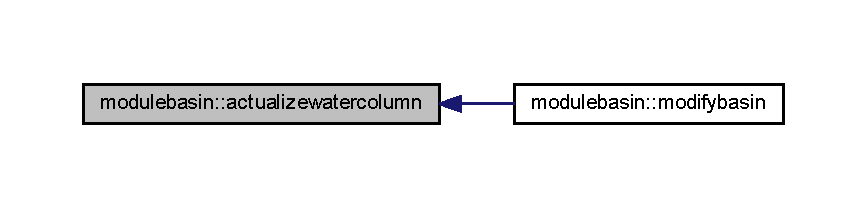
\includegraphics[width=350pt]{namespacemodulebasin_a6b7803a58ac882de2847f5af4c47cf02_icgraph}
\end{center}
\end{figure}
\mbox{\Hypertarget{namespacemodulebasin_a3ad94088588cc4ac448ba73dc73a3f61}\label{namespacemodulebasin_a3ad94088588cc4ac448ba73dc73a3f61}} 
\index{modulebasin@{modulebasin}!actualizewatercolumnconc@{actualizewatercolumnconc}}
\index{actualizewatercolumnconc@{actualizewatercolumnconc}!modulebasin@{modulebasin}}
\subsubsection{\texorpdfstring{actualizewatercolumnconc()}{actualizewatercolumnconc()}}
{\footnotesize\ttfamily subroutine modulebasin\+::actualizewatercolumnconc (\begin{DoxyParamCaption}\item[{character (len = $\ast$), intent(in)}]{Warning\+String }\end{DoxyParamCaption})\hspace{0.3cm}{\ttfamily [private]}}

Here is the call graph for this function\+:\nopagebreak
\begin{figure}[H]
\begin{center}
\leavevmode
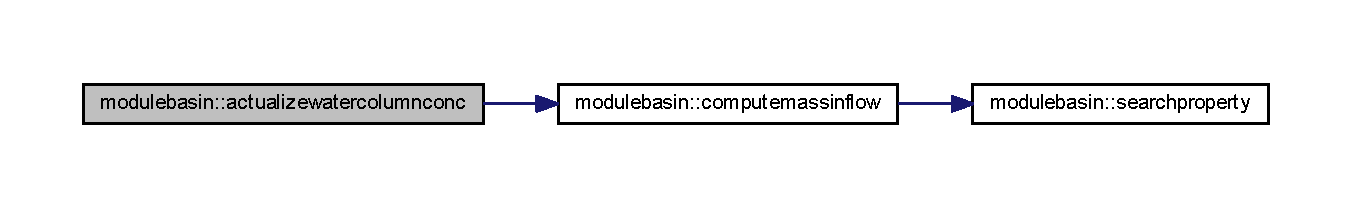
\includegraphics[width=350pt]{namespacemodulebasin_a3ad94088588cc4ac448ba73dc73a3f61_cgraph}
\end{center}
\end{figure}
Here is the caller graph for this function\+:\nopagebreak
\begin{figure}[H]
\begin{center}
\leavevmode
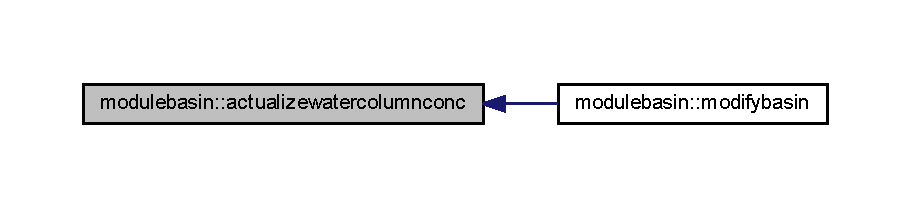
\includegraphics[width=350pt]{namespacemodulebasin_a3ad94088588cc4ac448ba73dc73a3f61_icgraph}
\end{center}
\end{figure}
\mbox{\Hypertarget{namespacemodulebasin_ad6d474b32a2a819360f61e25e869f0bd}\label{namespacemodulebasin_ad6d474b32a2a819360f61e25e869f0bd}} 
\index{modulebasin@{modulebasin}!addproperty@{addproperty}}
\index{addproperty@{addproperty}!modulebasin@{modulebasin}}
\subsubsection{\texorpdfstring{addproperty()}{addproperty()}}
{\footnotesize\ttfamily subroutine modulebasin\+::addproperty (\begin{DoxyParamCaption}\item[{type(\mbox{\hyperlink{structmodulebasin_1_1t__basinproperty}{t\+\_\+basinproperty}}), pointer}]{New\+Property }\end{DoxyParamCaption})\hspace{0.3cm}{\ttfamily [private]}}

Here is the caller graph for this function\+:\nopagebreak
\begin{figure}[H]
\begin{center}
\leavevmode
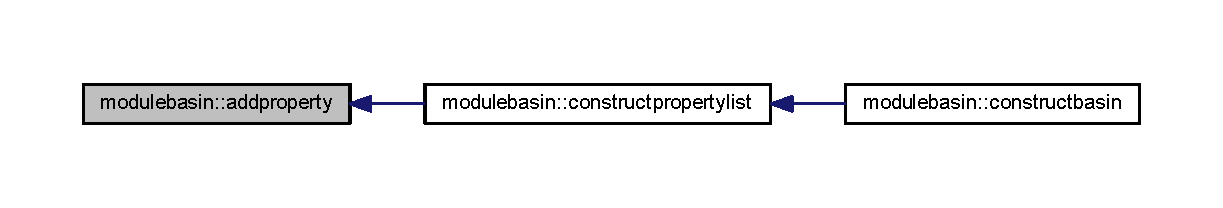
\includegraphics[width=350pt]{namespacemodulebasin_ad6d474b32a2a819360f61e25e869f0bd_icgraph}
\end{center}
\end{figure}
\mbox{\Hypertarget{namespacemodulebasin_af1790be65f99274cd923932448358912}\label{namespacemodulebasin_af1790be65f99274cd923932448358912}} 
\index{modulebasin@{modulebasin}!adjustcropcoefficient@{adjustcropcoefficient}}
\index{adjustcropcoefficient@{adjustcropcoefficient}!modulebasin@{modulebasin}}
\subsubsection{\texorpdfstring{adjustcropcoefficient()}{adjustcropcoefficient()}}
{\footnotesize\ttfamily real function, private modulebasin\+::adjustcropcoefficient (\begin{DoxyParamCaption}\item[{integer}]{I,  }\item[{integer}]{J }\end{DoxyParamCaption})\hspace{0.3cm}{\ttfamily [private]}}

Here is the caller graph for this function\+:\nopagebreak
\begin{figure}[H]
\begin{center}
\leavevmode
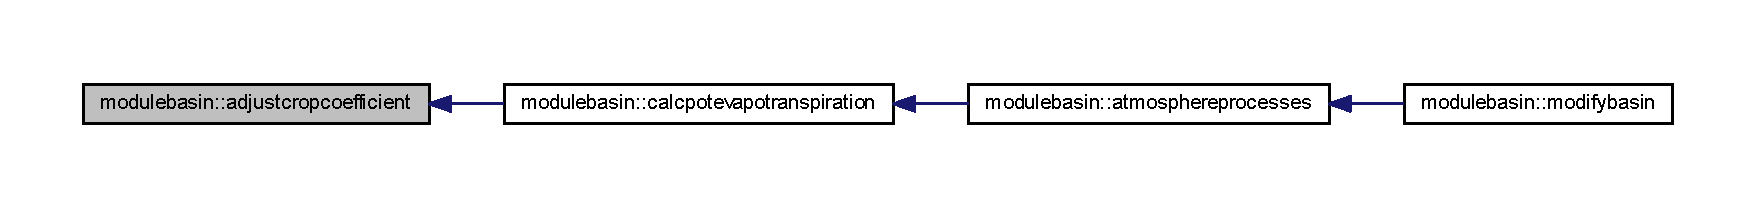
\includegraphics[width=350pt]{namespacemodulebasin_af1790be65f99274cd923932448358912_icgraph}
\end{center}
\end{figure}
\mbox{\Hypertarget{namespacemodulebasin_a59f6b3609f5cf292bc0d40591c8d6d33}\label{namespacemodulebasin_a59f6b3609f5cf292bc0d40591c8d6d33}} 
\index{modulebasin@{modulebasin}!allocateinstance@{allocateinstance}}
\index{allocateinstance@{allocateinstance}!modulebasin@{modulebasin}}
\subsubsection{\texorpdfstring{allocateinstance()}{allocateinstance()}}
{\footnotesize\ttfamily subroutine, private modulebasin\+::allocateinstance (\begin{DoxyParamCaption}{ }\end{DoxyParamCaption})\hspace{0.3cm}{\ttfamily [private]}}

Here is the caller graph for this function\+:\nopagebreak
\begin{figure}[H]
\begin{center}
\leavevmode
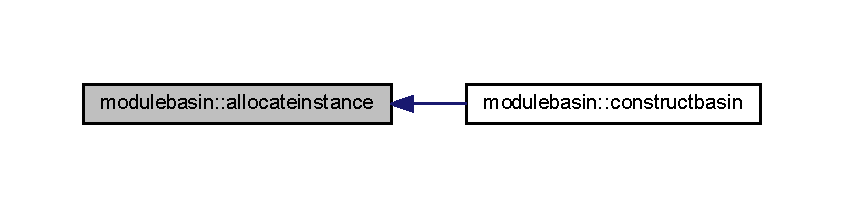
\includegraphics[width=350pt]{namespacemodulebasin_a59f6b3609f5cf292bc0d40591c8d6d33_icgraph}
\end{center}
\end{figure}
\mbox{\Hypertarget{namespacemodulebasin_a86eb7d3c4f70fdc55c9b4a4945a8ad9b}\label{namespacemodulebasin_a86eb7d3c4f70fdc55c9b4a4945a8ad9b}} 
\index{modulebasin@{modulebasin}!allocatevariables@{allocatevariables}}
\index{allocatevariables@{allocatevariables}!modulebasin@{modulebasin}}
\subsubsection{\texorpdfstring{allocatevariables()}{allocatevariables()}}
{\footnotesize\ttfamily subroutine, private modulebasin\+::allocatevariables (\begin{DoxyParamCaption}{ }\end{DoxyParamCaption})\hspace{0.3cm}{\ttfamily [private]}}

Here is the caller graph for this function\+:\nopagebreak
\begin{figure}[H]
\begin{center}
\leavevmode
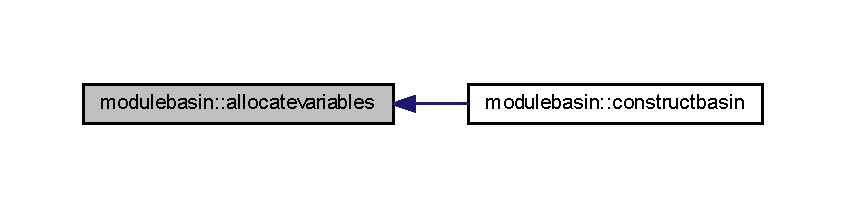
\includegraphics[width=350pt]{namespacemodulebasin_a86eb7d3c4f70fdc55c9b4a4945a8ad9b_icgraph}
\end{center}
\end{figure}
\mbox{\Hypertarget{namespacemodulebasin_a1dc5e66cf881f77967c196e5413f7ff2}\label{namespacemodulebasin_a1dc5e66cf881f77967c196e5413f7ff2}} 
\index{modulebasin@{modulebasin}!atmosphereprocesses@{atmosphereprocesses}}
\index{atmosphereprocesses@{atmosphereprocesses}!modulebasin@{modulebasin}}
\subsubsection{\texorpdfstring{atmosphereprocesses()}{atmosphereprocesses()}}
{\footnotesize\ttfamily subroutine, private modulebasin\+::atmosphereprocesses (\begin{DoxyParamCaption}{ }\end{DoxyParamCaption})\hspace{0.3cm}{\ttfamily [private]}}

Here is the call graph for this function\+:\nopagebreak
\begin{figure}[H]
\begin{center}
\leavevmode
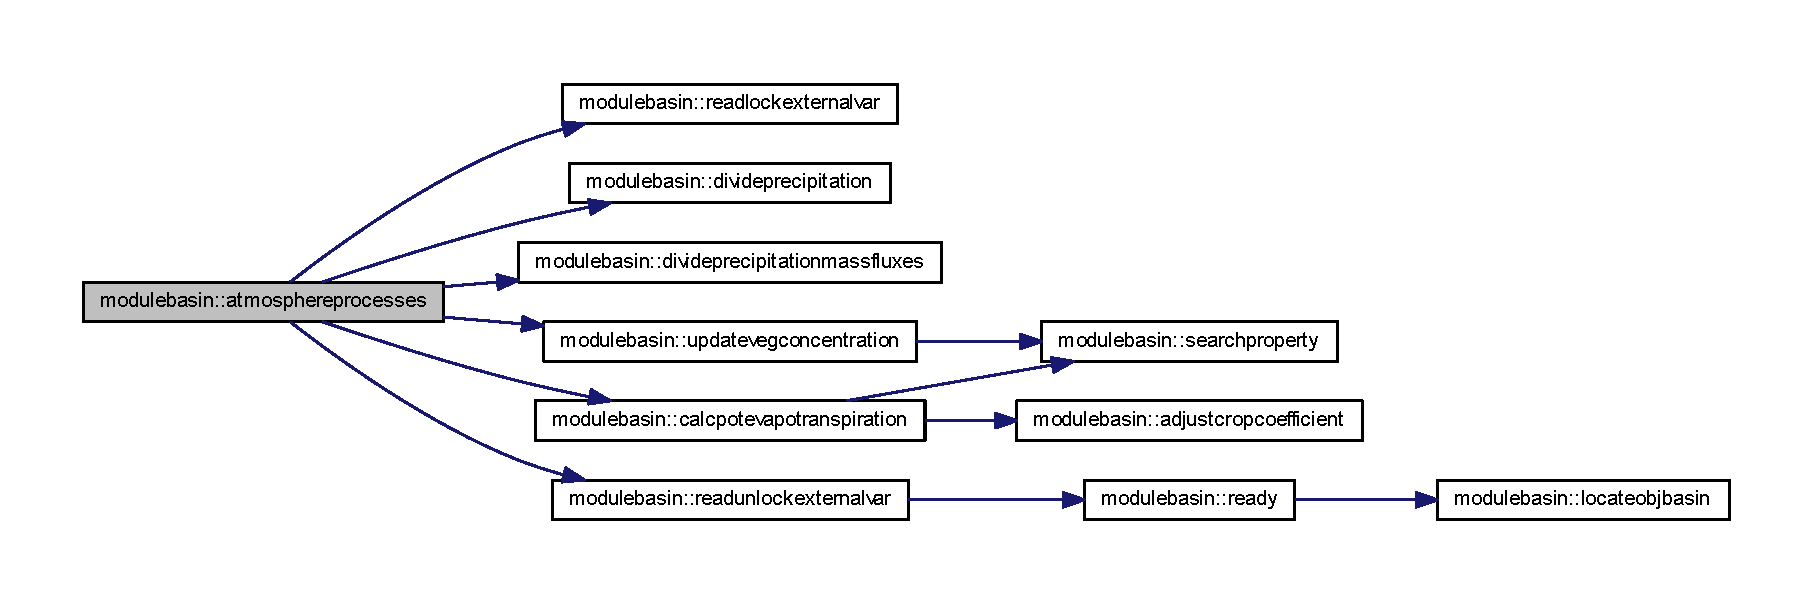
\includegraphics[width=350pt]{namespacemodulebasin_a1dc5e66cf881f77967c196e5413f7ff2_cgraph}
\end{center}
\end{figure}
Here is the caller graph for this function\+:\nopagebreak
\begin{figure}[H]
\begin{center}
\leavevmode
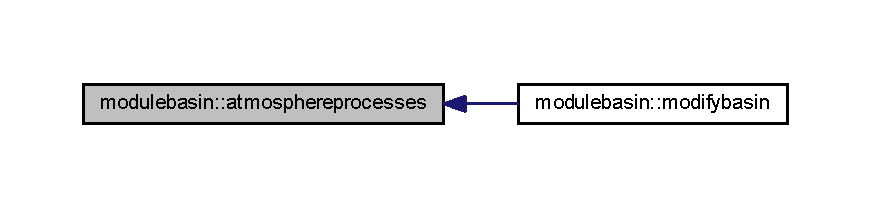
\includegraphics[width=350pt]{namespacemodulebasin_a1dc5e66cf881f77967c196e5413f7ff2_icgraph}
\end{center}
\end{figure}
\mbox{\Hypertarget{namespacemodulebasin_a466a2ecf0466b641fa24bb3e7847e37d}\label{namespacemodulebasin_a466a2ecf0466b641fa24bb3e7847e37d}} 
\index{modulebasin@{modulebasin}!calcaeroterm@{calcaeroterm}}
\index{calcaeroterm@{calcaeroterm}!modulebasin@{modulebasin}}
\subsubsection{\texorpdfstring{calcaeroterm()}{calcaeroterm()}}
{\footnotesize\ttfamily real function modulebasin\+::calcaeroterm (\begin{DoxyParamCaption}\item[{real}]{Temperature,  }\item[{real}]{Wind,  }\item[{real}]{S\+S\+V\+PC,  }\item[{real}]{S\+VP,  }\item[{real}]{VP,  }\item[{real}]{psiconst }\end{DoxyParamCaption})\hspace{0.3cm}{\ttfamily [private]}}

\mbox{\Hypertarget{namespacemodulebasin_a112f8b0445f6c2ff174a1292c9efd8c2}\label{namespacemodulebasin_a112f8b0445f6c2ff174a1292c9efd8c2}} 
\index{modulebasin@{modulebasin}!calcpotevapotranspiration@{calcpotevapotranspiration}}
\index{calcpotevapotranspiration@{calcpotevapotranspiration}!modulebasin@{modulebasin}}
\subsubsection{\texorpdfstring{calcpotevapotranspiration()}{calcpotevapotranspiration()}}
{\footnotesize\ttfamily subroutine, private modulebasin\+::calcpotevapotranspiration (\begin{DoxyParamCaption}{ }\end{DoxyParamCaption})\hspace{0.3cm}{\ttfamily [private]}}

Here is the call graph for this function\+:\nopagebreak
\begin{figure}[H]
\begin{center}
\leavevmode
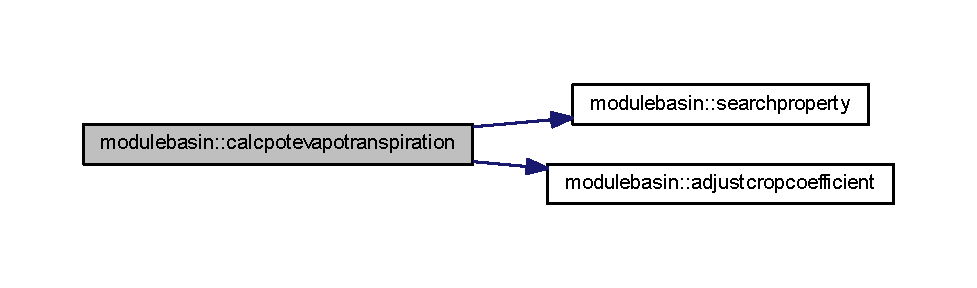
\includegraphics[width=350pt]{namespacemodulebasin_a112f8b0445f6c2ff174a1292c9efd8c2_cgraph}
\end{center}
\end{figure}
Here is the caller graph for this function\+:\nopagebreak
\begin{figure}[H]
\begin{center}
\leavevmode
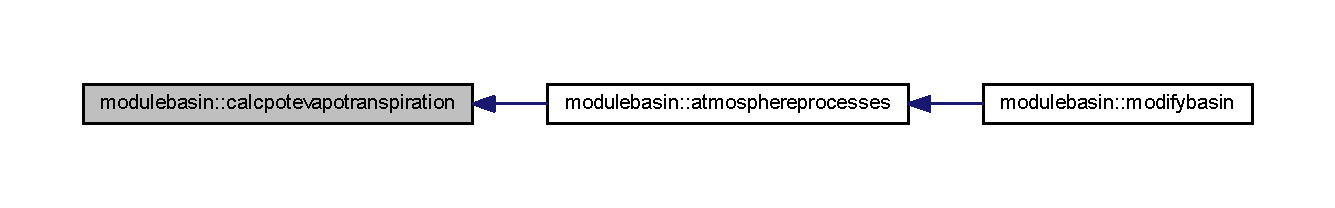
\includegraphics[width=350pt]{namespacemodulebasin_a112f8b0445f6c2ff174a1292c9efd8c2_icgraph}
\end{center}
\end{figure}
\mbox{\Hypertarget{namespacemodulebasin_ac23d68c52a8a6bf444bd3ade576da5bb}\label{namespacemodulebasin_ac23d68c52a8a6bf444bd3ade576da5bb}} 
\index{modulebasin@{modulebasin}!calcradterm@{calcradterm}}
\index{calcradterm@{calcradterm}!modulebasin@{modulebasin}}
\subsubsection{\texorpdfstring{calcradterm()}{calcradterm()}}
{\footnotesize\ttfamily real function modulebasin\+::calcradterm (\begin{DoxyParamCaption}\item[{real}]{Radiation,  }\item[{real}]{Soil\+Loss,  }\item[{real}]{Wind\+Velocity,  }\item[{real}]{S\+S\+V\+PC,  }\item[{real}]{psiconst }\end{DoxyParamCaption})\hspace{0.3cm}{\ttfamily [private]}}

\mbox{\Hypertarget{namespacemodulebasin_af1427c4ade7156552be2283259050d1d}\label{namespacemodulebasin_af1427c4ade7156552be2283259050d1d}} 
\index{modulebasin@{modulebasin}!calculatemass@{calculatemass}}
\index{calculatemass@{calculatemass}!modulebasin@{modulebasin}}
\subsubsection{\texorpdfstring{calculatemass()}{calculatemass()}}
{\footnotesize\ttfamily subroutine modulebasin\+::calculatemass (\begin{DoxyParamCaption}\item[{character (len = stringlength)}]{Time }\end{DoxyParamCaption})\hspace{0.3cm}{\ttfamily [private]}}

Here is the caller graph for this function\+:\nopagebreak
\begin{figure}[H]
\begin{center}
\leavevmode
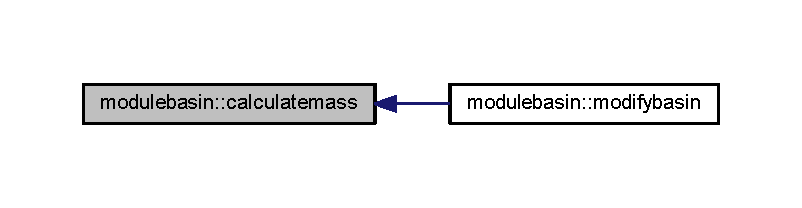
\includegraphics[width=350pt]{namespacemodulebasin_af1427c4ade7156552be2283259050d1d_icgraph}
\end{center}
\end{figure}
\mbox{\Hypertarget{namespacemodulebasin_a00fd3009ac96d7478c5ad365f4438954}\label{namespacemodulebasin_a00fd3009ac96d7478c5ad365f4438954}} 
\index{modulebasin@{modulebasin}!calculatevegtotalstoredmass@{calculatevegtotalstoredmass}}
\index{calculatevegtotalstoredmass@{calculatevegtotalstoredmass}!modulebasin@{modulebasin}}
\subsubsection{\texorpdfstring{calculatevegtotalstoredmass()}{calculatevegtotalstoredmass()}}
{\footnotesize\ttfamily subroutine modulebasin\+::calculatevegtotalstoredmass (\begin{DoxyParamCaption}{ }\end{DoxyParamCaption})\hspace{0.3cm}{\ttfamily [private]}}

Here is the caller graph for this function\+:\nopagebreak
\begin{figure}[H]
\begin{center}
\leavevmode
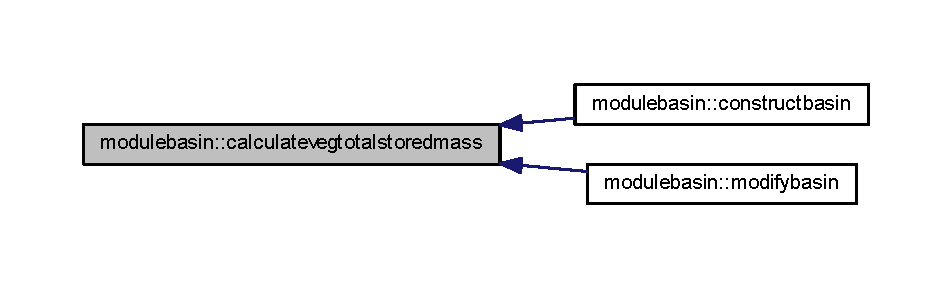
\includegraphics[width=350pt]{namespacemodulebasin_a00fd3009ac96d7478c5ad365f4438954_icgraph}
\end{center}
\end{figure}
\mbox{\Hypertarget{namespacemodulebasin_ad852fa9f51f06a8aad01fbf81cfd7015}\label{namespacemodulebasin_ad852fa9f51f06a8aad01fbf81cfd7015}} 
\index{modulebasin@{modulebasin}!computebasinwaterbalance@{computebasinwaterbalance}}
\index{computebasinwaterbalance@{computebasinwaterbalance}!modulebasin@{modulebasin}}
\subsubsection{\texorpdfstring{computebasinwaterbalance()}{computebasinwaterbalance()}}
{\footnotesize\ttfamily subroutine, private modulebasin\+::computebasinwaterbalance (\begin{DoxyParamCaption}{ }\end{DoxyParamCaption})\hspace{0.3cm}{\ttfamily [private]}}

Here is the caller graph for this function\+:\nopagebreak
\begin{figure}[H]
\begin{center}
\leavevmode
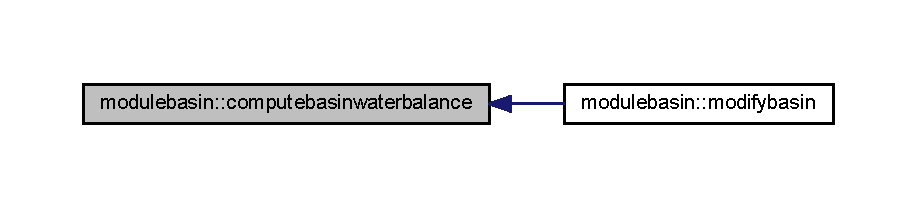
\includegraphics[width=350pt]{namespacemodulebasin_ad852fa9f51f06a8aad01fbf81cfd7015_icgraph}
\end{center}
\end{figure}
\mbox{\Hypertarget{namespacemodulebasin_a9ef4a0de552e03dfcc7dc780e6162af7}\label{namespacemodulebasin_a9ef4a0de552e03dfcc7dc780e6162af7}} 
\index{modulebasin@{modulebasin}!computeintegration@{computeintegration}}
\index{computeintegration@{computeintegration}!modulebasin@{modulebasin}}
\subsubsection{\texorpdfstring{computeintegration()}{computeintegration()}}
{\footnotesize\ttfamily subroutine modulebasin\+::computeintegration (\begin{DoxyParamCaption}{ }\end{DoxyParamCaption})\hspace{0.3cm}{\ttfamily [private]}}

Here is the caller graph for this function\+:\nopagebreak
\begin{figure}[H]
\begin{center}
\leavevmode
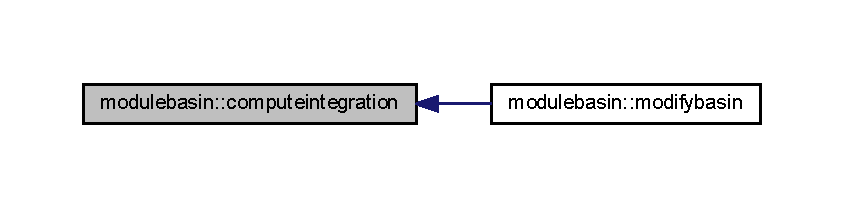
\includegraphics[width=350pt]{namespacemodulebasin_a9ef4a0de552e03dfcc7dc780e6162af7_icgraph}
\end{center}
\end{figure}
\mbox{\Hypertarget{namespacemodulebasin_a106653309e017391895ef068b14bfdc2}\label{namespacemodulebasin_a106653309e017391895ef068b14bfdc2}} 
\index{modulebasin@{modulebasin}!computemassinflow@{computemassinflow}}
\index{computemassinflow@{computemassinflow}!modulebasin@{modulebasin}}
\subsubsection{\texorpdfstring{computemassinflow()}{computemassinflow()}}
{\footnotesize\ttfamily subroutine modulebasin\+::computemassinflow (\begin{DoxyParamCaption}\item[{character (len = $\ast$), intent(in)}]{Warning\+String,  }\item[{real, dimension(\+:, \+:   ), pointer}]{R\+P\+Concentration,  }\item[{integer}]{Prop\+ID,  }\item[{logical}]{Particulate,  }\item[{real(8), dimension(\+:,\+:), pointer}]{Mass\+In\+Flow }\end{DoxyParamCaption})\hspace{0.3cm}{\ttfamily [private]}}

Here is the call graph for this function\+:\nopagebreak
\begin{figure}[H]
\begin{center}
\leavevmode
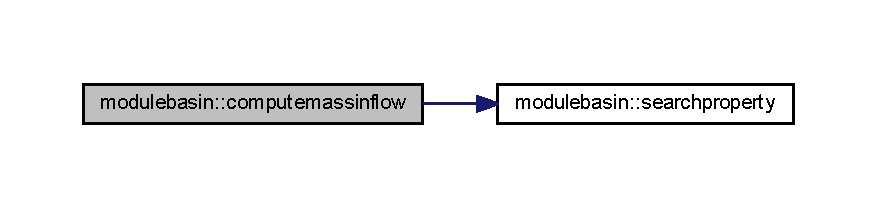
\includegraphics[width=350pt]{namespacemodulebasin_a106653309e017391895ef068b14bfdc2_cgraph}
\end{center}
\end{figure}
Here is the caller graph for this function\+:\nopagebreak
\begin{figure}[H]
\begin{center}
\leavevmode
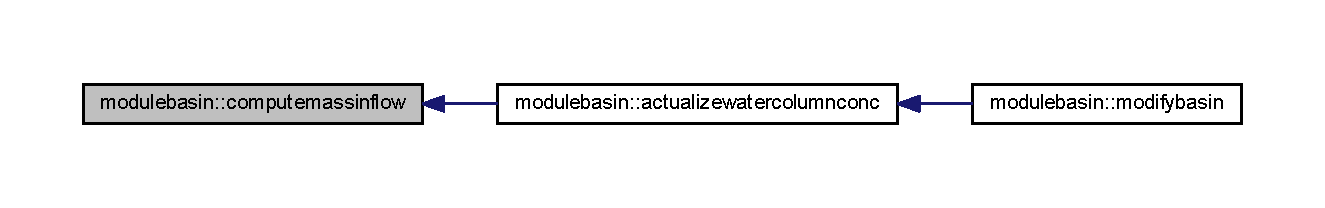
\includegraphics[width=350pt]{namespacemodulebasin_a106653309e017391895ef068b14bfdc2_icgraph}
\end{center}
\end{figure}
\mbox{\Hypertarget{namespacemodulebasin_a3f14e909944d51caacaf3104b755d817}\label{namespacemodulebasin_a3f14e909944d51caacaf3104b755d817}} 
\index{modulebasin@{modulebasin}!computenextdt@{computenextdt}}
\index{computenextdt@{computenextdt}!modulebasin@{modulebasin}}
\subsubsection{\texorpdfstring{computenextdt()}{computenextdt()}}
{\footnotesize\ttfamily subroutine, private modulebasin\+::computenextdt (\begin{DoxyParamCaption}\item[{real}]{New\+DT }\end{DoxyParamCaption})\hspace{0.3cm}{\ttfamily [private]}}

Here is the caller graph for this function\+:\nopagebreak
\begin{figure}[H]
\begin{center}
\leavevmode
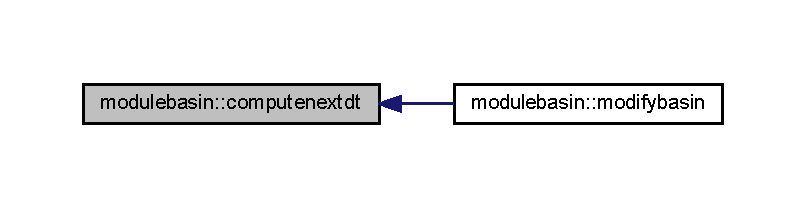
\includegraphics[width=350pt]{namespacemodulebasin_a3f14e909944d51caacaf3104b755d817_icgraph}
\end{center}
\end{figure}
\mbox{\Hypertarget{namespacemodulebasin_a65271cf9b17250a778002a527ee4c253}\label{namespacemodulebasin_a65271cf9b17250a778002a527ee4c253}} 
\index{modulebasin@{modulebasin}!construct\+\_\+propertyvalues@{construct\+\_\+propertyvalues}}
\index{construct\+\_\+propertyvalues@{construct\+\_\+propertyvalues}!modulebasin@{modulebasin}}
\subsubsection{\texorpdfstring{construct\+\_\+propertyvalues()}{construct\_propertyvalues()}}
{\footnotesize\ttfamily subroutine modulebasin\+::construct\+\_\+propertyvalues (\begin{DoxyParamCaption}\item[{type(\mbox{\hyperlink{structmodulebasin_1_1t__basinproperty}{t\+\_\+basinproperty}}), pointer}]{New\+Property }\end{DoxyParamCaption})\hspace{0.3cm}{\ttfamily [private]}}

Here is the caller graph for this function\+:\nopagebreak
\begin{figure}[H]
\begin{center}
\leavevmode
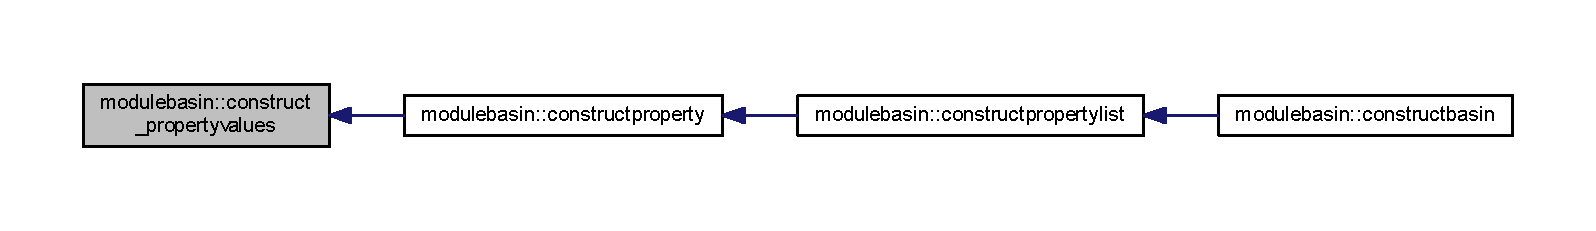
\includegraphics[width=350pt]{namespacemodulebasin_a65271cf9b17250a778002a527ee4c253_icgraph}
\end{center}
\end{figure}
\mbox{\Hypertarget{namespacemodulebasin_a51d97ade316802f4f499db0fb3835e3f}\label{namespacemodulebasin_a51d97ade316802f4f499db0fb3835e3f}} 
\index{modulebasin@{modulebasin}!constructbasin@{constructbasin}}
\index{constructbasin@{constructbasin}!modulebasin@{modulebasin}}
\subsubsection{\texorpdfstring{constructbasin()}{constructbasin()}}
{\footnotesize\ttfamily subroutine, public modulebasin\+::constructbasin (\begin{DoxyParamCaption}\item[{integer}]{Obj\+Basin\+ID,  }\item[{integer}]{Obj\+Time,  }\item[{character(len=$\ast$)}]{Model\+Name,  }\item[{logical}]{Stop\+On\+Bathymetry\+Change,  }\item[{integer, intent(out), optional}]{S\+T\+AT }\end{DoxyParamCaption})}

Here is the call graph for this function\+:\nopagebreak
\begin{figure}[H]
\begin{center}
\leavevmode
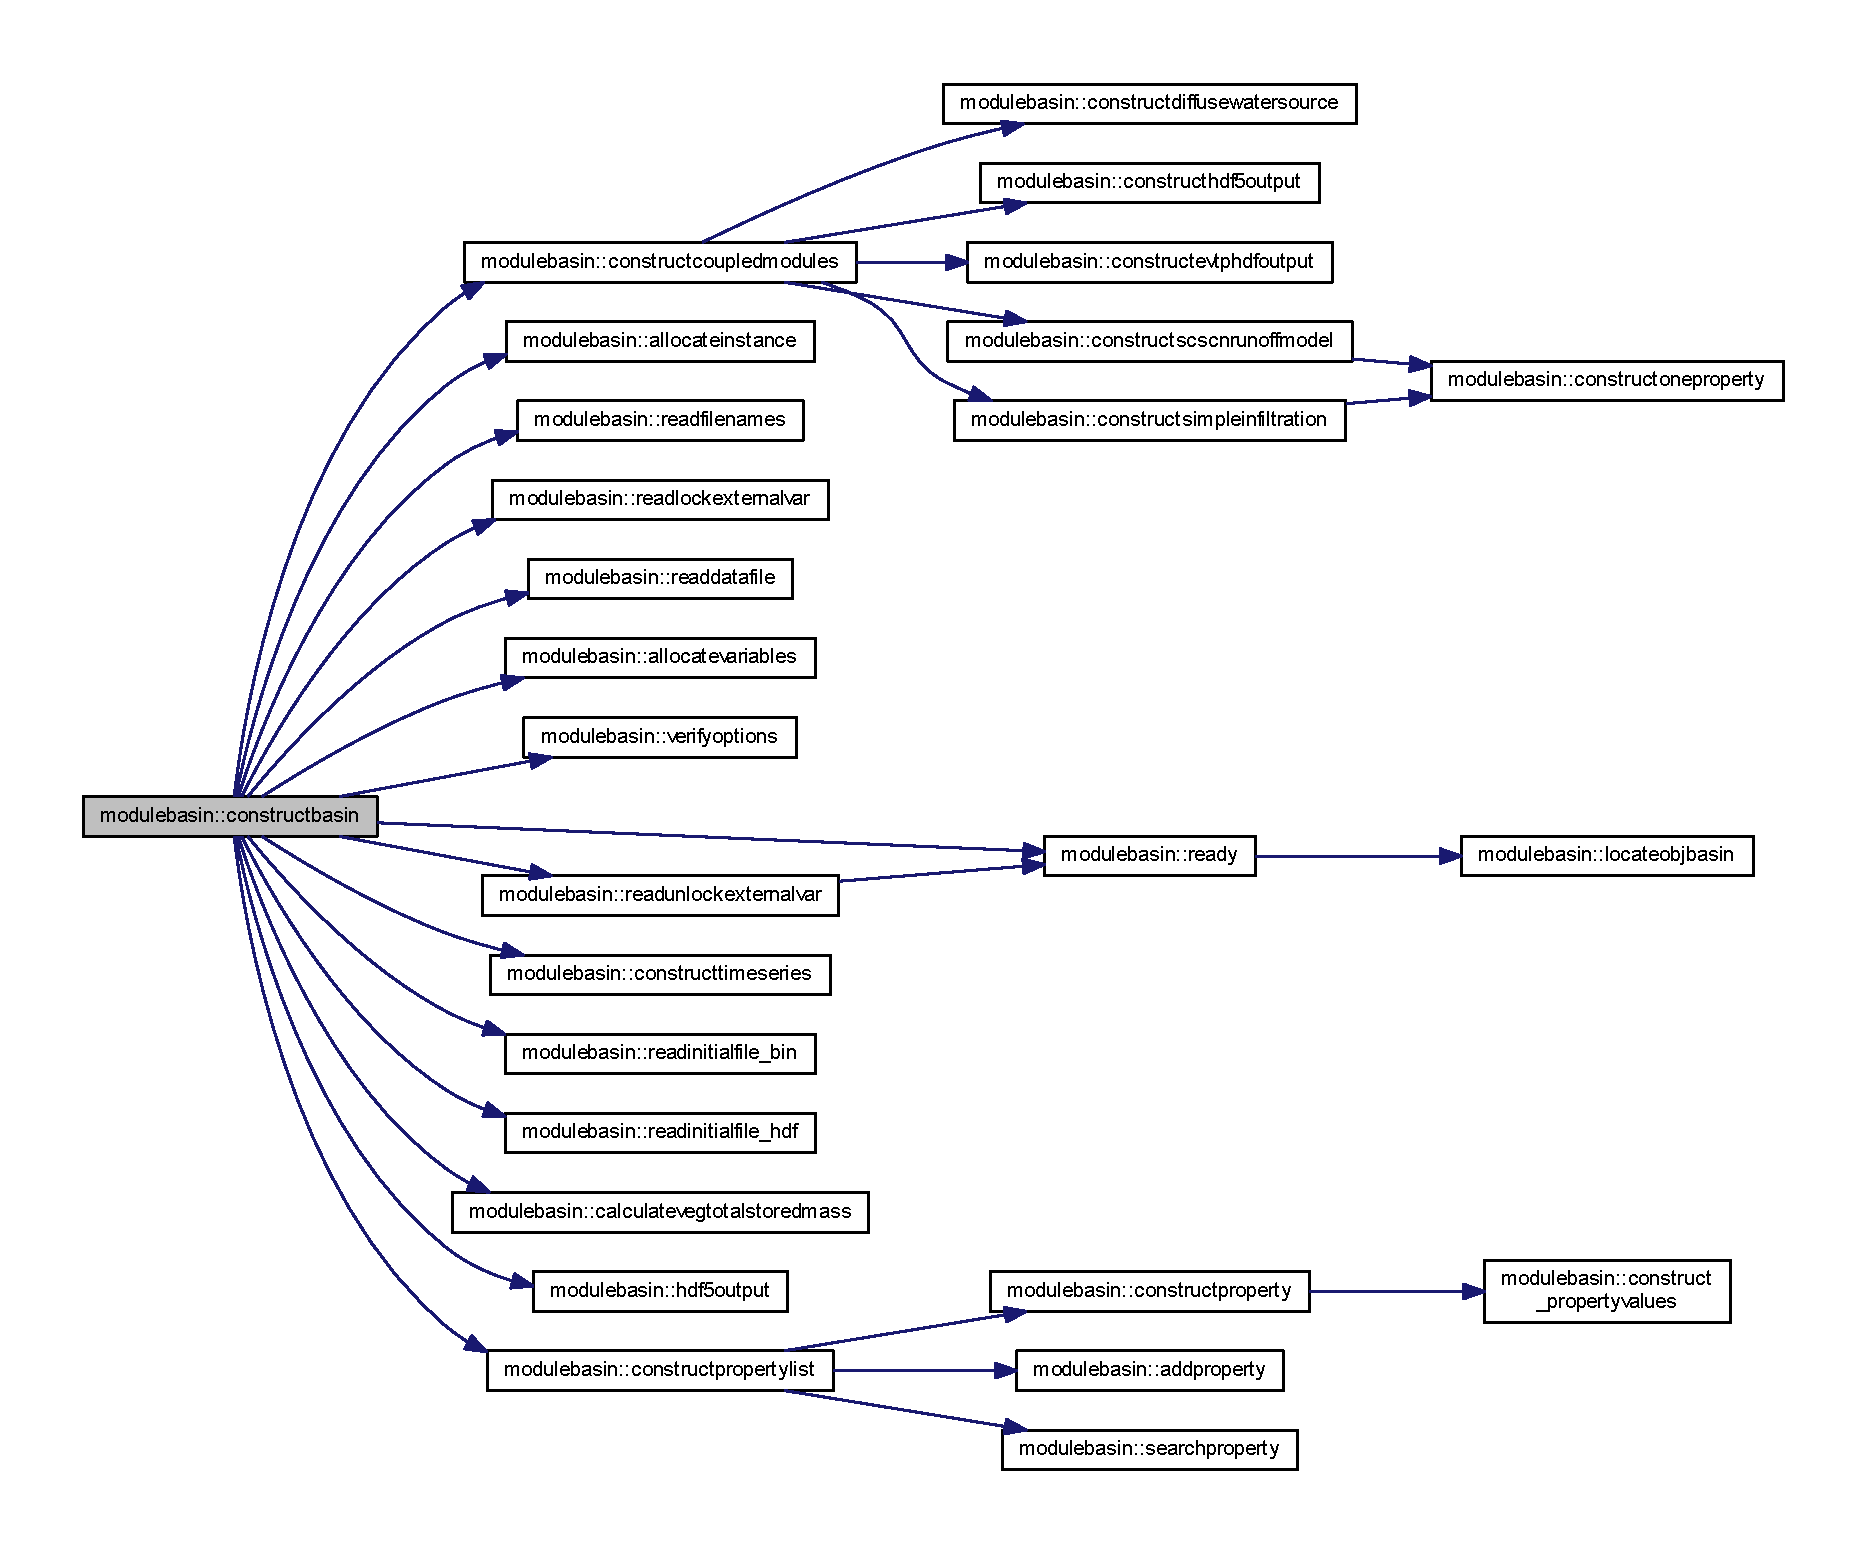
\includegraphics[width=350pt]{namespacemodulebasin_a51d97ade316802f4f499db0fb3835e3f_cgraph}
\end{center}
\end{figure}
\mbox{\Hypertarget{namespacemodulebasin_a3b96c67f2670be0a100bc48d94ecb93d}\label{namespacemodulebasin_a3b96c67f2670be0a100bc48d94ecb93d}} 
\index{modulebasin@{modulebasin}!constructcoupledmodules@{constructcoupledmodules}}
\index{constructcoupledmodules@{constructcoupledmodules}!modulebasin@{modulebasin}}
\subsubsection{\texorpdfstring{constructcoupledmodules()}{constructcoupledmodules()}}
{\footnotesize\ttfamily subroutine, private modulebasin\+::constructcoupledmodules (\begin{DoxyParamCaption}\item[{}]{\+\_\+\+E\+N\+A\+B\+L\+E\+\_\+\+C\+U\+DA }\end{DoxyParamCaption})\hspace{0.3cm}{\ttfamily [private]}}

Here is the call graph for this function\+:\nopagebreak
\begin{figure}[H]
\begin{center}
\leavevmode
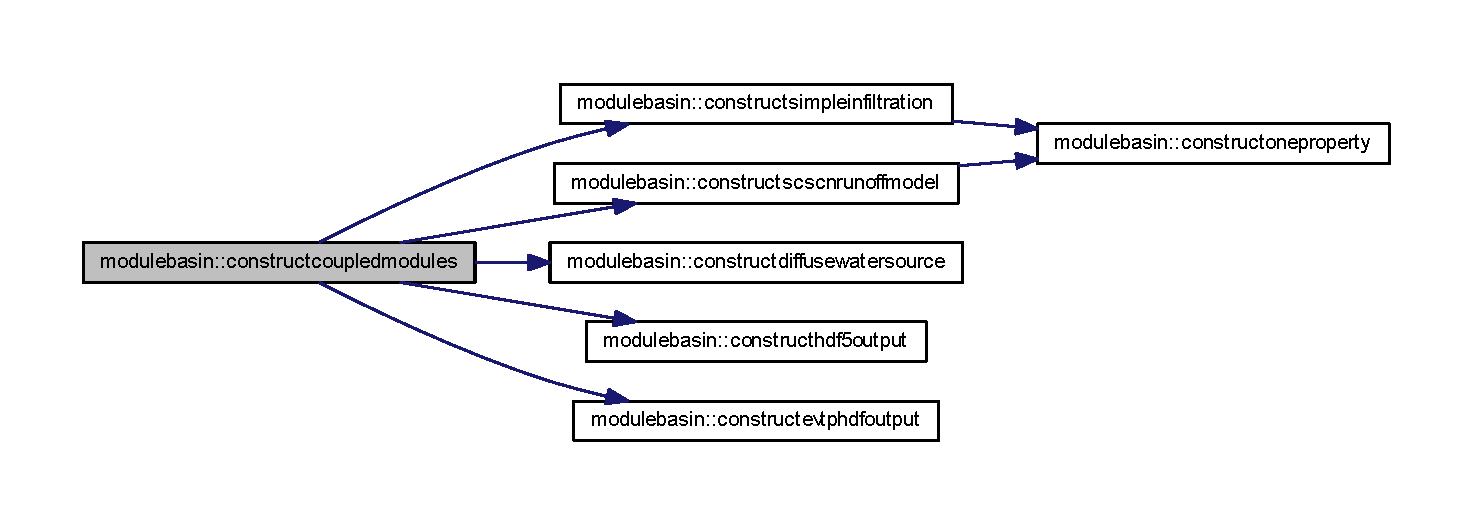
\includegraphics[width=350pt]{namespacemodulebasin_a3b96c67f2670be0a100bc48d94ecb93d_cgraph}
\end{center}
\end{figure}
Here is the caller graph for this function\+:\nopagebreak
\begin{figure}[H]
\begin{center}
\leavevmode
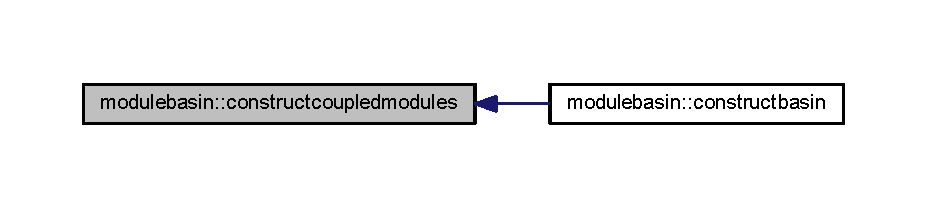
\includegraphics[width=350pt]{namespacemodulebasin_a3b96c67f2670be0a100bc48d94ecb93d_icgraph}
\end{center}
\end{figure}
\mbox{\Hypertarget{namespacemodulebasin_a3d6f3d514121b3b20c1b2d2ec4c56fa9}\label{namespacemodulebasin_a3d6f3d514121b3b20c1b2d2ec4c56fa9}} 
\index{modulebasin@{modulebasin}!constructdiffusewatersource@{constructdiffusewatersource}}
\index{constructdiffusewatersource@{constructdiffusewatersource}!modulebasin@{modulebasin}}
\subsubsection{\texorpdfstring{constructdiffusewatersource()}{constructdiffusewatersource()}}
{\footnotesize\ttfamily subroutine modulebasin\+::constructdiffusewatersource (\begin{DoxyParamCaption}{ }\end{DoxyParamCaption})\hspace{0.3cm}{\ttfamily [private]}}

Here is the caller graph for this function\+:\nopagebreak
\begin{figure}[H]
\begin{center}
\leavevmode
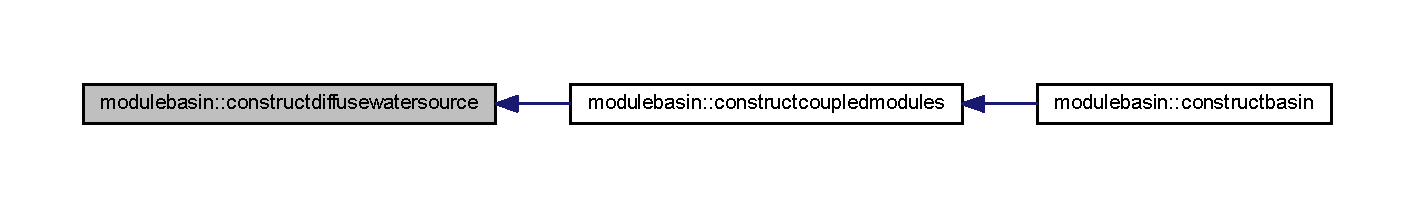
\includegraphics[width=350pt]{namespacemodulebasin_a3d6f3d514121b3b20c1b2d2ec4c56fa9_icgraph}
\end{center}
\end{figure}
\mbox{\Hypertarget{namespacemodulebasin_abec73ddab1c13a2f52007dbd7a5adf56}\label{namespacemodulebasin_abec73ddab1c13a2f52007dbd7a5adf56}} 
\index{modulebasin@{modulebasin}!constructevtphdfoutput@{constructevtphdfoutput}}
\index{constructevtphdfoutput@{constructevtphdfoutput}!modulebasin@{modulebasin}}
\subsubsection{\texorpdfstring{constructevtphdfoutput()}{constructevtphdfoutput()}}
{\footnotesize\ttfamily subroutine, private modulebasin\+::constructevtphdfoutput (\begin{DoxyParamCaption}{ }\end{DoxyParamCaption})\hspace{0.3cm}{\ttfamily [private]}}

Here is the caller graph for this function\+:\nopagebreak
\begin{figure}[H]
\begin{center}
\leavevmode
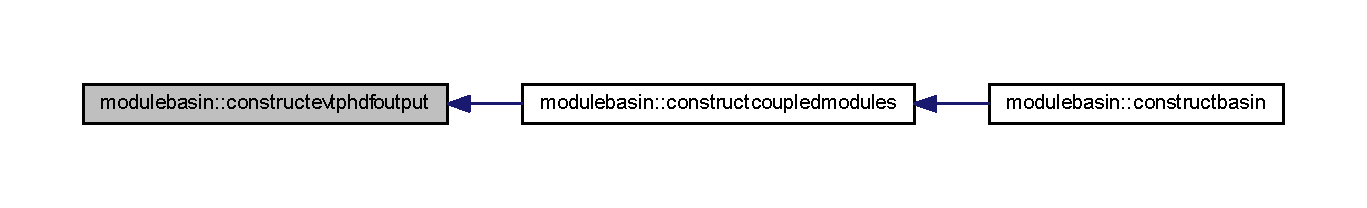
\includegraphics[width=350pt]{namespacemodulebasin_abec73ddab1c13a2f52007dbd7a5adf56_icgraph}
\end{center}
\end{figure}
\mbox{\Hypertarget{namespacemodulebasin_ad767dee07579ea3a5545d747a0d7cfcf}\label{namespacemodulebasin_ad767dee07579ea3a5545d747a0d7cfcf}} 
\index{modulebasin@{modulebasin}!constructhdf5output@{constructhdf5output}}
\index{constructhdf5output@{constructhdf5output}!modulebasin@{modulebasin}}
\subsubsection{\texorpdfstring{constructhdf5output()}{constructhdf5output()}}
{\footnotesize\ttfamily subroutine, private modulebasin\+::constructhdf5output (\begin{DoxyParamCaption}{ }\end{DoxyParamCaption})\hspace{0.3cm}{\ttfamily [private]}}

Here is the caller graph for this function\+:\nopagebreak
\begin{figure}[H]
\begin{center}
\leavevmode
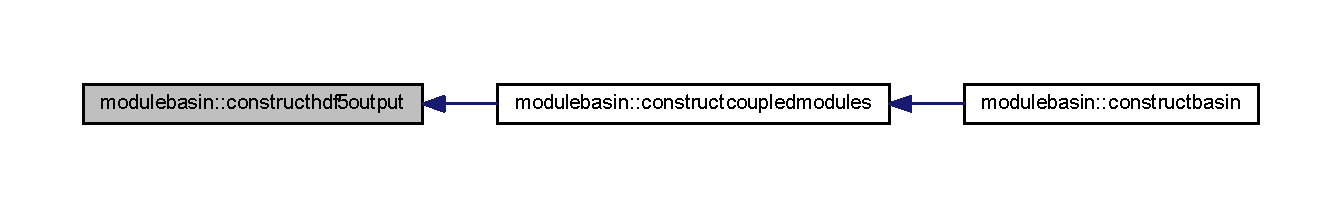
\includegraphics[width=350pt]{namespacemodulebasin_ad767dee07579ea3a5545d747a0d7cfcf_icgraph}
\end{center}
\end{figure}
\mbox{\Hypertarget{namespacemodulebasin_a5a3aa456544a0c67f38a3d3655071347}\label{namespacemodulebasin_a5a3aa456544a0c67f38a3d3655071347}} 
\index{modulebasin@{modulebasin}!constructoneproperty@{constructoneproperty}}
\index{constructoneproperty@{constructoneproperty}!modulebasin@{modulebasin}}
\subsubsection{\texorpdfstring{constructoneproperty()}{constructoneproperty()}}
{\footnotesize\ttfamily subroutine modulebasin\+::constructoneproperty (\begin{DoxyParamCaption}\item[{type (\mbox{\hyperlink{structmodulebasin_1_1t__propertyb}{t\+\_\+propertyb}})}]{New\+Property,  }\item[{character(len=$\ast$)}]{Property\+Name,  }\item[{character(len=$\ast$)}]{Block\+Begin,  }\item[{character(len=$\ast$)}]{Block\+End }\end{DoxyParamCaption})\hspace{0.3cm}{\ttfamily [private]}}

Here is the caller graph for this function\+:\nopagebreak
\begin{figure}[H]
\begin{center}
\leavevmode
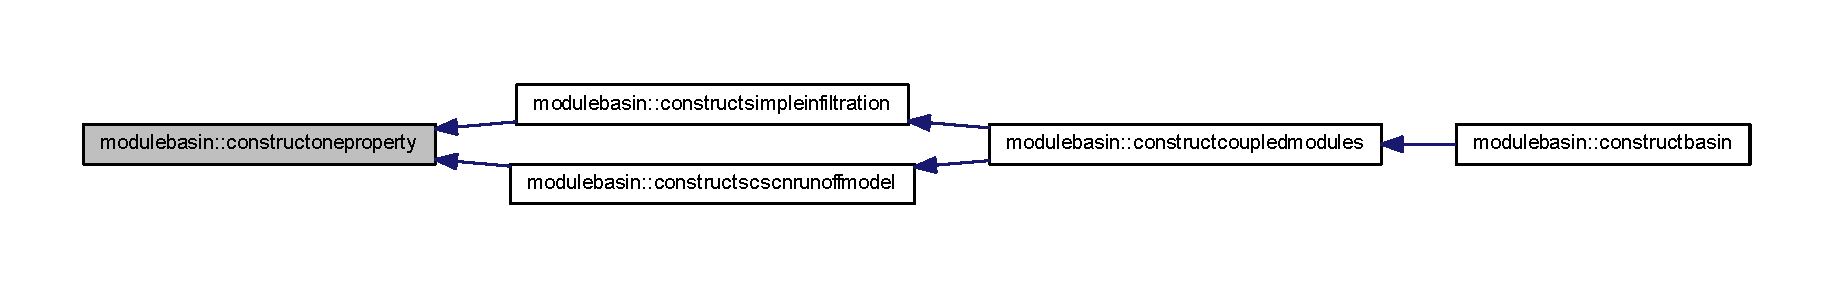
\includegraphics[width=350pt]{namespacemodulebasin_a5a3aa456544a0c67f38a3d3655071347_icgraph}
\end{center}
\end{figure}
\mbox{\Hypertarget{namespacemodulebasin_afc1a708f812fbecd655d2ec2ec7d7ae7}\label{namespacemodulebasin_afc1a708f812fbecd655d2ec2ec7d7ae7}} 
\index{modulebasin@{modulebasin}!constructproperty@{constructproperty}}
\index{constructproperty@{constructproperty}!modulebasin@{modulebasin}}
\subsubsection{\texorpdfstring{constructproperty()}{constructproperty()}}
{\footnotesize\ttfamily subroutine modulebasin\+::constructproperty (\begin{DoxyParamCaption}\item[{type(\mbox{\hyperlink{structmodulebasin_1_1t__basinproperty}{t\+\_\+basinproperty}}), pointer}]{New\+Property }\end{DoxyParamCaption})\hspace{0.3cm}{\ttfamily [private]}}

Here is the call graph for this function\+:\nopagebreak
\begin{figure}[H]
\begin{center}
\leavevmode
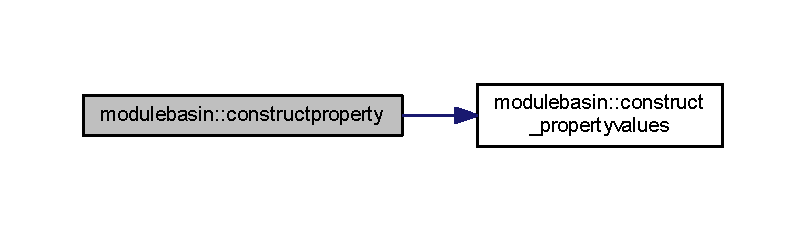
\includegraphics[width=350pt]{namespacemodulebasin_afc1a708f812fbecd655d2ec2ec7d7ae7_cgraph}
\end{center}
\end{figure}
Here is the caller graph for this function\+:\nopagebreak
\begin{figure}[H]
\begin{center}
\leavevmode
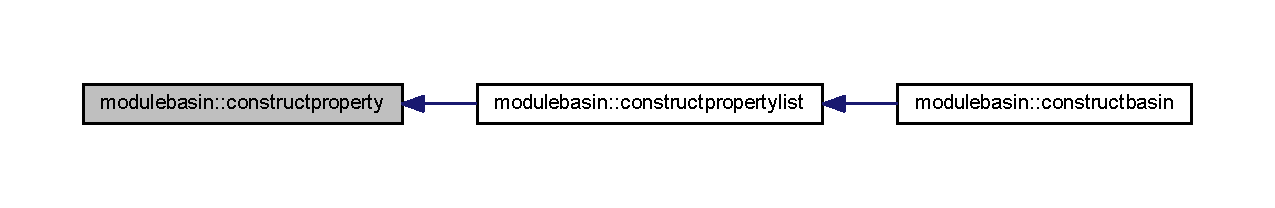
\includegraphics[width=350pt]{namespacemodulebasin_afc1a708f812fbecd655d2ec2ec7d7ae7_icgraph}
\end{center}
\end{figure}
\mbox{\Hypertarget{namespacemodulebasin_a914a8d07507d5ca843132c144c8e61f7}\label{namespacemodulebasin_a914a8d07507d5ca843132c144c8e61f7}} 
\index{modulebasin@{modulebasin}!constructpropertylist@{constructpropertylist}}
\index{constructpropertylist@{constructpropertylist}!modulebasin@{modulebasin}}
\subsubsection{\texorpdfstring{constructpropertylist()}{constructpropertylist()}}
{\footnotesize\ttfamily subroutine modulebasin\+::constructpropertylist (\begin{DoxyParamCaption}{ }\end{DoxyParamCaption})\hspace{0.3cm}{\ttfamily [private]}}

Here is the call graph for this function\+:\nopagebreak
\begin{figure}[H]
\begin{center}
\leavevmode
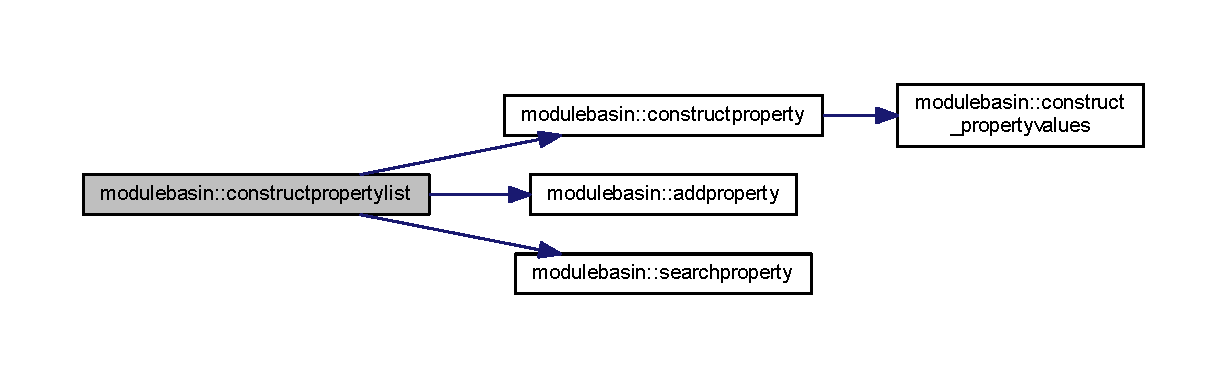
\includegraphics[width=350pt]{namespacemodulebasin_a914a8d07507d5ca843132c144c8e61f7_cgraph}
\end{center}
\end{figure}
Here is the caller graph for this function\+:\nopagebreak
\begin{figure}[H]
\begin{center}
\leavevmode
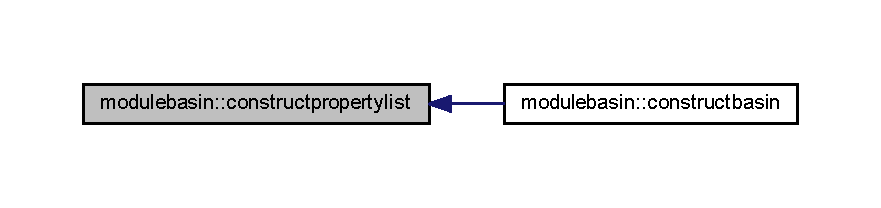
\includegraphics[width=350pt]{namespacemodulebasin_a914a8d07507d5ca843132c144c8e61f7_icgraph}
\end{center}
\end{figure}
\mbox{\Hypertarget{namespacemodulebasin_a5a5342d9e5be44e9161d8d4643071661}\label{namespacemodulebasin_a5a5342d9e5be44e9161d8d4643071661}} 
\index{modulebasin@{modulebasin}!constructscscnrunoffmodel@{constructscscnrunoffmodel}}
\index{constructscscnrunoffmodel@{constructscscnrunoffmodel}!modulebasin@{modulebasin}}
\subsubsection{\texorpdfstring{constructscscnrunoffmodel()}{constructscscnrunoffmodel()}}
{\footnotesize\ttfamily subroutine modulebasin\+::constructscscnrunoffmodel (\begin{DoxyParamCaption}{ }\end{DoxyParamCaption})\hspace{0.3cm}{\ttfamily [private]}}

Here is the call graph for this function\+:\nopagebreak
\begin{figure}[H]
\begin{center}
\leavevmode
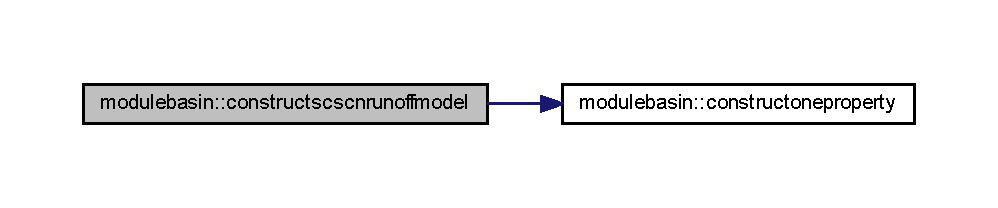
\includegraphics[width=350pt]{namespacemodulebasin_a5a5342d9e5be44e9161d8d4643071661_cgraph}
\end{center}
\end{figure}
Here is the caller graph for this function\+:\nopagebreak
\begin{figure}[H]
\begin{center}
\leavevmode
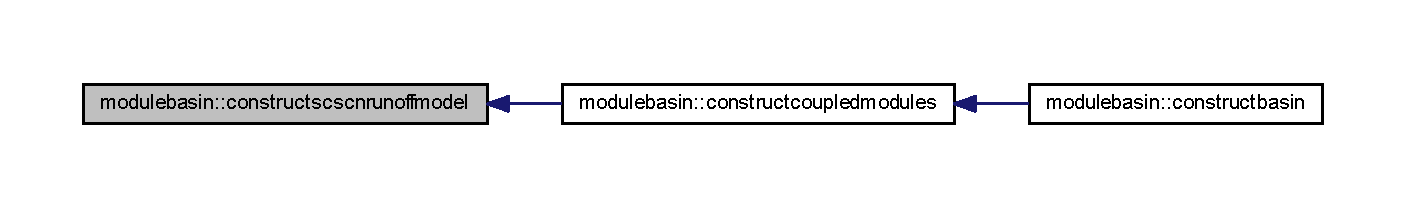
\includegraphics[width=350pt]{namespacemodulebasin_a5a5342d9e5be44e9161d8d4643071661_icgraph}
\end{center}
\end{figure}
\mbox{\Hypertarget{namespacemodulebasin_a0b7274cf3bbde399251125f839f59767}\label{namespacemodulebasin_a0b7274cf3bbde399251125f839f59767}} 
\index{modulebasin@{modulebasin}!constructsimpleinfiltration@{constructsimpleinfiltration}}
\index{constructsimpleinfiltration@{constructsimpleinfiltration}!modulebasin@{modulebasin}}
\subsubsection{\texorpdfstring{constructsimpleinfiltration()}{constructsimpleinfiltration()}}
{\footnotesize\ttfamily subroutine modulebasin\+::constructsimpleinfiltration (\begin{DoxyParamCaption}{ }\end{DoxyParamCaption})\hspace{0.3cm}{\ttfamily [private]}}

Here is the call graph for this function\+:\nopagebreak
\begin{figure}[H]
\begin{center}
\leavevmode
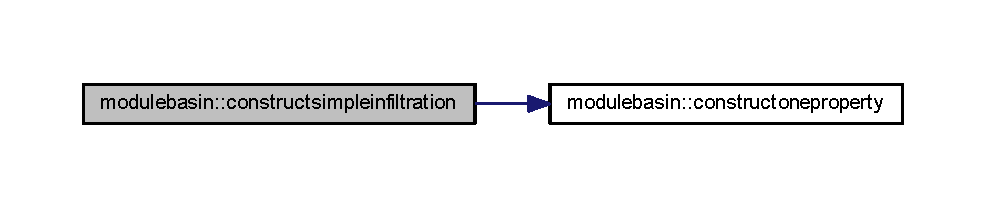
\includegraphics[width=350pt]{namespacemodulebasin_a0b7274cf3bbde399251125f839f59767_cgraph}
\end{center}
\end{figure}
Here is the caller graph for this function\+:\nopagebreak
\begin{figure}[H]
\begin{center}
\leavevmode
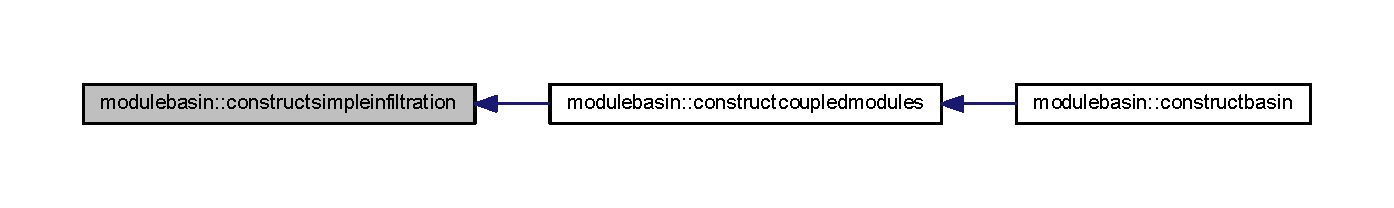
\includegraphics[width=350pt]{namespacemodulebasin_a0b7274cf3bbde399251125f839f59767_icgraph}
\end{center}
\end{figure}
\mbox{\Hypertarget{namespacemodulebasin_a485c76ff915dee4b9ba1ca5c7e79d462}\label{namespacemodulebasin_a485c76ff915dee4b9ba1ca5c7e79d462}} 
\index{modulebasin@{modulebasin}!constructtimeseries@{constructtimeseries}}
\index{constructtimeseries@{constructtimeseries}!modulebasin@{modulebasin}}
\subsubsection{\texorpdfstring{constructtimeseries()}{constructtimeseries()}}
{\footnotesize\ttfamily subroutine, private modulebasin\+::constructtimeseries (\begin{DoxyParamCaption}{ }\end{DoxyParamCaption})\hspace{0.3cm}{\ttfamily [private]}}

Here is the caller graph for this function\+:\nopagebreak
\begin{figure}[H]
\begin{center}
\leavevmode
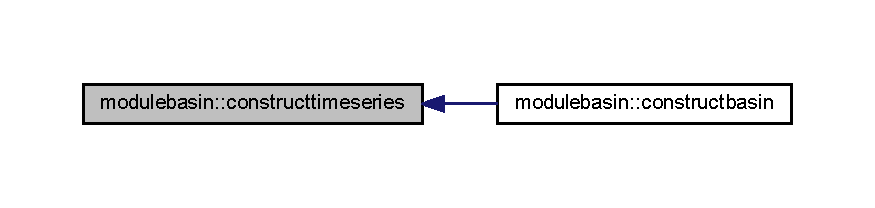
\includegraphics[width=350pt]{namespacemodulebasin_a485c76ff915dee4b9ba1ca5c7e79d462_icgraph}
\end{center}
\end{figure}
\mbox{\Hypertarget{namespacemodulebasin_a1aae2d1fbf8f2ccffa519261e67515b3}\label{namespacemodulebasin_a1aae2d1fbf8f2ccffa519261e67515b3}} 
\index{modulebasin@{modulebasin}!deallocateinstance@{deallocateinstance}}
\index{deallocateinstance@{deallocateinstance}!modulebasin@{modulebasin}}
\subsubsection{\texorpdfstring{deallocateinstance()}{deallocateinstance()}}
{\footnotesize\ttfamily subroutine, private modulebasin\+::deallocateinstance (\begin{DoxyParamCaption}{ }\end{DoxyParamCaption})\hspace{0.3cm}{\ttfamily [private]}}

Here is the caller graph for this function\+:\nopagebreak
\begin{figure}[H]
\begin{center}
\leavevmode
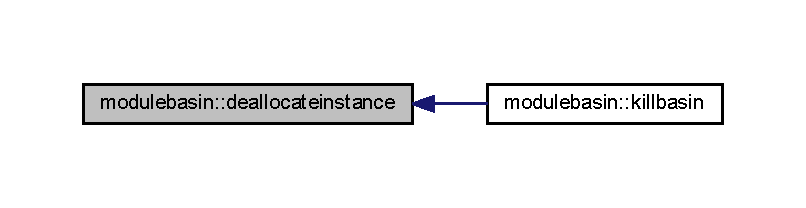
\includegraphics[width=350pt]{namespacemodulebasin_a1aae2d1fbf8f2ccffa519261e67515b3_icgraph}
\end{center}
\end{figure}
\mbox{\Hypertarget{namespacemodulebasin_a4c084fc559ce2dc2a135a4e171d15024}\label{namespacemodulebasin_a4c084fc559ce2dc2a135a4e171d15024}} 
\index{modulebasin@{modulebasin}!divideprecipitation@{divideprecipitation}}
\index{divideprecipitation@{divideprecipitation}!modulebasin@{modulebasin}}
\subsubsection{\texorpdfstring{divideprecipitation()}{divideprecipitation()}}
{\footnotesize\ttfamily subroutine, private modulebasin\+::divideprecipitation (\begin{DoxyParamCaption}\item[{real, dimension(\+:, \+:), pointer}]{Precipitation\+Flux,  }\item[{real, dimension(\+:, \+:), intent(in), optional, pointer}]{Irrigation\+Flux }\end{DoxyParamCaption})\hspace{0.3cm}{\ttfamily [private]}}

Here is the caller graph for this function\+:\nopagebreak
\begin{figure}[H]
\begin{center}
\leavevmode
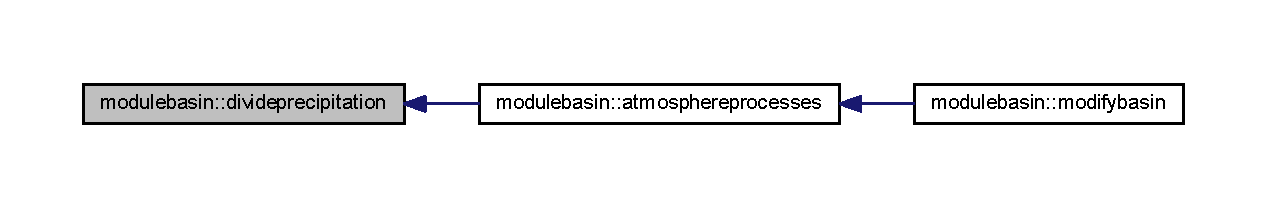
\includegraphics[width=350pt]{namespacemodulebasin_a4c084fc559ce2dc2a135a4e171d15024_icgraph}
\end{center}
\end{figure}
\mbox{\Hypertarget{namespacemodulebasin_a9ece838b83c6e7f083c271a95dbb460f}\label{namespacemodulebasin_a9ece838b83c6e7f083c271a95dbb460f}} 
\index{modulebasin@{modulebasin}!divideprecipitationmassfluxes@{divideprecipitationmassfluxes}}
\index{divideprecipitationmassfluxes@{divideprecipitationmassfluxes}!modulebasin@{modulebasin}}
\subsubsection{\texorpdfstring{divideprecipitationmassfluxes()}{divideprecipitationmassfluxes()}}
{\footnotesize\ttfamily subroutine modulebasin\+::divideprecipitationmassfluxes (\begin{DoxyParamCaption}{ }\end{DoxyParamCaption})\hspace{0.3cm}{\ttfamily [private]}}

Here is the caller graph for this function\+:\nopagebreak
\begin{figure}[H]
\begin{center}
\leavevmode
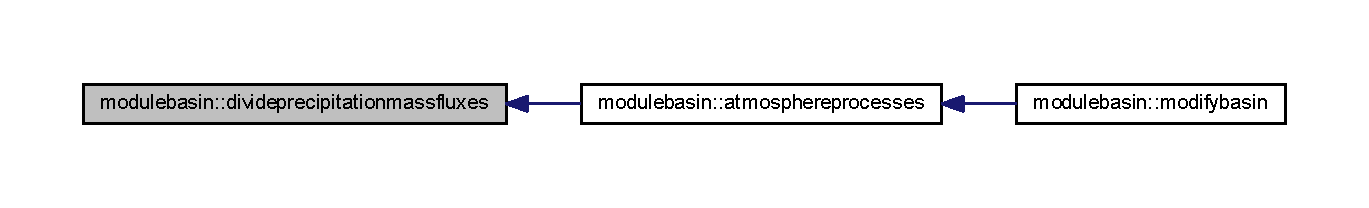
\includegraphics[width=350pt]{namespacemodulebasin_a9ece838b83c6e7f083c271a95dbb460f_icgraph}
\end{center}
\end{figure}
\mbox{\Hypertarget{namespacemodulebasin_ab83592a7be03719e664d5eb440853228}\label{namespacemodulebasin_ab83592a7be03719e664d5eb440853228}} 
\index{modulebasin@{modulebasin}!drainagenetworkprocesses@{drainagenetworkprocesses}}
\index{drainagenetworkprocesses@{drainagenetworkprocesses}!modulebasin@{modulebasin}}
\subsubsection{\texorpdfstring{drainagenetworkprocesses()}{drainagenetworkprocesses()}}
{\footnotesize\ttfamily subroutine, private modulebasin\+::drainagenetworkprocesses (\begin{DoxyParamCaption}{ }\end{DoxyParamCaption})\hspace{0.3cm}{\ttfamily [private]}}

Here is the caller graph for this function\+:\nopagebreak
\begin{figure}[H]
\begin{center}
\leavevmode
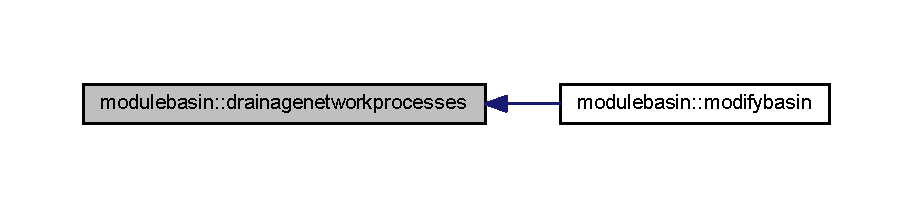
\includegraphics[width=350pt]{namespacemodulebasin_ab83592a7be03719e664d5eb440853228_icgraph}
\end{center}
\end{figure}
\mbox{\Hypertarget{namespacemodulebasin_ac386c2a8b57550077a00db68e3c300ab}\label{namespacemodulebasin_ac386c2a8b57550077a00db68e3c300ab}} 
\index{modulebasin@{modulebasin}!evtphdfoutput@{evtphdfoutput}}
\index{evtphdfoutput@{evtphdfoutput}!modulebasin@{modulebasin}}
\subsubsection{\texorpdfstring{evtphdfoutput()}{evtphdfoutput()}}
{\footnotesize\ttfamily subroutine, private modulebasin\+::evtphdfoutput (\begin{DoxyParamCaption}{ }\end{DoxyParamCaption})\hspace{0.3cm}{\ttfamily [private]}}

Here is the call graph for this function\+:\nopagebreak
\begin{figure}[H]
\begin{center}
\leavevmode
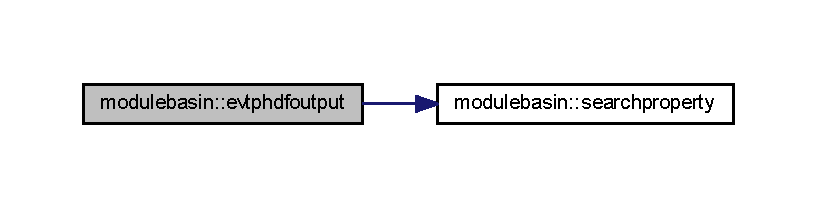
\includegraphics[width=350pt]{namespacemodulebasin_ac386c2a8b57550077a00db68e3c300ab_cgraph}
\end{center}
\end{figure}
Here is the caller graph for this function\+:\nopagebreak
\begin{figure}[H]
\begin{center}
\leavevmode
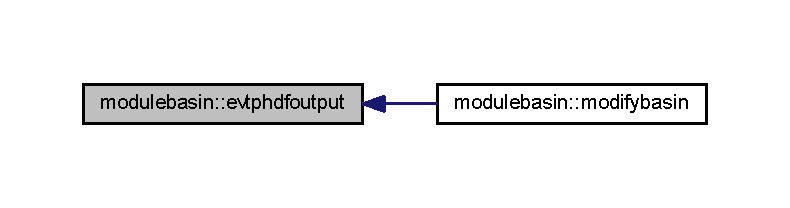
\includegraphics[width=350pt]{namespacemodulebasin_ac386c2a8b57550077a00db68e3c300ab_icgraph}
\end{center}
\end{figure}
\mbox{\Hypertarget{namespacemodulebasin_a51eb37f44f2fb4685ca3ed3454156732}\label{namespacemodulebasin_a51eb37f44f2fb4685ca3ed3454156732}} 
\index{modulebasin@{modulebasin}!getstoredvolumes@{getstoredvolumes}}
\index{getstoredvolumes@{getstoredvolumes}!modulebasin@{modulebasin}}
\subsubsection{\texorpdfstring{getstoredvolumes()}{getstoredvolumes()}}
{\footnotesize\ttfamily subroutine modulebasin\+::getstoredvolumes (\begin{DoxyParamCaption}\item[{integer}]{instant }\end{DoxyParamCaption})\hspace{0.3cm}{\ttfamily [private]}}

Here is the caller graph for this function\+:\nopagebreak
\begin{figure}[H]
\begin{center}
\leavevmode
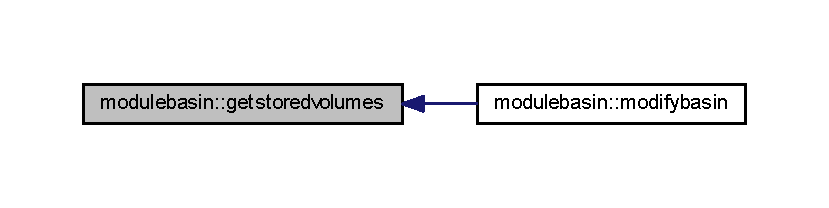
\includegraphics[width=350pt]{namespacemodulebasin_a51eb37f44f2fb4685ca3ed3454156732_icgraph}
\end{center}
\end{figure}
\mbox{\Hypertarget{namespacemodulebasin_ac258b876198ebb36e6bb2b0fd0399158}\label{namespacemodulebasin_ac258b876198ebb36e6bb2b0fd0399158}} 
\index{modulebasin@{modulebasin}!globalmasserror@{globalmasserror}}
\index{globalmasserror@{globalmasserror}!modulebasin@{modulebasin}}
\subsubsection{\texorpdfstring{globalmasserror()}{globalmasserror()}}
{\footnotesize\ttfamily subroutine, private modulebasin\+::globalmasserror (\begin{DoxyParamCaption}{ }\end{DoxyParamCaption})\hspace{0.3cm}{\ttfamily [private]}}

Here is the caller graph for this function\+:\nopagebreak
\begin{figure}[H]
\begin{center}
\leavevmode
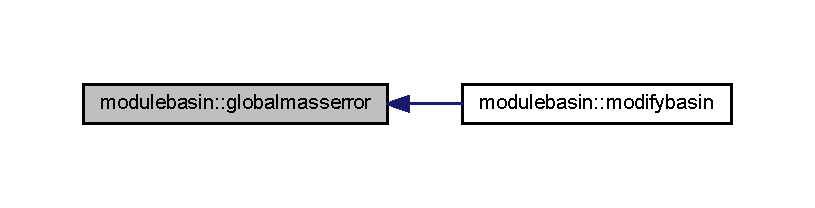
\includegraphics[width=350pt]{namespacemodulebasin_ac258b876198ebb36e6bb2b0fd0399158_icgraph}
\end{center}
\end{figure}
\mbox{\Hypertarget{namespacemodulebasin_a728974f3cdc06d12227aa4b65b29b574}\label{namespacemodulebasin_a728974f3cdc06d12227aa4b65b29b574}} 
\index{modulebasin@{modulebasin}!hdf5output@{hdf5output}}
\index{hdf5output@{hdf5output}!modulebasin@{modulebasin}}
\subsubsection{\texorpdfstring{hdf5output()}{hdf5output()}}
{\footnotesize\ttfamily subroutine, private modulebasin\+::hdf5output (\begin{DoxyParamCaption}{ }\end{DoxyParamCaption})\hspace{0.3cm}{\ttfamily [private]}}

Here is the caller graph for this function\+:\nopagebreak
\begin{figure}[H]
\begin{center}
\leavevmode
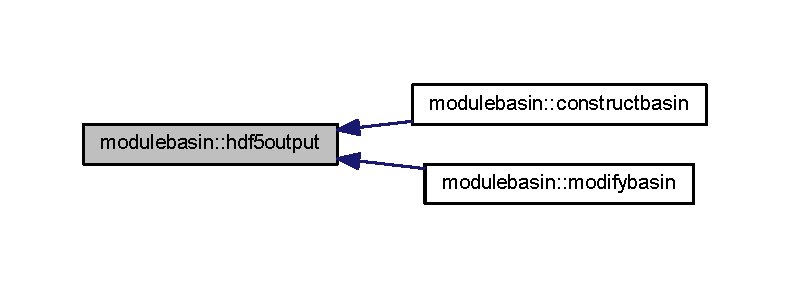
\includegraphics[width=350pt]{namespacemodulebasin_a728974f3cdc06d12227aa4b65b29b574_icgraph}
\end{center}
\end{figure}
\mbox{\Hypertarget{namespacemodulebasin_af1ae0091980128250cba6871d67a941c}\label{namespacemodulebasin_af1ae0091980128250cba6871d67a941c}} 
\index{modulebasin@{modulebasin}!irrigationprocesses@{irrigationprocesses}}
\index{irrigationprocesses@{irrigationprocesses}!modulebasin@{modulebasin}}
\subsubsection{\texorpdfstring{irrigationprocesses()}{irrigationprocesses()}}
{\footnotesize\ttfamily subroutine modulebasin\+::irrigationprocesses (\begin{DoxyParamCaption}{ }\end{DoxyParamCaption})\hspace{0.3cm}{\ttfamily [private]}}

Here is the caller graph for this function\+:\nopagebreak
\begin{figure}[H]
\begin{center}
\leavevmode
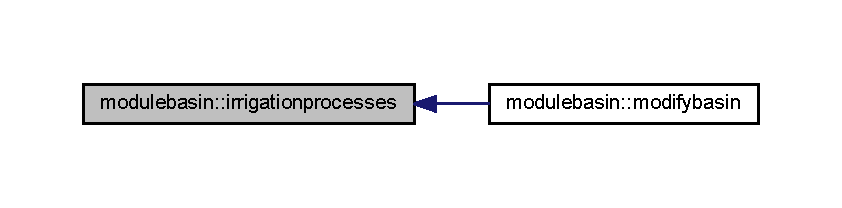
\includegraphics[width=350pt]{namespacemodulebasin_af1ae0091980128250cba6871d67a941c_icgraph}
\end{center}
\end{figure}
\mbox{\Hypertarget{namespacemodulebasin_a766c9c7d623f8a8392b3ed324921f71c}\label{namespacemodulebasin_a766c9c7d623f8a8392b3ed324921f71c}} 
\index{modulebasin@{modulebasin}!killbasin@{killbasin}}
\index{killbasin@{killbasin}!modulebasin@{modulebasin}}
\subsubsection{\texorpdfstring{killbasin()}{killbasin()}}
{\footnotesize\ttfamily subroutine, public modulebasin\+::killbasin (\begin{DoxyParamCaption}\item[{integer}]{Obj\+Basin\+ID,  }\item[{integer, intent(out), optional}]{S\+T\+AT }\end{DoxyParamCaption})}

Here is the call graph for this function\+:\nopagebreak
\begin{figure}[H]
\begin{center}
\leavevmode
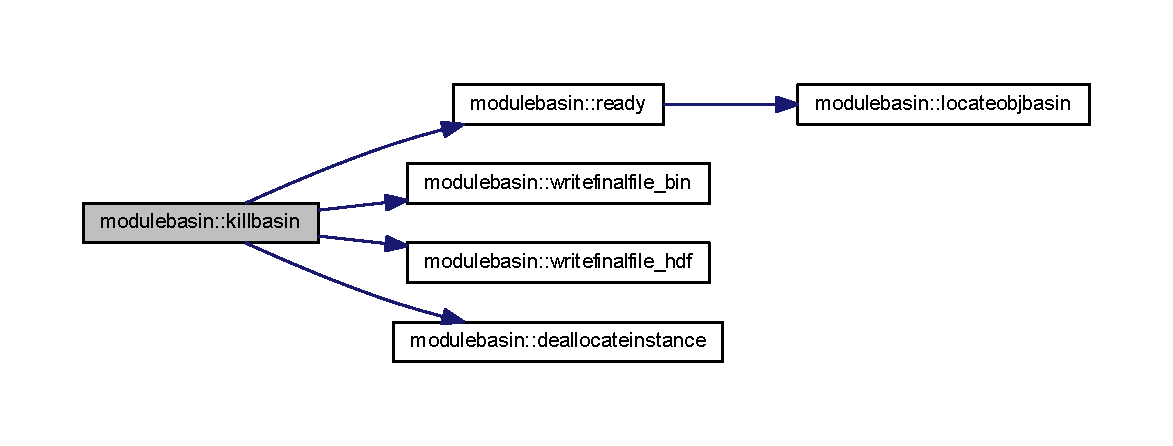
\includegraphics[width=350pt]{namespacemodulebasin_a766c9c7d623f8a8392b3ed324921f71c_cgraph}
\end{center}
\end{figure}
\mbox{\Hypertarget{namespacemodulebasin_a44bb775ef055614008b8afd7ca4b77f4}\label{namespacemodulebasin_a44bb775ef055614008b8afd7ca4b77f4}} 
\index{modulebasin@{modulebasin}!locateobjbasin@{locateobjbasin}}
\index{locateobjbasin@{locateobjbasin}!modulebasin@{modulebasin}}
\subsubsection{\texorpdfstring{locateobjbasin()}{locateobjbasin()}}
{\footnotesize\ttfamily subroutine, private modulebasin\+::locateobjbasin (\begin{DoxyParamCaption}\item[{integer}]{Obj\+Basin\+ID }\end{DoxyParamCaption})\hspace{0.3cm}{\ttfamily [private]}}

Here is the caller graph for this function\+:\nopagebreak
\begin{figure}[H]
\begin{center}
\leavevmode
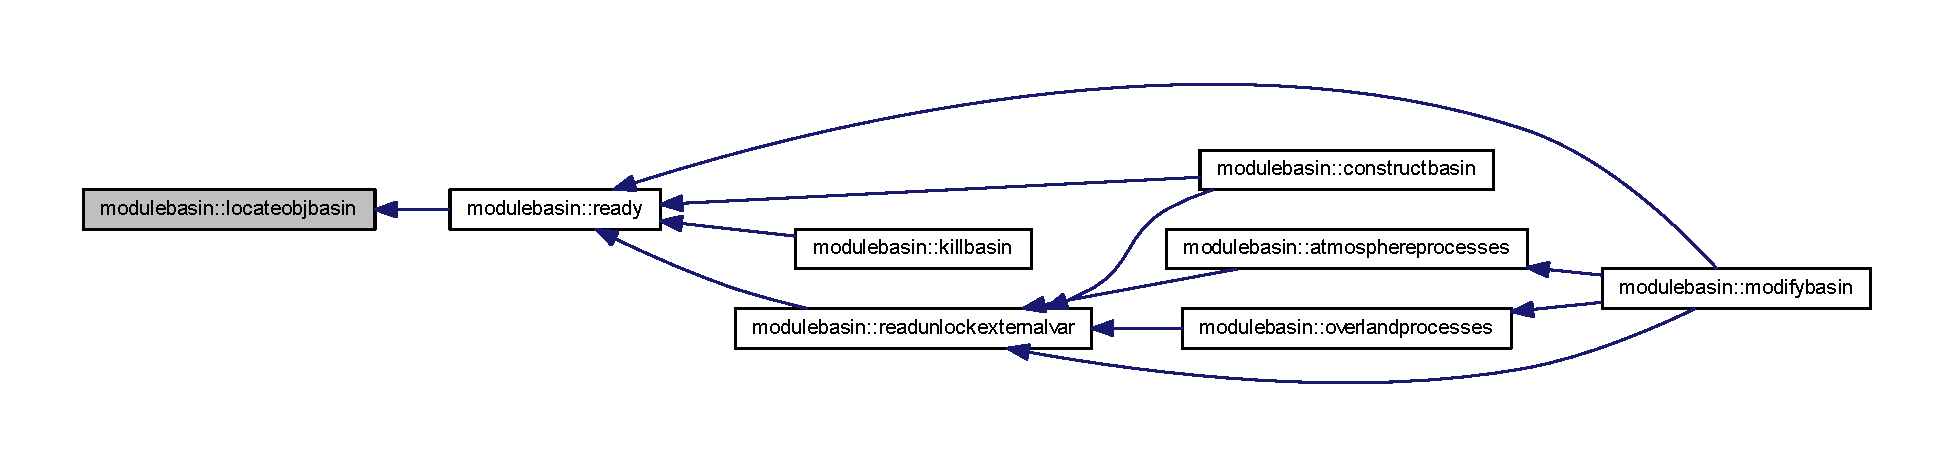
\includegraphics[width=350pt]{namespacemodulebasin_a44bb775ef055614008b8afd7ca4b77f4_icgraph}
\end{center}
\end{figure}
\mbox{\Hypertarget{namespacemodulebasin_a5ce7ee123ed0331d3bcb0ba4db4a9797}\label{namespacemodulebasin_a5ce7ee123ed0331d3bcb0ba4db4a9797}} 
\index{modulebasin@{modulebasin}!modifybasin@{modifybasin}}
\index{modifybasin@{modifybasin}!modulebasin@{modulebasin}}
\subsubsection{\texorpdfstring{modifybasin()}{modifybasin()}}
{\footnotesize\ttfamily subroutine, public modulebasin\+::modifybasin (\begin{DoxyParamCaption}\item[{integer}]{Obj\+Basin\+ID,  }\item[{real}]{New\+DT,  }\item[{integer, intent(out), optional}]{S\+T\+AT }\end{DoxyParamCaption})}

Here is the call graph for this function\+:\nopagebreak
\begin{figure}[H]
\begin{center}
\leavevmode
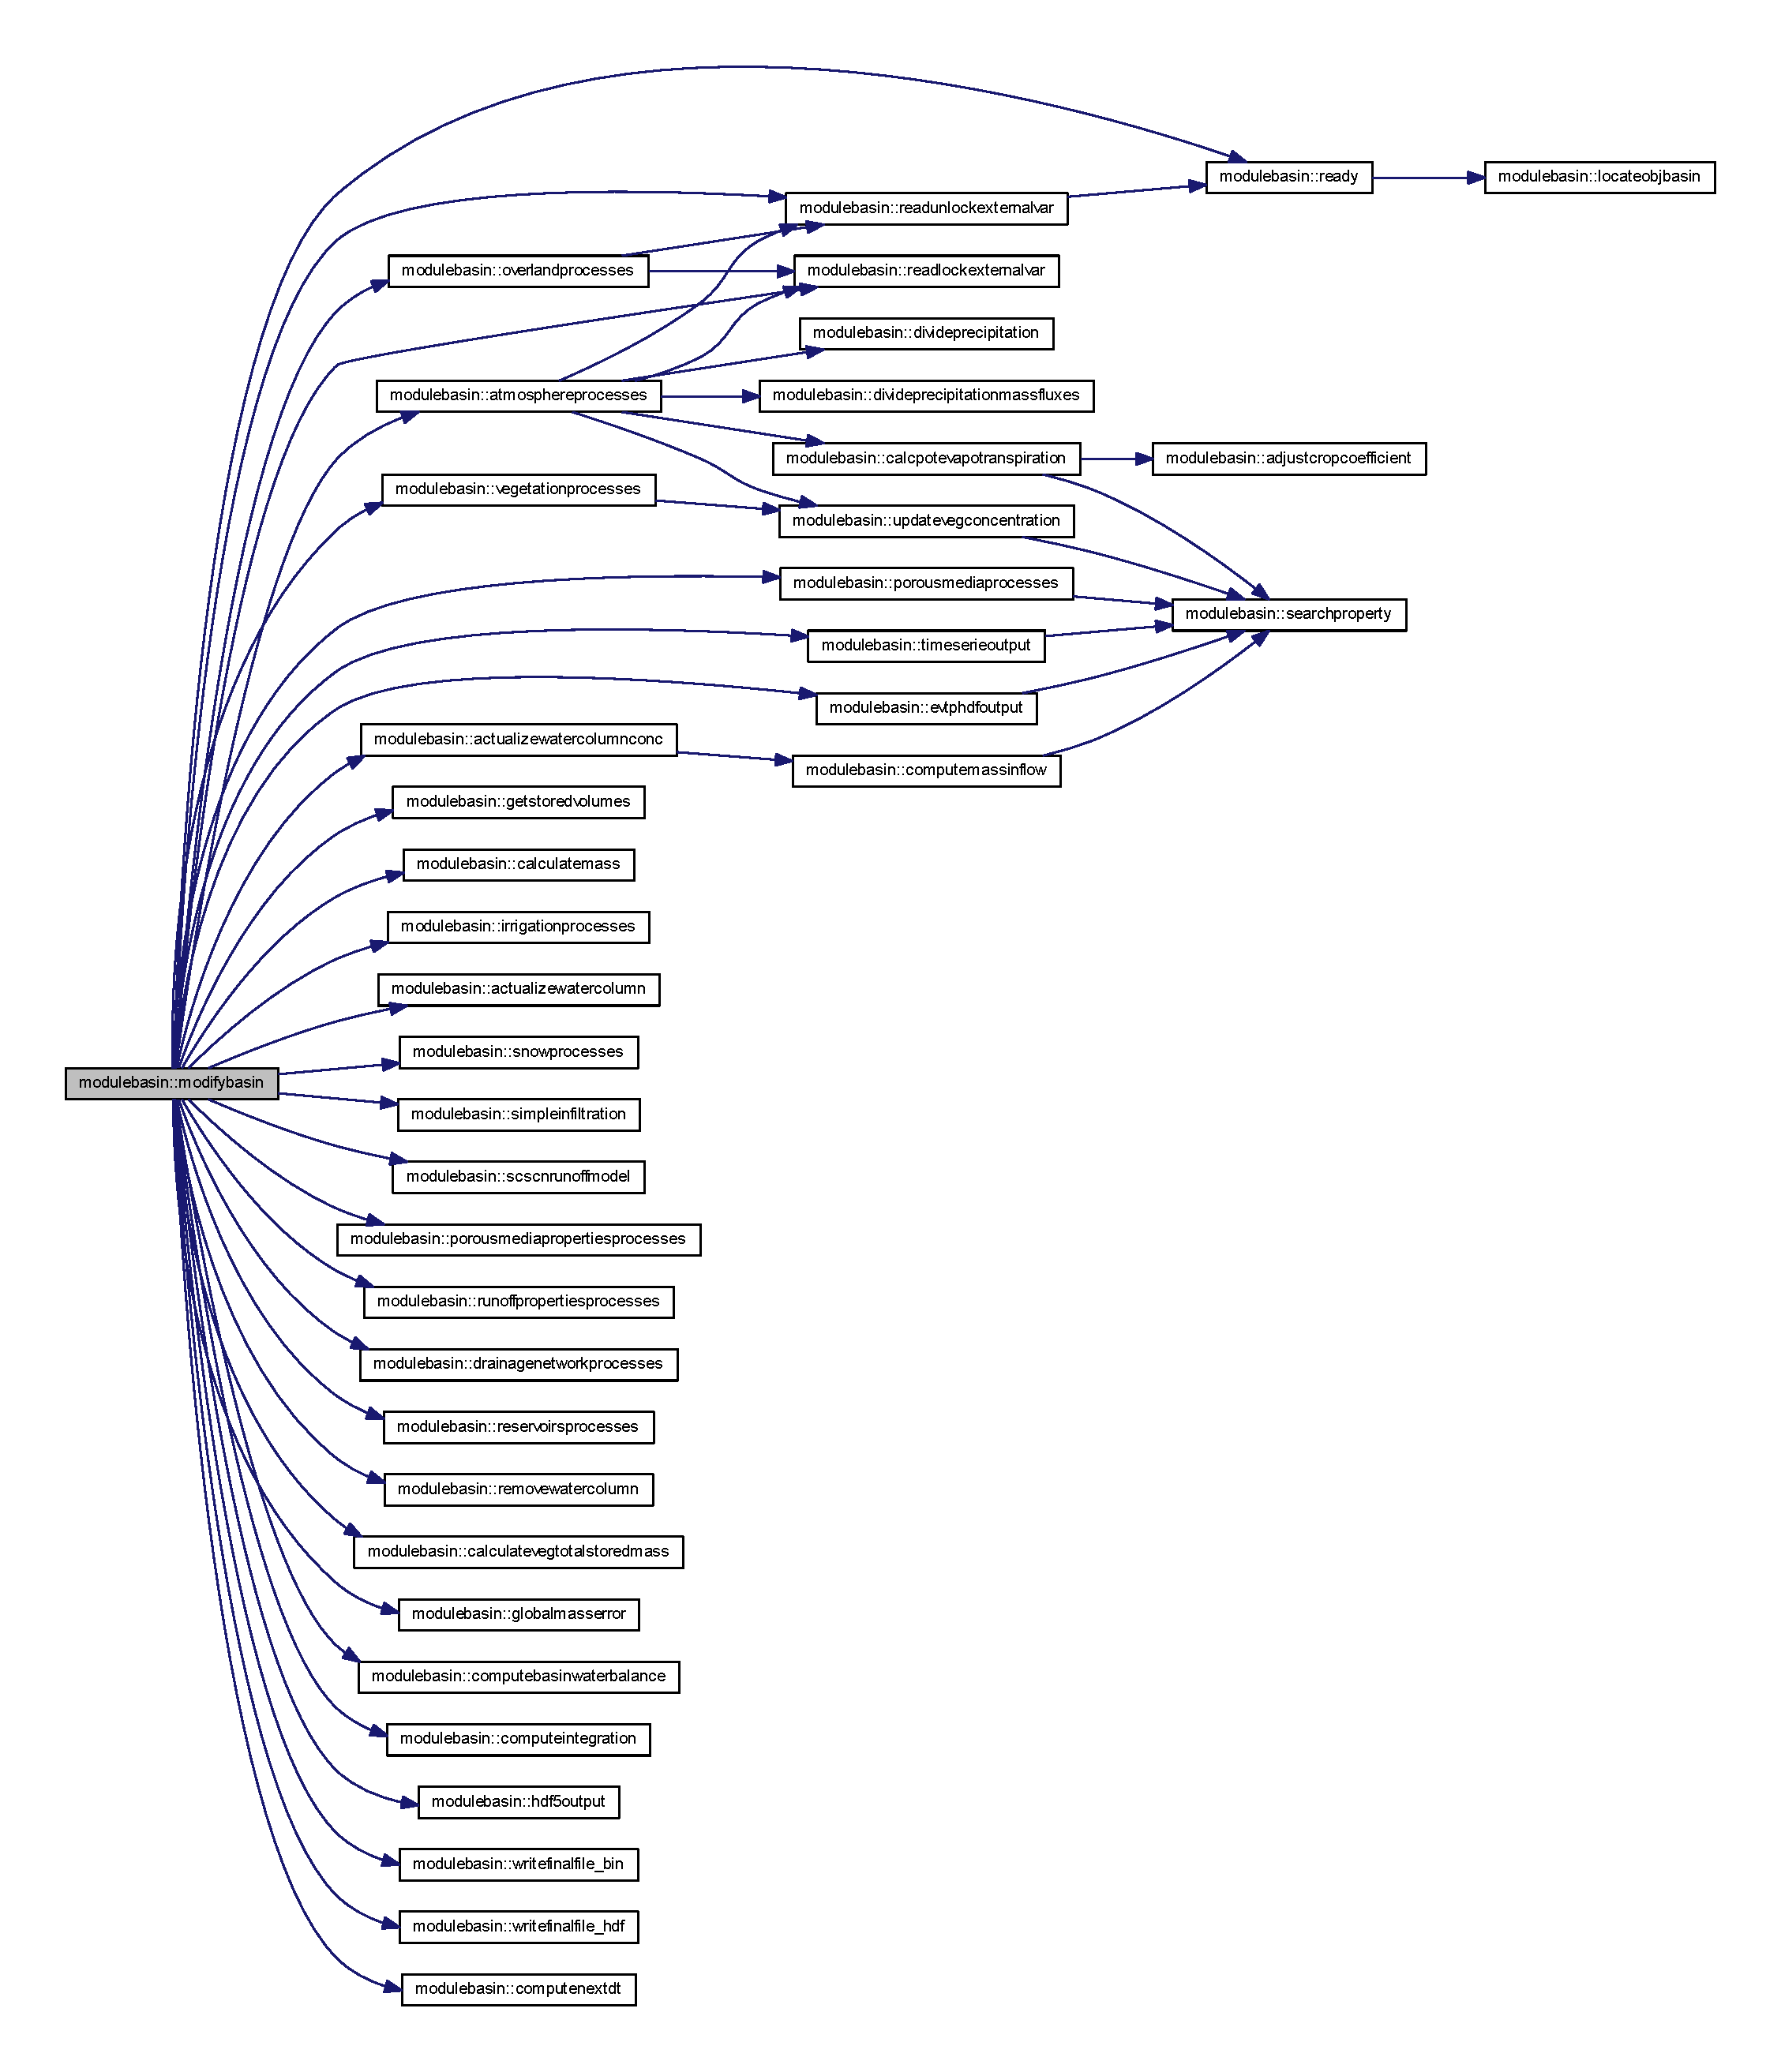
\includegraphics[width=350pt]{namespacemodulebasin_a5ce7ee123ed0331d3bcb0ba4db4a9797_cgraph}
\end{center}
\end{figure}
\mbox{\Hypertarget{namespacemodulebasin_a4732062e95bfb4656920c8c89a412510}\label{namespacemodulebasin_a4732062e95bfb4656920c8c89a412510}} 
\index{modulebasin@{modulebasin}!overlandprocesses@{overlandprocesses}}
\index{overlandprocesses@{overlandprocesses}!modulebasin@{modulebasin}}
\subsubsection{\texorpdfstring{overlandprocesses()}{overlandprocesses()}}
{\footnotesize\ttfamily subroutine, private modulebasin\+::overlandprocesses (\begin{DoxyParamCaption}{ }\end{DoxyParamCaption})\hspace{0.3cm}{\ttfamily [private]}}

Here is the call graph for this function\+:\nopagebreak
\begin{figure}[H]
\begin{center}
\leavevmode
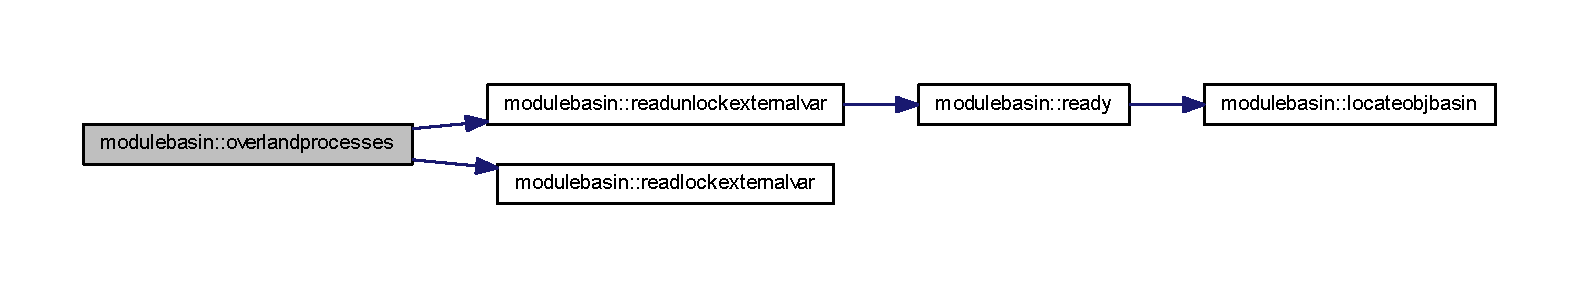
\includegraphics[width=350pt]{namespacemodulebasin_a4732062e95bfb4656920c8c89a412510_cgraph}
\end{center}
\end{figure}
Here is the caller graph for this function\+:\nopagebreak
\begin{figure}[H]
\begin{center}
\leavevmode
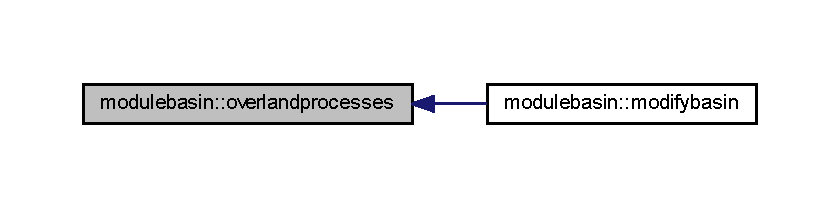
\includegraphics[width=350pt]{namespacemodulebasin_a4732062e95bfb4656920c8c89a412510_icgraph}
\end{center}
\end{figure}
\mbox{\Hypertarget{namespacemodulebasin_aea9e156b76b5f88b91a7c975b33694ac}\label{namespacemodulebasin_aea9e156b76b5f88b91a7c975b33694ac}} 
\index{modulebasin@{modulebasin}!porousmediaprocesses@{porousmediaprocesses}}
\index{porousmediaprocesses@{porousmediaprocesses}!modulebasin@{modulebasin}}
\subsubsection{\texorpdfstring{porousmediaprocesses()}{porousmediaprocesses()}}
{\footnotesize\ttfamily subroutine, private modulebasin\+::porousmediaprocesses (\begin{DoxyParamCaption}{ }\end{DoxyParamCaption})\hspace{0.3cm}{\ttfamily [private]}}

Here is the call graph for this function\+:\nopagebreak
\begin{figure}[H]
\begin{center}
\leavevmode
\includegraphics[width=350pt]{namespacemodulebasin_aea9e156b76b5f88b91a7c975b33694ac_cgraph}
\end{center}
\end{figure}
Here is the caller graph for this function\+:\nopagebreak
\begin{figure}[H]
\begin{center}
\leavevmode
\includegraphics[width=350pt]{namespacemodulebasin_aea9e156b76b5f88b91a7c975b33694ac_icgraph}
\end{center}
\end{figure}
\mbox{\Hypertarget{namespacemodulebasin_abe3651d838039c895cf2f2192597ff85}\label{namespacemodulebasin_abe3651d838039c895cf2f2192597ff85}} 
\index{modulebasin@{modulebasin}!porousmediapropertiesprocesses@{porousmediapropertiesprocesses}}
\index{porousmediapropertiesprocesses@{porousmediapropertiesprocesses}!modulebasin@{modulebasin}}
\subsubsection{\texorpdfstring{porousmediapropertiesprocesses()}{porousmediapropertiesprocesses()}}
{\footnotesize\ttfamily subroutine, private modulebasin\+::porousmediapropertiesprocesses (\begin{DoxyParamCaption}{ }\end{DoxyParamCaption})\hspace{0.3cm}{\ttfamily [private]}}

Here is the caller graph for this function\+:\nopagebreak
\begin{figure}[H]
\begin{center}
\leavevmode
\includegraphics[width=350pt]{namespacemodulebasin_abe3651d838039c895cf2f2192597ff85_icgraph}
\end{center}
\end{figure}
\mbox{\Hypertarget{namespacemodulebasin_af9f507847046c6d52d84d57c39911669}\label{namespacemodulebasin_af9f507847046c6d52d84d57c39911669}} 
\index{modulebasin@{modulebasin}!readdatafile@{readdatafile}}
\index{readdatafile@{readdatafile}!modulebasin@{modulebasin}}
\subsubsection{\texorpdfstring{readdatafile()}{readdatafile()}}
{\footnotesize\ttfamily subroutine, private modulebasin\+::readdatafile (\begin{DoxyParamCaption}{ }\end{DoxyParamCaption})\hspace{0.3cm}{\ttfamily [private]}}

Here is the caller graph for this function\+:\nopagebreak
\begin{figure}[H]
\begin{center}
\leavevmode
\includegraphics[width=350pt]{namespacemodulebasin_af9f507847046c6d52d84d57c39911669_icgraph}
\end{center}
\end{figure}
\mbox{\Hypertarget{namespacemodulebasin_a78bcec6c944663f5c555c4799011fd8f}\label{namespacemodulebasin_a78bcec6c944663f5c555c4799011fd8f}} 
\index{modulebasin@{modulebasin}!readfilenames@{readfilenames}}
\index{readfilenames@{readfilenames}!modulebasin@{modulebasin}}
\subsubsection{\texorpdfstring{readfilenames()}{readfilenames()}}
{\footnotesize\ttfamily subroutine, private modulebasin\+::readfilenames (\begin{DoxyParamCaption}{ }\end{DoxyParamCaption})\hspace{0.3cm}{\ttfamily [private]}}

Here is the caller graph for this function\+:\nopagebreak
\begin{figure}[H]
\begin{center}
\leavevmode
\includegraphics[width=350pt]{namespacemodulebasin_a78bcec6c944663f5c555c4799011fd8f_icgraph}
\end{center}
\end{figure}
\mbox{\Hypertarget{namespacemodulebasin_a4ea226fec981510a8e050dbe3bc285ab}\label{namespacemodulebasin_a4ea226fec981510a8e050dbe3bc285ab}} 
\index{modulebasin@{modulebasin}!readinitialfile\+\_\+bin@{readinitialfile\+\_\+bin}}
\index{readinitialfile\+\_\+bin@{readinitialfile\+\_\+bin}!modulebasin@{modulebasin}}
\subsubsection{\texorpdfstring{readinitialfile\+\_\+bin()}{readinitialfile\_bin()}}
{\footnotesize\ttfamily subroutine modulebasin\+::readinitialfile\+\_\+bin (\begin{DoxyParamCaption}{ }\end{DoxyParamCaption})\hspace{0.3cm}{\ttfamily [private]}}

Here is the caller graph for this function\+:\nopagebreak
\begin{figure}[H]
\begin{center}
\leavevmode
\includegraphics[width=350pt]{namespacemodulebasin_a4ea226fec981510a8e050dbe3bc285ab_icgraph}
\end{center}
\end{figure}
\mbox{\Hypertarget{namespacemodulebasin_a52545eff06912899ced860eb99799977}\label{namespacemodulebasin_a52545eff06912899ced860eb99799977}} 
\index{modulebasin@{modulebasin}!readinitialfile\+\_\+hdf@{readinitialfile\+\_\+hdf}}
\index{readinitialfile\+\_\+hdf@{readinitialfile\+\_\+hdf}!modulebasin@{modulebasin}}
\subsubsection{\texorpdfstring{readinitialfile\+\_\+hdf()}{readinitialfile\_hdf()}}
{\footnotesize\ttfamily subroutine modulebasin\+::readinitialfile\+\_\+hdf (\begin{DoxyParamCaption}{ }\end{DoxyParamCaption})\hspace{0.3cm}{\ttfamily [private]}}

Here is the caller graph for this function\+:\nopagebreak
\begin{figure}[H]
\begin{center}
\leavevmode
\includegraphics[width=350pt]{namespacemodulebasin_a52545eff06912899ced860eb99799977_icgraph}
\end{center}
\end{figure}
\mbox{\Hypertarget{namespacemodulebasin_adebce1a3581c733f01c10813a94c4dea}\label{namespacemodulebasin_adebce1a3581c733f01c10813a94c4dea}} 
\index{modulebasin@{modulebasin}!readlockexternalvar@{readlockexternalvar}}
\index{readlockexternalvar@{readlockexternalvar}!modulebasin@{modulebasin}}
\subsubsection{\texorpdfstring{readlockexternalvar()}{readlockexternalvar()}}
{\footnotesize\ttfamily subroutine, private modulebasin\+::readlockexternalvar (\begin{DoxyParamCaption}\item[{character (len = stringlength)}]{Lock\+To\+Which\+Modules,  }\item[{character (len = stringlength), optional}]{Options\+Type }\end{DoxyParamCaption})\hspace{0.3cm}{\ttfamily [private]}}

Here is the caller graph for this function\+:\nopagebreak
\begin{figure}[H]
\begin{center}
\leavevmode
\includegraphics[width=350pt]{namespacemodulebasin_adebce1a3581c733f01c10813a94c4dea_icgraph}
\end{center}
\end{figure}
\mbox{\Hypertarget{namespacemodulebasin_aff09c4da760fd9cda4b797242d7ff522}\label{namespacemodulebasin_aff09c4da760fd9cda4b797242d7ff522}} 
\index{modulebasin@{modulebasin}!readunlockexternalvar@{readunlockexternalvar}}
\index{readunlockexternalvar@{readunlockexternalvar}!modulebasin@{modulebasin}}
\subsubsection{\texorpdfstring{readunlockexternalvar()}{readunlockexternalvar()}}
{\footnotesize\ttfamily subroutine, private modulebasin\+::readunlockexternalvar (\begin{DoxyParamCaption}\item[{character (len = stringlength)}]{Un\+Lock\+To\+Which\+Modules,  }\item[{character (len = stringlength), optional}]{Options\+Type }\end{DoxyParamCaption})\hspace{0.3cm}{\ttfamily [private]}}

Here is the call graph for this function\+:\nopagebreak
\begin{figure}[H]
\begin{center}
\leavevmode
\includegraphics[width=350pt]{namespacemodulebasin_aff09c4da760fd9cda4b797242d7ff522_cgraph}
\end{center}
\end{figure}
Here is the caller graph for this function\+:\nopagebreak
\begin{figure}[H]
\begin{center}
\leavevmode
\includegraphics[width=350pt]{namespacemodulebasin_aff09c4da760fd9cda4b797242d7ff522_icgraph}
\end{center}
\end{figure}
\mbox{\Hypertarget{namespacemodulebasin_afed1d3ff36b21d7528bddef4df954906}\label{namespacemodulebasin_afed1d3ff36b21d7528bddef4df954906}} 
\index{modulebasin@{modulebasin}!ready@{ready}}
\index{ready@{ready}!modulebasin@{modulebasin}}
\subsubsection{\texorpdfstring{ready()}{ready()}}
{\footnotesize\ttfamily subroutine, private modulebasin\+::ready (\begin{DoxyParamCaption}\item[{integer}]{Obj\+Basin\+\_\+\+ID,  }\item[{integer}]{ready\+\_\+ }\end{DoxyParamCaption})\hspace{0.3cm}{\ttfamily [private]}}

Here is the call graph for this function\+:\nopagebreak
\begin{figure}[H]
\begin{center}
\leavevmode
\includegraphics[width=350pt]{namespacemodulebasin_afed1d3ff36b21d7528bddef4df954906_cgraph}
\end{center}
\end{figure}
Here is the caller graph for this function\+:\nopagebreak
\begin{figure}[H]
\begin{center}
\leavevmode
\includegraphics[width=350pt]{namespacemodulebasin_afed1d3ff36b21d7528bddef4df954906_icgraph}
\end{center}
\end{figure}
\mbox{\Hypertarget{namespacemodulebasin_a2c7426bfbfa1e3a2540f18b8e04ec4b5}\label{namespacemodulebasin_a2c7426bfbfa1e3a2540f18b8e04ec4b5}} 
\index{modulebasin@{modulebasin}!removewatercolumn@{removewatercolumn}}
\index{removewatercolumn@{removewatercolumn}!modulebasin@{modulebasin}}
\subsubsection{\texorpdfstring{removewatercolumn()}{removewatercolumn()}}
{\footnotesize\ttfamily subroutine modulebasin\+::removewatercolumn (\begin{DoxyParamCaption}{ }\end{DoxyParamCaption})\hspace{0.3cm}{\ttfamily [private]}}

Here is the caller graph for this function\+:\nopagebreak
\begin{figure}[H]
\begin{center}
\leavevmode
\includegraphics[width=350pt]{namespacemodulebasin_a2c7426bfbfa1e3a2540f18b8e04ec4b5_icgraph}
\end{center}
\end{figure}
\mbox{\Hypertarget{namespacemodulebasin_a2d6933b0b62fd8ddf365de6af6309c1c}\label{namespacemodulebasin_a2d6933b0b62fd8ddf365de6af6309c1c}} 
\index{modulebasin@{modulebasin}!reservoirsprocesses@{reservoirsprocesses}}
\index{reservoirsprocesses@{reservoirsprocesses}!modulebasin@{modulebasin}}
\subsubsection{\texorpdfstring{reservoirsprocesses()}{reservoirsprocesses()}}
{\footnotesize\ttfamily subroutine modulebasin\+::reservoirsprocesses (\begin{DoxyParamCaption}{ }\end{DoxyParamCaption})\hspace{0.3cm}{\ttfamily [private]}}

Here is the caller graph for this function\+:\nopagebreak
\begin{figure}[H]
\begin{center}
\leavevmode
\includegraphics[width=350pt]{namespacemodulebasin_a2d6933b0b62fd8ddf365de6af6309c1c_icgraph}
\end{center}
\end{figure}
\mbox{\Hypertarget{namespacemodulebasin_a0d5f24ad034e1da333cb8086aba4bf1f}\label{namespacemodulebasin_a0d5f24ad034e1da333cb8086aba4bf1f}} 
\index{modulebasin@{modulebasin}!runoffpropertiesprocesses@{runoffpropertiesprocesses}}
\index{runoffpropertiesprocesses@{runoffpropertiesprocesses}!modulebasin@{modulebasin}}
\subsubsection{\texorpdfstring{runoffpropertiesprocesses()}{runoffpropertiesprocesses()}}
{\footnotesize\ttfamily subroutine modulebasin\+::runoffpropertiesprocesses (\begin{DoxyParamCaption}{ }\end{DoxyParamCaption})\hspace{0.3cm}{\ttfamily [private]}}

Here is the caller graph for this function\+:\nopagebreak
\begin{figure}[H]
\begin{center}
\leavevmode
\includegraphics[width=350pt]{namespacemodulebasin_a0d5f24ad034e1da333cb8086aba4bf1f_icgraph}
\end{center}
\end{figure}
\mbox{\Hypertarget{namespacemodulebasin_aa0b9eaedf50e780116499db9c0c35730}\label{namespacemodulebasin_aa0b9eaedf50e780116499db9c0c35730}} 
\index{modulebasin@{modulebasin}!scscnrunoffmodel@{scscnrunoffmodel}}
\index{scscnrunoffmodel@{scscnrunoffmodel}!modulebasin@{modulebasin}}
\subsubsection{\texorpdfstring{scscnrunoffmodel()}{scscnrunoffmodel()}}
{\footnotesize\ttfamily subroutine modulebasin\+::scscnrunoffmodel (\begin{DoxyParamCaption}{ }\end{DoxyParamCaption})\hspace{0.3cm}{\ttfamily [private]}}

Here is the caller graph for this function\+:\nopagebreak
\begin{figure}[H]
\begin{center}
\leavevmode
\includegraphics[width=350pt]{namespacemodulebasin_aa0b9eaedf50e780116499db9c0c35730_icgraph}
\end{center}
\end{figure}
\mbox{\Hypertarget{namespacemodulebasin_aa2e4e95b7bf5ee3e53a64d7f2269c946}\label{namespacemodulebasin_aa2e4e95b7bf5ee3e53a64d7f2269c946}} 
\index{modulebasin@{modulebasin}!searchproperty@{searchproperty}}
\index{searchproperty@{searchproperty}!modulebasin@{modulebasin}}
\subsubsection{\texorpdfstring{searchproperty()}{searchproperty()}}
{\footnotesize\ttfamily subroutine modulebasin\+::searchproperty (\begin{DoxyParamCaption}\item[{type(\mbox{\hyperlink{structmodulebasin_1_1t__basinproperty}{t\+\_\+basinproperty}}), optional, pointer}]{PropertyX,  }\item[{integer, intent(in), optional}]{Property\+X\+I\+D\+Number,  }\item[{logical, intent(in), optional}]{Print\+Warning,  }\item[{integer, intent(out), optional}]{S\+T\+AT }\end{DoxyParamCaption})\hspace{0.3cm}{\ttfamily [private]}}

Here is the caller graph for this function\+:\nopagebreak
\begin{figure}[H]
\begin{center}
\leavevmode
\includegraphics[width=350pt]{namespacemodulebasin_aa2e4e95b7bf5ee3e53a64d7f2269c946_icgraph}
\end{center}
\end{figure}
\mbox{\Hypertarget{namespacemodulebasin_a7c47f016b2561d84dff67a1089c6c8f0}\label{namespacemodulebasin_a7c47f016b2561d84dff67a1089c6c8f0}} 
\index{modulebasin@{modulebasin}!simpleinfiltration@{simpleinfiltration}}
\index{simpleinfiltration@{simpleinfiltration}!modulebasin@{modulebasin}}
\subsubsection{\texorpdfstring{simpleinfiltration()}{simpleinfiltration()}}
{\footnotesize\ttfamily subroutine modulebasin\+::simpleinfiltration (\begin{DoxyParamCaption}{ }\end{DoxyParamCaption})\hspace{0.3cm}{\ttfamily [private]}}

Here is the caller graph for this function\+:\nopagebreak
\begin{figure}[H]
\begin{center}
\leavevmode
\includegraphics[width=350pt]{namespacemodulebasin_a7c47f016b2561d84dff67a1089c6c8f0_icgraph}
\end{center}
\end{figure}
\mbox{\Hypertarget{namespacemodulebasin_a19824f46960f411ab472a65b6e3a9d2e}\label{namespacemodulebasin_a19824f46960f411ab472a65b6e3a9d2e}} 
\index{modulebasin@{modulebasin}!snowprocesses@{snowprocesses}}
\index{snowprocesses@{snowprocesses}!modulebasin@{modulebasin}}
\subsubsection{\texorpdfstring{snowprocesses()}{snowprocesses()}}
{\footnotesize\ttfamily subroutine modulebasin\+::snowprocesses (\begin{DoxyParamCaption}{ }\end{DoxyParamCaption})\hspace{0.3cm}{\ttfamily [private]}}

Here is the caller graph for this function\+:\nopagebreak
\begin{figure}[H]
\begin{center}
\leavevmode
\includegraphics[width=350pt]{namespacemodulebasin_a19824f46960f411ab472a65b6e3a9d2e_icgraph}
\end{center}
\end{figure}
\mbox{\Hypertarget{namespacemodulebasin_a5d090cabe217c5ee21e1b627217a129f}\label{namespacemodulebasin_a5d090cabe217c5ee21e1b627217a129f}} 
\index{modulebasin@{modulebasin}!timeserieoutput@{timeserieoutput}}
\index{timeserieoutput@{timeserieoutput}!modulebasin@{modulebasin}}
\subsubsection{\texorpdfstring{timeserieoutput()}{timeserieoutput()}}
{\footnotesize\ttfamily subroutine, private modulebasin\+::timeserieoutput (\begin{DoxyParamCaption}{ }\end{DoxyParamCaption})\hspace{0.3cm}{\ttfamily [private]}}

Here is the call graph for this function\+:\nopagebreak
\begin{figure}[H]
\begin{center}
\leavevmode
\includegraphics[width=350pt]{namespacemodulebasin_a5d090cabe217c5ee21e1b627217a129f_cgraph}
\end{center}
\end{figure}
Here is the caller graph for this function\+:\nopagebreak
\begin{figure}[H]
\begin{center}
\leavevmode
\includegraphics[width=350pt]{namespacemodulebasin_a5d090cabe217c5ee21e1b627217a129f_icgraph}
\end{center}
\end{figure}
\mbox{\Hypertarget{namespacemodulebasin_a73f54ad66e54b432898b7261a7ba0969}\label{namespacemodulebasin_a73f54ad66e54b432898b7261a7ba0969}} 
\index{modulebasin@{modulebasin}!updatevegconcentration@{updatevegconcentration}}
\index{updatevegconcentration@{updatevegconcentration}!modulebasin@{modulebasin}}
\subsubsection{\texorpdfstring{updatevegconcentration()}{updatevegconcentration()}}
{\footnotesize\ttfamily subroutine modulebasin\+::updatevegconcentration (\begin{DoxyParamCaption}\item[{character (len = $\ast$), intent(in)}]{Warning\+String }\end{DoxyParamCaption})\hspace{0.3cm}{\ttfamily [private]}}

Here is the call graph for this function\+:\nopagebreak
\begin{figure}[H]
\begin{center}
\leavevmode
\includegraphics[width=350pt]{namespacemodulebasin_a73f54ad66e54b432898b7261a7ba0969_cgraph}
\end{center}
\end{figure}
Here is the caller graph for this function\+:\nopagebreak
\begin{figure}[H]
\begin{center}
\leavevmode
\includegraphics[width=350pt]{namespacemodulebasin_a73f54ad66e54b432898b7261a7ba0969_icgraph}
\end{center}
\end{figure}
\mbox{\Hypertarget{namespacemodulebasin_a8345c242b1aed1c95c3779596054b89f}\label{namespacemodulebasin_a8345c242b1aed1c95c3779596054b89f}} 
\index{modulebasin@{modulebasin}!vegetationprocesses@{vegetationprocesses}}
\index{vegetationprocesses@{vegetationprocesses}!modulebasin@{modulebasin}}
\subsubsection{\texorpdfstring{vegetationprocesses()}{vegetationprocesses()}}
{\footnotesize\ttfamily subroutine, private modulebasin\+::vegetationprocesses (\begin{DoxyParamCaption}{ }\end{DoxyParamCaption})\hspace{0.3cm}{\ttfamily [private]}}

Here is the call graph for this function\+:\nopagebreak
\begin{figure}[H]
\begin{center}
\leavevmode
\includegraphics[width=350pt]{namespacemodulebasin_a8345c242b1aed1c95c3779596054b89f_cgraph}
\end{center}
\end{figure}
Here is the caller graph for this function\+:\nopagebreak
\begin{figure}[H]
\begin{center}
\leavevmode
\includegraphics[width=350pt]{namespacemodulebasin_a8345c242b1aed1c95c3779596054b89f_icgraph}
\end{center}
\end{figure}
\mbox{\Hypertarget{namespacemodulebasin_a6de1170114b38ad6db725fe89c8cd2bd}\label{namespacemodulebasin_a6de1170114b38ad6db725fe89c8cd2bd}} 
\index{modulebasin@{modulebasin}!verifyoptions@{verifyoptions}}
\index{verifyoptions@{verifyoptions}!modulebasin@{modulebasin}}
\subsubsection{\texorpdfstring{verifyoptions()}{verifyoptions()}}
{\footnotesize\ttfamily subroutine, private modulebasin\+::verifyoptions (\begin{DoxyParamCaption}\item[{character (len = stringlength)}]{Warning\+String }\end{DoxyParamCaption})\hspace{0.3cm}{\ttfamily [private]}}

Here is the caller graph for this function\+:\nopagebreak
\begin{figure}[H]
\begin{center}
\leavevmode
\includegraphics[width=350pt]{namespacemodulebasin_a6de1170114b38ad6db725fe89c8cd2bd_icgraph}
\end{center}
\end{figure}
\mbox{\Hypertarget{namespacemodulebasin_ab2ed3d304db416a0172609e73be05bd4}\label{namespacemodulebasin_ab2ed3d304db416a0172609e73be05bd4}} 
\index{modulebasin@{modulebasin}!writefinalfile\+\_\+bin@{writefinalfile\+\_\+bin}}
\index{writefinalfile\+\_\+bin@{writefinalfile\+\_\+bin}!modulebasin@{modulebasin}}
\subsubsection{\texorpdfstring{writefinalfile\+\_\+bin()}{writefinalfile\_bin()}}
{\footnotesize\ttfamily subroutine modulebasin\+::writefinalfile\+\_\+bin (\begin{DoxyParamCaption}\item[{logical}]{Is\+Final\+File }\end{DoxyParamCaption})\hspace{0.3cm}{\ttfamily [private]}}

Here is the caller graph for this function\+:\nopagebreak
\begin{figure}[H]
\begin{center}
\leavevmode
\includegraphics[width=350pt]{namespacemodulebasin_ab2ed3d304db416a0172609e73be05bd4_icgraph}
\end{center}
\end{figure}
\mbox{\Hypertarget{namespacemodulebasin_af6daa86ceef2fea67fa23aaebaf588f1}\label{namespacemodulebasin_af6daa86ceef2fea67fa23aaebaf588f1}} 
\index{modulebasin@{modulebasin}!writefinalfile\+\_\+hdf@{writefinalfile\+\_\+hdf}}
\index{writefinalfile\+\_\+hdf@{writefinalfile\+\_\+hdf}!modulebasin@{modulebasin}}
\subsubsection{\texorpdfstring{writefinalfile\+\_\+hdf()}{writefinalfile\_hdf()}}
{\footnotesize\ttfamily subroutine modulebasin\+::writefinalfile\+\_\+hdf (\begin{DoxyParamCaption}\item[{logical}]{Is\+Final\+File }\end{DoxyParamCaption})\hspace{0.3cm}{\ttfamily [private]}}

Here is the caller graph for this function\+:\nopagebreak
\begin{figure}[H]
\begin{center}
\leavevmode
\includegraphics[width=350pt]{namespacemodulebasin_af6daa86ceef2fea67fa23aaebaf588f1_icgraph}
\end{center}
\end{figure}


\subsection{Variable Documentation}
\mbox{\Hypertarget{namespacemodulebasin_ab9e149429872bd1ef4a8213cff258870}\label{namespacemodulebasin_ab9e149429872bd1ef4a8213cff258870}} 
\index{modulebasin@{modulebasin}!bin\+\_\+@{bin\+\_\+}}
\index{bin\+\_\+@{bin\+\_\+}!modulebasin@{modulebasin}}
\subsubsection{\texorpdfstring{bin\+\_\+}{bin\_}}
{\footnotesize\ttfamily integer, parameter modulebasin\+::bin\+\_\+ = 1\hspace{0.3cm}{\ttfamily [private]}}

\mbox{\Hypertarget{namespacemodulebasin_a14ea3de5b477aa2d46ac8ce040ba891c}\label{namespacemodulebasin_a14ea3de5b477aa2d46ac8ce040ba891c}} 
\index{modulebasin@{modulebasin}!block\+\_\+begin@{block\+\_\+begin}}
\index{block\+\_\+begin@{block\+\_\+begin}!modulebasin@{modulebasin}}
\subsubsection{\texorpdfstring{block\+\_\+begin}{block\_begin}}
{\footnotesize\ttfamily character(len = stringlength), parameter modulebasin\+::block\+\_\+begin = \textquotesingle{}$<$beginproperty$>$\textquotesingle{}\hspace{0.3cm}{\ttfamily [private]}}

\mbox{\Hypertarget{namespacemodulebasin_a2dc5a4aaf15a73086781f37d625f774d}\label{namespacemodulebasin_a2dc5a4aaf15a73086781f37d625f774d}} 
\index{modulebasin@{modulebasin}!block\+\_\+end@{block\+\_\+end}}
\index{block\+\_\+end@{block\+\_\+end}!modulebasin@{modulebasin}}
\subsubsection{\texorpdfstring{block\+\_\+end}{block\_end}}
{\footnotesize\ttfamily character(len = stringlength), parameter modulebasin\+::block\+\_\+end = \textquotesingle{}$<$endproperty$>$\textquotesingle{}\hspace{0.3cm}{\ttfamily [private]}}

\mbox{\Hypertarget{namespacemodulebasin_a230ea75f89c595973578b0499383801d}\label{namespacemodulebasin_a230ea75f89c595973578b0499383801d}} 
\index{modulebasin@{modulebasin}!characcerrorinvolume@{characcerrorinvolume}}
\index{characcerrorinvolume@{characcerrorinvolume}!modulebasin@{modulebasin}}
\subsubsection{\texorpdfstring{characcerrorinvolume}{characcerrorinvolume}}
{\footnotesize\ttfamily character($\ast$), parameter modulebasin\+::characcerrorinvolume = \textquotesingle{}acc. error in volume\textquotesingle{}\hspace{0.3cm}{\ttfamily [private]}}

\mbox{\Hypertarget{namespacemodulebasin_a07f6f68a43c452ae9eef45c1933a1d20}\label{namespacemodulebasin_a07f6f68a43c452ae9eef45c1933a1d20}} 
\index{modulebasin@{modulebasin}!dormantvegetation@{dormantvegetation}}
\index{dormantvegetation@{dormantvegetation}!modulebasin@{modulebasin}}
\subsubsection{\texorpdfstring{dormantvegetation}{dormantvegetation}}
{\footnotesize\ttfamily integer, parameter modulebasin\+::dormantvegetation = 1\hspace{0.3cm}{\ttfamily [private]}}

\mbox{\Hypertarget{namespacemodulebasin_a173aa2ad8e4e632e6cb9251e98c97e5d}\label{namespacemodulebasin_a173aa2ad8e4e632e6cb9251e98c97e5d}} 
\index{modulebasin@{modulebasin}!et0method@{et0method}}
\index{et0method@{et0method}!modulebasin@{modulebasin}}
\subsubsection{\texorpdfstring{et0method}{et0method}}
{\footnotesize\ttfamily integer, parameter modulebasin\+::et0method = 2\hspace{0.3cm}{\ttfamily [private]}}

\mbox{\Hypertarget{namespacemodulebasin_ab601fa0c07f0bc9134f81f45d1341678}\label{namespacemodulebasin_ab601fa0c07f0bc9134f81f45d1341678}} 
\index{modulebasin@{modulebasin}!finalinstant@{finalinstant}}
\index{finalinstant@{finalinstant}!modulebasin@{modulebasin}}
\subsubsection{\texorpdfstring{finalinstant}{finalinstant}}
{\footnotesize\ttfamily integer, parameter modulebasin\+::finalinstant = 2\hspace{0.3cm}{\ttfamily [private]}}

\mbox{\Hypertarget{namespacemodulebasin_a5b7e2b3f3d81ecb78131059c79f1557e}\label{namespacemodulebasin_a5b7e2b3f3d81ecb78131059c79f1557e}} 
\index{modulebasin@{modulebasin}!firstobjbasin@{firstobjbasin}}
\index{firstobjbasin@{firstobjbasin}!modulebasin@{modulebasin}}
\subsubsection{\texorpdfstring{firstobjbasin}{firstobjbasin}}
{\footnotesize\ttfamily type (\mbox{\hyperlink{structmodulebasin_1_1t__basin}{t\+\_\+basin}}), pointer modulebasin\+::firstobjbasin =$>$ null()\hspace{0.3cm}{\ttfamily [private]}}

\mbox{\Hypertarget{namespacemodulebasin_a2def264a3397d7af9334938fcadc85a1}\label{namespacemodulebasin_a2def264a3397d7af9334938fcadc85a1}} 
\index{modulebasin@{modulebasin}!growingvegetation@{growingvegetation}}
\index{growingvegetation@{growingvegetation}!modulebasin@{modulebasin}}
\subsubsection{\texorpdfstring{growingvegetation}{growingvegetation}}
{\footnotesize\ttfamily integer, parameter modulebasin\+::growingvegetation = 2\hspace{0.3cm}{\ttfamily [private]}}

\mbox{\Hypertarget{namespacemodulebasin_adfc7cbd6f69b8542c190e4a6c26df03d}\label{namespacemodulebasin_adfc7cbd6f69b8542c190e4a6c26df03d}} 
\index{modulebasin@{modulebasin}!hdf\+\_\+@{hdf\+\_\+}}
\index{hdf\+\_\+@{hdf\+\_\+}!modulebasin@{modulebasin}}
\subsubsection{\texorpdfstring{hdf\+\_\+}{hdf\_}}
{\footnotesize\ttfamily integer, parameter modulebasin\+::hdf\+\_\+ = 2\hspace{0.3cm}{\ttfamily [private]}}

\mbox{\Hypertarget{namespacemodulebasin_a08406908915d785e95593b3fac62eba2}\label{namespacemodulebasin_a08406908915d785e95593b3fac62eba2}} 
\index{modulebasin@{modulebasin}!initialinstant@{initialinstant}}
\index{initialinstant@{initialinstant}!modulebasin@{modulebasin}}
\subsubsection{\texorpdfstring{initialinstant}{initialinstant}}
{\footnotesize\ttfamily integer, parameter modulebasin\+::initialinstant = 1\hspace{0.3cm}{\ttfamily [private]}}

\mbox{\Hypertarget{namespacemodulebasin_aa7e35827b82168f13e8ecdcc1bf6617f}\label{namespacemodulebasin_aa7e35827b82168f13e8ecdcc1bf6617f}} 
\index{modulebasin@{modulebasin}!latentheatmethod@{latentheatmethod}}
\index{latentheatmethod@{latentheatmethod}!modulebasin@{modulebasin}}
\subsubsection{\texorpdfstring{latentheatmethod}{latentheatmethod}}
{\footnotesize\ttfamily integer, parameter modulebasin\+::latentheatmethod = 1\hspace{0.3cm}{\ttfamily [private]}}

\mbox{\Hypertarget{namespacemodulebasin_ac2c2d1c0a2e6ccb0d5e821368192a807}\label{namespacemodulebasin_ac2c2d1c0a2e6ccb0d5e821368192a807}} 
\index{modulebasin@{modulebasin}!me@{me}}
\index{me@{me}!modulebasin@{modulebasin}}
\subsubsection{\texorpdfstring{me}{me}}
{\footnotesize\ttfamily type (\mbox{\hyperlink{structmodulebasin_1_1t__basin}{t\+\_\+basin}}), pointer modulebasin\+::me =$>$ null()\hspace{0.3cm}{\ttfamily [private]}}

\mbox{\Hypertarget{namespacemodulebasin_af088e3a549c4287fe37268c7b797009a}\label{namespacemodulebasin_af088e3a549c4287fe37268c7b797009a}} 
\index{modulebasin@{modulebasin}!noevaporation@{noevaporation}}
\index{noevaporation@{noevaporation}!modulebasin@{modulebasin}}
\subsubsection{\texorpdfstring{noevaporation}{noevaporation}}
{\footnotesize\ttfamily integer, parameter modulebasin\+::noevaporation = 3\hspace{0.3cm}{\ttfamily [private]}}

\mbox{\Hypertarget{namespacemodulebasin_a4b6df4471c430f67f989fae81f10890e}\label{namespacemodulebasin_a4b6df4471c430f67f989fae81f10890e}} 
\index{modulebasin@{modulebasin}!separateevapotranspiration@{separateevapotranspiration}}
\index{separateevapotranspiration@{separateevapotranspiration}!modulebasin@{modulebasin}}
\subsubsection{\texorpdfstring{separateevapotranspiration}{separateevapotranspiration}}
{\footnotesize\ttfamily integer, parameter modulebasin\+::separateevapotranspiration = 2\hspace{0.3cm}{\ttfamily [private]}}

\mbox{\Hypertarget{namespacemodulebasin_a2dcbd4e7d257d1f941396190dc70d0ff}\label{namespacemodulebasin_a2dcbd4e7d257d1f941396190dc70d0ff}} 
\index{modulebasin@{modulebasin}!singleevapotranspiration@{singleevapotranspiration}}
\index{singleevapotranspiration@{singleevapotranspiration}!modulebasin@{modulebasin}}
\subsubsection{\texorpdfstring{singleevapotranspiration}{singleevapotranspiration}}
{\footnotesize\ttfamily integer, parameter modulebasin\+::singleevapotranspiration = 1\hspace{0.3cm}{\ttfamily [private]}}


\hypertarget{namespacemoduleirrigation}{}\section{moduleirrigation Module Reference}
\label{namespacemoduleirrigation}\index{moduleirrigation@{moduleirrigation}}
\subsection*{Data Types}
\begin{DoxyCompactItemize}
\item 
type \mbox{\hyperlink{structmoduleirrigation_1_1t__accoutput}{t\+\_\+accoutput}}
\item 
type \mbox{\hyperlink{structmoduleirrigation_1_1t__dailyschedule}{t\+\_\+dailyschedule}}
\item 
type \mbox{\hyperlink{structmoduleirrigation_1_1t__files}{t\+\_\+files}}
\item 
type \mbox{\hyperlink{structmoduleirrigation_1_1t__irrigation}{t\+\_\+irrigation}}
\item 
type \mbox{\hyperlink{structmoduleirrigation_1_1t__irrigationdata}{t\+\_\+irrigationdata}}
\item 
type \mbox{\hyperlink{structmoduleirrigation_1_1t__irriproperty}{t\+\_\+irriproperty}}
\item 
type \mbox{\hyperlink{structmoduleirrigation_1_1t__irrischedule}{t\+\_\+irrischedule}}
\item 
type \mbox{\hyperlink{structmoduleirrigation_1_1t__output}{t\+\_\+output}}
\item 
interface \mbox{\hyperlink{interfacemoduleirrigation_1_1ungetirrigation}{ungetirrigation}}
\end{DoxyCompactItemize}
\subsection*{Functions/\+Subroutines}
\begin{DoxyCompactItemize}
\item 
subroutine, public \mbox{\hyperlink{namespacemoduleirrigation_a1533651367025ce2df52f548e83ecf32}{constructirrigation}} (Model\+Name, id, Compute\+Time\+ID, Horizontal\+Grid\+ID, Horizontal\+Map\+ID, Grid\+Data\+ID, Basin\+Geometry\+ID, Geometry\+ID, S\+T\+AT)
\item 
subroutine, private \mbox{\hyperlink{namespacemoduleirrigation_abf07b20393874412d5ace40cf035088a}{allocateinstance}}
\item 
subroutine, private \mbox{\hyperlink{namespacemoduleirrigation_ae53033583e6896d868b4b65aa406c69f}{readdatafile}}
\item 
subroutine, private \mbox{\hyperlink{namespacemoduleirrigation_af29d54feea0c7cea86e11b179c4a36a3}{allocatevariables}}
\item 
subroutine, private \mbox{\hyperlink{namespacemoduleirrigation_ae48537ba7c81436db04d271739290617}{initializevariables}}
\item 
subroutine \mbox{\hyperlink{namespacemoduleirrigation_aa85b5fec6716d256db1e856f29f36468}{checkconfiguration}} ()
\item 
subroutine \mbox{\hyperlink{namespacemoduleirrigation_a6339c6a7568266fb2911688be44e1957}{constructschedules}} ()
\item 
subroutine \mbox{\hyperlink{namespacemoduleirrigation_a46de92ffaac8fbd782bdcdf682a48601}{constructschedule}} (new\+\_\+schedule, client\+\_\+number)
\item 
subroutine \mbox{\hyperlink{namespacemoduleirrigation_a3c38f9eb6c59407d288913caba5f6569}{constructproperties}} (new\+\_\+schedule, client\+\_\+number)
\item 
subroutine \mbox{\hyperlink{namespacemoduleirrigation_ab5de3f1600faba7f4c6ae843ce15e5e3}{constructinternalproperties}} (new\+\_\+schedule)
\item 
subroutine \mbox{\hyperlink{namespacemoduleirrigation_ae801aa6c2bc91136e80b57fea94668d1}{constructinternalproperty}} (new\+\_\+schedule, new\+\_\+property, name, old, save\+\_\+to\+\_\+final\+\_\+file)
\item 
subroutine \mbox{\hyperlink{namespacemoduleirrigation_a777c0e9f94d23db57aa011c352cc06d9}{constructproperty}} (new\+\_\+schedule, new\+\_\+property)
\item 
subroutine \mbox{\hyperlink{namespacemoduleirrigation_a13b8da4174e7efc86d8f045b78cd51fe}{checkirripropertyname}} (new\+\_\+schedule, new\+\_\+property)
\item 
subroutine \mbox{\hyperlink{namespacemoduleirrigation_afc426b9dbadbb0d592b750d75f2bedfc}{constructpropertyvalues}} (new\+\_\+schedule, new\+\_\+property, is\+\_\+internal)
\item 
subroutine \mbox{\hyperlink{namespacemoduleirrigation_a992b40277b2c8bae0924d2f8aa1534ec}{addproperty}} (new\+\_\+schedule, new\+\_\+property)
\item 
subroutine \mbox{\hyperlink{namespacemoduleirrigation_a27adbd031b4482b018dcd962be92a681}{readoldvaluefromhdf}} (new\+\_\+schedule, new\+\_\+property)
\item 
subroutine \mbox{\hyperlink{namespacemoduleirrigation_af6e24627c25064683d994b7a6fc66c6d}{constructdailyschedules}} (schedule, obj\+\_\+hdf)
\item 
subroutine \mbox{\hyperlink{namespacemoduleirrigation_a2334c75854146c9d46127bcb0e0c54f2}{openinitialfile}}
\item 
subroutine \mbox{\hyperlink{namespacemoduleirrigation_a8b1ff94a2633495022dd8e0f95fd56a6}{closeinitialfile}}
\item 
subroutine \mbox{\hyperlink{namespacemoduleirrigation_af6d787a11912e264ab8d53cc1b691f1c}{constructtimeseriesoutput}}
\item 
real function, public \mbox{\hyperlink{namespacemoduleirrigation_aa24ee945c35012ad9d3790d40cbd02ab}{getirrigationdtfornextevent}} (id, stat)
\item 
logical function, public \mbox{\hyperlink{namespacemoduleirrigation_a051749a8f8467229fbb8e6e300b32c9d}{getirrigationpmisrequired}} (id, stat)
\item 
subroutine, public \mbox{\hyperlink{namespacemoduleirrigation_a64c49f7b68195826fe0693bf10d5cc26}{getirrigationthresholds}} (id, start\+\_\+head, target\+\_\+head, schedule\+\_\+id, mask, finish, stat)
\item 
subroutine, public \mbox{\hyperlink{namespacemoduleirrigation_a23127929f74fe2c391dc8ddec9c8d44d}{getirrigationrequirements}} (id, roots\+\_\+depth, roots\+\_\+klb, soil\+\_\+water\+\_\+content, soil\+\_\+head, stat)
\item 
subroutine, public \mbox{\hyperlink{namespacemoduleirrigation_affdb4d2e7e0c67d2c459ff6596babad9}{getirrigationflux}} (id, irrigation, stat)
\item 
subroutine, public \mbox{\hyperlink{namespacemoduleirrigation_a7a8a56e2b5c74ba0280ecb4abe6cc726}{setirrigationthresholds}} (id, schedule, start\+\_\+wc, target\+\_\+wc, mapping, stat)
\item 
subroutine, private \mbox{\hyperlink{namespacemoduleirrigation_a6f3edc54a431fcfb5b0676e0e83f9113}{ungetirrigation2d\+\_\+r4}} (id, array, S\+T\+AT)
\item 
subroutine, private \mbox{\hyperlink{namespacemoduleirrigation_a05ab21ff0a3d20f186805f3b6d100c9a}{ungetirrigation2d\+\_\+r8}} (id, Array, S\+T\+AT)
\item 
subroutine, public \mbox{\hyperlink{namespacemoduleirrigation_a1b4b8c33ee265298e1bf3cb4d19f6762}{modifyirrigation}} (id, data, stat)
\item 
subroutine \mbox{\hyperlink{namespacemoduleirrigation_adfeefc8d9f9d754a3a3c503b77e8b3e9}{computenextdt}}
\item 
subroutine \mbox{\hyperlink{namespacemoduleirrigation_a3bf1e9298115d3f00376f1288687113b}{findrootsklb}} (schedule, roots\+\_\+depth, lai\+\_\+senescence)
\item 
subroutine \mbox{\hyperlink{namespacemoduleirrigation_ad1bea8412119ae05c2eb3e177bcaed44}{computeirrigationbysteps}} (schedule)
\item 
subroutine \mbox{\hyperlink{namespacemoduleirrigation_a199776e3a4c64d2997f9a5b51681d1f6}{computecontinuousirrigation}} (schedule)
\item 
subroutine \mbox{\hyperlink{namespacemoduleirrigation_a5e72e31f9329f22de3b6ae1142d2371c}{updateirrigation}} (schedule)
\item 
subroutine \mbox{\hyperlink{namespacemoduleirrigation_a80324762e72192acef959aaff9c21571}{removeolddailyschedules}} (schedule)
\item 
logical function \mbox{\hyperlink{namespacemoduleirrigation_a4eb93ff5b528eade2a9dc76c368c8076}{cancomputeirrigationneeds}} (schedule)
\item 
logical function \mbox{\hyperlink{namespacemoduleirrigation_a3c849d3ae9b8a9b5488e452d7fb9490e}{setcomputepoints}} (schedule, compute\+\_\+points)
\item 
logical function \mbox{\hyperlink{namespacemoduleirrigation_aac246bcb2688c75d66da1daaa6234e3f}{isirrigationscheduledfortoday}} (schedule)
\item 
logical function \mbox{\hyperlink{namespacemoduleirrigation_aac6fd8245bfb3f2dff30adb8ac0e5d2d}{issurfacesaturated}} (schedule, i, j)
\item 
subroutine \mbox{\hyperlink{namespacemoduleirrigation_a056efe3e9f80f4703447f224848ebd47}{setupdailyschedule}} (schedule, irrigation)
\item 
real function \mbox{\hyperlink{namespacemoduleirrigation_ada3092907de79d715950bd53c82fd943}{computeirrigationneed}} (schedule, compute\+\_\+points)
\item 
subroutine \mbox{\hyperlink{namespacemoduleirrigation_ad1b1ec0e0230931e65e80ed64cb0fa86}{readpropertiesfromfile}} (schedule)
\item 
subroutine, private \mbox{\hyperlink{namespacemoduleirrigation_a70eefa9249ea662d2b9debe983aee68e}{readlockexternalvar}} ()
\item 
subroutine, private \mbox{\hyperlink{namespacemoduleirrigation_aec61adf79fc09c9fdc6f2f4a521e6549}{readunlockexternalvar}} ()
\item 
subroutine \mbox{\hyperlink{namespacemoduleirrigation_af7ed2c0b32e93ac914c21fd4aa075fb6}{updateoutputtimeseries}} ()
\item 
subroutine \mbox{\hyperlink{namespacemoduleirrigation_ae415b72207ef4095b22ebc9437d78482}{writerestartfile}} (is\+\_\+last)
\item 
subroutine \mbox{\hyperlink{namespacemoduleirrigation_acc9d2d1967203bbf775af6570c0abd70}{adddailyscheduletolist}} (schedule, daily\+\_\+schedule)
\item 
subroutine \mbox{\hyperlink{namespacemoduleirrigation_ac485f39127c7b84771cf5b8e2a64e5d7}{removedailyschedulefromlist}} (schedule, daily\+\_\+schedule)
\item 
subroutine, public \mbox{\hyperlink{namespacemoduleirrigation_acef69ff6504c99d5478be81efeab79fe}{killirrigation}} (id, stat)
\item 
subroutine \mbox{\hyperlink{namespacemoduleirrigation_a01348df0fa0c9f40c6462d69d05b875b}{deallocateinstance}} ()
\item 
integer function, private \mbox{\hyperlink{namespacemoduleirrigation_afbdbea5850d2436e5bbe8f9fb8da65bd}{ready}} (id)
\item 
subroutine, private \mbox{\hyperlink{namespacemoduleirrigation_ae56505ddeb0553538b6cc26774184d2a}{locateobjirrigation}} (id)
\end{DoxyCompactItemize}
\subsection*{Variables}
\begin{DoxyCompactItemize}
\item 
integer, parameter \mbox{\hyperlink{namespacemoduleirrigation_a3b553457a1005642e2ac59eb843de92a}{startheadthreshold\+\_\+}} = 2
\item 
integer, parameter \mbox{\hyperlink{namespacemoduleirrigation_a43d8aa216adc2cd9b9db5c2aa1f90348}{startheadlimitthreshold\+\_\+}} = 3
\item 
integer, parameter \mbox{\hyperlink{namespacemoduleirrigation_ab4cd763a1789ba18e00c7dae6547325f}{endheadthreshold\+\_\+}} = 4
\item 
integer, parameter \mbox{\hyperlink{namespacemoduleirrigation_a7c52a4d567422946329e7dffa6698cd7}{minimumintervalbetweenevents\+\_\+}} = 6
\item 
integer, parameter \mbox{\hyperlink{namespacemoduleirrigation_ae5b31d672d8c4384b45e3ae223caf4c5}{startinstantthreshold\+\_\+}} = 7
\item 
integer, parameter \mbox{\hyperlink{namespacemoduleirrigation_a1ad7dafe571fb7b8c766b6d5c9c91731}{geartype\+\_\+}} = 8
\item 
integer, parameter \mbox{\hyperlink{namespacemoduleirrigation_ab50ffa53613e9117da8236fe72ef8e20}{gearefficiency\+\_\+}} = 9
\item 
integer, parameter \mbox{\hyperlink{namespacemoduleirrigation_a469ab4816f9930b188249666036ab2c0}{debit\+\_\+}} = 10
\item 
integer, parameter \mbox{\hyperlink{namespacemoduleirrigation_a4715bb03155d7869bc30822df5a48104}{position\+\_\+}} = 11
\item 
integer, parameter \mbox{\hyperlink{namespacemoduleirrigation_a7554b7e361ce512902bddcb3bc6f8f11}{secondstoeventend\+\_\+}} = 13
\item 
character(20), parameter \mbox{\hyperlink{namespacemoduleirrigation_a308de16d1c9334b19953d80706843c0f}{beginschedule}} = \char`\"{}$<$Begin\+Schedule$>$\char`\"{}
\item 
character(20), parameter \mbox{\hyperlink{namespacemoduleirrigation_a60900c938a0d92ac18e3459bf54ee951}{endschedule}} = \char`\"{}$<$End\+Schedule$>$\char`\"{}
\item 
character(20), parameter \mbox{\hyperlink{namespacemoduleirrigation_a7b9cd689d449001080ee8306937e548b}{beginirriprop}} = \char`\"{}$<$Begin\+Property$>$\char`\"{}
\item 
character(20), parameter \mbox{\hyperlink{namespacemoduleirrigation_a65b1bc6c0161df8127aa3f2e0700aa0f}{endirriprop}} = \char`\"{}$<$End\+Property$>$\char`\"{}
\item 
integer, parameter \mbox{\hyperlink{namespacemoduleirrigation_af18536531d1a60d197cbd139c29b6a23}{fixedirrigation}} = 1
\item 
integer, parameter \mbox{\hyperlink{namespacemoduleirrigation_a6f420362ee468739eb03ec59c6122a8b}{irrigationbysteps}} = 2
\item 
integer, parameter \mbox{\hyperlink{namespacemoduleirrigation_a3f1f1153accbe98bce266d510f0f4040}{continuousirrigation}} = 3
\item 
integer, parameter \mbox{\hyperlink{namespacemoduleirrigation_add295bc7a511d04311da8b9a1a8c7d86}{centerpivot}} = 1
\item 
integer, parameter \mbox{\hyperlink{namespacemoduleirrigation_a932e0690fe4a0a49e49dc227e2125ce8}{linearpivot}} = 2
\item 
integer, parameter \mbox{\hyperlink{namespacemoduleirrigation_acd46c6a54f736c193beab3bdd802c697}{sprinkler}} = 3
\item 
integer, parameter \mbox{\hyperlink{namespacemoduleirrigation_acd6586cdd0a8288da599088d54558cc5}{gravitysystem}} = 4
\item 
integer, parameter \mbox{\hyperlink{namespacemoduleirrigation_af19cd97530363d4eae8f7dee720ca806}{dripirrigation}} = 5
\item 
type(\mbox{\hyperlink{structmoduleirrigation_1_1t__irrigation}{t\+\_\+irrigation}}), pointer \mbox{\hyperlink{namespacemoduleirrigation_a75d41f9a105660aa75946ab5de6c746c}{firstobjirrigation}} =$>$ null()
\item 
type(\mbox{\hyperlink{structmoduleirrigation_1_1t__irrigation}{t\+\_\+irrigation}}), pointer \mbox{\hyperlink{namespacemoduleirrigation_a82eeda1d7ba69cfca539fcb735102ccf}{me}} =$>$ null()
\end{DoxyCompactItemize}


\subsection{Function/\+Subroutine Documentation}
\mbox{\Hypertarget{namespacemoduleirrigation_acc9d2d1967203bbf775af6570c0abd70}\label{namespacemoduleirrigation_acc9d2d1967203bbf775af6570c0abd70}} 
\index{moduleirrigation@{moduleirrigation}!adddailyscheduletolist@{adddailyscheduletolist}}
\index{adddailyscheduletolist@{adddailyscheduletolist}!moduleirrigation@{moduleirrigation}}
\subsubsection{\texorpdfstring{adddailyscheduletolist()}{adddailyscheduletolist()}}
{\footnotesize\ttfamily subroutine moduleirrigation\+::adddailyscheduletolist (\begin{DoxyParamCaption}\item[{type(\mbox{\hyperlink{structmoduleirrigation_1_1t__irrischedule}{t\+\_\+irrischedule}}), pointer}]{schedule,  }\item[{type(\mbox{\hyperlink{structmoduleirrigation_1_1t__dailyschedule}{t\+\_\+dailyschedule}}), intent(out), pointer}]{daily\+\_\+schedule }\end{DoxyParamCaption})\hspace{0.3cm}{\ttfamily [private]}}

Here is the caller graph for this function\+:\nopagebreak
\begin{figure}[H]
\begin{center}
\leavevmode
\includegraphics[width=350pt]{namespacemoduleirrigation_acc9d2d1967203bbf775af6570c0abd70_icgraph}
\end{center}
\end{figure}
\mbox{\Hypertarget{namespacemoduleirrigation_a992b40277b2c8bae0924d2f8aa1534ec}\label{namespacemoduleirrigation_a992b40277b2c8bae0924d2f8aa1534ec}} 
\index{moduleirrigation@{moduleirrigation}!addproperty@{addproperty}}
\index{addproperty@{addproperty}!moduleirrigation@{moduleirrigation}}
\subsubsection{\texorpdfstring{addproperty()}{addproperty()}}
{\footnotesize\ttfamily subroutine moduleirrigation\+::addproperty (\begin{DoxyParamCaption}\item[{type(\mbox{\hyperlink{structmoduleirrigation_1_1t__irrischedule}{t\+\_\+irrischedule}}), pointer}]{new\+\_\+schedule,  }\item[{type(\mbox{\hyperlink{structmoduleirrigation_1_1t__irriproperty}{t\+\_\+irriproperty}}), pointer}]{new\+\_\+property }\end{DoxyParamCaption})\hspace{0.3cm}{\ttfamily [private]}}

Here is the caller graph for this function\+:\nopagebreak
\begin{figure}[H]
\begin{center}
\leavevmode
\includegraphics[width=350pt]{namespacemoduleirrigation_a992b40277b2c8bae0924d2f8aa1534ec_icgraph}
\end{center}
\end{figure}
\mbox{\Hypertarget{namespacemoduleirrigation_abf07b20393874412d5ace40cf035088a}\label{namespacemoduleirrigation_abf07b20393874412d5ace40cf035088a}} 
\index{moduleirrigation@{moduleirrigation}!allocateinstance@{allocateinstance}}
\index{allocateinstance@{allocateinstance}!moduleirrigation@{moduleirrigation}}
\subsubsection{\texorpdfstring{allocateinstance()}{allocateinstance()}}
{\footnotesize\ttfamily subroutine, private moduleirrigation\+::allocateinstance (\begin{DoxyParamCaption}{ }\end{DoxyParamCaption})\hspace{0.3cm}{\ttfamily [private]}}

Here is the caller graph for this function\+:\nopagebreak
\begin{figure}[H]
\begin{center}
\leavevmode
\includegraphics[width=350pt]{namespacemoduleirrigation_abf07b20393874412d5ace40cf035088a_icgraph}
\end{center}
\end{figure}
\mbox{\Hypertarget{namespacemoduleirrigation_af29d54feea0c7cea86e11b179c4a36a3}\label{namespacemoduleirrigation_af29d54feea0c7cea86e11b179c4a36a3}} 
\index{moduleirrigation@{moduleirrigation}!allocatevariables@{allocatevariables}}
\index{allocatevariables@{allocatevariables}!moduleirrigation@{moduleirrigation}}
\subsubsection{\texorpdfstring{allocatevariables()}{allocatevariables()}}
{\footnotesize\ttfamily subroutine, private moduleirrigation\+::allocatevariables (\begin{DoxyParamCaption}{ }\end{DoxyParamCaption})\hspace{0.3cm}{\ttfamily [private]}}

Here is the caller graph for this function\+:\nopagebreak
\begin{figure}[H]
\begin{center}
\leavevmode
\includegraphics[width=350pt]{namespacemoduleirrigation_af29d54feea0c7cea86e11b179c4a36a3_icgraph}
\end{center}
\end{figure}
\mbox{\Hypertarget{namespacemoduleirrigation_a4eb93ff5b528eade2a9dc76c368c8076}\label{namespacemoduleirrigation_a4eb93ff5b528eade2a9dc76c368c8076}} 
\index{moduleirrigation@{moduleirrigation}!cancomputeirrigationneeds@{cancomputeirrigationneeds}}
\index{cancomputeirrigationneeds@{cancomputeirrigationneeds}!moduleirrigation@{moduleirrigation}}
\subsubsection{\texorpdfstring{cancomputeirrigationneeds()}{cancomputeirrigationneeds()}}
{\footnotesize\ttfamily logical function moduleirrigation\+::cancomputeirrigationneeds (\begin{DoxyParamCaption}\item[{type(\mbox{\hyperlink{structmoduleirrigation_1_1t__irrischedule}{t\+\_\+irrischedule}}), pointer}]{schedule }\end{DoxyParamCaption})\hspace{0.3cm}{\ttfamily [private]}}

Here is the call graph for this function\+:\nopagebreak
\begin{figure}[H]
\begin{center}
\leavevmode
\includegraphics[width=350pt]{namespacemoduleirrigation_a4eb93ff5b528eade2a9dc76c368c8076_cgraph}
\end{center}
\end{figure}
Here is the caller graph for this function\+:\nopagebreak
\begin{figure}[H]
\begin{center}
\leavevmode
\includegraphics[width=350pt]{namespacemoduleirrigation_a4eb93ff5b528eade2a9dc76c368c8076_icgraph}
\end{center}
\end{figure}
\mbox{\Hypertarget{namespacemoduleirrigation_aa85b5fec6716d256db1e856f29f36468}\label{namespacemoduleirrigation_aa85b5fec6716d256db1e856f29f36468}} 
\index{moduleirrigation@{moduleirrigation}!checkconfiguration@{checkconfiguration}}
\index{checkconfiguration@{checkconfiguration}!moduleirrigation@{moduleirrigation}}
\subsubsection{\texorpdfstring{checkconfiguration()}{checkconfiguration()}}
{\footnotesize\ttfamily subroutine moduleirrigation\+::checkconfiguration (\begin{DoxyParamCaption}{ }\end{DoxyParamCaption})\hspace{0.3cm}{\ttfamily [private]}}

Here is the caller graph for this function\+:\nopagebreak
\begin{figure}[H]
\begin{center}
\leavevmode
\includegraphics[width=350pt]{namespacemoduleirrigation_aa85b5fec6716d256db1e856f29f36468_icgraph}
\end{center}
\end{figure}
\mbox{\Hypertarget{namespacemoduleirrigation_a13b8da4174e7efc86d8f045b78cd51fe}\label{namespacemoduleirrigation_a13b8da4174e7efc86d8f045b78cd51fe}} 
\index{moduleirrigation@{moduleirrigation}!checkirripropertyname@{checkirripropertyname}}
\index{checkirripropertyname@{checkirripropertyname}!moduleirrigation@{moduleirrigation}}
\subsubsection{\texorpdfstring{checkirripropertyname()}{checkirripropertyname()}}
{\footnotesize\ttfamily subroutine moduleirrigation\+::checkirripropertyname (\begin{DoxyParamCaption}\item[{type(\mbox{\hyperlink{structmoduleirrigation_1_1t__irrischedule}{t\+\_\+irrischedule}}), pointer}]{new\+\_\+schedule,  }\item[{type(\mbox{\hyperlink{structmoduleirrigation_1_1t__irriproperty}{t\+\_\+irriproperty}}), pointer}]{new\+\_\+property }\end{DoxyParamCaption})\hspace{0.3cm}{\ttfamily [private]}}

Here is the caller graph for this function\+:\nopagebreak
\begin{figure}[H]
\begin{center}
\leavevmode
\includegraphics[width=350pt]{namespacemoduleirrigation_a13b8da4174e7efc86d8f045b78cd51fe_icgraph}
\end{center}
\end{figure}
\mbox{\Hypertarget{namespacemoduleirrigation_a8b1ff94a2633495022dd8e0f95fd56a6}\label{namespacemoduleirrigation_a8b1ff94a2633495022dd8e0f95fd56a6}} 
\index{moduleirrigation@{moduleirrigation}!closeinitialfile@{closeinitialfile}}
\index{closeinitialfile@{closeinitialfile}!moduleirrigation@{moduleirrigation}}
\subsubsection{\texorpdfstring{closeinitialfile()}{closeinitialfile()}}
{\footnotesize\ttfamily subroutine moduleirrigation\+::closeinitialfile (\begin{DoxyParamCaption}{ }\end{DoxyParamCaption})\hspace{0.3cm}{\ttfamily [private]}}

Here is the caller graph for this function\+:\nopagebreak
\begin{figure}[H]
\begin{center}
\leavevmode
\includegraphics[width=350pt]{namespacemoduleirrigation_a8b1ff94a2633495022dd8e0f95fd56a6_icgraph}
\end{center}
\end{figure}
\mbox{\Hypertarget{namespacemoduleirrigation_a199776e3a4c64d2997f9a5b51681d1f6}\label{namespacemoduleirrigation_a199776e3a4c64d2997f9a5b51681d1f6}} 
\index{moduleirrigation@{moduleirrigation}!computecontinuousirrigation@{computecontinuousirrigation}}
\index{computecontinuousirrigation@{computecontinuousirrigation}!moduleirrigation@{moduleirrigation}}
\subsubsection{\texorpdfstring{computecontinuousirrigation()}{computecontinuousirrigation()}}
{\footnotesize\ttfamily subroutine moduleirrigation\+::computecontinuousirrigation (\begin{DoxyParamCaption}\item[{type(\mbox{\hyperlink{structmoduleirrigation_1_1t__irrischedule}{t\+\_\+irrischedule}}), pointer}]{schedule }\end{DoxyParamCaption})\hspace{0.3cm}{\ttfamily [private]}}

Here is the caller graph for this function\+:\nopagebreak
\begin{figure}[H]
\begin{center}
\leavevmode
\includegraphics[width=350pt]{namespacemoduleirrigation_a199776e3a4c64d2997f9a5b51681d1f6_icgraph}
\end{center}
\end{figure}
\mbox{\Hypertarget{namespacemoduleirrigation_ad1bea8412119ae05c2eb3e177bcaed44}\label{namespacemoduleirrigation_ad1bea8412119ae05c2eb3e177bcaed44}} 
\index{moduleirrigation@{moduleirrigation}!computeirrigationbysteps@{computeirrigationbysteps}}
\index{computeirrigationbysteps@{computeirrigationbysteps}!moduleirrigation@{moduleirrigation}}
\subsubsection{\texorpdfstring{computeirrigationbysteps()}{computeirrigationbysteps()}}
{\footnotesize\ttfamily subroutine moduleirrigation\+::computeirrigationbysteps (\begin{DoxyParamCaption}\item[{type(\mbox{\hyperlink{structmoduleirrigation_1_1t__irrischedule}{t\+\_\+irrischedule}}), pointer}]{schedule }\end{DoxyParamCaption})\hspace{0.3cm}{\ttfamily [private]}}

Here is the call graph for this function\+:\nopagebreak
\begin{figure}[H]
\begin{center}
\leavevmode
\includegraphics[width=350pt]{namespacemoduleirrigation_ad1bea8412119ae05c2eb3e177bcaed44_cgraph}
\end{center}
\end{figure}
Here is the caller graph for this function\+:\nopagebreak
\begin{figure}[H]
\begin{center}
\leavevmode
\includegraphics[width=350pt]{namespacemoduleirrigation_ad1bea8412119ae05c2eb3e177bcaed44_icgraph}
\end{center}
\end{figure}
\mbox{\Hypertarget{namespacemoduleirrigation_ada3092907de79d715950bd53c82fd943}\label{namespacemoduleirrigation_ada3092907de79d715950bd53c82fd943}} 
\index{moduleirrigation@{moduleirrigation}!computeirrigationneed@{computeirrigationneed}}
\index{computeirrigationneed@{computeirrigationneed}!moduleirrigation@{moduleirrigation}}
\subsubsection{\texorpdfstring{computeirrigationneed()}{computeirrigationneed()}}
{\footnotesize\ttfamily real function moduleirrigation\+::computeirrigationneed (\begin{DoxyParamCaption}\item[{type(\mbox{\hyperlink{structmoduleirrigation_1_1t__irrischedule}{t\+\_\+irrischedule}}), pointer}]{schedule,  }\item[{logical, dimension(\+:,\+:), pointer}]{compute\+\_\+points }\end{DoxyParamCaption})\hspace{0.3cm}{\ttfamily [private]}}

Here is the caller graph for this function\+:\nopagebreak
\begin{figure}[H]
\begin{center}
\leavevmode
\includegraphics[width=350pt]{namespacemoduleirrigation_ada3092907de79d715950bd53c82fd943_icgraph}
\end{center}
\end{figure}
\mbox{\Hypertarget{namespacemoduleirrigation_adfeefc8d9f9d754a3a3c503b77e8b3e9}\label{namespacemoduleirrigation_adfeefc8d9f9d754a3a3c503b77e8b3e9}} 
\index{moduleirrigation@{moduleirrigation}!computenextdt@{computenextdt}}
\index{computenextdt@{computenextdt}!moduleirrigation@{moduleirrigation}}
\subsubsection{\texorpdfstring{computenextdt()}{computenextdt()}}
{\footnotesize\ttfamily subroutine moduleirrigation\+::computenextdt (\begin{DoxyParamCaption}{ }\end{DoxyParamCaption})\hspace{0.3cm}{\ttfamily [private]}}

Here is the caller graph for this function\+:\nopagebreak
\begin{figure}[H]
\begin{center}
\leavevmode
\includegraphics[width=350pt]{namespacemoduleirrigation_adfeefc8d9f9d754a3a3c503b77e8b3e9_icgraph}
\end{center}
\end{figure}
\mbox{\Hypertarget{namespacemoduleirrigation_af6e24627c25064683d994b7a6fc66c6d}\label{namespacemoduleirrigation_af6e24627c25064683d994b7a6fc66c6d}} 
\index{moduleirrigation@{moduleirrigation}!constructdailyschedules@{constructdailyschedules}}
\index{constructdailyschedules@{constructdailyschedules}!moduleirrigation@{moduleirrigation}}
\subsubsection{\texorpdfstring{constructdailyschedules()}{constructdailyschedules()}}
{\footnotesize\ttfamily subroutine moduleirrigation\+::constructdailyschedules (\begin{DoxyParamCaption}\item[{type (\mbox{\hyperlink{structmoduleirrigation_1_1t__irrischedule}{t\+\_\+irrischedule}}), pointer}]{schedule,  }\item[{integer}]{obj\+\_\+hdf }\end{DoxyParamCaption})\hspace{0.3cm}{\ttfamily [private]}}

Here is the call graph for this function\+:\nopagebreak
\begin{figure}[H]
\begin{center}
\leavevmode
\includegraphics[width=350pt]{namespacemoduleirrigation_af6e24627c25064683d994b7a6fc66c6d_cgraph}
\end{center}
\end{figure}
Here is the caller graph for this function\+:\nopagebreak
\begin{figure}[H]
\begin{center}
\leavevmode
\includegraphics[width=350pt]{namespacemoduleirrigation_af6e24627c25064683d994b7a6fc66c6d_icgraph}
\end{center}
\end{figure}
\mbox{\Hypertarget{namespacemoduleirrigation_ab5de3f1600faba7f4c6ae843ce15e5e3}\label{namespacemoduleirrigation_ab5de3f1600faba7f4c6ae843ce15e5e3}} 
\index{moduleirrigation@{moduleirrigation}!constructinternalproperties@{constructinternalproperties}}
\index{constructinternalproperties@{constructinternalproperties}!moduleirrigation@{moduleirrigation}}
\subsubsection{\texorpdfstring{constructinternalproperties()}{constructinternalproperties()}}
{\footnotesize\ttfamily subroutine moduleirrigation\+::constructinternalproperties (\begin{DoxyParamCaption}\item[{type (\mbox{\hyperlink{structmoduleirrigation_1_1t__irrischedule}{t\+\_\+irrischedule}}), pointer}]{new\+\_\+schedule }\end{DoxyParamCaption})\hspace{0.3cm}{\ttfamily [private]}}

Here is the call graph for this function\+:\nopagebreak
\begin{figure}[H]
\begin{center}
\leavevmode
\includegraphics[width=350pt]{namespacemoduleirrigation_ab5de3f1600faba7f4c6ae843ce15e5e3_cgraph}
\end{center}
\end{figure}
Here is the caller graph for this function\+:\nopagebreak
\begin{figure}[H]
\begin{center}
\leavevmode
\includegraphics[width=350pt]{namespacemoduleirrigation_ab5de3f1600faba7f4c6ae843ce15e5e3_icgraph}
\end{center}
\end{figure}
\mbox{\Hypertarget{namespacemoduleirrigation_ae801aa6c2bc91136e80b57fea94668d1}\label{namespacemoduleirrigation_ae801aa6c2bc91136e80b57fea94668d1}} 
\index{moduleirrigation@{moduleirrigation}!constructinternalproperty@{constructinternalproperty}}
\index{constructinternalproperty@{constructinternalproperty}!moduleirrigation@{moduleirrigation}}
\subsubsection{\texorpdfstring{constructinternalproperty()}{constructinternalproperty()}}
{\footnotesize\ttfamily subroutine moduleirrigation\+::constructinternalproperty (\begin{DoxyParamCaption}\item[{type(\mbox{\hyperlink{structmoduleirrigation_1_1t__irrischedule}{t\+\_\+irrischedule}}), pointer}]{new\+\_\+schedule,  }\item[{type(\mbox{\hyperlink{structmoduleirrigation_1_1t__irriproperty}{t\+\_\+irriproperty}}), pointer}]{new\+\_\+property,  }\item[{character(len=$\ast$)}]{name,  }\item[{logical}]{old,  }\item[{logical}]{save\+\_\+to\+\_\+final\+\_\+file }\end{DoxyParamCaption})\hspace{0.3cm}{\ttfamily [private]}}

Here is the call graph for this function\+:\nopagebreak
\begin{figure}[H]
\begin{center}
\leavevmode
\includegraphics[width=350pt]{namespacemoduleirrigation_ae801aa6c2bc91136e80b57fea94668d1_cgraph}
\end{center}
\end{figure}
Here is the caller graph for this function\+:\nopagebreak
\begin{figure}[H]
\begin{center}
\leavevmode
\includegraphics[width=350pt]{namespacemoduleirrigation_ae801aa6c2bc91136e80b57fea94668d1_icgraph}
\end{center}
\end{figure}
\mbox{\Hypertarget{namespacemoduleirrigation_a1533651367025ce2df52f548e83ecf32}\label{namespacemoduleirrigation_a1533651367025ce2df52f548e83ecf32}} 
\index{moduleirrigation@{moduleirrigation}!constructirrigation@{constructirrigation}}
\index{constructirrigation@{constructirrigation}!moduleirrigation@{moduleirrigation}}
\subsubsection{\texorpdfstring{constructirrigation()}{constructirrigation()}}
{\footnotesize\ttfamily subroutine, public moduleirrigation\+::constructirrigation (\begin{DoxyParamCaption}\item[{character(len=$\ast$)}]{Model\+Name,  }\item[{integer}]{id,  }\item[{integer}]{Compute\+Time\+ID,  }\item[{integer}]{Horizontal\+Grid\+ID,  }\item[{integer}]{Horizontal\+Map\+ID,  }\item[{integer}]{Grid\+Data\+ID,  }\item[{integer}]{Basin\+Geometry\+ID,  }\item[{integer}]{Geometry\+ID,  }\item[{integer, intent(out), optional}]{S\+T\+AT }\end{DoxyParamCaption})}

Here is the call graph for this function\+:\nopagebreak
\begin{figure}[H]
\begin{center}
\leavevmode
\includegraphics[width=350pt]{namespacemoduleirrigation_a1533651367025ce2df52f548e83ecf32_cgraph}
\end{center}
\end{figure}
\mbox{\Hypertarget{namespacemoduleirrigation_a3c38f9eb6c59407d288913caba5f6569}\label{namespacemoduleirrigation_a3c38f9eb6c59407d288913caba5f6569}} 
\index{moduleirrigation@{moduleirrigation}!constructproperties@{constructproperties}}
\index{constructproperties@{constructproperties}!moduleirrigation@{moduleirrigation}}
\subsubsection{\texorpdfstring{constructproperties()}{constructproperties()}}
{\footnotesize\ttfamily subroutine moduleirrigation\+::constructproperties (\begin{DoxyParamCaption}\item[{type (\mbox{\hyperlink{structmoduleirrigation_1_1t__irrischedule}{t\+\_\+irrischedule}}), pointer}]{new\+\_\+schedule,  }\item[{integer}]{client\+\_\+number }\end{DoxyParamCaption})\hspace{0.3cm}{\ttfamily [private]}}

Here is the call graph for this function\+:\nopagebreak
\begin{figure}[H]
\begin{center}
\leavevmode
\includegraphics[width=350pt]{namespacemoduleirrigation_a3c38f9eb6c59407d288913caba5f6569_cgraph}
\end{center}
\end{figure}
Here is the caller graph for this function\+:\nopagebreak
\begin{figure}[H]
\begin{center}
\leavevmode
\includegraphics[width=350pt]{namespacemoduleirrigation_a3c38f9eb6c59407d288913caba5f6569_icgraph}
\end{center}
\end{figure}
\mbox{\Hypertarget{namespacemoduleirrigation_a777c0e9f94d23db57aa011c352cc06d9}\label{namespacemoduleirrigation_a777c0e9f94d23db57aa011c352cc06d9}} 
\index{moduleirrigation@{moduleirrigation}!constructproperty@{constructproperty}}
\index{constructproperty@{constructproperty}!moduleirrigation@{moduleirrigation}}
\subsubsection{\texorpdfstring{constructproperty()}{constructproperty()}}
{\footnotesize\ttfamily subroutine moduleirrigation\+::constructproperty (\begin{DoxyParamCaption}\item[{type(\mbox{\hyperlink{structmoduleirrigation_1_1t__irrischedule}{t\+\_\+irrischedule}}), pointer}]{new\+\_\+schedule,  }\item[{type(\mbox{\hyperlink{structmoduleirrigation_1_1t__irriproperty}{t\+\_\+irriproperty}}), pointer}]{new\+\_\+property }\end{DoxyParamCaption})\hspace{0.3cm}{\ttfamily [private]}}

Here is the call graph for this function\+:\nopagebreak
\begin{figure}[H]
\begin{center}
\leavevmode
\includegraphics[width=350pt]{namespacemoduleirrigation_a777c0e9f94d23db57aa011c352cc06d9_cgraph}
\end{center}
\end{figure}
Here is the caller graph for this function\+:\nopagebreak
\begin{figure}[H]
\begin{center}
\leavevmode
\includegraphics[width=350pt]{namespacemoduleirrigation_a777c0e9f94d23db57aa011c352cc06d9_icgraph}
\end{center}
\end{figure}
\mbox{\Hypertarget{namespacemoduleirrigation_afc426b9dbadbb0d592b750d75f2bedfc}\label{namespacemoduleirrigation_afc426b9dbadbb0d592b750d75f2bedfc}} 
\index{moduleirrigation@{moduleirrigation}!constructpropertyvalues@{constructpropertyvalues}}
\index{constructpropertyvalues@{constructpropertyvalues}!moduleirrigation@{moduleirrigation}}
\subsubsection{\texorpdfstring{constructpropertyvalues()}{constructpropertyvalues()}}
{\footnotesize\ttfamily subroutine moduleirrigation\+::constructpropertyvalues (\begin{DoxyParamCaption}\item[{type(\mbox{\hyperlink{structmoduleirrigation_1_1t__irrischedule}{t\+\_\+irrischedule}}), pointer}]{new\+\_\+schedule,  }\item[{type(\mbox{\hyperlink{structmoduleirrigation_1_1t__irriproperty}{t\+\_\+irriproperty}}), pointer}]{new\+\_\+property,  }\item[{logical}]{is\+\_\+internal }\end{DoxyParamCaption})\hspace{0.3cm}{\ttfamily [private]}}

Here is the call graph for this function\+:\nopagebreak
\begin{figure}[H]
\begin{center}
\leavevmode
\includegraphics[width=350pt]{namespacemoduleirrigation_afc426b9dbadbb0d592b750d75f2bedfc_cgraph}
\end{center}
\end{figure}
Here is the caller graph for this function\+:\nopagebreak
\begin{figure}[H]
\begin{center}
\leavevmode
\includegraphics[width=350pt]{namespacemoduleirrigation_afc426b9dbadbb0d592b750d75f2bedfc_icgraph}
\end{center}
\end{figure}
\mbox{\Hypertarget{namespacemoduleirrigation_a46de92ffaac8fbd782bdcdf682a48601}\label{namespacemoduleirrigation_a46de92ffaac8fbd782bdcdf682a48601}} 
\index{moduleirrigation@{moduleirrigation}!constructschedule@{constructschedule}}
\index{constructschedule@{constructschedule}!moduleirrigation@{moduleirrigation}}
\subsubsection{\texorpdfstring{constructschedule()}{constructschedule()}}
{\footnotesize\ttfamily subroutine moduleirrigation\+::constructschedule (\begin{DoxyParamCaption}\item[{type(\mbox{\hyperlink{structmoduleirrigation_1_1t__irrischedule}{t\+\_\+irrischedule}}), pointer}]{new\+\_\+schedule,  }\item[{integer}]{client\+\_\+number }\end{DoxyParamCaption})\hspace{0.3cm}{\ttfamily [private]}}

Here is the call graph for this function\+:\nopagebreak
\begin{figure}[H]
\begin{center}
\leavevmode
\includegraphics[width=350pt]{namespacemoduleirrigation_a46de92ffaac8fbd782bdcdf682a48601_cgraph}
\end{center}
\end{figure}
Here is the caller graph for this function\+:\nopagebreak
\begin{figure}[H]
\begin{center}
\leavevmode
\includegraphics[width=350pt]{namespacemoduleirrigation_a46de92ffaac8fbd782bdcdf682a48601_icgraph}
\end{center}
\end{figure}
\mbox{\Hypertarget{namespacemoduleirrigation_a6339c6a7568266fb2911688be44e1957}\label{namespacemoduleirrigation_a6339c6a7568266fb2911688be44e1957}} 
\index{moduleirrigation@{moduleirrigation}!constructschedules@{constructschedules}}
\index{constructschedules@{constructschedules}!moduleirrigation@{moduleirrigation}}
\subsubsection{\texorpdfstring{constructschedules()}{constructschedules()}}
{\footnotesize\ttfamily subroutine moduleirrigation\+::constructschedules (\begin{DoxyParamCaption}{ }\end{DoxyParamCaption})\hspace{0.3cm}{\ttfamily [private]}}

Here is the call graph for this function\+:\nopagebreak
\begin{figure}[H]
\begin{center}
\leavevmode
\includegraphics[width=350pt]{namespacemoduleirrigation_a6339c6a7568266fb2911688be44e1957_cgraph}
\end{center}
\end{figure}
Here is the caller graph for this function\+:\nopagebreak
\begin{figure}[H]
\begin{center}
\leavevmode
\includegraphics[width=350pt]{namespacemoduleirrigation_a6339c6a7568266fb2911688be44e1957_icgraph}
\end{center}
\end{figure}
\mbox{\Hypertarget{namespacemoduleirrigation_af6d787a11912e264ab8d53cc1b691f1c}\label{namespacemoduleirrigation_af6d787a11912e264ab8d53cc1b691f1c}} 
\index{moduleirrigation@{moduleirrigation}!constructtimeseriesoutput@{constructtimeseriesoutput}}
\index{constructtimeseriesoutput@{constructtimeseriesoutput}!moduleirrigation@{moduleirrigation}}
\subsubsection{\texorpdfstring{constructtimeseriesoutput()}{constructtimeseriesoutput()}}
{\footnotesize\ttfamily subroutine moduleirrigation\+::constructtimeseriesoutput (\begin{DoxyParamCaption}{ }\end{DoxyParamCaption})\hspace{0.3cm}{\ttfamily [private]}}

Here is the caller graph for this function\+:\nopagebreak
\begin{figure}[H]
\begin{center}
\leavevmode
\includegraphics[width=350pt]{namespacemoduleirrigation_af6d787a11912e264ab8d53cc1b691f1c_icgraph}
\end{center}
\end{figure}
\mbox{\Hypertarget{namespacemoduleirrigation_a01348df0fa0c9f40c6462d69d05b875b}\label{namespacemoduleirrigation_a01348df0fa0c9f40c6462d69d05b875b}} 
\index{moduleirrigation@{moduleirrigation}!deallocateinstance@{deallocateinstance}}
\index{deallocateinstance@{deallocateinstance}!moduleirrigation@{moduleirrigation}}
\subsubsection{\texorpdfstring{deallocateinstance()}{deallocateinstance()}}
{\footnotesize\ttfamily subroutine moduleirrigation\+::deallocateinstance (\begin{DoxyParamCaption}{ }\end{DoxyParamCaption})\hspace{0.3cm}{\ttfamily [private]}}

Here is the caller graph for this function\+:\nopagebreak
\begin{figure}[H]
\begin{center}
\leavevmode
\includegraphics[width=350pt]{namespacemoduleirrigation_a01348df0fa0c9f40c6462d69d05b875b_icgraph}
\end{center}
\end{figure}
\mbox{\Hypertarget{namespacemoduleirrigation_a3bf1e9298115d3f00376f1288687113b}\label{namespacemoduleirrigation_a3bf1e9298115d3f00376f1288687113b}} 
\index{moduleirrigation@{moduleirrigation}!findrootsklb@{findrootsklb}}
\index{findrootsklb@{findrootsklb}!moduleirrigation@{moduleirrigation}}
\subsubsection{\texorpdfstring{findrootsklb()}{findrootsklb()}}
{\footnotesize\ttfamily subroutine moduleirrigation\+::findrootsklb (\begin{DoxyParamCaption}\item[{type(\mbox{\hyperlink{structmoduleirrigation_1_1t__irrischedule}{t\+\_\+irrischedule}}), pointer}]{schedule,  }\item[{real, dimension(\+:,\+:), pointer}]{roots\+\_\+depth,  }\item[{real, dimension(\+:,\+:), pointer}]{lai\+\_\+senescence }\end{DoxyParamCaption})\hspace{0.3cm}{\ttfamily [private]}}

Here is the caller graph for this function\+:\nopagebreak
\begin{figure}[H]
\begin{center}
\leavevmode
\includegraphics[width=350pt]{namespacemoduleirrigation_a3bf1e9298115d3f00376f1288687113b_icgraph}
\end{center}
\end{figure}
\mbox{\Hypertarget{namespacemoduleirrigation_aa24ee945c35012ad9d3790d40cbd02ab}\label{namespacemoduleirrigation_aa24ee945c35012ad9d3790d40cbd02ab}} 
\index{moduleirrigation@{moduleirrigation}!getirrigationdtfornextevent@{getirrigationdtfornextevent}}
\index{getirrigationdtfornextevent@{getirrigationdtfornextevent}!moduleirrigation@{moduleirrigation}}
\subsubsection{\texorpdfstring{getirrigationdtfornextevent()}{getirrigationdtfornextevent()}}
{\footnotesize\ttfamily real function, public moduleirrigation\+::getirrigationdtfornextevent (\begin{DoxyParamCaption}\item[{integer, intent(in)}]{id,  }\item[{integer, intent(out), optional}]{stat }\end{DoxyParamCaption})}

Here is the call graph for this function\+:\nopagebreak
\begin{figure}[H]
\begin{center}
\leavevmode
\includegraphics[width=350pt]{namespacemoduleirrigation_aa24ee945c35012ad9d3790d40cbd02ab_cgraph}
\end{center}
\end{figure}
\mbox{\Hypertarget{namespacemoduleirrigation_affdb4d2e7e0c67d2c459ff6596babad9}\label{namespacemoduleirrigation_affdb4d2e7e0c67d2c459ff6596babad9}} 
\index{moduleirrigation@{moduleirrigation}!getirrigationflux@{getirrigationflux}}
\index{getirrigationflux@{getirrigationflux}!moduleirrigation@{moduleirrigation}}
\subsubsection{\texorpdfstring{getirrigationflux()}{getirrigationflux()}}
{\footnotesize\ttfamily subroutine, public moduleirrigation\+::getirrigationflux (\begin{DoxyParamCaption}\item[{integer, intent(in)}]{id,  }\item[{real, dimension(\+:,\+:), intent(inout), pointer}]{irrigation,  }\item[{integer, intent(out), optional}]{stat }\end{DoxyParamCaption})}

Here is the call graph for this function\+:\nopagebreak
\begin{figure}[H]
\begin{center}
\leavevmode
\includegraphics[width=350pt]{namespacemoduleirrigation_affdb4d2e7e0c67d2c459ff6596babad9_cgraph}
\end{center}
\end{figure}
\mbox{\Hypertarget{namespacemoduleirrigation_a051749a8f8467229fbb8e6e300b32c9d}\label{namespacemoduleirrigation_a051749a8f8467229fbb8e6e300b32c9d}} 
\index{moduleirrigation@{moduleirrigation}!getirrigationpmisrequired@{getirrigationpmisrequired}}
\index{getirrigationpmisrequired@{getirrigationpmisrequired}!moduleirrigation@{moduleirrigation}}
\subsubsection{\texorpdfstring{getirrigationpmisrequired()}{getirrigationpmisrequired()}}
{\footnotesize\ttfamily logical function, public moduleirrigation\+::getirrigationpmisrequired (\begin{DoxyParamCaption}\item[{integer, intent(in)}]{id,  }\item[{integer, intent(out), optional}]{stat }\end{DoxyParamCaption})}

Here is the call graph for this function\+:\nopagebreak
\begin{figure}[H]
\begin{center}
\leavevmode
\includegraphics[width=350pt]{namespacemoduleirrigation_a051749a8f8467229fbb8e6e300b32c9d_cgraph}
\end{center}
\end{figure}
\mbox{\Hypertarget{namespacemoduleirrigation_a23127929f74fe2c391dc8ddec9c8d44d}\label{namespacemoduleirrigation_a23127929f74fe2c391dc8ddec9c8d44d}} 
\index{moduleirrigation@{moduleirrigation}!getirrigationrequirements@{getirrigationrequirements}}
\index{getirrigationrequirements@{getirrigationrequirements}!moduleirrigation@{moduleirrigation}}
\subsubsection{\texorpdfstring{getirrigationrequirements()}{getirrigationrequirements()}}
{\footnotesize\ttfamily subroutine, public moduleirrigation\+::getirrigationrequirements (\begin{DoxyParamCaption}\item[{integer, intent(in)}]{id,  }\item[{logical, intent(out)}]{roots\+\_\+depth,  }\item[{logical, intent(out)}]{roots\+\_\+klb,  }\item[{logical, intent(out)}]{soil\+\_\+water\+\_\+content,  }\item[{logical, intent(out)}]{soil\+\_\+head,  }\item[{integer, intent(out), optional}]{stat }\end{DoxyParamCaption})}

Here is the call graph for this function\+:\nopagebreak
\begin{figure}[H]
\begin{center}
\leavevmode
\includegraphics[width=350pt]{namespacemoduleirrigation_a23127929f74fe2c391dc8ddec9c8d44d_cgraph}
\end{center}
\end{figure}
\mbox{\Hypertarget{namespacemoduleirrigation_a64c49f7b68195826fe0693bf10d5cc26}\label{namespacemoduleirrigation_a64c49f7b68195826fe0693bf10d5cc26}} 
\index{moduleirrigation@{moduleirrigation}!getirrigationthresholds@{getirrigationthresholds}}
\index{getirrigationthresholds@{getirrigationthresholds}!moduleirrigation@{moduleirrigation}}
\subsubsection{\texorpdfstring{getirrigationthresholds()}{getirrigationthresholds()}}
{\footnotesize\ttfamily subroutine, public moduleirrigation\+::getirrigationthresholds (\begin{DoxyParamCaption}\item[{integer, intent(in)}]{id,  }\item[{real, intent(out)}]{start\+\_\+head,  }\item[{real, intent(out)}]{target\+\_\+head,  }\item[{integer, intent(out)}]{schedule\+\_\+id,  }\item[{logical, dimension(\+:,\+:), intent(out), pointer}]{mask,  }\item[{logical, intent(out)}]{finish,  }\item[{integer, intent(out), optional}]{stat }\end{DoxyParamCaption})}

Here is the call graph for this function\+:\nopagebreak
\begin{figure}[H]
\begin{center}
\leavevmode
\includegraphics[width=350pt]{namespacemoduleirrigation_a64c49f7b68195826fe0693bf10d5cc26_cgraph}
\end{center}
\end{figure}
\mbox{\Hypertarget{namespacemoduleirrigation_ae48537ba7c81436db04d271739290617}\label{namespacemoduleirrigation_ae48537ba7c81436db04d271739290617}} 
\index{moduleirrigation@{moduleirrigation}!initializevariables@{initializevariables}}
\index{initializevariables@{initializevariables}!moduleirrigation@{moduleirrigation}}
\subsubsection{\texorpdfstring{initializevariables()}{initializevariables()}}
{\footnotesize\ttfamily subroutine, private moduleirrigation\+::initializevariables (\begin{DoxyParamCaption}{ }\end{DoxyParamCaption})\hspace{0.3cm}{\ttfamily [private]}}

Here is the caller graph for this function\+:\nopagebreak
\begin{figure}[H]
\begin{center}
\leavevmode
\includegraphics[width=350pt]{namespacemoduleirrigation_ae48537ba7c81436db04d271739290617_icgraph}
\end{center}
\end{figure}
\mbox{\Hypertarget{namespacemoduleirrigation_aac246bcb2688c75d66da1daaa6234e3f}\label{namespacemoduleirrigation_aac246bcb2688c75d66da1daaa6234e3f}} 
\index{moduleirrigation@{moduleirrigation}!isirrigationscheduledfortoday@{isirrigationscheduledfortoday}}
\index{isirrigationscheduledfortoday@{isirrigationscheduledfortoday}!moduleirrigation@{moduleirrigation}}
\subsubsection{\texorpdfstring{isirrigationscheduledfortoday()}{isirrigationscheduledfortoday()}}
{\footnotesize\ttfamily logical function moduleirrigation\+::isirrigationscheduledfortoday (\begin{DoxyParamCaption}\item[{type(\mbox{\hyperlink{structmoduleirrigation_1_1t__irrischedule}{t\+\_\+irrischedule}}), pointer}]{schedule }\end{DoxyParamCaption})\hspace{0.3cm}{\ttfamily [private]}}

Here is the caller graph for this function\+:\nopagebreak
\begin{figure}[H]
\begin{center}
\leavevmode
\includegraphics[width=350pt]{namespacemoduleirrigation_aac246bcb2688c75d66da1daaa6234e3f_icgraph}
\end{center}
\end{figure}
\mbox{\Hypertarget{namespacemoduleirrigation_aac6fd8245bfb3f2dff30adb8ac0e5d2d}\label{namespacemoduleirrigation_aac6fd8245bfb3f2dff30adb8ac0e5d2d}} 
\index{moduleirrigation@{moduleirrigation}!issurfacesaturated@{issurfacesaturated}}
\index{issurfacesaturated@{issurfacesaturated}!moduleirrigation@{moduleirrigation}}
\subsubsection{\texorpdfstring{issurfacesaturated()}{issurfacesaturated()}}
{\footnotesize\ttfamily logical function moduleirrigation\+::issurfacesaturated (\begin{DoxyParamCaption}\item[{type(\mbox{\hyperlink{structmoduleirrigation_1_1t__irrischedule}{t\+\_\+irrischedule}}), pointer}]{schedule,  }\item[{integer}]{i,  }\item[{integer}]{j }\end{DoxyParamCaption})\hspace{0.3cm}{\ttfamily [private]}}

Here is the caller graph for this function\+:\nopagebreak
\begin{figure}[H]
\begin{center}
\leavevmode
\includegraphics[width=350pt]{namespacemoduleirrigation_aac6fd8245bfb3f2dff30adb8ac0e5d2d_icgraph}
\end{center}
\end{figure}
\mbox{\Hypertarget{namespacemoduleirrigation_acef69ff6504c99d5478be81efeab79fe}\label{namespacemoduleirrigation_acef69ff6504c99d5478be81efeab79fe}} 
\index{moduleirrigation@{moduleirrigation}!killirrigation@{killirrigation}}
\index{killirrigation@{killirrigation}!moduleirrigation@{moduleirrigation}}
\subsubsection{\texorpdfstring{killirrigation()}{killirrigation()}}
{\footnotesize\ttfamily subroutine, public moduleirrigation\+::killirrigation (\begin{DoxyParamCaption}\item[{integer}]{id,  }\item[{integer, intent(out), optional}]{stat }\end{DoxyParamCaption})}

Here is the call graph for this function\+:\nopagebreak
\begin{figure}[H]
\begin{center}
\leavevmode
\includegraphics[width=350pt]{namespacemoduleirrigation_acef69ff6504c99d5478be81efeab79fe_cgraph}
\end{center}
\end{figure}
\mbox{\Hypertarget{namespacemoduleirrigation_ae56505ddeb0553538b6cc26774184d2a}\label{namespacemoduleirrigation_ae56505ddeb0553538b6cc26774184d2a}} 
\index{moduleirrigation@{moduleirrigation}!locateobjirrigation@{locateobjirrigation}}
\index{locateobjirrigation@{locateobjirrigation}!moduleirrigation@{moduleirrigation}}
\subsubsection{\texorpdfstring{locateobjirrigation()}{locateobjirrigation()}}
{\footnotesize\ttfamily subroutine, private moduleirrigation\+::locateobjirrigation (\begin{DoxyParamCaption}\item[{integer}]{id }\end{DoxyParamCaption})\hspace{0.3cm}{\ttfamily [private]}}

Here is the caller graph for this function\+:\nopagebreak
\begin{figure}[H]
\begin{center}
\leavevmode
\includegraphics[width=350pt]{namespacemoduleirrigation_ae56505ddeb0553538b6cc26774184d2a_icgraph}
\end{center}
\end{figure}
\mbox{\Hypertarget{namespacemoduleirrigation_a1b4b8c33ee265298e1bf3cb4d19f6762}\label{namespacemoduleirrigation_a1b4b8c33ee265298e1bf3cb4d19f6762}} 
\index{moduleirrigation@{moduleirrigation}!modifyirrigation@{modifyirrigation}}
\index{modifyirrigation@{modifyirrigation}!moduleirrigation@{moduleirrigation}}
\subsubsection{\texorpdfstring{modifyirrigation()}{modifyirrigation()}}
{\footnotesize\ttfamily subroutine, public moduleirrigation\+::modifyirrigation (\begin{DoxyParamCaption}\item[{integer}]{id,  }\item[{type(\mbox{\hyperlink{structmoduleirrigation_1_1t__irrigationdata}{t\+\_\+irrigationdata}}), pointer}]{data,  }\item[{integer, intent(out), optional}]{stat }\end{DoxyParamCaption})}

Here is the call graph for this function\+:\nopagebreak
\begin{figure}[H]
\begin{center}
\leavevmode
\includegraphics[width=350pt]{namespacemoduleirrigation_a1b4b8c33ee265298e1bf3cb4d19f6762_cgraph}
\end{center}
\end{figure}
\mbox{\Hypertarget{namespacemoduleirrigation_a2334c75854146c9d46127bcb0e0c54f2}\label{namespacemoduleirrigation_a2334c75854146c9d46127bcb0e0c54f2}} 
\index{moduleirrigation@{moduleirrigation}!openinitialfile@{openinitialfile}}
\index{openinitialfile@{openinitialfile}!moduleirrigation@{moduleirrigation}}
\subsubsection{\texorpdfstring{openinitialfile()}{openinitialfile()}}
{\footnotesize\ttfamily subroutine moduleirrigation\+::openinitialfile (\begin{DoxyParamCaption}{ }\end{DoxyParamCaption})\hspace{0.3cm}{\ttfamily [private]}}

Here is the caller graph for this function\+:\nopagebreak
\begin{figure}[H]
\begin{center}
\leavevmode
\includegraphics[width=350pt]{namespacemoduleirrigation_a2334c75854146c9d46127bcb0e0c54f2_icgraph}
\end{center}
\end{figure}
\mbox{\Hypertarget{namespacemoduleirrigation_ae53033583e6896d868b4b65aa406c69f}\label{namespacemoduleirrigation_ae53033583e6896d868b4b65aa406c69f}} 
\index{moduleirrigation@{moduleirrigation}!readdatafile@{readdatafile}}
\index{readdatafile@{readdatafile}!moduleirrigation@{moduleirrigation}}
\subsubsection{\texorpdfstring{readdatafile()}{readdatafile()}}
{\footnotesize\ttfamily subroutine, private moduleirrigation\+::readdatafile (\begin{DoxyParamCaption}{ }\end{DoxyParamCaption})\hspace{0.3cm}{\ttfamily [private]}}

Here is the caller graph for this function\+:\nopagebreak
\begin{figure}[H]
\begin{center}
\leavevmode
\includegraphics[width=350pt]{namespacemoduleirrigation_ae53033583e6896d868b4b65aa406c69f_icgraph}
\end{center}
\end{figure}
\mbox{\Hypertarget{namespacemoduleirrigation_a70eefa9249ea662d2b9debe983aee68e}\label{namespacemoduleirrigation_a70eefa9249ea662d2b9debe983aee68e}} 
\index{moduleirrigation@{moduleirrigation}!readlockexternalvar@{readlockexternalvar}}
\index{readlockexternalvar@{readlockexternalvar}!moduleirrigation@{moduleirrigation}}
\subsubsection{\texorpdfstring{readlockexternalvar()}{readlockexternalvar()}}
{\footnotesize\ttfamily subroutine, private moduleirrigation\+::readlockexternalvar (\begin{DoxyParamCaption}{ }\end{DoxyParamCaption})\hspace{0.3cm}{\ttfamily [private]}}

Here is the caller graph for this function\+:\nopagebreak
\begin{figure}[H]
\begin{center}
\leavevmode
\includegraphics[width=350pt]{namespacemoduleirrigation_a70eefa9249ea662d2b9debe983aee68e_icgraph}
\end{center}
\end{figure}
\mbox{\Hypertarget{namespacemoduleirrigation_a27adbd031b4482b018dcd962be92a681}\label{namespacemoduleirrigation_a27adbd031b4482b018dcd962be92a681}} 
\index{moduleirrigation@{moduleirrigation}!readoldvaluefromhdf@{readoldvaluefromhdf}}
\index{readoldvaluefromhdf@{readoldvaluefromhdf}!moduleirrigation@{moduleirrigation}}
\subsubsection{\texorpdfstring{readoldvaluefromhdf()}{readoldvaluefromhdf()}}
{\footnotesize\ttfamily subroutine moduleirrigation\+::readoldvaluefromhdf (\begin{DoxyParamCaption}\item[{type (\mbox{\hyperlink{structmoduleirrigation_1_1t__irrischedule}{t\+\_\+irrischedule}}), pointer}]{new\+\_\+schedule,  }\item[{type (\mbox{\hyperlink{structmoduleirrigation_1_1t__irriproperty}{t\+\_\+irriproperty}}), pointer}]{new\+\_\+property }\end{DoxyParamCaption})\hspace{0.3cm}{\ttfamily [private]}}

Here is the caller graph for this function\+:\nopagebreak
\begin{figure}[H]
\begin{center}
\leavevmode
\includegraphics[width=350pt]{namespacemoduleirrigation_a27adbd031b4482b018dcd962be92a681_icgraph}
\end{center}
\end{figure}
\mbox{\Hypertarget{namespacemoduleirrigation_ad1b1ec0e0230931e65e80ed64cb0fa86}\label{namespacemoduleirrigation_ad1b1ec0e0230931e65e80ed64cb0fa86}} 
\index{moduleirrigation@{moduleirrigation}!readpropertiesfromfile@{readpropertiesfromfile}}
\index{readpropertiesfromfile@{readpropertiesfromfile}!moduleirrigation@{moduleirrigation}}
\subsubsection{\texorpdfstring{readpropertiesfromfile()}{readpropertiesfromfile()}}
{\footnotesize\ttfamily subroutine moduleirrigation\+::readpropertiesfromfile (\begin{DoxyParamCaption}\item[{type(\mbox{\hyperlink{structmoduleirrigation_1_1t__irrischedule}{t\+\_\+irrischedule}}), pointer}]{schedule }\end{DoxyParamCaption})\hspace{0.3cm}{\ttfamily [private]}}

Here is the caller graph for this function\+:\nopagebreak
\begin{figure}[H]
\begin{center}
\leavevmode
\includegraphics[width=350pt]{namespacemoduleirrigation_ad1b1ec0e0230931e65e80ed64cb0fa86_icgraph}
\end{center}
\end{figure}
\mbox{\Hypertarget{namespacemoduleirrigation_aec61adf79fc09c9fdc6f2f4a521e6549}\label{namespacemoduleirrigation_aec61adf79fc09c9fdc6f2f4a521e6549}} 
\index{moduleirrigation@{moduleirrigation}!readunlockexternalvar@{readunlockexternalvar}}
\index{readunlockexternalvar@{readunlockexternalvar}!moduleirrigation@{moduleirrigation}}
\subsubsection{\texorpdfstring{readunlockexternalvar()}{readunlockexternalvar()}}
{\footnotesize\ttfamily subroutine, private moduleirrigation\+::readunlockexternalvar (\begin{DoxyParamCaption}{ }\end{DoxyParamCaption})\hspace{0.3cm}{\ttfamily [private]}}

Here is the caller graph for this function\+:\nopagebreak
\begin{figure}[H]
\begin{center}
\leavevmode
\includegraphics[width=350pt]{namespacemoduleirrigation_aec61adf79fc09c9fdc6f2f4a521e6549_icgraph}
\end{center}
\end{figure}
\mbox{\Hypertarget{namespacemoduleirrigation_afbdbea5850d2436e5bbe8f9fb8da65bd}\label{namespacemoduleirrigation_afbdbea5850d2436e5bbe8f9fb8da65bd}} 
\index{moduleirrigation@{moduleirrigation}!ready@{ready}}
\index{ready@{ready}!moduleirrigation@{moduleirrigation}}
\subsubsection{\texorpdfstring{ready()}{ready()}}
{\footnotesize\ttfamily integer function, private moduleirrigation\+::ready (\begin{DoxyParamCaption}\item[{integer}]{id }\end{DoxyParamCaption})\hspace{0.3cm}{\ttfamily [private]}}

Here is the call graph for this function\+:\nopagebreak
\begin{figure}[H]
\begin{center}
\leavevmode
\includegraphics[width=350pt]{namespacemoduleirrigation_afbdbea5850d2436e5bbe8f9fb8da65bd_cgraph}
\end{center}
\end{figure}
Here is the caller graph for this function\+:\nopagebreak
\begin{figure}[H]
\begin{center}
\leavevmode
\includegraphics[width=350pt]{namespacemoduleirrigation_afbdbea5850d2436e5bbe8f9fb8da65bd_icgraph}
\end{center}
\end{figure}
\mbox{\Hypertarget{namespacemoduleirrigation_ac485f39127c7b84771cf5b8e2a64e5d7}\label{namespacemoduleirrigation_ac485f39127c7b84771cf5b8e2a64e5d7}} 
\index{moduleirrigation@{moduleirrigation}!removedailyschedulefromlist@{removedailyschedulefromlist}}
\index{removedailyschedulefromlist@{removedailyschedulefromlist}!moduleirrigation@{moduleirrigation}}
\subsubsection{\texorpdfstring{removedailyschedulefromlist()}{removedailyschedulefromlist()}}
{\footnotesize\ttfamily subroutine moduleirrigation\+::removedailyschedulefromlist (\begin{DoxyParamCaption}\item[{type(\mbox{\hyperlink{structmoduleirrigation_1_1t__irrischedule}{t\+\_\+irrischedule}}), pointer}]{schedule,  }\item[{type(\mbox{\hyperlink{structmoduleirrigation_1_1t__dailyschedule}{t\+\_\+dailyschedule}}), pointer}]{daily\+\_\+schedule }\end{DoxyParamCaption})\hspace{0.3cm}{\ttfamily [private]}}

Here is the caller graph for this function\+:\nopagebreak
\begin{figure}[H]
\begin{center}
\leavevmode
\includegraphics[width=350pt]{namespacemoduleirrigation_ac485f39127c7b84771cf5b8e2a64e5d7_icgraph}
\end{center}
\end{figure}
\mbox{\Hypertarget{namespacemoduleirrigation_a80324762e72192acef959aaff9c21571}\label{namespacemoduleirrigation_a80324762e72192acef959aaff9c21571}} 
\index{moduleirrigation@{moduleirrigation}!removeolddailyschedules@{removeolddailyschedules}}
\index{removeolddailyschedules@{removeolddailyschedules}!moduleirrigation@{moduleirrigation}}
\subsubsection{\texorpdfstring{removeolddailyschedules()}{removeolddailyschedules()}}
{\footnotesize\ttfamily subroutine moduleirrigation\+::removeolddailyschedules (\begin{DoxyParamCaption}\item[{type(\mbox{\hyperlink{structmoduleirrigation_1_1t__irrischedule}{t\+\_\+irrischedule}}), pointer}]{schedule }\end{DoxyParamCaption})\hspace{0.3cm}{\ttfamily [private]}}

Here is the call graph for this function\+:\nopagebreak
\begin{figure}[H]
\begin{center}
\leavevmode
\includegraphics[width=350pt]{namespacemoduleirrigation_a80324762e72192acef959aaff9c21571_cgraph}
\end{center}
\end{figure}
Here is the caller graph for this function\+:\nopagebreak
\begin{figure}[H]
\begin{center}
\leavevmode
\includegraphics[width=350pt]{namespacemoduleirrigation_a80324762e72192acef959aaff9c21571_icgraph}
\end{center}
\end{figure}
\mbox{\Hypertarget{namespacemoduleirrigation_a3c849d3ae9b8a9b5488e452d7fb9490e}\label{namespacemoduleirrigation_a3c849d3ae9b8a9b5488e452d7fb9490e}} 
\index{moduleirrigation@{moduleirrigation}!setcomputepoints@{setcomputepoints}}
\index{setcomputepoints@{setcomputepoints}!moduleirrigation@{moduleirrigation}}
\subsubsection{\texorpdfstring{setcomputepoints()}{setcomputepoints()}}
{\footnotesize\ttfamily logical function moduleirrigation\+::setcomputepoints (\begin{DoxyParamCaption}\item[{type(\mbox{\hyperlink{structmoduleirrigation_1_1t__irrischedule}{t\+\_\+irrischedule}}), pointer}]{schedule,  }\item[{logical, dimension(\+:,\+:), pointer}]{compute\+\_\+points }\end{DoxyParamCaption})\hspace{0.3cm}{\ttfamily [private]}}

Here is the call graph for this function\+:\nopagebreak
\begin{figure}[H]
\begin{center}
\leavevmode
\includegraphics[width=350pt]{namespacemoduleirrigation_a3c849d3ae9b8a9b5488e452d7fb9490e_cgraph}
\end{center}
\end{figure}
Here is the caller graph for this function\+:\nopagebreak
\begin{figure}[H]
\begin{center}
\leavevmode
\includegraphics[width=350pt]{namespacemoduleirrigation_a3c849d3ae9b8a9b5488e452d7fb9490e_icgraph}
\end{center}
\end{figure}
\mbox{\Hypertarget{namespacemoduleirrigation_a7a8a56e2b5c74ba0280ecb4abe6cc726}\label{namespacemoduleirrigation_a7a8a56e2b5c74ba0280ecb4abe6cc726}} 
\index{moduleirrigation@{moduleirrigation}!setirrigationthresholds@{setirrigationthresholds}}
\index{setirrigationthresholds@{setirrigationthresholds}!moduleirrigation@{moduleirrigation}}
\subsubsection{\texorpdfstring{setirrigationthresholds()}{setirrigationthresholds()}}
{\footnotesize\ttfamily subroutine, public moduleirrigation\+::setirrigationthresholds (\begin{DoxyParamCaption}\item[{integer, intent(in)}]{id,  }\item[{integer, intent(in)}]{schedule,  }\item[{real, dimension(\+:,\+:,\+:), intent(in), pointer}]{start\+\_\+wc,  }\item[{real, dimension(\+:,\+:,\+:), intent(in), pointer}]{target\+\_\+wc,  }\item[{integer, dimension(\+:,\+:,\+:), pointer}]{mapping,  }\item[{integer, intent(out), optional}]{stat }\end{DoxyParamCaption})}

Here is the call graph for this function\+:\nopagebreak
\begin{figure}[H]
\begin{center}
\leavevmode
\includegraphics[width=350pt]{namespacemoduleirrigation_a7a8a56e2b5c74ba0280ecb4abe6cc726_cgraph}
\end{center}
\end{figure}
\mbox{\Hypertarget{namespacemoduleirrigation_a056efe3e9f80f4703447f224848ebd47}\label{namespacemoduleirrigation_a056efe3e9f80f4703447f224848ebd47}} 
\index{moduleirrigation@{moduleirrigation}!setupdailyschedule@{setupdailyschedule}}
\index{setupdailyschedule@{setupdailyschedule}!moduleirrigation@{moduleirrigation}}
\subsubsection{\texorpdfstring{setupdailyschedule()}{setupdailyschedule()}}
{\footnotesize\ttfamily subroutine moduleirrigation\+::setupdailyschedule (\begin{DoxyParamCaption}\item[{type(\mbox{\hyperlink{structmoduleirrigation_1_1t__irrischedule}{t\+\_\+irrischedule}}), pointer}]{schedule,  }\item[{real}]{irrigation }\end{DoxyParamCaption})\hspace{0.3cm}{\ttfamily [private]}}

Here is the call graph for this function\+:\nopagebreak
\begin{figure}[H]
\begin{center}
\leavevmode
\includegraphics[width=350pt]{namespacemoduleirrigation_a056efe3e9f80f4703447f224848ebd47_cgraph}
\end{center}
\end{figure}
Here is the caller graph for this function\+:\nopagebreak
\begin{figure}[H]
\begin{center}
\leavevmode
\includegraphics[width=350pt]{namespacemoduleirrigation_a056efe3e9f80f4703447f224848ebd47_icgraph}
\end{center}
\end{figure}
\mbox{\Hypertarget{namespacemoduleirrigation_a6f3edc54a431fcfb5b0676e0e83f9113}\label{namespacemoduleirrigation_a6f3edc54a431fcfb5b0676e0e83f9113}} 
\index{moduleirrigation@{moduleirrigation}!ungetirrigation2d\+\_\+r4@{ungetirrigation2d\+\_\+r4}}
\index{ungetirrigation2d\+\_\+r4@{ungetirrigation2d\+\_\+r4}!moduleirrigation@{moduleirrigation}}
\subsubsection{\texorpdfstring{ungetirrigation2d\+\_\+r4()}{ungetirrigation2d\_r4()}}
{\footnotesize\ttfamily subroutine, private moduleirrigation\+::ungetirrigation2d\+\_\+r4 (\begin{DoxyParamCaption}\item[{integer}]{id,  }\item[{real(4), dimension(\+:,\+:), pointer}]{array,  }\item[{integer, intent(out), optional}]{S\+T\+AT }\end{DoxyParamCaption})\hspace{0.3cm}{\ttfamily [private]}}

Here is the call graph for this function\+:\nopagebreak
\begin{figure}[H]
\begin{center}
\leavevmode
\includegraphics[width=350pt]{namespacemoduleirrigation_a6f3edc54a431fcfb5b0676e0e83f9113_cgraph}
\end{center}
\end{figure}
\mbox{\Hypertarget{namespacemoduleirrigation_a05ab21ff0a3d20f186805f3b6d100c9a}\label{namespacemoduleirrigation_a05ab21ff0a3d20f186805f3b6d100c9a}} 
\index{moduleirrigation@{moduleirrigation}!ungetirrigation2d\+\_\+r8@{ungetirrigation2d\+\_\+r8}}
\index{ungetirrigation2d\+\_\+r8@{ungetirrigation2d\+\_\+r8}!moduleirrigation@{moduleirrigation}}
\subsubsection{\texorpdfstring{ungetirrigation2d\+\_\+r8()}{ungetirrigation2d\_r8()}}
{\footnotesize\ttfamily subroutine, private moduleirrigation\+::ungetirrigation2d\+\_\+r8 (\begin{DoxyParamCaption}\item[{integer}]{id,  }\item[{real(8), dimension(\+:,\+:), pointer}]{Array,  }\item[{integer, intent(out), optional}]{S\+T\+AT }\end{DoxyParamCaption})\hspace{0.3cm}{\ttfamily [private]}}

Here is the call graph for this function\+:\nopagebreak
\begin{figure}[H]
\begin{center}
\leavevmode
\includegraphics[width=350pt]{namespacemoduleirrigation_a05ab21ff0a3d20f186805f3b6d100c9a_cgraph}
\end{center}
\end{figure}
\mbox{\Hypertarget{namespacemoduleirrigation_a5e72e31f9329f22de3b6ae1142d2371c}\label{namespacemoduleirrigation_a5e72e31f9329f22de3b6ae1142d2371c}} 
\index{moduleirrigation@{moduleirrigation}!updateirrigation@{updateirrigation}}
\index{updateirrigation@{updateirrigation}!moduleirrigation@{moduleirrigation}}
\subsubsection{\texorpdfstring{updateirrigation()}{updateirrigation()}}
{\footnotesize\ttfamily subroutine moduleirrigation\+::updateirrigation (\begin{DoxyParamCaption}\item[{type(\mbox{\hyperlink{structmoduleirrigation_1_1t__irrischedule}{t\+\_\+irrischedule}}), pointer}]{schedule }\end{DoxyParamCaption})\hspace{0.3cm}{\ttfamily [private]}}

Here is the caller graph for this function\+:\nopagebreak
\begin{figure}[H]
\begin{center}
\leavevmode
\includegraphics[width=350pt]{namespacemoduleirrigation_a5e72e31f9329f22de3b6ae1142d2371c_icgraph}
\end{center}
\end{figure}
\mbox{\Hypertarget{namespacemoduleirrigation_af7ed2c0b32e93ac914c21fd4aa075fb6}\label{namespacemoduleirrigation_af7ed2c0b32e93ac914c21fd4aa075fb6}} 
\index{moduleirrigation@{moduleirrigation}!updateoutputtimeseries@{updateoutputtimeseries}}
\index{updateoutputtimeseries@{updateoutputtimeseries}!moduleirrigation@{moduleirrigation}}
\subsubsection{\texorpdfstring{updateoutputtimeseries()}{updateoutputtimeseries()}}
{\footnotesize\ttfamily subroutine moduleirrigation\+::updateoutputtimeseries (\begin{DoxyParamCaption}{ }\end{DoxyParamCaption})\hspace{0.3cm}{\ttfamily [private]}}

Here is the caller graph for this function\+:\nopagebreak
\begin{figure}[H]
\begin{center}
\leavevmode
\includegraphics[width=350pt]{namespacemoduleirrigation_af7ed2c0b32e93ac914c21fd4aa075fb6_icgraph}
\end{center}
\end{figure}
\mbox{\Hypertarget{namespacemoduleirrigation_ae415b72207ef4095b22ebc9437d78482}\label{namespacemoduleirrigation_ae415b72207ef4095b22ebc9437d78482}} 
\index{moduleirrigation@{moduleirrigation}!writerestartfile@{writerestartfile}}
\index{writerestartfile@{writerestartfile}!moduleirrigation@{moduleirrigation}}
\subsubsection{\texorpdfstring{writerestartfile()}{writerestartfile()}}
{\footnotesize\ttfamily subroutine moduleirrigation\+::writerestartfile (\begin{DoxyParamCaption}\item[{logical}]{is\+\_\+last }\end{DoxyParamCaption})\hspace{0.3cm}{\ttfamily [private]}}

Here is the caller graph for this function\+:\nopagebreak
\begin{figure}[H]
\begin{center}
\leavevmode
\includegraphics[width=350pt]{namespacemoduleirrigation_ae415b72207ef4095b22ebc9437d78482_icgraph}
\end{center}
\end{figure}


\subsection{Variable Documentation}
\mbox{\Hypertarget{namespacemoduleirrigation_a7b9cd689d449001080ee8306937e548b}\label{namespacemoduleirrigation_a7b9cd689d449001080ee8306937e548b}} 
\index{moduleirrigation@{moduleirrigation}!beginirriprop@{beginirriprop}}
\index{beginirriprop@{beginirriprop}!moduleirrigation@{moduleirrigation}}
\subsubsection{\texorpdfstring{beginirriprop}{beginirriprop}}
{\footnotesize\ttfamily character(20), parameter moduleirrigation\+::beginirriprop = \char`\"{}$<$Begin\+Property$>$\char`\"{}\hspace{0.3cm}{\ttfamily [private]}}

\mbox{\Hypertarget{namespacemoduleirrigation_a308de16d1c9334b19953d80706843c0f}\label{namespacemoduleirrigation_a308de16d1c9334b19953d80706843c0f}} 
\index{moduleirrigation@{moduleirrigation}!beginschedule@{beginschedule}}
\index{beginschedule@{beginschedule}!moduleirrigation@{moduleirrigation}}
\subsubsection{\texorpdfstring{beginschedule}{beginschedule}}
{\footnotesize\ttfamily character(20), parameter moduleirrigation\+::beginschedule = \char`\"{}$<$Begin\+Schedule$>$\char`\"{}\hspace{0.3cm}{\ttfamily [private]}}

\mbox{\Hypertarget{namespacemoduleirrigation_add295bc7a511d04311da8b9a1a8c7d86}\label{namespacemoduleirrigation_add295bc7a511d04311da8b9a1a8c7d86}} 
\index{moduleirrigation@{moduleirrigation}!centerpivot@{centerpivot}}
\index{centerpivot@{centerpivot}!moduleirrigation@{moduleirrigation}}
\subsubsection{\texorpdfstring{centerpivot}{centerpivot}}
{\footnotesize\ttfamily integer, parameter moduleirrigation\+::centerpivot = 1\hspace{0.3cm}{\ttfamily [private]}}

\mbox{\Hypertarget{namespacemoduleirrigation_a3f1f1153accbe98bce266d510f0f4040}\label{namespacemoduleirrigation_a3f1f1153accbe98bce266d510f0f4040}} 
\index{moduleirrigation@{moduleirrigation}!continuousirrigation@{continuousirrigation}}
\index{continuousirrigation@{continuousirrigation}!moduleirrigation@{moduleirrigation}}
\subsubsection{\texorpdfstring{continuousirrigation}{continuousirrigation}}
{\footnotesize\ttfamily integer, parameter moduleirrigation\+::continuousirrigation = 3\hspace{0.3cm}{\ttfamily [private]}}

\mbox{\Hypertarget{namespacemoduleirrigation_a469ab4816f9930b188249666036ab2c0}\label{namespacemoduleirrigation_a469ab4816f9930b188249666036ab2c0}} 
\index{moduleirrigation@{moduleirrigation}!debit\+\_\+@{debit\+\_\+}}
\index{debit\+\_\+@{debit\+\_\+}!moduleirrigation@{moduleirrigation}}
\subsubsection{\texorpdfstring{debit\+\_\+}{debit\_}}
{\footnotesize\ttfamily integer, parameter moduleirrigation\+::debit\+\_\+ = 10\hspace{0.3cm}{\ttfamily [private]}}

\mbox{\Hypertarget{namespacemoduleirrigation_af19cd97530363d4eae8f7dee720ca806}\label{namespacemoduleirrigation_af19cd97530363d4eae8f7dee720ca806}} 
\index{moduleirrigation@{moduleirrigation}!dripirrigation@{dripirrigation}}
\index{dripirrigation@{dripirrigation}!moduleirrigation@{moduleirrigation}}
\subsubsection{\texorpdfstring{dripirrigation}{dripirrigation}}
{\footnotesize\ttfamily integer, parameter moduleirrigation\+::dripirrigation = 5\hspace{0.3cm}{\ttfamily [private]}}

\mbox{\Hypertarget{namespacemoduleirrigation_ab4cd763a1789ba18e00c7dae6547325f}\label{namespacemoduleirrigation_ab4cd763a1789ba18e00c7dae6547325f}} 
\index{moduleirrigation@{moduleirrigation}!endheadthreshold\+\_\+@{endheadthreshold\+\_\+}}
\index{endheadthreshold\+\_\+@{endheadthreshold\+\_\+}!moduleirrigation@{moduleirrigation}}
\subsubsection{\texorpdfstring{endheadthreshold\+\_\+}{endheadthreshold\_}}
{\footnotesize\ttfamily integer, parameter moduleirrigation\+::endheadthreshold\+\_\+ = 4\hspace{0.3cm}{\ttfamily [private]}}

\mbox{\Hypertarget{namespacemoduleirrigation_a65b1bc6c0161df8127aa3f2e0700aa0f}\label{namespacemoduleirrigation_a65b1bc6c0161df8127aa3f2e0700aa0f}} 
\index{moduleirrigation@{moduleirrigation}!endirriprop@{endirriprop}}
\index{endirriprop@{endirriprop}!moduleirrigation@{moduleirrigation}}
\subsubsection{\texorpdfstring{endirriprop}{endirriprop}}
{\footnotesize\ttfamily character(20), parameter moduleirrigation\+::endirriprop = \char`\"{}$<$End\+Property$>$\char`\"{}\hspace{0.3cm}{\ttfamily [private]}}

\mbox{\Hypertarget{namespacemoduleirrigation_a60900c938a0d92ac18e3459bf54ee951}\label{namespacemoduleirrigation_a60900c938a0d92ac18e3459bf54ee951}} 
\index{moduleirrigation@{moduleirrigation}!endschedule@{endschedule}}
\index{endschedule@{endschedule}!moduleirrigation@{moduleirrigation}}
\subsubsection{\texorpdfstring{endschedule}{endschedule}}
{\footnotesize\ttfamily character(20), parameter moduleirrigation\+::endschedule = \char`\"{}$<$End\+Schedule$>$\char`\"{}\hspace{0.3cm}{\ttfamily [private]}}

\mbox{\Hypertarget{namespacemoduleirrigation_a75d41f9a105660aa75946ab5de6c746c}\label{namespacemoduleirrigation_a75d41f9a105660aa75946ab5de6c746c}} 
\index{moduleirrigation@{moduleirrigation}!firstobjirrigation@{firstobjirrigation}}
\index{firstobjirrigation@{firstobjirrigation}!moduleirrigation@{moduleirrigation}}
\subsubsection{\texorpdfstring{firstobjirrigation}{firstobjirrigation}}
{\footnotesize\ttfamily type (\mbox{\hyperlink{structmoduleirrigation_1_1t__irrigation}{t\+\_\+irrigation}}), pointer moduleirrigation\+::firstobjirrigation =$>$ null()\hspace{0.3cm}{\ttfamily [private]}}

\mbox{\Hypertarget{namespacemoduleirrigation_af18536531d1a60d197cbd139c29b6a23}\label{namespacemoduleirrigation_af18536531d1a60d197cbd139c29b6a23}} 
\index{moduleirrigation@{moduleirrigation}!fixedirrigation@{fixedirrigation}}
\index{fixedirrigation@{fixedirrigation}!moduleirrigation@{moduleirrigation}}
\subsubsection{\texorpdfstring{fixedirrigation}{fixedirrigation}}
{\footnotesize\ttfamily integer, parameter moduleirrigation\+::fixedirrigation = 1\hspace{0.3cm}{\ttfamily [private]}}

\mbox{\Hypertarget{namespacemoduleirrigation_ab50ffa53613e9117da8236fe72ef8e20}\label{namespacemoduleirrigation_ab50ffa53613e9117da8236fe72ef8e20}} 
\index{moduleirrigation@{moduleirrigation}!gearefficiency\+\_\+@{gearefficiency\+\_\+}}
\index{gearefficiency\+\_\+@{gearefficiency\+\_\+}!moduleirrigation@{moduleirrigation}}
\subsubsection{\texorpdfstring{gearefficiency\+\_\+}{gearefficiency\_}}
{\footnotesize\ttfamily integer, parameter moduleirrigation\+::gearefficiency\+\_\+ = 9\hspace{0.3cm}{\ttfamily [private]}}

\mbox{\Hypertarget{namespacemoduleirrigation_a1ad7dafe571fb7b8c766b6d5c9c91731}\label{namespacemoduleirrigation_a1ad7dafe571fb7b8c766b6d5c9c91731}} 
\index{moduleirrigation@{moduleirrigation}!geartype\+\_\+@{geartype\+\_\+}}
\index{geartype\+\_\+@{geartype\+\_\+}!moduleirrigation@{moduleirrigation}}
\subsubsection{\texorpdfstring{geartype\+\_\+}{geartype\_}}
{\footnotesize\ttfamily integer, parameter moduleirrigation\+::geartype\+\_\+ = 8\hspace{0.3cm}{\ttfamily [private]}}

\mbox{\Hypertarget{namespacemoduleirrigation_acd6586cdd0a8288da599088d54558cc5}\label{namespacemoduleirrigation_acd6586cdd0a8288da599088d54558cc5}} 
\index{moduleirrigation@{moduleirrigation}!gravitysystem@{gravitysystem}}
\index{gravitysystem@{gravitysystem}!moduleirrigation@{moduleirrigation}}
\subsubsection{\texorpdfstring{gravitysystem}{gravitysystem}}
{\footnotesize\ttfamily integer, parameter moduleirrigation\+::gravitysystem = 4\hspace{0.3cm}{\ttfamily [private]}}

\mbox{\Hypertarget{namespacemoduleirrigation_a6f420362ee468739eb03ec59c6122a8b}\label{namespacemoduleirrigation_a6f420362ee468739eb03ec59c6122a8b}} 
\index{moduleirrigation@{moduleirrigation}!irrigationbysteps@{irrigationbysteps}}
\index{irrigationbysteps@{irrigationbysteps}!moduleirrigation@{moduleirrigation}}
\subsubsection{\texorpdfstring{irrigationbysteps}{irrigationbysteps}}
{\footnotesize\ttfamily integer, parameter moduleirrigation\+::irrigationbysteps = 2\hspace{0.3cm}{\ttfamily [private]}}

\mbox{\Hypertarget{namespacemoduleirrigation_a932e0690fe4a0a49e49dc227e2125ce8}\label{namespacemoduleirrigation_a932e0690fe4a0a49e49dc227e2125ce8}} 
\index{moduleirrigation@{moduleirrigation}!linearpivot@{linearpivot}}
\index{linearpivot@{linearpivot}!moduleirrigation@{moduleirrigation}}
\subsubsection{\texorpdfstring{linearpivot}{linearpivot}}
{\footnotesize\ttfamily integer, parameter moduleirrigation\+::linearpivot = 2\hspace{0.3cm}{\ttfamily [private]}}

\mbox{\Hypertarget{namespacemoduleirrigation_a82eeda1d7ba69cfca539fcb735102ccf}\label{namespacemoduleirrigation_a82eeda1d7ba69cfca539fcb735102ccf}} 
\index{moduleirrigation@{moduleirrigation}!me@{me}}
\index{me@{me}!moduleirrigation@{moduleirrigation}}
\subsubsection{\texorpdfstring{me}{me}}
{\footnotesize\ttfamily type (\mbox{\hyperlink{structmoduleirrigation_1_1t__irrigation}{t\+\_\+irrigation}}), pointer moduleirrigation\+::me =$>$ null()\hspace{0.3cm}{\ttfamily [private]}}

\mbox{\Hypertarget{namespacemoduleirrigation_a7c52a4d567422946329e7dffa6698cd7}\label{namespacemoduleirrigation_a7c52a4d567422946329e7dffa6698cd7}} 
\index{moduleirrigation@{moduleirrigation}!minimumintervalbetweenevents\+\_\+@{minimumintervalbetweenevents\+\_\+}}
\index{minimumintervalbetweenevents\+\_\+@{minimumintervalbetweenevents\+\_\+}!moduleirrigation@{moduleirrigation}}
\subsubsection{\texorpdfstring{minimumintervalbetweenevents\+\_\+}{minimumintervalbetweenevents\_}}
{\footnotesize\ttfamily integer, parameter moduleirrigation\+::minimumintervalbetweenevents\+\_\+ = 6\hspace{0.3cm}{\ttfamily [private]}}

\mbox{\Hypertarget{namespacemoduleirrigation_a4715bb03155d7869bc30822df5a48104}\label{namespacemoduleirrigation_a4715bb03155d7869bc30822df5a48104}} 
\index{moduleirrigation@{moduleirrigation}!position\+\_\+@{position\+\_\+}}
\index{position\+\_\+@{position\+\_\+}!moduleirrigation@{moduleirrigation}}
\subsubsection{\texorpdfstring{position\+\_\+}{position\_}}
{\footnotesize\ttfamily integer, parameter moduleirrigation\+::position\+\_\+ = 11\hspace{0.3cm}{\ttfamily [private]}}

\mbox{\Hypertarget{namespacemoduleirrigation_a7554b7e361ce512902bddcb3bc6f8f11}\label{namespacemoduleirrigation_a7554b7e361ce512902bddcb3bc6f8f11}} 
\index{moduleirrigation@{moduleirrigation}!secondstoeventend\+\_\+@{secondstoeventend\+\_\+}}
\index{secondstoeventend\+\_\+@{secondstoeventend\+\_\+}!moduleirrigation@{moduleirrigation}}
\subsubsection{\texorpdfstring{secondstoeventend\+\_\+}{secondstoeventend\_}}
{\footnotesize\ttfamily integer, parameter moduleirrigation\+::secondstoeventend\+\_\+ = 13\hspace{0.3cm}{\ttfamily [private]}}

\mbox{\Hypertarget{namespacemoduleirrigation_acd46c6a54f736c193beab3bdd802c697}\label{namespacemoduleirrigation_acd46c6a54f736c193beab3bdd802c697}} 
\index{moduleirrigation@{moduleirrigation}!sprinkler@{sprinkler}}
\index{sprinkler@{sprinkler}!moduleirrigation@{moduleirrigation}}
\subsubsection{\texorpdfstring{sprinkler}{sprinkler}}
{\footnotesize\ttfamily integer, parameter moduleirrigation\+::sprinkler = 3\hspace{0.3cm}{\ttfamily [private]}}

\mbox{\Hypertarget{namespacemoduleirrigation_a43d8aa216adc2cd9b9db5c2aa1f90348}\label{namespacemoduleirrigation_a43d8aa216adc2cd9b9db5c2aa1f90348}} 
\index{moduleirrigation@{moduleirrigation}!startheadlimitthreshold\+\_\+@{startheadlimitthreshold\+\_\+}}
\index{startheadlimitthreshold\+\_\+@{startheadlimitthreshold\+\_\+}!moduleirrigation@{moduleirrigation}}
\subsubsection{\texorpdfstring{startheadlimitthreshold\+\_\+}{startheadlimitthreshold\_}}
{\footnotesize\ttfamily integer, parameter moduleirrigation\+::startheadlimitthreshold\+\_\+ = 3\hspace{0.3cm}{\ttfamily [private]}}

\mbox{\Hypertarget{namespacemoduleirrigation_a3b553457a1005642e2ac59eb843de92a}\label{namespacemoduleirrigation_a3b553457a1005642e2ac59eb843de92a}} 
\index{moduleirrigation@{moduleirrigation}!startheadthreshold\+\_\+@{startheadthreshold\+\_\+}}
\index{startheadthreshold\+\_\+@{startheadthreshold\+\_\+}!moduleirrigation@{moduleirrigation}}
\subsubsection{\texorpdfstring{startheadthreshold\+\_\+}{startheadthreshold\_}}
{\footnotesize\ttfamily integer, parameter moduleirrigation\+::startheadthreshold\+\_\+ = 2\hspace{0.3cm}{\ttfamily [private]}}

\mbox{\Hypertarget{namespacemoduleirrigation_ae5b31d672d8c4384b45e3ae223caf4c5}\label{namespacemoduleirrigation_ae5b31d672d8c4384b45e3ae223caf4c5}} 
\index{moduleirrigation@{moduleirrigation}!startinstantthreshold\+\_\+@{startinstantthreshold\+\_\+}}
\index{startinstantthreshold\+\_\+@{startinstantthreshold\+\_\+}!moduleirrigation@{moduleirrigation}}
\subsubsection{\texorpdfstring{startinstantthreshold\+\_\+}{startinstantthreshold\_}}
{\footnotesize\ttfamily integer, parameter moduleirrigation\+::startinstantthreshold\+\_\+ = 7\hspace{0.3cm}{\ttfamily [private]}}


\hypertarget{namespacemoduleporousmedia}{}\section{moduleporousmedia Module Reference}
\label{namespacemoduleporousmedia}\index{moduleporousmedia@{moduleporousmedia}}
\subsection*{Data Types}
\begin{DoxyCompactItemize}
\item 
type \mbox{\hyperlink{structmoduleporousmedia_1_1t__boundary}{t\+\_\+boundary}}
\item 
type \mbox{\hyperlink{structmoduleporousmedia_1_1t__converge}{t\+\_\+converge}}
\item 
type \mbox{\hyperlink{structmoduleporousmedia_1_1t__extvar}{t\+\_\+extvar}}
\item 
type \mbox{\hyperlink{structmoduleporousmedia_1_1t__files}{t\+\_\+files}}
\item 
type \mbox{\hyperlink{structmoduleporousmedia_1_1t__fromtimeserie}{t\+\_\+fromtimeserie}}
\item 
type \mbox{\hyperlink{structmoduleporousmedia_1_1t__integrationbyhorizon}{t\+\_\+integrationbyhorizon}}
\item 
type \mbox{\hyperlink{structmoduleporousmedia_1_1t__integrationinfo}{t\+\_\+integrationinfo}}
\item 
type \mbox{\hyperlink{structmoduleporousmedia_1_1t__integrationoutput}{t\+\_\+integrationoutput}}
\item 
type \mbox{\hyperlink{structmoduleporousmedia_1_1t__inverseweight}{t\+\_\+inverseweight}}
\item 
type \mbox{\hyperlink{structmoduleporousmedia_1_1t__nodes}{t\+\_\+nodes}}
\item 
type \mbox{\hyperlink{structmoduleporousmedia_1_1t__output}{t\+\_\+output}}
\item 
type \mbox{\hyperlink{structmoduleporousmedia_1_1t__piezometer}{t\+\_\+piezometer}}
\item 
type \mbox{\hyperlink{structmoduleporousmedia_1_1t__porousmedia}{t\+\_\+porousmedia}}
\item 
type \mbox{\hyperlink{structmoduleporousmedia_1_1t__retention}{t\+\_\+retention}}
\item 
type \mbox{\hyperlink{structmoduleporousmedia_1_1t__soiloptions}{t\+\_\+soiloptions}}
\item 
type \mbox{\hyperlink{structmoduleporousmedia_1_1t__soiltype}{t\+\_\+soiltype}}
\item 
type \mbox{\hyperlink{structmoduleporousmedia_1_1t__triangulation}{t\+\_\+triangulation}}
\item 
interface \mbox{\hyperlink{interfacemoduleporousmedia_1_1ungetporousmedia}{ungetporousmedia}}
\end{DoxyCompactItemize}
\subsection*{Functions/\+Subroutines}
\begin{DoxyCompactItemize}
\item 
subroutine, public \mbox{\hyperlink{namespacemoduleporousmedia_ac5974f908fab2510640dceca6afdc55e}{constructporousmedia}} (Model\+Name, Obj\+Porous\+Media\+ID, Compute\+Time\+ID, Horizontal\+Grid\+ID, Horizontal\+Map\+ID, Topography\+ID, Basin\+Geometry\+ID, Drainage\+Network\+ID, Check\+Global\+Mass, Construct\+Evaporation, Construct\+Transpiration, Geometry\+ID, Map\+ID, Discharges\+ID, Stop\+On\+Bathymetry\+Change, S\+T\+AT)
\item 
subroutine \mbox{\hyperlink{namespacemoduleporousmedia_a964d0ccee02d1c5d84e0ea29ec30b3e7}{startoutputboxfluxes}}
\item 
subroutine \mbox{\hyperlink{namespacemoduleporousmedia_a2dddd8490c583823d5dd45c3bb20e816}{checkboundarycells}}
\item 
subroutine \mbox{\hyperlink{namespacemoduleporousmedia_a3f2cef78b695643e2f4662105678330c}{checkriverbelowsoil}}
\item 
subroutine, private \mbox{\hyperlink{namespacemoduleporousmedia_a52ed3f752ac2299db63f80ea0dca19d2}{allocateinstance}}
\item 
subroutine, private \mbox{\hyperlink{namespacemoduleporousmedia_a00f10b641a285b482aecd0a0d9289ed7}{readdatafile}}
\item 
subroutine \mbox{\hyperlink{namespacemoduleporousmedia_a8cce03cb321fdeb4b547654baa7cdf81}{readconvergenceparameters}}
\item 
integer function \mbox{\hyperlink{namespacemoduleporousmedia_a0fc4ab39d44c6c2942e125f98c3a3466}{countdomainpoints}} (Chunk\+K\+Factor)
\item 
subroutine \mbox{\hyperlink{namespacemoduleporousmedia_ad218337265b17e54150c2a4447473293}{readinitialfile\+\_\+bin}}
\item 
subroutine \mbox{\hyperlink{namespacemoduleporousmedia_ad6fc7e9521189f7f68bcd991a1724a96}{readinitialfile\+\_\+hdf}} ()
\item 
subroutine, private \mbox{\hyperlink{namespacemoduleporousmedia_a3f70a3e3d6c8c8f18b17f1417b314f3e}{constructbottomtopography}}
\item 
subroutine \mbox{\hyperlink{namespacemoduleporousmedia_ac906d07242e6b29b7b3f0b0984c50530}{verticaldiscretization}}
\item 
subroutine \mbox{\hyperlink{namespacemoduleporousmedia_a14d726826714b21efcb1bdd8fe521dbc}{constructasciioutput}}
\item 
subroutine, private \mbox{\hyperlink{namespacemoduleporousmedia_a908fc394580adaa43494724ec7882eca}{allocatevariables}}
\item 
subroutine \mbox{\hyperlink{namespacemoduleporousmedia_ac4e498c09f58d0ecca6f79a2a268bb84}{constructdischarges}}
\item 
subroutine, private \mbox{\hyperlink{namespacemoduleporousmedia_a7aef95520258c11f2ce4493e2bef61c8}{readsoiltypes}}
\item 
subroutine \mbox{\hyperlink{namespacemoduleporousmedia_af773f6dce68c6222d17ca3f4fe88192d}{readintegrationpropertyconfig}} (Info, Is3D, Block\+Begin, Block\+End, Allocate\+Arrays, Client\+Number)
\item 
subroutine \mbox{\hyperlink{namespacemoduleporousmedia_afd9c6f0efb919260c9cb27d5f27faf98}{readintegrationconfiguration}}
\item 
subroutine, private \mbox{\hyperlink{namespacemoduleporousmedia_a35c831104f825a9f11f297800f87ecab}{initialfields}}
\item 
subroutine \mbox{\hyperlink{namespacemoduleporousmedia_ab48cf69fc08a66f3d4cfa5d9624e5ebf}{updateboundaryconditions}}
\item 
subroutine \mbox{\hyperlink{namespacemoduleporousmedia_afc9e4c782508e0d8b55b1c444d54d741}{readboundaryconditions}}
\item 
subroutine \mbox{\hyperlink{namespacemoduleporousmedia_ac3173bc46df00d4f9eeea325d87cd8d7}{constructpiezometers}} (Client\+Number)
\item 
subroutine \mbox{\hyperlink{namespacemoduleporousmedia_a367419c3e235d10645f9a8ef04d062b8}{addpiezometer}} (First\+Piezometer, Obj\+Piezometer)
\item 
subroutine \mbox{\hyperlink{namespacemoduleporousmedia_ab8846ea02c912ad7abc75b7736e11552}{readpiezometertimeserie}} (New\+Piezometer)
\item 
subroutine \mbox{\hyperlink{namespacemoduleporousmedia_a92e9c5aa327b8fb0f60c057a8885230d}{modifyboundarylevel}}
\item 
subroutine \mbox{\hyperlink{namespacemoduleporousmedia_a800f0d4d8cd48ad329f33e9bb42015a7}{updatepiezometervalue}} (Piezometer, Current\+Time)
\item 
subroutine \mbox{\hyperlink{namespacemoduleporousmedia_a9df397532d5ac8a58a2087f07677d385}{writetriangles}} (Triangles\+File\+Name)
\item 
subroutine \mbox{\hyperlink{namespacemoduleporousmedia_a85940000a15a4caa7221748c12a655c6}{definegridpoints}}
\item 
subroutine \mbox{\hyperlink{namespacemoduleporousmedia_af2c381d3df927d5f0eb263a6fe3b13a7}{startwithfieldcapacity}}
\item 
subroutine \mbox{\hyperlink{namespacemoduleporousmedia_a5bc710495ce11815ae382078999351b3}{computesoilfieldcapacity}}
\item 
subroutine \mbox{\hyperlink{namespacemoduleporousmedia_ad4d7e80e82397566cbd292b6c16a78f8}{constructintegrationhdf5output}}
\item 
subroutine, private \mbox{\hyperlink{namespacemoduleporousmedia_a222cfa7f29b1db2fb4ab637f6c27c28e}{constructhdf5output}}
\item 
subroutine, private \mbox{\hyperlink{namespacemoduleporousmedia_adba23be00c82f6436627807a223113c5}{constructtimeserie}}
\item 
subroutine \mbox{\hyperlink{namespacemoduleporousmedia_a4c55632f6a1d6b5ff5769ca1ae4a1f74}{constructprofileoutput}}
\item 
subroutine, public \mbox{\hyperlink{namespacemoduleporousmedia_a97ffb3238bf0364c7e0c3e30fe5b7021}{getnextporousmediadt}} (Obj\+Porous\+Media\+ID, DT, S\+T\+AT)
\item 
subroutine, public \mbox{\hyperlink{namespacemoduleporousmedia_aa235c3281ca1f6104396eec860cafc63}{getpotentialinfiltration}} (Obj\+Porous\+Media\+ID, Pot\+Infiltration, S\+T\+AT)
\item 
subroutine, public \mbox{\hyperlink{namespacemoduleporousmedia_ad1bd34c459069a631831974e49b7bb8c}{getinfiltration}} (Obj\+Porous\+Media\+ID, Infiltration, S\+T\+AT)
\item 
subroutine, public \mbox{\hyperlink{namespacemoduleporousmedia_a2706d0d1284873eb1538b17e9b347d9a}{getefectiveevtp}} (Obj\+Porous\+Media\+ID, Efective\+E\+V\+TP, S\+T\+AT)
\item 
subroutine, public \mbox{\hyperlink{namespacemoduleporousmedia_a59f51d54f2a02220e661022657f0435a}{getgwflowtochannels}} (Obj\+Porous\+Media\+ID, Flow\+To\+Channels, S\+T\+AT)
\item 
subroutine, public \mbox{\hyperlink{namespacemoduleporousmedia_a3e1fc1f7f447b7f85698caff9d4810c7}{getgwflowtochannelsbylayer}} (Obj\+Porous\+Media\+ID, Flow\+To\+Channels\+Layer, S\+T\+AT)
\item 
subroutine, public \mbox{\hyperlink{namespacemoduleporousmedia_a742d19854f8590b5db164ac97052d8c3}{getgwtochannelslayers}} (Obj\+Porous\+Media\+ID, G\+W\+To\+Channels\+Bottom\+Layer, G\+W\+To\+Channels\+Top\+Layer, S\+T\+AT)
\item 
subroutine, public \mbox{\hyperlink{namespacemoduleporousmedia_a959d8f66b0c720fa0d26da43495843eb}{getgwflowoption}} (Obj\+Porous\+Media\+ID, Drainage\+Network\+Link, S\+T\+AT)
\item 
subroutine, public \mbox{\hyperlink{namespacemoduleporousmedia_a48f51dadcb6b3234ad3625d8e26cb7bc}{getgwlayer}} (Obj\+Porous\+Media\+ID, G\+W\+Layer, S\+T\+AT)
\item 
subroutine, public \mbox{\hyperlink{namespacemoduleporousmedia_aa697c2ff7c0b471220e55d71bd4c665a}{getgwlayerold}} (Obj\+Porous\+Media\+ID, G\+W\+Layer\+Old, S\+T\+AT)
\item 
subroutine, public \mbox{\hyperlink{namespacemoduleporousmedia_a26ca2f410bb96e145f78213b45a7a519}{getflowdischarge}} (Obj\+Porous\+Media\+ID, Flow\+Discharge, S\+T\+AT)
\item 
subroutine, public \mbox{\hyperlink{namespacemoduleporousmedia_a4ef35ba24ac6cd6fbf310e39c0892c80}{getpmtotaldischargeflowvolume}} (Obj\+Porous\+Media\+ID, Volume, S\+T\+AT)
\item 
subroutine, public \mbox{\hyperlink{namespacemoduleporousmedia_a3a5ad5a7ceee985765e313febb118f98}{getporousmediatotalstoredvolume}} (Obj\+Porous\+Media\+ID, Total\+Stored\+Volume, Loss\+To\+Ground, S\+T\+AT)
\item 
subroutine \mbox{\hyperlink{namespacemoduleporousmedia_abf74842fd7f071be6dfbcb008ae86d92}{getgeometryinstance}} (Obj\+Porous\+Media\+ID, Geometry\+ID, S\+T\+AT)
\item 
subroutine, public \mbox{\hyperlink{namespacemoduleporousmedia_adf0daee2f37be73787378affc272dbc0}{getfluxu}} (Obj\+Porous\+Media\+ID, FlowU, S\+T\+AT)
\item 
subroutine, public \mbox{\hyperlink{namespacemoduleporousmedia_a7232e9ac88cf3c92c636f7432acbec07}{getfluxv}} (Obj\+Porous\+Media\+ID, FlowV, S\+T\+AT)
\item 
subroutine, public \mbox{\hyperlink{namespacemoduleporousmedia_a5f6e92f6c7e21ae5b9a8b35203c299c7}{getfluxw}} (Obj\+Porous\+Media\+ID, Flux\+W\+Final, S\+T\+AT)
\item 
subroutine, public \mbox{\hyperlink{namespacemoduleporousmedia_ae1e42504208d748be9b82e97810025bf}{getunsatv}} (Obj\+Porous\+Media\+ID, UnsatV, S\+T\+AT)
\item 
subroutine, public \mbox{\hyperlink{namespacemoduleporousmedia_a4a8574c685ff8e68510803b38c3821ad}{getunsatu}} (Obj\+Porous\+Media\+ID, UnsatU, S\+T\+AT)
\item 
subroutine, public \mbox{\hyperlink{namespacemoduleporousmedia_a34b7f3e33813dc9217457bf375eb5d30}{getunsatw}} (Obj\+Porous\+Media\+ID, UnsatW, S\+T\+AT)
\item 
subroutine, public \mbox{\hyperlink{namespacemoduleporousmedia_a3fedd853f5701a32fbd7def6581fa30f}{getunsatwfinal}} (Obj\+Porous\+Media\+ID, UnsatW, S\+T\+AT)
\item 
subroutine \mbox{\hyperlink{namespacemoduleporousmedia_a9423063423e189eb443c264d3302f41d}{getwatercolumn}} (Obj\+Porous\+Media\+ID, Water\+Column, S\+T\+AT)
\item 
subroutine, public \mbox{\hyperlink{namespacemoduleporousmedia_a5b9d7f2adce9fea213bdc41bdb432a9f}{getwatercontent}} (Obj\+Porous\+Media\+ID, WC, S\+T\+AT)
\item 
subroutine, public \mbox{\hyperlink{namespacemoduleporousmedia_a97c2a20bb7ae4ddffb2c0f4d7586412a}{getrelativewatercontent}} (Obj\+Porous\+Media\+ID, R\+WC, S\+T\+AT)
\item 
subroutine, public \mbox{\hyperlink{namespacemoduleporousmedia_a2b7e324655161146b0aaf1af3e684670}{getoldwatercontent}} (Obj\+Porous\+Media\+ID, W\+Cold, S\+T\+AT)
\item 
subroutine, public \mbox{\hyperlink{namespacemoduleporousmedia_a19324728630ae49f29d577f63d3f8523}{gethead}} (Obj\+Porous\+Media\+ID, Head, S\+T\+AT)
\item 
subroutine, public \mbox{\hyperlink{namespacemoduleporousmedia_a40c5d4f62420edfa4bfd5f6ec20d6eda}{getthetar}} (Obj\+Porous\+Media\+ID, ThetaR, S\+T\+AT)
\item 
subroutine, public \mbox{\hyperlink{namespacemoduleporousmedia_a13998a8a43bd8d705b0fbcf88cee6f50}{getthetas}} (Obj\+Porous\+Media\+ID, ThetaS, S\+T\+AT)
\item 
subroutine, public \mbox{\hyperlink{namespacemoduleporousmedia_a80332ae529e97e277c38798d15633046}{getthetaf}} (Obj\+Porous\+Media\+ID, ThetaF, S\+T\+AT)
\item 
subroutine, public \mbox{\hyperlink{namespacemoduleporousmedia_a8bdcde0305ffa37c3f25774f880927af}{getunsatk}} (Obj\+Porous\+Media\+ID, UnsatK, S\+T\+AT)
\item 
subroutine, public \mbox{\hyperlink{namespacemoduleporousmedia_a03d64458de86e4672fab26f2e74233b8}{getevaporation}} (Obj\+Porous\+Media\+ID, Evaporation, S\+T\+AT)
\item 
subroutine, public \mbox{\hyperlink{namespacemoduleporousmedia_ad069d36e784e065b5145cf9e5a29e786}{gettranspiration}} (Obj\+Porous\+Media\+ID, Transpiration, S\+T\+AT)
\item 
subroutine, public \mbox{\hyperlink{namespacemoduleporousmedia_ac5c8b09a721ba8f3b2b3610d90098651}{getevtpvolumes}} (ID, Evaporation, Transpiration, S\+T\+AT)
\item 
subroutine, public \mbox{\hyperlink{namespacemoduleporousmedia_af76c86e60836074eb54ae108e4cbb7e5}{getpmboundaryflowvolume}} (ID, Acc\+Boundary\+Flow\+Volume, S\+T\+AT)
\item 
subroutine, public \mbox{\hyperlink{namespacemoduleporousmedia_a92e48a5d06b01af62070aecdf43d84e8}{getpmstoredvolume}} (ID, Stored\+Volume, S\+T\+AT)
\item 
subroutine, public \mbox{\hyperlink{namespacemoduleporousmedia_ab3b8a6941c7523cd30e46b5a95be57de}{getignorewatercolumnonevap}} (Obj\+Porous\+Media\+ID, Ignore\+Water\+Column\+On\+Evap, S\+T\+AT)
\item 
subroutine, public \mbox{\hyperlink{namespacemoduleporousmedia_a7ef0de747f82c7f61108e9f6033b260d}{getboundaryimposed}} (Obj\+Porous\+Media\+ID, Boundary\+Open, Boundary\+Walls\+Open, Boundary\+Bottom\+Open, S\+T\+AT)
\item 
subroutine, public \mbox{\hyperlink{namespacemoduleporousmedia_a50641f9d2c506813ba712d8f3ba6438d}{getboundaryfluxwalls}} (Obj\+Porous\+Media\+ID, Boundary\+Flux, S\+T\+AT)
\item 
subroutine, public \mbox{\hyperlink{namespacemoduleporousmedia_ad1e02ec3a85b11609df54fd2e561da0d}{getboundaryfluxbottom}} (Obj\+Porous\+Media\+ID, Boundary\+Flux, S\+T\+AT)
\item 
subroutine, public \mbox{\hyperlink{namespacemoduleporousmedia_a791a426544d46967cd83d7b81926e26a}{getboundarycells}} (Obj\+Porous\+Media\+ID, Boundary\+Cells, S\+T\+AT)
\item 
subroutine, public \mbox{\hyperlink{namespacemoduleporousmedia_ab9c801f3c5442ad39e9dcb57a60fe017}{getwatercontentforhead}} (id, head, array, mask, stat)
\item 
subroutine, public \mbox{\hyperlink{namespacemoduleporousmedia_ab411441ee4f139b7e2efb9f91cad1778}{getpmobjmap}} (id, obj, stat)
\item 
subroutine, public \mbox{\hyperlink{namespacemoduleporousmedia_a4733e16297b69cfac43e1f2f0cd30381}{getthetafield}} (Obj\+Porous\+Media\+ID, Theta\+Field, S\+T\+AT)
\item 
subroutine, public \mbox{\hyperlink{namespacemoduleporousmedia_ae3c2ce61a7783cf1653e19109914fe29}{getcomputesoilfield}} (Obj\+Porous\+Media\+ID, Compute\+Soil\+Field, S\+T\+AT)
\item 
subroutine, public \mbox{\hyperlink{namespacemoduleporousmedia_a3070d5af7ef46dbbb22e63098a25f566}{getlimitthetalow}} (Obj\+Porous\+Media\+ID, Limit\+Theta\+Low, S\+T\+AT)
\item 
subroutine \mbox{\hyperlink{namespacemoduleporousmedia_a90cbc92ae3cf9c9c828403c5fdc6c414}{ungetporousmedia\+\_\+r4}} (Obj\+Porous\+Media\+ID, Array, S\+T\+AT)
\item 
subroutine \mbox{\hyperlink{namespacemoduleporousmedia_a4341a39680ae8538342f20cb21df9b6a}{ungetporousmedia\+\_\+r8}} (Obj\+Porous\+Media\+ID, Array, S\+T\+AT)
\item 
subroutine \mbox{\hyperlink{namespacemoduleporousmedia_a762615c8c034a45d738dd8a156eeed72}{ungetporousmedia\+\_\+r}} (Obj\+Porous\+Media\+ID, Array, S\+T\+AT)
\item 
subroutine \mbox{\hyperlink{namespacemoduleporousmedia_ac6425bf5e26a5219b8c52bbabeda12ce}{ungetporousmedia\+\_\+r1}} (Obj\+Porous\+Media\+ID, Array, S\+T\+AT)
\item 
subroutine \mbox{\hyperlink{namespacemoduleporousmedia_a1ceb6ca7f8349192893a0bd63cf7403d}{ungetporousmedia\+\_\+ri}} (Obj\+Porous\+Media\+ID, Array, S\+T\+AT)
\item 
subroutine \mbox{\hyperlink{namespacemoduleporousmedia_ad36e11e27240926924cf03325b9a47bc}{ungetporousmedia\+\_\+ai}} (Obj\+Porous\+Media\+ID, Array, S\+T\+AT)
\item 
subroutine \mbox{\hyperlink{namespacemoduleporousmedia_a287c849b30a2dc7af1280cf983edfb8d}{ungetporousmedia\+\_\+ai2d}} (Obj\+Porous\+Media\+ID, Array, S\+T\+AT)
\item 
subroutine, public \mbox{\hyperlink{namespacemoduleporousmedia_a382cfd35fca1c040d9c4d2fb68011276}{modifyporousmedia}} (Obj\+Porous\+Media\+ID, Infiltration\+Column, Potential\+Evaporation, Actual\+Transpiration, Imposed\+Infiltration, S\+T\+AT)
\item 
subroutine \mbox{\hyperlink{namespacemoduleporousmedia_a7f0fec21916c2f7aad9c56e3af1c8cae}{computeintegration}} (Local\+DT)
\item 
subroutine, private \mbox{\hyperlink{namespacemoduleporousmedia_a616ff2e8e3230ac9ca5923369b4d8cfc}{variablesaturatedflow}} (Infiltration\+Column)
\item 
subroutine \mbox{\hyperlink{namespacemoduleporousmedia_a1a0af39f7098b5de11c64c15cb6f4c39}{modifywaterdischarges}} ()
\item 
subroutine \mbox{\hyperlink{namespacemoduleporousmedia_a981859707e33f26a3f78d09d6f170f12}{insertinfiltrationonfluxmatrix}}
\item 
subroutine \mbox{\hyperlink{namespacemoduleporousmedia_a25f85d61b730aa85aca7f9dded8b38b5}{calculatemeanflows}} (iterations)
\item 
subroutine \mbox{\hyperlink{namespacemoduleporousmedia_a96f689b9636ed899f8e42b8e37d1e63d}{accumulateflows}}
\item 
subroutine, private \mbox{\hyperlink{namespacemoduleporousmedia_ae1f8e4af55c2c1a3cad5db62a53c9041}{computenextdt}} (Niter)
\item 
subroutine, private \mbox{\hyperlink{namespacemoduleporousmedia_a717a5b2d4249d602f98474f7a4c24665}{soilwatervelocity}}
\item 
subroutine \mbox{\hyperlink{namespacemoduleporousmedia_ab6c499954f98c7268ff499c927952622}{computefinalhead}}
\item 
subroutine \mbox{\hyperlink{namespacemoduleporousmedia_a42b31332e78c6e4efb8f6b4c8c1bc569}{infiltrationvelocity}}
\item 
subroutine \mbox{\hyperlink{namespacemoduleporousmedia_ad749502c076b86d6579522e1a1377e65}{soilwaterflux}}
\item 
subroutine, private \mbox{\hyperlink{namespacemoduleporousmedia_a702433cf8268af2b48ad2dff405d1202}{condutivity\+\_\+face}}
\item 
subroutine, private \mbox{\hyperlink{namespacemoduleporousmedia_af9319c9dde3c764e53801191ae902220}{condutivityaverage}}
\item 
subroutine, private \mbox{\hyperlink{namespacemoduleporousmedia_ae2e67be2f15dbdf148268d5b0fe82c68}{condutivitymaximum}}
\item 
subroutine, private \mbox{\hyperlink{namespacemoduleporousmedia_acd65a0f6af171e6aea2cd5784f58fcc3}{condutivityminimum}}
\item 
subroutine, private \mbox{\hyperlink{namespacemoduleporousmedia_addae947f6fd1fa818093524bef8b0716}{condutivitygeometricaverage}}
\item 
subroutine \mbox{\hyperlink{namespacemoduleporousmedia_a9e2789b14ba4547dcad30834e1068477}{evaporationflux}} ()
\item 
subroutine \mbox{\hyperlink{namespacemoduleporousmedia_a659c3fab21d457aee320269fbc101787}{calculatenewtheta}} ()
\item 
subroutine \mbox{\hyperlink{namespacemoduleporousmedia_a65ff629d0c1ef9ecd5231bc72cc38c06}{integratevaluesintime}} (Sum\+DT)
\item 
subroutine \mbox{\hyperlink{namespacemoduleporousmedia_ad3dd92d2f8b726911dbb895f480b0725}{integratedischargeflow}} (Sum\+DT)
\item 
subroutine \mbox{\hyperlink{namespacemoduleporousmedia_a5232e9d01e4dffac7d88f9b9d10ddc3f}{updatewatercolumninfiltration}}
\item 
subroutine \mbox{\hyperlink{namespacemoduleporousmedia_a06efe35a5a85d34f8db82ebe144c1def}{updateefectiveevtp}}
\item 
subroutine \mbox{\hyperlink{namespacemoduleporousmedia_ab03d5744de85ffec6652ff0b88896f38}{integrateflow}} (Sum\+DT)
\item 
subroutine, private \mbox{\hyperlink{namespacemoduleporousmedia_ac37dcb693dc313ce78306c5294823662}{soilparameters}}
\item 
subroutine \mbox{\hyperlink{namespacemoduleporousmedia_ae17de838533d1f706a81845e023fcec8}{checkcompletestupidsolution}} (Is\+Stupid, Correct\+Theta)
\item 
subroutine, private \mbox{\hyperlink{namespacemoduleporousmedia_a6005172f093c0d9ccafbe25e15b30383}{checkstability}} (Restart)
\item 
subroutine \mbox{\hyperlink{namespacemoduleporousmedia_ab71e22750d7cb57370aeec645454d816}{debugstability}} (i, j, k, variation)
\item 
subroutine, private \mbox{\hyperlink{namespacemoduleporousmedia_a406def0f9f49282ca709c13afe389dff}{verticalcontinuity}}
\item 
subroutine \mbox{\hyperlink{namespacemoduleporousmedia_ad5fbeb4f9729104026e34d772e57be70}{correctfinalhead}}
\item 
subroutine \mbox{\hyperlink{namespacemoduleporousmedia_aefd72c2c51be03528321ec53d37a595c}{logdt}} (iteration)
\item 
subroutine \mbox{\hyperlink{namespacemoduleporousmedia_a38214dbc89926ed05dfa7d3831f6fc5a}{modifyboundaryflux}}
\item 
subroutine \mbox{\hyperlink{namespacemoduleporousmedia_a3ba8c32bae3dfce05b772d49374e1381}{calculateugwaterlevel}}
\item 
real function \mbox{\hyperlink{namespacemoduleporousmedia_a8bee2fc4ac5baf4e997680a0b63e34b3}{head\+\_\+}} (thf, Soil\+ID)
\item 
real function \mbox{\hyperlink{namespacemoduleporousmedia_a3c4b0e307933259bb0fd3bb97624a021}{head\+\_\+slope\+\_\+}} (th, Soil\+ID)
\item 
real function \mbox{\hyperlink{namespacemoduleporousmedia_a61fe4c9d6a8bf021bfbb5ae3ba5e548e}{theta\+\_\+}} (head, Soil\+ID)
\item 
subroutine \mbox{\hyperlink{namespacemoduleporousmedia_a01d07c2251d4f4c42f4f695af824a478}{computethetaforhead}} (head, array, mask)
\item 
real function \mbox{\hyperlink{namespacemoduleporousmedia_ada12066e158a338a6444954f0da815e1}{thetaf\+\_\+}} (th, Soil\+ID)
\item 
real function \mbox{\hyperlink{namespacemoduleporousmedia_a27a116705cfa7c67ac33a00726529cfa}{unsatk\+\_\+}} (thf, Soil\+ID)
\item 
subroutine \mbox{\hyperlink{namespacemoduleporousmedia_a448128120b85135d0a29b8fbdb5a0b1e}{exchangewithdrainagenet\+\_\+1}}
\item 
subroutine \mbox{\hyperlink{namespacemoduleporousmedia_a7459ca0efe1499228194caae424c0f28}{exchangewithdrainagenet\+\_\+2}}
\item 
subroutine \mbox{\hyperlink{namespacemoduleporousmedia_a3a50b72fe18c884e4924b75c7d58d2c6}{exchangewithdrainagenet\+\_\+3}}
\item 
subroutine \mbox{\hyperlink{namespacemoduleporousmedia_ae9d86bed181ca34fa5ffb39235e588fc}{getlayerslimits\+\_\+2}}
\item 
subroutine \mbox{\hyperlink{namespacemoduleporousmedia_a68ea6f414786e8b58ce6e1091b663f76}{getlayerslimits\+\_\+3}}
\item 
real function \mbox{\hyperlink{namespacemoduleporousmedia_a6c8a46ce1fd00d13bf974507ac525cb8}{buckinghamdarcyequation}} (con, hinf, hsup, delta)
\item 
subroutine \mbox{\hyperlink{namespacemoduleporousmedia_a349fd0e731f948138864367a533ec7aa}{integrationoutput}}
\item 
subroutine, private \mbox{\hyperlink{namespacemoduleporousmedia_a2bde5212b61a523c797e44d2787e0e7d}{porousmediaoutput}}
\item 
subroutine, private \mbox{\hyperlink{namespacemoduleporousmedia_a25ea91b53937b18722679c44410dd4db}{outputtimeseries}}
\item 
subroutine \mbox{\hyperlink{namespacemoduleporousmedia_a929b6fbd1b7c5c387333ef5f2d508c18}{profileoutput}}
\item 
subroutine \mbox{\hyperlink{namespacemoduleporousmedia_ae3a3e980159413f4ef5a35c8b4763aa6}{computeboxeswaterfluxes}}
\item 
subroutine, private \mbox{\hyperlink{namespacemoduleporousmedia_a445b7f7d63644c6c7b90d76b56175868}{calculatetotalstoredvolume}} (Write\+Out)
\item 
subroutine, public \mbox{\hyperlink{namespacemoduleporousmedia_a0935fa1b37d6d9dcbd156944ae27cbe3}{killporousmedia}} (Obj\+Porous\+Media\+ID, S\+T\+AT)
\item 
subroutine \mbox{\hyperlink{namespacemoduleporousmedia_a98c9f7f64e2362f9f4a6d161dc8a7c99}{writefinalfile\+\_\+bin}} (Is\+Final\+File)
\item 
subroutine \mbox{\hyperlink{namespacemoduleporousmedia_aa65138badcf5c2f27aad4149d87bcd10}{writefinalfile\+\_\+hdf}} (Is\+Final\+File)
\item 
subroutine, private \mbox{\hyperlink{namespacemoduleporousmedia_a7941341d1b0822b150125db812b3fc76}{deallocateinstance}} ()
\item 
subroutine, private \mbox{\hyperlink{namespacemoduleporousmedia_a9773f71db5ddd0e9b7ddeac94fc33e39}{ready}} (Obj\+Porous\+Media\+\_\+\+ID, ready\+\_\+)
\item 
subroutine, private \mbox{\hyperlink{namespacemoduleporousmedia_ac6ac9e34fbd80443bbf33b5006e8b25e}{locateobjporousmedia}} (Obj\+Porous\+Media\+ID)
\item 
subroutine \mbox{\hyperlink{namespacemoduleporousmedia_acfd0df7c0db51fe2a9c3ab697d07b548}{readlockexternalvar}}
\item 
subroutine \mbox{\hyperlink{namespacemoduleporousmedia_ade70c21b16e6288bf0e789900f845c5a}{readunlockexternalvar}}
\end{DoxyCompactItemize}
\subsection*{Variables}
\begin{DoxyCompactItemize}
\item 
integer, parameter \mbox{\hyperlink{namespacemoduleporousmedia_a5730b454f11628ff395e43c5a795d3d7}{average}} = 1
\item 
integer, parameter \mbox{\hyperlink{namespacemoduleporousmedia_aaa8cb214ea1121336b19f217f44e094d}{maximum}} = 2
\item 
integer, parameter \mbox{\hyperlink{namespacemoduleporousmedia_aeacb9ecf515364a343f1c8807d0d03a8}{minimum}} = 3
\item 
integer, parameter \mbox{\hyperlink{namespacemoduleporousmedia_a65d641f3f69c2f8685c3dc6620a53cdc}{weighted}} = 4
\item 
integer, parameter \mbox{\hyperlink{namespacemoduleporousmedia_adb7574495c916a0ce17e626b67eda28b}{geometricavg}} = 5
\item 
integer, parameter \mbox{\hyperlink{namespacemoduleporousmedia_a9dbee5252241abf509cd0d987d379a8e}{singleevapotranspiration}} = 1
\item 
integer, parameter \mbox{\hyperlink{namespacemoduleporousmedia_ab621a4e17a5e9b199140296dc23c46dc}{separateevapotranspiration}} = 2
\item 
real, parameter \mbox{\hyperlink{namespacemoduleporousmedia_a4e3d5ff3f6291d44bcd01d8f0357cf5f}{minugthickness}} = 0.\+10
\item 
integer, parameter \mbox{\hyperlink{namespacemoduleporousmedia_ab6920bd67d176c0022920b53355df066}{triangulation\+\_\+}} = 1
\item 
integer, parameter \mbox{\hyperlink{namespacemoduleporousmedia_a3940ae95403224b561f66cef3c75aaab}{inverseweight\+\_\+}} = 2
\item 
integer, parameter \mbox{\hyperlink{namespacemoduleporousmedia_a4867a391fa2e9b3c575ab6606ed45e1b}{nointerpolation\+\_\+}} = 3
\item 
character(len=9), parameter \mbox{\hyperlink{namespacemoduleporousmedia_a9e5f5886dde3038543ba592a0f590876}{fromtimeserie}} = \textquotesingle{}T\+I\+M\+E\+S\+E\+R\+IE\textquotesingle{}
\item 
character(len=12), parameter \mbox{\hyperlink{namespacemoduleporousmedia_a04422be8d50537a662c44bd12eaca375}{singlevalue}} = \textquotesingle{}C\+O\+N\+S\+T\+A\+NT\textquotesingle{}
\item 
character(len=stringlength), parameter \mbox{\hyperlink{namespacemoduleporousmedia_af22fc91889b7575174928fbaace1bf8d}{char\+\_\+theta}} = trim(adjustl(\textquotesingle{}Theta\textquotesingle{} ))
\item 
character(len=stringlength), parameter \mbox{\hyperlink{namespacemoduleporousmedia_a06f39391019fe9f68e0830e66d8d30dd}{char\+\_\+soilid}} = trim(adjustl(\textquotesingle{}Soil\+ID\textquotesingle{}))
\item 
character(len=stringlength), parameter \mbox{\hyperlink{namespacemoduleporousmedia_a60c5e507d9236adaed3b8caee85cb0ec}{char\+\_\+waterlevel}} = trim(adjustl(\textquotesingle{}waterlevel\textquotesingle{} ))
\item 
integer, parameter \mbox{\hyperlink{namespacemoduleporousmedia_aeaa5af14db3a8d6228eac80c7211c516}{satcond\+\_\+}} = 1
\item 
integer, parameter \mbox{\hyperlink{namespacemoduleporousmedia_a481df84cb04f10c7675c50d66767c218}{unsatcond\+\_\+}} = 2
\item 
integer, parameter \mbox{\hyperlink{namespacemoduleporousmedia_a891aed761f4141d1e05c29c1862dd3e0}{nullgradient\+\_\+}} = 1
\item 
integer, parameter \mbox{\hyperlink{namespacemoduleporousmedia_a8bebb0b791a472f99c709f85976dde27}{gwflowareawetperimeter\+\_\+}} = 1
\item 
integer, parameter \mbox{\hyperlink{namespacemoduleporousmedia_a73014666c1653e31d4f9322e0b6d07de}{gwflowareawetperimeterandaquifer\+\_\+}} = 2
\item 
integer, parameter \mbox{\hyperlink{namespacemoduleporousmedia_afac9099ee4b4a056a09dac528e6d391c}{bin\+\_\+}} = 1
\item 
integer, parameter \mbox{\hyperlink{namespacemoduleporousmedia_a08e7e01d3e63f79377cf1be17529922d}{hdf\+\_\+}} = 2
\item 
type(\mbox{\hyperlink{structmoduleporousmedia_1_1t__porousmedia}{t\+\_\+porousmedia}}), pointer \mbox{\hyperlink{namespacemoduleporousmedia_adce3f6c3cf611a0ec921e0f59f8564fd}{firstobjporousmedia}}
\item 
type(\mbox{\hyperlink{structmoduleporousmedia_1_1t__porousmedia}{t\+\_\+porousmedia}}), pointer \mbox{\hyperlink{namespacemoduleporousmedia_a3e17aaf8157066d02072051194e1dcb0}{me}}
\end{DoxyCompactItemize}


\subsection{Function/\+Subroutine Documentation}
\mbox{\Hypertarget{namespacemoduleporousmedia_a96f689b9636ed899f8e42b8e37d1e63d}\label{namespacemoduleporousmedia_a96f689b9636ed899f8e42b8e37d1e63d}} 
\index{moduleporousmedia@{moduleporousmedia}!accumulateflows@{accumulateflows}}
\index{accumulateflows@{accumulateflows}!moduleporousmedia@{moduleporousmedia}}
\subsubsection{\texorpdfstring{accumulateflows()}{accumulateflows()}}
{\footnotesize\ttfamily subroutine moduleporousmedia\+::accumulateflows (\begin{DoxyParamCaption}{ }\end{DoxyParamCaption})\hspace{0.3cm}{\ttfamily [private]}}

Here is the caller graph for this function\+:\nopagebreak
\begin{figure}[H]
\begin{center}
\leavevmode
\includegraphics[width=350pt]{namespacemoduleporousmedia_a96f689b9636ed899f8e42b8e37d1e63d_icgraph}
\end{center}
\end{figure}
\mbox{\Hypertarget{namespacemoduleporousmedia_a367419c3e235d10645f9a8ef04d062b8}\label{namespacemoduleporousmedia_a367419c3e235d10645f9a8ef04d062b8}} 
\index{moduleporousmedia@{moduleporousmedia}!addpiezometer@{addpiezometer}}
\index{addpiezometer@{addpiezometer}!moduleporousmedia@{moduleporousmedia}}
\subsubsection{\texorpdfstring{addpiezometer()}{addpiezometer()}}
{\footnotesize\ttfamily subroutine moduleporousmedia\+::addpiezometer (\begin{DoxyParamCaption}\item[{type (\mbox{\hyperlink{structmoduleporousmedia_1_1t__piezometer}{t\+\_\+piezometer}}), pointer}]{First\+Piezometer,  }\item[{type (\mbox{\hyperlink{structmoduleporousmedia_1_1t__piezometer}{t\+\_\+piezometer}}), pointer}]{Obj\+Piezometer }\end{DoxyParamCaption})\hspace{0.3cm}{\ttfamily [private]}}

Here is the caller graph for this function\+:\nopagebreak
\begin{figure}[H]
\begin{center}
\leavevmode
\includegraphics[width=350pt]{namespacemoduleporousmedia_a367419c3e235d10645f9a8ef04d062b8_icgraph}
\end{center}
\end{figure}
\mbox{\Hypertarget{namespacemoduleporousmedia_a52ed3f752ac2299db63f80ea0dca19d2}\label{namespacemoduleporousmedia_a52ed3f752ac2299db63f80ea0dca19d2}} 
\index{moduleporousmedia@{moduleporousmedia}!allocateinstance@{allocateinstance}}
\index{allocateinstance@{allocateinstance}!moduleporousmedia@{moduleporousmedia}}
\subsubsection{\texorpdfstring{allocateinstance()}{allocateinstance()}}
{\footnotesize\ttfamily subroutine, private moduleporousmedia\+::allocateinstance (\begin{DoxyParamCaption}{ }\end{DoxyParamCaption})\hspace{0.3cm}{\ttfamily [private]}}

Here is the caller graph for this function\+:\nopagebreak
\begin{figure}[H]
\begin{center}
\leavevmode
\includegraphics[width=339pt]{namespacemoduleporousmedia_a52ed3f752ac2299db63f80ea0dca19d2_icgraph}
\end{center}
\end{figure}
\mbox{\Hypertarget{namespacemoduleporousmedia_a908fc394580adaa43494724ec7882eca}\label{namespacemoduleporousmedia_a908fc394580adaa43494724ec7882eca}} 
\index{moduleporousmedia@{moduleporousmedia}!allocatevariables@{allocatevariables}}
\index{allocatevariables@{allocatevariables}!moduleporousmedia@{moduleporousmedia}}
\subsubsection{\texorpdfstring{allocatevariables()}{allocatevariables()}}
{\footnotesize\ttfamily subroutine, private moduleporousmedia\+::allocatevariables (\begin{DoxyParamCaption}{ }\end{DoxyParamCaption})\hspace{0.3cm}{\ttfamily [private]}}

Here is the caller graph for this function\+:\nopagebreak
\begin{figure}[H]
\begin{center}
\leavevmode
\includegraphics[width=339pt]{namespacemoduleporousmedia_a908fc394580adaa43494724ec7882eca_icgraph}
\end{center}
\end{figure}
\mbox{\Hypertarget{namespacemoduleporousmedia_a6c8a46ce1fd00d13bf974507ac525cb8}\label{namespacemoduleporousmedia_a6c8a46ce1fd00d13bf974507ac525cb8}} 
\index{moduleporousmedia@{moduleporousmedia}!buckinghamdarcyequation@{buckinghamdarcyequation}}
\index{buckinghamdarcyequation@{buckinghamdarcyequation}!moduleporousmedia@{moduleporousmedia}}
\subsubsection{\texorpdfstring{buckinghamdarcyequation()}{buckinghamdarcyequation()}}
{\footnotesize\ttfamily real function moduleporousmedia\+::buckinghamdarcyequation (\begin{DoxyParamCaption}\item[{real, intent(in)}]{con,  }\item[{real, intent(in)}]{hinf,  }\item[{real, intent(in)}]{hsup,  }\item[{real, intent(in)}]{delta }\end{DoxyParamCaption})\hspace{0.3cm}{\ttfamily [private]}}

Here is the caller graph for this function\+:\nopagebreak
\begin{figure}[H]
\begin{center}
\leavevmode
\includegraphics[width=350pt]{namespacemoduleporousmedia_a6c8a46ce1fd00d13bf974507ac525cb8_icgraph}
\end{center}
\end{figure}
\mbox{\Hypertarget{namespacemoduleporousmedia_a25f85d61b730aa85aca7f9dded8b38b5}\label{namespacemoduleporousmedia_a25f85d61b730aa85aca7f9dded8b38b5}} 
\index{moduleporousmedia@{moduleporousmedia}!calculatemeanflows@{calculatemeanflows}}
\index{calculatemeanflows@{calculatemeanflows}!moduleporousmedia@{moduleporousmedia}}
\subsubsection{\texorpdfstring{calculatemeanflows()}{calculatemeanflows()}}
{\footnotesize\ttfamily subroutine moduleporousmedia\+::calculatemeanflows (\begin{DoxyParamCaption}\item[{integer}]{iterations }\end{DoxyParamCaption})\hspace{0.3cm}{\ttfamily [private]}}

Here is the caller graph for this function\+:\nopagebreak
\begin{figure}[H]
\begin{center}
\leavevmode
\includegraphics[width=350pt]{namespacemoduleporousmedia_a25f85d61b730aa85aca7f9dded8b38b5_icgraph}
\end{center}
\end{figure}
\mbox{\Hypertarget{namespacemoduleporousmedia_a659c3fab21d457aee320269fbc101787}\label{namespacemoduleporousmedia_a659c3fab21d457aee320269fbc101787}} 
\index{moduleporousmedia@{moduleporousmedia}!calculatenewtheta@{calculatenewtheta}}
\index{calculatenewtheta@{calculatenewtheta}!moduleporousmedia@{moduleporousmedia}}
\subsubsection{\texorpdfstring{calculatenewtheta()}{calculatenewtheta()}}
{\footnotesize\ttfamily subroutine moduleporousmedia\+::calculatenewtheta (\begin{DoxyParamCaption}{ }\end{DoxyParamCaption})\hspace{0.3cm}{\ttfamily [private]}}

Here is the call graph for this function\+:\nopagebreak
\begin{figure}[H]
\begin{center}
\leavevmode
\includegraphics[width=342pt]{namespacemoduleporousmedia_a659c3fab21d457aee320269fbc101787_cgraph}
\end{center}
\end{figure}
Here is the caller graph for this function\+:\nopagebreak
\begin{figure}[H]
\begin{center}
\leavevmode
\includegraphics[width=350pt]{namespacemoduleporousmedia_a659c3fab21d457aee320269fbc101787_icgraph}
\end{center}
\end{figure}
\mbox{\Hypertarget{namespacemoduleporousmedia_a445b7f7d63644c6c7b90d76b56175868}\label{namespacemoduleporousmedia_a445b7f7d63644c6c7b90d76b56175868}} 
\index{moduleporousmedia@{moduleporousmedia}!calculatetotalstoredvolume@{calculatetotalstoredvolume}}
\index{calculatetotalstoredvolume@{calculatetotalstoredvolume}!moduleporousmedia@{moduleporousmedia}}
\subsubsection{\texorpdfstring{calculatetotalstoredvolume()}{calculatetotalstoredvolume()}}
{\footnotesize\ttfamily subroutine, private moduleporousmedia\+::calculatetotalstoredvolume (\begin{DoxyParamCaption}\item[{logical, optional}]{Write\+Out }\end{DoxyParamCaption})\hspace{0.3cm}{\ttfamily [private]}}

Here is the caller graph for this function\+:\nopagebreak
\begin{figure}[H]
\begin{center}
\leavevmode
\includegraphics[width=350pt]{namespacemoduleporousmedia_a445b7f7d63644c6c7b90d76b56175868_icgraph}
\end{center}
\end{figure}
\mbox{\Hypertarget{namespacemoduleporousmedia_a3ba8c32bae3dfce05b772d49374e1381}\label{namespacemoduleporousmedia_a3ba8c32bae3dfce05b772d49374e1381}} 
\index{moduleporousmedia@{moduleporousmedia}!calculateugwaterlevel@{calculateugwaterlevel}}
\index{calculateugwaterlevel@{calculateugwaterlevel}!moduleporousmedia@{moduleporousmedia}}
\subsubsection{\texorpdfstring{calculateugwaterlevel()}{calculateugwaterlevel()}}
{\footnotesize\ttfamily subroutine moduleporousmedia\+::calculateugwaterlevel (\begin{DoxyParamCaption}{ }\end{DoxyParamCaption})\hspace{0.3cm}{\ttfamily [private]}}

Here is the call graph for this function\+:\nopagebreak
\begin{figure}[H]
\begin{center}
\leavevmode
\includegraphics[width=336pt]{namespacemoduleporousmedia_a3ba8c32bae3dfce05b772d49374e1381_cgraph}
\end{center}
\end{figure}
Here is the caller graph for this function\+:\nopagebreak
\begin{figure}[H]
\begin{center}
\leavevmode
\includegraphics[width=339pt]{namespacemoduleporousmedia_a3ba8c32bae3dfce05b772d49374e1381_icgraph}
\end{center}
\end{figure}
\mbox{\Hypertarget{namespacemoduleporousmedia_a2dddd8490c583823d5dd45c3bb20e816}\label{namespacemoduleporousmedia_a2dddd8490c583823d5dd45c3bb20e816}} 
\index{moduleporousmedia@{moduleporousmedia}!checkboundarycells@{checkboundarycells}}
\index{checkboundarycells@{checkboundarycells}!moduleporousmedia@{moduleporousmedia}}
\subsubsection{\texorpdfstring{checkboundarycells()}{checkboundarycells()}}
{\footnotesize\ttfamily subroutine moduleporousmedia\+::checkboundarycells (\begin{DoxyParamCaption}{ }\end{DoxyParamCaption})\hspace{0.3cm}{\ttfamily [private]}}

Here is the caller graph for this function\+:\nopagebreak
\begin{figure}[H]
\begin{center}
\leavevmode
\includegraphics[width=339pt]{namespacemoduleporousmedia_a2dddd8490c583823d5dd45c3bb20e816_icgraph}
\end{center}
\end{figure}
\mbox{\Hypertarget{namespacemoduleporousmedia_ae17de838533d1f706a81845e023fcec8}\label{namespacemoduleporousmedia_ae17de838533d1f706a81845e023fcec8}} 
\index{moduleporousmedia@{moduleporousmedia}!checkcompletestupidsolution@{checkcompletestupidsolution}}
\index{checkcompletestupidsolution@{checkcompletestupidsolution}!moduleporousmedia@{moduleporousmedia}}
\subsubsection{\texorpdfstring{checkcompletestupidsolution()}{checkcompletestupidsolution()}}
{\footnotesize\ttfamily subroutine moduleporousmedia\+::checkcompletestupidsolution (\begin{DoxyParamCaption}\item[{logical, intent(out)}]{Is\+Stupid,  }\item[{logical, intent(in)}]{Correct\+Theta }\end{DoxyParamCaption})\hspace{0.3cm}{\ttfamily [private]}}

\mbox{\Hypertarget{namespacemoduleporousmedia_a3f2cef78b695643e2f4662105678330c}\label{namespacemoduleporousmedia_a3f2cef78b695643e2f4662105678330c}} 
\index{moduleporousmedia@{moduleporousmedia}!checkriverbelowsoil@{checkriverbelowsoil}}
\index{checkriverbelowsoil@{checkriverbelowsoil}!moduleporousmedia@{moduleporousmedia}}
\subsubsection{\texorpdfstring{checkriverbelowsoil()}{checkriverbelowsoil()}}
{\footnotesize\ttfamily subroutine moduleporousmedia\+::checkriverbelowsoil (\begin{DoxyParamCaption}{ }\end{DoxyParamCaption})\hspace{0.3cm}{\ttfamily [private]}}

Here is the caller graph for this function\+:\nopagebreak
\begin{figure}[H]
\begin{center}
\leavevmode
\includegraphics[width=339pt]{namespacemoduleporousmedia_a3f2cef78b695643e2f4662105678330c_icgraph}
\end{center}
\end{figure}
\mbox{\Hypertarget{namespacemoduleporousmedia_a6005172f093c0d9ccafbe25e15b30383}\label{namespacemoduleporousmedia_a6005172f093c0d9ccafbe25e15b30383}} 
\index{moduleporousmedia@{moduleporousmedia}!checkstability@{checkstability}}
\index{checkstability@{checkstability}!moduleporousmedia@{moduleporousmedia}}
\subsubsection{\texorpdfstring{checkstability()}{checkstability()}}
{\footnotesize\ttfamily subroutine, private moduleporousmedia\+::checkstability (\begin{DoxyParamCaption}\item[{logical}]{Restart }\end{DoxyParamCaption})\hspace{0.3cm}{\ttfamily [private]}}

Here is the caller graph for this function\+:\nopagebreak
\begin{figure}[H]
\begin{center}
\leavevmode
\includegraphics[width=350pt]{namespacemoduleporousmedia_a6005172f093c0d9ccafbe25e15b30383_icgraph}
\end{center}
\end{figure}
\mbox{\Hypertarget{namespacemoduleporousmedia_ae3a3e980159413f4ef5a35c8b4763aa6}\label{namespacemoduleporousmedia_ae3a3e980159413f4ef5a35c8b4763aa6}} 
\index{moduleporousmedia@{moduleporousmedia}!computeboxeswaterfluxes@{computeboxeswaterfluxes}}
\index{computeboxeswaterfluxes@{computeboxeswaterfluxes}!moduleporousmedia@{moduleporousmedia}}
\subsubsection{\texorpdfstring{computeboxeswaterfluxes()}{computeboxeswaterfluxes()}}
{\footnotesize\ttfamily subroutine moduleporousmedia\+::computeboxeswaterfluxes (\begin{DoxyParamCaption}{ }\end{DoxyParamCaption})\hspace{0.3cm}{\ttfamily [private]}}

Here is the caller graph for this function\+:\nopagebreak
\begin{figure}[H]
\begin{center}
\leavevmode
\includegraphics[width=350pt]{namespacemoduleporousmedia_ae3a3e980159413f4ef5a35c8b4763aa6_icgraph}
\end{center}
\end{figure}
\mbox{\Hypertarget{namespacemoduleporousmedia_ab6c499954f98c7268ff499c927952622}\label{namespacemoduleporousmedia_ab6c499954f98c7268ff499c927952622}} 
\index{moduleporousmedia@{moduleporousmedia}!computefinalhead@{computefinalhead}}
\index{computefinalhead@{computefinalhead}!moduleporousmedia@{moduleporousmedia}}
\subsubsection{\texorpdfstring{computefinalhead()}{computefinalhead()}}
{\footnotesize\ttfamily subroutine moduleporousmedia\+::computefinalhead (\begin{DoxyParamCaption}{ }\end{DoxyParamCaption})\hspace{0.3cm}{\ttfamily [private]}}

Here is the caller graph for this function\+:\nopagebreak
\begin{figure}[H]
\begin{center}
\leavevmode
\includegraphics[width=350pt]{namespacemoduleporousmedia_ab6c499954f98c7268ff499c927952622_icgraph}
\end{center}
\end{figure}
\mbox{\Hypertarget{namespacemoduleporousmedia_a7f0fec21916c2f7aad9c56e3af1c8cae}\label{namespacemoduleporousmedia_a7f0fec21916c2f7aad9c56e3af1c8cae}} 
\index{moduleporousmedia@{moduleporousmedia}!computeintegration@{computeintegration}}
\index{computeintegration@{computeintegration}!moduleporousmedia@{moduleporousmedia}}
\subsubsection{\texorpdfstring{computeintegration()}{computeintegration()}}
{\footnotesize\ttfamily subroutine moduleporousmedia\+::computeintegration (\begin{DoxyParamCaption}\item[{real}]{Local\+DT }\end{DoxyParamCaption})\hspace{0.3cm}{\ttfamily [private]}}

Here is the caller graph for this function\+:\nopagebreak
\begin{figure}[H]
\begin{center}
\leavevmode
\includegraphics[width=336pt]{namespacemoduleporousmedia_a7f0fec21916c2f7aad9c56e3af1c8cae_icgraph}
\end{center}
\end{figure}
\mbox{\Hypertarget{namespacemoduleporousmedia_ae1f8e4af55c2c1a3cad5db62a53c9041}\label{namespacemoduleporousmedia_ae1f8e4af55c2c1a3cad5db62a53c9041}} 
\index{moduleporousmedia@{moduleporousmedia}!computenextdt@{computenextdt}}
\index{computenextdt@{computenextdt}!moduleporousmedia@{moduleporousmedia}}
\subsubsection{\texorpdfstring{computenextdt()}{computenextdt()}}
{\footnotesize\ttfamily subroutine, private moduleporousmedia\+::computenextdt (\begin{DoxyParamCaption}\item[{integer}]{Niter }\end{DoxyParamCaption})\hspace{0.3cm}{\ttfamily [private]}}

Here is the caller graph for this function\+:\nopagebreak
\begin{figure}[H]
\begin{center}
\leavevmode
\includegraphics[width=350pt]{namespacemoduleporousmedia_ae1f8e4af55c2c1a3cad5db62a53c9041_icgraph}
\end{center}
\end{figure}
\mbox{\Hypertarget{namespacemoduleporousmedia_a5bc710495ce11815ae382078999351b3}\label{namespacemoduleporousmedia_a5bc710495ce11815ae382078999351b3}} 
\index{moduleporousmedia@{moduleporousmedia}!computesoilfieldcapacity@{computesoilfieldcapacity}}
\index{computesoilfieldcapacity@{computesoilfieldcapacity}!moduleporousmedia@{moduleporousmedia}}
\subsubsection{\texorpdfstring{computesoilfieldcapacity()}{computesoilfieldcapacity()}}
{\footnotesize\ttfamily subroutine moduleporousmedia\+::computesoilfieldcapacity (\begin{DoxyParamCaption}{ }\end{DoxyParamCaption})\hspace{0.3cm}{\ttfamily [private]}}

Here is the call graph for this function\+:\nopagebreak
\begin{figure}[H]
\begin{center}
\leavevmode
\includegraphics[width=349pt]{namespacemoduleporousmedia_a5bc710495ce11815ae382078999351b3_cgraph}
\end{center}
\end{figure}
Here is the caller graph for this function\+:\nopagebreak
\begin{figure}[H]
\begin{center}
\leavevmode
\includegraphics[width=350pt]{namespacemoduleporousmedia_a5bc710495ce11815ae382078999351b3_icgraph}
\end{center}
\end{figure}
\mbox{\Hypertarget{namespacemoduleporousmedia_a01d07c2251d4f4c42f4f695af824a478}\label{namespacemoduleporousmedia_a01d07c2251d4f4c42f4f695af824a478}} 
\index{moduleporousmedia@{moduleporousmedia}!computethetaforhead@{computethetaforhead}}
\index{computethetaforhead@{computethetaforhead}!moduleporousmedia@{moduleporousmedia}}
\subsubsection{\texorpdfstring{computethetaforhead()}{computethetaforhead()}}
{\footnotesize\ttfamily subroutine moduleporousmedia\+::computethetaforhead (\begin{DoxyParamCaption}\item[{real}]{head,  }\item[{real, dimension(\+:,\+:,\+:), pointer}]{array,  }\item[{logical, dimension(\+:,\+:), optional, pointer}]{mask }\end{DoxyParamCaption})\hspace{0.3cm}{\ttfamily [private]}}

Here is the call graph for this function\+:\nopagebreak
\begin{figure}[H]
\begin{center}
\leavevmode
\includegraphics[width=336pt]{namespacemoduleporousmedia_a01d07c2251d4f4c42f4f695af824a478_cgraph}
\end{center}
\end{figure}
Here is the caller graph for this function\+:\nopagebreak
\begin{figure}[H]
\begin{center}
\leavevmode
\includegraphics[width=343pt]{namespacemoduleporousmedia_a01d07c2251d4f4c42f4f695af824a478_icgraph}
\end{center}
\end{figure}
\mbox{\Hypertarget{namespacemoduleporousmedia_a702433cf8268af2b48ad2dff405d1202}\label{namespacemoduleporousmedia_a702433cf8268af2b48ad2dff405d1202}} 
\index{moduleporousmedia@{moduleporousmedia}!condutivity\+\_\+face@{condutivity\+\_\+face}}
\index{condutivity\+\_\+face@{condutivity\+\_\+face}!moduleporousmedia@{moduleporousmedia}}
\subsubsection{\texorpdfstring{condutivity\+\_\+face()}{condutivity\_face()}}
{\footnotesize\ttfamily subroutine, private moduleporousmedia\+::condutivity\+\_\+face (\begin{DoxyParamCaption}{ }\end{DoxyParamCaption})\hspace{0.3cm}{\ttfamily [private]}}

Here is the call graph for this function\+:\nopagebreak
\begin{figure}[H]
\begin{center}
\leavevmode
\includegraphics[width=350pt]{namespacemoduleporousmedia_a702433cf8268af2b48ad2dff405d1202_cgraph}
\end{center}
\end{figure}
Here is the caller graph for this function\+:\nopagebreak
\begin{figure}[H]
\begin{center}
\leavevmode
\includegraphics[width=350pt]{namespacemoduleporousmedia_a702433cf8268af2b48ad2dff405d1202_icgraph}
\end{center}
\end{figure}
\mbox{\Hypertarget{namespacemoduleporousmedia_af9319c9dde3c764e53801191ae902220}\label{namespacemoduleporousmedia_af9319c9dde3c764e53801191ae902220}} 
\index{moduleporousmedia@{moduleporousmedia}!condutivityaverage@{condutivityaverage}}
\index{condutivityaverage@{condutivityaverage}!moduleporousmedia@{moduleporousmedia}}
\subsubsection{\texorpdfstring{condutivityaverage()}{condutivityaverage()}}
{\footnotesize\ttfamily subroutine, private moduleporousmedia\+::condutivityaverage (\begin{DoxyParamCaption}{ }\end{DoxyParamCaption})\hspace{0.3cm}{\ttfamily [private]}}

Here is the caller graph for this function\+:\nopagebreak
\begin{figure}[H]
\begin{center}
\leavevmode
\includegraphics[width=350pt]{namespacemoduleporousmedia_af9319c9dde3c764e53801191ae902220_icgraph}
\end{center}
\end{figure}
\mbox{\Hypertarget{namespacemoduleporousmedia_addae947f6fd1fa818093524bef8b0716}\label{namespacemoduleporousmedia_addae947f6fd1fa818093524bef8b0716}} 
\index{moduleporousmedia@{moduleporousmedia}!condutivitygeometricaverage@{condutivitygeometricaverage}}
\index{condutivitygeometricaverage@{condutivitygeometricaverage}!moduleporousmedia@{moduleporousmedia}}
\subsubsection{\texorpdfstring{condutivitygeometricaverage()}{condutivitygeometricaverage()}}
{\footnotesize\ttfamily subroutine, private moduleporousmedia\+::condutivitygeometricaverage (\begin{DoxyParamCaption}{ }\end{DoxyParamCaption})\hspace{0.3cm}{\ttfamily [private]}}

Here is the caller graph for this function\+:\nopagebreak
\begin{figure}[H]
\begin{center}
\leavevmode
\includegraphics[width=350pt]{namespacemoduleporousmedia_addae947f6fd1fa818093524bef8b0716_icgraph}
\end{center}
\end{figure}
\mbox{\Hypertarget{namespacemoduleporousmedia_ae2e67be2f15dbdf148268d5b0fe82c68}\label{namespacemoduleporousmedia_ae2e67be2f15dbdf148268d5b0fe82c68}} 
\index{moduleporousmedia@{moduleporousmedia}!condutivitymaximum@{condutivitymaximum}}
\index{condutivitymaximum@{condutivitymaximum}!moduleporousmedia@{moduleporousmedia}}
\subsubsection{\texorpdfstring{condutivitymaximum()}{condutivitymaximum()}}
{\footnotesize\ttfamily subroutine, private moduleporousmedia\+::condutivitymaximum (\begin{DoxyParamCaption}{ }\end{DoxyParamCaption})\hspace{0.3cm}{\ttfamily [private]}}

Here is the caller graph for this function\+:\nopagebreak
\begin{figure}[H]
\begin{center}
\leavevmode
\includegraphics[width=350pt]{namespacemoduleporousmedia_ae2e67be2f15dbdf148268d5b0fe82c68_icgraph}
\end{center}
\end{figure}
\mbox{\Hypertarget{namespacemoduleporousmedia_acd65a0f6af171e6aea2cd5784f58fcc3}\label{namespacemoduleporousmedia_acd65a0f6af171e6aea2cd5784f58fcc3}} 
\index{moduleporousmedia@{moduleporousmedia}!condutivityminimum@{condutivityminimum}}
\index{condutivityminimum@{condutivityminimum}!moduleporousmedia@{moduleporousmedia}}
\subsubsection{\texorpdfstring{condutivityminimum()}{condutivityminimum()}}
{\footnotesize\ttfamily subroutine, private moduleporousmedia\+::condutivityminimum (\begin{DoxyParamCaption}{ }\end{DoxyParamCaption})\hspace{0.3cm}{\ttfamily [private]}}

Here is the caller graph for this function\+:\nopagebreak
\begin{figure}[H]
\begin{center}
\leavevmode
\includegraphics[width=350pt]{namespacemoduleporousmedia_acd65a0f6af171e6aea2cd5784f58fcc3_icgraph}
\end{center}
\end{figure}
\mbox{\Hypertarget{namespacemoduleporousmedia_a14d726826714b21efcb1bdd8fe521dbc}\label{namespacemoduleporousmedia_a14d726826714b21efcb1bdd8fe521dbc}} 
\index{moduleporousmedia@{moduleporousmedia}!constructasciioutput@{constructasciioutput}}
\index{constructasciioutput@{constructasciioutput}!moduleporousmedia@{moduleporousmedia}}
\subsubsection{\texorpdfstring{constructasciioutput()}{constructasciioutput()}}
{\footnotesize\ttfamily subroutine moduleporousmedia\+::constructasciioutput (\begin{DoxyParamCaption}{ }\end{DoxyParamCaption})\hspace{0.3cm}{\ttfamily [private]}}

Here is the caller graph for this function\+:\nopagebreak
\begin{figure}[H]
\begin{center}
\leavevmode
\includegraphics[width=339pt]{namespacemoduleporousmedia_a14d726826714b21efcb1bdd8fe521dbc_icgraph}
\end{center}
\end{figure}
\mbox{\Hypertarget{namespacemoduleporousmedia_a3f70a3e3d6c8c8f18b17f1417b314f3e}\label{namespacemoduleporousmedia_a3f70a3e3d6c8c8f18b17f1417b314f3e}} 
\index{moduleporousmedia@{moduleporousmedia}!constructbottomtopography@{constructbottomtopography}}
\index{constructbottomtopography@{constructbottomtopography}!moduleporousmedia@{moduleporousmedia}}
\subsubsection{\texorpdfstring{constructbottomtopography()}{constructbottomtopography()}}
{\footnotesize\ttfamily subroutine, private moduleporousmedia\+::constructbottomtopography (\begin{DoxyParamCaption}{ }\end{DoxyParamCaption})\hspace{0.3cm}{\ttfamily [private]}}

Here is the caller graph for this function\+:\nopagebreak
\begin{figure}[H]
\begin{center}
\leavevmode
\includegraphics[width=350pt]{namespacemoduleporousmedia_a3f70a3e3d6c8c8f18b17f1417b314f3e_icgraph}
\end{center}
\end{figure}
\mbox{\Hypertarget{namespacemoduleporousmedia_ac4e498c09f58d0ecca6f79a2a268bb84}\label{namespacemoduleporousmedia_ac4e498c09f58d0ecca6f79a2a268bb84}} 
\index{moduleporousmedia@{moduleporousmedia}!constructdischarges@{constructdischarges}}
\index{constructdischarges@{constructdischarges}!moduleporousmedia@{moduleporousmedia}}
\subsubsection{\texorpdfstring{constructdischarges()}{constructdischarges()}}
{\footnotesize\ttfamily subroutine moduleporousmedia\+::constructdischarges (\begin{DoxyParamCaption}{ }\end{DoxyParamCaption})\hspace{0.3cm}{\ttfamily [private]}}

Here is the caller graph for this function\+:\nopagebreak
\begin{figure}[H]
\begin{center}
\leavevmode
\includegraphics[width=339pt]{namespacemoduleporousmedia_ac4e498c09f58d0ecca6f79a2a268bb84_icgraph}
\end{center}
\end{figure}
\mbox{\Hypertarget{namespacemoduleporousmedia_a222cfa7f29b1db2fb4ab637f6c27c28e}\label{namespacemoduleporousmedia_a222cfa7f29b1db2fb4ab637f6c27c28e}} 
\index{moduleporousmedia@{moduleporousmedia}!constructhdf5output@{constructhdf5output}}
\index{constructhdf5output@{constructhdf5output}!moduleporousmedia@{moduleporousmedia}}
\subsubsection{\texorpdfstring{constructhdf5output()}{constructhdf5output()}}
{\footnotesize\ttfamily subroutine, private moduleporousmedia\+::constructhdf5output (\begin{DoxyParamCaption}{ }\end{DoxyParamCaption})\hspace{0.3cm}{\ttfamily [private]}}

Here is the caller graph for this function\+:\nopagebreak
\begin{figure}[H]
\begin{center}
\leavevmode
\includegraphics[width=339pt]{namespacemoduleporousmedia_a222cfa7f29b1db2fb4ab637f6c27c28e_icgraph}
\end{center}
\end{figure}
\mbox{\Hypertarget{namespacemoduleporousmedia_ad4d7e80e82397566cbd292b6c16a78f8}\label{namespacemoduleporousmedia_ad4d7e80e82397566cbd292b6c16a78f8}} 
\index{moduleporousmedia@{moduleporousmedia}!constructintegrationhdf5output@{constructintegrationhdf5output}}
\index{constructintegrationhdf5output@{constructintegrationhdf5output}!moduleporousmedia@{moduleporousmedia}}
\subsubsection{\texorpdfstring{constructintegrationhdf5output()}{constructintegrationhdf5output()}}
{\footnotesize\ttfamily subroutine moduleporousmedia\+::constructintegrationhdf5output (\begin{DoxyParamCaption}{ }\end{DoxyParamCaption})\hspace{0.3cm}{\ttfamily [private]}}

Here is the caller graph for this function\+:\nopagebreak
\begin{figure}[H]
\begin{center}
\leavevmode
\includegraphics[width=350pt]{namespacemoduleporousmedia_ad4d7e80e82397566cbd292b6c16a78f8_icgraph}
\end{center}
\end{figure}
\mbox{\Hypertarget{namespacemoduleporousmedia_ac3173bc46df00d4f9eeea325d87cd8d7}\label{namespacemoduleporousmedia_ac3173bc46df00d4f9eeea325d87cd8d7}} 
\index{moduleporousmedia@{moduleporousmedia}!constructpiezometers@{constructpiezometers}}
\index{constructpiezometers@{constructpiezometers}!moduleporousmedia@{moduleporousmedia}}
\subsubsection{\texorpdfstring{constructpiezometers()}{constructpiezometers()}}
{\footnotesize\ttfamily subroutine moduleporousmedia\+::constructpiezometers (\begin{DoxyParamCaption}\item[{integer}]{Client\+Number }\end{DoxyParamCaption})\hspace{0.3cm}{\ttfamily [private]}}

Here is the call graph for this function\+:\nopagebreak
\begin{figure}[H]
\begin{center}
\leavevmode
\includegraphics[width=349pt]{namespacemoduleporousmedia_ac3173bc46df00d4f9eeea325d87cd8d7_cgraph}
\end{center}
\end{figure}
Here is the caller graph for this function\+:\nopagebreak
\begin{figure}[H]
\begin{center}
\leavevmode
\includegraphics[width=350pt]{namespacemoduleporousmedia_ac3173bc46df00d4f9eeea325d87cd8d7_icgraph}
\end{center}
\end{figure}
\mbox{\Hypertarget{namespacemoduleporousmedia_ac5974f908fab2510640dceca6afdc55e}\label{namespacemoduleporousmedia_ac5974f908fab2510640dceca6afdc55e}} 
\index{moduleporousmedia@{moduleporousmedia}!constructporousmedia@{constructporousmedia}}
\index{constructporousmedia@{constructporousmedia}!moduleporousmedia@{moduleporousmedia}}
\subsubsection{\texorpdfstring{constructporousmedia()}{constructporousmedia()}}
{\footnotesize\ttfamily subroutine, public moduleporousmedia\+::constructporousmedia (\begin{DoxyParamCaption}\item[{character(len=$\ast$)}]{Model\+Name,  }\item[{integer}]{Obj\+Porous\+Media\+ID,  }\item[{integer}]{Compute\+Time\+ID,  }\item[{integer}]{Horizontal\+Grid\+ID,  }\item[{integer}]{Horizontal\+Map\+ID,  }\item[{integer}]{Topography\+ID,  }\item[{integer}]{Basin\+Geometry\+ID,  }\item[{integer}]{Drainage\+Network\+ID,  }\item[{logical}]{Check\+Global\+Mass,  }\item[{logical}]{Construct\+Evaporation,  }\item[{logical}]{Construct\+Transpiration,  }\item[{integer, intent(out)}]{Geometry\+ID,  }\item[{integer, intent(out)}]{Map\+ID,  }\item[{integer, intent(out)}]{Discharges\+ID,  }\item[{logical}]{Stop\+On\+Bathymetry\+Change,  }\item[{integer, intent(out), optional}]{S\+T\+AT }\end{DoxyParamCaption})}

Here is the call graph for this function\+:\nopagebreak
\begin{figure}[H]
\begin{center}
\leavevmode
\includegraphics[height=550pt]{namespacemoduleporousmedia_ac5974f908fab2510640dceca6afdc55e_cgraph}
\end{center}
\end{figure}
\mbox{\Hypertarget{namespacemoduleporousmedia_a4c55632f6a1d6b5ff5769ca1ae4a1f74}\label{namespacemoduleporousmedia_a4c55632f6a1d6b5ff5769ca1ae4a1f74}} 
\index{moduleporousmedia@{moduleporousmedia}!constructprofileoutput@{constructprofileoutput}}
\index{constructprofileoutput@{constructprofileoutput}!moduleporousmedia@{moduleporousmedia}}
\subsubsection{\texorpdfstring{constructprofileoutput()}{constructprofileoutput()}}
{\footnotesize\ttfamily subroutine moduleporousmedia\+::constructprofileoutput (\begin{DoxyParamCaption}{ }\end{DoxyParamCaption})\hspace{0.3cm}{\ttfamily [private]}}

Here is the caller graph for this function\+:\nopagebreak
\begin{figure}[H]
\begin{center}
\leavevmode
\includegraphics[width=339pt]{namespacemoduleporousmedia_a4c55632f6a1d6b5ff5769ca1ae4a1f74_icgraph}
\end{center}
\end{figure}
\mbox{\Hypertarget{namespacemoduleporousmedia_adba23be00c82f6436627807a223113c5}\label{namespacemoduleporousmedia_adba23be00c82f6436627807a223113c5}} 
\index{moduleporousmedia@{moduleporousmedia}!constructtimeserie@{constructtimeserie}}
\index{constructtimeserie@{constructtimeserie}!moduleporousmedia@{moduleporousmedia}}
\subsubsection{\texorpdfstring{constructtimeserie()}{constructtimeserie()}}
{\footnotesize\ttfamily subroutine, private moduleporousmedia\+::constructtimeserie (\begin{DoxyParamCaption}{ }\end{DoxyParamCaption})\hspace{0.3cm}{\ttfamily [private]}}

Here is the caller graph for this function\+:\nopagebreak
\begin{figure}[H]
\begin{center}
\leavevmode
\includegraphics[width=339pt]{namespacemoduleporousmedia_adba23be00c82f6436627807a223113c5_icgraph}
\end{center}
\end{figure}
\mbox{\Hypertarget{namespacemoduleporousmedia_ad5fbeb4f9729104026e34d772e57be70}\label{namespacemoduleporousmedia_ad5fbeb4f9729104026e34d772e57be70}} 
\index{moduleporousmedia@{moduleporousmedia}!correctfinalhead@{correctfinalhead}}
\index{correctfinalhead@{correctfinalhead}!moduleporousmedia@{moduleporousmedia}}
\subsubsection{\texorpdfstring{correctfinalhead()}{correctfinalhead()}}
{\footnotesize\ttfamily subroutine moduleporousmedia\+::correctfinalhead (\begin{DoxyParamCaption}{ }\end{DoxyParamCaption})\hspace{0.3cm}{\ttfamily [private]}}

\mbox{\Hypertarget{namespacemoduleporousmedia_a0fc4ab39d44c6c2942e125f98c3a3466}\label{namespacemoduleporousmedia_a0fc4ab39d44c6c2942e125f98c3a3466}} 
\index{moduleporousmedia@{moduleporousmedia}!countdomainpoints@{countdomainpoints}}
\index{countdomainpoints@{countdomainpoints}!moduleporousmedia@{moduleporousmedia}}
\subsubsection{\texorpdfstring{countdomainpoints()}{countdomainpoints()}}
{\footnotesize\ttfamily integer function moduleporousmedia\+::countdomainpoints (\begin{DoxyParamCaption}\item[{integer}]{Chunk\+K\+Factor }\end{DoxyParamCaption})\hspace{0.3cm}{\ttfamily [private]}}

Here is the caller graph for this function\+:\nopagebreak
\begin{figure}[H]
\begin{center}
\leavevmode
\includegraphics[width=350pt]{namespacemoduleporousmedia_a0fc4ab39d44c6c2942e125f98c3a3466_icgraph}
\end{center}
\end{figure}
\mbox{\Hypertarget{namespacemoduleporousmedia_a7941341d1b0822b150125db812b3fc76}\label{namespacemoduleporousmedia_a7941341d1b0822b150125db812b3fc76}} 
\index{moduleporousmedia@{moduleporousmedia}!deallocateinstance@{deallocateinstance}}
\index{deallocateinstance@{deallocateinstance}!moduleporousmedia@{moduleporousmedia}}
\subsubsection{\texorpdfstring{deallocateinstance()}{deallocateinstance()}}
{\footnotesize\ttfamily subroutine, private moduleporousmedia\+::deallocateinstance (\begin{DoxyParamCaption}{ }\end{DoxyParamCaption})\hspace{0.3cm}{\ttfamily [private]}}

Here is the caller graph for this function\+:\nopagebreak
\begin{figure}[H]
\begin{center}
\leavevmode
\includegraphics[width=336pt]{namespacemoduleporousmedia_a7941341d1b0822b150125db812b3fc76_icgraph}
\end{center}
\end{figure}
\mbox{\Hypertarget{namespacemoduleporousmedia_ab71e22750d7cb57370aeec645454d816}\label{namespacemoduleporousmedia_ab71e22750d7cb57370aeec645454d816}} 
\index{moduleporousmedia@{moduleporousmedia}!debugstability@{debugstability}}
\index{debugstability@{debugstability}!moduleporousmedia@{moduleporousmedia}}
\subsubsection{\texorpdfstring{debugstability()}{debugstability()}}
{\footnotesize\ttfamily subroutine moduleporousmedia\+::debugstability (\begin{DoxyParamCaption}\item[{integer}]{i,  }\item[{integer}]{j,  }\item[{integer}]{k,  }\item[{real}]{variation }\end{DoxyParamCaption})\hspace{0.3cm}{\ttfamily [private]}}

\mbox{\Hypertarget{namespacemoduleporousmedia_a85940000a15a4caa7221748c12a655c6}\label{namespacemoduleporousmedia_a85940000a15a4caa7221748c12a655c6}} 
\index{moduleporousmedia@{moduleporousmedia}!definegridpoints@{definegridpoints}}
\index{definegridpoints@{definegridpoints}!moduleporousmedia@{moduleporousmedia}}
\subsubsection{\texorpdfstring{definegridpoints()}{definegridpoints()}}
{\footnotesize\ttfamily subroutine moduleporousmedia\+::definegridpoints (\begin{DoxyParamCaption}{ }\end{DoxyParamCaption})\hspace{0.3cm}{\ttfamily [private]}}

Here is the caller graph for this function\+:\nopagebreak
\begin{figure}[H]
\begin{center}
\leavevmode
\includegraphics[width=350pt]{namespacemoduleporousmedia_a85940000a15a4caa7221748c12a655c6_icgraph}
\end{center}
\end{figure}
\mbox{\Hypertarget{namespacemoduleporousmedia_a9e2789b14ba4547dcad30834e1068477}\label{namespacemoduleporousmedia_a9e2789b14ba4547dcad30834e1068477}} 
\index{moduleporousmedia@{moduleporousmedia}!evaporationflux@{evaporationflux}}
\index{evaporationflux@{evaporationflux}!moduleporousmedia@{moduleporousmedia}}
\subsubsection{\texorpdfstring{evaporationflux()}{evaporationflux()}}
{\footnotesize\ttfamily subroutine moduleporousmedia\+::evaporationflux (\begin{DoxyParamCaption}{ }\end{DoxyParamCaption})\hspace{0.3cm}{\ttfamily [private]}}

Here is the call graph for this function\+:\nopagebreak
\begin{figure}[H]
\begin{center}
\leavevmode
\includegraphics[width=336pt]{namespacemoduleporousmedia_a9e2789b14ba4547dcad30834e1068477_cgraph}
\end{center}
\end{figure}
Here is the caller graph for this function\+:\nopagebreak
\begin{figure}[H]
\begin{center}
\leavevmode
\includegraphics[width=350pt]{namespacemoduleporousmedia_a9e2789b14ba4547dcad30834e1068477_icgraph}
\end{center}
\end{figure}
\mbox{\Hypertarget{namespacemoduleporousmedia_a448128120b85135d0a29b8fbdb5a0b1e}\label{namespacemoduleporousmedia_a448128120b85135d0a29b8fbdb5a0b1e}} 
\index{moduleporousmedia@{moduleporousmedia}!exchangewithdrainagenet\+\_\+1@{exchangewithdrainagenet\+\_\+1}}
\index{exchangewithdrainagenet\+\_\+1@{exchangewithdrainagenet\+\_\+1}!moduleporousmedia@{moduleporousmedia}}
\subsubsection{\texorpdfstring{exchangewithdrainagenet\+\_\+1()}{exchangewithdrainagenet\_1()}}
{\footnotesize\ttfamily subroutine moduleporousmedia\+::exchangewithdrainagenet\+\_\+1 (\begin{DoxyParamCaption}{ }\end{DoxyParamCaption})\hspace{0.3cm}{\ttfamily [private]}}

Here is the call graph for this function\+:\nopagebreak
\begin{figure}[H]
\begin{center}
\leavevmode
\includegraphics[width=350pt]{namespacemoduleporousmedia_a448128120b85135d0a29b8fbdb5a0b1e_cgraph}
\end{center}
\end{figure}
Here is the caller graph for this function\+:\nopagebreak
\begin{figure}[H]
\begin{center}
\leavevmode
\includegraphics[width=350pt]{namespacemoduleporousmedia_a448128120b85135d0a29b8fbdb5a0b1e_icgraph}
\end{center}
\end{figure}
\mbox{\Hypertarget{namespacemoduleporousmedia_a7459ca0efe1499228194caae424c0f28}\label{namespacemoduleporousmedia_a7459ca0efe1499228194caae424c0f28}} 
\index{moduleporousmedia@{moduleporousmedia}!exchangewithdrainagenet\+\_\+2@{exchangewithdrainagenet\+\_\+2}}
\index{exchangewithdrainagenet\+\_\+2@{exchangewithdrainagenet\+\_\+2}!moduleporousmedia@{moduleporousmedia}}
\subsubsection{\texorpdfstring{exchangewithdrainagenet\+\_\+2()}{exchangewithdrainagenet\_2()}}
{\footnotesize\ttfamily subroutine moduleporousmedia\+::exchangewithdrainagenet\+\_\+2 (\begin{DoxyParamCaption}{ }\end{DoxyParamCaption})\hspace{0.3cm}{\ttfamily [private]}}

Here is the call graph for this function\+:\nopagebreak
\begin{figure}[H]
\begin{center}
\leavevmode
\includegraphics[width=350pt]{namespacemoduleporousmedia_a7459ca0efe1499228194caae424c0f28_cgraph}
\end{center}
\end{figure}
Here is the caller graph for this function\+:\nopagebreak
\begin{figure}[H]
\begin{center}
\leavevmode
\includegraphics[width=350pt]{namespacemoduleporousmedia_a7459ca0efe1499228194caae424c0f28_icgraph}
\end{center}
\end{figure}
\mbox{\Hypertarget{namespacemoduleporousmedia_a3a50b72fe18c884e4924b75c7d58d2c6}\label{namespacemoduleporousmedia_a3a50b72fe18c884e4924b75c7d58d2c6}} 
\index{moduleporousmedia@{moduleporousmedia}!exchangewithdrainagenet\+\_\+3@{exchangewithdrainagenet\+\_\+3}}
\index{exchangewithdrainagenet\+\_\+3@{exchangewithdrainagenet\+\_\+3}!moduleporousmedia@{moduleporousmedia}}
\subsubsection{\texorpdfstring{exchangewithdrainagenet\+\_\+3()}{exchangewithdrainagenet\_3()}}
{\footnotesize\ttfamily subroutine moduleporousmedia\+::exchangewithdrainagenet\+\_\+3 (\begin{DoxyParamCaption}{ }\end{DoxyParamCaption})\hspace{0.3cm}{\ttfamily [private]}}

Here is the call graph for this function\+:\nopagebreak
\begin{figure}[H]
\begin{center}
\leavevmode
\includegraphics[width=350pt]{namespacemoduleporousmedia_a3a50b72fe18c884e4924b75c7d58d2c6_cgraph}
\end{center}
\end{figure}
Here is the caller graph for this function\+:\nopagebreak
\begin{figure}[H]
\begin{center}
\leavevmode
\includegraphics[width=350pt]{namespacemoduleporousmedia_a3a50b72fe18c884e4924b75c7d58d2c6_icgraph}
\end{center}
\end{figure}
\mbox{\Hypertarget{namespacemoduleporousmedia_a791a426544d46967cd83d7b81926e26a}\label{namespacemoduleporousmedia_a791a426544d46967cd83d7b81926e26a}} 
\index{moduleporousmedia@{moduleporousmedia}!getboundarycells@{getboundarycells}}
\index{getboundarycells@{getboundarycells}!moduleporousmedia@{moduleporousmedia}}
\subsubsection{\texorpdfstring{getboundarycells()}{getboundarycells()}}
{\footnotesize\ttfamily subroutine, public moduleporousmedia\+::getboundarycells (\begin{DoxyParamCaption}\item[{integer}]{Obj\+Porous\+Media\+ID,  }\item[{integer, dimension(\+:,\+:), pointer}]{Boundary\+Cells,  }\item[{integer, intent(out), optional}]{S\+T\+AT }\end{DoxyParamCaption})}

Here is the call graph for this function\+:\nopagebreak
\begin{figure}[H]
\begin{center}
\leavevmode
\includegraphics[width=350pt]{namespacemoduleporousmedia_a791a426544d46967cd83d7b81926e26a_cgraph}
\end{center}
\end{figure}
Here is the caller graph for this function\+:\nopagebreak
\begin{figure}[H]
\begin{center}
\leavevmode
\includegraphics[width=350pt]{namespacemoduleporousmedia_a791a426544d46967cd83d7b81926e26a_icgraph}
\end{center}
\end{figure}
\mbox{\Hypertarget{namespacemoduleporousmedia_ad1e02ec3a85b11609df54fd2e561da0d}\label{namespacemoduleporousmedia_ad1e02ec3a85b11609df54fd2e561da0d}} 
\index{moduleporousmedia@{moduleporousmedia}!getboundaryfluxbottom@{getboundaryfluxbottom}}
\index{getboundaryfluxbottom@{getboundaryfluxbottom}!moduleporousmedia@{moduleporousmedia}}
\subsubsection{\texorpdfstring{getboundaryfluxbottom()}{getboundaryfluxbottom()}}
{\footnotesize\ttfamily subroutine, public moduleporousmedia\+::getboundaryfluxbottom (\begin{DoxyParamCaption}\item[{integer}]{Obj\+Porous\+Media\+ID,  }\item[{real, dimension(\+:,\+:), pointer}]{Boundary\+Flux,  }\item[{integer, intent(out), optional}]{S\+T\+AT }\end{DoxyParamCaption})}

Here is the call graph for this function\+:\nopagebreak
\begin{figure}[H]
\begin{center}
\leavevmode
\includegraphics[width=350pt]{namespacemoduleporousmedia_ad1e02ec3a85b11609df54fd2e561da0d_cgraph}
\end{center}
\end{figure}
\mbox{\Hypertarget{namespacemoduleporousmedia_a50641f9d2c506813ba712d8f3ba6438d}\label{namespacemoduleporousmedia_a50641f9d2c506813ba712d8f3ba6438d}} 
\index{moduleporousmedia@{moduleporousmedia}!getboundaryfluxwalls@{getboundaryfluxwalls}}
\index{getboundaryfluxwalls@{getboundaryfluxwalls}!moduleporousmedia@{moduleporousmedia}}
\subsubsection{\texorpdfstring{getboundaryfluxwalls()}{getboundaryfluxwalls()}}
{\footnotesize\ttfamily subroutine, public moduleporousmedia\+::getboundaryfluxwalls (\begin{DoxyParamCaption}\item[{integer}]{Obj\+Porous\+Media\+ID,  }\item[{real, dimension(\+:,\+:,\+:), pointer}]{Boundary\+Flux,  }\item[{integer, intent(out), optional}]{S\+T\+AT }\end{DoxyParamCaption})}

Here is the call graph for this function\+:\nopagebreak
\begin{figure}[H]
\begin{center}
\leavevmode
\includegraphics[width=350pt]{namespacemoduleporousmedia_a50641f9d2c506813ba712d8f3ba6438d_cgraph}
\end{center}
\end{figure}
\mbox{\Hypertarget{namespacemoduleporousmedia_a7ef0de747f82c7f61108e9f6033b260d}\label{namespacemoduleporousmedia_a7ef0de747f82c7f61108e9f6033b260d}} 
\index{moduleporousmedia@{moduleporousmedia}!getboundaryimposed@{getboundaryimposed}}
\index{getboundaryimposed@{getboundaryimposed}!moduleporousmedia@{moduleporousmedia}}
\subsubsection{\texorpdfstring{getboundaryimposed()}{getboundaryimposed()}}
{\footnotesize\ttfamily subroutine, public moduleporousmedia\+::getboundaryimposed (\begin{DoxyParamCaption}\item[{integer}]{Obj\+Porous\+Media\+ID,  }\item[{logical, intent(out)}]{Boundary\+Open,  }\item[{logical, intent(out)}]{Boundary\+Walls\+Open,  }\item[{logical, intent(out)}]{Boundary\+Bottom\+Open,  }\item[{integer, intent(out), optional}]{S\+T\+AT }\end{DoxyParamCaption})}

Here is the call graph for this function\+:\nopagebreak
\begin{figure}[H]
\begin{center}
\leavevmode
\includegraphics[width=350pt]{namespacemoduleporousmedia_a7ef0de747f82c7f61108e9f6033b260d_cgraph}
\end{center}
\end{figure}
Here is the caller graph for this function\+:\nopagebreak
\begin{figure}[H]
\begin{center}
\leavevmode
\includegraphics[width=350pt]{namespacemoduleporousmedia_a7ef0de747f82c7f61108e9f6033b260d_icgraph}
\end{center}
\end{figure}
\mbox{\Hypertarget{namespacemoduleporousmedia_ae3c2ce61a7783cf1653e19109914fe29}\label{namespacemoduleporousmedia_ae3c2ce61a7783cf1653e19109914fe29}} 
\index{moduleporousmedia@{moduleporousmedia}!getcomputesoilfield@{getcomputesoilfield}}
\index{getcomputesoilfield@{getcomputesoilfield}!moduleporousmedia@{moduleporousmedia}}
\subsubsection{\texorpdfstring{getcomputesoilfield()}{getcomputesoilfield()}}
{\footnotesize\ttfamily subroutine, public moduleporousmedia\+::getcomputesoilfield (\begin{DoxyParamCaption}\item[{integer}]{Obj\+Porous\+Media\+ID,  }\item[{logical}]{Compute\+Soil\+Field,  }\item[{integer, intent(out), optional}]{S\+T\+AT }\end{DoxyParamCaption})}

Here is the call graph for this function\+:\nopagebreak
\begin{figure}[H]
\begin{center}
\leavevmode
\includegraphics[width=350pt]{namespacemoduleporousmedia_ae3c2ce61a7783cf1653e19109914fe29_cgraph}
\end{center}
\end{figure}
\mbox{\Hypertarget{namespacemoduleporousmedia_a2706d0d1284873eb1538b17e9b347d9a}\label{namespacemoduleporousmedia_a2706d0d1284873eb1538b17e9b347d9a}} 
\index{moduleporousmedia@{moduleporousmedia}!getefectiveevtp@{getefectiveevtp}}
\index{getefectiveevtp@{getefectiveevtp}!moduleporousmedia@{moduleporousmedia}}
\subsubsection{\texorpdfstring{getefectiveevtp()}{getefectiveevtp()}}
{\footnotesize\ttfamily subroutine, public moduleporousmedia\+::getefectiveevtp (\begin{DoxyParamCaption}\item[{integer}]{Obj\+Porous\+Media\+ID,  }\item[{real(8), dimension(\+:, \+:), pointer}]{Efective\+E\+V\+TP,  }\item[{integer, intent(out), optional}]{S\+T\+AT }\end{DoxyParamCaption})}

Here is the call graph for this function\+:\nopagebreak
\begin{figure}[H]
\begin{center}
\leavevmode
\includegraphics[width=350pt]{namespacemoduleporousmedia_a2706d0d1284873eb1538b17e9b347d9a_cgraph}
\end{center}
\end{figure}
\mbox{\Hypertarget{namespacemoduleporousmedia_a03d64458de86e4672fab26f2e74233b8}\label{namespacemoduleporousmedia_a03d64458de86e4672fab26f2e74233b8}} 
\index{moduleporousmedia@{moduleporousmedia}!getevaporation@{getevaporation}}
\index{getevaporation@{getevaporation}!moduleporousmedia@{moduleporousmedia}}
\subsubsection{\texorpdfstring{getevaporation()}{getevaporation()}}
{\footnotesize\ttfamily subroutine, public moduleporousmedia\+::getevaporation (\begin{DoxyParamCaption}\item[{integer}]{Obj\+Porous\+Media\+ID,  }\item[{real(8), dimension(\+:,\+:), pointer}]{Evaporation,  }\item[{integer, intent(out), optional}]{S\+T\+AT }\end{DoxyParamCaption})}

Here is the call graph for this function\+:\nopagebreak
\begin{figure}[H]
\begin{center}
\leavevmode
\includegraphics[width=350pt]{namespacemoduleporousmedia_a03d64458de86e4672fab26f2e74233b8_cgraph}
\end{center}
\end{figure}
\mbox{\Hypertarget{namespacemoduleporousmedia_ac5c8b09a721ba8f3b2b3610d90098651}\label{namespacemoduleporousmedia_ac5c8b09a721ba8f3b2b3610d90098651}} 
\index{moduleporousmedia@{moduleporousmedia}!getevtpvolumes@{getevtpvolumes}}
\index{getevtpvolumes@{getevtpvolumes}!moduleporousmedia@{moduleporousmedia}}
\subsubsection{\texorpdfstring{getevtpvolumes()}{getevtpvolumes()}}
{\footnotesize\ttfamily subroutine, public moduleporousmedia\+::getevtpvolumes (\begin{DoxyParamCaption}\item[{integer}]{ID,  }\item[{real(8), intent(out), optional}]{Evaporation,  }\item[{real(8), intent(out), optional}]{Transpiration,  }\item[{integer, intent(out), optional}]{S\+T\+AT }\end{DoxyParamCaption})}

Here is the call graph for this function\+:\nopagebreak
\begin{figure}[H]
\begin{center}
\leavevmode
\includegraphics[width=350pt]{namespacemoduleporousmedia_ac5c8b09a721ba8f3b2b3610d90098651_cgraph}
\end{center}
\end{figure}
\mbox{\Hypertarget{namespacemoduleporousmedia_a26ca2f410bb96e145f78213b45a7a519}\label{namespacemoduleporousmedia_a26ca2f410bb96e145f78213b45a7a519}} 
\index{moduleporousmedia@{moduleporousmedia}!getflowdischarge@{getflowdischarge}}
\index{getflowdischarge@{getflowdischarge}!moduleporousmedia@{moduleporousmedia}}
\subsubsection{\texorpdfstring{getflowdischarge()}{getflowdischarge()}}
{\footnotesize\ttfamily subroutine, public moduleporousmedia\+::getflowdischarge (\begin{DoxyParamCaption}\item[{integer}]{Obj\+Porous\+Media\+ID,  }\item[{real, dimension(\+:, \+:, \+:), pointer}]{Flow\+Discharge,  }\item[{integer, intent(out), optional}]{S\+T\+AT }\end{DoxyParamCaption})}

Here is the call graph for this function\+:\nopagebreak
\begin{figure}[H]
\begin{center}
\leavevmode
\includegraphics[width=350pt]{namespacemoduleporousmedia_a26ca2f410bb96e145f78213b45a7a519_cgraph}
\end{center}
\end{figure}
\mbox{\Hypertarget{namespacemoduleporousmedia_adf0daee2f37be73787378affc272dbc0}\label{namespacemoduleporousmedia_adf0daee2f37be73787378affc272dbc0}} 
\index{moduleporousmedia@{moduleporousmedia}!getfluxu@{getfluxu}}
\index{getfluxu@{getfluxu}!moduleporousmedia@{moduleporousmedia}}
\subsubsection{\texorpdfstring{getfluxu()}{getfluxu()}}
{\footnotesize\ttfamily subroutine, public moduleporousmedia\+::getfluxu (\begin{DoxyParamCaption}\item[{integer}]{Obj\+Porous\+Media\+ID,  }\item[{real(8), dimension(\+:,\+:,\+:), pointer}]{FlowU,  }\item[{integer, intent(out), optional}]{S\+T\+AT }\end{DoxyParamCaption})}

Here is the call graph for this function\+:\nopagebreak
\begin{figure}[H]
\begin{center}
\leavevmode
\includegraphics[width=350pt]{namespacemoduleporousmedia_adf0daee2f37be73787378affc272dbc0_cgraph}
\end{center}
\end{figure}
\mbox{\Hypertarget{namespacemoduleporousmedia_a7232e9ac88cf3c92c636f7432acbec07}\label{namespacemoduleporousmedia_a7232e9ac88cf3c92c636f7432acbec07}} 
\index{moduleporousmedia@{moduleporousmedia}!getfluxv@{getfluxv}}
\index{getfluxv@{getfluxv}!moduleporousmedia@{moduleporousmedia}}
\subsubsection{\texorpdfstring{getfluxv()}{getfluxv()}}
{\footnotesize\ttfamily subroutine, public moduleporousmedia\+::getfluxv (\begin{DoxyParamCaption}\item[{integer}]{Obj\+Porous\+Media\+ID,  }\item[{real(8), dimension(\+:,\+:,\+:), pointer}]{FlowV,  }\item[{integer, intent(out), optional}]{S\+T\+AT }\end{DoxyParamCaption})}

Here is the call graph for this function\+:\nopagebreak
\begin{figure}[H]
\begin{center}
\leavevmode
\includegraphics[width=350pt]{namespacemoduleporousmedia_a7232e9ac88cf3c92c636f7432acbec07_cgraph}
\end{center}
\end{figure}
\mbox{\Hypertarget{namespacemoduleporousmedia_a5f6e92f6c7e21ae5b9a8b35203c299c7}\label{namespacemoduleporousmedia_a5f6e92f6c7e21ae5b9a8b35203c299c7}} 
\index{moduleporousmedia@{moduleporousmedia}!getfluxw@{getfluxw}}
\index{getfluxw@{getfluxw}!moduleporousmedia@{moduleporousmedia}}
\subsubsection{\texorpdfstring{getfluxw()}{getfluxw()}}
{\footnotesize\ttfamily subroutine, public moduleporousmedia\+::getfluxw (\begin{DoxyParamCaption}\item[{integer}]{Obj\+Porous\+Media\+ID,  }\item[{real(8), dimension(\+:,\+:,\+:), pointer}]{Flux\+W\+Final,  }\item[{integer, intent(out), optional}]{S\+T\+AT }\end{DoxyParamCaption})}

Here is the call graph for this function\+:\nopagebreak
\begin{figure}[H]
\begin{center}
\leavevmode
\includegraphics[width=350pt]{namespacemoduleporousmedia_a5f6e92f6c7e21ae5b9a8b35203c299c7_cgraph}
\end{center}
\end{figure}
\mbox{\Hypertarget{namespacemoduleporousmedia_abf74842fd7f071be6dfbcb008ae86d92}\label{namespacemoduleporousmedia_abf74842fd7f071be6dfbcb008ae86d92}} 
\index{moduleporousmedia@{moduleporousmedia}!getgeometryinstance@{getgeometryinstance}}
\index{getgeometryinstance@{getgeometryinstance}!moduleporousmedia@{moduleporousmedia}}
\subsubsection{\texorpdfstring{getgeometryinstance()}{getgeometryinstance()}}
{\footnotesize\ttfamily subroutine moduleporousmedia\+::getgeometryinstance (\begin{DoxyParamCaption}\item[{integer}]{Obj\+Porous\+Media\+ID,  }\item[{integer}]{Geometry\+ID,  }\item[{integer, intent(out), optional}]{S\+T\+AT }\end{DoxyParamCaption})\hspace{0.3cm}{\ttfamily [private]}}

Here is the call graph for this function\+:\nopagebreak
\begin{figure}[H]
\begin{center}
\leavevmode
\includegraphics[width=350pt]{namespacemoduleporousmedia_abf74842fd7f071be6dfbcb008ae86d92_cgraph}
\end{center}
\end{figure}
\mbox{\Hypertarget{namespacemoduleporousmedia_a959d8f66b0c720fa0d26da43495843eb}\label{namespacemoduleporousmedia_a959d8f66b0c720fa0d26da43495843eb}} 
\index{moduleporousmedia@{moduleporousmedia}!getgwflowoption@{getgwflowoption}}
\index{getgwflowoption@{getgwflowoption}!moduleporousmedia@{moduleporousmedia}}
\subsubsection{\texorpdfstring{getgwflowoption()}{getgwflowoption()}}
{\footnotesize\ttfamily subroutine, public moduleporousmedia\+::getgwflowoption (\begin{DoxyParamCaption}\item[{integer}]{Obj\+Porous\+Media\+ID,  }\item[{integer}]{Drainage\+Network\+Link,  }\item[{integer, intent(out), optional}]{S\+T\+AT }\end{DoxyParamCaption})}

Here is the call graph for this function\+:\nopagebreak
\begin{figure}[H]
\begin{center}
\leavevmode
\includegraphics[width=350pt]{namespacemoduleporousmedia_a959d8f66b0c720fa0d26da43495843eb_cgraph}
\end{center}
\end{figure}
\mbox{\Hypertarget{namespacemoduleporousmedia_a59f51d54f2a02220e661022657f0435a}\label{namespacemoduleporousmedia_a59f51d54f2a02220e661022657f0435a}} 
\index{moduleporousmedia@{moduleporousmedia}!getgwflowtochannels@{getgwflowtochannels}}
\index{getgwflowtochannels@{getgwflowtochannels}!moduleporousmedia@{moduleporousmedia}}
\subsubsection{\texorpdfstring{getgwflowtochannels()}{getgwflowtochannels()}}
{\footnotesize\ttfamily subroutine, public moduleporousmedia\+::getgwflowtochannels (\begin{DoxyParamCaption}\item[{integer}]{Obj\+Porous\+Media\+ID,  }\item[{real, dimension(\+:, \+:), pointer}]{Flow\+To\+Channels,  }\item[{integer, intent(out), optional}]{S\+T\+AT }\end{DoxyParamCaption})}

Here is the call graph for this function\+:\nopagebreak
\begin{figure}[H]
\begin{center}
\leavevmode
\includegraphics[width=350pt]{namespacemoduleporousmedia_a59f51d54f2a02220e661022657f0435a_cgraph}
\end{center}
\end{figure}
\mbox{\Hypertarget{namespacemoduleporousmedia_a3e1fc1f7f447b7f85698caff9d4810c7}\label{namespacemoduleporousmedia_a3e1fc1f7f447b7f85698caff9d4810c7}} 
\index{moduleporousmedia@{moduleporousmedia}!getgwflowtochannelsbylayer@{getgwflowtochannelsbylayer}}
\index{getgwflowtochannelsbylayer@{getgwflowtochannelsbylayer}!moduleporousmedia@{moduleporousmedia}}
\subsubsection{\texorpdfstring{getgwflowtochannelsbylayer()}{getgwflowtochannelsbylayer()}}
{\footnotesize\ttfamily subroutine, public moduleporousmedia\+::getgwflowtochannelsbylayer (\begin{DoxyParamCaption}\item[{integer}]{Obj\+Porous\+Media\+ID,  }\item[{real, dimension(\+:, \+:, \+:), pointer}]{Flow\+To\+Channels\+Layer,  }\item[{integer, intent(out), optional}]{S\+T\+AT }\end{DoxyParamCaption})}

Here is the call graph for this function\+:\nopagebreak
\begin{figure}[H]
\begin{center}
\leavevmode
\includegraphics[width=350pt]{namespacemoduleporousmedia_a3e1fc1f7f447b7f85698caff9d4810c7_cgraph}
\end{center}
\end{figure}
\mbox{\Hypertarget{namespacemoduleporousmedia_a48f51dadcb6b3234ad3625d8e26cb7bc}\label{namespacemoduleporousmedia_a48f51dadcb6b3234ad3625d8e26cb7bc}} 
\index{moduleporousmedia@{moduleporousmedia}!getgwlayer@{getgwlayer}}
\index{getgwlayer@{getgwlayer}!moduleporousmedia@{moduleporousmedia}}
\subsubsection{\texorpdfstring{getgwlayer()}{getgwlayer()}}
{\footnotesize\ttfamily subroutine, public moduleporousmedia\+::getgwlayer (\begin{DoxyParamCaption}\item[{integer}]{Obj\+Porous\+Media\+ID,  }\item[{integer, dimension(\+:,\+:), pointer}]{G\+W\+Layer,  }\item[{integer, intent(out), optional}]{S\+T\+AT }\end{DoxyParamCaption})}

Here is the call graph for this function\+:\nopagebreak
\begin{figure}[H]
\begin{center}
\leavevmode
\includegraphics[width=350pt]{namespacemoduleporousmedia_a48f51dadcb6b3234ad3625d8e26cb7bc_cgraph}
\end{center}
\end{figure}
\mbox{\Hypertarget{namespacemoduleporousmedia_aa697c2ff7c0b471220e55d71bd4c665a}\label{namespacemoduleporousmedia_aa697c2ff7c0b471220e55d71bd4c665a}} 
\index{moduleporousmedia@{moduleporousmedia}!getgwlayerold@{getgwlayerold}}
\index{getgwlayerold@{getgwlayerold}!moduleporousmedia@{moduleporousmedia}}
\subsubsection{\texorpdfstring{getgwlayerold()}{getgwlayerold()}}
{\footnotesize\ttfamily subroutine, public moduleporousmedia\+::getgwlayerold (\begin{DoxyParamCaption}\item[{integer}]{Obj\+Porous\+Media\+ID,  }\item[{integer, dimension(\+:,\+:), pointer}]{G\+W\+Layer\+Old,  }\item[{integer, intent(out), optional}]{S\+T\+AT }\end{DoxyParamCaption})}

Here is the call graph for this function\+:\nopagebreak
\begin{figure}[H]
\begin{center}
\leavevmode
\includegraphics[width=350pt]{namespacemoduleporousmedia_aa697c2ff7c0b471220e55d71bd4c665a_cgraph}
\end{center}
\end{figure}
\mbox{\Hypertarget{namespacemoduleporousmedia_a742d19854f8590b5db164ac97052d8c3}\label{namespacemoduleporousmedia_a742d19854f8590b5db164ac97052d8c3}} 
\index{moduleporousmedia@{moduleporousmedia}!getgwtochannelslayers@{getgwtochannelslayers}}
\index{getgwtochannelslayers@{getgwtochannelslayers}!moduleporousmedia@{moduleporousmedia}}
\subsubsection{\texorpdfstring{getgwtochannelslayers()}{getgwtochannelslayers()}}
{\footnotesize\ttfamily subroutine, public moduleporousmedia\+::getgwtochannelslayers (\begin{DoxyParamCaption}\item[{integer}]{Obj\+Porous\+Media\+ID,  }\item[{integer, dimension(\+:, \+:), pointer}]{G\+W\+To\+Channels\+Bottom\+Layer,  }\item[{integer, dimension(\+:, \+:), pointer}]{G\+W\+To\+Channels\+Top\+Layer,  }\item[{integer, intent(out), optional}]{S\+T\+AT }\end{DoxyParamCaption})}

Here is the call graph for this function\+:\nopagebreak
\begin{figure}[H]
\begin{center}
\leavevmode
\includegraphics[width=350pt]{namespacemoduleporousmedia_a742d19854f8590b5db164ac97052d8c3_cgraph}
\end{center}
\end{figure}
\mbox{\Hypertarget{namespacemoduleporousmedia_a19324728630ae49f29d577f63d3f8523}\label{namespacemoduleporousmedia_a19324728630ae49f29d577f63d3f8523}} 
\index{moduleporousmedia@{moduleporousmedia}!gethead@{gethead}}
\index{gethead@{gethead}!moduleporousmedia@{moduleporousmedia}}
\subsubsection{\texorpdfstring{gethead()}{gethead()}}
{\footnotesize\ttfamily subroutine, public moduleporousmedia\+::gethead (\begin{DoxyParamCaption}\item[{integer}]{Obj\+Porous\+Media\+ID,  }\item[{real, dimension(\+:,\+:,\+:), pointer}]{Head,  }\item[{integer, intent(out), optional}]{S\+T\+AT }\end{DoxyParamCaption})}

Here is the call graph for this function\+:\nopagebreak
\begin{figure}[H]
\begin{center}
\leavevmode
\includegraphics[width=350pt]{namespacemoduleporousmedia_a19324728630ae49f29d577f63d3f8523_cgraph}
\end{center}
\end{figure}
\mbox{\Hypertarget{namespacemoduleporousmedia_ab3b8a6941c7523cd30e46b5a95be57de}\label{namespacemoduleporousmedia_ab3b8a6941c7523cd30e46b5a95be57de}} 
\index{moduleporousmedia@{moduleporousmedia}!getignorewatercolumnonevap@{getignorewatercolumnonevap}}
\index{getignorewatercolumnonevap@{getignorewatercolumnonevap}!moduleporousmedia@{moduleporousmedia}}
\subsubsection{\texorpdfstring{getignorewatercolumnonevap()}{getignorewatercolumnonevap()}}
{\footnotesize\ttfamily subroutine, public moduleporousmedia\+::getignorewatercolumnonevap (\begin{DoxyParamCaption}\item[{integer}]{Obj\+Porous\+Media\+ID,  }\item[{logical, intent(out)}]{Ignore\+Water\+Column\+On\+Evap,  }\item[{integer, intent(out), optional}]{S\+T\+AT }\end{DoxyParamCaption})}

Here is the call graph for this function\+:\nopagebreak
\begin{figure}[H]
\begin{center}
\leavevmode
\includegraphics[width=350pt]{namespacemoduleporousmedia_ab3b8a6941c7523cd30e46b5a95be57de_cgraph}
\end{center}
\end{figure}
\mbox{\Hypertarget{namespacemoduleporousmedia_ad1bd34c459069a631831974e49b7bb8c}\label{namespacemoduleporousmedia_ad1bd34c459069a631831974e49b7bb8c}} 
\index{moduleporousmedia@{moduleporousmedia}!getinfiltration@{getinfiltration}}
\index{getinfiltration@{getinfiltration}!moduleporousmedia@{moduleporousmedia}}
\subsubsection{\texorpdfstring{getinfiltration()}{getinfiltration()}}
{\footnotesize\ttfamily subroutine, public moduleporousmedia\+::getinfiltration (\begin{DoxyParamCaption}\item[{integer}]{Obj\+Porous\+Media\+ID,  }\item[{real(8), dimension(\+:, \+:), pointer}]{Infiltration,  }\item[{integer, intent(out), optional}]{S\+T\+AT }\end{DoxyParamCaption})}

Here is the call graph for this function\+:\nopagebreak
\begin{figure}[H]
\begin{center}
\leavevmode
\includegraphics[width=350pt]{namespacemoduleporousmedia_ad1bd34c459069a631831974e49b7bb8c_cgraph}
\end{center}
\end{figure}
\mbox{\Hypertarget{namespacemoduleporousmedia_ae9d86bed181ca34fa5ffb39235e588fc}\label{namespacemoduleporousmedia_ae9d86bed181ca34fa5ffb39235e588fc}} 
\index{moduleporousmedia@{moduleporousmedia}!getlayerslimits\+\_\+2@{getlayerslimits\+\_\+2}}
\index{getlayerslimits\+\_\+2@{getlayerslimits\+\_\+2}!moduleporousmedia@{moduleporousmedia}}
\subsubsection{\texorpdfstring{getlayerslimits\+\_\+2()}{getlayerslimits\_2()}}
{\footnotesize\ttfamily subroutine moduleporousmedia\+::getlayerslimits\+\_\+2 (\begin{DoxyParamCaption}{ }\end{DoxyParamCaption})\hspace{0.3cm}{\ttfamily [private]}}

\mbox{\Hypertarget{namespacemoduleporousmedia_a68ea6f414786e8b58ce6e1091b663f76}\label{namespacemoduleporousmedia_a68ea6f414786e8b58ce6e1091b663f76}} 
\index{moduleporousmedia@{moduleporousmedia}!getlayerslimits\+\_\+3@{getlayerslimits\+\_\+3}}
\index{getlayerslimits\+\_\+3@{getlayerslimits\+\_\+3}!moduleporousmedia@{moduleporousmedia}}
\subsubsection{\texorpdfstring{getlayerslimits\+\_\+3()}{getlayerslimits\_3()}}
{\footnotesize\ttfamily subroutine moduleporousmedia\+::getlayerslimits\+\_\+3 (\begin{DoxyParamCaption}{ }\end{DoxyParamCaption})\hspace{0.3cm}{\ttfamily [private]}}

Here is the caller graph for this function\+:\nopagebreak
\begin{figure}[H]
\begin{center}
\leavevmode
\includegraphics[width=350pt]{namespacemoduleporousmedia_a68ea6f414786e8b58ce6e1091b663f76_icgraph}
\end{center}
\end{figure}
\mbox{\Hypertarget{namespacemoduleporousmedia_a3070d5af7ef46dbbb22e63098a25f566}\label{namespacemoduleporousmedia_a3070d5af7ef46dbbb22e63098a25f566}} 
\index{moduleporousmedia@{moduleporousmedia}!getlimitthetalow@{getlimitthetalow}}
\index{getlimitthetalow@{getlimitthetalow}!moduleporousmedia@{moduleporousmedia}}
\subsubsection{\texorpdfstring{getlimitthetalow()}{getlimitthetalow()}}
{\footnotesize\ttfamily subroutine, public moduleporousmedia\+::getlimitthetalow (\begin{DoxyParamCaption}\item[{integer}]{Obj\+Porous\+Media\+ID,  }\item[{real}]{Limit\+Theta\+Low,  }\item[{integer, intent(out), optional}]{S\+T\+AT }\end{DoxyParamCaption})}

Here is the call graph for this function\+:\nopagebreak
\begin{figure}[H]
\begin{center}
\leavevmode
\includegraphics[width=350pt]{namespacemoduleporousmedia_a3070d5af7ef46dbbb22e63098a25f566_cgraph}
\end{center}
\end{figure}
\mbox{\Hypertarget{namespacemoduleporousmedia_a97ffb3238bf0364c7e0c3e30fe5b7021}\label{namespacemoduleporousmedia_a97ffb3238bf0364c7e0c3e30fe5b7021}} 
\index{moduleporousmedia@{moduleporousmedia}!getnextporousmediadt@{getnextporousmediadt}}
\index{getnextporousmediadt@{getnextporousmediadt}!moduleporousmedia@{moduleporousmedia}}
\subsubsection{\texorpdfstring{getnextporousmediadt()}{getnextporousmediadt()}}
{\footnotesize\ttfamily subroutine, public moduleporousmedia\+::getnextporousmediadt (\begin{DoxyParamCaption}\item[{integer}]{Obj\+Porous\+Media\+ID,  }\item[{real, intent(out)}]{DT,  }\item[{integer, intent(out), optional}]{S\+T\+AT }\end{DoxyParamCaption})}

Here is the call graph for this function\+:\nopagebreak
\begin{figure}[H]
\begin{center}
\leavevmode
\includegraphics[width=350pt]{namespacemoduleporousmedia_a97ffb3238bf0364c7e0c3e30fe5b7021_cgraph}
\end{center}
\end{figure}
\mbox{\Hypertarget{namespacemoduleporousmedia_a2b7e324655161146b0aaf1af3e684670}\label{namespacemoduleporousmedia_a2b7e324655161146b0aaf1af3e684670}} 
\index{moduleporousmedia@{moduleporousmedia}!getoldwatercontent@{getoldwatercontent}}
\index{getoldwatercontent@{getoldwatercontent}!moduleporousmedia@{moduleporousmedia}}
\subsubsection{\texorpdfstring{getoldwatercontent()}{getoldwatercontent()}}
{\footnotesize\ttfamily subroutine, public moduleporousmedia\+::getoldwatercontent (\begin{DoxyParamCaption}\item[{integer}]{Obj\+Porous\+Media\+ID,  }\item[{real, dimension(\+:,\+:,\+:), pointer}]{W\+Cold,  }\item[{integer, intent(out), optional}]{S\+T\+AT }\end{DoxyParamCaption})}

Here is the call graph for this function\+:\nopagebreak
\begin{figure}[H]
\begin{center}
\leavevmode
\includegraphics[width=350pt]{namespacemoduleporousmedia_a2b7e324655161146b0aaf1af3e684670_cgraph}
\end{center}
\end{figure}
\mbox{\Hypertarget{namespacemoduleporousmedia_af76c86e60836074eb54ae108e4cbb7e5}\label{namespacemoduleporousmedia_af76c86e60836074eb54ae108e4cbb7e5}} 
\index{moduleporousmedia@{moduleporousmedia}!getpmboundaryflowvolume@{getpmboundaryflowvolume}}
\index{getpmboundaryflowvolume@{getpmboundaryflowvolume}!moduleporousmedia@{moduleporousmedia}}
\subsubsection{\texorpdfstring{getpmboundaryflowvolume()}{getpmboundaryflowvolume()}}
{\footnotesize\ttfamily subroutine, public moduleporousmedia\+::getpmboundaryflowvolume (\begin{DoxyParamCaption}\item[{integer}]{ID,  }\item[{real(8), intent(out)}]{Acc\+Boundary\+Flow\+Volume,  }\item[{integer, intent(out), optional}]{S\+T\+AT }\end{DoxyParamCaption})}

Here is the call graph for this function\+:\nopagebreak
\begin{figure}[H]
\begin{center}
\leavevmode
\includegraphics[width=350pt]{namespacemoduleporousmedia_af76c86e60836074eb54ae108e4cbb7e5_cgraph}
\end{center}
\end{figure}
\mbox{\Hypertarget{namespacemoduleporousmedia_ab411441ee4f139b7e2efb9f91cad1778}\label{namespacemoduleporousmedia_ab411441ee4f139b7e2efb9f91cad1778}} 
\index{moduleporousmedia@{moduleporousmedia}!getpmobjmap@{getpmobjmap}}
\index{getpmobjmap@{getpmobjmap}!moduleporousmedia@{moduleporousmedia}}
\subsubsection{\texorpdfstring{getpmobjmap()}{getpmobjmap()}}
{\footnotesize\ttfamily subroutine, public moduleporousmedia\+::getpmobjmap (\begin{DoxyParamCaption}\item[{integer}]{id,  }\item[{integer}]{obj,  }\item[{integer, intent(out), optional}]{stat }\end{DoxyParamCaption})}

Here is the call graph for this function\+:\nopagebreak
\begin{figure}[H]
\begin{center}
\leavevmode
\includegraphics[width=350pt]{namespacemoduleporousmedia_ab411441ee4f139b7e2efb9f91cad1778_cgraph}
\end{center}
\end{figure}
\mbox{\Hypertarget{namespacemoduleporousmedia_a92e48a5d06b01af62070aecdf43d84e8}\label{namespacemoduleporousmedia_a92e48a5d06b01af62070aecdf43d84e8}} 
\index{moduleporousmedia@{moduleporousmedia}!getpmstoredvolume@{getpmstoredvolume}}
\index{getpmstoredvolume@{getpmstoredvolume}!moduleporousmedia@{moduleporousmedia}}
\subsubsection{\texorpdfstring{getpmstoredvolume()}{getpmstoredvolume()}}
{\footnotesize\ttfamily subroutine, public moduleporousmedia\+::getpmstoredvolume (\begin{DoxyParamCaption}\item[{integer}]{ID,  }\item[{real(8), intent(out)}]{Stored\+Volume,  }\item[{integer, intent(out), optional}]{S\+T\+AT }\end{DoxyParamCaption})}

Here is the call graph for this function\+:\nopagebreak
\begin{figure}[H]
\begin{center}
\leavevmode
\includegraphics[width=350pt]{namespacemoduleporousmedia_a92e48a5d06b01af62070aecdf43d84e8_cgraph}
\end{center}
\end{figure}
\mbox{\Hypertarget{namespacemoduleporousmedia_a4ef35ba24ac6cd6fbf310e39c0892c80}\label{namespacemoduleporousmedia_a4ef35ba24ac6cd6fbf310e39c0892c80}} 
\index{moduleporousmedia@{moduleporousmedia}!getpmtotaldischargeflowvolume@{getpmtotaldischargeflowvolume}}
\index{getpmtotaldischargeflowvolume@{getpmtotaldischargeflowvolume}!moduleporousmedia@{moduleporousmedia}}
\subsubsection{\texorpdfstring{getpmtotaldischargeflowvolume()}{getpmtotaldischargeflowvolume()}}
{\footnotesize\ttfamily subroutine, public moduleporousmedia\+::getpmtotaldischargeflowvolume (\begin{DoxyParamCaption}\item[{integer}]{Obj\+Porous\+Media\+ID,  }\item[{real(8)}]{Volume,  }\item[{integer, intent(out), optional}]{S\+T\+AT }\end{DoxyParamCaption})}

Here is the call graph for this function\+:\nopagebreak
\begin{figure}[H]
\begin{center}
\leavevmode
\includegraphics[width=350pt]{namespacemoduleporousmedia_a4ef35ba24ac6cd6fbf310e39c0892c80_cgraph}
\end{center}
\end{figure}
\mbox{\Hypertarget{namespacemoduleporousmedia_a3a5ad5a7ceee985765e313febb118f98}\label{namespacemoduleporousmedia_a3a5ad5a7ceee985765e313febb118f98}} 
\index{moduleporousmedia@{moduleporousmedia}!getporousmediatotalstoredvolume@{getporousmediatotalstoredvolume}}
\index{getporousmediatotalstoredvolume@{getporousmediatotalstoredvolume}!moduleporousmedia@{moduleporousmedia}}
\subsubsection{\texorpdfstring{getporousmediatotalstoredvolume()}{getporousmediatotalstoredvolume()}}
{\footnotesize\ttfamily subroutine, public moduleporousmedia\+::getporousmediatotalstoredvolume (\begin{DoxyParamCaption}\item[{integer}]{Obj\+Porous\+Media\+ID,  }\item[{real(8)}]{Total\+Stored\+Volume,  }\item[{real(8), optional}]{Loss\+To\+Ground,  }\item[{integer, intent(out), optional}]{S\+T\+AT }\end{DoxyParamCaption})}

Here is the call graph for this function\+:\nopagebreak
\begin{figure}[H]
\begin{center}
\leavevmode
\includegraphics[width=350pt]{namespacemoduleporousmedia_a3a5ad5a7ceee985765e313febb118f98_cgraph}
\end{center}
\end{figure}
\mbox{\Hypertarget{namespacemoduleporousmedia_aa235c3281ca1f6104396eec860cafc63}\label{namespacemoduleporousmedia_aa235c3281ca1f6104396eec860cafc63}} 
\index{moduleporousmedia@{moduleporousmedia}!getpotentialinfiltration@{getpotentialinfiltration}}
\index{getpotentialinfiltration@{getpotentialinfiltration}!moduleporousmedia@{moduleporousmedia}}
\subsubsection{\texorpdfstring{getpotentialinfiltration()}{getpotentialinfiltration()}}
{\footnotesize\ttfamily subroutine, public moduleporousmedia\+::getpotentialinfiltration (\begin{DoxyParamCaption}\item[{integer}]{Obj\+Porous\+Media\+ID,  }\item[{real(8), dimension(\+:, \+:), pointer}]{Pot\+Infiltration,  }\item[{integer, intent(out), optional}]{S\+T\+AT }\end{DoxyParamCaption})}

Here is the call graph for this function\+:\nopagebreak
\begin{figure}[H]
\begin{center}
\leavevmode
\includegraphics[width=350pt]{namespacemoduleporousmedia_aa235c3281ca1f6104396eec860cafc63_cgraph}
\end{center}
\end{figure}
\mbox{\Hypertarget{namespacemoduleporousmedia_a97c2a20bb7ae4ddffb2c0f4d7586412a}\label{namespacemoduleporousmedia_a97c2a20bb7ae4ddffb2c0f4d7586412a}} 
\index{moduleporousmedia@{moduleporousmedia}!getrelativewatercontent@{getrelativewatercontent}}
\index{getrelativewatercontent@{getrelativewatercontent}!moduleporousmedia@{moduleporousmedia}}
\subsubsection{\texorpdfstring{getrelativewatercontent()}{getrelativewatercontent()}}
{\footnotesize\ttfamily subroutine, public moduleporousmedia\+::getrelativewatercontent (\begin{DoxyParamCaption}\item[{integer}]{Obj\+Porous\+Media\+ID,  }\item[{real, dimension(\+:,\+:,\+:), pointer}]{R\+WC,  }\item[{integer, intent(out), optional}]{S\+T\+AT }\end{DoxyParamCaption})}

Here is the call graph for this function\+:\nopagebreak
\begin{figure}[H]
\begin{center}
\leavevmode
\includegraphics[width=350pt]{namespacemoduleporousmedia_a97c2a20bb7ae4ddffb2c0f4d7586412a_cgraph}
\end{center}
\end{figure}
\mbox{\Hypertarget{namespacemoduleporousmedia_a80332ae529e97e277c38798d15633046}\label{namespacemoduleporousmedia_a80332ae529e97e277c38798d15633046}} 
\index{moduleporousmedia@{moduleporousmedia}!getthetaf@{getthetaf}}
\index{getthetaf@{getthetaf}!moduleporousmedia@{moduleporousmedia}}
\subsubsection{\texorpdfstring{getthetaf()}{getthetaf()}}
{\footnotesize\ttfamily subroutine, public moduleporousmedia\+::getthetaf (\begin{DoxyParamCaption}\item[{integer}]{Obj\+Porous\+Media\+ID,  }\item[{real, dimension(\+:,\+:,\+:), pointer}]{ThetaF,  }\item[{integer, intent(out), optional}]{S\+T\+AT }\end{DoxyParamCaption})}

Here is the call graph for this function\+:\nopagebreak
\begin{figure}[H]
\begin{center}
\leavevmode
\includegraphics[width=350pt]{namespacemoduleporousmedia_a80332ae529e97e277c38798d15633046_cgraph}
\end{center}
\end{figure}
\mbox{\Hypertarget{namespacemoduleporousmedia_a4733e16297b69cfac43e1f2f0cd30381}\label{namespacemoduleporousmedia_a4733e16297b69cfac43e1f2f0cd30381}} 
\index{moduleporousmedia@{moduleporousmedia}!getthetafield@{getthetafield}}
\index{getthetafield@{getthetafield}!moduleporousmedia@{moduleporousmedia}}
\subsubsection{\texorpdfstring{getthetafield()}{getthetafield()}}
{\footnotesize\ttfamily subroutine, public moduleporousmedia\+::getthetafield (\begin{DoxyParamCaption}\item[{integer}]{Obj\+Porous\+Media\+ID,  }\item[{real, dimension(\+:,\+:,\+:), pointer}]{Theta\+Field,  }\item[{integer, intent(out), optional}]{S\+T\+AT }\end{DoxyParamCaption})}

Here is the call graph for this function\+:\nopagebreak
\begin{figure}[H]
\begin{center}
\leavevmode
\includegraphics[width=350pt]{namespacemoduleporousmedia_a4733e16297b69cfac43e1f2f0cd30381_cgraph}
\end{center}
\end{figure}
\mbox{\Hypertarget{namespacemoduleporousmedia_a40c5d4f62420edfa4bfd5f6ec20d6eda}\label{namespacemoduleporousmedia_a40c5d4f62420edfa4bfd5f6ec20d6eda}} 
\index{moduleporousmedia@{moduleporousmedia}!getthetar@{getthetar}}
\index{getthetar@{getthetar}!moduleporousmedia@{moduleporousmedia}}
\subsubsection{\texorpdfstring{getthetar()}{getthetar()}}
{\footnotesize\ttfamily subroutine, public moduleporousmedia\+::getthetar (\begin{DoxyParamCaption}\item[{integer}]{Obj\+Porous\+Media\+ID,  }\item[{real, dimension(\+:,\+:,\+:), pointer}]{ThetaR,  }\item[{integer, intent(out), optional}]{S\+T\+AT }\end{DoxyParamCaption})}

Here is the call graph for this function\+:\nopagebreak
\begin{figure}[H]
\begin{center}
\leavevmode
\includegraphics[width=350pt]{namespacemoduleporousmedia_a40c5d4f62420edfa4bfd5f6ec20d6eda_cgraph}
\end{center}
\end{figure}
\mbox{\Hypertarget{namespacemoduleporousmedia_a13998a8a43bd8d705b0fbcf88cee6f50}\label{namespacemoduleporousmedia_a13998a8a43bd8d705b0fbcf88cee6f50}} 
\index{moduleporousmedia@{moduleporousmedia}!getthetas@{getthetas}}
\index{getthetas@{getthetas}!moduleporousmedia@{moduleporousmedia}}
\subsubsection{\texorpdfstring{getthetas()}{getthetas()}}
{\footnotesize\ttfamily subroutine, public moduleporousmedia\+::getthetas (\begin{DoxyParamCaption}\item[{integer}]{Obj\+Porous\+Media\+ID,  }\item[{real, dimension(\+:,\+:,\+:), pointer}]{ThetaS,  }\item[{integer, intent(out), optional}]{S\+T\+AT }\end{DoxyParamCaption})}

Here is the call graph for this function\+:\nopagebreak
\begin{figure}[H]
\begin{center}
\leavevmode
\includegraphics[width=350pt]{namespacemoduleporousmedia_a13998a8a43bd8d705b0fbcf88cee6f50_cgraph}
\end{center}
\end{figure}
\mbox{\Hypertarget{namespacemoduleporousmedia_ad069d36e784e065b5145cf9e5a29e786}\label{namespacemoduleporousmedia_ad069d36e784e065b5145cf9e5a29e786}} 
\index{moduleporousmedia@{moduleporousmedia}!gettranspiration@{gettranspiration}}
\index{gettranspiration@{gettranspiration}!moduleporousmedia@{moduleporousmedia}}
\subsubsection{\texorpdfstring{gettranspiration()}{gettranspiration()}}
{\footnotesize\ttfamily subroutine, public moduleporousmedia\+::gettranspiration (\begin{DoxyParamCaption}\item[{integer}]{Obj\+Porous\+Media\+ID,  }\item[{real, dimension(\+:,\+:,\+:), pointer}]{Transpiration,  }\item[{integer, intent(out), optional}]{S\+T\+AT }\end{DoxyParamCaption})}

Here is the call graph for this function\+:\nopagebreak
\begin{figure}[H]
\begin{center}
\leavevmode
\includegraphics[width=350pt]{namespacemoduleporousmedia_ad069d36e784e065b5145cf9e5a29e786_cgraph}
\end{center}
\end{figure}
\mbox{\Hypertarget{namespacemoduleporousmedia_a8bdcde0305ffa37c3f25774f880927af}\label{namespacemoduleporousmedia_a8bdcde0305ffa37c3f25774f880927af}} 
\index{moduleporousmedia@{moduleporousmedia}!getunsatk@{getunsatk}}
\index{getunsatk@{getunsatk}!moduleporousmedia@{moduleporousmedia}}
\subsubsection{\texorpdfstring{getunsatk()}{getunsatk()}}
{\footnotesize\ttfamily subroutine, public moduleporousmedia\+::getunsatk (\begin{DoxyParamCaption}\item[{integer}]{Obj\+Porous\+Media\+ID,  }\item[{real, dimension(\+:,\+:,\+:), pointer}]{UnsatK,  }\item[{integer, intent(out), optional}]{S\+T\+AT }\end{DoxyParamCaption})}

Here is the call graph for this function\+:\nopagebreak
\begin{figure}[H]
\begin{center}
\leavevmode
\includegraphics[width=350pt]{namespacemoduleporousmedia_a8bdcde0305ffa37c3f25774f880927af_cgraph}
\end{center}
\end{figure}
\mbox{\Hypertarget{namespacemoduleporousmedia_a4a8574c685ff8e68510803b38c3821ad}\label{namespacemoduleporousmedia_a4a8574c685ff8e68510803b38c3821ad}} 
\index{moduleporousmedia@{moduleporousmedia}!getunsatu@{getunsatu}}
\index{getunsatu@{getunsatu}!moduleporousmedia@{moduleporousmedia}}
\subsubsection{\texorpdfstring{getunsatu()}{getunsatu()}}
{\footnotesize\ttfamily subroutine, public moduleporousmedia\+::getunsatu (\begin{DoxyParamCaption}\item[{integer}]{Obj\+Porous\+Media\+ID,  }\item[{real, dimension(\+:,\+:,\+:), pointer}]{UnsatU,  }\item[{integer, intent(out), optional}]{S\+T\+AT }\end{DoxyParamCaption})}

Here is the call graph for this function\+:\nopagebreak
\begin{figure}[H]
\begin{center}
\leavevmode
\includegraphics[width=350pt]{namespacemoduleporousmedia_a4a8574c685ff8e68510803b38c3821ad_cgraph}
\end{center}
\end{figure}
\mbox{\Hypertarget{namespacemoduleporousmedia_ae1e42504208d748be9b82e97810025bf}\label{namespacemoduleporousmedia_ae1e42504208d748be9b82e97810025bf}} 
\index{moduleporousmedia@{moduleporousmedia}!getunsatv@{getunsatv}}
\index{getunsatv@{getunsatv}!moduleporousmedia@{moduleporousmedia}}
\subsubsection{\texorpdfstring{getunsatv()}{getunsatv()}}
{\footnotesize\ttfamily subroutine, public moduleporousmedia\+::getunsatv (\begin{DoxyParamCaption}\item[{integer}]{Obj\+Porous\+Media\+ID,  }\item[{real, dimension(\+:,\+:,\+:), pointer}]{UnsatV,  }\item[{integer, intent(out), optional}]{S\+T\+AT }\end{DoxyParamCaption})}

Here is the call graph for this function\+:\nopagebreak
\begin{figure}[H]
\begin{center}
\leavevmode
\includegraphics[width=350pt]{namespacemoduleporousmedia_ae1e42504208d748be9b82e97810025bf_cgraph}
\end{center}
\end{figure}
\mbox{\Hypertarget{namespacemoduleporousmedia_a34b7f3e33813dc9217457bf375eb5d30}\label{namespacemoduleporousmedia_a34b7f3e33813dc9217457bf375eb5d30}} 
\index{moduleporousmedia@{moduleporousmedia}!getunsatw@{getunsatw}}
\index{getunsatw@{getunsatw}!moduleporousmedia@{moduleporousmedia}}
\subsubsection{\texorpdfstring{getunsatw()}{getunsatw()}}
{\footnotesize\ttfamily subroutine, public moduleporousmedia\+::getunsatw (\begin{DoxyParamCaption}\item[{integer}]{Obj\+Porous\+Media\+ID,  }\item[{real, dimension(\+:,\+:,\+:), pointer}]{UnsatW,  }\item[{integer, intent(out), optional}]{S\+T\+AT }\end{DoxyParamCaption})}

Here is the call graph for this function\+:\nopagebreak
\begin{figure}[H]
\begin{center}
\leavevmode
\includegraphics[width=350pt]{namespacemoduleporousmedia_a34b7f3e33813dc9217457bf375eb5d30_cgraph}
\end{center}
\end{figure}
\mbox{\Hypertarget{namespacemoduleporousmedia_a3fedd853f5701a32fbd7def6581fa30f}\label{namespacemoduleporousmedia_a3fedd853f5701a32fbd7def6581fa30f}} 
\index{moduleporousmedia@{moduleporousmedia}!getunsatwfinal@{getunsatwfinal}}
\index{getunsatwfinal@{getunsatwfinal}!moduleporousmedia@{moduleporousmedia}}
\subsubsection{\texorpdfstring{getunsatwfinal()}{getunsatwfinal()}}
{\footnotesize\ttfamily subroutine, public moduleporousmedia\+::getunsatwfinal (\begin{DoxyParamCaption}\item[{integer}]{Obj\+Porous\+Media\+ID,  }\item[{real, dimension(\+:,\+:,\+:), pointer}]{UnsatW,  }\item[{integer, intent(out), optional}]{S\+T\+AT }\end{DoxyParamCaption})}

Here is the call graph for this function\+:\nopagebreak
\begin{figure}[H]
\begin{center}
\leavevmode
\includegraphics[width=350pt]{namespacemoduleporousmedia_a3fedd853f5701a32fbd7def6581fa30f_cgraph}
\end{center}
\end{figure}
\mbox{\Hypertarget{namespacemoduleporousmedia_a9423063423e189eb443c264d3302f41d}\label{namespacemoduleporousmedia_a9423063423e189eb443c264d3302f41d}} 
\index{moduleporousmedia@{moduleporousmedia}!getwatercolumn@{getwatercolumn}}
\index{getwatercolumn@{getwatercolumn}!moduleporousmedia@{moduleporousmedia}}
\subsubsection{\texorpdfstring{getwatercolumn()}{getwatercolumn()}}
{\footnotesize\ttfamily subroutine moduleporousmedia\+::getwatercolumn (\begin{DoxyParamCaption}\item[{integer}]{Obj\+Porous\+Media\+ID,  }\item[{real(8), dimension(\+:,\+:), pointer}]{Water\+Column,  }\item[{integer, intent(out), optional}]{S\+T\+AT }\end{DoxyParamCaption})\hspace{0.3cm}{\ttfamily [private]}}

Here is the call graph for this function\+:\nopagebreak
\begin{figure}[H]
\begin{center}
\leavevmode
\includegraphics[width=350pt]{namespacemoduleporousmedia_a9423063423e189eb443c264d3302f41d_cgraph}
\end{center}
\end{figure}
\mbox{\Hypertarget{namespacemoduleporousmedia_a5b9d7f2adce9fea213bdc41bdb432a9f}\label{namespacemoduleporousmedia_a5b9d7f2adce9fea213bdc41bdb432a9f}} 
\index{moduleporousmedia@{moduleporousmedia}!getwatercontent@{getwatercontent}}
\index{getwatercontent@{getwatercontent}!moduleporousmedia@{moduleporousmedia}}
\subsubsection{\texorpdfstring{getwatercontent()}{getwatercontent()}}
{\footnotesize\ttfamily subroutine, public moduleporousmedia\+::getwatercontent (\begin{DoxyParamCaption}\item[{integer}]{Obj\+Porous\+Media\+ID,  }\item[{real, dimension(\+:,\+:,\+:), pointer}]{WC,  }\item[{integer, intent(out), optional}]{S\+T\+AT }\end{DoxyParamCaption})}

Here is the call graph for this function\+:\nopagebreak
\begin{figure}[H]
\begin{center}
\leavevmode
\includegraphics[width=350pt]{namespacemoduleporousmedia_a5b9d7f2adce9fea213bdc41bdb432a9f_cgraph}
\end{center}
\end{figure}
\mbox{\Hypertarget{namespacemoduleporousmedia_ab9c801f3c5442ad39e9dcb57a60fe017}\label{namespacemoduleporousmedia_ab9c801f3c5442ad39e9dcb57a60fe017}} 
\index{moduleporousmedia@{moduleporousmedia}!getwatercontentforhead@{getwatercontentforhead}}
\index{getwatercontentforhead@{getwatercontentforhead}!moduleporousmedia@{moduleporousmedia}}
\subsubsection{\texorpdfstring{getwatercontentforhead()}{getwatercontentforhead()}}
{\footnotesize\ttfamily subroutine, public moduleporousmedia\+::getwatercontentforhead (\begin{DoxyParamCaption}\item[{integer}]{id,  }\item[{real}]{head,  }\item[{real, dimension(\+:,\+:,\+:), pointer}]{array,  }\item[{logical, dimension(\+:,\+:), optional, pointer}]{mask,  }\item[{integer, intent(out), optional}]{stat }\end{DoxyParamCaption})}

Here is the call graph for this function\+:\nopagebreak
\begin{figure}[H]
\begin{center}
\leavevmode
\includegraphics[width=350pt]{namespacemoduleporousmedia_ab9c801f3c5442ad39e9dcb57a60fe017_cgraph}
\end{center}
\end{figure}
\mbox{\Hypertarget{namespacemoduleporousmedia_a8bee2fc4ac5baf4e997680a0b63e34b3}\label{namespacemoduleporousmedia_a8bee2fc4ac5baf4e997680a0b63e34b3}} 
\index{moduleporousmedia@{moduleporousmedia}!head\+\_\+@{head\+\_\+}}
\index{head\+\_\+@{head\+\_\+}!moduleporousmedia@{moduleporousmedia}}
\subsubsection{\texorpdfstring{head\+\_\+()}{head\_()}}
{\footnotesize\ttfamily real function moduleporousmedia\+::head\+\_\+ (\begin{DoxyParamCaption}\item[{real, intent(in)}]{thf,  }\item[{integer, intent(in)}]{Soil\+ID }\end{DoxyParamCaption})\hspace{0.3cm}{\ttfamily [private]}}

Here is the caller graph for this function\+:\nopagebreak
\begin{figure}[H]
\begin{center}
\leavevmode
\includegraphics[width=350pt]{namespacemoduleporousmedia_a8bee2fc4ac5baf4e997680a0b63e34b3_icgraph}
\end{center}
\end{figure}
\mbox{\Hypertarget{namespacemoduleporousmedia_a3c4b0e307933259bb0fd3bb97624a021}\label{namespacemoduleporousmedia_a3c4b0e307933259bb0fd3bb97624a021}} 
\index{moduleporousmedia@{moduleporousmedia}!head\+\_\+slope\+\_\+@{head\+\_\+slope\+\_\+}}
\index{head\+\_\+slope\+\_\+@{head\+\_\+slope\+\_\+}!moduleporousmedia@{moduleporousmedia}}
\subsubsection{\texorpdfstring{head\+\_\+slope\+\_\+()}{head\_slope\_()}}
{\footnotesize\ttfamily real function moduleporousmedia\+::head\+\_\+slope\+\_\+ (\begin{DoxyParamCaption}\item[{real, intent(in)}]{th,  }\item[{integer, intent(in)}]{Soil\+ID }\end{DoxyParamCaption})\hspace{0.3cm}{\ttfamily [private]}}

Here is the call graph for this function\+:\nopagebreak
\begin{figure}[H]
\begin{center}
\leavevmode
\includegraphics[width=336pt]{namespacemoduleporousmedia_a3c4b0e307933259bb0fd3bb97624a021_cgraph}
\end{center}
\end{figure}
\mbox{\Hypertarget{namespacemoduleporousmedia_a42b31332e78c6e4efb8f6b4c8c1bc569}\label{namespacemoduleporousmedia_a42b31332e78c6e4efb8f6b4c8c1bc569}} 
\index{moduleporousmedia@{moduleporousmedia}!infiltrationvelocity@{infiltrationvelocity}}
\index{infiltrationvelocity@{infiltrationvelocity}!moduleporousmedia@{moduleporousmedia}}
\subsubsection{\texorpdfstring{infiltrationvelocity()}{infiltrationvelocity()}}
{\footnotesize\ttfamily subroutine moduleporousmedia\+::infiltrationvelocity (\begin{DoxyParamCaption}{ }\end{DoxyParamCaption})\hspace{0.3cm}{\ttfamily [private]}}

Here is the call graph for this function\+:\nopagebreak
\begin{figure}[H]
\begin{center}
\leavevmode
\includegraphics[width=350pt]{namespacemoduleporousmedia_a42b31332e78c6e4efb8f6b4c8c1bc569_cgraph}
\end{center}
\end{figure}
Here is the caller graph for this function\+:\nopagebreak
\begin{figure}[H]
\begin{center}
\leavevmode
\includegraphics[width=350pt]{namespacemoduleporousmedia_a42b31332e78c6e4efb8f6b4c8c1bc569_icgraph}
\end{center}
\end{figure}
\mbox{\Hypertarget{namespacemoduleporousmedia_a35c831104f825a9f11f297800f87ecab}\label{namespacemoduleporousmedia_a35c831104f825a9f11f297800f87ecab}} 
\index{moduleporousmedia@{moduleporousmedia}!initialfields@{initialfields}}
\index{initialfields@{initialfields}!moduleporousmedia@{moduleporousmedia}}
\subsubsection{\texorpdfstring{initialfields()}{initialfields()}}
{\footnotesize\ttfamily subroutine, private moduleporousmedia\+::initialfields (\begin{DoxyParamCaption}{ }\end{DoxyParamCaption})\hspace{0.3cm}{\ttfamily [private]}}

Here is the caller graph for this function\+:\nopagebreak
\begin{figure}[H]
\begin{center}
\leavevmode
\includegraphics[width=339pt]{namespacemoduleporousmedia_a35c831104f825a9f11f297800f87ecab_icgraph}
\end{center}
\end{figure}
\mbox{\Hypertarget{namespacemoduleporousmedia_a981859707e33f26a3f78d09d6f170f12}\label{namespacemoduleporousmedia_a981859707e33f26a3f78d09d6f170f12}} 
\index{moduleporousmedia@{moduleporousmedia}!insertinfiltrationonfluxmatrix@{insertinfiltrationonfluxmatrix}}
\index{insertinfiltrationonfluxmatrix@{insertinfiltrationonfluxmatrix}!moduleporousmedia@{moduleporousmedia}}
\subsubsection{\texorpdfstring{insertinfiltrationonfluxmatrix()}{insertinfiltrationonfluxmatrix()}}
{\footnotesize\ttfamily subroutine moduleporousmedia\+::insertinfiltrationonfluxmatrix (\begin{DoxyParamCaption}{ }\end{DoxyParamCaption})\hspace{0.3cm}{\ttfamily [private]}}

Here is the caller graph for this function\+:\nopagebreak
\begin{figure}[H]
\begin{center}
\leavevmode
\includegraphics[width=350pt]{namespacemoduleporousmedia_a981859707e33f26a3f78d09d6f170f12_icgraph}
\end{center}
\end{figure}
\mbox{\Hypertarget{namespacemoduleporousmedia_ad3dd92d2f8b726911dbb895f480b0725}\label{namespacemoduleporousmedia_ad3dd92d2f8b726911dbb895f480b0725}} 
\index{moduleporousmedia@{moduleporousmedia}!integratedischargeflow@{integratedischargeflow}}
\index{integratedischargeflow@{integratedischargeflow}!moduleporousmedia@{moduleporousmedia}}
\subsubsection{\texorpdfstring{integratedischargeflow()}{integratedischargeflow()}}
{\footnotesize\ttfamily subroutine moduleporousmedia\+::integratedischargeflow (\begin{DoxyParamCaption}\item[{real}]{Sum\+DT }\end{DoxyParamCaption})\hspace{0.3cm}{\ttfamily [private]}}

Here is the caller graph for this function\+:\nopagebreak
\begin{figure}[H]
\begin{center}
\leavevmode
\includegraphics[width=350pt]{namespacemoduleporousmedia_ad3dd92d2f8b726911dbb895f480b0725_icgraph}
\end{center}
\end{figure}
\mbox{\Hypertarget{namespacemoduleporousmedia_ab03d5744de85ffec6652ff0b88896f38}\label{namespacemoduleporousmedia_ab03d5744de85ffec6652ff0b88896f38}} 
\index{moduleporousmedia@{moduleporousmedia}!integrateflow@{integrateflow}}
\index{integrateflow@{integrateflow}!moduleporousmedia@{moduleporousmedia}}
\subsubsection{\texorpdfstring{integrateflow()}{integrateflow()}}
{\footnotesize\ttfamily subroutine moduleporousmedia\+::integrateflow (\begin{DoxyParamCaption}\item[{real}]{Sum\+DT }\end{DoxyParamCaption})\hspace{0.3cm}{\ttfamily [private]}}

Here is the caller graph for this function\+:\nopagebreak
\begin{figure}[H]
\begin{center}
\leavevmode
\includegraphics[width=350pt]{namespacemoduleporousmedia_ab03d5744de85ffec6652ff0b88896f38_icgraph}
\end{center}
\end{figure}
\mbox{\Hypertarget{namespacemoduleporousmedia_a65ff629d0c1ef9ecd5231bc72cc38c06}\label{namespacemoduleporousmedia_a65ff629d0c1ef9ecd5231bc72cc38c06}} 
\index{moduleporousmedia@{moduleporousmedia}!integratevaluesintime@{integratevaluesintime}}
\index{integratevaluesintime@{integratevaluesintime}!moduleporousmedia@{moduleporousmedia}}
\subsubsection{\texorpdfstring{integratevaluesintime()}{integratevaluesintime()}}
{\footnotesize\ttfamily subroutine moduleporousmedia\+::integratevaluesintime (\begin{DoxyParamCaption}\item[{real}]{Sum\+DT }\end{DoxyParamCaption})\hspace{0.3cm}{\ttfamily [private]}}

Here is the call graph for this function\+:\nopagebreak
\begin{figure}[H]
\begin{center}
\leavevmode
\includegraphics[width=350pt]{namespacemoduleporousmedia_a65ff629d0c1ef9ecd5231bc72cc38c06_cgraph}
\end{center}
\end{figure}
Here is the caller graph for this function\+:\nopagebreak
\begin{figure}[H]
\begin{center}
\leavevmode
\includegraphics[width=350pt]{namespacemoduleporousmedia_a65ff629d0c1ef9ecd5231bc72cc38c06_icgraph}
\end{center}
\end{figure}
\mbox{\Hypertarget{namespacemoduleporousmedia_a349fd0e731f948138864367a533ec7aa}\label{namespacemoduleporousmedia_a349fd0e731f948138864367a533ec7aa}} 
\index{moduleporousmedia@{moduleporousmedia}!integrationoutput@{integrationoutput}}
\index{integrationoutput@{integrationoutput}!moduleporousmedia@{moduleporousmedia}}
\subsubsection{\texorpdfstring{integrationoutput()}{integrationoutput()}}
{\footnotesize\ttfamily subroutine moduleporousmedia\+::integrationoutput (\begin{DoxyParamCaption}{ }\end{DoxyParamCaption})\hspace{0.3cm}{\ttfamily [private]}}

Here is the call graph for this function\+:\nopagebreak
\begin{figure}[H]
\begin{center}
\leavevmode
\includegraphics[width=336pt]{namespacemoduleporousmedia_a349fd0e731f948138864367a533ec7aa_cgraph}
\end{center}
\end{figure}
Here is the caller graph for this function\+:\nopagebreak
\begin{figure}[H]
\begin{center}
\leavevmode
\includegraphics[width=336pt]{namespacemoduleporousmedia_a349fd0e731f948138864367a533ec7aa_icgraph}
\end{center}
\end{figure}
\mbox{\Hypertarget{namespacemoduleporousmedia_a0935fa1b37d6d9dcbd156944ae27cbe3}\label{namespacemoduleporousmedia_a0935fa1b37d6d9dcbd156944ae27cbe3}} 
\index{moduleporousmedia@{moduleporousmedia}!killporousmedia@{killporousmedia}}
\index{killporousmedia@{killporousmedia}!moduleporousmedia@{moduleporousmedia}}
\subsubsection{\texorpdfstring{killporousmedia()}{killporousmedia()}}
{\footnotesize\ttfamily subroutine, public moduleporousmedia\+::killporousmedia (\begin{DoxyParamCaption}\item[{integer}]{Obj\+Porous\+Media\+ID,  }\item[{integer, intent(out), optional}]{S\+T\+AT }\end{DoxyParamCaption})}

Here is the call graph for this function\+:\nopagebreak
\begin{figure}[H]
\begin{center}
\leavevmode
\includegraphics[width=350pt]{namespacemoduleporousmedia_a0935fa1b37d6d9dcbd156944ae27cbe3_cgraph}
\end{center}
\end{figure}
\mbox{\Hypertarget{namespacemoduleporousmedia_ac6ac9e34fbd80443bbf33b5006e8b25e}\label{namespacemoduleporousmedia_ac6ac9e34fbd80443bbf33b5006e8b25e}} 
\index{moduleporousmedia@{moduleporousmedia}!locateobjporousmedia@{locateobjporousmedia}}
\index{locateobjporousmedia@{locateobjporousmedia}!moduleporousmedia@{moduleporousmedia}}
\subsubsection{\texorpdfstring{locateobjporousmedia()}{locateobjporousmedia()}}
{\footnotesize\ttfamily subroutine, private moduleporousmedia\+::locateobjporousmedia (\begin{DoxyParamCaption}\item[{integer}]{Obj\+Porous\+Media\+ID }\end{DoxyParamCaption})\hspace{0.3cm}{\ttfamily [private]}}

Here is the caller graph for this function\+:\nopagebreak
\begin{figure}[H]
\begin{center}
\leavevmode
\includegraphics[height=550pt]{namespacemoduleporousmedia_ac6ac9e34fbd80443bbf33b5006e8b25e_icgraph}
\end{center}
\end{figure}
\mbox{\Hypertarget{namespacemoduleporousmedia_aefd72c2c51be03528321ec53d37a595c}\label{namespacemoduleporousmedia_aefd72c2c51be03528321ec53d37a595c}} 
\index{moduleporousmedia@{moduleporousmedia}!logdt@{logdt}}
\index{logdt@{logdt}!moduleporousmedia@{moduleporousmedia}}
\subsubsection{\texorpdfstring{logdt()}{logdt()}}
{\footnotesize\ttfamily subroutine moduleporousmedia\+::logdt (\begin{DoxyParamCaption}\item[{integer}]{iteration }\end{DoxyParamCaption})\hspace{0.3cm}{\ttfamily [private]}}

Here is the caller graph for this function\+:\nopagebreak
\begin{figure}[H]
\begin{center}
\leavevmode
\includegraphics[width=350pt]{namespacemoduleporousmedia_aefd72c2c51be03528321ec53d37a595c_icgraph}
\end{center}
\end{figure}
\mbox{\Hypertarget{namespacemoduleporousmedia_a38214dbc89926ed05dfa7d3831f6fc5a}\label{namespacemoduleporousmedia_a38214dbc89926ed05dfa7d3831f6fc5a}} 
\index{moduleporousmedia@{moduleporousmedia}!modifyboundaryflux@{modifyboundaryflux}}
\index{modifyboundaryflux@{modifyboundaryflux}!moduleporousmedia@{moduleporousmedia}}
\subsubsection{\texorpdfstring{modifyboundaryflux()}{modifyboundaryflux()}}
{\footnotesize\ttfamily subroutine moduleporousmedia\+::modifyboundaryflux (\begin{DoxyParamCaption}{ }\end{DoxyParamCaption})\hspace{0.3cm}{\ttfamily [private]}}

Here is the call graph for this function\+:\nopagebreak
\begin{figure}[H]
\begin{center}
\leavevmode
\includegraphics[width=350pt]{namespacemoduleporousmedia_a38214dbc89926ed05dfa7d3831f6fc5a_cgraph}
\end{center}
\end{figure}
Here is the caller graph for this function\+:\nopagebreak
\begin{figure}[H]
\begin{center}
\leavevmode
\includegraphics[width=336pt]{namespacemoduleporousmedia_a38214dbc89926ed05dfa7d3831f6fc5a_icgraph}
\end{center}
\end{figure}
\mbox{\Hypertarget{namespacemoduleporousmedia_a92e9c5aa327b8fb0f60c057a8885230d}\label{namespacemoduleporousmedia_a92e9c5aa327b8fb0f60c057a8885230d}} 
\index{moduleporousmedia@{moduleporousmedia}!modifyboundarylevel@{modifyboundarylevel}}
\index{modifyboundarylevel@{modifyboundarylevel}!moduleporousmedia@{moduleporousmedia}}
\subsubsection{\texorpdfstring{modifyboundarylevel()}{modifyboundarylevel()}}
{\footnotesize\ttfamily subroutine moduleporousmedia\+::modifyboundarylevel (\begin{DoxyParamCaption}{ }\end{DoxyParamCaption})\hspace{0.3cm}{\ttfamily [private]}}

Here is the call graph for this function\+:\nopagebreak
\begin{figure}[H]
\begin{center}
\leavevmode
\includegraphics[width=342pt]{namespacemoduleporousmedia_a92e9c5aa327b8fb0f60c057a8885230d_cgraph}
\end{center}
\end{figure}
Here is the caller graph for this function\+:\nopagebreak
\begin{figure}[H]
\begin{center}
\leavevmode
\includegraphics[width=339pt]{namespacemoduleporousmedia_a92e9c5aa327b8fb0f60c057a8885230d_icgraph}
\end{center}
\end{figure}
\mbox{\Hypertarget{namespacemoduleporousmedia_a382cfd35fca1c040d9c4d2fb68011276}\label{namespacemoduleporousmedia_a382cfd35fca1c040d9c4d2fb68011276}} 
\index{moduleporousmedia@{moduleporousmedia}!modifyporousmedia@{modifyporousmedia}}
\index{modifyporousmedia@{modifyporousmedia}!moduleporousmedia@{moduleporousmedia}}
\subsubsection{\texorpdfstring{modifyporousmedia()}{modifyporousmedia()}}
{\footnotesize\ttfamily subroutine, public moduleporousmedia\+::modifyporousmedia (\begin{DoxyParamCaption}\item[{integer, intent(in)}]{Obj\+Porous\+Media\+ID,  }\item[{real(8), dimension(\+:,\+:  ), pointer}]{Infiltration\+Column,  }\item[{real, dimension(\+:,\+:  ), optional, pointer}]{Potential\+Evaporation,  }\item[{real, dimension(\+:,\+:,\+:), optional, pointer}]{Actual\+Transpiration,  }\item[{real, dimension(\+:,\+:  ), pointer}]{Imposed\+Infiltration,  }\item[{integer, intent(out), optional}]{S\+T\+AT }\end{DoxyParamCaption})}

Here is the call graph for this function\+:\nopagebreak
\begin{figure}[H]
\begin{center}
\leavevmode
\includegraphics[width=350pt]{namespacemoduleporousmedia_a382cfd35fca1c040d9c4d2fb68011276_cgraph}
\end{center}
\end{figure}
\mbox{\Hypertarget{namespacemoduleporousmedia_a1a0af39f7098b5de11c64c15cb6f4c39}\label{namespacemoduleporousmedia_a1a0af39f7098b5de11c64c15cb6f4c39}} 
\index{moduleporousmedia@{moduleporousmedia}!modifywaterdischarges@{modifywaterdischarges}}
\index{modifywaterdischarges@{modifywaterdischarges}!moduleporousmedia@{moduleporousmedia}}
\subsubsection{\texorpdfstring{modifywaterdischarges()}{modifywaterdischarges()}}
{\footnotesize\ttfamily subroutine moduleporousmedia\+::modifywaterdischarges (\begin{DoxyParamCaption}{ }\end{DoxyParamCaption})\hspace{0.3cm}{\ttfamily [private]}}

Here is the caller graph for this function\+:\nopagebreak
\begin{figure}[H]
\begin{center}
\leavevmode
\includegraphics[width=350pt]{namespacemoduleporousmedia_a1a0af39f7098b5de11c64c15cb6f4c39_icgraph}
\end{center}
\end{figure}
\mbox{\Hypertarget{namespacemoduleporousmedia_a25ea91b53937b18722679c44410dd4db}\label{namespacemoduleporousmedia_a25ea91b53937b18722679c44410dd4db}} 
\index{moduleporousmedia@{moduleporousmedia}!outputtimeseries@{outputtimeseries}}
\index{outputtimeseries@{outputtimeseries}!moduleporousmedia@{moduleporousmedia}}
\subsubsection{\texorpdfstring{outputtimeseries()}{outputtimeseries()}}
{\footnotesize\ttfamily subroutine, private moduleporousmedia\+::outputtimeseries (\begin{DoxyParamCaption}{ }\end{DoxyParamCaption})\hspace{0.3cm}{\ttfamily [private]}}

Here is the caller graph for this function\+:\nopagebreak
\begin{figure}[H]
\begin{center}
\leavevmode
\includegraphics[width=336pt]{namespacemoduleporousmedia_a25ea91b53937b18722679c44410dd4db_icgraph}
\end{center}
\end{figure}
\mbox{\Hypertarget{namespacemoduleporousmedia_a2bde5212b61a523c797e44d2787e0e7d}\label{namespacemoduleporousmedia_a2bde5212b61a523c797e44d2787e0e7d}} 
\index{moduleporousmedia@{moduleporousmedia}!porousmediaoutput@{porousmediaoutput}}
\index{porousmediaoutput@{porousmediaoutput}!moduleporousmedia@{moduleporousmedia}}
\subsubsection{\texorpdfstring{porousmediaoutput()}{porousmediaoutput()}}
{\footnotesize\ttfamily subroutine, private moduleporousmedia\+::porousmediaoutput (\begin{DoxyParamCaption}{ }\end{DoxyParamCaption})\hspace{0.3cm}{\ttfamily [private]}}

Here is the caller graph for this function\+:\nopagebreak
\begin{figure}[H]
\begin{center}
\leavevmode
\includegraphics[width=339pt]{namespacemoduleporousmedia_a2bde5212b61a523c797e44d2787e0e7d_icgraph}
\end{center}
\end{figure}
\mbox{\Hypertarget{namespacemoduleporousmedia_a929b6fbd1b7c5c387333ef5f2d508c18}\label{namespacemoduleporousmedia_a929b6fbd1b7c5c387333ef5f2d508c18}} 
\index{moduleporousmedia@{moduleporousmedia}!profileoutput@{profileoutput}}
\index{profileoutput@{profileoutput}!moduleporousmedia@{moduleporousmedia}}
\subsubsection{\texorpdfstring{profileoutput()}{profileoutput()}}
{\footnotesize\ttfamily subroutine moduleporousmedia\+::profileoutput (\begin{DoxyParamCaption}{ }\end{DoxyParamCaption})\hspace{0.3cm}{\ttfamily [private]}}

Here is the caller graph for this function\+:\nopagebreak
\begin{figure}[H]
\begin{center}
\leavevmode
\includegraphics[width=336pt]{namespacemoduleporousmedia_a929b6fbd1b7c5c387333ef5f2d508c18_icgraph}
\end{center}
\end{figure}
\mbox{\Hypertarget{namespacemoduleporousmedia_afc9e4c782508e0d8b55b1c444d54d741}\label{namespacemoduleporousmedia_afc9e4c782508e0d8b55b1c444d54d741}} 
\index{moduleporousmedia@{moduleporousmedia}!readboundaryconditions@{readboundaryconditions}}
\index{readboundaryconditions@{readboundaryconditions}!moduleporousmedia@{moduleporousmedia}}
\subsubsection{\texorpdfstring{readboundaryconditions()}{readboundaryconditions()}}
{\footnotesize\ttfamily subroutine moduleporousmedia\+::readboundaryconditions (\begin{DoxyParamCaption}{ }\end{DoxyParamCaption})\hspace{0.3cm}{\ttfamily [private]}}

Here is the call graph for this function\+:\nopagebreak
\begin{figure}[H]
\begin{center}
\leavevmode
\includegraphics[width=350pt]{namespacemoduleporousmedia_afc9e4c782508e0d8b55b1c444d54d741_cgraph}
\end{center}
\end{figure}
Here is the caller graph for this function\+:\nopagebreak
\begin{figure}[H]
\begin{center}
\leavevmode
\includegraphics[width=348pt]{namespacemoduleporousmedia_afc9e4c782508e0d8b55b1c444d54d741_icgraph}
\end{center}
\end{figure}
\mbox{\Hypertarget{namespacemoduleporousmedia_a8cce03cb321fdeb4b547654baa7cdf81}\label{namespacemoduleporousmedia_a8cce03cb321fdeb4b547654baa7cdf81}} 
\index{moduleporousmedia@{moduleporousmedia}!readconvergenceparameters@{readconvergenceparameters}}
\index{readconvergenceparameters@{readconvergenceparameters}!moduleporousmedia@{moduleporousmedia}}
\subsubsection{\texorpdfstring{readconvergenceparameters()}{readconvergenceparameters()}}
{\footnotesize\ttfamily subroutine moduleporousmedia\+::readconvergenceparameters (\begin{DoxyParamCaption}{ }\end{DoxyParamCaption})\hspace{0.3cm}{\ttfamily [private]}}

Here is the call graph for this function\+:\nopagebreak
\begin{figure}[H]
\begin{center}
\leavevmode
\includegraphics[width=350pt]{namespacemoduleporousmedia_a8cce03cb321fdeb4b547654baa7cdf81_cgraph}
\end{center}
\end{figure}
Here is the caller graph for this function\+:\nopagebreak
\begin{figure}[H]
\begin{center}
\leavevmode
\includegraphics[width=350pt]{namespacemoduleporousmedia_a8cce03cb321fdeb4b547654baa7cdf81_icgraph}
\end{center}
\end{figure}
\mbox{\Hypertarget{namespacemoduleporousmedia_a00f10b641a285b482aecd0a0d9289ed7}\label{namespacemoduleporousmedia_a00f10b641a285b482aecd0a0d9289ed7}} 
\index{moduleporousmedia@{moduleporousmedia}!readdatafile@{readdatafile}}
\index{readdatafile@{readdatafile}!moduleporousmedia@{moduleporousmedia}}
\subsubsection{\texorpdfstring{readdatafile()}{readdatafile()}}
{\footnotesize\ttfamily subroutine, private moduleporousmedia\+::readdatafile (\begin{DoxyParamCaption}{ }\end{DoxyParamCaption})\hspace{0.3cm}{\ttfamily [private]}}

Here is the caller graph for this function\+:\nopagebreak
\begin{figure}[H]
\begin{center}
\leavevmode
\includegraphics[width=339pt]{namespacemoduleporousmedia_a00f10b641a285b482aecd0a0d9289ed7_icgraph}
\end{center}
\end{figure}
\mbox{\Hypertarget{namespacemoduleporousmedia_ad218337265b17e54150c2a4447473293}\label{namespacemoduleporousmedia_ad218337265b17e54150c2a4447473293}} 
\index{moduleporousmedia@{moduleporousmedia}!readinitialfile\+\_\+bin@{readinitialfile\+\_\+bin}}
\index{readinitialfile\+\_\+bin@{readinitialfile\+\_\+bin}!moduleporousmedia@{moduleporousmedia}}
\subsubsection{\texorpdfstring{readinitialfile\+\_\+bin()}{readinitialfile\_bin()}}
{\footnotesize\ttfamily subroutine moduleporousmedia\+::readinitialfile\+\_\+bin (\begin{DoxyParamCaption}{ }\end{DoxyParamCaption})\hspace{0.3cm}{\ttfamily [private]}}

Here is the caller graph for this function\+:\nopagebreak
\begin{figure}[H]
\begin{center}
\leavevmode
\includegraphics[width=339pt]{namespacemoduleporousmedia_ad218337265b17e54150c2a4447473293_icgraph}
\end{center}
\end{figure}
\mbox{\Hypertarget{namespacemoduleporousmedia_ad6fc7e9521189f7f68bcd991a1724a96}\label{namespacemoduleporousmedia_ad6fc7e9521189f7f68bcd991a1724a96}} 
\index{moduleporousmedia@{moduleporousmedia}!readinitialfile\+\_\+hdf@{readinitialfile\+\_\+hdf}}
\index{readinitialfile\+\_\+hdf@{readinitialfile\+\_\+hdf}!moduleporousmedia@{moduleporousmedia}}
\subsubsection{\texorpdfstring{readinitialfile\+\_\+hdf()}{readinitialfile\_hdf()}}
{\footnotesize\ttfamily subroutine moduleporousmedia\+::readinitialfile\+\_\+hdf (\begin{DoxyParamCaption}{ }\end{DoxyParamCaption})\hspace{0.3cm}{\ttfamily [private]}}

Here is the caller graph for this function\+:\nopagebreak
\begin{figure}[H]
\begin{center}
\leavevmode
\includegraphics[width=339pt]{namespacemoduleporousmedia_ad6fc7e9521189f7f68bcd991a1724a96_icgraph}
\end{center}
\end{figure}
\mbox{\Hypertarget{namespacemoduleporousmedia_afd9c6f0efb919260c9cb27d5f27faf98}\label{namespacemoduleporousmedia_afd9c6f0efb919260c9cb27d5f27faf98}} 
\index{moduleporousmedia@{moduleporousmedia}!readintegrationconfiguration@{readintegrationconfiguration}}
\index{readintegrationconfiguration@{readintegrationconfiguration}!moduleporousmedia@{moduleporousmedia}}
\subsubsection{\texorpdfstring{readintegrationconfiguration()}{readintegrationconfiguration()}}
{\footnotesize\ttfamily subroutine moduleporousmedia\+::readintegrationconfiguration (\begin{DoxyParamCaption}{ }\end{DoxyParamCaption})\hspace{0.3cm}{\ttfamily [private]}}

Here is the call graph for this function\+:\nopagebreak
\begin{figure}[H]
\begin{center}
\leavevmode
\includegraphics[width=350pt]{namespacemoduleporousmedia_afd9c6f0efb919260c9cb27d5f27faf98_cgraph}
\end{center}
\end{figure}
Here is the caller graph for this function\+:\nopagebreak
\begin{figure}[H]
\begin{center}
\leavevmode
\includegraphics[width=350pt]{namespacemoduleporousmedia_afd9c6f0efb919260c9cb27d5f27faf98_icgraph}
\end{center}
\end{figure}
\mbox{\Hypertarget{namespacemoduleporousmedia_af773f6dce68c6222d17ca3f4fe88192d}\label{namespacemoduleporousmedia_af773f6dce68c6222d17ca3f4fe88192d}} 
\index{moduleporousmedia@{moduleporousmedia}!readintegrationpropertyconfig@{readintegrationpropertyconfig}}
\index{readintegrationpropertyconfig@{readintegrationpropertyconfig}!moduleporousmedia@{moduleporousmedia}}
\subsubsection{\texorpdfstring{readintegrationpropertyconfig()}{readintegrationpropertyconfig()}}
{\footnotesize\ttfamily subroutine moduleporousmedia\+::readintegrationpropertyconfig (\begin{DoxyParamCaption}\item[{type (\mbox{\hyperlink{structmoduleporousmedia_1_1t__integrationinfo}{t\+\_\+integrationinfo}}), pointer}]{Info,  }\item[{logical, intent(in)}]{Is3D,  }\item[{character($\ast$), intent(in)}]{Block\+Begin,  }\item[{character($\ast$), intent(in)}]{Block\+End,  }\item[{logical, intent(in), optional}]{Allocate\+Arrays,  }\item[{integer, intent(in)}]{Client\+Number }\end{DoxyParamCaption})\hspace{0.3cm}{\ttfamily [private]}}

Here is the caller graph for this function\+:\nopagebreak
\begin{figure}[H]
\begin{center}
\leavevmode
\includegraphics[width=350pt]{namespacemoduleporousmedia_af773f6dce68c6222d17ca3f4fe88192d_icgraph}
\end{center}
\end{figure}
\mbox{\Hypertarget{namespacemoduleporousmedia_acfd0df7c0db51fe2a9c3ab697d07b548}\label{namespacemoduleporousmedia_acfd0df7c0db51fe2a9c3ab697d07b548}} 
\index{moduleporousmedia@{moduleporousmedia}!readlockexternalvar@{readlockexternalvar}}
\index{readlockexternalvar@{readlockexternalvar}!moduleporousmedia@{moduleporousmedia}}
\subsubsection{\texorpdfstring{readlockexternalvar()}{readlockexternalvar()}}
{\footnotesize\ttfamily subroutine moduleporousmedia\+::readlockexternalvar (\begin{DoxyParamCaption}{ }\end{DoxyParamCaption})\hspace{0.3cm}{\ttfamily [private]}}

Here is the caller graph for this function\+:\nopagebreak
\begin{figure}[H]
\begin{center}
\leavevmode
\includegraphics[width=339pt]{namespacemoduleporousmedia_acfd0df7c0db51fe2a9c3ab697d07b548_icgraph}
\end{center}
\end{figure}
\mbox{\Hypertarget{namespacemoduleporousmedia_ab8846ea02c912ad7abc75b7736e11552}\label{namespacemoduleporousmedia_ab8846ea02c912ad7abc75b7736e11552}} 
\index{moduleporousmedia@{moduleporousmedia}!readpiezometertimeserie@{readpiezometertimeserie}}
\index{readpiezometertimeserie@{readpiezometertimeserie}!moduleporousmedia@{moduleporousmedia}}
\subsubsection{\texorpdfstring{readpiezometertimeserie()}{readpiezometertimeserie()}}
{\footnotesize\ttfamily subroutine moduleporousmedia\+::readpiezometertimeserie (\begin{DoxyParamCaption}\item[{type (\mbox{\hyperlink{structmoduleporousmedia_1_1t__piezometer}{t\+\_\+piezometer}}), pointer}]{New\+Piezometer }\end{DoxyParamCaption})\hspace{0.3cm}{\ttfamily [private]}}

Here is the caller graph for this function\+:\nopagebreak
\begin{figure}[H]
\begin{center}
\leavevmode
\includegraphics[width=350pt]{namespacemoduleporousmedia_ab8846ea02c912ad7abc75b7736e11552_icgraph}
\end{center}
\end{figure}
\mbox{\Hypertarget{namespacemoduleporousmedia_a7aef95520258c11f2ce4493e2bef61c8}\label{namespacemoduleporousmedia_a7aef95520258c11f2ce4493e2bef61c8}} 
\index{moduleporousmedia@{moduleporousmedia}!readsoiltypes@{readsoiltypes}}
\index{readsoiltypes@{readsoiltypes}!moduleporousmedia@{moduleporousmedia}}
\subsubsection{\texorpdfstring{readsoiltypes()}{readsoiltypes()}}
{\footnotesize\ttfamily subroutine, private moduleporousmedia\+::readsoiltypes (\begin{DoxyParamCaption}{ }\end{DoxyParamCaption})\hspace{0.3cm}{\ttfamily [private]}}

Here is the call graph for this function\+:\nopagebreak
\begin{figure}[H]
\begin{center}
\leavevmode
\includegraphics[width=336pt]{namespacemoduleporousmedia_a7aef95520258c11f2ce4493e2bef61c8_cgraph}
\end{center}
\end{figure}
Here is the caller graph for this function\+:\nopagebreak
\begin{figure}[H]
\begin{center}
\leavevmode
\includegraphics[width=339pt]{namespacemoduleporousmedia_a7aef95520258c11f2ce4493e2bef61c8_icgraph}
\end{center}
\end{figure}
\mbox{\Hypertarget{namespacemoduleporousmedia_ade70c21b16e6288bf0e789900f845c5a}\label{namespacemoduleporousmedia_ade70c21b16e6288bf0e789900f845c5a}} 
\index{moduleporousmedia@{moduleporousmedia}!readunlockexternalvar@{readunlockexternalvar}}
\index{readunlockexternalvar@{readunlockexternalvar}!moduleporousmedia@{moduleporousmedia}}
\subsubsection{\texorpdfstring{readunlockexternalvar()}{readunlockexternalvar()}}
{\footnotesize\ttfamily subroutine moduleporousmedia\+::readunlockexternalvar (\begin{DoxyParamCaption}{ }\end{DoxyParamCaption})\hspace{0.3cm}{\ttfamily [private]}}

Here is the caller graph for this function\+:\nopagebreak
\begin{figure}[H]
\begin{center}
\leavevmode
\includegraphics[width=339pt]{namespacemoduleporousmedia_ade70c21b16e6288bf0e789900f845c5a_icgraph}
\end{center}
\end{figure}
\mbox{\Hypertarget{namespacemoduleporousmedia_a9773f71db5ddd0e9b7ddeac94fc33e39}\label{namespacemoduleporousmedia_a9773f71db5ddd0e9b7ddeac94fc33e39}} 
\index{moduleporousmedia@{moduleporousmedia}!ready@{ready}}
\index{ready@{ready}!moduleporousmedia@{moduleporousmedia}}
\subsubsection{\texorpdfstring{ready()}{ready()}}
{\footnotesize\ttfamily subroutine, private moduleporousmedia\+::ready (\begin{DoxyParamCaption}\item[{integer}]{Obj\+Porous\+Media\+\_\+\+ID,  }\item[{integer}]{ready\+\_\+ }\end{DoxyParamCaption})\hspace{0.3cm}{\ttfamily [private]}}

Here is the call graph for this function\+:\nopagebreak
\begin{figure}[H]
\begin{center}
\leavevmode
\includegraphics[width=337pt]{namespacemoduleporousmedia_a9773f71db5ddd0e9b7ddeac94fc33e39_cgraph}
\end{center}
\end{figure}
Here is the caller graph for this function\+:\nopagebreak
\begin{figure}[H]
\begin{center}
\leavevmode
\includegraphics[height=550pt]{namespacemoduleporousmedia_a9773f71db5ddd0e9b7ddeac94fc33e39_icgraph}
\end{center}
\end{figure}
\mbox{\Hypertarget{namespacemoduleporousmedia_ac37dcb693dc313ce78306c5294823662}\label{namespacemoduleporousmedia_ac37dcb693dc313ce78306c5294823662}} 
\index{moduleporousmedia@{moduleporousmedia}!soilparameters@{soilparameters}}
\index{soilparameters@{soilparameters}!moduleporousmedia@{moduleporousmedia}}
\subsubsection{\texorpdfstring{soilparameters()}{soilparameters()}}
{\footnotesize\ttfamily subroutine, private moduleporousmedia\+::soilparameters (\begin{DoxyParamCaption}{ }\end{DoxyParamCaption})\hspace{0.3cm}{\ttfamily [private]}}

Here is the call graph for this function\+:\nopagebreak
\begin{figure}[H]
\begin{center}
\leavevmode
\includegraphics[width=336pt]{namespacemoduleporousmedia_ac37dcb693dc313ce78306c5294823662_cgraph}
\end{center}
\end{figure}
Here is the caller graph for this function\+:\nopagebreak
\begin{figure}[H]
\begin{center}
\leavevmode
\includegraphics[width=350pt]{namespacemoduleporousmedia_ac37dcb693dc313ce78306c5294823662_icgraph}
\end{center}
\end{figure}
\mbox{\Hypertarget{namespacemoduleporousmedia_ad749502c076b86d6579522e1a1377e65}\label{namespacemoduleporousmedia_ad749502c076b86d6579522e1a1377e65}} 
\index{moduleporousmedia@{moduleporousmedia}!soilwaterflux@{soilwaterflux}}
\index{soilwaterflux@{soilwaterflux}!moduleporousmedia@{moduleporousmedia}}
\subsubsection{\texorpdfstring{soilwaterflux()}{soilwaterflux()}}
{\footnotesize\ttfamily subroutine moduleporousmedia\+::soilwaterflux (\begin{DoxyParamCaption}{ }\end{DoxyParamCaption})\hspace{0.3cm}{\ttfamily [private]}}

Here is the caller graph for this function\+:\nopagebreak
\begin{figure}[H]
\begin{center}
\leavevmode
\includegraphics[width=350pt]{namespacemoduleporousmedia_ad749502c076b86d6579522e1a1377e65_icgraph}
\end{center}
\end{figure}
\mbox{\Hypertarget{namespacemoduleporousmedia_a717a5b2d4249d602f98474f7a4c24665}\label{namespacemoduleporousmedia_a717a5b2d4249d602f98474f7a4c24665}} 
\index{moduleporousmedia@{moduleporousmedia}!soilwatervelocity@{soilwatervelocity}}
\index{soilwatervelocity@{soilwatervelocity}!moduleporousmedia@{moduleporousmedia}}
\subsubsection{\texorpdfstring{soilwatervelocity()}{soilwatervelocity()}}
{\footnotesize\ttfamily subroutine, private moduleporousmedia\+::soilwatervelocity (\begin{DoxyParamCaption}{ }\end{DoxyParamCaption})\hspace{0.3cm}{\ttfamily [private]}}

Here is the call graph for this function\+:\nopagebreak
\begin{figure}[H]
\begin{center}
\leavevmode
\includegraphics[width=350pt]{namespacemoduleporousmedia_a717a5b2d4249d602f98474f7a4c24665_cgraph}
\end{center}
\end{figure}
Here is the caller graph for this function\+:\nopagebreak
\begin{figure}[H]
\begin{center}
\leavevmode
\includegraphics[width=350pt]{namespacemoduleporousmedia_a717a5b2d4249d602f98474f7a4c24665_icgraph}
\end{center}
\end{figure}
\mbox{\Hypertarget{namespacemoduleporousmedia_a964d0ccee02d1c5d84e0ea29ec30b3e7}\label{namespacemoduleporousmedia_a964d0ccee02d1c5d84e0ea29ec30b3e7}} 
\index{moduleporousmedia@{moduleporousmedia}!startoutputboxfluxes@{startoutputboxfluxes}}
\index{startoutputboxfluxes@{startoutputboxfluxes}!moduleporousmedia@{moduleporousmedia}}
\subsubsection{\texorpdfstring{startoutputboxfluxes()}{startoutputboxfluxes()}}
{\footnotesize\ttfamily subroutine moduleporousmedia\+::startoutputboxfluxes (\begin{DoxyParamCaption}{ }\end{DoxyParamCaption})\hspace{0.3cm}{\ttfamily [private]}}

Here is the caller graph for this function\+:\nopagebreak
\begin{figure}[H]
\begin{center}
\leavevmode
\includegraphics[width=339pt]{namespacemoduleporousmedia_a964d0ccee02d1c5d84e0ea29ec30b3e7_icgraph}
\end{center}
\end{figure}
\mbox{\Hypertarget{namespacemoduleporousmedia_af2c381d3df927d5f0eb263a6fe3b13a7}\label{namespacemoduleporousmedia_af2c381d3df927d5f0eb263a6fe3b13a7}} 
\index{moduleporousmedia@{moduleporousmedia}!startwithfieldcapacity@{startwithfieldcapacity}}
\index{startwithfieldcapacity@{startwithfieldcapacity}!moduleporousmedia@{moduleporousmedia}}
\subsubsection{\texorpdfstring{startwithfieldcapacity()}{startwithfieldcapacity()}}
{\footnotesize\ttfamily subroutine moduleporousmedia\+::startwithfieldcapacity (\begin{DoxyParamCaption}{ }\end{DoxyParamCaption})\hspace{0.3cm}{\ttfamily [private]}}

Here is the call graph for this function\+:\nopagebreak
\begin{figure}[H]
\begin{center}
\leavevmode
\includegraphics[width=336pt]{namespacemoduleporousmedia_af2c381d3df927d5f0eb263a6fe3b13a7_cgraph}
\end{center}
\end{figure}
Here is the caller graph for this function\+:\nopagebreak
\begin{figure}[H]
\begin{center}
\leavevmode
\includegraphics[width=339pt]{namespacemoduleporousmedia_af2c381d3df927d5f0eb263a6fe3b13a7_icgraph}
\end{center}
\end{figure}
\mbox{\Hypertarget{namespacemoduleporousmedia_a61fe4c9d6a8bf021bfbb5ae3ba5e548e}\label{namespacemoduleporousmedia_a61fe4c9d6a8bf021bfbb5ae3ba5e548e}} 
\index{moduleporousmedia@{moduleporousmedia}!theta\+\_\+@{theta\+\_\+}}
\index{theta\+\_\+@{theta\+\_\+}!moduleporousmedia@{moduleporousmedia}}
\subsubsection{\texorpdfstring{theta\+\_\+()}{theta\_()}}
{\footnotesize\ttfamily real function moduleporousmedia\+::theta\+\_\+ (\begin{DoxyParamCaption}\item[{real, intent(in)}]{head,  }\item[{integer, intent(in)}]{Soil\+ID }\end{DoxyParamCaption})\hspace{0.3cm}{\ttfamily [private]}}

Here is the caller graph for this function\+:\nopagebreak
\begin{figure}[H]
\begin{center}
\leavevmode
\includegraphics[width=350pt]{namespacemoduleporousmedia_a61fe4c9d6a8bf021bfbb5ae3ba5e548e_icgraph}
\end{center}
\end{figure}
\mbox{\Hypertarget{namespacemoduleporousmedia_ada12066e158a338a6444954f0da815e1}\label{namespacemoduleporousmedia_ada12066e158a338a6444954f0da815e1}} 
\index{moduleporousmedia@{moduleporousmedia}!thetaf\+\_\+@{thetaf\+\_\+}}
\index{thetaf\+\_\+@{thetaf\+\_\+}!moduleporousmedia@{moduleporousmedia}}
\subsubsection{\texorpdfstring{thetaf\+\_\+()}{thetaf\_()}}
{\footnotesize\ttfamily real function moduleporousmedia\+::thetaf\+\_\+ (\begin{DoxyParamCaption}\item[{real, intent(in)}]{th,  }\item[{integer, intent(in)}]{Soil\+ID }\end{DoxyParamCaption})\hspace{0.3cm}{\ttfamily [private]}}

Here is the caller graph for this function\+:\nopagebreak
\begin{figure}[H]
\begin{center}
\leavevmode
\includegraphics[width=350pt]{namespacemoduleporousmedia_ada12066e158a338a6444954f0da815e1_icgraph}
\end{center}
\end{figure}
\mbox{\Hypertarget{namespacemoduleporousmedia_ad36e11e27240926924cf03325b9a47bc}\label{namespacemoduleporousmedia_ad36e11e27240926924cf03325b9a47bc}} 
\index{moduleporousmedia@{moduleporousmedia}!ungetporousmedia\+\_\+ai@{ungetporousmedia\+\_\+ai}}
\index{ungetporousmedia\+\_\+ai@{ungetporousmedia\+\_\+ai}!moduleporousmedia@{moduleporousmedia}}
\subsubsection{\texorpdfstring{ungetporousmedia\+\_\+ai()}{ungetporousmedia\_ai()}}
{\footnotesize\ttfamily subroutine moduleporousmedia\+::ungetporousmedia\+\_\+ai (\begin{DoxyParamCaption}\item[{integer}]{Obj\+Porous\+Media\+ID,  }\item[{integer, dimension(\+:,\+:,\+:), pointer}]{Array,  }\item[{integer, intent(out), optional}]{S\+T\+AT }\end{DoxyParamCaption})\hspace{0.3cm}{\ttfamily [private]}}

Here is the call graph for this function\+:\nopagebreak
\begin{figure}[H]
\begin{center}
\leavevmode
\includegraphics[width=350pt]{namespacemoduleporousmedia_ad36e11e27240926924cf03325b9a47bc_cgraph}
\end{center}
\end{figure}
\mbox{\Hypertarget{namespacemoduleporousmedia_a287c849b30a2dc7af1280cf983edfb8d}\label{namespacemoduleporousmedia_a287c849b30a2dc7af1280cf983edfb8d}} 
\index{moduleporousmedia@{moduleporousmedia}!ungetporousmedia\+\_\+ai2d@{ungetporousmedia\+\_\+ai2d}}
\index{ungetporousmedia\+\_\+ai2d@{ungetporousmedia\+\_\+ai2d}!moduleporousmedia@{moduleporousmedia}}
\subsubsection{\texorpdfstring{ungetporousmedia\+\_\+ai2d()}{ungetporousmedia\_ai2d()}}
{\footnotesize\ttfamily subroutine moduleporousmedia\+::ungetporousmedia\+\_\+ai2d (\begin{DoxyParamCaption}\item[{integer}]{Obj\+Porous\+Media\+ID,  }\item[{integer, dimension(\+:,\+:), pointer}]{Array,  }\item[{integer, intent(out), optional}]{S\+T\+AT }\end{DoxyParamCaption})\hspace{0.3cm}{\ttfamily [private]}}

Here is the call graph for this function\+:\nopagebreak
\begin{figure}[H]
\begin{center}
\leavevmode
\includegraphics[width=350pt]{namespacemoduleporousmedia_a287c849b30a2dc7af1280cf983edfb8d_cgraph}
\end{center}
\end{figure}
\mbox{\Hypertarget{namespacemoduleporousmedia_a762615c8c034a45d738dd8a156eeed72}\label{namespacemoduleporousmedia_a762615c8c034a45d738dd8a156eeed72}} 
\index{moduleporousmedia@{moduleporousmedia}!ungetporousmedia\+\_\+r@{ungetporousmedia\+\_\+r}}
\index{ungetporousmedia\+\_\+r@{ungetporousmedia\+\_\+r}!moduleporousmedia@{moduleporousmedia}}
\subsubsection{\texorpdfstring{ungetporousmedia\+\_\+r()}{ungetporousmedia\_r()}}
{\footnotesize\ttfamily subroutine moduleporousmedia\+::ungetporousmedia\+\_\+r (\begin{DoxyParamCaption}\item[{integer}]{Obj\+Porous\+Media\+ID,  }\item[{real(8), dimension(\+:,\+:,\+:), pointer}]{Array,  }\item[{integer, intent(out), optional}]{S\+T\+AT }\end{DoxyParamCaption})\hspace{0.3cm}{\ttfamily [private]}}

Here is the call graph for this function\+:\nopagebreak
\begin{figure}[H]
\begin{center}
\leavevmode
\includegraphics[width=350pt]{namespacemoduleporousmedia_a762615c8c034a45d738dd8a156eeed72_cgraph}
\end{center}
\end{figure}
\mbox{\Hypertarget{namespacemoduleporousmedia_ac6425bf5e26a5219b8c52bbabeda12ce}\label{namespacemoduleporousmedia_ac6425bf5e26a5219b8c52bbabeda12ce}} 
\index{moduleporousmedia@{moduleporousmedia}!ungetporousmedia\+\_\+r1@{ungetporousmedia\+\_\+r1}}
\index{ungetporousmedia\+\_\+r1@{ungetporousmedia\+\_\+r1}!moduleporousmedia@{moduleporousmedia}}
\subsubsection{\texorpdfstring{ungetporousmedia\+\_\+r1()}{ungetporousmedia\_r1()}}
{\footnotesize\ttfamily subroutine moduleporousmedia\+::ungetporousmedia\+\_\+r1 (\begin{DoxyParamCaption}\item[{integer}]{Obj\+Porous\+Media\+ID,  }\item[{real(4), dimension(\+:,\+:,\+:), pointer}]{Array,  }\item[{integer, intent(out), optional}]{S\+T\+AT }\end{DoxyParamCaption})\hspace{0.3cm}{\ttfamily [private]}}

Here is the call graph for this function\+:\nopagebreak
\begin{figure}[H]
\begin{center}
\leavevmode
\includegraphics[width=350pt]{namespacemoduleporousmedia_ac6425bf5e26a5219b8c52bbabeda12ce_cgraph}
\end{center}
\end{figure}
\mbox{\Hypertarget{namespacemoduleporousmedia_a90cbc92ae3cf9c9c828403c5fdc6c414}\label{namespacemoduleporousmedia_a90cbc92ae3cf9c9c828403c5fdc6c414}} 
\index{moduleporousmedia@{moduleporousmedia}!ungetporousmedia\+\_\+r4@{ungetporousmedia\+\_\+r4}}
\index{ungetporousmedia\+\_\+r4@{ungetporousmedia\+\_\+r4}!moduleporousmedia@{moduleporousmedia}}
\subsubsection{\texorpdfstring{ungetporousmedia\+\_\+r4()}{ungetporousmedia\_r4()}}
{\footnotesize\ttfamily subroutine moduleporousmedia\+::ungetporousmedia\+\_\+r4 (\begin{DoxyParamCaption}\item[{integer}]{Obj\+Porous\+Media\+ID,  }\item[{real(4), dimension(\+:, \+:), pointer}]{Array,  }\item[{integer, intent(out), optional}]{S\+T\+AT }\end{DoxyParamCaption})\hspace{0.3cm}{\ttfamily [private]}}

Here is the call graph for this function\+:\nopagebreak
\begin{figure}[H]
\begin{center}
\leavevmode
\includegraphics[width=350pt]{namespacemoduleporousmedia_a90cbc92ae3cf9c9c828403c5fdc6c414_cgraph}
\end{center}
\end{figure}
\mbox{\Hypertarget{namespacemoduleporousmedia_a4341a39680ae8538342f20cb21df9b6a}\label{namespacemoduleporousmedia_a4341a39680ae8538342f20cb21df9b6a}} 
\index{moduleporousmedia@{moduleporousmedia}!ungetporousmedia\+\_\+r8@{ungetporousmedia\+\_\+r8}}
\index{ungetporousmedia\+\_\+r8@{ungetporousmedia\+\_\+r8}!moduleporousmedia@{moduleporousmedia}}
\subsubsection{\texorpdfstring{ungetporousmedia\+\_\+r8()}{ungetporousmedia\_r8()}}
{\footnotesize\ttfamily subroutine moduleporousmedia\+::ungetporousmedia\+\_\+r8 (\begin{DoxyParamCaption}\item[{integer}]{Obj\+Porous\+Media\+ID,  }\item[{real(8), dimension(\+:, \+:), pointer}]{Array,  }\item[{integer, intent(out), optional}]{S\+T\+AT }\end{DoxyParamCaption})\hspace{0.3cm}{\ttfamily [private]}}

Here is the call graph for this function\+:\nopagebreak
\begin{figure}[H]
\begin{center}
\leavevmode
\includegraphics[width=350pt]{namespacemoduleporousmedia_a4341a39680ae8538342f20cb21df9b6a_cgraph}
\end{center}
\end{figure}
\mbox{\Hypertarget{namespacemoduleporousmedia_a1ceb6ca7f8349192893a0bd63cf7403d}\label{namespacemoduleporousmedia_a1ceb6ca7f8349192893a0bd63cf7403d}} 
\index{moduleporousmedia@{moduleporousmedia}!ungetporousmedia\+\_\+ri@{ungetporousmedia\+\_\+ri}}
\index{ungetporousmedia\+\_\+ri@{ungetporousmedia\+\_\+ri}!moduleporousmedia@{moduleporousmedia}}
\subsubsection{\texorpdfstring{ungetporousmedia\+\_\+ri()}{ungetporousmedia\_ri()}}
{\footnotesize\ttfamily subroutine moduleporousmedia\+::ungetporousmedia\+\_\+ri (\begin{DoxyParamCaption}\item[{integer}]{Obj\+Porous\+Media\+ID,  }\item[{integer}]{Array,  }\item[{integer, intent(out), optional}]{S\+T\+AT }\end{DoxyParamCaption})\hspace{0.3cm}{\ttfamily [private]}}

Here is the call graph for this function\+:\nopagebreak
\begin{figure}[H]
\begin{center}
\leavevmode
\includegraphics[width=350pt]{namespacemoduleporousmedia_a1ceb6ca7f8349192893a0bd63cf7403d_cgraph}
\end{center}
\end{figure}
\mbox{\Hypertarget{namespacemoduleporousmedia_a27a116705cfa7c67ac33a00726529cfa}\label{namespacemoduleporousmedia_a27a116705cfa7c67ac33a00726529cfa}} 
\index{moduleporousmedia@{moduleporousmedia}!unsatk\+\_\+@{unsatk\+\_\+}}
\index{unsatk\+\_\+@{unsatk\+\_\+}!moduleporousmedia@{moduleporousmedia}}
\subsubsection{\texorpdfstring{unsatk\+\_\+()}{unsatk\_()}}
{\footnotesize\ttfamily real function moduleporousmedia\+::unsatk\+\_\+ (\begin{DoxyParamCaption}\item[{real, intent(in)}]{thf,  }\item[{integer, intent(in)}]{Soil\+ID }\end{DoxyParamCaption})\hspace{0.3cm}{\ttfamily [private]}}

Here is the caller graph for this function\+:\nopagebreak
\begin{figure}[H]
\begin{center}
\leavevmode
\includegraphics[width=350pt]{namespacemoduleporousmedia_a27a116705cfa7c67ac33a00726529cfa_icgraph}
\end{center}
\end{figure}
\mbox{\Hypertarget{namespacemoduleporousmedia_ab48cf69fc08a66f3d4cfa5d9624e5ebf}\label{namespacemoduleporousmedia_ab48cf69fc08a66f3d4cfa5d9624e5ebf}} 
\index{moduleporousmedia@{moduleporousmedia}!updateboundaryconditions@{updateboundaryconditions}}
\index{updateboundaryconditions@{updateboundaryconditions}!moduleporousmedia@{moduleporousmedia}}
\subsubsection{\texorpdfstring{updateboundaryconditions()}{updateboundaryconditions()}}
{\footnotesize\ttfamily subroutine moduleporousmedia\+::updateboundaryconditions (\begin{DoxyParamCaption}{ }\end{DoxyParamCaption})\hspace{0.3cm}{\ttfamily [private]}}

\mbox{\Hypertarget{namespacemoduleporousmedia_a06efe35a5a85d34f8db82ebe144c1def}\label{namespacemoduleporousmedia_a06efe35a5a85d34f8db82ebe144c1def}} 
\index{moduleporousmedia@{moduleporousmedia}!updateefectiveevtp@{updateefectiveevtp}}
\index{updateefectiveevtp@{updateefectiveevtp}!moduleporousmedia@{moduleporousmedia}}
\subsubsection{\texorpdfstring{updateefectiveevtp()}{updateefectiveevtp()}}
{\footnotesize\ttfamily subroutine moduleporousmedia\+::updateefectiveevtp (\begin{DoxyParamCaption}{ }\end{DoxyParamCaption})\hspace{0.3cm}{\ttfamily [private]}}

Here is the caller graph for this function\+:\nopagebreak
\begin{figure}[H]
\begin{center}
\leavevmode
\includegraphics[width=350pt]{namespacemoduleporousmedia_a06efe35a5a85d34f8db82ebe144c1def_icgraph}
\end{center}
\end{figure}
\mbox{\Hypertarget{namespacemoduleporousmedia_a800f0d4d8cd48ad329f33e9bb42015a7}\label{namespacemoduleporousmedia_a800f0d4d8cd48ad329f33e9bb42015a7}} 
\index{moduleporousmedia@{moduleporousmedia}!updatepiezometervalue@{updatepiezometervalue}}
\index{updatepiezometervalue@{updatepiezometervalue}!moduleporousmedia@{moduleporousmedia}}
\subsubsection{\texorpdfstring{updatepiezometervalue()}{updatepiezometervalue()}}
{\footnotesize\ttfamily subroutine moduleporousmedia\+::updatepiezometervalue (\begin{DoxyParamCaption}\item[{type(\mbox{\hyperlink{structmoduleporousmedia_1_1t__piezometer}{t\+\_\+piezometer}}), pointer}]{Piezometer,  }\item[{type(t\+\_\+time)}]{Current\+Time }\end{DoxyParamCaption})\hspace{0.3cm}{\ttfamily [private]}}

Here is the caller graph for this function\+:\nopagebreak
\begin{figure}[H]
\begin{center}
\leavevmode
\includegraphics[width=350pt]{namespacemoduleporousmedia_a800f0d4d8cd48ad329f33e9bb42015a7_icgraph}
\end{center}
\end{figure}
\mbox{\Hypertarget{namespacemoduleporousmedia_a5232e9d01e4dffac7d88f9b9d10ddc3f}\label{namespacemoduleporousmedia_a5232e9d01e4dffac7d88f9b9d10ddc3f}} 
\index{moduleporousmedia@{moduleporousmedia}!updatewatercolumninfiltration@{updatewatercolumninfiltration}}
\index{updatewatercolumninfiltration@{updatewatercolumninfiltration}!moduleporousmedia@{moduleporousmedia}}
\subsubsection{\texorpdfstring{updatewatercolumninfiltration()}{updatewatercolumninfiltration()}}
{\footnotesize\ttfamily subroutine moduleporousmedia\+::updatewatercolumninfiltration (\begin{DoxyParamCaption}{ }\end{DoxyParamCaption})\hspace{0.3cm}{\ttfamily [private]}}

Here is the caller graph for this function\+:\nopagebreak
\begin{figure}[H]
\begin{center}
\leavevmode
\includegraphics[width=350pt]{namespacemoduleporousmedia_a5232e9d01e4dffac7d88f9b9d10ddc3f_icgraph}
\end{center}
\end{figure}
\mbox{\Hypertarget{namespacemoduleporousmedia_a616ff2e8e3230ac9ca5923369b4d8cfc}\label{namespacemoduleporousmedia_a616ff2e8e3230ac9ca5923369b4d8cfc}} 
\index{moduleporousmedia@{moduleporousmedia}!variablesaturatedflow@{variablesaturatedflow}}
\index{variablesaturatedflow@{variablesaturatedflow}!moduleporousmedia@{moduleporousmedia}}
\subsubsection{\texorpdfstring{variablesaturatedflow()}{variablesaturatedflow()}}
{\footnotesize\ttfamily subroutine, private moduleporousmedia\+::variablesaturatedflow (\begin{DoxyParamCaption}\item[{real(8), dimension(\+:,\+:), pointer}]{Infiltration\+Column }\end{DoxyParamCaption})\hspace{0.3cm}{\ttfamily [private]}}

Here is the call graph for this function\+:\nopagebreak
\begin{figure}[H]
\begin{center}
\leavevmode
\includegraphics[width=350pt]{namespacemoduleporousmedia_a616ff2e8e3230ac9ca5923369b4d8cfc_cgraph}
\end{center}
\end{figure}
Here is the caller graph for this function\+:\nopagebreak
\begin{figure}[H]
\begin{center}
\leavevmode
\includegraphics[width=336pt]{namespacemoduleporousmedia_a616ff2e8e3230ac9ca5923369b4d8cfc_icgraph}
\end{center}
\end{figure}
\mbox{\Hypertarget{namespacemoduleporousmedia_a406def0f9f49282ca709c13afe389dff}\label{namespacemoduleporousmedia_a406def0f9f49282ca709c13afe389dff}} 
\index{moduleporousmedia@{moduleporousmedia}!verticalcontinuity@{verticalcontinuity}}
\index{verticalcontinuity@{verticalcontinuity}!moduleporousmedia@{moduleporousmedia}}
\subsubsection{\texorpdfstring{verticalcontinuity()}{verticalcontinuity()}}
{\footnotesize\ttfamily subroutine, private moduleporousmedia\+::verticalcontinuity (\begin{DoxyParamCaption}{ }\end{DoxyParamCaption})\hspace{0.3cm}{\ttfamily [private]}}

Here is the caller graph for this function\+:\nopagebreak
\begin{figure}[H]
\begin{center}
\leavevmode
\includegraphics[width=350pt]{namespacemoduleporousmedia_a406def0f9f49282ca709c13afe389dff_icgraph}
\end{center}
\end{figure}
\mbox{\Hypertarget{namespacemoduleporousmedia_ac906d07242e6b29b7b3f0b0984c50530}\label{namespacemoduleporousmedia_ac906d07242e6b29b7b3f0b0984c50530}} 
\index{moduleporousmedia@{moduleporousmedia}!verticaldiscretization@{verticaldiscretization}}
\index{verticaldiscretization@{verticaldiscretization}!moduleporousmedia@{moduleporousmedia}}
\subsubsection{\texorpdfstring{verticaldiscretization()}{verticaldiscretization()}}
{\footnotesize\ttfamily subroutine moduleporousmedia\+::verticaldiscretization (\begin{DoxyParamCaption}{ }\end{DoxyParamCaption})\hspace{0.3cm}{\ttfamily [private]}}

Here is the caller graph for this function\+:\nopagebreak
\begin{figure}[H]
\begin{center}
\leavevmode
\includegraphics[width=339pt]{namespacemoduleporousmedia_ac906d07242e6b29b7b3f0b0984c50530_icgraph}
\end{center}
\end{figure}
\mbox{\Hypertarget{namespacemoduleporousmedia_a98c9f7f64e2362f9f4a6d161dc8a7c99}\label{namespacemoduleporousmedia_a98c9f7f64e2362f9f4a6d161dc8a7c99}} 
\index{moduleporousmedia@{moduleporousmedia}!writefinalfile\+\_\+bin@{writefinalfile\+\_\+bin}}
\index{writefinalfile\+\_\+bin@{writefinalfile\+\_\+bin}!moduleporousmedia@{moduleporousmedia}}
\subsubsection{\texorpdfstring{writefinalfile\+\_\+bin()}{writefinalfile\_bin()}}
{\footnotesize\ttfamily subroutine moduleporousmedia\+::writefinalfile\+\_\+bin (\begin{DoxyParamCaption}\item[{logical}]{Is\+Final\+File }\end{DoxyParamCaption})\hspace{0.3cm}{\ttfamily [private]}}

Here is the caller graph for this function\+:\nopagebreak
\begin{figure}[H]
\begin{center}
\leavevmode
\includegraphics[width=336pt]{namespacemoduleporousmedia_a98c9f7f64e2362f9f4a6d161dc8a7c99_icgraph}
\end{center}
\end{figure}
\mbox{\Hypertarget{namespacemoduleporousmedia_aa65138badcf5c2f27aad4149d87bcd10}\label{namespacemoduleporousmedia_aa65138badcf5c2f27aad4149d87bcd10}} 
\index{moduleporousmedia@{moduleporousmedia}!writefinalfile\+\_\+hdf@{writefinalfile\+\_\+hdf}}
\index{writefinalfile\+\_\+hdf@{writefinalfile\+\_\+hdf}!moduleporousmedia@{moduleporousmedia}}
\subsubsection{\texorpdfstring{writefinalfile\+\_\+hdf()}{writefinalfile\_hdf()}}
{\footnotesize\ttfamily subroutine moduleporousmedia\+::writefinalfile\+\_\+hdf (\begin{DoxyParamCaption}\item[{logical}]{Is\+Final\+File }\end{DoxyParamCaption})\hspace{0.3cm}{\ttfamily [private]}}

Here is the caller graph for this function\+:\nopagebreak
\begin{figure}[H]
\begin{center}
\leavevmode
\includegraphics[width=336pt]{namespacemoduleporousmedia_aa65138badcf5c2f27aad4149d87bcd10_icgraph}
\end{center}
\end{figure}
\mbox{\Hypertarget{namespacemoduleporousmedia_a9df397532d5ac8a58a2087f07677d385}\label{namespacemoduleporousmedia_a9df397532d5ac8a58a2087f07677d385}} 
\index{moduleporousmedia@{moduleporousmedia}!writetriangles@{writetriangles}}
\index{writetriangles@{writetriangles}!moduleporousmedia@{moduleporousmedia}}
\subsubsection{\texorpdfstring{writetriangles()}{writetriangles()}}
{\footnotesize\ttfamily subroutine moduleporousmedia\+::writetriangles (\begin{DoxyParamCaption}\item[{character(len=$\ast$)}]{Triangles\+File\+Name }\end{DoxyParamCaption})\hspace{0.3cm}{\ttfamily [private]}}

Here is the caller graph for this function\+:\nopagebreak
\begin{figure}[H]
\begin{center}
\leavevmode
\includegraphics[width=350pt]{namespacemoduleporousmedia_a9df397532d5ac8a58a2087f07677d385_icgraph}
\end{center}
\end{figure}


\subsection{Variable Documentation}
\mbox{\Hypertarget{namespacemoduleporousmedia_a5730b454f11628ff395e43c5a795d3d7}\label{namespacemoduleporousmedia_a5730b454f11628ff395e43c5a795d3d7}} 
\index{moduleporousmedia@{moduleporousmedia}!average@{average}}
\index{average@{average}!moduleporousmedia@{moduleporousmedia}}
\subsubsection{\texorpdfstring{average}{average}}
{\footnotesize\ttfamily integer, parameter moduleporousmedia\+::average = 1\hspace{0.3cm}{\ttfamily [private]}}

\mbox{\Hypertarget{namespacemoduleporousmedia_afac9099ee4b4a056a09dac528e6d391c}\label{namespacemoduleporousmedia_afac9099ee4b4a056a09dac528e6d391c}} 
\index{moduleporousmedia@{moduleporousmedia}!bin\+\_\+@{bin\+\_\+}}
\index{bin\+\_\+@{bin\+\_\+}!moduleporousmedia@{moduleporousmedia}}
\subsubsection{\texorpdfstring{bin\+\_\+}{bin\_}}
{\footnotesize\ttfamily integer, parameter moduleporousmedia\+::bin\+\_\+ = 1\hspace{0.3cm}{\ttfamily [private]}}

\mbox{\Hypertarget{namespacemoduleporousmedia_a06f39391019fe9f68e0830e66d8d30dd}\label{namespacemoduleporousmedia_a06f39391019fe9f68e0830e66d8d30dd}} 
\index{moduleporousmedia@{moduleporousmedia}!char\+\_\+soilid@{char\+\_\+soilid}}
\index{char\+\_\+soilid@{char\+\_\+soilid}!moduleporousmedia@{moduleporousmedia}}
\subsubsection{\texorpdfstring{char\+\_\+soilid}{char\_soilid}}
{\footnotesize\ttfamily character(len = stringlength), parameter moduleporousmedia\+::char\+\_\+soilid = trim(adjustl(\textquotesingle{}Soil\+ID\textquotesingle{}))\hspace{0.3cm}{\ttfamily [private]}}

\mbox{\Hypertarget{namespacemoduleporousmedia_af22fc91889b7575174928fbaace1bf8d}\label{namespacemoduleporousmedia_af22fc91889b7575174928fbaace1bf8d}} 
\index{moduleporousmedia@{moduleporousmedia}!char\+\_\+theta@{char\+\_\+theta}}
\index{char\+\_\+theta@{char\+\_\+theta}!moduleporousmedia@{moduleporousmedia}}
\subsubsection{\texorpdfstring{char\+\_\+theta}{char\_theta}}
{\footnotesize\ttfamily character(len = stringlength), parameter moduleporousmedia\+::char\+\_\+theta = trim(adjustl(\textquotesingle{}Theta\textquotesingle{} ))\hspace{0.3cm}{\ttfamily [private]}}

\mbox{\Hypertarget{namespacemoduleporousmedia_a60c5e507d9236adaed3b8caee85cb0ec}\label{namespacemoduleporousmedia_a60c5e507d9236adaed3b8caee85cb0ec}} 
\index{moduleporousmedia@{moduleporousmedia}!char\+\_\+waterlevel@{char\+\_\+waterlevel}}
\index{char\+\_\+waterlevel@{char\+\_\+waterlevel}!moduleporousmedia@{moduleporousmedia}}
\subsubsection{\texorpdfstring{char\+\_\+waterlevel}{char\_waterlevel}}
{\footnotesize\ttfamily character(len = stringlength), parameter moduleporousmedia\+::char\+\_\+waterlevel = trim(adjustl(\textquotesingle{}waterlevel\textquotesingle{} ))\hspace{0.3cm}{\ttfamily [private]}}

\mbox{\Hypertarget{namespacemoduleporousmedia_adce3f6c3cf611a0ec921e0f59f8564fd}\label{namespacemoduleporousmedia_adce3f6c3cf611a0ec921e0f59f8564fd}} 
\index{moduleporousmedia@{moduleporousmedia}!firstobjporousmedia@{firstobjporousmedia}}
\index{firstobjporousmedia@{firstobjporousmedia}!moduleporousmedia@{moduleporousmedia}}
\subsubsection{\texorpdfstring{firstobjporousmedia}{firstobjporousmedia}}
{\footnotesize\ttfamily type (\mbox{\hyperlink{structmoduleporousmedia_1_1t__porousmedia}{t\+\_\+porousmedia}}), pointer moduleporousmedia\+::firstobjporousmedia\hspace{0.3cm}{\ttfamily [private]}}

\mbox{\Hypertarget{namespacemoduleporousmedia_a9e5f5886dde3038543ba592a0f590876}\label{namespacemoduleporousmedia_a9e5f5886dde3038543ba592a0f590876}} 
\index{moduleporousmedia@{moduleporousmedia}!fromtimeserie@{fromtimeserie}}
\index{fromtimeserie@{fromtimeserie}!moduleporousmedia@{moduleporousmedia}}
\subsubsection{\texorpdfstring{fromtimeserie}{fromtimeserie}}
{\footnotesize\ttfamily character(len=9 ), parameter moduleporousmedia\+::fromtimeserie = \textquotesingle{}T\+I\+M\+E\+S\+E\+R\+IE\textquotesingle{}\hspace{0.3cm}{\ttfamily [private]}}

\mbox{\Hypertarget{namespacemoduleporousmedia_adb7574495c916a0ce17e626b67eda28b}\label{namespacemoduleporousmedia_adb7574495c916a0ce17e626b67eda28b}} 
\index{moduleporousmedia@{moduleporousmedia}!geometricavg@{geometricavg}}
\index{geometricavg@{geometricavg}!moduleporousmedia@{moduleporousmedia}}
\subsubsection{\texorpdfstring{geometricavg}{geometricavg}}
{\footnotesize\ttfamily integer, parameter moduleporousmedia\+::geometricavg = 5\hspace{0.3cm}{\ttfamily [private]}}

\mbox{\Hypertarget{namespacemoduleporousmedia_a8bebb0b791a472f99c709f85976dde27}\label{namespacemoduleporousmedia_a8bebb0b791a472f99c709f85976dde27}} 
\index{moduleporousmedia@{moduleporousmedia}!gwflowareawetperimeter\+\_\+@{gwflowareawetperimeter\+\_\+}}
\index{gwflowareawetperimeter\+\_\+@{gwflowareawetperimeter\+\_\+}!moduleporousmedia@{moduleporousmedia}}
\subsubsection{\texorpdfstring{gwflowareawetperimeter\+\_\+}{gwflowareawetperimeter\_}}
{\footnotesize\ttfamily integer, parameter moduleporousmedia\+::gwflowareawetperimeter\+\_\+ = 1\hspace{0.3cm}{\ttfamily [private]}}

\mbox{\Hypertarget{namespacemoduleporousmedia_a73014666c1653e31d4f9322e0b6d07de}\label{namespacemoduleporousmedia_a73014666c1653e31d4f9322e0b6d07de}} 
\index{moduleporousmedia@{moduleporousmedia}!gwflowareawetperimeterandaquifer\+\_\+@{gwflowareawetperimeterandaquifer\+\_\+}}
\index{gwflowareawetperimeterandaquifer\+\_\+@{gwflowareawetperimeterandaquifer\+\_\+}!moduleporousmedia@{moduleporousmedia}}
\subsubsection{\texorpdfstring{gwflowareawetperimeterandaquifer\+\_\+}{gwflowareawetperimeterandaquifer\_}}
{\footnotesize\ttfamily integer, parameter moduleporousmedia\+::gwflowareawetperimeterandaquifer\+\_\+ = 2\hspace{0.3cm}{\ttfamily [private]}}

\mbox{\Hypertarget{namespacemoduleporousmedia_a08e7e01d3e63f79377cf1be17529922d}\label{namespacemoduleporousmedia_a08e7e01d3e63f79377cf1be17529922d}} 
\index{moduleporousmedia@{moduleporousmedia}!hdf\+\_\+@{hdf\+\_\+}}
\index{hdf\+\_\+@{hdf\+\_\+}!moduleporousmedia@{moduleporousmedia}}
\subsubsection{\texorpdfstring{hdf\+\_\+}{hdf\_}}
{\footnotesize\ttfamily integer, parameter moduleporousmedia\+::hdf\+\_\+ = 2\hspace{0.3cm}{\ttfamily [private]}}

\mbox{\Hypertarget{namespacemoduleporousmedia_a3940ae95403224b561f66cef3c75aaab}\label{namespacemoduleporousmedia_a3940ae95403224b561f66cef3c75aaab}} 
\index{moduleporousmedia@{moduleporousmedia}!inverseweight\+\_\+@{inverseweight\+\_\+}}
\index{inverseweight\+\_\+@{inverseweight\+\_\+}!moduleporousmedia@{moduleporousmedia}}
\subsubsection{\texorpdfstring{inverseweight\+\_\+}{inverseweight\_}}
{\footnotesize\ttfamily integer, parameter moduleporousmedia\+::inverseweight\+\_\+ = 2\hspace{0.3cm}{\ttfamily [private]}}

\mbox{\Hypertarget{namespacemoduleporousmedia_aaa8cb214ea1121336b19f217f44e094d}\label{namespacemoduleporousmedia_aaa8cb214ea1121336b19f217f44e094d}} 
\index{moduleporousmedia@{moduleporousmedia}!maximum@{maximum}}
\index{maximum@{maximum}!moduleporousmedia@{moduleporousmedia}}
\subsubsection{\texorpdfstring{maximum}{maximum}}
{\footnotesize\ttfamily integer, parameter moduleporousmedia\+::maximum = 2\hspace{0.3cm}{\ttfamily [private]}}

\mbox{\Hypertarget{namespacemoduleporousmedia_a3e17aaf8157066d02072051194e1dcb0}\label{namespacemoduleporousmedia_a3e17aaf8157066d02072051194e1dcb0}} 
\index{moduleporousmedia@{moduleporousmedia}!me@{me}}
\index{me@{me}!moduleporousmedia@{moduleporousmedia}}
\subsubsection{\texorpdfstring{me}{me}}
{\footnotesize\ttfamily type (\mbox{\hyperlink{structmoduleporousmedia_1_1t__porousmedia}{t\+\_\+porousmedia}}), pointer moduleporousmedia\+::me\hspace{0.3cm}{\ttfamily [private]}}

\mbox{\Hypertarget{namespacemoduleporousmedia_aeacb9ecf515364a343f1c8807d0d03a8}\label{namespacemoduleporousmedia_aeacb9ecf515364a343f1c8807d0d03a8}} 
\index{moduleporousmedia@{moduleporousmedia}!minimum@{minimum}}
\index{minimum@{minimum}!moduleporousmedia@{moduleporousmedia}}
\subsubsection{\texorpdfstring{minimum}{minimum}}
{\footnotesize\ttfamily integer, parameter moduleporousmedia\+::minimum = 3\hspace{0.3cm}{\ttfamily [private]}}

\mbox{\Hypertarget{namespacemoduleporousmedia_a4e3d5ff3f6291d44bcd01d8f0357cf5f}\label{namespacemoduleporousmedia_a4e3d5ff3f6291d44bcd01d8f0357cf5f}} 
\index{moduleporousmedia@{moduleporousmedia}!minugthickness@{minugthickness}}
\index{minugthickness@{minugthickness}!moduleporousmedia@{moduleporousmedia}}
\subsubsection{\texorpdfstring{minugthickness}{minugthickness}}
{\footnotesize\ttfamily real, parameter moduleporousmedia\+::minugthickness = 0.\+10\hspace{0.3cm}{\ttfamily [private]}}

\mbox{\Hypertarget{namespacemoduleporousmedia_a4867a391fa2e9b3c575ab6606ed45e1b}\label{namespacemoduleporousmedia_a4867a391fa2e9b3c575ab6606ed45e1b}} 
\index{moduleporousmedia@{moduleporousmedia}!nointerpolation\+\_\+@{nointerpolation\+\_\+}}
\index{nointerpolation\+\_\+@{nointerpolation\+\_\+}!moduleporousmedia@{moduleporousmedia}}
\subsubsection{\texorpdfstring{nointerpolation\+\_\+}{nointerpolation\_}}
{\footnotesize\ttfamily integer, parameter moduleporousmedia\+::nointerpolation\+\_\+ = 3\hspace{0.3cm}{\ttfamily [private]}}

\mbox{\Hypertarget{namespacemoduleporousmedia_a891aed761f4141d1e05c29c1862dd3e0}\label{namespacemoduleporousmedia_a891aed761f4141d1e05c29c1862dd3e0}} 
\index{moduleporousmedia@{moduleporousmedia}!nullgradient\+\_\+@{nullgradient\+\_\+}}
\index{nullgradient\+\_\+@{nullgradient\+\_\+}!moduleporousmedia@{moduleporousmedia}}
\subsubsection{\texorpdfstring{nullgradient\+\_\+}{nullgradient\_}}
{\footnotesize\ttfamily integer, parameter moduleporousmedia\+::nullgradient\+\_\+ = 1\hspace{0.3cm}{\ttfamily [private]}}

\mbox{\Hypertarget{namespacemoduleporousmedia_aeaa5af14db3a8d6228eac80c7211c516}\label{namespacemoduleporousmedia_aeaa5af14db3a8d6228eac80c7211c516}} 
\index{moduleporousmedia@{moduleporousmedia}!satcond\+\_\+@{satcond\+\_\+}}
\index{satcond\+\_\+@{satcond\+\_\+}!moduleporousmedia@{moduleporousmedia}}
\subsubsection{\texorpdfstring{satcond\+\_\+}{satcond\_}}
{\footnotesize\ttfamily integer, parameter moduleporousmedia\+::satcond\+\_\+ = 1\hspace{0.3cm}{\ttfamily [private]}}

\mbox{\Hypertarget{namespacemoduleporousmedia_ab621a4e17a5e9b199140296dc23c46dc}\label{namespacemoduleporousmedia_ab621a4e17a5e9b199140296dc23c46dc}} 
\index{moduleporousmedia@{moduleporousmedia}!separateevapotranspiration@{separateevapotranspiration}}
\index{separateevapotranspiration@{separateevapotranspiration}!moduleporousmedia@{moduleporousmedia}}
\subsubsection{\texorpdfstring{separateevapotranspiration}{separateevapotranspiration}}
{\footnotesize\ttfamily integer, parameter moduleporousmedia\+::separateevapotranspiration = 2\hspace{0.3cm}{\ttfamily [private]}}

\mbox{\Hypertarget{namespacemoduleporousmedia_a9dbee5252241abf509cd0d987d379a8e}\label{namespacemoduleporousmedia_a9dbee5252241abf509cd0d987d379a8e}} 
\index{moduleporousmedia@{moduleporousmedia}!singleevapotranspiration@{singleevapotranspiration}}
\index{singleevapotranspiration@{singleevapotranspiration}!moduleporousmedia@{moduleporousmedia}}
\subsubsection{\texorpdfstring{singleevapotranspiration}{singleevapotranspiration}}
{\footnotesize\ttfamily integer, parameter moduleporousmedia\+::singleevapotranspiration = 1\hspace{0.3cm}{\ttfamily [private]}}

\mbox{\Hypertarget{namespacemoduleporousmedia_a04422be8d50537a662c44bd12eaca375}\label{namespacemoduleporousmedia_a04422be8d50537a662c44bd12eaca375}} 
\index{moduleporousmedia@{moduleporousmedia}!singlevalue@{singlevalue}}
\index{singlevalue@{singlevalue}!moduleporousmedia@{moduleporousmedia}}
\subsubsection{\texorpdfstring{singlevalue}{singlevalue}}
{\footnotesize\ttfamily character(len=12), parameter moduleporousmedia\+::singlevalue = \textquotesingle{}C\+O\+N\+S\+T\+A\+NT\textquotesingle{}\hspace{0.3cm}{\ttfamily [private]}}

\mbox{\Hypertarget{namespacemoduleporousmedia_ab6920bd67d176c0022920b53355df066}\label{namespacemoduleporousmedia_ab6920bd67d176c0022920b53355df066}} 
\index{moduleporousmedia@{moduleporousmedia}!triangulation\+\_\+@{triangulation\+\_\+}}
\index{triangulation\+\_\+@{triangulation\+\_\+}!moduleporousmedia@{moduleporousmedia}}
\subsubsection{\texorpdfstring{triangulation\+\_\+}{triangulation\_}}
{\footnotesize\ttfamily integer, parameter moduleporousmedia\+::triangulation\+\_\+ = 1\hspace{0.3cm}{\ttfamily [private]}}

\mbox{\Hypertarget{namespacemoduleporousmedia_a481df84cb04f10c7675c50d66767c218}\label{namespacemoduleporousmedia_a481df84cb04f10c7675c50d66767c218}} 
\index{moduleporousmedia@{moduleporousmedia}!unsatcond\+\_\+@{unsatcond\+\_\+}}
\index{unsatcond\+\_\+@{unsatcond\+\_\+}!moduleporousmedia@{moduleporousmedia}}
\subsubsection{\texorpdfstring{unsatcond\+\_\+}{unsatcond\_}}
{\footnotesize\ttfamily integer, parameter moduleporousmedia\+::unsatcond\+\_\+ = 2\hspace{0.3cm}{\ttfamily [private]}}

\mbox{\Hypertarget{namespacemoduleporousmedia_a65d641f3f69c2f8685c3dc6620a53cdc}\label{namespacemoduleporousmedia_a65d641f3f69c2f8685c3dc6620a53cdc}} 
\index{moduleporousmedia@{moduleporousmedia}!weighted@{weighted}}
\index{weighted@{weighted}!moduleporousmedia@{moduleporousmedia}}
\subsubsection{\texorpdfstring{weighted}{weighted}}
{\footnotesize\ttfamily integer, parameter moduleporousmedia\+::weighted = 4\hspace{0.3cm}{\ttfamily [private]}}


\hypertarget{namespacemoduleporousmediaproperties}{}\section{moduleporousmediaproperties Module Reference}
\label{namespacemoduleporousmediaproperties}\index{moduleporousmediaproperties@{moduleporousmediaproperties}}
\subsection*{Data Types}
\begin{DoxyCompactItemize}
\item 
type \mbox{\hyperlink{structmoduleporousmediaproperties_1_1t__a__b__c__explicit}{t\+\_\+a\+\_\+b\+\_\+c\+\_\+explicit}}
\item 
type \mbox{\hyperlink{structmoduleporousmediaproperties_1_1t__advectiondiffusion}{t\+\_\+advectiondiffusion}}
\item 
type \mbox{\hyperlink{structmoduleporousmediaproperties_1_1t__boundary}{t\+\_\+boundary}}
\item 
type \mbox{\hyperlink{structmoduleporousmediaproperties_1_1t__coupled}{t\+\_\+coupled}}
\item 
type \mbox{\hyperlink{structmoduleporousmediaproperties_1_1t__def}{t\+\_\+def}}
\item 
type \mbox{\hyperlink{structmoduleporousmediaproperties_1_1t__evolution}{t\+\_\+evolution}}
\item 
type \mbox{\hyperlink{structmoduleporousmediaproperties_1_1t__extvar}{t\+\_\+extvar}}
\item 
type \mbox{\hyperlink{structmoduleporousmediaproperties_1_1t__files}{t\+\_\+files}}
\item 
type \mbox{\hyperlink{structmoduleporousmediaproperties_1_1t__fluxcoef}{t\+\_\+fluxcoef}}
\item 
type \mbox{\hyperlink{structmoduleporousmediaproperties_1_1t__fluxes}{t\+\_\+fluxes}}
\item 
type \mbox{\hyperlink{structmoduleporousmediaproperties_1_1t__id}{t\+\_\+id}}
\item 
type \mbox{\hyperlink{structmoduleporousmediaproperties_1_1t__massbalance}{t\+\_\+massbalance}}
\item 
type \mbox{\hyperlink{structmoduleporousmediaproperties_1_1t__output}{t\+\_\+output}}
\item 
type \mbox{\hyperlink{structmoduleporousmediaproperties_1_1t__partition}{t\+\_\+partition}}
\item 
type \mbox{\hyperlink{structmoduleporousmediaproperties_1_1t__porousmediaproperties}{t\+\_\+porousmediaproperties}}
\item 
type \mbox{\hyperlink{structmoduleporousmediaproperties_1_1t__property}{t\+\_\+property}}
\item 
type \mbox{\hyperlink{structmoduleporousmediaproperties_1_1t__property__3d}{t\+\_\+property\+\_\+3d}}
\item 
type \mbox{\hyperlink{structmoduleporousmediaproperties_1_1t__relatedid}{t\+\_\+relatedid}}
\item 
type \mbox{\hyperlink{structmoduleporousmediaproperties_1_1t__sedimentrate}{t\+\_\+sedimentrate}}
\item 
type \mbox{\hyperlink{structmoduleporousmediaproperties_1_1t__thetaatfaces}{t\+\_\+thetaatfaces}}
\item 
interface \mbox{\hyperlink{interfacemoduleporousmediaproperties_1_1ungetporousmediaproperties}{ungetporousmediaproperties}}
\end{DoxyCompactItemize}
\subsection*{Functions/\+Subroutines}
\begin{DoxyCompactItemize}
\item 
subroutine, public \mbox{\hyperlink{namespacemoduleporousmediaproperties_a3be1252bc0db9785b9746ae093d82a5f}{constructporousmediaproperties}} (Obj\+Porous\+Media\+Properties\+ID, Compute\+Time\+ID, Grid\+Data\+ID, Horizontal\+Grid\+ID, Horizontal\+Map\+ID, Basin\+Geometry\+ID, Porous\+Media\+ID, Geometry\+ID, Map\+ID, Discharges\+ID, Coupled\+DN, Check\+Global\+Mass, \+\_\+\+E\+N\+A\+B\+L\+E\+\_\+\+C\+U\+DA
\item 
subroutine \mbox{\hyperlink{namespacemoduleporousmediaproperties_a6b8ea609b75df890d6efecde90bff1ac}{constructdischarges}} (Discharges\+ID)
\item 
subroutine \mbox{\hyperlink{namespacemoduleporousmediaproperties_a9384815199fb37590dac347563039152}{checkboundary}}
\item 
subroutine, private \mbox{\hyperlink{namespacemoduleporousmediaproperties_a63ce83aa045cf918fb7c8218fc07ff62}{checkflowdirections}}
\item 
subroutine \mbox{\hyperlink{namespacemoduleporousmediaproperties_a2bfe4b92207b55cc4167ccce04ea859f}{constructlog}}
\item 
subroutine, private \mbox{\hyperlink{namespacemoduleporousmediaproperties_aa100fa334641d2574c9b2965459d3dbf}{allocateinstance}}
\item 
subroutine, private \mbox{\hyperlink{namespacemoduleporousmediaproperties_a97ca52cdaf883bec238ac8f6844e5871}{readfilenames}}
\item 
subroutine, private \mbox{\hyperlink{namespacemoduleporousmediaproperties_a9215099aea454d7ad22a07e69b0b6065}{readglobaloptions}}
\item 
subroutine \mbox{\hyperlink{namespacemoduleporousmediaproperties_a266292445f08da6a7567576e04444458}{allocatevariables}}
\item 
subroutine \mbox{\hyperlink{namespacemoduleporousmediaproperties_a720c9abb0cbd672dacfd23a18a959f50}{constructscalar3d}} (Scalar3D, Extract\+Type, Client\+Number, block\+\_\+begin, block\+\_\+end)
\item 
subroutine, private \mbox{\hyperlink{namespacemoduleporousmediaproperties_a0b617f6e3c622010d4230970529e87fb}{construct\+\_\+propertylist}}
\item 
subroutine, private \mbox{\hyperlink{namespacemoduleporousmediaproperties_a3cb901c1fa6f5b569ff3841c39531ce5}{construct\+\_\+property}} (New\+Property)
\item 
subroutine \mbox{\hyperlink{namespacemoduleporousmediaproperties_a199bd8a8509f7ddd865f230c56680292}{add\+\_\+property}} (New\+Property)
\item 
subroutine, private \mbox{\hyperlink{namespacemoduleporousmediaproperties_a401ffa0cf421489bbc331e312e10ebd2}{construct\+\_\+propertystate}} (New\+Property)
\item 
subroutine, private \mbox{\hyperlink{namespacemoduleporousmediaproperties_a7475f0f419f35758071e5f74d001e408}{construct\+\_\+propertyevolution}} (New\+Property)
\item 
subroutine \mbox{\hyperlink{namespacemoduleporousmediaproperties_acc3491b7ab1e55b078caa370b4c75601}{construct\+\_\+sedimentratelist}}
\item 
subroutine \mbox{\hyperlink{namespacemoduleporousmediaproperties_abfc3b112a762e28d4f711dfe4a5d7d3d}{construct\+\_\+sedimentrate}} (New\+Sediment\+Rate)
\item 
subroutine \mbox{\hyperlink{namespacemoduleporousmediaproperties_a4bcf212cc66413ac54a86d6f71dab6d6}{construct\+\_\+sedimentrateid}} (New\+Sediment\+Rate)
\item 
subroutine \mbox{\hyperlink{namespacemoduleporousmediaproperties_a38a540abbf59777875ca535ba0683c59}{construct\+\_\+sedimentratevalues}} (New\+Sediment\+Rate)
\item 
subroutine \mbox{\hyperlink{namespacemoduleporousmediaproperties_a4a94ca075eedbc0f235c5c681470aee8}{add\+\_\+sedimentrate}} (New\+Sediment\+Rate)
\item 
subroutine \mbox{\hyperlink{namespacemoduleporousmediaproperties_a2b4f624f18ff4621d00ca5923d59cc36}{read\+\_\+partition\+\_\+parameters}} (New\+Property)
\item 
subroutine, private \mbox{\hyperlink{namespacemoduleporousmediaproperties_af16278987bb08e48f63b916cf573a68d}{readadvectiondiffusionparam}} (New\+Property)
\item 
subroutine, private \mbox{\hyperlink{namespacemoduleporousmediaproperties_a03d5423382489d1918532f58f478c446}{constructpropertydiffusivity}} (New\+Property)
\item 
subroutine, private \mbox{\hyperlink{namespacemoduleporousmediaproperties_a72fa2352db155b8e701aa97c7aad155c}{construct\+\_\+propertyvalues}} (New\+Property)
\item 
subroutine, private \mbox{\hyperlink{namespacemoduleporousmediaproperties_a61c528a081f6e7bd050ab2482d187fe5}{constructpartition}}
\item 
subroutine \mbox{\hyperlink{namespacemoduleporousmediaproperties_a8c45fef7355c15cfadf2a6d30d9bbb24}{constructprofileoutput}}
\item 
subroutine, private \mbox{\hyperlink{namespacemoduleporousmediaproperties_acd8b0a3775ea88f8c55b0a2d1eaa957f}{construct\+\_\+propertyoutput}} (New\+Property)
\item 
subroutine, private \mbox{\hyperlink{namespacemoduleporousmediaproperties_af8b1e7f8c04441c79ef987887896d90a}{constructtimeserie}}
\item 
subroutine, private \mbox{\hyperlink{namespacemoduleporousmediaproperties_aecdb9ca882593072d63d590749b53ee9}{constructhdf}}
\item 
subroutine \mbox{\hyperlink{namespacemoduleporousmediaproperties_a0c7ca57252cdb274ae0ce23c3deeba74}{startoutputboxfluxes}}
\item 
subroutine \mbox{\hyperlink{namespacemoduleporousmediaproperties_a03262673fc0a9c3eece9a35a7e11e852}{open\+\_\+hdf5\+\_\+output\+\_\+file}}
\item 
subroutine \mbox{\hyperlink{namespacemoduleporousmediaproperties_abf58df3d1437a63cdfba7d236b8d0fa9}{readoldconcboundarieshdf}} (New\+Property)
\item 
subroutine \mbox{\hyperlink{namespacemoduleporousmediaproperties_a2f7af623d77295c6b462fed30cf66e1b}{checkfieldconsistence}} (New\+Property)
\item 
subroutine, private \mbox{\hyperlink{namespacemoduleporousmediaproperties_a61f775b3725813d36065a3b82e4cdb20}{couplesoilquality}}
\item 
subroutine \mbox{\hyperlink{namespacemoduleporousmediaproperties_aee3bf1633a5fbeea01e36455f4b4559c}{couplesoilchemistry}}
\item 
subroutine \mbox{\hyperlink{namespacemoduleporousmediaproperties_a3cc1f6f3ccfd4d997cac22737bc1093f}{setupsoilchemistry}}
\item 
subroutine, private \mbox{\hyperlink{namespacemoduleporousmediaproperties_a2d7950fe81dbe3ec4b45b30ce9e19e5c}{couplechainreactions}}
\item 
subroutine \mbox{\hyperlink{namespacemoduleporousmediaproperties_af477cac3aa38958d32a9af0ae317241f}{search\+\_\+property}} (PropertyX, Property\+X\+ID, S\+T\+AT)
\item 
subroutine, public \mbox{\hyperlink{namespacemoduleporousmediaproperties_acf31c9d94d5dc07a5b27c954a6895abb}{getpmpcoupled}} (Porous\+Media\+Properties\+ID, Soil\+Quality, ifdef \+\_\+\+P\+H\+R\+E\+E\+Q\+C\+\_\+
\item 
subroutine, public \mbox{\hyperlink{namespacemoduleporousmediaproperties_a24f7231dc218de6931238c8726e07bf9}{getecw}} (Porous\+Media\+Properties\+ID, E\+Cw, S\+T\+AT)
\item 
subroutine, public \mbox{\hyperlink{namespacemoduleporousmediaproperties_a7f77a3cf092866b51da8931bff80a9e3}{getpmpconcentration}} (Porous\+Media\+Properties\+ID, ConcentrationX, Property\+X\+I\+D\+Number, Property\+X\+Units, S\+T\+AT)
\item 
subroutine, public \mbox{\hyperlink{namespacemoduleporousmediaproperties_aad77475234f116fbce60ab8837dfd9e9}{getpmpconcentrationold}} (Porous\+Media\+Properties\+ID, Concentration\+X\+Old, Property\+X\+I\+D\+Number, Property\+X\+Units, S\+T\+AT)
\item 
subroutine \mbox{\hyperlink{namespacemoduleporousmediaproperties_a2c248d4114a4213bca448f9d77478f28}{getpmptotalstoredmass}} (Porous\+Media\+Properties\+ID, Total\+Stored\+Mass, Property\+X\+I\+D\+Number, S\+T\+AT)
\item 
subroutine, public \mbox{\hyperlink{namespacemoduleporousmediaproperties_a3c0d671b8b697248b218443e59bb2cb8}{setwindvelocity}} (Porous\+Media\+Properties\+ID, Wind\+Modulus, S\+T\+AT)
\item 
subroutine, public \mbox{\hyperlink{namespacemoduleporousmediaproperties_aa2e7bcc28c7132e8ea2228f7f1e227d2}{setvegetationpmproperties}} (Porous\+Media\+Properties\+ID, Soil\+Fluxes\+Active, Grazing\+Biomass, Grazing\+Nitrogen, Grazing\+Ammonia, Grazing\+Phosphorus, Harvest\+Kill\+Aerial\+Biomass, Harvest\+Kill\+Nitrogen, Harvest\+Kill\+Phosphorus, Harvest\+Kill\+Root\+Biomass, Dormancy\+Biomass, Dormancy\+Nitrogen, Dormancy\+Phosphorus, Fertil\+Nitrate\+Surface, Fertil\+Nitrate\+Sub\+Surface, Fertil\+Ammonia\+Surface, Fertil\+Ammonia\+Sub\+Surface, Fertil\+Organic\+N\+Surface, Fertil\+Organic\+N\+Sub\+Surface, Fertil\+Organic\+P\+Surface, Fertil\+Organic\+P\+Sub\+Surface, Fertil\+Mineral\+P\+Surface, Fertil\+Mineral\+P\+Sub\+Surface, Nitrogen\+Uptake, Phosphorus\+Uptake, Grazing, Harvest\+Kill, Dormancy, Fertilization, Nutrient\+Fluxes\+With\+Soil, Root\+Depth, Model\+Water, Model\+Nitrogen, Model\+Phosphorus, Growth\+Model, Coupled\+Vegetation, Nitrogen\+Fraction, Phosphorus\+Fraction, Vegetation\+DT, Transpiration\+Bottom\+Layer, Nutrient\+Uptake\+Method, Pesticide\+I\+D\+Number, Pesticide\+Soil\+Flux, S\+T\+AT)
\item 
subroutine, public \mbox{\hyperlink{namespacemoduleporousmediaproperties_a06259226fc0457f3a2a483e2de48d783}{setdnconcpmp}} (Porous\+Media\+Properties\+ID, Property\+ID, D\+N\+Concentration, Channels\+ID, S\+T\+AT)
\item 
subroutine, public \mbox{\hyperlink{namespacemoduleporousmediaproperties_ad6dda3a878f9da43d0b12164c09edd9d}{setinfcolconcpmp}} (Porous\+Media\+Properties\+ID, Property\+X\+I\+D\+Number, ConcentrationX, S\+T\+AT)
\item 
subroutine, public \mbox{\hyperlink{namespacemoduleporousmediaproperties_aa5824bb6f506f737243ff62a77a6d38c}{getpmpmassbalance}} (Porous\+Media\+Properties\+ID, Property\+ID, Total\+Stored\+Mass, Transpired\+Mass, D\+N\+Exchange\+Mass, R\+P\+Exchange\+Mass, S\+T\+AT)
\item 
subroutine, public \mbox{\hyperlink{namespacemoduleporousmediaproperties_aff227e766a06094629675d29f5f9e972}{checkpmpproperty}} (Porous\+Media\+Properties\+ID, Property\+ID, S\+T\+AT)
\item 
subroutine, public \mbox{\hyperlink{namespacemoduleporousmediaproperties_a91af77c6bf746b618fd509c6ceb5b42d}{getpmpnproperties}} (Porous\+Media\+Properties\+ID, n\+Properties, S\+T\+AT)
\item 
subroutine, public \mbox{\hyperlink{namespacemoduleporousmediaproperties_af2bce43f88ee94ebe28c4b5f01c9f098}{getpmppropertiesidbyidx}} (Porous\+Media\+Properties\+ID, Idx, ID, Prop\+Adv\+Diff, S\+T\+AT)
\item 
subroutine, private \mbox{\hyperlink{namespacemoduleporousmediaproperties_a08471307dc61da0cc694bc4e7b47b840}{ungetporousmediaproperties3d\+\_\+i}} (Obj\+Porous\+Media\+Properties\+ID, Array, S\+T\+AT)
\item 
subroutine, private \mbox{\hyperlink{namespacemoduleporousmediaproperties_ae5667c60b268b4c99e403dc08b831ee5}{ungetporousmediaproperties3d\+\_\+r4}} (Obj\+Porous\+Media\+Properties\+ID, Array, S\+T\+AT)
\item 
subroutine, private \mbox{\hyperlink{namespacemoduleporousmediaproperties_adae76989107c8fbe8fc908a111ea82ad}{ungetporousmediaproperties3d\+\_\+r8}} (Obj\+Porous\+Media\+Properties\+ID, Array, S\+T\+AT)
\item 
subroutine, public \mbox{\hyperlink{namespacemoduleporousmediaproperties_af5a9da28db32e6f4ed9c06f73a7dc775}{modifyporousmediaproperties}} (Obj\+Porous\+Media\+Properties\+ID, Water\+Column, Water\+Column\+Old, S\+T\+AT)
\item 
subroutine \mbox{\hyperlink{namespacemoduleporousmediaproperties_aa717037551efabb3abaec9e2f610d0f3}{averageconcentration}}
\item 
subroutine \mbox{\hyperlink{namespacemoduleporousmediaproperties_a9e33074d02a745b0e8cd90eccef5b5ed}{decayprocessing}}
\item 
subroutine \mbox{\hyperlink{namespacemoduleporousmediaproperties_a4b551b0430b61a97ca5a026b6467c003}{modifydischarges}} ()
\item 
subroutine \mbox{\hyperlink{namespacemoduleporousmediaproperties_a0e66cb3f0270a54dfa87774f558ac3d5}{dischargeproperty}} (Discharge\+Flow, Discharge\+Conc, Igrid, Jgrid, Kgrid, Volume\+Old, Property, Local\+DT)
\item 
subroutine, private \mbox{\hyperlink{namespacemoduleporousmediaproperties_a32b1336499ea5a5ca4e733054acee536}{computeecw}}
\item 
subroutine, private \mbox{\hyperlink{namespacemoduleporousmediaproperties_a8fba489b1d7b502e23196a791d678e03}{computevolumes}}
\item 
subroutine, private \mbox{\hyperlink{namespacemoduleporousmediaproperties_a534ab2ca9e28f31cfce1876b53c263c8}{computethetaatfaces}}
\item 
subroutine, private \mbox{\hyperlink{namespacemoduleporousmediaproperties_ac3225dfdb6a7475838f45e43263a61a9}{computethetaatfacesbyavg}}
\item 
subroutine, private \mbox{\hyperlink{namespacemoduleporousmediaproperties_a14becd6de87b194f724f94c34247ee36}{computethetaatfacesbymin}}
\item 
subroutine, private \mbox{\hyperlink{namespacemoduleporousmediaproperties_a34afbe14179f6a786f5504a52ce2d220}{actualizepropertiesfromfile}}
\item 
subroutine, private \mbox{\hyperlink{namespacemoduleporousmediaproperties_a9754a9e3d41ba3152a613bda8646ffae}{interfacefluxes}}
\item 
subroutine \mbox{\hyperlink{namespacemoduleporousmediaproperties_a81fcc32210036b193860971be2aa8f12}{vegetationinterfacefluxes}}
\item 
subroutine, private \mbox{\hyperlink{namespacemoduleporousmediaproperties_ab176bef10683035ac59beb9b6b893728}{advectiondiffusionprocesses}}
\item 
subroutine \mbox{\hyperlink{namespacemoduleporousmediaproperties_afc91dc82442179a1d26d776a3a1007d6}{restartvariables}} (PropertyX)
\item 
subroutine \mbox{\hyperlink{namespacemoduleporousmediaproperties_af0fd7f987acaa1a952f02b3bdedf1b8a}{computeadvectionterms}}
\item 
subroutine \mbox{\hyperlink{namespacemoduleporousmediaproperties_ab1e6a246ea1f6819438e21e75cf2de59}{advectionupwindorder1}} (Direction)
\item 
subroutine \mbox{\hyperlink{namespacemoduleporousmediaproperties_a07904791ddeab6650d5a3ed4ee8eca5d}{advectioncentraldifferences}} (Direction)
\item 
subroutine \mbox{\hyperlink{namespacemoduleporousmediaproperties_adff3b6aa5d450f391ceaa763c275a82a}{modifycoefs}} (PropertyX)
\item 
subroutine \mbox{\hyperlink{namespacemoduleporousmediaproperties_aaeea83f4ec370391b45509fd7863a3bc}{modifyadvectiondiffusioncoefs}} (PropertyX)
\item 
subroutine \mbox{\hyperlink{namespacemoduleporousmediaproperties_a1f506b4d3d9d8a845ba272fe4a1b867e}{checktransportoptions}} (PropertyX, Advection\+V\+\_\+\+Imp\+\_\+\+Exp, Diffusion\+V\+\_\+\+Imp\+\_\+\+Exp, Advection\+H\+\_\+\+Imp\+\_\+\+Exp, Imp\+Exp\+\_\+\+Adv\+XX, Imp\+Exp\+\_\+\+Adv\+YY)
\item 
subroutine \mbox{\hyperlink{namespacemoduleporousmediaproperties_a46d137d0c183e1c9fcad5f72b1101ffd}{horizontaldiffusion}} (Curr\+Prop)
\item 
subroutine \mbox{\hyperlink{namespacemoduleporousmediaproperties_a3a2fc7f94588508e3f73f83cdb76a6af}{horizontaldiffusionxx}} (Curr\+Prop)
\item 
subroutine \mbox{\hyperlink{namespacemoduleporousmediaproperties_a9bd1af2c6e3a19167f538d7c25d74e6b}{horizontaldiffusionyy}} (Curr\+Prop)
\item 
subroutine \mbox{\hyperlink{namespacemoduleporousmediaproperties_a7327a640c1b4db8bbf9db21d1a859a88}{horizontaladvection}} (Curr\+Prop, Imp\+Exp\+\_\+\+Adv\+XX, Imp\+Exp\+\_\+\+Adv\+YY)
\item 
subroutine \mbox{\hyperlink{namespacemoduleporousmediaproperties_a8e5f48df8b88839f3c864bb3668c251a}{horizontaladvectionxx}} (Curr\+Prop, Imp\+Exp\+\_\+\+Adv\+XX)
\item 
subroutine \mbox{\hyperlink{namespacemoduleporousmediaproperties_a4de4628b721cc4ace9457a05e6b46f11}{horizontaladvectionyy}} (Curr\+Prop, Imp\+Exp\+\_\+\+Adv\+YY)
\item 
subroutine \mbox{\hyperlink{namespacemoduleporousmediaproperties_a872ba647c81cc1f00e69bd02b7418258}{verticaldiffusion}} (Curr\+Property, Diffusion\+V\+\_\+\+Imp\+\_\+\+Exp)
\item 
subroutine \mbox{\hyperlink{namespacemoduleporousmediaproperties_a0872f72bfebe157c1a7a7030f27bf43c}{verticaladvection}} (Curr\+Prop, Advection\+V\+\_\+\+Imp\+\_\+\+Exp)
\item 
subroutine \mbox{\hyperlink{namespacemoduleporousmediaproperties_a073f545385ee87d0157436c464e871fa}{calcverticaladvflux}} (Curr\+Prop, Weigth)
\item 
subroutine \mbox{\hyperlink{namespacemoduleporousmediaproperties_a5723fa1fcf71ee69d8401d06efd65372}{calchorizontaladvfluxxx}} (Curr\+Prop, Weigth)
\item 
subroutine \mbox{\hyperlink{namespacemoduleporousmediaproperties_a0a76735f032f1dc67ea140ec4b090be9}{calchorizontaladvfluxyy}} (Curr\+Prop, Weigth)
\item 
subroutine \mbox{\hyperlink{namespacemoduleporousmediaproperties_aaa3c9648a06189bd69f555e24fa2a81e}{calcverticaldifflux}} (Curr\+Prop, Weigth)
\item 
subroutine \mbox{\hyperlink{namespacemoduleporousmediaproperties_ac3477d319b62465ddf85f06d31d2310b}{calchorizontaldiffluxxx}} (Curr\+Prop)
\item 
subroutine \mbox{\hyperlink{namespacemoduleporousmediaproperties_a060f429ecbcbfc17419b00ac5e09e9de}{calchorizontaldiffluxyy}} (Curr\+Prop)
\item 
subroutine \mbox{\hyperlink{namespacemoduleporousmediaproperties_acb53435edd626676edd69fc709aa276c}{modifyevtpcoefs}} ()
\item 
subroutine \mbox{\hyperlink{namespacemoduleporousmediaproperties_ab821bd146f4dac552711604b920efa4a}{modifydrainagenetworkcoefs}} (PropertyX)
\item 
subroutine \mbox{\hyperlink{namespacemoduleporousmediaproperties_a5e436455f541e5914817fe2e3c9aa3f1}{modifyinfiltrationcoefs}} (PropertyX)
\item 
subroutine \mbox{\hyperlink{namespacemoduleporousmediaproperties_a4a088b65d745be5c1c555008b706cf6a}{modifyboundarycoefs}} (PropertyX)
\item 
subroutine \mbox{\hyperlink{namespacemoduleporousmediaproperties_a4a86b3e01bf62024194ec6a00d661a86}{modifypropertyvalues}} (PropertyX)
\item 
subroutine \mbox{\hyperlink{namespacemoduleporousmediaproperties_a4f53429b96a7e06258d5ab4a001405e9}{modifyinterfacemassfluxes}} (PropertyX)
\item 
subroutine \mbox{\hyperlink{namespacemoduleporousmediaproperties_aed31037cfdb4a26f847b51c25507a881}{modifydiffusivity\+\_\+new}} (Curr\+Property)
\item 
subroutine, private \mbox{\hyperlink{namespacemoduleporousmediaproperties_a2045bbe7b3450cd88b6aae4509fbe0c5}{soilqualityprocesses}}
\item 
subroutine \mbox{\hyperlink{namespacemoduleporousmediaproperties_a4f575711195b1879221a0c494292c90c}{changepropertyunits}} (Property, Condition)
\item 
subroutine \mbox{\hyperlink{namespacemoduleporousmediaproperties_aad02f0ad0e6d8ad5f7cd959e38c17fa7}{computewindvelocity}}
\item 
subroutine, private \mbox{\hyperlink{namespacemoduleporousmediaproperties_a8875ae5fa2c63a9d71875b7fd07addfb}{partition\+\_\+processes}}
\item 
subroutine \mbox{\hyperlink{namespacemoduleporousmediaproperties_aa132ced55703c339565649a0065925da}{setlimitsconcentration}}
\item 
subroutine \mbox{\hyperlink{namespacemoduleporousmediaproperties_a457fa586000763f38ce30bbaf81de100}{warnonnegativevalues}} (Message)
\item 
subroutine \mbox{\hyperlink{namespacemoduleporousmediaproperties_a2438c1ae6e14a9ddbc08eda6cd410daf}{computedissolvedtoparticulate3d}}
\item 
subroutine, private \mbox{\hyperlink{namespacemoduleporousmediaproperties_aa89aee3f1e3ab0673669acd8126824f9}{chainreactionsprocesses}}
\item 
subroutine \mbox{\hyperlink{namespacemoduleporousmediaproperties_a4eef1ed87ef643f7f98c8302286a6eb1}{setchainreactionsproperties}}
\item 
subroutine \mbox{\hyperlink{namespacemoduleporousmediaproperties_a09a5fbeb9b55249ae5b934510525a8ff}{decayprocesses}}
\item 
subroutine \mbox{\hyperlink{namespacemoduleporousmediaproperties_accf60e0dd2d0f11fb4815a77bd7db219}{decayfirstorder\+\_\+mass}} (Property)
\item 
subroutine \mbox{\hyperlink{namespacemoduleporousmediaproperties_a3c5193c49fa27b216424d2162798b41b}{decayfirstorder\+\_\+conc}} (Property)
\item 
subroutine \mbox{\hyperlink{namespacemoduleporousmediaproperties_a9e4d029f1da0a9fa9ea00b76a2a21ffd}{decaypeyrard}} (Property)
\item 
subroutine \mbox{\hyperlink{namespacemoduleporousmediaproperties_a2538954ade5763189d6d5f04ad4e7882}{actualize\+\_\+time\+\_\+evolution}}
\item 
subroutine, private \mbox{\hyperlink{namespacemoduleporousmediaproperties_a23e72e1a1d3d2dc5b268bbc65dbeebed}{output\+\_\+timeseries}}
\item 
subroutine, private \mbox{\hyperlink{namespacemoduleporousmediaproperties_afc8549b6ebf2207ac8a080ad892a6cd3}{output\+\_\+hdf}}
\item 
subroutine \mbox{\hyperlink{namespacemoduleporousmediaproperties_ab84b0ba6c0a1df355fb649c05128fbb3}{computeaverageconc}} (PropertyX)
\item 
subroutine \mbox{\hyperlink{namespacemoduleporousmediaproperties_a3d3bfa08325114d10c44b11e29d42d78}{computeaveragedecay}} (PropertyX)
\item 
subroutine \mbox{\hyperlink{namespacemoduleporousmediaproperties_a06f48331cb6d7a1d7fa1520565129efc}{computeintegrateddecay}} (PropertyX)
\item 
subroutine \mbox{\hyperlink{namespacemoduleporousmediaproperties_a4763c798964b2cbb6e1e012ba2141ff8}{output\+\_\+boxes\+\_\+mass}}
\item 
subroutine \mbox{\hyperlink{namespacemoduleporousmediaproperties_a7485615a66ceb16b22cd17c505c048ff}{output\+\_\+boxes\+\_\+fluxes}} (Property)
\item 
subroutine \mbox{\hyperlink{namespacemoduleporousmediaproperties_aed2bfb3c9121c8c37fc6bcd2ac8e1eb0}{writefinalfile}} (Is\+Final\+File)
\item 
real function \mbox{\hyperlink{namespacemoduleporousmediaproperties_ad5b352d84190c0b9d6cebc1a83db8ded}{tortuosity}} (WC, Porosity)
\item 
subroutine \mbox{\hyperlink{namespacemoduleporousmediaproperties_a223a0c32882543deab6de89c82e4295c}{profileoutput}}
\item 
subroutine \mbox{\hyperlink{namespacemoduleporousmediaproperties_a39cd5689166d641ddb0f961d291c6061}{calculatetotalstoredmass}}
\item 
subroutine, public \mbox{\hyperlink{namespacemoduleporousmediaproperties_a735090aa674c6c295828243dcd120d40}{killporousmediaproperties}} (Obj\+Porous\+Media\+Properties\+ID, S\+T\+AT)
\item 
subroutine, private \mbox{\hyperlink{namespacemoduleporousmediaproperties_a7002642c0fa8ff01f584386876557fef}{deallocateinstance}} ()
\item 
subroutine \mbox{\hyperlink{namespacemoduleporousmediaproperties_a03075fd748d4630c43019d9d8b5c9b79}{deallocatevariables}}
\item 
subroutine, private \mbox{\hyperlink{namespacemoduleporousmediaproperties_a1a2026bd74e611727f9dca5173548d05}{ready}} (Obj\+Porous\+Media\+Properties\+\_\+\+ID, ready\+\_\+)
\item 
subroutine, private \mbox{\hyperlink{namespacemoduleporousmediaproperties_a69bcc7ae1a4b78b640c2d9f0d660587f}{locateobjporousmediaproperties}} (Obj\+Porous\+Media\+Properties\+ID)
\item 
subroutine \mbox{\hyperlink{namespacemoduleporousmediaproperties_af651cef8320f1769d6f02a15144aae88}{searchproperty}} (PropertyX, Property\+X\+I\+D\+Number, Print\+Warning, S\+T\+AT)
\item 
subroutine \mbox{\hyperlink{namespacemoduleporousmediaproperties_a56260cc89bfdab790c373015aa5f4675}{readlockexternalvar}}
\item 
subroutine \mbox{\hyperlink{namespacemoduleporousmediaproperties_aa21cfad85460a30a39a9fb8f3421f874}{readunlockexternalvar}}
\end{DoxyCompactItemize}
\subsection*{Variables}
\begin{DoxyCompactItemize}
\item 
real, parameter \mbox{\hyperlink{namespacemoduleporousmediaproperties_a7934d23c9d533535b043423188f8010a}{waterreferencedensity}} = 998.
\item 
integer, parameter \mbox{\hyperlink{namespacemoduleporousmediaproperties_a7489983ae12c2122d5feb988c8b3ad36}{layer\+\_\+}} = 2
\item 
integer, parameter \mbox{\hyperlink{namespacemoduleporousmediaproperties_af3ed469348d3d6a26909648a47f56e8a}{directionx}} = 1
\item 
integer, parameter \mbox{\hyperlink{namespacemoduleporousmediaproperties_a2fe7588436daae719ede5ee48e9dea60}{directiony}} = 2
\item 
character(len=stringlength), parameter \mbox{\hyperlink{namespacemoduleporousmediaproperties_abc69e8111d903d795ba37cf29a05f780}{prop\+\_\+block\+\_\+begin}} = \textquotesingle{}$<$beginproperty$>$\textquotesingle{}
\item 
character(len=stringlength), parameter \mbox{\hyperlink{namespacemoduleporousmediaproperties_a7e051a4d35d9a334e59f188d76d5ef99}{prop\+\_\+block\+\_\+end}} = \textquotesingle{}$<$endproperty$>$\textquotesingle{}
\item 
character(len=$\ast$), parameter \mbox{\hyperlink{namespacemoduleporousmediaproperties_a587732ce97c9a6cb0c8330a1c0aed2f1}{modulename}} = \textquotesingle{}Porous\+Media\+Properties\textquotesingle{}
\item 
integer, parameter \mbox{\hyperlink{namespacemoduleporousmediaproperties_a71c8fa9cb77e17cfd7f683e3972580cd}{advdif\+\_\+modulepmp\+\_\+}} = 1
\item 
integer, parameter \mbox{\hyperlink{namespacemoduleporousmediaproperties_a5fb79cc3aa76009c87d9dfcace7c7ed3}{advdif\+\_\+modulead\+\_\+}} = 2
\item 
integer, parameter \mbox{\hyperlink{namespacemoduleporousmediaproperties_ab1806e49e85d996baa1b6916d45f0cc6}{imposedvalue\+\_\+}} = 1
\item 
integer, parameter \mbox{\hyperlink{namespacemoduleporousmediaproperties_af0684f3b7ac61f5d41e83cc1424d8fae}{nullgradient\+\_\+}} = 2
\item 
integer, parameter \mbox{\hyperlink{namespacemoduleporousmediaproperties_a1e67fec3a9035dcb908daca2f464ffe0}{peyrard\+\_\+}} = 1
\item 
type(\mbox{\hyperlink{structmoduleporousmediaproperties_1_1t__porousmediaproperties}{t\+\_\+porousmediaproperties}}), pointer \mbox{\hyperlink{namespacemoduleporousmediaproperties_ab44e9a984567630770ebd718383594a7}{firstobjporousmediaproperties}} =$>$ null()
\item 
type(\mbox{\hyperlink{structmoduleporousmediaproperties_1_1t__porousmediaproperties}{t\+\_\+porousmediaproperties}}), pointer \mbox{\hyperlink{namespacemoduleporousmediaproperties_af14bc4d911a57505bd2db9b85e475b08}{me}} =$>$ null()
\end{DoxyCompactItemize}


\subsection{Function/\+Subroutine Documentation}
\mbox{\Hypertarget{namespacemoduleporousmediaproperties_a2538954ade5763189d6d5f04ad4e7882}\label{namespacemoduleporousmediaproperties_a2538954ade5763189d6d5f04ad4e7882}} 
\index{moduleporousmediaproperties@{moduleporousmediaproperties}!actualize\+\_\+time\+\_\+evolution@{actualize\+\_\+time\+\_\+evolution}}
\index{actualize\+\_\+time\+\_\+evolution@{actualize\+\_\+time\+\_\+evolution}!moduleporousmediaproperties@{moduleporousmediaproperties}}
\subsubsection{\texorpdfstring{actualize\+\_\+time\+\_\+evolution()}{actualize\_time\_evolution()}}
{\footnotesize\ttfamily subroutine moduleporousmediaproperties\+::actualize\+\_\+time\+\_\+evolution (\begin{DoxyParamCaption}{ }\end{DoxyParamCaption})\hspace{0.3cm}{\ttfamily [private]}}

Here is the caller graph for this function\+:\nopagebreak
\begin{figure}[H]
\begin{center}
\leavevmode
\includegraphics[width=350pt]{namespacemoduleporousmediaproperties_a2538954ade5763189d6d5f04ad4e7882_icgraph}
\end{center}
\end{figure}
\mbox{\Hypertarget{namespacemoduleporousmediaproperties_a34afbe14179f6a786f5504a52ce2d220}\label{namespacemoduleporousmediaproperties_a34afbe14179f6a786f5504a52ce2d220}} 
\index{moduleporousmediaproperties@{moduleporousmediaproperties}!actualizepropertiesfromfile@{actualizepropertiesfromfile}}
\index{actualizepropertiesfromfile@{actualizepropertiesfromfile}!moduleporousmediaproperties@{moduleporousmediaproperties}}
\subsubsection{\texorpdfstring{actualizepropertiesfromfile()}{actualizepropertiesfromfile()}}
{\footnotesize\ttfamily subroutine, private moduleporousmediaproperties\+::actualizepropertiesfromfile (\begin{DoxyParamCaption}{ }\end{DoxyParamCaption})\hspace{0.3cm}{\ttfamily [private]}}

Here is the caller graph for this function\+:\nopagebreak
\begin{figure}[H]
\begin{center}
\leavevmode
\includegraphics[width=350pt]{namespacemoduleporousmediaproperties_a34afbe14179f6a786f5504a52ce2d220_icgraph}
\end{center}
\end{figure}
\mbox{\Hypertarget{namespacemoduleporousmediaproperties_a199bd8a8509f7ddd865f230c56680292}\label{namespacemoduleporousmediaproperties_a199bd8a8509f7ddd865f230c56680292}} 
\index{moduleporousmediaproperties@{moduleporousmediaproperties}!add\+\_\+property@{add\+\_\+property}}
\index{add\+\_\+property@{add\+\_\+property}!moduleporousmediaproperties@{moduleporousmediaproperties}}
\subsubsection{\texorpdfstring{add\+\_\+property()}{add\_property()}}
{\footnotesize\ttfamily subroutine moduleporousmediaproperties\+::add\+\_\+property (\begin{DoxyParamCaption}\item[{type(\mbox{\hyperlink{structmoduleporousmediaproperties_1_1t__property}{t\+\_\+property}}), pointer}]{New\+Property }\end{DoxyParamCaption})\hspace{0.3cm}{\ttfamily [private]}}

Here is the caller graph for this function\+:\nopagebreak
\begin{figure}[H]
\begin{center}
\leavevmode
\includegraphics[width=350pt]{namespacemoduleporousmediaproperties_a199bd8a8509f7ddd865f230c56680292_icgraph}
\end{center}
\end{figure}
\mbox{\Hypertarget{namespacemoduleporousmediaproperties_a4a94ca075eedbc0f235c5c681470aee8}\label{namespacemoduleporousmediaproperties_a4a94ca075eedbc0f235c5c681470aee8}} 
\index{moduleporousmediaproperties@{moduleporousmediaproperties}!add\+\_\+sedimentrate@{add\+\_\+sedimentrate}}
\index{add\+\_\+sedimentrate@{add\+\_\+sedimentrate}!moduleporousmediaproperties@{moduleporousmediaproperties}}
\subsubsection{\texorpdfstring{add\+\_\+sedimentrate()}{add\_sedimentrate()}}
{\footnotesize\ttfamily subroutine moduleporousmediaproperties\+::add\+\_\+sedimentrate (\begin{DoxyParamCaption}\item[{type(\mbox{\hyperlink{structmoduleporousmediaproperties_1_1t__sedimentrate}{t\+\_\+sedimentrate}}), pointer}]{New\+Sediment\+Rate }\end{DoxyParamCaption})\hspace{0.3cm}{\ttfamily [private]}}

Here is the caller graph for this function\+:\nopagebreak
\begin{figure}[H]
\begin{center}
\leavevmode
\includegraphics[width=350pt]{namespacemoduleporousmediaproperties_a4a94ca075eedbc0f235c5c681470aee8_icgraph}
\end{center}
\end{figure}
\mbox{\Hypertarget{namespacemoduleporousmediaproperties_a07904791ddeab6650d5a3ed4ee8eca5d}\label{namespacemoduleporousmediaproperties_a07904791ddeab6650d5a3ed4ee8eca5d}} 
\index{moduleporousmediaproperties@{moduleporousmediaproperties}!advectioncentraldifferences@{advectioncentraldifferences}}
\index{advectioncentraldifferences@{advectioncentraldifferences}!moduleporousmediaproperties@{moduleporousmediaproperties}}
\subsubsection{\texorpdfstring{advectioncentraldifferences()}{advectioncentraldifferences()}}
{\footnotesize\ttfamily subroutine moduleporousmediaproperties\+::advectioncentraldifferences (\begin{DoxyParamCaption}\item[{character(len=stringlength)}]{Direction }\end{DoxyParamCaption})\hspace{0.3cm}{\ttfamily [private]}}

Here is the caller graph for this function\+:\nopagebreak
\begin{figure}[H]
\begin{center}
\leavevmode
\includegraphics[width=350pt]{namespacemoduleporousmediaproperties_a07904791ddeab6650d5a3ed4ee8eca5d_icgraph}
\end{center}
\end{figure}
\mbox{\Hypertarget{namespacemoduleporousmediaproperties_ab176bef10683035ac59beb9b6b893728}\label{namespacemoduleporousmediaproperties_ab176bef10683035ac59beb9b6b893728}} 
\index{moduleporousmediaproperties@{moduleporousmediaproperties}!advectiondiffusionprocesses@{advectiondiffusionprocesses}}
\index{advectiondiffusionprocesses@{advectiondiffusionprocesses}!moduleporousmediaproperties@{moduleporousmediaproperties}}
\subsubsection{\texorpdfstring{advectiondiffusionprocesses()}{advectiondiffusionprocesses()}}
{\footnotesize\ttfamily subroutine, private moduleporousmediaproperties\+::advectiondiffusionprocesses (\begin{DoxyParamCaption}{ }\end{DoxyParamCaption})\hspace{0.3cm}{\ttfamily [private]}}

Here is the call graph for this function\+:\nopagebreak
\begin{figure}[H]
\begin{center}
\leavevmode
\includegraphics[width=350pt]{namespacemoduleporousmediaproperties_ab176bef10683035ac59beb9b6b893728_cgraph}
\end{center}
\end{figure}
Here is the caller graph for this function\+:\nopagebreak
\begin{figure}[H]
\begin{center}
\leavevmode
\includegraphics[width=350pt]{namespacemoduleporousmediaproperties_ab176bef10683035ac59beb9b6b893728_icgraph}
\end{center}
\end{figure}
\mbox{\Hypertarget{namespacemoduleporousmediaproperties_ab1e6a246ea1f6819438e21e75cf2de59}\label{namespacemoduleporousmediaproperties_ab1e6a246ea1f6819438e21e75cf2de59}} 
\index{moduleporousmediaproperties@{moduleporousmediaproperties}!advectionupwindorder1@{advectionupwindorder1}}
\index{advectionupwindorder1@{advectionupwindorder1}!moduleporousmediaproperties@{moduleporousmediaproperties}}
\subsubsection{\texorpdfstring{advectionupwindorder1()}{advectionupwindorder1()}}
{\footnotesize\ttfamily subroutine moduleporousmediaproperties\+::advectionupwindorder1 (\begin{DoxyParamCaption}\item[{character(len=stringlength)}]{Direction }\end{DoxyParamCaption})\hspace{0.3cm}{\ttfamily [private]}}

Here is the caller graph for this function\+:\nopagebreak
\begin{figure}[H]
\begin{center}
\leavevmode
\includegraphics[width=350pt]{namespacemoduleporousmediaproperties_ab1e6a246ea1f6819438e21e75cf2de59_icgraph}
\end{center}
\end{figure}
\mbox{\Hypertarget{namespacemoduleporousmediaproperties_aa100fa334641d2574c9b2965459d3dbf}\label{namespacemoduleporousmediaproperties_aa100fa334641d2574c9b2965459d3dbf}} 
\index{moduleporousmediaproperties@{moduleporousmediaproperties}!allocateinstance@{allocateinstance}}
\index{allocateinstance@{allocateinstance}!moduleporousmediaproperties@{moduleporousmediaproperties}}
\subsubsection{\texorpdfstring{allocateinstance()}{allocateinstance()}}
{\footnotesize\ttfamily subroutine, private moduleporousmediaproperties\+::allocateinstance (\begin{DoxyParamCaption}{ }\end{DoxyParamCaption})\hspace{0.3cm}{\ttfamily [private]}}

Here is the caller graph for this function\+:\nopagebreak
\begin{figure}[H]
\begin{center}
\leavevmode
\includegraphics[width=350pt]{namespacemoduleporousmediaproperties_aa100fa334641d2574c9b2965459d3dbf_icgraph}
\end{center}
\end{figure}
\mbox{\Hypertarget{namespacemoduleporousmediaproperties_a266292445f08da6a7567576e04444458}\label{namespacemoduleporousmediaproperties_a266292445f08da6a7567576e04444458}} 
\index{moduleporousmediaproperties@{moduleporousmediaproperties}!allocatevariables@{allocatevariables}}
\index{allocatevariables@{allocatevariables}!moduleporousmediaproperties@{moduleporousmediaproperties}}
\subsubsection{\texorpdfstring{allocatevariables()}{allocatevariables()}}
{\footnotesize\ttfamily subroutine moduleporousmediaproperties\+::allocatevariables (\begin{DoxyParamCaption}{ }\end{DoxyParamCaption})\hspace{0.3cm}{\ttfamily [private]}}

Here is the caller graph for this function\+:\nopagebreak
\begin{figure}[H]
\begin{center}
\leavevmode
\includegraphics[width=350pt]{namespacemoduleporousmediaproperties_a266292445f08da6a7567576e04444458_icgraph}
\end{center}
\end{figure}
\mbox{\Hypertarget{namespacemoduleporousmediaproperties_aa717037551efabb3abaec9e2f610d0f3}\label{namespacemoduleporousmediaproperties_aa717037551efabb3abaec9e2f610d0f3}} 
\index{moduleporousmediaproperties@{moduleporousmediaproperties}!averageconcentration@{averageconcentration}}
\index{averageconcentration@{averageconcentration}!moduleporousmediaproperties@{moduleporousmediaproperties}}
\subsubsection{\texorpdfstring{averageconcentration()}{averageconcentration()}}
{\footnotesize\ttfamily subroutine moduleporousmediaproperties\+::averageconcentration (\begin{DoxyParamCaption}{ }\end{DoxyParamCaption})\hspace{0.3cm}{\ttfamily [private]}}

Here is the call graph for this function\+:\nopagebreak
\begin{figure}[H]
\begin{center}
\leavevmode
\includegraphics[width=350pt]{namespacemoduleporousmediaproperties_aa717037551efabb3abaec9e2f610d0f3_cgraph}
\end{center}
\end{figure}
Here is the caller graph for this function\+:\nopagebreak
\begin{figure}[H]
\begin{center}
\leavevmode
\includegraphics[width=350pt]{namespacemoduleporousmediaproperties_aa717037551efabb3abaec9e2f610d0f3_icgraph}
\end{center}
\end{figure}
\mbox{\Hypertarget{namespacemoduleporousmediaproperties_a5723fa1fcf71ee69d8401d06efd65372}\label{namespacemoduleporousmediaproperties_a5723fa1fcf71ee69d8401d06efd65372}} 
\index{moduleporousmediaproperties@{moduleporousmediaproperties}!calchorizontaladvfluxxx@{calchorizontaladvfluxxx}}
\index{calchorizontaladvfluxxx@{calchorizontaladvfluxxx}!moduleporousmediaproperties@{moduleporousmediaproperties}}
\subsubsection{\texorpdfstring{calchorizontaladvfluxxx()}{calchorizontaladvfluxxx()}}
{\footnotesize\ttfamily subroutine moduleporousmediaproperties\+::calchorizontaladvfluxxx (\begin{DoxyParamCaption}\item[{type (\mbox{\hyperlink{structmoduleporousmediaproperties_1_1t__property}{t\+\_\+property}}), pointer}]{Curr\+Prop,  }\item[{real, intent(in)}]{Weigth }\end{DoxyParamCaption})\hspace{0.3cm}{\ttfamily [private]}}

Here is the caller graph for this function\+:\nopagebreak
\begin{figure}[H]
\begin{center}
\leavevmode
\includegraphics[width=350pt]{namespacemoduleporousmediaproperties_a5723fa1fcf71ee69d8401d06efd65372_icgraph}
\end{center}
\end{figure}
\mbox{\Hypertarget{namespacemoduleporousmediaproperties_a0a76735f032f1dc67ea140ec4b090be9}\label{namespacemoduleporousmediaproperties_a0a76735f032f1dc67ea140ec4b090be9}} 
\index{moduleporousmediaproperties@{moduleporousmediaproperties}!calchorizontaladvfluxyy@{calchorizontaladvfluxyy}}
\index{calchorizontaladvfluxyy@{calchorizontaladvfluxyy}!moduleporousmediaproperties@{moduleporousmediaproperties}}
\subsubsection{\texorpdfstring{calchorizontaladvfluxyy()}{calchorizontaladvfluxyy()}}
{\footnotesize\ttfamily subroutine moduleporousmediaproperties\+::calchorizontaladvfluxyy (\begin{DoxyParamCaption}\item[{type (\mbox{\hyperlink{structmoduleporousmediaproperties_1_1t__property}{t\+\_\+property}}), pointer}]{Curr\+Prop,  }\item[{real, intent(in)}]{Weigth }\end{DoxyParamCaption})\hspace{0.3cm}{\ttfamily [private]}}

Here is the caller graph for this function\+:\nopagebreak
\begin{figure}[H]
\begin{center}
\leavevmode
\includegraphics[width=350pt]{namespacemoduleporousmediaproperties_a0a76735f032f1dc67ea140ec4b090be9_icgraph}
\end{center}
\end{figure}
\mbox{\Hypertarget{namespacemoduleporousmediaproperties_ac3477d319b62465ddf85f06d31d2310b}\label{namespacemoduleporousmediaproperties_ac3477d319b62465ddf85f06d31d2310b}} 
\index{moduleporousmediaproperties@{moduleporousmediaproperties}!calchorizontaldiffluxxx@{calchorizontaldiffluxxx}}
\index{calchorizontaldiffluxxx@{calchorizontaldiffluxxx}!moduleporousmediaproperties@{moduleporousmediaproperties}}
\subsubsection{\texorpdfstring{calchorizontaldiffluxxx()}{calchorizontaldiffluxxx()}}
{\footnotesize\ttfamily subroutine moduleporousmediaproperties\+::calchorizontaldiffluxxx (\begin{DoxyParamCaption}\item[{type (\mbox{\hyperlink{structmoduleporousmediaproperties_1_1t__property}{t\+\_\+property}}), pointer}]{Curr\+Prop }\end{DoxyParamCaption})\hspace{0.3cm}{\ttfamily [private]}}

Here is the caller graph for this function\+:\nopagebreak
\begin{figure}[H]
\begin{center}
\leavevmode
\includegraphics[width=350pt]{namespacemoduleporousmediaproperties_ac3477d319b62465ddf85f06d31d2310b_icgraph}
\end{center}
\end{figure}
\mbox{\Hypertarget{namespacemoduleporousmediaproperties_a060f429ecbcbfc17419b00ac5e09e9de}\label{namespacemoduleporousmediaproperties_a060f429ecbcbfc17419b00ac5e09e9de}} 
\index{moduleporousmediaproperties@{moduleporousmediaproperties}!calchorizontaldiffluxyy@{calchorizontaldiffluxyy}}
\index{calchorizontaldiffluxyy@{calchorizontaldiffluxyy}!moduleporousmediaproperties@{moduleporousmediaproperties}}
\subsubsection{\texorpdfstring{calchorizontaldiffluxyy()}{calchorizontaldiffluxyy()}}
{\footnotesize\ttfamily subroutine moduleporousmediaproperties\+::calchorizontaldiffluxyy (\begin{DoxyParamCaption}\item[{type (\mbox{\hyperlink{structmoduleporousmediaproperties_1_1t__property}{t\+\_\+property}}), pointer}]{Curr\+Prop }\end{DoxyParamCaption})\hspace{0.3cm}{\ttfamily [private]}}

Here is the caller graph for this function\+:\nopagebreak
\begin{figure}[H]
\begin{center}
\leavevmode
\includegraphics[width=350pt]{namespacemoduleporousmediaproperties_a060f429ecbcbfc17419b00ac5e09e9de_icgraph}
\end{center}
\end{figure}
\mbox{\Hypertarget{namespacemoduleporousmediaproperties_a39cd5689166d641ddb0f961d291c6061}\label{namespacemoduleporousmediaproperties_a39cd5689166d641ddb0f961d291c6061}} 
\index{moduleporousmediaproperties@{moduleporousmediaproperties}!calculatetotalstoredmass@{calculatetotalstoredmass}}
\index{calculatetotalstoredmass@{calculatetotalstoredmass}!moduleporousmediaproperties@{moduleporousmediaproperties}}
\subsubsection{\texorpdfstring{calculatetotalstoredmass()}{calculatetotalstoredmass()}}
{\footnotesize\ttfamily subroutine moduleporousmediaproperties\+::calculatetotalstoredmass (\begin{DoxyParamCaption}{ }\end{DoxyParamCaption})\hspace{0.3cm}{\ttfamily [private]}}

Here is the call graph for this function\+:\nopagebreak
\begin{figure}[H]
\begin{center}
\leavevmode
\includegraphics[width=350pt]{namespacemoduleporousmediaproperties_a39cd5689166d641ddb0f961d291c6061_cgraph}
\end{center}
\end{figure}
Here is the caller graph for this function\+:\nopagebreak
\begin{figure}[H]
\begin{center}
\leavevmode
\includegraphics[width=350pt]{namespacemoduleporousmediaproperties_a39cd5689166d641ddb0f961d291c6061_icgraph}
\end{center}
\end{figure}
\mbox{\Hypertarget{namespacemoduleporousmediaproperties_a073f545385ee87d0157436c464e871fa}\label{namespacemoduleporousmediaproperties_a073f545385ee87d0157436c464e871fa}} 
\index{moduleporousmediaproperties@{moduleporousmediaproperties}!calcverticaladvflux@{calcverticaladvflux}}
\index{calcverticaladvflux@{calcverticaladvflux}!moduleporousmediaproperties@{moduleporousmediaproperties}}
\subsubsection{\texorpdfstring{calcverticaladvflux()}{calcverticaladvflux()}}
{\footnotesize\ttfamily subroutine moduleporousmediaproperties\+::calcverticaladvflux (\begin{DoxyParamCaption}\item[{type (\mbox{\hyperlink{structmoduleporousmediaproperties_1_1t__property}{t\+\_\+property}}), pointer}]{Curr\+Prop,  }\item[{real, intent(in)}]{Weigth }\end{DoxyParamCaption})\hspace{0.3cm}{\ttfamily [private]}}

Here is the caller graph for this function\+:\nopagebreak
\begin{figure}[H]
\begin{center}
\leavevmode
\includegraphics[width=350pt]{namespacemoduleporousmediaproperties_a073f545385ee87d0157436c464e871fa_icgraph}
\end{center}
\end{figure}
\mbox{\Hypertarget{namespacemoduleporousmediaproperties_aaa3c9648a06189bd69f555e24fa2a81e}\label{namespacemoduleporousmediaproperties_aaa3c9648a06189bd69f555e24fa2a81e}} 
\index{moduleporousmediaproperties@{moduleporousmediaproperties}!calcverticaldifflux@{calcverticaldifflux}}
\index{calcverticaldifflux@{calcverticaldifflux}!moduleporousmediaproperties@{moduleporousmediaproperties}}
\subsubsection{\texorpdfstring{calcverticaldifflux()}{calcverticaldifflux()}}
{\footnotesize\ttfamily subroutine moduleporousmediaproperties\+::calcverticaldifflux (\begin{DoxyParamCaption}\item[{type (\mbox{\hyperlink{structmoduleporousmediaproperties_1_1t__property}{t\+\_\+property}}), pointer}]{Curr\+Prop,  }\item[{real, intent(in)}]{Weigth }\end{DoxyParamCaption})\hspace{0.3cm}{\ttfamily [private]}}

Here is the caller graph for this function\+:\nopagebreak
\begin{figure}[H]
\begin{center}
\leavevmode
\includegraphics[width=350pt]{namespacemoduleporousmediaproperties_aaa3c9648a06189bd69f555e24fa2a81e_icgraph}
\end{center}
\end{figure}
\mbox{\Hypertarget{namespacemoduleporousmediaproperties_aa89aee3f1e3ab0673669acd8126824f9}\label{namespacemoduleporousmediaproperties_aa89aee3f1e3ab0673669acd8126824f9}} 
\index{moduleporousmediaproperties@{moduleporousmediaproperties}!chainreactionsprocesses@{chainreactionsprocesses}}
\index{chainreactionsprocesses@{chainreactionsprocesses}!moduleporousmediaproperties@{moduleporousmediaproperties}}
\subsubsection{\texorpdfstring{chainreactionsprocesses()}{chainreactionsprocesses()}}
{\footnotesize\ttfamily subroutine, private moduleporousmediaproperties\+::chainreactionsprocesses (\begin{DoxyParamCaption}{ }\end{DoxyParamCaption})\hspace{0.3cm}{\ttfamily [private]}}

Here is the call graph for this function\+:\nopagebreak
\begin{figure}[H]
\begin{center}
\leavevmode
\includegraphics[width=350pt]{namespacemoduleporousmediaproperties_aa89aee3f1e3ab0673669acd8126824f9_cgraph}
\end{center}
\end{figure}
Here is the caller graph for this function\+:\nopagebreak
\begin{figure}[H]
\begin{center}
\leavevmode
\includegraphics[width=350pt]{namespacemoduleporousmediaproperties_aa89aee3f1e3ab0673669acd8126824f9_icgraph}
\end{center}
\end{figure}
\mbox{\Hypertarget{namespacemoduleporousmediaproperties_a4f575711195b1879221a0c494292c90c}\label{namespacemoduleporousmediaproperties_a4f575711195b1879221a0c494292c90c}} 
\index{moduleporousmediaproperties@{moduleporousmediaproperties}!changepropertyunits@{changepropertyunits}}
\index{changepropertyunits@{changepropertyunits}!moduleporousmediaproperties@{moduleporousmediaproperties}}
\subsubsection{\texorpdfstring{changepropertyunits()}{changepropertyunits()}}
{\footnotesize\ttfamily subroutine moduleporousmediaproperties\+::changepropertyunits (\begin{DoxyParamCaption}\item[{type (\mbox{\hyperlink{structmoduleporousmediaproperties_1_1t__property}{t\+\_\+property}}), pointer}]{Property,  }\item[{character (len = stringlength)}]{Condition }\end{DoxyParamCaption})\hspace{0.3cm}{\ttfamily [private]}}

Here is the caller graph for this function\+:\nopagebreak
\begin{figure}[H]
\begin{center}
\leavevmode
\includegraphics[width=350pt]{namespacemoduleporousmediaproperties_a4f575711195b1879221a0c494292c90c_icgraph}
\end{center}
\end{figure}
\mbox{\Hypertarget{namespacemoduleporousmediaproperties_a9384815199fb37590dac347563039152}\label{namespacemoduleporousmediaproperties_a9384815199fb37590dac347563039152}} 
\index{moduleporousmediaproperties@{moduleporousmediaproperties}!checkboundary@{checkboundary}}
\index{checkboundary@{checkboundary}!moduleporousmediaproperties@{moduleporousmediaproperties}}
\subsubsection{\texorpdfstring{checkboundary()}{checkboundary()}}
{\footnotesize\ttfamily subroutine moduleporousmediaproperties\+::checkboundary (\begin{DoxyParamCaption}{ }\end{DoxyParamCaption})\hspace{0.3cm}{\ttfamily [private]}}

Here is the call graph for this function\+:\nopagebreak
\begin{figure}[H]
\begin{center}
\leavevmode
\includegraphics[width=350pt]{namespacemoduleporousmediaproperties_a9384815199fb37590dac347563039152_cgraph}
\end{center}
\end{figure}
Here is the caller graph for this function\+:\nopagebreak
\begin{figure}[H]
\begin{center}
\leavevmode
\includegraphics[width=350pt]{namespacemoduleporousmediaproperties_a9384815199fb37590dac347563039152_icgraph}
\end{center}
\end{figure}
\mbox{\Hypertarget{namespacemoduleporousmediaproperties_a2f7af623d77295c6b462fed30cf66e1b}\label{namespacemoduleporousmediaproperties_a2f7af623d77295c6b462fed30cf66e1b}} 
\index{moduleporousmediaproperties@{moduleporousmediaproperties}!checkfieldconsistence@{checkfieldconsistence}}
\index{checkfieldconsistence@{checkfieldconsistence}!moduleporousmediaproperties@{moduleporousmediaproperties}}
\subsubsection{\texorpdfstring{checkfieldconsistence()}{checkfieldconsistence()}}
{\footnotesize\ttfamily subroutine moduleporousmediaproperties\+::checkfieldconsistence (\begin{DoxyParamCaption}\item[{type(\mbox{\hyperlink{structmoduleporousmediaproperties_1_1t__property}{t\+\_\+property}}), pointer}]{New\+Property }\end{DoxyParamCaption})\hspace{0.3cm}{\ttfamily [private]}}

Here is the caller graph for this function\+:\nopagebreak
\begin{figure}[H]
\begin{center}
\leavevmode
\includegraphics[width=350pt]{namespacemoduleporousmediaproperties_a2f7af623d77295c6b462fed30cf66e1b_icgraph}
\end{center}
\end{figure}
\mbox{\Hypertarget{namespacemoduleporousmediaproperties_a63ce83aa045cf918fb7c8218fc07ff62}\label{namespacemoduleporousmediaproperties_a63ce83aa045cf918fb7c8218fc07ff62}} 
\index{moduleporousmediaproperties@{moduleporousmediaproperties}!checkflowdirections@{checkflowdirections}}
\index{checkflowdirections@{checkflowdirections}!moduleporousmediaproperties@{moduleporousmediaproperties}}
\subsubsection{\texorpdfstring{checkflowdirections()}{checkflowdirections()}}
{\footnotesize\ttfamily subroutine, private moduleporousmediaproperties\+::checkflowdirections (\begin{DoxyParamCaption}{ }\end{DoxyParamCaption})\hspace{0.3cm}{\ttfamily [private]}}

Here is the caller graph for this function\+:\nopagebreak
\begin{figure}[H]
\begin{center}
\leavevmode
\includegraphics[width=350pt]{namespacemoduleporousmediaproperties_a63ce83aa045cf918fb7c8218fc07ff62_icgraph}
\end{center}
\end{figure}
\mbox{\Hypertarget{namespacemoduleporousmediaproperties_aff227e766a06094629675d29f5f9e972}\label{namespacemoduleporousmediaproperties_aff227e766a06094629675d29f5f9e972}} 
\index{moduleporousmediaproperties@{moduleporousmediaproperties}!checkpmpproperty@{checkpmpproperty}}
\index{checkpmpproperty@{checkpmpproperty}!moduleporousmediaproperties@{moduleporousmediaproperties}}
\subsubsection{\texorpdfstring{checkpmpproperty()}{checkpmpproperty()}}
{\footnotesize\ttfamily subroutine, public moduleporousmediaproperties\+::checkpmpproperty (\begin{DoxyParamCaption}\item[{integer}]{Porous\+Media\+Properties\+ID,  }\item[{integer}]{Property\+ID,  }\item[{integer, intent(out), optional}]{S\+T\+AT }\end{DoxyParamCaption})}

Here is the call graph for this function\+:\nopagebreak
\begin{figure}[H]
\begin{center}
\leavevmode
\includegraphics[width=350pt]{namespacemoduleporousmediaproperties_aff227e766a06094629675d29f5f9e972_cgraph}
\end{center}
\end{figure}
\mbox{\Hypertarget{namespacemoduleporousmediaproperties_a1f506b4d3d9d8a845ba272fe4a1b867e}\label{namespacemoduleporousmediaproperties_a1f506b4d3d9d8a845ba272fe4a1b867e}} 
\index{moduleporousmediaproperties@{moduleporousmediaproperties}!checktransportoptions@{checktransportoptions}}
\index{checktransportoptions@{checktransportoptions}!moduleporousmediaproperties@{moduleporousmediaproperties}}
\subsubsection{\texorpdfstring{checktransportoptions()}{checktransportoptions()}}
{\footnotesize\ttfamily subroutine moduleporousmediaproperties\+::checktransportoptions (\begin{DoxyParamCaption}\item[{type (\mbox{\hyperlink{structmoduleporousmediaproperties_1_1t__property}{t\+\_\+property}}), pointer}]{PropertyX,  }\item[{real, intent(out)}]{Advection\+V\+\_\+\+Imp\+\_\+\+Exp,  }\item[{real, intent(out)}]{Diffusion\+V\+\_\+\+Imp\+\_\+\+Exp,  }\item[{real, intent(out)}]{Advection\+H\+\_\+\+Imp\+\_\+\+Exp,  }\item[{real, intent(out)}]{Imp\+Exp\+\_\+\+Adv\+XX,  }\item[{real, intent(out)}]{Imp\+Exp\+\_\+\+Adv\+YY }\end{DoxyParamCaption})\hspace{0.3cm}{\ttfamily [private]}}

Here is the caller graph for this function\+:\nopagebreak
\begin{figure}[H]
\begin{center}
\leavevmode
\includegraphics[width=350pt]{namespacemoduleporousmediaproperties_a1f506b4d3d9d8a845ba272fe4a1b867e_icgraph}
\end{center}
\end{figure}
\mbox{\Hypertarget{namespacemoduleporousmediaproperties_af0fd7f987acaa1a952f02b3bdedf1b8a}\label{namespacemoduleporousmediaproperties_af0fd7f987acaa1a952f02b3bdedf1b8a}} 
\index{moduleporousmediaproperties@{moduleporousmediaproperties}!computeadvectionterms@{computeadvectionterms}}
\index{computeadvectionterms@{computeadvectionterms}!moduleporousmediaproperties@{moduleporousmediaproperties}}
\subsubsection{\texorpdfstring{computeadvectionterms()}{computeadvectionterms()}}
{\footnotesize\ttfamily subroutine moduleporousmediaproperties\+::computeadvectionterms (\begin{DoxyParamCaption}{ }\end{DoxyParamCaption})\hspace{0.3cm}{\ttfamily [private]}}

Here is the call graph for this function\+:\nopagebreak
\begin{figure}[H]
\begin{center}
\leavevmode
\includegraphics[width=350pt]{namespacemoduleporousmediaproperties_af0fd7f987acaa1a952f02b3bdedf1b8a_cgraph}
\end{center}
\end{figure}
Here is the caller graph for this function\+:\nopagebreak
\begin{figure}[H]
\begin{center}
\leavevmode
\includegraphics[width=350pt]{namespacemoduleporousmediaproperties_af0fd7f987acaa1a952f02b3bdedf1b8a_icgraph}
\end{center}
\end{figure}
\mbox{\Hypertarget{namespacemoduleporousmediaproperties_ab84b0ba6c0a1df355fb649c05128fbb3}\label{namespacemoduleporousmediaproperties_ab84b0ba6c0a1df355fb649c05128fbb3}} 
\index{moduleporousmediaproperties@{moduleporousmediaproperties}!computeaverageconc@{computeaverageconc}}
\index{computeaverageconc@{computeaverageconc}!moduleporousmediaproperties@{moduleporousmediaproperties}}
\subsubsection{\texorpdfstring{computeaverageconc()}{computeaverageconc()}}
{\footnotesize\ttfamily subroutine moduleporousmediaproperties\+::computeaverageconc (\begin{DoxyParamCaption}\item[{type (\mbox{\hyperlink{structmoduleporousmediaproperties_1_1t__property}{t\+\_\+property}}), pointer}]{PropertyX }\end{DoxyParamCaption})\hspace{0.3cm}{\ttfamily [private]}}

Here is the call graph for this function\+:\nopagebreak
\begin{figure}[H]
\begin{center}
\leavevmode
\includegraphics[width=350pt]{namespacemoduleporousmediaproperties_ab84b0ba6c0a1df355fb649c05128fbb3_cgraph}
\end{center}
\end{figure}
Here is the caller graph for this function\+:\nopagebreak
\begin{figure}[H]
\begin{center}
\leavevmode
\includegraphics[width=350pt]{namespacemoduleporousmediaproperties_ab84b0ba6c0a1df355fb649c05128fbb3_icgraph}
\end{center}
\end{figure}
\mbox{\Hypertarget{namespacemoduleporousmediaproperties_a3d3bfa08325114d10c44b11e29d42d78}\label{namespacemoduleporousmediaproperties_a3d3bfa08325114d10c44b11e29d42d78}} 
\index{moduleporousmediaproperties@{moduleporousmediaproperties}!computeaveragedecay@{computeaveragedecay}}
\index{computeaveragedecay@{computeaveragedecay}!moduleporousmediaproperties@{moduleporousmediaproperties}}
\subsubsection{\texorpdfstring{computeaveragedecay()}{computeaveragedecay()}}
{\footnotesize\ttfamily subroutine moduleporousmediaproperties\+::computeaveragedecay (\begin{DoxyParamCaption}\item[{type (\mbox{\hyperlink{structmoduleporousmediaproperties_1_1t__property}{t\+\_\+property}}), pointer}]{PropertyX }\end{DoxyParamCaption})\hspace{0.3cm}{\ttfamily [private]}}

Here is the caller graph for this function\+:\nopagebreak
\begin{figure}[H]
\begin{center}
\leavevmode
\includegraphics[width=350pt]{namespacemoduleporousmediaproperties_a3d3bfa08325114d10c44b11e29d42d78_icgraph}
\end{center}
\end{figure}
\mbox{\Hypertarget{namespacemoduleporousmediaproperties_a2438c1ae6e14a9ddbc08eda6cd410daf}\label{namespacemoduleporousmediaproperties_a2438c1ae6e14a9ddbc08eda6cd410daf}} 
\index{moduleporousmediaproperties@{moduleporousmediaproperties}!computedissolvedtoparticulate3d@{computedissolvedtoparticulate3d}}
\index{computedissolvedtoparticulate3d@{computedissolvedtoparticulate3d}!moduleporousmediaproperties@{moduleporousmediaproperties}}
\subsubsection{\texorpdfstring{computedissolvedtoparticulate3d()}{computedissolvedtoparticulate3d()}}
{\footnotesize\ttfamily subroutine moduleporousmediaproperties\+::computedissolvedtoparticulate3d (\begin{DoxyParamCaption}{ }\end{DoxyParamCaption})\hspace{0.3cm}{\ttfamily [private]}}

Here is the call graph for this function\+:\nopagebreak
\begin{figure}[H]
\begin{center}
\leavevmode
\includegraphics[width=350pt]{namespacemoduleporousmediaproperties_a2438c1ae6e14a9ddbc08eda6cd410daf_cgraph}
\end{center}
\end{figure}
Here is the caller graph for this function\+:\nopagebreak
\begin{figure}[H]
\begin{center}
\leavevmode
\includegraphics[width=350pt]{namespacemoduleporousmediaproperties_a2438c1ae6e14a9ddbc08eda6cd410daf_icgraph}
\end{center}
\end{figure}
\mbox{\Hypertarget{namespacemoduleporousmediaproperties_a32b1336499ea5a5ca4e733054acee536}\label{namespacemoduleporousmediaproperties_a32b1336499ea5a5ca4e733054acee536}} 
\index{moduleporousmediaproperties@{moduleporousmediaproperties}!computeecw@{computeecw}}
\index{computeecw@{computeecw}!moduleporousmediaproperties@{moduleporousmediaproperties}}
\subsubsection{\texorpdfstring{computeecw()}{computeecw()}}
{\footnotesize\ttfamily subroutine, private moduleporousmediaproperties\+::computeecw (\begin{DoxyParamCaption}{ }\end{DoxyParamCaption})\hspace{0.3cm}{\ttfamily [private]}}

Here is the caller graph for this function\+:\nopagebreak
\begin{figure}[H]
\begin{center}
\leavevmode
\includegraphics[width=350pt]{namespacemoduleporousmediaproperties_a32b1336499ea5a5ca4e733054acee536_icgraph}
\end{center}
\end{figure}
\mbox{\Hypertarget{namespacemoduleporousmediaproperties_a06f48331cb6d7a1d7fa1520565129efc}\label{namespacemoduleporousmediaproperties_a06f48331cb6d7a1d7fa1520565129efc}} 
\index{moduleporousmediaproperties@{moduleporousmediaproperties}!computeintegrateddecay@{computeintegrateddecay}}
\index{computeintegrateddecay@{computeintegrateddecay}!moduleporousmediaproperties@{moduleporousmediaproperties}}
\subsubsection{\texorpdfstring{computeintegrateddecay()}{computeintegrateddecay()}}
{\footnotesize\ttfamily subroutine moduleporousmediaproperties\+::computeintegrateddecay (\begin{DoxyParamCaption}\item[{type (\mbox{\hyperlink{structmoduleporousmediaproperties_1_1t__property}{t\+\_\+property}}), pointer}]{PropertyX }\end{DoxyParamCaption})\hspace{0.3cm}{\ttfamily [private]}}

Here is the call graph for this function\+:\nopagebreak
\begin{figure}[H]
\begin{center}
\leavevmode
\includegraphics[width=350pt]{namespacemoduleporousmediaproperties_a06f48331cb6d7a1d7fa1520565129efc_cgraph}
\end{center}
\end{figure}
Here is the caller graph for this function\+:\nopagebreak
\begin{figure}[H]
\begin{center}
\leavevmode
\includegraphics[width=350pt]{namespacemoduleporousmediaproperties_a06f48331cb6d7a1d7fa1520565129efc_icgraph}
\end{center}
\end{figure}
\mbox{\Hypertarget{namespacemoduleporousmediaproperties_a534ab2ca9e28f31cfce1876b53c263c8}\label{namespacemoduleporousmediaproperties_a534ab2ca9e28f31cfce1876b53c263c8}} 
\index{moduleporousmediaproperties@{moduleporousmediaproperties}!computethetaatfaces@{computethetaatfaces}}
\index{computethetaatfaces@{computethetaatfaces}!moduleporousmediaproperties@{moduleporousmediaproperties}}
\subsubsection{\texorpdfstring{computethetaatfaces()}{computethetaatfaces()}}
{\footnotesize\ttfamily subroutine, private moduleporousmediaproperties\+::computethetaatfaces (\begin{DoxyParamCaption}{ }\end{DoxyParamCaption})\hspace{0.3cm}{\ttfamily [private]}}

Here is the call graph for this function\+:\nopagebreak
\begin{figure}[H]
\begin{center}
\leavevmode
\includegraphics[width=350pt]{namespacemoduleporousmediaproperties_a534ab2ca9e28f31cfce1876b53c263c8_cgraph}
\end{center}
\end{figure}
Here is the caller graph for this function\+:\nopagebreak
\begin{figure}[H]
\begin{center}
\leavevmode
\includegraphics[width=350pt]{namespacemoduleporousmediaproperties_a534ab2ca9e28f31cfce1876b53c263c8_icgraph}
\end{center}
\end{figure}
\mbox{\Hypertarget{namespacemoduleporousmediaproperties_ac3225dfdb6a7475838f45e43263a61a9}\label{namespacemoduleporousmediaproperties_ac3225dfdb6a7475838f45e43263a61a9}} 
\index{moduleporousmediaproperties@{moduleporousmediaproperties}!computethetaatfacesbyavg@{computethetaatfacesbyavg}}
\index{computethetaatfacesbyavg@{computethetaatfacesbyavg}!moduleporousmediaproperties@{moduleporousmediaproperties}}
\subsubsection{\texorpdfstring{computethetaatfacesbyavg()}{computethetaatfacesbyavg()}}
{\footnotesize\ttfamily subroutine, private moduleporousmediaproperties\+::computethetaatfacesbyavg (\begin{DoxyParamCaption}{ }\end{DoxyParamCaption})\hspace{0.3cm}{\ttfamily [private]}}

Here is the caller graph for this function\+:\nopagebreak
\begin{figure}[H]
\begin{center}
\leavevmode
\includegraphics[width=350pt]{namespacemoduleporousmediaproperties_ac3225dfdb6a7475838f45e43263a61a9_icgraph}
\end{center}
\end{figure}
\mbox{\Hypertarget{namespacemoduleporousmediaproperties_a14becd6de87b194f724f94c34247ee36}\label{namespacemoduleporousmediaproperties_a14becd6de87b194f724f94c34247ee36}} 
\index{moduleporousmediaproperties@{moduleporousmediaproperties}!computethetaatfacesbymin@{computethetaatfacesbymin}}
\index{computethetaatfacesbymin@{computethetaatfacesbymin}!moduleporousmediaproperties@{moduleporousmediaproperties}}
\subsubsection{\texorpdfstring{computethetaatfacesbymin()}{computethetaatfacesbymin()}}
{\footnotesize\ttfamily subroutine, private moduleporousmediaproperties\+::computethetaatfacesbymin (\begin{DoxyParamCaption}{ }\end{DoxyParamCaption})\hspace{0.3cm}{\ttfamily [private]}}

Here is the caller graph for this function\+:\nopagebreak
\begin{figure}[H]
\begin{center}
\leavevmode
\includegraphics[width=350pt]{namespacemoduleporousmediaproperties_a14becd6de87b194f724f94c34247ee36_icgraph}
\end{center}
\end{figure}
\mbox{\Hypertarget{namespacemoduleporousmediaproperties_a8fba489b1d7b502e23196a791d678e03}\label{namespacemoduleporousmediaproperties_a8fba489b1d7b502e23196a791d678e03}} 
\index{moduleporousmediaproperties@{moduleporousmediaproperties}!computevolumes@{computevolumes}}
\index{computevolumes@{computevolumes}!moduleporousmediaproperties@{moduleporousmediaproperties}}
\subsubsection{\texorpdfstring{computevolumes()}{computevolumes()}}
{\footnotesize\ttfamily subroutine, private moduleporousmediaproperties\+::computevolumes (\begin{DoxyParamCaption}{ }\end{DoxyParamCaption})\hspace{0.3cm}{\ttfamily [private]}}

Here is the caller graph for this function\+:\nopagebreak
\begin{figure}[H]
\begin{center}
\leavevmode
\includegraphics[width=350pt]{namespacemoduleporousmediaproperties_a8fba489b1d7b502e23196a791d678e03_icgraph}
\end{center}
\end{figure}
\mbox{\Hypertarget{namespacemoduleporousmediaproperties_aad02f0ad0e6d8ad5f7cd959e38c17fa7}\label{namespacemoduleporousmediaproperties_aad02f0ad0e6d8ad5f7cd959e38c17fa7}} 
\index{moduleporousmediaproperties@{moduleporousmediaproperties}!computewindvelocity@{computewindvelocity}}
\index{computewindvelocity@{computewindvelocity}!moduleporousmediaproperties@{moduleporousmediaproperties}}
\subsubsection{\texorpdfstring{computewindvelocity()}{computewindvelocity()}}
{\footnotesize\ttfamily subroutine moduleporousmediaproperties\+::computewindvelocity (\begin{DoxyParamCaption}{ }\end{DoxyParamCaption})\hspace{0.3cm}{\ttfamily [private]}}

Here is the caller graph for this function\+:\nopagebreak
\begin{figure}[H]
\begin{center}
\leavevmode
\includegraphics[width=350pt]{namespacemoduleporousmediaproperties_aad02f0ad0e6d8ad5f7cd959e38c17fa7_icgraph}
\end{center}
\end{figure}
\mbox{\Hypertarget{namespacemoduleporousmediaproperties_a3cb901c1fa6f5b569ff3841c39531ce5}\label{namespacemoduleporousmediaproperties_a3cb901c1fa6f5b569ff3841c39531ce5}} 
\index{moduleporousmediaproperties@{moduleporousmediaproperties}!construct\+\_\+property@{construct\+\_\+property}}
\index{construct\+\_\+property@{construct\+\_\+property}!moduleporousmediaproperties@{moduleporousmediaproperties}}
\subsubsection{\texorpdfstring{construct\+\_\+property()}{construct\_property()}}
{\footnotesize\ttfamily subroutine, private moduleporousmediaproperties\+::construct\+\_\+property (\begin{DoxyParamCaption}\item[{type(\mbox{\hyperlink{structmoduleporousmediaproperties_1_1t__property}{t\+\_\+property}}), pointer}]{New\+Property }\end{DoxyParamCaption})\hspace{0.3cm}{\ttfamily [private]}}

Here is the call graph for this function\+:\nopagebreak
\begin{figure}[H]
\begin{center}
\leavevmode
\includegraphics[width=350pt]{namespacemoduleporousmediaproperties_a3cb901c1fa6f5b569ff3841c39531ce5_cgraph}
\end{center}
\end{figure}
Here is the caller graph for this function\+:\nopagebreak
\begin{figure}[H]
\begin{center}
\leavevmode
\includegraphics[width=350pt]{namespacemoduleporousmediaproperties_a3cb901c1fa6f5b569ff3841c39531ce5_icgraph}
\end{center}
\end{figure}
\mbox{\Hypertarget{namespacemoduleporousmediaproperties_a7475f0f419f35758071e5f74d001e408}\label{namespacemoduleporousmediaproperties_a7475f0f419f35758071e5f74d001e408}} 
\index{moduleporousmediaproperties@{moduleporousmediaproperties}!construct\+\_\+propertyevolution@{construct\+\_\+propertyevolution}}
\index{construct\+\_\+propertyevolution@{construct\+\_\+propertyevolution}!moduleporousmediaproperties@{moduleporousmediaproperties}}
\subsubsection{\texorpdfstring{construct\+\_\+propertyevolution()}{construct\_propertyevolution()}}
{\footnotesize\ttfamily subroutine, private moduleporousmediaproperties\+::construct\+\_\+propertyevolution (\begin{DoxyParamCaption}\item[{type(\mbox{\hyperlink{structmoduleporousmediaproperties_1_1t__property}{t\+\_\+property}}), pointer}]{New\+Property }\end{DoxyParamCaption})\hspace{0.3cm}{\ttfamily [private]}}

Here is the call graph for this function\+:\nopagebreak
\begin{figure}[H]
\begin{center}
\leavevmode
\includegraphics[width=350pt]{namespacemoduleporousmediaproperties_a7475f0f419f35758071e5f74d001e408_cgraph}
\end{center}
\end{figure}
Here is the caller graph for this function\+:\nopagebreak
\begin{figure}[H]
\begin{center}
\leavevmode
\includegraphics[width=350pt]{namespacemoduleporousmediaproperties_a7475f0f419f35758071e5f74d001e408_icgraph}
\end{center}
\end{figure}
\mbox{\Hypertarget{namespacemoduleporousmediaproperties_a0b617f6e3c622010d4230970529e87fb}\label{namespacemoduleporousmediaproperties_a0b617f6e3c622010d4230970529e87fb}} 
\index{moduleporousmediaproperties@{moduleporousmediaproperties}!construct\+\_\+propertylist@{construct\+\_\+propertylist}}
\index{construct\+\_\+propertylist@{construct\+\_\+propertylist}!moduleporousmediaproperties@{moduleporousmediaproperties}}
\subsubsection{\texorpdfstring{construct\+\_\+propertylist()}{construct\_propertylist()}}
{\footnotesize\ttfamily subroutine, private moduleporousmediaproperties\+::construct\+\_\+propertylist (\begin{DoxyParamCaption}{ }\end{DoxyParamCaption})\hspace{0.3cm}{\ttfamily [private]}}

Here is the call graph for this function\+:\nopagebreak
\begin{figure}[H]
\begin{center}
\leavevmode
\includegraphics[width=350pt]{namespacemoduleporousmediaproperties_a0b617f6e3c622010d4230970529e87fb_cgraph}
\end{center}
\end{figure}
Here is the caller graph for this function\+:\nopagebreak
\begin{figure}[H]
\begin{center}
\leavevmode
\includegraphics[width=350pt]{namespacemoduleporousmediaproperties_a0b617f6e3c622010d4230970529e87fb_icgraph}
\end{center}
\end{figure}
\mbox{\Hypertarget{namespacemoduleporousmediaproperties_acd8b0a3775ea88f8c55b0a2d1eaa957f}\label{namespacemoduleporousmediaproperties_acd8b0a3775ea88f8c55b0a2d1eaa957f}} 
\index{moduleporousmediaproperties@{moduleporousmediaproperties}!construct\+\_\+propertyoutput@{construct\+\_\+propertyoutput}}
\index{construct\+\_\+propertyoutput@{construct\+\_\+propertyoutput}!moduleporousmediaproperties@{moduleporousmediaproperties}}
\subsubsection{\texorpdfstring{construct\+\_\+propertyoutput()}{construct\_propertyoutput()}}
{\footnotesize\ttfamily subroutine, private moduleporousmediaproperties\+::construct\+\_\+propertyoutput (\begin{DoxyParamCaption}\item[{type(\mbox{\hyperlink{structmoduleporousmediaproperties_1_1t__property}{t\+\_\+property}}), pointer}]{New\+Property }\end{DoxyParamCaption})\hspace{0.3cm}{\ttfamily [private]}}

Here is the caller graph for this function\+:\nopagebreak
\begin{figure}[H]
\begin{center}
\leavevmode
\includegraphics[width=350pt]{namespacemoduleporousmediaproperties_acd8b0a3775ea88f8c55b0a2d1eaa957f_icgraph}
\end{center}
\end{figure}
\mbox{\Hypertarget{namespacemoduleporousmediaproperties_a401ffa0cf421489bbc331e312e10ebd2}\label{namespacemoduleporousmediaproperties_a401ffa0cf421489bbc331e312e10ebd2}} 
\index{moduleporousmediaproperties@{moduleporousmediaproperties}!construct\+\_\+propertystate@{construct\+\_\+propertystate}}
\index{construct\+\_\+propertystate@{construct\+\_\+propertystate}!moduleporousmediaproperties@{moduleporousmediaproperties}}
\subsubsection{\texorpdfstring{construct\+\_\+propertystate()}{construct\_propertystate()}}
{\footnotesize\ttfamily subroutine, private moduleporousmediaproperties\+::construct\+\_\+propertystate (\begin{DoxyParamCaption}\item[{type(\mbox{\hyperlink{structmoduleporousmediaproperties_1_1t__property}{t\+\_\+property}}), pointer}]{New\+Property }\end{DoxyParamCaption})\hspace{0.3cm}{\ttfamily [private]}}

Here is the caller graph for this function\+:\nopagebreak
\begin{figure}[H]
\begin{center}
\leavevmode
\includegraphics[width=350pt]{namespacemoduleporousmediaproperties_a401ffa0cf421489bbc331e312e10ebd2_icgraph}
\end{center}
\end{figure}
\mbox{\Hypertarget{namespacemoduleporousmediaproperties_a72fa2352db155b8e701aa97c7aad155c}\label{namespacemoduleporousmediaproperties_a72fa2352db155b8e701aa97c7aad155c}} 
\index{moduleporousmediaproperties@{moduleporousmediaproperties}!construct\+\_\+propertyvalues@{construct\+\_\+propertyvalues}}
\index{construct\+\_\+propertyvalues@{construct\+\_\+propertyvalues}!moduleporousmediaproperties@{moduleporousmediaproperties}}
\subsubsection{\texorpdfstring{construct\+\_\+propertyvalues()}{construct\_propertyvalues()}}
{\footnotesize\ttfamily subroutine, private moduleporousmediaproperties\+::construct\+\_\+propertyvalues (\begin{DoxyParamCaption}\item[{type(\mbox{\hyperlink{structmoduleporousmediaproperties_1_1t__property}{t\+\_\+property}}), pointer}]{New\+Property }\end{DoxyParamCaption})\hspace{0.3cm}{\ttfamily [private]}}

Here is the call graph for this function\+:\nopagebreak
\begin{figure}[H]
\begin{center}
\leavevmode
\includegraphics[width=350pt]{namespacemoduleporousmediaproperties_a72fa2352db155b8e701aa97c7aad155c_cgraph}
\end{center}
\end{figure}
Here is the caller graph for this function\+:\nopagebreak
\begin{figure}[H]
\begin{center}
\leavevmode
\includegraphics[width=350pt]{namespacemoduleporousmediaproperties_a72fa2352db155b8e701aa97c7aad155c_icgraph}
\end{center}
\end{figure}
\mbox{\Hypertarget{namespacemoduleporousmediaproperties_abfc3b112a762e28d4f711dfe4a5d7d3d}\label{namespacemoduleporousmediaproperties_abfc3b112a762e28d4f711dfe4a5d7d3d}} 
\index{moduleporousmediaproperties@{moduleporousmediaproperties}!construct\+\_\+sedimentrate@{construct\+\_\+sedimentrate}}
\index{construct\+\_\+sedimentrate@{construct\+\_\+sedimentrate}!moduleporousmediaproperties@{moduleporousmediaproperties}}
\subsubsection{\texorpdfstring{construct\+\_\+sedimentrate()}{construct\_sedimentrate()}}
{\footnotesize\ttfamily subroutine moduleporousmediaproperties\+::construct\+\_\+sedimentrate (\begin{DoxyParamCaption}\item[{type(\mbox{\hyperlink{structmoduleporousmediaproperties_1_1t__sedimentrate}{t\+\_\+sedimentrate}}), pointer}]{New\+Sediment\+Rate }\end{DoxyParamCaption})\hspace{0.3cm}{\ttfamily [private]}}

Here is the call graph for this function\+:\nopagebreak
\begin{figure}[H]
\begin{center}
\leavevmode
\includegraphics[width=350pt]{namespacemoduleporousmediaproperties_abfc3b112a762e28d4f711dfe4a5d7d3d_cgraph}
\end{center}
\end{figure}
Here is the caller graph for this function\+:\nopagebreak
\begin{figure}[H]
\begin{center}
\leavevmode
\includegraphics[width=350pt]{namespacemoduleporousmediaproperties_abfc3b112a762e28d4f711dfe4a5d7d3d_icgraph}
\end{center}
\end{figure}
\mbox{\Hypertarget{namespacemoduleporousmediaproperties_a4bcf212cc66413ac54a86d6f71dab6d6}\label{namespacemoduleporousmediaproperties_a4bcf212cc66413ac54a86d6f71dab6d6}} 
\index{moduleporousmediaproperties@{moduleporousmediaproperties}!construct\+\_\+sedimentrateid@{construct\+\_\+sedimentrateid}}
\index{construct\+\_\+sedimentrateid@{construct\+\_\+sedimentrateid}!moduleporousmediaproperties@{moduleporousmediaproperties}}
\subsubsection{\texorpdfstring{construct\+\_\+sedimentrateid()}{construct\_sedimentrateid()}}
{\footnotesize\ttfamily subroutine moduleporousmediaproperties\+::construct\+\_\+sedimentrateid (\begin{DoxyParamCaption}\item[{type(\mbox{\hyperlink{structmoduleporousmediaproperties_1_1t__sedimentrate}{t\+\_\+sedimentrate}}), pointer}]{New\+Sediment\+Rate }\end{DoxyParamCaption})\hspace{0.3cm}{\ttfamily [private]}}

Here is the call graph for this function\+:\nopagebreak
\begin{figure}[H]
\begin{center}
\leavevmode
\includegraphics[width=350pt]{namespacemoduleporousmediaproperties_a4bcf212cc66413ac54a86d6f71dab6d6_cgraph}
\end{center}
\end{figure}
Here is the caller graph for this function\+:\nopagebreak
\begin{figure}[H]
\begin{center}
\leavevmode
\includegraphics[width=350pt]{namespacemoduleporousmediaproperties_a4bcf212cc66413ac54a86d6f71dab6d6_icgraph}
\end{center}
\end{figure}
\mbox{\Hypertarget{namespacemoduleporousmediaproperties_acc3491b7ab1e55b078caa370b4c75601}\label{namespacemoduleporousmediaproperties_acc3491b7ab1e55b078caa370b4c75601}} 
\index{moduleporousmediaproperties@{moduleporousmediaproperties}!construct\+\_\+sedimentratelist@{construct\+\_\+sedimentratelist}}
\index{construct\+\_\+sedimentratelist@{construct\+\_\+sedimentratelist}!moduleporousmediaproperties@{moduleporousmediaproperties}}
\subsubsection{\texorpdfstring{construct\+\_\+sedimentratelist()}{construct\_sedimentratelist()}}
{\footnotesize\ttfamily subroutine moduleporousmediaproperties\+::construct\+\_\+sedimentratelist (\begin{DoxyParamCaption}{ }\end{DoxyParamCaption})\hspace{0.3cm}{\ttfamily [private]}}

Here is the call graph for this function\+:\nopagebreak
\begin{figure}[H]
\begin{center}
\leavevmode
\includegraphics[width=350pt]{namespacemoduleporousmediaproperties_acc3491b7ab1e55b078caa370b4c75601_cgraph}
\end{center}
\end{figure}
Here is the caller graph for this function\+:\nopagebreak
\begin{figure}[H]
\begin{center}
\leavevmode
\includegraphics[width=350pt]{namespacemoduleporousmediaproperties_acc3491b7ab1e55b078caa370b4c75601_icgraph}
\end{center}
\end{figure}
\mbox{\Hypertarget{namespacemoduleporousmediaproperties_a38a540abbf59777875ca535ba0683c59}\label{namespacemoduleporousmediaproperties_a38a540abbf59777875ca535ba0683c59}} 
\index{moduleporousmediaproperties@{moduleporousmediaproperties}!construct\+\_\+sedimentratevalues@{construct\+\_\+sedimentratevalues}}
\index{construct\+\_\+sedimentratevalues@{construct\+\_\+sedimentratevalues}!moduleporousmediaproperties@{moduleporousmediaproperties}}
\subsubsection{\texorpdfstring{construct\+\_\+sedimentratevalues()}{construct\_sedimentratevalues()}}
{\footnotesize\ttfamily subroutine moduleporousmediaproperties\+::construct\+\_\+sedimentratevalues (\begin{DoxyParamCaption}\item[{type(\mbox{\hyperlink{structmoduleporousmediaproperties_1_1t__sedimentrate}{t\+\_\+sedimentrate}}), pointer}]{New\+Sediment\+Rate }\end{DoxyParamCaption})\hspace{0.3cm}{\ttfamily [private]}}

Here is the caller graph for this function\+:\nopagebreak
\begin{figure}[H]
\begin{center}
\leavevmode
\includegraphics[width=350pt]{namespacemoduleporousmediaproperties_a38a540abbf59777875ca535ba0683c59_icgraph}
\end{center}
\end{figure}
\mbox{\Hypertarget{namespacemoduleporousmediaproperties_a6b8ea609b75df890d6efecde90bff1ac}\label{namespacemoduleporousmediaproperties_a6b8ea609b75df890d6efecde90bff1ac}} 
\index{moduleporousmediaproperties@{moduleporousmediaproperties}!constructdischarges@{constructdischarges}}
\index{constructdischarges@{constructdischarges}!moduleporousmediaproperties@{moduleporousmediaproperties}}
\subsubsection{\texorpdfstring{constructdischarges()}{constructdischarges()}}
{\footnotesize\ttfamily subroutine moduleporousmediaproperties\+::constructdischarges (\begin{DoxyParamCaption}\item[{integer}]{Discharges\+ID }\end{DoxyParamCaption})\hspace{0.3cm}{\ttfamily [private]}}

Here is the caller graph for this function\+:\nopagebreak
\begin{figure}[H]
\begin{center}
\leavevmode
\includegraphics[width=350pt]{namespacemoduleporousmediaproperties_a6b8ea609b75df890d6efecde90bff1ac_icgraph}
\end{center}
\end{figure}
\mbox{\Hypertarget{namespacemoduleporousmediaproperties_aecdb9ca882593072d63d590749b53ee9}\label{namespacemoduleporousmediaproperties_aecdb9ca882593072d63d590749b53ee9}} 
\index{moduleporousmediaproperties@{moduleporousmediaproperties}!constructhdf@{constructhdf}}
\index{constructhdf@{constructhdf}!moduleporousmediaproperties@{moduleporousmediaproperties}}
\subsubsection{\texorpdfstring{constructhdf()}{constructhdf()}}
{\footnotesize\ttfamily subroutine, private moduleporousmediaproperties\+::constructhdf (\begin{DoxyParamCaption}{ }\end{DoxyParamCaption})\hspace{0.3cm}{\ttfamily [private]}}

Here is the call graph for this function\+:\nopagebreak
\begin{figure}[H]
\begin{center}
\leavevmode
\includegraphics[width=350pt]{namespacemoduleporousmediaproperties_aecdb9ca882593072d63d590749b53ee9_cgraph}
\end{center}
\end{figure}
Here is the caller graph for this function\+:\nopagebreak
\begin{figure}[H]
\begin{center}
\leavevmode
\includegraphics[width=350pt]{namespacemoduleporousmediaproperties_aecdb9ca882593072d63d590749b53ee9_icgraph}
\end{center}
\end{figure}
\mbox{\Hypertarget{namespacemoduleporousmediaproperties_a2bfe4b92207b55cc4167ccce04ea859f}\label{namespacemoduleporousmediaproperties_a2bfe4b92207b55cc4167ccce04ea859f}} 
\index{moduleporousmediaproperties@{moduleporousmediaproperties}!constructlog@{constructlog}}
\index{constructlog@{constructlog}!moduleporousmediaproperties@{moduleporousmediaproperties}}
\subsubsection{\texorpdfstring{constructlog()}{constructlog()}}
{\footnotesize\ttfamily subroutine moduleporousmediaproperties\+::constructlog (\begin{DoxyParamCaption}{ }\end{DoxyParamCaption})\hspace{0.3cm}{\ttfamily [private]}}

Here is the caller graph for this function\+:\nopagebreak
\begin{figure}[H]
\begin{center}
\leavevmode
\includegraphics[width=350pt]{namespacemoduleporousmediaproperties_a2bfe4b92207b55cc4167ccce04ea859f_icgraph}
\end{center}
\end{figure}
\mbox{\Hypertarget{namespacemoduleporousmediaproperties_a61c528a081f6e7bd050ab2482d187fe5}\label{namespacemoduleporousmediaproperties_a61c528a081f6e7bd050ab2482d187fe5}} 
\index{moduleporousmediaproperties@{moduleporousmediaproperties}!constructpartition@{constructpartition}}
\index{constructpartition@{constructpartition}!moduleporousmediaproperties@{moduleporousmediaproperties}}
\subsubsection{\texorpdfstring{constructpartition()}{constructpartition()}}
{\footnotesize\ttfamily subroutine, private moduleporousmediaproperties\+::constructpartition (\begin{DoxyParamCaption}{ }\end{DoxyParamCaption})\hspace{0.3cm}{\ttfamily [private]}}

Here is the call graph for this function\+:\nopagebreak
\begin{figure}[H]
\begin{center}
\leavevmode
\includegraphics[width=350pt]{namespacemoduleporousmediaproperties_a61c528a081f6e7bd050ab2482d187fe5_cgraph}
\end{center}
\end{figure}
Here is the caller graph for this function\+:\nopagebreak
\begin{figure}[H]
\begin{center}
\leavevmode
\includegraphics[width=350pt]{namespacemoduleporousmediaproperties_a61c528a081f6e7bd050ab2482d187fe5_icgraph}
\end{center}
\end{figure}
\mbox{\Hypertarget{namespacemoduleporousmediaproperties_a3be1252bc0db9785b9746ae093d82a5f}\label{namespacemoduleporousmediaproperties_a3be1252bc0db9785b9746ae093d82a5f}} 
\index{moduleporousmediaproperties@{moduleporousmediaproperties}!constructporousmediaproperties@{constructporousmediaproperties}}
\index{constructporousmediaproperties@{constructporousmediaproperties}!moduleporousmediaproperties@{moduleporousmediaproperties}}
\subsubsection{\texorpdfstring{constructporousmediaproperties()}{constructporousmediaproperties()}}
{\footnotesize\ttfamily subroutine, public moduleporousmediaproperties\+::constructporousmediaproperties (\begin{DoxyParamCaption}\item[{integer}]{Obj\+Porous\+Media\+Properties\+ID,  }\item[{integer}]{Compute\+Time\+ID,  }\item[{integer}]{Grid\+Data\+ID,  }\item[{integer}]{Horizontal\+Grid\+ID,  }\item[{integer}]{Horizontal\+Map\+ID,  }\item[{integer}]{Basin\+Geometry\+ID,  }\item[{integer}]{Porous\+Media\+ID,  }\item[{integer}]{Geometry\+ID,  }\item[{integer}]{Map\+ID,  }\item[{integer}]{Discharges\+ID,  }\item[{logical, optional}]{Coupled\+DN,  }\item[{logical}]{Check\+Global\+Mass,  }\item[{}]{\+\_\+\+E\+N\+A\+B\+L\+E\+\_\+\+C\+U\+DA }\end{DoxyParamCaption})}

Here is the call graph for this function\+:\nopagebreak
\begin{figure}[H]
\begin{center}
\leavevmode
\includegraphics[width=350pt]{namespacemoduleporousmediaproperties_a3be1252bc0db9785b9746ae093d82a5f_cgraph}
\end{center}
\end{figure}
\mbox{\Hypertarget{namespacemoduleporousmediaproperties_a8c45fef7355c15cfadf2a6d30d9bbb24}\label{namespacemoduleporousmediaproperties_a8c45fef7355c15cfadf2a6d30d9bbb24}} 
\index{moduleporousmediaproperties@{moduleporousmediaproperties}!constructprofileoutput@{constructprofileoutput}}
\index{constructprofileoutput@{constructprofileoutput}!moduleporousmediaproperties@{moduleporousmediaproperties}}
\subsubsection{\texorpdfstring{constructprofileoutput()}{constructprofileoutput()}}
{\footnotesize\ttfamily subroutine moduleporousmediaproperties\+::constructprofileoutput (\begin{DoxyParamCaption}{ }\end{DoxyParamCaption})\hspace{0.3cm}{\ttfamily [private]}}

\mbox{\Hypertarget{namespacemoduleporousmediaproperties_a03d5423382489d1918532f58f478c446}\label{namespacemoduleporousmediaproperties_a03d5423382489d1918532f58f478c446}} 
\index{moduleporousmediaproperties@{moduleporousmediaproperties}!constructpropertydiffusivity@{constructpropertydiffusivity}}
\index{constructpropertydiffusivity@{constructpropertydiffusivity}!moduleporousmediaproperties@{moduleporousmediaproperties}}
\subsubsection{\texorpdfstring{constructpropertydiffusivity()}{constructpropertydiffusivity()}}
{\footnotesize\ttfamily subroutine, private moduleporousmediaproperties\+::constructpropertydiffusivity (\begin{DoxyParamCaption}\item[{type(\mbox{\hyperlink{structmoduleporousmediaproperties_1_1t__property}{t\+\_\+property}}), pointer}]{New\+Property }\end{DoxyParamCaption})\hspace{0.3cm}{\ttfamily [private]}}

Here is the caller graph for this function\+:\nopagebreak
\begin{figure}[H]
\begin{center}
\leavevmode
\includegraphics[width=350pt]{namespacemoduleporousmediaproperties_a03d5423382489d1918532f58f478c446_icgraph}
\end{center}
\end{figure}
\mbox{\Hypertarget{namespacemoduleporousmediaproperties_a720c9abb0cbd672dacfd23a18a959f50}\label{namespacemoduleporousmediaproperties_a720c9abb0cbd672dacfd23a18a959f50}} 
\index{moduleporousmediaproperties@{moduleporousmediaproperties}!constructscalar3d@{constructscalar3d}}
\index{constructscalar3d@{constructscalar3d}!moduleporousmediaproperties@{moduleporousmediaproperties}}
\subsubsection{\texorpdfstring{constructscalar3d()}{constructscalar3d()}}
{\footnotesize\ttfamily subroutine moduleporousmediaproperties\+::constructscalar3d (\begin{DoxyParamCaption}\item[{type(\mbox{\hyperlink{structmoduleporousmediaproperties_1_1t__property__3d}{t\+\_\+property\+\_\+3d}}), pointer}]{Scalar3D,  }\item[{integer, intent(in)}]{Extract\+Type,  }\item[{integer, intent(in), optional}]{Client\+Number,  }\item[{character(len=$\ast$)}]{block\+\_\+begin,  }\item[{character(len=$\ast$)}]{block\+\_\+end }\end{DoxyParamCaption})\hspace{0.3cm}{\ttfamily [private]}}

Here is the caller graph for this function\+:\nopagebreak
\begin{figure}[H]
\begin{center}
\leavevmode
\includegraphics[width=350pt]{namespacemoduleporousmediaproperties_a720c9abb0cbd672dacfd23a18a959f50_icgraph}
\end{center}
\end{figure}
\mbox{\Hypertarget{namespacemoduleporousmediaproperties_af8b1e7f8c04441c79ef987887896d90a}\label{namespacemoduleporousmediaproperties_af8b1e7f8c04441c79ef987887896d90a}} 
\index{moduleporousmediaproperties@{moduleporousmediaproperties}!constructtimeserie@{constructtimeserie}}
\index{constructtimeserie@{constructtimeserie}!moduleporousmediaproperties@{moduleporousmediaproperties}}
\subsubsection{\texorpdfstring{constructtimeserie()}{constructtimeserie()}}
{\footnotesize\ttfamily subroutine, private moduleporousmediaproperties\+::constructtimeserie (\begin{DoxyParamCaption}{ }\end{DoxyParamCaption})\hspace{0.3cm}{\ttfamily [private]}}

Here is the caller graph for this function\+:\nopagebreak
\begin{figure}[H]
\begin{center}
\leavevmode
\includegraphics[width=350pt]{namespacemoduleporousmediaproperties_af8b1e7f8c04441c79ef987887896d90a_icgraph}
\end{center}
\end{figure}
\mbox{\Hypertarget{namespacemoduleporousmediaproperties_a2d7950fe81dbe3ec4b45b30ce9e19e5c}\label{namespacemoduleporousmediaproperties_a2d7950fe81dbe3ec4b45b30ce9e19e5c}} 
\index{moduleporousmediaproperties@{moduleporousmediaproperties}!couplechainreactions@{couplechainreactions}}
\index{couplechainreactions@{couplechainreactions}!moduleporousmediaproperties@{moduleporousmediaproperties}}
\subsubsection{\texorpdfstring{couplechainreactions()}{couplechainreactions()}}
{\footnotesize\ttfamily subroutine, private moduleporousmediaproperties\+::couplechainreactions (\begin{DoxyParamCaption}{ }\end{DoxyParamCaption})\hspace{0.3cm}{\ttfamily [private]}}

Here is the call graph for this function\+:\nopagebreak
\begin{figure}[H]
\begin{center}
\leavevmode
\includegraphics[width=350pt]{namespacemoduleporousmediaproperties_a2d7950fe81dbe3ec4b45b30ce9e19e5c_cgraph}
\end{center}
\end{figure}
Here is the caller graph for this function\+:\nopagebreak
\begin{figure}[H]
\begin{center}
\leavevmode
\includegraphics[width=350pt]{namespacemoduleporousmediaproperties_a2d7950fe81dbe3ec4b45b30ce9e19e5c_icgraph}
\end{center}
\end{figure}
\mbox{\Hypertarget{namespacemoduleporousmediaproperties_aee3bf1633a5fbeea01e36455f4b4559c}\label{namespacemoduleporousmediaproperties_aee3bf1633a5fbeea01e36455f4b4559c}} 
\index{moduleporousmediaproperties@{moduleporousmediaproperties}!couplesoilchemistry@{couplesoilchemistry}}
\index{couplesoilchemistry@{couplesoilchemistry}!moduleporousmediaproperties@{moduleporousmediaproperties}}
\subsubsection{\texorpdfstring{couplesoilchemistry()}{couplesoilchemistry()}}
{\footnotesize\ttfamily subroutine moduleporousmediaproperties\+::couplesoilchemistry (\begin{DoxyParamCaption}{ }\end{DoxyParamCaption})\hspace{0.3cm}{\ttfamily [private]}}

Here is the call graph for this function\+:\nopagebreak
\begin{figure}[H]
\begin{center}
\leavevmode
\includegraphics[width=350pt]{namespacemoduleporousmediaproperties_aee3bf1633a5fbeea01e36455f4b4559c_cgraph}
\end{center}
\end{figure}
Here is the caller graph for this function\+:\nopagebreak
\begin{figure}[H]
\begin{center}
\leavevmode
\includegraphics[width=350pt]{namespacemoduleporousmediaproperties_aee3bf1633a5fbeea01e36455f4b4559c_icgraph}
\end{center}
\end{figure}
\mbox{\Hypertarget{namespacemoduleporousmediaproperties_a61f775b3725813d36065a3b82e4cdb20}\label{namespacemoduleporousmediaproperties_a61f775b3725813d36065a3b82e4cdb20}} 
\index{moduleporousmediaproperties@{moduleporousmediaproperties}!couplesoilquality@{couplesoilquality}}
\index{couplesoilquality@{couplesoilquality}!moduleporousmediaproperties@{moduleporousmediaproperties}}
\subsubsection{\texorpdfstring{couplesoilquality()}{couplesoilquality()}}
{\footnotesize\ttfamily subroutine, private moduleporousmediaproperties\+::couplesoilquality (\begin{DoxyParamCaption}{ }\end{DoxyParamCaption})\hspace{0.3cm}{\ttfamily [private]}}

Here is the call graph for this function\+:\nopagebreak
\begin{figure}[H]
\begin{center}
\leavevmode
\includegraphics[width=350pt]{namespacemoduleporousmediaproperties_a61f775b3725813d36065a3b82e4cdb20_cgraph}
\end{center}
\end{figure}
Here is the caller graph for this function\+:\nopagebreak
\begin{figure}[H]
\begin{center}
\leavevmode
\includegraphics[width=350pt]{namespacemoduleporousmediaproperties_a61f775b3725813d36065a3b82e4cdb20_icgraph}
\end{center}
\end{figure}
\mbox{\Hypertarget{namespacemoduleporousmediaproperties_a7002642c0fa8ff01f584386876557fef}\label{namespacemoduleporousmediaproperties_a7002642c0fa8ff01f584386876557fef}} 
\index{moduleporousmediaproperties@{moduleporousmediaproperties}!deallocateinstance@{deallocateinstance}}
\index{deallocateinstance@{deallocateinstance}!moduleporousmediaproperties@{moduleporousmediaproperties}}
\subsubsection{\texorpdfstring{deallocateinstance()}{deallocateinstance()}}
{\footnotesize\ttfamily subroutine, private moduleporousmediaproperties\+::deallocateinstance (\begin{DoxyParamCaption}{ }\end{DoxyParamCaption})\hspace{0.3cm}{\ttfamily [private]}}

Here is the caller graph for this function\+:\nopagebreak
\begin{figure}[H]
\begin{center}
\leavevmode
\includegraphics[width=350pt]{namespacemoduleporousmediaproperties_a7002642c0fa8ff01f584386876557fef_icgraph}
\end{center}
\end{figure}
\mbox{\Hypertarget{namespacemoduleporousmediaproperties_a03075fd748d4630c43019d9d8b5c9b79}\label{namespacemoduleporousmediaproperties_a03075fd748d4630c43019d9d8b5c9b79}} 
\index{moduleporousmediaproperties@{moduleporousmediaproperties}!deallocatevariables@{deallocatevariables}}
\index{deallocatevariables@{deallocatevariables}!moduleporousmediaproperties@{moduleporousmediaproperties}}
\subsubsection{\texorpdfstring{deallocatevariables()}{deallocatevariables()}}
{\footnotesize\ttfamily subroutine moduleporousmediaproperties\+::deallocatevariables (\begin{DoxyParamCaption}{ }\end{DoxyParamCaption})\hspace{0.3cm}{\ttfamily [private]}}

Here is the caller graph for this function\+:\nopagebreak
\begin{figure}[H]
\begin{center}
\leavevmode
\includegraphics[width=350pt]{namespacemoduleporousmediaproperties_a03075fd748d4630c43019d9d8b5c9b79_icgraph}
\end{center}
\end{figure}
\mbox{\Hypertarget{namespacemoduleporousmediaproperties_a3c5193c49fa27b216424d2162798b41b}\label{namespacemoduleporousmediaproperties_a3c5193c49fa27b216424d2162798b41b}} 
\index{moduleporousmediaproperties@{moduleporousmediaproperties}!decayfirstorder\+\_\+conc@{decayfirstorder\+\_\+conc}}
\index{decayfirstorder\+\_\+conc@{decayfirstorder\+\_\+conc}!moduleporousmediaproperties@{moduleporousmediaproperties}}
\subsubsection{\texorpdfstring{decayfirstorder\+\_\+conc()}{decayfirstorder\_conc()}}
{\footnotesize\ttfamily subroutine moduleporousmediaproperties\+::decayfirstorder\+\_\+conc (\begin{DoxyParamCaption}\item[{type (\mbox{\hyperlink{structmoduleporousmediaproperties_1_1t__property}{t\+\_\+property}}), pointer}]{Property }\end{DoxyParamCaption})\hspace{0.3cm}{\ttfamily [private]}}

Here is the caller graph for this function\+:\nopagebreak
\begin{figure}[H]
\begin{center}
\leavevmode
\includegraphics[width=350pt]{namespacemoduleporousmediaproperties_a3c5193c49fa27b216424d2162798b41b_icgraph}
\end{center}
\end{figure}
\mbox{\Hypertarget{namespacemoduleporousmediaproperties_accf60e0dd2d0f11fb4815a77bd7db219}\label{namespacemoduleporousmediaproperties_accf60e0dd2d0f11fb4815a77bd7db219}} 
\index{moduleporousmediaproperties@{moduleporousmediaproperties}!decayfirstorder\+\_\+mass@{decayfirstorder\+\_\+mass}}
\index{decayfirstorder\+\_\+mass@{decayfirstorder\+\_\+mass}!moduleporousmediaproperties@{moduleporousmediaproperties}}
\subsubsection{\texorpdfstring{decayfirstorder\+\_\+mass()}{decayfirstorder\_mass()}}
{\footnotesize\ttfamily subroutine moduleporousmediaproperties\+::decayfirstorder\+\_\+mass (\begin{DoxyParamCaption}\item[{type (\mbox{\hyperlink{structmoduleporousmediaproperties_1_1t__property}{t\+\_\+property}}), pointer}]{Property }\end{DoxyParamCaption})\hspace{0.3cm}{\ttfamily [private]}}

Here is the call graph for this function\+:\nopagebreak
\begin{figure}[H]
\begin{center}
\leavevmode
\includegraphics[width=350pt]{namespacemoduleporousmediaproperties_accf60e0dd2d0f11fb4815a77bd7db219_cgraph}
\end{center}
\end{figure}
Here is the caller graph for this function\+:\nopagebreak
\begin{figure}[H]
\begin{center}
\leavevmode
\includegraphics[width=350pt]{namespacemoduleporousmediaproperties_accf60e0dd2d0f11fb4815a77bd7db219_icgraph}
\end{center}
\end{figure}
\mbox{\Hypertarget{namespacemoduleporousmediaproperties_a9e4d029f1da0a9fa9ea00b76a2a21ffd}\label{namespacemoduleporousmediaproperties_a9e4d029f1da0a9fa9ea00b76a2a21ffd}} 
\index{moduleporousmediaproperties@{moduleporousmediaproperties}!decaypeyrard@{decaypeyrard}}
\index{decaypeyrard@{decaypeyrard}!moduleporousmediaproperties@{moduleporousmediaproperties}}
\subsubsection{\texorpdfstring{decaypeyrard()}{decaypeyrard()}}
{\footnotesize\ttfamily subroutine moduleporousmediaproperties\+::decaypeyrard (\begin{DoxyParamCaption}\item[{type (\mbox{\hyperlink{structmoduleporousmediaproperties_1_1t__property}{t\+\_\+property}}), pointer}]{Property }\end{DoxyParamCaption})\hspace{0.3cm}{\ttfamily [private]}}

Here is the call graph for this function\+:\nopagebreak
\begin{figure}[H]
\begin{center}
\leavevmode
\includegraphics[width=350pt]{namespacemoduleporousmediaproperties_a9e4d029f1da0a9fa9ea00b76a2a21ffd_cgraph}
\end{center}
\end{figure}
Here is the caller graph for this function\+:\nopagebreak
\begin{figure}[H]
\begin{center}
\leavevmode
\includegraphics[width=350pt]{namespacemoduleporousmediaproperties_a9e4d029f1da0a9fa9ea00b76a2a21ffd_icgraph}
\end{center}
\end{figure}
\mbox{\Hypertarget{namespacemoduleporousmediaproperties_a09a5fbeb9b55249ae5b934510525a8ff}\label{namespacemoduleporousmediaproperties_a09a5fbeb9b55249ae5b934510525a8ff}} 
\index{moduleporousmediaproperties@{moduleporousmediaproperties}!decayprocesses@{decayprocesses}}
\index{decayprocesses@{decayprocesses}!moduleporousmediaproperties@{moduleporousmediaproperties}}
\subsubsection{\texorpdfstring{decayprocesses()}{decayprocesses()}}
{\footnotesize\ttfamily subroutine moduleporousmediaproperties\+::decayprocesses (\begin{DoxyParamCaption}{ }\end{DoxyParamCaption})\hspace{0.3cm}{\ttfamily [private]}}

Here is the call graph for this function\+:\nopagebreak
\begin{figure}[H]
\begin{center}
\leavevmode
\includegraphics[width=350pt]{namespacemoduleporousmediaproperties_a09a5fbeb9b55249ae5b934510525a8ff_cgraph}
\end{center}
\end{figure}
Here is the caller graph for this function\+:\nopagebreak
\begin{figure}[H]
\begin{center}
\leavevmode
\includegraphics[width=350pt]{namespacemoduleporousmediaproperties_a09a5fbeb9b55249ae5b934510525a8ff_icgraph}
\end{center}
\end{figure}
\mbox{\Hypertarget{namespacemoduleporousmediaproperties_a9e33074d02a745b0e8cd90eccef5b5ed}\label{namespacemoduleporousmediaproperties_a9e33074d02a745b0e8cd90eccef5b5ed}} 
\index{moduleporousmediaproperties@{moduleporousmediaproperties}!decayprocessing@{decayprocessing}}
\index{decayprocessing@{decayprocessing}!moduleporousmediaproperties@{moduleporousmediaproperties}}
\subsubsection{\texorpdfstring{decayprocessing()}{decayprocessing()}}
{\footnotesize\ttfamily subroutine moduleporousmediaproperties\+::decayprocessing (\begin{DoxyParamCaption}{ }\end{DoxyParamCaption})\hspace{0.3cm}{\ttfamily [private]}}

Here is the call graph for this function\+:\nopagebreak
\begin{figure}[H]
\begin{center}
\leavevmode
\includegraphics[width=350pt]{namespacemoduleporousmediaproperties_a9e33074d02a745b0e8cd90eccef5b5ed_cgraph}
\end{center}
\end{figure}
Here is the caller graph for this function\+:\nopagebreak
\begin{figure}[H]
\begin{center}
\leavevmode
\includegraphics[width=350pt]{namespacemoduleporousmediaproperties_a9e33074d02a745b0e8cd90eccef5b5ed_icgraph}
\end{center}
\end{figure}
\mbox{\Hypertarget{namespacemoduleporousmediaproperties_a0e66cb3f0270a54dfa87774f558ac3d5}\label{namespacemoduleporousmediaproperties_a0e66cb3f0270a54dfa87774f558ac3d5}} 
\index{moduleporousmediaproperties@{moduleporousmediaproperties}!dischargeproperty@{dischargeproperty}}
\index{dischargeproperty@{dischargeproperty}!moduleporousmediaproperties@{moduleporousmediaproperties}}
\subsubsection{\texorpdfstring{dischargeproperty()}{dischargeproperty()}}
{\footnotesize\ttfamily subroutine moduleporousmediaproperties\+::dischargeproperty (\begin{DoxyParamCaption}\item[{real}]{Discharge\+Flow,  }\item[{real}]{Discharge\+Conc,  }\item[{integer}]{Igrid,  }\item[{integer}]{Jgrid,  }\item[{integer}]{Kgrid,  }\item[{real(8)}]{Volume\+Old,  }\item[{type (\mbox{\hyperlink{structmoduleporousmediaproperties_1_1t__property}{t\+\_\+property}}), pointer}]{Property,  }\item[{real}]{Local\+DT }\end{DoxyParamCaption})\hspace{0.3cm}{\ttfamily [private]}}

Here is the caller graph for this function\+:\nopagebreak
\begin{figure}[H]
\begin{center}
\leavevmode
\includegraphics[width=350pt]{namespacemoduleporousmediaproperties_a0e66cb3f0270a54dfa87774f558ac3d5_icgraph}
\end{center}
\end{figure}
\mbox{\Hypertarget{namespacemoduleporousmediaproperties_a24f7231dc218de6931238c8726e07bf9}\label{namespacemoduleporousmediaproperties_a24f7231dc218de6931238c8726e07bf9}} 
\index{moduleporousmediaproperties@{moduleporousmediaproperties}!getecw@{getecw}}
\index{getecw@{getecw}!moduleporousmediaproperties@{moduleporousmediaproperties}}
\subsubsection{\texorpdfstring{getecw()}{getecw()}}
{\footnotesize\ttfamily subroutine, public moduleporousmediaproperties\+::getecw (\begin{DoxyParamCaption}\item[{integer}]{Porous\+Media\+Properties\+ID,  }\item[{real, dimension(\+:,\+:,\+:), pointer}]{E\+Cw,  }\item[{integer, intent(out), optional}]{S\+T\+AT }\end{DoxyParamCaption})}

Here is the call graph for this function\+:\nopagebreak
\begin{figure}[H]
\begin{center}
\leavevmode
\includegraphics[width=350pt]{namespacemoduleporousmediaproperties_a24f7231dc218de6931238c8726e07bf9_cgraph}
\end{center}
\end{figure}
\mbox{\Hypertarget{namespacemoduleporousmediaproperties_a7f77a3cf092866b51da8931bff80a9e3}\label{namespacemoduleporousmediaproperties_a7f77a3cf092866b51da8931bff80a9e3}} 
\index{moduleporousmediaproperties@{moduleporousmediaproperties}!getpmpconcentration@{getpmpconcentration}}
\index{getpmpconcentration@{getpmpconcentration}!moduleporousmediaproperties@{moduleporousmediaproperties}}
\subsubsection{\texorpdfstring{getpmpconcentration()}{getpmpconcentration()}}
{\footnotesize\ttfamily subroutine, public moduleporousmediaproperties\+::getpmpconcentration (\begin{DoxyParamCaption}\item[{integer}]{Porous\+Media\+Properties\+ID,  }\item[{real, dimension(\+:,\+:,\+:), pointer}]{ConcentrationX,  }\item[{integer, intent(in)}]{Property\+X\+I\+D\+Number,  }\item[{character(len = $\ast$), intent(out), optional}]{Property\+X\+Units,  }\item[{integer, intent(out), optional}]{S\+T\+AT }\end{DoxyParamCaption})}

Here is the call graph for this function\+:\nopagebreak
\begin{figure}[H]
\begin{center}
\leavevmode
\includegraphics[width=350pt]{namespacemoduleporousmediaproperties_a7f77a3cf092866b51da8931bff80a9e3_cgraph}
\end{center}
\end{figure}
\mbox{\Hypertarget{namespacemoduleporousmediaproperties_aad77475234f116fbce60ab8837dfd9e9}\label{namespacemoduleporousmediaproperties_aad77475234f116fbce60ab8837dfd9e9}} 
\index{moduleporousmediaproperties@{moduleporousmediaproperties}!getpmpconcentrationold@{getpmpconcentrationold}}
\index{getpmpconcentrationold@{getpmpconcentrationold}!moduleporousmediaproperties@{moduleporousmediaproperties}}
\subsubsection{\texorpdfstring{getpmpconcentrationold()}{getpmpconcentrationold()}}
{\footnotesize\ttfamily subroutine, public moduleporousmediaproperties\+::getpmpconcentrationold (\begin{DoxyParamCaption}\item[{integer}]{Porous\+Media\+Properties\+ID,  }\item[{real, dimension(\+:,\+:,\+:), pointer}]{Concentration\+X\+Old,  }\item[{integer, intent(in)}]{Property\+X\+I\+D\+Number,  }\item[{character(len = $\ast$), intent(out), optional}]{Property\+X\+Units,  }\item[{integer, intent(out), optional}]{S\+T\+AT }\end{DoxyParamCaption})}

Here is the call graph for this function\+:\nopagebreak
\begin{figure}[H]
\begin{center}
\leavevmode
\includegraphics[width=350pt]{namespacemoduleporousmediaproperties_aad77475234f116fbce60ab8837dfd9e9_cgraph}
\end{center}
\end{figure}
\mbox{\Hypertarget{namespacemoduleporousmediaproperties_acf31c9d94d5dc07a5b27c954a6895abb}\label{namespacemoduleporousmediaproperties_acf31c9d94d5dc07a5b27c954a6895abb}} 
\index{moduleporousmediaproperties@{moduleporousmediaproperties}!getpmpcoupled@{getpmpcoupled}}
\index{getpmpcoupled@{getpmpcoupled}!moduleporousmediaproperties@{moduleporousmediaproperties}}
\subsubsection{\texorpdfstring{getpmpcoupled()}{getpmpcoupled()}}
{\footnotesize\ttfamily subroutine, public moduleporousmediaproperties\+::getpmpcoupled (\begin{DoxyParamCaption}\item[{integer}]{Porous\+Media\+Properties\+ID,  }\item[{logical, intent(out), optional}]{Soil\+Quality,  }\item[{}]{ifdef,  }\item[{}]{\+\_\+\+P\+H\+R\+E\+E\+Q\+C\+\_\+ }\end{DoxyParamCaption})}

Here is the call graph for this function\+:\nopagebreak
\begin{figure}[H]
\begin{center}
\leavevmode
\includegraphics[width=350pt]{namespacemoduleporousmediaproperties_acf31c9d94d5dc07a5b27c954a6895abb_cgraph}
\end{center}
\end{figure}
\mbox{\Hypertarget{namespacemoduleporousmediaproperties_aa5824bb6f506f737243ff62a77a6d38c}\label{namespacemoduleporousmediaproperties_aa5824bb6f506f737243ff62a77a6d38c}} 
\index{moduleporousmediaproperties@{moduleporousmediaproperties}!getpmpmassbalance@{getpmpmassbalance}}
\index{getpmpmassbalance@{getpmpmassbalance}!moduleporousmediaproperties@{moduleporousmediaproperties}}
\subsubsection{\texorpdfstring{getpmpmassbalance()}{getpmpmassbalance()}}
{\footnotesize\ttfamily subroutine, public moduleporousmediaproperties\+::getpmpmassbalance (\begin{DoxyParamCaption}\item[{integer}]{Porous\+Media\+Properties\+ID,  }\item[{integer}]{Property\+ID,  }\item[{real(8), optional}]{Total\+Stored\+Mass,  }\item[{real(8), optional}]{Transpired\+Mass,  }\item[{real(8), optional}]{D\+N\+Exchange\+Mass,  }\item[{real(8), optional}]{R\+P\+Exchange\+Mass,  }\item[{integer, intent(out), optional}]{S\+T\+AT }\end{DoxyParamCaption})}

Here is the call graph for this function\+:\nopagebreak
\begin{figure}[H]
\begin{center}
\leavevmode
\includegraphics[width=350pt]{namespacemoduleporousmediaproperties_aa5824bb6f506f737243ff62a77a6d38c_cgraph}
\end{center}
\end{figure}
\mbox{\Hypertarget{namespacemoduleporousmediaproperties_a91af77c6bf746b618fd509c6ceb5b42d}\label{namespacemoduleporousmediaproperties_a91af77c6bf746b618fd509c6ceb5b42d}} 
\index{moduleporousmediaproperties@{moduleporousmediaproperties}!getpmpnproperties@{getpmpnproperties}}
\index{getpmpnproperties@{getpmpnproperties}!moduleporousmediaproperties@{moduleporousmediaproperties}}
\subsubsection{\texorpdfstring{getpmpnproperties()}{getpmpnproperties()}}
{\footnotesize\ttfamily subroutine, public moduleporousmediaproperties\+::getpmpnproperties (\begin{DoxyParamCaption}\item[{integer}]{Porous\+Media\+Properties\+ID,  }\item[{integer}]{n\+Properties,  }\item[{integer, intent(out), optional}]{S\+T\+AT }\end{DoxyParamCaption})}

Here is the call graph for this function\+:\nopagebreak
\begin{figure}[H]
\begin{center}
\leavevmode
\includegraphics[width=350pt]{namespacemoduleporousmediaproperties_a91af77c6bf746b618fd509c6ceb5b42d_cgraph}
\end{center}
\end{figure}
\mbox{\Hypertarget{namespacemoduleporousmediaproperties_af2bce43f88ee94ebe28c4b5f01c9f098}\label{namespacemoduleporousmediaproperties_af2bce43f88ee94ebe28c4b5f01c9f098}} 
\index{moduleporousmediaproperties@{moduleporousmediaproperties}!getpmppropertiesidbyidx@{getpmppropertiesidbyidx}}
\index{getpmppropertiesidbyidx@{getpmppropertiesidbyidx}!moduleporousmediaproperties@{moduleporousmediaproperties}}
\subsubsection{\texorpdfstring{getpmppropertiesidbyidx()}{getpmppropertiesidbyidx()}}
{\footnotesize\ttfamily subroutine, public moduleporousmediaproperties\+::getpmppropertiesidbyidx (\begin{DoxyParamCaption}\item[{integer}]{Porous\+Media\+Properties\+ID,  }\item[{integer, intent(in)}]{Idx,  }\item[{integer, intent(out)}]{ID,  }\item[{logical, intent(out)}]{Prop\+Adv\+Diff,  }\item[{integer, intent(out), optional}]{S\+T\+AT }\end{DoxyParamCaption})}

Here is the call graph for this function\+:\nopagebreak
\begin{figure}[H]
\begin{center}
\leavevmode
\includegraphics[width=350pt]{namespacemoduleporousmediaproperties_af2bce43f88ee94ebe28c4b5f01c9f098_cgraph}
\end{center}
\end{figure}
\mbox{\Hypertarget{namespacemoduleporousmediaproperties_a2c248d4114a4213bca448f9d77478f28}\label{namespacemoduleporousmediaproperties_a2c248d4114a4213bca448f9d77478f28}} 
\index{moduleporousmediaproperties@{moduleporousmediaproperties}!getpmptotalstoredmass@{getpmptotalstoredmass}}
\index{getpmptotalstoredmass@{getpmptotalstoredmass}!moduleporousmediaproperties@{moduleporousmediaproperties}}
\subsubsection{\texorpdfstring{getpmptotalstoredmass()}{getpmptotalstoredmass()}}
{\footnotesize\ttfamily subroutine moduleporousmediaproperties\+::getpmptotalstoredmass (\begin{DoxyParamCaption}\item[{integer}]{Porous\+Media\+Properties\+ID,  }\item[{real(8)}]{Total\+Stored\+Mass,  }\item[{integer, intent(in)}]{Property\+X\+I\+D\+Number,  }\item[{integer, intent(out), optional}]{S\+T\+AT }\end{DoxyParamCaption})\hspace{0.3cm}{\ttfamily [private]}}

Here is the call graph for this function\+:\nopagebreak
\begin{figure}[H]
\begin{center}
\leavevmode
\includegraphics[width=350pt]{namespacemoduleporousmediaproperties_a2c248d4114a4213bca448f9d77478f28_cgraph}
\end{center}
\end{figure}
\mbox{\Hypertarget{namespacemoduleporousmediaproperties_a7327a640c1b4db8bbf9db21d1a859a88}\label{namespacemoduleporousmediaproperties_a7327a640c1b4db8bbf9db21d1a859a88}} 
\index{moduleporousmediaproperties@{moduleporousmediaproperties}!horizontaladvection@{horizontaladvection}}
\index{horizontaladvection@{horizontaladvection}!moduleporousmediaproperties@{moduleporousmediaproperties}}
\subsubsection{\texorpdfstring{horizontaladvection()}{horizontaladvection()}}
{\footnotesize\ttfamily subroutine moduleporousmediaproperties\+::horizontaladvection (\begin{DoxyParamCaption}\item[{type (\mbox{\hyperlink{structmoduleporousmediaproperties_1_1t__property}{t\+\_\+property}}), pointer}]{Curr\+Prop,  }\item[{real}]{Imp\+Exp\+\_\+\+Adv\+XX,  }\item[{real}]{Imp\+Exp\+\_\+\+Adv\+YY }\end{DoxyParamCaption})\hspace{0.3cm}{\ttfamily [private]}}

Here is the call graph for this function\+:\nopagebreak
\begin{figure}[H]
\begin{center}
\leavevmode
\includegraphics[width=350pt]{namespacemoduleporousmediaproperties_a7327a640c1b4db8bbf9db21d1a859a88_cgraph}
\end{center}
\end{figure}
Here is the caller graph for this function\+:\nopagebreak
\begin{figure}[H]
\begin{center}
\leavevmode
\includegraphics[width=350pt]{namespacemoduleporousmediaproperties_a7327a640c1b4db8bbf9db21d1a859a88_icgraph}
\end{center}
\end{figure}
\mbox{\Hypertarget{namespacemoduleporousmediaproperties_a8e5f48df8b88839f3c864bb3668c251a}\label{namespacemoduleporousmediaproperties_a8e5f48df8b88839f3c864bb3668c251a}} 
\index{moduleporousmediaproperties@{moduleporousmediaproperties}!horizontaladvectionxx@{horizontaladvectionxx}}
\index{horizontaladvectionxx@{horizontaladvectionxx}!moduleporousmediaproperties@{moduleporousmediaproperties}}
\subsubsection{\texorpdfstring{horizontaladvectionxx()}{horizontaladvectionxx()}}
{\footnotesize\ttfamily subroutine moduleporousmediaproperties\+::horizontaladvectionxx (\begin{DoxyParamCaption}\item[{type (\mbox{\hyperlink{structmoduleporousmediaproperties_1_1t__property}{t\+\_\+property}}), pointer}]{Curr\+Prop,  }\item[{real}]{Imp\+Exp\+\_\+\+Adv\+XX }\end{DoxyParamCaption})\hspace{0.3cm}{\ttfamily [private]}}

Here is the call graph for this function\+:\nopagebreak
\begin{figure}[H]
\begin{center}
\leavevmode
\includegraphics[width=350pt]{namespacemoduleporousmediaproperties_a8e5f48df8b88839f3c864bb3668c251a_cgraph}
\end{center}
\end{figure}
Here is the caller graph for this function\+:\nopagebreak
\begin{figure}[H]
\begin{center}
\leavevmode
\includegraphics[width=350pt]{namespacemoduleporousmediaproperties_a8e5f48df8b88839f3c864bb3668c251a_icgraph}
\end{center}
\end{figure}
\mbox{\Hypertarget{namespacemoduleporousmediaproperties_a4de4628b721cc4ace9457a05e6b46f11}\label{namespacemoduleporousmediaproperties_a4de4628b721cc4ace9457a05e6b46f11}} 
\index{moduleporousmediaproperties@{moduleporousmediaproperties}!horizontaladvectionyy@{horizontaladvectionyy}}
\index{horizontaladvectionyy@{horizontaladvectionyy}!moduleporousmediaproperties@{moduleporousmediaproperties}}
\subsubsection{\texorpdfstring{horizontaladvectionyy()}{horizontaladvectionyy()}}
{\footnotesize\ttfamily subroutine moduleporousmediaproperties\+::horizontaladvectionyy (\begin{DoxyParamCaption}\item[{type (\mbox{\hyperlink{structmoduleporousmediaproperties_1_1t__property}{t\+\_\+property}}), pointer}]{Curr\+Prop,  }\item[{real}]{Imp\+Exp\+\_\+\+Adv\+YY }\end{DoxyParamCaption})\hspace{0.3cm}{\ttfamily [private]}}

Here is the call graph for this function\+:\nopagebreak
\begin{figure}[H]
\begin{center}
\leavevmode
\includegraphics[width=350pt]{namespacemoduleporousmediaproperties_a4de4628b721cc4ace9457a05e6b46f11_cgraph}
\end{center}
\end{figure}
Here is the caller graph for this function\+:\nopagebreak
\begin{figure}[H]
\begin{center}
\leavevmode
\includegraphics[width=350pt]{namespacemoduleporousmediaproperties_a4de4628b721cc4ace9457a05e6b46f11_icgraph}
\end{center}
\end{figure}
\mbox{\Hypertarget{namespacemoduleporousmediaproperties_a46d137d0c183e1c9fcad5f72b1101ffd}\label{namespacemoduleporousmediaproperties_a46d137d0c183e1c9fcad5f72b1101ffd}} 
\index{moduleporousmediaproperties@{moduleporousmediaproperties}!horizontaldiffusion@{horizontaldiffusion}}
\index{horizontaldiffusion@{horizontaldiffusion}!moduleporousmediaproperties@{moduleporousmediaproperties}}
\subsubsection{\texorpdfstring{horizontaldiffusion()}{horizontaldiffusion()}}
{\footnotesize\ttfamily subroutine moduleporousmediaproperties\+::horizontaldiffusion (\begin{DoxyParamCaption}\item[{type (\mbox{\hyperlink{structmoduleporousmediaproperties_1_1t__property}{t\+\_\+property}}), pointer}]{Curr\+Prop }\end{DoxyParamCaption})\hspace{0.3cm}{\ttfamily [private]}}

Here is the call graph for this function\+:\nopagebreak
\begin{figure}[H]
\begin{center}
\leavevmode
\includegraphics[width=350pt]{namespacemoduleporousmediaproperties_a46d137d0c183e1c9fcad5f72b1101ffd_cgraph}
\end{center}
\end{figure}
Here is the caller graph for this function\+:\nopagebreak
\begin{figure}[H]
\begin{center}
\leavevmode
\includegraphics[width=350pt]{namespacemoduleporousmediaproperties_a46d137d0c183e1c9fcad5f72b1101ffd_icgraph}
\end{center}
\end{figure}
\mbox{\Hypertarget{namespacemoduleporousmediaproperties_a3a2fc7f94588508e3f73f83cdb76a6af}\label{namespacemoduleporousmediaproperties_a3a2fc7f94588508e3f73f83cdb76a6af}} 
\index{moduleporousmediaproperties@{moduleporousmediaproperties}!horizontaldiffusionxx@{horizontaldiffusionxx}}
\index{horizontaldiffusionxx@{horizontaldiffusionxx}!moduleporousmediaproperties@{moduleporousmediaproperties}}
\subsubsection{\texorpdfstring{horizontaldiffusionxx()}{horizontaldiffusionxx()}}
{\footnotesize\ttfamily subroutine moduleporousmediaproperties\+::horizontaldiffusionxx (\begin{DoxyParamCaption}\item[{type (\mbox{\hyperlink{structmoduleporousmediaproperties_1_1t__property}{t\+\_\+property}}), pointer}]{Curr\+Prop }\end{DoxyParamCaption})\hspace{0.3cm}{\ttfamily [private]}}

Here is the call graph for this function\+:\nopagebreak
\begin{figure}[H]
\begin{center}
\leavevmode
\includegraphics[width=350pt]{namespacemoduleporousmediaproperties_a3a2fc7f94588508e3f73f83cdb76a6af_cgraph}
\end{center}
\end{figure}
Here is the caller graph for this function\+:\nopagebreak
\begin{figure}[H]
\begin{center}
\leavevmode
\includegraphics[width=350pt]{namespacemoduleporousmediaproperties_a3a2fc7f94588508e3f73f83cdb76a6af_icgraph}
\end{center}
\end{figure}
\mbox{\Hypertarget{namespacemoduleporousmediaproperties_a9bd1af2c6e3a19167f538d7c25d74e6b}\label{namespacemoduleporousmediaproperties_a9bd1af2c6e3a19167f538d7c25d74e6b}} 
\index{moduleporousmediaproperties@{moduleporousmediaproperties}!horizontaldiffusionyy@{horizontaldiffusionyy}}
\index{horizontaldiffusionyy@{horizontaldiffusionyy}!moduleporousmediaproperties@{moduleporousmediaproperties}}
\subsubsection{\texorpdfstring{horizontaldiffusionyy()}{horizontaldiffusionyy()}}
{\footnotesize\ttfamily subroutine moduleporousmediaproperties\+::horizontaldiffusionyy (\begin{DoxyParamCaption}\item[{type (\mbox{\hyperlink{structmoduleporousmediaproperties_1_1t__property}{t\+\_\+property}}), pointer}]{Curr\+Prop }\end{DoxyParamCaption})\hspace{0.3cm}{\ttfamily [private]}}

Here is the call graph for this function\+:\nopagebreak
\begin{figure}[H]
\begin{center}
\leavevmode
\includegraphics[width=350pt]{namespacemoduleporousmediaproperties_a9bd1af2c6e3a19167f538d7c25d74e6b_cgraph}
\end{center}
\end{figure}
Here is the caller graph for this function\+:\nopagebreak
\begin{figure}[H]
\begin{center}
\leavevmode
\includegraphics[width=350pt]{namespacemoduleporousmediaproperties_a9bd1af2c6e3a19167f538d7c25d74e6b_icgraph}
\end{center}
\end{figure}
\mbox{\Hypertarget{namespacemoduleporousmediaproperties_a9754a9e3d41ba3152a613bda8646ffae}\label{namespacemoduleporousmediaproperties_a9754a9e3d41ba3152a613bda8646ffae}} 
\index{moduleporousmediaproperties@{moduleporousmediaproperties}!interfacefluxes@{interfacefluxes}}
\index{interfacefluxes@{interfacefluxes}!moduleporousmediaproperties@{moduleporousmediaproperties}}
\subsubsection{\texorpdfstring{interfacefluxes()}{interfacefluxes()}}
{\footnotesize\ttfamily subroutine, private moduleporousmediaproperties\+::interfacefluxes (\begin{DoxyParamCaption}{ }\end{DoxyParamCaption})\hspace{0.3cm}{\ttfamily [private]}}

Here is the call graph for this function\+:\nopagebreak
\begin{figure}[H]
\begin{center}
\leavevmode
\includegraphics[width=350pt]{namespacemoduleporousmediaproperties_a9754a9e3d41ba3152a613bda8646ffae_cgraph}
\end{center}
\end{figure}
Here is the caller graph for this function\+:\nopagebreak
\begin{figure}[H]
\begin{center}
\leavevmode
\includegraphics[width=350pt]{namespacemoduleporousmediaproperties_a9754a9e3d41ba3152a613bda8646ffae_icgraph}
\end{center}
\end{figure}
\mbox{\Hypertarget{namespacemoduleporousmediaproperties_a735090aa674c6c295828243dcd120d40}\label{namespacemoduleporousmediaproperties_a735090aa674c6c295828243dcd120d40}} 
\index{moduleporousmediaproperties@{moduleporousmediaproperties}!killporousmediaproperties@{killporousmediaproperties}}
\index{killporousmediaproperties@{killporousmediaproperties}!moduleporousmediaproperties@{moduleporousmediaproperties}}
\subsubsection{\texorpdfstring{killporousmediaproperties()}{killporousmediaproperties()}}
{\footnotesize\ttfamily subroutine, public moduleporousmediaproperties\+::killporousmediaproperties (\begin{DoxyParamCaption}\item[{integer}]{Obj\+Porous\+Media\+Properties\+ID,  }\item[{integer, intent(out), optional}]{S\+T\+AT }\end{DoxyParamCaption})}

Here is the call graph for this function\+:\nopagebreak
\begin{figure}[H]
\begin{center}
\leavevmode
\includegraphics[width=350pt]{namespacemoduleporousmediaproperties_a735090aa674c6c295828243dcd120d40_cgraph}
\end{center}
\end{figure}
\mbox{\Hypertarget{namespacemoduleporousmediaproperties_a69bcc7ae1a4b78b640c2d9f0d660587f}\label{namespacemoduleporousmediaproperties_a69bcc7ae1a4b78b640c2d9f0d660587f}} 
\index{moduleporousmediaproperties@{moduleporousmediaproperties}!locateobjporousmediaproperties@{locateobjporousmediaproperties}}
\index{locateobjporousmediaproperties@{locateobjporousmediaproperties}!moduleporousmediaproperties@{moduleporousmediaproperties}}
\subsubsection{\texorpdfstring{locateobjporousmediaproperties()}{locateobjporousmediaproperties()}}
{\footnotesize\ttfamily subroutine, private moduleporousmediaproperties\+::locateobjporousmediaproperties (\begin{DoxyParamCaption}\item[{integer}]{Obj\+Porous\+Media\+Properties\+ID }\end{DoxyParamCaption})\hspace{0.3cm}{\ttfamily [private]}}

Here is the caller graph for this function\+:\nopagebreak
\begin{figure}[H]
\begin{center}
\leavevmode
\includegraphics[height=550pt]{namespacemoduleporousmediaproperties_a69bcc7ae1a4b78b640c2d9f0d660587f_icgraph}
\end{center}
\end{figure}
\mbox{\Hypertarget{namespacemoduleporousmediaproperties_aaeea83f4ec370391b45509fd7863a3bc}\label{namespacemoduleporousmediaproperties_aaeea83f4ec370391b45509fd7863a3bc}} 
\index{moduleporousmediaproperties@{moduleporousmediaproperties}!modifyadvectiondiffusioncoefs@{modifyadvectiondiffusioncoefs}}
\index{modifyadvectiondiffusioncoefs@{modifyadvectiondiffusioncoefs}!moduleporousmediaproperties@{moduleporousmediaproperties}}
\subsubsection{\texorpdfstring{modifyadvectiondiffusioncoefs()}{modifyadvectiondiffusioncoefs()}}
{\footnotesize\ttfamily subroutine moduleporousmediaproperties\+::modifyadvectiondiffusioncoefs (\begin{DoxyParamCaption}\item[{type (\mbox{\hyperlink{structmoduleporousmediaproperties_1_1t__property}{t\+\_\+property}}), pointer}]{PropertyX }\end{DoxyParamCaption})\hspace{0.3cm}{\ttfamily [private]}}

Here is the call graph for this function\+:\nopagebreak
\begin{figure}[H]
\begin{center}
\leavevmode
\includegraphics[width=350pt]{namespacemoduleporousmediaproperties_aaeea83f4ec370391b45509fd7863a3bc_cgraph}
\end{center}
\end{figure}
Here is the caller graph for this function\+:\nopagebreak
\begin{figure}[H]
\begin{center}
\leavevmode
\includegraphics[width=350pt]{namespacemoduleporousmediaproperties_aaeea83f4ec370391b45509fd7863a3bc_icgraph}
\end{center}
\end{figure}
\mbox{\Hypertarget{namespacemoduleporousmediaproperties_a4a088b65d745be5c1c555008b706cf6a}\label{namespacemoduleporousmediaproperties_a4a088b65d745be5c1c555008b706cf6a}} 
\index{moduleporousmediaproperties@{moduleporousmediaproperties}!modifyboundarycoefs@{modifyboundarycoefs}}
\index{modifyboundarycoefs@{modifyboundarycoefs}!moduleporousmediaproperties@{moduleporousmediaproperties}}
\subsubsection{\texorpdfstring{modifyboundarycoefs()}{modifyboundarycoefs()}}
{\footnotesize\ttfamily subroutine moduleporousmediaproperties\+::modifyboundarycoefs (\begin{DoxyParamCaption}\item[{type (\mbox{\hyperlink{structmoduleporousmediaproperties_1_1t__property}{t\+\_\+property}}), pointer}]{PropertyX }\end{DoxyParamCaption})\hspace{0.3cm}{\ttfamily [private]}}

Here is the caller graph for this function\+:\nopagebreak
\begin{figure}[H]
\begin{center}
\leavevmode
\includegraphics[width=350pt]{namespacemoduleporousmediaproperties_a4a088b65d745be5c1c555008b706cf6a_icgraph}
\end{center}
\end{figure}
\mbox{\Hypertarget{namespacemoduleporousmediaproperties_adff3b6aa5d450f391ceaa763c275a82a}\label{namespacemoduleporousmediaproperties_adff3b6aa5d450f391ceaa763c275a82a}} 
\index{moduleporousmediaproperties@{moduleporousmediaproperties}!modifycoefs@{modifycoefs}}
\index{modifycoefs@{modifycoefs}!moduleporousmediaproperties@{moduleporousmediaproperties}}
\subsubsection{\texorpdfstring{modifycoefs()}{modifycoefs()}}
{\footnotesize\ttfamily subroutine moduleporousmediaproperties\+::modifycoefs (\begin{DoxyParamCaption}\item[{type (\mbox{\hyperlink{structmoduleporousmediaproperties_1_1t__property}{t\+\_\+property}}), pointer}]{PropertyX }\end{DoxyParamCaption})\hspace{0.3cm}{\ttfamily [private]}}

Here is the call graph for this function\+:\nopagebreak
\begin{figure}[H]
\begin{center}
\leavevmode
\includegraphics[width=350pt]{namespacemoduleporousmediaproperties_adff3b6aa5d450f391ceaa763c275a82a_cgraph}
\end{center}
\end{figure}
Here is the caller graph for this function\+:\nopagebreak
\begin{figure}[H]
\begin{center}
\leavevmode
\includegraphics[width=350pt]{namespacemoduleporousmediaproperties_adff3b6aa5d450f391ceaa763c275a82a_icgraph}
\end{center}
\end{figure}
\mbox{\Hypertarget{namespacemoduleporousmediaproperties_aed31037cfdb4a26f847b51c25507a881}\label{namespacemoduleporousmediaproperties_aed31037cfdb4a26f847b51c25507a881}} 
\index{moduleporousmediaproperties@{moduleporousmediaproperties}!modifydiffusivity\+\_\+new@{modifydiffusivity\+\_\+new}}
\index{modifydiffusivity\+\_\+new@{modifydiffusivity\+\_\+new}!moduleporousmediaproperties@{moduleporousmediaproperties}}
\subsubsection{\texorpdfstring{modifydiffusivity\+\_\+new()}{modifydiffusivity\_new()}}
{\footnotesize\ttfamily subroutine moduleporousmediaproperties\+::modifydiffusivity\+\_\+new (\begin{DoxyParamCaption}\item[{type (\mbox{\hyperlink{structmoduleporousmediaproperties_1_1t__property}{t\+\_\+property}}), pointer}]{Curr\+Property }\end{DoxyParamCaption})\hspace{0.3cm}{\ttfamily [private]}}

Here is the call graph for this function\+:\nopagebreak
\begin{figure}[H]
\begin{center}
\leavevmode
\includegraphics[width=350pt]{namespacemoduleporousmediaproperties_aed31037cfdb4a26f847b51c25507a881_cgraph}
\end{center}
\end{figure}
Here is the caller graph for this function\+:\nopagebreak
\begin{figure}[H]
\begin{center}
\leavevmode
\includegraphics[width=350pt]{namespacemoduleporousmediaproperties_aed31037cfdb4a26f847b51c25507a881_icgraph}
\end{center}
\end{figure}
\mbox{\Hypertarget{namespacemoduleporousmediaproperties_a4b551b0430b61a97ca5a026b6467c003}\label{namespacemoduleporousmediaproperties_a4b551b0430b61a97ca5a026b6467c003}} 
\index{moduleporousmediaproperties@{moduleporousmediaproperties}!modifydischarges@{modifydischarges}}
\index{modifydischarges@{modifydischarges}!moduleporousmediaproperties@{moduleporousmediaproperties}}
\subsubsection{\texorpdfstring{modifydischarges()}{modifydischarges()}}
{\footnotesize\ttfamily subroutine moduleporousmediaproperties\+::modifydischarges (\begin{DoxyParamCaption}{ }\end{DoxyParamCaption})\hspace{0.3cm}{\ttfamily [private]}}

Here is the call graph for this function\+:\nopagebreak
\begin{figure}[H]
\begin{center}
\leavevmode
\includegraphics[width=350pt]{namespacemoduleporousmediaproperties_a4b551b0430b61a97ca5a026b6467c003_cgraph}
\end{center}
\end{figure}
Here is the caller graph for this function\+:\nopagebreak
\begin{figure}[H]
\begin{center}
\leavevmode
\includegraphics[width=350pt]{namespacemoduleporousmediaproperties_a4b551b0430b61a97ca5a026b6467c003_icgraph}
\end{center}
\end{figure}
\mbox{\Hypertarget{namespacemoduleporousmediaproperties_ab821bd146f4dac552711604b920efa4a}\label{namespacemoduleporousmediaproperties_ab821bd146f4dac552711604b920efa4a}} 
\index{moduleporousmediaproperties@{moduleporousmediaproperties}!modifydrainagenetworkcoefs@{modifydrainagenetworkcoefs}}
\index{modifydrainagenetworkcoefs@{modifydrainagenetworkcoefs}!moduleporousmediaproperties@{moduleporousmediaproperties}}
\subsubsection{\texorpdfstring{modifydrainagenetworkcoefs()}{modifydrainagenetworkcoefs()}}
{\footnotesize\ttfamily subroutine moduleporousmediaproperties\+::modifydrainagenetworkcoefs (\begin{DoxyParamCaption}\item[{type (\mbox{\hyperlink{structmoduleporousmediaproperties_1_1t__property}{t\+\_\+property}}), pointer}]{PropertyX }\end{DoxyParamCaption})\hspace{0.3cm}{\ttfamily [private]}}

Here is the caller graph for this function\+:\nopagebreak
\begin{figure}[H]
\begin{center}
\leavevmode
\includegraphics[width=350pt]{namespacemoduleporousmediaproperties_ab821bd146f4dac552711604b920efa4a_icgraph}
\end{center}
\end{figure}
\mbox{\Hypertarget{namespacemoduleporousmediaproperties_acb53435edd626676edd69fc709aa276c}\label{namespacemoduleporousmediaproperties_acb53435edd626676edd69fc709aa276c}} 
\index{moduleporousmediaproperties@{moduleporousmediaproperties}!modifyevtpcoefs@{modifyevtpcoefs}}
\index{modifyevtpcoefs@{modifyevtpcoefs}!moduleporousmediaproperties@{moduleporousmediaproperties}}
\subsubsection{\texorpdfstring{modifyevtpcoefs()}{modifyevtpcoefs()}}
{\footnotesize\ttfamily subroutine moduleporousmediaproperties\+::modifyevtpcoefs (\begin{DoxyParamCaption}{ }\end{DoxyParamCaption})\hspace{0.3cm}{\ttfamily [private]}}

Here is the caller graph for this function\+:\nopagebreak
\begin{figure}[H]
\begin{center}
\leavevmode
\includegraphics[width=350pt]{namespacemoduleporousmediaproperties_acb53435edd626676edd69fc709aa276c_icgraph}
\end{center}
\end{figure}
\mbox{\Hypertarget{namespacemoduleporousmediaproperties_a5e436455f541e5914817fe2e3c9aa3f1}\label{namespacemoduleporousmediaproperties_a5e436455f541e5914817fe2e3c9aa3f1}} 
\index{moduleporousmediaproperties@{moduleporousmediaproperties}!modifyinfiltrationcoefs@{modifyinfiltrationcoefs}}
\index{modifyinfiltrationcoefs@{modifyinfiltrationcoefs}!moduleporousmediaproperties@{moduleporousmediaproperties}}
\subsubsection{\texorpdfstring{modifyinfiltrationcoefs()}{modifyinfiltrationcoefs()}}
{\footnotesize\ttfamily subroutine moduleporousmediaproperties\+::modifyinfiltrationcoefs (\begin{DoxyParamCaption}\item[{type (\mbox{\hyperlink{structmoduleporousmediaproperties_1_1t__property}{t\+\_\+property}}), pointer}]{PropertyX }\end{DoxyParamCaption})\hspace{0.3cm}{\ttfamily [private]}}

Here is the caller graph for this function\+:\nopagebreak
\begin{figure}[H]
\begin{center}
\leavevmode
\includegraphics[width=350pt]{namespacemoduleporousmediaproperties_a5e436455f541e5914817fe2e3c9aa3f1_icgraph}
\end{center}
\end{figure}
\mbox{\Hypertarget{namespacemoduleporousmediaproperties_a4f53429b96a7e06258d5ab4a001405e9}\label{namespacemoduleporousmediaproperties_a4f53429b96a7e06258d5ab4a001405e9}} 
\index{moduleporousmediaproperties@{moduleporousmediaproperties}!modifyinterfacemassfluxes@{modifyinterfacemassfluxes}}
\index{modifyinterfacemassfluxes@{modifyinterfacemassfluxes}!moduleporousmediaproperties@{moduleporousmediaproperties}}
\subsubsection{\texorpdfstring{modifyinterfacemassfluxes()}{modifyinterfacemassfluxes()}}
{\footnotesize\ttfamily subroutine moduleporousmediaproperties\+::modifyinterfacemassfluxes (\begin{DoxyParamCaption}\item[{type (\mbox{\hyperlink{structmoduleporousmediaproperties_1_1t__property}{t\+\_\+property}}), pointer}]{PropertyX }\end{DoxyParamCaption})\hspace{0.3cm}{\ttfamily [private]}}

Here is the caller graph for this function\+:\nopagebreak
\begin{figure}[H]
\begin{center}
\leavevmode
\includegraphics[width=350pt]{namespacemoduleporousmediaproperties_a4f53429b96a7e06258d5ab4a001405e9_icgraph}
\end{center}
\end{figure}
\mbox{\Hypertarget{namespacemoduleporousmediaproperties_af5a9da28db32e6f4ed9c06f73a7dc775}\label{namespacemoduleporousmediaproperties_af5a9da28db32e6f4ed9c06f73a7dc775}} 
\index{moduleporousmediaproperties@{moduleporousmediaproperties}!modifyporousmediaproperties@{modifyporousmediaproperties}}
\index{modifyporousmediaproperties@{modifyporousmediaproperties}!moduleporousmediaproperties@{moduleporousmediaproperties}}
\subsubsection{\texorpdfstring{modifyporousmediaproperties()}{modifyporousmediaproperties()}}
{\footnotesize\ttfamily subroutine, public moduleporousmediaproperties\+::modifyporousmediaproperties (\begin{DoxyParamCaption}\item[{integer}]{Obj\+Porous\+Media\+Properties\+ID,  }\item[{real(8), dimension(\+:,\+:), pointer}]{Water\+Column,  }\item[{real(8), dimension(\+:,\+:), pointer}]{Water\+Column\+Old,  }\item[{integer, intent(out), optional}]{S\+T\+AT }\end{DoxyParamCaption})}

Here is the call graph for this function\+:\nopagebreak
\begin{figure}[H]
\begin{center}
\leavevmode
\includegraphics[width=350pt]{namespacemoduleporousmediaproperties_af5a9da28db32e6f4ed9c06f73a7dc775_cgraph}
\end{center}
\end{figure}
\mbox{\Hypertarget{namespacemoduleporousmediaproperties_a4a86b3e01bf62024194ec6a00d661a86}\label{namespacemoduleporousmediaproperties_a4a86b3e01bf62024194ec6a00d661a86}} 
\index{moduleporousmediaproperties@{moduleporousmediaproperties}!modifypropertyvalues@{modifypropertyvalues}}
\index{modifypropertyvalues@{modifypropertyvalues}!moduleporousmediaproperties@{moduleporousmediaproperties}}
\subsubsection{\texorpdfstring{modifypropertyvalues()}{modifypropertyvalues()}}
{\footnotesize\ttfamily subroutine moduleporousmediaproperties\+::modifypropertyvalues (\begin{DoxyParamCaption}\item[{type (\mbox{\hyperlink{structmoduleporousmediaproperties_1_1t__property}{t\+\_\+property}}), pointer}]{PropertyX }\end{DoxyParamCaption})\hspace{0.3cm}{\ttfamily [private]}}

Here is the caller graph for this function\+:\nopagebreak
\begin{figure}[H]
\begin{center}
\leavevmode
\includegraphics[width=350pt]{namespacemoduleporousmediaproperties_a4a86b3e01bf62024194ec6a00d661a86_icgraph}
\end{center}
\end{figure}
\mbox{\Hypertarget{namespacemoduleporousmediaproperties_a03262673fc0a9c3eece9a35a7e11e852}\label{namespacemoduleporousmediaproperties_a03262673fc0a9c3eece9a35a7e11e852}} 
\index{moduleporousmediaproperties@{moduleporousmediaproperties}!open\+\_\+hdf5\+\_\+output\+\_\+file@{open\+\_\+hdf5\+\_\+output\+\_\+file}}
\index{open\+\_\+hdf5\+\_\+output\+\_\+file@{open\+\_\+hdf5\+\_\+output\+\_\+file}!moduleporousmediaproperties@{moduleporousmediaproperties}}
\subsubsection{\texorpdfstring{open\+\_\+hdf5\+\_\+output\+\_\+file()}{open\_hdf5\_output\_file()}}
{\footnotesize\ttfamily subroutine moduleporousmediaproperties\+::open\+\_\+hdf5\+\_\+output\+\_\+file (\begin{DoxyParamCaption}{ }\end{DoxyParamCaption})\hspace{0.3cm}{\ttfamily [private]}}

Here is the caller graph for this function\+:\nopagebreak
\begin{figure}[H]
\begin{center}
\leavevmode
\includegraphics[width=350pt]{namespacemoduleporousmediaproperties_a03262673fc0a9c3eece9a35a7e11e852_icgraph}
\end{center}
\end{figure}
\mbox{\Hypertarget{namespacemoduleporousmediaproperties_a7485615a66ceb16b22cd17c505c048ff}\label{namespacemoduleporousmediaproperties_a7485615a66ceb16b22cd17c505c048ff}} 
\index{moduleporousmediaproperties@{moduleporousmediaproperties}!output\+\_\+boxes\+\_\+fluxes@{output\+\_\+boxes\+\_\+fluxes}}
\index{output\+\_\+boxes\+\_\+fluxes@{output\+\_\+boxes\+\_\+fluxes}!moduleporousmediaproperties@{moduleporousmediaproperties}}
\subsubsection{\texorpdfstring{output\+\_\+boxes\+\_\+fluxes()}{output\_boxes\_fluxes()}}
{\footnotesize\ttfamily subroutine moduleporousmediaproperties\+::output\+\_\+boxes\+\_\+fluxes (\begin{DoxyParamCaption}\item[{type (\mbox{\hyperlink{structmoduleporousmediaproperties_1_1t__property}{t\+\_\+property}})}]{Property }\end{DoxyParamCaption})\hspace{0.3cm}{\ttfamily [private]}}

Here is the caller graph for this function\+:\nopagebreak
\begin{figure}[H]
\begin{center}
\leavevmode
\includegraphics[width=350pt]{namespacemoduleporousmediaproperties_a7485615a66ceb16b22cd17c505c048ff_icgraph}
\end{center}
\end{figure}
\mbox{\Hypertarget{namespacemoduleporousmediaproperties_a4763c798964b2cbb6e1e012ba2141ff8}\label{namespacemoduleporousmediaproperties_a4763c798964b2cbb6e1e012ba2141ff8}} 
\index{moduleporousmediaproperties@{moduleporousmediaproperties}!output\+\_\+boxes\+\_\+mass@{output\+\_\+boxes\+\_\+mass}}
\index{output\+\_\+boxes\+\_\+mass@{output\+\_\+boxes\+\_\+mass}!moduleporousmediaproperties@{moduleporousmediaproperties}}
\subsubsection{\texorpdfstring{output\+\_\+boxes\+\_\+mass()}{output\_boxes\_mass()}}
{\footnotesize\ttfamily subroutine moduleporousmediaproperties\+::output\+\_\+boxes\+\_\+mass (\begin{DoxyParamCaption}{ }\end{DoxyParamCaption})\hspace{0.3cm}{\ttfamily [private]}}

Here is the call graph for this function\+:\nopagebreak
\begin{figure}[H]
\begin{center}
\leavevmode
\includegraphics[width=350pt]{namespacemoduleporousmediaproperties_a4763c798964b2cbb6e1e012ba2141ff8_cgraph}
\end{center}
\end{figure}
Here is the caller graph for this function\+:\nopagebreak
\begin{figure}[H]
\begin{center}
\leavevmode
\includegraphics[width=350pt]{namespacemoduleporousmediaproperties_a4763c798964b2cbb6e1e012ba2141ff8_icgraph}
\end{center}
\end{figure}
\mbox{\Hypertarget{namespacemoduleporousmediaproperties_afc8549b6ebf2207ac8a080ad892a6cd3}\label{namespacemoduleporousmediaproperties_afc8549b6ebf2207ac8a080ad892a6cd3}} 
\index{moduleporousmediaproperties@{moduleporousmediaproperties}!output\+\_\+hdf@{output\+\_\+hdf}}
\index{output\+\_\+hdf@{output\+\_\+hdf}!moduleporousmediaproperties@{moduleporousmediaproperties}}
\subsubsection{\texorpdfstring{output\+\_\+hdf()}{output\_hdf()}}
{\footnotesize\ttfamily subroutine, private moduleporousmediaproperties\+::output\+\_\+hdf (\begin{DoxyParamCaption}{ }\end{DoxyParamCaption})\hspace{0.3cm}{\ttfamily [private]}}

Here is the caller graph for this function\+:\nopagebreak
\begin{figure}[H]
\begin{center}
\leavevmode
\includegraphics[width=350pt]{namespacemoduleporousmediaproperties_afc8549b6ebf2207ac8a080ad892a6cd3_icgraph}
\end{center}
\end{figure}
\mbox{\Hypertarget{namespacemoduleporousmediaproperties_a23e72e1a1d3d2dc5b268bbc65dbeebed}\label{namespacemoduleporousmediaproperties_a23e72e1a1d3d2dc5b268bbc65dbeebed}} 
\index{moduleporousmediaproperties@{moduleporousmediaproperties}!output\+\_\+timeseries@{output\+\_\+timeseries}}
\index{output\+\_\+timeseries@{output\+\_\+timeseries}!moduleporousmediaproperties@{moduleporousmediaproperties}}
\subsubsection{\texorpdfstring{output\+\_\+timeseries()}{output\_timeseries()}}
{\footnotesize\ttfamily subroutine, private moduleporousmediaproperties\+::output\+\_\+timeseries (\begin{DoxyParamCaption}{ }\end{DoxyParamCaption})\hspace{0.3cm}{\ttfamily [private]}}

Here is the caller graph for this function\+:\nopagebreak
\begin{figure}[H]
\begin{center}
\leavevmode
\includegraphics[width=350pt]{namespacemoduleporousmediaproperties_a23e72e1a1d3d2dc5b268bbc65dbeebed_icgraph}
\end{center}
\end{figure}
\mbox{\Hypertarget{namespacemoduleporousmediaproperties_a8875ae5fa2c63a9d71875b7fd07addfb}\label{namespacemoduleporousmediaproperties_a8875ae5fa2c63a9d71875b7fd07addfb}} 
\index{moduleporousmediaproperties@{moduleporousmediaproperties}!partition\+\_\+processes@{partition\+\_\+processes}}
\index{partition\+\_\+processes@{partition\+\_\+processes}!moduleporousmediaproperties@{moduleporousmediaproperties}}
\subsubsection{\texorpdfstring{partition\+\_\+processes()}{partition\_processes()}}
{\footnotesize\ttfamily subroutine, private moduleporousmediaproperties\+::partition\+\_\+processes (\begin{DoxyParamCaption}{ }\end{DoxyParamCaption})\hspace{0.3cm}{\ttfamily [private]}}

Here is the call graph for this function\+:\nopagebreak
\begin{figure}[H]
\begin{center}
\leavevmode
\includegraphics[width=350pt]{namespacemoduleporousmediaproperties_a8875ae5fa2c63a9d71875b7fd07addfb_cgraph}
\end{center}
\end{figure}
Here is the caller graph for this function\+:\nopagebreak
\begin{figure}[H]
\begin{center}
\leavevmode
\includegraphics[width=350pt]{namespacemoduleporousmediaproperties_a8875ae5fa2c63a9d71875b7fd07addfb_icgraph}
\end{center}
\end{figure}
\mbox{\Hypertarget{namespacemoduleporousmediaproperties_a223a0c32882543deab6de89c82e4295c}\label{namespacemoduleporousmediaproperties_a223a0c32882543deab6de89c82e4295c}} 
\index{moduleporousmediaproperties@{moduleporousmediaproperties}!profileoutput@{profileoutput}}
\index{profileoutput@{profileoutput}!moduleporousmediaproperties@{moduleporousmediaproperties}}
\subsubsection{\texorpdfstring{profileoutput()}{profileoutput()}}
{\footnotesize\ttfamily subroutine moduleporousmediaproperties\+::profileoutput (\begin{DoxyParamCaption}{ }\end{DoxyParamCaption})\hspace{0.3cm}{\ttfamily [private]}}

\mbox{\Hypertarget{namespacemoduleporousmediaproperties_a2b4f624f18ff4621d00ca5923d59cc36}\label{namespacemoduleporousmediaproperties_a2b4f624f18ff4621d00ca5923d59cc36}} 
\index{moduleporousmediaproperties@{moduleporousmediaproperties}!read\+\_\+partition\+\_\+parameters@{read\+\_\+partition\+\_\+parameters}}
\index{read\+\_\+partition\+\_\+parameters@{read\+\_\+partition\+\_\+parameters}!moduleporousmediaproperties@{moduleporousmediaproperties}}
\subsubsection{\texorpdfstring{read\+\_\+partition\+\_\+parameters()}{read\_partition\_parameters()}}
{\footnotesize\ttfamily subroutine moduleporousmediaproperties\+::read\+\_\+partition\+\_\+parameters (\begin{DoxyParamCaption}\item[{type(\mbox{\hyperlink{structmoduleporousmediaproperties_1_1t__property}{t\+\_\+property}}), pointer}]{New\+Property }\end{DoxyParamCaption})\hspace{0.3cm}{\ttfamily [private]}}

Here is the caller graph for this function\+:\nopagebreak
\begin{figure}[H]
\begin{center}
\leavevmode
\includegraphics[width=350pt]{namespacemoduleporousmediaproperties_a2b4f624f18ff4621d00ca5923d59cc36_icgraph}
\end{center}
\end{figure}
\mbox{\Hypertarget{namespacemoduleporousmediaproperties_af16278987bb08e48f63b916cf573a68d}\label{namespacemoduleporousmediaproperties_af16278987bb08e48f63b916cf573a68d}} 
\index{moduleporousmediaproperties@{moduleporousmediaproperties}!readadvectiondiffusionparam@{readadvectiondiffusionparam}}
\index{readadvectiondiffusionparam@{readadvectiondiffusionparam}!moduleporousmediaproperties@{moduleporousmediaproperties}}
\subsubsection{\texorpdfstring{readadvectiondiffusionparam()}{readadvectiondiffusionparam()}}
{\footnotesize\ttfamily subroutine, private moduleporousmediaproperties\+::readadvectiondiffusionparam (\begin{DoxyParamCaption}\item[{type(\mbox{\hyperlink{structmoduleporousmediaproperties_1_1t__property}{t\+\_\+property}}), pointer}]{New\+Property }\end{DoxyParamCaption})\hspace{0.3cm}{\ttfamily [private]}}

Here is the caller graph for this function\+:\nopagebreak
\begin{figure}[H]
\begin{center}
\leavevmode
\includegraphics[width=350pt]{namespacemoduleporousmediaproperties_af16278987bb08e48f63b916cf573a68d_icgraph}
\end{center}
\end{figure}
\mbox{\Hypertarget{namespacemoduleporousmediaproperties_a97ca52cdaf883bec238ac8f6844e5871}\label{namespacemoduleporousmediaproperties_a97ca52cdaf883bec238ac8f6844e5871}} 
\index{moduleporousmediaproperties@{moduleporousmediaproperties}!readfilenames@{readfilenames}}
\index{readfilenames@{readfilenames}!moduleporousmediaproperties@{moduleporousmediaproperties}}
\subsubsection{\texorpdfstring{readfilenames()}{readfilenames()}}
{\footnotesize\ttfamily subroutine, private moduleporousmediaproperties\+::readfilenames (\begin{DoxyParamCaption}{ }\end{DoxyParamCaption})\hspace{0.3cm}{\ttfamily [private]}}

Here is the caller graph for this function\+:\nopagebreak
\begin{figure}[H]
\begin{center}
\leavevmode
\includegraphics[width=350pt]{namespacemoduleporousmediaproperties_a97ca52cdaf883bec238ac8f6844e5871_icgraph}
\end{center}
\end{figure}
\mbox{\Hypertarget{namespacemoduleporousmediaproperties_a9215099aea454d7ad22a07e69b0b6065}\label{namespacemoduleporousmediaproperties_a9215099aea454d7ad22a07e69b0b6065}} 
\index{moduleporousmediaproperties@{moduleporousmediaproperties}!readglobaloptions@{readglobaloptions}}
\index{readglobaloptions@{readglobaloptions}!moduleporousmediaproperties@{moduleporousmediaproperties}}
\subsubsection{\texorpdfstring{readglobaloptions()}{readglobaloptions()}}
{\footnotesize\ttfamily subroutine, private moduleporousmediaproperties\+::readglobaloptions (\begin{DoxyParamCaption}{ }\end{DoxyParamCaption})\hspace{0.3cm}{\ttfamily [private]}}

Here is the call graph for this function\+:\nopagebreak
\begin{figure}[H]
\begin{center}
\leavevmode
\includegraphics[width=350pt]{namespacemoduleporousmediaproperties_a9215099aea454d7ad22a07e69b0b6065_cgraph}
\end{center}
\end{figure}
Here is the caller graph for this function\+:\nopagebreak
\begin{figure}[H]
\begin{center}
\leavevmode
\includegraphics[width=350pt]{namespacemoduleporousmediaproperties_a9215099aea454d7ad22a07e69b0b6065_icgraph}
\end{center}
\end{figure}
\mbox{\Hypertarget{namespacemoduleporousmediaproperties_a56260cc89bfdab790c373015aa5f4675}\label{namespacemoduleporousmediaproperties_a56260cc89bfdab790c373015aa5f4675}} 
\index{moduleporousmediaproperties@{moduleporousmediaproperties}!readlockexternalvar@{readlockexternalvar}}
\index{readlockexternalvar@{readlockexternalvar}!moduleporousmediaproperties@{moduleporousmediaproperties}}
\subsubsection{\texorpdfstring{readlockexternalvar()}{readlockexternalvar()}}
{\footnotesize\ttfamily subroutine moduleporousmediaproperties\+::readlockexternalvar (\begin{DoxyParamCaption}{ }\end{DoxyParamCaption})\hspace{0.3cm}{\ttfamily [private]}}

Here is the caller graph for this function\+:\nopagebreak
\begin{figure}[H]
\begin{center}
\leavevmode
\includegraphics[width=350pt]{namespacemoduleporousmediaproperties_a56260cc89bfdab790c373015aa5f4675_icgraph}
\end{center}
\end{figure}
\mbox{\Hypertarget{namespacemoduleporousmediaproperties_abf58df3d1437a63cdfba7d236b8d0fa9}\label{namespacemoduleporousmediaproperties_abf58df3d1437a63cdfba7d236b8d0fa9}} 
\index{moduleporousmediaproperties@{moduleporousmediaproperties}!readoldconcboundarieshdf@{readoldconcboundarieshdf}}
\index{readoldconcboundarieshdf@{readoldconcboundarieshdf}!moduleporousmediaproperties@{moduleporousmediaproperties}}
\subsubsection{\texorpdfstring{readoldconcboundarieshdf()}{readoldconcboundarieshdf()}}
{\footnotesize\ttfamily subroutine moduleporousmediaproperties\+::readoldconcboundarieshdf (\begin{DoxyParamCaption}\item[{type(\mbox{\hyperlink{structmoduleporousmediaproperties_1_1t__property}{t\+\_\+property}}), pointer}]{New\+Property }\end{DoxyParamCaption})\hspace{0.3cm}{\ttfamily [private]}}

Here is the caller graph for this function\+:\nopagebreak
\begin{figure}[H]
\begin{center}
\leavevmode
\includegraphics[width=350pt]{namespacemoduleporousmediaproperties_abf58df3d1437a63cdfba7d236b8d0fa9_icgraph}
\end{center}
\end{figure}
\mbox{\Hypertarget{namespacemoduleporousmediaproperties_aa21cfad85460a30a39a9fb8f3421f874}\label{namespacemoduleporousmediaproperties_aa21cfad85460a30a39a9fb8f3421f874}} 
\index{moduleporousmediaproperties@{moduleporousmediaproperties}!readunlockexternalvar@{readunlockexternalvar}}
\index{readunlockexternalvar@{readunlockexternalvar}!moduleporousmediaproperties@{moduleporousmediaproperties}}
\subsubsection{\texorpdfstring{readunlockexternalvar()}{readunlockexternalvar()}}
{\footnotesize\ttfamily subroutine moduleporousmediaproperties\+::readunlockexternalvar (\begin{DoxyParamCaption}{ }\end{DoxyParamCaption})\hspace{0.3cm}{\ttfamily [private]}}

Here is the caller graph for this function\+:\nopagebreak
\begin{figure}[H]
\begin{center}
\leavevmode
\includegraphics[width=350pt]{namespacemoduleporousmediaproperties_aa21cfad85460a30a39a9fb8f3421f874_icgraph}
\end{center}
\end{figure}
\mbox{\Hypertarget{namespacemoduleporousmediaproperties_a1a2026bd74e611727f9dca5173548d05}\label{namespacemoduleporousmediaproperties_a1a2026bd74e611727f9dca5173548d05}} 
\index{moduleporousmediaproperties@{moduleporousmediaproperties}!ready@{ready}}
\index{ready@{ready}!moduleporousmediaproperties@{moduleporousmediaproperties}}
\subsubsection{\texorpdfstring{ready()}{ready()}}
{\footnotesize\ttfamily subroutine, private moduleporousmediaproperties\+::ready (\begin{DoxyParamCaption}\item[{integer}]{Obj\+Porous\+Media\+Properties\+\_\+\+ID,  }\item[{integer}]{ready\+\_\+ }\end{DoxyParamCaption})\hspace{0.3cm}{\ttfamily [private]}}

Here is the call graph for this function\+:\nopagebreak
\begin{figure}[H]
\begin{center}
\leavevmode
\includegraphics[width=350pt]{namespacemoduleporousmediaproperties_a1a2026bd74e611727f9dca5173548d05_cgraph}
\end{center}
\end{figure}
Here is the caller graph for this function\+:\nopagebreak
\begin{figure}[H]
\begin{center}
\leavevmode
\includegraphics[height=550pt]{namespacemoduleporousmediaproperties_a1a2026bd74e611727f9dca5173548d05_icgraph}
\end{center}
\end{figure}
\mbox{\Hypertarget{namespacemoduleporousmediaproperties_afc91dc82442179a1d26d776a3a1007d6}\label{namespacemoduleporousmediaproperties_afc91dc82442179a1d26d776a3a1007d6}} 
\index{moduleporousmediaproperties@{moduleporousmediaproperties}!restartvariables@{restartvariables}}
\index{restartvariables@{restartvariables}!moduleporousmediaproperties@{moduleporousmediaproperties}}
\subsubsection{\texorpdfstring{restartvariables()}{restartvariables()}}
{\footnotesize\ttfamily subroutine moduleporousmediaproperties\+::restartvariables (\begin{DoxyParamCaption}\item[{type (\mbox{\hyperlink{structmoduleporousmediaproperties_1_1t__property}{t\+\_\+property}}), pointer}]{PropertyX }\end{DoxyParamCaption})\hspace{0.3cm}{\ttfamily [private]}}

Here is the caller graph for this function\+:\nopagebreak
\begin{figure}[H]
\begin{center}
\leavevmode
\includegraphics[width=350pt]{namespacemoduleporousmediaproperties_afc91dc82442179a1d26d776a3a1007d6_icgraph}
\end{center}
\end{figure}
\mbox{\Hypertarget{namespacemoduleporousmediaproperties_af477cac3aa38958d32a9af0ae317241f}\label{namespacemoduleporousmediaproperties_af477cac3aa38958d32a9af0ae317241f}} 
\index{moduleporousmediaproperties@{moduleporousmediaproperties}!search\+\_\+property@{search\+\_\+property}}
\index{search\+\_\+property@{search\+\_\+property}!moduleporousmediaproperties@{moduleporousmediaproperties}}
\subsubsection{\texorpdfstring{search\+\_\+property()}{search\_property()}}
{\footnotesize\ttfamily subroutine moduleporousmediaproperties\+::search\+\_\+property (\begin{DoxyParamCaption}\item[{type(\mbox{\hyperlink{structmoduleporousmediaproperties_1_1t__property}{t\+\_\+property}}), pointer}]{PropertyX,  }\item[{integer, intent(in)}]{Property\+X\+ID,  }\item[{integer, intent(out), optional}]{S\+T\+AT }\end{DoxyParamCaption})\hspace{0.3cm}{\ttfamily [private]}}

Here is the caller graph for this function\+:\nopagebreak
\begin{figure}[H]
\begin{center}
\leavevmode
\includegraphics[width=350pt]{namespacemoduleporousmediaproperties_af477cac3aa38958d32a9af0ae317241f_icgraph}
\end{center}
\end{figure}
\mbox{\Hypertarget{namespacemoduleporousmediaproperties_af651cef8320f1769d6f02a15144aae88}\label{namespacemoduleporousmediaproperties_af651cef8320f1769d6f02a15144aae88}} 
\index{moduleporousmediaproperties@{moduleporousmediaproperties}!searchproperty@{searchproperty}}
\index{searchproperty@{searchproperty}!moduleporousmediaproperties@{moduleporousmediaproperties}}
\subsubsection{\texorpdfstring{searchproperty()}{searchproperty()}}
{\footnotesize\ttfamily subroutine moduleporousmediaproperties\+::searchproperty (\begin{DoxyParamCaption}\item[{type(\mbox{\hyperlink{structmoduleporousmediaproperties_1_1t__property}{t\+\_\+property}}), optional, pointer}]{PropertyX,  }\item[{integer, intent(in), optional}]{Property\+X\+I\+D\+Number,  }\item[{logical, intent(in), optional}]{Print\+Warning,  }\item[{integer, intent(out), optional}]{S\+T\+AT }\end{DoxyParamCaption})\hspace{0.3cm}{\ttfamily [private]}}

Here is the caller graph for this function\+:\nopagebreak
\begin{figure}[H]
\begin{center}
\leavevmode
\includegraphics[width=350pt]{namespacemoduleporousmediaproperties_af651cef8320f1769d6f02a15144aae88_icgraph}
\end{center}
\end{figure}
\mbox{\Hypertarget{namespacemoduleporousmediaproperties_a4eef1ed87ef643f7f98c8302286a6eb1}\label{namespacemoduleporousmediaproperties_a4eef1ed87ef643f7f98c8302286a6eb1}} 
\index{moduleporousmediaproperties@{moduleporousmediaproperties}!setchainreactionsproperties@{setchainreactionsproperties}}
\index{setchainreactionsproperties@{setchainreactionsproperties}!moduleporousmediaproperties@{moduleporousmediaproperties}}
\subsubsection{\texorpdfstring{setchainreactionsproperties()}{setchainreactionsproperties()}}
{\footnotesize\ttfamily subroutine moduleporousmediaproperties\+::setchainreactionsproperties (\begin{DoxyParamCaption}{ }\end{DoxyParamCaption})\hspace{0.3cm}{\ttfamily [private]}}

Here is the call graph for this function\+:\nopagebreak
\begin{figure}[H]
\begin{center}
\leavevmode
\includegraphics[width=350pt]{namespacemoduleporousmediaproperties_a4eef1ed87ef643f7f98c8302286a6eb1_cgraph}
\end{center}
\end{figure}
Here is the caller graph for this function\+:\nopagebreak
\begin{figure}[H]
\begin{center}
\leavevmode
\includegraphics[width=350pt]{namespacemoduleporousmediaproperties_a4eef1ed87ef643f7f98c8302286a6eb1_icgraph}
\end{center}
\end{figure}
\mbox{\Hypertarget{namespacemoduleporousmediaproperties_a06259226fc0457f3a2a483e2de48d783}\label{namespacemoduleporousmediaproperties_a06259226fc0457f3a2a483e2de48d783}} 
\index{moduleporousmediaproperties@{moduleporousmediaproperties}!setdnconcpmp@{setdnconcpmp}}
\index{setdnconcpmp@{setdnconcpmp}!moduleporousmediaproperties@{moduleporousmediaproperties}}
\subsubsection{\texorpdfstring{setdnconcpmp()}{setdnconcpmp()}}
{\footnotesize\ttfamily subroutine, public moduleporousmediaproperties\+::setdnconcpmp (\begin{DoxyParamCaption}\item[{integer}]{Porous\+Media\+Properties\+ID,  }\item[{integer}]{Property\+ID,  }\item[{real, dimension (\+:), pointer}]{D\+N\+Concentration,  }\item[{integer, dimension(\+:, \+:), pointer}]{Channels\+ID,  }\item[{integer}]{S\+T\+AT }\end{DoxyParamCaption})}

Here is the call graph for this function\+:\nopagebreak
\begin{figure}[H]
\begin{center}
\leavevmode
\includegraphics[width=350pt]{namespacemoduleporousmediaproperties_a06259226fc0457f3a2a483e2de48d783_cgraph}
\end{center}
\end{figure}
\mbox{\Hypertarget{namespacemoduleporousmediaproperties_ad6dda3a878f9da43d0b12164c09edd9d}\label{namespacemoduleporousmediaproperties_ad6dda3a878f9da43d0b12164c09edd9d}} 
\index{moduleporousmediaproperties@{moduleporousmediaproperties}!setinfcolconcpmp@{setinfcolconcpmp}}
\index{setinfcolconcpmp@{setinfcolconcpmp}!moduleporousmediaproperties@{moduleporousmediaproperties}}
\subsubsection{\texorpdfstring{setinfcolconcpmp()}{setinfcolconcpmp()}}
{\footnotesize\ttfamily subroutine, public moduleporousmediaproperties\+::setinfcolconcpmp (\begin{DoxyParamCaption}\item[{integer}]{Porous\+Media\+Properties\+ID,  }\item[{integer}]{Property\+X\+I\+D\+Number,  }\item[{real, dimension (\+:,\+:), pointer}]{ConcentrationX,  }\item[{integer}]{S\+T\+AT }\end{DoxyParamCaption})}

Here is the call graph for this function\+:\nopagebreak
\begin{figure}[H]
\begin{center}
\leavevmode
\includegraphics[width=350pt]{namespacemoduleporousmediaproperties_ad6dda3a878f9da43d0b12164c09edd9d_cgraph}
\end{center}
\end{figure}
\mbox{\Hypertarget{namespacemoduleporousmediaproperties_aa132ced55703c339565649a0065925da}\label{namespacemoduleporousmediaproperties_aa132ced55703c339565649a0065925da}} 
\index{moduleporousmediaproperties@{moduleporousmediaproperties}!setlimitsconcentration@{setlimitsconcentration}}
\index{setlimitsconcentration@{setlimitsconcentration}!moduleporousmediaproperties@{moduleporousmediaproperties}}
\subsubsection{\texorpdfstring{setlimitsconcentration()}{setlimitsconcentration()}}
{\footnotesize\ttfamily subroutine moduleporousmediaproperties\+::setlimitsconcentration (\begin{DoxyParamCaption}{ }\end{DoxyParamCaption})\hspace{0.3cm}{\ttfamily [private]}}

Here is the caller graph for this function\+:\nopagebreak
\begin{figure}[H]
\begin{center}
\leavevmode
\includegraphics[width=350pt]{namespacemoduleporousmediaproperties_aa132ced55703c339565649a0065925da_icgraph}
\end{center}
\end{figure}
\mbox{\Hypertarget{namespacemoduleporousmediaproperties_a3cc1f6f3ccfd4d997cac22737bc1093f}\label{namespacemoduleporousmediaproperties_a3cc1f6f3ccfd4d997cac22737bc1093f}} 
\index{moduleporousmediaproperties@{moduleporousmediaproperties}!setupsoilchemistry@{setupsoilchemistry}}
\index{setupsoilchemistry@{setupsoilchemistry}!moduleporousmediaproperties@{moduleporousmediaproperties}}
\subsubsection{\texorpdfstring{setupsoilchemistry()}{setupsoilchemistry()}}
{\footnotesize\ttfamily subroutine moduleporousmediaproperties\+::setupsoilchemistry (\begin{DoxyParamCaption}{ }\end{DoxyParamCaption})\hspace{0.3cm}{\ttfamily [private]}}

Here is the caller graph for this function\+:\nopagebreak
\begin{figure}[H]
\begin{center}
\leavevmode
\includegraphics[width=350pt]{namespacemoduleporousmediaproperties_a3cc1f6f3ccfd4d997cac22737bc1093f_icgraph}
\end{center}
\end{figure}
\mbox{\Hypertarget{namespacemoduleporousmediaproperties_aa2e7bcc28c7132e8ea2228f7f1e227d2}\label{namespacemoduleporousmediaproperties_aa2e7bcc28c7132e8ea2228f7f1e227d2}} 
\index{moduleporousmediaproperties@{moduleporousmediaproperties}!setvegetationpmproperties@{setvegetationpmproperties}}
\index{setvegetationpmproperties@{setvegetationpmproperties}!moduleporousmediaproperties@{moduleporousmediaproperties}}
\subsubsection{\texorpdfstring{setvegetationpmproperties()}{setvegetationpmproperties()}}
{\footnotesize\ttfamily subroutine, public moduleporousmediaproperties\+::setvegetationpmproperties (\begin{DoxyParamCaption}\item[{integer}]{Porous\+Media\+Properties\+ID,  }\item[{logical, dimension(\+:,\+:), optional, pointer}]{Soil\+Fluxes\+Active,  }\item[{real, dimension(\+:,\+:), optional, pointer}]{Grazing\+Biomass,  }\item[{real, dimension(\+:,\+:), optional, pointer}]{Grazing\+Nitrogen,  }\item[{real, dimension(\+:,\+:), optional, pointer}]{Grazing\+Ammonia,  }\item[{real, dimension(\+:,\+:), optional, pointer}]{Grazing\+Phosphorus,  }\item[{real, dimension(\+:,\+:), optional, pointer}]{Harvest\+Kill\+Aerial\+Biomass,  }\item[{real, dimension(\+:,\+:), optional, pointer}]{Harvest\+Kill\+Nitrogen,  }\item[{real, dimension(\+:,\+:), optional, pointer}]{Harvest\+Kill\+Phosphorus,  }\item[{real, dimension(\+:,\+:), optional, pointer}]{Harvest\+Kill\+Root\+Biomass,  }\item[{real, dimension(\+:,\+:), optional, pointer}]{Dormancy\+Biomass,  }\item[{real, dimension(\+:,\+:), optional, pointer}]{Dormancy\+Nitrogen,  }\item[{real, dimension(\+:,\+:), optional, pointer}]{Dormancy\+Phosphorus,  }\item[{real, dimension(\+:,\+:), optional, pointer}]{Fertil\+Nitrate\+Surface,  }\item[{real, dimension(\+:,\+:), optional, pointer}]{Fertil\+Nitrate\+Sub\+Surface,  }\item[{real, dimension(\+:,\+:), optional, pointer}]{Fertil\+Ammonia\+Surface,  }\item[{real, dimension(\+:,\+:), optional, pointer}]{Fertil\+Ammonia\+Sub\+Surface,  }\item[{real, dimension(\+:,\+:), optional, pointer}]{Fertil\+Organic\+N\+Surface,  }\item[{real, dimension(\+:,\+:), optional, pointer}]{Fertil\+Organic\+N\+Sub\+Surface,  }\item[{real, dimension(\+:,\+:), optional, pointer}]{Fertil\+Organic\+P\+Surface,  }\item[{real, dimension(\+:,\+:), optional, pointer}]{Fertil\+Organic\+P\+Sub\+Surface,  }\item[{real, dimension(\+:,\+:), optional, pointer}]{Fertil\+Mineral\+P\+Surface,  }\item[{real, dimension(\+:,\+:), optional, pointer}]{Fertil\+Mineral\+P\+Sub\+Surface,  }\item[{real, dimension(\+:,\+:,\+:), optional, pointer}]{Nitrogen\+Uptake,  }\item[{real, dimension(\+:,\+:,\+:), optional, pointer}]{Phosphorus\+Uptake,  }\item[{logical, optional}]{Grazing,  }\item[{logical, optional}]{Harvest\+Kill,  }\item[{logical, optional}]{Dormancy,  }\item[{logical, optional}]{Fertilization,  }\item[{logical, optional}]{Nutrient\+Fluxes\+With\+Soil,  }\item[{real, dimension(\+:,\+:), optional, pointer}]{Root\+Depth,  }\item[{logical, optional}]{Model\+Water,  }\item[{logical, optional}]{Model\+Nitrogen,  }\item[{logical, optional}]{Model\+Phosphorus,  }\item[{logical, optional}]{Growth\+Model,  }\item[{logical, optional}]{Coupled\+Vegetation,  }\item[{real, dimension(\+:,\+:), optional, pointer}]{Nitrogen\+Fraction,  }\item[{real, dimension(\+:,\+:), optional, pointer}]{Phosphorus\+Fraction,  }\item[{real, optional}]{Vegetation\+DT,  }\item[{integer, dimension(\+:,\+:), optional, pointer}]{Transpiration\+Bottom\+Layer,  }\item[{integer, optional}]{Nutrient\+Uptake\+Method,  }\item[{integer, optional}]{Pesticide\+I\+D\+Number,  }\item[{real, dimension(\+:,\+:), optional, pointer}]{Pesticide\+Soil\+Flux,  }\item[{integer, intent(out), optional}]{S\+T\+AT }\end{DoxyParamCaption})}

Here is the call graph for this function\+:\nopagebreak
\begin{figure}[H]
\begin{center}
\leavevmode
\includegraphics[width=350pt]{namespacemoduleporousmediaproperties_aa2e7bcc28c7132e8ea2228f7f1e227d2_cgraph}
\end{center}
\end{figure}
\mbox{\Hypertarget{namespacemoduleporousmediaproperties_a3c0d671b8b697248b218443e59bb2cb8}\label{namespacemoduleporousmediaproperties_a3c0d671b8b697248b218443e59bb2cb8}} 
\index{moduleporousmediaproperties@{moduleporousmediaproperties}!setwindvelocity@{setwindvelocity}}
\index{setwindvelocity@{setwindvelocity}!moduleporousmediaproperties@{moduleporousmediaproperties}}
\subsubsection{\texorpdfstring{setwindvelocity()}{setwindvelocity()}}
{\footnotesize\ttfamily subroutine, public moduleporousmediaproperties\+::setwindvelocity (\begin{DoxyParamCaption}\item[{integer}]{Porous\+Media\+Properties\+ID,  }\item[{real, dimension(\+:,\+:), pointer}]{Wind\+Modulus,  }\item[{integer, intent(out), optional}]{S\+T\+AT }\end{DoxyParamCaption})}

Here is the call graph for this function\+:\nopagebreak
\begin{figure}[H]
\begin{center}
\leavevmode
\includegraphics[width=350pt]{namespacemoduleporousmediaproperties_a3c0d671b8b697248b218443e59bb2cb8_cgraph}
\end{center}
\end{figure}
\mbox{\Hypertarget{namespacemoduleporousmediaproperties_a2045bbe7b3450cd88b6aae4509fbe0c5}\label{namespacemoduleporousmediaproperties_a2045bbe7b3450cd88b6aae4509fbe0c5}} 
\index{moduleporousmediaproperties@{moduleporousmediaproperties}!soilqualityprocesses@{soilqualityprocesses}}
\index{soilqualityprocesses@{soilqualityprocesses}!moduleporousmediaproperties@{moduleporousmediaproperties}}
\subsubsection{\texorpdfstring{soilqualityprocesses()}{soilqualityprocesses()}}
{\footnotesize\ttfamily subroutine, private moduleporousmediaproperties\+::soilqualityprocesses (\begin{DoxyParamCaption}{ }\end{DoxyParamCaption})\hspace{0.3cm}{\ttfamily [private]}}

Here is the call graph for this function\+:\nopagebreak
\begin{figure}[H]
\begin{center}
\leavevmode
\includegraphics[width=350pt]{namespacemoduleporousmediaproperties_a2045bbe7b3450cd88b6aae4509fbe0c5_cgraph}
\end{center}
\end{figure}
Here is the caller graph for this function\+:\nopagebreak
\begin{figure}[H]
\begin{center}
\leavevmode
\includegraphics[width=350pt]{namespacemoduleporousmediaproperties_a2045bbe7b3450cd88b6aae4509fbe0c5_icgraph}
\end{center}
\end{figure}
\mbox{\Hypertarget{namespacemoduleporousmediaproperties_a0c7ca57252cdb274ae0ce23c3deeba74}\label{namespacemoduleporousmediaproperties_a0c7ca57252cdb274ae0ce23c3deeba74}} 
\index{moduleporousmediaproperties@{moduleporousmediaproperties}!startoutputboxfluxes@{startoutputboxfluxes}}
\index{startoutputboxfluxes@{startoutputboxfluxes}!moduleporousmediaproperties@{moduleporousmediaproperties}}
\subsubsection{\texorpdfstring{startoutputboxfluxes()}{startoutputboxfluxes()}}
{\footnotesize\ttfamily subroutine moduleporousmediaproperties\+::startoutputboxfluxes (\begin{DoxyParamCaption}{ }\end{DoxyParamCaption})\hspace{0.3cm}{\ttfamily [private]}}

Here is the caller graph for this function\+:\nopagebreak
\begin{figure}[H]
\begin{center}
\leavevmode
\includegraphics[width=350pt]{namespacemoduleporousmediaproperties_a0c7ca57252cdb274ae0ce23c3deeba74_icgraph}
\end{center}
\end{figure}
\mbox{\Hypertarget{namespacemoduleporousmediaproperties_ad5b352d84190c0b9d6cebc1a83db8ded}\label{namespacemoduleporousmediaproperties_ad5b352d84190c0b9d6cebc1a83db8ded}} 
\index{moduleporousmediaproperties@{moduleporousmediaproperties}!tortuosity@{tortuosity}}
\index{tortuosity@{tortuosity}!moduleporousmediaproperties@{moduleporousmediaproperties}}
\subsubsection{\texorpdfstring{tortuosity()}{tortuosity()}}
{\footnotesize\ttfamily real function moduleporousmediaproperties\+::tortuosity (\begin{DoxyParamCaption}\item[{real, intent(in)}]{WC,  }\item[{real, intent(in)}]{Porosity }\end{DoxyParamCaption})\hspace{0.3cm}{\ttfamily [private]}}

Here is the caller graph for this function\+:\nopagebreak
\begin{figure}[H]
\begin{center}
\leavevmode
\includegraphics[width=350pt]{namespacemoduleporousmediaproperties_ad5b352d84190c0b9d6cebc1a83db8ded_icgraph}
\end{center}
\end{figure}
\mbox{\Hypertarget{namespacemoduleporousmediaproperties_a08471307dc61da0cc694bc4e7b47b840}\label{namespacemoduleporousmediaproperties_a08471307dc61da0cc694bc4e7b47b840}} 
\index{moduleporousmediaproperties@{moduleporousmediaproperties}!ungetporousmediaproperties3d\+\_\+i@{ungetporousmediaproperties3d\+\_\+i}}
\index{ungetporousmediaproperties3d\+\_\+i@{ungetporousmediaproperties3d\+\_\+i}!moduleporousmediaproperties@{moduleporousmediaproperties}}
\subsubsection{\texorpdfstring{ungetporousmediaproperties3d\+\_\+i()}{ungetporousmediaproperties3d\_i()}}
{\footnotesize\ttfamily subroutine, private moduleporousmediaproperties\+::ungetporousmediaproperties3d\+\_\+i (\begin{DoxyParamCaption}\item[{integer}]{Obj\+Porous\+Media\+Properties\+ID,  }\item[{integer, dimension(\+:, \+:, \+:), pointer}]{Array,  }\item[{integer, intent(out), optional}]{S\+T\+AT }\end{DoxyParamCaption})\hspace{0.3cm}{\ttfamily [private]}}

Here is the call graph for this function\+:\nopagebreak
\begin{figure}[H]
\begin{center}
\leavevmode
\includegraphics[width=350pt]{namespacemoduleporousmediaproperties_a08471307dc61da0cc694bc4e7b47b840_cgraph}
\end{center}
\end{figure}
\mbox{\Hypertarget{namespacemoduleporousmediaproperties_ae5667c60b268b4c99e403dc08b831ee5}\label{namespacemoduleporousmediaproperties_ae5667c60b268b4c99e403dc08b831ee5}} 
\index{moduleporousmediaproperties@{moduleporousmediaproperties}!ungetporousmediaproperties3d\+\_\+r4@{ungetporousmediaproperties3d\+\_\+r4}}
\index{ungetporousmediaproperties3d\+\_\+r4@{ungetporousmediaproperties3d\+\_\+r4}!moduleporousmediaproperties@{moduleporousmediaproperties}}
\subsubsection{\texorpdfstring{ungetporousmediaproperties3d\+\_\+r4()}{ungetporousmediaproperties3d\_r4()}}
{\footnotesize\ttfamily subroutine, private moduleporousmediaproperties\+::ungetporousmediaproperties3d\+\_\+r4 (\begin{DoxyParamCaption}\item[{integer}]{Obj\+Porous\+Media\+Properties\+ID,  }\item[{real(4), dimension(\+:, \+:, \+:), pointer}]{Array,  }\item[{integer, intent(out), optional}]{S\+T\+AT }\end{DoxyParamCaption})\hspace{0.3cm}{\ttfamily [private]}}

Here is the call graph for this function\+:\nopagebreak
\begin{figure}[H]
\begin{center}
\leavevmode
\includegraphics[width=350pt]{namespacemoduleporousmediaproperties_ae5667c60b268b4c99e403dc08b831ee5_cgraph}
\end{center}
\end{figure}
\mbox{\Hypertarget{namespacemoduleporousmediaproperties_adae76989107c8fbe8fc908a111ea82ad}\label{namespacemoduleporousmediaproperties_adae76989107c8fbe8fc908a111ea82ad}} 
\index{moduleporousmediaproperties@{moduleporousmediaproperties}!ungetporousmediaproperties3d\+\_\+r8@{ungetporousmediaproperties3d\+\_\+r8}}
\index{ungetporousmediaproperties3d\+\_\+r8@{ungetporousmediaproperties3d\+\_\+r8}!moduleporousmediaproperties@{moduleporousmediaproperties}}
\subsubsection{\texorpdfstring{ungetporousmediaproperties3d\+\_\+r8()}{ungetporousmediaproperties3d\_r8()}}
{\footnotesize\ttfamily subroutine, private moduleporousmediaproperties\+::ungetporousmediaproperties3d\+\_\+r8 (\begin{DoxyParamCaption}\item[{integer}]{Obj\+Porous\+Media\+Properties\+ID,  }\item[{real(8), dimension(\+:, \+:, \+:), pointer}]{Array,  }\item[{integer, intent(out), optional}]{S\+T\+AT }\end{DoxyParamCaption})\hspace{0.3cm}{\ttfamily [private]}}

Here is the call graph for this function\+:\nopagebreak
\begin{figure}[H]
\begin{center}
\leavevmode
\includegraphics[width=350pt]{namespacemoduleporousmediaproperties_adae76989107c8fbe8fc908a111ea82ad_cgraph}
\end{center}
\end{figure}
\mbox{\Hypertarget{namespacemoduleporousmediaproperties_a81fcc32210036b193860971be2aa8f12}\label{namespacemoduleporousmediaproperties_a81fcc32210036b193860971be2aa8f12}} 
\index{moduleporousmediaproperties@{moduleporousmediaproperties}!vegetationinterfacefluxes@{vegetationinterfacefluxes}}
\index{vegetationinterfacefluxes@{vegetationinterfacefluxes}!moduleporousmediaproperties@{moduleporousmediaproperties}}
\subsubsection{\texorpdfstring{vegetationinterfacefluxes()}{vegetationinterfacefluxes()}}
{\footnotesize\ttfamily subroutine moduleporousmediaproperties\+::vegetationinterfacefluxes (\begin{DoxyParamCaption}{ }\end{DoxyParamCaption})\hspace{0.3cm}{\ttfamily [private]}}

Here is the call graph for this function\+:\nopagebreak
\begin{figure}[H]
\begin{center}
\leavevmode
\includegraphics[width=350pt]{namespacemoduleporousmediaproperties_a81fcc32210036b193860971be2aa8f12_cgraph}
\end{center}
\end{figure}
Here is the caller graph for this function\+:\nopagebreak
\begin{figure}[H]
\begin{center}
\leavevmode
\includegraphics[width=350pt]{namespacemoduleporousmediaproperties_a81fcc32210036b193860971be2aa8f12_icgraph}
\end{center}
\end{figure}
\mbox{\Hypertarget{namespacemoduleporousmediaproperties_a0872f72bfebe157c1a7a7030f27bf43c}\label{namespacemoduleporousmediaproperties_a0872f72bfebe157c1a7a7030f27bf43c}} 
\index{moduleporousmediaproperties@{moduleporousmediaproperties}!verticaladvection@{verticaladvection}}
\index{verticaladvection@{verticaladvection}!moduleporousmediaproperties@{moduleporousmediaproperties}}
\subsubsection{\texorpdfstring{verticaladvection()}{verticaladvection()}}
{\footnotesize\ttfamily subroutine moduleporousmediaproperties\+::verticaladvection (\begin{DoxyParamCaption}\item[{type(\mbox{\hyperlink{structmoduleporousmediaproperties_1_1t__property}{t\+\_\+property}}), pointer}]{Curr\+Prop,  }\item[{real}]{Advection\+V\+\_\+\+Imp\+\_\+\+Exp }\end{DoxyParamCaption})\hspace{0.3cm}{\ttfamily [private]}}

Here is the call graph for this function\+:\nopagebreak
\begin{figure}[H]
\begin{center}
\leavevmode
\includegraphics[width=350pt]{namespacemoduleporousmediaproperties_a0872f72bfebe157c1a7a7030f27bf43c_cgraph}
\end{center}
\end{figure}
Here is the caller graph for this function\+:\nopagebreak
\begin{figure}[H]
\begin{center}
\leavevmode
\includegraphics[width=350pt]{namespacemoduleporousmediaproperties_a0872f72bfebe157c1a7a7030f27bf43c_icgraph}
\end{center}
\end{figure}
\mbox{\Hypertarget{namespacemoduleporousmediaproperties_a872ba647c81cc1f00e69bd02b7418258}\label{namespacemoduleporousmediaproperties_a872ba647c81cc1f00e69bd02b7418258}} 
\index{moduleporousmediaproperties@{moduleporousmediaproperties}!verticaldiffusion@{verticaldiffusion}}
\index{verticaldiffusion@{verticaldiffusion}!moduleporousmediaproperties@{moduleporousmediaproperties}}
\subsubsection{\texorpdfstring{verticaldiffusion()}{verticaldiffusion()}}
{\footnotesize\ttfamily subroutine moduleporousmediaproperties\+::verticaldiffusion (\begin{DoxyParamCaption}\item[{type(\mbox{\hyperlink{structmoduleporousmediaproperties_1_1t__property}{t\+\_\+property}}), pointer}]{Curr\+Property,  }\item[{real}]{Diffusion\+V\+\_\+\+Imp\+\_\+\+Exp }\end{DoxyParamCaption})\hspace{0.3cm}{\ttfamily [private]}}

Here is the call graph for this function\+:\nopagebreak
\begin{figure}[H]
\begin{center}
\leavevmode
\includegraphics[width=350pt]{namespacemoduleporousmediaproperties_a872ba647c81cc1f00e69bd02b7418258_cgraph}
\end{center}
\end{figure}
Here is the caller graph for this function\+:\nopagebreak
\begin{figure}[H]
\begin{center}
\leavevmode
\includegraphics[width=350pt]{namespacemoduleporousmediaproperties_a872ba647c81cc1f00e69bd02b7418258_icgraph}
\end{center}
\end{figure}
\mbox{\Hypertarget{namespacemoduleporousmediaproperties_a457fa586000763f38ce30bbaf81de100}\label{namespacemoduleporousmediaproperties_a457fa586000763f38ce30bbaf81de100}} 
\index{moduleporousmediaproperties@{moduleporousmediaproperties}!warnonnegativevalues@{warnonnegativevalues}}
\index{warnonnegativevalues@{warnonnegativevalues}!moduleporousmediaproperties@{moduleporousmediaproperties}}
\subsubsection{\texorpdfstring{warnonnegativevalues()}{warnonnegativevalues()}}
{\footnotesize\ttfamily subroutine moduleporousmediaproperties\+::warnonnegativevalues (\begin{DoxyParamCaption}\item[{character(len=$\ast$)}]{Message }\end{DoxyParamCaption})\hspace{0.3cm}{\ttfamily [private]}}

Here is the caller graph for this function\+:\nopagebreak
\begin{figure}[H]
\begin{center}
\leavevmode
\includegraphics[width=350pt]{namespacemoduleporousmediaproperties_a457fa586000763f38ce30bbaf81de100_icgraph}
\end{center}
\end{figure}
\mbox{\Hypertarget{namespacemoduleporousmediaproperties_aed2bfb3c9121c8c37fc6bcd2ac8e1eb0}\label{namespacemoduleporousmediaproperties_aed2bfb3c9121c8c37fc6bcd2ac8e1eb0}} 
\index{moduleporousmediaproperties@{moduleporousmediaproperties}!writefinalfile@{writefinalfile}}
\index{writefinalfile@{writefinalfile}!moduleporousmediaproperties@{moduleporousmediaproperties}}
\subsubsection{\texorpdfstring{writefinalfile()}{writefinalfile()}}
{\footnotesize\ttfamily subroutine moduleporousmediaproperties\+::writefinalfile (\begin{DoxyParamCaption}\item[{logical}]{Is\+Final\+File }\end{DoxyParamCaption})\hspace{0.3cm}{\ttfamily [private]}}

Here is the caller graph for this function\+:\nopagebreak
\begin{figure}[H]
\begin{center}
\leavevmode
\includegraphics[width=350pt]{namespacemoduleporousmediaproperties_aed2bfb3c9121c8c37fc6bcd2ac8e1eb0_icgraph}
\end{center}
\end{figure}


\subsection{Variable Documentation}
\mbox{\Hypertarget{namespacemoduleporousmediaproperties_a5fb79cc3aa76009c87d9dfcace7c7ed3}\label{namespacemoduleporousmediaproperties_a5fb79cc3aa76009c87d9dfcace7c7ed3}} 
\index{moduleporousmediaproperties@{moduleporousmediaproperties}!advdif\+\_\+modulead\+\_\+@{advdif\+\_\+modulead\+\_\+}}
\index{advdif\+\_\+modulead\+\_\+@{advdif\+\_\+modulead\+\_\+}!moduleporousmediaproperties@{moduleporousmediaproperties}}
\subsubsection{\texorpdfstring{advdif\+\_\+modulead\+\_\+}{advdif\_modulead\_}}
{\footnotesize\ttfamily integer, parameter moduleporousmediaproperties\+::advdif\+\_\+modulead\+\_\+ = 2\hspace{0.3cm}{\ttfamily [private]}}

\mbox{\Hypertarget{namespacemoduleporousmediaproperties_a71c8fa9cb77e17cfd7f683e3972580cd}\label{namespacemoduleporousmediaproperties_a71c8fa9cb77e17cfd7f683e3972580cd}} 
\index{moduleporousmediaproperties@{moduleporousmediaproperties}!advdif\+\_\+modulepmp\+\_\+@{advdif\+\_\+modulepmp\+\_\+}}
\index{advdif\+\_\+modulepmp\+\_\+@{advdif\+\_\+modulepmp\+\_\+}!moduleporousmediaproperties@{moduleporousmediaproperties}}
\subsubsection{\texorpdfstring{advdif\+\_\+modulepmp\+\_\+}{advdif\_modulepmp\_}}
{\footnotesize\ttfamily integer, parameter moduleporousmediaproperties\+::advdif\+\_\+modulepmp\+\_\+ = 1\hspace{0.3cm}{\ttfamily [private]}}

\mbox{\Hypertarget{namespacemoduleporousmediaproperties_af3ed469348d3d6a26909648a47f56e8a}\label{namespacemoduleporousmediaproperties_af3ed469348d3d6a26909648a47f56e8a}} 
\index{moduleporousmediaproperties@{moduleporousmediaproperties}!directionx@{directionx}}
\index{directionx@{directionx}!moduleporousmediaproperties@{moduleporousmediaproperties}}
\subsubsection{\texorpdfstring{directionx}{directionx}}
{\footnotesize\ttfamily integer, parameter moduleporousmediaproperties\+::directionx = 1\hspace{0.3cm}{\ttfamily [private]}}

\mbox{\Hypertarget{namespacemoduleporousmediaproperties_a2fe7588436daae719ede5ee48e9dea60}\label{namespacemoduleporousmediaproperties_a2fe7588436daae719ede5ee48e9dea60}} 
\index{moduleporousmediaproperties@{moduleporousmediaproperties}!directiony@{directiony}}
\index{directiony@{directiony}!moduleporousmediaproperties@{moduleporousmediaproperties}}
\subsubsection{\texorpdfstring{directiony}{directiony}}
{\footnotesize\ttfamily integer, parameter moduleporousmediaproperties\+::directiony = 2\hspace{0.3cm}{\ttfamily [private]}}

\mbox{\Hypertarget{namespacemoduleporousmediaproperties_ab44e9a984567630770ebd718383594a7}\label{namespacemoduleporousmediaproperties_ab44e9a984567630770ebd718383594a7}} 
\index{moduleporousmediaproperties@{moduleporousmediaproperties}!firstobjporousmediaproperties@{firstobjporousmediaproperties}}
\index{firstobjporousmediaproperties@{firstobjporousmediaproperties}!moduleporousmediaproperties@{moduleporousmediaproperties}}
\subsubsection{\texorpdfstring{firstobjporousmediaproperties}{firstobjporousmediaproperties}}
{\footnotesize\ttfamily type (\mbox{\hyperlink{structmoduleporousmediaproperties_1_1t__porousmediaproperties}{t\+\_\+porousmediaproperties}}), pointer moduleporousmediaproperties\+::firstobjporousmediaproperties =$>$ null()\hspace{0.3cm}{\ttfamily [private]}}

\mbox{\Hypertarget{namespacemoduleporousmediaproperties_ab1806e49e85d996baa1b6916d45f0cc6}\label{namespacemoduleporousmediaproperties_ab1806e49e85d996baa1b6916d45f0cc6}} 
\index{moduleporousmediaproperties@{moduleporousmediaproperties}!imposedvalue\+\_\+@{imposedvalue\+\_\+}}
\index{imposedvalue\+\_\+@{imposedvalue\+\_\+}!moduleporousmediaproperties@{moduleporousmediaproperties}}
\subsubsection{\texorpdfstring{imposedvalue\+\_\+}{imposedvalue\_}}
{\footnotesize\ttfamily integer, parameter moduleporousmediaproperties\+::imposedvalue\+\_\+ = 1\hspace{0.3cm}{\ttfamily [private]}}

\mbox{\Hypertarget{namespacemoduleporousmediaproperties_a7489983ae12c2122d5feb988c8b3ad36}\label{namespacemoduleporousmediaproperties_a7489983ae12c2122d5feb988c8b3ad36}} 
\index{moduleporousmediaproperties@{moduleporousmediaproperties}!layer\+\_\+@{layer\+\_\+}}
\index{layer\+\_\+@{layer\+\_\+}!moduleporousmediaproperties@{moduleporousmediaproperties}}
\subsubsection{\texorpdfstring{layer\+\_\+}{layer\_}}
{\footnotesize\ttfamily integer, parameter moduleporousmediaproperties\+::layer\+\_\+ = 2\hspace{0.3cm}{\ttfamily [private]}}

\mbox{\Hypertarget{namespacemoduleporousmediaproperties_af14bc4d911a57505bd2db9b85e475b08}\label{namespacemoduleporousmediaproperties_af14bc4d911a57505bd2db9b85e475b08}} 
\index{moduleporousmediaproperties@{moduleporousmediaproperties}!me@{me}}
\index{me@{me}!moduleporousmediaproperties@{moduleporousmediaproperties}}
\subsubsection{\texorpdfstring{me}{me}}
{\footnotesize\ttfamily type (\mbox{\hyperlink{structmoduleporousmediaproperties_1_1t__porousmediaproperties}{t\+\_\+porousmediaproperties}}), pointer moduleporousmediaproperties\+::me =$>$ null()\hspace{0.3cm}{\ttfamily [private]}}

\mbox{\Hypertarget{namespacemoduleporousmediaproperties_a587732ce97c9a6cb0c8330a1c0aed2f1}\label{namespacemoduleporousmediaproperties_a587732ce97c9a6cb0c8330a1c0aed2f1}} 
\index{moduleporousmediaproperties@{moduleporousmediaproperties}!modulename@{modulename}}
\index{modulename@{modulename}!moduleporousmediaproperties@{moduleporousmediaproperties}}
\subsubsection{\texorpdfstring{modulename}{modulename}}
{\footnotesize\ttfamily character(len = $\ast$), parameter moduleporousmediaproperties\+::modulename = \textquotesingle{}Porous\+Media\+Properties\textquotesingle{}\hspace{0.3cm}{\ttfamily [private]}}

\mbox{\Hypertarget{namespacemoduleporousmediaproperties_af0684f3b7ac61f5d41e83cc1424d8fae}\label{namespacemoduleporousmediaproperties_af0684f3b7ac61f5d41e83cc1424d8fae}} 
\index{moduleporousmediaproperties@{moduleporousmediaproperties}!nullgradient\+\_\+@{nullgradient\+\_\+}}
\index{nullgradient\+\_\+@{nullgradient\+\_\+}!moduleporousmediaproperties@{moduleporousmediaproperties}}
\subsubsection{\texorpdfstring{nullgradient\+\_\+}{nullgradient\_}}
{\footnotesize\ttfamily integer, parameter moduleporousmediaproperties\+::nullgradient\+\_\+ = 2\hspace{0.3cm}{\ttfamily [private]}}

\mbox{\Hypertarget{namespacemoduleporousmediaproperties_a1e67fec3a9035dcb908daca2f464ffe0}\label{namespacemoduleporousmediaproperties_a1e67fec3a9035dcb908daca2f464ffe0}} 
\index{moduleporousmediaproperties@{moduleporousmediaproperties}!peyrard\+\_\+@{peyrard\+\_\+}}
\index{peyrard\+\_\+@{peyrard\+\_\+}!moduleporousmediaproperties@{moduleporousmediaproperties}}
\subsubsection{\texorpdfstring{peyrard\+\_\+}{peyrard\_}}
{\footnotesize\ttfamily integer, parameter moduleporousmediaproperties\+::peyrard\+\_\+ = 1\hspace{0.3cm}{\ttfamily [private]}}

\mbox{\Hypertarget{namespacemoduleporousmediaproperties_abc69e8111d903d795ba37cf29a05f780}\label{namespacemoduleporousmediaproperties_abc69e8111d903d795ba37cf29a05f780}} 
\index{moduleporousmediaproperties@{moduleporousmediaproperties}!prop\+\_\+block\+\_\+begin@{prop\+\_\+block\+\_\+begin}}
\index{prop\+\_\+block\+\_\+begin@{prop\+\_\+block\+\_\+begin}!moduleporousmediaproperties@{moduleporousmediaproperties}}
\subsubsection{\texorpdfstring{prop\+\_\+block\+\_\+begin}{prop\_block\_begin}}
{\footnotesize\ttfamily character(len = stringlength), parameter moduleporousmediaproperties\+::prop\+\_\+block\+\_\+begin = \textquotesingle{}$<$beginproperty$>$\textquotesingle{}\hspace{0.3cm}{\ttfamily [private]}}

\mbox{\Hypertarget{namespacemoduleporousmediaproperties_a7e051a4d35d9a334e59f188d76d5ef99}\label{namespacemoduleporousmediaproperties_a7e051a4d35d9a334e59f188d76d5ef99}} 
\index{moduleporousmediaproperties@{moduleporousmediaproperties}!prop\+\_\+block\+\_\+end@{prop\+\_\+block\+\_\+end}}
\index{prop\+\_\+block\+\_\+end@{prop\+\_\+block\+\_\+end}!moduleporousmediaproperties@{moduleporousmediaproperties}}
\subsubsection{\texorpdfstring{prop\+\_\+block\+\_\+end}{prop\_block\_end}}
{\footnotesize\ttfamily character(len = stringlength), parameter moduleporousmediaproperties\+::prop\+\_\+block\+\_\+end = \textquotesingle{}$<$endproperty$>$\textquotesingle{}\hspace{0.3cm}{\ttfamily [private]}}

\mbox{\Hypertarget{namespacemoduleporousmediaproperties_a7934d23c9d533535b043423188f8010a}\label{namespacemoduleporousmediaproperties_a7934d23c9d533535b043423188f8010a}} 
\index{moduleporousmediaproperties@{moduleporousmediaproperties}!waterreferencedensity@{waterreferencedensity}}
\index{waterreferencedensity@{waterreferencedensity}!moduleporousmediaproperties@{moduleporousmediaproperties}}
\subsubsection{\texorpdfstring{waterreferencedensity}{waterreferencedensity}}
{\footnotesize\ttfamily real, parameter moduleporousmediaproperties\+::waterreferencedensity = 998.\hspace{0.3cm}{\ttfamily [private]}}


\hypertarget{namespacemodulereservoirs}{}\section{modulereservoirs Module Reference}
\label{namespacemodulereservoirs}\index{modulereservoirs@{modulereservoirs}}
\subsection*{Data Types}
\begin{DoxyCompactItemize}
\item 
type \mbox{\hyperlink{structmodulereservoirs_1_1t__computeoptions}{t\+\_\+computeoptions}}
\item 
type \mbox{\hyperlink{structmodulereservoirs_1_1t__extvar}{t\+\_\+extvar}}
\item 
type \mbox{\hyperlink{structmodulereservoirs_1_1t__files}{t\+\_\+files}}
\item 
type \mbox{\hyperlink{structmodulereservoirs_1_1t__flowover}{t\+\_\+flowover}}
\item 
type \mbox{\hyperlink{structmodulereservoirs_1_1t__management}{t\+\_\+management}}
\item 
type \mbox{\hyperlink{structmodulereservoirs_1_1t__output}{t\+\_\+output}}
\item 
type \mbox{\hyperlink{structmodulereservoirs_1_1t__property}{t\+\_\+property}}
\item 
type \mbox{\hyperlink{structmodulereservoirs_1_1t__reservoir}{t\+\_\+reservoir}}
\item 
type \mbox{\hyperlink{structmodulereservoirs_1_1t__reservoirs}{t\+\_\+reservoirs}}
\item 
type \mbox{\hyperlink{structmodulereservoirs_1_1t__timeserie}{t\+\_\+timeserie}}
\item 
type \mbox{\hyperlink{structmodulereservoirs_1_1t__timeserieimposed}{t\+\_\+timeserieimposed}}
\item 
interface \mbox{\hyperlink{interfacemodulereservoirs_1_1ungetreservoirs}{ungetreservoirs}}
\end{DoxyCompactItemize}
\subsection*{Functions/\+Subroutines}
\begin{DoxyCompactItemize}
\item 
subroutine, public \mbox{\hyperlink{namespacemodulereservoirs_a8356f95662b41d91816350cf3f3c6113}{constructreservoirs}} (Model\+Name, Obj\+Reservoirs\+ID, Time\+ID, Topographic\+File, S\+T\+AT)
\item 
subroutine \mbox{\hyperlink{namespacemodulereservoirs_a9ca6b6f1b29d44a299bd0cd902b875bd}{readfilenames}}
\item 
subroutine, private \mbox{\hyperlink{namespacemodulereservoirs_a3bbdfd18a9b8de49cb39c9c2e60824f5}{allocateinstance}}
\item 
subroutine \mbox{\hyperlink{namespacemodulereservoirs_ac7bcb5beebaa4c557e558719e9656911}{constructreservoirlist}}
\item 
real function \mbox{\hyperlink{namespacemodulereservoirs_ac5bf14d3b0efa223e5c19855bb2380f2}{counttotalreservoirs}} ()
\item 
subroutine \mbox{\hyperlink{namespacemodulereservoirs_adb0f83f2d398504e99ff31c83a07ff2b}{constructreservoir}} (New\+Reservoir, Client\+ID)
\item 
subroutine \mbox{\hyperlink{namespacemodulereservoirs_aa1e3cf305f3f33775d706fde19afd2c6}{getmanagementoptions}} (New\+Reservoir, Client\+ID)
\item 
subroutine \mbox{\hyperlink{namespacemodulereservoirs_af78ebbee661caa48931d2c60385bda27}{getvolumeacccurve}} (New\+Reservoir, Client\+ID)
\item 
subroutine \mbox{\hyperlink{namespacemodulereservoirs_a720deae8cfb3dc32643ce6afdfa4d187}{constructdischarges}}
\item 
subroutine \mbox{\hyperlink{namespacemodulereservoirs_aaff88903c37ba70d4b309e252229107b}{findreservoir}} (Reservoir\+ID, Reservoir, Found)
\item 
subroutine \mbox{\hyperlink{namespacemodulereservoirs_a96a0b204df7b8cbf62057d7868d8aaa1}{constructpropertylist}}
\item 
subroutine \mbox{\hyperlink{namespacemodulereservoirs_a67e585ed4eb36afe43471887a3a9744c}{constructproperty}} (New\+Property)
\item 
subroutine \mbox{\hyperlink{namespacemodulereservoirs_a45a6c59f07c2eaae456d1a07476b8b6c}{constructpropertyvalues}} (New\+Property)
\item 
subroutine \mbox{\hyperlink{namespacemodulereservoirs_a211f03dad795e61e39d0f58b7002bb26}{readinitialconc}} (New\+Property)
\item 
subroutine \mbox{\hyperlink{namespacemodulereservoirs_adb9f7b2b418dc95e774855d03c82b302}{constructglobalvariables}}
\item 
subroutine \mbox{\hyperlink{namespacemodulereservoirs_a22d1b1d83488cecbdcf52565d3aa4e99}{getimposedreservoirlevel}} (New\+Reservoir, Client\+ID, Construct)
\item 
real function \mbox{\hyperlink{namespacemodulereservoirs_afabb38607932bfaede946ccbce22734d}{getreservoirvolume}} (Curr\+Reservoir, Time)
\item 
subroutine \mbox{\hyperlink{namespacemodulereservoirs_af13cf54fd0c086fab90e6f36d294bc57}{verifyoptions}}
\item 
subroutine \mbox{\hyperlink{namespacemodulereservoirs_aae6c3ff2990d073d614eb9e50d1658b9}{addreservoir}} (New\+Reservoir)
\item 
subroutine \mbox{\hyperlink{namespacemodulereservoirs_a2452a1e02e4d13c0c920c8d181bf2e79}{addproperty}} (New\+Property)
\item 
subroutine \mbox{\hyperlink{namespacemodulereservoirs_a1e658ea45a1665c254648477f576c633}{initializevariables}} (Constructing)
\item 
subroutine \mbox{\hyperlink{namespacemodulereservoirs_a392b0a0c6b8aeaf0e9cd41b21b155341}{readinitialvolume}} ()
\item 
subroutine \mbox{\hyperlink{namespacemodulereservoirs_a3194d2a617c1c30dfa86442b6dbe1c31}{initializereservoirsvolume}} ()
\item 
real function \mbox{\hyperlink{namespacemodulereservoirs_a473bf29bfb29eda6a398dead645aec5a}{computereservoirlevel}} (Current\+Reservoir)
\item 
real function \mbox{\hyperlink{namespacemodulereservoirs_a5482b1f1fc7530ca5302b5dc3352566f}{computereservoirvolume}} (Current\+Reservoir, Reservoir\+Level)
\item 
subroutine \mbox{\hyperlink{namespacemodulereservoirs_a43db2f4830b1c886cf024e34a2682edb}{constructoutput}}
\item 
subroutine \mbox{\hyperlink{namespacemodulereservoirs_a24436967478aa33f4288a6cec5b2bb59}{readtimeseriereservoirlist}}
\item 
subroutine \mbox{\hyperlink{namespacemodulereservoirs_a8922a19edc4b29fdfa9899431548dabc}{constructtimeserielist}}
\item 
subroutine \mbox{\hyperlink{namespacemodulereservoirs_a8cfdd387909b50145910c908f6e129f0}{constructtimeseries}}
\item 
subroutine \mbox{\hyperlink{namespacemodulereservoirs_a4297360b11f2cc348b2bb6524d4307b9}{fillpropnamevector}} (Prop\+Vector)
\item 
subroutine \mbox{\hyperlink{namespacemodulereservoirs_aa1585e14b10abec0e0a86d6b4674be9c}{constructhdf5output}}
\item 
subroutine, public \mbox{\hyperlink{namespacemodulereservoirs_a6c97c189244107e76016a8e045715d94}{getnumberofreservoirs}} (Obj\+Reservoirs\+ID, n\+Reservoirs, S\+T\+AT)
\item 
subroutine, public \mbox{\hyperlink{namespacemodulereservoirs_a1af4820153560697135a4b5289ffefb9}{getreservoirsnodeids}} (Obj\+Reservoirs\+ID, Matrix, S\+T\+AT)
\item 
subroutine, public \mbox{\hyperlink{namespacemodulereservoirs_af7840621e7e8765fc75f7a8c81f0b054}{setreservoirsinflow}} (Obj\+Reservoirs\+ID, Reservoir\+Inflow, S\+T\+AT)
\item 
subroutine, public \mbox{\hyperlink{namespacemodulereservoirs_a92177000a842b34a96a2edc6b49e3128}{getreservoirsoutflow}} (Obj\+Reservoirs\+ID, Matrix, S\+T\+AT)
\item 
subroutine, public \mbox{\hyperlink{namespacemodulereservoirs_a947f8bf80536f49287e59c0f5d008f17}{setdnconcreservoirs}} (Obj\+Reservoirs\+ID, ConcentrationX, Property\+X\+I\+D\+Number, S\+T\+AT)
\item 
subroutine, public \mbox{\hyperlink{namespacemodulereservoirs_af97fb114c425ea04bf826d452e6d075f}{getreservoirsconcentration}} (Obj\+Reservoirs\+ID, ConcentrationX, Property\+X\+I\+D\+Number, Property\+X\+Units, S\+T\+AT)
\item 
subroutine, public \mbox{\hyperlink{namespacemodulereservoirs_ae639ba85f34ad23b758837c7842e91ed}{checkreservoirproperty}} (Obj\+Reservoirs\+ID, Property\+ID, S\+T\+AT)
\item 
subroutine, public \mbox{\hyperlink{namespacemodulereservoirs_a53b63e6050bd055646e8d248c77b9d39}{getreservoirsnproperties}} (Obj\+Reservoirs\+ID, n\+Properties, S\+T\+AT)
\item 
subroutine, public \mbox{\hyperlink{namespacemodulereservoirs_ac84a64521bf81b419760543bd55c1439}{getreservoirspropertiesidbyidx}} (Obj\+Reservoirs\+ID, Idx, ID, Particulate, Output\+Name, S\+T\+AT)
\item 
subroutine \mbox{\hyperlink{namespacemodulereservoirs_ae21cb91c7b00a7c56ed8f0d763dd75a2}{searchproperty}} (PropertyX, Property\+X\+I\+D\+Number, Print\+Warning, S\+T\+AT)
\item 
subroutine, private \mbox{\hyperlink{namespacemodulereservoirs_aef049b96a145e57423b0b2da90a0a934}{ungetreservoirs1d\+\_\+i}} (Obj\+Reservoirs\+ID, Array, S\+T\+AT)
\item 
subroutine, private \mbox{\hyperlink{namespacemodulereservoirs_abf51c8915a730bb078066132f1085b94}{ungetreservoirs1d\+\_\+r8}} (Obj\+Reservoirs\+ID, Array, S\+T\+AT)
\item 
subroutine, public \mbox{\hyperlink{namespacemodulereservoirs_a65da9561acff8444f90db1ccde975201}{modifyreservoirs}} (Obj\+Reservoirs\+ID, S\+T\+AT)
\item 
subroutine \mbox{\hyperlink{namespacemodulereservoirs_a7e40106c12c54cc753164ac30f0fbf04}{getimposedlevel}} ()
\item 
subroutine \mbox{\hyperlink{namespacemodulereservoirs_a8a99c19b113e1731bd473173c164300a}{computereservoirdischarges}} ()
\item 
subroutine \mbox{\hyperlink{namespacemodulereservoirs_ae746634227400b0849469114a5dc5c3f}{computereservoirsurfacefluxes}} ()
\item 
subroutine \mbox{\hyperlink{namespacemodulereservoirs_af226bfc3156ffdd375d5b81401036b46}{computereservoirbottomfluxes}} ()
\item 
subroutine \mbox{\hyperlink{namespacemodulereservoirs_a2c3bef9b0aaebe8a9cfd93bc27290e82}{updatereservoirstatevariables}} ()
\item 
subroutine \mbox{\hyperlink{namespacemodulereservoirs_a2af994aa3f7d8318c768f2960bb34e06}{updatevolumes}} ()
\item 
real function \mbox{\hyperlink{namespacemodulereservoirs_ad77a25bc54ff54f0753ca4576febd9fb}{dischargeproperty}} (Discharge\+Flow, Discharge\+Conc, Reservoir, Property, I\+S\+Coef, Accumulate)
\item 
subroutine \mbox{\hyperlink{namespacemodulereservoirs_a20b9abb4646405dacdb0a0927de2ec9b}{computereservoiroutflows}} ()
\item 
real function \mbox{\hyperlink{namespacemodulereservoirs_afd25bc9bcd078252383e6f67ef148826}{computeweirflow}} (Current\+Reservoir)
\item 
real function \mbox{\hyperlink{namespacemodulereservoirs_ac1692cb00cb68968ee7099ff5bf14ed0}{getoutflowfromoperation}} (Current\+Reservoir)
\item 
subroutine \mbox{\hyperlink{namespacemodulereservoirs_a72a469df722e5436ce882168e7d1c0bb}{modifyoutput}} ()
\item 
subroutine \mbox{\hyperlink{namespacemodulereservoirs_a8f4552bc7aa4adbe0bb04d768353a7b4}{writetimeseries}} ()
\item 
subroutine \mbox{\hyperlink{namespacemodulereservoirs_acfc5816f94fa9d8f10e180691ee50039}{writeoutputhdf}}
\item 
subroutine \mbox{\hyperlink{namespacemodulereservoirs_ab10c15bc98d09e4f38187f218fce8925}{writefinalhdf}} (Is\+Final\+File)
\item 
subroutine, public \mbox{\hyperlink{namespacemodulereservoirs_a7b14b20d3da20267f728eae98a202e5e}{killreservoirs}} (Obj\+Reservoirs\+ID, S\+T\+AT)
\item 
subroutine, private \mbox{\hyperlink{namespacemodulereservoirs_a8f177c238d3cfcadea634aef11e22772}{deallocateinstance}} ()
\item 
subroutine, private \mbox{\hyperlink{namespacemodulereservoirs_a5aff53aba3466a0410c29761e37a55a5}{ready}} (Obj\+Reservoirs\+\_\+\+ID, ready\+\_\+)
\item 
subroutine, private \mbox{\hyperlink{namespacemodulereservoirs_a777d3a0c23fa5c2ea11ed589e1d23711}{locateobjreservoirs}} (Obj\+Reservoirs\+\_\+\+ID)
\end{DoxyCompactItemize}
\subsection*{Variables}
\begin{DoxyCompactItemize}
\item 
integer, parameter \mbox{\hyperlink{namespacemodulereservoirs_a19b393dc0624488197fbecad37587566}{operation\+\_\+level\+\_\+outflow\+\_\+}} = 1
\item 
integer, parameter \mbox{\hyperlink{namespacemodulereservoirs_af9fabeb6c84ab0b9a68fff20028bd317}{operation\+\_\+level\+\_\+percinflow\+\_\+}} = 2
\item 
integer, parameter \mbox{\hyperlink{namespacemodulereservoirs_a34788723d1f6ba791d0344811d1907bc}{operation\+\_\+percvol\+\_\+outflow\+\_\+}} = 3
\item 
integer, parameter \mbox{\hyperlink{namespacemodulereservoirs_ab76bcba6606b22f86a6e7a9ca61fa934}{operation\+\_\+percvol\+\_\+percinflow\+\_\+}} = 4
\item 
integer, parameter \mbox{\hyperlink{namespacemodulereservoirs_a5b1a48d491a0ed184c0a3ae8af4140af}{operation\+\_\+percvol\+\_\+percmaxoutflow\+\_\+}} = 5
\item 
integer, parameter \mbox{\hyperlink{namespacemodulereservoirs_af656754da8b9984c6c96e6c670f23d02}{startpercentagefull\+\_\+}} = 1
\item 
integer, parameter \mbox{\hyperlink{namespacemodulereservoirs_a0ab14e4de96cf34622fde6a0957a5313}{instantmixing\+\_\+}} = 1
\item 
integer, parameter \mbox{\hyperlink{namespacemodulereservoirs_a75087a570e215ca36c369207496fd7a7}{retentiontimemixing\+\_\+}} = 2
\item 
type(\mbox{\hyperlink{structmodulereservoirs_1_1t__reservoirs}{t\+\_\+reservoirs}}), pointer \mbox{\hyperlink{namespacemodulereservoirs_a2579611f53e15ae9991a82aefe41a57f}{firstobjreservoirs}}
\item 
type(\mbox{\hyperlink{structmodulereservoirs_1_1t__reservoirs}{t\+\_\+reservoirs}}), pointer \mbox{\hyperlink{namespacemodulereservoirs_a1c6b704e6fc6d68170696d5d668502ba}{me}}
\end{DoxyCompactItemize}


\subsection{Function/\+Subroutine Documentation}
\mbox{\Hypertarget{namespacemodulereservoirs_a2452a1e02e4d13c0c920c8d181bf2e79}\label{namespacemodulereservoirs_a2452a1e02e4d13c0c920c8d181bf2e79}} 
\index{modulereservoirs@{modulereservoirs}!addproperty@{addproperty}}
\index{addproperty@{addproperty}!modulereservoirs@{modulereservoirs}}
\subsubsection{\texorpdfstring{addproperty()}{addproperty()}}
{\footnotesize\ttfamily subroutine modulereservoirs\+::addproperty (\begin{DoxyParamCaption}\item[{type(\mbox{\hyperlink{structmodulereservoirs_1_1t__property}{t\+\_\+property}}), pointer}]{New\+Property }\end{DoxyParamCaption})\hspace{0.3cm}{\ttfamily [private]}}

Here is the caller graph for this function\+:\nopagebreak
\begin{figure}[H]
\begin{center}
\leavevmode
\includegraphics[width=350pt]{namespacemodulereservoirs_a2452a1e02e4d13c0c920c8d181bf2e79_icgraph}
\end{center}
\end{figure}
\mbox{\Hypertarget{namespacemodulereservoirs_aae6c3ff2990d073d614eb9e50d1658b9}\label{namespacemodulereservoirs_aae6c3ff2990d073d614eb9e50d1658b9}} 
\index{modulereservoirs@{modulereservoirs}!addreservoir@{addreservoir}}
\index{addreservoir@{addreservoir}!modulereservoirs@{modulereservoirs}}
\subsubsection{\texorpdfstring{addreservoir()}{addreservoir()}}
{\footnotesize\ttfamily subroutine modulereservoirs\+::addreservoir (\begin{DoxyParamCaption}\item[{type(\mbox{\hyperlink{structmodulereservoirs_1_1t__reservoir}{t\+\_\+reservoir}}), pointer}]{New\+Reservoir }\end{DoxyParamCaption})\hspace{0.3cm}{\ttfamily [private]}}

Here is the caller graph for this function\+:\nopagebreak
\begin{figure}[H]
\begin{center}
\leavevmode
\includegraphics[width=350pt]{namespacemodulereservoirs_aae6c3ff2990d073d614eb9e50d1658b9_icgraph}
\end{center}
\end{figure}
\mbox{\Hypertarget{namespacemodulereservoirs_a3bbdfd18a9b8de49cb39c9c2e60824f5}\label{namespacemodulereservoirs_a3bbdfd18a9b8de49cb39c9c2e60824f5}} 
\index{modulereservoirs@{modulereservoirs}!allocateinstance@{allocateinstance}}
\index{allocateinstance@{allocateinstance}!modulereservoirs@{modulereservoirs}}
\subsubsection{\texorpdfstring{allocateinstance()}{allocateinstance()}}
{\footnotesize\ttfamily subroutine, private modulereservoirs\+::allocateinstance (\begin{DoxyParamCaption}{ }\end{DoxyParamCaption})\hspace{0.3cm}{\ttfamily [private]}}

Here is the caller graph for this function\+:\nopagebreak
\begin{figure}[H]
\begin{center}
\leavevmode
\includegraphics[width=350pt]{namespacemodulereservoirs_a3bbdfd18a9b8de49cb39c9c2e60824f5_icgraph}
\end{center}
\end{figure}
\mbox{\Hypertarget{namespacemodulereservoirs_ae639ba85f34ad23b758837c7842e91ed}\label{namespacemodulereservoirs_ae639ba85f34ad23b758837c7842e91ed}} 
\index{modulereservoirs@{modulereservoirs}!checkreservoirproperty@{checkreservoirproperty}}
\index{checkreservoirproperty@{checkreservoirproperty}!modulereservoirs@{modulereservoirs}}
\subsubsection{\texorpdfstring{checkreservoirproperty()}{checkreservoirproperty()}}
{\footnotesize\ttfamily subroutine, public modulereservoirs\+::checkreservoirproperty (\begin{DoxyParamCaption}\item[{integer}]{Obj\+Reservoirs\+ID,  }\item[{integer}]{Property\+ID,  }\item[{integer, intent(out), optional}]{S\+T\+AT }\end{DoxyParamCaption})}

Here is the call graph for this function\+:\nopagebreak
\begin{figure}[H]
\begin{center}
\leavevmode
\includegraphics[width=350pt]{namespacemodulereservoirs_ae639ba85f34ad23b758837c7842e91ed_cgraph}
\end{center}
\end{figure}
\mbox{\Hypertarget{namespacemodulereservoirs_af226bfc3156ffdd375d5b81401036b46}\label{namespacemodulereservoirs_af226bfc3156ffdd375d5b81401036b46}} 
\index{modulereservoirs@{modulereservoirs}!computereservoirbottomfluxes@{computereservoirbottomfluxes}}
\index{computereservoirbottomfluxes@{computereservoirbottomfluxes}!modulereservoirs@{modulereservoirs}}
\subsubsection{\texorpdfstring{computereservoirbottomfluxes()}{computereservoirbottomfluxes()}}
{\footnotesize\ttfamily subroutine modulereservoirs\+::computereservoirbottomfluxes (\begin{DoxyParamCaption}{ }\end{DoxyParamCaption})\hspace{0.3cm}{\ttfamily [private]}}

Here is the caller graph for this function\+:\nopagebreak
\begin{figure}[H]
\begin{center}
\leavevmode
\includegraphics[width=350pt]{namespacemodulereservoirs_af226bfc3156ffdd375d5b81401036b46_icgraph}
\end{center}
\end{figure}
\mbox{\Hypertarget{namespacemodulereservoirs_a8a99c19b113e1731bd473173c164300a}\label{namespacemodulereservoirs_a8a99c19b113e1731bd473173c164300a}} 
\index{modulereservoirs@{modulereservoirs}!computereservoirdischarges@{computereservoirdischarges}}
\index{computereservoirdischarges@{computereservoirdischarges}!modulereservoirs@{modulereservoirs}}
\subsubsection{\texorpdfstring{computereservoirdischarges()}{computereservoirdischarges()}}
{\footnotesize\ttfamily subroutine modulereservoirs\+::computereservoirdischarges (\begin{DoxyParamCaption}{ }\end{DoxyParamCaption})\hspace{0.3cm}{\ttfamily [private]}}

Here is the call graph for this function\+:\nopagebreak
\begin{figure}[H]
\begin{center}
\leavevmode
\includegraphics[width=350pt]{namespacemodulereservoirs_a8a99c19b113e1731bd473173c164300a_cgraph}
\end{center}
\end{figure}
Here is the caller graph for this function\+:\nopagebreak
\begin{figure}[H]
\begin{center}
\leavevmode
\includegraphics[width=350pt]{namespacemodulereservoirs_a8a99c19b113e1731bd473173c164300a_icgraph}
\end{center}
\end{figure}
\mbox{\Hypertarget{namespacemodulereservoirs_a473bf29bfb29eda6a398dead645aec5a}\label{namespacemodulereservoirs_a473bf29bfb29eda6a398dead645aec5a}} 
\index{modulereservoirs@{modulereservoirs}!computereservoirlevel@{computereservoirlevel}}
\index{computereservoirlevel@{computereservoirlevel}!modulereservoirs@{modulereservoirs}}
\subsubsection{\texorpdfstring{computereservoirlevel()}{computereservoirlevel()}}
{\footnotesize\ttfamily real function modulereservoirs\+::computereservoirlevel (\begin{DoxyParamCaption}\item[{type(\mbox{\hyperlink{structmodulereservoirs_1_1t__reservoir}{t\+\_\+reservoir}}), pointer}]{Current\+Reservoir }\end{DoxyParamCaption})\hspace{0.3cm}{\ttfamily [private]}}

Here is the caller graph for this function\+:\nopagebreak
\begin{figure}[H]
\begin{center}
\leavevmode
\includegraphics[width=350pt]{namespacemodulereservoirs_a473bf29bfb29eda6a398dead645aec5a_icgraph}
\end{center}
\end{figure}
\mbox{\Hypertarget{namespacemodulereservoirs_a20b9abb4646405dacdb0a0927de2ec9b}\label{namespacemodulereservoirs_a20b9abb4646405dacdb0a0927de2ec9b}} 
\index{modulereservoirs@{modulereservoirs}!computereservoiroutflows@{computereservoiroutflows}}
\index{computereservoiroutflows@{computereservoiroutflows}!modulereservoirs@{modulereservoirs}}
\subsubsection{\texorpdfstring{computereservoiroutflows()}{computereservoiroutflows()}}
{\footnotesize\ttfamily subroutine modulereservoirs\+::computereservoiroutflows (\begin{DoxyParamCaption}{ }\end{DoxyParamCaption})\hspace{0.3cm}{\ttfamily [private]}}

Here is the call graph for this function\+:\nopagebreak
\begin{figure}[H]
\begin{center}
\leavevmode
\includegraphics[width=350pt]{namespacemodulereservoirs_a20b9abb4646405dacdb0a0927de2ec9b_cgraph}
\end{center}
\end{figure}
Here is the caller graph for this function\+:\nopagebreak
\begin{figure}[H]
\begin{center}
\leavevmode
\includegraphics[width=350pt]{namespacemodulereservoirs_a20b9abb4646405dacdb0a0927de2ec9b_icgraph}
\end{center}
\end{figure}
\mbox{\Hypertarget{namespacemodulereservoirs_ae746634227400b0849469114a5dc5c3f}\label{namespacemodulereservoirs_ae746634227400b0849469114a5dc5c3f}} 
\index{modulereservoirs@{modulereservoirs}!computereservoirsurfacefluxes@{computereservoirsurfacefluxes}}
\index{computereservoirsurfacefluxes@{computereservoirsurfacefluxes}!modulereservoirs@{modulereservoirs}}
\subsubsection{\texorpdfstring{computereservoirsurfacefluxes()}{computereservoirsurfacefluxes()}}
{\footnotesize\ttfamily subroutine modulereservoirs\+::computereservoirsurfacefluxes (\begin{DoxyParamCaption}{ }\end{DoxyParamCaption})\hspace{0.3cm}{\ttfamily [private]}}

Here is the caller graph for this function\+:\nopagebreak
\begin{figure}[H]
\begin{center}
\leavevmode
\includegraphics[width=350pt]{namespacemodulereservoirs_ae746634227400b0849469114a5dc5c3f_icgraph}
\end{center}
\end{figure}
\mbox{\Hypertarget{namespacemodulereservoirs_a5482b1f1fc7530ca5302b5dc3352566f}\label{namespacemodulereservoirs_a5482b1f1fc7530ca5302b5dc3352566f}} 
\index{modulereservoirs@{modulereservoirs}!computereservoirvolume@{computereservoirvolume}}
\index{computereservoirvolume@{computereservoirvolume}!modulereservoirs@{modulereservoirs}}
\subsubsection{\texorpdfstring{computereservoirvolume()}{computereservoirvolume()}}
{\footnotesize\ttfamily real function modulereservoirs\+::computereservoirvolume (\begin{DoxyParamCaption}\item[{type(\mbox{\hyperlink{structmodulereservoirs_1_1t__reservoir}{t\+\_\+reservoir}}), pointer}]{Current\+Reservoir,  }\item[{real}]{Reservoir\+Level }\end{DoxyParamCaption})\hspace{0.3cm}{\ttfamily [private]}}

Here is the caller graph for this function\+:\nopagebreak
\begin{figure}[H]
\begin{center}
\leavevmode
\includegraphics[width=350pt]{namespacemodulereservoirs_a5482b1f1fc7530ca5302b5dc3352566f_icgraph}
\end{center}
\end{figure}
\mbox{\Hypertarget{namespacemodulereservoirs_afd25bc9bcd078252383e6f67ef148826}\label{namespacemodulereservoirs_afd25bc9bcd078252383e6f67ef148826}} 
\index{modulereservoirs@{modulereservoirs}!computeweirflow@{computeweirflow}}
\index{computeweirflow@{computeweirflow}!modulereservoirs@{modulereservoirs}}
\subsubsection{\texorpdfstring{computeweirflow()}{computeweirflow()}}
{\footnotesize\ttfamily real function modulereservoirs\+::computeweirflow (\begin{DoxyParamCaption}\item[{type(\mbox{\hyperlink{structmodulereservoirs_1_1t__reservoir}{t\+\_\+reservoir}}), pointer}]{Current\+Reservoir }\end{DoxyParamCaption})\hspace{0.3cm}{\ttfamily [private]}}

Here is the caller graph for this function\+:\nopagebreak
\begin{figure}[H]
\begin{center}
\leavevmode
\includegraphics[width=350pt]{namespacemodulereservoirs_afd25bc9bcd078252383e6f67ef148826_icgraph}
\end{center}
\end{figure}
\mbox{\Hypertarget{namespacemodulereservoirs_a720deae8cfb3dc32643ce6afdfa4d187}\label{namespacemodulereservoirs_a720deae8cfb3dc32643ce6afdfa4d187}} 
\index{modulereservoirs@{modulereservoirs}!constructdischarges@{constructdischarges}}
\index{constructdischarges@{constructdischarges}!modulereservoirs@{modulereservoirs}}
\subsubsection{\texorpdfstring{constructdischarges()}{constructdischarges()}}
{\footnotesize\ttfamily subroutine modulereservoirs\+::constructdischarges (\begin{DoxyParamCaption}{ }\end{DoxyParamCaption})\hspace{0.3cm}{\ttfamily [private]}}

Here is the call graph for this function\+:\nopagebreak
\begin{figure}[H]
\begin{center}
\leavevmode
\includegraphics[width=350pt]{namespacemodulereservoirs_a720deae8cfb3dc32643ce6afdfa4d187_cgraph}
\end{center}
\end{figure}
Here is the caller graph for this function\+:\nopagebreak
\begin{figure}[H]
\begin{center}
\leavevmode
\includegraphics[width=350pt]{namespacemodulereservoirs_a720deae8cfb3dc32643ce6afdfa4d187_icgraph}
\end{center}
\end{figure}
\mbox{\Hypertarget{namespacemodulereservoirs_adb9f7b2b418dc95e774855d03c82b302}\label{namespacemodulereservoirs_adb9f7b2b418dc95e774855d03c82b302}} 
\index{modulereservoirs@{modulereservoirs}!constructglobalvariables@{constructglobalvariables}}
\index{constructglobalvariables@{constructglobalvariables}!modulereservoirs@{modulereservoirs}}
\subsubsection{\texorpdfstring{constructglobalvariables()}{constructglobalvariables()}}
{\footnotesize\ttfamily subroutine modulereservoirs\+::constructglobalvariables (\begin{DoxyParamCaption}{ }\end{DoxyParamCaption})\hspace{0.3cm}{\ttfamily [private]}}

Here is the caller graph for this function\+:\nopagebreak
\begin{figure}[H]
\begin{center}
\leavevmode
\includegraphics[width=350pt]{namespacemodulereservoirs_adb9f7b2b418dc95e774855d03c82b302_icgraph}
\end{center}
\end{figure}
\mbox{\Hypertarget{namespacemodulereservoirs_aa1585e14b10abec0e0a86d6b4674be9c}\label{namespacemodulereservoirs_aa1585e14b10abec0e0a86d6b4674be9c}} 
\index{modulereservoirs@{modulereservoirs}!constructhdf5output@{constructhdf5output}}
\index{constructhdf5output@{constructhdf5output}!modulereservoirs@{modulereservoirs}}
\subsubsection{\texorpdfstring{constructhdf5output()}{constructhdf5output()}}
{\footnotesize\ttfamily subroutine modulereservoirs\+::constructhdf5output (\begin{DoxyParamCaption}{ }\end{DoxyParamCaption})\hspace{0.3cm}{\ttfamily [private]}}

Here is the caller graph for this function\+:\nopagebreak
\begin{figure}[H]
\begin{center}
\leavevmode
\includegraphics[width=350pt]{namespacemodulereservoirs_aa1585e14b10abec0e0a86d6b4674be9c_icgraph}
\end{center}
\end{figure}
\mbox{\Hypertarget{namespacemodulereservoirs_a43db2f4830b1c886cf024e34a2682edb}\label{namespacemodulereservoirs_a43db2f4830b1c886cf024e34a2682edb}} 
\index{modulereservoirs@{modulereservoirs}!constructoutput@{constructoutput}}
\index{constructoutput@{constructoutput}!modulereservoirs@{modulereservoirs}}
\subsubsection{\texorpdfstring{constructoutput()}{constructoutput()}}
{\footnotesize\ttfamily subroutine modulereservoirs\+::constructoutput (\begin{DoxyParamCaption}{ }\end{DoxyParamCaption})\hspace{0.3cm}{\ttfamily [private]}}

Here is the call graph for this function\+:\nopagebreak
\begin{figure}[H]
\begin{center}
\leavevmode
\includegraphics[width=350pt]{namespacemodulereservoirs_a43db2f4830b1c886cf024e34a2682edb_cgraph}
\end{center}
\end{figure}
Here is the caller graph for this function\+:\nopagebreak
\begin{figure}[H]
\begin{center}
\leavevmode
\includegraphics[width=350pt]{namespacemodulereservoirs_a43db2f4830b1c886cf024e34a2682edb_icgraph}
\end{center}
\end{figure}
\mbox{\Hypertarget{namespacemodulereservoirs_a67e585ed4eb36afe43471887a3a9744c}\label{namespacemodulereservoirs_a67e585ed4eb36afe43471887a3a9744c}} 
\index{modulereservoirs@{modulereservoirs}!constructproperty@{constructproperty}}
\index{constructproperty@{constructproperty}!modulereservoirs@{modulereservoirs}}
\subsubsection{\texorpdfstring{constructproperty()}{constructproperty()}}
{\footnotesize\ttfamily subroutine modulereservoirs\+::constructproperty (\begin{DoxyParamCaption}\item[{type(\mbox{\hyperlink{structmodulereservoirs_1_1t__property}{t\+\_\+property}}), pointer}]{New\+Property }\end{DoxyParamCaption})\hspace{0.3cm}{\ttfamily [private]}}

Here is the call graph for this function\+:\nopagebreak
\begin{figure}[H]
\begin{center}
\leavevmode
\includegraphics[width=350pt]{namespacemodulereservoirs_a67e585ed4eb36afe43471887a3a9744c_cgraph}
\end{center}
\end{figure}
Here is the caller graph for this function\+:\nopagebreak
\begin{figure}[H]
\begin{center}
\leavevmode
\includegraphics[width=350pt]{namespacemodulereservoirs_a67e585ed4eb36afe43471887a3a9744c_icgraph}
\end{center}
\end{figure}
\mbox{\Hypertarget{namespacemodulereservoirs_a96a0b204df7b8cbf62057d7868d8aaa1}\label{namespacemodulereservoirs_a96a0b204df7b8cbf62057d7868d8aaa1}} 
\index{modulereservoirs@{modulereservoirs}!constructpropertylist@{constructpropertylist}}
\index{constructpropertylist@{constructpropertylist}!modulereservoirs@{modulereservoirs}}
\subsubsection{\texorpdfstring{constructpropertylist()}{constructpropertylist()}}
{\footnotesize\ttfamily subroutine modulereservoirs\+::constructpropertylist (\begin{DoxyParamCaption}{ }\end{DoxyParamCaption})\hspace{0.3cm}{\ttfamily [private]}}

Here is the call graph for this function\+:\nopagebreak
\begin{figure}[H]
\begin{center}
\leavevmode
\includegraphics[width=350pt]{namespacemodulereservoirs_a96a0b204df7b8cbf62057d7868d8aaa1_cgraph}
\end{center}
\end{figure}
Here is the caller graph for this function\+:\nopagebreak
\begin{figure}[H]
\begin{center}
\leavevmode
\includegraphics[width=350pt]{namespacemodulereservoirs_a96a0b204df7b8cbf62057d7868d8aaa1_icgraph}
\end{center}
\end{figure}
\mbox{\Hypertarget{namespacemodulereservoirs_a45a6c59f07c2eaae456d1a07476b8b6c}\label{namespacemodulereservoirs_a45a6c59f07c2eaae456d1a07476b8b6c}} 
\index{modulereservoirs@{modulereservoirs}!constructpropertyvalues@{constructpropertyvalues}}
\index{constructpropertyvalues@{constructpropertyvalues}!modulereservoirs@{modulereservoirs}}
\subsubsection{\texorpdfstring{constructpropertyvalues()}{constructpropertyvalues()}}
{\footnotesize\ttfamily subroutine modulereservoirs\+::constructpropertyvalues (\begin{DoxyParamCaption}\item[{type(\mbox{\hyperlink{structmodulereservoirs_1_1t__property}{t\+\_\+property}}), pointer}]{New\+Property }\end{DoxyParamCaption})\hspace{0.3cm}{\ttfamily [private]}}

Here is the call graph for this function\+:\nopagebreak
\begin{figure}[H]
\begin{center}
\leavevmode
\includegraphics[width=350pt]{namespacemodulereservoirs_a45a6c59f07c2eaae456d1a07476b8b6c_cgraph}
\end{center}
\end{figure}
Here is the caller graph for this function\+:\nopagebreak
\begin{figure}[H]
\begin{center}
\leavevmode
\includegraphics[width=350pt]{namespacemodulereservoirs_a45a6c59f07c2eaae456d1a07476b8b6c_icgraph}
\end{center}
\end{figure}
\mbox{\Hypertarget{namespacemodulereservoirs_adb0f83f2d398504e99ff31c83a07ff2b}\label{namespacemodulereservoirs_adb0f83f2d398504e99ff31c83a07ff2b}} 
\index{modulereservoirs@{modulereservoirs}!constructreservoir@{constructreservoir}}
\index{constructreservoir@{constructreservoir}!modulereservoirs@{modulereservoirs}}
\subsubsection{\texorpdfstring{constructreservoir()}{constructreservoir()}}
{\footnotesize\ttfamily subroutine modulereservoirs\+::constructreservoir (\begin{DoxyParamCaption}\item[{type(\mbox{\hyperlink{structmodulereservoirs_1_1t__reservoir}{t\+\_\+reservoir}}), pointer}]{New\+Reservoir,  }\item[{integer}]{Client\+ID }\end{DoxyParamCaption})\hspace{0.3cm}{\ttfamily [private]}}

Here is the call graph for this function\+:\nopagebreak
\begin{figure}[H]
\begin{center}
\leavevmode
\includegraphics[width=350pt]{namespacemodulereservoirs_adb0f83f2d398504e99ff31c83a07ff2b_cgraph}
\end{center}
\end{figure}
Here is the caller graph for this function\+:\nopagebreak
\begin{figure}[H]
\begin{center}
\leavevmode
\includegraphics[width=350pt]{namespacemodulereservoirs_adb0f83f2d398504e99ff31c83a07ff2b_icgraph}
\end{center}
\end{figure}
\mbox{\Hypertarget{namespacemodulereservoirs_ac7bcb5beebaa4c557e558719e9656911}\label{namespacemodulereservoirs_ac7bcb5beebaa4c557e558719e9656911}} 
\index{modulereservoirs@{modulereservoirs}!constructreservoirlist@{constructreservoirlist}}
\index{constructreservoirlist@{constructreservoirlist}!modulereservoirs@{modulereservoirs}}
\subsubsection{\texorpdfstring{constructreservoirlist()}{constructreservoirlist()}}
{\footnotesize\ttfamily subroutine modulereservoirs\+::constructreservoirlist (\begin{DoxyParamCaption}{ }\end{DoxyParamCaption})\hspace{0.3cm}{\ttfamily [private]}}

Here is the call graph for this function\+:\nopagebreak
\begin{figure}[H]
\begin{center}
\leavevmode
\includegraphics[width=350pt]{namespacemodulereservoirs_ac7bcb5beebaa4c557e558719e9656911_cgraph}
\end{center}
\end{figure}
Here is the caller graph for this function\+:\nopagebreak
\begin{figure}[H]
\begin{center}
\leavevmode
\includegraphics[width=350pt]{namespacemodulereservoirs_ac7bcb5beebaa4c557e558719e9656911_icgraph}
\end{center}
\end{figure}
\mbox{\Hypertarget{namespacemodulereservoirs_a8356f95662b41d91816350cf3f3c6113}\label{namespacemodulereservoirs_a8356f95662b41d91816350cf3f3c6113}} 
\index{modulereservoirs@{modulereservoirs}!constructreservoirs@{constructreservoirs}}
\index{constructreservoirs@{constructreservoirs}!modulereservoirs@{modulereservoirs}}
\subsubsection{\texorpdfstring{constructreservoirs()}{constructreservoirs()}}
{\footnotesize\ttfamily subroutine, public modulereservoirs\+::constructreservoirs (\begin{DoxyParamCaption}\item[{character(len=$\ast$)}]{Model\+Name,  }\item[{integer}]{Obj\+Reservoirs\+ID,  }\item[{integer}]{Time\+ID,  }\item[{character(len=pathlength), optional}]{Topographic\+File,  }\item[{integer, intent(out), optional}]{S\+T\+AT }\end{DoxyParamCaption})}

Here is the call graph for this function\+:\nopagebreak
\begin{figure}[H]
\begin{center}
\leavevmode
\includegraphics[width=350pt]{namespacemodulereservoirs_a8356f95662b41d91816350cf3f3c6113_cgraph}
\end{center}
\end{figure}
\mbox{\Hypertarget{namespacemodulereservoirs_a8922a19edc4b29fdfa9899431548dabc}\label{namespacemodulereservoirs_a8922a19edc4b29fdfa9899431548dabc}} 
\index{modulereservoirs@{modulereservoirs}!constructtimeserielist@{constructtimeserielist}}
\index{constructtimeserielist@{constructtimeserielist}!modulereservoirs@{modulereservoirs}}
\subsubsection{\texorpdfstring{constructtimeserielist()}{constructtimeserielist()}}
{\footnotesize\ttfamily subroutine modulereservoirs\+::constructtimeserielist (\begin{DoxyParamCaption}{ }\end{DoxyParamCaption})\hspace{0.3cm}{\ttfamily [private]}}

Here is the caller graph for this function\+:\nopagebreak
\begin{figure}[H]
\begin{center}
\leavevmode
\includegraphics[width=350pt]{namespacemodulereservoirs_a8922a19edc4b29fdfa9899431548dabc_icgraph}
\end{center}
\end{figure}
\mbox{\Hypertarget{namespacemodulereservoirs_a8cfdd387909b50145910c908f6e129f0}\label{namespacemodulereservoirs_a8cfdd387909b50145910c908f6e129f0}} 
\index{modulereservoirs@{modulereservoirs}!constructtimeseries@{constructtimeseries}}
\index{constructtimeseries@{constructtimeseries}!modulereservoirs@{modulereservoirs}}
\subsubsection{\texorpdfstring{constructtimeseries()}{constructtimeseries()}}
{\footnotesize\ttfamily subroutine modulereservoirs\+::constructtimeseries (\begin{DoxyParamCaption}{ }\end{DoxyParamCaption})\hspace{0.3cm}{\ttfamily [private]}}

Here is the call graph for this function\+:\nopagebreak
\begin{figure}[H]
\begin{center}
\leavevmode
\includegraphics[width=350pt]{namespacemodulereservoirs_a8cfdd387909b50145910c908f6e129f0_cgraph}
\end{center}
\end{figure}
Here is the caller graph for this function\+:\nopagebreak
\begin{figure}[H]
\begin{center}
\leavevmode
\includegraphics[width=350pt]{namespacemodulereservoirs_a8cfdd387909b50145910c908f6e129f0_icgraph}
\end{center}
\end{figure}
\mbox{\Hypertarget{namespacemodulereservoirs_ac5bf14d3b0efa223e5c19855bb2380f2}\label{namespacemodulereservoirs_ac5bf14d3b0efa223e5c19855bb2380f2}} 
\index{modulereservoirs@{modulereservoirs}!counttotalreservoirs@{counttotalreservoirs}}
\index{counttotalreservoirs@{counttotalreservoirs}!modulereservoirs@{modulereservoirs}}
\subsubsection{\texorpdfstring{counttotalreservoirs()}{counttotalreservoirs()}}
{\footnotesize\ttfamily real function modulereservoirs\+::counttotalreservoirs (\begin{DoxyParamCaption}{ }\end{DoxyParamCaption})\hspace{0.3cm}{\ttfamily [private]}}

Here is the caller graph for this function\+:\nopagebreak
\begin{figure}[H]
\begin{center}
\leavevmode
\includegraphics[width=350pt]{namespacemodulereservoirs_ac5bf14d3b0efa223e5c19855bb2380f2_icgraph}
\end{center}
\end{figure}
\mbox{\Hypertarget{namespacemodulereservoirs_a8f177c238d3cfcadea634aef11e22772}\label{namespacemodulereservoirs_a8f177c238d3cfcadea634aef11e22772}} 
\index{modulereservoirs@{modulereservoirs}!deallocateinstance@{deallocateinstance}}
\index{deallocateinstance@{deallocateinstance}!modulereservoirs@{modulereservoirs}}
\subsubsection{\texorpdfstring{deallocateinstance()}{deallocateinstance()}}
{\footnotesize\ttfamily subroutine, private modulereservoirs\+::deallocateinstance (\begin{DoxyParamCaption}{ }\end{DoxyParamCaption})\hspace{0.3cm}{\ttfamily [private]}}

Here is the caller graph for this function\+:\nopagebreak
\begin{figure}[H]
\begin{center}
\leavevmode
\includegraphics[width=350pt]{namespacemodulereservoirs_a8f177c238d3cfcadea634aef11e22772_icgraph}
\end{center}
\end{figure}
\mbox{\Hypertarget{namespacemodulereservoirs_ad77a25bc54ff54f0753ca4576febd9fb}\label{namespacemodulereservoirs_ad77a25bc54ff54f0753ca4576febd9fb}} 
\index{modulereservoirs@{modulereservoirs}!dischargeproperty@{dischargeproperty}}
\index{dischargeproperty@{dischargeproperty}!modulereservoirs@{modulereservoirs}}
\subsubsection{\texorpdfstring{dischargeproperty()}{dischargeproperty()}}
{\footnotesize\ttfamily real function modulereservoirs\+::dischargeproperty (\begin{DoxyParamCaption}\item[{real}]{Discharge\+Flow,  }\item[{real}]{Discharge\+Conc,  }\item[{type (\mbox{\hyperlink{structmodulereservoirs_1_1t__reservoir}{t\+\_\+reservoir}}), pointer}]{Reservoir,  }\item[{type (\mbox{\hyperlink{structmodulereservoirs_1_1t__property}{t\+\_\+property}}), pointer}]{Property,  }\item[{real}]{I\+S\+Coef,  }\item[{logical}]{Accumulate }\end{DoxyParamCaption})\hspace{0.3cm}{\ttfamily [private]}}

Here is the caller graph for this function\+:\nopagebreak
\begin{figure}[H]
\begin{center}
\leavevmode
\includegraphics[width=350pt]{namespacemodulereservoirs_ad77a25bc54ff54f0753ca4576febd9fb_icgraph}
\end{center}
\end{figure}
\mbox{\Hypertarget{namespacemodulereservoirs_a4297360b11f2cc348b2bb6524d4307b9}\label{namespacemodulereservoirs_a4297360b11f2cc348b2bb6524d4307b9}} 
\index{modulereservoirs@{modulereservoirs}!fillpropnamevector@{fillpropnamevector}}
\index{fillpropnamevector@{fillpropnamevector}!modulereservoirs@{modulereservoirs}}
\subsubsection{\texorpdfstring{fillpropnamevector()}{fillpropnamevector()}}
{\footnotesize\ttfamily subroutine modulereservoirs\+::fillpropnamevector (\begin{DoxyParamCaption}\item[{character(stringlength), dimension (\+:), pointer}]{Prop\+Vector }\end{DoxyParamCaption})\hspace{0.3cm}{\ttfamily [private]}}

Here is the caller graph for this function\+:\nopagebreak
\begin{figure}[H]
\begin{center}
\leavevmode
\includegraphics[width=350pt]{namespacemodulereservoirs_a4297360b11f2cc348b2bb6524d4307b9_icgraph}
\end{center}
\end{figure}
\mbox{\Hypertarget{namespacemodulereservoirs_aaff88903c37ba70d4b309e252229107b}\label{namespacemodulereservoirs_aaff88903c37ba70d4b309e252229107b}} 
\index{modulereservoirs@{modulereservoirs}!findreservoir@{findreservoir}}
\index{findreservoir@{findreservoir}!modulereservoirs@{modulereservoirs}}
\subsubsection{\texorpdfstring{findreservoir()}{findreservoir()}}
{\footnotesize\ttfamily subroutine modulereservoirs\+::findreservoir (\begin{DoxyParamCaption}\item[{integer, intent(in)}]{Reservoir\+ID,  }\item[{type (\mbox{\hyperlink{structmodulereservoirs_1_1t__reservoir}{t\+\_\+reservoir}}), intent(out), pointer}]{Reservoir,  }\item[{logical, intent(out)}]{Found }\end{DoxyParamCaption})\hspace{0.3cm}{\ttfamily [private]}}

Here is the caller graph for this function\+:\nopagebreak
\begin{figure}[H]
\begin{center}
\leavevmode
\includegraphics[width=350pt]{namespacemodulereservoirs_aaff88903c37ba70d4b309e252229107b_icgraph}
\end{center}
\end{figure}
\mbox{\Hypertarget{namespacemodulereservoirs_a7e40106c12c54cc753164ac30f0fbf04}\label{namespacemodulereservoirs_a7e40106c12c54cc753164ac30f0fbf04}} 
\index{modulereservoirs@{modulereservoirs}!getimposedlevel@{getimposedlevel}}
\index{getimposedlevel@{getimposedlevel}!modulereservoirs@{modulereservoirs}}
\subsubsection{\texorpdfstring{getimposedlevel()}{getimposedlevel()}}
{\footnotesize\ttfamily subroutine modulereservoirs\+::getimposedlevel (\begin{DoxyParamCaption}{ }\end{DoxyParamCaption})\hspace{0.3cm}{\ttfamily [private]}}

Here is the call graph for this function\+:\nopagebreak
\begin{figure}[H]
\begin{center}
\leavevmode
\includegraphics[width=350pt]{namespacemodulereservoirs_a7e40106c12c54cc753164ac30f0fbf04_cgraph}
\end{center}
\end{figure}
Here is the caller graph for this function\+:\nopagebreak
\begin{figure}[H]
\begin{center}
\leavevmode
\includegraphics[width=350pt]{namespacemodulereservoirs_a7e40106c12c54cc753164ac30f0fbf04_icgraph}
\end{center}
\end{figure}
\mbox{\Hypertarget{namespacemodulereservoirs_a22d1b1d83488cecbdcf52565d3aa4e99}\label{namespacemodulereservoirs_a22d1b1d83488cecbdcf52565d3aa4e99}} 
\index{modulereservoirs@{modulereservoirs}!getimposedreservoirlevel@{getimposedreservoirlevel}}
\index{getimposedreservoirlevel@{getimposedreservoirlevel}!modulereservoirs@{modulereservoirs}}
\subsubsection{\texorpdfstring{getimposedreservoirlevel()}{getimposedreservoirlevel()}}
{\footnotesize\ttfamily subroutine modulereservoirs\+::getimposedreservoirlevel (\begin{DoxyParamCaption}\item[{type(\mbox{\hyperlink{structmodulereservoirs_1_1t__reservoir}{t\+\_\+reservoir}}), pointer}]{New\+Reservoir,  }\item[{integer, optional}]{Client\+ID,  }\item[{logical}]{Construct }\end{DoxyParamCaption})\hspace{0.3cm}{\ttfamily [private]}}

Here is the call graph for this function\+:\nopagebreak
\begin{figure}[H]
\begin{center}
\leavevmode
\includegraphics[width=350pt]{namespacemodulereservoirs_a22d1b1d83488cecbdcf52565d3aa4e99_cgraph}
\end{center}
\end{figure}
Here is the caller graph for this function\+:\nopagebreak
\begin{figure}[H]
\begin{center}
\leavevmode
\includegraphics[width=350pt]{namespacemodulereservoirs_a22d1b1d83488cecbdcf52565d3aa4e99_icgraph}
\end{center}
\end{figure}
\mbox{\Hypertarget{namespacemodulereservoirs_aa1e3cf305f3f33775d706fde19afd2c6}\label{namespacemodulereservoirs_aa1e3cf305f3f33775d706fde19afd2c6}} 
\index{modulereservoirs@{modulereservoirs}!getmanagementoptions@{getmanagementoptions}}
\index{getmanagementoptions@{getmanagementoptions}!modulereservoirs@{modulereservoirs}}
\subsubsection{\texorpdfstring{getmanagementoptions()}{getmanagementoptions()}}
{\footnotesize\ttfamily subroutine modulereservoirs\+::getmanagementoptions (\begin{DoxyParamCaption}\item[{type(\mbox{\hyperlink{structmodulereservoirs_1_1t__reservoir}{t\+\_\+reservoir}}), pointer}]{New\+Reservoir,  }\item[{integer}]{Client\+ID }\end{DoxyParamCaption})\hspace{0.3cm}{\ttfamily [private]}}

Here is the caller graph for this function\+:\nopagebreak
\begin{figure}[H]
\begin{center}
\leavevmode
\includegraphics[width=350pt]{namespacemodulereservoirs_aa1e3cf305f3f33775d706fde19afd2c6_icgraph}
\end{center}
\end{figure}
\mbox{\Hypertarget{namespacemodulereservoirs_a6c97c189244107e76016a8e045715d94}\label{namespacemodulereservoirs_a6c97c189244107e76016a8e045715d94}} 
\index{modulereservoirs@{modulereservoirs}!getnumberofreservoirs@{getnumberofreservoirs}}
\index{getnumberofreservoirs@{getnumberofreservoirs}!modulereservoirs@{modulereservoirs}}
\subsubsection{\texorpdfstring{getnumberofreservoirs()}{getnumberofreservoirs()}}
{\footnotesize\ttfamily subroutine, public modulereservoirs\+::getnumberofreservoirs (\begin{DoxyParamCaption}\item[{integer}]{Obj\+Reservoirs\+ID,  }\item[{integer}]{n\+Reservoirs,  }\item[{integer, intent(out), optional}]{S\+T\+AT }\end{DoxyParamCaption})}

Here is the call graph for this function\+:\nopagebreak
\begin{figure}[H]
\begin{center}
\leavevmode
\includegraphics[width=350pt]{namespacemodulereservoirs_a6c97c189244107e76016a8e045715d94_cgraph}
\end{center}
\end{figure}
\mbox{\Hypertarget{namespacemodulereservoirs_ac1692cb00cb68968ee7099ff5bf14ed0}\label{namespacemodulereservoirs_ac1692cb00cb68968ee7099ff5bf14ed0}} 
\index{modulereservoirs@{modulereservoirs}!getoutflowfromoperation@{getoutflowfromoperation}}
\index{getoutflowfromoperation@{getoutflowfromoperation}!modulereservoirs@{modulereservoirs}}
\subsubsection{\texorpdfstring{getoutflowfromoperation()}{getoutflowfromoperation()}}
{\footnotesize\ttfamily real function modulereservoirs\+::getoutflowfromoperation (\begin{DoxyParamCaption}\item[{type(\mbox{\hyperlink{structmodulereservoirs_1_1t__reservoir}{t\+\_\+reservoir}}), pointer}]{Current\+Reservoir }\end{DoxyParamCaption})\hspace{0.3cm}{\ttfamily [private]}}

Here is the call graph for this function\+:\nopagebreak
\begin{figure}[H]
\begin{center}
\leavevmode
\includegraphics[width=350pt]{namespacemodulereservoirs_ac1692cb00cb68968ee7099ff5bf14ed0_cgraph}
\end{center}
\end{figure}
Here is the caller graph for this function\+:\nopagebreak
\begin{figure}[H]
\begin{center}
\leavevmode
\includegraphics[width=350pt]{namespacemodulereservoirs_ac1692cb00cb68968ee7099ff5bf14ed0_icgraph}
\end{center}
\end{figure}
\mbox{\Hypertarget{namespacemodulereservoirs_af97fb114c425ea04bf826d452e6d075f}\label{namespacemodulereservoirs_af97fb114c425ea04bf826d452e6d075f}} 
\index{modulereservoirs@{modulereservoirs}!getreservoirsconcentration@{getreservoirsconcentration}}
\index{getreservoirsconcentration@{getreservoirsconcentration}!modulereservoirs@{modulereservoirs}}
\subsubsection{\texorpdfstring{getreservoirsconcentration()}{getreservoirsconcentration()}}
{\footnotesize\ttfamily subroutine, public modulereservoirs\+::getreservoirsconcentration (\begin{DoxyParamCaption}\item[{integer}]{Obj\+Reservoirs\+ID,  }\item[{real, dimension(\+:), pointer}]{ConcentrationX,  }\item[{integer, intent(in)}]{Property\+X\+I\+D\+Number,  }\item[{character(len = $\ast$), intent(out), optional}]{Property\+X\+Units,  }\item[{integer, intent(out), optional}]{S\+T\+AT }\end{DoxyParamCaption})}

Here is the call graph for this function\+:\nopagebreak
\begin{figure}[H]
\begin{center}
\leavevmode
\includegraphics[width=350pt]{namespacemodulereservoirs_af97fb114c425ea04bf826d452e6d075f_cgraph}
\end{center}
\end{figure}
\mbox{\Hypertarget{namespacemodulereservoirs_a1af4820153560697135a4b5289ffefb9}\label{namespacemodulereservoirs_a1af4820153560697135a4b5289ffefb9}} 
\index{modulereservoirs@{modulereservoirs}!getreservoirsnodeids@{getreservoirsnodeids}}
\index{getreservoirsnodeids@{getreservoirsnodeids}!modulereservoirs@{modulereservoirs}}
\subsubsection{\texorpdfstring{getreservoirsnodeids()}{getreservoirsnodeids()}}
{\footnotesize\ttfamily subroutine, public modulereservoirs\+::getreservoirsnodeids (\begin{DoxyParamCaption}\item[{integer}]{Obj\+Reservoirs\+ID,  }\item[{integer, dimension(\+:), pointer}]{Matrix,  }\item[{integer, intent(out), optional}]{S\+T\+AT }\end{DoxyParamCaption})}

Here is the call graph for this function\+:\nopagebreak
\begin{figure}[H]
\begin{center}
\leavevmode
\includegraphics[width=350pt]{namespacemodulereservoirs_a1af4820153560697135a4b5289ffefb9_cgraph}
\end{center}
\end{figure}
\mbox{\Hypertarget{namespacemodulereservoirs_a53b63e6050bd055646e8d248c77b9d39}\label{namespacemodulereservoirs_a53b63e6050bd055646e8d248c77b9d39}} 
\index{modulereservoirs@{modulereservoirs}!getreservoirsnproperties@{getreservoirsnproperties}}
\index{getreservoirsnproperties@{getreservoirsnproperties}!modulereservoirs@{modulereservoirs}}
\subsubsection{\texorpdfstring{getreservoirsnproperties()}{getreservoirsnproperties()}}
{\footnotesize\ttfamily subroutine, public modulereservoirs\+::getreservoirsnproperties (\begin{DoxyParamCaption}\item[{integer}]{Obj\+Reservoirs\+ID,  }\item[{integer}]{n\+Properties,  }\item[{integer, intent(out), optional}]{S\+T\+AT }\end{DoxyParamCaption})}

Here is the call graph for this function\+:\nopagebreak
\begin{figure}[H]
\begin{center}
\leavevmode
\includegraphics[width=350pt]{namespacemodulereservoirs_a53b63e6050bd055646e8d248c77b9d39_cgraph}
\end{center}
\end{figure}
\mbox{\Hypertarget{namespacemodulereservoirs_a92177000a842b34a96a2edc6b49e3128}\label{namespacemodulereservoirs_a92177000a842b34a96a2edc6b49e3128}} 
\index{modulereservoirs@{modulereservoirs}!getreservoirsoutflow@{getreservoirsoutflow}}
\index{getreservoirsoutflow@{getreservoirsoutflow}!modulereservoirs@{modulereservoirs}}
\subsubsection{\texorpdfstring{getreservoirsoutflow()}{getreservoirsoutflow()}}
{\footnotesize\ttfamily subroutine, public modulereservoirs\+::getreservoirsoutflow (\begin{DoxyParamCaption}\item[{integer}]{Obj\+Reservoirs\+ID,  }\item[{real, dimension(\+:), pointer}]{Matrix,  }\item[{integer, intent(out), optional}]{S\+T\+AT }\end{DoxyParamCaption})}

Here is the call graph for this function\+:\nopagebreak
\begin{figure}[H]
\begin{center}
\leavevmode
\includegraphics[width=350pt]{namespacemodulereservoirs_a92177000a842b34a96a2edc6b49e3128_cgraph}
\end{center}
\end{figure}
\mbox{\Hypertarget{namespacemodulereservoirs_ac84a64521bf81b419760543bd55c1439}\label{namespacemodulereservoirs_ac84a64521bf81b419760543bd55c1439}} 
\index{modulereservoirs@{modulereservoirs}!getreservoirspropertiesidbyidx@{getreservoirspropertiesidbyidx}}
\index{getreservoirspropertiesidbyidx@{getreservoirspropertiesidbyidx}!modulereservoirs@{modulereservoirs}}
\subsubsection{\texorpdfstring{getreservoirspropertiesidbyidx()}{getreservoirspropertiesidbyidx()}}
{\footnotesize\ttfamily subroutine, public modulereservoirs\+::getreservoirspropertiesidbyidx (\begin{DoxyParamCaption}\item[{integer}]{Obj\+Reservoirs\+ID,  }\item[{integer, intent(in)}]{Idx,  }\item[{integer, intent(out)}]{ID,  }\item[{logical, intent(out), optional}]{Particulate,  }\item[{character (len = stringlength), optional}]{Output\+Name,  }\item[{integer, intent(out), optional}]{S\+T\+AT }\end{DoxyParamCaption})}

Here is the call graph for this function\+:\nopagebreak
\begin{figure}[H]
\begin{center}
\leavevmode
\includegraphics[width=350pt]{namespacemodulereservoirs_ac84a64521bf81b419760543bd55c1439_cgraph}
\end{center}
\end{figure}
\mbox{\Hypertarget{namespacemodulereservoirs_afabb38607932bfaede946ccbce22734d}\label{namespacemodulereservoirs_afabb38607932bfaede946ccbce22734d}} 
\index{modulereservoirs@{modulereservoirs}!getreservoirvolume@{getreservoirvolume}}
\index{getreservoirvolume@{getreservoirvolume}!modulereservoirs@{modulereservoirs}}
\subsubsection{\texorpdfstring{getreservoirvolume()}{getreservoirvolume()}}
{\footnotesize\ttfamily real function modulereservoirs\+::getreservoirvolume (\begin{DoxyParamCaption}\item[{type(\mbox{\hyperlink{structmodulereservoirs_1_1t__reservoir}{t\+\_\+reservoir}}), pointer}]{Curr\+Reservoir,  }\item[{type(t\+\_\+time)}]{Time }\end{DoxyParamCaption})\hspace{0.3cm}{\ttfamily [private]}}

Here is the call graph for this function\+:\nopagebreak
\begin{figure}[H]
\begin{center}
\leavevmode
\includegraphics[width=350pt]{namespacemodulereservoirs_afabb38607932bfaede946ccbce22734d_cgraph}
\end{center}
\end{figure}
Here is the caller graph for this function\+:\nopagebreak
\begin{figure}[H]
\begin{center}
\leavevmode
\includegraphics[width=350pt]{namespacemodulereservoirs_afabb38607932bfaede946ccbce22734d_icgraph}
\end{center}
\end{figure}
\mbox{\Hypertarget{namespacemodulereservoirs_af78ebbee661caa48931d2c60385bda27}\label{namespacemodulereservoirs_af78ebbee661caa48931d2c60385bda27}} 
\index{modulereservoirs@{modulereservoirs}!getvolumeacccurve@{getvolumeacccurve}}
\index{getvolumeacccurve@{getvolumeacccurve}!modulereservoirs@{modulereservoirs}}
\subsubsection{\texorpdfstring{getvolumeacccurve()}{getvolumeacccurve()}}
{\footnotesize\ttfamily subroutine modulereservoirs\+::getvolumeacccurve (\begin{DoxyParamCaption}\item[{type(\mbox{\hyperlink{structmodulereservoirs_1_1t__reservoir}{t\+\_\+reservoir}}), pointer}]{New\+Reservoir,  }\item[{integer}]{Client\+ID }\end{DoxyParamCaption})\hspace{0.3cm}{\ttfamily [private]}}

Here is the caller graph for this function\+:\nopagebreak
\begin{figure}[H]
\begin{center}
\leavevmode
\includegraphics[width=350pt]{namespacemodulereservoirs_af78ebbee661caa48931d2c60385bda27_icgraph}
\end{center}
\end{figure}
\mbox{\Hypertarget{namespacemodulereservoirs_a3194d2a617c1c30dfa86442b6dbe1c31}\label{namespacemodulereservoirs_a3194d2a617c1c30dfa86442b6dbe1c31}} 
\index{modulereservoirs@{modulereservoirs}!initializereservoirsvolume@{initializereservoirsvolume}}
\index{initializereservoirsvolume@{initializereservoirsvolume}!modulereservoirs@{modulereservoirs}}
\subsubsection{\texorpdfstring{initializereservoirsvolume()}{initializereservoirsvolume()}}
{\footnotesize\ttfamily subroutine modulereservoirs\+::initializereservoirsvolume (\begin{DoxyParamCaption}{ }\end{DoxyParamCaption})\hspace{0.3cm}{\ttfamily [private]}}

Here is the call graph for this function\+:\nopagebreak
\begin{figure}[H]
\begin{center}
\leavevmode
\includegraphics[width=350pt]{namespacemodulereservoirs_a3194d2a617c1c30dfa86442b6dbe1c31_cgraph}
\end{center}
\end{figure}
Here is the caller graph for this function\+:\nopagebreak
\begin{figure}[H]
\begin{center}
\leavevmode
\includegraphics[width=350pt]{namespacemodulereservoirs_a3194d2a617c1c30dfa86442b6dbe1c31_icgraph}
\end{center}
\end{figure}
\mbox{\Hypertarget{namespacemodulereservoirs_a1e658ea45a1665c254648477f576c633}\label{namespacemodulereservoirs_a1e658ea45a1665c254648477f576c633}} 
\index{modulereservoirs@{modulereservoirs}!initializevariables@{initializevariables}}
\index{initializevariables@{initializevariables}!modulereservoirs@{modulereservoirs}}
\subsubsection{\texorpdfstring{initializevariables()}{initializevariables()}}
{\footnotesize\ttfamily subroutine modulereservoirs\+::initializevariables (\begin{DoxyParamCaption}\item[{logical}]{Constructing }\end{DoxyParamCaption})\hspace{0.3cm}{\ttfamily [private]}}

Here is the caller graph for this function\+:\nopagebreak
\begin{figure}[H]
\begin{center}
\leavevmode
\includegraphics[width=350pt]{namespacemodulereservoirs_a1e658ea45a1665c254648477f576c633_icgraph}
\end{center}
\end{figure}
\mbox{\Hypertarget{namespacemodulereservoirs_a7b14b20d3da20267f728eae98a202e5e}\label{namespacemodulereservoirs_a7b14b20d3da20267f728eae98a202e5e}} 
\index{modulereservoirs@{modulereservoirs}!killreservoirs@{killreservoirs}}
\index{killreservoirs@{killreservoirs}!modulereservoirs@{modulereservoirs}}
\subsubsection{\texorpdfstring{killreservoirs()}{killreservoirs()}}
{\footnotesize\ttfamily subroutine, public modulereservoirs\+::killreservoirs (\begin{DoxyParamCaption}\item[{integer}]{Obj\+Reservoirs\+ID,  }\item[{integer, intent(out), optional}]{S\+T\+AT }\end{DoxyParamCaption})}

Here is the call graph for this function\+:\nopagebreak
\begin{figure}[H]
\begin{center}
\leavevmode
\includegraphics[width=350pt]{namespacemodulereservoirs_a7b14b20d3da20267f728eae98a202e5e_cgraph}
\end{center}
\end{figure}
\mbox{\Hypertarget{namespacemodulereservoirs_a777d3a0c23fa5c2ea11ed589e1d23711}\label{namespacemodulereservoirs_a777d3a0c23fa5c2ea11ed589e1d23711}} 
\index{modulereservoirs@{modulereservoirs}!locateobjreservoirs@{locateobjreservoirs}}
\index{locateobjreservoirs@{locateobjreservoirs}!modulereservoirs@{modulereservoirs}}
\subsubsection{\texorpdfstring{locateobjreservoirs()}{locateobjreservoirs()}}
{\footnotesize\ttfamily subroutine, private modulereservoirs\+::locateobjreservoirs (\begin{DoxyParamCaption}\item[{integer}]{Obj\+Reservoirs\+\_\+\+ID }\end{DoxyParamCaption})\hspace{0.3cm}{\ttfamily [private]}}

Here is the caller graph for this function\+:\nopagebreak
\begin{figure}[H]
\begin{center}
\leavevmode
\includegraphics[width=350pt]{namespacemodulereservoirs_a777d3a0c23fa5c2ea11ed589e1d23711_icgraph}
\end{center}
\end{figure}
\mbox{\Hypertarget{namespacemodulereservoirs_a72a469df722e5436ce882168e7d1c0bb}\label{namespacemodulereservoirs_a72a469df722e5436ce882168e7d1c0bb}} 
\index{modulereservoirs@{modulereservoirs}!modifyoutput@{modifyoutput}}
\index{modifyoutput@{modifyoutput}!modulereservoirs@{modulereservoirs}}
\subsubsection{\texorpdfstring{modifyoutput()}{modifyoutput()}}
{\footnotesize\ttfamily subroutine modulereservoirs\+::modifyoutput (\begin{DoxyParamCaption}{ }\end{DoxyParamCaption})\hspace{0.3cm}{\ttfamily [private]}}

Here is the call graph for this function\+:\nopagebreak
\begin{figure}[H]
\begin{center}
\leavevmode
\includegraphics[width=350pt]{namespacemodulereservoirs_a72a469df722e5436ce882168e7d1c0bb_cgraph}
\end{center}
\end{figure}
Here is the caller graph for this function\+:\nopagebreak
\begin{figure}[H]
\begin{center}
\leavevmode
\includegraphics[width=350pt]{namespacemodulereservoirs_a72a469df722e5436ce882168e7d1c0bb_icgraph}
\end{center}
\end{figure}
\mbox{\Hypertarget{namespacemodulereservoirs_a65da9561acff8444f90db1ccde975201}\label{namespacemodulereservoirs_a65da9561acff8444f90db1ccde975201}} 
\index{modulereservoirs@{modulereservoirs}!modifyreservoirs@{modifyreservoirs}}
\index{modifyreservoirs@{modifyreservoirs}!modulereservoirs@{modulereservoirs}}
\subsubsection{\texorpdfstring{modifyreservoirs()}{modifyreservoirs()}}
{\footnotesize\ttfamily subroutine, public modulereservoirs\+::modifyreservoirs (\begin{DoxyParamCaption}\item[{integer}]{Obj\+Reservoirs\+ID,  }\item[{integer, intent(out), optional}]{S\+T\+AT }\end{DoxyParamCaption})}

Here is the call graph for this function\+:\nopagebreak
\begin{figure}[H]
\begin{center}
\leavevmode
\includegraphics[width=350pt]{namespacemodulereservoirs_a65da9561acff8444f90db1ccde975201_cgraph}
\end{center}
\end{figure}
\mbox{\Hypertarget{namespacemodulereservoirs_a9ca6b6f1b29d44a299bd0cd902b875bd}\label{namespacemodulereservoirs_a9ca6b6f1b29d44a299bd0cd902b875bd}} 
\index{modulereservoirs@{modulereservoirs}!readfilenames@{readfilenames}}
\index{readfilenames@{readfilenames}!modulereservoirs@{modulereservoirs}}
\subsubsection{\texorpdfstring{readfilenames()}{readfilenames()}}
{\footnotesize\ttfamily subroutine modulereservoirs\+::readfilenames (\begin{DoxyParamCaption}{ }\end{DoxyParamCaption})\hspace{0.3cm}{\ttfamily [private]}}

Here is the caller graph for this function\+:\nopagebreak
\begin{figure}[H]
\begin{center}
\leavevmode
\includegraphics[width=350pt]{namespacemodulereservoirs_a9ca6b6f1b29d44a299bd0cd902b875bd_icgraph}
\end{center}
\end{figure}
\mbox{\Hypertarget{namespacemodulereservoirs_a211f03dad795e61e39d0f58b7002bb26}\label{namespacemodulereservoirs_a211f03dad795e61e39d0f58b7002bb26}} 
\index{modulereservoirs@{modulereservoirs}!readinitialconc@{readinitialconc}}
\index{readinitialconc@{readinitialconc}!modulereservoirs@{modulereservoirs}}
\subsubsection{\texorpdfstring{readinitialconc()}{readinitialconc()}}
{\footnotesize\ttfamily subroutine modulereservoirs\+::readinitialconc (\begin{DoxyParamCaption}\item[{type (\mbox{\hyperlink{structmodulereservoirs_1_1t__property}{t\+\_\+property}})}]{New\+Property }\end{DoxyParamCaption})\hspace{0.3cm}{\ttfamily [private]}}

Here is the caller graph for this function\+:\nopagebreak
\begin{figure}[H]
\begin{center}
\leavevmode
\includegraphics[width=350pt]{namespacemodulereservoirs_a211f03dad795e61e39d0f58b7002bb26_icgraph}
\end{center}
\end{figure}
\mbox{\Hypertarget{namespacemodulereservoirs_a392b0a0c6b8aeaf0e9cd41b21b155341}\label{namespacemodulereservoirs_a392b0a0c6b8aeaf0e9cd41b21b155341}} 
\index{modulereservoirs@{modulereservoirs}!readinitialvolume@{readinitialvolume}}
\index{readinitialvolume@{readinitialvolume}!modulereservoirs@{modulereservoirs}}
\subsubsection{\texorpdfstring{readinitialvolume()}{readinitialvolume()}}
{\footnotesize\ttfamily subroutine modulereservoirs\+::readinitialvolume (\begin{DoxyParamCaption}{ }\end{DoxyParamCaption})\hspace{0.3cm}{\ttfamily [private]}}

Here is the caller graph for this function\+:\nopagebreak
\begin{figure}[H]
\begin{center}
\leavevmode
\includegraphics[width=350pt]{namespacemodulereservoirs_a392b0a0c6b8aeaf0e9cd41b21b155341_icgraph}
\end{center}
\end{figure}
\mbox{\Hypertarget{namespacemodulereservoirs_a24436967478aa33f4288a6cec5b2bb59}\label{namespacemodulereservoirs_a24436967478aa33f4288a6cec5b2bb59}} 
\index{modulereservoirs@{modulereservoirs}!readtimeseriereservoirlist@{readtimeseriereservoirlist}}
\index{readtimeseriereservoirlist@{readtimeseriereservoirlist}!modulereservoirs@{modulereservoirs}}
\subsubsection{\texorpdfstring{readtimeseriereservoirlist()}{readtimeseriereservoirlist()}}
{\footnotesize\ttfamily subroutine modulereservoirs\+::readtimeseriereservoirlist (\begin{DoxyParamCaption}{ }\end{DoxyParamCaption})\hspace{0.3cm}{\ttfamily [private]}}

Here is the call graph for this function\+:\nopagebreak
\begin{figure}[H]
\begin{center}
\leavevmode
\includegraphics[width=350pt]{namespacemodulereservoirs_a24436967478aa33f4288a6cec5b2bb59_cgraph}
\end{center}
\end{figure}
Here is the caller graph for this function\+:\nopagebreak
\begin{figure}[H]
\begin{center}
\leavevmode
\includegraphics[width=350pt]{namespacemodulereservoirs_a24436967478aa33f4288a6cec5b2bb59_icgraph}
\end{center}
\end{figure}
\mbox{\Hypertarget{namespacemodulereservoirs_a5aff53aba3466a0410c29761e37a55a5}\label{namespacemodulereservoirs_a5aff53aba3466a0410c29761e37a55a5}} 
\index{modulereservoirs@{modulereservoirs}!ready@{ready}}
\index{ready@{ready}!modulereservoirs@{modulereservoirs}}
\subsubsection{\texorpdfstring{ready()}{ready()}}
{\footnotesize\ttfamily subroutine, private modulereservoirs\+::ready (\begin{DoxyParamCaption}\item[{integer}]{Obj\+Reservoirs\+\_\+\+ID,  }\item[{integer}]{ready\+\_\+ }\end{DoxyParamCaption})\hspace{0.3cm}{\ttfamily [private]}}

Here is the call graph for this function\+:\nopagebreak
\begin{figure}[H]
\begin{center}
\leavevmode
\includegraphics[width=350pt]{namespacemodulereservoirs_a5aff53aba3466a0410c29761e37a55a5_cgraph}
\end{center}
\end{figure}
Here is the caller graph for this function\+:\nopagebreak
\begin{figure}[H]
\begin{center}
\leavevmode
\includegraphics[width=350pt]{namespacemodulereservoirs_a5aff53aba3466a0410c29761e37a55a5_icgraph}
\end{center}
\end{figure}
\mbox{\Hypertarget{namespacemodulereservoirs_ae21cb91c7b00a7c56ed8f0d763dd75a2}\label{namespacemodulereservoirs_ae21cb91c7b00a7c56ed8f0d763dd75a2}} 
\index{modulereservoirs@{modulereservoirs}!searchproperty@{searchproperty}}
\index{searchproperty@{searchproperty}!modulereservoirs@{modulereservoirs}}
\subsubsection{\texorpdfstring{searchproperty()}{searchproperty()}}
{\footnotesize\ttfamily subroutine modulereservoirs\+::searchproperty (\begin{DoxyParamCaption}\item[{type(\mbox{\hyperlink{structmodulereservoirs_1_1t__property}{t\+\_\+property}}), optional, pointer}]{PropertyX,  }\item[{integer, intent(in), optional}]{Property\+X\+I\+D\+Number,  }\item[{logical, intent(in), optional}]{Print\+Warning,  }\item[{integer, intent(out), optional}]{S\+T\+AT }\end{DoxyParamCaption})\hspace{0.3cm}{\ttfamily [private]}}

Here is the caller graph for this function\+:\nopagebreak
\begin{figure}[H]
\begin{center}
\leavevmode
\includegraphics[width=350pt]{namespacemodulereservoirs_ae21cb91c7b00a7c56ed8f0d763dd75a2_icgraph}
\end{center}
\end{figure}
\mbox{\Hypertarget{namespacemodulereservoirs_a947f8bf80536f49287e59c0f5d008f17}\label{namespacemodulereservoirs_a947f8bf80536f49287e59c0f5d008f17}} 
\index{modulereservoirs@{modulereservoirs}!setdnconcreservoirs@{setdnconcreservoirs}}
\index{setdnconcreservoirs@{setdnconcreservoirs}!modulereservoirs@{modulereservoirs}}
\subsubsection{\texorpdfstring{setdnconcreservoirs()}{setdnconcreservoirs()}}
{\footnotesize\ttfamily subroutine, public modulereservoirs\+::setdnconcreservoirs (\begin{DoxyParamCaption}\item[{integer}]{Obj\+Reservoirs\+ID,  }\item[{real, dimension(\+:), pointer}]{ConcentrationX,  }\item[{integer}]{Property\+X\+I\+D\+Number,  }\item[{integer, intent(out), optional}]{S\+T\+AT }\end{DoxyParamCaption})}

Here is the call graph for this function\+:\nopagebreak
\begin{figure}[H]
\begin{center}
\leavevmode
\includegraphics[width=350pt]{namespacemodulereservoirs_a947f8bf80536f49287e59c0f5d008f17_cgraph}
\end{center}
\end{figure}
\mbox{\Hypertarget{namespacemodulereservoirs_af7840621e7e8765fc75f7a8c81f0b054}\label{namespacemodulereservoirs_af7840621e7e8765fc75f7a8c81f0b054}} 
\index{modulereservoirs@{modulereservoirs}!setreservoirsinflow@{setreservoirsinflow}}
\index{setreservoirsinflow@{setreservoirsinflow}!modulereservoirs@{modulereservoirs}}
\subsubsection{\texorpdfstring{setreservoirsinflow()}{setreservoirsinflow()}}
{\footnotesize\ttfamily subroutine, public modulereservoirs\+::setreservoirsinflow (\begin{DoxyParamCaption}\item[{integer}]{Obj\+Reservoirs\+ID,  }\item[{real, dimension(\+:), pointer}]{Reservoir\+Inflow,  }\item[{integer, intent(out), optional}]{S\+T\+AT }\end{DoxyParamCaption})}

Here is the call graph for this function\+:\nopagebreak
\begin{figure}[H]
\begin{center}
\leavevmode
\includegraphics[width=350pt]{namespacemodulereservoirs_af7840621e7e8765fc75f7a8c81f0b054_cgraph}
\end{center}
\end{figure}
\mbox{\Hypertarget{namespacemodulereservoirs_aef049b96a145e57423b0b2da90a0a934}\label{namespacemodulereservoirs_aef049b96a145e57423b0b2da90a0a934}} 
\index{modulereservoirs@{modulereservoirs}!ungetreservoirs1d\+\_\+i@{ungetreservoirs1d\+\_\+i}}
\index{ungetreservoirs1d\+\_\+i@{ungetreservoirs1d\+\_\+i}!modulereservoirs@{modulereservoirs}}
\subsubsection{\texorpdfstring{ungetreservoirs1d\+\_\+i()}{ungetreservoirs1d\_i()}}
{\footnotesize\ttfamily subroutine, private modulereservoirs\+::ungetreservoirs1d\+\_\+i (\begin{DoxyParamCaption}\item[{integer}]{Obj\+Reservoirs\+ID,  }\item[{integer, dimension(\+:), pointer}]{Array,  }\item[{integer, intent(out), optional}]{S\+T\+AT }\end{DoxyParamCaption})\hspace{0.3cm}{\ttfamily [private]}}

Here is the call graph for this function\+:\nopagebreak
\begin{figure}[H]
\begin{center}
\leavevmode
\includegraphics[width=350pt]{namespacemodulereservoirs_aef049b96a145e57423b0b2da90a0a934_cgraph}
\end{center}
\end{figure}
\mbox{\Hypertarget{namespacemodulereservoirs_abf51c8915a730bb078066132f1085b94}\label{namespacemodulereservoirs_abf51c8915a730bb078066132f1085b94}} 
\index{modulereservoirs@{modulereservoirs}!ungetreservoirs1d\+\_\+r8@{ungetreservoirs1d\+\_\+r8}}
\index{ungetreservoirs1d\+\_\+r8@{ungetreservoirs1d\+\_\+r8}!modulereservoirs@{modulereservoirs}}
\subsubsection{\texorpdfstring{ungetreservoirs1d\+\_\+r8()}{ungetreservoirs1d\_r8()}}
{\footnotesize\ttfamily subroutine, private modulereservoirs\+::ungetreservoirs1d\+\_\+r8 (\begin{DoxyParamCaption}\item[{integer}]{Obj\+Reservoirs\+ID,  }\item[{real, dimension(\+:), pointer}]{Array,  }\item[{integer, intent(out), optional}]{S\+T\+AT }\end{DoxyParamCaption})\hspace{0.3cm}{\ttfamily [private]}}

Here is the call graph for this function\+:\nopagebreak
\begin{figure}[H]
\begin{center}
\leavevmode
\includegraphics[width=350pt]{namespacemodulereservoirs_abf51c8915a730bb078066132f1085b94_cgraph}
\end{center}
\end{figure}
\mbox{\Hypertarget{namespacemodulereservoirs_a2c3bef9b0aaebe8a9cfd93bc27290e82}\label{namespacemodulereservoirs_a2c3bef9b0aaebe8a9cfd93bc27290e82}} 
\index{modulereservoirs@{modulereservoirs}!updatereservoirstatevariables@{updatereservoirstatevariables}}
\index{updatereservoirstatevariables@{updatereservoirstatevariables}!modulereservoirs@{modulereservoirs}}
\subsubsection{\texorpdfstring{updatereservoirstatevariables()}{updatereservoirstatevariables()}}
{\footnotesize\ttfamily subroutine modulereservoirs\+::updatereservoirstatevariables (\begin{DoxyParamCaption}{ }\end{DoxyParamCaption})\hspace{0.3cm}{\ttfamily [private]}}

Here is the call graph for this function\+:\nopagebreak
\begin{figure}[H]
\begin{center}
\leavevmode
\includegraphics[width=350pt]{namespacemodulereservoirs_a2c3bef9b0aaebe8a9cfd93bc27290e82_cgraph}
\end{center}
\end{figure}
Here is the caller graph for this function\+:\nopagebreak
\begin{figure}[H]
\begin{center}
\leavevmode
\includegraphics[width=350pt]{namespacemodulereservoirs_a2c3bef9b0aaebe8a9cfd93bc27290e82_icgraph}
\end{center}
\end{figure}
\mbox{\Hypertarget{namespacemodulereservoirs_a2af994aa3f7d8318c768f2960bb34e06}\label{namespacemodulereservoirs_a2af994aa3f7d8318c768f2960bb34e06}} 
\index{modulereservoirs@{modulereservoirs}!updatevolumes@{updatevolumes}}
\index{updatevolumes@{updatevolumes}!modulereservoirs@{modulereservoirs}}
\subsubsection{\texorpdfstring{updatevolumes()}{updatevolumes()}}
{\footnotesize\ttfamily subroutine modulereservoirs\+::updatevolumes (\begin{DoxyParamCaption}{ }\end{DoxyParamCaption})\hspace{0.3cm}{\ttfamily [private]}}

Here is the call graph for this function\+:\nopagebreak
\begin{figure}[H]
\begin{center}
\leavevmode
\includegraphics[width=350pt]{namespacemodulereservoirs_a2af994aa3f7d8318c768f2960bb34e06_cgraph}
\end{center}
\end{figure}
Here is the caller graph for this function\+:\nopagebreak
\begin{figure}[H]
\begin{center}
\leavevmode
\includegraphics[width=350pt]{namespacemodulereservoirs_a2af994aa3f7d8318c768f2960bb34e06_icgraph}
\end{center}
\end{figure}
\mbox{\Hypertarget{namespacemodulereservoirs_af13cf54fd0c086fab90e6f36d294bc57}\label{namespacemodulereservoirs_af13cf54fd0c086fab90e6f36d294bc57}} 
\index{modulereservoirs@{modulereservoirs}!verifyoptions@{verifyoptions}}
\index{verifyoptions@{verifyoptions}!modulereservoirs@{modulereservoirs}}
\subsubsection{\texorpdfstring{verifyoptions()}{verifyoptions()}}
{\footnotesize\ttfamily subroutine modulereservoirs\+::verifyoptions (\begin{DoxyParamCaption}{ }\end{DoxyParamCaption})\hspace{0.3cm}{\ttfamily [private]}}

Here is the caller graph for this function\+:\nopagebreak
\begin{figure}[H]
\begin{center}
\leavevmode
\includegraphics[width=350pt]{namespacemodulereservoirs_af13cf54fd0c086fab90e6f36d294bc57_icgraph}
\end{center}
\end{figure}
\mbox{\Hypertarget{namespacemodulereservoirs_ab10c15bc98d09e4f38187f218fce8925}\label{namespacemodulereservoirs_ab10c15bc98d09e4f38187f218fce8925}} 
\index{modulereservoirs@{modulereservoirs}!writefinalhdf@{writefinalhdf}}
\index{writefinalhdf@{writefinalhdf}!modulereservoirs@{modulereservoirs}}
\subsubsection{\texorpdfstring{writefinalhdf()}{writefinalhdf()}}
{\footnotesize\ttfamily subroutine modulereservoirs\+::writefinalhdf (\begin{DoxyParamCaption}\item[{logical}]{Is\+Final\+File }\end{DoxyParamCaption})\hspace{0.3cm}{\ttfamily [private]}}

Here is the caller graph for this function\+:\nopagebreak
\begin{figure}[H]
\begin{center}
\leavevmode
\includegraphics[width=350pt]{namespacemodulereservoirs_ab10c15bc98d09e4f38187f218fce8925_icgraph}
\end{center}
\end{figure}
\mbox{\Hypertarget{namespacemodulereservoirs_acfc5816f94fa9d8f10e180691ee50039}\label{namespacemodulereservoirs_acfc5816f94fa9d8f10e180691ee50039}} 
\index{modulereservoirs@{modulereservoirs}!writeoutputhdf@{writeoutputhdf}}
\index{writeoutputhdf@{writeoutputhdf}!modulereservoirs@{modulereservoirs}}
\subsubsection{\texorpdfstring{writeoutputhdf()}{writeoutputhdf()}}
{\footnotesize\ttfamily subroutine modulereservoirs\+::writeoutputhdf (\begin{DoxyParamCaption}{ }\end{DoxyParamCaption})\hspace{0.3cm}{\ttfamily [private]}}

Here is the caller graph for this function\+:\nopagebreak
\begin{figure}[H]
\begin{center}
\leavevmode
\includegraphics[width=350pt]{namespacemodulereservoirs_acfc5816f94fa9d8f10e180691ee50039_icgraph}
\end{center}
\end{figure}
\mbox{\Hypertarget{namespacemodulereservoirs_a8f4552bc7aa4adbe0bb04d768353a7b4}\label{namespacemodulereservoirs_a8f4552bc7aa4adbe0bb04d768353a7b4}} 
\index{modulereservoirs@{modulereservoirs}!writetimeseries@{writetimeseries}}
\index{writetimeseries@{writetimeseries}!modulereservoirs@{modulereservoirs}}
\subsubsection{\texorpdfstring{writetimeseries()}{writetimeseries()}}
{\footnotesize\ttfamily subroutine modulereservoirs\+::writetimeseries (\begin{DoxyParamCaption}{ }\end{DoxyParamCaption})\hspace{0.3cm}{\ttfamily [private]}}

Here is the caller graph for this function\+:\nopagebreak
\begin{figure}[H]
\begin{center}
\leavevmode
\includegraphics[width=350pt]{namespacemodulereservoirs_a8f4552bc7aa4adbe0bb04d768353a7b4_icgraph}
\end{center}
\end{figure}


\subsection{Variable Documentation}
\mbox{\Hypertarget{namespacemodulereservoirs_a2579611f53e15ae9991a82aefe41a57f}\label{namespacemodulereservoirs_a2579611f53e15ae9991a82aefe41a57f}} 
\index{modulereservoirs@{modulereservoirs}!firstobjreservoirs@{firstobjreservoirs}}
\index{firstobjreservoirs@{firstobjreservoirs}!modulereservoirs@{modulereservoirs}}
\subsubsection{\texorpdfstring{firstobjreservoirs}{firstobjreservoirs}}
{\footnotesize\ttfamily type (\mbox{\hyperlink{structmodulereservoirs_1_1t__reservoirs}{t\+\_\+reservoirs}}), pointer modulereservoirs\+::firstobjreservoirs\hspace{0.3cm}{\ttfamily [private]}}

\mbox{\Hypertarget{namespacemodulereservoirs_a0ab14e4de96cf34622fde6a0957a5313}\label{namespacemodulereservoirs_a0ab14e4de96cf34622fde6a0957a5313}} 
\index{modulereservoirs@{modulereservoirs}!instantmixing\+\_\+@{instantmixing\+\_\+}}
\index{instantmixing\+\_\+@{instantmixing\+\_\+}!modulereservoirs@{modulereservoirs}}
\subsubsection{\texorpdfstring{instantmixing\+\_\+}{instantmixing\_}}
{\footnotesize\ttfamily integer, parameter modulereservoirs\+::instantmixing\+\_\+ = 1\hspace{0.3cm}{\ttfamily [private]}}

\mbox{\Hypertarget{namespacemodulereservoirs_a1c6b704e6fc6d68170696d5d668502ba}\label{namespacemodulereservoirs_a1c6b704e6fc6d68170696d5d668502ba}} 
\index{modulereservoirs@{modulereservoirs}!me@{me}}
\index{me@{me}!modulereservoirs@{modulereservoirs}}
\subsubsection{\texorpdfstring{me}{me}}
{\footnotesize\ttfamily type (\mbox{\hyperlink{structmodulereservoirs_1_1t__reservoirs}{t\+\_\+reservoirs}}), pointer modulereservoirs\+::me\hspace{0.3cm}{\ttfamily [private]}}

\mbox{\Hypertarget{namespacemodulereservoirs_a19b393dc0624488197fbecad37587566}\label{namespacemodulereservoirs_a19b393dc0624488197fbecad37587566}} 
\index{modulereservoirs@{modulereservoirs}!operation\+\_\+level\+\_\+outflow\+\_\+@{operation\+\_\+level\+\_\+outflow\+\_\+}}
\index{operation\+\_\+level\+\_\+outflow\+\_\+@{operation\+\_\+level\+\_\+outflow\+\_\+}!modulereservoirs@{modulereservoirs}}
\subsubsection{\texorpdfstring{operation\+\_\+level\+\_\+outflow\+\_\+}{operation\_level\_outflow\_}}
{\footnotesize\ttfamily integer, parameter modulereservoirs\+::operation\+\_\+level\+\_\+outflow\+\_\+ = 1\hspace{0.3cm}{\ttfamily [private]}}

\mbox{\Hypertarget{namespacemodulereservoirs_af9fabeb6c84ab0b9a68fff20028bd317}\label{namespacemodulereservoirs_af9fabeb6c84ab0b9a68fff20028bd317}} 
\index{modulereservoirs@{modulereservoirs}!operation\+\_\+level\+\_\+percinflow\+\_\+@{operation\+\_\+level\+\_\+percinflow\+\_\+}}
\index{operation\+\_\+level\+\_\+percinflow\+\_\+@{operation\+\_\+level\+\_\+percinflow\+\_\+}!modulereservoirs@{modulereservoirs}}
\subsubsection{\texorpdfstring{operation\+\_\+level\+\_\+percinflow\+\_\+}{operation\_level\_percinflow\_}}
{\footnotesize\ttfamily integer, parameter modulereservoirs\+::operation\+\_\+level\+\_\+percinflow\+\_\+ = 2\hspace{0.3cm}{\ttfamily [private]}}

\mbox{\Hypertarget{namespacemodulereservoirs_a34788723d1f6ba791d0344811d1907bc}\label{namespacemodulereservoirs_a34788723d1f6ba791d0344811d1907bc}} 
\index{modulereservoirs@{modulereservoirs}!operation\+\_\+percvol\+\_\+outflow\+\_\+@{operation\+\_\+percvol\+\_\+outflow\+\_\+}}
\index{operation\+\_\+percvol\+\_\+outflow\+\_\+@{operation\+\_\+percvol\+\_\+outflow\+\_\+}!modulereservoirs@{modulereservoirs}}
\subsubsection{\texorpdfstring{operation\+\_\+percvol\+\_\+outflow\+\_\+}{operation\_percvol\_outflow\_}}
{\footnotesize\ttfamily integer, parameter modulereservoirs\+::operation\+\_\+percvol\+\_\+outflow\+\_\+ = 3\hspace{0.3cm}{\ttfamily [private]}}

\mbox{\Hypertarget{namespacemodulereservoirs_ab76bcba6606b22f86a6e7a9ca61fa934}\label{namespacemodulereservoirs_ab76bcba6606b22f86a6e7a9ca61fa934}} 
\index{modulereservoirs@{modulereservoirs}!operation\+\_\+percvol\+\_\+percinflow\+\_\+@{operation\+\_\+percvol\+\_\+percinflow\+\_\+}}
\index{operation\+\_\+percvol\+\_\+percinflow\+\_\+@{operation\+\_\+percvol\+\_\+percinflow\+\_\+}!modulereservoirs@{modulereservoirs}}
\subsubsection{\texorpdfstring{operation\+\_\+percvol\+\_\+percinflow\+\_\+}{operation\_percvol\_percinflow\_}}
{\footnotesize\ttfamily integer, parameter modulereservoirs\+::operation\+\_\+percvol\+\_\+percinflow\+\_\+ = 4\hspace{0.3cm}{\ttfamily [private]}}

\mbox{\Hypertarget{namespacemodulereservoirs_a5b1a48d491a0ed184c0a3ae8af4140af}\label{namespacemodulereservoirs_a5b1a48d491a0ed184c0a3ae8af4140af}} 
\index{modulereservoirs@{modulereservoirs}!operation\+\_\+percvol\+\_\+percmaxoutflow\+\_\+@{operation\+\_\+percvol\+\_\+percmaxoutflow\+\_\+}}
\index{operation\+\_\+percvol\+\_\+percmaxoutflow\+\_\+@{operation\+\_\+percvol\+\_\+percmaxoutflow\+\_\+}!modulereservoirs@{modulereservoirs}}
\subsubsection{\texorpdfstring{operation\+\_\+percvol\+\_\+percmaxoutflow\+\_\+}{operation\_percvol\_percmaxoutflow\_}}
{\footnotesize\ttfamily integer, parameter modulereservoirs\+::operation\+\_\+percvol\+\_\+percmaxoutflow\+\_\+ = 5\hspace{0.3cm}{\ttfamily [private]}}

\mbox{\Hypertarget{namespacemodulereservoirs_a75087a570e215ca36c369207496fd7a7}\label{namespacemodulereservoirs_a75087a570e215ca36c369207496fd7a7}} 
\index{modulereservoirs@{modulereservoirs}!retentiontimemixing\+\_\+@{retentiontimemixing\+\_\+}}
\index{retentiontimemixing\+\_\+@{retentiontimemixing\+\_\+}!modulereservoirs@{modulereservoirs}}
\subsubsection{\texorpdfstring{retentiontimemixing\+\_\+}{retentiontimemixing\_}}
{\footnotesize\ttfamily integer, parameter modulereservoirs\+::retentiontimemixing\+\_\+ = 2\hspace{0.3cm}{\ttfamily [private]}}

\mbox{\Hypertarget{namespacemodulereservoirs_af656754da8b9984c6c96e6c670f23d02}\label{namespacemodulereservoirs_af656754da8b9984c6c96e6c670f23d02}} 
\index{modulereservoirs@{modulereservoirs}!startpercentagefull\+\_\+@{startpercentagefull\+\_\+}}
\index{startpercentagefull\+\_\+@{startpercentagefull\+\_\+}!modulereservoirs@{modulereservoirs}}
\subsubsection{\texorpdfstring{startpercentagefull\+\_\+}{startpercentagefull\_}}
{\footnotesize\ttfamily integer, parameter modulereservoirs\+::startpercentagefull\+\_\+ = 1\hspace{0.3cm}{\ttfamily [private]}}


\hypertarget{namespacemodulerunoff}{}\section{modulerunoff Module Reference}
\label{namespacemodulerunoff}\index{modulerunoff@{modulerunoff}}
\subsection*{Data Types}
\begin{DoxyCompactItemize}
\item 
type \mbox{\hyperlink{structmodulerunoff_1_1t__converge}{t\+\_\+converge}}
\item 
type \mbox{\hyperlink{structmodulerunoff_1_1t__extvar}{t\+\_\+extvar}}
\item 
type \mbox{\hyperlink{structmodulerunoff_1_1t__files}{t\+\_\+files}}
\item 
type \mbox{\hyperlink{structmodulerunoff_1_1t__fromtimeserie}{t\+\_\+fromtimeserie}}
\item 
type \mbox{\hyperlink{structmodulerunoff_1_1t__imposedlevelts}{t\+\_\+imposedlevelts}}
\item 
type \mbox{\hyperlink{structmodulerunoff_1_1t__output}{t\+\_\+output}}
\item 
type \mbox{\hyperlink{structmodulerunoff_1_1t__runoff}{t\+\_\+runoff}}
\item 
interface \mbox{\hyperlink{interfacemodulerunoff_1_1ungetrunoff}{ungetrunoff}}
\end{DoxyCompactItemize}
\subsection*{Functions/\+Subroutines}
\begin{DoxyCompactItemize}
\item 
subroutine, public \mbox{\hyperlink{namespacemodulerunoff_afd5b620864c9f62a5b0258956c609766}{constructrunoff}} (Model\+Name, Run\+Off\+ID, Compute\+Time\+ID, Horizontal\+Grid\+ID, Horizontal\+Map\+ID, Grid\+Data\+ID, Basin\+Geometry\+ID, Drainage\+Network\+ID, Discharges\+ID, S\+T\+AT)
\item 
subroutine, private \mbox{\hyperlink{namespacemodulerunoff_a41e3ad5c7c0c951e239b6f330bf1dfec}{allocateinstance}}
\item 
subroutine, private \mbox{\hyperlink{namespacemodulerunoff_aa5edc73e0e11d57e48fd2c2b7dd60845}{readdatafile}}
\item 
subroutine \mbox{\hyperlink{namespacemodulerunoff_ae19f70ae654f145d09a7ca02839d4f11}{verifystreetgutterinteraction}}
\item 
subroutine \mbox{\hyperlink{namespacemodulerunoff_a94b297f6c1f0a65686f92178ebe5d5c2}{startoutputboxfluxes}}
\item 
subroutine \mbox{\hyperlink{namespacemodulerunoff_a82e45fea3cfee6af75a962d5a7d2224b}{readconvergenceparameters}}
\item 
subroutine \mbox{\hyperlink{namespacemodulerunoff_a56a143bff3b48f116a7cef30352f962e}{checkboundarycells}}
\item 
subroutine \mbox{\hyperlink{namespacemodulerunoff_ad906e87c7318e0ecc61ef60d8121f37c}{readboundaryconditions}} (Client\+Number)
\item 
subroutine \mbox{\hyperlink{namespacemodulerunoff_a16bc6313240379de466a61574c8dbc1d}{readleveltimeserie}} ()
\item 
subroutine \mbox{\hyperlink{namespacemodulerunoff_aac03c1526e1f45dcfe31d200ac141d7e}{modifyboundarylevel}}
\item 
subroutine \mbox{\hyperlink{namespacemodulerunoff_a420154ccf7d67c95702222f4b56fb5fa}{updatelevelvalue}} (Current\+Time)
\item 
subroutine \mbox{\hyperlink{namespacemodulerunoff_a6dee0b7b0f34390926e9ca24de451565}{countdomainpoints}} (percent)
\item 
subroutine \mbox{\hyperlink{namespacemodulerunoff_a99a2963d7ce8cb790b9fa53c6c936329}{initializevariables}}
\item 
subroutine \mbox{\hyperlink{namespacemodulerunoff_aea1e4fa9f8992257e2f3d4f38cd3953d}{checkrivernetworkconsistency}}
\item 
subroutine \mbox{\hyperlink{namespacemodulerunoff_aaa760a0a33dfff4681a831fe25d1b075}{constructdischarges}}
\item 
subroutine \mbox{\hyperlink{namespacemodulerunoff_a7d3fe3f8c8fecb1a73f35d1963f7b2b5}{construct\+\_\+time\+\_\+serie\+\_\+discharge}}
\item 
subroutine, private \mbox{\hyperlink{namespacemodulerunoff_a3a007b7a4dcf19d2d269172e36d996de}{allocatevariables}}
\item 
subroutine, private \mbox{\hyperlink{namespacemodulerunoff_a9750562ffa96a2b097ee6cfb440440ec}{constructoverlandcoefficient}}
\item 
subroutine, private \mbox{\hyperlink{namespacemodulerunoff_a03335615cccffdf4fcbc7979c2e2b299}{constructstormwaterdrainage}}
\item 
subroutine, private \mbox{\hyperlink{namespacemodulerunoff_ab6d245038f3fab90baee9dcfb7ddc30e}{writestreetgutterlinksfile}}
\item 
subroutine, private \mbox{\hyperlink{namespacemodulerunoff_a2cafb8c9efc342200a6ec558a7eeb90d}{constructhdf5output}}
\item 
subroutine, private \mbox{\hyperlink{namespacemodulerunoff_a38585735a1deed54aec387488350fd0d}{constructtimeseries}}
\item 
subroutine \mbox{\hyperlink{namespacemodulerunoff_abc7533c7bdb5fde4b69ad3d1db1b0b1a}{readinitialfile\+\_\+bin}}
\item 
subroutine \mbox{\hyperlink{namespacemodulerunoff_a0076542117101ad74013563790aca394}{readinitialfile\+\_\+hdf}} ()
\item 
subroutine, public \mbox{\hyperlink{namespacemodulerunoff_a4d5da3ce5f5efddf1d2957ea8e1e1791}{getoverlandflow}} (Obj\+Run\+Off\+ID, FlowX, FlowY, S\+T\+AT)
\item 
subroutine, public \mbox{\hyperlink{namespacemodulerunoff_af164eb766650a303ad4fbe9de7bcb541}{getflowtochannels}} (Obj\+Run\+Off\+ID, Flow\+To\+Channels, S\+T\+AT)
\item 
subroutine, public \mbox{\hyperlink{namespacemodulerunoff_a721381be9f2b0f07b9349c1a1df63001}{getboundaryimposed}} (Obj\+Run\+Off\+ID, Boundary\+Open, S\+T\+AT)
\item 
subroutine, public \mbox{\hyperlink{namespacemodulerunoff_a092094d64e7a0ff361f536ab75f67317}{getroutedfour}} (Obj\+Run\+Off\+ID, Route\+D4, S\+T\+AT)
\item 
subroutine, public \mbox{\hyperlink{namespacemodulerunoff_ad1eea51d0c7cb95a4e235e18dad99861}{getroutedfourcells}} (Obj\+Run\+Off\+ID, Route\+D4\+Cells, S\+T\+AT)
\item 
subroutine, public \mbox{\hyperlink{namespacemodulerunoff_a012d41440fbbe25a6de0417a150502fd}{getroutedfourneighbours}} (Obj\+Run\+Off\+ID, Route\+D4\+LowerI, Route\+D4\+LowerJ, S\+T\+AT)
\item 
subroutine, public \mbox{\hyperlink{namespacemodulerunoff_a8e2e0bbd121e81c889fd2cd186c45b5c}{getroutedfourflux}} (Obj\+Run\+Off\+ID, D\+Four\+Flow, S\+T\+AT)
\item 
subroutine, public \mbox{\hyperlink{namespacemodulerunoff_aa5c3e304953e0e305461bb0ef472e0f8}{getboundaryflux}} (Obj\+Run\+Off\+ID, Flow\+At\+Boundary, S\+T\+AT)
\item 
subroutine, public \mbox{\hyperlink{namespacemodulerunoff_a94d1c021f061e9cfa1f07c3845541525}{getboundarycells}} (Obj\+Run\+Off\+ID, Boundary\+Cells, S\+T\+AT)
\item 
subroutine, public \mbox{\hyperlink{namespacemodulerunoff_a35dbdf0f3737830c01b78496fc043851}{getflowdischarge}} (Obj\+Run\+Off\+ID, Flow\+Discharge, S\+T\+AT)
\item 
subroutine, public \mbox{\hyperlink{namespacemodulerunoff_aa4377dd8080b614590e0609f019f9764}{getrunofftotaldischargeflowvolume}} (Obj\+Run\+Off\+ID, Volume, S\+T\+AT)
\item 
subroutine, public \mbox{\hyperlink{namespacemodulerunoff_a739d861fb3d51996841a644f1567506e}{getrunoffwaterlevel}} (Obj\+Run\+Off\+ID, Waterlevel, S\+T\+AT)
\item 
subroutine, public \mbox{\hyperlink{namespacemodulerunoff_a2f62616fa000a8f027d3557454de9b24}{getrunoffwatercolumn}} (Obj\+Run\+Off\+ID, Water\+Column, S\+T\+AT)
\item 
subroutine, public \mbox{\hyperlink{namespacemodulerunoff_a4718c4b469bb2480c20b88afa22ebc29}{getrunoffwatercolumnold}} (Obj\+Run\+Off\+ID, Water\+Column\+Old, S\+T\+AT)
\item 
subroutine, public \mbox{\hyperlink{namespacemodulerunoff_a6f2a352071be64f678c58f0707749d4f}{getrunoffwatercolumnat}} (Obj\+Run\+Off\+ID, Water\+Column, S\+T\+AT)
\item 
subroutine, public \mbox{\hyperlink{namespacemodulerunoff_af29a57ef10a724fc9c8e0a4f1f22339e}{getrunoffcentervelocity}} (Obj\+Run\+Off\+ID, VelX, VelY, S\+T\+AT)
\item 
subroutine, public \mbox{\hyperlink{namespacemodulerunoff_a2cad42fe7c6c24a46f9a75f3528e8abb}{getmanning}} (Obj\+Run\+Off\+ID, Manning, ManningX, ManningY, S\+T\+AT)
\item 
subroutine, public \mbox{\hyperlink{namespacemodulerunoff_a9ca63f5612ab734b77497c2eca2c05bd}{getmanningdelta}} (Obj\+Run\+Off\+ID, Manning\+Delta, S\+T\+AT)
\item 
subroutine, public \mbox{\hyperlink{namespacemodulerunoff_a9dff5ff4c2ef0ce7078dd08d46ddeb4b}{getmasserror}} (Obj\+Run\+Off\+ID, Mass\+Error, S\+T\+AT)
\item 
subroutine, public \mbox{\hyperlink{namespacemodulerunoff_aa890e5ad105516c116e7c4f53b656bfb}{getrunofftotalstoredvolume}} (Obj\+Runoff\+ID, Total\+Stored\+Volume, S\+T\+AT)
\item 
subroutine, public \mbox{\hyperlink{namespacemodulerunoff_a9d8c0b3cb553adb36c76cde2d6bcaef7}{getrunoffstoredvolumes}} (ID, Surface, Storm\+System, S\+T\+AT)
\item 
subroutine, public \mbox{\hyperlink{namespacemodulerunoff_a3a9224ad169d37f7fdb8eb535513d1b1}{getrunoffboundaryflowvolume}} (ID, Boundary\+Flow\+Volume, S\+T\+AT)
\item 
subroutine, public \mbox{\hyperlink{namespacemodulerunoff_a364cfd3bda8ba61cda13d20f848f20dc}{getnextrunoffdt}} (Obj\+Run\+Off\+ID, DT, S\+T\+AT)
\item 
subroutine, public \mbox{\hyperlink{namespacemodulerunoff_a1bdc99360bd152034690c7eed836b2cf}{setbasincolumntorunoff}} (Obj\+Run\+Off\+ID, Water\+Column\+Old, Water\+Column, S\+T\+AT)
\item 
subroutine, private \mbox{\hyperlink{namespacemodulerunoff_acd023a67da604bbfb903587e80244138}{ungetrunoff2d\+\_\+r4}} (Obj\+Run\+Off\+ID, Array, S\+T\+AT)
\item 
subroutine, private \mbox{\hyperlink{namespacemodulerunoff_af00779fc9a81a3cdf2947f1c7990d1c8}{ungetrunoff2d\+\_\+r8}} (Obj\+Run\+Off\+ID, Array, S\+T\+AT)
\item 
subroutine, public \mbox{\hyperlink{namespacemodulerunoff_a43ce9e041625ab643d74cc279ddf43db}{modifyrunoff}} (Run\+Off\+ID, S\+T\+AT)
\item 
subroutine \mbox{\hyperlink{namespacemodulerunoff_aadda9f593eae7a9fbebc7ae31f4e847b}{modifywaterdischarges}} (Local\+DT)
\item 
subroutine \mbox{\hyperlink{namespacemodulerunoff_a5ae3563ef43601cbe338d999deca7e2b}{modifygeometryandmapping}}
\item 
subroutine \mbox{\hyperlink{namespacemodulerunoff_ac9ce40d4e0d4a7a1faa6f0a7fd6eca2f}{kinematicwave}} ()
\item 
subroutine \mbox{\hyperlink{namespacemodulerunoff_a18db45ec88a4cf69a97c7b95648bc264}{dynamicwavexx}} (Local\+DT)
\item 
subroutine \mbox{\hyperlink{namespacemodulerunoff_a86d4b0ce5f4e6efc7d53702b40d97604}{dynamicwaveyy}} (Local\+DT)
\item 
subroutine \mbox{\hyperlink{namespacemodulerunoff_ae21623961ce63cf7c148437e7ad9d934}{updatewaterlevels}} (Local\+DT)
\item 
subroutine \mbox{\hyperlink{namespacemodulerunoff_aeedcf3916bc6da030fd004afb251262f}{routedfourpoints\+\_\+v2}}
\item 
subroutine \mbox{\hyperlink{namespacemodulerunoff_a7ca1b43ca23fdb3f25a304ec7ea33a92}{routedfourpoints\+\_\+v3}}
\item 
subroutine \mbox{\hyperlink{namespacemodulerunoff_a0a2296b090b1a35c74f3a4c0e35ad401}{routedfourpoints}}
\item 
subroutine \mbox{\hyperlink{namespacemodulerunoff_af4d68602fac4df4d58a06a8d87433a3b}{stormwaterdrainage}}
\item 
subroutine \mbox{\hyperlink{namespacemodulerunoff_a275dc22b830688ac27f2e1ab0cec626c}{computestreetgutterpotentialflow}}
\item 
subroutine \mbox{\hyperlink{namespacemodulerunoff_abba7c93964c033b2908d8af2d841a8db}{addflowfromstormwatermodel}}
\item 
subroutine \mbox{\hyperlink{namespacemodulerunoff_a08312a51cf0c25b5c2019c42750e1673}{flowintochannels}} (Local\+DT)
\item 
subroutine \mbox{\hyperlink{namespacemodulerunoff_ad9add85fb1e5efe5eb239bb72e597945}{flowfromchannels}}
\item 
subroutine \mbox{\hyperlink{namespacemodulerunoff_a5181922fc72d5c17acb9fdf3127d6318}{overlandchannelinteraction}}
\item 
subroutine \mbox{\hyperlink{namespacemodulerunoff_a83d1f0b3f63668b07444f05e9e5bcf7c}{overlandchannelinteraction\+\_\+1}}
\item 
subroutine \mbox{\hyperlink{namespacemodulerunoff_af059c1ee46f4d88ba5904020c0d1edfd}{overlandchannelinteraction\+\_\+2}}
\item 
subroutine \mbox{\hyperlink{namespacemodulerunoff_add510de98548d322d9084c2782b07388}{overlandchannelinteraction\+\_\+3}}
\item 
subroutine \mbox{\hyperlink{namespacemodulerunoff_a5389b89d2ccfe710976c31b556113eca}{overlandchannelinteraction\+\_\+4}}
\item 
subroutine \mbox{\hyperlink{namespacemodulerunoff_a03f16d8e0cac2434944d8e8ac46db4c2}{overlandchannelinteraction\+\_\+new}}
\item 
subroutine \mbox{\hyperlink{namespacemodulerunoff_a330dcdf852e8d32ad8f61027fca5572d}{checkstability}} (Restart)
\item 
subroutine \mbox{\hyperlink{namespacemodulerunoff_ad470166654c51ff37fe83cafeef5a424}{debugstability}} (i, j, variation)
\item 
subroutine, private \mbox{\hyperlink{namespacemodulerunoff_abd7df3c244fbd0c4171c796df0f50906}{localwatercolumn}} (Water\+Column)
\item 
subroutine, private \mbox{\hyperlink{namespacemodulerunoff_ad94c220c4dbba10ee5046785e9e782e9}{integrateflow}} (Local\+DT, Sum\+DT)
\item 
subroutine \mbox{\hyperlink{namespacemodulerunoff_a994fa95e6648fa412fa3e0982c2953e3}{imposeboundaryvalue}} ()
\item 
subroutine \mbox{\hyperlink{namespacemodulerunoff_acf9771f898b15e849b1eaba077dd0d83}{imposeboundaryvalue\+\_\+v2}}
\item 
subroutine \mbox{\hyperlink{namespacemodulerunoff_a922ce27a6758e75221357b9572099e5a}{computecentervalues}}
\item 
subroutine, private \mbox{\hyperlink{namespacemodulerunoff_a7e93c436177a4089e806a4f1fdeedc77}{computenextdt}} (Niter)
\item 
subroutine, private \mbox{\hyperlink{namespacemodulerunoff_af0c6bd2433c33b62204214405fa2bd23}{runoffoutput}}
\item 
subroutine, private \mbox{\hyperlink{namespacemodulerunoff_aaf5ac22ae6531f74c06c4596a878eaf9}{outputtimeseries}}
\item 
subroutine \mbox{\hyperlink{namespacemodulerunoff_a88ccc0aaa3ecf729db168b684f5b4801}{computeboxeswaterfluxes}}
\item 
subroutine \mbox{\hyperlink{namespacemodulerunoff_a61882209b1d8802763f9fb32a5f34a38}{outputflooding}}
\item 
subroutine \mbox{\hyperlink{namespacemodulerunoff_ad52912e124d2d30970fdc6d5bd8c15cc}{outputfloodperiod}}
\item 
real function, private \mbox{\hyperlink{namespacemodulerunoff_a5ac5c14875a2f0f2791e37f40b4321ea}{adjustslope}} (Slope)
\item 
subroutine \mbox{\hyperlink{namespacemodulerunoff_a341a4c8ef2509bc0f144f8afd17ece22}{calculatetotalstoredvolume}}
\item 
subroutine \mbox{\hyperlink{namespacemodulerunoff_a2f27139bf5cc235ef3e04522e63d2f5d}{writefinalfile\+\_\+bin}} (Is\+Final\+File)
\item 
subroutine \mbox{\hyperlink{namespacemodulerunoff_af0a5f9cb46a0d94efdb301f1b582b7c4}{writefinalfile\+\_\+hdf}} (Is\+Final\+File)
\item 
subroutine, public \mbox{\hyperlink{namespacemodulerunoff_aa17d0391187f304ab3410eb5d26a4711}{killrunoff}} (Run\+Off\+ID, S\+T\+AT)
\item 
subroutine \mbox{\hyperlink{namespacemodulerunoff_ad9192dfb595b8f16119a042aa13d95c4}{deallocateinstance}} ()
\item 
subroutine, private \mbox{\hyperlink{namespacemodulerunoff_aee0c5b22d517afda2e934847c9da42cb}{ready}} (Run\+Off\+ID, ready\+\_\+)
\item 
subroutine, private \mbox{\hyperlink{namespacemodulerunoff_a573ec5acc76c43856a82166862259a60}{locateobjrunoff}} (Obj\+Run\+Off\+ID)
\item 
subroutine, private \mbox{\hyperlink{namespacemodulerunoff_ae46242484733cacdd1c5d484f4e6eba7}{readlockexternalvar}} (Static\+Only)
\item 
subroutine, private \mbox{\hyperlink{namespacemodulerunoff_a900316fc0130b378405b9b03d84eb9cd}{readunlockexternalvar}} (Static\+Only)
\end{DoxyCompactItemize}
\subsection*{Variables}
\begin{DoxyCompactItemize}
\item 
integer, parameter \mbox{\hyperlink{namespacemodulerunoff_a7d872d73b43557b544361b9b74e90035}{kinematicwave\+\_\+}} = 1
\item 
integer, parameter \mbox{\hyperlink{namespacemodulerunoff_ac6fe68005bc73d532e27eb6517110958}{diffusionwave\+\_\+}} = 2
\item 
integer, parameter \mbox{\hyperlink{namespacemodulerunoff_a39f0eb1cba53c8d2b5c35a2bf91527c3}{dynamicwave\+\_\+}} = 3
\item 
integer, parameter \mbox{\hyperlink{namespacemodulerunoff_ac10e3a6d90722bfba74e163a0d843ca9}{unitmax}} = 80
\item 
integer, parameter \mbox{\hyperlink{namespacemodulerunoff_a7146fc045f78f9a09c70cf5d2ec8cb18}{wcmaxbottom\+\_\+}} = 1
\item 
integer, parameter \mbox{\hyperlink{namespacemodulerunoff_a11ce8a310aecc07c7ae3a6ebc63f67a3}{wcaveragebottom\+\_\+}} = 2
\item 
integer, parameter \mbox{\hyperlink{namespacemodulerunoff_af9e2c2870eb941ba39e12c7eaf792f73}{computeflow\+\_\+}} = 1
\item 
integer, parameter \mbox{\hyperlink{namespacemodulerunoff_afcb115128cbe159ab7b9ae036efd17e7}{instantaneousflow\+\_\+}} = 2
\item 
integer, parameter \mbox{\hyperlink{namespacemodulerunoff_a908cc460c8fa4ad1b256592fc1ee6f7a}{celerity\+\_\+}} = 1
\item 
integer, parameter \mbox{\hyperlink{namespacemodulerunoff_ab32f0149348946fb4056dcc3daad88b9}{manning\+\_\+}} = 2
\item 
integer, parameter \mbox{\hyperlink{namespacemodulerunoff_aba178d18c17a2ba6f92129edba6fa3a2}{bin\+\_\+}} = 1
\item 
integer, parameter \mbox{\hyperlink{namespacemodulerunoff_a513f6a75bd6e828db1c60af17f8017b4}{hdf\+\_\+}} = 2
\item 
type(\mbox{\hyperlink{structmodulerunoff_1_1t__runoff}{t\+\_\+runoff}}), pointer \mbox{\hyperlink{namespacemodulerunoff_abf39681d36c162ccb5230058a7271ef7}{firstobjrunoff}} =$>$ null()
\item 
type(\mbox{\hyperlink{structmodulerunoff_1_1t__runoff}{t\+\_\+runoff}}), pointer \mbox{\hyperlink{namespacemodulerunoff_a8cc2d0a24ef276099776dbfb529ab1bb}{me}} =$>$ null()
\end{DoxyCompactItemize}


\subsection{Function/\+Subroutine Documentation}
\mbox{\Hypertarget{namespacemodulerunoff_abba7c93964c033b2908d8af2d841a8db}\label{namespacemodulerunoff_abba7c93964c033b2908d8af2d841a8db}} 
\index{modulerunoff@{modulerunoff}!addflowfromstormwatermodel@{addflowfromstormwatermodel}}
\index{addflowfromstormwatermodel@{addflowfromstormwatermodel}!modulerunoff@{modulerunoff}}
\subsubsection{\texorpdfstring{addflowfromstormwatermodel()}{addflowfromstormwatermodel()}}
{\footnotesize\ttfamily subroutine modulerunoff\+::addflowfromstormwatermodel (\begin{DoxyParamCaption}{ }\end{DoxyParamCaption})\hspace{0.3cm}{\ttfamily [private]}}

Here is the caller graph for this function\+:\nopagebreak
\begin{figure}[H]
\begin{center}
\leavevmode
\includegraphics[width=350pt]{namespacemodulerunoff_abba7c93964c033b2908d8af2d841a8db_icgraph}
\end{center}
\end{figure}
\mbox{\Hypertarget{namespacemodulerunoff_a5ac5c14875a2f0f2791e37f40b4321ea}\label{namespacemodulerunoff_a5ac5c14875a2f0f2791e37f40b4321ea}} 
\index{modulerunoff@{modulerunoff}!adjustslope@{adjustslope}}
\index{adjustslope@{adjustslope}!modulerunoff@{modulerunoff}}
\subsubsection{\texorpdfstring{adjustslope()}{adjustslope()}}
{\footnotesize\ttfamily real function, private modulerunoff\+::adjustslope (\begin{DoxyParamCaption}\item[{real}]{Slope }\end{DoxyParamCaption})\hspace{0.3cm}{\ttfamily [private]}}

Here is the caller graph for this function\+:\nopagebreak
\begin{figure}[H]
\begin{center}
\leavevmode
\includegraphics[width=350pt]{namespacemodulerunoff_a5ac5c14875a2f0f2791e37f40b4321ea_icgraph}
\end{center}
\end{figure}
\mbox{\Hypertarget{namespacemodulerunoff_a41e3ad5c7c0c951e239b6f330bf1dfec}\label{namespacemodulerunoff_a41e3ad5c7c0c951e239b6f330bf1dfec}} 
\index{modulerunoff@{modulerunoff}!allocateinstance@{allocateinstance}}
\index{allocateinstance@{allocateinstance}!modulerunoff@{modulerunoff}}
\subsubsection{\texorpdfstring{allocateinstance()}{allocateinstance()}}
{\footnotesize\ttfamily subroutine, private modulerunoff\+::allocateinstance (\begin{DoxyParamCaption}{ }\end{DoxyParamCaption})\hspace{0.3cm}{\ttfamily [private]}}

Here is the caller graph for this function\+:\nopagebreak
\begin{figure}[H]
\begin{center}
\leavevmode
\includegraphics[width=350pt]{namespacemodulerunoff_a41e3ad5c7c0c951e239b6f330bf1dfec_icgraph}
\end{center}
\end{figure}
\mbox{\Hypertarget{namespacemodulerunoff_a3a007b7a4dcf19d2d269172e36d996de}\label{namespacemodulerunoff_a3a007b7a4dcf19d2d269172e36d996de}} 
\index{modulerunoff@{modulerunoff}!allocatevariables@{allocatevariables}}
\index{allocatevariables@{allocatevariables}!modulerunoff@{modulerunoff}}
\subsubsection{\texorpdfstring{allocatevariables()}{allocatevariables()}}
{\footnotesize\ttfamily subroutine, private modulerunoff\+::allocatevariables (\begin{DoxyParamCaption}{ }\end{DoxyParamCaption})\hspace{0.3cm}{\ttfamily [private]}}

Here is the caller graph for this function\+:\nopagebreak
\begin{figure}[H]
\begin{center}
\leavevmode
\includegraphics[width=350pt]{namespacemodulerunoff_a3a007b7a4dcf19d2d269172e36d996de_icgraph}
\end{center}
\end{figure}
\mbox{\Hypertarget{namespacemodulerunoff_a341a4c8ef2509bc0f144f8afd17ece22}\label{namespacemodulerunoff_a341a4c8ef2509bc0f144f8afd17ece22}} 
\index{modulerunoff@{modulerunoff}!calculatetotalstoredvolume@{calculatetotalstoredvolume}}
\index{calculatetotalstoredvolume@{calculatetotalstoredvolume}!modulerunoff@{modulerunoff}}
\subsubsection{\texorpdfstring{calculatetotalstoredvolume()}{calculatetotalstoredvolume()}}
{\footnotesize\ttfamily subroutine modulerunoff\+::calculatetotalstoredvolume (\begin{DoxyParamCaption}{ }\end{DoxyParamCaption})\hspace{0.3cm}{\ttfamily [private]}}

Here is the caller graph for this function\+:\nopagebreak
\begin{figure}[H]
\begin{center}
\leavevmode
\includegraphics[width=350pt]{namespacemodulerunoff_a341a4c8ef2509bc0f144f8afd17ece22_icgraph}
\end{center}
\end{figure}
\mbox{\Hypertarget{namespacemodulerunoff_a56a143bff3b48f116a7cef30352f962e}\label{namespacemodulerunoff_a56a143bff3b48f116a7cef30352f962e}} 
\index{modulerunoff@{modulerunoff}!checkboundarycells@{checkboundarycells}}
\index{checkboundarycells@{checkboundarycells}!modulerunoff@{modulerunoff}}
\subsubsection{\texorpdfstring{checkboundarycells()}{checkboundarycells()}}
{\footnotesize\ttfamily subroutine modulerunoff\+::checkboundarycells (\begin{DoxyParamCaption}{ }\end{DoxyParamCaption})\hspace{0.3cm}{\ttfamily [private]}}

Here is the caller graph for this function\+:\nopagebreak
\begin{figure}[H]
\begin{center}
\leavevmode
\includegraphics[width=350pt]{namespacemodulerunoff_a56a143bff3b48f116a7cef30352f962e_icgraph}
\end{center}
\end{figure}
\mbox{\Hypertarget{namespacemodulerunoff_aea1e4fa9f8992257e2f3d4f38cd3953d}\label{namespacemodulerunoff_aea1e4fa9f8992257e2f3d4f38cd3953d}} 
\index{modulerunoff@{modulerunoff}!checkrivernetworkconsistency@{checkrivernetworkconsistency}}
\index{checkrivernetworkconsistency@{checkrivernetworkconsistency}!modulerunoff@{modulerunoff}}
\subsubsection{\texorpdfstring{checkrivernetworkconsistency()}{checkrivernetworkconsistency()}}
{\footnotesize\ttfamily subroutine modulerunoff\+::checkrivernetworkconsistency (\begin{DoxyParamCaption}{ }\end{DoxyParamCaption})\hspace{0.3cm}{\ttfamily [private]}}

Here is the caller graph for this function\+:\nopagebreak
\begin{figure}[H]
\begin{center}
\leavevmode
\includegraphics[width=350pt]{namespacemodulerunoff_aea1e4fa9f8992257e2f3d4f38cd3953d_icgraph}
\end{center}
\end{figure}
\mbox{\Hypertarget{namespacemodulerunoff_a330dcdf852e8d32ad8f61027fca5572d}\label{namespacemodulerunoff_a330dcdf852e8d32ad8f61027fca5572d}} 
\index{modulerunoff@{modulerunoff}!checkstability@{checkstability}}
\index{checkstability@{checkstability}!modulerunoff@{modulerunoff}}
\subsubsection{\texorpdfstring{checkstability()}{checkstability()}}
{\footnotesize\ttfamily subroutine modulerunoff\+::checkstability (\begin{DoxyParamCaption}\item[{logical}]{Restart }\end{DoxyParamCaption})\hspace{0.3cm}{\ttfamily [private]}}

Here is the caller graph for this function\+:\nopagebreak
\begin{figure}[H]
\begin{center}
\leavevmode
\includegraphics[width=350pt]{namespacemodulerunoff_a330dcdf852e8d32ad8f61027fca5572d_icgraph}
\end{center}
\end{figure}
\mbox{\Hypertarget{namespacemodulerunoff_a88ccc0aaa3ecf729db168b684f5b4801}\label{namespacemodulerunoff_a88ccc0aaa3ecf729db168b684f5b4801}} 
\index{modulerunoff@{modulerunoff}!computeboxeswaterfluxes@{computeboxeswaterfluxes}}
\index{computeboxeswaterfluxes@{computeboxeswaterfluxes}!modulerunoff@{modulerunoff}}
\subsubsection{\texorpdfstring{computeboxeswaterfluxes()}{computeboxeswaterfluxes()}}
{\footnotesize\ttfamily subroutine modulerunoff\+::computeboxeswaterfluxes (\begin{DoxyParamCaption}{ }\end{DoxyParamCaption})\hspace{0.3cm}{\ttfamily [private]}}

Here is the caller graph for this function\+:\nopagebreak
\begin{figure}[H]
\begin{center}
\leavevmode
\includegraphics[width=350pt]{namespacemodulerunoff_a88ccc0aaa3ecf729db168b684f5b4801_icgraph}
\end{center}
\end{figure}
\mbox{\Hypertarget{namespacemodulerunoff_a922ce27a6758e75221357b9572099e5a}\label{namespacemodulerunoff_a922ce27a6758e75221357b9572099e5a}} 
\index{modulerunoff@{modulerunoff}!computecentervalues@{computecentervalues}}
\index{computecentervalues@{computecentervalues}!modulerunoff@{modulerunoff}}
\subsubsection{\texorpdfstring{computecentervalues()}{computecentervalues()}}
{\footnotesize\ttfamily subroutine modulerunoff\+::computecentervalues (\begin{DoxyParamCaption}{ }\end{DoxyParamCaption})\hspace{0.3cm}{\ttfamily [private]}}

Here is the caller graph for this function\+:\nopagebreak
\begin{figure}[H]
\begin{center}
\leavevmode
\includegraphics[width=350pt]{namespacemodulerunoff_a922ce27a6758e75221357b9572099e5a_icgraph}
\end{center}
\end{figure}
\mbox{\Hypertarget{namespacemodulerunoff_a7e93c436177a4089e806a4f1fdeedc77}\label{namespacemodulerunoff_a7e93c436177a4089e806a4f1fdeedc77}} 
\index{modulerunoff@{modulerunoff}!computenextdt@{computenextdt}}
\index{computenextdt@{computenextdt}!modulerunoff@{modulerunoff}}
\subsubsection{\texorpdfstring{computenextdt()}{computenextdt()}}
{\footnotesize\ttfamily subroutine, private modulerunoff\+::computenextdt (\begin{DoxyParamCaption}\item[{integer}]{Niter }\end{DoxyParamCaption})\hspace{0.3cm}{\ttfamily [private]}}

Here is the caller graph for this function\+:\nopagebreak
\begin{figure}[H]
\begin{center}
\leavevmode
\includegraphics[width=350pt]{namespacemodulerunoff_a7e93c436177a4089e806a4f1fdeedc77_icgraph}
\end{center}
\end{figure}
\mbox{\Hypertarget{namespacemodulerunoff_a275dc22b830688ac27f2e1ab0cec626c}\label{namespacemodulerunoff_a275dc22b830688ac27f2e1ab0cec626c}} 
\index{modulerunoff@{modulerunoff}!computestreetgutterpotentialflow@{computestreetgutterpotentialflow}}
\index{computestreetgutterpotentialflow@{computestreetgutterpotentialflow}!modulerunoff@{modulerunoff}}
\subsubsection{\texorpdfstring{computestreetgutterpotentialflow()}{computestreetgutterpotentialflow()}}
{\footnotesize\ttfamily subroutine modulerunoff\+::computestreetgutterpotentialflow (\begin{DoxyParamCaption}{ }\end{DoxyParamCaption})\hspace{0.3cm}{\ttfamily [private]}}

Here is the caller graph for this function\+:
\nopagebreak
\begin{figure}[H]
\begin{center}
\leavevmode
\includegraphics[width=350pt]{namespacemodulerunoff_a275dc22b830688ac27f2e1ab0cec626c_icgraph}
\end{center}
\end{figure}
\mbox{\Hypertarget{namespacemodulerunoff_a7d3fe3f8c8fecb1a73f35d1963f7b2b5}\label{namespacemodulerunoff_a7d3fe3f8c8fecb1a73f35d1963f7b2b5}} 
\index{modulerunoff@{modulerunoff}!construct\+\_\+time\+\_\+serie\+\_\+discharge@{construct\+\_\+time\+\_\+serie\+\_\+discharge}}
\index{construct\+\_\+time\+\_\+serie\+\_\+discharge@{construct\+\_\+time\+\_\+serie\+\_\+discharge}!modulerunoff@{modulerunoff}}
\subsubsection{\texorpdfstring{construct\+\_\+time\+\_\+serie\+\_\+discharge()}{construct\_time\_serie\_discharge()}}
{\footnotesize\ttfamily subroutine modulerunoff\+::construct\+\_\+time\+\_\+serie\+\_\+discharge (\begin{DoxyParamCaption}{ }\end{DoxyParamCaption})\hspace{0.3cm}{\ttfamily [private]}}

Here is the caller graph for this function\+:
\nopagebreak
\begin{figure}[H]
\begin{center}
\leavevmode
\includegraphics[width=350pt]{namespacemodulerunoff_a7d3fe3f8c8fecb1a73f35d1963f7b2b5_icgraph}
\end{center}
\end{figure}
\mbox{\Hypertarget{namespacemodulerunoff_aaa760a0a33dfff4681a831fe25d1b075}\label{namespacemodulerunoff_aaa760a0a33dfff4681a831fe25d1b075}} 
\index{modulerunoff@{modulerunoff}!constructdischarges@{constructdischarges}}
\index{constructdischarges@{constructdischarges}!modulerunoff@{modulerunoff}}
\subsubsection{\texorpdfstring{constructdischarges()}{constructdischarges()}}
{\footnotesize\ttfamily subroutine modulerunoff\+::constructdischarges (\begin{DoxyParamCaption}{ }\end{DoxyParamCaption})\hspace{0.3cm}{\ttfamily [private]}}

Here is the call graph for this function\+:
\nopagebreak
\begin{figure}[H]
\begin{center}
\leavevmode
\includegraphics[width=350pt]{namespacemodulerunoff_aaa760a0a33dfff4681a831fe25d1b075_cgraph}
\end{center}
\end{figure}
Here is the caller graph for this function\+:
\nopagebreak
\begin{figure}[H]
\begin{center}
\leavevmode
\includegraphics[width=350pt]{namespacemodulerunoff_aaa760a0a33dfff4681a831fe25d1b075_icgraph}
\end{center}
\end{figure}
\mbox{\Hypertarget{namespacemodulerunoff_a2cafb8c9efc342200a6ec558a7eeb90d}\label{namespacemodulerunoff_a2cafb8c9efc342200a6ec558a7eeb90d}} 
\index{modulerunoff@{modulerunoff}!constructhdf5output@{constructhdf5output}}
\index{constructhdf5output@{constructhdf5output}!modulerunoff@{modulerunoff}}
\subsubsection{\texorpdfstring{constructhdf5output()}{constructhdf5output()}}
{\footnotesize\ttfamily subroutine, private modulerunoff\+::constructhdf5output (\begin{DoxyParamCaption}{ }\end{DoxyParamCaption})\hspace{0.3cm}{\ttfamily [private]}}

Here is the caller graph for this function\+:
\nopagebreak
\begin{figure}[H]
\begin{center}
\leavevmode
\includegraphics[width=350pt]{namespacemodulerunoff_a2cafb8c9efc342200a6ec558a7eeb90d_icgraph}
\end{center}
\end{figure}
\mbox{\Hypertarget{namespacemodulerunoff_a9750562ffa96a2b097ee6cfb440440ec}\label{namespacemodulerunoff_a9750562ffa96a2b097ee6cfb440440ec}} 
\index{modulerunoff@{modulerunoff}!constructoverlandcoefficient@{constructoverlandcoefficient}}
\index{constructoverlandcoefficient@{constructoverlandcoefficient}!modulerunoff@{modulerunoff}}
\subsubsection{\texorpdfstring{constructoverlandcoefficient()}{constructoverlandcoefficient()}}
{\footnotesize\ttfamily subroutine, private modulerunoff\+::constructoverlandcoefficient (\begin{DoxyParamCaption}{ }\end{DoxyParamCaption})\hspace{0.3cm}{\ttfamily [private]}}

Here is the caller graph for this function\+:
\nopagebreak
\begin{figure}[H]
\begin{center}
\leavevmode
\includegraphics[width=350pt]{namespacemodulerunoff_a9750562ffa96a2b097ee6cfb440440ec_icgraph}
\end{center}
\end{figure}
\mbox{\Hypertarget{namespacemodulerunoff_afd5b620864c9f62a5b0258956c609766}\label{namespacemodulerunoff_afd5b620864c9f62a5b0258956c609766}} 
\index{modulerunoff@{modulerunoff}!constructrunoff@{constructrunoff}}
\index{constructrunoff@{constructrunoff}!modulerunoff@{modulerunoff}}
\subsubsection{\texorpdfstring{constructrunoff()}{constructrunoff()}}
{\footnotesize\ttfamily subroutine, public modulerunoff\+::constructrunoff (\begin{DoxyParamCaption}\item[{character(len=$\ast$)}]{Model\+Name,  }\item[{integer}]{Run\+Off\+ID,  }\item[{integer}]{Compute\+Time\+ID,  }\item[{integer}]{Horizontal\+Grid\+ID,  }\item[{integer}]{Horizontal\+Map\+ID,  }\item[{integer}]{Grid\+Data\+ID,  }\item[{integer}]{Basin\+Geometry\+ID,  }\item[{integer}]{Drainage\+Network\+ID,  }\item[{integer, intent(out)}]{Discharges\+ID,  }\item[{integer, intent(out), optional}]{S\+T\+AT }\end{DoxyParamCaption})}

Here is the call graph for this function\+:
\nopagebreak
\begin{figure}[H]
\begin{center}
\leavevmode
\includegraphics[width=350pt]{namespacemodulerunoff_afd5b620864c9f62a5b0258956c609766_cgraph}
\end{center}
\end{figure}
\mbox{\Hypertarget{namespacemodulerunoff_a03335615cccffdf4fcbc7979c2e2b299}\label{namespacemodulerunoff_a03335615cccffdf4fcbc7979c2e2b299}} 
\index{modulerunoff@{modulerunoff}!constructstormwaterdrainage@{constructstormwaterdrainage}}
\index{constructstormwaterdrainage@{constructstormwaterdrainage}!modulerunoff@{modulerunoff}}
\subsubsection{\texorpdfstring{constructstormwaterdrainage()}{constructstormwaterdrainage()}}
{\footnotesize\ttfamily subroutine, private modulerunoff\+::constructstormwaterdrainage (\begin{DoxyParamCaption}{ }\end{DoxyParamCaption})\hspace{0.3cm}{\ttfamily [private]}}

Here is the call graph for this function\+:
\nopagebreak
\begin{figure}[H]
\begin{center}
\leavevmode
\includegraphics[width=350pt]{namespacemodulerunoff_a03335615cccffdf4fcbc7979c2e2b299_cgraph}
\end{center}
\end{figure}
Here is the caller graph for this function\+:
\nopagebreak
\begin{figure}[H]
\begin{center}
\leavevmode
\includegraphics[width=350pt]{namespacemodulerunoff_a03335615cccffdf4fcbc7979c2e2b299_icgraph}
\end{center}
\end{figure}
\mbox{\Hypertarget{namespacemodulerunoff_a38585735a1deed54aec387488350fd0d}\label{namespacemodulerunoff_a38585735a1deed54aec387488350fd0d}} 
\index{modulerunoff@{modulerunoff}!constructtimeseries@{constructtimeseries}}
\index{constructtimeseries@{constructtimeseries}!modulerunoff@{modulerunoff}}
\subsubsection{\texorpdfstring{constructtimeseries()}{constructtimeseries()}}
{\footnotesize\ttfamily subroutine, private modulerunoff\+::constructtimeseries (\begin{DoxyParamCaption}{ }\end{DoxyParamCaption})\hspace{0.3cm}{\ttfamily [private]}}

Here is the caller graph for this function\+:
\nopagebreak
\begin{figure}[H]
\begin{center}
\leavevmode
\includegraphics[width=350pt]{namespacemodulerunoff_a38585735a1deed54aec387488350fd0d_icgraph}
\end{center}
\end{figure}
\mbox{\Hypertarget{namespacemodulerunoff_a6dee0b7b0f34390926e9ca24de451565}\label{namespacemodulerunoff_a6dee0b7b0f34390926e9ca24de451565}} 
\index{modulerunoff@{modulerunoff}!countdomainpoints@{countdomainpoints}}
\index{countdomainpoints@{countdomainpoints}!modulerunoff@{modulerunoff}}
\subsubsection{\texorpdfstring{countdomainpoints()}{countdomainpoints()}}
{\footnotesize\ttfamily subroutine modulerunoff\+::countdomainpoints (\begin{DoxyParamCaption}\item[{real}]{percent }\end{DoxyParamCaption})\hspace{0.3cm}{\ttfamily [private]}}

Here is the caller graph for this function\+:
\nopagebreak
\begin{figure}[H]
\begin{center}
\leavevmode
\includegraphics[width=350pt]{namespacemodulerunoff_a6dee0b7b0f34390926e9ca24de451565_icgraph}
\end{center}
\end{figure}
\mbox{\Hypertarget{namespacemodulerunoff_ad9192dfb595b8f16119a042aa13d95c4}\label{namespacemodulerunoff_ad9192dfb595b8f16119a042aa13d95c4}} 
\index{modulerunoff@{modulerunoff}!deallocateinstance@{deallocateinstance}}
\index{deallocateinstance@{deallocateinstance}!modulerunoff@{modulerunoff}}
\subsubsection{\texorpdfstring{deallocateinstance()}{deallocateinstance()}}
{\footnotesize\ttfamily subroutine modulerunoff\+::deallocateinstance (\begin{DoxyParamCaption}{ }\end{DoxyParamCaption})\hspace{0.3cm}{\ttfamily [private]}}

Here is the caller graph for this function\+:
\nopagebreak
\begin{figure}[H]
\begin{center}
\leavevmode
\includegraphics[width=350pt]{namespacemodulerunoff_ad9192dfb595b8f16119a042aa13d95c4_icgraph}
\end{center}
\end{figure}
\mbox{\Hypertarget{namespacemodulerunoff_ad470166654c51ff37fe83cafeef5a424}\label{namespacemodulerunoff_ad470166654c51ff37fe83cafeef5a424}} 
\index{modulerunoff@{modulerunoff}!debugstability@{debugstability}}
\index{debugstability@{debugstability}!modulerunoff@{modulerunoff}}
\subsubsection{\texorpdfstring{debugstability()}{debugstability()}}
{\footnotesize\ttfamily subroutine modulerunoff\+::debugstability (\begin{DoxyParamCaption}\item[{integer}]{i,  }\item[{integer}]{j,  }\item[{real}]{variation }\end{DoxyParamCaption})\hspace{0.3cm}{\ttfamily [private]}}

\mbox{\Hypertarget{namespacemodulerunoff_a18db45ec88a4cf69a97c7b95648bc264}\label{namespacemodulerunoff_a18db45ec88a4cf69a97c7b95648bc264}} 
\index{modulerunoff@{modulerunoff}!dynamicwavexx@{dynamicwavexx}}
\index{dynamicwavexx@{dynamicwavexx}!modulerunoff@{modulerunoff}}
\subsubsection{\texorpdfstring{dynamicwavexx()}{dynamicwavexx()}}
{\footnotesize\ttfamily subroutine modulerunoff\+::dynamicwavexx (\begin{DoxyParamCaption}\item[{real}]{Local\+DT }\end{DoxyParamCaption})\hspace{0.3cm}{\ttfamily [private]}}

Here is the call graph for this function\+:
\nopagebreak
\begin{figure}[H]
\begin{center}
\leavevmode
\includegraphics[width=350pt]{namespacemodulerunoff_a18db45ec88a4cf69a97c7b95648bc264_cgraph}
\end{center}
\end{figure}
Here is the caller graph for this function\+:
\nopagebreak
\begin{figure}[H]
\begin{center}
\leavevmode
\includegraphics[width=350pt]{namespacemodulerunoff_a18db45ec88a4cf69a97c7b95648bc264_icgraph}
\end{center}
\end{figure}
\mbox{\Hypertarget{namespacemodulerunoff_a86d4b0ce5f4e6efc7d53702b40d97604}\label{namespacemodulerunoff_a86d4b0ce5f4e6efc7d53702b40d97604}} 
\index{modulerunoff@{modulerunoff}!dynamicwaveyy@{dynamicwaveyy}}
\index{dynamicwaveyy@{dynamicwaveyy}!modulerunoff@{modulerunoff}}
\subsubsection{\texorpdfstring{dynamicwaveyy()}{dynamicwaveyy()}}
{\footnotesize\ttfamily subroutine modulerunoff\+::dynamicwaveyy (\begin{DoxyParamCaption}\item[{real}]{Local\+DT }\end{DoxyParamCaption})\hspace{0.3cm}{\ttfamily [private]}}

Here is the call graph for this function\+:
\nopagebreak
\begin{figure}[H]
\begin{center}
\leavevmode
\includegraphics[width=350pt]{namespacemodulerunoff_a86d4b0ce5f4e6efc7d53702b40d97604_cgraph}
\end{center}
\end{figure}
Here is the caller graph for this function\+:
\nopagebreak
\begin{figure}[H]
\begin{center}
\leavevmode
\includegraphics[width=350pt]{namespacemodulerunoff_a86d4b0ce5f4e6efc7d53702b40d97604_icgraph}
\end{center}
\end{figure}
\mbox{\Hypertarget{namespacemodulerunoff_ad9add85fb1e5efe5eb239bb72e597945}\label{namespacemodulerunoff_ad9add85fb1e5efe5eb239bb72e597945}} 
\index{modulerunoff@{modulerunoff}!flowfromchannels@{flowfromchannels}}
\index{flowfromchannels@{flowfromchannels}!modulerunoff@{modulerunoff}}
\subsubsection{\texorpdfstring{flowfromchannels()}{flowfromchannels()}}
{\footnotesize\ttfamily subroutine modulerunoff\+::flowfromchannels (\begin{DoxyParamCaption}{ }\end{DoxyParamCaption})\hspace{0.3cm}{\ttfamily [private]}}

Here is the caller graph for this function\+:
\nopagebreak
\begin{figure}[H]
\begin{center}
\leavevmode
\includegraphics[width=350pt]{namespacemodulerunoff_ad9add85fb1e5efe5eb239bb72e597945_icgraph}
\end{center}
\end{figure}
\mbox{\Hypertarget{namespacemodulerunoff_a08312a51cf0c25b5c2019c42750e1673}\label{namespacemodulerunoff_a08312a51cf0c25b5c2019c42750e1673}} 
\index{modulerunoff@{modulerunoff}!flowintochannels@{flowintochannels}}
\index{flowintochannels@{flowintochannels}!modulerunoff@{modulerunoff}}
\subsubsection{\texorpdfstring{flowintochannels()}{flowintochannels()}}
{\footnotesize\ttfamily subroutine modulerunoff\+::flowintochannels (\begin{DoxyParamCaption}\item[{real}]{Local\+DT }\end{DoxyParamCaption})\hspace{0.3cm}{\ttfamily [private]}}

Here is the call graph for this function\+:
\nopagebreak
\begin{figure}[H]
\begin{center}
\leavevmode
\includegraphics[width=350pt]{namespacemodulerunoff_a08312a51cf0c25b5c2019c42750e1673_cgraph}
\end{center}
\end{figure}
Here is the caller graph for this function\+:
\nopagebreak
\begin{figure}[H]
\begin{center}
\leavevmode
\includegraphics[width=350pt]{namespacemodulerunoff_a08312a51cf0c25b5c2019c42750e1673_icgraph}
\end{center}
\end{figure}
\mbox{\Hypertarget{namespacemodulerunoff_a94d1c021f061e9cfa1f07c3845541525}\label{namespacemodulerunoff_a94d1c021f061e9cfa1f07c3845541525}} 
\index{modulerunoff@{modulerunoff}!getboundarycells@{getboundarycells}}
\index{getboundarycells@{getboundarycells}!modulerunoff@{modulerunoff}}
\subsubsection{\texorpdfstring{getboundarycells()}{getboundarycells()}}
{\footnotesize\ttfamily subroutine, public modulerunoff\+::getboundarycells (\begin{DoxyParamCaption}\item[{integer}]{Obj\+Run\+Off\+ID,  }\item[{integer, dimension(\+:,\+:), pointer}]{Boundary\+Cells,  }\item[{integer, intent(out), optional}]{S\+T\+AT }\end{DoxyParamCaption})}

Here is the call graph for this function\+:
\nopagebreak
\begin{figure}[H]
\begin{center}
\leavevmode
\includegraphics[width=350pt]{namespacemodulerunoff_a94d1c021f061e9cfa1f07c3845541525_cgraph}
\end{center}
\end{figure}
Here is the caller graph for this function\+:
\nopagebreak
\begin{figure}[H]
\begin{center}
\leavevmode
\includegraphics[width=350pt]{namespacemodulerunoff_a94d1c021f061e9cfa1f07c3845541525_icgraph}
\end{center}
\end{figure}
\mbox{\Hypertarget{namespacemodulerunoff_aa5c3e304953e0e305461bb0ef472e0f8}\label{namespacemodulerunoff_aa5c3e304953e0e305461bb0ef472e0f8}} 
\index{modulerunoff@{modulerunoff}!getboundaryflux@{getboundaryflux}}
\index{getboundaryflux@{getboundaryflux}!modulerunoff@{modulerunoff}}
\subsubsection{\texorpdfstring{getboundaryflux()}{getboundaryflux()}}
{\footnotesize\ttfamily subroutine, public modulerunoff\+::getboundaryflux (\begin{DoxyParamCaption}\item[{integer}]{Obj\+Run\+Off\+ID,  }\item[{real, dimension(\+:, \+:), pointer}]{Flow\+At\+Boundary,  }\item[{integer, intent(out), optional}]{S\+T\+AT }\end{DoxyParamCaption})}

Here is the call graph for this function\+:
\nopagebreak
\begin{figure}[H]
\begin{center}
\leavevmode
\includegraphics[width=350pt]{namespacemodulerunoff_aa5c3e304953e0e305461bb0ef472e0f8_cgraph}
\end{center}
\end{figure}
\mbox{\Hypertarget{namespacemodulerunoff_a721381be9f2b0f07b9349c1a1df63001}\label{namespacemodulerunoff_a721381be9f2b0f07b9349c1a1df63001}} 
\index{modulerunoff@{modulerunoff}!getboundaryimposed@{getboundaryimposed}}
\index{getboundaryimposed@{getboundaryimposed}!modulerunoff@{modulerunoff}}
\subsubsection{\texorpdfstring{getboundaryimposed()}{getboundaryimposed()}}
{\footnotesize\ttfamily subroutine, public modulerunoff\+::getboundaryimposed (\begin{DoxyParamCaption}\item[{integer}]{Obj\+Run\+Off\+ID,  }\item[{logical, intent(out)}]{Boundary\+Open,  }\item[{integer, intent(out), optional}]{S\+T\+AT }\end{DoxyParamCaption})}

Here is the call graph for this function\+:
\nopagebreak
\begin{figure}[H]
\begin{center}
\leavevmode
\includegraphics[width=350pt]{namespacemodulerunoff_a721381be9f2b0f07b9349c1a1df63001_cgraph}
\end{center}
\end{figure}
Here is the caller graph for this function\+:
\nopagebreak
\begin{figure}[H]
\begin{center}
\leavevmode
\includegraphics[width=350pt]{namespacemodulerunoff_a721381be9f2b0f07b9349c1a1df63001_icgraph}
\end{center}
\end{figure}
\mbox{\Hypertarget{namespacemodulerunoff_a35dbdf0f3737830c01b78496fc043851}\label{namespacemodulerunoff_a35dbdf0f3737830c01b78496fc043851}} 
\index{modulerunoff@{modulerunoff}!getflowdischarge@{getflowdischarge}}
\index{getflowdischarge@{getflowdischarge}!modulerunoff@{modulerunoff}}
\subsubsection{\texorpdfstring{getflowdischarge()}{getflowdischarge()}}
{\footnotesize\ttfamily subroutine, public modulerunoff\+::getflowdischarge (\begin{DoxyParamCaption}\item[{integer}]{Obj\+Run\+Off\+ID,  }\item[{real, dimension(\+:, \+:), pointer}]{Flow\+Discharge,  }\item[{integer, intent(out), optional}]{S\+T\+AT }\end{DoxyParamCaption})}

Here is the call graph for this function\+:
\nopagebreak
\begin{figure}[H]
\begin{center}
\leavevmode
\includegraphics[width=350pt]{namespacemodulerunoff_a35dbdf0f3737830c01b78496fc043851_cgraph}
\end{center}
\end{figure}
\mbox{\Hypertarget{namespacemodulerunoff_af164eb766650a303ad4fbe9de7bcb541}\label{namespacemodulerunoff_af164eb766650a303ad4fbe9de7bcb541}} 
\index{modulerunoff@{modulerunoff}!getflowtochannels@{getflowtochannels}}
\index{getflowtochannels@{getflowtochannels}!modulerunoff@{modulerunoff}}
\subsubsection{\texorpdfstring{getflowtochannels()}{getflowtochannels()}}
{\footnotesize\ttfamily subroutine, public modulerunoff\+::getflowtochannels (\begin{DoxyParamCaption}\item[{integer}]{Obj\+Run\+Off\+ID,  }\item[{real, dimension(\+:, \+:), pointer}]{Flow\+To\+Channels,  }\item[{integer, intent(out), optional}]{S\+T\+AT }\end{DoxyParamCaption})}

Here is the call graph for this function\+:
\nopagebreak
\begin{figure}[H]
\begin{center}
\leavevmode
\includegraphics[width=350pt]{namespacemodulerunoff_af164eb766650a303ad4fbe9de7bcb541_cgraph}
\end{center}
\end{figure}
\mbox{\Hypertarget{namespacemodulerunoff_a2cad42fe7c6c24a46f9a75f3528e8abb}\label{namespacemodulerunoff_a2cad42fe7c6c24a46f9a75f3528e8abb}} 
\index{modulerunoff@{modulerunoff}!getmanning@{getmanning}}
\index{getmanning@{getmanning}!modulerunoff@{modulerunoff}}
\subsubsection{\texorpdfstring{getmanning()}{getmanning()}}
{\footnotesize\ttfamily subroutine, public modulerunoff\+::getmanning (\begin{DoxyParamCaption}\item[{integer}]{Obj\+Run\+Off\+ID,  }\item[{real, dimension(\+:, \+:), optional, pointer}]{Manning,  }\item[{real, dimension(\+:, \+:), optional, pointer}]{ManningX,  }\item[{real, dimension(\+:, \+:), optional, pointer}]{ManningY,  }\item[{integer, intent(out), optional}]{S\+T\+AT }\end{DoxyParamCaption})}

Here is the call graph for this function\+:
\nopagebreak
\begin{figure}[H]
\begin{center}
\leavevmode
\includegraphics[width=350pt]{namespacemodulerunoff_a2cad42fe7c6c24a46f9a75f3528e8abb_cgraph}
\end{center}
\end{figure}
\mbox{\Hypertarget{namespacemodulerunoff_a9ca63f5612ab734b77497c2eca2c05bd}\label{namespacemodulerunoff_a9ca63f5612ab734b77497c2eca2c05bd}} 
\index{modulerunoff@{modulerunoff}!getmanningdelta@{getmanningdelta}}
\index{getmanningdelta@{getmanningdelta}!modulerunoff@{modulerunoff}}
\subsubsection{\texorpdfstring{getmanningdelta()}{getmanningdelta()}}
{\footnotesize\ttfamily subroutine, public modulerunoff\+::getmanningdelta (\begin{DoxyParamCaption}\item[{integer}]{Obj\+Run\+Off\+ID,  }\item[{real, dimension(\+:, \+:), pointer}]{Manning\+Delta,  }\item[{integer, intent(out), optional}]{S\+T\+AT }\end{DoxyParamCaption})}

Here is the call graph for this function\+:
\nopagebreak
\begin{figure}[H]
\begin{center}
\leavevmode
\includegraphics[width=350pt]{namespacemodulerunoff_a9ca63f5612ab734b77497c2eca2c05bd_cgraph}
\end{center}
\end{figure}
\mbox{\Hypertarget{namespacemodulerunoff_a9dff5ff4c2ef0ce7078dd08d46ddeb4b}\label{namespacemodulerunoff_a9dff5ff4c2ef0ce7078dd08d46ddeb4b}} 
\index{modulerunoff@{modulerunoff}!getmasserror@{getmasserror}}
\index{getmasserror@{getmasserror}!modulerunoff@{modulerunoff}}
\subsubsection{\texorpdfstring{getmasserror()}{getmasserror()}}
{\footnotesize\ttfamily subroutine, public modulerunoff\+::getmasserror (\begin{DoxyParamCaption}\item[{integer}]{Obj\+Run\+Off\+ID,  }\item[{real, dimension(\+:, \+:), pointer}]{Mass\+Error,  }\item[{integer, intent(out), optional}]{S\+T\+AT }\end{DoxyParamCaption})}

Here is the call graph for this function\+:
\nopagebreak
\begin{figure}[H]
\begin{center}
\leavevmode
\includegraphics[width=350pt]{namespacemodulerunoff_a9dff5ff4c2ef0ce7078dd08d46ddeb4b_cgraph}
\end{center}
\end{figure}
\mbox{\Hypertarget{namespacemodulerunoff_a364cfd3bda8ba61cda13d20f848f20dc}\label{namespacemodulerunoff_a364cfd3bda8ba61cda13d20f848f20dc}} 
\index{modulerunoff@{modulerunoff}!getnextrunoffdt@{getnextrunoffdt}}
\index{getnextrunoffdt@{getnextrunoffdt}!modulerunoff@{modulerunoff}}
\subsubsection{\texorpdfstring{getnextrunoffdt()}{getnextrunoffdt()}}
{\footnotesize\ttfamily subroutine, public modulerunoff\+::getnextrunoffdt (\begin{DoxyParamCaption}\item[{integer}]{Obj\+Run\+Off\+ID,  }\item[{real, intent(out)}]{DT,  }\item[{integer, intent(out), optional}]{S\+T\+AT }\end{DoxyParamCaption})}

Here is the call graph for this function\+:
\nopagebreak
\begin{figure}[H]
\begin{center}
\leavevmode
\includegraphics[width=350pt]{namespacemodulerunoff_a364cfd3bda8ba61cda13d20f848f20dc_cgraph}
\end{center}
\end{figure}
\mbox{\Hypertarget{namespacemodulerunoff_a4d5da3ce5f5efddf1d2957ea8e1e1791}\label{namespacemodulerunoff_a4d5da3ce5f5efddf1d2957ea8e1e1791}} 
\index{modulerunoff@{modulerunoff}!getoverlandflow@{getoverlandflow}}
\index{getoverlandflow@{getoverlandflow}!modulerunoff@{modulerunoff}}
\subsubsection{\texorpdfstring{getoverlandflow()}{getoverlandflow()}}
{\footnotesize\ttfamily subroutine, public modulerunoff\+::getoverlandflow (\begin{DoxyParamCaption}\item[{integer}]{Obj\+Run\+Off\+ID,  }\item[{real(8), dimension(\+:, \+:), pointer}]{FlowX,  }\item[{real(8), dimension(\+:, \+:), pointer}]{FlowY,  }\item[{integer, intent(out), optional}]{S\+T\+AT }\end{DoxyParamCaption})}

Here is the call graph for this function\+:
\nopagebreak
\begin{figure}[H]
\begin{center}
\leavevmode
\includegraphics[width=350pt]{namespacemodulerunoff_a4d5da3ce5f5efddf1d2957ea8e1e1791_cgraph}
\end{center}
\end{figure}
\mbox{\Hypertarget{namespacemodulerunoff_a092094d64e7a0ff361f536ab75f67317}\label{namespacemodulerunoff_a092094d64e7a0ff361f536ab75f67317}} 
\index{modulerunoff@{modulerunoff}!getroutedfour@{getroutedfour}}
\index{getroutedfour@{getroutedfour}!modulerunoff@{modulerunoff}}
\subsubsection{\texorpdfstring{getroutedfour()}{getroutedfour()}}
{\footnotesize\ttfamily subroutine, public modulerunoff\+::getroutedfour (\begin{DoxyParamCaption}\item[{integer}]{Obj\+Run\+Off\+ID,  }\item[{logical, intent(out)}]{Route\+D4,  }\item[{integer, intent(out), optional}]{S\+T\+AT }\end{DoxyParamCaption})}

Here is the call graph for this function\+:
\nopagebreak
\begin{figure}[H]
\begin{center}
\leavevmode
\includegraphics[width=350pt]{namespacemodulerunoff_a092094d64e7a0ff361f536ab75f67317_cgraph}
\end{center}
\end{figure}
Here is the caller graph for this function\+:
\nopagebreak
\begin{figure}[H]
\begin{center}
\leavevmode
\includegraphics[width=350pt]{namespacemodulerunoff_a092094d64e7a0ff361f536ab75f67317_icgraph}
\end{center}
\end{figure}
\mbox{\Hypertarget{namespacemodulerunoff_ad1eea51d0c7cb95a4e235e18dad99861}\label{namespacemodulerunoff_ad1eea51d0c7cb95a4e235e18dad99861}} 
\index{modulerunoff@{modulerunoff}!getroutedfourcells@{getroutedfourcells}}
\index{getroutedfourcells@{getroutedfourcells}!modulerunoff@{modulerunoff}}
\subsubsection{\texorpdfstring{getroutedfourcells()}{getroutedfourcells()}}
{\footnotesize\ttfamily subroutine, public modulerunoff\+::getroutedfourcells (\begin{DoxyParamCaption}\item[{integer}]{Obj\+Run\+Off\+ID,  }\item[{integer, dimension (\+:,\+:), pointer}]{Route\+D4\+Cells,  }\item[{integer, intent(out), optional}]{S\+T\+AT }\end{DoxyParamCaption})}

Here is the call graph for this function\+:
\nopagebreak
\begin{figure}[H]
\begin{center}
\leavevmode
\includegraphics[width=350pt]{namespacemodulerunoff_ad1eea51d0c7cb95a4e235e18dad99861_cgraph}
\end{center}
\end{figure}
Here is the caller graph for this function\+:
\nopagebreak
\begin{figure}[H]
\begin{center}
\leavevmode
\includegraphics[width=350pt]{namespacemodulerunoff_ad1eea51d0c7cb95a4e235e18dad99861_icgraph}
\end{center}
\end{figure}
\mbox{\Hypertarget{namespacemodulerunoff_a8e2e0bbd121e81c889fd2cd186c45b5c}\label{namespacemodulerunoff_a8e2e0bbd121e81c889fd2cd186c45b5c}} 
\index{modulerunoff@{modulerunoff}!getroutedfourflux@{getroutedfourflux}}
\index{getroutedfourflux@{getroutedfourflux}!modulerunoff@{modulerunoff}}
\subsubsection{\texorpdfstring{getroutedfourflux()}{getroutedfourflux()}}
{\footnotesize\ttfamily subroutine, public modulerunoff\+::getroutedfourflux (\begin{DoxyParamCaption}\item[{integer}]{Obj\+Run\+Off\+ID,  }\item[{real, dimension(\+:, \+:), pointer}]{D\+Four\+Flow,  }\item[{integer, intent(out), optional}]{S\+T\+AT }\end{DoxyParamCaption})}

Here is the call graph for this function\+:
\nopagebreak
\begin{figure}[H]
\begin{center}
\leavevmode
\includegraphics[width=350pt]{namespacemodulerunoff_a8e2e0bbd121e81c889fd2cd186c45b5c_cgraph}
\end{center}
\end{figure}
\mbox{\Hypertarget{namespacemodulerunoff_a012d41440fbbe25a6de0417a150502fd}\label{namespacemodulerunoff_a012d41440fbbe25a6de0417a150502fd}} 
\index{modulerunoff@{modulerunoff}!getroutedfourneighbours@{getroutedfourneighbours}}
\index{getroutedfourneighbours@{getroutedfourneighbours}!modulerunoff@{modulerunoff}}
\subsubsection{\texorpdfstring{getroutedfourneighbours()}{getroutedfourneighbours()}}
{\footnotesize\ttfamily subroutine, public modulerunoff\+::getroutedfourneighbours (\begin{DoxyParamCaption}\item[{integer}]{Obj\+Run\+Off\+ID,  }\item[{integer, dimension (\+:,\+:), pointer}]{Route\+D4\+LowerI,  }\item[{integer, dimension (\+:,\+:), pointer}]{Route\+D4\+LowerJ,  }\item[{integer, intent(out), optional}]{S\+T\+AT }\end{DoxyParamCaption})}

Here is the call graph for this function\+:
\nopagebreak
\begin{figure}[H]
\begin{center}
\leavevmode
\includegraphics[width=350pt]{namespacemodulerunoff_a012d41440fbbe25a6de0417a150502fd_cgraph}
\end{center}
\end{figure}
Here is the caller graph for this function\+:
\nopagebreak
\begin{figure}[H]
\begin{center}
\leavevmode
\includegraphics[width=350pt]{namespacemodulerunoff_a012d41440fbbe25a6de0417a150502fd_icgraph}
\end{center}
\end{figure}
\mbox{\Hypertarget{namespacemodulerunoff_a3a9224ad169d37f7fdb8eb535513d1b1}\label{namespacemodulerunoff_a3a9224ad169d37f7fdb8eb535513d1b1}} 
\index{modulerunoff@{modulerunoff}!getrunoffboundaryflowvolume@{getrunoffboundaryflowvolume}}
\index{getrunoffboundaryflowvolume@{getrunoffboundaryflowvolume}!modulerunoff@{modulerunoff}}
\subsubsection{\texorpdfstring{getrunoffboundaryflowvolume()}{getrunoffboundaryflowvolume()}}
{\footnotesize\ttfamily subroutine, public modulerunoff\+::getrunoffboundaryflowvolume (\begin{DoxyParamCaption}\item[{integer}]{ID,  }\item[{real(8), intent(out)}]{Boundary\+Flow\+Volume,  }\item[{integer, intent(out), optional}]{S\+T\+AT }\end{DoxyParamCaption})}

Here is the call graph for this function\+:
\nopagebreak
\begin{figure}[H]
\begin{center}
\leavevmode
\includegraphics[width=350pt]{namespacemodulerunoff_a3a9224ad169d37f7fdb8eb535513d1b1_cgraph}
\end{center}
\end{figure}
\mbox{\Hypertarget{namespacemodulerunoff_af29a57ef10a724fc9c8e0a4f1f22339e}\label{namespacemodulerunoff_af29a57ef10a724fc9c8e0a4f1f22339e}} 
\index{modulerunoff@{modulerunoff}!getrunoffcentervelocity@{getrunoffcentervelocity}}
\index{getrunoffcentervelocity@{getrunoffcentervelocity}!modulerunoff@{modulerunoff}}
\subsubsection{\texorpdfstring{getrunoffcentervelocity()}{getrunoffcentervelocity()}}
{\footnotesize\ttfamily subroutine, public modulerunoff\+::getrunoffcentervelocity (\begin{DoxyParamCaption}\item[{integer}]{Obj\+Run\+Off\+ID,  }\item[{real, dimension(\+:, \+:), pointer}]{VelX,  }\item[{real, dimension(\+:, \+:), pointer}]{VelY,  }\item[{integer, intent(out), optional}]{S\+T\+AT }\end{DoxyParamCaption})}

Here is the call graph for this function\+:
\nopagebreak
\begin{figure}[H]
\begin{center}
\leavevmode
\includegraphics[width=350pt]{namespacemodulerunoff_af29a57ef10a724fc9c8e0a4f1f22339e_cgraph}
\end{center}
\end{figure}
\mbox{\Hypertarget{namespacemodulerunoff_a9d8c0b3cb553adb36c76cde2d6bcaef7}\label{namespacemodulerunoff_a9d8c0b3cb553adb36c76cde2d6bcaef7}} 
\index{modulerunoff@{modulerunoff}!getrunoffstoredvolumes@{getrunoffstoredvolumes}}
\index{getrunoffstoredvolumes@{getrunoffstoredvolumes}!modulerunoff@{modulerunoff}}
\subsubsection{\texorpdfstring{getrunoffstoredvolumes()}{getrunoffstoredvolumes()}}
{\footnotesize\ttfamily subroutine, public modulerunoff\+::getrunoffstoredvolumes (\begin{DoxyParamCaption}\item[{integer}]{ID,  }\item[{real(8), intent(out), optional}]{Surface,  }\item[{real(8), intent(out), optional}]{Storm\+System,  }\item[{integer, intent(out), optional}]{S\+T\+AT }\end{DoxyParamCaption})}

Here is the call graph for this function\+:
\nopagebreak
\begin{figure}[H]
\begin{center}
\leavevmode
\includegraphics[width=350pt]{namespacemodulerunoff_a9d8c0b3cb553adb36c76cde2d6bcaef7_cgraph}
\end{center}
\end{figure}
\mbox{\Hypertarget{namespacemodulerunoff_aa4377dd8080b614590e0609f019f9764}\label{namespacemodulerunoff_aa4377dd8080b614590e0609f019f9764}} 
\index{modulerunoff@{modulerunoff}!getrunofftotaldischargeflowvolume@{getrunofftotaldischargeflowvolume}}
\index{getrunofftotaldischargeflowvolume@{getrunofftotaldischargeflowvolume}!modulerunoff@{modulerunoff}}
\subsubsection{\texorpdfstring{getrunofftotaldischargeflowvolume()}{getrunofftotaldischargeflowvolume()}}
{\footnotesize\ttfamily subroutine, public modulerunoff\+::getrunofftotaldischargeflowvolume (\begin{DoxyParamCaption}\item[{integer}]{Obj\+Run\+Off\+ID,  }\item[{real(8)}]{Volume,  }\item[{integer, intent(out), optional}]{S\+T\+AT }\end{DoxyParamCaption})}

Here is the call graph for this function\+:
\nopagebreak
\begin{figure}[H]
\begin{center}
\leavevmode
\includegraphics[width=350pt]{namespacemodulerunoff_aa4377dd8080b614590e0609f019f9764_cgraph}
\end{center}
\end{figure}
\mbox{\Hypertarget{namespacemodulerunoff_aa890e5ad105516c116e7c4f53b656bfb}\label{namespacemodulerunoff_aa890e5ad105516c116e7c4f53b656bfb}} 
\index{modulerunoff@{modulerunoff}!getrunofftotalstoredvolume@{getrunofftotalstoredvolume}}
\index{getrunofftotalstoredvolume@{getrunofftotalstoredvolume}!modulerunoff@{modulerunoff}}
\subsubsection{\texorpdfstring{getrunofftotalstoredvolume()}{getrunofftotalstoredvolume()}}
{\footnotesize\ttfamily subroutine, public modulerunoff\+::getrunofftotalstoredvolume (\begin{DoxyParamCaption}\item[{integer}]{Obj\+Runoff\+ID,  }\item[{real(8)}]{Total\+Stored\+Volume,  }\item[{integer, intent(out), optional}]{S\+T\+AT }\end{DoxyParamCaption})}

Here is the call graph for this function\+:
\nopagebreak
\begin{figure}[H]
\begin{center}
\leavevmode
\includegraphics[width=350pt]{namespacemodulerunoff_aa890e5ad105516c116e7c4f53b656bfb_cgraph}
\end{center}
\end{figure}
\mbox{\Hypertarget{namespacemodulerunoff_a2f62616fa000a8f027d3557454de9b24}\label{namespacemodulerunoff_a2f62616fa000a8f027d3557454de9b24}} 
\index{modulerunoff@{modulerunoff}!getrunoffwatercolumn@{getrunoffwatercolumn}}
\index{getrunoffwatercolumn@{getrunoffwatercolumn}!modulerunoff@{modulerunoff}}
\subsubsection{\texorpdfstring{getrunoffwatercolumn()}{getrunoffwatercolumn()}}
{\footnotesize\ttfamily subroutine, public modulerunoff\+::getrunoffwatercolumn (\begin{DoxyParamCaption}\item[{integer}]{Obj\+Run\+Off\+ID,  }\item[{real(8), dimension(\+:, \+:), pointer}]{Water\+Column,  }\item[{integer, intent(out), optional}]{S\+T\+AT }\end{DoxyParamCaption})}

Here is the call graph for this function\+:
\nopagebreak
\begin{figure}[H]
\begin{center}
\leavevmode
\includegraphics[width=350pt]{namespacemodulerunoff_a2f62616fa000a8f027d3557454de9b24_cgraph}
\end{center}
\end{figure}
\mbox{\Hypertarget{namespacemodulerunoff_a6f2a352071be64f678c58f0707749d4f}\label{namespacemodulerunoff_a6f2a352071be64f678c58f0707749d4f}} 
\index{modulerunoff@{modulerunoff}!getrunoffwatercolumnat@{getrunoffwatercolumnat}}
\index{getrunoffwatercolumnat@{getrunoffwatercolumnat}!modulerunoff@{modulerunoff}}
\subsubsection{\texorpdfstring{getrunoffwatercolumnat()}{getrunoffwatercolumnat()}}
{\footnotesize\ttfamily subroutine, public modulerunoff\+::getrunoffwatercolumnat (\begin{DoxyParamCaption}\item[{integer}]{Obj\+Run\+Off\+ID,  }\item[{real(8), dimension(\+:, \+:), pointer}]{Water\+Column,  }\item[{integer, intent(out), optional}]{S\+T\+AT }\end{DoxyParamCaption})}

Here is the call graph for this function\+:
\nopagebreak
\begin{figure}[H]
\begin{center}
\leavevmode
\includegraphics[width=350pt]{namespacemodulerunoff_a6f2a352071be64f678c58f0707749d4f_cgraph}
\end{center}
\end{figure}
\mbox{\Hypertarget{namespacemodulerunoff_a4718c4b469bb2480c20b88afa22ebc29}\label{namespacemodulerunoff_a4718c4b469bb2480c20b88afa22ebc29}} 
\index{modulerunoff@{modulerunoff}!getrunoffwatercolumnold@{getrunoffwatercolumnold}}
\index{getrunoffwatercolumnold@{getrunoffwatercolumnold}!modulerunoff@{modulerunoff}}
\subsubsection{\texorpdfstring{getrunoffwatercolumnold()}{getrunoffwatercolumnold()}}
{\footnotesize\ttfamily subroutine, public modulerunoff\+::getrunoffwatercolumnold (\begin{DoxyParamCaption}\item[{integer}]{Obj\+Run\+Off\+ID,  }\item[{real(8), dimension(\+:, \+:), pointer}]{Water\+Column\+Old,  }\item[{integer, intent(out), optional}]{S\+T\+AT }\end{DoxyParamCaption})}

Here is the call graph for this function\+:
\nopagebreak
\begin{figure}[H]
\begin{center}
\leavevmode
\includegraphics[width=350pt]{namespacemodulerunoff_a4718c4b469bb2480c20b88afa22ebc29_cgraph}
\end{center}
\end{figure}
\mbox{\Hypertarget{namespacemodulerunoff_a739d861fb3d51996841a644f1567506e}\label{namespacemodulerunoff_a739d861fb3d51996841a644f1567506e}} 
\index{modulerunoff@{modulerunoff}!getrunoffwaterlevel@{getrunoffwaterlevel}}
\index{getrunoffwaterlevel@{getrunoffwaterlevel}!modulerunoff@{modulerunoff}}
\subsubsection{\texorpdfstring{getrunoffwaterlevel()}{getrunoffwaterlevel()}}
{\footnotesize\ttfamily subroutine, public modulerunoff\+::getrunoffwaterlevel (\begin{DoxyParamCaption}\item[{integer}]{Obj\+Run\+Off\+ID,  }\item[{real(8), dimension(\+:, \+:), pointer}]{Waterlevel,  }\item[{integer, intent(out), optional}]{S\+T\+AT }\end{DoxyParamCaption})}

Here is the call graph for this function\+:
\nopagebreak
\begin{figure}[H]
\begin{center}
\leavevmode
\includegraphics[width=350pt]{namespacemodulerunoff_a739d861fb3d51996841a644f1567506e_cgraph}
\end{center}
\end{figure}
\mbox{\Hypertarget{namespacemodulerunoff_a994fa95e6648fa412fa3e0982c2953e3}\label{namespacemodulerunoff_a994fa95e6648fa412fa3e0982c2953e3}} 
\index{modulerunoff@{modulerunoff}!imposeboundaryvalue@{imposeboundaryvalue}}
\index{imposeboundaryvalue@{imposeboundaryvalue}!modulerunoff@{modulerunoff}}
\subsubsection{\texorpdfstring{imposeboundaryvalue()}{imposeboundaryvalue()}}
{\footnotesize\ttfamily subroutine modulerunoff\+::imposeboundaryvalue (\begin{DoxyParamCaption}{ }\end{DoxyParamCaption})\hspace{0.3cm}{\ttfamily [private]}}

Here is the caller graph for this function\+:
\nopagebreak
\begin{figure}[H]
\begin{center}
\leavevmode
\includegraphics[width=350pt]{namespacemodulerunoff_a994fa95e6648fa412fa3e0982c2953e3_icgraph}
\end{center}
\end{figure}
\mbox{\Hypertarget{namespacemodulerunoff_acf9771f898b15e849b1eaba077dd0d83}\label{namespacemodulerunoff_acf9771f898b15e849b1eaba077dd0d83}} 
\index{modulerunoff@{modulerunoff}!imposeboundaryvalue\+\_\+v2@{imposeboundaryvalue\+\_\+v2}}
\index{imposeboundaryvalue\+\_\+v2@{imposeboundaryvalue\+\_\+v2}!modulerunoff@{modulerunoff}}
\subsubsection{\texorpdfstring{imposeboundaryvalue\+\_\+v2()}{imposeboundaryvalue\_v2()}}
{\footnotesize\ttfamily subroutine modulerunoff\+::imposeboundaryvalue\+\_\+v2 (\begin{DoxyParamCaption}{ }\end{DoxyParamCaption})\hspace{0.3cm}{\ttfamily [private]}}

Here is the caller graph for this function\+:
\nopagebreak
\begin{figure}[H]
\begin{center}
\leavevmode
\includegraphics[width=350pt]{namespacemodulerunoff_acf9771f898b15e849b1eaba077dd0d83_icgraph}
\end{center}
\end{figure}
\mbox{\Hypertarget{namespacemodulerunoff_a99a2963d7ce8cb790b9fa53c6c936329}\label{namespacemodulerunoff_a99a2963d7ce8cb790b9fa53c6c936329}} 
\index{modulerunoff@{modulerunoff}!initializevariables@{initializevariables}}
\index{initializevariables@{initializevariables}!modulerunoff@{modulerunoff}}
\subsubsection{\texorpdfstring{initializevariables()}{initializevariables()}}
{\footnotesize\ttfamily subroutine modulerunoff\+::initializevariables (\begin{DoxyParamCaption}{ }\end{DoxyParamCaption})\hspace{0.3cm}{\ttfamily [private]}}

Here is the caller graph for this function\+:
\nopagebreak
\begin{figure}[H]
\begin{center}
\leavevmode
\includegraphics[width=350pt]{namespacemodulerunoff_a99a2963d7ce8cb790b9fa53c6c936329_icgraph}
\end{center}
\end{figure}
\mbox{\Hypertarget{namespacemodulerunoff_ad94c220c4dbba10ee5046785e9e782e9}\label{namespacemodulerunoff_ad94c220c4dbba10ee5046785e9e782e9}} 
\index{modulerunoff@{modulerunoff}!integrateflow@{integrateflow}}
\index{integrateflow@{integrateflow}!modulerunoff@{modulerunoff}}
\subsubsection{\texorpdfstring{integrateflow()}{integrateflow()}}
{\footnotesize\ttfamily subroutine, private modulerunoff\+::integrateflow (\begin{DoxyParamCaption}\item[{real}]{Local\+DT,  }\item[{real}]{Sum\+DT }\end{DoxyParamCaption})\hspace{0.3cm}{\ttfamily [private]}}

Here is the caller graph for this function\+:
\nopagebreak
\begin{figure}[H]
\begin{center}
\leavevmode
\includegraphics[width=350pt]{namespacemodulerunoff_ad94c220c4dbba10ee5046785e9e782e9_icgraph}
\end{center}
\end{figure}
\mbox{\Hypertarget{namespacemodulerunoff_aa17d0391187f304ab3410eb5d26a4711}\label{namespacemodulerunoff_aa17d0391187f304ab3410eb5d26a4711}} 
\index{modulerunoff@{modulerunoff}!killrunoff@{killrunoff}}
\index{killrunoff@{killrunoff}!modulerunoff@{modulerunoff}}
\subsubsection{\texorpdfstring{killrunoff()}{killrunoff()}}
{\footnotesize\ttfamily subroutine, public modulerunoff\+::killrunoff (\begin{DoxyParamCaption}\item[{integer}]{Run\+Off\+ID,  }\item[{integer, intent(out), optional}]{S\+T\+AT }\end{DoxyParamCaption})}

Here is the call graph for this function\+:
\nopagebreak
\begin{figure}[H]
\begin{center}
\leavevmode
\includegraphics[width=350pt]{namespacemodulerunoff_aa17d0391187f304ab3410eb5d26a4711_cgraph}
\end{center}
\end{figure}
\mbox{\Hypertarget{namespacemodulerunoff_ac9ce40d4e0d4a7a1faa6f0a7fd6eca2f}\label{namespacemodulerunoff_ac9ce40d4e0d4a7a1faa6f0a7fd6eca2f}} 
\index{modulerunoff@{modulerunoff}!kinematicwave@{kinematicwave}}
\index{kinematicwave@{kinematicwave}!modulerunoff@{modulerunoff}}
\subsubsection{\texorpdfstring{kinematicwave()}{kinematicwave()}}
{\footnotesize\ttfamily subroutine modulerunoff\+::kinematicwave (\begin{DoxyParamCaption}{ }\end{DoxyParamCaption})\hspace{0.3cm}{\ttfamily [private]}}

Here is the call graph for this function\+:
\nopagebreak
\begin{figure}[H]
\begin{center}
\leavevmode
\includegraphics[width=350pt]{namespacemodulerunoff_ac9ce40d4e0d4a7a1faa6f0a7fd6eca2f_cgraph}
\end{center}
\end{figure}
Here is the caller graph for this function\+:
\nopagebreak
\begin{figure}[H]
\begin{center}
\leavevmode
\includegraphics[width=350pt]{namespacemodulerunoff_ac9ce40d4e0d4a7a1faa6f0a7fd6eca2f_icgraph}
\end{center}
\end{figure}
\mbox{\Hypertarget{namespacemodulerunoff_abd7df3c244fbd0c4171c796df0f50906}\label{namespacemodulerunoff_abd7df3c244fbd0c4171c796df0f50906}} 
\index{modulerunoff@{modulerunoff}!localwatercolumn@{localwatercolumn}}
\index{localwatercolumn@{localwatercolumn}!modulerunoff@{modulerunoff}}
\subsubsection{\texorpdfstring{localwatercolumn()}{localwatercolumn()}}
{\footnotesize\ttfamily subroutine, private modulerunoff\+::localwatercolumn (\begin{DoxyParamCaption}\item[{real(8), dimension(\+:, \+:), pointer}]{Water\+Column }\end{DoxyParamCaption})\hspace{0.3cm}{\ttfamily [private]}}

Here is the caller graph for this function\+:
\nopagebreak
\begin{figure}[H]
\begin{center}
\leavevmode
\includegraphics[width=350pt]{namespacemodulerunoff_abd7df3c244fbd0c4171c796df0f50906_icgraph}
\end{center}
\end{figure}
\mbox{\Hypertarget{namespacemodulerunoff_a573ec5acc76c43856a82166862259a60}\label{namespacemodulerunoff_a573ec5acc76c43856a82166862259a60}} 
\index{modulerunoff@{modulerunoff}!locateobjrunoff@{locateobjrunoff}}
\index{locateobjrunoff@{locateobjrunoff}!modulerunoff@{modulerunoff}}
\subsubsection{\texorpdfstring{locateobjrunoff()}{locateobjrunoff()}}
{\footnotesize\ttfamily subroutine, private modulerunoff\+::locateobjrunoff (\begin{DoxyParamCaption}\item[{integer}]{Obj\+Run\+Off\+ID }\end{DoxyParamCaption})\hspace{0.3cm}{\ttfamily [private]}}

Here is the caller graph for this function\+:
\nopagebreak
\begin{figure}[H]
\begin{center}
\leavevmode
\includegraphics[width=350pt]{namespacemodulerunoff_a573ec5acc76c43856a82166862259a60_icgraph}
\end{center}
\end{figure}
\mbox{\Hypertarget{namespacemodulerunoff_aac03c1526e1f45dcfe31d200ac141d7e}\label{namespacemodulerunoff_aac03c1526e1f45dcfe31d200ac141d7e}} 
\index{modulerunoff@{modulerunoff}!modifyboundarylevel@{modifyboundarylevel}}
\index{modifyboundarylevel@{modifyboundarylevel}!modulerunoff@{modulerunoff}}
\subsubsection{\texorpdfstring{modifyboundarylevel()}{modifyboundarylevel()}}
{\footnotesize\ttfamily subroutine modulerunoff\+::modifyboundarylevel (\begin{DoxyParamCaption}{ }\end{DoxyParamCaption})\hspace{0.3cm}{\ttfamily [private]}}

Here is the call graph for this function\+:
\nopagebreak
\begin{figure}[H]
\begin{center}
\leavevmode
\includegraphics[width=350pt]{namespacemodulerunoff_aac03c1526e1f45dcfe31d200ac141d7e_cgraph}
\end{center}
\end{figure}
Here is the caller graph for this function\+:
\nopagebreak
\begin{figure}[H]
\begin{center}
\leavevmode
\includegraphics[width=350pt]{namespacemodulerunoff_aac03c1526e1f45dcfe31d200ac141d7e_icgraph}
\end{center}
\end{figure}
\mbox{\Hypertarget{namespacemodulerunoff_a5ae3563ef43601cbe338d999deca7e2b}\label{namespacemodulerunoff_a5ae3563ef43601cbe338d999deca7e2b}} 
\index{modulerunoff@{modulerunoff}!modifygeometryandmapping@{modifygeometryandmapping}}
\index{modifygeometryandmapping@{modifygeometryandmapping}!modulerunoff@{modulerunoff}}
\subsubsection{\texorpdfstring{modifygeometryandmapping()}{modifygeometryandmapping()}}
{\footnotesize\ttfamily subroutine modulerunoff\+::modifygeometryandmapping (\begin{DoxyParamCaption}{ }\end{DoxyParamCaption})\hspace{0.3cm}{\ttfamily [private]}}

Here is the caller graph for this function\+:
\nopagebreak
\begin{figure}[H]
\begin{center}
\leavevmode
\includegraphics[width=350pt]{namespacemodulerunoff_a5ae3563ef43601cbe338d999deca7e2b_icgraph}
\end{center}
\end{figure}
\mbox{\Hypertarget{namespacemodulerunoff_a43ce9e041625ab643d74cc279ddf43db}\label{namespacemodulerunoff_a43ce9e041625ab643d74cc279ddf43db}} 
\index{modulerunoff@{modulerunoff}!modifyrunoff@{modifyrunoff}}
\index{modifyrunoff@{modifyrunoff}!modulerunoff@{modulerunoff}}
\subsubsection{\texorpdfstring{modifyrunoff()}{modifyrunoff()}}
{\footnotesize\ttfamily subroutine, public modulerunoff\+::modifyrunoff (\begin{DoxyParamCaption}\item[{integer}]{Run\+Off\+ID,  }\item[{integer, intent(out), optional}]{S\+T\+AT }\end{DoxyParamCaption})}

Here is the call graph for this function\+:
\nopagebreak
\begin{figure}[H]
\begin{center}
\leavevmode
\includegraphics[height=550pt]{namespacemodulerunoff_a43ce9e041625ab643d74cc279ddf43db_cgraph}
\end{center}
\end{figure}
\mbox{\Hypertarget{namespacemodulerunoff_aadda9f593eae7a9fbebc7ae31f4e847b}\label{namespacemodulerunoff_aadda9f593eae7a9fbebc7ae31f4e847b}} 
\index{modulerunoff@{modulerunoff}!modifywaterdischarges@{modifywaterdischarges}}
\index{modifywaterdischarges@{modifywaterdischarges}!modulerunoff@{modulerunoff}}
\subsubsection{\texorpdfstring{modifywaterdischarges()}{modifywaterdischarges()}}
{\footnotesize\ttfamily subroutine modulerunoff\+::modifywaterdischarges (\begin{DoxyParamCaption}\item[{real}]{Local\+DT }\end{DoxyParamCaption})\hspace{0.3cm}{\ttfamily [private]}}

Here is the caller graph for this function\+:
\nopagebreak
\begin{figure}[H]
\begin{center}
\leavevmode
\includegraphics[width=350pt]{namespacemodulerunoff_aadda9f593eae7a9fbebc7ae31f4e847b_icgraph}
\end{center}
\end{figure}
\mbox{\Hypertarget{namespacemodulerunoff_a61882209b1d8802763f9fb32a5f34a38}\label{namespacemodulerunoff_a61882209b1d8802763f9fb32a5f34a38}} 
\index{modulerunoff@{modulerunoff}!outputflooding@{outputflooding}}
\index{outputflooding@{outputflooding}!modulerunoff@{modulerunoff}}
\subsubsection{\texorpdfstring{outputflooding()}{outputflooding()}}
{\footnotesize\ttfamily subroutine modulerunoff\+::outputflooding (\begin{DoxyParamCaption}{ }\end{DoxyParamCaption})\hspace{0.3cm}{\ttfamily [private]}}

Here is the caller graph for this function\+:
\nopagebreak
\begin{figure}[H]
\begin{center}
\leavevmode
\includegraphics[width=350pt]{namespacemodulerunoff_a61882209b1d8802763f9fb32a5f34a38_icgraph}
\end{center}
\end{figure}
\mbox{\Hypertarget{namespacemodulerunoff_ad52912e124d2d30970fdc6d5bd8c15cc}\label{namespacemodulerunoff_ad52912e124d2d30970fdc6d5bd8c15cc}} 
\index{modulerunoff@{modulerunoff}!outputfloodperiod@{outputfloodperiod}}
\index{outputfloodperiod@{outputfloodperiod}!modulerunoff@{modulerunoff}}
\subsubsection{\texorpdfstring{outputfloodperiod()}{outputfloodperiod()}}
{\footnotesize\ttfamily subroutine modulerunoff\+::outputfloodperiod (\begin{DoxyParamCaption}{ }\end{DoxyParamCaption})\hspace{0.3cm}{\ttfamily [private]}}

Here is the caller graph for this function\+:
\nopagebreak
\begin{figure}[H]
\begin{center}
\leavevmode
\includegraphics[width=350pt]{namespacemodulerunoff_ad52912e124d2d30970fdc6d5bd8c15cc_icgraph}
\end{center}
\end{figure}
\mbox{\Hypertarget{namespacemodulerunoff_aaf5ac22ae6531f74c06c4596a878eaf9}\label{namespacemodulerunoff_aaf5ac22ae6531f74c06c4596a878eaf9}} 
\index{modulerunoff@{modulerunoff}!outputtimeseries@{outputtimeseries}}
\index{outputtimeseries@{outputtimeseries}!modulerunoff@{modulerunoff}}
\subsubsection{\texorpdfstring{outputtimeseries()}{outputtimeseries()}}
{\footnotesize\ttfamily subroutine, private modulerunoff\+::outputtimeseries (\begin{DoxyParamCaption}{ }\end{DoxyParamCaption})\hspace{0.3cm}{\ttfamily [private]}}

Here is the caller graph for this function\+:
\nopagebreak
\begin{figure}[H]
\begin{center}
\leavevmode
\includegraphics[width=350pt]{namespacemodulerunoff_aaf5ac22ae6531f74c06c4596a878eaf9_icgraph}
\end{center}
\end{figure}
\mbox{\Hypertarget{namespacemodulerunoff_a5181922fc72d5c17acb9fdf3127d6318}\label{namespacemodulerunoff_a5181922fc72d5c17acb9fdf3127d6318}} 
\index{modulerunoff@{modulerunoff}!overlandchannelinteraction@{overlandchannelinteraction}}
\index{overlandchannelinteraction@{overlandchannelinteraction}!modulerunoff@{modulerunoff}}
\subsubsection{\texorpdfstring{overlandchannelinteraction()}{overlandchannelinteraction()}}
{\footnotesize\ttfamily subroutine modulerunoff\+::overlandchannelinteraction (\begin{DoxyParamCaption}{ }\end{DoxyParamCaption})\hspace{0.3cm}{\ttfamily [private]}}

\mbox{\Hypertarget{namespacemodulerunoff_a83d1f0b3f63668b07444f05e9e5bcf7c}\label{namespacemodulerunoff_a83d1f0b3f63668b07444f05e9e5bcf7c}} 
\index{modulerunoff@{modulerunoff}!overlandchannelinteraction\+\_\+1@{overlandchannelinteraction\+\_\+1}}
\index{overlandchannelinteraction\+\_\+1@{overlandchannelinteraction\+\_\+1}!modulerunoff@{modulerunoff}}
\subsubsection{\texorpdfstring{overlandchannelinteraction\+\_\+1()}{overlandchannelinteraction\_1()}}
{\footnotesize\ttfamily subroutine modulerunoff\+::overlandchannelinteraction\+\_\+1 (\begin{DoxyParamCaption}{ }\end{DoxyParamCaption})\hspace{0.3cm}{\ttfamily [private]}}

\mbox{\Hypertarget{namespacemodulerunoff_af059c1ee46f4d88ba5904020c0d1edfd}\label{namespacemodulerunoff_af059c1ee46f4d88ba5904020c0d1edfd}} 
\index{modulerunoff@{modulerunoff}!overlandchannelinteraction\+\_\+2@{overlandchannelinteraction\+\_\+2}}
\index{overlandchannelinteraction\+\_\+2@{overlandchannelinteraction\+\_\+2}!modulerunoff@{modulerunoff}}
\subsubsection{\texorpdfstring{overlandchannelinteraction\+\_\+2()}{overlandchannelinteraction\_2()}}
{\footnotesize\ttfamily subroutine modulerunoff\+::overlandchannelinteraction\+\_\+2 (\begin{DoxyParamCaption}{ }\end{DoxyParamCaption})\hspace{0.3cm}{\ttfamily [private]}}

Here is the caller graph for this function\+:
\nopagebreak
\begin{figure}[H]
\begin{center}
\leavevmode
\includegraphics[width=350pt]{namespacemodulerunoff_af059c1ee46f4d88ba5904020c0d1edfd_icgraph}
\end{center}
\end{figure}
\mbox{\Hypertarget{namespacemodulerunoff_add510de98548d322d9084c2782b07388}\label{namespacemodulerunoff_add510de98548d322d9084c2782b07388}} 
\index{modulerunoff@{modulerunoff}!overlandchannelinteraction\+\_\+3@{overlandchannelinteraction\+\_\+3}}
\index{overlandchannelinteraction\+\_\+3@{overlandchannelinteraction\+\_\+3}!modulerunoff@{modulerunoff}}
\subsubsection{\texorpdfstring{overlandchannelinteraction\+\_\+3()}{overlandchannelinteraction\_3()}}
{\footnotesize\ttfamily subroutine modulerunoff\+::overlandchannelinteraction\+\_\+3 (\begin{DoxyParamCaption}{ }\end{DoxyParamCaption})\hspace{0.3cm}{\ttfamily [private]}}

\mbox{\Hypertarget{namespacemodulerunoff_a5389b89d2ccfe710976c31b556113eca}\label{namespacemodulerunoff_a5389b89d2ccfe710976c31b556113eca}} 
\index{modulerunoff@{modulerunoff}!overlandchannelinteraction\+\_\+4@{overlandchannelinteraction\+\_\+4}}
\index{overlandchannelinteraction\+\_\+4@{overlandchannelinteraction\+\_\+4}!modulerunoff@{modulerunoff}}
\subsubsection{\texorpdfstring{overlandchannelinteraction\+\_\+4()}{overlandchannelinteraction\_4()}}
{\footnotesize\ttfamily subroutine modulerunoff\+::overlandchannelinteraction\+\_\+4 (\begin{DoxyParamCaption}{ }\end{DoxyParamCaption})\hspace{0.3cm}{\ttfamily [private]}}

\mbox{\Hypertarget{namespacemodulerunoff_a03f16d8e0cac2434944d8e8ac46db4c2}\label{namespacemodulerunoff_a03f16d8e0cac2434944d8e8ac46db4c2}} 
\index{modulerunoff@{modulerunoff}!overlandchannelinteraction\+\_\+new@{overlandchannelinteraction\+\_\+new}}
\index{overlandchannelinteraction\+\_\+new@{overlandchannelinteraction\+\_\+new}!modulerunoff@{modulerunoff}}
\subsubsection{\texorpdfstring{overlandchannelinteraction\+\_\+new()}{overlandchannelinteraction\_new()}}
{\footnotesize\ttfamily subroutine modulerunoff\+::overlandchannelinteraction\+\_\+new (\begin{DoxyParamCaption}{ }\end{DoxyParamCaption})\hspace{0.3cm}{\ttfamily [private]}}

\mbox{\Hypertarget{namespacemodulerunoff_ad906e87c7318e0ecc61ef60d8121f37c}\label{namespacemodulerunoff_ad906e87c7318e0ecc61ef60d8121f37c}} 
\index{modulerunoff@{modulerunoff}!readboundaryconditions@{readboundaryconditions}}
\index{readboundaryconditions@{readboundaryconditions}!modulerunoff@{modulerunoff}}
\subsubsection{\texorpdfstring{readboundaryconditions()}{readboundaryconditions()}}
{\footnotesize\ttfamily subroutine modulerunoff\+::readboundaryconditions (\begin{DoxyParamCaption}\item[{integer}]{Client\+Number }\end{DoxyParamCaption})\hspace{0.3cm}{\ttfamily [private]}}

Here is the call graph for this function\+:
\nopagebreak
\begin{figure}[H]
\begin{center}
\leavevmode
\includegraphics[width=350pt]{namespacemodulerunoff_ad906e87c7318e0ecc61ef60d8121f37c_cgraph}
\end{center}
\end{figure}
Here is the caller graph for this function\+:
\nopagebreak
\begin{figure}[H]
\begin{center}
\leavevmode
\includegraphics[width=350pt]{namespacemodulerunoff_ad906e87c7318e0ecc61ef60d8121f37c_icgraph}
\end{center}
\end{figure}
\mbox{\Hypertarget{namespacemodulerunoff_a82e45fea3cfee6af75a962d5a7d2224b}\label{namespacemodulerunoff_a82e45fea3cfee6af75a962d5a7d2224b}} 
\index{modulerunoff@{modulerunoff}!readconvergenceparameters@{readconvergenceparameters}}
\index{readconvergenceparameters@{readconvergenceparameters}!modulerunoff@{modulerunoff}}
\subsubsection{\texorpdfstring{readconvergenceparameters()}{readconvergenceparameters()}}
{\footnotesize\ttfamily subroutine modulerunoff\+::readconvergenceparameters (\begin{DoxyParamCaption}{ }\end{DoxyParamCaption})\hspace{0.3cm}{\ttfamily [private]}}

Here is the call graph for this function\+:
\nopagebreak
\begin{figure}[H]
\begin{center}
\leavevmode
\includegraphics[width=350pt]{namespacemodulerunoff_a82e45fea3cfee6af75a962d5a7d2224b_cgraph}
\end{center}
\end{figure}
Here is the caller graph for this function\+:
\nopagebreak
\begin{figure}[H]
\begin{center}
\leavevmode
\includegraphics[width=350pt]{namespacemodulerunoff_a82e45fea3cfee6af75a962d5a7d2224b_icgraph}
\end{center}
\end{figure}
\mbox{\Hypertarget{namespacemodulerunoff_aa5edc73e0e11d57e48fd2c2b7dd60845}\label{namespacemodulerunoff_aa5edc73e0e11d57e48fd2c2b7dd60845}} 
\index{modulerunoff@{modulerunoff}!readdatafile@{readdatafile}}
\index{readdatafile@{readdatafile}!modulerunoff@{modulerunoff}}
\subsubsection{\texorpdfstring{readdatafile()}{readdatafile()}}
{\footnotesize\ttfamily subroutine, private modulerunoff\+::readdatafile (\begin{DoxyParamCaption}{ }\end{DoxyParamCaption})\hspace{0.3cm}{\ttfamily [private]}}

Here is the call graph for this function\+:
\nopagebreak
\begin{figure}[H]
\begin{center}
\leavevmode
\includegraphics[width=350pt]{namespacemodulerunoff_aa5edc73e0e11d57e48fd2c2b7dd60845_cgraph}
\end{center}
\end{figure}
Here is the caller graph for this function\+:
\nopagebreak
\begin{figure}[H]
\begin{center}
\leavevmode
\includegraphics[width=350pt]{namespacemodulerunoff_aa5edc73e0e11d57e48fd2c2b7dd60845_icgraph}
\end{center}
\end{figure}
\mbox{\Hypertarget{namespacemodulerunoff_abc7533c7bdb5fde4b69ad3d1db1b0b1a}\label{namespacemodulerunoff_abc7533c7bdb5fde4b69ad3d1db1b0b1a}} 
\index{modulerunoff@{modulerunoff}!readinitialfile\+\_\+bin@{readinitialfile\+\_\+bin}}
\index{readinitialfile\+\_\+bin@{readinitialfile\+\_\+bin}!modulerunoff@{modulerunoff}}
\subsubsection{\texorpdfstring{readinitialfile\+\_\+bin()}{readinitialfile\_bin()}}
{\footnotesize\ttfamily subroutine modulerunoff\+::readinitialfile\+\_\+bin (\begin{DoxyParamCaption}{ }\end{DoxyParamCaption})\hspace{0.3cm}{\ttfamily [private]}}

Here is the caller graph for this function\+:
\nopagebreak
\begin{figure}[H]
\begin{center}
\leavevmode
\includegraphics[width=350pt]{namespacemodulerunoff_abc7533c7bdb5fde4b69ad3d1db1b0b1a_icgraph}
\end{center}
\end{figure}
\mbox{\Hypertarget{namespacemodulerunoff_a0076542117101ad74013563790aca394}\label{namespacemodulerunoff_a0076542117101ad74013563790aca394}} 
\index{modulerunoff@{modulerunoff}!readinitialfile\+\_\+hdf@{readinitialfile\+\_\+hdf}}
\index{readinitialfile\+\_\+hdf@{readinitialfile\+\_\+hdf}!modulerunoff@{modulerunoff}}
\subsubsection{\texorpdfstring{readinitialfile\+\_\+hdf()}{readinitialfile\_hdf()}}
{\footnotesize\ttfamily subroutine modulerunoff\+::readinitialfile\+\_\+hdf (\begin{DoxyParamCaption}{ }\end{DoxyParamCaption})\hspace{0.3cm}{\ttfamily [private]}}

Here is the caller graph for this function\+:
\nopagebreak
\begin{figure}[H]
\begin{center}
\leavevmode
\includegraphics[width=350pt]{namespacemodulerunoff_a0076542117101ad74013563790aca394_icgraph}
\end{center}
\end{figure}
\mbox{\Hypertarget{namespacemodulerunoff_a16bc6313240379de466a61574c8dbc1d}\label{namespacemodulerunoff_a16bc6313240379de466a61574c8dbc1d}} 
\index{modulerunoff@{modulerunoff}!readleveltimeserie@{readleveltimeserie}}
\index{readleveltimeserie@{readleveltimeserie}!modulerunoff@{modulerunoff}}
\subsubsection{\texorpdfstring{readleveltimeserie()}{readleveltimeserie()}}
{\footnotesize\ttfamily subroutine modulerunoff\+::readleveltimeserie (\begin{DoxyParamCaption}{ }\end{DoxyParamCaption})\hspace{0.3cm}{\ttfamily [private]}}

Here is the caller graph for this function\+:
\nopagebreak
\begin{figure}[H]
\begin{center}
\leavevmode
\includegraphics[width=350pt]{namespacemodulerunoff_a16bc6313240379de466a61574c8dbc1d_icgraph}
\end{center}
\end{figure}
\mbox{\Hypertarget{namespacemodulerunoff_ae46242484733cacdd1c5d484f4e6eba7}\label{namespacemodulerunoff_ae46242484733cacdd1c5d484f4e6eba7}} 
\index{modulerunoff@{modulerunoff}!readlockexternalvar@{readlockexternalvar}}
\index{readlockexternalvar@{readlockexternalvar}!modulerunoff@{modulerunoff}}
\subsubsection{\texorpdfstring{readlockexternalvar()}{readlockexternalvar()}}
{\footnotesize\ttfamily subroutine, private modulerunoff\+::readlockexternalvar (\begin{DoxyParamCaption}\item[{logical}]{Static\+Only }\end{DoxyParamCaption})\hspace{0.3cm}{\ttfamily [private]}}

Here is the caller graph for this function\+:
\nopagebreak
\begin{figure}[H]
\begin{center}
\leavevmode
\includegraphics[width=350pt]{namespacemodulerunoff_ae46242484733cacdd1c5d484f4e6eba7_icgraph}
\end{center}
\end{figure}
\mbox{\Hypertarget{namespacemodulerunoff_a900316fc0130b378405b9b03d84eb9cd}\label{namespacemodulerunoff_a900316fc0130b378405b9b03d84eb9cd}} 
\index{modulerunoff@{modulerunoff}!readunlockexternalvar@{readunlockexternalvar}}
\index{readunlockexternalvar@{readunlockexternalvar}!modulerunoff@{modulerunoff}}
\subsubsection{\texorpdfstring{readunlockexternalvar()}{readunlockexternalvar()}}
{\footnotesize\ttfamily subroutine, private modulerunoff\+::readunlockexternalvar (\begin{DoxyParamCaption}\item[{logical}]{Static\+Only }\end{DoxyParamCaption})\hspace{0.3cm}{\ttfamily [private]}}

Here is the call graph for this function\+:
\nopagebreak
\begin{figure}[H]
\begin{center}
\leavevmode
\includegraphics[width=350pt]{namespacemodulerunoff_a900316fc0130b378405b9b03d84eb9cd_cgraph}
\end{center}
\end{figure}
Here is the caller graph for this function\+:
\nopagebreak
\begin{figure}[H]
\begin{center}
\leavevmode
\includegraphics[width=350pt]{namespacemodulerunoff_a900316fc0130b378405b9b03d84eb9cd_icgraph}
\end{center}
\end{figure}
\mbox{\Hypertarget{namespacemodulerunoff_aee0c5b22d517afda2e934847c9da42cb}\label{namespacemodulerunoff_aee0c5b22d517afda2e934847c9da42cb}} 
\index{modulerunoff@{modulerunoff}!ready@{ready}}
\index{ready@{ready}!modulerunoff@{modulerunoff}}
\subsubsection{\texorpdfstring{ready()}{ready()}}
{\footnotesize\ttfamily subroutine, private modulerunoff\+::ready (\begin{DoxyParamCaption}\item[{integer}]{Run\+Off\+ID,  }\item[{integer}]{ready\+\_\+ }\end{DoxyParamCaption})\hspace{0.3cm}{\ttfamily [private]}}

Here is the call graph for this function\+:
\nopagebreak
\begin{figure}[H]
\begin{center}
\leavevmode
\includegraphics[width=350pt]{namespacemodulerunoff_aee0c5b22d517afda2e934847c9da42cb_cgraph}
\end{center}
\end{figure}
Here is the caller graph for this function\+:
\nopagebreak
\begin{figure}[H]
\begin{center}
\leavevmode
\includegraphics[width=350pt]{namespacemodulerunoff_aee0c5b22d517afda2e934847c9da42cb_icgraph}
\end{center}
\end{figure}
\mbox{\Hypertarget{namespacemodulerunoff_a0a2296b090b1a35c74f3a4c0e35ad401}\label{namespacemodulerunoff_a0a2296b090b1a35c74f3a4c0e35ad401}} 
\index{modulerunoff@{modulerunoff}!routedfourpoints@{routedfourpoints}}
\index{routedfourpoints@{routedfourpoints}!modulerunoff@{modulerunoff}}
\subsubsection{\texorpdfstring{routedfourpoints()}{routedfourpoints()}}
{\footnotesize\ttfamily subroutine modulerunoff\+::routedfourpoints (\begin{DoxyParamCaption}{ }\end{DoxyParamCaption})\hspace{0.3cm}{\ttfamily [private]}}

Here is the call graph for this function\+:
\nopagebreak
\begin{figure}[H]
\begin{center}
\leavevmode
\includegraphics[width=350pt]{namespacemodulerunoff_a0a2296b090b1a35c74f3a4c0e35ad401_cgraph}
\end{center}
\end{figure}
Here is the caller graph for this function\+:
\nopagebreak
\begin{figure}[H]
\begin{center}
\leavevmode
\includegraphics[width=350pt]{namespacemodulerunoff_a0a2296b090b1a35c74f3a4c0e35ad401_icgraph}
\end{center}
\end{figure}
\mbox{\Hypertarget{namespacemodulerunoff_aeedcf3916bc6da030fd004afb251262f}\label{namespacemodulerunoff_aeedcf3916bc6da030fd004afb251262f}} 
\index{modulerunoff@{modulerunoff}!routedfourpoints\+\_\+v2@{routedfourpoints\+\_\+v2}}
\index{routedfourpoints\+\_\+v2@{routedfourpoints\+\_\+v2}!modulerunoff@{modulerunoff}}
\subsubsection{\texorpdfstring{routedfourpoints\+\_\+v2()}{routedfourpoints\_v2()}}
{\footnotesize\ttfamily subroutine modulerunoff\+::routedfourpoints\+\_\+v2 (\begin{DoxyParamCaption}{ }\end{DoxyParamCaption})\hspace{0.3cm}{\ttfamily [private]}}

\mbox{\Hypertarget{namespacemodulerunoff_a7ca1b43ca23fdb3f25a304ec7ea33a92}\label{namespacemodulerunoff_a7ca1b43ca23fdb3f25a304ec7ea33a92}} 
\index{modulerunoff@{modulerunoff}!routedfourpoints\+\_\+v3@{routedfourpoints\+\_\+v3}}
\index{routedfourpoints\+\_\+v3@{routedfourpoints\+\_\+v3}!modulerunoff@{modulerunoff}}
\subsubsection{\texorpdfstring{routedfourpoints\+\_\+v3()}{routedfourpoints\_v3()}}
{\footnotesize\ttfamily subroutine modulerunoff\+::routedfourpoints\+\_\+v3 (\begin{DoxyParamCaption}{ }\end{DoxyParamCaption})\hspace{0.3cm}{\ttfamily [private]}}

Here is the caller graph for this function\+:
\nopagebreak
\begin{figure}[H]
\begin{center}
\leavevmode
\includegraphics[width=350pt]{namespacemodulerunoff_a7ca1b43ca23fdb3f25a304ec7ea33a92_icgraph}
\end{center}
\end{figure}
\mbox{\Hypertarget{namespacemodulerunoff_af0c6bd2433c33b62204214405fa2bd23}\label{namespacemodulerunoff_af0c6bd2433c33b62204214405fa2bd23}} 
\index{modulerunoff@{modulerunoff}!runoffoutput@{runoffoutput}}
\index{runoffoutput@{runoffoutput}!modulerunoff@{modulerunoff}}
\subsubsection{\texorpdfstring{runoffoutput()}{runoffoutput()}}
{\footnotesize\ttfamily subroutine, private modulerunoff\+::runoffoutput (\begin{DoxyParamCaption}{ }\end{DoxyParamCaption})\hspace{0.3cm}{\ttfamily [private]}}

Here is the caller graph for this function\+:
\nopagebreak
\begin{figure}[H]
\begin{center}
\leavevmode
\includegraphics[width=350pt]{namespacemodulerunoff_af0c6bd2433c33b62204214405fa2bd23_icgraph}
\end{center}
\end{figure}
\mbox{\Hypertarget{namespacemodulerunoff_a1bdc99360bd152034690c7eed836b2cf}\label{namespacemodulerunoff_a1bdc99360bd152034690c7eed836b2cf}} 
\index{modulerunoff@{modulerunoff}!setbasincolumntorunoff@{setbasincolumntorunoff}}
\index{setbasincolumntorunoff@{setbasincolumntorunoff}!modulerunoff@{modulerunoff}}
\subsubsection{\texorpdfstring{setbasincolumntorunoff()}{setbasincolumntorunoff()}}
{\footnotesize\ttfamily subroutine, public modulerunoff\+::setbasincolumntorunoff (\begin{DoxyParamCaption}\item[{integer}]{Obj\+Run\+Off\+ID,  }\item[{real(8), dimension(\+:, \+:), pointer}]{Water\+Column\+Old,  }\item[{real(8), dimension(\+:, \+:), pointer}]{Water\+Column,  }\item[{integer, intent(out), optional}]{S\+T\+AT }\end{DoxyParamCaption})}

Here is the call graph for this function\+:
\nopagebreak
\begin{figure}[H]
\begin{center}
\leavevmode
\includegraphics[width=350pt]{namespacemodulerunoff_a1bdc99360bd152034690c7eed836b2cf_cgraph}
\end{center}
\end{figure}
\mbox{\Hypertarget{namespacemodulerunoff_a94b297f6c1f0a65686f92178ebe5d5c2}\label{namespacemodulerunoff_a94b297f6c1f0a65686f92178ebe5d5c2}} 
\index{modulerunoff@{modulerunoff}!startoutputboxfluxes@{startoutputboxfluxes}}
\index{startoutputboxfluxes@{startoutputboxfluxes}!modulerunoff@{modulerunoff}}
\subsubsection{\texorpdfstring{startoutputboxfluxes()}{startoutputboxfluxes()}}
{\footnotesize\ttfamily subroutine modulerunoff\+::startoutputboxfluxes (\begin{DoxyParamCaption}{ }\end{DoxyParamCaption})\hspace{0.3cm}{\ttfamily [private]}}

Here is the caller graph for this function\+:
\nopagebreak
\begin{figure}[H]
\begin{center}
\leavevmode
\includegraphics[width=350pt]{namespacemodulerunoff_a94b297f6c1f0a65686f92178ebe5d5c2_icgraph}
\end{center}
\end{figure}
\mbox{\Hypertarget{namespacemodulerunoff_af4d68602fac4df4d58a06a8d87433a3b}\label{namespacemodulerunoff_af4d68602fac4df4d58a06a8d87433a3b}} 
\index{modulerunoff@{modulerunoff}!stormwaterdrainage@{stormwaterdrainage}}
\index{stormwaterdrainage@{stormwaterdrainage}!modulerunoff@{modulerunoff}}
\subsubsection{\texorpdfstring{stormwaterdrainage()}{stormwaterdrainage()}}
{\footnotesize\ttfamily subroutine modulerunoff\+::stormwaterdrainage (\begin{DoxyParamCaption}{ }\end{DoxyParamCaption})\hspace{0.3cm}{\ttfamily [private]}}

Here is the caller graph for this function\+:
\nopagebreak
\begin{figure}[H]
\begin{center}
\leavevmode
\includegraphics[width=350pt]{namespacemodulerunoff_af4d68602fac4df4d58a06a8d87433a3b_icgraph}
\end{center}
\end{figure}
\mbox{\Hypertarget{namespacemodulerunoff_acd023a67da604bbfb903587e80244138}\label{namespacemodulerunoff_acd023a67da604bbfb903587e80244138}} 
\index{modulerunoff@{modulerunoff}!ungetrunoff2d\+\_\+r4@{ungetrunoff2d\+\_\+r4}}
\index{ungetrunoff2d\+\_\+r4@{ungetrunoff2d\+\_\+r4}!modulerunoff@{modulerunoff}}
\subsubsection{\texorpdfstring{ungetrunoff2d\+\_\+r4()}{ungetrunoff2d\_r4()}}
{\footnotesize\ttfamily subroutine, private modulerunoff\+::ungetrunoff2d\+\_\+r4 (\begin{DoxyParamCaption}\item[{integer}]{Obj\+Run\+Off\+ID,  }\item[{real(4), dimension(\+:, \+:), pointer}]{Array,  }\item[{integer, intent(out), optional}]{S\+T\+AT }\end{DoxyParamCaption})\hspace{0.3cm}{\ttfamily [private]}}

Here is the call graph for this function\+:
\nopagebreak
\begin{figure}[H]
\begin{center}
\leavevmode
\includegraphics[width=350pt]{namespacemodulerunoff_acd023a67da604bbfb903587e80244138_cgraph}
\end{center}
\end{figure}
\mbox{\Hypertarget{namespacemodulerunoff_af00779fc9a81a3cdf2947f1c7990d1c8}\label{namespacemodulerunoff_af00779fc9a81a3cdf2947f1c7990d1c8}} 
\index{modulerunoff@{modulerunoff}!ungetrunoff2d\+\_\+r8@{ungetrunoff2d\+\_\+r8}}
\index{ungetrunoff2d\+\_\+r8@{ungetrunoff2d\+\_\+r8}!modulerunoff@{modulerunoff}}
\subsubsection{\texorpdfstring{ungetrunoff2d\+\_\+r8()}{ungetrunoff2d\_r8()}}
{\footnotesize\ttfamily subroutine, private modulerunoff\+::ungetrunoff2d\+\_\+r8 (\begin{DoxyParamCaption}\item[{integer}]{Obj\+Run\+Off\+ID,  }\item[{real(8), dimension(\+:, \+:), pointer}]{Array,  }\item[{integer, intent(out), optional}]{S\+T\+AT }\end{DoxyParamCaption})\hspace{0.3cm}{\ttfamily [private]}}

Here is the call graph for this function\+:
\nopagebreak
\begin{figure}[H]
\begin{center}
\leavevmode
\includegraphics[width=350pt]{namespacemodulerunoff_af00779fc9a81a3cdf2947f1c7990d1c8_cgraph}
\end{center}
\end{figure}
\mbox{\Hypertarget{namespacemodulerunoff_a420154ccf7d67c95702222f4b56fb5fa}\label{namespacemodulerunoff_a420154ccf7d67c95702222f4b56fb5fa}} 
\index{modulerunoff@{modulerunoff}!updatelevelvalue@{updatelevelvalue}}
\index{updatelevelvalue@{updatelevelvalue}!modulerunoff@{modulerunoff}}
\subsubsection{\texorpdfstring{updatelevelvalue()}{updatelevelvalue()}}
{\footnotesize\ttfamily subroutine modulerunoff\+::updatelevelvalue (\begin{DoxyParamCaption}\item[{type(t\+\_\+time)}]{Current\+Time }\end{DoxyParamCaption})\hspace{0.3cm}{\ttfamily [private]}}

Here is the caller graph for this function\+:
\nopagebreak
\begin{figure}[H]
\begin{center}
\leavevmode
\includegraphics[width=350pt]{namespacemodulerunoff_a420154ccf7d67c95702222f4b56fb5fa_icgraph}
\end{center}
\end{figure}
\mbox{\Hypertarget{namespacemodulerunoff_ae21623961ce63cf7c148437e7ad9d934}\label{namespacemodulerunoff_ae21623961ce63cf7c148437e7ad9d934}} 
\index{modulerunoff@{modulerunoff}!updatewaterlevels@{updatewaterlevels}}
\index{updatewaterlevels@{updatewaterlevels}!modulerunoff@{modulerunoff}}
\subsubsection{\texorpdfstring{updatewaterlevels()}{updatewaterlevels()}}
{\footnotesize\ttfamily subroutine modulerunoff\+::updatewaterlevels (\begin{DoxyParamCaption}\item[{real}]{Local\+DT }\end{DoxyParamCaption})\hspace{0.3cm}{\ttfamily [private]}}

Here is the caller graph for this function\+:
\nopagebreak
\begin{figure}[H]
\begin{center}
\leavevmode
\includegraphics[width=350pt]{namespacemodulerunoff_ae21623961ce63cf7c148437e7ad9d934_icgraph}
\end{center}
\end{figure}
\mbox{\Hypertarget{namespacemodulerunoff_ae19f70ae654f145d09a7ca02839d4f11}\label{namespacemodulerunoff_ae19f70ae654f145d09a7ca02839d4f11}} 
\index{modulerunoff@{modulerunoff}!verifystreetgutterinteraction@{verifystreetgutterinteraction}}
\index{verifystreetgutterinteraction@{verifystreetgutterinteraction}!modulerunoff@{modulerunoff}}
\subsubsection{\texorpdfstring{verifystreetgutterinteraction()}{verifystreetgutterinteraction()}}
{\footnotesize\ttfamily subroutine modulerunoff\+::verifystreetgutterinteraction (\begin{DoxyParamCaption}{ }\end{DoxyParamCaption})\hspace{0.3cm}{\ttfamily [private]}}

Here is the caller graph for this function\+:
\nopagebreak
\begin{figure}[H]
\begin{center}
\leavevmode
\includegraphics[width=350pt]{namespacemodulerunoff_ae19f70ae654f145d09a7ca02839d4f11_icgraph}
\end{center}
\end{figure}
\mbox{\Hypertarget{namespacemodulerunoff_a2f27139bf5cc235ef3e04522e63d2f5d}\label{namespacemodulerunoff_a2f27139bf5cc235ef3e04522e63d2f5d}} 
\index{modulerunoff@{modulerunoff}!writefinalfile\+\_\+bin@{writefinalfile\+\_\+bin}}
\index{writefinalfile\+\_\+bin@{writefinalfile\+\_\+bin}!modulerunoff@{modulerunoff}}
\subsubsection{\texorpdfstring{writefinalfile\+\_\+bin()}{writefinalfile\_bin()}}
{\footnotesize\ttfamily subroutine modulerunoff\+::writefinalfile\+\_\+bin (\begin{DoxyParamCaption}\item[{logical}]{Is\+Final\+File }\end{DoxyParamCaption})\hspace{0.3cm}{\ttfamily [private]}}

Here is the caller graph for this function\+:
\nopagebreak
\begin{figure}[H]
\begin{center}
\leavevmode
\includegraphics[width=350pt]{namespacemodulerunoff_a2f27139bf5cc235ef3e04522e63d2f5d_icgraph}
\end{center}
\end{figure}
\mbox{\Hypertarget{namespacemodulerunoff_af0a5f9cb46a0d94efdb301f1b582b7c4}\label{namespacemodulerunoff_af0a5f9cb46a0d94efdb301f1b582b7c4}} 
\index{modulerunoff@{modulerunoff}!writefinalfile\+\_\+hdf@{writefinalfile\+\_\+hdf}}
\index{writefinalfile\+\_\+hdf@{writefinalfile\+\_\+hdf}!modulerunoff@{modulerunoff}}
\subsubsection{\texorpdfstring{writefinalfile\+\_\+hdf()}{writefinalfile\_hdf()}}
{\footnotesize\ttfamily subroutine modulerunoff\+::writefinalfile\+\_\+hdf (\begin{DoxyParamCaption}\item[{logical}]{Is\+Final\+File }\end{DoxyParamCaption})\hspace{0.3cm}{\ttfamily [private]}}

Here is the caller graph for this function\+:
\nopagebreak
\begin{figure}[H]
\begin{center}
\leavevmode
\includegraphics[width=350pt]{namespacemodulerunoff_af0a5f9cb46a0d94efdb301f1b582b7c4_icgraph}
\end{center}
\end{figure}
\mbox{\Hypertarget{namespacemodulerunoff_ab6d245038f3fab90baee9dcfb7ddc30e}\label{namespacemodulerunoff_ab6d245038f3fab90baee9dcfb7ddc30e}} 
\index{modulerunoff@{modulerunoff}!writestreetgutterlinksfile@{writestreetgutterlinksfile}}
\index{writestreetgutterlinksfile@{writestreetgutterlinksfile}!modulerunoff@{modulerunoff}}
\subsubsection{\texorpdfstring{writestreetgutterlinksfile()}{writestreetgutterlinksfile()}}
{\footnotesize\ttfamily subroutine, private modulerunoff\+::writestreetgutterlinksfile (\begin{DoxyParamCaption}{ }\end{DoxyParamCaption})\hspace{0.3cm}{\ttfamily [private]}}

Here is the caller graph for this function\+:
\nopagebreak
\begin{figure}[H]
\begin{center}
\leavevmode
\includegraphics[width=350pt]{namespacemodulerunoff_ab6d245038f3fab90baee9dcfb7ddc30e_icgraph}
\end{center}
\end{figure}


\subsection{Variable Documentation}
\mbox{\Hypertarget{namespacemodulerunoff_aba178d18c17a2ba6f92129edba6fa3a2}\label{namespacemodulerunoff_aba178d18c17a2ba6f92129edba6fa3a2}} 
\index{modulerunoff@{modulerunoff}!bin\+\_\+@{bin\+\_\+}}
\index{bin\+\_\+@{bin\+\_\+}!modulerunoff@{modulerunoff}}
\subsubsection{\texorpdfstring{bin\+\_\+}{bin\_}}
{\footnotesize\ttfamily integer, parameter modulerunoff\+::bin\+\_\+ = 1\hspace{0.3cm}{\ttfamily [private]}}

\mbox{\Hypertarget{namespacemodulerunoff_a908cc460c8fa4ad1b256592fc1ee6f7a}\label{namespacemodulerunoff_a908cc460c8fa4ad1b256592fc1ee6f7a}} 
\index{modulerunoff@{modulerunoff}!celerity\+\_\+@{celerity\+\_\+}}
\index{celerity\+\_\+@{celerity\+\_\+}!modulerunoff@{modulerunoff}}
\subsubsection{\texorpdfstring{celerity\+\_\+}{celerity\_}}
{\footnotesize\ttfamily integer, parameter modulerunoff\+::celerity\+\_\+ = 1\hspace{0.3cm}{\ttfamily [private]}}

\mbox{\Hypertarget{namespacemodulerunoff_af9e2c2870eb941ba39e12c7eaf792f73}\label{namespacemodulerunoff_af9e2c2870eb941ba39e12c7eaf792f73}} 
\index{modulerunoff@{modulerunoff}!computeflow\+\_\+@{computeflow\+\_\+}}
\index{computeflow\+\_\+@{computeflow\+\_\+}!modulerunoff@{modulerunoff}}
\subsubsection{\texorpdfstring{computeflow\+\_\+}{computeflow\_}}
{\footnotesize\ttfamily integer, parameter modulerunoff\+::computeflow\+\_\+ = 1\hspace{0.3cm}{\ttfamily [private]}}

\mbox{\Hypertarget{namespacemodulerunoff_ac6fe68005bc73d532e27eb6517110958}\label{namespacemodulerunoff_ac6fe68005bc73d532e27eb6517110958}} 
\index{modulerunoff@{modulerunoff}!diffusionwave\+\_\+@{diffusionwave\+\_\+}}
\index{diffusionwave\+\_\+@{diffusionwave\+\_\+}!modulerunoff@{modulerunoff}}
\subsubsection{\texorpdfstring{diffusionwave\+\_\+}{diffusionwave\_}}
{\footnotesize\ttfamily integer, parameter modulerunoff\+::diffusionwave\+\_\+ = 2\hspace{0.3cm}{\ttfamily [private]}}

\mbox{\Hypertarget{namespacemodulerunoff_a39f0eb1cba53c8d2b5c35a2bf91527c3}\label{namespacemodulerunoff_a39f0eb1cba53c8d2b5c35a2bf91527c3}} 
\index{modulerunoff@{modulerunoff}!dynamicwave\+\_\+@{dynamicwave\+\_\+}}
\index{dynamicwave\+\_\+@{dynamicwave\+\_\+}!modulerunoff@{modulerunoff}}
\subsubsection{\texorpdfstring{dynamicwave\+\_\+}{dynamicwave\_}}
{\footnotesize\ttfamily integer, parameter modulerunoff\+::dynamicwave\+\_\+ = 3\hspace{0.3cm}{\ttfamily [private]}}

\mbox{\Hypertarget{namespacemodulerunoff_abf39681d36c162ccb5230058a7271ef7}\label{namespacemodulerunoff_abf39681d36c162ccb5230058a7271ef7}} 
\index{modulerunoff@{modulerunoff}!firstobjrunoff@{firstobjrunoff}}
\index{firstobjrunoff@{firstobjrunoff}!modulerunoff@{modulerunoff}}
\subsubsection{\texorpdfstring{firstobjrunoff}{firstobjrunoff}}
{\footnotesize\ttfamily type (\mbox{\hyperlink{structmodulerunoff_1_1t__runoff}{t\+\_\+runoff}}), pointer modulerunoff\+::firstobjrunoff =$>$ null()\hspace{0.3cm}{\ttfamily [private]}}

\mbox{\Hypertarget{namespacemodulerunoff_a513f6a75bd6e828db1c60af17f8017b4}\label{namespacemodulerunoff_a513f6a75bd6e828db1c60af17f8017b4}} 
\index{modulerunoff@{modulerunoff}!hdf\+\_\+@{hdf\+\_\+}}
\index{hdf\+\_\+@{hdf\+\_\+}!modulerunoff@{modulerunoff}}
\subsubsection{\texorpdfstring{hdf\+\_\+}{hdf\_}}
{\footnotesize\ttfamily integer, parameter modulerunoff\+::hdf\+\_\+ = 2\hspace{0.3cm}{\ttfamily [private]}}

\mbox{\Hypertarget{namespacemodulerunoff_afcb115128cbe159ab7b9ae036efd17e7}\label{namespacemodulerunoff_afcb115128cbe159ab7b9ae036efd17e7}} 
\index{modulerunoff@{modulerunoff}!instantaneousflow\+\_\+@{instantaneousflow\+\_\+}}
\index{instantaneousflow\+\_\+@{instantaneousflow\+\_\+}!modulerunoff@{modulerunoff}}
\subsubsection{\texorpdfstring{instantaneousflow\+\_\+}{instantaneousflow\_}}
{\footnotesize\ttfamily integer, parameter modulerunoff\+::instantaneousflow\+\_\+ = 2\hspace{0.3cm}{\ttfamily [private]}}

\mbox{\Hypertarget{namespacemodulerunoff_a7d872d73b43557b544361b9b74e90035}\label{namespacemodulerunoff_a7d872d73b43557b544361b9b74e90035}} 
\index{modulerunoff@{modulerunoff}!kinematicwave\+\_\+@{kinematicwave\+\_\+}}
\index{kinematicwave\+\_\+@{kinematicwave\+\_\+}!modulerunoff@{modulerunoff}}
\subsubsection{\texorpdfstring{kinematicwave\+\_\+}{kinematicwave\_}}
{\footnotesize\ttfamily integer, parameter modulerunoff\+::kinematicwave\+\_\+ = 1\hspace{0.3cm}{\ttfamily [private]}}

\mbox{\Hypertarget{namespacemodulerunoff_ab32f0149348946fb4056dcc3daad88b9}\label{namespacemodulerunoff_ab32f0149348946fb4056dcc3daad88b9}} 
\index{modulerunoff@{modulerunoff}!manning\+\_\+@{manning\+\_\+}}
\index{manning\+\_\+@{manning\+\_\+}!modulerunoff@{modulerunoff}}
\subsubsection{\texorpdfstring{manning\+\_\+}{manning\_}}
{\footnotesize\ttfamily integer, parameter modulerunoff\+::manning\+\_\+ = 2\hspace{0.3cm}{\ttfamily [private]}}

\mbox{\Hypertarget{namespacemodulerunoff_a8cc2d0a24ef276099776dbfb529ab1bb}\label{namespacemodulerunoff_a8cc2d0a24ef276099776dbfb529ab1bb}} 
\index{modulerunoff@{modulerunoff}!me@{me}}
\index{me@{me}!modulerunoff@{modulerunoff}}
\subsubsection{\texorpdfstring{me}{me}}
{\footnotesize\ttfamily type (\mbox{\hyperlink{structmodulerunoff_1_1t__runoff}{t\+\_\+runoff}}), pointer modulerunoff\+::me =$>$ null()\hspace{0.3cm}{\ttfamily [private]}}

\mbox{\Hypertarget{namespacemodulerunoff_ac10e3a6d90722bfba74e163a0d843ca9}\label{namespacemodulerunoff_ac10e3a6d90722bfba74e163a0d843ca9}} 
\index{modulerunoff@{modulerunoff}!unitmax@{unitmax}}
\index{unitmax@{unitmax}!modulerunoff@{modulerunoff}}
\subsubsection{\texorpdfstring{unitmax}{unitmax}}
{\footnotesize\ttfamily integer, parameter modulerunoff\+::unitmax = 80\hspace{0.3cm}{\ttfamily [private]}}

\mbox{\Hypertarget{namespacemodulerunoff_a11ce8a310aecc07c7ae3a6ebc63f67a3}\label{namespacemodulerunoff_a11ce8a310aecc07c7ae3a6ebc63f67a3}} 
\index{modulerunoff@{modulerunoff}!wcaveragebottom\+\_\+@{wcaveragebottom\+\_\+}}
\index{wcaveragebottom\+\_\+@{wcaveragebottom\+\_\+}!modulerunoff@{modulerunoff}}
\subsubsection{\texorpdfstring{wcaveragebottom\+\_\+}{wcaveragebottom\_}}
{\footnotesize\ttfamily integer, parameter modulerunoff\+::wcaveragebottom\+\_\+ = 2\hspace{0.3cm}{\ttfamily [private]}}

\mbox{\Hypertarget{namespacemodulerunoff_a7146fc045f78f9a09c70cf5d2ec8cb18}\label{namespacemodulerunoff_a7146fc045f78f9a09c70cf5d2ec8cb18}} 
\index{modulerunoff@{modulerunoff}!wcmaxbottom\+\_\+@{wcmaxbottom\+\_\+}}
\index{wcmaxbottom\+\_\+@{wcmaxbottom\+\_\+}!modulerunoff@{modulerunoff}}
\subsubsection{\texorpdfstring{wcmaxbottom\+\_\+}{wcmaxbottom\_}}
{\footnotesize\ttfamily integer, parameter modulerunoff\+::wcmaxbottom\+\_\+ = 1\hspace{0.3cm}{\ttfamily [private]}}


\hypertarget{namespacemodulerunoffproperties}{}\section{modulerunoffproperties Module Reference}
\label{namespacemodulerunoffproperties}\index{modulerunoffproperties@{modulerunoffproperties}}
\subsection*{Data Types}
\begin{DoxyCompactItemize}
\item 
type \mbox{\hyperlink{structmodulerunoffproperties_1_1t__a__b__c__explicit}{t\+\_\+a\+\_\+b\+\_\+c\+\_\+explicit}}
\item 
type \mbox{\hyperlink{structmodulerunoffproperties_1_1t__advectiondiffusion}{t\+\_\+advectiondiffusion}}
\item 
type \mbox{\hyperlink{structmodulerunoffproperties_1_1t__boundary}{t\+\_\+boundary}}
\item 
type \mbox{\hyperlink{structmodulerunoffproperties_1_1t__computeoptions}{t\+\_\+computeoptions}}
\item 
type \mbox{\hyperlink{structmodulerunoffproperties_1_1t__coupled}{t\+\_\+coupled}}
\item 
type \mbox{\hyperlink{structmodulerunoffproperties_1_1t__def}{t\+\_\+def}}
\item 
type \mbox{\hyperlink{structmodulerunoffproperties_1_1t__evolution}{t\+\_\+evolution}}
\item 
type \mbox{\hyperlink{structmodulerunoffproperties_1_1t__extvar}{t\+\_\+extvar}}
\item 
type \mbox{\hyperlink{structmodulerunoffproperties_1_1t__files}{t\+\_\+files}}
\item 
type \mbox{\hyperlink{structmodulerunoffproperties_1_1t__fluxcoef}{t\+\_\+fluxcoef}}
\item 
type \mbox{\hyperlink{structmodulerunoffproperties_1_1t__fluxes}{t\+\_\+fluxes}}
\item 
type \mbox{\hyperlink{structmodulerunoffproperties_1_1t__id}{t\+\_\+id}}
\item 
type \mbox{\hyperlink{structmodulerunoffproperties_1_1t__massbalance}{t\+\_\+massbalance}}
\item 
type \mbox{\hyperlink{structmodulerunoffproperties_1_1t__output}{t\+\_\+output}}
\item 
type \mbox{\hyperlink{structmodulerunoffproperties_1_1t__partition}{t\+\_\+partition}}
\item 
type \mbox{\hyperlink{structmodulerunoffproperties_1_1t__property}{t\+\_\+property}}
\item 
type \mbox{\hyperlink{structmodulerunoffproperties_1_1t__property__2d}{t\+\_\+property\+\_\+2d}}
\item 
type \mbox{\hyperlink{structmodulerunoffproperties_1_1t__relatedid}{t\+\_\+relatedid}}
\item 
type \mbox{\hyperlink{structmodulerunoffproperties_1_1t__runoffproperties}{t\+\_\+runoffproperties}}
\item 
interface \mbox{\hyperlink{interfacemodulerunoffproperties_1_1ungetrunoffproperties}{ungetrunoffproperties}}
\end{DoxyCompactItemize}
\subsection*{Functions/\+Subroutines}
\begin{DoxyCompactItemize}
\item 
subroutine, public \mbox{\hyperlink{namespacemodulerunoffproperties_a9b600e1ea55d398dd1ac832de05eccba}{constructrunoffproperties}} (Obj\+Runoff\+Properties\+ID, Compute\+Time\+ID, Horizontal\+Grid\+ID, Horizontal\+Map\+ID, Basin\+Geometry\+ID, Runoff\+ID, Grid\+Data\+ID, Discharges\+ID, Coupled\+DN, Check\+Global\+Mass, Coupled\+Vegetation, Veg\+Partic\+Fertilization, Pesticide, S\+T\+AT)
\item 
subroutine \mbox{\hyperlink{namespacemodulerunoffproperties_af8a32b20348bababc5852a1a5ce34acc}{constructdischarges}} (Discharges\+ID)
\item 
subroutine \mbox{\hyperlink{namespacemodulerunoffproperties_ab4947f5542eb22fb14b5660d0cac5ff1}{verifyoptions}}
\item 
subroutine \mbox{\hyperlink{namespacemodulerunoffproperties_aad3a8c2b2f6443fbd1a8c4ef4f14a275}{checkboundary}}
\item 
subroutine \mbox{\hyperlink{namespacemodulerunoffproperties_aabfeca3506901fe0c3708f17a7affbbd}{checkroutedfour}}
\item 
subroutine \mbox{\hyperlink{namespacemodulerunoffproperties_a5ed964a29d4214b1f4cb89bf338fc96b}{constructlog}}
\item 
subroutine, private \mbox{\hyperlink{namespacemodulerunoffproperties_a41c3c8acac2de4ef4606685a920370db}{allocateinstance}}
\item 
subroutine, private \mbox{\hyperlink{namespacemodulerunoffproperties_afd2d4bbe5b2bb177301ac47d42f33f02}{readfilenames}}
\item 
subroutine, private \mbox{\hyperlink{namespacemodulerunoffproperties_a17a988c6d85ad5ccca32ec7064ede8f2}{readglobaloptions}}
\item 
subroutine \mbox{\hyperlink{namespacemodulerunoffproperties_a2e51076442e9337406704c9d257c24cb}{allocatevariables}}
\item 
subroutine, private \mbox{\hyperlink{namespacemodulerunoffproperties_a442b6b1a6a4cd7b5b27b0fe8c4191f4e}{construct\+\_\+propertylist}}
\item 
subroutine \mbox{\hyperlink{namespacemodulerunoffproperties_aca58b5228ca3591f05eb014b1b370a57}{construct\+\_\+property}} (New\+Property)
\item 
subroutine \mbox{\hyperlink{namespacemodulerunoffproperties_af131ec1efa38bd73fc48b57ad5a02e86}{add\+\_\+property}} (New\+Property)
\item 
subroutine \mbox{\hyperlink{namespacemodulerunoffproperties_aa934a2b16151c8ba36343b555f143da8}{construct\+\_\+propertyevolution}} (New\+Property)
\item 
subroutine \mbox{\hyperlink{namespacemodulerunoffproperties_ade7661d1679610044a3f568f06610532}{readadvectiondiffusionparam}} (New\+Property)
\item 
subroutine \mbox{\hyperlink{namespacemodulerunoffproperties_abe332d8f07a02030f5b0712c32f01262}{constructpropertydiffusivity}} (New\+Property)
\item 
subroutine \mbox{\hyperlink{namespacemodulerunoffproperties_ab3fc52402148877652dc3cb453fd27be}{read\+\_\+partition\+\_\+parameters}} (New\+Property)
\item 
subroutine \mbox{\hyperlink{namespacemodulerunoffproperties_a72bab581ca5f460f8d99af192c79b0ed}{construct\+\_\+propertyvalues}} (New\+Property)
\item 
subroutine \mbox{\hyperlink{namespacemodulerunoffproperties_aaad69eea7f005151f91a94b3105aed34}{construct\+\_\+propertyoutput}} (New\+Property)
\item 
subroutine \mbox{\hyperlink{namespacemodulerunoffproperties_a3a9583323dea60d8001dd48bf958642e}{constructdata2d}}
\item 
subroutine, private \mbox{\hyperlink{namespacemodulerunoffproperties_ac7e05edd5458dddb9680976873653eec}{constructpartition}}
\item 
subroutine, private \mbox{\hyperlink{namespacemodulerunoffproperties_a00eb7dbee6a76f3b846621e0aad282c0}{constructtimeserie}}
\item 
subroutine, private \mbox{\hyperlink{namespacemodulerunoffproperties_ab553b53f61f80a77a664735dc1b72d44}{constructhdf}}
\item 
subroutine \mbox{\hyperlink{namespacemodulerunoffproperties_a06106b336b804481c4fd8b518bb683fe}{startoutputboxfluxes}}
\item 
subroutine \mbox{\hyperlink{namespacemodulerunoffproperties_a4ef5ab78c07d6707611f74abfd05eab1}{open\+\_\+hdf5\+\_\+output\+\_\+file}}
\item 
subroutine \mbox{\hyperlink{namespacemodulerunoffproperties_a45fc4e5579efd1a6fc669b8461d2b427}{constructasciifile}}
\item 
subroutine \mbox{\hyperlink{namespacemodulerunoffproperties_a51f42b03c77afc107222186d842f228e}{readoldconcboundarieshdf}} (New\+Property)
\item 
subroutine \mbox{\hyperlink{namespacemodulerunoffproperties_a06845b65870b1cb0e5333b9ef618d43d}{checkfieldconsistence}} (New\+Property)
\item 
subroutine \mbox{\hyperlink{namespacemodulerunoffproperties_a13bbe5dac13800aec15511ca3b8b2a66}{search\+\_\+property}} (PropertyX, Property\+X\+ID, S\+T\+AT)
\item 
subroutine \mbox{\hyperlink{namespacemodulerunoffproperties_afc75586d1d0e2fe3793c44849c61d34a}{read\+\_\+property\+\_\+2d}} (Property, Extract\+Type, Begin\+Block, End\+Block, Client\+Number)
\item 
subroutine, public \mbox{\hyperlink{namespacemodulerunoffproperties_a573e563dd1e9a23460bac6983ddf6ceb}{getrpconcentration}} (Runoff\+Properties\+ID, ConcentrationX, Property\+X\+I\+D\+Number, Property\+X\+Units, S\+T\+AT)
\item 
subroutine, public \mbox{\hyperlink{namespacemodulerunoffproperties_adc6e3ba349efad4b60c9287d22e284e9}{getrpconcentrationat}} (Runoff\+Properties\+ID, Concentration\+X\+AT, Property\+X\+I\+D\+Number, Property\+X\+Units, S\+T\+AT)
\item 
subroutine, public \mbox{\hyperlink{namespacemodulerunoffproperties_a2a7cc1e8991c2e54574415d7f00a5874}{getrpconcentrationold}} (Runoff\+Properties\+ID, Concentration\+X\+Old, Property\+X\+I\+D\+Number, Property\+X\+Units, S\+T\+AT)
\item 
subroutine, public \mbox{\hyperlink{namespacemodulerunoffproperties_a948f11bb3ded4d5dcba4b7d9ddb002f9}{getrpdecayrate}} (Runoff\+Properties\+ID, Decay\+Rate, Property\+X\+I\+D\+Number, S\+T\+AT)
\item 
subroutine, public \mbox{\hyperlink{namespacemodulerunoffproperties_af1a385e164dd67d336a71fada3a6e2b2}{setdnconcrp}} (Runoff\+Properties\+ID, Property\+ID, D\+N\+Concentration, Channels\+ID, S\+T\+AT)
\item 
subroutine, public \mbox{\hyperlink{namespacemodulerunoffproperties_a5a59647a877b86974489e072330e3b92}{setbasinconcrp}} (Runoff\+Properties\+ID, Basin\+Concentration, Property\+X\+I\+D\+Number, Mass\+To\+Bottom, S\+T\+AT)
\item 
subroutine, public \mbox{\hyperlink{namespacemodulerunoffproperties_a38a9e34b9711a489d98165b72541a7b6}{setbasintorpsplash}} (Runoff\+Properties\+ID, Through\+Fall, Canopy\+Drainage, Canopy\+Height, S\+T\+AT)
\item 
subroutine, public \mbox{\hyperlink{namespacemodulerunoffproperties_a63a750ecc17b3e0301717d8bc71858f2}{setvegetationrp}} (Runoff\+Properties\+ID, Fertil\+Organic\+N\+Partic\+Fluff, Fertil\+Organic\+P\+Partic\+Fluff, Pesticide\+I\+D\+Number, Pesticide\+Soil\+Flux, Vegetation\+DT, S\+T\+AT)
\item 
subroutine, public \mbox{\hyperlink{namespacemodulerunoffproperties_a9588522d88fead0d0a355bc1c32062b9}{getrpmassbalance}} (Runoff\+Properties\+ID, Property\+ID, Total\+Stored\+Mass, D\+N\+Exchange\+Mass, S\+T\+AT)
\item 
subroutine, public \mbox{\hyperlink{namespacemodulerunoffproperties_a4e8dd453019d74193b19d83465d41e85}{getrpnproperties}} (Runoff\+Properties\+ID, n\+Properties, S\+T\+AT)
\item 
subroutine, public \mbox{\hyperlink{namespacemodulerunoffproperties_a99e35b0a7f1f65083cde0db46427a9df}{getrppropertiesidbyidx}} (Runoff\+Properties\+ID, Idx, ID, Prop\+Adv\+Diff, Particulate, Decay, S\+T\+AT)
\item 
subroutine, public \mbox{\hyperlink{namespacemodulerunoffproperties_a2c0e22dfe3b09a4715eaf763f273241b}{checkrpproperty}} (Runoff\+Properties\+ID, Property\+ID, S\+T\+AT)
\item 
subroutine, public \mbox{\hyperlink{namespacemodulerunoffproperties_ad5669badf377e3cc3ab36dd0f775f5fa}{getrpoptions}} (Runoff\+Properties\+ID, Splash\+Erosion, Erosion, Deposition, Decay, S\+T\+AT)
\item 
subroutine, private \mbox{\hyperlink{namespacemodulerunoffproperties_af2f8fff6028d006b30f2d2c823a5e384}{ungetrunoffproperties2d\+\_\+i}} (Obj\+Runoff\+Properties\+ID, Array, S\+T\+AT)
\item 
subroutine, private \mbox{\hyperlink{namespacemodulerunoffproperties_a85270cee7ca1e6d07d2853a9380f1987}{ungetrunoffproperties2d\+\_\+r4}} (Obj\+Runoff\+Properties\+ID, Array, S\+T\+AT)
\item 
subroutine, private \mbox{\hyperlink{namespacemodulerunoffproperties_abb57930bec871aba1885b2ccb5a1eaee}{ungetrunoffproperties2d\+\_\+r8}} (Obj\+Runoff\+Properties\+ID, Array, S\+T\+AT)
\item 
subroutine, public \mbox{\hyperlink{namespacemodulerunoffproperties_a3d6f36b2dc50b19f17e60e0778172343}{modifyrunoffproperties}} (Obj\+Runoff\+Properties\+ID, S\+T\+AT)
\item 
subroutine \mbox{\hyperlink{namespacemodulerunoffproperties_a2c08e63707bcb52fb1de5d2a76a15433}{modifydischarges}} ()
\item 
subroutine \mbox{\hyperlink{namespacemodulerunoffproperties_a0c6359324c15a7b6b781861fed41ffb8}{dischargeproperty}} (Discharge\+Flow, Discharge\+Conc, Igrid, Jgrid, Volume\+Old, Property, Local\+DT, Accumulate)
\item 
subroutine \mbox{\hyperlink{namespacemodulerunoffproperties_a076e539417a822f7177b60e8449345e3}{interfacefluxes}}
\item 
subroutine \mbox{\hyperlink{namespacemodulerunoffproperties_ab3ab37be90febb6cff96da7ee7284955}{vegetationinterfacefluxes}}
\item 
subroutine \mbox{\hyperlink{namespacemodulerunoffproperties_ae867bca73f793abb9a8fe22800ea546c}{modifydiffusivity\+\_\+old}} (PropertyX)
\item 
subroutine \mbox{\hyperlink{namespacemodulerunoffproperties_a8f78696440cd79402c857e4191fd185e}{modifyturbulence}} (PropertyX)
\item 
subroutine, private \mbox{\hyperlink{namespacemodulerunoffproperties_a6cb9ce64b26164eb148aae403b3e9ab0}{actualizepropertiesfromfile}}
\item 
subroutine, private \mbox{\hyperlink{namespacemodulerunoffproperties_ae6b8378908b26858152e5bb2b1132217}{advectiondiffusionprocesses}}
\item 
subroutine \mbox{\hyperlink{namespacemodulerunoffproperties_aebcfa403a8c7338421febfe72507ff1e}{computevolumes}}
\item 
subroutine \mbox{\hyperlink{namespacemodulerunoffproperties_a0582858e9347f67d92588e44257918a3}{restartvariables}} (PropertyX)
\item 
subroutine \mbox{\hyperlink{namespacemodulerunoffproperties_a661de168b780c51098cc52f20f85f34b}{computeadvectionterms}}
\item 
subroutine \mbox{\hyperlink{namespacemodulerunoffproperties_a6a694f9a334a389bdaca97db0bbc2f7b}{advectionupwindorder1}} (Direction)
\item 
subroutine \mbox{\hyperlink{namespacemodulerunoffproperties_addd3719940508b59af78d352984c8274}{advectioncentraldifferences}} (Direction)
\item 
subroutine \mbox{\hyperlink{namespacemodulerunoffproperties_ab43247d321857ac09aa5d9ef97891cd1}{modifycoefs}} (PropertyX)
\item 
subroutine \mbox{\hyperlink{namespacemodulerunoffproperties_ae48417d5192871ed023a556976f13a89}{modifyadvectiondiffusioncoefs}} (PropertyX)
\item 
subroutine \mbox{\hyperlink{namespacemodulerunoffproperties_a5f610fc72802ac17615405bcd3f2f930}{checktransportoptions}} (PropertyX, Advection\+H\+\_\+\+Imp\+\_\+\+Exp, Imp\+Exp\+\_\+\+Adv\+XX, Imp\+Exp\+\_\+\+Adv\+YY)
\item 
subroutine \mbox{\hyperlink{namespacemodulerunoffproperties_af92ead42cead9acb2a8896534d8d3dfb}{horizontaldiffusion}} (Curr\+Prop)
\item 
subroutine \mbox{\hyperlink{namespacemodulerunoffproperties_aa14d5eb72e2b9e8e165bfbb537331410}{horizontaldiffusionxx}} (Curr\+Prop)
\item 
subroutine \mbox{\hyperlink{namespacemodulerunoffproperties_a4725654ec67f2fac23c7df49fb984a0e}{horizontaldiffusionyy}} (Curr\+Prop)
\item 
subroutine \mbox{\hyperlink{namespacemodulerunoffproperties_a88919c7edf33d9d985c9378f1d5a24f9}{horizontaladvection}} (Curr\+Prop, Imp\+Exp\+\_\+\+Adv\+XX, Imp\+Exp\+\_\+\+Adv\+YY)
\item 
subroutine \mbox{\hyperlink{namespacemodulerunoffproperties_add33ed1dc6829db881e5d276d5354ef8}{horizontaladvectionxx}} (Curr\+Prop, Imp\+Exp\+\_\+\+Adv\+XX)
\item 
subroutine \mbox{\hyperlink{namespacemodulerunoffproperties_a23a3ece2ec9c5af37ce26d5c50ba1c03}{horizontaladvectionyy}} (Curr\+Prop, Imp\+Exp\+\_\+\+Adv\+YY)
\item 
subroutine \mbox{\hyperlink{namespacemodulerunoffproperties_a23224aa9dab3db29383ab466a5695a17}{calchorizontaladvfluxxx}} (Curr\+Prop, Weigth)
\item 
subroutine \mbox{\hyperlink{namespacemodulerunoffproperties_a9d3bb361bae08dcb2b84d831a49712be}{calchorizontaladvfluxyy}} (Curr\+Prop, Weigth)
\item 
subroutine \mbox{\hyperlink{namespacemodulerunoffproperties_a296ba41d998d7fe4223d8d224ba9c0ba}{calchorizontaldiffluxxx}} (Curr\+Prop)
\item 
subroutine \mbox{\hyperlink{namespacemodulerunoffproperties_af55b2182548c087b1f254c0a7fe61904}{calchorizontaldiffluxyy}} (Curr\+Prop)
\item 
subroutine \mbox{\hyperlink{namespacemodulerunoffproperties_af923d884ffbf9570877d94db798722ef}{modifydrainagenetworkinterface}}
\item 
subroutine \mbox{\hyperlink{namespacemodulerunoffproperties_ac6419261cb4a595997e6f2b480bd1b27}{modifyroutedfourinterface}}
\item 
subroutine \mbox{\hyperlink{namespacemodulerunoffproperties_abb21b8b2577c08fe41a7a41e186272d5}{modifyboundaryinterface}}
\item 
subroutine \mbox{\hyperlink{namespacemodulerunoffproperties_ad0713aee47ec52341e436c46ac2a4fd6}{modifypropertyvalues}} (PropertyX)
\item 
subroutine \mbox{\hyperlink{namespacemodulerunoffproperties_abb384a4ec2ef0d9cc812459889ee8063}{modifydiffusivity\+\_\+new}} (Curr\+Property)
\item 
subroutine, private \mbox{\hyperlink{namespacemodulerunoffproperties_a2c67e89cd73897e22e4941c034891418}{modifybottomfluxes}}
\item 
subroutine \mbox{\hyperlink{namespacemodulerunoffproperties_a0edf1338341bbf4f8702def7a1f71c32}{modifysedimentgeneration}}
\item 
subroutine \mbox{\hyperlink{namespacemodulerunoffproperties_a9ac3ca2c6f3cf83428d37c39365ba1ec}{modifysplasherosionfluxes}}
\item 
subroutine \mbox{\hyperlink{namespacemodulerunoffproperties_aab15f42e0b7672bdfdff651ff710415c}{modifyshearstress}}
\item 
subroutine \mbox{\hyperlink{namespacemodulerunoffproperties_aa72049d47379b80cbd6f207ff9ac534b}{computeerosionfluxes}}
\item 
subroutine \mbox{\hyperlink{namespacemodulerunoffproperties_a8bbf07614377370c486122ce0f904d0d}{computedepositionfluxes}}
\item 
real function \mbox{\hyperlink{namespacemodulerunoffproperties_a319ef0d7c134a22fa402d33b27472388}{settlingvelocity\+\_\+rp}} (Concentration\+IN, C\+HS, KL, K\+L1, M, ML, i, j)
\item 
subroutine \mbox{\hyperlink{namespacemodulerunoffproperties_a22e352c7bc8cde1c67133693821b9c46}{decayprocesses}}
\item 
subroutine, private \mbox{\hyperlink{namespacemodulerunoffproperties_a6a27cac0933a3a6597bcb4971c40e53b}{partition\+\_\+processes}}
\item 
subroutine, private \mbox{\hyperlink{namespacemodulerunoffproperties_aa9620af1c193dc89f2ab50f709f50f32}{setlimitsconcentration}}
\item 
subroutine \mbox{\hyperlink{namespacemodulerunoffproperties_a1a87c5174a0925e3408e5da2941a3e01}{warnonnegativevalues}} (Message)
\item 
subroutine \mbox{\hyperlink{namespacemodulerunoffproperties_a05009fe293792ec5af707219d9fe4ab0}{actualize\+\_\+time\+\_\+evolution}}
\item 
subroutine, private \mbox{\hyperlink{namespacemodulerunoffproperties_aab6832deb9eca45c9392ee3c49085c37}{output\+\_\+timeseries}}
\item 
subroutine, private \mbox{\hyperlink{namespacemodulerunoffproperties_a7e5f01410c6d0dcb0205da11531d61d7}{output\+\_\+hdf}}
\item 
subroutine \mbox{\hyperlink{namespacemodulerunoffproperties_ad59aaacda5f23a659f2d8cf4d4c29dfa}{output\+\_\+boxes\+\_\+mass}}
\item 
subroutine \mbox{\hyperlink{namespacemodulerunoffproperties_ab76e643833d72d16c6b9e934a268c931}{output\+\_\+boxes\+\_\+fluxes}} (Property)
\item 
subroutine \mbox{\hyperlink{namespacemodulerunoffproperties_a5e8bd361c7dae7925a217f4a40d2c75a}{writefinalfile}} (Is\+Final\+File)
\item 
subroutine \mbox{\hyperlink{namespacemodulerunoffproperties_a6cac2121fb78c6414c74fdfb38dafcb1}{calculatetotalstoredmass}}
\item 
subroutine \mbox{\hyperlink{namespacemodulerunoffproperties_a951d85579cdd397fac47bf26d3aac4cb}{logcoefs}} (i, j, Coef1, Coef2, Coef3, Coef4, Coef5)
\item 
subroutine, public \mbox{\hyperlink{namespacemodulerunoffproperties_ae0e5362eaddb64340c7e7f7c80f73e3e}{killrunoffproperties}} (Obj\+Runoff\+Properties\+ID, S\+T\+AT)
\item 
subroutine, private \mbox{\hyperlink{namespacemodulerunoffproperties_a8f7e7b0e3044653a0ff4aaf8ecc56c65}{deallocateinstance}} ()
\item 
subroutine \mbox{\hyperlink{namespacemodulerunoffproperties_a5f6b0b75ea06dc86390d8f5059e913a5}{deallocatevariables}}
\item 
subroutine, private \mbox{\hyperlink{namespacemodulerunoffproperties_a8d87a5f2a053e30ef829a92665e19d06}{ready}} (Obj\+Runoff\+Properties\+\_\+\+ID, ready\+\_\+)
\item 
subroutine, private \mbox{\hyperlink{namespacemodulerunoffproperties_adf7480277becbdd9d386b2941df91200}{locateobjrunoffproperties}} (Obj\+Runoff\+Properties\+ID)
\item 
subroutine \mbox{\hyperlink{namespacemodulerunoffproperties_ab2a49fca4ff961c8b2dfd016b005ed06}{searchproperty}} (PropertyX, Property\+X\+I\+D\+Number, Print\+Warning, S\+T\+AT)
\item 
subroutine \mbox{\hyperlink{namespacemodulerunoffproperties_a281dc2c8e1ac168295c6bbff10a4bf54}{readlockexternalvar}}
\item 
subroutine \mbox{\hyperlink{namespacemodulerunoffproperties_abc9cf8901e71a0c3d3b26dd7b5414361}{readunlockexternalvar}}
\end{DoxyCompactItemize}
\subsection*{Variables}
\begin{DoxyCompactItemize}
\item 
real, parameter \mbox{\hyperlink{namespacemodulerunoffproperties_af591dffde879824675224a9185932faf}{waterreferencedensity}} = 1000.
\item 
integer, parameter \mbox{\hyperlink{namespacemodulerunoffproperties_ae250a208e96221e662f5c2b12c6d036a}{directionx}} = 1
\item 
integer, parameter \mbox{\hyperlink{namespacemodulerunoffproperties_a158dd89aefcdbd0eb8d119550d0da31d}{directiony}} = 2
\item 
character(len=stringlength), parameter \mbox{\hyperlink{namespacemodulerunoffproperties_a88c569a198ba58f328cbd78702f9b739}{prop\+\_\+block\+\_\+begin}} = \textquotesingle{}$<$beginproperty$>$\textquotesingle{}
\item 
character(len=stringlength), parameter \mbox{\hyperlink{namespacemodulerunoffproperties_a8f76f273640950bb09a9177eeeba3f79}{prop\+\_\+block\+\_\+end}} = \textquotesingle{}$<$endproperty$>$\textquotesingle{}
\item 
integer, parameter \mbox{\hyperlink{namespacemodulerunoffproperties_a760fc37f3c2a03e5f063430e741cc541}{advdif\+\_\+modulerp\+\_\+}} = 1
\item 
integer, parameter \mbox{\hyperlink{namespacemodulerunoffproperties_a33404d52cb5232cc7771cec95096ed37}{advdif\+\_\+modulead\+\_\+}} = 2
\item 
integer, parameter \mbox{\hyperlink{namespacemodulerunoffproperties_a44ce036cbb5b05492ce8077c0669726e}{advdif\+\_\+upwind\+\_\+}} = 1
\item 
integer, parameter \mbox{\hyperlink{namespacemodulerunoffproperties_a543a15f324c935241167973309384dcb}{advdif\+\_\+centraldif\+\_\+}} = 2
\item 
integer, parameter \mbox{\hyperlink{namespacemodulerunoffproperties_af5214297560b3c3bd07eac30d55b87e5}{advdif\+\_\+diff\+\_\+jury\+\_\+}} = 1
\item 
integer, parameter \mbox{\hyperlink{namespacemodulerunoffproperties_a9cda2535b4c47700d56c7acd2ccda7fd}{advdif\+\_\+diff\+\_\+old\+\_\+}} = 2
\item 
integer, parameter \mbox{\hyperlink{namespacemodulerunoffproperties_ac4753cf8e53d379638385636def75840}{imposedvalue\+\_\+}} = 1
\item 
integer, parameter \mbox{\hyperlink{namespacemodulerunoffproperties_a4fac8668d857b78a77b9e1e9a745f2df}{nullgradient\+\_\+}} = 2
\item 
type(\mbox{\hyperlink{structmodulerunoffproperties_1_1t__runoffproperties}{t\+\_\+runoffproperties}}), pointer \mbox{\hyperlink{namespacemodulerunoffproperties_a9264ee8b17d9a5c872f8e2979fca9fb9}{firstobjrunoffproperties}} =$>$ null()
\item 
type(\mbox{\hyperlink{structmodulerunoffproperties_1_1t__runoffproperties}{t\+\_\+runoffproperties}}), pointer \mbox{\hyperlink{namespacemodulerunoffproperties_af88f6b3d96a84a70fa3db48bea40fd64}{me}} =$>$ null()
\end{DoxyCompactItemize}


\subsection{Function/\+Subroutine Documentation}
\mbox{\Hypertarget{namespacemodulerunoffproperties_a05009fe293792ec5af707219d9fe4ab0}\label{namespacemodulerunoffproperties_a05009fe293792ec5af707219d9fe4ab0}} 
\index{modulerunoffproperties@{modulerunoffproperties}!actualize\+\_\+time\+\_\+evolution@{actualize\+\_\+time\+\_\+evolution}}
\index{actualize\+\_\+time\+\_\+evolution@{actualize\+\_\+time\+\_\+evolution}!modulerunoffproperties@{modulerunoffproperties}}
\subsubsection{\texorpdfstring{actualize\+\_\+time\+\_\+evolution()}{actualize\_time\_evolution()}}
{\footnotesize\ttfamily subroutine modulerunoffproperties\+::actualize\+\_\+time\+\_\+evolution (\begin{DoxyParamCaption}{ }\end{DoxyParamCaption})\hspace{0.3cm}{\ttfamily [private]}}

Here is the caller graph for this function\+:\nopagebreak
\begin{figure}[H]
\begin{center}
\leavevmode
\includegraphics[width=350pt]{namespacemodulerunoffproperties_a05009fe293792ec5af707219d9fe4ab0_icgraph}
\end{center}
\end{figure}
\mbox{\Hypertarget{namespacemodulerunoffproperties_a6cb9ce64b26164eb148aae403b3e9ab0}\label{namespacemodulerunoffproperties_a6cb9ce64b26164eb148aae403b3e9ab0}} 
\index{modulerunoffproperties@{modulerunoffproperties}!actualizepropertiesfromfile@{actualizepropertiesfromfile}}
\index{actualizepropertiesfromfile@{actualizepropertiesfromfile}!modulerunoffproperties@{modulerunoffproperties}}
\subsubsection{\texorpdfstring{actualizepropertiesfromfile()}{actualizepropertiesfromfile()}}
{\footnotesize\ttfamily subroutine, private modulerunoffproperties\+::actualizepropertiesfromfile (\begin{DoxyParamCaption}{ }\end{DoxyParamCaption})\hspace{0.3cm}{\ttfamily [private]}}

Here is the caller graph for this function\+:\nopagebreak
\begin{figure}[H]
\begin{center}
\leavevmode
\includegraphics[width=350pt]{namespacemodulerunoffproperties_a6cb9ce64b26164eb148aae403b3e9ab0_icgraph}
\end{center}
\end{figure}
\mbox{\Hypertarget{namespacemodulerunoffproperties_af131ec1efa38bd73fc48b57ad5a02e86}\label{namespacemodulerunoffproperties_af131ec1efa38bd73fc48b57ad5a02e86}} 
\index{modulerunoffproperties@{modulerunoffproperties}!add\+\_\+property@{add\+\_\+property}}
\index{add\+\_\+property@{add\+\_\+property}!modulerunoffproperties@{modulerunoffproperties}}
\subsubsection{\texorpdfstring{add\+\_\+property()}{add\_property()}}
{\footnotesize\ttfamily subroutine modulerunoffproperties\+::add\+\_\+property (\begin{DoxyParamCaption}\item[{type(\mbox{\hyperlink{structmodulerunoffproperties_1_1t__property}{t\+\_\+property}}), pointer}]{New\+Property }\end{DoxyParamCaption})\hspace{0.3cm}{\ttfamily [private]}}

Here is the caller graph for this function\+:\nopagebreak
\begin{figure}[H]
\begin{center}
\leavevmode
\includegraphics[width=350pt]{namespacemodulerunoffproperties_af131ec1efa38bd73fc48b57ad5a02e86_icgraph}
\end{center}
\end{figure}
\mbox{\Hypertarget{namespacemodulerunoffproperties_addd3719940508b59af78d352984c8274}\label{namespacemodulerunoffproperties_addd3719940508b59af78d352984c8274}} 
\index{modulerunoffproperties@{modulerunoffproperties}!advectioncentraldifferences@{advectioncentraldifferences}}
\index{advectioncentraldifferences@{advectioncentraldifferences}!modulerunoffproperties@{modulerunoffproperties}}
\subsubsection{\texorpdfstring{advectioncentraldifferences()}{advectioncentraldifferences()}}
{\footnotesize\ttfamily subroutine modulerunoffproperties\+::advectioncentraldifferences (\begin{DoxyParamCaption}\item[{character(len=stringlength)}]{Direction }\end{DoxyParamCaption})\hspace{0.3cm}{\ttfamily [private]}}

Here is the caller graph for this function\+:\nopagebreak
\begin{figure}[H]
\begin{center}
\leavevmode
\includegraphics[width=350pt]{namespacemodulerunoffproperties_addd3719940508b59af78d352984c8274_icgraph}
\end{center}
\end{figure}
\mbox{\Hypertarget{namespacemodulerunoffproperties_ae6b8378908b26858152e5bb2b1132217}\label{namespacemodulerunoffproperties_ae6b8378908b26858152e5bb2b1132217}} 
\index{modulerunoffproperties@{modulerunoffproperties}!advectiondiffusionprocesses@{advectiondiffusionprocesses}}
\index{advectiondiffusionprocesses@{advectiondiffusionprocesses}!modulerunoffproperties@{modulerunoffproperties}}
\subsubsection{\texorpdfstring{advectiondiffusionprocesses()}{advectiondiffusionprocesses()}}
{\footnotesize\ttfamily subroutine, private modulerunoffproperties\+::advectiondiffusionprocesses (\begin{DoxyParamCaption}{ }\end{DoxyParamCaption})\hspace{0.3cm}{\ttfamily [private]}}

Here is the call graph for this function\+:\nopagebreak
\begin{figure}[H]
\begin{center}
\leavevmode
\includegraphics[width=350pt]{namespacemodulerunoffproperties_ae6b8378908b26858152e5bb2b1132217_cgraph}
\end{center}
\end{figure}
Here is the caller graph for this function\+:\nopagebreak
\begin{figure}[H]
\begin{center}
\leavevmode
\includegraphics[width=350pt]{namespacemodulerunoffproperties_ae6b8378908b26858152e5bb2b1132217_icgraph}
\end{center}
\end{figure}
\mbox{\Hypertarget{namespacemodulerunoffproperties_a6a694f9a334a389bdaca97db0bbc2f7b}\label{namespacemodulerunoffproperties_a6a694f9a334a389bdaca97db0bbc2f7b}} 
\index{modulerunoffproperties@{modulerunoffproperties}!advectionupwindorder1@{advectionupwindorder1}}
\index{advectionupwindorder1@{advectionupwindorder1}!modulerunoffproperties@{modulerunoffproperties}}
\subsubsection{\texorpdfstring{advectionupwindorder1()}{advectionupwindorder1()}}
{\footnotesize\ttfamily subroutine modulerunoffproperties\+::advectionupwindorder1 (\begin{DoxyParamCaption}\item[{character(len=stringlength)}]{Direction }\end{DoxyParamCaption})\hspace{0.3cm}{\ttfamily [private]}}

Here is the caller graph for this function\+:\nopagebreak
\begin{figure}[H]
\begin{center}
\leavevmode
\includegraphics[width=350pt]{namespacemodulerunoffproperties_a6a694f9a334a389bdaca97db0bbc2f7b_icgraph}
\end{center}
\end{figure}
\mbox{\Hypertarget{namespacemodulerunoffproperties_a41c3c8acac2de4ef4606685a920370db}\label{namespacemodulerunoffproperties_a41c3c8acac2de4ef4606685a920370db}} 
\index{modulerunoffproperties@{modulerunoffproperties}!allocateinstance@{allocateinstance}}
\index{allocateinstance@{allocateinstance}!modulerunoffproperties@{modulerunoffproperties}}
\subsubsection{\texorpdfstring{allocateinstance()}{allocateinstance()}}
{\footnotesize\ttfamily subroutine, private modulerunoffproperties\+::allocateinstance (\begin{DoxyParamCaption}{ }\end{DoxyParamCaption})\hspace{0.3cm}{\ttfamily [private]}}

Here is the caller graph for this function\+:\nopagebreak
\begin{figure}[H]
\begin{center}
\leavevmode
\includegraphics[width=350pt]{namespacemodulerunoffproperties_a41c3c8acac2de4ef4606685a920370db_icgraph}
\end{center}
\end{figure}
\mbox{\Hypertarget{namespacemodulerunoffproperties_a2e51076442e9337406704c9d257c24cb}\label{namespacemodulerunoffproperties_a2e51076442e9337406704c9d257c24cb}} 
\index{modulerunoffproperties@{modulerunoffproperties}!allocatevariables@{allocatevariables}}
\index{allocatevariables@{allocatevariables}!modulerunoffproperties@{modulerunoffproperties}}
\subsubsection{\texorpdfstring{allocatevariables()}{allocatevariables()}}
{\footnotesize\ttfamily subroutine modulerunoffproperties\+::allocatevariables (\begin{DoxyParamCaption}{ }\end{DoxyParamCaption})\hspace{0.3cm}{\ttfamily [private]}}

Here is the call graph for this function\+:\nopagebreak
\begin{figure}[H]
\begin{center}
\leavevmode
\includegraphics[width=344pt]{namespacemodulerunoffproperties_a2e51076442e9337406704c9d257c24cb_cgraph}
\end{center}
\end{figure}
Here is the caller graph for this function\+:\nopagebreak
\begin{figure}[H]
\begin{center}
\leavevmode
\includegraphics[width=350pt]{namespacemodulerunoffproperties_a2e51076442e9337406704c9d257c24cb_icgraph}
\end{center}
\end{figure}
\mbox{\Hypertarget{namespacemodulerunoffproperties_a23224aa9dab3db29383ab466a5695a17}\label{namespacemodulerunoffproperties_a23224aa9dab3db29383ab466a5695a17}} 
\index{modulerunoffproperties@{modulerunoffproperties}!calchorizontaladvfluxxx@{calchorizontaladvfluxxx}}
\index{calchorizontaladvfluxxx@{calchorizontaladvfluxxx}!modulerunoffproperties@{modulerunoffproperties}}
\subsubsection{\texorpdfstring{calchorizontaladvfluxxx()}{calchorizontaladvfluxxx()}}
{\footnotesize\ttfamily subroutine modulerunoffproperties\+::calchorizontaladvfluxxx (\begin{DoxyParamCaption}\item[{type (\mbox{\hyperlink{structmodulerunoffproperties_1_1t__property}{t\+\_\+property}}), pointer}]{Curr\+Prop,  }\item[{real, intent(in)}]{Weigth }\end{DoxyParamCaption})\hspace{0.3cm}{\ttfamily [private]}}

Here is the caller graph for this function\+:\nopagebreak
\begin{figure}[H]
\begin{center}
\leavevmode
\includegraphics[width=350pt]{namespacemodulerunoffproperties_a23224aa9dab3db29383ab466a5695a17_icgraph}
\end{center}
\end{figure}
\mbox{\Hypertarget{namespacemodulerunoffproperties_a9d3bb361bae08dcb2b84d831a49712be}\label{namespacemodulerunoffproperties_a9d3bb361bae08dcb2b84d831a49712be}} 
\index{modulerunoffproperties@{modulerunoffproperties}!calchorizontaladvfluxyy@{calchorizontaladvfluxyy}}
\index{calchorizontaladvfluxyy@{calchorizontaladvfluxyy}!modulerunoffproperties@{modulerunoffproperties}}
\subsubsection{\texorpdfstring{calchorizontaladvfluxyy()}{calchorizontaladvfluxyy()}}
{\footnotesize\ttfamily subroutine modulerunoffproperties\+::calchorizontaladvfluxyy (\begin{DoxyParamCaption}\item[{type (\mbox{\hyperlink{structmodulerunoffproperties_1_1t__property}{t\+\_\+property}}), pointer}]{Curr\+Prop,  }\item[{real, intent(in)}]{Weigth }\end{DoxyParamCaption})\hspace{0.3cm}{\ttfamily [private]}}

Here is the caller graph for this function\+:\nopagebreak
\begin{figure}[H]
\begin{center}
\leavevmode
\includegraphics[width=350pt]{namespacemodulerunoffproperties_a9d3bb361bae08dcb2b84d831a49712be_icgraph}
\end{center}
\end{figure}
\mbox{\Hypertarget{namespacemodulerunoffproperties_a296ba41d998d7fe4223d8d224ba9c0ba}\label{namespacemodulerunoffproperties_a296ba41d998d7fe4223d8d224ba9c0ba}} 
\index{modulerunoffproperties@{modulerunoffproperties}!calchorizontaldiffluxxx@{calchorizontaldiffluxxx}}
\index{calchorizontaldiffluxxx@{calchorizontaldiffluxxx}!modulerunoffproperties@{modulerunoffproperties}}
\subsubsection{\texorpdfstring{calchorizontaldiffluxxx()}{calchorizontaldiffluxxx()}}
{\footnotesize\ttfamily subroutine modulerunoffproperties\+::calchorizontaldiffluxxx (\begin{DoxyParamCaption}\item[{type (\mbox{\hyperlink{structmodulerunoffproperties_1_1t__property}{t\+\_\+property}}), pointer}]{Curr\+Prop }\end{DoxyParamCaption})\hspace{0.3cm}{\ttfamily [private]}}

Here is the caller graph for this function\+:\nopagebreak
\begin{figure}[H]
\begin{center}
\leavevmode
\includegraphics[width=350pt]{namespacemodulerunoffproperties_a296ba41d998d7fe4223d8d224ba9c0ba_icgraph}
\end{center}
\end{figure}
\mbox{\Hypertarget{namespacemodulerunoffproperties_af55b2182548c087b1f254c0a7fe61904}\label{namespacemodulerunoffproperties_af55b2182548c087b1f254c0a7fe61904}} 
\index{modulerunoffproperties@{modulerunoffproperties}!calchorizontaldiffluxyy@{calchorizontaldiffluxyy}}
\index{calchorizontaldiffluxyy@{calchorizontaldiffluxyy}!modulerunoffproperties@{modulerunoffproperties}}
\subsubsection{\texorpdfstring{calchorizontaldiffluxyy()}{calchorizontaldiffluxyy()}}
{\footnotesize\ttfamily subroutine modulerunoffproperties\+::calchorizontaldiffluxyy (\begin{DoxyParamCaption}\item[{type (\mbox{\hyperlink{structmodulerunoffproperties_1_1t__property}{t\+\_\+property}}), pointer}]{Curr\+Prop }\end{DoxyParamCaption})\hspace{0.3cm}{\ttfamily [private]}}

Here is the caller graph for this function\+:\nopagebreak
\begin{figure}[H]
\begin{center}
\leavevmode
\includegraphics[width=350pt]{namespacemodulerunoffproperties_af55b2182548c087b1f254c0a7fe61904_icgraph}
\end{center}
\end{figure}
\mbox{\Hypertarget{namespacemodulerunoffproperties_a6cac2121fb78c6414c74fdfb38dafcb1}\label{namespacemodulerunoffproperties_a6cac2121fb78c6414c74fdfb38dafcb1}} 
\index{modulerunoffproperties@{modulerunoffproperties}!calculatetotalstoredmass@{calculatetotalstoredmass}}
\index{calculatetotalstoredmass@{calculatetotalstoredmass}!modulerunoffproperties@{modulerunoffproperties}}
\subsubsection{\texorpdfstring{calculatetotalstoredmass()}{calculatetotalstoredmass()}}
{\footnotesize\ttfamily subroutine modulerunoffproperties\+::calculatetotalstoredmass (\begin{DoxyParamCaption}{ }\end{DoxyParamCaption})\hspace{0.3cm}{\ttfamily [private]}}

Here is the caller graph for this function\+:\nopagebreak
\begin{figure}[H]
\begin{center}
\leavevmode
\includegraphics[width=350pt]{namespacemodulerunoffproperties_a6cac2121fb78c6414c74fdfb38dafcb1_icgraph}
\end{center}
\end{figure}
\mbox{\Hypertarget{namespacemodulerunoffproperties_aad3a8c2b2f6443fbd1a8c4ef4f14a275}\label{namespacemodulerunoffproperties_aad3a8c2b2f6443fbd1a8c4ef4f14a275}} 
\index{modulerunoffproperties@{modulerunoffproperties}!checkboundary@{checkboundary}}
\index{checkboundary@{checkboundary}!modulerunoffproperties@{modulerunoffproperties}}
\subsubsection{\texorpdfstring{checkboundary()}{checkboundary()}}
{\footnotesize\ttfamily subroutine modulerunoffproperties\+::checkboundary (\begin{DoxyParamCaption}{ }\end{DoxyParamCaption})\hspace{0.3cm}{\ttfamily [private]}}

Here is the call graph for this function\+:\nopagebreak
\begin{figure}[H]
\begin{center}
\leavevmode
\includegraphics[width=350pt]{namespacemodulerunoffproperties_aad3a8c2b2f6443fbd1a8c4ef4f14a275_cgraph}
\end{center}
\end{figure}
Here is the caller graph for this function\+:\nopagebreak
\begin{figure}[H]
\begin{center}
\leavevmode
\includegraphics[width=350pt]{namespacemodulerunoffproperties_aad3a8c2b2f6443fbd1a8c4ef4f14a275_icgraph}
\end{center}
\end{figure}
\mbox{\Hypertarget{namespacemodulerunoffproperties_a06845b65870b1cb0e5333b9ef618d43d}\label{namespacemodulerunoffproperties_a06845b65870b1cb0e5333b9ef618d43d}} 
\index{modulerunoffproperties@{modulerunoffproperties}!checkfieldconsistence@{checkfieldconsistence}}
\index{checkfieldconsistence@{checkfieldconsistence}!modulerunoffproperties@{modulerunoffproperties}}
\subsubsection{\texorpdfstring{checkfieldconsistence()}{checkfieldconsistence()}}
{\footnotesize\ttfamily subroutine modulerunoffproperties\+::checkfieldconsistence (\begin{DoxyParamCaption}\item[{type(\mbox{\hyperlink{structmodulerunoffproperties_1_1t__property}{t\+\_\+property}}), pointer}]{New\+Property }\end{DoxyParamCaption})\hspace{0.3cm}{\ttfamily [private]}}

Here is the caller graph for this function\+:\nopagebreak
\begin{figure}[H]
\begin{center}
\leavevmode
\includegraphics[width=350pt]{namespacemodulerunoffproperties_a06845b65870b1cb0e5333b9ef618d43d_icgraph}
\end{center}
\end{figure}
\mbox{\Hypertarget{namespacemodulerunoffproperties_aabfeca3506901fe0c3708f17a7affbbd}\label{namespacemodulerunoffproperties_aabfeca3506901fe0c3708f17a7affbbd}} 
\index{modulerunoffproperties@{modulerunoffproperties}!checkroutedfour@{checkroutedfour}}
\index{checkroutedfour@{checkroutedfour}!modulerunoffproperties@{modulerunoffproperties}}
\subsubsection{\texorpdfstring{checkroutedfour()}{checkroutedfour()}}
{\footnotesize\ttfamily subroutine modulerunoffproperties\+::checkroutedfour (\begin{DoxyParamCaption}{ }\end{DoxyParamCaption})\hspace{0.3cm}{\ttfamily [private]}}

Here is the call graph for this function\+:\nopagebreak
\begin{figure}[H]
\begin{center}
\leavevmode
\includegraphics[width=350pt]{namespacemodulerunoffproperties_aabfeca3506901fe0c3708f17a7affbbd_cgraph}
\end{center}
\end{figure}
Here is the caller graph for this function\+:\nopagebreak
\begin{figure}[H]
\begin{center}
\leavevmode
\includegraphics[width=350pt]{namespacemodulerunoffproperties_aabfeca3506901fe0c3708f17a7affbbd_icgraph}
\end{center}
\end{figure}
\mbox{\Hypertarget{namespacemodulerunoffproperties_a2c0e22dfe3b09a4715eaf763f273241b}\label{namespacemodulerunoffproperties_a2c0e22dfe3b09a4715eaf763f273241b}} 
\index{modulerunoffproperties@{modulerunoffproperties}!checkrpproperty@{checkrpproperty}}
\index{checkrpproperty@{checkrpproperty}!modulerunoffproperties@{modulerunoffproperties}}
\subsubsection{\texorpdfstring{checkrpproperty()}{checkrpproperty()}}
{\footnotesize\ttfamily subroutine, public modulerunoffproperties\+::checkrpproperty (\begin{DoxyParamCaption}\item[{integer}]{Runoff\+Properties\+ID,  }\item[{integer}]{Property\+ID,  }\item[{integer, intent(out), optional}]{S\+T\+AT }\end{DoxyParamCaption})}

Here is the call graph for this function\+:\nopagebreak
\begin{figure}[H]
\begin{center}
\leavevmode
\includegraphics[width=350pt]{namespacemodulerunoffproperties_a2c0e22dfe3b09a4715eaf763f273241b_cgraph}
\end{center}
\end{figure}
\mbox{\Hypertarget{namespacemodulerunoffproperties_a5f610fc72802ac17615405bcd3f2f930}\label{namespacemodulerunoffproperties_a5f610fc72802ac17615405bcd3f2f930}} 
\index{modulerunoffproperties@{modulerunoffproperties}!checktransportoptions@{checktransportoptions}}
\index{checktransportoptions@{checktransportoptions}!modulerunoffproperties@{modulerunoffproperties}}
\subsubsection{\texorpdfstring{checktransportoptions()}{checktransportoptions()}}
{\footnotesize\ttfamily subroutine modulerunoffproperties\+::checktransportoptions (\begin{DoxyParamCaption}\item[{type (\mbox{\hyperlink{structmodulerunoffproperties_1_1t__property}{t\+\_\+property}}), pointer}]{PropertyX,  }\item[{real, intent(out)}]{Advection\+H\+\_\+\+Imp\+\_\+\+Exp,  }\item[{real, intent(out)}]{Imp\+Exp\+\_\+\+Adv\+XX,  }\item[{real, intent(out)}]{Imp\+Exp\+\_\+\+Adv\+YY }\end{DoxyParamCaption})\hspace{0.3cm}{\ttfamily [private]}}

Here is the caller graph for this function\+:\nopagebreak
\begin{figure}[H]
\begin{center}
\leavevmode
\includegraphics[width=350pt]{namespacemodulerunoffproperties_a5f610fc72802ac17615405bcd3f2f930_icgraph}
\end{center}
\end{figure}
\mbox{\Hypertarget{namespacemodulerunoffproperties_a661de168b780c51098cc52f20f85f34b}\label{namespacemodulerunoffproperties_a661de168b780c51098cc52f20f85f34b}} 
\index{modulerunoffproperties@{modulerunoffproperties}!computeadvectionterms@{computeadvectionterms}}
\index{computeadvectionterms@{computeadvectionterms}!modulerunoffproperties@{modulerunoffproperties}}
\subsubsection{\texorpdfstring{computeadvectionterms()}{computeadvectionterms()}}
{\footnotesize\ttfamily subroutine modulerunoffproperties\+::computeadvectionterms (\begin{DoxyParamCaption}{ }\end{DoxyParamCaption})\hspace{0.3cm}{\ttfamily [private]}}

Here is the call graph for this function\+:\nopagebreak
\begin{figure}[H]
\begin{center}
\leavevmode
\includegraphics[width=350pt]{namespacemodulerunoffproperties_a661de168b780c51098cc52f20f85f34b_cgraph}
\end{center}
\end{figure}
Here is the caller graph for this function\+:\nopagebreak
\begin{figure}[H]
\begin{center}
\leavevmode
\includegraphics[width=350pt]{namespacemodulerunoffproperties_a661de168b780c51098cc52f20f85f34b_icgraph}
\end{center}
\end{figure}
\mbox{\Hypertarget{namespacemodulerunoffproperties_a8bbf07614377370c486122ce0f904d0d}\label{namespacemodulerunoffproperties_a8bbf07614377370c486122ce0f904d0d}} 
\index{modulerunoffproperties@{modulerunoffproperties}!computedepositionfluxes@{computedepositionfluxes}}
\index{computedepositionfluxes@{computedepositionfluxes}!modulerunoffproperties@{modulerunoffproperties}}
\subsubsection{\texorpdfstring{computedepositionfluxes()}{computedepositionfluxes()}}
{\footnotesize\ttfamily subroutine modulerunoffproperties\+::computedepositionfluxes (\begin{DoxyParamCaption}{ }\end{DoxyParamCaption})\hspace{0.3cm}{\ttfamily [private]}}

Here is the call graph for this function\+:\nopagebreak
\begin{figure}[H]
\begin{center}
\leavevmode
\includegraphics[width=350pt]{namespacemodulerunoffproperties_a8bbf07614377370c486122ce0f904d0d_cgraph}
\end{center}
\end{figure}
Here is the caller graph for this function\+:\nopagebreak
\begin{figure}[H]
\begin{center}
\leavevmode
\includegraphics[width=350pt]{namespacemodulerunoffproperties_a8bbf07614377370c486122ce0f904d0d_icgraph}
\end{center}
\end{figure}
\mbox{\Hypertarget{namespacemodulerunoffproperties_aa72049d47379b80cbd6f207ff9ac534b}\label{namespacemodulerunoffproperties_aa72049d47379b80cbd6f207ff9ac534b}} 
\index{modulerunoffproperties@{modulerunoffproperties}!computeerosionfluxes@{computeerosionfluxes}}
\index{computeerosionfluxes@{computeerosionfluxes}!modulerunoffproperties@{modulerunoffproperties}}
\subsubsection{\texorpdfstring{computeerosionfluxes()}{computeerosionfluxes()}}
{\footnotesize\ttfamily subroutine modulerunoffproperties\+::computeerosionfluxes (\begin{DoxyParamCaption}{ }\end{DoxyParamCaption})\hspace{0.3cm}{\ttfamily [private]}}

Here is the call graph for this function\+:\nopagebreak
\begin{figure}[H]
\begin{center}
\leavevmode
\includegraphics[width=347pt]{namespacemodulerunoffproperties_aa72049d47379b80cbd6f207ff9ac534b_cgraph}
\end{center}
\end{figure}
Here is the caller graph for this function\+:\nopagebreak
\begin{figure}[H]
\begin{center}
\leavevmode
\includegraphics[width=350pt]{namespacemodulerunoffproperties_aa72049d47379b80cbd6f207ff9ac534b_icgraph}
\end{center}
\end{figure}
\mbox{\Hypertarget{namespacemodulerunoffproperties_aebcfa403a8c7338421febfe72507ff1e}\label{namespacemodulerunoffproperties_aebcfa403a8c7338421febfe72507ff1e}} 
\index{modulerunoffproperties@{modulerunoffproperties}!computevolumes@{computevolumes}}
\index{computevolumes@{computevolumes}!modulerunoffproperties@{modulerunoffproperties}}
\subsubsection{\texorpdfstring{computevolumes()}{computevolumes()}}
{\footnotesize\ttfamily subroutine modulerunoffproperties\+::computevolumes (\begin{DoxyParamCaption}{ }\end{DoxyParamCaption})\hspace{0.3cm}{\ttfamily [private]}}

Here is the caller graph for this function\+:\nopagebreak
\begin{figure}[H]
\begin{center}
\leavevmode
\includegraphics[width=350pt]{namespacemodulerunoffproperties_aebcfa403a8c7338421febfe72507ff1e_icgraph}
\end{center}
\end{figure}
\mbox{\Hypertarget{namespacemodulerunoffproperties_aca58b5228ca3591f05eb014b1b370a57}\label{namespacemodulerunoffproperties_aca58b5228ca3591f05eb014b1b370a57}} 
\index{modulerunoffproperties@{modulerunoffproperties}!construct\+\_\+property@{construct\+\_\+property}}
\index{construct\+\_\+property@{construct\+\_\+property}!modulerunoffproperties@{modulerunoffproperties}}
\subsubsection{\texorpdfstring{construct\+\_\+property()}{construct\_property()}}
{\footnotesize\ttfamily subroutine modulerunoffproperties\+::construct\+\_\+property (\begin{DoxyParamCaption}\item[{type(\mbox{\hyperlink{structmodulerunoffproperties_1_1t__property}{t\+\_\+property}}), pointer}]{New\+Property }\end{DoxyParamCaption})\hspace{0.3cm}{\ttfamily [private]}}

Here is the call graph for this function\+:\nopagebreak
\begin{figure}[H]
\begin{center}
\leavevmode
\includegraphics[width=350pt]{namespacemodulerunoffproperties_aca58b5228ca3591f05eb014b1b370a57_cgraph}
\end{center}
\end{figure}
Here is the caller graph for this function\+:\nopagebreak
\begin{figure}[H]
\begin{center}
\leavevmode
\includegraphics[width=350pt]{namespacemodulerunoffproperties_aca58b5228ca3591f05eb014b1b370a57_icgraph}
\end{center}
\end{figure}
\mbox{\Hypertarget{namespacemodulerunoffproperties_aa934a2b16151c8ba36343b555f143da8}\label{namespacemodulerunoffproperties_aa934a2b16151c8ba36343b555f143da8}} 
\index{modulerunoffproperties@{modulerunoffproperties}!construct\+\_\+propertyevolution@{construct\+\_\+propertyevolution}}
\index{construct\+\_\+propertyevolution@{construct\+\_\+propertyevolution}!modulerunoffproperties@{modulerunoffproperties}}
\subsubsection{\texorpdfstring{construct\+\_\+propertyevolution()}{construct\_propertyevolution()}}
{\footnotesize\ttfamily subroutine modulerunoffproperties\+::construct\+\_\+propertyevolution (\begin{DoxyParamCaption}\item[{type(\mbox{\hyperlink{structmodulerunoffproperties_1_1t__property}{t\+\_\+property}}), pointer}]{New\+Property }\end{DoxyParamCaption})\hspace{0.3cm}{\ttfamily [private]}}

Here is the call graph for this function\+:\nopagebreak
\begin{figure}[H]
\begin{center}
\leavevmode
\includegraphics[width=350pt]{namespacemodulerunoffproperties_aa934a2b16151c8ba36343b555f143da8_cgraph}
\end{center}
\end{figure}
Here is the caller graph for this function\+:\nopagebreak
\begin{figure}[H]
\begin{center}
\leavevmode
\includegraphics[width=350pt]{namespacemodulerunoffproperties_aa934a2b16151c8ba36343b555f143da8_icgraph}
\end{center}
\end{figure}
\mbox{\Hypertarget{namespacemodulerunoffproperties_a442b6b1a6a4cd7b5b27b0fe8c4191f4e}\label{namespacemodulerunoffproperties_a442b6b1a6a4cd7b5b27b0fe8c4191f4e}} 
\index{modulerunoffproperties@{modulerunoffproperties}!construct\+\_\+propertylist@{construct\+\_\+propertylist}}
\index{construct\+\_\+propertylist@{construct\+\_\+propertylist}!modulerunoffproperties@{modulerunoffproperties}}
\subsubsection{\texorpdfstring{construct\+\_\+propertylist()}{construct\_propertylist()}}
{\footnotesize\ttfamily subroutine, private modulerunoffproperties\+::construct\+\_\+propertylist (\begin{DoxyParamCaption}{ }\end{DoxyParamCaption})\hspace{0.3cm}{\ttfamily [private]}}

Here is the call graph for this function\+:\nopagebreak
\begin{figure}[H]
\begin{center}
\leavevmode
\includegraphics[width=350pt]{namespacemodulerunoffproperties_a442b6b1a6a4cd7b5b27b0fe8c4191f4e_cgraph}
\end{center}
\end{figure}
Here is the caller graph for this function\+:\nopagebreak
\begin{figure}[H]
\begin{center}
\leavevmode
\includegraphics[width=350pt]{namespacemodulerunoffproperties_a442b6b1a6a4cd7b5b27b0fe8c4191f4e_icgraph}
\end{center}
\end{figure}
\mbox{\Hypertarget{namespacemodulerunoffproperties_aaad69eea7f005151f91a94b3105aed34}\label{namespacemodulerunoffproperties_aaad69eea7f005151f91a94b3105aed34}} 
\index{modulerunoffproperties@{modulerunoffproperties}!construct\+\_\+propertyoutput@{construct\+\_\+propertyoutput}}
\index{construct\+\_\+propertyoutput@{construct\+\_\+propertyoutput}!modulerunoffproperties@{modulerunoffproperties}}
\subsubsection{\texorpdfstring{construct\+\_\+propertyoutput()}{construct\_propertyoutput()}}
{\footnotesize\ttfamily subroutine modulerunoffproperties\+::construct\+\_\+propertyoutput (\begin{DoxyParamCaption}\item[{type(\mbox{\hyperlink{structmodulerunoffproperties_1_1t__property}{t\+\_\+property}}), pointer}]{New\+Property }\end{DoxyParamCaption})\hspace{0.3cm}{\ttfamily [private]}}

Here is the caller graph for this function\+:\nopagebreak
\begin{figure}[H]
\begin{center}
\leavevmode
\includegraphics[width=350pt]{namespacemodulerunoffproperties_aaad69eea7f005151f91a94b3105aed34_icgraph}
\end{center}
\end{figure}
\mbox{\Hypertarget{namespacemodulerunoffproperties_a72bab581ca5f460f8d99af192c79b0ed}\label{namespacemodulerunoffproperties_a72bab581ca5f460f8d99af192c79b0ed}} 
\index{modulerunoffproperties@{modulerunoffproperties}!construct\+\_\+propertyvalues@{construct\+\_\+propertyvalues}}
\index{construct\+\_\+propertyvalues@{construct\+\_\+propertyvalues}!modulerunoffproperties@{modulerunoffproperties}}
\subsubsection{\texorpdfstring{construct\+\_\+propertyvalues()}{construct\_propertyvalues()}}
{\footnotesize\ttfamily subroutine modulerunoffproperties\+::construct\+\_\+propertyvalues (\begin{DoxyParamCaption}\item[{type(\mbox{\hyperlink{structmodulerunoffproperties_1_1t__property}{t\+\_\+property}}), pointer}]{New\+Property }\end{DoxyParamCaption})\hspace{0.3cm}{\ttfamily [private]}}

Here is the call graph for this function\+:\nopagebreak
\begin{figure}[H]
\begin{center}
\leavevmode
\includegraphics[width=350pt]{namespacemodulerunoffproperties_a72bab581ca5f460f8d99af192c79b0ed_cgraph}
\end{center}
\end{figure}
Here is the caller graph for this function\+:\nopagebreak
\begin{figure}[H]
\begin{center}
\leavevmode
\includegraphics[width=350pt]{namespacemodulerunoffproperties_a72bab581ca5f460f8d99af192c79b0ed_icgraph}
\end{center}
\end{figure}
\mbox{\Hypertarget{namespacemodulerunoffproperties_a45fc4e5579efd1a6fc669b8461d2b427}\label{namespacemodulerunoffproperties_a45fc4e5579efd1a6fc669b8461d2b427}} 
\index{modulerunoffproperties@{modulerunoffproperties}!constructasciifile@{constructasciifile}}
\index{constructasciifile@{constructasciifile}!modulerunoffproperties@{modulerunoffproperties}}
\subsubsection{\texorpdfstring{constructasciifile()}{constructasciifile()}}
{\footnotesize\ttfamily subroutine modulerunoffproperties\+::constructasciifile (\begin{DoxyParamCaption}{ }\end{DoxyParamCaption})\hspace{0.3cm}{\ttfamily [private]}}

\mbox{\Hypertarget{namespacemodulerunoffproperties_a3a9583323dea60d8001dd48bf958642e}\label{namespacemodulerunoffproperties_a3a9583323dea60d8001dd48bf958642e}} 
\index{modulerunoffproperties@{modulerunoffproperties}!constructdata2d@{constructdata2d}}
\index{constructdata2d@{constructdata2d}!modulerunoffproperties@{modulerunoffproperties}}
\subsubsection{\texorpdfstring{constructdata2d()}{constructdata2d()}}
{\footnotesize\ttfamily subroutine modulerunoffproperties\+::constructdata2d (\begin{DoxyParamCaption}{ }\end{DoxyParamCaption})\hspace{0.3cm}{\ttfamily [private]}}

Here is the call graph for this function\+:\nopagebreak
\begin{figure}[H]
\begin{center}
\leavevmode
\includegraphics[width=344pt]{namespacemodulerunoffproperties_a3a9583323dea60d8001dd48bf958642e_cgraph}
\end{center}
\end{figure}
Here is the caller graph for this function\+:\nopagebreak
\begin{figure}[H]
\begin{center}
\leavevmode
\includegraphics[width=350pt]{namespacemodulerunoffproperties_a3a9583323dea60d8001dd48bf958642e_icgraph}
\end{center}
\end{figure}
\mbox{\Hypertarget{namespacemodulerunoffproperties_af8a32b20348bababc5852a1a5ce34acc}\label{namespacemodulerunoffproperties_af8a32b20348bababc5852a1a5ce34acc}} 
\index{modulerunoffproperties@{modulerunoffproperties}!constructdischarges@{constructdischarges}}
\index{constructdischarges@{constructdischarges}!modulerunoffproperties@{modulerunoffproperties}}
\subsubsection{\texorpdfstring{constructdischarges()}{constructdischarges()}}
{\footnotesize\ttfamily subroutine modulerunoffproperties\+::constructdischarges (\begin{DoxyParamCaption}\item[{integer}]{Discharges\+ID }\end{DoxyParamCaption})\hspace{0.3cm}{\ttfamily [private]}}

Here is the caller graph for this function\+:\nopagebreak
\begin{figure}[H]
\begin{center}
\leavevmode
\includegraphics[width=350pt]{namespacemodulerunoffproperties_af8a32b20348bababc5852a1a5ce34acc_icgraph}
\end{center}
\end{figure}
\mbox{\Hypertarget{namespacemodulerunoffproperties_ab553b53f61f80a77a664735dc1b72d44}\label{namespacemodulerunoffproperties_ab553b53f61f80a77a664735dc1b72d44}} 
\index{modulerunoffproperties@{modulerunoffproperties}!constructhdf@{constructhdf}}
\index{constructhdf@{constructhdf}!modulerunoffproperties@{modulerunoffproperties}}
\subsubsection{\texorpdfstring{constructhdf()}{constructhdf()}}
{\footnotesize\ttfamily subroutine, private modulerunoffproperties\+::constructhdf (\begin{DoxyParamCaption}{ }\end{DoxyParamCaption})\hspace{0.3cm}{\ttfamily [private]}}

Here is the call graph for this function\+:\nopagebreak
\begin{figure}[H]
\begin{center}
\leavevmode
\includegraphics[width=346pt]{namespacemodulerunoffproperties_ab553b53f61f80a77a664735dc1b72d44_cgraph}
\end{center}
\end{figure}
Here is the caller graph for this function\+:\nopagebreak
\begin{figure}[H]
\begin{center}
\leavevmode
\includegraphics[width=350pt]{namespacemodulerunoffproperties_ab553b53f61f80a77a664735dc1b72d44_icgraph}
\end{center}
\end{figure}
\mbox{\Hypertarget{namespacemodulerunoffproperties_a5ed964a29d4214b1f4cb89bf338fc96b}\label{namespacemodulerunoffproperties_a5ed964a29d4214b1f4cb89bf338fc96b}} 
\index{modulerunoffproperties@{modulerunoffproperties}!constructlog@{constructlog}}
\index{constructlog@{constructlog}!modulerunoffproperties@{modulerunoffproperties}}
\subsubsection{\texorpdfstring{constructlog()}{constructlog()}}
{\footnotesize\ttfamily subroutine modulerunoffproperties\+::constructlog (\begin{DoxyParamCaption}{ }\end{DoxyParamCaption})\hspace{0.3cm}{\ttfamily [private]}}

Here is the call graph for this function\+:\nopagebreak
\begin{figure}[H]
\begin{center}
\leavevmode
\includegraphics[width=344pt]{namespacemodulerunoffproperties_a5ed964a29d4214b1f4cb89bf338fc96b_cgraph}
\end{center}
\end{figure}
Here is the caller graph for this function\+:\nopagebreak
\begin{figure}[H]
\begin{center}
\leavevmode
\includegraphics[width=350pt]{namespacemodulerunoffproperties_a5ed964a29d4214b1f4cb89bf338fc96b_icgraph}
\end{center}
\end{figure}
\mbox{\Hypertarget{namespacemodulerunoffproperties_ac7e05edd5458dddb9680976873653eec}\label{namespacemodulerunoffproperties_ac7e05edd5458dddb9680976873653eec}} 
\index{modulerunoffproperties@{modulerunoffproperties}!constructpartition@{constructpartition}}
\index{constructpartition@{constructpartition}!modulerunoffproperties@{modulerunoffproperties}}
\subsubsection{\texorpdfstring{constructpartition()}{constructpartition()}}
{\footnotesize\ttfamily subroutine, private modulerunoffproperties\+::constructpartition (\begin{DoxyParamCaption}{ }\end{DoxyParamCaption})\hspace{0.3cm}{\ttfamily [private]}}

Here is the call graph for this function\+:\nopagebreak
\begin{figure}[H]
\begin{center}
\leavevmode
\includegraphics[width=344pt]{namespacemodulerunoffproperties_ac7e05edd5458dddb9680976873653eec_cgraph}
\end{center}
\end{figure}
Here is the caller graph for this function\+:\nopagebreak
\begin{figure}[H]
\begin{center}
\leavevmode
\includegraphics[width=350pt]{namespacemodulerunoffproperties_ac7e05edd5458dddb9680976873653eec_icgraph}
\end{center}
\end{figure}
\mbox{\Hypertarget{namespacemodulerunoffproperties_abe332d8f07a02030f5b0712c32f01262}\label{namespacemodulerunoffproperties_abe332d8f07a02030f5b0712c32f01262}} 
\index{modulerunoffproperties@{modulerunoffproperties}!constructpropertydiffusivity@{constructpropertydiffusivity}}
\index{constructpropertydiffusivity@{constructpropertydiffusivity}!modulerunoffproperties@{modulerunoffproperties}}
\subsubsection{\texorpdfstring{constructpropertydiffusivity()}{constructpropertydiffusivity()}}
{\footnotesize\ttfamily subroutine modulerunoffproperties\+::constructpropertydiffusivity (\begin{DoxyParamCaption}\item[{type(\mbox{\hyperlink{structmodulerunoffproperties_1_1t__property}{t\+\_\+property}}), pointer}]{New\+Property }\end{DoxyParamCaption})\hspace{0.3cm}{\ttfamily [private]}}

Here is the caller graph for this function\+:\nopagebreak
\begin{figure}[H]
\begin{center}
\leavevmode
\includegraphics[width=350pt]{namespacemodulerunoffproperties_abe332d8f07a02030f5b0712c32f01262_icgraph}
\end{center}
\end{figure}
\mbox{\Hypertarget{namespacemodulerunoffproperties_a9b600e1ea55d398dd1ac832de05eccba}\label{namespacemodulerunoffproperties_a9b600e1ea55d398dd1ac832de05eccba}} 
\index{modulerunoffproperties@{modulerunoffproperties}!constructrunoffproperties@{constructrunoffproperties}}
\index{constructrunoffproperties@{constructrunoffproperties}!modulerunoffproperties@{modulerunoffproperties}}
\subsubsection{\texorpdfstring{constructrunoffproperties()}{constructrunoffproperties()}}
{\footnotesize\ttfamily subroutine, public modulerunoffproperties\+::constructrunoffproperties (\begin{DoxyParamCaption}\item[{integer}]{Obj\+Runoff\+Properties\+ID,  }\item[{integer}]{Compute\+Time\+ID,  }\item[{integer}]{Horizontal\+Grid\+ID,  }\item[{integer}]{Horizontal\+Map\+ID,  }\item[{integer}]{Basin\+Geometry\+ID,  }\item[{integer}]{Runoff\+ID,  }\item[{integer}]{Grid\+Data\+ID,  }\item[{integer}]{Discharges\+ID,  }\item[{logical, optional}]{Coupled\+DN,  }\item[{logical}]{Check\+Global\+Mass,  }\item[{logical}]{Coupled\+Vegetation,  }\item[{logical}]{Veg\+Partic\+Fertilization,  }\item[{logical}]{Pesticide,  }\item[{integer, intent(out), optional}]{S\+T\+AT }\end{DoxyParamCaption})}

Here is the call graph for this function\+:\nopagebreak
\begin{figure}[H]
\begin{center}
\leavevmode
\includegraphics[width=350pt]{namespacemodulerunoffproperties_a9b600e1ea55d398dd1ac832de05eccba_cgraph}
\end{center}
\end{figure}
\mbox{\Hypertarget{namespacemodulerunoffproperties_a00eb7dbee6a76f3b846621e0aad282c0}\label{namespacemodulerunoffproperties_a00eb7dbee6a76f3b846621e0aad282c0}} 
\index{modulerunoffproperties@{modulerunoffproperties}!constructtimeserie@{constructtimeserie}}
\index{constructtimeserie@{constructtimeserie}!modulerunoffproperties@{modulerunoffproperties}}
\subsubsection{\texorpdfstring{constructtimeserie()}{constructtimeserie()}}
{\footnotesize\ttfamily subroutine, private modulerunoffproperties\+::constructtimeserie (\begin{DoxyParamCaption}{ }\end{DoxyParamCaption})\hspace{0.3cm}{\ttfamily [private]}}

Here is the caller graph for this function\+:\nopagebreak
\begin{figure}[H]
\begin{center}
\leavevmode
\includegraphics[width=350pt]{namespacemodulerunoffproperties_a00eb7dbee6a76f3b846621e0aad282c0_icgraph}
\end{center}
\end{figure}
\mbox{\Hypertarget{namespacemodulerunoffproperties_a8f7e7b0e3044653a0ff4aaf8ecc56c65}\label{namespacemodulerunoffproperties_a8f7e7b0e3044653a0ff4aaf8ecc56c65}} 
\index{modulerunoffproperties@{modulerunoffproperties}!deallocateinstance@{deallocateinstance}}
\index{deallocateinstance@{deallocateinstance}!modulerunoffproperties@{modulerunoffproperties}}
\subsubsection{\texorpdfstring{deallocateinstance()}{deallocateinstance()}}
{\footnotesize\ttfamily subroutine, private modulerunoffproperties\+::deallocateinstance (\begin{DoxyParamCaption}{ }\end{DoxyParamCaption})\hspace{0.3cm}{\ttfamily [private]}}

Here is the caller graph for this function\+:\nopagebreak
\begin{figure}[H]
\begin{center}
\leavevmode
\includegraphics[width=344pt]{namespacemodulerunoffproperties_a8f7e7b0e3044653a0ff4aaf8ecc56c65_icgraph}
\end{center}
\end{figure}
\mbox{\Hypertarget{namespacemodulerunoffproperties_a5f6b0b75ea06dc86390d8f5059e913a5}\label{namespacemodulerunoffproperties_a5f6b0b75ea06dc86390d8f5059e913a5}} 
\index{modulerunoffproperties@{modulerunoffproperties}!deallocatevariables@{deallocatevariables}}
\index{deallocatevariables@{deallocatevariables}!modulerunoffproperties@{modulerunoffproperties}}
\subsubsection{\texorpdfstring{deallocatevariables()}{deallocatevariables()}}
{\footnotesize\ttfamily subroutine modulerunoffproperties\+::deallocatevariables (\begin{DoxyParamCaption}{ }\end{DoxyParamCaption})\hspace{0.3cm}{\ttfamily [private]}}

Here is the caller graph for this function\+:\nopagebreak
\begin{figure}[H]
\begin{center}
\leavevmode
\includegraphics[width=344pt]{namespacemodulerunoffproperties_a5f6b0b75ea06dc86390d8f5059e913a5_icgraph}
\end{center}
\end{figure}
\mbox{\Hypertarget{namespacemodulerunoffproperties_a22e352c7bc8cde1c67133693821b9c46}\label{namespacemodulerunoffproperties_a22e352c7bc8cde1c67133693821b9c46}} 
\index{modulerunoffproperties@{modulerunoffproperties}!decayprocesses@{decayprocesses}}
\index{decayprocesses@{decayprocesses}!modulerunoffproperties@{modulerunoffproperties}}
\subsubsection{\texorpdfstring{decayprocesses()}{decayprocesses()}}
{\footnotesize\ttfamily subroutine modulerunoffproperties\+::decayprocesses (\begin{DoxyParamCaption}{ }\end{DoxyParamCaption})\hspace{0.3cm}{\ttfamily [private]}}

Here is the caller graph for this function\+:\nopagebreak
\begin{figure}[H]
\begin{center}
\leavevmode
\includegraphics[width=347pt]{namespacemodulerunoffproperties_a22e352c7bc8cde1c67133693821b9c46_icgraph}
\end{center}
\end{figure}
\mbox{\Hypertarget{namespacemodulerunoffproperties_a0c6359324c15a7b6b781861fed41ffb8}\label{namespacemodulerunoffproperties_a0c6359324c15a7b6b781861fed41ffb8}} 
\index{modulerunoffproperties@{modulerunoffproperties}!dischargeproperty@{dischargeproperty}}
\index{dischargeproperty@{dischargeproperty}!modulerunoffproperties@{modulerunoffproperties}}
\subsubsection{\texorpdfstring{dischargeproperty()}{dischargeproperty()}}
{\footnotesize\ttfamily subroutine modulerunoffproperties\+::dischargeproperty (\begin{DoxyParamCaption}\item[{real}]{Discharge\+Flow,  }\item[{real}]{Discharge\+Conc,  }\item[{integer}]{Igrid,  }\item[{integer}]{Jgrid,  }\item[{real(8)}]{Volume\+Old,  }\item[{type (\mbox{\hyperlink{structmodulerunoffproperties_1_1t__property}{t\+\_\+property}}), pointer}]{Property,  }\item[{real}]{Local\+DT,  }\item[{logical}]{Accumulate }\end{DoxyParamCaption})\hspace{0.3cm}{\ttfamily [private]}}

Here is the caller graph for this function\+:\nopagebreak
\begin{figure}[H]
\begin{center}
\leavevmode
\includegraphics[width=350pt]{namespacemodulerunoffproperties_a0c6359324c15a7b6b781861fed41ffb8_icgraph}
\end{center}
\end{figure}
\mbox{\Hypertarget{namespacemodulerunoffproperties_a573e563dd1e9a23460bac6983ddf6ceb}\label{namespacemodulerunoffproperties_a573e563dd1e9a23460bac6983ddf6ceb}} 
\index{modulerunoffproperties@{modulerunoffproperties}!getrpconcentration@{getrpconcentration}}
\index{getrpconcentration@{getrpconcentration}!modulerunoffproperties@{modulerunoffproperties}}
\subsubsection{\texorpdfstring{getrpconcentration()}{getrpconcentration()}}
{\footnotesize\ttfamily subroutine, public modulerunoffproperties\+::getrpconcentration (\begin{DoxyParamCaption}\item[{integer}]{Runoff\+Properties\+ID,  }\item[{real, dimension(\+:,\+:), pointer}]{ConcentrationX,  }\item[{integer, intent(in)}]{Property\+X\+I\+D\+Number,  }\item[{character(len = $\ast$), intent(out), optional}]{Property\+X\+Units,  }\item[{integer, intent(out), optional}]{S\+T\+AT }\end{DoxyParamCaption})}

Here is the call graph for this function\+:\nopagebreak
\begin{figure}[H]
\begin{center}
\leavevmode
\includegraphics[width=350pt]{namespacemodulerunoffproperties_a573e563dd1e9a23460bac6983ddf6ceb_cgraph}
\end{center}
\end{figure}
\mbox{\Hypertarget{namespacemodulerunoffproperties_adc6e3ba349efad4b60c9287d22e284e9}\label{namespacemodulerunoffproperties_adc6e3ba349efad4b60c9287d22e284e9}} 
\index{modulerunoffproperties@{modulerunoffproperties}!getrpconcentrationat@{getrpconcentrationat}}
\index{getrpconcentrationat@{getrpconcentrationat}!modulerunoffproperties@{modulerunoffproperties}}
\subsubsection{\texorpdfstring{getrpconcentrationat()}{getrpconcentrationat()}}
{\footnotesize\ttfamily subroutine, public modulerunoffproperties\+::getrpconcentrationat (\begin{DoxyParamCaption}\item[{integer}]{Runoff\+Properties\+ID,  }\item[{real, dimension(\+:,\+:), pointer}]{Concentration\+X\+AT,  }\item[{integer, intent(in)}]{Property\+X\+I\+D\+Number,  }\item[{character(len = $\ast$), intent(out), optional}]{Property\+X\+Units,  }\item[{integer, intent(out), optional}]{S\+T\+AT }\end{DoxyParamCaption})}

Here is the call graph for this function\+:\nopagebreak
\begin{figure}[H]
\begin{center}
\leavevmode
\includegraphics[width=350pt]{namespacemodulerunoffproperties_adc6e3ba349efad4b60c9287d22e284e9_cgraph}
\end{center}
\end{figure}
\mbox{\Hypertarget{namespacemodulerunoffproperties_a2a7cc1e8991c2e54574415d7f00a5874}\label{namespacemodulerunoffproperties_a2a7cc1e8991c2e54574415d7f00a5874}} 
\index{modulerunoffproperties@{modulerunoffproperties}!getrpconcentrationold@{getrpconcentrationold}}
\index{getrpconcentrationold@{getrpconcentrationold}!modulerunoffproperties@{modulerunoffproperties}}
\subsubsection{\texorpdfstring{getrpconcentrationold()}{getrpconcentrationold()}}
{\footnotesize\ttfamily subroutine, public modulerunoffproperties\+::getrpconcentrationold (\begin{DoxyParamCaption}\item[{integer}]{Runoff\+Properties\+ID,  }\item[{real, dimension(\+:,\+:), pointer}]{Concentration\+X\+Old,  }\item[{integer, intent(in)}]{Property\+X\+I\+D\+Number,  }\item[{character(len = $\ast$), intent(out), optional}]{Property\+X\+Units,  }\item[{integer, intent(out), optional}]{S\+T\+AT }\end{DoxyParamCaption})}

Here is the call graph for this function\+:\nopagebreak
\begin{figure}[H]
\begin{center}
\leavevmode
\includegraphics[width=350pt]{namespacemodulerunoffproperties_a2a7cc1e8991c2e54574415d7f00a5874_cgraph}
\end{center}
\end{figure}
\mbox{\Hypertarget{namespacemodulerunoffproperties_a948f11bb3ded4d5dcba4b7d9ddb002f9}\label{namespacemodulerunoffproperties_a948f11bb3ded4d5dcba4b7d9ddb002f9}} 
\index{modulerunoffproperties@{modulerunoffproperties}!getrpdecayrate@{getrpdecayrate}}
\index{getrpdecayrate@{getrpdecayrate}!modulerunoffproperties@{modulerunoffproperties}}
\subsubsection{\texorpdfstring{getrpdecayrate()}{getrpdecayrate()}}
{\footnotesize\ttfamily subroutine, public modulerunoffproperties\+::getrpdecayrate (\begin{DoxyParamCaption}\item[{integer}]{Runoff\+Properties\+ID,  }\item[{real}]{Decay\+Rate,  }\item[{integer, intent(in)}]{Property\+X\+I\+D\+Number,  }\item[{integer, intent(out), optional}]{S\+T\+AT }\end{DoxyParamCaption})}

Here is the call graph for this function\+:\nopagebreak
\begin{figure}[H]
\begin{center}
\leavevmode
\includegraphics[width=350pt]{namespacemodulerunoffproperties_a948f11bb3ded4d5dcba4b7d9ddb002f9_cgraph}
\end{center}
\end{figure}
\mbox{\Hypertarget{namespacemodulerunoffproperties_a9588522d88fead0d0a355bc1c32062b9}\label{namespacemodulerunoffproperties_a9588522d88fead0d0a355bc1c32062b9}} 
\index{modulerunoffproperties@{modulerunoffproperties}!getrpmassbalance@{getrpmassbalance}}
\index{getrpmassbalance@{getrpmassbalance}!modulerunoffproperties@{modulerunoffproperties}}
\subsubsection{\texorpdfstring{getrpmassbalance()}{getrpmassbalance()}}
{\footnotesize\ttfamily subroutine, public modulerunoffproperties\+::getrpmassbalance (\begin{DoxyParamCaption}\item[{integer}]{Runoff\+Properties\+ID,  }\item[{integer}]{Property\+ID,  }\item[{real(8), optional}]{Total\+Stored\+Mass,  }\item[{real(8), optional}]{D\+N\+Exchange\+Mass,  }\item[{integer, intent(out), optional}]{S\+T\+AT }\end{DoxyParamCaption})}

Here is the call graph for this function\+:\nopagebreak
\begin{figure}[H]
\begin{center}
\leavevmode
\includegraphics[width=350pt]{namespacemodulerunoffproperties_a9588522d88fead0d0a355bc1c32062b9_cgraph}
\end{center}
\end{figure}
\mbox{\Hypertarget{namespacemodulerunoffproperties_a4e8dd453019d74193b19d83465d41e85}\label{namespacemodulerunoffproperties_a4e8dd453019d74193b19d83465d41e85}} 
\index{modulerunoffproperties@{modulerunoffproperties}!getrpnproperties@{getrpnproperties}}
\index{getrpnproperties@{getrpnproperties}!modulerunoffproperties@{modulerunoffproperties}}
\subsubsection{\texorpdfstring{getrpnproperties()}{getrpnproperties()}}
{\footnotesize\ttfamily subroutine, public modulerunoffproperties\+::getrpnproperties (\begin{DoxyParamCaption}\item[{integer}]{Runoff\+Properties\+ID,  }\item[{integer}]{n\+Properties,  }\item[{integer, intent(out), optional}]{S\+T\+AT }\end{DoxyParamCaption})}

Here is the call graph for this function\+:\nopagebreak
\begin{figure}[H]
\begin{center}
\leavevmode
\includegraphics[width=350pt]{namespacemodulerunoffproperties_a4e8dd453019d74193b19d83465d41e85_cgraph}
\end{center}
\end{figure}
\mbox{\Hypertarget{namespacemodulerunoffproperties_ad5669badf377e3cc3ab36dd0f775f5fa}\label{namespacemodulerunoffproperties_ad5669badf377e3cc3ab36dd0f775f5fa}} 
\index{modulerunoffproperties@{modulerunoffproperties}!getrpoptions@{getrpoptions}}
\index{getrpoptions@{getrpoptions}!modulerunoffproperties@{modulerunoffproperties}}
\subsubsection{\texorpdfstring{getrpoptions()}{getrpoptions()}}
{\footnotesize\ttfamily subroutine, public modulerunoffproperties\+::getrpoptions (\begin{DoxyParamCaption}\item[{integer}]{Runoff\+Properties\+ID,  }\item[{logical, optional}]{Splash\+Erosion,  }\item[{logical, optional}]{Erosion,  }\item[{logical, optional}]{Deposition,  }\item[{logical, optional}]{Decay,  }\item[{integer, intent(out), optional}]{S\+T\+AT }\end{DoxyParamCaption})}

Here is the call graph for this function\+:\nopagebreak
\begin{figure}[H]
\begin{center}
\leavevmode
\includegraphics[width=350pt]{namespacemodulerunoffproperties_ad5669badf377e3cc3ab36dd0f775f5fa_cgraph}
\end{center}
\end{figure}
\mbox{\Hypertarget{namespacemodulerunoffproperties_a99e35b0a7f1f65083cde0db46427a9df}\label{namespacemodulerunoffproperties_a99e35b0a7f1f65083cde0db46427a9df}} 
\index{modulerunoffproperties@{modulerunoffproperties}!getrppropertiesidbyidx@{getrppropertiesidbyidx}}
\index{getrppropertiesidbyidx@{getrppropertiesidbyidx}!modulerunoffproperties@{modulerunoffproperties}}
\subsubsection{\texorpdfstring{getrppropertiesidbyidx()}{getrppropertiesidbyidx()}}
{\footnotesize\ttfamily subroutine, public modulerunoffproperties\+::getrppropertiesidbyidx (\begin{DoxyParamCaption}\item[{integer}]{Runoff\+Properties\+ID,  }\item[{integer, intent(in)}]{Idx,  }\item[{integer, intent(out)}]{ID,  }\item[{logical, intent(out), optional}]{Prop\+Adv\+Diff,  }\item[{logical, intent(out), optional}]{Particulate,  }\item[{logical, intent(out), optional}]{Decay,  }\item[{integer, intent(out), optional}]{S\+T\+AT }\end{DoxyParamCaption})}

Here is the call graph for this function\+:\nopagebreak
\begin{figure}[H]
\begin{center}
\leavevmode
\includegraphics[width=350pt]{namespacemodulerunoffproperties_a99e35b0a7f1f65083cde0db46427a9df_cgraph}
\end{center}
\end{figure}
\mbox{\Hypertarget{namespacemodulerunoffproperties_a88919c7edf33d9d985c9378f1d5a24f9}\label{namespacemodulerunoffproperties_a88919c7edf33d9d985c9378f1d5a24f9}} 
\index{modulerunoffproperties@{modulerunoffproperties}!horizontaladvection@{horizontaladvection}}
\index{horizontaladvection@{horizontaladvection}!modulerunoffproperties@{modulerunoffproperties}}
\subsubsection{\texorpdfstring{horizontaladvection()}{horizontaladvection()}}
{\footnotesize\ttfamily subroutine modulerunoffproperties\+::horizontaladvection (\begin{DoxyParamCaption}\item[{type (\mbox{\hyperlink{structmodulerunoffproperties_1_1t__property}{t\+\_\+property}}), pointer}]{Curr\+Prop,  }\item[{real}]{Imp\+Exp\+\_\+\+Adv\+XX,  }\item[{real}]{Imp\+Exp\+\_\+\+Adv\+YY }\end{DoxyParamCaption})\hspace{0.3cm}{\ttfamily [private]}}

Here is the call graph for this function\+:\nopagebreak
\begin{figure}[H]
\begin{center}
\leavevmode
\includegraphics[width=350pt]{namespacemodulerunoffproperties_a88919c7edf33d9d985c9378f1d5a24f9_cgraph}
\end{center}
\end{figure}
Here is the caller graph for this function\+:\nopagebreak
\begin{figure}[H]
\begin{center}
\leavevmode
\includegraphics[width=350pt]{namespacemodulerunoffproperties_a88919c7edf33d9d985c9378f1d5a24f9_icgraph}
\end{center}
\end{figure}
\mbox{\Hypertarget{namespacemodulerunoffproperties_add33ed1dc6829db881e5d276d5354ef8}\label{namespacemodulerunoffproperties_add33ed1dc6829db881e5d276d5354ef8}} 
\index{modulerunoffproperties@{modulerunoffproperties}!horizontaladvectionxx@{horizontaladvectionxx}}
\index{horizontaladvectionxx@{horizontaladvectionxx}!modulerunoffproperties@{modulerunoffproperties}}
\subsubsection{\texorpdfstring{horizontaladvectionxx()}{horizontaladvectionxx()}}
{\footnotesize\ttfamily subroutine modulerunoffproperties\+::horizontaladvectionxx (\begin{DoxyParamCaption}\item[{type (\mbox{\hyperlink{structmodulerunoffproperties_1_1t__property}{t\+\_\+property}}), pointer}]{Curr\+Prop,  }\item[{real}]{Imp\+Exp\+\_\+\+Adv\+XX }\end{DoxyParamCaption})\hspace{0.3cm}{\ttfamily [private]}}

Here is the call graph for this function\+:\nopagebreak
\begin{figure}[H]
\begin{center}
\leavevmode
\includegraphics[width=350pt]{namespacemodulerunoffproperties_add33ed1dc6829db881e5d276d5354ef8_cgraph}
\end{center}
\end{figure}
Here is the caller graph for this function\+:\nopagebreak
\begin{figure}[H]
\begin{center}
\leavevmode
\includegraphics[width=350pt]{namespacemodulerunoffproperties_add33ed1dc6829db881e5d276d5354ef8_icgraph}
\end{center}
\end{figure}
\mbox{\Hypertarget{namespacemodulerunoffproperties_a23a3ece2ec9c5af37ce26d5c50ba1c03}\label{namespacemodulerunoffproperties_a23a3ece2ec9c5af37ce26d5c50ba1c03}} 
\index{modulerunoffproperties@{modulerunoffproperties}!horizontaladvectionyy@{horizontaladvectionyy}}
\index{horizontaladvectionyy@{horizontaladvectionyy}!modulerunoffproperties@{modulerunoffproperties}}
\subsubsection{\texorpdfstring{horizontaladvectionyy()}{horizontaladvectionyy()}}
{\footnotesize\ttfamily subroutine modulerunoffproperties\+::horizontaladvectionyy (\begin{DoxyParamCaption}\item[{type (\mbox{\hyperlink{structmodulerunoffproperties_1_1t__property}{t\+\_\+property}}), pointer}]{Curr\+Prop,  }\item[{real}]{Imp\+Exp\+\_\+\+Adv\+YY }\end{DoxyParamCaption})\hspace{0.3cm}{\ttfamily [private]}}

Here is the call graph for this function\+:\nopagebreak
\begin{figure}[H]
\begin{center}
\leavevmode
\includegraphics[width=350pt]{namespacemodulerunoffproperties_a23a3ece2ec9c5af37ce26d5c50ba1c03_cgraph}
\end{center}
\end{figure}
Here is the caller graph for this function\+:\nopagebreak
\begin{figure}[H]
\begin{center}
\leavevmode
\includegraphics[width=350pt]{namespacemodulerunoffproperties_a23a3ece2ec9c5af37ce26d5c50ba1c03_icgraph}
\end{center}
\end{figure}
\mbox{\Hypertarget{namespacemodulerunoffproperties_af92ead42cead9acb2a8896534d8d3dfb}\label{namespacemodulerunoffproperties_af92ead42cead9acb2a8896534d8d3dfb}} 
\index{modulerunoffproperties@{modulerunoffproperties}!horizontaldiffusion@{horizontaldiffusion}}
\index{horizontaldiffusion@{horizontaldiffusion}!modulerunoffproperties@{modulerunoffproperties}}
\subsubsection{\texorpdfstring{horizontaldiffusion()}{horizontaldiffusion()}}
{\footnotesize\ttfamily subroutine modulerunoffproperties\+::horizontaldiffusion (\begin{DoxyParamCaption}\item[{type (\mbox{\hyperlink{structmodulerunoffproperties_1_1t__property}{t\+\_\+property}}), pointer}]{Curr\+Prop }\end{DoxyParamCaption})\hspace{0.3cm}{\ttfamily [private]}}

Here is the call graph for this function\+:\nopagebreak
\begin{figure}[H]
\begin{center}
\leavevmode
\includegraphics[width=350pt]{namespacemodulerunoffproperties_af92ead42cead9acb2a8896534d8d3dfb_cgraph}
\end{center}
\end{figure}
Here is the caller graph for this function\+:\nopagebreak
\begin{figure}[H]
\begin{center}
\leavevmode
\includegraphics[width=350pt]{namespacemodulerunoffproperties_af92ead42cead9acb2a8896534d8d3dfb_icgraph}
\end{center}
\end{figure}
\mbox{\Hypertarget{namespacemodulerunoffproperties_aa14d5eb72e2b9e8e165bfbb537331410}\label{namespacemodulerunoffproperties_aa14d5eb72e2b9e8e165bfbb537331410}} 
\index{modulerunoffproperties@{modulerunoffproperties}!horizontaldiffusionxx@{horizontaldiffusionxx}}
\index{horizontaldiffusionxx@{horizontaldiffusionxx}!modulerunoffproperties@{modulerunoffproperties}}
\subsubsection{\texorpdfstring{horizontaldiffusionxx()}{horizontaldiffusionxx()}}
{\footnotesize\ttfamily subroutine modulerunoffproperties\+::horizontaldiffusionxx (\begin{DoxyParamCaption}\item[{type (\mbox{\hyperlink{structmodulerunoffproperties_1_1t__property}{t\+\_\+property}}), pointer}]{Curr\+Prop }\end{DoxyParamCaption})\hspace{0.3cm}{\ttfamily [private]}}

Here is the call graph for this function\+:\nopagebreak
\begin{figure}[H]
\begin{center}
\leavevmode
\includegraphics[width=348pt]{namespacemodulerunoffproperties_aa14d5eb72e2b9e8e165bfbb537331410_cgraph}
\end{center}
\end{figure}
Here is the caller graph for this function\+:\nopagebreak
\begin{figure}[H]
\begin{center}
\leavevmode
\includegraphics[width=350pt]{namespacemodulerunoffproperties_aa14d5eb72e2b9e8e165bfbb537331410_icgraph}
\end{center}
\end{figure}
\mbox{\Hypertarget{namespacemodulerunoffproperties_a4725654ec67f2fac23c7df49fb984a0e}\label{namespacemodulerunoffproperties_a4725654ec67f2fac23c7df49fb984a0e}} 
\index{modulerunoffproperties@{modulerunoffproperties}!horizontaldiffusionyy@{horizontaldiffusionyy}}
\index{horizontaldiffusionyy@{horizontaldiffusionyy}!modulerunoffproperties@{modulerunoffproperties}}
\subsubsection{\texorpdfstring{horizontaldiffusionyy()}{horizontaldiffusionyy()}}
{\footnotesize\ttfamily subroutine modulerunoffproperties\+::horizontaldiffusionyy (\begin{DoxyParamCaption}\item[{type (\mbox{\hyperlink{structmodulerunoffproperties_1_1t__property}{t\+\_\+property}}), pointer}]{Curr\+Prop }\end{DoxyParamCaption})\hspace{0.3cm}{\ttfamily [private]}}

Here is the call graph for this function\+:\nopagebreak
\begin{figure}[H]
\begin{center}
\leavevmode
\includegraphics[width=348pt]{namespacemodulerunoffproperties_a4725654ec67f2fac23c7df49fb984a0e_cgraph}
\end{center}
\end{figure}
Here is the caller graph for this function\+:\nopagebreak
\begin{figure}[H]
\begin{center}
\leavevmode
\includegraphics[width=350pt]{namespacemodulerunoffproperties_a4725654ec67f2fac23c7df49fb984a0e_icgraph}
\end{center}
\end{figure}
\mbox{\Hypertarget{namespacemodulerunoffproperties_a076e539417a822f7177b60e8449345e3}\label{namespacemodulerunoffproperties_a076e539417a822f7177b60e8449345e3}} 
\index{modulerunoffproperties@{modulerunoffproperties}!interfacefluxes@{interfacefluxes}}
\index{interfacefluxes@{interfacefluxes}!modulerunoffproperties@{modulerunoffproperties}}
\subsubsection{\texorpdfstring{interfacefluxes()}{interfacefluxes()}}
{\footnotesize\ttfamily subroutine modulerunoffproperties\+::interfacefluxes (\begin{DoxyParamCaption}{ }\end{DoxyParamCaption})\hspace{0.3cm}{\ttfamily [private]}}

Here is the call graph for this function\+:\nopagebreak
\begin{figure}[H]
\begin{center}
\leavevmode
\includegraphics[width=350pt]{namespacemodulerunoffproperties_a076e539417a822f7177b60e8449345e3_cgraph}
\end{center}
\end{figure}
Here is the caller graph for this function\+:\nopagebreak
\begin{figure}[H]
\begin{center}
\leavevmode
\includegraphics[width=347pt]{namespacemodulerunoffproperties_a076e539417a822f7177b60e8449345e3_icgraph}
\end{center}
\end{figure}
\mbox{\Hypertarget{namespacemodulerunoffproperties_ae0e5362eaddb64340c7e7f7c80f73e3e}\label{namespacemodulerunoffproperties_ae0e5362eaddb64340c7e7f7c80f73e3e}} 
\index{modulerunoffproperties@{modulerunoffproperties}!killrunoffproperties@{killrunoffproperties}}
\index{killrunoffproperties@{killrunoffproperties}!modulerunoffproperties@{modulerunoffproperties}}
\subsubsection{\texorpdfstring{killrunoffproperties()}{killrunoffproperties()}}
{\footnotesize\ttfamily subroutine, public modulerunoffproperties\+::killrunoffproperties (\begin{DoxyParamCaption}\item[{integer}]{Obj\+Runoff\+Properties\+ID,  }\item[{integer, intent(out), optional}]{S\+T\+AT }\end{DoxyParamCaption})}

Here is the call graph for this function\+:\nopagebreak
\begin{figure}[H]
\begin{center}
\leavevmode
\includegraphics[width=350pt]{namespacemodulerunoffproperties_ae0e5362eaddb64340c7e7f7c80f73e3e_cgraph}
\end{center}
\end{figure}
\mbox{\Hypertarget{namespacemodulerunoffproperties_adf7480277becbdd9d386b2941df91200}\label{namespacemodulerunoffproperties_adf7480277becbdd9d386b2941df91200}} 
\index{modulerunoffproperties@{modulerunoffproperties}!locateobjrunoffproperties@{locateobjrunoffproperties}}
\index{locateobjrunoffproperties@{locateobjrunoffproperties}!modulerunoffproperties@{modulerunoffproperties}}
\subsubsection{\texorpdfstring{locateobjrunoffproperties()}{locateobjrunoffproperties()}}
{\footnotesize\ttfamily subroutine, private modulerunoffproperties\+::locateobjrunoffproperties (\begin{DoxyParamCaption}\item[{integer}]{Obj\+Runoff\+Properties\+ID }\end{DoxyParamCaption})\hspace{0.3cm}{\ttfamily [private]}}

Here is the caller graph for this function\+:\nopagebreak
\begin{figure}[H]
\begin{center}
\leavevmode
\includegraphics[height=550pt]{namespacemodulerunoffproperties_adf7480277becbdd9d386b2941df91200_icgraph}
\end{center}
\end{figure}
\mbox{\Hypertarget{namespacemodulerunoffproperties_a951d85579cdd397fac47bf26d3aac4cb}\label{namespacemodulerunoffproperties_a951d85579cdd397fac47bf26d3aac4cb}} 
\index{modulerunoffproperties@{modulerunoffproperties}!logcoefs@{logcoefs}}
\index{logcoefs@{logcoefs}!modulerunoffproperties@{modulerunoffproperties}}
\subsubsection{\texorpdfstring{logcoefs()}{logcoefs()}}
{\footnotesize\ttfamily subroutine modulerunoffproperties\+::logcoefs (\begin{DoxyParamCaption}\item[{integer}]{i,  }\item[{integer}]{j,  }\item[{real(8)}]{Coef1,  }\item[{real(8)}]{Coef2,  }\item[{real(8)}]{Coef3,  }\item[{real(8)}]{Coef4,  }\item[{real(8)}]{Coef5 }\end{DoxyParamCaption})\hspace{0.3cm}{\ttfamily [private]}}

\mbox{\Hypertarget{namespacemodulerunoffproperties_ae48417d5192871ed023a556976f13a89}\label{namespacemodulerunoffproperties_ae48417d5192871ed023a556976f13a89}} 
\index{modulerunoffproperties@{modulerunoffproperties}!modifyadvectiondiffusioncoefs@{modifyadvectiondiffusioncoefs}}
\index{modifyadvectiondiffusioncoefs@{modifyadvectiondiffusioncoefs}!modulerunoffproperties@{modulerunoffproperties}}
\subsubsection{\texorpdfstring{modifyadvectiondiffusioncoefs()}{modifyadvectiondiffusioncoefs()}}
{\footnotesize\ttfamily subroutine modulerunoffproperties\+::modifyadvectiondiffusioncoefs (\begin{DoxyParamCaption}\item[{type (\mbox{\hyperlink{structmodulerunoffproperties_1_1t__property}{t\+\_\+property}}), pointer}]{PropertyX }\end{DoxyParamCaption})\hspace{0.3cm}{\ttfamily [private]}}

Here is the call graph for this function\+:\nopagebreak
\begin{figure}[H]
\begin{center}
\leavevmode
\includegraphics[width=350pt]{namespacemodulerunoffproperties_ae48417d5192871ed023a556976f13a89_cgraph}
\end{center}
\end{figure}
Here is the caller graph for this function\+:\nopagebreak
\begin{figure}[H]
\begin{center}
\leavevmode
\includegraphics[width=350pt]{namespacemodulerunoffproperties_ae48417d5192871ed023a556976f13a89_icgraph}
\end{center}
\end{figure}
\mbox{\Hypertarget{namespacemodulerunoffproperties_a2c67e89cd73897e22e4941c034891418}\label{namespacemodulerunoffproperties_a2c67e89cd73897e22e4941c034891418}} 
\index{modulerunoffproperties@{modulerunoffproperties}!modifybottomfluxes@{modifybottomfluxes}}
\index{modifybottomfluxes@{modifybottomfluxes}!modulerunoffproperties@{modulerunoffproperties}}
\subsubsection{\texorpdfstring{modifybottomfluxes()}{modifybottomfluxes()}}
{\footnotesize\ttfamily subroutine, private modulerunoffproperties\+::modifybottomfluxes (\begin{DoxyParamCaption}{ }\end{DoxyParamCaption})\hspace{0.3cm}{\ttfamily [private]}}

Here is the call graph for this function\+:\nopagebreak
\begin{figure}[H]
\begin{center}
\leavevmode
\includegraphics[width=350pt]{namespacemodulerunoffproperties_a2c67e89cd73897e22e4941c034891418_cgraph}
\end{center}
\end{figure}
Here is the caller graph for this function\+:\nopagebreak
\begin{figure}[H]
\begin{center}
\leavevmode
\includegraphics[width=347pt]{namespacemodulerunoffproperties_a2c67e89cd73897e22e4941c034891418_icgraph}
\end{center}
\end{figure}
\mbox{\Hypertarget{namespacemodulerunoffproperties_abb21b8b2577c08fe41a7a41e186272d5}\label{namespacemodulerunoffproperties_abb21b8b2577c08fe41a7a41e186272d5}} 
\index{modulerunoffproperties@{modulerunoffproperties}!modifyboundaryinterface@{modifyboundaryinterface}}
\index{modifyboundaryinterface@{modifyboundaryinterface}!modulerunoffproperties@{modulerunoffproperties}}
\subsubsection{\texorpdfstring{modifyboundaryinterface()}{modifyboundaryinterface()}}
{\footnotesize\ttfamily subroutine modulerunoffproperties\+::modifyboundaryinterface (\begin{DoxyParamCaption}{ }\end{DoxyParamCaption})\hspace{0.3cm}{\ttfamily [private]}}

Here is the caller graph for this function\+:\nopagebreak
\begin{figure}[H]
\begin{center}
\leavevmode
\includegraphics[width=350pt]{namespacemodulerunoffproperties_abb21b8b2577c08fe41a7a41e186272d5_icgraph}
\end{center}
\end{figure}
\mbox{\Hypertarget{namespacemodulerunoffproperties_ab43247d321857ac09aa5d9ef97891cd1}\label{namespacemodulerunoffproperties_ab43247d321857ac09aa5d9ef97891cd1}} 
\index{modulerunoffproperties@{modulerunoffproperties}!modifycoefs@{modifycoefs}}
\index{modifycoefs@{modifycoefs}!modulerunoffproperties@{modulerunoffproperties}}
\subsubsection{\texorpdfstring{modifycoefs()}{modifycoefs()}}
{\footnotesize\ttfamily subroutine modulerunoffproperties\+::modifycoefs (\begin{DoxyParamCaption}\item[{type (\mbox{\hyperlink{structmodulerunoffproperties_1_1t__property}{t\+\_\+property}}), pointer}]{PropertyX }\end{DoxyParamCaption})\hspace{0.3cm}{\ttfamily [private]}}

Here is the call graph for this function\+:\nopagebreak
\begin{figure}[H]
\begin{center}
\leavevmode
\includegraphics[width=350pt]{namespacemodulerunoffproperties_ab43247d321857ac09aa5d9ef97891cd1_cgraph}
\end{center}
\end{figure}
Here is the caller graph for this function\+:\nopagebreak
\begin{figure}[H]
\begin{center}
\leavevmode
\includegraphics[width=350pt]{namespacemodulerunoffproperties_ab43247d321857ac09aa5d9ef97891cd1_icgraph}
\end{center}
\end{figure}
\mbox{\Hypertarget{namespacemodulerunoffproperties_abb384a4ec2ef0d9cc812459889ee8063}\label{namespacemodulerunoffproperties_abb384a4ec2ef0d9cc812459889ee8063}} 
\index{modulerunoffproperties@{modulerunoffproperties}!modifydiffusivity\+\_\+new@{modifydiffusivity\+\_\+new}}
\index{modifydiffusivity\+\_\+new@{modifydiffusivity\+\_\+new}!modulerunoffproperties@{modulerunoffproperties}}
\subsubsection{\texorpdfstring{modifydiffusivity\+\_\+new()}{modifydiffusivity\_new()}}
{\footnotesize\ttfamily subroutine modulerunoffproperties\+::modifydiffusivity\+\_\+new (\begin{DoxyParamCaption}\item[{type (\mbox{\hyperlink{structmodulerunoffproperties_1_1t__property}{t\+\_\+property}}), pointer}]{Curr\+Property }\end{DoxyParamCaption})\hspace{0.3cm}{\ttfamily [private]}}

Here is the caller graph for this function\+:\nopagebreak
\begin{figure}[H]
\begin{center}
\leavevmode
\includegraphics[width=350pt]{namespacemodulerunoffproperties_abb384a4ec2ef0d9cc812459889ee8063_icgraph}
\end{center}
\end{figure}
\mbox{\Hypertarget{namespacemodulerunoffproperties_ae867bca73f793abb9a8fe22800ea546c}\label{namespacemodulerunoffproperties_ae867bca73f793abb9a8fe22800ea546c}} 
\index{modulerunoffproperties@{modulerunoffproperties}!modifydiffusivity\+\_\+old@{modifydiffusivity\+\_\+old}}
\index{modifydiffusivity\+\_\+old@{modifydiffusivity\+\_\+old}!modulerunoffproperties@{modulerunoffproperties}}
\subsubsection{\texorpdfstring{modifydiffusivity\+\_\+old()}{modifydiffusivity\_old()}}
{\footnotesize\ttfamily subroutine modulerunoffproperties\+::modifydiffusivity\+\_\+old (\begin{DoxyParamCaption}\item[{type (\mbox{\hyperlink{structmodulerunoffproperties_1_1t__property}{t\+\_\+property}}), pointer}]{PropertyX }\end{DoxyParamCaption})\hspace{0.3cm}{\ttfamily [private]}}

Here is the call graph for this function\+:\nopagebreak
\begin{figure}[H]
\begin{center}
\leavevmode
\includegraphics[width=344pt]{namespacemodulerunoffproperties_ae867bca73f793abb9a8fe22800ea546c_cgraph}
\end{center}
\end{figure}
\mbox{\Hypertarget{namespacemodulerunoffproperties_a2c08e63707bcb52fb1de5d2a76a15433}\label{namespacemodulerunoffproperties_a2c08e63707bcb52fb1de5d2a76a15433}} 
\index{modulerunoffproperties@{modulerunoffproperties}!modifydischarges@{modifydischarges}}
\index{modifydischarges@{modifydischarges}!modulerunoffproperties@{modulerunoffproperties}}
\subsubsection{\texorpdfstring{modifydischarges()}{modifydischarges()}}
{\footnotesize\ttfamily subroutine modulerunoffproperties\+::modifydischarges (\begin{DoxyParamCaption}{ }\end{DoxyParamCaption})\hspace{0.3cm}{\ttfamily [private]}}

Here is the call graph for this function\+:\nopagebreak
\begin{figure}[H]
\begin{center}
\leavevmode
\includegraphics[width=344pt]{namespacemodulerunoffproperties_a2c08e63707bcb52fb1de5d2a76a15433_cgraph}
\end{center}
\end{figure}
Here is the caller graph for this function\+:\nopagebreak
\begin{figure}[H]
\begin{center}
\leavevmode
\includegraphics[width=347pt]{namespacemodulerunoffproperties_a2c08e63707bcb52fb1de5d2a76a15433_icgraph}
\end{center}
\end{figure}
\mbox{\Hypertarget{namespacemodulerunoffproperties_af923d884ffbf9570877d94db798722ef}\label{namespacemodulerunoffproperties_af923d884ffbf9570877d94db798722ef}} 
\index{modulerunoffproperties@{modulerunoffproperties}!modifydrainagenetworkinterface@{modifydrainagenetworkinterface}}
\index{modifydrainagenetworkinterface@{modifydrainagenetworkinterface}!modulerunoffproperties@{modulerunoffproperties}}
\subsubsection{\texorpdfstring{modifydrainagenetworkinterface()}{modifydrainagenetworkinterface()}}
{\footnotesize\ttfamily subroutine modulerunoffproperties\+::modifydrainagenetworkinterface (\begin{DoxyParamCaption}{ }\end{DoxyParamCaption})\hspace{0.3cm}{\ttfamily [private]}}

Here is the caller graph for this function\+:\nopagebreak
\begin{figure}[H]
\begin{center}
\leavevmode
\includegraphics[width=350pt]{namespacemodulerunoffproperties_af923d884ffbf9570877d94db798722ef_icgraph}
\end{center}
\end{figure}
\mbox{\Hypertarget{namespacemodulerunoffproperties_ad0713aee47ec52341e436c46ac2a4fd6}\label{namespacemodulerunoffproperties_ad0713aee47ec52341e436c46ac2a4fd6}} 
\index{modulerunoffproperties@{modulerunoffproperties}!modifypropertyvalues@{modifypropertyvalues}}
\index{modifypropertyvalues@{modifypropertyvalues}!modulerunoffproperties@{modulerunoffproperties}}
\subsubsection{\texorpdfstring{modifypropertyvalues()}{modifypropertyvalues()}}
{\footnotesize\ttfamily subroutine modulerunoffproperties\+::modifypropertyvalues (\begin{DoxyParamCaption}\item[{type (\mbox{\hyperlink{structmodulerunoffproperties_1_1t__property}{t\+\_\+property}}), pointer}]{PropertyX }\end{DoxyParamCaption})\hspace{0.3cm}{\ttfamily [private]}}

Here is the caller graph for this function\+:\nopagebreak
\begin{figure}[H]
\begin{center}
\leavevmode
\includegraphics[width=350pt]{namespacemodulerunoffproperties_ad0713aee47ec52341e436c46ac2a4fd6_icgraph}
\end{center}
\end{figure}
\mbox{\Hypertarget{namespacemodulerunoffproperties_ac6419261cb4a595997e6f2b480bd1b27}\label{namespacemodulerunoffproperties_ac6419261cb4a595997e6f2b480bd1b27}} 
\index{modulerunoffproperties@{modulerunoffproperties}!modifyroutedfourinterface@{modifyroutedfourinterface}}
\index{modifyroutedfourinterface@{modifyroutedfourinterface}!modulerunoffproperties@{modulerunoffproperties}}
\subsubsection{\texorpdfstring{modifyroutedfourinterface()}{modifyroutedfourinterface()}}
{\footnotesize\ttfamily subroutine modulerunoffproperties\+::modifyroutedfourinterface (\begin{DoxyParamCaption}{ }\end{DoxyParamCaption})\hspace{0.3cm}{\ttfamily [private]}}

Here is the caller graph for this function\+:\nopagebreak
\begin{figure}[H]
\begin{center}
\leavevmode
\includegraphics[width=350pt]{namespacemodulerunoffproperties_ac6419261cb4a595997e6f2b480bd1b27_icgraph}
\end{center}
\end{figure}
\mbox{\Hypertarget{namespacemodulerunoffproperties_a3d6f36b2dc50b19f17e60e0778172343}\label{namespacemodulerunoffproperties_a3d6f36b2dc50b19f17e60e0778172343}} 
\index{modulerunoffproperties@{modulerunoffproperties}!modifyrunoffproperties@{modifyrunoffproperties}}
\index{modifyrunoffproperties@{modifyrunoffproperties}!modulerunoffproperties@{modulerunoffproperties}}
\subsubsection{\texorpdfstring{modifyrunoffproperties()}{modifyrunoffproperties()}}
{\footnotesize\ttfamily subroutine, public modulerunoffproperties\+::modifyrunoffproperties (\begin{DoxyParamCaption}\item[{integer}]{Obj\+Runoff\+Properties\+ID,  }\item[{integer, intent(out), optional}]{S\+T\+AT }\end{DoxyParamCaption})}

Here is the call graph for this function\+:\nopagebreak
\begin{figure}[H]
\begin{center}
\leavevmode
\includegraphics[width=350pt]{namespacemodulerunoffproperties_a3d6f36b2dc50b19f17e60e0778172343_cgraph}
\end{center}
\end{figure}
\mbox{\Hypertarget{namespacemodulerunoffproperties_a0edf1338341bbf4f8702def7a1f71c32}\label{namespacemodulerunoffproperties_a0edf1338341bbf4f8702def7a1f71c32}} 
\index{modulerunoffproperties@{modulerunoffproperties}!modifysedimentgeneration@{modifysedimentgeneration}}
\index{modifysedimentgeneration@{modifysedimentgeneration}!modulerunoffproperties@{modulerunoffproperties}}
\subsubsection{\texorpdfstring{modifysedimentgeneration()}{modifysedimentgeneration()}}
{\footnotesize\ttfamily subroutine modulerunoffproperties\+::modifysedimentgeneration (\begin{DoxyParamCaption}{ }\end{DoxyParamCaption})\hspace{0.3cm}{\ttfamily [private]}}

Here is the call graph for this function\+:\nopagebreak
\begin{figure}[H]
\begin{center}
\leavevmode
\includegraphics[width=350pt]{namespacemodulerunoffproperties_a0edf1338341bbf4f8702def7a1f71c32_cgraph}
\end{center}
\end{figure}
Here is the caller graph for this function\+:\nopagebreak
\begin{figure}[H]
\begin{center}
\leavevmode
\includegraphics[width=350pt]{namespacemodulerunoffproperties_a0edf1338341bbf4f8702def7a1f71c32_icgraph}
\end{center}
\end{figure}
\mbox{\Hypertarget{namespacemodulerunoffproperties_aab15f42e0b7672bdfdff651ff710415c}\label{namespacemodulerunoffproperties_aab15f42e0b7672bdfdff651ff710415c}} 
\index{modulerunoffproperties@{modulerunoffproperties}!modifyshearstress@{modifyshearstress}}
\index{modifyshearstress@{modifyshearstress}!modulerunoffproperties@{modulerunoffproperties}}
\subsubsection{\texorpdfstring{modifyshearstress()}{modifyshearstress()}}
{\footnotesize\ttfamily subroutine modulerunoffproperties\+::modifyshearstress (\begin{DoxyParamCaption}{ }\end{DoxyParamCaption})\hspace{0.3cm}{\ttfamily [private]}}

Here is the caller graph for this function\+:\nopagebreak
\begin{figure}[H]
\begin{center}
\leavevmode
\includegraphics[width=350pt]{namespacemodulerunoffproperties_aab15f42e0b7672bdfdff651ff710415c_icgraph}
\end{center}
\end{figure}
\mbox{\Hypertarget{namespacemodulerunoffproperties_a9ac3ca2c6f3cf83428d37c39365ba1ec}\label{namespacemodulerunoffproperties_a9ac3ca2c6f3cf83428d37c39365ba1ec}} 
\index{modulerunoffproperties@{modulerunoffproperties}!modifysplasherosionfluxes@{modifysplasherosionfluxes}}
\index{modifysplasherosionfluxes@{modifysplasherosionfluxes}!modulerunoffproperties@{modulerunoffproperties}}
\subsubsection{\texorpdfstring{modifysplasherosionfluxes()}{modifysplasherosionfluxes()}}
{\footnotesize\ttfamily subroutine modulerunoffproperties\+::modifysplasherosionfluxes (\begin{DoxyParamCaption}{ }\end{DoxyParamCaption})\hspace{0.3cm}{\ttfamily [private]}}

Here is the call graph for this function\+:\nopagebreak
\begin{figure}[H]
\begin{center}
\leavevmode
\includegraphics[width=350pt]{namespacemodulerunoffproperties_a9ac3ca2c6f3cf83428d37c39365ba1ec_cgraph}
\end{center}
\end{figure}
Here is the caller graph for this function\+:\nopagebreak
\begin{figure}[H]
\begin{center}
\leavevmode
\includegraphics[width=350pt]{namespacemodulerunoffproperties_a9ac3ca2c6f3cf83428d37c39365ba1ec_icgraph}
\end{center}
\end{figure}
\mbox{\Hypertarget{namespacemodulerunoffproperties_a8f78696440cd79402c857e4191fd185e}\label{namespacemodulerunoffproperties_a8f78696440cd79402c857e4191fd185e}} 
\index{modulerunoffproperties@{modulerunoffproperties}!modifyturbulence@{modifyturbulence}}
\index{modifyturbulence@{modifyturbulence}!modulerunoffproperties@{modulerunoffproperties}}
\subsubsection{\texorpdfstring{modifyturbulence()}{modifyturbulence()}}
{\footnotesize\ttfamily subroutine modulerunoffproperties\+::modifyturbulence (\begin{DoxyParamCaption}\item[{type (\mbox{\hyperlink{structmodulerunoffproperties_1_1t__property}{t\+\_\+property}}), pointer}]{PropertyX }\end{DoxyParamCaption})\hspace{0.3cm}{\ttfamily [private]}}

Here is the caller graph for this function\+:\nopagebreak
\begin{figure}[H]
\begin{center}
\leavevmode
\includegraphics[width=344pt]{namespacemodulerunoffproperties_a8f78696440cd79402c857e4191fd185e_icgraph}
\end{center}
\end{figure}
\mbox{\Hypertarget{namespacemodulerunoffproperties_a4ef5ab78c07d6707611f74abfd05eab1}\label{namespacemodulerunoffproperties_a4ef5ab78c07d6707611f74abfd05eab1}} 
\index{modulerunoffproperties@{modulerunoffproperties}!open\+\_\+hdf5\+\_\+output\+\_\+file@{open\+\_\+hdf5\+\_\+output\+\_\+file}}
\index{open\+\_\+hdf5\+\_\+output\+\_\+file@{open\+\_\+hdf5\+\_\+output\+\_\+file}!modulerunoffproperties@{modulerunoffproperties}}
\subsubsection{\texorpdfstring{open\+\_\+hdf5\+\_\+output\+\_\+file()}{open\_hdf5\_output\_file()}}
{\footnotesize\ttfamily subroutine modulerunoffproperties\+::open\+\_\+hdf5\+\_\+output\+\_\+file (\begin{DoxyParamCaption}{ }\end{DoxyParamCaption})\hspace{0.3cm}{\ttfamily [private]}}

Here is the caller graph for this function\+:\nopagebreak
\begin{figure}[H]
\begin{center}
\leavevmode
\includegraphics[width=350pt]{namespacemodulerunoffproperties_a4ef5ab78c07d6707611f74abfd05eab1_icgraph}
\end{center}
\end{figure}
\mbox{\Hypertarget{namespacemodulerunoffproperties_ab76e643833d72d16c6b9e934a268c931}\label{namespacemodulerunoffproperties_ab76e643833d72d16c6b9e934a268c931}} 
\index{modulerunoffproperties@{modulerunoffproperties}!output\+\_\+boxes\+\_\+fluxes@{output\+\_\+boxes\+\_\+fluxes}}
\index{output\+\_\+boxes\+\_\+fluxes@{output\+\_\+boxes\+\_\+fluxes}!modulerunoffproperties@{modulerunoffproperties}}
\subsubsection{\texorpdfstring{output\+\_\+boxes\+\_\+fluxes()}{output\_boxes\_fluxes()}}
{\footnotesize\ttfamily subroutine modulerunoffproperties\+::output\+\_\+boxes\+\_\+fluxes (\begin{DoxyParamCaption}\item[{type (\mbox{\hyperlink{structmodulerunoffproperties_1_1t__property}{t\+\_\+property}})}]{Property }\end{DoxyParamCaption})\hspace{0.3cm}{\ttfamily [private]}}

Here is the caller graph for this function\+:\nopagebreak
\begin{figure}[H]
\begin{center}
\leavevmode
\includegraphics[width=350pt]{namespacemodulerunoffproperties_ab76e643833d72d16c6b9e934a268c931_icgraph}
\end{center}
\end{figure}
\mbox{\Hypertarget{namespacemodulerunoffproperties_ad59aaacda5f23a659f2d8cf4d4c29dfa}\label{namespacemodulerunoffproperties_ad59aaacda5f23a659f2d8cf4d4c29dfa}} 
\index{modulerunoffproperties@{modulerunoffproperties}!output\+\_\+boxes\+\_\+mass@{output\+\_\+boxes\+\_\+mass}}
\index{output\+\_\+boxes\+\_\+mass@{output\+\_\+boxes\+\_\+mass}!modulerunoffproperties@{modulerunoffproperties}}
\subsubsection{\texorpdfstring{output\+\_\+boxes\+\_\+mass()}{output\_boxes\_mass()}}
{\footnotesize\ttfamily subroutine modulerunoffproperties\+::output\+\_\+boxes\+\_\+mass (\begin{DoxyParamCaption}{ }\end{DoxyParamCaption})\hspace{0.3cm}{\ttfamily [private]}}

Here is the caller graph for this function\+:\nopagebreak
\begin{figure}[H]
\begin{center}
\leavevmode
\includegraphics[width=347pt]{namespacemodulerunoffproperties_ad59aaacda5f23a659f2d8cf4d4c29dfa_icgraph}
\end{center}
\end{figure}
\mbox{\Hypertarget{namespacemodulerunoffproperties_a7e5f01410c6d0dcb0205da11531d61d7}\label{namespacemodulerunoffproperties_a7e5f01410c6d0dcb0205da11531d61d7}} 
\index{modulerunoffproperties@{modulerunoffproperties}!output\+\_\+hdf@{output\+\_\+hdf}}
\index{output\+\_\+hdf@{output\+\_\+hdf}!modulerunoffproperties@{modulerunoffproperties}}
\subsubsection{\texorpdfstring{output\+\_\+hdf()}{output\_hdf()}}
{\footnotesize\ttfamily subroutine, private modulerunoffproperties\+::output\+\_\+hdf (\begin{DoxyParamCaption}{ }\end{DoxyParamCaption})\hspace{0.3cm}{\ttfamily [private]}}

Here is the caller graph for this function\+:\nopagebreak
\begin{figure}[H]
\begin{center}
\leavevmode
\includegraphics[width=350pt]{namespacemodulerunoffproperties_a7e5f01410c6d0dcb0205da11531d61d7_icgraph}
\end{center}
\end{figure}
\mbox{\Hypertarget{namespacemodulerunoffproperties_aab6832deb9eca45c9392ee3c49085c37}\label{namespacemodulerunoffproperties_aab6832deb9eca45c9392ee3c49085c37}} 
\index{modulerunoffproperties@{modulerunoffproperties}!output\+\_\+timeseries@{output\+\_\+timeseries}}
\index{output\+\_\+timeseries@{output\+\_\+timeseries}!modulerunoffproperties@{modulerunoffproperties}}
\subsubsection{\texorpdfstring{output\+\_\+timeseries()}{output\_timeseries()}}
{\footnotesize\ttfamily subroutine, private modulerunoffproperties\+::output\+\_\+timeseries (\begin{DoxyParamCaption}{ }\end{DoxyParamCaption})\hspace{0.3cm}{\ttfamily [private]}}

Here is the caller graph for this function\+:\nopagebreak
\begin{figure}[H]
\begin{center}
\leavevmode
\includegraphics[width=347pt]{namespacemodulerunoffproperties_aab6832deb9eca45c9392ee3c49085c37_icgraph}
\end{center}
\end{figure}
\mbox{\Hypertarget{namespacemodulerunoffproperties_a6a27cac0933a3a6597bcb4971c40e53b}\label{namespacemodulerunoffproperties_a6a27cac0933a3a6597bcb4971c40e53b}} 
\index{modulerunoffproperties@{modulerunoffproperties}!partition\+\_\+processes@{partition\+\_\+processes}}
\index{partition\+\_\+processes@{partition\+\_\+processes}!modulerunoffproperties@{modulerunoffproperties}}
\subsubsection{\texorpdfstring{partition\+\_\+processes()}{partition\_processes()}}
{\footnotesize\ttfamily subroutine, private modulerunoffproperties\+::partition\+\_\+processes (\begin{DoxyParamCaption}{ }\end{DoxyParamCaption})\hspace{0.3cm}{\ttfamily [private]}}

Here is the call graph for this function\+:\nopagebreak
\begin{figure}[H]
\begin{center}
\leavevmode
\includegraphics[width=344pt]{namespacemodulerunoffproperties_a6a27cac0933a3a6597bcb4971c40e53b_cgraph}
\end{center}
\end{figure}
Here is the caller graph for this function\+:\nopagebreak
\begin{figure}[H]
\begin{center}
\leavevmode
\includegraphics[width=347pt]{namespacemodulerunoffproperties_a6a27cac0933a3a6597bcb4971c40e53b_icgraph}
\end{center}
\end{figure}
\mbox{\Hypertarget{namespacemodulerunoffproperties_ab3fc52402148877652dc3cb453fd27be}\label{namespacemodulerunoffproperties_ab3fc52402148877652dc3cb453fd27be}} 
\index{modulerunoffproperties@{modulerunoffproperties}!read\+\_\+partition\+\_\+parameters@{read\+\_\+partition\+\_\+parameters}}
\index{read\+\_\+partition\+\_\+parameters@{read\+\_\+partition\+\_\+parameters}!modulerunoffproperties@{modulerunoffproperties}}
\subsubsection{\texorpdfstring{read\+\_\+partition\+\_\+parameters()}{read\_partition\_parameters()}}
{\footnotesize\ttfamily subroutine modulerunoffproperties\+::read\+\_\+partition\+\_\+parameters (\begin{DoxyParamCaption}\item[{type(\mbox{\hyperlink{structmodulerunoffproperties_1_1t__property}{t\+\_\+property}}), pointer}]{New\+Property }\end{DoxyParamCaption})\hspace{0.3cm}{\ttfamily [private]}}

Here is the caller graph for this function\+:\nopagebreak
\begin{figure}[H]
\begin{center}
\leavevmode
\includegraphics[width=350pt]{namespacemodulerunoffproperties_ab3fc52402148877652dc3cb453fd27be_icgraph}
\end{center}
\end{figure}
\mbox{\Hypertarget{namespacemodulerunoffproperties_afc75586d1d0e2fe3793c44849c61d34a}\label{namespacemodulerunoffproperties_afc75586d1d0e2fe3793c44849c61d34a}} 
\index{modulerunoffproperties@{modulerunoffproperties}!read\+\_\+property\+\_\+2d@{read\+\_\+property\+\_\+2d}}
\index{read\+\_\+property\+\_\+2d@{read\+\_\+property\+\_\+2d}!modulerunoffproperties@{modulerunoffproperties}}
\subsubsection{\texorpdfstring{read\+\_\+property\+\_\+2d()}{read\_property\_2d()}}
{\footnotesize\ttfamily subroutine modulerunoffproperties\+::read\+\_\+property\+\_\+2d (\begin{DoxyParamCaption}\item[{type (\mbox{\hyperlink{structmodulerunoffproperties_1_1t__property__2d}{t\+\_\+property\+\_\+2d}})}]{Property,  }\item[{integer}]{Extract\+Type,  }\item[{character(len=$\ast$)}]{Begin\+Block,  }\item[{character(len=$\ast$)}]{End\+Block,  }\item[{integer, optional}]{Client\+Number }\end{DoxyParamCaption})\hspace{0.3cm}{\ttfamily [private]}}

Here is the caller graph for this function\+:\nopagebreak
\begin{figure}[H]
\begin{center}
\leavevmode
\includegraphics[width=350pt]{namespacemodulerunoffproperties_afc75586d1d0e2fe3793c44849c61d34a_icgraph}
\end{center}
\end{figure}
\mbox{\Hypertarget{namespacemodulerunoffproperties_ade7661d1679610044a3f568f06610532}\label{namespacemodulerunoffproperties_ade7661d1679610044a3f568f06610532}} 
\index{modulerunoffproperties@{modulerunoffproperties}!readadvectiondiffusionparam@{readadvectiondiffusionparam}}
\index{readadvectiondiffusionparam@{readadvectiondiffusionparam}!modulerunoffproperties@{modulerunoffproperties}}
\subsubsection{\texorpdfstring{readadvectiondiffusionparam()}{readadvectiondiffusionparam()}}
{\footnotesize\ttfamily subroutine modulerunoffproperties\+::readadvectiondiffusionparam (\begin{DoxyParamCaption}\item[{type(\mbox{\hyperlink{structmodulerunoffproperties_1_1t__property}{t\+\_\+property}}), pointer}]{New\+Property }\end{DoxyParamCaption})\hspace{0.3cm}{\ttfamily [private]}}

Here is the caller graph for this function\+:\nopagebreak
\begin{figure}[H]
\begin{center}
\leavevmode
\includegraphics[width=350pt]{namespacemodulerunoffproperties_ade7661d1679610044a3f568f06610532_icgraph}
\end{center}
\end{figure}
\mbox{\Hypertarget{namespacemodulerunoffproperties_afd2d4bbe5b2bb177301ac47d42f33f02}\label{namespacemodulerunoffproperties_afd2d4bbe5b2bb177301ac47d42f33f02}} 
\index{modulerunoffproperties@{modulerunoffproperties}!readfilenames@{readfilenames}}
\index{readfilenames@{readfilenames}!modulerunoffproperties@{modulerunoffproperties}}
\subsubsection{\texorpdfstring{readfilenames()}{readfilenames()}}
{\footnotesize\ttfamily subroutine, private modulerunoffproperties\+::readfilenames (\begin{DoxyParamCaption}{ }\end{DoxyParamCaption})\hspace{0.3cm}{\ttfamily [private]}}

Here is the caller graph for this function\+:\nopagebreak
\begin{figure}[H]
\begin{center}
\leavevmode
\includegraphics[width=350pt]{namespacemodulerunoffproperties_afd2d4bbe5b2bb177301ac47d42f33f02_icgraph}
\end{center}
\end{figure}
\mbox{\Hypertarget{namespacemodulerunoffproperties_a17a988c6d85ad5ccca32ec7064ede8f2}\label{namespacemodulerunoffproperties_a17a988c6d85ad5ccca32ec7064ede8f2}} 
\index{modulerunoffproperties@{modulerunoffproperties}!readglobaloptions@{readglobaloptions}}
\index{readglobaloptions@{readglobaloptions}!modulerunoffproperties@{modulerunoffproperties}}
\subsubsection{\texorpdfstring{readglobaloptions()}{readglobaloptions()}}
{\footnotesize\ttfamily subroutine, private modulerunoffproperties\+::readglobaloptions (\begin{DoxyParamCaption}{ }\end{DoxyParamCaption})\hspace{0.3cm}{\ttfamily [private]}}

Here is the caller graph for this function\+:\nopagebreak
\begin{figure}[H]
\begin{center}
\leavevmode
\includegraphics[width=350pt]{namespacemodulerunoffproperties_a17a988c6d85ad5ccca32ec7064ede8f2_icgraph}
\end{center}
\end{figure}
\mbox{\Hypertarget{namespacemodulerunoffproperties_a281dc2c8e1ac168295c6bbff10a4bf54}\label{namespacemodulerunoffproperties_a281dc2c8e1ac168295c6bbff10a4bf54}} 
\index{modulerunoffproperties@{modulerunoffproperties}!readlockexternalvar@{readlockexternalvar}}
\index{readlockexternalvar@{readlockexternalvar}!modulerunoffproperties@{modulerunoffproperties}}
\subsubsection{\texorpdfstring{readlockexternalvar()}{readlockexternalvar()}}
{\footnotesize\ttfamily subroutine modulerunoffproperties\+::readlockexternalvar (\begin{DoxyParamCaption}{ }\end{DoxyParamCaption})\hspace{0.3cm}{\ttfamily [private]}}

Here is the caller graph for this function\+:\nopagebreak
\begin{figure}[H]
\begin{center}
\leavevmode
\includegraphics[width=347pt]{namespacemodulerunoffproperties_a281dc2c8e1ac168295c6bbff10a4bf54_icgraph}
\end{center}
\end{figure}
\mbox{\Hypertarget{namespacemodulerunoffproperties_a51f42b03c77afc107222186d842f228e}\label{namespacemodulerunoffproperties_a51f42b03c77afc107222186d842f228e}} 
\index{modulerunoffproperties@{modulerunoffproperties}!readoldconcboundarieshdf@{readoldconcboundarieshdf}}
\index{readoldconcboundarieshdf@{readoldconcboundarieshdf}!modulerunoffproperties@{modulerunoffproperties}}
\subsubsection{\texorpdfstring{readoldconcboundarieshdf()}{readoldconcboundarieshdf()}}
{\footnotesize\ttfamily subroutine modulerunoffproperties\+::readoldconcboundarieshdf (\begin{DoxyParamCaption}\item[{type(\mbox{\hyperlink{structmodulerunoffproperties_1_1t__property}{t\+\_\+property}}), pointer}]{New\+Property }\end{DoxyParamCaption})\hspace{0.3cm}{\ttfamily [private]}}

Here is the caller graph for this function\+:\nopagebreak
\begin{figure}[H]
\begin{center}
\leavevmode
\includegraphics[width=350pt]{namespacemodulerunoffproperties_a51f42b03c77afc107222186d842f228e_icgraph}
\end{center}
\end{figure}
\mbox{\Hypertarget{namespacemodulerunoffproperties_abc9cf8901e71a0c3d3b26dd7b5414361}\label{namespacemodulerunoffproperties_abc9cf8901e71a0c3d3b26dd7b5414361}} 
\index{modulerunoffproperties@{modulerunoffproperties}!readunlockexternalvar@{readunlockexternalvar}}
\index{readunlockexternalvar@{readunlockexternalvar}!modulerunoffproperties@{modulerunoffproperties}}
\subsubsection{\texorpdfstring{readunlockexternalvar()}{readunlockexternalvar()}}
{\footnotesize\ttfamily subroutine modulerunoffproperties\+::readunlockexternalvar (\begin{DoxyParamCaption}{ }\end{DoxyParamCaption})\hspace{0.3cm}{\ttfamily [private]}}

Here is the caller graph for this function\+:\nopagebreak
\begin{figure}[H]
\begin{center}
\leavevmode
\includegraphics[width=349pt]{namespacemodulerunoffproperties_abc9cf8901e71a0c3d3b26dd7b5414361_icgraph}
\end{center}
\end{figure}
\mbox{\Hypertarget{namespacemodulerunoffproperties_a8d87a5f2a053e30ef829a92665e19d06}\label{namespacemodulerunoffproperties_a8d87a5f2a053e30ef829a92665e19d06}} 
\index{modulerunoffproperties@{modulerunoffproperties}!ready@{ready}}
\index{ready@{ready}!modulerunoffproperties@{modulerunoffproperties}}
\subsubsection{\texorpdfstring{ready()}{ready()}}
{\footnotesize\ttfamily subroutine, private modulerunoffproperties\+::ready (\begin{DoxyParamCaption}\item[{integer}]{Obj\+Runoff\+Properties\+\_\+\+ID,  }\item[{integer}]{ready\+\_\+ }\end{DoxyParamCaption})\hspace{0.3cm}{\ttfamily [private]}}

Here is the call graph for this function\+:\nopagebreak
\begin{figure}[H]
\begin{center}
\leavevmode
\includegraphics[width=350pt]{namespacemodulerunoffproperties_a8d87a5f2a053e30ef829a92665e19d06_cgraph}
\end{center}
\end{figure}
Here is the caller graph for this function\+:\nopagebreak
\begin{figure}[H]
\begin{center}
\leavevmode
\includegraphics[height=550pt]{namespacemodulerunoffproperties_a8d87a5f2a053e30ef829a92665e19d06_icgraph}
\end{center}
\end{figure}
\mbox{\Hypertarget{namespacemodulerunoffproperties_a0582858e9347f67d92588e44257918a3}\label{namespacemodulerunoffproperties_a0582858e9347f67d92588e44257918a3}} 
\index{modulerunoffproperties@{modulerunoffproperties}!restartvariables@{restartvariables}}
\index{restartvariables@{restartvariables}!modulerunoffproperties@{modulerunoffproperties}}
\subsubsection{\texorpdfstring{restartvariables()}{restartvariables()}}
{\footnotesize\ttfamily subroutine modulerunoffproperties\+::restartvariables (\begin{DoxyParamCaption}\item[{type (\mbox{\hyperlink{structmodulerunoffproperties_1_1t__property}{t\+\_\+property}}), pointer}]{PropertyX }\end{DoxyParamCaption})\hspace{0.3cm}{\ttfamily [private]}}

Here is the caller graph for this function\+:\nopagebreak
\begin{figure}[H]
\begin{center}
\leavevmode
\includegraphics[width=350pt]{namespacemodulerunoffproperties_a0582858e9347f67d92588e44257918a3_icgraph}
\end{center}
\end{figure}
\mbox{\Hypertarget{namespacemodulerunoffproperties_a13bbe5dac13800aec15511ca3b8b2a66}\label{namespacemodulerunoffproperties_a13bbe5dac13800aec15511ca3b8b2a66}} 
\index{modulerunoffproperties@{modulerunoffproperties}!search\+\_\+property@{search\+\_\+property}}
\index{search\+\_\+property@{search\+\_\+property}!modulerunoffproperties@{modulerunoffproperties}}
\subsubsection{\texorpdfstring{search\+\_\+property()}{search\_property()}}
{\footnotesize\ttfamily subroutine modulerunoffproperties\+::search\+\_\+property (\begin{DoxyParamCaption}\item[{type(\mbox{\hyperlink{structmodulerunoffproperties_1_1t__property}{t\+\_\+property}}), pointer}]{PropertyX,  }\item[{integer, intent(in)}]{Property\+X\+ID,  }\item[{integer, intent(out), optional}]{S\+T\+AT }\end{DoxyParamCaption})\hspace{0.3cm}{\ttfamily [private]}}

Here is the caller graph for this function\+:\nopagebreak
\begin{figure}[H]
\begin{center}
\leavevmode
\includegraphics[width=350pt]{namespacemodulerunoffproperties_a13bbe5dac13800aec15511ca3b8b2a66_icgraph}
\end{center}
\end{figure}
\mbox{\Hypertarget{namespacemodulerunoffproperties_ab2a49fca4ff961c8b2dfd016b005ed06}\label{namespacemodulerunoffproperties_ab2a49fca4ff961c8b2dfd016b005ed06}} 
\index{modulerunoffproperties@{modulerunoffproperties}!searchproperty@{searchproperty}}
\index{searchproperty@{searchproperty}!modulerunoffproperties@{modulerunoffproperties}}
\subsubsection{\texorpdfstring{searchproperty()}{searchproperty()}}
{\footnotesize\ttfamily subroutine modulerunoffproperties\+::searchproperty (\begin{DoxyParamCaption}\item[{type(\mbox{\hyperlink{structmodulerunoffproperties_1_1t__property}{t\+\_\+property}}), optional, pointer}]{PropertyX,  }\item[{integer, intent(in), optional}]{Property\+X\+I\+D\+Number,  }\item[{logical, intent(in), optional}]{Print\+Warning,  }\item[{integer, intent(out), optional}]{S\+T\+AT }\end{DoxyParamCaption})\hspace{0.3cm}{\ttfamily [private]}}

Here is the caller graph for this function\+:\nopagebreak
\begin{figure}[H]
\begin{center}
\leavevmode
\includegraphics[width=350pt]{namespacemodulerunoffproperties_ab2a49fca4ff961c8b2dfd016b005ed06_icgraph}
\end{center}
\end{figure}
\mbox{\Hypertarget{namespacemodulerunoffproperties_a5a59647a877b86974489e072330e3b92}\label{namespacemodulerunoffproperties_a5a59647a877b86974489e072330e3b92}} 
\index{modulerunoffproperties@{modulerunoffproperties}!setbasinconcrp@{setbasinconcrp}}
\index{setbasinconcrp@{setbasinconcrp}!modulerunoffproperties@{modulerunoffproperties}}
\subsubsection{\texorpdfstring{setbasinconcrp()}{setbasinconcrp()}}
{\footnotesize\ttfamily subroutine, public modulerunoffproperties\+::setbasinconcrp (\begin{DoxyParamCaption}\item[{integer}]{Runoff\+Properties\+ID,  }\item[{real, dimension(\+:, \+:), pointer}]{Basin\+Concentration,  }\item[{integer}]{Property\+X\+I\+D\+Number,  }\item[{real(8), dimension(\+:, \+:), pointer}]{Mass\+To\+Bottom,  }\item[{integer, intent(out), optional}]{S\+T\+AT }\end{DoxyParamCaption})}

Here is the call graph for this function\+:\nopagebreak
\begin{figure}[H]
\begin{center}
\leavevmode
\includegraphics[width=350pt]{namespacemodulerunoffproperties_a5a59647a877b86974489e072330e3b92_cgraph}
\end{center}
\end{figure}
\mbox{\Hypertarget{namespacemodulerunoffproperties_a38a9e34b9711a489d98165b72541a7b6}\label{namespacemodulerunoffproperties_a38a9e34b9711a489d98165b72541a7b6}} 
\index{modulerunoffproperties@{modulerunoffproperties}!setbasintorpsplash@{setbasintorpsplash}}
\index{setbasintorpsplash@{setbasintorpsplash}!modulerunoffproperties@{modulerunoffproperties}}
\subsubsection{\texorpdfstring{setbasintorpsplash()}{setbasintorpsplash()}}
{\footnotesize\ttfamily subroutine, public modulerunoffproperties\+::setbasintorpsplash (\begin{DoxyParamCaption}\item[{integer}]{Runoff\+Properties\+ID,  }\item[{real(8), dimension(\+:, \+:), pointer}]{Through\+Fall,  }\item[{real(8), dimension(\+:, \+:), pointer}]{Canopy\+Drainage,  }\item[{real, dimension(\+:, \+:), pointer}]{Canopy\+Height,  }\item[{integer, intent(out), optional}]{S\+T\+AT }\end{DoxyParamCaption})}

Here is the call graph for this function\+:\nopagebreak
\begin{figure}[H]
\begin{center}
\leavevmode
\includegraphics[width=350pt]{namespacemodulerunoffproperties_a38a9e34b9711a489d98165b72541a7b6_cgraph}
\end{center}
\end{figure}
\mbox{\Hypertarget{namespacemodulerunoffproperties_af1a385e164dd67d336a71fada3a6e2b2}\label{namespacemodulerunoffproperties_af1a385e164dd67d336a71fada3a6e2b2}} 
\index{modulerunoffproperties@{modulerunoffproperties}!setdnconcrp@{setdnconcrp}}
\index{setdnconcrp@{setdnconcrp}!modulerunoffproperties@{modulerunoffproperties}}
\subsubsection{\texorpdfstring{setdnconcrp()}{setdnconcrp()}}
{\footnotesize\ttfamily subroutine, public modulerunoffproperties\+::setdnconcrp (\begin{DoxyParamCaption}\item[{integer}]{Runoff\+Properties\+ID,  }\item[{integer}]{Property\+ID,  }\item[{real, dimension (\+:), pointer}]{D\+N\+Concentration,  }\item[{integer, dimension(\+:, \+:), pointer}]{Channels\+ID,  }\item[{integer}]{S\+T\+AT }\end{DoxyParamCaption})}

Here is the call graph for this function\+:\nopagebreak
\begin{figure}[H]
\begin{center}
\leavevmode
\includegraphics[width=350pt]{namespacemodulerunoffproperties_af1a385e164dd67d336a71fada3a6e2b2_cgraph}
\end{center}
\end{figure}
\mbox{\Hypertarget{namespacemodulerunoffproperties_aa9620af1c193dc89f2ab50f709f50f32}\label{namespacemodulerunoffproperties_aa9620af1c193dc89f2ab50f709f50f32}} 
\index{modulerunoffproperties@{modulerunoffproperties}!setlimitsconcentration@{setlimitsconcentration}}
\index{setlimitsconcentration@{setlimitsconcentration}!modulerunoffproperties@{modulerunoffproperties}}
\subsubsection{\texorpdfstring{setlimitsconcentration()}{setlimitsconcentration()}}
{\footnotesize\ttfamily subroutine, private modulerunoffproperties\+::setlimitsconcentration (\begin{DoxyParamCaption}{ }\end{DoxyParamCaption})\hspace{0.3cm}{\ttfamily [private]}}

Here is the caller graph for this function\+:\nopagebreak
\begin{figure}[H]
\begin{center}
\leavevmode
\includegraphics[width=350pt]{namespacemodulerunoffproperties_aa9620af1c193dc89f2ab50f709f50f32_icgraph}
\end{center}
\end{figure}
\mbox{\Hypertarget{namespacemodulerunoffproperties_a319ef0d7c134a22fa402d33b27472388}\label{namespacemodulerunoffproperties_a319ef0d7c134a22fa402d33b27472388}} 
\index{modulerunoffproperties@{modulerunoffproperties}!settlingvelocity\+\_\+rp@{settlingvelocity\+\_\+rp}}
\index{settlingvelocity\+\_\+rp@{settlingvelocity\+\_\+rp}!modulerunoffproperties@{modulerunoffproperties}}
\subsubsection{\texorpdfstring{settlingvelocity\+\_\+rp()}{settlingvelocity\_rp()}}
{\footnotesize\ttfamily real function modulerunoffproperties\+::settlingvelocity\+\_\+rp (\begin{DoxyParamCaption}\item[{real, intent(in)}]{Concentration\+IN,  }\item[{real, intent(in)}]{C\+HS,  }\item[{real, intent(in)}]{KL,  }\item[{real, intent(in)}]{K\+L1,  }\item[{real, intent(in)}]{M,  }\item[{real, intent(in)}]{ML,  }\item[{integer, intent(in)}]{i,  }\item[{integer, intent(in)}]{j }\end{DoxyParamCaption})\hspace{0.3cm}{\ttfamily [private]}}

Here is the caller graph for this function\+:\nopagebreak
\begin{figure}[H]
\begin{center}
\leavevmode
\includegraphics[width=350pt]{namespacemodulerunoffproperties_a319ef0d7c134a22fa402d33b27472388_icgraph}
\end{center}
\end{figure}
\mbox{\Hypertarget{namespacemodulerunoffproperties_a63a750ecc17b3e0301717d8bc71858f2}\label{namespacemodulerunoffproperties_a63a750ecc17b3e0301717d8bc71858f2}} 
\index{modulerunoffproperties@{modulerunoffproperties}!setvegetationrp@{setvegetationrp}}
\index{setvegetationrp@{setvegetationrp}!modulerunoffproperties@{modulerunoffproperties}}
\subsubsection{\texorpdfstring{setvegetationrp()}{setvegetationrp()}}
{\footnotesize\ttfamily subroutine, public modulerunoffproperties\+::setvegetationrp (\begin{DoxyParamCaption}\item[{integer}]{Runoff\+Properties\+ID,  }\item[{real, dimension(\+:, \+:), optional, pointer}]{Fertil\+Organic\+N\+Partic\+Fluff,  }\item[{real, dimension(\+:, \+:), optional, pointer}]{Fertil\+Organic\+P\+Partic\+Fluff,  }\item[{integer, optional}]{Pesticide\+I\+D\+Number,  }\item[{real, dimension(\+:, \+:), optional, pointer}]{Pesticide\+Soil\+Flux,  }\item[{real, optional}]{Vegetation\+DT,  }\item[{integer, intent(out), optional}]{S\+T\+AT }\end{DoxyParamCaption})}

Here is the call graph for this function\+:\nopagebreak
\begin{figure}[H]
\begin{center}
\leavevmode
\includegraphics[width=350pt]{namespacemodulerunoffproperties_a63a750ecc17b3e0301717d8bc71858f2_cgraph}
\end{center}
\end{figure}
\mbox{\Hypertarget{namespacemodulerunoffproperties_a06106b336b804481c4fd8b518bb683fe}\label{namespacemodulerunoffproperties_a06106b336b804481c4fd8b518bb683fe}} 
\index{modulerunoffproperties@{modulerunoffproperties}!startoutputboxfluxes@{startoutputboxfluxes}}
\index{startoutputboxfluxes@{startoutputboxfluxes}!modulerunoffproperties@{modulerunoffproperties}}
\subsubsection{\texorpdfstring{startoutputboxfluxes()}{startoutputboxfluxes()}}
{\footnotesize\ttfamily subroutine modulerunoffproperties\+::startoutputboxfluxes (\begin{DoxyParamCaption}{ }\end{DoxyParamCaption})\hspace{0.3cm}{\ttfamily [private]}}

Here is the caller graph for this function\+:\nopagebreak
\begin{figure}[H]
\begin{center}
\leavevmode
\includegraphics[width=350pt]{namespacemodulerunoffproperties_a06106b336b804481c4fd8b518bb683fe_icgraph}
\end{center}
\end{figure}
\mbox{\Hypertarget{namespacemodulerunoffproperties_af2f8fff6028d006b30f2d2c823a5e384}\label{namespacemodulerunoffproperties_af2f8fff6028d006b30f2d2c823a5e384}} 
\index{modulerunoffproperties@{modulerunoffproperties}!ungetrunoffproperties2d\+\_\+i@{ungetrunoffproperties2d\+\_\+i}}
\index{ungetrunoffproperties2d\+\_\+i@{ungetrunoffproperties2d\+\_\+i}!modulerunoffproperties@{modulerunoffproperties}}
\subsubsection{\texorpdfstring{ungetrunoffproperties2d\+\_\+i()}{ungetrunoffproperties2d\_i()}}
{\footnotesize\ttfamily subroutine, private modulerunoffproperties\+::ungetrunoffproperties2d\+\_\+i (\begin{DoxyParamCaption}\item[{integer}]{Obj\+Runoff\+Properties\+ID,  }\item[{integer, dimension(\+:, \+:), pointer}]{Array,  }\item[{integer, intent(out), optional}]{S\+T\+AT }\end{DoxyParamCaption})\hspace{0.3cm}{\ttfamily [private]}}

Here is the call graph for this function\+:\nopagebreak
\begin{figure}[H]
\begin{center}
\leavevmode
\includegraphics[width=350pt]{namespacemodulerunoffproperties_af2f8fff6028d006b30f2d2c823a5e384_cgraph}
\end{center}
\end{figure}
\mbox{\Hypertarget{namespacemodulerunoffproperties_a85270cee7ca1e6d07d2853a9380f1987}\label{namespacemodulerunoffproperties_a85270cee7ca1e6d07d2853a9380f1987}} 
\index{modulerunoffproperties@{modulerunoffproperties}!ungetrunoffproperties2d\+\_\+r4@{ungetrunoffproperties2d\+\_\+r4}}
\index{ungetrunoffproperties2d\+\_\+r4@{ungetrunoffproperties2d\+\_\+r4}!modulerunoffproperties@{modulerunoffproperties}}
\subsubsection{\texorpdfstring{ungetrunoffproperties2d\+\_\+r4()}{ungetrunoffproperties2d\_r4()}}
{\footnotesize\ttfamily subroutine, private modulerunoffproperties\+::ungetrunoffproperties2d\+\_\+r4 (\begin{DoxyParamCaption}\item[{integer}]{Obj\+Runoff\+Properties\+ID,  }\item[{real(4), dimension(\+:, \+:), pointer}]{Array,  }\item[{integer, intent(out), optional}]{S\+T\+AT }\end{DoxyParamCaption})\hspace{0.3cm}{\ttfamily [private]}}

Here is the call graph for this function\+:\nopagebreak
\begin{figure}[H]
\begin{center}
\leavevmode
\includegraphics[width=350pt]{namespacemodulerunoffproperties_a85270cee7ca1e6d07d2853a9380f1987_cgraph}
\end{center}
\end{figure}
\mbox{\Hypertarget{namespacemodulerunoffproperties_abb57930bec871aba1885b2ccb5a1eaee}\label{namespacemodulerunoffproperties_abb57930bec871aba1885b2ccb5a1eaee}} 
\index{modulerunoffproperties@{modulerunoffproperties}!ungetrunoffproperties2d\+\_\+r8@{ungetrunoffproperties2d\+\_\+r8}}
\index{ungetrunoffproperties2d\+\_\+r8@{ungetrunoffproperties2d\+\_\+r8}!modulerunoffproperties@{modulerunoffproperties}}
\subsubsection{\texorpdfstring{ungetrunoffproperties2d\+\_\+r8()}{ungetrunoffproperties2d\_r8()}}
{\footnotesize\ttfamily subroutine, private modulerunoffproperties\+::ungetrunoffproperties2d\+\_\+r8 (\begin{DoxyParamCaption}\item[{integer}]{Obj\+Runoff\+Properties\+ID,  }\item[{real(8), dimension(\+:, \+:), pointer}]{Array,  }\item[{integer, intent(out), optional}]{S\+T\+AT }\end{DoxyParamCaption})\hspace{0.3cm}{\ttfamily [private]}}

Here is the call graph for this function\+:\nopagebreak
\begin{figure}[H]
\begin{center}
\leavevmode
\includegraphics[width=350pt]{namespacemodulerunoffproperties_abb57930bec871aba1885b2ccb5a1eaee_cgraph}
\end{center}
\end{figure}
\mbox{\Hypertarget{namespacemodulerunoffproperties_ab3ab37be90febb6cff96da7ee7284955}\label{namespacemodulerunoffproperties_ab3ab37be90febb6cff96da7ee7284955}} 
\index{modulerunoffproperties@{modulerunoffproperties}!vegetationinterfacefluxes@{vegetationinterfacefluxes}}
\index{vegetationinterfacefluxes@{vegetationinterfacefluxes}!modulerunoffproperties@{modulerunoffproperties}}
\subsubsection{\texorpdfstring{vegetationinterfacefluxes()}{vegetationinterfacefluxes()}}
{\footnotesize\ttfamily subroutine modulerunoffproperties\+::vegetationinterfacefluxes (\begin{DoxyParamCaption}{ }\end{DoxyParamCaption})\hspace{0.3cm}{\ttfamily [private]}}

Here is the call graph for this function\+:\nopagebreak
\begin{figure}[H]
\begin{center}
\leavevmode
\includegraphics[width=350pt]{namespacemodulerunoffproperties_ab3ab37be90febb6cff96da7ee7284955_cgraph}
\end{center}
\end{figure}
Here is the caller graph for this function\+:\nopagebreak
\begin{figure}[H]
\begin{center}
\leavevmode
\includegraphics[width=350pt]{namespacemodulerunoffproperties_ab3ab37be90febb6cff96da7ee7284955_icgraph}
\end{center}
\end{figure}
\mbox{\Hypertarget{namespacemodulerunoffproperties_ab4947f5542eb22fb14b5660d0cac5ff1}\label{namespacemodulerunoffproperties_ab4947f5542eb22fb14b5660d0cac5ff1}} 
\index{modulerunoffproperties@{modulerunoffproperties}!verifyoptions@{verifyoptions}}
\index{verifyoptions@{verifyoptions}!modulerunoffproperties@{modulerunoffproperties}}
\subsubsection{\texorpdfstring{verifyoptions()}{verifyoptions()}}
{\footnotesize\ttfamily subroutine modulerunoffproperties\+::verifyoptions (\begin{DoxyParamCaption}{ }\end{DoxyParamCaption})\hspace{0.3cm}{\ttfamily [private]}}

\mbox{\Hypertarget{namespacemodulerunoffproperties_a1a87c5174a0925e3408e5da2941a3e01}\label{namespacemodulerunoffproperties_a1a87c5174a0925e3408e5da2941a3e01}} 
\index{modulerunoffproperties@{modulerunoffproperties}!warnonnegativevalues@{warnonnegativevalues}}
\index{warnonnegativevalues@{warnonnegativevalues}!modulerunoffproperties@{modulerunoffproperties}}
\subsubsection{\texorpdfstring{warnonnegativevalues()}{warnonnegativevalues()}}
{\footnotesize\ttfamily subroutine modulerunoffproperties\+::warnonnegativevalues (\begin{DoxyParamCaption}\item[{character(len=$\ast$)}]{Message }\end{DoxyParamCaption})\hspace{0.3cm}{\ttfamily [private]}}

Here is the caller graph for this function\+:\nopagebreak
\begin{figure}[H]
\begin{center}
\leavevmode
\includegraphics[width=349pt]{namespacemodulerunoffproperties_a1a87c5174a0925e3408e5da2941a3e01_icgraph}
\end{center}
\end{figure}
\mbox{\Hypertarget{namespacemodulerunoffproperties_a5e8bd361c7dae7925a217f4a40d2c75a}\label{namespacemodulerunoffproperties_a5e8bd361c7dae7925a217f4a40d2c75a}} 
\index{modulerunoffproperties@{modulerunoffproperties}!writefinalfile@{writefinalfile}}
\index{writefinalfile@{writefinalfile}!modulerunoffproperties@{modulerunoffproperties}}
\subsubsection{\texorpdfstring{writefinalfile()}{writefinalfile()}}
{\footnotesize\ttfamily subroutine modulerunoffproperties\+::writefinalfile (\begin{DoxyParamCaption}\item[{logical}]{Is\+Final\+File }\end{DoxyParamCaption})\hspace{0.3cm}{\ttfamily [private]}}

Here is the caller graph for this function\+:\nopagebreak
\begin{figure}[H]
\begin{center}
\leavevmode
\includegraphics[width=347pt]{namespacemodulerunoffproperties_a5e8bd361c7dae7925a217f4a40d2c75a_icgraph}
\end{center}
\end{figure}


\subsection{Variable Documentation}
\mbox{\Hypertarget{namespacemodulerunoffproperties_a543a15f324c935241167973309384dcb}\label{namespacemodulerunoffproperties_a543a15f324c935241167973309384dcb}} 
\index{modulerunoffproperties@{modulerunoffproperties}!advdif\+\_\+centraldif\+\_\+@{advdif\+\_\+centraldif\+\_\+}}
\index{advdif\+\_\+centraldif\+\_\+@{advdif\+\_\+centraldif\+\_\+}!modulerunoffproperties@{modulerunoffproperties}}
\subsubsection{\texorpdfstring{advdif\+\_\+centraldif\+\_\+}{advdif\_centraldif\_}}
{\footnotesize\ttfamily integer, parameter modulerunoffproperties\+::advdif\+\_\+centraldif\+\_\+ = 2\hspace{0.3cm}{\ttfamily [private]}}

\mbox{\Hypertarget{namespacemodulerunoffproperties_af5214297560b3c3bd07eac30d55b87e5}\label{namespacemodulerunoffproperties_af5214297560b3c3bd07eac30d55b87e5}} 
\index{modulerunoffproperties@{modulerunoffproperties}!advdif\+\_\+diff\+\_\+jury\+\_\+@{advdif\+\_\+diff\+\_\+jury\+\_\+}}
\index{advdif\+\_\+diff\+\_\+jury\+\_\+@{advdif\+\_\+diff\+\_\+jury\+\_\+}!modulerunoffproperties@{modulerunoffproperties}}
\subsubsection{\texorpdfstring{advdif\+\_\+diff\+\_\+jury\+\_\+}{advdif\_diff\_jury\_}}
{\footnotesize\ttfamily integer, parameter modulerunoffproperties\+::advdif\+\_\+diff\+\_\+jury\+\_\+ = 1\hspace{0.3cm}{\ttfamily [private]}}

\mbox{\Hypertarget{namespacemodulerunoffproperties_a9cda2535b4c47700d56c7acd2ccda7fd}\label{namespacemodulerunoffproperties_a9cda2535b4c47700d56c7acd2ccda7fd}} 
\index{modulerunoffproperties@{modulerunoffproperties}!advdif\+\_\+diff\+\_\+old\+\_\+@{advdif\+\_\+diff\+\_\+old\+\_\+}}
\index{advdif\+\_\+diff\+\_\+old\+\_\+@{advdif\+\_\+diff\+\_\+old\+\_\+}!modulerunoffproperties@{modulerunoffproperties}}
\subsubsection{\texorpdfstring{advdif\+\_\+diff\+\_\+old\+\_\+}{advdif\_diff\_old\_}}
{\footnotesize\ttfamily integer, parameter modulerunoffproperties\+::advdif\+\_\+diff\+\_\+old\+\_\+ = 2\hspace{0.3cm}{\ttfamily [private]}}

\mbox{\Hypertarget{namespacemodulerunoffproperties_a33404d52cb5232cc7771cec95096ed37}\label{namespacemodulerunoffproperties_a33404d52cb5232cc7771cec95096ed37}} 
\index{modulerunoffproperties@{modulerunoffproperties}!advdif\+\_\+modulead\+\_\+@{advdif\+\_\+modulead\+\_\+}}
\index{advdif\+\_\+modulead\+\_\+@{advdif\+\_\+modulead\+\_\+}!modulerunoffproperties@{modulerunoffproperties}}
\subsubsection{\texorpdfstring{advdif\+\_\+modulead\+\_\+}{advdif\_modulead\_}}
{\footnotesize\ttfamily integer, parameter modulerunoffproperties\+::advdif\+\_\+modulead\+\_\+ = 2\hspace{0.3cm}{\ttfamily [private]}}

\mbox{\Hypertarget{namespacemodulerunoffproperties_a760fc37f3c2a03e5f063430e741cc541}\label{namespacemodulerunoffproperties_a760fc37f3c2a03e5f063430e741cc541}} 
\index{modulerunoffproperties@{modulerunoffproperties}!advdif\+\_\+modulerp\+\_\+@{advdif\+\_\+modulerp\+\_\+}}
\index{advdif\+\_\+modulerp\+\_\+@{advdif\+\_\+modulerp\+\_\+}!modulerunoffproperties@{modulerunoffproperties}}
\subsubsection{\texorpdfstring{advdif\+\_\+modulerp\+\_\+}{advdif\_modulerp\_}}
{\footnotesize\ttfamily integer, parameter modulerunoffproperties\+::advdif\+\_\+modulerp\+\_\+ = 1\hspace{0.3cm}{\ttfamily [private]}}

\mbox{\Hypertarget{namespacemodulerunoffproperties_a44ce036cbb5b05492ce8077c0669726e}\label{namespacemodulerunoffproperties_a44ce036cbb5b05492ce8077c0669726e}} 
\index{modulerunoffproperties@{modulerunoffproperties}!advdif\+\_\+upwind\+\_\+@{advdif\+\_\+upwind\+\_\+}}
\index{advdif\+\_\+upwind\+\_\+@{advdif\+\_\+upwind\+\_\+}!modulerunoffproperties@{modulerunoffproperties}}
\subsubsection{\texorpdfstring{advdif\+\_\+upwind\+\_\+}{advdif\_upwind\_}}
{\footnotesize\ttfamily integer, parameter modulerunoffproperties\+::advdif\+\_\+upwind\+\_\+ = 1\hspace{0.3cm}{\ttfamily [private]}}

\mbox{\Hypertarget{namespacemodulerunoffproperties_ae250a208e96221e662f5c2b12c6d036a}\label{namespacemodulerunoffproperties_ae250a208e96221e662f5c2b12c6d036a}} 
\index{modulerunoffproperties@{modulerunoffproperties}!directionx@{directionx}}
\index{directionx@{directionx}!modulerunoffproperties@{modulerunoffproperties}}
\subsubsection{\texorpdfstring{directionx}{directionx}}
{\footnotesize\ttfamily integer, parameter modulerunoffproperties\+::directionx = 1\hspace{0.3cm}{\ttfamily [private]}}

\mbox{\Hypertarget{namespacemodulerunoffproperties_a158dd89aefcdbd0eb8d119550d0da31d}\label{namespacemodulerunoffproperties_a158dd89aefcdbd0eb8d119550d0da31d}} 
\index{modulerunoffproperties@{modulerunoffproperties}!directiony@{directiony}}
\index{directiony@{directiony}!modulerunoffproperties@{modulerunoffproperties}}
\subsubsection{\texorpdfstring{directiony}{directiony}}
{\footnotesize\ttfamily integer, parameter modulerunoffproperties\+::directiony = 2\hspace{0.3cm}{\ttfamily [private]}}

\mbox{\Hypertarget{namespacemodulerunoffproperties_a9264ee8b17d9a5c872f8e2979fca9fb9}\label{namespacemodulerunoffproperties_a9264ee8b17d9a5c872f8e2979fca9fb9}} 
\index{modulerunoffproperties@{modulerunoffproperties}!firstobjrunoffproperties@{firstobjrunoffproperties}}
\index{firstobjrunoffproperties@{firstobjrunoffproperties}!modulerunoffproperties@{modulerunoffproperties}}
\subsubsection{\texorpdfstring{firstobjrunoffproperties}{firstobjrunoffproperties}}
{\footnotesize\ttfamily type (\mbox{\hyperlink{structmodulerunoffproperties_1_1t__runoffproperties}{t\+\_\+runoffproperties}}), pointer modulerunoffproperties\+::firstobjrunoffproperties =$>$ null()\hspace{0.3cm}{\ttfamily [private]}}

\mbox{\Hypertarget{namespacemodulerunoffproperties_ac4753cf8e53d379638385636def75840}\label{namespacemodulerunoffproperties_ac4753cf8e53d379638385636def75840}} 
\index{modulerunoffproperties@{modulerunoffproperties}!imposedvalue\+\_\+@{imposedvalue\+\_\+}}
\index{imposedvalue\+\_\+@{imposedvalue\+\_\+}!modulerunoffproperties@{modulerunoffproperties}}
\subsubsection{\texorpdfstring{imposedvalue\+\_\+}{imposedvalue\_}}
{\footnotesize\ttfamily integer, parameter modulerunoffproperties\+::imposedvalue\+\_\+ = 1\hspace{0.3cm}{\ttfamily [private]}}

\mbox{\Hypertarget{namespacemodulerunoffproperties_af88f6b3d96a84a70fa3db48bea40fd64}\label{namespacemodulerunoffproperties_af88f6b3d96a84a70fa3db48bea40fd64}} 
\index{modulerunoffproperties@{modulerunoffproperties}!me@{me}}
\index{me@{me}!modulerunoffproperties@{modulerunoffproperties}}
\subsubsection{\texorpdfstring{me}{me}}
{\footnotesize\ttfamily type (\mbox{\hyperlink{structmodulerunoffproperties_1_1t__runoffproperties}{t\+\_\+runoffproperties}}), pointer modulerunoffproperties\+::me =$>$ null()\hspace{0.3cm}{\ttfamily [private]}}

\mbox{\Hypertarget{namespacemodulerunoffproperties_a4fac8668d857b78a77b9e1e9a745f2df}\label{namespacemodulerunoffproperties_a4fac8668d857b78a77b9e1e9a745f2df}} 
\index{modulerunoffproperties@{modulerunoffproperties}!nullgradient\+\_\+@{nullgradient\+\_\+}}
\index{nullgradient\+\_\+@{nullgradient\+\_\+}!modulerunoffproperties@{modulerunoffproperties}}
\subsubsection{\texorpdfstring{nullgradient\+\_\+}{nullgradient\_}}
{\footnotesize\ttfamily integer, parameter modulerunoffproperties\+::nullgradient\+\_\+ = 2\hspace{0.3cm}{\ttfamily [private]}}

\mbox{\Hypertarget{namespacemodulerunoffproperties_a88c569a198ba58f328cbd78702f9b739}\label{namespacemodulerunoffproperties_a88c569a198ba58f328cbd78702f9b739}} 
\index{modulerunoffproperties@{modulerunoffproperties}!prop\+\_\+block\+\_\+begin@{prop\+\_\+block\+\_\+begin}}
\index{prop\+\_\+block\+\_\+begin@{prop\+\_\+block\+\_\+begin}!modulerunoffproperties@{modulerunoffproperties}}
\subsubsection{\texorpdfstring{prop\+\_\+block\+\_\+begin}{prop\_block\_begin}}
{\footnotesize\ttfamily character(len = stringlength), parameter modulerunoffproperties\+::prop\+\_\+block\+\_\+begin = \textquotesingle{}$<$beginproperty$>$\textquotesingle{}\hspace{0.3cm}{\ttfamily [private]}}

\mbox{\Hypertarget{namespacemodulerunoffproperties_a8f76f273640950bb09a9177eeeba3f79}\label{namespacemodulerunoffproperties_a8f76f273640950bb09a9177eeeba3f79}} 
\index{modulerunoffproperties@{modulerunoffproperties}!prop\+\_\+block\+\_\+end@{prop\+\_\+block\+\_\+end}}
\index{prop\+\_\+block\+\_\+end@{prop\+\_\+block\+\_\+end}!modulerunoffproperties@{modulerunoffproperties}}
\subsubsection{\texorpdfstring{prop\+\_\+block\+\_\+end}{prop\_block\_end}}
{\footnotesize\ttfamily character(len = stringlength), parameter modulerunoffproperties\+::prop\+\_\+block\+\_\+end = \textquotesingle{}$<$endproperty$>$\textquotesingle{}\hspace{0.3cm}{\ttfamily [private]}}

\mbox{\Hypertarget{namespacemodulerunoffproperties_af591dffde879824675224a9185932faf}\label{namespacemodulerunoffproperties_af591dffde879824675224a9185932faf}} 
\index{modulerunoffproperties@{modulerunoffproperties}!waterreferencedensity@{waterreferencedensity}}
\index{waterreferencedensity@{waterreferencedensity}!modulerunoffproperties@{modulerunoffproperties}}
\subsubsection{\texorpdfstring{waterreferencedensity}{waterreferencedensity}}
{\footnotesize\ttfamily real, parameter modulerunoffproperties\+::waterreferencedensity = 1000.\hspace{0.3cm}{\ttfamily [private]}}


\hypertarget{namespacemodulesnow}{}\section{modulesnow Module Reference}
\label{namespacemodulesnow}\index{modulesnow@{modulesnow}}
\subsection*{Data Types}
\begin{DoxyCompactItemize}
\item 
type \mbox{\hyperlink{structmodulesnow_1_1t__evolution}{t\+\_\+evolution}}
\item 
type \mbox{\hyperlink{structmodulesnow_1_1t__extvar}{t\+\_\+extvar}}
\item 
type \mbox{\hyperlink{structmodulesnow_1_1t__files}{t\+\_\+files}}
\item 
type \mbox{\hyperlink{structmodulesnow_1_1t__output}{t\+\_\+output}}
\item 
type \mbox{\hyperlink{structmodulesnow_1_1t__property}{t\+\_\+property}}
\item 
type \mbox{\hyperlink{structmodulesnow_1_1t__snow}{t\+\_\+snow}}
\item 
interface \mbox{\hyperlink{interfacemodulesnow_1_1ungetsnowmelting}{ungetsnowmelting}}
\end{DoxyCompactItemize}
\subsection*{Functions/\+Subroutines}
\begin{DoxyCompactItemize}
\item 
subroutine, public \mbox{\hyperlink{namespacemodulesnow_af7722587c67638fd4a4d05e998e957b0}{constructsnow}} (Model\+Name, Snow\+ID, Compute\+Time\+ID, Horizontal\+Grid\+ID, Horizontal\+Map\+ID, Grid\+Data\+ID, Basin\+Geometry\+ID, S\+T\+AT)
\item 
subroutine, private \mbox{\hyperlink{namespacemodulesnow_a752062220e47eb96c5b9ecdc75609c34}{allocateinstance}}
\item 
subroutine, private \mbox{\hyperlink{namespacemodulesnow_a6ca0e43e3af7be1542e8e61ec1d6d7b6}{readdatafile}}
\item 
subroutine, private \mbox{\hyperlink{namespacemodulesnow_a82db750ad87b4aa5ce786f1d63a4f901}{allocatevariables}}
\item 
subroutine, private \mbox{\hyperlink{namespacemodulesnow_a9e1c37918173cd2c259cbdae24b7e9bc}{initializevariables}}
\item 
subroutine, private \mbox{\hyperlink{namespacemodulesnow_a6d044212a6e9ba902389a391f8494f53}{constructhdf5output}}
\item 
subroutine \mbox{\hyperlink{namespacemodulesnow_a5906c8b8cc45f1a2cbb5a702d0d4aecc}{constructproperties}}
\item 
subroutine \mbox{\hyperlink{namespacemodulesnow_ab95e7de76c7c2b25d88721edc294e518}{addproperty}} (New\+Property)
\item 
subroutine \mbox{\hyperlink{namespacemodulesnow_a1ebff32e94c1fd5415eb41bb77f7b10a}{constructproperty}} (New\+Property)
\item 
subroutine \mbox{\hyperlink{namespacemodulesnow_ac9ddc053b9b4396306dc907dad5c1c95}{constructpropertyevolution}} (New\+Property)
\item 
subroutine \mbox{\hyperlink{namespacemodulesnow_a6599173ecfbf81367f1afdb4ac9a5c81}{constructpropertyvalues}} (New\+Property)
\item 
subroutine \mbox{\hyperlink{namespacemodulesnow_a70bdbf0fe6f049a855b8643892b060a2}{constructpropertyoutput}} (New\+Property)
\item 
subroutine \mbox{\hyperlink{namespacemodulesnow_af891ed4f018c66ced7868c95013229f2}{readoldvaluefromhdf}} (New\+Property)
\item 
subroutine \mbox{\hyperlink{namespacemodulesnow_a78835d47393c5328c084dddbc4457d6d}{openinitialfile}}
\item 
subroutine \mbox{\hyperlink{namespacemodulesnow_aab9a2dba663d0f96350797dd7fbd0923}{closeinitialfile}}
\item 
subroutine \mbox{\hyperlink{namespacemodulesnow_aad7eea4b66e4c45d4d4cc09cacabb4a4}{constructtimeserie}}
\item 
subroutine \mbox{\hyperlink{namespacemodulesnow_a83ff8967e79c730436ab635d92f70eaf}{constructhdf}}
\item 
subroutine \mbox{\hyperlink{namespacemodulesnow_a65a805e3fa668273a96e5a6c2f76644d}{openhdf5outputfile}}
\item 
subroutine, public \mbox{\hyperlink{namespacemodulesnow_a6d79f4685f7a014eb4967e32297c5f09}{getsnowmelting}} (Obj\+Snow\+ID, Snow\+Melted, S\+T\+AT)
\item 
subroutine, private \mbox{\hyperlink{namespacemodulesnow_ad46c82bdf9dd0bdd57a7edce05221094}{ungetsnowmelting2d\+\_\+r4}} (Obj\+Snow\+ID, Array, S\+T\+AT)
\item 
subroutine, private \mbox{\hyperlink{namespacemodulesnow_a042504d2eebab701131d198c2c1146d5}{ungetsnowmelting2d\+\_\+r8}} (Obj\+Snow\+ID, Array, S\+T\+AT)
\item 
subroutine, public \mbox{\hyperlink{namespacemodulesnow_a4bf35b96ab1a5b04412fedf95560ec5b}{modifysnow}} (Snow\+ID, S\+T\+AT)
\item 
subroutine \mbox{\hyperlink{namespacemodulesnow_aada914398244e3d136722b4c1c7a5abf}{modifyproperties}}
\item 
subroutine \mbox{\hyperlink{namespacemodulesnow_ab811c0f4d09e6ff82a7c0bc8b88a1503}{snowoutput}}
\item 
subroutine \mbox{\hyperlink{namespacemodulesnow_a4a825586dc688763fa3df8c6402fe6c3}{writefinalfile}} (Is\+Final\+File)
\item 
subroutine, public \mbox{\hyperlink{namespacemodulesnow_abd86d0a2403e7608f089a4ee16dab4e6}{killsnow}} (Snow\+ID, S\+T\+AT)
\item 
subroutine \mbox{\hyperlink{namespacemodulesnow_ac9029191079e3096a3bb36742e4d578f}{deallocateinstance}} ()
\item 
subroutine, private \mbox{\hyperlink{namespacemodulesnow_a63b7009f3649ad5fe78d70607da94054}{ready}} (Snow\+ID, ready\+\_\+)
\item 
subroutine, private \mbox{\hyperlink{namespacemodulesnow_abd7d9e3dda07461c69e66347c0a3d904}{locateobjsnow}} (Obj\+Snow\+ID)
\item 
subroutine, private \mbox{\hyperlink{namespacemodulesnow_ac0228c4a338498fe67a6c82ec745030c}{readlockexternalvar}} ()
\item 
subroutine, private \mbox{\hyperlink{namespacemodulesnow_aca134562eba09bf793fd35d399482672}{readunlockexternalvar}} ()
\end{DoxyCompactItemize}
\subsection*{Variables}
\begin{DoxyCompactItemize}
\item 
type(\mbox{\hyperlink{structmodulesnow_1_1t__snow}{t\+\_\+snow}}), pointer \mbox{\hyperlink{namespacemodulesnow_a2d3dd12f242203d21e700da3e66dc4e0}{firstobjsnow}} =$>$ null()
\item 
type(\mbox{\hyperlink{structmodulesnow_1_1t__snow}{t\+\_\+snow}}), pointer \mbox{\hyperlink{namespacemodulesnow_aefbccc67c85115a076712d1c6bca86f5}{me}} =$>$ null()
\end{DoxyCompactItemize}


\subsection{Function/\+Subroutine Documentation}
\mbox{\Hypertarget{namespacemodulesnow_ab95e7de76c7c2b25d88721edc294e518}\label{namespacemodulesnow_ab95e7de76c7c2b25d88721edc294e518}} 
\index{modulesnow@{modulesnow}!addproperty@{addproperty}}
\index{addproperty@{addproperty}!modulesnow@{modulesnow}}
\subsubsection{\texorpdfstring{addproperty()}{addproperty()}}
{\footnotesize\ttfamily subroutine modulesnow\+::addproperty (\begin{DoxyParamCaption}\item[{type(\mbox{\hyperlink{structmodulesnow_1_1t__property}{t\+\_\+property}}), pointer}]{New\+Property }\end{DoxyParamCaption})\hspace{0.3cm}{\ttfamily [private]}}

Here is the caller graph for this function\+:\nopagebreak
\begin{figure}[H]
\begin{center}
\leavevmode
\includegraphics[width=350pt]{namespacemodulesnow_ab95e7de76c7c2b25d88721edc294e518_icgraph}
\end{center}
\end{figure}
\mbox{\Hypertarget{namespacemodulesnow_a752062220e47eb96c5b9ecdc75609c34}\label{namespacemodulesnow_a752062220e47eb96c5b9ecdc75609c34}} 
\index{modulesnow@{modulesnow}!allocateinstance@{allocateinstance}}
\index{allocateinstance@{allocateinstance}!modulesnow@{modulesnow}}
\subsubsection{\texorpdfstring{allocateinstance()}{allocateinstance()}}
{\footnotesize\ttfamily subroutine, private modulesnow\+::allocateinstance (\begin{DoxyParamCaption}{ }\end{DoxyParamCaption})\hspace{0.3cm}{\ttfamily [private]}}

Here is the caller graph for this function\+:\nopagebreak
\begin{figure}[H]
\begin{center}
\leavevmode
\includegraphics[width=350pt]{namespacemodulesnow_a752062220e47eb96c5b9ecdc75609c34_icgraph}
\end{center}
\end{figure}
\mbox{\Hypertarget{namespacemodulesnow_a82db750ad87b4aa5ce786f1d63a4f901}\label{namespacemodulesnow_a82db750ad87b4aa5ce786f1d63a4f901}} 
\index{modulesnow@{modulesnow}!allocatevariables@{allocatevariables}}
\index{allocatevariables@{allocatevariables}!modulesnow@{modulesnow}}
\subsubsection{\texorpdfstring{allocatevariables()}{allocatevariables()}}
{\footnotesize\ttfamily subroutine, private modulesnow\+::allocatevariables (\begin{DoxyParamCaption}{ }\end{DoxyParamCaption})\hspace{0.3cm}{\ttfamily [private]}}

Here is the caller graph for this function\+:\nopagebreak
\begin{figure}[H]
\begin{center}
\leavevmode
\includegraphics[width=350pt]{namespacemodulesnow_a82db750ad87b4aa5ce786f1d63a4f901_icgraph}
\end{center}
\end{figure}
\mbox{\Hypertarget{namespacemodulesnow_aab9a2dba663d0f96350797dd7fbd0923}\label{namespacemodulesnow_aab9a2dba663d0f96350797dd7fbd0923}} 
\index{modulesnow@{modulesnow}!closeinitialfile@{closeinitialfile}}
\index{closeinitialfile@{closeinitialfile}!modulesnow@{modulesnow}}
\subsubsection{\texorpdfstring{closeinitialfile()}{closeinitialfile()}}
{\footnotesize\ttfamily subroutine modulesnow\+::closeinitialfile (\begin{DoxyParamCaption}{ }\end{DoxyParamCaption})\hspace{0.3cm}{\ttfamily [private]}}

Here is the caller graph for this function\+:\nopagebreak
\begin{figure}[H]
\begin{center}
\leavevmode
\includegraphics[width=350pt]{namespacemodulesnow_aab9a2dba663d0f96350797dd7fbd0923_icgraph}
\end{center}
\end{figure}
\mbox{\Hypertarget{namespacemodulesnow_a83ff8967e79c730436ab635d92f70eaf}\label{namespacemodulesnow_a83ff8967e79c730436ab635d92f70eaf}} 
\index{modulesnow@{modulesnow}!constructhdf@{constructhdf}}
\index{constructhdf@{constructhdf}!modulesnow@{modulesnow}}
\subsubsection{\texorpdfstring{constructhdf()}{constructhdf()}}
{\footnotesize\ttfamily subroutine modulesnow\+::constructhdf (\begin{DoxyParamCaption}{ }\end{DoxyParamCaption})\hspace{0.3cm}{\ttfamily [private]}}

Here is the call graph for this function\+:\nopagebreak
\begin{figure}[H]
\begin{center}
\leavevmode
\includegraphics[width=350pt]{namespacemodulesnow_a83ff8967e79c730436ab635d92f70eaf_cgraph}
\end{center}
\end{figure}
\mbox{\Hypertarget{namespacemodulesnow_a6d044212a6e9ba902389a391f8494f53}\label{namespacemodulesnow_a6d044212a6e9ba902389a391f8494f53}} 
\index{modulesnow@{modulesnow}!constructhdf5output@{constructhdf5output}}
\index{constructhdf5output@{constructhdf5output}!modulesnow@{modulesnow}}
\subsubsection{\texorpdfstring{constructhdf5output()}{constructhdf5output()}}
{\footnotesize\ttfamily subroutine, private modulesnow\+::constructhdf5output (\begin{DoxyParamCaption}{ }\end{DoxyParamCaption})\hspace{0.3cm}{\ttfamily [private]}}

Here is the caller graph for this function\+:\nopagebreak
\begin{figure}[H]
\begin{center}
\leavevmode
\includegraphics[width=350pt]{namespacemodulesnow_a6d044212a6e9ba902389a391f8494f53_icgraph}
\end{center}
\end{figure}
\mbox{\Hypertarget{namespacemodulesnow_a5906c8b8cc45f1a2cbb5a702d0d4aecc}\label{namespacemodulesnow_a5906c8b8cc45f1a2cbb5a702d0d4aecc}} 
\index{modulesnow@{modulesnow}!constructproperties@{constructproperties}}
\index{constructproperties@{constructproperties}!modulesnow@{modulesnow}}
\subsubsection{\texorpdfstring{constructproperties()}{constructproperties()}}
{\footnotesize\ttfamily subroutine modulesnow\+::constructproperties (\begin{DoxyParamCaption}{ }\end{DoxyParamCaption})\hspace{0.3cm}{\ttfamily [private]}}

Here is the call graph for this function\+:\nopagebreak
\begin{figure}[H]
\begin{center}
\leavevmode
\includegraphics[width=350pt]{namespacemodulesnow_a5906c8b8cc45f1a2cbb5a702d0d4aecc_cgraph}
\end{center}
\end{figure}
Here is the caller graph for this function\+:\nopagebreak
\begin{figure}[H]
\begin{center}
\leavevmode
\includegraphics[width=350pt]{namespacemodulesnow_a5906c8b8cc45f1a2cbb5a702d0d4aecc_icgraph}
\end{center}
\end{figure}
\mbox{\Hypertarget{namespacemodulesnow_a1ebff32e94c1fd5415eb41bb77f7b10a}\label{namespacemodulesnow_a1ebff32e94c1fd5415eb41bb77f7b10a}} 
\index{modulesnow@{modulesnow}!constructproperty@{constructproperty}}
\index{constructproperty@{constructproperty}!modulesnow@{modulesnow}}
\subsubsection{\texorpdfstring{constructproperty()}{constructproperty()}}
{\footnotesize\ttfamily subroutine modulesnow\+::constructproperty (\begin{DoxyParamCaption}\item[{type(\mbox{\hyperlink{structmodulesnow_1_1t__property}{t\+\_\+property}}), pointer}]{New\+Property }\end{DoxyParamCaption})\hspace{0.3cm}{\ttfamily [private]}}

Here is the call graph for this function\+:\nopagebreak
\begin{figure}[H]
\begin{center}
\leavevmode
\includegraphics[width=350pt]{namespacemodulesnow_a1ebff32e94c1fd5415eb41bb77f7b10a_cgraph}
\end{center}
\end{figure}
Here is the caller graph for this function\+:\nopagebreak
\begin{figure}[H]
\begin{center}
\leavevmode
\includegraphics[width=350pt]{namespacemodulesnow_a1ebff32e94c1fd5415eb41bb77f7b10a_icgraph}
\end{center}
\end{figure}
\mbox{\Hypertarget{namespacemodulesnow_ac9ddc053b9b4396306dc907dad5c1c95}\label{namespacemodulesnow_ac9ddc053b9b4396306dc907dad5c1c95}} 
\index{modulesnow@{modulesnow}!constructpropertyevolution@{constructpropertyevolution}}
\index{constructpropertyevolution@{constructpropertyevolution}!modulesnow@{modulesnow}}
\subsubsection{\texorpdfstring{constructpropertyevolution()}{constructpropertyevolution()}}
{\footnotesize\ttfamily subroutine modulesnow\+::constructpropertyevolution (\begin{DoxyParamCaption}\item[{type(\mbox{\hyperlink{structmodulesnow_1_1t__property}{t\+\_\+property}}), pointer}]{New\+Property }\end{DoxyParamCaption})\hspace{0.3cm}{\ttfamily [private]}}

Here is the caller graph for this function\+:\nopagebreak
\begin{figure}[H]
\begin{center}
\leavevmode
\includegraphics[width=350pt]{namespacemodulesnow_ac9ddc053b9b4396306dc907dad5c1c95_icgraph}
\end{center}
\end{figure}
\mbox{\Hypertarget{namespacemodulesnow_a70bdbf0fe6f049a855b8643892b060a2}\label{namespacemodulesnow_a70bdbf0fe6f049a855b8643892b060a2}} 
\index{modulesnow@{modulesnow}!constructpropertyoutput@{constructpropertyoutput}}
\index{constructpropertyoutput@{constructpropertyoutput}!modulesnow@{modulesnow}}
\subsubsection{\texorpdfstring{constructpropertyoutput()}{constructpropertyoutput()}}
{\footnotesize\ttfamily subroutine modulesnow\+::constructpropertyoutput (\begin{DoxyParamCaption}\item[{type(\mbox{\hyperlink{structmodulesnow_1_1t__property}{t\+\_\+property}}), pointer}]{New\+Property }\end{DoxyParamCaption})\hspace{0.3cm}{\ttfamily [private]}}

Here is the caller graph for this function\+:\nopagebreak
\begin{figure}[H]
\begin{center}
\leavevmode
\includegraphics[width=350pt]{namespacemodulesnow_a70bdbf0fe6f049a855b8643892b060a2_icgraph}
\end{center}
\end{figure}
\mbox{\Hypertarget{namespacemodulesnow_a6599173ecfbf81367f1afdb4ac9a5c81}\label{namespacemodulesnow_a6599173ecfbf81367f1afdb4ac9a5c81}} 
\index{modulesnow@{modulesnow}!constructpropertyvalues@{constructpropertyvalues}}
\index{constructpropertyvalues@{constructpropertyvalues}!modulesnow@{modulesnow}}
\subsubsection{\texorpdfstring{constructpropertyvalues()}{constructpropertyvalues()}}
{\footnotesize\ttfamily subroutine modulesnow\+::constructpropertyvalues (\begin{DoxyParamCaption}\item[{type(\mbox{\hyperlink{structmodulesnow_1_1t__property}{t\+\_\+property}}), pointer}]{New\+Property }\end{DoxyParamCaption})\hspace{0.3cm}{\ttfamily [private]}}

Here is the call graph for this function\+:\nopagebreak
\begin{figure}[H]
\begin{center}
\leavevmode
\includegraphics[width=350pt]{namespacemodulesnow_a6599173ecfbf81367f1afdb4ac9a5c81_cgraph}
\end{center}
\end{figure}
Here is the caller graph for this function\+:\nopagebreak
\begin{figure}[H]
\begin{center}
\leavevmode
\includegraphics[width=350pt]{namespacemodulesnow_a6599173ecfbf81367f1afdb4ac9a5c81_icgraph}
\end{center}
\end{figure}
\mbox{\Hypertarget{namespacemodulesnow_af7722587c67638fd4a4d05e998e957b0}\label{namespacemodulesnow_af7722587c67638fd4a4d05e998e957b0}} 
\index{modulesnow@{modulesnow}!constructsnow@{constructsnow}}
\index{constructsnow@{constructsnow}!modulesnow@{modulesnow}}
\subsubsection{\texorpdfstring{constructsnow()}{constructsnow()}}
{\footnotesize\ttfamily subroutine, public modulesnow\+::constructsnow (\begin{DoxyParamCaption}\item[{character(len=$\ast$)}]{Model\+Name,  }\item[{integer}]{Snow\+ID,  }\item[{integer}]{Compute\+Time\+ID,  }\item[{integer}]{Horizontal\+Grid\+ID,  }\item[{integer}]{Horizontal\+Map\+ID,  }\item[{integer}]{Grid\+Data\+ID,  }\item[{integer}]{Basin\+Geometry\+ID,  }\item[{integer, intent(out), optional}]{S\+T\+AT }\end{DoxyParamCaption})}

Here is the call graph for this function\+:\nopagebreak
\begin{figure}[H]
\begin{center}
\leavevmode
\includegraphics[width=350pt]{namespacemodulesnow_af7722587c67638fd4a4d05e998e957b0_cgraph}
\end{center}
\end{figure}
\mbox{\Hypertarget{namespacemodulesnow_aad7eea4b66e4c45d4d4cc09cacabb4a4}\label{namespacemodulesnow_aad7eea4b66e4c45d4d4cc09cacabb4a4}} 
\index{modulesnow@{modulesnow}!constructtimeserie@{constructtimeserie}}
\index{constructtimeserie@{constructtimeserie}!modulesnow@{modulesnow}}
\subsubsection{\texorpdfstring{constructtimeserie()}{constructtimeserie()}}
{\footnotesize\ttfamily subroutine modulesnow\+::constructtimeserie (\begin{DoxyParamCaption}{ }\end{DoxyParamCaption})\hspace{0.3cm}{\ttfamily [private]}}

\mbox{\Hypertarget{namespacemodulesnow_ac9029191079e3096a3bb36742e4d578f}\label{namespacemodulesnow_ac9029191079e3096a3bb36742e4d578f}} 
\index{modulesnow@{modulesnow}!deallocateinstance@{deallocateinstance}}
\index{deallocateinstance@{deallocateinstance}!modulesnow@{modulesnow}}
\subsubsection{\texorpdfstring{deallocateinstance()}{deallocateinstance()}}
{\footnotesize\ttfamily subroutine modulesnow\+::deallocateinstance (\begin{DoxyParamCaption}{ }\end{DoxyParamCaption})\hspace{0.3cm}{\ttfamily [private]}}

Here is the caller graph for this function\+:\nopagebreak
\begin{figure}[H]
\begin{center}
\leavevmode
\includegraphics[width=350pt]{namespacemodulesnow_ac9029191079e3096a3bb36742e4d578f_icgraph}
\end{center}
\end{figure}
\mbox{\Hypertarget{namespacemodulesnow_a6d79f4685f7a014eb4967e32297c5f09}\label{namespacemodulesnow_a6d79f4685f7a014eb4967e32297c5f09}} 
\index{modulesnow@{modulesnow}!getsnowmelting@{getsnowmelting}}
\index{getsnowmelting@{getsnowmelting}!modulesnow@{modulesnow}}
\subsubsection{\texorpdfstring{getsnowmelting()}{getsnowmelting()}}
{\footnotesize\ttfamily subroutine, public modulesnow\+::getsnowmelting (\begin{DoxyParamCaption}\item[{integer}]{Obj\+Snow\+ID,  }\item[{real, dimension(\+:, \+:), pointer}]{Snow\+Melted,  }\item[{integer, intent(out), optional}]{S\+T\+AT }\end{DoxyParamCaption})}

Here is the call graph for this function\+:\nopagebreak
\begin{figure}[H]
\begin{center}
\leavevmode
\includegraphics[width=350pt]{namespacemodulesnow_a6d79f4685f7a014eb4967e32297c5f09_cgraph}
\end{center}
\end{figure}
\mbox{\Hypertarget{namespacemodulesnow_a9e1c37918173cd2c259cbdae24b7e9bc}\label{namespacemodulesnow_a9e1c37918173cd2c259cbdae24b7e9bc}} 
\index{modulesnow@{modulesnow}!initializevariables@{initializevariables}}
\index{initializevariables@{initializevariables}!modulesnow@{modulesnow}}
\subsubsection{\texorpdfstring{initializevariables()}{initializevariables()}}
{\footnotesize\ttfamily subroutine, private modulesnow\+::initializevariables (\begin{DoxyParamCaption}{ }\end{DoxyParamCaption})\hspace{0.3cm}{\ttfamily [private]}}

Here is the caller graph for this function\+:\nopagebreak
\begin{figure}[H]
\begin{center}
\leavevmode
\includegraphics[width=350pt]{namespacemodulesnow_a9e1c37918173cd2c259cbdae24b7e9bc_icgraph}
\end{center}
\end{figure}
\mbox{\Hypertarget{namespacemodulesnow_abd86d0a2403e7608f089a4ee16dab4e6}\label{namespacemodulesnow_abd86d0a2403e7608f089a4ee16dab4e6}} 
\index{modulesnow@{modulesnow}!killsnow@{killsnow}}
\index{killsnow@{killsnow}!modulesnow@{modulesnow}}
\subsubsection{\texorpdfstring{killsnow()}{killsnow()}}
{\footnotesize\ttfamily subroutine, public modulesnow\+::killsnow (\begin{DoxyParamCaption}\item[{integer}]{Snow\+ID,  }\item[{integer, intent(out), optional}]{S\+T\+AT }\end{DoxyParamCaption})}

Here is the call graph for this function\+:\nopagebreak
\begin{figure}[H]
\begin{center}
\leavevmode
\includegraphics[width=350pt]{namespacemodulesnow_abd86d0a2403e7608f089a4ee16dab4e6_cgraph}
\end{center}
\end{figure}
\mbox{\Hypertarget{namespacemodulesnow_abd7d9e3dda07461c69e66347c0a3d904}\label{namespacemodulesnow_abd7d9e3dda07461c69e66347c0a3d904}} 
\index{modulesnow@{modulesnow}!locateobjsnow@{locateobjsnow}}
\index{locateobjsnow@{locateobjsnow}!modulesnow@{modulesnow}}
\subsubsection{\texorpdfstring{locateobjsnow()}{locateobjsnow()}}
{\footnotesize\ttfamily subroutine, private modulesnow\+::locateobjsnow (\begin{DoxyParamCaption}\item[{integer}]{Obj\+Snow\+ID }\end{DoxyParamCaption})\hspace{0.3cm}{\ttfamily [private]}}

Here is the caller graph for this function\+:\nopagebreak
\begin{figure}[H]
\begin{center}
\leavevmode
\includegraphics[width=350pt]{namespacemodulesnow_abd7d9e3dda07461c69e66347c0a3d904_icgraph}
\end{center}
\end{figure}
\mbox{\Hypertarget{namespacemodulesnow_aada914398244e3d136722b4c1c7a5abf}\label{namespacemodulesnow_aada914398244e3d136722b4c1c7a5abf}} 
\index{modulesnow@{modulesnow}!modifyproperties@{modifyproperties}}
\index{modifyproperties@{modifyproperties}!modulesnow@{modulesnow}}
\subsubsection{\texorpdfstring{modifyproperties()}{modifyproperties()}}
{\footnotesize\ttfamily subroutine modulesnow\+::modifyproperties (\begin{DoxyParamCaption}{ }\end{DoxyParamCaption})\hspace{0.3cm}{\ttfamily [private]}}

Here is the caller graph for this function\+:\nopagebreak
\begin{figure}[H]
\begin{center}
\leavevmode
\includegraphics[width=350pt]{namespacemodulesnow_aada914398244e3d136722b4c1c7a5abf_icgraph}
\end{center}
\end{figure}
\mbox{\Hypertarget{namespacemodulesnow_a4bf35b96ab1a5b04412fedf95560ec5b}\label{namespacemodulesnow_a4bf35b96ab1a5b04412fedf95560ec5b}} 
\index{modulesnow@{modulesnow}!modifysnow@{modifysnow}}
\index{modifysnow@{modifysnow}!modulesnow@{modulesnow}}
\subsubsection{\texorpdfstring{modifysnow()}{modifysnow()}}
{\footnotesize\ttfamily subroutine, public modulesnow\+::modifysnow (\begin{DoxyParamCaption}\item[{integer}]{Snow\+ID,  }\item[{integer, intent(out), optional}]{S\+T\+AT }\end{DoxyParamCaption})}

Here is the call graph for this function\+:\nopagebreak
\begin{figure}[H]
\begin{center}
\leavevmode
\includegraphics[width=350pt]{namespacemodulesnow_a4bf35b96ab1a5b04412fedf95560ec5b_cgraph}
\end{center}
\end{figure}
\mbox{\Hypertarget{namespacemodulesnow_a65a805e3fa668273a96e5a6c2f76644d}\label{namespacemodulesnow_a65a805e3fa668273a96e5a6c2f76644d}} 
\index{modulesnow@{modulesnow}!openhdf5outputfile@{openhdf5outputfile}}
\index{openhdf5outputfile@{openhdf5outputfile}!modulesnow@{modulesnow}}
\subsubsection{\texorpdfstring{openhdf5outputfile()}{openhdf5outputfile()}}
{\footnotesize\ttfamily subroutine modulesnow\+::openhdf5outputfile (\begin{DoxyParamCaption}{ }\end{DoxyParamCaption})\hspace{0.3cm}{\ttfamily [private]}}

Here is the caller graph for this function\+:\nopagebreak
\begin{figure}[H]
\begin{center}
\leavevmode
\includegraphics[width=350pt]{namespacemodulesnow_a65a805e3fa668273a96e5a6c2f76644d_icgraph}
\end{center}
\end{figure}
\mbox{\Hypertarget{namespacemodulesnow_a78835d47393c5328c084dddbc4457d6d}\label{namespacemodulesnow_a78835d47393c5328c084dddbc4457d6d}} 
\index{modulesnow@{modulesnow}!openinitialfile@{openinitialfile}}
\index{openinitialfile@{openinitialfile}!modulesnow@{modulesnow}}
\subsubsection{\texorpdfstring{openinitialfile()}{openinitialfile()}}
{\footnotesize\ttfamily subroutine modulesnow\+::openinitialfile (\begin{DoxyParamCaption}{ }\end{DoxyParamCaption})\hspace{0.3cm}{\ttfamily [private]}}

Here is the caller graph for this function\+:\nopagebreak
\begin{figure}[H]
\begin{center}
\leavevmode
\includegraphics[width=350pt]{namespacemodulesnow_a78835d47393c5328c084dddbc4457d6d_icgraph}
\end{center}
\end{figure}
\mbox{\Hypertarget{namespacemodulesnow_a6ca0e43e3af7be1542e8e61ec1d6d7b6}\label{namespacemodulesnow_a6ca0e43e3af7be1542e8e61ec1d6d7b6}} 
\index{modulesnow@{modulesnow}!readdatafile@{readdatafile}}
\index{readdatafile@{readdatafile}!modulesnow@{modulesnow}}
\subsubsection{\texorpdfstring{readdatafile()}{readdatafile()}}
{\footnotesize\ttfamily subroutine, private modulesnow\+::readdatafile (\begin{DoxyParamCaption}{ }\end{DoxyParamCaption})\hspace{0.3cm}{\ttfamily [private]}}

Here is the caller graph for this function\+:\nopagebreak
\begin{figure}[H]
\begin{center}
\leavevmode
\includegraphics[width=350pt]{namespacemodulesnow_a6ca0e43e3af7be1542e8e61ec1d6d7b6_icgraph}
\end{center}
\end{figure}
\mbox{\Hypertarget{namespacemodulesnow_ac0228c4a338498fe67a6c82ec745030c}\label{namespacemodulesnow_ac0228c4a338498fe67a6c82ec745030c}} 
\index{modulesnow@{modulesnow}!readlockexternalvar@{readlockexternalvar}}
\index{readlockexternalvar@{readlockexternalvar}!modulesnow@{modulesnow}}
\subsubsection{\texorpdfstring{readlockexternalvar()}{readlockexternalvar()}}
{\footnotesize\ttfamily subroutine, private modulesnow\+::readlockexternalvar (\begin{DoxyParamCaption}{ }\end{DoxyParamCaption})\hspace{0.3cm}{\ttfamily [private]}}

Here is the caller graph for this function\+:\nopagebreak
\begin{figure}[H]
\begin{center}
\leavevmode
\includegraphics[width=350pt]{namespacemodulesnow_ac0228c4a338498fe67a6c82ec745030c_icgraph}
\end{center}
\end{figure}
\mbox{\Hypertarget{namespacemodulesnow_af891ed4f018c66ced7868c95013229f2}\label{namespacemodulesnow_af891ed4f018c66ced7868c95013229f2}} 
\index{modulesnow@{modulesnow}!readoldvaluefromhdf@{readoldvaluefromhdf}}
\index{readoldvaluefromhdf@{readoldvaluefromhdf}!modulesnow@{modulesnow}}
\subsubsection{\texorpdfstring{readoldvaluefromhdf()}{readoldvaluefromhdf()}}
{\footnotesize\ttfamily subroutine modulesnow\+::readoldvaluefromhdf (\begin{DoxyParamCaption}\item[{type(\mbox{\hyperlink{structmodulesnow_1_1t__property}{t\+\_\+property}}), pointer}]{New\+Property }\end{DoxyParamCaption})\hspace{0.3cm}{\ttfamily [private]}}

Here is the caller graph for this function\+:\nopagebreak
\begin{figure}[H]
\begin{center}
\leavevmode
\includegraphics[width=350pt]{namespacemodulesnow_af891ed4f018c66ced7868c95013229f2_icgraph}
\end{center}
\end{figure}
\mbox{\Hypertarget{namespacemodulesnow_aca134562eba09bf793fd35d399482672}\label{namespacemodulesnow_aca134562eba09bf793fd35d399482672}} 
\index{modulesnow@{modulesnow}!readunlockexternalvar@{readunlockexternalvar}}
\index{readunlockexternalvar@{readunlockexternalvar}!modulesnow@{modulesnow}}
\subsubsection{\texorpdfstring{readunlockexternalvar()}{readunlockexternalvar()}}
{\footnotesize\ttfamily subroutine, private modulesnow\+::readunlockexternalvar (\begin{DoxyParamCaption}{ }\end{DoxyParamCaption})\hspace{0.3cm}{\ttfamily [private]}}

Here is the caller graph for this function\+:\nopagebreak
\begin{figure}[H]
\begin{center}
\leavevmode
\includegraphics[width=350pt]{namespacemodulesnow_aca134562eba09bf793fd35d399482672_icgraph}
\end{center}
\end{figure}
\mbox{\Hypertarget{namespacemodulesnow_a63b7009f3649ad5fe78d70607da94054}\label{namespacemodulesnow_a63b7009f3649ad5fe78d70607da94054}} 
\index{modulesnow@{modulesnow}!ready@{ready}}
\index{ready@{ready}!modulesnow@{modulesnow}}
\subsubsection{\texorpdfstring{ready()}{ready()}}
{\footnotesize\ttfamily subroutine, private modulesnow\+::ready (\begin{DoxyParamCaption}\item[{integer}]{Snow\+ID,  }\item[{integer}]{ready\+\_\+ }\end{DoxyParamCaption})\hspace{0.3cm}{\ttfamily [private]}}

Here is the call graph for this function\+:\nopagebreak
\begin{figure}[H]
\begin{center}
\leavevmode
\includegraphics[width=350pt]{namespacemodulesnow_a63b7009f3649ad5fe78d70607da94054_cgraph}
\end{center}
\end{figure}
Here is the caller graph for this function\+:\nopagebreak
\begin{figure}[H]
\begin{center}
\leavevmode
\includegraphics[width=350pt]{namespacemodulesnow_a63b7009f3649ad5fe78d70607da94054_icgraph}
\end{center}
\end{figure}
\mbox{\Hypertarget{namespacemodulesnow_ab811c0f4d09e6ff82a7c0bc8b88a1503}\label{namespacemodulesnow_ab811c0f4d09e6ff82a7c0bc8b88a1503}} 
\index{modulesnow@{modulesnow}!snowoutput@{snowoutput}}
\index{snowoutput@{snowoutput}!modulesnow@{modulesnow}}
\subsubsection{\texorpdfstring{snowoutput()}{snowoutput()}}
{\footnotesize\ttfamily subroutine modulesnow\+::snowoutput (\begin{DoxyParamCaption}{ }\end{DoxyParamCaption})\hspace{0.3cm}{\ttfamily [private]}}

Here is the caller graph for this function\+:\nopagebreak
\begin{figure}[H]
\begin{center}
\leavevmode
\includegraphics[width=350pt]{namespacemodulesnow_ab811c0f4d09e6ff82a7c0bc8b88a1503_icgraph}
\end{center}
\end{figure}
\mbox{\Hypertarget{namespacemodulesnow_ad46c82bdf9dd0bdd57a7edce05221094}\label{namespacemodulesnow_ad46c82bdf9dd0bdd57a7edce05221094}} 
\index{modulesnow@{modulesnow}!ungetsnowmelting2d\+\_\+r4@{ungetsnowmelting2d\+\_\+r4}}
\index{ungetsnowmelting2d\+\_\+r4@{ungetsnowmelting2d\+\_\+r4}!modulesnow@{modulesnow}}
\subsubsection{\texorpdfstring{ungetsnowmelting2d\+\_\+r4()}{ungetsnowmelting2d\_r4()}}
{\footnotesize\ttfamily subroutine, private modulesnow\+::ungetsnowmelting2d\+\_\+r4 (\begin{DoxyParamCaption}\item[{integer}]{Obj\+Snow\+ID,  }\item[{real(4), dimension(\+:, \+:), pointer}]{Array,  }\item[{integer, intent(out), optional}]{S\+T\+AT }\end{DoxyParamCaption})\hspace{0.3cm}{\ttfamily [private]}}

Here is the call graph for this function\+:\nopagebreak
\begin{figure}[H]
\begin{center}
\leavevmode
\includegraphics[width=350pt]{namespacemodulesnow_ad46c82bdf9dd0bdd57a7edce05221094_cgraph}
\end{center}
\end{figure}
\mbox{\Hypertarget{namespacemodulesnow_a042504d2eebab701131d198c2c1146d5}\label{namespacemodulesnow_a042504d2eebab701131d198c2c1146d5}} 
\index{modulesnow@{modulesnow}!ungetsnowmelting2d\+\_\+r8@{ungetsnowmelting2d\+\_\+r8}}
\index{ungetsnowmelting2d\+\_\+r8@{ungetsnowmelting2d\+\_\+r8}!modulesnow@{modulesnow}}
\subsubsection{\texorpdfstring{ungetsnowmelting2d\+\_\+r8()}{ungetsnowmelting2d\_r8()}}
{\footnotesize\ttfamily subroutine, private modulesnow\+::ungetsnowmelting2d\+\_\+r8 (\begin{DoxyParamCaption}\item[{integer}]{Obj\+Snow\+ID,  }\item[{real(8), dimension(\+:, \+:), pointer}]{Array,  }\item[{integer, intent(out), optional}]{S\+T\+AT }\end{DoxyParamCaption})\hspace{0.3cm}{\ttfamily [private]}}

Here is the call graph for this function\+:\nopagebreak
\begin{figure}[H]
\begin{center}
\leavevmode
\includegraphics[width=350pt]{namespacemodulesnow_a042504d2eebab701131d198c2c1146d5_cgraph}
\end{center}
\end{figure}
\mbox{\Hypertarget{namespacemodulesnow_a4a825586dc688763fa3df8c6402fe6c3}\label{namespacemodulesnow_a4a825586dc688763fa3df8c6402fe6c3}} 
\index{modulesnow@{modulesnow}!writefinalfile@{writefinalfile}}
\index{writefinalfile@{writefinalfile}!modulesnow@{modulesnow}}
\subsubsection{\texorpdfstring{writefinalfile()}{writefinalfile()}}
{\footnotesize\ttfamily subroutine modulesnow\+::writefinalfile (\begin{DoxyParamCaption}\item[{logical}]{Is\+Final\+File }\end{DoxyParamCaption})\hspace{0.3cm}{\ttfamily [private]}}

Here is the caller graph for this function\+:\nopagebreak
\begin{figure}[H]
\begin{center}
\leavevmode
\includegraphics[width=350pt]{namespacemodulesnow_a4a825586dc688763fa3df8c6402fe6c3_icgraph}
\end{center}
\end{figure}


\subsection{Variable Documentation}
\mbox{\Hypertarget{namespacemodulesnow_a2d3dd12f242203d21e700da3e66dc4e0}\label{namespacemodulesnow_a2d3dd12f242203d21e700da3e66dc4e0}} 
\index{modulesnow@{modulesnow}!firstobjsnow@{firstobjsnow}}
\index{firstobjsnow@{firstobjsnow}!modulesnow@{modulesnow}}
\subsubsection{\texorpdfstring{firstobjsnow}{firstobjsnow}}
{\footnotesize\ttfamily type (\mbox{\hyperlink{structmodulesnow_1_1t__snow}{t\+\_\+snow}}), pointer modulesnow\+::firstobjsnow =$>$ null()\hspace{0.3cm}{\ttfamily [private]}}

\mbox{\Hypertarget{namespacemodulesnow_aefbccc67c85115a076712d1c6bca86f5}\label{namespacemodulesnow_aefbccc67c85115a076712d1c6bca86f5}} 
\index{modulesnow@{modulesnow}!me@{me}}
\index{me@{me}!modulesnow@{modulesnow}}
\subsubsection{\texorpdfstring{me}{me}}
{\footnotesize\ttfamily type (\mbox{\hyperlink{structmodulesnow_1_1t__snow}{t\+\_\+snow}}), pointer modulesnow\+::me =$>$ null()\hspace{0.3cm}{\ttfamily [private]}}


\hypertarget{namespacemodulevegetation}{}\section{modulevegetation Module Reference}
\label{namespacemodulevegetation}\index{modulevegetation@{modulevegetation}}
\subsection*{Data Types}
\begin{DoxyCompactItemize}
\item 
type \mbox{\hyperlink{structmodulevegetation_1_1t__autofertilization}{t\+\_\+autofertilization}}
\item 
type \mbox{\hyperlink{structmodulevegetation_1_1t__computeoptions}{t\+\_\+computeoptions}}
\item 
type \mbox{\hyperlink{structmodulevegetation_1_1t__evolution}{t\+\_\+evolution}}
\item 
type \mbox{\hyperlink{structmodulevegetation_1_1t__external}{t\+\_\+external}}
\item 
type \mbox{\hyperlink{structmodulevegetation_1_1t__fertilizer}{t\+\_\+fertilizer}}
\item 
type \mbox{\hyperlink{structmodulevegetation_1_1t__fertilizerapps}{t\+\_\+fertilizerapps}}
\item 
type \mbox{\hyperlink{structmodulevegetation_1_1t__fertilizerdatabase}{t\+\_\+fertilizerdatabase}}
\item 
type \mbox{\hyperlink{structmodulevegetation_1_1t__files}{t\+\_\+files}}
\item 
type \mbox{\hyperlink{structmodulevegetation_1_1t__fluxes}{t\+\_\+fluxes}}
\item 
type \mbox{\hyperlink{structmodulevegetation_1_1t__fluxesfromsoil}{t\+\_\+fluxesfromsoil}}
\item 
type \mbox{\hyperlink{structmodulevegetation_1_1t__fluxestosoil}{t\+\_\+fluxestosoil}}
\item 
type \mbox{\hyperlink{structmodulevegetation_1_1t__grazingdatabase}{t\+\_\+grazingdatabase}}
\item 
type \mbox{\hyperlink{structmodulevegetation_1_1t__growth}{t\+\_\+growth}}
\item 
type \mbox{\hyperlink{structmodulevegetation_1_1t__growthdatabase}{t\+\_\+growthdatabase}}
\item 
type \mbox{\hyperlink{structmodulevegetation_1_1t__harvestkilldatabase}{t\+\_\+harvestkilldatabase}}
\item 
type \mbox{\hyperlink{structmodulevegetation_1_1t__heatunits}{t\+\_\+heatunits}}
\item 
type \mbox{\hyperlink{structmodulevegetation_1_1t__id}{t\+\_\+id}}
\item 
type \mbox{\hyperlink{structmodulevegetation_1_1t__integration}{t\+\_\+integration}}
\item 
type \mbox{\hyperlink{structmodulevegetation_1_1t__output}{t\+\_\+output}}
\item 
type \mbox{\hyperlink{structmodulevegetation_1_1t__pesticideapp}{t\+\_\+pesticideapp}}
\item 
type \mbox{\hyperlink{structmodulevegetation_1_1t__pesticideapps}{t\+\_\+pesticideapps}}
\item 
type \mbox{\hyperlink{structmodulevegetation_1_1t__pesticidedatabase}{t\+\_\+pesticidedatabase}}
\item 
type \mbox{\hyperlink{structmodulevegetation_1_1t__pesticideflux}{t\+\_\+pesticideflux}}
\item 
type \mbox{\hyperlink{structmodulevegetation_1_1t__property}{t\+\_\+property}}
\item 
type \mbox{\hyperlink{structmodulevegetation_1_1t__salinitystressparams}{t\+\_\+salinitystressparams}}
\item 
type \mbox{\hyperlink{structmodulevegetation_1_1t__statevariables}{t\+\_\+statevariables}}
\item 
type \mbox{\hyperlink{structmodulevegetation_1_1t__timingdatabase}{t\+\_\+timingdatabase}}
\item 
type \mbox{\hyperlink{structmodulevegetation_1_1t__transpirationmohid}{t\+\_\+transpirationmohid}}
\item 
type \mbox{\hyperlink{structmodulevegetation_1_1t__vegetation}{t\+\_\+vegetation}}
\item 
type \mbox{\hyperlink{structmodulevegetation_1_1t__vegetationtype}{t\+\_\+vegetationtype}}
\item 
interface \mbox{\hyperlink{interfacemodulevegetation_1_1ungetvegetation}{ungetvegetation}}
\end{DoxyCompactItemize}
\subsection*{Functions/\+Subroutines}
\begin{DoxyCompactItemize}
\item 
subroutine, public \mbox{\hyperlink{namespacemodulevegetation_ad61df3e43415a3c06f75588d06f77cce}{constructvegetation}} (Obj\+Vegetation\+ID, Time\+ID, Grid\+Data\+ID, Horizontal\+Grid\+ID, Horizontal\+Map\+ID, Atmosphere\+ID, Porous\+Media\+ID, Mapping\+Points, Geometry\+ID, Basin\+Geometry\+ID, Coupled\+Atmosphere, Use\+Pot\+L\+AI, S\+T\+AT)
\item 
subroutine, private \mbox{\hyperlink{namespacemodulevegetation_a1f6f35f8c49c08345fa70db3965f5763}{allocateinstance}}
\item 
subroutine, private \mbox{\hyperlink{namespacemodulevegetation_a8edd281bd5f3e5d91a3fea4575a31396}{readvegetationfilenames}}
\item 
subroutine, private \mbox{\hyperlink{namespacemodulevegetation_af3a330cccc5b43beef6be4d97ca341ad}{readoptions}}
\item 
subroutine, private \mbox{\hyperlink{namespacemodulevegetation_aa8b34aba441105ada4ef33de5fb88008}{constructpropertylist}}
\item 
subroutine, private \mbox{\hyperlink{namespacemodulevegetation_ac179d0f21b5052db939c21c142a5dda5}{constructproperty}} (New\+Property, Client\+Id)
\item 
subroutine, private \mbox{\hyperlink{namespacemodulevegetation_ad3fa17b279df119d651bb732e62a4f43}{constructpropertyvalues}} (New\+Property, Client\+Id)
\item 
subroutine \mbox{\hyperlink{namespacemodulevegetation_ac0764a40d57c0889573171b3f85afbf3}{checkfieldconsistence}} (New\+Property)
\item 
subroutine \mbox{\hyperlink{namespacemodulevegetation_a0a43607cdb2236530e5fb3fefa7498f1}{readoldhdf}} (New\+Property)
\item 
subroutine, private \mbox{\hyperlink{namespacemodulevegetation_ac6177be389c51bc5c4360fab4db5d775}{constructpropertyevolution}} (New\+Property)
\item 
subroutine, private \mbox{\hyperlink{namespacemodulevegetation_a107cf428abfe6d2909a01c200803e576}{constructpropertyoutput}} (New\+Property)
\item 
subroutine, private \mbox{\hyperlink{namespacemodulevegetation_a1831ceef19623bbd9a0c7d167abbb20e}{addproperty}} (New\+Property)
\item 
subroutine \mbox{\hyperlink{namespacemodulevegetation_ad22b2fa6cec4ffe4f2464f02624beca6}{addvegetation}} (New\+Vegetation)
\item 
subroutine \mbox{\hyperlink{namespacemodulevegetation_a73de44a26d2dff28225fc8df134023fc}{constructvegetationlist}}
\item 
subroutine \mbox{\hyperlink{namespacemodulevegetation_a487744668471d5e49ad9df7d7686866e}{checkvegetationlistmatrix}} (Agric\+Pract\+ID)
\item 
subroutine \mbox{\hyperlink{namespacemodulevegetation_a5a2c8672adf25c28f58c08cd7f76e1c6}{checkvegetationlist}} (Agric\+Pract\+ID)
\item 
subroutine, private \mbox{\hyperlink{namespacemodulevegetation_a0b1feb4dec9ae87423940f66f7c66f76}{checkoptionsconsistence}}
\item 
subroutine, private \mbox{\hyperlink{namespacemodulevegetation_a9159b405f988e18f1d5dda447ae2525d}{constructlog}}
\item 
subroutine \mbox{\hyperlink{namespacemodulevegetation_aaa44ba5345b19bc2d7499a1e5643a52e}{searchproperty}} (PropertyX, Property\+X\+I\+D\+Number, Print\+Warning, S\+T\+AT)
\item 
subroutine \mbox{\hyperlink{namespacemodulevegetation_a6aff1147d516330fb474cb37975e7075}{createpropertiesalias}}
\item 
subroutine \mbox{\hyperlink{namespacemodulevegetation_ae10e09bee209b569a0f021506b4bbf27}{createvariablesalias}}
\item 
subroutine \mbox{\hyperlink{namespacemodulevegetation_a676fd58a37b84d4c65395b662dd8f0c6}{allocatevariables}}
\item 
subroutine \mbox{\hyperlink{namespacemodulevegetation_a1a48067359829dcfe9c8335991ba78cc}{allocateevolutionvariables}}
\item 
subroutine \mbox{\hyperlink{namespacemodulevegetation_a510aa5d26336e50f405ca27491ba7996}{allocatepropertyvariables}}
\item 
subroutine, private \mbox{\hyperlink{namespacemodulevegetation_ada5193380c49212dfdc1293861c924a0}{constructtimeserie}}
\item 
subroutine, private \mbox{\hyperlink{namespacemodulevegetation_a12974a55f8580bce1b17db7e139d7955}{constructhdf}}
\item 
subroutine, private \mbox{\hyperlink{namespacemodulevegetation_a687f37b7582103fd8a3308f5602b635f}{constructhdf5output}}
\item 
subroutine, private \mbox{\hyperlink{namespacemodulevegetation_a244fa0ac53269288775789c370d4ef6e}{constructvegetationgrids}}
\item 
subroutine \mbox{\hyperlink{namespacemodulevegetation_a8c93a8f99238f47c92bfed9cc9ddedb8}{checklatitude}}
\item 
subroutine \mbox{\hyperlink{namespacemodulevegetation_a74fe469b99fa1d5d3f2ef2182dd59c7b}{constructfeddes}}
\item 
subroutine, private \mbox{\hyperlink{namespacemodulevegetation_a11da2d592ded0bd3811f9e90de324046}{constructvegetationparameters}}
\item 
subroutine, private \mbox{\hyperlink{namespacemodulevegetation_a561695c331526aacf6d2359ccf064e5b}{readfeddesdatabase}} (ivt)
\item 
subroutine, private \mbox{\hyperlink{namespacemodulevegetation_a9b539132b7ee0190f99651024f4550ee}{readtimingparameters}} (ivt, Client\+Number, Parameter\+Obj\+Enter\+Data)
\item 
subroutine, private \mbox{\hyperlink{namespacemodulevegetation_a0354ed5206e5b8c4f1269740f6b6506d}{readgrowthdatabase}} (ivt)
\item 
subroutine, private \mbox{\hyperlink{namespacemodulevegetation_aec7d28b5d51b61d5ccc514ba6a645846}{readharvestkillparameters}} (ivt, Client\+Number, Parameter\+Obj\+Enter\+Data)
\item 
subroutine, private \mbox{\hyperlink{namespacemodulevegetation_ac0d2b1971374eb7a2ded39cf56b0bd04}{readgrazingparameters}} (ivt, Client\+Number, Parameter\+Obj\+Enter\+Data)
\item 
subroutine, private \mbox{\hyperlink{namespacemodulevegetation_a5f1703a3712f12ee155098c63f043191}{readfertilizationparameters}} (ivt, Client\+Number, Parameter\+Obj\+Enter\+Data)
\item 
subroutine, private \mbox{\hyperlink{namespacemodulevegetation_abfd09d09ab90a3303dcc3a496d57223a}{readpesticideparameters}} (ivt, Client\+Number, Parameter\+Obj\+Enter\+Data)
\item 
subroutine, private \mbox{\hyperlink{namespacemodulevegetation_a57f3018a613928cdd40f99577993f439}{getuniquepesticide}} (ivt, Number\+Of\+Pesticide\+Apps)
\item 
subroutine \mbox{\hyperlink{namespacemodulevegetation_ae02d565fa46c0234360e5a9da0983414}{readinitialhdf}}
\item 
subroutine \mbox{\hyperlink{namespacemodulevegetation_a2d8935c5541507a64b862765b5c7702c}{checkplantgrowing}}
\item 
subroutine \mbox{\hyperlink{namespacemodulevegetation_af795c019d50bbacd6767423599de5ea5}{convertlogicalinteger}} (Logical\+Matrix, Integer\+Matrix, Conversion\+Type)
\item 
subroutine, public \mbox{\hyperlink{namespacemodulevegetation_a357b84bec55907c71de65f8c878020f2}{getvegetationdt}} (Vegetation\+ID, Scalar, S\+T\+AT)
\item 
subroutine, public \mbox{\hyperlink{namespacemodulevegetation_acf7940a010ec79861c9eaee61e66b333}{getleafareaindex}} (Vegetation\+ID, Scalar, S\+T\+AT)
\item 
subroutine, public \mbox{\hyperlink{namespacemodulevegetation_a9c5cba62246c38a0de1aebb1aaa788d6}{getvegetationacchu}} (Vegetation\+ID, Scalar, S\+T\+AT)
\item 
subroutine, public \mbox{\hyperlink{namespacemodulevegetation_a135c6aa1fdf9824ab93f467c026a344f}{getpotleafareaindex}} (Vegetation\+ID, Scalar, S\+T\+AT)
\item 
subroutine, public \mbox{\hyperlink{namespacemodulevegetation_aefe8dd6c224ba5b203b6c1be059d23e7}{getspecificleafstorage}} (Vegetation\+ID, Scalar, S\+T\+AT)
\item 
subroutine, public \mbox{\hyperlink{namespacemodulevegetation_ac3fe071c0a204afbed0b3414ecb4e09d}{getevtpcropcoefficient}} (Vegetation\+ID, Scalar, S\+T\+AT)
\item 
subroutine, public \mbox{\hyperlink{namespacemodulevegetation_a91f1942c40129d70091dd872f5f926ae}{getlaisenescence}} (Vegetation\+ID, Scalar, S\+T\+AT)
\item 
subroutine, public \mbox{\hyperlink{namespacemodulevegetation_a4eb34f9d9a6f4daecca56ea8f69b25b3}{getrootdepth}} (Vegetation\+ID, Scalar, S\+T\+AT)
\item 
subroutine, public \mbox{\hyperlink{namespacemodulevegetation_a09efc99ad0002ea520622c460b1b067d}{getrootdepthold}} (Vegetation\+ID, Scalar, S\+T\+AT)
\item 
subroutine, public \mbox{\hyperlink{namespacemodulevegetation_af38b12fb3f6aba5eaf0e0153c1a5cf5b}{getcanopyheight}} (Vegetation\+ID, Scalar, S\+T\+AT)
\item 
subroutine, public \mbox{\hyperlink{namespacemodulevegetation_afcdcb6390a6a25bc7c5e5d70525ac36d}{getnutrientfraction}} (Vegetation\+ID, Nitrogen\+Fraction, Phosphorus\+Fraction, S\+T\+AT)
\item 
subroutine, public \mbox{\hyperlink{namespacemodulevegetation_a518c8834ccdc068342976e2fb709d93e}{getcanopystoragetype}} (Vegetation\+ID, Is\+Constant, Constant\+Value, S\+T\+AT)
\item 
subroutine, public \mbox{\hyperlink{namespacemodulevegetation_a016291d4e7aeb601c4e8ad878693cce7}{gettranspiration}} (Vegetation\+ID, Scalar, S\+T\+AT)
\item 
subroutine, public \mbox{\hyperlink{namespacemodulevegetation_ad98c388458251c42c13f5d7ee73e3b9f}{gettranspirationbottomlayer}} (Vegetation\+ID, Scalar, S\+T\+AT)
\item 
subroutine, public \mbox{\hyperlink{namespacemodulevegetation_ad0a29b6dd966a910007e5e5268c1bb4a}{getvegetationgrowing}} (Vegetation\+ID, Growing, S\+T\+AT)
\item 
subroutine, public \mbox{\hyperlink{namespacemodulevegetation_a95ec1a8e366b1743687f4824f5ac8672}{getvegetationoptions}} (Vegetation\+ID, Model\+Water, Model\+Nitrogen, Model\+Phosphorus, Nutrient\+Fluxes\+With\+Soil, Grazing, Harvest\+Kill, Dormancy, Fertilization, Growth\+Model, Model\+Canopy\+Height, Nutrient\+Uptake\+Method, Pesticide, Number\+Of\+Pesticides, Veg\+Partic\+Fertilization, S\+T\+AT)
\item 
subroutine, public \mbox{\hyperlink{namespacemodulevegetation_a5ab5e21fef383950e0f159dd2ad953aa}{getvegetationsoilfluxes}} (Vegetation\+ID, Soil\+Fluxes\+Active, Grazing\+Biomass, Grazing\+Nitrogen, Grazing\+Phosphorus, Grazing\+Ammonia, Harvest\+Kill\+Aerial\+Biomass, Harvest\+Kill\+Nitrogen, Harvest\+Kill\+Phosphorus, Harvest\+Kill\+Root\+Biomass, Dormancy\+Biomass, Dormancy\+Nitrogen, Dormancy\+Phosphorus, Fertil\+Nitrate\+Surface, Fertil\+Nitrate\+Sub\+Surface, Fertil\+Ammonia\+Surface, Fertil\+Ammonia\+Sub\+Surface, Fertil\+Organic\+N\+Surface, Fertil\+Organic\+N\+Sub\+Surface, Fertil\+Organic\+N\+Partic\+Fluff, Fertil\+Organic\+P\+Surface, Fertil\+Organic\+P\+Sub\+Surface, Fertil\+Organic\+P\+Partic\+Fluff, Fertil\+Mineral\+P\+Surface, Fertil\+Mineral\+P\+Sub\+Surface, Pest, Pesticide\+I\+D\+Number, Pesticide\+Soil, Nitrogen\+Uptake, Phosphorus\+Uptake, S\+T\+AT)
\item 
subroutine, public \mbox{\hyperlink{namespacemodulevegetation_a38d68bd81032a262aeb48e983401e19a}{setsoilconcvegetation}} (Obj\+Vegetation\+ID, Nitrate, Inorganic\+Phosphorus, S\+T\+AT)
\item 
subroutine, public \mbox{\hyperlink{namespacemodulevegetation_af9791218901ea10557b2795395421159}{setecw}} (Obj\+Vegetation\+ID, E\+Cw, S\+T\+AT)
\item 
subroutine, public \mbox{\hyperlink{namespacemodulevegetation_a2c86b41a4e32d9f80ab445ee7695a777}{getvegetationaerialfluxes}} (Vegetation\+ID, Pest, Pesticide\+I\+D\+Number, Pesticide\+Vegetation, S\+T\+AT)
\item 
subroutine, public \mbox{\hyperlink{namespacemodulevegetation_a820fdd3d0dd1463d385d92be5758637b}{ungetvegetationaerialfluxes}} (Vegetation\+ID, Pest, Pesticide\+Vegetation, S\+T\+AT)
\item 
subroutine, public \mbox{\hyperlink{namespacemodulevegetation_a96e88e3033a51f7458b1307ffccc0e3a}{ungetvegetationsoilfluxes}} (Vegetation\+ID, Soil\+Fluxes\+Active, Grazing\+Biomass, Grazing\+Ammonia, Grazing\+Nitrogen, Grazing\+Phosphorus, Harvest\+Kill\+Aerial\+Biomass, Harvest\+Kill\+Nitrogen, Harvest\+Kill\+Phosphorus, Harvest\+Kill\+Root\+Biomass, Dormancy\+Biomass, Dormancy\+Nitrogen, Dormancy\+Phosphorus, Fertil\+Nitrate\+Surface, Fertil\+Nitrate\+Sub\+Surface, Fertil\+Ammonia\+Surface, Fertil\+Ammonia\+Sub\+Surface, Fertil\+Organic\+N\+Surface, Fertil\+Organic\+N\+Sub\+Surface, Fertil\+Organic\+N\+Partic\+Fluff, Fertil\+Organic\+P\+Surface, Fertil\+Organic\+P\+Sub\+Surface, Fertil\+Organic\+P\+Partic\+Fluff, Fertil\+Mineral\+P\+Surface, Fertil\+Mineral\+P\+Sub\+Surface, Nitrogen\+Uptake, Phosphorus\+Uptake, Pesticide\+Soil, S\+T\+AT)
\item 
subroutine, private \mbox{\hyperlink{namespacemodulevegetation_a2ffe279db4531dedb2c50c6349246a00}{ungetvegetation2d}} (Vegetation\+ID, Array, S\+T\+AT)
\item 
subroutine \mbox{\hyperlink{namespacemodulevegetation_a51242f691596a8990eaffb93f189b5ab}{ungetvegetation2d\+\_\+i}} (Vegetation\+ID, Array, S\+T\+AT)
\item 
subroutine \mbox{\hyperlink{namespacemodulevegetation_ae3b94dadad52bcad92f73e4358946cda}{ungetvegetation2d\+\_\+l}} (Vegetation\+ID, Array, S\+T\+AT)
\item 
subroutine, private \mbox{\hyperlink{namespacemodulevegetation_a1908216b2236c50cd95129a3757c0ebd}{ungetvegetation3d}} (Vegetation\+ID, Array, S\+T\+AT)
\item 
subroutine, public \mbox{\hyperlink{namespacemodulevegetation_ada29538c07fc35e07aff7961509fee8d}{modifyvegetation}} (Obj\+Vegetation\+ID, Mapping\+Points, Potential\+Transpiration, Actual\+Transpiration, E\+Cw, S\+T\+AT)
\item 
subroutine \mbox{\hyperlink{namespacemodulevegetation_a7f06e4e44dcbf158ef41eaf0b26ef491}{averageextpropduringdt}}
\item 
subroutine \mbox{\hyperlink{namespacemodulevegetation_a902f9aa035167e92ff669898d4bb5c14}{nullifyfluxes}}
\item 
subroutine, private \mbox{\hyperlink{namespacemodulevegetation_a37069c3859e6dc1812ad2ddda5ab49cd}{checkplantstate}}
\item 
subroutine \mbox{\hyperlink{namespacemodulevegetation_af6b014e82fcb0998befe6b8a12f66de3}{checkvegetationidchanges}}
\item 
subroutine, private \mbox{\hyperlink{namespacemodulevegetation_aa3811c1a240a54342243a4e460197d77}{modifyfluxes}}
\item 
subroutine, private \mbox{\hyperlink{namespacemodulevegetation_a5532e866feccedcf7ef4094cb3f08064}{modifymodelledproperties}}
\item 
subroutine, private \mbox{\hyperlink{namespacemodulevegetation_a510092ab1c09ecfe1b683080ec88826a}{modifyreadedproperties}}
\item 
subroutine \mbox{\hyperlink{namespacemodulevegetation_aeb0bf58b2fe65989291c935b652a185e}{computeplantannualstage}} (i, j)
\item 
subroutine \mbox{\hyperlink{namespacemodulevegetation_adc2f366c1b31fc9c591f3d3be221f677}{checktreeage}} (i, j)
\item 
subroutine \mbox{\hyperlink{namespacemodulevegetation_a51a465c0efb7efd6bb8d99cabfc0c19e}{checkplanting}} (i, j)
\item 
subroutine \mbox{\hyperlink{namespacemodulevegetation_a57fef770d6b519b24b11d4ce771e5c20}{computeplantgrowingstage}} (i, j)
\item 
subroutine, private \mbox{\hyperlink{namespacemodulevegetation_abcc76339f35e9a70675847ad459a843c}{plantrootfluxes}}
\item 
subroutine \mbox{\hyperlink{namespacemodulevegetation_a8970a84682188f12c5a7e3c69fdbc853}{wateruptake}}
\item 
subroutine \mbox{\hyperlink{namespacemodulevegetation_a61c5cc19d5b5fe894bc935b7365563cb}{nitrogenuptake}}
\item 
subroutine \mbox{\hyperlink{namespacemodulevegetation_a8ecdc6f2c513a0f8920f448525858005}{phosphorusuptake}}
\item 
subroutine, private \mbox{\hyperlink{namespacemodulevegetation_a99cb73f235c051753d3cc48f59f56eae}{plantaerialfluxes}}
\item 
subroutine, private \mbox{\hyperlink{namespacemodulevegetation_abf633925bf9ba7db34dd3d63300fe43d}{wateruptakeswat}}
\item 
subroutine \mbox{\hyperlink{namespacemodulevegetation_ac76c877ab32f2ff96b234d3ba23b4dbc}{wateruptakemohid}}
\item 
subroutine \mbox{\hyperlink{namespacemodulevegetation_aede0fbef50c854f21b7dc76d3534b847}{getvegetationsalinityparameters}} (I, J, Use\+Salinity\+Stress, Stress\+Params, Stress\+Interaction)
\item 
subroutine, private \mbox{\hyperlink{namespacemodulevegetation_a5c30bda27fd79a69f45cc6fd35a2f0af}{nitrogenuptakeswat}}
\item 
subroutine \mbox{\hyperlink{namespacemodulevegetation_a1a53d3932ef020aaa3e0656050c15ee3}{nitrogenuptake\+\_\+transpconc}}
\item 
subroutine \mbox{\hyperlink{namespacemodulevegetation_a977606da8238f3bcf3eeedafa42a6582}{computeshapecoefficients}} (Factor1, Factor2, Factor3, Factor4, Plant\+Shape1, Plant\+Shape2)
\item 
subroutine \mbox{\hyperlink{namespacemodulevegetation_abdb0b0a9e6c19d706d25ff42b84611d2}{computenutrientstress}} (Plant\+Content, Optimal\+Content, Computed\+Stress)
\item 
subroutine, private \mbox{\hyperlink{namespacemodulevegetation_a4d0b983635068517bf0b541f0784430a}{phosphorusuptakeswat}}
\item 
subroutine \mbox{\hyperlink{namespacemodulevegetation_a00089a428473ea96d0f567289aabe4f8}{phosphorusuptake\+\_\+transpconc}}
\item 
subroutine, private \mbox{\hyperlink{namespacemodulevegetation_ac64ef166fcd5b553f404eca77d3f8ad4}{nitrogenfixationswat}}
\item 
subroutine, private \mbox{\hyperlink{namespacemodulevegetation_a156df3425609d782754520991389dc1a}{biomassgrowthfromradiationswat}}
\item 
subroutine \mbox{\hyperlink{namespacemodulevegetation_a9bed5257328690b46cde01cfe91f313a}{computeglobalstress}} (i, j)
\item 
subroutine \mbox{\hyperlink{namespacemodulevegetation_a0a72b8d43553476da7abbddd263b7c85}{computetemperaturestress}} (i, j)
\item 
subroutine \mbox{\hyperlink{namespacemodulevegetation_a0ec3ba9198a58232c38fd166c72810d5}{laigrowthswat\+\_\+old}}
\item 
subroutine, private \mbox{\hyperlink{namespacemodulevegetation_a86662f45554df67ceb2fd66d1ff3afd1}{laigrowthswat}}
\item 
subroutine \mbox{\hyperlink{namespacemodulevegetation_a3456662ceedeb9f7d5ad12c24dd83bc4}{checkplantharvestkill}} (i, j)
\item 
subroutine, private \mbox{\hyperlink{namespacemodulevegetation_a68c29b5f11f8bae818809241e638e11a}{harvestkillfluxes}}
\item 
subroutine, private \mbox{\hyperlink{namespacemodulevegetation_a3dc6ee6dd39f0f9ae9bbbe6356b45efc}{harvestoperation}} (i, j)
\item 
subroutine, private \mbox{\hyperlink{namespacemodulevegetation_a5b6084c4fb89b8ce3f29e23d6b623bef}{harvestkilloperation}} (i, j)
\item 
subroutine, private \mbox{\hyperlink{namespacemodulevegetation_a48e334671d44b0f7bf51ba2801d47db0}{killoperation}} (i, j)
\item 
subroutine \mbox{\hyperlink{namespacemodulevegetation_a722712ec8addb85933d86a2bc0fa41aa}{computedaylength}}
\item 
subroutine \mbox{\hyperlink{namespacemodulevegetation_ad6c8bd7bf7ef1c60a031f3752ea5d26d}{checkplantdormancy}} (i, j)
\item 
subroutine \mbox{\hyperlink{namespacemodulevegetation_a62a594d5a2ef5f37a2dcbc4db8507793}{dormancyfluxes}}
\item 
subroutine \mbox{\hyperlink{namespacemodulevegetation_a4db38a1c2ca800ff349c72b3c0c01ce7}{checkplantgrazing}} (i, j)
\item 
subroutine, private \mbox{\hyperlink{namespacemodulevegetation_a6171f7a4fbe04e9636476d638cf27f05}{grazingfluxes}}
\item 
subroutine \mbox{\hyperlink{namespacemodulevegetation_aefcd4003ffaf332e5ccc9b2fabd54149}{checkplantpesticide}} (i, j)
\item 
subroutine \mbox{\hyperlink{namespacemodulevegetation_afa2f07d94b35869067e9a8e4533df2fa}{checkplantfertilization}} (i, j)
\item 
subroutine \mbox{\hyperlink{namespacemodulevegetation_a8f770924e5053c42aa7f57b5a6f5be05}{updateplantgrowingstage}} (i, j, Warning\+String)
\item 
subroutine, private \mbox{\hyperlink{namespacemodulevegetation_ad4d9e32956110026543f678e37dd08e1}{updateglobalplantproperties}}
\item 
subroutine, private \mbox{\hyperlink{namespacemodulevegetation_a508cd23535bbe150f1712dc11c562d65}{updaterootproperties}}
\item 
subroutine \mbox{\hyperlink{namespacemodulevegetation_a61c0b056617116efb1cc8733f0f1fd09}{updateleafproperties\+\_\+old}}
\item 
subroutine, private \mbox{\hyperlink{namespacemodulevegetation_a51955d069f261e54788d0be4185665b4}{updateleafproperties}}
\item 
subroutine, private \mbox{\hyperlink{namespacemodulevegetation_ac544594c050d3fcb7a12971817350194}{updatestemproperties}}
\item 
subroutine \mbox{\hyperlink{namespacemodulevegetation_a045ff1bdd58f618fc041e85a712080d6}{fertilizationfluxes}}
\item 
subroutine \mbox{\hyperlink{namespacemodulevegetation_a75a60d7b15cdc37b7785b839927d2153}{autofertilization}} (i, j, Need\+Nitrogen, Apply\+Phosphorus, Need\+Phosphorus)
\item 
subroutine \mbox{\hyperlink{namespacemodulevegetation_a61c84b3c83334d731a2e537c7f0373fc}{scheduledfertilization}} (i, j, Fert\+App)
\item 
subroutine \mbox{\hyperlink{namespacemodulevegetation_af6d8868a0a498022d072c484bbfc5f73}{pesticidefluxes}}
\item 
subroutine, private \mbox{\hyperlink{namespacemodulevegetation_ae3c35b12a954295511c0439076c44694}{modify\+\_\+outputhdf}}
\item 
subroutine, private \mbox{\hyperlink{namespacemodulevegetation_aca579929724e1ba027a5dedcca09f4f3}{modify\+\_\+outputtimeseries}}
\item 
subroutine, public \mbox{\hyperlink{namespacemodulevegetation_abd79c5ff82c66aadb0dd041cf80540b8}{killvegetation}} (Obj\+Vegetation\+ID, S\+T\+AT)
\item 
subroutine \mbox{\hyperlink{namespacemodulevegetation_ad1ed23055b336a8f8253483f2289121b}{write\+\_\+finalvegetation\+\_\+hdf}} (Is\+Final\+File)
\item 
subroutine \mbox{\hyperlink{namespacemodulevegetation_a4208f430811c220efd414cd21312b73d}{deallocatevariables}}
\item 
subroutine, private \mbox{\hyperlink{namespacemodulevegetation_a6be2722d95215f594c5f964837e1e955}{deallocateinstance}} ()
\item 
subroutine, private \mbox{\hyperlink{namespacemodulevegetation_a7bff2743f33908bdf727831d101dc37a}{ready}} (Obj\+Vegetation\+\_\+\+ID, ready\+\_\+)
\item 
subroutine, private \mbox{\hyperlink{namespacemodulevegetation_ac457b656dd70c067c1609578542d0d16}{locateobjvegetation}} (Obj\+Vegetation\+ID)
\item 
subroutine \mbox{\hyperlink{namespacemodulevegetation_a81039144c85fe53d59983283da9998a3}{readlockexternalvar}} (Read\+Atmosphere)
\item 
subroutine \mbox{\hyperlink{namespacemodulevegetation_adc5d72657ff85d4a70bd5b3345b65563}{readunlockexternalvar}} (Read\+Atmosphere)
\end{DoxyCompactItemize}
\subsection*{Variables}
\begin{DoxyCompactItemize}
\item 
integer, parameter \mbox{\hyperlink{namespacemodulevegetation_a8001bdebe574da77fb147554fe710c49}{novegetationpoint}} = 0
\item 
integer, parameter \mbox{\hyperlink{namespacemodulevegetation_aa9569bdafa4413cbb392ae1e779009ae}{vegetationpoint}} = 1
\item 
integer, parameter \mbox{\hyperlink{namespacemodulevegetation_a8d4baebef6e48e57e05cd43519646f2a}{readvalue}} = 1
\item 
integer, parameter \mbox{\hyperlink{namespacemodulevegetation_a48e2a8877a184cb485dc25163f2978cb}{swat}} = 2
\item 
integer, parameter \mbox{\hyperlink{namespacemodulevegetation_a11f2fa58a2f5c093c626318c96888161}{deb}} = 3
\item 
integer, parameter \mbox{\hyperlink{namespacemodulevegetation_acc35043b309d61209624f0904e30ceda}{transpirationmohid}} = 1
\item 
integer, parameter \mbox{\hyperlink{namespacemodulevegetation_aa71bc8152aec332d7671b6dbc3200160}{transpirationswat}} = 2
\item 
integer, parameter \mbox{\hyperlink{namespacemodulevegetation_abb03d062ddc11fc356bc1b6ac2db658a}{roottriangular}} = 1
\item 
integer, parameter \mbox{\hyperlink{namespacemodulevegetation_a4e0ef12556472447215a8ef1e6a670ee}{rootconstant}} = 2
\item 
integer, parameter \mbox{\hyperlink{namespacemodulevegetation_a1e316a9214fb589d7fd3a4e03adff766}{rootexponential}} = 3
\item 
integer, parameter \mbox{\hyperlink{namespacemodulevegetation_a74beec691fce5d94a352b5c0678b7bb5}{feddes}} = 1
\item 
integer, parameter \mbox{\hyperlink{namespacemodulevegetation_a9ad121105341943b97d746a6ee173103}{genuchten}} = 2
\item 
integer, parameter \mbox{\hyperlink{namespacemodulevegetation_a00022541edabc4f88cdf40358ea4c062}{nutrientuptake\+\_\+transpconc}} = 1
\item 
integer, parameter \mbox{\hyperlink{namespacemodulevegetation_ae972c42e63c952384ea85f900c6d83ce}{nutrientuptakeswat}} = 2
\item 
integer, parameter \mbox{\hyperlink{namespacemodulevegetation_adb9411841d04fe23f0b3e26d0cfa4da6}{nonutrientuptake}} = 3
\item 
integer, parameter \mbox{\hyperlink{namespacemodulevegetation_a0c5b6ced40e0ad90e60f119c725a7add}{nutrientstressuptake}} = 1
\item 
integer, parameter \mbox{\hyperlink{namespacemodulevegetation_aeae6608b85511eb5af5fe147eef4c893}{nutrientstressswat}} = 2
\item 
integer, parameter \mbox{\hyperlink{namespacemodulevegetation_aab05f943f7f926b8835fc8feda175327}{ntarget\+\_\+}} = 1
\item 
integer, parameter \mbox{\hyperlink{namespacemodulevegetation_a6c9a5abf22d1f3911992e9fe7ca54961}{annualmaxapproach\+\_\+}} = 2
\item 
character(stringlength), parameter \mbox{\hyperlink{namespacemodulevegetation_af5c39235da7ffa5b02b08e4b5bdd08e0}{beginproperty}} = \textquotesingle{}$<$beginproperty$>$\textquotesingle{}
\item 
character(stringlength), parameter \mbox{\hyperlink{namespacemodulevegetation_a73f3f232bb7f070329fd6d42320ca563}{endproperty}} = \textquotesingle{}$<$endproperty$>$\textquotesingle{}
\item 
character(stringlength), parameter \mbox{\hyperlink{namespacemodulevegetation_aac537c41b68962e791c65feb871f5cce}{beginsoilconc}} = \textquotesingle{}$<$beginsoilconc$>$\textquotesingle{}
\item 
character(stringlength), parameter \mbox{\hyperlink{namespacemodulevegetation_aae3895207aa7a807bcad1a2dbd43ffaa}{endsoilconc}} = \textquotesingle{}$<$endsoilconc$>$\textquotesingle{}
\item 
integer, parameter \mbox{\hyperlink{namespacemodulevegetation_ab82ae872dc102775656928be45fa95e7}{notaplant}} = 0
\item 
integer, parameter \mbox{\hyperlink{namespacemodulevegetation_ac51d5cc86df047d333a5cdc12fa3aac9}{warmseasonannuallegume}} = 1
\item 
integer, parameter \mbox{\hyperlink{namespacemodulevegetation_a00205bc4eb26dcc7864edb912b674069}{coldseasonannuallegume}} = 2
\item 
integer, parameter \mbox{\hyperlink{namespacemodulevegetation_a2358703148df12cce73e5316f9194016}{perenniallegume}} = 3
\item 
integer, parameter \mbox{\hyperlink{namespacemodulevegetation_a110f4ca571607af92386764b0832fd96}{warmseasonannual}} = 4
\item 
integer, parameter \mbox{\hyperlink{namespacemodulevegetation_a2d67e3996b3eaec3ed46783d415ca576}{coldseasonannual}} = 5
\item 
integer, parameter \mbox{\hyperlink{namespacemodulevegetation_a96d9120624d107226156e706840efa11}{perennial}} = 6
\item 
integer, parameter \mbox{\hyperlink{namespacemodulevegetation_ad076c54f9b499254f3f80779270921a4}{trees}} = 7
\item 
type(\mbox{\hyperlink{structmodulevegetation_1_1t__vegetation}{t\+\_\+vegetation}}), pointer \mbox{\hyperlink{namespacemodulevegetation_aa55dc95d88d1f697796037ffc7ed34ae}{firstobjvegetation}} =$>$ null()
\item 
type(\mbox{\hyperlink{structmodulevegetation_1_1t__vegetation}{t\+\_\+vegetation}}), pointer \mbox{\hyperlink{namespacemodulevegetation_aeef5a5f66defced3e5aa3faa8fbed9ed}{me}} =$>$ null()
\end{DoxyCompactItemize}


\subsection{Function/\+Subroutine Documentation}
\mbox{\Hypertarget{namespacemodulevegetation_a1831ceef19623bbd9a0c7d167abbb20e}\label{namespacemodulevegetation_a1831ceef19623bbd9a0c7d167abbb20e}} 
\index{modulevegetation@{modulevegetation}!addproperty@{addproperty}}
\index{addproperty@{addproperty}!modulevegetation@{modulevegetation}}
\subsubsection{\texorpdfstring{addproperty()}{addproperty()}}
{\footnotesize\ttfamily subroutine, private modulevegetation\+::addproperty (\begin{DoxyParamCaption}\item[{type(\mbox{\hyperlink{structmodulevegetation_1_1t__property}{t\+\_\+property}}), pointer}]{New\+Property }\end{DoxyParamCaption})\hspace{0.3cm}{\ttfamily [private]}}

Here is the caller graph for this function\+:\nopagebreak
\begin{figure}[H]
\begin{center}
\leavevmode
\includegraphics[width=350pt]{namespacemodulevegetation_a1831ceef19623bbd9a0c7d167abbb20e_icgraph}
\end{center}
\end{figure}
\mbox{\Hypertarget{namespacemodulevegetation_ad22b2fa6cec4ffe4f2464f02624beca6}\label{namespacemodulevegetation_ad22b2fa6cec4ffe4f2464f02624beca6}} 
\index{modulevegetation@{modulevegetation}!addvegetation@{addvegetation}}
\index{addvegetation@{addvegetation}!modulevegetation@{modulevegetation}}
\subsubsection{\texorpdfstring{addvegetation()}{addvegetation()}}
{\footnotesize\ttfamily subroutine modulevegetation\+::addvegetation (\begin{DoxyParamCaption}\item[{type(\mbox{\hyperlink{structmodulevegetation_1_1t__vegetationtype}{t\+\_\+vegetationtype}}), pointer}]{New\+Vegetation }\end{DoxyParamCaption})\hspace{0.3cm}{\ttfamily [private]}}

Here is the caller graph for this function\+:\nopagebreak
\begin{figure}[H]
\begin{center}
\leavevmode
\includegraphics[width=350pt]{namespacemodulevegetation_ad22b2fa6cec4ffe4f2464f02624beca6_icgraph}
\end{center}
\end{figure}
\mbox{\Hypertarget{namespacemodulevegetation_a1a48067359829dcfe9c8335991ba78cc}\label{namespacemodulevegetation_a1a48067359829dcfe9c8335991ba78cc}} 
\index{modulevegetation@{modulevegetation}!allocateevolutionvariables@{allocateevolutionvariables}}
\index{allocateevolutionvariables@{allocateevolutionvariables}!modulevegetation@{modulevegetation}}
\subsubsection{\texorpdfstring{allocateevolutionvariables()}{allocateevolutionvariables()}}
{\footnotesize\ttfamily subroutine modulevegetation\+::allocateevolutionvariables (\begin{DoxyParamCaption}{ }\end{DoxyParamCaption})\hspace{0.3cm}{\ttfamily [private]}}

Here is the caller graph for this function\+:\nopagebreak
\begin{figure}[H]
\begin{center}
\leavevmode
\includegraphics[width=350pt]{namespacemodulevegetation_a1a48067359829dcfe9c8335991ba78cc_icgraph}
\end{center}
\end{figure}
\mbox{\Hypertarget{namespacemodulevegetation_a1f6f35f8c49c08345fa70db3965f5763}\label{namespacemodulevegetation_a1f6f35f8c49c08345fa70db3965f5763}} 
\index{modulevegetation@{modulevegetation}!allocateinstance@{allocateinstance}}
\index{allocateinstance@{allocateinstance}!modulevegetation@{modulevegetation}}
\subsubsection{\texorpdfstring{allocateinstance()}{allocateinstance()}}
{\footnotesize\ttfamily subroutine, private modulevegetation\+::allocateinstance (\begin{DoxyParamCaption}{ }\end{DoxyParamCaption})\hspace{0.3cm}{\ttfamily [private]}}

Here is the caller graph for this function\+:\nopagebreak
\begin{figure}[H]
\begin{center}
\leavevmode
\includegraphics[width=350pt]{namespacemodulevegetation_a1f6f35f8c49c08345fa70db3965f5763_icgraph}
\end{center}
\end{figure}
\mbox{\Hypertarget{namespacemodulevegetation_a510aa5d26336e50f405ca27491ba7996}\label{namespacemodulevegetation_a510aa5d26336e50f405ca27491ba7996}} 
\index{modulevegetation@{modulevegetation}!allocatepropertyvariables@{allocatepropertyvariables}}
\index{allocatepropertyvariables@{allocatepropertyvariables}!modulevegetation@{modulevegetation}}
\subsubsection{\texorpdfstring{allocatepropertyvariables()}{allocatepropertyvariables()}}
{\footnotesize\ttfamily subroutine modulevegetation\+::allocatepropertyvariables (\begin{DoxyParamCaption}{ }\end{DoxyParamCaption})\hspace{0.3cm}{\ttfamily [private]}}

Here is the caller graph for this function\+:\nopagebreak
\begin{figure}[H]
\begin{center}
\leavevmode
\includegraphics[width=350pt]{namespacemodulevegetation_a510aa5d26336e50f405ca27491ba7996_icgraph}
\end{center}
\end{figure}
\mbox{\Hypertarget{namespacemodulevegetation_a676fd58a37b84d4c65395b662dd8f0c6}\label{namespacemodulevegetation_a676fd58a37b84d4c65395b662dd8f0c6}} 
\index{modulevegetation@{modulevegetation}!allocatevariables@{allocatevariables}}
\index{allocatevariables@{allocatevariables}!modulevegetation@{modulevegetation}}
\subsubsection{\texorpdfstring{allocatevariables()}{allocatevariables()}}
{\footnotesize\ttfamily subroutine modulevegetation\+::allocatevariables (\begin{DoxyParamCaption}{ }\end{DoxyParamCaption})\hspace{0.3cm}{\ttfamily [private]}}

Here is the caller graph for this function\+:\nopagebreak
\begin{figure}[H]
\begin{center}
\leavevmode
\includegraphics[width=350pt]{namespacemodulevegetation_a676fd58a37b84d4c65395b662dd8f0c6_icgraph}
\end{center}
\end{figure}
\mbox{\Hypertarget{namespacemodulevegetation_a75a60d7b15cdc37b7785b839927d2153}\label{namespacemodulevegetation_a75a60d7b15cdc37b7785b839927d2153}} 
\index{modulevegetation@{modulevegetation}!autofertilization@{autofertilization}}
\index{autofertilization@{autofertilization}!modulevegetation@{modulevegetation}}
\subsubsection{\texorpdfstring{autofertilization()}{autofertilization()}}
{\footnotesize\ttfamily subroutine modulevegetation\+::autofertilization (\begin{DoxyParamCaption}\item[{integer, intent(in)}]{i,  }\item[{integer, intent(in)}]{j,  }\item[{logical, intent(in)}]{Need\+Nitrogen,  }\item[{logical, intent(in)}]{Apply\+Phosphorus,  }\item[{logical, intent(in)}]{Need\+Phosphorus }\end{DoxyParamCaption})\hspace{0.3cm}{\ttfamily [private]}}

Here is the caller graph for this function\+:\nopagebreak
\begin{figure}[H]
\begin{center}
\leavevmode
\includegraphics[width=350pt]{namespacemodulevegetation_a75a60d7b15cdc37b7785b839927d2153_icgraph}
\end{center}
\end{figure}
\mbox{\Hypertarget{namespacemodulevegetation_a7f06e4e44dcbf158ef41eaf0b26ef491}\label{namespacemodulevegetation_a7f06e4e44dcbf158ef41eaf0b26ef491}} 
\index{modulevegetation@{modulevegetation}!averageextpropduringdt@{averageextpropduringdt}}
\index{averageextpropduringdt@{averageextpropduringdt}!modulevegetation@{modulevegetation}}
\subsubsection{\texorpdfstring{averageextpropduringdt()}{averageextpropduringdt()}}
{\footnotesize\ttfamily subroutine modulevegetation\+::averageextpropduringdt (\begin{DoxyParamCaption}{ }\end{DoxyParamCaption})\hspace{0.3cm}{\ttfamily [private]}}

Here is the call graph for this function\+:\nopagebreak
\begin{figure}[H]
\begin{center}
\leavevmode
\includegraphics[width=350pt]{namespacemodulevegetation_a7f06e4e44dcbf158ef41eaf0b26ef491_cgraph}
\end{center}
\end{figure}
Here is the caller graph for this function\+:\nopagebreak
\begin{figure}[H]
\begin{center}
\leavevmode
\includegraphics[width=350pt]{namespacemodulevegetation_a7f06e4e44dcbf158ef41eaf0b26ef491_icgraph}
\end{center}
\end{figure}
\mbox{\Hypertarget{namespacemodulevegetation_a156df3425609d782754520991389dc1a}\label{namespacemodulevegetation_a156df3425609d782754520991389dc1a}} 
\index{modulevegetation@{modulevegetation}!biomassgrowthfromradiationswat@{biomassgrowthfromradiationswat}}
\index{biomassgrowthfromradiationswat@{biomassgrowthfromradiationswat}!modulevegetation@{modulevegetation}}
\subsubsection{\texorpdfstring{biomassgrowthfromradiationswat()}{biomassgrowthfromradiationswat()}}
{\footnotesize\ttfamily subroutine, private modulevegetation\+::biomassgrowthfromradiationswat (\begin{DoxyParamCaption}{ }\end{DoxyParamCaption})\hspace{0.3cm}{\ttfamily [private]}}

Here is the call graph for this function\+:\nopagebreak
\begin{figure}[H]
\begin{center}
\leavevmode
\includegraphics[width=350pt]{namespacemodulevegetation_a156df3425609d782754520991389dc1a_cgraph}
\end{center}
\end{figure}
Here is the caller graph for this function\+:\nopagebreak
\begin{figure}[H]
\begin{center}
\leavevmode
\includegraphics[width=350pt]{namespacemodulevegetation_a156df3425609d782754520991389dc1a_icgraph}
\end{center}
\end{figure}
\mbox{\Hypertarget{namespacemodulevegetation_ac0764a40d57c0889573171b3f85afbf3}\label{namespacemodulevegetation_ac0764a40d57c0889573171b3f85afbf3}} 
\index{modulevegetation@{modulevegetation}!checkfieldconsistence@{checkfieldconsistence}}
\index{checkfieldconsistence@{checkfieldconsistence}!modulevegetation@{modulevegetation}}
\subsubsection{\texorpdfstring{checkfieldconsistence()}{checkfieldconsistence()}}
{\footnotesize\ttfamily subroutine modulevegetation\+::checkfieldconsistence (\begin{DoxyParamCaption}\item[{type(\mbox{\hyperlink{structmodulevegetation_1_1t__property}{t\+\_\+property}}), pointer}]{New\+Property }\end{DoxyParamCaption})\hspace{0.3cm}{\ttfamily [private]}}

Here is the caller graph for this function\+:\nopagebreak
\begin{figure}[H]
\begin{center}
\leavevmode
\includegraphics[width=350pt]{namespacemodulevegetation_ac0764a40d57c0889573171b3f85afbf3_icgraph}
\end{center}
\end{figure}
\mbox{\Hypertarget{namespacemodulevegetation_a8c93a8f99238f47c92bfed9cc9ddedb8}\label{namespacemodulevegetation_a8c93a8f99238f47c92bfed9cc9ddedb8}} 
\index{modulevegetation@{modulevegetation}!checklatitude@{checklatitude}}
\index{checklatitude@{checklatitude}!modulevegetation@{modulevegetation}}
\subsubsection{\texorpdfstring{checklatitude()}{checklatitude()}}
{\footnotesize\ttfamily subroutine modulevegetation\+::checklatitude (\begin{DoxyParamCaption}{ }\end{DoxyParamCaption})\hspace{0.3cm}{\ttfamily [private]}}

Here is the caller graph for this function\+:\nopagebreak
\begin{figure}[H]
\begin{center}
\leavevmode
\includegraphics[width=350pt]{namespacemodulevegetation_a8c93a8f99238f47c92bfed9cc9ddedb8_icgraph}
\end{center}
\end{figure}
\mbox{\Hypertarget{namespacemodulevegetation_a0b1feb4dec9ae87423940f66f7c66f76}\label{namespacemodulevegetation_a0b1feb4dec9ae87423940f66f7c66f76}} 
\index{modulevegetation@{modulevegetation}!checkoptionsconsistence@{checkoptionsconsistence}}
\index{checkoptionsconsistence@{checkoptionsconsistence}!modulevegetation@{modulevegetation}}
\subsubsection{\texorpdfstring{checkoptionsconsistence()}{checkoptionsconsistence()}}
{\footnotesize\ttfamily subroutine, private modulevegetation\+::checkoptionsconsistence (\begin{DoxyParamCaption}{ }\end{DoxyParamCaption})\hspace{0.3cm}{\ttfamily [private]}}

Here is the call graph for this function\+:\nopagebreak
\begin{figure}[H]
\begin{center}
\leavevmode
\includegraphics[width=350pt]{namespacemodulevegetation_a0b1feb4dec9ae87423940f66f7c66f76_cgraph}
\end{center}
\end{figure}
Here is the caller graph for this function\+:\nopagebreak
\begin{figure}[H]
\begin{center}
\leavevmode
\includegraphics[width=350pt]{namespacemodulevegetation_a0b1feb4dec9ae87423940f66f7c66f76_icgraph}
\end{center}
\end{figure}
\mbox{\Hypertarget{namespacemodulevegetation_ad6c8bd7bf7ef1c60a031f3752ea5d26d}\label{namespacemodulevegetation_ad6c8bd7bf7ef1c60a031f3752ea5d26d}} 
\index{modulevegetation@{modulevegetation}!checkplantdormancy@{checkplantdormancy}}
\index{checkplantdormancy@{checkplantdormancy}!modulevegetation@{modulevegetation}}
\subsubsection{\texorpdfstring{checkplantdormancy()}{checkplantdormancy()}}
{\footnotesize\ttfamily subroutine modulevegetation\+::checkplantdormancy (\begin{DoxyParamCaption}\item[{integer, intent(in)}]{i,  }\item[{integer, intent(in)}]{j }\end{DoxyParamCaption})\hspace{0.3cm}{\ttfamily [private]}}

Here is the caller graph for this function\+:\nopagebreak
\begin{figure}[H]
\begin{center}
\leavevmode
\includegraphics[width=350pt]{namespacemodulevegetation_ad6c8bd7bf7ef1c60a031f3752ea5d26d_icgraph}
\end{center}
\end{figure}
\mbox{\Hypertarget{namespacemodulevegetation_afa2f07d94b35869067e9a8e4533df2fa}\label{namespacemodulevegetation_afa2f07d94b35869067e9a8e4533df2fa}} 
\index{modulevegetation@{modulevegetation}!checkplantfertilization@{checkplantfertilization}}
\index{checkplantfertilization@{checkplantfertilization}!modulevegetation@{modulevegetation}}
\subsubsection{\texorpdfstring{checkplantfertilization()}{checkplantfertilization()}}
{\footnotesize\ttfamily subroutine modulevegetation\+::checkplantfertilization (\begin{DoxyParamCaption}\item[{integer, intent(in)}]{i,  }\item[{integer, intent(in)}]{j }\end{DoxyParamCaption})\hspace{0.3cm}{\ttfamily [private]}}

Here is the caller graph for this function\+:\nopagebreak
\begin{figure}[H]
\begin{center}
\leavevmode
\includegraphics[width=350pt]{namespacemodulevegetation_afa2f07d94b35869067e9a8e4533df2fa_icgraph}
\end{center}
\end{figure}
\mbox{\Hypertarget{namespacemodulevegetation_a4db38a1c2ca800ff349c72b3c0c01ce7}\label{namespacemodulevegetation_a4db38a1c2ca800ff349c72b3c0c01ce7}} 
\index{modulevegetation@{modulevegetation}!checkplantgrazing@{checkplantgrazing}}
\index{checkplantgrazing@{checkplantgrazing}!modulevegetation@{modulevegetation}}
\subsubsection{\texorpdfstring{checkplantgrazing()}{checkplantgrazing()}}
{\footnotesize\ttfamily subroutine modulevegetation\+::checkplantgrazing (\begin{DoxyParamCaption}\item[{integer, intent(in)}]{i,  }\item[{integer, intent(in)}]{j }\end{DoxyParamCaption})\hspace{0.3cm}{\ttfamily [private]}}

Here is the caller graph for this function\+:\nopagebreak
\begin{figure}[H]
\begin{center}
\leavevmode
\includegraphics[width=350pt]{namespacemodulevegetation_a4db38a1c2ca800ff349c72b3c0c01ce7_icgraph}
\end{center}
\end{figure}
\mbox{\Hypertarget{namespacemodulevegetation_a2d8935c5541507a64b862765b5c7702c}\label{namespacemodulevegetation_a2d8935c5541507a64b862765b5c7702c}} 
\index{modulevegetation@{modulevegetation}!checkplantgrowing@{checkplantgrowing}}
\index{checkplantgrowing@{checkplantgrowing}!modulevegetation@{modulevegetation}}
\subsubsection{\texorpdfstring{checkplantgrowing()}{checkplantgrowing()}}
{\footnotesize\ttfamily subroutine modulevegetation\+::checkplantgrowing (\begin{DoxyParamCaption}{ }\end{DoxyParamCaption})\hspace{0.3cm}{\ttfamily [private]}}

\mbox{\Hypertarget{namespacemodulevegetation_a3456662ceedeb9f7d5ad12c24dd83bc4}\label{namespacemodulevegetation_a3456662ceedeb9f7d5ad12c24dd83bc4}} 
\index{modulevegetation@{modulevegetation}!checkplantharvestkill@{checkplantharvestkill}}
\index{checkplantharvestkill@{checkplantharvestkill}!modulevegetation@{modulevegetation}}
\subsubsection{\texorpdfstring{checkplantharvestkill()}{checkplantharvestkill()}}
{\footnotesize\ttfamily subroutine modulevegetation\+::checkplantharvestkill (\begin{DoxyParamCaption}\item[{integer, intent(in)}]{i,  }\item[{integer, intent(in)}]{j }\end{DoxyParamCaption})\hspace{0.3cm}{\ttfamily [private]}}

Here is the caller graph for this function\+:\nopagebreak
\begin{figure}[H]
\begin{center}
\leavevmode
\includegraphics[width=350pt]{namespacemodulevegetation_a3456662ceedeb9f7d5ad12c24dd83bc4_icgraph}
\end{center}
\end{figure}
\mbox{\Hypertarget{namespacemodulevegetation_a51a465c0efb7efd6bb8d99cabfc0c19e}\label{namespacemodulevegetation_a51a465c0efb7efd6bb8d99cabfc0c19e}} 
\index{modulevegetation@{modulevegetation}!checkplanting@{checkplanting}}
\index{checkplanting@{checkplanting}!modulevegetation@{modulevegetation}}
\subsubsection{\texorpdfstring{checkplanting()}{checkplanting()}}
{\footnotesize\ttfamily subroutine modulevegetation\+::checkplanting (\begin{DoxyParamCaption}\item[{integer, intent(in)}]{i,  }\item[{integer, intent(in)}]{j }\end{DoxyParamCaption})\hspace{0.3cm}{\ttfamily [private]}}

Here is the call graph for this function\+:\nopagebreak
\begin{figure}[H]
\begin{center}
\leavevmode
\includegraphics[width=350pt]{namespacemodulevegetation_a51a465c0efb7efd6bb8d99cabfc0c19e_cgraph}
\end{center}
\end{figure}
Here is the caller graph for this function\+:\nopagebreak
\begin{figure}[H]
\begin{center}
\leavevmode
\includegraphics[width=350pt]{namespacemodulevegetation_a51a465c0efb7efd6bb8d99cabfc0c19e_icgraph}
\end{center}
\end{figure}
\mbox{\Hypertarget{namespacemodulevegetation_aefcd4003ffaf332e5ccc9b2fabd54149}\label{namespacemodulevegetation_aefcd4003ffaf332e5ccc9b2fabd54149}} 
\index{modulevegetation@{modulevegetation}!checkplantpesticide@{checkplantpesticide}}
\index{checkplantpesticide@{checkplantpesticide}!modulevegetation@{modulevegetation}}
\subsubsection{\texorpdfstring{checkplantpesticide()}{checkplantpesticide()}}
{\footnotesize\ttfamily subroutine modulevegetation\+::checkplantpesticide (\begin{DoxyParamCaption}\item[{integer, intent(in)}]{i,  }\item[{integer, intent(in)}]{j }\end{DoxyParamCaption})\hspace{0.3cm}{\ttfamily [private]}}

Here is the caller graph for this function\+:\nopagebreak
\begin{figure}[H]
\begin{center}
\leavevmode
\includegraphics[width=350pt]{namespacemodulevegetation_aefcd4003ffaf332e5ccc9b2fabd54149_icgraph}
\end{center}
\end{figure}
\mbox{\Hypertarget{namespacemodulevegetation_a37069c3859e6dc1812ad2ddda5ab49cd}\label{namespacemodulevegetation_a37069c3859e6dc1812ad2ddda5ab49cd}} 
\index{modulevegetation@{modulevegetation}!checkplantstate@{checkplantstate}}
\index{checkplantstate@{checkplantstate}!modulevegetation@{modulevegetation}}
\subsubsection{\texorpdfstring{checkplantstate()}{checkplantstate()}}
{\footnotesize\ttfamily subroutine, private modulevegetation\+::checkplantstate (\begin{DoxyParamCaption}{ }\end{DoxyParamCaption})\hspace{0.3cm}{\ttfamily [private]}}

Here is the call graph for this function\+:\nopagebreak
\begin{figure}[H]
\begin{center}
\leavevmode
\includegraphics[width=350pt]{namespacemodulevegetation_a37069c3859e6dc1812ad2ddda5ab49cd_cgraph}
\end{center}
\end{figure}
Here is the caller graph for this function\+:\nopagebreak
\begin{figure}[H]
\begin{center}
\leavevmode
\includegraphics[width=350pt]{namespacemodulevegetation_a37069c3859e6dc1812ad2ddda5ab49cd_icgraph}
\end{center}
\end{figure}
\mbox{\Hypertarget{namespacemodulevegetation_adc2f366c1b31fc9c591f3d3be221f677}\label{namespacemodulevegetation_adc2f366c1b31fc9c591f3d3be221f677}} 
\index{modulevegetation@{modulevegetation}!checktreeage@{checktreeage}}
\index{checktreeage@{checktreeage}!modulevegetation@{modulevegetation}}
\subsubsection{\texorpdfstring{checktreeage()}{checktreeage()}}
{\footnotesize\ttfamily subroutine modulevegetation\+::checktreeage (\begin{DoxyParamCaption}\item[{integer, intent(in)}]{i,  }\item[{integer, intent(in)}]{j }\end{DoxyParamCaption})\hspace{0.3cm}{\ttfamily [private]}}

Here is the caller graph for this function\+:\nopagebreak
\begin{figure}[H]
\begin{center}
\leavevmode
\includegraphics[width=350pt]{namespacemodulevegetation_adc2f366c1b31fc9c591f3d3be221f677_icgraph}
\end{center}
\end{figure}
\mbox{\Hypertarget{namespacemodulevegetation_af6b014e82fcb0998befe6b8a12f66de3}\label{namespacemodulevegetation_af6b014e82fcb0998befe6b8a12f66de3}} 
\index{modulevegetation@{modulevegetation}!checkvegetationidchanges@{checkvegetationidchanges}}
\index{checkvegetationidchanges@{checkvegetationidchanges}!modulevegetation@{modulevegetation}}
\subsubsection{\texorpdfstring{checkvegetationidchanges()}{checkvegetationidchanges()}}
{\footnotesize\ttfamily subroutine modulevegetation\+::checkvegetationidchanges (\begin{DoxyParamCaption}{ }\end{DoxyParamCaption})\hspace{0.3cm}{\ttfamily [private]}}

Here is the caller graph for this function\+:\nopagebreak
\begin{figure}[H]
\begin{center}
\leavevmode
\includegraphics[width=350pt]{namespacemodulevegetation_af6b014e82fcb0998befe6b8a12f66de3_icgraph}
\end{center}
\end{figure}
\mbox{\Hypertarget{namespacemodulevegetation_a5a2c8672adf25c28f58c08cd7f76e1c6}\label{namespacemodulevegetation_a5a2c8672adf25c28f58c08cd7f76e1c6}} 
\index{modulevegetation@{modulevegetation}!checkvegetationlist@{checkvegetationlist}}
\index{checkvegetationlist@{checkvegetationlist}!modulevegetation@{modulevegetation}}
\subsubsection{\texorpdfstring{checkvegetationlist()}{checkvegetationlist()}}
{\footnotesize\ttfamily subroutine modulevegetation\+::checkvegetationlist (\begin{DoxyParamCaption}\item[{integer}]{Agric\+Pract\+ID }\end{DoxyParamCaption})\hspace{0.3cm}{\ttfamily [private]}}

Here is the call graph for this function\+:\nopagebreak
\begin{figure}[H]
\begin{center}
\leavevmode
\includegraphics[width=350pt]{namespacemodulevegetation_a5a2c8672adf25c28f58c08cd7f76e1c6_cgraph}
\end{center}
\end{figure}
Here is the caller graph for this function\+:\nopagebreak
\begin{figure}[H]
\begin{center}
\leavevmode
\includegraphics[width=350pt]{namespacemodulevegetation_a5a2c8672adf25c28f58c08cd7f76e1c6_icgraph}
\end{center}
\end{figure}
\mbox{\Hypertarget{namespacemodulevegetation_a487744668471d5e49ad9df7d7686866e}\label{namespacemodulevegetation_a487744668471d5e49ad9df7d7686866e}} 
\index{modulevegetation@{modulevegetation}!checkvegetationlistmatrix@{checkvegetationlistmatrix}}
\index{checkvegetationlistmatrix@{checkvegetationlistmatrix}!modulevegetation@{modulevegetation}}
\subsubsection{\texorpdfstring{checkvegetationlistmatrix()}{checkvegetationlistmatrix()}}
{\footnotesize\ttfamily subroutine modulevegetation\+::checkvegetationlistmatrix (\begin{DoxyParamCaption}\item[{real, dimension(\+:,\+:), pointer}]{Agric\+Pract\+ID }\end{DoxyParamCaption})\hspace{0.3cm}{\ttfamily [private]}}

Here is the call graph for this function\+:\nopagebreak
\begin{figure}[H]
\begin{center}
\leavevmode
\includegraphics[width=350pt]{namespacemodulevegetation_a487744668471d5e49ad9df7d7686866e_cgraph}
\end{center}
\end{figure}
Here is the caller graph for this function\+:\nopagebreak
\begin{figure}[H]
\begin{center}
\leavevmode
\includegraphics[width=350pt]{namespacemodulevegetation_a487744668471d5e49ad9df7d7686866e_icgraph}
\end{center}
\end{figure}
\mbox{\Hypertarget{namespacemodulevegetation_a722712ec8addb85933d86a2bc0fa41aa}\label{namespacemodulevegetation_a722712ec8addb85933d86a2bc0fa41aa}} 
\index{modulevegetation@{modulevegetation}!computedaylength@{computedaylength}}
\index{computedaylength@{computedaylength}!modulevegetation@{modulevegetation}}
\subsubsection{\texorpdfstring{computedaylength()}{computedaylength()}}
{\footnotesize\ttfamily subroutine modulevegetation\+::computedaylength (\begin{DoxyParamCaption}{ }\end{DoxyParamCaption})\hspace{0.3cm}{\ttfamily [private]}}

Here is the caller graph for this function\+:\nopagebreak
\begin{figure}[H]
\begin{center}
\leavevmode
\includegraphics[width=350pt]{namespacemodulevegetation_a722712ec8addb85933d86a2bc0fa41aa_icgraph}
\end{center}
\end{figure}
\mbox{\Hypertarget{namespacemodulevegetation_a9bed5257328690b46cde01cfe91f313a}\label{namespacemodulevegetation_a9bed5257328690b46cde01cfe91f313a}} 
\index{modulevegetation@{modulevegetation}!computeglobalstress@{computeglobalstress}}
\index{computeglobalstress@{computeglobalstress}!modulevegetation@{modulevegetation}}
\subsubsection{\texorpdfstring{computeglobalstress()}{computeglobalstress()}}
{\footnotesize\ttfamily subroutine modulevegetation\+::computeglobalstress (\begin{DoxyParamCaption}\item[{integer, intent(in)}]{i,  }\item[{integer, intent(in)}]{j }\end{DoxyParamCaption})\hspace{0.3cm}{\ttfamily [private]}}

Here is the call graph for this function\+:\nopagebreak
\begin{figure}[H]
\begin{center}
\leavevmode
\includegraphics[width=350pt]{namespacemodulevegetation_a9bed5257328690b46cde01cfe91f313a_cgraph}
\end{center}
\end{figure}
Here is the caller graph for this function\+:\nopagebreak
\begin{figure}[H]
\begin{center}
\leavevmode
\includegraphics[width=350pt]{namespacemodulevegetation_a9bed5257328690b46cde01cfe91f313a_icgraph}
\end{center}
\end{figure}
\mbox{\Hypertarget{namespacemodulevegetation_abdb0b0a9e6c19d706d25ff42b84611d2}\label{namespacemodulevegetation_abdb0b0a9e6c19d706d25ff42b84611d2}} 
\index{modulevegetation@{modulevegetation}!computenutrientstress@{computenutrientstress}}
\index{computenutrientstress@{computenutrientstress}!modulevegetation@{modulevegetation}}
\subsubsection{\texorpdfstring{computenutrientstress()}{computenutrientstress()}}
{\footnotesize\ttfamily subroutine modulevegetation\+::computenutrientstress (\begin{DoxyParamCaption}\item[{real, intent(in)}]{Plant\+Content,  }\item[{real, intent(in)}]{Optimal\+Content,  }\item[{real, intent(out)}]{Computed\+Stress }\end{DoxyParamCaption})\hspace{0.3cm}{\ttfamily [private]}}

Here is the caller graph for this function\+:\nopagebreak
\begin{figure}[H]
\begin{center}
\leavevmode
\includegraphics[width=350pt]{namespacemodulevegetation_abdb0b0a9e6c19d706d25ff42b84611d2_icgraph}
\end{center}
\end{figure}
\mbox{\Hypertarget{namespacemodulevegetation_aeb0bf58b2fe65989291c935b652a185e}\label{namespacemodulevegetation_aeb0bf58b2fe65989291c935b652a185e}} 
\index{modulevegetation@{modulevegetation}!computeplantannualstage@{computeplantannualstage}}
\index{computeplantannualstage@{computeplantannualstage}!modulevegetation@{modulevegetation}}
\subsubsection{\texorpdfstring{computeplantannualstage()}{computeplantannualstage()}}
{\footnotesize\ttfamily subroutine modulevegetation\+::computeplantannualstage (\begin{DoxyParamCaption}\item[{integer, intent(in)}]{i,  }\item[{integer, intent(in)}]{j }\end{DoxyParamCaption})\hspace{0.3cm}{\ttfamily [private]}}

Here is the caller graph for this function\+:\nopagebreak
\begin{figure}[H]
\begin{center}
\leavevmode
\includegraphics[width=350pt]{namespacemodulevegetation_aeb0bf58b2fe65989291c935b652a185e_icgraph}
\end{center}
\end{figure}
\mbox{\Hypertarget{namespacemodulevegetation_a57fef770d6b519b24b11d4ce771e5c20}\label{namespacemodulevegetation_a57fef770d6b519b24b11d4ce771e5c20}} 
\index{modulevegetation@{modulevegetation}!computeplantgrowingstage@{computeplantgrowingstage}}
\index{computeplantgrowingstage@{computeplantgrowingstage}!modulevegetation@{modulevegetation}}
\subsubsection{\texorpdfstring{computeplantgrowingstage()}{computeplantgrowingstage()}}
{\footnotesize\ttfamily subroutine modulevegetation\+::computeplantgrowingstage (\begin{DoxyParamCaption}\item[{integer, intent(in)}]{i,  }\item[{integer, intent(in)}]{j }\end{DoxyParamCaption})\hspace{0.3cm}{\ttfamily [private]}}

Here is the caller graph for this function\+:\nopagebreak
\begin{figure}[H]
\begin{center}
\leavevmode
\includegraphics[width=350pt]{namespacemodulevegetation_a57fef770d6b519b24b11d4ce771e5c20_icgraph}
\end{center}
\end{figure}
\mbox{\Hypertarget{namespacemodulevegetation_a977606da8238f3bcf3eeedafa42a6582}\label{namespacemodulevegetation_a977606da8238f3bcf3eeedafa42a6582}} 
\index{modulevegetation@{modulevegetation}!computeshapecoefficients@{computeshapecoefficients}}
\index{computeshapecoefficients@{computeshapecoefficients}!modulevegetation@{modulevegetation}}
\subsubsection{\texorpdfstring{computeshapecoefficients()}{computeshapecoefficients()}}
{\footnotesize\ttfamily subroutine modulevegetation\+::computeshapecoefficients (\begin{DoxyParamCaption}\item[{real, intent(in)}]{Factor1,  }\item[{real, intent(in)}]{Factor2,  }\item[{real, intent(in)}]{Factor3,  }\item[{real, intent(in)}]{Factor4,  }\item[{real, intent(out)}]{Plant\+Shape1,  }\item[{real, intent(out)}]{Plant\+Shape2 }\end{DoxyParamCaption})\hspace{0.3cm}{\ttfamily [private]}}

Here is the caller graph for this function\+:\nopagebreak
\begin{figure}[H]
\begin{center}
\leavevmode
\includegraphics[width=350pt]{namespacemodulevegetation_a977606da8238f3bcf3eeedafa42a6582_icgraph}
\end{center}
\end{figure}
\mbox{\Hypertarget{namespacemodulevegetation_a0a72b8d43553476da7abbddd263b7c85}\label{namespacemodulevegetation_a0a72b8d43553476da7abbddd263b7c85}} 
\index{modulevegetation@{modulevegetation}!computetemperaturestress@{computetemperaturestress}}
\index{computetemperaturestress@{computetemperaturestress}!modulevegetation@{modulevegetation}}
\subsubsection{\texorpdfstring{computetemperaturestress()}{computetemperaturestress()}}
{\footnotesize\ttfamily subroutine modulevegetation\+::computetemperaturestress (\begin{DoxyParamCaption}\item[{integer, intent(in)}]{i,  }\item[{integer, intent(in)}]{j }\end{DoxyParamCaption})\hspace{0.3cm}{\ttfamily [private]}}

Here is the caller graph for this function\+:\nopagebreak
\begin{figure}[H]
\begin{center}
\leavevmode
\includegraphics[width=350pt]{namespacemodulevegetation_a0a72b8d43553476da7abbddd263b7c85_icgraph}
\end{center}
\end{figure}
\mbox{\Hypertarget{namespacemodulevegetation_a74fe469b99fa1d5d3f2ef2182dd59c7b}\label{namespacemodulevegetation_a74fe469b99fa1d5d3f2ef2182dd59c7b}} 
\index{modulevegetation@{modulevegetation}!constructfeddes@{constructfeddes}}
\index{constructfeddes@{constructfeddes}!modulevegetation@{modulevegetation}}
\subsubsection{\texorpdfstring{constructfeddes()}{constructfeddes()}}
{\footnotesize\ttfamily subroutine modulevegetation\+::constructfeddes (\begin{DoxyParamCaption}{ }\end{DoxyParamCaption})\hspace{0.3cm}{\ttfamily [private]}}

Here is the caller graph for this function\+:\nopagebreak
\begin{figure}[H]
\begin{center}
\leavevmode
\includegraphics[width=350pt]{namespacemodulevegetation_a74fe469b99fa1d5d3f2ef2182dd59c7b_icgraph}
\end{center}
\end{figure}
\mbox{\Hypertarget{namespacemodulevegetation_a12974a55f8580bce1b17db7e139d7955}\label{namespacemodulevegetation_a12974a55f8580bce1b17db7e139d7955}} 
\index{modulevegetation@{modulevegetation}!constructhdf@{constructhdf}}
\index{constructhdf@{constructhdf}!modulevegetation@{modulevegetation}}
\subsubsection{\texorpdfstring{constructhdf()}{constructhdf()}}
{\footnotesize\ttfamily subroutine, private modulevegetation\+::constructhdf (\begin{DoxyParamCaption}{ }\end{DoxyParamCaption})\hspace{0.3cm}{\ttfamily [private]}}

Here is the call graph for this function\+:\nopagebreak
\begin{figure}[H]
\begin{center}
\leavevmode
\includegraphics[width=350pt]{namespacemodulevegetation_a12974a55f8580bce1b17db7e139d7955_cgraph}
\end{center}
\end{figure}
Here is the caller graph for this function\+:\nopagebreak
\begin{figure}[H]
\begin{center}
\leavevmode
\includegraphics[width=350pt]{namespacemodulevegetation_a12974a55f8580bce1b17db7e139d7955_icgraph}
\end{center}
\end{figure}
\mbox{\Hypertarget{namespacemodulevegetation_a687f37b7582103fd8a3308f5602b635f}\label{namespacemodulevegetation_a687f37b7582103fd8a3308f5602b635f}} 
\index{modulevegetation@{modulevegetation}!constructhdf5output@{constructhdf5output}}
\index{constructhdf5output@{constructhdf5output}!modulevegetation@{modulevegetation}}
\subsubsection{\texorpdfstring{constructhdf5output()}{constructhdf5output()}}
{\footnotesize\ttfamily subroutine, private modulevegetation\+::constructhdf5output (\begin{DoxyParamCaption}{ }\end{DoxyParamCaption})\hspace{0.3cm}{\ttfamily [private]}}

Here is the caller graph for this function\+:\nopagebreak
\begin{figure}[H]
\begin{center}
\leavevmode
\includegraphics[width=350pt]{namespacemodulevegetation_a687f37b7582103fd8a3308f5602b635f_icgraph}
\end{center}
\end{figure}
\mbox{\Hypertarget{namespacemodulevegetation_a9159b405f988e18f1d5dda447ae2525d}\label{namespacemodulevegetation_a9159b405f988e18f1d5dda447ae2525d}} 
\index{modulevegetation@{modulevegetation}!constructlog@{constructlog}}
\index{constructlog@{constructlog}!modulevegetation@{modulevegetation}}
\subsubsection{\texorpdfstring{constructlog()}{constructlog()}}
{\footnotesize\ttfamily subroutine, private modulevegetation\+::constructlog (\begin{DoxyParamCaption}{ }\end{DoxyParamCaption})\hspace{0.3cm}{\ttfamily [private]}}

Here is the caller graph for this function\+:\nopagebreak
\begin{figure}[H]
\begin{center}
\leavevmode
\includegraphics[width=350pt]{namespacemodulevegetation_a9159b405f988e18f1d5dda447ae2525d_icgraph}
\end{center}
\end{figure}
\mbox{\Hypertarget{namespacemodulevegetation_ac179d0f21b5052db939c21c142a5dda5}\label{namespacemodulevegetation_ac179d0f21b5052db939c21c142a5dda5}} 
\index{modulevegetation@{modulevegetation}!constructproperty@{constructproperty}}
\index{constructproperty@{constructproperty}!modulevegetation@{modulevegetation}}
\subsubsection{\texorpdfstring{constructproperty()}{constructproperty()}}
{\footnotesize\ttfamily subroutine, private modulevegetation\+::constructproperty (\begin{DoxyParamCaption}\item[{type(\mbox{\hyperlink{structmodulevegetation_1_1t__property}{t\+\_\+property}}), pointer}]{New\+Property,  }\item[{integer}]{Client\+Id }\end{DoxyParamCaption})\hspace{0.3cm}{\ttfamily [private]}}

Here is the call graph for this function\+:\nopagebreak
\begin{figure}[H]
\begin{center}
\leavevmode
\includegraphics[width=350pt]{namespacemodulevegetation_ac179d0f21b5052db939c21c142a5dda5_cgraph}
\end{center}
\end{figure}
Here is the caller graph for this function\+:\nopagebreak
\begin{figure}[H]
\begin{center}
\leavevmode
\includegraphics[width=350pt]{namespacemodulevegetation_ac179d0f21b5052db939c21c142a5dda5_icgraph}
\end{center}
\end{figure}
\mbox{\Hypertarget{namespacemodulevegetation_ac6177be389c51bc5c4360fab4db5d775}\label{namespacemodulevegetation_ac6177be389c51bc5c4360fab4db5d775}} 
\index{modulevegetation@{modulevegetation}!constructpropertyevolution@{constructpropertyevolution}}
\index{constructpropertyevolution@{constructpropertyevolution}!modulevegetation@{modulevegetation}}
\subsubsection{\texorpdfstring{constructpropertyevolution()}{constructpropertyevolution()}}
{\footnotesize\ttfamily subroutine, private modulevegetation\+::constructpropertyevolution (\begin{DoxyParamCaption}\item[{type(\mbox{\hyperlink{structmodulevegetation_1_1t__property}{t\+\_\+property}}), pointer}]{New\+Property }\end{DoxyParamCaption})\hspace{0.3cm}{\ttfamily [private]}}

Here is the caller graph for this function\+:\nopagebreak
\begin{figure}[H]
\begin{center}
\leavevmode
\includegraphics[width=350pt]{namespacemodulevegetation_ac6177be389c51bc5c4360fab4db5d775_icgraph}
\end{center}
\end{figure}
\mbox{\Hypertarget{namespacemodulevegetation_aa8b34aba441105ada4ef33de5fb88008}\label{namespacemodulevegetation_aa8b34aba441105ada4ef33de5fb88008}} 
\index{modulevegetation@{modulevegetation}!constructpropertylist@{constructpropertylist}}
\index{constructpropertylist@{constructpropertylist}!modulevegetation@{modulevegetation}}
\subsubsection{\texorpdfstring{constructpropertylist()}{constructpropertylist()}}
{\footnotesize\ttfamily subroutine, private modulevegetation\+::constructpropertylist (\begin{DoxyParamCaption}{ }\end{DoxyParamCaption})\hspace{0.3cm}{\ttfamily [private]}}

Here is the call graph for this function\+:\nopagebreak
\begin{figure}[H]
\begin{center}
\leavevmode
\includegraphics[width=350pt]{namespacemodulevegetation_aa8b34aba441105ada4ef33de5fb88008_cgraph}
\end{center}
\end{figure}
Here is the caller graph for this function\+:\nopagebreak
\begin{figure}[H]
\begin{center}
\leavevmode
\includegraphics[width=350pt]{namespacemodulevegetation_aa8b34aba441105ada4ef33de5fb88008_icgraph}
\end{center}
\end{figure}
\mbox{\Hypertarget{namespacemodulevegetation_a107cf428abfe6d2909a01c200803e576}\label{namespacemodulevegetation_a107cf428abfe6d2909a01c200803e576}} 
\index{modulevegetation@{modulevegetation}!constructpropertyoutput@{constructpropertyoutput}}
\index{constructpropertyoutput@{constructpropertyoutput}!modulevegetation@{modulevegetation}}
\subsubsection{\texorpdfstring{constructpropertyoutput()}{constructpropertyoutput()}}
{\footnotesize\ttfamily subroutine, private modulevegetation\+::constructpropertyoutput (\begin{DoxyParamCaption}\item[{type(\mbox{\hyperlink{structmodulevegetation_1_1t__property}{t\+\_\+property}}), pointer}]{New\+Property }\end{DoxyParamCaption})\hspace{0.3cm}{\ttfamily [private]}}

Here is the caller graph for this function\+:\nopagebreak
\begin{figure}[H]
\begin{center}
\leavevmode
\includegraphics[width=350pt]{namespacemodulevegetation_a107cf428abfe6d2909a01c200803e576_icgraph}
\end{center}
\end{figure}
\mbox{\Hypertarget{namespacemodulevegetation_ad3fa17b279df119d651bb732e62a4f43}\label{namespacemodulevegetation_ad3fa17b279df119d651bb732e62a4f43}} 
\index{modulevegetation@{modulevegetation}!constructpropertyvalues@{constructpropertyvalues}}
\index{constructpropertyvalues@{constructpropertyvalues}!modulevegetation@{modulevegetation}}
\subsubsection{\texorpdfstring{constructpropertyvalues()}{constructpropertyvalues()}}
{\footnotesize\ttfamily subroutine, private modulevegetation\+::constructpropertyvalues (\begin{DoxyParamCaption}\item[{type(\mbox{\hyperlink{structmodulevegetation_1_1t__property}{t\+\_\+property}}), pointer}]{New\+Property,  }\item[{integer}]{Client\+Id }\end{DoxyParamCaption})\hspace{0.3cm}{\ttfamily [private]}}

Here is the call graph for this function\+:\nopagebreak
\begin{figure}[H]
\begin{center}
\leavevmode
\includegraphics[width=350pt]{namespacemodulevegetation_ad3fa17b279df119d651bb732e62a4f43_cgraph}
\end{center}
\end{figure}
Here is the caller graph for this function\+:\nopagebreak
\begin{figure}[H]
\begin{center}
\leavevmode
\includegraphics[width=350pt]{namespacemodulevegetation_ad3fa17b279df119d651bb732e62a4f43_icgraph}
\end{center}
\end{figure}
\mbox{\Hypertarget{namespacemodulevegetation_ada5193380c49212dfdc1293861c924a0}\label{namespacemodulevegetation_ada5193380c49212dfdc1293861c924a0}} 
\index{modulevegetation@{modulevegetation}!constructtimeserie@{constructtimeserie}}
\index{constructtimeserie@{constructtimeserie}!modulevegetation@{modulevegetation}}
\subsubsection{\texorpdfstring{constructtimeserie()}{constructtimeserie()}}
{\footnotesize\ttfamily subroutine, private modulevegetation\+::constructtimeserie (\begin{DoxyParamCaption}{ }\end{DoxyParamCaption})\hspace{0.3cm}{\ttfamily [private]}}

Here is the caller graph for this function\+:\nopagebreak
\begin{figure}[H]
\begin{center}
\leavevmode
\includegraphics[width=350pt]{namespacemodulevegetation_ada5193380c49212dfdc1293861c924a0_icgraph}
\end{center}
\end{figure}
\mbox{\Hypertarget{namespacemodulevegetation_ad61df3e43415a3c06f75588d06f77cce}\label{namespacemodulevegetation_ad61df3e43415a3c06f75588d06f77cce}} 
\index{modulevegetation@{modulevegetation}!constructvegetation@{constructvegetation}}
\index{constructvegetation@{constructvegetation}!modulevegetation@{modulevegetation}}
\subsubsection{\texorpdfstring{constructvegetation()}{constructvegetation()}}
{\footnotesize\ttfamily subroutine, public modulevegetation\+::constructvegetation (\begin{DoxyParamCaption}\item[{integer}]{Obj\+Vegetation\+ID,  }\item[{integer}]{Time\+ID,  }\item[{integer}]{Grid\+Data\+ID,  }\item[{integer}]{Horizontal\+Grid\+ID,  }\item[{integer}]{Horizontal\+Map\+ID,  }\item[{integer}]{Atmosphere\+ID,  }\item[{integer}]{Porous\+Media\+ID,  }\item[{integer, dimension(\+:,\+:), pointer}]{Mapping\+Points,  }\item[{integer}]{Geometry\+ID,  }\item[{integer}]{Basin\+Geometry\+ID,  }\item[{logical}]{Coupled\+Atmosphere,  }\item[{logical, intent(out)}]{Use\+Pot\+L\+AI,  }\item[{integer, intent(out), optional}]{S\+T\+AT }\end{DoxyParamCaption})}

Here is the call graph for this function\+:\nopagebreak
\begin{figure}[H]
\begin{center}
\leavevmode
\includegraphics[width=350pt]{namespacemodulevegetation_ad61df3e43415a3c06f75588d06f77cce_cgraph}
\end{center}
\end{figure}
\mbox{\Hypertarget{namespacemodulevegetation_a244fa0ac53269288775789c370d4ef6e}\label{namespacemodulevegetation_a244fa0ac53269288775789c370d4ef6e}} 
\index{modulevegetation@{modulevegetation}!constructvegetationgrids@{constructvegetationgrids}}
\index{constructvegetationgrids@{constructvegetationgrids}!modulevegetation@{modulevegetation}}
\subsubsection{\texorpdfstring{constructvegetationgrids()}{constructvegetationgrids()}}
{\footnotesize\ttfamily subroutine, private modulevegetation\+::constructvegetationgrids (\begin{DoxyParamCaption}{ }\end{DoxyParamCaption})\hspace{0.3cm}{\ttfamily [private]}}

Here is the caller graph for this function\+:\nopagebreak
\begin{figure}[H]
\begin{center}
\leavevmode
\includegraphics[width=350pt]{namespacemodulevegetation_a244fa0ac53269288775789c370d4ef6e_icgraph}
\end{center}
\end{figure}
\mbox{\Hypertarget{namespacemodulevegetation_a73de44a26d2dff28225fc8df134023fc}\label{namespacemodulevegetation_a73de44a26d2dff28225fc8df134023fc}} 
\index{modulevegetation@{modulevegetation}!constructvegetationlist@{constructvegetationlist}}
\index{constructvegetationlist@{constructvegetationlist}!modulevegetation@{modulevegetation}}
\subsubsection{\texorpdfstring{constructvegetationlist()}{constructvegetationlist()}}
{\footnotesize\ttfamily subroutine modulevegetation\+::constructvegetationlist (\begin{DoxyParamCaption}{ }\end{DoxyParamCaption})\hspace{0.3cm}{\ttfamily [private]}}

Here is the call graph for this function\+:\nopagebreak
\begin{figure}[H]
\begin{center}
\leavevmode
\includegraphics[width=350pt]{namespacemodulevegetation_a73de44a26d2dff28225fc8df134023fc_cgraph}
\end{center}
\end{figure}
Here is the caller graph for this function\+:\nopagebreak
\begin{figure}[H]
\begin{center}
\leavevmode
\includegraphics[width=350pt]{namespacemodulevegetation_a73de44a26d2dff28225fc8df134023fc_icgraph}
\end{center}
\end{figure}
\mbox{\Hypertarget{namespacemodulevegetation_a11da2d592ded0bd3811f9e90de324046}\label{namespacemodulevegetation_a11da2d592ded0bd3811f9e90de324046}} 
\index{modulevegetation@{modulevegetation}!constructvegetationparameters@{constructvegetationparameters}}
\index{constructvegetationparameters@{constructvegetationparameters}!modulevegetation@{modulevegetation}}
\subsubsection{\texorpdfstring{constructvegetationparameters()}{constructvegetationparameters()}}
{\footnotesize\ttfamily subroutine, private modulevegetation\+::constructvegetationparameters (\begin{DoxyParamCaption}{ }\end{DoxyParamCaption})\hspace{0.3cm}{\ttfamily [private]}}

Here is the call graph for this function\+:\nopagebreak
\begin{figure}[H]
\begin{center}
\leavevmode
\includegraphics[width=350pt]{namespacemodulevegetation_a11da2d592ded0bd3811f9e90de324046_cgraph}
\end{center}
\end{figure}
Here is the caller graph for this function\+:\nopagebreak
\begin{figure}[H]
\begin{center}
\leavevmode
\includegraphics[width=350pt]{namespacemodulevegetation_a11da2d592ded0bd3811f9e90de324046_icgraph}
\end{center}
\end{figure}
\mbox{\Hypertarget{namespacemodulevegetation_af795c019d50bbacd6767423599de5ea5}\label{namespacemodulevegetation_af795c019d50bbacd6767423599de5ea5}} 
\index{modulevegetation@{modulevegetation}!convertlogicalinteger@{convertlogicalinteger}}
\index{convertlogicalinteger@{convertlogicalinteger}!modulevegetation@{modulevegetation}}
\subsubsection{\texorpdfstring{convertlogicalinteger()}{convertlogicalinteger()}}
{\footnotesize\ttfamily subroutine modulevegetation\+::convertlogicalinteger (\begin{DoxyParamCaption}\item[{logical, dimension(\+:,\+:), pointer}]{Logical\+Matrix,  }\item[{integer, dimension(\+:,\+:), pointer}]{Integer\+Matrix,  }\item[{character (len = stringlength)}]{Conversion\+Type }\end{DoxyParamCaption})\hspace{0.3cm}{\ttfamily [private]}}

Here is the caller graph for this function\+:\nopagebreak
\begin{figure}[H]
\begin{center}
\leavevmode
\includegraphics[width=350pt]{namespacemodulevegetation_af795c019d50bbacd6767423599de5ea5_icgraph}
\end{center}
\end{figure}
\mbox{\Hypertarget{namespacemodulevegetation_a6aff1147d516330fb474cb37975e7075}\label{namespacemodulevegetation_a6aff1147d516330fb474cb37975e7075}} 
\index{modulevegetation@{modulevegetation}!createpropertiesalias@{createpropertiesalias}}
\index{createpropertiesalias@{createpropertiesalias}!modulevegetation@{modulevegetation}}
\subsubsection{\texorpdfstring{createpropertiesalias()}{createpropertiesalias()}}
{\footnotesize\ttfamily subroutine modulevegetation\+::createpropertiesalias (\begin{DoxyParamCaption}{ }\end{DoxyParamCaption})\hspace{0.3cm}{\ttfamily [private]}}

Here is the call graph for this function\+:\nopagebreak
\begin{figure}[H]
\begin{center}
\leavevmode
\includegraphics[width=350pt]{namespacemodulevegetation_a6aff1147d516330fb474cb37975e7075_cgraph}
\end{center}
\end{figure}
Here is the caller graph for this function\+:\nopagebreak
\begin{figure}[H]
\begin{center}
\leavevmode
\includegraphics[width=350pt]{namespacemodulevegetation_a6aff1147d516330fb474cb37975e7075_icgraph}
\end{center}
\end{figure}
\mbox{\Hypertarget{namespacemodulevegetation_ae10e09bee209b569a0f021506b4bbf27}\label{namespacemodulevegetation_ae10e09bee209b569a0f021506b4bbf27}} 
\index{modulevegetation@{modulevegetation}!createvariablesalias@{createvariablesalias}}
\index{createvariablesalias@{createvariablesalias}!modulevegetation@{modulevegetation}}
\subsubsection{\texorpdfstring{createvariablesalias()}{createvariablesalias()}}
{\footnotesize\ttfamily subroutine modulevegetation\+::createvariablesalias (\begin{DoxyParamCaption}{ }\end{DoxyParamCaption})\hspace{0.3cm}{\ttfamily [private]}}

Here is the caller graph for this function\+:\nopagebreak
\begin{figure}[H]
\begin{center}
\leavevmode
\includegraphics[width=350pt]{namespacemodulevegetation_ae10e09bee209b569a0f021506b4bbf27_icgraph}
\end{center}
\end{figure}
\mbox{\Hypertarget{namespacemodulevegetation_a6be2722d95215f594c5f964837e1e955}\label{namespacemodulevegetation_a6be2722d95215f594c5f964837e1e955}} 
\index{modulevegetation@{modulevegetation}!deallocateinstance@{deallocateinstance}}
\index{deallocateinstance@{deallocateinstance}!modulevegetation@{modulevegetation}}
\subsubsection{\texorpdfstring{deallocateinstance()}{deallocateinstance()}}
{\footnotesize\ttfamily subroutine, private modulevegetation\+::deallocateinstance (\begin{DoxyParamCaption}{ }\end{DoxyParamCaption})\hspace{0.3cm}{\ttfamily [private]}}

Here is the caller graph for this function\+:\nopagebreak
\begin{figure}[H]
\begin{center}
\leavevmode
\includegraphics[width=350pt]{namespacemodulevegetation_a6be2722d95215f594c5f964837e1e955_icgraph}
\end{center}
\end{figure}
\mbox{\Hypertarget{namespacemodulevegetation_a4208f430811c220efd414cd21312b73d}\label{namespacemodulevegetation_a4208f430811c220efd414cd21312b73d}} 
\index{modulevegetation@{modulevegetation}!deallocatevariables@{deallocatevariables}}
\index{deallocatevariables@{deallocatevariables}!modulevegetation@{modulevegetation}}
\subsubsection{\texorpdfstring{deallocatevariables()}{deallocatevariables()}}
{\footnotesize\ttfamily subroutine modulevegetation\+::deallocatevariables (\begin{DoxyParamCaption}{ }\end{DoxyParamCaption})\hspace{0.3cm}{\ttfamily [private]}}

Here is the caller graph for this function\+:\nopagebreak
\begin{figure}[H]
\begin{center}
\leavevmode
\includegraphics[width=350pt]{namespacemodulevegetation_a4208f430811c220efd414cd21312b73d_icgraph}
\end{center}
\end{figure}
\mbox{\Hypertarget{namespacemodulevegetation_a62a594d5a2ef5f37a2dcbc4db8507793}\label{namespacemodulevegetation_a62a594d5a2ef5f37a2dcbc4db8507793}} 
\index{modulevegetation@{modulevegetation}!dormancyfluxes@{dormancyfluxes}}
\index{dormancyfluxes@{dormancyfluxes}!modulevegetation@{modulevegetation}}
\subsubsection{\texorpdfstring{dormancyfluxes()}{dormancyfluxes()}}
{\footnotesize\ttfamily subroutine modulevegetation\+::dormancyfluxes (\begin{DoxyParamCaption}{ }\end{DoxyParamCaption})\hspace{0.3cm}{\ttfamily [private]}}

Here is the call graph for this function\+:\nopagebreak
\begin{figure}[H]
\begin{center}
\leavevmode
\includegraphics[width=350pt]{namespacemodulevegetation_a62a594d5a2ef5f37a2dcbc4db8507793_cgraph}
\end{center}
\end{figure}
Here is the caller graph for this function\+:\nopagebreak
\begin{figure}[H]
\begin{center}
\leavevmode
\includegraphics[width=350pt]{namespacemodulevegetation_a62a594d5a2ef5f37a2dcbc4db8507793_icgraph}
\end{center}
\end{figure}
\mbox{\Hypertarget{namespacemodulevegetation_a045ff1bdd58f618fc041e85a712080d6}\label{namespacemodulevegetation_a045ff1bdd58f618fc041e85a712080d6}} 
\index{modulevegetation@{modulevegetation}!fertilizationfluxes@{fertilizationfluxes}}
\index{fertilizationfluxes@{fertilizationfluxes}!modulevegetation@{modulevegetation}}
\subsubsection{\texorpdfstring{fertilizationfluxes()}{fertilizationfluxes()}}
{\footnotesize\ttfamily subroutine modulevegetation\+::fertilizationfluxes (\begin{DoxyParamCaption}{ }\end{DoxyParamCaption})\hspace{0.3cm}{\ttfamily [private]}}

Here is the call graph for this function\+:\nopagebreak
\begin{figure}[H]
\begin{center}
\leavevmode
\includegraphics[width=350pt]{namespacemodulevegetation_a045ff1bdd58f618fc041e85a712080d6_cgraph}
\end{center}
\end{figure}
Here is the caller graph for this function\+:\nopagebreak
\begin{figure}[H]
\begin{center}
\leavevmode
\includegraphics[width=350pt]{namespacemodulevegetation_a045ff1bdd58f618fc041e85a712080d6_icgraph}
\end{center}
\end{figure}
\mbox{\Hypertarget{namespacemodulevegetation_af38b12fb3f6aba5eaf0e0153c1a5cf5b}\label{namespacemodulevegetation_af38b12fb3f6aba5eaf0e0153c1a5cf5b}} 
\index{modulevegetation@{modulevegetation}!getcanopyheight@{getcanopyheight}}
\index{getcanopyheight@{getcanopyheight}!modulevegetation@{modulevegetation}}
\subsubsection{\texorpdfstring{getcanopyheight()}{getcanopyheight()}}
{\footnotesize\ttfamily subroutine, public modulevegetation\+::getcanopyheight (\begin{DoxyParamCaption}\item[{integer}]{Vegetation\+ID,  }\item[{real, dimension(\+:,\+:), pointer}]{Scalar,  }\item[{integer, intent(out), optional}]{S\+T\+AT }\end{DoxyParamCaption})}

Here is the call graph for this function\+:\nopagebreak
\begin{figure}[H]
\begin{center}
\leavevmode
\includegraphics[width=350pt]{namespacemodulevegetation_af38b12fb3f6aba5eaf0e0153c1a5cf5b_cgraph}
\end{center}
\end{figure}
\mbox{\Hypertarget{namespacemodulevegetation_a518c8834ccdc068342976e2fb709d93e}\label{namespacemodulevegetation_a518c8834ccdc068342976e2fb709d93e}} 
\index{modulevegetation@{modulevegetation}!getcanopystoragetype@{getcanopystoragetype}}
\index{getcanopystoragetype@{getcanopystoragetype}!modulevegetation@{modulevegetation}}
\subsubsection{\texorpdfstring{getcanopystoragetype()}{getcanopystoragetype()}}
{\footnotesize\ttfamily subroutine, public modulevegetation\+::getcanopystoragetype (\begin{DoxyParamCaption}\item[{integer}]{Vegetation\+ID,  }\item[{logical, intent(out)}]{Is\+Constant,  }\item[{real, intent(out), optional}]{Constant\+Value,  }\item[{integer, intent(out), optional}]{S\+T\+AT }\end{DoxyParamCaption})}

Here is the call graph for this function\+:\nopagebreak
\begin{figure}[H]
\begin{center}
\leavevmode
\includegraphics[width=350pt]{namespacemodulevegetation_a518c8834ccdc068342976e2fb709d93e_cgraph}
\end{center}
\end{figure}
\mbox{\Hypertarget{namespacemodulevegetation_ac3fe071c0a204afbed0b3414ecb4e09d}\label{namespacemodulevegetation_ac3fe071c0a204afbed0b3414ecb4e09d}} 
\index{modulevegetation@{modulevegetation}!getevtpcropcoefficient@{getevtpcropcoefficient}}
\index{getevtpcropcoefficient@{getevtpcropcoefficient}!modulevegetation@{modulevegetation}}
\subsubsection{\texorpdfstring{getevtpcropcoefficient()}{getevtpcropcoefficient()}}
{\footnotesize\ttfamily subroutine, public modulevegetation\+::getevtpcropcoefficient (\begin{DoxyParamCaption}\item[{integer}]{Vegetation\+ID,  }\item[{real, dimension(\+:,\+:), optional, pointer}]{Scalar,  }\item[{integer, intent(out), optional}]{S\+T\+AT }\end{DoxyParamCaption})}

Here is the call graph for this function\+:\nopagebreak
\begin{figure}[H]
\begin{center}
\leavevmode
\includegraphics[width=350pt]{namespacemodulevegetation_ac3fe071c0a204afbed0b3414ecb4e09d_cgraph}
\end{center}
\end{figure}
\mbox{\Hypertarget{namespacemodulevegetation_a91f1942c40129d70091dd872f5f926ae}\label{namespacemodulevegetation_a91f1942c40129d70091dd872f5f926ae}} 
\index{modulevegetation@{modulevegetation}!getlaisenescence@{getlaisenescence}}
\index{getlaisenescence@{getlaisenescence}!modulevegetation@{modulevegetation}}
\subsubsection{\texorpdfstring{getlaisenescence()}{getlaisenescence()}}
{\footnotesize\ttfamily subroutine, public modulevegetation\+::getlaisenescence (\begin{DoxyParamCaption}\item[{integer}]{Vegetation\+ID,  }\item[{real, dimension(\+:,\+:), optional, pointer}]{Scalar,  }\item[{integer, intent(out), optional}]{S\+T\+AT }\end{DoxyParamCaption})}

Here is the call graph for this function\+:\nopagebreak
\begin{figure}[H]
\begin{center}
\leavevmode
\includegraphics[width=350pt]{namespacemodulevegetation_a91f1942c40129d70091dd872f5f926ae_cgraph}
\end{center}
\end{figure}
\mbox{\Hypertarget{namespacemodulevegetation_acf7940a010ec79861c9eaee61e66b333}\label{namespacemodulevegetation_acf7940a010ec79861c9eaee61e66b333}} 
\index{modulevegetation@{modulevegetation}!getleafareaindex@{getleafareaindex}}
\index{getleafareaindex@{getleafareaindex}!modulevegetation@{modulevegetation}}
\subsubsection{\texorpdfstring{getleafareaindex()}{getleafareaindex()}}
{\footnotesize\ttfamily subroutine, public modulevegetation\+::getleafareaindex (\begin{DoxyParamCaption}\item[{integer}]{Vegetation\+ID,  }\item[{real, dimension(\+:,\+:), optional, pointer}]{Scalar,  }\item[{integer, intent(out), optional}]{S\+T\+AT }\end{DoxyParamCaption})}

Here is the call graph for this function\+:\nopagebreak
\begin{figure}[H]
\begin{center}
\leavevmode
\includegraphics[width=350pt]{namespacemodulevegetation_acf7940a010ec79861c9eaee61e66b333_cgraph}
\end{center}
\end{figure}
\mbox{\Hypertarget{namespacemodulevegetation_afcdcb6390a6a25bc7c5e5d70525ac36d}\label{namespacemodulevegetation_afcdcb6390a6a25bc7c5e5d70525ac36d}} 
\index{modulevegetation@{modulevegetation}!getnutrientfraction@{getnutrientfraction}}
\index{getnutrientfraction@{getnutrientfraction}!modulevegetation@{modulevegetation}}
\subsubsection{\texorpdfstring{getnutrientfraction()}{getnutrientfraction()}}
{\footnotesize\ttfamily subroutine, public modulevegetation\+::getnutrientfraction (\begin{DoxyParamCaption}\item[{integer}]{Vegetation\+ID,  }\item[{real, dimension(\+:,\+:), optional, pointer}]{Nitrogen\+Fraction,  }\item[{real, dimension(\+:,\+:), optional, pointer}]{Phosphorus\+Fraction,  }\item[{integer, intent(out), optional}]{S\+T\+AT }\end{DoxyParamCaption})}

Here is the call graph for this function\+:\nopagebreak
\begin{figure}[H]
\begin{center}
\leavevmode
\includegraphics[width=350pt]{namespacemodulevegetation_afcdcb6390a6a25bc7c5e5d70525ac36d_cgraph}
\end{center}
\end{figure}
\mbox{\Hypertarget{namespacemodulevegetation_a135c6aa1fdf9824ab93f467c026a344f}\label{namespacemodulevegetation_a135c6aa1fdf9824ab93f467c026a344f}} 
\index{modulevegetation@{modulevegetation}!getpotleafareaindex@{getpotleafareaindex}}
\index{getpotleafareaindex@{getpotleafareaindex}!modulevegetation@{modulevegetation}}
\subsubsection{\texorpdfstring{getpotleafareaindex()}{getpotleafareaindex()}}
{\footnotesize\ttfamily subroutine, public modulevegetation\+::getpotleafareaindex (\begin{DoxyParamCaption}\item[{integer}]{Vegetation\+ID,  }\item[{real, dimension(\+:,\+:), optional, pointer}]{Scalar,  }\item[{integer, intent(out), optional}]{S\+T\+AT }\end{DoxyParamCaption})}

Here is the call graph for this function\+:\nopagebreak
\begin{figure}[H]
\begin{center}
\leavevmode
\includegraphics[width=350pt]{namespacemodulevegetation_a135c6aa1fdf9824ab93f467c026a344f_cgraph}
\end{center}
\end{figure}
\mbox{\Hypertarget{namespacemodulevegetation_a4eb34f9d9a6f4daecca56ea8f69b25b3}\label{namespacemodulevegetation_a4eb34f9d9a6f4daecca56ea8f69b25b3}} 
\index{modulevegetation@{modulevegetation}!getrootdepth@{getrootdepth}}
\index{getrootdepth@{getrootdepth}!modulevegetation@{modulevegetation}}
\subsubsection{\texorpdfstring{getrootdepth()}{getrootdepth()}}
{\footnotesize\ttfamily subroutine, public modulevegetation\+::getrootdepth (\begin{DoxyParamCaption}\item[{integer}]{Vegetation\+ID,  }\item[{real, dimension(\+:,\+:), optional, pointer}]{Scalar,  }\item[{integer, intent(out), optional}]{S\+T\+AT }\end{DoxyParamCaption})}

Here is the call graph for this function\+:\nopagebreak
\begin{figure}[H]
\begin{center}
\leavevmode
\includegraphics[width=350pt]{namespacemodulevegetation_a4eb34f9d9a6f4daecca56ea8f69b25b3_cgraph}
\end{center}
\end{figure}
\mbox{\Hypertarget{namespacemodulevegetation_a09efc99ad0002ea520622c460b1b067d}\label{namespacemodulevegetation_a09efc99ad0002ea520622c460b1b067d}} 
\index{modulevegetation@{modulevegetation}!getrootdepthold@{getrootdepthold}}
\index{getrootdepthold@{getrootdepthold}!modulevegetation@{modulevegetation}}
\subsubsection{\texorpdfstring{getrootdepthold()}{getrootdepthold()}}
{\footnotesize\ttfamily subroutine, public modulevegetation\+::getrootdepthold (\begin{DoxyParamCaption}\item[{integer}]{Vegetation\+ID,  }\item[{real, dimension(\+:,\+:), optional, pointer}]{Scalar,  }\item[{integer, intent(out), optional}]{S\+T\+AT }\end{DoxyParamCaption})}

Here is the call graph for this function\+:\nopagebreak
\begin{figure}[H]
\begin{center}
\leavevmode
\includegraphics[width=350pt]{namespacemodulevegetation_a09efc99ad0002ea520622c460b1b067d_cgraph}
\end{center}
\end{figure}
\mbox{\Hypertarget{namespacemodulevegetation_aefe8dd6c224ba5b203b6c1be059d23e7}\label{namespacemodulevegetation_aefe8dd6c224ba5b203b6c1be059d23e7}} 
\index{modulevegetation@{modulevegetation}!getspecificleafstorage@{getspecificleafstorage}}
\index{getspecificleafstorage@{getspecificleafstorage}!modulevegetation@{modulevegetation}}
\subsubsection{\texorpdfstring{getspecificleafstorage()}{getspecificleafstorage()}}
{\footnotesize\ttfamily subroutine, public modulevegetation\+::getspecificleafstorage (\begin{DoxyParamCaption}\item[{integer}]{Vegetation\+ID,  }\item[{real, dimension(\+:,\+:), optional, pointer}]{Scalar,  }\item[{integer, intent(out), optional}]{S\+T\+AT }\end{DoxyParamCaption})}

Here is the call graph for this function\+:\nopagebreak
\begin{figure}[H]
\begin{center}
\leavevmode
\includegraphics[width=350pt]{namespacemodulevegetation_aefe8dd6c224ba5b203b6c1be059d23e7_cgraph}
\end{center}
\end{figure}
\mbox{\Hypertarget{namespacemodulevegetation_a016291d4e7aeb601c4e8ad878693cce7}\label{namespacemodulevegetation_a016291d4e7aeb601c4e8ad878693cce7}} 
\index{modulevegetation@{modulevegetation}!gettranspiration@{gettranspiration}}
\index{gettranspiration@{gettranspiration}!modulevegetation@{modulevegetation}}
\subsubsection{\texorpdfstring{gettranspiration()}{gettranspiration()}}
{\footnotesize\ttfamily subroutine, public modulevegetation\+::gettranspiration (\begin{DoxyParamCaption}\item[{integer}]{Vegetation\+ID,  }\item[{real, dimension(\+:,\+:), optional, pointer}]{Scalar,  }\item[{integer, intent(out), optional}]{S\+T\+AT }\end{DoxyParamCaption})}

Here is the call graph for this function\+:\nopagebreak
\begin{figure}[H]
\begin{center}
\leavevmode
\includegraphics[width=350pt]{namespacemodulevegetation_a016291d4e7aeb601c4e8ad878693cce7_cgraph}
\end{center}
\end{figure}
\mbox{\Hypertarget{namespacemodulevegetation_ad98c388458251c42c13f5d7ee73e3b9f}\label{namespacemodulevegetation_ad98c388458251c42c13f5d7ee73e3b9f}} 
\index{modulevegetation@{modulevegetation}!gettranspirationbottomlayer@{gettranspirationbottomlayer}}
\index{gettranspirationbottomlayer@{gettranspirationbottomlayer}!modulevegetation@{modulevegetation}}
\subsubsection{\texorpdfstring{gettranspirationbottomlayer()}{gettranspirationbottomlayer()}}
{\footnotesize\ttfamily subroutine, public modulevegetation\+::gettranspirationbottomlayer (\begin{DoxyParamCaption}\item[{integer}]{Vegetation\+ID,  }\item[{integer, dimension(\+:,\+:), optional, pointer}]{Scalar,  }\item[{integer, intent(out), optional}]{S\+T\+AT }\end{DoxyParamCaption})}

Here is the call graph for this function\+:\nopagebreak
\begin{figure}[H]
\begin{center}
\leavevmode
\includegraphics[width=350pt]{namespacemodulevegetation_ad98c388458251c42c13f5d7ee73e3b9f_cgraph}
\end{center}
\end{figure}
\mbox{\Hypertarget{namespacemodulevegetation_a57f3018a613928cdd40f99577993f439}\label{namespacemodulevegetation_a57f3018a613928cdd40f99577993f439}} 
\index{modulevegetation@{modulevegetation}!getuniquepesticide@{getuniquepesticide}}
\index{getuniquepesticide@{getuniquepesticide}!modulevegetation@{modulevegetation}}
\subsubsection{\texorpdfstring{getuniquepesticide()}{getuniquepesticide()}}
{\footnotesize\ttfamily subroutine, private modulevegetation\+::getuniquepesticide (\begin{DoxyParamCaption}\item[{integer}]{ivt,  }\item[{integer}]{Number\+Of\+Pesticide\+Apps }\end{DoxyParamCaption})\hspace{0.3cm}{\ttfamily [private]}}

Here is the caller graph for this function\+:\nopagebreak
\begin{figure}[H]
\begin{center}
\leavevmode
\includegraphics[width=350pt]{namespacemodulevegetation_a57f3018a613928cdd40f99577993f439_icgraph}
\end{center}
\end{figure}
\mbox{\Hypertarget{namespacemodulevegetation_a9c5cba62246c38a0de1aebb1aaa788d6}\label{namespacemodulevegetation_a9c5cba62246c38a0de1aebb1aaa788d6}} 
\index{modulevegetation@{modulevegetation}!getvegetationacchu@{getvegetationacchu}}
\index{getvegetationacchu@{getvegetationacchu}!modulevegetation@{modulevegetation}}
\subsubsection{\texorpdfstring{getvegetationacchu()}{getvegetationacchu()}}
{\footnotesize\ttfamily subroutine, public modulevegetation\+::getvegetationacchu (\begin{DoxyParamCaption}\item[{integer}]{Vegetation\+ID,  }\item[{real, dimension(\+:,\+:), optional, pointer}]{Scalar,  }\item[{integer, intent(out), optional}]{S\+T\+AT }\end{DoxyParamCaption})}

Here is the call graph for this function\+:\nopagebreak
\begin{figure}[H]
\begin{center}
\leavevmode
\includegraphics[width=350pt]{namespacemodulevegetation_a9c5cba62246c38a0de1aebb1aaa788d6_cgraph}
\end{center}
\end{figure}
\mbox{\Hypertarget{namespacemodulevegetation_a2c86b41a4e32d9f80ab445ee7695a777}\label{namespacemodulevegetation_a2c86b41a4e32d9f80ab445ee7695a777}} 
\index{modulevegetation@{modulevegetation}!getvegetationaerialfluxes@{getvegetationaerialfluxes}}
\index{getvegetationaerialfluxes@{getvegetationaerialfluxes}!modulevegetation@{modulevegetation}}
\subsubsection{\texorpdfstring{getvegetationaerialfluxes()}{getvegetationaerialfluxes()}}
{\footnotesize\ttfamily subroutine, public modulevegetation\+::getvegetationaerialfluxes (\begin{DoxyParamCaption}\item[{integer}]{Vegetation\+ID,  }\item[{integer, optional}]{Pest,  }\item[{integer, optional}]{Pesticide\+I\+D\+Number,  }\item[{real, dimension(\+:,\+:), optional, pointer}]{Pesticide\+Vegetation,  }\item[{integer, intent(out), optional}]{S\+T\+AT }\end{DoxyParamCaption})}

Here is the call graph for this function\+:\nopagebreak
\begin{figure}[H]
\begin{center}
\leavevmode
\includegraphics[width=350pt]{namespacemodulevegetation_a2c86b41a4e32d9f80ab445ee7695a777_cgraph}
\end{center}
\end{figure}
\mbox{\Hypertarget{namespacemodulevegetation_a357b84bec55907c71de65f8c878020f2}\label{namespacemodulevegetation_a357b84bec55907c71de65f8c878020f2}} 
\index{modulevegetation@{modulevegetation}!getvegetationdt@{getvegetationdt}}
\index{getvegetationdt@{getvegetationdt}!modulevegetation@{modulevegetation}}
\subsubsection{\texorpdfstring{getvegetationdt()}{getvegetationdt()}}
{\footnotesize\ttfamily subroutine, public modulevegetation\+::getvegetationdt (\begin{DoxyParamCaption}\item[{integer}]{Vegetation\+ID,  }\item[{real}]{Scalar,  }\item[{integer, intent(out), optional}]{S\+T\+AT }\end{DoxyParamCaption})}

Here is the call graph for this function\+:\nopagebreak
\begin{figure}[H]
\begin{center}
\leavevmode
\includegraphics[width=350pt]{namespacemodulevegetation_a357b84bec55907c71de65f8c878020f2_cgraph}
\end{center}
\end{figure}
\mbox{\Hypertarget{namespacemodulevegetation_ad0a29b6dd966a910007e5e5268c1bb4a}\label{namespacemodulevegetation_ad0a29b6dd966a910007e5e5268c1bb4a}} 
\index{modulevegetation@{modulevegetation}!getvegetationgrowing@{getvegetationgrowing}}
\index{getvegetationgrowing@{getvegetationgrowing}!modulevegetation@{modulevegetation}}
\subsubsection{\texorpdfstring{getvegetationgrowing()}{getvegetationgrowing()}}
{\footnotesize\ttfamily subroutine, public modulevegetation\+::getvegetationgrowing (\begin{DoxyParamCaption}\item[{integer}]{Vegetation\+ID,  }\item[{logical, dimension(\+:,\+:), pointer}]{Growing,  }\item[{integer, intent(out), optional}]{S\+T\+AT }\end{DoxyParamCaption})}

Here is the call graph for this function\+:\nopagebreak
\begin{figure}[H]
\begin{center}
\leavevmode
\includegraphics[width=350pt]{namespacemodulevegetation_ad0a29b6dd966a910007e5e5268c1bb4a_cgraph}
\end{center}
\end{figure}
\mbox{\Hypertarget{namespacemodulevegetation_a95ec1a8e366b1743687f4824f5ac8672}\label{namespacemodulevegetation_a95ec1a8e366b1743687f4824f5ac8672}} 
\index{modulevegetation@{modulevegetation}!getvegetationoptions@{getvegetationoptions}}
\index{getvegetationoptions@{getvegetationoptions}!modulevegetation@{modulevegetation}}
\subsubsection{\texorpdfstring{getvegetationoptions()}{getvegetationoptions()}}
{\footnotesize\ttfamily subroutine, public modulevegetation\+::getvegetationoptions (\begin{DoxyParamCaption}\item[{integer}]{Vegetation\+ID,  }\item[{logical, optional}]{Model\+Water,  }\item[{logical, optional}]{Model\+Nitrogen,  }\item[{logical, optional}]{Model\+Phosphorus,  }\item[{logical, optional}]{Nutrient\+Fluxes\+With\+Soil,  }\item[{logical, optional}]{Grazing,  }\item[{logical, optional}]{Harvest\+Kill,  }\item[{logical, optional}]{Dormancy,  }\item[{logical, optional}]{Fertilization,  }\item[{logical, optional}]{Growth\+Model,  }\item[{logical, optional}]{Model\+Canopy\+Height,  }\item[{integer, optional}]{Nutrient\+Uptake\+Method,  }\item[{logical, optional}]{Pesticide,  }\item[{integer, optional}]{Number\+Of\+Pesticides,  }\item[{logical, optional}]{Veg\+Partic\+Fertilization,  }\item[{integer, intent(out), optional}]{S\+T\+AT }\end{DoxyParamCaption})}

Here is the call graph for this function\+:\nopagebreak
\begin{figure}[H]
\begin{center}
\leavevmode
\includegraphics[width=350pt]{namespacemodulevegetation_a95ec1a8e366b1743687f4824f5ac8672_cgraph}
\end{center}
\end{figure}
\mbox{\Hypertarget{namespacemodulevegetation_aede0fbef50c854f21b7dc76d3534b847}\label{namespacemodulevegetation_aede0fbef50c854f21b7dc76d3534b847}} 
\index{modulevegetation@{modulevegetation}!getvegetationsalinityparameters@{getvegetationsalinityparameters}}
\index{getvegetationsalinityparameters@{getvegetationsalinityparameters}!modulevegetation@{modulevegetation}}
\subsubsection{\texorpdfstring{getvegetationsalinityparameters()}{getvegetationsalinityparameters()}}
{\footnotesize\ttfamily subroutine modulevegetation\+::getvegetationsalinityparameters (\begin{DoxyParamCaption}\item[{integer}]{I,  }\item[{integer}]{J,  }\item[{logical, intent(out)}]{Use\+Salinity\+Stress,  }\item[{type(\mbox{\hyperlink{structmodulevegetation_1_1t__salinitystressparams}{t\+\_\+salinitystressparams}}), pointer}]{Stress\+Params,  }\item[{integer, intent(out)}]{Stress\+Interaction }\end{DoxyParamCaption})\hspace{0.3cm}{\ttfamily [private]}}

Here is the caller graph for this function\+:\nopagebreak
\begin{figure}[H]
\begin{center}
\leavevmode
\includegraphics[width=350pt]{namespacemodulevegetation_aede0fbef50c854f21b7dc76d3534b847_icgraph}
\end{center}
\end{figure}
\mbox{\Hypertarget{namespacemodulevegetation_a5ab5e21fef383950e0f159dd2ad953aa}\label{namespacemodulevegetation_a5ab5e21fef383950e0f159dd2ad953aa}} 
\index{modulevegetation@{modulevegetation}!getvegetationsoilfluxes@{getvegetationsoilfluxes}}
\index{getvegetationsoilfluxes@{getvegetationsoilfluxes}!modulevegetation@{modulevegetation}}
\subsubsection{\texorpdfstring{getvegetationsoilfluxes()}{getvegetationsoilfluxes()}}
{\footnotesize\ttfamily subroutine, public modulevegetation\+::getvegetationsoilfluxes (\begin{DoxyParamCaption}\item[{integer}]{Vegetation\+ID,  }\item[{logical, dimension(\+:,\+:), optional, pointer}]{Soil\+Fluxes\+Active,  }\item[{real, dimension(\+:,\+:), optional, pointer}]{Grazing\+Biomass,  }\item[{real, dimension(\+:,\+:), optional, pointer}]{Grazing\+Nitrogen,  }\item[{real, dimension(\+:,\+:), optional, pointer}]{Grazing\+Phosphorus,  }\item[{real, dimension(\+:,\+:), optional, pointer}]{Grazing\+Ammonia,  }\item[{real, dimension(\+:,\+:), optional, pointer}]{Harvest\+Kill\+Aerial\+Biomass,  }\item[{real, dimension(\+:,\+:), optional, pointer}]{Harvest\+Kill\+Nitrogen,  }\item[{real, dimension(\+:,\+:), optional, pointer}]{Harvest\+Kill\+Phosphorus,  }\item[{real, dimension(\+:,\+:), optional, pointer}]{Harvest\+Kill\+Root\+Biomass,  }\item[{real, dimension(\+:,\+:), optional, pointer}]{Dormancy\+Biomass,  }\item[{real, dimension(\+:,\+:), optional, pointer}]{Dormancy\+Nitrogen,  }\item[{real, dimension(\+:,\+:), optional, pointer}]{Dormancy\+Phosphorus,  }\item[{real, dimension(\+:,\+:), optional, pointer}]{Fertil\+Nitrate\+Surface,  }\item[{real, dimension(\+:,\+:), optional, pointer}]{Fertil\+Nitrate\+Sub\+Surface,  }\item[{real, dimension(\+:,\+:), optional, pointer}]{Fertil\+Ammonia\+Surface,  }\item[{real, dimension(\+:,\+:), optional, pointer}]{Fertil\+Ammonia\+Sub\+Surface,  }\item[{real, dimension(\+:,\+:), optional, pointer}]{Fertil\+Organic\+N\+Surface,  }\item[{real, dimension(\+:,\+:), optional, pointer}]{Fertil\+Organic\+N\+Sub\+Surface,  }\item[{real, dimension(\+:,\+:), optional, pointer}]{Fertil\+Organic\+N\+Partic\+Fluff,  }\item[{real, dimension(\+:,\+:), optional, pointer}]{Fertil\+Organic\+P\+Surface,  }\item[{real, dimension(\+:,\+:), optional, pointer}]{Fertil\+Organic\+P\+Sub\+Surface,  }\item[{real, dimension(\+:,\+:), optional, pointer}]{Fertil\+Organic\+P\+Partic\+Fluff,  }\item[{real, dimension(\+:,\+:), optional, pointer}]{Fertil\+Mineral\+P\+Surface,  }\item[{real, dimension(\+:,\+:), optional, pointer}]{Fertil\+Mineral\+P\+Sub\+Surface,  }\item[{integer, optional}]{Pest,  }\item[{integer, optional}]{Pesticide\+I\+D\+Number,  }\item[{real, dimension(\+:,\+:), optional, pointer}]{Pesticide\+Soil,  }\item[{real, dimension(\+:,\+:,\+:), optional, pointer}]{Nitrogen\+Uptake,  }\item[{real, dimension(\+:,\+:,\+:), optional, pointer}]{Phosphorus\+Uptake,  }\item[{integer, intent(out), optional}]{S\+T\+AT }\end{DoxyParamCaption})}

Here is the call graph for this function\+:\nopagebreak
\begin{figure}[H]
\begin{center}
\leavevmode
\includegraphics[width=350pt]{namespacemodulevegetation_a5ab5e21fef383950e0f159dd2ad953aa_cgraph}
\end{center}
\end{figure}
\mbox{\Hypertarget{namespacemodulevegetation_a6171f7a4fbe04e9636476d638cf27f05}\label{namespacemodulevegetation_a6171f7a4fbe04e9636476d638cf27f05}} 
\index{modulevegetation@{modulevegetation}!grazingfluxes@{grazingfluxes}}
\index{grazingfluxes@{grazingfluxes}!modulevegetation@{modulevegetation}}
\subsubsection{\texorpdfstring{grazingfluxes()}{grazingfluxes()}}
{\footnotesize\ttfamily subroutine, private modulevegetation\+::grazingfluxes (\begin{DoxyParamCaption}{ }\end{DoxyParamCaption})\hspace{0.3cm}{\ttfamily [private]}}

Here is the call graph for this function\+:\nopagebreak
\begin{figure}[H]
\begin{center}
\leavevmode
\includegraphics[width=350pt]{namespacemodulevegetation_a6171f7a4fbe04e9636476d638cf27f05_cgraph}
\end{center}
\end{figure}
Here is the caller graph for this function\+:\nopagebreak
\begin{figure}[H]
\begin{center}
\leavevmode
\includegraphics[width=350pt]{namespacemodulevegetation_a6171f7a4fbe04e9636476d638cf27f05_icgraph}
\end{center}
\end{figure}
\mbox{\Hypertarget{namespacemodulevegetation_a68c29b5f11f8bae818809241e638e11a}\label{namespacemodulevegetation_a68c29b5f11f8bae818809241e638e11a}} 
\index{modulevegetation@{modulevegetation}!harvestkillfluxes@{harvestkillfluxes}}
\index{harvestkillfluxes@{harvestkillfluxes}!modulevegetation@{modulevegetation}}
\subsubsection{\texorpdfstring{harvestkillfluxes()}{harvestkillfluxes()}}
{\footnotesize\ttfamily subroutine, private modulevegetation\+::harvestkillfluxes (\begin{DoxyParamCaption}{ }\end{DoxyParamCaption})\hspace{0.3cm}{\ttfamily [private]}}

Here is the call graph for this function\+:\nopagebreak
\begin{figure}[H]
\begin{center}
\leavevmode
\includegraphics[width=350pt]{namespacemodulevegetation_a68c29b5f11f8bae818809241e638e11a_cgraph}
\end{center}
\end{figure}
Here is the caller graph for this function\+:\nopagebreak
\begin{figure}[H]
\begin{center}
\leavevmode
\includegraphics[width=350pt]{namespacemodulevegetation_a68c29b5f11f8bae818809241e638e11a_icgraph}
\end{center}
\end{figure}
\mbox{\Hypertarget{namespacemodulevegetation_a5b6084c4fb89b8ce3f29e23d6b623bef}\label{namespacemodulevegetation_a5b6084c4fb89b8ce3f29e23d6b623bef}} 
\index{modulevegetation@{modulevegetation}!harvestkilloperation@{harvestkilloperation}}
\index{harvestkilloperation@{harvestkilloperation}!modulevegetation@{modulevegetation}}
\subsubsection{\texorpdfstring{harvestkilloperation()}{harvestkilloperation()}}
{\footnotesize\ttfamily subroutine, private modulevegetation\+::harvestkilloperation (\begin{DoxyParamCaption}\item[{integer, intent(in)}]{i,  }\item[{integer, intent(in)}]{j }\end{DoxyParamCaption})\hspace{0.3cm}{\ttfamily [private]}}

Here is the caller graph for this function\+:\nopagebreak
\begin{figure}[H]
\begin{center}
\leavevmode
\includegraphics[width=350pt]{namespacemodulevegetation_a5b6084c4fb89b8ce3f29e23d6b623bef_icgraph}
\end{center}
\end{figure}
\mbox{\Hypertarget{namespacemodulevegetation_a3dc6ee6dd39f0f9ae9bbbe6356b45efc}\label{namespacemodulevegetation_a3dc6ee6dd39f0f9ae9bbbe6356b45efc}} 
\index{modulevegetation@{modulevegetation}!harvestoperation@{harvestoperation}}
\index{harvestoperation@{harvestoperation}!modulevegetation@{modulevegetation}}
\subsubsection{\texorpdfstring{harvestoperation()}{harvestoperation()}}
{\footnotesize\ttfamily subroutine, private modulevegetation\+::harvestoperation (\begin{DoxyParamCaption}\item[{integer, intent(in)}]{i,  }\item[{integer, intent(in)}]{j }\end{DoxyParamCaption})\hspace{0.3cm}{\ttfamily [private]}}

Here is the caller graph for this function\+:\nopagebreak
\begin{figure}[H]
\begin{center}
\leavevmode
\includegraphics[width=350pt]{namespacemodulevegetation_a3dc6ee6dd39f0f9ae9bbbe6356b45efc_icgraph}
\end{center}
\end{figure}
\mbox{\Hypertarget{namespacemodulevegetation_a48e334671d44b0f7bf51ba2801d47db0}\label{namespacemodulevegetation_a48e334671d44b0f7bf51ba2801d47db0}} 
\index{modulevegetation@{modulevegetation}!killoperation@{killoperation}}
\index{killoperation@{killoperation}!modulevegetation@{modulevegetation}}
\subsubsection{\texorpdfstring{killoperation()}{killoperation()}}
{\footnotesize\ttfamily subroutine, private modulevegetation\+::killoperation (\begin{DoxyParamCaption}\item[{integer, intent(in)}]{i,  }\item[{integer, intent(in)}]{j }\end{DoxyParamCaption})\hspace{0.3cm}{\ttfamily [private]}}

Here is the caller graph for this function\+:\nopagebreak
\begin{figure}[H]
\begin{center}
\leavevmode
\includegraphics[width=350pt]{namespacemodulevegetation_a48e334671d44b0f7bf51ba2801d47db0_icgraph}
\end{center}
\end{figure}
\mbox{\Hypertarget{namespacemodulevegetation_abd79c5ff82c66aadb0dd041cf80540b8}\label{namespacemodulevegetation_abd79c5ff82c66aadb0dd041cf80540b8}} 
\index{modulevegetation@{modulevegetation}!killvegetation@{killvegetation}}
\index{killvegetation@{killvegetation}!modulevegetation@{modulevegetation}}
\subsubsection{\texorpdfstring{killvegetation()}{killvegetation()}}
{\footnotesize\ttfamily subroutine, public modulevegetation\+::killvegetation (\begin{DoxyParamCaption}\item[{integer}]{Obj\+Vegetation\+ID,  }\item[{integer, intent(out), optional}]{S\+T\+AT }\end{DoxyParamCaption})}

Here is the call graph for this function\+:\nopagebreak
\begin{figure}[H]
\begin{center}
\leavevmode
\includegraphics[width=350pt]{namespacemodulevegetation_abd79c5ff82c66aadb0dd041cf80540b8_cgraph}
\end{center}
\end{figure}
\mbox{\Hypertarget{namespacemodulevegetation_a86662f45554df67ceb2fd66d1ff3afd1}\label{namespacemodulevegetation_a86662f45554df67ceb2fd66d1ff3afd1}} 
\index{modulevegetation@{modulevegetation}!laigrowthswat@{laigrowthswat}}
\index{laigrowthswat@{laigrowthswat}!modulevegetation@{modulevegetation}}
\subsubsection{\texorpdfstring{laigrowthswat()}{laigrowthswat()}}
{\footnotesize\ttfamily subroutine, private modulevegetation\+::laigrowthswat (\begin{DoxyParamCaption}{ }\end{DoxyParamCaption})\hspace{0.3cm}{\ttfamily [private]}}

Here is the call graph for this function\+:\nopagebreak
\begin{figure}[H]
\begin{center}
\leavevmode
\includegraphics[width=350pt]{namespacemodulevegetation_a86662f45554df67ceb2fd66d1ff3afd1_cgraph}
\end{center}
\end{figure}
Here is the caller graph for this function\+:\nopagebreak
\begin{figure}[H]
\begin{center}
\leavevmode
\includegraphics[width=350pt]{namespacemodulevegetation_a86662f45554df67ceb2fd66d1ff3afd1_icgraph}
\end{center}
\end{figure}
\mbox{\Hypertarget{namespacemodulevegetation_a0ec3ba9198a58232c38fd166c72810d5}\label{namespacemodulevegetation_a0ec3ba9198a58232c38fd166c72810d5}} 
\index{modulevegetation@{modulevegetation}!laigrowthswat\+\_\+old@{laigrowthswat\+\_\+old}}
\index{laigrowthswat\+\_\+old@{laigrowthswat\+\_\+old}!modulevegetation@{modulevegetation}}
\subsubsection{\texorpdfstring{laigrowthswat\+\_\+old()}{laigrowthswat\_old()}}
{\footnotesize\ttfamily subroutine modulevegetation\+::laigrowthswat\+\_\+old (\begin{DoxyParamCaption}{ }\end{DoxyParamCaption})\hspace{0.3cm}{\ttfamily [private]}}

Here is the call graph for this function\+:\nopagebreak
\begin{figure}[H]
\begin{center}
\leavevmode
\includegraphics[width=350pt]{namespacemodulevegetation_a0ec3ba9198a58232c38fd166c72810d5_cgraph}
\end{center}
\end{figure}
\mbox{\Hypertarget{namespacemodulevegetation_ac457b656dd70c067c1609578542d0d16}\label{namespacemodulevegetation_ac457b656dd70c067c1609578542d0d16}} 
\index{modulevegetation@{modulevegetation}!locateobjvegetation@{locateobjvegetation}}
\index{locateobjvegetation@{locateobjvegetation}!modulevegetation@{modulevegetation}}
\subsubsection{\texorpdfstring{locateobjvegetation()}{locateobjvegetation()}}
{\footnotesize\ttfamily subroutine, private modulevegetation\+::locateobjvegetation (\begin{DoxyParamCaption}\item[{integer}]{Obj\+Vegetation\+ID }\end{DoxyParamCaption})\hspace{0.3cm}{\ttfamily [private]}}

Here is the caller graph for this function\+:\nopagebreak
\begin{figure}[H]
\begin{center}
\leavevmode
\includegraphics[height=550pt]{namespacemodulevegetation_ac457b656dd70c067c1609578542d0d16_icgraph}
\end{center}
\end{figure}
\mbox{\Hypertarget{namespacemodulevegetation_ae3c35b12a954295511c0439076c44694}\label{namespacemodulevegetation_ae3c35b12a954295511c0439076c44694}} 
\index{modulevegetation@{modulevegetation}!modify\+\_\+outputhdf@{modify\+\_\+outputhdf}}
\index{modify\+\_\+outputhdf@{modify\+\_\+outputhdf}!modulevegetation@{modulevegetation}}
\subsubsection{\texorpdfstring{modify\+\_\+outputhdf()}{modify\_outputhdf()}}
{\footnotesize\ttfamily subroutine, private modulevegetation\+::modify\+\_\+outputhdf (\begin{DoxyParamCaption}{ }\end{DoxyParamCaption})\hspace{0.3cm}{\ttfamily [private]}}

Here is the caller graph for this function\+:\nopagebreak
\begin{figure}[H]
\begin{center}
\leavevmode
\includegraphics[width=350pt]{namespacemodulevegetation_ae3c35b12a954295511c0439076c44694_icgraph}
\end{center}
\end{figure}
\mbox{\Hypertarget{namespacemodulevegetation_aca579929724e1ba027a5dedcca09f4f3}\label{namespacemodulevegetation_aca579929724e1ba027a5dedcca09f4f3}} 
\index{modulevegetation@{modulevegetation}!modify\+\_\+outputtimeseries@{modify\+\_\+outputtimeseries}}
\index{modify\+\_\+outputtimeseries@{modify\+\_\+outputtimeseries}!modulevegetation@{modulevegetation}}
\subsubsection{\texorpdfstring{modify\+\_\+outputtimeseries()}{modify\_outputtimeseries()}}
{\footnotesize\ttfamily subroutine, private modulevegetation\+::modify\+\_\+outputtimeseries (\begin{DoxyParamCaption}{ }\end{DoxyParamCaption})\hspace{0.3cm}{\ttfamily [private]}}

Here is the caller graph for this function\+:\nopagebreak
\begin{figure}[H]
\begin{center}
\leavevmode
\includegraphics[width=350pt]{namespacemodulevegetation_aca579929724e1ba027a5dedcca09f4f3_icgraph}
\end{center}
\end{figure}
\mbox{\Hypertarget{namespacemodulevegetation_aa3811c1a240a54342243a4e460197d77}\label{namespacemodulevegetation_aa3811c1a240a54342243a4e460197d77}} 
\index{modulevegetation@{modulevegetation}!modifyfluxes@{modifyfluxes}}
\index{modifyfluxes@{modifyfluxes}!modulevegetation@{modulevegetation}}
\subsubsection{\texorpdfstring{modifyfluxes()}{modifyfluxes()}}
{\footnotesize\ttfamily subroutine, private modulevegetation\+::modifyfluxes (\begin{DoxyParamCaption}{ }\end{DoxyParamCaption})\hspace{0.3cm}{\ttfamily [private]}}

Here is the call graph for this function\+:\nopagebreak
\begin{figure}[H]
\begin{center}
\leavevmode
\includegraphics[width=350pt]{namespacemodulevegetation_aa3811c1a240a54342243a4e460197d77_cgraph}
\end{center}
\end{figure}
Here is the caller graph for this function\+:\nopagebreak
\begin{figure}[H]
\begin{center}
\leavevmode
\includegraphics[width=350pt]{namespacemodulevegetation_aa3811c1a240a54342243a4e460197d77_icgraph}
\end{center}
\end{figure}
\mbox{\Hypertarget{namespacemodulevegetation_a5532e866feccedcf7ef4094cb3f08064}\label{namespacemodulevegetation_a5532e866feccedcf7ef4094cb3f08064}} 
\index{modulevegetation@{modulevegetation}!modifymodelledproperties@{modifymodelledproperties}}
\index{modifymodelledproperties@{modifymodelledproperties}!modulevegetation@{modulevegetation}}
\subsubsection{\texorpdfstring{modifymodelledproperties()}{modifymodelledproperties()}}
{\footnotesize\ttfamily subroutine, private modulevegetation\+::modifymodelledproperties (\begin{DoxyParamCaption}{ }\end{DoxyParamCaption})\hspace{0.3cm}{\ttfamily [private]}}

Here is the call graph for this function\+:\nopagebreak
\begin{figure}[H]
\begin{center}
\leavevmode
\includegraphics[width=350pt]{namespacemodulevegetation_a5532e866feccedcf7ef4094cb3f08064_cgraph}
\end{center}
\end{figure}
Here is the caller graph for this function\+:\nopagebreak
\begin{figure}[H]
\begin{center}
\leavevmode
\includegraphics[width=350pt]{namespacemodulevegetation_a5532e866feccedcf7ef4094cb3f08064_icgraph}
\end{center}
\end{figure}
\mbox{\Hypertarget{namespacemodulevegetation_a510092ab1c09ecfe1b683080ec88826a}\label{namespacemodulevegetation_a510092ab1c09ecfe1b683080ec88826a}} 
\index{modulevegetation@{modulevegetation}!modifyreadedproperties@{modifyreadedproperties}}
\index{modifyreadedproperties@{modifyreadedproperties}!modulevegetation@{modulevegetation}}
\subsubsection{\texorpdfstring{modifyreadedproperties()}{modifyreadedproperties()}}
{\footnotesize\ttfamily subroutine, private modulevegetation\+::modifyreadedproperties (\begin{DoxyParamCaption}{ }\end{DoxyParamCaption})\hspace{0.3cm}{\ttfamily [private]}}

Here is the caller graph for this function\+:\nopagebreak
\begin{figure}[H]
\begin{center}
\leavevmode
\includegraphics[width=350pt]{namespacemodulevegetation_a510092ab1c09ecfe1b683080ec88826a_icgraph}
\end{center}
\end{figure}
\mbox{\Hypertarget{namespacemodulevegetation_ada29538c07fc35e07aff7961509fee8d}\label{namespacemodulevegetation_ada29538c07fc35e07aff7961509fee8d}} 
\index{modulevegetation@{modulevegetation}!modifyvegetation@{modifyvegetation}}
\index{modifyvegetation@{modifyvegetation}!modulevegetation@{modulevegetation}}
\subsubsection{\texorpdfstring{modifyvegetation()}{modifyvegetation()}}
{\footnotesize\ttfamily subroutine, public modulevegetation\+::modifyvegetation (\begin{DoxyParamCaption}\item[{integer, intent(in)}]{Obj\+Vegetation\+ID,  }\item[{integer, dimension(\+:,\+:  ), pointer}]{Mapping\+Points,  }\item[{real, dimension(\+:,\+:  ), pointer}]{Potential\+Transpiration,  }\item[{real, dimension(\+:,\+:,\+:), pointer}]{Actual\+Transpiration,  }\item[{real, dimension(\+:,\+:,\+:), optional, pointer}]{E\+Cw,  }\item[{integer, intent(out), optional}]{S\+T\+AT }\end{DoxyParamCaption})}

Here is the call graph for this function\+:\nopagebreak
\begin{figure}[H]
\begin{center}
\leavevmode
\includegraphics[width=350pt]{namespacemodulevegetation_ada29538c07fc35e07aff7961509fee8d_cgraph}
\end{center}
\end{figure}
\mbox{\Hypertarget{namespacemodulevegetation_ac64ef166fcd5b553f404eca77d3f8ad4}\label{namespacemodulevegetation_ac64ef166fcd5b553f404eca77d3f8ad4}} 
\index{modulevegetation@{modulevegetation}!nitrogenfixationswat@{nitrogenfixationswat}}
\index{nitrogenfixationswat@{nitrogenfixationswat}!modulevegetation@{modulevegetation}}
\subsubsection{\texorpdfstring{nitrogenfixationswat()}{nitrogenfixationswat()}}
{\footnotesize\ttfamily subroutine, private modulevegetation\+::nitrogenfixationswat (\begin{DoxyParamCaption}{ }\end{DoxyParamCaption})\hspace{0.3cm}{\ttfamily [private]}}

\mbox{\Hypertarget{namespacemodulevegetation_a61c5cc19d5b5fe894bc935b7365563cb}\label{namespacemodulevegetation_a61c5cc19d5b5fe894bc935b7365563cb}} 
\index{modulevegetation@{modulevegetation}!nitrogenuptake@{nitrogenuptake}}
\index{nitrogenuptake@{nitrogenuptake}!modulevegetation@{modulevegetation}}
\subsubsection{\texorpdfstring{nitrogenuptake()}{nitrogenuptake()}}
{\footnotesize\ttfamily subroutine modulevegetation\+::nitrogenuptake (\begin{DoxyParamCaption}{ }\end{DoxyParamCaption})\hspace{0.3cm}{\ttfamily [private]}}

Here is the call graph for this function\+:\nopagebreak
\begin{figure}[H]
\begin{center}
\leavevmode
\includegraphics[width=350pt]{namespacemodulevegetation_a61c5cc19d5b5fe894bc935b7365563cb_cgraph}
\end{center}
\end{figure}
Here is the caller graph for this function\+:\nopagebreak
\begin{figure}[H]
\begin{center}
\leavevmode
\includegraphics[width=350pt]{namespacemodulevegetation_a61c5cc19d5b5fe894bc935b7365563cb_icgraph}
\end{center}
\end{figure}
\mbox{\Hypertarget{namespacemodulevegetation_a1a53d3932ef020aaa3e0656050c15ee3}\label{namespacemodulevegetation_a1a53d3932ef020aaa3e0656050c15ee3}} 
\index{modulevegetation@{modulevegetation}!nitrogenuptake\+\_\+transpconc@{nitrogenuptake\+\_\+transpconc}}
\index{nitrogenuptake\+\_\+transpconc@{nitrogenuptake\+\_\+transpconc}!modulevegetation@{modulevegetation}}
\subsubsection{\texorpdfstring{nitrogenuptake\+\_\+transpconc()}{nitrogenuptake\_transpconc()}}
{\footnotesize\ttfamily subroutine modulevegetation\+::nitrogenuptake\+\_\+transpconc (\begin{DoxyParamCaption}{ }\end{DoxyParamCaption})\hspace{0.3cm}{\ttfamily [private]}}

Here is the call graph for this function\+:\nopagebreak
\begin{figure}[H]
\begin{center}
\leavevmode
\includegraphics[width=350pt]{namespacemodulevegetation_a1a53d3932ef020aaa3e0656050c15ee3_cgraph}
\end{center}
\end{figure}
Here is the caller graph for this function\+:\nopagebreak
\begin{figure}[H]
\begin{center}
\leavevmode
\includegraphics[width=350pt]{namespacemodulevegetation_a1a53d3932ef020aaa3e0656050c15ee3_icgraph}
\end{center}
\end{figure}
\mbox{\Hypertarget{namespacemodulevegetation_a5c30bda27fd79a69f45cc6fd35a2f0af}\label{namespacemodulevegetation_a5c30bda27fd79a69f45cc6fd35a2f0af}} 
\index{modulevegetation@{modulevegetation}!nitrogenuptakeswat@{nitrogenuptakeswat}}
\index{nitrogenuptakeswat@{nitrogenuptakeswat}!modulevegetation@{modulevegetation}}
\subsubsection{\texorpdfstring{nitrogenuptakeswat()}{nitrogenuptakeswat()}}
{\footnotesize\ttfamily subroutine, private modulevegetation\+::nitrogenuptakeswat (\begin{DoxyParamCaption}{ }\end{DoxyParamCaption})\hspace{0.3cm}{\ttfamily [private]}}

Here is the call graph for this function\+:\nopagebreak
\begin{figure}[H]
\begin{center}
\leavevmode
\includegraphics[width=350pt]{namespacemodulevegetation_a5c30bda27fd79a69f45cc6fd35a2f0af_cgraph}
\end{center}
\end{figure}
Here is the caller graph for this function\+:\nopagebreak
\begin{figure}[H]
\begin{center}
\leavevmode
\includegraphics[width=350pt]{namespacemodulevegetation_a5c30bda27fd79a69f45cc6fd35a2f0af_icgraph}
\end{center}
\end{figure}
\mbox{\Hypertarget{namespacemodulevegetation_a902f9aa035167e92ff669898d4bb5c14}\label{namespacemodulevegetation_a902f9aa035167e92ff669898d4bb5c14}} 
\index{modulevegetation@{modulevegetation}!nullifyfluxes@{nullifyfluxes}}
\index{nullifyfluxes@{nullifyfluxes}!modulevegetation@{modulevegetation}}
\subsubsection{\texorpdfstring{nullifyfluxes()}{nullifyfluxes()}}
{\footnotesize\ttfamily subroutine modulevegetation\+::nullifyfluxes (\begin{DoxyParamCaption}{ }\end{DoxyParamCaption})\hspace{0.3cm}{\ttfamily [private]}}

Here is the caller graph for this function\+:\nopagebreak
\begin{figure}[H]
\begin{center}
\leavevmode
\includegraphics[width=350pt]{namespacemodulevegetation_a902f9aa035167e92ff669898d4bb5c14_icgraph}
\end{center}
\end{figure}
\mbox{\Hypertarget{namespacemodulevegetation_af6d8868a0a498022d072c484bbfc5f73}\label{namespacemodulevegetation_af6d8868a0a498022d072c484bbfc5f73}} 
\index{modulevegetation@{modulevegetation}!pesticidefluxes@{pesticidefluxes}}
\index{pesticidefluxes@{pesticidefluxes}!modulevegetation@{modulevegetation}}
\subsubsection{\texorpdfstring{pesticidefluxes()}{pesticidefluxes()}}
{\footnotesize\ttfamily subroutine modulevegetation\+::pesticidefluxes (\begin{DoxyParamCaption}{ }\end{DoxyParamCaption})\hspace{0.3cm}{\ttfamily [private]}}

Here is the caller graph for this function\+:\nopagebreak
\begin{figure}[H]
\begin{center}
\leavevmode
\includegraphics[width=350pt]{namespacemodulevegetation_af6d8868a0a498022d072c484bbfc5f73_icgraph}
\end{center}
\end{figure}
\mbox{\Hypertarget{namespacemodulevegetation_a8ecdc6f2c513a0f8920f448525858005}\label{namespacemodulevegetation_a8ecdc6f2c513a0f8920f448525858005}} 
\index{modulevegetation@{modulevegetation}!phosphorusuptake@{phosphorusuptake}}
\index{phosphorusuptake@{phosphorusuptake}!modulevegetation@{modulevegetation}}
\subsubsection{\texorpdfstring{phosphorusuptake()}{phosphorusuptake()}}
{\footnotesize\ttfamily subroutine modulevegetation\+::phosphorusuptake (\begin{DoxyParamCaption}{ }\end{DoxyParamCaption})\hspace{0.3cm}{\ttfamily [private]}}

Here is the call graph for this function\+:\nopagebreak
\begin{figure}[H]
\begin{center}
\leavevmode
\includegraphics[width=350pt]{namespacemodulevegetation_a8ecdc6f2c513a0f8920f448525858005_cgraph}
\end{center}
\end{figure}
Here is the caller graph for this function\+:\nopagebreak
\begin{figure}[H]
\begin{center}
\leavevmode
\includegraphics[width=350pt]{namespacemodulevegetation_a8ecdc6f2c513a0f8920f448525858005_icgraph}
\end{center}
\end{figure}
\mbox{\Hypertarget{namespacemodulevegetation_a00089a428473ea96d0f567289aabe4f8}\label{namespacemodulevegetation_a00089a428473ea96d0f567289aabe4f8}} 
\index{modulevegetation@{modulevegetation}!phosphorusuptake\+\_\+transpconc@{phosphorusuptake\+\_\+transpconc}}
\index{phosphorusuptake\+\_\+transpconc@{phosphorusuptake\+\_\+transpconc}!modulevegetation@{modulevegetation}}
\subsubsection{\texorpdfstring{phosphorusuptake\+\_\+transpconc()}{phosphorusuptake\_transpconc()}}
{\footnotesize\ttfamily subroutine modulevegetation\+::phosphorusuptake\+\_\+transpconc (\begin{DoxyParamCaption}{ }\end{DoxyParamCaption})\hspace{0.3cm}{\ttfamily [private]}}

Here is the call graph for this function\+:\nopagebreak
\begin{figure}[H]
\begin{center}
\leavevmode
\includegraphics[width=350pt]{namespacemodulevegetation_a00089a428473ea96d0f567289aabe4f8_cgraph}
\end{center}
\end{figure}
Here is the caller graph for this function\+:\nopagebreak
\begin{figure}[H]
\begin{center}
\leavevmode
\includegraphics[width=350pt]{namespacemodulevegetation_a00089a428473ea96d0f567289aabe4f8_icgraph}
\end{center}
\end{figure}
\mbox{\Hypertarget{namespacemodulevegetation_a4d0b983635068517bf0b541f0784430a}\label{namespacemodulevegetation_a4d0b983635068517bf0b541f0784430a}} 
\index{modulevegetation@{modulevegetation}!phosphorusuptakeswat@{phosphorusuptakeswat}}
\index{phosphorusuptakeswat@{phosphorusuptakeswat}!modulevegetation@{modulevegetation}}
\subsubsection{\texorpdfstring{phosphorusuptakeswat()}{phosphorusuptakeswat()}}
{\footnotesize\ttfamily subroutine, private modulevegetation\+::phosphorusuptakeswat (\begin{DoxyParamCaption}{ }\end{DoxyParamCaption})\hspace{0.3cm}{\ttfamily [private]}}

Here is the call graph for this function\+:\nopagebreak
\begin{figure}[H]
\begin{center}
\leavevmode
\includegraphics[width=350pt]{namespacemodulevegetation_a4d0b983635068517bf0b541f0784430a_cgraph}
\end{center}
\end{figure}
Here is the caller graph for this function\+:\nopagebreak
\begin{figure}[H]
\begin{center}
\leavevmode
\includegraphics[width=350pt]{namespacemodulevegetation_a4d0b983635068517bf0b541f0784430a_icgraph}
\end{center}
\end{figure}
\mbox{\Hypertarget{namespacemodulevegetation_a99cb73f235c051753d3cc48f59f56eae}\label{namespacemodulevegetation_a99cb73f235c051753d3cc48f59f56eae}} 
\index{modulevegetation@{modulevegetation}!plantaerialfluxes@{plantaerialfluxes}}
\index{plantaerialfluxes@{plantaerialfluxes}!modulevegetation@{modulevegetation}}
\subsubsection{\texorpdfstring{plantaerialfluxes()}{plantaerialfluxes()}}
{\footnotesize\ttfamily subroutine, private modulevegetation\+::plantaerialfluxes (\begin{DoxyParamCaption}{ }\end{DoxyParamCaption})\hspace{0.3cm}{\ttfamily [private]}}

Here is the call graph for this function\+:\nopagebreak
\begin{figure}[H]
\begin{center}
\leavevmode
\includegraphics[width=350pt]{namespacemodulevegetation_a99cb73f235c051753d3cc48f59f56eae_cgraph}
\end{center}
\end{figure}
Here is the caller graph for this function\+:\nopagebreak
\begin{figure}[H]
\begin{center}
\leavevmode
\includegraphics[width=350pt]{namespacemodulevegetation_a99cb73f235c051753d3cc48f59f56eae_icgraph}
\end{center}
\end{figure}
\mbox{\Hypertarget{namespacemodulevegetation_abcc76339f35e9a70675847ad459a843c}\label{namespacemodulevegetation_abcc76339f35e9a70675847ad459a843c}} 
\index{modulevegetation@{modulevegetation}!plantrootfluxes@{plantrootfluxes}}
\index{plantrootfluxes@{plantrootfluxes}!modulevegetation@{modulevegetation}}
\subsubsection{\texorpdfstring{plantrootfluxes()}{plantrootfluxes()}}
{\footnotesize\ttfamily subroutine, private modulevegetation\+::plantrootfluxes (\begin{DoxyParamCaption}{ }\end{DoxyParamCaption})\hspace{0.3cm}{\ttfamily [private]}}

Here is the call graph for this function\+:\nopagebreak
\begin{figure}[H]
\begin{center}
\leavevmode
\includegraphics[width=350pt]{namespacemodulevegetation_abcc76339f35e9a70675847ad459a843c_cgraph}
\end{center}
\end{figure}
Here is the caller graph for this function\+:\nopagebreak
\begin{figure}[H]
\begin{center}
\leavevmode
\includegraphics[width=350pt]{namespacemodulevegetation_abcc76339f35e9a70675847ad459a843c_icgraph}
\end{center}
\end{figure}
\mbox{\Hypertarget{namespacemodulevegetation_a561695c331526aacf6d2359ccf064e5b}\label{namespacemodulevegetation_a561695c331526aacf6d2359ccf064e5b}} 
\index{modulevegetation@{modulevegetation}!readfeddesdatabase@{readfeddesdatabase}}
\index{readfeddesdatabase@{readfeddesdatabase}!modulevegetation@{modulevegetation}}
\subsubsection{\texorpdfstring{readfeddesdatabase()}{readfeddesdatabase()}}
{\footnotesize\ttfamily subroutine, private modulevegetation\+::readfeddesdatabase (\begin{DoxyParamCaption}\item[{integer}]{ivt }\end{DoxyParamCaption})\hspace{0.3cm}{\ttfamily [private]}}

Here is the caller graph for this function\+:\nopagebreak
\begin{figure}[H]
\begin{center}
\leavevmode
\includegraphics[width=350pt]{namespacemodulevegetation_a561695c331526aacf6d2359ccf064e5b_icgraph}
\end{center}
\end{figure}
\mbox{\Hypertarget{namespacemodulevegetation_a5f1703a3712f12ee155098c63f043191}\label{namespacemodulevegetation_a5f1703a3712f12ee155098c63f043191}} 
\index{modulevegetation@{modulevegetation}!readfertilizationparameters@{readfertilizationparameters}}
\index{readfertilizationparameters@{readfertilizationparameters}!modulevegetation@{modulevegetation}}
\subsubsection{\texorpdfstring{readfertilizationparameters()}{readfertilizationparameters()}}
{\footnotesize\ttfamily subroutine, private modulevegetation\+::readfertilizationparameters (\begin{DoxyParamCaption}\item[{integer}]{ivt,  }\item[{integer}]{Client\+Number,  }\item[{integer}]{Parameter\+Obj\+Enter\+Data }\end{DoxyParamCaption})\hspace{0.3cm}{\ttfamily [private]}}

Here is the caller graph for this function\+:\nopagebreak
\begin{figure}[H]
\begin{center}
\leavevmode
\includegraphics[width=350pt]{namespacemodulevegetation_a5f1703a3712f12ee155098c63f043191_icgraph}
\end{center}
\end{figure}
\mbox{\Hypertarget{namespacemodulevegetation_ac0d2b1971374eb7a2ded39cf56b0bd04}\label{namespacemodulevegetation_ac0d2b1971374eb7a2ded39cf56b0bd04}} 
\index{modulevegetation@{modulevegetation}!readgrazingparameters@{readgrazingparameters}}
\index{readgrazingparameters@{readgrazingparameters}!modulevegetation@{modulevegetation}}
\subsubsection{\texorpdfstring{readgrazingparameters()}{readgrazingparameters()}}
{\footnotesize\ttfamily subroutine, private modulevegetation\+::readgrazingparameters (\begin{DoxyParamCaption}\item[{integer}]{ivt,  }\item[{integer}]{Client\+Number,  }\item[{integer}]{Parameter\+Obj\+Enter\+Data }\end{DoxyParamCaption})\hspace{0.3cm}{\ttfamily [private]}}

Here is the caller graph for this function\+:\nopagebreak
\begin{figure}[H]
\begin{center}
\leavevmode
\includegraphics[width=350pt]{namespacemodulevegetation_ac0d2b1971374eb7a2ded39cf56b0bd04_icgraph}
\end{center}
\end{figure}
\mbox{\Hypertarget{namespacemodulevegetation_a0354ed5206e5b8c4f1269740f6b6506d}\label{namespacemodulevegetation_a0354ed5206e5b8c4f1269740f6b6506d}} 
\index{modulevegetation@{modulevegetation}!readgrowthdatabase@{readgrowthdatabase}}
\index{readgrowthdatabase@{readgrowthdatabase}!modulevegetation@{modulevegetation}}
\subsubsection{\texorpdfstring{readgrowthdatabase()}{readgrowthdatabase()}}
{\footnotesize\ttfamily subroutine, private modulevegetation\+::readgrowthdatabase (\begin{DoxyParamCaption}\item[{integer}]{ivt }\end{DoxyParamCaption})\hspace{0.3cm}{\ttfamily [private]}}

Here is the call graph for this function\+:\nopagebreak
\begin{figure}[H]
\begin{center}
\leavevmode
\includegraphics[width=350pt]{namespacemodulevegetation_a0354ed5206e5b8c4f1269740f6b6506d_cgraph}
\end{center}
\end{figure}
Here is the caller graph for this function\+:\nopagebreak
\begin{figure}[H]
\begin{center}
\leavevmode
\includegraphics[width=350pt]{namespacemodulevegetation_a0354ed5206e5b8c4f1269740f6b6506d_icgraph}
\end{center}
\end{figure}
\mbox{\Hypertarget{namespacemodulevegetation_aec7d28b5d51b61d5ccc514ba6a645846}\label{namespacemodulevegetation_aec7d28b5d51b61d5ccc514ba6a645846}} 
\index{modulevegetation@{modulevegetation}!readharvestkillparameters@{readharvestkillparameters}}
\index{readharvestkillparameters@{readharvestkillparameters}!modulevegetation@{modulevegetation}}
\subsubsection{\texorpdfstring{readharvestkillparameters()}{readharvestkillparameters()}}
{\footnotesize\ttfamily subroutine, private modulevegetation\+::readharvestkillparameters (\begin{DoxyParamCaption}\item[{integer}]{ivt,  }\item[{integer}]{Client\+Number,  }\item[{integer}]{Parameter\+Obj\+Enter\+Data }\end{DoxyParamCaption})\hspace{0.3cm}{\ttfamily [private]}}

Here is the caller graph for this function\+:\nopagebreak
\begin{figure}[H]
\begin{center}
\leavevmode
\includegraphics[width=350pt]{namespacemodulevegetation_aec7d28b5d51b61d5ccc514ba6a645846_icgraph}
\end{center}
\end{figure}
\mbox{\Hypertarget{namespacemodulevegetation_ae02d565fa46c0234360e5a9da0983414}\label{namespacemodulevegetation_ae02d565fa46c0234360e5a9da0983414}} 
\index{modulevegetation@{modulevegetation}!readinitialhdf@{readinitialhdf}}
\index{readinitialhdf@{readinitialhdf}!modulevegetation@{modulevegetation}}
\subsubsection{\texorpdfstring{readinitialhdf()}{readinitialhdf()}}
{\footnotesize\ttfamily subroutine modulevegetation\+::readinitialhdf (\begin{DoxyParamCaption}{ }\end{DoxyParamCaption})\hspace{0.3cm}{\ttfamily [private]}}

Here is the call graph for this function\+:\nopagebreak
\begin{figure}[H]
\begin{center}
\leavevmode
\includegraphics[width=350pt]{namespacemodulevegetation_ae02d565fa46c0234360e5a9da0983414_cgraph}
\end{center}
\end{figure}
Here is the caller graph for this function\+:\nopagebreak
\begin{figure}[H]
\begin{center}
\leavevmode
\includegraphics[width=350pt]{namespacemodulevegetation_ae02d565fa46c0234360e5a9da0983414_icgraph}
\end{center}
\end{figure}
\mbox{\Hypertarget{namespacemodulevegetation_a81039144c85fe53d59983283da9998a3}\label{namespacemodulevegetation_a81039144c85fe53d59983283da9998a3}} 
\index{modulevegetation@{modulevegetation}!readlockexternalvar@{readlockexternalvar}}
\index{readlockexternalvar@{readlockexternalvar}!modulevegetation@{modulevegetation}}
\subsubsection{\texorpdfstring{readlockexternalvar()}{readlockexternalvar()}}
{\footnotesize\ttfamily subroutine modulevegetation\+::readlockexternalvar (\begin{DoxyParamCaption}\item[{logical, intent(in)}]{Read\+Atmosphere }\end{DoxyParamCaption})\hspace{0.3cm}{\ttfamily [private]}}

Here is the caller graph for this function\+:\nopagebreak
\begin{figure}[H]
\begin{center}
\leavevmode
\includegraphics[width=350pt]{namespacemodulevegetation_a81039144c85fe53d59983283da9998a3_icgraph}
\end{center}
\end{figure}
\mbox{\Hypertarget{namespacemodulevegetation_a0a43607cdb2236530e5fb3fefa7498f1}\label{namespacemodulevegetation_a0a43607cdb2236530e5fb3fefa7498f1}} 
\index{modulevegetation@{modulevegetation}!readoldhdf@{readoldhdf}}
\index{readoldhdf@{readoldhdf}!modulevegetation@{modulevegetation}}
\subsubsection{\texorpdfstring{readoldhdf()}{readoldhdf()}}
{\footnotesize\ttfamily subroutine modulevegetation\+::readoldhdf (\begin{DoxyParamCaption}\item[{type(\mbox{\hyperlink{structmodulevegetation_1_1t__property}{t\+\_\+property}}), pointer}]{New\+Property }\end{DoxyParamCaption})\hspace{0.3cm}{\ttfamily [private]}}

Here is the caller graph for this function\+:\nopagebreak
\begin{figure}[H]
\begin{center}
\leavevmode
\includegraphics[width=350pt]{namespacemodulevegetation_a0a43607cdb2236530e5fb3fefa7498f1_icgraph}
\end{center}
\end{figure}
\mbox{\Hypertarget{namespacemodulevegetation_af3a330cccc5b43beef6be4d97ca341ad}\label{namespacemodulevegetation_af3a330cccc5b43beef6be4d97ca341ad}} 
\index{modulevegetation@{modulevegetation}!readoptions@{readoptions}}
\index{readoptions@{readoptions}!modulevegetation@{modulevegetation}}
\subsubsection{\texorpdfstring{readoptions()}{readoptions()}}
{\footnotesize\ttfamily subroutine, private modulevegetation\+::readoptions (\begin{DoxyParamCaption}{ }\end{DoxyParamCaption})\hspace{0.3cm}{\ttfamily [private]}}

Here is the caller graph for this function\+:\nopagebreak
\begin{figure}[H]
\begin{center}
\leavevmode
\includegraphics[width=350pt]{namespacemodulevegetation_af3a330cccc5b43beef6be4d97ca341ad_icgraph}
\end{center}
\end{figure}
\mbox{\Hypertarget{namespacemodulevegetation_abfd09d09ab90a3303dcc3a496d57223a}\label{namespacemodulevegetation_abfd09d09ab90a3303dcc3a496d57223a}} 
\index{modulevegetation@{modulevegetation}!readpesticideparameters@{readpesticideparameters}}
\index{readpesticideparameters@{readpesticideparameters}!modulevegetation@{modulevegetation}}
\subsubsection{\texorpdfstring{readpesticideparameters()}{readpesticideparameters()}}
{\footnotesize\ttfamily subroutine, private modulevegetation\+::readpesticideparameters (\begin{DoxyParamCaption}\item[{integer}]{ivt,  }\item[{integer}]{Client\+Number,  }\item[{integer}]{Parameter\+Obj\+Enter\+Data }\end{DoxyParamCaption})\hspace{0.3cm}{\ttfamily [private]}}

Here is the call graph for this function\+:\nopagebreak
\begin{figure}[H]
\begin{center}
\leavevmode
\includegraphics[width=350pt]{namespacemodulevegetation_abfd09d09ab90a3303dcc3a496d57223a_cgraph}
\end{center}
\end{figure}
Here is the caller graph for this function\+:\nopagebreak
\begin{figure}[H]
\begin{center}
\leavevmode
\includegraphics[width=350pt]{namespacemodulevegetation_abfd09d09ab90a3303dcc3a496d57223a_icgraph}
\end{center}
\end{figure}
\mbox{\Hypertarget{namespacemodulevegetation_a9b539132b7ee0190f99651024f4550ee}\label{namespacemodulevegetation_a9b539132b7ee0190f99651024f4550ee}} 
\index{modulevegetation@{modulevegetation}!readtimingparameters@{readtimingparameters}}
\index{readtimingparameters@{readtimingparameters}!modulevegetation@{modulevegetation}}
\subsubsection{\texorpdfstring{readtimingparameters()}{readtimingparameters()}}
{\footnotesize\ttfamily subroutine, private modulevegetation\+::readtimingparameters (\begin{DoxyParamCaption}\item[{integer}]{ivt,  }\item[{integer}]{Client\+Number,  }\item[{integer}]{Parameter\+Obj\+Enter\+Data }\end{DoxyParamCaption})\hspace{0.3cm}{\ttfamily [private]}}

Here is the caller graph for this function\+:\nopagebreak
\begin{figure}[H]
\begin{center}
\leavevmode
\includegraphics[width=350pt]{namespacemodulevegetation_a9b539132b7ee0190f99651024f4550ee_icgraph}
\end{center}
\end{figure}
\mbox{\Hypertarget{namespacemodulevegetation_adc5d72657ff85d4a70bd5b3345b65563}\label{namespacemodulevegetation_adc5d72657ff85d4a70bd5b3345b65563}} 
\index{modulevegetation@{modulevegetation}!readunlockexternalvar@{readunlockexternalvar}}
\index{readunlockexternalvar@{readunlockexternalvar}!modulevegetation@{modulevegetation}}
\subsubsection{\texorpdfstring{readunlockexternalvar()}{readunlockexternalvar()}}
{\footnotesize\ttfamily subroutine modulevegetation\+::readunlockexternalvar (\begin{DoxyParamCaption}\item[{logical, intent(in)}]{Read\+Atmosphere }\end{DoxyParamCaption})\hspace{0.3cm}{\ttfamily [private]}}

Here is the caller graph for this function\+:\nopagebreak
\begin{figure}[H]
\begin{center}
\leavevmode
\includegraphics[width=350pt]{namespacemodulevegetation_adc5d72657ff85d4a70bd5b3345b65563_icgraph}
\end{center}
\end{figure}
\mbox{\Hypertarget{namespacemodulevegetation_a8edd281bd5f3e5d91a3fea4575a31396}\label{namespacemodulevegetation_a8edd281bd5f3e5d91a3fea4575a31396}} 
\index{modulevegetation@{modulevegetation}!readvegetationfilenames@{readvegetationfilenames}}
\index{readvegetationfilenames@{readvegetationfilenames}!modulevegetation@{modulevegetation}}
\subsubsection{\texorpdfstring{readvegetationfilenames()}{readvegetationfilenames()}}
{\footnotesize\ttfamily subroutine, private modulevegetation\+::readvegetationfilenames (\begin{DoxyParamCaption}{ }\end{DoxyParamCaption})\hspace{0.3cm}{\ttfamily [private]}}

Here is the caller graph for this function\+:\nopagebreak
\begin{figure}[H]
\begin{center}
\leavevmode
\includegraphics[width=350pt]{namespacemodulevegetation_a8edd281bd5f3e5d91a3fea4575a31396_icgraph}
\end{center}
\end{figure}
\mbox{\Hypertarget{namespacemodulevegetation_a7bff2743f33908bdf727831d101dc37a}\label{namespacemodulevegetation_a7bff2743f33908bdf727831d101dc37a}} 
\index{modulevegetation@{modulevegetation}!ready@{ready}}
\index{ready@{ready}!modulevegetation@{modulevegetation}}
\subsubsection{\texorpdfstring{ready()}{ready()}}
{\footnotesize\ttfamily subroutine, private modulevegetation\+::ready (\begin{DoxyParamCaption}\item[{integer}]{Obj\+Vegetation\+\_\+\+ID,  }\item[{integer}]{ready\+\_\+ }\end{DoxyParamCaption})\hspace{0.3cm}{\ttfamily [private]}}

Here is the call graph for this function\+:\nopagebreak
\begin{figure}[H]
\begin{center}
\leavevmode
\includegraphics[width=350pt]{namespacemodulevegetation_a7bff2743f33908bdf727831d101dc37a_cgraph}
\end{center}
\end{figure}
Here is the caller graph for this function\+:\nopagebreak
\begin{figure}[H]
\begin{center}
\leavevmode
\includegraphics[height=550pt]{namespacemodulevegetation_a7bff2743f33908bdf727831d101dc37a_icgraph}
\end{center}
\end{figure}
\mbox{\Hypertarget{namespacemodulevegetation_a61c84b3c83334d731a2e537c7f0373fc}\label{namespacemodulevegetation_a61c84b3c83334d731a2e537c7f0373fc}} 
\index{modulevegetation@{modulevegetation}!scheduledfertilization@{scheduledfertilization}}
\index{scheduledfertilization@{scheduledfertilization}!modulevegetation@{modulevegetation}}
\subsubsection{\texorpdfstring{scheduledfertilization()}{scheduledfertilization()}}
{\footnotesize\ttfamily subroutine modulevegetation\+::scheduledfertilization (\begin{DoxyParamCaption}\item[{integer, intent(in)}]{i,  }\item[{integer, intent(in)}]{j,  }\item[{integer, intent(in)}]{Fert\+App }\end{DoxyParamCaption})\hspace{0.3cm}{\ttfamily [private]}}

Here is the caller graph for this function\+:\nopagebreak
\begin{figure}[H]
\begin{center}
\leavevmode
\includegraphics[width=350pt]{namespacemodulevegetation_a61c84b3c83334d731a2e537c7f0373fc_icgraph}
\end{center}
\end{figure}
\mbox{\Hypertarget{namespacemodulevegetation_aaa44ba5345b19bc2d7499a1e5643a52e}\label{namespacemodulevegetation_aaa44ba5345b19bc2d7499a1e5643a52e}} 
\index{modulevegetation@{modulevegetation}!searchproperty@{searchproperty}}
\index{searchproperty@{searchproperty}!modulevegetation@{modulevegetation}}
\subsubsection{\texorpdfstring{searchproperty()}{searchproperty()}}
{\footnotesize\ttfamily subroutine modulevegetation\+::searchproperty (\begin{DoxyParamCaption}\item[{type(\mbox{\hyperlink{structmodulevegetation_1_1t__property}{t\+\_\+property}}), optional, pointer}]{PropertyX,  }\item[{integer, intent(in), optional}]{Property\+X\+I\+D\+Number,  }\item[{logical, intent(in), optional}]{Print\+Warning,  }\item[{integer, intent(out), optional}]{S\+T\+AT }\end{DoxyParamCaption})\hspace{0.3cm}{\ttfamily [private]}}

Here is the caller graph for this function\+:\nopagebreak
\begin{figure}[H]
\begin{center}
\leavevmode
\includegraphics[width=350pt]{namespacemodulevegetation_aaa44ba5345b19bc2d7499a1e5643a52e_icgraph}
\end{center}
\end{figure}
\mbox{\Hypertarget{namespacemodulevegetation_af9791218901ea10557b2795395421159}\label{namespacemodulevegetation_af9791218901ea10557b2795395421159}} 
\index{modulevegetation@{modulevegetation}!setecw@{setecw}}
\index{setecw@{setecw}!modulevegetation@{modulevegetation}}
\subsubsection{\texorpdfstring{setecw()}{setecw()}}
{\footnotesize\ttfamily subroutine, public modulevegetation\+::setecw (\begin{DoxyParamCaption}\item[{integer}]{Obj\+Vegetation\+ID,  }\item[{real, dimension(\+:,\+:,\+:), pointer}]{E\+Cw,  }\item[{integer, intent(out), optional}]{S\+T\+AT }\end{DoxyParamCaption})}

Here is the call graph for this function\+:\nopagebreak
\begin{figure}[H]
\begin{center}
\leavevmode
\includegraphics[width=350pt]{namespacemodulevegetation_af9791218901ea10557b2795395421159_cgraph}
\end{center}
\end{figure}
\mbox{\Hypertarget{namespacemodulevegetation_a38d68bd81032a262aeb48e983401e19a}\label{namespacemodulevegetation_a38d68bd81032a262aeb48e983401e19a}} 
\index{modulevegetation@{modulevegetation}!setsoilconcvegetation@{setsoilconcvegetation}}
\index{setsoilconcvegetation@{setsoilconcvegetation}!modulevegetation@{modulevegetation}}
\subsubsection{\texorpdfstring{setsoilconcvegetation()}{setsoilconcvegetation()}}
{\footnotesize\ttfamily subroutine, public modulevegetation\+::setsoilconcvegetation (\begin{DoxyParamCaption}\item[{integer}]{Obj\+Vegetation\+ID,  }\item[{real, dimension(\+:,\+:,\+:), optional, pointer}]{Nitrate,  }\item[{real, dimension(\+:,\+:,\+:), optional, pointer}]{Inorganic\+Phosphorus,  }\item[{integer, intent(out), optional}]{S\+T\+AT }\end{DoxyParamCaption})}

Here is the call graph for this function\+:\nopagebreak
\begin{figure}[H]
\begin{center}
\leavevmode
\includegraphics[width=350pt]{namespacemodulevegetation_a38d68bd81032a262aeb48e983401e19a_cgraph}
\end{center}
\end{figure}
\mbox{\Hypertarget{namespacemodulevegetation_a2ffe279db4531dedb2c50c6349246a00}\label{namespacemodulevegetation_a2ffe279db4531dedb2c50c6349246a00}} 
\index{modulevegetation@{modulevegetation}!ungetvegetation2d@{ungetvegetation2d}}
\index{ungetvegetation2d@{ungetvegetation2d}!modulevegetation@{modulevegetation}}
\subsubsection{\texorpdfstring{ungetvegetation2d()}{ungetvegetation2d()}}
{\footnotesize\ttfamily subroutine, private modulevegetation\+::ungetvegetation2d (\begin{DoxyParamCaption}\item[{integer}]{Vegetation\+ID,  }\item[{real, dimension(\+:,\+:), pointer}]{Array,  }\item[{integer, intent(out), optional}]{S\+T\+AT }\end{DoxyParamCaption})\hspace{0.3cm}{\ttfamily [private]}}

Here is the call graph for this function\+:\nopagebreak
\begin{figure}[H]
\begin{center}
\leavevmode
\includegraphics[width=350pt]{namespacemodulevegetation_a2ffe279db4531dedb2c50c6349246a00_cgraph}
\end{center}
\end{figure}
\mbox{\Hypertarget{namespacemodulevegetation_a51242f691596a8990eaffb93f189b5ab}\label{namespacemodulevegetation_a51242f691596a8990eaffb93f189b5ab}} 
\index{modulevegetation@{modulevegetation}!ungetvegetation2d\+\_\+i@{ungetvegetation2d\+\_\+i}}
\index{ungetvegetation2d\+\_\+i@{ungetvegetation2d\+\_\+i}!modulevegetation@{modulevegetation}}
\subsubsection{\texorpdfstring{ungetvegetation2d\+\_\+i()}{ungetvegetation2d\_i()}}
{\footnotesize\ttfamily subroutine modulevegetation\+::ungetvegetation2d\+\_\+i (\begin{DoxyParamCaption}\item[{integer}]{Vegetation\+ID,  }\item[{integer, dimension(\+:,\+:), pointer}]{Array,  }\item[{integer, intent(out), optional}]{S\+T\+AT }\end{DoxyParamCaption})\hspace{0.3cm}{\ttfamily [private]}}

Here is the call graph for this function\+:\nopagebreak
\begin{figure}[H]
\begin{center}
\leavevmode
\includegraphics[width=350pt]{namespacemodulevegetation_a51242f691596a8990eaffb93f189b5ab_cgraph}
\end{center}
\end{figure}
\mbox{\Hypertarget{namespacemodulevegetation_ae3b94dadad52bcad92f73e4358946cda}\label{namespacemodulevegetation_ae3b94dadad52bcad92f73e4358946cda}} 
\index{modulevegetation@{modulevegetation}!ungetvegetation2d\+\_\+l@{ungetvegetation2d\+\_\+l}}
\index{ungetvegetation2d\+\_\+l@{ungetvegetation2d\+\_\+l}!modulevegetation@{modulevegetation}}
\subsubsection{\texorpdfstring{ungetvegetation2d\+\_\+l()}{ungetvegetation2d\_l()}}
{\footnotesize\ttfamily subroutine modulevegetation\+::ungetvegetation2d\+\_\+l (\begin{DoxyParamCaption}\item[{integer}]{Vegetation\+ID,  }\item[{logical, dimension(\+:,\+:), pointer}]{Array,  }\item[{integer, intent(out), optional}]{S\+T\+AT }\end{DoxyParamCaption})\hspace{0.3cm}{\ttfamily [private]}}

Here is the call graph for this function\+:\nopagebreak
\begin{figure}[H]
\begin{center}
\leavevmode
\includegraphics[width=350pt]{namespacemodulevegetation_ae3b94dadad52bcad92f73e4358946cda_cgraph}
\end{center}
\end{figure}
\mbox{\Hypertarget{namespacemodulevegetation_a1908216b2236c50cd95129a3757c0ebd}\label{namespacemodulevegetation_a1908216b2236c50cd95129a3757c0ebd}} 
\index{modulevegetation@{modulevegetation}!ungetvegetation3d@{ungetvegetation3d}}
\index{ungetvegetation3d@{ungetvegetation3d}!modulevegetation@{modulevegetation}}
\subsubsection{\texorpdfstring{ungetvegetation3d()}{ungetvegetation3d()}}
{\footnotesize\ttfamily subroutine, private modulevegetation\+::ungetvegetation3d (\begin{DoxyParamCaption}\item[{integer}]{Vegetation\+ID,  }\item[{real, dimension(\+:,\+:,\+:), pointer}]{Array,  }\item[{integer, intent(out), optional}]{S\+T\+AT }\end{DoxyParamCaption})\hspace{0.3cm}{\ttfamily [private]}}

Here is the call graph for this function\+:\nopagebreak
\begin{figure}[H]
\begin{center}
\leavevmode
\includegraphics[width=350pt]{namespacemodulevegetation_a1908216b2236c50cd95129a3757c0ebd_cgraph}
\end{center}
\end{figure}
\mbox{\Hypertarget{namespacemodulevegetation_a820fdd3d0dd1463d385d92be5758637b}\label{namespacemodulevegetation_a820fdd3d0dd1463d385d92be5758637b}} 
\index{modulevegetation@{modulevegetation}!ungetvegetationaerialfluxes@{ungetvegetationaerialfluxes}}
\index{ungetvegetationaerialfluxes@{ungetvegetationaerialfluxes}!modulevegetation@{modulevegetation}}
\subsubsection{\texorpdfstring{ungetvegetationaerialfluxes()}{ungetvegetationaerialfluxes()}}
{\footnotesize\ttfamily subroutine, public modulevegetation\+::ungetvegetationaerialfluxes (\begin{DoxyParamCaption}\item[{integer}]{Vegetation\+ID,  }\item[{integer, optional}]{Pest,  }\item[{real, dimension(\+:,\+:), optional, pointer}]{Pesticide\+Vegetation,  }\item[{integer, intent(out), optional}]{S\+T\+AT }\end{DoxyParamCaption})}

Here is the call graph for this function\+:\nopagebreak
\begin{figure}[H]
\begin{center}
\leavevmode
\includegraphics[width=350pt]{namespacemodulevegetation_a820fdd3d0dd1463d385d92be5758637b_cgraph}
\end{center}
\end{figure}
\mbox{\Hypertarget{namespacemodulevegetation_a96e88e3033a51f7458b1307ffccc0e3a}\label{namespacemodulevegetation_a96e88e3033a51f7458b1307ffccc0e3a}} 
\index{modulevegetation@{modulevegetation}!ungetvegetationsoilfluxes@{ungetvegetationsoilfluxes}}
\index{ungetvegetationsoilfluxes@{ungetvegetationsoilfluxes}!modulevegetation@{modulevegetation}}
\subsubsection{\texorpdfstring{ungetvegetationsoilfluxes()}{ungetvegetationsoilfluxes()}}
{\footnotesize\ttfamily subroutine, public modulevegetation\+::ungetvegetationsoilfluxes (\begin{DoxyParamCaption}\item[{integer}]{Vegetation\+ID,  }\item[{logical, dimension(\+:,\+:), optional, pointer}]{Soil\+Fluxes\+Active,  }\item[{real, dimension(\+:,\+:), optional, pointer}]{Grazing\+Biomass,  }\item[{real, dimension(\+:,\+:), optional, pointer}]{Grazing\+Ammonia,  }\item[{real, dimension(\+:,\+:), optional, pointer}]{Grazing\+Nitrogen,  }\item[{real, dimension(\+:,\+:), optional, pointer}]{Grazing\+Phosphorus,  }\item[{real, dimension(\+:,\+:), optional, pointer}]{Harvest\+Kill\+Aerial\+Biomass,  }\item[{real, dimension(\+:,\+:), optional, pointer}]{Harvest\+Kill\+Nitrogen,  }\item[{real, dimension(\+:,\+:), optional, pointer}]{Harvest\+Kill\+Phosphorus,  }\item[{real, dimension(\+:,\+:), optional, pointer}]{Harvest\+Kill\+Root\+Biomass,  }\item[{real, dimension(\+:,\+:), optional, pointer}]{Dormancy\+Biomass,  }\item[{real, dimension(\+:,\+:), optional, pointer}]{Dormancy\+Nitrogen,  }\item[{real, dimension(\+:,\+:), optional, pointer}]{Dormancy\+Phosphorus,  }\item[{real, dimension(\+:,\+:), optional, pointer}]{Fertil\+Nitrate\+Surface,  }\item[{real, dimension(\+:,\+:), optional, pointer}]{Fertil\+Nitrate\+Sub\+Surface,  }\item[{real, dimension(\+:,\+:), optional, pointer}]{Fertil\+Ammonia\+Surface,  }\item[{real, dimension(\+:,\+:), optional, pointer}]{Fertil\+Ammonia\+Sub\+Surface,  }\item[{real, dimension(\+:,\+:), optional, pointer}]{Fertil\+Organic\+N\+Surface,  }\item[{real, dimension(\+:,\+:), optional, pointer}]{Fertil\+Organic\+N\+Sub\+Surface,  }\item[{real, dimension(\+:,\+:), optional, pointer}]{Fertil\+Organic\+N\+Partic\+Fluff,  }\item[{real, dimension(\+:,\+:), optional, pointer}]{Fertil\+Organic\+P\+Surface,  }\item[{real, dimension(\+:,\+:), optional, pointer}]{Fertil\+Organic\+P\+Sub\+Surface,  }\item[{real, dimension(\+:,\+:), optional, pointer}]{Fertil\+Organic\+P\+Partic\+Fluff,  }\item[{real, dimension(\+:,\+:), optional, pointer}]{Fertil\+Mineral\+P\+Surface,  }\item[{real, dimension(\+:,\+:), optional, pointer}]{Fertil\+Mineral\+P\+Sub\+Surface,  }\item[{real, dimension(\+:,\+:,\+:), optional, pointer}]{Nitrogen\+Uptake,  }\item[{real, dimension(\+:,\+:,\+:), optional, pointer}]{Phosphorus\+Uptake,  }\item[{real, dimension(\+:,\+:), optional, pointer}]{Pesticide\+Soil,  }\item[{integer, intent(out), optional}]{S\+T\+AT }\end{DoxyParamCaption})}

Here is the call graph for this function\+:\nopagebreak
\begin{figure}[H]
\begin{center}
\leavevmode
\includegraphics[width=350pt]{namespacemodulevegetation_a96e88e3033a51f7458b1307ffccc0e3a_cgraph}
\end{center}
\end{figure}
\mbox{\Hypertarget{namespacemodulevegetation_ad4d9e32956110026543f678e37dd08e1}\label{namespacemodulevegetation_ad4d9e32956110026543f678e37dd08e1}} 
\index{modulevegetation@{modulevegetation}!updateglobalplantproperties@{updateglobalplantproperties}}
\index{updateglobalplantproperties@{updateglobalplantproperties}!modulevegetation@{modulevegetation}}
\subsubsection{\texorpdfstring{updateglobalplantproperties()}{updateglobalplantproperties()}}
{\footnotesize\ttfamily subroutine, private modulevegetation\+::updateglobalplantproperties (\begin{DoxyParamCaption}{ }\end{DoxyParamCaption})\hspace{0.3cm}{\ttfamily [private]}}

Here is the call graph for this function\+:\nopagebreak
\begin{figure}[H]
\begin{center}
\leavevmode
\includegraphics[width=350pt]{namespacemodulevegetation_ad4d9e32956110026543f678e37dd08e1_cgraph}
\end{center}
\end{figure}
Here is the caller graph for this function\+:\nopagebreak
\begin{figure}[H]
\begin{center}
\leavevmode
\includegraphics[width=350pt]{namespacemodulevegetation_ad4d9e32956110026543f678e37dd08e1_icgraph}
\end{center}
\end{figure}
\mbox{\Hypertarget{namespacemodulevegetation_a51955d069f261e54788d0be4185665b4}\label{namespacemodulevegetation_a51955d069f261e54788d0be4185665b4}} 
\index{modulevegetation@{modulevegetation}!updateleafproperties@{updateleafproperties}}
\index{updateleafproperties@{updateleafproperties}!modulevegetation@{modulevegetation}}
\subsubsection{\texorpdfstring{updateleafproperties()}{updateleafproperties()}}
{\footnotesize\ttfamily subroutine, private modulevegetation\+::updateleafproperties (\begin{DoxyParamCaption}{ }\end{DoxyParamCaption})\hspace{0.3cm}{\ttfamily [private]}}

Here is the call graph for this function\+:\nopagebreak
\begin{figure}[H]
\begin{center}
\leavevmode
\includegraphics[width=350pt]{namespacemodulevegetation_a51955d069f261e54788d0be4185665b4_cgraph}
\end{center}
\end{figure}
Here is the caller graph for this function\+:\nopagebreak
\begin{figure}[H]
\begin{center}
\leavevmode
\includegraphics[width=350pt]{namespacemodulevegetation_a51955d069f261e54788d0be4185665b4_icgraph}
\end{center}
\end{figure}
\mbox{\Hypertarget{namespacemodulevegetation_a61c0b056617116efb1cc8733f0f1fd09}\label{namespacemodulevegetation_a61c0b056617116efb1cc8733f0f1fd09}} 
\index{modulevegetation@{modulevegetation}!updateleafproperties\+\_\+old@{updateleafproperties\+\_\+old}}
\index{updateleafproperties\+\_\+old@{updateleafproperties\+\_\+old}!modulevegetation@{modulevegetation}}
\subsubsection{\texorpdfstring{updateleafproperties\+\_\+old()}{updateleafproperties\_old()}}
{\footnotesize\ttfamily subroutine modulevegetation\+::updateleafproperties\+\_\+old (\begin{DoxyParamCaption}{ }\end{DoxyParamCaption})\hspace{0.3cm}{\ttfamily [private]}}

Here is the call graph for this function\+:\nopagebreak
\begin{figure}[H]
\begin{center}
\leavevmode
\includegraphics[width=350pt]{namespacemodulevegetation_a61c0b056617116efb1cc8733f0f1fd09_cgraph}
\end{center}
\end{figure}
\mbox{\Hypertarget{namespacemodulevegetation_a8f770924e5053c42aa7f57b5a6f5be05}\label{namespacemodulevegetation_a8f770924e5053c42aa7f57b5a6f5be05}} 
\index{modulevegetation@{modulevegetation}!updateplantgrowingstage@{updateplantgrowingstage}}
\index{updateplantgrowingstage@{updateplantgrowingstage}!modulevegetation@{modulevegetation}}
\subsubsection{\texorpdfstring{updateplantgrowingstage()}{updateplantgrowingstage()}}
{\footnotesize\ttfamily subroutine modulevegetation\+::updateplantgrowingstage (\begin{DoxyParamCaption}\item[{integer, intent(in)}]{i,  }\item[{integer, intent(in)}]{j,  }\item[{character (len = stringlength), intent(in)}]{Warning\+String }\end{DoxyParamCaption})\hspace{0.3cm}{\ttfamily [private]}}

Here is the caller graph for this function\+:\nopagebreak
\begin{figure}[H]
\begin{center}
\leavevmode
\includegraphics[width=350pt]{namespacemodulevegetation_a8f770924e5053c42aa7f57b5a6f5be05_icgraph}
\end{center}
\end{figure}
\mbox{\Hypertarget{namespacemodulevegetation_a508cd23535bbe150f1712dc11c562d65}\label{namespacemodulevegetation_a508cd23535bbe150f1712dc11c562d65}} 
\index{modulevegetation@{modulevegetation}!updaterootproperties@{updaterootproperties}}
\index{updaterootproperties@{updaterootproperties}!modulevegetation@{modulevegetation}}
\subsubsection{\texorpdfstring{updaterootproperties()}{updaterootproperties()}}
{\footnotesize\ttfamily subroutine, private modulevegetation\+::updaterootproperties (\begin{DoxyParamCaption}{ }\end{DoxyParamCaption})\hspace{0.3cm}{\ttfamily [private]}}

Here is the caller graph for this function\+:\nopagebreak
\begin{figure}[H]
\begin{center}
\leavevmode
\includegraphics[width=350pt]{namespacemodulevegetation_a508cd23535bbe150f1712dc11c562d65_icgraph}
\end{center}
\end{figure}
\mbox{\Hypertarget{namespacemodulevegetation_ac544594c050d3fcb7a12971817350194}\label{namespacemodulevegetation_ac544594c050d3fcb7a12971817350194}} 
\index{modulevegetation@{modulevegetation}!updatestemproperties@{updatestemproperties}}
\index{updatestemproperties@{updatestemproperties}!modulevegetation@{modulevegetation}}
\subsubsection{\texorpdfstring{updatestemproperties()}{updatestemproperties()}}
{\footnotesize\ttfamily subroutine, private modulevegetation\+::updatestemproperties (\begin{DoxyParamCaption}{ }\end{DoxyParamCaption})\hspace{0.3cm}{\ttfamily [private]}}

Here is the caller graph for this function\+:\nopagebreak
\begin{figure}[H]
\begin{center}
\leavevmode
\includegraphics[width=350pt]{namespacemodulevegetation_ac544594c050d3fcb7a12971817350194_icgraph}
\end{center}
\end{figure}
\mbox{\Hypertarget{namespacemodulevegetation_a8970a84682188f12c5a7e3c69fdbc853}\label{namespacemodulevegetation_a8970a84682188f12c5a7e3c69fdbc853}} 
\index{modulevegetation@{modulevegetation}!wateruptake@{wateruptake}}
\index{wateruptake@{wateruptake}!modulevegetation@{modulevegetation}}
\subsubsection{\texorpdfstring{wateruptake()}{wateruptake()}}
{\footnotesize\ttfamily subroutine modulevegetation\+::wateruptake (\begin{DoxyParamCaption}{ }\end{DoxyParamCaption})\hspace{0.3cm}{\ttfamily [private]}}

Here is the call graph for this function\+:\nopagebreak
\begin{figure}[H]
\begin{center}
\leavevmode
\includegraphics[width=350pt]{namespacemodulevegetation_a8970a84682188f12c5a7e3c69fdbc853_cgraph}
\end{center}
\end{figure}
Here is the caller graph for this function\+:\nopagebreak
\begin{figure}[H]
\begin{center}
\leavevmode
\includegraphics[width=350pt]{namespacemodulevegetation_a8970a84682188f12c5a7e3c69fdbc853_icgraph}
\end{center}
\end{figure}
\mbox{\Hypertarget{namespacemodulevegetation_ac76c877ab32f2ff96b234d3ba23b4dbc}\label{namespacemodulevegetation_ac76c877ab32f2ff96b234d3ba23b4dbc}} 
\index{modulevegetation@{modulevegetation}!wateruptakemohid@{wateruptakemohid}}
\index{wateruptakemohid@{wateruptakemohid}!modulevegetation@{modulevegetation}}
\subsubsection{\texorpdfstring{wateruptakemohid()}{wateruptakemohid()}}
{\footnotesize\ttfamily subroutine modulevegetation\+::wateruptakemohid (\begin{DoxyParamCaption}{ }\end{DoxyParamCaption})\hspace{0.3cm}{\ttfamily [private]}}

Here is the call graph for this function\+:\nopagebreak
\begin{figure}[H]
\begin{center}
\leavevmode
\includegraphics[width=350pt]{namespacemodulevegetation_ac76c877ab32f2ff96b234d3ba23b4dbc_cgraph}
\end{center}
\end{figure}
Here is the caller graph for this function\+:\nopagebreak
\begin{figure}[H]
\begin{center}
\leavevmode
\includegraphics[width=350pt]{namespacemodulevegetation_ac76c877ab32f2ff96b234d3ba23b4dbc_icgraph}
\end{center}
\end{figure}
\mbox{\Hypertarget{namespacemodulevegetation_abf633925bf9ba7db34dd3d63300fe43d}\label{namespacemodulevegetation_abf633925bf9ba7db34dd3d63300fe43d}} 
\index{modulevegetation@{modulevegetation}!wateruptakeswat@{wateruptakeswat}}
\index{wateruptakeswat@{wateruptakeswat}!modulevegetation@{modulevegetation}}
\subsubsection{\texorpdfstring{wateruptakeswat()}{wateruptakeswat()}}
{\footnotesize\ttfamily subroutine, private modulevegetation\+::wateruptakeswat (\begin{DoxyParamCaption}{ }\end{DoxyParamCaption})\hspace{0.3cm}{\ttfamily [private]}}

Here is the caller graph for this function\+:\nopagebreak
\begin{figure}[H]
\begin{center}
\leavevmode
\includegraphics[width=350pt]{namespacemodulevegetation_abf633925bf9ba7db34dd3d63300fe43d_icgraph}
\end{center}
\end{figure}
\mbox{\Hypertarget{namespacemodulevegetation_ad1ed23055b336a8f8253483f2289121b}\label{namespacemodulevegetation_ad1ed23055b336a8f8253483f2289121b}} 
\index{modulevegetation@{modulevegetation}!write\+\_\+finalvegetation\+\_\+hdf@{write\+\_\+finalvegetation\+\_\+hdf}}
\index{write\+\_\+finalvegetation\+\_\+hdf@{write\+\_\+finalvegetation\+\_\+hdf}!modulevegetation@{modulevegetation}}
\subsubsection{\texorpdfstring{write\+\_\+finalvegetation\+\_\+hdf()}{write\_finalvegetation\_hdf()}}
{\footnotesize\ttfamily subroutine modulevegetation\+::write\+\_\+finalvegetation\+\_\+hdf (\begin{DoxyParamCaption}\item[{logical}]{Is\+Final\+File }\end{DoxyParamCaption})\hspace{0.3cm}{\ttfamily [private]}}

Here is the call graph for this function\+:\nopagebreak
\begin{figure}[H]
\begin{center}
\leavevmode
\includegraphics[width=350pt]{namespacemodulevegetation_ad1ed23055b336a8f8253483f2289121b_cgraph}
\end{center}
\end{figure}
Here is the caller graph for this function\+:\nopagebreak
\begin{figure}[H]
\begin{center}
\leavevmode
\includegraphics[width=350pt]{namespacemodulevegetation_ad1ed23055b336a8f8253483f2289121b_icgraph}
\end{center}
\end{figure}


\subsection{Variable Documentation}
\mbox{\Hypertarget{namespacemodulevegetation_a6c9a5abf22d1f3911992e9fe7ca54961}\label{namespacemodulevegetation_a6c9a5abf22d1f3911992e9fe7ca54961}} 
\index{modulevegetation@{modulevegetation}!annualmaxapproach\+\_\+@{annualmaxapproach\+\_\+}}
\index{annualmaxapproach\+\_\+@{annualmaxapproach\+\_\+}!modulevegetation@{modulevegetation}}
\subsubsection{\texorpdfstring{annualmaxapproach\+\_\+}{annualmaxapproach\_}}
{\footnotesize\ttfamily integer, parameter modulevegetation\+::annualmaxapproach\+\_\+ = 2\hspace{0.3cm}{\ttfamily [private]}}

\mbox{\Hypertarget{namespacemodulevegetation_af5c39235da7ffa5b02b08e4b5bdd08e0}\label{namespacemodulevegetation_af5c39235da7ffa5b02b08e4b5bdd08e0}} 
\index{modulevegetation@{modulevegetation}!beginproperty@{beginproperty}}
\index{beginproperty@{beginproperty}!modulevegetation@{modulevegetation}}
\subsubsection{\texorpdfstring{beginproperty}{beginproperty}}
{\footnotesize\ttfamily character(stringlength), parameter modulevegetation\+::beginproperty = \textquotesingle{}$<$beginproperty$>$\textquotesingle{}\hspace{0.3cm}{\ttfamily [private]}}

\mbox{\Hypertarget{namespacemodulevegetation_aac537c41b68962e791c65feb871f5cce}\label{namespacemodulevegetation_aac537c41b68962e791c65feb871f5cce}} 
\index{modulevegetation@{modulevegetation}!beginsoilconc@{beginsoilconc}}
\index{beginsoilconc@{beginsoilconc}!modulevegetation@{modulevegetation}}
\subsubsection{\texorpdfstring{beginsoilconc}{beginsoilconc}}
{\footnotesize\ttfamily character(stringlength), parameter modulevegetation\+::beginsoilconc = \textquotesingle{}$<$beginsoilconc$>$\textquotesingle{}\hspace{0.3cm}{\ttfamily [private]}}

\mbox{\Hypertarget{namespacemodulevegetation_a2d67e3996b3eaec3ed46783d415ca576}\label{namespacemodulevegetation_a2d67e3996b3eaec3ed46783d415ca576}} 
\index{modulevegetation@{modulevegetation}!coldseasonannual@{coldseasonannual}}
\index{coldseasonannual@{coldseasonannual}!modulevegetation@{modulevegetation}}
\subsubsection{\texorpdfstring{coldseasonannual}{coldseasonannual}}
{\footnotesize\ttfamily integer, parameter modulevegetation\+::coldseasonannual = 5\hspace{0.3cm}{\ttfamily [private]}}

\mbox{\Hypertarget{namespacemodulevegetation_a00205bc4eb26dcc7864edb912b674069}\label{namespacemodulevegetation_a00205bc4eb26dcc7864edb912b674069}} 
\index{modulevegetation@{modulevegetation}!coldseasonannuallegume@{coldseasonannuallegume}}
\index{coldseasonannuallegume@{coldseasonannuallegume}!modulevegetation@{modulevegetation}}
\subsubsection{\texorpdfstring{coldseasonannuallegume}{coldseasonannuallegume}}
{\footnotesize\ttfamily integer, parameter modulevegetation\+::coldseasonannuallegume = 2\hspace{0.3cm}{\ttfamily [private]}}

\mbox{\Hypertarget{namespacemodulevegetation_a11f2fa58a2f5c093c626318c96888161}\label{namespacemodulevegetation_a11f2fa58a2f5c093c626318c96888161}} 
\index{modulevegetation@{modulevegetation}!deb@{deb}}
\index{deb@{deb}!modulevegetation@{modulevegetation}}
\subsubsection{\texorpdfstring{deb}{deb}}
{\footnotesize\ttfamily integer, parameter modulevegetation\+::deb = 3\hspace{0.3cm}{\ttfamily [private]}}

\mbox{\Hypertarget{namespacemodulevegetation_a73f3f232bb7f070329fd6d42320ca563}\label{namespacemodulevegetation_a73f3f232bb7f070329fd6d42320ca563}} 
\index{modulevegetation@{modulevegetation}!endproperty@{endproperty}}
\index{endproperty@{endproperty}!modulevegetation@{modulevegetation}}
\subsubsection{\texorpdfstring{endproperty}{endproperty}}
{\footnotesize\ttfamily character(stringlength), parameter modulevegetation\+::endproperty = \textquotesingle{}$<$endproperty$>$\textquotesingle{}\hspace{0.3cm}{\ttfamily [private]}}

\mbox{\Hypertarget{namespacemodulevegetation_aae3895207aa7a807bcad1a2dbd43ffaa}\label{namespacemodulevegetation_aae3895207aa7a807bcad1a2dbd43ffaa}} 
\index{modulevegetation@{modulevegetation}!endsoilconc@{endsoilconc}}
\index{endsoilconc@{endsoilconc}!modulevegetation@{modulevegetation}}
\subsubsection{\texorpdfstring{endsoilconc}{endsoilconc}}
{\footnotesize\ttfamily character(stringlength), parameter modulevegetation\+::endsoilconc = \textquotesingle{}$<$endsoilconc$>$\textquotesingle{}\hspace{0.3cm}{\ttfamily [private]}}

\mbox{\Hypertarget{namespacemodulevegetation_a74beec691fce5d94a352b5c0678b7bb5}\label{namespacemodulevegetation_a74beec691fce5d94a352b5c0678b7bb5}} 
\index{modulevegetation@{modulevegetation}!feddes@{feddes}}
\index{feddes@{feddes}!modulevegetation@{modulevegetation}}
\subsubsection{\texorpdfstring{feddes}{feddes}}
{\footnotesize\ttfamily integer, parameter modulevegetation\+::feddes = 1\hspace{0.3cm}{\ttfamily [private]}}

\mbox{\Hypertarget{namespacemodulevegetation_aa55dc95d88d1f697796037ffc7ed34ae}\label{namespacemodulevegetation_aa55dc95d88d1f697796037ffc7ed34ae}} 
\index{modulevegetation@{modulevegetation}!firstobjvegetation@{firstobjvegetation}}
\index{firstobjvegetation@{firstobjvegetation}!modulevegetation@{modulevegetation}}
\subsubsection{\texorpdfstring{firstobjvegetation}{firstobjvegetation}}
{\footnotesize\ttfamily type (\mbox{\hyperlink{structmodulevegetation_1_1t__vegetation}{t\+\_\+vegetation}}), pointer modulevegetation\+::firstobjvegetation =$>$ null()\hspace{0.3cm}{\ttfamily [private]}}

\mbox{\Hypertarget{namespacemodulevegetation_a9ad121105341943b97d746a6ee173103}\label{namespacemodulevegetation_a9ad121105341943b97d746a6ee173103}} 
\index{modulevegetation@{modulevegetation}!genuchten@{genuchten}}
\index{genuchten@{genuchten}!modulevegetation@{modulevegetation}}
\subsubsection{\texorpdfstring{genuchten}{genuchten}}
{\footnotesize\ttfamily integer, parameter modulevegetation\+::genuchten = 2\hspace{0.3cm}{\ttfamily [private]}}

\mbox{\Hypertarget{namespacemodulevegetation_aeef5a5f66defced3e5aa3faa8fbed9ed}\label{namespacemodulevegetation_aeef5a5f66defced3e5aa3faa8fbed9ed}} 
\index{modulevegetation@{modulevegetation}!me@{me}}
\index{me@{me}!modulevegetation@{modulevegetation}}
\subsubsection{\texorpdfstring{me}{me}}
{\footnotesize\ttfamily type (\mbox{\hyperlink{structmodulevegetation_1_1t__vegetation}{t\+\_\+vegetation}}), pointer modulevegetation\+::me =$>$ null()\hspace{0.3cm}{\ttfamily [private]}}

\mbox{\Hypertarget{namespacemodulevegetation_adb9411841d04fe23f0b3e26d0cfa4da6}\label{namespacemodulevegetation_adb9411841d04fe23f0b3e26d0cfa4da6}} 
\index{modulevegetation@{modulevegetation}!nonutrientuptake@{nonutrientuptake}}
\index{nonutrientuptake@{nonutrientuptake}!modulevegetation@{modulevegetation}}
\subsubsection{\texorpdfstring{nonutrientuptake}{nonutrientuptake}}
{\footnotesize\ttfamily integer, parameter modulevegetation\+::nonutrientuptake = 3\hspace{0.3cm}{\ttfamily [private]}}

\mbox{\Hypertarget{namespacemodulevegetation_ab82ae872dc102775656928be45fa95e7}\label{namespacemodulevegetation_ab82ae872dc102775656928be45fa95e7}} 
\index{modulevegetation@{modulevegetation}!notaplant@{notaplant}}
\index{notaplant@{notaplant}!modulevegetation@{modulevegetation}}
\subsubsection{\texorpdfstring{notaplant}{notaplant}}
{\footnotesize\ttfamily integer, parameter modulevegetation\+::notaplant = 0\hspace{0.3cm}{\ttfamily [private]}}

\mbox{\Hypertarget{namespacemodulevegetation_a8001bdebe574da77fb147554fe710c49}\label{namespacemodulevegetation_a8001bdebe574da77fb147554fe710c49}} 
\index{modulevegetation@{modulevegetation}!novegetationpoint@{novegetationpoint}}
\index{novegetationpoint@{novegetationpoint}!modulevegetation@{modulevegetation}}
\subsubsection{\texorpdfstring{novegetationpoint}{novegetationpoint}}
{\footnotesize\ttfamily integer, parameter modulevegetation\+::novegetationpoint = 0\hspace{0.3cm}{\ttfamily [private]}}

\mbox{\Hypertarget{namespacemodulevegetation_aab05f943f7f926b8835fc8feda175327}\label{namespacemodulevegetation_aab05f943f7f926b8835fc8feda175327}} 
\index{modulevegetation@{modulevegetation}!ntarget\+\_\+@{ntarget\+\_\+}}
\index{ntarget\+\_\+@{ntarget\+\_\+}!modulevegetation@{modulevegetation}}
\subsubsection{\texorpdfstring{ntarget\+\_\+}{ntarget\_}}
{\footnotesize\ttfamily integer, parameter modulevegetation\+::ntarget\+\_\+ = 1\hspace{0.3cm}{\ttfamily [private]}}

\mbox{\Hypertarget{namespacemodulevegetation_aeae6608b85511eb5af5fe147eef4c893}\label{namespacemodulevegetation_aeae6608b85511eb5af5fe147eef4c893}} 
\index{modulevegetation@{modulevegetation}!nutrientstressswat@{nutrientstressswat}}
\index{nutrientstressswat@{nutrientstressswat}!modulevegetation@{modulevegetation}}
\subsubsection{\texorpdfstring{nutrientstressswat}{nutrientstressswat}}
{\footnotesize\ttfamily integer, parameter modulevegetation\+::nutrientstressswat = 2\hspace{0.3cm}{\ttfamily [private]}}

\mbox{\Hypertarget{namespacemodulevegetation_a0c5b6ced40e0ad90e60f119c725a7add}\label{namespacemodulevegetation_a0c5b6ced40e0ad90e60f119c725a7add}} 
\index{modulevegetation@{modulevegetation}!nutrientstressuptake@{nutrientstressuptake}}
\index{nutrientstressuptake@{nutrientstressuptake}!modulevegetation@{modulevegetation}}
\subsubsection{\texorpdfstring{nutrientstressuptake}{nutrientstressuptake}}
{\footnotesize\ttfamily integer, parameter modulevegetation\+::nutrientstressuptake = 1\hspace{0.3cm}{\ttfamily [private]}}

\mbox{\Hypertarget{namespacemodulevegetation_a00022541edabc4f88cdf40358ea4c062}\label{namespacemodulevegetation_a00022541edabc4f88cdf40358ea4c062}} 
\index{modulevegetation@{modulevegetation}!nutrientuptake\+\_\+transpconc@{nutrientuptake\+\_\+transpconc}}
\index{nutrientuptake\+\_\+transpconc@{nutrientuptake\+\_\+transpconc}!modulevegetation@{modulevegetation}}
\subsubsection{\texorpdfstring{nutrientuptake\+\_\+transpconc}{nutrientuptake\_transpconc}}
{\footnotesize\ttfamily integer, parameter modulevegetation\+::nutrientuptake\+\_\+transpconc = 1\hspace{0.3cm}{\ttfamily [private]}}

\mbox{\Hypertarget{namespacemodulevegetation_ae972c42e63c952384ea85f900c6d83ce}\label{namespacemodulevegetation_ae972c42e63c952384ea85f900c6d83ce}} 
\index{modulevegetation@{modulevegetation}!nutrientuptakeswat@{nutrientuptakeswat}}
\index{nutrientuptakeswat@{nutrientuptakeswat}!modulevegetation@{modulevegetation}}
\subsubsection{\texorpdfstring{nutrientuptakeswat}{nutrientuptakeswat}}
{\footnotesize\ttfamily integer, parameter modulevegetation\+::nutrientuptakeswat = 2\hspace{0.3cm}{\ttfamily [private]}}

\mbox{\Hypertarget{namespacemodulevegetation_a96d9120624d107226156e706840efa11}\label{namespacemodulevegetation_a96d9120624d107226156e706840efa11}} 
\index{modulevegetation@{modulevegetation}!perennial@{perennial}}
\index{perennial@{perennial}!modulevegetation@{modulevegetation}}
\subsubsection{\texorpdfstring{perennial}{perennial}}
{\footnotesize\ttfamily integer, parameter modulevegetation\+::perennial = 6\hspace{0.3cm}{\ttfamily [private]}}

\mbox{\Hypertarget{namespacemodulevegetation_a2358703148df12cce73e5316f9194016}\label{namespacemodulevegetation_a2358703148df12cce73e5316f9194016}} 
\index{modulevegetation@{modulevegetation}!perenniallegume@{perenniallegume}}
\index{perenniallegume@{perenniallegume}!modulevegetation@{modulevegetation}}
\subsubsection{\texorpdfstring{perenniallegume}{perenniallegume}}
{\footnotesize\ttfamily integer, parameter modulevegetation\+::perenniallegume = 3\hspace{0.3cm}{\ttfamily [private]}}

\mbox{\Hypertarget{namespacemodulevegetation_a8d4baebef6e48e57e05cd43519646f2a}\label{namespacemodulevegetation_a8d4baebef6e48e57e05cd43519646f2a}} 
\index{modulevegetation@{modulevegetation}!readvalue@{readvalue}}
\index{readvalue@{readvalue}!modulevegetation@{modulevegetation}}
\subsubsection{\texorpdfstring{readvalue}{readvalue}}
{\footnotesize\ttfamily integer, parameter modulevegetation\+::readvalue = 1\hspace{0.3cm}{\ttfamily [private]}}

\mbox{\Hypertarget{namespacemodulevegetation_a4e0ef12556472447215a8ef1e6a670ee}\label{namespacemodulevegetation_a4e0ef12556472447215a8ef1e6a670ee}} 
\index{modulevegetation@{modulevegetation}!rootconstant@{rootconstant}}
\index{rootconstant@{rootconstant}!modulevegetation@{modulevegetation}}
\subsubsection{\texorpdfstring{rootconstant}{rootconstant}}
{\footnotesize\ttfamily integer, parameter modulevegetation\+::rootconstant = 2\hspace{0.3cm}{\ttfamily [private]}}

\mbox{\Hypertarget{namespacemodulevegetation_a1e316a9214fb589d7fd3a4e03adff766}\label{namespacemodulevegetation_a1e316a9214fb589d7fd3a4e03adff766}} 
\index{modulevegetation@{modulevegetation}!rootexponential@{rootexponential}}
\index{rootexponential@{rootexponential}!modulevegetation@{modulevegetation}}
\subsubsection{\texorpdfstring{rootexponential}{rootexponential}}
{\footnotesize\ttfamily integer, parameter modulevegetation\+::rootexponential = 3\hspace{0.3cm}{\ttfamily [private]}}

\mbox{\Hypertarget{namespacemodulevegetation_abb03d062ddc11fc356bc1b6ac2db658a}\label{namespacemodulevegetation_abb03d062ddc11fc356bc1b6ac2db658a}} 
\index{modulevegetation@{modulevegetation}!roottriangular@{roottriangular}}
\index{roottriangular@{roottriangular}!modulevegetation@{modulevegetation}}
\subsubsection{\texorpdfstring{roottriangular}{roottriangular}}
{\footnotesize\ttfamily integer, parameter modulevegetation\+::roottriangular = 1\hspace{0.3cm}{\ttfamily [private]}}

\mbox{\Hypertarget{namespacemodulevegetation_a48e2a8877a184cb485dc25163f2978cb}\label{namespacemodulevegetation_a48e2a8877a184cb485dc25163f2978cb}} 
\index{modulevegetation@{modulevegetation}!swat@{swat}}
\index{swat@{swat}!modulevegetation@{modulevegetation}}
\subsubsection{\texorpdfstring{swat}{swat}}
{\footnotesize\ttfamily integer, parameter modulevegetation\+::swat = 2\hspace{0.3cm}{\ttfamily [private]}}

\mbox{\Hypertarget{namespacemodulevegetation_acc35043b309d61209624f0904e30ceda}\label{namespacemodulevegetation_acc35043b309d61209624f0904e30ceda}} 
\index{modulevegetation@{modulevegetation}!transpirationmohid@{transpirationmohid}}
\index{transpirationmohid@{transpirationmohid}!modulevegetation@{modulevegetation}}
\subsubsection{\texorpdfstring{transpirationmohid}{transpirationmohid}}
{\footnotesize\ttfamily integer, parameter modulevegetation\+::transpirationmohid = 1\hspace{0.3cm}{\ttfamily [private]}}

\mbox{\Hypertarget{namespacemodulevegetation_aa71bc8152aec332d7671b6dbc3200160}\label{namespacemodulevegetation_aa71bc8152aec332d7671b6dbc3200160}} 
\index{modulevegetation@{modulevegetation}!transpirationswat@{transpirationswat}}
\index{transpirationswat@{transpirationswat}!modulevegetation@{modulevegetation}}
\subsubsection{\texorpdfstring{transpirationswat}{transpirationswat}}
{\footnotesize\ttfamily integer, parameter modulevegetation\+::transpirationswat = 2\hspace{0.3cm}{\ttfamily [private]}}

\mbox{\Hypertarget{namespacemodulevegetation_ad076c54f9b499254f3f80779270921a4}\label{namespacemodulevegetation_ad076c54f9b499254f3f80779270921a4}} 
\index{modulevegetation@{modulevegetation}!trees@{trees}}
\index{trees@{trees}!modulevegetation@{modulevegetation}}
\subsubsection{\texorpdfstring{trees}{trees}}
{\footnotesize\ttfamily integer, parameter modulevegetation\+::trees = 7\hspace{0.3cm}{\ttfamily [private]}}

\mbox{\Hypertarget{namespacemodulevegetation_aa9569bdafa4413cbb392ae1e779009ae}\label{namespacemodulevegetation_aa9569bdafa4413cbb392ae1e779009ae}} 
\index{modulevegetation@{modulevegetation}!vegetationpoint@{vegetationpoint}}
\index{vegetationpoint@{vegetationpoint}!modulevegetation@{modulevegetation}}
\subsubsection{\texorpdfstring{vegetationpoint}{vegetationpoint}}
{\footnotesize\ttfamily integer, parameter modulevegetation\+::vegetationpoint = 1\hspace{0.3cm}{\ttfamily [private]}}

\mbox{\Hypertarget{namespacemodulevegetation_a110f4ca571607af92386764b0832fd96}\label{namespacemodulevegetation_a110f4ca571607af92386764b0832fd96}} 
\index{modulevegetation@{modulevegetation}!warmseasonannual@{warmseasonannual}}
\index{warmseasonannual@{warmseasonannual}!modulevegetation@{modulevegetation}}
\subsubsection{\texorpdfstring{warmseasonannual}{warmseasonannual}}
{\footnotesize\ttfamily integer, parameter modulevegetation\+::warmseasonannual = 4\hspace{0.3cm}{\ttfamily [private]}}

\mbox{\Hypertarget{namespacemodulevegetation_ac51d5cc86df047d333a5cdc12fa3aac9}\label{namespacemodulevegetation_ac51d5cc86df047d333a5cdc12fa3aac9}} 
\index{modulevegetation@{modulevegetation}!warmseasonannuallegume@{warmseasonannuallegume}}
\index{warmseasonannuallegume@{warmseasonannuallegume}!modulevegetation@{modulevegetation}}
\subsubsection{\texorpdfstring{warmseasonannuallegume}{warmseasonannuallegume}}
{\footnotesize\ttfamily integer, parameter modulevegetation\+::warmseasonannuallegume = 1\hspace{0.3cm}{\ttfamily [private]}}


\chapter{Data Type Documentation}
\hypertarget{structmoduleporousmediaproperties_1_1t__a__b__c__explicit}{}\section{moduleporousmediaproperties\+:\+:t\+\_\+a\+\_\+b\+\_\+c\+\_\+explicit Type Reference}
\label{structmoduleporousmediaproperties_1_1t__a__b__c__explicit}\index{moduleporousmediaproperties\+::t\+\_\+a\+\_\+b\+\_\+c\+\_\+explicit@{moduleporousmediaproperties\+::t\+\_\+a\+\_\+b\+\_\+c\+\_\+explicit}}


Collaboration diagram for moduleporousmediaproperties\+:\+:t\+\_\+a\+\_\+b\+\_\+c\+\_\+explicit\+:\nopagebreak
\begin{figure}[H]
\begin{center}
\leavevmode
\includegraphics[width=226pt]{structmoduleporousmediaproperties_1_1t__a__b__c__explicit__coll__graph}
\end{center}
\end{figure}
\subsection*{Private Attributes}
\begin{DoxyCompactItemize}
\item 
real, dimension(\+:, \+:, \+:), pointer \mbox{\hyperlink{structmoduleporousmediaproperties_1_1t__a__b__c__explicit_ab1ffebabb607ff351213b61f8f1f6f5d}{coefinterfrunoff}} =$>$ null()
\item 
real, dimension(\+:, \+:, \+:), pointer \mbox{\hyperlink{structmoduleporousmediaproperties_1_1t__a__b__c__explicit_a033086cb3bbe57e4aa2b7e40fa2cf118}{coefinterfdn}} =$>$ null()
\item 
real, dimension(\+:, \+:, \+:), pointer \mbox{\hyperlink{structmoduleporousmediaproperties_1_1t__a__b__c__explicit_a7b32a2221c4be6e82ca0eea8923bef95}{coefinterftransp}} =$>$ null()
\item 
real, dimension(\+:, \+:, \+:), pointer \mbox{\hyperlink{structmoduleporousmediaproperties_1_1t__a__b__c__explicit_ad94cf19473f8eeafd5760661acc6fffe}{coefinterfevap}} =$>$ null()
\item 
real, dimension(\+:, \+:, \+:), pointer \mbox{\hyperlink{structmoduleporousmediaproperties_1_1t__a__b__c__explicit_ae49067ca53fbca19b67b5cd360447462}{coefinterfboundarywalls}} =$>$ null()
\item 
real, dimension(\+:, \+:, \+:), pointer \mbox{\hyperlink{structmoduleporousmediaproperties_1_1t__a__b__c__explicit_a60663e38009e0b11cd142059b7731e11}{coefinterfboundarybottom}} =$>$ null()
\end{DoxyCompactItemize}


\subsection{Member Data Documentation}
\mbox{\Hypertarget{structmoduleporousmediaproperties_1_1t__a__b__c__explicit_a60663e38009e0b11cd142059b7731e11}\label{structmoduleporousmediaproperties_1_1t__a__b__c__explicit_a60663e38009e0b11cd142059b7731e11}} 
\index{moduleporousmediaproperties\+::t\+\_\+a\+\_\+b\+\_\+c\+\_\+explicit@{moduleporousmediaproperties\+::t\+\_\+a\+\_\+b\+\_\+c\+\_\+explicit}!coefinterfboundarybottom@{coefinterfboundarybottom}}
\index{coefinterfboundarybottom@{coefinterfboundarybottom}!moduleporousmediaproperties\+::t\+\_\+a\+\_\+b\+\_\+c\+\_\+explicit@{moduleporousmediaproperties\+::t\+\_\+a\+\_\+b\+\_\+c\+\_\+explicit}}
\subsubsection{\texorpdfstring{coefinterfboundarybottom}{coefinterfboundarybottom}}
{\footnotesize\ttfamily real, dimension(\+: , \+: , \+:), pointer moduleporousmediaproperties\+::t\+\_\+a\+\_\+b\+\_\+c\+\_\+explicit\+::coefinterfboundarybottom =$>$ null()\hspace{0.3cm}{\ttfamily [private]}}

\mbox{\Hypertarget{structmoduleporousmediaproperties_1_1t__a__b__c__explicit_ae49067ca53fbca19b67b5cd360447462}\label{structmoduleporousmediaproperties_1_1t__a__b__c__explicit_ae49067ca53fbca19b67b5cd360447462}} 
\index{moduleporousmediaproperties\+::t\+\_\+a\+\_\+b\+\_\+c\+\_\+explicit@{moduleporousmediaproperties\+::t\+\_\+a\+\_\+b\+\_\+c\+\_\+explicit}!coefinterfboundarywalls@{coefinterfboundarywalls}}
\index{coefinterfboundarywalls@{coefinterfboundarywalls}!moduleporousmediaproperties\+::t\+\_\+a\+\_\+b\+\_\+c\+\_\+explicit@{moduleporousmediaproperties\+::t\+\_\+a\+\_\+b\+\_\+c\+\_\+explicit}}
\subsubsection{\texorpdfstring{coefinterfboundarywalls}{coefinterfboundarywalls}}
{\footnotesize\ttfamily real, dimension(\+: , \+: , \+:), pointer moduleporousmediaproperties\+::t\+\_\+a\+\_\+b\+\_\+c\+\_\+explicit\+::coefinterfboundarywalls =$>$ null()\hspace{0.3cm}{\ttfamily [private]}}

\mbox{\Hypertarget{structmoduleporousmediaproperties_1_1t__a__b__c__explicit_a033086cb3bbe57e4aa2b7e40fa2cf118}\label{structmoduleporousmediaproperties_1_1t__a__b__c__explicit_a033086cb3bbe57e4aa2b7e40fa2cf118}} 
\index{moduleporousmediaproperties\+::t\+\_\+a\+\_\+b\+\_\+c\+\_\+explicit@{moduleporousmediaproperties\+::t\+\_\+a\+\_\+b\+\_\+c\+\_\+explicit}!coefinterfdn@{coefinterfdn}}
\index{coefinterfdn@{coefinterfdn}!moduleporousmediaproperties\+::t\+\_\+a\+\_\+b\+\_\+c\+\_\+explicit@{moduleporousmediaproperties\+::t\+\_\+a\+\_\+b\+\_\+c\+\_\+explicit}}
\subsubsection{\texorpdfstring{coefinterfdn}{coefinterfdn}}
{\footnotesize\ttfamily real, dimension(\+: , \+: , \+:), pointer moduleporousmediaproperties\+::t\+\_\+a\+\_\+b\+\_\+c\+\_\+explicit\+::coefinterfdn =$>$ null()\hspace{0.3cm}{\ttfamily [private]}}

\mbox{\Hypertarget{structmoduleporousmediaproperties_1_1t__a__b__c__explicit_ad94cf19473f8eeafd5760661acc6fffe}\label{structmoduleporousmediaproperties_1_1t__a__b__c__explicit_ad94cf19473f8eeafd5760661acc6fffe}} 
\index{moduleporousmediaproperties\+::t\+\_\+a\+\_\+b\+\_\+c\+\_\+explicit@{moduleporousmediaproperties\+::t\+\_\+a\+\_\+b\+\_\+c\+\_\+explicit}!coefinterfevap@{coefinterfevap}}
\index{coefinterfevap@{coefinterfevap}!moduleporousmediaproperties\+::t\+\_\+a\+\_\+b\+\_\+c\+\_\+explicit@{moduleporousmediaproperties\+::t\+\_\+a\+\_\+b\+\_\+c\+\_\+explicit}}
\subsubsection{\texorpdfstring{coefinterfevap}{coefinterfevap}}
{\footnotesize\ttfamily real, dimension(\+: , \+: , \+:), pointer moduleporousmediaproperties\+::t\+\_\+a\+\_\+b\+\_\+c\+\_\+explicit\+::coefinterfevap =$>$ null()\hspace{0.3cm}{\ttfamily [private]}}

\mbox{\Hypertarget{structmoduleporousmediaproperties_1_1t__a__b__c__explicit_ab1ffebabb607ff351213b61f8f1f6f5d}\label{structmoduleporousmediaproperties_1_1t__a__b__c__explicit_ab1ffebabb607ff351213b61f8f1f6f5d}} 
\index{moduleporousmediaproperties\+::t\+\_\+a\+\_\+b\+\_\+c\+\_\+explicit@{moduleporousmediaproperties\+::t\+\_\+a\+\_\+b\+\_\+c\+\_\+explicit}!coefinterfrunoff@{coefinterfrunoff}}
\index{coefinterfrunoff@{coefinterfrunoff}!moduleporousmediaproperties\+::t\+\_\+a\+\_\+b\+\_\+c\+\_\+explicit@{moduleporousmediaproperties\+::t\+\_\+a\+\_\+b\+\_\+c\+\_\+explicit}}
\subsubsection{\texorpdfstring{coefinterfrunoff}{coefinterfrunoff}}
{\footnotesize\ttfamily real, dimension(\+: , \+: , \+:), pointer moduleporousmediaproperties\+::t\+\_\+a\+\_\+b\+\_\+c\+\_\+explicit\+::coefinterfrunoff =$>$ null()\hspace{0.3cm}{\ttfamily [private]}}

\mbox{\Hypertarget{structmoduleporousmediaproperties_1_1t__a__b__c__explicit_a7b32a2221c4be6e82ca0eea8923bef95}\label{structmoduleporousmediaproperties_1_1t__a__b__c__explicit_a7b32a2221c4be6e82ca0eea8923bef95}} 
\index{moduleporousmediaproperties\+::t\+\_\+a\+\_\+b\+\_\+c\+\_\+explicit@{moduleporousmediaproperties\+::t\+\_\+a\+\_\+b\+\_\+c\+\_\+explicit}!coefinterftransp@{coefinterftransp}}
\index{coefinterftransp@{coefinterftransp}!moduleporousmediaproperties\+::t\+\_\+a\+\_\+b\+\_\+c\+\_\+explicit@{moduleporousmediaproperties\+::t\+\_\+a\+\_\+b\+\_\+c\+\_\+explicit}}
\subsubsection{\texorpdfstring{coefinterftransp}{coefinterftransp}}
{\footnotesize\ttfamily real, dimension(\+: , \+: , \+:), pointer moduleporousmediaproperties\+::t\+\_\+a\+\_\+b\+\_\+c\+\_\+explicit\+::coefinterftransp =$>$ null()\hspace{0.3cm}{\ttfamily [private]}}



The documentation for this type was generated from the following file\+:\begin{DoxyCompactItemize}
\item 
C\+:/\+Users/administrator/\+Documents/\+Git\+Hub/\+Mohid/\+Software/\+M\+O\+H\+I\+D\+Land/\mbox{\hyperlink{_module_porous_media_properties_8_f90}{Module\+Porous\+Media\+Properties.\+F90}}\end{DoxyCompactItemize}

\hypertarget{structmodulerunoffproperties_1_1t__a__b__c__explicit}{}\section{modulerunoffproperties\+:\+:t\+\_\+a\+\_\+b\+\_\+c\+\_\+explicit Type Reference}
\label{structmodulerunoffproperties_1_1t__a__b__c__explicit}\index{modulerunoffproperties\+::t\+\_\+a\+\_\+b\+\_\+c\+\_\+explicit@{modulerunoffproperties\+::t\+\_\+a\+\_\+b\+\_\+c\+\_\+explicit}}


Collaboration diagram for modulerunoffproperties\+:\+:t\+\_\+a\+\_\+b\+\_\+c\+\_\+explicit\+:\nopagebreak
\begin{figure}[H]
\begin{center}
\leavevmode
\includegraphics[width=194pt]{structmodulerunoffproperties_1_1t__a__b__c__explicit__coll__graph}
\end{center}
\end{figure}
\subsection*{Private Attributes}
\begin{DoxyCompactItemize}
\item 
real, dimension(\+:, \+:), pointer \mbox{\hyperlink{structmodulerunoffproperties_1_1t__a__b__c__explicit_a56ffb9f93b06e5584da96f66f2759de1}{coefinterfdn}} =$>$ null()
\item 
real, dimension(\+:, \+:), pointer \mbox{\hyperlink{structmodulerunoffproperties_1_1t__a__b__c__explicit_aa46d2b826e77eb3da6586ecb4521ed44}{coefinterfboundary}} =$>$ null()
\end{DoxyCompactItemize}


\subsection{Member Data Documentation}
\mbox{\Hypertarget{structmodulerunoffproperties_1_1t__a__b__c__explicit_aa46d2b826e77eb3da6586ecb4521ed44}\label{structmodulerunoffproperties_1_1t__a__b__c__explicit_aa46d2b826e77eb3da6586ecb4521ed44}} 
\index{modulerunoffproperties\+::t\+\_\+a\+\_\+b\+\_\+c\+\_\+explicit@{modulerunoffproperties\+::t\+\_\+a\+\_\+b\+\_\+c\+\_\+explicit}!coefinterfboundary@{coefinterfboundary}}
\index{coefinterfboundary@{coefinterfboundary}!modulerunoffproperties\+::t\+\_\+a\+\_\+b\+\_\+c\+\_\+explicit@{modulerunoffproperties\+::t\+\_\+a\+\_\+b\+\_\+c\+\_\+explicit}}
\subsubsection{\texorpdfstring{coefinterfboundary}{coefinterfboundary}}
{\footnotesize\ttfamily real, dimension(\+: , \+: ), pointer modulerunoffproperties\+::t\+\_\+a\+\_\+b\+\_\+c\+\_\+explicit\+::coefinterfboundary =$>$ null()\hspace{0.3cm}{\ttfamily [private]}}

\mbox{\Hypertarget{structmodulerunoffproperties_1_1t__a__b__c__explicit_a56ffb9f93b06e5584da96f66f2759de1}\label{structmodulerunoffproperties_1_1t__a__b__c__explicit_a56ffb9f93b06e5584da96f66f2759de1}} 
\index{modulerunoffproperties\+::t\+\_\+a\+\_\+b\+\_\+c\+\_\+explicit@{modulerunoffproperties\+::t\+\_\+a\+\_\+b\+\_\+c\+\_\+explicit}!coefinterfdn@{coefinterfdn}}
\index{coefinterfdn@{coefinterfdn}!modulerunoffproperties\+::t\+\_\+a\+\_\+b\+\_\+c\+\_\+explicit@{modulerunoffproperties\+::t\+\_\+a\+\_\+b\+\_\+c\+\_\+explicit}}
\subsubsection{\texorpdfstring{coefinterfdn}{coefinterfdn}}
{\footnotesize\ttfamily real, dimension(\+: , \+: ), pointer modulerunoffproperties\+::t\+\_\+a\+\_\+b\+\_\+c\+\_\+explicit\+::coefinterfdn =$>$ null()\hspace{0.3cm}{\ttfamily [private]}}



The documentation for this type was generated from the following file\+:\begin{DoxyCompactItemize}
\item 
C\+:/\+Users/administrator/\+Documents/\+Git\+Hub/\+Mohid/\+Software/\+M\+O\+H\+I\+D\+Land/\mbox{\hyperlink{_module_runoff_properties_8_f90}{Module\+Runoff\+Properties.\+F90}}\end{DoxyCompactItemize}

\hypertarget{structmoduleirrigation_1_1t__accoutput}{}\section{moduleirrigation\+:\+:t\+\_\+accoutput Type Reference}
\label{structmoduleirrigation_1_1t__accoutput}\index{moduleirrigation\+::t\+\_\+accoutput@{moduleirrigation\+::t\+\_\+accoutput}}


Collaboration diagram for moduleirrigation\+:\+:t\+\_\+accoutput\+:\nopagebreak
\begin{figure}[H]
\begin{center}
\leavevmode
\includegraphics[width=174pt]{structmoduleirrigation_1_1t__accoutput__coll__graph}
\end{center}
\end{figure}
\subsection*{Private Attributes}
\begin{DoxyCompactItemize}
\item 
logical \mbox{\hyperlink{structmoduleirrigation_1_1t__accoutput_a781bdf5d76036e881272359bacbd1ce0}{yes}} = .false.
\item 
type(t\+\_\+time) \mbox{\hyperlink{structmoduleirrigation_1_1t__accoutput_ab40790080ebd21b69bbd7c5657f7171e}{nextoutputtime}}
\item 
real \mbox{\hyperlink{structmoduleirrigation_1_1t__accoutput_aa24bb43acf41f104a6ec2f665b4befcf}{outputinterval}} = 86400.\+0
\item 
real \mbox{\hyperlink{structmoduleirrigation_1_1t__accoutput_a79c052dfb39c4052c7786f470b6df363}{value}} = 0.\+0
\end{DoxyCompactItemize}


\subsection{Member Data Documentation}
\mbox{\Hypertarget{structmoduleirrigation_1_1t__accoutput_ab40790080ebd21b69bbd7c5657f7171e}\label{structmoduleirrigation_1_1t__accoutput_ab40790080ebd21b69bbd7c5657f7171e}} 
\index{moduleirrigation\+::t\+\_\+accoutput@{moduleirrigation\+::t\+\_\+accoutput}!nextoutputtime@{nextoutputtime}}
\index{nextoutputtime@{nextoutputtime}!moduleirrigation\+::t\+\_\+accoutput@{moduleirrigation\+::t\+\_\+accoutput}}
\subsubsection{\texorpdfstring{nextoutputtime}{nextoutputtime}}
{\footnotesize\ttfamily type (t\+\_\+time) moduleirrigation\+::t\+\_\+accoutput\+::nextoutputtime\hspace{0.3cm}{\ttfamily [private]}}

\mbox{\Hypertarget{structmoduleirrigation_1_1t__accoutput_aa24bb43acf41f104a6ec2f665b4befcf}\label{structmoduleirrigation_1_1t__accoutput_aa24bb43acf41f104a6ec2f665b4befcf}} 
\index{moduleirrigation\+::t\+\_\+accoutput@{moduleirrigation\+::t\+\_\+accoutput}!outputinterval@{outputinterval}}
\index{outputinterval@{outputinterval}!moduleirrigation\+::t\+\_\+accoutput@{moduleirrigation\+::t\+\_\+accoutput}}
\subsubsection{\texorpdfstring{outputinterval}{outputinterval}}
{\footnotesize\ttfamily real moduleirrigation\+::t\+\_\+accoutput\+::outputinterval = 86400.\+0\hspace{0.3cm}{\ttfamily [private]}}

\mbox{\Hypertarget{structmoduleirrigation_1_1t__accoutput_a79c052dfb39c4052c7786f470b6df363}\label{structmoduleirrigation_1_1t__accoutput_a79c052dfb39c4052c7786f470b6df363}} 
\index{moduleirrigation\+::t\+\_\+accoutput@{moduleirrigation\+::t\+\_\+accoutput}!value@{value}}
\index{value@{value}!moduleirrigation\+::t\+\_\+accoutput@{moduleirrigation\+::t\+\_\+accoutput}}
\subsubsection{\texorpdfstring{value}{value}}
{\footnotesize\ttfamily real moduleirrigation\+::t\+\_\+accoutput\+::value = 0.\+0\hspace{0.3cm}{\ttfamily [private]}}

\mbox{\Hypertarget{structmoduleirrigation_1_1t__accoutput_a781bdf5d76036e881272359bacbd1ce0}\label{structmoduleirrigation_1_1t__accoutput_a781bdf5d76036e881272359bacbd1ce0}} 
\index{moduleirrigation\+::t\+\_\+accoutput@{moduleirrigation\+::t\+\_\+accoutput}!yes@{yes}}
\index{yes@{yes}!moduleirrigation\+::t\+\_\+accoutput@{moduleirrigation\+::t\+\_\+accoutput}}
\subsubsection{\texorpdfstring{yes}{yes}}
{\footnotesize\ttfamily logical moduleirrigation\+::t\+\_\+accoutput\+::yes = .false.\hspace{0.3cm}{\ttfamily [private]}}



The documentation for this type was generated from the following file\+:\begin{DoxyCompactItemize}
\item 
C\+:/\+Users/administrator/\+Documents/\+Git\+Hub/\+Mohid/\+Software/\+M\+O\+H\+I\+D\+Land/\mbox{\hyperlink{_module_irrigation_8_f90}{Module\+Irrigation.\+F90}}\end{DoxyCompactItemize}

\hypertarget{structmodulerunoffproperties_1_1t__advectiondiffusion}{}\section{modulerunoffproperties\+:\+:t\+\_\+advectiondiffusion Type Reference}
\label{structmodulerunoffproperties_1_1t__advectiondiffusion}\index{modulerunoffproperties\+::t\+\_\+advectiondiffusion@{modulerunoffproperties\+::t\+\_\+advectiondiffusion}}


Collaboration diagram for modulerunoffproperties\+:\+:t\+\_\+advectiondiffusion\+:\nopagebreak
\begin{figure}[H]
\begin{center}
\leavevmode
\includegraphics[width=194pt]{structmodulerunoffproperties_1_1t__advectiondiffusion__coll__graph}
\end{center}
\end{figure}
\subsection*{Private Attributes}
\begin{DoxyCompactItemize}
\item 
integer \mbox{\hyperlink{structmodulerunoffproperties_1_1t__advectiondiffusion_a9d928aba2a1acdbf0038f6e06c94001b}{boundarycondition}} = null\+\_\+int
\item 
real \mbox{\hyperlink{structmodulerunoffproperties_1_1t__advectiondiffusion_a2f326ebebb7173a5f72861d46d1240df}{schmidtnumberh}} = null\+\_\+real
\item 
real \mbox{\hyperlink{structmodulerunoffproperties_1_1t__advectiondiffusion_a4f9ad90a10bc8691c4b188b7ce9b1f00}{schmidtcoefv}} = null\+\_\+real
\item 
real \mbox{\hyperlink{structmodulerunoffproperties_1_1t__advectiondiffusion_a2259ed245e6c7f5b6a102de227c943e7}{schmidtbackgroundv}} = null\+\_\+real
\item 
real \mbox{\hyperlink{structmodulerunoffproperties_1_1t__advectiondiffusion_aacaa8c2a829c36051fbc2d4b2c4bb9df}{diffusionh\+\_\+imp\+\_\+exp}} = null\+\_\+real
\item 
real \mbox{\hyperlink{structmodulerunoffproperties_1_1t__advectiondiffusion_a4742714ad5c006c797f6877d6eecd042}{implicith\+\_\+direction}} = null\+\_\+real
\item 
logical \mbox{\hyperlink{structmodulerunoffproperties_1_1t__advectiondiffusion_a73cd36a31f198ba7372e78b97ec4c28b}{nulldif}} = .false.
\item 
logical \mbox{\hyperlink{structmodulerunoffproperties_1_1t__advectiondiffusion_a4256e8e5d0fdbe2ceec41b24b2a837c7}{numericstability}} = .false.
\item 
real \mbox{\hyperlink{structmodulerunoffproperties_1_1t__advectiondiffusion_a54c04dbe9bef766723a22619b02650b9}{volumerelmax}} = null\+\_\+real
\item 
integer \mbox{\hyperlink{structmodulerunoffproperties_1_1t__advectiondiffusion_a12de3def8a10db7563f459e2b3c2a271}{advmethodh}} = null\+\_\+int
\item 
integer \mbox{\hyperlink{structmodulerunoffproperties_1_1t__advectiondiffusion_a099706be8c8263ddf192b96da67612ba}{tvdlimitationh}} = null\+\_\+int
\item 
integer \mbox{\hyperlink{structmodulerunoffproperties_1_1t__advectiondiffusion_a131e47fa7e890b1e96704caec5c8d84a}{advmethodv}} = null\+\_\+int
\item 
integer \mbox{\hyperlink{structmodulerunoffproperties_1_1t__advectiondiffusion_a61bdd4e579e78785903f1a9c4f51cf75}{tvdlimitationv}} = null\+\_\+int
\item 
logical \mbox{\hyperlink{structmodulerunoffproperties_1_1t__advectiondiffusion_a44bc15c163f2a87d9418130db90ffd27}{upwind2h}} = .false.
\item 
logical \mbox{\hyperlink{structmodulerunoffproperties_1_1t__advectiondiffusion_ad6f30ce5715dbeae1891cd0e7a687212}{upwind2v}} = .false.
\item 
real \mbox{\hyperlink{structmodulerunoffproperties_1_1t__advectiondiffusion_a7f4e3f013a3c2202d7d3def5d4c5d61e}{molecular\+\_\+diff\+\_\+coef}} = null\+\_\+real
\end{DoxyCompactItemize}


\subsection{Member Data Documentation}
\mbox{\Hypertarget{structmodulerunoffproperties_1_1t__advectiondiffusion_a12de3def8a10db7563f459e2b3c2a271}\label{structmodulerunoffproperties_1_1t__advectiondiffusion_a12de3def8a10db7563f459e2b3c2a271}} 
\index{modulerunoffproperties\+::t\+\_\+advectiondiffusion@{modulerunoffproperties\+::t\+\_\+advectiondiffusion}!advmethodh@{advmethodh}}
\index{advmethodh@{advmethodh}!modulerunoffproperties\+::t\+\_\+advectiondiffusion@{modulerunoffproperties\+::t\+\_\+advectiondiffusion}}
\subsubsection{\texorpdfstring{advmethodh}{advmethodh}}
{\footnotesize\ttfamily integer modulerunoffproperties\+::t\+\_\+advectiondiffusion\+::advmethodh = null\+\_\+int\hspace{0.3cm}{\ttfamily [private]}}

\mbox{\Hypertarget{structmodulerunoffproperties_1_1t__advectiondiffusion_a131e47fa7e890b1e96704caec5c8d84a}\label{structmodulerunoffproperties_1_1t__advectiondiffusion_a131e47fa7e890b1e96704caec5c8d84a}} 
\index{modulerunoffproperties\+::t\+\_\+advectiondiffusion@{modulerunoffproperties\+::t\+\_\+advectiondiffusion}!advmethodv@{advmethodv}}
\index{advmethodv@{advmethodv}!modulerunoffproperties\+::t\+\_\+advectiondiffusion@{modulerunoffproperties\+::t\+\_\+advectiondiffusion}}
\subsubsection{\texorpdfstring{advmethodv}{advmethodv}}
{\footnotesize\ttfamily integer modulerunoffproperties\+::t\+\_\+advectiondiffusion\+::advmethodv = null\+\_\+int\hspace{0.3cm}{\ttfamily [private]}}

\mbox{\Hypertarget{structmodulerunoffproperties_1_1t__advectiondiffusion_a9d928aba2a1acdbf0038f6e06c94001b}\label{structmodulerunoffproperties_1_1t__advectiondiffusion_a9d928aba2a1acdbf0038f6e06c94001b}} 
\index{modulerunoffproperties\+::t\+\_\+advectiondiffusion@{modulerunoffproperties\+::t\+\_\+advectiondiffusion}!boundarycondition@{boundarycondition}}
\index{boundarycondition@{boundarycondition}!modulerunoffproperties\+::t\+\_\+advectiondiffusion@{modulerunoffproperties\+::t\+\_\+advectiondiffusion}}
\subsubsection{\texorpdfstring{boundarycondition}{boundarycondition}}
{\footnotesize\ttfamily integer modulerunoffproperties\+::t\+\_\+advectiondiffusion\+::boundarycondition = null\+\_\+int\hspace{0.3cm}{\ttfamily [private]}}

\mbox{\Hypertarget{structmodulerunoffproperties_1_1t__advectiondiffusion_aacaa8c2a829c36051fbc2d4b2c4bb9df}\label{structmodulerunoffproperties_1_1t__advectiondiffusion_aacaa8c2a829c36051fbc2d4b2c4bb9df}} 
\index{modulerunoffproperties\+::t\+\_\+advectiondiffusion@{modulerunoffproperties\+::t\+\_\+advectiondiffusion}!diffusionh\+\_\+imp\+\_\+exp@{diffusionh\+\_\+imp\+\_\+exp}}
\index{diffusionh\+\_\+imp\+\_\+exp@{diffusionh\+\_\+imp\+\_\+exp}!modulerunoffproperties\+::t\+\_\+advectiondiffusion@{modulerunoffproperties\+::t\+\_\+advectiondiffusion}}
\subsubsection{\texorpdfstring{diffusionh\+\_\+imp\+\_\+exp}{diffusionh\_imp\_exp}}
{\footnotesize\ttfamily real modulerunoffproperties\+::t\+\_\+advectiondiffusion\+::diffusionh\+\_\+imp\+\_\+exp = null\+\_\+real\hspace{0.3cm}{\ttfamily [private]}}

\mbox{\Hypertarget{structmodulerunoffproperties_1_1t__advectiondiffusion_a4742714ad5c006c797f6877d6eecd042}\label{structmodulerunoffproperties_1_1t__advectiondiffusion_a4742714ad5c006c797f6877d6eecd042}} 
\index{modulerunoffproperties\+::t\+\_\+advectiondiffusion@{modulerunoffproperties\+::t\+\_\+advectiondiffusion}!implicith\+\_\+direction@{implicith\+\_\+direction}}
\index{implicith\+\_\+direction@{implicith\+\_\+direction}!modulerunoffproperties\+::t\+\_\+advectiondiffusion@{modulerunoffproperties\+::t\+\_\+advectiondiffusion}}
\subsubsection{\texorpdfstring{implicith\+\_\+direction}{implicith\_direction}}
{\footnotesize\ttfamily real modulerunoffproperties\+::t\+\_\+advectiondiffusion\+::implicith\+\_\+direction = null\+\_\+real\hspace{0.3cm}{\ttfamily [private]}}

\mbox{\Hypertarget{structmodulerunoffproperties_1_1t__advectiondiffusion_a7f4e3f013a3c2202d7d3def5d4c5d61e}\label{structmodulerunoffproperties_1_1t__advectiondiffusion_a7f4e3f013a3c2202d7d3def5d4c5d61e}} 
\index{modulerunoffproperties\+::t\+\_\+advectiondiffusion@{modulerunoffproperties\+::t\+\_\+advectiondiffusion}!molecular\+\_\+diff\+\_\+coef@{molecular\+\_\+diff\+\_\+coef}}
\index{molecular\+\_\+diff\+\_\+coef@{molecular\+\_\+diff\+\_\+coef}!modulerunoffproperties\+::t\+\_\+advectiondiffusion@{modulerunoffproperties\+::t\+\_\+advectiondiffusion}}
\subsubsection{\texorpdfstring{molecular\+\_\+diff\+\_\+coef}{molecular\_diff\_coef}}
{\footnotesize\ttfamily real modulerunoffproperties\+::t\+\_\+advectiondiffusion\+::molecular\+\_\+diff\+\_\+coef = null\+\_\+real\hspace{0.3cm}{\ttfamily [private]}}

\mbox{\Hypertarget{structmodulerunoffproperties_1_1t__advectiondiffusion_a73cd36a31f198ba7372e78b97ec4c28b}\label{structmodulerunoffproperties_1_1t__advectiondiffusion_a73cd36a31f198ba7372e78b97ec4c28b}} 
\index{modulerunoffproperties\+::t\+\_\+advectiondiffusion@{modulerunoffproperties\+::t\+\_\+advectiondiffusion}!nulldif@{nulldif}}
\index{nulldif@{nulldif}!modulerunoffproperties\+::t\+\_\+advectiondiffusion@{modulerunoffproperties\+::t\+\_\+advectiondiffusion}}
\subsubsection{\texorpdfstring{nulldif}{nulldif}}
{\footnotesize\ttfamily logical modulerunoffproperties\+::t\+\_\+advectiondiffusion\+::nulldif = .false.\hspace{0.3cm}{\ttfamily [private]}}

\mbox{\Hypertarget{structmodulerunoffproperties_1_1t__advectiondiffusion_a4256e8e5d0fdbe2ceec41b24b2a837c7}\label{structmodulerunoffproperties_1_1t__advectiondiffusion_a4256e8e5d0fdbe2ceec41b24b2a837c7}} 
\index{modulerunoffproperties\+::t\+\_\+advectiondiffusion@{modulerunoffproperties\+::t\+\_\+advectiondiffusion}!numericstability@{numericstability}}
\index{numericstability@{numericstability}!modulerunoffproperties\+::t\+\_\+advectiondiffusion@{modulerunoffproperties\+::t\+\_\+advectiondiffusion}}
\subsubsection{\texorpdfstring{numericstability}{numericstability}}
{\footnotesize\ttfamily logical modulerunoffproperties\+::t\+\_\+advectiondiffusion\+::numericstability = .false.\hspace{0.3cm}{\ttfamily [private]}}

\mbox{\Hypertarget{structmodulerunoffproperties_1_1t__advectiondiffusion_a2259ed245e6c7f5b6a102de227c943e7}\label{structmodulerunoffproperties_1_1t__advectiondiffusion_a2259ed245e6c7f5b6a102de227c943e7}} 
\index{modulerunoffproperties\+::t\+\_\+advectiondiffusion@{modulerunoffproperties\+::t\+\_\+advectiondiffusion}!schmidtbackgroundv@{schmidtbackgroundv}}
\index{schmidtbackgroundv@{schmidtbackgroundv}!modulerunoffproperties\+::t\+\_\+advectiondiffusion@{modulerunoffproperties\+::t\+\_\+advectiondiffusion}}
\subsubsection{\texorpdfstring{schmidtbackgroundv}{schmidtbackgroundv}}
{\footnotesize\ttfamily real modulerunoffproperties\+::t\+\_\+advectiondiffusion\+::schmidtbackgroundv = null\+\_\+real\hspace{0.3cm}{\ttfamily [private]}}

\mbox{\Hypertarget{structmodulerunoffproperties_1_1t__advectiondiffusion_a4f9ad90a10bc8691c4b188b7ce9b1f00}\label{structmodulerunoffproperties_1_1t__advectiondiffusion_a4f9ad90a10bc8691c4b188b7ce9b1f00}} 
\index{modulerunoffproperties\+::t\+\_\+advectiondiffusion@{modulerunoffproperties\+::t\+\_\+advectiondiffusion}!schmidtcoefv@{schmidtcoefv}}
\index{schmidtcoefv@{schmidtcoefv}!modulerunoffproperties\+::t\+\_\+advectiondiffusion@{modulerunoffproperties\+::t\+\_\+advectiondiffusion}}
\subsubsection{\texorpdfstring{schmidtcoefv}{schmidtcoefv}}
{\footnotesize\ttfamily real modulerunoffproperties\+::t\+\_\+advectiondiffusion\+::schmidtcoefv = null\+\_\+real\hspace{0.3cm}{\ttfamily [private]}}

\mbox{\Hypertarget{structmodulerunoffproperties_1_1t__advectiondiffusion_a2f326ebebb7173a5f72861d46d1240df}\label{structmodulerunoffproperties_1_1t__advectiondiffusion_a2f326ebebb7173a5f72861d46d1240df}} 
\index{modulerunoffproperties\+::t\+\_\+advectiondiffusion@{modulerunoffproperties\+::t\+\_\+advectiondiffusion}!schmidtnumberh@{schmidtnumberh}}
\index{schmidtnumberh@{schmidtnumberh}!modulerunoffproperties\+::t\+\_\+advectiondiffusion@{modulerunoffproperties\+::t\+\_\+advectiondiffusion}}
\subsubsection{\texorpdfstring{schmidtnumberh}{schmidtnumberh}}
{\footnotesize\ttfamily real modulerunoffproperties\+::t\+\_\+advectiondiffusion\+::schmidtnumberh = null\+\_\+real\hspace{0.3cm}{\ttfamily [private]}}

\mbox{\Hypertarget{structmodulerunoffproperties_1_1t__advectiondiffusion_a099706be8c8263ddf192b96da67612ba}\label{structmodulerunoffproperties_1_1t__advectiondiffusion_a099706be8c8263ddf192b96da67612ba}} 
\index{modulerunoffproperties\+::t\+\_\+advectiondiffusion@{modulerunoffproperties\+::t\+\_\+advectiondiffusion}!tvdlimitationh@{tvdlimitationh}}
\index{tvdlimitationh@{tvdlimitationh}!modulerunoffproperties\+::t\+\_\+advectiondiffusion@{modulerunoffproperties\+::t\+\_\+advectiondiffusion}}
\subsubsection{\texorpdfstring{tvdlimitationh}{tvdlimitationh}}
{\footnotesize\ttfamily integer modulerunoffproperties\+::t\+\_\+advectiondiffusion\+::tvdlimitationh = null\+\_\+int\hspace{0.3cm}{\ttfamily [private]}}

\mbox{\Hypertarget{structmodulerunoffproperties_1_1t__advectiondiffusion_a61bdd4e579e78785903f1a9c4f51cf75}\label{structmodulerunoffproperties_1_1t__advectiondiffusion_a61bdd4e579e78785903f1a9c4f51cf75}} 
\index{modulerunoffproperties\+::t\+\_\+advectiondiffusion@{modulerunoffproperties\+::t\+\_\+advectiondiffusion}!tvdlimitationv@{tvdlimitationv}}
\index{tvdlimitationv@{tvdlimitationv}!modulerunoffproperties\+::t\+\_\+advectiondiffusion@{modulerunoffproperties\+::t\+\_\+advectiondiffusion}}
\subsubsection{\texorpdfstring{tvdlimitationv}{tvdlimitationv}}
{\footnotesize\ttfamily integer modulerunoffproperties\+::t\+\_\+advectiondiffusion\+::tvdlimitationv = null\+\_\+int\hspace{0.3cm}{\ttfamily [private]}}

\mbox{\Hypertarget{structmodulerunoffproperties_1_1t__advectiondiffusion_a44bc15c163f2a87d9418130db90ffd27}\label{structmodulerunoffproperties_1_1t__advectiondiffusion_a44bc15c163f2a87d9418130db90ffd27}} 
\index{modulerunoffproperties\+::t\+\_\+advectiondiffusion@{modulerunoffproperties\+::t\+\_\+advectiondiffusion}!upwind2h@{upwind2h}}
\index{upwind2h@{upwind2h}!modulerunoffproperties\+::t\+\_\+advectiondiffusion@{modulerunoffproperties\+::t\+\_\+advectiondiffusion}}
\subsubsection{\texorpdfstring{upwind2h}{upwind2h}}
{\footnotesize\ttfamily logical modulerunoffproperties\+::t\+\_\+advectiondiffusion\+::upwind2h = .false.\hspace{0.3cm}{\ttfamily [private]}}

\mbox{\Hypertarget{structmodulerunoffproperties_1_1t__advectiondiffusion_ad6f30ce5715dbeae1891cd0e7a687212}\label{structmodulerunoffproperties_1_1t__advectiondiffusion_ad6f30ce5715dbeae1891cd0e7a687212}} 
\index{modulerunoffproperties\+::t\+\_\+advectiondiffusion@{modulerunoffproperties\+::t\+\_\+advectiondiffusion}!upwind2v@{upwind2v}}
\index{upwind2v@{upwind2v}!modulerunoffproperties\+::t\+\_\+advectiondiffusion@{modulerunoffproperties\+::t\+\_\+advectiondiffusion}}
\subsubsection{\texorpdfstring{upwind2v}{upwind2v}}
{\footnotesize\ttfamily logical modulerunoffproperties\+::t\+\_\+advectiondiffusion\+::upwind2v = .false.\hspace{0.3cm}{\ttfamily [private]}}

\mbox{\Hypertarget{structmodulerunoffproperties_1_1t__advectiondiffusion_a54c04dbe9bef766723a22619b02650b9}\label{structmodulerunoffproperties_1_1t__advectiondiffusion_a54c04dbe9bef766723a22619b02650b9}} 
\index{modulerunoffproperties\+::t\+\_\+advectiondiffusion@{modulerunoffproperties\+::t\+\_\+advectiondiffusion}!volumerelmax@{volumerelmax}}
\index{volumerelmax@{volumerelmax}!modulerunoffproperties\+::t\+\_\+advectiondiffusion@{modulerunoffproperties\+::t\+\_\+advectiondiffusion}}
\subsubsection{\texorpdfstring{volumerelmax}{volumerelmax}}
{\footnotesize\ttfamily real modulerunoffproperties\+::t\+\_\+advectiondiffusion\+::volumerelmax = null\+\_\+real\hspace{0.3cm}{\ttfamily [private]}}



The documentation for this type was generated from the following file\+:\begin{DoxyCompactItemize}
\item 
C\+:/\+Users/administrator/\+Documents/\+Git\+Hub/\+Mohid/\+Software/\+M\+O\+H\+I\+D\+Land/\mbox{\hyperlink{_module_runoff_properties_8_f90}{Module\+Runoff\+Properties.\+F90}}\end{DoxyCompactItemize}

\hypertarget{structmoduleporousmediaproperties_1_1t__advectiondiffusion}{}\section{moduleporousmediaproperties\+:\+:t\+\_\+advectiondiffusion Type Reference}
\label{structmoduleporousmediaproperties_1_1t__advectiondiffusion}\index{moduleporousmediaproperties\+::t\+\_\+advectiondiffusion@{moduleporousmediaproperties\+::t\+\_\+advectiondiffusion}}


Collaboration diagram for moduleporousmediaproperties\+:\+:t\+\_\+advectiondiffusion\+:\nopagebreak
\begin{figure}[H]
\begin{center}
\leavevmode
\includegraphics[width=226pt]{structmoduleporousmediaproperties_1_1t__advectiondiffusion__coll__graph}
\end{center}
\end{figure}
\subsection*{Private Attributes}
\begin{DoxyCompactItemize}
\item 
integer \mbox{\hyperlink{structmoduleporousmediaproperties_1_1t__advectiondiffusion_ae2922e31c7bca4c4e47c0e02d0742323}{boundarycondition}} = null\+\_\+int
\item 
real \mbox{\hyperlink{structmoduleporousmediaproperties_1_1t__advectiondiffusion_ada5f15e114cf36759fd692789abbff08}{schmidtnumberh}} = null\+\_\+real
\item 
real \mbox{\hyperlink{structmoduleporousmediaproperties_1_1t__advectiondiffusion_a883407674aac9a8a82688dec63dac366}{schmidtcoefv}} = null\+\_\+real
\item 
real \mbox{\hyperlink{structmoduleporousmediaproperties_1_1t__advectiondiffusion_a673628f0d78177cb155d3a45cba6231c}{schmidtbackgroundv}} = null\+\_\+real
\item 
real \mbox{\hyperlink{structmoduleporousmediaproperties_1_1t__advectiondiffusion_a7071d1113a8c4441e405c494df181388}{diffusionh\+\_\+imp\+\_\+exp}} = null\+\_\+real
\item 
real \mbox{\hyperlink{structmoduleporousmediaproperties_1_1t__advectiondiffusion_a300391042e64468ded2b4fcbed20d29c}{implicith\+\_\+direction}} = null\+\_\+real
\item 
logical \mbox{\hyperlink{structmoduleporousmediaproperties_1_1t__advectiondiffusion_a1b04e58c3be99a81e83868d3fe10c7ca}{nulldif}} = .false.
\item 
logical \mbox{\hyperlink{structmoduleporousmediaproperties_1_1t__advectiondiffusion_a95c9e6f833158c3493afaba6ef5b05ee}{numericstability}} = .false.
\item 
real \mbox{\hyperlink{structmoduleporousmediaproperties_1_1t__advectiondiffusion_afb1a524f0db8bdc7797f3241013c6496}{volumerelmax}} = null\+\_\+real
\item 
integer \mbox{\hyperlink{structmoduleporousmediaproperties_1_1t__advectiondiffusion_ad55337eb18ef6d4b3b4682d6dafefc0a}{advmethodh}} = null\+\_\+int
\item 
integer \mbox{\hyperlink{structmoduleporousmediaproperties_1_1t__advectiondiffusion_ad38614100fd5d0f044249dc31f741897}{tvdlimitationh}} = null\+\_\+int
\item 
integer \mbox{\hyperlink{structmoduleporousmediaproperties_1_1t__advectiondiffusion_a42c35e5df82d1949cc834d99a85ed04d}{advmethodv}} = null\+\_\+int
\item 
integer \mbox{\hyperlink{structmoduleporousmediaproperties_1_1t__advectiondiffusion_a6aa9008c271a41f54550729552215045}{tvdlimitationv}} = null\+\_\+int
\item 
logical \mbox{\hyperlink{structmoduleporousmediaproperties_1_1t__advectiondiffusion_a413680b726f168fac81f373108299935}{upwind2h}} = .false.
\item 
logical \mbox{\hyperlink{structmoduleporousmediaproperties_1_1t__advectiondiffusion_a489ca83c1787a9d9bc914ed2169fa069}{upwind2v}} = .false.
\item 
logical \mbox{\hyperlink{structmoduleporousmediaproperties_1_1t__advectiondiffusion_a7bb944b60872ad2252d1ea8951e00a80}{adv\+\_\+dif\+\_\+explicit}} = .false.
\item 
real \mbox{\hyperlink{structmoduleporousmediaproperties_1_1t__advectiondiffusion_a54c44fd9840aa609d05330e8c423c6a9}{molecular\+\_\+diff\+\_\+coef}} = null\+\_\+real
\end{DoxyCompactItemize}


\subsection{Member Data Documentation}
\mbox{\Hypertarget{structmoduleporousmediaproperties_1_1t__advectiondiffusion_a7bb944b60872ad2252d1ea8951e00a80}\label{structmoduleporousmediaproperties_1_1t__advectiondiffusion_a7bb944b60872ad2252d1ea8951e00a80}} 
\index{moduleporousmediaproperties\+::t\+\_\+advectiondiffusion@{moduleporousmediaproperties\+::t\+\_\+advectiondiffusion}!adv\+\_\+dif\+\_\+explicit@{adv\+\_\+dif\+\_\+explicit}}
\index{adv\+\_\+dif\+\_\+explicit@{adv\+\_\+dif\+\_\+explicit}!moduleporousmediaproperties\+::t\+\_\+advectiondiffusion@{moduleporousmediaproperties\+::t\+\_\+advectiondiffusion}}
\subsubsection{\texorpdfstring{adv\+\_\+dif\+\_\+explicit}{adv\_dif\_explicit}}
{\footnotesize\ttfamily logical moduleporousmediaproperties\+::t\+\_\+advectiondiffusion\+::adv\+\_\+dif\+\_\+explicit = .false.\hspace{0.3cm}{\ttfamily [private]}}

\mbox{\Hypertarget{structmoduleporousmediaproperties_1_1t__advectiondiffusion_ad55337eb18ef6d4b3b4682d6dafefc0a}\label{structmoduleporousmediaproperties_1_1t__advectiondiffusion_ad55337eb18ef6d4b3b4682d6dafefc0a}} 
\index{moduleporousmediaproperties\+::t\+\_\+advectiondiffusion@{moduleporousmediaproperties\+::t\+\_\+advectiondiffusion}!advmethodh@{advmethodh}}
\index{advmethodh@{advmethodh}!moduleporousmediaproperties\+::t\+\_\+advectiondiffusion@{moduleporousmediaproperties\+::t\+\_\+advectiondiffusion}}
\subsubsection{\texorpdfstring{advmethodh}{advmethodh}}
{\footnotesize\ttfamily integer moduleporousmediaproperties\+::t\+\_\+advectiondiffusion\+::advmethodh = null\+\_\+int\hspace{0.3cm}{\ttfamily [private]}}

\mbox{\Hypertarget{structmoduleporousmediaproperties_1_1t__advectiondiffusion_a42c35e5df82d1949cc834d99a85ed04d}\label{structmoduleporousmediaproperties_1_1t__advectiondiffusion_a42c35e5df82d1949cc834d99a85ed04d}} 
\index{moduleporousmediaproperties\+::t\+\_\+advectiondiffusion@{moduleporousmediaproperties\+::t\+\_\+advectiondiffusion}!advmethodv@{advmethodv}}
\index{advmethodv@{advmethodv}!moduleporousmediaproperties\+::t\+\_\+advectiondiffusion@{moduleporousmediaproperties\+::t\+\_\+advectiondiffusion}}
\subsubsection{\texorpdfstring{advmethodv}{advmethodv}}
{\footnotesize\ttfamily integer moduleporousmediaproperties\+::t\+\_\+advectiondiffusion\+::advmethodv = null\+\_\+int\hspace{0.3cm}{\ttfamily [private]}}

\mbox{\Hypertarget{structmoduleporousmediaproperties_1_1t__advectiondiffusion_ae2922e31c7bca4c4e47c0e02d0742323}\label{structmoduleporousmediaproperties_1_1t__advectiondiffusion_ae2922e31c7bca4c4e47c0e02d0742323}} 
\index{moduleporousmediaproperties\+::t\+\_\+advectiondiffusion@{moduleporousmediaproperties\+::t\+\_\+advectiondiffusion}!boundarycondition@{boundarycondition}}
\index{boundarycondition@{boundarycondition}!moduleporousmediaproperties\+::t\+\_\+advectiondiffusion@{moduleporousmediaproperties\+::t\+\_\+advectiondiffusion}}
\subsubsection{\texorpdfstring{boundarycondition}{boundarycondition}}
{\footnotesize\ttfamily integer moduleporousmediaproperties\+::t\+\_\+advectiondiffusion\+::boundarycondition = null\+\_\+int\hspace{0.3cm}{\ttfamily [private]}}

\mbox{\Hypertarget{structmoduleporousmediaproperties_1_1t__advectiondiffusion_a7071d1113a8c4441e405c494df181388}\label{structmoduleporousmediaproperties_1_1t__advectiondiffusion_a7071d1113a8c4441e405c494df181388}} 
\index{moduleporousmediaproperties\+::t\+\_\+advectiondiffusion@{moduleporousmediaproperties\+::t\+\_\+advectiondiffusion}!diffusionh\+\_\+imp\+\_\+exp@{diffusionh\+\_\+imp\+\_\+exp}}
\index{diffusionh\+\_\+imp\+\_\+exp@{diffusionh\+\_\+imp\+\_\+exp}!moduleporousmediaproperties\+::t\+\_\+advectiondiffusion@{moduleporousmediaproperties\+::t\+\_\+advectiondiffusion}}
\subsubsection{\texorpdfstring{diffusionh\+\_\+imp\+\_\+exp}{diffusionh\_imp\_exp}}
{\footnotesize\ttfamily real moduleporousmediaproperties\+::t\+\_\+advectiondiffusion\+::diffusionh\+\_\+imp\+\_\+exp = null\+\_\+real\hspace{0.3cm}{\ttfamily [private]}}

\mbox{\Hypertarget{structmoduleporousmediaproperties_1_1t__advectiondiffusion_a300391042e64468ded2b4fcbed20d29c}\label{structmoduleporousmediaproperties_1_1t__advectiondiffusion_a300391042e64468ded2b4fcbed20d29c}} 
\index{moduleporousmediaproperties\+::t\+\_\+advectiondiffusion@{moduleporousmediaproperties\+::t\+\_\+advectiondiffusion}!implicith\+\_\+direction@{implicith\+\_\+direction}}
\index{implicith\+\_\+direction@{implicith\+\_\+direction}!moduleporousmediaproperties\+::t\+\_\+advectiondiffusion@{moduleporousmediaproperties\+::t\+\_\+advectiondiffusion}}
\subsubsection{\texorpdfstring{implicith\+\_\+direction}{implicith\_direction}}
{\footnotesize\ttfamily real moduleporousmediaproperties\+::t\+\_\+advectiondiffusion\+::implicith\+\_\+direction = null\+\_\+real\hspace{0.3cm}{\ttfamily [private]}}

\mbox{\Hypertarget{structmoduleporousmediaproperties_1_1t__advectiondiffusion_a54c44fd9840aa609d05330e8c423c6a9}\label{structmoduleporousmediaproperties_1_1t__advectiondiffusion_a54c44fd9840aa609d05330e8c423c6a9}} 
\index{moduleporousmediaproperties\+::t\+\_\+advectiondiffusion@{moduleporousmediaproperties\+::t\+\_\+advectiondiffusion}!molecular\+\_\+diff\+\_\+coef@{molecular\+\_\+diff\+\_\+coef}}
\index{molecular\+\_\+diff\+\_\+coef@{molecular\+\_\+diff\+\_\+coef}!moduleporousmediaproperties\+::t\+\_\+advectiondiffusion@{moduleporousmediaproperties\+::t\+\_\+advectiondiffusion}}
\subsubsection{\texorpdfstring{molecular\+\_\+diff\+\_\+coef}{molecular\_diff\_coef}}
{\footnotesize\ttfamily real moduleporousmediaproperties\+::t\+\_\+advectiondiffusion\+::molecular\+\_\+diff\+\_\+coef = null\+\_\+real\hspace{0.3cm}{\ttfamily [private]}}

\mbox{\Hypertarget{structmoduleporousmediaproperties_1_1t__advectiondiffusion_a1b04e58c3be99a81e83868d3fe10c7ca}\label{structmoduleporousmediaproperties_1_1t__advectiondiffusion_a1b04e58c3be99a81e83868d3fe10c7ca}} 
\index{moduleporousmediaproperties\+::t\+\_\+advectiondiffusion@{moduleporousmediaproperties\+::t\+\_\+advectiondiffusion}!nulldif@{nulldif}}
\index{nulldif@{nulldif}!moduleporousmediaproperties\+::t\+\_\+advectiondiffusion@{moduleporousmediaproperties\+::t\+\_\+advectiondiffusion}}
\subsubsection{\texorpdfstring{nulldif}{nulldif}}
{\footnotesize\ttfamily logical moduleporousmediaproperties\+::t\+\_\+advectiondiffusion\+::nulldif = .false.\hspace{0.3cm}{\ttfamily [private]}}

\mbox{\Hypertarget{structmoduleporousmediaproperties_1_1t__advectiondiffusion_a95c9e6f833158c3493afaba6ef5b05ee}\label{structmoduleporousmediaproperties_1_1t__advectiondiffusion_a95c9e6f833158c3493afaba6ef5b05ee}} 
\index{moduleporousmediaproperties\+::t\+\_\+advectiondiffusion@{moduleporousmediaproperties\+::t\+\_\+advectiondiffusion}!numericstability@{numericstability}}
\index{numericstability@{numericstability}!moduleporousmediaproperties\+::t\+\_\+advectiondiffusion@{moduleporousmediaproperties\+::t\+\_\+advectiondiffusion}}
\subsubsection{\texorpdfstring{numericstability}{numericstability}}
{\footnotesize\ttfamily logical moduleporousmediaproperties\+::t\+\_\+advectiondiffusion\+::numericstability = .false.\hspace{0.3cm}{\ttfamily [private]}}

\mbox{\Hypertarget{structmoduleporousmediaproperties_1_1t__advectiondiffusion_a673628f0d78177cb155d3a45cba6231c}\label{structmoduleporousmediaproperties_1_1t__advectiondiffusion_a673628f0d78177cb155d3a45cba6231c}} 
\index{moduleporousmediaproperties\+::t\+\_\+advectiondiffusion@{moduleporousmediaproperties\+::t\+\_\+advectiondiffusion}!schmidtbackgroundv@{schmidtbackgroundv}}
\index{schmidtbackgroundv@{schmidtbackgroundv}!moduleporousmediaproperties\+::t\+\_\+advectiondiffusion@{moduleporousmediaproperties\+::t\+\_\+advectiondiffusion}}
\subsubsection{\texorpdfstring{schmidtbackgroundv}{schmidtbackgroundv}}
{\footnotesize\ttfamily real moduleporousmediaproperties\+::t\+\_\+advectiondiffusion\+::schmidtbackgroundv = null\+\_\+real\hspace{0.3cm}{\ttfamily [private]}}

\mbox{\Hypertarget{structmoduleporousmediaproperties_1_1t__advectiondiffusion_a883407674aac9a8a82688dec63dac366}\label{structmoduleporousmediaproperties_1_1t__advectiondiffusion_a883407674aac9a8a82688dec63dac366}} 
\index{moduleporousmediaproperties\+::t\+\_\+advectiondiffusion@{moduleporousmediaproperties\+::t\+\_\+advectiondiffusion}!schmidtcoefv@{schmidtcoefv}}
\index{schmidtcoefv@{schmidtcoefv}!moduleporousmediaproperties\+::t\+\_\+advectiondiffusion@{moduleporousmediaproperties\+::t\+\_\+advectiondiffusion}}
\subsubsection{\texorpdfstring{schmidtcoefv}{schmidtcoefv}}
{\footnotesize\ttfamily real moduleporousmediaproperties\+::t\+\_\+advectiondiffusion\+::schmidtcoefv = null\+\_\+real\hspace{0.3cm}{\ttfamily [private]}}

\mbox{\Hypertarget{structmoduleporousmediaproperties_1_1t__advectiondiffusion_ada5f15e114cf36759fd692789abbff08}\label{structmoduleporousmediaproperties_1_1t__advectiondiffusion_ada5f15e114cf36759fd692789abbff08}} 
\index{moduleporousmediaproperties\+::t\+\_\+advectiondiffusion@{moduleporousmediaproperties\+::t\+\_\+advectiondiffusion}!schmidtnumberh@{schmidtnumberh}}
\index{schmidtnumberh@{schmidtnumberh}!moduleporousmediaproperties\+::t\+\_\+advectiondiffusion@{moduleporousmediaproperties\+::t\+\_\+advectiondiffusion}}
\subsubsection{\texorpdfstring{schmidtnumberh}{schmidtnumberh}}
{\footnotesize\ttfamily real moduleporousmediaproperties\+::t\+\_\+advectiondiffusion\+::schmidtnumberh = null\+\_\+real\hspace{0.3cm}{\ttfamily [private]}}

\mbox{\Hypertarget{structmoduleporousmediaproperties_1_1t__advectiondiffusion_ad38614100fd5d0f044249dc31f741897}\label{structmoduleporousmediaproperties_1_1t__advectiondiffusion_ad38614100fd5d0f044249dc31f741897}} 
\index{moduleporousmediaproperties\+::t\+\_\+advectiondiffusion@{moduleporousmediaproperties\+::t\+\_\+advectiondiffusion}!tvdlimitationh@{tvdlimitationh}}
\index{tvdlimitationh@{tvdlimitationh}!moduleporousmediaproperties\+::t\+\_\+advectiondiffusion@{moduleporousmediaproperties\+::t\+\_\+advectiondiffusion}}
\subsubsection{\texorpdfstring{tvdlimitationh}{tvdlimitationh}}
{\footnotesize\ttfamily integer moduleporousmediaproperties\+::t\+\_\+advectiondiffusion\+::tvdlimitationh = null\+\_\+int\hspace{0.3cm}{\ttfamily [private]}}

\mbox{\Hypertarget{structmoduleporousmediaproperties_1_1t__advectiondiffusion_a6aa9008c271a41f54550729552215045}\label{structmoduleporousmediaproperties_1_1t__advectiondiffusion_a6aa9008c271a41f54550729552215045}} 
\index{moduleporousmediaproperties\+::t\+\_\+advectiondiffusion@{moduleporousmediaproperties\+::t\+\_\+advectiondiffusion}!tvdlimitationv@{tvdlimitationv}}
\index{tvdlimitationv@{tvdlimitationv}!moduleporousmediaproperties\+::t\+\_\+advectiondiffusion@{moduleporousmediaproperties\+::t\+\_\+advectiondiffusion}}
\subsubsection{\texorpdfstring{tvdlimitationv}{tvdlimitationv}}
{\footnotesize\ttfamily integer moduleporousmediaproperties\+::t\+\_\+advectiondiffusion\+::tvdlimitationv = null\+\_\+int\hspace{0.3cm}{\ttfamily [private]}}

\mbox{\Hypertarget{structmoduleporousmediaproperties_1_1t__advectiondiffusion_a413680b726f168fac81f373108299935}\label{structmoduleporousmediaproperties_1_1t__advectiondiffusion_a413680b726f168fac81f373108299935}} 
\index{moduleporousmediaproperties\+::t\+\_\+advectiondiffusion@{moduleporousmediaproperties\+::t\+\_\+advectiondiffusion}!upwind2h@{upwind2h}}
\index{upwind2h@{upwind2h}!moduleporousmediaproperties\+::t\+\_\+advectiondiffusion@{moduleporousmediaproperties\+::t\+\_\+advectiondiffusion}}
\subsubsection{\texorpdfstring{upwind2h}{upwind2h}}
{\footnotesize\ttfamily logical moduleporousmediaproperties\+::t\+\_\+advectiondiffusion\+::upwind2h = .false.\hspace{0.3cm}{\ttfamily [private]}}

\mbox{\Hypertarget{structmoduleporousmediaproperties_1_1t__advectiondiffusion_a489ca83c1787a9d9bc914ed2169fa069}\label{structmoduleporousmediaproperties_1_1t__advectiondiffusion_a489ca83c1787a9d9bc914ed2169fa069}} 
\index{moduleporousmediaproperties\+::t\+\_\+advectiondiffusion@{moduleporousmediaproperties\+::t\+\_\+advectiondiffusion}!upwind2v@{upwind2v}}
\index{upwind2v@{upwind2v}!moduleporousmediaproperties\+::t\+\_\+advectiondiffusion@{moduleporousmediaproperties\+::t\+\_\+advectiondiffusion}}
\subsubsection{\texorpdfstring{upwind2v}{upwind2v}}
{\footnotesize\ttfamily logical moduleporousmediaproperties\+::t\+\_\+advectiondiffusion\+::upwind2v = .false.\hspace{0.3cm}{\ttfamily [private]}}

\mbox{\Hypertarget{structmoduleporousmediaproperties_1_1t__advectiondiffusion_afb1a524f0db8bdc7797f3241013c6496}\label{structmoduleporousmediaproperties_1_1t__advectiondiffusion_afb1a524f0db8bdc7797f3241013c6496}} 
\index{moduleporousmediaproperties\+::t\+\_\+advectiondiffusion@{moduleporousmediaproperties\+::t\+\_\+advectiondiffusion}!volumerelmax@{volumerelmax}}
\index{volumerelmax@{volumerelmax}!moduleporousmediaproperties\+::t\+\_\+advectiondiffusion@{moduleporousmediaproperties\+::t\+\_\+advectiondiffusion}}
\subsubsection{\texorpdfstring{volumerelmax}{volumerelmax}}
{\footnotesize\ttfamily real moduleporousmediaproperties\+::t\+\_\+advectiondiffusion\+::volumerelmax = null\+\_\+real\hspace{0.3cm}{\ttfamily [private]}}



The documentation for this type was generated from the following file\+:\begin{DoxyCompactItemize}
\item 
C\+:/\+Users/administrator/\+Documents/\+Git\+Hub/\+Mohid/\+Software/\+M\+O\+H\+I\+D\+Land/\mbox{\hyperlink{_module_porous_media_properties_8_f90}{Module\+Porous\+Media\+Properties.\+F90}}\end{DoxyCompactItemize}

\hypertarget{structmodulevegetation_1_1t__autofertilization}{}\section{modulevegetation\+:\+:t\+\_\+autofertilization Type Reference}
\label{structmodulevegetation_1_1t__autofertilization}\index{modulevegetation\+::t\+\_\+autofertilization@{modulevegetation\+::t\+\_\+autofertilization}}


Collaboration diagram for modulevegetation\+:\+:t\+\_\+autofertilization\+:\nopagebreak
\begin{figure}[H]
\begin{center}
\leavevmode
\includegraphics[width=218pt]{structmodulevegetation_1_1t__autofertilization__coll__graph}
\end{center}
\end{figure}
\subsection*{Private Attributes}
\begin{DoxyCompactItemize}
\item 
integer \mbox{\hyperlink{structmodulevegetation_1_1t__autofertilization_add5816151a54ef91f9d489476e1a6044}{fertilizerid}} = null\+\_\+int
\item 
real \mbox{\hyperlink{structmodulevegetation_1_1t__autofertilization_a471ac8456c7e2a43056ba712c2449ce1}{ntreshold}} = null\+\_\+real
\item 
real \mbox{\hyperlink{structmodulevegetation_1_1t__autofertilization_abe2dbd3056b66f446c8145565b2e9fdc}{ptreshold}} = null\+\_\+real
\item 
logical \mbox{\hyperlink{structmodulevegetation_1_1t__autofertilization_a34e13fb2cf449610d33810ce3ad6def3}{explicitphosphorus}} = .false.
\item 
real \mbox{\hyperlink{structmodulevegetation_1_1t__autofertilization_a615dfd08bee9dc8ac66376e6b00aeeaf}{nitrogenapplicationmax}} = null\+\_\+real
\item 
real \mbox{\hyperlink{structmodulevegetation_1_1t__autofertilization_a7d29e3659d33a51525a780ae4a2d55af}{nitrogenannualmax}} = null\+\_\+real
\item 
real \mbox{\hyperlink{structmodulevegetation_1_1t__autofertilization_aaae7f970eb92b58f7f77dce81a27ab64}{phosphorusapplicationmax}} = null\+\_\+real
\item 
real \mbox{\hyperlink{structmodulevegetation_1_1t__autofertilization_a82f73036564a91f7a36555a6bc22c1a2}{phosphorusannualmax}} = null\+\_\+real
\item 
integer \mbox{\hyperlink{structmodulevegetation_1_1t__autofertilization_a3c30d0e3a7260c3990d9725110603550}{nstress}} = null\+\_\+int
\end{DoxyCompactItemize}


\subsection{Member Data Documentation}
\mbox{\Hypertarget{structmodulevegetation_1_1t__autofertilization_a34e13fb2cf449610d33810ce3ad6def3}\label{structmodulevegetation_1_1t__autofertilization_a34e13fb2cf449610d33810ce3ad6def3}} 
\index{modulevegetation\+::t\+\_\+autofertilization@{modulevegetation\+::t\+\_\+autofertilization}!explicitphosphorus@{explicitphosphorus}}
\index{explicitphosphorus@{explicitphosphorus}!modulevegetation\+::t\+\_\+autofertilization@{modulevegetation\+::t\+\_\+autofertilization}}
\subsubsection{\texorpdfstring{explicitphosphorus}{explicitphosphorus}}
{\footnotesize\ttfamily logical modulevegetation\+::t\+\_\+autofertilization\+::explicitphosphorus = .false.\hspace{0.3cm}{\ttfamily [private]}}

\mbox{\Hypertarget{structmodulevegetation_1_1t__autofertilization_add5816151a54ef91f9d489476e1a6044}\label{structmodulevegetation_1_1t__autofertilization_add5816151a54ef91f9d489476e1a6044}} 
\index{modulevegetation\+::t\+\_\+autofertilization@{modulevegetation\+::t\+\_\+autofertilization}!fertilizerid@{fertilizerid}}
\index{fertilizerid@{fertilizerid}!modulevegetation\+::t\+\_\+autofertilization@{modulevegetation\+::t\+\_\+autofertilization}}
\subsubsection{\texorpdfstring{fertilizerid}{fertilizerid}}
{\footnotesize\ttfamily integer modulevegetation\+::t\+\_\+autofertilization\+::fertilizerid = null\+\_\+int\hspace{0.3cm}{\ttfamily [private]}}

\mbox{\Hypertarget{structmodulevegetation_1_1t__autofertilization_a7d29e3659d33a51525a780ae4a2d55af}\label{structmodulevegetation_1_1t__autofertilization_a7d29e3659d33a51525a780ae4a2d55af}} 
\index{modulevegetation\+::t\+\_\+autofertilization@{modulevegetation\+::t\+\_\+autofertilization}!nitrogenannualmax@{nitrogenannualmax}}
\index{nitrogenannualmax@{nitrogenannualmax}!modulevegetation\+::t\+\_\+autofertilization@{modulevegetation\+::t\+\_\+autofertilization}}
\subsubsection{\texorpdfstring{nitrogenannualmax}{nitrogenannualmax}}
{\footnotesize\ttfamily real modulevegetation\+::t\+\_\+autofertilization\+::nitrogenannualmax = null\+\_\+real\hspace{0.3cm}{\ttfamily [private]}}

\mbox{\Hypertarget{structmodulevegetation_1_1t__autofertilization_a615dfd08bee9dc8ac66376e6b00aeeaf}\label{structmodulevegetation_1_1t__autofertilization_a615dfd08bee9dc8ac66376e6b00aeeaf}} 
\index{modulevegetation\+::t\+\_\+autofertilization@{modulevegetation\+::t\+\_\+autofertilization}!nitrogenapplicationmax@{nitrogenapplicationmax}}
\index{nitrogenapplicationmax@{nitrogenapplicationmax}!modulevegetation\+::t\+\_\+autofertilization@{modulevegetation\+::t\+\_\+autofertilization}}
\subsubsection{\texorpdfstring{nitrogenapplicationmax}{nitrogenapplicationmax}}
{\footnotesize\ttfamily real modulevegetation\+::t\+\_\+autofertilization\+::nitrogenapplicationmax = null\+\_\+real\hspace{0.3cm}{\ttfamily [private]}}

\mbox{\Hypertarget{structmodulevegetation_1_1t__autofertilization_a3c30d0e3a7260c3990d9725110603550}\label{structmodulevegetation_1_1t__autofertilization_a3c30d0e3a7260c3990d9725110603550}} 
\index{modulevegetation\+::t\+\_\+autofertilization@{modulevegetation\+::t\+\_\+autofertilization}!nstress@{nstress}}
\index{nstress@{nstress}!modulevegetation\+::t\+\_\+autofertilization@{modulevegetation\+::t\+\_\+autofertilization}}
\subsubsection{\texorpdfstring{nstress}{nstress}}
{\footnotesize\ttfamily integer modulevegetation\+::t\+\_\+autofertilization\+::nstress = null\+\_\+int\hspace{0.3cm}{\ttfamily [private]}}

\mbox{\Hypertarget{structmodulevegetation_1_1t__autofertilization_a471ac8456c7e2a43056ba712c2449ce1}\label{structmodulevegetation_1_1t__autofertilization_a471ac8456c7e2a43056ba712c2449ce1}} 
\index{modulevegetation\+::t\+\_\+autofertilization@{modulevegetation\+::t\+\_\+autofertilization}!ntreshold@{ntreshold}}
\index{ntreshold@{ntreshold}!modulevegetation\+::t\+\_\+autofertilization@{modulevegetation\+::t\+\_\+autofertilization}}
\subsubsection{\texorpdfstring{ntreshold}{ntreshold}}
{\footnotesize\ttfamily real modulevegetation\+::t\+\_\+autofertilization\+::ntreshold = null\+\_\+real\hspace{0.3cm}{\ttfamily [private]}}

\mbox{\Hypertarget{structmodulevegetation_1_1t__autofertilization_a82f73036564a91f7a36555a6bc22c1a2}\label{structmodulevegetation_1_1t__autofertilization_a82f73036564a91f7a36555a6bc22c1a2}} 
\index{modulevegetation\+::t\+\_\+autofertilization@{modulevegetation\+::t\+\_\+autofertilization}!phosphorusannualmax@{phosphorusannualmax}}
\index{phosphorusannualmax@{phosphorusannualmax}!modulevegetation\+::t\+\_\+autofertilization@{modulevegetation\+::t\+\_\+autofertilization}}
\subsubsection{\texorpdfstring{phosphorusannualmax}{phosphorusannualmax}}
{\footnotesize\ttfamily real modulevegetation\+::t\+\_\+autofertilization\+::phosphorusannualmax = null\+\_\+real\hspace{0.3cm}{\ttfamily [private]}}

\mbox{\Hypertarget{structmodulevegetation_1_1t__autofertilization_aaae7f970eb92b58f7f77dce81a27ab64}\label{structmodulevegetation_1_1t__autofertilization_aaae7f970eb92b58f7f77dce81a27ab64}} 
\index{modulevegetation\+::t\+\_\+autofertilization@{modulevegetation\+::t\+\_\+autofertilization}!phosphorusapplicationmax@{phosphorusapplicationmax}}
\index{phosphorusapplicationmax@{phosphorusapplicationmax}!modulevegetation\+::t\+\_\+autofertilization@{modulevegetation\+::t\+\_\+autofertilization}}
\subsubsection{\texorpdfstring{phosphorusapplicationmax}{phosphorusapplicationmax}}
{\footnotesize\ttfamily real modulevegetation\+::t\+\_\+autofertilization\+::phosphorusapplicationmax = null\+\_\+real\hspace{0.3cm}{\ttfamily [private]}}

\mbox{\Hypertarget{structmodulevegetation_1_1t__autofertilization_abe2dbd3056b66f446c8145565b2e9fdc}\label{structmodulevegetation_1_1t__autofertilization_abe2dbd3056b66f446c8145565b2e9fdc}} 
\index{modulevegetation\+::t\+\_\+autofertilization@{modulevegetation\+::t\+\_\+autofertilization}!ptreshold@{ptreshold}}
\index{ptreshold@{ptreshold}!modulevegetation\+::t\+\_\+autofertilization@{modulevegetation\+::t\+\_\+autofertilization}}
\subsubsection{\texorpdfstring{ptreshold}{ptreshold}}
{\footnotesize\ttfamily real modulevegetation\+::t\+\_\+autofertilization\+::ptreshold = null\+\_\+real\hspace{0.3cm}{\ttfamily [private]}}



The documentation for this type was generated from the following file\+:\begin{DoxyCompactItemize}
\item 
C\+:/\+Users/administrator/\+Documents/\+Git\+Hub/\+Mohid/\+Software/\+M\+O\+H\+I\+D\+Land/\mbox{\hyperlink{_module_vegetation_8_f90}{Module\+Vegetation.\+F90}}\end{DoxyCompactItemize}

\hypertarget{structmodulebasin_1_1t__basin}{}\section{modulebasin\+:\+:t\+\_\+basin Type Reference}
\label{structmodulebasin_1_1t__basin}\index{modulebasin\+::t\+\_\+basin@{modulebasin\+::t\+\_\+basin}}


Collaboration diagram for modulebasin\+:\+:t\+\_\+basin\+:\nopagebreak
\begin{figure}[H]
\begin{center}
\leavevmode
\includegraphics[width=350pt]{structmodulebasin_1_1t__basin__coll__graph}
\end{center}
\end{figure}
\subsection*{Private Attributes}
\begin{DoxyCompactItemize}
\item 
integer \mbox{\hyperlink{structmodulebasin_1_1t__basin_ac05d7bc1a1c99ddac18d0e988b856e0b}{instanceid}} = 0
\item 
character(len=stringlength) \mbox{\hyperlink{structmodulebasin_1_1t__basin_a4c0ca0759d1dfabe6995a6e9dcf9c188}{modelname}} = null\+\_\+str
\item 
logical \mbox{\hyperlink{structmodulebasin_1_1t__basin_a2c0397ceffd6a1e5017476112d7eb4ef}{stoponbathymetrychange}} = .true.
\item 
type(t\+\_\+size2d) \mbox{\hyperlink{structmodulebasin_1_1t__basin_abfac4aafe2a35518f1e8406ff44b1cc0}{size}}
\item 
type(t\+\_\+size2d) \mbox{\hyperlink{structmodulebasin_1_1t__basin_a3d42f442922567fce0f085f375fd8bb2}{worksize}}
\item 
type(\mbox{\hyperlink{structmodulebasin_1_1t__coupling}{t\+\_\+coupling}}) \mbox{\hyperlink{structmodulebasin_1_1t__basin_ae41443d203f6055cba3083a62e8dbf27}{coupled}}
\item 
type(\mbox{\hyperlink{structmodulebasin_1_1t__files}{t\+\_\+files}}) \mbox{\hyperlink{structmodulebasin_1_1t__basin_a1efaba49725da281f86de77f48127bbe}{files}}
\item 
type(\mbox{\hyperlink{structmodulebasin_1_1t__extvar}{t\+\_\+extvar}}) \mbox{\hyperlink{structmodulebasin_1_1t__basin_a04885b93667c4494d960b3bbff634684}{extvar}}
\item 
type(\mbox{\hyperlink{structmodulebasin_1_1t__extupdate}{t\+\_\+extupdate}}) \mbox{\hyperlink{structmodulebasin_1_1t__basin_a18da76d3da119c78528ace512fc2250d}{extupdate}}
\item 
type(\mbox{\hyperlink{structmodulebasin_1_1t__simpleinfiltration}{t\+\_\+simpleinfiltration}}) \mbox{\hyperlink{structmodulebasin_1_1t__basin_a316b11c7d9c9cd693dd6db195385ae7d}{si}}
\item 
type(\mbox{\hyperlink{structmodulebasin_1_1t__scscnrunoffmodel}{t\+\_\+scscnrunoffmodel}}) \mbox{\hyperlink{structmodulebasin_1_1t__basin_acc20015ed60e3d9268973a3648db9d22}{scscnrunoffmodel}}
\item 
type(\mbox{\hyperlink{structmodulebasin_1_1t__basinproperty}{t\+\_\+basinproperty}}), pointer \mbox{\hyperlink{structmodulebasin_1_1t__basin_a404bbde5a08888ebc184c3493d621c9a}{firstproperty}} =$>$ null()
\item 
logical \mbox{\hyperlink{structmodulebasin_1_1t__basin_a99d032145620d295e3d908dd8890bf62}{continuous}} = .false.
\item 
logical \mbox{\hyperlink{structmodulebasin_1_1t__basin_ab96a6f72dfafb8e21433d4c65f095c91}{stoponwrongdate}} = .true.
\item 
logical \mbox{\hyperlink{structmodulebasin_1_1t__basin_a4243562ac53475e489ff23c0bb47ff91}{verifyglobalmass}} = .false.
\item 
logical \mbox{\hyperlink{structmodulebasin_1_1t__basin_a4792f47b62ffb0e7f2207811dfbcba21}{verifyatmospherevalues}} = .true.
\item 
logical \mbox{\hyperlink{structmodulebasin_1_1t__basin_a319998df098c6ae444537cd1b82e073b}{calibrating1d}} = .false.
\item 
logical \mbox{\hyperlink{structmodulebasin_1_1t__basin_ab5d1d2c36727a7db80fb7edbcf810fd9}{concentraterain}} = .false.
\item 
logical \mbox{\hyperlink{structmodulebasin_1_1t__basin_a9ba0bee0222ad2c0458ec051f774ed0d}{evapfromwatercolumn}} = .false.
\item 
logical \mbox{\hyperlink{structmodulebasin_1_1t__basin_a8ed349547e5a726a572aa4525b374d6c}{evapfromcanopy}} = .false.
\item 
integer \mbox{\hyperlink{structmodulebasin_1_1t__basin_a2305c7d671de88be01b12008a2463708}{evapmethod}} = null\+\_\+int
\item 
real \mbox{\hyperlink{structmodulebasin_1_1t__basin_ac8d1c1700d1686cac8dfd8545891db7e}{refevapotranspirationconstant}} = null\+\_\+real
\item 
real \mbox{\hyperlink{structmodulebasin_1_1t__basin_a4d96cb191fd2bfc81dc464b8ea5c4ee2}{rainaverageduration}} = 600.\+0
\item 
real \mbox{\hyperlink{structmodulebasin_1_1t__basin_a3e215249267cf3921366c2fb37d8e42a}{wcremovaltime}} = 600.
\item 
real \mbox{\hyperlink{structmodulebasin_1_1t__basin_a29f3c557c1b7c8d31dd9a3660e435af4}{dtduringrain}} = null\+\_\+real
\item 
logical \mbox{\hyperlink{structmodulebasin_1_1t__basin_a849be999bbaabd03070de3e029b5c2db}{adjustdtforrainevent}} = .false.
\item 
real \mbox{\hyperlink{structmodulebasin_1_1t__basin_ae2e9bd236e278ff4bba11a407c34d562}{adjustdtforraineventfactor}} = null\+\_\+real
\item 
logical \mbox{\hyperlink{structmodulebasin_1_1t__basin_ab586262ec54ef8eb4afe052e2d1e9aec}{diffusewatersource}} = .false.
\item 
real \mbox{\hyperlink{structmodulebasin_1_1t__basin_a075d87c76f475f79e14ec60c2e1b66a1}{flowpercapita}} = 0.\+0
\item 
character(pathlength) \mbox{\hyperlink{structmodulebasin_1_1t__basin_aeaabf304a8e51611fbcf01d6ac704c80}{popdensityfile}} = null\+\_\+str
\item 
real \mbox{\hyperlink{structmodulebasin_1_1t__basin_ad410f943931837bf28dd89f4d3977d33}{extinctioncoef}} = 0.\+6
\item 
real \mbox{\hyperlink{structmodulebasin_1_1t__basin_ab99fe747e3c5b3c9410da0ef774d6888}{currentdt}} = null\+\_\+real
\item 
integer \mbox{\hyperlink{structmodulebasin_1_1t__basin_a425804451132ac89beb22462abc78245}{evapotranspirationmethod}} = null\+\_\+int
\item 
logical \mbox{\hyperlink{structmodulebasin_1_1t__basin_a37672481afedb1beadb1a7410d4b4964}{constructevaporation}} = .false.
\item 
logical \mbox{\hyperlink{structmodulebasin_1_1t__basin_a546d909486f80cfe0bc957dd96567fdc}{constructtranspiration}} = .false.
\item 
real(8), dimension(\+:,\+:), pointer \mbox{\hyperlink{structmodulebasin_1_1t__basin_a05871c7b9a1a6c1585b6a8b7613012f3}{watercolumnremoved}} =$>$ null()
\item 
real(8), dimension(\+:,\+:), pointer \mbox{\hyperlink{structmodulebasin_1_1t__basin_acf227b4b80c4ba3494ea051d66ef03a0}{canopystoragecapacity}} =$>$ null()
\item 
real(8), dimension(\+:,\+:), pointer \mbox{\hyperlink{structmodulebasin_1_1t__basin_a1b4b2bb595c9b39fda179e8f9745f320}{canopystorage}} =$>$ null()
\item 
real(8), dimension(\+:,\+:), pointer \mbox{\hyperlink{structmodulebasin_1_1t__basin_a884298a3796706c1ed4c0d2040c9f72d}{canopystorageold}} =$>$ null()
\item 
real(8), dimension(\+:,\+:), pointer \mbox{\hyperlink{structmodulebasin_1_1t__basin_a79cd280fde993a11a7a2c406037bfd03}{canopydrainage}} =$>$ null()
\item 
real(8), dimension(\+:,\+:), pointer \mbox{\hyperlink{structmodulebasin_1_1t__basin_a92c9c26b51b0b95efbdee62d8d4040a9}{snowpack}} =$>$ null()
\item 
real(8), dimension(\+:,\+:), pointer \mbox{\hyperlink{structmodulebasin_1_1t__basin_af07f50dea1f37cbdb1624f2340725e79}{throughfall}} =$>$ null()
\item 
real(8), dimension(\+:,\+:), pointer \mbox{\hyperlink{structmodulebasin_1_1t__basin_ab9d424e047d5990e565c403305318f79}{rainuncovered}} =$>$ null()
\item 
real(8), dimension(\+:,\+:), pointer \mbox{\hyperlink{structmodulebasin_1_1t__basin_a98c7b68b4efeb387c1852f9b16632fd1}{raincovered}} =$>$ null()
\item 
real, dimension(\+:,\+:), pointer \mbox{\hyperlink{structmodulebasin_1_1t__basin_a277f6b3a2a97dfbdcd2cd92880c38e23}{coveredfraction}} =$>$ null()
\item 
real, dimension(\+:,\+:), pointer \mbox{\hyperlink{structmodulebasin_1_1t__basin_a0fe20908ffe8f8701c5c284a9675c6a2}{coveredfractionold}} =$>$ null()
\item 
real, dimension(\+:,\+:), pointer \mbox{\hyperlink{structmodulebasin_1_1t__basin_a5ffe81b002a69081ba1a860770c65b75}{cropevapotrans}} =$>$ null()
\item 
real, dimension(\+:,\+:), pointer \mbox{\hyperlink{structmodulebasin_1_1t__basin_a1615771c551adaaa6837fba158dc1396}{potentialtranspiration}} =$>$ null()
\item 
real, dimension(\+:,\+:), pointer \mbox{\hyperlink{structmodulebasin_1_1t__basin_a6103c9b244360519a8b5b16a33f5abad}{potentialevaporation}} =$>$ null()
\item 
real(8), dimension(\+:,\+:), pointer \mbox{\hyperlink{structmodulebasin_1_1t__basin_a76f18a4d4896c771342870fa7e4c5b4c}{potentialinfcol}} =$>$ null()
\item 
real(8), dimension(\+:,\+:), pointer \mbox{\hyperlink{structmodulebasin_1_1t__basin_a41c4cc70d0207bdd34966242bcecfdbf}{flowproduction}} =$>$ null()
\item 
real(8), dimension(\+:,\+:), pointer \mbox{\hyperlink{structmodulebasin_1_1t__basin_acbf970c49103bc7a69b11b3c20e19703}{infiltrationrate}} =$>$ null()
\item 
real(8), dimension(\+:,\+:), pointer \mbox{\hyperlink{structmodulebasin_1_1t__basin_a64d8cdedb4f3da88a79a00c24d8edaad}{snowmeltingrate}} =$>$ null()
\item 
real(8), dimension(\+:,\+:), pointer \mbox{\hyperlink{structmodulebasin_1_1t__basin_aabc9188177821b4ceacd2ba868261e6e}{preciprate}} =$>$ null()
\item 
real(8), dimension(\+:,\+:), pointer \mbox{\hyperlink{structmodulebasin_1_1t__basin_a70bfbe565663dee6b450278a37ab0474}{throughrate}} =$>$ null()
\item 
real(8), dimension(\+:,\+:), pointer \mbox{\hyperlink{structmodulebasin_1_1t__basin_af5cf0fa77358dbe3229c610ae0d7c415}{evtprate}} =$>$ null()
\item 
real(8), dimension(\+:,\+:), pointer \mbox{\hyperlink{structmodulebasin_1_1t__basin_a200ab21a500f0d08f35012b09b45375c}{plantwaterstress}} =$>$ null()
\item 
real(8), dimension(\+:,\+:), pointer \mbox{\hyperlink{structmodulebasin_1_1t__basin_acfef2a45ff6a61b4eba9eac9d5e1307e}{accinfiltration}} =$>$ null()
\item 
real(8), dimension(\+:,\+:), pointer \mbox{\hyperlink{structmodulebasin_1_1t__basin_ae4ae6c6c5c3fe3412277b1fa91ba6660}{accflowproduction}} =$>$ null()
\item 
real(8), dimension(\+:,\+:), pointer \mbox{\hyperlink{structmodulebasin_1_1t__basin_a9e0d5492532f7989f870aebd35c6d1d7}{accevtp}} =$>$ null()
\item 
real(8), dimension(\+:,\+:), pointer \mbox{\hyperlink{structmodulebasin_1_1t__basin_a98e5a5851646d4354f1ff5b4830e17e2}{accsnowmelting}} =$>$ null()
\item 
real(8), dimension(\+:,\+:), pointer \mbox{\hyperlink{structmodulebasin_1_1t__basin_a14977a8791c7985ac6746deafdd4b3d8}{partialaccevtp}} =$>$ null()
\item 
real(8), dimension(\+:,\+:), pointer \mbox{\hyperlink{structmodulebasin_1_1t__basin_a608ffce310667dd750177d6c81aa4633}{partialaccevtpref}} =$>$ null()
\item 
real(8), dimension(\+:,\+:), pointer \mbox{\hyperlink{structmodulebasin_1_1t__basin_a3daa9dd7222fe0475bf28c92d974a239}{partialaccevtpcrop}} =$>$ null()
\item 
real(8), dimension(\+:,\+:), pointer \mbox{\hyperlink{structmodulebasin_1_1t__basin_aa06d39236ef3246e7205b7d68fccf7ad}{partialaccevpot}} =$>$ null()
\item 
real(8), dimension(\+:,\+:), pointer \mbox{\hyperlink{structmodulebasin_1_1t__basin_aaeb5abd8f7e5221ba8617f4f37291cf3}{partialaccevact}} =$>$ null()
\item 
real(8), dimension(\+:,\+:), pointer \mbox{\hyperlink{structmodulebasin_1_1t__basin_ab7b783c77fec992ec665e89413ad19df}{partialaccetpot}} =$>$ null()
\item 
real(8), dimension(\+:,\+:), pointer \mbox{\hyperlink{structmodulebasin_1_1t__basin_ae1483b101b7098af4b115ea5fbddaee4}{partialaccetact}} =$>$ null()
\item 
real(8), dimension(\+:,\+:), pointer \mbox{\hyperlink{structmodulebasin_1_1t__basin_abb8c48be4f67d76d3810345da3dbe1aa}{accevtp2}} =$>$ null()
\item 
real(8), dimension(\+:,\+:), pointer \mbox{\hyperlink{structmodulebasin_1_1t__basin_a54476cfe6c14a88ac08b38eaa13083c7}{partialaccevtp2}} =$>$ null()
\item 
real(8), dimension(\+:,\+:), pointer \mbox{\hyperlink{structmodulebasin_1_1t__basin_af8bf0098a80a86606431c38b3d68f553}{partialaccevtpref2}} =$>$ null()
\item 
real(8), dimension(\+:,\+:), pointer \mbox{\hyperlink{structmodulebasin_1_1t__basin_a306d174cfb1c58864d100fb2dcaae903}{partialaccevtpcrop2}} =$>$ null()
\item 
real(8), dimension(\+:,\+:), pointer \mbox{\hyperlink{structmodulebasin_1_1t__basin_a9164afae87902041194830059278ebc4}{partialaccevpot2}} =$>$ null()
\item 
real(8), dimension(\+:,\+:), pointer \mbox{\hyperlink{structmodulebasin_1_1t__basin_af6910e0ccfff90068cce0db421353536}{partialaccevact2}} =$>$ null()
\item 
real(8), dimension(\+:,\+:), pointer \mbox{\hyperlink{structmodulebasin_1_1t__basin_a10f10087a3e2a5cb108ee8550e5fc9b6}{partialaccetpot2}} =$>$ null()
\item 
real(8), dimension(\+:,\+:), pointer \mbox{\hyperlink{structmodulebasin_1_1t__basin_a16009091476a4e42740645f2f6c58331}{partialaccetact2}} =$>$ null()
\item 
real(8), dimension(\+:,\+:), pointer \mbox{\hyperlink{structmodulebasin_1_1t__basin_a704d22cdcc513e449d3db1e0ca2e8aec}{accrainfall}} =$>$ null()
\item 
real(8), dimension(\+:,\+:), pointer \mbox{\hyperlink{structmodulebasin_1_1t__basin_a882101757e31b97c7175ac79be4c1e87}{accevpcanopy}} =$>$ null()
\item 
real, dimension(\+:,\+:), pointer \mbox{\hyperlink{structmodulebasin_1_1t__basin_afa401ac56fb655c4555ae1ca0134c897}{accrainhour}} =$>$ null()
\item 
real, dimension(\+:,\+:), pointer \mbox{\hyperlink{structmodulebasin_1_1t__basin_a83649951b2a95ec428509a2f62760281}{rainstarttime}} =$>$ null()
\item 
real, dimension(\+:,\+:), pointer \mbox{\hyperlink{structmodulebasin_1_1t__basin_aa01d54a53adf08f5b61ca0c92a8d1919}{rainduration}} =$>$ null()
\item 
real, dimension(\+:,\+:), pointer \mbox{\hyperlink{structmodulebasin_1_1t__basin_a94fb881811a70088cef14f5af4492a9e}{diffuseflow}} =$>$ null()
\item 
real \mbox{\hyperlink{structmodulebasin_1_1t__basin_abe3abaf0e1c45510336a2ff66eda3e1d}{etconversionfactor}} = 1
\item 
type(\mbox{\hyperlink{structmodulebasin_1_1t__watermassbalance}{t\+\_\+watermassbalance}}) \mbox{\hyperlink{structmodulebasin_1_1t__basin_ad8b6f1433a915c0a8fbabea4a53efc1f}{mb}}
\item 
type(\mbox{\hyperlink{structmodulebasin_1_1t__integratedflow}{t\+\_\+integratedflow}}) \mbox{\hyperlink{structmodulebasin_1_1t__basin_aa1138e40565ebc763a8c9115b7fb1a13}{dailyflow}}
\item 
type(\mbox{\hyperlink{structmodulebasin_1_1t__integratedflow}{t\+\_\+integratedflow}}) \mbox{\hyperlink{structmodulebasin_1_1t__basin_ac62f5e4dc473a5eda84feab9798f0839}{monthlyflow}}
\item 
real, dimension(\+:), pointer \mbox{\hyperlink{structmodulebasin_1_1t__basin_aec9a6512fbb34aea0abad418dcc4a5a6}{timeseriesbuffer}} =$>$ null()
\item 
real, dimension(\+:), pointer \mbox{\hyperlink{structmodulebasin_1_1t__basin_acd19910a126ccc24742e408e7c493cd5}{timeseriesbuffer2}} =$>$ null()
\item 
real, dimension(\+:), pointer \mbox{\hyperlink{structmodulebasin_1_1t__basin_a091d8b8ef6c71bead18e111ecd9179e1}{timeseriesbuffer3}} =$>$ null()
\item 
real, dimension(\+:), pointer \mbox{\hyperlink{structmodulebasin_1_1t__basin_a08dd1bbede5976309aafca1e3a8f0252}{bwbbuffer}} =$>$ null()
\item 
type(\mbox{\hyperlink{structmodulebasin_1_1t__basinwaterbalance}{t\+\_\+basinwaterbalance}}) \mbox{\hyperlink{structmodulebasin_1_1t__basin_a0ef247466a3b4f972e5ddd715728f6ca}{bwb}}
\item 
logical \mbox{\hyperlink{structmodulebasin_1_1t__basin_a92144d4244a82048192a7e52b3f4e26b}{computebasinwaterbalance}} = .false.
\item 
real(8) \mbox{\hyperlink{structmodulebasin_1_1t__basin_ab0f7baa94487f53036c6c6bf7939a0a5}{volumevegetation}} = null\+\_\+real
\item 
integer \mbox{\hyperlink{structmodulebasin_1_1t__basin_a7311776e335b5ffb5f8dcc6260ddacc0}{nreservoirs}} = null\+\_\+int
\item 
type(t\+\_\+time) \mbox{\hyperlink{structmodulebasin_1_1t__basin_a92f5e11cccbc6e8d3190874335095da8}{currenttime}}
\item 
type(t\+\_\+time) \mbox{\hyperlink{structmodulebasin_1_1t__basin_a6a394b36a013053352c6ad01ee7ed8aa}{begintime}}
\item 
type(t\+\_\+time) \mbox{\hyperlink{structmodulebasin_1_1t__basin_ade8be754ad0264e5c92d1e390be6c91c}{endtime}}
\item 
type(\mbox{\hyperlink{structmodulebasin_1_1t__output}{t\+\_\+output}}) \mbox{\hyperlink{structmodulebasin_1_1t__basin_a36fd1fb1f0bc8ac4dcc8eded6e3e193a}{output}}
\item 
type(\mbox{\hyperlink{structmodulebasin_1_1t__output}{t\+\_\+output}}) \mbox{\hyperlink{structmodulebasin_1_1t__basin_afff9f2fd34ce3089e2a5be10153d1892}{evtpoutput}}
\item 
type(\mbox{\hyperlink{structmodulebasin_1_1t__output}{t\+\_\+output}}) \mbox{\hyperlink{structmodulebasin_1_1t__basin_ad9b065cd969ac9929b326bea68e2658e}{evtpoutput2}}
\item 
type(\mbox{\hyperlink{structmodulebasin_1_1t__output}{t\+\_\+output}}) \mbox{\hyperlink{structmodulebasin_1_1t__basin_ad4f11d294d2b66dbf35ab9f0cedbcc88}{evtpinstoutput}}
\item 
type(\mbox{\hyperlink{structmodulebasin_1_1t__integration}{t\+\_\+integration}}) \mbox{\hyperlink{structmodulebasin_1_1t__basin_a7fc20da39943d3730a4d84a09da89131}{integration}}
\item 
real \mbox{\hyperlink{structmodulebasin_1_1t__basin_a8dcb0c8c4620c993a83030bb208bd9c4}{defaultkcwhenlai0}} = 0.\+3
\item 
logical \mbox{\hyperlink{structmodulebasin_1_1t__basin_a13f38f7af2dc8235dcdab66638b942fd}{usedefaultkcwhenlai0}} = .false.
\item 
logical \mbox{\hyperlink{structmodulebasin_1_1t__basin_a77177117f28d0a3ffa181635b20789af}{usepotlai}} = .false.
\item 
real \mbox{\hyperlink{structmodulebasin_1_1t__basin_a1754a1baadb1fd53c0dc39797009c1c2}{kcmin}} = 0.\+3
\item 
logical \mbox{\hyperlink{structmodulebasin_1_1t__basin_a7aaf244e006322fe377fe095335ead96}{usekcmin}} = .false.
\item 
logical \mbox{\hyperlink{structmodulebasin_1_1t__basin_a037a62a241f73c325dc2c35b232d9421}{userefevtpifneeded}} = .true.
\item 
logical \mbox{\hyperlink{structmodulebasin_1_1t__basin_a680c0afac09199615074add29dac65fa}{controldtchanges}} = .false.
\item 
integer \mbox{\hyperlink{structmodulebasin_1_1t__basin_a229352da7f94d8893cda50e13c8206fb}{objtime}} = 0
\item 
integer \mbox{\hyperlink{structmodulebasin_1_1t__basin_a7f6f4bf6f847a002a8d32f6bd75a0f71}{objenterdata}} = 0
\item 
integer \mbox{\hyperlink{structmodulebasin_1_1t__basin_ac81237072761a0dbdc476fa6fc4117ee}{objhorizontalgrid}} = 0
\item 
integer \mbox{\hyperlink{structmodulebasin_1_1t__basin_ae29f486a15c89875ec2cee02cdbc8176}{objhorizontalmap}} = 0
\item 
integer \mbox{\hyperlink{structmodulebasin_1_1t__basin_ab3f0ecad06ba3b01f396fdfc4aeb1f3f}{objgriddata}} = 0
\item 
integer \mbox{\hyperlink{structmodulebasin_1_1t__basin_ad41fbd5a038dd3f663ce45f1b0e7c11c}{objbasingeometry}} = 0
\item 
integer \mbox{\hyperlink{structmodulebasin_1_1t__basin_a0f25325ffa5f909c322b5483154b046f}{objgeometry}} = 0
\item 
integer \mbox{\hyperlink{structmodulebasin_1_1t__basin_ad2cf3e223525c67df425f4ada461b792}{objatmosphere}} = 0
\item 
integer \mbox{\hyperlink{structmodulebasin_1_1t__basin_af3a6d003bab9603000254e42a737ce90}{objrunoff}} = 0
\item 
integer \mbox{\hyperlink{structmodulebasin_1_1t__basin_a76b3b3b710501e381a528b6d50c1e0d7}{objrunoffproperties}} = 0
\item 
integer \mbox{\hyperlink{structmodulebasin_1_1t__basin_a50f283539314113a11b53fae4b4b1d87}{objdrainagenetwork}} = 0
\item 
integer \mbox{\hyperlink{structmodulebasin_1_1t__basin_ad0ac66c717b3dcb8596976e85e4601a8}{objporousmedia}} = 0
\item 
integer \mbox{\hyperlink{structmodulebasin_1_1t__basin_a23e16bc0390b3674cdd71ced2594cd37}{objvegetation}} = 0
\item 
integer \mbox{\hyperlink{structmodulebasin_1_1t__basin_a65985bea937c23f2c5216b35b45b593e}{objreservoirs}} = 0
\item 
integer \mbox{\hyperlink{structmodulebasin_1_1t__basin_a3e5f7719bf1991980eac6ec61ffdff23}{objsnow}} = 0
\item 
integer \mbox{\hyperlink{structmodulebasin_1_1t__basin_a4905c8813ce4d21b65fdcac44d2a35d1}{objirrigation}} = 0
\item 
integer \mbox{\hyperlink{structmodulebasin_1_1t__basin_a3d6cc63c8bca06909246d36068b3b77c}{objhdf5}} = 0
\item 
integer \mbox{\hyperlink{structmodulebasin_1_1t__basin_aa7dc063ba247e09ecd98972a883be127}{objevtphdf}} = 0
\item 
integer \mbox{\hyperlink{structmodulebasin_1_1t__basin_aafac9a928df73afd6ad050b41efd07d4}{objevtphdf2}} = 0
\item 
integer \mbox{\hyperlink{structmodulebasin_1_1t__basin_ae06741bef4e9faf8ae6b17632bb4351d}{objevtpinsthdf}} = 0
\item 
integer \mbox{\hyperlink{structmodulebasin_1_1t__basin_ab2758fda2802d3fd1850ef825b431bc8}{objtimeserie}} = 0
\item 
integer \mbox{\hyperlink{structmodulebasin_1_1t__basin_aa264c640c036502e73852c5e9dd8f573}{objtimeseriebasin}} = 0
\item 
integer \mbox{\hyperlink{structmodulebasin_1_1t__basin_acd8442930d5a25f8fa2a25bef83be8ea}{objtimeseriebasinmass}} = 0
\item 
integer \mbox{\hyperlink{structmodulebasin_1_1t__basin_a62b6d9c3c191bd4e37bd026ceb5da9bc}{objporousmediaproperties}} = 0
\item 
integer \mbox{\hyperlink{structmodulebasin_1_1t__basin_a76f82b0383a5193b00c6cfdce80f9198}{objbwb}} = 0
\item 
integer \mbox{\hyperlink{structmodulebasin_1_1t__basin_a98d06bb88ebe8ed000e27bfc5fd02dad}{objdischargesrunoff}} = 0
\item 
integer \mbox{\hyperlink{structmodulebasin_1_1t__basin_af1388723a9e5aa688b1cb21c35a9a716}{objdischargespm}} = 0
\item 
type(\mbox{\hyperlink{structmodulebasin_1_1t__basin}{t\+\_\+basin}}), pointer \mbox{\hyperlink{structmodulebasin_1_1t__basin_a7da65ee8d068457f0d11b3b6752370b5}{next}}
\item 
real(8), dimension(\+:,\+:), pointer \mbox{\hyperlink{structmodulebasin_1_1t__basin_aaec01f589619b82a5fda03074f4d6914}{watercolumnevaporated}} =$>$ null()
\item 
real, dimension(6) \mbox{\hyperlink{structmodulebasin_1_1t__basin_a68d1bbe6fce9bfc054ba35df6093eb67}{kcthresholds}}
\item 
logical \mbox{\hyperlink{structmodulebasin_1_1t__basin_aa2c3c6758ef8584e284358c7b200c7ab}{usekcthresholds}} = .false.
\item 
type(\mbox{\hyperlink{structmodulebasin_1_1t__basindt}{t\+\_\+basindt}}) \mbox{\hyperlink{structmodulebasin_1_1t__basin_a582e23b07c5c624526e4d68841ed2378}{internaldt}}
\end{DoxyCompactItemize}


\subsection{Member Data Documentation}
\mbox{\Hypertarget{structmodulebasin_1_1t__basin_a882101757e31b97c7175ac79be4c1e87}\label{structmodulebasin_1_1t__basin_a882101757e31b97c7175ac79be4c1e87}} 
\index{modulebasin\+::t\+\_\+basin@{modulebasin\+::t\+\_\+basin}!accevpcanopy@{accevpcanopy}}
\index{accevpcanopy@{accevpcanopy}!modulebasin\+::t\+\_\+basin@{modulebasin\+::t\+\_\+basin}}
\subsubsection{\texorpdfstring{accevpcanopy}{accevpcanopy}}
{\footnotesize\ttfamily real(8), dimension(\+:,\+:), pointer modulebasin\+::t\+\_\+basin\+::accevpcanopy =$>$ null()\hspace{0.3cm}{\ttfamily [private]}}

\mbox{\Hypertarget{structmodulebasin_1_1t__basin_a9e0d5492532f7989f870aebd35c6d1d7}\label{structmodulebasin_1_1t__basin_a9e0d5492532f7989f870aebd35c6d1d7}} 
\index{modulebasin\+::t\+\_\+basin@{modulebasin\+::t\+\_\+basin}!accevtp@{accevtp}}
\index{accevtp@{accevtp}!modulebasin\+::t\+\_\+basin@{modulebasin\+::t\+\_\+basin}}
\subsubsection{\texorpdfstring{accevtp}{accevtp}}
{\footnotesize\ttfamily real(8), dimension(\+:,\+:), pointer modulebasin\+::t\+\_\+basin\+::accevtp =$>$ null()\hspace{0.3cm}{\ttfamily [private]}}

\mbox{\Hypertarget{structmodulebasin_1_1t__basin_abb8c48be4f67d76d3810345da3dbe1aa}\label{structmodulebasin_1_1t__basin_abb8c48be4f67d76d3810345da3dbe1aa}} 
\index{modulebasin\+::t\+\_\+basin@{modulebasin\+::t\+\_\+basin}!accevtp2@{accevtp2}}
\index{accevtp2@{accevtp2}!modulebasin\+::t\+\_\+basin@{modulebasin\+::t\+\_\+basin}}
\subsubsection{\texorpdfstring{accevtp2}{accevtp2}}
{\footnotesize\ttfamily real(8), dimension(\+:,\+:), pointer modulebasin\+::t\+\_\+basin\+::accevtp2 =$>$ null()\hspace{0.3cm}{\ttfamily [private]}}

\mbox{\Hypertarget{structmodulebasin_1_1t__basin_ae4ae6c6c5c3fe3412277b1fa91ba6660}\label{structmodulebasin_1_1t__basin_ae4ae6c6c5c3fe3412277b1fa91ba6660}} 
\index{modulebasin\+::t\+\_\+basin@{modulebasin\+::t\+\_\+basin}!accflowproduction@{accflowproduction}}
\index{accflowproduction@{accflowproduction}!modulebasin\+::t\+\_\+basin@{modulebasin\+::t\+\_\+basin}}
\subsubsection{\texorpdfstring{accflowproduction}{accflowproduction}}
{\footnotesize\ttfamily real(8), dimension(\+:,\+:), pointer modulebasin\+::t\+\_\+basin\+::accflowproduction =$>$ null()\hspace{0.3cm}{\ttfamily [private]}}

\mbox{\Hypertarget{structmodulebasin_1_1t__basin_acfef2a45ff6a61b4eba9eac9d5e1307e}\label{structmodulebasin_1_1t__basin_acfef2a45ff6a61b4eba9eac9d5e1307e}} 
\index{modulebasin\+::t\+\_\+basin@{modulebasin\+::t\+\_\+basin}!accinfiltration@{accinfiltration}}
\index{accinfiltration@{accinfiltration}!modulebasin\+::t\+\_\+basin@{modulebasin\+::t\+\_\+basin}}
\subsubsection{\texorpdfstring{accinfiltration}{accinfiltration}}
{\footnotesize\ttfamily real(8), dimension(\+:,\+:), pointer modulebasin\+::t\+\_\+basin\+::accinfiltration =$>$ null()\hspace{0.3cm}{\ttfamily [private]}}

\mbox{\Hypertarget{structmodulebasin_1_1t__basin_a704d22cdcc513e449d3db1e0ca2e8aec}\label{structmodulebasin_1_1t__basin_a704d22cdcc513e449d3db1e0ca2e8aec}} 
\index{modulebasin\+::t\+\_\+basin@{modulebasin\+::t\+\_\+basin}!accrainfall@{accrainfall}}
\index{accrainfall@{accrainfall}!modulebasin\+::t\+\_\+basin@{modulebasin\+::t\+\_\+basin}}
\subsubsection{\texorpdfstring{accrainfall}{accrainfall}}
{\footnotesize\ttfamily real(8), dimension(\+:,\+:), pointer modulebasin\+::t\+\_\+basin\+::accrainfall =$>$ null()\hspace{0.3cm}{\ttfamily [private]}}

\mbox{\Hypertarget{structmodulebasin_1_1t__basin_afa401ac56fb655c4555ae1ca0134c897}\label{structmodulebasin_1_1t__basin_afa401ac56fb655c4555ae1ca0134c897}} 
\index{modulebasin\+::t\+\_\+basin@{modulebasin\+::t\+\_\+basin}!accrainhour@{accrainhour}}
\index{accrainhour@{accrainhour}!modulebasin\+::t\+\_\+basin@{modulebasin\+::t\+\_\+basin}}
\subsubsection{\texorpdfstring{accrainhour}{accrainhour}}
{\footnotesize\ttfamily real, dimension(\+:,\+:), pointer modulebasin\+::t\+\_\+basin\+::accrainhour =$>$ null()\hspace{0.3cm}{\ttfamily [private]}}

\mbox{\Hypertarget{structmodulebasin_1_1t__basin_a98e5a5851646d4354f1ff5b4830e17e2}\label{structmodulebasin_1_1t__basin_a98e5a5851646d4354f1ff5b4830e17e2}} 
\index{modulebasin\+::t\+\_\+basin@{modulebasin\+::t\+\_\+basin}!accsnowmelting@{accsnowmelting}}
\index{accsnowmelting@{accsnowmelting}!modulebasin\+::t\+\_\+basin@{modulebasin\+::t\+\_\+basin}}
\subsubsection{\texorpdfstring{accsnowmelting}{accsnowmelting}}
{\footnotesize\ttfamily real(8), dimension(\+:,\+:), pointer modulebasin\+::t\+\_\+basin\+::accsnowmelting =$>$ null()\hspace{0.3cm}{\ttfamily [private]}}

\mbox{\Hypertarget{structmodulebasin_1_1t__basin_a849be999bbaabd03070de3e029b5c2db}\label{structmodulebasin_1_1t__basin_a849be999bbaabd03070de3e029b5c2db}} 
\index{modulebasin\+::t\+\_\+basin@{modulebasin\+::t\+\_\+basin}!adjustdtforrainevent@{adjustdtforrainevent}}
\index{adjustdtforrainevent@{adjustdtforrainevent}!modulebasin\+::t\+\_\+basin@{modulebasin\+::t\+\_\+basin}}
\subsubsection{\texorpdfstring{adjustdtforrainevent}{adjustdtforrainevent}}
{\footnotesize\ttfamily logical modulebasin\+::t\+\_\+basin\+::adjustdtforrainevent = .false.\hspace{0.3cm}{\ttfamily [private]}}

\mbox{\Hypertarget{structmodulebasin_1_1t__basin_ae2e9bd236e278ff4bba11a407c34d562}\label{structmodulebasin_1_1t__basin_ae2e9bd236e278ff4bba11a407c34d562}} 
\index{modulebasin\+::t\+\_\+basin@{modulebasin\+::t\+\_\+basin}!adjustdtforraineventfactor@{adjustdtforraineventfactor}}
\index{adjustdtforraineventfactor@{adjustdtforraineventfactor}!modulebasin\+::t\+\_\+basin@{modulebasin\+::t\+\_\+basin}}
\subsubsection{\texorpdfstring{adjustdtforraineventfactor}{adjustdtforraineventfactor}}
{\footnotesize\ttfamily real modulebasin\+::t\+\_\+basin\+::adjustdtforraineventfactor = null\+\_\+real\hspace{0.3cm}{\ttfamily [private]}}

\mbox{\Hypertarget{structmodulebasin_1_1t__basin_a6a394b36a013053352c6ad01ee7ed8aa}\label{structmodulebasin_1_1t__basin_a6a394b36a013053352c6ad01ee7ed8aa}} 
\index{modulebasin\+::t\+\_\+basin@{modulebasin\+::t\+\_\+basin}!begintime@{begintime}}
\index{begintime@{begintime}!modulebasin\+::t\+\_\+basin@{modulebasin\+::t\+\_\+basin}}
\subsubsection{\texorpdfstring{begintime}{begintime}}
{\footnotesize\ttfamily type (t\+\_\+time) modulebasin\+::t\+\_\+basin\+::begintime\hspace{0.3cm}{\ttfamily [private]}}

\mbox{\Hypertarget{structmodulebasin_1_1t__basin_a0ef247466a3b4f972e5ddd715728f6ca}\label{structmodulebasin_1_1t__basin_a0ef247466a3b4f972e5ddd715728f6ca}} 
\index{modulebasin\+::t\+\_\+basin@{modulebasin\+::t\+\_\+basin}!bwb@{bwb}}
\index{bwb@{bwb}!modulebasin\+::t\+\_\+basin@{modulebasin\+::t\+\_\+basin}}
\subsubsection{\texorpdfstring{bwb}{bwb}}
{\footnotesize\ttfamily type (\mbox{\hyperlink{structmodulebasin_1_1t__basinwaterbalance}{t\+\_\+basinwaterbalance}}) modulebasin\+::t\+\_\+basin\+::bwb\hspace{0.3cm}{\ttfamily [private]}}

\mbox{\Hypertarget{structmodulebasin_1_1t__basin_a08dd1bbede5976309aafca1e3a8f0252}\label{structmodulebasin_1_1t__basin_a08dd1bbede5976309aafca1e3a8f0252}} 
\index{modulebasin\+::t\+\_\+basin@{modulebasin\+::t\+\_\+basin}!bwbbuffer@{bwbbuffer}}
\index{bwbbuffer@{bwbbuffer}!modulebasin\+::t\+\_\+basin@{modulebasin\+::t\+\_\+basin}}
\subsubsection{\texorpdfstring{bwbbuffer}{bwbbuffer}}
{\footnotesize\ttfamily real, dimension(\+:), pointer modulebasin\+::t\+\_\+basin\+::bwbbuffer =$>$ null()\hspace{0.3cm}{\ttfamily [private]}}

\mbox{\Hypertarget{structmodulebasin_1_1t__basin_a319998df098c6ae444537cd1b82e073b}\label{structmodulebasin_1_1t__basin_a319998df098c6ae444537cd1b82e073b}} 
\index{modulebasin\+::t\+\_\+basin@{modulebasin\+::t\+\_\+basin}!calibrating1d@{calibrating1d}}
\index{calibrating1d@{calibrating1d}!modulebasin\+::t\+\_\+basin@{modulebasin\+::t\+\_\+basin}}
\subsubsection{\texorpdfstring{calibrating1d}{calibrating1d}}
{\footnotesize\ttfamily logical modulebasin\+::t\+\_\+basin\+::calibrating1d = .false.\hspace{0.3cm}{\ttfamily [private]}}

\mbox{\Hypertarget{structmodulebasin_1_1t__basin_a79cd280fde993a11a7a2c406037bfd03}\label{structmodulebasin_1_1t__basin_a79cd280fde993a11a7a2c406037bfd03}} 
\index{modulebasin\+::t\+\_\+basin@{modulebasin\+::t\+\_\+basin}!canopydrainage@{canopydrainage}}
\index{canopydrainage@{canopydrainage}!modulebasin\+::t\+\_\+basin@{modulebasin\+::t\+\_\+basin}}
\subsubsection{\texorpdfstring{canopydrainage}{canopydrainage}}
{\footnotesize\ttfamily real(8), dimension(\+:,\+:), pointer modulebasin\+::t\+\_\+basin\+::canopydrainage =$>$ null()\hspace{0.3cm}{\ttfamily [private]}}

\mbox{\Hypertarget{structmodulebasin_1_1t__basin_a1b4b2bb595c9b39fda179e8f9745f320}\label{structmodulebasin_1_1t__basin_a1b4b2bb595c9b39fda179e8f9745f320}} 
\index{modulebasin\+::t\+\_\+basin@{modulebasin\+::t\+\_\+basin}!canopystorage@{canopystorage}}
\index{canopystorage@{canopystorage}!modulebasin\+::t\+\_\+basin@{modulebasin\+::t\+\_\+basin}}
\subsubsection{\texorpdfstring{canopystorage}{canopystorage}}
{\footnotesize\ttfamily real(8), dimension(\+:,\+:), pointer modulebasin\+::t\+\_\+basin\+::canopystorage =$>$ null()\hspace{0.3cm}{\ttfamily [private]}}

\mbox{\Hypertarget{structmodulebasin_1_1t__basin_acf227b4b80c4ba3494ea051d66ef03a0}\label{structmodulebasin_1_1t__basin_acf227b4b80c4ba3494ea051d66ef03a0}} 
\index{modulebasin\+::t\+\_\+basin@{modulebasin\+::t\+\_\+basin}!canopystoragecapacity@{canopystoragecapacity}}
\index{canopystoragecapacity@{canopystoragecapacity}!modulebasin\+::t\+\_\+basin@{modulebasin\+::t\+\_\+basin}}
\subsubsection{\texorpdfstring{canopystoragecapacity}{canopystoragecapacity}}
{\footnotesize\ttfamily real(8), dimension(\+:,\+:), pointer modulebasin\+::t\+\_\+basin\+::canopystoragecapacity =$>$ null()\hspace{0.3cm}{\ttfamily [private]}}

\mbox{\Hypertarget{structmodulebasin_1_1t__basin_a884298a3796706c1ed4c0d2040c9f72d}\label{structmodulebasin_1_1t__basin_a884298a3796706c1ed4c0d2040c9f72d}} 
\index{modulebasin\+::t\+\_\+basin@{modulebasin\+::t\+\_\+basin}!canopystorageold@{canopystorageold}}
\index{canopystorageold@{canopystorageold}!modulebasin\+::t\+\_\+basin@{modulebasin\+::t\+\_\+basin}}
\subsubsection{\texorpdfstring{canopystorageold}{canopystorageold}}
{\footnotesize\ttfamily real(8), dimension(\+:,\+:), pointer modulebasin\+::t\+\_\+basin\+::canopystorageold =$>$ null()\hspace{0.3cm}{\ttfamily [private]}}

\mbox{\Hypertarget{structmodulebasin_1_1t__basin_a92144d4244a82048192a7e52b3f4e26b}\label{structmodulebasin_1_1t__basin_a92144d4244a82048192a7e52b3f4e26b}} 
\index{modulebasin\+::t\+\_\+basin@{modulebasin\+::t\+\_\+basin}!computebasinwaterbalance@{computebasinwaterbalance}}
\index{computebasinwaterbalance@{computebasinwaterbalance}!modulebasin\+::t\+\_\+basin@{modulebasin\+::t\+\_\+basin}}
\subsubsection{\texorpdfstring{computebasinwaterbalance}{computebasinwaterbalance}}
{\footnotesize\ttfamily logical modulebasin\+::t\+\_\+basin\+::computebasinwaterbalance = .false.\hspace{0.3cm}{\ttfamily [private]}}

\mbox{\Hypertarget{structmodulebasin_1_1t__basin_ab5d1d2c36727a7db80fb7edbcf810fd9}\label{structmodulebasin_1_1t__basin_ab5d1d2c36727a7db80fb7edbcf810fd9}} 
\index{modulebasin\+::t\+\_\+basin@{modulebasin\+::t\+\_\+basin}!concentraterain@{concentraterain}}
\index{concentraterain@{concentraterain}!modulebasin\+::t\+\_\+basin@{modulebasin\+::t\+\_\+basin}}
\subsubsection{\texorpdfstring{concentraterain}{concentraterain}}
{\footnotesize\ttfamily logical modulebasin\+::t\+\_\+basin\+::concentraterain = .false.\hspace{0.3cm}{\ttfamily [private]}}

\mbox{\Hypertarget{structmodulebasin_1_1t__basin_a37672481afedb1beadb1a7410d4b4964}\label{structmodulebasin_1_1t__basin_a37672481afedb1beadb1a7410d4b4964}} 
\index{modulebasin\+::t\+\_\+basin@{modulebasin\+::t\+\_\+basin}!constructevaporation@{constructevaporation}}
\index{constructevaporation@{constructevaporation}!modulebasin\+::t\+\_\+basin@{modulebasin\+::t\+\_\+basin}}
\subsubsection{\texorpdfstring{constructevaporation}{constructevaporation}}
{\footnotesize\ttfamily logical modulebasin\+::t\+\_\+basin\+::constructevaporation = .false.\hspace{0.3cm}{\ttfamily [private]}}

\mbox{\Hypertarget{structmodulebasin_1_1t__basin_a546d909486f80cfe0bc957dd96567fdc}\label{structmodulebasin_1_1t__basin_a546d909486f80cfe0bc957dd96567fdc}} 
\index{modulebasin\+::t\+\_\+basin@{modulebasin\+::t\+\_\+basin}!constructtranspiration@{constructtranspiration}}
\index{constructtranspiration@{constructtranspiration}!modulebasin\+::t\+\_\+basin@{modulebasin\+::t\+\_\+basin}}
\subsubsection{\texorpdfstring{constructtranspiration}{constructtranspiration}}
{\footnotesize\ttfamily logical modulebasin\+::t\+\_\+basin\+::constructtranspiration = .false.\hspace{0.3cm}{\ttfamily [private]}}

\mbox{\Hypertarget{structmodulebasin_1_1t__basin_a99d032145620d295e3d908dd8890bf62}\label{structmodulebasin_1_1t__basin_a99d032145620d295e3d908dd8890bf62}} 
\index{modulebasin\+::t\+\_\+basin@{modulebasin\+::t\+\_\+basin}!continuous@{continuous}}
\index{continuous@{continuous}!modulebasin\+::t\+\_\+basin@{modulebasin\+::t\+\_\+basin}}
\subsubsection{\texorpdfstring{continuous}{continuous}}
{\footnotesize\ttfamily logical modulebasin\+::t\+\_\+basin\+::continuous = .false.\hspace{0.3cm}{\ttfamily [private]}}

\mbox{\Hypertarget{structmodulebasin_1_1t__basin_a680c0afac09199615074add29dac65fa}\label{structmodulebasin_1_1t__basin_a680c0afac09199615074add29dac65fa}} 
\index{modulebasin\+::t\+\_\+basin@{modulebasin\+::t\+\_\+basin}!controldtchanges@{controldtchanges}}
\index{controldtchanges@{controldtchanges}!modulebasin\+::t\+\_\+basin@{modulebasin\+::t\+\_\+basin}}
\subsubsection{\texorpdfstring{controldtchanges}{controldtchanges}}
{\footnotesize\ttfamily logical modulebasin\+::t\+\_\+basin\+::controldtchanges = .false.\hspace{0.3cm}{\ttfamily [private]}}

\mbox{\Hypertarget{structmodulebasin_1_1t__basin_ae41443d203f6055cba3083a62e8dbf27}\label{structmodulebasin_1_1t__basin_ae41443d203f6055cba3083a62e8dbf27}} 
\index{modulebasin\+::t\+\_\+basin@{modulebasin\+::t\+\_\+basin}!coupled@{coupled}}
\index{coupled@{coupled}!modulebasin\+::t\+\_\+basin@{modulebasin\+::t\+\_\+basin}}
\subsubsection{\texorpdfstring{coupled}{coupled}}
{\footnotesize\ttfamily type (\mbox{\hyperlink{structmodulebasin_1_1t__coupling}{t\+\_\+coupling}}) modulebasin\+::t\+\_\+basin\+::coupled\hspace{0.3cm}{\ttfamily [private]}}

\mbox{\Hypertarget{structmodulebasin_1_1t__basin_a277f6b3a2a97dfbdcd2cd92880c38e23}\label{structmodulebasin_1_1t__basin_a277f6b3a2a97dfbdcd2cd92880c38e23}} 
\index{modulebasin\+::t\+\_\+basin@{modulebasin\+::t\+\_\+basin}!coveredfraction@{coveredfraction}}
\index{coveredfraction@{coveredfraction}!modulebasin\+::t\+\_\+basin@{modulebasin\+::t\+\_\+basin}}
\subsubsection{\texorpdfstring{coveredfraction}{coveredfraction}}
{\footnotesize\ttfamily real, dimension(\+:,\+:), pointer modulebasin\+::t\+\_\+basin\+::coveredfraction =$>$ null()\hspace{0.3cm}{\ttfamily [private]}}

\mbox{\Hypertarget{structmodulebasin_1_1t__basin_a0fe20908ffe8f8701c5c284a9675c6a2}\label{structmodulebasin_1_1t__basin_a0fe20908ffe8f8701c5c284a9675c6a2}} 
\index{modulebasin\+::t\+\_\+basin@{modulebasin\+::t\+\_\+basin}!coveredfractionold@{coveredfractionold}}
\index{coveredfractionold@{coveredfractionold}!modulebasin\+::t\+\_\+basin@{modulebasin\+::t\+\_\+basin}}
\subsubsection{\texorpdfstring{coveredfractionold}{coveredfractionold}}
{\footnotesize\ttfamily real, dimension(\+:,\+:), pointer modulebasin\+::t\+\_\+basin\+::coveredfractionold =$>$ null()\hspace{0.3cm}{\ttfamily [private]}}

\mbox{\Hypertarget{structmodulebasin_1_1t__basin_a5ffe81b002a69081ba1a860770c65b75}\label{structmodulebasin_1_1t__basin_a5ffe81b002a69081ba1a860770c65b75}} 
\index{modulebasin\+::t\+\_\+basin@{modulebasin\+::t\+\_\+basin}!cropevapotrans@{cropevapotrans}}
\index{cropevapotrans@{cropevapotrans}!modulebasin\+::t\+\_\+basin@{modulebasin\+::t\+\_\+basin}}
\subsubsection{\texorpdfstring{cropevapotrans}{cropevapotrans}}
{\footnotesize\ttfamily real, dimension(\+:,\+:), pointer modulebasin\+::t\+\_\+basin\+::cropevapotrans =$>$ null()\hspace{0.3cm}{\ttfamily [private]}}

\mbox{\Hypertarget{structmodulebasin_1_1t__basin_ab99fe747e3c5b3c9410da0ef774d6888}\label{structmodulebasin_1_1t__basin_ab99fe747e3c5b3c9410da0ef774d6888}} 
\index{modulebasin\+::t\+\_\+basin@{modulebasin\+::t\+\_\+basin}!currentdt@{currentdt}}
\index{currentdt@{currentdt}!modulebasin\+::t\+\_\+basin@{modulebasin\+::t\+\_\+basin}}
\subsubsection{\texorpdfstring{currentdt}{currentdt}}
{\footnotesize\ttfamily real modulebasin\+::t\+\_\+basin\+::currentdt = null\+\_\+real\hspace{0.3cm}{\ttfamily [private]}}

\mbox{\Hypertarget{structmodulebasin_1_1t__basin_a92f5e11cccbc6e8d3190874335095da8}\label{structmodulebasin_1_1t__basin_a92f5e11cccbc6e8d3190874335095da8}} 
\index{modulebasin\+::t\+\_\+basin@{modulebasin\+::t\+\_\+basin}!currenttime@{currenttime}}
\index{currenttime@{currenttime}!modulebasin\+::t\+\_\+basin@{modulebasin\+::t\+\_\+basin}}
\subsubsection{\texorpdfstring{currenttime}{currenttime}}
{\footnotesize\ttfamily type (t\+\_\+time) modulebasin\+::t\+\_\+basin\+::currenttime\hspace{0.3cm}{\ttfamily [private]}}

\mbox{\Hypertarget{structmodulebasin_1_1t__basin_aa1138e40565ebc763a8c9115b7fb1a13}\label{structmodulebasin_1_1t__basin_aa1138e40565ebc763a8c9115b7fb1a13}} 
\index{modulebasin\+::t\+\_\+basin@{modulebasin\+::t\+\_\+basin}!dailyflow@{dailyflow}}
\index{dailyflow@{dailyflow}!modulebasin\+::t\+\_\+basin@{modulebasin\+::t\+\_\+basin}}
\subsubsection{\texorpdfstring{dailyflow}{dailyflow}}
{\footnotesize\ttfamily type (\mbox{\hyperlink{structmodulebasin_1_1t__integratedflow}{t\+\_\+integratedflow}}) modulebasin\+::t\+\_\+basin\+::dailyflow\hspace{0.3cm}{\ttfamily [private]}}

\mbox{\Hypertarget{structmodulebasin_1_1t__basin_a8dcb0c8c4620c993a83030bb208bd9c4}\label{structmodulebasin_1_1t__basin_a8dcb0c8c4620c993a83030bb208bd9c4}} 
\index{modulebasin\+::t\+\_\+basin@{modulebasin\+::t\+\_\+basin}!defaultkcwhenlai0@{defaultkcwhenlai0}}
\index{defaultkcwhenlai0@{defaultkcwhenlai0}!modulebasin\+::t\+\_\+basin@{modulebasin\+::t\+\_\+basin}}
\subsubsection{\texorpdfstring{defaultkcwhenlai0}{defaultkcwhenlai0}}
{\footnotesize\ttfamily real modulebasin\+::t\+\_\+basin\+::defaultkcwhenlai0 = 0.\+3\hspace{0.3cm}{\ttfamily [private]}}

\mbox{\Hypertarget{structmodulebasin_1_1t__basin_a94fb881811a70088cef14f5af4492a9e}\label{structmodulebasin_1_1t__basin_a94fb881811a70088cef14f5af4492a9e}} 
\index{modulebasin\+::t\+\_\+basin@{modulebasin\+::t\+\_\+basin}!diffuseflow@{diffuseflow}}
\index{diffuseflow@{diffuseflow}!modulebasin\+::t\+\_\+basin@{modulebasin\+::t\+\_\+basin}}
\subsubsection{\texorpdfstring{diffuseflow}{diffuseflow}}
{\footnotesize\ttfamily real, dimension(\+:,\+:), pointer modulebasin\+::t\+\_\+basin\+::diffuseflow =$>$ null()\hspace{0.3cm}{\ttfamily [private]}}

\mbox{\Hypertarget{structmodulebasin_1_1t__basin_ab586262ec54ef8eb4afe052e2d1e9aec}\label{structmodulebasin_1_1t__basin_ab586262ec54ef8eb4afe052e2d1e9aec}} 
\index{modulebasin\+::t\+\_\+basin@{modulebasin\+::t\+\_\+basin}!diffusewatersource@{diffusewatersource}}
\index{diffusewatersource@{diffusewatersource}!modulebasin\+::t\+\_\+basin@{modulebasin\+::t\+\_\+basin}}
\subsubsection{\texorpdfstring{diffusewatersource}{diffusewatersource}}
{\footnotesize\ttfamily logical modulebasin\+::t\+\_\+basin\+::diffusewatersource = .false.\hspace{0.3cm}{\ttfamily [private]}}

\mbox{\Hypertarget{structmodulebasin_1_1t__basin_a29f3c557c1b7c8d31dd9a3660e435af4}\label{structmodulebasin_1_1t__basin_a29f3c557c1b7c8d31dd9a3660e435af4}} 
\index{modulebasin\+::t\+\_\+basin@{modulebasin\+::t\+\_\+basin}!dtduringrain@{dtduringrain}}
\index{dtduringrain@{dtduringrain}!modulebasin\+::t\+\_\+basin@{modulebasin\+::t\+\_\+basin}}
\subsubsection{\texorpdfstring{dtduringrain}{dtduringrain}}
{\footnotesize\ttfamily real modulebasin\+::t\+\_\+basin\+::dtduringrain = null\+\_\+real\hspace{0.3cm}{\ttfamily [private]}}

\mbox{\Hypertarget{structmodulebasin_1_1t__basin_ade8be754ad0264e5c92d1e390be6c91c}\label{structmodulebasin_1_1t__basin_ade8be754ad0264e5c92d1e390be6c91c}} 
\index{modulebasin\+::t\+\_\+basin@{modulebasin\+::t\+\_\+basin}!endtime@{endtime}}
\index{endtime@{endtime}!modulebasin\+::t\+\_\+basin@{modulebasin\+::t\+\_\+basin}}
\subsubsection{\texorpdfstring{endtime}{endtime}}
{\footnotesize\ttfamily type (t\+\_\+time) modulebasin\+::t\+\_\+basin\+::endtime\hspace{0.3cm}{\ttfamily [private]}}

\mbox{\Hypertarget{structmodulebasin_1_1t__basin_abe3abaf0e1c45510336a2ff66eda3e1d}\label{structmodulebasin_1_1t__basin_abe3abaf0e1c45510336a2ff66eda3e1d}} 
\index{modulebasin\+::t\+\_\+basin@{modulebasin\+::t\+\_\+basin}!etconversionfactor@{etconversionfactor}}
\index{etconversionfactor@{etconversionfactor}!modulebasin\+::t\+\_\+basin@{modulebasin\+::t\+\_\+basin}}
\subsubsection{\texorpdfstring{etconversionfactor}{etconversionfactor}}
{\footnotesize\ttfamily real modulebasin\+::t\+\_\+basin\+::etconversionfactor = 1\hspace{0.3cm}{\ttfamily [private]}}

\mbox{\Hypertarget{structmodulebasin_1_1t__basin_a8ed349547e5a726a572aa4525b374d6c}\label{structmodulebasin_1_1t__basin_a8ed349547e5a726a572aa4525b374d6c}} 
\index{modulebasin\+::t\+\_\+basin@{modulebasin\+::t\+\_\+basin}!evapfromcanopy@{evapfromcanopy}}
\index{evapfromcanopy@{evapfromcanopy}!modulebasin\+::t\+\_\+basin@{modulebasin\+::t\+\_\+basin}}
\subsubsection{\texorpdfstring{evapfromcanopy}{evapfromcanopy}}
{\footnotesize\ttfamily logical modulebasin\+::t\+\_\+basin\+::evapfromcanopy = .false.\hspace{0.3cm}{\ttfamily [private]}}

\mbox{\Hypertarget{structmodulebasin_1_1t__basin_a9ba0bee0222ad2c0458ec051f774ed0d}\label{structmodulebasin_1_1t__basin_a9ba0bee0222ad2c0458ec051f774ed0d}} 
\index{modulebasin\+::t\+\_\+basin@{modulebasin\+::t\+\_\+basin}!evapfromwatercolumn@{evapfromwatercolumn}}
\index{evapfromwatercolumn@{evapfromwatercolumn}!modulebasin\+::t\+\_\+basin@{modulebasin\+::t\+\_\+basin}}
\subsubsection{\texorpdfstring{evapfromwatercolumn}{evapfromwatercolumn}}
{\footnotesize\ttfamily logical modulebasin\+::t\+\_\+basin\+::evapfromwatercolumn = .false.\hspace{0.3cm}{\ttfamily [private]}}

\mbox{\Hypertarget{structmodulebasin_1_1t__basin_a2305c7d671de88be01b12008a2463708}\label{structmodulebasin_1_1t__basin_a2305c7d671de88be01b12008a2463708}} 
\index{modulebasin\+::t\+\_\+basin@{modulebasin\+::t\+\_\+basin}!evapmethod@{evapmethod}}
\index{evapmethod@{evapmethod}!modulebasin\+::t\+\_\+basin@{modulebasin\+::t\+\_\+basin}}
\subsubsection{\texorpdfstring{evapmethod}{evapmethod}}
{\footnotesize\ttfamily integer modulebasin\+::t\+\_\+basin\+::evapmethod = null\+\_\+int\hspace{0.3cm}{\ttfamily [private]}}

\mbox{\Hypertarget{structmodulebasin_1_1t__basin_a425804451132ac89beb22462abc78245}\label{structmodulebasin_1_1t__basin_a425804451132ac89beb22462abc78245}} 
\index{modulebasin\+::t\+\_\+basin@{modulebasin\+::t\+\_\+basin}!evapotranspirationmethod@{evapotranspirationmethod}}
\index{evapotranspirationmethod@{evapotranspirationmethod}!modulebasin\+::t\+\_\+basin@{modulebasin\+::t\+\_\+basin}}
\subsubsection{\texorpdfstring{evapotranspirationmethod}{evapotranspirationmethod}}
{\footnotesize\ttfamily integer modulebasin\+::t\+\_\+basin\+::evapotranspirationmethod = null\+\_\+int\hspace{0.3cm}{\ttfamily [private]}}

\mbox{\Hypertarget{structmodulebasin_1_1t__basin_ad4f11d294d2b66dbf35ab9f0cedbcc88}\label{structmodulebasin_1_1t__basin_ad4f11d294d2b66dbf35ab9f0cedbcc88}} 
\index{modulebasin\+::t\+\_\+basin@{modulebasin\+::t\+\_\+basin}!evtpinstoutput@{evtpinstoutput}}
\index{evtpinstoutput@{evtpinstoutput}!modulebasin\+::t\+\_\+basin@{modulebasin\+::t\+\_\+basin}}
\subsubsection{\texorpdfstring{evtpinstoutput}{evtpinstoutput}}
{\footnotesize\ttfamily type (\mbox{\hyperlink{structmodulebasin_1_1t__output}{t\+\_\+output}}) modulebasin\+::t\+\_\+basin\+::evtpinstoutput\hspace{0.3cm}{\ttfamily [private]}}

\mbox{\Hypertarget{structmodulebasin_1_1t__basin_afff9f2fd34ce3089e2a5be10153d1892}\label{structmodulebasin_1_1t__basin_afff9f2fd34ce3089e2a5be10153d1892}} 
\index{modulebasin\+::t\+\_\+basin@{modulebasin\+::t\+\_\+basin}!evtpoutput@{evtpoutput}}
\index{evtpoutput@{evtpoutput}!modulebasin\+::t\+\_\+basin@{modulebasin\+::t\+\_\+basin}}
\subsubsection{\texorpdfstring{evtpoutput}{evtpoutput}}
{\footnotesize\ttfamily type (\mbox{\hyperlink{structmodulebasin_1_1t__output}{t\+\_\+output}}) modulebasin\+::t\+\_\+basin\+::evtpoutput\hspace{0.3cm}{\ttfamily [private]}}

\mbox{\Hypertarget{structmodulebasin_1_1t__basin_ad9b065cd969ac9929b326bea68e2658e}\label{structmodulebasin_1_1t__basin_ad9b065cd969ac9929b326bea68e2658e}} 
\index{modulebasin\+::t\+\_\+basin@{modulebasin\+::t\+\_\+basin}!evtpoutput2@{evtpoutput2}}
\index{evtpoutput2@{evtpoutput2}!modulebasin\+::t\+\_\+basin@{modulebasin\+::t\+\_\+basin}}
\subsubsection{\texorpdfstring{evtpoutput2}{evtpoutput2}}
{\footnotesize\ttfamily type (\mbox{\hyperlink{structmodulebasin_1_1t__output}{t\+\_\+output}}) modulebasin\+::t\+\_\+basin\+::evtpoutput2\hspace{0.3cm}{\ttfamily [private]}}

\mbox{\Hypertarget{structmodulebasin_1_1t__basin_af5cf0fa77358dbe3229c610ae0d7c415}\label{structmodulebasin_1_1t__basin_af5cf0fa77358dbe3229c610ae0d7c415}} 
\index{modulebasin\+::t\+\_\+basin@{modulebasin\+::t\+\_\+basin}!evtprate@{evtprate}}
\index{evtprate@{evtprate}!modulebasin\+::t\+\_\+basin@{modulebasin\+::t\+\_\+basin}}
\subsubsection{\texorpdfstring{evtprate}{evtprate}}
{\footnotesize\ttfamily real(8), dimension(\+:,\+:), pointer modulebasin\+::t\+\_\+basin\+::evtprate =$>$ null()\hspace{0.3cm}{\ttfamily [private]}}

\mbox{\Hypertarget{structmodulebasin_1_1t__basin_ad410f943931837bf28dd89f4d3977d33}\label{structmodulebasin_1_1t__basin_ad410f943931837bf28dd89f4d3977d33}} 
\index{modulebasin\+::t\+\_\+basin@{modulebasin\+::t\+\_\+basin}!extinctioncoef@{extinctioncoef}}
\index{extinctioncoef@{extinctioncoef}!modulebasin\+::t\+\_\+basin@{modulebasin\+::t\+\_\+basin}}
\subsubsection{\texorpdfstring{extinctioncoef}{extinctioncoef}}
{\footnotesize\ttfamily real modulebasin\+::t\+\_\+basin\+::extinctioncoef = 0.\+6\hspace{0.3cm}{\ttfamily [private]}}

\mbox{\Hypertarget{structmodulebasin_1_1t__basin_a18da76d3da119c78528ace512fc2250d}\label{structmodulebasin_1_1t__basin_a18da76d3da119c78528ace512fc2250d}} 
\index{modulebasin\+::t\+\_\+basin@{modulebasin\+::t\+\_\+basin}!extupdate@{extupdate}}
\index{extupdate@{extupdate}!modulebasin\+::t\+\_\+basin@{modulebasin\+::t\+\_\+basin}}
\subsubsection{\texorpdfstring{extupdate}{extupdate}}
{\footnotesize\ttfamily type (\mbox{\hyperlink{structmodulebasin_1_1t__extupdate}{t\+\_\+extupdate}}) modulebasin\+::t\+\_\+basin\+::extupdate\hspace{0.3cm}{\ttfamily [private]}}

\mbox{\Hypertarget{structmodulebasin_1_1t__basin_a04885b93667c4494d960b3bbff634684}\label{structmodulebasin_1_1t__basin_a04885b93667c4494d960b3bbff634684}} 
\index{modulebasin\+::t\+\_\+basin@{modulebasin\+::t\+\_\+basin}!extvar@{extvar}}
\index{extvar@{extvar}!modulebasin\+::t\+\_\+basin@{modulebasin\+::t\+\_\+basin}}
\subsubsection{\texorpdfstring{extvar}{extvar}}
{\footnotesize\ttfamily type (\mbox{\hyperlink{structmodulebasin_1_1t__extvar}{t\+\_\+extvar}}) modulebasin\+::t\+\_\+basin\+::extvar\hspace{0.3cm}{\ttfamily [private]}}

\mbox{\Hypertarget{structmodulebasin_1_1t__basin_a1efaba49725da281f86de77f48127bbe}\label{structmodulebasin_1_1t__basin_a1efaba49725da281f86de77f48127bbe}} 
\index{modulebasin\+::t\+\_\+basin@{modulebasin\+::t\+\_\+basin}!files@{files}}
\index{files@{files}!modulebasin\+::t\+\_\+basin@{modulebasin\+::t\+\_\+basin}}
\subsubsection{\texorpdfstring{files}{files}}
{\footnotesize\ttfamily type (\mbox{\hyperlink{structmodulebasin_1_1t__files}{t\+\_\+files}}) modulebasin\+::t\+\_\+basin\+::files\hspace{0.3cm}{\ttfamily [private]}}

\mbox{\Hypertarget{structmodulebasin_1_1t__basin_a404bbde5a08888ebc184c3493d621c9a}\label{structmodulebasin_1_1t__basin_a404bbde5a08888ebc184c3493d621c9a}} 
\index{modulebasin\+::t\+\_\+basin@{modulebasin\+::t\+\_\+basin}!firstproperty@{firstproperty}}
\index{firstproperty@{firstproperty}!modulebasin\+::t\+\_\+basin@{modulebasin\+::t\+\_\+basin}}
\subsubsection{\texorpdfstring{firstproperty}{firstproperty}}
{\footnotesize\ttfamily type (\mbox{\hyperlink{structmodulebasin_1_1t__basinproperty}{t\+\_\+basinproperty}}), pointer modulebasin\+::t\+\_\+basin\+::firstproperty =$>$ null()\hspace{0.3cm}{\ttfamily [private]}}

\mbox{\Hypertarget{structmodulebasin_1_1t__basin_a075d87c76f475f79e14ec60c2e1b66a1}\label{structmodulebasin_1_1t__basin_a075d87c76f475f79e14ec60c2e1b66a1}} 
\index{modulebasin\+::t\+\_\+basin@{modulebasin\+::t\+\_\+basin}!flowpercapita@{flowpercapita}}
\index{flowpercapita@{flowpercapita}!modulebasin\+::t\+\_\+basin@{modulebasin\+::t\+\_\+basin}}
\subsubsection{\texorpdfstring{flowpercapita}{flowpercapita}}
{\footnotesize\ttfamily real modulebasin\+::t\+\_\+basin\+::flowpercapita = 0.\+0\hspace{0.3cm}{\ttfamily [private]}}

\mbox{\Hypertarget{structmodulebasin_1_1t__basin_a41c4cc70d0207bdd34966242bcecfdbf}\label{structmodulebasin_1_1t__basin_a41c4cc70d0207bdd34966242bcecfdbf}} 
\index{modulebasin\+::t\+\_\+basin@{modulebasin\+::t\+\_\+basin}!flowproduction@{flowproduction}}
\index{flowproduction@{flowproduction}!modulebasin\+::t\+\_\+basin@{modulebasin\+::t\+\_\+basin}}
\subsubsection{\texorpdfstring{flowproduction}{flowproduction}}
{\footnotesize\ttfamily real(8), dimension(\+:,\+:), pointer modulebasin\+::t\+\_\+basin\+::flowproduction =$>$ null()\hspace{0.3cm}{\ttfamily [private]}}

\mbox{\Hypertarget{structmodulebasin_1_1t__basin_acbf970c49103bc7a69b11b3c20e19703}\label{structmodulebasin_1_1t__basin_acbf970c49103bc7a69b11b3c20e19703}} 
\index{modulebasin\+::t\+\_\+basin@{modulebasin\+::t\+\_\+basin}!infiltrationrate@{infiltrationrate}}
\index{infiltrationrate@{infiltrationrate}!modulebasin\+::t\+\_\+basin@{modulebasin\+::t\+\_\+basin}}
\subsubsection{\texorpdfstring{infiltrationrate}{infiltrationrate}}
{\footnotesize\ttfamily real(8), dimension(\+:,\+:), pointer modulebasin\+::t\+\_\+basin\+::infiltrationrate =$>$ null()\hspace{0.3cm}{\ttfamily [private]}}

\mbox{\Hypertarget{structmodulebasin_1_1t__basin_ac05d7bc1a1c99ddac18d0e988b856e0b}\label{structmodulebasin_1_1t__basin_ac05d7bc1a1c99ddac18d0e988b856e0b}} 
\index{modulebasin\+::t\+\_\+basin@{modulebasin\+::t\+\_\+basin}!instanceid@{instanceid}}
\index{instanceid@{instanceid}!modulebasin\+::t\+\_\+basin@{modulebasin\+::t\+\_\+basin}}
\subsubsection{\texorpdfstring{instanceid}{instanceid}}
{\footnotesize\ttfamily integer modulebasin\+::t\+\_\+basin\+::instanceid = 0\hspace{0.3cm}{\ttfamily [private]}}

\mbox{\Hypertarget{structmodulebasin_1_1t__basin_a7fc20da39943d3730a4d84a09da89131}\label{structmodulebasin_1_1t__basin_a7fc20da39943d3730a4d84a09da89131}} 
\index{modulebasin\+::t\+\_\+basin@{modulebasin\+::t\+\_\+basin}!integration@{integration}}
\index{integration@{integration}!modulebasin\+::t\+\_\+basin@{modulebasin\+::t\+\_\+basin}}
\subsubsection{\texorpdfstring{integration}{integration}}
{\footnotesize\ttfamily type (\mbox{\hyperlink{structmodulebasin_1_1t__integration}{t\+\_\+integration}}) modulebasin\+::t\+\_\+basin\+::integration\hspace{0.3cm}{\ttfamily [private]}}

\mbox{\Hypertarget{structmodulebasin_1_1t__basin_a582e23b07c5c624526e4d68841ed2378}\label{structmodulebasin_1_1t__basin_a582e23b07c5c624526e4d68841ed2378}} 
\index{modulebasin\+::t\+\_\+basin@{modulebasin\+::t\+\_\+basin}!internaldt@{internaldt}}
\index{internaldt@{internaldt}!modulebasin\+::t\+\_\+basin@{modulebasin\+::t\+\_\+basin}}
\subsubsection{\texorpdfstring{internaldt}{internaldt}}
{\footnotesize\ttfamily type(\mbox{\hyperlink{structmodulebasin_1_1t__basindt}{t\+\_\+basindt}}) modulebasin\+::t\+\_\+basin\+::internaldt\hspace{0.3cm}{\ttfamily [private]}}

\mbox{\Hypertarget{structmodulebasin_1_1t__basin_a1754a1baadb1fd53c0dc39797009c1c2}\label{structmodulebasin_1_1t__basin_a1754a1baadb1fd53c0dc39797009c1c2}} 
\index{modulebasin\+::t\+\_\+basin@{modulebasin\+::t\+\_\+basin}!kcmin@{kcmin}}
\index{kcmin@{kcmin}!modulebasin\+::t\+\_\+basin@{modulebasin\+::t\+\_\+basin}}
\subsubsection{\texorpdfstring{kcmin}{kcmin}}
{\footnotesize\ttfamily real modulebasin\+::t\+\_\+basin\+::kcmin = 0.\+3\hspace{0.3cm}{\ttfamily [private]}}

\mbox{\Hypertarget{structmodulebasin_1_1t__basin_a68d1bbe6fce9bfc054ba35df6093eb67}\label{structmodulebasin_1_1t__basin_a68d1bbe6fce9bfc054ba35df6093eb67}} 
\index{modulebasin\+::t\+\_\+basin@{modulebasin\+::t\+\_\+basin}!kcthresholds@{kcthresholds}}
\index{kcthresholds@{kcthresholds}!modulebasin\+::t\+\_\+basin@{modulebasin\+::t\+\_\+basin}}
\subsubsection{\texorpdfstring{kcthresholds}{kcthresholds}}
{\footnotesize\ttfamily real, dimension(6) modulebasin\+::t\+\_\+basin\+::kcthresholds\hspace{0.3cm}{\ttfamily [private]}}

\mbox{\Hypertarget{structmodulebasin_1_1t__basin_ad8b6f1433a915c0a8fbabea4a53efc1f}\label{structmodulebasin_1_1t__basin_ad8b6f1433a915c0a8fbabea4a53efc1f}} 
\index{modulebasin\+::t\+\_\+basin@{modulebasin\+::t\+\_\+basin}!mb@{mb}}
\index{mb@{mb}!modulebasin\+::t\+\_\+basin@{modulebasin\+::t\+\_\+basin}}
\subsubsection{\texorpdfstring{mb}{mb}}
{\footnotesize\ttfamily type (\mbox{\hyperlink{structmodulebasin_1_1t__watermassbalance}{t\+\_\+watermassbalance}}) modulebasin\+::t\+\_\+basin\+::mb\hspace{0.3cm}{\ttfamily [private]}}

\mbox{\Hypertarget{structmodulebasin_1_1t__basin_a4c0ca0759d1dfabe6995a6e9dcf9c188}\label{structmodulebasin_1_1t__basin_a4c0ca0759d1dfabe6995a6e9dcf9c188}} 
\index{modulebasin\+::t\+\_\+basin@{modulebasin\+::t\+\_\+basin}!modelname@{modelname}}
\index{modelname@{modelname}!modulebasin\+::t\+\_\+basin@{modulebasin\+::t\+\_\+basin}}
\subsubsection{\texorpdfstring{modelname}{modelname}}
{\footnotesize\ttfamily character(len=stringlength) modulebasin\+::t\+\_\+basin\+::modelname = null\+\_\+str\hspace{0.3cm}{\ttfamily [private]}}

\mbox{\Hypertarget{structmodulebasin_1_1t__basin_ac62f5e4dc473a5eda84feab9798f0839}\label{structmodulebasin_1_1t__basin_ac62f5e4dc473a5eda84feab9798f0839}} 
\index{modulebasin\+::t\+\_\+basin@{modulebasin\+::t\+\_\+basin}!monthlyflow@{monthlyflow}}
\index{monthlyflow@{monthlyflow}!modulebasin\+::t\+\_\+basin@{modulebasin\+::t\+\_\+basin}}
\subsubsection{\texorpdfstring{monthlyflow}{monthlyflow}}
{\footnotesize\ttfamily type (\mbox{\hyperlink{structmodulebasin_1_1t__integratedflow}{t\+\_\+integratedflow}}) modulebasin\+::t\+\_\+basin\+::monthlyflow\hspace{0.3cm}{\ttfamily [private]}}

\mbox{\Hypertarget{structmodulebasin_1_1t__basin_a7da65ee8d068457f0d11b3b6752370b5}\label{structmodulebasin_1_1t__basin_a7da65ee8d068457f0d11b3b6752370b5}} 
\index{modulebasin\+::t\+\_\+basin@{modulebasin\+::t\+\_\+basin}!next@{next}}
\index{next@{next}!modulebasin\+::t\+\_\+basin@{modulebasin\+::t\+\_\+basin}}
\subsubsection{\texorpdfstring{next}{next}}
{\footnotesize\ttfamily type (\mbox{\hyperlink{structmodulebasin_1_1t__basin}{t\+\_\+basin}}), pointer modulebasin\+::t\+\_\+basin\+::next\hspace{0.3cm}{\ttfamily [private]}}

\mbox{\Hypertarget{structmodulebasin_1_1t__basin_a7311776e335b5ffb5f8dcc6260ddacc0}\label{structmodulebasin_1_1t__basin_a7311776e335b5ffb5f8dcc6260ddacc0}} 
\index{modulebasin\+::t\+\_\+basin@{modulebasin\+::t\+\_\+basin}!nreservoirs@{nreservoirs}}
\index{nreservoirs@{nreservoirs}!modulebasin\+::t\+\_\+basin@{modulebasin\+::t\+\_\+basin}}
\subsubsection{\texorpdfstring{nreservoirs}{nreservoirs}}
{\footnotesize\ttfamily integer modulebasin\+::t\+\_\+basin\+::nreservoirs = null\+\_\+int\hspace{0.3cm}{\ttfamily [private]}}

\mbox{\Hypertarget{structmodulebasin_1_1t__basin_ad2cf3e223525c67df425f4ada461b792}\label{structmodulebasin_1_1t__basin_ad2cf3e223525c67df425f4ada461b792}} 
\index{modulebasin\+::t\+\_\+basin@{modulebasin\+::t\+\_\+basin}!objatmosphere@{objatmosphere}}
\index{objatmosphere@{objatmosphere}!modulebasin\+::t\+\_\+basin@{modulebasin\+::t\+\_\+basin}}
\subsubsection{\texorpdfstring{objatmosphere}{objatmosphere}}
{\footnotesize\ttfamily integer modulebasin\+::t\+\_\+basin\+::objatmosphere = 0\hspace{0.3cm}{\ttfamily [private]}}

\mbox{\Hypertarget{structmodulebasin_1_1t__basin_ad41fbd5a038dd3f663ce45f1b0e7c11c}\label{structmodulebasin_1_1t__basin_ad41fbd5a038dd3f663ce45f1b0e7c11c}} 
\index{modulebasin\+::t\+\_\+basin@{modulebasin\+::t\+\_\+basin}!objbasingeometry@{objbasingeometry}}
\index{objbasingeometry@{objbasingeometry}!modulebasin\+::t\+\_\+basin@{modulebasin\+::t\+\_\+basin}}
\subsubsection{\texorpdfstring{objbasingeometry}{objbasingeometry}}
{\footnotesize\ttfamily integer modulebasin\+::t\+\_\+basin\+::objbasingeometry = 0\hspace{0.3cm}{\ttfamily [private]}}

\mbox{\Hypertarget{structmodulebasin_1_1t__basin_a76f82b0383a5193b00c6cfdce80f9198}\label{structmodulebasin_1_1t__basin_a76f82b0383a5193b00c6cfdce80f9198}} 
\index{modulebasin\+::t\+\_\+basin@{modulebasin\+::t\+\_\+basin}!objbwb@{objbwb}}
\index{objbwb@{objbwb}!modulebasin\+::t\+\_\+basin@{modulebasin\+::t\+\_\+basin}}
\subsubsection{\texorpdfstring{objbwb}{objbwb}}
{\footnotesize\ttfamily integer modulebasin\+::t\+\_\+basin\+::objbwb = 0\hspace{0.3cm}{\ttfamily [private]}}

\mbox{\Hypertarget{structmodulebasin_1_1t__basin_af1388723a9e5aa688b1cb21c35a9a716}\label{structmodulebasin_1_1t__basin_af1388723a9e5aa688b1cb21c35a9a716}} 
\index{modulebasin\+::t\+\_\+basin@{modulebasin\+::t\+\_\+basin}!objdischargespm@{objdischargespm}}
\index{objdischargespm@{objdischargespm}!modulebasin\+::t\+\_\+basin@{modulebasin\+::t\+\_\+basin}}
\subsubsection{\texorpdfstring{objdischargespm}{objdischargespm}}
{\footnotesize\ttfamily integer modulebasin\+::t\+\_\+basin\+::objdischargespm = 0\hspace{0.3cm}{\ttfamily [private]}}

\mbox{\Hypertarget{structmodulebasin_1_1t__basin_a98d06bb88ebe8ed000e27bfc5fd02dad}\label{structmodulebasin_1_1t__basin_a98d06bb88ebe8ed000e27bfc5fd02dad}} 
\index{modulebasin\+::t\+\_\+basin@{modulebasin\+::t\+\_\+basin}!objdischargesrunoff@{objdischargesrunoff}}
\index{objdischargesrunoff@{objdischargesrunoff}!modulebasin\+::t\+\_\+basin@{modulebasin\+::t\+\_\+basin}}
\subsubsection{\texorpdfstring{objdischargesrunoff}{objdischargesrunoff}}
{\footnotesize\ttfamily integer modulebasin\+::t\+\_\+basin\+::objdischargesrunoff = 0\hspace{0.3cm}{\ttfamily [private]}}

\mbox{\Hypertarget{structmodulebasin_1_1t__basin_a50f283539314113a11b53fae4b4b1d87}\label{structmodulebasin_1_1t__basin_a50f283539314113a11b53fae4b4b1d87}} 
\index{modulebasin\+::t\+\_\+basin@{modulebasin\+::t\+\_\+basin}!objdrainagenetwork@{objdrainagenetwork}}
\index{objdrainagenetwork@{objdrainagenetwork}!modulebasin\+::t\+\_\+basin@{modulebasin\+::t\+\_\+basin}}
\subsubsection{\texorpdfstring{objdrainagenetwork}{objdrainagenetwork}}
{\footnotesize\ttfamily integer modulebasin\+::t\+\_\+basin\+::objdrainagenetwork = 0\hspace{0.3cm}{\ttfamily [private]}}

\mbox{\Hypertarget{structmodulebasin_1_1t__basin_a7f6f4bf6f847a002a8d32f6bd75a0f71}\label{structmodulebasin_1_1t__basin_a7f6f4bf6f847a002a8d32f6bd75a0f71}} 
\index{modulebasin\+::t\+\_\+basin@{modulebasin\+::t\+\_\+basin}!objenterdata@{objenterdata}}
\index{objenterdata@{objenterdata}!modulebasin\+::t\+\_\+basin@{modulebasin\+::t\+\_\+basin}}
\subsubsection{\texorpdfstring{objenterdata}{objenterdata}}
{\footnotesize\ttfamily integer modulebasin\+::t\+\_\+basin\+::objenterdata = 0\hspace{0.3cm}{\ttfamily [private]}}

\mbox{\Hypertarget{structmodulebasin_1_1t__basin_aa7dc063ba247e09ecd98972a883be127}\label{structmodulebasin_1_1t__basin_aa7dc063ba247e09ecd98972a883be127}} 
\index{modulebasin\+::t\+\_\+basin@{modulebasin\+::t\+\_\+basin}!objevtphdf@{objevtphdf}}
\index{objevtphdf@{objevtphdf}!modulebasin\+::t\+\_\+basin@{modulebasin\+::t\+\_\+basin}}
\subsubsection{\texorpdfstring{objevtphdf}{objevtphdf}}
{\footnotesize\ttfamily integer modulebasin\+::t\+\_\+basin\+::objevtphdf = 0\hspace{0.3cm}{\ttfamily [private]}}

\mbox{\Hypertarget{structmodulebasin_1_1t__basin_aafac9a928df73afd6ad050b41efd07d4}\label{structmodulebasin_1_1t__basin_aafac9a928df73afd6ad050b41efd07d4}} 
\index{modulebasin\+::t\+\_\+basin@{modulebasin\+::t\+\_\+basin}!objevtphdf2@{objevtphdf2}}
\index{objevtphdf2@{objevtphdf2}!modulebasin\+::t\+\_\+basin@{modulebasin\+::t\+\_\+basin}}
\subsubsection{\texorpdfstring{objevtphdf2}{objevtphdf2}}
{\footnotesize\ttfamily integer modulebasin\+::t\+\_\+basin\+::objevtphdf2 = 0\hspace{0.3cm}{\ttfamily [private]}}

\mbox{\Hypertarget{structmodulebasin_1_1t__basin_ae06741bef4e9faf8ae6b17632bb4351d}\label{structmodulebasin_1_1t__basin_ae06741bef4e9faf8ae6b17632bb4351d}} 
\index{modulebasin\+::t\+\_\+basin@{modulebasin\+::t\+\_\+basin}!objevtpinsthdf@{objevtpinsthdf}}
\index{objevtpinsthdf@{objevtpinsthdf}!modulebasin\+::t\+\_\+basin@{modulebasin\+::t\+\_\+basin}}
\subsubsection{\texorpdfstring{objevtpinsthdf}{objevtpinsthdf}}
{\footnotesize\ttfamily integer modulebasin\+::t\+\_\+basin\+::objevtpinsthdf = 0\hspace{0.3cm}{\ttfamily [private]}}

\mbox{\Hypertarget{structmodulebasin_1_1t__basin_a0f25325ffa5f909c322b5483154b046f}\label{structmodulebasin_1_1t__basin_a0f25325ffa5f909c322b5483154b046f}} 
\index{modulebasin\+::t\+\_\+basin@{modulebasin\+::t\+\_\+basin}!objgeometry@{objgeometry}}
\index{objgeometry@{objgeometry}!modulebasin\+::t\+\_\+basin@{modulebasin\+::t\+\_\+basin}}
\subsubsection{\texorpdfstring{objgeometry}{objgeometry}}
{\footnotesize\ttfamily integer modulebasin\+::t\+\_\+basin\+::objgeometry = 0\hspace{0.3cm}{\ttfamily [private]}}

\mbox{\Hypertarget{structmodulebasin_1_1t__basin_ab3f0ecad06ba3b01f396fdfc4aeb1f3f}\label{structmodulebasin_1_1t__basin_ab3f0ecad06ba3b01f396fdfc4aeb1f3f}} 
\index{modulebasin\+::t\+\_\+basin@{modulebasin\+::t\+\_\+basin}!objgriddata@{objgriddata}}
\index{objgriddata@{objgriddata}!modulebasin\+::t\+\_\+basin@{modulebasin\+::t\+\_\+basin}}
\subsubsection{\texorpdfstring{objgriddata}{objgriddata}}
{\footnotesize\ttfamily integer modulebasin\+::t\+\_\+basin\+::objgriddata = 0\hspace{0.3cm}{\ttfamily [private]}}

\mbox{\Hypertarget{structmodulebasin_1_1t__basin_a3d6cc63c8bca06909246d36068b3b77c}\label{structmodulebasin_1_1t__basin_a3d6cc63c8bca06909246d36068b3b77c}} 
\index{modulebasin\+::t\+\_\+basin@{modulebasin\+::t\+\_\+basin}!objhdf5@{objhdf5}}
\index{objhdf5@{objhdf5}!modulebasin\+::t\+\_\+basin@{modulebasin\+::t\+\_\+basin}}
\subsubsection{\texorpdfstring{objhdf5}{objhdf5}}
{\footnotesize\ttfamily integer modulebasin\+::t\+\_\+basin\+::objhdf5 = 0\hspace{0.3cm}{\ttfamily [private]}}

\mbox{\Hypertarget{structmodulebasin_1_1t__basin_ac81237072761a0dbdc476fa6fc4117ee}\label{structmodulebasin_1_1t__basin_ac81237072761a0dbdc476fa6fc4117ee}} 
\index{modulebasin\+::t\+\_\+basin@{modulebasin\+::t\+\_\+basin}!objhorizontalgrid@{objhorizontalgrid}}
\index{objhorizontalgrid@{objhorizontalgrid}!modulebasin\+::t\+\_\+basin@{modulebasin\+::t\+\_\+basin}}
\subsubsection{\texorpdfstring{objhorizontalgrid}{objhorizontalgrid}}
{\footnotesize\ttfamily integer modulebasin\+::t\+\_\+basin\+::objhorizontalgrid = 0\hspace{0.3cm}{\ttfamily [private]}}

\mbox{\Hypertarget{structmodulebasin_1_1t__basin_ae29f486a15c89875ec2cee02cdbc8176}\label{structmodulebasin_1_1t__basin_ae29f486a15c89875ec2cee02cdbc8176}} 
\index{modulebasin\+::t\+\_\+basin@{modulebasin\+::t\+\_\+basin}!objhorizontalmap@{objhorizontalmap}}
\index{objhorizontalmap@{objhorizontalmap}!modulebasin\+::t\+\_\+basin@{modulebasin\+::t\+\_\+basin}}
\subsubsection{\texorpdfstring{objhorizontalmap}{objhorizontalmap}}
{\footnotesize\ttfamily integer modulebasin\+::t\+\_\+basin\+::objhorizontalmap = 0\hspace{0.3cm}{\ttfamily [private]}}

\mbox{\Hypertarget{structmodulebasin_1_1t__basin_a4905c8813ce4d21b65fdcac44d2a35d1}\label{structmodulebasin_1_1t__basin_a4905c8813ce4d21b65fdcac44d2a35d1}} 
\index{modulebasin\+::t\+\_\+basin@{modulebasin\+::t\+\_\+basin}!objirrigation@{objirrigation}}
\index{objirrigation@{objirrigation}!modulebasin\+::t\+\_\+basin@{modulebasin\+::t\+\_\+basin}}
\subsubsection{\texorpdfstring{objirrigation}{objirrigation}}
{\footnotesize\ttfamily integer modulebasin\+::t\+\_\+basin\+::objirrigation = 0\hspace{0.3cm}{\ttfamily [private]}}

\mbox{\Hypertarget{structmodulebasin_1_1t__basin_ad0ac66c717b3dcb8596976e85e4601a8}\label{structmodulebasin_1_1t__basin_ad0ac66c717b3dcb8596976e85e4601a8}} 
\index{modulebasin\+::t\+\_\+basin@{modulebasin\+::t\+\_\+basin}!objporousmedia@{objporousmedia}}
\index{objporousmedia@{objporousmedia}!modulebasin\+::t\+\_\+basin@{modulebasin\+::t\+\_\+basin}}
\subsubsection{\texorpdfstring{objporousmedia}{objporousmedia}}
{\footnotesize\ttfamily integer modulebasin\+::t\+\_\+basin\+::objporousmedia = 0\hspace{0.3cm}{\ttfamily [private]}}

\mbox{\Hypertarget{structmodulebasin_1_1t__basin_a62b6d9c3c191bd4e37bd026ceb5da9bc}\label{structmodulebasin_1_1t__basin_a62b6d9c3c191bd4e37bd026ceb5da9bc}} 
\index{modulebasin\+::t\+\_\+basin@{modulebasin\+::t\+\_\+basin}!objporousmediaproperties@{objporousmediaproperties}}
\index{objporousmediaproperties@{objporousmediaproperties}!modulebasin\+::t\+\_\+basin@{modulebasin\+::t\+\_\+basin}}
\subsubsection{\texorpdfstring{objporousmediaproperties}{objporousmediaproperties}}
{\footnotesize\ttfamily integer modulebasin\+::t\+\_\+basin\+::objporousmediaproperties = 0\hspace{0.3cm}{\ttfamily [private]}}

\mbox{\Hypertarget{structmodulebasin_1_1t__basin_a65985bea937c23f2c5216b35b45b593e}\label{structmodulebasin_1_1t__basin_a65985bea937c23f2c5216b35b45b593e}} 
\index{modulebasin\+::t\+\_\+basin@{modulebasin\+::t\+\_\+basin}!objreservoirs@{objreservoirs}}
\index{objreservoirs@{objreservoirs}!modulebasin\+::t\+\_\+basin@{modulebasin\+::t\+\_\+basin}}
\subsubsection{\texorpdfstring{objreservoirs}{objreservoirs}}
{\footnotesize\ttfamily integer modulebasin\+::t\+\_\+basin\+::objreservoirs = 0\hspace{0.3cm}{\ttfamily [private]}}

\mbox{\Hypertarget{structmodulebasin_1_1t__basin_af3a6d003bab9603000254e42a737ce90}\label{structmodulebasin_1_1t__basin_af3a6d003bab9603000254e42a737ce90}} 
\index{modulebasin\+::t\+\_\+basin@{modulebasin\+::t\+\_\+basin}!objrunoff@{objrunoff}}
\index{objrunoff@{objrunoff}!modulebasin\+::t\+\_\+basin@{modulebasin\+::t\+\_\+basin}}
\subsubsection{\texorpdfstring{objrunoff}{objrunoff}}
{\footnotesize\ttfamily integer modulebasin\+::t\+\_\+basin\+::objrunoff = 0\hspace{0.3cm}{\ttfamily [private]}}

\mbox{\Hypertarget{structmodulebasin_1_1t__basin_a76b3b3b710501e381a528b6d50c1e0d7}\label{structmodulebasin_1_1t__basin_a76b3b3b710501e381a528b6d50c1e0d7}} 
\index{modulebasin\+::t\+\_\+basin@{modulebasin\+::t\+\_\+basin}!objrunoffproperties@{objrunoffproperties}}
\index{objrunoffproperties@{objrunoffproperties}!modulebasin\+::t\+\_\+basin@{modulebasin\+::t\+\_\+basin}}
\subsubsection{\texorpdfstring{objrunoffproperties}{objrunoffproperties}}
{\footnotesize\ttfamily integer modulebasin\+::t\+\_\+basin\+::objrunoffproperties = 0\hspace{0.3cm}{\ttfamily [private]}}

\mbox{\Hypertarget{structmodulebasin_1_1t__basin_a3e5f7719bf1991980eac6ec61ffdff23}\label{structmodulebasin_1_1t__basin_a3e5f7719bf1991980eac6ec61ffdff23}} 
\index{modulebasin\+::t\+\_\+basin@{modulebasin\+::t\+\_\+basin}!objsnow@{objsnow}}
\index{objsnow@{objsnow}!modulebasin\+::t\+\_\+basin@{modulebasin\+::t\+\_\+basin}}
\subsubsection{\texorpdfstring{objsnow}{objsnow}}
{\footnotesize\ttfamily integer modulebasin\+::t\+\_\+basin\+::objsnow = 0\hspace{0.3cm}{\ttfamily [private]}}

\mbox{\Hypertarget{structmodulebasin_1_1t__basin_a229352da7f94d8893cda50e13c8206fb}\label{structmodulebasin_1_1t__basin_a229352da7f94d8893cda50e13c8206fb}} 
\index{modulebasin\+::t\+\_\+basin@{modulebasin\+::t\+\_\+basin}!objtime@{objtime}}
\index{objtime@{objtime}!modulebasin\+::t\+\_\+basin@{modulebasin\+::t\+\_\+basin}}
\subsubsection{\texorpdfstring{objtime}{objtime}}
{\footnotesize\ttfamily integer modulebasin\+::t\+\_\+basin\+::objtime = 0\hspace{0.3cm}{\ttfamily [private]}}

\mbox{\Hypertarget{structmodulebasin_1_1t__basin_ab2758fda2802d3fd1850ef825b431bc8}\label{structmodulebasin_1_1t__basin_ab2758fda2802d3fd1850ef825b431bc8}} 
\index{modulebasin\+::t\+\_\+basin@{modulebasin\+::t\+\_\+basin}!objtimeserie@{objtimeserie}}
\index{objtimeserie@{objtimeserie}!modulebasin\+::t\+\_\+basin@{modulebasin\+::t\+\_\+basin}}
\subsubsection{\texorpdfstring{objtimeserie}{objtimeserie}}
{\footnotesize\ttfamily integer modulebasin\+::t\+\_\+basin\+::objtimeserie = 0\hspace{0.3cm}{\ttfamily [private]}}

\mbox{\Hypertarget{structmodulebasin_1_1t__basin_aa264c640c036502e73852c5e9dd8f573}\label{structmodulebasin_1_1t__basin_aa264c640c036502e73852c5e9dd8f573}} 
\index{modulebasin\+::t\+\_\+basin@{modulebasin\+::t\+\_\+basin}!objtimeseriebasin@{objtimeseriebasin}}
\index{objtimeseriebasin@{objtimeseriebasin}!modulebasin\+::t\+\_\+basin@{modulebasin\+::t\+\_\+basin}}
\subsubsection{\texorpdfstring{objtimeseriebasin}{objtimeseriebasin}}
{\footnotesize\ttfamily integer modulebasin\+::t\+\_\+basin\+::objtimeseriebasin = 0\hspace{0.3cm}{\ttfamily [private]}}

\mbox{\Hypertarget{structmodulebasin_1_1t__basin_acd8442930d5a25f8fa2a25bef83be8ea}\label{structmodulebasin_1_1t__basin_acd8442930d5a25f8fa2a25bef83be8ea}} 
\index{modulebasin\+::t\+\_\+basin@{modulebasin\+::t\+\_\+basin}!objtimeseriebasinmass@{objtimeseriebasinmass}}
\index{objtimeseriebasinmass@{objtimeseriebasinmass}!modulebasin\+::t\+\_\+basin@{modulebasin\+::t\+\_\+basin}}
\subsubsection{\texorpdfstring{objtimeseriebasinmass}{objtimeseriebasinmass}}
{\footnotesize\ttfamily integer modulebasin\+::t\+\_\+basin\+::objtimeseriebasinmass = 0\hspace{0.3cm}{\ttfamily [private]}}

\mbox{\Hypertarget{structmodulebasin_1_1t__basin_a23e16bc0390b3674cdd71ced2594cd37}\label{structmodulebasin_1_1t__basin_a23e16bc0390b3674cdd71ced2594cd37}} 
\index{modulebasin\+::t\+\_\+basin@{modulebasin\+::t\+\_\+basin}!objvegetation@{objvegetation}}
\index{objvegetation@{objvegetation}!modulebasin\+::t\+\_\+basin@{modulebasin\+::t\+\_\+basin}}
\subsubsection{\texorpdfstring{objvegetation}{objvegetation}}
{\footnotesize\ttfamily integer modulebasin\+::t\+\_\+basin\+::objvegetation = 0\hspace{0.3cm}{\ttfamily [private]}}

\mbox{\Hypertarget{structmodulebasin_1_1t__basin_a36fd1fb1f0bc8ac4dcc8eded6e3e193a}\label{structmodulebasin_1_1t__basin_a36fd1fb1f0bc8ac4dcc8eded6e3e193a}} 
\index{modulebasin\+::t\+\_\+basin@{modulebasin\+::t\+\_\+basin}!output@{output}}
\index{output@{output}!modulebasin\+::t\+\_\+basin@{modulebasin\+::t\+\_\+basin}}
\subsubsection{\texorpdfstring{output}{output}}
{\footnotesize\ttfamily type (\mbox{\hyperlink{structmodulebasin_1_1t__output}{t\+\_\+output}}) modulebasin\+::t\+\_\+basin\+::output\hspace{0.3cm}{\ttfamily [private]}}

\mbox{\Hypertarget{structmodulebasin_1_1t__basin_ae1483b101b7098af4b115ea5fbddaee4}\label{structmodulebasin_1_1t__basin_ae1483b101b7098af4b115ea5fbddaee4}} 
\index{modulebasin\+::t\+\_\+basin@{modulebasin\+::t\+\_\+basin}!partialaccetact@{partialaccetact}}
\index{partialaccetact@{partialaccetact}!modulebasin\+::t\+\_\+basin@{modulebasin\+::t\+\_\+basin}}
\subsubsection{\texorpdfstring{partialaccetact}{partialaccetact}}
{\footnotesize\ttfamily real(8), dimension(\+:,\+:), pointer modulebasin\+::t\+\_\+basin\+::partialaccetact =$>$ null()\hspace{0.3cm}{\ttfamily [private]}}

\mbox{\Hypertarget{structmodulebasin_1_1t__basin_a16009091476a4e42740645f2f6c58331}\label{structmodulebasin_1_1t__basin_a16009091476a4e42740645f2f6c58331}} 
\index{modulebasin\+::t\+\_\+basin@{modulebasin\+::t\+\_\+basin}!partialaccetact2@{partialaccetact2}}
\index{partialaccetact2@{partialaccetact2}!modulebasin\+::t\+\_\+basin@{modulebasin\+::t\+\_\+basin}}
\subsubsection{\texorpdfstring{partialaccetact2}{partialaccetact2}}
{\footnotesize\ttfamily real(8), dimension(\+:,\+:), pointer modulebasin\+::t\+\_\+basin\+::partialaccetact2 =$>$ null()\hspace{0.3cm}{\ttfamily [private]}}

\mbox{\Hypertarget{structmodulebasin_1_1t__basin_ab7b783c77fec992ec665e89413ad19df}\label{structmodulebasin_1_1t__basin_ab7b783c77fec992ec665e89413ad19df}} 
\index{modulebasin\+::t\+\_\+basin@{modulebasin\+::t\+\_\+basin}!partialaccetpot@{partialaccetpot}}
\index{partialaccetpot@{partialaccetpot}!modulebasin\+::t\+\_\+basin@{modulebasin\+::t\+\_\+basin}}
\subsubsection{\texorpdfstring{partialaccetpot}{partialaccetpot}}
{\footnotesize\ttfamily real(8), dimension(\+:,\+:), pointer modulebasin\+::t\+\_\+basin\+::partialaccetpot =$>$ null()\hspace{0.3cm}{\ttfamily [private]}}

\mbox{\Hypertarget{structmodulebasin_1_1t__basin_a10f10087a3e2a5cb108ee8550e5fc9b6}\label{structmodulebasin_1_1t__basin_a10f10087a3e2a5cb108ee8550e5fc9b6}} 
\index{modulebasin\+::t\+\_\+basin@{modulebasin\+::t\+\_\+basin}!partialaccetpot2@{partialaccetpot2}}
\index{partialaccetpot2@{partialaccetpot2}!modulebasin\+::t\+\_\+basin@{modulebasin\+::t\+\_\+basin}}
\subsubsection{\texorpdfstring{partialaccetpot2}{partialaccetpot2}}
{\footnotesize\ttfamily real(8), dimension(\+:,\+:), pointer modulebasin\+::t\+\_\+basin\+::partialaccetpot2 =$>$ null()\hspace{0.3cm}{\ttfamily [private]}}

\mbox{\Hypertarget{structmodulebasin_1_1t__basin_aaeb5abd8f7e5221ba8617f4f37291cf3}\label{structmodulebasin_1_1t__basin_aaeb5abd8f7e5221ba8617f4f37291cf3}} 
\index{modulebasin\+::t\+\_\+basin@{modulebasin\+::t\+\_\+basin}!partialaccevact@{partialaccevact}}
\index{partialaccevact@{partialaccevact}!modulebasin\+::t\+\_\+basin@{modulebasin\+::t\+\_\+basin}}
\subsubsection{\texorpdfstring{partialaccevact}{partialaccevact}}
{\footnotesize\ttfamily real(8), dimension(\+:,\+:), pointer modulebasin\+::t\+\_\+basin\+::partialaccevact =$>$ null()\hspace{0.3cm}{\ttfamily [private]}}

\mbox{\Hypertarget{structmodulebasin_1_1t__basin_af6910e0ccfff90068cce0db421353536}\label{structmodulebasin_1_1t__basin_af6910e0ccfff90068cce0db421353536}} 
\index{modulebasin\+::t\+\_\+basin@{modulebasin\+::t\+\_\+basin}!partialaccevact2@{partialaccevact2}}
\index{partialaccevact2@{partialaccevact2}!modulebasin\+::t\+\_\+basin@{modulebasin\+::t\+\_\+basin}}
\subsubsection{\texorpdfstring{partialaccevact2}{partialaccevact2}}
{\footnotesize\ttfamily real(8), dimension(\+:,\+:), pointer modulebasin\+::t\+\_\+basin\+::partialaccevact2 =$>$ null()\hspace{0.3cm}{\ttfamily [private]}}

\mbox{\Hypertarget{structmodulebasin_1_1t__basin_aa06d39236ef3246e7205b7d68fccf7ad}\label{structmodulebasin_1_1t__basin_aa06d39236ef3246e7205b7d68fccf7ad}} 
\index{modulebasin\+::t\+\_\+basin@{modulebasin\+::t\+\_\+basin}!partialaccevpot@{partialaccevpot}}
\index{partialaccevpot@{partialaccevpot}!modulebasin\+::t\+\_\+basin@{modulebasin\+::t\+\_\+basin}}
\subsubsection{\texorpdfstring{partialaccevpot}{partialaccevpot}}
{\footnotesize\ttfamily real(8), dimension(\+:,\+:), pointer modulebasin\+::t\+\_\+basin\+::partialaccevpot =$>$ null()\hspace{0.3cm}{\ttfamily [private]}}

\mbox{\Hypertarget{structmodulebasin_1_1t__basin_a9164afae87902041194830059278ebc4}\label{structmodulebasin_1_1t__basin_a9164afae87902041194830059278ebc4}} 
\index{modulebasin\+::t\+\_\+basin@{modulebasin\+::t\+\_\+basin}!partialaccevpot2@{partialaccevpot2}}
\index{partialaccevpot2@{partialaccevpot2}!modulebasin\+::t\+\_\+basin@{modulebasin\+::t\+\_\+basin}}
\subsubsection{\texorpdfstring{partialaccevpot2}{partialaccevpot2}}
{\footnotesize\ttfamily real(8), dimension(\+:,\+:), pointer modulebasin\+::t\+\_\+basin\+::partialaccevpot2 =$>$ null()\hspace{0.3cm}{\ttfamily [private]}}

\mbox{\Hypertarget{structmodulebasin_1_1t__basin_a14977a8791c7985ac6746deafdd4b3d8}\label{structmodulebasin_1_1t__basin_a14977a8791c7985ac6746deafdd4b3d8}} 
\index{modulebasin\+::t\+\_\+basin@{modulebasin\+::t\+\_\+basin}!partialaccevtp@{partialaccevtp}}
\index{partialaccevtp@{partialaccevtp}!modulebasin\+::t\+\_\+basin@{modulebasin\+::t\+\_\+basin}}
\subsubsection{\texorpdfstring{partialaccevtp}{partialaccevtp}}
{\footnotesize\ttfamily real(8), dimension(\+:,\+:), pointer modulebasin\+::t\+\_\+basin\+::partialaccevtp =$>$ null()\hspace{0.3cm}{\ttfamily [private]}}

\mbox{\Hypertarget{structmodulebasin_1_1t__basin_a54476cfe6c14a88ac08b38eaa13083c7}\label{structmodulebasin_1_1t__basin_a54476cfe6c14a88ac08b38eaa13083c7}} 
\index{modulebasin\+::t\+\_\+basin@{modulebasin\+::t\+\_\+basin}!partialaccevtp2@{partialaccevtp2}}
\index{partialaccevtp2@{partialaccevtp2}!modulebasin\+::t\+\_\+basin@{modulebasin\+::t\+\_\+basin}}
\subsubsection{\texorpdfstring{partialaccevtp2}{partialaccevtp2}}
{\footnotesize\ttfamily real(8), dimension(\+:,\+:), pointer modulebasin\+::t\+\_\+basin\+::partialaccevtp2 =$>$ null()\hspace{0.3cm}{\ttfamily [private]}}

\mbox{\Hypertarget{structmodulebasin_1_1t__basin_a3daa9dd7222fe0475bf28c92d974a239}\label{structmodulebasin_1_1t__basin_a3daa9dd7222fe0475bf28c92d974a239}} 
\index{modulebasin\+::t\+\_\+basin@{modulebasin\+::t\+\_\+basin}!partialaccevtpcrop@{partialaccevtpcrop}}
\index{partialaccevtpcrop@{partialaccevtpcrop}!modulebasin\+::t\+\_\+basin@{modulebasin\+::t\+\_\+basin}}
\subsubsection{\texorpdfstring{partialaccevtpcrop}{partialaccevtpcrop}}
{\footnotesize\ttfamily real(8), dimension(\+:,\+:), pointer modulebasin\+::t\+\_\+basin\+::partialaccevtpcrop =$>$ null()\hspace{0.3cm}{\ttfamily [private]}}

\mbox{\Hypertarget{structmodulebasin_1_1t__basin_a306d174cfb1c58864d100fb2dcaae903}\label{structmodulebasin_1_1t__basin_a306d174cfb1c58864d100fb2dcaae903}} 
\index{modulebasin\+::t\+\_\+basin@{modulebasin\+::t\+\_\+basin}!partialaccevtpcrop2@{partialaccevtpcrop2}}
\index{partialaccevtpcrop2@{partialaccevtpcrop2}!modulebasin\+::t\+\_\+basin@{modulebasin\+::t\+\_\+basin}}
\subsubsection{\texorpdfstring{partialaccevtpcrop2}{partialaccevtpcrop2}}
{\footnotesize\ttfamily real(8), dimension(\+:,\+:), pointer modulebasin\+::t\+\_\+basin\+::partialaccevtpcrop2 =$>$ null()\hspace{0.3cm}{\ttfamily [private]}}

\mbox{\Hypertarget{structmodulebasin_1_1t__basin_a608ffce310667dd750177d6c81aa4633}\label{structmodulebasin_1_1t__basin_a608ffce310667dd750177d6c81aa4633}} 
\index{modulebasin\+::t\+\_\+basin@{modulebasin\+::t\+\_\+basin}!partialaccevtpref@{partialaccevtpref}}
\index{partialaccevtpref@{partialaccevtpref}!modulebasin\+::t\+\_\+basin@{modulebasin\+::t\+\_\+basin}}
\subsubsection{\texorpdfstring{partialaccevtpref}{partialaccevtpref}}
{\footnotesize\ttfamily real(8), dimension(\+:,\+:), pointer modulebasin\+::t\+\_\+basin\+::partialaccevtpref =$>$ null()\hspace{0.3cm}{\ttfamily [private]}}

\mbox{\Hypertarget{structmodulebasin_1_1t__basin_af8bf0098a80a86606431c38b3d68f553}\label{structmodulebasin_1_1t__basin_af8bf0098a80a86606431c38b3d68f553}} 
\index{modulebasin\+::t\+\_\+basin@{modulebasin\+::t\+\_\+basin}!partialaccevtpref2@{partialaccevtpref2}}
\index{partialaccevtpref2@{partialaccevtpref2}!modulebasin\+::t\+\_\+basin@{modulebasin\+::t\+\_\+basin}}
\subsubsection{\texorpdfstring{partialaccevtpref2}{partialaccevtpref2}}
{\footnotesize\ttfamily real(8), dimension(\+:,\+:), pointer modulebasin\+::t\+\_\+basin\+::partialaccevtpref2 =$>$ null()\hspace{0.3cm}{\ttfamily [private]}}

\mbox{\Hypertarget{structmodulebasin_1_1t__basin_a200ab21a500f0d08f35012b09b45375c}\label{structmodulebasin_1_1t__basin_a200ab21a500f0d08f35012b09b45375c}} 
\index{modulebasin\+::t\+\_\+basin@{modulebasin\+::t\+\_\+basin}!plantwaterstress@{plantwaterstress}}
\index{plantwaterstress@{plantwaterstress}!modulebasin\+::t\+\_\+basin@{modulebasin\+::t\+\_\+basin}}
\subsubsection{\texorpdfstring{plantwaterstress}{plantwaterstress}}
{\footnotesize\ttfamily real(8), dimension(\+:,\+:), pointer modulebasin\+::t\+\_\+basin\+::plantwaterstress =$>$ null()\hspace{0.3cm}{\ttfamily [private]}}

\mbox{\Hypertarget{structmodulebasin_1_1t__basin_aeaabf304a8e51611fbcf01d6ac704c80}\label{structmodulebasin_1_1t__basin_aeaabf304a8e51611fbcf01d6ac704c80}} 
\index{modulebasin\+::t\+\_\+basin@{modulebasin\+::t\+\_\+basin}!popdensityfile@{popdensityfile}}
\index{popdensityfile@{popdensityfile}!modulebasin\+::t\+\_\+basin@{modulebasin\+::t\+\_\+basin}}
\subsubsection{\texorpdfstring{popdensityfile}{popdensityfile}}
{\footnotesize\ttfamily character(pathlength) modulebasin\+::t\+\_\+basin\+::popdensityfile = null\+\_\+str\hspace{0.3cm}{\ttfamily [private]}}

\mbox{\Hypertarget{structmodulebasin_1_1t__basin_a6103c9b244360519a8b5b16a33f5abad}\label{structmodulebasin_1_1t__basin_a6103c9b244360519a8b5b16a33f5abad}} 
\index{modulebasin\+::t\+\_\+basin@{modulebasin\+::t\+\_\+basin}!potentialevaporation@{potentialevaporation}}
\index{potentialevaporation@{potentialevaporation}!modulebasin\+::t\+\_\+basin@{modulebasin\+::t\+\_\+basin}}
\subsubsection{\texorpdfstring{potentialevaporation}{potentialevaporation}}
{\footnotesize\ttfamily real, dimension(\+:,\+:), pointer modulebasin\+::t\+\_\+basin\+::potentialevaporation =$>$ null()\hspace{0.3cm}{\ttfamily [private]}}

\mbox{\Hypertarget{structmodulebasin_1_1t__basin_a76f18a4d4896c771342870fa7e4c5b4c}\label{structmodulebasin_1_1t__basin_a76f18a4d4896c771342870fa7e4c5b4c}} 
\index{modulebasin\+::t\+\_\+basin@{modulebasin\+::t\+\_\+basin}!potentialinfcol@{potentialinfcol}}
\index{potentialinfcol@{potentialinfcol}!modulebasin\+::t\+\_\+basin@{modulebasin\+::t\+\_\+basin}}
\subsubsection{\texorpdfstring{potentialinfcol}{potentialinfcol}}
{\footnotesize\ttfamily real(8), dimension(\+:,\+:), pointer modulebasin\+::t\+\_\+basin\+::potentialinfcol =$>$ null()\hspace{0.3cm}{\ttfamily [private]}}

\mbox{\Hypertarget{structmodulebasin_1_1t__basin_a1615771c551adaaa6837fba158dc1396}\label{structmodulebasin_1_1t__basin_a1615771c551adaaa6837fba158dc1396}} 
\index{modulebasin\+::t\+\_\+basin@{modulebasin\+::t\+\_\+basin}!potentialtranspiration@{potentialtranspiration}}
\index{potentialtranspiration@{potentialtranspiration}!modulebasin\+::t\+\_\+basin@{modulebasin\+::t\+\_\+basin}}
\subsubsection{\texorpdfstring{potentialtranspiration}{potentialtranspiration}}
{\footnotesize\ttfamily real, dimension(\+:,\+:), pointer modulebasin\+::t\+\_\+basin\+::potentialtranspiration =$>$ null()\hspace{0.3cm}{\ttfamily [private]}}

\mbox{\Hypertarget{structmodulebasin_1_1t__basin_aabc9188177821b4ceacd2ba868261e6e}\label{structmodulebasin_1_1t__basin_aabc9188177821b4ceacd2ba868261e6e}} 
\index{modulebasin\+::t\+\_\+basin@{modulebasin\+::t\+\_\+basin}!preciprate@{preciprate}}
\index{preciprate@{preciprate}!modulebasin\+::t\+\_\+basin@{modulebasin\+::t\+\_\+basin}}
\subsubsection{\texorpdfstring{preciprate}{preciprate}}
{\footnotesize\ttfamily real(8), dimension(\+:,\+:), pointer modulebasin\+::t\+\_\+basin\+::preciprate =$>$ null()\hspace{0.3cm}{\ttfamily [private]}}

\mbox{\Hypertarget{structmodulebasin_1_1t__basin_a4d96cb191fd2bfc81dc464b8ea5c4ee2}\label{structmodulebasin_1_1t__basin_a4d96cb191fd2bfc81dc464b8ea5c4ee2}} 
\index{modulebasin\+::t\+\_\+basin@{modulebasin\+::t\+\_\+basin}!rainaverageduration@{rainaverageduration}}
\index{rainaverageduration@{rainaverageduration}!modulebasin\+::t\+\_\+basin@{modulebasin\+::t\+\_\+basin}}
\subsubsection{\texorpdfstring{rainaverageduration}{rainaverageduration}}
{\footnotesize\ttfamily real modulebasin\+::t\+\_\+basin\+::rainaverageduration = 600.\+0\hspace{0.3cm}{\ttfamily [private]}}

\mbox{\Hypertarget{structmodulebasin_1_1t__basin_a98c7b68b4efeb387c1852f9b16632fd1}\label{structmodulebasin_1_1t__basin_a98c7b68b4efeb387c1852f9b16632fd1}} 
\index{modulebasin\+::t\+\_\+basin@{modulebasin\+::t\+\_\+basin}!raincovered@{raincovered}}
\index{raincovered@{raincovered}!modulebasin\+::t\+\_\+basin@{modulebasin\+::t\+\_\+basin}}
\subsubsection{\texorpdfstring{raincovered}{raincovered}}
{\footnotesize\ttfamily real(8), dimension(\+:,\+:), pointer modulebasin\+::t\+\_\+basin\+::raincovered =$>$ null()\hspace{0.3cm}{\ttfamily [private]}}

\mbox{\Hypertarget{structmodulebasin_1_1t__basin_aa01d54a53adf08f5b61ca0c92a8d1919}\label{structmodulebasin_1_1t__basin_aa01d54a53adf08f5b61ca0c92a8d1919}} 
\index{modulebasin\+::t\+\_\+basin@{modulebasin\+::t\+\_\+basin}!rainduration@{rainduration}}
\index{rainduration@{rainduration}!modulebasin\+::t\+\_\+basin@{modulebasin\+::t\+\_\+basin}}
\subsubsection{\texorpdfstring{rainduration}{rainduration}}
{\footnotesize\ttfamily real, dimension(\+:,\+:), pointer modulebasin\+::t\+\_\+basin\+::rainduration =$>$ null()\hspace{0.3cm}{\ttfamily [private]}}

\mbox{\Hypertarget{structmodulebasin_1_1t__basin_a83649951b2a95ec428509a2f62760281}\label{structmodulebasin_1_1t__basin_a83649951b2a95ec428509a2f62760281}} 
\index{modulebasin\+::t\+\_\+basin@{modulebasin\+::t\+\_\+basin}!rainstarttime@{rainstarttime}}
\index{rainstarttime@{rainstarttime}!modulebasin\+::t\+\_\+basin@{modulebasin\+::t\+\_\+basin}}
\subsubsection{\texorpdfstring{rainstarttime}{rainstarttime}}
{\footnotesize\ttfamily real, dimension(\+:,\+:), pointer modulebasin\+::t\+\_\+basin\+::rainstarttime =$>$ null()\hspace{0.3cm}{\ttfamily [private]}}

\mbox{\Hypertarget{structmodulebasin_1_1t__basin_ab9d424e047d5990e565c403305318f79}\label{structmodulebasin_1_1t__basin_ab9d424e047d5990e565c403305318f79}} 
\index{modulebasin\+::t\+\_\+basin@{modulebasin\+::t\+\_\+basin}!rainuncovered@{rainuncovered}}
\index{rainuncovered@{rainuncovered}!modulebasin\+::t\+\_\+basin@{modulebasin\+::t\+\_\+basin}}
\subsubsection{\texorpdfstring{rainuncovered}{rainuncovered}}
{\footnotesize\ttfamily real(8), dimension(\+:,\+:), pointer modulebasin\+::t\+\_\+basin\+::rainuncovered =$>$ null()\hspace{0.3cm}{\ttfamily [private]}}

\mbox{\Hypertarget{structmodulebasin_1_1t__basin_ac8d1c1700d1686cac8dfd8545891db7e}\label{structmodulebasin_1_1t__basin_ac8d1c1700d1686cac8dfd8545891db7e}} 
\index{modulebasin\+::t\+\_\+basin@{modulebasin\+::t\+\_\+basin}!refevapotranspirationconstant@{refevapotranspirationconstant}}
\index{refevapotranspirationconstant@{refevapotranspirationconstant}!modulebasin\+::t\+\_\+basin@{modulebasin\+::t\+\_\+basin}}
\subsubsection{\texorpdfstring{refevapotranspirationconstant}{refevapotranspirationconstant}}
{\footnotesize\ttfamily real modulebasin\+::t\+\_\+basin\+::refevapotranspirationconstant = null\+\_\+real\hspace{0.3cm}{\ttfamily [private]}}

\mbox{\Hypertarget{structmodulebasin_1_1t__basin_acc20015ed60e3d9268973a3648db9d22}\label{structmodulebasin_1_1t__basin_acc20015ed60e3d9268973a3648db9d22}} 
\index{modulebasin\+::t\+\_\+basin@{modulebasin\+::t\+\_\+basin}!scscnrunoffmodel@{scscnrunoffmodel}}
\index{scscnrunoffmodel@{scscnrunoffmodel}!modulebasin\+::t\+\_\+basin@{modulebasin\+::t\+\_\+basin}}
\subsubsection{\texorpdfstring{scscnrunoffmodel}{scscnrunoffmodel}}
{\footnotesize\ttfamily type (\mbox{\hyperlink{structmodulebasin_1_1t__scscnrunoffmodel}{t\+\_\+scscnrunoffmodel}}) modulebasin\+::t\+\_\+basin\+::scscnrunoffmodel\hspace{0.3cm}{\ttfamily [private]}}

\mbox{\Hypertarget{structmodulebasin_1_1t__basin_a316b11c7d9c9cd693dd6db195385ae7d}\label{structmodulebasin_1_1t__basin_a316b11c7d9c9cd693dd6db195385ae7d}} 
\index{modulebasin\+::t\+\_\+basin@{modulebasin\+::t\+\_\+basin}!si@{si}}
\index{si@{si}!modulebasin\+::t\+\_\+basin@{modulebasin\+::t\+\_\+basin}}
\subsubsection{\texorpdfstring{si}{si}}
{\footnotesize\ttfamily type (\mbox{\hyperlink{structmodulebasin_1_1t__simpleinfiltration}{t\+\_\+simpleinfiltration}}) modulebasin\+::t\+\_\+basin\+::si\hspace{0.3cm}{\ttfamily [private]}}

\mbox{\Hypertarget{structmodulebasin_1_1t__basin_abfac4aafe2a35518f1e8406ff44b1cc0}\label{structmodulebasin_1_1t__basin_abfac4aafe2a35518f1e8406ff44b1cc0}} 
\index{modulebasin\+::t\+\_\+basin@{modulebasin\+::t\+\_\+basin}!size@{size}}
\index{size@{size}!modulebasin\+::t\+\_\+basin@{modulebasin\+::t\+\_\+basin}}
\subsubsection{\texorpdfstring{size}{size}}
{\footnotesize\ttfamily type (t\+\_\+size2d) modulebasin\+::t\+\_\+basin\+::size\hspace{0.3cm}{\ttfamily [private]}}

\mbox{\Hypertarget{structmodulebasin_1_1t__basin_a64d8cdedb4f3da88a79a00c24d8edaad}\label{structmodulebasin_1_1t__basin_a64d8cdedb4f3da88a79a00c24d8edaad}} 
\index{modulebasin\+::t\+\_\+basin@{modulebasin\+::t\+\_\+basin}!snowmeltingrate@{snowmeltingrate}}
\index{snowmeltingrate@{snowmeltingrate}!modulebasin\+::t\+\_\+basin@{modulebasin\+::t\+\_\+basin}}
\subsubsection{\texorpdfstring{snowmeltingrate}{snowmeltingrate}}
{\footnotesize\ttfamily real(8), dimension(\+:,\+:), pointer modulebasin\+::t\+\_\+basin\+::snowmeltingrate =$>$ null()\hspace{0.3cm}{\ttfamily [private]}}

\mbox{\Hypertarget{structmodulebasin_1_1t__basin_a92c9c26b51b0b95efbdee62d8d4040a9}\label{structmodulebasin_1_1t__basin_a92c9c26b51b0b95efbdee62d8d4040a9}} 
\index{modulebasin\+::t\+\_\+basin@{modulebasin\+::t\+\_\+basin}!snowpack@{snowpack}}
\index{snowpack@{snowpack}!modulebasin\+::t\+\_\+basin@{modulebasin\+::t\+\_\+basin}}
\subsubsection{\texorpdfstring{snowpack}{snowpack}}
{\footnotesize\ttfamily real(8), dimension(\+:,\+:), pointer modulebasin\+::t\+\_\+basin\+::snowpack =$>$ null()\hspace{0.3cm}{\ttfamily [private]}}

\mbox{\Hypertarget{structmodulebasin_1_1t__basin_a2c0397ceffd6a1e5017476112d7eb4ef}\label{structmodulebasin_1_1t__basin_a2c0397ceffd6a1e5017476112d7eb4ef}} 
\index{modulebasin\+::t\+\_\+basin@{modulebasin\+::t\+\_\+basin}!stoponbathymetrychange@{stoponbathymetrychange}}
\index{stoponbathymetrychange@{stoponbathymetrychange}!modulebasin\+::t\+\_\+basin@{modulebasin\+::t\+\_\+basin}}
\subsubsection{\texorpdfstring{stoponbathymetrychange}{stoponbathymetrychange}}
{\footnotesize\ttfamily logical modulebasin\+::t\+\_\+basin\+::stoponbathymetrychange = .true.\hspace{0.3cm}{\ttfamily [private]}}

\mbox{\Hypertarget{structmodulebasin_1_1t__basin_ab96a6f72dfafb8e21433d4c65f095c91}\label{structmodulebasin_1_1t__basin_ab96a6f72dfafb8e21433d4c65f095c91}} 
\index{modulebasin\+::t\+\_\+basin@{modulebasin\+::t\+\_\+basin}!stoponwrongdate@{stoponwrongdate}}
\index{stoponwrongdate@{stoponwrongdate}!modulebasin\+::t\+\_\+basin@{modulebasin\+::t\+\_\+basin}}
\subsubsection{\texorpdfstring{stoponwrongdate}{stoponwrongdate}}
{\footnotesize\ttfamily logical modulebasin\+::t\+\_\+basin\+::stoponwrongdate = .true.\hspace{0.3cm}{\ttfamily [private]}}

\mbox{\Hypertarget{structmodulebasin_1_1t__basin_af07f50dea1f37cbdb1624f2340725e79}\label{structmodulebasin_1_1t__basin_af07f50dea1f37cbdb1624f2340725e79}} 
\index{modulebasin\+::t\+\_\+basin@{modulebasin\+::t\+\_\+basin}!throughfall@{throughfall}}
\index{throughfall@{throughfall}!modulebasin\+::t\+\_\+basin@{modulebasin\+::t\+\_\+basin}}
\subsubsection{\texorpdfstring{throughfall}{throughfall}}
{\footnotesize\ttfamily real(8), dimension(\+:,\+:), pointer modulebasin\+::t\+\_\+basin\+::throughfall =$>$ null()\hspace{0.3cm}{\ttfamily [private]}}

\mbox{\Hypertarget{structmodulebasin_1_1t__basin_a70bfbe565663dee6b450278a37ab0474}\label{structmodulebasin_1_1t__basin_a70bfbe565663dee6b450278a37ab0474}} 
\index{modulebasin\+::t\+\_\+basin@{modulebasin\+::t\+\_\+basin}!throughrate@{throughrate}}
\index{throughrate@{throughrate}!modulebasin\+::t\+\_\+basin@{modulebasin\+::t\+\_\+basin}}
\subsubsection{\texorpdfstring{throughrate}{throughrate}}
{\footnotesize\ttfamily real(8), dimension(\+:,\+:), pointer modulebasin\+::t\+\_\+basin\+::throughrate =$>$ null()\hspace{0.3cm}{\ttfamily [private]}}

\mbox{\Hypertarget{structmodulebasin_1_1t__basin_aec9a6512fbb34aea0abad418dcc4a5a6}\label{structmodulebasin_1_1t__basin_aec9a6512fbb34aea0abad418dcc4a5a6}} 
\index{modulebasin\+::t\+\_\+basin@{modulebasin\+::t\+\_\+basin}!timeseriesbuffer@{timeseriesbuffer}}
\index{timeseriesbuffer@{timeseriesbuffer}!modulebasin\+::t\+\_\+basin@{modulebasin\+::t\+\_\+basin}}
\subsubsection{\texorpdfstring{timeseriesbuffer}{timeseriesbuffer}}
{\footnotesize\ttfamily real, dimension(\+:), pointer modulebasin\+::t\+\_\+basin\+::timeseriesbuffer =$>$ null()\hspace{0.3cm}{\ttfamily [private]}}

\mbox{\Hypertarget{structmodulebasin_1_1t__basin_acd19910a126ccc24742e408e7c493cd5}\label{structmodulebasin_1_1t__basin_acd19910a126ccc24742e408e7c493cd5}} 
\index{modulebasin\+::t\+\_\+basin@{modulebasin\+::t\+\_\+basin}!timeseriesbuffer2@{timeseriesbuffer2}}
\index{timeseriesbuffer2@{timeseriesbuffer2}!modulebasin\+::t\+\_\+basin@{modulebasin\+::t\+\_\+basin}}
\subsubsection{\texorpdfstring{timeseriesbuffer2}{timeseriesbuffer2}}
{\footnotesize\ttfamily real, dimension(\+:), pointer modulebasin\+::t\+\_\+basin\+::timeseriesbuffer2 =$>$ null()\hspace{0.3cm}{\ttfamily [private]}}

\mbox{\Hypertarget{structmodulebasin_1_1t__basin_a091d8b8ef6c71bead18e111ecd9179e1}\label{structmodulebasin_1_1t__basin_a091d8b8ef6c71bead18e111ecd9179e1}} 
\index{modulebasin\+::t\+\_\+basin@{modulebasin\+::t\+\_\+basin}!timeseriesbuffer3@{timeseriesbuffer3}}
\index{timeseriesbuffer3@{timeseriesbuffer3}!modulebasin\+::t\+\_\+basin@{modulebasin\+::t\+\_\+basin}}
\subsubsection{\texorpdfstring{timeseriesbuffer3}{timeseriesbuffer3}}
{\footnotesize\ttfamily real, dimension(\+:), pointer modulebasin\+::t\+\_\+basin\+::timeseriesbuffer3 =$>$ null()\hspace{0.3cm}{\ttfamily [private]}}

\mbox{\Hypertarget{structmodulebasin_1_1t__basin_a13f38f7af2dc8235dcdab66638b942fd}\label{structmodulebasin_1_1t__basin_a13f38f7af2dc8235dcdab66638b942fd}} 
\index{modulebasin\+::t\+\_\+basin@{modulebasin\+::t\+\_\+basin}!usedefaultkcwhenlai0@{usedefaultkcwhenlai0}}
\index{usedefaultkcwhenlai0@{usedefaultkcwhenlai0}!modulebasin\+::t\+\_\+basin@{modulebasin\+::t\+\_\+basin}}
\subsubsection{\texorpdfstring{usedefaultkcwhenlai0}{usedefaultkcwhenlai0}}
{\footnotesize\ttfamily logical modulebasin\+::t\+\_\+basin\+::usedefaultkcwhenlai0 = .false.\hspace{0.3cm}{\ttfamily [private]}}

\mbox{\Hypertarget{structmodulebasin_1_1t__basin_a7aaf244e006322fe377fe095335ead96}\label{structmodulebasin_1_1t__basin_a7aaf244e006322fe377fe095335ead96}} 
\index{modulebasin\+::t\+\_\+basin@{modulebasin\+::t\+\_\+basin}!usekcmin@{usekcmin}}
\index{usekcmin@{usekcmin}!modulebasin\+::t\+\_\+basin@{modulebasin\+::t\+\_\+basin}}
\subsubsection{\texorpdfstring{usekcmin}{usekcmin}}
{\footnotesize\ttfamily logical modulebasin\+::t\+\_\+basin\+::usekcmin = .false.\hspace{0.3cm}{\ttfamily [private]}}

\mbox{\Hypertarget{structmodulebasin_1_1t__basin_aa2c3c6758ef8584e284358c7b200c7ab}\label{structmodulebasin_1_1t__basin_aa2c3c6758ef8584e284358c7b200c7ab}} 
\index{modulebasin\+::t\+\_\+basin@{modulebasin\+::t\+\_\+basin}!usekcthresholds@{usekcthresholds}}
\index{usekcthresholds@{usekcthresholds}!modulebasin\+::t\+\_\+basin@{modulebasin\+::t\+\_\+basin}}
\subsubsection{\texorpdfstring{usekcthresholds}{usekcthresholds}}
{\footnotesize\ttfamily logical modulebasin\+::t\+\_\+basin\+::usekcthresholds = .false.\hspace{0.3cm}{\ttfamily [private]}}

\mbox{\Hypertarget{structmodulebasin_1_1t__basin_a77177117f28d0a3ffa181635b20789af}\label{structmodulebasin_1_1t__basin_a77177117f28d0a3ffa181635b20789af}} 
\index{modulebasin\+::t\+\_\+basin@{modulebasin\+::t\+\_\+basin}!usepotlai@{usepotlai}}
\index{usepotlai@{usepotlai}!modulebasin\+::t\+\_\+basin@{modulebasin\+::t\+\_\+basin}}
\subsubsection{\texorpdfstring{usepotlai}{usepotlai}}
{\footnotesize\ttfamily logical modulebasin\+::t\+\_\+basin\+::usepotlai = .false.\hspace{0.3cm}{\ttfamily [private]}}

\mbox{\Hypertarget{structmodulebasin_1_1t__basin_a037a62a241f73c325dc2c35b232d9421}\label{structmodulebasin_1_1t__basin_a037a62a241f73c325dc2c35b232d9421}} 
\index{modulebasin\+::t\+\_\+basin@{modulebasin\+::t\+\_\+basin}!userefevtpifneeded@{userefevtpifneeded}}
\index{userefevtpifneeded@{userefevtpifneeded}!modulebasin\+::t\+\_\+basin@{modulebasin\+::t\+\_\+basin}}
\subsubsection{\texorpdfstring{userefevtpifneeded}{userefevtpifneeded}}
{\footnotesize\ttfamily logical modulebasin\+::t\+\_\+basin\+::userefevtpifneeded = .true.\hspace{0.3cm}{\ttfamily [private]}}

\mbox{\Hypertarget{structmodulebasin_1_1t__basin_a4792f47b62ffb0e7f2207811dfbcba21}\label{structmodulebasin_1_1t__basin_a4792f47b62ffb0e7f2207811dfbcba21}} 
\index{modulebasin\+::t\+\_\+basin@{modulebasin\+::t\+\_\+basin}!verifyatmospherevalues@{verifyatmospherevalues}}
\index{verifyatmospherevalues@{verifyatmospherevalues}!modulebasin\+::t\+\_\+basin@{modulebasin\+::t\+\_\+basin}}
\subsubsection{\texorpdfstring{verifyatmospherevalues}{verifyatmospherevalues}}
{\footnotesize\ttfamily logical modulebasin\+::t\+\_\+basin\+::verifyatmospherevalues = .true.\hspace{0.3cm}{\ttfamily [private]}}

\mbox{\Hypertarget{structmodulebasin_1_1t__basin_a4243562ac53475e489ff23c0bb47ff91}\label{structmodulebasin_1_1t__basin_a4243562ac53475e489ff23c0bb47ff91}} 
\index{modulebasin\+::t\+\_\+basin@{modulebasin\+::t\+\_\+basin}!verifyglobalmass@{verifyglobalmass}}
\index{verifyglobalmass@{verifyglobalmass}!modulebasin\+::t\+\_\+basin@{modulebasin\+::t\+\_\+basin}}
\subsubsection{\texorpdfstring{verifyglobalmass}{verifyglobalmass}}
{\footnotesize\ttfamily logical modulebasin\+::t\+\_\+basin\+::verifyglobalmass = .false.\hspace{0.3cm}{\ttfamily [private]}}

\mbox{\Hypertarget{structmodulebasin_1_1t__basin_ab0f7baa94487f53036c6c6bf7939a0a5}\label{structmodulebasin_1_1t__basin_ab0f7baa94487f53036c6c6bf7939a0a5}} 
\index{modulebasin\+::t\+\_\+basin@{modulebasin\+::t\+\_\+basin}!volumevegetation@{volumevegetation}}
\index{volumevegetation@{volumevegetation}!modulebasin\+::t\+\_\+basin@{modulebasin\+::t\+\_\+basin}}
\subsubsection{\texorpdfstring{volumevegetation}{volumevegetation}}
{\footnotesize\ttfamily real(8) modulebasin\+::t\+\_\+basin\+::volumevegetation = null\+\_\+real\hspace{0.3cm}{\ttfamily [private]}}

\mbox{\Hypertarget{structmodulebasin_1_1t__basin_aaec01f589619b82a5fda03074f4d6914}\label{structmodulebasin_1_1t__basin_aaec01f589619b82a5fda03074f4d6914}} 
\index{modulebasin\+::t\+\_\+basin@{modulebasin\+::t\+\_\+basin}!watercolumnevaporated@{watercolumnevaporated}}
\index{watercolumnevaporated@{watercolumnevaporated}!modulebasin\+::t\+\_\+basin@{modulebasin\+::t\+\_\+basin}}
\subsubsection{\texorpdfstring{watercolumnevaporated}{watercolumnevaporated}}
{\footnotesize\ttfamily real(8), dimension(\+:,\+:), pointer modulebasin\+::t\+\_\+basin\+::watercolumnevaporated =$>$ null()\hspace{0.3cm}{\ttfamily [private]}}

\mbox{\Hypertarget{structmodulebasin_1_1t__basin_a05871c7b9a1a6c1585b6a8b7613012f3}\label{structmodulebasin_1_1t__basin_a05871c7b9a1a6c1585b6a8b7613012f3}} 
\index{modulebasin\+::t\+\_\+basin@{modulebasin\+::t\+\_\+basin}!watercolumnremoved@{watercolumnremoved}}
\index{watercolumnremoved@{watercolumnremoved}!modulebasin\+::t\+\_\+basin@{modulebasin\+::t\+\_\+basin}}
\subsubsection{\texorpdfstring{watercolumnremoved}{watercolumnremoved}}
{\footnotesize\ttfamily real(8), dimension(\+:,\+:), pointer modulebasin\+::t\+\_\+basin\+::watercolumnremoved =$>$ null()\hspace{0.3cm}{\ttfamily [private]}}

\mbox{\Hypertarget{structmodulebasin_1_1t__basin_a3e215249267cf3921366c2fb37d8e42a}\label{structmodulebasin_1_1t__basin_a3e215249267cf3921366c2fb37d8e42a}} 
\index{modulebasin\+::t\+\_\+basin@{modulebasin\+::t\+\_\+basin}!wcremovaltime@{wcremovaltime}}
\index{wcremovaltime@{wcremovaltime}!modulebasin\+::t\+\_\+basin@{modulebasin\+::t\+\_\+basin}}
\subsubsection{\texorpdfstring{wcremovaltime}{wcremovaltime}}
{\footnotesize\ttfamily real modulebasin\+::t\+\_\+basin\+::wcremovaltime = 600.\hspace{0.3cm}{\ttfamily [private]}}

\mbox{\Hypertarget{structmodulebasin_1_1t__basin_a3d42f442922567fce0f085f375fd8bb2}\label{structmodulebasin_1_1t__basin_a3d42f442922567fce0f085f375fd8bb2}} 
\index{modulebasin\+::t\+\_\+basin@{modulebasin\+::t\+\_\+basin}!worksize@{worksize}}
\index{worksize@{worksize}!modulebasin\+::t\+\_\+basin@{modulebasin\+::t\+\_\+basin}}
\subsubsection{\texorpdfstring{worksize}{worksize}}
{\footnotesize\ttfamily type (t\+\_\+size2d) modulebasin\+::t\+\_\+basin\+::worksize\hspace{0.3cm}{\ttfamily [private]}}



The documentation for this type was generated from the following file\+:\begin{DoxyCompactItemize}
\item 
C\+:/\+Users/administrator/\+Documents/\+Git\+Hub/\+Mohid/\+Software/\+M\+O\+H\+I\+D\+Land/\mbox{\hyperlink{_module_basin_8_f90}{Module\+Basin.\+F90}}\end{DoxyCompactItemize}

\hypertarget{structmodulebasin_1_1t__basindt}{}\section{modulebasin\+:\+:t\+\_\+basindt Type Reference}
\label{structmodulebasin_1_1t__basindt}\index{modulebasin\+::t\+\_\+basindt@{modulebasin\+::t\+\_\+basindt}}


Collaboration diagram for modulebasin\+:\+:t\+\_\+basindt\+:\nopagebreak
\begin{figure}[H]
\begin{center}
\leavevmode
\includegraphics[width=197pt]{structmodulebasin_1_1t__basindt__coll__graph}
\end{center}
\end{figure}
\subsection*{Private Attributes}
\begin{DoxyCompactItemize}
\item 
real \mbox{\hyperlink{structmodulebasin_1_1t__basindt_ae99b9d619973de826ea4b0cd3117c4f4}{syncdt}} = 86400.
\item 
real \mbox{\hyperlink{structmodulebasin_1_1t__basindt_aa53f42df5d30e2cc1423cb1d78319603}{nextdt}} = 86400.
\item 
real \mbox{\hyperlink{structmodulebasin_1_1t__basindt_a046c05fcc869b87215cf1bf51500bef2}{mindtthreshold}} = 0.
\end{DoxyCompactItemize}


\subsection{Member Data Documentation}
\mbox{\Hypertarget{structmodulebasin_1_1t__basindt_a046c05fcc869b87215cf1bf51500bef2}\label{structmodulebasin_1_1t__basindt_a046c05fcc869b87215cf1bf51500bef2}} 
\index{modulebasin\+::t\+\_\+basindt@{modulebasin\+::t\+\_\+basindt}!mindtthreshold@{mindtthreshold}}
\index{mindtthreshold@{mindtthreshold}!modulebasin\+::t\+\_\+basindt@{modulebasin\+::t\+\_\+basindt}}
\subsubsection{\texorpdfstring{mindtthreshold}{mindtthreshold}}
{\footnotesize\ttfamily real modulebasin\+::t\+\_\+basindt\+::mindtthreshold = 0.\hspace{0.3cm}{\ttfamily [private]}}

\mbox{\Hypertarget{structmodulebasin_1_1t__basindt_aa53f42df5d30e2cc1423cb1d78319603}\label{structmodulebasin_1_1t__basindt_aa53f42df5d30e2cc1423cb1d78319603}} 
\index{modulebasin\+::t\+\_\+basindt@{modulebasin\+::t\+\_\+basindt}!nextdt@{nextdt}}
\index{nextdt@{nextdt}!modulebasin\+::t\+\_\+basindt@{modulebasin\+::t\+\_\+basindt}}
\subsubsection{\texorpdfstring{nextdt}{nextdt}}
{\footnotesize\ttfamily real modulebasin\+::t\+\_\+basindt\+::nextdt = 86400.\hspace{0.3cm}{\ttfamily [private]}}

\mbox{\Hypertarget{structmodulebasin_1_1t__basindt_ae99b9d619973de826ea4b0cd3117c4f4}\label{structmodulebasin_1_1t__basindt_ae99b9d619973de826ea4b0cd3117c4f4}} 
\index{modulebasin\+::t\+\_\+basindt@{modulebasin\+::t\+\_\+basindt}!syncdt@{syncdt}}
\index{syncdt@{syncdt}!modulebasin\+::t\+\_\+basindt@{modulebasin\+::t\+\_\+basindt}}
\subsubsection{\texorpdfstring{syncdt}{syncdt}}
{\footnotesize\ttfamily real modulebasin\+::t\+\_\+basindt\+::syncdt = 86400.\hspace{0.3cm}{\ttfamily [private]}}



The documentation for this type was generated from the following file\+:\begin{DoxyCompactItemize}
\item 
C\+:/\+Users/administrator/\+Documents/\+Git\+Hub/\+Mohid/\+Software/\+M\+O\+H\+I\+D\+Land/\mbox{\hyperlink{_module_basin_8_f90}{Module\+Basin.\+F90}}\end{DoxyCompactItemize}

\hypertarget{structmodulebasin_1_1t__basinproperty}{}\section{modulebasin\+:\+:t\+\_\+basinproperty Type Reference}
\label{structmodulebasin_1_1t__basinproperty}\index{modulebasin\+::t\+\_\+basinproperty@{modulebasin\+::t\+\_\+basinproperty}}


Collaboration diagram for modulebasin\+:\+:t\+\_\+basinproperty\+:\nopagebreak
\begin{figure}[H]
\begin{center}
\leavevmode
\includegraphics[width=276pt]{structmodulebasin_1_1t__basinproperty__coll__graph}
\end{center}
\end{figure}
\subsection*{Private Attributes}
\begin{DoxyCompactItemize}
\item 
type(t\+\_\+propertyid) \mbox{\hyperlink{structmodulebasin_1_1t__basinproperty_af3d15457781da0f5fb5de2953135707b}{id}}
\item 
real, dimension(\+:,\+:), pointer \mbox{\hyperlink{structmodulebasin_1_1t__basinproperty_a93f28eecfab16882c7957facc00eab2a}{field}} =$>$ null()
\item 
logical \mbox{\hyperlink{structmodulebasin_1_1t__basinproperty_a0d5c7d29ad8d2b3509ad431ec4b36bce}{constant}} = .false.
\item 
logical \mbox{\hyperlink{structmodulebasin_1_1t__basinproperty_ad0d442666428f79fd53d85668d5970b7}{constantinspace}} = .false.
\item 
type(\mbox{\hyperlink{structmodulebasin_1_1t__basinproperty}{t\+\_\+basinproperty}}), pointer \mbox{\hyperlink{structmodulebasin_1_1t__basinproperty_a71c849729becbffda6f380ab82a31a99}{next}} =$>$ null()
\item 
logical \mbox{\hyperlink{structmodulebasin_1_1t__basinproperty_ab74b0eece9c536484a3ac1645e04ec14}{advectiondiffusion}} = .false.
\item 
logical \mbox{\hyperlink{structmodulebasin_1_1t__basinproperty_af748bd330e049e47f79a279007d4c068}{decay}} = .false.
\item 
logical \mbox{\hyperlink{structmodulebasin_1_1t__basinproperty_a9a78520342209901fe347d497d731ede}{decayrate}} = .false.
\item 
type(\mbox{\hyperlink{structmodulebasin_1_1t__propmassbalance}{t\+\_\+propmassbalance}}) \mbox{\hyperlink{structmodulebasin_1_1t__basinproperty_a260a326a6fd8e093ef0a2cf491bfaedf}{mb}}
\item 
real(8), dimension(\+:,\+:), pointer \mbox{\hyperlink{structmodulebasin_1_1t__basinproperty_a2a29cb3968314127e47143c0cba27bbf}{vegetationconc}} =$>$ null()
\item 
real(8), dimension(\+:,\+:), pointer \mbox{\hyperlink{structmodulebasin_1_1t__basinproperty_a62388cf8da1b20729c272309241340c3}{vegetationdrainage}} =$>$ null()
\item 
real(8), dimension(\+:,\+:), pointer \mbox{\hyperlink{structmodulebasin_1_1t__basinproperty_a80f4cc95218cf68883473b90a6b99423}{vegetationoldmass}} =$>$ null()
\item 
logical \mbox{\hyperlink{structmodulebasin_1_1t__basinproperty_a44ea608c054ab31c8a6189714bb3021b}{inherited}} = .false.
\item 
real \mbox{\hyperlink{structmodulebasin_1_1t__basinproperty_a75dae9c805abb82e2512b65b7701a3a5}{vegtotalstoredmass}} = 0.
\end{DoxyCompactItemize}


\subsection{Member Data Documentation}
\mbox{\Hypertarget{structmodulebasin_1_1t__basinproperty_ab74b0eece9c536484a3ac1645e04ec14}\label{structmodulebasin_1_1t__basinproperty_ab74b0eece9c536484a3ac1645e04ec14}} 
\index{modulebasin\+::t\+\_\+basinproperty@{modulebasin\+::t\+\_\+basinproperty}!advectiondiffusion@{advectiondiffusion}}
\index{advectiondiffusion@{advectiondiffusion}!modulebasin\+::t\+\_\+basinproperty@{modulebasin\+::t\+\_\+basinproperty}}
\subsubsection{\texorpdfstring{advectiondiffusion}{advectiondiffusion}}
{\footnotesize\ttfamily logical modulebasin\+::t\+\_\+basinproperty\+::advectiondiffusion = .false.\hspace{0.3cm}{\ttfamily [private]}}

\mbox{\Hypertarget{structmodulebasin_1_1t__basinproperty_a0d5c7d29ad8d2b3509ad431ec4b36bce}\label{structmodulebasin_1_1t__basinproperty_a0d5c7d29ad8d2b3509ad431ec4b36bce}} 
\index{modulebasin\+::t\+\_\+basinproperty@{modulebasin\+::t\+\_\+basinproperty}!constant@{constant}}
\index{constant@{constant}!modulebasin\+::t\+\_\+basinproperty@{modulebasin\+::t\+\_\+basinproperty}}
\subsubsection{\texorpdfstring{constant}{constant}}
{\footnotesize\ttfamily logical modulebasin\+::t\+\_\+basinproperty\+::constant = .false.\hspace{0.3cm}{\ttfamily [private]}}

\mbox{\Hypertarget{structmodulebasin_1_1t__basinproperty_ad0d442666428f79fd53d85668d5970b7}\label{structmodulebasin_1_1t__basinproperty_ad0d442666428f79fd53d85668d5970b7}} 
\index{modulebasin\+::t\+\_\+basinproperty@{modulebasin\+::t\+\_\+basinproperty}!constantinspace@{constantinspace}}
\index{constantinspace@{constantinspace}!modulebasin\+::t\+\_\+basinproperty@{modulebasin\+::t\+\_\+basinproperty}}
\subsubsection{\texorpdfstring{constantinspace}{constantinspace}}
{\footnotesize\ttfamily logical modulebasin\+::t\+\_\+basinproperty\+::constantinspace = .false.\hspace{0.3cm}{\ttfamily [private]}}

\mbox{\Hypertarget{structmodulebasin_1_1t__basinproperty_af748bd330e049e47f79a279007d4c068}\label{structmodulebasin_1_1t__basinproperty_af748bd330e049e47f79a279007d4c068}} 
\index{modulebasin\+::t\+\_\+basinproperty@{modulebasin\+::t\+\_\+basinproperty}!decay@{decay}}
\index{decay@{decay}!modulebasin\+::t\+\_\+basinproperty@{modulebasin\+::t\+\_\+basinproperty}}
\subsubsection{\texorpdfstring{decay}{decay}}
{\footnotesize\ttfamily logical modulebasin\+::t\+\_\+basinproperty\+::decay = .false.\hspace{0.3cm}{\ttfamily [private]}}

\mbox{\Hypertarget{structmodulebasin_1_1t__basinproperty_a9a78520342209901fe347d497d731ede}\label{structmodulebasin_1_1t__basinproperty_a9a78520342209901fe347d497d731ede}} 
\index{modulebasin\+::t\+\_\+basinproperty@{modulebasin\+::t\+\_\+basinproperty}!decayrate@{decayrate}}
\index{decayrate@{decayrate}!modulebasin\+::t\+\_\+basinproperty@{modulebasin\+::t\+\_\+basinproperty}}
\subsubsection{\texorpdfstring{decayrate}{decayrate}}
{\footnotesize\ttfamily logical modulebasin\+::t\+\_\+basinproperty\+::decayrate = .false.\hspace{0.3cm}{\ttfamily [private]}}

\mbox{\Hypertarget{structmodulebasin_1_1t__basinproperty_a93f28eecfab16882c7957facc00eab2a}\label{structmodulebasin_1_1t__basinproperty_a93f28eecfab16882c7957facc00eab2a}} 
\index{modulebasin\+::t\+\_\+basinproperty@{modulebasin\+::t\+\_\+basinproperty}!field@{field}}
\index{field@{field}!modulebasin\+::t\+\_\+basinproperty@{modulebasin\+::t\+\_\+basinproperty}}
\subsubsection{\texorpdfstring{field}{field}}
{\footnotesize\ttfamily real, dimension(\+:,\+:), pointer modulebasin\+::t\+\_\+basinproperty\+::field =$>$ null()\hspace{0.3cm}{\ttfamily [private]}}

\mbox{\Hypertarget{structmodulebasin_1_1t__basinproperty_af3d15457781da0f5fb5de2953135707b}\label{structmodulebasin_1_1t__basinproperty_af3d15457781da0f5fb5de2953135707b}} 
\index{modulebasin\+::t\+\_\+basinproperty@{modulebasin\+::t\+\_\+basinproperty}!id@{id}}
\index{id@{id}!modulebasin\+::t\+\_\+basinproperty@{modulebasin\+::t\+\_\+basinproperty}}
\subsubsection{\texorpdfstring{id}{id}}
{\footnotesize\ttfamily type (t\+\_\+propertyid) modulebasin\+::t\+\_\+basinproperty\+::id\hspace{0.3cm}{\ttfamily [private]}}

\mbox{\Hypertarget{structmodulebasin_1_1t__basinproperty_a44ea608c054ab31c8a6189714bb3021b}\label{structmodulebasin_1_1t__basinproperty_a44ea608c054ab31c8a6189714bb3021b}} 
\index{modulebasin\+::t\+\_\+basinproperty@{modulebasin\+::t\+\_\+basinproperty}!inherited@{inherited}}
\index{inherited@{inherited}!modulebasin\+::t\+\_\+basinproperty@{modulebasin\+::t\+\_\+basinproperty}}
\subsubsection{\texorpdfstring{inherited}{inherited}}
{\footnotesize\ttfamily logical modulebasin\+::t\+\_\+basinproperty\+::inherited = .false.\hspace{0.3cm}{\ttfamily [private]}}

\mbox{\Hypertarget{structmodulebasin_1_1t__basinproperty_a260a326a6fd8e093ef0a2cf491bfaedf}\label{structmodulebasin_1_1t__basinproperty_a260a326a6fd8e093ef0a2cf491bfaedf}} 
\index{modulebasin\+::t\+\_\+basinproperty@{modulebasin\+::t\+\_\+basinproperty}!mb@{mb}}
\index{mb@{mb}!modulebasin\+::t\+\_\+basinproperty@{modulebasin\+::t\+\_\+basinproperty}}
\subsubsection{\texorpdfstring{mb}{mb}}
{\footnotesize\ttfamily type (\mbox{\hyperlink{structmodulebasin_1_1t__propmassbalance}{t\+\_\+propmassbalance}}) modulebasin\+::t\+\_\+basinproperty\+::mb\hspace{0.3cm}{\ttfamily [private]}}

\mbox{\Hypertarget{structmodulebasin_1_1t__basinproperty_a71c849729becbffda6f380ab82a31a99}\label{structmodulebasin_1_1t__basinproperty_a71c849729becbffda6f380ab82a31a99}} 
\index{modulebasin\+::t\+\_\+basinproperty@{modulebasin\+::t\+\_\+basinproperty}!next@{next}}
\index{next@{next}!modulebasin\+::t\+\_\+basinproperty@{modulebasin\+::t\+\_\+basinproperty}}
\subsubsection{\texorpdfstring{next}{next}}
{\footnotesize\ttfamily type (\mbox{\hyperlink{structmodulebasin_1_1t__basinproperty}{t\+\_\+basinproperty}}), pointer modulebasin\+::t\+\_\+basinproperty\+::next =$>$ null()\hspace{0.3cm}{\ttfamily [private]}}

\mbox{\Hypertarget{structmodulebasin_1_1t__basinproperty_a2a29cb3968314127e47143c0cba27bbf}\label{structmodulebasin_1_1t__basinproperty_a2a29cb3968314127e47143c0cba27bbf}} 
\index{modulebasin\+::t\+\_\+basinproperty@{modulebasin\+::t\+\_\+basinproperty}!vegetationconc@{vegetationconc}}
\index{vegetationconc@{vegetationconc}!modulebasin\+::t\+\_\+basinproperty@{modulebasin\+::t\+\_\+basinproperty}}
\subsubsection{\texorpdfstring{vegetationconc}{vegetationconc}}
{\footnotesize\ttfamily real(8), dimension(\+:,\+:), pointer modulebasin\+::t\+\_\+basinproperty\+::vegetationconc =$>$ null()\hspace{0.3cm}{\ttfamily [private]}}

\mbox{\Hypertarget{structmodulebasin_1_1t__basinproperty_a62388cf8da1b20729c272309241340c3}\label{structmodulebasin_1_1t__basinproperty_a62388cf8da1b20729c272309241340c3}} 
\index{modulebasin\+::t\+\_\+basinproperty@{modulebasin\+::t\+\_\+basinproperty}!vegetationdrainage@{vegetationdrainage}}
\index{vegetationdrainage@{vegetationdrainage}!modulebasin\+::t\+\_\+basinproperty@{modulebasin\+::t\+\_\+basinproperty}}
\subsubsection{\texorpdfstring{vegetationdrainage}{vegetationdrainage}}
{\footnotesize\ttfamily real(8), dimension(\+:,\+:), pointer modulebasin\+::t\+\_\+basinproperty\+::vegetationdrainage =$>$ null()\hspace{0.3cm}{\ttfamily [private]}}

\mbox{\Hypertarget{structmodulebasin_1_1t__basinproperty_a80f4cc95218cf68883473b90a6b99423}\label{structmodulebasin_1_1t__basinproperty_a80f4cc95218cf68883473b90a6b99423}} 
\index{modulebasin\+::t\+\_\+basinproperty@{modulebasin\+::t\+\_\+basinproperty}!vegetationoldmass@{vegetationoldmass}}
\index{vegetationoldmass@{vegetationoldmass}!modulebasin\+::t\+\_\+basinproperty@{modulebasin\+::t\+\_\+basinproperty}}
\subsubsection{\texorpdfstring{vegetationoldmass}{vegetationoldmass}}
{\footnotesize\ttfamily real(8), dimension(\+:,\+:), pointer modulebasin\+::t\+\_\+basinproperty\+::vegetationoldmass =$>$ null()\hspace{0.3cm}{\ttfamily [private]}}

\mbox{\Hypertarget{structmodulebasin_1_1t__basinproperty_a75dae9c805abb82e2512b65b7701a3a5}\label{structmodulebasin_1_1t__basinproperty_a75dae9c805abb82e2512b65b7701a3a5}} 
\index{modulebasin\+::t\+\_\+basinproperty@{modulebasin\+::t\+\_\+basinproperty}!vegtotalstoredmass@{vegtotalstoredmass}}
\index{vegtotalstoredmass@{vegtotalstoredmass}!modulebasin\+::t\+\_\+basinproperty@{modulebasin\+::t\+\_\+basinproperty}}
\subsubsection{\texorpdfstring{vegtotalstoredmass}{vegtotalstoredmass}}
{\footnotesize\ttfamily real modulebasin\+::t\+\_\+basinproperty\+::vegtotalstoredmass = 0.\hspace{0.3cm}{\ttfamily [private]}}



The documentation for this type was generated from the following file\+:\begin{DoxyCompactItemize}
\item 
C\+:/\+Users/administrator/\+Documents/\+Git\+Hub/\+Mohid/\+Software/\+M\+O\+H\+I\+D\+Land/\mbox{\hyperlink{_module_basin_8_f90}{Module\+Basin.\+F90}}\end{DoxyCompactItemize}

\hypertarget{structmodulebasin_1_1t__basinwaterbalance}{}\section{modulebasin\+:\+:t\+\_\+basinwaterbalance Type Reference}
\label{structmodulebasin_1_1t__basinwaterbalance}\index{modulebasin\+::t\+\_\+basinwaterbalance@{modulebasin\+::t\+\_\+basinwaterbalance}}


Collaboration diagram for modulebasin\+:\+:t\+\_\+basinwaterbalance\+:\nopagebreak
\begin{figure}[H]
\begin{center}
\leavevmode
\includegraphics[width=246pt]{structmodulebasin_1_1t__basinwaterbalance__coll__graph}
\end{center}
\end{figure}
\subsection*{Private Attributes}
\begin{DoxyCompactItemize}
\item 
real(8) \mbox{\hyperlink{structmodulebasin_1_1t__basinwaterbalance_a8f7c5330692702738e294ec2ccd8a474}{rain}} = 0.\+0
\item 
real(8) \mbox{\hyperlink{structmodulebasin_1_1t__basinwaterbalance_a1dbb47de868c1a9349e7f869c9699a7c}{irrigation}} = 0.\+0
\item 
real(8) \mbox{\hyperlink{structmodulebasin_1_1t__basinwaterbalance_a40065b32c6c5b9bbaade8b7ede889af0}{snowmelting}} = 0.\+0
\item 
real(8) \mbox{\hyperlink{structmodulebasin_1_1t__basinwaterbalance_a606aef9b14a0836870ecaa5e7cbed6ba}{dischargesonsoil}} = 0.\+0
\item 
real(8) \mbox{\hyperlink{structmodulebasin_1_1t__basinwaterbalance_a9ee971cf789e49184148ad047a0b6446}{dischargesonsurface}} = 0.\+0
\item 
real(8) \mbox{\hyperlink{structmodulebasin_1_1t__basinwaterbalance_ab7a1622ba69b5813775a2c90e9eea6e9}{dischargesonchannels}} = 0.\+0
\item 
real(8) \mbox{\hyperlink{structmodulebasin_1_1t__basinwaterbalance_aadd2708b18e1ac3061d23c041b14ee9e}{inistoredinsoil}} = 0.\+0
\item 
real(8) \mbox{\hyperlink{structmodulebasin_1_1t__basinwaterbalance_af27f604da6da4fe6421d38503957d698}{inistoredinchannels}} = 0.\+0
\item 
real(8) \mbox{\hyperlink{structmodulebasin_1_1t__basinwaterbalance_ab86803dbf9e2e58bb20347377f5ae87e}{inistoredinleaves}} = 0.\+0
\item 
real(8) \mbox{\hyperlink{structmodulebasin_1_1t__basinwaterbalance_aee652ec996db5433bbaa3612d13ad2fa}{inistoredinsurface}} = 0.\+0
\item 
real(8) \mbox{\hyperlink{structmodulebasin_1_1t__basinwaterbalance_ab4179b6de774ae66b204e1f945a70060}{inistoredinstormwater}} = 0.\+0
\item 
real(8) \mbox{\hyperlink{structmodulebasin_1_1t__basinwaterbalance_a8027932cfbe90489271259f999eee03b}{finstoredinsoil}} = 0.\+0
\item 
real(8) \mbox{\hyperlink{structmodulebasin_1_1t__basinwaterbalance_aab7225ff734bf118e075d3198adbe14b}{finstoredinchannels}} = 0.\+0
\item 
real(8) \mbox{\hyperlink{structmodulebasin_1_1t__basinwaterbalance_a13317338c27f3aa23c9b9159fce3d491}{finstoredinleaves}} = 0.\+0
\item 
real(8) \mbox{\hyperlink{structmodulebasin_1_1t__basinwaterbalance_a82fa20120703e3ac3ea41f6e2c9dae6c}{finstoredinsurface}} = 0.\+0
\item 
real(8) \mbox{\hyperlink{structmodulebasin_1_1t__basinwaterbalance_a051b8f06e9fc9824e747537f7521bd6f}{finstoredinstormwater}} = 0.\+0
\item 
real(8) \mbox{\hyperlink{structmodulebasin_1_1t__basinwaterbalance_a013fd139b2331ee5221b1ea77648ca99}{storedinsoil}} = 0.\+0
\item 
real(8) \mbox{\hyperlink{structmodulebasin_1_1t__basinwaterbalance_ae60cc2ddbe0c1613cdd3b70058d6ba0e}{storedinchannels}} = 0.\+0
\item 
real(8) \mbox{\hyperlink{structmodulebasin_1_1t__basinwaterbalance_ac49d68c8f651355f28e4d878458a5851}{storedinleaves}} = 0.\+0
\item 
real(8) \mbox{\hyperlink{structmodulebasin_1_1t__basinwaterbalance_acd1d13a50ad8652e02118a23da2e9834}{storedinsurface}} = 0.\+0
\item 
real(8) \mbox{\hyperlink{structmodulebasin_1_1t__basinwaterbalance_a21dae5686907035cfcfdd5e585c8fba5}{storedinstormwater}} = 0.\+0
\item 
real(8) \mbox{\hyperlink{structmodulebasin_1_1t__basinwaterbalance_a7f141a67bf677e9c74ec8f61df580087}{outletflowvolume}} = 0.\+0
\item 
real(8) \mbox{\hyperlink{structmodulebasin_1_1t__basinwaterbalance_adcdb7c9e1c9aec67a6c631bf4f5ad11a}{evapfromsoil}} = 0.\+0
\item 
real(8) \mbox{\hyperlink{structmodulebasin_1_1t__basinwaterbalance_aafb4f161fa2068b6d749ef67912797b1}{evapfromleaves}} = 0.\+0
\item 
real(8) \mbox{\hyperlink{structmodulebasin_1_1t__basinwaterbalance_a640ca696e88a47f9ce9231542fabb204}{evapfromchannels}} = 0.\+0
\item 
real(8) \mbox{\hyperlink{structmodulebasin_1_1t__basinwaterbalance_a26de6eb22fbe442b79f5447c24e79dbf}{evapfromsurface}} = 0.\+0
\item 
real(8) \mbox{\hyperlink{structmodulebasin_1_1t__basinwaterbalance_a0902a07ff488ab981df08da0548e7368}{transpiration}} = 0.\+0
\item 
real(8) \mbox{\hyperlink{structmodulebasin_1_1t__basinwaterbalance_ad2c49ddac1f5d0988c0e9617c8f3bc38}{boundaryfromsoil}} = 0.\+0
\item 
real(8) \mbox{\hyperlink{structmodulebasin_1_1t__basinwaterbalance_ad094edcff83ba5ae6eadeed6ba14bf69}{boundaryfromsurface}} = 0.\+0
\item 
real(8) \mbox{\hyperlink{structmodulebasin_1_1t__basinwaterbalance_a474e9d424cec44bfe83aa2cbd2019937}{input}} = 0.\+0
\item 
real(8) \mbox{\hyperlink{structmodulebasin_1_1t__basinwaterbalance_a7bd838f7b98ec89f6f1ef9bd05edbb51}{stored}} = 0.\+0
\item 
real(8) \mbox{\hyperlink{structmodulebasin_1_1t__basinwaterbalance_af32131cf97696f7456dc0cea3527f79e}{output}} = 0.\+0
\item 
real(8) \mbox{\hyperlink{structmodulebasin_1_1t__basinwaterbalance_a7ea19e825ec09998daa750ed600ae889}{discharges}} = 0.\+0
\item 
real(8) \mbox{\hyperlink{structmodulebasin_1_1t__basinwaterbalance_aab55275b434b8c697a1af0e3e8c09f99}{boundary}} = 0.\+0
\item 
real(8) \mbox{\hyperlink{structmodulebasin_1_1t__basinwaterbalance_a74dde57638d4d392badbb6f20df4fa99}{errorinvolume}} = 0.\+0
\item 
real(8) \mbox{\hyperlink{structmodulebasin_1_1t__basinwaterbalance_aca422ccf9bdc03f3ba5ebc7663b204fb}{accerrorinvolume}} = 0.\+0
\item 
real(8) \mbox{\hyperlink{structmodulebasin_1_1t__basinwaterbalance_a3c543e5902f2caed82f82b65ef726d56}{errorinpercentage}} = 0.\+0
\item 
logical \mbox{\hyperlink{structmodulebasin_1_1t__basinwaterbalance_ac98aa579d7c116ea50c1ed181a51f85f}{storeinitial}} = .true.
\item 
real(8) \mbox{\hyperlink{structmodulebasin_1_1t__basinwaterbalance_af2f4e40316531e23f25d7c2e682da0aa}{basinarea}} = 0.\+0
\item 
integer \mbox{\hyperlink{structmodulebasin_1_1t__basinwaterbalance_a076d884b076511e624198090e455c68e}{numberofcells}} = 0
\end{DoxyCompactItemize}


\subsection{Member Data Documentation}
\mbox{\Hypertarget{structmodulebasin_1_1t__basinwaterbalance_aca422ccf9bdc03f3ba5ebc7663b204fb}\label{structmodulebasin_1_1t__basinwaterbalance_aca422ccf9bdc03f3ba5ebc7663b204fb}} 
\index{modulebasin\+::t\+\_\+basinwaterbalance@{modulebasin\+::t\+\_\+basinwaterbalance}!accerrorinvolume@{accerrorinvolume}}
\index{accerrorinvolume@{accerrorinvolume}!modulebasin\+::t\+\_\+basinwaterbalance@{modulebasin\+::t\+\_\+basinwaterbalance}}
\subsubsection{\texorpdfstring{accerrorinvolume}{accerrorinvolume}}
{\footnotesize\ttfamily real(8) modulebasin\+::t\+\_\+basinwaterbalance\+::accerrorinvolume = 0.\+0\hspace{0.3cm}{\ttfamily [private]}}

\mbox{\Hypertarget{structmodulebasin_1_1t__basinwaterbalance_af2f4e40316531e23f25d7c2e682da0aa}\label{structmodulebasin_1_1t__basinwaterbalance_af2f4e40316531e23f25d7c2e682da0aa}} 
\index{modulebasin\+::t\+\_\+basinwaterbalance@{modulebasin\+::t\+\_\+basinwaterbalance}!basinarea@{basinarea}}
\index{basinarea@{basinarea}!modulebasin\+::t\+\_\+basinwaterbalance@{modulebasin\+::t\+\_\+basinwaterbalance}}
\subsubsection{\texorpdfstring{basinarea}{basinarea}}
{\footnotesize\ttfamily real(8) modulebasin\+::t\+\_\+basinwaterbalance\+::basinarea = 0.\+0\hspace{0.3cm}{\ttfamily [private]}}

\mbox{\Hypertarget{structmodulebasin_1_1t__basinwaterbalance_aab55275b434b8c697a1af0e3e8c09f99}\label{structmodulebasin_1_1t__basinwaterbalance_aab55275b434b8c697a1af0e3e8c09f99}} 
\index{modulebasin\+::t\+\_\+basinwaterbalance@{modulebasin\+::t\+\_\+basinwaterbalance}!boundary@{boundary}}
\index{boundary@{boundary}!modulebasin\+::t\+\_\+basinwaterbalance@{modulebasin\+::t\+\_\+basinwaterbalance}}
\subsubsection{\texorpdfstring{boundary}{boundary}}
{\footnotesize\ttfamily real(8) modulebasin\+::t\+\_\+basinwaterbalance\+::boundary = 0.\+0\hspace{0.3cm}{\ttfamily [private]}}

\mbox{\Hypertarget{structmodulebasin_1_1t__basinwaterbalance_ad2c49ddac1f5d0988c0e9617c8f3bc38}\label{structmodulebasin_1_1t__basinwaterbalance_ad2c49ddac1f5d0988c0e9617c8f3bc38}} 
\index{modulebasin\+::t\+\_\+basinwaterbalance@{modulebasin\+::t\+\_\+basinwaterbalance}!boundaryfromsoil@{boundaryfromsoil}}
\index{boundaryfromsoil@{boundaryfromsoil}!modulebasin\+::t\+\_\+basinwaterbalance@{modulebasin\+::t\+\_\+basinwaterbalance}}
\subsubsection{\texorpdfstring{boundaryfromsoil}{boundaryfromsoil}}
{\footnotesize\ttfamily real(8) modulebasin\+::t\+\_\+basinwaterbalance\+::boundaryfromsoil = 0.\+0\hspace{0.3cm}{\ttfamily [private]}}

\mbox{\Hypertarget{structmodulebasin_1_1t__basinwaterbalance_ad094edcff83ba5ae6eadeed6ba14bf69}\label{structmodulebasin_1_1t__basinwaterbalance_ad094edcff83ba5ae6eadeed6ba14bf69}} 
\index{modulebasin\+::t\+\_\+basinwaterbalance@{modulebasin\+::t\+\_\+basinwaterbalance}!boundaryfromsurface@{boundaryfromsurface}}
\index{boundaryfromsurface@{boundaryfromsurface}!modulebasin\+::t\+\_\+basinwaterbalance@{modulebasin\+::t\+\_\+basinwaterbalance}}
\subsubsection{\texorpdfstring{boundaryfromsurface}{boundaryfromsurface}}
{\footnotesize\ttfamily real(8) modulebasin\+::t\+\_\+basinwaterbalance\+::boundaryfromsurface = 0.\+0\hspace{0.3cm}{\ttfamily [private]}}

\mbox{\Hypertarget{structmodulebasin_1_1t__basinwaterbalance_a7ea19e825ec09998daa750ed600ae889}\label{structmodulebasin_1_1t__basinwaterbalance_a7ea19e825ec09998daa750ed600ae889}} 
\index{modulebasin\+::t\+\_\+basinwaterbalance@{modulebasin\+::t\+\_\+basinwaterbalance}!discharges@{discharges}}
\index{discharges@{discharges}!modulebasin\+::t\+\_\+basinwaterbalance@{modulebasin\+::t\+\_\+basinwaterbalance}}
\subsubsection{\texorpdfstring{discharges}{discharges}}
{\footnotesize\ttfamily real(8) modulebasin\+::t\+\_\+basinwaterbalance\+::discharges = 0.\+0\hspace{0.3cm}{\ttfamily [private]}}

\mbox{\Hypertarget{structmodulebasin_1_1t__basinwaterbalance_ab7a1622ba69b5813775a2c90e9eea6e9}\label{structmodulebasin_1_1t__basinwaterbalance_ab7a1622ba69b5813775a2c90e9eea6e9}} 
\index{modulebasin\+::t\+\_\+basinwaterbalance@{modulebasin\+::t\+\_\+basinwaterbalance}!dischargesonchannels@{dischargesonchannels}}
\index{dischargesonchannels@{dischargesonchannels}!modulebasin\+::t\+\_\+basinwaterbalance@{modulebasin\+::t\+\_\+basinwaterbalance}}
\subsubsection{\texorpdfstring{dischargesonchannels}{dischargesonchannels}}
{\footnotesize\ttfamily real(8) modulebasin\+::t\+\_\+basinwaterbalance\+::dischargesonchannels = 0.\+0\hspace{0.3cm}{\ttfamily [private]}}

\mbox{\Hypertarget{structmodulebasin_1_1t__basinwaterbalance_a606aef9b14a0836870ecaa5e7cbed6ba}\label{structmodulebasin_1_1t__basinwaterbalance_a606aef9b14a0836870ecaa5e7cbed6ba}} 
\index{modulebasin\+::t\+\_\+basinwaterbalance@{modulebasin\+::t\+\_\+basinwaterbalance}!dischargesonsoil@{dischargesonsoil}}
\index{dischargesonsoil@{dischargesonsoil}!modulebasin\+::t\+\_\+basinwaterbalance@{modulebasin\+::t\+\_\+basinwaterbalance}}
\subsubsection{\texorpdfstring{dischargesonsoil}{dischargesonsoil}}
{\footnotesize\ttfamily real(8) modulebasin\+::t\+\_\+basinwaterbalance\+::dischargesonsoil = 0.\+0\hspace{0.3cm}{\ttfamily [private]}}

\mbox{\Hypertarget{structmodulebasin_1_1t__basinwaterbalance_a9ee971cf789e49184148ad047a0b6446}\label{structmodulebasin_1_1t__basinwaterbalance_a9ee971cf789e49184148ad047a0b6446}} 
\index{modulebasin\+::t\+\_\+basinwaterbalance@{modulebasin\+::t\+\_\+basinwaterbalance}!dischargesonsurface@{dischargesonsurface}}
\index{dischargesonsurface@{dischargesonsurface}!modulebasin\+::t\+\_\+basinwaterbalance@{modulebasin\+::t\+\_\+basinwaterbalance}}
\subsubsection{\texorpdfstring{dischargesonsurface}{dischargesonsurface}}
{\footnotesize\ttfamily real(8) modulebasin\+::t\+\_\+basinwaterbalance\+::dischargesonsurface = 0.\+0\hspace{0.3cm}{\ttfamily [private]}}

\mbox{\Hypertarget{structmodulebasin_1_1t__basinwaterbalance_a3c543e5902f2caed82f82b65ef726d56}\label{structmodulebasin_1_1t__basinwaterbalance_a3c543e5902f2caed82f82b65ef726d56}} 
\index{modulebasin\+::t\+\_\+basinwaterbalance@{modulebasin\+::t\+\_\+basinwaterbalance}!errorinpercentage@{errorinpercentage}}
\index{errorinpercentage@{errorinpercentage}!modulebasin\+::t\+\_\+basinwaterbalance@{modulebasin\+::t\+\_\+basinwaterbalance}}
\subsubsection{\texorpdfstring{errorinpercentage}{errorinpercentage}}
{\footnotesize\ttfamily real(8) modulebasin\+::t\+\_\+basinwaterbalance\+::errorinpercentage = 0.\+0\hspace{0.3cm}{\ttfamily [private]}}

\mbox{\Hypertarget{structmodulebasin_1_1t__basinwaterbalance_a74dde57638d4d392badbb6f20df4fa99}\label{structmodulebasin_1_1t__basinwaterbalance_a74dde57638d4d392badbb6f20df4fa99}} 
\index{modulebasin\+::t\+\_\+basinwaterbalance@{modulebasin\+::t\+\_\+basinwaterbalance}!errorinvolume@{errorinvolume}}
\index{errorinvolume@{errorinvolume}!modulebasin\+::t\+\_\+basinwaterbalance@{modulebasin\+::t\+\_\+basinwaterbalance}}
\subsubsection{\texorpdfstring{errorinvolume}{errorinvolume}}
{\footnotesize\ttfamily real(8) modulebasin\+::t\+\_\+basinwaterbalance\+::errorinvolume = 0.\+0\hspace{0.3cm}{\ttfamily [private]}}

\mbox{\Hypertarget{structmodulebasin_1_1t__basinwaterbalance_a640ca696e88a47f9ce9231542fabb204}\label{structmodulebasin_1_1t__basinwaterbalance_a640ca696e88a47f9ce9231542fabb204}} 
\index{modulebasin\+::t\+\_\+basinwaterbalance@{modulebasin\+::t\+\_\+basinwaterbalance}!evapfromchannels@{evapfromchannels}}
\index{evapfromchannels@{evapfromchannels}!modulebasin\+::t\+\_\+basinwaterbalance@{modulebasin\+::t\+\_\+basinwaterbalance}}
\subsubsection{\texorpdfstring{evapfromchannels}{evapfromchannels}}
{\footnotesize\ttfamily real(8) modulebasin\+::t\+\_\+basinwaterbalance\+::evapfromchannels = 0.\+0\hspace{0.3cm}{\ttfamily [private]}}

\mbox{\Hypertarget{structmodulebasin_1_1t__basinwaterbalance_aafb4f161fa2068b6d749ef67912797b1}\label{structmodulebasin_1_1t__basinwaterbalance_aafb4f161fa2068b6d749ef67912797b1}} 
\index{modulebasin\+::t\+\_\+basinwaterbalance@{modulebasin\+::t\+\_\+basinwaterbalance}!evapfromleaves@{evapfromleaves}}
\index{evapfromleaves@{evapfromleaves}!modulebasin\+::t\+\_\+basinwaterbalance@{modulebasin\+::t\+\_\+basinwaterbalance}}
\subsubsection{\texorpdfstring{evapfromleaves}{evapfromleaves}}
{\footnotesize\ttfamily real(8) modulebasin\+::t\+\_\+basinwaterbalance\+::evapfromleaves = 0.\+0\hspace{0.3cm}{\ttfamily [private]}}

\mbox{\Hypertarget{structmodulebasin_1_1t__basinwaterbalance_adcdb7c9e1c9aec67a6c631bf4f5ad11a}\label{structmodulebasin_1_1t__basinwaterbalance_adcdb7c9e1c9aec67a6c631bf4f5ad11a}} 
\index{modulebasin\+::t\+\_\+basinwaterbalance@{modulebasin\+::t\+\_\+basinwaterbalance}!evapfromsoil@{evapfromsoil}}
\index{evapfromsoil@{evapfromsoil}!modulebasin\+::t\+\_\+basinwaterbalance@{modulebasin\+::t\+\_\+basinwaterbalance}}
\subsubsection{\texorpdfstring{evapfromsoil}{evapfromsoil}}
{\footnotesize\ttfamily real(8) modulebasin\+::t\+\_\+basinwaterbalance\+::evapfromsoil = 0.\+0\hspace{0.3cm}{\ttfamily [private]}}

\mbox{\Hypertarget{structmodulebasin_1_1t__basinwaterbalance_a26de6eb22fbe442b79f5447c24e79dbf}\label{structmodulebasin_1_1t__basinwaterbalance_a26de6eb22fbe442b79f5447c24e79dbf}} 
\index{modulebasin\+::t\+\_\+basinwaterbalance@{modulebasin\+::t\+\_\+basinwaterbalance}!evapfromsurface@{evapfromsurface}}
\index{evapfromsurface@{evapfromsurface}!modulebasin\+::t\+\_\+basinwaterbalance@{modulebasin\+::t\+\_\+basinwaterbalance}}
\subsubsection{\texorpdfstring{evapfromsurface}{evapfromsurface}}
{\footnotesize\ttfamily real(8) modulebasin\+::t\+\_\+basinwaterbalance\+::evapfromsurface = 0.\+0\hspace{0.3cm}{\ttfamily [private]}}

\mbox{\Hypertarget{structmodulebasin_1_1t__basinwaterbalance_aab7225ff734bf118e075d3198adbe14b}\label{structmodulebasin_1_1t__basinwaterbalance_aab7225ff734bf118e075d3198adbe14b}} 
\index{modulebasin\+::t\+\_\+basinwaterbalance@{modulebasin\+::t\+\_\+basinwaterbalance}!finstoredinchannels@{finstoredinchannels}}
\index{finstoredinchannels@{finstoredinchannels}!modulebasin\+::t\+\_\+basinwaterbalance@{modulebasin\+::t\+\_\+basinwaterbalance}}
\subsubsection{\texorpdfstring{finstoredinchannels}{finstoredinchannels}}
{\footnotesize\ttfamily real(8) modulebasin\+::t\+\_\+basinwaterbalance\+::finstoredinchannels = 0.\+0\hspace{0.3cm}{\ttfamily [private]}}

\mbox{\Hypertarget{structmodulebasin_1_1t__basinwaterbalance_a13317338c27f3aa23c9b9159fce3d491}\label{structmodulebasin_1_1t__basinwaterbalance_a13317338c27f3aa23c9b9159fce3d491}} 
\index{modulebasin\+::t\+\_\+basinwaterbalance@{modulebasin\+::t\+\_\+basinwaterbalance}!finstoredinleaves@{finstoredinleaves}}
\index{finstoredinleaves@{finstoredinleaves}!modulebasin\+::t\+\_\+basinwaterbalance@{modulebasin\+::t\+\_\+basinwaterbalance}}
\subsubsection{\texorpdfstring{finstoredinleaves}{finstoredinleaves}}
{\footnotesize\ttfamily real(8) modulebasin\+::t\+\_\+basinwaterbalance\+::finstoredinleaves = 0.\+0\hspace{0.3cm}{\ttfamily [private]}}

\mbox{\Hypertarget{structmodulebasin_1_1t__basinwaterbalance_a8027932cfbe90489271259f999eee03b}\label{structmodulebasin_1_1t__basinwaterbalance_a8027932cfbe90489271259f999eee03b}} 
\index{modulebasin\+::t\+\_\+basinwaterbalance@{modulebasin\+::t\+\_\+basinwaterbalance}!finstoredinsoil@{finstoredinsoil}}
\index{finstoredinsoil@{finstoredinsoil}!modulebasin\+::t\+\_\+basinwaterbalance@{modulebasin\+::t\+\_\+basinwaterbalance}}
\subsubsection{\texorpdfstring{finstoredinsoil}{finstoredinsoil}}
{\footnotesize\ttfamily real(8) modulebasin\+::t\+\_\+basinwaterbalance\+::finstoredinsoil = 0.\+0\hspace{0.3cm}{\ttfamily [private]}}

\mbox{\Hypertarget{structmodulebasin_1_1t__basinwaterbalance_a051b8f06e9fc9824e747537f7521bd6f}\label{structmodulebasin_1_1t__basinwaterbalance_a051b8f06e9fc9824e747537f7521bd6f}} 
\index{modulebasin\+::t\+\_\+basinwaterbalance@{modulebasin\+::t\+\_\+basinwaterbalance}!finstoredinstormwater@{finstoredinstormwater}}
\index{finstoredinstormwater@{finstoredinstormwater}!modulebasin\+::t\+\_\+basinwaterbalance@{modulebasin\+::t\+\_\+basinwaterbalance}}
\subsubsection{\texorpdfstring{finstoredinstormwater}{finstoredinstormwater}}
{\footnotesize\ttfamily real(8) modulebasin\+::t\+\_\+basinwaterbalance\+::finstoredinstormwater = 0.\+0\hspace{0.3cm}{\ttfamily [private]}}

\mbox{\Hypertarget{structmodulebasin_1_1t__basinwaterbalance_a82fa20120703e3ac3ea41f6e2c9dae6c}\label{structmodulebasin_1_1t__basinwaterbalance_a82fa20120703e3ac3ea41f6e2c9dae6c}} 
\index{modulebasin\+::t\+\_\+basinwaterbalance@{modulebasin\+::t\+\_\+basinwaterbalance}!finstoredinsurface@{finstoredinsurface}}
\index{finstoredinsurface@{finstoredinsurface}!modulebasin\+::t\+\_\+basinwaterbalance@{modulebasin\+::t\+\_\+basinwaterbalance}}
\subsubsection{\texorpdfstring{finstoredinsurface}{finstoredinsurface}}
{\footnotesize\ttfamily real(8) modulebasin\+::t\+\_\+basinwaterbalance\+::finstoredinsurface = 0.\+0\hspace{0.3cm}{\ttfamily [private]}}

\mbox{\Hypertarget{structmodulebasin_1_1t__basinwaterbalance_af27f604da6da4fe6421d38503957d698}\label{structmodulebasin_1_1t__basinwaterbalance_af27f604da6da4fe6421d38503957d698}} 
\index{modulebasin\+::t\+\_\+basinwaterbalance@{modulebasin\+::t\+\_\+basinwaterbalance}!inistoredinchannels@{inistoredinchannels}}
\index{inistoredinchannels@{inistoredinchannels}!modulebasin\+::t\+\_\+basinwaterbalance@{modulebasin\+::t\+\_\+basinwaterbalance}}
\subsubsection{\texorpdfstring{inistoredinchannels}{inistoredinchannels}}
{\footnotesize\ttfamily real(8) modulebasin\+::t\+\_\+basinwaterbalance\+::inistoredinchannels = 0.\+0\hspace{0.3cm}{\ttfamily [private]}}

\mbox{\Hypertarget{structmodulebasin_1_1t__basinwaterbalance_ab86803dbf9e2e58bb20347377f5ae87e}\label{structmodulebasin_1_1t__basinwaterbalance_ab86803dbf9e2e58bb20347377f5ae87e}} 
\index{modulebasin\+::t\+\_\+basinwaterbalance@{modulebasin\+::t\+\_\+basinwaterbalance}!inistoredinleaves@{inistoredinleaves}}
\index{inistoredinleaves@{inistoredinleaves}!modulebasin\+::t\+\_\+basinwaterbalance@{modulebasin\+::t\+\_\+basinwaterbalance}}
\subsubsection{\texorpdfstring{inistoredinleaves}{inistoredinleaves}}
{\footnotesize\ttfamily real(8) modulebasin\+::t\+\_\+basinwaterbalance\+::inistoredinleaves = 0.\+0\hspace{0.3cm}{\ttfamily [private]}}

\mbox{\Hypertarget{structmodulebasin_1_1t__basinwaterbalance_aadd2708b18e1ac3061d23c041b14ee9e}\label{structmodulebasin_1_1t__basinwaterbalance_aadd2708b18e1ac3061d23c041b14ee9e}} 
\index{modulebasin\+::t\+\_\+basinwaterbalance@{modulebasin\+::t\+\_\+basinwaterbalance}!inistoredinsoil@{inistoredinsoil}}
\index{inistoredinsoil@{inistoredinsoil}!modulebasin\+::t\+\_\+basinwaterbalance@{modulebasin\+::t\+\_\+basinwaterbalance}}
\subsubsection{\texorpdfstring{inistoredinsoil}{inistoredinsoil}}
{\footnotesize\ttfamily real(8) modulebasin\+::t\+\_\+basinwaterbalance\+::inistoredinsoil = 0.\+0\hspace{0.3cm}{\ttfamily [private]}}

\mbox{\Hypertarget{structmodulebasin_1_1t__basinwaterbalance_ab4179b6de774ae66b204e1f945a70060}\label{structmodulebasin_1_1t__basinwaterbalance_ab4179b6de774ae66b204e1f945a70060}} 
\index{modulebasin\+::t\+\_\+basinwaterbalance@{modulebasin\+::t\+\_\+basinwaterbalance}!inistoredinstormwater@{inistoredinstormwater}}
\index{inistoredinstormwater@{inistoredinstormwater}!modulebasin\+::t\+\_\+basinwaterbalance@{modulebasin\+::t\+\_\+basinwaterbalance}}
\subsubsection{\texorpdfstring{inistoredinstormwater}{inistoredinstormwater}}
{\footnotesize\ttfamily real(8) modulebasin\+::t\+\_\+basinwaterbalance\+::inistoredinstormwater = 0.\+0\hspace{0.3cm}{\ttfamily [private]}}

\mbox{\Hypertarget{structmodulebasin_1_1t__basinwaterbalance_aee652ec996db5433bbaa3612d13ad2fa}\label{structmodulebasin_1_1t__basinwaterbalance_aee652ec996db5433bbaa3612d13ad2fa}} 
\index{modulebasin\+::t\+\_\+basinwaterbalance@{modulebasin\+::t\+\_\+basinwaterbalance}!inistoredinsurface@{inistoredinsurface}}
\index{inistoredinsurface@{inistoredinsurface}!modulebasin\+::t\+\_\+basinwaterbalance@{modulebasin\+::t\+\_\+basinwaterbalance}}
\subsubsection{\texorpdfstring{inistoredinsurface}{inistoredinsurface}}
{\footnotesize\ttfamily real(8) modulebasin\+::t\+\_\+basinwaterbalance\+::inistoredinsurface = 0.\+0\hspace{0.3cm}{\ttfamily [private]}}

\mbox{\Hypertarget{structmodulebasin_1_1t__basinwaterbalance_a474e9d424cec44bfe83aa2cbd2019937}\label{structmodulebasin_1_1t__basinwaterbalance_a474e9d424cec44bfe83aa2cbd2019937}} 
\index{modulebasin\+::t\+\_\+basinwaterbalance@{modulebasin\+::t\+\_\+basinwaterbalance}!input@{input}}
\index{input@{input}!modulebasin\+::t\+\_\+basinwaterbalance@{modulebasin\+::t\+\_\+basinwaterbalance}}
\subsubsection{\texorpdfstring{input}{input}}
{\footnotesize\ttfamily real(8) modulebasin\+::t\+\_\+basinwaterbalance\+::input = 0.\+0\hspace{0.3cm}{\ttfamily [private]}}

\mbox{\Hypertarget{structmodulebasin_1_1t__basinwaterbalance_a1dbb47de868c1a9349e7f869c9699a7c}\label{structmodulebasin_1_1t__basinwaterbalance_a1dbb47de868c1a9349e7f869c9699a7c}} 
\index{modulebasin\+::t\+\_\+basinwaterbalance@{modulebasin\+::t\+\_\+basinwaterbalance}!irrigation@{irrigation}}
\index{irrigation@{irrigation}!modulebasin\+::t\+\_\+basinwaterbalance@{modulebasin\+::t\+\_\+basinwaterbalance}}
\subsubsection{\texorpdfstring{irrigation}{irrigation}}
{\footnotesize\ttfamily real(8) modulebasin\+::t\+\_\+basinwaterbalance\+::irrigation = 0.\+0\hspace{0.3cm}{\ttfamily [private]}}

\mbox{\Hypertarget{structmodulebasin_1_1t__basinwaterbalance_a076d884b076511e624198090e455c68e}\label{structmodulebasin_1_1t__basinwaterbalance_a076d884b076511e624198090e455c68e}} 
\index{modulebasin\+::t\+\_\+basinwaterbalance@{modulebasin\+::t\+\_\+basinwaterbalance}!numberofcells@{numberofcells}}
\index{numberofcells@{numberofcells}!modulebasin\+::t\+\_\+basinwaterbalance@{modulebasin\+::t\+\_\+basinwaterbalance}}
\subsubsection{\texorpdfstring{numberofcells}{numberofcells}}
{\footnotesize\ttfamily integer modulebasin\+::t\+\_\+basinwaterbalance\+::numberofcells = 0\hspace{0.3cm}{\ttfamily [private]}}

\mbox{\Hypertarget{structmodulebasin_1_1t__basinwaterbalance_a7f141a67bf677e9c74ec8f61df580087}\label{structmodulebasin_1_1t__basinwaterbalance_a7f141a67bf677e9c74ec8f61df580087}} 
\index{modulebasin\+::t\+\_\+basinwaterbalance@{modulebasin\+::t\+\_\+basinwaterbalance}!outletflowvolume@{outletflowvolume}}
\index{outletflowvolume@{outletflowvolume}!modulebasin\+::t\+\_\+basinwaterbalance@{modulebasin\+::t\+\_\+basinwaterbalance}}
\subsubsection{\texorpdfstring{outletflowvolume}{outletflowvolume}}
{\footnotesize\ttfamily real(8) modulebasin\+::t\+\_\+basinwaterbalance\+::outletflowvolume = 0.\+0\hspace{0.3cm}{\ttfamily [private]}}

\mbox{\Hypertarget{structmodulebasin_1_1t__basinwaterbalance_af32131cf97696f7456dc0cea3527f79e}\label{structmodulebasin_1_1t__basinwaterbalance_af32131cf97696f7456dc0cea3527f79e}} 
\index{modulebasin\+::t\+\_\+basinwaterbalance@{modulebasin\+::t\+\_\+basinwaterbalance}!output@{output}}
\index{output@{output}!modulebasin\+::t\+\_\+basinwaterbalance@{modulebasin\+::t\+\_\+basinwaterbalance}}
\subsubsection{\texorpdfstring{output}{output}}
{\footnotesize\ttfamily real(8) modulebasin\+::t\+\_\+basinwaterbalance\+::output = 0.\+0\hspace{0.3cm}{\ttfamily [private]}}

\mbox{\Hypertarget{structmodulebasin_1_1t__basinwaterbalance_a8f7c5330692702738e294ec2ccd8a474}\label{structmodulebasin_1_1t__basinwaterbalance_a8f7c5330692702738e294ec2ccd8a474}} 
\index{modulebasin\+::t\+\_\+basinwaterbalance@{modulebasin\+::t\+\_\+basinwaterbalance}!rain@{rain}}
\index{rain@{rain}!modulebasin\+::t\+\_\+basinwaterbalance@{modulebasin\+::t\+\_\+basinwaterbalance}}
\subsubsection{\texorpdfstring{rain}{rain}}
{\footnotesize\ttfamily real(8) modulebasin\+::t\+\_\+basinwaterbalance\+::rain = 0.\+0\hspace{0.3cm}{\ttfamily [private]}}

\mbox{\Hypertarget{structmodulebasin_1_1t__basinwaterbalance_a40065b32c6c5b9bbaade8b7ede889af0}\label{structmodulebasin_1_1t__basinwaterbalance_a40065b32c6c5b9bbaade8b7ede889af0}} 
\index{modulebasin\+::t\+\_\+basinwaterbalance@{modulebasin\+::t\+\_\+basinwaterbalance}!snowmelting@{snowmelting}}
\index{snowmelting@{snowmelting}!modulebasin\+::t\+\_\+basinwaterbalance@{modulebasin\+::t\+\_\+basinwaterbalance}}
\subsubsection{\texorpdfstring{snowmelting}{snowmelting}}
{\footnotesize\ttfamily real(8) modulebasin\+::t\+\_\+basinwaterbalance\+::snowmelting = 0.\+0\hspace{0.3cm}{\ttfamily [private]}}

\mbox{\Hypertarget{structmodulebasin_1_1t__basinwaterbalance_a7bd838f7b98ec89f6f1ef9bd05edbb51}\label{structmodulebasin_1_1t__basinwaterbalance_a7bd838f7b98ec89f6f1ef9bd05edbb51}} 
\index{modulebasin\+::t\+\_\+basinwaterbalance@{modulebasin\+::t\+\_\+basinwaterbalance}!stored@{stored}}
\index{stored@{stored}!modulebasin\+::t\+\_\+basinwaterbalance@{modulebasin\+::t\+\_\+basinwaterbalance}}
\subsubsection{\texorpdfstring{stored}{stored}}
{\footnotesize\ttfamily real(8) modulebasin\+::t\+\_\+basinwaterbalance\+::stored = 0.\+0\hspace{0.3cm}{\ttfamily [private]}}

\mbox{\Hypertarget{structmodulebasin_1_1t__basinwaterbalance_ae60cc2ddbe0c1613cdd3b70058d6ba0e}\label{structmodulebasin_1_1t__basinwaterbalance_ae60cc2ddbe0c1613cdd3b70058d6ba0e}} 
\index{modulebasin\+::t\+\_\+basinwaterbalance@{modulebasin\+::t\+\_\+basinwaterbalance}!storedinchannels@{storedinchannels}}
\index{storedinchannels@{storedinchannels}!modulebasin\+::t\+\_\+basinwaterbalance@{modulebasin\+::t\+\_\+basinwaterbalance}}
\subsubsection{\texorpdfstring{storedinchannels}{storedinchannels}}
{\footnotesize\ttfamily real(8) modulebasin\+::t\+\_\+basinwaterbalance\+::storedinchannels = 0.\+0\hspace{0.3cm}{\ttfamily [private]}}

\mbox{\Hypertarget{structmodulebasin_1_1t__basinwaterbalance_ac49d68c8f651355f28e4d878458a5851}\label{structmodulebasin_1_1t__basinwaterbalance_ac49d68c8f651355f28e4d878458a5851}} 
\index{modulebasin\+::t\+\_\+basinwaterbalance@{modulebasin\+::t\+\_\+basinwaterbalance}!storedinleaves@{storedinleaves}}
\index{storedinleaves@{storedinleaves}!modulebasin\+::t\+\_\+basinwaterbalance@{modulebasin\+::t\+\_\+basinwaterbalance}}
\subsubsection{\texorpdfstring{storedinleaves}{storedinleaves}}
{\footnotesize\ttfamily real(8) modulebasin\+::t\+\_\+basinwaterbalance\+::storedinleaves = 0.\+0\hspace{0.3cm}{\ttfamily [private]}}

\mbox{\Hypertarget{structmodulebasin_1_1t__basinwaterbalance_a013fd139b2331ee5221b1ea77648ca99}\label{structmodulebasin_1_1t__basinwaterbalance_a013fd139b2331ee5221b1ea77648ca99}} 
\index{modulebasin\+::t\+\_\+basinwaterbalance@{modulebasin\+::t\+\_\+basinwaterbalance}!storedinsoil@{storedinsoil}}
\index{storedinsoil@{storedinsoil}!modulebasin\+::t\+\_\+basinwaterbalance@{modulebasin\+::t\+\_\+basinwaterbalance}}
\subsubsection{\texorpdfstring{storedinsoil}{storedinsoil}}
{\footnotesize\ttfamily real(8) modulebasin\+::t\+\_\+basinwaterbalance\+::storedinsoil = 0.\+0\hspace{0.3cm}{\ttfamily [private]}}

\mbox{\Hypertarget{structmodulebasin_1_1t__basinwaterbalance_a21dae5686907035cfcfdd5e585c8fba5}\label{structmodulebasin_1_1t__basinwaterbalance_a21dae5686907035cfcfdd5e585c8fba5}} 
\index{modulebasin\+::t\+\_\+basinwaterbalance@{modulebasin\+::t\+\_\+basinwaterbalance}!storedinstormwater@{storedinstormwater}}
\index{storedinstormwater@{storedinstormwater}!modulebasin\+::t\+\_\+basinwaterbalance@{modulebasin\+::t\+\_\+basinwaterbalance}}
\subsubsection{\texorpdfstring{storedinstormwater}{storedinstormwater}}
{\footnotesize\ttfamily real(8) modulebasin\+::t\+\_\+basinwaterbalance\+::storedinstormwater = 0.\+0\hspace{0.3cm}{\ttfamily [private]}}

\mbox{\Hypertarget{structmodulebasin_1_1t__basinwaterbalance_acd1d13a50ad8652e02118a23da2e9834}\label{structmodulebasin_1_1t__basinwaterbalance_acd1d13a50ad8652e02118a23da2e9834}} 
\index{modulebasin\+::t\+\_\+basinwaterbalance@{modulebasin\+::t\+\_\+basinwaterbalance}!storedinsurface@{storedinsurface}}
\index{storedinsurface@{storedinsurface}!modulebasin\+::t\+\_\+basinwaterbalance@{modulebasin\+::t\+\_\+basinwaterbalance}}
\subsubsection{\texorpdfstring{storedinsurface}{storedinsurface}}
{\footnotesize\ttfamily real(8) modulebasin\+::t\+\_\+basinwaterbalance\+::storedinsurface = 0.\+0\hspace{0.3cm}{\ttfamily [private]}}

\mbox{\Hypertarget{structmodulebasin_1_1t__basinwaterbalance_ac98aa579d7c116ea50c1ed181a51f85f}\label{structmodulebasin_1_1t__basinwaterbalance_ac98aa579d7c116ea50c1ed181a51f85f}} 
\index{modulebasin\+::t\+\_\+basinwaterbalance@{modulebasin\+::t\+\_\+basinwaterbalance}!storeinitial@{storeinitial}}
\index{storeinitial@{storeinitial}!modulebasin\+::t\+\_\+basinwaterbalance@{modulebasin\+::t\+\_\+basinwaterbalance}}
\subsubsection{\texorpdfstring{storeinitial}{storeinitial}}
{\footnotesize\ttfamily logical modulebasin\+::t\+\_\+basinwaterbalance\+::storeinitial = .true.\hspace{0.3cm}{\ttfamily [private]}}

\mbox{\Hypertarget{structmodulebasin_1_1t__basinwaterbalance_a0902a07ff488ab981df08da0548e7368}\label{structmodulebasin_1_1t__basinwaterbalance_a0902a07ff488ab981df08da0548e7368}} 
\index{modulebasin\+::t\+\_\+basinwaterbalance@{modulebasin\+::t\+\_\+basinwaterbalance}!transpiration@{transpiration}}
\index{transpiration@{transpiration}!modulebasin\+::t\+\_\+basinwaterbalance@{modulebasin\+::t\+\_\+basinwaterbalance}}
\subsubsection{\texorpdfstring{transpiration}{transpiration}}
{\footnotesize\ttfamily real(8) modulebasin\+::t\+\_\+basinwaterbalance\+::transpiration = 0.\+0\hspace{0.3cm}{\ttfamily [private]}}



The documentation for this type was generated from the following file\+:\begin{DoxyCompactItemize}
\item 
C\+:/\+Users/administrator/\+Documents/\+Git\+Hub/\+Mohid/\+Software/\+M\+O\+H\+I\+D\+Land/\mbox{\hyperlink{_module_basin_8_f90}{Module\+Basin.\+F90}}\end{DoxyCompactItemize}

\hypertarget{structmoduleporousmedia_1_1t__boundary}{}\section{moduleporousmedia\+:\+:t\+\_\+boundary Type Reference}
\label{structmoduleporousmedia_1_1t__boundary}\index{moduleporousmedia\+::t\+\_\+boundary@{moduleporousmedia\+::t\+\_\+boundary}}


Collaboration diagram for moduleporousmedia\+:\+:t\+\_\+boundary\+:\nopagebreak
\begin{figure}[H]
\begin{center}
\leavevmode
\includegraphics[width=350pt]{structmoduleporousmedia_1_1t__boundary__coll__graph}
\end{center}
\end{figure}
\subsection*{Private Attributes}
\begin{DoxyCompactItemize}
\item 
logical \mbox{\hyperlink{structmoduleporousmedia_1_1t__boundary_a699d4d92d04b76dea647dcc070d5a6fc}{imposedlevelconstant}} = .false.
\item 
logical \mbox{\hyperlink{structmoduleporousmedia_1_1t__boundary_a0fe61c0ecad1296da9352c91b389c5e1}{imposedlevelintime}} = .false.
\item 
integer \mbox{\hyperlink{structmoduleporousmedia_1_1t__boundary_accf41c318c0bfe37d100ef60752848ed}{interpolationmethod}} = null\+\_\+int
\item 
integer \mbox{\hyperlink{structmoduleporousmedia_1_1t__boundary_ae52354fd7e4dd22f2b3089335bed0bc6}{numberofpiezometers}} = null\+\_\+int
\item 
integer \mbox{\hyperlink{structmoduleporousmedia_1_1t__boundary_a978b71da6a2eea3f28785f4fd704e63b}{imposeboundarybottomcondition}} = null\+\_\+int
\item 
real \mbox{\hyperlink{structmoduleporousmedia_1_1t__boundary_a20194e7bb77a3327381f6ca47a69c79d}{boundaryvalue}} = null\+\_\+real
\item 
real \mbox{\hyperlink{structmoduleporousmedia_1_1t__boundary_a03167e4cd5e7288ef58c6e7f25a9416c}{maxdtmforboundary}} = null\+\_\+real
\item 
real \mbox{\hyperlink{structmoduleporousmedia_1_1t__boundary_aa3333c8674347942dc59ff597debf1b6}{minthetafforboundary}} = null\+\_\+real
\item 
type(t\+\_\+pointf), dimension(\+:,\+:), pointer \mbox{\hyperlink{structmoduleporousmedia_1_1t__boundary_a75d7476bc272d97fd668e38d2ebb2651}{gridpoint}} =$>$ null()
\item 
real, dimension(\+:,\+:), pointer \mbox{\hyperlink{structmoduleporousmedia_1_1t__boundary_aa869c66f5e0f878c92939d5effa8fb7a}{imposedboundarylevel}} =$>$ null()
\item 
integer, dimension(\+:,\+:), pointer \mbox{\hyperlink{structmoduleporousmedia_1_1t__boundary_a3c8285a76a5c65d406c2d54e62bbc9aa}{boundarycells}} =$>$ null()
\item 
type(\mbox{\hyperlink{structmoduleporousmedia_1_1t__triangulation}{t\+\_\+triangulation}}) \mbox{\hyperlink{structmoduleporousmedia_1_1t__boundary_a5e2bc2b42b6d607521ce8b894878f55b}{triangulation}}
\item 
type(\mbox{\hyperlink{structmoduleporousmedia_1_1t__inverseweight}{t\+\_\+inverseweight}}) \mbox{\hyperlink{structmoduleporousmedia_1_1t__boundary_a921343b0358dc38f5f15c578b657fee3}{inverseweight}}
\item 
type(\mbox{\hyperlink{structmoduleporousmedia_1_1t__piezometer}{t\+\_\+piezometer}}), pointer \mbox{\hyperlink{structmoduleporousmedia_1_1t__boundary_a69182f8bb4595b6063471fd0c6b2586a}{firstpiezometer}}
\end{DoxyCompactItemize}


\subsection{Member Data Documentation}
\mbox{\Hypertarget{structmoduleporousmedia_1_1t__boundary_a3c8285a76a5c65d406c2d54e62bbc9aa}\label{structmoduleporousmedia_1_1t__boundary_a3c8285a76a5c65d406c2d54e62bbc9aa}} 
\index{moduleporousmedia\+::t\+\_\+boundary@{moduleporousmedia\+::t\+\_\+boundary}!boundarycells@{boundarycells}}
\index{boundarycells@{boundarycells}!moduleporousmedia\+::t\+\_\+boundary@{moduleporousmedia\+::t\+\_\+boundary}}
\subsubsection{\texorpdfstring{boundarycells}{boundarycells}}
{\footnotesize\ttfamily integer, dimension(\+:,\+:), pointer moduleporousmedia\+::t\+\_\+boundary\+::boundarycells =$>$ null()\hspace{0.3cm}{\ttfamily [private]}}

\mbox{\Hypertarget{structmoduleporousmedia_1_1t__boundary_a20194e7bb77a3327381f6ca47a69c79d}\label{structmoduleporousmedia_1_1t__boundary_a20194e7bb77a3327381f6ca47a69c79d}} 
\index{moduleporousmedia\+::t\+\_\+boundary@{moduleporousmedia\+::t\+\_\+boundary}!boundaryvalue@{boundaryvalue}}
\index{boundaryvalue@{boundaryvalue}!moduleporousmedia\+::t\+\_\+boundary@{moduleporousmedia\+::t\+\_\+boundary}}
\subsubsection{\texorpdfstring{boundaryvalue}{boundaryvalue}}
{\footnotesize\ttfamily real moduleporousmedia\+::t\+\_\+boundary\+::boundaryvalue = null\+\_\+real\hspace{0.3cm}{\ttfamily [private]}}

\mbox{\Hypertarget{structmoduleporousmedia_1_1t__boundary_a69182f8bb4595b6063471fd0c6b2586a}\label{structmoduleporousmedia_1_1t__boundary_a69182f8bb4595b6063471fd0c6b2586a}} 
\index{moduleporousmedia\+::t\+\_\+boundary@{moduleporousmedia\+::t\+\_\+boundary}!firstpiezometer@{firstpiezometer}}
\index{firstpiezometer@{firstpiezometer}!moduleporousmedia\+::t\+\_\+boundary@{moduleporousmedia\+::t\+\_\+boundary}}
\subsubsection{\texorpdfstring{firstpiezometer}{firstpiezometer}}
{\footnotesize\ttfamily type (\mbox{\hyperlink{structmoduleporousmedia_1_1t__piezometer}{t\+\_\+piezometer}}), pointer moduleporousmedia\+::t\+\_\+boundary\+::firstpiezometer\hspace{0.3cm}{\ttfamily [private]}}

\mbox{\Hypertarget{structmoduleporousmedia_1_1t__boundary_a75d7476bc272d97fd668e38d2ebb2651}\label{structmoduleporousmedia_1_1t__boundary_a75d7476bc272d97fd668e38d2ebb2651}} 
\index{moduleporousmedia\+::t\+\_\+boundary@{moduleporousmedia\+::t\+\_\+boundary}!gridpoint@{gridpoint}}
\index{gridpoint@{gridpoint}!moduleporousmedia\+::t\+\_\+boundary@{moduleporousmedia\+::t\+\_\+boundary}}
\subsubsection{\texorpdfstring{gridpoint}{gridpoint}}
{\footnotesize\ttfamily type(t\+\_\+pointf), dimension(\+:,\+:), pointer moduleporousmedia\+::t\+\_\+boundary\+::gridpoint =$>$ null()\hspace{0.3cm}{\ttfamily [private]}}

\mbox{\Hypertarget{structmoduleporousmedia_1_1t__boundary_a978b71da6a2eea3f28785f4fd704e63b}\label{structmoduleporousmedia_1_1t__boundary_a978b71da6a2eea3f28785f4fd704e63b}} 
\index{moduleporousmedia\+::t\+\_\+boundary@{moduleporousmedia\+::t\+\_\+boundary}!imposeboundarybottomcondition@{imposeboundarybottomcondition}}
\index{imposeboundarybottomcondition@{imposeboundarybottomcondition}!moduleporousmedia\+::t\+\_\+boundary@{moduleporousmedia\+::t\+\_\+boundary}}
\subsubsection{\texorpdfstring{imposeboundarybottomcondition}{imposeboundarybottomcondition}}
{\footnotesize\ttfamily integer moduleporousmedia\+::t\+\_\+boundary\+::imposeboundarybottomcondition = null\+\_\+int\hspace{0.3cm}{\ttfamily [private]}}

\mbox{\Hypertarget{structmoduleporousmedia_1_1t__boundary_aa869c66f5e0f878c92939d5effa8fb7a}\label{structmoduleporousmedia_1_1t__boundary_aa869c66f5e0f878c92939d5effa8fb7a}} 
\index{moduleporousmedia\+::t\+\_\+boundary@{moduleporousmedia\+::t\+\_\+boundary}!imposedboundarylevel@{imposedboundarylevel}}
\index{imposedboundarylevel@{imposedboundarylevel}!moduleporousmedia\+::t\+\_\+boundary@{moduleporousmedia\+::t\+\_\+boundary}}
\subsubsection{\texorpdfstring{imposedboundarylevel}{imposedboundarylevel}}
{\footnotesize\ttfamily real, dimension(\+:,\+:), pointer moduleporousmedia\+::t\+\_\+boundary\+::imposedboundarylevel =$>$ null()\hspace{0.3cm}{\ttfamily [private]}}

\mbox{\Hypertarget{structmoduleporousmedia_1_1t__boundary_a699d4d92d04b76dea647dcc070d5a6fc}\label{structmoduleporousmedia_1_1t__boundary_a699d4d92d04b76dea647dcc070d5a6fc}} 
\index{moduleporousmedia\+::t\+\_\+boundary@{moduleporousmedia\+::t\+\_\+boundary}!imposedlevelconstant@{imposedlevelconstant}}
\index{imposedlevelconstant@{imposedlevelconstant}!moduleporousmedia\+::t\+\_\+boundary@{moduleporousmedia\+::t\+\_\+boundary}}
\subsubsection{\texorpdfstring{imposedlevelconstant}{imposedlevelconstant}}
{\footnotesize\ttfamily logical moduleporousmedia\+::t\+\_\+boundary\+::imposedlevelconstant = .false.\hspace{0.3cm}{\ttfamily [private]}}

\mbox{\Hypertarget{structmoduleporousmedia_1_1t__boundary_a0fe61c0ecad1296da9352c91b389c5e1}\label{structmoduleporousmedia_1_1t__boundary_a0fe61c0ecad1296da9352c91b389c5e1}} 
\index{moduleporousmedia\+::t\+\_\+boundary@{moduleporousmedia\+::t\+\_\+boundary}!imposedlevelintime@{imposedlevelintime}}
\index{imposedlevelintime@{imposedlevelintime}!moduleporousmedia\+::t\+\_\+boundary@{moduleporousmedia\+::t\+\_\+boundary}}
\subsubsection{\texorpdfstring{imposedlevelintime}{imposedlevelintime}}
{\footnotesize\ttfamily logical moduleporousmedia\+::t\+\_\+boundary\+::imposedlevelintime = .false.\hspace{0.3cm}{\ttfamily [private]}}

\mbox{\Hypertarget{structmoduleporousmedia_1_1t__boundary_accf41c318c0bfe37d100ef60752848ed}\label{structmoduleporousmedia_1_1t__boundary_accf41c318c0bfe37d100ef60752848ed}} 
\index{moduleporousmedia\+::t\+\_\+boundary@{moduleporousmedia\+::t\+\_\+boundary}!interpolationmethod@{interpolationmethod}}
\index{interpolationmethod@{interpolationmethod}!moduleporousmedia\+::t\+\_\+boundary@{moduleporousmedia\+::t\+\_\+boundary}}
\subsubsection{\texorpdfstring{interpolationmethod}{interpolationmethod}}
{\footnotesize\ttfamily integer moduleporousmedia\+::t\+\_\+boundary\+::interpolationmethod = null\+\_\+int\hspace{0.3cm}{\ttfamily [private]}}

\mbox{\Hypertarget{structmoduleporousmedia_1_1t__boundary_a921343b0358dc38f5f15c578b657fee3}\label{structmoduleporousmedia_1_1t__boundary_a921343b0358dc38f5f15c578b657fee3}} 
\index{moduleporousmedia\+::t\+\_\+boundary@{moduleporousmedia\+::t\+\_\+boundary}!inverseweight@{inverseweight}}
\index{inverseweight@{inverseweight}!moduleporousmedia\+::t\+\_\+boundary@{moduleporousmedia\+::t\+\_\+boundary}}
\subsubsection{\texorpdfstring{inverseweight}{inverseweight}}
{\footnotesize\ttfamily type (\mbox{\hyperlink{structmoduleporousmedia_1_1t__inverseweight}{t\+\_\+inverseweight}}) moduleporousmedia\+::t\+\_\+boundary\+::inverseweight\hspace{0.3cm}{\ttfamily [private]}}

\mbox{\Hypertarget{structmoduleporousmedia_1_1t__boundary_a03167e4cd5e7288ef58c6e7f25a9416c}\label{structmoduleporousmedia_1_1t__boundary_a03167e4cd5e7288ef58c6e7f25a9416c}} 
\index{moduleporousmedia\+::t\+\_\+boundary@{moduleporousmedia\+::t\+\_\+boundary}!maxdtmforboundary@{maxdtmforboundary}}
\index{maxdtmforboundary@{maxdtmforboundary}!moduleporousmedia\+::t\+\_\+boundary@{moduleporousmedia\+::t\+\_\+boundary}}
\subsubsection{\texorpdfstring{maxdtmforboundary}{maxdtmforboundary}}
{\footnotesize\ttfamily real moduleporousmedia\+::t\+\_\+boundary\+::maxdtmforboundary = null\+\_\+real\hspace{0.3cm}{\ttfamily [private]}}

\mbox{\Hypertarget{structmoduleporousmedia_1_1t__boundary_aa3333c8674347942dc59ff597debf1b6}\label{structmoduleporousmedia_1_1t__boundary_aa3333c8674347942dc59ff597debf1b6}} 
\index{moduleporousmedia\+::t\+\_\+boundary@{moduleporousmedia\+::t\+\_\+boundary}!minthetafforboundary@{minthetafforboundary}}
\index{minthetafforboundary@{minthetafforboundary}!moduleporousmedia\+::t\+\_\+boundary@{moduleporousmedia\+::t\+\_\+boundary}}
\subsubsection{\texorpdfstring{minthetafforboundary}{minthetafforboundary}}
{\footnotesize\ttfamily real moduleporousmedia\+::t\+\_\+boundary\+::minthetafforboundary = null\+\_\+real\hspace{0.3cm}{\ttfamily [private]}}

\mbox{\Hypertarget{structmoduleporousmedia_1_1t__boundary_ae52354fd7e4dd22f2b3089335bed0bc6}\label{structmoduleporousmedia_1_1t__boundary_ae52354fd7e4dd22f2b3089335bed0bc6}} 
\index{moduleporousmedia\+::t\+\_\+boundary@{moduleporousmedia\+::t\+\_\+boundary}!numberofpiezometers@{numberofpiezometers}}
\index{numberofpiezometers@{numberofpiezometers}!moduleporousmedia\+::t\+\_\+boundary@{moduleporousmedia\+::t\+\_\+boundary}}
\subsubsection{\texorpdfstring{numberofpiezometers}{numberofpiezometers}}
{\footnotesize\ttfamily integer moduleporousmedia\+::t\+\_\+boundary\+::numberofpiezometers = null\+\_\+int\hspace{0.3cm}{\ttfamily [private]}}

\mbox{\Hypertarget{structmoduleporousmedia_1_1t__boundary_a5e2bc2b42b6d607521ce8b894878f55b}\label{structmoduleporousmedia_1_1t__boundary_a5e2bc2b42b6d607521ce8b894878f55b}} 
\index{moduleporousmedia\+::t\+\_\+boundary@{moduleporousmedia\+::t\+\_\+boundary}!triangulation@{triangulation}}
\index{triangulation@{triangulation}!moduleporousmedia\+::t\+\_\+boundary@{moduleporousmedia\+::t\+\_\+boundary}}
\subsubsection{\texorpdfstring{triangulation}{triangulation}}
{\footnotesize\ttfamily type (\mbox{\hyperlink{structmoduleporousmedia_1_1t__triangulation}{t\+\_\+triangulation}}) moduleporousmedia\+::t\+\_\+boundary\+::triangulation\hspace{0.3cm}{\ttfamily [private]}}



The documentation for this type was generated from the following file\+:\begin{DoxyCompactItemize}
\item 
C\+:/\+Users/administrator/\+Documents/\+Git\+Hub/\+Mohid/\+Software/\+M\+O\+H\+I\+D\+Land/\mbox{\hyperlink{_module_porous_media_8f90}{Module\+Porous\+Media.\+f90}}\end{DoxyCompactItemize}

\hypertarget{structmodulerunoffproperties_1_1t__boundary}{}\section{modulerunoffproperties\+:\+:t\+\_\+boundary Type Reference}
\label{structmodulerunoffproperties_1_1t__boundary}\index{modulerunoffproperties\+::t\+\_\+boundary@{modulerunoffproperties\+::t\+\_\+boundary}}


Collaboration diagram for modulerunoffproperties\+:\+:t\+\_\+boundary\+:\nopagebreak
\begin{figure}[H]
\begin{center}
\leavevmode
\includegraphics[width=194pt]{structmodulerunoffproperties_1_1t__boundary__coll__graph}
\end{center}
\end{figure}
\subsection*{Private Attributes}
\begin{DoxyCompactItemize}
\item 
integer \mbox{\hyperlink{structmodulerunoffproperties_1_1t__boundary_adb31c1c497e0f78157bad081abbb22e6}{boundarycondition}} = null\+\_\+int
\item 
real \mbox{\hyperlink{structmodulerunoffproperties_1_1t__boundary_a512fd7ce237fd1696a73e6ac170a53e7}{defaultboundary}} = null\+\_\+real
\end{DoxyCompactItemize}


\subsection{Member Data Documentation}
\mbox{\Hypertarget{structmodulerunoffproperties_1_1t__boundary_adb31c1c497e0f78157bad081abbb22e6}\label{structmodulerunoffproperties_1_1t__boundary_adb31c1c497e0f78157bad081abbb22e6}} 
\index{modulerunoffproperties\+::t\+\_\+boundary@{modulerunoffproperties\+::t\+\_\+boundary}!boundarycondition@{boundarycondition}}
\index{boundarycondition@{boundarycondition}!modulerunoffproperties\+::t\+\_\+boundary@{modulerunoffproperties\+::t\+\_\+boundary}}
\subsubsection{\texorpdfstring{boundarycondition}{boundarycondition}}
{\footnotesize\ttfamily integer modulerunoffproperties\+::t\+\_\+boundary\+::boundarycondition = null\+\_\+int\hspace{0.3cm}{\ttfamily [private]}}

\mbox{\Hypertarget{structmodulerunoffproperties_1_1t__boundary_a512fd7ce237fd1696a73e6ac170a53e7}\label{structmodulerunoffproperties_1_1t__boundary_a512fd7ce237fd1696a73e6ac170a53e7}} 
\index{modulerunoffproperties\+::t\+\_\+boundary@{modulerunoffproperties\+::t\+\_\+boundary}!defaultboundary@{defaultboundary}}
\index{defaultboundary@{defaultboundary}!modulerunoffproperties\+::t\+\_\+boundary@{modulerunoffproperties\+::t\+\_\+boundary}}
\subsubsection{\texorpdfstring{defaultboundary}{defaultboundary}}
{\footnotesize\ttfamily real modulerunoffproperties\+::t\+\_\+boundary\+::defaultboundary = null\+\_\+real\hspace{0.3cm}{\ttfamily [private]}}



The documentation for this type was generated from the following file\+:\begin{DoxyCompactItemize}
\item 
C\+:/\+Users/administrator/\+Documents/\+Git\+Hub/\+Mohid/\+Software/\+M\+O\+H\+I\+D\+Land/\mbox{\hyperlink{_module_runoff_properties_8_f90}{Module\+Runoff\+Properties.\+F90}}\end{DoxyCompactItemize}

\hypertarget{structmoduleporousmediaproperties_1_1t__boundary}{}\section{moduleporousmediaproperties\+:\+:t\+\_\+boundary Type Reference}
\label{structmoduleporousmediaproperties_1_1t__boundary}\index{moduleporousmediaproperties\+::t\+\_\+boundary@{moduleporousmediaproperties\+::t\+\_\+boundary}}


Collaboration diagram for moduleporousmediaproperties\+:\+:t\+\_\+boundary\+:\nopagebreak
\begin{figure}[H]
\begin{center}
\leavevmode
\includegraphics[width=226pt]{structmoduleporousmediaproperties_1_1t__boundary__coll__graph}
\end{center}
\end{figure}
\subsection*{Private Attributes}
\begin{DoxyCompactItemize}
\item 
integer \mbox{\hyperlink{structmoduleporousmediaproperties_1_1t__boundary_a15ddbfee46baf64668a0f04239f15c0d}{boundarycondition}} = null\+\_\+int
\item 
real \mbox{\hyperlink{structmoduleporousmediaproperties_1_1t__boundary_a35a3d3ec8f7216ca6d5f0e93b53d76dd}{defaultboundary}} = null\+\_\+real
\end{DoxyCompactItemize}


\subsection{Member Data Documentation}
\mbox{\Hypertarget{structmoduleporousmediaproperties_1_1t__boundary_a15ddbfee46baf64668a0f04239f15c0d}\label{structmoduleporousmediaproperties_1_1t__boundary_a15ddbfee46baf64668a0f04239f15c0d}} 
\index{moduleporousmediaproperties\+::t\+\_\+boundary@{moduleporousmediaproperties\+::t\+\_\+boundary}!boundarycondition@{boundarycondition}}
\index{boundarycondition@{boundarycondition}!moduleporousmediaproperties\+::t\+\_\+boundary@{moduleporousmediaproperties\+::t\+\_\+boundary}}
\subsubsection{\texorpdfstring{boundarycondition}{boundarycondition}}
{\footnotesize\ttfamily integer moduleporousmediaproperties\+::t\+\_\+boundary\+::boundarycondition = null\+\_\+int\hspace{0.3cm}{\ttfamily [private]}}

\mbox{\Hypertarget{structmoduleporousmediaproperties_1_1t__boundary_a35a3d3ec8f7216ca6d5f0e93b53d76dd}\label{structmoduleporousmediaproperties_1_1t__boundary_a35a3d3ec8f7216ca6d5f0e93b53d76dd}} 
\index{moduleporousmediaproperties\+::t\+\_\+boundary@{moduleporousmediaproperties\+::t\+\_\+boundary}!defaultboundary@{defaultboundary}}
\index{defaultboundary@{defaultboundary}!moduleporousmediaproperties\+::t\+\_\+boundary@{moduleporousmediaproperties\+::t\+\_\+boundary}}
\subsubsection{\texorpdfstring{defaultboundary}{defaultboundary}}
{\footnotesize\ttfamily real moduleporousmediaproperties\+::t\+\_\+boundary\+::defaultboundary = null\+\_\+real\hspace{0.3cm}{\ttfamily [private]}}



The documentation for this type was generated from the following file\+:\begin{DoxyCompactItemize}
\item 
C\+:/\+Users/administrator/\+Documents/\+Git\+Hub/\+Mohid/\+Software/\+M\+O\+H\+I\+D\+Land/\mbox{\hyperlink{_module_porous_media_properties_8_f90}{Module\+Porous\+Media\+Properties.\+F90}}\end{DoxyCompactItemize}

\hypertarget{structmodulereservoirs_1_1t__computeoptions}{}\section{modulereservoirs\+:\+:t\+\_\+computeoptions Type Reference}
\label{structmodulereservoirs_1_1t__computeoptions}\index{modulereservoirs\+::t\+\_\+computeoptions@{modulereservoirs\+::t\+\_\+computeoptions}}


Collaboration diagram for modulereservoirs\+:\+:t\+\_\+computeoptions\+:\nopagebreak
\begin{figure}[H]
\begin{center}
\leavevmode
\includegraphics[width=178pt]{structmodulereservoirs_1_1t__computeoptions__coll__graph}
\end{center}
\end{figure}
\subsection*{Private Attributes}
\begin{DoxyCompactItemize}
\item 
logical \mbox{\hyperlink{structmodulereservoirs_1_1t__computeoptions_af6254a7d06d4ae25b3574cd4336e5833}{discharges}} = .false.
\item 
logical \mbox{\hyperlink{structmodulereservoirs_1_1t__computeoptions_ae8f1c38c22eae1dc04cdf37bd3ee2727}{t90\+\_\+decay}} = .false.
\item 
logical \mbox{\hyperlink{structmodulereservoirs_1_1t__computeoptions_ad103b91b7de4ada5cb47c3c10a8fc28d}{generic\+\_\+decay}} = .false.
\item 
logical \mbox{\hyperlink{structmodulereservoirs_1_1t__computeoptions_a6d22ae2303f20156f0c8e9430e9bdfed}{surfacefluxes}} = .false.
\item 
logical \mbox{\hyperlink{structmodulereservoirs_1_1t__computeoptions_a8304523044edb9c7da520c9ee0d894ed}{bottomfluxes}} = .false.
\item 
logical \mbox{\hyperlink{structmodulereservoirs_1_1t__computeoptions_a911c01bd315e991700a1341d58209e9f}{erosion}} = .false.
\item 
logical \mbox{\hyperlink{structmodulereservoirs_1_1t__computeoptions_ae8a0b29937feebd3169970be481d45a0}{deposition}} = .false.
\item 
logical \mbox{\hyperlink{structmodulereservoirs_1_1t__computeoptions_a651296e84db335cee9f138fad0006d2d}{waterquality}} = .false.
\item 
logical \mbox{\hyperlink{structmodulereservoirs_1_1t__computeoptions_a9d9d6b84895cfdfd8bdad79bb1ba731e}{benthos}} = .false.
\item 
logical \mbox{\hyperlink{structmodulereservoirs_1_1t__computeoptions_a822f98f7df73336758b91b25c53d82a8}{cequalw2}} = .false.
\item 
logical \mbox{\hyperlink{structmodulereservoirs_1_1t__computeoptions_a64f81b776152021fe0fd8d8a577f20d4}{life}} = .false.
\item 
logical \mbox{\hyperlink{structmodulereservoirs_1_1t__computeoptions_ab8927105765ed65e299f28ff03291618}{minconcentration}} = .false.
\item 
logical \mbox{\hyperlink{structmodulereservoirs_1_1t__computeoptions_a2cf2a0421a0a3e9345040f24a4c719d5}{warnonnegativevalues}} = .false.
\item 
logical \mbox{\hyperlink{structmodulereservoirs_1_1t__computeoptions_a369ab4b140320395933bc81d74644ffa}{sumtotalconc}} = .false.
\item 
logical \mbox{\hyperlink{structmodulereservoirs_1_1t__computeoptions_af7e0c753e5f3db9db82b65a412c29ab1}{timeserie}} = .false.
\item 
logical \mbox{\hyperlink{structmodulereservoirs_1_1t__computeoptions_a1826f48af18340c360c8795cea13793a}{hdf}} = .false.
\item 
logical \mbox{\hyperlink{structmodulereservoirs_1_1t__computeoptions_a6d710a261e0c8aa30a343939a346ce79}{dtintervalassociated}} = .false.
\item 
integer \mbox{\hyperlink{structmodulereservoirs_1_1t__computeoptions_ae1553550bda412ed203a59f10c52b81b}{propertycomputemethod}} = Instant\+Mixing\+\_\+
\end{DoxyCompactItemize}


\subsection{Member Data Documentation}
\mbox{\Hypertarget{structmodulereservoirs_1_1t__computeoptions_a9d9d6b84895cfdfd8bdad79bb1ba731e}\label{structmodulereservoirs_1_1t__computeoptions_a9d9d6b84895cfdfd8bdad79bb1ba731e}} 
\index{modulereservoirs\+::t\+\_\+computeoptions@{modulereservoirs\+::t\+\_\+computeoptions}!benthos@{benthos}}
\index{benthos@{benthos}!modulereservoirs\+::t\+\_\+computeoptions@{modulereservoirs\+::t\+\_\+computeoptions}}
\subsubsection{\texorpdfstring{benthos}{benthos}}
{\footnotesize\ttfamily logical modulereservoirs\+::t\+\_\+computeoptions\+::benthos = .false.\hspace{0.3cm}{\ttfamily [private]}}

\mbox{\Hypertarget{structmodulereservoirs_1_1t__computeoptions_a8304523044edb9c7da520c9ee0d894ed}\label{structmodulereservoirs_1_1t__computeoptions_a8304523044edb9c7da520c9ee0d894ed}} 
\index{modulereservoirs\+::t\+\_\+computeoptions@{modulereservoirs\+::t\+\_\+computeoptions}!bottomfluxes@{bottomfluxes}}
\index{bottomfluxes@{bottomfluxes}!modulereservoirs\+::t\+\_\+computeoptions@{modulereservoirs\+::t\+\_\+computeoptions}}
\subsubsection{\texorpdfstring{bottomfluxes}{bottomfluxes}}
{\footnotesize\ttfamily logical modulereservoirs\+::t\+\_\+computeoptions\+::bottomfluxes = .false.\hspace{0.3cm}{\ttfamily [private]}}

\mbox{\Hypertarget{structmodulereservoirs_1_1t__computeoptions_a822f98f7df73336758b91b25c53d82a8}\label{structmodulereservoirs_1_1t__computeoptions_a822f98f7df73336758b91b25c53d82a8}} 
\index{modulereservoirs\+::t\+\_\+computeoptions@{modulereservoirs\+::t\+\_\+computeoptions}!cequalw2@{cequalw2}}
\index{cequalw2@{cequalw2}!modulereservoirs\+::t\+\_\+computeoptions@{modulereservoirs\+::t\+\_\+computeoptions}}
\subsubsection{\texorpdfstring{cequalw2}{cequalw2}}
{\footnotesize\ttfamily logical modulereservoirs\+::t\+\_\+computeoptions\+::cequalw2 = .false.\hspace{0.3cm}{\ttfamily [private]}}

\mbox{\Hypertarget{structmodulereservoirs_1_1t__computeoptions_ae8a0b29937feebd3169970be481d45a0}\label{structmodulereservoirs_1_1t__computeoptions_ae8a0b29937feebd3169970be481d45a0}} 
\index{modulereservoirs\+::t\+\_\+computeoptions@{modulereservoirs\+::t\+\_\+computeoptions}!deposition@{deposition}}
\index{deposition@{deposition}!modulereservoirs\+::t\+\_\+computeoptions@{modulereservoirs\+::t\+\_\+computeoptions}}
\subsubsection{\texorpdfstring{deposition}{deposition}}
{\footnotesize\ttfamily logical modulereservoirs\+::t\+\_\+computeoptions\+::deposition = .false.\hspace{0.3cm}{\ttfamily [private]}}

\mbox{\Hypertarget{structmodulereservoirs_1_1t__computeoptions_af6254a7d06d4ae25b3574cd4336e5833}\label{structmodulereservoirs_1_1t__computeoptions_af6254a7d06d4ae25b3574cd4336e5833}} 
\index{modulereservoirs\+::t\+\_\+computeoptions@{modulereservoirs\+::t\+\_\+computeoptions}!discharges@{discharges}}
\index{discharges@{discharges}!modulereservoirs\+::t\+\_\+computeoptions@{modulereservoirs\+::t\+\_\+computeoptions}}
\subsubsection{\texorpdfstring{discharges}{discharges}}
{\footnotesize\ttfamily logical modulereservoirs\+::t\+\_\+computeoptions\+::discharges = .false.\hspace{0.3cm}{\ttfamily [private]}}

\mbox{\Hypertarget{structmodulereservoirs_1_1t__computeoptions_a6d710a261e0c8aa30a343939a346ce79}\label{structmodulereservoirs_1_1t__computeoptions_a6d710a261e0c8aa30a343939a346ce79}} 
\index{modulereservoirs\+::t\+\_\+computeoptions@{modulereservoirs\+::t\+\_\+computeoptions}!dtintervalassociated@{dtintervalassociated}}
\index{dtintervalassociated@{dtintervalassociated}!modulereservoirs\+::t\+\_\+computeoptions@{modulereservoirs\+::t\+\_\+computeoptions}}
\subsubsection{\texorpdfstring{dtintervalassociated}{dtintervalassociated}}
{\footnotesize\ttfamily logical modulereservoirs\+::t\+\_\+computeoptions\+::dtintervalassociated = .false.\hspace{0.3cm}{\ttfamily [private]}}

\mbox{\Hypertarget{structmodulereservoirs_1_1t__computeoptions_a911c01bd315e991700a1341d58209e9f}\label{structmodulereservoirs_1_1t__computeoptions_a911c01bd315e991700a1341d58209e9f}} 
\index{modulereservoirs\+::t\+\_\+computeoptions@{modulereservoirs\+::t\+\_\+computeoptions}!erosion@{erosion}}
\index{erosion@{erosion}!modulereservoirs\+::t\+\_\+computeoptions@{modulereservoirs\+::t\+\_\+computeoptions}}
\subsubsection{\texorpdfstring{erosion}{erosion}}
{\footnotesize\ttfamily logical modulereservoirs\+::t\+\_\+computeoptions\+::erosion = .false.\hspace{0.3cm}{\ttfamily [private]}}

\mbox{\Hypertarget{structmodulereservoirs_1_1t__computeoptions_ad103b91b7de4ada5cb47c3c10a8fc28d}\label{structmodulereservoirs_1_1t__computeoptions_ad103b91b7de4ada5cb47c3c10a8fc28d}} 
\index{modulereservoirs\+::t\+\_\+computeoptions@{modulereservoirs\+::t\+\_\+computeoptions}!generic\+\_\+decay@{generic\+\_\+decay}}
\index{generic\+\_\+decay@{generic\+\_\+decay}!modulereservoirs\+::t\+\_\+computeoptions@{modulereservoirs\+::t\+\_\+computeoptions}}
\subsubsection{\texorpdfstring{generic\+\_\+decay}{generic\_decay}}
{\footnotesize\ttfamily logical modulereservoirs\+::t\+\_\+computeoptions\+::generic\+\_\+decay = .false.\hspace{0.3cm}{\ttfamily [private]}}

\mbox{\Hypertarget{structmodulereservoirs_1_1t__computeoptions_a1826f48af18340c360c8795cea13793a}\label{structmodulereservoirs_1_1t__computeoptions_a1826f48af18340c360c8795cea13793a}} 
\index{modulereservoirs\+::t\+\_\+computeoptions@{modulereservoirs\+::t\+\_\+computeoptions}!hdf@{hdf}}
\index{hdf@{hdf}!modulereservoirs\+::t\+\_\+computeoptions@{modulereservoirs\+::t\+\_\+computeoptions}}
\subsubsection{\texorpdfstring{hdf}{hdf}}
{\footnotesize\ttfamily logical modulereservoirs\+::t\+\_\+computeoptions\+::hdf = .false.\hspace{0.3cm}{\ttfamily [private]}}

\mbox{\Hypertarget{structmodulereservoirs_1_1t__computeoptions_a64f81b776152021fe0fd8d8a577f20d4}\label{structmodulereservoirs_1_1t__computeoptions_a64f81b776152021fe0fd8d8a577f20d4}} 
\index{modulereservoirs\+::t\+\_\+computeoptions@{modulereservoirs\+::t\+\_\+computeoptions}!life@{life}}
\index{life@{life}!modulereservoirs\+::t\+\_\+computeoptions@{modulereservoirs\+::t\+\_\+computeoptions}}
\subsubsection{\texorpdfstring{life}{life}}
{\footnotesize\ttfamily logical modulereservoirs\+::t\+\_\+computeoptions\+::life = .false.\hspace{0.3cm}{\ttfamily [private]}}

\mbox{\Hypertarget{structmodulereservoirs_1_1t__computeoptions_ab8927105765ed65e299f28ff03291618}\label{structmodulereservoirs_1_1t__computeoptions_ab8927105765ed65e299f28ff03291618}} 
\index{modulereservoirs\+::t\+\_\+computeoptions@{modulereservoirs\+::t\+\_\+computeoptions}!minconcentration@{minconcentration}}
\index{minconcentration@{minconcentration}!modulereservoirs\+::t\+\_\+computeoptions@{modulereservoirs\+::t\+\_\+computeoptions}}
\subsubsection{\texorpdfstring{minconcentration}{minconcentration}}
{\footnotesize\ttfamily logical modulereservoirs\+::t\+\_\+computeoptions\+::minconcentration = .false.\hspace{0.3cm}{\ttfamily [private]}}

\mbox{\Hypertarget{structmodulereservoirs_1_1t__computeoptions_ae1553550bda412ed203a59f10c52b81b}\label{structmodulereservoirs_1_1t__computeoptions_ae1553550bda412ed203a59f10c52b81b}} 
\index{modulereservoirs\+::t\+\_\+computeoptions@{modulereservoirs\+::t\+\_\+computeoptions}!propertycomputemethod@{propertycomputemethod}}
\index{propertycomputemethod@{propertycomputemethod}!modulereservoirs\+::t\+\_\+computeoptions@{modulereservoirs\+::t\+\_\+computeoptions}}
\subsubsection{\texorpdfstring{propertycomputemethod}{propertycomputemethod}}
{\footnotesize\ttfamily integer modulereservoirs\+::t\+\_\+computeoptions\+::propertycomputemethod = Instant\+Mixing\+\_\+\hspace{0.3cm}{\ttfamily [private]}}

\mbox{\Hypertarget{structmodulereservoirs_1_1t__computeoptions_a369ab4b140320395933bc81d74644ffa}\label{structmodulereservoirs_1_1t__computeoptions_a369ab4b140320395933bc81d74644ffa}} 
\index{modulereservoirs\+::t\+\_\+computeoptions@{modulereservoirs\+::t\+\_\+computeoptions}!sumtotalconc@{sumtotalconc}}
\index{sumtotalconc@{sumtotalconc}!modulereservoirs\+::t\+\_\+computeoptions@{modulereservoirs\+::t\+\_\+computeoptions}}
\subsubsection{\texorpdfstring{sumtotalconc}{sumtotalconc}}
{\footnotesize\ttfamily logical modulereservoirs\+::t\+\_\+computeoptions\+::sumtotalconc = .false.\hspace{0.3cm}{\ttfamily [private]}}

\mbox{\Hypertarget{structmodulereservoirs_1_1t__computeoptions_a6d22ae2303f20156f0c8e9430e9bdfed}\label{structmodulereservoirs_1_1t__computeoptions_a6d22ae2303f20156f0c8e9430e9bdfed}} 
\index{modulereservoirs\+::t\+\_\+computeoptions@{modulereservoirs\+::t\+\_\+computeoptions}!surfacefluxes@{surfacefluxes}}
\index{surfacefluxes@{surfacefluxes}!modulereservoirs\+::t\+\_\+computeoptions@{modulereservoirs\+::t\+\_\+computeoptions}}
\subsubsection{\texorpdfstring{surfacefluxes}{surfacefluxes}}
{\footnotesize\ttfamily logical modulereservoirs\+::t\+\_\+computeoptions\+::surfacefluxes = .false.\hspace{0.3cm}{\ttfamily [private]}}

\mbox{\Hypertarget{structmodulereservoirs_1_1t__computeoptions_ae8f1c38c22eae1dc04cdf37bd3ee2727}\label{structmodulereservoirs_1_1t__computeoptions_ae8f1c38c22eae1dc04cdf37bd3ee2727}} 
\index{modulereservoirs\+::t\+\_\+computeoptions@{modulereservoirs\+::t\+\_\+computeoptions}!t90\+\_\+decay@{t90\+\_\+decay}}
\index{t90\+\_\+decay@{t90\+\_\+decay}!modulereservoirs\+::t\+\_\+computeoptions@{modulereservoirs\+::t\+\_\+computeoptions}}
\subsubsection{\texorpdfstring{t90\+\_\+decay}{t90\_decay}}
{\footnotesize\ttfamily logical modulereservoirs\+::t\+\_\+computeoptions\+::t90\+\_\+decay = .false.\hspace{0.3cm}{\ttfamily [private]}}

\mbox{\Hypertarget{structmodulereservoirs_1_1t__computeoptions_af7e0c753e5f3db9db82b65a412c29ab1}\label{structmodulereservoirs_1_1t__computeoptions_af7e0c753e5f3db9db82b65a412c29ab1}} 
\index{modulereservoirs\+::t\+\_\+computeoptions@{modulereservoirs\+::t\+\_\+computeoptions}!timeserie@{timeserie}}
\index{timeserie@{timeserie}!modulereservoirs\+::t\+\_\+computeoptions@{modulereservoirs\+::t\+\_\+computeoptions}}
\subsubsection{\texorpdfstring{timeserie}{timeserie}}
{\footnotesize\ttfamily logical modulereservoirs\+::t\+\_\+computeoptions\+::timeserie = .false.\hspace{0.3cm}{\ttfamily [private]}}

\mbox{\Hypertarget{structmodulereservoirs_1_1t__computeoptions_a2cf2a0421a0a3e9345040f24a4c719d5}\label{structmodulereservoirs_1_1t__computeoptions_a2cf2a0421a0a3e9345040f24a4c719d5}} 
\index{modulereservoirs\+::t\+\_\+computeoptions@{modulereservoirs\+::t\+\_\+computeoptions}!warnonnegativevalues@{warnonnegativevalues}}
\index{warnonnegativevalues@{warnonnegativevalues}!modulereservoirs\+::t\+\_\+computeoptions@{modulereservoirs\+::t\+\_\+computeoptions}}
\subsubsection{\texorpdfstring{warnonnegativevalues}{warnonnegativevalues}}
{\footnotesize\ttfamily logical modulereservoirs\+::t\+\_\+computeoptions\+::warnonnegativevalues = .false.\hspace{0.3cm}{\ttfamily [private]}}

\mbox{\Hypertarget{structmodulereservoirs_1_1t__computeoptions_a651296e84db335cee9f138fad0006d2d}\label{structmodulereservoirs_1_1t__computeoptions_a651296e84db335cee9f138fad0006d2d}} 
\index{modulereservoirs\+::t\+\_\+computeoptions@{modulereservoirs\+::t\+\_\+computeoptions}!waterquality@{waterquality}}
\index{waterquality@{waterquality}!modulereservoirs\+::t\+\_\+computeoptions@{modulereservoirs\+::t\+\_\+computeoptions}}
\subsubsection{\texorpdfstring{waterquality}{waterquality}}
{\footnotesize\ttfamily logical modulereservoirs\+::t\+\_\+computeoptions\+::waterquality = .false.\hspace{0.3cm}{\ttfamily [private]}}



The documentation for this type was generated from the following file\+:\begin{DoxyCompactItemize}
\item 
C\+:/\+Users/administrator/\+Documents/\+Git\+Hub/\+Mohid/\+Software/\+M\+O\+H\+I\+D\+Land/\mbox{\hyperlink{_module_reservoirs_8_f90}{Module\+Reservoirs.\+F90}}\end{DoxyCompactItemize}

\hypertarget{structmodulevegetation_1_1t__computeoptions}{}\section{modulevegetation\+:\+:t\+\_\+computeoptions Type Reference}
\label{structmodulevegetation_1_1t__computeoptions}\index{modulevegetation\+::t\+\_\+computeoptions@{modulevegetation\+::t\+\_\+computeoptions}}


Collaboration diagram for modulevegetation\+:\+:t\+\_\+computeoptions\+:\nopagebreak
\begin{figure}[H]
\begin{center}
\leavevmode
\includegraphics[width=314pt]{structmodulevegetation_1_1t__computeoptions__coll__graph}
\end{center}
\end{figure}
\subsection*{Private Attributes}
\begin{DoxyCompactItemize}
\item 
logical \mbox{\hyperlink{structmodulevegetation_1_1t__computeoptions_a1396a40cd3ac8547bc62940f1ac41760}{grazing}} = .false.
\item 
logical \mbox{\hyperlink{structmodulevegetation_1_1t__computeoptions_a578b9d49a878ccef2c672397f29fc410}{harvestkill}} = .false.
\item 
logical \mbox{\hyperlink{structmodulevegetation_1_1t__computeoptions_a99b757e4ecee2ec8336a89294c7e18b2}{dormancy}} = .false.
\item 
logical \mbox{\hyperlink{structmodulevegetation_1_1t__computeoptions_a58da73643aeb6d2d96ae9bf5912986f0}{fertilization}} = .false.
\item 
logical \mbox{\hyperlink{structmodulevegetation_1_1t__computeoptions_a84404a914b1ddb8362f85f4cfccd43ee}{pesticide}} = .false.
\item 
logical \mbox{\hyperlink{structmodulevegetation_1_1t__computeoptions_ae8a0edee4f842a65cad153fa788aada1}{autofertilization}} = .false.
\item 
logical \mbox{\hyperlink{structmodulevegetation_1_1t__computeoptions_ab110021f4880306babc965fe41632b48}{fertilizationapp}} = .false.
\item 
logical \mbox{\hyperlink{structmodulevegetation_1_1t__computeoptions_a94edd40495cee40d471d64024693ccbe}{checkspinup}} = .false.
\item 
integer \mbox{\hyperlink{structmodulevegetation_1_1t__computeoptions_adc2743b31726e213d56c3439b08a0b37}{rootprofile}} = null\+\_\+int
\item 
integer \mbox{\hyperlink{structmodulevegetation_1_1t__computeoptions_a9f6ece32c96d3d2f894c913a3435eee5}{transpirationmethod}} = null\+\_\+int
\item 
integer \mbox{\hyperlink{structmodulevegetation_1_1t__computeoptions_ada81138e82034bf428754749b9c1ef5c}{nutrientuptakemethod}} = null\+\_\+int
\item 
integer \mbox{\hyperlink{structmodulevegetation_1_1t__computeoptions_a4e9afc4270f18667727e24aaad19ce17}{nutrientstressmethod}} = null\+\_\+int
\item 
logical \mbox{\hyperlink{structmodulevegetation_1_1t__computeoptions_ae6a29f8cd586423a1aa767d89fb07223}{limittpvel}} = .false.
\item 
logical \mbox{\hyperlink{structmodulevegetation_1_1t__computeoptions_aa7daa07d18109b8a3a72c6202a158f83}{wateruptakeold}} = .false.
\item 
real \mbox{\hyperlink{structmodulevegetation_1_1t__computeoptions_a784988550b0dd26dc314151e9fc4d424}{vegetationdt}} = null\+\_\+real
\item 
real \mbox{\hyperlink{structmodulevegetation_1_1t__computeoptions_adacf79e81b8fcb556902d82e8cfc84b1}{integrationdt}} = null\+\_\+real
\item 
logical \mbox{\hyperlink{structmodulevegetation_1_1t__computeoptions_a6ba8faf8950f2f5efda66eb865b10e11}{changelaisenescence}} = .false.
\item 
logical \mbox{\hyperlink{structmodulevegetation_1_1t__computeoptions_a34625bf7cc4f98f4b9189f61ec75c738}{changecanopyheight}} = .false.
\item 
real \mbox{\hyperlink{structmodulevegetation_1_1t__computeoptions_a6c1199a67ee7b2ab792ebe1a49ae08c0}{plantinghubase}} = null\+\_\+real
\item 
real \mbox{\hyperlink{structmodulevegetation_1_1t__computeoptions_a98af3d8ff6c023d87e82baf851e183d5}{planthuatmaturity}} = null\+\_\+real
\item 
real \mbox{\hyperlink{structmodulevegetation_1_1t__computeoptions_a8d0bcdd028a309f9923aa2703ff58e28}{wateruptakecompensationfactor}} = null\+\_\+real
\item 
logical \mbox{\hyperlink{structmodulevegetation_1_1t__computeoptions_a05dfa8b7f22717a8bee9ebe1dbb8dd25}{nutrientreduceuptake}} = .false.
\item 
real \mbox{\hyperlink{structmodulevegetation_1_1t__computeoptions_a5d9ec044729aa5f960fb562c0fadcfcf}{nutrientreduceuptakefactor}} = null\+\_\+real
\item 
logical \mbox{\hyperlink{structmodulevegetation_1_1t__computeoptions_a33b5913c4bbe90bfc6f00ee6deebe617}{nutrientreducedemand}} = .false.
\item 
real \mbox{\hyperlink{structmodulevegetation_1_1t__computeoptions_ac09ce58876462abcd5c1d14e89004b4a}{nitrogendistributionparameter}} = null\+\_\+real
\item 
real \mbox{\hyperlink{structmodulevegetation_1_1t__computeoptions_ae7c87d173d62d5d164b09c9809dc69f0}{phosphorusdistributionparameter}} = null\+\_\+real
\item 
real \mbox{\hyperlink{structmodulevegetation_1_1t__computeoptions_a42473146badc5d4b7aa7784ad4b752d6}{atmosphereco2}} = null\+\_\+real
\item 
integer \mbox{\hyperlink{structmodulevegetation_1_1t__computeoptions_a4a7ab296a53a3049da20d34600af370c}{wateruptakestressmethod}} = null\+\_\+int
\item 
integer \mbox{\hyperlink{structmodulevegetation_1_1t__computeoptions_af7d2ed9e29bc4e9826f502385b86b77d}{salinitystressmethod}} = null\+\_\+int
\item 
logical \mbox{\hyperlink{structmodulevegetation_1_1t__computeoptions_a33b0fb96769d0dc5f13c1081c95e1429}{modelnitrogen}} = .false.
\item 
logical \mbox{\hyperlink{structmodulevegetation_1_1t__computeoptions_a8e1c4fd3bed11b0dced8a5db2e462269}{modelnitrogenstress}} = .false.
\item 
logical \mbox{\hyperlink{structmodulevegetation_1_1t__computeoptions_a6274e42ec11b976f3a6ce71dac8ced93}{modelphosphorus}} = .false.
\item 
logical \mbox{\hyperlink{structmodulevegetation_1_1t__computeoptions_ad8df226d6a2e0defa1966271f5c7a866}{modelrootbiomass}} = .false.
\item 
logical \mbox{\hyperlink{structmodulevegetation_1_1t__computeoptions_a37434e729d045d16b8f49a75665298a8}{modelplantbiomass}} = .false.
\item 
logical \mbox{\hyperlink{structmodulevegetation_1_1t__computeoptions_a69fb78c51cca6f5ca0aa18fc0cb5455f}{modelcanopyheight}} = .false.
\item 
logical \mbox{\hyperlink{structmodulevegetation_1_1t__computeoptions_a1abe4faf7607e7bdfc59e78930fe15fc}{modeltemperaturestress}} = .false.
\item 
logical \mbox{\hyperlink{structmodulevegetation_1_1t__computeoptions_adc6b55db4547e506f0ce4bce2bf15e7b}{modelwater}} = .false.
\item 
logical \mbox{\hyperlink{structmodulevegetation_1_1t__computeoptions_a652b4715aace1d510586d1d2926dd418}{waterstress}} = .false.
\item 
logical \mbox{\hyperlink{structmodulevegetation_1_1t__computeoptions_a016a1f6c81a799b3c0d459c18e5d52b2}{atmospherepropertiesoutput}} = .false.
\item 
logical \mbox{\hyperlink{structmodulevegetation_1_1t__computeoptions_a485ac88a221bfd5ca05832cdf700a6e5}{fluxestosoiloutput}} = .false.
\item 
logical \mbox{\hyperlink{structmodulevegetation_1_1t__computeoptions_aa03dba29ac9c70fb6a4b5f0342f89a5f}{nutrientfluxeswithsoil}} = .false.
\item 
logical \mbox{\hyperlink{structmodulevegetation_1_1t__computeoptions_a4e5faaa7bcbecb26ac447755e0bfc5ee}{adjustrueforco2}} = .false.
\item 
logical \mbox{\hyperlink{structmodulevegetation_1_1t__computeoptions_ae06953defc7053f34ebcada0dda60281}{adjustrueforvpd}} = .false.
\item 
logical \mbox{\hyperlink{structmodulevegetation_1_1t__computeoptions_a4f7da1b122e87e5d00e24f154c3d56a2}{uselaidecrate}} = .false.
\item 
logical \mbox{\hyperlink{structmodulevegetation_1_1t__computeoptions_a43707fda5d1ec2a41709a4c20ad9d07c}{continuous}} = .false.
\item 
logical \mbox{\hyperlink{structmodulevegetation_1_1t__computeoptions_a5984099a9cb10a35b7736a7d7caa9c86}{stoponwrongdate}} = .false.
\item 
logical \mbox{\hyperlink{structmodulevegetation_1_1t__computeoptions_a4ff2df87f02adec97129229647085b3e}{vegparticfertilization}} = .false.
\item 
type(\mbox{\hyperlink{structmodulevegetation_1_1t__transpirationmohid}{t\+\_\+transpirationmohid}}) \mbox{\hyperlink{structmodulevegetation_1_1t__computeoptions_a68fbebecb7c8c97e8bd6e381b07ca0cf}{transpirationmohid}}
\item 
type(\mbox{\hyperlink{structmodulevegetation_1_1t__evolution}{t\+\_\+evolution}}) \mbox{\hyperlink{structmodulevegetation_1_1t__computeoptions_af2b53ff75a460e6d7268cac475506a80}{evolution}}
\item 
integer \mbox{\hyperlink{structmodulevegetation_1_1t__computeoptions_ae57ece8db98cdb7296a1179bb56853b5}{globalevolution}} = null\+\_\+int
\end{DoxyCompactItemize}


\subsection{Member Data Documentation}
\mbox{\Hypertarget{structmodulevegetation_1_1t__computeoptions_a4e5faaa7bcbecb26ac447755e0bfc5ee}\label{structmodulevegetation_1_1t__computeoptions_a4e5faaa7bcbecb26ac447755e0bfc5ee}} 
\index{modulevegetation\+::t\+\_\+computeoptions@{modulevegetation\+::t\+\_\+computeoptions}!adjustrueforco2@{adjustrueforco2}}
\index{adjustrueforco2@{adjustrueforco2}!modulevegetation\+::t\+\_\+computeoptions@{modulevegetation\+::t\+\_\+computeoptions}}
\subsubsection{\texorpdfstring{adjustrueforco2}{adjustrueforco2}}
{\footnotesize\ttfamily logical modulevegetation\+::t\+\_\+computeoptions\+::adjustrueforco2 = .false.\hspace{0.3cm}{\ttfamily [private]}}

\mbox{\Hypertarget{structmodulevegetation_1_1t__computeoptions_ae06953defc7053f34ebcada0dda60281}\label{structmodulevegetation_1_1t__computeoptions_ae06953defc7053f34ebcada0dda60281}} 
\index{modulevegetation\+::t\+\_\+computeoptions@{modulevegetation\+::t\+\_\+computeoptions}!adjustrueforvpd@{adjustrueforvpd}}
\index{adjustrueforvpd@{adjustrueforvpd}!modulevegetation\+::t\+\_\+computeoptions@{modulevegetation\+::t\+\_\+computeoptions}}
\subsubsection{\texorpdfstring{adjustrueforvpd}{adjustrueforvpd}}
{\footnotesize\ttfamily logical modulevegetation\+::t\+\_\+computeoptions\+::adjustrueforvpd = .false.\hspace{0.3cm}{\ttfamily [private]}}

\mbox{\Hypertarget{structmodulevegetation_1_1t__computeoptions_a42473146badc5d4b7aa7784ad4b752d6}\label{structmodulevegetation_1_1t__computeoptions_a42473146badc5d4b7aa7784ad4b752d6}} 
\index{modulevegetation\+::t\+\_\+computeoptions@{modulevegetation\+::t\+\_\+computeoptions}!atmosphereco2@{atmosphereco2}}
\index{atmosphereco2@{atmosphereco2}!modulevegetation\+::t\+\_\+computeoptions@{modulevegetation\+::t\+\_\+computeoptions}}
\subsubsection{\texorpdfstring{atmosphereco2}{atmosphereco2}}
{\footnotesize\ttfamily real modulevegetation\+::t\+\_\+computeoptions\+::atmosphereco2 = null\+\_\+real\hspace{0.3cm}{\ttfamily [private]}}

\mbox{\Hypertarget{structmodulevegetation_1_1t__computeoptions_a016a1f6c81a799b3c0d459c18e5d52b2}\label{structmodulevegetation_1_1t__computeoptions_a016a1f6c81a799b3c0d459c18e5d52b2}} 
\index{modulevegetation\+::t\+\_\+computeoptions@{modulevegetation\+::t\+\_\+computeoptions}!atmospherepropertiesoutput@{atmospherepropertiesoutput}}
\index{atmospherepropertiesoutput@{atmospherepropertiesoutput}!modulevegetation\+::t\+\_\+computeoptions@{modulevegetation\+::t\+\_\+computeoptions}}
\subsubsection{\texorpdfstring{atmospherepropertiesoutput}{atmospherepropertiesoutput}}
{\footnotesize\ttfamily logical modulevegetation\+::t\+\_\+computeoptions\+::atmospherepropertiesoutput = .false.\hspace{0.3cm}{\ttfamily [private]}}

\mbox{\Hypertarget{structmodulevegetation_1_1t__computeoptions_ae8a0edee4f842a65cad153fa788aada1}\label{structmodulevegetation_1_1t__computeoptions_ae8a0edee4f842a65cad153fa788aada1}} 
\index{modulevegetation\+::t\+\_\+computeoptions@{modulevegetation\+::t\+\_\+computeoptions}!autofertilization@{autofertilization}}
\index{autofertilization@{autofertilization}!modulevegetation\+::t\+\_\+computeoptions@{modulevegetation\+::t\+\_\+computeoptions}}
\subsubsection{\texorpdfstring{autofertilization}{autofertilization}}
{\footnotesize\ttfamily logical modulevegetation\+::t\+\_\+computeoptions\+::autofertilization = .false.\hspace{0.3cm}{\ttfamily [private]}}

\mbox{\Hypertarget{structmodulevegetation_1_1t__computeoptions_a34625bf7cc4f98f4b9189f61ec75c738}\label{structmodulevegetation_1_1t__computeoptions_a34625bf7cc4f98f4b9189f61ec75c738}} 
\index{modulevegetation\+::t\+\_\+computeoptions@{modulevegetation\+::t\+\_\+computeoptions}!changecanopyheight@{changecanopyheight}}
\index{changecanopyheight@{changecanopyheight}!modulevegetation\+::t\+\_\+computeoptions@{modulevegetation\+::t\+\_\+computeoptions}}
\subsubsection{\texorpdfstring{changecanopyheight}{changecanopyheight}}
{\footnotesize\ttfamily logical modulevegetation\+::t\+\_\+computeoptions\+::changecanopyheight = .false.\hspace{0.3cm}{\ttfamily [private]}}

\mbox{\Hypertarget{structmodulevegetation_1_1t__computeoptions_a6ba8faf8950f2f5efda66eb865b10e11}\label{structmodulevegetation_1_1t__computeoptions_a6ba8faf8950f2f5efda66eb865b10e11}} 
\index{modulevegetation\+::t\+\_\+computeoptions@{modulevegetation\+::t\+\_\+computeoptions}!changelaisenescence@{changelaisenescence}}
\index{changelaisenescence@{changelaisenescence}!modulevegetation\+::t\+\_\+computeoptions@{modulevegetation\+::t\+\_\+computeoptions}}
\subsubsection{\texorpdfstring{changelaisenescence}{changelaisenescence}}
{\footnotesize\ttfamily logical modulevegetation\+::t\+\_\+computeoptions\+::changelaisenescence = .false.\hspace{0.3cm}{\ttfamily [private]}}

\mbox{\Hypertarget{structmodulevegetation_1_1t__computeoptions_a94edd40495cee40d471d64024693ccbe}\label{structmodulevegetation_1_1t__computeoptions_a94edd40495cee40d471d64024693ccbe}} 
\index{modulevegetation\+::t\+\_\+computeoptions@{modulevegetation\+::t\+\_\+computeoptions}!checkspinup@{checkspinup}}
\index{checkspinup@{checkspinup}!modulevegetation\+::t\+\_\+computeoptions@{modulevegetation\+::t\+\_\+computeoptions}}
\subsubsection{\texorpdfstring{checkspinup}{checkspinup}}
{\footnotesize\ttfamily logical modulevegetation\+::t\+\_\+computeoptions\+::checkspinup = .false.\hspace{0.3cm}{\ttfamily [private]}}

\mbox{\Hypertarget{structmodulevegetation_1_1t__computeoptions_a43707fda5d1ec2a41709a4c20ad9d07c}\label{structmodulevegetation_1_1t__computeoptions_a43707fda5d1ec2a41709a4c20ad9d07c}} 
\index{modulevegetation\+::t\+\_\+computeoptions@{modulevegetation\+::t\+\_\+computeoptions}!continuous@{continuous}}
\index{continuous@{continuous}!modulevegetation\+::t\+\_\+computeoptions@{modulevegetation\+::t\+\_\+computeoptions}}
\subsubsection{\texorpdfstring{continuous}{continuous}}
{\footnotesize\ttfamily logical modulevegetation\+::t\+\_\+computeoptions\+::continuous = .false.\hspace{0.3cm}{\ttfamily [private]}}

\mbox{\Hypertarget{structmodulevegetation_1_1t__computeoptions_a99b757e4ecee2ec8336a89294c7e18b2}\label{structmodulevegetation_1_1t__computeoptions_a99b757e4ecee2ec8336a89294c7e18b2}} 
\index{modulevegetation\+::t\+\_\+computeoptions@{modulevegetation\+::t\+\_\+computeoptions}!dormancy@{dormancy}}
\index{dormancy@{dormancy}!modulevegetation\+::t\+\_\+computeoptions@{modulevegetation\+::t\+\_\+computeoptions}}
\subsubsection{\texorpdfstring{dormancy}{dormancy}}
{\footnotesize\ttfamily logical modulevegetation\+::t\+\_\+computeoptions\+::dormancy = .false.\hspace{0.3cm}{\ttfamily [private]}}

\mbox{\Hypertarget{structmodulevegetation_1_1t__computeoptions_af2b53ff75a460e6d7268cac475506a80}\label{structmodulevegetation_1_1t__computeoptions_af2b53ff75a460e6d7268cac475506a80}} 
\index{modulevegetation\+::t\+\_\+computeoptions@{modulevegetation\+::t\+\_\+computeoptions}!evolution@{evolution}}
\index{evolution@{evolution}!modulevegetation\+::t\+\_\+computeoptions@{modulevegetation\+::t\+\_\+computeoptions}}
\subsubsection{\texorpdfstring{evolution}{evolution}}
{\footnotesize\ttfamily type(\mbox{\hyperlink{structmodulevegetation_1_1t__evolution}{t\+\_\+evolution}}) modulevegetation\+::t\+\_\+computeoptions\+::evolution\hspace{0.3cm}{\ttfamily [private]}}

\mbox{\Hypertarget{structmodulevegetation_1_1t__computeoptions_a58da73643aeb6d2d96ae9bf5912986f0}\label{structmodulevegetation_1_1t__computeoptions_a58da73643aeb6d2d96ae9bf5912986f0}} 
\index{modulevegetation\+::t\+\_\+computeoptions@{modulevegetation\+::t\+\_\+computeoptions}!fertilization@{fertilization}}
\index{fertilization@{fertilization}!modulevegetation\+::t\+\_\+computeoptions@{modulevegetation\+::t\+\_\+computeoptions}}
\subsubsection{\texorpdfstring{fertilization}{fertilization}}
{\footnotesize\ttfamily logical modulevegetation\+::t\+\_\+computeoptions\+::fertilization = .false.\hspace{0.3cm}{\ttfamily [private]}}

\mbox{\Hypertarget{structmodulevegetation_1_1t__computeoptions_ab110021f4880306babc965fe41632b48}\label{structmodulevegetation_1_1t__computeoptions_ab110021f4880306babc965fe41632b48}} 
\index{modulevegetation\+::t\+\_\+computeoptions@{modulevegetation\+::t\+\_\+computeoptions}!fertilizationapp@{fertilizationapp}}
\index{fertilizationapp@{fertilizationapp}!modulevegetation\+::t\+\_\+computeoptions@{modulevegetation\+::t\+\_\+computeoptions}}
\subsubsection{\texorpdfstring{fertilizationapp}{fertilizationapp}}
{\footnotesize\ttfamily logical modulevegetation\+::t\+\_\+computeoptions\+::fertilizationapp = .false.\hspace{0.3cm}{\ttfamily [private]}}

\mbox{\Hypertarget{structmodulevegetation_1_1t__computeoptions_a485ac88a221bfd5ca05832cdf700a6e5}\label{structmodulevegetation_1_1t__computeoptions_a485ac88a221bfd5ca05832cdf700a6e5}} 
\index{modulevegetation\+::t\+\_\+computeoptions@{modulevegetation\+::t\+\_\+computeoptions}!fluxestosoiloutput@{fluxestosoiloutput}}
\index{fluxestosoiloutput@{fluxestosoiloutput}!modulevegetation\+::t\+\_\+computeoptions@{modulevegetation\+::t\+\_\+computeoptions}}
\subsubsection{\texorpdfstring{fluxestosoiloutput}{fluxestosoiloutput}}
{\footnotesize\ttfamily logical modulevegetation\+::t\+\_\+computeoptions\+::fluxestosoiloutput = .false.\hspace{0.3cm}{\ttfamily [private]}}

\mbox{\Hypertarget{structmodulevegetation_1_1t__computeoptions_ae57ece8db98cdb7296a1179bb56853b5}\label{structmodulevegetation_1_1t__computeoptions_ae57ece8db98cdb7296a1179bb56853b5}} 
\index{modulevegetation\+::t\+\_\+computeoptions@{modulevegetation\+::t\+\_\+computeoptions}!globalevolution@{globalevolution}}
\index{globalevolution@{globalevolution}!modulevegetation\+::t\+\_\+computeoptions@{modulevegetation\+::t\+\_\+computeoptions}}
\subsubsection{\texorpdfstring{globalevolution}{globalevolution}}
{\footnotesize\ttfamily integer modulevegetation\+::t\+\_\+computeoptions\+::globalevolution = null\+\_\+int\hspace{0.3cm}{\ttfamily [private]}}

\mbox{\Hypertarget{structmodulevegetation_1_1t__computeoptions_a1396a40cd3ac8547bc62940f1ac41760}\label{structmodulevegetation_1_1t__computeoptions_a1396a40cd3ac8547bc62940f1ac41760}} 
\index{modulevegetation\+::t\+\_\+computeoptions@{modulevegetation\+::t\+\_\+computeoptions}!grazing@{grazing}}
\index{grazing@{grazing}!modulevegetation\+::t\+\_\+computeoptions@{modulevegetation\+::t\+\_\+computeoptions}}
\subsubsection{\texorpdfstring{grazing}{grazing}}
{\footnotesize\ttfamily logical modulevegetation\+::t\+\_\+computeoptions\+::grazing = .false.\hspace{0.3cm}{\ttfamily [private]}}

\mbox{\Hypertarget{structmodulevegetation_1_1t__computeoptions_a578b9d49a878ccef2c672397f29fc410}\label{structmodulevegetation_1_1t__computeoptions_a578b9d49a878ccef2c672397f29fc410}} 
\index{modulevegetation\+::t\+\_\+computeoptions@{modulevegetation\+::t\+\_\+computeoptions}!harvestkill@{harvestkill}}
\index{harvestkill@{harvestkill}!modulevegetation\+::t\+\_\+computeoptions@{modulevegetation\+::t\+\_\+computeoptions}}
\subsubsection{\texorpdfstring{harvestkill}{harvestkill}}
{\footnotesize\ttfamily logical modulevegetation\+::t\+\_\+computeoptions\+::harvestkill = .false.\hspace{0.3cm}{\ttfamily [private]}}

\mbox{\Hypertarget{structmodulevegetation_1_1t__computeoptions_adacf79e81b8fcb556902d82e8cfc84b1}\label{structmodulevegetation_1_1t__computeoptions_adacf79e81b8fcb556902d82e8cfc84b1}} 
\index{modulevegetation\+::t\+\_\+computeoptions@{modulevegetation\+::t\+\_\+computeoptions}!integrationdt@{integrationdt}}
\index{integrationdt@{integrationdt}!modulevegetation\+::t\+\_\+computeoptions@{modulevegetation\+::t\+\_\+computeoptions}}
\subsubsection{\texorpdfstring{integrationdt}{integrationdt}}
{\footnotesize\ttfamily real modulevegetation\+::t\+\_\+computeoptions\+::integrationdt = null\+\_\+real\hspace{0.3cm}{\ttfamily [private]}}

\mbox{\Hypertarget{structmodulevegetation_1_1t__computeoptions_ae6a29f8cd586423a1aa767d89fb07223}\label{structmodulevegetation_1_1t__computeoptions_ae6a29f8cd586423a1aa767d89fb07223}} 
\index{modulevegetation\+::t\+\_\+computeoptions@{modulevegetation\+::t\+\_\+computeoptions}!limittpvel@{limittpvel}}
\index{limittpvel@{limittpvel}!modulevegetation\+::t\+\_\+computeoptions@{modulevegetation\+::t\+\_\+computeoptions}}
\subsubsection{\texorpdfstring{limittpvel}{limittpvel}}
{\footnotesize\ttfamily logical modulevegetation\+::t\+\_\+computeoptions\+::limittpvel = .false.\hspace{0.3cm}{\ttfamily [private]}}

\mbox{\Hypertarget{structmodulevegetation_1_1t__computeoptions_a69fb78c51cca6f5ca0aa18fc0cb5455f}\label{structmodulevegetation_1_1t__computeoptions_a69fb78c51cca6f5ca0aa18fc0cb5455f}} 
\index{modulevegetation\+::t\+\_\+computeoptions@{modulevegetation\+::t\+\_\+computeoptions}!modelcanopyheight@{modelcanopyheight}}
\index{modelcanopyheight@{modelcanopyheight}!modulevegetation\+::t\+\_\+computeoptions@{modulevegetation\+::t\+\_\+computeoptions}}
\subsubsection{\texorpdfstring{modelcanopyheight}{modelcanopyheight}}
{\footnotesize\ttfamily logical modulevegetation\+::t\+\_\+computeoptions\+::modelcanopyheight = .false.\hspace{0.3cm}{\ttfamily [private]}}

\mbox{\Hypertarget{structmodulevegetation_1_1t__computeoptions_a33b0fb96769d0dc5f13c1081c95e1429}\label{structmodulevegetation_1_1t__computeoptions_a33b0fb96769d0dc5f13c1081c95e1429}} 
\index{modulevegetation\+::t\+\_\+computeoptions@{modulevegetation\+::t\+\_\+computeoptions}!modelnitrogen@{modelnitrogen}}
\index{modelnitrogen@{modelnitrogen}!modulevegetation\+::t\+\_\+computeoptions@{modulevegetation\+::t\+\_\+computeoptions}}
\subsubsection{\texorpdfstring{modelnitrogen}{modelnitrogen}}
{\footnotesize\ttfamily logical modulevegetation\+::t\+\_\+computeoptions\+::modelnitrogen = .false.\hspace{0.3cm}{\ttfamily [private]}}

\mbox{\Hypertarget{structmodulevegetation_1_1t__computeoptions_a8e1c4fd3bed11b0dced8a5db2e462269}\label{structmodulevegetation_1_1t__computeoptions_a8e1c4fd3bed11b0dced8a5db2e462269}} 
\index{modulevegetation\+::t\+\_\+computeoptions@{modulevegetation\+::t\+\_\+computeoptions}!modelnitrogenstress@{modelnitrogenstress}}
\index{modelnitrogenstress@{modelnitrogenstress}!modulevegetation\+::t\+\_\+computeoptions@{modulevegetation\+::t\+\_\+computeoptions}}
\subsubsection{\texorpdfstring{modelnitrogenstress}{modelnitrogenstress}}
{\footnotesize\ttfamily logical modulevegetation\+::t\+\_\+computeoptions\+::modelnitrogenstress = .false.\hspace{0.3cm}{\ttfamily [private]}}

\mbox{\Hypertarget{structmodulevegetation_1_1t__computeoptions_a6274e42ec11b976f3a6ce71dac8ced93}\label{structmodulevegetation_1_1t__computeoptions_a6274e42ec11b976f3a6ce71dac8ced93}} 
\index{modulevegetation\+::t\+\_\+computeoptions@{modulevegetation\+::t\+\_\+computeoptions}!modelphosphorus@{modelphosphorus}}
\index{modelphosphorus@{modelphosphorus}!modulevegetation\+::t\+\_\+computeoptions@{modulevegetation\+::t\+\_\+computeoptions}}
\subsubsection{\texorpdfstring{modelphosphorus}{modelphosphorus}}
{\footnotesize\ttfamily logical modulevegetation\+::t\+\_\+computeoptions\+::modelphosphorus = .false.\hspace{0.3cm}{\ttfamily [private]}}

\mbox{\Hypertarget{structmodulevegetation_1_1t__computeoptions_a37434e729d045d16b8f49a75665298a8}\label{structmodulevegetation_1_1t__computeoptions_a37434e729d045d16b8f49a75665298a8}} 
\index{modulevegetation\+::t\+\_\+computeoptions@{modulevegetation\+::t\+\_\+computeoptions}!modelplantbiomass@{modelplantbiomass}}
\index{modelplantbiomass@{modelplantbiomass}!modulevegetation\+::t\+\_\+computeoptions@{modulevegetation\+::t\+\_\+computeoptions}}
\subsubsection{\texorpdfstring{modelplantbiomass}{modelplantbiomass}}
{\footnotesize\ttfamily logical modulevegetation\+::t\+\_\+computeoptions\+::modelplantbiomass = .false.\hspace{0.3cm}{\ttfamily [private]}}

\mbox{\Hypertarget{structmodulevegetation_1_1t__computeoptions_ad8df226d6a2e0defa1966271f5c7a866}\label{structmodulevegetation_1_1t__computeoptions_ad8df226d6a2e0defa1966271f5c7a866}} 
\index{modulevegetation\+::t\+\_\+computeoptions@{modulevegetation\+::t\+\_\+computeoptions}!modelrootbiomass@{modelrootbiomass}}
\index{modelrootbiomass@{modelrootbiomass}!modulevegetation\+::t\+\_\+computeoptions@{modulevegetation\+::t\+\_\+computeoptions}}
\subsubsection{\texorpdfstring{modelrootbiomass}{modelrootbiomass}}
{\footnotesize\ttfamily logical modulevegetation\+::t\+\_\+computeoptions\+::modelrootbiomass = .false.\hspace{0.3cm}{\ttfamily [private]}}

\mbox{\Hypertarget{structmodulevegetation_1_1t__computeoptions_a1abe4faf7607e7bdfc59e78930fe15fc}\label{structmodulevegetation_1_1t__computeoptions_a1abe4faf7607e7bdfc59e78930fe15fc}} 
\index{modulevegetation\+::t\+\_\+computeoptions@{modulevegetation\+::t\+\_\+computeoptions}!modeltemperaturestress@{modeltemperaturestress}}
\index{modeltemperaturestress@{modeltemperaturestress}!modulevegetation\+::t\+\_\+computeoptions@{modulevegetation\+::t\+\_\+computeoptions}}
\subsubsection{\texorpdfstring{modeltemperaturestress}{modeltemperaturestress}}
{\footnotesize\ttfamily logical modulevegetation\+::t\+\_\+computeoptions\+::modeltemperaturestress = .false.\hspace{0.3cm}{\ttfamily [private]}}

\mbox{\Hypertarget{structmodulevegetation_1_1t__computeoptions_adc6b55db4547e506f0ce4bce2bf15e7b}\label{structmodulevegetation_1_1t__computeoptions_adc6b55db4547e506f0ce4bce2bf15e7b}} 
\index{modulevegetation\+::t\+\_\+computeoptions@{modulevegetation\+::t\+\_\+computeoptions}!modelwater@{modelwater}}
\index{modelwater@{modelwater}!modulevegetation\+::t\+\_\+computeoptions@{modulevegetation\+::t\+\_\+computeoptions}}
\subsubsection{\texorpdfstring{modelwater}{modelwater}}
{\footnotesize\ttfamily logical modulevegetation\+::t\+\_\+computeoptions\+::modelwater = .false.\hspace{0.3cm}{\ttfamily [private]}}

\mbox{\Hypertarget{structmodulevegetation_1_1t__computeoptions_ac09ce58876462abcd5c1d14e89004b4a}\label{structmodulevegetation_1_1t__computeoptions_ac09ce58876462abcd5c1d14e89004b4a}} 
\index{modulevegetation\+::t\+\_\+computeoptions@{modulevegetation\+::t\+\_\+computeoptions}!nitrogendistributionparameter@{nitrogendistributionparameter}}
\index{nitrogendistributionparameter@{nitrogendistributionparameter}!modulevegetation\+::t\+\_\+computeoptions@{modulevegetation\+::t\+\_\+computeoptions}}
\subsubsection{\texorpdfstring{nitrogendistributionparameter}{nitrogendistributionparameter}}
{\footnotesize\ttfamily real modulevegetation\+::t\+\_\+computeoptions\+::nitrogendistributionparameter = null\+\_\+real\hspace{0.3cm}{\ttfamily [private]}}

\mbox{\Hypertarget{structmodulevegetation_1_1t__computeoptions_aa03dba29ac9c70fb6a4b5f0342f89a5f}\label{structmodulevegetation_1_1t__computeoptions_aa03dba29ac9c70fb6a4b5f0342f89a5f}} 
\index{modulevegetation\+::t\+\_\+computeoptions@{modulevegetation\+::t\+\_\+computeoptions}!nutrientfluxeswithsoil@{nutrientfluxeswithsoil}}
\index{nutrientfluxeswithsoil@{nutrientfluxeswithsoil}!modulevegetation\+::t\+\_\+computeoptions@{modulevegetation\+::t\+\_\+computeoptions}}
\subsubsection{\texorpdfstring{nutrientfluxeswithsoil}{nutrientfluxeswithsoil}}
{\footnotesize\ttfamily logical modulevegetation\+::t\+\_\+computeoptions\+::nutrientfluxeswithsoil = .false.\hspace{0.3cm}{\ttfamily [private]}}

\mbox{\Hypertarget{structmodulevegetation_1_1t__computeoptions_a33b5913c4bbe90bfc6f00ee6deebe617}\label{structmodulevegetation_1_1t__computeoptions_a33b5913c4bbe90bfc6f00ee6deebe617}} 
\index{modulevegetation\+::t\+\_\+computeoptions@{modulevegetation\+::t\+\_\+computeoptions}!nutrientreducedemand@{nutrientreducedemand}}
\index{nutrientreducedemand@{nutrientreducedemand}!modulevegetation\+::t\+\_\+computeoptions@{modulevegetation\+::t\+\_\+computeoptions}}
\subsubsection{\texorpdfstring{nutrientreducedemand}{nutrientreducedemand}}
{\footnotesize\ttfamily logical modulevegetation\+::t\+\_\+computeoptions\+::nutrientreducedemand = .false.\hspace{0.3cm}{\ttfamily [private]}}

\mbox{\Hypertarget{structmodulevegetation_1_1t__computeoptions_a05dfa8b7f22717a8bee9ebe1dbb8dd25}\label{structmodulevegetation_1_1t__computeoptions_a05dfa8b7f22717a8bee9ebe1dbb8dd25}} 
\index{modulevegetation\+::t\+\_\+computeoptions@{modulevegetation\+::t\+\_\+computeoptions}!nutrientreduceuptake@{nutrientreduceuptake}}
\index{nutrientreduceuptake@{nutrientreduceuptake}!modulevegetation\+::t\+\_\+computeoptions@{modulevegetation\+::t\+\_\+computeoptions}}
\subsubsection{\texorpdfstring{nutrientreduceuptake}{nutrientreduceuptake}}
{\footnotesize\ttfamily logical modulevegetation\+::t\+\_\+computeoptions\+::nutrientreduceuptake = .false.\hspace{0.3cm}{\ttfamily [private]}}

\mbox{\Hypertarget{structmodulevegetation_1_1t__computeoptions_a5d9ec044729aa5f960fb562c0fadcfcf}\label{structmodulevegetation_1_1t__computeoptions_a5d9ec044729aa5f960fb562c0fadcfcf}} 
\index{modulevegetation\+::t\+\_\+computeoptions@{modulevegetation\+::t\+\_\+computeoptions}!nutrientreduceuptakefactor@{nutrientreduceuptakefactor}}
\index{nutrientreduceuptakefactor@{nutrientreduceuptakefactor}!modulevegetation\+::t\+\_\+computeoptions@{modulevegetation\+::t\+\_\+computeoptions}}
\subsubsection{\texorpdfstring{nutrientreduceuptakefactor}{nutrientreduceuptakefactor}}
{\footnotesize\ttfamily real modulevegetation\+::t\+\_\+computeoptions\+::nutrientreduceuptakefactor = null\+\_\+real\hspace{0.3cm}{\ttfamily [private]}}

\mbox{\Hypertarget{structmodulevegetation_1_1t__computeoptions_a4e9afc4270f18667727e24aaad19ce17}\label{structmodulevegetation_1_1t__computeoptions_a4e9afc4270f18667727e24aaad19ce17}} 
\index{modulevegetation\+::t\+\_\+computeoptions@{modulevegetation\+::t\+\_\+computeoptions}!nutrientstressmethod@{nutrientstressmethod}}
\index{nutrientstressmethod@{nutrientstressmethod}!modulevegetation\+::t\+\_\+computeoptions@{modulevegetation\+::t\+\_\+computeoptions}}
\subsubsection{\texorpdfstring{nutrientstressmethod}{nutrientstressmethod}}
{\footnotesize\ttfamily integer modulevegetation\+::t\+\_\+computeoptions\+::nutrientstressmethod = null\+\_\+int\hspace{0.3cm}{\ttfamily [private]}}

\mbox{\Hypertarget{structmodulevegetation_1_1t__computeoptions_ada81138e82034bf428754749b9c1ef5c}\label{structmodulevegetation_1_1t__computeoptions_ada81138e82034bf428754749b9c1ef5c}} 
\index{modulevegetation\+::t\+\_\+computeoptions@{modulevegetation\+::t\+\_\+computeoptions}!nutrientuptakemethod@{nutrientuptakemethod}}
\index{nutrientuptakemethod@{nutrientuptakemethod}!modulevegetation\+::t\+\_\+computeoptions@{modulevegetation\+::t\+\_\+computeoptions}}
\subsubsection{\texorpdfstring{nutrientuptakemethod}{nutrientuptakemethod}}
{\footnotesize\ttfamily integer modulevegetation\+::t\+\_\+computeoptions\+::nutrientuptakemethod = null\+\_\+int\hspace{0.3cm}{\ttfamily [private]}}

\mbox{\Hypertarget{structmodulevegetation_1_1t__computeoptions_a84404a914b1ddb8362f85f4cfccd43ee}\label{structmodulevegetation_1_1t__computeoptions_a84404a914b1ddb8362f85f4cfccd43ee}} 
\index{modulevegetation\+::t\+\_\+computeoptions@{modulevegetation\+::t\+\_\+computeoptions}!pesticide@{pesticide}}
\index{pesticide@{pesticide}!modulevegetation\+::t\+\_\+computeoptions@{modulevegetation\+::t\+\_\+computeoptions}}
\subsubsection{\texorpdfstring{pesticide}{pesticide}}
{\footnotesize\ttfamily logical modulevegetation\+::t\+\_\+computeoptions\+::pesticide = .false.\hspace{0.3cm}{\ttfamily [private]}}

\mbox{\Hypertarget{structmodulevegetation_1_1t__computeoptions_ae7c87d173d62d5d164b09c9809dc69f0}\label{structmodulevegetation_1_1t__computeoptions_ae7c87d173d62d5d164b09c9809dc69f0}} 
\index{modulevegetation\+::t\+\_\+computeoptions@{modulevegetation\+::t\+\_\+computeoptions}!phosphorusdistributionparameter@{phosphorusdistributionparameter}}
\index{phosphorusdistributionparameter@{phosphorusdistributionparameter}!modulevegetation\+::t\+\_\+computeoptions@{modulevegetation\+::t\+\_\+computeoptions}}
\subsubsection{\texorpdfstring{phosphorusdistributionparameter}{phosphorusdistributionparameter}}
{\footnotesize\ttfamily real modulevegetation\+::t\+\_\+computeoptions\+::phosphorusdistributionparameter = null\+\_\+real\hspace{0.3cm}{\ttfamily [private]}}

\mbox{\Hypertarget{structmodulevegetation_1_1t__computeoptions_a98af3d8ff6c023d87e82baf851e183d5}\label{structmodulevegetation_1_1t__computeoptions_a98af3d8ff6c023d87e82baf851e183d5}} 
\index{modulevegetation\+::t\+\_\+computeoptions@{modulevegetation\+::t\+\_\+computeoptions}!planthuatmaturity@{planthuatmaturity}}
\index{planthuatmaturity@{planthuatmaturity}!modulevegetation\+::t\+\_\+computeoptions@{modulevegetation\+::t\+\_\+computeoptions}}
\subsubsection{\texorpdfstring{planthuatmaturity}{planthuatmaturity}}
{\footnotesize\ttfamily real modulevegetation\+::t\+\_\+computeoptions\+::planthuatmaturity = null\+\_\+real\hspace{0.3cm}{\ttfamily [private]}}

\mbox{\Hypertarget{structmodulevegetation_1_1t__computeoptions_a6c1199a67ee7b2ab792ebe1a49ae08c0}\label{structmodulevegetation_1_1t__computeoptions_a6c1199a67ee7b2ab792ebe1a49ae08c0}} 
\index{modulevegetation\+::t\+\_\+computeoptions@{modulevegetation\+::t\+\_\+computeoptions}!plantinghubase@{plantinghubase}}
\index{plantinghubase@{plantinghubase}!modulevegetation\+::t\+\_\+computeoptions@{modulevegetation\+::t\+\_\+computeoptions}}
\subsubsection{\texorpdfstring{plantinghubase}{plantinghubase}}
{\footnotesize\ttfamily real modulevegetation\+::t\+\_\+computeoptions\+::plantinghubase = null\+\_\+real\hspace{0.3cm}{\ttfamily [private]}}

\mbox{\Hypertarget{structmodulevegetation_1_1t__computeoptions_adc2743b31726e213d56c3439b08a0b37}\label{structmodulevegetation_1_1t__computeoptions_adc2743b31726e213d56c3439b08a0b37}} 
\index{modulevegetation\+::t\+\_\+computeoptions@{modulevegetation\+::t\+\_\+computeoptions}!rootprofile@{rootprofile}}
\index{rootprofile@{rootprofile}!modulevegetation\+::t\+\_\+computeoptions@{modulevegetation\+::t\+\_\+computeoptions}}
\subsubsection{\texorpdfstring{rootprofile}{rootprofile}}
{\footnotesize\ttfamily integer modulevegetation\+::t\+\_\+computeoptions\+::rootprofile = null\+\_\+int\hspace{0.3cm}{\ttfamily [private]}}

\mbox{\Hypertarget{structmodulevegetation_1_1t__computeoptions_af7d2ed9e29bc4e9826f502385b86b77d}\label{structmodulevegetation_1_1t__computeoptions_af7d2ed9e29bc4e9826f502385b86b77d}} 
\index{modulevegetation\+::t\+\_\+computeoptions@{modulevegetation\+::t\+\_\+computeoptions}!salinitystressmethod@{salinitystressmethod}}
\index{salinitystressmethod@{salinitystressmethod}!modulevegetation\+::t\+\_\+computeoptions@{modulevegetation\+::t\+\_\+computeoptions}}
\subsubsection{\texorpdfstring{salinitystressmethod}{salinitystressmethod}}
{\footnotesize\ttfamily integer modulevegetation\+::t\+\_\+computeoptions\+::salinitystressmethod = null\+\_\+int\hspace{0.3cm}{\ttfamily [private]}}

\mbox{\Hypertarget{structmodulevegetation_1_1t__computeoptions_a5984099a9cb10a35b7736a7d7caa9c86}\label{structmodulevegetation_1_1t__computeoptions_a5984099a9cb10a35b7736a7d7caa9c86}} 
\index{modulevegetation\+::t\+\_\+computeoptions@{modulevegetation\+::t\+\_\+computeoptions}!stoponwrongdate@{stoponwrongdate}}
\index{stoponwrongdate@{stoponwrongdate}!modulevegetation\+::t\+\_\+computeoptions@{modulevegetation\+::t\+\_\+computeoptions}}
\subsubsection{\texorpdfstring{stoponwrongdate}{stoponwrongdate}}
{\footnotesize\ttfamily logical modulevegetation\+::t\+\_\+computeoptions\+::stoponwrongdate = .false.\hspace{0.3cm}{\ttfamily [private]}}

\mbox{\Hypertarget{structmodulevegetation_1_1t__computeoptions_a9f6ece32c96d3d2f894c913a3435eee5}\label{structmodulevegetation_1_1t__computeoptions_a9f6ece32c96d3d2f894c913a3435eee5}} 
\index{modulevegetation\+::t\+\_\+computeoptions@{modulevegetation\+::t\+\_\+computeoptions}!transpirationmethod@{transpirationmethod}}
\index{transpirationmethod@{transpirationmethod}!modulevegetation\+::t\+\_\+computeoptions@{modulevegetation\+::t\+\_\+computeoptions}}
\subsubsection{\texorpdfstring{transpirationmethod}{transpirationmethod}}
{\footnotesize\ttfamily integer modulevegetation\+::t\+\_\+computeoptions\+::transpirationmethod = null\+\_\+int\hspace{0.3cm}{\ttfamily [private]}}

\mbox{\Hypertarget{structmodulevegetation_1_1t__computeoptions_a68fbebecb7c8c97e8bd6e381b07ca0cf}\label{structmodulevegetation_1_1t__computeoptions_a68fbebecb7c8c97e8bd6e381b07ca0cf}} 
\index{modulevegetation\+::t\+\_\+computeoptions@{modulevegetation\+::t\+\_\+computeoptions}!transpirationmohid@{transpirationmohid}}
\index{transpirationmohid@{transpirationmohid}!modulevegetation\+::t\+\_\+computeoptions@{modulevegetation\+::t\+\_\+computeoptions}}
\subsubsection{\texorpdfstring{transpirationmohid}{transpirationmohid}}
{\footnotesize\ttfamily type(\mbox{\hyperlink{structmodulevegetation_1_1t__transpirationmohid}{t\+\_\+transpirationmohid}}) modulevegetation\+::t\+\_\+computeoptions\+::transpirationmohid\hspace{0.3cm}{\ttfamily [private]}}

\mbox{\Hypertarget{structmodulevegetation_1_1t__computeoptions_a4f7da1b122e87e5d00e24f154c3d56a2}\label{structmodulevegetation_1_1t__computeoptions_a4f7da1b122e87e5d00e24f154c3d56a2}} 
\index{modulevegetation\+::t\+\_\+computeoptions@{modulevegetation\+::t\+\_\+computeoptions}!uselaidecrate@{uselaidecrate}}
\index{uselaidecrate@{uselaidecrate}!modulevegetation\+::t\+\_\+computeoptions@{modulevegetation\+::t\+\_\+computeoptions}}
\subsubsection{\texorpdfstring{uselaidecrate}{uselaidecrate}}
{\footnotesize\ttfamily logical modulevegetation\+::t\+\_\+computeoptions\+::uselaidecrate = .false.\hspace{0.3cm}{\ttfamily [private]}}

\mbox{\Hypertarget{structmodulevegetation_1_1t__computeoptions_a784988550b0dd26dc314151e9fc4d424}\label{structmodulevegetation_1_1t__computeoptions_a784988550b0dd26dc314151e9fc4d424}} 
\index{modulevegetation\+::t\+\_\+computeoptions@{modulevegetation\+::t\+\_\+computeoptions}!vegetationdt@{vegetationdt}}
\index{vegetationdt@{vegetationdt}!modulevegetation\+::t\+\_\+computeoptions@{modulevegetation\+::t\+\_\+computeoptions}}
\subsubsection{\texorpdfstring{vegetationdt}{vegetationdt}}
{\footnotesize\ttfamily real modulevegetation\+::t\+\_\+computeoptions\+::vegetationdt = null\+\_\+real\hspace{0.3cm}{\ttfamily [private]}}

\mbox{\Hypertarget{structmodulevegetation_1_1t__computeoptions_a4ff2df87f02adec97129229647085b3e}\label{structmodulevegetation_1_1t__computeoptions_a4ff2df87f02adec97129229647085b3e}} 
\index{modulevegetation\+::t\+\_\+computeoptions@{modulevegetation\+::t\+\_\+computeoptions}!vegparticfertilization@{vegparticfertilization}}
\index{vegparticfertilization@{vegparticfertilization}!modulevegetation\+::t\+\_\+computeoptions@{modulevegetation\+::t\+\_\+computeoptions}}
\subsubsection{\texorpdfstring{vegparticfertilization}{vegparticfertilization}}
{\footnotesize\ttfamily logical modulevegetation\+::t\+\_\+computeoptions\+::vegparticfertilization = .false.\hspace{0.3cm}{\ttfamily [private]}}

\mbox{\Hypertarget{structmodulevegetation_1_1t__computeoptions_a652b4715aace1d510586d1d2926dd418}\label{structmodulevegetation_1_1t__computeoptions_a652b4715aace1d510586d1d2926dd418}} 
\index{modulevegetation\+::t\+\_\+computeoptions@{modulevegetation\+::t\+\_\+computeoptions}!waterstress@{waterstress}}
\index{waterstress@{waterstress}!modulevegetation\+::t\+\_\+computeoptions@{modulevegetation\+::t\+\_\+computeoptions}}
\subsubsection{\texorpdfstring{waterstress}{waterstress}}
{\footnotesize\ttfamily logical modulevegetation\+::t\+\_\+computeoptions\+::waterstress = .false.\hspace{0.3cm}{\ttfamily [private]}}

\mbox{\Hypertarget{structmodulevegetation_1_1t__computeoptions_a8d0bcdd028a309f9923aa2703ff58e28}\label{structmodulevegetation_1_1t__computeoptions_a8d0bcdd028a309f9923aa2703ff58e28}} 
\index{modulevegetation\+::t\+\_\+computeoptions@{modulevegetation\+::t\+\_\+computeoptions}!wateruptakecompensationfactor@{wateruptakecompensationfactor}}
\index{wateruptakecompensationfactor@{wateruptakecompensationfactor}!modulevegetation\+::t\+\_\+computeoptions@{modulevegetation\+::t\+\_\+computeoptions}}
\subsubsection{\texorpdfstring{wateruptakecompensationfactor}{wateruptakecompensationfactor}}
{\footnotesize\ttfamily real modulevegetation\+::t\+\_\+computeoptions\+::wateruptakecompensationfactor = null\+\_\+real\hspace{0.3cm}{\ttfamily [private]}}

\mbox{\Hypertarget{structmodulevegetation_1_1t__computeoptions_aa7daa07d18109b8a3a72c6202a158f83}\label{structmodulevegetation_1_1t__computeoptions_aa7daa07d18109b8a3a72c6202a158f83}} 
\index{modulevegetation\+::t\+\_\+computeoptions@{modulevegetation\+::t\+\_\+computeoptions}!wateruptakeold@{wateruptakeold}}
\index{wateruptakeold@{wateruptakeold}!modulevegetation\+::t\+\_\+computeoptions@{modulevegetation\+::t\+\_\+computeoptions}}
\subsubsection{\texorpdfstring{wateruptakeold}{wateruptakeold}}
{\footnotesize\ttfamily logical modulevegetation\+::t\+\_\+computeoptions\+::wateruptakeold = .false.\hspace{0.3cm}{\ttfamily [private]}}

\mbox{\Hypertarget{structmodulevegetation_1_1t__computeoptions_a4a7ab296a53a3049da20d34600af370c}\label{structmodulevegetation_1_1t__computeoptions_a4a7ab296a53a3049da20d34600af370c}} 
\index{modulevegetation\+::t\+\_\+computeoptions@{modulevegetation\+::t\+\_\+computeoptions}!wateruptakestressmethod@{wateruptakestressmethod}}
\index{wateruptakestressmethod@{wateruptakestressmethod}!modulevegetation\+::t\+\_\+computeoptions@{modulevegetation\+::t\+\_\+computeoptions}}
\subsubsection{\texorpdfstring{wateruptakestressmethod}{wateruptakestressmethod}}
{\footnotesize\ttfamily integer modulevegetation\+::t\+\_\+computeoptions\+::wateruptakestressmethod = null\+\_\+int\hspace{0.3cm}{\ttfamily [private]}}



The documentation for this type was generated from the following file\+:\begin{DoxyCompactItemize}
\item 
C\+:/\+Users/administrator/\+Documents/\+Git\+Hub/\+Mohid/\+Software/\+M\+O\+H\+I\+D\+Land/\mbox{\hyperlink{_module_vegetation_8_f90}{Module\+Vegetation.\+F90}}\end{DoxyCompactItemize}

\hypertarget{structmodulerunoffproperties_1_1t__computeoptions}{}\section{modulerunoffproperties\+:\+:t\+\_\+computeoptions Type Reference}
\label{structmodulerunoffproperties_1_1t__computeoptions}\index{modulerunoffproperties\+::t\+\_\+computeoptions@{modulerunoffproperties\+::t\+\_\+computeoptions}}


Collaboration diagram for modulerunoffproperties\+:\+:t\+\_\+computeoptions\+:\nopagebreak
\begin{figure}[H]
\begin{center}
\leavevmode
\includegraphics[width=214pt]{structmodulerunoffproperties_1_1t__computeoptions__coll__graph}
\end{center}
\end{figure}
\subsection*{Private Attributes}
\begin{DoxyCompactItemize}
\item 
logical \mbox{\hyperlink{structmodulerunoffproperties_1_1t__computeoptions_a7853e12ec144fa1e43f2d822046230ce}{advdiff\+\_\+explicit}} = .false.
\item 
logical \mbox{\hyperlink{structmodulerunoffproperties_1_1t__computeoptions_ae8970d2940bbda51ea41d9ee1d291c63}{splash\+\_\+criticalheight}} = .false.
\item 
integer \mbox{\hyperlink{structmodulerunoffproperties_1_1t__computeoptions_a4fe8f7f42ad39e576e179fbf1c6da3e1}{splash\+\_\+erosiverainmethod}} = null\+\_\+int
\item 
logical \mbox{\hyperlink{structmodulerunoffproperties_1_1t__computeoptions_a82c71f793fc93d83de3a98270f1f5986}{dtintervalassociated}} = .false.
\item 
logical \mbox{\hyperlink{structmodulerunoffproperties_1_1t__computeoptions_a74afaac1f1c12ac09e6bf2c669b29da9}{discharges}} = .false.
\end{DoxyCompactItemize}


\subsection{Member Data Documentation}
\mbox{\Hypertarget{structmodulerunoffproperties_1_1t__computeoptions_a7853e12ec144fa1e43f2d822046230ce}\label{structmodulerunoffproperties_1_1t__computeoptions_a7853e12ec144fa1e43f2d822046230ce}} 
\index{modulerunoffproperties\+::t\+\_\+computeoptions@{modulerunoffproperties\+::t\+\_\+computeoptions}!advdiff\+\_\+explicit@{advdiff\+\_\+explicit}}
\index{advdiff\+\_\+explicit@{advdiff\+\_\+explicit}!modulerunoffproperties\+::t\+\_\+computeoptions@{modulerunoffproperties\+::t\+\_\+computeoptions}}
\subsubsection{\texorpdfstring{advdiff\+\_\+explicit}{advdiff\_explicit}}
{\footnotesize\ttfamily logical modulerunoffproperties\+::t\+\_\+computeoptions\+::advdiff\+\_\+explicit = .false.\hspace{0.3cm}{\ttfamily [private]}}

\mbox{\Hypertarget{structmodulerunoffproperties_1_1t__computeoptions_a74afaac1f1c12ac09e6bf2c669b29da9}\label{structmodulerunoffproperties_1_1t__computeoptions_a74afaac1f1c12ac09e6bf2c669b29da9}} 
\index{modulerunoffproperties\+::t\+\_\+computeoptions@{modulerunoffproperties\+::t\+\_\+computeoptions}!discharges@{discharges}}
\index{discharges@{discharges}!modulerunoffproperties\+::t\+\_\+computeoptions@{modulerunoffproperties\+::t\+\_\+computeoptions}}
\subsubsection{\texorpdfstring{discharges}{discharges}}
{\footnotesize\ttfamily logical modulerunoffproperties\+::t\+\_\+computeoptions\+::discharges = .false.\hspace{0.3cm}{\ttfamily [private]}}

\mbox{\Hypertarget{structmodulerunoffproperties_1_1t__computeoptions_a82c71f793fc93d83de3a98270f1f5986}\label{structmodulerunoffproperties_1_1t__computeoptions_a82c71f793fc93d83de3a98270f1f5986}} 
\index{modulerunoffproperties\+::t\+\_\+computeoptions@{modulerunoffproperties\+::t\+\_\+computeoptions}!dtintervalassociated@{dtintervalassociated}}
\index{dtintervalassociated@{dtintervalassociated}!modulerunoffproperties\+::t\+\_\+computeoptions@{modulerunoffproperties\+::t\+\_\+computeoptions}}
\subsubsection{\texorpdfstring{dtintervalassociated}{dtintervalassociated}}
{\footnotesize\ttfamily logical modulerunoffproperties\+::t\+\_\+computeoptions\+::dtintervalassociated = .false.\hspace{0.3cm}{\ttfamily [private]}}

\mbox{\Hypertarget{structmodulerunoffproperties_1_1t__computeoptions_ae8970d2940bbda51ea41d9ee1d291c63}\label{structmodulerunoffproperties_1_1t__computeoptions_ae8970d2940bbda51ea41d9ee1d291c63}} 
\index{modulerunoffproperties\+::t\+\_\+computeoptions@{modulerunoffproperties\+::t\+\_\+computeoptions}!splash\+\_\+criticalheight@{splash\+\_\+criticalheight}}
\index{splash\+\_\+criticalheight@{splash\+\_\+criticalheight}!modulerunoffproperties\+::t\+\_\+computeoptions@{modulerunoffproperties\+::t\+\_\+computeoptions}}
\subsubsection{\texorpdfstring{splash\+\_\+criticalheight}{splash\_criticalheight}}
{\footnotesize\ttfamily logical modulerunoffproperties\+::t\+\_\+computeoptions\+::splash\+\_\+criticalheight = .false.\hspace{0.3cm}{\ttfamily [private]}}

\mbox{\Hypertarget{structmodulerunoffproperties_1_1t__computeoptions_a4fe8f7f42ad39e576e179fbf1c6da3e1}\label{structmodulerunoffproperties_1_1t__computeoptions_a4fe8f7f42ad39e576e179fbf1c6da3e1}} 
\index{modulerunoffproperties\+::t\+\_\+computeoptions@{modulerunoffproperties\+::t\+\_\+computeoptions}!splash\+\_\+erosiverainmethod@{splash\+\_\+erosiverainmethod}}
\index{splash\+\_\+erosiverainmethod@{splash\+\_\+erosiverainmethod}!modulerunoffproperties\+::t\+\_\+computeoptions@{modulerunoffproperties\+::t\+\_\+computeoptions}}
\subsubsection{\texorpdfstring{splash\+\_\+erosiverainmethod}{splash\_erosiverainmethod}}
{\footnotesize\ttfamily integer modulerunoffproperties\+::t\+\_\+computeoptions\+::splash\+\_\+erosiverainmethod = null\+\_\+int\hspace{0.3cm}{\ttfamily [private]}}



The documentation for this type was generated from the following file\+:\begin{DoxyCompactItemize}
\item 
C\+:/\+Users/administrator/\+Documents/\+Git\+Hub/\+Mohid/\+Software/\+M\+O\+H\+I\+D\+Land/\mbox{\hyperlink{_module_runoff_properties_8_f90}{Module\+Runoff\+Properties.\+F90}}\end{DoxyCompactItemize}

\hypertarget{structmodulerunoff_1_1t__converge}{}\section{modulerunoff\+:\+:t\+\_\+converge Type Reference}
\label{structmodulerunoff_1_1t__converge}\index{modulerunoff\+::t\+\_\+converge@{modulerunoff\+::t\+\_\+converge}}


Collaboration diagram for modulerunoff\+:\+:t\+\_\+converge\+:\nopagebreak
\begin{figure}[H]
\begin{center}
\leavevmode
\includegraphics[width=204pt]{structmodulerunoff_1_1t__converge__coll__graph}
\end{center}
\end{figure}
\subsection*{Private Attributes}
\begin{DoxyCompactItemize}
\item 
integer \mbox{\hyperlink{structmodulerunoff_1_1t__converge_ac22b418ea0ce2812c7da4205bd83faeb}{miniterations}} = 1
\item 
integer \mbox{\hyperlink{structmodulerunoff_1_1t__converge_a1e765472a7c68bbaf999d87b42572d67}{maxiterations}} = 1024
\item 
logical \mbox{\hyperlink{structmodulerunoff_1_1t__converge_a1a06dc97f8a645f678ed606388009f0d}{stabilize}} = .false.
\item 
real \mbox{\hyperlink{structmodulerunoff_1_1t__converge_ab0e67cf5df6697c560573795cf42b822}{stabilizefactor}} = 0.\+01
\item 
real \mbox{\hyperlink{structmodulerunoff_1_1t__converge_a07fac12a14ee08a7cb6c7041f1e598e0}{dtfactorup}} = 1.\+25
\item 
real \mbox{\hyperlink{structmodulerunoff_1_1t__converge_ab3ba089c18ca6fb37e98c0aaf563c52a}{dtfactordown}} = 1.\+25
\item 
real \mbox{\hyperlink{structmodulerunoff_1_1t__converge_a4678786c2822df8f831fe90af4a018a8}{stabilizehardcutlimit}} = 128
\item 
real \mbox{\hyperlink{structmodulerunoff_1_1t__converge_a24b3ae64d621ae07710a3bc87ea573e3}{dtsplitfactor}} = 2.\+0
\item 
real \mbox{\hyperlink{structmodulerunoff_1_1t__converge_ab7b952a56d84ab88a41985caf4a7dbbf}{currentdt}} = null\+\_\+real
\item 
real \mbox{\hyperlink{structmodulerunoff_1_1t__converge_aaea0cc9ad20db3528a72cb0148a08329}{nextdt}} = null\+\_\+real
\item 
integer \mbox{\hyperlink{structmodulerunoff_1_1t__converge_a8b8b7e5cbbc1c0b160b97b3ca2f4df81}{lastgoodniteration}} = 1
\item 
integer \mbox{\hyperlink{structmodulerunoff_1_1t__converge_a5bdd756a6c9f7bf0201a0b6cfa3898dd}{nextniteration}} = 1
\item 
logical \mbox{\hyperlink{structmodulerunoff_1_1t__converge_aa0490821091eae76840a8342f8bd54ea}{limitdtcourant}} = .false.
\item 
real \mbox{\hyperlink{structmodulerunoff_1_1t__converge_aebe327fe9a81cea0585cc66cd3efb81c}{maxcourant}} = 1.\+0
\item 
integer \mbox{\hyperlink{structmodulerunoff_1_1t__converge_a3aa7df0478e7c2ee8c6aa6a81f216644}{mintorestart}} = 0
\item 
real \mbox{\hyperlink{structmodulerunoff_1_1t__converge_a7f9193ac5a8f37012011f4609abefa28}{minimumvaluetostabilize}} = 0.\+001
\item 
logical \mbox{\hyperlink{structmodulerunoff_1_1t__converge_a3f1ff5138c015b6ceac6f21812021481}{checkdecreaseonly}} = .false.
\end{DoxyCompactItemize}


\subsection{Member Data Documentation}
\mbox{\Hypertarget{structmodulerunoff_1_1t__converge_a3f1ff5138c015b6ceac6f21812021481}\label{structmodulerunoff_1_1t__converge_a3f1ff5138c015b6ceac6f21812021481}} 
\index{modulerunoff\+::t\+\_\+converge@{modulerunoff\+::t\+\_\+converge}!checkdecreaseonly@{checkdecreaseonly}}
\index{checkdecreaseonly@{checkdecreaseonly}!modulerunoff\+::t\+\_\+converge@{modulerunoff\+::t\+\_\+converge}}
\subsubsection{\texorpdfstring{checkdecreaseonly}{checkdecreaseonly}}
{\footnotesize\ttfamily logical modulerunoff\+::t\+\_\+converge\+::checkdecreaseonly = .false.\hspace{0.3cm}{\ttfamily [private]}}

\mbox{\Hypertarget{structmodulerunoff_1_1t__converge_ab7b952a56d84ab88a41985caf4a7dbbf}\label{structmodulerunoff_1_1t__converge_ab7b952a56d84ab88a41985caf4a7dbbf}} 
\index{modulerunoff\+::t\+\_\+converge@{modulerunoff\+::t\+\_\+converge}!currentdt@{currentdt}}
\index{currentdt@{currentdt}!modulerunoff\+::t\+\_\+converge@{modulerunoff\+::t\+\_\+converge}}
\subsubsection{\texorpdfstring{currentdt}{currentdt}}
{\footnotesize\ttfamily real modulerunoff\+::t\+\_\+converge\+::currentdt = null\+\_\+real\hspace{0.3cm}{\ttfamily [private]}}

\mbox{\Hypertarget{structmodulerunoff_1_1t__converge_ab3ba089c18ca6fb37e98c0aaf563c52a}\label{structmodulerunoff_1_1t__converge_ab3ba089c18ca6fb37e98c0aaf563c52a}} 
\index{modulerunoff\+::t\+\_\+converge@{modulerunoff\+::t\+\_\+converge}!dtfactordown@{dtfactordown}}
\index{dtfactordown@{dtfactordown}!modulerunoff\+::t\+\_\+converge@{modulerunoff\+::t\+\_\+converge}}
\subsubsection{\texorpdfstring{dtfactordown}{dtfactordown}}
{\footnotesize\ttfamily real modulerunoff\+::t\+\_\+converge\+::dtfactordown = 1.\+25\hspace{0.3cm}{\ttfamily [private]}}

\mbox{\Hypertarget{structmodulerunoff_1_1t__converge_a07fac12a14ee08a7cb6c7041f1e598e0}\label{structmodulerunoff_1_1t__converge_a07fac12a14ee08a7cb6c7041f1e598e0}} 
\index{modulerunoff\+::t\+\_\+converge@{modulerunoff\+::t\+\_\+converge}!dtfactorup@{dtfactorup}}
\index{dtfactorup@{dtfactorup}!modulerunoff\+::t\+\_\+converge@{modulerunoff\+::t\+\_\+converge}}
\subsubsection{\texorpdfstring{dtfactorup}{dtfactorup}}
{\footnotesize\ttfamily real modulerunoff\+::t\+\_\+converge\+::dtfactorup = 1.\+25\hspace{0.3cm}{\ttfamily [private]}}

\mbox{\Hypertarget{structmodulerunoff_1_1t__converge_a24b3ae64d621ae07710a3bc87ea573e3}\label{structmodulerunoff_1_1t__converge_a24b3ae64d621ae07710a3bc87ea573e3}} 
\index{modulerunoff\+::t\+\_\+converge@{modulerunoff\+::t\+\_\+converge}!dtsplitfactor@{dtsplitfactor}}
\index{dtsplitfactor@{dtsplitfactor}!modulerunoff\+::t\+\_\+converge@{modulerunoff\+::t\+\_\+converge}}
\subsubsection{\texorpdfstring{dtsplitfactor}{dtsplitfactor}}
{\footnotesize\ttfamily real modulerunoff\+::t\+\_\+converge\+::dtsplitfactor = 2.\+0\hspace{0.3cm}{\ttfamily [private]}}

\mbox{\Hypertarget{structmodulerunoff_1_1t__converge_a8b8b7e5cbbc1c0b160b97b3ca2f4df81}\label{structmodulerunoff_1_1t__converge_a8b8b7e5cbbc1c0b160b97b3ca2f4df81}} 
\index{modulerunoff\+::t\+\_\+converge@{modulerunoff\+::t\+\_\+converge}!lastgoodniteration@{lastgoodniteration}}
\index{lastgoodniteration@{lastgoodniteration}!modulerunoff\+::t\+\_\+converge@{modulerunoff\+::t\+\_\+converge}}
\subsubsection{\texorpdfstring{lastgoodniteration}{lastgoodniteration}}
{\footnotesize\ttfamily integer modulerunoff\+::t\+\_\+converge\+::lastgoodniteration = 1\hspace{0.3cm}{\ttfamily [private]}}

\mbox{\Hypertarget{structmodulerunoff_1_1t__converge_aa0490821091eae76840a8342f8bd54ea}\label{structmodulerunoff_1_1t__converge_aa0490821091eae76840a8342f8bd54ea}} 
\index{modulerunoff\+::t\+\_\+converge@{modulerunoff\+::t\+\_\+converge}!limitdtcourant@{limitdtcourant}}
\index{limitdtcourant@{limitdtcourant}!modulerunoff\+::t\+\_\+converge@{modulerunoff\+::t\+\_\+converge}}
\subsubsection{\texorpdfstring{limitdtcourant}{limitdtcourant}}
{\footnotesize\ttfamily logical modulerunoff\+::t\+\_\+converge\+::limitdtcourant = .false.\hspace{0.3cm}{\ttfamily [private]}}

\mbox{\Hypertarget{structmodulerunoff_1_1t__converge_aebe327fe9a81cea0585cc66cd3efb81c}\label{structmodulerunoff_1_1t__converge_aebe327fe9a81cea0585cc66cd3efb81c}} 
\index{modulerunoff\+::t\+\_\+converge@{modulerunoff\+::t\+\_\+converge}!maxcourant@{maxcourant}}
\index{maxcourant@{maxcourant}!modulerunoff\+::t\+\_\+converge@{modulerunoff\+::t\+\_\+converge}}
\subsubsection{\texorpdfstring{maxcourant}{maxcourant}}
{\footnotesize\ttfamily real modulerunoff\+::t\+\_\+converge\+::maxcourant = 1.\+0\hspace{0.3cm}{\ttfamily [private]}}

\mbox{\Hypertarget{structmodulerunoff_1_1t__converge_a1e765472a7c68bbaf999d87b42572d67}\label{structmodulerunoff_1_1t__converge_a1e765472a7c68bbaf999d87b42572d67}} 
\index{modulerunoff\+::t\+\_\+converge@{modulerunoff\+::t\+\_\+converge}!maxiterations@{maxiterations}}
\index{maxiterations@{maxiterations}!modulerunoff\+::t\+\_\+converge@{modulerunoff\+::t\+\_\+converge}}
\subsubsection{\texorpdfstring{maxiterations}{maxiterations}}
{\footnotesize\ttfamily integer modulerunoff\+::t\+\_\+converge\+::maxiterations = 1024\hspace{0.3cm}{\ttfamily [private]}}

\mbox{\Hypertarget{structmodulerunoff_1_1t__converge_a7f9193ac5a8f37012011f4609abefa28}\label{structmodulerunoff_1_1t__converge_a7f9193ac5a8f37012011f4609abefa28}} 
\index{modulerunoff\+::t\+\_\+converge@{modulerunoff\+::t\+\_\+converge}!minimumvaluetostabilize@{minimumvaluetostabilize}}
\index{minimumvaluetostabilize@{minimumvaluetostabilize}!modulerunoff\+::t\+\_\+converge@{modulerunoff\+::t\+\_\+converge}}
\subsubsection{\texorpdfstring{minimumvaluetostabilize}{minimumvaluetostabilize}}
{\footnotesize\ttfamily real modulerunoff\+::t\+\_\+converge\+::minimumvaluetostabilize = 0.\+001\hspace{0.3cm}{\ttfamily [private]}}

\mbox{\Hypertarget{structmodulerunoff_1_1t__converge_ac22b418ea0ce2812c7da4205bd83faeb}\label{structmodulerunoff_1_1t__converge_ac22b418ea0ce2812c7da4205bd83faeb}} 
\index{modulerunoff\+::t\+\_\+converge@{modulerunoff\+::t\+\_\+converge}!miniterations@{miniterations}}
\index{miniterations@{miniterations}!modulerunoff\+::t\+\_\+converge@{modulerunoff\+::t\+\_\+converge}}
\subsubsection{\texorpdfstring{miniterations}{miniterations}}
{\footnotesize\ttfamily integer modulerunoff\+::t\+\_\+converge\+::miniterations = 1\hspace{0.3cm}{\ttfamily [private]}}

\mbox{\Hypertarget{structmodulerunoff_1_1t__converge_a3aa7df0478e7c2ee8c6aa6a81f216644}\label{structmodulerunoff_1_1t__converge_a3aa7df0478e7c2ee8c6aa6a81f216644}} 
\index{modulerunoff\+::t\+\_\+converge@{modulerunoff\+::t\+\_\+converge}!mintorestart@{mintorestart}}
\index{mintorestart@{mintorestart}!modulerunoff\+::t\+\_\+converge@{modulerunoff\+::t\+\_\+converge}}
\subsubsection{\texorpdfstring{mintorestart}{mintorestart}}
{\footnotesize\ttfamily integer modulerunoff\+::t\+\_\+converge\+::mintorestart = 0\hspace{0.3cm}{\ttfamily [private]}}

\mbox{\Hypertarget{structmodulerunoff_1_1t__converge_aaea0cc9ad20db3528a72cb0148a08329}\label{structmodulerunoff_1_1t__converge_aaea0cc9ad20db3528a72cb0148a08329}} 
\index{modulerunoff\+::t\+\_\+converge@{modulerunoff\+::t\+\_\+converge}!nextdt@{nextdt}}
\index{nextdt@{nextdt}!modulerunoff\+::t\+\_\+converge@{modulerunoff\+::t\+\_\+converge}}
\subsubsection{\texorpdfstring{nextdt}{nextdt}}
{\footnotesize\ttfamily real modulerunoff\+::t\+\_\+converge\+::nextdt = null\+\_\+real\hspace{0.3cm}{\ttfamily [private]}}

\mbox{\Hypertarget{structmodulerunoff_1_1t__converge_a5bdd756a6c9f7bf0201a0b6cfa3898dd}\label{structmodulerunoff_1_1t__converge_a5bdd756a6c9f7bf0201a0b6cfa3898dd}} 
\index{modulerunoff\+::t\+\_\+converge@{modulerunoff\+::t\+\_\+converge}!nextniteration@{nextniteration}}
\index{nextniteration@{nextniteration}!modulerunoff\+::t\+\_\+converge@{modulerunoff\+::t\+\_\+converge}}
\subsubsection{\texorpdfstring{nextniteration}{nextniteration}}
{\footnotesize\ttfamily integer modulerunoff\+::t\+\_\+converge\+::nextniteration = 1\hspace{0.3cm}{\ttfamily [private]}}

\mbox{\Hypertarget{structmodulerunoff_1_1t__converge_a1a06dc97f8a645f678ed606388009f0d}\label{structmodulerunoff_1_1t__converge_a1a06dc97f8a645f678ed606388009f0d}} 
\index{modulerunoff\+::t\+\_\+converge@{modulerunoff\+::t\+\_\+converge}!stabilize@{stabilize}}
\index{stabilize@{stabilize}!modulerunoff\+::t\+\_\+converge@{modulerunoff\+::t\+\_\+converge}}
\subsubsection{\texorpdfstring{stabilize}{stabilize}}
{\footnotesize\ttfamily logical modulerunoff\+::t\+\_\+converge\+::stabilize = .false.\hspace{0.3cm}{\ttfamily [private]}}

\mbox{\Hypertarget{structmodulerunoff_1_1t__converge_ab0e67cf5df6697c560573795cf42b822}\label{structmodulerunoff_1_1t__converge_ab0e67cf5df6697c560573795cf42b822}} 
\index{modulerunoff\+::t\+\_\+converge@{modulerunoff\+::t\+\_\+converge}!stabilizefactor@{stabilizefactor}}
\index{stabilizefactor@{stabilizefactor}!modulerunoff\+::t\+\_\+converge@{modulerunoff\+::t\+\_\+converge}}
\subsubsection{\texorpdfstring{stabilizefactor}{stabilizefactor}}
{\footnotesize\ttfamily real modulerunoff\+::t\+\_\+converge\+::stabilizefactor = 0.\+01\hspace{0.3cm}{\ttfamily [private]}}

\mbox{\Hypertarget{structmodulerunoff_1_1t__converge_a4678786c2822df8f831fe90af4a018a8}\label{structmodulerunoff_1_1t__converge_a4678786c2822df8f831fe90af4a018a8}} 
\index{modulerunoff\+::t\+\_\+converge@{modulerunoff\+::t\+\_\+converge}!stabilizehardcutlimit@{stabilizehardcutlimit}}
\index{stabilizehardcutlimit@{stabilizehardcutlimit}!modulerunoff\+::t\+\_\+converge@{modulerunoff\+::t\+\_\+converge}}
\subsubsection{\texorpdfstring{stabilizehardcutlimit}{stabilizehardcutlimit}}
{\footnotesize\ttfamily real modulerunoff\+::t\+\_\+converge\+::stabilizehardcutlimit = 128\hspace{0.3cm}{\ttfamily [private]}}



The documentation for this type was generated from the following file\+:\begin{DoxyCompactItemize}
\item 
C\+:/\+Users/administrator/\+Documents/\+Git\+Hub/\+Mohid/\+Software/\+M\+O\+H\+I\+D\+Land/\mbox{\hyperlink{_module_run_off_8_f90}{Module\+Run\+Off.\+F90}}\end{DoxyCompactItemize}

\hypertarget{structmoduleporousmedia_1_1t__converge}{}\section{moduleporousmedia\+:\+:t\+\_\+converge Type Reference}
\label{structmoduleporousmedia_1_1t__converge}\index{moduleporousmedia\+::t\+\_\+converge@{moduleporousmedia\+::t\+\_\+converge}}


Collaboration diagram for moduleporousmedia\+:\+:t\+\_\+converge\+:\nopagebreak
\begin{figure}[H]
\begin{center}
\leavevmode
\includegraphics[width=190pt]{structmoduleporousmedia_1_1t__converge__coll__graph}
\end{center}
\end{figure}
\subsection*{Private Attributes}
\begin{DoxyCompactItemize}
\item 
integer \mbox{\hyperlink{structmoduleporousmedia_1_1t__converge_ab0fc7f8241e2c0803c211f6ec1b87675}{miniterations}} = 1
\item 
integer \mbox{\hyperlink{structmoduleporousmedia_1_1t__converge_a95653ab7003461da196cbb278e4971b9}{maxiterations}} = 1024
\item 
logical \mbox{\hyperlink{structmoduleporousmedia_1_1t__converge_a607ca19924763b5c25e1057c175592d6}{stabilize}} = .true.
\item 
real \mbox{\hyperlink{structmoduleporousmedia_1_1t__converge_a58bc961b978e787c279f6ea4a0f6bc09}{stabilizefactor}} = 0.\+01
\item 
real \mbox{\hyperlink{structmoduleporousmedia_1_1t__converge_ab2a67108a3c52c72a57e3423e29a2314}{dtfactorup}} = 1.\+25
\item 
real \mbox{\hyperlink{structmoduleporousmedia_1_1t__converge_aa2435457ede8637dbc14bf3ce37c7cb3}{dtfactordown}} = 1.\+25
\item 
real \mbox{\hyperlink{structmoduleporousmedia_1_1t__converge_afba927b7a236248296cfea91c8377b2a}{stabilizehardcutlimit}} = 128
\item 
real \mbox{\hyperlink{structmoduleporousmedia_1_1t__converge_a39c4d1ddb63f7cb251a3e5f6a3552765}{dtsplitfactor}} = 2.\+0
\item 
real \mbox{\hyperlink{structmoduleporousmedia_1_1t__converge_a27d553a93abda49b6e4f7eac2d96bd6a}{currentdt}} = null\+\_\+real
\item 
real \mbox{\hyperlink{structmoduleporousmedia_1_1t__converge_a855b3b74fe9fa5ca8ce9f2bea724e450}{nextdt}} = null\+\_\+real
\item 
integer \mbox{\hyperlink{structmoduleporousmedia_1_1t__converge_a27e9b05d6a61ca0c0b3884f64ed7e8ad}{lastgoodniteration}} = 1
\item 
integer \mbox{\hyperlink{structmoduleporousmedia_1_1t__converge_a3300ca3a279b86506187116daccda567}{nextniteration}} = 1
\item 
real \mbox{\hyperlink{structmoduleporousmedia_1_1t__converge_aa8d2d3832f558d9e2d0af2052769098a}{limitthetalo}} = 1.\+0e-\/15
\item 
real \mbox{\hyperlink{structmoduleporousmedia_1_1t__converge_a37c7def22ba8a5c7e2720e98be1e6718}{limitthetahi}} = 1.\+0e-\/15
\item 
real \mbox{\hyperlink{structmoduleporousmedia_1_1t__converge_a97f4e568296970e5a4fbe350c2156859}{limitthetahigwtable}} = 0.\+9995
\item 
real \mbox{\hyperlink{structmoduleporousmedia_1_1t__converge_a91c5807821936146f9457b805a1ddf4c}{thetahydrocoef}} = 0.\+98
\item 
real \mbox{\hyperlink{structmoduleporousmedia_1_1t__converge_a95f5af950d834e7f9dc56632f492fb0c}{velhydrocoef}} = 1.\+0
\item 
logical \mbox{\hyperlink{structmoduleporousmedia_1_1t__converge_a339e3add3e3c9634889d72ac92cdb73b}{checkdecreaseonly}} = .false.
\item 
real \mbox{\hyperlink{structmoduleporousmedia_1_1t__converge_ac7ca472e956dfb3a47383755128e61eb}{minimumvaluetostabilize}} = 0.\+1
\item 
integer \mbox{\hyperlink{structmoduleporousmedia_1_1t__converge_a337a144561039626f70ed82ef563c9ad}{mintorestart}} = 0
\item 
real, dimension(\+:,\+:,\+:), allocatable \mbox{\hyperlink{structmoduleporousmedia_1_1t__converge_a7947f7816da91a9c8a5d932af036d6c1}{thetaold}}
\item 
real, dimension(\+:,\+:,\+:), allocatable \mbox{\hyperlink{structmoduleporousmedia_1_1t__converge_afbc21e090725585bf4a59f8b3958ee78}{thetaini}}
\item 
real, dimension(\+:,\+:,\+:), allocatable \mbox{\hyperlink{structmoduleporousmedia_1_1t__converge_a29935f0219a1032236501177a508942d}{headini}}
\end{DoxyCompactItemize}


\subsection{Member Data Documentation}
\mbox{\Hypertarget{structmoduleporousmedia_1_1t__converge_a339e3add3e3c9634889d72ac92cdb73b}\label{structmoduleporousmedia_1_1t__converge_a339e3add3e3c9634889d72ac92cdb73b}} 
\index{moduleporousmedia\+::t\+\_\+converge@{moduleporousmedia\+::t\+\_\+converge}!checkdecreaseonly@{checkdecreaseonly}}
\index{checkdecreaseonly@{checkdecreaseonly}!moduleporousmedia\+::t\+\_\+converge@{moduleporousmedia\+::t\+\_\+converge}}
\subsubsection{\texorpdfstring{checkdecreaseonly}{checkdecreaseonly}}
{\footnotesize\ttfamily logical moduleporousmedia\+::t\+\_\+converge\+::checkdecreaseonly = .false.\hspace{0.3cm}{\ttfamily [private]}}

\mbox{\Hypertarget{structmoduleporousmedia_1_1t__converge_a27d553a93abda49b6e4f7eac2d96bd6a}\label{structmoduleporousmedia_1_1t__converge_a27d553a93abda49b6e4f7eac2d96bd6a}} 
\index{moduleporousmedia\+::t\+\_\+converge@{moduleporousmedia\+::t\+\_\+converge}!currentdt@{currentdt}}
\index{currentdt@{currentdt}!moduleporousmedia\+::t\+\_\+converge@{moduleporousmedia\+::t\+\_\+converge}}
\subsubsection{\texorpdfstring{currentdt}{currentdt}}
{\footnotesize\ttfamily real moduleporousmedia\+::t\+\_\+converge\+::currentdt = null\+\_\+real\hspace{0.3cm}{\ttfamily [private]}}

\mbox{\Hypertarget{structmoduleporousmedia_1_1t__converge_aa2435457ede8637dbc14bf3ce37c7cb3}\label{structmoduleporousmedia_1_1t__converge_aa2435457ede8637dbc14bf3ce37c7cb3}} 
\index{moduleporousmedia\+::t\+\_\+converge@{moduleporousmedia\+::t\+\_\+converge}!dtfactordown@{dtfactordown}}
\index{dtfactordown@{dtfactordown}!moduleporousmedia\+::t\+\_\+converge@{moduleporousmedia\+::t\+\_\+converge}}
\subsubsection{\texorpdfstring{dtfactordown}{dtfactordown}}
{\footnotesize\ttfamily real moduleporousmedia\+::t\+\_\+converge\+::dtfactordown = 1.\+25\hspace{0.3cm}{\ttfamily [private]}}

\mbox{\Hypertarget{structmoduleporousmedia_1_1t__converge_ab2a67108a3c52c72a57e3423e29a2314}\label{structmoduleporousmedia_1_1t__converge_ab2a67108a3c52c72a57e3423e29a2314}} 
\index{moduleporousmedia\+::t\+\_\+converge@{moduleporousmedia\+::t\+\_\+converge}!dtfactorup@{dtfactorup}}
\index{dtfactorup@{dtfactorup}!moduleporousmedia\+::t\+\_\+converge@{moduleporousmedia\+::t\+\_\+converge}}
\subsubsection{\texorpdfstring{dtfactorup}{dtfactorup}}
{\footnotesize\ttfamily real moduleporousmedia\+::t\+\_\+converge\+::dtfactorup = 1.\+25\hspace{0.3cm}{\ttfamily [private]}}

\mbox{\Hypertarget{structmoduleporousmedia_1_1t__converge_a39c4d1ddb63f7cb251a3e5f6a3552765}\label{structmoduleporousmedia_1_1t__converge_a39c4d1ddb63f7cb251a3e5f6a3552765}} 
\index{moduleporousmedia\+::t\+\_\+converge@{moduleporousmedia\+::t\+\_\+converge}!dtsplitfactor@{dtsplitfactor}}
\index{dtsplitfactor@{dtsplitfactor}!moduleporousmedia\+::t\+\_\+converge@{moduleporousmedia\+::t\+\_\+converge}}
\subsubsection{\texorpdfstring{dtsplitfactor}{dtsplitfactor}}
{\footnotesize\ttfamily real moduleporousmedia\+::t\+\_\+converge\+::dtsplitfactor = 2.\+0\hspace{0.3cm}{\ttfamily [private]}}

\mbox{\Hypertarget{structmoduleporousmedia_1_1t__converge_a29935f0219a1032236501177a508942d}\label{structmoduleporousmedia_1_1t__converge_a29935f0219a1032236501177a508942d}} 
\index{moduleporousmedia\+::t\+\_\+converge@{moduleporousmedia\+::t\+\_\+converge}!headini@{headini}}
\index{headini@{headini}!moduleporousmedia\+::t\+\_\+converge@{moduleporousmedia\+::t\+\_\+converge}}
\subsubsection{\texorpdfstring{headini}{headini}}
{\footnotesize\ttfamily real, dimension(\+:,\+:,\+:), allocatable moduleporousmedia\+::t\+\_\+converge\+::headini\hspace{0.3cm}{\ttfamily [private]}}

\mbox{\Hypertarget{structmoduleporousmedia_1_1t__converge_a27e9b05d6a61ca0c0b3884f64ed7e8ad}\label{structmoduleporousmedia_1_1t__converge_a27e9b05d6a61ca0c0b3884f64ed7e8ad}} 
\index{moduleporousmedia\+::t\+\_\+converge@{moduleporousmedia\+::t\+\_\+converge}!lastgoodniteration@{lastgoodniteration}}
\index{lastgoodniteration@{lastgoodniteration}!moduleporousmedia\+::t\+\_\+converge@{moduleporousmedia\+::t\+\_\+converge}}
\subsubsection{\texorpdfstring{lastgoodniteration}{lastgoodniteration}}
{\footnotesize\ttfamily integer moduleporousmedia\+::t\+\_\+converge\+::lastgoodniteration = 1\hspace{0.3cm}{\ttfamily [private]}}

\mbox{\Hypertarget{structmoduleporousmedia_1_1t__converge_a37c7def22ba8a5c7e2720e98be1e6718}\label{structmoduleporousmedia_1_1t__converge_a37c7def22ba8a5c7e2720e98be1e6718}} 
\index{moduleporousmedia\+::t\+\_\+converge@{moduleporousmedia\+::t\+\_\+converge}!limitthetahi@{limitthetahi}}
\index{limitthetahi@{limitthetahi}!moduleporousmedia\+::t\+\_\+converge@{moduleporousmedia\+::t\+\_\+converge}}
\subsubsection{\texorpdfstring{limitthetahi}{limitthetahi}}
{\footnotesize\ttfamily real moduleporousmedia\+::t\+\_\+converge\+::limitthetahi = 1.\+0e-\/15\hspace{0.3cm}{\ttfamily [private]}}

\mbox{\Hypertarget{structmoduleporousmedia_1_1t__converge_a97f4e568296970e5a4fbe350c2156859}\label{structmoduleporousmedia_1_1t__converge_a97f4e568296970e5a4fbe350c2156859}} 
\index{moduleporousmedia\+::t\+\_\+converge@{moduleporousmedia\+::t\+\_\+converge}!limitthetahigwtable@{limitthetahigwtable}}
\index{limitthetahigwtable@{limitthetahigwtable}!moduleporousmedia\+::t\+\_\+converge@{moduleporousmedia\+::t\+\_\+converge}}
\subsubsection{\texorpdfstring{limitthetahigwtable}{limitthetahigwtable}}
{\footnotesize\ttfamily real moduleporousmedia\+::t\+\_\+converge\+::limitthetahigwtable = 0.\+9995\hspace{0.3cm}{\ttfamily [private]}}

\mbox{\Hypertarget{structmoduleporousmedia_1_1t__converge_aa8d2d3832f558d9e2d0af2052769098a}\label{structmoduleporousmedia_1_1t__converge_aa8d2d3832f558d9e2d0af2052769098a}} 
\index{moduleporousmedia\+::t\+\_\+converge@{moduleporousmedia\+::t\+\_\+converge}!limitthetalo@{limitthetalo}}
\index{limitthetalo@{limitthetalo}!moduleporousmedia\+::t\+\_\+converge@{moduleporousmedia\+::t\+\_\+converge}}
\subsubsection{\texorpdfstring{limitthetalo}{limitthetalo}}
{\footnotesize\ttfamily real moduleporousmedia\+::t\+\_\+converge\+::limitthetalo = 1.\+0e-\/15\hspace{0.3cm}{\ttfamily [private]}}

\mbox{\Hypertarget{structmoduleporousmedia_1_1t__converge_a95653ab7003461da196cbb278e4971b9}\label{structmoduleporousmedia_1_1t__converge_a95653ab7003461da196cbb278e4971b9}} 
\index{moduleporousmedia\+::t\+\_\+converge@{moduleporousmedia\+::t\+\_\+converge}!maxiterations@{maxiterations}}
\index{maxiterations@{maxiterations}!moduleporousmedia\+::t\+\_\+converge@{moduleporousmedia\+::t\+\_\+converge}}
\subsubsection{\texorpdfstring{maxiterations}{maxiterations}}
{\footnotesize\ttfamily integer moduleporousmedia\+::t\+\_\+converge\+::maxiterations = 1024\hspace{0.3cm}{\ttfamily [private]}}

\mbox{\Hypertarget{structmoduleporousmedia_1_1t__converge_ac7ca472e956dfb3a47383755128e61eb}\label{structmoduleporousmedia_1_1t__converge_ac7ca472e956dfb3a47383755128e61eb}} 
\index{moduleporousmedia\+::t\+\_\+converge@{moduleporousmedia\+::t\+\_\+converge}!minimumvaluetostabilize@{minimumvaluetostabilize}}
\index{minimumvaluetostabilize@{minimumvaluetostabilize}!moduleporousmedia\+::t\+\_\+converge@{moduleporousmedia\+::t\+\_\+converge}}
\subsubsection{\texorpdfstring{minimumvaluetostabilize}{minimumvaluetostabilize}}
{\footnotesize\ttfamily real moduleporousmedia\+::t\+\_\+converge\+::minimumvaluetostabilize = 0.\+1\hspace{0.3cm}{\ttfamily [private]}}

\mbox{\Hypertarget{structmoduleporousmedia_1_1t__converge_ab0fc7f8241e2c0803c211f6ec1b87675}\label{structmoduleporousmedia_1_1t__converge_ab0fc7f8241e2c0803c211f6ec1b87675}} 
\index{moduleporousmedia\+::t\+\_\+converge@{moduleporousmedia\+::t\+\_\+converge}!miniterations@{miniterations}}
\index{miniterations@{miniterations}!moduleporousmedia\+::t\+\_\+converge@{moduleporousmedia\+::t\+\_\+converge}}
\subsubsection{\texorpdfstring{miniterations}{miniterations}}
{\footnotesize\ttfamily integer moduleporousmedia\+::t\+\_\+converge\+::miniterations = 1\hspace{0.3cm}{\ttfamily [private]}}

\mbox{\Hypertarget{structmoduleporousmedia_1_1t__converge_a337a144561039626f70ed82ef563c9ad}\label{structmoduleporousmedia_1_1t__converge_a337a144561039626f70ed82ef563c9ad}} 
\index{moduleporousmedia\+::t\+\_\+converge@{moduleporousmedia\+::t\+\_\+converge}!mintorestart@{mintorestart}}
\index{mintorestart@{mintorestart}!moduleporousmedia\+::t\+\_\+converge@{moduleporousmedia\+::t\+\_\+converge}}
\subsubsection{\texorpdfstring{mintorestart}{mintorestart}}
{\footnotesize\ttfamily integer moduleporousmedia\+::t\+\_\+converge\+::mintorestart = 0\hspace{0.3cm}{\ttfamily [private]}}

\mbox{\Hypertarget{structmoduleporousmedia_1_1t__converge_a855b3b74fe9fa5ca8ce9f2bea724e450}\label{structmoduleporousmedia_1_1t__converge_a855b3b74fe9fa5ca8ce9f2bea724e450}} 
\index{moduleporousmedia\+::t\+\_\+converge@{moduleporousmedia\+::t\+\_\+converge}!nextdt@{nextdt}}
\index{nextdt@{nextdt}!moduleporousmedia\+::t\+\_\+converge@{moduleporousmedia\+::t\+\_\+converge}}
\subsubsection{\texorpdfstring{nextdt}{nextdt}}
{\footnotesize\ttfamily real moduleporousmedia\+::t\+\_\+converge\+::nextdt = null\+\_\+real\hspace{0.3cm}{\ttfamily [private]}}

\mbox{\Hypertarget{structmoduleporousmedia_1_1t__converge_a3300ca3a279b86506187116daccda567}\label{structmoduleporousmedia_1_1t__converge_a3300ca3a279b86506187116daccda567}} 
\index{moduleporousmedia\+::t\+\_\+converge@{moduleporousmedia\+::t\+\_\+converge}!nextniteration@{nextniteration}}
\index{nextniteration@{nextniteration}!moduleporousmedia\+::t\+\_\+converge@{moduleporousmedia\+::t\+\_\+converge}}
\subsubsection{\texorpdfstring{nextniteration}{nextniteration}}
{\footnotesize\ttfamily integer moduleporousmedia\+::t\+\_\+converge\+::nextniteration = 1\hspace{0.3cm}{\ttfamily [private]}}

\mbox{\Hypertarget{structmoduleporousmedia_1_1t__converge_a607ca19924763b5c25e1057c175592d6}\label{structmoduleporousmedia_1_1t__converge_a607ca19924763b5c25e1057c175592d6}} 
\index{moduleporousmedia\+::t\+\_\+converge@{moduleporousmedia\+::t\+\_\+converge}!stabilize@{stabilize}}
\index{stabilize@{stabilize}!moduleporousmedia\+::t\+\_\+converge@{moduleporousmedia\+::t\+\_\+converge}}
\subsubsection{\texorpdfstring{stabilize}{stabilize}}
{\footnotesize\ttfamily logical moduleporousmedia\+::t\+\_\+converge\+::stabilize = .true.\hspace{0.3cm}{\ttfamily [private]}}

\mbox{\Hypertarget{structmoduleporousmedia_1_1t__converge_a58bc961b978e787c279f6ea4a0f6bc09}\label{structmoduleporousmedia_1_1t__converge_a58bc961b978e787c279f6ea4a0f6bc09}} 
\index{moduleporousmedia\+::t\+\_\+converge@{moduleporousmedia\+::t\+\_\+converge}!stabilizefactor@{stabilizefactor}}
\index{stabilizefactor@{stabilizefactor}!moduleporousmedia\+::t\+\_\+converge@{moduleporousmedia\+::t\+\_\+converge}}
\subsubsection{\texorpdfstring{stabilizefactor}{stabilizefactor}}
{\footnotesize\ttfamily real moduleporousmedia\+::t\+\_\+converge\+::stabilizefactor = 0.\+01\hspace{0.3cm}{\ttfamily [private]}}

\mbox{\Hypertarget{structmoduleporousmedia_1_1t__converge_afba927b7a236248296cfea91c8377b2a}\label{structmoduleporousmedia_1_1t__converge_afba927b7a236248296cfea91c8377b2a}} 
\index{moduleporousmedia\+::t\+\_\+converge@{moduleporousmedia\+::t\+\_\+converge}!stabilizehardcutlimit@{stabilizehardcutlimit}}
\index{stabilizehardcutlimit@{stabilizehardcutlimit}!moduleporousmedia\+::t\+\_\+converge@{moduleporousmedia\+::t\+\_\+converge}}
\subsubsection{\texorpdfstring{stabilizehardcutlimit}{stabilizehardcutlimit}}
{\footnotesize\ttfamily real moduleporousmedia\+::t\+\_\+converge\+::stabilizehardcutlimit = 128\hspace{0.3cm}{\ttfamily [private]}}

\mbox{\Hypertarget{structmoduleporousmedia_1_1t__converge_a91c5807821936146f9457b805a1ddf4c}\label{structmoduleporousmedia_1_1t__converge_a91c5807821936146f9457b805a1ddf4c}} 
\index{moduleporousmedia\+::t\+\_\+converge@{moduleporousmedia\+::t\+\_\+converge}!thetahydrocoef@{thetahydrocoef}}
\index{thetahydrocoef@{thetahydrocoef}!moduleporousmedia\+::t\+\_\+converge@{moduleporousmedia\+::t\+\_\+converge}}
\subsubsection{\texorpdfstring{thetahydrocoef}{thetahydrocoef}}
{\footnotesize\ttfamily real moduleporousmedia\+::t\+\_\+converge\+::thetahydrocoef = 0.\+98\hspace{0.3cm}{\ttfamily [private]}}

\mbox{\Hypertarget{structmoduleporousmedia_1_1t__converge_afbc21e090725585bf4a59f8b3958ee78}\label{structmoduleporousmedia_1_1t__converge_afbc21e090725585bf4a59f8b3958ee78}} 
\index{moduleporousmedia\+::t\+\_\+converge@{moduleporousmedia\+::t\+\_\+converge}!thetaini@{thetaini}}
\index{thetaini@{thetaini}!moduleporousmedia\+::t\+\_\+converge@{moduleporousmedia\+::t\+\_\+converge}}
\subsubsection{\texorpdfstring{thetaini}{thetaini}}
{\footnotesize\ttfamily real, dimension(\+:,\+:,\+:), allocatable moduleporousmedia\+::t\+\_\+converge\+::thetaini\hspace{0.3cm}{\ttfamily [private]}}

\mbox{\Hypertarget{structmoduleporousmedia_1_1t__converge_a7947f7816da91a9c8a5d932af036d6c1}\label{structmoduleporousmedia_1_1t__converge_a7947f7816da91a9c8a5d932af036d6c1}} 
\index{moduleporousmedia\+::t\+\_\+converge@{moduleporousmedia\+::t\+\_\+converge}!thetaold@{thetaold}}
\index{thetaold@{thetaold}!moduleporousmedia\+::t\+\_\+converge@{moduleporousmedia\+::t\+\_\+converge}}
\subsubsection{\texorpdfstring{thetaold}{thetaold}}
{\footnotesize\ttfamily real, dimension(\+:,\+:,\+:), allocatable moduleporousmedia\+::t\+\_\+converge\+::thetaold\hspace{0.3cm}{\ttfamily [private]}}

\mbox{\Hypertarget{structmoduleporousmedia_1_1t__converge_a95f5af950d834e7f9dc56632f492fb0c}\label{structmoduleporousmedia_1_1t__converge_a95f5af950d834e7f9dc56632f492fb0c}} 
\index{moduleporousmedia\+::t\+\_\+converge@{moduleporousmedia\+::t\+\_\+converge}!velhydrocoef@{velhydrocoef}}
\index{velhydrocoef@{velhydrocoef}!moduleporousmedia\+::t\+\_\+converge@{moduleporousmedia\+::t\+\_\+converge}}
\subsubsection{\texorpdfstring{velhydrocoef}{velhydrocoef}}
{\footnotesize\ttfamily real moduleporousmedia\+::t\+\_\+converge\+::velhydrocoef = 1.\+0\hspace{0.3cm}{\ttfamily [private]}}



The documentation for this type was generated from the following file\+:\begin{DoxyCompactItemize}
\item 
C\+:/\+Users/administrator/\+Documents/\+Git\+Hub/\+Mohid/\+Software/\+M\+O\+H\+I\+D\+Land/\mbox{\hyperlink{_module_porous_media_8f90}{Module\+Porous\+Media.\+f90}}\end{DoxyCompactItemize}

\hypertarget{structmodulerunoffproperties_1_1t__coupled}{}\section{modulerunoffproperties\+:\+:t\+\_\+coupled Type Reference}
\label{structmodulerunoffproperties_1_1t__coupled}\index{modulerunoffproperties\+::t\+\_\+coupled@{modulerunoffproperties\+::t\+\_\+coupled}}


Collaboration diagram for modulerunoffproperties\+:\+:t\+\_\+coupled\+:\nopagebreak
\begin{figure}[H]
\begin{center}
\leavevmode
\includegraphics[width=196pt]{structmodulerunoffproperties_1_1t__coupled__coll__graph}
\end{center}
\end{figure}
\subsection*{Private Attributes}
\begin{DoxyCompactItemize}
\item 
logical \mbox{\hyperlink{structmodulerunoffproperties_1_1t__coupled_aa37b8440cd8aa037da14f4bf1518cefa}{advectiondiffusion}} = .false.
\item 
logical \mbox{\hyperlink{structmodulerunoffproperties_1_1t__coupled_abd0e004ebd1008da4031056da5b6de28}{minconcentration}} = .false.
\item 
logical \mbox{\hyperlink{structmodulerunoffproperties_1_1t__coupled_a2749ce15c9e48ba97ed463e356c63b75}{warnonnegativevalues}} = .false.
\item 
logical \mbox{\hyperlink{structmodulerunoffproperties_1_1t__coupled_a94eab95ea328bfc10bf3ffae3bed8102}{bottomfluxes}} = .false.
\item 
logical \mbox{\hyperlink{structmodulerunoffproperties_1_1t__coupled_adf2e8d81649092f9ed6fa4d147903385}{erosionfluxes}} = .false.
\item 
logical \mbox{\hyperlink{structmodulerunoffproperties_1_1t__coupled_af66b3522e946f33d274d92836bbced8a}{depositionfluxes}} = .false.
\item 
logical \mbox{\hyperlink{structmodulerunoffproperties_1_1t__coupled_aa17d1fe56027736166eb8cf943b8de11}{splasherosionfluxes}} = .false.
\item 
logical \mbox{\hyperlink{structmodulerunoffproperties_1_1t__coupled_ab9d6879b155f1bf6ae0a10bd06906e01}{partition}} = .false.
\item 
logical \mbox{\hyperlink{structmodulerunoffproperties_1_1t__coupled_ad11196790361f4acd36d49e71851f369}{decay}} = .false.
\end{DoxyCompactItemize}


\subsection{Member Data Documentation}
\mbox{\Hypertarget{structmodulerunoffproperties_1_1t__coupled_aa37b8440cd8aa037da14f4bf1518cefa}\label{structmodulerunoffproperties_1_1t__coupled_aa37b8440cd8aa037da14f4bf1518cefa}} 
\index{modulerunoffproperties\+::t\+\_\+coupled@{modulerunoffproperties\+::t\+\_\+coupled}!advectiondiffusion@{advectiondiffusion}}
\index{advectiondiffusion@{advectiondiffusion}!modulerunoffproperties\+::t\+\_\+coupled@{modulerunoffproperties\+::t\+\_\+coupled}}
\subsubsection{\texorpdfstring{advectiondiffusion}{advectiondiffusion}}
{\footnotesize\ttfamily logical modulerunoffproperties\+::t\+\_\+coupled\+::advectiondiffusion = .false.\hspace{0.3cm}{\ttfamily [private]}}

\mbox{\Hypertarget{structmodulerunoffproperties_1_1t__coupled_a94eab95ea328bfc10bf3ffae3bed8102}\label{structmodulerunoffproperties_1_1t__coupled_a94eab95ea328bfc10bf3ffae3bed8102}} 
\index{modulerunoffproperties\+::t\+\_\+coupled@{modulerunoffproperties\+::t\+\_\+coupled}!bottomfluxes@{bottomfluxes}}
\index{bottomfluxes@{bottomfluxes}!modulerunoffproperties\+::t\+\_\+coupled@{modulerunoffproperties\+::t\+\_\+coupled}}
\subsubsection{\texorpdfstring{bottomfluxes}{bottomfluxes}}
{\footnotesize\ttfamily logical modulerunoffproperties\+::t\+\_\+coupled\+::bottomfluxes = .false.\hspace{0.3cm}{\ttfamily [private]}}

\mbox{\Hypertarget{structmodulerunoffproperties_1_1t__coupled_ad11196790361f4acd36d49e71851f369}\label{structmodulerunoffproperties_1_1t__coupled_ad11196790361f4acd36d49e71851f369}} 
\index{modulerunoffproperties\+::t\+\_\+coupled@{modulerunoffproperties\+::t\+\_\+coupled}!decay@{decay}}
\index{decay@{decay}!modulerunoffproperties\+::t\+\_\+coupled@{modulerunoffproperties\+::t\+\_\+coupled}}
\subsubsection{\texorpdfstring{decay}{decay}}
{\footnotesize\ttfamily logical modulerunoffproperties\+::t\+\_\+coupled\+::decay = .false.\hspace{0.3cm}{\ttfamily [private]}}

\mbox{\Hypertarget{structmodulerunoffproperties_1_1t__coupled_af66b3522e946f33d274d92836bbced8a}\label{structmodulerunoffproperties_1_1t__coupled_af66b3522e946f33d274d92836bbced8a}} 
\index{modulerunoffproperties\+::t\+\_\+coupled@{modulerunoffproperties\+::t\+\_\+coupled}!depositionfluxes@{depositionfluxes}}
\index{depositionfluxes@{depositionfluxes}!modulerunoffproperties\+::t\+\_\+coupled@{modulerunoffproperties\+::t\+\_\+coupled}}
\subsubsection{\texorpdfstring{depositionfluxes}{depositionfluxes}}
{\footnotesize\ttfamily logical modulerunoffproperties\+::t\+\_\+coupled\+::depositionfluxes = .false.\hspace{0.3cm}{\ttfamily [private]}}

\mbox{\Hypertarget{structmodulerunoffproperties_1_1t__coupled_adf2e8d81649092f9ed6fa4d147903385}\label{structmodulerunoffproperties_1_1t__coupled_adf2e8d81649092f9ed6fa4d147903385}} 
\index{modulerunoffproperties\+::t\+\_\+coupled@{modulerunoffproperties\+::t\+\_\+coupled}!erosionfluxes@{erosionfluxes}}
\index{erosionfluxes@{erosionfluxes}!modulerunoffproperties\+::t\+\_\+coupled@{modulerunoffproperties\+::t\+\_\+coupled}}
\subsubsection{\texorpdfstring{erosionfluxes}{erosionfluxes}}
{\footnotesize\ttfamily logical modulerunoffproperties\+::t\+\_\+coupled\+::erosionfluxes = .false.\hspace{0.3cm}{\ttfamily [private]}}

\mbox{\Hypertarget{structmodulerunoffproperties_1_1t__coupled_abd0e004ebd1008da4031056da5b6de28}\label{structmodulerunoffproperties_1_1t__coupled_abd0e004ebd1008da4031056da5b6de28}} 
\index{modulerunoffproperties\+::t\+\_\+coupled@{modulerunoffproperties\+::t\+\_\+coupled}!minconcentration@{minconcentration}}
\index{minconcentration@{minconcentration}!modulerunoffproperties\+::t\+\_\+coupled@{modulerunoffproperties\+::t\+\_\+coupled}}
\subsubsection{\texorpdfstring{minconcentration}{minconcentration}}
{\footnotesize\ttfamily logical modulerunoffproperties\+::t\+\_\+coupled\+::minconcentration = .false.\hspace{0.3cm}{\ttfamily [private]}}

\mbox{\Hypertarget{structmodulerunoffproperties_1_1t__coupled_ab9d6879b155f1bf6ae0a10bd06906e01}\label{structmodulerunoffproperties_1_1t__coupled_ab9d6879b155f1bf6ae0a10bd06906e01}} 
\index{modulerunoffproperties\+::t\+\_\+coupled@{modulerunoffproperties\+::t\+\_\+coupled}!partition@{partition}}
\index{partition@{partition}!modulerunoffproperties\+::t\+\_\+coupled@{modulerunoffproperties\+::t\+\_\+coupled}}
\subsubsection{\texorpdfstring{partition}{partition}}
{\footnotesize\ttfamily logical modulerunoffproperties\+::t\+\_\+coupled\+::partition = .false.\hspace{0.3cm}{\ttfamily [private]}}

\mbox{\Hypertarget{structmodulerunoffproperties_1_1t__coupled_aa17d1fe56027736166eb8cf943b8de11}\label{structmodulerunoffproperties_1_1t__coupled_aa17d1fe56027736166eb8cf943b8de11}} 
\index{modulerunoffproperties\+::t\+\_\+coupled@{modulerunoffproperties\+::t\+\_\+coupled}!splasherosionfluxes@{splasherosionfluxes}}
\index{splasherosionfluxes@{splasherosionfluxes}!modulerunoffproperties\+::t\+\_\+coupled@{modulerunoffproperties\+::t\+\_\+coupled}}
\subsubsection{\texorpdfstring{splasherosionfluxes}{splasherosionfluxes}}
{\footnotesize\ttfamily logical modulerunoffproperties\+::t\+\_\+coupled\+::splasherosionfluxes = .false.\hspace{0.3cm}{\ttfamily [private]}}

\mbox{\Hypertarget{structmodulerunoffproperties_1_1t__coupled_a2749ce15c9e48ba97ed463e356c63b75}\label{structmodulerunoffproperties_1_1t__coupled_a2749ce15c9e48ba97ed463e356c63b75}} 
\index{modulerunoffproperties\+::t\+\_\+coupled@{modulerunoffproperties\+::t\+\_\+coupled}!warnonnegativevalues@{warnonnegativevalues}}
\index{warnonnegativevalues@{warnonnegativevalues}!modulerunoffproperties\+::t\+\_\+coupled@{modulerunoffproperties\+::t\+\_\+coupled}}
\subsubsection{\texorpdfstring{warnonnegativevalues}{warnonnegativevalues}}
{\footnotesize\ttfamily logical modulerunoffproperties\+::t\+\_\+coupled\+::warnonnegativevalues = .false.\hspace{0.3cm}{\ttfamily [private]}}



The documentation for this type was generated from the following file\+:\begin{DoxyCompactItemize}
\item 
C\+:/\+Users/administrator/\+Documents/\+Git\+Hub/\+Mohid/\+Software/\+M\+O\+H\+I\+D\+Land/\mbox{\hyperlink{_module_runoff_properties_8_f90}{Module\+Runoff\+Properties.\+F90}}\end{DoxyCompactItemize}

\hypertarget{structmoduleporousmediaproperties_1_1t__coupled}{}\section{moduleporousmediaproperties\+:\+:t\+\_\+coupled Type Reference}
\label{structmoduleporousmediaproperties_1_1t__coupled}\index{moduleporousmediaproperties\+::t\+\_\+coupled@{moduleporousmediaproperties\+::t\+\_\+coupled}}


Collaboration diagram for moduleporousmediaproperties\+:\+:t\+\_\+coupled\+:\nopagebreak
\begin{figure}[H]
\begin{center}
\leavevmode
\includegraphics[width=226pt]{structmoduleporousmediaproperties_1_1t__coupled__coll__graph}
\end{center}
\end{figure}
\subsection*{Private Attributes}
\begin{DoxyCompactItemize}
\item 
logical \mbox{\hyperlink{structmoduleporousmediaproperties_1_1t__coupled_a63eceecbd33cda420410fff39afd7984}{soilquality}} = .false.
\item 
real \mbox{\hyperlink{structmoduleporousmediaproperties_1_1t__coupled_a08c9b5dd1180ab6802aca937dfac6199}{soilquality\+\_\+dt}} = null\+\_\+real
\item 
type(t\+\_\+time) \mbox{\hyperlink{structmoduleporousmediaproperties_1_1t__coupled_a592871b51fd913723e605cb236c47eca}{soilquality\+\_\+nextcompute}}
\item 
logical \mbox{\hyperlink{structmoduleporousmediaproperties_1_1t__coupled_a55ee5c42aef2baeffa90866aac01e3e6}{chainreactions}} = .false.
\item 
logical \mbox{\hyperlink{structmoduleporousmediaproperties_1_1t__coupled_aaae166beaf6d65d973db59509772f5fb}{advectiondiffusion}} = .false.
\item 
logical \mbox{\hyperlink{structmoduleporousmediaproperties_1_1t__coupled_a415e4c59ea100c12806bcab3aa2c22ad}{partition}} = .false.
\item 
logical \mbox{\hyperlink{structmoduleporousmediaproperties_1_1t__coupled_a035972ddacac71fbb276a33a481da8f9}{minconcentration}} = .false.
\item 
logical \mbox{\hyperlink{structmoduleporousmediaproperties_1_1t__coupled_a5a84a6d4b232ec73afb1ae78388f6d4f}{warnonnegativevalues}} = .false.
\item 
logical \mbox{\hyperlink{structmoduleporousmediaproperties_1_1t__coupled_a8b84bbcd8023bdf39e8113720c685d50}{decay}} = .false.
\item 
logical \mbox{\hyperlink{structmoduleporousmediaproperties_1_1t__coupled_a162d48125a59998b2edf0798ed42b634}{sedqualityoxygenforcing}} = .false.
\item 
logical \mbox{\hyperlink{structmoduleporousmediaproperties_1_1t__coupled_afae9b827bc34ab208248d37a3912bd6c}{discharges}} = .false.
\end{DoxyCompactItemize}


\subsection{Member Data Documentation}
\mbox{\Hypertarget{structmoduleporousmediaproperties_1_1t__coupled_aaae166beaf6d65d973db59509772f5fb}\label{structmoduleporousmediaproperties_1_1t__coupled_aaae166beaf6d65d973db59509772f5fb}} 
\index{moduleporousmediaproperties\+::t\+\_\+coupled@{moduleporousmediaproperties\+::t\+\_\+coupled}!advectiondiffusion@{advectiondiffusion}}
\index{advectiondiffusion@{advectiondiffusion}!moduleporousmediaproperties\+::t\+\_\+coupled@{moduleporousmediaproperties\+::t\+\_\+coupled}}
\subsubsection{\texorpdfstring{advectiondiffusion}{advectiondiffusion}}
{\footnotesize\ttfamily logical moduleporousmediaproperties\+::t\+\_\+coupled\+::advectiondiffusion = .false.\hspace{0.3cm}{\ttfamily [private]}}

\mbox{\Hypertarget{structmoduleporousmediaproperties_1_1t__coupled_a55ee5c42aef2baeffa90866aac01e3e6}\label{structmoduleporousmediaproperties_1_1t__coupled_a55ee5c42aef2baeffa90866aac01e3e6}} 
\index{moduleporousmediaproperties\+::t\+\_\+coupled@{moduleporousmediaproperties\+::t\+\_\+coupled}!chainreactions@{chainreactions}}
\index{chainreactions@{chainreactions}!moduleporousmediaproperties\+::t\+\_\+coupled@{moduleporousmediaproperties\+::t\+\_\+coupled}}
\subsubsection{\texorpdfstring{chainreactions}{chainreactions}}
{\footnotesize\ttfamily logical moduleporousmediaproperties\+::t\+\_\+coupled\+::chainreactions = .false.\hspace{0.3cm}{\ttfamily [private]}}

\mbox{\Hypertarget{structmoduleporousmediaproperties_1_1t__coupled_a8b84bbcd8023bdf39e8113720c685d50}\label{structmoduleporousmediaproperties_1_1t__coupled_a8b84bbcd8023bdf39e8113720c685d50}} 
\index{moduleporousmediaproperties\+::t\+\_\+coupled@{moduleporousmediaproperties\+::t\+\_\+coupled}!decay@{decay}}
\index{decay@{decay}!moduleporousmediaproperties\+::t\+\_\+coupled@{moduleporousmediaproperties\+::t\+\_\+coupled}}
\subsubsection{\texorpdfstring{decay}{decay}}
{\footnotesize\ttfamily logical moduleporousmediaproperties\+::t\+\_\+coupled\+::decay = .false.\hspace{0.3cm}{\ttfamily [private]}}

\mbox{\Hypertarget{structmoduleporousmediaproperties_1_1t__coupled_afae9b827bc34ab208248d37a3912bd6c}\label{structmoduleporousmediaproperties_1_1t__coupled_afae9b827bc34ab208248d37a3912bd6c}} 
\index{moduleporousmediaproperties\+::t\+\_\+coupled@{moduleporousmediaproperties\+::t\+\_\+coupled}!discharges@{discharges}}
\index{discharges@{discharges}!moduleporousmediaproperties\+::t\+\_\+coupled@{moduleporousmediaproperties\+::t\+\_\+coupled}}
\subsubsection{\texorpdfstring{discharges}{discharges}}
{\footnotesize\ttfamily logical moduleporousmediaproperties\+::t\+\_\+coupled\+::discharges = .false.\hspace{0.3cm}{\ttfamily [private]}}

\mbox{\Hypertarget{structmoduleporousmediaproperties_1_1t__coupled_a035972ddacac71fbb276a33a481da8f9}\label{structmoduleporousmediaproperties_1_1t__coupled_a035972ddacac71fbb276a33a481da8f9}} 
\index{moduleporousmediaproperties\+::t\+\_\+coupled@{moduleporousmediaproperties\+::t\+\_\+coupled}!minconcentration@{minconcentration}}
\index{minconcentration@{minconcentration}!moduleporousmediaproperties\+::t\+\_\+coupled@{moduleporousmediaproperties\+::t\+\_\+coupled}}
\subsubsection{\texorpdfstring{minconcentration}{minconcentration}}
{\footnotesize\ttfamily logical moduleporousmediaproperties\+::t\+\_\+coupled\+::minconcentration = .false.\hspace{0.3cm}{\ttfamily [private]}}

\mbox{\Hypertarget{structmoduleporousmediaproperties_1_1t__coupled_a415e4c59ea100c12806bcab3aa2c22ad}\label{structmoduleporousmediaproperties_1_1t__coupled_a415e4c59ea100c12806bcab3aa2c22ad}} 
\index{moduleporousmediaproperties\+::t\+\_\+coupled@{moduleporousmediaproperties\+::t\+\_\+coupled}!partition@{partition}}
\index{partition@{partition}!moduleporousmediaproperties\+::t\+\_\+coupled@{moduleporousmediaproperties\+::t\+\_\+coupled}}
\subsubsection{\texorpdfstring{partition}{partition}}
{\footnotesize\ttfamily logical moduleporousmediaproperties\+::t\+\_\+coupled\+::partition = .false.\hspace{0.3cm}{\ttfamily [private]}}

\mbox{\Hypertarget{structmoduleporousmediaproperties_1_1t__coupled_a162d48125a59998b2edf0798ed42b634}\label{structmoduleporousmediaproperties_1_1t__coupled_a162d48125a59998b2edf0798ed42b634}} 
\index{moduleporousmediaproperties\+::t\+\_\+coupled@{moduleporousmediaproperties\+::t\+\_\+coupled}!sedqualityoxygenforcing@{sedqualityoxygenforcing}}
\index{sedqualityoxygenforcing@{sedqualityoxygenforcing}!moduleporousmediaproperties\+::t\+\_\+coupled@{moduleporousmediaproperties\+::t\+\_\+coupled}}
\subsubsection{\texorpdfstring{sedqualityoxygenforcing}{sedqualityoxygenforcing}}
{\footnotesize\ttfamily logical moduleporousmediaproperties\+::t\+\_\+coupled\+::sedqualityoxygenforcing = .false.\hspace{0.3cm}{\ttfamily [private]}}

\mbox{\Hypertarget{structmoduleporousmediaproperties_1_1t__coupled_a63eceecbd33cda420410fff39afd7984}\label{structmoduleporousmediaproperties_1_1t__coupled_a63eceecbd33cda420410fff39afd7984}} 
\index{moduleporousmediaproperties\+::t\+\_\+coupled@{moduleporousmediaproperties\+::t\+\_\+coupled}!soilquality@{soilquality}}
\index{soilquality@{soilquality}!moduleporousmediaproperties\+::t\+\_\+coupled@{moduleporousmediaproperties\+::t\+\_\+coupled}}
\subsubsection{\texorpdfstring{soilquality}{soilquality}}
{\footnotesize\ttfamily logical moduleporousmediaproperties\+::t\+\_\+coupled\+::soilquality = .false.\hspace{0.3cm}{\ttfamily [private]}}

\mbox{\Hypertarget{structmoduleporousmediaproperties_1_1t__coupled_a08c9b5dd1180ab6802aca937dfac6199}\label{structmoduleporousmediaproperties_1_1t__coupled_a08c9b5dd1180ab6802aca937dfac6199}} 
\index{moduleporousmediaproperties\+::t\+\_\+coupled@{moduleporousmediaproperties\+::t\+\_\+coupled}!soilquality\+\_\+dt@{soilquality\+\_\+dt}}
\index{soilquality\+\_\+dt@{soilquality\+\_\+dt}!moduleporousmediaproperties\+::t\+\_\+coupled@{moduleporousmediaproperties\+::t\+\_\+coupled}}
\subsubsection{\texorpdfstring{soilquality\+\_\+dt}{soilquality\_dt}}
{\footnotesize\ttfamily real moduleporousmediaproperties\+::t\+\_\+coupled\+::soilquality\+\_\+dt = null\+\_\+real\hspace{0.3cm}{\ttfamily [private]}}

\mbox{\Hypertarget{structmoduleporousmediaproperties_1_1t__coupled_a592871b51fd913723e605cb236c47eca}\label{structmoduleporousmediaproperties_1_1t__coupled_a592871b51fd913723e605cb236c47eca}} 
\index{moduleporousmediaproperties\+::t\+\_\+coupled@{moduleporousmediaproperties\+::t\+\_\+coupled}!soilquality\+\_\+nextcompute@{soilquality\+\_\+nextcompute}}
\index{soilquality\+\_\+nextcompute@{soilquality\+\_\+nextcompute}!moduleporousmediaproperties\+::t\+\_\+coupled@{moduleporousmediaproperties\+::t\+\_\+coupled}}
\subsubsection{\texorpdfstring{soilquality\+\_\+nextcompute}{soilquality\_nextcompute}}
{\footnotesize\ttfamily type (t\+\_\+time) moduleporousmediaproperties\+::t\+\_\+coupled\+::soilquality\+\_\+nextcompute\hspace{0.3cm}{\ttfamily [private]}}

\mbox{\Hypertarget{structmoduleporousmediaproperties_1_1t__coupled_a5a84a6d4b232ec73afb1ae78388f6d4f}\label{structmoduleporousmediaproperties_1_1t__coupled_a5a84a6d4b232ec73afb1ae78388f6d4f}} 
\index{moduleporousmediaproperties\+::t\+\_\+coupled@{moduleporousmediaproperties\+::t\+\_\+coupled}!warnonnegativevalues@{warnonnegativevalues}}
\index{warnonnegativevalues@{warnonnegativevalues}!moduleporousmediaproperties\+::t\+\_\+coupled@{moduleporousmediaproperties\+::t\+\_\+coupled}}
\subsubsection{\texorpdfstring{warnonnegativevalues}{warnonnegativevalues}}
{\footnotesize\ttfamily logical moduleporousmediaproperties\+::t\+\_\+coupled\+::warnonnegativevalues = .false.\hspace{0.3cm}{\ttfamily [private]}}



The documentation for this type was generated from the following file\+:\begin{DoxyCompactItemize}
\item 
C\+:/\+Users/administrator/\+Documents/\+Git\+Hub/\+Mohid/\+Software/\+M\+O\+H\+I\+D\+Land/\mbox{\hyperlink{_module_porous_media_properties_8_f90}{Module\+Porous\+Media\+Properties.\+F90}}\end{DoxyCompactItemize}

\hypertarget{structmodulebasin_1_1t__coupling}{}\section{modulebasin\+:\+:t\+\_\+coupling Type Reference}
\label{structmodulebasin_1_1t__coupling}\index{modulebasin\+::t\+\_\+coupling@{modulebasin\+::t\+\_\+coupling}}


Collaboration diagram for modulebasin\+:\+:t\+\_\+coupling\+:\nopagebreak
\begin{figure}[H]
\begin{center}
\leavevmode
\includegraphics[width=202pt]{structmodulebasin_1_1t__coupling__coll__graph}
\end{center}
\end{figure}
\subsection*{Private Attributes}
\begin{DoxyCompactItemize}
\item 
logical \mbox{\hyperlink{structmodulebasin_1_1t__coupling_a23297ac6f48564678e81024651c1aa88}{atmosphere}} = .false.
\item 
logical \mbox{\hyperlink{structmodulebasin_1_1t__coupling_a7f2acc789e258a80c5c94f6c95250877}{evapotranspiration}} = .false.
\item 
logical \mbox{\hyperlink{structmodulebasin_1_1t__coupling_a66d3aa72d0e222dbb6a0659b641a0094}{runoff}} = .false.
\item 
logical \mbox{\hyperlink{structmodulebasin_1_1t__coupling_aabfabbcf76fdee2a983ed016f375e815}{runoffproperties}} = .false.
\item 
logical \mbox{\hyperlink{structmodulebasin_1_1t__coupling_aaeffcc8350156f61ec5b9e8cf596bd2c}{drainagenetwork}} = .false.
\item 
logical \mbox{\hyperlink{structmodulebasin_1_1t__coupling_a58aed998a54ab267ffe4869e5d0389d7}{porousmedia}} = .false.
\item 
logical \mbox{\hyperlink{structmodulebasin_1_1t__coupling_a2ee43e91619892d60a9f3d8da9fa0347}{porousmediaproperties}} = .false.
\item 
logical \mbox{\hyperlink{structmodulebasin_1_1t__coupling_a0b38a4bf4efd8df9fa4400d7391d6382}{vegetation}} = .false.
\item 
logical \mbox{\hyperlink{structmodulebasin_1_1t__coupling_a9b5af9a826506437f036d64545c6c58b}{reservoirs}} = .false.
\item 
logical \mbox{\hyperlink{structmodulebasin_1_1t__coupling_af87608d5e6ce6ce75ee44168212458bb}{simpleinfiltration}} = .false.
\item 
logical \mbox{\hyperlink{structmodulebasin_1_1t__coupling_adbc96736f9f1e80eb74a2e9a91486556}{scscnrunoffmodel}} = .false.
\item 
logical \mbox{\hyperlink{structmodulebasin_1_1t__coupling_ae795d24b7b47dae99b43d6781de8209c}{snow}} = .false.
\item 
logical \mbox{\hyperlink{structmodulebasin_1_1t__coupling_a7d86bbdf011d7dc981cf4e11bd30f52e}{irrigation}} = .false.
\end{DoxyCompactItemize}


\subsection{Member Data Documentation}
\mbox{\Hypertarget{structmodulebasin_1_1t__coupling_a23297ac6f48564678e81024651c1aa88}\label{structmodulebasin_1_1t__coupling_a23297ac6f48564678e81024651c1aa88}} 
\index{modulebasin\+::t\+\_\+coupling@{modulebasin\+::t\+\_\+coupling}!atmosphere@{atmosphere}}
\index{atmosphere@{atmosphere}!modulebasin\+::t\+\_\+coupling@{modulebasin\+::t\+\_\+coupling}}
\subsubsection{\texorpdfstring{atmosphere}{atmosphere}}
{\footnotesize\ttfamily logical modulebasin\+::t\+\_\+coupling\+::atmosphere = .false.\hspace{0.3cm}{\ttfamily [private]}}

\mbox{\Hypertarget{structmodulebasin_1_1t__coupling_aaeffcc8350156f61ec5b9e8cf596bd2c}\label{structmodulebasin_1_1t__coupling_aaeffcc8350156f61ec5b9e8cf596bd2c}} 
\index{modulebasin\+::t\+\_\+coupling@{modulebasin\+::t\+\_\+coupling}!drainagenetwork@{drainagenetwork}}
\index{drainagenetwork@{drainagenetwork}!modulebasin\+::t\+\_\+coupling@{modulebasin\+::t\+\_\+coupling}}
\subsubsection{\texorpdfstring{drainagenetwork}{drainagenetwork}}
{\footnotesize\ttfamily logical modulebasin\+::t\+\_\+coupling\+::drainagenetwork = .false.\hspace{0.3cm}{\ttfamily [private]}}

\mbox{\Hypertarget{structmodulebasin_1_1t__coupling_a7f2acc789e258a80c5c94f6c95250877}\label{structmodulebasin_1_1t__coupling_a7f2acc789e258a80c5c94f6c95250877}} 
\index{modulebasin\+::t\+\_\+coupling@{modulebasin\+::t\+\_\+coupling}!evapotranspiration@{evapotranspiration}}
\index{evapotranspiration@{evapotranspiration}!modulebasin\+::t\+\_\+coupling@{modulebasin\+::t\+\_\+coupling}}
\subsubsection{\texorpdfstring{evapotranspiration}{evapotranspiration}}
{\footnotesize\ttfamily logical modulebasin\+::t\+\_\+coupling\+::evapotranspiration = .false.\hspace{0.3cm}{\ttfamily [private]}}

\mbox{\Hypertarget{structmodulebasin_1_1t__coupling_a7d86bbdf011d7dc981cf4e11bd30f52e}\label{structmodulebasin_1_1t__coupling_a7d86bbdf011d7dc981cf4e11bd30f52e}} 
\index{modulebasin\+::t\+\_\+coupling@{modulebasin\+::t\+\_\+coupling}!irrigation@{irrigation}}
\index{irrigation@{irrigation}!modulebasin\+::t\+\_\+coupling@{modulebasin\+::t\+\_\+coupling}}
\subsubsection{\texorpdfstring{irrigation}{irrigation}}
{\footnotesize\ttfamily logical modulebasin\+::t\+\_\+coupling\+::irrigation = .false.\hspace{0.3cm}{\ttfamily [private]}}

\mbox{\Hypertarget{structmodulebasin_1_1t__coupling_a58aed998a54ab267ffe4869e5d0389d7}\label{structmodulebasin_1_1t__coupling_a58aed998a54ab267ffe4869e5d0389d7}} 
\index{modulebasin\+::t\+\_\+coupling@{modulebasin\+::t\+\_\+coupling}!porousmedia@{porousmedia}}
\index{porousmedia@{porousmedia}!modulebasin\+::t\+\_\+coupling@{modulebasin\+::t\+\_\+coupling}}
\subsubsection{\texorpdfstring{porousmedia}{porousmedia}}
{\footnotesize\ttfamily logical modulebasin\+::t\+\_\+coupling\+::porousmedia = .false.\hspace{0.3cm}{\ttfamily [private]}}

\mbox{\Hypertarget{structmodulebasin_1_1t__coupling_a2ee43e91619892d60a9f3d8da9fa0347}\label{structmodulebasin_1_1t__coupling_a2ee43e91619892d60a9f3d8da9fa0347}} 
\index{modulebasin\+::t\+\_\+coupling@{modulebasin\+::t\+\_\+coupling}!porousmediaproperties@{porousmediaproperties}}
\index{porousmediaproperties@{porousmediaproperties}!modulebasin\+::t\+\_\+coupling@{modulebasin\+::t\+\_\+coupling}}
\subsubsection{\texorpdfstring{porousmediaproperties}{porousmediaproperties}}
{\footnotesize\ttfamily logical modulebasin\+::t\+\_\+coupling\+::porousmediaproperties = .false.\hspace{0.3cm}{\ttfamily [private]}}

\mbox{\Hypertarget{structmodulebasin_1_1t__coupling_a9b5af9a826506437f036d64545c6c58b}\label{structmodulebasin_1_1t__coupling_a9b5af9a826506437f036d64545c6c58b}} 
\index{modulebasin\+::t\+\_\+coupling@{modulebasin\+::t\+\_\+coupling}!reservoirs@{reservoirs}}
\index{reservoirs@{reservoirs}!modulebasin\+::t\+\_\+coupling@{modulebasin\+::t\+\_\+coupling}}
\subsubsection{\texorpdfstring{reservoirs}{reservoirs}}
{\footnotesize\ttfamily logical modulebasin\+::t\+\_\+coupling\+::reservoirs = .false.\hspace{0.3cm}{\ttfamily [private]}}

\mbox{\Hypertarget{structmodulebasin_1_1t__coupling_a66d3aa72d0e222dbb6a0659b641a0094}\label{structmodulebasin_1_1t__coupling_a66d3aa72d0e222dbb6a0659b641a0094}} 
\index{modulebasin\+::t\+\_\+coupling@{modulebasin\+::t\+\_\+coupling}!runoff@{runoff}}
\index{runoff@{runoff}!modulebasin\+::t\+\_\+coupling@{modulebasin\+::t\+\_\+coupling}}
\subsubsection{\texorpdfstring{runoff}{runoff}}
{\footnotesize\ttfamily logical modulebasin\+::t\+\_\+coupling\+::runoff = .false.\hspace{0.3cm}{\ttfamily [private]}}

\mbox{\Hypertarget{structmodulebasin_1_1t__coupling_aabfabbcf76fdee2a983ed016f375e815}\label{structmodulebasin_1_1t__coupling_aabfabbcf76fdee2a983ed016f375e815}} 
\index{modulebasin\+::t\+\_\+coupling@{modulebasin\+::t\+\_\+coupling}!runoffproperties@{runoffproperties}}
\index{runoffproperties@{runoffproperties}!modulebasin\+::t\+\_\+coupling@{modulebasin\+::t\+\_\+coupling}}
\subsubsection{\texorpdfstring{runoffproperties}{runoffproperties}}
{\footnotesize\ttfamily logical modulebasin\+::t\+\_\+coupling\+::runoffproperties = .false.\hspace{0.3cm}{\ttfamily [private]}}

\mbox{\Hypertarget{structmodulebasin_1_1t__coupling_adbc96736f9f1e80eb74a2e9a91486556}\label{structmodulebasin_1_1t__coupling_adbc96736f9f1e80eb74a2e9a91486556}} 
\index{modulebasin\+::t\+\_\+coupling@{modulebasin\+::t\+\_\+coupling}!scscnrunoffmodel@{scscnrunoffmodel}}
\index{scscnrunoffmodel@{scscnrunoffmodel}!modulebasin\+::t\+\_\+coupling@{modulebasin\+::t\+\_\+coupling}}
\subsubsection{\texorpdfstring{scscnrunoffmodel}{scscnrunoffmodel}}
{\footnotesize\ttfamily logical modulebasin\+::t\+\_\+coupling\+::scscnrunoffmodel = .false.\hspace{0.3cm}{\ttfamily [private]}}

\mbox{\Hypertarget{structmodulebasin_1_1t__coupling_af87608d5e6ce6ce75ee44168212458bb}\label{structmodulebasin_1_1t__coupling_af87608d5e6ce6ce75ee44168212458bb}} 
\index{modulebasin\+::t\+\_\+coupling@{modulebasin\+::t\+\_\+coupling}!simpleinfiltration@{simpleinfiltration}}
\index{simpleinfiltration@{simpleinfiltration}!modulebasin\+::t\+\_\+coupling@{modulebasin\+::t\+\_\+coupling}}
\subsubsection{\texorpdfstring{simpleinfiltration}{simpleinfiltration}}
{\footnotesize\ttfamily logical modulebasin\+::t\+\_\+coupling\+::simpleinfiltration = .false.\hspace{0.3cm}{\ttfamily [private]}}

\mbox{\Hypertarget{structmodulebasin_1_1t__coupling_ae795d24b7b47dae99b43d6781de8209c}\label{structmodulebasin_1_1t__coupling_ae795d24b7b47dae99b43d6781de8209c}} 
\index{modulebasin\+::t\+\_\+coupling@{modulebasin\+::t\+\_\+coupling}!snow@{snow}}
\index{snow@{snow}!modulebasin\+::t\+\_\+coupling@{modulebasin\+::t\+\_\+coupling}}
\subsubsection{\texorpdfstring{snow}{snow}}
{\footnotesize\ttfamily logical modulebasin\+::t\+\_\+coupling\+::snow = .false.\hspace{0.3cm}{\ttfamily [private]}}

\mbox{\Hypertarget{structmodulebasin_1_1t__coupling_a0b38a4bf4efd8df9fa4400d7391d6382}\label{structmodulebasin_1_1t__coupling_a0b38a4bf4efd8df9fa4400d7391d6382}} 
\index{modulebasin\+::t\+\_\+coupling@{modulebasin\+::t\+\_\+coupling}!vegetation@{vegetation}}
\index{vegetation@{vegetation}!modulebasin\+::t\+\_\+coupling@{modulebasin\+::t\+\_\+coupling}}
\subsubsection{\texorpdfstring{vegetation}{vegetation}}
{\footnotesize\ttfamily logical modulebasin\+::t\+\_\+coupling\+::vegetation = .false.\hspace{0.3cm}{\ttfamily [private]}}



The documentation for this type was generated from the following file\+:\begin{DoxyCompactItemize}
\item 
C\+:/\+Users/administrator/\+Documents/\+Git\+Hub/\+Mohid/\+Software/\+M\+O\+H\+I\+D\+Land/\mbox{\hyperlink{_module_basin_8_f90}{Module\+Basin.\+F90}}\end{DoxyCompactItemize}

\hypertarget{structmoduleirrigation_1_1t__dailyschedule}{}\section{moduleirrigation\+:\+:t\+\_\+dailyschedule Type Reference}
\label{structmoduleirrigation_1_1t__dailyschedule}\index{moduleirrigation\+::t\+\_\+dailyschedule@{moduleirrigation\+::t\+\_\+dailyschedule}}


Collaboration diagram for moduleirrigation\+:\+:t\+\_\+dailyschedule\+:\nopagebreak
\begin{figure}[H]
\begin{center}
\leavevmode
\includegraphics[width=217pt]{structmoduleirrigation_1_1t__dailyschedule__coll__graph}
\end{center}
\end{figure}
\subsection*{Private Attributes}
\begin{DoxyCompactItemize}
\item 
type(t\+\_\+time) \mbox{\hyperlink{structmoduleirrigation_1_1t__dailyschedule_a357f66d9bfe47a10033f78752d6692e1}{startinstant}}
\item 
type(t\+\_\+time) \mbox{\hyperlink{structmoduleirrigation_1_1t__dailyschedule_a109ef34fbc8da238f51eb26c05f4b790}{endinstant}}
\item 
type(t\+\_\+time) \mbox{\hyperlink{structmoduleirrigation_1_1t__dailyschedule_ab4f6f7421d16258e13efaae4df61113d}{startday}}
\item 
type(t\+\_\+time) \mbox{\hyperlink{structmoduleirrigation_1_1t__dailyschedule_afe9048f9e4e818904061bd07492e48f4}{endday}}
\item 
type(t\+\_\+stime) \mbox{\hyperlink{structmoduleirrigation_1_1t__dailyschedule_a92b36ddf02ca8e5a776ffd8707ca9616}{sstartinstant}}
\item 
type(t\+\_\+stime) \mbox{\hyperlink{structmoduleirrigation_1_1t__dailyschedule_a575226a432d41fdb6dc461bc8f9d9b64}{sendinstant}}
\item 
real \mbox{\hyperlink{structmoduleirrigation_1_1t__dailyschedule_ab39ff9f3a9940d02bfcfe9c6ae055844}{irrigation}} = 0.\+0
\item 
real \mbox{\hyperlink{structmoduleirrigation_1_1t__dailyschedule_a9b917db3b0daff094b3b54577571e28f}{totalirrigation}} = 0.\+0
\item 
type(\mbox{\hyperlink{structmoduleirrigation_1_1t__dailyschedule}{t\+\_\+dailyschedule}}), pointer \mbox{\hyperlink{structmoduleirrigation_1_1t__dailyschedule_a3f3bc4e2dc1c2c4a74c7290824d3971a}{next}} =$>$ null()
\item 
type(\mbox{\hyperlink{structmoduleirrigation_1_1t__dailyschedule}{t\+\_\+dailyschedule}}), pointer \mbox{\hyperlink{structmoduleirrigation_1_1t__dailyschedule_ac1c958cf14782ee64099a9890070a734}{prior}} =$>$ null()
\end{DoxyCompactItemize}


\subsection{Member Data Documentation}
\mbox{\Hypertarget{structmoduleirrigation_1_1t__dailyschedule_afe9048f9e4e818904061bd07492e48f4}\label{structmoduleirrigation_1_1t__dailyschedule_afe9048f9e4e818904061bd07492e48f4}} 
\index{moduleirrigation\+::t\+\_\+dailyschedule@{moduleirrigation\+::t\+\_\+dailyschedule}!endday@{endday}}
\index{endday@{endday}!moduleirrigation\+::t\+\_\+dailyschedule@{moduleirrigation\+::t\+\_\+dailyschedule}}
\subsubsection{\texorpdfstring{endday}{endday}}
{\footnotesize\ttfamily type(t\+\_\+time) moduleirrigation\+::t\+\_\+dailyschedule\+::endday\hspace{0.3cm}{\ttfamily [private]}}

\mbox{\Hypertarget{structmoduleirrigation_1_1t__dailyschedule_a109ef34fbc8da238f51eb26c05f4b790}\label{structmoduleirrigation_1_1t__dailyschedule_a109ef34fbc8da238f51eb26c05f4b790}} 
\index{moduleirrigation\+::t\+\_\+dailyschedule@{moduleirrigation\+::t\+\_\+dailyschedule}!endinstant@{endinstant}}
\index{endinstant@{endinstant}!moduleirrigation\+::t\+\_\+dailyschedule@{moduleirrigation\+::t\+\_\+dailyschedule}}
\subsubsection{\texorpdfstring{endinstant}{endinstant}}
{\footnotesize\ttfamily type(t\+\_\+time) moduleirrigation\+::t\+\_\+dailyschedule\+::endinstant\hspace{0.3cm}{\ttfamily [private]}}

\mbox{\Hypertarget{structmoduleirrigation_1_1t__dailyschedule_ab39ff9f3a9940d02bfcfe9c6ae055844}\label{structmoduleirrigation_1_1t__dailyschedule_ab39ff9f3a9940d02bfcfe9c6ae055844}} 
\index{moduleirrigation\+::t\+\_\+dailyschedule@{moduleirrigation\+::t\+\_\+dailyschedule}!irrigation@{irrigation}}
\index{irrigation@{irrigation}!moduleirrigation\+::t\+\_\+dailyschedule@{moduleirrigation\+::t\+\_\+dailyschedule}}
\subsubsection{\texorpdfstring{irrigation}{irrigation}}
{\footnotesize\ttfamily real moduleirrigation\+::t\+\_\+dailyschedule\+::irrigation = 0.\+0\hspace{0.3cm}{\ttfamily [private]}}

\mbox{\Hypertarget{structmoduleirrigation_1_1t__dailyschedule_a3f3bc4e2dc1c2c4a74c7290824d3971a}\label{structmoduleirrigation_1_1t__dailyschedule_a3f3bc4e2dc1c2c4a74c7290824d3971a}} 
\index{moduleirrigation\+::t\+\_\+dailyschedule@{moduleirrigation\+::t\+\_\+dailyschedule}!next@{next}}
\index{next@{next}!moduleirrigation\+::t\+\_\+dailyschedule@{moduleirrigation\+::t\+\_\+dailyschedule}}
\subsubsection{\texorpdfstring{next}{next}}
{\footnotesize\ttfamily type(\mbox{\hyperlink{structmoduleirrigation_1_1t__dailyschedule}{t\+\_\+dailyschedule}}), pointer moduleirrigation\+::t\+\_\+dailyschedule\+::next =$>$ null()\hspace{0.3cm}{\ttfamily [private]}}

\mbox{\Hypertarget{structmoduleirrigation_1_1t__dailyschedule_ac1c958cf14782ee64099a9890070a734}\label{structmoduleirrigation_1_1t__dailyschedule_ac1c958cf14782ee64099a9890070a734}} 
\index{moduleirrigation\+::t\+\_\+dailyschedule@{moduleirrigation\+::t\+\_\+dailyschedule}!prior@{prior}}
\index{prior@{prior}!moduleirrigation\+::t\+\_\+dailyschedule@{moduleirrigation\+::t\+\_\+dailyschedule}}
\subsubsection{\texorpdfstring{prior}{prior}}
{\footnotesize\ttfamily type(\mbox{\hyperlink{structmoduleirrigation_1_1t__dailyschedule}{t\+\_\+dailyschedule}}), pointer moduleirrigation\+::t\+\_\+dailyschedule\+::prior =$>$ null()\hspace{0.3cm}{\ttfamily [private]}}

\mbox{\Hypertarget{structmoduleirrigation_1_1t__dailyschedule_a575226a432d41fdb6dc461bc8f9d9b64}\label{structmoduleirrigation_1_1t__dailyschedule_a575226a432d41fdb6dc461bc8f9d9b64}} 
\index{moduleirrigation\+::t\+\_\+dailyschedule@{moduleirrigation\+::t\+\_\+dailyschedule}!sendinstant@{sendinstant}}
\index{sendinstant@{sendinstant}!moduleirrigation\+::t\+\_\+dailyschedule@{moduleirrigation\+::t\+\_\+dailyschedule}}
\subsubsection{\texorpdfstring{sendinstant}{sendinstant}}
{\footnotesize\ttfamily type(t\+\_\+stime) moduleirrigation\+::t\+\_\+dailyschedule\+::sendinstant\hspace{0.3cm}{\ttfamily [private]}}

\mbox{\Hypertarget{structmoduleirrigation_1_1t__dailyschedule_a92b36ddf02ca8e5a776ffd8707ca9616}\label{structmoduleirrigation_1_1t__dailyschedule_a92b36ddf02ca8e5a776ffd8707ca9616}} 
\index{moduleirrigation\+::t\+\_\+dailyschedule@{moduleirrigation\+::t\+\_\+dailyschedule}!sstartinstant@{sstartinstant}}
\index{sstartinstant@{sstartinstant}!moduleirrigation\+::t\+\_\+dailyschedule@{moduleirrigation\+::t\+\_\+dailyschedule}}
\subsubsection{\texorpdfstring{sstartinstant}{sstartinstant}}
{\footnotesize\ttfamily type(t\+\_\+stime) moduleirrigation\+::t\+\_\+dailyschedule\+::sstartinstant\hspace{0.3cm}{\ttfamily [private]}}

\mbox{\Hypertarget{structmoduleirrigation_1_1t__dailyschedule_ab4f6f7421d16258e13efaae4df61113d}\label{structmoduleirrigation_1_1t__dailyschedule_ab4f6f7421d16258e13efaae4df61113d}} 
\index{moduleirrigation\+::t\+\_\+dailyschedule@{moduleirrigation\+::t\+\_\+dailyschedule}!startday@{startday}}
\index{startday@{startday}!moduleirrigation\+::t\+\_\+dailyschedule@{moduleirrigation\+::t\+\_\+dailyschedule}}
\subsubsection{\texorpdfstring{startday}{startday}}
{\footnotesize\ttfamily type(t\+\_\+time) moduleirrigation\+::t\+\_\+dailyschedule\+::startday\hspace{0.3cm}{\ttfamily [private]}}

\mbox{\Hypertarget{structmoduleirrigation_1_1t__dailyschedule_a357f66d9bfe47a10033f78752d6692e1}\label{structmoduleirrigation_1_1t__dailyschedule_a357f66d9bfe47a10033f78752d6692e1}} 
\index{moduleirrigation\+::t\+\_\+dailyschedule@{moduleirrigation\+::t\+\_\+dailyschedule}!startinstant@{startinstant}}
\index{startinstant@{startinstant}!moduleirrigation\+::t\+\_\+dailyschedule@{moduleirrigation\+::t\+\_\+dailyschedule}}
\subsubsection{\texorpdfstring{startinstant}{startinstant}}
{\footnotesize\ttfamily type(t\+\_\+time) moduleirrigation\+::t\+\_\+dailyschedule\+::startinstant\hspace{0.3cm}{\ttfamily [private]}}

\mbox{\Hypertarget{structmoduleirrigation_1_1t__dailyschedule_a9b917db3b0daff094b3b54577571e28f}\label{structmoduleirrigation_1_1t__dailyschedule_a9b917db3b0daff094b3b54577571e28f}} 
\index{moduleirrigation\+::t\+\_\+dailyschedule@{moduleirrigation\+::t\+\_\+dailyschedule}!totalirrigation@{totalirrigation}}
\index{totalirrigation@{totalirrigation}!moduleirrigation\+::t\+\_\+dailyschedule@{moduleirrigation\+::t\+\_\+dailyschedule}}
\subsubsection{\texorpdfstring{totalirrigation}{totalirrigation}}
{\footnotesize\ttfamily real moduleirrigation\+::t\+\_\+dailyschedule\+::totalirrigation = 0.\+0\hspace{0.3cm}{\ttfamily [private]}}



The documentation for this type was generated from the following file\+:\begin{DoxyCompactItemize}
\item 
C\+:/\+Users/administrator/\+Documents/\+Git\+Hub/\+Mohid/\+Software/\+M\+O\+H\+I\+D\+Land/\mbox{\hyperlink{_module_irrigation_8_f90}{Module\+Irrigation.\+F90}}\end{DoxyCompactItemize}

\hypertarget{structmodulerunoffproperties_1_1t__def}{}\section{modulerunoffproperties\+:\+:t\+\_\+def Type Reference}
\label{structmodulerunoffproperties_1_1t__def}\index{modulerunoffproperties\+::t\+\_\+def@{modulerunoffproperties\+::t\+\_\+def}}


Collaboration diagram for modulerunoffproperties\+:\+:t\+\_\+def\+:\nopagebreak
\begin{figure}[H]
\begin{center}
\leavevmode
\includegraphics[width=194pt]{structmodulerunoffproperties_1_1t__def__coll__graph}
\end{center}
\end{figure}
\subsection*{Private Attributes}
\begin{DoxyCompactItemize}
\item 
real, dimension(\+:, \+:), pointer \mbox{\hyperlink{structmodulerunoffproperties_1_1t__def_a3b3c1c65b030cbcc6a9d3edfe1cb51b7}{d}} =$>$ null()
\item 
real(8), dimension(\+:, \+:), pointer \mbox{\hyperlink{structmodulerunoffproperties_1_1t__def_a88e594de466ff3bae61465bdbab180b4}{e}} =$>$ null()
\item 
real, dimension(\+:, \+:), pointer \mbox{\hyperlink{structmodulerunoffproperties_1_1t__def_a922ef5d5498fbc1b2e5a8aa4c9f9472d}{f}} =$>$ null()
\end{DoxyCompactItemize}


\subsection{Member Data Documentation}
\mbox{\Hypertarget{structmodulerunoffproperties_1_1t__def_a3b3c1c65b030cbcc6a9d3edfe1cb51b7}\label{structmodulerunoffproperties_1_1t__def_a3b3c1c65b030cbcc6a9d3edfe1cb51b7}} 
\index{modulerunoffproperties\+::t\+\_\+def@{modulerunoffproperties\+::t\+\_\+def}!d@{d}}
\index{d@{d}!modulerunoffproperties\+::t\+\_\+def@{modulerunoffproperties\+::t\+\_\+def}}
\subsubsection{\texorpdfstring{d}{d}}
{\footnotesize\ttfamily real, dimension(\+: , \+: ), pointer modulerunoffproperties\+::t\+\_\+def\+::d =$>$ null()\hspace{0.3cm}{\ttfamily [private]}}

\mbox{\Hypertarget{structmodulerunoffproperties_1_1t__def_a88e594de466ff3bae61465bdbab180b4}\label{structmodulerunoffproperties_1_1t__def_a88e594de466ff3bae61465bdbab180b4}} 
\index{modulerunoffproperties\+::t\+\_\+def@{modulerunoffproperties\+::t\+\_\+def}!e@{e}}
\index{e@{e}!modulerunoffproperties\+::t\+\_\+def@{modulerunoffproperties\+::t\+\_\+def}}
\subsubsection{\texorpdfstring{e}{e}}
{\footnotesize\ttfamily real(8), dimension(\+: , \+: ), pointer modulerunoffproperties\+::t\+\_\+def\+::e =$>$ null()\hspace{0.3cm}{\ttfamily [private]}}

\mbox{\Hypertarget{structmodulerunoffproperties_1_1t__def_a922ef5d5498fbc1b2e5a8aa4c9f9472d}\label{structmodulerunoffproperties_1_1t__def_a922ef5d5498fbc1b2e5a8aa4c9f9472d}} 
\index{modulerunoffproperties\+::t\+\_\+def@{modulerunoffproperties\+::t\+\_\+def}!f@{f}}
\index{f@{f}!modulerunoffproperties\+::t\+\_\+def@{modulerunoffproperties\+::t\+\_\+def}}
\subsubsection{\texorpdfstring{f}{f}}
{\footnotesize\ttfamily real, dimension(\+: , \+: ), pointer modulerunoffproperties\+::t\+\_\+def\+::f =$>$ null()\hspace{0.3cm}{\ttfamily [private]}}



The documentation for this type was generated from the following file\+:\begin{DoxyCompactItemize}
\item 
C\+:/\+Users/administrator/\+Documents/\+Git\+Hub/\+Mohid/\+Software/\+M\+O\+H\+I\+D\+Land/\mbox{\hyperlink{_module_runoff_properties_8_f90}{Module\+Runoff\+Properties.\+F90}}\end{DoxyCompactItemize}

\hypertarget{structmoduleporousmediaproperties_1_1t__def}{}\section{moduleporousmediaproperties\+:\+:t\+\_\+def Type Reference}
\label{structmoduleporousmediaproperties_1_1t__def}\index{moduleporousmediaproperties\+::t\+\_\+def@{moduleporousmediaproperties\+::t\+\_\+def}}


Collaboration diagram for moduleporousmediaproperties\+:\+:t\+\_\+def\+:\nopagebreak
\begin{figure}[H]
\begin{center}
\leavevmode
\includegraphics[width=226pt]{structmoduleporousmediaproperties_1_1t__def__coll__graph}
\end{center}
\end{figure}
\subsection*{Private Attributes}
\begin{DoxyCompactItemize}
\item 
real, dimension(\+:, \+:, \+:), pointer \mbox{\hyperlink{structmoduleporousmediaproperties_1_1t__def_a5ad637836b3b98c019bb18783c08a557}{d}} =$>$ null()
\item 
real(8), dimension(\+:, \+:, \+:), pointer \mbox{\hyperlink{structmoduleporousmediaproperties_1_1t__def_a1995f63ff424862bdd520a62561aa00d}{e}} =$>$ null()
\item 
real, dimension(\+:, \+:, \+:), pointer \mbox{\hyperlink{structmoduleporousmediaproperties_1_1t__def_a2049ff219ae212a11383baea366b6c2e}{f}} =$>$ null()
\end{DoxyCompactItemize}


\subsection{Member Data Documentation}
\mbox{\Hypertarget{structmoduleporousmediaproperties_1_1t__def_a5ad637836b3b98c019bb18783c08a557}\label{structmoduleporousmediaproperties_1_1t__def_a5ad637836b3b98c019bb18783c08a557}} 
\index{moduleporousmediaproperties\+::t\+\_\+def@{moduleporousmediaproperties\+::t\+\_\+def}!d@{d}}
\index{d@{d}!moduleporousmediaproperties\+::t\+\_\+def@{moduleporousmediaproperties\+::t\+\_\+def}}
\subsubsection{\texorpdfstring{d}{d}}
{\footnotesize\ttfamily real, dimension(\+: , \+: , \+:), pointer moduleporousmediaproperties\+::t\+\_\+def\+::d =$>$ null()\hspace{0.3cm}{\ttfamily [private]}}

\mbox{\Hypertarget{structmoduleporousmediaproperties_1_1t__def_a1995f63ff424862bdd520a62561aa00d}\label{structmoduleporousmediaproperties_1_1t__def_a1995f63ff424862bdd520a62561aa00d}} 
\index{moduleporousmediaproperties\+::t\+\_\+def@{moduleporousmediaproperties\+::t\+\_\+def}!e@{e}}
\index{e@{e}!moduleporousmediaproperties\+::t\+\_\+def@{moduleporousmediaproperties\+::t\+\_\+def}}
\subsubsection{\texorpdfstring{e}{e}}
{\footnotesize\ttfamily real(8), dimension(\+: , \+: , \+:), pointer moduleporousmediaproperties\+::t\+\_\+def\+::e =$>$ null()\hspace{0.3cm}{\ttfamily [private]}}

\mbox{\Hypertarget{structmoduleporousmediaproperties_1_1t__def_a2049ff219ae212a11383baea366b6c2e}\label{structmoduleporousmediaproperties_1_1t__def_a2049ff219ae212a11383baea366b6c2e}} 
\index{moduleporousmediaproperties\+::t\+\_\+def@{moduleporousmediaproperties\+::t\+\_\+def}!f@{f}}
\index{f@{f}!moduleporousmediaproperties\+::t\+\_\+def@{moduleporousmediaproperties\+::t\+\_\+def}}
\subsubsection{\texorpdfstring{f}{f}}
{\footnotesize\ttfamily real, dimension(\+: , \+: , \+:), pointer moduleporousmediaproperties\+::t\+\_\+def\+::f =$>$ null()\hspace{0.3cm}{\ttfamily [private]}}



The documentation for this type was generated from the following file\+:\begin{DoxyCompactItemize}
\item 
C\+:/\+Users/administrator/\+Documents/\+Git\+Hub/\+Mohid/\+Software/\+M\+O\+H\+I\+D\+Land/\mbox{\hyperlink{_module_porous_media_properties_8_f90}{Module\+Porous\+Media\+Properties.\+F90}}\end{DoxyCompactItemize}

\hypertarget{structmodulevegetation_1_1t__evolution}{}\section{modulevegetation\+:\+:t\+\_\+evolution Type Reference}
\label{structmodulevegetation_1_1t__evolution}\index{modulevegetation\+::t\+\_\+evolution@{modulevegetation\+::t\+\_\+evolution}}


Collaboration diagram for modulevegetation\+:\+:t\+\_\+evolution\+:\nopagebreak
\begin{figure}[H]
\begin{center}
\leavevmode
\includegraphics[width=189pt]{structmodulevegetation_1_1t__evolution__coll__graph}
\end{center}
\end{figure}
\subsection*{Private Attributes}
\begin{DoxyCompactItemize}
\item 
logical \mbox{\hyperlink{structmodulevegetation_1_1t__evolution_a20bcfe39d688fd56fbf0dce39e213f97}{readneeded}} = .false.
\item 
logical \mbox{\hyperlink{structmodulevegetation_1_1t__evolution_a2a2a41c87c00f6fba3afd72e15a601ac}{growthmodelneeded}} = .false.
\item 
logical \mbox{\hyperlink{structmodulevegetation_1_1t__evolution_aba394c40e5d531f7344185a308a79194}{modelswat}} = .false.
\item 
logical \mbox{\hyperlink{structmodulevegetation_1_1t__evolution_a5e890a1c27439f97935faac01c028408}{modeldeb}} = .false.
\end{DoxyCompactItemize}


\subsection{Member Data Documentation}
\mbox{\Hypertarget{structmodulevegetation_1_1t__evolution_a2a2a41c87c00f6fba3afd72e15a601ac}\label{structmodulevegetation_1_1t__evolution_a2a2a41c87c00f6fba3afd72e15a601ac}} 
\index{modulevegetation\+::t\+\_\+evolution@{modulevegetation\+::t\+\_\+evolution}!growthmodelneeded@{growthmodelneeded}}
\index{growthmodelneeded@{growthmodelneeded}!modulevegetation\+::t\+\_\+evolution@{modulevegetation\+::t\+\_\+evolution}}
\subsubsection{\texorpdfstring{growthmodelneeded}{growthmodelneeded}}
{\footnotesize\ttfamily logical modulevegetation\+::t\+\_\+evolution\+::growthmodelneeded = .false.\hspace{0.3cm}{\ttfamily [private]}}

\mbox{\Hypertarget{structmodulevegetation_1_1t__evolution_a5e890a1c27439f97935faac01c028408}\label{structmodulevegetation_1_1t__evolution_a5e890a1c27439f97935faac01c028408}} 
\index{modulevegetation\+::t\+\_\+evolution@{modulevegetation\+::t\+\_\+evolution}!modeldeb@{modeldeb}}
\index{modeldeb@{modeldeb}!modulevegetation\+::t\+\_\+evolution@{modulevegetation\+::t\+\_\+evolution}}
\subsubsection{\texorpdfstring{modeldeb}{modeldeb}}
{\footnotesize\ttfamily logical modulevegetation\+::t\+\_\+evolution\+::modeldeb = .false.\hspace{0.3cm}{\ttfamily [private]}}

\mbox{\Hypertarget{structmodulevegetation_1_1t__evolution_aba394c40e5d531f7344185a308a79194}\label{structmodulevegetation_1_1t__evolution_aba394c40e5d531f7344185a308a79194}} 
\index{modulevegetation\+::t\+\_\+evolution@{modulevegetation\+::t\+\_\+evolution}!modelswat@{modelswat}}
\index{modelswat@{modelswat}!modulevegetation\+::t\+\_\+evolution@{modulevegetation\+::t\+\_\+evolution}}
\subsubsection{\texorpdfstring{modelswat}{modelswat}}
{\footnotesize\ttfamily logical modulevegetation\+::t\+\_\+evolution\+::modelswat = .false.\hspace{0.3cm}{\ttfamily [private]}}

\mbox{\Hypertarget{structmodulevegetation_1_1t__evolution_a20bcfe39d688fd56fbf0dce39e213f97}\label{structmodulevegetation_1_1t__evolution_a20bcfe39d688fd56fbf0dce39e213f97}} 
\index{modulevegetation\+::t\+\_\+evolution@{modulevegetation\+::t\+\_\+evolution}!readneeded@{readneeded}}
\index{readneeded@{readneeded}!modulevegetation\+::t\+\_\+evolution@{modulevegetation\+::t\+\_\+evolution}}
\subsubsection{\texorpdfstring{readneeded}{readneeded}}
{\footnotesize\ttfamily logical modulevegetation\+::t\+\_\+evolution\+::readneeded = .false.\hspace{0.3cm}{\ttfamily [private]}}



The documentation for this type was generated from the following file\+:\begin{DoxyCompactItemize}
\item 
C\+:/\+Users/administrator/\+Documents/\+Git\+Hub/\+Mohid/\+Software/\+M\+O\+H\+I\+D\+Land/\mbox{\hyperlink{_module_vegetation_8_f90}{Module\+Vegetation.\+F90}}\end{DoxyCompactItemize}

\hypertarget{structmodulerunoffproperties_1_1t__evolution}{}\section{modulerunoffproperties\+:\+:t\+\_\+evolution Type Reference}
\label{structmodulerunoffproperties_1_1t__evolution}\index{modulerunoffproperties\+::t\+\_\+evolution@{modulerunoffproperties\+::t\+\_\+evolution}}


Collaboration diagram for modulerunoffproperties\+:\+:t\+\_\+evolution\+:\nopagebreak
\begin{figure}[H]
\begin{center}
\leavevmode
\includegraphics[width=350pt]{structmodulerunoffproperties_1_1t__evolution__coll__graph}
\end{center}
\end{figure}
\subsection*{Private Attributes}
\begin{DoxyCompactItemize}
\item 
logical \mbox{\hyperlink{structmodulerunoffproperties_1_1t__evolution_a93996703fe5864f603fd215ece23baae}{partitioning}} = .false.
\item 
logical \mbox{\hyperlink{structmodulerunoffproperties_1_1t__evolution_a894f08f6a62c0ac38d021b3cf729efb7}{bottomfluxes}} = .false.
\item 
logical \mbox{\hyperlink{structmodulerunoffproperties_1_1t__evolution_a4419f4ea01644d2f20616674452527ed}{variable}} = .false.
\item 
logical \mbox{\hyperlink{structmodulerunoffproperties_1_1t__evolution_a436e0ba717750f46a0fd75a26b531967}{pesticide}} = .false.
\item 
real \mbox{\hyperlink{structmodulerunoffproperties_1_1t__evolution_a065991dfaabb2c1fd5929f05ea365a6b}{dtinterval}} = null\+\_\+real
\item 
logical \mbox{\hyperlink{structmodulerunoffproperties_1_1t__evolution_ad90b4b327378f0a3cf4f58fefa01aea5}{dtintervalassociated}} = .false.
\item 
type(t\+\_\+time) \mbox{\hyperlink{structmodulerunoffproperties_1_1t__evolution_af77e9ad614b4bd066d8a2acb163c280b}{lastcompute}}
\item 
type(t\+\_\+time) \mbox{\hyperlink{structmodulerunoffproperties_1_1t__evolution_a49872b5346003588aaa54a9c507264e1}{nextcompute}}
\item 
logical \mbox{\hyperlink{structmodulerunoffproperties_1_1t__evolution_aa6f621b69549ed2461111b859354ccf8}{cationexchangeprocess}} = .false.
\item 
logical \mbox{\hyperlink{structmodulerunoffproperties_1_1t__evolution_a9e5b9d5eb9c10dcb8034d518658692ea}{chemequilibriumprocess}} = .false.
\item 
logical \mbox{\hyperlink{structmodulerunoffproperties_1_1t__evolution_a420382db797df3beab3a0bd68836df9d}{advectiondiffusion}} = .false.
\item 
logical \mbox{\hyperlink{structmodulerunoffproperties_1_1t__evolution_a41a59c60fbf4c1ca65e1fb268df55b72}{erosion}} = .false.
\item 
logical \mbox{\hyperlink{structmodulerunoffproperties_1_1t__evolution_a7d077b4b728b9810964c0c181efc3391}{deposition}} = .false.
\item 
logical \mbox{\hyperlink{structmodulerunoffproperties_1_1t__evolution_a7cf2a2c16f062d085e8869ae99a57fb4}{splasherosion}} = .false.
\item 
logical \mbox{\hyperlink{structmodulerunoffproperties_1_1t__evolution_a49a693eea0497d5745041ef0f14bd4b9}{soilwaterfluxes}} = .false.
\item 
logical \mbox{\hyperlink{structmodulerunoffproperties_1_1t__evolution_ab1da0610b774a3c1ef550e07bbb626a4}{macropores}} = .false.
\item 
logical \mbox{\hyperlink{structmodulerunoffproperties_1_1t__evolution_af54e8b2b59328261eb5eb2be83751cf4}{minconcentration}} = .false.
\item 
logical \mbox{\hyperlink{structmodulerunoffproperties_1_1t__evolution_a17231f13e016118ffc35fbcdfcad4f90}{warnonnegativevalues}} = .false.
\item 
logical \mbox{\hyperlink{structmodulerunoffproperties_1_1t__evolution_af173e31544716e06e37ed072e4780d65}{decay}} = .false.
\item 
real \mbox{\hyperlink{structmodulerunoffproperties_1_1t__evolution_a40358ed4d7ade14b8742c836abadd39c}{decayrate}} = null\+\_\+real
\item 
logical \mbox{\hyperlink{structmodulerunoffproperties_1_1t__evolution_af05d1bc146a3bcdeb69653eaafa51812}{discharges}} = .false.
\item 
type(\mbox{\hyperlink{structmodulerunoffproperties_1_1t__advectiondiffusion}{t\+\_\+advectiondiffusion}}) \mbox{\hyperlink{structmodulerunoffproperties_1_1t__evolution_a60c1e9588eb1e7ef825d8437a3f8aa0b}{advdiff}}
\item 
type(\mbox{\hyperlink{structmodulerunoffproperties_1_1t__partition}{t\+\_\+partition}}) \mbox{\hyperlink{structmodulerunoffproperties_1_1t__evolution_a1aeda1892474c2543112b5bbf453d0de}{partition}}
\item 
type(\mbox{\hyperlink{structmodulerunoffproperties_1_1t__boundary}{t\+\_\+boundary}}) \mbox{\hyperlink{structmodulerunoffproperties_1_1t__evolution_aef6e14baed2f788616e322c8191c7a71}{boundary}}
\end{DoxyCompactItemize}


\subsection{Member Data Documentation}
\mbox{\Hypertarget{structmodulerunoffproperties_1_1t__evolution_a60c1e9588eb1e7ef825d8437a3f8aa0b}\label{structmodulerunoffproperties_1_1t__evolution_a60c1e9588eb1e7ef825d8437a3f8aa0b}} 
\index{modulerunoffproperties\+::t\+\_\+evolution@{modulerunoffproperties\+::t\+\_\+evolution}!advdiff@{advdiff}}
\index{advdiff@{advdiff}!modulerunoffproperties\+::t\+\_\+evolution@{modulerunoffproperties\+::t\+\_\+evolution}}
\subsubsection{\texorpdfstring{advdiff}{advdiff}}
{\footnotesize\ttfamily type (\mbox{\hyperlink{structmodulerunoffproperties_1_1t__advectiondiffusion}{t\+\_\+advectiondiffusion}}) modulerunoffproperties\+::t\+\_\+evolution\+::advdiff\hspace{0.3cm}{\ttfamily [private]}}

\mbox{\Hypertarget{structmodulerunoffproperties_1_1t__evolution_a420382db797df3beab3a0bd68836df9d}\label{structmodulerunoffproperties_1_1t__evolution_a420382db797df3beab3a0bd68836df9d}} 
\index{modulerunoffproperties\+::t\+\_\+evolution@{modulerunoffproperties\+::t\+\_\+evolution}!advectiondiffusion@{advectiondiffusion}}
\index{advectiondiffusion@{advectiondiffusion}!modulerunoffproperties\+::t\+\_\+evolution@{modulerunoffproperties\+::t\+\_\+evolution}}
\subsubsection{\texorpdfstring{advectiondiffusion}{advectiondiffusion}}
{\footnotesize\ttfamily logical modulerunoffproperties\+::t\+\_\+evolution\+::advectiondiffusion = .false.\hspace{0.3cm}{\ttfamily [private]}}

\mbox{\Hypertarget{structmodulerunoffproperties_1_1t__evolution_a894f08f6a62c0ac38d021b3cf729efb7}\label{structmodulerunoffproperties_1_1t__evolution_a894f08f6a62c0ac38d021b3cf729efb7}} 
\index{modulerunoffproperties\+::t\+\_\+evolution@{modulerunoffproperties\+::t\+\_\+evolution}!bottomfluxes@{bottomfluxes}}
\index{bottomfluxes@{bottomfluxes}!modulerunoffproperties\+::t\+\_\+evolution@{modulerunoffproperties\+::t\+\_\+evolution}}
\subsubsection{\texorpdfstring{bottomfluxes}{bottomfluxes}}
{\footnotesize\ttfamily logical modulerunoffproperties\+::t\+\_\+evolution\+::bottomfluxes = .false.\hspace{0.3cm}{\ttfamily [private]}}

\mbox{\Hypertarget{structmodulerunoffproperties_1_1t__evolution_aef6e14baed2f788616e322c8191c7a71}\label{structmodulerunoffproperties_1_1t__evolution_aef6e14baed2f788616e322c8191c7a71}} 
\index{modulerunoffproperties\+::t\+\_\+evolution@{modulerunoffproperties\+::t\+\_\+evolution}!boundary@{boundary}}
\index{boundary@{boundary}!modulerunoffproperties\+::t\+\_\+evolution@{modulerunoffproperties\+::t\+\_\+evolution}}
\subsubsection{\texorpdfstring{boundary}{boundary}}
{\footnotesize\ttfamily type (\mbox{\hyperlink{structmodulerunoffproperties_1_1t__boundary}{t\+\_\+boundary}}) modulerunoffproperties\+::t\+\_\+evolution\+::boundary\hspace{0.3cm}{\ttfamily [private]}}

\mbox{\Hypertarget{structmodulerunoffproperties_1_1t__evolution_aa6f621b69549ed2461111b859354ccf8}\label{structmodulerunoffproperties_1_1t__evolution_aa6f621b69549ed2461111b859354ccf8}} 
\index{modulerunoffproperties\+::t\+\_\+evolution@{modulerunoffproperties\+::t\+\_\+evolution}!cationexchangeprocess@{cationexchangeprocess}}
\index{cationexchangeprocess@{cationexchangeprocess}!modulerunoffproperties\+::t\+\_\+evolution@{modulerunoffproperties\+::t\+\_\+evolution}}
\subsubsection{\texorpdfstring{cationexchangeprocess}{cationexchangeprocess}}
{\footnotesize\ttfamily logical modulerunoffproperties\+::t\+\_\+evolution\+::cationexchangeprocess = .false.\hspace{0.3cm}{\ttfamily [private]}}

\mbox{\Hypertarget{structmodulerunoffproperties_1_1t__evolution_a9e5b9d5eb9c10dcb8034d518658692ea}\label{structmodulerunoffproperties_1_1t__evolution_a9e5b9d5eb9c10dcb8034d518658692ea}} 
\index{modulerunoffproperties\+::t\+\_\+evolution@{modulerunoffproperties\+::t\+\_\+evolution}!chemequilibriumprocess@{chemequilibriumprocess}}
\index{chemequilibriumprocess@{chemequilibriumprocess}!modulerunoffproperties\+::t\+\_\+evolution@{modulerunoffproperties\+::t\+\_\+evolution}}
\subsubsection{\texorpdfstring{chemequilibriumprocess}{chemequilibriumprocess}}
{\footnotesize\ttfamily logical modulerunoffproperties\+::t\+\_\+evolution\+::chemequilibriumprocess = .false.\hspace{0.3cm}{\ttfamily [private]}}

\mbox{\Hypertarget{structmodulerunoffproperties_1_1t__evolution_af173e31544716e06e37ed072e4780d65}\label{structmodulerunoffproperties_1_1t__evolution_af173e31544716e06e37ed072e4780d65}} 
\index{modulerunoffproperties\+::t\+\_\+evolution@{modulerunoffproperties\+::t\+\_\+evolution}!decay@{decay}}
\index{decay@{decay}!modulerunoffproperties\+::t\+\_\+evolution@{modulerunoffproperties\+::t\+\_\+evolution}}
\subsubsection{\texorpdfstring{decay}{decay}}
{\footnotesize\ttfamily logical modulerunoffproperties\+::t\+\_\+evolution\+::decay = .false.\hspace{0.3cm}{\ttfamily [private]}}

\mbox{\Hypertarget{structmodulerunoffproperties_1_1t__evolution_a40358ed4d7ade14b8742c836abadd39c}\label{structmodulerunoffproperties_1_1t__evolution_a40358ed4d7ade14b8742c836abadd39c}} 
\index{modulerunoffproperties\+::t\+\_\+evolution@{modulerunoffproperties\+::t\+\_\+evolution}!decayrate@{decayrate}}
\index{decayrate@{decayrate}!modulerunoffproperties\+::t\+\_\+evolution@{modulerunoffproperties\+::t\+\_\+evolution}}
\subsubsection{\texorpdfstring{decayrate}{decayrate}}
{\footnotesize\ttfamily real modulerunoffproperties\+::t\+\_\+evolution\+::decayrate = null\+\_\+real\hspace{0.3cm}{\ttfamily [private]}}

\mbox{\Hypertarget{structmodulerunoffproperties_1_1t__evolution_a7d077b4b728b9810964c0c181efc3391}\label{structmodulerunoffproperties_1_1t__evolution_a7d077b4b728b9810964c0c181efc3391}} 
\index{modulerunoffproperties\+::t\+\_\+evolution@{modulerunoffproperties\+::t\+\_\+evolution}!deposition@{deposition}}
\index{deposition@{deposition}!modulerunoffproperties\+::t\+\_\+evolution@{modulerunoffproperties\+::t\+\_\+evolution}}
\subsubsection{\texorpdfstring{deposition}{deposition}}
{\footnotesize\ttfamily logical modulerunoffproperties\+::t\+\_\+evolution\+::deposition = .false.\hspace{0.3cm}{\ttfamily [private]}}

\mbox{\Hypertarget{structmodulerunoffproperties_1_1t__evolution_af05d1bc146a3bcdeb69653eaafa51812}\label{structmodulerunoffproperties_1_1t__evolution_af05d1bc146a3bcdeb69653eaafa51812}} 
\index{modulerunoffproperties\+::t\+\_\+evolution@{modulerunoffproperties\+::t\+\_\+evolution}!discharges@{discharges}}
\index{discharges@{discharges}!modulerunoffproperties\+::t\+\_\+evolution@{modulerunoffproperties\+::t\+\_\+evolution}}
\subsubsection{\texorpdfstring{discharges}{discharges}}
{\footnotesize\ttfamily logical modulerunoffproperties\+::t\+\_\+evolution\+::discharges = .false.\hspace{0.3cm}{\ttfamily [private]}}

\mbox{\Hypertarget{structmodulerunoffproperties_1_1t__evolution_a065991dfaabb2c1fd5929f05ea365a6b}\label{structmodulerunoffproperties_1_1t__evolution_a065991dfaabb2c1fd5929f05ea365a6b}} 
\index{modulerunoffproperties\+::t\+\_\+evolution@{modulerunoffproperties\+::t\+\_\+evolution}!dtinterval@{dtinterval}}
\index{dtinterval@{dtinterval}!modulerunoffproperties\+::t\+\_\+evolution@{modulerunoffproperties\+::t\+\_\+evolution}}
\subsubsection{\texorpdfstring{dtinterval}{dtinterval}}
{\footnotesize\ttfamily real modulerunoffproperties\+::t\+\_\+evolution\+::dtinterval = null\+\_\+real\hspace{0.3cm}{\ttfamily [private]}}

\mbox{\Hypertarget{structmodulerunoffproperties_1_1t__evolution_ad90b4b327378f0a3cf4f58fefa01aea5}\label{structmodulerunoffproperties_1_1t__evolution_ad90b4b327378f0a3cf4f58fefa01aea5}} 
\index{modulerunoffproperties\+::t\+\_\+evolution@{modulerunoffproperties\+::t\+\_\+evolution}!dtintervalassociated@{dtintervalassociated}}
\index{dtintervalassociated@{dtintervalassociated}!modulerunoffproperties\+::t\+\_\+evolution@{modulerunoffproperties\+::t\+\_\+evolution}}
\subsubsection{\texorpdfstring{dtintervalassociated}{dtintervalassociated}}
{\footnotesize\ttfamily logical modulerunoffproperties\+::t\+\_\+evolution\+::dtintervalassociated = .false.\hspace{0.3cm}{\ttfamily [private]}}

\mbox{\Hypertarget{structmodulerunoffproperties_1_1t__evolution_a41a59c60fbf4c1ca65e1fb268df55b72}\label{structmodulerunoffproperties_1_1t__evolution_a41a59c60fbf4c1ca65e1fb268df55b72}} 
\index{modulerunoffproperties\+::t\+\_\+evolution@{modulerunoffproperties\+::t\+\_\+evolution}!erosion@{erosion}}
\index{erosion@{erosion}!modulerunoffproperties\+::t\+\_\+evolution@{modulerunoffproperties\+::t\+\_\+evolution}}
\subsubsection{\texorpdfstring{erosion}{erosion}}
{\footnotesize\ttfamily logical modulerunoffproperties\+::t\+\_\+evolution\+::erosion = .false.\hspace{0.3cm}{\ttfamily [private]}}

\mbox{\Hypertarget{structmodulerunoffproperties_1_1t__evolution_af77e9ad614b4bd066d8a2acb163c280b}\label{structmodulerunoffproperties_1_1t__evolution_af77e9ad614b4bd066d8a2acb163c280b}} 
\index{modulerunoffproperties\+::t\+\_\+evolution@{modulerunoffproperties\+::t\+\_\+evolution}!lastcompute@{lastcompute}}
\index{lastcompute@{lastcompute}!modulerunoffproperties\+::t\+\_\+evolution@{modulerunoffproperties\+::t\+\_\+evolution}}
\subsubsection{\texorpdfstring{lastcompute}{lastcompute}}
{\footnotesize\ttfamily type(t\+\_\+time) modulerunoffproperties\+::t\+\_\+evolution\+::lastcompute\hspace{0.3cm}{\ttfamily [private]}}

\mbox{\Hypertarget{structmodulerunoffproperties_1_1t__evolution_ab1da0610b774a3c1ef550e07bbb626a4}\label{structmodulerunoffproperties_1_1t__evolution_ab1da0610b774a3c1ef550e07bbb626a4}} 
\index{modulerunoffproperties\+::t\+\_\+evolution@{modulerunoffproperties\+::t\+\_\+evolution}!macropores@{macropores}}
\index{macropores@{macropores}!modulerunoffproperties\+::t\+\_\+evolution@{modulerunoffproperties\+::t\+\_\+evolution}}
\subsubsection{\texorpdfstring{macropores}{macropores}}
{\footnotesize\ttfamily logical modulerunoffproperties\+::t\+\_\+evolution\+::macropores = .false.\hspace{0.3cm}{\ttfamily [private]}}

\mbox{\Hypertarget{structmodulerunoffproperties_1_1t__evolution_af54e8b2b59328261eb5eb2be83751cf4}\label{structmodulerunoffproperties_1_1t__evolution_af54e8b2b59328261eb5eb2be83751cf4}} 
\index{modulerunoffproperties\+::t\+\_\+evolution@{modulerunoffproperties\+::t\+\_\+evolution}!minconcentration@{minconcentration}}
\index{minconcentration@{minconcentration}!modulerunoffproperties\+::t\+\_\+evolution@{modulerunoffproperties\+::t\+\_\+evolution}}
\subsubsection{\texorpdfstring{minconcentration}{minconcentration}}
{\footnotesize\ttfamily logical modulerunoffproperties\+::t\+\_\+evolution\+::minconcentration = .false.\hspace{0.3cm}{\ttfamily [private]}}

\mbox{\Hypertarget{structmodulerunoffproperties_1_1t__evolution_a49872b5346003588aaa54a9c507264e1}\label{structmodulerunoffproperties_1_1t__evolution_a49872b5346003588aaa54a9c507264e1}} 
\index{modulerunoffproperties\+::t\+\_\+evolution@{modulerunoffproperties\+::t\+\_\+evolution}!nextcompute@{nextcompute}}
\index{nextcompute@{nextcompute}!modulerunoffproperties\+::t\+\_\+evolution@{modulerunoffproperties\+::t\+\_\+evolution}}
\subsubsection{\texorpdfstring{nextcompute}{nextcompute}}
{\footnotesize\ttfamily type(t\+\_\+time) modulerunoffproperties\+::t\+\_\+evolution\+::nextcompute\hspace{0.3cm}{\ttfamily [private]}}

\mbox{\Hypertarget{structmodulerunoffproperties_1_1t__evolution_a1aeda1892474c2543112b5bbf453d0de}\label{structmodulerunoffproperties_1_1t__evolution_a1aeda1892474c2543112b5bbf453d0de}} 
\index{modulerunoffproperties\+::t\+\_\+evolution@{modulerunoffproperties\+::t\+\_\+evolution}!partition@{partition}}
\index{partition@{partition}!modulerunoffproperties\+::t\+\_\+evolution@{modulerunoffproperties\+::t\+\_\+evolution}}
\subsubsection{\texorpdfstring{partition}{partition}}
{\footnotesize\ttfamily type (\mbox{\hyperlink{structmodulerunoffproperties_1_1t__partition}{t\+\_\+partition}} ) modulerunoffproperties\+::t\+\_\+evolution\+::partition\hspace{0.3cm}{\ttfamily [private]}}

\mbox{\Hypertarget{structmodulerunoffproperties_1_1t__evolution_a93996703fe5864f603fd215ece23baae}\label{structmodulerunoffproperties_1_1t__evolution_a93996703fe5864f603fd215ece23baae}} 
\index{modulerunoffproperties\+::t\+\_\+evolution@{modulerunoffproperties\+::t\+\_\+evolution}!partitioning@{partitioning}}
\index{partitioning@{partitioning}!modulerunoffproperties\+::t\+\_\+evolution@{modulerunoffproperties\+::t\+\_\+evolution}}
\subsubsection{\texorpdfstring{partitioning}{partitioning}}
{\footnotesize\ttfamily logical modulerunoffproperties\+::t\+\_\+evolution\+::partitioning = .false.\hspace{0.3cm}{\ttfamily [private]}}

\mbox{\Hypertarget{structmodulerunoffproperties_1_1t__evolution_a436e0ba717750f46a0fd75a26b531967}\label{structmodulerunoffproperties_1_1t__evolution_a436e0ba717750f46a0fd75a26b531967}} 
\index{modulerunoffproperties\+::t\+\_\+evolution@{modulerunoffproperties\+::t\+\_\+evolution}!pesticide@{pesticide}}
\index{pesticide@{pesticide}!modulerunoffproperties\+::t\+\_\+evolution@{modulerunoffproperties\+::t\+\_\+evolution}}
\subsubsection{\texorpdfstring{pesticide}{pesticide}}
{\footnotesize\ttfamily logical modulerunoffproperties\+::t\+\_\+evolution\+::pesticide = .false.\hspace{0.3cm}{\ttfamily [private]}}

\mbox{\Hypertarget{structmodulerunoffproperties_1_1t__evolution_a49a693eea0497d5745041ef0f14bd4b9}\label{structmodulerunoffproperties_1_1t__evolution_a49a693eea0497d5745041ef0f14bd4b9}} 
\index{modulerunoffproperties\+::t\+\_\+evolution@{modulerunoffproperties\+::t\+\_\+evolution}!soilwaterfluxes@{soilwaterfluxes}}
\index{soilwaterfluxes@{soilwaterfluxes}!modulerunoffproperties\+::t\+\_\+evolution@{modulerunoffproperties\+::t\+\_\+evolution}}
\subsubsection{\texorpdfstring{soilwaterfluxes}{soilwaterfluxes}}
{\footnotesize\ttfamily logical modulerunoffproperties\+::t\+\_\+evolution\+::soilwaterfluxes = .false.\hspace{0.3cm}{\ttfamily [private]}}

\mbox{\Hypertarget{structmodulerunoffproperties_1_1t__evolution_a7cf2a2c16f062d085e8869ae99a57fb4}\label{structmodulerunoffproperties_1_1t__evolution_a7cf2a2c16f062d085e8869ae99a57fb4}} 
\index{modulerunoffproperties\+::t\+\_\+evolution@{modulerunoffproperties\+::t\+\_\+evolution}!splasherosion@{splasherosion}}
\index{splasherosion@{splasherosion}!modulerunoffproperties\+::t\+\_\+evolution@{modulerunoffproperties\+::t\+\_\+evolution}}
\subsubsection{\texorpdfstring{splasherosion}{splasherosion}}
{\footnotesize\ttfamily logical modulerunoffproperties\+::t\+\_\+evolution\+::splasherosion = .false.\hspace{0.3cm}{\ttfamily [private]}}

\mbox{\Hypertarget{structmodulerunoffproperties_1_1t__evolution_a4419f4ea01644d2f20616674452527ed}\label{structmodulerunoffproperties_1_1t__evolution_a4419f4ea01644d2f20616674452527ed}} 
\index{modulerunoffproperties\+::t\+\_\+evolution@{modulerunoffproperties\+::t\+\_\+evolution}!variable@{variable}}
\index{variable@{variable}!modulerunoffproperties\+::t\+\_\+evolution@{modulerunoffproperties\+::t\+\_\+evolution}}
\subsubsection{\texorpdfstring{variable}{variable}}
{\footnotesize\ttfamily logical modulerunoffproperties\+::t\+\_\+evolution\+::variable = .false.\hspace{0.3cm}{\ttfamily [private]}}

\mbox{\Hypertarget{structmodulerunoffproperties_1_1t__evolution_a17231f13e016118ffc35fbcdfcad4f90}\label{structmodulerunoffproperties_1_1t__evolution_a17231f13e016118ffc35fbcdfcad4f90}} 
\index{modulerunoffproperties\+::t\+\_\+evolution@{modulerunoffproperties\+::t\+\_\+evolution}!warnonnegativevalues@{warnonnegativevalues}}
\index{warnonnegativevalues@{warnonnegativevalues}!modulerunoffproperties\+::t\+\_\+evolution@{modulerunoffproperties\+::t\+\_\+evolution}}
\subsubsection{\texorpdfstring{warnonnegativevalues}{warnonnegativevalues}}
{\footnotesize\ttfamily logical modulerunoffproperties\+::t\+\_\+evolution\+::warnonnegativevalues = .false.\hspace{0.3cm}{\ttfamily [private]}}



The documentation for this type was generated from the following file\+:\begin{DoxyCompactItemize}
\item 
C\+:/\+Users/administrator/\+Documents/\+Git\+Hub/\+Mohid/\+Software/\+M\+O\+H\+I\+D\+Land/\mbox{\hyperlink{_module_runoff_properties_8_f90}{Module\+Runoff\+Properties.\+F90}}\end{DoxyCompactItemize}

\hypertarget{structmoduleporousmediaproperties_1_1t__evolution}{}\section{moduleporousmediaproperties\+:\+:t\+\_\+evolution Type Reference}
\label{structmoduleporousmediaproperties_1_1t__evolution}\index{moduleporousmediaproperties\+::t\+\_\+evolution@{moduleporousmediaproperties\+::t\+\_\+evolution}}


Collaboration diagram for moduleporousmediaproperties\+:\+:t\+\_\+evolution\+:\nopagebreak
\begin{figure}[H]
\begin{center}
\leavevmode
\includegraphics[width=350pt]{structmoduleporousmediaproperties_1_1t__evolution__coll__graph}
\end{center}
\end{figure}
\subsection*{Private Attributes}
\begin{DoxyCompactItemize}
\item 
logical \mbox{\hyperlink{structmoduleporousmediaproperties_1_1t__evolution_a54309717a798227dfe2281ccf48b22e9}{variable}} = .false.
\item 
real \mbox{\hyperlink{structmoduleporousmediaproperties_1_1t__evolution_a2610b6bdbd9c7bd62566dba01da4b525}{dtinterval}} = null\+\_\+real
\item 
logical \mbox{\hyperlink{structmoduleporousmediaproperties_1_1t__evolution_a77ea1ae282aec265b3af32b9736db449}{dtintervalassociated}} = .false.
\item 
type(t\+\_\+time) \mbox{\hyperlink{structmoduleporousmediaproperties_1_1t__evolution_a72d95b038701a63f3362db5c5b07d546}{lastcompute}}
\item 
type(t\+\_\+time) \mbox{\hyperlink{structmoduleporousmediaproperties_1_1t__evolution_acdb36a8f8731739df6c9ee90c628c78e}{nextcompute}}
\item 
logical \mbox{\hyperlink{structmoduleporousmediaproperties_1_1t__evolution_ab4d0b8986e8d2902a346f632ca9f2e89}{soilquality}} = .false.
\item 
logical \mbox{\hyperlink{structmoduleporousmediaproperties_1_1t__evolution_a2ebd43d62e0cabaa4eb66a84afb7c324}{soilchemistry}} = .false.
\item 
logical \mbox{\hyperlink{structmoduleporousmediaproperties_1_1t__evolution_a7ef5e50b467c937820480350a037eb60}{partitioning}} = .false.
\item 
logical \mbox{\hyperlink{structmoduleporousmediaproperties_1_1t__evolution_ab336c399477eed3d97ba8f56d2953613}{cationexchangeprocess}} = .false.
\item 
logical \mbox{\hyperlink{structmoduleporousmediaproperties_1_1t__evolution_a6dae0902dfe642360ddf4482ecb542c7}{chemequilibriumprocess}} = .false.
\item 
logical \mbox{\hyperlink{structmoduleporousmediaproperties_1_1t__evolution_a106afd41e39a148f7614429a61ae0f23}{transportedinevtp}} = .false.
\item 
logical \mbox{\hyperlink{structmoduleporousmediaproperties_1_1t__evolution_abe2465e05b47e9a0faaf83c1fd7157b8}{advectiondiffusion}} = .false.
\item 
logical \mbox{\hyperlink{structmoduleporousmediaproperties_1_1t__evolution_a6bd0daecbac6b01fea2585e847da2850}{soilwaterfluxes}} = .false.
\item 
logical \mbox{\hyperlink{structmoduleporousmediaproperties_1_1t__evolution_ac1f9eca3048f82acd227fab5de89349d}{macropores}} = .false.
\item 
logical \mbox{\hyperlink{structmoduleporousmediaproperties_1_1t__evolution_adc02500fc90b2622a3aec1e1dd3a1a85}{minconcentration}} = .false.
\item 
logical \mbox{\hyperlink{structmoduleporousmediaproperties_1_1t__evolution_a483040e900d69ebfabe56032d8b8c9c1}{warnonnegativevalues}} = .false.
\item 
logical \mbox{\hyperlink{structmoduleporousmediaproperties_1_1t__evolution_a102b0a6c597e02819ea20cbb54d21105}{usemaxforuptakeconc}} = .false.
\item 
real \mbox{\hyperlink{structmoduleporousmediaproperties_1_1t__evolution_aacd1b9d206a4aa0f782c18eedf365764}{maxforuptakeconc}} = 0.\+0
\item 
logical \mbox{\hyperlink{structmoduleporousmediaproperties_1_1t__evolution_ac781cfab6aee5196c396c131f2054d7a}{decay}} = .false.
\item 
logical \mbox{\hyperlink{structmoduleporousmediaproperties_1_1t__evolution_a60aa972addd84e38a6f7c84c9ffd25a7}{decayequationcoupled}} = .false.
\item 
integer \mbox{\hyperlink{structmoduleporousmediaproperties_1_1t__evolution_ab7f777d0598792b2613f080e94b6cc25}{decayequation}} = null\+\_\+int
\item 
real \mbox{\hyperlink{structmoduleporousmediaproperties_1_1t__evolution_a53153a8716545915201eff1fd165c4e0}{decayhalfsaturation}} = null\+\_\+real
\item 
real \mbox{\hyperlink{structmoduleporousmediaproperties_1_1t__evolution_afbc2aa4bd72140165653a702a6418f73}{decayrate}} = null\+\_\+real
\item 
logical \mbox{\hyperlink{structmoduleporousmediaproperties_1_1t__evolution_ae804bff4277ba4b597338020e320826a}{decaymass}} = .false.
\item 
logical \mbox{\hyperlink{structmoduleporousmediaproperties_1_1t__evolution_a7a902a1b80dd99d63533e2abf44cf9fc}{discharges}} = .false.
\item 
type(\mbox{\hyperlink{structmoduleporousmediaproperties_1_1t__advectiondiffusion}{t\+\_\+advectiondiffusion}}) \mbox{\hyperlink{structmoduleporousmediaproperties_1_1t__evolution_adbf44c52b4d3ea00eeabf9e8db03ab2f}{advdiff}}
\item 
type(\mbox{\hyperlink{structmoduleporousmediaproperties_1_1t__partition}{t\+\_\+partition}}) \mbox{\hyperlink{structmoduleporousmediaproperties_1_1t__evolution_aaedb5a25de35c910f6687135bb6c06c3}{partition}}
\item 
type(\mbox{\hyperlink{structmoduleporousmediaproperties_1_1t__boundary}{t\+\_\+boundary}}) \mbox{\hyperlink{structmoduleporousmediaproperties_1_1t__evolution_a1a3364190bfba46db3010a8b7b1a76b5}{boundary}}
\end{DoxyCompactItemize}


\subsection{Member Data Documentation}
\mbox{\Hypertarget{structmoduleporousmediaproperties_1_1t__evolution_adbf44c52b4d3ea00eeabf9e8db03ab2f}\label{structmoduleporousmediaproperties_1_1t__evolution_adbf44c52b4d3ea00eeabf9e8db03ab2f}} 
\index{moduleporousmediaproperties\+::t\+\_\+evolution@{moduleporousmediaproperties\+::t\+\_\+evolution}!advdiff@{advdiff}}
\index{advdiff@{advdiff}!moduleporousmediaproperties\+::t\+\_\+evolution@{moduleporousmediaproperties\+::t\+\_\+evolution}}
\subsubsection{\texorpdfstring{advdiff}{advdiff}}
{\footnotesize\ttfamily type (\mbox{\hyperlink{structmoduleporousmediaproperties_1_1t__advectiondiffusion}{t\+\_\+advectiondiffusion}}) moduleporousmediaproperties\+::t\+\_\+evolution\+::advdiff\hspace{0.3cm}{\ttfamily [private]}}

\mbox{\Hypertarget{structmoduleporousmediaproperties_1_1t__evolution_abe2465e05b47e9a0faaf83c1fd7157b8}\label{structmoduleporousmediaproperties_1_1t__evolution_abe2465e05b47e9a0faaf83c1fd7157b8}} 
\index{moduleporousmediaproperties\+::t\+\_\+evolution@{moduleporousmediaproperties\+::t\+\_\+evolution}!advectiondiffusion@{advectiondiffusion}}
\index{advectiondiffusion@{advectiondiffusion}!moduleporousmediaproperties\+::t\+\_\+evolution@{moduleporousmediaproperties\+::t\+\_\+evolution}}
\subsubsection{\texorpdfstring{advectiondiffusion}{advectiondiffusion}}
{\footnotesize\ttfamily logical moduleporousmediaproperties\+::t\+\_\+evolution\+::advectiondiffusion = .false.\hspace{0.3cm}{\ttfamily [private]}}

\mbox{\Hypertarget{structmoduleporousmediaproperties_1_1t__evolution_a1a3364190bfba46db3010a8b7b1a76b5}\label{structmoduleporousmediaproperties_1_1t__evolution_a1a3364190bfba46db3010a8b7b1a76b5}} 
\index{moduleporousmediaproperties\+::t\+\_\+evolution@{moduleporousmediaproperties\+::t\+\_\+evolution}!boundary@{boundary}}
\index{boundary@{boundary}!moduleporousmediaproperties\+::t\+\_\+evolution@{moduleporousmediaproperties\+::t\+\_\+evolution}}
\subsubsection{\texorpdfstring{boundary}{boundary}}
{\footnotesize\ttfamily type (\mbox{\hyperlink{structmoduleporousmediaproperties_1_1t__boundary}{t\+\_\+boundary}}) moduleporousmediaproperties\+::t\+\_\+evolution\+::boundary\hspace{0.3cm}{\ttfamily [private]}}

\mbox{\Hypertarget{structmoduleporousmediaproperties_1_1t__evolution_ab336c399477eed3d97ba8f56d2953613}\label{structmoduleporousmediaproperties_1_1t__evolution_ab336c399477eed3d97ba8f56d2953613}} 
\index{moduleporousmediaproperties\+::t\+\_\+evolution@{moduleporousmediaproperties\+::t\+\_\+evolution}!cationexchangeprocess@{cationexchangeprocess}}
\index{cationexchangeprocess@{cationexchangeprocess}!moduleporousmediaproperties\+::t\+\_\+evolution@{moduleporousmediaproperties\+::t\+\_\+evolution}}
\subsubsection{\texorpdfstring{cationexchangeprocess}{cationexchangeprocess}}
{\footnotesize\ttfamily logical moduleporousmediaproperties\+::t\+\_\+evolution\+::cationexchangeprocess = .false.\hspace{0.3cm}{\ttfamily [private]}}

\mbox{\Hypertarget{structmoduleporousmediaproperties_1_1t__evolution_a6dae0902dfe642360ddf4482ecb542c7}\label{structmoduleporousmediaproperties_1_1t__evolution_a6dae0902dfe642360ddf4482ecb542c7}} 
\index{moduleporousmediaproperties\+::t\+\_\+evolution@{moduleporousmediaproperties\+::t\+\_\+evolution}!chemequilibriumprocess@{chemequilibriumprocess}}
\index{chemequilibriumprocess@{chemequilibriumprocess}!moduleporousmediaproperties\+::t\+\_\+evolution@{moduleporousmediaproperties\+::t\+\_\+evolution}}
\subsubsection{\texorpdfstring{chemequilibriumprocess}{chemequilibriumprocess}}
{\footnotesize\ttfamily logical moduleporousmediaproperties\+::t\+\_\+evolution\+::chemequilibriumprocess = .false.\hspace{0.3cm}{\ttfamily [private]}}

\mbox{\Hypertarget{structmoduleporousmediaproperties_1_1t__evolution_ac781cfab6aee5196c396c131f2054d7a}\label{structmoduleporousmediaproperties_1_1t__evolution_ac781cfab6aee5196c396c131f2054d7a}} 
\index{moduleporousmediaproperties\+::t\+\_\+evolution@{moduleporousmediaproperties\+::t\+\_\+evolution}!decay@{decay}}
\index{decay@{decay}!moduleporousmediaproperties\+::t\+\_\+evolution@{moduleporousmediaproperties\+::t\+\_\+evolution}}
\subsubsection{\texorpdfstring{decay}{decay}}
{\footnotesize\ttfamily logical moduleporousmediaproperties\+::t\+\_\+evolution\+::decay = .false.\hspace{0.3cm}{\ttfamily [private]}}

\mbox{\Hypertarget{structmoduleporousmediaproperties_1_1t__evolution_ab7f777d0598792b2613f080e94b6cc25}\label{structmoduleporousmediaproperties_1_1t__evolution_ab7f777d0598792b2613f080e94b6cc25}} 
\index{moduleporousmediaproperties\+::t\+\_\+evolution@{moduleporousmediaproperties\+::t\+\_\+evolution}!decayequation@{decayequation}}
\index{decayequation@{decayequation}!moduleporousmediaproperties\+::t\+\_\+evolution@{moduleporousmediaproperties\+::t\+\_\+evolution}}
\subsubsection{\texorpdfstring{decayequation}{decayequation}}
{\footnotesize\ttfamily integer moduleporousmediaproperties\+::t\+\_\+evolution\+::decayequation = null\+\_\+int\hspace{0.3cm}{\ttfamily [private]}}

\mbox{\Hypertarget{structmoduleporousmediaproperties_1_1t__evolution_a60aa972addd84e38a6f7c84c9ffd25a7}\label{structmoduleporousmediaproperties_1_1t__evolution_a60aa972addd84e38a6f7c84c9ffd25a7}} 
\index{moduleporousmediaproperties\+::t\+\_\+evolution@{moduleporousmediaproperties\+::t\+\_\+evolution}!decayequationcoupled@{decayequationcoupled}}
\index{decayequationcoupled@{decayequationcoupled}!moduleporousmediaproperties\+::t\+\_\+evolution@{moduleporousmediaproperties\+::t\+\_\+evolution}}
\subsubsection{\texorpdfstring{decayequationcoupled}{decayequationcoupled}}
{\footnotesize\ttfamily logical moduleporousmediaproperties\+::t\+\_\+evolution\+::decayequationcoupled = .false.\hspace{0.3cm}{\ttfamily [private]}}

\mbox{\Hypertarget{structmoduleporousmediaproperties_1_1t__evolution_a53153a8716545915201eff1fd165c4e0}\label{structmoduleporousmediaproperties_1_1t__evolution_a53153a8716545915201eff1fd165c4e0}} 
\index{moduleporousmediaproperties\+::t\+\_\+evolution@{moduleporousmediaproperties\+::t\+\_\+evolution}!decayhalfsaturation@{decayhalfsaturation}}
\index{decayhalfsaturation@{decayhalfsaturation}!moduleporousmediaproperties\+::t\+\_\+evolution@{moduleporousmediaproperties\+::t\+\_\+evolution}}
\subsubsection{\texorpdfstring{decayhalfsaturation}{decayhalfsaturation}}
{\footnotesize\ttfamily real moduleporousmediaproperties\+::t\+\_\+evolution\+::decayhalfsaturation = null\+\_\+real\hspace{0.3cm}{\ttfamily [private]}}

\mbox{\Hypertarget{structmoduleporousmediaproperties_1_1t__evolution_ae804bff4277ba4b597338020e320826a}\label{structmoduleporousmediaproperties_1_1t__evolution_ae804bff4277ba4b597338020e320826a}} 
\index{moduleporousmediaproperties\+::t\+\_\+evolution@{moduleporousmediaproperties\+::t\+\_\+evolution}!decaymass@{decaymass}}
\index{decaymass@{decaymass}!moduleporousmediaproperties\+::t\+\_\+evolution@{moduleporousmediaproperties\+::t\+\_\+evolution}}
\subsubsection{\texorpdfstring{decaymass}{decaymass}}
{\footnotesize\ttfamily logical moduleporousmediaproperties\+::t\+\_\+evolution\+::decaymass = .false.\hspace{0.3cm}{\ttfamily [private]}}

\mbox{\Hypertarget{structmoduleporousmediaproperties_1_1t__evolution_afbc2aa4bd72140165653a702a6418f73}\label{structmoduleporousmediaproperties_1_1t__evolution_afbc2aa4bd72140165653a702a6418f73}} 
\index{moduleporousmediaproperties\+::t\+\_\+evolution@{moduleporousmediaproperties\+::t\+\_\+evolution}!decayrate@{decayrate}}
\index{decayrate@{decayrate}!moduleporousmediaproperties\+::t\+\_\+evolution@{moduleporousmediaproperties\+::t\+\_\+evolution}}
\subsubsection{\texorpdfstring{decayrate}{decayrate}}
{\footnotesize\ttfamily real moduleporousmediaproperties\+::t\+\_\+evolution\+::decayrate = null\+\_\+real\hspace{0.3cm}{\ttfamily [private]}}

\mbox{\Hypertarget{structmoduleporousmediaproperties_1_1t__evolution_a7a902a1b80dd99d63533e2abf44cf9fc}\label{structmoduleporousmediaproperties_1_1t__evolution_a7a902a1b80dd99d63533e2abf44cf9fc}} 
\index{moduleporousmediaproperties\+::t\+\_\+evolution@{moduleporousmediaproperties\+::t\+\_\+evolution}!discharges@{discharges}}
\index{discharges@{discharges}!moduleporousmediaproperties\+::t\+\_\+evolution@{moduleporousmediaproperties\+::t\+\_\+evolution}}
\subsubsection{\texorpdfstring{discharges}{discharges}}
{\footnotesize\ttfamily logical moduleporousmediaproperties\+::t\+\_\+evolution\+::discharges = .false.\hspace{0.3cm}{\ttfamily [private]}}

\mbox{\Hypertarget{structmoduleporousmediaproperties_1_1t__evolution_a2610b6bdbd9c7bd62566dba01da4b525}\label{structmoduleporousmediaproperties_1_1t__evolution_a2610b6bdbd9c7bd62566dba01da4b525}} 
\index{moduleporousmediaproperties\+::t\+\_\+evolution@{moduleporousmediaproperties\+::t\+\_\+evolution}!dtinterval@{dtinterval}}
\index{dtinterval@{dtinterval}!moduleporousmediaproperties\+::t\+\_\+evolution@{moduleporousmediaproperties\+::t\+\_\+evolution}}
\subsubsection{\texorpdfstring{dtinterval}{dtinterval}}
{\footnotesize\ttfamily real moduleporousmediaproperties\+::t\+\_\+evolution\+::dtinterval = null\+\_\+real\hspace{0.3cm}{\ttfamily [private]}}

\mbox{\Hypertarget{structmoduleporousmediaproperties_1_1t__evolution_a77ea1ae282aec265b3af32b9736db449}\label{structmoduleporousmediaproperties_1_1t__evolution_a77ea1ae282aec265b3af32b9736db449}} 
\index{moduleporousmediaproperties\+::t\+\_\+evolution@{moduleporousmediaproperties\+::t\+\_\+evolution}!dtintervalassociated@{dtintervalassociated}}
\index{dtintervalassociated@{dtintervalassociated}!moduleporousmediaproperties\+::t\+\_\+evolution@{moduleporousmediaproperties\+::t\+\_\+evolution}}
\subsubsection{\texorpdfstring{dtintervalassociated}{dtintervalassociated}}
{\footnotesize\ttfamily logical moduleporousmediaproperties\+::t\+\_\+evolution\+::dtintervalassociated = .false.\hspace{0.3cm}{\ttfamily [private]}}

\mbox{\Hypertarget{structmoduleporousmediaproperties_1_1t__evolution_a72d95b038701a63f3362db5c5b07d546}\label{structmoduleporousmediaproperties_1_1t__evolution_a72d95b038701a63f3362db5c5b07d546}} 
\index{moduleporousmediaproperties\+::t\+\_\+evolution@{moduleporousmediaproperties\+::t\+\_\+evolution}!lastcompute@{lastcompute}}
\index{lastcompute@{lastcompute}!moduleporousmediaproperties\+::t\+\_\+evolution@{moduleporousmediaproperties\+::t\+\_\+evolution}}
\subsubsection{\texorpdfstring{lastcompute}{lastcompute}}
{\footnotesize\ttfamily type(t\+\_\+time) moduleporousmediaproperties\+::t\+\_\+evolution\+::lastcompute\hspace{0.3cm}{\ttfamily [private]}}

\mbox{\Hypertarget{structmoduleporousmediaproperties_1_1t__evolution_ac1f9eca3048f82acd227fab5de89349d}\label{structmoduleporousmediaproperties_1_1t__evolution_ac1f9eca3048f82acd227fab5de89349d}} 
\index{moduleporousmediaproperties\+::t\+\_\+evolution@{moduleporousmediaproperties\+::t\+\_\+evolution}!macropores@{macropores}}
\index{macropores@{macropores}!moduleporousmediaproperties\+::t\+\_\+evolution@{moduleporousmediaproperties\+::t\+\_\+evolution}}
\subsubsection{\texorpdfstring{macropores}{macropores}}
{\footnotesize\ttfamily logical moduleporousmediaproperties\+::t\+\_\+evolution\+::macropores = .false.\hspace{0.3cm}{\ttfamily [private]}}

\mbox{\Hypertarget{structmoduleporousmediaproperties_1_1t__evolution_aacd1b9d206a4aa0f782c18eedf365764}\label{structmoduleporousmediaproperties_1_1t__evolution_aacd1b9d206a4aa0f782c18eedf365764}} 
\index{moduleporousmediaproperties\+::t\+\_\+evolution@{moduleporousmediaproperties\+::t\+\_\+evolution}!maxforuptakeconc@{maxforuptakeconc}}
\index{maxforuptakeconc@{maxforuptakeconc}!moduleporousmediaproperties\+::t\+\_\+evolution@{moduleporousmediaproperties\+::t\+\_\+evolution}}
\subsubsection{\texorpdfstring{maxforuptakeconc}{maxforuptakeconc}}
{\footnotesize\ttfamily real moduleporousmediaproperties\+::t\+\_\+evolution\+::maxforuptakeconc = 0.\+0\hspace{0.3cm}{\ttfamily [private]}}

\mbox{\Hypertarget{structmoduleporousmediaproperties_1_1t__evolution_adc02500fc90b2622a3aec1e1dd3a1a85}\label{structmoduleporousmediaproperties_1_1t__evolution_adc02500fc90b2622a3aec1e1dd3a1a85}} 
\index{moduleporousmediaproperties\+::t\+\_\+evolution@{moduleporousmediaproperties\+::t\+\_\+evolution}!minconcentration@{minconcentration}}
\index{minconcentration@{minconcentration}!moduleporousmediaproperties\+::t\+\_\+evolution@{moduleporousmediaproperties\+::t\+\_\+evolution}}
\subsubsection{\texorpdfstring{minconcentration}{minconcentration}}
{\footnotesize\ttfamily logical moduleporousmediaproperties\+::t\+\_\+evolution\+::minconcentration = .false.\hspace{0.3cm}{\ttfamily [private]}}

\mbox{\Hypertarget{structmoduleporousmediaproperties_1_1t__evolution_acdb36a8f8731739df6c9ee90c628c78e}\label{structmoduleporousmediaproperties_1_1t__evolution_acdb36a8f8731739df6c9ee90c628c78e}} 
\index{moduleporousmediaproperties\+::t\+\_\+evolution@{moduleporousmediaproperties\+::t\+\_\+evolution}!nextcompute@{nextcompute}}
\index{nextcompute@{nextcompute}!moduleporousmediaproperties\+::t\+\_\+evolution@{moduleporousmediaproperties\+::t\+\_\+evolution}}
\subsubsection{\texorpdfstring{nextcompute}{nextcompute}}
{\footnotesize\ttfamily type(t\+\_\+time) moduleporousmediaproperties\+::t\+\_\+evolution\+::nextcompute\hspace{0.3cm}{\ttfamily [private]}}

\mbox{\Hypertarget{structmoduleporousmediaproperties_1_1t__evolution_aaedb5a25de35c910f6687135bb6c06c3}\label{structmoduleporousmediaproperties_1_1t__evolution_aaedb5a25de35c910f6687135bb6c06c3}} 
\index{moduleporousmediaproperties\+::t\+\_\+evolution@{moduleporousmediaproperties\+::t\+\_\+evolution}!partition@{partition}}
\index{partition@{partition}!moduleporousmediaproperties\+::t\+\_\+evolution@{moduleporousmediaproperties\+::t\+\_\+evolution}}
\subsubsection{\texorpdfstring{partition}{partition}}
{\footnotesize\ttfamily type (\mbox{\hyperlink{structmoduleporousmediaproperties_1_1t__partition}{t\+\_\+partition}}) moduleporousmediaproperties\+::t\+\_\+evolution\+::partition\hspace{0.3cm}{\ttfamily [private]}}

\mbox{\Hypertarget{structmoduleporousmediaproperties_1_1t__evolution_a7ef5e50b467c937820480350a037eb60}\label{structmoduleporousmediaproperties_1_1t__evolution_a7ef5e50b467c937820480350a037eb60}} 
\index{moduleporousmediaproperties\+::t\+\_\+evolution@{moduleporousmediaproperties\+::t\+\_\+evolution}!partitioning@{partitioning}}
\index{partitioning@{partitioning}!moduleporousmediaproperties\+::t\+\_\+evolution@{moduleporousmediaproperties\+::t\+\_\+evolution}}
\subsubsection{\texorpdfstring{partitioning}{partitioning}}
{\footnotesize\ttfamily logical moduleporousmediaproperties\+::t\+\_\+evolution\+::partitioning = .false.\hspace{0.3cm}{\ttfamily [private]}}

\mbox{\Hypertarget{structmoduleporousmediaproperties_1_1t__evolution_a2ebd43d62e0cabaa4eb66a84afb7c324}\label{structmoduleporousmediaproperties_1_1t__evolution_a2ebd43d62e0cabaa4eb66a84afb7c324}} 
\index{moduleporousmediaproperties\+::t\+\_\+evolution@{moduleporousmediaproperties\+::t\+\_\+evolution}!soilchemistry@{soilchemistry}}
\index{soilchemistry@{soilchemistry}!moduleporousmediaproperties\+::t\+\_\+evolution@{moduleporousmediaproperties\+::t\+\_\+evolution}}
\subsubsection{\texorpdfstring{soilchemistry}{soilchemistry}}
{\footnotesize\ttfamily logical moduleporousmediaproperties\+::t\+\_\+evolution\+::soilchemistry = .false.\hspace{0.3cm}{\ttfamily [private]}}

\mbox{\Hypertarget{structmoduleporousmediaproperties_1_1t__evolution_ab4d0b8986e8d2902a346f632ca9f2e89}\label{structmoduleporousmediaproperties_1_1t__evolution_ab4d0b8986e8d2902a346f632ca9f2e89}} 
\index{moduleporousmediaproperties\+::t\+\_\+evolution@{moduleporousmediaproperties\+::t\+\_\+evolution}!soilquality@{soilquality}}
\index{soilquality@{soilquality}!moduleporousmediaproperties\+::t\+\_\+evolution@{moduleporousmediaproperties\+::t\+\_\+evolution}}
\subsubsection{\texorpdfstring{soilquality}{soilquality}}
{\footnotesize\ttfamily logical moduleporousmediaproperties\+::t\+\_\+evolution\+::soilquality = .false.\hspace{0.3cm}{\ttfamily [private]}}

\mbox{\Hypertarget{structmoduleporousmediaproperties_1_1t__evolution_a6bd0daecbac6b01fea2585e847da2850}\label{structmoduleporousmediaproperties_1_1t__evolution_a6bd0daecbac6b01fea2585e847da2850}} 
\index{moduleporousmediaproperties\+::t\+\_\+evolution@{moduleporousmediaproperties\+::t\+\_\+evolution}!soilwaterfluxes@{soilwaterfluxes}}
\index{soilwaterfluxes@{soilwaterfluxes}!moduleporousmediaproperties\+::t\+\_\+evolution@{moduleporousmediaproperties\+::t\+\_\+evolution}}
\subsubsection{\texorpdfstring{soilwaterfluxes}{soilwaterfluxes}}
{\footnotesize\ttfamily logical moduleporousmediaproperties\+::t\+\_\+evolution\+::soilwaterfluxes = .false.\hspace{0.3cm}{\ttfamily [private]}}

\mbox{\Hypertarget{structmoduleporousmediaproperties_1_1t__evolution_a106afd41e39a148f7614429a61ae0f23}\label{structmoduleporousmediaproperties_1_1t__evolution_a106afd41e39a148f7614429a61ae0f23}} 
\index{moduleporousmediaproperties\+::t\+\_\+evolution@{moduleporousmediaproperties\+::t\+\_\+evolution}!transportedinevtp@{transportedinevtp}}
\index{transportedinevtp@{transportedinevtp}!moduleporousmediaproperties\+::t\+\_\+evolution@{moduleporousmediaproperties\+::t\+\_\+evolution}}
\subsubsection{\texorpdfstring{transportedinevtp}{transportedinevtp}}
{\footnotesize\ttfamily logical moduleporousmediaproperties\+::t\+\_\+evolution\+::transportedinevtp = .false.\hspace{0.3cm}{\ttfamily [private]}}

\mbox{\Hypertarget{structmoduleporousmediaproperties_1_1t__evolution_a102b0a6c597e02819ea20cbb54d21105}\label{structmoduleporousmediaproperties_1_1t__evolution_a102b0a6c597e02819ea20cbb54d21105}} 
\index{moduleporousmediaproperties\+::t\+\_\+evolution@{moduleporousmediaproperties\+::t\+\_\+evolution}!usemaxforuptakeconc@{usemaxforuptakeconc}}
\index{usemaxforuptakeconc@{usemaxforuptakeconc}!moduleporousmediaproperties\+::t\+\_\+evolution@{moduleporousmediaproperties\+::t\+\_\+evolution}}
\subsubsection{\texorpdfstring{usemaxforuptakeconc}{usemaxforuptakeconc}}
{\footnotesize\ttfamily logical moduleporousmediaproperties\+::t\+\_\+evolution\+::usemaxforuptakeconc = .false.\hspace{0.3cm}{\ttfamily [private]}}

\mbox{\Hypertarget{structmoduleporousmediaproperties_1_1t__evolution_a54309717a798227dfe2281ccf48b22e9}\label{structmoduleporousmediaproperties_1_1t__evolution_a54309717a798227dfe2281ccf48b22e9}} 
\index{moduleporousmediaproperties\+::t\+\_\+evolution@{moduleporousmediaproperties\+::t\+\_\+evolution}!variable@{variable}}
\index{variable@{variable}!moduleporousmediaproperties\+::t\+\_\+evolution@{moduleporousmediaproperties\+::t\+\_\+evolution}}
\subsubsection{\texorpdfstring{variable}{variable}}
{\footnotesize\ttfamily logical moduleporousmediaproperties\+::t\+\_\+evolution\+::variable = .false.\hspace{0.3cm}{\ttfamily [private]}}

\mbox{\Hypertarget{structmoduleporousmediaproperties_1_1t__evolution_a483040e900d69ebfabe56032d8b8c9c1}\label{structmoduleporousmediaproperties_1_1t__evolution_a483040e900d69ebfabe56032d8b8c9c1}} 
\index{moduleporousmediaproperties\+::t\+\_\+evolution@{moduleporousmediaproperties\+::t\+\_\+evolution}!warnonnegativevalues@{warnonnegativevalues}}
\index{warnonnegativevalues@{warnonnegativevalues}!moduleporousmediaproperties\+::t\+\_\+evolution@{moduleporousmediaproperties\+::t\+\_\+evolution}}
\subsubsection{\texorpdfstring{warnonnegativevalues}{warnonnegativevalues}}
{\footnotesize\ttfamily logical moduleporousmediaproperties\+::t\+\_\+evolution\+::warnonnegativevalues = .false.\hspace{0.3cm}{\ttfamily [private]}}



The documentation for this type was generated from the following file\+:\begin{DoxyCompactItemize}
\item 
C\+:/\+Users/administrator/\+Documents/\+Git\+Hub/\+Mohid/\+Software/\+M\+O\+H\+I\+D\+Land/\mbox{\hyperlink{_module_porous_media_properties_8_f90}{Module\+Porous\+Media\+Properties.\+F90}}\end{DoxyCompactItemize}

\hypertarget{structmodulesnow_1_1t__evolution}{}\section{modulesnow\+:\+:t\+\_\+evolution Type Reference}
\label{structmodulesnow_1_1t__evolution}\index{modulesnow\+::t\+\_\+evolution@{modulesnow\+::t\+\_\+evolution}}


Collaboration diagram for modulesnow\+:\+:t\+\_\+evolution\+:\nopagebreak
\begin{figure}[H]
\begin{center}
\leavevmode
\includegraphics[width=202pt]{structmodulesnow_1_1t__evolution__coll__graph}
\end{center}
\end{figure}
\subsection*{Private Attributes}
\begin{DoxyCompactItemize}
\item 
type(t\+\_\+time) \mbox{\hyperlink{structmodulesnow_1_1t__evolution_aadf99ca673acb032907b794545a77e09}{lastcompute}}
\item 
type(t\+\_\+time) \mbox{\hyperlink{structmodulesnow_1_1t__evolution_a53d990b847600d04bfb0005e4d446549}{nextcompute}}
\end{DoxyCompactItemize}


\subsection{Member Data Documentation}
\mbox{\Hypertarget{structmodulesnow_1_1t__evolution_aadf99ca673acb032907b794545a77e09}\label{structmodulesnow_1_1t__evolution_aadf99ca673acb032907b794545a77e09}} 
\index{modulesnow\+::t\+\_\+evolution@{modulesnow\+::t\+\_\+evolution}!lastcompute@{lastcompute}}
\index{lastcompute@{lastcompute}!modulesnow\+::t\+\_\+evolution@{modulesnow\+::t\+\_\+evolution}}
\subsubsection{\texorpdfstring{lastcompute}{lastcompute}}
{\footnotesize\ttfamily type(t\+\_\+time) modulesnow\+::t\+\_\+evolution\+::lastcompute\hspace{0.3cm}{\ttfamily [private]}}

\mbox{\Hypertarget{structmodulesnow_1_1t__evolution_a53d990b847600d04bfb0005e4d446549}\label{structmodulesnow_1_1t__evolution_a53d990b847600d04bfb0005e4d446549}} 
\index{modulesnow\+::t\+\_\+evolution@{modulesnow\+::t\+\_\+evolution}!nextcompute@{nextcompute}}
\index{nextcompute@{nextcompute}!modulesnow\+::t\+\_\+evolution@{modulesnow\+::t\+\_\+evolution}}
\subsubsection{\texorpdfstring{nextcompute}{nextcompute}}
{\footnotesize\ttfamily type(t\+\_\+time) modulesnow\+::t\+\_\+evolution\+::nextcompute\hspace{0.3cm}{\ttfamily [private]}}



The documentation for this type was generated from the following file\+:\begin{DoxyCompactItemize}
\item 
C\+:/\+Users/administrator/\+Documents/\+Git\+Hub/\+Mohid/\+Software/\+M\+O\+H\+I\+D\+Land/\mbox{\hyperlink{_module_snow_8_f90}{Module\+Snow.\+F90}}\end{DoxyCompactItemize}

\hypertarget{structmodulevegetation_1_1t__external}{}\section{modulevegetation\+:\+:t\+\_\+external Type Reference}
\label{structmodulevegetation_1_1t__external}\index{modulevegetation\+::t\+\_\+external@{modulevegetation\+::t\+\_\+external}}


Collaboration diagram for modulevegetation\+:\+:t\+\_\+external\+:\nopagebreak
\begin{figure}[H]
\begin{center}
\leavevmode
\includegraphics[width=217pt]{structmodulevegetation_1_1t__external__coll__graph}
\end{center}
\end{figure}
\subsection*{Private Attributes}
\begin{DoxyCompactItemize}
\item 
real \mbox{\hyperlink{structmodulevegetation_1_1t__external_a2cc9a47c6aab7954e497f04ada6f33b7}{dt}} = null\+\_\+real
\item 
type(t\+\_\+time) \mbox{\hyperlink{structmodulevegetation_1_1t__external_accf48d8579d4504d5464c7ea166d27d5}{now}}
\item 
integer \mbox{\hyperlink{structmodulevegetation_1_1t__external_a70cd16b3fdd3ed7136193eb210642a0d}{julianday\+\_\+old}} = null\+\_\+int
\item 
logical \mbox{\hyperlink{structmodulevegetation_1_1t__external_a994ac1f7a96cdf43dc236f2b440b2291}{computesoilfield}} = .false.
\item 
logical \mbox{\hyperlink{structmodulevegetation_1_1t__external_af47bf3697f38becd60ffa7942f20c7de}{coupledatmosphere}} = .false.
\item 
real, dimension(\+:,\+:,\+:), pointer \mbox{\hyperlink{structmodulevegetation_1_1t__external_ad1f96193f15e0e997c4af139f40dff90}{dwz}} =$>$ null()
\item 
real, dimension(\+:,\+:,\+:), pointer \mbox{\hyperlink{structmodulevegetation_1_1t__external_a3530158a5cf70bbb54e87a1621dbf067}{szz}} =$>$ null()
\item 
integer, dimension(\+:,\+:), pointer \mbox{\hyperlink{structmodulevegetation_1_1t__external_a30220869f4ef67e195444b8623c18598}{kfloor}} =$>$ null()
\item 
integer, dimension(\+:,\+:), pointer \mbox{\hyperlink{structmodulevegetation_1_1t__external_a8a629e51c5f136afe669a4815322d0e5}{mappingpoints}} =$>$ null()
\item 
integer, dimension(\+:,\+:), pointer \mbox{\hyperlink{structmodulevegetation_1_1t__external_acef7a312fb5148827a3375863a957eb6}{basinpoints}} =$>$ null()
\item 
real, dimension(\+:,\+:), pointer \mbox{\hyperlink{structmodulevegetation_1_1t__external_af604abe2a7f60017772e6f1346ebd97f}{topography}} =$>$ null()
\item 
real, dimension(\+:,\+:), pointer \mbox{\hyperlink{structmodulevegetation_1_1t__external_a725247f2c544683f55e90ebe4198a5f3}{airtemperature}} =$>$ null()
\item 
real, dimension(\+:,\+:), pointer \mbox{\hyperlink{structmodulevegetation_1_1t__external_af5e65e5ef47acb12b3e7c9ae0b28ed26}{solarradiation}} =$>$ null()
\item 
real, dimension(\+:,\+:), pointer \mbox{\hyperlink{structmodulevegetation_1_1t__external_aca448111885ea129df8c0737aead9eac}{relativehumidity}} =$>$ null()
\item 
real, dimension(\+:,\+:), pointer \mbox{\hyperlink{structmodulevegetation_1_1t__external_aa23f31659288d54578f3677d6990e080}{potentialtranspiration}} =$>$ null()
\item 
real, dimension(\+:,\+:), pointer \mbox{\hyperlink{structmodulevegetation_1_1t__external_a886bfe93f242d825e9fcd5ddb3f65376}{latitude}} =$>$ null()
\item 
real, dimension(\+:,\+:,\+:), pointer \mbox{\hyperlink{structmodulevegetation_1_1t__external_a0d2d7ca9dc1575c3d2bc3aece1ff5bd5}{soilwatercontent}} =$>$ null()
\item 
real, dimension(\+:,\+:,\+:), pointer \mbox{\hyperlink{structmodulevegetation_1_1t__external_a00e7874b6bd226fef8c415239b1c41e0}{head}} =$>$ null()
\item 
real, dimension(\+:,\+:,\+:), pointer \mbox{\hyperlink{structmodulevegetation_1_1t__external_ae0ab05b88fdc56d8fbc5d76818717530}{residualwatercontent}} =$>$ null()
\item 
real, dimension(\+:,\+:,\+:), pointer \mbox{\hyperlink{structmodulevegetation_1_1t__external_a26ceb7fc3c1968e4a8302cb03c1b8ea6}{soilnitrate}} =$>$ null()
\item 
real, dimension(\+:,\+:,\+:), pointer \mbox{\hyperlink{structmodulevegetation_1_1t__external_ac6f74f4fe2ae6b44e024d6131a55078d}{soilphosphorus}} =$>$ null()
\item 
real, dimension(\+:,\+:,\+:), pointer \mbox{\hyperlink{structmodulevegetation_1_1t__external_a080686962a3f73d4d7d852f32ca4ebfe}{fieldcapacity}} =$>$ null()
\item 
real, dimension(\+:,\+:), pointer \mbox{\hyperlink{structmodulevegetation_1_1t__external_a6445a7d1a844cbb547ac71943d774a14}{gridcellarea}} =$>$ null()
\item 
real(8), dimension(\+:,\+:,\+:), pointer \mbox{\hyperlink{structmodulevegetation_1_1t__external_a2d0a9fb649115fd07e9911f55078cf11}{cellvolume}} =$>$ null()
\item 
type(\mbox{\hyperlink{structmodulevegetation_1_1t__integration}{t\+\_\+integration}}) \mbox{\hyperlink{structmodulevegetation_1_1t__external_a564f18a3bc8fe04dc561f29d8e6a1997}{integration}}
\item 
real, dimension(\+:,\+:,\+:), pointer \mbox{\hyperlink{structmodulevegetation_1_1t__external_a14c416e1b4b2deb3716b24f121729d03}{ecw}} =$>$ null()
\end{DoxyCompactItemize}


\subsection{Member Data Documentation}
\mbox{\Hypertarget{structmodulevegetation_1_1t__external_a725247f2c544683f55e90ebe4198a5f3}\label{structmodulevegetation_1_1t__external_a725247f2c544683f55e90ebe4198a5f3}} 
\index{modulevegetation\+::t\+\_\+external@{modulevegetation\+::t\+\_\+external}!airtemperature@{airtemperature}}
\index{airtemperature@{airtemperature}!modulevegetation\+::t\+\_\+external@{modulevegetation\+::t\+\_\+external}}
\subsubsection{\texorpdfstring{airtemperature}{airtemperature}}
{\footnotesize\ttfamily real, dimension(\+:,\+:), pointer modulevegetation\+::t\+\_\+external\+::airtemperature =$>$ null()\hspace{0.3cm}{\ttfamily [private]}}

\mbox{\Hypertarget{structmodulevegetation_1_1t__external_acef7a312fb5148827a3375863a957eb6}\label{structmodulevegetation_1_1t__external_acef7a312fb5148827a3375863a957eb6}} 
\index{modulevegetation\+::t\+\_\+external@{modulevegetation\+::t\+\_\+external}!basinpoints@{basinpoints}}
\index{basinpoints@{basinpoints}!modulevegetation\+::t\+\_\+external@{modulevegetation\+::t\+\_\+external}}
\subsubsection{\texorpdfstring{basinpoints}{basinpoints}}
{\footnotesize\ttfamily integer, dimension(\+:,\+:), pointer modulevegetation\+::t\+\_\+external\+::basinpoints =$>$ null()\hspace{0.3cm}{\ttfamily [private]}}

\mbox{\Hypertarget{structmodulevegetation_1_1t__external_a2d0a9fb649115fd07e9911f55078cf11}\label{structmodulevegetation_1_1t__external_a2d0a9fb649115fd07e9911f55078cf11}} 
\index{modulevegetation\+::t\+\_\+external@{modulevegetation\+::t\+\_\+external}!cellvolume@{cellvolume}}
\index{cellvolume@{cellvolume}!modulevegetation\+::t\+\_\+external@{modulevegetation\+::t\+\_\+external}}
\subsubsection{\texorpdfstring{cellvolume}{cellvolume}}
{\footnotesize\ttfamily real(8), dimension(\+:,\+:,\+:), pointer modulevegetation\+::t\+\_\+external\+::cellvolume =$>$ null()\hspace{0.3cm}{\ttfamily [private]}}

\mbox{\Hypertarget{structmodulevegetation_1_1t__external_a994ac1f7a96cdf43dc236f2b440b2291}\label{structmodulevegetation_1_1t__external_a994ac1f7a96cdf43dc236f2b440b2291}} 
\index{modulevegetation\+::t\+\_\+external@{modulevegetation\+::t\+\_\+external}!computesoilfield@{computesoilfield}}
\index{computesoilfield@{computesoilfield}!modulevegetation\+::t\+\_\+external@{modulevegetation\+::t\+\_\+external}}
\subsubsection{\texorpdfstring{computesoilfield}{computesoilfield}}
{\footnotesize\ttfamily logical modulevegetation\+::t\+\_\+external\+::computesoilfield = .false.\hspace{0.3cm}{\ttfamily [private]}}

\mbox{\Hypertarget{structmodulevegetation_1_1t__external_af47bf3697f38becd60ffa7942f20c7de}\label{structmodulevegetation_1_1t__external_af47bf3697f38becd60ffa7942f20c7de}} 
\index{modulevegetation\+::t\+\_\+external@{modulevegetation\+::t\+\_\+external}!coupledatmosphere@{coupledatmosphere}}
\index{coupledatmosphere@{coupledatmosphere}!modulevegetation\+::t\+\_\+external@{modulevegetation\+::t\+\_\+external}}
\subsubsection{\texorpdfstring{coupledatmosphere}{coupledatmosphere}}
{\footnotesize\ttfamily logical modulevegetation\+::t\+\_\+external\+::coupledatmosphere = .false.\hspace{0.3cm}{\ttfamily [private]}}

\mbox{\Hypertarget{structmodulevegetation_1_1t__external_a2cc9a47c6aab7954e497f04ada6f33b7}\label{structmodulevegetation_1_1t__external_a2cc9a47c6aab7954e497f04ada6f33b7}} 
\index{modulevegetation\+::t\+\_\+external@{modulevegetation\+::t\+\_\+external}!dt@{dt}}
\index{dt@{dt}!modulevegetation\+::t\+\_\+external@{modulevegetation\+::t\+\_\+external}}
\subsubsection{\texorpdfstring{dt}{dt}}
{\footnotesize\ttfamily real modulevegetation\+::t\+\_\+external\+::dt = null\+\_\+real\hspace{0.3cm}{\ttfamily [private]}}

\mbox{\Hypertarget{structmodulevegetation_1_1t__external_ad1f96193f15e0e997c4af139f40dff90}\label{structmodulevegetation_1_1t__external_ad1f96193f15e0e997c4af139f40dff90}} 
\index{modulevegetation\+::t\+\_\+external@{modulevegetation\+::t\+\_\+external}!dwz@{dwz}}
\index{dwz@{dwz}!modulevegetation\+::t\+\_\+external@{modulevegetation\+::t\+\_\+external}}
\subsubsection{\texorpdfstring{dwz}{dwz}}
{\footnotesize\ttfamily real, dimension(\+:,\+:,\+:), pointer modulevegetation\+::t\+\_\+external\+::dwz =$>$ null()\hspace{0.3cm}{\ttfamily [private]}}

\mbox{\Hypertarget{structmodulevegetation_1_1t__external_a14c416e1b4b2deb3716b24f121729d03}\label{structmodulevegetation_1_1t__external_a14c416e1b4b2deb3716b24f121729d03}} 
\index{modulevegetation\+::t\+\_\+external@{modulevegetation\+::t\+\_\+external}!ecw@{ecw}}
\index{ecw@{ecw}!modulevegetation\+::t\+\_\+external@{modulevegetation\+::t\+\_\+external}}
\subsubsection{\texorpdfstring{ecw}{ecw}}
{\footnotesize\ttfamily real, dimension(\+:,\+:,\+:), pointer modulevegetation\+::t\+\_\+external\+::ecw =$>$ null()\hspace{0.3cm}{\ttfamily [private]}}

\mbox{\Hypertarget{structmodulevegetation_1_1t__external_a080686962a3f73d4d7d852f32ca4ebfe}\label{structmodulevegetation_1_1t__external_a080686962a3f73d4d7d852f32ca4ebfe}} 
\index{modulevegetation\+::t\+\_\+external@{modulevegetation\+::t\+\_\+external}!fieldcapacity@{fieldcapacity}}
\index{fieldcapacity@{fieldcapacity}!modulevegetation\+::t\+\_\+external@{modulevegetation\+::t\+\_\+external}}
\subsubsection{\texorpdfstring{fieldcapacity}{fieldcapacity}}
{\footnotesize\ttfamily real, dimension(\+:,\+:,\+:), pointer modulevegetation\+::t\+\_\+external\+::fieldcapacity =$>$ null()\hspace{0.3cm}{\ttfamily [private]}}

\mbox{\Hypertarget{structmodulevegetation_1_1t__external_a6445a7d1a844cbb547ac71943d774a14}\label{structmodulevegetation_1_1t__external_a6445a7d1a844cbb547ac71943d774a14}} 
\index{modulevegetation\+::t\+\_\+external@{modulevegetation\+::t\+\_\+external}!gridcellarea@{gridcellarea}}
\index{gridcellarea@{gridcellarea}!modulevegetation\+::t\+\_\+external@{modulevegetation\+::t\+\_\+external}}
\subsubsection{\texorpdfstring{gridcellarea}{gridcellarea}}
{\footnotesize\ttfamily real, dimension(\+:,\+:), pointer modulevegetation\+::t\+\_\+external\+::gridcellarea =$>$ null()\hspace{0.3cm}{\ttfamily [private]}}

\mbox{\Hypertarget{structmodulevegetation_1_1t__external_a00e7874b6bd226fef8c415239b1c41e0}\label{structmodulevegetation_1_1t__external_a00e7874b6bd226fef8c415239b1c41e0}} 
\index{modulevegetation\+::t\+\_\+external@{modulevegetation\+::t\+\_\+external}!head@{head}}
\index{head@{head}!modulevegetation\+::t\+\_\+external@{modulevegetation\+::t\+\_\+external}}
\subsubsection{\texorpdfstring{head}{head}}
{\footnotesize\ttfamily real, dimension(\+:,\+:,\+:), pointer modulevegetation\+::t\+\_\+external\+::head =$>$ null()\hspace{0.3cm}{\ttfamily [private]}}

\mbox{\Hypertarget{structmodulevegetation_1_1t__external_a564f18a3bc8fe04dc561f29d8e6a1997}\label{structmodulevegetation_1_1t__external_a564f18a3bc8fe04dc561f29d8e6a1997}} 
\index{modulevegetation\+::t\+\_\+external@{modulevegetation\+::t\+\_\+external}!integration@{integration}}
\index{integration@{integration}!modulevegetation\+::t\+\_\+external@{modulevegetation\+::t\+\_\+external}}
\subsubsection{\texorpdfstring{integration}{integration}}
{\footnotesize\ttfamily type(\mbox{\hyperlink{structmodulevegetation_1_1t__integration}{t\+\_\+integration}}) modulevegetation\+::t\+\_\+external\+::integration\hspace{0.3cm}{\ttfamily [private]}}

\mbox{\Hypertarget{structmodulevegetation_1_1t__external_a70cd16b3fdd3ed7136193eb210642a0d}\label{structmodulevegetation_1_1t__external_a70cd16b3fdd3ed7136193eb210642a0d}} 
\index{modulevegetation\+::t\+\_\+external@{modulevegetation\+::t\+\_\+external}!julianday\+\_\+old@{julianday\+\_\+old}}
\index{julianday\+\_\+old@{julianday\+\_\+old}!modulevegetation\+::t\+\_\+external@{modulevegetation\+::t\+\_\+external}}
\subsubsection{\texorpdfstring{julianday\+\_\+old}{julianday\_old}}
{\footnotesize\ttfamily integer modulevegetation\+::t\+\_\+external\+::julianday\+\_\+old = null\+\_\+int\hspace{0.3cm}{\ttfamily [private]}}

\mbox{\Hypertarget{structmodulevegetation_1_1t__external_a30220869f4ef67e195444b8623c18598}\label{structmodulevegetation_1_1t__external_a30220869f4ef67e195444b8623c18598}} 
\index{modulevegetation\+::t\+\_\+external@{modulevegetation\+::t\+\_\+external}!kfloor@{kfloor}}
\index{kfloor@{kfloor}!modulevegetation\+::t\+\_\+external@{modulevegetation\+::t\+\_\+external}}
\subsubsection{\texorpdfstring{kfloor}{kfloor}}
{\footnotesize\ttfamily integer, dimension(\+:,\+:), pointer modulevegetation\+::t\+\_\+external\+::kfloor =$>$ null()\hspace{0.3cm}{\ttfamily [private]}}

\mbox{\Hypertarget{structmodulevegetation_1_1t__external_a886bfe93f242d825e9fcd5ddb3f65376}\label{structmodulevegetation_1_1t__external_a886bfe93f242d825e9fcd5ddb3f65376}} 
\index{modulevegetation\+::t\+\_\+external@{modulevegetation\+::t\+\_\+external}!latitude@{latitude}}
\index{latitude@{latitude}!modulevegetation\+::t\+\_\+external@{modulevegetation\+::t\+\_\+external}}
\subsubsection{\texorpdfstring{latitude}{latitude}}
{\footnotesize\ttfamily real, dimension(\+:,\+:), pointer modulevegetation\+::t\+\_\+external\+::latitude =$>$ null()\hspace{0.3cm}{\ttfamily [private]}}

\mbox{\Hypertarget{structmodulevegetation_1_1t__external_a8a629e51c5f136afe669a4815322d0e5}\label{structmodulevegetation_1_1t__external_a8a629e51c5f136afe669a4815322d0e5}} 
\index{modulevegetation\+::t\+\_\+external@{modulevegetation\+::t\+\_\+external}!mappingpoints@{mappingpoints}}
\index{mappingpoints@{mappingpoints}!modulevegetation\+::t\+\_\+external@{modulevegetation\+::t\+\_\+external}}
\subsubsection{\texorpdfstring{mappingpoints}{mappingpoints}}
{\footnotesize\ttfamily integer, dimension(\+:,\+:), pointer modulevegetation\+::t\+\_\+external\+::mappingpoints =$>$ null()\hspace{0.3cm}{\ttfamily [private]}}

\mbox{\Hypertarget{structmodulevegetation_1_1t__external_accf48d8579d4504d5464c7ea166d27d5}\label{structmodulevegetation_1_1t__external_accf48d8579d4504d5464c7ea166d27d5}} 
\index{modulevegetation\+::t\+\_\+external@{modulevegetation\+::t\+\_\+external}!now@{now}}
\index{now@{now}!modulevegetation\+::t\+\_\+external@{modulevegetation\+::t\+\_\+external}}
\subsubsection{\texorpdfstring{now}{now}}
{\footnotesize\ttfamily type(t\+\_\+time) modulevegetation\+::t\+\_\+external\+::now\hspace{0.3cm}{\ttfamily [private]}}

\mbox{\Hypertarget{structmodulevegetation_1_1t__external_aa23f31659288d54578f3677d6990e080}\label{structmodulevegetation_1_1t__external_aa23f31659288d54578f3677d6990e080}} 
\index{modulevegetation\+::t\+\_\+external@{modulevegetation\+::t\+\_\+external}!potentialtranspiration@{potentialtranspiration}}
\index{potentialtranspiration@{potentialtranspiration}!modulevegetation\+::t\+\_\+external@{modulevegetation\+::t\+\_\+external}}
\subsubsection{\texorpdfstring{potentialtranspiration}{potentialtranspiration}}
{\footnotesize\ttfamily real, dimension(\+:,\+:), pointer modulevegetation\+::t\+\_\+external\+::potentialtranspiration =$>$ null()\hspace{0.3cm}{\ttfamily [private]}}

\mbox{\Hypertarget{structmodulevegetation_1_1t__external_aca448111885ea129df8c0737aead9eac}\label{structmodulevegetation_1_1t__external_aca448111885ea129df8c0737aead9eac}} 
\index{modulevegetation\+::t\+\_\+external@{modulevegetation\+::t\+\_\+external}!relativehumidity@{relativehumidity}}
\index{relativehumidity@{relativehumidity}!modulevegetation\+::t\+\_\+external@{modulevegetation\+::t\+\_\+external}}
\subsubsection{\texorpdfstring{relativehumidity}{relativehumidity}}
{\footnotesize\ttfamily real, dimension(\+:,\+:), pointer modulevegetation\+::t\+\_\+external\+::relativehumidity =$>$ null()\hspace{0.3cm}{\ttfamily [private]}}

\mbox{\Hypertarget{structmodulevegetation_1_1t__external_ae0ab05b88fdc56d8fbc5d76818717530}\label{structmodulevegetation_1_1t__external_ae0ab05b88fdc56d8fbc5d76818717530}} 
\index{modulevegetation\+::t\+\_\+external@{modulevegetation\+::t\+\_\+external}!residualwatercontent@{residualwatercontent}}
\index{residualwatercontent@{residualwatercontent}!modulevegetation\+::t\+\_\+external@{modulevegetation\+::t\+\_\+external}}
\subsubsection{\texorpdfstring{residualwatercontent}{residualwatercontent}}
{\footnotesize\ttfamily real, dimension(\+:,\+:,\+:), pointer modulevegetation\+::t\+\_\+external\+::residualwatercontent =$>$ null()\hspace{0.3cm}{\ttfamily [private]}}

\mbox{\Hypertarget{structmodulevegetation_1_1t__external_a26ceb7fc3c1968e4a8302cb03c1b8ea6}\label{structmodulevegetation_1_1t__external_a26ceb7fc3c1968e4a8302cb03c1b8ea6}} 
\index{modulevegetation\+::t\+\_\+external@{modulevegetation\+::t\+\_\+external}!soilnitrate@{soilnitrate}}
\index{soilnitrate@{soilnitrate}!modulevegetation\+::t\+\_\+external@{modulevegetation\+::t\+\_\+external}}
\subsubsection{\texorpdfstring{soilnitrate}{soilnitrate}}
{\footnotesize\ttfamily real, dimension(\+:,\+:,\+:), pointer modulevegetation\+::t\+\_\+external\+::soilnitrate =$>$ null()\hspace{0.3cm}{\ttfamily [private]}}

\mbox{\Hypertarget{structmodulevegetation_1_1t__external_ac6f74f4fe2ae6b44e024d6131a55078d}\label{structmodulevegetation_1_1t__external_ac6f74f4fe2ae6b44e024d6131a55078d}} 
\index{modulevegetation\+::t\+\_\+external@{modulevegetation\+::t\+\_\+external}!soilphosphorus@{soilphosphorus}}
\index{soilphosphorus@{soilphosphorus}!modulevegetation\+::t\+\_\+external@{modulevegetation\+::t\+\_\+external}}
\subsubsection{\texorpdfstring{soilphosphorus}{soilphosphorus}}
{\footnotesize\ttfamily real, dimension(\+:,\+:,\+:), pointer modulevegetation\+::t\+\_\+external\+::soilphosphorus =$>$ null()\hspace{0.3cm}{\ttfamily [private]}}

\mbox{\Hypertarget{structmodulevegetation_1_1t__external_a0d2d7ca9dc1575c3d2bc3aece1ff5bd5}\label{structmodulevegetation_1_1t__external_a0d2d7ca9dc1575c3d2bc3aece1ff5bd5}} 
\index{modulevegetation\+::t\+\_\+external@{modulevegetation\+::t\+\_\+external}!soilwatercontent@{soilwatercontent}}
\index{soilwatercontent@{soilwatercontent}!modulevegetation\+::t\+\_\+external@{modulevegetation\+::t\+\_\+external}}
\subsubsection{\texorpdfstring{soilwatercontent}{soilwatercontent}}
{\footnotesize\ttfamily real, dimension(\+:,\+:,\+:), pointer modulevegetation\+::t\+\_\+external\+::soilwatercontent =$>$ null()\hspace{0.3cm}{\ttfamily [private]}}

\mbox{\Hypertarget{structmodulevegetation_1_1t__external_af5e65e5ef47acb12b3e7c9ae0b28ed26}\label{structmodulevegetation_1_1t__external_af5e65e5ef47acb12b3e7c9ae0b28ed26}} 
\index{modulevegetation\+::t\+\_\+external@{modulevegetation\+::t\+\_\+external}!solarradiation@{solarradiation}}
\index{solarradiation@{solarradiation}!modulevegetation\+::t\+\_\+external@{modulevegetation\+::t\+\_\+external}}
\subsubsection{\texorpdfstring{solarradiation}{solarradiation}}
{\footnotesize\ttfamily real, dimension(\+:,\+:), pointer modulevegetation\+::t\+\_\+external\+::solarradiation =$>$ null()\hspace{0.3cm}{\ttfamily [private]}}

\mbox{\Hypertarget{structmodulevegetation_1_1t__external_a3530158a5cf70bbb54e87a1621dbf067}\label{structmodulevegetation_1_1t__external_a3530158a5cf70bbb54e87a1621dbf067}} 
\index{modulevegetation\+::t\+\_\+external@{modulevegetation\+::t\+\_\+external}!szz@{szz}}
\index{szz@{szz}!modulevegetation\+::t\+\_\+external@{modulevegetation\+::t\+\_\+external}}
\subsubsection{\texorpdfstring{szz}{szz}}
{\footnotesize\ttfamily real, dimension(\+:,\+:,\+:), pointer modulevegetation\+::t\+\_\+external\+::szz =$>$ null()\hspace{0.3cm}{\ttfamily [private]}}

\mbox{\Hypertarget{structmodulevegetation_1_1t__external_af604abe2a7f60017772e6f1346ebd97f}\label{structmodulevegetation_1_1t__external_af604abe2a7f60017772e6f1346ebd97f}} 
\index{modulevegetation\+::t\+\_\+external@{modulevegetation\+::t\+\_\+external}!topography@{topography}}
\index{topography@{topography}!modulevegetation\+::t\+\_\+external@{modulevegetation\+::t\+\_\+external}}
\subsubsection{\texorpdfstring{topography}{topography}}
{\footnotesize\ttfamily real, dimension(\+:,\+:), pointer modulevegetation\+::t\+\_\+external\+::topography =$>$ null()\hspace{0.3cm}{\ttfamily [private]}}



The documentation for this type was generated from the following file\+:\begin{DoxyCompactItemize}
\item 
C\+:/\+Users/administrator/\+Documents/\+Git\+Hub/\+Mohid/\+Software/\+M\+O\+H\+I\+D\+Land/\mbox{\hyperlink{_module_vegetation_8_f90}{Module\+Vegetation.\+F90}}\end{DoxyCompactItemize}

\hypertarget{structmodulebasin_1_1t__extupdate}{}\section{modulebasin\+:\+:t\+\_\+extupdate Type Reference}
\label{structmodulebasin_1_1t__extupdate}\index{modulebasin\+::t\+\_\+extupdate@{modulebasin\+::t\+\_\+extupdate}}


Collaboration diagram for modulebasin\+:\+:t\+\_\+extupdate\+:\nopagebreak
\begin{figure}[H]
\begin{center}
\leavevmode
\includegraphics[width=208pt]{structmodulebasin_1_1t__extupdate__coll__graph}
\end{center}
\end{figure}
\subsection*{Private Attributes}
\begin{DoxyCompactItemize}
\item 
real(8), dimension(\+:,\+:), pointer \mbox{\hyperlink{structmodulebasin_1_1t__extupdate_a97a7800b63d16b66c321172d1ae42f5f}{waterlevel}} =$>$ null()
\item 
real(8), dimension(\+:,\+:), pointer \mbox{\hyperlink{structmodulebasin_1_1t__extupdate_aa33895791d51351a58acdf0b8a62f17a}{watercolumn}} =$>$ null()
\item 
real(8), dimension(\+:,\+:), pointer \mbox{\hyperlink{structmodulebasin_1_1t__extupdate_ae38c4fd65bb04d3ff2dd1ee800704d62}{watercolumnold}} =$>$ null()
\end{DoxyCompactItemize}


\subsection{Member Data Documentation}
\mbox{\Hypertarget{structmodulebasin_1_1t__extupdate_aa33895791d51351a58acdf0b8a62f17a}\label{structmodulebasin_1_1t__extupdate_aa33895791d51351a58acdf0b8a62f17a}} 
\index{modulebasin\+::t\+\_\+extupdate@{modulebasin\+::t\+\_\+extupdate}!watercolumn@{watercolumn}}
\index{watercolumn@{watercolumn}!modulebasin\+::t\+\_\+extupdate@{modulebasin\+::t\+\_\+extupdate}}
\subsubsection{\texorpdfstring{watercolumn}{watercolumn}}
{\footnotesize\ttfamily real(8), dimension(\+:,\+:), pointer modulebasin\+::t\+\_\+extupdate\+::watercolumn =$>$ null()\hspace{0.3cm}{\ttfamily [private]}}

\mbox{\Hypertarget{structmodulebasin_1_1t__extupdate_ae38c4fd65bb04d3ff2dd1ee800704d62}\label{structmodulebasin_1_1t__extupdate_ae38c4fd65bb04d3ff2dd1ee800704d62}} 
\index{modulebasin\+::t\+\_\+extupdate@{modulebasin\+::t\+\_\+extupdate}!watercolumnold@{watercolumnold}}
\index{watercolumnold@{watercolumnold}!modulebasin\+::t\+\_\+extupdate@{modulebasin\+::t\+\_\+extupdate}}
\subsubsection{\texorpdfstring{watercolumnold}{watercolumnold}}
{\footnotesize\ttfamily real(8), dimension(\+:,\+:), pointer modulebasin\+::t\+\_\+extupdate\+::watercolumnold =$>$ null()\hspace{0.3cm}{\ttfamily [private]}}

\mbox{\Hypertarget{structmodulebasin_1_1t__extupdate_a97a7800b63d16b66c321172d1ae42f5f}\label{structmodulebasin_1_1t__extupdate_a97a7800b63d16b66c321172d1ae42f5f}} 
\index{modulebasin\+::t\+\_\+extupdate@{modulebasin\+::t\+\_\+extupdate}!waterlevel@{waterlevel}}
\index{waterlevel@{waterlevel}!modulebasin\+::t\+\_\+extupdate@{modulebasin\+::t\+\_\+extupdate}}
\subsubsection{\texorpdfstring{waterlevel}{waterlevel}}
{\footnotesize\ttfamily real(8), dimension(\+:,\+:), pointer modulebasin\+::t\+\_\+extupdate\+::waterlevel =$>$ null()\hspace{0.3cm}{\ttfamily [private]}}



The documentation for this type was generated from the following file\+:\begin{DoxyCompactItemize}
\item 
C\+:/\+Users/administrator/\+Documents/\+Git\+Hub/\+Mohid/\+Software/\+M\+O\+H\+I\+D\+Land/\mbox{\hyperlink{_module_basin_8_f90}{Module\+Basin.\+F90}}\end{DoxyCompactItemize}

\hypertarget{structmoduleporousmedia_1_1t__extvar}{}\section{moduleporousmedia\+:\+:t\+\_\+extvar Type Reference}
\label{structmoduleporousmedia_1_1t__extvar}\index{moduleporousmedia\+::t\+\_\+extvar@{moduleporousmedia\+::t\+\_\+extvar}}


Collaboration diagram for moduleporousmedia\+:\+:t\+\_\+extvar\+:\nopagebreak
\begin{figure}[H]
\begin{center}
\leavevmode
\includegraphics[width=190pt]{structmoduleporousmedia_1_1t__extvar__coll__graph}
\end{center}
\end{figure}
\subsection*{Private Attributes}
\begin{DoxyCompactItemize}
\item 
integer, dimension(\+:,\+:), pointer \mbox{\hyperlink{structmoduleporousmedia_1_1t__extvar_a9ae10a6b42852af9778d289aac9d0dc4}{basinpoints}} =$>$ null()
\item 
real, dimension(\+:,\+:), pointer \mbox{\hyperlink{structmoduleporousmedia_1_1t__extvar_a3e135dcd9adb532ac45ed15f94855c8c}{dux}} =$>$ null()
\item 
real, dimension(\+:,\+:), pointer \mbox{\hyperlink{structmoduleporousmedia_1_1t__extvar_a334fc5cac5b3f6af227109d3778a26ff}{dvy}} =$>$ null()
\item 
real, dimension(\+:,\+:), pointer \mbox{\hyperlink{structmoduleporousmedia_1_1t__extvar_a6bbf0719aaa9ef71943b6b2162a1d594}{dzx}} =$>$ null()
\item 
real, dimension(\+:,\+:), pointer \mbox{\hyperlink{structmoduleporousmedia_1_1t__extvar_ae725031ee431a5fd17ffa9591120dcf8}{dzy}} =$>$ null()
\item 
real, dimension(\+:,\+:,\+:), pointer \mbox{\hyperlink{structmoduleporousmedia_1_1t__extvar_a8216831c8d2c8ddcd924db5499e5da54}{dzz}} =$>$ null()
\item 
real, dimension(\+:,\+:,\+:), pointer \mbox{\hyperlink{structmoduleporousmedia_1_1t__extvar_a9c057d5919eb5de4852856e571790912}{dwz}} =$>$ null()
\item 
real, dimension(\+:,\+:), pointer \mbox{\hyperlink{structmoduleporousmedia_1_1t__extvar_a0ab1da89aef1337e2a10302cd4e8e2e5}{yy\+\_\+ie}} =$>$ null()
\item 
real, dimension(\+:,\+:), pointer \mbox{\hyperlink{structmoduleporousmedia_1_1t__extvar_a5354c95faae433d76e55a8927f0e45c9}{xx\+\_\+ie}} =$>$ null()
\item 
real, dimension(\+:,\+:,\+:), pointer \mbox{\hyperlink{structmoduleporousmedia_1_1t__extvar_ab1c60f683083551b7bc3d69096e62440}{centercell}} =$>$ null()
\item 
real, dimension(\+:,\+:), pointer \mbox{\hyperlink{structmoduleporousmedia_1_1t__extvar_a68b16373ba81fd151cc4e4c620dcddc8}{area}} =$>$ null()
\item 
real, dimension(\+:,\+:), pointer \mbox{\hyperlink{structmoduleporousmedia_1_1t__extvar_a3b8b6aa7905318cda684da5565ac4282}{topography}} =$>$ null()
\item 
real, dimension(\+:,\+:), pointer \mbox{\hyperlink{structmoduleporousmedia_1_1t__extvar_abc8074a037948c13d1dd55859c0d2f78}{bottomtopog}} =$>$ null()
\item 
real, dimension(\+:,\+:,\+:), pointer \mbox{\hyperlink{structmoduleporousmedia_1_1t__extvar_a9132562c27cf3bc1fcdc7142e0a9c24c}{areau}} =$>$ null()
\item 
real, dimension(\+:,\+:,\+:), pointer \mbox{\hyperlink{structmoduleporousmedia_1_1t__extvar_ad36535c4c6d98e6da140df74170fe4f5}{areav}} =$>$ null()
\item 
integer, dimension(\+:,\+:), pointer \mbox{\hyperlink{structmoduleporousmedia_1_1t__extvar_aebd63ee6544a31aa100224f8e1886086}{riverpoints}} =$>$ null()
\item 
integer, dimension(\+:,\+:), pointer \mbox{\hyperlink{structmoduleporousmedia_1_1t__extvar_aa14197d60d51f2099a88a9a43d29b08a}{kfloor}} =$>$ null()
\item 
real(8), dimension(\+:,\+:,\+:), pointer \mbox{\hyperlink{structmoduleporousmedia_1_1t__extvar_a95e9bd89a73e3cd2e12eb5876abd4ece}{cellvolume}} =$>$ null()
\item 
real, dimension(\+:,\+:,\+:), pointer \mbox{\hyperlink{structmoduleporousmedia_1_1t__extvar_a9b6583fb3504708b65f02ab5fb128fcc}{szz}} =$>$ null()
\item 
integer, dimension(\+:,\+:,\+:), pointer \mbox{\hyperlink{structmoduleporousmedia_1_1t__extvar_a5d1c62dafa982b24d1149abac4235d0a}{waterpoints3d}} =$>$ null()
\item 
integer, dimension(\+:,\+:,\+:), pointer \mbox{\hyperlink{structmoduleporousmedia_1_1t__extvar_abacc9d48087308b5b9b54c7f81fc0279}{openpoints3d}} =$>$ null()
\item 
integer, dimension(\+:,\+:,\+:), pointer \mbox{\hyperlink{structmoduleporousmedia_1_1t__extvar_a378700b6d33eb3b6cbf3917235d64bf2}{computefacesu3d}} =$>$ null()
\item 
integer, dimension(\+:,\+:,\+:), pointer \mbox{\hyperlink{structmoduleporousmedia_1_1t__extvar_ab6cb0e930421c6e2b4835c95602e1abc}{computefacesv3d}} =$>$ null()
\item 
integer, dimension(\+:,\+:,\+:), pointer \mbox{\hyperlink{structmoduleporousmedia_1_1t__extvar_af8a5ccf1ccf64216f37ba5c45a9045d3}{computefacesw3d}} =$>$ null()
\item 
real(8), dimension(\+:,\+:), pointer \mbox{\hyperlink{structmoduleporousmedia_1_1t__extvar_a016ec0be2df4b5c18cf0622db1d9b25c}{infiltrationcolumn}} =$>$ null()
\item 
real, dimension(\+:,\+:,\+:), pointer \mbox{\hyperlink{structmoduleporousmedia_1_1t__extvar_a728fa74aa96df98f38764d0c2083e530}{transpirationflux}} =$>$ null()
\item 
real, dimension(\+:,\+:), pointer \mbox{\hyperlink{structmoduleporousmedia_1_1t__extvar_ab6dc1cc249fe59ecdaf5f14a7e8a3619}{potentialevaporationflux}} =$>$ null()
\item 
real, dimension(\+:,\+:), pointer \mbox{\hyperlink{structmoduleporousmedia_1_1t__extvar_aefd82f7c540b26c7a8c144f13ffe025d}{imposedinfiltration}} =$>$ null()
\item 
logical \mbox{\hyperlink{structmoduleporousmedia_1_1t__extvar_a08ee1629cdc87a6fae697bb287db94be}{constructevaporation}} = .false.
\item 
logical \mbox{\hyperlink{structmoduleporousmedia_1_1t__extvar_ab734dd975881e687065a4f8aaf3208e7}{constructtranspiration}} = .false.
\item 
type(t\+\_\+time) \mbox{\hyperlink{structmoduleporousmedia_1_1t__extvar_a838f80113c01fbdb76128f3ff83f9d7d}{now}}
\item 
real \mbox{\hyperlink{structmoduleporousmedia_1_1t__extvar_aabdf41e64e9e2d3887e4f7133bf70051}{dt}} = null\+\_\+real
\end{DoxyCompactItemize}


\subsection{Member Data Documentation}
\mbox{\Hypertarget{structmoduleporousmedia_1_1t__extvar_a68b16373ba81fd151cc4e4c620dcddc8}\label{structmoduleporousmedia_1_1t__extvar_a68b16373ba81fd151cc4e4c620dcddc8}} 
\index{moduleporousmedia\+::t\+\_\+extvar@{moduleporousmedia\+::t\+\_\+extvar}!area@{area}}
\index{area@{area}!moduleporousmedia\+::t\+\_\+extvar@{moduleporousmedia\+::t\+\_\+extvar}}
\subsubsection{\texorpdfstring{area}{area}}
{\footnotesize\ttfamily real, dimension(\+:,\+:  ), pointer moduleporousmedia\+::t\+\_\+extvar\+::area =$>$ null()\hspace{0.3cm}{\ttfamily [private]}}

\mbox{\Hypertarget{structmoduleporousmedia_1_1t__extvar_a9132562c27cf3bc1fcdc7142e0a9c24c}\label{structmoduleporousmedia_1_1t__extvar_a9132562c27cf3bc1fcdc7142e0a9c24c}} 
\index{moduleporousmedia\+::t\+\_\+extvar@{moduleporousmedia\+::t\+\_\+extvar}!areau@{areau}}
\index{areau@{areau}!moduleporousmedia\+::t\+\_\+extvar@{moduleporousmedia\+::t\+\_\+extvar}}
\subsubsection{\texorpdfstring{areau}{areau}}
{\footnotesize\ttfamily real, dimension(\+:,\+:,\+:), pointer moduleporousmedia\+::t\+\_\+extvar\+::areau =$>$ null()\hspace{0.3cm}{\ttfamily [private]}}

\mbox{\Hypertarget{structmoduleporousmedia_1_1t__extvar_ad36535c4c6d98e6da140df74170fe4f5}\label{structmoduleporousmedia_1_1t__extvar_ad36535c4c6d98e6da140df74170fe4f5}} 
\index{moduleporousmedia\+::t\+\_\+extvar@{moduleporousmedia\+::t\+\_\+extvar}!areav@{areav}}
\index{areav@{areav}!moduleporousmedia\+::t\+\_\+extvar@{moduleporousmedia\+::t\+\_\+extvar}}
\subsubsection{\texorpdfstring{areav}{areav}}
{\footnotesize\ttfamily real, dimension(\+:,\+:,\+:), pointer moduleporousmedia\+::t\+\_\+extvar\+::areav =$>$ null()\hspace{0.3cm}{\ttfamily [private]}}

\mbox{\Hypertarget{structmoduleporousmedia_1_1t__extvar_a9ae10a6b42852af9778d289aac9d0dc4}\label{structmoduleporousmedia_1_1t__extvar_a9ae10a6b42852af9778d289aac9d0dc4}} 
\index{moduleporousmedia\+::t\+\_\+extvar@{moduleporousmedia\+::t\+\_\+extvar}!basinpoints@{basinpoints}}
\index{basinpoints@{basinpoints}!moduleporousmedia\+::t\+\_\+extvar@{moduleporousmedia\+::t\+\_\+extvar}}
\subsubsection{\texorpdfstring{basinpoints}{basinpoints}}
{\footnotesize\ttfamily integer, dimension(\+:,\+:), pointer moduleporousmedia\+::t\+\_\+extvar\+::basinpoints =$>$ null()\hspace{0.3cm}{\ttfamily [private]}}

\mbox{\Hypertarget{structmoduleporousmedia_1_1t__extvar_abc8074a037948c13d1dd55859c0d2f78}\label{structmoduleporousmedia_1_1t__extvar_abc8074a037948c13d1dd55859c0d2f78}} 
\index{moduleporousmedia\+::t\+\_\+extvar@{moduleporousmedia\+::t\+\_\+extvar}!bottomtopog@{bottomtopog}}
\index{bottomtopog@{bottomtopog}!moduleporousmedia\+::t\+\_\+extvar@{moduleporousmedia\+::t\+\_\+extvar}}
\subsubsection{\texorpdfstring{bottomtopog}{bottomtopog}}
{\footnotesize\ttfamily real, dimension(\+:,\+:  ), pointer moduleporousmedia\+::t\+\_\+extvar\+::bottomtopog =$>$ null()\hspace{0.3cm}{\ttfamily [private]}}

\mbox{\Hypertarget{structmoduleporousmedia_1_1t__extvar_a95e9bd89a73e3cd2e12eb5876abd4ece}\label{structmoduleporousmedia_1_1t__extvar_a95e9bd89a73e3cd2e12eb5876abd4ece}} 
\index{moduleporousmedia\+::t\+\_\+extvar@{moduleporousmedia\+::t\+\_\+extvar}!cellvolume@{cellvolume}}
\index{cellvolume@{cellvolume}!moduleporousmedia\+::t\+\_\+extvar@{moduleporousmedia\+::t\+\_\+extvar}}
\subsubsection{\texorpdfstring{cellvolume}{cellvolume}}
{\footnotesize\ttfamily real(8), dimension(\+:,\+:,\+:), pointer moduleporousmedia\+::t\+\_\+extvar\+::cellvolume =$>$ null()\hspace{0.3cm}{\ttfamily [private]}}

\mbox{\Hypertarget{structmoduleporousmedia_1_1t__extvar_ab1c60f683083551b7bc3d69096e62440}\label{structmoduleporousmedia_1_1t__extvar_ab1c60f683083551b7bc3d69096e62440}} 
\index{moduleporousmedia\+::t\+\_\+extvar@{moduleporousmedia\+::t\+\_\+extvar}!centercell@{centercell}}
\index{centercell@{centercell}!moduleporousmedia\+::t\+\_\+extvar@{moduleporousmedia\+::t\+\_\+extvar}}
\subsubsection{\texorpdfstring{centercell}{centercell}}
{\footnotesize\ttfamily real, dimension(\+:,\+:,\+:), pointer moduleporousmedia\+::t\+\_\+extvar\+::centercell =$>$ null()\hspace{0.3cm}{\ttfamily [private]}}

\mbox{\Hypertarget{structmoduleporousmedia_1_1t__extvar_a378700b6d33eb3b6cbf3917235d64bf2}\label{structmoduleporousmedia_1_1t__extvar_a378700b6d33eb3b6cbf3917235d64bf2}} 
\index{moduleporousmedia\+::t\+\_\+extvar@{moduleporousmedia\+::t\+\_\+extvar}!computefacesu3d@{computefacesu3d}}
\index{computefacesu3d@{computefacesu3d}!moduleporousmedia\+::t\+\_\+extvar@{moduleporousmedia\+::t\+\_\+extvar}}
\subsubsection{\texorpdfstring{computefacesu3d}{computefacesu3d}}
{\footnotesize\ttfamily integer, dimension(\+:,\+:,\+:), pointer moduleporousmedia\+::t\+\_\+extvar\+::computefacesu3d =$>$ null()\hspace{0.3cm}{\ttfamily [private]}}

\mbox{\Hypertarget{structmoduleporousmedia_1_1t__extvar_ab6cb0e930421c6e2b4835c95602e1abc}\label{structmoduleporousmedia_1_1t__extvar_ab6cb0e930421c6e2b4835c95602e1abc}} 
\index{moduleporousmedia\+::t\+\_\+extvar@{moduleporousmedia\+::t\+\_\+extvar}!computefacesv3d@{computefacesv3d}}
\index{computefacesv3d@{computefacesv3d}!moduleporousmedia\+::t\+\_\+extvar@{moduleporousmedia\+::t\+\_\+extvar}}
\subsubsection{\texorpdfstring{computefacesv3d}{computefacesv3d}}
{\footnotesize\ttfamily integer, dimension(\+:,\+:,\+:), pointer moduleporousmedia\+::t\+\_\+extvar\+::computefacesv3d =$>$ null()\hspace{0.3cm}{\ttfamily [private]}}

\mbox{\Hypertarget{structmoduleporousmedia_1_1t__extvar_af8a5ccf1ccf64216f37ba5c45a9045d3}\label{structmoduleporousmedia_1_1t__extvar_af8a5ccf1ccf64216f37ba5c45a9045d3}} 
\index{moduleporousmedia\+::t\+\_\+extvar@{moduleporousmedia\+::t\+\_\+extvar}!computefacesw3d@{computefacesw3d}}
\index{computefacesw3d@{computefacesw3d}!moduleporousmedia\+::t\+\_\+extvar@{moduleporousmedia\+::t\+\_\+extvar}}
\subsubsection{\texorpdfstring{computefacesw3d}{computefacesw3d}}
{\footnotesize\ttfamily integer, dimension(\+:,\+:,\+:), pointer moduleporousmedia\+::t\+\_\+extvar\+::computefacesw3d =$>$ null()\hspace{0.3cm}{\ttfamily [private]}}

\mbox{\Hypertarget{structmoduleporousmedia_1_1t__extvar_a08ee1629cdc87a6fae697bb287db94be}\label{structmoduleporousmedia_1_1t__extvar_a08ee1629cdc87a6fae697bb287db94be}} 
\index{moduleporousmedia\+::t\+\_\+extvar@{moduleporousmedia\+::t\+\_\+extvar}!constructevaporation@{constructevaporation}}
\index{constructevaporation@{constructevaporation}!moduleporousmedia\+::t\+\_\+extvar@{moduleporousmedia\+::t\+\_\+extvar}}
\subsubsection{\texorpdfstring{constructevaporation}{constructevaporation}}
{\footnotesize\ttfamily logical moduleporousmedia\+::t\+\_\+extvar\+::constructevaporation = .false.\hspace{0.3cm}{\ttfamily [private]}}

\mbox{\Hypertarget{structmoduleporousmedia_1_1t__extvar_ab734dd975881e687065a4f8aaf3208e7}\label{structmoduleporousmedia_1_1t__extvar_ab734dd975881e687065a4f8aaf3208e7}} 
\index{moduleporousmedia\+::t\+\_\+extvar@{moduleporousmedia\+::t\+\_\+extvar}!constructtranspiration@{constructtranspiration}}
\index{constructtranspiration@{constructtranspiration}!moduleporousmedia\+::t\+\_\+extvar@{moduleporousmedia\+::t\+\_\+extvar}}
\subsubsection{\texorpdfstring{constructtranspiration}{constructtranspiration}}
{\footnotesize\ttfamily logical moduleporousmedia\+::t\+\_\+extvar\+::constructtranspiration = .false.\hspace{0.3cm}{\ttfamily [private]}}

\mbox{\Hypertarget{structmoduleporousmedia_1_1t__extvar_aabdf41e64e9e2d3887e4f7133bf70051}\label{structmoduleporousmedia_1_1t__extvar_aabdf41e64e9e2d3887e4f7133bf70051}} 
\index{moduleporousmedia\+::t\+\_\+extvar@{moduleporousmedia\+::t\+\_\+extvar}!dt@{dt}}
\index{dt@{dt}!moduleporousmedia\+::t\+\_\+extvar@{moduleporousmedia\+::t\+\_\+extvar}}
\subsubsection{\texorpdfstring{dt}{dt}}
{\footnotesize\ttfamily real moduleporousmedia\+::t\+\_\+extvar\+::dt = null\+\_\+real\hspace{0.3cm}{\ttfamily [private]}}

\mbox{\Hypertarget{structmoduleporousmedia_1_1t__extvar_a3e135dcd9adb532ac45ed15f94855c8c}\label{structmoduleporousmedia_1_1t__extvar_a3e135dcd9adb532ac45ed15f94855c8c}} 
\index{moduleporousmedia\+::t\+\_\+extvar@{moduleporousmedia\+::t\+\_\+extvar}!dux@{dux}}
\index{dux@{dux}!moduleporousmedia\+::t\+\_\+extvar@{moduleporousmedia\+::t\+\_\+extvar}}
\subsubsection{\texorpdfstring{dux}{dux}}
{\footnotesize\ttfamily real, dimension(\+:,\+:  ), pointer moduleporousmedia\+::t\+\_\+extvar\+::dux =$>$ null()\hspace{0.3cm}{\ttfamily [private]}}

\mbox{\Hypertarget{structmoduleporousmedia_1_1t__extvar_a334fc5cac5b3f6af227109d3778a26ff}\label{structmoduleporousmedia_1_1t__extvar_a334fc5cac5b3f6af227109d3778a26ff}} 
\index{moduleporousmedia\+::t\+\_\+extvar@{moduleporousmedia\+::t\+\_\+extvar}!dvy@{dvy}}
\index{dvy@{dvy}!moduleporousmedia\+::t\+\_\+extvar@{moduleporousmedia\+::t\+\_\+extvar}}
\subsubsection{\texorpdfstring{dvy}{dvy}}
{\footnotesize\ttfamily real, dimension(\+:,\+:  ), pointer moduleporousmedia\+::t\+\_\+extvar\+::dvy =$>$ null()\hspace{0.3cm}{\ttfamily [private]}}

\mbox{\Hypertarget{structmoduleporousmedia_1_1t__extvar_a9c057d5919eb5de4852856e571790912}\label{structmoduleporousmedia_1_1t__extvar_a9c057d5919eb5de4852856e571790912}} 
\index{moduleporousmedia\+::t\+\_\+extvar@{moduleporousmedia\+::t\+\_\+extvar}!dwz@{dwz}}
\index{dwz@{dwz}!moduleporousmedia\+::t\+\_\+extvar@{moduleporousmedia\+::t\+\_\+extvar}}
\subsubsection{\texorpdfstring{dwz}{dwz}}
{\footnotesize\ttfamily real, dimension(\+:,\+:,\+:), pointer moduleporousmedia\+::t\+\_\+extvar\+::dwz =$>$ null()\hspace{0.3cm}{\ttfamily [private]}}

\mbox{\Hypertarget{structmoduleporousmedia_1_1t__extvar_a6bbf0719aaa9ef71943b6b2162a1d594}\label{structmoduleporousmedia_1_1t__extvar_a6bbf0719aaa9ef71943b6b2162a1d594}} 
\index{moduleporousmedia\+::t\+\_\+extvar@{moduleporousmedia\+::t\+\_\+extvar}!dzx@{dzx}}
\index{dzx@{dzx}!moduleporousmedia\+::t\+\_\+extvar@{moduleporousmedia\+::t\+\_\+extvar}}
\subsubsection{\texorpdfstring{dzx}{dzx}}
{\footnotesize\ttfamily real, dimension(\+:,\+:  ), pointer moduleporousmedia\+::t\+\_\+extvar\+::dzx =$>$ null()\hspace{0.3cm}{\ttfamily [private]}}

\mbox{\Hypertarget{structmoduleporousmedia_1_1t__extvar_ae725031ee431a5fd17ffa9591120dcf8}\label{structmoduleporousmedia_1_1t__extvar_ae725031ee431a5fd17ffa9591120dcf8}} 
\index{moduleporousmedia\+::t\+\_\+extvar@{moduleporousmedia\+::t\+\_\+extvar}!dzy@{dzy}}
\index{dzy@{dzy}!moduleporousmedia\+::t\+\_\+extvar@{moduleporousmedia\+::t\+\_\+extvar}}
\subsubsection{\texorpdfstring{dzy}{dzy}}
{\footnotesize\ttfamily real, dimension(\+:,\+:  ), pointer moduleporousmedia\+::t\+\_\+extvar\+::dzy =$>$ null()\hspace{0.3cm}{\ttfamily [private]}}

\mbox{\Hypertarget{structmoduleporousmedia_1_1t__extvar_a8216831c8d2c8ddcd924db5499e5da54}\label{structmoduleporousmedia_1_1t__extvar_a8216831c8d2c8ddcd924db5499e5da54}} 
\index{moduleporousmedia\+::t\+\_\+extvar@{moduleporousmedia\+::t\+\_\+extvar}!dzz@{dzz}}
\index{dzz@{dzz}!moduleporousmedia\+::t\+\_\+extvar@{moduleporousmedia\+::t\+\_\+extvar}}
\subsubsection{\texorpdfstring{dzz}{dzz}}
{\footnotesize\ttfamily real, dimension(\+:,\+:,\+:), pointer moduleporousmedia\+::t\+\_\+extvar\+::dzz =$>$ null()\hspace{0.3cm}{\ttfamily [private]}}

\mbox{\Hypertarget{structmoduleporousmedia_1_1t__extvar_aefd82f7c540b26c7a8c144f13ffe025d}\label{structmoduleporousmedia_1_1t__extvar_aefd82f7c540b26c7a8c144f13ffe025d}} 
\index{moduleporousmedia\+::t\+\_\+extvar@{moduleporousmedia\+::t\+\_\+extvar}!imposedinfiltration@{imposedinfiltration}}
\index{imposedinfiltration@{imposedinfiltration}!moduleporousmedia\+::t\+\_\+extvar@{moduleporousmedia\+::t\+\_\+extvar}}
\subsubsection{\texorpdfstring{imposedinfiltration}{imposedinfiltration}}
{\footnotesize\ttfamily real, dimension(\+:,\+:  ), pointer moduleporousmedia\+::t\+\_\+extvar\+::imposedinfiltration =$>$ null()\hspace{0.3cm}{\ttfamily [private]}}

\mbox{\Hypertarget{structmoduleporousmedia_1_1t__extvar_a016ec0be2df4b5c18cf0622db1d9b25c}\label{structmoduleporousmedia_1_1t__extvar_a016ec0be2df4b5c18cf0622db1d9b25c}} 
\index{moduleporousmedia\+::t\+\_\+extvar@{moduleporousmedia\+::t\+\_\+extvar}!infiltrationcolumn@{infiltrationcolumn}}
\index{infiltrationcolumn@{infiltrationcolumn}!moduleporousmedia\+::t\+\_\+extvar@{moduleporousmedia\+::t\+\_\+extvar}}
\subsubsection{\texorpdfstring{infiltrationcolumn}{infiltrationcolumn}}
{\footnotesize\ttfamily real(8), dimension(\+:,\+:  ), pointer moduleporousmedia\+::t\+\_\+extvar\+::infiltrationcolumn =$>$ null()\hspace{0.3cm}{\ttfamily [private]}}

\mbox{\Hypertarget{structmoduleporousmedia_1_1t__extvar_aa14197d60d51f2099a88a9a43d29b08a}\label{structmoduleporousmedia_1_1t__extvar_aa14197d60d51f2099a88a9a43d29b08a}} 
\index{moduleporousmedia\+::t\+\_\+extvar@{moduleporousmedia\+::t\+\_\+extvar}!kfloor@{kfloor}}
\index{kfloor@{kfloor}!moduleporousmedia\+::t\+\_\+extvar@{moduleporousmedia\+::t\+\_\+extvar}}
\subsubsection{\texorpdfstring{kfloor}{kfloor}}
{\footnotesize\ttfamily integer, dimension(\+:,\+:), pointer moduleporousmedia\+::t\+\_\+extvar\+::kfloor =$>$ null()\hspace{0.3cm}{\ttfamily [private]}}

\mbox{\Hypertarget{structmoduleporousmedia_1_1t__extvar_a838f80113c01fbdb76128f3ff83f9d7d}\label{structmoduleporousmedia_1_1t__extvar_a838f80113c01fbdb76128f3ff83f9d7d}} 
\index{moduleporousmedia\+::t\+\_\+extvar@{moduleporousmedia\+::t\+\_\+extvar}!now@{now}}
\index{now@{now}!moduleporousmedia\+::t\+\_\+extvar@{moduleporousmedia\+::t\+\_\+extvar}}
\subsubsection{\texorpdfstring{now}{now}}
{\footnotesize\ttfamily type (t\+\_\+time) moduleporousmedia\+::t\+\_\+extvar\+::now\hspace{0.3cm}{\ttfamily [private]}}

\mbox{\Hypertarget{structmoduleporousmedia_1_1t__extvar_abacc9d48087308b5b9b54c7f81fc0279}\label{structmoduleporousmedia_1_1t__extvar_abacc9d48087308b5b9b54c7f81fc0279}} 
\index{moduleporousmedia\+::t\+\_\+extvar@{moduleporousmedia\+::t\+\_\+extvar}!openpoints3d@{openpoints3d}}
\index{openpoints3d@{openpoints3d}!moduleporousmedia\+::t\+\_\+extvar@{moduleporousmedia\+::t\+\_\+extvar}}
\subsubsection{\texorpdfstring{openpoints3d}{openpoints3d}}
{\footnotesize\ttfamily integer, dimension(\+:,\+:,\+:), pointer moduleporousmedia\+::t\+\_\+extvar\+::openpoints3d =$>$ null()\hspace{0.3cm}{\ttfamily [private]}}

\mbox{\Hypertarget{structmoduleporousmedia_1_1t__extvar_ab6dc1cc249fe59ecdaf5f14a7e8a3619}\label{structmoduleporousmedia_1_1t__extvar_ab6dc1cc249fe59ecdaf5f14a7e8a3619}} 
\index{moduleporousmedia\+::t\+\_\+extvar@{moduleporousmedia\+::t\+\_\+extvar}!potentialevaporationflux@{potentialevaporationflux}}
\index{potentialevaporationflux@{potentialevaporationflux}!moduleporousmedia\+::t\+\_\+extvar@{moduleporousmedia\+::t\+\_\+extvar}}
\subsubsection{\texorpdfstring{potentialevaporationflux}{potentialevaporationflux}}
{\footnotesize\ttfamily real, dimension(\+:,\+:  ), pointer moduleporousmedia\+::t\+\_\+extvar\+::potentialevaporationflux =$>$ null()\hspace{0.3cm}{\ttfamily [private]}}

\mbox{\Hypertarget{structmoduleporousmedia_1_1t__extvar_aebd63ee6544a31aa100224f8e1886086}\label{structmoduleporousmedia_1_1t__extvar_aebd63ee6544a31aa100224f8e1886086}} 
\index{moduleporousmedia\+::t\+\_\+extvar@{moduleporousmedia\+::t\+\_\+extvar}!riverpoints@{riverpoints}}
\index{riverpoints@{riverpoints}!moduleporousmedia\+::t\+\_\+extvar@{moduleporousmedia\+::t\+\_\+extvar}}
\subsubsection{\texorpdfstring{riverpoints}{riverpoints}}
{\footnotesize\ttfamily integer, dimension(\+:,\+:), pointer moduleporousmedia\+::t\+\_\+extvar\+::riverpoints =$>$ null()\hspace{0.3cm}{\ttfamily [private]}}

\mbox{\Hypertarget{structmoduleporousmedia_1_1t__extvar_a9b6583fb3504708b65f02ab5fb128fcc}\label{structmoduleporousmedia_1_1t__extvar_a9b6583fb3504708b65f02ab5fb128fcc}} 
\index{moduleporousmedia\+::t\+\_\+extvar@{moduleporousmedia\+::t\+\_\+extvar}!szz@{szz}}
\index{szz@{szz}!moduleporousmedia\+::t\+\_\+extvar@{moduleporousmedia\+::t\+\_\+extvar}}
\subsubsection{\texorpdfstring{szz}{szz}}
{\footnotesize\ttfamily real, dimension(\+:,\+:,\+:), pointer moduleporousmedia\+::t\+\_\+extvar\+::szz =$>$ null()\hspace{0.3cm}{\ttfamily [private]}}

\mbox{\Hypertarget{structmoduleporousmedia_1_1t__extvar_a3b8b6aa7905318cda684da5565ac4282}\label{structmoduleporousmedia_1_1t__extvar_a3b8b6aa7905318cda684da5565ac4282}} 
\index{moduleporousmedia\+::t\+\_\+extvar@{moduleporousmedia\+::t\+\_\+extvar}!topography@{topography}}
\index{topography@{topography}!moduleporousmedia\+::t\+\_\+extvar@{moduleporousmedia\+::t\+\_\+extvar}}
\subsubsection{\texorpdfstring{topography}{topography}}
{\footnotesize\ttfamily real, dimension(\+:,\+:  ), pointer moduleporousmedia\+::t\+\_\+extvar\+::topography =$>$ null()\hspace{0.3cm}{\ttfamily [private]}}

\mbox{\Hypertarget{structmoduleporousmedia_1_1t__extvar_a728fa74aa96df98f38764d0c2083e530}\label{structmoduleporousmedia_1_1t__extvar_a728fa74aa96df98f38764d0c2083e530}} 
\index{moduleporousmedia\+::t\+\_\+extvar@{moduleporousmedia\+::t\+\_\+extvar}!transpirationflux@{transpirationflux}}
\index{transpirationflux@{transpirationflux}!moduleporousmedia\+::t\+\_\+extvar@{moduleporousmedia\+::t\+\_\+extvar}}
\subsubsection{\texorpdfstring{transpirationflux}{transpirationflux}}
{\footnotesize\ttfamily real, dimension(\+:,\+:,\+:), pointer moduleporousmedia\+::t\+\_\+extvar\+::transpirationflux =$>$ null()\hspace{0.3cm}{\ttfamily [private]}}

\mbox{\Hypertarget{structmoduleporousmedia_1_1t__extvar_a5d1c62dafa982b24d1149abac4235d0a}\label{structmoduleporousmedia_1_1t__extvar_a5d1c62dafa982b24d1149abac4235d0a}} 
\index{moduleporousmedia\+::t\+\_\+extvar@{moduleporousmedia\+::t\+\_\+extvar}!waterpoints3d@{waterpoints3d}}
\index{waterpoints3d@{waterpoints3d}!moduleporousmedia\+::t\+\_\+extvar@{moduleporousmedia\+::t\+\_\+extvar}}
\subsubsection{\texorpdfstring{waterpoints3d}{waterpoints3d}}
{\footnotesize\ttfamily integer, dimension(\+:,\+:,\+:), pointer moduleporousmedia\+::t\+\_\+extvar\+::waterpoints3d =$>$ null()\hspace{0.3cm}{\ttfamily [private]}}

\mbox{\Hypertarget{structmoduleporousmedia_1_1t__extvar_a5354c95faae433d76e55a8927f0e45c9}\label{structmoduleporousmedia_1_1t__extvar_a5354c95faae433d76e55a8927f0e45c9}} 
\index{moduleporousmedia\+::t\+\_\+extvar@{moduleporousmedia\+::t\+\_\+extvar}!xx\+\_\+ie@{xx\+\_\+ie}}
\index{xx\+\_\+ie@{xx\+\_\+ie}!moduleporousmedia\+::t\+\_\+extvar@{moduleporousmedia\+::t\+\_\+extvar}}
\subsubsection{\texorpdfstring{xx\+\_\+ie}{xx\_ie}}
{\footnotesize\ttfamily real, dimension(\+:,\+:  ), pointer moduleporousmedia\+::t\+\_\+extvar\+::xx\+\_\+ie =$>$ null()\hspace{0.3cm}{\ttfamily [private]}}

\mbox{\Hypertarget{structmoduleporousmedia_1_1t__extvar_a0ab1da89aef1337e2a10302cd4e8e2e5}\label{structmoduleporousmedia_1_1t__extvar_a0ab1da89aef1337e2a10302cd4e8e2e5}} 
\index{moduleporousmedia\+::t\+\_\+extvar@{moduleporousmedia\+::t\+\_\+extvar}!yy\+\_\+ie@{yy\+\_\+ie}}
\index{yy\+\_\+ie@{yy\+\_\+ie}!moduleporousmedia\+::t\+\_\+extvar@{moduleporousmedia\+::t\+\_\+extvar}}
\subsubsection{\texorpdfstring{yy\+\_\+ie}{yy\_ie}}
{\footnotesize\ttfamily real, dimension(\+:,\+:  ), pointer moduleporousmedia\+::t\+\_\+extvar\+::yy\+\_\+ie =$>$ null()\hspace{0.3cm}{\ttfamily [private]}}



The documentation for this type was generated from the following file\+:\begin{DoxyCompactItemize}
\item 
C\+:/\+Users/administrator/\+Documents/\+Git\+Hub/\+Mohid/\+Software/\+M\+O\+H\+I\+D\+Land/\mbox{\hyperlink{_module_porous_media_8f90}{Module\+Porous\+Media.\+f90}}\end{DoxyCompactItemize}

\hypertarget{structmodulereservoirs_1_1t__extvar}{}\section{modulereservoirs\+:\+:t\+\_\+extvar Type Reference}
\label{structmodulereservoirs_1_1t__extvar}\index{modulereservoirs\+::t\+\_\+extvar@{modulereservoirs\+::t\+\_\+extvar}}


Collaboration diagram for modulereservoirs\+:\+:t\+\_\+extvar\+:\nopagebreak
\begin{figure}[H]
\begin{center}
\leavevmode
\includegraphics[width=178pt]{structmodulereservoirs_1_1t__extvar__coll__graph}
\end{center}
\end{figure}
\subsection*{Private Attributes}
\begin{DoxyCompactItemize}
\item 
real \mbox{\hyperlink{structmodulereservoirs_1_1t__extvar_ac009bcaec042e48451ccd63d11ef0195}{dt}} = null\+\_\+real
\item 
type(t\+\_\+time) \mbox{\hyperlink{structmodulereservoirs_1_1t__extvar_a8fe735a61247a5a06cf496d6e35161f9}{begintime}}
\item 
type(t\+\_\+time) \mbox{\hyperlink{structmodulereservoirs_1_1t__extvar_ab903daab6c7b9429ffe7549a5fe417b5}{endtime}}
\item 
type(t\+\_\+time) \mbox{\hyperlink{structmodulereservoirs_1_1t__extvar_a6c08f81139a0f80f41936a1a5e5be805}{actualtime}}
\item 
character(len=pathlength) \mbox{\hyperlink{structmodulereservoirs_1_1t__extvar_accfd4a90129f98fdd22fdb1f1ddefddb}{topographicfile}} = null\+\_\+str
\item 
type(t\+\_\+size2d) \mbox{\hyperlink{structmodulereservoirs_1_1t__extvar_a53a4fce9b82271e1b84d8122345a71a3}{size2d}}
\item 
type(t\+\_\+size2d) \mbox{\hyperlink{structmodulereservoirs_1_1t__extvar_a0cf9bc01ea1d6b7eaa1951235bf38dc9}{worksize2d}}
\end{DoxyCompactItemize}


\subsection{Member Data Documentation}
\mbox{\Hypertarget{structmodulereservoirs_1_1t__extvar_a6c08f81139a0f80f41936a1a5e5be805}\label{structmodulereservoirs_1_1t__extvar_a6c08f81139a0f80f41936a1a5e5be805}} 
\index{modulereservoirs\+::t\+\_\+extvar@{modulereservoirs\+::t\+\_\+extvar}!actualtime@{actualtime}}
\index{actualtime@{actualtime}!modulereservoirs\+::t\+\_\+extvar@{modulereservoirs\+::t\+\_\+extvar}}
\subsubsection{\texorpdfstring{actualtime}{actualtime}}
{\footnotesize\ttfamily type(t\+\_\+time ) modulereservoirs\+::t\+\_\+extvar\+::actualtime\hspace{0.3cm}{\ttfamily [private]}}

\mbox{\Hypertarget{structmodulereservoirs_1_1t__extvar_a8fe735a61247a5a06cf496d6e35161f9}\label{structmodulereservoirs_1_1t__extvar_a8fe735a61247a5a06cf496d6e35161f9}} 
\index{modulereservoirs\+::t\+\_\+extvar@{modulereservoirs\+::t\+\_\+extvar}!begintime@{begintime}}
\index{begintime@{begintime}!modulereservoirs\+::t\+\_\+extvar@{modulereservoirs\+::t\+\_\+extvar}}
\subsubsection{\texorpdfstring{begintime}{begintime}}
{\footnotesize\ttfamily type(t\+\_\+time ) modulereservoirs\+::t\+\_\+extvar\+::begintime\hspace{0.3cm}{\ttfamily [private]}}

\mbox{\Hypertarget{structmodulereservoirs_1_1t__extvar_ac009bcaec042e48451ccd63d11ef0195}\label{structmodulereservoirs_1_1t__extvar_ac009bcaec042e48451ccd63d11ef0195}} 
\index{modulereservoirs\+::t\+\_\+extvar@{modulereservoirs\+::t\+\_\+extvar}!dt@{dt}}
\index{dt@{dt}!modulereservoirs\+::t\+\_\+extvar@{modulereservoirs\+::t\+\_\+extvar}}
\subsubsection{\texorpdfstring{dt}{dt}}
{\footnotesize\ttfamily real modulereservoirs\+::t\+\_\+extvar\+::dt = null\+\_\+real\hspace{0.3cm}{\ttfamily [private]}}

\mbox{\Hypertarget{structmodulereservoirs_1_1t__extvar_ab903daab6c7b9429ffe7549a5fe417b5}\label{structmodulereservoirs_1_1t__extvar_ab903daab6c7b9429ffe7549a5fe417b5}} 
\index{modulereservoirs\+::t\+\_\+extvar@{modulereservoirs\+::t\+\_\+extvar}!endtime@{endtime}}
\index{endtime@{endtime}!modulereservoirs\+::t\+\_\+extvar@{modulereservoirs\+::t\+\_\+extvar}}
\subsubsection{\texorpdfstring{endtime}{endtime}}
{\footnotesize\ttfamily type(t\+\_\+time ) modulereservoirs\+::t\+\_\+extvar\+::endtime\hspace{0.3cm}{\ttfamily [private]}}

\mbox{\Hypertarget{structmodulereservoirs_1_1t__extvar_a53a4fce9b82271e1b84d8122345a71a3}\label{structmodulereservoirs_1_1t__extvar_a53a4fce9b82271e1b84d8122345a71a3}} 
\index{modulereservoirs\+::t\+\_\+extvar@{modulereservoirs\+::t\+\_\+extvar}!size2d@{size2d}}
\index{size2d@{size2d}!modulereservoirs\+::t\+\_\+extvar@{modulereservoirs\+::t\+\_\+extvar}}
\subsubsection{\texorpdfstring{size2d}{size2d}}
{\footnotesize\ttfamily type (t\+\_\+size2d) modulereservoirs\+::t\+\_\+extvar\+::size2d\hspace{0.3cm}{\ttfamily [private]}}

\mbox{\Hypertarget{structmodulereservoirs_1_1t__extvar_accfd4a90129f98fdd22fdb1f1ddefddb}\label{structmodulereservoirs_1_1t__extvar_accfd4a90129f98fdd22fdb1f1ddefddb}} 
\index{modulereservoirs\+::t\+\_\+extvar@{modulereservoirs\+::t\+\_\+extvar}!topographicfile@{topographicfile}}
\index{topographicfile@{topographicfile}!modulereservoirs\+::t\+\_\+extvar@{modulereservoirs\+::t\+\_\+extvar}}
\subsubsection{\texorpdfstring{topographicfile}{topographicfile}}
{\footnotesize\ttfamily character(len=pathlength) modulereservoirs\+::t\+\_\+extvar\+::topographicfile = null\+\_\+str\hspace{0.3cm}{\ttfamily [private]}}

\mbox{\Hypertarget{structmodulereservoirs_1_1t__extvar_a0cf9bc01ea1d6b7eaa1951235bf38dc9}\label{structmodulereservoirs_1_1t__extvar_a0cf9bc01ea1d6b7eaa1951235bf38dc9}} 
\index{modulereservoirs\+::t\+\_\+extvar@{modulereservoirs\+::t\+\_\+extvar}!worksize2d@{worksize2d}}
\index{worksize2d@{worksize2d}!modulereservoirs\+::t\+\_\+extvar@{modulereservoirs\+::t\+\_\+extvar}}
\subsubsection{\texorpdfstring{worksize2d}{worksize2d}}
{\footnotesize\ttfamily type (t\+\_\+size2d) modulereservoirs\+::t\+\_\+extvar\+::worksize2d\hspace{0.3cm}{\ttfamily [private]}}



The documentation for this type was generated from the following file\+:\begin{DoxyCompactItemize}
\item 
C\+:/\+Users/administrator/\+Documents/\+Git\+Hub/\+Mohid/\+Software/\+M\+O\+H\+I\+D\+Land/\mbox{\hyperlink{_module_reservoirs_8_f90}{Module\+Reservoirs.\+F90}}\end{DoxyCompactItemize}

\hypertarget{structmodulerunoff_1_1t__extvar}{}\section{modulerunoff\+:\+:t\+\_\+extvar Type Reference}
\label{structmodulerunoff_1_1t__extvar}\index{modulerunoff\+::t\+\_\+extvar@{modulerunoff\+::t\+\_\+extvar}}


Collaboration diagram for modulerunoff\+:\+:t\+\_\+extvar\+:\nopagebreak
\begin{figure}[H]
\begin{center}
\leavevmode
\includegraphics[width=191pt]{structmodulerunoff_1_1t__extvar__coll__graph}
\end{center}
\end{figure}
\subsection*{Private Attributes}
\begin{DoxyCompactItemize}
\item 
integer, dimension(\+:,\+:), pointer \mbox{\hyperlink{structmodulerunoff_1_1t__extvar_a05c43e178abf2be77a412ef9c8295ebd}{basinpoints}} =$>$ null()
\item 
real(8), dimension(\+:,\+:), pointer \mbox{\hyperlink{structmodulerunoff_1_1t__extvar_a19fd76c8971ac33f249a9722eb775168}{watercolumn}} =$>$ null()
\item 
real, dimension(\+:,\+:), pointer \mbox{\hyperlink{structmodulerunoff_1_1t__extvar_a6a5b9508df6926a4ccc5332738343022}{gridcellarea}} =$>$ null()
\item 
real, dimension(\+:,\+:), pointer \mbox{\hyperlink{structmodulerunoff_1_1t__extvar_aa37bfe5190fa69d2c1285ce154698672}{dux}}
\item 
real, dimension(\+:,\+:), pointer \mbox{\hyperlink{structmodulerunoff_1_1t__extvar_a5a945ae4ef565dbf4e2975d60e730f99}{dvy}} =$>$ null()
\item 
real, dimension(\+:,\+:), pointer \mbox{\hyperlink{structmodulerunoff_1_1t__extvar_a5a21b2ed8db5f57e80003accfeaeb484}{dxx}}
\item 
real, dimension(\+:,\+:), pointer \mbox{\hyperlink{structmodulerunoff_1_1t__extvar_a306ea4045a3292991ba73815bdcf7c0d}{dyy}} =$>$ null()
\item 
real, dimension(\+:,\+:), pointer \mbox{\hyperlink{structmodulerunoff_1_1t__extvar_a4dbfe5d9e1e29c47919a4dc4c290211e}{dzx}}
\item 
real, dimension(\+:,\+:), pointer \mbox{\hyperlink{structmodulerunoff_1_1t__extvar_ac309b9947bf06c819a3f31ddc4171ba4}{dzy}} =$>$ null()
\item 
real, dimension(\+:,\+:), pointer \mbox{\hyperlink{structmodulerunoff_1_1t__extvar_a863d4c27cbe79e980b8d9dee06a97306}{xx2d\+\_\+z}}
\item 
real, dimension(\+:,\+:), pointer \mbox{\hyperlink{structmodulerunoff_1_1t__extvar_a2db65be81d98978aada4875a8b669a07}{yy2d\+\_\+z}} =$>$ null()
\item 
real, dimension(\+:,\+:), pointer \mbox{\hyperlink{structmodulerunoff_1_1t__extvar_aa4b4ead20cf9face5eb2e43756b8cb9d}{topography}} =$>$ null()
\item 
integer, dimension(\+:,\+:), pointer \mbox{\hyperlink{structmodulerunoff_1_1t__extvar_a130bc580d6ff8b8666fae6250533ce62}{boundarypoints2d}} =$>$ null()
\item 
integer, dimension(\+:,\+:), pointer \mbox{\hyperlink{structmodulerunoff_1_1t__extvar_af3984c7177af2246ce6f7dee0d36573c}{riverpoints}} =$>$ null()
\item 
real, dimension(\+:,\+:), pointer \mbox{\hyperlink{structmodulerunoff_1_1t__extvar_a1f16dfe7d08fa3e894872ebeecd8b39d}{cellslope}} =$>$ null()
\item 
type(t\+\_\+time) \mbox{\hyperlink{structmodulerunoff_1_1t__extvar_a71800710ccc008dd357ae3f3d0a28360}{now}}
\item 
real \mbox{\hyperlink{structmodulerunoff_1_1t__extvar_a6e91318dedf4d99882dbdecfec4bb631}{dt}} = null\+\_\+real
\end{DoxyCompactItemize}


\subsection{Member Data Documentation}
\mbox{\Hypertarget{structmodulerunoff_1_1t__extvar_a05c43e178abf2be77a412ef9c8295ebd}\label{structmodulerunoff_1_1t__extvar_a05c43e178abf2be77a412ef9c8295ebd}} 
\index{modulerunoff\+::t\+\_\+extvar@{modulerunoff\+::t\+\_\+extvar}!basinpoints@{basinpoints}}
\index{basinpoints@{basinpoints}!modulerunoff\+::t\+\_\+extvar@{modulerunoff\+::t\+\_\+extvar}}
\subsubsection{\texorpdfstring{basinpoints}{basinpoints}}
{\footnotesize\ttfamily integer, dimension(\+:,\+:), pointer modulerunoff\+::t\+\_\+extvar\+::basinpoints =$>$ null()\hspace{0.3cm}{\ttfamily [private]}}

\mbox{\Hypertarget{structmodulerunoff_1_1t__extvar_a130bc580d6ff8b8666fae6250533ce62}\label{structmodulerunoff_1_1t__extvar_a130bc580d6ff8b8666fae6250533ce62}} 
\index{modulerunoff\+::t\+\_\+extvar@{modulerunoff\+::t\+\_\+extvar}!boundarypoints2d@{boundarypoints2d}}
\index{boundarypoints2d@{boundarypoints2d}!modulerunoff\+::t\+\_\+extvar@{modulerunoff\+::t\+\_\+extvar}}
\subsubsection{\texorpdfstring{boundarypoints2d}{boundarypoints2d}}
{\footnotesize\ttfamily integer, dimension(\+:,\+:), pointer modulerunoff\+::t\+\_\+extvar\+::boundarypoints2d =$>$ null()\hspace{0.3cm}{\ttfamily [private]}}

\mbox{\Hypertarget{structmodulerunoff_1_1t__extvar_a1f16dfe7d08fa3e894872ebeecd8b39d}\label{structmodulerunoff_1_1t__extvar_a1f16dfe7d08fa3e894872ebeecd8b39d}} 
\index{modulerunoff\+::t\+\_\+extvar@{modulerunoff\+::t\+\_\+extvar}!cellslope@{cellslope}}
\index{cellslope@{cellslope}!modulerunoff\+::t\+\_\+extvar@{modulerunoff\+::t\+\_\+extvar}}
\subsubsection{\texorpdfstring{cellslope}{cellslope}}
{\footnotesize\ttfamily real, dimension(\+:,\+:), pointer modulerunoff\+::t\+\_\+extvar\+::cellslope =$>$ null()\hspace{0.3cm}{\ttfamily [private]}}

\mbox{\Hypertarget{structmodulerunoff_1_1t__extvar_a6e91318dedf4d99882dbdecfec4bb631}\label{structmodulerunoff_1_1t__extvar_a6e91318dedf4d99882dbdecfec4bb631}} 
\index{modulerunoff\+::t\+\_\+extvar@{modulerunoff\+::t\+\_\+extvar}!dt@{dt}}
\index{dt@{dt}!modulerunoff\+::t\+\_\+extvar@{modulerunoff\+::t\+\_\+extvar}}
\subsubsection{\texorpdfstring{dt}{dt}}
{\footnotesize\ttfamily real modulerunoff\+::t\+\_\+extvar\+::dt = null\+\_\+real\hspace{0.3cm}{\ttfamily [private]}}

\mbox{\Hypertarget{structmodulerunoff_1_1t__extvar_aa37bfe5190fa69d2c1285ce154698672}\label{structmodulerunoff_1_1t__extvar_aa37bfe5190fa69d2c1285ce154698672}} 
\index{modulerunoff\+::t\+\_\+extvar@{modulerunoff\+::t\+\_\+extvar}!dux@{dux}}
\index{dux@{dux}!modulerunoff\+::t\+\_\+extvar@{modulerunoff\+::t\+\_\+extvar}}
\subsubsection{\texorpdfstring{dux}{dux}}
{\footnotesize\ttfamily real, dimension(\+:,\+:), pointer modulerunoff\+::t\+\_\+extvar\+::dux\hspace{0.3cm}{\ttfamily [private]}}

\mbox{\Hypertarget{structmodulerunoff_1_1t__extvar_a5a945ae4ef565dbf4e2975d60e730f99}\label{structmodulerunoff_1_1t__extvar_a5a945ae4ef565dbf4e2975d60e730f99}} 
\index{modulerunoff\+::t\+\_\+extvar@{modulerunoff\+::t\+\_\+extvar}!dvy@{dvy}}
\index{dvy@{dvy}!modulerunoff\+::t\+\_\+extvar@{modulerunoff\+::t\+\_\+extvar}}
\subsubsection{\texorpdfstring{dvy}{dvy}}
{\footnotesize\ttfamily real, dimension(\+:,\+:), pointer modulerunoff\+::t\+\_\+extvar\+::dvy =$>$ null()\hspace{0.3cm}{\ttfamily [private]}}

\mbox{\Hypertarget{structmodulerunoff_1_1t__extvar_a5a21b2ed8db5f57e80003accfeaeb484}\label{structmodulerunoff_1_1t__extvar_a5a21b2ed8db5f57e80003accfeaeb484}} 
\index{modulerunoff\+::t\+\_\+extvar@{modulerunoff\+::t\+\_\+extvar}!dxx@{dxx}}
\index{dxx@{dxx}!modulerunoff\+::t\+\_\+extvar@{modulerunoff\+::t\+\_\+extvar}}
\subsubsection{\texorpdfstring{dxx}{dxx}}
{\footnotesize\ttfamily real, dimension(\+:,\+:), pointer modulerunoff\+::t\+\_\+extvar\+::dxx\hspace{0.3cm}{\ttfamily [private]}}

\mbox{\Hypertarget{structmodulerunoff_1_1t__extvar_a306ea4045a3292991ba73815bdcf7c0d}\label{structmodulerunoff_1_1t__extvar_a306ea4045a3292991ba73815bdcf7c0d}} 
\index{modulerunoff\+::t\+\_\+extvar@{modulerunoff\+::t\+\_\+extvar}!dyy@{dyy}}
\index{dyy@{dyy}!modulerunoff\+::t\+\_\+extvar@{modulerunoff\+::t\+\_\+extvar}}
\subsubsection{\texorpdfstring{dyy}{dyy}}
{\footnotesize\ttfamily real, dimension(\+:,\+:), pointer modulerunoff\+::t\+\_\+extvar\+::dyy =$>$ null()\hspace{0.3cm}{\ttfamily [private]}}

\mbox{\Hypertarget{structmodulerunoff_1_1t__extvar_a4dbfe5d9e1e29c47919a4dc4c290211e}\label{structmodulerunoff_1_1t__extvar_a4dbfe5d9e1e29c47919a4dc4c290211e}} 
\index{modulerunoff\+::t\+\_\+extvar@{modulerunoff\+::t\+\_\+extvar}!dzx@{dzx}}
\index{dzx@{dzx}!modulerunoff\+::t\+\_\+extvar@{modulerunoff\+::t\+\_\+extvar}}
\subsubsection{\texorpdfstring{dzx}{dzx}}
{\footnotesize\ttfamily real, dimension(\+:,\+:), pointer modulerunoff\+::t\+\_\+extvar\+::dzx\hspace{0.3cm}{\ttfamily [private]}}

\mbox{\Hypertarget{structmodulerunoff_1_1t__extvar_ac309b9947bf06c819a3f31ddc4171ba4}\label{structmodulerunoff_1_1t__extvar_ac309b9947bf06c819a3f31ddc4171ba4}} 
\index{modulerunoff\+::t\+\_\+extvar@{modulerunoff\+::t\+\_\+extvar}!dzy@{dzy}}
\index{dzy@{dzy}!modulerunoff\+::t\+\_\+extvar@{modulerunoff\+::t\+\_\+extvar}}
\subsubsection{\texorpdfstring{dzy}{dzy}}
{\footnotesize\ttfamily real, dimension(\+:,\+:), pointer modulerunoff\+::t\+\_\+extvar\+::dzy =$>$ null()\hspace{0.3cm}{\ttfamily [private]}}

\mbox{\Hypertarget{structmodulerunoff_1_1t__extvar_a6a5b9508df6926a4ccc5332738343022}\label{structmodulerunoff_1_1t__extvar_a6a5b9508df6926a4ccc5332738343022}} 
\index{modulerunoff\+::t\+\_\+extvar@{modulerunoff\+::t\+\_\+extvar}!gridcellarea@{gridcellarea}}
\index{gridcellarea@{gridcellarea}!modulerunoff\+::t\+\_\+extvar@{modulerunoff\+::t\+\_\+extvar}}
\subsubsection{\texorpdfstring{gridcellarea}{gridcellarea}}
{\footnotesize\ttfamily real, dimension(\+:,\+:), pointer modulerunoff\+::t\+\_\+extvar\+::gridcellarea =$>$ null()\hspace{0.3cm}{\ttfamily [private]}}

\mbox{\Hypertarget{structmodulerunoff_1_1t__extvar_a71800710ccc008dd357ae3f3d0a28360}\label{structmodulerunoff_1_1t__extvar_a71800710ccc008dd357ae3f3d0a28360}} 
\index{modulerunoff\+::t\+\_\+extvar@{modulerunoff\+::t\+\_\+extvar}!now@{now}}
\index{now@{now}!modulerunoff\+::t\+\_\+extvar@{modulerunoff\+::t\+\_\+extvar}}
\subsubsection{\texorpdfstring{now}{now}}
{\footnotesize\ttfamily type (t\+\_\+time) modulerunoff\+::t\+\_\+extvar\+::now\hspace{0.3cm}{\ttfamily [private]}}

\mbox{\Hypertarget{structmodulerunoff_1_1t__extvar_af3984c7177af2246ce6f7dee0d36573c}\label{structmodulerunoff_1_1t__extvar_af3984c7177af2246ce6f7dee0d36573c}} 
\index{modulerunoff\+::t\+\_\+extvar@{modulerunoff\+::t\+\_\+extvar}!riverpoints@{riverpoints}}
\index{riverpoints@{riverpoints}!modulerunoff\+::t\+\_\+extvar@{modulerunoff\+::t\+\_\+extvar}}
\subsubsection{\texorpdfstring{riverpoints}{riverpoints}}
{\footnotesize\ttfamily integer, dimension(\+:,\+:), pointer modulerunoff\+::t\+\_\+extvar\+::riverpoints =$>$ null()\hspace{0.3cm}{\ttfamily [private]}}

\mbox{\Hypertarget{structmodulerunoff_1_1t__extvar_aa4b4ead20cf9face5eb2e43756b8cb9d}\label{structmodulerunoff_1_1t__extvar_aa4b4ead20cf9face5eb2e43756b8cb9d}} 
\index{modulerunoff\+::t\+\_\+extvar@{modulerunoff\+::t\+\_\+extvar}!topography@{topography}}
\index{topography@{topography}!modulerunoff\+::t\+\_\+extvar@{modulerunoff\+::t\+\_\+extvar}}
\subsubsection{\texorpdfstring{topography}{topography}}
{\footnotesize\ttfamily real, dimension(\+:,\+:), pointer modulerunoff\+::t\+\_\+extvar\+::topography =$>$ null()\hspace{0.3cm}{\ttfamily [private]}}

\mbox{\Hypertarget{structmodulerunoff_1_1t__extvar_a19fd76c8971ac33f249a9722eb775168}\label{structmodulerunoff_1_1t__extvar_a19fd76c8971ac33f249a9722eb775168}} 
\index{modulerunoff\+::t\+\_\+extvar@{modulerunoff\+::t\+\_\+extvar}!watercolumn@{watercolumn}}
\index{watercolumn@{watercolumn}!modulerunoff\+::t\+\_\+extvar@{modulerunoff\+::t\+\_\+extvar}}
\subsubsection{\texorpdfstring{watercolumn}{watercolumn}}
{\footnotesize\ttfamily real(8), dimension(\+:,\+:), pointer modulerunoff\+::t\+\_\+extvar\+::watercolumn =$>$ null()\hspace{0.3cm}{\ttfamily [private]}}

\mbox{\Hypertarget{structmodulerunoff_1_1t__extvar_a863d4c27cbe79e980b8d9dee06a97306}\label{structmodulerunoff_1_1t__extvar_a863d4c27cbe79e980b8d9dee06a97306}} 
\index{modulerunoff\+::t\+\_\+extvar@{modulerunoff\+::t\+\_\+extvar}!xx2d\+\_\+z@{xx2d\+\_\+z}}
\index{xx2d\+\_\+z@{xx2d\+\_\+z}!modulerunoff\+::t\+\_\+extvar@{modulerunoff\+::t\+\_\+extvar}}
\subsubsection{\texorpdfstring{xx2d\+\_\+z}{xx2d\_z}}
{\footnotesize\ttfamily real, dimension(\+:,\+:), pointer modulerunoff\+::t\+\_\+extvar\+::xx2d\+\_\+z\hspace{0.3cm}{\ttfamily [private]}}

\mbox{\Hypertarget{structmodulerunoff_1_1t__extvar_a2db65be81d98978aada4875a8b669a07}\label{structmodulerunoff_1_1t__extvar_a2db65be81d98978aada4875a8b669a07}} 
\index{modulerunoff\+::t\+\_\+extvar@{modulerunoff\+::t\+\_\+extvar}!yy2d\+\_\+z@{yy2d\+\_\+z}}
\index{yy2d\+\_\+z@{yy2d\+\_\+z}!modulerunoff\+::t\+\_\+extvar@{modulerunoff\+::t\+\_\+extvar}}
\subsubsection{\texorpdfstring{yy2d\+\_\+z}{yy2d\_z}}
{\footnotesize\ttfamily real, dimension(\+:,\+:), pointer modulerunoff\+::t\+\_\+extvar\+::yy2d\+\_\+z =$>$ null()\hspace{0.3cm}{\ttfamily [private]}}



The documentation for this type was generated from the following file\+:\begin{DoxyCompactItemize}
\item 
C\+:/\+Users/administrator/\+Documents/\+Git\+Hub/\+Mohid/\+Software/\+M\+O\+H\+I\+D\+Land/\mbox{\hyperlink{_module_run_off_8_f90}{Module\+Run\+Off.\+F90}}\end{DoxyCompactItemize}

\hypertarget{structmodulerunoffproperties_1_1t__extvar}{}\section{modulerunoffproperties\+:\+:t\+\_\+extvar Type Reference}
\label{structmodulerunoffproperties_1_1t__extvar}\index{modulerunoffproperties\+::t\+\_\+extvar@{modulerunoffproperties\+::t\+\_\+extvar}}


Collaboration diagram for modulerunoffproperties\+:\+:t\+\_\+extvar\+:\nopagebreak
\begin{figure}[H]
\begin{center}
\leavevmode
\includegraphics[width=194pt]{structmodulerunoffproperties_1_1t__extvar__coll__graph}
\end{center}
\end{figure}
\subsection*{Private Attributes}
\begin{DoxyCompactItemize}
\item 
integer, dimension(\+:,\+:,\+:), pointer \mbox{\hyperlink{structmodulerunoffproperties_1_1t__extvar_a75e8c3cb5ff74e3ba771d84dddad5afa}{landpoints3d}} =$>$ null()
\item 
integer, dimension(\+:,\+:), pointer \mbox{\hyperlink{structmodulerunoffproperties_1_1t__extvar_a985f517ca2c8523d2a02d3fed928ef48}{basinpoints}} =$>$ null()
\item 
integer, dimension(\+:,\+:), pointer \mbox{\hyperlink{structmodulerunoffproperties_1_1t__extvar_a49223befb1664e85e58bc377373c2c01}{riverpoints}} =$>$ null()
\item 
real \mbox{\hyperlink{structmodulerunoffproperties_1_1t__extvar_a96ab1078a7b055e0ba43abe52f385b40}{runoffpropdt}} = null\+\_\+real
\item 
type(t\+\_\+time) \mbox{\hyperlink{structmodulerunoffproperties_1_1t__extvar_aaf4577a50a54b71dfadcdb833b0ef2f0}{now}}
\item 
type(t\+\_\+time) \mbox{\hyperlink{structmodulerunoffproperties_1_1t__extvar_a2c99ce101949bb988ef76b06734ca801}{begintime}}
\item 
type(t\+\_\+time) \mbox{\hyperlink{structmodulerunoffproperties_1_1t__extvar_abefa45bc86312968167af9d6278ce67d}{endtime}}
\item 
real, dimension(\+:,\+:), pointer \mbox{\hyperlink{structmodulerunoffproperties_1_1t__extvar_a1bd694a665918b056588bf472b7d2442}{centervelv}} =$>$ null()
\item 
real, dimension(\+:,\+:), pointer \mbox{\hyperlink{structmodulerunoffproperties_1_1t__extvar_ae6d1de93bf40f13bac4381159be8d219}{centervelu}} =$>$ null()
\item 
real, dimension(\+:,\+:), pointer \mbox{\hyperlink{structmodulerunoffproperties_1_1t__extvar_ac267fb3632c5624a99baccf8d06191bd}{flowtochannels}} =$>$ null()
\item 
real(8), dimension(\+:,\+:), pointer \mbox{\hyperlink{structmodulerunoffproperties_1_1t__extvar_a7fcad18f3523d17deaf82fdb0414eda0}{watercolumn}} =$>$ null()
\item 
real(8), dimension(\+:,\+:), pointer \mbox{\hyperlink{structmodulerunoffproperties_1_1t__extvar_a7e3b80c799e1487f27c21fdf52692054}{watercolumnold}} =$>$ null()
\item 
real(8), dimension(\+:,\+:), pointer \mbox{\hyperlink{structmodulerunoffproperties_1_1t__extvar_aad8192003918a2fbfada20b9bc555d2f}{watercolumnat}} =$>$ null()
\item 
real(8), dimension(\+:,\+:), pointer \mbox{\hyperlink{structmodulerunoffproperties_1_1t__extvar_aaee8b1daf5928a2d1e191c1bddab5c1b}{cellvolume}} =$>$ null()
\item 
real(8), dimension(\+:,\+:), pointer \mbox{\hyperlink{structmodulerunoffproperties_1_1t__extvar_ac65b8d570a3393906d85caf528aff7a7}{cellwatermass}} =$>$ null()
\item 
real(8), dimension(\+:,\+:), pointer \mbox{\hyperlink{structmodulerunoffproperties_1_1t__extvar_a49ee2c743ce3111db17cedb960cffaff}{fluxu}} =$>$ null()
\item 
real(8), dimension(\+:,\+:), pointer \mbox{\hyperlink{structmodulerunoffproperties_1_1t__extvar_acf15322a2b545ebd55433ed338b3626a}{fluxv}} =$>$ null()
\item 
real, dimension(\+:,\+:), pointer \mbox{\hyperlink{structmodulerunoffproperties_1_1t__extvar_ae00437d688f50ab9dd135f11b0b3b51e}{area}} =$>$ null()
\item 
real \mbox{\hyperlink{structmodulerunoffproperties_1_1t__extvar_ae970a38e72f92a1cebe7432d7b2ebc77}{dt}} = null\+\_\+real
\item 
real, dimension(\+:,\+:), pointer \mbox{\hyperlink{structmodulerunoffproperties_1_1t__extvar_aa8e4fc7942bacefc2110b7ba3dcce113}{dzy}} =$>$ null()
\item 
real, dimension(\+:,\+:), pointer \mbox{\hyperlink{structmodulerunoffproperties_1_1t__extvar_a802e410bcf864ade6b7eff9b7496b7fc}{dzx}} =$>$ null()
\item 
real, dimension(\+:,\+:), pointer \mbox{\hyperlink{structmodulerunoffproperties_1_1t__extvar_a003360a2ce39404f97e4e2e097d2f3f8}{dxx}} =$>$ null()
\item 
real, dimension(\+:,\+:), pointer \mbox{\hyperlink{structmodulerunoffproperties_1_1t__extvar_a1ca345506cf6b8a93651466ba9cba86e}{dyy}} =$>$ null()
\item 
real, dimension(\+:,\+:), pointer \mbox{\hyperlink{structmodulerunoffproperties_1_1t__extvar_a870fa07e915999d6efe77a4c4df16bee}{dux}} =$>$ null()
\item 
real, dimension(\+:,\+:), pointer \mbox{\hyperlink{structmodulerunoffproperties_1_1t__extvar_aa337a0d45b4084ebd0cc2173766dbc56}{dvy}} =$>$ null()
\item 
real, dimension(\+:,\+:), pointer \mbox{\hyperlink{structmodulerunoffproperties_1_1t__extvar_a90753fd46f02d1ac65e00b8e6806cdd1}{topography}} =$>$ null()
\item 
real(8), dimension(\+:,\+:), pointer \mbox{\hyperlink{structmodulerunoffproperties_1_1t__extvar_a905250c48cfe1b273a793e9827d932da}{infiltrationflux}} =$>$ null()
\item 
logical \mbox{\hyperlink{structmodulerunoffproperties_1_1t__extvar_abecd2df845da5c0a693bc9db09e55177}{coupleddn}} = .false.
\item 
real(8), dimension(\+:,\+:), pointer \mbox{\hyperlink{structmodulerunoffproperties_1_1t__extvar_a41723e7cebf15992aa0dc338e31bf06a}{throughfall}} =$>$ null()
\item 
real, dimension(\+:,\+:), pointer \mbox{\hyperlink{structmodulerunoffproperties_1_1t__extvar_af9463282ba7cd387e76153ded24a71d8}{canopyheight}} =$>$ null()
\item 
real(8), dimension(\+:,\+:), pointer \mbox{\hyperlink{structmodulerunoffproperties_1_1t__extvar_af76ee993641d4dd3cbe1b53d88981909}{canopydrainage}} =$>$ null()
\item 
logical \mbox{\hyperlink{structmodulerunoffproperties_1_1t__extvar_aa38058a8c1f04d5d0691b9eaaef7d5b5}{coupledvegetation}} = .false.
\item 
logical \mbox{\hyperlink{structmodulerunoffproperties_1_1t__extvar_ae095de711c88527db4f3f0e87ecc4a7c}{vegparticfertilization}} = .false.
\item 
logical \mbox{\hyperlink{structmodulerunoffproperties_1_1t__extvar_ab09e9566d334ce069acd1693cbf11b48}{pesticide}} = .false.
\item 
real, dimension(\+:,\+:), pointer \mbox{\hyperlink{structmodulerunoffproperties_1_1t__extvar_a228e54661a16a965b3f60e5a52e261a7}{fertilorganicnparticfluff}} =$>$ null()
\item 
real, dimension(\+:,\+:), pointer \mbox{\hyperlink{structmodulerunoffproperties_1_1t__extvar_a8e6fd2961e3188fce07b897eeb7ed3a9}{fertilorganicpparticfluff}} =$>$ null()
\item 
integer \mbox{\hyperlink{structmodulerunoffproperties_1_1t__extvar_a468e3612169988af4c1358cd4a2db26d}{vegetationdt}} = null\+\_\+int
\item 
logical \mbox{\hyperlink{structmodulerunoffproperties_1_1t__extvar_afd300af64322683bac2fce8ab91cb330}{boundaryimposed}} = .false.
\item 
integer, dimension(\+:,\+:), pointer \mbox{\hyperlink{structmodulerunoffproperties_1_1t__extvar_a76f57c3ffec0e0c694ff060e8c3e279b}{boundarycells}} =$>$ null()
\item 
real, dimension(\+:,\+:), pointer \mbox{\hyperlink{structmodulerunoffproperties_1_1t__extvar_a33eb63775ed6818599e1b725864e27c4}{boundaryflux}} =$>$ null()
\item 
logical \mbox{\hyperlink{structmodulerunoffproperties_1_1t__extvar_aa8e622b5c8f35e602939288f81f3ebf9}{routedfour}} = .false.
\item 
integer, dimension(\+:,\+:), pointer \mbox{\hyperlink{structmodulerunoffproperties_1_1t__extvar_ae09d84e8d513d0bdf8b45489b73f3590}{routedfourcells}} =$>$ null()
\item 
integer, dimension(\+:,\+:), pointer \mbox{\hyperlink{structmodulerunoffproperties_1_1t__extvar_a77f7d41693d1ae5118601f290c18daba}{routedfourloweri}} =$>$ null()
\item 
integer, dimension(\+:,\+:), pointer \mbox{\hyperlink{structmodulerunoffproperties_1_1t__extvar_a55de708cbfefbd967d4a3ec831e75abc}{routedfourlowerj}} =$>$ null()
\item 
real, dimension(\+:,\+:), pointer \mbox{\hyperlink{structmodulerunoffproperties_1_1t__extvar_a7ff3e7c305f91cc9b22bf78ad3fceb2b}{routedfourflux}} =$>$ null()
\end{DoxyCompactItemize}


\subsection{Member Data Documentation}
\mbox{\Hypertarget{structmodulerunoffproperties_1_1t__extvar_ae00437d688f50ab9dd135f11b0b3b51e}\label{structmodulerunoffproperties_1_1t__extvar_ae00437d688f50ab9dd135f11b0b3b51e}} 
\index{modulerunoffproperties\+::t\+\_\+extvar@{modulerunoffproperties\+::t\+\_\+extvar}!area@{area}}
\index{area@{area}!modulerunoffproperties\+::t\+\_\+extvar@{modulerunoffproperties\+::t\+\_\+extvar}}
\subsubsection{\texorpdfstring{area}{area}}
{\footnotesize\ttfamily real, dimension(\+:,\+:  ), pointer modulerunoffproperties\+::t\+\_\+extvar\+::area =$>$ null()\hspace{0.3cm}{\ttfamily [private]}}

\mbox{\Hypertarget{structmodulerunoffproperties_1_1t__extvar_a985f517ca2c8523d2a02d3fed928ef48}\label{structmodulerunoffproperties_1_1t__extvar_a985f517ca2c8523d2a02d3fed928ef48}} 
\index{modulerunoffproperties\+::t\+\_\+extvar@{modulerunoffproperties\+::t\+\_\+extvar}!basinpoints@{basinpoints}}
\index{basinpoints@{basinpoints}!modulerunoffproperties\+::t\+\_\+extvar@{modulerunoffproperties\+::t\+\_\+extvar}}
\subsubsection{\texorpdfstring{basinpoints}{basinpoints}}
{\footnotesize\ttfamily integer, dimension(\+:,\+:), pointer modulerunoffproperties\+::t\+\_\+extvar\+::basinpoints =$>$ null()\hspace{0.3cm}{\ttfamily [private]}}

\mbox{\Hypertarget{structmodulerunoffproperties_1_1t__extvar_a2c99ce101949bb988ef76b06734ca801}\label{structmodulerunoffproperties_1_1t__extvar_a2c99ce101949bb988ef76b06734ca801}} 
\index{modulerunoffproperties\+::t\+\_\+extvar@{modulerunoffproperties\+::t\+\_\+extvar}!begintime@{begintime}}
\index{begintime@{begintime}!modulerunoffproperties\+::t\+\_\+extvar@{modulerunoffproperties\+::t\+\_\+extvar}}
\subsubsection{\texorpdfstring{begintime}{begintime}}
{\footnotesize\ttfamily type(t\+\_\+time) modulerunoffproperties\+::t\+\_\+extvar\+::begintime\hspace{0.3cm}{\ttfamily [private]}}

\mbox{\Hypertarget{structmodulerunoffproperties_1_1t__extvar_a76f57c3ffec0e0c694ff060e8c3e279b}\label{structmodulerunoffproperties_1_1t__extvar_a76f57c3ffec0e0c694ff060e8c3e279b}} 
\index{modulerunoffproperties\+::t\+\_\+extvar@{modulerunoffproperties\+::t\+\_\+extvar}!boundarycells@{boundarycells}}
\index{boundarycells@{boundarycells}!modulerunoffproperties\+::t\+\_\+extvar@{modulerunoffproperties\+::t\+\_\+extvar}}
\subsubsection{\texorpdfstring{boundarycells}{boundarycells}}
{\footnotesize\ttfamily integer, dimension(\+:,\+:), pointer modulerunoffproperties\+::t\+\_\+extvar\+::boundarycells =$>$ null()\hspace{0.3cm}{\ttfamily [private]}}

\mbox{\Hypertarget{structmodulerunoffproperties_1_1t__extvar_a33eb63775ed6818599e1b725864e27c4}\label{structmodulerunoffproperties_1_1t__extvar_a33eb63775ed6818599e1b725864e27c4}} 
\index{modulerunoffproperties\+::t\+\_\+extvar@{modulerunoffproperties\+::t\+\_\+extvar}!boundaryflux@{boundaryflux}}
\index{boundaryflux@{boundaryflux}!modulerunoffproperties\+::t\+\_\+extvar@{modulerunoffproperties\+::t\+\_\+extvar}}
\subsubsection{\texorpdfstring{boundaryflux}{boundaryflux}}
{\footnotesize\ttfamily real, dimension(\+:,\+:), pointer modulerunoffproperties\+::t\+\_\+extvar\+::boundaryflux =$>$ null()\hspace{0.3cm}{\ttfamily [private]}}

\mbox{\Hypertarget{structmodulerunoffproperties_1_1t__extvar_afd300af64322683bac2fce8ab91cb330}\label{structmodulerunoffproperties_1_1t__extvar_afd300af64322683bac2fce8ab91cb330}} 
\index{modulerunoffproperties\+::t\+\_\+extvar@{modulerunoffproperties\+::t\+\_\+extvar}!boundaryimposed@{boundaryimposed}}
\index{boundaryimposed@{boundaryimposed}!modulerunoffproperties\+::t\+\_\+extvar@{modulerunoffproperties\+::t\+\_\+extvar}}
\subsubsection{\texorpdfstring{boundaryimposed}{boundaryimposed}}
{\footnotesize\ttfamily logical modulerunoffproperties\+::t\+\_\+extvar\+::boundaryimposed = .false.\hspace{0.3cm}{\ttfamily [private]}}

\mbox{\Hypertarget{structmodulerunoffproperties_1_1t__extvar_af76ee993641d4dd3cbe1b53d88981909}\label{structmodulerunoffproperties_1_1t__extvar_af76ee993641d4dd3cbe1b53d88981909}} 
\index{modulerunoffproperties\+::t\+\_\+extvar@{modulerunoffproperties\+::t\+\_\+extvar}!canopydrainage@{canopydrainage}}
\index{canopydrainage@{canopydrainage}!modulerunoffproperties\+::t\+\_\+extvar@{modulerunoffproperties\+::t\+\_\+extvar}}
\subsubsection{\texorpdfstring{canopydrainage}{canopydrainage}}
{\footnotesize\ttfamily real(8), dimension(\+:,\+:  ), pointer modulerunoffproperties\+::t\+\_\+extvar\+::canopydrainage =$>$ null()\hspace{0.3cm}{\ttfamily [private]}}

\mbox{\Hypertarget{structmodulerunoffproperties_1_1t__extvar_af9463282ba7cd387e76153ded24a71d8}\label{structmodulerunoffproperties_1_1t__extvar_af9463282ba7cd387e76153ded24a71d8}} 
\index{modulerunoffproperties\+::t\+\_\+extvar@{modulerunoffproperties\+::t\+\_\+extvar}!canopyheight@{canopyheight}}
\index{canopyheight@{canopyheight}!modulerunoffproperties\+::t\+\_\+extvar@{modulerunoffproperties\+::t\+\_\+extvar}}
\subsubsection{\texorpdfstring{canopyheight}{canopyheight}}
{\footnotesize\ttfamily real, dimension(\+:,\+:  ), pointer modulerunoffproperties\+::t\+\_\+extvar\+::canopyheight =$>$ null()\hspace{0.3cm}{\ttfamily [private]}}

\mbox{\Hypertarget{structmodulerunoffproperties_1_1t__extvar_aaee8b1daf5928a2d1e191c1bddab5c1b}\label{structmodulerunoffproperties_1_1t__extvar_aaee8b1daf5928a2d1e191c1bddab5c1b}} 
\index{modulerunoffproperties\+::t\+\_\+extvar@{modulerunoffproperties\+::t\+\_\+extvar}!cellvolume@{cellvolume}}
\index{cellvolume@{cellvolume}!modulerunoffproperties\+::t\+\_\+extvar@{modulerunoffproperties\+::t\+\_\+extvar}}
\subsubsection{\texorpdfstring{cellvolume}{cellvolume}}
{\footnotesize\ttfamily real(8), dimension(\+:,\+:), pointer modulerunoffproperties\+::t\+\_\+extvar\+::cellvolume =$>$ null()\hspace{0.3cm}{\ttfamily [private]}}

\mbox{\Hypertarget{structmodulerunoffproperties_1_1t__extvar_ac65b8d570a3393906d85caf528aff7a7}\label{structmodulerunoffproperties_1_1t__extvar_ac65b8d570a3393906d85caf528aff7a7}} 
\index{modulerunoffproperties\+::t\+\_\+extvar@{modulerunoffproperties\+::t\+\_\+extvar}!cellwatermass@{cellwatermass}}
\index{cellwatermass@{cellwatermass}!modulerunoffproperties\+::t\+\_\+extvar@{modulerunoffproperties\+::t\+\_\+extvar}}
\subsubsection{\texorpdfstring{cellwatermass}{cellwatermass}}
{\footnotesize\ttfamily real(8), dimension(\+:,\+:), pointer modulerunoffproperties\+::t\+\_\+extvar\+::cellwatermass =$>$ null()\hspace{0.3cm}{\ttfamily [private]}}

\mbox{\Hypertarget{structmodulerunoffproperties_1_1t__extvar_ae6d1de93bf40f13bac4381159be8d219}\label{structmodulerunoffproperties_1_1t__extvar_ae6d1de93bf40f13bac4381159be8d219}} 
\index{modulerunoffproperties\+::t\+\_\+extvar@{modulerunoffproperties\+::t\+\_\+extvar}!centervelu@{centervelu}}
\index{centervelu@{centervelu}!modulerunoffproperties\+::t\+\_\+extvar@{modulerunoffproperties\+::t\+\_\+extvar}}
\subsubsection{\texorpdfstring{centervelu}{centervelu}}
{\footnotesize\ttfamily real, dimension(\+:,\+:), pointer modulerunoffproperties\+::t\+\_\+extvar\+::centervelu =$>$ null()\hspace{0.3cm}{\ttfamily [private]}}

\mbox{\Hypertarget{structmodulerunoffproperties_1_1t__extvar_a1bd694a665918b056588bf472b7d2442}\label{structmodulerunoffproperties_1_1t__extvar_a1bd694a665918b056588bf472b7d2442}} 
\index{modulerunoffproperties\+::t\+\_\+extvar@{modulerunoffproperties\+::t\+\_\+extvar}!centervelv@{centervelv}}
\index{centervelv@{centervelv}!modulerunoffproperties\+::t\+\_\+extvar@{modulerunoffproperties\+::t\+\_\+extvar}}
\subsubsection{\texorpdfstring{centervelv}{centervelv}}
{\footnotesize\ttfamily real, dimension(\+:,\+:), pointer modulerunoffproperties\+::t\+\_\+extvar\+::centervelv =$>$ null()\hspace{0.3cm}{\ttfamily [private]}}

\mbox{\Hypertarget{structmodulerunoffproperties_1_1t__extvar_abecd2df845da5c0a693bc9db09e55177}\label{structmodulerunoffproperties_1_1t__extvar_abecd2df845da5c0a693bc9db09e55177}} 
\index{modulerunoffproperties\+::t\+\_\+extvar@{modulerunoffproperties\+::t\+\_\+extvar}!coupleddn@{coupleddn}}
\index{coupleddn@{coupleddn}!modulerunoffproperties\+::t\+\_\+extvar@{modulerunoffproperties\+::t\+\_\+extvar}}
\subsubsection{\texorpdfstring{coupleddn}{coupleddn}}
{\footnotesize\ttfamily logical modulerunoffproperties\+::t\+\_\+extvar\+::coupleddn = .false.\hspace{0.3cm}{\ttfamily [private]}}

\mbox{\Hypertarget{structmodulerunoffproperties_1_1t__extvar_aa38058a8c1f04d5d0691b9eaaef7d5b5}\label{structmodulerunoffproperties_1_1t__extvar_aa38058a8c1f04d5d0691b9eaaef7d5b5}} 
\index{modulerunoffproperties\+::t\+\_\+extvar@{modulerunoffproperties\+::t\+\_\+extvar}!coupledvegetation@{coupledvegetation}}
\index{coupledvegetation@{coupledvegetation}!modulerunoffproperties\+::t\+\_\+extvar@{modulerunoffproperties\+::t\+\_\+extvar}}
\subsubsection{\texorpdfstring{coupledvegetation}{coupledvegetation}}
{\footnotesize\ttfamily logical modulerunoffproperties\+::t\+\_\+extvar\+::coupledvegetation = .false.\hspace{0.3cm}{\ttfamily [private]}}

\mbox{\Hypertarget{structmodulerunoffproperties_1_1t__extvar_ae970a38e72f92a1cebe7432d7b2ebc77}\label{structmodulerunoffproperties_1_1t__extvar_ae970a38e72f92a1cebe7432d7b2ebc77}} 
\index{modulerunoffproperties\+::t\+\_\+extvar@{modulerunoffproperties\+::t\+\_\+extvar}!dt@{dt}}
\index{dt@{dt}!modulerunoffproperties\+::t\+\_\+extvar@{modulerunoffproperties\+::t\+\_\+extvar}}
\subsubsection{\texorpdfstring{dt}{dt}}
{\footnotesize\ttfamily real modulerunoffproperties\+::t\+\_\+extvar\+::dt = null\+\_\+real\hspace{0.3cm}{\ttfamily [private]}}

\mbox{\Hypertarget{structmodulerunoffproperties_1_1t__extvar_a870fa07e915999d6efe77a4c4df16bee}\label{structmodulerunoffproperties_1_1t__extvar_a870fa07e915999d6efe77a4c4df16bee}} 
\index{modulerunoffproperties\+::t\+\_\+extvar@{modulerunoffproperties\+::t\+\_\+extvar}!dux@{dux}}
\index{dux@{dux}!modulerunoffproperties\+::t\+\_\+extvar@{modulerunoffproperties\+::t\+\_\+extvar}}
\subsubsection{\texorpdfstring{dux}{dux}}
{\footnotesize\ttfamily real, dimension(\+:,\+:  ), pointer modulerunoffproperties\+::t\+\_\+extvar\+::dux =$>$ null()\hspace{0.3cm}{\ttfamily [private]}}

\mbox{\Hypertarget{structmodulerunoffproperties_1_1t__extvar_aa337a0d45b4084ebd0cc2173766dbc56}\label{structmodulerunoffproperties_1_1t__extvar_aa337a0d45b4084ebd0cc2173766dbc56}} 
\index{modulerunoffproperties\+::t\+\_\+extvar@{modulerunoffproperties\+::t\+\_\+extvar}!dvy@{dvy}}
\index{dvy@{dvy}!modulerunoffproperties\+::t\+\_\+extvar@{modulerunoffproperties\+::t\+\_\+extvar}}
\subsubsection{\texorpdfstring{dvy}{dvy}}
{\footnotesize\ttfamily real, dimension(\+:,\+:  ), pointer modulerunoffproperties\+::t\+\_\+extvar\+::dvy =$>$ null()\hspace{0.3cm}{\ttfamily [private]}}

\mbox{\Hypertarget{structmodulerunoffproperties_1_1t__extvar_a003360a2ce39404f97e4e2e097d2f3f8}\label{structmodulerunoffproperties_1_1t__extvar_a003360a2ce39404f97e4e2e097d2f3f8}} 
\index{modulerunoffproperties\+::t\+\_\+extvar@{modulerunoffproperties\+::t\+\_\+extvar}!dxx@{dxx}}
\index{dxx@{dxx}!modulerunoffproperties\+::t\+\_\+extvar@{modulerunoffproperties\+::t\+\_\+extvar}}
\subsubsection{\texorpdfstring{dxx}{dxx}}
{\footnotesize\ttfamily real, dimension(\+:,\+:  ), pointer modulerunoffproperties\+::t\+\_\+extvar\+::dxx =$>$ null()\hspace{0.3cm}{\ttfamily [private]}}

\mbox{\Hypertarget{structmodulerunoffproperties_1_1t__extvar_a1ca345506cf6b8a93651466ba9cba86e}\label{structmodulerunoffproperties_1_1t__extvar_a1ca345506cf6b8a93651466ba9cba86e}} 
\index{modulerunoffproperties\+::t\+\_\+extvar@{modulerunoffproperties\+::t\+\_\+extvar}!dyy@{dyy}}
\index{dyy@{dyy}!modulerunoffproperties\+::t\+\_\+extvar@{modulerunoffproperties\+::t\+\_\+extvar}}
\subsubsection{\texorpdfstring{dyy}{dyy}}
{\footnotesize\ttfamily real, dimension(\+:,\+:  ), pointer modulerunoffproperties\+::t\+\_\+extvar\+::dyy =$>$ null()\hspace{0.3cm}{\ttfamily [private]}}

\mbox{\Hypertarget{structmodulerunoffproperties_1_1t__extvar_a802e410bcf864ade6b7eff9b7496b7fc}\label{structmodulerunoffproperties_1_1t__extvar_a802e410bcf864ade6b7eff9b7496b7fc}} 
\index{modulerunoffproperties\+::t\+\_\+extvar@{modulerunoffproperties\+::t\+\_\+extvar}!dzx@{dzx}}
\index{dzx@{dzx}!modulerunoffproperties\+::t\+\_\+extvar@{modulerunoffproperties\+::t\+\_\+extvar}}
\subsubsection{\texorpdfstring{dzx}{dzx}}
{\footnotesize\ttfamily real, dimension(\+:,\+:  ), pointer modulerunoffproperties\+::t\+\_\+extvar\+::dzx =$>$ null()\hspace{0.3cm}{\ttfamily [private]}}

\mbox{\Hypertarget{structmodulerunoffproperties_1_1t__extvar_aa8e4fc7942bacefc2110b7ba3dcce113}\label{structmodulerunoffproperties_1_1t__extvar_aa8e4fc7942bacefc2110b7ba3dcce113}} 
\index{modulerunoffproperties\+::t\+\_\+extvar@{modulerunoffproperties\+::t\+\_\+extvar}!dzy@{dzy}}
\index{dzy@{dzy}!modulerunoffproperties\+::t\+\_\+extvar@{modulerunoffproperties\+::t\+\_\+extvar}}
\subsubsection{\texorpdfstring{dzy}{dzy}}
{\footnotesize\ttfamily real, dimension(\+:,\+:  ), pointer modulerunoffproperties\+::t\+\_\+extvar\+::dzy =$>$ null()\hspace{0.3cm}{\ttfamily [private]}}

\mbox{\Hypertarget{structmodulerunoffproperties_1_1t__extvar_abefa45bc86312968167af9d6278ce67d}\label{structmodulerunoffproperties_1_1t__extvar_abefa45bc86312968167af9d6278ce67d}} 
\index{modulerunoffproperties\+::t\+\_\+extvar@{modulerunoffproperties\+::t\+\_\+extvar}!endtime@{endtime}}
\index{endtime@{endtime}!modulerunoffproperties\+::t\+\_\+extvar@{modulerunoffproperties\+::t\+\_\+extvar}}
\subsubsection{\texorpdfstring{endtime}{endtime}}
{\footnotesize\ttfamily type(t\+\_\+time) modulerunoffproperties\+::t\+\_\+extvar\+::endtime\hspace{0.3cm}{\ttfamily [private]}}

\mbox{\Hypertarget{structmodulerunoffproperties_1_1t__extvar_a228e54661a16a965b3f60e5a52e261a7}\label{structmodulerunoffproperties_1_1t__extvar_a228e54661a16a965b3f60e5a52e261a7}} 
\index{modulerunoffproperties\+::t\+\_\+extvar@{modulerunoffproperties\+::t\+\_\+extvar}!fertilorganicnparticfluff@{fertilorganicnparticfluff}}
\index{fertilorganicnparticfluff@{fertilorganicnparticfluff}!modulerunoffproperties\+::t\+\_\+extvar@{modulerunoffproperties\+::t\+\_\+extvar}}
\subsubsection{\texorpdfstring{fertilorganicnparticfluff}{fertilorganicnparticfluff}}
{\footnotesize\ttfamily real, dimension(\+:,\+:  ), pointer modulerunoffproperties\+::t\+\_\+extvar\+::fertilorganicnparticfluff =$>$ null()\hspace{0.3cm}{\ttfamily [private]}}

\mbox{\Hypertarget{structmodulerunoffproperties_1_1t__extvar_a8e6fd2961e3188fce07b897eeb7ed3a9}\label{structmodulerunoffproperties_1_1t__extvar_a8e6fd2961e3188fce07b897eeb7ed3a9}} 
\index{modulerunoffproperties\+::t\+\_\+extvar@{modulerunoffproperties\+::t\+\_\+extvar}!fertilorganicpparticfluff@{fertilorganicpparticfluff}}
\index{fertilorganicpparticfluff@{fertilorganicpparticfluff}!modulerunoffproperties\+::t\+\_\+extvar@{modulerunoffproperties\+::t\+\_\+extvar}}
\subsubsection{\texorpdfstring{fertilorganicpparticfluff}{fertilorganicpparticfluff}}
{\footnotesize\ttfamily real, dimension(\+:,\+:  ), pointer modulerunoffproperties\+::t\+\_\+extvar\+::fertilorganicpparticfluff =$>$ null()\hspace{0.3cm}{\ttfamily [private]}}

\mbox{\Hypertarget{structmodulerunoffproperties_1_1t__extvar_ac267fb3632c5624a99baccf8d06191bd}\label{structmodulerunoffproperties_1_1t__extvar_ac267fb3632c5624a99baccf8d06191bd}} 
\index{modulerunoffproperties\+::t\+\_\+extvar@{modulerunoffproperties\+::t\+\_\+extvar}!flowtochannels@{flowtochannels}}
\index{flowtochannels@{flowtochannels}!modulerunoffproperties\+::t\+\_\+extvar@{modulerunoffproperties\+::t\+\_\+extvar}}
\subsubsection{\texorpdfstring{flowtochannels}{flowtochannels}}
{\footnotesize\ttfamily real, dimension(\+:,\+:), pointer modulerunoffproperties\+::t\+\_\+extvar\+::flowtochannels =$>$ null()\hspace{0.3cm}{\ttfamily [private]}}

\mbox{\Hypertarget{structmodulerunoffproperties_1_1t__extvar_a49ee2c743ce3111db17cedb960cffaff}\label{structmodulerunoffproperties_1_1t__extvar_a49ee2c743ce3111db17cedb960cffaff}} 
\index{modulerunoffproperties\+::t\+\_\+extvar@{modulerunoffproperties\+::t\+\_\+extvar}!fluxu@{fluxu}}
\index{fluxu@{fluxu}!modulerunoffproperties\+::t\+\_\+extvar@{modulerunoffproperties\+::t\+\_\+extvar}}
\subsubsection{\texorpdfstring{fluxu}{fluxu}}
{\footnotesize\ttfamily real(8), dimension(\+:,\+:), pointer modulerunoffproperties\+::t\+\_\+extvar\+::fluxu =$>$ null()\hspace{0.3cm}{\ttfamily [private]}}

\mbox{\Hypertarget{structmodulerunoffproperties_1_1t__extvar_acf15322a2b545ebd55433ed338b3626a}\label{structmodulerunoffproperties_1_1t__extvar_acf15322a2b545ebd55433ed338b3626a}} 
\index{modulerunoffproperties\+::t\+\_\+extvar@{modulerunoffproperties\+::t\+\_\+extvar}!fluxv@{fluxv}}
\index{fluxv@{fluxv}!modulerunoffproperties\+::t\+\_\+extvar@{modulerunoffproperties\+::t\+\_\+extvar}}
\subsubsection{\texorpdfstring{fluxv}{fluxv}}
{\footnotesize\ttfamily real(8), dimension(\+:,\+:), pointer modulerunoffproperties\+::t\+\_\+extvar\+::fluxv =$>$ null()\hspace{0.3cm}{\ttfamily [private]}}

\mbox{\Hypertarget{structmodulerunoffproperties_1_1t__extvar_a905250c48cfe1b273a793e9827d932da}\label{structmodulerunoffproperties_1_1t__extvar_a905250c48cfe1b273a793e9827d932da}} 
\index{modulerunoffproperties\+::t\+\_\+extvar@{modulerunoffproperties\+::t\+\_\+extvar}!infiltrationflux@{infiltrationflux}}
\index{infiltrationflux@{infiltrationflux}!modulerunoffproperties\+::t\+\_\+extvar@{modulerunoffproperties\+::t\+\_\+extvar}}
\subsubsection{\texorpdfstring{infiltrationflux}{infiltrationflux}}
{\footnotesize\ttfamily real(8), dimension(\+:,\+:), pointer modulerunoffproperties\+::t\+\_\+extvar\+::infiltrationflux =$>$ null()\hspace{0.3cm}{\ttfamily [private]}}

\mbox{\Hypertarget{structmodulerunoffproperties_1_1t__extvar_a75e8c3cb5ff74e3ba771d84dddad5afa}\label{structmodulerunoffproperties_1_1t__extvar_a75e8c3cb5ff74e3ba771d84dddad5afa}} 
\index{modulerunoffproperties\+::t\+\_\+extvar@{modulerunoffproperties\+::t\+\_\+extvar}!landpoints3d@{landpoints3d}}
\index{landpoints3d@{landpoints3d}!modulerunoffproperties\+::t\+\_\+extvar@{modulerunoffproperties\+::t\+\_\+extvar}}
\subsubsection{\texorpdfstring{landpoints3d}{landpoints3d}}
{\footnotesize\ttfamily integer, dimension(\+:,\+:,\+:), pointer modulerunoffproperties\+::t\+\_\+extvar\+::landpoints3d =$>$ null()\hspace{0.3cm}{\ttfamily [private]}}

\mbox{\Hypertarget{structmodulerunoffproperties_1_1t__extvar_aaf4577a50a54b71dfadcdb833b0ef2f0}\label{structmodulerunoffproperties_1_1t__extvar_aaf4577a50a54b71dfadcdb833b0ef2f0}} 
\index{modulerunoffproperties\+::t\+\_\+extvar@{modulerunoffproperties\+::t\+\_\+extvar}!now@{now}}
\index{now@{now}!modulerunoffproperties\+::t\+\_\+extvar@{modulerunoffproperties\+::t\+\_\+extvar}}
\subsubsection{\texorpdfstring{now}{now}}
{\footnotesize\ttfamily type(t\+\_\+time) modulerunoffproperties\+::t\+\_\+extvar\+::now\hspace{0.3cm}{\ttfamily [private]}}

\mbox{\Hypertarget{structmodulerunoffproperties_1_1t__extvar_ab09e9566d334ce069acd1693cbf11b48}\label{structmodulerunoffproperties_1_1t__extvar_ab09e9566d334ce069acd1693cbf11b48}} 
\index{modulerunoffproperties\+::t\+\_\+extvar@{modulerunoffproperties\+::t\+\_\+extvar}!pesticide@{pesticide}}
\index{pesticide@{pesticide}!modulerunoffproperties\+::t\+\_\+extvar@{modulerunoffproperties\+::t\+\_\+extvar}}
\subsubsection{\texorpdfstring{pesticide}{pesticide}}
{\footnotesize\ttfamily logical modulerunoffproperties\+::t\+\_\+extvar\+::pesticide = .false.\hspace{0.3cm}{\ttfamily [private]}}

\mbox{\Hypertarget{structmodulerunoffproperties_1_1t__extvar_a49223befb1664e85e58bc377373c2c01}\label{structmodulerunoffproperties_1_1t__extvar_a49223befb1664e85e58bc377373c2c01}} 
\index{modulerunoffproperties\+::t\+\_\+extvar@{modulerunoffproperties\+::t\+\_\+extvar}!riverpoints@{riverpoints}}
\index{riverpoints@{riverpoints}!modulerunoffproperties\+::t\+\_\+extvar@{modulerunoffproperties\+::t\+\_\+extvar}}
\subsubsection{\texorpdfstring{riverpoints}{riverpoints}}
{\footnotesize\ttfamily integer, dimension(\+:,\+:), pointer modulerunoffproperties\+::t\+\_\+extvar\+::riverpoints =$>$ null()\hspace{0.3cm}{\ttfamily [private]}}

\mbox{\Hypertarget{structmodulerunoffproperties_1_1t__extvar_aa8e622b5c8f35e602939288f81f3ebf9}\label{structmodulerunoffproperties_1_1t__extvar_aa8e622b5c8f35e602939288f81f3ebf9}} 
\index{modulerunoffproperties\+::t\+\_\+extvar@{modulerunoffproperties\+::t\+\_\+extvar}!routedfour@{routedfour}}
\index{routedfour@{routedfour}!modulerunoffproperties\+::t\+\_\+extvar@{modulerunoffproperties\+::t\+\_\+extvar}}
\subsubsection{\texorpdfstring{routedfour}{routedfour}}
{\footnotesize\ttfamily logical modulerunoffproperties\+::t\+\_\+extvar\+::routedfour = .false.\hspace{0.3cm}{\ttfamily [private]}}

\mbox{\Hypertarget{structmodulerunoffproperties_1_1t__extvar_ae09d84e8d513d0bdf8b45489b73f3590}\label{structmodulerunoffproperties_1_1t__extvar_ae09d84e8d513d0bdf8b45489b73f3590}} 
\index{modulerunoffproperties\+::t\+\_\+extvar@{modulerunoffproperties\+::t\+\_\+extvar}!routedfourcells@{routedfourcells}}
\index{routedfourcells@{routedfourcells}!modulerunoffproperties\+::t\+\_\+extvar@{modulerunoffproperties\+::t\+\_\+extvar}}
\subsubsection{\texorpdfstring{routedfourcells}{routedfourcells}}
{\footnotesize\ttfamily integer, dimension(\+:,\+:), pointer modulerunoffproperties\+::t\+\_\+extvar\+::routedfourcells =$>$ null()\hspace{0.3cm}{\ttfamily [private]}}

\mbox{\Hypertarget{structmodulerunoffproperties_1_1t__extvar_a7ff3e7c305f91cc9b22bf78ad3fceb2b}\label{structmodulerunoffproperties_1_1t__extvar_a7ff3e7c305f91cc9b22bf78ad3fceb2b}} 
\index{modulerunoffproperties\+::t\+\_\+extvar@{modulerunoffproperties\+::t\+\_\+extvar}!routedfourflux@{routedfourflux}}
\index{routedfourflux@{routedfourflux}!modulerunoffproperties\+::t\+\_\+extvar@{modulerunoffproperties\+::t\+\_\+extvar}}
\subsubsection{\texorpdfstring{routedfourflux}{routedfourflux}}
{\footnotesize\ttfamily real, dimension(\+:,\+:), pointer modulerunoffproperties\+::t\+\_\+extvar\+::routedfourflux =$>$ null()\hspace{0.3cm}{\ttfamily [private]}}

\mbox{\Hypertarget{structmodulerunoffproperties_1_1t__extvar_a77f7d41693d1ae5118601f290c18daba}\label{structmodulerunoffproperties_1_1t__extvar_a77f7d41693d1ae5118601f290c18daba}} 
\index{modulerunoffproperties\+::t\+\_\+extvar@{modulerunoffproperties\+::t\+\_\+extvar}!routedfourloweri@{routedfourloweri}}
\index{routedfourloweri@{routedfourloweri}!modulerunoffproperties\+::t\+\_\+extvar@{modulerunoffproperties\+::t\+\_\+extvar}}
\subsubsection{\texorpdfstring{routedfourloweri}{routedfourloweri}}
{\footnotesize\ttfamily integer, dimension(\+:,\+:), pointer modulerunoffproperties\+::t\+\_\+extvar\+::routedfourloweri =$>$ null()\hspace{0.3cm}{\ttfamily [private]}}

\mbox{\Hypertarget{structmodulerunoffproperties_1_1t__extvar_a55de708cbfefbd967d4a3ec831e75abc}\label{structmodulerunoffproperties_1_1t__extvar_a55de708cbfefbd967d4a3ec831e75abc}} 
\index{modulerunoffproperties\+::t\+\_\+extvar@{modulerunoffproperties\+::t\+\_\+extvar}!routedfourlowerj@{routedfourlowerj}}
\index{routedfourlowerj@{routedfourlowerj}!modulerunoffproperties\+::t\+\_\+extvar@{modulerunoffproperties\+::t\+\_\+extvar}}
\subsubsection{\texorpdfstring{routedfourlowerj}{routedfourlowerj}}
{\footnotesize\ttfamily integer, dimension(\+:,\+:), pointer modulerunoffproperties\+::t\+\_\+extvar\+::routedfourlowerj =$>$ null()\hspace{0.3cm}{\ttfamily [private]}}

\mbox{\Hypertarget{structmodulerunoffproperties_1_1t__extvar_a96ab1078a7b055e0ba43abe52f385b40}\label{structmodulerunoffproperties_1_1t__extvar_a96ab1078a7b055e0ba43abe52f385b40}} 
\index{modulerunoffproperties\+::t\+\_\+extvar@{modulerunoffproperties\+::t\+\_\+extvar}!runoffpropdt@{runoffpropdt}}
\index{runoffpropdt@{runoffpropdt}!modulerunoffproperties\+::t\+\_\+extvar@{modulerunoffproperties\+::t\+\_\+extvar}}
\subsubsection{\texorpdfstring{runoffpropdt}{runoffpropdt}}
{\footnotesize\ttfamily real modulerunoffproperties\+::t\+\_\+extvar\+::runoffpropdt = null\+\_\+real\hspace{0.3cm}{\ttfamily [private]}}

\mbox{\Hypertarget{structmodulerunoffproperties_1_1t__extvar_a41723e7cebf15992aa0dc338e31bf06a}\label{structmodulerunoffproperties_1_1t__extvar_a41723e7cebf15992aa0dc338e31bf06a}} 
\index{modulerunoffproperties\+::t\+\_\+extvar@{modulerunoffproperties\+::t\+\_\+extvar}!throughfall@{throughfall}}
\index{throughfall@{throughfall}!modulerunoffproperties\+::t\+\_\+extvar@{modulerunoffproperties\+::t\+\_\+extvar}}
\subsubsection{\texorpdfstring{throughfall}{throughfall}}
{\footnotesize\ttfamily real(8), dimension(\+:,\+:  ), pointer modulerunoffproperties\+::t\+\_\+extvar\+::throughfall =$>$ null()\hspace{0.3cm}{\ttfamily [private]}}

\mbox{\Hypertarget{structmodulerunoffproperties_1_1t__extvar_a90753fd46f02d1ac65e00b8e6806cdd1}\label{structmodulerunoffproperties_1_1t__extvar_a90753fd46f02d1ac65e00b8e6806cdd1}} 
\index{modulerunoffproperties\+::t\+\_\+extvar@{modulerunoffproperties\+::t\+\_\+extvar}!topography@{topography}}
\index{topography@{topography}!modulerunoffproperties\+::t\+\_\+extvar@{modulerunoffproperties\+::t\+\_\+extvar}}
\subsubsection{\texorpdfstring{topography}{topography}}
{\footnotesize\ttfamily real, dimension(\+:,\+:  ), pointer modulerunoffproperties\+::t\+\_\+extvar\+::topography =$>$ null()\hspace{0.3cm}{\ttfamily [private]}}

\mbox{\Hypertarget{structmodulerunoffproperties_1_1t__extvar_a468e3612169988af4c1358cd4a2db26d}\label{structmodulerunoffproperties_1_1t__extvar_a468e3612169988af4c1358cd4a2db26d}} 
\index{modulerunoffproperties\+::t\+\_\+extvar@{modulerunoffproperties\+::t\+\_\+extvar}!vegetationdt@{vegetationdt}}
\index{vegetationdt@{vegetationdt}!modulerunoffproperties\+::t\+\_\+extvar@{modulerunoffproperties\+::t\+\_\+extvar}}
\subsubsection{\texorpdfstring{vegetationdt}{vegetationdt}}
{\footnotesize\ttfamily integer modulerunoffproperties\+::t\+\_\+extvar\+::vegetationdt = null\+\_\+int\hspace{0.3cm}{\ttfamily [private]}}

\mbox{\Hypertarget{structmodulerunoffproperties_1_1t__extvar_ae095de711c88527db4f3f0e87ecc4a7c}\label{structmodulerunoffproperties_1_1t__extvar_ae095de711c88527db4f3f0e87ecc4a7c}} 
\index{modulerunoffproperties\+::t\+\_\+extvar@{modulerunoffproperties\+::t\+\_\+extvar}!vegparticfertilization@{vegparticfertilization}}
\index{vegparticfertilization@{vegparticfertilization}!modulerunoffproperties\+::t\+\_\+extvar@{modulerunoffproperties\+::t\+\_\+extvar}}
\subsubsection{\texorpdfstring{vegparticfertilization}{vegparticfertilization}}
{\footnotesize\ttfamily logical modulerunoffproperties\+::t\+\_\+extvar\+::vegparticfertilization = .false.\hspace{0.3cm}{\ttfamily [private]}}

\mbox{\Hypertarget{structmodulerunoffproperties_1_1t__extvar_a7fcad18f3523d17deaf82fdb0414eda0}\label{structmodulerunoffproperties_1_1t__extvar_a7fcad18f3523d17deaf82fdb0414eda0}} 
\index{modulerunoffproperties\+::t\+\_\+extvar@{modulerunoffproperties\+::t\+\_\+extvar}!watercolumn@{watercolumn}}
\index{watercolumn@{watercolumn}!modulerunoffproperties\+::t\+\_\+extvar@{modulerunoffproperties\+::t\+\_\+extvar}}
\subsubsection{\texorpdfstring{watercolumn}{watercolumn}}
{\footnotesize\ttfamily real(8), dimension(\+:,\+:), pointer modulerunoffproperties\+::t\+\_\+extvar\+::watercolumn =$>$ null()\hspace{0.3cm}{\ttfamily [private]}}

\mbox{\Hypertarget{structmodulerunoffproperties_1_1t__extvar_aad8192003918a2fbfada20b9bc555d2f}\label{structmodulerunoffproperties_1_1t__extvar_aad8192003918a2fbfada20b9bc555d2f}} 
\index{modulerunoffproperties\+::t\+\_\+extvar@{modulerunoffproperties\+::t\+\_\+extvar}!watercolumnat@{watercolumnat}}
\index{watercolumnat@{watercolumnat}!modulerunoffproperties\+::t\+\_\+extvar@{modulerunoffproperties\+::t\+\_\+extvar}}
\subsubsection{\texorpdfstring{watercolumnat}{watercolumnat}}
{\footnotesize\ttfamily real(8), dimension(\+:,\+:), pointer modulerunoffproperties\+::t\+\_\+extvar\+::watercolumnat =$>$ null()\hspace{0.3cm}{\ttfamily [private]}}

\mbox{\Hypertarget{structmodulerunoffproperties_1_1t__extvar_a7e3b80c799e1487f27c21fdf52692054}\label{structmodulerunoffproperties_1_1t__extvar_a7e3b80c799e1487f27c21fdf52692054}} 
\index{modulerunoffproperties\+::t\+\_\+extvar@{modulerunoffproperties\+::t\+\_\+extvar}!watercolumnold@{watercolumnold}}
\index{watercolumnold@{watercolumnold}!modulerunoffproperties\+::t\+\_\+extvar@{modulerunoffproperties\+::t\+\_\+extvar}}
\subsubsection{\texorpdfstring{watercolumnold}{watercolumnold}}
{\footnotesize\ttfamily real(8), dimension(\+:,\+:), pointer modulerunoffproperties\+::t\+\_\+extvar\+::watercolumnold =$>$ null()\hspace{0.3cm}{\ttfamily [private]}}



The documentation for this type was generated from the following file\+:\begin{DoxyCompactItemize}
\item 
C\+:/\+Users/administrator/\+Documents/\+Git\+Hub/\+Mohid/\+Software/\+M\+O\+H\+I\+D\+Land/\mbox{\hyperlink{_module_runoff_properties_8_f90}{Module\+Runoff\+Properties.\+F90}}\end{DoxyCompactItemize}

\hypertarget{structmodulebasin_1_1t__extvar}{}\section{modulebasin\+:\+:t\+\_\+extvar Type Reference}
\label{structmodulebasin_1_1t__extvar}\index{modulebasin\+::t\+\_\+extvar@{modulebasin\+::t\+\_\+extvar}}


Collaboration diagram for modulebasin\+:\+:t\+\_\+extvar\+:\nopagebreak
\begin{figure}[H]
\begin{center}
\leavevmode
\includegraphics[width=191pt]{structmodulebasin_1_1t__extvar__coll__graph}
\end{center}
\end{figure}
\subsection*{Private Attributes}
\begin{DoxyCompactItemize}
\item 
integer, dimension(\+:,\+:), pointer \mbox{\hyperlink{structmodulebasin_1_1t__extvar_a533e7a3b5cc9ceb44a4752d8b965de6c}{basinpoints}} =$>$ null()
\item 
integer, dimension(\+:,\+:), pointer \mbox{\hyperlink{structmodulebasin_1_1t__extvar_afb4e8bd6c77c2f0286cb0a57fd47d9a8}{riverpoints}} =$>$ null()
\item 
integer, dimension(\+:,\+:), pointer \mbox{\hyperlink{structmodulebasin_1_1t__extvar_a71691c0630d55a8a2340f9143a25df0c}{openpoints2d}} =$>$ null()
\item 
integer, dimension(\+:,\+:), pointer \mbox{\hyperlink{structmodulebasin_1_1t__extvar_a6e57b92c3bf1cffe6ee8504d367096d0}{boundarypoints2d}} =$>$ null()
\item 
real, dimension(\+:,\+:), pointer \mbox{\hyperlink{structmodulebasin_1_1t__extvar_a85ad0877dac632c42d7270c06ce345a9}{gridcellarea}} =$>$ null()
\item 
real, dimension(\+:,\+:), pointer \mbox{\hyperlink{structmodulebasin_1_1t__extvar_a5f497a8f619e77f57406f93924b0a0d3}{topography}} =$>$ null()
\item 
real, dimension(\+:,\+:), pointer \mbox{\hyperlink{structmodulebasin_1_1t__extvar_aa9843b38bfdbb7a0cb719f44082ea6af}{leafareaindex}} =$>$ null()
\item 
real, dimension(\+:,\+:), pointer \mbox{\hyperlink{structmodulebasin_1_1t__extvar_af663c38516023fe20374b6ec7d46cf2f}{potleafareaindex}} =$>$ null()
\item 
real, dimension(\+:,\+:), pointer \mbox{\hyperlink{structmodulebasin_1_1t__extvar_af581c0bb7220e1daff7abf12afe23558}{specificleafstorage}} =$>$ null()
\item 
real, dimension(\+:,\+:), pointer \mbox{\hyperlink{structmodulebasin_1_1t__extvar_a2c1fe554cc98ed65907b887a3fe134f9}{cropcoefficient}} =$>$ null()
\item 
real, dimension(\+:,\+:,\+:), pointer \mbox{\hyperlink{structmodulebasin_1_1t__extvar_a3bc567b97f21c1ee8da11b44bed16c8b}{actualtranspiration}} =$>$ null()
\item 
real, dimension(\+:,\+:), pointer \mbox{\hyperlink{structmodulebasin_1_1t__extvar_adf94255a24b635448c1a11d739faa98e}{masserror}} =$>$ null()
\end{DoxyCompactItemize}


\subsection{Member Data Documentation}
\mbox{\Hypertarget{structmodulebasin_1_1t__extvar_a3bc567b97f21c1ee8da11b44bed16c8b}\label{structmodulebasin_1_1t__extvar_a3bc567b97f21c1ee8da11b44bed16c8b}} 
\index{modulebasin\+::t\+\_\+extvar@{modulebasin\+::t\+\_\+extvar}!actualtranspiration@{actualtranspiration}}
\index{actualtranspiration@{actualtranspiration}!modulebasin\+::t\+\_\+extvar@{modulebasin\+::t\+\_\+extvar}}
\subsubsection{\texorpdfstring{actualtranspiration}{actualtranspiration}}
{\footnotesize\ttfamily real, dimension(\+:,\+:,\+:), pointer modulebasin\+::t\+\_\+extvar\+::actualtranspiration =$>$ null()\hspace{0.3cm}{\ttfamily [private]}}

\mbox{\Hypertarget{structmodulebasin_1_1t__extvar_a533e7a3b5cc9ceb44a4752d8b965de6c}\label{structmodulebasin_1_1t__extvar_a533e7a3b5cc9ceb44a4752d8b965de6c}} 
\index{modulebasin\+::t\+\_\+extvar@{modulebasin\+::t\+\_\+extvar}!basinpoints@{basinpoints}}
\index{basinpoints@{basinpoints}!modulebasin\+::t\+\_\+extvar@{modulebasin\+::t\+\_\+extvar}}
\subsubsection{\texorpdfstring{basinpoints}{basinpoints}}
{\footnotesize\ttfamily integer, dimension(\+:,\+:), pointer modulebasin\+::t\+\_\+extvar\+::basinpoints =$>$ null()\hspace{0.3cm}{\ttfamily [private]}}

\mbox{\Hypertarget{structmodulebasin_1_1t__extvar_a6e57b92c3bf1cffe6ee8504d367096d0}\label{structmodulebasin_1_1t__extvar_a6e57b92c3bf1cffe6ee8504d367096d0}} 
\index{modulebasin\+::t\+\_\+extvar@{modulebasin\+::t\+\_\+extvar}!boundarypoints2d@{boundarypoints2d}}
\index{boundarypoints2d@{boundarypoints2d}!modulebasin\+::t\+\_\+extvar@{modulebasin\+::t\+\_\+extvar}}
\subsubsection{\texorpdfstring{boundarypoints2d}{boundarypoints2d}}
{\footnotesize\ttfamily integer, dimension(\+:,\+:), pointer modulebasin\+::t\+\_\+extvar\+::boundarypoints2d =$>$ null()\hspace{0.3cm}{\ttfamily [private]}}

\mbox{\Hypertarget{structmodulebasin_1_1t__extvar_a2c1fe554cc98ed65907b887a3fe134f9}\label{structmodulebasin_1_1t__extvar_a2c1fe554cc98ed65907b887a3fe134f9}} 
\index{modulebasin\+::t\+\_\+extvar@{modulebasin\+::t\+\_\+extvar}!cropcoefficient@{cropcoefficient}}
\index{cropcoefficient@{cropcoefficient}!modulebasin\+::t\+\_\+extvar@{modulebasin\+::t\+\_\+extvar}}
\subsubsection{\texorpdfstring{cropcoefficient}{cropcoefficient}}
{\footnotesize\ttfamily real, dimension(\+:,\+:), pointer modulebasin\+::t\+\_\+extvar\+::cropcoefficient =$>$ null()\hspace{0.3cm}{\ttfamily [private]}}

\mbox{\Hypertarget{structmodulebasin_1_1t__extvar_a85ad0877dac632c42d7270c06ce345a9}\label{structmodulebasin_1_1t__extvar_a85ad0877dac632c42d7270c06ce345a9}} 
\index{modulebasin\+::t\+\_\+extvar@{modulebasin\+::t\+\_\+extvar}!gridcellarea@{gridcellarea}}
\index{gridcellarea@{gridcellarea}!modulebasin\+::t\+\_\+extvar@{modulebasin\+::t\+\_\+extvar}}
\subsubsection{\texorpdfstring{gridcellarea}{gridcellarea}}
{\footnotesize\ttfamily real, dimension(\+:,\+:), pointer modulebasin\+::t\+\_\+extvar\+::gridcellarea =$>$ null()\hspace{0.3cm}{\ttfamily [private]}}

\mbox{\Hypertarget{structmodulebasin_1_1t__extvar_aa9843b38bfdbb7a0cb719f44082ea6af}\label{structmodulebasin_1_1t__extvar_aa9843b38bfdbb7a0cb719f44082ea6af}} 
\index{modulebasin\+::t\+\_\+extvar@{modulebasin\+::t\+\_\+extvar}!leafareaindex@{leafareaindex}}
\index{leafareaindex@{leafareaindex}!modulebasin\+::t\+\_\+extvar@{modulebasin\+::t\+\_\+extvar}}
\subsubsection{\texorpdfstring{leafareaindex}{leafareaindex}}
{\footnotesize\ttfamily real, dimension(\+:,\+:), pointer modulebasin\+::t\+\_\+extvar\+::leafareaindex =$>$ null()\hspace{0.3cm}{\ttfamily [private]}}

\mbox{\Hypertarget{structmodulebasin_1_1t__extvar_adf94255a24b635448c1a11d739faa98e}\label{structmodulebasin_1_1t__extvar_adf94255a24b635448c1a11d739faa98e}} 
\index{modulebasin\+::t\+\_\+extvar@{modulebasin\+::t\+\_\+extvar}!masserror@{masserror}}
\index{masserror@{masserror}!modulebasin\+::t\+\_\+extvar@{modulebasin\+::t\+\_\+extvar}}
\subsubsection{\texorpdfstring{masserror}{masserror}}
{\footnotesize\ttfamily real, dimension(\+:,\+:), pointer modulebasin\+::t\+\_\+extvar\+::masserror =$>$ null()\hspace{0.3cm}{\ttfamily [private]}}

\mbox{\Hypertarget{structmodulebasin_1_1t__extvar_a71691c0630d55a8a2340f9143a25df0c}\label{structmodulebasin_1_1t__extvar_a71691c0630d55a8a2340f9143a25df0c}} 
\index{modulebasin\+::t\+\_\+extvar@{modulebasin\+::t\+\_\+extvar}!openpoints2d@{openpoints2d}}
\index{openpoints2d@{openpoints2d}!modulebasin\+::t\+\_\+extvar@{modulebasin\+::t\+\_\+extvar}}
\subsubsection{\texorpdfstring{openpoints2d}{openpoints2d}}
{\footnotesize\ttfamily integer, dimension(\+:,\+:), pointer modulebasin\+::t\+\_\+extvar\+::openpoints2d =$>$ null()\hspace{0.3cm}{\ttfamily [private]}}

\mbox{\Hypertarget{structmodulebasin_1_1t__extvar_af663c38516023fe20374b6ec7d46cf2f}\label{structmodulebasin_1_1t__extvar_af663c38516023fe20374b6ec7d46cf2f}} 
\index{modulebasin\+::t\+\_\+extvar@{modulebasin\+::t\+\_\+extvar}!potleafareaindex@{potleafareaindex}}
\index{potleafareaindex@{potleafareaindex}!modulebasin\+::t\+\_\+extvar@{modulebasin\+::t\+\_\+extvar}}
\subsubsection{\texorpdfstring{potleafareaindex}{potleafareaindex}}
{\footnotesize\ttfamily real, dimension(\+:,\+:), pointer modulebasin\+::t\+\_\+extvar\+::potleafareaindex =$>$ null()\hspace{0.3cm}{\ttfamily [private]}}

\mbox{\Hypertarget{structmodulebasin_1_1t__extvar_afb4e8bd6c77c2f0286cb0a57fd47d9a8}\label{structmodulebasin_1_1t__extvar_afb4e8bd6c77c2f0286cb0a57fd47d9a8}} 
\index{modulebasin\+::t\+\_\+extvar@{modulebasin\+::t\+\_\+extvar}!riverpoints@{riverpoints}}
\index{riverpoints@{riverpoints}!modulebasin\+::t\+\_\+extvar@{modulebasin\+::t\+\_\+extvar}}
\subsubsection{\texorpdfstring{riverpoints}{riverpoints}}
{\footnotesize\ttfamily integer, dimension(\+:,\+:), pointer modulebasin\+::t\+\_\+extvar\+::riverpoints =$>$ null()\hspace{0.3cm}{\ttfamily [private]}}

\mbox{\Hypertarget{structmodulebasin_1_1t__extvar_af581c0bb7220e1daff7abf12afe23558}\label{structmodulebasin_1_1t__extvar_af581c0bb7220e1daff7abf12afe23558}} 
\index{modulebasin\+::t\+\_\+extvar@{modulebasin\+::t\+\_\+extvar}!specificleafstorage@{specificleafstorage}}
\index{specificleafstorage@{specificleafstorage}!modulebasin\+::t\+\_\+extvar@{modulebasin\+::t\+\_\+extvar}}
\subsubsection{\texorpdfstring{specificleafstorage}{specificleafstorage}}
{\footnotesize\ttfamily real, dimension(\+:,\+:), pointer modulebasin\+::t\+\_\+extvar\+::specificleafstorage =$>$ null()\hspace{0.3cm}{\ttfamily [private]}}

\mbox{\Hypertarget{structmodulebasin_1_1t__extvar_a5f497a8f619e77f57406f93924b0a0d3}\label{structmodulebasin_1_1t__extvar_a5f497a8f619e77f57406f93924b0a0d3}} 
\index{modulebasin\+::t\+\_\+extvar@{modulebasin\+::t\+\_\+extvar}!topography@{topography}}
\index{topography@{topography}!modulebasin\+::t\+\_\+extvar@{modulebasin\+::t\+\_\+extvar}}
\subsubsection{\texorpdfstring{topography}{topography}}
{\footnotesize\ttfamily real, dimension(\+:,\+:), pointer modulebasin\+::t\+\_\+extvar\+::topography =$>$ null()\hspace{0.3cm}{\ttfamily [private]}}



The documentation for this type was generated from the following file\+:\begin{DoxyCompactItemize}
\item 
C\+:/\+Users/administrator/\+Documents/\+Git\+Hub/\+Mohid/\+Software/\+M\+O\+H\+I\+D\+Land/\mbox{\hyperlink{_module_basin_8_f90}{Module\+Basin.\+F90}}\end{DoxyCompactItemize}

\hypertarget{structmoduleporousmediaproperties_1_1t__extvar}{}\section{moduleporousmediaproperties\+:\+:t\+\_\+extvar Type Reference}
\label{structmoduleporousmediaproperties_1_1t__extvar}\index{moduleporousmediaproperties\+::t\+\_\+extvar@{moduleporousmediaproperties\+::t\+\_\+extvar}}


Collaboration diagram for moduleporousmediaproperties\+:\+:t\+\_\+extvar\+:\nopagebreak
\begin{figure}[H]
\begin{center}
\leavevmode
\includegraphics[width=226pt]{structmoduleporousmediaproperties_1_1t__extvar__coll__graph}
\end{center}
\end{figure}
\subsection*{Private Attributes}
\begin{DoxyCompactItemize}
\item 
integer, dimension(\+:,\+:,\+:), pointer \mbox{\hyperlink{structmoduleporousmediaproperties_1_1t__extvar_a78329eea7d2b60358e14da7512fa68bc}{waterpoints3d}} =$>$ null()
\item 
integer, dimension(\+:,\+:,\+:), pointer \mbox{\hyperlink{structmoduleporousmediaproperties_1_1t__extvar_ab5599d3df3801a6a22dce6e4331dbeac}{openpoints3d}} =$>$ null()
\item 
integer, dimension(\+:,\+:,\+:), pointer \mbox{\hyperlink{structmoduleporousmediaproperties_1_1t__extvar_aead11455a918c9ba540a3c1712b14219}{landpoints3d}} =$>$ null()
\item 
integer, dimension(\+:,\+:), pointer \mbox{\hyperlink{structmoduleporousmediaproperties_1_1t__extvar_ae47a697da9946c21b34ebcd4e989f691}{basinpoints}} =$>$ null()
\item 
integer, dimension(\+:,\+:), pointer \mbox{\hyperlink{structmoduleporousmediaproperties_1_1t__extvar_aaf9c3cb36dc6335e47a00b998ee47c8a}{riverpoints}} =$>$ null()
\item 
integer, dimension(\+:,\+:,\+:), pointer \mbox{\hyperlink{structmoduleporousmediaproperties_1_1t__extvar_a37882913815ed2448c0acb08b6f95809}{computefacesu3d}} =$>$ null()
\item 
integer, dimension(\+:,\+:,\+:), pointer \mbox{\hyperlink{structmoduleporousmediaproperties_1_1t__extvar_a555a5982038bf660378155f06452b8fb}{computefacesv3d}} =$>$ null()
\item 
integer, dimension(\+:,\+:,\+:), pointer \mbox{\hyperlink{structmoduleporousmediaproperties_1_1t__extvar_a8d7ce29f907d0e1a507c8978234e3d21}{computefacesw3d}} =$>$ null()
\item 
integer, dimension(\+:,\+:), pointer \mbox{\hyperlink{structmoduleporousmediaproperties_1_1t__extvar_a89c3ca6ada2e605b8beb58823e8212b2}{kfloor}} =$>$ null()
\item 
real \mbox{\hyperlink{structmoduleporousmediaproperties_1_1t__extvar_a3461bc54bee15a446caceb80bff78fd0}{porousmediapropdt}} = null\+\_\+real
\item 
type(t\+\_\+time) \mbox{\hyperlink{structmoduleporousmediaproperties_1_1t__extvar_afa6499dbd441c34f7aa307804579276f}{now}}
\item 
type(t\+\_\+time) \mbox{\hyperlink{structmoduleporousmediaproperties_1_1t__extvar_a354f8f645c5049dfd0bd0eedaf7f6ecb}{begintime}}
\item 
type(t\+\_\+time) \mbox{\hyperlink{structmoduleporousmediaproperties_1_1t__extvar_aecc010d9421d55f6ae1780608187d8a8}{endtime}}
\item 
real, dimension(\+:,\+:,\+:), pointer \mbox{\hyperlink{structmoduleporousmediaproperties_1_1t__extvar_a2db107a0a267c926b9e5820760121d63}{unsatw}} =$>$ null()
\item 
real, dimension(\+:,\+:,\+:), pointer \mbox{\hyperlink{structmoduleporousmediaproperties_1_1t__extvar_a8a3e9d1d3d4664ee5803e2068e913290}{unsatv}} =$>$ null()
\item 
real, dimension(\+:,\+:,\+:), pointer \mbox{\hyperlink{structmoduleporousmediaproperties_1_1t__extvar_ab3ddd21dc7403adcf34b9b2c3692b61b}{unsatu}} =$>$ null()
\item 
real, dimension(\+:,\+:,\+:), pointer \mbox{\hyperlink{structmoduleporousmediaproperties_1_1t__extvar_a199563d6fd3f3e028d6282a3758220e4}{watercontent}} =$>$ null()
\item 
real, dimension(\+:,\+:,\+:), pointer \mbox{\hyperlink{structmoduleporousmediaproperties_1_1t__extvar_ad847aa7ca3f328525958c11494640633}{watercontentold}} =$>$ null()
\item 
real(8), dimension(\+:,\+:), pointer \mbox{\hyperlink{structmoduleporousmediaproperties_1_1t__extvar_a659f39b55bbfd79cabceaf3f8e55a0bd}{watercolumn}} =$>$ null()
\item 
real(8), dimension(\+:,\+:), pointer \mbox{\hyperlink{structmoduleporousmediaproperties_1_1t__extvar_adbf991f38e547bc4189828ba09f00b2e}{watercolumnold}} =$>$ null()
\item 
real(8), dimension(\+:,\+:), pointer \mbox{\hyperlink{structmoduleporousmediaproperties_1_1t__extvar_ac9c9aa25ff65a4b115463ed75cd07694}{infiltrationcolumn}} =$>$ null()
\item 
real(8), dimension(\+:,\+:,\+:), pointer \mbox{\hyperlink{structmoduleporousmediaproperties_1_1t__extvar_afda201780add5438aa893eb79c8c7acf}{cellvolume}} =$>$ null()
\item 
real(8), dimension(\+:,\+:,\+:), pointer \mbox{\hyperlink{structmoduleporousmediaproperties_1_1t__extvar_a6d161ca04722702d9f8daa112d6134c7}{fluxu}} =$>$ null()
\item 
real(8), dimension(\+:,\+:,\+:), pointer \mbox{\hyperlink{structmoduleporousmediaproperties_1_1t__extvar_a6a5172017c12bb2003e7f12ca8edcf73}{fluxv}} =$>$ null()
\item 
real(8), dimension(\+:,\+:,\+:), pointer \mbox{\hyperlink{structmoduleporousmediaproperties_1_1t__extvar_ac7cd92de8954707821b8355d93a76f5b}{fluxw}} =$>$ null()
\item 
real, dimension(\+:,\+:,\+:), pointer \mbox{\hyperlink{structmoduleporousmediaproperties_1_1t__extvar_a7c9f5c7a8a6dd96bb94c6cf1f7a646d9}{thetas}} =$>$ null()
\item 
real, dimension(\+:,\+:,\+:), pointer \mbox{\hyperlink{structmoduleporousmediaproperties_1_1t__extvar_ac76cf2d5033599f5748bff64cb17573c}{thetaf}} =$>$ null()
\item 
real, dimension(\+:,\+:), pointer \mbox{\hyperlink{structmoduleporousmediaproperties_1_1t__extvar_a2e35e85bc7395827093941d1a2eaae23}{area}} =$>$ null()
\item 
real, dimension(\+:,\+:,\+:), pointer \mbox{\hyperlink{structmoduleporousmediaproperties_1_1t__extvar_af1b2a1b46e2600310d2d47b4d47fe433}{areau}} =$>$ null()
\item 
real, dimension(\+:,\+:,\+:), pointer \mbox{\hyperlink{structmoduleporousmediaproperties_1_1t__extvar_a993c796e7c0ccba4e761cf0f7ca91bdd}{areav}} =$>$ null()
\item 
real \mbox{\hyperlink{structmoduleporousmediaproperties_1_1t__extvar_a96e8d35492c7d61b74aebdc99b32d0fd}{dt}} = null\+\_\+real
\item 
real, dimension(\+:,\+:,\+:), pointer \mbox{\hyperlink{structmoduleporousmediaproperties_1_1t__extvar_ae92d23b6de072007f6d08c2ca296f46c}{dwz}} =$>$ null()
\item 
real, dimension(\+:,\+:,\+:), pointer \mbox{\hyperlink{structmoduleporousmediaproperties_1_1t__extvar_a61decade4dc2255fd5fe7473a9c8f603}{dzz}} =$>$ null()
\item 
real, dimension(\+:,\+:), pointer \mbox{\hyperlink{structmoduleporousmediaproperties_1_1t__extvar_ab1131feb01f9eab7cd3a47f7a206603e}{dvy}} =$>$ null()
\item 
real, dimension(\+:,\+:), pointer \mbox{\hyperlink{structmoduleporousmediaproperties_1_1t__extvar_a0e24ef66ad864b865dd0bf061c9be87b}{dzx}} =$>$ null()
\item 
real, dimension(\+:,\+:), pointer \mbox{\hyperlink{structmoduleporousmediaproperties_1_1t__extvar_a914371be0de63f22f9c40d34a9f260c1}{dux}} =$>$ null()
\item 
real, dimension(\+:,\+:), pointer \mbox{\hyperlink{structmoduleporousmediaproperties_1_1t__extvar_adaffcff78160ccca1f829f3e22a6dcf5}{dzy}} =$>$ null()
\item 
real, dimension(\+:,\+:), pointer \mbox{\hyperlink{structmoduleporousmediaproperties_1_1t__extvar_a4c7ff8d6df8e6abd9aaa60a8e0e28960}{topography}} =$>$ null()
\item 
real, dimension(\+:,\+:,\+:), pointer \mbox{\hyperlink{structmoduleporousmediaproperties_1_1t__extvar_a8d622ec6911fe1d6b37e5a2da0c9e9d6}{szz}} =$>$ null()
\item 
real, dimension(\+:,\+:), pointer \mbox{\hyperlink{structmoduleporousmediaproperties_1_1t__extvar_a90ec9674f956d9853908326c512488df}{flowtochannels}} =$>$ null()
\item 
real, dimension(\+:,\+:,\+:), pointer \mbox{\hyperlink{structmoduleporousmediaproperties_1_1t__extvar_ab27add21a9e440d2fd91ea6e5a3755ec}{flowtochannelslayer}} =$>$ null()
\item 
integer, dimension(\+:,\+:), pointer \mbox{\hyperlink{structmoduleporousmediaproperties_1_1t__extvar_af18fd8abcb88774f6be60fb244ac126a}{gwflowbottomlayer}} =$>$ null()
\item 
integer, dimension(\+:,\+:), pointer \mbox{\hyperlink{structmoduleporousmediaproperties_1_1t__extvar_a0007793fe521212942d02df05e781e21}{gwflowtoplayer}} =$>$ null()
\item 
integer, dimension(\+:,\+:), pointer \mbox{\hyperlink{structmoduleporousmediaproperties_1_1t__extvar_abd65a219a75e8c1858da766933ef929c}{gwlayerold}} =$>$ null()
\item 
logical \mbox{\hyperlink{structmoduleporousmediaproperties_1_1t__extvar_adbf3d10773e559a85ad5385ea1471b05}{boundaryimposed}} = .false.
\item 
logical \mbox{\hyperlink{structmoduleporousmediaproperties_1_1t__extvar_a77901f59904e3e414463e94424166ae4}{boundaryimposedwalls}} = .false.
\item 
logical \mbox{\hyperlink{structmoduleporousmediaproperties_1_1t__extvar_a87da03f6aff70f722fcfd9f4b9b9a343}{boundaryimposedbottom}} = .false.
\item 
integer, dimension(\+:,\+:), pointer \mbox{\hyperlink{structmoduleporousmediaproperties_1_1t__extvar_aaf2636907f8de6491af4f3abd4ad2445}{boundarycells}} =$>$ null()
\item 
real, dimension(\+:,\+:,\+:), pointer \mbox{\hyperlink{structmoduleporousmediaproperties_1_1t__extvar_a9c9f87b2f87f9b2b0bc9bc839d38e3a3}{boundaryfluxwalls}} =$>$ null()
\item 
real, dimension(\+:,\+:), pointer \mbox{\hyperlink{structmoduleporousmediaproperties_1_1t__extvar_a48770721a2676ed33f7d88665632be93}{boundaryfluxbottom}} =$>$ null()
\item 
logical \mbox{\hyperlink{structmoduleporousmediaproperties_1_1t__extvar_ab95a23ad039eae6eb1514d994adda1e9}{computeveginterfacefluxes}} = .false.
\item 
logical, dimension(\+:,\+:), pointer \mbox{\hyperlink{structmoduleporousmediaproperties_1_1t__extvar_a8859225e4fe721e3b75a23f48084045b}{soilfluxesactive}} =$>$ null()
\item 
real, dimension(\+:,\+:), pointer \mbox{\hyperlink{structmoduleporousmediaproperties_1_1t__extvar_a6fefe0f8fc8c2ee06ff2b74e32aa9932}{grazingbiomass}} =$>$ null()
\item 
real, dimension(\+:,\+:), pointer \mbox{\hyperlink{structmoduleporousmediaproperties_1_1t__extvar_a48555ec8f6d78d7c36ffea9888bc1a4e}{grazingorganicn}} =$>$ null()
\item 
real, dimension(\+:,\+:), pointer \mbox{\hyperlink{structmoduleporousmediaproperties_1_1t__extvar_a277e4352c7ca3830a789d8fc445e26a5}{grazingammonia}} =$>$ null()
\item 
real, dimension(\+:,\+:), pointer \mbox{\hyperlink{structmoduleporousmediaproperties_1_1t__extvar_abc7e677206510606dc3d51bfc26c37c5}{grazingorganicp}} =$>$ null()
\item 
real, dimension(\+:,\+:), pointer \mbox{\hyperlink{structmoduleporousmediaproperties_1_1t__extvar_a039a9039b52807471b1fb440750bba53}{harvestkillaerialbiomass}} =$>$ null()
\item 
real, dimension(\+:,\+:), pointer \mbox{\hyperlink{structmoduleporousmediaproperties_1_1t__extvar_aae16f8cfc6fb129d47874ad082524821}{harvestkillnitrogen}} =$>$ null()
\item 
real, dimension(\+:,\+:), pointer \mbox{\hyperlink{structmoduleporousmediaproperties_1_1t__extvar_afa261a6af5587784fefb53512da03841}{harvestkillphosphorus}} =$>$ null()
\item 
real, dimension(\+:,\+:), pointer \mbox{\hyperlink{structmoduleporousmediaproperties_1_1t__extvar_a1a2e955863e2d51687c9506c1b14d80a}{harvestkillrootbiomass}} =$>$ null()
\item 
real, dimension(\+:,\+:), pointer \mbox{\hyperlink{structmoduleporousmediaproperties_1_1t__extvar_acda9f965854ed9329d312dc045381de1}{dormancybiomass}} =$>$ null()
\item 
real, dimension(\+:,\+:), pointer \mbox{\hyperlink{structmoduleporousmediaproperties_1_1t__extvar_afc295612d8731c68f4a7735096bdbd05}{dormancynitrogen}} =$>$ null()
\item 
real, dimension(\+:,\+:), pointer \mbox{\hyperlink{structmoduleporousmediaproperties_1_1t__extvar_ab188fe05c3aa7b678ee118fcf42f7b64}{dormancyphosphorus}} =$>$ null()
\item 
real, dimension(\+:,\+:), pointer \mbox{\hyperlink{structmoduleporousmediaproperties_1_1t__extvar_a0a8ae693be98e648b206c23cfda016c2}{fertilnitratesurface}} =$>$ null()
\item 
real, dimension(\+:,\+:), pointer \mbox{\hyperlink{structmoduleporousmediaproperties_1_1t__extvar_af4572d2251c4efbc5c8fae02e3511cd9}{fertilnitratesubsurface}} =$>$ null()
\item 
real, dimension(\+:,\+:), pointer \mbox{\hyperlink{structmoduleporousmediaproperties_1_1t__extvar_aa2a3e59703394cd0dd328d0ad3aafbde}{fertilammoniasurface}} =$>$ null()
\item 
real, dimension(\+:,\+:), pointer \mbox{\hyperlink{structmoduleporousmediaproperties_1_1t__extvar_a6bc146d07a3dbe1c60b690baf5c22693}{fertilammoniasubsurface}} =$>$ null()
\item 
real, dimension(\+:,\+:), pointer \mbox{\hyperlink{structmoduleporousmediaproperties_1_1t__extvar_a9749a45ee91abcf34b0c25866268a517}{fertilorganicnsurface}} =$>$ null()
\item 
real, dimension(\+:,\+:), pointer \mbox{\hyperlink{structmoduleporousmediaproperties_1_1t__extvar_a8607369ca2dbf074e90e1971999b395d}{fertilorganicnsubsurface}} =$>$ null()
\item 
real, dimension(\+:,\+:), pointer \mbox{\hyperlink{structmoduleporousmediaproperties_1_1t__extvar_a1e8a14391571e2758fcb470a5c0bba4c}{fertilorganicpsurface}} =$>$ null()
\item 
real, dimension(\+:,\+:), pointer \mbox{\hyperlink{structmoduleporousmediaproperties_1_1t__extvar_aa6c50dbefdb12a6f7d3ae6a069e3fded}{fertilorganicpsubsurface}} =$>$ null()
\item 
real, dimension(\+:,\+:), pointer \mbox{\hyperlink{structmoduleporousmediaproperties_1_1t__extvar_aebefc5794a957a9cc042aafa2b8f8181}{fertilmineralpsurface}} =$>$ null()
\item 
real, dimension(\+:,\+:), pointer \mbox{\hyperlink{structmoduleporousmediaproperties_1_1t__extvar_a37aad77c3a6406fbbeb37aa05bd12e40}{fertilmineralpsubsurface}} =$>$ null()
\item 
real, dimension(\+:,\+:), pointer \mbox{\hyperlink{structmoduleporousmediaproperties_1_1t__extvar_a224814c05f6940cfbfab18c4fa1d8300}{nitrogenfraction}} =$>$ null()
\item 
real, dimension(\+:,\+:), pointer \mbox{\hyperlink{structmoduleporousmediaproperties_1_1t__extvar_a0462146a40e3d330454f71f73962f196}{phosphorusfraction}} =$>$ null()
\item 
real, dimension(\+:,\+:,\+:), pointer \mbox{\hyperlink{structmoduleporousmediaproperties_1_1t__extvar_aee546e7da13679abf1c0d1abf187690e}{nitrogenuptake}} =$>$ null()
\item 
real, dimension(\+:,\+:,\+:), pointer \mbox{\hyperlink{structmoduleporousmediaproperties_1_1t__extvar_abcd42be9e314b63a536dc43f1de08255}{phosphorusuptake}} =$>$ null()
\item 
real, dimension(\+:,\+:), pointer \mbox{\hyperlink{structmoduleporousmediaproperties_1_1t__extvar_a7cc57874b17ca9e6bb7640eab01f9afd}{rootdepth}} =$>$ null()
\item 
integer, dimension(\+:,\+:), pointer \mbox{\hyperlink{structmoduleporousmediaproperties_1_1t__extvar_a0e9b9927055135ed6f37d53a544e8956}{transpirationbottomlayer}} =$>$ null()
\item 
logical \mbox{\hyperlink{structmoduleporousmediaproperties_1_1t__extvar_a4a175eae924063b0804c332e20a30613}{grazing}} = .false.
\item 
logical \mbox{\hyperlink{structmoduleporousmediaproperties_1_1t__extvar_a5c643110af9528ba929715a33b542b36}{harvestkill}} = .false.
\item 
logical \mbox{\hyperlink{structmoduleporousmediaproperties_1_1t__extvar_a9f50a740e7145351a15bd99eb3d71f80}{dormancy}} = .false.
\item 
logical \mbox{\hyperlink{structmoduleporousmediaproperties_1_1t__extvar_afacd61b079598aed4b22b1c0eecded0f}{fertilization}} = .false.
\item 
logical \mbox{\hyperlink{structmoduleporousmediaproperties_1_1t__extvar_a4085b9b0d66028431b717168fc513ff9}{modelwater}} = .false.
\item 
logical \mbox{\hyperlink{structmoduleporousmediaproperties_1_1t__extvar_a203ac32240a31e960e07a68a5870c298}{modelnitrogen}} = .false.
\item 
logical \mbox{\hyperlink{structmoduleporousmediaproperties_1_1t__extvar_ae40ac6f9d48be5175e7858de45a36590}{modelphosphorus}} = .false.
\item 
logical \mbox{\hyperlink{structmoduleporousmediaproperties_1_1t__extvar_a6c068de60c6547f9ebed32cc16c55648}{growthmodel}} = .false.
\item 
logical \mbox{\hyperlink{structmoduleporousmediaproperties_1_1t__extvar_a9134733c56238e8c79fabcc941fd29ca}{coupledvegetation}} = .false.
\item 
real \mbox{\hyperlink{structmoduleporousmediaproperties_1_1t__extvar_ad8d00b86452a14ca13813e800f40491f}{vegetationdt}} = null\+\_\+real
\item 
integer \mbox{\hyperlink{structmoduleporousmediaproperties_1_1t__extvar_aac23dbf2645fc27e592e4e04c414f36d}{nutrientuptakemethod}} = null\+\_\+int
\item 
logical \mbox{\hyperlink{structmoduleporousmediaproperties_1_1t__extvar_a7f59bb197c2372bd4f10cfd687309f73}{coupleddn}} = .false.
\item 
real, dimension(\+:,\+:), pointer \mbox{\hyperlink{structmoduleporousmediaproperties_1_1t__extvar_ac3149ff55af19d8a36e05fb237b06f8f}{windvelocity2d}} =$>$ null()
\item 
real, dimension(\+:,\+:,\+:), pointer \mbox{\hyperlink{structmoduleporousmediaproperties_1_1t__extvar_a3be75db9b58faad647dcdfade10af1df}{windvelocity3d}} =$>$ null()
\end{DoxyCompactItemize}


\subsection{Member Data Documentation}
\mbox{\Hypertarget{structmoduleporousmediaproperties_1_1t__extvar_a2e35e85bc7395827093941d1a2eaae23}\label{structmoduleporousmediaproperties_1_1t__extvar_a2e35e85bc7395827093941d1a2eaae23}} 
\index{moduleporousmediaproperties\+::t\+\_\+extvar@{moduleporousmediaproperties\+::t\+\_\+extvar}!area@{area}}
\index{area@{area}!moduleporousmediaproperties\+::t\+\_\+extvar@{moduleporousmediaproperties\+::t\+\_\+extvar}}
\subsubsection{\texorpdfstring{area}{area}}
{\footnotesize\ttfamily real, dimension(\+:,\+:  ), pointer moduleporousmediaproperties\+::t\+\_\+extvar\+::area =$>$ null()\hspace{0.3cm}{\ttfamily [private]}}

\mbox{\Hypertarget{structmoduleporousmediaproperties_1_1t__extvar_af1b2a1b46e2600310d2d47b4d47fe433}\label{structmoduleporousmediaproperties_1_1t__extvar_af1b2a1b46e2600310d2d47b4d47fe433}} 
\index{moduleporousmediaproperties\+::t\+\_\+extvar@{moduleporousmediaproperties\+::t\+\_\+extvar}!areau@{areau}}
\index{areau@{areau}!moduleporousmediaproperties\+::t\+\_\+extvar@{moduleporousmediaproperties\+::t\+\_\+extvar}}
\subsubsection{\texorpdfstring{areau}{areau}}
{\footnotesize\ttfamily real, dimension(\+:,\+:,\+:), pointer moduleporousmediaproperties\+::t\+\_\+extvar\+::areau =$>$ null()\hspace{0.3cm}{\ttfamily [private]}}

\mbox{\Hypertarget{structmoduleporousmediaproperties_1_1t__extvar_a993c796e7c0ccba4e761cf0f7ca91bdd}\label{structmoduleporousmediaproperties_1_1t__extvar_a993c796e7c0ccba4e761cf0f7ca91bdd}} 
\index{moduleporousmediaproperties\+::t\+\_\+extvar@{moduleporousmediaproperties\+::t\+\_\+extvar}!areav@{areav}}
\index{areav@{areav}!moduleporousmediaproperties\+::t\+\_\+extvar@{moduleporousmediaproperties\+::t\+\_\+extvar}}
\subsubsection{\texorpdfstring{areav}{areav}}
{\footnotesize\ttfamily real, dimension(\+:,\+:,\+:), pointer moduleporousmediaproperties\+::t\+\_\+extvar\+::areav =$>$ null()\hspace{0.3cm}{\ttfamily [private]}}

\mbox{\Hypertarget{structmoduleporousmediaproperties_1_1t__extvar_ae47a697da9946c21b34ebcd4e989f691}\label{structmoduleporousmediaproperties_1_1t__extvar_ae47a697da9946c21b34ebcd4e989f691}} 
\index{moduleporousmediaproperties\+::t\+\_\+extvar@{moduleporousmediaproperties\+::t\+\_\+extvar}!basinpoints@{basinpoints}}
\index{basinpoints@{basinpoints}!moduleporousmediaproperties\+::t\+\_\+extvar@{moduleporousmediaproperties\+::t\+\_\+extvar}}
\subsubsection{\texorpdfstring{basinpoints}{basinpoints}}
{\footnotesize\ttfamily integer, dimension(\+:,\+:), pointer moduleporousmediaproperties\+::t\+\_\+extvar\+::basinpoints =$>$ null()\hspace{0.3cm}{\ttfamily [private]}}

\mbox{\Hypertarget{structmoduleporousmediaproperties_1_1t__extvar_a354f8f645c5049dfd0bd0eedaf7f6ecb}\label{structmoduleporousmediaproperties_1_1t__extvar_a354f8f645c5049dfd0bd0eedaf7f6ecb}} 
\index{moduleporousmediaproperties\+::t\+\_\+extvar@{moduleporousmediaproperties\+::t\+\_\+extvar}!begintime@{begintime}}
\index{begintime@{begintime}!moduleporousmediaproperties\+::t\+\_\+extvar@{moduleporousmediaproperties\+::t\+\_\+extvar}}
\subsubsection{\texorpdfstring{begintime}{begintime}}
{\footnotesize\ttfamily type(t\+\_\+time) moduleporousmediaproperties\+::t\+\_\+extvar\+::begintime\hspace{0.3cm}{\ttfamily [private]}}

\mbox{\Hypertarget{structmoduleporousmediaproperties_1_1t__extvar_aaf2636907f8de6491af4f3abd4ad2445}\label{structmoduleporousmediaproperties_1_1t__extvar_aaf2636907f8de6491af4f3abd4ad2445}} 
\index{moduleporousmediaproperties\+::t\+\_\+extvar@{moduleporousmediaproperties\+::t\+\_\+extvar}!boundarycells@{boundarycells}}
\index{boundarycells@{boundarycells}!moduleporousmediaproperties\+::t\+\_\+extvar@{moduleporousmediaproperties\+::t\+\_\+extvar}}
\subsubsection{\texorpdfstring{boundarycells}{boundarycells}}
{\footnotesize\ttfamily integer, dimension(\+:,\+:), pointer moduleporousmediaproperties\+::t\+\_\+extvar\+::boundarycells =$>$ null()\hspace{0.3cm}{\ttfamily [private]}}

\mbox{\Hypertarget{structmoduleporousmediaproperties_1_1t__extvar_a48770721a2676ed33f7d88665632be93}\label{structmoduleporousmediaproperties_1_1t__extvar_a48770721a2676ed33f7d88665632be93}} 
\index{moduleporousmediaproperties\+::t\+\_\+extvar@{moduleporousmediaproperties\+::t\+\_\+extvar}!boundaryfluxbottom@{boundaryfluxbottom}}
\index{boundaryfluxbottom@{boundaryfluxbottom}!moduleporousmediaproperties\+::t\+\_\+extvar@{moduleporousmediaproperties\+::t\+\_\+extvar}}
\subsubsection{\texorpdfstring{boundaryfluxbottom}{boundaryfluxbottom}}
{\footnotesize\ttfamily real, dimension(\+:,\+:  ), pointer moduleporousmediaproperties\+::t\+\_\+extvar\+::boundaryfluxbottom =$>$ null()\hspace{0.3cm}{\ttfamily [private]}}

\mbox{\Hypertarget{structmoduleporousmediaproperties_1_1t__extvar_a9c9f87b2f87f9b2b0bc9bc839d38e3a3}\label{structmoduleporousmediaproperties_1_1t__extvar_a9c9f87b2f87f9b2b0bc9bc839d38e3a3}} 
\index{moduleporousmediaproperties\+::t\+\_\+extvar@{moduleporousmediaproperties\+::t\+\_\+extvar}!boundaryfluxwalls@{boundaryfluxwalls}}
\index{boundaryfluxwalls@{boundaryfluxwalls}!moduleporousmediaproperties\+::t\+\_\+extvar@{moduleporousmediaproperties\+::t\+\_\+extvar}}
\subsubsection{\texorpdfstring{boundaryfluxwalls}{boundaryfluxwalls}}
{\footnotesize\ttfamily real, dimension(\+:,\+:,\+:), pointer moduleporousmediaproperties\+::t\+\_\+extvar\+::boundaryfluxwalls =$>$ null()\hspace{0.3cm}{\ttfamily [private]}}

\mbox{\Hypertarget{structmoduleporousmediaproperties_1_1t__extvar_adbf3d10773e559a85ad5385ea1471b05}\label{structmoduleporousmediaproperties_1_1t__extvar_adbf3d10773e559a85ad5385ea1471b05}} 
\index{moduleporousmediaproperties\+::t\+\_\+extvar@{moduleporousmediaproperties\+::t\+\_\+extvar}!boundaryimposed@{boundaryimposed}}
\index{boundaryimposed@{boundaryimposed}!moduleporousmediaproperties\+::t\+\_\+extvar@{moduleporousmediaproperties\+::t\+\_\+extvar}}
\subsubsection{\texorpdfstring{boundaryimposed}{boundaryimposed}}
{\footnotesize\ttfamily logical moduleporousmediaproperties\+::t\+\_\+extvar\+::boundaryimposed = .false.\hspace{0.3cm}{\ttfamily [private]}}

\mbox{\Hypertarget{structmoduleporousmediaproperties_1_1t__extvar_a87da03f6aff70f722fcfd9f4b9b9a343}\label{structmoduleporousmediaproperties_1_1t__extvar_a87da03f6aff70f722fcfd9f4b9b9a343}} 
\index{moduleporousmediaproperties\+::t\+\_\+extvar@{moduleporousmediaproperties\+::t\+\_\+extvar}!boundaryimposedbottom@{boundaryimposedbottom}}
\index{boundaryimposedbottom@{boundaryimposedbottom}!moduleporousmediaproperties\+::t\+\_\+extvar@{moduleporousmediaproperties\+::t\+\_\+extvar}}
\subsubsection{\texorpdfstring{boundaryimposedbottom}{boundaryimposedbottom}}
{\footnotesize\ttfamily logical moduleporousmediaproperties\+::t\+\_\+extvar\+::boundaryimposedbottom = .false.\hspace{0.3cm}{\ttfamily [private]}}

\mbox{\Hypertarget{structmoduleporousmediaproperties_1_1t__extvar_a77901f59904e3e414463e94424166ae4}\label{structmoduleporousmediaproperties_1_1t__extvar_a77901f59904e3e414463e94424166ae4}} 
\index{moduleporousmediaproperties\+::t\+\_\+extvar@{moduleporousmediaproperties\+::t\+\_\+extvar}!boundaryimposedwalls@{boundaryimposedwalls}}
\index{boundaryimposedwalls@{boundaryimposedwalls}!moduleporousmediaproperties\+::t\+\_\+extvar@{moduleporousmediaproperties\+::t\+\_\+extvar}}
\subsubsection{\texorpdfstring{boundaryimposedwalls}{boundaryimposedwalls}}
{\footnotesize\ttfamily logical moduleporousmediaproperties\+::t\+\_\+extvar\+::boundaryimposedwalls = .false.\hspace{0.3cm}{\ttfamily [private]}}

\mbox{\Hypertarget{structmoduleporousmediaproperties_1_1t__extvar_afda201780add5438aa893eb79c8c7acf}\label{structmoduleporousmediaproperties_1_1t__extvar_afda201780add5438aa893eb79c8c7acf}} 
\index{moduleporousmediaproperties\+::t\+\_\+extvar@{moduleporousmediaproperties\+::t\+\_\+extvar}!cellvolume@{cellvolume}}
\index{cellvolume@{cellvolume}!moduleporousmediaproperties\+::t\+\_\+extvar@{moduleporousmediaproperties\+::t\+\_\+extvar}}
\subsubsection{\texorpdfstring{cellvolume}{cellvolume}}
{\footnotesize\ttfamily real(8), dimension(\+:,\+:,\+:), pointer moduleporousmediaproperties\+::t\+\_\+extvar\+::cellvolume =$>$ null()\hspace{0.3cm}{\ttfamily [private]}}

\mbox{\Hypertarget{structmoduleporousmediaproperties_1_1t__extvar_a37882913815ed2448c0acb08b6f95809}\label{structmoduleporousmediaproperties_1_1t__extvar_a37882913815ed2448c0acb08b6f95809}} 
\index{moduleporousmediaproperties\+::t\+\_\+extvar@{moduleporousmediaproperties\+::t\+\_\+extvar}!computefacesu3d@{computefacesu3d}}
\index{computefacesu3d@{computefacesu3d}!moduleporousmediaproperties\+::t\+\_\+extvar@{moduleporousmediaproperties\+::t\+\_\+extvar}}
\subsubsection{\texorpdfstring{computefacesu3d}{computefacesu3d}}
{\footnotesize\ttfamily integer, dimension(\+:,\+:,\+:), pointer moduleporousmediaproperties\+::t\+\_\+extvar\+::computefacesu3d =$>$ null()\hspace{0.3cm}{\ttfamily [private]}}

\mbox{\Hypertarget{structmoduleporousmediaproperties_1_1t__extvar_a555a5982038bf660378155f06452b8fb}\label{structmoduleporousmediaproperties_1_1t__extvar_a555a5982038bf660378155f06452b8fb}} 
\index{moduleporousmediaproperties\+::t\+\_\+extvar@{moduleporousmediaproperties\+::t\+\_\+extvar}!computefacesv3d@{computefacesv3d}}
\index{computefacesv3d@{computefacesv3d}!moduleporousmediaproperties\+::t\+\_\+extvar@{moduleporousmediaproperties\+::t\+\_\+extvar}}
\subsubsection{\texorpdfstring{computefacesv3d}{computefacesv3d}}
{\footnotesize\ttfamily integer, dimension(\+:,\+:,\+:), pointer moduleporousmediaproperties\+::t\+\_\+extvar\+::computefacesv3d =$>$ null()\hspace{0.3cm}{\ttfamily [private]}}

\mbox{\Hypertarget{structmoduleporousmediaproperties_1_1t__extvar_a8d7ce29f907d0e1a507c8978234e3d21}\label{structmoduleporousmediaproperties_1_1t__extvar_a8d7ce29f907d0e1a507c8978234e3d21}} 
\index{moduleporousmediaproperties\+::t\+\_\+extvar@{moduleporousmediaproperties\+::t\+\_\+extvar}!computefacesw3d@{computefacesw3d}}
\index{computefacesw3d@{computefacesw3d}!moduleporousmediaproperties\+::t\+\_\+extvar@{moduleporousmediaproperties\+::t\+\_\+extvar}}
\subsubsection{\texorpdfstring{computefacesw3d}{computefacesw3d}}
{\footnotesize\ttfamily integer, dimension(\+:,\+:,\+:), pointer moduleporousmediaproperties\+::t\+\_\+extvar\+::computefacesw3d =$>$ null()\hspace{0.3cm}{\ttfamily [private]}}

\mbox{\Hypertarget{structmoduleporousmediaproperties_1_1t__extvar_ab95a23ad039eae6eb1514d994adda1e9}\label{structmoduleporousmediaproperties_1_1t__extvar_ab95a23ad039eae6eb1514d994adda1e9}} 
\index{moduleporousmediaproperties\+::t\+\_\+extvar@{moduleporousmediaproperties\+::t\+\_\+extvar}!computeveginterfacefluxes@{computeveginterfacefluxes}}
\index{computeveginterfacefluxes@{computeveginterfacefluxes}!moduleporousmediaproperties\+::t\+\_\+extvar@{moduleporousmediaproperties\+::t\+\_\+extvar}}
\subsubsection{\texorpdfstring{computeveginterfacefluxes}{computeveginterfacefluxes}}
{\footnotesize\ttfamily logical moduleporousmediaproperties\+::t\+\_\+extvar\+::computeveginterfacefluxes = .false.\hspace{0.3cm}{\ttfamily [private]}}

\mbox{\Hypertarget{structmoduleporousmediaproperties_1_1t__extvar_a7f59bb197c2372bd4f10cfd687309f73}\label{structmoduleporousmediaproperties_1_1t__extvar_a7f59bb197c2372bd4f10cfd687309f73}} 
\index{moduleporousmediaproperties\+::t\+\_\+extvar@{moduleporousmediaproperties\+::t\+\_\+extvar}!coupleddn@{coupleddn}}
\index{coupleddn@{coupleddn}!moduleporousmediaproperties\+::t\+\_\+extvar@{moduleporousmediaproperties\+::t\+\_\+extvar}}
\subsubsection{\texorpdfstring{coupleddn}{coupleddn}}
{\footnotesize\ttfamily logical moduleporousmediaproperties\+::t\+\_\+extvar\+::coupleddn = .false.\hspace{0.3cm}{\ttfamily [private]}}

\mbox{\Hypertarget{structmoduleporousmediaproperties_1_1t__extvar_a9134733c56238e8c79fabcc941fd29ca}\label{structmoduleporousmediaproperties_1_1t__extvar_a9134733c56238e8c79fabcc941fd29ca}} 
\index{moduleporousmediaproperties\+::t\+\_\+extvar@{moduleporousmediaproperties\+::t\+\_\+extvar}!coupledvegetation@{coupledvegetation}}
\index{coupledvegetation@{coupledvegetation}!moduleporousmediaproperties\+::t\+\_\+extvar@{moduleporousmediaproperties\+::t\+\_\+extvar}}
\subsubsection{\texorpdfstring{coupledvegetation}{coupledvegetation}}
{\footnotesize\ttfamily logical moduleporousmediaproperties\+::t\+\_\+extvar\+::coupledvegetation = .false.\hspace{0.3cm}{\ttfamily [private]}}

\mbox{\Hypertarget{structmoduleporousmediaproperties_1_1t__extvar_a9f50a740e7145351a15bd99eb3d71f80}\label{structmoduleporousmediaproperties_1_1t__extvar_a9f50a740e7145351a15bd99eb3d71f80}} 
\index{moduleporousmediaproperties\+::t\+\_\+extvar@{moduleporousmediaproperties\+::t\+\_\+extvar}!dormancy@{dormancy}}
\index{dormancy@{dormancy}!moduleporousmediaproperties\+::t\+\_\+extvar@{moduleporousmediaproperties\+::t\+\_\+extvar}}
\subsubsection{\texorpdfstring{dormancy}{dormancy}}
{\footnotesize\ttfamily logical moduleporousmediaproperties\+::t\+\_\+extvar\+::dormancy = .false.\hspace{0.3cm}{\ttfamily [private]}}

\mbox{\Hypertarget{structmoduleporousmediaproperties_1_1t__extvar_acda9f965854ed9329d312dc045381de1}\label{structmoduleporousmediaproperties_1_1t__extvar_acda9f965854ed9329d312dc045381de1}} 
\index{moduleporousmediaproperties\+::t\+\_\+extvar@{moduleporousmediaproperties\+::t\+\_\+extvar}!dormancybiomass@{dormancybiomass}}
\index{dormancybiomass@{dormancybiomass}!moduleporousmediaproperties\+::t\+\_\+extvar@{moduleporousmediaproperties\+::t\+\_\+extvar}}
\subsubsection{\texorpdfstring{dormancybiomass}{dormancybiomass}}
{\footnotesize\ttfamily real, dimension(\+:,\+:  ), pointer moduleporousmediaproperties\+::t\+\_\+extvar\+::dormancybiomass =$>$ null()\hspace{0.3cm}{\ttfamily [private]}}

\mbox{\Hypertarget{structmoduleporousmediaproperties_1_1t__extvar_afc295612d8731c68f4a7735096bdbd05}\label{structmoduleporousmediaproperties_1_1t__extvar_afc295612d8731c68f4a7735096bdbd05}} 
\index{moduleporousmediaproperties\+::t\+\_\+extvar@{moduleporousmediaproperties\+::t\+\_\+extvar}!dormancynitrogen@{dormancynitrogen}}
\index{dormancynitrogen@{dormancynitrogen}!moduleporousmediaproperties\+::t\+\_\+extvar@{moduleporousmediaproperties\+::t\+\_\+extvar}}
\subsubsection{\texorpdfstring{dormancynitrogen}{dormancynitrogen}}
{\footnotesize\ttfamily real, dimension(\+:,\+:  ), pointer moduleporousmediaproperties\+::t\+\_\+extvar\+::dormancynitrogen =$>$ null()\hspace{0.3cm}{\ttfamily [private]}}

\mbox{\Hypertarget{structmoduleporousmediaproperties_1_1t__extvar_ab188fe05c3aa7b678ee118fcf42f7b64}\label{structmoduleporousmediaproperties_1_1t__extvar_ab188fe05c3aa7b678ee118fcf42f7b64}} 
\index{moduleporousmediaproperties\+::t\+\_\+extvar@{moduleporousmediaproperties\+::t\+\_\+extvar}!dormancyphosphorus@{dormancyphosphorus}}
\index{dormancyphosphorus@{dormancyphosphorus}!moduleporousmediaproperties\+::t\+\_\+extvar@{moduleporousmediaproperties\+::t\+\_\+extvar}}
\subsubsection{\texorpdfstring{dormancyphosphorus}{dormancyphosphorus}}
{\footnotesize\ttfamily real, dimension(\+:,\+:  ), pointer moduleporousmediaproperties\+::t\+\_\+extvar\+::dormancyphosphorus =$>$ null()\hspace{0.3cm}{\ttfamily [private]}}

\mbox{\Hypertarget{structmoduleporousmediaproperties_1_1t__extvar_a96e8d35492c7d61b74aebdc99b32d0fd}\label{structmoduleporousmediaproperties_1_1t__extvar_a96e8d35492c7d61b74aebdc99b32d0fd}} 
\index{moduleporousmediaproperties\+::t\+\_\+extvar@{moduleporousmediaproperties\+::t\+\_\+extvar}!dt@{dt}}
\index{dt@{dt}!moduleporousmediaproperties\+::t\+\_\+extvar@{moduleporousmediaproperties\+::t\+\_\+extvar}}
\subsubsection{\texorpdfstring{dt}{dt}}
{\footnotesize\ttfamily real moduleporousmediaproperties\+::t\+\_\+extvar\+::dt = null\+\_\+real\hspace{0.3cm}{\ttfamily [private]}}

\mbox{\Hypertarget{structmoduleporousmediaproperties_1_1t__extvar_a914371be0de63f22f9c40d34a9f260c1}\label{structmoduleporousmediaproperties_1_1t__extvar_a914371be0de63f22f9c40d34a9f260c1}} 
\index{moduleporousmediaproperties\+::t\+\_\+extvar@{moduleporousmediaproperties\+::t\+\_\+extvar}!dux@{dux}}
\index{dux@{dux}!moduleporousmediaproperties\+::t\+\_\+extvar@{moduleporousmediaproperties\+::t\+\_\+extvar}}
\subsubsection{\texorpdfstring{dux}{dux}}
{\footnotesize\ttfamily real, dimension(\+:,\+:  ), pointer moduleporousmediaproperties\+::t\+\_\+extvar\+::dux =$>$ null()\hspace{0.3cm}{\ttfamily [private]}}

\mbox{\Hypertarget{structmoduleporousmediaproperties_1_1t__extvar_ab1131feb01f9eab7cd3a47f7a206603e}\label{structmoduleporousmediaproperties_1_1t__extvar_ab1131feb01f9eab7cd3a47f7a206603e}} 
\index{moduleporousmediaproperties\+::t\+\_\+extvar@{moduleporousmediaproperties\+::t\+\_\+extvar}!dvy@{dvy}}
\index{dvy@{dvy}!moduleporousmediaproperties\+::t\+\_\+extvar@{moduleporousmediaproperties\+::t\+\_\+extvar}}
\subsubsection{\texorpdfstring{dvy}{dvy}}
{\footnotesize\ttfamily real, dimension(\+:,\+:  ), pointer moduleporousmediaproperties\+::t\+\_\+extvar\+::dvy =$>$ null()\hspace{0.3cm}{\ttfamily [private]}}

\mbox{\Hypertarget{structmoduleporousmediaproperties_1_1t__extvar_ae92d23b6de072007f6d08c2ca296f46c}\label{structmoduleporousmediaproperties_1_1t__extvar_ae92d23b6de072007f6d08c2ca296f46c}} 
\index{moduleporousmediaproperties\+::t\+\_\+extvar@{moduleporousmediaproperties\+::t\+\_\+extvar}!dwz@{dwz}}
\index{dwz@{dwz}!moduleporousmediaproperties\+::t\+\_\+extvar@{moduleporousmediaproperties\+::t\+\_\+extvar}}
\subsubsection{\texorpdfstring{dwz}{dwz}}
{\footnotesize\ttfamily real, dimension(\+:,\+:,\+:), pointer moduleporousmediaproperties\+::t\+\_\+extvar\+::dwz =$>$ null()\hspace{0.3cm}{\ttfamily [private]}}

\mbox{\Hypertarget{structmoduleporousmediaproperties_1_1t__extvar_a0e24ef66ad864b865dd0bf061c9be87b}\label{structmoduleporousmediaproperties_1_1t__extvar_a0e24ef66ad864b865dd0bf061c9be87b}} 
\index{moduleporousmediaproperties\+::t\+\_\+extvar@{moduleporousmediaproperties\+::t\+\_\+extvar}!dzx@{dzx}}
\index{dzx@{dzx}!moduleporousmediaproperties\+::t\+\_\+extvar@{moduleporousmediaproperties\+::t\+\_\+extvar}}
\subsubsection{\texorpdfstring{dzx}{dzx}}
{\footnotesize\ttfamily real, dimension(\+:,\+:  ), pointer moduleporousmediaproperties\+::t\+\_\+extvar\+::dzx =$>$ null()\hspace{0.3cm}{\ttfamily [private]}}

\mbox{\Hypertarget{structmoduleporousmediaproperties_1_1t__extvar_adaffcff78160ccca1f829f3e22a6dcf5}\label{structmoduleporousmediaproperties_1_1t__extvar_adaffcff78160ccca1f829f3e22a6dcf5}} 
\index{moduleporousmediaproperties\+::t\+\_\+extvar@{moduleporousmediaproperties\+::t\+\_\+extvar}!dzy@{dzy}}
\index{dzy@{dzy}!moduleporousmediaproperties\+::t\+\_\+extvar@{moduleporousmediaproperties\+::t\+\_\+extvar}}
\subsubsection{\texorpdfstring{dzy}{dzy}}
{\footnotesize\ttfamily real, dimension(\+:,\+:  ), pointer moduleporousmediaproperties\+::t\+\_\+extvar\+::dzy =$>$ null()\hspace{0.3cm}{\ttfamily [private]}}

\mbox{\Hypertarget{structmoduleporousmediaproperties_1_1t__extvar_a61decade4dc2255fd5fe7473a9c8f603}\label{structmoduleporousmediaproperties_1_1t__extvar_a61decade4dc2255fd5fe7473a9c8f603}} 
\index{moduleporousmediaproperties\+::t\+\_\+extvar@{moduleporousmediaproperties\+::t\+\_\+extvar}!dzz@{dzz}}
\index{dzz@{dzz}!moduleporousmediaproperties\+::t\+\_\+extvar@{moduleporousmediaproperties\+::t\+\_\+extvar}}
\subsubsection{\texorpdfstring{dzz}{dzz}}
{\footnotesize\ttfamily real, dimension(\+:,\+:,\+:), pointer moduleporousmediaproperties\+::t\+\_\+extvar\+::dzz =$>$ null()\hspace{0.3cm}{\ttfamily [private]}}

\mbox{\Hypertarget{structmoduleporousmediaproperties_1_1t__extvar_aecc010d9421d55f6ae1780608187d8a8}\label{structmoduleporousmediaproperties_1_1t__extvar_aecc010d9421d55f6ae1780608187d8a8}} 
\index{moduleporousmediaproperties\+::t\+\_\+extvar@{moduleporousmediaproperties\+::t\+\_\+extvar}!endtime@{endtime}}
\index{endtime@{endtime}!moduleporousmediaproperties\+::t\+\_\+extvar@{moduleporousmediaproperties\+::t\+\_\+extvar}}
\subsubsection{\texorpdfstring{endtime}{endtime}}
{\footnotesize\ttfamily type(t\+\_\+time) moduleporousmediaproperties\+::t\+\_\+extvar\+::endtime\hspace{0.3cm}{\ttfamily [private]}}

\mbox{\Hypertarget{structmoduleporousmediaproperties_1_1t__extvar_a6bc146d07a3dbe1c60b690baf5c22693}\label{structmoduleporousmediaproperties_1_1t__extvar_a6bc146d07a3dbe1c60b690baf5c22693}} 
\index{moduleporousmediaproperties\+::t\+\_\+extvar@{moduleporousmediaproperties\+::t\+\_\+extvar}!fertilammoniasubsurface@{fertilammoniasubsurface}}
\index{fertilammoniasubsurface@{fertilammoniasubsurface}!moduleporousmediaproperties\+::t\+\_\+extvar@{moduleporousmediaproperties\+::t\+\_\+extvar}}
\subsubsection{\texorpdfstring{fertilammoniasubsurface}{fertilammoniasubsurface}}
{\footnotesize\ttfamily real, dimension(\+:,\+:  ), pointer moduleporousmediaproperties\+::t\+\_\+extvar\+::fertilammoniasubsurface =$>$ null()\hspace{0.3cm}{\ttfamily [private]}}

\mbox{\Hypertarget{structmoduleporousmediaproperties_1_1t__extvar_aa2a3e59703394cd0dd328d0ad3aafbde}\label{structmoduleporousmediaproperties_1_1t__extvar_aa2a3e59703394cd0dd328d0ad3aafbde}} 
\index{moduleporousmediaproperties\+::t\+\_\+extvar@{moduleporousmediaproperties\+::t\+\_\+extvar}!fertilammoniasurface@{fertilammoniasurface}}
\index{fertilammoniasurface@{fertilammoniasurface}!moduleporousmediaproperties\+::t\+\_\+extvar@{moduleporousmediaproperties\+::t\+\_\+extvar}}
\subsubsection{\texorpdfstring{fertilammoniasurface}{fertilammoniasurface}}
{\footnotesize\ttfamily real, dimension(\+:,\+:  ), pointer moduleporousmediaproperties\+::t\+\_\+extvar\+::fertilammoniasurface =$>$ null()\hspace{0.3cm}{\ttfamily [private]}}

\mbox{\Hypertarget{structmoduleporousmediaproperties_1_1t__extvar_afacd61b079598aed4b22b1c0eecded0f}\label{structmoduleporousmediaproperties_1_1t__extvar_afacd61b079598aed4b22b1c0eecded0f}} 
\index{moduleporousmediaproperties\+::t\+\_\+extvar@{moduleporousmediaproperties\+::t\+\_\+extvar}!fertilization@{fertilization}}
\index{fertilization@{fertilization}!moduleporousmediaproperties\+::t\+\_\+extvar@{moduleporousmediaproperties\+::t\+\_\+extvar}}
\subsubsection{\texorpdfstring{fertilization}{fertilization}}
{\footnotesize\ttfamily logical moduleporousmediaproperties\+::t\+\_\+extvar\+::fertilization = .false.\hspace{0.3cm}{\ttfamily [private]}}

\mbox{\Hypertarget{structmoduleporousmediaproperties_1_1t__extvar_a37aad77c3a6406fbbeb37aa05bd12e40}\label{structmoduleporousmediaproperties_1_1t__extvar_a37aad77c3a6406fbbeb37aa05bd12e40}} 
\index{moduleporousmediaproperties\+::t\+\_\+extvar@{moduleporousmediaproperties\+::t\+\_\+extvar}!fertilmineralpsubsurface@{fertilmineralpsubsurface}}
\index{fertilmineralpsubsurface@{fertilmineralpsubsurface}!moduleporousmediaproperties\+::t\+\_\+extvar@{moduleporousmediaproperties\+::t\+\_\+extvar}}
\subsubsection{\texorpdfstring{fertilmineralpsubsurface}{fertilmineralpsubsurface}}
{\footnotesize\ttfamily real, dimension(\+:,\+:  ), pointer moduleporousmediaproperties\+::t\+\_\+extvar\+::fertilmineralpsubsurface =$>$ null()\hspace{0.3cm}{\ttfamily [private]}}

\mbox{\Hypertarget{structmoduleporousmediaproperties_1_1t__extvar_aebefc5794a957a9cc042aafa2b8f8181}\label{structmoduleporousmediaproperties_1_1t__extvar_aebefc5794a957a9cc042aafa2b8f8181}} 
\index{moduleporousmediaproperties\+::t\+\_\+extvar@{moduleporousmediaproperties\+::t\+\_\+extvar}!fertilmineralpsurface@{fertilmineralpsurface}}
\index{fertilmineralpsurface@{fertilmineralpsurface}!moduleporousmediaproperties\+::t\+\_\+extvar@{moduleporousmediaproperties\+::t\+\_\+extvar}}
\subsubsection{\texorpdfstring{fertilmineralpsurface}{fertilmineralpsurface}}
{\footnotesize\ttfamily real, dimension(\+:,\+:  ), pointer moduleporousmediaproperties\+::t\+\_\+extvar\+::fertilmineralpsurface =$>$ null()\hspace{0.3cm}{\ttfamily [private]}}

\mbox{\Hypertarget{structmoduleporousmediaproperties_1_1t__extvar_af4572d2251c4efbc5c8fae02e3511cd9}\label{structmoduleporousmediaproperties_1_1t__extvar_af4572d2251c4efbc5c8fae02e3511cd9}} 
\index{moduleporousmediaproperties\+::t\+\_\+extvar@{moduleporousmediaproperties\+::t\+\_\+extvar}!fertilnitratesubsurface@{fertilnitratesubsurface}}
\index{fertilnitratesubsurface@{fertilnitratesubsurface}!moduleporousmediaproperties\+::t\+\_\+extvar@{moduleporousmediaproperties\+::t\+\_\+extvar}}
\subsubsection{\texorpdfstring{fertilnitratesubsurface}{fertilnitratesubsurface}}
{\footnotesize\ttfamily real, dimension(\+:,\+:  ), pointer moduleporousmediaproperties\+::t\+\_\+extvar\+::fertilnitratesubsurface =$>$ null()\hspace{0.3cm}{\ttfamily [private]}}

\mbox{\Hypertarget{structmoduleporousmediaproperties_1_1t__extvar_a0a8ae693be98e648b206c23cfda016c2}\label{structmoduleporousmediaproperties_1_1t__extvar_a0a8ae693be98e648b206c23cfda016c2}} 
\index{moduleporousmediaproperties\+::t\+\_\+extvar@{moduleporousmediaproperties\+::t\+\_\+extvar}!fertilnitratesurface@{fertilnitratesurface}}
\index{fertilnitratesurface@{fertilnitratesurface}!moduleporousmediaproperties\+::t\+\_\+extvar@{moduleporousmediaproperties\+::t\+\_\+extvar}}
\subsubsection{\texorpdfstring{fertilnitratesurface}{fertilnitratesurface}}
{\footnotesize\ttfamily real, dimension(\+:,\+:  ), pointer moduleporousmediaproperties\+::t\+\_\+extvar\+::fertilnitratesurface =$>$ null()\hspace{0.3cm}{\ttfamily [private]}}

\mbox{\Hypertarget{structmoduleporousmediaproperties_1_1t__extvar_a8607369ca2dbf074e90e1971999b395d}\label{structmoduleporousmediaproperties_1_1t__extvar_a8607369ca2dbf074e90e1971999b395d}} 
\index{moduleporousmediaproperties\+::t\+\_\+extvar@{moduleporousmediaproperties\+::t\+\_\+extvar}!fertilorganicnsubsurface@{fertilorganicnsubsurface}}
\index{fertilorganicnsubsurface@{fertilorganicnsubsurface}!moduleporousmediaproperties\+::t\+\_\+extvar@{moduleporousmediaproperties\+::t\+\_\+extvar}}
\subsubsection{\texorpdfstring{fertilorganicnsubsurface}{fertilorganicnsubsurface}}
{\footnotesize\ttfamily real, dimension(\+:,\+:  ), pointer moduleporousmediaproperties\+::t\+\_\+extvar\+::fertilorganicnsubsurface =$>$ null()\hspace{0.3cm}{\ttfamily [private]}}

\mbox{\Hypertarget{structmoduleporousmediaproperties_1_1t__extvar_a9749a45ee91abcf34b0c25866268a517}\label{structmoduleporousmediaproperties_1_1t__extvar_a9749a45ee91abcf34b0c25866268a517}} 
\index{moduleporousmediaproperties\+::t\+\_\+extvar@{moduleporousmediaproperties\+::t\+\_\+extvar}!fertilorganicnsurface@{fertilorganicnsurface}}
\index{fertilorganicnsurface@{fertilorganicnsurface}!moduleporousmediaproperties\+::t\+\_\+extvar@{moduleporousmediaproperties\+::t\+\_\+extvar}}
\subsubsection{\texorpdfstring{fertilorganicnsurface}{fertilorganicnsurface}}
{\footnotesize\ttfamily real, dimension(\+:,\+:  ), pointer moduleporousmediaproperties\+::t\+\_\+extvar\+::fertilorganicnsurface =$>$ null()\hspace{0.3cm}{\ttfamily [private]}}

\mbox{\Hypertarget{structmoduleporousmediaproperties_1_1t__extvar_aa6c50dbefdb12a6f7d3ae6a069e3fded}\label{structmoduleporousmediaproperties_1_1t__extvar_aa6c50dbefdb12a6f7d3ae6a069e3fded}} 
\index{moduleporousmediaproperties\+::t\+\_\+extvar@{moduleporousmediaproperties\+::t\+\_\+extvar}!fertilorganicpsubsurface@{fertilorganicpsubsurface}}
\index{fertilorganicpsubsurface@{fertilorganicpsubsurface}!moduleporousmediaproperties\+::t\+\_\+extvar@{moduleporousmediaproperties\+::t\+\_\+extvar}}
\subsubsection{\texorpdfstring{fertilorganicpsubsurface}{fertilorganicpsubsurface}}
{\footnotesize\ttfamily real, dimension(\+:,\+:  ), pointer moduleporousmediaproperties\+::t\+\_\+extvar\+::fertilorganicpsubsurface =$>$ null()\hspace{0.3cm}{\ttfamily [private]}}

\mbox{\Hypertarget{structmoduleporousmediaproperties_1_1t__extvar_a1e8a14391571e2758fcb470a5c0bba4c}\label{structmoduleporousmediaproperties_1_1t__extvar_a1e8a14391571e2758fcb470a5c0bba4c}} 
\index{moduleporousmediaproperties\+::t\+\_\+extvar@{moduleporousmediaproperties\+::t\+\_\+extvar}!fertilorganicpsurface@{fertilorganicpsurface}}
\index{fertilorganicpsurface@{fertilorganicpsurface}!moduleporousmediaproperties\+::t\+\_\+extvar@{moduleporousmediaproperties\+::t\+\_\+extvar}}
\subsubsection{\texorpdfstring{fertilorganicpsurface}{fertilorganicpsurface}}
{\footnotesize\ttfamily real, dimension(\+:,\+:  ), pointer moduleporousmediaproperties\+::t\+\_\+extvar\+::fertilorganicpsurface =$>$ null()\hspace{0.3cm}{\ttfamily [private]}}

\mbox{\Hypertarget{structmoduleporousmediaproperties_1_1t__extvar_a90ec9674f956d9853908326c512488df}\label{structmoduleporousmediaproperties_1_1t__extvar_a90ec9674f956d9853908326c512488df}} 
\index{moduleporousmediaproperties\+::t\+\_\+extvar@{moduleporousmediaproperties\+::t\+\_\+extvar}!flowtochannels@{flowtochannels}}
\index{flowtochannels@{flowtochannels}!moduleporousmediaproperties\+::t\+\_\+extvar@{moduleporousmediaproperties\+::t\+\_\+extvar}}
\subsubsection{\texorpdfstring{flowtochannels}{flowtochannels}}
{\footnotesize\ttfamily real, dimension(\+:,\+:), pointer moduleporousmediaproperties\+::t\+\_\+extvar\+::flowtochannels =$>$ null()\hspace{0.3cm}{\ttfamily [private]}}

\mbox{\Hypertarget{structmoduleporousmediaproperties_1_1t__extvar_ab27add21a9e440d2fd91ea6e5a3755ec}\label{structmoduleporousmediaproperties_1_1t__extvar_ab27add21a9e440d2fd91ea6e5a3755ec}} 
\index{moduleporousmediaproperties\+::t\+\_\+extvar@{moduleporousmediaproperties\+::t\+\_\+extvar}!flowtochannelslayer@{flowtochannelslayer}}
\index{flowtochannelslayer@{flowtochannelslayer}!moduleporousmediaproperties\+::t\+\_\+extvar@{moduleporousmediaproperties\+::t\+\_\+extvar}}
\subsubsection{\texorpdfstring{flowtochannelslayer}{flowtochannelslayer}}
{\footnotesize\ttfamily real, dimension(\+:,\+:,\+:), pointer moduleporousmediaproperties\+::t\+\_\+extvar\+::flowtochannelslayer =$>$ null()\hspace{0.3cm}{\ttfamily [private]}}

\mbox{\Hypertarget{structmoduleporousmediaproperties_1_1t__extvar_a6d161ca04722702d9f8daa112d6134c7}\label{structmoduleporousmediaproperties_1_1t__extvar_a6d161ca04722702d9f8daa112d6134c7}} 
\index{moduleporousmediaproperties\+::t\+\_\+extvar@{moduleporousmediaproperties\+::t\+\_\+extvar}!fluxu@{fluxu}}
\index{fluxu@{fluxu}!moduleporousmediaproperties\+::t\+\_\+extvar@{moduleporousmediaproperties\+::t\+\_\+extvar}}
\subsubsection{\texorpdfstring{fluxu}{fluxu}}
{\footnotesize\ttfamily real(8), dimension(\+:,\+:,\+:), pointer moduleporousmediaproperties\+::t\+\_\+extvar\+::fluxu =$>$ null()\hspace{0.3cm}{\ttfamily [private]}}

\mbox{\Hypertarget{structmoduleporousmediaproperties_1_1t__extvar_a6a5172017c12bb2003e7f12ca8edcf73}\label{structmoduleporousmediaproperties_1_1t__extvar_a6a5172017c12bb2003e7f12ca8edcf73}} 
\index{moduleporousmediaproperties\+::t\+\_\+extvar@{moduleporousmediaproperties\+::t\+\_\+extvar}!fluxv@{fluxv}}
\index{fluxv@{fluxv}!moduleporousmediaproperties\+::t\+\_\+extvar@{moduleporousmediaproperties\+::t\+\_\+extvar}}
\subsubsection{\texorpdfstring{fluxv}{fluxv}}
{\footnotesize\ttfamily real(8), dimension(\+:,\+:,\+:), pointer moduleporousmediaproperties\+::t\+\_\+extvar\+::fluxv =$>$ null()\hspace{0.3cm}{\ttfamily [private]}}

\mbox{\Hypertarget{structmoduleporousmediaproperties_1_1t__extvar_ac7cd92de8954707821b8355d93a76f5b}\label{structmoduleporousmediaproperties_1_1t__extvar_ac7cd92de8954707821b8355d93a76f5b}} 
\index{moduleporousmediaproperties\+::t\+\_\+extvar@{moduleporousmediaproperties\+::t\+\_\+extvar}!fluxw@{fluxw}}
\index{fluxw@{fluxw}!moduleporousmediaproperties\+::t\+\_\+extvar@{moduleporousmediaproperties\+::t\+\_\+extvar}}
\subsubsection{\texorpdfstring{fluxw}{fluxw}}
{\footnotesize\ttfamily real(8), dimension(\+:,\+:,\+:), pointer moduleporousmediaproperties\+::t\+\_\+extvar\+::fluxw =$>$ null()\hspace{0.3cm}{\ttfamily [private]}}

\mbox{\Hypertarget{structmoduleporousmediaproperties_1_1t__extvar_a4a175eae924063b0804c332e20a30613}\label{structmoduleporousmediaproperties_1_1t__extvar_a4a175eae924063b0804c332e20a30613}} 
\index{moduleporousmediaproperties\+::t\+\_\+extvar@{moduleporousmediaproperties\+::t\+\_\+extvar}!grazing@{grazing}}
\index{grazing@{grazing}!moduleporousmediaproperties\+::t\+\_\+extvar@{moduleporousmediaproperties\+::t\+\_\+extvar}}
\subsubsection{\texorpdfstring{grazing}{grazing}}
{\footnotesize\ttfamily logical moduleporousmediaproperties\+::t\+\_\+extvar\+::grazing = .false.\hspace{0.3cm}{\ttfamily [private]}}

\mbox{\Hypertarget{structmoduleporousmediaproperties_1_1t__extvar_a277e4352c7ca3830a789d8fc445e26a5}\label{structmoduleporousmediaproperties_1_1t__extvar_a277e4352c7ca3830a789d8fc445e26a5}} 
\index{moduleporousmediaproperties\+::t\+\_\+extvar@{moduleporousmediaproperties\+::t\+\_\+extvar}!grazingammonia@{grazingammonia}}
\index{grazingammonia@{grazingammonia}!moduleporousmediaproperties\+::t\+\_\+extvar@{moduleporousmediaproperties\+::t\+\_\+extvar}}
\subsubsection{\texorpdfstring{grazingammonia}{grazingammonia}}
{\footnotesize\ttfamily real, dimension(\+:,\+:  ), pointer moduleporousmediaproperties\+::t\+\_\+extvar\+::grazingammonia =$>$ null()\hspace{0.3cm}{\ttfamily [private]}}

\mbox{\Hypertarget{structmoduleporousmediaproperties_1_1t__extvar_a6fefe0f8fc8c2ee06ff2b74e32aa9932}\label{structmoduleporousmediaproperties_1_1t__extvar_a6fefe0f8fc8c2ee06ff2b74e32aa9932}} 
\index{moduleporousmediaproperties\+::t\+\_\+extvar@{moduleporousmediaproperties\+::t\+\_\+extvar}!grazingbiomass@{grazingbiomass}}
\index{grazingbiomass@{grazingbiomass}!moduleporousmediaproperties\+::t\+\_\+extvar@{moduleporousmediaproperties\+::t\+\_\+extvar}}
\subsubsection{\texorpdfstring{grazingbiomass}{grazingbiomass}}
{\footnotesize\ttfamily real, dimension(\+:,\+:  ), pointer moduleporousmediaproperties\+::t\+\_\+extvar\+::grazingbiomass =$>$ null()\hspace{0.3cm}{\ttfamily [private]}}

\mbox{\Hypertarget{structmoduleporousmediaproperties_1_1t__extvar_a48555ec8f6d78d7c36ffea9888bc1a4e}\label{structmoduleporousmediaproperties_1_1t__extvar_a48555ec8f6d78d7c36ffea9888bc1a4e}} 
\index{moduleporousmediaproperties\+::t\+\_\+extvar@{moduleporousmediaproperties\+::t\+\_\+extvar}!grazingorganicn@{grazingorganicn}}
\index{grazingorganicn@{grazingorganicn}!moduleporousmediaproperties\+::t\+\_\+extvar@{moduleporousmediaproperties\+::t\+\_\+extvar}}
\subsubsection{\texorpdfstring{grazingorganicn}{grazingorganicn}}
{\footnotesize\ttfamily real, dimension(\+:,\+:  ), pointer moduleporousmediaproperties\+::t\+\_\+extvar\+::grazingorganicn =$>$ null()\hspace{0.3cm}{\ttfamily [private]}}

\mbox{\Hypertarget{structmoduleporousmediaproperties_1_1t__extvar_abc7e677206510606dc3d51bfc26c37c5}\label{structmoduleporousmediaproperties_1_1t__extvar_abc7e677206510606dc3d51bfc26c37c5}} 
\index{moduleporousmediaproperties\+::t\+\_\+extvar@{moduleporousmediaproperties\+::t\+\_\+extvar}!grazingorganicp@{grazingorganicp}}
\index{grazingorganicp@{grazingorganicp}!moduleporousmediaproperties\+::t\+\_\+extvar@{moduleporousmediaproperties\+::t\+\_\+extvar}}
\subsubsection{\texorpdfstring{grazingorganicp}{grazingorganicp}}
{\footnotesize\ttfamily real, dimension(\+:,\+:  ), pointer moduleporousmediaproperties\+::t\+\_\+extvar\+::grazingorganicp =$>$ null()\hspace{0.3cm}{\ttfamily [private]}}

\mbox{\Hypertarget{structmoduleporousmediaproperties_1_1t__extvar_a6c068de60c6547f9ebed32cc16c55648}\label{structmoduleporousmediaproperties_1_1t__extvar_a6c068de60c6547f9ebed32cc16c55648}} 
\index{moduleporousmediaproperties\+::t\+\_\+extvar@{moduleporousmediaproperties\+::t\+\_\+extvar}!growthmodel@{growthmodel}}
\index{growthmodel@{growthmodel}!moduleporousmediaproperties\+::t\+\_\+extvar@{moduleporousmediaproperties\+::t\+\_\+extvar}}
\subsubsection{\texorpdfstring{growthmodel}{growthmodel}}
{\footnotesize\ttfamily logical moduleporousmediaproperties\+::t\+\_\+extvar\+::growthmodel = .false.\hspace{0.3cm}{\ttfamily [private]}}

\mbox{\Hypertarget{structmoduleporousmediaproperties_1_1t__extvar_af18fd8abcb88774f6be60fb244ac126a}\label{structmoduleporousmediaproperties_1_1t__extvar_af18fd8abcb88774f6be60fb244ac126a}} 
\index{moduleporousmediaproperties\+::t\+\_\+extvar@{moduleporousmediaproperties\+::t\+\_\+extvar}!gwflowbottomlayer@{gwflowbottomlayer}}
\index{gwflowbottomlayer@{gwflowbottomlayer}!moduleporousmediaproperties\+::t\+\_\+extvar@{moduleporousmediaproperties\+::t\+\_\+extvar}}
\subsubsection{\texorpdfstring{gwflowbottomlayer}{gwflowbottomlayer}}
{\footnotesize\ttfamily integer, dimension(\+:,\+:), pointer moduleporousmediaproperties\+::t\+\_\+extvar\+::gwflowbottomlayer =$>$ null()\hspace{0.3cm}{\ttfamily [private]}}

\mbox{\Hypertarget{structmoduleporousmediaproperties_1_1t__extvar_a0007793fe521212942d02df05e781e21}\label{structmoduleporousmediaproperties_1_1t__extvar_a0007793fe521212942d02df05e781e21}} 
\index{moduleporousmediaproperties\+::t\+\_\+extvar@{moduleporousmediaproperties\+::t\+\_\+extvar}!gwflowtoplayer@{gwflowtoplayer}}
\index{gwflowtoplayer@{gwflowtoplayer}!moduleporousmediaproperties\+::t\+\_\+extvar@{moduleporousmediaproperties\+::t\+\_\+extvar}}
\subsubsection{\texorpdfstring{gwflowtoplayer}{gwflowtoplayer}}
{\footnotesize\ttfamily integer, dimension(\+:,\+:), pointer moduleporousmediaproperties\+::t\+\_\+extvar\+::gwflowtoplayer =$>$ null()\hspace{0.3cm}{\ttfamily [private]}}

\mbox{\Hypertarget{structmoduleporousmediaproperties_1_1t__extvar_abd65a219a75e8c1858da766933ef929c}\label{structmoduleporousmediaproperties_1_1t__extvar_abd65a219a75e8c1858da766933ef929c}} 
\index{moduleporousmediaproperties\+::t\+\_\+extvar@{moduleporousmediaproperties\+::t\+\_\+extvar}!gwlayerold@{gwlayerold}}
\index{gwlayerold@{gwlayerold}!moduleporousmediaproperties\+::t\+\_\+extvar@{moduleporousmediaproperties\+::t\+\_\+extvar}}
\subsubsection{\texorpdfstring{gwlayerold}{gwlayerold}}
{\footnotesize\ttfamily integer, dimension(\+:,\+:), pointer moduleporousmediaproperties\+::t\+\_\+extvar\+::gwlayerold =$>$ null()\hspace{0.3cm}{\ttfamily [private]}}

\mbox{\Hypertarget{structmoduleporousmediaproperties_1_1t__extvar_a5c643110af9528ba929715a33b542b36}\label{structmoduleporousmediaproperties_1_1t__extvar_a5c643110af9528ba929715a33b542b36}} 
\index{moduleporousmediaproperties\+::t\+\_\+extvar@{moduleporousmediaproperties\+::t\+\_\+extvar}!harvestkill@{harvestkill}}
\index{harvestkill@{harvestkill}!moduleporousmediaproperties\+::t\+\_\+extvar@{moduleporousmediaproperties\+::t\+\_\+extvar}}
\subsubsection{\texorpdfstring{harvestkill}{harvestkill}}
{\footnotesize\ttfamily logical moduleporousmediaproperties\+::t\+\_\+extvar\+::harvestkill = .false.\hspace{0.3cm}{\ttfamily [private]}}

\mbox{\Hypertarget{structmoduleporousmediaproperties_1_1t__extvar_a039a9039b52807471b1fb440750bba53}\label{structmoduleporousmediaproperties_1_1t__extvar_a039a9039b52807471b1fb440750bba53}} 
\index{moduleporousmediaproperties\+::t\+\_\+extvar@{moduleporousmediaproperties\+::t\+\_\+extvar}!harvestkillaerialbiomass@{harvestkillaerialbiomass}}
\index{harvestkillaerialbiomass@{harvestkillaerialbiomass}!moduleporousmediaproperties\+::t\+\_\+extvar@{moduleporousmediaproperties\+::t\+\_\+extvar}}
\subsubsection{\texorpdfstring{harvestkillaerialbiomass}{harvestkillaerialbiomass}}
{\footnotesize\ttfamily real, dimension(\+:,\+:  ), pointer moduleporousmediaproperties\+::t\+\_\+extvar\+::harvestkillaerialbiomass =$>$ null()\hspace{0.3cm}{\ttfamily [private]}}

\mbox{\Hypertarget{structmoduleporousmediaproperties_1_1t__extvar_aae16f8cfc6fb129d47874ad082524821}\label{structmoduleporousmediaproperties_1_1t__extvar_aae16f8cfc6fb129d47874ad082524821}} 
\index{moduleporousmediaproperties\+::t\+\_\+extvar@{moduleporousmediaproperties\+::t\+\_\+extvar}!harvestkillnitrogen@{harvestkillnitrogen}}
\index{harvestkillnitrogen@{harvestkillnitrogen}!moduleporousmediaproperties\+::t\+\_\+extvar@{moduleporousmediaproperties\+::t\+\_\+extvar}}
\subsubsection{\texorpdfstring{harvestkillnitrogen}{harvestkillnitrogen}}
{\footnotesize\ttfamily real, dimension(\+:,\+:  ), pointer moduleporousmediaproperties\+::t\+\_\+extvar\+::harvestkillnitrogen =$>$ null()\hspace{0.3cm}{\ttfamily [private]}}

\mbox{\Hypertarget{structmoduleporousmediaproperties_1_1t__extvar_afa261a6af5587784fefb53512da03841}\label{structmoduleporousmediaproperties_1_1t__extvar_afa261a6af5587784fefb53512da03841}} 
\index{moduleporousmediaproperties\+::t\+\_\+extvar@{moduleporousmediaproperties\+::t\+\_\+extvar}!harvestkillphosphorus@{harvestkillphosphorus}}
\index{harvestkillphosphorus@{harvestkillphosphorus}!moduleporousmediaproperties\+::t\+\_\+extvar@{moduleporousmediaproperties\+::t\+\_\+extvar}}
\subsubsection{\texorpdfstring{harvestkillphosphorus}{harvestkillphosphorus}}
{\footnotesize\ttfamily real, dimension(\+:,\+:  ), pointer moduleporousmediaproperties\+::t\+\_\+extvar\+::harvestkillphosphorus =$>$ null()\hspace{0.3cm}{\ttfamily [private]}}

\mbox{\Hypertarget{structmoduleporousmediaproperties_1_1t__extvar_a1a2e955863e2d51687c9506c1b14d80a}\label{structmoduleporousmediaproperties_1_1t__extvar_a1a2e955863e2d51687c9506c1b14d80a}} 
\index{moduleporousmediaproperties\+::t\+\_\+extvar@{moduleporousmediaproperties\+::t\+\_\+extvar}!harvestkillrootbiomass@{harvestkillrootbiomass}}
\index{harvestkillrootbiomass@{harvestkillrootbiomass}!moduleporousmediaproperties\+::t\+\_\+extvar@{moduleporousmediaproperties\+::t\+\_\+extvar}}
\subsubsection{\texorpdfstring{harvestkillrootbiomass}{harvestkillrootbiomass}}
{\footnotesize\ttfamily real, dimension(\+:,\+:  ), pointer moduleporousmediaproperties\+::t\+\_\+extvar\+::harvestkillrootbiomass =$>$ null()\hspace{0.3cm}{\ttfamily [private]}}

\mbox{\Hypertarget{structmoduleporousmediaproperties_1_1t__extvar_ac9c9aa25ff65a4b115463ed75cd07694}\label{structmoduleporousmediaproperties_1_1t__extvar_ac9c9aa25ff65a4b115463ed75cd07694}} 
\index{moduleporousmediaproperties\+::t\+\_\+extvar@{moduleporousmediaproperties\+::t\+\_\+extvar}!infiltrationcolumn@{infiltrationcolumn}}
\index{infiltrationcolumn@{infiltrationcolumn}!moduleporousmediaproperties\+::t\+\_\+extvar@{moduleporousmediaproperties\+::t\+\_\+extvar}}
\subsubsection{\texorpdfstring{infiltrationcolumn}{infiltrationcolumn}}
{\footnotesize\ttfamily real(8), dimension(\+:,\+:), pointer moduleporousmediaproperties\+::t\+\_\+extvar\+::infiltrationcolumn =$>$ null()\hspace{0.3cm}{\ttfamily [private]}}

\mbox{\Hypertarget{structmoduleporousmediaproperties_1_1t__extvar_a89c3ca6ada2e605b8beb58823e8212b2}\label{structmoduleporousmediaproperties_1_1t__extvar_a89c3ca6ada2e605b8beb58823e8212b2}} 
\index{moduleporousmediaproperties\+::t\+\_\+extvar@{moduleporousmediaproperties\+::t\+\_\+extvar}!kfloor@{kfloor}}
\index{kfloor@{kfloor}!moduleporousmediaproperties\+::t\+\_\+extvar@{moduleporousmediaproperties\+::t\+\_\+extvar}}
\subsubsection{\texorpdfstring{kfloor}{kfloor}}
{\footnotesize\ttfamily integer, dimension(\+:,\+:), pointer moduleporousmediaproperties\+::t\+\_\+extvar\+::kfloor =$>$ null()\hspace{0.3cm}{\ttfamily [private]}}

\mbox{\Hypertarget{structmoduleporousmediaproperties_1_1t__extvar_aead11455a918c9ba540a3c1712b14219}\label{structmoduleporousmediaproperties_1_1t__extvar_aead11455a918c9ba540a3c1712b14219}} 
\index{moduleporousmediaproperties\+::t\+\_\+extvar@{moduleporousmediaproperties\+::t\+\_\+extvar}!landpoints3d@{landpoints3d}}
\index{landpoints3d@{landpoints3d}!moduleporousmediaproperties\+::t\+\_\+extvar@{moduleporousmediaproperties\+::t\+\_\+extvar}}
\subsubsection{\texorpdfstring{landpoints3d}{landpoints3d}}
{\footnotesize\ttfamily integer, dimension(\+:,\+:,\+:), pointer moduleporousmediaproperties\+::t\+\_\+extvar\+::landpoints3d =$>$ null()\hspace{0.3cm}{\ttfamily [private]}}

\mbox{\Hypertarget{structmoduleporousmediaproperties_1_1t__extvar_a203ac32240a31e960e07a68a5870c298}\label{structmoduleporousmediaproperties_1_1t__extvar_a203ac32240a31e960e07a68a5870c298}} 
\index{moduleporousmediaproperties\+::t\+\_\+extvar@{moduleporousmediaproperties\+::t\+\_\+extvar}!modelnitrogen@{modelnitrogen}}
\index{modelnitrogen@{modelnitrogen}!moduleporousmediaproperties\+::t\+\_\+extvar@{moduleporousmediaproperties\+::t\+\_\+extvar}}
\subsubsection{\texorpdfstring{modelnitrogen}{modelnitrogen}}
{\footnotesize\ttfamily logical moduleporousmediaproperties\+::t\+\_\+extvar\+::modelnitrogen = .false.\hspace{0.3cm}{\ttfamily [private]}}

\mbox{\Hypertarget{structmoduleporousmediaproperties_1_1t__extvar_ae40ac6f9d48be5175e7858de45a36590}\label{structmoduleporousmediaproperties_1_1t__extvar_ae40ac6f9d48be5175e7858de45a36590}} 
\index{moduleporousmediaproperties\+::t\+\_\+extvar@{moduleporousmediaproperties\+::t\+\_\+extvar}!modelphosphorus@{modelphosphorus}}
\index{modelphosphorus@{modelphosphorus}!moduleporousmediaproperties\+::t\+\_\+extvar@{moduleporousmediaproperties\+::t\+\_\+extvar}}
\subsubsection{\texorpdfstring{modelphosphorus}{modelphosphorus}}
{\footnotesize\ttfamily logical moduleporousmediaproperties\+::t\+\_\+extvar\+::modelphosphorus = .false.\hspace{0.3cm}{\ttfamily [private]}}

\mbox{\Hypertarget{structmoduleporousmediaproperties_1_1t__extvar_a4085b9b0d66028431b717168fc513ff9}\label{structmoduleporousmediaproperties_1_1t__extvar_a4085b9b0d66028431b717168fc513ff9}} 
\index{moduleporousmediaproperties\+::t\+\_\+extvar@{moduleporousmediaproperties\+::t\+\_\+extvar}!modelwater@{modelwater}}
\index{modelwater@{modelwater}!moduleporousmediaproperties\+::t\+\_\+extvar@{moduleporousmediaproperties\+::t\+\_\+extvar}}
\subsubsection{\texorpdfstring{modelwater}{modelwater}}
{\footnotesize\ttfamily logical moduleporousmediaproperties\+::t\+\_\+extvar\+::modelwater = .false.\hspace{0.3cm}{\ttfamily [private]}}

\mbox{\Hypertarget{structmoduleporousmediaproperties_1_1t__extvar_a224814c05f6940cfbfab18c4fa1d8300}\label{structmoduleporousmediaproperties_1_1t__extvar_a224814c05f6940cfbfab18c4fa1d8300}} 
\index{moduleporousmediaproperties\+::t\+\_\+extvar@{moduleporousmediaproperties\+::t\+\_\+extvar}!nitrogenfraction@{nitrogenfraction}}
\index{nitrogenfraction@{nitrogenfraction}!moduleporousmediaproperties\+::t\+\_\+extvar@{moduleporousmediaproperties\+::t\+\_\+extvar}}
\subsubsection{\texorpdfstring{nitrogenfraction}{nitrogenfraction}}
{\footnotesize\ttfamily real, dimension(\+:,\+:  ), pointer moduleporousmediaproperties\+::t\+\_\+extvar\+::nitrogenfraction =$>$ null()\hspace{0.3cm}{\ttfamily [private]}}

\mbox{\Hypertarget{structmoduleporousmediaproperties_1_1t__extvar_aee546e7da13679abf1c0d1abf187690e}\label{structmoduleporousmediaproperties_1_1t__extvar_aee546e7da13679abf1c0d1abf187690e}} 
\index{moduleporousmediaproperties\+::t\+\_\+extvar@{moduleporousmediaproperties\+::t\+\_\+extvar}!nitrogenuptake@{nitrogenuptake}}
\index{nitrogenuptake@{nitrogenuptake}!moduleporousmediaproperties\+::t\+\_\+extvar@{moduleporousmediaproperties\+::t\+\_\+extvar}}
\subsubsection{\texorpdfstring{nitrogenuptake}{nitrogenuptake}}
{\footnotesize\ttfamily real, dimension(\+:,\+:,\+:), pointer moduleporousmediaproperties\+::t\+\_\+extvar\+::nitrogenuptake =$>$ null()\hspace{0.3cm}{\ttfamily [private]}}

\mbox{\Hypertarget{structmoduleporousmediaproperties_1_1t__extvar_afa6499dbd441c34f7aa307804579276f}\label{structmoduleporousmediaproperties_1_1t__extvar_afa6499dbd441c34f7aa307804579276f}} 
\index{moduleporousmediaproperties\+::t\+\_\+extvar@{moduleporousmediaproperties\+::t\+\_\+extvar}!now@{now}}
\index{now@{now}!moduleporousmediaproperties\+::t\+\_\+extvar@{moduleporousmediaproperties\+::t\+\_\+extvar}}
\subsubsection{\texorpdfstring{now}{now}}
{\footnotesize\ttfamily type(t\+\_\+time) moduleporousmediaproperties\+::t\+\_\+extvar\+::now\hspace{0.3cm}{\ttfamily [private]}}

\mbox{\Hypertarget{structmoduleporousmediaproperties_1_1t__extvar_aac23dbf2645fc27e592e4e04c414f36d}\label{structmoduleporousmediaproperties_1_1t__extvar_aac23dbf2645fc27e592e4e04c414f36d}} 
\index{moduleporousmediaproperties\+::t\+\_\+extvar@{moduleporousmediaproperties\+::t\+\_\+extvar}!nutrientuptakemethod@{nutrientuptakemethod}}
\index{nutrientuptakemethod@{nutrientuptakemethod}!moduleporousmediaproperties\+::t\+\_\+extvar@{moduleporousmediaproperties\+::t\+\_\+extvar}}
\subsubsection{\texorpdfstring{nutrientuptakemethod}{nutrientuptakemethod}}
{\footnotesize\ttfamily integer moduleporousmediaproperties\+::t\+\_\+extvar\+::nutrientuptakemethod = null\+\_\+int\hspace{0.3cm}{\ttfamily [private]}}

\mbox{\Hypertarget{structmoduleporousmediaproperties_1_1t__extvar_ab5599d3df3801a6a22dce6e4331dbeac}\label{structmoduleporousmediaproperties_1_1t__extvar_ab5599d3df3801a6a22dce6e4331dbeac}} 
\index{moduleporousmediaproperties\+::t\+\_\+extvar@{moduleporousmediaproperties\+::t\+\_\+extvar}!openpoints3d@{openpoints3d}}
\index{openpoints3d@{openpoints3d}!moduleporousmediaproperties\+::t\+\_\+extvar@{moduleporousmediaproperties\+::t\+\_\+extvar}}
\subsubsection{\texorpdfstring{openpoints3d}{openpoints3d}}
{\footnotesize\ttfamily integer, dimension(\+:,\+:,\+:), pointer moduleporousmediaproperties\+::t\+\_\+extvar\+::openpoints3d =$>$ null()\hspace{0.3cm}{\ttfamily [private]}}

\mbox{\Hypertarget{structmoduleporousmediaproperties_1_1t__extvar_a0462146a40e3d330454f71f73962f196}\label{structmoduleporousmediaproperties_1_1t__extvar_a0462146a40e3d330454f71f73962f196}} 
\index{moduleporousmediaproperties\+::t\+\_\+extvar@{moduleporousmediaproperties\+::t\+\_\+extvar}!phosphorusfraction@{phosphorusfraction}}
\index{phosphorusfraction@{phosphorusfraction}!moduleporousmediaproperties\+::t\+\_\+extvar@{moduleporousmediaproperties\+::t\+\_\+extvar}}
\subsubsection{\texorpdfstring{phosphorusfraction}{phosphorusfraction}}
{\footnotesize\ttfamily real, dimension(\+:,\+:  ), pointer moduleporousmediaproperties\+::t\+\_\+extvar\+::phosphorusfraction =$>$ null()\hspace{0.3cm}{\ttfamily [private]}}

\mbox{\Hypertarget{structmoduleporousmediaproperties_1_1t__extvar_abcd42be9e314b63a536dc43f1de08255}\label{structmoduleporousmediaproperties_1_1t__extvar_abcd42be9e314b63a536dc43f1de08255}} 
\index{moduleporousmediaproperties\+::t\+\_\+extvar@{moduleporousmediaproperties\+::t\+\_\+extvar}!phosphorusuptake@{phosphorusuptake}}
\index{phosphorusuptake@{phosphorusuptake}!moduleporousmediaproperties\+::t\+\_\+extvar@{moduleporousmediaproperties\+::t\+\_\+extvar}}
\subsubsection{\texorpdfstring{phosphorusuptake}{phosphorusuptake}}
{\footnotesize\ttfamily real, dimension(\+:,\+:,\+:), pointer moduleporousmediaproperties\+::t\+\_\+extvar\+::phosphorusuptake =$>$ null()\hspace{0.3cm}{\ttfamily [private]}}

\mbox{\Hypertarget{structmoduleporousmediaproperties_1_1t__extvar_a3461bc54bee15a446caceb80bff78fd0}\label{structmoduleporousmediaproperties_1_1t__extvar_a3461bc54bee15a446caceb80bff78fd0}} 
\index{moduleporousmediaproperties\+::t\+\_\+extvar@{moduleporousmediaproperties\+::t\+\_\+extvar}!porousmediapropdt@{porousmediapropdt}}
\index{porousmediapropdt@{porousmediapropdt}!moduleporousmediaproperties\+::t\+\_\+extvar@{moduleporousmediaproperties\+::t\+\_\+extvar}}
\subsubsection{\texorpdfstring{porousmediapropdt}{porousmediapropdt}}
{\footnotesize\ttfamily real moduleporousmediaproperties\+::t\+\_\+extvar\+::porousmediapropdt = null\+\_\+real\hspace{0.3cm}{\ttfamily [private]}}

\mbox{\Hypertarget{structmoduleporousmediaproperties_1_1t__extvar_aaf9c3cb36dc6335e47a00b998ee47c8a}\label{structmoduleporousmediaproperties_1_1t__extvar_aaf9c3cb36dc6335e47a00b998ee47c8a}} 
\index{moduleporousmediaproperties\+::t\+\_\+extvar@{moduleporousmediaproperties\+::t\+\_\+extvar}!riverpoints@{riverpoints}}
\index{riverpoints@{riverpoints}!moduleporousmediaproperties\+::t\+\_\+extvar@{moduleporousmediaproperties\+::t\+\_\+extvar}}
\subsubsection{\texorpdfstring{riverpoints}{riverpoints}}
{\footnotesize\ttfamily integer, dimension(\+:,\+:), pointer moduleporousmediaproperties\+::t\+\_\+extvar\+::riverpoints =$>$ null()\hspace{0.3cm}{\ttfamily [private]}}

\mbox{\Hypertarget{structmoduleporousmediaproperties_1_1t__extvar_a7cc57874b17ca9e6bb7640eab01f9afd}\label{structmoduleporousmediaproperties_1_1t__extvar_a7cc57874b17ca9e6bb7640eab01f9afd}} 
\index{moduleporousmediaproperties\+::t\+\_\+extvar@{moduleporousmediaproperties\+::t\+\_\+extvar}!rootdepth@{rootdepth}}
\index{rootdepth@{rootdepth}!moduleporousmediaproperties\+::t\+\_\+extvar@{moduleporousmediaproperties\+::t\+\_\+extvar}}
\subsubsection{\texorpdfstring{rootdepth}{rootdepth}}
{\footnotesize\ttfamily real, dimension(\+:,\+:  ), pointer moduleporousmediaproperties\+::t\+\_\+extvar\+::rootdepth =$>$ null()\hspace{0.3cm}{\ttfamily [private]}}

\mbox{\Hypertarget{structmoduleporousmediaproperties_1_1t__extvar_a8859225e4fe721e3b75a23f48084045b}\label{structmoduleporousmediaproperties_1_1t__extvar_a8859225e4fe721e3b75a23f48084045b}} 
\index{moduleporousmediaproperties\+::t\+\_\+extvar@{moduleporousmediaproperties\+::t\+\_\+extvar}!soilfluxesactive@{soilfluxesactive}}
\index{soilfluxesactive@{soilfluxesactive}!moduleporousmediaproperties\+::t\+\_\+extvar@{moduleporousmediaproperties\+::t\+\_\+extvar}}
\subsubsection{\texorpdfstring{soilfluxesactive}{soilfluxesactive}}
{\footnotesize\ttfamily logical, dimension(\+:,\+:  ), pointer moduleporousmediaproperties\+::t\+\_\+extvar\+::soilfluxesactive =$>$ null()\hspace{0.3cm}{\ttfamily [private]}}

\mbox{\Hypertarget{structmoduleporousmediaproperties_1_1t__extvar_a8d622ec6911fe1d6b37e5a2da0c9e9d6}\label{structmoduleporousmediaproperties_1_1t__extvar_a8d622ec6911fe1d6b37e5a2da0c9e9d6}} 
\index{moduleporousmediaproperties\+::t\+\_\+extvar@{moduleporousmediaproperties\+::t\+\_\+extvar}!szz@{szz}}
\index{szz@{szz}!moduleporousmediaproperties\+::t\+\_\+extvar@{moduleporousmediaproperties\+::t\+\_\+extvar}}
\subsubsection{\texorpdfstring{szz}{szz}}
{\footnotesize\ttfamily real, dimension(\+:,\+:,\+:), pointer moduleporousmediaproperties\+::t\+\_\+extvar\+::szz =$>$ null()\hspace{0.3cm}{\ttfamily [private]}}

\mbox{\Hypertarget{structmoduleporousmediaproperties_1_1t__extvar_ac76cf2d5033599f5748bff64cb17573c}\label{structmoduleporousmediaproperties_1_1t__extvar_ac76cf2d5033599f5748bff64cb17573c}} 
\index{moduleporousmediaproperties\+::t\+\_\+extvar@{moduleporousmediaproperties\+::t\+\_\+extvar}!thetaf@{thetaf}}
\index{thetaf@{thetaf}!moduleporousmediaproperties\+::t\+\_\+extvar@{moduleporousmediaproperties\+::t\+\_\+extvar}}
\subsubsection{\texorpdfstring{thetaf}{thetaf}}
{\footnotesize\ttfamily real, dimension(\+:,\+:,\+:), pointer moduleporousmediaproperties\+::t\+\_\+extvar\+::thetaf =$>$ null()\hspace{0.3cm}{\ttfamily [private]}}

\mbox{\Hypertarget{structmoduleporousmediaproperties_1_1t__extvar_a7c9f5c7a8a6dd96bb94c6cf1f7a646d9}\label{structmoduleporousmediaproperties_1_1t__extvar_a7c9f5c7a8a6dd96bb94c6cf1f7a646d9}} 
\index{moduleporousmediaproperties\+::t\+\_\+extvar@{moduleporousmediaproperties\+::t\+\_\+extvar}!thetas@{thetas}}
\index{thetas@{thetas}!moduleporousmediaproperties\+::t\+\_\+extvar@{moduleporousmediaproperties\+::t\+\_\+extvar}}
\subsubsection{\texorpdfstring{thetas}{thetas}}
{\footnotesize\ttfamily real, dimension(\+:,\+:,\+:), pointer moduleporousmediaproperties\+::t\+\_\+extvar\+::thetas =$>$ null()\hspace{0.3cm}{\ttfamily [private]}}

\mbox{\Hypertarget{structmoduleporousmediaproperties_1_1t__extvar_a4c7ff8d6df8e6abd9aaa60a8e0e28960}\label{structmoduleporousmediaproperties_1_1t__extvar_a4c7ff8d6df8e6abd9aaa60a8e0e28960}} 
\index{moduleporousmediaproperties\+::t\+\_\+extvar@{moduleporousmediaproperties\+::t\+\_\+extvar}!topography@{topography}}
\index{topography@{topography}!moduleporousmediaproperties\+::t\+\_\+extvar@{moduleporousmediaproperties\+::t\+\_\+extvar}}
\subsubsection{\texorpdfstring{topography}{topography}}
{\footnotesize\ttfamily real, dimension(\+:,\+:  ), pointer moduleporousmediaproperties\+::t\+\_\+extvar\+::topography =$>$ null()\hspace{0.3cm}{\ttfamily [private]}}

\mbox{\Hypertarget{structmoduleporousmediaproperties_1_1t__extvar_a0e9b9927055135ed6f37d53a544e8956}\label{structmoduleporousmediaproperties_1_1t__extvar_a0e9b9927055135ed6f37d53a544e8956}} 
\index{moduleporousmediaproperties\+::t\+\_\+extvar@{moduleporousmediaproperties\+::t\+\_\+extvar}!transpirationbottomlayer@{transpirationbottomlayer}}
\index{transpirationbottomlayer@{transpirationbottomlayer}!moduleporousmediaproperties\+::t\+\_\+extvar@{moduleporousmediaproperties\+::t\+\_\+extvar}}
\subsubsection{\texorpdfstring{transpirationbottomlayer}{transpirationbottomlayer}}
{\footnotesize\ttfamily integer, dimension(\+:,\+:  ), pointer moduleporousmediaproperties\+::t\+\_\+extvar\+::transpirationbottomlayer =$>$ null()\hspace{0.3cm}{\ttfamily [private]}}

\mbox{\Hypertarget{structmoduleporousmediaproperties_1_1t__extvar_ab3ddd21dc7403adcf34b9b2c3692b61b}\label{structmoduleporousmediaproperties_1_1t__extvar_ab3ddd21dc7403adcf34b9b2c3692b61b}} 
\index{moduleporousmediaproperties\+::t\+\_\+extvar@{moduleporousmediaproperties\+::t\+\_\+extvar}!unsatu@{unsatu}}
\index{unsatu@{unsatu}!moduleporousmediaproperties\+::t\+\_\+extvar@{moduleporousmediaproperties\+::t\+\_\+extvar}}
\subsubsection{\texorpdfstring{unsatu}{unsatu}}
{\footnotesize\ttfamily real, dimension(\+:,\+:,\+:), pointer moduleporousmediaproperties\+::t\+\_\+extvar\+::unsatu =$>$ null()\hspace{0.3cm}{\ttfamily [private]}}

\mbox{\Hypertarget{structmoduleporousmediaproperties_1_1t__extvar_a8a3e9d1d3d4664ee5803e2068e913290}\label{structmoduleporousmediaproperties_1_1t__extvar_a8a3e9d1d3d4664ee5803e2068e913290}} 
\index{moduleporousmediaproperties\+::t\+\_\+extvar@{moduleporousmediaproperties\+::t\+\_\+extvar}!unsatv@{unsatv}}
\index{unsatv@{unsatv}!moduleporousmediaproperties\+::t\+\_\+extvar@{moduleporousmediaproperties\+::t\+\_\+extvar}}
\subsubsection{\texorpdfstring{unsatv}{unsatv}}
{\footnotesize\ttfamily real, dimension(\+:,\+:,\+:), pointer moduleporousmediaproperties\+::t\+\_\+extvar\+::unsatv =$>$ null()\hspace{0.3cm}{\ttfamily [private]}}

\mbox{\Hypertarget{structmoduleporousmediaproperties_1_1t__extvar_a2db107a0a267c926b9e5820760121d63}\label{structmoduleporousmediaproperties_1_1t__extvar_a2db107a0a267c926b9e5820760121d63}} 
\index{moduleporousmediaproperties\+::t\+\_\+extvar@{moduleporousmediaproperties\+::t\+\_\+extvar}!unsatw@{unsatw}}
\index{unsatw@{unsatw}!moduleporousmediaproperties\+::t\+\_\+extvar@{moduleporousmediaproperties\+::t\+\_\+extvar}}
\subsubsection{\texorpdfstring{unsatw}{unsatw}}
{\footnotesize\ttfamily real, dimension(\+:,\+:,\+:), pointer moduleporousmediaproperties\+::t\+\_\+extvar\+::unsatw =$>$ null()\hspace{0.3cm}{\ttfamily [private]}}

\mbox{\Hypertarget{structmoduleporousmediaproperties_1_1t__extvar_ad8d00b86452a14ca13813e800f40491f}\label{structmoduleporousmediaproperties_1_1t__extvar_ad8d00b86452a14ca13813e800f40491f}} 
\index{moduleporousmediaproperties\+::t\+\_\+extvar@{moduleporousmediaproperties\+::t\+\_\+extvar}!vegetationdt@{vegetationdt}}
\index{vegetationdt@{vegetationdt}!moduleporousmediaproperties\+::t\+\_\+extvar@{moduleporousmediaproperties\+::t\+\_\+extvar}}
\subsubsection{\texorpdfstring{vegetationdt}{vegetationdt}}
{\footnotesize\ttfamily real moduleporousmediaproperties\+::t\+\_\+extvar\+::vegetationdt = null\+\_\+real\hspace{0.3cm}{\ttfamily [private]}}

\mbox{\Hypertarget{structmoduleporousmediaproperties_1_1t__extvar_a659f39b55bbfd79cabceaf3f8e55a0bd}\label{structmoduleporousmediaproperties_1_1t__extvar_a659f39b55bbfd79cabceaf3f8e55a0bd}} 
\index{moduleporousmediaproperties\+::t\+\_\+extvar@{moduleporousmediaproperties\+::t\+\_\+extvar}!watercolumn@{watercolumn}}
\index{watercolumn@{watercolumn}!moduleporousmediaproperties\+::t\+\_\+extvar@{moduleporousmediaproperties\+::t\+\_\+extvar}}
\subsubsection{\texorpdfstring{watercolumn}{watercolumn}}
{\footnotesize\ttfamily real(8), dimension(\+:,\+:), pointer moduleporousmediaproperties\+::t\+\_\+extvar\+::watercolumn =$>$ null()\hspace{0.3cm}{\ttfamily [private]}}

\mbox{\Hypertarget{structmoduleporousmediaproperties_1_1t__extvar_adbf991f38e547bc4189828ba09f00b2e}\label{structmoduleporousmediaproperties_1_1t__extvar_adbf991f38e547bc4189828ba09f00b2e}} 
\index{moduleporousmediaproperties\+::t\+\_\+extvar@{moduleporousmediaproperties\+::t\+\_\+extvar}!watercolumnold@{watercolumnold}}
\index{watercolumnold@{watercolumnold}!moduleporousmediaproperties\+::t\+\_\+extvar@{moduleporousmediaproperties\+::t\+\_\+extvar}}
\subsubsection{\texorpdfstring{watercolumnold}{watercolumnold}}
{\footnotesize\ttfamily real(8), dimension(\+:,\+:), pointer moduleporousmediaproperties\+::t\+\_\+extvar\+::watercolumnold =$>$ null()\hspace{0.3cm}{\ttfamily [private]}}

\mbox{\Hypertarget{structmoduleporousmediaproperties_1_1t__extvar_a199563d6fd3f3e028d6282a3758220e4}\label{structmoduleporousmediaproperties_1_1t__extvar_a199563d6fd3f3e028d6282a3758220e4}} 
\index{moduleporousmediaproperties\+::t\+\_\+extvar@{moduleporousmediaproperties\+::t\+\_\+extvar}!watercontent@{watercontent}}
\index{watercontent@{watercontent}!moduleporousmediaproperties\+::t\+\_\+extvar@{moduleporousmediaproperties\+::t\+\_\+extvar}}
\subsubsection{\texorpdfstring{watercontent}{watercontent}}
{\footnotesize\ttfamily real, dimension(\+:,\+:,\+:), pointer moduleporousmediaproperties\+::t\+\_\+extvar\+::watercontent =$>$ null()\hspace{0.3cm}{\ttfamily [private]}}

\mbox{\Hypertarget{structmoduleporousmediaproperties_1_1t__extvar_ad847aa7ca3f328525958c11494640633}\label{structmoduleporousmediaproperties_1_1t__extvar_ad847aa7ca3f328525958c11494640633}} 
\index{moduleporousmediaproperties\+::t\+\_\+extvar@{moduleporousmediaproperties\+::t\+\_\+extvar}!watercontentold@{watercontentold}}
\index{watercontentold@{watercontentold}!moduleporousmediaproperties\+::t\+\_\+extvar@{moduleporousmediaproperties\+::t\+\_\+extvar}}
\subsubsection{\texorpdfstring{watercontentold}{watercontentold}}
{\footnotesize\ttfamily real, dimension(\+:,\+:,\+:), pointer moduleporousmediaproperties\+::t\+\_\+extvar\+::watercontentold =$>$ null()\hspace{0.3cm}{\ttfamily [private]}}

\mbox{\Hypertarget{structmoduleporousmediaproperties_1_1t__extvar_a78329eea7d2b60358e14da7512fa68bc}\label{structmoduleporousmediaproperties_1_1t__extvar_a78329eea7d2b60358e14da7512fa68bc}} 
\index{moduleporousmediaproperties\+::t\+\_\+extvar@{moduleporousmediaproperties\+::t\+\_\+extvar}!waterpoints3d@{waterpoints3d}}
\index{waterpoints3d@{waterpoints3d}!moduleporousmediaproperties\+::t\+\_\+extvar@{moduleporousmediaproperties\+::t\+\_\+extvar}}
\subsubsection{\texorpdfstring{waterpoints3d}{waterpoints3d}}
{\footnotesize\ttfamily integer, dimension(\+:,\+:,\+:), pointer moduleporousmediaproperties\+::t\+\_\+extvar\+::waterpoints3d =$>$ null()\hspace{0.3cm}{\ttfamily [private]}}

\mbox{\Hypertarget{structmoduleporousmediaproperties_1_1t__extvar_ac3149ff55af19d8a36e05fb237b06f8f}\label{structmoduleporousmediaproperties_1_1t__extvar_ac3149ff55af19d8a36e05fb237b06f8f}} 
\index{moduleporousmediaproperties\+::t\+\_\+extvar@{moduleporousmediaproperties\+::t\+\_\+extvar}!windvelocity2d@{windvelocity2d}}
\index{windvelocity2d@{windvelocity2d}!moduleporousmediaproperties\+::t\+\_\+extvar@{moduleporousmediaproperties\+::t\+\_\+extvar}}
\subsubsection{\texorpdfstring{windvelocity2d}{windvelocity2d}}
{\footnotesize\ttfamily real, dimension(\+:,\+:  ), pointer moduleporousmediaproperties\+::t\+\_\+extvar\+::windvelocity2d =$>$ null()\hspace{0.3cm}{\ttfamily [private]}}

\mbox{\Hypertarget{structmoduleporousmediaproperties_1_1t__extvar_a3be75db9b58faad647dcdfade10af1df}\label{structmoduleporousmediaproperties_1_1t__extvar_a3be75db9b58faad647dcdfade10af1df}} 
\index{moduleporousmediaproperties\+::t\+\_\+extvar@{moduleporousmediaproperties\+::t\+\_\+extvar}!windvelocity3d@{windvelocity3d}}
\index{windvelocity3d@{windvelocity3d}!moduleporousmediaproperties\+::t\+\_\+extvar@{moduleporousmediaproperties\+::t\+\_\+extvar}}
\subsubsection{\texorpdfstring{windvelocity3d}{windvelocity3d}}
{\footnotesize\ttfamily real, dimension(\+:,\+:,\+:), pointer moduleporousmediaproperties\+::t\+\_\+extvar\+::windvelocity3d =$>$ null()\hspace{0.3cm}{\ttfamily [private]}}



The documentation for this type was generated from the following file\+:\begin{DoxyCompactItemize}
\item 
C\+:/\+Users/administrator/\+Documents/\+Git\+Hub/\+Mohid/\+Software/\+M\+O\+H\+I\+D\+Land/\mbox{\hyperlink{_module_porous_media_properties_8_f90}{Module\+Porous\+Media\+Properties.\+F90}}\end{DoxyCompactItemize}

\hypertarget{structmodulesnow_1_1t__extvar}{}\section{modulesnow\+:\+:t\+\_\+extvar Type Reference}
\label{structmodulesnow_1_1t__extvar}\index{modulesnow\+::t\+\_\+extvar@{modulesnow\+::t\+\_\+extvar}}


Collaboration diagram for modulesnow\+:\+:t\+\_\+extvar\+:\nopagebreak
\begin{figure}[H]
\begin{center}
\leavevmode
\includegraphics[width=190pt]{structmodulesnow_1_1t__extvar__coll__graph}
\end{center}
\end{figure}
\subsection*{Private Attributes}
\begin{DoxyCompactItemize}
\item 
integer, dimension(\+:,\+:), pointer \mbox{\hyperlink{structmodulesnow_1_1t__extvar_ad10611eddb048d7e6fa4289d0d982f38}{basinpoints}} =$>$ null()
\item 
real, dimension(\+:,\+:), pointer \mbox{\hyperlink{structmodulesnow_1_1t__extvar_a968613b8dcb515b20744ba65f7e0671e}{topography}} =$>$ null()
\item 
integer, dimension(\+:,\+:), pointer \mbox{\hyperlink{structmodulesnow_1_1t__extvar_a9c23e0e92e22417017f18520d368d8f2}{riverpoints}} =$>$ null()
\item 
type(t\+\_\+time) \mbox{\hyperlink{structmodulesnow_1_1t__extvar_a2b17ae9342f13d3717db806bc7e53fbf}{now}}
\item 
real \mbox{\hyperlink{structmodulesnow_1_1t__extvar_a8d858cde62322206f717bf682da5bb84}{dt}} = null\+\_\+real
\end{DoxyCompactItemize}


\subsection{Member Data Documentation}
\mbox{\Hypertarget{structmodulesnow_1_1t__extvar_ad10611eddb048d7e6fa4289d0d982f38}\label{structmodulesnow_1_1t__extvar_ad10611eddb048d7e6fa4289d0d982f38}} 
\index{modulesnow\+::t\+\_\+extvar@{modulesnow\+::t\+\_\+extvar}!basinpoints@{basinpoints}}
\index{basinpoints@{basinpoints}!modulesnow\+::t\+\_\+extvar@{modulesnow\+::t\+\_\+extvar}}
\subsubsection{\texorpdfstring{basinpoints}{basinpoints}}
{\footnotesize\ttfamily integer, dimension(\+:,\+:), pointer modulesnow\+::t\+\_\+extvar\+::basinpoints =$>$ null()\hspace{0.3cm}{\ttfamily [private]}}

\mbox{\Hypertarget{structmodulesnow_1_1t__extvar_a8d858cde62322206f717bf682da5bb84}\label{structmodulesnow_1_1t__extvar_a8d858cde62322206f717bf682da5bb84}} 
\index{modulesnow\+::t\+\_\+extvar@{modulesnow\+::t\+\_\+extvar}!dt@{dt}}
\index{dt@{dt}!modulesnow\+::t\+\_\+extvar@{modulesnow\+::t\+\_\+extvar}}
\subsubsection{\texorpdfstring{dt}{dt}}
{\footnotesize\ttfamily real modulesnow\+::t\+\_\+extvar\+::dt = null\+\_\+real\hspace{0.3cm}{\ttfamily [private]}}

\mbox{\Hypertarget{structmodulesnow_1_1t__extvar_a2b17ae9342f13d3717db806bc7e53fbf}\label{structmodulesnow_1_1t__extvar_a2b17ae9342f13d3717db806bc7e53fbf}} 
\index{modulesnow\+::t\+\_\+extvar@{modulesnow\+::t\+\_\+extvar}!now@{now}}
\index{now@{now}!modulesnow\+::t\+\_\+extvar@{modulesnow\+::t\+\_\+extvar}}
\subsubsection{\texorpdfstring{now}{now}}
{\footnotesize\ttfamily type (t\+\_\+time) modulesnow\+::t\+\_\+extvar\+::now\hspace{0.3cm}{\ttfamily [private]}}

\mbox{\Hypertarget{structmodulesnow_1_1t__extvar_a9c23e0e92e22417017f18520d368d8f2}\label{structmodulesnow_1_1t__extvar_a9c23e0e92e22417017f18520d368d8f2}} 
\index{modulesnow\+::t\+\_\+extvar@{modulesnow\+::t\+\_\+extvar}!riverpoints@{riverpoints}}
\index{riverpoints@{riverpoints}!modulesnow\+::t\+\_\+extvar@{modulesnow\+::t\+\_\+extvar}}
\subsubsection{\texorpdfstring{riverpoints}{riverpoints}}
{\footnotesize\ttfamily integer, dimension(\+:,\+:), pointer modulesnow\+::t\+\_\+extvar\+::riverpoints =$>$ null()\hspace{0.3cm}{\ttfamily [private]}}

\mbox{\Hypertarget{structmodulesnow_1_1t__extvar_a968613b8dcb515b20744ba65f7e0671e}\label{structmodulesnow_1_1t__extvar_a968613b8dcb515b20744ba65f7e0671e}} 
\index{modulesnow\+::t\+\_\+extvar@{modulesnow\+::t\+\_\+extvar}!topography@{topography}}
\index{topography@{topography}!modulesnow\+::t\+\_\+extvar@{modulesnow\+::t\+\_\+extvar}}
\subsubsection{\texorpdfstring{topography}{topography}}
{\footnotesize\ttfamily real, dimension(\+:,\+:), pointer modulesnow\+::t\+\_\+extvar\+::topography =$>$ null()\hspace{0.3cm}{\ttfamily [private]}}



The documentation for this type was generated from the following file\+:\begin{DoxyCompactItemize}
\item 
C\+:/\+Users/administrator/\+Documents/\+Git\+Hub/\+Mohid/\+Software/\+M\+O\+H\+I\+D\+Land/\mbox{\hyperlink{_module_snow_8_f90}{Module\+Snow.\+F90}}\end{DoxyCompactItemize}

\hypertarget{structmodulevegetation_1_1t__fertilizer}{}\section{modulevegetation\+:\+:t\+\_\+fertilizer Type Reference}
\label{structmodulevegetation_1_1t__fertilizer}\index{modulevegetation\+::t\+\_\+fertilizer@{modulevegetation\+::t\+\_\+fertilizer}}


Collaboration diagram for modulevegetation\+:\+:t\+\_\+fertilizer\+:\nopagebreak
\begin{figure}[H]
\begin{center}
\leavevmode
\includegraphics[width=225pt]{structmodulevegetation_1_1t__fertilizer__coll__graph}
\end{center}
\end{figure}
\subsection*{Private Attributes}
\begin{DoxyCompactItemize}
\item 
integer \mbox{\hyperlink{structmodulevegetation_1_1t__fertilizer_a4bbd0d118460c7f9844905767384decb}{fertilizerid}} = null\+\_\+int
\item 
real \mbox{\hyperlink{structmodulevegetation_1_1t__fertilizer_a5c409a7c069ecb61260bd18253fb8145}{fertilizerfracapplyedinsurface}} = null\+\_\+real
\item 
real \mbox{\hyperlink{structmodulevegetation_1_1t__fertilizer_aa39b79b4a55d0592541c648481a8a180}{organicfracparticulate}} = null\+\_\+real
\item 
real \mbox{\hyperlink{structmodulevegetation_1_1t__fertilizer_a4d98d096a23cf865e8a68964c30a3d98}{ammoniafracinmineraln}} = null\+\_\+real
\item 
real \mbox{\hyperlink{structmodulevegetation_1_1t__fertilizer_a293c34598be4229d29286e90e572ecb6}{mineralnfracinfertilizer}} = null\+\_\+real
\item 
real \mbox{\hyperlink{structmodulevegetation_1_1t__fertilizer_adbedd452a44c5bd0bc79b6bc8fd4010e}{organicnfracinfertilizer}} = null\+\_\+real
\item 
real \mbox{\hyperlink{structmodulevegetation_1_1t__fertilizer_af099083ca8513e4e9c15cc60a0425594}{mineralpfracinfertilizer}} = null\+\_\+real
\item 
real \mbox{\hyperlink{structmodulevegetation_1_1t__fertilizer_a1657ef981bde74855e9bab7ec3fba63c}{organicpfracinfertilizer}} = null\+\_\+real
\end{DoxyCompactItemize}


\subsection{Member Data Documentation}
\mbox{\Hypertarget{structmodulevegetation_1_1t__fertilizer_a4d98d096a23cf865e8a68964c30a3d98}\label{structmodulevegetation_1_1t__fertilizer_a4d98d096a23cf865e8a68964c30a3d98}} 
\index{modulevegetation\+::t\+\_\+fertilizer@{modulevegetation\+::t\+\_\+fertilizer}!ammoniafracinmineraln@{ammoniafracinmineraln}}
\index{ammoniafracinmineraln@{ammoniafracinmineraln}!modulevegetation\+::t\+\_\+fertilizer@{modulevegetation\+::t\+\_\+fertilizer}}
\subsubsection{\texorpdfstring{ammoniafracinmineraln}{ammoniafracinmineraln}}
{\footnotesize\ttfamily real modulevegetation\+::t\+\_\+fertilizer\+::ammoniafracinmineraln = null\+\_\+real\hspace{0.3cm}{\ttfamily [private]}}

\mbox{\Hypertarget{structmodulevegetation_1_1t__fertilizer_a5c409a7c069ecb61260bd18253fb8145}\label{structmodulevegetation_1_1t__fertilizer_a5c409a7c069ecb61260bd18253fb8145}} 
\index{modulevegetation\+::t\+\_\+fertilizer@{modulevegetation\+::t\+\_\+fertilizer}!fertilizerfracapplyedinsurface@{fertilizerfracapplyedinsurface}}
\index{fertilizerfracapplyedinsurface@{fertilizerfracapplyedinsurface}!modulevegetation\+::t\+\_\+fertilizer@{modulevegetation\+::t\+\_\+fertilizer}}
\subsubsection{\texorpdfstring{fertilizerfracapplyedinsurface}{fertilizerfracapplyedinsurface}}
{\footnotesize\ttfamily real modulevegetation\+::t\+\_\+fertilizer\+::fertilizerfracapplyedinsurface = null\+\_\+real\hspace{0.3cm}{\ttfamily [private]}}

\mbox{\Hypertarget{structmodulevegetation_1_1t__fertilizer_a4bbd0d118460c7f9844905767384decb}\label{structmodulevegetation_1_1t__fertilizer_a4bbd0d118460c7f9844905767384decb}} 
\index{modulevegetation\+::t\+\_\+fertilizer@{modulevegetation\+::t\+\_\+fertilizer}!fertilizerid@{fertilizerid}}
\index{fertilizerid@{fertilizerid}!modulevegetation\+::t\+\_\+fertilizer@{modulevegetation\+::t\+\_\+fertilizer}}
\subsubsection{\texorpdfstring{fertilizerid}{fertilizerid}}
{\footnotesize\ttfamily integer modulevegetation\+::t\+\_\+fertilizer\+::fertilizerid = null\+\_\+int\hspace{0.3cm}{\ttfamily [private]}}

\mbox{\Hypertarget{structmodulevegetation_1_1t__fertilizer_a293c34598be4229d29286e90e572ecb6}\label{structmodulevegetation_1_1t__fertilizer_a293c34598be4229d29286e90e572ecb6}} 
\index{modulevegetation\+::t\+\_\+fertilizer@{modulevegetation\+::t\+\_\+fertilizer}!mineralnfracinfertilizer@{mineralnfracinfertilizer}}
\index{mineralnfracinfertilizer@{mineralnfracinfertilizer}!modulevegetation\+::t\+\_\+fertilizer@{modulevegetation\+::t\+\_\+fertilizer}}
\subsubsection{\texorpdfstring{mineralnfracinfertilizer}{mineralnfracinfertilizer}}
{\footnotesize\ttfamily real modulevegetation\+::t\+\_\+fertilizer\+::mineralnfracinfertilizer = null\+\_\+real\hspace{0.3cm}{\ttfamily [private]}}

\mbox{\Hypertarget{structmodulevegetation_1_1t__fertilizer_af099083ca8513e4e9c15cc60a0425594}\label{structmodulevegetation_1_1t__fertilizer_af099083ca8513e4e9c15cc60a0425594}} 
\index{modulevegetation\+::t\+\_\+fertilizer@{modulevegetation\+::t\+\_\+fertilizer}!mineralpfracinfertilizer@{mineralpfracinfertilizer}}
\index{mineralpfracinfertilizer@{mineralpfracinfertilizer}!modulevegetation\+::t\+\_\+fertilizer@{modulevegetation\+::t\+\_\+fertilizer}}
\subsubsection{\texorpdfstring{mineralpfracinfertilizer}{mineralpfracinfertilizer}}
{\footnotesize\ttfamily real modulevegetation\+::t\+\_\+fertilizer\+::mineralpfracinfertilizer = null\+\_\+real\hspace{0.3cm}{\ttfamily [private]}}

\mbox{\Hypertarget{structmodulevegetation_1_1t__fertilizer_aa39b79b4a55d0592541c648481a8a180}\label{structmodulevegetation_1_1t__fertilizer_aa39b79b4a55d0592541c648481a8a180}} 
\index{modulevegetation\+::t\+\_\+fertilizer@{modulevegetation\+::t\+\_\+fertilizer}!organicfracparticulate@{organicfracparticulate}}
\index{organicfracparticulate@{organicfracparticulate}!modulevegetation\+::t\+\_\+fertilizer@{modulevegetation\+::t\+\_\+fertilizer}}
\subsubsection{\texorpdfstring{organicfracparticulate}{organicfracparticulate}}
{\footnotesize\ttfamily real modulevegetation\+::t\+\_\+fertilizer\+::organicfracparticulate = null\+\_\+real\hspace{0.3cm}{\ttfamily [private]}}

\mbox{\Hypertarget{structmodulevegetation_1_1t__fertilizer_adbedd452a44c5bd0bc79b6bc8fd4010e}\label{structmodulevegetation_1_1t__fertilizer_adbedd452a44c5bd0bc79b6bc8fd4010e}} 
\index{modulevegetation\+::t\+\_\+fertilizer@{modulevegetation\+::t\+\_\+fertilizer}!organicnfracinfertilizer@{organicnfracinfertilizer}}
\index{organicnfracinfertilizer@{organicnfracinfertilizer}!modulevegetation\+::t\+\_\+fertilizer@{modulevegetation\+::t\+\_\+fertilizer}}
\subsubsection{\texorpdfstring{organicnfracinfertilizer}{organicnfracinfertilizer}}
{\footnotesize\ttfamily real modulevegetation\+::t\+\_\+fertilizer\+::organicnfracinfertilizer = null\+\_\+real\hspace{0.3cm}{\ttfamily [private]}}

\mbox{\Hypertarget{structmodulevegetation_1_1t__fertilizer_a1657ef981bde74855e9bab7ec3fba63c}\label{structmodulevegetation_1_1t__fertilizer_a1657ef981bde74855e9bab7ec3fba63c}} 
\index{modulevegetation\+::t\+\_\+fertilizer@{modulevegetation\+::t\+\_\+fertilizer}!organicpfracinfertilizer@{organicpfracinfertilizer}}
\index{organicpfracinfertilizer@{organicpfracinfertilizer}!modulevegetation\+::t\+\_\+fertilizer@{modulevegetation\+::t\+\_\+fertilizer}}
\subsubsection{\texorpdfstring{organicpfracinfertilizer}{organicpfracinfertilizer}}
{\footnotesize\ttfamily real modulevegetation\+::t\+\_\+fertilizer\+::organicpfracinfertilizer = null\+\_\+real\hspace{0.3cm}{\ttfamily [private]}}



The documentation for this type was generated from the following file\+:\begin{DoxyCompactItemize}
\item 
C\+:/\+Users/administrator/\+Documents/\+Git\+Hub/\+Mohid/\+Software/\+M\+O\+H\+I\+D\+Land/\mbox{\hyperlink{_module_vegetation_8_f90}{Module\+Vegetation.\+F90}}\end{DoxyCompactItemize}

\hypertarget{structmodulevegetation_1_1t__fertilizerapps}{}\section{modulevegetation\+:\+:t\+\_\+fertilizerapps Type Reference}
\label{structmodulevegetation_1_1t__fertilizerapps}\index{modulevegetation\+::t\+\_\+fertilizerapps@{modulevegetation\+::t\+\_\+fertilizerapps}}


Collaboration diagram for modulevegetation\+:\+:t\+\_\+fertilizerapps\+:\nopagebreak
\begin{figure}[H]
\begin{center}
\leavevmode
\includegraphics[width=350pt]{structmodulevegetation_1_1t__fertilizerapps__coll__graph}
\end{center}
\end{figure}
\subsection*{Private Attributes}
\begin{DoxyCompactItemize}
\item 
type(\mbox{\hyperlink{structmodulevegetation_1_1t__fertilizer}{t\+\_\+fertilizer}}) \mbox{\hyperlink{structmodulevegetation_1_1t__fertilizerapps_a08ba2cee1f0f2c7b5f636bc67deda77c}{fertilizer}}
\item 
integer \mbox{\hyperlink{structmodulevegetation_1_1t__fertilizerapps_a580a64e81bc4fe2292f93e6286417862}{fertilizerid}} = null\+\_\+int
\item 
real \mbox{\hyperlink{structmodulevegetation_1_1t__fertilizerapps_a3fff635409101cfc96ce86800b35da65}{fertilizerappjday}} = null\+\_\+real
\item 
real \mbox{\hyperlink{structmodulevegetation_1_1t__fertilizerapps_af3951095a2c84ccd57f164ba8fb51646}{fertilizerapphu}} = null\+\_\+real
\item 
real \mbox{\hyperlink{structmodulevegetation_1_1t__fertilizerapps_a2584abbefa0e7acefc9479e818bccd35}{fertilizerappamount}} = null\+\_\+real
\item 
character(stringlength) \mbox{\hyperlink{structmodulevegetation_1_1t__fertilizerapps_a8cbc2fd900587977a3677f95188a18b1}{fertilizername}} = null\+\_\+str
\item 
logical \mbox{\hyperlink{structmodulevegetation_1_1t__fertilizerapps_a21393d69181f8a6d0c07af43b0096c91}{contfertilizationon}} = .false.
\item 
integer \mbox{\hyperlink{structmodulevegetation_1_1t__fertilizerapps_a977b3bfd64369bc0bc347484ed911301}{contfertilizationdays}} = null\+\_\+int
\item 
logical, dimension(\+:,\+:), pointer \mbox{\hyperlink{structmodulevegetation_1_1t__fertilizerapps_a6f70df95b80702601524cf49f7adc4c5}{contfertilizationactive}} =$>$ null()
\item 
real, dimension(\+:,\+:), pointer \mbox{\hyperlink{structmodulevegetation_1_1t__fertilizerapps_a31224385cf30af47eae5647482ab82fb}{contfertilizationaccdays}} =$>$ null()
\item 
type(\mbox{\hyperlink{structmodulevegetation_1_1t__autofertilization}{t\+\_\+autofertilization}}) \mbox{\hyperlink{structmodulevegetation_1_1t__fertilizerapps_a89df4181b9abaac975cee057635d3882}{auto}}
\item 
logical, dimension(\+:,\+:), pointer \mbox{\hyperlink{structmodulevegetation_1_1t__fertilizerapps_a502bb3cca0c6ff19a757e9c24d462863}{fertilizerappoccurred}} =$>$ null()
\end{DoxyCompactItemize}


\subsection{Member Data Documentation}
\mbox{\Hypertarget{structmodulevegetation_1_1t__fertilizerapps_a89df4181b9abaac975cee057635d3882}\label{structmodulevegetation_1_1t__fertilizerapps_a89df4181b9abaac975cee057635d3882}} 
\index{modulevegetation\+::t\+\_\+fertilizerapps@{modulevegetation\+::t\+\_\+fertilizerapps}!auto@{auto}}
\index{auto@{auto}!modulevegetation\+::t\+\_\+fertilizerapps@{modulevegetation\+::t\+\_\+fertilizerapps}}
\subsubsection{\texorpdfstring{auto}{auto}}
{\footnotesize\ttfamily type(\mbox{\hyperlink{structmodulevegetation_1_1t__autofertilization}{t\+\_\+autofertilization}}) modulevegetation\+::t\+\_\+fertilizerapps\+::auto\hspace{0.3cm}{\ttfamily [private]}}

\mbox{\Hypertarget{structmodulevegetation_1_1t__fertilizerapps_a31224385cf30af47eae5647482ab82fb}\label{structmodulevegetation_1_1t__fertilizerapps_a31224385cf30af47eae5647482ab82fb}} 
\index{modulevegetation\+::t\+\_\+fertilizerapps@{modulevegetation\+::t\+\_\+fertilizerapps}!contfertilizationaccdays@{contfertilizationaccdays}}
\index{contfertilizationaccdays@{contfertilizationaccdays}!modulevegetation\+::t\+\_\+fertilizerapps@{modulevegetation\+::t\+\_\+fertilizerapps}}
\subsubsection{\texorpdfstring{contfertilizationaccdays}{contfertilizationaccdays}}
{\footnotesize\ttfamily real, dimension(\+:,\+:), pointer modulevegetation\+::t\+\_\+fertilizerapps\+::contfertilizationaccdays =$>$ null()\hspace{0.3cm}{\ttfamily [private]}}

\mbox{\Hypertarget{structmodulevegetation_1_1t__fertilizerapps_a6f70df95b80702601524cf49f7adc4c5}\label{structmodulevegetation_1_1t__fertilizerapps_a6f70df95b80702601524cf49f7adc4c5}} 
\index{modulevegetation\+::t\+\_\+fertilizerapps@{modulevegetation\+::t\+\_\+fertilizerapps}!contfertilizationactive@{contfertilizationactive}}
\index{contfertilizationactive@{contfertilizationactive}!modulevegetation\+::t\+\_\+fertilizerapps@{modulevegetation\+::t\+\_\+fertilizerapps}}
\subsubsection{\texorpdfstring{contfertilizationactive}{contfertilizationactive}}
{\footnotesize\ttfamily logical, dimension(\+:,\+:), pointer modulevegetation\+::t\+\_\+fertilizerapps\+::contfertilizationactive =$>$ null()\hspace{0.3cm}{\ttfamily [private]}}

\mbox{\Hypertarget{structmodulevegetation_1_1t__fertilizerapps_a977b3bfd64369bc0bc347484ed911301}\label{structmodulevegetation_1_1t__fertilizerapps_a977b3bfd64369bc0bc347484ed911301}} 
\index{modulevegetation\+::t\+\_\+fertilizerapps@{modulevegetation\+::t\+\_\+fertilizerapps}!contfertilizationdays@{contfertilizationdays}}
\index{contfertilizationdays@{contfertilizationdays}!modulevegetation\+::t\+\_\+fertilizerapps@{modulevegetation\+::t\+\_\+fertilizerapps}}
\subsubsection{\texorpdfstring{contfertilizationdays}{contfertilizationdays}}
{\footnotesize\ttfamily integer modulevegetation\+::t\+\_\+fertilizerapps\+::contfertilizationdays = null\+\_\+int\hspace{0.3cm}{\ttfamily [private]}}

\mbox{\Hypertarget{structmodulevegetation_1_1t__fertilizerapps_a21393d69181f8a6d0c07af43b0096c91}\label{structmodulevegetation_1_1t__fertilizerapps_a21393d69181f8a6d0c07af43b0096c91}} 
\index{modulevegetation\+::t\+\_\+fertilizerapps@{modulevegetation\+::t\+\_\+fertilizerapps}!contfertilizationon@{contfertilizationon}}
\index{contfertilizationon@{contfertilizationon}!modulevegetation\+::t\+\_\+fertilizerapps@{modulevegetation\+::t\+\_\+fertilizerapps}}
\subsubsection{\texorpdfstring{contfertilizationon}{contfertilizationon}}
{\footnotesize\ttfamily logical modulevegetation\+::t\+\_\+fertilizerapps\+::contfertilizationon = .false.\hspace{0.3cm}{\ttfamily [private]}}

\mbox{\Hypertarget{structmodulevegetation_1_1t__fertilizerapps_a08ba2cee1f0f2c7b5f636bc67deda77c}\label{structmodulevegetation_1_1t__fertilizerapps_a08ba2cee1f0f2c7b5f636bc67deda77c}} 
\index{modulevegetation\+::t\+\_\+fertilizerapps@{modulevegetation\+::t\+\_\+fertilizerapps}!fertilizer@{fertilizer}}
\index{fertilizer@{fertilizer}!modulevegetation\+::t\+\_\+fertilizerapps@{modulevegetation\+::t\+\_\+fertilizerapps}}
\subsubsection{\texorpdfstring{fertilizer}{fertilizer}}
{\footnotesize\ttfamily type(\mbox{\hyperlink{structmodulevegetation_1_1t__fertilizer}{t\+\_\+fertilizer}}) modulevegetation\+::t\+\_\+fertilizerapps\+::fertilizer\hspace{0.3cm}{\ttfamily [private]}}

\mbox{\Hypertarget{structmodulevegetation_1_1t__fertilizerapps_a2584abbefa0e7acefc9479e818bccd35}\label{structmodulevegetation_1_1t__fertilizerapps_a2584abbefa0e7acefc9479e818bccd35}} 
\index{modulevegetation\+::t\+\_\+fertilizerapps@{modulevegetation\+::t\+\_\+fertilizerapps}!fertilizerappamount@{fertilizerappamount}}
\index{fertilizerappamount@{fertilizerappamount}!modulevegetation\+::t\+\_\+fertilizerapps@{modulevegetation\+::t\+\_\+fertilizerapps}}
\subsubsection{\texorpdfstring{fertilizerappamount}{fertilizerappamount}}
{\footnotesize\ttfamily real modulevegetation\+::t\+\_\+fertilizerapps\+::fertilizerappamount = null\+\_\+real\hspace{0.3cm}{\ttfamily [private]}}

\mbox{\Hypertarget{structmodulevegetation_1_1t__fertilizerapps_af3951095a2c84ccd57f164ba8fb51646}\label{structmodulevegetation_1_1t__fertilizerapps_af3951095a2c84ccd57f164ba8fb51646}} 
\index{modulevegetation\+::t\+\_\+fertilizerapps@{modulevegetation\+::t\+\_\+fertilizerapps}!fertilizerapphu@{fertilizerapphu}}
\index{fertilizerapphu@{fertilizerapphu}!modulevegetation\+::t\+\_\+fertilizerapps@{modulevegetation\+::t\+\_\+fertilizerapps}}
\subsubsection{\texorpdfstring{fertilizerapphu}{fertilizerapphu}}
{\footnotesize\ttfamily real modulevegetation\+::t\+\_\+fertilizerapps\+::fertilizerapphu = null\+\_\+real\hspace{0.3cm}{\ttfamily [private]}}

\mbox{\Hypertarget{structmodulevegetation_1_1t__fertilizerapps_a3fff635409101cfc96ce86800b35da65}\label{structmodulevegetation_1_1t__fertilizerapps_a3fff635409101cfc96ce86800b35da65}} 
\index{modulevegetation\+::t\+\_\+fertilizerapps@{modulevegetation\+::t\+\_\+fertilizerapps}!fertilizerappjday@{fertilizerappjday}}
\index{fertilizerappjday@{fertilizerappjday}!modulevegetation\+::t\+\_\+fertilizerapps@{modulevegetation\+::t\+\_\+fertilizerapps}}
\subsubsection{\texorpdfstring{fertilizerappjday}{fertilizerappjday}}
{\footnotesize\ttfamily real modulevegetation\+::t\+\_\+fertilizerapps\+::fertilizerappjday = null\+\_\+real\hspace{0.3cm}{\ttfamily [private]}}

\mbox{\Hypertarget{structmodulevegetation_1_1t__fertilizerapps_a502bb3cca0c6ff19a757e9c24d462863}\label{structmodulevegetation_1_1t__fertilizerapps_a502bb3cca0c6ff19a757e9c24d462863}} 
\index{modulevegetation\+::t\+\_\+fertilizerapps@{modulevegetation\+::t\+\_\+fertilizerapps}!fertilizerappoccurred@{fertilizerappoccurred}}
\index{fertilizerappoccurred@{fertilizerappoccurred}!modulevegetation\+::t\+\_\+fertilizerapps@{modulevegetation\+::t\+\_\+fertilizerapps}}
\subsubsection{\texorpdfstring{fertilizerappoccurred}{fertilizerappoccurred}}
{\footnotesize\ttfamily logical, dimension(\+:,\+:), pointer modulevegetation\+::t\+\_\+fertilizerapps\+::fertilizerappoccurred =$>$ null()\hspace{0.3cm}{\ttfamily [private]}}

\mbox{\Hypertarget{structmodulevegetation_1_1t__fertilizerapps_a580a64e81bc4fe2292f93e6286417862}\label{structmodulevegetation_1_1t__fertilizerapps_a580a64e81bc4fe2292f93e6286417862}} 
\index{modulevegetation\+::t\+\_\+fertilizerapps@{modulevegetation\+::t\+\_\+fertilizerapps}!fertilizerid@{fertilizerid}}
\index{fertilizerid@{fertilizerid}!modulevegetation\+::t\+\_\+fertilizerapps@{modulevegetation\+::t\+\_\+fertilizerapps}}
\subsubsection{\texorpdfstring{fertilizerid}{fertilizerid}}
{\footnotesize\ttfamily integer modulevegetation\+::t\+\_\+fertilizerapps\+::fertilizerid = null\+\_\+int\hspace{0.3cm}{\ttfamily [private]}}

\mbox{\Hypertarget{structmodulevegetation_1_1t__fertilizerapps_a8cbc2fd900587977a3677f95188a18b1}\label{structmodulevegetation_1_1t__fertilizerapps_a8cbc2fd900587977a3677f95188a18b1}} 
\index{modulevegetation\+::t\+\_\+fertilizerapps@{modulevegetation\+::t\+\_\+fertilizerapps}!fertilizername@{fertilizername}}
\index{fertilizername@{fertilizername}!modulevegetation\+::t\+\_\+fertilizerapps@{modulevegetation\+::t\+\_\+fertilizerapps}}
\subsubsection{\texorpdfstring{fertilizername}{fertilizername}}
{\footnotesize\ttfamily character(stringlength) modulevegetation\+::t\+\_\+fertilizerapps\+::fertilizername = null\+\_\+str\hspace{0.3cm}{\ttfamily [private]}}



The documentation for this type was generated from the following file\+:\begin{DoxyCompactItemize}
\item 
C\+:/\+Users/administrator/\+Documents/\+Git\+Hub/\+Mohid/\+Software/\+M\+O\+H\+I\+D\+Land/\mbox{\hyperlink{_module_vegetation_8_f90}{Module\+Vegetation.\+F90}}\end{DoxyCompactItemize}

\hypertarget{structmodulevegetation_1_1t__fertilizerdatabase}{}\section{modulevegetation\+:\+:t\+\_\+fertilizerdatabase Type Reference}
\label{structmodulevegetation_1_1t__fertilizerdatabase}\index{modulevegetation\+::t\+\_\+fertilizerdatabase@{modulevegetation\+::t\+\_\+fertilizerdatabase}}


Collaboration diagram for modulevegetation\+:\+:t\+\_\+fertilizerdatabase\+:\nopagebreak
\begin{figure}[H]
\begin{center}
\leavevmode
\includegraphics[width=350pt]{structmodulevegetation_1_1t__fertilizerdatabase__coll__graph}
\end{center}
\end{figure}
\subsection*{Private Attributes}
\begin{DoxyCompactItemize}
\item 
integer \mbox{\hyperlink{structmodulevegetation_1_1t__fertilizerdatabase_ac45f33e0b8919722c9a05b92956a3ed5}{numberfertilizerapps}} = 0
\item 
type(\mbox{\hyperlink{structmodulevegetation_1_1t__fertilizerapps}{t\+\_\+fertilizerapps}}), dimension(\+:), pointer \mbox{\hyperlink{structmodulevegetation_1_1t__fertilizerdatabase_ae9da9ce377922153707c4079d7c9685c}{fertilizerapps}} =$>$ null()
\end{DoxyCompactItemize}


\subsection{Member Data Documentation}
\mbox{\Hypertarget{structmodulevegetation_1_1t__fertilizerdatabase_ae9da9ce377922153707c4079d7c9685c}\label{structmodulevegetation_1_1t__fertilizerdatabase_ae9da9ce377922153707c4079d7c9685c}} 
\index{modulevegetation\+::t\+\_\+fertilizerdatabase@{modulevegetation\+::t\+\_\+fertilizerdatabase}!fertilizerapps@{fertilizerapps}}
\index{fertilizerapps@{fertilizerapps}!modulevegetation\+::t\+\_\+fertilizerdatabase@{modulevegetation\+::t\+\_\+fertilizerdatabase}}
\subsubsection{\texorpdfstring{fertilizerapps}{fertilizerapps}}
{\footnotesize\ttfamily type(\mbox{\hyperlink{structmodulevegetation_1_1t__fertilizerapps}{t\+\_\+fertilizerapps}}), dimension(\+:), pointer modulevegetation\+::t\+\_\+fertilizerdatabase\+::fertilizerapps =$>$ null()\hspace{0.3cm}{\ttfamily [private]}}

\mbox{\Hypertarget{structmodulevegetation_1_1t__fertilizerdatabase_ac45f33e0b8919722c9a05b92956a3ed5}\label{structmodulevegetation_1_1t__fertilizerdatabase_ac45f33e0b8919722c9a05b92956a3ed5}} 
\index{modulevegetation\+::t\+\_\+fertilizerdatabase@{modulevegetation\+::t\+\_\+fertilizerdatabase}!numberfertilizerapps@{numberfertilizerapps}}
\index{numberfertilizerapps@{numberfertilizerapps}!modulevegetation\+::t\+\_\+fertilizerdatabase@{modulevegetation\+::t\+\_\+fertilizerdatabase}}
\subsubsection{\texorpdfstring{numberfertilizerapps}{numberfertilizerapps}}
{\footnotesize\ttfamily integer modulevegetation\+::t\+\_\+fertilizerdatabase\+::numberfertilizerapps = 0\hspace{0.3cm}{\ttfamily [private]}}



The documentation for this type was generated from the following file\+:\begin{DoxyCompactItemize}
\item 
C\+:/\+Users/administrator/\+Documents/\+Git\+Hub/\+Mohid/\+Software/\+M\+O\+H\+I\+D\+Land/\mbox{\hyperlink{_module_vegetation_8_f90}{Module\+Vegetation.\+F90}}\end{DoxyCompactItemize}

\hypertarget{structmodulereservoirs_1_1t__files}{}\section{modulereservoirs\+:\+:t\+\_\+files Type Reference}
\label{structmodulereservoirs_1_1t__files}\index{modulereservoirs\+::t\+\_\+files@{modulereservoirs\+::t\+\_\+files}}


Collaboration diagram for modulereservoirs\+:\+:t\+\_\+files\+:\nopagebreak
\begin{figure}[H]
\begin{center}
\leavevmode
\includegraphics[width=178pt]{structmodulereservoirs_1_1t__files__coll__graph}
\end{center}
\end{figure}
\subsection*{Private Attributes}
\begin{DoxyCompactItemize}
\item 
character(len=pathlength) \mbox{\hyperlink{structmodulereservoirs_1_1t__files_a0c346a4808333b6e74eecbb5bdcb1cf2}{constructdata}} = null\+\_\+str
\item 
character(len=pathlength) \mbox{\hyperlink{structmodulereservoirs_1_1t__files_a1896e8dfd684246df3db5d95bc303d27}{reservoirfile}} = null\+\_\+str
\item 
character(len=pathlength) \mbox{\hyperlink{structmodulereservoirs_1_1t__files_afb6ae3d10ba8eed06e76457d70840685}{initialfile}} = null\+\_\+str
\item 
character(len=pathlength) \mbox{\hyperlink{structmodulereservoirs_1_1t__files_ad986eded43a92642373a9ad83f78600c}{resultsfile}} = null\+\_\+str
\item 
character(len=pathlength) \mbox{\hyperlink{structmodulereservoirs_1_1t__files_a412ffef204c52eacf6fda27de605b9a6}{finalfile}} = null\+\_\+str
\end{DoxyCompactItemize}


\subsection{Member Data Documentation}
\mbox{\Hypertarget{structmodulereservoirs_1_1t__files_a0c346a4808333b6e74eecbb5bdcb1cf2}\label{structmodulereservoirs_1_1t__files_a0c346a4808333b6e74eecbb5bdcb1cf2}} 
\index{modulereservoirs\+::t\+\_\+files@{modulereservoirs\+::t\+\_\+files}!constructdata@{constructdata}}
\index{constructdata@{constructdata}!modulereservoirs\+::t\+\_\+files@{modulereservoirs\+::t\+\_\+files}}
\subsubsection{\texorpdfstring{constructdata}{constructdata}}
{\footnotesize\ttfamily character(len=pathlength) modulereservoirs\+::t\+\_\+files\+::constructdata = null\+\_\+str\hspace{0.3cm}{\ttfamily [private]}}

\mbox{\Hypertarget{structmodulereservoirs_1_1t__files_a412ffef204c52eacf6fda27de605b9a6}\label{structmodulereservoirs_1_1t__files_a412ffef204c52eacf6fda27de605b9a6}} 
\index{modulereservoirs\+::t\+\_\+files@{modulereservoirs\+::t\+\_\+files}!finalfile@{finalfile}}
\index{finalfile@{finalfile}!modulereservoirs\+::t\+\_\+files@{modulereservoirs\+::t\+\_\+files}}
\subsubsection{\texorpdfstring{finalfile}{finalfile}}
{\footnotesize\ttfamily character(len=pathlength) modulereservoirs\+::t\+\_\+files\+::finalfile = null\+\_\+str\hspace{0.3cm}{\ttfamily [private]}}

\mbox{\Hypertarget{structmodulereservoirs_1_1t__files_afb6ae3d10ba8eed06e76457d70840685}\label{structmodulereservoirs_1_1t__files_afb6ae3d10ba8eed06e76457d70840685}} 
\index{modulereservoirs\+::t\+\_\+files@{modulereservoirs\+::t\+\_\+files}!initialfile@{initialfile}}
\index{initialfile@{initialfile}!modulereservoirs\+::t\+\_\+files@{modulereservoirs\+::t\+\_\+files}}
\subsubsection{\texorpdfstring{initialfile}{initialfile}}
{\footnotesize\ttfamily character(len=pathlength) modulereservoirs\+::t\+\_\+files\+::initialfile = null\+\_\+str\hspace{0.3cm}{\ttfamily [private]}}

\mbox{\Hypertarget{structmodulereservoirs_1_1t__files_a1896e8dfd684246df3db5d95bc303d27}\label{structmodulereservoirs_1_1t__files_a1896e8dfd684246df3db5d95bc303d27}} 
\index{modulereservoirs\+::t\+\_\+files@{modulereservoirs\+::t\+\_\+files}!reservoirfile@{reservoirfile}}
\index{reservoirfile@{reservoirfile}!modulereservoirs\+::t\+\_\+files@{modulereservoirs\+::t\+\_\+files}}
\subsubsection{\texorpdfstring{reservoirfile}{reservoirfile}}
{\footnotesize\ttfamily character(len=pathlength) modulereservoirs\+::t\+\_\+files\+::reservoirfile = null\+\_\+str\hspace{0.3cm}{\ttfamily [private]}}

\mbox{\Hypertarget{structmodulereservoirs_1_1t__files_ad986eded43a92642373a9ad83f78600c}\label{structmodulereservoirs_1_1t__files_ad986eded43a92642373a9ad83f78600c}} 
\index{modulereservoirs\+::t\+\_\+files@{modulereservoirs\+::t\+\_\+files}!resultsfile@{resultsfile}}
\index{resultsfile@{resultsfile}!modulereservoirs\+::t\+\_\+files@{modulereservoirs\+::t\+\_\+files}}
\subsubsection{\texorpdfstring{resultsfile}{resultsfile}}
{\footnotesize\ttfamily character(len=pathlength) modulereservoirs\+::t\+\_\+files\+::resultsfile = null\+\_\+str\hspace{0.3cm}{\ttfamily [private]}}



The documentation for this type was generated from the following file\+:\begin{DoxyCompactItemize}
\item 
C\+:/\+Users/administrator/\+Documents/\+Git\+Hub/\+Mohid/\+Software/\+M\+O\+H\+I\+D\+Land/\mbox{\hyperlink{_module_reservoirs_8_f90}{Module\+Reservoirs.\+F90}}\end{DoxyCompactItemize}

\hypertarget{structmodulerunoff_1_1t__files}{}\section{modulerunoff\+:\+:t\+\_\+files Type Reference}
\label{structmodulerunoff_1_1t__files}\index{modulerunoff\+::t\+\_\+files@{modulerunoff\+::t\+\_\+files}}


Collaboration diagram for modulerunoff\+:\+:t\+\_\+files\+:\nopagebreak
\begin{figure}[H]
\begin{center}
\leavevmode
\includegraphics[width=183pt]{structmodulerunoff_1_1t__files__coll__graph}
\end{center}
\end{figure}
\subsection*{Private Attributes}
\begin{DoxyCompactItemize}
\item 
character(pathlength) \mbox{\hyperlink{structmodulerunoff_1_1t__files_a880232c7082b461adc6c5274ad2fe644}{datafile}} = null\+\_\+str
\item 
character(pathlength) \mbox{\hyperlink{structmodulerunoff_1_1t__files_a8b4ccdef7b38556c737142dac5ccc9a1}{initialfile}} = null\+\_\+str
\item 
character(pathlength) \mbox{\hyperlink{structmodulerunoff_1_1t__files_a904f87b9e374cf73e6370dc820682938}{finalfile}} = null\+\_\+str
\item 
character(pathlength) \mbox{\hyperlink{structmodulerunoff_1_1t__files_a96879f0959c7c108ebcef0231509c8d1}{transienthdf}} = null\+\_\+str
\item 
character(pathlength) \mbox{\hyperlink{structmodulerunoff_1_1t__files_accaf3d262564a59a20c59880cb2c588b}{boxesfile}} = null\+\_\+str
\end{DoxyCompactItemize}


\subsection{Member Data Documentation}
\mbox{\Hypertarget{structmodulerunoff_1_1t__files_accaf3d262564a59a20c59880cb2c588b}\label{structmodulerunoff_1_1t__files_accaf3d262564a59a20c59880cb2c588b}} 
\index{modulerunoff\+::t\+\_\+files@{modulerunoff\+::t\+\_\+files}!boxesfile@{boxesfile}}
\index{boxesfile@{boxesfile}!modulerunoff\+::t\+\_\+files@{modulerunoff\+::t\+\_\+files}}
\subsubsection{\texorpdfstring{boxesfile}{boxesfile}}
{\footnotesize\ttfamily character(pathlength) modulerunoff\+::t\+\_\+files\+::boxesfile = null\+\_\+str\hspace{0.3cm}{\ttfamily [private]}}

\mbox{\Hypertarget{structmodulerunoff_1_1t__files_a880232c7082b461adc6c5274ad2fe644}\label{structmodulerunoff_1_1t__files_a880232c7082b461adc6c5274ad2fe644}} 
\index{modulerunoff\+::t\+\_\+files@{modulerunoff\+::t\+\_\+files}!datafile@{datafile}}
\index{datafile@{datafile}!modulerunoff\+::t\+\_\+files@{modulerunoff\+::t\+\_\+files}}
\subsubsection{\texorpdfstring{datafile}{datafile}}
{\footnotesize\ttfamily character(pathlength) modulerunoff\+::t\+\_\+files\+::datafile = null\+\_\+str\hspace{0.3cm}{\ttfamily [private]}}

\mbox{\Hypertarget{structmodulerunoff_1_1t__files_a904f87b9e374cf73e6370dc820682938}\label{structmodulerunoff_1_1t__files_a904f87b9e374cf73e6370dc820682938}} 
\index{modulerunoff\+::t\+\_\+files@{modulerunoff\+::t\+\_\+files}!finalfile@{finalfile}}
\index{finalfile@{finalfile}!modulerunoff\+::t\+\_\+files@{modulerunoff\+::t\+\_\+files}}
\subsubsection{\texorpdfstring{finalfile}{finalfile}}
{\footnotesize\ttfamily character(pathlength) modulerunoff\+::t\+\_\+files\+::finalfile = null\+\_\+str\hspace{0.3cm}{\ttfamily [private]}}

\mbox{\Hypertarget{structmodulerunoff_1_1t__files_a8b4ccdef7b38556c737142dac5ccc9a1}\label{structmodulerunoff_1_1t__files_a8b4ccdef7b38556c737142dac5ccc9a1}} 
\index{modulerunoff\+::t\+\_\+files@{modulerunoff\+::t\+\_\+files}!initialfile@{initialfile}}
\index{initialfile@{initialfile}!modulerunoff\+::t\+\_\+files@{modulerunoff\+::t\+\_\+files}}
\subsubsection{\texorpdfstring{initialfile}{initialfile}}
{\footnotesize\ttfamily character(pathlength) modulerunoff\+::t\+\_\+files\+::initialfile = null\+\_\+str\hspace{0.3cm}{\ttfamily [private]}}

\mbox{\Hypertarget{structmodulerunoff_1_1t__files_a96879f0959c7c108ebcef0231509c8d1}\label{structmodulerunoff_1_1t__files_a96879f0959c7c108ebcef0231509c8d1}} 
\index{modulerunoff\+::t\+\_\+files@{modulerunoff\+::t\+\_\+files}!transienthdf@{transienthdf}}
\index{transienthdf@{transienthdf}!modulerunoff\+::t\+\_\+files@{modulerunoff\+::t\+\_\+files}}
\subsubsection{\texorpdfstring{transienthdf}{transienthdf}}
{\footnotesize\ttfamily character(pathlength) modulerunoff\+::t\+\_\+files\+::transienthdf = null\+\_\+str\hspace{0.3cm}{\ttfamily [private]}}



The documentation for this type was generated from the following file\+:\begin{DoxyCompactItemize}
\item 
C\+:/\+Users/administrator/\+Documents/\+Git\+Hub/\+Mohid/\+Software/\+M\+O\+H\+I\+D\+Land/\mbox{\hyperlink{_module_run_off_8_f90}{Module\+Run\+Off.\+F90}}\end{DoxyCompactItemize}

\hypertarget{structmodulebasin_1_1t__files}{}\section{modulebasin\+:\+:t\+\_\+files Type Reference}
\label{structmodulebasin_1_1t__files}\index{modulebasin\+::t\+\_\+files@{modulebasin\+::t\+\_\+files}}


Collaboration diagram for modulebasin\+:\+:t\+\_\+files\+:\nopagebreak
\begin{figure}[H]
\begin{center}
\leavevmode
\includegraphics[width=226pt]{structmodulebasin_1_1t__files__coll__graph}
\end{center}
\end{figure}
\subsection*{Private Attributes}
\begin{DoxyCompactItemize}
\item 
character(len=pathlength) \mbox{\hyperlink{structmodulebasin_1_1t__files_af7a37accb475e4a0a42d98a07f96373c}{constructdata}} = null\+\_\+str
\item 
character(len=pathlength) \mbox{\hyperlink{structmodulebasin_1_1t__files_ad71287bd7c4fdfc427731fb881c60841}{topographicfile}} = null\+\_\+str
\item 
character(len=pathlength) \mbox{\hyperlink{structmodulebasin_1_1t__files_a0b374f8fa0de03643c43ab248c2081b7}{hdffile}} = null\+\_\+str
\item 
character(len=pathlength) \mbox{\hyperlink{structmodulebasin_1_1t__files_aaacf684f57a418ba73af83a52ab5b5e5}{evtphdffile}} = null\+\_\+str
\item 
character(len=pathlength) \mbox{\hyperlink{structmodulebasin_1_1t__files_a758575627d20c186afdf04ec3a430cb0}{evtphdffile2}} = null\+\_\+str
\item 
character(len=pathlength) \mbox{\hyperlink{structmodulebasin_1_1t__files_a707944f0a3f93b8916b19b6fe5703dd9}{evtpinsthdffile}} = null\+\_\+str
\item 
character(len=pathlength) \mbox{\hyperlink{structmodulebasin_1_1t__files_a2106147f88565db2a3bb4b4186e5b749}{initialfile}} = null\+\_\+str
\item 
character(len=pathlength) \mbox{\hyperlink{structmodulebasin_1_1t__files_a411f4b125cc7a678e2fb0bc1d59f291c}{finalfile}} = null\+\_\+str
\item 
character(len=pathlength) \mbox{\hyperlink{structmodulebasin_1_1t__files_a56c413fe2bfbe7d1930f7c1d0ffe1ef4}{timeserielocation}} = null\+\_\+str
\item 
character(len=pathlength) \mbox{\hyperlink{structmodulebasin_1_1t__files_ad60a126c188e4964868f78b6d46aa734}{bwbtimeserieslocation}} = null\+\_\+str
\item 
character(len=pathlength) \mbox{\hyperlink{structmodulebasin_1_1t__files_aa76d2d55d47806c4db59101f50d65123}{integrationtimeserieslocation}} = null\+\_\+str
\end{DoxyCompactItemize}


\subsection{Member Data Documentation}
\mbox{\Hypertarget{structmodulebasin_1_1t__files_ad60a126c188e4964868f78b6d46aa734}\label{structmodulebasin_1_1t__files_ad60a126c188e4964868f78b6d46aa734}} 
\index{modulebasin\+::t\+\_\+files@{modulebasin\+::t\+\_\+files}!bwbtimeserieslocation@{bwbtimeserieslocation}}
\index{bwbtimeserieslocation@{bwbtimeserieslocation}!modulebasin\+::t\+\_\+files@{modulebasin\+::t\+\_\+files}}
\subsubsection{\texorpdfstring{bwbtimeserieslocation}{bwbtimeserieslocation}}
{\footnotesize\ttfamily character(len=pathlength) modulebasin\+::t\+\_\+files\+::bwbtimeserieslocation = null\+\_\+str\hspace{0.3cm}{\ttfamily [private]}}

\mbox{\Hypertarget{structmodulebasin_1_1t__files_af7a37accb475e4a0a42d98a07f96373c}\label{structmodulebasin_1_1t__files_af7a37accb475e4a0a42d98a07f96373c}} 
\index{modulebasin\+::t\+\_\+files@{modulebasin\+::t\+\_\+files}!constructdata@{constructdata}}
\index{constructdata@{constructdata}!modulebasin\+::t\+\_\+files@{modulebasin\+::t\+\_\+files}}
\subsubsection{\texorpdfstring{constructdata}{constructdata}}
{\footnotesize\ttfamily character(len=pathlength) modulebasin\+::t\+\_\+files\+::constructdata = null\+\_\+str\hspace{0.3cm}{\ttfamily [private]}}

\mbox{\Hypertarget{structmodulebasin_1_1t__files_aaacf684f57a418ba73af83a52ab5b5e5}\label{structmodulebasin_1_1t__files_aaacf684f57a418ba73af83a52ab5b5e5}} 
\index{modulebasin\+::t\+\_\+files@{modulebasin\+::t\+\_\+files}!evtphdffile@{evtphdffile}}
\index{evtphdffile@{evtphdffile}!modulebasin\+::t\+\_\+files@{modulebasin\+::t\+\_\+files}}
\subsubsection{\texorpdfstring{evtphdffile}{evtphdffile}}
{\footnotesize\ttfamily character(len=pathlength) modulebasin\+::t\+\_\+files\+::evtphdffile = null\+\_\+str\hspace{0.3cm}{\ttfamily [private]}}

\mbox{\Hypertarget{structmodulebasin_1_1t__files_a758575627d20c186afdf04ec3a430cb0}\label{structmodulebasin_1_1t__files_a758575627d20c186afdf04ec3a430cb0}} 
\index{modulebasin\+::t\+\_\+files@{modulebasin\+::t\+\_\+files}!evtphdffile2@{evtphdffile2}}
\index{evtphdffile2@{evtphdffile2}!modulebasin\+::t\+\_\+files@{modulebasin\+::t\+\_\+files}}
\subsubsection{\texorpdfstring{evtphdffile2}{evtphdffile2}}
{\footnotesize\ttfamily character(len=pathlength) modulebasin\+::t\+\_\+files\+::evtphdffile2 = null\+\_\+str\hspace{0.3cm}{\ttfamily [private]}}

\mbox{\Hypertarget{structmodulebasin_1_1t__files_a707944f0a3f93b8916b19b6fe5703dd9}\label{structmodulebasin_1_1t__files_a707944f0a3f93b8916b19b6fe5703dd9}} 
\index{modulebasin\+::t\+\_\+files@{modulebasin\+::t\+\_\+files}!evtpinsthdffile@{evtpinsthdffile}}
\index{evtpinsthdffile@{evtpinsthdffile}!modulebasin\+::t\+\_\+files@{modulebasin\+::t\+\_\+files}}
\subsubsection{\texorpdfstring{evtpinsthdffile}{evtpinsthdffile}}
{\footnotesize\ttfamily character(len=pathlength) modulebasin\+::t\+\_\+files\+::evtpinsthdffile = null\+\_\+str\hspace{0.3cm}{\ttfamily [private]}}

\mbox{\Hypertarget{structmodulebasin_1_1t__files_a411f4b125cc7a678e2fb0bc1d59f291c}\label{structmodulebasin_1_1t__files_a411f4b125cc7a678e2fb0bc1d59f291c}} 
\index{modulebasin\+::t\+\_\+files@{modulebasin\+::t\+\_\+files}!finalfile@{finalfile}}
\index{finalfile@{finalfile}!modulebasin\+::t\+\_\+files@{modulebasin\+::t\+\_\+files}}
\subsubsection{\texorpdfstring{finalfile}{finalfile}}
{\footnotesize\ttfamily character(len=pathlength) modulebasin\+::t\+\_\+files\+::finalfile = null\+\_\+str\hspace{0.3cm}{\ttfamily [private]}}

\mbox{\Hypertarget{structmodulebasin_1_1t__files_a0b374f8fa0de03643c43ab248c2081b7}\label{structmodulebasin_1_1t__files_a0b374f8fa0de03643c43ab248c2081b7}} 
\index{modulebasin\+::t\+\_\+files@{modulebasin\+::t\+\_\+files}!hdffile@{hdffile}}
\index{hdffile@{hdffile}!modulebasin\+::t\+\_\+files@{modulebasin\+::t\+\_\+files}}
\subsubsection{\texorpdfstring{hdffile}{hdffile}}
{\footnotesize\ttfamily character(len=pathlength) modulebasin\+::t\+\_\+files\+::hdffile = null\+\_\+str\hspace{0.3cm}{\ttfamily [private]}}

\mbox{\Hypertarget{structmodulebasin_1_1t__files_a2106147f88565db2a3bb4b4186e5b749}\label{structmodulebasin_1_1t__files_a2106147f88565db2a3bb4b4186e5b749}} 
\index{modulebasin\+::t\+\_\+files@{modulebasin\+::t\+\_\+files}!initialfile@{initialfile}}
\index{initialfile@{initialfile}!modulebasin\+::t\+\_\+files@{modulebasin\+::t\+\_\+files}}
\subsubsection{\texorpdfstring{initialfile}{initialfile}}
{\footnotesize\ttfamily character(len=pathlength) modulebasin\+::t\+\_\+files\+::initialfile = null\+\_\+str\hspace{0.3cm}{\ttfamily [private]}}

\mbox{\Hypertarget{structmodulebasin_1_1t__files_aa76d2d55d47806c4db59101f50d65123}\label{structmodulebasin_1_1t__files_aa76d2d55d47806c4db59101f50d65123}} 
\index{modulebasin\+::t\+\_\+files@{modulebasin\+::t\+\_\+files}!integrationtimeserieslocation@{integrationtimeserieslocation}}
\index{integrationtimeserieslocation@{integrationtimeserieslocation}!modulebasin\+::t\+\_\+files@{modulebasin\+::t\+\_\+files}}
\subsubsection{\texorpdfstring{integrationtimeserieslocation}{integrationtimeserieslocation}}
{\footnotesize\ttfamily character(len=pathlength) modulebasin\+::t\+\_\+files\+::integrationtimeserieslocation = null\+\_\+str\hspace{0.3cm}{\ttfamily [private]}}

\mbox{\Hypertarget{structmodulebasin_1_1t__files_a56c413fe2bfbe7d1930f7c1d0ffe1ef4}\label{structmodulebasin_1_1t__files_a56c413fe2bfbe7d1930f7c1d0ffe1ef4}} 
\index{modulebasin\+::t\+\_\+files@{modulebasin\+::t\+\_\+files}!timeserielocation@{timeserielocation}}
\index{timeserielocation@{timeserielocation}!modulebasin\+::t\+\_\+files@{modulebasin\+::t\+\_\+files}}
\subsubsection{\texorpdfstring{timeserielocation}{timeserielocation}}
{\footnotesize\ttfamily character(len=pathlength) modulebasin\+::t\+\_\+files\+::timeserielocation = null\+\_\+str\hspace{0.3cm}{\ttfamily [private]}}

\mbox{\Hypertarget{structmodulebasin_1_1t__files_ad71287bd7c4fdfc427731fb881c60841}\label{structmodulebasin_1_1t__files_ad71287bd7c4fdfc427731fb881c60841}} 
\index{modulebasin\+::t\+\_\+files@{modulebasin\+::t\+\_\+files}!topographicfile@{topographicfile}}
\index{topographicfile@{topographicfile}!modulebasin\+::t\+\_\+files@{modulebasin\+::t\+\_\+files}}
\subsubsection{\texorpdfstring{topographicfile}{topographicfile}}
{\footnotesize\ttfamily character(len=pathlength) modulebasin\+::t\+\_\+files\+::topographicfile = null\+\_\+str\hspace{0.3cm}{\ttfamily [private]}}



The documentation for this type was generated from the following file\+:\begin{DoxyCompactItemize}
\item 
C\+:/\+Users/administrator/\+Documents/\+Git\+Hub/\+Mohid/\+Software/\+M\+O\+H\+I\+D\+Land/\mbox{\hyperlink{_module_basin_8_f90}{Module\+Basin.\+F90}}\end{DoxyCompactItemize}

\hypertarget{structmoduleirrigation_1_1t__files}{}\section{moduleirrigation\+:\+:t\+\_\+files Type Reference}
\label{structmoduleirrigation_1_1t__files}\index{moduleirrigation\+::t\+\_\+files@{moduleirrigation\+::t\+\_\+files}}


Collaboration diagram for moduleirrigation\+:\+:t\+\_\+files\+:\nopagebreak
\begin{figure}[H]
\begin{center}
\leavevmode
\includegraphics[width=174pt]{structmoduleirrigation_1_1t__files__coll__graph}
\end{center}
\end{figure}
\subsection*{Private Attributes}
\begin{DoxyCompactItemize}
\item 
character(pathlength) \mbox{\hyperlink{structmoduleirrigation_1_1t__files_a522dc981c4df6bc40f0ae0a900aad8cf}{datafile}} = null\+\_\+str
\item 
character(pathlength) \mbox{\hyperlink{structmoduleirrigation_1_1t__files_aca2b741395234190a1d6da6f5facc7c9}{outputhdffile}} = null\+\_\+str
\item 
character(pathlength) \mbox{\hyperlink{structmoduleirrigation_1_1t__files_a10ec2ddeae4cd0e68a025f33c8d23eea}{initialfile}} = null\+\_\+str
\item 
character(pathlength) \mbox{\hyperlink{structmoduleirrigation_1_1t__files_a07d8e60c85a0df777f34772b48f40eff}{finalfile}} = null\+\_\+str
\end{DoxyCompactItemize}


\subsection{Member Data Documentation}
\mbox{\Hypertarget{structmoduleirrigation_1_1t__files_a522dc981c4df6bc40f0ae0a900aad8cf}\label{structmoduleirrigation_1_1t__files_a522dc981c4df6bc40f0ae0a900aad8cf}} 
\index{moduleirrigation\+::t\+\_\+files@{moduleirrigation\+::t\+\_\+files}!datafile@{datafile}}
\index{datafile@{datafile}!moduleirrigation\+::t\+\_\+files@{moduleirrigation\+::t\+\_\+files}}
\subsubsection{\texorpdfstring{datafile}{datafile}}
{\footnotesize\ttfamily character(pathlength) moduleirrigation\+::t\+\_\+files\+::datafile = null\+\_\+str\hspace{0.3cm}{\ttfamily [private]}}

\mbox{\Hypertarget{structmoduleirrigation_1_1t__files_a07d8e60c85a0df777f34772b48f40eff}\label{structmoduleirrigation_1_1t__files_a07d8e60c85a0df777f34772b48f40eff}} 
\index{moduleirrigation\+::t\+\_\+files@{moduleirrigation\+::t\+\_\+files}!finalfile@{finalfile}}
\index{finalfile@{finalfile}!moduleirrigation\+::t\+\_\+files@{moduleirrigation\+::t\+\_\+files}}
\subsubsection{\texorpdfstring{finalfile}{finalfile}}
{\footnotesize\ttfamily character(pathlength) moduleirrigation\+::t\+\_\+files\+::finalfile = null\+\_\+str\hspace{0.3cm}{\ttfamily [private]}}

\mbox{\Hypertarget{structmoduleirrigation_1_1t__files_a10ec2ddeae4cd0e68a025f33c8d23eea}\label{structmoduleirrigation_1_1t__files_a10ec2ddeae4cd0e68a025f33c8d23eea}} 
\index{moduleirrigation\+::t\+\_\+files@{moduleirrigation\+::t\+\_\+files}!initialfile@{initialfile}}
\index{initialfile@{initialfile}!moduleirrigation\+::t\+\_\+files@{moduleirrigation\+::t\+\_\+files}}
\subsubsection{\texorpdfstring{initialfile}{initialfile}}
{\footnotesize\ttfamily character(pathlength) moduleirrigation\+::t\+\_\+files\+::initialfile = null\+\_\+str\hspace{0.3cm}{\ttfamily [private]}}

\mbox{\Hypertarget{structmoduleirrigation_1_1t__files_aca2b741395234190a1d6da6f5facc7c9}\label{structmoduleirrigation_1_1t__files_aca2b741395234190a1d6da6f5facc7c9}} 
\index{moduleirrigation\+::t\+\_\+files@{moduleirrigation\+::t\+\_\+files}!outputhdffile@{outputhdffile}}
\index{outputhdffile@{outputhdffile}!moduleirrigation\+::t\+\_\+files@{moduleirrigation\+::t\+\_\+files}}
\subsubsection{\texorpdfstring{outputhdffile}{outputhdffile}}
{\footnotesize\ttfamily character(pathlength) moduleirrigation\+::t\+\_\+files\+::outputhdffile = null\+\_\+str\hspace{0.3cm}{\ttfamily [private]}}



The documentation for this type was generated from the following file\+:\begin{DoxyCompactItemize}
\item 
C\+:/\+Users/administrator/\+Documents/\+Git\+Hub/\+Mohid/\+Software/\+M\+O\+H\+I\+D\+Land/\mbox{\hyperlink{_module_irrigation_8_f90}{Module\+Irrigation.\+F90}}\end{DoxyCompactItemize}

\hypertarget{structmodulerunoffproperties_1_1t__files}{}\section{modulerunoffproperties\+:\+:t\+\_\+files Type Reference}
\label{structmodulerunoffproperties_1_1t__files}\index{modulerunoffproperties\+::t\+\_\+files@{modulerunoffproperties\+::t\+\_\+files}}


Collaboration diagram for modulerunoffproperties\+:\+:t\+\_\+files\+:\nopagebreak
\begin{figure}[H]
\begin{center}
\leavevmode
\includegraphics[width=202pt]{structmodulerunoffproperties_1_1t__files__coll__graph}
\end{center}
\end{figure}
\subsection*{Private Attributes}
\begin{DoxyCompactItemize}
\item 
character(pathlength) \mbox{\hyperlink{structmodulerunoffproperties_1_1t__files_a1e198655b493af492685aa9ced71a634}{initialfile}} = null\+\_\+str
\item 
character(pathlength) \mbox{\hyperlink{structmodulerunoffproperties_1_1t__files_a58f4aca0a14802eefa4b1692454e8130}{datafile}} = null\+\_\+str
\item 
character(pathlength) \mbox{\hyperlink{structmodulerunoffproperties_1_1t__files_aa082f9e469382060f4731b95f69e05a5}{finalfile}} = null\+\_\+str
\item 
character(pathlength) \mbox{\hyperlink{structmodulerunoffproperties_1_1t__files_aaaa01bbec06e8e02ae9d77b773f92acf}{transienthdf}} = null\+\_\+str
\item 
character(pathlength) \mbox{\hyperlink{structmodulerunoffproperties_1_1t__files_a6d28152d907b368c71167b5232b27dcb}{datasedimentqualityfile}} = null\+\_\+str
\item 
character(pathlength) \mbox{\hyperlink{structmodulerunoffproperties_1_1t__files_abcd0b46a294d732ac8ca02ae74b2b3ac}{boxesfile}} = null\+\_\+str
\item 
integer \mbox{\hyperlink{structmodulerunoffproperties_1_1t__files_aca01b0c27600953a5252295a4d60fe38}{asciiunit}} = null\+\_\+int
\end{DoxyCompactItemize}


\subsection{Member Data Documentation}
\mbox{\Hypertarget{structmodulerunoffproperties_1_1t__files_aca01b0c27600953a5252295a4d60fe38}\label{structmodulerunoffproperties_1_1t__files_aca01b0c27600953a5252295a4d60fe38}} 
\index{modulerunoffproperties\+::t\+\_\+files@{modulerunoffproperties\+::t\+\_\+files}!asciiunit@{asciiunit}}
\index{asciiunit@{asciiunit}!modulerunoffproperties\+::t\+\_\+files@{modulerunoffproperties\+::t\+\_\+files}}
\subsubsection{\texorpdfstring{asciiunit}{asciiunit}}
{\footnotesize\ttfamily integer modulerunoffproperties\+::t\+\_\+files\+::asciiunit = null\+\_\+int\hspace{0.3cm}{\ttfamily [private]}}

\mbox{\Hypertarget{structmodulerunoffproperties_1_1t__files_abcd0b46a294d732ac8ca02ae74b2b3ac}\label{structmodulerunoffproperties_1_1t__files_abcd0b46a294d732ac8ca02ae74b2b3ac}} 
\index{modulerunoffproperties\+::t\+\_\+files@{modulerunoffproperties\+::t\+\_\+files}!boxesfile@{boxesfile}}
\index{boxesfile@{boxesfile}!modulerunoffproperties\+::t\+\_\+files@{modulerunoffproperties\+::t\+\_\+files}}
\subsubsection{\texorpdfstring{boxesfile}{boxesfile}}
{\footnotesize\ttfamily character(pathlength) modulerunoffproperties\+::t\+\_\+files\+::boxesfile = null\+\_\+str\hspace{0.3cm}{\ttfamily [private]}}

\mbox{\Hypertarget{structmodulerunoffproperties_1_1t__files_a58f4aca0a14802eefa4b1692454e8130}\label{structmodulerunoffproperties_1_1t__files_a58f4aca0a14802eefa4b1692454e8130}} 
\index{modulerunoffproperties\+::t\+\_\+files@{modulerunoffproperties\+::t\+\_\+files}!datafile@{datafile}}
\index{datafile@{datafile}!modulerunoffproperties\+::t\+\_\+files@{modulerunoffproperties\+::t\+\_\+files}}
\subsubsection{\texorpdfstring{datafile}{datafile}}
{\footnotesize\ttfamily character(pathlength) modulerunoffproperties\+::t\+\_\+files\+::datafile = null\+\_\+str\hspace{0.3cm}{\ttfamily [private]}}

\mbox{\Hypertarget{structmodulerunoffproperties_1_1t__files_a6d28152d907b368c71167b5232b27dcb}\label{structmodulerunoffproperties_1_1t__files_a6d28152d907b368c71167b5232b27dcb}} 
\index{modulerunoffproperties\+::t\+\_\+files@{modulerunoffproperties\+::t\+\_\+files}!datasedimentqualityfile@{datasedimentqualityfile}}
\index{datasedimentqualityfile@{datasedimentqualityfile}!modulerunoffproperties\+::t\+\_\+files@{modulerunoffproperties\+::t\+\_\+files}}
\subsubsection{\texorpdfstring{datasedimentqualityfile}{datasedimentqualityfile}}
{\footnotesize\ttfamily character(pathlength) modulerunoffproperties\+::t\+\_\+files\+::datasedimentqualityfile = null\+\_\+str\hspace{0.3cm}{\ttfamily [private]}}

\mbox{\Hypertarget{structmodulerunoffproperties_1_1t__files_aa082f9e469382060f4731b95f69e05a5}\label{structmodulerunoffproperties_1_1t__files_aa082f9e469382060f4731b95f69e05a5}} 
\index{modulerunoffproperties\+::t\+\_\+files@{modulerunoffproperties\+::t\+\_\+files}!finalfile@{finalfile}}
\index{finalfile@{finalfile}!modulerunoffproperties\+::t\+\_\+files@{modulerunoffproperties\+::t\+\_\+files}}
\subsubsection{\texorpdfstring{finalfile}{finalfile}}
{\footnotesize\ttfamily character(pathlength) modulerunoffproperties\+::t\+\_\+files\+::finalfile = null\+\_\+str\hspace{0.3cm}{\ttfamily [private]}}

\mbox{\Hypertarget{structmodulerunoffproperties_1_1t__files_a1e198655b493af492685aa9ced71a634}\label{structmodulerunoffproperties_1_1t__files_a1e198655b493af492685aa9ced71a634}} 
\index{modulerunoffproperties\+::t\+\_\+files@{modulerunoffproperties\+::t\+\_\+files}!initialfile@{initialfile}}
\index{initialfile@{initialfile}!modulerunoffproperties\+::t\+\_\+files@{modulerunoffproperties\+::t\+\_\+files}}
\subsubsection{\texorpdfstring{initialfile}{initialfile}}
{\footnotesize\ttfamily character(pathlength) modulerunoffproperties\+::t\+\_\+files\+::initialfile = null\+\_\+str\hspace{0.3cm}{\ttfamily [private]}}

\mbox{\Hypertarget{structmodulerunoffproperties_1_1t__files_aaaa01bbec06e8e02ae9d77b773f92acf}\label{structmodulerunoffproperties_1_1t__files_aaaa01bbec06e8e02ae9d77b773f92acf}} 
\index{modulerunoffproperties\+::t\+\_\+files@{modulerunoffproperties\+::t\+\_\+files}!transienthdf@{transienthdf}}
\index{transienthdf@{transienthdf}!modulerunoffproperties\+::t\+\_\+files@{modulerunoffproperties\+::t\+\_\+files}}
\subsubsection{\texorpdfstring{transienthdf}{transienthdf}}
{\footnotesize\ttfamily character(pathlength) modulerunoffproperties\+::t\+\_\+files\+::transienthdf = null\+\_\+str\hspace{0.3cm}{\ttfamily [private]}}



The documentation for this type was generated from the following file\+:\begin{DoxyCompactItemize}
\item 
C\+:/\+Users/administrator/\+Documents/\+Git\+Hub/\+Mohid/\+Software/\+M\+O\+H\+I\+D\+Land/\mbox{\hyperlink{_module_runoff_properties_8_f90}{Module\+Runoff\+Properties.\+F90}}\end{DoxyCompactItemize}

\hypertarget{structmodulesnow_1_1t__files}{}\section{modulesnow\+:\+:t\+\_\+files Type Reference}
\label{structmodulesnow_1_1t__files}\index{modulesnow\+::t\+\_\+files@{modulesnow\+::t\+\_\+files}}


Collaboration diagram for modulesnow\+:\+:t\+\_\+files\+:\nopagebreak
\begin{figure}[H]
\begin{center}
\leavevmode
\includegraphics[width=182pt]{structmodulesnow_1_1t__files__coll__graph}
\end{center}
\end{figure}
\subsection*{Private Attributes}
\begin{DoxyCompactItemize}
\item 
character(pathlength) \mbox{\hyperlink{structmodulesnow_1_1t__files_aa75d238805b94613a97e2057d8d2ef0c}{datafile}} = null\+\_\+str
\item 
character(pathlength) \mbox{\hyperlink{structmodulesnow_1_1t__files_a9b89cb0c3e15647d8f9f850147deabad}{initialfile}} = null\+\_\+str
\item 
character(pathlength) \mbox{\hyperlink{structmodulesnow_1_1t__files_aed6983383ca823af4a5307776c224ddb}{finalfile}} = null\+\_\+str
\item 
character(pathlength) \mbox{\hyperlink{structmodulesnow_1_1t__files_a1acadcdefbede3de440cd92b6b2f49e8}{transienthdf}} = null\+\_\+str
\end{DoxyCompactItemize}


\subsection{Member Data Documentation}
\mbox{\Hypertarget{structmodulesnow_1_1t__files_aa75d238805b94613a97e2057d8d2ef0c}\label{structmodulesnow_1_1t__files_aa75d238805b94613a97e2057d8d2ef0c}} 
\index{modulesnow\+::t\+\_\+files@{modulesnow\+::t\+\_\+files}!datafile@{datafile}}
\index{datafile@{datafile}!modulesnow\+::t\+\_\+files@{modulesnow\+::t\+\_\+files}}
\subsubsection{\texorpdfstring{datafile}{datafile}}
{\footnotesize\ttfamily character(pathlength) modulesnow\+::t\+\_\+files\+::datafile = null\+\_\+str\hspace{0.3cm}{\ttfamily [private]}}

\mbox{\Hypertarget{structmodulesnow_1_1t__files_aed6983383ca823af4a5307776c224ddb}\label{structmodulesnow_1_1t__files_aed6983383ca823af4a5307776c224ddb}} 
\index{modulesnow\+::t\+\_\+files@{modulesnow\+::t\+\_\+files}!finalfile@{finalfile}}
\index{finalfile@{finalfile}!modulesnow\+::t\+\_\+files@{modulesnow\+::t\+\_\+files}}
\subsubsection{\texorpdfstring{finalfile}{finalfile}}
{\footnotesize\ttfamily character(pathlength) modulesnow\+::t\+\_\+files\+::finalfile = null\+\_\+str\hspace{0.3cm}{\ttfamily [private]}}

\mbox{\Hypertarget{structmodulesnow_1_1t__files_a9b89cb0c3e15647d8f9f850147deabad}\label{structmodulesnow_1_1t__files_a9b89cb0c3e15647d8f9f850147deabad}} 
\index{modulesnow\+::t\+\_\+files@{modulesnow\+::t\+\_\+files}!initialfile@{initialfile}}
\index{initialfile@{initialfile}!modulesnow\+::t\+\_\+files@{modulesnow\+::t\+\_\+files}}
\subsubsection{\texorpdfstring{initialfile}{initialfile}}
{\footnotesize\ttfamily character(pathlength) modulesnow\+::t\+\_\+files\+::initialfile = null\+\_\+str\hspace{0.3cm}{\ttfamily [private]}}

\mbox{\Hypertarget{structmodulesnow_1_1t__files_a1acadcdefbede3de440cd92b6b2f49e8}\label{structmodulesnow_1_1t__files_a1acadcdefbede3de440cd92b6b2f49e8}} 
\index{modulesnow\+::t\+\_\+files@{modulesnow\+::t\+\_\+files}!transienthdf@{transienthdf}}
\index{transienthdf@{transienthdf}!modulesnow\+::t\+\_\+files@{modulesnow\+::t\+\_\+files}}
\subsubsection{\texorpdfstring{transienthdf}{transienthdf}}
{\footnotesize\ttfamily character(pathlength) modulesnow\+::t\+\_\+files\+::transienthdf = null\+\_\+str\hspace{0.3cm}{\ttfamily [private]}}



The documentation for this type was generated from the following file\+:\begin{DoxyCompactItemize}
\item 
C\+:/\+Users/administrator/\+Documents/\+Git\+Hub/\+Mohid/\+Software/\+M\+O\+H\+I\+D\+Land/\mbox{\hyperlink{_module_snow_8_f90}{Module\+Snow.\+F90}}\end{DoxyCompactItemize}

\hypertarget{structmoduleporousmediaproperties_1_1t__files}{}\section{moduleporousmediaproperties\+:\+:t\+\_\+files Type Reference}
\label{structmoduleporousmediaproperties_1_1t__files}\index{moduleporousmediaproperties\+::t\+\_\+files@{moduleporousmediaproperties\+::t\+\_\+files}}


Collaboration diagram for moduleporousmediaproperties\+:\+:t\+\_\+files\+:\nopagebreak
\begin{figure}[H]
\begin{center}
\leavevmode
\includegraphics[width=226pt]{structmoduleporousmediaproperties_1_1t__files__coll__graph}
\end{center}
\end{figure}
\subsection*{Private Attributes}
\begin{DoxyCompactItemize}
\item 
character(pathlength) \mbox{\hyperlink{structmoduleporousmediaproperties_1_1t__files_a43112a16a83631dec6d5888d0b6d7589}{initialfile}} = null\+\_\+str
\item 
character(pathlength) \mbox{\hyperlink{structmoduleporousmediaproperties_1_1t__files_ac0bb5e051e520f0fb2ee51fe3e708f35}{datafile}} = null\+\_\+str
\item 
character(pathlength) \mbox{\hyperlink{structmoduleporousmediaproperties_1_1t__files_a6eb95a14b3923230dc5a5c2fd3279527}{finalfile}} = null\+\_\+str
\item 
character(pathlength) \mbox{\hyperlink{structmoduleporousmediaproperties_1_1t__files_a6e96be3f2802c6bc63056691c395f119}{transienthdf}} = null\+\_\+str
\item 
character(pathlength) \mbox{\hyperlink{structmoduleporousmediaproperties_1_1t__files_aa9cddf52ca783b9ef80f8e48424a1633}{datasedimentqualityfile}} = null\+\_\+str
\item 
character(pathlength) \mbox{\hyperlink{structmoduleporousmediaproperties_1_1t__files_a893000dee14263935b2b822ab1e9d9c3}{chainreactionsdatafile}} = null\+\_\+str
\item 
character(len=stringlength) \mbox{\hyperlink{structmoduleporousmediaproperties_1_1t__files_a321310993b90804388a182d323a1ef07}{boxesfile}} = null\+\_\+str
\item 
integer \mbox{\hyperlink{structmoduleporousmediaproperties_1_1t__files_a8c9d9664ce8bf6c58f12021dff6eaa2f}{asciiunit}} = null\+\_\+int
\end{DoxyCompactItemize}


\subsection{Member Data Documentation}
\mbox{\Hypertarget{structmoduleporousmediaproperties_1_1t__files_a8c9d9664ce8bf6c58f12021dff6eaa2f}\label{structmoduleporousmediaproperties_1_1t__files_a8c9d9664ce8bf6c58f12021dff6eaa2f}} 
\index{moduleporousmediaproperties\+::t\+\_\+files@{moduleporousmediaproperties\+::t\+\_\+files}!asciiunit@{asciiunit}}
\index{asciiunit@{asciiunit}!moduleporousmediaproperties\+::t\+\_\+files@{moduleporousmediaproperties\+::t\+\_\+files}}
\subsubsection{\texorpdfstring{asciiunit}{asciiunit}}
{\footnotesize\ttfamily integer moduleporousmediaproperties\+::t\+\_\+files\+::asciiunit = null\+\_\+int\hspace{0.3cm}{\ttfamily [private]}}

\mbox{\Hypertarget{structmoduleporousmediaproperties_1_1t__files_a321310993b90804388a182d323a1ef07}\label{structmoduleporousmediaproperties_1_1t__files_a321310993b90804388a182d323a1ef07}} 
\index{moduleporousmediaproperties\+::t\+\_\+files@{moduleporousmediaproperties\+::t\+\_\+files}!boxesfile@{boxesfile}}
\index{boxesfile@{boxesfile}!moduleporousmediaproperties\+::t\+\_\+files@{moduleporousmediaproperties\+::t\+\_\+files}}
\subsubsection{\texorpdfstring{boxesfile}{boxesfile}}
{\footnotesize\ttfamily character(len=stringlength) moduleporousmediaproperties\+::t\+\_\+files\+::boxesfile = null\+\_\+str\hspace{0.3cm}{\ttfamily [private]}}

\mbox{\Hypertarget{structmoduleporousmediaproperties_1_1t__files_a893000dee14263935b2b822ab1e9d9c3}\label{structmoduleporousmediaproperties_1_1t__files_a893000dee14263935b2b822ab1e9d9c3}} 
\index{moduleporousmediaproperties\+::t\+\_\+files@{moduleporousmediaproperties\+::t\+\_\+files}!chainreactionsdatafile@{chainreactionsdatafile}}
\index{chainreactionsdatafile@{chainreactionsdatafile}!moduleporousmediaproperties\+::t\+\_\+files@{moduleporousmediaproperties\+::t\+\_\+files}}
\subsubsection{\texorpdfstring{chainreactionsdatafile}{chainreactionsdatafile}}
{\footnotesize\ttfamily character(pathlength) moduleporousmediaproperties\+::t\+\_\+files\+::chainreactionsdatafile = null\+\_\+str\hspace{0.3cm}{\ttfamily [private]}}

\mbox{\Hypertarget{structmoduleporousmediaproperties_1_1t__files_ac0bb5e051e520f0fb2ee51fe3e708f35}\label{structmoduleporousmediaproperties_1_1t__files_ac0bb5e051e520f0fb2ee51fe3e708f35}} 
\index{moduleporousmediaproperties\+::t\+\_\+files@{moduleporousmediaproperties\+::t\+\_\+files}!datafile@{datafile}}
\index{datafile@{datafile}!moduleporousmediaproperties\+::t\+\_\+files@{moduleporousmediaproperties\+::t\+\_\+files}}
\subsubsection{\texorpdfstring{datafile}{datafile}}
{\footnotesize\ttfamily character(pathlength) moduleporousmediaproperties\+::t\+\_\+files\+::datafile = null\+\_\+str\hspace{0.3cm}{\ttfamily [private]}}

\mbox{\Hypertarget{structmoduleporousmediaproperties_1_1t__files_aa9cddf52ca783b9ef80f8e48424a1633}\label{structmoduleporousmediaproperties_1_1t__files_aa9cddf52ca783b9ef80f8e48424a1633}} 
\index{moduleporousmediaproperties\+::t\+\_\+files@{moduleporousmediaproperties\+::t\+\_\+files}!datasedimentqualityfile@{datasedimentqualityfile}}
\index{datasedimentqualityfile@{datasedimentqualityfile}!moduleporousmediaproperties\+::t\+\_\+files@{moduleporousmediaproperties\+::t\+\_\+files}}
\subsubsection{\texorpdfstring{datasedimentqualityfile}{datasedimentqualityfile}}
{\footnotesize\ttfamily character(pathlength) moduleporousmediaproperties\+::t\+\_\+files\+::datasedimentqualityfile = null\+\_\+str\hspace{0.3cm}{\ttfamily [private]}}

\mbox{\Hypertarget{structmoduleporousmediaproperties_1_1t__files_a6eb95a14b3923230dc5a5c2fd3279527}\label{structmoduleporousmediaproperties_1_1t__files_a6eb95a14b3923230dc5a5c2fd3279527}} 
\index{moduleporousmediaproperties\+::t\+\_\+files@{moduleporousmediaproperties\+::t\+\_\+files}!finalfile@{finalfile}}
\index{finalfile@{finalfile}!moduleporousmediaproperties\+::t\+\_\+files@{moduleporousmediaproperties\+::t\+\_\+files}}
\subsubsection{\texorpdfstring{finalfile}{finalfile}}
{\footnotesize\ttfamily character(pathlength) moduleporousmediaproperties\+::t\+\_\+files\+::finalfile = null\+\_\+str\hspace{0.3cm}{\ttfamily [private]}}

\mbox{\Hypertarget{structmoduleporousmediaproperties_1_1t__files_a43112a16a83631dec6d5888d0b6d7589}\label{structmoduleporousmediaproperties_1_1t__files_a43112a16a83631dec6d5888d0b6d7589}} 
\index{moduleporousmediaproperties\+::t\+\_\+files@{moduleporousmediaproperties\+::t\+\_\+files}!initialfile@{initialfile}}
\index{initialfile@{initialfile}!moduleporousmediaproperties\+::t\+\_\+files@{moduleporousmediaproperties\+::t\+\_\+files}}
\subsubsection{\texorpdfstring{initialfile}{initialfile}}
{\footnotesize\ttfamily character(pathlength) moduleporousmediaproperties\+::t\+\_\+files\+::initialfile = null\+\_\+str\hspace{0.3cm}{\ttfamily [private]}}

\mbox{\Hypertarget{structmoduleporousmediaproperties_1_1t__files_a6e96be3f2802c6bc63056691c395f119}\label{structmoduleporousmediaproperties_1_1t__files_a6e96be3f2802c6bc63056691c395f119}} 
\index{moduleporousmediaproperties\+::t\+\_\+files@{moduleporousmediaproperties\+::t\+\_\+files}!transienthdf@{transienthdf}}
\index{transienthdf@{transienthdf}!moduleporousmediaproperties\+::t\+\_\+files@{moduleporousmediaproperties\+::t\+\_\+files}}
\subsubsection{\texorpdfstring{transienthdf}{transienthdf}}
{\footnotesize\ttfamily character(pathlength) moduleporousmediaproperties\+::t\+\_\+files\+::transienthdf = null\+\_\+str\hspace{0.3cm}{\ttfamily [private]}}



The documentation for this type was generated from the following file\+:\begin{DoxyCompactItemize}
\item 
C\+:/\+Users/administrator/\+Documents/\+Git\+Hub/\+Mohid/\+Software/\+M\+O\+H\+I\+D\+Land/\mbox{\hyperlink{_module_porous_media_properties_8_f90}{Module\+Porous\+Media\+Properties.\+F90}}\end{DoxyCompactItemize}

\hypertarget{structmodulevegetation_1_1t__files}{}\section{modulevegetation\+:\+:t\+\_\+files Type Reference}
\label{structmodulevegetation_1_1t__files}\index{modulevegetation\+::t\+\_\+files@{modulevegetation\+::t\+\_\+files}}


Collaboration diagram for modulevegetation\+:\+:t\+\_\+files\+:\nopagebreak
\begin{figure}[H]
\begin{center}
\leavevmode
\includegraphics[width=181pt]{structmodulevegetation_1_1t__files__coll__graph}
\end{center}
\end{figure}
\subsection*{Private Attributes}
\begin{DoxyCompactItemize}
\item 
character(len=pathlength) \mbox{\hyperlink{structmodulevegetation_1_1t__files_a94c4e374d870c184ce8861286fd3d9c6}{constructdata}} = null\+\_\+str
\item 
character(len=pathlength) \mbox{\hyperlink{structmodulevegetation_1_1t__files_a5c281853bb86962134ee84a289aaa09e}{results}} = null\+\_\+str
\item 
character(len=pathlength) \mbox{\hyperlink{structmodulevegetation_1_1t__files_aa3c3111fafd6cfd8fd9bbaf9c898bf02}{initialfile}} = null\+\_\+str
\item 
character(len=pathlength) \mbox{\hyperlink{structmodulevegetation_1_1t__files_aacc7faa6d5c034ef10475ed6238899b6}{finalfile}} = null\+\_\+str
\end{DoxyCompactItemize}


\subsection{Member Data Documentation}
\mbox{\Hypertarget{structmodulevegetation_1_1t__files_a94c4e374d870c184ce8861286fd3d9c6}\label{structmodulevegetation_1_1t__files_a94c4e374d870c184ce8861286fd3d9c6}} 
\index{modulevegetation\+::t\+\_\+files@{modulevegetation\+::t\+\_\+files}!constructdata@{constructdata}}
\index{constructdata@{constructdata}!modulevegetation\+::t\+\_\+files@{modulevegetation\+::t\+\_\+files}}
\subsubsection{\texorpdfstring{constructdata}{constructdata}}
{\footnotesize\ttfamily character(len=pathlength) modulevegetation\+::t\+\_\+files\+::constructdata = null\+\_\+str\hspace{0.3cm}{\ttfamily [private]}}

\mbox{\Hypertarget{structmodulevegetation_1_1t__files_aacc7faa6d5c034ef10475ed6238899b6}\label{structmodulevegetation_1_1t__files_aacc7faa6d5c034ef10475ed6238899b6}} 
\index{modulevegetation\+::t\+\_\+files@{modulevegetation\+::t\+\_\+files}!finalfile@{finalfile}}
\index{finalfile@{finalfile}!modulevegetation\+::t\+\_\+files@{modulevegetation\+::t\+\_\+files}}
\subsubsection{\texorpdfstring{finalfile}{finalfile}}
{\footnotesize\ttfamily character(len=pathlength) modulevegetation\+::t\+\_\+files\+::finalfile = null\+\_\+str\hspace{0.3cm}{\ttfamily [private]}}

\mbox{\Hypertarget{structmodulevegetation_1_1t__files_aa3c3111fafd6cfd8fd9bbaf9c898bf02}\label{structmodulevegetation_1_1t__files_aa3c3111fafd6cfd8fd9bbaf9c898bf02}} 
\index{modulevegetation\+::t\+\_\+files@{modulevegetation\+::t\+\_\+files}!initialfile@{initialfile}}
\index{initialfile@{initialfile}!modulevegetation\+::t\+\_\+files@{modulevegetation\+::t\+\_\+files}}
\subsubsection{\texorpdfstring{initialfile}{initialfile}}
{\footnotesize\ttfamily character(len=pathlength) modulevegetation\+::t\+\_\+files\+::initialfile = null\+\_\+str\hspace{0.3cm}{\ttfamily [private]}}

\mbox{\Hypertarget{structmodulevegetation_1_1t__files_a5c281853bb86962134ee84a289aaa09e}\label{structmodulevegetation_1_1t__files_a5c281853bb86962134ee84a289aaa09e}} 
\index{modulevegetation\+::t\+\_\+files@{modulevegetation\+::t\+\_\+files}!results@{results}}
\index{results@{results}!modulevegetation\+::t\+\_\+files@{modulevegetation\+::t\+\_\+files}}
\subsubsection{\texorpdfstring{results}{results}}
{\footnotesize\ttfamily character(len=pathlength) modulevegetation\+::t\+\_\+files\+::results = null\+\_\+str\hspace{0.3cm}{\ttfamily [private]}}



The documentation for this type was generated from the following file\+:\begin{DoxyCompactItemize}
\item 
C\+:/\+Users/administrator/\+Documents/\+Git\+Hub/\+Mohid/\+Software/\+M\+O\+H\+I\+D\+Land/\mbox{\hyperlink{_module_vegetation_8_f90}{Module\+Vegetation.\+F90}}\end{DoxyCompactItemize}

\hypertarget{structmoduleporousmedia_1_1t__files}{}\section{moduleporousmedia\+:\+:t\+\_\+files Type Reference}
\label{structmoduleporousmedia_1_1t__files}\index{moduleporousmedia\+::t\+\_\+files@{moduleporousmedia\+::t\+\_\+files}}


Collaboration diagram for moduleporousmedia\+:\+:t\+\_\+files\+:\nopagebreak
\begin{figure}[H]
\begin{center}
\leavevmode
\includegraphics[width=190pt]{structmoduleporousmedia_1_1t__files__coll__graph}
\end{center}
\end{figure}
\subsection*{Private Attributes}
\begin{DoxyCompactItemize}
\item 
character(pathlength) \mbox{\hyperlink{structmoduleporousmedia_1_1t__files_a93ee6a6d1d981ee5f8b6e43ce199bd4e}{datafile}} = null\+\_\+str
\item 
character(pathlength) \mbox{\hyperlink{structmoduleporousmedia_1_1t__files_a570cc448dc0ea462706228c72179b925}{initialfile}} = null\+\_\+str
\item 
character(pathlength) \mbox{\hyperlink{structmoduleporousmedia_1_1t__files_a08d50cfe8e59dfd430b287dda62958d9}{finalfile}} = null\+\_\+str
\item 
character(pathlength) \mbox{\hyperlink{structmoduleporousmedia_1_1t__files_a7a6ac61c7f9380b7ee5d8dab74309105}{transienthdf}} = null\+\_\+str
\item 
character(pathlength) \mbox{\hyperlink{structmoduleporousmedia_1_1t__files_a6f62e98637066f83c112689a3fb5ccc9}{bottomfile}} = null\+\_\+str
\item 
character(pathlength) \mbox{\hyperlink{structmoduleporousmedia_1_1t__files_a462926bf08c793bfc4503acb1fb2f64d}{ascfile}} = null\+\_\+str
\item 
character(pathlength) \mbox{\hyperlink{structmoduleporousmedia_1_1t__files_af0818a9608d68c0895a90271994d47c3}{boxesfile}} = null\+\_\+str
\item 
character(pathlength) \mbox{\hyperlink{structmoduleporousmedia_1_1t__files_aff577d2adf5a70f10a9bfe64356fbfe0}{integrationhdffile}} = null\+\_\+str
\item 
integer \mbox{\hyperlink{structmoduleporousmedia_1_1t__files_a89aa5266af17f22b3c9be7804a7ba2b1}{asciiunit}} = null\+\_\+int
\end{DoxyCompactItemize}


\subsection{Member Data Documentation}
\mbox{\Hypertarget{structmoduleporousmedia_1_1t__files_a462926bf08c793bfc4503acb1fb2f64d}\label{structmoduleporousmedia_1_1t__files_a462926bf08c793bfc4503acb1fb2f64d}} 
\index{moduleporousmedia\+::t\+\_\+files@{moduleporousmedia\+::t\+\_\+files}!ascfile@{ascfile}}
\index{ascfile@{ascfile}!moduleporousmedia\+::t\+\_\+files@{moduleporousmedia\+::t\+\_\+files}}
\subsubsection{\texorpdfstring{ascfile}{ascfile}}
{\footnotesize\ttfamily character(pathlength) moduleporousmedia\+::t\+\_\+files\+::ascfile = null\+\_\+str\hspace{0.3cm}{\ttfamily [private]}}

\mbox{\Hypertarget{structmoduleporousmedia_1_1t__files_a89aa5266af17f22b3c9be7804a7ba2b1}\label{structmoduleporousmedia_1_1t__files_a89aa5266af17f22b3c9be7804a7ba2b1}} 
\index{moduleporousmedia\+::t\+\_\+files@{moduleporousmedia\+::t\+\_\+files}!asciiunit@{asciiunit}}
\index{asciiunit@{asciiunit}!moduleporousmedia\+::t\+\_\+files@{moduleporousmedia\+::t\+\_\+files}}
\subsubsection{\texorpdfstring{asciiunit}{asciiunit}}
{\footnotesize\ttfamily integer moduleporousmedia\+::t\+\_\+files\+::asciiunit = null\+\_\+int\hspace{0.3cm}{\ttfamily [private]}}

\mbox{\Hypertarget{structmoduleporousmedia_1_1t__files_a6f62e98637066f83c112689a3fb5ccc9}\label{structmoduleporousmedia_1_1t__files_a6f62e98637066f83c112689a3fb5ccc9}} 
\index{moduleporousmedia\+::t\+\_\+files@{moduleporousmedia\+::t\+\_\+files}!bottomfile@{bottomfile}}
\index{bottomfile@{bottomfile}!moduleporousmedia\+::t\+\_\+files@{moduleporousmedia\+::t\+\_\+files}}
\subsubsection{\texorpdfstring{bottomfile}{bottomfile}}
{\footnotesize\ttfamily character(pathlength) moduleporousmedia\+::t\+\_\+files\+::bottomfile = null\+\_\+str\hspace{0.3cm}{\ttfamily [private]}}

\mbox{\Hypertarget{structmoduleporousmedia_1_1t__files_af0818a9608d68c0895a90271994d47c3}\label{structmoduleporousmedia_1_1t__files_af0818a9608d68c0895a90271994d47c3}} 
\index{moduleporousmedia\+::t\+\_\+files@{moduleporousmedia\+::t\+\_\+files}!boxesfile@{boxesfile}}
\index{boxesfile@{boxesfile}!moduleporousmedia\+::t\+\_\+files@{moduleporousmedia\+::t\+\_\+files}}
\subsubsection{\texorpdfstring{boxesfile}{boxesfile}}
{\footnotesize\ttfamily character(pathlength) moduleporousmedia\+::t\+\_\+files\+::boxesfile = null\+\_\+str\hspace{0.3cm}{\ttfamily [private]}}

\mbox{\Hypertarget{structmoduleporousmedia_1_1t__files_a93ee6a6d1d981ee5f8b6e43ce199bd4e}\label{structmoduleporousmedia_1_1t__files_a93ee6a6d1d981ee5f8b6e43ce199bd4e}} 
\index{moduleporousmedia\+::t\+\_\+files@{moduleporousmedia\+::t\+\_\+files}!datafile@{datafile}}
\index{datafile@{datafile}!moduleporousmedia\+::t\+\_\+files@{moduleporousmedia\+::t\+\_\+files}}
\subsubsection{\texorpdfstring{datafile}{datafile}}
{\footnotesize\ttfamily character(pathlength) moduleporousmedia\+::t\+\_\+files\+::datafile = null\+\_\+str\hspace{0.3cm}{\ttfamily [private]}}

\mbox{\Hypertarget{structmoduleporousmedia_1_1t__files_a08d50cfe8e59dfd430b287dda62958d9}\label{structmoduleporousmedia_1_1t__files_a08d50cfe8e59dfd430b287dda62958d9}} 
\index{moduleporousmedia\+::t\+\_\+files@{moduleporousmedia\+::t\+\_\+files}!finalfile@{finalfile}}
\index{finalfile@{finalfile}!moduleporousmedia\+::t\+\_\+files@{moduleporousmedia\+::t\+\_\+files}}
\subsubsection{\texorpdfstring{finalfile}{finalfile}}
{\footnotesize\ttfamily character(pathlength) moduleporousmedia\+::t\+\_\+files\+::finalfile = null\+\_\+str\hspace{0.3cm}{\ttfamily [private]}}

\mbox{\Hypertarget{structmoduleporousmedia_1_1t__files_a570cc448dc0ea462706228c72179b925}\label{structmoduleporousmedia_1_1t__files_a570cc448dc0ea462706228c72179b925}} 
\index{moduleporousmedia\+::t\+\_\+files@{moduleporousmedia\+::t\+\_\+files}!initialfile@{initialfile}}
\index{initialfile@{initialfile}!moduleporousmedia\+::t\+\_\+files@{moduleporousmedia\+::t\+\_\+files}}
\subsubsection{\texorpdfstring{initialfile}{initialfile}}
{\footnotesize\ttfamily character(pathlength) moduleporousmedia\+::t\+\_\+files\+::initialfile = null\+\_\+str\hspace{0.3cm}{\ttfamily [private]}}

\mbox{\Hypertarget{structmoduleporousmedia_1_1t__files_aff577d2adf5a70f10a9bfe64356fbfe0}\label{structmoduleporousmedia_1_1t__files_aff577d2adf5a70f10a9bfe64356fbfe0}} 
\index{moduleporousmedia\+::t\+\_\+files@{moduleporousmedia\+::t\+\_\+files}!integrationhdffile@{integrationhdffile}}
\index{integrationhdffile@{integrationhdffile}!moduleporousmedia\+::t\+\_\+files@{moduleporousmedia\+::t\+\_\+files}}
\subsubsection{\texorpdfstring{integrationhdffile}{integrationhdffile}}
{\footnotesize\ttfamily character(pathlength) moduleporousmedia\+::t\+\_\+files\+::integrationhdffile = null\+\_\+str\hspace{0.3cm}{\ttfamily [private]}}

\mbox{\Hypertarget{structmoduleporousmedia_1_1t__files_a7a6ac61c7f9380b7ee5d8dab74309105}\label{structmoduleporousmedia_1_1t__files_a7a6ac61c7f9380b7ee5d8dab74309105}} 
\index{moduleporousmedia\+::t\+\_\+files@{moduleporousmedia\+::t\+\_\+files}!transienthdf@{transienthdf}}
\index{transienthdf@{transienthdf}!moduleporousmedia\+::t\+\_\+files@{moduleporousmedia\+::t\+\_\+files}}
\subsubsection{\texorpdfstring{transienthdf}{transienthdf}}
{\footnotesize\ttfamily character(pathlength) moduleporousmedia\+::t\+\_\+files\+::transienthdf = null\+\_\+str\hspace{0.3cm}{\ttfamily [private]}}



The documentation for this type was generated from the following file\+:\begin{DoxyCompactItemize}
\item 
C\+:/\+Users/administrator/\+Documents/\+Git\+Hub/\+Mohid/\+Software/\+M\+O\+H\+I\+D\+Land/\mbox{\hyperlink{_module_porous_media_8f90}{Module\+Porous\+Media.\+f90}}\end{DoxyCompactItemize}

\hypertarget{structmodulereservoirs_1_1t__flowover}{}\section{modulereservoirs\+:\+:t\+\_\+flowover Type Reference}
\label{structmodulereservoirs_1_1t__flowover}\index{modulereservoirs\+::t\+\_\+flowover@{modulereservoirs\+::t\+\_\+flowover}}


Collaboration diagram for modulereservoirs\+:\+:t\+\_\+flowover\+:\nopagebreak
\begin{figure}[H]
\begin{center}
\leavevmode
\includegraphics[width=186pt]{structmodulereservoirs_1_1t__flowover__coll__graph}
\end{center}
\end{figure}
\subsection*{Private Attributes}
\begin{DoxyCompactItemize}
\item 
real \mbox{\hyperlink{structmodulereservoirs_1_1t__flowover_a05d7947991a94084b3738b99f29d4e9f}{weirlength}} = null\+\_\+real
\item 
real \mbox{\hyperlink{structmodulereservoirs_1_1t__flowover_ad583ba7aeb7ee351d5ae4e0e1bd1e001}{dischargecoeficient}} = null\+\_\+real
\item 
real \mbox{\hyperlink{structmodulereservoirs_1_1t__flowover_a8f68750dc1ce59ab47e788faefe3c79f}{crestlevel}} = null\+\_\+real
\end{DoxyCompactItemize}


\subsection{Member Data Documentation}
\mbox{\Hypertarget{structmodulereservoirs_1_1t__flowover_a8f68750dc1ce59ab47e788faefe3c79f}\label{structmodulereservoirs_1_1t__flowover_a8f68750dc1ce59ab47e788faefe3c79f}} 
\index{modulereservoirs\+::t\+\_\+flowover@{modulereservoirs\+::t\+\_\+flowover}!crestlevel@{crestlevel}}
\index{crestlevel@{crestlevel}!modulereservoirs\+::t\+\_\+flowover@{modulereservoirs\+::t\+\_\+flowover}}
\subsubsection{\texorpdfstring{crestlevel}{crestlevel}}
{\footnotesize\ttfamily real modulereservoirs\+::t\+\_\+flowover\+::crestlevel = null\+\_\+real\hspace{0.3cm}{\ttfamily [private]}}

\mbox{\Hypertarget{structmodulereservoirs_1_1t__flowover_ad583ba7aeb7ee351d5ae4e0e1bd1e001}\label{structmodulereservoirs_1_1t__flowover_ad583ba7aeb7ee351d5ae4e0e1bd1e001}} 
\index{modulereservoirs\+::t\+\_\+flowover@{modulereservoirs\+::t\+\_\+flowover}!dischargecoeficient@{dischargecoeficient}}
\index{dischargecoeficient@{dischargecoeficient}!modulereservoirs\+::t\+\_\+flowover@{modulereservoirs\+::t\+\_\+flowover}}
\subsubsection{\texorpdfstring{dischargecoeficient}{dischargecoeficient}}
{\footnotesize\ttfamily real modulereservoirs\+::t\+\_\+flowover\+::dischargecoeficient = null\+\_\+real\hspace{0.3cm}{\ttfamily [private]}}

\mbox{\Hypertarget{structmodulereservoirs_1_1t__flowover_a05d7947991a94084b3738b99f29d4e9f}\label{structmodulereservoirs_1_1t__flowover_a05d7947991a94084b3738b99f29d4e9f}} 
\index{modulereservoirs\+::t\+\_\+flowover@{modulereservoirs\+::t\+\_\+flowover}!weirlength@{weirlength}}
\index{weirlength@{weirlength}!modulereservoirs\+::t\+\_\+flowover@{modulereservoirs\+::t\+\_\+flowover}}
\subsubsection{\texorpdfstring{weirlength}{weirlength}}
{\footnotesize\ttfamily real modulereservoirs\+::t\+\_\+flowover\+::weirlength = null\+\_\+real\hspace{0.3cm}{\ttfamily [private]}}



The documentation for this type was generated from the following file\+:\begin{DoxyCompactItemize}
\item 
C\+:/\+Users/administrator/\+Documents/\+Git\+Hub/\+Mohid/\+Software/\+M\+O\+H\+I\+D\+Land/\mbox{\hyperlink{_module_reservoirs_8_f90}{Module\+Reservoirs.\+F90}}\end{DoxyCompactItemize}

\hypertarget{structmodulerunoffproperties_1_1t__fluxcoef}{}\section{modulerunoffproperties\+:\+:t\+\_\+fluxcoef Type Reference}
\label{structmodulerunoffproperties_1_1t__fluxcoef}\index{modulerunoffproperties\+::t\+\_\+fluxcoef@{modulerunoffproperties\+::t\+\_\+fluxcoef}}


Collaboration diagram for modulerunoffproperties\+:\+:t\+\_\+fluxcoef\+:\nopagebreak
\begin{figure}[H]
\begin{center}
\leavevmode
\includegraphics[width=194pt]{structmodulerunoffproperties_1_1t__fluxcoef__coll__graph}
\end{center}
\end{figure}
\subsection*{Private Attributes}
\begin{DoxyCompactItemize}
\item 
real, dimension(\+:, \+:), pointer \mbox{\hyperlink{structmodulerunoffproperties_1_1t__fluxcoef_aaff0408ef0293356537431fbbfc7c7dc}{c\+\_\+flux}} =$>$ null()
\item 
real, dimension(\+:, \+:), pointer \mbox{\hyperlink{structmodulerunoffproperties_1_1t__fluxcoef_ab8f54e15ed036074ff0cbb30bfb335ea}{d\+\_\+flux}} =$>$ null()
\item 
real, dimension(\+:, \+:), pointer \mbox{\hyperlink{structmodulerunoffproperties_1_1t__fluxcoef_a3ebe20ec4d58b720aa600a24a9dfa82e}{e\+\_\+flux}} =$>$ null()
\item 
real, dimension(\+:, \+:), pointer \mbox{\hyperlink{structmodulerunoffproperties_1_1t__fluxcoef_a36cc21c5d7b2b61a4585f686ab0bb2a0}{f\+\_\+flux}} =$>$ null()
\end{DoxyCompactItemize}


\subsection{Member Data Documentation}
\mbox{\Hypertarget{structmodulerunoffproperties_1_1t__fluxcoef_aaff0408ef0293356537431fbbfc7c7dc}\label{structmodulerunoffproperties_1_1t__fluxcoef_aaff0408ef0293356537431fbbfc7c7dc}} 
\index{modulerunoffproperties\+::t\+\_\+fluxcoef@{modulerunoffproperties\+::t\+\_\+fluxcoef}!c\+\_\+flux@{c\+\_\+flux}}
\index{c\+\_\+flux@{c\+\_\+flux}!modulerunoffproperties\+::t\+\_\+fluxcoef@{modulerunoffproperties\+::t\+\_\+fluxcoef}}
\subsubsection{\texorpdfstring{c\+\_\+flux}{c\_flux}}
{\footnotesize\ttfamily real, dimension(\+: , \+: ), pointer modulerunoffproperties\+::t\+\_\+fluxcoef\+::c\+\_\+flux =$>$ null()\hspace{0.3cm}{\ttfamily [private]}}

\mbox{\Hypertarget{structmodulerunoffproperties_1_1t__fluxcoef_ab8f54e15ed036074ff0cbb30bfb335ea}\label{structmodulerunoffproperties_1_1t__fluxcoef_ab8f54e15ed036074ff0cbb30bfb335ea}} 
\index{modulerunoffproperties\+::t\+\_\+fluxcoef@{modulerunoffproperties\+::t\+\_\+fluxcoef}!d\+\_\+flux@{d\+\_\+flux}}
\index{d\+\_\+flux@{d\+\_\+flux}!modulerunoffproperties\+::t\+\_\+fluxcoef@{modulerunoffproperties\+::t\+\_\+fluxcoef}}
\subsubsection{\texorpdfstring{d\+\_\+flux}{d\_flux}}
{\footnotesize\ttfamily real, dimension(\+: , \+: ), pointer modulerunoffproperties\+::t\+\_\+fluxcoef\+::d\+\_\+flux =$>$ null()\hspace{0.3cm}{\ttfamily [private]}}

\mbox{\Hypertarget{structmodulerunoffproperties_1_1t__fluxcoef_a3ebe20ec4d58b720aa600a24a9dfa82e}\label{structmodulerunoffproperties_1_1t__fluxcoef_a3ebe20ec4d58b720aa600a24a9dfa82e}} 
\index{modulerunoffproperties\+::t\+\_\+fluxcoef@{modulerunoffproperties\+::t\+\_\+fluxcoef}!e\+\_\+flux@{e\+\_\+flux}}
\index{e\+\_\+flux@{e\+\_\+flux}!modulerunoffproperties\+::t\+\_\+fluxcoef@{modulerunoffproperties\+::t\+\_\+fluxcoef}}
\subsubsection{\texorpdfstring{e\+\_\+flux}{e\_flux}}
{\footnotesize\ttfamily real, dimension(\+: , \+: ), pointer modulerunoffproperties\+::t\+\_\+fluxcoef\+::e\+\_\+flux =$>$ null()\hspace{0.3cm}{\ttfamily [private]}}

\mbox{\Hypertarget{structmodulerunoffproperties_1_1t__fluxcoef_a36cc21c5d7b2b61a4585f686ab0bb2a0}\label{structmodulerunoffproperties_1_1t__fluxcoef_a36cc21c5d7b2b61a4585f686ab0bb2a0}} 
\index{modulerunoffproperties\+::t\+\_\+fluxcoef@{modulerunoffproperties\+::t\+\_\+fluxcoef}!f\+\_\+flux@{f\+\_\+flux}}
\index{f\+\_\+flux@{f\+\_\+flux}!modulerunoffproperties\+::t\+\_\+fluxcoef@{modulerunoffproperties\+::t\+\_\+fluxcoef}}
\subsubsection{\texorpdfstring{f\+\_\+flux}{f\_flux}}
{\footnotesize\ttfamily real, dimension(\+: , \+: ), pointer modulerunoffproperties\+::t\+\_\+fluxcoef\+::f\+\_\+flux =$>$ null()\hspace{0.3cm}{\ttfamily [private]}}



The documentation for this type was generated from the following file\+:\begin{DoxyCompactItemize}
\item 
C\+:/\+Users/administrator/\+Documents/\+Git\+Hub/\+Mohid/\+Software/\+M\+O\+H\+I\+D\+Land/\mbox{\hyperlink{_module_runoff_properties_8_f90}{Module\+Runoff\+Properties.\+F90}}\end{DoxyCompactItemize}

\hypertarget{structmoduleporousmediaproperties_1_1t__fluxcoef}{}\section{moduleporousmediaproperties\+:\+:t\+\_\+fluxcoef Type Reference}
\label{structmoduleporousmediaproperties_1_1t__fluxcoef}\index{moduleporousmediaproperties\+::t\+\_\+fluxcoef@{moduleporousmediaproperties\+::t\+\_\+fluxcoef}}


Collaboration diagram for moduleporousmediaproperties\+:\+:t\+\_\+fluxcoef\+:\nopagebreak
\begin{figure}[H]
\begin{center}
\leavevmode
\includegraphics[width=226pt]{structmoduleporousmediaproperties_1_1t__fluxcoef__coll__graph}
\end{center}
\end{figure}
\subsection*{Private Attributes}
\begin{DoxyCompactItemize}
\item 
real, dimension(\+:, \+:, \+:), pointer \mbox{\hyperlink{structmoduleporousmediaproperties_1_1t__fluxcoef_afeee32fb503f629df94e74f97d85a20b}{c\+\_\+flux}} =$>$ null()
\item 
real, dimension(\+:, \+:, \+:), pointer \mbox{\hyperlink{structmoduleporousmediaproperties_1_1t__fluxcoef_a85de3411fbf994cd7134bececb5b674c}{d\+\_\+flux}} =$>$ null()
\item 
real, dimension(\+:, \+:, \+:), pointer \mbox{\hyperlink{structmoduleporousmediaproperties_1_1t__fluxcoef_a4ff42ba31300a085ea24932226d4e85d}{e\+\_\+flux}} =$>$ null()
\item 
real, dimension(\+:, \+:, \+:), pointer \mbox{\hyperlink{structmoduleporousmediaproperties_1_1t__fluxcoef_afeaf890ff5b46a9efc08f77660bde6a5}{f\+\_\+flux}} =$>$ null()
\end{DoxyCompactItemize}


\subsection{Member Data Documentation}
\mbox{\Hypertarget{structmoduleporousmediaproperties_1_1t__fluxcoef_afeee32fb503f629df94e74f97d85a20b}\label{structmoduleporousmediaproperties_1_1t__fluxcoef_afeee32fb503f629df94e74f97d85a20b}} 
\index{moduleporousmediaproperties\+::t\+\_\+fluxcoef@{moduleporousmediaproperties\+::t\+\_\+fluxcoef}!c\+\_\+flux@{c\+\_\+flux}}
\index{c\+\_\+flux@{c\+\_\+flux}!moduleporousmediaproperties\+::t\+\_\+fluxcoef@{moduleporousmediaproperties\+::t\+\_\+fluxcoef}}
\subsubsection{\texorpdfstring{c\+\_\+flux}{c\_flux}}
{\footnotesize\ttfamily real, dimension(\+: , \+: , \+:), pointer moduleporousmediaproperties\+::t\+\_\+fluxcoef\+::c\+\_\+flux =$>$ null()\hspace{0.3cm}{\ttfamily [private]}}

\mbox{\Hypertarget{structmoduleporousmediaproperties_1_1t__fluxcoef_a85de3411fbf994cd7134bececb5b674c}\label{structmoduleporousmediaproperties_1_1t__fluxcoef_a85de3411fbf994cd7134bececb5b674c}} 
\index{moduleporousmediaproperties\+::t\+\_\+fluxcoef@{moduleporousmediaproperties\+::t\+\_\+fluxcoef}!d\+\_\+flux@{d\+\_\+flux}}
\index{d\+\_\+flux@{d\+\_\+flux}!moduleporousmediaproperties\+::t\+\_\+fluxcoef@{moduleporousmediaproperties\+::t\+\_\+fluxcoef}}
\subsubsection{\texorpdfstring{d\+\_\+flux}{d\_flux}}
{\footnotesize\ttfamily real, dimension(\+: , \+: , \+:), pointer moduleporousmediaproperties\+::t\+\_\+fluxcoef\+::d\+\_\+flux =$>$ null()\hspace{0.3cm}{\ttfamily [private]}}

\mbox{\Hypertarget{structmoduleporousmediaproperties_1_1t__fluxcoef_a4ff42ba31300a085ea24932226d4e85d}\label{structmoduleporousmediaproperties_1_1t__fluxcoef_a4ff42ba31300a085ea24932226d4e85d}} 
\index{moduleporousmediaproperties\+::t\+\_\+fluxcoef@{moduleporousmediaproperties\+::t\+\_\+fluxcoef}!e\+\_\+flux@{e\+\_\+flux}}
\index{e\+\_\+flux@{e\+\_\+flux}!moduleporousmediaproperties\+::t\+\_\+fluxcoef@{moduleporousmediaproperties\+::t\+\_\+fluxcoef}}
\subsubsection{\texorpdfstring{e\+\_\+flux}{e\_flux}}
{\footnotesize\ttfamily real, dimension(\+: , \+: , \+:), pointer moduleporousmediaproperties\+::t\+\_\+fluxcoef\+::e\+\_\+flux =$>$ null()\hspace{0.3cm}{\ttfamily [private]}}

\mbox{\Hypertarget{structmoduleporousmediaproperties_1_1t__fluxcoef_afeaf890ff5b46a9efc08f77660bde6a5}\label{structmoduleporousmediaproperties_1_1t__fluxcoef_afeaf890ff5b46a9efc08f77660bde6a5}} 
\index{moduleporousmediaproperties\+::t\+\_\+fluxcoef@{moduleporousmediaproperties\+::t\+\_\+fluxcoef}!f\+\_\+flux@{f\+\_\+flux}}
\index{f\+\_\+flux@{f\+\_\+flux}!moduleporousmediaproperties\+::t\+\_\+fluxcoef@{moduleporousmediaproperties\+::t\+\_\+fluxcoef}}
\subsubsection{\texorpdfstring{f\+\_\+flux}{f\_flux}}
{\footnotesize\ttfamily real, dimension(\+: , \+: , \+:), pointer moduleporousmediaproperties\+::t\+\_\+fluxcoef\+::f\+\_\+flux =$>$ null()\hspace{0.3cm}{\ttfamily [private]}}



The documentation for this type was generated from the following file\+:\begin{DoxyCompactItemize}
\item 
C\+:/\+Users/administrator/\+Documents/\+Git\+Hub/\+Mohid/\+Software/\+M\+O\+H\+I\+D\+Land/\mbox{\hyperlink{_module_porous_media_properties_8_f90}{Module\+Porous\+Media\+Properties.\+F90}}\end{DoxyCompactItemize}

\hypertarget{structmoduleporousmediaproperties_1_1t__fluxes}{}\section{moduleporousmediaproperties\+:\+:t\+\_\+fluxes Type Reference}
\label{structmoduleporousmediaproperties_1_1t__fluxes}\index{moduleporousmediaproperties\+::t\+\_\+fluxes@{moduleporousmediaproperties\+::t\+\_\+fluxes}}


Collaboration diagram for moduleporousmediaproperties\+:\+:t\+\_\+fluxes\+:\nopagebreak
\begin{figure}[H]
\begin{center}
\leavevmode
\includegraphics[width=226pt]{structmoduleporousmediaproperties_1_1t__fluxes__coll__graph}
\end{center}
\end{figure}
\subsection*{Private Attributes}
\begin{DoxyCompactItemize}
\item 
real(8), dimension(\+:,\+:,\+:), pointer \mbox{\hyperlink{structmoduleporousmediaproperties_1_1t__fluxes_ade8a70748c6f1d8c278de44c87345f6c}{advfluxx}} =$>$ null()
\item 
real(8), dimension(\+:,\+:,\+:), pointer \mbox{\hyperlink{structmoduleporousmediaproperties_1_1t__fluxes_aaf2c7fdc3b8e1b67c35fbe686c4cca54}{advfluxy}} =$>$ null()
\item 
real(8), dimension(\+:,\+:,\+:), pointer \mbox{\hyperlink{structmoduleporousmediaproperties_1_1t__fluxes_aee3c235489d0c551933d0c1f1aa2f8ed}{advfluxz}} =$>$ null()
\item 
real(8), dimension(\+:,\+:,\+:), pointer \mbox{\hyperlink{structmoduleporousmediaproperties_1_1t__fluxes_ad2029f12ea0fb8a702700770d2757cb7}{diffluxx}} =$>$ null()
\item 
real(8), dimension(\+:,\+:,\+:), pointer \mbox{\hyperlink{structmoduleporousmediaproperties_1_1t__fluxes_aec564123ea46fdca2735263fa282099e}{diffluxy}} =$>$ null()
\item 
real(8), dimension(\+:,\+:,\+:), pointer \mbox{\hyperlink{structmoduleporousmediaproperties_1_1t__fluxes_a09442f982929952f88921e2b82d8a99d}{diffluxz}} =$>$ null()
\item 
real(8), dimension(\+:,\+:,\+:), pointer \mbox{\hyperlink{structmoduleporousmediaproperties_1_1t__fluxes_a13a3b3649f608eb8d2d40079fff73129}{massfluxesx}} =$>$ null()
\item 
real(8), dimension(\+:,\+:,\+:), pointer \mbox{\hyperlink{structmoduleporousmediaproperties_1_1t__fluxes_af045032f114b7dc00fa1f3f54f49b727}{massfluxesy}} =$>$ null()
\item 
real(8), dimension(\+:,\+:,\+:), pointer \mbox{\hyperlink{structmoduleporousmediaproperties_1_1t__fluxes_a00320f19cfc1450f86dc96a1036f0707}{massfluxesz}} =$>$ null()
\end{DoxyCompactItemize}


\subsection{Member Data Documentation}
\mbox{\Hypertarget{structmoduleporousmediaproperties_1_1t__fluxes_ade8a70748c6f1d8c278de44c87345f6c}\label{structmoduleporousmediaproperties_1_1t__fluxes_ade8a70748c6f1d8c278de44c87345f6c}} 
\index{moduleporousmediaproperties\+::t\+\_\+fluxes@{moduleporousmediaproperties\+::t\+\_\+fluxes}!advfluxx@{advfluxx}}
\index{advfluxx@{advfluxx}!moduleporousmediaproperties\+::t\+\_\+fluxes@{moduleporousmediaproperties\+::t\+\_\+fluxes}}
\subsubsection{\texorpdfstring{advfluxx}{advfluxx}}
{\footnotesize\ttfamily real(8), dimension(\+:,\+:,\+:), pointer moduleporousmediaproperties\+::t\+\_\+fluxes\+::advfluxx =$>$ null()\hspace{0.3cm}{\ttfamily [private]}}

\mbox{\Hypertarget{structmoduleporousmediaproperties_1_1t__fluxes_aaf2c7fdc3b8e1b67c35fbe686c4cca54}\label{structmoduleporousmediaproperties_1_1t__fluxes_aaf2c7fdc3b8e1b67c35fbe686c4cca54}} 
\index{moduleporousmediaproperties\+::t\+\_\+fluxes@{moduleporousmediaproperties\+::t\+\_\+fluxes}!advfluxy@{advfluxy}}
\index{advfluxy@{advfluxy}!moduleporousmediaproperties\+::t\+\_\+fluxes@{moduleporousmediaproperties\+::t\+\_\+fluxes}}
\subsubsection{\texorpdfstring{advfluxy}{advfluxy}}
{\footnotesize\ttfamily real(8), dimension(\+:,\+:,\+:), pointer moduleporousmediaproperties\+::t\+\_\+fluxes\+::advfluxy =$>$ null()\hspace{0.3cm}{\ttfamily [private]}}

\mbox{\Hypertarget{structmoduleporousmediaproperties_1_1t__fluxes_aee3c235489d0c551933d0c1f1aa2f8ed}\label{structmoduleporousmediaproperties_1_1t__fluxes_aee3c235489d0c551933d0c1f1aa2f8ed}} 
\index{moduleporousmediaproperties\+::t\+\_\+fluxes@{moduleporousmediaproperties\+::t\+\_\+fluxes}!advfluxz@{advfluxz}}
\index{advfluxz@{advfluxz}!moduleporousmediaproperties\+::t\+\_\+fluxes@{moduleporousmediaproperties\+::t\+\_\+fluxes}}
\subsubsection{\texorpdfstring{advfluxz}{advfluxz}}
{\footnotesize\ttfamily real(8), dimension(\+:,\+:,\+:), pointer moduleporousmediaproperties\+::t\+\_\+fluxes\+::advfluxz =$>$ null()\hspace{0.3cm}{\ttfamily [private]}}

\mbox{\Hypertarget{structmoduleporousmediaproperties_1_1t__fluxes_ad2029f12ea0fb8a702700770d2757cb7}\label{structmoduleporousmediaproperties_1_1t__fluxes_ad2029f12ea0fb8a702700770d2757cb7}} 
\index{moduleporousmediaproperties\+::t\+\_\+fluxes@{moduleporousmediaproperties\+::t\+\_\+fluxes}!diffluxx@{diffluxx}}
\index{diffluxx@{diffluxx}!moduleporousmediaproperties\+::t\+\_\+fluxes@{moduleporousmediaproperties\+::t\+\_\+fluxes}}
\subsubsection{\texorpdfstring{diffluxx}{diffluxx}}
{\footnotesize\ttfamily real(8), dimension(\+:,\+:,\+:), pointer moduleporousmediaproperties\+::t\+\_\+fluxes\+::diffluxx =$>$ null()\hspace{0.3cm}{\ttfamily [private]}}

\mbox{\Hypertarget{structmoduleporousmediaproperties_1_1t__fluxes_aec564123ea46fdca2735263fa282099e}\label{structmoduleporousmediaproperties_1_1t__fluxes_aec564123ea46fdca2735263fa282099e}} 
\index{moduleporousmediaproperties\+::t\+\_\+fluxes@{moduleporousmediaproperties\+::t\+\_\+fluxes}!diffluxy@{diffluxy}}
\index{diffluxy@{diffluxy}!moduleporousmediaproperties\+::t\+\_\+fluxes@{moduleporousmediaproperties\+::t\+\_\+fluxes}}
\subsubsection{\texorpdfstring{diffluxy}{diffluxy}}
{\footnotesize\ttfamily real(8), dimension(\+:,\+:,\+:), pointer moduleporousmediaproperties\+::t\+\_\+fluxes\+::diffluxy =$>$ null()\hspace{0.3cm}{\ttfamily [private]}}

\mbox{\Hypertarget{structmoduleporousmediaproperties_1_1t__fluxes_a09442f982929952f88921e2b82d8a99d}\label{structmoduleporousmediaproperties_1_1t__fluxes_a09442f982929952f88921e2b82d8a99d}} 
\index{moduleporousmediaproperties\+::t\+\_\+fluxes@{moduleporousmediaproperties\+::t\+\_\+fluxes}!diffluxz@{diffluxz}}
\index{diffluxz@{diffluxz}!moduleporousmediaproperties\+::t\+\_\+fluxes@{moduleporousmediaproperties\+::t\+\_\+fluxes}}
\subsubsection{\texorpdfstring{diffluxz}{diffluxz}}
{\footnotesize\ttfamily real(8), dimension(\+:,\+:,\+:), pointer moduleporousmediaproperties\+::t\+\_\+fluxes\+::diffluxz =$>$ null()\hspace{0.3cm}{\ttfamily [private]}}

\mbox{\Hypertarget{structmoduleporousmediaproperties_1_1t__fluxes_a13a3b3649f608eb8d2d40079fff73129}\label{structmoduleporousmediaproperties_1_1t__fluxes_a13a3b3649f608eb8d2d40079fff73129}} 
\index{moduleporousmediaproperties\+::t\+\_\+fluxes@{moduleporousmediaproperties\+::t\+\_\+fluxes}!massfluxesx@{massfluxesx}}
\index{massfluxesx@{massfluxesx}!moduleporousmediaproperties\+::t\+\_\+fluxes@{moduleporousmediaproperties\+::t\+\_\+fluxes}}
\subsubsection{\texorpdfstring{massfluxesx}{massfluxesx}}
{\footnotesize\ttfamily real(8), dimension(\+:,\+:,\+:), pointer moduleporousmediaproperties\+::t\+\_\+fluxes\+::massfluxesx =$>$ null()\hspace{0.3cm}{\ttfamily [private]}}

\mbox{\Hypertarget{structmoduleporousmediaproperties_1_1t__fluxes_af045032f114b7dc00fa1f3f54f49b727}\label{structmoduleporousmediaproperties_1_1t__fluxes_af045032f114b7dc00fa1f3f54f49b727}} 
\index{moduleporousmediaproperties\+::t\+\_\+fluxes@{moduleporousmediaproperties\+::t\+\_\+fluxes}!massfluxesy@{massfluxesy}}
\index{massfluxesy@{massfluxesy}!moduleporousmediaproperties\+::t\+\_\+fluxes@{moduleporousmediaproperties\+::t\+\_\+fluxes}}
\subsubsection{\texorpdfstring{massfluxesy}{massfluxesy}}
{\footnotesize\ttfamily real(8), dimension(\+:,\+:,\+:), pointer moduleporousmediaproperties\+::t\+\_\+fluxes\+::massfluxesy =$>$ null()\hspace{0.3cm}{\ttfamily [private]}}

\mbox{\Hypertarget{structmoduleporousmediaproperties_1_1t__fluxes_a00320f19cfc1450f86dc96a1036f0707}\label{structmoduleporousmediaproperties_1_1t__fluxes_a00320f19cfc1450f86dc96a1036f0707}} 
\index{moduleporousmediaproperties\+::t\+\_\+fluxes@{moduleporousmediaproperties\+::t\+\_\+fluxes}!massfluxesz@{massfluxesz}}
\index{massfluxesz@{massfluxesz}!moduleporousmediaproperties\+::t\+\_\+fluxes@{moduleporousmediaproperties\+::t\+\_\+fluxes}}
\subsubsection{\texorpdfstring{massfluxesz}{massfluxesz}}
{\footnotesize\ttfamily real(8), dimension(\+:,\+:,\+:), pointer moduleporousmediaproperties\+::t\+\_\+fluxes\+::massfluxesz =$>$ null()\hspace{0.3cm}{\ttfamily [private]}}



The documentation for this type was generated from the following file\+:\begin{DoxyCompactItemize}
\item 
C\+:/\+Users/administrator/\+Documents/\+Git\+Hub/\+Mohid/\+Software/\+M\+O\+H\+I\+D\+Land/\mbox{\hyperlink{_module_porous_media_properties_8_f90}{Module\+Porous\+Media\+Properties.\+F90}}\end{DoxyCompactItemize}

\hypertarget{structmodulevegetation_1_1t__fluxes}{}\section{modulevegetation\+:\+:t\+\_\+fluxes Type Reference}
\label{structmodulevegetation_1_1t__fluxes}\index{modulevegetation\+::t\+\_\+fluxes@{modulevegetation\+::t\+\_\+fluxes}}


Collaboration diagram for modulevegetation\+:\+:t\+\_\+fluxes\+:\nopagebreak
\begin{figure}[H]
\begin{center}
\leavevmode
\includegraphics[width=350pt]{structmodulevegetation_1_1t__fluxes__coll__graph}
\end{center}
\end{figure}
\subsection*{Private Attributes}
\begin{DoxyCompactItemize}
\item 
real, dimension(\+:,\+:), pointer \mbox{\hyperlink{structmodulevegetation_1_1t__fluxes_ace4f34c23784544f15af247435c0b229}{biomassgrazed}} =$>$ null()
\item 
real, dimension(\+:,\+:), pointer \mbox{\hyperlink{structmodulevegetation_1_1t__fluxes_ad653bf048e204329c833132a27cbf1e8}{nitrogengrazed}} =$>$ null()
\item 
real, dimension(\+:,\+:), pointer \mbox{\hyperlink{structmodulevegetation_1_1t__fluxes_a16e77ea5dd4355eaf7e002891f974b64}{phosphorusgrazed}} =$>$ null()
\item 
real, dimension(\+:,\+:), pointer \mbox{\hyperlink{structmodulevegetation_1_1t__fluxes_adcad97038a96ae00e7b9471a60f27e2a}{biomassgrazedfraction}} =$>$ null()
\item 
real, dimension(\+:,\+:,\+:), pointer \mbox{\hyperlink{structmodulevegetation_1_1t__fluxes_a51a2312d2a3f914ca3a6f152e7f43d29}{wateruptakelayer}} =$>$ null()
\item 
real, dimension(\+:,\+:), pointer \mbox{\hyperlink{structmodulevegetation_1_1t__fluxes_acca5f1277259cd9c92ebc60c695dd4b2}{wateruptake}} =$>$ null()
\item 
real, dimension(\+:,\+:,\+:), pointer \mbox{\hyperlink{structmodulevegetation_1_1t__fluxes_a689a8c9f2100e708031f2ec2ae35e775}{nitrogenuptakelayer}} =$>$ null()
\item 
real, dimension(\+:,\+:), pointer \mbox{\hyperlink{structmodulevegetation_1_1t__fluxes_a97e7113f05619e7f4f720672ee36dc6e}{nitrogenuptake}} =$>$ null()
\item 
real, dimension(\+:,\+:,\+:), pointer \mbox{\hyperlink{structmodulevegetation_1_1t__fluxes_aa069f0e72a4fb5f3ddb035b48cb49b6f}{phosphorusuptakelayer}} =$>$ null()
\item 
real, dimension(\+:,\+:), pointer \mbox{\hyperlink{structmodulevegetation_1_1t__fluxes_aae865b5adee14affdd497f9ea2590ba3}{phosphorusuptake}} =$>$ null()
\item 
real, dimension(\+:,\+:), pointer \mbox{\hyperlink{structmodulevegetation_1_1t__fluxes_aab0c1ef9afd77d4e9f923fe96a37e375}{biomassgrowth}} =$>$ null()
\item 
real, dimension(\+:,\+:), pointer \mbox{\hyperlink{structmodulevegetation_1_1t__fluxes_af426d36e0b1b93658850c490b0c0cf7a}{laichange}} =$>$ null()
\item 
real, dimension(\+:,\+:), pointer \mbox{\hyperlink{structmodulevegetation_1_1t__fluxes_a32d6ccede430d318ab8a3750f704b99b}{biomassremovedinharvest}} =$>$ null()
\item 
real, dimension(\+:,\+:), pointer \mbox{\hyperlink{structmodulevegetation_1_1t__fluxes_aecb9e2b88117717a66620a93329dab78}{biomassyeld}} =$>$ null()
\item 
real, dimension(\+:,\+:), pointer \mbox{\hyperlink{structmodulevegetation_1_1t__fluxes_a7885553c375c493dfd8dcc6d646d3831}{nitrogenremovedinharvest}} =$>$ null()
\item 
real, dimension(\+:,\+:), pointer \mbox{\hyperlink{structmodulevegetation_1_1t__fluxes_a1fd3d4c02e24a849d2476a4426439d47}{nitrogenyeld}} =$>$ null()
\item 
real, dimension(\+:,\+:), pointer \mbox{\hyperlink{structmodulevegetation_1_1t__fluxes_a68145baac067e3bdf3d8ec4bc56ab2b9}{phosphorusremovedinharvest}} =$>$ null()
\item 
real, dimension(\+:,\+:), pointer \mbox{\hyperlink{structmodulevegetation_1_1t__fluxes_a396f66b12f960ce16826967222fcc595}{phosphorusyeld}} =$>$ null()
\item 
real, dimension(\+:,\+:), pointer \mbox{\hyperlink{structmodulevegetation_1_1t__fluxes_af76a99b2717b0b4a344ffbda9262794d}{biomassharvestedfraction}} =$>$ null()
\item 
real, dimension(\+:,\+:), pointer \mbox{\hyperlink{structmodulevegetation_1_1t__fluxes_add0c7719e7ea444c50ef4aa468d49dbc}{biomassremovedindormancy}} =$>$ null()
\item 
real, dimension(\+:,\+:), pointer \mbox{\hyperlink{structmodulevegetation_1_1t__fluxes_a1019800ed56b85f1b883c76be6d41702}{nitrogenremovedindormancy}} =$>$ null()
\item 
real, dimension(\+:,\+:), pointer \mbox{\hyperlink{structmodulevegetation_1_1t__fluxes_ac778590c02c671a8db631ba780e516d6}{phosphorusremovedindormancy}} =$>$ null()
\item 
real, dimension(\+:,\+:), pointer \mbox{\hyperlink{structmodulevegetation_1_1t__fluxes_a54d6cec90c91220e790396efd7a6ba10}{fertilnitrateinsurface}} =$>$ null()
\item 
real, dimension(\+:,\+:), pointer \mbox{\hyperlink{structmodulevegetation_1_1t__fluxes_a116eff7c0a58562c37a2e649f4213eae}{fertilnitrateinsubsurface}} =$>$ null()
\item 
real, dimension(\+:,\+:), pointer \mbox{\hyperlink{structmodulevegetation_1_1t__fluxes_a7d434242dd2764789fc5daafae5563db}{fertilammoniainsurface}} =$>$ null()
\item 
real, dimension(\+:,\+:), pointer \mbox{\hyperlink{structmodulevegetation_1_1t__fluxes_ab561beea68185c1569fdbfb3f043a2f2}{fertilammoniainsubsurface}} =$>$ null()
\item 
real, dimension(\+:,\+:), pointer \mbox{\hyperlink{structmodulevegetation_1_1t__fluxes_a11b1301c425f569d2d72492735fa2408}{fertilorganicninsurface}} =$>$ null()
\item 
real, dimension(\+:,\+:), pointer \mbox{\hyperlink{structmodulevegetation_1_1t__fluxes_a52a41432acf785646eecc0e85a316c89}{fertilorganicninsubsurface}} =$>$ null()
\item 
real, dimension(\+:,\+:), pointer \mbox{\hyperlink{structmodulevegetation_1_1t__fluxes_af9b7e70591e54ae84b5141c1d02722df}{fertilorganicnparticinfluff}} =$>$ null()
\item 
real, dimension(\+:,\+:), pointer \mbox{\hyperlink{structmodulevegetation_1_1t__fluxes_a699948e23960c57ff26a56865bd35cfe}{fertilorganicpinsurface}} =$>$ null()
\item 
real, dimension(\+:,\+:), pointer \mbox{\hyperlink{structmodulevegetation_1_1t__fluxes_a6f4bdf3d02333afff5aa5f78578940c5}{fertilorganicpinsubsurface}} =$>$ null()
\item 
real, dimension(\+:,\+:), pointer \mbox{\hyperlink{structmodulevegetation_1_1t__fluxes_a8e6b65c8f888199feed4cd379978c5f2}{fertilorganicpparticinfluff}} =$>$ null()
\item 
real, dimension(\+:,\+:), pointer \mbox{\hyperlink{structmodulevegetation_1_1t__fluxes_ae668664b00dd89de9893c0818a49a52d}{fertilmineralpinsurface}} =$>$ null()
\item 
real, dimension(\+:,\+:), pointer \mbox{\hyperlink{structmodulevegetation_1_1t__fluxes_a72d45370f1a99d84ce281e0aa338938c}{fertilmineralpinsubsurface}} =$>$ null()
\item 
type(\mbox{\hyperlink{structmodulevegetation_1_1t__pesticideflux}{t\+\_\+pesticideflux}}) \mbox{\hyperlink{structmodulevegetation_1_1t__fluxes_a751bfdae666292c6ed1dee331e902417}{pesticides}}
\item 
type(\mbox{\hyperlink{structmodulevegetation_1_1t__fluxestosoil}{t\+\_\+fluxestosoil}}) \mbox{\hyperlink{structmodulevegetation_1_1t__fluxes_aa30a2bd30e3a1b88abb8405cebdd7cba}{tosoil}}
\item 
type(\mbox{\hyperlink{structmodulevegetation_1_1t__fluxesfromsoil}{t\+\_\+fluxesfromsoil}}) \mbox{\hyperlink{structmodulevegetation_1_1t__fluxes_a56b5164b6f030e47d281387fa230b559}{fromsoil}}
\end{DoxyCompactItemize}


\subsection{Member Data Documentation}
\mbox{\Hypertarget{structmodulevegetation_1_1t__fluxes_ace4f34c23784544f15af247435c0b229}\label{structmodulevegetation_1_1t__fluxes_ace4f34c23784544f15af247435c0b229}} 
\index{modulevegetation\+::t\+\_\+fluxes@{modulevegetation\+::t\+\_\+fluxes}!biomassgrazed@{biomassgrazed}}
\index{biomassgrazed@{biomassgrazed}!modulevegetation\+::t\+\_\+fluxes@{modulevegetation\+::t\+\_\+fluxes}}
\subsubsection{\texorpdfstring{biomassgrazed}{biomassgrazed}}
{\footnotesize\ttfamily real, dimension(\+:,\+:  ), pointer modulevegetation\+::t\+\_\+fluxes\+::biomassgrazed =$>$ null()\hspace{0.3cm}{\ttfamily [private]}}

\mbox{\Hypertarget{structmodulevegetation_1_1t__fluxes_adcad97038a96ae00e7b9471a60f27e2a}\label{structmodulevegetation_1_1t__fluxes_adcad97038a96ae00e7b9471a60f27e2a}} 
\index{modulevegetation\+::t\+\_\+fluxes@{modulevegetation\+::t\+\_\+fluxes}!biomassgrazedfraction@{biomassgrazedfraction}}
\index{biomassgrazedfraction@{biomassgrazedfraction}!modulevegetation\+::t\+\_\+fluxes@{modulevegetation\+::t\+\_\+fluxes}}
\subsubsection{\texorpdfstring{biomassgrazedfraction}{biomassgrazedfraction}}
{\footnotesize\ttfamily real, dimension(\+:,\+:  ), pointer modulevegetation\+::t\+\_\+fluxes\+::biomassgrazedfraction =$>$ null()\hspace{0.3cm}{\ttfamily [private]}}

\mbox{\Hypertarget{structmodulevegetation_1_1t__fluxes_aab0c1ef9afd77d4e9f923fe96a37e375}\label{structmodulevegetation_1_1t__fluxes_aab0c1ef9afd77d4e9f923fe96a37e375}} 
\index{modulevegetation\+::t\+\_\+fluxes@{modulevegetation\+::t\+\_\+fluxes}!biomassgrowth@{biomassgrowth}}
\index{biomassgrowth@{biomassgrowth}!modulevegetation\+::t\+\_\+fluxes@{modulevegetation\+::t\+\_\+fluxes}}
\subsubsection{\texorpdfstring{biomassgrowth}{biomassgrowth}}
{\footnotesize\ttfamily real, dimension(\+:,\+:  ), pointer modulevegetation\+::t\+\_\+fluxes\+::biomassgrowth =$>$ null()\hspace{0.3cm}{\ttfamily [private]}}

\mbox{\Hypertarget{structmodulevegetation_1_1t__fluxes_af76a99b2717b0b4a344ffbda9262794d}\label{structmodulevegetation_1_1t__fluxes_af76a99b2717b0b4a344ffbda9262794d}} 
\index{modulevegetation\+::t\+\_\+fluxes@{modulevegetation\+::t\+\_\+fluxes}!biomassharvestedfraction@{biomassharvestedfraction}}
\index{biomassharvestedfraction@{biomassharvestedfraction}!modulevegetation\+::t\+\_\+fluxes@{modulevegetation\+::t\+\_\+fluxes}}
\subsubsection{\texorpdfstring{biomassharvestedfraction}{biomassharvestedfraction}}
{\footnotesize\ttfamily real, dimension(\+:,\+:  ), pointer modulevegetation\+::t\+\_\+fluxes\+::biomassharvestedfraction =$>$ null()\hspace{0.3cm}{\ttfamily [private]}}

\mbox{\Hypertarget{structmodulevegetation_1_1t__fluxes_add0c7719e7ea444c50ef4aa468d49dbc}\label{structmodulevegetation_1_1t__fluxes_add0c7719e7ea444c50ef4aa468d49dbc}} 
\index{modulevegetation\+::t\+\_\+fluxes@{modulevegetation\+::t\+\_\+fluxes}!biomassremovedindormancy@{biomassremovedindormancy}}
\index{biomassremovedindormancy@{biomassremovedindormancy}!modulevegetation\+::t\+\_\+fluxes@{modulevegetation\+::t\+\_\+fluxes}}
\subsubsection{\texorpdfstring{biomassremovedindormancy}{biomassremovedindormancy}}
{\footnotesize\ttfamily real, dimension(\+:,\+:  ), pointer modulevegetation\+::t\+\_\+fluxes\+::biomassremovedindormancy =$>$ null()\hspace{0.3cm}{\ttfamily [private]}}

\mbox{\Hypertarget{structmodulevegetation_1_1t__fluxes_a32d6ccede430d318ab8a3750f704b99b}\label{structmodulevegetation_1_1t__fluxes_a32d6ccede430d318ab8a3750f704b99b}} 
\index{modulevegetation\+::t\+\_\+fluxes@{modulevegetation\+::t\+\_\+fluxes}!biomassremovedinharvest@{biomassremovedinharvest}}
\index{biomassremovedinharvest@{biomassremovedinharvest}!modulevegetation\+::t\+\_\+fluxes@{modulevegetation\+::t\+\_\+fluxes}}
\subsubsection{\texorpdfstring{biomassremovedinharvest}{biomassremovedinharvest}}
{\footnotesize\ttfamily real, dimension(\+:,\+:  ), pointer modulevegetation\+::t\+\_\+fluxes\+::biomassremovedinharvest =$>$ null()\hspace{0.3cm}{\ttfamily [private]}}

\mbox{\Hypertarget{structmodulevegetation_1_1t__fluxes_aecb9e2b88117717a66620a93329dab78}\label{structmodulevegetation_1_1t__fluxes_aecb9e2b88117717a66620a93329dab78}} 
\index{modulevegetation\+::t\+\_\+fluxes@{modulevegetation\+::t\+\_\+fluxes}!biomassyeld@{biomassyeld}}
\index{biomassyeld@{biomassyeld}!modulevegetation\+::t\+\_\+fluxes@{modulevegetation\+::t\+\_\+fluxes}}
\subsubsection{\texorpdfstring{biomassyeld}{biomassyeld}}
{\footnotesize\ttfamily real, dimension(\+:,\+:  ), pointer modulevegetation\+::t\+\_\+fluxes\+::biomassyeld =$>$ null()\hspace{0.3cm}{\ttfamily [private]}}

\mbox{\Hypertarget{structmodulevegetation_1_1t__fluxes_ab561beea68185c1569fdbfb3f043a2f2}\label{structmodulevegetation_1_1t__fluxes_ab561beea68185c1569fdbfb3f043a2f2}} 
\index{modulevegetation\+::t\+\_\+fluxes@{modulevegetation\+::t\+\_\+fluxes}!fertilammoniainsubsurface@{fertilammoniainsubsurface}}
\index{fertilammoniainsubsurface@{fertilammoniainsubsurface}!modulevegetation\+::t\+\_\+fluxes@{modulevegetation\+::t\+\_\+fluxes}}
\subsubsection{\texorpdfstring{fertilammoniainsubsurface}{fertilammoniainsubsurface}}
{\footnotesize\ttfamily real, dimension(\+:,\+:  ), pointer modulevegetation\+::t\+\_\+fluxes\+::fertilammoniainsubsurface =$>$ null()\hspace{0.3cm}{\ttfamily [private]}}

\mbox{\Hypertarget{structmodulevegetation_1_1t__fluxes_a7d434242dd2764789fc5daafae5563db}\label{structmodulevegetation_1_1t__fluxes_a7d434242dd2764789fc5daafae5563db}} 
\index{modulevegetation\+::t\+\_\+fluxes@{modulevegetation\+::t\+\_\+fluxes}!fertilammoniainsurface@{fertilammoniainsurface}}
\index{fertilammoniainsurface@{fertilammoniainsurface}!modulevegetation\+::t\+\_\+fluxes@{modulevegetation\+::t\+\_\+fluxes}}
\subsubsection{\texorpdfstring{fertilammoniainsurface}{fertilammoniainsurface}}
{\footnotesize\ttfamily real, dimension(\+:,\+:  ), pointer modulevegetation\+::t\+\_\+fluxes\+::fertilammoniainsurface =$>$ null()\hspace{0.3cm}{\ttfamily [private]}}

\mbox{\Hypertarget{structmodulevegetation_1_1t__fluxes_a72d45370f1a99d84ce281e0aa338938c}\label{structmodulevegetation_1_1t__fluxes_a72d45370f1a99d84ce281e0aa338938c}} 
\index{modulevegetation\+::t\+\_\+fluxes@{modulevegetation\+::t\+\_\+fluxes}!fertilmineralpinsubsurface@{fertilmineralpinsubsurface}}
\index{fertilmineralpinsubsurface@{fertilmineralpinsubsurface}!modulevegetation\+::t\+\_\+fluxes@{modulevegetation\+::t\+\_\+fluxes}}
\subsubsection{\texorpdfstring{fertilmineralpinsubsurface}{fertilmineralpinsubsurface}}
{\footnotesize\ttfamily real, dimension(\+:,\+:  ), pointer modulevegetation\+::t\+\_\+fluxes\+::fertilmineralpinsubsurface =$>$ null()\hspace{0.3cm}{\ttfamily [private]}}

\mbox{\Hypertarget{structmodulevegetation_1_1t__fluxes_ae668664b00dd89de9893c0818a49a52d}\label{structmodulevegetation_1_1t__fluxes_ae668664b00dd89de9893c0818a49a52d}} 
\index{modulevegetation\+::t\+\_\+fluxes@{modulevegetation\+::t\+\_\+fluxes}!fertilmineralpinsurface@{fertilmineralpinsurface}}
\index{fertilmineralpinsurface@{fertilmineralpinsurface}!modulevegetation\+::t\+\_\+fluxes@{modulevegetation\+::t\+\_\+fluxes}}
\subsubsection{\texorpdfstring{fertilmineralpinsurface}{fertilmineralpinsurface}}
{\footnotesize\ttfamily real, dimension(\+:,\+:  ), pointer modulevegetation\+::t\+\_\+fluxes\+::fertilmineralpinsurface =$>$ null()\hspace{0.3cm}{\ttfamily [private]}}

\mbox{\Hypertarget{structmodulevegetation_1_1t__fluxes_a116eff7c0a58562c37a2e649f4213eae}\label{structmodulevegetation_1_1t__fluxes_a116eff7c0a58562c37a2e649f4213eae}} 
\index{modulevegetation\+::t\+\_\+fluxes@{modulevegetation\+::t\+\_\+fluxes}!fertilnitrateinsubsurface@{fertilnitrateinsubsurface}}
\index{fertilnitrateinsubsurface@{fertilnitrateinsubsurface}!modulevegetation\+::t\+\_\+fluxes@{modulevegetation\+::t\+\_\+fluxes}}
\subsubsection{\texorpdfstring{fertilnitrateinsubsurface}{fertilnitrateinsubsurface}}
{\footnotesize\ttfamily real, dimension(\+:,\+:  ), pointer modulevegetation\+::t\+\_\+fluxes\+::fertilnitrateinsubsurface =$>$ null()\hspace{0.3cm}{\ttfamily [private]}}

\mbox{\Hypertarget{structmodulevegetation_1_1t__fluxes_a54d6cec90c91220e790396efd7a6ba10}\label{structmodulevegetation_1_1t__fluxes_a54d6cec90c91220e790396efd7a6ba10}} 
\index{modulevegetation\+::t\+\_\+fluxes@{modulevegetation\+::t\+\_\+fluxes}!fertilnitrateinsurface@{fertilnitrateinsurface}}
\index{fertilnitrateinsurface@{fertilnitrateinsurface}!modulevegetation\+::t\+\_\+fluxes@{modulevegetation\+::t\+\_\+fluxes}}
\subsubsection{\texorpdfstring{fertilnitrateinsurface}{fertilnitrateinsurface}}
{\footnotesize\ttfamily real, dimension(\+:,\+:  ), pointer modulevegetation\+::t\+\_\+fluxes\+::fertilnitrateinsurface =$>$ null()\hspace{0.3cm}{\ttfamily [private]}}

\mbox{\Hypertarget{structmodulevegetation_1_1t__fluxes_a52a41432acf785646eecc0e85a316c89}\label{structmodulevegetation_1_1t__fluxes_a52a41432acf785646eecc0e85a316c89}} 
\index{modulevegetation\+::t\+\_\+fluxes@{modulevegetation\+::t\+\_\+fluxes}!fertilorganicninsubsurface@{fertilorganicninsubsurface}}
\index{fertilorganicninsubsurface@{fertilorganicninsubsurface}!modulevegetation\+::t\+\_\+fluxes@{modulevegetation\+::t\+\_\+fluxes}}
\subsubsection{\texorpdfstring{fertilorganicninsubsurface}{fertilorganicninsubsurface}}
{\footnotesize\ttfamily real, dimension(\+:,\+:  ), pointer modulevegetation\+::t\+\_\+fluxes\+::fertilorganicninsubsurface =$>$ null()\hspace{0.3cm}{\ttfamily [private]}}

\mbox{\Hypertarget{structmodulevegetation_1_1t__fluxes_a11b1301c425f569d2d72492735fa2408}\label{structmodulevegetation_1_1t__fluxes_a11b1301c425f569d2d72492735fa2408}} 
\index{modulevegetation\+::t\+\_\+fluxes@{modulevegetation\+::t\+\_\+fluxes}!fertilorganicninsurface@{fertilorganicninsurface}}
\index{fertilorganicninsurface@{fertilorganicninsurface}!modulevegetation\+::t\+\_\+fluxes@{modulevegetation\+::t\+\_\+fluxes}}
\subsubsection{\texorpdfstring{fertilorganicninsurface}{fertilorganicninsurface}}
{\footnotesize\ttfamily real, dimension(\+:,\+:  ), pointer modulevegetation\+::t\+\_\+fluxes\+::fertilorganicninsurface =$>$ null()\hspace{0.3cm}{\ttfamily [private]}}

\mbox{\Hypertarget{structmodulevegetation_1_1t__fluxes_af9b7e70591e54ae84b5141c1d02722df}\label{structmodulevegetation_1_1t__fluxes_af9b7e70591e54ae84b5141c1d02722df}} 
\index{modulevegetation\+::t\+\_\+fluxes@{modulevegetation\+::t\+\_\+fluxes}!fertilorganicnparticinfluff@{fertilorganicnparticinfluff}}
\index{fertilorganicnparticinfluff@{fertilorganicnparticinfluff}!modulevegetation\+::t\+\_\+fluxes@{modulevegetation\+::t\+\_\+fluxes}}
\subsubsection{\texorpdfstring{fertilorganicnparticinfluff}{fertilorganicnparticinfluff}}
{\footnotesize\ttfamily real, dimension(\+:,\+:  ), pointer modulevegetation\+::t\+\_\+fluxes\+::fertilorganicnparticinfluff =$>$ null()\hspace{0.3cm}{\ttfamily [private]}}

\mbox{\Hypertarget{structmodulevegetation_1_1t__fluxes_a6f4bdf3d02333afff5aa5f78578940c5}\label{structmodulevegetation_1_1t__fluxes_a6f4bdf3d02333afff5aa5f78578940c5}} 
\index{modulevegetation\+::t\+\_\+fluxes@{modulevegetation\+::t\+\_\+fluxes}!fertilorganicpinsubsurface@{fertilorganicpinsubsurface}}
\index{fertilorganicpinsubsurface@{fertilorganicpinsubsurface}!modulevegetation\+::t\+\_\+fluxes@{modulevegetation\+::t\+\_\+fluxes}}
\subsubsection{\texorpdfstring{fertilorganicpinsubsurface}{fertilorganicpinsubsurface}}
{\footnotesize\ttfamily real, dimension(\+:,\+:  ), pointer modulevegetation\+::t\+\_\+fluxes\+::fertilorganicpinsubsurface =$>$ null()\hspace{0.3cm}{\ttfamily [private]}}

\mbox{\Hypertarget{structmodulevegetation_1_1t__fluxes_a699948e23960c57ff26a56865bd35cfe}\label{structmodulevegetation_1_1t__fluxes_a699948e23960c57ff26a56865bd35cfe}} 
\index{modulevegetation\+::t\+\_\+fluxes@{modulevegetation\+::t\+\_\+fluxes}!fertilorganicpinsurface@{fertilorganicpinsurface}}
\index{fertilorganicpinsurface@{fertilorganicpinsurface}!modulevegetation\+::t\+\_\+fluxes@{modulevegetation\+::t\+\_\+fluxes}}
\subsubsection{\texorpdfstring{fertilorganicpinsurface}{fertilorganicpinsurface}}
{\footnotesize\ttfamily real, dimension(\+:,\+:  ), pointer modulevegetation\+::t\+\_\+fluxes\+::fertilorganicpinsurface =$>$ null()\hspace{0.3cm}{\ttfamily [private]}}

\mbox{\Hypertarget{structmodulevegetation_1_1t__fluxes_a8e6b65c8f888199feed4cd379978c5f2}\label{structmodulevegetation_1_1t__fluxes_a8e6b65c8f888199feed4cd379978c5f2}} 
\index{modulevegetation\+::t\+\_\+fluxes@{modulevegetation\+::t\+\_\+fluxes}!fertilorganicpparticinfluff@{fertilorganicpparticinfluff}}
\index{fertilorganicpparticinfluff@{fertilorganicpparticinfluff}!modulevegetation\+::t\+\_\+fluxes@{modulevegetation\+::t\+\_\+fluxes}}
\subsubsection{\texorpdfstring{fertilorganicpparticinfluff}{fertilorganicpparticinfluff}}
{\footnotesize\ttfamily real, dimension(\+:,\+:  ), pointer modulevegetation\+::t\+\_\+fluxes\+::fertilorganicpparticinfluff =$>$ null()\hspace{0.3cm}{\ttfamily [private]}}

\mbox{\Hypertarget{structmodulevegetation_1_1t__fluxes_a56b5164b6f030e47d281387fa230b559}\label{structmodulevegetation_1_1t__fluxes_a56b5164b6f030e47d281387fa230b559}} 
\index{modulevegetation\+::t\+\_\+fluxes@{modulevegetation\+::t\+\_\+fluxes}!fromsoil@{fromsoil}}
\index{fromsoil@{fromsoil}!modulevegetation\+::t\+\_\+fluxes@{modulevegetation\+::t\+\_\+fluxes}}
\subsubsection{\texorpdfstring{fromsoil}{fromsoil}}
{\footnotesize\ttfamily type(\mbox{\hyperlink{structmodulevegetation_1_1t__fluxesfromsoil}{t\+\_\+fluxesfromsoil}}) modulevegetation\+::t\+\_\+fluxes\+::fromsoil\hspace{0.3cm}{\ttfamily [private]}}

\mbox{\Hypertarget{structmodulevegetation_1_1t__fluxes_af426d36e0b1b93658850c490b0c0cf7a}\label{structmodulevegetation_1_1t__fluxes_af426d36e0b1b93658850c490b0c0cf7a}} 
\index{modulevegetation\+::t\+\_\+fluxes@{modulevegetation\+::t\+\_\+fluxes}!laichange@{laichange}}
\index{laichange@{laichange}!modulevegetation\+::t\+\_\+fluxes@{modulevegetation\+::t\+\_\+fluxes}}
\subsubsection{\texorpdfstring{laichange}{laichange}}
{\footnotesize\ttfamily real, dimension(\+:,\+:  ), pointer modulevegetation\+::t\+\_\+fluxes\+::laichange =$>$ null()\hspace{0.3cm}{\ttfamily [private]}}

\mbox{\Hypertarget{structmodulevegetation_1_1t__fluxes_ad653bf048e204329c833132a27cbf1e8}\label{structmodulevegetation_1_1t__fluxes_ad653bf048e204329c833132a27cbf1e8}} 
\index{modulevegetation\+::t\+\_\+fluxes@{modulevegetation\+::t\+\_\+fluxes}!nitrogengrazed@{nitrogengrazed}}
\index{nitrogengrazed@{nitrogengrazed}!modulevegetation\+::t\+\_\+fluxes@{modulevegetation\+::t\+\_\+fluxes}}
\subsubsection{\texorpdfstring{nitrogengrazed}{nitrogengrazed}}
{\footnotesize\ttfamily real, dimension(\+:,\+:  ), pointer modulevegetation\+::t\+\_\+fluxes\+::nitrogengrazed =$>$ null()\hspace{0.3cm}{\ttfamily [private]}}

\mbox{\Hypertarget{structmodulevegetation_1_1t__fluxes_a1019800ed56b85f1b883c76be6d41702}\label{structmodulevegetation_1_1t__fluxes_a1019800ed56b85f1b883c76be6d41702}} 
\index{modulevegetation\+::t\+\_\+fluxes@{modulevegetation\+::t\+\_\+fluxes}!nitrogenremovedindormancy@{nitrogenremovedindormancy}}
\index{nitrogenremovedindormancy@{nitrogenremovedindormancy}!modulevegetation\+::t\+\_\+fluxes@{modulevegetation\+::t\+\_\+fluxes}}
\subsubsection{\texorpdfstring{nitrogenremovedindormancy}{nitrogenremovedindormancy}}
{\footnotesize\ttfamily real, dimension(\+:,\+:  ), pointer modulevegetation\+::t\+\_\+fluxes\+::nitrogenremovedindormancy =$>$ null()\hspace{0.3cm}{\ttfamily [private]}}

\mbox{\Hypertarget{structmodulevegetation_1_1t__fluxes_a7885553c375c493dfd8dcc6d646d3831}\label{structmodulevegetation_1_1t__fluxes_a7885553c375c493dfd8dcc6d646d3831}} 
\index{modulevegetation\+::t\+\_\+fluxes@{modulevegetation\+::t\+\_\+fluxes}!nitrogenremovedinharvest@{nitrogenremovedinharvest}}
\index{nitrogenremovedinharvest@{nitrogenremovedinharvest}!modulevegetation\+::t\+\_\+fluxes@{modulevegetation\+::t\+\_\+fluxes}}
\subsubsection{\texorpdfstring{nitrogenremovedinharvest}{nitrogenremovedinharvest}}
{\footnotesize\ttfamily real, dimension(\+:,\+:  ), pointer modulevegetation\+::t\+\_\+fluxes\+::nitrogenremovedinharvest =$>$ null()\hspace{0.3cm}{\ttfamily [private]}}

\mbox{\Hypertarget{structmodulevegetation_1_1t__fluxes_a97e7113f05619e7f4f720672ee36dc6e}\label{structmodulevegetation_1_1t__fluxes_a97e7113f05619e7f4f720672ee36dc6e}} 
\index{modulevegetation\+::t\+\_\+fluxes@{modulevegetation\+::t\+\_\+fluxes}!nitrogenuptake@{nitrogenuptake}}
\index{nitrogenuptake@{nitrogenuptake}!modulevegetation\+::t\+\_\+fluxes@{modulevegetation\+::t\+\_\+fluxes}}
\subsubsection{\texorpdfstring{nitrogenuptake}{nitrogenuptake}}
{\footnotesize\ttfamily real, dimension(\+:,\+:  ), pointer modulevegetation\+::t\+\_\+fluxes\+::nitrogenuptake =$>$ null()\hspace{0.3cm}{\ttfamily [private]}}

\mbox{\Hypertarget{structmodulevegetation_1_1t__fluxes_a689a8c9f2100e708031f2ec2ae35e775}\label{structmodulevegetation_1_1t__fluxes_a689a8c9f2100e708031f2ec2ae35e775}} 
\index{modulevegetation\+::t\+\_\+fluxes@{modulevegetation\+::t\+\_\+fluxes}!nitrogenuptakelayer@{nitrogenuptakelayer}}
\index{nitrogenuptakelayer@{nitrogenuptakelayer}!modulevegetation\+::t\+\_\+fluxes@{modulevegetation\+::t\+\_\+fluxes}}
\subsubsection{\texorpdfstring{nitrogenuptakelayer}{nitrogenuptakelayer}}
{\footnotesize\ttfamily real, dimension(\+:,\+:,\+:), pointer modulevegetation\+::t\+\_\+fluxes\+::nitrogenuptakelayer =$>$ null()\hspace{0.3cm}{\ttfamily [private]}}

\mbox{\Hypertarget{structmodulevegetation_1_1t__fluxes_a1fd3d4c02e24a849d2476a4426439d47}\label{structmodulevegetation_1_1t__fluxes_a1fd3d4c02e24a849d2476a4426439d47}} 
\index{modulevegetation\+::t\+\_\+fluxes@{modulevegetation\+::t\+\_\+fluxes}!nitrogenyeld@{nitrogenyeld}}
\index{nitrogenyeld@{nitrogenyeld}!modulevegetation\+::t\+\_\+fluxes@{modulevegetation\+::t\+\_\+fluxes}}
\subsubsection{\texorpdfstring{nitrogenyeld}{nitrogenyeld}}
{\footnotesize\ttfamily real, dimension(\+:,\+:  ), pointer modulevegetation\+::t\+\_\+fluxes\+::nitrogenyeld =$>$ null()\hspace{0.3cm}{\ttfamily [private]}}

\mbox{\Hypertarget{structmodulevegetation_1_1t__fluxes_a751bfdae666292c6ed1dee331e902417}\label{structmodulevegetation_1_1t__fluxes_a751bfdae666292c6ed1dee331e902417}} 
\index{modulevegetation\+::t\+\_\+fluxes@{modulevegetation\+::t\+\_\+fluxes}!pesticides@{pesticides}}
\index{pesticides@{pesticides}!modulevegetation\+::t\+\_\+fluxes@{modulevegetation\+::t\+\_\+fluxes}}
\subsubsection{\texorpdfstring{pesticides}{pesticides}}
{\footnotesize\ttfamily type (\mbox{\hyperlink{structmodulevegetation_1_1t__pesticideflux}{t\+\_\+pesticideflux}}) modulevegetation\+::t\+\_\+fluxes\+::pesticides\hspace{0.3cm}{\ttfamily [private]}}

\mbox{\Hypertarget{structmodulevegetation_1_1t__fluxes_a16e77ea5dd4355eaf7e002891f974b64}\label{structmodulevegetation_1_1t__fluxes_a16e77ea5dd4355eaf7e002891f974b64}} 
\index{modulevegetation\+::t\+\_\+fluxes@{modulevegetation\+::t\+\_\+fluxes}!phosphorusgrazed@{phosphorusgrazed}}
\index{phosphorusgrazed@{phosphorusgrazed}!modulevegetation\+::t\+\_\+fluxes@{modulevegetation\+::t\+\_\+fluxes}}
\subsubsection{\texorpdfstring{phosphorusgrazed}{phosphorusgrazed}}
{\footnotesize\ttfamily real, dimension(\+:,\+:  ), pointer modulevegetation\+::t\+\_\+fluxes\+::phosphorusgrazed =$>$ null()\hspace{0.3cm}{\ttfamily [private]}}

\mbox{\Hypertarget{structmodulevegetation_1_1t__fluxes_ac778590c02c671a8db631ba780e516d6}\label{structmodulevegetation_1_1t__fluxes_ac778590c02c671a8db631ba780e516d6}} 
\index{modulevegetation\+::t\+\_\+fluxes@{modulevegetation\+::t\+\_\+fluxes}!phosphorusremovedindormancy@{phosphorusremovedindormancy}}
\index{phosphorusremovedindormancy@{phosphorusremovedindormancy}!modulevegetation\+::t\+\_\+fluxes@{modulevegetation\+::t\+\_\+fluxes}}
\subsubsection{\texorpdfstring{phosphorusremovedindormancy}{phosphorusremovedindormancy}}
{\footnotesize\ttfamily real, dimension(\+:,\+:  ), pointer modulevegetation\+::t\+\_\+fluxes\+::phosphorusremovedindormancy =$>$ null()\hspace{0.3cm}{\ttfamily [private]}}

\mbox{\Hypertarget{structmodulevegetation_1_1t__fluxes_a68145baac067e3bdf3d8ec4bc56ab2b9}\label{structmodulevegetation_1_1t__fluxes_a68145baac067e3bdf3d8ec4bc56ab2b9}} 
\index{modulevegetation\+::t\+\_\+fluxes@{modulevegetation\+::t\+\_\+fluxes}!phosphorusremovedinharvest@{phosphorusremovedinharvest}}
\index{phosphorusremovedinharvest@{phosphorusremovedinharvest}!modulevegetation\+::t\+\_\+fluxes@{modulevegetation\+::t\+\_\+fluxes}}
\subsubsection{\texorpdfstring{phosphorusremovedinharvest}{phosphorusremovedinharvest}}
{\footnotesize\ttfamily real, dimension(\+:,\+:  ), pointer modulevegetation\+::t\+\_\+fluxes\+::phosphorusremovedinharvest =$>$ null()\hspace{0.3cm}{\ttfamily [private]}}

\mbox{\Hypertarget{structmodulevegetation_1_1t__fluxes_aae865b5adee14affdd497f9ea2590ba3}\label{structmodulevegetation_1_1t__fluxes_aae865b5adee14affdd497f9ea2590ba3}} 
\index{modulevegetation\+::t\+\_\+fluxes@{modulevegetation\+::t\+\_\+fluxes}!phosphorusuptake@{phosphorusuptake}}
\index{phosphorusuptake@{phosphorusuptake}!modulevegetation\+::t\+\_\+fluxes@{modulevegetation\+::t\+\_\+fluxes}}
\subsubsection{\texorpdfstring{phosphorusuptake}{phosphorusuptake}}
{\footnotesize\ttfamily real, dimension(\+:,\+:  ), pointer modulevegetation\+::t\+\_\+fluxes\+::phosphorusuptake =$>$ null()\hspace{0.3cm}{\ttfamily [private]}}

\mbox{\Hypertarget{structmodulevegetation_1_1t__fluxes_aa069f0e72a4fb5f3ddb035b48cb49b6f}\label{structmodulevegetation_1_1t__fluxes_aa069f0e72a4fb5f3ddb035b48cb49b6f}} 
\index{modulevegetation\+::t\+\_\+fluxes@{modulevegetation\+::t\+\_\+fluxes}!phosphorusuptakelayer@{phosphorusuptakelayer}}
\index{phosphorusuptakelayer@{phosphorusuptakelayer}!modulevegetation\+::t\+\_\+fluxes@{modulevegetation\+::t\+\_\+fluxes}}
\subsubsection{\texorpdfstring{phosphorusuptakelayer}{phosphorusuptakelayer}}
{\footnotesize\ttfamily real, dimension(\+:,\+:,\+:), pointer modulevegetation\+::t\+\_\+fluxes\+::phosphorusuptakelayer =$>$ null()\hspace{0.3cm}{\ttfamily [private]}}

\mbox{\Hypertarget{structmodulevegetation_1_1t__fluxes_a396f66b12f960ce16826967222fcc595}\label{structmodulevegetation_1_1t__fluxes_a396f66b12f960ce16826967222fcc595}} 
\index{modulevegetation\+::t\+\_\+fluxes@{modulevegetation\+::t\+\_\+fluxes}!phosphorusyeld@{phosphorusyeld}}
\index{phosphorusyeld@{phosphorusyeld}!modulevegetation\+::t\+\_\+fluxes@{modulevegetation\+::t\+\_\+fluxes}}
\subsubsection{\texorpdfstring{phosphorusyeld}{phosphorusyeld}}
{\footnotesize\ttfamily real, dimension(\+:,\+:  ), pointer modulevegetation\+::t\+\_\+fluxes\+::phosphorusyeld =$>$ null()\hspace{0.3cm}{\ttfamily [private]}}

\mbox{\Hypertarget{structmodulevegetation_1_1t__fluxes_aa30a2bd30e3a1b88abb8405cebdd7cba}\label{structmodulevegetation_1_1t__fluxes_aa30a2bd30e3a1b88abb8405cebdd7cba}} 
\index{modulevegetation\+::t\+\_\+fluxes@{modulevegetation\+::t\+\_\+fluxes}!tosoil@{tosoil}}
\index{tosoil@{tosoil}!modulevegetation\+::t\+\_\+fluxes@{modulevegetation\+::t\+\_\+fluxes}}
\subsubsection{\texorpdfstring{tosoil}{tosoil}}
{\footnotesize\ttfamily type(\mbox{\hyperlink{structmodulevegetation_1_1t__fluxestosoil}{t\+\_\+fluxestosoil}}) modulevegetation\+::t\+\_\+fluxes\+::tosoil\hspace{0.3cm}{\ttfamily [private]}}

\mbox{\Hypertarget{structmodulevegetation_1_1t__fluxes_acca5f1277259cd9c92ebc60c695dd4b2}\label{structmodulevegetation_1_1t__fluxes_acca5f1277259cd9c92ebc60c695dd4b2}} 
\index{modulevegetation\+::t\+\_\+fluxes@{modulevegetation\+::t\+\_\+fluxes}!wateruptake@{wateruptake}}
\index{wateruptake@{wateruptake}!modulevegetation\+::t\+\_\+fluxes@{modulevegetation\+::t\+\_\+fluxes}}
\subsubsection{\texorpdfstring{wateruptake}{wateruptake}}
{\footnotesize\ttfamily real, dimension(\+:,\+:  ), pointer modulevegetation\+::t\+\_\+fluxes\+::wateruptake =$>$ null()\hspace{0.3cm}{\ttfamily [private]}}

\mbox{\Hypertarget{structmodulevegetation_1_1t__fluxes_a51a2312d2a3f914ca3a6f152e7f43d29}\label{structmodulevegetation_1_1t__fluxes_a51a2312d2a3f914ca3a6f152e7f43d29}} 
\index{modulevegetation\+::t\+\_\+fluxes@{modulevegetation\+::t\+\_\+fluxes}!wateruptakelayer@{wateruptakelayer}}
\index{wateruptakelayer@{wateruptakelayer}!modulevegetation\+::t\+\_\+fluxes@{modulevegetation\+::t\+\_\+fluxes}}
\subsubsection{\texorpdfstring{wateruptakelayer}{wateruptakelayer}}
{\footnotesize\ttfamily real, dimension(\+:,\+:,\+:), pointer modulevegetation\+::t\+\_\+fluxes\+::wateruptakelayer =$>$ null()\hspace{0.3cm}{\ttfamily [private]}}



The documentation for this type was generated from the following file\+:\begin{DoxyCompactItemize}
\item 
C\+:/\+Users/administrator/\+Documents/\+Git\+Hub/\+Mohid/\+Software/\+M\+O\+H\+I\+D\+Land/\mbox{\hyperlink{_module_vegetation_8_f90}{Module\+Vegetation.\+F90}}\end{DoxyCompactItemize}

\hypertarget{structmodulerunoffproperties_1_1t__fluxes}{}\section{modulerunoffproperties\+:\+:t\+\_\+fluxes Type Reference}
\label{structmodulerunoffproperties_1_1t__fluxes}\index{modulerunoffproperties\+::t\+\_\+fluxes@{modulerunoffproperties\+::t\+\_\+fluxes}}


Collaboration diagram for modulerunoffproperties\+:\+:t\+\_\+fluxes\+:\nopagebreak
\begin{figure}[H]
\begin{center}
\leavevmode
\includegraphics[width=194pt]{structmodulerunoffproperties_1_1t__fluxes__coll__graph}
\end{center}
\end{figure}
\subsection*{Private Attributes}
\begin{DoxyCompactItemize}
\item 
real(8), dimension(\+:,\+:), pointer \mbox{\hyperlink{structmodulerunoffproperties_1_1t__fluxes_ab6f26a3609bd4e46d1e1596b3b3f7551}{advfluxx}} =$>$ null()
\item 
real(8), dimension(\+:,\+:), pointer \mbox{\hyperlink{structmodulerunoffproperties_1_1t__fluxes_a7106a7af974d866ae4a64d410f5f3483}{advfluxy}} =$>$ null()
\item 
real(8), dimension(\+:,\+:), pointer \mbox{\hyperlink{structmodulerunoffproperties_1_1t__fluxes_a2273f58099eb03572b620d80ad46acdc}{advfluxz}} =$>$ null()
\item 
real(8), dimension(\+:,\+:), pointer \mbox{\hyperlink{structmodulerunoffproperties_1_1t__fluxes_ac5c5460eddafbb6ae69ed8d190bcc217}{diffluxx}} =$>$ null()
\item 
real(8), dimension(\+:,\+:), pointer \mbox{\hyperlink{structmodulerunoffproperties_1_1t__fluxes_abe73f9729931b9c0e3a9f21366240daf}{diffluxy}} =$>$ null()
\item 
real(8), dimension(\+:,\+:), pointer \mbox{\hyperlink{structmodulerunoffproperties_1_1t__fluxes_a7c61511e32418139499e9c5f91bba6ec}{diffluxz}} =$>$ null()
\item 
real(8), dimension(\+:,\+:), pointer \mbox{\hyperlink{structmodulerunoffproperties_1_1t__fluxes_afa49e651bee7891da614db6114a3ecc9}{massfluxesx}} =$>$ null()
\item 
real(8), dimension(\+:,\+:), pointer \mbox{\hyperlink{structmodulerunoffproperties_1_1t__fluxes_a5d621144c34d8048ab534905dd0ff3d6}{massfluxesy}} =$>$ null()
\item 
real(8), dimension(\+:,\+:), pointer \mbox{\hyperlink{structmodulerunoffproperties_1_1t__fluxes_a7e7f68c927e11137e10f8eb1092d810c}{massfluxesz}} =$>$ null()
\end{DoxyCompactItemize}


\subsection{Member Data Documentation}
\mbox{\Hypertarget{structmodulerunoffproperties_1_1t__fluxes_ab6f26a3609bd4e46d1e1596b3b3f7551}\label{structmodulerunoffproperties_1_1t__fluxes_ab6f26a3609bd4e46d1e1596b3b3f7551}} 
\index{modulerunoffproperties\+::t\+\_\+fluxes@{modulerunoffproperties\+::t\+\_\+fluxes}!advfluxx@{advfluxx}}
\index{advfluxx@{advfluxx}!modulerunoffproperties\+::t\+\_\+fluxes@{modulerunoffproperties\+::t\+\_\+fluxes}}
\subsubsection{\texorpdfstring{advfluxx}{advfluxx}}
{\footnotesize\ttfamily real(8), dimension(\+:,\+:), pointer modulerunoffproperties\+::t\+\_\+fluxes\+::advfluxx =$>$ null()\hspace{0.3cm}{\ttfamily [private]}}

\mbox{\Hypertarget{structmodulerunoffproperties_1_1t__fluxes_a7106a7af974d866ae4a64d410f5f3483}\label{structmodulerunoffproperties_1_1t__fluxes_a7106a7af974d866ae4a64d410f5f3483}} 
\index{modulerunoffproperties\+::t\+\_\+fluxes@{modulerunoffproperties\+::t\+\_\+fluxes}!advfluxy@{advfluxy}}
\index{advfluxy@{advfluxy}!modulerunoffproperties\+::t\+\_\+fluxes@{modulerunoffproperties\+::t\+\_\+fluxes}}
\subsubsection{\texorpdfstring{advfluxy}{advfluxy}}
{\footnotesize\ttfamily real(8), dimension(\+:,\+:), pointer modulerunoffproperties\+::t\+\_\+fluxes\+::advfluxy =$>$ null()\hspace{0.3cm}{\ttfamily [private]}}

\mbox{\Hypertarget{structmodulerunoffproperties_1_1t__fluxes_a2273f58099eb03572b620d80ad46acdc}\label{structmodulerunoffproperties_1_1t__fluxes_a2273f58099eb03572b620d80ad46acdc}} 
\index{modulerunoffproperties\+::t\+\_\+fluxes@{modulerunoffproperties\+::t\+\_\+fluxes}!advfluxz@{advfluxz}}
\index{advfluxz@{advfluxz}!modulerunoffproperties\+::t\+\_\+fluxes@{modulerunoffproperties\+::t\+\_\+fluxes}}
\subsubsection{\texorpdfstring{advfluxz}{advfluxz}}
{\footnotesize\ttfamily real(8), dimension(\+:,\+:), pointer modulerunoffproperties\+::t\+\_\+fluxes\+::advfluxz =$>$ null()\hspace{0.3cm}{\ttfamily [private]}}

\mbox{\Hypertarget{structmodulerunoffproperties_1_1t__fluxes_ac5c5460eddafbb6ae69ed8d190bcc217}\label{structmodulerunoffproperties_1_1t__fluxes_ac5c5460eddafbb6ae69ed8d190bcc217}} 
\index{modulerunoffproperties\+::t\+\_\+fluxes@{modulerunoffproperties\+::t\+\_\+fluxes}!diffluxx@{diffluxx}}
\index{diffluxx@{diffluxx}!modulerunoffproperties\+::t\+\_\+fluxes@{modulerunoffproperties\+::t\+\_\+fluxes}}
\subsubsection{\texorpdfstring{diffluxx}{diffluxx}}
{\footnotesize\ttfamily real(8), dimension(\+:,\+:), pointer modulerunoffproperties\+::t\+\_\+fluxes\+::diffluxx =$>$ null()\hspace{0.3cm}{\ttfamily [private]}}

\mbox{\Hypertarget{structmodulerunoffproperties_1_1t__fluxes_abe73f9729931b9c0e3a9f21366240daf}\label{structmodulerunoffproperties_1_1t__fluxes_abe73f9729931b9c0e3a9f21366240daf}} 
\index{modulerunoffproperties\+::t\+\_\+fluxes@{modulerunoffproperties\+::t\+\_\+fluxes}!diffluxy@{diffluxy}}
\index{diffluxy@{diffluxy}!modulerunoffproperties\+::t\+\_\+fluxes@{modulerunoffproperties\+::t\+\_\+fluxes}}
\subsubsection{\texorpdfstring{diffluxy}{diffluxy}}
{\footnotesize\ttfamily real(8), dimension(\+:,\+:), pointer modulerunoffproperties\+::t\+\_\+fluxes\+::diffluxy =$>$ null()\hspace{0.3cm}{\ttfamily [private]}}

\mbox{\Hypertarget{structmodulerunoffproperties_1_1t__fluxes_a7c61511e32418139499e9c5f91bba6ec}\label{structmodulerunoffproperties_1_1t__fluxes_a7c61511e32418139499e9c5f91bba6ec}} 
\index{modulerunoffproperties\+::t\+\_\+fluxes@{modulerunoffproperties\+::t\+\_\+fluxes}!diffluxz@{diffluxz}}
\index{diffluxz@{diffluxz}!modulerunoffproperties\+::t\+\_\+fluxes@{modulerunoffproperties\+::t\+\_\+fluxes}}
\subsubsection{\texorpdfstring{diffluxz}{diffluxz}}
{\footnotesize\ttfamily real(8), dimension(\+:,\+:), pointer modulerunoffproperties\+::t\+\_\+fluxes\+::diffluxz =$>$ null()\hspace{0.3cm}{\ttfamily [private]}}

\mbox{\Hypertarget{structmodulerunoffproperties_1_1t__fluxes_afa49e651bee7891da614db6114a3ecc9}\label{structmodulerunoffproperties_1_1t__fluxes_afa49e651bee7891da614db6114a3ecc9}} 
\index{modulerunoffproperties\+::t\+\_\+fluxes@{modulerunoffproperties\+::t\+\_\+fluxes}!massfluxesx@{massfluxesx}}
\index{massfluxesx@{massfluxesx}!modulerunoffproperties\+::t\+\_\+fluxes@{modulerunoffproperties\+::t\+\_\+fluxes}}
\subsubsection{\texorpdfstring{massfluxesx}{massfluxesx}}
{\footnotesize\ttfamily real(8), dimension(\+:,\+:), pointer modulerunoffproperties\+::t\+\_\+fluxes\+::massfluxesx =$>$ null()\hspace{0.3cm}{\ttfamily [private]}}

\mbox{\Hypertarget{structmodulerunoffproperties_1_1t__fluxes_a5d621144c34d8048ab534905dd0ff3d6}\label{structmodulerunoffproperties_1_1t__fluxes_a5d621144c34d8048ab534905dd0ff3d6}} 
\index{modulerunoffproperties\+::t\+\_\+fluxes@{modulerunoffproperties\+::t\+\_\+fluxes}!massfluxesy@{massfluxesy}}
\index{massfluxesy@{massfluxesy}!modulerunoffproperties\+::t\+\_\+fluxes@{modulerunoffproperties\+::t\+\_\+fluxes}}
\subsubsection{\texorpdfstring{massfluxesy}{massfluxesy}}
{\footnotesize\ttfamily real(8), dimension(\+:,\+:), pointer modulerunoffproperties\+::t\+\_\+fluxes\+::massfluxesy =$>$ null()\hspace{0.3cm}{\ttfamily [private]}}

\mbox{\Hypertarget{structmodulerunoffproperties_1_1t__fluxes_a7e7f68c927e11137e10f8eb1092d810c}\label{structmodulerunoffproperties_1_1t__fluxes_a7e7f68c927e11137e10f8eb1092d810c}} 
\index{modulerunoffproperties\+::t\+\_\+fluxes@{modulerunoffproperties\+::t\+\_\+fluxes}!massfluxesz@{massfluxesz}}
\index{massfluxesz@{massfluxesz}!modulerunoffproperties\+::t\+\_\+fluxes@{modulerunoffproperties\+::t\+\_\+fluxes}}
\subsubsection{\texorpdfstring{massfluxesz}{massfluxesz}}
{\footnotesize\ttfamily real(8), dimension(\+:,\+:), pointer modulerunoffproperties\+::t\+\_\+fluxes\+::massfluxesz =$>$ null()\hspace{0.3cm}{\ttfamily [private]}}



The documentation for this type was generated from the following file\+:\begin{DoxyCompactItemize}
\item 
C\+:/\+Users/administrator/\+Documents/\+Git\+Hub/\+Mohid/\+Software/\+M\+O\+H\+I\+D\+Land/\mbox{\hyperlink{_module_runoff_properties_8_f90}{Module\+Runoff\+Properties.\+F90}}\end{DoxyCompactItemize}

\hypertarget{structmodulevegetation_1_1t__fluxesfromsoil}{}\section{modulevegetation\+:\+:t\+\_\+fluxesfromsoil Type Reference}
\label{structmodulevegetation_1_1t__fluxesfromsoil}\index{modulevegetation\+::t\+\_\+fluxesfromsoil@{modulevegetation\+::t\+\_\+fluxesfromsoil}}


Collaboration diagram for modulevegetation\+:\+:t\+\_\+fluxesfromsoil\+:\nopagebreak
\begin{figure}[H]
\begin{center}
\leavevmode
\includegraphics[width=216pt]{structmodulevegetation_1_1t__fluxesfromsoil__coll__graph}
\end{center}
\end{figure}
\subsection*{Private Attributes}
\begin{DoxyCompactItemize}
\item 
real, dimension(\+:,\+:,\+:), pointer \mbox{\hyperlink{structmodulevegetation_1_1t__fluxesfromsoil_a7c36e9cb31d8bf7ef7be9c4106e4e4ce}{wateruptakefromsoil}} =$>$ null()
\item 
real, dimension(\+:,\+:,\+:), pointer \mbox{\hyperlink{structmodulevegetation_1_1t__fluxesfromsoil_a8a0f6757d8025ddec4bbb557ba9c99b9}{nitrogenuptakefromsoil}} =$>$ null()
\item 
real, dimension(\+:,\+:,\+:), pointer \mbox{\hyperlink{structmodulevegetation_1_1t__fluxesfromsoil_a49b395bebfb73adf315c1d160be0ac0e}{phosphorusuptakefromsoil}} =$>$ null()
\end{DoxyCompactItemize}


\subsection{Member Data Documentation}
\mbox{\Hypertarget{structmodulevegetation_1_1t__fluxesfromsoil_a8a0f6757d8025ddec4bbb557ba9c99b9}\label{structmodulevegetation_1_1t__fluxesfromsoil_a8a0f6757d8025ddec4bbb557ba9c99b9}} 
\index{modulevegetation\+::t\+\_\+fluxesfromsoil@{modulevegetation\+::t\+\_\+fluxesfromsoil}!nitrogenuptakefromsoil@{nitrogenuptakefromsoil}}
\index{nitrogenuptakefromsoil@{nitrogenuptakefromsoil}!modulevegetation\+::t\+\_\+fluxesfromsoil@{modulevegetation\+::t\+\_\+fluxesfromsoil}}
\subsubsection{\texorpdfstring{nitrogenuptakefromsoil}{nitrogenuptakefromsoil}}
{\footnotesize\ttfamily real, dimension(\+:,\+:,\+:), pointer modulevegetation\+::t\+\_\+fluxesfromsoil\+::nitrogenuptakefromsoil =$>$ null()\hspace{0.3cm}{\ttfamily [private]}}

\mbox{\Hypertarget{structmodulevegetation_1_1t__fluxesfromsoil_a49b395bebfb73adf315c1d160be0ac0e}\label{structmodulevegetation_1_1t__fluxesfromsoil_a49b395bebfb73adf315c1d160be0ac0e}} 
\index{modulevegetation\+::t\+\_\+fluxesfromsoil@{modulevegetation\+::t\+\_\+fluxesfromsoil}!phosphorusuptakefromsoil@{phosphorusuptakefromsoil}}
\index{phosphorusuptakefromsoil@{phosphorusuptakefromsoil}!modulevegetation\+::t\+\_\+fluxesfromsoil@{modulevegetation\+::t\+\_\+fluxesfromsoil}}
\subsubsection{\texorpdfstring{phosphorusuptakefromsoil}{phosphorusuptakefromsoil}}
{\footnotesize\ttfamily real, dimension(\+:,\+:,\+:), pointer modulevegetation\+::t\+\_\+fluxesfromsoil\+::phosphorusuptakefromsoil =$>$ null()\hspace{0.3cm}{\ttfamily [private]}}

\mbox{\Hypertarget{structmodulevegetation_1_1t__fluxesfromsoil_a7c36e9cb31d8bf7ef7be9c4106e4e4ce}\label{structmodulevegetation_1_1t__fluxesfromsoil_a7c36e9cb31d8bf7ef7be9c4106e4e4ce}} 
\index{modulevegetation\+::t\+\_\+fluxesfromsoil@{modulevegetation\+::t\+\_\+fluxesfromsoil}!wateruptakefromsoil@{wateruptakefromsoil}}
\index{wateruptakefromsoil@{wateruptakefromsoil}!modulevegetation\+::t\+\_\+fluxesfromsoil@{modulevegetation\+::t\+\_\+fluxesfromsoil}}
\subsubsection{\texorpdfstring{wateruptakefromsoil}{wateruptakefromsoil}}
{\footnotesize\ttfamily real, dimension(\+:,\+:,\+:), pointer modulevegetation\+::t\+\_\+fluxesfromsoil\+::wateruptakefromsoil =$>$ null()\hspace{0.3cm}{\ttfamily [private]}}



The documentation for this type was generated from the following file\+:\begin{DoxyCompactItemize}
\item 
C\+:/\+Users/administrator/\+Documents/\+Git\+Hub/\+Mohid/\+Software/\+M\+O\+H\+I\+D\+Land/\mbox{\hyperlink{_module_vegetation_8_f90}{Module\+Vegetation.\+F90}}\end{DoxyCompactItemize}

\hypertarget{structmodulevegetation_1_1t__fluxestosoil}{}\section{modulevegetation\+:\+:t\+\_\+fluxestosoil Type Reference}
\label{structmodulevegetation_1_1t__fluxestosoil}\index{modulevegetation\+::t\+\_\+fluxestosoil@{modulevegetation\+::t\+\_\+fluxestosoil}}


Collaboration diagram for modulevegetation\+:\+:t\+\_\+fluxestosoil\+:\nopagebreak
\begin{figure}[H]
\begin{center}
\leavevmode
\includegraphics[width=219pt]{structmodulevegetation_1_1t__fluxestosoil__coll__graph}
\end{center}
\end{figure}
\subsection*{Private Attributes}
\begin{DoxyCompactItemize}
\item 
real, dimension(\+:,\+:), pointer \mbox{\hyperlink{structmodulevegetation_1_1t__fluxestosoil_ae5fef44fd4e965f9426a8fcd6183247f}{grazingbiomasstosoil}} =$>$ null()
\item 
real, dimension(\+:,\+:), pointer \mbox{\hyperlink{structmodulevegetation_1_1t__fluxestosoil_a7baf3b527aacb2624c05ed329cf17f13}{grazingorganicntosoil}} =$>$ null()
\item 
real, dimension(\+:,\+:), pointer \mbox{\hyperlink{structmodulevegetation_1_1t__fluxestosoil_adf6934c51e5dfadd34d507122731d6ce}{grazingammoniatosoil}} =$>$ null()
\item 
real, dimension(\+:,\+:), pointer \mbox{\hyperlink{structmodulevegetation_1_1t__fluxestosoil_aa6946abb05230446f9ea85a3cbbe5afe}{grazingorganicptosoil}} =$>$ null()
\item 
real, dimension(\+:,\+:), pointer \mbox{\hyperlink{structmodulevegetation_1_1t__fluxestosoil_a95813c228fbb2a3facde6a966f2b8e5a}{harvestkillbiomasstosoil}} =$>$ null()
\item 
real, dimension(\+:,\+:), pointer \mbox{\hyperlink{structmodulevegetation_1_1t__fluxestosoil_af6f030609b79dbd893344a84f974cceb}{harvestkillnitrogentosoil}} =$>$ null()
\item 
real, dimension(\+:,\+:), pointer \mbox{\hyperlink{structmodulevegetation_1_1t__fluxestosoil_a20a86f1c36381bba0f71afee95949936}{harvestkillphosphorustosoil}} =$>$ null()
\item 
real, dimension(\+:,\+:), pointer \mbox{\hyperlink{structmodulevegetation_1_1t__fluxestosoil_a8346281ab884a509c885b3054f35caf6}{killrootbiomassleftinsoil}} =$>$ null()
\item 
real, dimension(\+:,\+:), pointer \mbox{\hyperlink{structmodulevegetation_1_1t__fluxestosoil_a94a5975a85ac4df63ef8a0b17a168c01}{dormancybiomasstosoil}} =$>$ null()
\item 
real, dimension(\+:,\+:), pointer \mbox{\hyperlink{structmodulevegetation_1_1t__fluxestosoil_aaf54ae816f7e4820016b3359d06919eb}{dormancynitrogentosoil}} =$>$ null()
\item 
real, dimension(\+:,\+:), pointer \mbox{\hyperlink{structmodulevegetation_1_1t__fluxestosoil_a0f9863207e868d04fe134934d4d0e319}{dormancyphosphorustosoil}} =$>$ null()
\item 
real, dimension(\+:,\+:), pointer \mbox{\hyperlink{structmodulevegetation_1_1t__fluxestosoil_ae678eb8347aa26f30de2804942762b02}{fertilnitratetosoilsurface}} =$>$ null()
\item 
real, dimension(\+:,\+:), pointer \mbox{\hyperlink{structmodulevegetation_1_1t__fluxestosoil_a415587d439223df80092a96bd0f98917}{fertilnitratetosoilsubsurface}} =$>$ null()
\item 
real, dimension(\+:,\+:), pointer \mbox{\hyperlink{structmodulevegetation_1_1t__fluxestosoil_a4d8ed0fd8823b9e48b310a96965b6f7f}{fertilammoniatosoilsurface}} =$>$ null()
\item 
real, dimension(\+:,\+:), pointer \mbox{\hyperlink{structmodulevegetation_1_1t__fluxestosoil_af4f86fcc6b941cd0d20dd7eb1e3ae3a6}{fertilammoniatosoilsubsurface}} =$>$ null()
\item 
real, dimension(\+:,\+:), pointer \mbox{\hyperlink{structmodulevegetation_1_1t__fluxestosoil_a0a089de8cf89b4bfd0dc45aed213928a}{fertilorganicntosoilsurface}} =$>$ null()
\item 
real, dimension(\+:,\+:), pointer \mbox{\hyperlink{structmodulevegetation_1_1t__fluxestosoil_af41b4e4e4f5da0352036bf1dda53d1ea}{fertilorganicnpartictofluff}} =$>$ null()
\item 
real, dimension(\+:,\+:), pointer \mbox{\hyperlink{structmodulevegetation_1_1t__fluxestosoil_a56ec3b513104200cd4c22df650153ff2}{fertilorganicntosoilsubsurface}} =$>$ null()
\item 
real, dimension(\+:,\+:), pointer \mbox{\hyperlink{structmodulevegetation_1_1t__fluxestosoil_af5c452ac082469def07a481ff5782167}{fertilorganicptosoilsurface}} =$>$ null()
\item 
real, dimension(\+:,\+:), pointer \mbox{\hyperlink{structmodulevegetation_1_1t__fluxestosoil_a37d05521abf0687ff94aacf5d1c10668}{fertilorganicppartictofluff}} =$>$ null()
\item 
real, dimension(\+:,\+:), pointer \mbox{\hyperlink{structmodulevegetation_1_1t__fluxestosoil_afdaad963b6ccb7a289352eb381a86fd0}{fertilorganicptosoilsubsurface}} =$>$ null()
\item 
real, dimension(\+:,\+:), pointer \mbox{\hyperlink{structmodulevegetation_1_1t__fluxestosoil_a1b7c4663de97e38fdaf5867276537425}{fertilmineralptosoilsurface}} =$>$ null()
\item 
real, dimension(\+:,\+:), pointer \mbox{\hyperlink{structmodulevegetation_1_1t__fluxestosoil_a4a97cc99d046f735d1b7df509ccd3e05}{fertilmineralptosoilsubsurface}} =$>$ null()
\end{DoxyCompactItemize}


\subsection{Member Data Documentation}
\mbox{\Hypertarget{structmodulevegetation_1_1t__fluxestosoil_a94a5975a85ac4df63ef8a0b17a168c01}\label{structmodulevegetation_1_1t__fluxestosoil_a94a5975a85ac4df63ef8a0b17a168c01}} 
\index{modulevegetation\+::t\+\_\+fluxestosoil@{modulevegetation\+::t\+\_\+fluxestosoil}!dormancybiomasstosoil@{dormancybiomasstosoil}}
\index{dormancybiomasstosoil@{dormancybiomasstosoil}!modulevegetation\+::t\+\_\+fluxestosoil@{modulevegetation\+::t\+\_\+fluxestosoil}}
\subsubsection{\texorpdfstring{dormancybiomasstosoil}{dormancybiomasstosoil}}
{\footnotesize\ttfamily real, dimension(\+:,\+:), pointer modulevegetation\+::t\+\_\+fluxestosoil\+::dormancybiomasstosoil =$>$ null()\hspace{0.3cm}{\ttfamily [private]}}

\mbox{\Hypertarget{structmodulevegetation_1_1t__fluxestosoil_aaf54ae816f7e4820016b3359d06919eb}\label{structmodulevegetation_1_1t__fluxestosoil_aaf54ae816f7e4820016b3359d06919eb}} 
\index{modulevegetation\+::t\+\_\+fluxestosoil@{modulevegetation\+::t\+\_\+fluxestosoil}!dormancynitrogentosoil@{dormancynitrogentosoil}}
\index{dormancynitrogentosoil@{dormancynitrogentosoil}!modulevegetation\+::t\+\_\+fluxestosoil@{modulevegetation\+::t\+\_\+fluxestosoil}}
\subsubsection{\texorpdfstring{dormancynitrogentosoil}{dormancynitrogentosoil}}
{\footnotesize\ttfamily real, dimension(\+:,\+:), pointer modulevegetation\+::t\+\_\+fluxestosoil\+::dormancynitrogentosoil =$>$ null()\hspace{0.3cm}{\ttfamily [private]}}

\mbox{\Hypertarget{structmodulevegetation_1_1t__fluxestosoil_a0f9863207e868d04fe134934d4d0e319}\label{structmodulevegetation_1_1t__fluxestosoil_a0f9863207e868d04fe134934d4d0e319}} 
\index{modulevegetation\+::t\+\_\+fluxestosoil@{modulevegetation\+::t\+\_\+fluxestosoil}!dormancyphosphorustosoil@{dormancyphosphorustosoil}}
\index{dormancyphosphorustosoil@{dormancyphosphorustosoil}!modulevegetation\+::t\+\_\+fluxestosoil@{modulevegetation\+::t\+\_\+fluxestosoil}}
\subsubsection{\texorpdfstring{dormancyphosphorustosoil}{dormancyphosphorustosoil}}
{\footnotesize\ttfamily real, dimension(\+:,\+:), pointer modulevegetation\+::t\+\_\+fluxestosoil\+::dormancyphosphorustosoil =$>$ null()\hspace{0.3cm}{\ttfamily [private]}}

\mbox{\Hypertarget{structmodulevegetation_1_1t__fluxestosoil_af4f86fcc6b941cd0d20dd7eb1e3ae3a6}\label{structmodulevegetation_1_1t__fluxestosoil_af4f86fcc6b941cd0d20dd7eb1e3ae3a6}} 
\index{modulevegetation\+::t\+\_\+fluxestosoil@{modulevegetation\+::t\+\_\+fluxestosoil}!fertilammoniatosoilsubsurface@{fertilammoniatosoilsubsurface}}
\index{fertilammoniatosoilsubsurface@{fertilammoniatosoilsubsurface}!modulevegetation\+::t\+\_\+fluxestosoil@{modulevegetation\+::t\+\_\+fluxestosoil}}
\subsubsection{\texorpdfstring{fertilammoniatosoilsubsurface}{fertilammoniatosoilsubsurface}}
{\footnotesize\ttfamily real, dimension(\+:,\+:), pointer modulevegetation\+::t\+\_\+fluxestosoil\+::fertilammoniatosoilsubsurface =$>$ null()\hspace{0.3cm}{\ttfamily [private]}}

\mbox{\Hypertarget{structmodulevegetation_1_1t__fluxestosoil_a4d8ed0fd8823b9e48b310a96965b6f7f}\label{structmodulevegetation_1_1t__fluxestosoil_a4d8ed0fd8823b9e48b310a96965b6f7f}} 
\index{modulevegetation\+::t\+\_\+fluxestosoil@{modulevegetation\+::t\+\_\+fluxestosoil}!fertilammoniatosoilsurface@{fertilammoniatosoilsurface}}
\index{fertilammoniatosoilsurface@{fertilammoniatosoilsurface}!modulevegetation\+::t\+\_\+fluxestosoil@{modulevegetation\+::t\+\_\+fluxestosoil}}
\subsubsection{\texorpdfstring{fertilammoniatosoilsurface}{fertilammoniatosoilsurface}}
{\footnotesize\ttfamily real, dimension(\+:,\+:), pointer modulevegetation\+::t\+\_\+fluxestosoil\+::fertilammoniatosoilsurface =$>$ null()\hspace{0.3cm}{\ttfamily [private]}}

\mbox{\Hypertarget{structmodulevegetation_1_1t__fluxestosoil_a4a97cc99d046f735d1b7df509ccd3e05}\label{structmodulevegetation_1_1t__fluxestosoil_a4a97cc99d046f735d1b7df509ccd3e05}} 
\index{modulevegetation\+::t\+\_\+fluxestosoil@{modulevegetation\+::t\+\_\+fluxestosoil}!fertilmineralptosoilsubsurface@{fertilmineralptosoilsubsurface}}
\index{fertilmineralptosoilsubsurface@{fertilmineralptosoilsubsurface}!modulevegetation\+::t\+\_\+fluxestosoil@{modulevegetation\+::t\+\_\+fluxestosoil}}
\subsubsection{\texorpdfstring{fertilmineralptosoilsubsurface}{fertilmineralptosoilsubsurface}}
{\footnotesize\ttfamily real, dimension(\+:,\+:), pointer modulevegetation\+::t\+\_\+fluxestosoil\+::fertilmineralptosoilsubsurface =$>$ null()\hspace{0.3cm}{\ttfamily [private]}}

\mbox{\Hypertarget{structmodulevegetation_1_1t__fluxestosoil_a1b7c4663de97e38fdaf5867276537425}\label{structmodulevegetation_1_1t__fluxestosoil_a1b7c4663de97e38fdaf5867276537425}} 
\index{modulevegetation\+::t\+\_\+fluxestosoil@{modulevegetation\+::t\+\_\+fluxestosoil}!fertilmineralptosoilsurface@{fertilmineralptosoilsurface}}
\index{fertilmineralptosoilsurface@{fertilmineralptosoilsurface}!modulevegetation\+::t\+\_\+fluxestosoil@{modulevegetation\+::t\+\_\+fluxestosoil}}
\subsubsection{\texorpdfstring{fertilmineralptosoilsurface}{fertilmineralptosoilsurface}}
{\footnotesize\ttfamily real, dimension(\+:,\+:), pointer modulevegetation\+::t\+\_\+fluxestosoil\+::fertilmineralptosoilsurface =$>$ null()\hspace{0.3cm}{\ttfamily [private]}}

\mbox{\Hypertarget{structmodulevegetation_1_1t__fluxestosoil_a415587d439223df80092a96bd0f98917}\label{structmodulevegetation_1_1t__fluxestosoil_a415587d439223df80092a96bd0f98917}} 
\index{modulevegetation\+::t\+\_\+fluxestosoil@{modulevegetation\+::t\+\_\+fluxestosoil}!fertilnitratetosoilsubsurface@{fertilnitratetosoilsubsurface}}
\index{fertilnitratetosoilsubsurface@{fertilnitratetosoilsubsurface}!modulevegetation\+::t\+\_\+fluxestosoil@{modulevegetation\+::t\+\_\+fluxestosoil}}
\subsubsection{\texorpdfstring{fertilnitratetosoilsubsurface}{fertilnitratetosoilsubsurface}}
{\footnotesize\ttfamily real, dimension(\+:,\+:), pointer modulevegetation\+::t\+\_\+fluxestosoil\+::fertilnitratetosoilsubsurface =$>$ null()\hspace{0.3cm}{\ttfamily [private]}}

\mbox{\Hypertarget{structmodulevegetation_1_1t__fluxestosoil_ae678eb8347aa26f30de2804942762b02}\label{structmodulevegetation_1_1t__fluxestosoil_ae678eb8347aa26f30de2804942762b02}} 
\index{modulevegetation\+::t\+\_\+fluxestosoil@{modulevegetation\+::t\+\_\+fluxestosoil}!fertilnitratetosoilsurface@{fertilnitratetosoilsurface}}
\index{fertilnitratetosoilsurface@{fertilnitratetosoilsurface}!modulevegetation\+::t\+\_\+fluxestosoil@{modulevegetation\+::t\+\_\+fluxestosoil}}
\subsubsection{\texorpdfstring{fertilnitratetosoilsurface}{fertilnitratetosoilsurface}}
{\footnotesize\ttfamily real, dimension(\+:,\+:), pointer modulevegetation\+::t\+\_\+fluxestosoil\+::fertilnitratetosoilsurface =$>$ null()\hspace{0.3cm}{\ttfamily [private]}}

\mbox{\Hypertarget{structmodulevegetation_1_1t__fluxestosoil_af41b4e4e4f5da0352036bf1dda53d1ea}\label{structmodulevegetation_1_1t__fluxestosoil_af41b4e4e4f5da0352036bf1dda53d1ea}} 
\index{modulevegetation\+::t\+\_\+fluxestosoil@{modulevegetation\+::t\+\_\+fluxestosoil}!fertilorganicnpartictofluff@{fertilorganicnpartictofluff}}
\index{fertilorganicnpartictofluff@{fertilorganicnpartictofluff}!modulevegetation\+::t\+\_\+fluxestosoil@{modulevegetation\+::t\+\_\+fluxestosoil}}
\subsubsection{\texorpdfstring{fertilorganicnpartictofluff}{fertilorganicnpartictofluff}}
{\footnotesize\ttfamily real, dimension(\+:,\+:), pointer modulevegetation\+::t\+\_\+fluxestosoil\+::fertilorganicnpartictofluff =$>$ null()\hspace{0.3cm}{\ttfamily [private]}}

\mbox{\Hypertarget{structmodulevegetation_1_1t__fluxestosoil_a56ec3b513104200cd4c22df650153ff2}\label{structmodulevegetation_1_1t__fluxestosoil_a56ec3b513104200cd4c22df650153ff2}} 
\index{modulevegetation\+::t\+\_\+fluxestosoil@{modulevegetation\+::t\+\_\+fluxestosoil}!fertilorganicntosoilsubsurface@{fertilorganicntosoilsubsurface}}
\index{fertilorganicntosoilsubsurface@{fertilorganicntosoilsubsurface}!modulevegetation\+::t\+\_\+fluxestosoil@{modulevegetation\+::t\+\_\+fluxestosoil}}
\subsubsection{\texorpdfstring{fertilorganicntosoilsubsurface}{fertilorganicntosoilsubsurface}}
{\footnotesize\ttfamily real, dimension(\+:,\+:), pointer modulevegetation\+::t\+\_\+fluxestosoil\+::fertilorganicntosoilsubsurface =$>$ null()\hspace{0.3cm}{\ttfamily [private]}}

\mbox{\Hypertarget{structmodulevegetation_1_1t__fluxestosoil_a0a089de8cf89b4bfd0dc45aed213928a}\label{structmodulevegetation_1_1t__fluxestosoil_a0a089de8cf89b4bfd0dc45aed213928a}} 
\index{modulevegetation\+::t\+\_\+fluxestosoil@{modulevegetation\+::t\+\_\+fluxestosoil}!fertilorganicntosoilsurface@{fertilorganicntosoilsurface}}
\index{fertilorganicntosoilsurface@{fertilorganicntosoilsurface}!modulevegetation\+::t\+\_\+fluxestosoil@{modulevegetation\+::t\+\_\+fluxestosoil}}
\subsubsection{\texorpdfstring{fertilorganicntosoilsurface}{fertilorganicntosoilsurface}}
{\footnotesize\ttfamily real, dimension(\+:,\+:), pointer modulevegetation\+::t\+\_\+fluxestosoil\+::fertilorganicntosoilsurface =$>$ null()\hspace{0.3cm}{\ttfamily [private]}}

\mbox{\Hypertarget{structmodulevegetation_1_1t__fluxestosoil_a37d05521abf0687ff94aacf5d1c10668}\label{structmodulevegetation_1_1t__fluxestosoil_a37d05521abf0687ff94aacf5d1c10668}} 
\index{modulevegetation\+::t\+\_\+fluxestosoil@{modulevegetation\+::t\+\_\+fluxestosoil}!fertilorganicppartictofluff@{fertilorganicppartictofluff}}
\index{fertilorganicppartictofluff@{fertilorganicppartictofluff}!modulevegetation\+::t\+\_\+fluxestosoil@{modulevegetation\+::t\+\_\+fluxestosoil}}
\subsubsection{\texorpdfstring{fertilorganicppartictofluff}{fertilorganicppartictofluff}}
{\footnotesize\ttfamily real, dimension(\+:,\+:), pointer modulevegetation\+::t\+\_\+fluxestosoil\+::fertilorganicppartictofluff =$>$ null()\hspace{0.3cm}{\ttfamily [private]}}

\mbox{\Hypertarget{structmodulevegetation_1_1t__fluxestosoil_afdaad963b6ccb7a289352eb381a86fd0}\label{structmodulevegetation_1_1t__fluxestosoil_afdaad963b6ccb7a289352eb381a86fd0}} 
\index{modulevegetation\+::t\+\_\+fluxestosoil@{modulevegetation\+::t\+\_\+fluxestosoil}!fertilorganicptosoilsubsurface@{fertilorganicptosoilsubsurface}}
\index{fertilorganicptosoilsubsurface@{fertilorganicptosoilsubsurface}!modulevegetation\+::t\+\_\+fluxestosoil@{modulevegetation\+::t\+\_\+fluxestosoil}}
\subsubsection{\texorpdfstring{fertilorganicptosoilsubsurface}{fertilorganicptosoilsubsurface}}
{\footnotesize\ttfamily real, dimension(\+:,\+:), pointer modulevegetation\+::t\+\_\+fluxestosoil\+::fertilorganicptosoilsubsurface =$>$ null()\hspace{0.3cm}{\ttfamily [private]}}

\mbox{\Hypertarget{structmodulevegetation_1_1t__fluxestosoil_af5c452ac082469def07a481ff5782167}\label{structmodulevegetation_1_1t__fluxestosoil_af5c452ac082469def07a481ff5782167}} 
\index{modulevegetation\+::t\+\_\+fluxestosoil@{modulevegetation\+::t\+\_\+fluxestosoil}!fertilorganicptosoilsurface@{fertilorganicptosoilsurface}}
\index{fertilorganicptosoilsurface@{fertilorganicptosoilsurface}!modulevegetation\+::t\+\_\+fluxestosoil@{modulevegetation\+::t\+\_\+fluxestosoil}}
\subsubsection{\texorpdfstring{fertilorganicptosoilsurface}{fertilorganicptosoilsurface}}
{\footnotesize\ttfamily real, dimension(\+:,\+:), pointer modulevegetation\+::t\+\_\+fluxestosoil\+::fertilorganicptosoilsurface =$>$ null()\hspace{0.3cm}{\ttfamily [private]}}

\mbox{\Hypertarget{structmodulevegetation_1_1t__fluxestosoil_adf6934c51e5dfadd34d507122731d6ce}\label{structmodulevegetation_1_1t__fluxestosoil_adf6934c51e5dfadd34d507122731d6ce}} 
\index{modulevegetation\+::t\+\_\+fluxestosoil@{modulevegetation\+::t\+\_\+fluxestosoil}!grazingammoniatosoil@{grazingammoniatosoil}}
\index{grazingammoniatosoil@{grazingammoniatosoil}!modulevegetation\+::t\+\_\+fluxestosoil@{modulevegetation\+::t\+\_\+fluxestosoil}}
\subsubsection{\texorpdfstring{grazingammoniatosoil}{grazingammoniatosoil}}
{\footnotesize\ttfamily real, dimension(\+:,\+:), pointer modulevegetation\+::t\+\_\+fluxestosoil\+::grazingammoniatosoil =$>$ null()\hspace{0.3cm}{\ttfamily [private]}}

\mbox{\Hypertarget{structmodulevegetation_1_1t__fluxestosoil_ae5fef44fd4e965f9426a8fcd6183247f}\label{structmodulevegetation_1_1t__fluxestosoil_ae5fef44fd4e965f9426a8fcd6183247f}} 
\index{modulevegetation\+::t\+\_\+fluxestosoil@{modulevegetation\+::t\+\_\+fluxestosoil}!grazingbiomasstosoil@{grazingbiomasstosoil}}
\index{grazingbiomasstosoil@{grazingbiomasstosoil}!modulevegetation\+::t\+\_\+fluxestosoil@{modulevegetation\+::t\+\_\+fluxestosoil}}
\subsubsection{\texorpdfstring{grazingbiomasstosoil}{grazingbiomasstosoil}}
{\footnotesize\ttfamily real, dimension(\+:,\+:), pointer modulevegetation\+::t\+\_\+fluxestosoil\+::grazingbiomasstosoil =$>$ null()\hspace{0.3cm}{\ttfamily [private]}}

\mbox{\Hypertarget{structmodulevegetation_1_1t__fluxestosoil_a7baf3b527aacb2624c05ed329cf17f13}\label{structmodulevegetation_1_1t__fluxestosoil_a7baf3b527aacb2624c05ed329cf17f13}} 
\index{modulevegetation\+::t\+\_\+fluxestosoil@{modulevegetation\+::t\+\_\+fluxestosoil}!grazingorganicntosoil@{grazingorganicntosoil}}
\index{grazingorganicntosoil@{grazingorganicntosoil}!modulevegetation\+::t\+\_\+fluxestosoil@{modulevegetation\+::t\+\_\+fluxestosoil}}
\subsubsection{\texorpdfstring{grazingorganicntosoil}{grazingorganicntosoil}}
{\footnotesize\ttfamily real, dimension(\+:,\+:), pointer modulevegetation\+::t\+\_\+fluxestosoil\+::grazingorganicntosoil =$>$ null()\hspace{0.3cm}{\ttfamily [private]}}

\mbox{\Hypertarget{structmodulevegetation_1_1t__fluxestosoil_aa6946abb05230446f9ea85a3cbbe5afe}\label{structmodulevegetation_1_1t__fluxestosoil_aa6946abb05230446f9ea85a3cbbe5afe}} 
\index{modulevegetation\+::t\+\_\+fluxestosoil@{modulevegetation\+::t\+\_\+fluxestosoil}!grazingorganicptosoil@{grazingorganicptosoil}}
\index{grazingorganicptosoil@{grazingorganicptosoil}!modulevegetation\+::t\+\_\+fluxestosoil@{modulevegetation\+::t\+\_\+fluxestosoil}}
\subsubsection{\texorpdfstring{grazingorganicptosoil}{grazingorganicptosoil}}
{\footnotesize\ttfamily real, dimension(\+:,\+:), pointer modulevegetation\+::t\+\_\+fluxestosoil\+::grazingorganicptosoil =$>$ null()\hspace{0.3cm}{\ttfamily [private]}}

\mbox{\Hypertarget{structmodulevegetation_1_1t__fluxestosoil_a95813c228fbb2a3facde6a966f2b8e5a}\label{structmodulevegetation_1_1t__fluxestosoil_a95813c228fbb2a3facde6a966f2b8e5a}} 
\index{modulevegetation\+::t\+\_\+fluxestosoil@{modulevegetation\+::t\+\_\+fluxestosoil}!harvestkillbiomasstosoil@{harvestkillbiomasstosoil}}
\index{harvestkillbiomasstosoil@{harvestkillbiomasstosoil}!modulevegetation\+::t\+\_\+fluxestosoil@{modulevegetation\+::t\+\_\+fluxestosoil}}
\subsubsection{\texorpdfstring{harvestkillbiomasstosoil}{harvestkillbiomasstosoil}}
{\footnotesize\ttfamily real, dimension(\+:,\+:), pointer modulevegetation\+::t\+\_\+fluxestosoil\+::harvestkillbiomasstosoil =$>$ null()\hspace{0.3cm}{\ttfamily [private]}}

\mbox{\Hypertarget{structmodulevegetation_1_1t__fluxestosoil_af6f030609b79dbd893344a84f974cceb}\label{structmodulevegetation_1_1t__fluxestosoil_af6f030609b79dbd893344a84f974cceb}} 
\index{modulevegetation\+::t\+\_\+fluxestosoil@{modulevegetation\+::t\+\_\+fluxestosoil}!harvestkillnitrogentosoil@{harvestkillnitrogentosoil}}
\index{harvestkillnitrogentosoil@{harvestkillnitrogentosoil}!modulevegetation\+::t\+\_\+fluxestosoil@{modulevegetation\+::t\+\_\+fluxestosoil}}
\subsubsection{\texorpdfstring{harvestkillnitrogentosoil}{harvestkillnitrogentosoil}}
{\footnotesize\ttfamily real, dimension(\+:,\+:), pointer modulevegetation\+::t\+\_\+fluxestosoil\+::harvestkillnitrogentosoil =$>$ null()\hspace{0.3cm}{\ttfamily [private]}}

\mbox{\Hypertarget{structmodulevegetation_1_1t__fluxestosoil_a20a86f1c36381bba0f71afee95949936}\label{structmodulevegetation_1_1t__fluxestosoil_a20a86f1c36381bba0f71afee95949936}} 
\index{modulevegetation\+::t\+\_\+fluxestosoil@{modulevegetation\+::t\+\_\+fluxestosoil}!harvestkillphosphorustosoil@{harvestkillphosphorustosoil}}
\index{harvestkillphosphorustosoil@{harvestkillphosphorustosoil}!modulevegetation\+::t\+\_\+fluxestosoil@{modulevegetation\+::t\+\_\+fluxestosoil}}
\subsubsection{\texorpdfstring{harvestkillphosphorustosoil}{harvestkillphosphorustosoil}}
{\footnotesize\ttfamily real, dimension(\+:,\+:), pointer modulevegetation\+::t\+\_\+fluxestosoil\+::harvestkillphosphorustosoil =$>$ null()\hspace{0.3cm}{\ttfamily [private]}}

\mbox{\Hypertarget{structmodulevegetation_1_1t__fluxestosoil_a8346281ab884a509c885b3054f35caf6}\label{structmodulevegetation_1_1t__fluxestosoil_a8346281ab884a509c885b3054f35caf6}} 
\index{modulevegetation\+::t\+\_\+fluxestosoil@{modulevegetation\+::t\+\_\+fluxestosoil}!killrootbiomassleftinsoil@{killrootbiomassleftinsoil}}
\index{killrootbiomassleftinsoil@{killrootbiomassleftinsoil}!modulevegetation\+::t\+\_\+fluxestosoil@{modulevegetation\+::t\+\_\+fluxestosoil}}
\subsubsection{\texorpdfstring{killrootbiomassleftinsoil}{killrootbiomassleftinsoil}}
{\footnotesize\ttfamily real, dimension(\+:,\+:), pointer modulevegetation\+::t\+\_\+fluxestosoil\+::killrootbiomassleftinsoil =$>$ null()\hspace{0.3cm}{\ttfamily [private]}}



The documentation for this type was generated from the following file\+:\begin{DoxyCompactItemize}
\item 
C\+:/\+Users/administrator/\+Documents/\+Git\+Hub/\+Mohid/\+Software/\+M\+O\+H\+I\+D\+Land/\mbox{\hyperlink{_module_vegetation_8_f90}{Module\+Vegetation.\+F90}}\end{DoxyCompactItemize}

\hypertarget{structmoduleporousmedia_1_1t__fromtimeserie}{}\section{moduleporousmedia\+:\+:t\+\_\+fromtimeserie Type Reference}
\label{structmoduleporousmedia_1_1t__fromtimeserie}\index{moduleporousmedia\+::t\+\_\+fromtimeserie@{moduleporousmedia\+::t\+\_\+fromtimeserie}}


Collaboration diagram for moduleporousmedia\+:\+:t\+\_\+fromtimeserie\+:\nopagebreak
\begin{figure}[H]
\begin{center}
\leavevmode
\includegraphics[width=190pt]{structmoduleporousmedia_1_1t__fromtimeserie__coll__graph}
\end{center}
\end{figure}
\subsection*{Private Attributes}
\begin{DoxyCompactItemize}
\item 
integer \mbox{\hyperlink{structmoduleporousmedia_1_1t__fromtimeserie_a1f61da628f36433b2e7abf95817fbde7}{objtimeserie}} = 0
\item 
character(len=stringlength) \mbox{\hyperlink{structmoduleporousmedia_1_1t__fromtimeserie_a3627876b473fe4953ddbb656d275e828}{filename}} = null\+\_\+str
\item 
integer \mbox{\hyperlink{structmoduleporousmedia_1_1t__fromtimeserie_a656ef5ce8c4248bbe9f00301efa9540a}{datacolumn}} = null\+\_\+int
\end{DoxyCompactItemize}


\subsection{Member Data Documentation}
\mbox{\Hypertarget{structmoduleporousmedia_1_1t__fromtimeserie_a656ef5ce8c4248bbe9f00301efa9540a}\label{structmoduleporousmedia_1_1t__fromtimeserie_a656ef5ce8c4248bbe9f00301efa9540a}} 
\index{moduleporousmedia\+::t\+\_\+fromtimeserie@{moduleporousmedia\+::t\+\_\+fromtimeserie}!datacolumn@{datacolumn}}
\index{datacolumn@{datacolumn}!moduleporousmedia\+::t\+\_\+fromtimeserie@{moduleporousmedia\+::t\+\_\+fromtimeserie}}
\subsubsection{\texorpdfstring{datacolumn}{datacolumn}}
{\footnotesize\ttfamily integer moduleporousmedia\+::t\+\_\+fromtimeserie\+::datacolumn = null\+\_\+int\hspace{0.3cm}{\ttfamily [private]}}

\mbox{\Hypertarget{structmoduleporousmedia_1_1t__fromtimeserie_a3627876b473fe4953ddbb656d275e828}\label{structmoduleporousmedia_1_1t__fromtimeserie_a3627876b473fe4953ddbb656d275e828}} 
\index{moduleporousmedia\+::t\+\_\+fromtimeserie@{moduleporousmedia\+::t\+\_\+fromtimeserie}!filename@{filename}}
\index{filename@{filename}!moduleporousmedia\+::t\+\_\+fromtimeserie@{moduleporousmedia\+::t\+\_\+fromtimeserie}}
\subsubsection{\texorpdfstring{filename}{filename}}
{\footnotesize\ttfamily character(len=stringlength) moduleporousmedia\+::t\+\_\+fromtimeserie\+::filename = null\+\_\+str\hspace{0.3cm}{\ttfamily [private]}}

\mbox{\Hypertarget{structmoduleporousmedia_1_1t__fromtimeserie_a1f61da628f36433b2e7abf95817fbde7}\label{structmoduleporousmedia_1_1t__fromtimeserie_a1f61da628f36433b2e7abf95817fbde7}} 
\index{moduleporousmedia\+::t\+\_\+fromtimeserie@{moduleporousmedia\+::t\+\_\+fromtimeserie}!objtimeserie@{objtimeserie}}
\index{objtimeserie@{objtimeserie}!moduleporousmedia\+::t\+\_\+fromtimeserie@{moduleporousmedia\+::t\+\_\+fromtimeserie}}
\subsubsection{\texorpdfstring{objtimeserie}{objtimeserie}}
{\footnotesize\ttfamily integer moduleporousmedia\+::t\+\_\+fromtimeserie\+::objtimeserie = 0\hspace{0.3cm}{\ttfamily [private]}}



The documentation for this type was generated from the following file\+:\begin{DoxyCompactItemize}
\item 
C\+:/\+Users/administrator/\+Documents/\+Git\+Hub/\+Mohid/\+Software/\+M\+O\+H\+I\+D\+Land/\mbox{\hyperlink{_module_porous_media_8f90}{Module\+Porous\+Media.\+f90}}\end{DoxyCompactItemize}

\hypertarget{structmodulerunoff_1_1t__fromtimeserie}{}\section{modulerunoff\+:\+:t\+\_\+fromtimeserie Type Reference}
\label{structmodulerunoff_1_1t__fromtimeserie}\index{modulerunoff\+::t\+\_\+fromtimeserie@{modulerunoff\+::t\+\_\+fromtimeserie}}


Collaboration diagram for modulerunoff\+:\+:t\+\_\+fromtimeserie\+:\nopagebreak
\begin{figure}[H]
\begin{center}
\leavevmode
\includegraphics[width=224pt]{structmodulerunoff_1_1t__fromtimeserie__coll__graph}
\end{center}
\end{figure}
\subsection*{Private Attributes}
\begin{DoxyCompactItemize}
\item 
integer \mbox{\hyperlink{structmodulerunoff_1_1t__fromtimeserie_ad88a24c8e7435455578414b01837576c}{objtimeserie}} = 0
\item 
character(len=stringlength) \mbox{\hyperlink{structmodulerunoff_1_1t__fromtimeserie_aecdb0da7adab0730fd09213e9c3f89ba}{filename}} = null\+\_\+str
\item 
integer \mbox{\hyperlink{structmodulerunoff_1_1t__fromtimeserie_a11f8cafd13ed8b1b5cfedc75f80a44e8}{datacolumn}} = null\+\_\+int
\end{DoxyCompactItemize}


\subsection{Member Data Documentation}
\mbox{\Hypertarget{structmodulerunoff_1_1t__fromtimeserie_a11f8cafd13ed8b1b5cfedc75f80a44e8}\label{structmodulerunoff_1_1t__fromtimeserie_a11f8cafd13ed8b1b5cfedc75f80a44e8}} 
\index{modulerunoff\+::t\+\_\+fromtimeserie@{modulerunoff\+::t\+\_\+fromtimeserie}!datacolumn@{datacolumn}}
\index{datacolumn@{datacolumn}!modulerunoff\+::t\+\_\+fromtimeserie@{modulerunoff\+::t\+\_\+fromtimeserie}}
\subsubsection{\texorpdfstring{datacolumn}{datacolumn}}
{\footnotesize\ttfamily integer modulerunoff\+::t\+\_\+fromtimeserie\+::datacolumn = null\+\_\+int\hspace{0.3cm}{\ttfamily [private]}}

\mbox{\Hypertarget{structmodulerunoff_1_1t__fromtimeserie_aecdb0da7adab0730fd09213e9c3f89ba}\label{structmodulerunoff_1_1t__fromtimeserie_aecdb0da7adab0730fd09213e9c3f89ba}} 
\index{modulerunoff\+::t\+\_\+fromtimeserie@{modulerunoff\+::t\+\_\+fromtimeserie}!filename@{filename}}
\index{filename@{filename}!modulerunoff\+::t\+\_\+fromtimeserie@{modulerunoff\+::t\+\_\+fromtimeserie}}
\subsubsection{\texorpdfstring{filename}{filename}}
{\footnotesize\ttfamily character(len=stringlength) modulerunoff\+::t\+\_\+fromtimeserie\+::filename = null\+\_\+str\hspace{0.3cm}{\ttfamily [private]}}

\mbox{\Hypertarget{structmodulerunoff_1_1t__fromtimeserie_ad88a24c8e7435455578414b01837576c}\label{structmodulerunoff_1_1t__fromtimeserie_ad88a24c8e7435455578414b01837576c}} 
\index{modulerunoff\+::t\+\_\+fromtimeserie@{modulerunoff\+::t\+\_\+fromtimeserie}!objtimeserie@{objtimeserie}}
\index{objtimeserie@{objtimeserie}!modulerunoff\+::t\+\_\+fromtimeserie@{modulerunoff\+::t\+\_\+fromtimeserie}}
\subsubsection{\texorpdfstring{objtimeserie}{objtimeserie}}
{\footnotesize\ttfamily integer modulerunoff\+::t\+\_\+fromtimeserie\+::objtimeserie = 0\hspace{0.3cm}{\ttfamily [private]}}



The documentation for this type was generated from the following file\+:\begin{DoxyCompactItemize}
\item 
C\+:/\+Users/administrator/\+Documents/\+Git\+Hub/\+Mohid/\+Software/\+M\+O\+H\+I\+D\+Land/\mbox{\hyperlink{_module_run_off_8_f90}{Module\+Run\+Off.\+F90}}\end{DoxyCompactItemize}

\hypertarget{structmodulevegetation_1_1t__grazingdatabase}{}\section{modulevegetation\+:\+:t\+\_\+grazingdatabase Type Reference}
\label{structmodulevegetation_1_1t__grazingdatabase}\index{modulevegetation\+::t\+\_\+grazingdatabase@{modulevegetation\+::t\+\_\+grazingdatabase}}


Collaboration diagram for modulevegetation\+:\+:t\+\_\+grazingdatabase\+:\nopagebreak
\begin{figure}[H]
\begin{center}
\leavevmode
\includegraphics[width=222pt]{structmodulevegetation_1_1t__grazingdatabase__coll__graph}
\end{center}
\end{figure}
\subsection*{Private Attributes}
\begin{DoxyCompactItemize}
\item 
real \mbox{\hyperlink{structmodulevegetation_1_1t__grazingdatabase_a77fc9b4f345d4101777b04c62b8b8afd}{grazingstartjulianday}} = null\+\_\+real
\item 
real \mbox{\hyperlink{structmodulevegetation_1_1t__grazingdatabase_ad676a0b355f20b50d0d95aa6198a0f5e}{grazingstartplanthu}} = null\+\_\+real
\item 
integer \mbox{\hyperlink{structmodulevegetation_1_1t__grazingdatabase_ad95e89e59a70c30033d8428e9879f272}{grazingdays}} = null\+\_\+int
\item 
real \mbox{\hyperlink{structmodulevegetation_1_1t__grazingdatabase_a5f6a1d82f9d5e7381d5421f18bb77807}{grazingminimumbiomass}} = null\+\_\+real
\item 
real \mbox{\hyperlink{structmodulevegetation_1_1t__grazingdatabase_a8c9aca2093a4179b8f35614cdb0f8402}{grazingbiomass}} = null\+\_\+real
\item 
real \mbox{\hyperlink{structmodulevegetation_1_1t__grazingdatabase_a68700ae52c5ce77b70bdb7c2d322034f}{tramplingbiomass}} = null\+\_\+real
\item 
real \mbox{\hyperlink{structmodulevegetation_1_1t__grazingdatabase_a5733e46cff9baa5a899ef46520e063b7}{grazingfractiontomanure}} = null\+\_\+real
\item 
real \mbox{\hyperlink{structmodulevegetation_1_1t__grazingdatabase_a5ac8f25fcaf0cf81e7e8a4b9aa76b241}{grazingmanurenfraction}} = null\+\_\+real
\item 
real \mbox{\hyperlink{structmodulevegetation_1_1t__grazingdatabase_a787e64dcb277954381a8c780d73010a8}{grazingmanurepfraction}} = null\+\_\+real
\item 
real \mbox{\hyperlink{structmodulevegetation_1_1t__grazingdatabase_a807e86a194866f7bb6b8e7b32ed5ff89}{grazingmanurenureafraction}} = null\+\_\+real
\end{DoxyCompactItemize}


\subsection{Member Data Documentation}
\mbox{\Hypertarget{structmodulevegetation_1_1t__grazingdatabase_a8c9aca2093a4179b8f35614cdb0f8402}\label{structmodulevegetation_1_1t__grazingdatabase_a8c9aca2093a4179b8f35614cdb0f8402}} 
\index{modulevegetation\+::t\+\_\+grazingdatabase@{modulevegetation\+::t\+\_\+grazingdatabase}!grazingbiomass@{grazingbiomass}}
\index{grazingbiomass@{grazingbiomass}!modulevegetation\+::t\+\_\+grazingdatabase@{modulevegetation\+::t\+\_\+grazingdatabase}}
\subsubsection{\texorpdfstring{grazingbiomass}{grazingbiomass}}
{\footnotesize\ttfamily real modulevegetation\+::t\+\_\+grazingdatabase\+::grazingbiomass = null\+\_\+real\hspace{0.3cm}{\ttfamily [private]}}

\mbox{\Hypertarget{structmodulevegetation_1_1t__grazingdatabase_ad95e89e59a70c30033d8428e9879f272}\label{structmodulevegetation_1_1t__grazingdatabase_ad95e89e59a70c30033d8428e9879f272}} 
\index{modulevegetation\+::t\+\_\+grazingdatabase@{modulevegetation\+::t\+\_\+grazingdatabase}!grazingdays@{grazingdays}}
\index{grazingdays@{grazingdays}!modulevegetation\+::t\+\_\+grazingdatabase@{modulevegetation\+::t\+\_\+grazingdatabase}}
\subsubsection{\texorpdfstring{grazingdays}{grazingdays}}
{\footnotesize\ttfamily integer modulevegetation\+::t\+\_\+grazingdatabase\+::grazingdays = null\+\_\+int\hspace{0.3cm}{\ttfamily [private]}}

\mbox{\Hypertarget{structmodulevegetation_1_1t__grazingdatabase_a5733e46cff9baa5a899ef46520e063b7}\label{structmodulevegetation_1_1t__grazingdatabase_a5733e46cff9baa5a899ef46520e063b7}} 
\index{modulevegetation\+::t\+\_\+grazingdatabase@{modulevegetation\+::t\+\_\+grazingdatabase}!grazingfractiontomanure@{grazingfractiontomanure}}
\index{grazingfractiontomanure@{grazingfractiontomanure}!modulevegetation\+::t\+\_\+grazingdatabase@{modulevegetation\+::t\+\_\+grazingdatabase}}
\subsubsection{\texorpdfstring{grazingfractiontomanure}{grazingfractiontomanure}}
{\footnotesize\ttfamily real modulevegetation\+::t\+\_\+grazingdatabase\+::grazingfractiontomanure = null\+\_\+real\hspace{0.3cm}{\ttfamily [private]}}

\mbox{\Hypertarget{structmodulevegetation_1_1t__grazingdatabase_a5ac8f25fcaf0cf81e7e8a4b9aa76b241}\label{structmodulevegetation_1_1t__grazingdatabase_a5ac8f25fcaf0cf81e7e8a4b9aa76b241}} 
\index{modulevegetation\+::t\+\_\+grazingdatabase@{modulevegetation\+::t\+\_\+grazingdatabase}!grazingmanurenfraction@{grazingmanurenfraction}}
\index{grazingmanurenfraction@{grazingmanurenfraction}!modulevegetation\+::t\+\_\+grazingdatabase@{modulevegetation\+::t\+\_\+grazingdatabase}}
\subsubsection{\texorpdfstring{grazingmanurenfraction}{grazingmanurenfraction}}
{\footnotesize\ttfamily real modulevegetation\+::t\+\_\+grazingdatabase\+::grazingmanurenfraction = null\+\_\+real\hspace{0.3cm}{\ttfamily [private]}}

\mbox{\Hypertarget{structmodulevegetation_1_1t__grazingdatabase_a807e86a194866f7bb6b8e7b32ed5ff89}\label{structmodulevegetation_1_1t__grazingdatabase_a807e86a194866f7bb6b8e7b32ed5ff89}} 
\index{modulevegetation\+::t\+\_\+grazingdatabase@{modulevegetation\+::t\+\_\+grazingdatabase}!grazingmanurenureafraction@{grazingmanurenureafraction}}
\index{grazingmanurenureafraction@{grazingmanurenureafraction}!modulevegetation\+::t\+\_\+grazingdatabase@{modulevegetation\+::t\+\_\+grazingdatabase}}
\subsubsection{\texorpdfstring{grazingmanurenureafraction}{grazingmanurenureafraction}}
{\footnotesize\ttfamily real modulevegetation\+::t\+\_\+grazingdatabase\+::grazingmanurenureafraction = null\+\_\+real\hspace{0.3cm}{\ttfamily [private]}}

\mbox{\Hypertarget{structmodulevegetation_1_1t__grazingdatabase_a787e64dcb277954381a8c780d73010a8}\label{structmodulevegetation_1_1t__grazingdatabase_a787e64dcb277954381a8c780d73010a8}} 
\index{modulevegetation\+::t\+\_\+grazingdatabase@{modulevegetation\+::t\+\_\+grazingdatabase}!grazingmanurepfraction@{grazingmanurepfraction}}
\index{grazingmanurepfraction@{grazingmanurepfraction}!modulevegetation\+::t\+\_\+grazingdatabase@{modulevegetation\+::t\+\_\+grazingdatabase}}
\subsubsection{\texorpdfstring{grazingmanurepfraction}{grazingmanurepfraction}}
{\footnotesize\ttfamily real modulevegetation\+::t\+\_\+grazingdatabase\+::grazingmanurepfraction = null\+\_\+real\hspace{0.3cm}{\ttfamily [private]}}

\mbox{\Hypertarget{structmodulevegetation_1_1t__grazingdatabase_a5f6a1d82f9d5e7381d5421f18bb77807}\label{structmodulevegetation_1_1t__grazingdatabase_a5f6a1d82f9d5e7381d5421f18bb77807}} 
\index{modulevegetation\+::t\+\_\+grazingdatabase@{modulevegetation\+::t\+\_\+grazingdatabase}!grazingminimumbiomass@{grazingminimumbiomass}}
\index{grazingminimumbiomass@{grazingminimumbiomass}!modulevegetation\+::t\+\_\+grazingdatabase@{modulevegetation\+::t\+\_\+grazingdatabase}}
\subsubsection{\texorpdfstring{grazingminimumbiomass}{grazingminimumbiomass}}
{\footnotesize\ttfamily real modulevegetation\+::t\+\_\+grazingdatabase\+::grazingminimumbiomass = null\+\_\+real\hspace{0.3cm}{\ttfamily [private]}}

\mbox{\Hypertarget{structmodulevegetation_1_1t__grazingdatabase_a77fc9b4f345d4101777b04c62b8b8afd}\label{structmodulevegetation_1_1t__grazingdatabase_a77fc9b4f345d4101777b04c62b8b8afd}} 
\index{modulevegetation\+::t\+\_\+grazingdatabase@{modulevegetation\+::t\+\_\+grazingdatabase}!grazingstartjulianday@{grazingstartjulianday}}
\index{grazingstartjulianday@{grazingstartjulianday}!modulevegetation\+::t\+\_\+grazingdatabase@{modulevegetation\+::t\+\_\+grazingdatabase}}
\subsubsection{\texorpdfstring{grazingstartjulianday}{grazingstartjulianday}}
{\footnotesize\ttfamily real modulevegetation\+::t\+\_\+grazingdatabase\+::grazingstartjulianday = null\+\_\+real\hspace{0.3cm}{\ttfamily [private]}}

\mbox{\Hypertarget{structmodulevegetation_1_1t__grazingdatabase_ad676a0b355f20b50d0d95aa6198a0f5e}\label{structmodulevegetation_1_1t__grazingdatabase_ad676a0b355f20b50d0d95aa6198a0f5e}} 
\index{modulevegetation\+::t\+\_\+grazingdatabase@{modulevegetation\+::t\+\_\+grazingdatabase}!grazingstartplanthu@{grazingstartplanthu}}
\index{grazingstartplanthu@{grazingstartplanthu}!modulevegetation\+::t\+\_\+grazingdatabase@{modulevegetation\+::t\+\_\+grazingdatabase}}
\subsubsection{\texorpdfstring{grazingstartplanthu}{grazingstartplanthu}}
{\footnotesize\ttfamily real modulevegetation\+::t\+\_\+grazingdatabase\+::grazingstartplanthu = null\+\_\+real\hspace{0.3cm}{\ttfamily [private]}}

\mbox{\Hypertarget{structmodulevegetation_1_1t__grazingdatabase_a68700ae52c5ce77b70bdb7c2d322034f}\label{structmodulevegetation_1_1t__grazingdatabase_a68700ae52c5ce77b70bdb7c2d322034f}} 
\index{modulevegetation\+::t\+\_\+grazingdatabase@{modulevegetation\+::t\+\_\+grazingdatabase}!tramplingbiomass@{tramplingbiomass}}
\index{tramplingbiomass@{tramplingbiomass}!modulevegetation\+::t\+\_\+grazingdatabase@{modulevegetation\+::t\+\_\+grazingdatabase}}
\subsubsection{\texorpdfstring{tramplingbiomass}{tramplingbiomass}}
{\footnotesize\ttfamily real modulevegetation\+::t\+\_\+grazingdatabase\+::tramplingbiomass = null\+\_\+real\hspace{0.3cm}{\ttfamily [private]}}



The documentation for this type was generated from the following file\+:\begin{DoxyCompactItemize}
\item 
C\+:/\+Users/administrator/\+Documents/\+Git\+Hub/\+Mohid/\+Software/\+M\+O\+H\+I\+D\+Land/\mbox{\hyperlink{_module_vegetation_8_f90}{Module\+Vegetation.\+F90}}\end{DoxyCompactItemize}

\hypertarget{structmodulevegetation_1_1t__growth}{}\section{modulevegetation\+:\+:t\+\_\+growth Type Reference}
\label{structmodulevegetation_1_1t__growth}\index{modulevegetation\+::t\+\_\+growth@{modulevegetation\+::t\+\_\+growth}}


Collaboration diagram for modulevegetation\+:\+:t\+\_\+growth\+:\nopagebreak
\begin{figure}[H]
\begin{center}
\leavevmode
\includegraphics[width=227pt]{structmodulevegetation_1_1t__growth__coll__graph}
\end{center}
\end{figure}
\subsection*{Private Attributes}
\begin{DoxyCompactItemize}
\item 
real, dimension(\+:,\+:), pointer \mbox{\hyperlink{structmodulevegetation_1_1t__growth_a0a9e2ceea8bf1bcc8ffa867bc108aa93}{waterstress}} =$>$ null()
\item 
real, dimension(\+:,\+:), pointer \mbox{\hyperlink{structmodulevegetation_1_1t__growth_a8d3092691cdc587d86c7574be648936c}{nitrogenstress}} =$>$ null()
\item 
real, dimension(\+:,\+:), pointer \mbox{\hyperlink{structmodulevegetation_1_1t__growth_acff4fc2d8d0c5ec87df967da9a9a5029}{phosphorusstress}} =$>$ null()
\item 
real, dimension(\+:,\+:), pointer \mbox{\hyperlink{structmodulevegetation_1_1t__growth_a17298792921e8cf0e2d6d834ea31892f}{temperaturestress}} =$>$ null()
\item 
real, dimension(\+:,\+:), pointer \mbox{\hyperlink{structmodulevegetation_1_1t__growth_a467d48b0f0b3f3d5234c6a89c76b8f1d}{globalstress}} =$>$ null()
\item 
real, dimension(\+:,\+:), pointer \mbox{\hyperlink{structmodulevegetation_1_1t__growth_a6c3d31001396cb3a3e012a2fe2d6236f}{par}} =$>$ null()
\item 
real, dimension(\+:,\+:), pointer \mbox{\hyperlink{structmodulevegetation_1_1t__growth_a9bb4430077e6c79f6c79456ec64cad5e}{rue}} =$>$ null()
\item 
real, dimension(\+:,\+:), pointer \mbox{\hyperlink{structmodulevegetation_1_1t__growth_a6c92c4d949b63d25b87b58448d0ba198}{potentialgrowth}} =$>$ null()
\item 
real, dimension(\+:,\+:), pointer \mbox{\hyperlink{structmodulevegetation_1_1t__growth_afbbc52fb82506f7ae87cae9559472dae}{potentialbiomass}} =$>$ null()
\item 
real, dimension(\+:,\+:), pointer \mbox{\hyperlink{structmodulevegetation_1_1t__growth_ad47605a5ba2c6fac5c81e76985a5321c}{biomassgrowthold}} =$>$ null()
\item 
integer, dimension(\+:,\+:), pointer \mbox{\hyperlink{structmodulevegetation_1_1t__growth_a9442689a9223da8d61c17a24a38db24c}{treecurrentyear}} =$>$ null()
\item 
real, dimension(\+:,\+:), pointer \mbox{\hyperlink{structmodulevegetation_1_1t__growth_aca3b01ad228c7d2e0d91b7c821b0a481}{treefractiontomaturity}} =$>$ null()
\item 
real, dimension(\+:,\+:), pointer \mbox{\hyperlink{structmodulevegetation_1_1t__growth_a9634ac6f05db85753318b76aaca098f8}{treemaximumannualbiomass}} =$>$ null()
\item 
logical, dimension(\+:,\+:), pointer \mbox{\hyperlink{structmodulevegetation_1_1t__growth_a25e30dc7396538c545424047f6c011aa}{treecomingfromcontinuous}} =$>$ null()
\end{DoxyCompactItemize}


\subsection{Member Data Documentation}
\mbox{\Hypertarget{structmodulevegetation_1_1t__growth_ad47605a5ba2c6fac5c81e76985a5321c}\label{structmodulevegetation_1_1t__growth_ad47605a5ba2c6fac5c81e76985a5321c}} 
\index{modulevegetation\+::t\+\_\+growth@{modulevegetation\+::t\+\_\+growth}!biomassgrowthold@{biomassgrowthold}}
\index{biomassgrowthold@{biomassgrowthold}!modulevegetation\+::t\+\_\+growth@{modulevegetation\+::t\+\_\+growth}}
\subsubsection{\texorpdfstring{biomassgrowthold}{biomassgrowthold}}
{\footnotesize\ttfamily real, dimension(\+:,\+:), pointer modulevegetation\+::t\+\_\+growth\+::biomassgrowthold =$>$ null()\hspace{0.3cm}{\ttfamily [private]}}

\mbox{\Hypertarget{structmodulevegetation_1_1t__growth_a467d48b0f0b3f3d5234c6a89c76b8f1d}\label{structmodulevegetation_1_1t__growth_a467d48b0f0b3f3d5234c6a89c76b8f1d}} 
\index{modulevegetation\+::t\+\_\+growth@{modulevegetation\+::t\+\_\+growth}!globalstress@{globalstress}}
\index{globalstress@{globalstress}!modulevegetation\+::t\+\_\+growth@{modulevegetation\+::t\+\_\+growth}}
\subsubsection{\texorpdfstring{globalstress}{globalstress}}
{\footnotesize\ttfamily real, dimension(\+:,\+:), pointer modulevegetation\+::t\+\_\+growth\+::globalstress =$>$ null()\hspace{0.3cm}{\ttfamily [private]}}

\mbox{\Hypertarget{structmodulevegetation_1_1t__growth_a8d3092691cdc587d86c7574be648936c}\label{structmodulevegetation_1_1t__growth_a8d3092691cdc587d86c7574be648936c}} 
\index{modulevegetation\+::t\+\_\+growth@{modulevegetation\+::t\+\_\+growth}!nitrogenstress@{nitrogenstress}}
\index{nitrogenstress@{nitrogenstress}!modulevegetation\+::t\+\_\+growth@{modulevegetation\+::t\+\_\+growth}}
\subsubsection{\texorpdfstring{nitrogenstress}{nitrogenstress}}
{\footnotesize\ttfamily real, dimension(\+:,\+:), pointer modulevegetation\+::t\+\_\+growth\+::nitrogenstress =$>$ null()\hspace{0.3cm}{\ttfamily [private]}}

\mbox{\Hypertarget{structmodulevegetation_1_1t__growth_a6c3d31001396cb3a3e012a2fe2d6236f}\label{structmodulevegetation_1_1t__growth_a6c3d31001396cb3a3e012a2fe2d6236f}} 
\index{modulevegetation\+::t\+\_\+growth@{modulevegetation\+::t\+\_\+growth}!par@{par}}
\index{par@{par}!modulevegetation\+::t\+\_\+growth@{modulevegetation\+::t\+\_\+growth}}
\subsubsection{\texorpdfstring{par}{par}}
{\footnotesize\ttfamily real, dimension(\+:,\+:), pointer modulevegetation\+::t\+\_\+growth\+::par =$>$ null()\hspace{0.3cm}{\ttfamily [private]}}

\mbox{\Hypertarget{structmodulevegetation_1_1t__growth_acff4fc2d8d0c5ec87df967da9a9a5029}\label{structmodulevegetation_1_1t__growth_acff4fc2d8d0c5ec87df967da9a9a5029}} 
\index{modulevegetation\+::t\+\_\+growth@{modulevegetation\+::t\+\_\+growth}!phosphorusstress@{phosphorusstress}}
\index{phosphorusstress@{phosphorusstress}!modulevegetation\+::t\+\_\+growth@{modulevegetation\+::t\+\_\+growth}}
\subsubsection{\texorpdfstring{phosphorusstress}{phosphorusstress}}
{\footnotesize\ttfamily real, dimension(\+:,\+:), pointer modulevegetation\+::t\+\_\+growth\+::phosphorusstress =$>$ null()\hspace{0.3cm}{\ttfamily [private]}}

\mbox{\Hypertarget{structmodulevegetation_1_1t__growth_afbbc52fb82506f7ae87cae9559472dae}\label{structmodulevegetation_1_1t__growth_afbbc52fb82506f7ae87cae9559472dae}} 
\index{modulevegetation\+::t\+\_\+growth@{modulevegetation\+::t\+\_\+growth}!potentialbiomass@{potentialbiomass}}
\index{potentialbiomass@{potentialbiomass}!modulevegetation\+::t\+\_\+growth@{modulevegetation\+::t\+\_\+growth}}
\subsubsection{\texorpdfstring{potentialbiomass}{potentialbiomass}}
{\footnotesize\ttfamily real, dimension(\+:,\+:), pointer modulevegetation\+::t\+\_\+growth\+::potentialbiomass =$>$ null()\hspace{0.3cm}{\ttfamily [private]}}

\mbox{\Hypertarget{structmodulevegetation_1_1t__growth_a6c92c4d949b63d25b87b58448d0ba198}\label{structmodulevegetation_1_1t__growth_a6c92c4d949b63d25b87b58448d0ba198}} 
\index{modulevegetation\+::t\+\_\+growth@{modulevegetation\+::t\+\_\+growth}!potentialgrowth@{potentialgrowth}}
\index{potentialgrowth@{potentialgrowth}!modulevegetation\+::t\+\_\+growth@{modulevegetation\+::t\+\_\+growth}}
\subsubsection{\texorpdfstring{potentialgrowth}{potentialgrowth}}
{\footnotesize\ttfamily real, dimension(\+:,\+:), pointer modulevegetation\+::t\+\_\+growth\+::potentialgrowth =$>$ null()\hspace{0.3cm}{\ttfamily [private]}}

\mbox{\Hypertarget{structmodulevegetation_1_1t__growth_a9bb4430077e6c79f6c79456ec64cad5e}\label{structmodulevegetation_1_1t__growth_a9bb4430077e6c79f6c79456ec64cad5e}} 
\index{modulevegetation\+::t\+\_\+growth@{modulevegetation\+::t\+\_\+growth}!rue@{rue}}
\index{rue@{rue}!modulevegetation\+::t\+\_\+growth@{modulevegetation\+::t\+\_\+growth}}
\subsubsection{\texorpdfstring{rue}{rue}}
{\footnotesize\ttfamily real, dimension(\+:,\+:), pointer modulevegetation\+::t\+\_\+growth\+::rue =$>$ null()\hspace{0.3cm}{\ttfamily [private]}}

\mbox{\Hypertarget{structmodulevegetation_1_1t__growth_a17298792921e8cf0e2d6d834ea31892f}\label{structmodulevegetation_1_1t__growth_a17298792921e8cf0e2d6d834ea31892f}} 
\index{modulevegetation\+::t\+\_\+growth@{modulevegetation\+::t\+\_\+growth}!temperaturestress@{temperaturestress}}
\index{temperaturestress@{temperaturestress}!modulevegetation\+::t\+\_\+growth@{modulevegetation\+::t\+\_\+growth}}
\subsubsection{\texorpdfstring{temperaturestress}{temperaturestress}}
{\footnotesize\ttfamily real, dimension(\+:,\+:), pointer modulevegetation\+::t\+\_\+growth\+::temperaturestress =$>$ null()\hspace{0.3cm}{\ttfamily [private]}}

\mbox{\Hypertarget{structmodulevegetation_1_1t__growth_a25e30dc7396538c545424047f6c011aa}\label{structmodulevegetation_1_1t__growth_a25e30dc7396538c545424047f6c011aa}} 
\index{modulevegetation\+::t\+\_\+growth@{modulevegetation\+::t\+\_\+growth}!treecomingfromcontinuous@{treecomingfromcontinuous}}
\index{treecomingfromcontinuous@{treecomingfromcontinuous}!modulevegetation\+::t\+\_\+growth@{modulevegetation\+::t\+\_\+growth}}
\subsubsection{\texorpdfstring{treecomingfromcontinuous}{treecomingfromcontinuous}}
{\footnotesize\ttfamily logical, dimension(\+:,\+:), pointer modulevegetation\+::t\+\_\+growth\+::treecomingfromcontinuous =$>$ null()\hspace{0.3cm}{\ttfamily [private]}}

\mbox{\Hypertarget{structmodulevegetation_1_1t__growth_a9442689a9223da8d61c17a24a38db24c}\label{structmodulevegetation_1_1t__growth_a9442689a9223da8d61c17a24a38db24c}} 
\index{modulevegetation\+::t\+\_\+growth@{modulevegetation\+::t\+\_\+growth}!treecurrentyear@{treecurrentyear}}
\index{treecurrentyear@{treecurrentyear}!modulevegetation\+::t\+\_\+growth@{modulevegetation\+::t\+\_\+growth}}
\subsubsection{\texorpdfstring{treecurrentyear}{treecurrentyear}}
{\footnotesize\ttfamily integer, dimension(\+:,\+:), pointer modulevegetation\+::t\+\_\+growth\+::treecurrentyear =$>$ null()\hspace{0.3cm}{\ttfamily [private]}}

\mbox{\Hypertarget{structmodulevegetation_1_1t__growth_aca3b01ad228c7d2e0d91b7c821b0a481}\label{structmodulevegetation_1_1t__growth_aca3b01ad228c7d2e0d91b7c821b0a481}} 
\index{modulevegetation\+::t\+\_\+growth@{modulevegetation\+::t\+\_\+growth}!treefractiontomaturity@{treefractiontomaturity}}
\index{treefractiontomaturity@{treefractiontomaturity}!modulevegetation\+::t\+\_\+growth@{modulevegetation\+::t\+\_\+growth}}
\subsubsection{\texorpdfstring{treefractiontomaturity}{treefractiontomaturity}}
{\footnotesize\ttfamily real, dimension(\+:,\+:), pointer modulevegetation\+::t\+\_\+growth\+::treefractiontomaturity =$>$ null()\hspace{0.3cm}{\ttfamily [private]}}

\mbox{\Hypertarget{structmodulevegetation_1_1t__growth_a9634ac6f05db85753318b76aaca098f8}\label{structmodulevegetation_1_1t__growth_a9634ac6f05db85753318b76aaca098f8}} 
\index{modulevegetation\+::t\+\_\+growth@{modulevegetation\+::t\+\_\+growth}!treemaximumannualbiomass@{treemaximumannualbiomass}}
\index{treemaximumannualbiomass@{treemaximumannualbiomass}!modulevegetation\+::t\+\_\+growth@{modulevegetation\+::t\+\_\+growth}}
\subsubsection{\texorpdfstring{treemaximumannualbiomass}{treemaximumannualbiomass}}
{\footnotesize\ttfamily real, dimension(\+:,\+:), pointer modulevegetation\+::t\+\_\+growth\+::treemaximumannualbiomass =$>$ null()\hspace{0.3cm}{\ttfamily [private]}}

\mbox{\Hypertarget{structmodulevegetation_1_1t__growth_a0a9e2ceea8bf1bcc8ffa867bc108aa93}\label{structmodulevegetation_1_1t__growth_a0a9e2ceea8bf1bcc8ffa867bc108aa93}} 
\index{modulevegetation\+::t\+\_\+growth@{modulevegetation\+::t\+\_\+growth}!waterstress@{waterstress}}
\index{waterstress@{waterstress}!modulevegetation\+::t\+\_\+growth@{modulevegetation\+::t\+\_\+growth}}
\subsubsection{\texorpdfstring{waterstress}{waterstress}}
{\footnotesize\ttfamily real, dimension(\+:,\+:), pointer modulevegetation\+::t\+\_\+growth\+::waterstress =$>$ null()\hspace{0.3cm}{\ttfamily [private]}}



The documentation for this type was generated from the following file\+:\begin{DoxyCompactItemize}
\item 
C\+:/\+Users/administrator/\+Documents/\+Git\+Hub/\+Mohid/\+Software/\+M\+O\+H\+I\+D\+Land/\mbox{\hyperlink{_module_vegetation_8_f90}{Module\+Vegetation.\+F90}}\end{DoxyCompactItemize}

\hypertarget{structmodulevegetation_1_1t__growthdatabase}{}\section{modulevegetation\+:\+:t\+\_\+growthdatabase Type Reference}
\label{structmodulevegetation_1_1t__growthdatabase}\index{modulevegetation\+::t\+\_\+growthdatabase@{modulevegetation\+::t\+\_\+growthdatabase}}


Collaboration diagram for modulevegetation\+:\+:t\+\_\+growthdatabase\+:\nopagebreak
\begin{figure}[H]
\begin{center}
\leavevmode
\includegraphics[width=207pt]{structmodulevegetation_1_1t__growthdatabase__coll__graph}
\end{center}
\end{figure}
\subsection*{Private Attributes}
\begin{DoxyCompactItemize}
\item 
integer \mbox{\hyperlink{structmodulevegetation_1_1t__growthdatabase_a4c88c2af2bb6bc76f9fadd8c038ab767}{planttype}} = 0
\item 
real \mbox{\hyperlink{structmodulevegetation_1_1t__growthdatabase_add2b5574baab342fa15e80be8adff54c}{plantfractionn1}} = null\+\_\+real
\item 
real \mbox{\hyperlink{structmodulevegetation_1_1t__growthdatabase_ade29160951bd29fb01a5354131e888b4}{plantfractionn2}} = null\+\_\+real
\item 
real \mbox{\hyperlink{structmodulevegetation_1_1t__growthdatabase_aef4bb77428647d93bcb14f8b40ab4bc2}{plantfractionn3}} = null\+\_\+real
\item 
real \mbox{\hyperlink{structmodulevegetation_1_1t__growthdatabase_a5ed621b3f3f38777a55aa5e9c090add1}{plantfractionp1}} = null\+\_\+real
\item 
real \mbox{\hyperlink{structmodulevegetation_1_1t__growthdatabase_a5f52a924f2c33476f3dedc4773a2e5ba}{plantfractionp2}} = null\+\_\+real
\item 
real \mbox{\hyperlink{structmodulevegetation_1_1t__growthdatabase_a921fe6b79d8d313252dd4941133b59e8}{plantfractionp3}} = null\+\_\+real
\item 
real \mbox{\hyperlink{structmodulevegetation_1_1t__growthdatabase_a5793d715d1db5d7a7a17e6648f2afd8d}{plantbasetemperature}} = null\+\_\+real
\item 
real \mbox{\hyperlink{structmodulevegetation_1_1t__growthdatabase_a3df41b5c18dcdfc11751b0365f79770f}{plantoptimaltemperature}} = null\+\_\+real
\item 
real \mbox{\hyperlink{structmodulevegetation_1_1t__growthdatabase_a7e166cab6a08ffc71b252b15e9a08614}{extinctcoef}} = null\+\_\+real
\item 
real \mbox{\hyperlink{structmodulevegetation_1_1t__growthdatabase_a498fd59ffff53fcd8261aa310e5a450b}{biomassenergyratio}} = null\+\_\+real
\item 
real \mbox{\hyperlink{structmodulevegetation_1_1t__growthdatabase_a5b985a0c2426301fa53c6b9624f2a86d}{co2conchigh}} = null\+\_\+real
\item 
real \mbox{\hyperlink{structmodulevegetation_1_1t__growthdatabase_abd44eca84e07a1f4707e22da5ef83d75}{biomassenergyratiohigh}} = null\+\_\+real
\item 
real \mbox{\hyperlink{structmodulevegetation_1_1t__growthdatabase_a223f62b0a3269bd83a7f4cd7a1f6007e}{ruedeclinerate}} = null\+\_\+real
\item 
real \mbox{\hyperlink{structmodulevegetation_1_1t__growthdatabase_a82cd4a3b44aa23acadc92b2575e8f376}{maximumrootdepth}} = null\+\_\+real
\item 
real \mbox{\hyperlink{structmodulevegetation_1_1t__growthdatabase_a38e6fd1f9c680905641b6f06449e7aa8}{frlaimax1}} = null\+\_\+real
\item 
real \mbox{\hyperlink{structmodulevegetation_1_1t__growthdatabase_aab9c9f78049d961b1b6cec8e371e7b1e}{frlaimax2}} = null\+\_\+real
\item 
real \mbox{\hyperlink{structmodulevegetation_1_1t__growthdatabase_a2f079843e9d7a15464ab4b4ce0ca323a}{frgrow1}} = null\+\_\+real
\item 
real \mbox{\hyperlink{structmodulevegetation_1_1t__growthdatabase_a8bf8e590306bcee0e6ea7c212d849973}{frgrow2}} = null\+\_\+real
\item 
real \mbox{\hyperlink{structmodulevegetation_1_1t__growthdatabase_a8c3994fdd429ef747c4af28933e770c6}{laishape1}} = null\+\_\+real
\item 
real \mbox{\hyperlink{structmodulevegetation_1_1t__growthdatabase_ac8ac908791e83e5b725336f7da05138e}{laishape2}} = null\+\_\+real
\item 
real \mbox{\hyperlink{structmodulevegetation_1_1t__growthdatabase_ab53fdee4ba6782a4705e6e0f7af3c389}{nitrogenshape1}} = null\+\_\+real
\item 
real \mbox{\hyperlink{structmodulevegetation_1_1t__growthdatabase_a6f68e4405a857affad2b5cd2da33fb25}{nitrogenshape2}} = null\+\_\+real
\item 
real \mbox{\hyperlink{structmodulevegetation_1_1t__growthdatabase_a736d08a5784ea4d5f0b7515237ae0b14}{phosphorusshape1}} = null\+\_\+real
\item 
real \mbox{\hyperlink{structmodulevegetation_1_1t__growthdatabase_afc0bf059e992f97aa413dc2da9883171}{phosphorusshape2}} = null\+\_\+real
\item 
real \mbox{\hyperlink{structmodulevegetation_1_1t__growthdatabase_a88e49d12ffc2466775466818c1de42fd}{co2shape1}} = null\+\_\+real
\item 
real \mbox{\hyperlink{structmodulevegetation_1_1t__growthdatabase_a781e0fb2aeaacd1fa114f96ac6490c1b}{co2shape2}} = null\+\_\+real
\item 
logical \mbox{\hyperlink{structmodulevegetation_1_1t__growthdatabase_a76c6eaaa3252d0204f05e04d9c21ab55}{evergreen}} = .false.
\item 
real \mbox{\hyperlink{structmodulevegetation_1_1t__growthdatabase_a686e57cef6c84770cef67d5923199e5d}{frgrowlaidecline}} = null\+\_\+real
\item 
real \mbox{\hyperlink{structmodulevegetation_1_1t__growthdatabase_a5af8f8a9539bd9e80e37df1c9b55d67c}{laimax}} = null\+\_\+real
\item 
real \mbox{\hyperlink{structmodulevegetation_1_1t__growthdatabase_a96f738abfcd54dd7ef4ffc2b2e1be646}{laidecrate}} = null\+\_\+real
\item 
real \mbox{\hyperlink{structmodulevegetation_1_1t__growthdatabase_a84c8738575a822bd0bebf75ceafbd257}{maxcanopyheight}} = null\+\_\+real
\item 
real \mbox{\hyperlink{structmodulevegetation_1_1t__growthdatabase_a7b783bd46bf2bb0291adba8551733228}{optimalharvestindex}} = null\+\_\+real
\item 
real \mbox{\hyperlink{structmodulevegetation_1_1t__growthdatabase_ac70d25974af5dea38be9901aa32e1763}{minimumharvestindex}} = null\+\_\+real
\item 
real \mbox{\hyperlink{structmodulevegetation_1_1t__growthdatabase_ae5eec12acf3fdb59800c52adf26426e5}{nitrogenfractioninyeld}} = null\+\_\+real
\item 
real \mbox{\hyperlink{structmodulevegetation_1_1t__growthdatabase_a2312b67a8c77087c4933afcecdfc8623}{phosphorusfractioninyeld}} = null\+\_\+real
\item 
real \mbox{\hyperlink{structmodulevegetation_1_1t__growthdatabase_a51278935761ec89c4712f3416b037b89}{treeyearstomaturity}} = null\+\_\+real
\item 
real \mbox{\hyperlink{structmodulevegetation_1_1t__growthdatabase_aeb8ecc9d742e611b3be9fe379402333a}{treemaximumbiomass}} = null\+\_\+real
\item 
real \mbox{\hyperlink{structmodulevegetation_1_1t__growthdatabase_ac213bd65a574480a3be53aea6e62d82c}{biomassfracremovedindormancy}} = null\+\_\+real
\item 
real \mbox{\hyperlink{structmodulevegetation_1_1t__growthdatabase_aa541bfcaed94272340e67816eab01e93}{laimindormant}} = null\+\_\+real
\end{DoxyCompactItemize}


\subsection{Member Data Documentation}
\mbox{\Hypertarget{structmodulevegetation_1_1t__growthdatabase_a498fd59ffff53fcd8261aa310e5a450b}\label{structmodulevegetation_1_1t__growthdatabase_a498fd59ffff53fcd8261aa310e5a450b}} 
\index{modulevegetation\+::t\+\_\+growthdatabase@{modulevegetation\+::t\+\_\+growthdatabase}!biomassenergyratio@{biomassenergyratio}}
\index{biomassenergyratio@{biomassenergyratio}!modulevegetation\+::t\+\_\+growthdatabase@{modulevegetation\+::t\+\_\+growthdatabase}}
\subsubsection{\texorpdfstring{biomassenergyratio}{biomassenergyratio}}
{\footnotesize\ttfamily real modulevegetation\+::t\+\_\+growthdatabase\+::biomassenergyratio = null\+\_\+real\hspace{0.3cm}{\ttfamily [private]}}

\mbox{\Hypertarget{structmodulevegetation_1_1t__growthdatabase_abd44eca84e07a1f4707e22da5ef83d75}\label{structmodulevegetation_1_1t__growthdatabase_abd44eca84e07a1f4707e22da5ef83d75}} 
\index{modulevegetation\+::t\+\_\+growthdatabase@{modulevegetation\+::t\+\_\+growthdatabase}!biomassenergyratiohigh@{biomassenergyratiohigh}}
\index{biomassenergyratiohigh@{biomassenergyratiohigh}!modulevegetation\+::t\+\_\+growthdatabase@{modulevegetation\+::t\+\_\+growthdatabase}}
\subsubsection{\texorpdfstring{biomassenergyratiohigh}{biomassenergyratiohigh}}
{\footnotesize\ttfamily real modulevegetation\+::t\+\_\+growthdatabase\+::biomassenergyratiohigh = null\+\_\+real\hspace{0.3cm}{\ttfamily [private]}}

\mbox{\Hypertarget{structmodulevegetation_1_1t__growthdatabase_ac213bd65a574480a3be53aea6e62d82c}\label{structmodulevegetation_1_1t__growthdatabase_ac213bd65a574480a3be53aea6e62d82c}} 
\index{modulevegetation\+::t\+\_\+growthdatabase@{modulevegetation\+::t\+\_\+growthdatabase}!biomassfracremovedindormancy@{biomassfracremovedindormancy}}
\index{biomassfracremovedindormancy@{biomassfracremovedindormancy}!modulevegetation\+::t\+\_\+growthdatabase@{modulevegetation\+::t\+\_\+growthdatabase}}
\subsubsection{\texorpdfstring{biomassfracremovedindormancy}{biomassfracremovedindormancy}}
{\footnotesize\ttfamily real modulevegetation\+::t\+\_\+growthdatabase\+::biomassfracremovedindormancy = null\+\_\+real\hspace{0.3cm}{\ttfamily [private]}}

\mbox{\Hypertarget{structmodulevegetation_1_1t__growthdatabase_a5b985a0c2426301fa53c6b9624f2a86d}\label{structmodulevegetation_1_1t__growthdatabase_a5b985a0c2426301fa53c6b9624f2a86d}} 
\index{modulevegetation\+::t\+\_\+growthdatabase@{modulevegetation\+::t\+\_\+growthdatabase}!co2conchigh@{co2conchigh}}
\index{co2conchigh@{co2conchigh}!modulevegetation\+::t\+\_\+growthdatabase@{modulevegetation\+::t\+\_\+growthdatabase}}
\subsubsection{\texorpdfstring{co2conchigh}{co2conchigh}}
{\footnotesize\ttfamily real modulevegetation\+::t\+\_\+growthdatabase\+::co2conchigh = null\+\_\+real\hspace{0.3cm}{\ttfamily [private]}}

\mbox{\Hypertarget{structmodulevegetation_1_1t__growthdatabase_a88e49d12ffc2466775466818c1de42fd}\label{structmodulevegetation_1_1t__growthdatabase_a88e49d12ffc2466775466818c1de42fd}} 
\index{modulevegetation\+::t\+\_\+growthdatabase@{modulevegetation\+::t\+\_\+growthdatabase}!co2shape1@{co2shape1}}
\index{co2shape1@{co2shape1}!modulevegetation\+::t\+\_\+growthdatabase@{modulevegetation\+::t\+\_\+growthdatabase}}
\subsubsection{\texorpdfstring{co2shape1}{co2shape1}}
{\footnotesize\ttfamily real modulevegetation\+::t\+\_\+growthdatabase\+::co2shape1 = null\+\_\+real\hspace{0.3cm}{\ttfamily [private]}}

\mbox{\Hypertarget{structmodulevegetation_1_1t__growthdatabase_a781e0fb2aeaacd1fa114f96ac6490c1b}\label{structmodulevegetation_1_1t__growthdatabase_a781e0fb2aeaacd1fa114f96ac6490c1b}} 
\index{modulevegetation\+::t\+\_\+growthdatabase@{modulevegetation\+::t\+\_\+growthdatabase}!co2shape2@{co2shape2}}
\index{co2shape2@{co2shape2}!modulevegetation\+::t\+\_\+growthdatabase@{modulevegetation\+::t\+\_\+growthdatabase}}
\subsubsection{\texorpdfstring{co2shape2}{co2shape2}}
{\footnotesize\ttfamily real modulevegetation\+::t\+\_\+growthdatabase\+::co2shape2 = null\+\_\+real\hspace{0.3cm}{\ttfamily [private]}}

\mbox{\Hypertarget{structmodulevegetation_1_1t__growthdatabase_a76c6eaaa3252d0204f05e04d9c21ab55}\label{structmodulevegetation_1_1t__growthdatabase_a76c6eaaa3252d0204f05e04d9c21ab55}} 
\index{modulevegetation\+::t\+\_\+growthdatabase@{modulevegetation\+::t\+\_\+growthdatabase}!evergreen@{evergreen}}
\index{evergreen@{evergreen}!modulevegetation\+::t\+\_\+growthdatabase@{modulevegetation\+::t\+\_\+growthdatabase}}
\subsubsection{\texorpdfstring{evergreen}{evergreen}}
{\footnotesize\ttfamily logical modulevegetation\+::t\+\_\+growthdatabase\+::evergreen = .false.\hspace{0.3cm}{\ttfamily [private]}}

\mbox{\Hypertarget{structmodulevegetation_1_1t__growthdatabase_a7e166cab6a08ffc71b252b15e9a08614}\label{structmodulevegetation_1_1t__growthdatabase_a7e166cab6a08ffc71b252b15e9a08614}} 
\index{modulevegetation\+::t\+\_\+growthdatabase@{modulevegetation\+::t\+\_\+growthdatabase}!extinctcoef@{extinctcoef}}
\index{extinctcoef@{extinctcoef}!modulevegetation\+::t\+\_\+growthdatabase@{modulevegetation\+::t\+\_\+growthdatabase}}
\subsubsection{\texorpdfstring{extinctcoef}{extinctcoef}}
{\footnotesize\ttfamily real modulevegetation\+::t\+\_\+growthdatabase\+::extinctcoef = null\+\_\+real\hspace{0.3cm}{\ttfamily [private]}}

\mbox{\Hypertarget{structmodulevegetation_1_1t__growthdatabase_a2f079843e9d7a15464ab4b4ce0ca323a}\label{structmodulevegetation_1_1t__growthdatabase_a2f079843e9d7a15464ab4b4ce0ca323a}} 
\index{modulevegetation\+::t\+\_\+growthdatabase@{modulevegetation\+::t\+\_\+growthdatabase}!frgrow1@{frgrow1}}
\index{frgrow1@{frgrow1}!modulevegetation\+::t\+\_\+growthdatabase@{modulevegetation\+::t\+\_\+growthdatabase}}
\subsubsection{\texorpdfstring{frgrow1}{frgrow1}}
{\footnotesize\ttfamily real modulevegetation\+::t\+\_\+growthdatabase\+::frgrow1 = null\+\_\+real\hspace{0.3cm}{\ttfamily [private]}}

\mbox{\Hypertarget{structmodulevegetation_1_1t__growthdatabase_a8bf8e590306bcee0e6ea7c212d849973}\label{structmodulevegetation_1_1t__growthdatabase_a8bf8e590306bcee0e6ea7c212d849973}} 
\index{modulevegetation\+::t\+\_\+growthdatabase@{modulevegetation\+::t\+\_\+growthdatabase}!frgrow2@{frgrow2}}
\index{frgrow2@{frgrow2}!modulevegetation\+::t\+\_\+growthdatabase@{modulevegetation\+::t\+\_\+growthdatabase}}
\subsubsection{\texorpdfstring{frgrow2}{frgrow2}}
{\footnotesize\ttfamily real modulevegetation\+::t\+\_\+growthdatabase\+::frgrow2 = null\+\_\+real\hspace{0.3cm}{\ttfamily [private]}}

\mbox{\Hypertarget{structmodulevegetation_1_1t__growthdatabase_a686e57cef6c84770cef67d5923199e5d}\label{structmodulevegetation_1_1t__growthdatabase_a686e57cef6c84770cef67d5923199e5d}} 
\index{modulevegetation\+::t\+\_\+growthdatabase@{modulevegetation\+::t\+\_\+growthdatabase}!frgrowlaidecline@{frgrowlaidecline}}
\index{frgrowlaidecline@{frgrowlaidecline}!modulevegetation\+::t\+\_\+growthdatabase@{modulevegetation\+::t\+\_\+growthdatabase}}
\subsubsection{\texorpdfstring{frgrowlaidecline}{frgrowlaidecline}}
{\footnotesize\ttfamily real modulevegetation\+::t\+\_\+growthdatabase\+::frgrowlaidecline = null\+\_\+real\hspace{0.3cm}{\ttfamily [private]}}

\mbox{\Hypertarget{structmodulevegetation_1_1t__growthdatabase_a38e6fd1f9c680905641b6f06449e7aa8}\label{structmodulevegetation_1_1t__growthdatabase_a38e6fd1f9c680905641b6f06449e7aa8}} 
\index{modulevegetation\+::t\+\_\+growthdatabase@{modulevegetation\+::t\+\_\+growthdatabase}!frlaimax1@{frlaimax1}}
\index{frlaimax1@{frlaimax1}!modulevegetation\+::t\+\_\+growthdatabase@{modulevegetation\+::t\+\_\+growthdatabase}}
\subsubsection{\texorpdfstring{frlaimax1}{frlaimax1}}
{\footnotesize\ttfamily real modulevegetation\+::t\+\_\+growthdatabase\+::frlaimax1 = null\+\_\+real\hspace{0.3cm}{\ttfamily [private]}}

\mbox{\Hypertarget{structmodulevegetation_1_1t__growthdatabase_aab9c9f78049d961b1b6cec8e371e7b1e}\label{structmodulevegetation_1_1t__growthdatabase_aab9c9f78049d961b1b6cec8e371e7b1e}} 
\index{modulevegetation\+::t\+\_\+growthdatabase@{modulevegetation\+::t\+\_\+growthdatabase}!frlaimax2@{frlaimax2}}
\index{frlaimax2@{frlaimax2}!modulevegetation\+::t\+\_\+growthdatabase@{modulevegetation\+::t\+\_\+growthdatabase}}
\subsubsection{\texorpdfstring{frlaimax2}{frlaimax2}}
{\footnotesize\ttfamily real modulevegetation\+::t\+\_\+growthdatabase\+::frlaimax2 = null\+\_\+real\hspace{0.3cm}{\ttfamily [private]}}

\mbox{\Hypertarget{structmodulevegetation_1_1t__growthdatabase_a96f738abfcd54dd7ef4ffc2b2e1be646}\label{structmodulevegetation_1_1t__growthdatabase_a96f738abfcd54dd7ef4ffc2b2e1be646}} 
\index{modulevegetation\+::t\+\_\+growthdatabase@{modulevegetation\+::t\+\_\+growthdatabase}!laidecrate@{laidecrate}}
\index{laidecrate@{laidecrate}!modulevegetation\+::t\+\_\+growthdatabase@{modulevegetation\+::t\+\_\+growthdatabase}}
\subsubsection{\texorpdfstring{laidecrate}{laidecrate}}
{\footnotesize\ttfamily real modulevegetation\+::t\+\_\+growthdatabase\+::laidecrate = null\+\_\+real\hspace{0.3cm}{\ttfamily [private]}}

\mbox{\Hypertarget{structmodulevegetation_1_1t__growthdatabase_a5af8f8a9539bd9e80e37df1c9b55d67c}\label{structmodulevegetation_1_1t__growthdatabase_a5af8f8a9539bd9e80e37df1c9b55d67c}} 
\index{modulevegetation\+::t\+\_\+growthdatabase@{modulevegetation\+::t\+\_\+growthdatabase}!laimax@{laimax}}
\index{laimax@{laimax}!modulevegetation\+::t\+\_\+growthdatabase@{modulevegetation\+::t\+\_\+growthdatabase}}
\subsubsection{\texorpdfstring{laimax}{laimax}}
{\footnotesize\ttfamily real modulevegetation\+::t\+\_\+growthdatabase\+::laimax = null\+\_\+real\hspace{0.3cm}{\ttfamily [private]}}

\mbox{\Hypertarget{structmodulevegetation_1_1t__growthdatabase_aa541bfcaed94272340e67816eab01e93}\label{structmodulevegetation_1_1t__growthdatabase_aa541bfcaed94272340e67816eab01e93}} 
\index{modulevegetation\+::t\+\_\+growthdatabase@{modulevegetation\+::t\+\_\+growthdatabase}!laimindormant@{laimindormant}}
\index{laimindormant@{laimindormant}!modulevegetation\+::t\+\_\+growthdatabase@{modulevegetation\+::t\+\_\+growthdatabase}}
\subsubsection{\texorpdfstring{laimindormant}{laimindormant}}
{\footnotesize\ttfamily real modulevegetation\+::t\+\_\+growthdatabase\+::laimindormant = null\+\_\+real\hspace{0.3cm}{\ttfamily [private]}}

\mbox{\Hypertarget{structmodulevegetation_1_1t__growthdatabase_a8c3994fdd429ef747c4af28933e770c6}\label{structmodulevegetation_1_1t__growthdatabase_a8c3994fdd429ef747c4af28933e770c6}} 
\index{modulevegetation\+::t\+\_\+growthdatabase@{modulevegetation\+::t\+\_\+growthdatabase}!laishape1@{laishape1}}
\index{laishape1@{laishape1}!modulevegetation\+::t\+\_\+growthdatabase@{modulevegetation\+::t\+\_\+growthdatabase}}
\subsubsection{\texorpdfstring{laishape1}{laishape1}}
{\footnotesize\ttfamily real modulevegetation\+::t\+\_\+growthdatabase\+::laishape1 = null\+\_\+real\hspace{0.3cm}{\ttfamily [private]}}

\mbox{\Hypertarget{structmodulevegetation_1_1t__growthdatabase_ac8ac908791e83e5b725336f7da05138e}\label{structmodulevegetation_1_1t__growthdatabase_ac8ac908791e83e5b725336f7da05138e}} 
\index{modulevegetation\+::t\+\_\+growthdatabase@{modulevegetation\+::t\+\_\+growthdatabase}!laishape2@{laishape2}}
\index{laishape2@{laishape2}!modulevegetation\+::t\+\_\+growthdatabase@{modulevegetation\+::t\+\_\+growthdatabase}}
\subsubsection{\texorpdfstring{laishape2}{laishape2}}
{\footnotesize\ttfamily real modulevegetation\+::t\+\_\+growthdatabase\+::laishape2 = null\+\_\+real\hspace{0.3cm}{\ttfamily [private]}}

\mbox{\Hypertarget{structmodulevegetation_1_1t__growthdatabase_a84c8738575a822bd0bebf75ceafbd257}\label{structmodulevegetation_1_1t__growthdatabase_a84c8738575a822bd0bebf75ceafbd257}} 
\index{modulevegetation\+::t\+\_\+growthdatabase@{modulevegetation\+::t\+\_\+growthdatabase}!maxcanopyheight@{maxcanopyheight}}
\index{maxcanopyheight@{maxcanopyheight}!modulevegetation\+::t\+\_\+growthdatabase@{modulevegetation\+::t\+\_\+growthdatabase}}
\subsubsection{\texorpdfstring{maxcanopyheight}{maxcanopyheight}}
{\footnotesize\ttfamily real modulevegetation\+::t\+\_\+growthdatabase\+::maxcanopyheight = null\+\_\+real\hspace{0.3cm}{\ttfamily [private]}}

\mbox{\Hypertarget{structmodulevegetation_1_1t__growthdatabase_a82cd4a3b44aa23acadc92b2575e8f376}\label{structmodulevegetation_1_1t__growthdatabase_a82cd4a3b44aa23acadc92b2575e8f376}} 
\index{modulevegetation\+::t\+\_\+growthdatabase@{modulevegetation\+::t\+\_\+growthdatabase}!maximumrootdepth@{maximumrootdepth}}
\index{maximumrootdepth@{maximumrootdepth}!modulevegetation\+::t\+\_\+growthdatabase@{modulevegetation\+::t\+\_\+growthdatabase}}
\subsubsection{\texorpdfstring{maximumrootdepth}{maximumrootdepth}}
{\footnotesize\ttfamily real modulevegetation\+::t\+\_\+growthdatabase\+::maximumrootdepth = null\+\_\+real\hspace{0.3cm}{\ttfamily [private]}}

\mbox{\Hypertarget{structmodulevegetation_1_1t__growthdatabase_ac70d25974af5dea38be9901aa32e1763}\label{structmodulevegetation_1_1t__growthdatabase_ac70d25974af5dea38be9901aa32e1763}} 
\index{modulevegetation\+::t\+\_\+growthdatabase@{modulevegetation\+::t\+\_\+growthdatabase}!minimumharvestindex@{minimumharvestindex}}
\index{minimumharvestindex@{minimumharvestindex}!modulevegetation\+::t\+\_\+growthdatabase@{modulevegetation\+::t\+\_\+growthdatabase}}
\subsubsection{\texorpdfstring{minimumharvestindex}{minimumharvestindex}}
{\footnotesize\ttfamily real modulevegetation\+::t\+\_\+growthdatabase\+::minimumharvestindex = null\+\_\+real\hspace{0.3cm}{\ttfamily [private]}}

\mbox{\Hypertarget{structmodulevegetation_1_1t__growthdatabase_ae5eec12acf3fdb59800c52adf26426e5}\label{structmodulevegetation_1_1t__growthdatabase_ae5eec12acf3fdb59800c52adf26426e5}} 
\index{modulevegetation\+::t\+\_\+growthdatabase@{modulevegetation\+::t\+\_\+growthdatabase}!nitrogenfractioninyeld@{nitrogenfractioninyeld}}
\index{nitrogenfractioninyeld@{nitrogenfractioninyeld}!modulevegetation\+::t\+\_\+growthdatabase@{modulevegetation\+::t\+\_\+growthdatabase}}
\subsubsection{\texorpdfstring{nitrogenfractioninyeld}{nitrogenfractioninyeld}}
{\footnotesize\ttfamily real modulevegetation\+::t\+\_\+growthdatabase\+::nitrogenfractioninyeld = null\+\_\+real\hspace{0.3cm}{\ttfamily [private]}}

\mbox{\Hypertarget{structmodulevegetation_1_1t__growthdatabase_ab53fdee4ba6782a4705e6e0f7af3c389}\label{structmodulevegetation_1_1t__growthdatabase_ab53fdee4ba6782a4705e6e0f7af3c389}} 
\index{modulevegetation\+::t\+\_\+growthdatabase@{modulevegetation\+::t\+\_\+growthdatabase}!nitrogenshape1@{nitrogenshape1}}
\index{nitrogenshape1@{nitrogenshape1}!modulevegetation\+::t\+\_\+growthdatabase@{modulevegetation\+::t\+\_\+growthdatabase}}
\subsubsection{\texorpdfstring{nitrogenshape1}{nitrogenshape1}}
{\footnotesize\ttfamily real modulevegetation\+::t\+\_\+growthdatabase\+::nitrogenshape1 = null\+\_\+real\hspace{0.3cm}{\ttfamily [private]}}

\mbox{\Hypertarget{structmodulevegetation_1_1t__growthdatabase_a6f68e4405a857affad2b5cd2da33fb25}\label{structmodulevegetation_1_1t__growthdatabase_a6f68e4405a857affad2b5cd2da33fb25}} 
\index{modulevegetation\+::t\+\_\+growthdatabase@{modulevegetation\+::t\+\_\+growthdatabase}!nitrogenshape2@{nitrogenshape2}}
\index{nitrogenshape2@{nitrogenshape2}!modulevegetation\+::t\+\_\+growthdatabase@{modulevegetation\+::t\+\_\+growthdatabase}}
\subsubsection{\texorpdfstring{nitrogenshape2}{nitrogenshape2}}
{\footnotesize\ttfamily real modulevegetation\+::t\+\_\+growthdatabase\+::nitrogenshape2 = null\+\_\+real\hspace{0.3cm}{\ttfamily [private]}}

\mbox{\Hypertarget{structmodulevegetation_1_1t__growthdatabase_a7b783bd46bf2bb0291adba8551733228}\label{structmodulevegetation_1_1t__growthdatabase_a7b783bd46bf2bb0291adba8551733228}} 
\index{modulevegetation\+::t\+\_\+growthdatabase@{modulevegetation\+::t\+\_\+growthdatabase}!optimalharvestindex@{optimalharvestindex}}
\index{optimalharvestindex@{optimalharvestindex}!modulevegetation\+::t\+\_\+growthdatabase@{modulevegetation\+::t\+\_\+growthdatabase}}
\subsubsection{\texorpdfstring{optimalharvestindex}{optimalharvestindex}}
{\footnotesize\ttfamily real modulevegetation\+::t\+\_\+growthdatabase\+::optimalharvestindex = null\+\_\+real\hspace{0.3cm}{\ttfamily [private]}}

\mbox{\Hypertarget{structmodulevegetation_1_1t__growthdatabase_a2312b67a8c77087c4933afcecdfc8623}\label{structmodulevegetation_1_1t__growthdatabase_a2312b67a8c77087c4933afcecdfc8623}} 
\index{modulevegetation\+::t\+\_\+growthdatabase@{modulevegetation\+::t\+\_\+growthdatabase}!phosphorusfractioninyeld@{phosphorusfractioninyeld}}
\index{phosphorusfractioninyeld@{phosphorusfractioninyeld}!modulevegetation\+::t\+\_\+growthdatabase@{modulevegetation\+::t\+\_\+growthdatabase}}
\subsubsection{\texorpdfstring{phosphorusfractioninyeld}{phosphorusfractioninyeld}}
{\footnotesize\ttfamily real modulevegetation\+::t\+\_\+growthdatabase\+::phosphorusfractioninyeld = null\+\_\+real\hspace{0.3cm}{\ttfamily [private]}}

\mbox{\Hypertarget{structmodulevegetation_1_1t__growthdatabase_a736d08a5784ea4d5f0b7515237ae0b14}\label{structmodulevegetation_1_1t__growthdatabase_a736d08a5784ea4d5f0b7515237ae0b14}} 
\index{modulevegetation\+::t\+\_\+growthdatabase@{modulevegetation\+::t\+\_\+growthdatabase}!phosphorusshape1@{phosphorusshape1}}
\index{phosphorusshape1@{phosphorusshape1}!modulevegetation\+::t\+\_\+growthdatabase@{modulevegetation\+::t\+\_\+growthdatabase}}
\subsubsection{\texorpdfstring{phosphorusshape1}{phosphorusshape1}}
{\footnotesize\ttfamily real modulevegetation\+::t\+\_\+growthdatabase\+::phosphorusshape1 = null\+\_\+real\hspace{0.3cm}{\ttfamily [private]}}

\mbox{\Hypertarget{structmodulevegetation_1_1t__growthdatabase_afc0bf059e992f97aa413dc2da9883171}\label{structmodulevegetation_1_1t__growthdatabase_afc0bf059e992f97aa413dc2da9883171}} 
\index{modulevegetation\+::t\+\_\+growthdatabase@{modulevegetation\+::t\+\_\+growthdatabase}!phosphorusshape2@{phosphorusshape2}}
\index{phosphorusshape2@{phosphorusshape2}!modulevegetation\+::t\+\_\+growthdatabase@{modulevegetation\+::t\+\_\+growthdatabase}}
\subsubsection{\texorpdfstring{phosphorusshape2}{phosphorusshape2}}
{\footnotesize\ttfamily real modulevegetation\+::t\+\_\+growthdatabase\+::phosphorusshape2 = null\+\_\+real\hspace{0.3cm}{\ttfamily [private]}}

\mbox{\Hypertarget{structmodulevegetation_1_1t__growthdatabase_a5793d715d1db5d7a7a17e6648f2afd8d}\label{structmodulevegetation_1_1t__growthdatabase_a5793d715d1db5d7a7a17e6648f2afd8d}} 
\index{modulevegetation\+::t\+\_\+growthdatabase@{modulevegetation\+::t\+\_\+growthdatabase}!plantbasetemperature@{plantbasetemperature}}
\index{plantbasetemperature@{plantbasetemperature}!modulevegetation\+::t\+\_\+growthdatabase@{modulevegetation\+::t\+\_\+growthdatabase}}
\subsubsection{\texorpdfstring{plantbasetemperature}{plantbasetemperature}}
{\footnotesize\ttfamily real modulevegetation\+::t\+\_\+growthdatabase\+::plantbasetemperature = null\+\_\+real\hspace{0.3cm}{\ttfamily [private]}}

\mbox{\Hypertarget{structmodulevegetation_1_1t__growthdatabase_add2b5574baab342fa15e80be8adff54c}\label{structmodulevegetation_1_1t__growthdatabase_add2b5574baab342fa15e80be8adff54c}} 
\index{modulevegetation\+::t\+\_\+growthdatabase@{modulevegetation\+::t\+\_\+growthdatabase}!plantfractionn1@{plantfractionn1}}
\index{plantfractionn1@{plantfractionn1}!modulevegetation\+::t\+\_\+growthdatabase@{modulevegetation\+::t\+\_\+growthdatabase}}
\subsubsection{\texorpdfstring{plantfractionn1}{plantfractionn1}}
{\footnotesize\ttfamily real modulevegetation\+::t\+\_\+growthdatabase\+::plantfractionn1 = null\+\_\+real\hspace{0.3cm}{\ttfamily [private]}}

\mbox{\Hypertarget{structmodulevegetation_1_1t__growthdatabase_ade29160951bd29fb01a5354131e888b4}\label{structmodulevegetation_1_1t__growthdatabase_ade29160951bd29fb01a5354131e888b4}} 
\index{modulevegetation\+::t\+\_\+growthdatabase@{modulevegetation\+::t\+\_\+growthdatabase}!plantfractionn2@{plantfractionn2}}
\index{plantfractionn2@{plantfractionn2}!modulevegetation\+::t\+\_\+growthdatabase@{modulevegetation\+::t\+\_\+growthdatabase}}
\subsubsection{\texorpdfstring{plantfractionn2}{plantfractionn2}}
{\footnotesize\ttfamily real modulevegetation\+::t\+\_\+growthdatabase\+::plantfractionn2 = null\+\_\+real\hspace{0.3cm}{\ttfamily [private]}}

\mbox{\Hypertarget{structmodulevegetation_1_1t__growthdatabase_aef4bb77428647d93bcb14f8b40ab4bc2}\label{structmodulevegetation_1_1t__growthdatabase_aef4bb77428647d93bcb14f8b40ab4bc2}} 
\index{modulevegetation\+::t\+\_\+growthdatabase@{modulevegetation\+::t\+\_\+growthdatabase}!plantfractionn3@{plantfractionn3}}
\index{plantfractionn3@{plantfractionn3}!modulevegetation\+::t\+\_\+growthdatabase@{modulevegetation\+::t\+\_\+growthdatabase}}
\subsubsection{\texorpdfstring{plantfractionn3}{plantfractionn3}}
{\footnotesize\ttfamily real modulevegetation\+::t\+\_\+growthdatabase\+::plantfractionn3 = null\+\_\+real\hspace{0.3cm}{\ttfamily [private]}}

\mbox{\Hypertarget{structmodulevegetation_1_1t__growthdatabase_a5ed621b3f3f38777a55aa5e9c090add1}\label{structmodulevegetation_1_1t__growthdatabase_a5ed621b3f3f38777a55aa5e9c090add1}} 
\index{modulevegetation\+::t\+\_\+growthdatabase@{modulevegetation\+::t\+\_\+growthdatabase}!plantfractionp1@{plantfractionp1}}
\index{plantfractionp1@{plantfractionp1}!modulevegetation\+::t\+\_\+growthdatabase@{modulevegetation\+::t\+\_\+growthdatabase}}
\subsubsection{\texorpdfstring{plantfractionp1}{plantfractionp1}}
{\footnotesize\ttfamily real modulevegetation\+::t\+\_\+growthdatabase\+::plantfractionp1 = null\+\_\+real\hspace{0.3cm}{\ttfamily [private]}}

\mbox{\Hypertarget{structmodulevegetation_1_1t__growthdatabase_a5f52a924f2c33476f3dedc4773a2e5ba}\label{structmodulevegetation_1_1t__growthdatabase_a5f52a924f2c33476f3dedc4773a2e5ba}} 
\index{modulevegetation\+::t\+\_\+growthdatabase@{modulevegetation\+::t\+\_\+growthdatabase}!plantfractionp2@{plantfractionp2}}
\index{plantfractionp2@{plantfractionp2}!modulevegetation\+::t\+\_\+growthdatabase@{modulevegetation\+::t\+\_\+growthdatabase}}
\subsubsection{\texorpdfstring{plantfractionp2}{plantfractionp2}}
{\footnotesize\ttfamily real modulevegetation\+::t\+\_\+growthdatabase\+::plantfractionp2 = null\+\_\+real\hspace{0.3cm}{\ttfamily [private]}}

\mbox{\Hypertarget{structmodulevegetation_1_1t__growthdatabase_a921fe6b79d8d313252dd4941133b59e8}\label{structmodulevegetation_1_1t__growthdatabase_a921fe6b79d8d313252dd4941133b59e8}} 
\index{modulevegetation\+::t\+\_\+growthdatabase@{modulevegetation\+::t\+\_\+growthdatabase}!plantfractionp3@{plantfractionp3}}
\index{plantfractionp3@{plantfractionp3}!modulevegetation\+::t\+\_\+growthdatabase@{modulevegetation\+::t\+\_\+growthdatabase}}
\subsubsection{\texorpdfstring{plantfractionp3}{plantfractionp3}}
{\footnotesize\ttfamily real modulevegetation\+::t\+\_\+growthdatabase\+::plantfractionp3 = null\+\_\+real\hspace{0.3cm}{\ttfamily [private]}}

\mbox{\Hypertarget{structmodulevegetation_1_1t__growthdatabase_a3df41b5c18dcdfc11751b0365f79770f}\label{structmodulevegetation_1_1t__growthdatabase_a3df41b5c18dcdfc11751b0365f79770f}} 
\index{modulevegetation\+::t\+\_\+growthdatabase@{modulevegetation\+::t\+\_\+growthdatabase}!plantoptimaltemperature@{plantoptimaltemperature}}
\index{plantoptimaltemperature@{plantoptimaltemperature}!modulevegetation\+::t\+\_\+growthdatabase@{modulevegetation\+::t\+\_\+growthdatabase}}
\subsubsection{\texorpdfstring{plantoptimaltemperature}{plantoptimaltemperature}}
{\footnotesize\ttfamily real modulevegetation\+::t\+\_\+growthdatabase\+::plantoptimaltemperature = null\+\_\+real\hspace{0.3cm}{\ttfamily [private]}}

\mbox{\Hypertarget{structmodulevegetation_1_1t__growthdatabase_a4c88c2af2bb6bc76f9fadd8c038ab767}\label{structmodulevegetation_1_1t__growthdatabase_a4c88c2af2bb6bc76f9fadd8c038ab767}} 
\index{modulevegetation\+::t\+\_\+growthdatabase@{modulevegetation\+::t\+\_\+growthdatabase}!planttype@{planttype}}
\index{planttype@{planttype}!modulevegetation\+::t\+\_\+growthdatabase@{modulevegetation\+::t\+\_\+growthdatabase}}
\subsubsection{\texorpdfstring{planttype}{planttype}}
{\footnotesize\ttfamily integer modulevegetation\+::t\+\_\+growthdatabase\+::planttype = 0\hspace{0.3cm}{\ttfamily [private]}}

\mbox{\Hypertarget{structmodulevegetation_1_1t__growthdatabase_a223f62b0a3269bd83a7f4cd7a1f6007e}\label{structmodulevegetation_1_1t__growthdatabase_a223f62b0a3269bd83a7f4cd7a1f6007e}} 
\index{modulevegetation\+::t\+\_\+growthdatabase@{modulevegetation\+::t\+\_\+growthdatabase}!ruedeclinerate@{ruedeclinerate}}
\index{ruedeclinerate@{ruedeclinerate}!modulevegetation\+::t\+\_\+growthdatabase@{modulevegetation\+::t\+\_\+growthdatabase}}
\subsubsection{\texorpdfstring{ruedeclinerate}{ruedeclinerate}}
{\footnotesize\ttfamily real modulevegetation\+::t\+\_\+growthdatabase\+::ruedeclinerate = null\+\_\+real\hspace{0.3cm}{\ttfamily [private]}}

\mbox{\Hypertarget{structmodulevegetation_1_1t__growthdatabase_aeb8ecc9d742e611b3be9fe379402333a}\label{structmodulevegetation_1_1t__growthdatabase_aeb8ecc9d742e611b3be9fe379402333a}} 
\index{modulevegetation\+::t\+\_\+growthdatabase@{modulevegetation\+::t\+\_\+growthdatabase}!treemaximumbiomass@{treemaximumbiomass}}
\index{treemaximumbiomass@{treemaximumbiomass}!modulevegetation\+::t\+\_\+growthdatabase@{modulevegetation\+::t\+\_\+growthdatabase}}
\subsubsection{\texorpdfstring{treemaximumbiomass}{treemaximumbiomass}}
{\footnotesize\ttfamily real modulevegetation\+::t\+\_\+growthdatabase\+::treemaximumbiomass = null\+\_\+real\hspace{0.3cm}{\ttfamily [private]}}

\mbox{\Hypertarget{structmodulevegetation_1_1t__growthdatabase_a51278935761ec89c4712f3416b037b89}\label{structmodulevegetation_1_1t__growthdatabase_a51278935761ec89c4712f3416b037b89}} 
\index{modulevegetation\+::t\+\_\+growthdatabase@{modulevegetation\+::t\+\_\+growthdatabase}!treeyearstomaturity@{treeyearstomaturity}}
\index{treeyearstomaturity@{treeyearstomaturity}!modulevegetation\+::t\+\_\+growthdatabase@{modulevegetation\+::t\+\_\+growthdatabase}}
\subsubsection{\texorpdfstring{treeyearstomaturity}{treeyearstomaturity}}
{\footnotesize\ttfamily real modulevegetation\+::t\+\_\+growthdatabase\+::treeyearstomaturity = null\+\_\+real\hspace{0.3cm}{\ttfamily [private]}}



The documentation for this type was generated from the following file\+:\begin{DoxyCompactItemize}
\item 
C\+:/\+Users/administrator/\+Documents/\+Git\+Hub/\+Mohid/\+Software/\+M\+O\+H\+I\+D\+Land/\mbox{\hyperlink{_module_vegetation_8_f90}{Module\+Vegetation.\+F90}}\end{DoxyCompactItemize}

\hypertarget{structmodulevegetation_1_1t__harvestkilldatabase}{}\section{modulevegetation\+:\+:t\+\_\+harvestkilldatabase Type Reference}
\label{structmodulevegetation_1_1t__harvestkilldatabase}\index{modulevegetation\+::t\+\_\+harvestkilldatabase@{modulevegetation\+::t\+\_\+harvestkilldatabase}}


Collaboration diagram for modulevegetation\+:\+:t\+\_\+harvestkilldatabase\+:\nopagebreak
\begin{figure}[H]
\begin{center}
\leavevmode
\includegraphics[width=184pt]{structmodulevegetation_1_1t__harvestkilldatabase__coll__graph}
\end{center}
\end{figure}
\subsection*{Private Attributes}
\begin{DoxyCompactItemize}
\item 
real \mbox{\hyperlink{structmodulevegetation_1_1t__harvestkilldatabase_a9d1b143bd382f914e16085cb9b2c71a0}{tramplingbiomass}} = null\+\_\+real
\item 
real \mbox{\hyperlink{structmodulevegetation_1_1t__harvestkilldatabase_a53435b5ee72ab25499a4ff2b848b3c24}{harvestkilljulianday}} = null\+\_\+real
\item 
real \mbox{\hyperlink{structmodulevegetation_1_1t__harvestkilldatabase_acd6c508370d75e880af50c854e3a6689}{harvestkillplanthu}} = null\+\_\+real
\item 
real \mbox{\hyperlink{structmodulevegetation_1_1t__harvestkilldatabase_a51dd3243ff8f6e8a0f55bc804a05880c}{harvestjulianday}} = null\+\_\+real
\item 
real \mbox{\hyperlink{structmodulevegetation_1_1t__harvestkilldatabase_a0bdf28134107ac7d5887994ca64e4b3e}{harvestplanthu}} = null\+\_\+real
\item 
real \mbox{\hyperlink{structmodulevegetation_1_1t__harvestkilldatabase_a66f44948fd9ed832c18b597161de24d4}{killjulianday}} = null\+\_\+real
\item 
real \mbox{\hyperlink{structmodulevegetation_1_1t__harvestkilldatabase_ad4cd8e57dc60af57c3b5218e15d30a9d}{killplanthu}} = null\+\_\+real
\item 
real \mbox{\hyperlink{structmodulevegetation_1_1t__harvestkilldatabase_aa739c21df421022c892cf13586f0ecc8}{harvestefficiency}} = null\+\_\+real
\end{DoxyCompactItemize}


\subsection{Member Data Documentation}
\mbox{\Hypertarget{structmodulevegetation_1_1t__harvestkilldatabase_aa739c21df421022c892cf13586f0ecc8}\label{structmodulevegetation_1_1t__harvestkilldatabase_aa739c21df421022c892cf13586f0ecc8}} 
\index{modulevegetation\+::t\+\_\+harvestkilldatabase@{modulevegetation\+::t\+\_\+harvestkilldatabase}!harvestefficiency@{harvestefficiency}}
\index{harvestefficiency@{harvestefficiency}!modulevegetation\+::t\+\_\+harvestkilldatabase@{modulevegetation\+::t\+\_\+harvestkilldatabase}}
\subsubsection{\texorpdfstring{harvestefficiency}{harvestefficiency}}
{\footnotesize\ttfamily real modulevegetation\+::t\+\_\+harvestkilldatabase\+::harvestefficiency = null\+\_\+real\hspace{0.3cm}{\ttfamily [private]}}

\mbox{\Hypertarget{structmodulevegetation_1_1t__harvestkilldatabase_a51dd3243ff8f6e8a0f55bc804a05880c}\label{structmodulevegetation_1_1t__harvestkilldatabase_a51dd3243ff8f6e8a0f55bc804a05880c}} 
\index{modulevegetation\+::t\+\_\+harvestkilldatabase@{modulevegetation\+::t\+\_\+harvestkilldatabase}!harvestjulianday@{harvestjulianday}}
\index{harvestjulianday@{harvestjulianday}!modulevegetation\+::t\+\_\+harvestkilldatabase@{modulevegetation\+::t\+\_\+harvestkilldatabase}}
\subsubsection{\texorpdfstring{harvestjulianday}{harvestjulianday}}
{\footnotesize\ttfamily real modulevegetation\+::t\+\_\+harvestkilldatabase\+::harvestjulianday = null\+\_\+real\hspace{0.3cm}{\ttfamily [private]}}

\mbox{\Hypertarget{structmodulevegetation_1_1t__harvestkilldatabase_a53435b5ee72ab25499a4ff2b848b3c24}\label{structmodulevegetation_1_1t__harvestkilldatabase_a53435b5ee72ab25499a4ff2b848b3c24}} 
\index{modulevegetation\+::t\+\_\+harvestkilldatabase@{modulevegetation\+::t\+\_\+harvestkilldatabase}!harvestkilljulianday@{harvestkilljulianday}}
\index{harvestkilljulianday@{harvestkilljulianday}!modulevegetation\+::t\+\_\+harvestkilldatabase@{modulevegetation\+::t\+\_\+harvestkilldatabase}}
\subsubsection{\texorpdfstring{harvestkilljulianday}{harvestkilljulianday}}
{\footnotesize\ttfamily real modulevegetation\+::t\+\_\+harvestkilldatabase\+::harvestkilljulianday = null\+\_\+real\hspace{0.3cm}{\ttfamily [private]}}

\mbox{\Hypertarget{structmodulevegetation_1_1t__harvestkilldatabase_acd6c508370d75e880af50c854e3a6689}\label{structmodulevegetation_1_1t__harvestkilldatabase_acd6c508370d75e880af50c854e3a6689}} 
\index{modulevegetation\+::t\+\_\+harvestkilldatabase@{modulevegetation\+::t\+\_\+harvestkilldatabase}!harvestkillplanthu@{harvestkillplanthu}}
\index{harvestkillplanthu@{harvestkillplanthu}!modulevegetation\+::t\+\_\+harvestkilldatabase@{modulevegetation\+::t\+\_\+harvestkilldatabase}}
\subsubsection{\texorpdfstring{harvestkillplanthu}{harvestkillplanthu}}
{\footnotesize\ttfamily real modulevegetation\+::t\+\_\+harvestkilldatabase\+::harvestkillplanthu = null\+\_\+real\hspace{0.3cm}{\ttfamily [private]}}

\mbox{\Hypertarget{structmodulevegetation_1_1t__harvestkilldatabase_a0bdf28134107ac7d5887994ca64e4b3e}\label{structmodulevegetation_1_1t__harvestkilldatabase_a0bdf28134107ac7d5887994ca64e4b3e}} 
\index{modulevegetation\+::t\+\_\+harvestkilldatabase@{modulevegetation\+::t\+\_\+harvestkilldatabase}!harvestplanthu@{harvestplanthu}}
\index{harvestplanthu@{harvestplanthu}!modulevegetation\+::t\+\_\+harvestkilldatabase@{modulevegetation\+::t\+\_\+harvestkilldatabase}}
\subsubsection{\texorpdfstring{harvestplanthu}{harvestplanthu}}
{\footnotesize\ttfamily real modulevegetation\+::t\+\_\+harvestkilldatabase\+::harvestplanthu = null\+\_\+real\hspace{0.3cm}{\ttfamily [private]}}

\mbox{\Hypertarget{structmodulevegetation_1_1t__harvestkilldatabase_a66f44948fd9ed832c18b597161de24d4}\label{structmodulevegetation_1_1t__harvestkilldatabase_a66f44948fd9ed832c18b597161de24d4}} 
\index{modulevegetation\+::t\+\_\+harvestkilldatabase@{modulevegetation\+::t\+\_\+harvestkilldatabase}!killjulianday@{killjulianday}}
\index{killjulianday@{killjulianday}!modulevegetation\+::t\+\_\+harvestkilldatabase@{modulevegetation\+::t\+\_\+harvestkilldatabase}}
\subsubsection{\texorpdfstring{killjulianday}{killjulianday}}
{\footnotesize\ttfamily real modulevegetation\+::t\+\_\+harvestkilldatabase\+::killjulianday = null\+\_\+real\hspace{0.3cm}{\ttfamily [private]}}

\mbox{\Hypertarget{structmodulevegetation_1_1t__harvestkilldatabase_ad4cd8e57dc60af57c3b5218e15d30a9d}\label{structmodulevegetation_1_1t__harvestkilldatabase_ad4cd8e57dc60af57c3b5218e15d30a9d}} 
\index{modulevegetation\+::t\+\_\+harvestkilldatabase@{modulevegetation\+::t\+\_\+harvestkilldatabase}!killplanthu@{killplanthu}}
\index{killplanthu@{killplanthu}!modulevegetation\+::t\+\_\+harvestkilldatabase@{modulevegetation\+::t\+\_\+harvestkilldatabase}}
\subsubsection{\texorpdfstring{killplanthu}{killplanthu}}
{\footnotesize\ttfamily real modulevegetation\+::t\+\_\+harvestkilldatabase\+::killplanthu = null\+\_\+real\hspace{0.3cm}{\ttfamily [private]}}

\mbox{\Hypertarget{structmodulevegetation_1_1t__harvestkilldatabase_a9d1b143bd382f914e16085cb9b2c71a0}\label{structmodulevegetation_1_1t__harvestkilldatabase_a9d1b143bd382f914e16085cb9b2c71a0}} 
\index{modulevegetation\+::t\+\_\+harvestkilldatabase@{modulevegetation\+::t\+\_\+harvestkilldatabase}!tramplingbiomass@{tramplingbiomass}}
\index{tramplingbiomass@{tramplingbiomass}!modulevegetation\+::t\+\_\+harvestkilldatabase@{modulevegetation\+::t\+\_\+harvestkilldatabase}}
\subsubsection{\texorpdfstring{tramplingbiomass}{tramplingbiomass}}
{\footnotesize\ttfamily real modulevegetation\+::t\+\_\+harvestkilldatabase\+::tramplingbiomass = null\+\_\+real\hspace{0.3cm}{\ttfamily [private]}}



The documentation for this type was generated from the following file\+:\begin{DoxyCompactItemize}
\item 
C\+:/\+Users/administrator/\+Documents/\+Git\+Hub/\+Mohid/\+Software/\+M\+O\+H\+I\+D\+Land/\mbox{\hyperlink{_module_vegetation_8_f90}{Module\+Vegetation.\+F90}}\end{DoxyCompactItemize}

\hypertarget{structmodulevegetation_1_1t__heatunits}{}\section{modulevegetation\+:\+:t\+\_\+heatunits Type Reference}
\label{structmodulevegetation_1_1t__heatunits}\index{modulevegetation\+::t\+\_\+heatunits@{modulevegetation\+::t\+\_\+heatunits}}


Collaboration diagram for modulevegetation\+:\+:t\+\_\+heatunits\+:\nopagebreak
\begin{figure}[H]
\begin{center}
\leavevmode
\includegraphics[width=208pt]{structmodulevegetation_1_1t__heatunits__coll__graph}
\end{center}
\end{figure}
\subsection*{Private Attributes}
\begin{DoxyCompactItemize}
\item 
real, dimension(\+:,\+:), pointer \mbox{\hyperlink{structmodulevegetation_1_1t__heatunits_a1611f68cf8eb8d9aced1fd74c77b51b8}{potentialhutotal}} =$>$ null()
\item 
real, dimension(\+:,\+:), pointer \mbox{\hyperlink{structmodulevegetation_1_1t__heatunits_ac0536d4175cd4c66444f6cec0a6f2139}{potentialhubase}} =$>$ null()
\item 
real, dimension(\+:,\+:), pointer \mbox{\hyperlink{structmodulevegetation_1_1t__heatunits_ac9b991b947641618de639b5af6dcdcc9}{potentialhubase\+\_\+old}} =$>$ null()
\item 
real, dimension(\+:,\+:), pointer \mbox{\hyperlink{structmodulevegetation_1_1t__heatunits_a1838082b47b73d26809e34de3e8a5b0e}{planthuaccumulated}} =$>$ null()
\item 
real, dimension(\+:,\+:), pointer \mbox{\hyperlink{structmodulevegetation_1_1t__heatunits_aaa3d9461a47b825fcefb84aaf66d1daf}{planthuaccumulated\+\_\+old}} =$>$ null()
\end{DoxyCompactItemize}


\subsection{Member Data Documentation}
\mbox{\Hypertarget{structmodulevegetation_1_1t__heatunits_a1838082b47b73d26809e34de3e8a5b0e}\label{structmodulevegetation_1_1t__heatunits_a1838082b47b73d26809e34de3e8a5b0e}} 
\index{modulevegetation\+::t\+\_\+heatunits@{modulevegetation\+::t\+\_\+heatunits}!planthuaccumulated@{planthuaccumulated}}
\index{planthuaccumulated@{planthuaccumulated}!modulevegetation\+::t\+\_\+heatunits@{modulevegetation\+::t\+\_\+heatunits}}
\subsubsection{\texorpdfstring{planthuaccumulated}{planthuaccumulated}}
{\footnotesize\ttfamily real, dimension(\+:,\+:), pointer modulevegetation\+::t\+\_\+heatunits\+::planthuaccumulated =$>$ null()\hspace{0.3cm}{\ttfamily [private]}}

\mbox{\Hypertarget{structmodulevegetation_1_1t__heatunits_aaa3d9461a47b825fcefb84aaf66d1daf}\label{structmodulevegetation_1_1t__heatunits_aaa3d9461a47b825fcefb84aaf66d1daf}} 
\index{modulevegetation\+::t\+\_\+heatunits@{modulevegetation\+::t\+\_\+heatunits}!planthuaccumulated\+\_\+old@{planthuaccumulated\+\_\+old}}
\index{planthuaccumulated\+\_\+old@{planthuaccumulated\+\_\+old}!modulevegetation\+::t\+\_\+heatunits@{modulevegetation\+::t\+\_\+heatunits}}
\subsubsection{\texorpdfstring{planthuaccumulated\+\_\+old}{planthuaccumulated\_old}}
{\footnotesize\ttfamily real, dimension(\+:,\+:), pointer modulevegetation\+::t\+\_\+heatunits\+::planthuaccumulated\+\_\+old =$>$ null()\hspace{0.3cm}{\ttfamily [private]}}

\mbox{\Hypertarget{structmodulevegetation_1_1t__heatunits_ac0536d4175cd4c66444f6cec0a6f2139}\label{structmodulevegetation_1_1t__heatunits_ac0536d4175cd4c66444f6cec0a6f2139}} 
\index{modulevegetation\+::t\+\_\+heatunits@{modulevegetation\+::t\+\_\+heatunits}!potentialhubase@{potentialhubase}}
\index{potentialhubase@{potentialhubase}!modulevegetation\+::t\+\_\+heatunits@{modulevegetation\+::t\+\_\+heatunits}}
\subsubsection{\texorpdfstring{potentialhubase}{potentialhubase}}
{\footnotesize\ttfamily real, dimension(\+:,\+:), pointer modulevegetation\+::t\+\_\+heatunits\+::potentialhubase =$>$ null()\hspace{0.3cm}{\ttfamily [private]}}

\mbox{\Hypertarget{structmodulevegetation_1_1t__heatunits_ac9b991b947641618de639b5af6dcdcc9}\label{structmodulevegetation_1_1t__heatunits_ac9b991b947641618de639b5af6dcdcc9}} 
\index{modulevegetation\+::t\+\_\+heatunits@{modulevegetation\+::t\+\_\+heatunits}!potentialhubase\+\_\+old@{potentialhubase\+\_\+old}}
\index{potentialhubase\+\_\+old@{potentialhubase\+\_\+old}!modulevegetation\+::t\+\_\+heatunits@{modulevegetation\+::t\+\_\+heatunits}}
\subsubsection{\texorpdfstring{potentialhubase\+\_\+old}{potentialhubase\_old}}
{\footnotesize\ttfamily real, dimension(\+:,\+:), pointer modulevegetation\+::t\+\_\+heatunits\+::potentialhubase\+\_\+old =$>$ null()\hspace{0.3cm}{\ttfamily [private]}}

\mbox{\Hypertarget{structmodulevegetation_1_1t__heatunits_a1611f68cf8eb8d9aced1fd74c77b51b8}\label{structmodulevegetation_1_1t__heatunits_a1611f68cf8eb8d9aced1fd74c77b51b8}} 
\index{modulevegetation\+::t\+\_\+heatunits@{modulevegetation\+::t\+\_\+heatunits}!potentialhutotal@{potentialhutotal}}
\index{potentialhutotal@{potentialhutotal}!modulevegetation\+::t\+\_\+heatunits@{modulevegetation\+::t\+\_\+heatunits}}
\subsubsection{\texorpdfstring{potentialhutotal}{potentialhutotal}}
{\footnotesize\ttfamily real, dimension(\+:,\+:), pointer modulevegetation\+::t\+\_\+heatunits\+::potentialhutotal =$>$ null()\hspace{0.3cm}{\ttfamily [private]}}



The documentation for this type was generated from the following file\+:\begin{DoxyCompactItemize}
\item 
C\+:/\+Users/administrator/\+Documents/\+Git\+Hub/\+Mohid/\+Software/\+M\+O\+H\+I\+D\+Land/\mbox{\hyperlink{_module_vegetation_8_f90}{Module\+Vegetation.\+F90}}\end{DoxyCompactItemize}

\hypertarget{structmodulerunoffproperties_1_1t__id}{}\section{modulerunoffproperties\+:\+:t\+\_\+id Type Reference}
\label{structmodulerunoffproperties_1_1t__id}\index{modulerunoffproperties\+::t\+\_\+id@{modulerunoffproperties\+::t\+\_\+id}}


Collaboration diagram for modulerunoffproperties\+:\+:t\+\_\+id\+:\nopagebreak
\begin{figure}[H]
\begin{center}
\leavevmode
\includegraphics[width=194pt]{structmodulerunoffproperties_1_1t__id__coll__graph}
\end{center}
\end{figure}
\subsection*{Private Attributes}
\begin{DoxyCompactItemize}
\item 
integer \mbox{\hyperlink{structmodulerunoffproperties_1_1t__id_a7f927d1e72a7dcd9b24ee265d9cc7097}{idnumber}} = null\+\_\+int
\item 
character(len=stringlength) \mbox{\hyperlink{structmodulerunoffproperties_1_1t__id_a435deca38e9ca27542b7b62d14c62af8}{name}} = null\+\_\+str
\item 
character(len=stringlength) \mbox{\hyperlink{structmodulerunoffproperties_1_1t__id_a70e65a7057428bc8f96004191558b89a}{description}} = null\+\_\+str
\item 
character(len=stringlength) \mbox{\hyperlink{structmodulerunoffproperties_1_1t__id_a3f98e0304ffc34376a7cd3013bb65292}{units}} = null\+\_\+str
\end{DoxyCompactItemize}


\subsection{Member Data Documentation}
\mbox{\Hypertarget{structmodulerunoffproperties_1_1t__id_a70e65a7057428bc8f96004191558b89a}\label{structmodulerunoffproperties_1_1t__id_a70e65a7057428bc8f96004191558b89a}} 
\index{modulerunoffproperties\+::t\+\_\+id@{modulerunoffproperties\+::t\+\_\+id}!description@{description}}
\index{description@{description}!modulerunoffproperties\+::t\+\_\+id@{modulerunoffproperties\+::t\+\_\+id}}
\subsubsection{\texorpdfstring{description}{description}}
{\footnotesize\ttfamily character(len = stringlength) modulerunoffproperties\+::t\+\_\+id\+::description = null\+\_\+str\hspace{0.3cm}{\ttfamily [private]}}

\mbox{\Hypertarget{structmodulerunoffproperties_1_1t__id_a7f927d1e72a7dcd9b24ee265d9cc7097}\label{structmodulerunoffproperties_1_1t__id_a7f927d1e72a7dcd9b24ee265d9cc7097}} 
\index{modulerunoffproperties\+::t\+\_\+id@{modulerunoffproperties\+::t\+\_\+id}!idnumber@{idnumber}}
\index{idnumber@{idnumber}!modulerunoffproperties\+::t\+\_\+id@{modulerunoffproperties\+::t\+\_\+id}}
\subsubsection{\texorpdfstring{idnumber}{idnumber}}
{\footnotesize\ttfamily integer modulerunoffproperties\+::t\+\_\+id\+::idnumber = null\+\_\+int\hspace{0.3cm}{\ttfamily [private]}}

\mbox{\Hypertarget{structmodulerunoffproperties_1_1t__id_a435deca38e9ca27542b7b62d14c62af8}\label{structmodulerunoffproperties_1_1t__id_a435deca38e9ca27542b7b62d14c62af8}} 
\index{modulerunoffproperties\+::t\+\_\+id@{modulerunoffproperties\+::t\+\_\+id}!name@{name}}
\index{name@{name}!modulerunoffproperties\+::t\+\_\+id@{modulerunoffproperties\+::t\+\_\+id}}
\subsubsection{\texorpdfstring{name}{name}}
{\footnotesize\ttfamily character(len = stringlength) modulerunoffproperties\+::t\+\_\+id\+::name = null\+\_\+str\hspace{0.3cm}{\ttfamily [private]}}

\mbox{\Hypertarget{structmodulerunoffproperties_1_1t__id_a3f98e0304ffc34376a7cd3013bb65292}\label{structmodulerunoffproperties_1_1t__id_a3f98e0304ffc34376a7cd3013bb65292}} 
\index{modulerunoffproperties\+::t\+\_\+id@{modulerunoffproperties\+::t\+\_\+id}!units@{units}}
\index{units@{units}!modulerunoffproperties\+::t\+\_\+id@{modulerunoffproperties\+::t\+\_\+id}}
\subsubsection{\texorpdfstring{units}{units}}
{\footnotesize\ttfamily character(len = stringlength) modulerunoffproperties\+::t\+\_\+id\+::units = null\+\_\+str\hspace{0.3cm}{\ttfamily [private]}}



The documentation for this type was generated from the following file\+:\begin{DoxyCompactItemize}
\item 
C\+:/\+Users/administrator/\+Documents/\+Git\+Hub/\+Mohid/\+Software/\+M\+O\+H\+I\+D\+Land/\mbox{\hyperlink{_module_runoff_properties_8_f90}{Module\+Runoff\+Properties.\+F90}}\end{DoxyCompactItemize}

\hypertarget{structmoduleporousmediaproperties_1_1t__id}{}\section{moduleporousmediaproperties\+:\+:t\+\_\+id Type Reference}
\label{structmoduleporousmediaproperties_1_1t__id}\index{moduleporousmediaproperties\+::t\+\_\+id@{moduleporousmediaproperties\+::t\+\_\+id}}


Collaboration diagram for moduleporousmediaproperties\+:\+:t\+\_\+id\+:\nopagebreak
\begin{figure}[H]
\begin{center}
\leavevmode
\includegraphics[width=226pt]{structmoduleporousmediaproperties_1_1t__id__coll__graph}
\end{center}
\end{figure}
\subsection*{Private Attributes}
\begin{DoxyCompactItemize}
\item 
integer \mbox{\hyperlink{structmoduleporousmediaproperties_1_1t__id_adb587a98d3e64edf587afb83eca225e2}{idnumber}} = null\+\_\+int
\item 
character(len=stringlength) \mbox{\hyperlink{structmoduleporousmediaproperties_1_1t__id_ad08670b4742a7b975c9464dbb753ed01}{name}} = null\+\_\+str
\item 
character(len=stringlength) \mbox{\hyperlink{structmoduleporousmediaproperties_1_1t__id_a0f680a0f1d8d0f0dfb4c3d12c6e7dd77}{description}} = null\+\_\+str
\item 
character(len=stringlength) \mbox{\hyperlink{structmoduleporousmediaproperties_1_1t__id_ad6e7f6a6a0fb30727fe956fa92dd29e3}{units}} = null\+\_\+str
\end{DoxyCompactItemize}


\subsection{Member Data Documentation}
\mbox{\Hypertarget{structmoduleporousmediaproperties_1_1t__id_a0f680a0f1d8d0f0dfb4c3d12c6e7dd77}\label{structmoduleporousmediaproperties_1_1t__id_a0f680a0f1d8d0f0dfb4c3d12c6e7dd77}} 
\index{moduleporousmediaproperties\+::t\+\_\+id@{moduleporousmediaproperties\+::t\+\_\+id}!description@{description}}
\index{description@{description}!moduleporousmediaproperties\+::t\+\_\+id@{moduleporousmediaproperties\+::t\+\_\+id}}
\subsubsection{\texorpdfstring{description}{description}}
{\footnotesize\ttfamily character(len = stringlength) moduleporousmediaproperties\+::t\+\_\+id\+::description = null\+\_\+str\hspace{0.3cm}{\ttfamily [private]}}

\mbox{\Hypertarget{structmoduleporousmediaproperties_1_1t__id_adb587a98d3e64edf587afb83eca225e2}\label{structmoduleporousmediaproperties_1_1t__id_adb587a98d3e64edf587afb83eca225e2}} 
\index{moduleporousmediaproperties\+::t\+\_\+id@{moduleporousmediaproperties\+::t\+\_\+id}!idnumber@{idnumber}}
\index{idnumber@{idnumber}!moduleporousmediaproperties\+::t\+\_\+id@{moduleporousmediaproperties\+::t\+\_\+id}}
\subsubsection{\texorpdfstring{idnumber}{idnumber}}
{\footnotesize\ttfamily integer moduleporousmediaproperties\+::t\+\_\+id\+::idnumber = null\+\_\+int\hspace{0.3cm}{\ttfamily [private]}}

\mbox{\Hypertarget{structmoduleporousmediaproperties_1_1t__id_ad08670b4742a7b975c9464dbb753ed01}\label{structmoduleporousmediaproperties_1_1t__id_ad08670b4742a7b975c9464dbb753ed01}} 
\index{moduleporousmediaproperties\+::t\+\_\+id@{moduleporousmediaproperties\+::t\+\_\+id}!name@{name}}
\index{name@{name}!moduleporousmediaproperties\+::t\+\_\+id@{moduleporousmediaproperties\+::t\+\_\+id}}
\subsubsection{\texorpdfstring{name}{name}}
{\footnotesize\ttfamily character(len = stringlength) moduleporousmediaproperties\+::t\+\_\+id\+::name = null\+\_\+str\hspace{0.3cm}{\ttfamily [private]}}

\mbox{\Hypertarget{structmoduleporousmediaproperties_1_1t__id_ad6e7f6a6a0fb30727fe956fa92dd29e3}\label{structmoduleporousmediaproperties_1_1t__id_ad6e7f6a6a0fb30727fe956fa92dd29e3}} 
\index{moduleporousmediaproperties\+::t\+\_\+id@{moduleporousmediaproperties\+::t\+\_\+id}!units@{units}}
\index{units@{units}!moduleporousmediaproperties\+::t\+\_\+id@{moduleporousmediaproperties\+::t\+\_\+id}}
\subsubsection{\texorpdfstring{units}{units}}
{\footnotesize\ttfamily character(len = stringlength) moduleporousmediaproperties\+::t\+\_\+id\+::units = null\+\_\+str\hspace{0.3cm}{\ttfamily [private]}}



The documentation for this type was generated from the following file\+:\begin{DoxyCompactItemize}
\item 
C\+:/\+Users/administrator/\+Documents/\+Git\+Hub/\+Mohid/\+Software/\+M\+O\+H\+I\+D\+Land/\mbox{\hyperlink{_module_porous_media_properties_8_f90}{Module\+Porous\+Media\+Properties.\+F90}}\end{DoxyCompactItemize}

\hypertarget{structmodulevegetation_1_1t__id}{}\section{modulevegetation\+:\+:t\+\_\+id Type Reference}
\label{structmodulevegetation_1_1t__id}\index{modulevegetation\+::t\+\_\+id@{modulevegetation\+::t\+\_\+id}}


Collaboration diagram for modulevegetation\+:\+:t\+\_\+id\+:\nopagebreak
\begin{figure}[H]
\begin{center}
\leavevmode
\includegraphics[width=193pt]{structmodulevegetation_1_1t__id__coll__graph}
\end{center}
\end{figure}
\subsection*{Private Attributes}
\begin{DoxyCompactItemize}
\item 
logical \mbox{\hyperlink{structmodulevegetation_1_1t__id_a9405a0f7276ed500c7d3c4d8bd4e4935}{solutionfromfile}} = .false.
\item 
integer \mbox{\hyperlink{structmodulevegetation_1_1t__id_a2a6a4b880cb466983a1124a54c39902a}{idnumber}} = null\+\_\+int
\item 
character(len=stringlength) \mbox{\hyperlink{structmodulevegetation_1_1t__id_a738aee8eda825268c73442915d562a93}{name}} = null\+\_\+str
\item 
character(len=stringlength) \mbox{\hyperlink{structmodulevegetation_1_1t__id_ae7783559f4dee7f4181fae2c998dba60}{description}} = null\+\_\+str
\item 
character(len=stringlength) \mbox{\hyperlink{structmodulevegetation_1_1t__id_a3d2ee5611e1df630b451295fb201a560}{units}} = null\+\_\+str
\end{DoxyCompactItemize}


\subsection{Member Data Documentation}
\mbox{\Hypertarget{structmodulevegetation_1_1t__id_ae7783559f4dee7f4181fae2c998dba60}\label{structmodulevegetation_1_1t__id_ae7783559f4dee7f4181fae2c998dba60}} 
\index{modulevegetation\+::t\+\_\+id@{modulevegetation\+::t\+\_\+id}!description@{description}}
\index{description@{description}!modulevegetation\+::t\+\_\+id@{modulevegetation\+::t\+\_\+id}}
\subsubsection{\texorpdfstring{description}{description}}
{\footnotesize\ttfamily character(len = stringlength) modulevegetation\+::t\+\_\+id\+::description = null\+\_\+str\hspace{0.3cm}{\ttfamily [private]}}

\mbox{\Hypertarget{structmodulevegetation_1_1t__id_a2a6a4b880cb466983a1124a54c39902a}\label{structmodulevegetation_1_1t__id_a2a6a4b880cb466983a1124a54c39902a}} 
\index{modulevegetation\+::t\+\_\+id@{modulevegetation\+::t\+\_\+id}!idnumber@{idnumber}}
\index{idnumber@{idnumber}!modulevegetation\+::t\+\_\+id@{modulevegetation\+::t\+\_\+id}}
\subsubsection{\texorpdfstring{idnumber}{idnumber}}
{\footnotesize\ttfamily integer modulevegetation\+::t\+\_\+id\+::idnumber = null\+\_\+int\hspace{0.3cm}{\ttfamily [private]}}

\mbox{\Hypertarget{structmodulevegetation_1_1t__id_a738aee8eda825268c73442915d562a93}\label{structmodulevegetation_1_1t__id_a738aee8eda825268c73442915d562a93}} 
\index{modulevegetation\+::t\+\_\+id@{modulevegetation\+::t\+\_\+id}!name@{name}}
\index{name@{name}!modulevegetation\+::t\+\_\+id@{modulevegetation\+::t\+\_\+id}}
\subsubsection{\texorpdfstring{name}{name}}
{\footnotesize\ttfamily character(len = stringlength) modulevegetation\+::t\+\_\+id\+::name = null\+\_\+str\hspace{0.3cm}{\ttfamily [private]}}

\mbox{\Hypertarget{structmodulevegetation_1_1t__id_a9405a0f7276ed500c7d3c4d8bd4e4935}\label{structmodulevegetation_1_1t__id_a9405a0f7276ed500c7d3c4d8bd4e4935}} 
\index{modulevegetation\+::t\+\_\+id@{modulevegetation\+::t\+\_\+id}!solutionfromfile@{solutionfromfile}}
\index{solutionfromfile@{solutionfromfile}!modulevegetation\+::t\+\_\+id@{modulevegetation\+::t\+\_\+id}}
\subsubsection{\texorpdfstring{solutionfromfile}{solutionfromfile}}
{\footnotesize\ttfamily logical modulevegetation\+::t\+\_\+id\+::solutionfromfile = .false.\hspace{0.3cm}{\ttfamily [private]}}

\mbox{\Hypertarget{structmodulevegetation_1_1t__id_a3d2ee5611e1df630b451295fb201a560}\label{structmodulevegetation_1_1t__id_a3d2ee5611e1df630b451295fb201a560}} 
\index{modulevegetation\+::t\+\_\+id@{modulevegetation\+::t\+\_\+id}!units@{units}}
\index{units@{units}!modulevegetation\+::t\+\_\+id@{modulevegetation\+::t\+\_\+id}}
\subsubsection{\texorpdfstring{units}{units}}
{\footnotesize\ttfamily character(len = stringlength) modulevegetation\+::t\+\_\+id\+::units = null\+\_\+str\hspace{0.3cm}{\ttfamily [private]}}



The documentation for this type was generated from the following file\+:\begin{DoxyCompactItemize}
\item 
C\+:/\+Users/administrator/\+Documents/\+Git\+Hub/\+Mohid/\+Software/\+M\+O\+H\+I\+D\+Land/\mbox{\hyperlink{_module_vegetation_8_f90}{Module\+Vegetation.\+F90}}\end{DoxyCompactItemize}

\hypertarget{structmodulerunoff_1_1t__imposedlevelts}{}\section{modulerunoff\+:\+:t\+\_\+imposedlevelts Type Reference}
\label{structmodulerunoff_1_1t__imposedlevelts}\index{modulerunoff\+::t\+\_\+imposedlevelts@{modulerunoff\+::t\+\_\+imposedlevelts}}


Collaboration diagram for modulerunoff\+:\+:t\+\_\+imposedlevelts\+:\nopagebreak
\begin{figure}[H]
\begin{center}
\leavevmode
\includegraphics[width=229pt]{structmodulerunoff_1_1t__imposedlevelts__coll__graph}
\end{center}
\end{figure}
\subsection*{Private Attributes}
\begin{DoxyCompactItemize}
\item 
character(len=stringlength) \mbox{\hyperlink{structmodulerunoff_1_1t__imposedlevelts_adc3528f687b2dd956413c701cf3fb1a2}{name}} = null\+\_\+str
\item 
integer \mbox{\hyperlink{structmodulerunoff_1_1t__imposedlevelts_a2bb7f4026b8abff6a89bc9083295e7c4}{id}} = null\+\_\+int
\item 
real \mbox{\hyperlink{structmodulerunoff_1_1t__imposedlevelts_a465c140b95625dfac38b1bb2da808936}{defaultvalue}} = null\+\_\+real
\item 
character(len=stringlength) \mbox{\hyperlink{structmodulerunoff_1_1t__imposedlevelts_ae7d1637de38ffbb2ee14a7a4b9b6009e}{valuetype}} = null\+\_\+str
\item 
logical \mbox{\hyperlink{structmodulerunoff_1_1t__imposedlevelts_a693b8ec3e27b613b72fdaa3332b3ff5b}{timeseriehasdata}} = .false.
\item 
type(\mbox{\hyperlink{structmodulerunoff_1_1t__fromtimeserie}{t\+\_\+fromtimeserie}}) \mbox{\hyperlink{structmodulerunoff_1_1t__imposedlevelts_a19abb53951527ff418f5aba8f0897c60}{timeserie}}
\end{DoxyCompactItemize}


\subsection{Member Data Documentation}
\mbox{\Hypertarget{structmodulerunoff_1_1t__imposedlevelts_a465c140b95625dfac38b1bb2da808936}\label{structmodulerunoff_1_1t__imposedlevelts_a465c140b95625dfac38b1bb2da808936}} 
\index{modulerunoff\+::t\+\_\+imposedlevelts@{modulerunoff\+::t\+\_\+imposedlevelts}!defaultvalue@{defaultvalue}}
\index{defaultvalue@{defaultvalue}!modulerunoff\+::t\+\_\+imposedlevelts@{modulerunoff\+::t\+\_\+imposedlevelts}}
\subsubsection{\texorpdfstring{defaultvalue}{defaultvalue}}
{\footnotesize\ttfamily real modulerunoff\+::t\+\_\+imposedlevelts\+::defaultvalue = null\+\_\+real\hspace{0.3cm}{\ttfamily [private]}}

\mbox{\Hypertarget{structmodulerunoff_1_1t__imposedlevelts_a2bb7f4026b8abff6a89bc9083295e7c4}\label{structmodulerunoff_1_1t__imposedlevelts_a2bb7f4026b8abff6a89bc9083295e7c4}} 
\index{modulerunoff\+::t\+\_\+imposedlevelts@{modulerunoff\+::t\+\_\+imposedlevelts}!id@{id}}
\index{id@{id}!modulerunoff\+::t\+\_\+imposedlevelts@{modulerunoff\+::t\+\_\+imposedlevelts}}
\subsubsection{\texorpdfstring{id}{id}}
{\footnotesize\ttfamily integer modulerunoff\+::t\+\_\+imposedlevelts\+::id = null\+\_\+int\hspace{0.3cm}{\ttfamily [private]}}

\mbox{\Hypertarget{structmodulerunoff_1_1t__imposedlevelts_adc3528f687b2dd956413c701cf3fb1a2}\label{structmodulerunoff_1_1t__imposedlevelts_adc3528f687b2dd956413c701cf3fb1a2}} 
\index{modulerunoff\+::t\+\_\+imposedlevelts@{modulerunoff\+::t\+\_\+imposedlevelts}!name@{name}}
\index{name@{name}!modulerunoff\+::t\+\_\+imposedlevelts@{modulerunoff\+::t\+\_\+imposedlevelts}}
\subsubsection{\texorpdfstring{name}{name}}
{\footnotesize\ttfamily character(len=stringlength) modulerunoff\+::t\+\_\+imposedlevelts\+::name = null\+\_\+str\hspace{0.3cm}{\ttfamily [private]}}

\mbox{\Hypertarget{structmodulerunoff_1_1t__imposedlevelts_a19abb53951527ff418f5aba8f0897c60}\label{structmodulerunoff_1_1t__imposedlevelts_a19abb53951527ff418f5aba8f0897c60}} 
\index{modulerunoff\+::t\+\_\+imposedlevelts@{modulerunoff\+::t\+\_\+imposedlevelts}!timeserie@{timeserie}}
\index{timeserie@{timeserie}!modulerunoff\+::t\+\_\+imposedlevelts@{modulerunoff\+::t\+\_\+imposedlevelts}}
\subsubsection{\texorpdfstring{timeserie}{timeserie}}
{\footnotesize\ttfamily type(\mbox{\hyperlink{structmodulerunoff_1_1t__fromtimeserie}{t\+\_\+fromtimeserie}}) modulerunoff\+::t\+\_\+imposedlevelts\+::timeserie\hspace{0.3cm}{\ttfamily [private]}}

\mbox{\Hypertarget{structmodulerunoff_1_1t__imposedlevelts_a693b8ec3e27b613b72fdaa3332b3ff5b}\label{structmodulerunoff_1_1t__imposedlevelts_a693b8ec3e27b613b72fdaa3332b3ff5b}} 
\index{modulerunoff\+::t\+\_\+imposedlevelts@{modulerunoff\+::t\+\_\+imposedlevelts}!timeseriehasdata@{timeseriehasdata}}
\index{timeseriehasdata@{timeseriehasdata}!modulerunoff\+::t\+\_\+imposedlevelts@{modulerunoff\+::t\+\_\+imposedlevelts}}
\subsubsection{\texorpdfstring{timeseriehasdata}{timeseriehasdata}}
{\footnotesize\ttfamily logical modulerunoff\+::t\+\_\+imposedlevelts\+::timeseriehasdata = .false.\hspace{0.3cm}{\ttfamily [private]}}

\mbox{\Hypertarget{structmodulerunoff_1_1t__imposedlevelts_ae7d1637de38ffbb2ee14a7a4b9b6009e}\label{structmodulerunoff_1_1t__imposedlevelts_ae7d1637de38ffbb2ee14a7a4b9b6009e}} 
\index{modulerunoff\+::t\+\_\+imposedlevelts@{modulerunoff\+::t\+\_\+imposedlevelts}!valuetype@{valuetype}}
\index{valuetype@{valuetype}!modulerunoff\+::t\+\_\+imposedlevelts@{modulerunoff\+::t\+\_\+imposedlevelts}}
\subsubsection{\texorpdfstring{valuetype}{valuetype}}
{\footnotesize\ttfamily character(len=stringlength) modulerunoff\+::t\+\_\+imposedlevelts\+::valuetype = null\+\_\+str\hspace{0.3cm}{\ttfamily [private]}}



The documentation for this type was generated from the following file\+:\begin{DoxyCompactItemize}
\item 
C\+:/\+Users/administrator/\+Documents/\+Git\+Hub/\+Mohid/\+Software/\+M\+O\+H\+I\+D\+Land/\mbox{\hyperlink{_module_run_off_8_f90}{Module\+Run\+Off.\+F90}}\end{DoxyCompactItemize}

\hypertarget{structmodulebasin_1_1t__integratedflow}{}\section{modulebasin\+:\+:t\+\_\+integratedflow Type Reference}
\label{structmodulebasin_1_1t__integratedflow}\index{modulebasin\+::t\+\_\+integratedflow@{modulebasin\+::t\+\_\+integratedflow}}


Collaboration diagram for modulebasin\+:\+:t\+\_\+integratedflow\+:\nopagebreak
\begin{figure}[H]
\begin{center}
\leavevmode
\includegraphics[width=225pt]{structmodulebasin_1_1t__integratedflow__coll__graph}
\end{center}
\end{figure}
\subsection*{Private Attributes}
\begin{DoxyCompactItemize}
\item 
logical \mbox{\hyperlink{structmodulebasin_1_1t__integratedflow_a3c0842330500f63c73c5de570817500c}{on}} = .false.
\item 
real \mbox{\hyperlink{structmodulebasin_1_1t__integratedflow_af5877c02291e3e49d216e878e68930a7}{flow}} = null\+\_\+real
\item 
integer \mbox{\hyperlink{structmodulebasin_1_1t__integratedflow_ad2d5aea98b8137fd234f1fdcc6a464c7}{currentindex}} = null\+\_\+int
\item 
integer \mbox{\hyperlink{structmodulebasin_1_1t__integratedflow_acaa0480a3b28991ca76828608e52f92e}{objtimeserie}} = 0
\end{DoxyCompactItemize}


\subsection{Member Data Documentation}
\mbox{\Hypertarget{structmodulebasin_1_1t__integratedflow_ad2d5aea98b8137fd234f1fdcc6a464c7}\label{structmodulebasin_1_1t__integratedflow_ad2d5aea98b8137fd234f1fdcc6a464c7}} 
\index{modulebasin\+::t\+\_\+integratedflow@{modulebasin\+::t\+\_\+integratedflow}!currentindex@{currentindex}}
\index{currentindex@{currentindex}!modulebasin\+::t\+\_\+integratedflow@{modulebasin\+::t\+\_\+integratedflow}}
\subsubsection{\texorpdfstring{currentindex}{currentindex}}
{\footnotesize\ttfamily integer modulebasin\+::t\+\_\+integratedflow\+::currentindex = null\+\_\+int\hspace{0.3cm}{\ttfamily [private]}}

\mbox{\Hypertarget{structmodulebasin_1_1t__integratedflow_af5877c02291e3e49d216e878e68930a7}\label{structmodulebasin_1_1t__integratedflow_af5877c02291e3e49d216e878e68930a7}} 
\index{modulebasin\+::t\+\_\+integratedflow@{modulebasin\+::t\+\_\+integratedflow}!flow@{flow}}
\index{flow@{flow}!modulebasin\+::t\+\_\+integratedflow@{modulebasin\+::t\+\_\+integratedflow}}
\subsubsection{\texorpdfstring{flow}{flow}}
{\footnotesize\ttfamily real modulebasin\+::t\+\_\+integratedflow\+::flow = null\+\_\+real\hspace{0.3cm}{\ttfamily [private]}}

\mbox{\Hypertarget{structmodulebasin_1_1t__integratedflow_acaa0480a3b28991ca76828608e52f92e}\label{structmodulebasin_1_1t__integratedflow_acaa0480a3b28991ca76828608e52f92e}} 
\index{modulebasin\+::t\+\_\+integratedflow@{modulebasin\+::t\+\_\+integratedflow}!objtimeserie@{objtimeserie}}
\index{objtimeserie@{objtimeserie}!modulebasin\+::t\+\_\+integratedflow@{modulebasin\+::t\+\_\+integratedflow}}
\subsubsection{\texorpdfstring{objtimeserie}{objtimeserie}}
{\footnotesize\ttfamily integer modulebasin\+::t\+\_\+integratedflow\+::objtimeserie = 0\hspace{0.3cm}{\ttfamily [private]}}

\mbox{\Hypertarget{structmodulebasin_1_1t__integratedflow_a3c0842330500f63c73c5de570817500c}\label{structmodulebasin_1_1t__integratedflow_a3c0842330500f63c73c5de570817500c}} 
\index{modulebasin\+::t\+\_\+integratedflow@{modulebasin\+::t\+\_\+integratedflow}!on@{on}}
\index{on@{on}!modulebasin\+::t\+\_\+integratedflow@{modulebasin\+::t\+\_\+integratedflow}}
\subsubsection{\texorpdfstring{on}{on}}
{\footnotesize\ttfamily logical modulebasin\+::t\+\_\+integratedflow\+::on = .false.\hspace{0.3cm}{\ttfamily [private]}}



The documentation for this type was generated from the following file\+:\begin{DoxyCompactItemize}
\item 
C\+:/\+Users/administrator/\+Documents/\+Git\+Hub/\+Mohid/\+Software/\+M\+O\+H\+I\+D\+Land/\mbox{\hyperlink{_module_basin_8_f90}{Module\+Basin.\+F90}}\end{DoxyCompactItemize}

\hypertarget{structmodulebasin_1_1t__integration}{}\section{modulebasin\+:\+:t\+\_\+integration Type Reference}
\label{structmodulebasin_1_1t__integration}\index{modulebasin\+::t\+\_\+integration@{modulebasin\+::t\+\_\+integration}}


Collaboration diagram for modulebasin\+:\+:t\+\_\+integration\+:\nopagebreak
\begin{figure}[H]
\begin{center}
\leavevmode
\includegraphics[width=211pt]{structmodulebasin_1_1t__integration__coll__graph}
\end{center}
\end{figure}
\subsection*{Private Attributes}
\begin{DoxyCompactItemize}
\item 
logical \mbox{\hyperlink{structmodulebasin_1_1t__integration_ae378365f135a25291309c06f47a2d65b}{integrate}} = .false.
\item 
real \mbox{\hyperlink{structmodulebasin_1_1t__integration_ad5cd0681fbdbae21f51912ba383f2a37}{interval}} = 86400.\+0
\item 
logical \mbox{\hyperlink{structmodulebasin_1_1t__integration_afdc1765ac87be4ca174a60fbe32409d6}{integratetemperature}} = .true.
\item 
logical \mbox{\hyperlink{structmodulebasin_1_1t__integration_a5cd60543e9f15e3b4777e738b9516ae4}{integrateprecipitation}} = .true.
\item 
logical \mbox{\hyperlink{structmodulebasin_1_1t__integration_ac77d6a662a463b75b3d6d5c6270e6c81}{integrateevtp}} = .true.
\item 
logical \mbox{\hyperlink{structmodulebasin_1_1t__integration_aec25ef30cb3349ad743629d8bb8d29f7}{integrateirrigation}} = .true.
\item 
integer \mbox{\hyperlink{structmodulebasin_1_1t__integration_a75a73361a794bcd2fe5827ca1a14bade}{objtimeseries}} = 0
\item 
type(t\+\_\+time) \mbox{\hyperlink{structmodulebasin_1_1t__integration_a5c738f8efcf0841065f6e936692f9d05}{nextoutputtime}}
\item 
real, dimension(\+:,\+:), pointer \mbox{\hyperlink{structmodulebasin_1_1t__integration_a3dff24459ef4c95dc209ba5c8af322bd}{temperature}} =$>$ null()
\item 
real, dimension(\+:,\+:), pointer \mbox{\hyperlink{structmodulebasin_1_1t__integration_a47e4c5284c3c115db50e660e37868b32}{precipitation}} =$>$ null()
\item 
real, dimension(\+:,\+:), pointer \mbox{\hyperlink{structmodulebasin_1_1t__integration_aa697595bd4cc24090cff43eca7c14e7f}{evtpref}} =$>$ null()
\item 
real, dimension(\+:,\+:), pointer \mbox{\hyperlink{structmodulebasin_1_1t__integration_a228a35e509e5be77b800b01ad818f6cd}{evtpcrop}} =$>$ null()
\item 
real, dimension(\+:,\+:), pointer \mbox{\hyperlink{structmodulebasin_1_1t__integration_a28d473f80294aea2f6234848624aa424}{evtpactual}} =$>$ null()
\item 
real, dimension(\+:,\+:), pointer \mbox{\hyperlink{structmodulebasin_1_1t__integration_ad17c4d3b5e63d6e1421fa70c5b7b4939}{irrigation}} =$>$ null()
\item 
real, dimension(\+:), pointer \mbox{\hyperlink{structmodulebasin_1_1t__integration_a073032d3e77a068979bfa43e2a5cec63}{buffer}} =$>$ null()
\end{DoxyCompactItemize}


\subsection{Member Data Documentation}
\mbox{\Hypertarget{structmodulebasin_1_1t__integration_a073032d3e77a068979bfa43e2a5cec63}\label{structmodulebasin_1_1t__integration_a073032d3e77a068979bfa43e2a5cec63}} 
\index{modulebasin\+::t\+\_\+integration@{modulebasin\+::t\+\_\+integration}!buffer@{buffer}}
\index{buffer@{buffer}!modulebasin\+::t\+\_\+integration@{modulebasin\+::t\+\_\+integration}}
\subsubsection{\texorpdfstring{buffer}{buffer}}
{\footnotesize\ttfamily real, dimension(\+:), pointer modulebasin\+::t\+\_\+integration\+::buffer =$>$ null()\hspace{0.3cm}{\ttfamily [private]}}

\mbox{\Hypertarget{structmodulebasin_1_1t__integration_a28d473f80294aea2f6234848624aa424}\label{structmodulebasin_1_1t__integration_a28d473f80294aea2f6234848624aa424}} 
\index{modulebasin\+::t\+\_\+integration@{modulebasin\+::t\+\_\+integration}!evtpactual@{evtpactual}}
\index{evtpactual@{evtpactual}!modulebasin\+::t\+\_\+integration@{modulebasin\+::t\+\_\+integration}}
\subsubsection{\texorpdfstring{evtpactual}{evtpactual}}
{\footnotesize\ttfamily real, dimension(\+:,\+:), pointer modulebasin\+::t\+\_\+integration\+::evtpactual =$>$ null()\hspace{0.3cm}{\ttfamily [private]}}

\mbox{\Hypertarget{structmodulebasin_1_1t__integration_a228a35e509e5be77b800b01ad818f6cd}\label{structmodulebasin_1_1t__integration_a228a35e509e5be77b800b01ad818f6cd}} 
\index{modulebasin\+::t\+\_\+integration@{modulebasin\+::t\+\_\+integration}!evtpcrop@{evtpcrop}}
\index{evtpcrop@{evtpcrop}!modulebasin\+::t\+\_\+integration@{modulebasin\+::t\+\_\+integration}}
\subsubsection{\texorpdfstring{evtpcrop}{evtpcrop}}
{\footnotesize\ttfamily real, dimension(\+:,\+:), pointer modulebasin\+::t\+\_\+integration\+::evtpcrop =$>$ null()\hspace{0.3cm}{\ttfamily [private]}}

\mbox{\Hypertarget{structmodulebasin_1_1t__integration_aa697595bd4cc24090cff43eca7c14e7f}\label{structmodulebasin_1_1t__integration_aa697595bd4cc24090cff43eca7c14e7f}} 
\index{modulebasin\+::t\+\_\+integration@{modulebasin\+::t\+\_\+integration}!evtpref@{evtpref}}
\index{evtpref@{evtpref}!modulebasin\+::t\+\_\+integration@{modulebasin\+::t\+\_\+integration}}
\subsubsection{\texorpdfstring{evtpref}{evtpref}}
{\footnotesize\ttfamily real, dimension(\+:,\+:), pointer modulebasin\+::t\+\_\+integration\+::evtpref =$>$ null()\hspace{0.3cm}{\ttfamily [private]}}

\mbox{\Hypertarget{structmodulebasin_1_1t__integration_ae378365f135a25291309c06f47a2d65b}\label{structmodulebasin_1_1t__integration_ae378365f135a25291309c06f47a2d65b}} 
\index{modulebasin\+::t\+\_\+integration@{modulebasin\+::t\+\_\+integration}!integrate@{integrate}}
\index{integrate@{integrate}!modulebasin\+::t\+\_\+integration@{modulebasin\+::t\+\_\+integration}}
\subsubsection{\texorpdfstring{integrate}{integrate}}
{\footnotesize\ttfamily logical modulebasin\+::t\+\_\+integration\+::integrate = .false.\hspace{0.3cm}{\ttfamily [private]}}

\mbox{\Hypertarget{structmodulebasin_1_1t__integration_ac77d6a662a463b75b3d6d5c6270e6c81}\label{structmodulebasin_1_1t__integration_ac77d6a662a463b75b3d6d5c6270e6c81}} 
\index{modulebasin\+::t\+\_\+integration@{modulebasin\+::t\+\_\+integration}!integrateevtp@{integrateevtp}}
\index{integrateevtp@{integrateevtp}!modulebasin\+::t\+\_\+integration@{modulebasin\+::t\+\_\+integration}}
\subsubsection{\texorpdfstring{integrateevtp}{integrateevtp}}
{\footnotesize\ttfamily logical modulebasin\+::t\+\_\+integration\+::integrateevtp = .true.\hspace{0.3cm}{\ttfamily [private]}}

\mbox{\Hypertarget{structmodulebasin_1_1t__integration_aec25ef30cb3349ad743629d8bb8d29f7}\label{structmodulebasin_1_1t__integration_aec25ef30cb3349ad743629d8bb8d29f7}} 
\index{modulebasin\+::t\+\_\+integration@{modulebasin\+::t\+\_\+integration}!integrateirrigation@{integrateirrigation}}
\index{integrateirrigation@{integrateirrigation}!modulebasin\+::t\+\_\+integration@{modulebasin\+::t\+\_\+integration}}
\subsubsection{\texorpdfstring{integrateirrigation}{integrateirrigation}}
{\footnotesize\ttfamily logical modulebasin\+::t\+\_\+integration\+::integrateirrigation = .true.\hspace{0.3cm}{\ttfamily [private]}}

\mbox{\Hypertarget{structmodulebasin_1_1t__integration_a5cd60543e9f15e3b4777e738b9516ae4}\label{structmodulebasin_1_1t__integration_a5cd60543e9f15e3b4777e738b9516ae4}} 
\index{modulebasin\+::t\+\_\+integration@{modulebasin\+::t\+\_\+integration}!integrateprecipitation@{integrateprecipitation}}
\index{integrateprecipitation@{integrateprecipitation}!modulebasin\+::t\+\_\+integration@{modulebasin\+::t\+\_\+integration}}
\subsubsection{\texorpdfstring{integrateprecipitation}{integrateprecipitation}}
{\footnotesize\ttfamily logical modulebasin\+::t\+\_\+integration\+::integrateprecipitation = .true.\hspace{0.3cm}{\ttfamily [private]}}

\mbox{\Hypertarget{structmodulebasin_1_1t__integration_afdc1765ac87be4ca174a60fbe32409d6}\label{structmodulebasin_1_1t__integration_afdc1765ac87be4ca174a60fbe32409d6}} 
\index{modulebasin\+::t\+\_\+integration@{modulebasin\+::t\+\_\+integration}!integratetemperature@{integratetemperature}}
\index{integratetemperature@{integratetemperature}!modulebasin\+::t\+\_\+integration@{modulebasin\+::t\+\_\+integration}}
\subsubsection{\texorpdfstring{integratetemperature}{integratetemperature}}
{\footnotesize\ttfamily logical modulebasin\+::t\+\_\+integration\+::integratetemperature = .true.\hspace{0.3cm}{\ttfamily [private]}}

\mbox{\Hypertarget{structmodulebasin_1_1t__integration_ad5cd0681fbdbae21f51912ba383f2a37}\label{structmodulebasin_1_1t__integration_ad5cd0681fbdbae21f51912ba383f2a37}} 
\index{modulebasin\+::t\+\_\+integration@{modulebasin\+::t\+\_\+integration}!interval@{interval}}
\index{interval@{interval}!modulebasin\+::t\+\_\+integration@{modulebasin\+::t\+\_\+integration}}
\subsubsection{\texorpdfstring{interval}{interval}}
{\footnotesize\ttfamily real modulebasin\+::t\+\_\+integration\+::interval = 86400.\+0\hspace{0.3cm}{\ttfamily [private]}}

\mbox{\Hypertarget{structmodulebasin_1_1t__integration_ad17c4d3b5e63d6e1421fa70c5b7b4939}\label{structmodulebasin_1_1t__integration_ad17c4d3b5e63d6e1421fa70c5b7b4939}} 
\index{modulebasin\+::t\+\_\+integration@{modulebasin\+::t\+\_\+integration}!irrigation@{irrigation}}
\index{irrigation@{irrigation}!modulebasin\+::t\+\_\+integration@{modulebasin\+::t\+\_\+integration}}
\subsubsection{\texorpdfstring{irrigation}{irrigation}}
{\footnotesize\ttfamily real, dimension(\+:,\+:), pointer modulebasin\+::t\+\_\+integration\+::irrigation =$>$ null()\hspace{0.3cm}{\ttfamily [private]}}

\mbox{\Hypertarget{structmodulebasin_1_1t__integration_a5c738f8efcf0841065f6e936692f9d05}\label{structmodulebasin_1_1t__integration_a5c738f8efcf0841065f6e936692f9d05}} 
\index{modulebasin\+::t\+\_\+integration@{modulebasin\+::t\+\_\+integration}!nextoutputtime@{nextoutputtime}}
\index{nextoutputtime@{nextoutputtime}!modulebasin\+::t\+\_\+integration@{modulebasin\+::t\+\_\+integration}}
\subsubsection{\texorpdfstring{nextoutputtime}{nextoutputtime}}
{\footnotesize\ttfamily type(t\+\_\+time) modulebasin\+::t\+\_\+integration\+::nextoutputtime\hspace{0.3cm}{\ttfamily [private]}}

\mbox{\Hypertarget{structmodulebasin_1_1t__integration_a75a73361a794bcd2fe5827ca1a14bade}\label{structmodulebasin_1_1t__integration_a75a73361a794bcd2fe5827ca1a14bade}} 
\index{modulebasin\+::t\+\_\+integration@{modulebasin\+::t\+\_\+integration}!objtimeseries@{objtimeseries}}
\index{objtimeseries@{objtimeseries}!modulebasin\+::t\+\_\+integration@{modulebasin\+::t\+\_\+integration}}
\subsubsection{\texorpdfstring{objtimeseries}{objtimeseries}}
{\footnotesize\ttfamily integer modulebasin\+::t\+\_\+integration\+::objtimeseries = 0\hspace{0.3cm}{\ttfamily [private]}}

\mbox{\Hypertarget{structmodulebasin_1_1t__integration_a47e4c5284c3c115db50e660e37868b32}\label{structmodulebasin_1_1t__integration_a47e4c5284c3c115db50e660e37868b32}} 
\index{modulebasin\+::t\+\_\+integration@{modulebasin\+::t\+\_\+integration}!precipitation@{precipitation}}
\index{precipitation@{precipitation}!modulebasin\+::t\+\_\+integration@{modulebasin\+::t\+\_\+integration}}
\subsubsection{\texorpdfstring{precipitation}{precipitation}}
{\footnotesize\ttfamily real, dimension(\+:,\+:), pointer modulebasin\+::t\+\_\+integration\+::precipitation =$>$ null()\hspace{0.3cm}{\ttfamily [private]}}

\mbox{\Hypertarget{structmodulebasin_1_1t__integration_a3dff24459ef4c95dc209ba5c8af322bd}\label{structmodulebasin_1_1t__integration_a3dff24459ef4c95dc209ba5c8af322bd}} 
\index{modulebasin\+::t\+\_\+integration@{modulebasin\+::t\+\_\+integration}!temperature@{temperature}}
\index{temperature@{temperature}!modulebasin\+::t\+\_\+integration@{modulebasin\+::t\+\_\+integration}}
\subsubsection{\texorpdfstring{temperature}{temperature}}
{\footnotesize\ttfamily real, dimension(\+:,\+:), pointer modulebasin\+::t\+\_\+integration\+::temperature =$>$ null()\hspace{0.3cm}{\ttfamily [private]}}



The documentation for this type was generated from the following file\+:\begin{DoxyCompactItemize}
\item 
C\+:/\+Users/administrator/\+Documents/\+Git\+Hub/\+Mohid/\+Software/\+M\+O\+H\+I\+D\+Land/\mbox{\hyperlink{_module_basin_8_f90}{Module\+Basin.\+F90}}\end{DoxyCompactItemize}

\hypertarget{structmodulevegetation_1_1t__integration}{}\section{modulevegetation\+:\+:t\+\_\+integration Type Reference}
\label{structmodulevegetation_1_1t__integration}\index{modulevegetation\+::t\+\_\+integration@{modulevegetation\+::t\+\_\+integration}}


Collaboration diagram for modulevegetation\+:\+:t\+\_\+integration\+:\nopagebreak
\begin{figure}[H]
\begin{center}
\leavevmode
\includegraphics[width=217pt]{structmodulevegetation_1_1t__integration__coll__graph}
\end{center}
\end{figure}
\subsection*{Private Attributes}
\begin{DoxyCompactItemize}
\item 
real, dimension(\+:,\+:), pointer \mbox{\hyperlink{structmodulevegetation_1_1t__integration_a76423a0a194efda2eb8bb6065b557221}{averagepottpduringdt}} =$>$ null()
\item 
real, dimension(\+:,\+:), pointer \mbox{\hyperlink{structmodulevegetation_1_1t__integration_adfa0eee7eea06d40f59b326a89040523}{averageairtempduringdt}} =$>$ null()
\item 
real, dimension(\+:,\+:), pointer \mbox{\hyperlink{structmodulevegetation_1_1t__integration_a0c4baff663cdd8a29e10a79096486c29}{averageairhumidityduringdt}} =$>$ null()
\item 
real, dimension(\+:,\+:), pointer \mbox{\hyperlink{structmodulevegetation_1_1t__integration_a899b185d9ff3ec21ae98c82042d3ef14}{averageradiationduringdt}} =$>$ null()
\item 
real, dimension(\+:,\+:), pointer \mbox{\hyperlink{structmodulevegetation_1_1t__integration_a77e33fd81a20d73cfd414bb678fce632}{sumpottp}} =$>$ null()
\item 
real, dimension(\+:,\+:), pointer \mbox{\hyperlink{structmodulevegetation_1_1t__integration_a7411474187f1475ac68e7477d77cad1e}{sumtemperature}} =$>$ null()
\item 
real, dimension(\+:,\+:), pointer \mbox{\hyperlink{structmodulevegetation_1_1t__integration_a514316c78fe81d0a70404003fb9ceff1}{sumhumidity}} =$>$ null()
\item 
real, dimension(\+:,\+:), pointer \mbox{\hyperlink{structmodulevegetation_1_1t__integration_a4100d7ea0ca8924c8d5cd923408f8b38}{sumradiation}} =$>$ null()
\end{DoxyCompactItemize}


\subsection{Member Data Documentation}
\mbox{\Hypertarget{structmodulevegetation_1_1t__integration_a0c4baff663cdd8a29e10a79096486c29}\label{structmodulevegetation_1_1t__integration_a0c4baff663cdd8a29e10a79096486c29}} 
\index{modulevegetation\+::t\+\_\+integration@{modulevegetation\+::t\+\_\+integration}!averageairhumidityduringdt@{averageairhumidityduringdt}}
\index{averageairhumidityduringdt@{averageairhumidityduringdt}!modulevegetation\+::t\+\_\+integration@{modulevegetation\+::t\+\_\+integration}}
\subsubsection{\texorpdfstring{averageairhumidityduringdt}{averageairhumidityduringdt}}
{\footnotesize\ttfamily real, dimension(\+:,\+:  ), pointer modulevegetation\+::t\+\_\+integration\+::averageairhumidityduringdt =$>$ null()\hspace{0.3cm}{\ttfamily [private]}}

\mbox{\Hypertarget{structmodulevegetation_1_1t__integration_adfa0eee7eea06d40f59b326a89040523}\label{structmodulevegetation_1_1t__integration_adfa0eee7eea06d40f59b326a89040523}} 
\index{modulevegetation\+::t\+\_\+integration@{modulevegetation\+::t\+\_\+integration}!averageairtempduringdt@{averageairtempduringdt}}
\index{averageairtempduringdt@{averageairtempduringdt}!modulevegetation\+::t\+\_\+integration@{modulevegetation\+::t\+\_\+integration}}
\subsubsection{\texorpdfstring{averageairtempduringdt}{averageairtempduringdt}}
{\footnotesize\ttfamily real, dimension(\+:,\+:  ), pointer modulevegetation\+::t\+\_\+integration\+::averageairtempduringdt =$>$ null()\hspace{0.3cm}{\ttfamily [private]}}

\mbox{\Hypertarget{structmodulevegetation_1_1t__integration_a76423a0a194efda2eb8bb6065b557221}\label{structmodulevegetation_1_1t__integration_a76423a0a194efda2eb8bb6065b557221}} 
\index{modulevegetation\+::t\+\_\+integration@{modulevegetation\+::t\+\_\+integration}!averagepottpduringdt@{averagepottpduringdt}}
\index{averagepottpduringdt@{averagepottpduringdt}!modulevegetation\+::t\+\_\+integration@{modulevegetation\+::t\+\_\+integration}}
\subsubsection{\texorpdfstring{averagepottpduringdt}{averagepottpduringdt}}
{\footnotesize\ttfamily real, dimension(\+:,\+:  ), pointer modulevegetation\+::t\+\_\+integration\+::averagepottpduringdt =$>$ null()\hspace{0.3cm}{\ttfamily [private]}}

\mbox{\Hypertarget{structmodulevegetation_1_1t__integration_a899b185d9ff3ec21ae98c82042d3ef14}\label{structmodulevegetation_1_1t__integration_a899b185d9ff3ec21ae98c82042d3ef14}} 
\index{modulevegetation\+::t\+\_\+integration@{modulevegetation\+::t\+\_\+integration}!averageradiationduringdt@{averageradiationduringdt}}
\index{averageradiationduringdt@{averageradiationduringdt}!modulevegetation\+::t\+\_\+integration@{modulevegetation\+::t\+\_\+integration}}
\subsubsection{\texorpdfstring{averageradiationduringdt}{averageradiationduringdt}}
{\footnotesize\ttfamily real, dimension(\+:,\+:  ), pointer modulevegetation\+::t\+\_\+integration\+::averageradiationduringdt =$>$ null()\hspace{0.3cm}{\ttfamily [private]}}

\mbox{\Hypertarget{structmodulevegetation_1_1t__integration_a514316c78fe81d0a70404003fb9ceff1}\label{structmodulevegetation_1_1t__integration_a514316c78fe81d0a70404003fb9ceff1}} 
\index{modulevegetation\+::t\+\_\+integration@{modulevegetation\+::t\+\_\+integration}!sumhumidity@{sumhumidity}}
\index{sumhumidity@{sumhumidity}!modulevegetation\+::t\+\_\+integration@{modulevegetation\+::t\+\_\+integration}}
\subsubsection{\texorpdfstring{sumhumidity}{sumhumidity}}
{\footnotesize\ttfamily real, dimension(\+:,\+:  ), pointer modulevegetation\+::t\+\_\+integration\+::sumhumidity =$>$ null()\hspace{0.3cm}{\ttfamily [private]}}

\mbox{\Hypertarget{structmodulevegetation_1_1t__integration_a77e33fd81a20d73cfd414bb678fce632}\label{structmodulevegetation_1_1t__integration_a77e33fd81a20d73cfd414bb678fce632}} 
\index{modulevegetation\+::t\+\_\+integration@{modulevegetation\+::t\+\_\+integration}!sumpottp@{sumpottp}}
\index{sumpottp@{sumpottp}!modulevegetation\+::t\+\_\+integration@{modulevegetation\+::t\+\_\+integration}}
\subsubsection{\texorpdfstring{sumpottp}{sumpottp}}
{\footnotesize\ttfamily real, dimension(\+:,\+:  ), pointer modulevegetation\+::t\+\_\+integration\+::sumpottp =$>$ null()\hspace{0.3cm}{\ttfamily [private]}}

\mbox{\Hypertarget{structmodulevegetation_1_1t__integration_a4100d7ea0ca8924c8d5cd923408f8b38}\label{structmodulevegetation_1_1t__integration_a4100d7ea0ca8924c8d5cd923408f8b38}} 
\index{modulevegetation\+::t\+\_\+integration@{modulevegetation\+::t\+\_\+integration}!sumradiation@{sumradiation}}
\index{sumradiation@{sumradiation}!modulevegetation\+::t\+\_\+integration@{modulevegetation\+::t\+\_\+integration}}
\subsubsection{\texorpdfstring{sumradiation}{sumradiation}}
{\footnotesize\ttfamily real, dimension(\+:,\+:  ), pointer modulevegetation\+::t\+\_\+integration\+::sumradiation =$>$ null()\hspace{0.3cm}{\ttfamily [private]}}

\mbox{\Hypertarget{structmodulevegetation_1_1t__integration_a7411474187f1475ac68e7477d77cad1e}\label{structmodulevegetation_1_1t__integration_a7411474187f1475ac68e7477d77cad1e}} 
\index{modulevegetation\+::t\+\_\+integration@{modulevegetation\+::t\+\_\+integration}!sumtemperature@{sumtemperature}}
\index{sumtemperature@{sumtemperature}!modulevegetation\+::t\+\_\+integration@{modulevegetation\+::t\+\_\+integration}}
\subsubsection{\texorpdfstring{sumtemperature}{sumtemperature}}
{\footnotesize\ttfamily real, dimension(\+:,\+:  ), pointer modulevegetation\+::t\+\_\+integration\+::sumtemperature =$>$ null()\hspace{0.3cm}{\ttfamily [private]}}



The documentation for this type was generated from the following file\+:\begin{DoxyCompactItemize}
\item 
C\+:/\+Users/administrator/\+Documents/\+Git\+Hub/\+Mohid/\+Software/\+M\+O\+H\+I\+D\+Land/\mbox{\hyperlink{_module_vegetation_8_f90}{Module\+Vegetation.\+F90}}\end{DoxyCompactItemize}

\hypertarget{structmoduleporousmedia_1_1t__integrationbyhorizon}{}\section{moduleporousmedia\+:\+:t\+\_\+integrationbyhorizon Type Reference}
\label{structmoduleporousmedia_1_1t__integrationbyhorizon}\index{moduleporousmedia\+::t\+\_\+integrationbyhorizon@{moduleporousmedia\+::t\+\_\+integrationbyhorizon}}


Collaboration diagram for moduleporousmedia\+:\+:t\+\_\+integrationbyhorizon\+:\nopagebreak
\begin{figure}[H]
\begin{center}
\leavevmode
\includegraphics[width=192pt]{structmoduleporousmedia_1_1t__integrationbyhorizon__coll__graph}
\end{center}
\end{figure}
\subsection*{Private Attributes}
\begin{DoxyCompactItemize}
\item 
character(len=stringlength) \mbox{\hyperlink{structmoduleporousmedia_1_1t__integrationbyhorizon_adaaddd69e42861598ac0df7e1aa7d177}{name}} = null\+\_\+str
\item 
integer \mbox{\hyperlink{structmoduleporousmedia_1_1t__integrationbyhorizon_a01084aa43501884f16613e6341305266}{startlayer}}
\item 
integer \mbox{\hyperlink{structmoduleporousmedia_1_1t__integrationbyhorizon_a050be3175d0306ca2d3955a8e5b34d64}{endlayer}}
\item 
real, dimension(\+:,\+:), pointer \mbox{\hyperlink{structmoduleporousmedia_1_1t__integrationbyhorizon_abaccb1be3a6308122d7d10ed814329e7}{old2d}} =$>$ null()
\item 
real, dimension(\+:,\+:), pointer \mbox{\hyperlink{structmoduleporousmedia_1_1t__integrationbyhorizon_af030393b629bbea4d8b21907f08a392d}{field2d}} =$>$ null()
\item 
real, dimension(\+:,\+:,\+:), pointer \mbox{\hyperlink{structmoduleporousmedia_1_1t__integrationbyhorizon_a2f957ffc07543a3e08ab014baaa83d03}{old3d}} =$>$ null()
\item 
real, dimension(\+:,\+:,\+:), pointer \mbox{\hyperlink{structmoduleporousmedia_1_1t__integrationbyhorizon_a50ad7b110033980d4b382140109a9190}{field3d}} =$>$ null()
\end{DoxyCompactItemize}


\subsection{Member Data Documentation}
\mbox{\Hypertarget{structmoduleporousmedia_1_1t__integrationbyhorizon_a050be3175d0306ca2d3955a8e5b34d64}\label{structmoduleporousmedia_1_1t__integrationbyhorizon_a050be3175d0306ca2d3955a8e5b34d64}} 
\index{moduleporousmedia\+::t\+\_\+integrationbyhorizon@{moduleporousmedia\+::t\+\_\+integrationbyhorizon}!endlayer@{endlayer}}
\index{endlayer@{endlayer}!moduleporousmedia\+::t\+\_\+integrationbyhorizon@{moduleporousmedia\+::t\+\_\+integrationbyhorizon}}
\subsubsection{\texorpdfstring{endlayer}{endlayer}}
{\footnotesize\ttfamily integer moduleporousmedia\+::t\+\_\+integrationbyhorizon\+::endlayer\hspace{0.3cm}{\ttfamily [private]}}

\mbox{\Hypertarget{structmoduleporousmedia_1_1t__integrationbyhorizon_af030393b629bbea4d8b21907f08a392d}\label{structmoduleporousmedia_1_1t__integrationbyhorizon_af030393b629bbea4d8b21907f08a392d}} 
\index{moduleporousmedia\+::t\+\_\+integrationbyhorizon@{moduleporousmedia\+::t\+\_\+integrationbyhorizon}!field2d@{field2d}}
\index{field2d@{field2d}!moduleporousmedia\+::t\+\_\+integrationbyhorizon@{moduleporousmedia\+::t\+\_\+integrationbyhorizon}}
\subsubsection{\texorpdfstring{field2d}{field2d}}
{\footnotesize\ttfamily real, dimension(\+:,\+:), pointer moduleporousmedia\+::t\+\_\+integrationbyhorizon\+::field2d =$>$ null()\hspace{0.3cm}{\ttfamily [private]}}

\mbox{\Hypertarget{structmoduleporousmedia_1_1t__integrationbyhorizon_a50ad7b110033980d4b382140109a9190}\label{structmoduleporousmedia_1_1t__integrationbyhorizon_a50ad7b110033980d4b382140109a9190}} 
\index{moduleporousmedia\+::t\+\_\+integrationbyhorizon@{moduleporousmedia\+::t\+\_\+integrationbyhorizon}!field3d@{field3d}}
\index{field3d@{field3d}!moduleporousmedia\+::t\+\_\+integrationbyhorizon@{moduleporousmedia\+::t\+\_\+integrationbyhorizon}}
\subsubsection{\texorpdfstring{field3d}{field3d}}
{\footnotesize\ttfamily real, dimension(\+:,\+:,\+:), pointer moduleporousmedia\+::t\+\_\+integrationbyhorizon\+::field3d =$>$ null()\hspace{0.3cm}{\ttfamily [private]}}

\mbox{\Hypertarget{structmoduleporousmedia_1_1t__integrationbyhorizon_adaaddd69e42861598ac0df7e1aa7d177}\label{structmoduleporousmedia_1_1t__integrationbyhorizon_adaaddd69e42861598ac0df7e1aa7d177}} 
\index{moduleporousmedia\+::t\+\_\+integrationbyhorizon@{moduleporousmedia\+::t\+\_\+integrationbyhorizon}!name@{name}}
\index{name@{name}!moduleporousmedia\+::t\+\_\+integrationbyhorizon@{moduleporousmedia\+::t\+\_\+integrationbyhorizon}}
\subsubsection{\texorpdfstring{name}{name}}
{\footnotesize\ttfamily character(len=stringlength) moduleporousmedia\+::t\+\_\+integrationbyhorizon\+::name = null\+\_\+str\hspace{0.3cm}{\ttfamily [private]}}

\mbox{\Hypertarget{structmoduleporousmedia_1_1t__integrationbyhorizon_abaccb1be3a6308122d7d10ed814329e7}\label{structmoduleporousmedia_1_1t__integrationbyhorizon_abaccb1be3a6308122d7d10ed814329e7}} 
\index{moduleporousmedia\+::t\+\_\+integrationbyhorizon@{moduleporousmedia\+::t\+\_\+integrationbyhorizon}!old2d@{old2d}}
\index{old2d@{old2d}!moduleporousmedia\+::t\+\_\+integrationbyhorizon@{moduleporousmedia\+::t\+\_\+integrationbyhorizon}}
\subsubsection{\texorpdfstring{old2d}{old2d}}
{\footnotesize\ttfamily real, dimension(\+:,\+:), pointer moduleporousmedia\+::t\+\_\+integrationbyhorizon\+::old2d =$>$ null()\hspace{0.3cm}{\ttfamily [private]}}

\mbox{\Hypertarget{structmoduleporousmedia_1_1t__integrationbyhorizon_a2f957ffc07543a3e08ab014baaa83d03}\label{structmoduleporousmedia_1_1t__integrationbyhorizon_a2f957ffc07543a3e08ab014baaa83d03}} 
\index{moduleporousmedia\+::t\+\_\+integrationbyhorizon@{moduleporousmedia\+::t\+\_\+integrationbyhorizon}!old3d@{old3d}}
\index{old3d@{old3d}!moduleporousmedia\+::t\+\_\+integrationbyhorizon@{moduleporousmedia\+::t\+\_\+integrationbyhorizon}}
\subsubsection{\texorpdfstring{old3d}{old3d}}
{\footnotesize\ttfamily real, dimension(\+:,\+:,\+:), pointer moduleporousmedia\+::t\+\_\+integrationbyhorizon\+::old3d =$>$ null()\hspace{0.3cm}{\ttfamily [private]}}

\mbox{\Hypertarget{structmoduleporousmedia_1_1t__integrationbyhorizon_a01084aa43501884f16613e6341305266}\label{structmoduleporousmedia_1_1t__integrationbyhorizon_a01084aa43501884f16613e6341305266}} 
\index{moduleporousmedia\+::t\+\_\+integrationbyhorizon@{moduleporousmedia\+::t\+\_\+integrationbyhorizon}!startlayer@{startlayer}}
\index{startlayer@{startlayer}!moduleporousmedia\+::t\+\_\+integrationbyhorizon@{moduleporousmedia\+::t\+\_\+integrationbyhorizon}}
\subsubsection{\texorpdfstring{startlayer}{startlayer}}
{\footnotesize\ttfamily integer moduleporousmedia\+::t\+\_\+integrationbyhorizon\+::startlayer\hspace{0.3cm}{\ttfamily [private]}}



The documentation for this type was generated from the following file\+:\begin{DoxyCompactItemize}
\item 
C\+:/\+Users/administrator/\+Documents/\+Git\+Hub/\+Mohid/\+Software/\+M\+O\+H\+I\+D\+Land/\mbox{\hyperlink{_module_porous_media_8f90}{Module\+Porous\+Media.\+f90}}\end{DoxyCompactItemize}

\hypertarget{structmoduleporousmedia_1_1t__integrationinfo}{}\section{moduleporousmedia\+:\+:t\+\_\+integrationinfo Type Reference}
\label{structmoduleporousmedia_1_1t__integrationinfo}\index{moduleporousmedia\+::t\+\_\+integrationinfo@{moduleporousmedia\+::t\+\_\+integrationinfo}}


Collaboration diagram for moduleporousmedia\+:\+:t\+\_\+integrationinfo\+:\nopagebreak
\begin{figure}[H]
\begin{center}
\leavevmode
\includegraphics[width=192pt]{structmoduleporousmedia_1_1t__integrationinfo__coll__graph}
\end{center}
\end{figure}
\subsection*{Private Attributes}
\begin{DoxyCompactItemize}
\item 
logical \mbox{\hyperlink{structmoduleporousmedia_1_1t__integrationinfo_afa30e72cb5e76c38bc76c42cc95d55ae}{yes}} = .false.
\item 
logical \mbox{\hyperlink{structmoduleporousmedia_1_1t__integrationinfo_a935ab6b8586da0a82c5e95093f39e5ab}{bylayer}} = .false.
\item 
logical \mbox{\hyperlink{structmoduleporousmedia_1_1t__integrationinfo_a6bcbbd080d1121518c1f5a340f7f36b7}{byhorizon}} = .false.
\item 
real, dimension(\+:,\+:), pointer \mbox{\hyperlink{structmoduleporousmedia_1_1t__integrationinfo_a4b62fd60c83d71ac3f820a5a6c5a2a28}{old2d}} =$>$ null()
\item 
real, dimension(\+:,\+:), pointer \mbox{\hyperlink{structmoduleporousmedia_1_1t__integrationinfo_a6a6af74fcc05d4cd07fd06b492f4a1a4}{field2d}} =$>$ null()
\item 
real, dimension(\+:,\+:,\+:), pointer \mbox{\hyperlink{structmoduleporousmedia_1_1t__integrationinfo_ab6c06fa107cb2ba5109b398bb9f2a627}{old3d}} =$>$ null()
\item 
real, dimension(\+:,\+:,\+:), pointer \mbox{\hyperlink{structmoduleporousmedia_1_1t__integrationinfo_a9e2dc48997d24d9b276d7d5aa0ce0242}{field3d}} =$>$ null()
\item 
integer \mbox{\hyperlink{structmoduleporousmedia_1_1t__integrationinfo_a742f29bc114c0363195fa7d578c24008}{horizonscount}} = 0
\item 
type(\mbox{\hyperlink{structmoduleporousmedia_1_1t__integrationbyhorizon}{t\+\_\+integrationbyhorizon}}), dimension(\+:), pointer \mbox{\hyperlink{structmoduleporousmedia_1_1t__integrationinfo_a680d5e94c3a7e1fafdc44b88261b47d6}{horizons}} =$>$ null()
\end{DoxyCompactItemize}


\subsection{Member Data Documentation}
\mbox{\Hypertarget{structmoduleporousmedia_1_1t__integrationinfo_a6bcbbd080d1121518c1f5a340f7f36b7}\label{structmoduleporousmedia_1_1t__integrationinfo_a6bcbbd080d1121518c1f5a340f7f36b7}} 
\index{moduleporousmedia\+::t\+\_\+integrationinfo@{moduleporousmedia\+::t\+\_\+integrationinfo}!byhorizon@{byhorizon}}
\index{byhorizon@{byhorizon}!moduleporousmedia\+::t\+\_\+integrationinfo@{moduleporousmedia\+::t\+\_\+integrationinfo}}
\subsubsection{\texorpdfstring{byhorizon}{byhorizon}}
{\footnotesize\ttfamily logical moduleporousmedia\+::t\+\_\+integrationinfo\+::byhorizon = .false.\hspace{0.3cm}{\ttfamily [private]}}

\mbox{\Hypertarget{structmoduleporousmedia_1_1t__integrationinfo_a935ab6b8586da0a82c5e95093f39e5ab}\label{structmoduleporousmedia_1_1t__integrationinfo_a935ab6b8586da0a82c5e95093f39e5ab}} 
\index{moduleporousmedia\+::t\+\_\+integrationinfo@{moduleporousmedia\+::t\+\_\+integrationinfo}!bylayer@{bylayer}}
\index{bylayer@{bylayer}!moduleporousmedia\+::t\+\_\+integrationinfo@{moduleporousmedia\+::t\+\_\+integrationinfo}}
\subsubsection{\texorpdfstring{bylayer}{bylayer}}
{\footnotesize\ttfamily logical moduleporousmedia\+::t\+\_\+integrationinfo\+::bylayer = .false.\hspace{0.3cm}{\ttfamily [private]}}

\mbox{\Hypertarget{structmoduleporousmedia_1_1t__integrationinfo_a6a6af74fcc05d4cd07fd06b492f4a1a4}\label{structmoduleporousmedia_1_1t__integrationinfo_a6a6af74fcc05d4cd07fd06b492f4a1a4}} 
\index{moduleporousmedia\+::t\+\_\+integrationinfo@{moduleporousmedia\+::t\+\_\+integrationinfo}!field2d@{field2d}}
\index{field2d@{field2d}!moduleporousmedia\+::t\+\_\+integrationinfo@{moduleporousmedia\+::t\+\_\+integrationinfo}}
\subsubsection{\texorpdfstring{field2d}{field2d}}
{\footnotesize\ttfamily real, dimension(\+:,\+:), pointer moduleporousmedia\+::t\+\_\+integrationinfo\+::field2d =$>$ null()\hspace{0.3cm}{\ttfamily [private]}}

\mbox{\Hypertarget{structmoduleporousmedia_1_1t__integrationinfo_a9e2dc48997d24d9b276d7d5aa0ce0242}\label{structmoduleporousmedia_1_1t__integrationinfo_a9e2dc48997d24d9b276d7d5aa0ce0242}} 
\index{moduleporousmedia\+::t\+\_\+integrationinfo@{moduleporousmedia\+::t\+\_\+integrationinfo}!field3d@{field3d}}
\index{field3d@{field3d}!moduleporousmedia\+::t\+\_\+integrationinfo@{moduleporousmedia\+::t\+\_\+integrationinfo}}
\subsubsection{\texorpdfstring{field3d}{field3d}}
{\footnotesize\ttfamily real, dimension(\+:,\+:,\+:), pointer moduleporousmedia\+::t\+\_\+integrationinfo\+::field3d =$>$ null()\hspace{0.3cm}{\ttfamily [private]}}

\mbox{\Hypertarget{structmoduleporousmedia_1_1t__integrationinfo_a680d5e94c3a7e1fafdc44b88261b47d6}\label{structmoduleporousmedia_1_1t__integrationinfo_a680d5e94c3a7e1fafdc44b88261b47d6}} 
\index{moduleporousmedia\+::t\+\_\+integrationinfo@{moduleporousmedia\+::t\+\_\+integrationinfo}!horizons@{horizons}}
\index{horizons@{horizons}!moduleporousmedia\+::t\+\_\+integrationinfo@{moduleporousmedia\+::t\+\_\+integrationinfo}}
\subsubsection{\texorpdfstring{horizons}{horizons}}
{\footnotesize\ttfamily type(\mbox{\hyperlink{structmoduleporousmedia_1_1t__integrationbyhorizon}{t\+\_\+integrationbyhorizon}}), dimension(\+:), pointer moduleporousmedia\+::t\+\_\+integrationinfo\+::horizons =$>$ null()\hspace{0.3cm}{\ttfamily [private]}}

\mbox{\Hypertarget{structmoduleporousmedia_1_1t__integrationinfo_a742f29bc114c0363195fa7d578c24008}\label{structmoduleporousmedia_1_1t__integrationinfo_a742f29bc114c0363195fa7d578c24008}} 
\index{moduleporousmedia\+::t\+\_\+integrationinfo@{moduleporousmedia\+::t\+\_\+integrationinfo}!horizonscount@{horizonscount}}
\index{horizonscount@{horizonscount}!moduleporousmedia\+::t\+\_\+integrationinfo@{moduleporousmedia\+::t\+\_\+integrationinfo}}
\subsubsection{\texorpdfstring{horizonscount}{horizonscount}}
{\footnotesize\ttfamily integer moduleporousmedia\+::t\+\_\+integrationinfo\+::horizonscount = 0\hspace{0.3cm}{\ttfamily [private]}}

\mbox{\Hypertarget{structmoduleporousmedia_1_1t__integrationinfo_a4b62fd60c83d71ac3f820a5a6c5a2a28}\label{structmoduleporousmedia_1_1t__integrationinfo_a4b62fd60c83d71ac3f820a5a6c5a2a28}} 
\index{moduleporousmedia\+::t\+\_\+integrationinfo@{moduleporousmedia\+::t\+\_\+integrationinfo}!old2d@{old2d}}
\index{old2d@{old2d}!moduleporousmedia\+::t\+\_\+integrationinfo@{moduleporousmedia\+::t\+\_\+integrationinfo}}
\subsubsection{\texorpdfstring{old2d}{old2d}}
{\footnotesize\ttfamily real, dimension(\+:,\+:), pointer moduleporousmedia\+::t\+\_\+integrationinfo\+::old2d =$>$ null()\hspace{0.3cm}{\ttfamily [private]}}

\mbox{\Hypertarget{structmoduleporousmedia_1_1t__integrationinfo_ab6c06fa107cb2ba5109b398bb9f2a627}\label{structmoduleporousmedia_1_1t__integrationinfo_ab6c06fa107cb2ba5109b398bb9f2a627}} 
\index{moduleporousmedia\+::t\+\_\+integrationinfo@{moduleporousmedia\+::t\+\_\+integrationinfo}!old3d@{old3d}}
\index{old3d@{old3d}!moduleporousmedia\+::t\+\_\+integrationinfo@{moduleporousmedia\+::t\+\_\+integrationinfo}}
\subsubsection{\texorpdfstring{old3d}{old3d}}
{\footnotesize\ttfamily real, dimension(\+:,\+:,\+:), pointer moduleporousmedia\+::t\+\_\+integrationinfo\+::old3d =$>$ null()\hspace{0.3cm}{\ttfamily [private]}}

\mbox{\Hypertarget{structmoduleporousmedia_1_1t__integrationinfo_afa30e72cb5e76c38bc76c42cc95d55ae}\label{structmoduleporousmedia_1_1t__integrationinfo_afa30e72cb5e76c38bc76c42cc95d55ae}} 
\index{moduleporousmedia\+::t\+\_\+integrationinfo@{moduleporousmedia\+::t\+\_\+integrationinfo}!yes@{yes}}
\index{yes@{yes}!moduleporousmedia\+::t\+\_\+integrationinfo@{moduleporousmedia\+::t\+\_\+integrationinfo}}
\subsubsection{\texorpdfstring{yes}{yes}}
{\footnotesize\ttfamily logical moduleporousmedia\+::t\+\_\+integrationinfo\+::yes = .false.\hspace{0.3cm}{\ttfamily [private]}}



The documentation for this type was generated from the following file\+:\begin{DoxyCompactItemize}
\item 
C\+:/\+Users/administrator/\+Documents/\+Git\+Hub/\+Mohid/\+Software/\+M\+O\+H\+I\+D\+Land/\mbox{\hyperlink{_module_porous_media_8f90}{Module\+Porous\+Media.\+f90}}\end{DoxyCompactItemize}

\hypertarget{structmoduleporousmedia_1_1t__integrationoutput}{}\section{moduleporousmedia\+:\+:t\+\_\+integrationoutput Type Reference}
\label{structmoduleporousmedia_1_1t__integrationoutput}\index{moduleporousmedia\+::t\+\_\+integrationoutput@{moduleporousmedia\+::t\+\_\+integrationoutput}}


Collaboration diagram for moduleporousmedia\+:\+:t\+\_\+integrationoutput\+:\nopagebreak
\begin{figure}[H]
\begin{center}
\leavevmode
\includegraphics[height=550pt]{structmoduleporousmedia_1_1t__integrationoutput__coll__graph}
\end{center}
\end{figure}
\subsection*{Private Attributes}
\begin{DoxyCompactItemize}
\item 
type(t\+\_\+time), dimension(\+:), pointer \mbox{\hyperlink{structmoduleporousmedia_1_1t__integrationoutput_a3c3da341bdbf2d08754799160ef926a2}{outtime}} =$>$ null()
\item 
integer \mbox{\hyperlink{structmoduleporousmedia_1_1t__integrationoutput_ab1ccc97d5d9fb2e10962835766cc0616}{nextoutput}} = null\+\_\+int
\item 
logical \mbox{\hyperlink{structmoduleporousmedia_1_1t__integrationoutput_a9c27624e3a70523b265d629c8d04de75}{yes}} = .false.
\item 
logical \mbox{\hyperlink{structmoduleporousmedia_1_1t__integrationoutput_ae51a87e03d967bc72e7c4560a10c1d14}{initialize}} = .true.
\item 
type(\mbox{\hyperlink{structmoduleporousmedia_1_1t__integrationinfo}{t\+\_\+integrationinfo}}) \mbox{\hyperlink{structmoduleporousmedia_1_1t__integrationoutput_ab6b07b3cd889f828dd27f245b111adb3}{watercontent}}
\item 
type(\mbox{\hyperlink{structmoduleporousmedia_1_1t__integrationinfo}{t\+\_\+integrationinfo}}) \mbox{\hyperlink{structmoduleporousmedia_1_1t__integrationoutput_aad48ca1e6b7e8a7c6721b4eec259ff9e}{relativewatercontent}}
\item 
type(\mbox{\hyperlink{structmoduleporousmedia_1_1t__integrationinfo}{t\+\_\+integrationinfo}}) \mbox{\hyperlink{structmoduleporousmedia_1_1t__integrationoutput_a905559351eabb1f85a12fbd0e0b19ecb}{watertable}}
\item 
type(\mbox{\hyperlink{structmoduleporousmedia_1_1t__integrationinfo}{t\+\_\+integrationinfo}}) \mbox{\hyperlink{structmoduleporousmedia_1_1t__integrationoutput_abef5579ae12635f8a1d42d236b9ecbb1}{infiltration}}
\item 
type(\mbox{\hyperlink{structmoduleporousmedia_1_1t__integrationinfo}{t\+\_\+integrationinfo}}) \mbox{\hyperlink{structmoduleporousmedia_1_1t__integrationoutput_a6443125d56b07edb1899d6450839b5ae}{boundarybottom}}
\item 
real \mbox{\hyperlink{structmoduleporousmedia_1_1t__integrationoutput_a08100b0abca12866fac4bf98307af3e9}{acctime}} = 0.\+0
\item 
real \mbox{\hyperlink{structmoduleporousmedia_1_1t__integrationoutput_afb8a2cf3bb405e5acfc4288f60539b72}{oldacctime}} = 0.\+0
\end{DoxyCompactItemize}


\subsection{Member Data Documentation}
\mbox{\Hypertarget{structmoduleporousmedia_1_1t__integrationoutput_a08100b0abca12866fac4bf98307af3e9}\label{structmoduleporousmedia_1_1t__integrationoutput_a08100b0abca12866fac4bf98307af3e9}} 
\index{moduleporousmedia\+::t\+\_\+integrationoutput@{moduleporousmedia\+::t\+\_\+integrationoutput}!acctime@{acctime}}
\index{acctime@{acctime}!moduleporousmedia\+::t\+\_\+integrationoutput@{moduleporousmedia\+::t\+\_\+integrationoutput}}
\subsubsection{\texorpdfstring{acctime}{acctime}}
{\footnotesize\ttfamily real moduleporousmedia\+::t\+\_\+integrationoutput\+::acctime = 0.\+0\hspace{0.3cm}{\ttfamily [private]}}

\mbox{\Hypertarget{structmoduleporousmedia_1_1t__integrationoutput_a6443125d56b07edb1899d6450839b5ae}\label{structmoduleporousmedia_1_1t__integrationoutput_a6443125d56b07edb1899d6450839b5ae}} 
\index{moduleporousmedia\+::t\+\_\+integrationoutput@{moduleporousmedia\+::t\+\_\+integrationoutput}!boundarybottom@{boundarybottom}}
\index{boundarybottom@{boundarybottom}!moduleporousmedia\+::t\+\_\+integrationoutput@{moduleporousmedia\+::t\+\_\+integrationoutput}}
\subsubsection{\texorpdfstring{boundarybottom}{boundarybottom}}
{\footnotesize\ttfamily type (\mbox{\hyperlink{structmoduleporousmedia_1_1t__integrationinfo}{t\+\_\+integrationinfo}}) moduleporousmedia\+::t\+\_\+integrationoutput\+::boundarybottom\hspace{0.3cm}{\ttfamily [private]}}

\mbox{\Hypertarget{structmoduleporousmedia_1_1t__integrationoutput_abef5579ae12635f8a1d42d236b9ecbb1}\label{structmoduleporousmedia_1_1t__integrationoutput_abef5579ae12635f8a1d42d236b9ecbb1}} 
\index{moduleporousmedia\+::t\+\_\+integrationoutput@{moduleporousmedia\+::t\+\_\+integrationoutput}!infiltration@{infiltration}}
\index{infiltration@{infiltration}!moduleporousmedia\+::t\+\_\+integrationoutput@{moduleporousmedia\+::t\+\_\+integrationoutput}}
\subsubsection{\texorpdfstring{infiltration}{infiltration}}
{\footnotesize\ttfamily type (\mbox{\hyperlink{structmoduleporousmedia_1_1t__integrationinfo}{t\+\_\+integrationinfo}}) moduleporousmedia\+::t\+\_\+integrationoutput\+::infiltration\hspace{0.3cm}{\ttfamily [private]}}

\mbox{\Hypertarget{structmoduleporousmedia_1_1t__integrationoutput_ae51a87e03d967bc72e7c4560a10c1d14}\label{structmoduleporousmedia_1_1t__integrationoutput_ae51a87e03d967bc72e7c4560a10c1d14}} 
\index{moduleporousmedia\+::t\+\_\+integrationoutput@{moduleporousmedia\+::t\+\_\+integrationoutput}!initialize@{initialize}}
\index{initialize@{initialize}!moduleporousmedia\+::t\+\_\+integrationoutput@{moduleporousmedia\+::t\+\_\+integrationoutput}}
\subsubsection{\texorpdfstring{initialize}{initialize}}
{\footnotesize\ttfamily logical moduleporousmedia\+::t\+\_\+integrationoutput\+::initialize = .true.\hspace{0.3cm}{\ttfamily [private]}}

\mbox{\Hypertarget{structmoduleporousmedia_1_1t__integrationoutput_ab1ccc97d5d9fb2e10962835766cc0616}\label{structmoduleporousmedia_1_1t__integrationoutput_ab1ccc97d5d9fb2e10962835766cc0616}} 
\index{moduleporousmedia\+::t\+\_\+integrationoutput@{moduleporousmedia\+::t\+\_\+integrationoutput}!nextoutput@{nextoutput}}
\index{nextoutput@{nextoutput}!moduleporousmedia\+::t\+\_\+integrationoutput@{moduleporousmedia\+::t\+\_\+integrationoutput}}
\subsubsection{\texorpdfstring{nextoutput}{nextoutput}}
{\footnotesize\ttfamily integer moduleporousmedia\+::t\+\_\+integrationoutput\+::nextoutput = null\+\_\+int\hspace{0.3cm}{\ttfamily [private]}}

\mbox{\Hypertarget{structmoduleporousmedia_1_1t__integrationoutput_afb8a2cf3bb405e5acfc4288f60539b72}\label{structmoduleporousmedia_1_1t__integrationoutput_afb8a2cf3bb405e5acfc4288f60539b72}} 
\index{moduleporousmedia\+::t\+\_\+integrationoutput@{moduleporousmedia\+::t\+\_\+integrationoutput}!oldacctime@{oldacctime}}
\index{oldacctime@{oldacctime}!moduleporousmedia\+::t\+\_\+integrationoutput@{moduleporousmedia\+::t\+\_\+integrationoutput}}
\subsubsection{\texorpdfstring{oldacctime}{oldacctime}}
{\footnotesize\ttfamily real moduleporousmedia\+::t\+\_\+integrationoutput\+::oldacctime = 0.\+0\hspace{0.3cm}{\ttfamily [private]}}

\mbox{\Hypertarget{structmoduleporousmedia_1_1t__integrationoutput_a3c3da341bdbf2d08754799160ef926a2}\label{structmoduleporousmedia_1_1t__integrationoutput_a3c3da341bdbf2d08754799160ef926a2}} 
\index{moduleporousmedia\+::t\+\_\+integrationoutput@{moduleporousmedia\+::t\+\_\+integrationoutput}!outtime@{outtime}}
\index{outtime@{outtime}!moduleporousmedia\+::t\+\_\+integrationoutput@{moduleporousmedia\+::t\+\_\+integrationoutput}}
\subsubsection{\texorpdfstring{outtime}{outtime}}
{\footnotesize\ttfamily type (t\+\_\+time), dimension(\+:), pointer moduleporousmedia\+::t\+\_\+integrationoutput\+::outtime =$>$ null()\hspace{0.3cm}{\ttfamily [private]}}

\mbox{\Hypertarget{structmoduleporousmedia_1_1t__integrationoutput_aad48ca1e6b7e8a7c6721b4eec259ff9e}\label{structmoduleporousmedia_1_1t__integrationoutput_aad48ca1e6b7e8a7c6721b4eec259ff9e}} 
\index{moduleporousmedia\+::t\+\_\+integrationoutput@{moduleporousmedia\+::t\+\_\+integrationoutput}!relativewatercontent@{relativewatercontent}}
\index{relativewatercontent@{relativewatercontent}!moduleporousmedia\+::t\+\_\+integrationoutput@{moduleporousmedia\+::t\+\_\+integrationoutput}}
\subsubsection{\texorpdfstring{relativewatercontent}{relativewatercontent}}
{\footnotesize\ttfamily type (\mbox{\hyperlink{structmoduleporousmedia_1_1t__integrationinfo}{t\+\_\+integrationinfo}}) moduleporousmedia\+::t\+\_\+integrationoutput\+::relativewatercontent\hspace{0.3cm}{\ttfamily [private]}}

\mbox{\Hypertarget{structmoduleporousmedia_1_1t__integrationoutput_ab6b07b3cd889f828dd27f245b111adb3}\label{structmoduleporousmedia_1_1t__integrationoutput_ab6b07b3cd889f828dd27f245b111adb3}} 
\index{moduleporousmedia\+::t\+\_\+integrationoutput@{moduleporousmedia\+::t\+\_\+integrationoutput}!watercontent@{watercontent}}
\index{watercontent@{watercontent}!moduleporousmedia\+::t\+\_\+integrationoutput@{moduleporousmedia\+::t\+\_\+integrationoutput}}
\subsubsection{\texorpdfstring{watercontent}{watercontent}}
{\footnotesize\ttfamily type (\mbox{\hyperlink{structmoduleporousmedia_1_1t__integrationinfo}{t\+\_\+integrationinfo}}) moduleporousmedia\+::t\+\_\+integrationoutput\+::watercontent\hspace{0.3cm}{\ttfamily [private]}}

\mbox{\Hypertarget{structmoduleporousmedia_1_1t__integrationoutput_a905559351eabb1f85a12fbd0e0b19ecb}\label{structmoduleporousmedia_1_1t__integrationoutput_a905559351eabb1f85a12fbd0e0b19ecb}} 
\index{moduleporousmedia\+::t\+\_\+integrationoutput@{moduleporousmedia\+::t\+\_\+integrationoutput}!watertable@{watertable}}
\index{watertable@{watertable}!moduleporousmedia\+::t\+\_\+integrationoutput@{moduleporousmedia\+::t\+\_\+integrationoutput}}
\subsubsection{\texorpdfstring{watertable}{watertable}}
{\footnotesize\ttfamily type (\mbox{\hyperlink{structmoduleporousmedia_1_1t__integrationinfo}{t\+\_\+integrationinfo}}) moduleporousmedia\+::t\+\_\+integrationoutput\+::watertable\hspace{0.3cm}{\ttfamily [private]}}

\mbox{\Hypertarget{structmoduleporousmedia_1_1t__integrationoutput_a9c27624e3a70523b265d629c8d04de75}\label{structmoduleporousmedia_1_1t__integrationoutput_a9c27624e3a70523b265d629c8d04de75}} 
\index{moduleporousmedia\+::t\+\_\+integrationoutput@{moduleporousmedia\+::t\+\_\+integrationoutput}!yes@{yes}}
\index{yes@{yes}!moduleporousmedia\+::t\+\_\+integrationoutput@{moduleporousmedia\+::t\+\_\+integrationoutput}}
\subsubsection{\texorpdfstring{yes}{yes}}
{\footnotesize\ttfamily logical moduleporousmedia\+::t\+\_\+integrationoutput\+::yes = .false.\hspace{0.3cm}{\ttfamily [private]}}



The documentation for this type was generated from the following file\+:\begin{DoxyCompactItemize}
\item 
C\+:/\+Users/administrator/\+Documents/\+Git\+Hub/\+Mohid/\+Software/\+M\+O\+H\+I\+D\+Land/\mbox{\hyperlink{_module_porous_media_8f90}{Module\+Porous\+Media.\+f90}}\end{DoxyCompactItemize}

\hypertarget{structmoduleporousmedia_1_1t__inverseweight}{}\section{moduleporousmedia\+:\+:t\+\_\+inverseweight Type Reference}
\label{structmoduleporousmedia_1_1t__inverseweight}\index{moduleporousmedia\+::t\+\_\+inverseweight@{moduleporousmedia\+::t\+\_\+inverseweight}}


Collaboration diagram for moduleporousmedia\+:\+:t\+\_\+inverseweight\+:\nopagebreak
\begin{figure}[H]
\begin{center}
\leavevmode
\includegraphics[width=190pt]{structmoduleporousmedia_1_1t__inverseweight__coll__graph}
\end{center}
\end{figure}
\subsection*{Private Attributes}
\begin{DoxyCompactItemize}
\item 
real \mbox{\hyperlink{structmoduleporousmedia_1_1t__inverseweight_a9336b7bb2cc12cdc96bd718a32ae408c}{maxdistance}} = null\+\_\+real
\item 
real \mbox{\hyperlink{structmoduleporousmedia_1_1t__inverseweight_a6d1e9a923204c167ffc79b59f4f5e4e3}{iwdn}} = null\+\_\+real
\end{DoxyCompactItemize}


\subsection{Member Data Documentation}
\mbox{\Hypertarget{structmoduleporousmedia_1_1t__inverseweight_a6d1e9a923204c167ffc79b59f4f5e4e3}\label{structmoduleporousmedia_1_1t__inverseweight_a6d1e9a923204c167ffc79b59f4f5e4e3}} 
\index{moduleporousmedia\+::t\+\_\+inverseweight@{moduleporousmedia\+::t\+\_\+inverseweight}!iwdn@{iwdn}}
\index{iwdn@{iwdn}!moduleporousmedia\+::t\+\_\+inverseweight@{moduleporousmedia\+::t\+\_\+inverseweight}}
\subsubsection{\texorpdfstring{iwdn}{iwdn}}
{\footnotesize\ttfamily real moduleporousmedia\+::t\+\_\+inverseweight\+::iwdn = null\+\_\+real\hspace{0.3cm}{\ttfamily [private]}}

\mbox{\Hypertarget{structmoduleporousmedia_1_1t__inverseweight_a9336b7bb2cc12cdc96bd718a32ae408c}\label{structmoduleporousmedia_1_1t__inverseweight_a9336b7bb2cc12cdc96bd718a32ae408c}} 
\index{moduleporousmedia\+::t\+\_\+inverseweight@{moduleporousmedia\+::t\+\_\+inverseweight}!maxdistance@{maxdistance}}
\index{maxdistance@{maxdistance}!moduleporousmedia\+::t\+\_\+inverseweight@{moduleporousmedia\+::t\+\_\+inverseweight}}
\subsubsection{\texorpdfstring{maxdistance}{maxdistance}}
{\footnotesize\ttfamily real moduleporousmedia\+::t\+\_\+inverseweight\+::maxdistance = null\+\_\+real\hspace{0.3cm}{\ttfamily [private]}}



The documentation for this type was generated from the following file\+:\begin{DoxyCompactItemize}
\item 
C\+:/\+Users/administrator/\+Documents/\+Git\+Hub/\+Mohid/\+Software/\+M\+O\+H\+I\+D\+Land/\mbox{\hyperlink{_module_porous_media_8f90}{Module\+Porous\+Media.\+f90}}\end{DoxyCompactItemize}

\hypertarget{structmoduleirrigation_1_1t__irrigation}{}\section{moduleirrigation\+:\+:t\+\_\+irrigation Type Reference}
\label{structmoduleirrigation_1_1t__irrigation}\index{moduleirrigation\+::t\+\_\+irrigation@{moduleirrigation\+::t\+\_\+irrigation}}


Collaboration diagram for moduleirrigation\+:\+:t\+\_\+irrigation\+:\nopagebreak
\begin{figure}[H]
\begin{center}
\leavevmode
\includegraphics[width=350pt]{structmoduleirrigation_1_1t__irrigation__coll__graph}
\end{center}
\end{figure}
\subsection*{Private Attributes}
\begin{DoxyCompactItemize}
\item 
integer \mbox{\hyperlink{structmoduleirrigation_1_1t__irrigation_a18f07e4f30b6f3b366363ccf2e4989da}{instanceid}} = 0
\item 
character(len=stringlength) \mbox{\hyperlink{structmoduleirrigation_1_1t__irrigation_a9eae95bffa08a5aa54aec395278cbec0}{modelname}} = null\+\_\+str
\item 
integer \mbox{\hyperlink{structmoduleirrigation_1_1t__irrigation_a53143fd00b605a1b9238dfb14beea49c}{objbasingeometry}} = 0
\item 
integer \mbox{\hyperlink{structmoduleirrigation_1_1t__irrigation_a7bb948ee03fa4783a716d481376af517}{objtime}} = 0
\item 
integer \mbox{\hyperlink{structmoduleirrigation_1_1t__irrigation_a0bd3419fd8bdf7ec556eec1672653c26}{objhorizontalgrid}} = 0
\item 
integer \mbox{\hyperlink{structmoduleirrigation_1_1t__irrigation_a636e524ad394e3e134b1b6007dc5898d}{objhorizontalmap}} = 0
\item 
integer \mbox{\hyperlink{structmoduleirrigation_1_1t__irrigation_a639764baa90cdf6d195c68843f0bed14}{objgriddata}} = 0
\item 
integer \mbox{\hyperlink{structmoduleirrigation_1_1t__irrigation_aa8efa7e8d8cf0be1f2135108676e3503}{objhdf5}} = 0
\item 
integer \mbox{\hyperlink{structmoduleirrigation_1_1t__irrigation_aa5f9a50248e1cabfd0c957a64d60d5f0}{objinihdf5}} = 0
\item 
integer \mbox{\hyperlink{structmoduleirrigation_1_1t__irrigation_abacd82795a850603de140d0853053561}{objenterdata}} = 0
\item 
integer \mbox{\hyperlink{structmoduleirrigation_1_1t__irrigation_a47fd8ff88e4249b4f719a7a48f094117}{objtimeserie}} = 0
\item 
type(\mbox{\hyperlink{structmoduleirrigation_1_1t__irrigationdata}{t\+\_\+irrigationdata}}), pointer \mbox{\hyperlink{structmoduleirrigation_1_1t__irrigation_a21d0871f25e3891e56d009bc60bffe80}{data}}
\item 
real, dimension(\+:,\+:), pointer \mbox{\hyperlink{structmoduleirrigation_1_1t__irrigation_a7a8e25a53bee78f9b4970fd4ae66604a}{topography}} =$>$ null()
\item 
type(\mbox{\hyperlink{structmoduleirrigation_1_1t__files}{t\+\_\+files}}) \mbox{\hyperlink{structmoduleirrigation_1_1t__irrigation_a6046bf61a352b933050204d2a49d0493}{files}}
\item 
type(\mbox{\hyperlink{structmoduleirrigation_1_1t__output}{t\+\_\+output}}) \mbox{\hyperlink{structmoduleirrigation_1_1t__irrigation_a4bafcca07ed47e732d834dcb31fab2aa}{output}}
\item 
type(t\+\_\+time) \mbox{\hyperlink{structmoduleirrigation_1_1t__irrigation_ababdd4c921ebe2d6cba533c056d0f200}{begintime}}
\item 
type(t\+\_\+time) \mbox{\hyperlink{structmoduleirrigation_1_1t__irrigation_af476fc61f9c13df428fff85b368bc2c8}{endtime}}
\item 
type(t\+\_\+size3d) \mbox{\hyperlink{structmoduleirrigation_1_1t__irrigation_afbe11f5670f337f061ef537f93d7f39d}{size}}
\item 
type(t\+\_\+size3d) \mbox{\hyperlink{structmoduleirrigation_1_1t__irrigation_a07f50cac351b4d8bfa1ef875edee0d9b}{worksize}}
\item 
logical \mbox{\hyperlink{structmoduleirrigation_1_1t__irrigation_a26e7f7895a41a56dcac7f1c2ccd4d847}{continuous}} = .false.
\item 
logical \mbox{\hyperlink{structmoduleirrigation_1_1t__irrigation_a535ae2d2458734c48d7141d944cc267c}{stoponwrongdate}} = .true.
\item 
real, dimension(\+:,\+:), pointer \mbox{\hyperlink{structmoduleirrigation_1_1t__irrigation_a7eced329f38e8c317ee4326e31ca30ea}{irrigation}} =$>$ null()
\item 
real, dimension(\+:,\+:), pointer \mbox{\hyperlink{structmoduleirrigation_1_1t__irrigation_a603b806b92d9db7bf6fd48a1cafddeaa}{irrigationflux}} =$>$ null()
\item 
integer \mbox{\hyperlink{structmoduleirrigation_1_1t__irrigation_aa6ebfeafba6e8345d074a9249cc8b8fc}{numberofschedules}} = 0
\item 
type(\mbox{\hyperlink{structmoduleirrigation_1_1t__irrischedule}{t\+\_\+irrischedule}}), dimension(\+:), pointer \mbox{\hyperlink{structmoduleirrigation_1_1t__irrigation_ac7065950d52c1a118021804b4a7b096f}{schedules}} =$>$ null()
\item 
logical, dimension(\+:,\+:), pointer \mbox{\hyperlink{structmoduleirrigation_1_1t__irrigation_ae124b120bbade8d2c901156c8599b94f}{computepoints}} =$>$ null()
\item 
type(t\+\_\+time) \mbox{\hyperlink{structmoduleirrigation_1_1t__irrigation_aab5d32e19ce23f66dbc57d7b89d43e1e}{now}}
\item 
type(t\+\_\+time) \mbox{\hyperlink{structmoduleirrigation_1_1t__irrigation_abe308b33307c30141576b87aa0990e22}{day}}
\item 
type(t\+\_\+stime) \mbox{\hyperlink{structmoduleirrigation_1_1t__irrigation_add0f7e4554ebc3b20cad35cb0786cb8e}{snow}}
\item 
type(t\+\_\+stime) \mbox{\hyperlink{structmoduleirrigation_1_1t__irrigation_a8a3ced4ff02c756434aa3095b4fd4556}{sday}}
\item 
real \mbox{\hyperlink{structmoduleirrigation_1_1t__irrigation_aa73749c6042e886f477caac8e1f2d3df}{dt}} = null\+\_\+real
\item 
real \mbox{\hyperlink{structmoduleirrigation_1_1t__irrigation_a837d1d2b062aaa4afb2dcded9a2f2aa3}{dtfornextevent}} = null\+\_\+real
\item 
real, dimension(\+:), pointer \mbox{\hyperlink{structmoduleirrigation_1_1t__irrigation_afc6fe628b41aeb51d76762d5ed7c32d9}{accirrigation}} =$>$ null()
\item 
character(len=pathlength) \mbox{\hyperlink{structmoduleirrigation_1_1t__irrigation_a91a8ebd2fe0de8e1ff0746a479705be3}{timeserieslocation}} = \char`\"{}$\ast$$\ast$$\ast$$\ast$$\ast$\char`\"{}
\item 
type(\mbox{\hyperlink{structmoduleirrigation_1_1t__irrigation}{t\+\_\+irrigation}}), pointer \mbox{\hyperlink{structmoduleirrigation_1_1t__irrigation_ad8021b8b7f0340b76dbfbab16e8e45da}{next}} =$>$ null()
\item 
integer \mbox{\hyperlink{structmoduleirrigation_1_1t__irrigation_a7db37799361a4d47aed1f0ea6f851dd2}{globalcounter}} = 0
\end{DoxyCompactItemize}


\subsection{Member Data Documentation}
\mbox{\Hypertarget{structmoduleirrigation_1_1t__irrigation_afc6fe628b41aeb51d76762d5ed7c32d9}\label{structmoduleirrigation_1_1t__irrigation_afc6fe628b41aeb51d76762d5ed7c32d9}} 
\index{moduleirrigation\+::t\+\_\+irrigation@{moduleirrigation\+::t\+\_\+irrigation}!accirrigation@{accirrigation}}
\index{accirrigation@{accirrigation}!moduleirrigation\+::t\+\_\+irrigation@{moduleirrigation\+::t\+\_\+irrigation}}
\subsubsection{\texorpdfstring{accirrigation}{accirrigation}}
{\footnotesize\ttfamily real, dimension(\+:), pointer moduleirrigation\+::t\+\_\+irrigation\+::accirrigation =$>$ null()\hspace{0.3cm}{\ttfamily [private]}}

\mbox{\Hypertarget{structmoduleirrigation_1_1t__irrigation_ababdd4c921ebe2d6cba533c056d0f200}\label{structmoduleirrigation_1_1t__irrigation_ababdd4c921ebe2d6cba533c056d0f200}} 
\index{moduleirrigation\+::t\+\_\+irrigation@{moduleirrigation\+::t\+\_\+irrigation}!begintime@{begintime}}
\index{begintime@{begintime}!moduleirrigation\+::t\+\_\+irrigation@{moduleirrigation\+::t\+\_\+irrigation}}
\subsubsection{\texorpdfstring{begintime}{begintime}}
{\footnotesize\ttfamily type (t\+\_\+time) moduleirrigation\+::t\+\_\+irrigation\+::begintime\hspace{0.3cm}{\ttfamily [private]}}

\mbox{\Hypertarget{structmoduleirrigation_1_1t__irrigation_ae124b120bbade8d2c901156c8599b94f}\label{structmoduleirrigation_1_1t__irrigation_ae124b120bbade8d2c901156c8599b94f}} 
\index{moduleirrigation\+::t\+\_\+irrigation@{moduleirrigation\+::t\+\_\+irrigation}!computepoints@{computepoints}}
\index{computepoints@{computepoints}!moduleirrigation\+::t\+\_\+irrigation@{moduleirrigation\+::t\+\_\+irrigation}}
\subsubsection{\texorpdfstring{computepoints}{computepoints}}
{\footnotesize\ttfamily logical, dimension(\+:,\+:), pointer moduleirrigation\+::t\+\_\+irrigation\+::computepoints =$>$ null()\hspace{0.3cm}{\ttfamily [private]}}

\mbox{\Hypertarget{structmoduleirrigation_1_1t__irrigation_a26e7f7895a41a56dcac7f1c2ccd4d847}\label{structmoduleirrigation_1_1t__irrigation_a26e7f7895a41a56dcac7f1c2ccd4d847}} 
\index{moduleirrigation\+::t\+\_\+irrigation@{moduleirrigation\+::t\+\_\+irrigation}!continuous@{continuous}}
\index{continuous@{continuous}!moduleirrigation\+::t\+\_\+irrigation@{moduleirrigation\+::t\+\_\+irrigation}}
\subsubsection{\texorpdfstring{continuous}{continuous}}
{\footnotesize\ttfamily logical moduleirrigation\+::t\+\_\+irrigation\+::continuous = .false.\hspace{0.3cm}{\ttfamily [private]}}

\mbox{\Hypertarget{structmoduleirrigation_1_1t__irrigation_a21d0871f25e3891e56d009bc60bffe80}\label{structmoduleirrigation_1_1t__irrigation_a21d0871f25e3891e56d009bc60bffe80}} 
\index{moduleirrigation\+::t\+\_\+irrigation@{moduleirrigation\+::t\+\_\+irrigation}!data@{data}}
\index{data@{data}!moduleirrigation\+::t\+\_\+irrigation@{moduleirrigation\+::t\+\_\+irrigation}}
\subsubsection{\texorpdfstring{data}{data}}
{\footnotesize\ttfamily type (\mbox{\hyperlink{structmoduleirrigation_1_1t__irrigationdata}{t\+\_\+irrigationdata}}), pointer moduleirrigation\+::t\+\_\+irrigation\+::data\hspace{0.3cm}{\ttfamily [private]}}

\mbox{\Hypertarget{structmoduleirrigation_1_1t__irrigation_abe308b33307c30141576b87aa0990e22}\label{structmoduleirrigation_1_1t__irrigation_abe308b33307c30141576b87aa0990e22}} 
\index{moduleirrigation\+::t\+\_\+irrigation@{moduleirrigation\+::t\+\_\+irrigation}!day@{day}}
\index{day@{day}!moduleirrigation\+::t\+\_\+irrigation@{moduleirrigation\+::t\+\_\+irrigation}}
\subsubsection{\texorpdfstring{day}{day}}
{\footnotesize\ttfamily type (t\+\_\+time) moduleirrigation\+::t\+\_\+irrigation\+::day\hspace{0.3cm}{\ttfamily [private]}}

\mbox{\Hypertarget{structmoduleirrigation_1_1t__irrigation_aa73749c6042e886f477caac8e1f2d3df}\label{structmoduleirrigation_1_1t__irrigation_aa73749c6042e886f477caac8e1f2d3df}} 
\index{moduleirrigation\+::t\+\_\+irrigation@{moduleirrigation\+::t\+\_\+irrigation}!dt@{dt}}
\index{dt@{dt}!moduleirrigation\+::t\+\_\+irrigation@{moduleirrigation\+::t\+\_\+irrigation}}
\subsubsection{\texorpdfstring{dt}{dt}}
{\footnotesize\ttfamily real moduleirrigation\+::t\+\_\+irrigation\+::dt = null\+\_\+real\hspace{0.3cm}{\ttfamily [private]}}

\mbox{\Hypertarget{structmoduleirrigation_1_1t__irrigation_a837d1d2b062aaa4afb2dcded9a2f2aa3}\label{structmoduleirrigation_1_1t__irrigation_a837d1d2b062aaa4afb2dcded9a2f2aa3}} 
\index{moduleirrigation\+::t\+\_\+irrigation@{moduleirrigation\+::t\+\_\+irrigation}!dtfornextevent@{dtfornextevent}}
\index{dtfornextevent@{dtfornextevent}!moduleirrigation\+::t\+\_\+irrigation@{moduleirrigation\+::t\+\_\+irrigation}}
\subsubsection{\texorpdfstring{dtfornextevent}{dtfornextevent}}
{\footnotesize\ttfamily real moduleirrigation\+::t\+\_\+irrigation\+::dtfornextevent = null\+\_\+real\hspace{0.3cm}{\ttfamily [private]}}

\mbox{\Hypertarget{structmoduleirrigation_1_1t__irrigation_af476fc61f9c13df428fff85b368bc2c8}\label{structmoduleirrigation_1_1t__irrigation_af476fc61f9c13df428fff85b368bc2c8}} 
\index{moduleirrigation\+::t\+\_\+irrigation@{moduleirrigation\+::t\+\_\+irrigation}!endtime@{endtime}}
\index{endtime@{endtime}!moduleirrigation\+::t\+\_\+irrigation@{moduleirrigation\+::t\+\_\+irrigation}}
\subsubsection{\texorpdfstring{endtime}{endtime}}
{\footnotesize\ttfamily type (t\+\_\+time) moduleirrigation\+::t\+\_\+irrigation\+::endtime\hspace{0.3cm}{\ttfamily [private]}}

\mbox{\Hypertarget{structmoduleirrigation_1_1t__irrigation_a6046bf61a352b933050204d2a49d0493}\label{structmoduleirrigation_1_1t__irrigation_a6046bf61a352b933050204d2a49d0493}} 
\index{moduleirrigation\+::t\+\_\+irrigation@{moduleirrigation\+::t\+\_\+irrigation}!files@{files}}
\index{files@{files}!moduleirrigation\+::t\+\_\+irrigation@{moduleirrigation\+::t\+\_\+irrigation}}
\subsubsection{\texorpdfstring{files}{files}}
{\footnotesize\ttfamily type (\mbox{\hyperlink{structmoduleirrigation_1_1t__files}{t\+\_\+files}}) moduleirrigation\+::t\+\_\+irrigation\+::files\hspace{0.3cm}{\ttfamily [private]}}

\mbox{\Hypertarget{structmoduleirrigation_1_1t__irrigation_a7db37799361a4d47aed1f0ea6f851dd2}\label{structmoduleirrigation_1_1t__irrigation_a7db37799361a4d47aed1f0ea6f851dd2}} 
\index{moduleirrigation\+::t\+\_\+irrigation@{moduleirrigation\+::t\+\_\+irrigation}!globalcounter@{globalcounter}}
\index{globalcounter@{globalcounter}!moduleirrigation\+::t\+\_\+irrigation@{moduleirrigation\+::t\+\_\+irrigation}}
\subsubsection{\texorpdfstring{globalcounter}{globalcounter}}
{\footnotesize\ttfamily integer moduleirrigation\+::t\+\_\+irrigation\+::globalcounter = 0\hspace{0.3cm}{\ttfamily [private]}}

\mbox{\Hypertarget{structmoduleirrigation_1_1t__irrigation_a18f07e4f30b6f3b366363ccf2e4989da}\label{structmoduleirrigation_1_1t__irrigation_a18f07e4f30b6f3b366363ccf2e4989da}} 
\index{moduleirrigation\+::t\+\_\+irrigation@{moduleirrigation\+::t\+\_\+irrigation}!instanceid@{instanceid}}
\index{instanceid@{instanceid}!moduleirrigation\+::t\+\_\+irrigation@{moduleirrigation\+::t\+\_\+irrigation}}
\subsubsection{\texorpdfstring{instanceid}{instanceid}}
{\footnotesize\ttfamily integer moduleirrigation\+::t\+\_\+irrigation\+::instanceid = 0\hspace{0.3cm}{\ttfamily [private]}}

\mbox{\Hypertarget{structmoduleirrigation_1_1t__irrigation_a7eced329f38e8c317ee4326e31ca30ea}\label{structmoduleirrigation_1_1t__irrigation_a7eced329f38e8c317ee4326e31ca30ea}} 
\index{moduleirrigation\+::t\+\_\+irrigation@{moduleirrigation\+::t\+\_\+irrigation}!irrigation@{irrigation}}
\index{irrigation@{irrigation}!moduleirrigation\+::t\+\_\+irrigation@{moduleirrigation\+::t\+\_\+irrigation}}
\subsubsection{\texorpdfstring{irrigation}{irrigation}}
{\footnotesize\ttfamily real, dimension(\+:,\+:), pointer moduleirrigation\+::t\+\_\+irrigation\+::irrigation =$>$ null()\hspace{0.3cm}{\ttfamily [private]}}

\mbox{\Hypertarget{structmoduleirrigation_1_1t__irrigation_a603b806b92d9db7bf6fd48a1cafddeaa}\label{structmoduleirrigation_1_1t__irrigation_a603b806b92d9db7bf6fd48a1cafddeaa}} 
\index{moduleirrigation\+::t\+\_\+irrigation@{moduleirrigation\+::t\+\_\+irrigation}!irrigationflux@{irrigationflux}}
\index{irrigationflux@{irrigationflux}!moduleirrigation\+::t\+\_\+irrigation@{moduleirrigation\+::t\+\_\+irrigation}}
\subsubsection{\texorpdfstring{irrigationflux}{irrigationflux}}
{\footnotesize\ttfamily real, dimension(\+:,\+:), pointer moduleirrigation\+::t\+\_\+irrigation\+::irrigationflux =$>$ null()\hspace{0.3cm}{\ttfamily [private]}}

\mbox{\Hypertarget{structmoduleirrigation_1_1t__irrigation_a9eae95bffa08a5aa54aec395278cbec0}\label{structmoduleirrigation_1_1t__irrigation_a9eae95bffa08a5aa54aec395278cbec0}} 
\index{moduleirrigation\+::t\+\_\+irrigation@{moduleirrigation\+::t\+\_\+irrigation}!modelname@{modelname}}
\index{modelname@{modelname}!moduleirrigation\+::t\+\_\+irrigation@{moduleirrigation\+::t\+\_\+irrigation}}
\subsubsection{\texorpdfstring{modelname}{modelname}}
{\footnotesize\ttfamily character(len=stringlength) moduleirrigation\+::t\+\_\+irrigation\+::modelname = null\+\_\+str\hspace{0.3cm}{\ttfamily [private]}}

\mbox{\Hypertarget{structmoduleirrigation_1_1t__irrigation_ad8021b8b7f0340b76dbfbab16e8e45da}\label{structmoduleirrigation_1_1t__irrigation_ad8021b8b7f0340b76dbfbab16e8e45da}} 
\index{moduleirrigation\+::t\+\_\+irrigation@{moduleirrigation\+::t\+\_\+irrigation}!next@{next}}
\index{next@{next}!moduleirrigation\+::t\+\_\+irrigation@{moduleirrigation\+::t\+\_\+irrigation}}
\subsubsection{\texorpdfstring{next}{next}}
{\footnotesize\ttfamily type(\mbox{\hyperlink{structmoduleirrigation_1_1t__irrigation}{t\+\_\+irrigation}}), pointer moduleirrigation\+::t\+\_\+irrigation\+::next =$>$ null()\hspace{0.3cm}{\ttfamily [private]}}

\mbox{\Hypertarget{structmoduleirrigation_1_1t__irrigation_aab5d32e19ce23f66dbc57d7b89d43e1e}\label{structmoduleirrigation_1_1t__irrigation_aab5d32e19ce23f66dbc57d7b89d43e1e}} 
\index{moduleirrigation\+::t\+\_\+irrigation@{moduleirrigation\+::t\+\_\+irrigation}!now@{now}}
\index{now@{now}!moduleirrigation\+::t\+\_\+irrigation@{moduleirrigation\+::t\+\_\+irrigation}}
\subsubsection{\texorpdfstring{now}{now}}
{\footnotesize\ttfamily type (t\+\_\+time) moduleirrigation\+::t\+\_\+irrigation\+::now\hspace{0.3cm}{\ttfamily [private]}}

\mbox{\Hypertarget{structmoduleirrigation_1_1t__irrigation_aa6ebfeafba6e8345d074a9249cc8b8fc}\label{structmoduleirrigation_1_1t__irrigation_aa6ebfeafba6e8345d074a9249cc8b8fc}} 
\index{moduleirrigation\+::t\+\_\+irrigation@{moduleirrigation\+::t\+\_\+irrigation}!numberofschedules@{numberofschedules}}
\index{numberofschedules@{numberofschedules}!moduleirrigation\+::t\+\_\+irrigation@{moduleirrigation\+::t\+\_\+irrigation}}
\subsubsection{\texorpdfstring{numberofschedules}{numberofschedules}}
{\footnotesize\ttfamily integer moduleirrigation\+::t\+\_\+irrigation\+::numberofschedules = 0\hspace{0.3cm}{\ttfamily [private]}}

\mbox{\Hypertarget{structmoduleirrigation_1_1t__irrigation_a53143fd00b605a1b9238dfb14beea49c}\label{structmoduleirrigation_1_1t__irrigation_a53143fd00b605a1b9238dfb14beea49c}} 
\index{moduleirrigation\+::t\+\_\+irrigation@{moduleirrigation\+::t\+\_\+irrigation}!objbasingeometry@{objbasingeometry}}
\index{objbasingeometry@{objbasingeometry}!moduleirrigation\+::t\+\_\+irrigation@{moduleirrigation\+::t\+\_\+irrigation}}
\subsubsection{\texorpdfstring{objbasingeometry}{objbasingeometry}}
{\footnotesize\ttfamily integer moduleirrigation\+::t\+\_\+irrigation\+::objbasingeometry = 0\hspace{0.3cm}{\ttfamily [private]}}

\mbox{\Hypertarget{structmoduleirrigation_1_1t__irrigation_abacd82795a850603de140d0853053561}\label{structmoduleirrigation_1_1t__irrigation_abacd82795a850603de140d0853053561}} 
\index{moduleirrigation\+::t\+\_\+irrigation@{moduleirrigation\+::t\+\_\+irrigation}!objenterdata@{objenterdata}}
\index{objenterdata@{objenterdata}!moduleirrigation\+::t\+\_\+irrigation@{moduleirrigation\+::t\+\_\+irrigation}}
\subsubsection{\texorpdfstring{objenterdata}{objenterdata}}
{\footnotesize\ttfamily integer moduleirrigation\+::t\+\_\+irrigation\+::objenterdata = 0\hspace{0.3cm}{\ttfamily [private]}}

\mbox{\Hypertarget{structmoduleirrigation_1_1t__irrigation_a639764baa90cdf6d195c68843f0bed14}\label{structmoduleirrigation_1_1t__irrigation_a639764baa90cdf6d195c68843f0bed14}} 
\index{moduleirrigation\+::t\+\_\+irrigation@{moduleirrigation\+::t\+\_\+irrigation}!objgriddata@{objgriddata}}
\index{objgriddata@{objgriddata}!moduleirrigation\+::t\+\_\+irrigation@{moduleirrigation\+::t\+\_\+irrigation}}
\subsubsection{\texorpdfstring{objgriddata}{objgriddata}}
{\footnotesize\ttfamily integer moduleirrigation\+::t\+\_\+irrigation\+::objgriddata = 0\hspace{0.3cm}{\ttfamily [private]}}

\mbox{\Hypertarget{structmoduleirrigation_1_1t__irrigation_aa8efa7e8d8cf0be1f2135108676e3503}\label{structmoduleirrigation_1_1t__irrigation_aa8efa7e8d8cf0be1f2135108676e3503}} 
\index{moduleirrigation\+::t\+\_\+irrigation@{moduleirrigation\+::t\+\_\+irrigation}!objhdf5@{objhdf5}}
\index{objhdf5@{objhdf5}!moduleirrigation\+::t\+\_\+irrigation@{moduleirrigation\+::t\+\_\+irrigation}}
\subsubsection{\texorpdfstring{objhdf5}{objhdf5}}
{\footnotesize\ttfamily integer moduleirrigation\+::t\+\_\+irrigation\+::objhdf5 = 0\hspace{0.3cm}{\ttfamily [private]}}

\mbox{\Hypertarget{structmoduleirrigation_1_1t__irrigation_a0bd3419fd8bdf7ec556eec1672653c26}\label{structmoduleirrigation_1_1t__irrigation_a0bd3419fd8bdf7ec556eec1672653c26}} 
\index{moduleirrigation\+::t\+\_\+irrigation@{moduleirrigation\+::t\+\_\+irrigation}!objhorizontalgrid@{objhorizontalgrid}}
\index{objhorizontalgrid@{objhorizontalgrid}!moduleirrigation\+::t\+\_\+irrigation@{moduleirrigation\+::t\+\_\+irrigation}}
\subsubsection{\texorpdfstring{objhorizontalgrid}{objhorizontalgrid}}
{\footnotesize\ttfamily integer moduleirrigation\+::t\+\_\+irrigation\+::objhorizontalgrid = 0\hspace{0.3cm}{\ttfamily [private]}}

\mbox{\Hypertarget{structmoduleirrigation_1_1t__irrigation_a636e524ad394e3e134b1b6007dc5898d}\label{structmoduleirrigation_1_1t__irrigation_a636e524ad394e3e134b1b6007dc5898d}} 
\index{moduleirrigation\+::t\+\_\+irrigation@{moduleirrigation\+::t\+\_\+irrigation}!objhorizontalmap@{objhorizontalmap}}
\index{objhorizontalmap@{objhorizontalmap}!moduleirrigation\+::t\+\_\+irrigation@{moduleirrigation\+::t\+\_\+irrigation}}
\subsubsection{\texorpdfstring{objhorizontalmap}{objhorizontalmap}}
{\footnotesize\ttfamily integer moduleirrigation\+::t\+\_\+irrigation\+::objhorizontalmap = 0\hspace{0.3cm}{\ttfamily [private]}}

\mbox{\Hypertarget{structmoduleirrigation_1_1t__irrigation_aa5f9a50248e1cabfd0c957a64d60d5f0}\label{structmoduleirrigation_1_1t__irrigation_aa5f9a50248e1cabfd0c957a64d60d5f0}} 
\index{moduleirrigation\+::t\+\_\+irrigation@{moduleirrigation\+::t\+\_\+irrigation}!objinihdf5@{objinihdf5}}
\index{objinihdf5@{objinihdf5}!moduleirrigation\+::t\+\_\+irrigation@{moduleirrigation\+::t\+\_\+irrigation}}
\subsubsection{\texorpdfstring{objinihdf5}{objinihdf5}}
{\footnotesize\ttfamily integer moduleirrigation\+::t\+\_\+irrigation\+::objinihdf5 = 0\hspace{0.3cm}{\ttfamily [private]}}

\mbox{\Hypertarget{structmoduleirrigation_1_1t__irrigation_a7bb948ee03fa4783a716d481376af517}\label{structmoduleirrigation_1_1t__irrigation_a7bb948ee03fa4783a716d481376af517}} 
\index{moduleirrigation\+::t\+\_\+irrigation@{moduleirrigation\+::t\+\_\+irrigation}!objtime@{objtime}}
\index{objtime@{objtime}!moduleirrigation\+::t\+\_\+irrigation@{moduleirrigation\+::t\+\_\+irrigation}}
\subsubsection{\texorpdfstring{objtime}{objtime}}
{\footnotesize\ttfamily integer moduleirrigation\+::t\+\_\+irrigation\+::objtime = 0\hspace{0.3cm}{\ttfamily [private]}}

\mbox{\Hypertarget{structmoduleirrigation_1_1t__irrigation_a47fd8ff88e4249b4f719a7a48f094117}\label{structmoduleirrigation_1_1t__irrigation_a47fd8ff88e4249b4f719a7a48f094117}} 
\index{moduleirrigation\+::t\+\_\+irrigation@{moduleirrigation\+::t\+\_\+irrigation}!objtimeserie@{objtimeserie}}
\index{objtimeserie@{objtimeserie}!moduleirrigation\+::t\+\_\+irrigation@{moduleirrigation\+::t\+\_\+irrigation}}
\subsubsection{\texorpdfstring{objtimeserie}{objtimeserie}}
{\footnotesize\ttfamily integer moduleirrigation\+::t\+\_\+irrigation\+::objtimeserie = 0\hspace{0.3cm}{\ttfamily [private]}}

\mbox{\Hypertarget{structmoduleirrigation_1_1t__irrigation_a4bafcca07ed47e732d834dcb31fab2aa}\label{structmoduleirrigation_1_1t__irrigation_a4bafcca07ed47e732d834dcb31fab2aa}} 
\index{moduleirrigation\+::t\+\_\+irrigation@{moduleirrigation\+::t\+\_\+irrigation}!output@{output}}
\index{output@{output}!moduleirrigation\+::t\+\_\+irrigation@{moduleirrigation\+::t\+\_\+irrigation}}
\subsubsection{\texorpdfstring{output}{output}}
{\footnotesize\ttfamily type (\mbox{\hyperlink{structmoduleirrigation_1_1t__output}{t\+\_\+output}}) moduleirrigation\+::t\+\_\+irrigation\+::output\hspace{0.3cm}{\ttfamily [private]}}

\mbox{\Hypertarget{structmoduleirrigation_1_1t__irrigation_ac7065950d52c1a118021804b4a7b096f}\label{structmoduleirrigation_1_1t__irrigation_ac7065950d52c1a118021804b4a7b096f}} 
\index{moduleirrigation\+::t\+\_\+irrigation@{moduleirrigation\+::t\+\_\+irrigation}!schedules@{schedules}}
\index{schedules@{schedules}!moduleirrigation\+::t\+\_\+irrigation@{moduleirrigation\+::t\+\_\+irrigation}}
\subsubsection{\texorpdfstring{schedules}{schedules}}
{\footnotesize\ttfamily type(\mbox{\hyperlink{structmoduleirrigation_1_1t__irrischedule}{t\+\_\+irrischedule}}), dimension(\+:), pointer moduleirrigation\+::t\+\_\+irrigation\+::schedules =$>$ null()\hspace{0.3cm}{\ttfamily [private]}}

\mbox{\Hypertarget{structmoduleirrigation_1_1t__irrigation_a8a3ced4ff02c756434aa3095b4fd4556}\label{structmoduleirrigation_1_1t__irrigation_a8a3ced4ff02c756434aa3095b4fd4556}} 
\index{moduleirrigation\+::t\+\_\+irrigation@{moduleirrigation\+::t\+\_\+irrigation}!sday@{sday}}
\index{sday@{sday}!moduleirrigation\+::t\+\_\+irrigation@{moduleirrigation\+::t\+\_\+irrigation}}
\subsubsection{\texorpdfstring{sday}{sday}}
{\footnotesize\ttfamily type (t\+\_\+stime) moduleirrigation\+::t\+\_\+irrigation\+::sday\hspace{0.3cm}{\ttfamily [private]}}

\mbox{\Hypertarget{structmoduleirrigation_1_1t__irrigation_afbe11f5670f337f061ef537f93d7f39d}\label{structmoduleirrigation_1_1t__irrigation_afbe11f5670f337f061ef537f93d7f39d}} 
\index{moduleirrigation\+::t\+\_\+irrigation@{moduleirrigation\+::t\+\_\+irrigation}!size@{size}}
\index{size@{size}!moduleirrigation\+::t\+\_\+irrigation@{moduleirrigation\+::t\+\_\+irrigation}}
\subsubsection{\texorpdfstring{size}{size}}
{\footnotesize\ttfamily type (t\+\_\+size3d) moduleirrigation\+::t\+\_\+irrigation\+::size\hspace{0.3cm}{\ttfamily [private]}}

\mbox{\Hypertarget{structmoduleirrigation_1_1t__irrigation_add0f7e4554ebc3b20cad35cb0786cb8e}\label{structmoduleirrigation_1_1t__irrigation_add0f7e4554ebc3b20cad35cb0786cb8e}} 
\index{moduleirrigation\+::t\+\_\+irrigation@{moduleirrigation\+::t\+\_\+irrigation}!snow@{snow}}
\index{snow@{snow}!moduleirrigation\+::t\+\_\+irrigation@{moduleirrigation\+::t\+\_\+irrigation}}
\subsubsection{\texorpdfstring{snow}{snow}}
{\footnotesize\ttfamily type (t\+\_\+stime) moduleirrigation\+::t\+\_\+irrigation\+::snow\hspace{0.3cm}{\ttfamily [private]}}

\mbox{\Hypertarget{structmoduleirrigation_1_1t__irrigation_a535ae2d2458734c48d7141d944cc267c}\label{structmoduleirrigation_1_1t__irrigation_a535ae2d2458734c48d7141d944cc267c}} 
\index{moduleirrigation\+::t\+\_\+irrigation@{moduleirrigation\+::t\+\_\+irrigation}!stoponwrongdate@{stoponwrongdate}}
\index{stoponwrongdate@{stoponwrongdate}!moduleirrigation\+::t\+\_\+irrigation@{moduleirrigation\+::t\+\_\+irrigation}}
\subsubsection{\texorpdfstring{stoponwrongdate}{stoponwrongdate}}
{\footnotesize\ttfamily logical moduleirrigation\+::t\+\_\+irrigation\+::stoponwrongdate = .true.\hspace{0.3cm}{\ttfamily [private]}}

\mbox{\Hypertarget{structmoduleirrigation_1_1t__irrigation_a91a8ebd2fe0de8e1ff0746a479705be3}\label{structmoduleirrigation_1_1t__irrigation_a91a8ebd2fe0de8e1ff0746a479705be3}} 
\index{moduleirrigation\+::t\+\_\+irrigation@{moduleirrigation\+::t\+\_\+irrigation}!timeserieslocation@{timeserieslocation}}
\index{timeserieslocation@{timeserieslocation}!moduleirrigation\+::t\+\_\+irrigation@{moduleirrigation\+::t\+\_\+irrigation}}
\subsubsection{\texorpdfstring{timeserieslocation}{timeserieslocation}}
{\footnotesize\ttfamily character(len=pathlength) moduleirrigation\+::t\+\_\+irrigation\+::timeserieslocation = \char`\"{}$\ast$$\ast$$\ast$$\ast$$\ast$\char`\"{}\hspace{0.3cm}{\ttfamily [private]}}

\mbox{\Hypertarget{structmoduleirrigation_1_1t__irrigation_a7a8e25a53bee78f9b4970fd4ae66604a}\label{structmoduleirrigation_1_1t__irrigation_a7a8e25a53bee78f9b4970fd4ae66604a}} 
\index{moduleirrigation\+::t\+\_\+irrigation@{moduleirrigation\+::t\+\_\+irrigation}!topography@{topography}}
\index{topography@{topography}!moduleirrigation\+::t\+\_\+irrigation@{moduleirrigation\+::t\+\_\+irrigation}}
\subsubsection{\texorpdfstring{topography}{topography}}
{\footnotesize\ttfamily real, dimension(\+:,\+:), pointer moduleirrigation\+::t\+\_\+irrigation\+::topography =$>$ null()\hspace{0.3cm}{\ttfamily [private]}}

\mbox{\Hypertarget{structmoduleirrigation_1_1t__irrigation_a07f50cac351b4d8bfa1ef875edee0d9b}\label{structmoduleirrigation_1_1t__irrigation_a07f50cac351b4d8bfa1ef875edee0d9b}} 
\index{moduleirrigation\+::t\+\_\+irrigation@{moduleirrigation\+::t\+\_\+irrigation}!worksize@{worksize}}
\index{worksize@{worksize}!moduleirrigation\+::t\+\_\+irrigation@{moduleirrigation\+::t\+\_\+irrigation}}
\subsubsection{\texorpdfstring{worksize}{worksize}}
{\footnotesize\ttfamily type (t\+\_\+size3d) moduleirrigation\+::t\+\_\+irrigation\+::worksize\hspace{0.3cm}{\ttfamily [private]}}



The documentation for this type was generated from the following file\+:\begin{DoxyCompactItemize}
\item 
C\+:/\+Users/administrator/\+Documents/\+Git\+Hub/\+Mohid/\+Software/\+M\+O\+H\+I\+D\+Land/\mbox{\hyperlink{_module_irrigation_8_f90}{Module\+Irrigation.\+F90}}\end{DoxyCompactItemize}

\hypertarget{structmoduleirrigation_1_1t__irrigationdata}{}\section{moduleirrigation\+:\+:t\+\_\+irrigationdata Type Reference}
\label{structmoduleirrigation_1_1t__irrigationdata}\index{moduleirrigation\+::t\+\_\+irrigationdata@{moduleirrigation\+::t\+\_\+irrigationdata}}


Collaboration diagram for moduleirrigation\+:\+:t\+\_\+irrigationdata\+:\nopagebreak
\begin{figure}[H]
\begin{center}
\leavevmode
\includegraphics[width=203pt]{structmoduleirrigation_1_1t__irrigationdata__coll__graph}
\end{center}
\end{figure}
\subsection*{Private Attributes}
\begin{DoxyCompactItemize}
\item 
integer, dimension(\+:,\+:), pointer \mbox{\hyperlink{structmoduleirrigation_1_1t__irrigationdata_a639fa614181280507a11f5e8c82964b6}{basinpoints}} =$>$ null()
\item 
real, dimension(\+:,\+:), pointer \mbox{\hyperlink{structmoduleirrigation_1_1t__irrigationdata_a60642edc18b2f122c5c9fef324c63ae9}{rootsdepth}} =$>$ null()
\item 
real, dimension(\+:,\+:), pointer \mbox{\hyperlink{structmoduleirrigation_1_1t__irrigationdata_a74a8e306012be94cb110d3959c6f6f44}{laisenescence}} =$>$ null()
\item 
real, dimension(\+:,\+:,\+:), pointer \mbox{\hyperlink{structmoduleirrigation_1_1t__irrigationdata_ae10e22500a153a67905ba20f886b4389}{soilwatercontent}} =$>$ null()
\item 
real, dimension(\+:,\+:,\+:), pointer \mbox{\hyperlink{structmoduleirrigation_1_1t__irrigationdata_a0eba5712121b68fbedb34cb1dfef6d9e}{soilrelativewatercontent}} =$>$ null()
\item 
real, dimension(\+:,\+:,\+:), pointer \mbox{\hyperlink{structmoduleirrigation_1_1t__irrigationdata_abec1911a4aa3136e0441baf8b3543f34}{soilhead}} =$>$ null()
\item 
real, dimension(\+:,\+:,\+:), pointer \mbox{\hyperlink{structmoduleirrigation_1_1t__irrigationdata_af66f7bb801888ccaaf66406068152ed5}{dwz}} =$>$ null()
\item 
real, dimension(\+:,\+:), pointer \mbox{\hyperlink{structmoduleirrigation_1_1t__irrigationdata_a5856f5bbe8162f9009d794ee363f9a4b}{areas}} =$>$ null()
\end{DoxyCompactItemize}


\subsection{Member Data Documentation}
\mbox{\Hypertarget{structmoduleirrigation_1_1t__irrigationdata_a5856f5bbe8162f9009d794ee363f9a4b}\label{structmoduleirrigation_1_1t__irrigationdata_a5856f5bbe8162f9009d794ee363f9a4b}} 
\index{moduleirrigation\+::t\+\_\+irrigationdata@{moduleirrigation\+::t\+\_\+irrigationdata}!areas@{areas}}
\index{areas@{areas}!moduleirrigation\+::t\+\_\+irrigationdata@{moduleirrigation\+::t\+\_\+irrigationdata}}
\subsubsection{\texorpdfstring{areas}{areas}}
{\footnotesize\ttfamily real, dimension(\+:,\+:), pointer moduleirrigation\+::t\+\_\+irrigationdata\+::areas =$>$ null()\hspace{0.3cm}{\ttfamily [private]}}

\mbox{\Hypertarget{structmoduleirrigation_1_1t__irrigationdata_a639fa614181280507a11f5e8c82964b6}\label{structmoduleirrigation_1_1t__irrigationdata_a639fa614181280507a11f5e8c82964b6}} 
\index{moduleirrigation\+::t\+\_\+irrigationdata@{moduleirrigation\+::t\+\_\+irrigationdata}!basinpoints@{basinpoints}}
\index{basinpoints@{basinpoints}!moduleirrigation\+::t\+\_\+irrigationdata@{moduleirrigation\+::t\+\_\+irrigationdata}}
\subsubsection{\texorpdfstring{basinpoints}{basinpoints}}
{\footnotesize\ttfamily integer, dimension(\+:,\+:), pointer moduleirrigation\+::t\+\_\+irrigationdata\+::basinpoints =$>$ null()\hspace{0.3cm}{\ttfamily [private]}}

\mbox{\Hypertarget{structmoduleirrigation_1_1t__irrigationdata_af66f7bb801888ccaaf66406068152ed5}\label{structmoduleirrigation_1_1t__irrigationdata_af66f7bb801888ccaaf66406068152ed5}} 
\index{moduleirrigation\+::t\+\_\+irrigationdata@{moduleirrigation\+::t\+\_\+irrigationdata}!dwz@{dwz}}
\index{dwz@{dwz}!moduleirrigation\+::t\+\_\+irrigationdata@{moduleirrigation\+::t\+\_\+irrigationdata}}
\subsubsection{\texorpdfstring{dwz}{dwz}}
{\footnotesize\ttfamily real, dimension(\+:,\+:,\+:), pointer moduleirrigation\+::t\+\_\+irrigationdata\+::dwz =$>$ null()\hspace{0.3cm}{\ttfamily [private]}}

\mbox{\Hypertarget{structmoduleirrigation_1_1t__irrigationdata_a74a8e306012be94cb110d3959c6f6f44}\label{structmoduleirrigation_1_1t__irrigationdata_a74a8e306012be94cb110d3959c6f6f44}} 
\index{moduleirrigation\+::t\+\_\+irrigationdata@{moduleirrigation\+::t\+\_\+irrigationdata}!laisenescence@{laisenescence}}
\index{laisenescence@{laisenescence}!moduleirrigation\+::t\+\_\+irrigationdata@{moduleirrigation\+::t\+\_\+irrigationdata}}
\subsubsection{\texorpdfstring{laisenescence}{laisenescence}}
{\footnotesize\ttfamily real, dimension(\+:,\+:), pointer moduleirrigation\+::t\+\_\+irrigationdata\+::laisenescence =$>$ null()\hspace{0.3cm}{\ttfamily [private]}}

\mbox{\Hypertarget{structmoduleirrigation_1_1t__irrigationdata_a60642edc18b2f122c5c9fef324c63ae9}\label{structmoduleirrigation_1_1t__irrigationdata_a60642edc18b2f122c5c9fef324c63ae9}} 
\index{moduleirrigation\+::t\+\_\+irrigationdata@{moduleirrigation\+::t\+\_\+irrigationdata}!rootsdepth@{rootsdepth}}
\index{rootsdepth@{rootsdepth}!moduleirrigation\+::t\+\_\+irrigationdata@{moduleirrigation\+::t\+\_\+irrigationdata}}
\subsubsection{\texorpdfstring{rootsdepth}{rootsdepth}}
{\footnotesize\ttfamily real, dimension(\+:,\+:), pointer moduleirrigation\+::t\+\_\+irrigationdata\+::rootsdepth =$>$ null()\hspace{0.3cm}{\ttfamily [private]}}

\mbox{\Hypertarget{structmoduleirrigation_1_1t__irrigationdata_abec1911a4aa3136e0441baf8b3543f34}\label{structmoduleirrigation_1_1t__irrigationdata_abec1911a4aa3136e0441baf8b3543f34}} 
\index{moduleirrigation\+::t\+\_\+irrigationdata@{moduleirrigation\+::t\+\_\+irrigationdata}!soilhead@{soilhead}}
\index{soilhead@{soilhead}!moduleirrigation\+::t\+\_\+irrigationdata@{moduleirrigation\+::t\+\_\+irrigationdata}}
\subsubsection{\texorpdfstring{soilhead}{soilhead}}
{\footnotesize\ttfamily real, dimension(\+:,\+:,\+:), pointer moduleirrigation\+::t\+\_\+irrigationdata\+::soilhead =$>$ null()\hspace{0.3cm}{\ttfamily [private]}}

\mbox{\Hypertarget{structmoduleirrigation_1_1t__irrigationdata_a0eba5712121b68fbedb34cb1dfef6d9e}\label{structmoduleirrigation_1_1t__irrigationdata_a0eba5712121b68fbedb34cb1dfef6d9e}} 
\index{moduleirrigation\+::t\+\_\+irrigationdata@{moduleirrigation\+::t\+\_\+irrigationdata}!soilrelativewatercontent@{soilrelativewatercontent}}
\index{soilrelativewatercontent@{soilrelativewatercontent}!moduleirrigation\+::t\+\_\+irrigationdata@{moduleirrigation\+::t\+\_\+irrigationdata}}
\subsubsection{\texorpdfstring{soilrelativewatercontent}{soilrelativewatercontent}}
{\footnotesize\ttfamily real, dimension(\+:,\+:,\+:), pointer moduleirrigation\+::t\+\_\+irrigationdata\+::soilrelativewatercontent =$>$ null()\hspace{0.3cm}{\ttfamily [private]}}

\mbox{\Hypertarget{structmoduleirrigation_1_1t__irrigationdata_ae10e22500a153a67905ba20f886b4389}\label{structmoduleirrigation_1_1t__irrigationdata_ae10e22500a153a67905ba20f886b4389}} 
\index{moduleirrigation\+::t\+\_\+irrigationdata@{moduleirrigation\+::t\+\_\+irrigationdata}!soilwatercontent@{soilwatercontent}}
\index{soilwatercontent@{soilwatercontent}!moduleirrigation\+::t\+\_\+irrigationdata@{moduleirrigation\+::t\+\_\+irrigationdata}}
\subsubsection{\texorpdfstring{soilwatercontent}{soilwatercontent}}
{\footnotesize\ttfamily real, dimension(\+:,\+:,\+:), pointer moduleirrigation\+::t\+\_\+irrigationdata\+::soilwatercontent =$>$ null()\hspace{0.3cm}{\ttfamily [private]}}



The documentation for this type was generated from the following file\+:\begin{DoxyCompactItemize}
\item 
C\+:/\+Users/administrator/\+Documents/\+Git\+Hub/\+Mohid/\+Software/\+M\+O\+H\+I\+D\+Land/\mbox{\hyperlink{_module_irrigation_8_f90}{Module\+Irrigation.\+F90}}\end{DoxyCompactItemize}

\hypertarget{structmoduleirrigation_1_1t__irriproperty}{}\section{moduleirrigation\+:\+:t\+\_\+irriproperty Type Reference}
\label{structmoduleirrigation_1_1t__irriproperty}\index{moduleirrigation\+::t\+\_\+irriproperty@{moduleirrigation\+::t\+\_\+irriproperty}}


Collaboration diagram for moduleirrigation\+:\+:t\+\_\+irriproperty\+:\nopagebreak
\begin{figure}[H]
\begin{center}
\leavevmode
\includegraphics[width=225pt]{structmoduleirrigation_1_1t__irriproperty__coll__graph}
\end{center}
\end{figure}
\subsection*{Private Attributes}
\begin{DoxyCompactItemize}
\item 
type(t\+\_\+propertyid) \mbox{\hyperlink{structmoduleirrigation_1_1t__irriproperty_a553e394b4b95b186860beee904c634f9}{id}}
\item 
real \mbox{\hyperlink{structmoduleirrigation_1_1t__irriproperty_af52b3326786a3247a6698ee239e15b9a}{defaultvalue}} = 0.\+0
\item 
real, dimension(\+:,\+:), pointer \mbox{\hyperlink{structmoduleirrigation_1_1t__irriproperty_a466c9205a868bad718f470f23ea4068d}{field}} =$>$ null()
\item 
real, dimension(\+:,\+:,\+:), pointer \mbox{\hyperlink{structmoduleirrigation_1_1t__irriproperty_a13009533595b7e42313abdf2f65550a8}{field3d}} =$>$ null()
\item 
logical, dimension(\+:,\+:), pointer \mbox{\hyperlink{structmoduleirrigation_1_1t__irriproperty_ab502637828811666327496d15386a7cd}{logicalfield}} =$>$ null()
\item 
logical, dimension(\+:,\+:,\+:), pointer \mbox{\hyperlink{structmoduleirrigation_1_1t__irriproperty_a7d9e1621d4d44980d1514cac98348f52}{logicalfield3d}} =$>$ null()
\item 
logical \mbox{\hyperlink{structmoduleirrigation_1_1t__irriproperty_a9ecdcf6bc42ffb5c6a43fd0449946655}{islogical}} = .false.
\item 
type(\mbox{\hyperlink{structmoduleirrigation_1_1t__irriproperty}{t\+\_\+irriproperty}}), pointer \mbox{\hyperlink{structmoduleirrigation_1_1t__irriproperty_a0808a9d2da97099d06fb9663b59229f0}{next}} =$>$ null()
\item 
type(\mbox{\hyperlink{structmoduleirrigation_1_1t__irriproperty}{t\+\_\+irriproperty}}), pointer \mbox{\hyperlink{structmoduleirrigation_1_1t__irriproperty_acfd14f5153d12af9c9ff405edc6bcdcb}{prev}} =$>$ null()
\item 
logical \mbox{\hyperlink{structmoduleirrigation_1_1t__irriproperty_a73a1e0faeddf547df184052a18f01125}{old}} = .false.
\item 
logical \mbox{\hyperlink{structmoduleirrigation_1_1t__irriproperty_a8570e0b72eb9f885e628eab01f71b249}{outputtohdf}} = .false.
\item 
logical \mbox{\hyperlink{structmoduleirrigation_1_1t__irriproperty_ab05f730fc8139af48fb802d2ca545f2a}{outputtotimeseries}} = .false.
\item 
logical \mbox{\hyperlink{structmoduleirrigation_1_1t__irriproperty_a77e5b814d0945dc1293f31ce6c99fe1a}{savetofinalfile}} = .false.
\end{DoxyCompactItemize}


\subsection{Member Data Documentation}
\mbox{\Hypertarget{structmoduleirrigation_1_1t__irriproperty_af52b3326786a3247a6698ee239e15b9a}\label{structmoduleirrigation_1_1t__irriproperty_af52b3326786a3247a6698ee239e15b9a}} 
\index{moduleirrigation\+::t\+\_\+irriproperty@{moduleirrigation\+::t\+\_\+irriproperty}!defaultvalue@{defaultvalue}}
\index{defaultvalue@{defaultvalue}!moduleirrigation\+::t\+\_\+irriproperty@{moduleirrigation\+::t\+\_\+irriproperty}}
\subsubsection{\texorpdfstring{defaultvalue}{defaultvalue}}
{\footnotesize\ttfamily real moduleirrigation\+::t\+\_\+irriproperty\+::defaultvalue = 0.\+0\hspace{0.3cm}{\ttfamily [private]}}

\mbox{\Hypertarget{structmoduleirrigation_1_1t__irriproperty_a466c9205a868bad718f470f23ea4068d}\label{structmoduleirrigation_1_1t__irriproperty_a466c9205a868bad718f470f23ea4068d}} 
\index{moduleirrigation\+::t\+\_\+irriproperty@{moduleirrigation\+::t\+\_\+irriproperty}!field@{field}}
\index{field@{field}!moduleirrigation\+::t\+\_\+irriproperty@{moduleirrigation\+::t\+\_\+irriproperty}}
\subsubsection{\texorpdfstring{field}{field}}
{\footnotesize\ttfamily real, dimension (\+:,\+:), pointer moduleirrigation\+::t\+\_\+irriproperty\+::field =$>$ null()\hspace{0.3cm}{\ttfamily [private]}}

\mbox{\Hypertarget{structmoduleirrigation_1_1t__irriproperty_a13009533595b7e42313abdf2f65550a8}\label{structmoduleirrigation_1_1t__irriproperty_a13009533595b7e42313abdf2f65550a8}} 
\index{moduleirrigation\+::t\+\_\+irriproperty@{moduleirrigation\+::t\+\_\+irriproperty}!field3d@{field3d}}
\index{field3d@{field3d}!moduleirrigation\+::t\+\_\+irriproperty@{moduleirrigation\+::t\+\_\+irriproperty}}
\subsubsection{\texorpdfstring{field3d}{field3d}}
{\footnotesize\ttfamily real, dimension (\+:,\+:,\+:), pointer moduleirrigation\+::t\+\_\+irriproperty\+::field3d =$>$ null()\hspace{0.3cm}{\ttfamily [private]}}

\mbox{\Hypertarget{structmoduleirrigation_1_1t__irriproperty_a553e394b4b95b186860beee904c634f9}\label{structmoduleirrigation_1_1t__irriproperty_a553e394b4b95b186860beee904c634f9}} 
\index{moduleirrigation\+::t\+\_\+irriproperty@{moduleirrigation\+::t\+\_\+irriproperty}!id@{id}}
\index{id@{id}!moduleirrigation\+::t\+\_\+irriproperty@{moduleirrigation\+::t\+\_\+irriproperty}}
\subsubsection{\texorpdfstring{id}{id}}
{\footnotesize\ttfamily type(t\+\_\+propertyid) moduleirrigation\+::t\+\_\+irriproperty\+::id\hspace{0.3cm}{\ttfamily [private]}}

\mbox{\Hypertarget{structmoduleirrigation_1_1t__irriproperty_a9ecdcf6bc42ffb5c6a43fd0449946655}\label{structmoduleirrigation_1_1t__irriproperty_a9ecdcf6bc42ffb5c6a43fd0449946655}} 
\index{moduleirrigation\+::t\+\_\+irriproperty@{moduleirrigation\+::t\+\_\+irriproperty}!islogical@{islogical}}
\index{islogical@{islogical}!moduleirrigation\+::t\+\_\+irriproperty@{moduleirrigation\+::t\+\_\+irriproperty}}
\subsubsection{\texorpdfstring{islogical}{islogical}}
{\footnotesize\ttfamily logical moduleirrigation\+::t\+\_\+irriproperty\+::islogical = .false.\hspace{0.3cm}{\ttfamily [private]}}

\mbox{\Hypertarget{structmoduleirrigation_1_1t__irriproperty_ab502637828811666327496d15386a7cd}\label{structmoduleirrigation_1_1t__irriproperty_ab502637828811666327496d15386a7cd}} 
\index{moduleirrigation\+::t\+\_\+irriproperty@{moduleirrigation\+::t\+\_\+irriproperty}!logicalfield@{logicalfield}}
\index{logicalfield@{logicalfield}!moduleirrigation\+::t\+\_\+irriproperty@{moduleirrigation\+::t\+\_\+irriproperty}}
\subsubsection{\texorpdfstring{logicalfield}{logicalfield}}
{\footnotesize\ttfamily logical, dimension (\+:,\+:), pointer moduleirrigation\+::t\+\_\+irriproperty\+::logicalfield =$>$ null()\hspace{0.3cm}{\ttfamily [private]}}

\mbox{\Hypertarget{structmoduleirrigation_1_1t__irriproperty_a7d9e1621d4d44980d1514cac98348f52}\label{structmoduleirrigation_1_1t__irriproperty_a7d9e1621d4d44980d1514cac98348f52}} 
\index{moduleirrigation\+::t\+\_\+irriproperty@{moduleirrigation\+::t\+\_\+irriproperty}!logicalfield3d@{logicalfield3d}}
\index{logicalfield3d@{logicalfield3d}!moduleirrigation\+::t\+\_\+irriproperty@{moduleirrigation\+::t\+\_\+irriproperty}}
\subsubsection{\texorpdfstring{logicalfield3d}{logicalfield3d}}
{\footnotesize\ttfamily logical, dimension (\+:,\+:,\+:), pointer moduleirrigation\+::t\+\_\+irriproperty\+::logicalfield3d =$>$ null()\hspace{0.3cm}{\ttfamily [private]}}

\mbox{\Hypertarget{structmoduleirrigation_1_1t__irriproperty_a0808a9d2da97099d06fb9663b59229f0}\label{structmoduleirrigation_1_1t__irriproperty_a0808a9d2da97099d06fb9663b59229f0}} 
\index{moduleirrigation\+::t\+\_\+irriproperty@{moduleirrigation\+::t\+\_\+irriproperty}!next@{next}}
\index{next@{next}!moduleirrigation\+::t\+\_\+irriproperty@{moduleirrigation\+::t\+\_\+irriproperty}}
\subsubsection{\texorpdfstring{next}{next}}
{\footnotesize\ttfamily type(\mbox{\hyperlink{structmoduleirrigation_1_1t__irriproperty}{t\+\_\+irriproperty}}), pointer moduleirrigation\+::t\+\_\+irriproperty\+::next =$>$ null()\hspace{0.3cm}{\ttfamily [private]}}

\mbox{\Hypertarget{structmoduleirrigation_1_1t__irriproperty_a73a1e0faeddf547df184052a18f01125}\label{structmoduleirrigation_1_1t__irriproperty_a73a1e0faeddf547df184052a18f01125}} 
\index{moduleirrigation\+::t\+\_\+irriproperty@{moduleirrigation\+::t\+\_\+irriproperty}!old@{old}}
\index{old@{old}!moduleirrigation\+::t\+\_\+irriproperty@{moduleirrigation\+::t\+\_\+irriproperty}}
\subsubsection{\texorpdfstring{old}{old}}
{\footnotesize\ttfamily logical moduleirrigation\+::t\+\_\+irriproperty\+::old = .false.\hspace{0.3cm}{\ttfamily [private]}}

\mbox{\Hypertarget{structmoduleirrigation_1_1t__irriproperty_a8570e0b72eb9f885e628eab01f71b249}\label{structmoduleirrigation_1_1t__irriproperty_a8570e0b72eb9f885e628eab01f71b249}} 
\index{moduleirrigation\+::t\+\_\+irriproperty@{moduleirrigation\+::t\+\_\+irriproperty}!outputtohdf@{outputtohdf}}
\index{outputtohdf@{outputtohdf}!moduleirrigation\+::t\+\_\+irriproperty@{moduleirrigation\+::t\+\_\+irriproperty}}
\subsubsection{\texorpdfstring{outputtohdf}{outputtohdf}}
{\footnotesize\ttfamily logical moduleirrigation\+::t\+\_\+irriproperty\+::outputtohdf = .false.\hspace{0.3cm}{\ttfamily [private]}}

\mbox{\Hypertarget{structmoduleirrigation_1_1t__irriproperty_ab05f730fc8139af48fb802d2ca545f2a}\label{structmoduleirrigation_1_1t__irriproperty_ab05f730fc8139af48fb802d2ca545f2a}} 
\index{moduleirrigation\+::t\+\_\+irriproperty@{moduleirrigation\+::t\+\_\+irriproperty}!outputtotimeseries@{outputtotimeseries}}
\index{outputtotimeseries@{outputtotimeseries}!moduleirrigation\+::t\+\_\+irriproperty@{moduleirrigation\+::t\+\_\+irriproperty}}
\subsubsection{\texorpdfstring{outputtotimeseries}{outputtotimeseries}}
{\footnotesize\ttfamily logical moduleirrigation\+::t\+\_\+irriproperty\+::outputtotimeseries = .false.\hspace{0.3cm}{\ttfamily [private]}}

\mbox{\Hypertarget{structmoduleirrigation_1_1t__irriproperty_acfd14f5153d12af9c9ff405edc6bcdcb}\label{structmoduleirrigation_1_1t__irriproperty_acfd14f5153d12af9c9ff405edc6bcdcb}} 
\index{moduleirrigation\+::t\+\_\+irriproperty@{moduleirrigation\+::t\+\_\+irriproperty}!prev@{prev}}
\index{prev@{prev}!moduleirrigation\+::t\+\_\+irriproperty@{moduleirrigation\+::t\+\_\+irriproperty}}
\subsubsection{\texorpdfstring{prev}{prev}}
{\footnotesize\ttfamily type(\mbox{\hyperlink{structmoduleirrigation_1_1t__irriproperty}{t\+\_\+irriproperty}}), pointer moduleirrigation\+::t\+\_\+irriproperty\+::prev =$>$ null()\hspace{0.3cm}{\ttfamily [private]}}

\mbox{\Hypertarget{structmoduleirrigation_1_1t__irriproperty_a77e5b814d0945dc1293f31ce6c99fe1a}\label{structmoduleirrigation_1_1t__irriproperty_a77e5b814d0945dc1293f31ce6c99fe1a}} 
\index{moduleirrigation\+::t\+\_\+irriproperty@{moduleirrigation\+::t\+\_\+irriproperty}!savetofinalfile@{savetofinalfile}}
\index{savetofinalfile@{savetofinalfile}!moduleirrigation\+::t\+\_\+irriproperty@{moduleirrigation\+::t\+\_\+irriproperty}}
\subsubsection{\texorpdfstring{savetofinalfile}{savetofinalfile}}
{\footnotesize\ttfamily logical moduleirrigation\+::t\+\_\+irriproperty\+::savetofinalfile = .false.\hspace{0.3cm}{\ttfamily [private]}}



The documentation for this type was generated from the following file\+:\begin{DoxyCompactItemize}
\item 
C\+:/\+Users/administrator/\+Documents/\+Git\+Hub/\+Mohid/\+Software/\+M\+O\+H\+I\+D\+Land/\mbox{\hyperlink{_module_irrigation_8_f90}{Module\+Irrigation.\+F90}}\end{DoxyCompactItemize}

\hypertarget{structmoduleirrigation_1_1t__irrischedule}{}\section{moduleirrigation\+:\+:t\+\_\+irrischedule Type Reference}
\label{structmoduleirrigation_1_1t__irrischedule}\index{moduleirrigation\+::t\+\_\+irrischedule@{moduleirrigation\+::t\+\_\+irrischedule}}


Collaboration diagram for moduleirrigation\+:\+:t\+\_\+irrischedule\+:\nopagebreak
\begin{figure}[H]
\begin{center}
\leavevmode
\includegraphics[width=350pt]{structmoduleirrigation_1_1t__irrischedule__coll__graph}
\end{center}
\end{figure}
\subsection*{Private Attributes}
\begin{DoxyCompactItemize}
\item 
type(t\+\_\+propertyid) \mbox{\hyperlink{structmoduleirrigation_1_1t__irrischedule_a6d10576beb12cae3ef4a5c49ca553474}{id}}
\item 
logical \mbox{\hyperlink{structmoduleirrigation_1_1t__irrischedule_ad47e02fe26f917b335c533acaaef8d37}{active}}
\item 
integer \mbox{\hyperlink{structmoduleirrigation_1_1t__irrischedule_a081ba2025be241ecc27103f791301dbe}{objtimeseries}} = 0
\item 
integer \mbox{\hyperlink{structmoduleirrigation_1_1t__irrischedule_a38275b1d32ab43dcb39d2f2493b865b2}{irrigationmethod}} = Fixed\+Irrigation
\item 
type(t\+\_\+time) \mbox{\hyperlink{structmoduleirrigation_1_1t__irrischedule_a3297957da806b7b4bb5f7a8afccda25b}{startirrigationtime}}
\item 
logical \mbox{\hyperlink{structmoduleirrigation_1_1t__irrischedule_a313ead4507fde58b41261ff69987150b}{delayirrigation}} = .false.
\item 
type(t\+\_\+time) \mbox{\hyperlink{structmoduleirrigation_1_1t__irrischedule_a13294a498e8e9be6b26e7954fa1d0390}{stopirrigationtime}}
\item 
logical \mbox{\hyperlink{structmoduleirrigation_1_1t__irrischedule_ad0315c48417068f9fb1018de5e42d854}{infiniteirrigation}} = .true.
\item 
logical \mbox{\hyperlink{structmoduleirrigation_1_1t__irrischedule_a3f626ba8ca56ceface74dd97463d99df}{integratedschedule}} = .true.
\item 
logical \mbox{\hyperlink{structmoduleirrigation_1_1t__irrischedule_a33586be159ce5fcd7ae614bce63d9372}{autoirrigation}} = .false.
\item 
logical \mbox{\hyperlink{structmoduleirrigation_1_1t__irrischedule_ae8a3c8b41e5aee9e3a949f8a48d008cc}{isirrigating}} = .false.
\item 
type(\mbox{\hyperlink{structmoduleirrigation_1_1t__dailyschedule}{t\+\_\+dailyschedule}}), pointer \mbox{\hyperlink{structmoduleirrigation_1_1t__irrischedule_ae860544ddedf56da6c521737bd38758f}{firstdailyschedule}} =$>$ null()
\item 
type(\mbox{\hyperlink{structmoduleirrigation_1_1t__dailyschedule}{t\+\_\+dailyschedule}}), pointer \mbox{\hyperlink{structmoduleirrigation_1_1t__irrischedule_ae01bf2691d011eee8f6d1d313f976341}{lastdailyschedule}} =$>$ null()
\item 
integer \mbox{\hyperlink{structmoduleirrigation_1_1t__irrischedule_a648f09b5cae92a4563298834a5501e14}{dailyschedulesnumber}} = 0
\item 
logical \mbox{\hyperlink{structmoduleirrigation_1_1t__irrischedule_a136224592c0d3f15984e1595e4c0c472}{singlesystem}} = .false.
\item 
integer, dimension(\+:,\+:), pointer \mbox{\hyperlink{structmoduleirrigation_1_1t__irrischedule_acf3ae68777e16ea2490c500d63506a93}{rootsklb}}
\item 
type(\mbox{\hyperlink{structmoduleirrigation_1_1t__irriproperty}{t\+\_\+irriproperty}}) \mbox{\hyperlink{structmoduleirrigation_1_1t__irrischedule_a3971a11a14f532f272d073a51707e824}{applicationareamap}}
\item 
real \mbox{\hyperlink{structmoduleirrigation_1_1t__irrischedule_a719eb8e4995e117a9c60edc046aa994a}{applicationarea}} = 0.\+0
\item 
real \mbox{\hyperlink{structmoduleirrigation_1_1t__irrischedule_a21ad08ad398b32b49b5e6c22c111b3d2}{minimumareatostartirrigation}} = 0.\+0
\item 
type(\mbox{\hyperlink{structmoduleirrigation_1_1t__irriproperty}{t\+\_\+irriproperty}}), pointer \mbox{\hyperlink{structmoduleirrigation_1_1t__irrischedule_ac6338799563bde78e7258bc57596dbb1}{irrigation}} =$>$ null()
\item 
real \mbox{\hyperlink{structmoduleirrigation_1_1t__irrischedule_a5ed129429777aa5f21e5a43c805e4c56}{actualirrigation}} = 0.\+0
\item 
real \mbox{\hyperlink{structmoduleirrigation_1_1t__irrischedule_a2dfebbefcb2c0d3d6ad0c060e045a1d1}{headthreshold}} = 0
\item 
real \mbox{\hyperlink{structmoduleirrigation_1_1t__irrischedule_a22bb154e5557a3604c1d5f7b46380f39}{headtarget}} = 0
\item 
real \mbox{\hyperlink{structmoduleirrigation_1_1t__irrischedule_a52d8247f3759f6ee7604cca68abfd73d}{timesincelastevent}} = 9.\+9\+E+15
\item 
real \mbox{\hyperlink{structmoduleirrigation_1_1t__irrischedule_a50aa653c952c671e6020be1493d00744}{minimumintervalbetweenevents}} = 0.\+0
\item 
integer \mbox{\hyperlink{structmoduleirrigation_1_1t__irrischedule_aace582b15f28a14107ed567225870a7b}{maxconsecutivedays}} = 2
\item 
real \mbox{\hyperlink{structmoduleirrigation_1_1t__irrischedule_a0bbc05dbb45ffbf9a5aace0315e293be}{maxdailyirrigationtime}} = 86400.\+0
\item 
real \mbox{\hyperlink{structmoduleirrigation_1_1t__irrischedule_a0101413981cc3f56c521edea2529a0e0}{startinstantthreshold}} = 0.\+0
\item 
real \mbox{\hyperlink{structmoduleirrigation_1_1t__irrischedule_ae17d99bc8c1e680b3fd628ad45c6d8a5}{endinstantthreshold}} = 0.\+0
\item 
real \mbox{\hyperlink{structmoduleirrigation_1_1t__irrischedule_a97f0c685b52e72b429594c3292025254}{maxdepthtochecksaturation}} = 0.\+2
\item 
real \mbox{\hyperlink{structmoduleirrigation_1_1t__irrischedule_ae54fb12f81a9726b3e9b8f71953fa3b7}{saturationthreshold}} = 0.\+9
\item 
real \mbox{\hyperlink{structmoduleirrigation_1_1t__irrischedule_ac622f37b22b607a1673421e824fec6d7}{maxsaturatedfraction}} = 0.\+3
\item 
integer \mbox{\hyperlink{structmoduleirrigation_1_1t__irrischedule_a51644a28f3f7bb827dd10aaf146319ca}{geartype}} = 1
\item 
real \mbox{\hyperlink{structmoduleirrigation_1_1t__irrischedule_a995f029ad121911cebc14be7187af5bc}{gearefficiency}} = 1
\item 
real \mbox{\hyperlink{structmoduleirrigation_1_1t__irrischedule_a159cc56806c195974b27ae49bced60e8}{geardebit}} = 10.\+0
\item 
real \mbox{\hyperlink{structmoduleirrigation_1_1t__irrischedule_a4115f4b4e48a3596b34de5049b17ac26}{gearminimumvelocity}} = 5.\+0
\item 
real \mbox{\hyperlink{structmoduleirrigation_1_1t__irrischedule_a9efd8e0539f17f258583dd78cb50d4da}{gearmaximumvelocity}} = 5.\+0
\item 
integer \mbox{\hyperlink{structmoduleirrigation_1_1t__irrischedule_af9d90d5423eba4d1fad7070543541146}{gearposition}} = 0
\item 
real \mbox{\hyperlink{structmoduleirrigation_1_1t__irrischedule_a62a2ed983c99cad2a3e3b645082fdb59}{minimumtoirrigate}} = 5.\+0
\item 
type(\mbox{\hyperlink{structmoduleirrigation_1_1t__accoutput}{t\+\_\+accoutput}}) \mbox{\hyperlink{structmoduleirrigation_1_1t__irrischedule_a19e83059503e93ea86a22077522d8eb9}{accoutput}}
\item 
type(\mbox{\hyperlink{structmoduleirrigation_1_1t__irriproperty}{t\+\_\+irriproperty}}), pointer \mbox{\hyperlink{structmoduleirrigation_1_1t__irrischedule_aae6ed9ff137719d47f37c68be2474291}{watercontenttarget}} =$>$ null()
\item 
type(\mbox{\hyperlink{structmoduleirrigation_1_1t__irriproperty}{t\+\_\+irriproperty}}), pointer \mbox{\hyperlink{structmoduleirrigation_1_1t__irrischedule_a8fc7ed87c81ce448969cdba1c40d2265}{watercontentthreshold}} =$>$ null()
\item 
integer \mbox{\hyperlink{structmoduleirrigation_1_1t__irrischedule_a32eb21eed0e3a30c79a37845f750524d}{propertiesnumber}} = 0
\item 
type(\mbox{\hyperlink{structmoduleirrigation_1_1t__irriproperty}{t\+\_\+irriproperty}}), pointer \mbox{\hyperlink{structmoduleirrigation_1_1t__irrischedule_a0dee7c3e73f6fadc7f91fa4a0926e44c}{firstproperty}} =$>$ null()
\item 
type(\mbox{\hyperlink{structmoduleirrigation_1_1t__irriproperty}{t\+\_\+irriproperty}}), pointer \mbox{\hyperlink{structmoduleirrigation_1_1t__irrischedule_ae9cdebd6278c65bce443149ade7cfb96}{lastproperty}} =$>$ null()
\item 
logical \mbox{\hyperlink{structmoduleirrigation_1_1t__irrischedule_aa4ca2b39cea72efdda612049ae521396}{isirrigationscheduledfortoday}} = .false.
\end{DoxyCompactItemize}


\subsection{Member Data Documentation}
\mbox{\Hypertarget{structmoduleirrigation_1_1t__irrischedule_a19e83059503e93ea86a22077522d8eb9}\label{structmoduleirrigation_1_1t__irrischedule_a19e83059503e93ea86a22077522d8eb9}} 
\index{moduleirrigation\+::t\+\_\+irrischedule@{moduleirrigation\+::t\+\_\+irrischedule}!accoutput@{accoutput}}
\index{accoutput@{accoutput}!moduleirrigation\+::t\+\_\+irrischedule@{moduleirrigation\+::t\+\_\+irrischedule}}
\subsubsection{\texorpdfstring{accoutput}{accoutput}}
{\footnotesize\ttfamily type(\mbox{\hyperlink{structmoduleirrigation_1_1t__accoutput}{t\+\_\+accoutput}}) moduleirrigation\+::t\+\_\+irrischedule\+::accoutput\hspace{0.3cm}{\ttfamily [private]}}

\mbox{\Hypertarget{structmoduleirrigation_1_1t__irrischedule_ad47e02fe26f917b335c533acaaef8d37}\label{structmoduleirrigation_1_1t__irrischedule_ad47e02fe26f917b335c533acaaef8d37}} 
\index{moduleirrigation\+::t\+\_\+irrischedule@{moduleirrigation\+::t\+\_\+irrischedule}!active@{active}}
\index{active@{active}!moduleirrigation\+::t\+\_\+irrischedule@{moduleirrigation\+::t\+\_\+irrischedule}}
\subsubsection{\texorpdfstring{active}{active}}
{\footnotesize\ttfamily logical moduleirrigation\+::t\+\_\+irrischedule\+::active\hspace{0.3cm}{\ttfamily [private]}}

\mbox{\Hypertarget{structmoduleirrigation_1_1t__irrischedule_a5ed129429777aa5f21e5a43c805e4c56}\label{structmoduleirrigation_1_1t__irrischedule_a5ed129429777aa5f21e5a43c805e4c56}} 
\index{moduleirrigation\+::t\+\_\+irrischedule@{moduleirrigation\+::t\+\_\+irrischedule}!actualirrigation@{actualirrigation}}
\index{actualirrigation@{actualirrigation}!moduleirrigation\+::t\+\_\+irrischedule@{moduleirrigation\+::t\+\_\+irrischedule}}
\subsubsection{\texorpdfstring{actualirrigation}{actualirrigation}}
{\footnotesize\ttfamily real moduleirrigation\+::t\+\_\+irrischedule\+::actualirrigation = 0.\+0\hspace{0.3cm}{\ttfamily [private]}}

\mbox{\Hypertarget{structmoduleirrigation_1_1t__irrischedule_a719eb8e4995e117a9c60edc046aa994a}\label{structmoduleirrigation_1_1t__irrischedule_a719eb8e4995e117a9c60edc046aa994a}} 
\index{moduleirrigation\+::t\+\_\+irrischedule@{moduleirrigation\+::t\+\_\+irrischedule}!applicationarea@{applicationarea}}
\index{applicationarea@{applicationarea}!moduleirrigation\+::t\+\_\+irrischedule@{moduleirrigation\+::t\+\_\+irrischedule}}
\subsubsection{\texorpdfstring{applicationarea}{applicationarea}}
{\footnotesize\ttfamily real moduleirrigation\+::t\+\_\+irrischedule\+::applicationarea = 0.\+0\hspace{0.3cm}{\ttfamily [private]}}

\mbox{\Hypertarget{structmoduleirrigation_1_1t__irrischedule_a3971a11a14f532f272d073a51707e824}\label{structmoduleirrigation_1_1t__irrischedule_a3971a11a14f532f272d073a51707e824}} 
\index{moduleirrigation\+::t\+\_\+irrischedule@{moduleirrigation\+::t\+\_\+irrischedule}!applicationareamap@{applicationareamap}}
\index{applicationareamap@{applicationareamap}!moduleirrigation\+::t\+\_\+irrischedule@{moduleirrigation\+::t\+\_\+irrischedule}}
\subsubsection{\texorpdfstring{applicationareamap}{applicationareamap}}
{\footnotesize\ttfamily type(\mbox{\hyperlink{structmoduleirrigation_1_1t__irriproperty}{t\+\_\+irriproperty}}) moduleirrigation\+::t\+\_\+irrischedule\+::applicationareamap\hspace{0.3cm}{\ttfamily [private]}}

\mbox{\Hypertarget{structmoduleirrigation_1_1t__irrischedule_a33586be159ce5fcd7ae614bce63d9372}\label{structmoduleirrigation_1_1t__irrischedule_a33586be159ce5fcd7ae614bce63d9372}} 
\index{moduleirrigation\+::t\+\_\+irrischedule@{moduleirrigation\+::t\+\_\+irrischedule}!autoirrigation@{autoirrigation}}
\index{autoirrigation@{autoirrigation}!moduleirrigation\+::t\+\_\+irrischedule@{moduleirrigation\+::t\+\_\+irrischedule}}
\subsubsection{\texorpdfstring{autoirrigation}{autoirrigation}}
{\footnotesize\ttfamily logical moduleirrigation\+::t\+\_\+irrischedule\+::autoirrigation = .false.\hspace{0.3cm}{\ttfamily [private]}}

\mbox{\Hypertarget{structmoduleirrigation_1_1t__irrischedule_a648f09b5cae92a4563298834a5501e14}\label{structmoduleirrigation_1_1t__irrischedule_a648f09b5cae92a4563298834a5501e14}} 
\index{moduleirrigation\+::t\+\_\+irrischedule@{moduleirrigation\+::t\+\_\+irrischedule}!dailyschedulesnumber@{dailyschedulesnumber}}
\index{dailyschedulesnumber@{dailyschedulesnumber}!moduleirrigation\+::t\+\_\+irrischedule@{moduleirrigation\+::t\+\_\+irrischedule}}
\subsubsection{\texorpdfstring{dailyschedulesnumber}{dailyschedulesnumber}}
{\footnotesize\ttfamily integer moduleirrigation\+::t\+\_\+irrischedule\+::dailyschedulesnumber = 0\hspace{0.3cm}{\ttfamily [private]}}

\mbox{\Hypertarget{structmoduleirrigation_1_1t__irrischedule_a313ead4507fde58b41261ff69987150b}\label{structmoduleirrigation_1_1t__irrischedule_a313ead4507fde58b41261ff69987150b}} 
\index{moduleirrigation\+::t\+\_\+irrischedule@{moduleirrigation\+::t\+\_\+irrischedule}!delayirrigation@{delayirrigation}}
\index{delayirrigation@{delayirrigation}!moduleirrigation\+::t\+\_\+irrischedule@{moduleirrigation\+::t\+\_\+irrischedule}}
\subsubsection{\texorpdfstring{delayirrigation}{delayirrigation}}
{\footnotesize\ttfamily logical moduleirrigation\+::t\+\_\+irrischedule\+::delayirrigation = .false.\hspace{0.3cm}{\ttfamily [private]}}

\mbox{\Hypertarget{structmoduleirrigation_1_1t__irrischedule_ae17d99bc8c1e680b3fd628ad45c6d8a5}\label{structmoduleirrigation_1_1t__irrischedule_ae17d99bc8c1e680b3fd628ad45c6d8a5}} 
\index{moduleirrigation\+::t\+\_\+irrischedule@{moduleirrigation\+::t\+\_\+irrischedule}!endinstantthreshold@{endinstantthreshold}}
\index{endinstantthreshold@{endinstantthreshold}!moduleirrigation\+::t\+\_\+irrischedule@{moduleirrigation\+::t\+\_\+irrischedule}}
\subsubsection{\texorpdfstring{endinstantthreshold}{endinstantthreshold}}
{\footnotesize\ttfamily real moduleirrigation\+::t\+\_\+irrischedule\+::endinstantthreshold = 0.\+0\hspace{0.3cm}{\ttfamily [private]}}

\mbox{\Hypertarget{structmoduleirrigation_1_1t__irrischedule_ae860544ddedf56da6c521737bd38758f}\label{structmoduleirrigation_1_1t__irrischedule_ae860544ddedf56da6c521737bd38758f}} 
\index{moduleirrigation\+::t\+\_\+irrischedule@{moduleirrigation\+::t\+\_\+irrischedule}!firstdailyschedule@{firstdailyschedule}}
\index{firstdailyschedule@{firstdailyschedule}!moduleirrigation\+::t\+\_\+irrischedule@{moduleirrigation\+::t\+\_\+irrischedule}}
\subsubsection{\texorpdfstring{firstdailyschedule}{firstdailyschedule}}
{\footnotesize\ttfamily type(\mbox{\hyperlink{structmoduleirrigation_1_1t__dailyschedule}{t\+\_\+dailyschedule}}), pointer moduleirrigation\+::t\+\_\+irrischedule\+::firstdailyschedule =$>$ null()\hspace{0.3cm}{\ttfamily [private]}}

\mbox{\Hypertarget{structmoduleirrigation_1_1t__irrischedule_a0dee7c3e73f6fadc7f91fa4a0926e44c}\label{structmoduleirrigation_1_1t__irrischedule_a0dee7c3e73f6fadc7f91fa4a0926e44c}} 
\index{moduleirrigation\+::t\+\_\+irrischedule@{moduleirrigation\+::t\+\_\+irrischedule}!firstproperty@{firstproperty}}
\index{firstproperty@{firstproperty}!moduleirrigation\+::t\+\_\+irrischedule@{moduleirrigation\+::t\+\_\+irrischedule}}
\subsubsection{\texorpdfstring{firstproperty}{firstproperty}}
{\footnotesize\ttfamily type(\mbox{\hyperlink{structmoduleirrigation_1_1t__irriproperty}{t\+\_\+irriproperty}}), pointer moduleirrigation\+::t\+\_\+irrischedule\+::firstproperty =$>$ null()\hspace{0.3cm}{\ttfamily [private]}}

\mbox{\Hypertarget{structmoduleirrigation_1_1t__irrischedule_a159cc56806c195974b27ae49bced60e8}\label{structmoduleirrigation_1_1t__irrischedule_a159cc56806c195974b27ae49bced60e8}} 
\index{moduleirrigation\+::t\+\_\+irrischedule@{moduleirrigation\+::t\+\_\+irrischedule}!geardebit@{geardebit}}
\index{geardebit@{geardebit}!moduleirrigation\+::t\+\_\+irrischedule@{moduleirrigation\+::t\+\_\+irrischedule}}
\subsubsection{\texorpdfstring{geardebit}{geardebit}}
{\footnotesize\ttfamily real moduleirrigation\+::t\+\_\+irrischedule\+::geardebit = 10.\+0\hspace{0.3cm}{\ttfamily [private]}}

\mbox{\Hypertarget{structmoduleirrigation_1_1t__irrischedule_a995f029ad121911cebc14be7187af5bc}\label{structmoduleirrigation_1_1t__irrischedule_a995f029ad121911cebc14be7187af5bc}} 
\index{moduleirrigation\+::t\+\_\+irrischedule@{moduleirrigation\+::t\+\_\+irrischedule}!gearefficiency@{gearefficiency}}
\index{gearefficiency@{gearefficiency}!moduleirrigation\+::t\+\_\+irrischedule@{moduleirrigation\+::t\+\_\+irrischedule}}
\subsubsection{\texorpdfstring{gearefficiency}{gearefficiency}}
{\footnotesize\ttfamily real moduleirrigation\+::t\+\_\+irrischedule\+::gearefficiency = 1\hspace{0.3cm}{\ttfamily [private]}}

\mbox{\Hypertarget{structmoduleirrigation_1_1t__irrischedule_a9efd8e0539f17f258583dd78cb50d4da}\label{structmoduleirrigation_1_1t__irrischedule_a9efd8e0539f17f258583dd78cb50d4da}} 
\index{moduleirrigation\+::t\+\_\+irrischedule@{moduleirrigation\+::t\+\_\+irrischedule}!gearmaximumvelocity@{gearmaximumvelocity}}
\index{gearmaximumvelocity@{gearmaximumvelocity}!moduleirrigation\+::t\+\_\+irrischedule@{moduleirrigation\+::t\+\_\+irrischedule}}
\subsubsection{\texorpdfstring{gearmaximumvelocity}{gearmaximumvelocity}}
{\footnotesize\ttfamily real moduleirrigation\+::t\+\_\+irrischedule\+::gearmaximumvelocity = 5.\+0\hspace{0.3cm}{\ttfamily [private]}}

\mbox{\Hypertarget{structmoduleirrigation_1_1t__irrischedule_a4115f4b4e48a3596b34de5049b17ac26}\label{structmoduleirrigation_1_1t__irrischedule_a4115f4b4e48a3596b34de5049b17ac26}} 
\index{moduleirrigation\+::t\+\_\+irrischedule@{moduleirrigation\+::t\+\_\+irrischedule}!gearminimumvelocity@{gearminimumvelocity}}
\index{gearminimumvelocity@{gearminimumvelocity}!moduleirrigation\+::t\+\_\+irrischedule@{moduleirrigation\+::t\+\_\+irrischedule}}
\subsubsection{\texorpdfstring{gearminimumvelocity}{gearminimumvelocity}}
{\footnotesize\ttfamily real moduleirrigation\+::t\+\_\+irrischedule\+::gearminimumvelocity = 5.\+0\hspace{0.3cm}{\ttfamily [private]}}

\mbox{\Hypertarget{structmoduleirrigation_1_1t__irrischedule_af9d90d5423eba4d1fad7070543541146}\label{structmoduleirrigation_1_1t__irrischedule_af9d90d5423eba4d1fad7070543541146}} 
\index{moduleirrigation\+::t\+\_\+irrischedule@{moduleirrigation\+::t\+\_\+irrischedule}!gearposition@{gearposition}}
\index{gearposition@{gearposition}!moduleirrigation\+::t\+\_\+irrischedule@{moduleirrigation\+::t\+\_\+irrischedule}}
\subsubsection{\texorpdfstring{gearposition}{gearposition}}
{\footnotesize\ttfamily integer moduleirrigation\+::t\+\_\+irrischedule\+::gearposition = 0\hspace{0.3cm}{\ttfamily [private]}}

\mbox{\Hypertarget{structmoduleirrigation_1_1t__irrischedule_a51644a28f3f7bb827dd10aaf146319ca}\label{structmoduleirrigation_1_1t__irrischedule_a51644a28f3f7bb827dd10aaf146319ca}} 
\index{moduleirrigation\+::t\+\_\+irrischedule@{moduleirrigation\+::t\+\_\+irrischedule}!geartype@{geartype}}
\index{geartype@{geartype}!moduleirrigation\+::t\+\_\+irrischedule@{moduleirrigation\+::t\+\_\+irrischedule}}
\subsubsection{\texorpdfstring{geartype}{geartype}}
{\footnotesize\ttfamily integer moduleirrigation\+::t\+\_\+irrischedule\+::geartype = 1\hspace{0.3cm}{\ttfamily [private]}}

\mbox{\Hypertarget{structmoduleirrigation_1_1t__irrischedule_a22bb154e5557a3604c1d5f7b46380f39}\label{structmoduleirrigation_1_1t__irrischedule_a22bb154e5557a3604c1d5f7b46380f39}} 
\index{moduleirrigation\+::t\+\_\+irrischedule@{moduleirrigation\+::t\+\_\+irrischedule}!headtarget@{headtarget}}
\index{headtarget@{headtarget}!moduleirrigation\+::t\+\_\+irrischedule@{moduleirrigation\+::t\+\_\+irrischedule}}
\subsubsection{\texorpdfstring{headtarget}{headtarget}}
{\footnotesize\ttfamily real moduleirrigation\+::t\+\_\+irrischedule\+::headtarget = 0\hspace{0.3cm}{\ttfamily [private]}}

\mbox{\Hypertarget{structmoduleirrigation_1_1t__irrischedule_a2dfebbefcb2c0d3d6ad0c060e045a1d1}\label{structmoduleirrigation_1_1t__irrischedule_a2dfebbefcb2c0d3d6ad0c060e045a1d1}} 
\index{moduleirrigation\+::t\+\_\+irrischedule@{moduleirrigation\+::t\+\_\+irrischedule}!headthreshold@{headthreshold}}
\index{headthreshold@{headthreshold}!moduleirrigation\+::t\+\_\+irrischedule@{moduleirrigation\+::t\+\_\+irrischedule}}
\subsubsection{\texorpdfstring{headthreshold}{headthreshold}}
{\footnotesize\ttfamily real moduleirrigation\+::t\+\_\+irrischedule\+::headthreshold = 0\hspace{0.3cm}{\ttfamily [private]}}

\mbox{\Hypertarget{structmoduleirrigation_1_1t__irrischedule_a6d10576beb12cae3ef4a5c49ca553474}\label{structmoduleirrigation_1_1t__irrischedule_a6d10576beb12cae3ef4a5c49ca553474}} 
\index{moduleirrigation\+::t\+\_\+irrischedule@{moduleirrigation\+::t\+\_\+irrischedule}!id@{id}}
\index{id@{id}!moduleirrigation\+::t\+\_\+irrischedule@{moduleirrigation\+::t\+\_\+irrischedule}}
\subsubsection{\texorpdfstring{id}{id}}
{\footnotesize\ttfamily type(t\+\_\+propertyid) moduleirrigation\+::t\+\_\+irrischedule\+::id\hspace{0.3cm}{\ttfamily [private]}}

\mbox{\Hypertarget{structmoduleirrigation_1_1t__irrischedule_ad0315c48417068f9fb1018de5e42d854}\label{structmoduleirrigation_1_1t__irrischedule_ad0315c48417068f9fb1018de5e42d854}} 
\index{moduleirrigation\+::t\+\_\+irrischedule@{moduleirrigation\+::t\+\_\+irrischedule}!infiniteirrigation@{infiniteirrigation}}
\index{infiniteirrigation@{infiniteirrigation}!moduleirrigation\+::t\+\_\+irrischedule@{moduleirrigation\+::t\+\_\+irrischedule}}
\subsubsection{\texorpdfstring{infiniteirrigation}{infiniteirrigation}}
{\footnotesize\ttfamily logical moduleirrigation\+::t\+\_\+irrischedule\+::infiniteirrigation = .true.\hspace{0.3cm}{\ttfamily [private]}}

\mbox{\Hypertarget{structmoduleirrigation_1_1t__irrischedule_a3f626ba8ca56ceface74dd97463d99df}\label{structmoduleirrigation_1_1t__irrischedule_a3f626ba8ca56ceface74dd97463d99df}} 
\index{moduleirrigation\+::t\+\_\+irrischedule@{moduleirrigation\+::t\+\_\+irrischedule}!integratedschedule@{integratedschedule}}
\index{integratedschedule@{integratedschedule}!moduleirrigation\+::t\+\_\+irrischedule@{moduleirrigation\+::t\+\_\+irrischedule}}
\subsubsection{\texorpdfstring{integratedschedule}{integratedschedule}}
{\footnotesize\ttfamily logical moduleirrigation\+::t\+\_\+irrischedule\+::integratedschedule = .true.\hspace{0.3cm}{\ttfamily [private]}}

\mbox{\Hypertarget{structmoduleirrigation_1_1t__irrischedule_ac6338799563bde78e7258bc57596dbb1}\label{structmoduleirrigation_1_1t__irrischedule_ac6338799563bde78e7258bc57596dbb1}} 
\index{moduleirrigation\+::t\+\_\+irrischedule@{moduleirrigation\+::t\+\_\+irrischedule}!irrigation@{irrigation}}
\index{irrigation@{irrigation}!moduleirrigation\+::t\+\_\+irrischedule@{moduleirrigation\+::t\+\_\+irrischedule}}
\subsubsection{\texorpdfstring{irrigation}{irrigation}}
{\footnotesize\ttfamily type(\mbox{\hyperlink{structmoduleirrigation_1_1t__irriproperty}{t\+\_\+irriproperty}}), pointer moduleirrigation\+::t\+\_\+irrischedule\+::irrigation =$>$ null()\hspace{0.3cm}{\ttfamily [private]}}

\mbox{\Hypertarget{structmoduleirrigation_1_1t__irrischedule_a38275b1d32ab43dcb39d2f2493b865b2}\label{structmoduleirrigation_1_1t__irrischedule_a38275b1d32ab43dcb39d2f2493b865b2}} 
\index{moduleirrigation\+::t\+\_\+irrischedule@{moduleirrigation\+::t\+\_\+irrischedule}!irrigationmethod@{irrigationmethod}}
\index{irrigationmethod@{irrigationmethod}!moduleirrigation\+::t\+\_\+irrischedule@{moduleirrigation\+::t\+\_\+irrischedule}}
\subsubsection{\texorpdfstring{irrigationmethod}{irrigationmethod}}
{\footnotesize\ttfamily integer moduleirrigation\+::t\+\_\+irrischedule\+::irrigationmethod = Fixed\+Irrigation\hspace{0.3cm}{\ttfamily [private]}}

\mbox{\Hypertarget{structmoduleirrigation_1_1t__irrischedule_ae8a3c8b41e5aee9e3a949f8a48d008cc}\label{structmoduleirrigation_1_1t__irrischedule_ae8a3c8b41e5aee9e3a949f8a48d008cc}} 
\index{moduleirrigation\+::t\+\_\+irrischedule@{moduleirrigation\+::t\+\_\+irrischedule}!isirrigating@{isirrigating}}
\index{isirrigating@{isirrigating}!moduleirrigation\+::t\+\_\+irrischedule@{moduleirrigation\+::t\+\_\+irrischedule}}
\subsubsection{\texorpdfstring{isirrigating}{isirrigating}}
{\footnotesize\ttfamily logical moduleirrigation\+::t\+\_\+irrischedule\+::isirrigating = .false.\hspace{0.3cm}{\ttfamily [private]}}

\mbox{\Hypertarget{structmoduleirrigation_1_1t__irrischedule_aa4ca2b39cea72efdda612049ae521396}\label{structmoduleirrigation_1_1t__irrischedule_aa4ca2b39cea72efdda612049ae521396}} 
\index{moduleirrigation\+::t\+\_\+irrischedule@{moduleirrigation\+::t\+\_\+irrischedule}!isirrigationscheduledfortoday@{isirrigationscheduledfortoday}}
\index{isirrigationscheduledfortoday@{isirrigationscheduledfortoday}!moduleirrigation\+::t\+\_\+irrischedule@{moduleirrigation\+::t\+\_\+irrischedule}}
\subsubsection{\texorpdfstring{isirrigationscheduledfortoday}{isirrigationscheduledfortoday}}
{\footnotesize\ttfamily logical moduleirrigation\+::t\+\_\+irrischedule\+::isirrigationscheduledfortoday = .false.\hspace{0.3cm}{\ttfamily [private]}}

\mbox{\Hypertarget{structmoduleirrigation_1_1t__irrischedule_ae01bf2691d011eee8f6d1d313f976341}\label{structmoduleirrigation_1_1t__irrischedule_ae01bf2691d011eee8f6d1d313f976341}} 
\index{moduleirrigation\+::t\+\_\+irrischedule@{moduleirrigation\+::t\+\_\+irrischedule}!lastdailyschedule@{lastdailyschedule}}
\index{lastdailyschedule@{lastdailyschedule}!moduleirrigation\+::t\+\_\+irrischedule@{moduleirrigation\+::t\+\_\+irrischedule}}
\subsubsection{\texorpdfstring{lastdailyschedule}{lastdailyschedule}}
{\footnotesize\ttfamily type(\mbox{\hyperlink{structmoduleirrigation_1_1t__dailyschedule}{t\+\_\+dailyschedule}}), pointer moduleirrigation\+::t\+\_\+irrischedule\+::lastdailyschedule =$>$ null()\hspace{0.3cm}{\ttfamily [private]}}

\mbox{\Hypertarget{structmoduleirrigation_1_1t__irrischedule_ae9cdebd6278c65bce443149ade7cfb96}\label{structmoduleirrigation_1_1t__irrischedule_ae9cdebd6278c65bce443149ade7cfb96}} 
\index{moduleirrigation\+::t\+\_\+irrischedule@{moduleirrigation\+::t\+\_\+irrischedule}!lastproperty@{lastproperty}}
\index{lastproperty@{lastproperty}!moduleirrigation\+::t\+\_\+irrischedule@{moduleirrigation\+::t\+\_\+irrischedule}}
\subsubsection{\texorpdfstring{lastproperty}{lastproperty}}
{\footnotesize\ttfamily type(\mbox{\hyperlink{structmoduleirrigation_1_1t__irriproperty}{t\+\_\+irriproperty}}), pointer moduleirrigation\+::t\+\_\+irrischedule\+::lastproperty =$>$ null()\hspace{0.3cm}{\ttfamily [private]}}

\mbox{\Hypertarget{structmoduleirrigation_1_1t__irrischedule_aace582b15f28a14107ed567225870a7b}\label{structmoduleirrigation_1_1t__irrischedule_aace582b15f28a14107ed567225870a7b}} 
\index{moduleirrigation\+::t\+\_\+irrischedule@{moduleirrigation\+::t\+\_\+irrischedule}!maxconsecutivedays@{maxconsecutivedays}}
\index{maxconsecutivedays@{maxconsecutivedays}!moduleirrigation\+::t\+\_\+irrischedule@{moduleirrigation\+::t\+\_\+irrischedule}}
\subsubsection{\texorpdfstring{maxconsecutivedays}{maxconsecutivedays}}
{\footnotesize\ttfamily integer moduleirrigation\+::t\+\_\+irrischedule\+::maxconsecutivedays = 2\hspace{0.3cm}{\ttfamily [private]}}

\mbox{\Hypertarget{structmoduleirrigation_1_1t__irrischedule_a0bbc05dbb45ffbf9a5aace0315e293be}\label{structmoduleirrigation_1_1t__irrischedule_a0bbc05dbb45ffbf9a5aace0315e293be}} 
\index{moduleirrigation\+::t\+\_\+irrischedule@{moduleirrigation\+::t\+\_\+irrischedule}!maxdailyirrigationtime@{maxdailyirrigationtime}}
\index{maxdailyirrigationtime@{maxdailyirrigationtime}!moduleirrigation\+::t\+\_\+irrischedule@{moduleirrigation\+::t\+\_\+irrischedule}}
\subsubsection{\texorpdfstring{maxdailyirrigationtime}{maxdailyirrigationtime}}
{\footnotesize\ttfamily real moduleirrigation\+::t\+\_\+irrischedule\+::maxdailyirrigationtime = 86400.\+0\hspace{0.3cm}{\ttfamily [private]}}

\mbox{\Hypertarget{structmoduleirrigation_1_1t__irrischedule_a97f0c685b52e72b429594c3292025254}\label{structmoduleirrigation_1_1t__irrischedule_a97f0c685b52e72b429594c3292025254}} 
\index{moduleirrigation\+::t\+\_\+irrischedule@{moduleirrigation\+::t\+\_\+irrischedule}!maxdepthtochecksaturation@{maxdepthtochecksaturation}}
\index{maxdepthtochecksaturation@{maxdepthtochecksaturation}!moduleirrigation\+::t\+\_\+irrischedule@{moduleirrigation\+::t\+\_\+irrischedule}}
\subsubsection{\texorpdfstring{maxdepthtochecksaturation}{maxdepthtochecksaturation}}
{\footnotesize\ttfamily real moduleirrigation\+::t\+\_\+irrischedule\+::maxdepthtochecksaturation = 0.\+2\hspace{0.3cm}{\ttfamily [private]}}

\mbox{\Hypertarget{structmoduleirrigation_1_1t__irrischedule_ac622f37b22b607a1673421e824fec6d7}\label{structmoduleirrigation_1_1t__irrischedule_ac622f37b22b607a1673421e824fec6d7}} 
\index{moduleirrigation\+::t\+\_\+irrischedule@{moduleirrigation\+::t\+\_\+irrischedule}!maxsaturatedfraction@{maxsaturatedfraction}}
\index{maxsaturatedfraction@{maxsaturatedfraction}!moduleirrigation\+::t\+\_\+irrischedule@{moduleirrigation\+::t\+\_\+irrischedule}}
\subsubsection{\texorpdfstring{maxsaturatedfraction}{maxsaturatedfraction}}
{\footnotesize\ttfamily real moduleirrigation\+::t\+\_\+irrischedule\+::maxsaturatedfraction = 0.\+3\hspace{0.3cm}{\ttfamily [private]}}

\mbox{\Hypertarget{structmoduleirrigation_1_1t__irrischedule_a21ad08ad398b32b49b5e6c22c111b3d2}\label{structmoduleirrigation_1_1t__irrischedule_a21ad08ad398b32b49b5e6c22c111b3d2}} 
\index{moduleirrigation\+::t\+\_\+irrischedule@{moduleirrigation\+::t\+\_\+irrischedule}!minimumareatostartirrigation@{minimumareatostartirrigation}}
\index{minimumareatostartirrigation@{minimumareatostartirrigation}!moduleirrigation\+::t\+\_\+irrischedule@{moduleirrigation\+::t\+\_\+irrischedule}}
\subsubsection{\texorpdfstring{minimumareatostartirrigation}{minimumareatostartirrigation}}
{\footnotesize\ttfamily real moduleirrigation\+::t\+\_\+irrischedule\+::minimumareatostartirrigation = 0.\+0\hspace{0.3cm}{\ttfamily [private]}}

\mbox{\Hypertarget{structmoduleirrigation_1_1t__irrischedule_a50aa653c952c671e6020be1493d00744}\label{structmoduleirrigation_1_1t__irrischedule_a50aa653c952c671e6020be1493d00744}} 
\index{moduleirrigation\+::t\+\_\+irrischedule@{moduleirrigation\+::t\+\_\+irrischedule}!minimumintervalbetweenevents@{minimumintervalbetweenevents}}
\index{minimumintervalbetweenevents@{minimumintervalbetweenevents}!moduleirrigation\+::t\+\_\+irrischedule@{moduleirrigation\+::t\+\_\+irrischedule}}
\subsubsection{\texorpdfstring{minimumintervalbetweenevents}{minimumintervalbetweenevents}}
{\footnotesize\ttfamily real moduleirrigation\+::t\+\_\+irrischedule\+::minimumintervalbetweenevents = 0.\+0\hspace{0.3cm}{\ttfamily [private]}}

\mbox{\Hypertarget{structmoduleirrigation_1_1t__irrischedule_a62a2ed983c99cad2a3e3b645082fdb59}\label{structmoduleirrigation_1_1t__irrischedule_a62a2ed983c99cad2a3e3b645082fdb59}} 
\index{moduleirrigation\+::t\+\_\+irrischedule@{moduleirrigation\+::t\+\_\+irrischedule}!minimumtoirrigate@{minimumtoirrigate}}
\index{minimumtoirrigate@{minimumtoirrigate}!moduleirrigation\+::t\+\_\+irrischedule@{moduleirrigation\+::t\+\_\+irrischedule}}
\subsubsection{\texorpdfstring{minimumtoirrigate}{minimumtoirrigate}}
{\footnotesize\ttfamily real moduleirrigation\+::t\+\_\+irrischedule\+::minimumtoirrigate = 5.\+0\hspace{0.3cm}{\ttfamily [private]}}

\mbox{\Hypertarget{structmoduleirrigation_1_1t__irrischedule_a081ba2025be241ecc27103f791301dbe}\label{structmoduleirrigation_1_1t__irrischedule_a081ba2025be241ecc27103f791301dbe}} 
\index{moduleirrigation\+::t\+\_\+irrischedule@{moduleirrigation\+::t\+\_\+irrischedule}!objtimeseries@{objtimeseries}}
\index{objtimeseries@{objtimeseries}!moduleirrigation\+::t\+\_\+irrischedule@{moduleirrigation\+::t\+\_\+irrischedule}}
\subsubsection{\texorpdfstring{objtimeseries}{objtimeseries}}
{\footnotesize\ttfamily integer moduleirrigation\+::t\+\_\+irrischedule\+::objtimeseries = 0\hspace{0.3cm}{\ttfamily [private]}}

\mbox{\Hypertarget{structmoduleirrigation_1_1t__irrischedule_a32eb21eed0e3a30c79a37845f750524d}\label{structmoduleirrigation_1_1t__irrischedule_a32eb21eed0e3a30c79a37845f750524d}} 
\index{moduleirrigation\+::t\+\_\+irrischedule@{moduleirrigation\+::t\+\_\+irrischedule}!propertiesnumber@{propertiesnumber}}
\index{propertiesnumber@{propertiesnumber}!moduleirrigation\+::t\+\_\+irrischedule@{moduleirrigation\+::t\+\_\+irrischedule}}
\subsubsection{\texorpdfstring{propertiesnumber}{propertiesnumber}}
{\footnotesize\ttfamily integer moduleirrigation\+::t\+\_\+irrischedule\+::propertiesnumber = 0\hspace{0.3cm}{\ttfamily [private]}}

\mbox{\Hypertarget{structmoduleirrigation_1_1t__irrischedule_acf3ae68777e16ea2490c500d63506a93}\label{structmoduleirrigation_1_1t__irrischedule_acf3ae68777e16ea2490c500d63506a93}} 
\index{moduleirrigation\+::t\+\_\+irrischedule@{moduleirrigation\+::t\+\_\+irrischedule}!rootsklb@{rootsklb}}
\index{rootsklb@{rootsklb}!moduleirrigation\+::t\+\_\+irrischedule@{moduleirrigation\+::t\+\_\+irrischedule}}
\subsubsection{\texorpdfstring{rootsklb}{rootsklb}}
{\footnotesize\ttfamily integer, dimension(\+:,\+:), pointer moduleirrigation\+::t\+\_\+irrischedule\+::rootsklb\hspace{0.3cm}{\ttfamily [private]}}

\mbox{\Hypertarget{structmoduleirrigation_1_1t__irrischedule_ae54fb12f81a9726b3e9b8f71953fa3b7}\label{structmoduleirrigation_1_1t__irrischedule_ae54fb12f81a9726b3e9b8f71953fa3b7}} 
\index{moduleirrigation\+::t\+\_\+irrischedule@{moduleirrigation\+::t\+\_\+irrischedule}!saturationthreshold@{saturationthreshold}}
\index{saturationthreshold@{saturationthreshold}!moduleirrigation\+::t\+\_\+irrischedule@{moduleirrigation\+::t\+\_\+irrischedule}}
\subsubsection{\texorpdfstring{saturationthreshold}{saturationthreshold}}
{\footnotesize\ttfamily real moduleirrigation\+::t\+\_\+irrischedule\+::saturationthreshold = 0.\+9\hspace{0.3cm}{\ttfamily [private]}}

\mbox{\Hypertarget{structmoduleirrigation_1_1t__irrischedule_a136224592c0d3f15984e1595e4c0c472}\label{structmoduleirrigation_1_1t__irrischedule_a136224592c0d3f15984e1595e4c0c472}} 
\index{moduleirrigation\+::t\+\_\+irrischedule@{moduleirrigation\+::t\+\_\+irrischedule}!singlesystem@{singlesystem}}
\index{singlesystem@{singlesystem}!moduleirrigation\+::t\+\_\+irrischedule@{moduleirrigation\+::t\+\_\+irrischedule}}
\subsubsection{\texorpdfstring{singlesystem}{singlesystem}}
{\footnotesize\ttfamily logical moduleirrigation\+::t\+\_\+irrischedule\+::singlesystem = .false.\hspace{0.3cm}{\ttfamily [private]}}

\mbox{\Hypertarget{structmoduleirrigation_1_1t__irrischedule_a0101413981cc3f56c521edea2529a0e0}\label{structmoduleirrigation_1_1t__irrischedule_a0101413981cc3f56c521edea2529a0e0}} 
\index{moduleirrigation\+::t\+\_\+irrischedule@{moduleirrigation\+::t\+\_\+irrischedule}!startinstantthreshold@{startinstantthreshold}}
\index{startinstantthreshold@{startinstantthreshold}!moduleirrigation\+::t\+\_\+irrischedule@{moduleirrigation\+::t\+\_\+irrischedule}}
\subsubsection{\texorpdfstring{startinstantthreshold}{startinstantthreshold}}
{\footnotesize\ttfamily real moduleirrigation\+::t\+\_\+irrischedule\+::startinstantthreshold = 0.\+0\hspace{0.3cm}{\ttfamily [private]}}

\mbox{\Hypertarget{structmoduleirrigation_1_1t__irrischedule_a3297957da806b7b4bb5f7a8afccda25b}\label{structmoduleirrigation_1_1t__irrischedule_a3297957da806b7b4bb5f7a8afccda25b}} 
\index{moduleirrigation\+::t\+\_\+irrischedule@{moduleirrigation\+::t\+\_\+irrischedule}!startirrigationtime@{startirrigationtime}}
\index{startirrigationtime@{startirrigationtime}!moduleirrigation\+::t\+\_\+irrischedule@{moduleirrigation\+::t\+\_\+irrischedule}}
\subsubsection{\texorpdfstring{startirrigationtime}{startirrigationtime}}
{\footnotesize\ttfamily type(t\+\_\+time) moduleirrigation\+::t\+\_\+irrischedule\+::startirrigationtime\hspace{0.3cm}{\ttfamily [private]}}

\mbox{\Hypertarget{structmoduleirrigation_1_1t__irrischedule_a13294a498e8e9be6b26e7954fa1d0390}\label{structmoduleirrigation_1_1t__irrischedule_a13294a498e8e9be6b26e7954fa1d0390}} 
\index{moduleirrigation\+::t\+\_\+irrischedule@{moduleirrigation\+::t\+\_\+irrischedule}!stopirrigationtime@{stopirrigationtime}}
\index{stopirrigationtime@{stopirrigationtime}!moduleirrigation\+::t\+\_\+irrischedule@{moduleirrigation\+::t\+\_\+irrischedule}}
\subsubsection{\texorpdfstring{stopirrigationtime}{stopirrigationtime}}
{\footnotesize\ttfamily type(t\+\_\+time) moduleirrigation\+::t\+\_\+irrischedule\+::stopirrigationtime\hspace{0.3cm}{\ttfamily [private]}}

\mbox{\Hypertarget{structmoduleirrigation_1_1t__irrischedule_a52d8247f3759f6ee7604cca68abfd73d}\label{structmoduleirrigation_1_1t__irrischedule_a52d8247f3759f6ee7604cca68abfd73d}} 
\index{moduleirrigation\+::t\+\_\+irrischedule@{moduleirrigation\+::t\+\_\+irrischedule}!timesincelastevent@{timesincelastevent}}
\index{timesincelastevent@{timesincelastevent}!moduleirrigation\+::t\+\_\+irrischedule@{moduleirrigation\+::t\+\_\+irrischedule}}
\subsubsection{\texorpdfstring{timesincelastevent}{timesincelastevent}}
{\footnotesize\ttfamily real moduleirrigation\+::t\+\_\+irrischedule\+::timesincelastevent = 9.\+9\+E+15\hspace{0.3cm}{\ttfamily [private]}}

\mbox{\Hypertarget{structmoduleirrigation_1_1t__irrischedule_aae6ed9ff137719d47f37c68be2474291}\label{structmoduleirrigation_1_1t__irrischedule_aae6ed9ff137719d47f37c68be2474291}} 
\index{moduleirrigation\+::t\+\_\+irrischedule@{moduleirrigation\+::t\+\_\+irrischedule}!watercontenttarget@{watercontenttarget}}
\index{watercontenttarget@{watercontenttarget}!moduleirrigation\+::t\+\_\+irrischedule@{moduleirrigation\+::t\+\_\+irrischedule}}
\subsubsection{\texorpdfstring{watercontenttarget}{watercontenttarget}}
{\footnotesize\ttfamily type(\mbox{\hyperlink{structmoduleirrigation_1_1t__irriproperty}{t\+\_\+irriproperty}}), pointer moduleirrigation\+::t\+\_\+irrischedule\+::watercontenttarget =$>$ null()\hspace{0.3cm}{\ttfamily [private]}}

\mbox{\Hypertarget{structmoduleirrigation_1_1t__irrischedule_a8fc7ed87c81ce448969cdba1c40d2265}\label{structmoduleirrigation_1_1t__irrischedule_a8fc7ed87c81ce448969cdba1c40d2265}} 
\index{moduleirrigation\+::t\+\_\+irrischedule@{moduleirrigation\+::t\+\_\+irrischedule}!watercontentthreshold@{watercontentthreshold}}
\index{watercontentthreshold@{watercontentthreshold}!moduleirrigation\+::t\+\_\+irrischedule@{moduleirrigation\+::t\+\_\+irrischedule}}
\subsubsection{\texorpdfstring{watercontentthreshold}{watercontentthreshold}}
{\footnotesize\ttfamily type(\mbox{\hyperlink{structmoduleirrigation_1_1t__irriproperty}{t\+\_\+irriproperty}}), pointer moduleirrigation\+::t\+\_\+irrischedule\+::watercontentthreshold =$>$ null()\hspace{0.3cm}{\ttfamily [private]}}



The documentation for this type was generated from the following file\+:\begin{DoxyCompactItemize}
\item 
C\+:/\+Users/administrator/\+Documents/\+Git\+Hub/\+Mohid/\+Software/\+M\+O\+H\+I\+D\+Land/\mbox{\hyperlink{_module_irrigation_8_f90}{Module\+Irrigation.\+F90}}\end{DoxyCompactItemize}

\hypertarget{structmodulereservoirs_1_1t__management}{}\section{modulereservoirs\+:\+:t\+\_\+management Type Reference}
\label{structmodulereservoirs_1_1t__management}\index{modulereservoirs\+::t\+\_\+management@{modulereservoirs\+::t\+\_\+management}}


Collaboration diagram for modulereservoirs\+:\+:t\+\_\+management\+:\nopagebreak
\begin{figure}[H]
\begin{center}
\leavevmode
\includegraphics[width=197pt]{structmodulereservoirs_1_1t__management__coll__graph}
\end{center}
\end{figure}
\subsection*{Private Attributes}
\begin{DoxyCompactItemize}
\item 
logical \mbox{\hyperlink{structmodulereservoirs_1_1t__management_ad0eff0b17c7f089b834ef9a43c3680dd}{on}} = .false.
\item 
logical \mbox{\hyperlink{structmodulereservoirs_1_1t__management_a69a1cc51f5e6e45828a9f29bbc983fc3}{hasdischarge}} = .false.
\item 
logical \mbox{\hyperlink{structmodulereservoirs_1_1t__management_a946fd84c3cb8220a6e40fc76fbd77838}{imposedoutflow}} = .false.
\item 
logical \mbox{\hyperlink{structmodulereservoirs_1_1t__management_a268f97d7da2e0674c59759dcef4859ad}{imposedlevel}} = .false.
\item 
logical \mbox{\hyperlink{structmodulereservoirs_1_1t__management_a8054b3aa8bbbabe49d68204f9360b041}{imposedoperation}} = .false.
\item 
integer \mbox{\hyperlink{structmodulereservoirs_1_1t__management_a117b5ce08c6b77cc69b9cb5717e2f357}{operationtype}} = null\+\_\+int
\item 
real, dimension(\+:,\+:), pointer \mbox{\hyperlink{structmodulereservoirs_1_1t__management_aa5358b89a8f941fa6839519cf8eacadd}{operationcurve}} =$>$ null()
\item 
integer \mbox{\hyperlink{structmodulereservoirs_1_1t__management_a6e530b14aa0e50f762cf3a46ad61114e}{operationcurvepoints}} = 0
\item 
real \mbox{\hyperlink{structmodulereservoirs_1_1t__management_a5e3b67a746d3082b53672b3205ff39a1}{minoutflow}} = null\+\_\+real
\item 
real \mbox{\hyperlink{structmodulereservoirs_1_1t__management_a15027c2976c9f3d54ea9ba6a96c6b459}{maxoutflow}} = null\+\_\+real
\item 
real, dimension(\+:,\+:), pointer \mbox{\hyperlink{structmodulereservoirs_1_1t__management_aea78bc61514ffba81b2caf37fef520da}{accvolumecurve}} =$>$ null()
\item 
integer \mbox{\hyperlink{structmodulereservoirs_1_1t__management_a4a9401b5744e765627502871561e8de8}{accvolumecurvepoints}} = 0
\end{DoxyCompactItemize}


\subsection{Member Data Documentation}
\mbox{\Hypertarget{structmodulereservoirs_1_1t__management_aea78bc61514ffba81b2caf37fef520da}\label{structmodulereservoirs_1_1t__management_aea78bc61514ffba81b2caf37fef520da}} 
\index{modulereservoirs\+::t\+\_\+management@{modulereservoirs\+::t\+\_\+management}!accvolumecurve@{accvolumecurve}}
\index{accvolumecurve@{accvolumecurve}!modulereservoirs\+::t\+\_\+management@{modulereservoirs\+::t\+\_\+management}}
\subsubsection{\texorpdfstring{accvolumecurve}{accvolumecurve}}
{\footnotesize\ttfamily real, dimension(\+:,\+:), pointer modulereservoirs\+::t\+\_\+management\+::accvolumecurve =$>$ null()\hspace{0.3cm}{\ttfamily [private]}}

\mbox{\Hypertarget{structmodulereservoirs_1_1t__management_a4a9401b5744e765627502871561e8de8}\label{structmodulereservoirs_1_1t__management_a4a9401b5744e765627502871561e8de8}} 
\index{modulereservoirs\+::t\+\_\+management@{modulereservoirs\+::t\+\_\+management}!accvolumecurvepoints@{accvolumecurvepoints}}
\index{accvolumecurvepoints@{accvolumecurvepoints}!modulereservoirs\+::t\+\_\+management@{modulereservoirs\+::t\+\_\+management}}
\subsubsection{\texorpdfstring{accvolumecurvepoints}{accvolumecurvepoints}}
{\footnotesize\ttfamily integer modulereservoirs\+::t\+\_\+management\+::accvolumecurvepoints = 0\hspace{0.3cm}{\ttfamily [private]}}

\mbox{\Hypertarget{structmodulereservoirs_1_1t__management_a69a1cc51f5e6e45828a9f29bbc983fc3}\label{structmodulereservoirs_1_1t__management_a69a1cc51f5e6e45828a9f29bbc983fc3}} 
\index{modulereservoirs\+::t\+\_\+management@{modulereservoirs\+::t\+\_\+management}!hasdischarge@{hasdischarge}}
\index{hasdischarge@{hasdischarge}!modulereservoirs\+::t\+\_\+management@{modulereservoirs\+::t\+\_\+management}}
\subsubsection{\texorpdfstring{hasdischarge}{hasdischarge}}
{\footnotesize\ttfamily logical modulereservoirs\+::t\+\_\+management\+::hasdischarge = .false.\hspace{0.3cm}{\ttfamily [private]}}

\mbox{\Hypertarget{structmodulereservoirs_1_1t__management_a268f97d7da2e0674c59759dcef4859ad}\label{structmodulereservoirs_1_1t__management_a268f97d7da2e0674c59759dcef4859ad}} 
\index{modulereservoirs\+::t\+\_\+management@{modulereservoirs\+::t\+\_\+management}!imposedlevel@{imposedlevel}}
\index{imposedlevel@{imposedlevel}!modulereservoirs\+::t\+\_\+management@{modulereservoirs\+::t\+\_\+management}}
\subsubsection{\texorpdfstring{imposedlevel}{imposedlevel}}
{\footnotesize\ttfamily logical modulereservoirs\+::t\+\_\+management\+::imposedlevel = .false.\hspace{0.3cm}{\ttfamily [private]}}

\mbox{\Hypertarget{structmodulereservoirs_1_1t__management_a8054b3aa8bbbabe49d68204f9360b041}\label{structmodulereservoirs_1_1t__management_a8054b3aa8bbbabe49d68204f9360b041}} 
\index{modulereservoirs\+::t\+\_\+management@{modulereservoirs\+::t\+\_\+management}!imposedoperation@{imposedoperation}}
\index{imposedoperation@{imposedoperation}!modulereservoirs\+::t\+\_\+management@{modulereservoirs\+::t\+\_\+management}}
\subsubsection{\texorpdfstring{imposedoperation}{imposedoperation}}
{\footnotesize\ttfamily logical modulereservoirs\+::t\+\_\+management\+::imposedoperation = .false.\hspace{0.3cm}{\ttfamily [private]}}

\mbox{\Hypertarget{structmodulereservoirs_1_1t__management_a946fd84c3cb8220a6e40fc76fbd77838}\label{structmodulereservoirs_1_1t__management_a946fd84c3cb8220a6e40fc76fbd77838}} 
\index{modulereservoirs\+::t\+\_\+management@{modulereservoirs\+::t\+\_\+management}!imposedoutflow@{imposedoutflow}}
\index{imposedoutflow@{imposedoutflow}!modulereservoirs\+::t\+\_\+management@{modulereservoirs\+::t\+\_\+management}}
\subsubsection{\texorpdfstring{imposedoutflow}{imposedoutflow}}
{\footnotesize\ttfamily logical modulereservoirs\+::t\+\_\+management\+::imposedoutflow = .false.\hspace{0.3cm}{\ttfamily [private]}}

\mbox{\Hypertarget{structmodulereservoirs_1_1t__management_a15027c2976c9f3d54ea9ba6a96c6b459}\label{structmodulereservoirs_1_1t__management_a15027c2976c9f3d54ea9ba6a96c6b459}} 
\index{modulereservoirs\+::t\+\_\+management@{modulereservoirs\+::t\+\_\+management}!maxoutflow@{maxoutflow}}
\index{maxoutflow@{maxoutflow}!modulereservoirs\+::t\+\_\+management@{modulereservoirs\+::t\+\_\+management}}
\subsubsection{\texorpdfstring{maxoutflow}{maxoutflow}}
{\footnotesize\ttfamily real modulereservoirs\+::t\+\_\+management\+::maxoutflow = null\+\_\+real\hspace{0.3cm}{\ttfamily [private]}}

\mbox{\Hypertarget{structmodulereservoirs_1_1t__management_a5e3b67a746d3082b53672b3205ff39a1}\label{structmodulereservoirs_1_1t__management_a5e3b67a746d3082b53672b3205ff39a1}} 
\index{modulereservoirs\+::t\+\_\+management@{modulereservoirs\+::t\+\_\+management}!minoutflow@{minoutflow}}
\index{minoutflow@{minoutflow}!modulereservoirs\+::t\+\_\+management@{modulereservoirs\+::t\+\_\+management}}
\subsubsection{\texorpdfstring{minoutflow}{minoutflow}}
{\footnotesize\ttfamily real modulereservoirs\+::t\+\_\+management\+::minoutflow = null\+\_\+real\hspace{0.3cm}{\ttfamily [private]}}

\mbox{\Hypertarget{structmodulereservoirs_1_1t__management_ad0eff0b17c7f089b834ef9a43c3680dd}\label{structmodulereservoirs_1_1t__management_ad0eff0b17c7f089b834ef9a43c3680dd}} 
\index{modulereservoirs\+::t\+\_\+management@{modulereservoirs\+::t\+\_\+management}!on@{on}}
\index{on@{on}!modulereservoirs\+::t\+\_\+management@{modulereservoirs\+::t\+\_\+management}}
\subsubsection{\texorpdfstring{on}{on}}
{\footnotesize\ttfamily logical modulereservoirs\+::t\+\_\+management\+::on = .false.\hspace{0.3cm}{\ttfamily [private]}}

\mbox{\Hypertarget{structmodulereservoirs_1_1t__management_aa5358b89a8f941fa6839519cf8eacadd}\label{structmodulereservoirs_1_1t__management_aa5358b89a8f941fa6839519cf8eacadd}} 
\index{modulereservoirs\+::t\+\_\+management@{modulereservoirs\+::t\+\_\+management}!operationcurve@{operationcurve}}
\index{operationcurve@{operationcurve}!modulereservoirs\+::t\+\_\+management@{modulereservoirs\+::t\+\_\+management}}
\subsubsection{\texorpdfstring{operationcurve}{operationcurve}}
{\footnotesize\ttfamily real, dimension(\+:,\+:), pointer modulereservoirs\+::t\+\_\+management\+::operationcurve =$>$ null()\hspace{0.3cm}{\ttfamily [private]}}

\mbox{\Hypertarget{structmodulereservoirs_1_1t__management_a6e530b14aa0e50f762cf3a46ad61114e}\label{structmodulereservoirs_1_1t__management_a6e530b14aa0e50f762cf3a46ad61114e}} 
\index{modulereservoirs\+::t\+\_\+management@{modulereservoirs\+::t\+\_\+management}!operationcurvepoints@{operationcurvepoints}}
\index{operationcurvepoints@{operationcurvepoints}!modulereservoirs\+::t\+\_\+management@{modulereservoirs\+::t\+\_\+management}}
\subsubsection{\texorpdfstring{operationcurvepoints}{operationcurvepoints}}
{\footnotesize\ttfamily integer modulereservoirs\+::t\+\_\+management\+::operationcurvepoints = 0\hspace{0.3cm}{\ttfamily [private]}}

\mbox{\Hypertarget{structmodulereservoirs_1_1t__management_a117b5ce08c6b77cc69b9cb5717e2f357}\label{structmodulereservoirs_1_1t__management_a117b5ce08c6b77cc69b9cb5717e2f357}} 
\index{modulereservoirs\+::t\+\_\+management@{modulereservoirs\+::t\+\_\+management}!operationtype@{operationtype}}
\index{operationtype@{operationtype}!modulereservoirs\+::t\+\_\+management@{modulereservoirs\+::t\+\_\+management}}
\subsubsection{\texorpdfstring{operationtype}{operationtype}}
{\footnotesize\ttfamily integer modulereservoirs\+::t\+\_\+management\+::operationtype = null\+\_\+int\hspace{0.3cm}{\ttfamily [private]}}



The documentation for this type was generated from the following file\+:\begin{DoxyCompactItemize}
\item 
C\+:/\+Users/administrator/\+Documents/\+Git\+Hub/\+Mohid/\+Software/\+M\+O\+H\+I\+D\+Land/\mbox{\hyperlink{_module_reservoirs_8_f90}{Module\+Reservoirs.\+F90}}\end{DoxyCompactItemize}

\hypertarget{structmodulerunoffproperties_1_1t__massbalance}{}\section{modulerunoffproperties\+:\+:t\+\_\+massbalance Type Reference}
\label{structmodulerunoffproperties_1_1t__massbalance}\index{modulerunoffproperties\+::t\+\_\+massbalance@{modulerunoffproperties\+::t\+\_\+massbalance}}


Collaboration diagram for modulerunoffproperties\+:\+:t\+\_\+massbalance\+:\nopagebreak
\begin{figure}[H]
\begin{center}
\leavevmode
\includegraphics[width=194pt]{structmodulerunoffproperties_1_1t__massbalance__coll__graph}
\end{center}
\end{figure}
\subsection*{Private Attributes}
\begin{DoxyCompactItemize}
\item 
real(8) \mbox{\hyperlink{structmodulerunoffproperties_1_1t__massbalance_a99bf0741d4cf9ff64fc8c08c5459c826}{totalstoredmass}} = null\+\_\+real
\item 
real(8) \mbox{\hyperlink{structmodulerunoffproperties_1_1t__massbalance_a23866e4b45f8b453fe6c22e7fc271a2e}{dnexchangemass}} = null\+\_\+real
\item 
real(8) \mbox{\hyperlink{structmodulerunoffproperties_1_1t__massbalance_a700b19895ba0ef6beb4bc912e62a473c}{totaldischargemass}} = null\+\_\+real
\end{DoxyCompactItemize}


\subsection{Member Data Documentation}
\mbox{\Hypertarget{structmodulerunoffproperties_1_1t__massbalance_a23866e4b45f8b453fe6c22e7fc271a2e}\label{structmodulerunoffproperties_1_1t__massbalance_a23866e4b45f8b453fe6c22e7fc271a2e}} 
\index{modulerunoffproperties\+::t\+\_\+massbalance@{modulerunoffproperties\+::t\+\_\+massbalance}!dnexchangemass@{dnexchangemass}}
\index{dnexchangemass@{dnexchangemass}!modulerunoffproperties\+::t\+\_\+massbalance@{modulerunoffproperties\+::t\+\_\+massbalance}}
\subsubsection{\texorpdfstring{dnexchangemass}{dnexchangemass}}
{\footnotesize\ttfamily real(8) modulerunoffproperties\+::t\+\_\+massbalance\+::dnexchangemass = null\+\_\+real\hspace{0.3cm}{\ttfamily [private]}}

\mbox{\Hypertarget{structmodulerunoffproperties_1_1t__massbalance_a700b19895ba0ef6beb4bc912e62a473c}\label{structmodulerunoffproperties_1_1t__massbalance_a700b19895ba0ef6beb4bc912e62a473c}} 
\index{modulerunoffproperties\+::t\+\_\+massbalance@{modulerunoffproperties\+::t\+\_\+massbalance}!totaldischargemass@{totaldischargemass}}
\index{totaldischargemass@{totaldischargemass}!modulerunoffproperties\+::t\+\_\+massbalance@{modulerunoffproperties\+::t\+\_\+massbalance}}
\subsubsection{\texorpdfstring{totaldischargemass}{totaldischargemass}}
{\footnotesize\ttfamily real(8) modulerunoffproperties\+::t\+\_\+massbalance\+::totaldischargemass = null\+\_\+real\hspace{0.3cm}{\ttfamily [private]}}

\mbox{\Hypertarget{structmodulerunoffproperties_1_1t__massbalance_a99bf0741d4cf9ff64fc8c08c5459c826}\label{structmodulerunoffproperties_1_1t__massbalance_a99bf0741d4cf9ff64fc8c08c5459c826}} 
\index{modulerunoffproperties\+::t\+\_\+massbalance@{modulerunoffproperties\+::t\+\_\+massbalance}!totalstoredmass@{totalstoredmass}}
\index{totalstoredmass@{totalstoredmass}!modulerunoffproperties\+::t\+\_\+massbalance@{modulerunoffproperties\+::t\+\_\+massbalance}}
\subsubsection{\texorpdfstring{totalstoredmass}{totalstoredmass}}
{\footnotesize\ttfamily real(8) modulerunoffproperties\+::t\+\_\+massbalance\+::totalstoredmass = null\+\_\+real\hspace{0.3cm}{\ttfamily [private]}}



The documentation for this type was generated from the following file\+:\begin{DoxyCompactItemize}
\item 
C\+:/\+Users/administrator/\+Documents/\+Git\+Hub/\+Mohid/\+Software/\+M\+O\+H\+I\+D\+Land/\mbox{\hyperlink{_module_runoff_properties_8_f90}{Module\+Runoff\+Properties.\+F90}}\end{DoxyCompactItemize}

\hypertarget{structmoduleporousmediaproperties_1_1t__massbalance}{}\section{moduleporousmediaproperties\+:\+:t\+\_\+massbalance Type Reference}
\label{structmoduleporousmediaproperties_1_1t__massbalance}\index{moduleporousmediaproperties\+::t\+\_\+massbalance@{moduleporousmediaproperties\+::t\+\_\+massbalance}}


Collaboration diagram for moduleporousmediaproperties\+:\+:t\+\_\+massbalance\+:\nopagebreak
\begin{figure}[H]
\begin{center}
\leavevmode
\includegraphics[width=226pt]{structmoduleporousmediaproperties_1_1t__massbalance__coll__graph}
\end{center}
\end{figure}
\subsection*{Private Attributes}
\begin{DoxyCompactItemize}
\item 
real(8) \mbox{\hyperlink{structmoduleporousmediaproperties_1_1t__massbalance_ade431238411848caee004e844b621eb2}{totalstoredmass}} = null\+\_\+real
\item 
real(8) \mbox{\hyperlink{structmoduleporousmediaproperties_1_1t__massbalance_a1f62b856fc39f016c038ba1aa630e14c}{transpiredmass}} = null\+\_\+real
\item 
real(8) \mbox{\hyperlink{structmoduleporousmediaproperties_1_1t__massbalance_a0535e5756bec111be91f1d9997507b94}{dnexchangemass}} = null\+\_\+real
\item 
real(8) \mbox{\hyperlink{structmoduleporousmediaproperties_1_1t__massbalance_a231efacca77c1e9cb28fa475594fd4f9}{rpexchangemass}} = null\+\_\+real
\item 
real(8) \mbox{\hyperlink{structmoduleporousmediaproperties_1_1t__massbalance_a969ae2e9859bc3b60a88b84747f0094f}{totaldischargemass}} = null\+\_\+real
\end{DoxyCompactItemize}


\subsection{Member Data Documentation}
\mbox{\Hypertarget{structmoduleporousmediaproperties_1_1t__massbalance_a0535e5756bec111be91f1d9997507b94}\label{structmoduleporousmediaproperties_1_1t__massbalance_a0535e5756bec111be91f1d9997507b94}} 
\index{moduleporousmediaproperties\+::t\+\_\+massbalance@{moduleporousmediaproperties\+::t\+\_\+massbalance}!dnexchangemass@{dnexchangemass}}
\index{dnexchangemass@{dnexchangemass}!moduleporousmediaproperties\+::t\+\_\+massbalance@{moduleporousmediaproperties\+::t\+\_\+massbalance}}
\subsubsection{\texorpdfstring{dnexchangemass}{dnexchangemass}}
{\footnotesize\ttfamily real(8) moduleporousmediaproperties\+::t\+\_\+massbalance\+::dnexchangemass = null\+\_\+real\hspace{0.3cm}{\ttfamily [private]}}

\mbox{\Hypertarget{structmoduleporousmediaproperties_1_1t__massbalance_a231efacca77c1e9cb28fa475594fd4f9}\label{structmoduleporousmediaproperties_1_1t__massbalance_a231efacca77c1e9cb28fa475594fd4f9}} 
\index{moduleporousmediaproperties\+::t\+\_\+massbalance@{moduleporousmediaproperties\+::t\+\_\+massbalance}!rpexchangemass@{rpexchangemass}}
\index{rpexchangemass@{rpexchangemass}!moduleporousmediaproperties\+::t\+\_\+massbalance@{moduleporousmediaproperties\+::t\+\_\+massbalance}}
\subsubsection{\texorpdfstring{rpexchangemass}{rpexchangemass}}
{\footnotesize\ttfamily real(8) moduleporousmediaproperties\+::t\+\_\+massbalance\+::rpexchangemass = null\+\_\+real\hspace{0.3cm}{\ttfamily [private]}}

\mbox{\Hypertarget{structmoduleporousmediaproperties_1_1t__massbalance_a969ae2e9859bc3b60a88b84747f0094f}\label{structmoduleporousmediaproperties_1_1t__massbalance_a969ae2e9859bc3b60a88b84747f0094f}} 
\index{moduleporousmediaproperties\+::t\+\_\+massbalance@{moduleporousmediaproperties\+::t\+\_\+massbalance}!totaldischargemass@{totaldischargemass}}
\index{totaldischargemass@{totaldischargemass}!moduleporousmediaproperties\+::t\+\_\+massbalance@{moduleporousmediaproperties\+::t\+\_\+massbalance}}
\subsubsection{\texorpdfstring{totaldischargemass}{totaldischargemass}}
{\footnotesize\ttfamily real(8) moduleporousmediaproperties\+::t\+\_\+massbalance\+::totaldischargemass = null\+\_\+real\hspace{0.3cm}{\ttfamily [private]}}

\mbox{\Hypertarget{structmoduleporousmediaproperties_1_1t__massbalance_ade431238411848caee004e844b621eb2}\label{structmoduleporousmediaproperties_1_1t__massbalance_ade431238411848caee004e844b621eb2}} 
\index{moduleporousmediaproperties\+::t\+\_\+massbalance@{moduleporousmediaproperties\+::t\+\_\+massbalance}!totalstoredmass@{totalstoredmass}}
\index{totalstoredmass@{totalstoredmass}!moduleporousmediaproperties\+::t\+\_\+massbalance@{moduleporousmediaproperties\+::t\+\_\+massbalance}}
\subsubsection{\texorpdfstring{totalstoredmass}{totalstoredmass}}
{\footnotesize\ttfamily real(8) moduleporousmediaproperties\+::t\+\_\+massbalance\+::totalstoredmass = null\+\_\+real\hspace{0.3cm}{\ttfamily [private]}}

\mbox{\Hypertarget{structmoduleporousmediaproperties_1_1t__massbalance_a1f62b856fc39f016c038ba1aa630e14c}\label{structmoduleporousmediaproperties_1_1t__massbalance_a1f62b856fc39f016c038ba1aa630e14c}} 
\index{moduleporousmediaproperties\+::t\+\_\+massbalance@{moduleporousmediaproperties\+::t\+\_\+massbalance}!transpiredmass@{transpiredmass}}
\index{transpiredmass@{transpiredmass}!moduleporousmediaproperties\+::t\+\_\+massbalance@{moduleporousmediaproperties\+::t\+\_\+massbalance}}
\subsubsection{\texorpdfstring{transpiredmass}{transpiredmass}}
{\footnotesize\ttfamily real(8) moduleporousmediaproperties\+::t\+\_\+massbalance\+::transpiredmass = null\+\_\+real\hspace{0.3cm}{\ttfamily [private]}}



The documentation for this type was generated from the following file\+:\begin{DoxyCompactItemize}
\item 
C\+:/\+Users/administrator/\+Documents/\+Git\+Hub/\+Mohid/\+Software/\+M\+O\+H\+I\+D\+Land/\mbox{\hyperlink{_module_porous_media_properties_8_f90}{Module\+Porous\+Media\+Properties.\+F90}}\end{DoxyCompactItemize}

\hypertarget{structmoduleporousmedia_1_1t__nodes}{}\section{moduleporousmedia\+:\+:t\+\_\+nodes Type Reference}
\label{structmoduleporousmedia_1_1t__nodes}\index{moduleporousmedia\+::t\+\_\+nodes@{moduleporousmedia\+::t\+\_\+nodes}}


Collaboration diagram for moduleporousmedia\+:\+:t\+\_\+nodes\+:\nopagebreak
\begin{figure}[H]
\begin{center}
\leavevmode
\includegraphics[width=190pt]{structmoduleporousmedia_1_1t__nodes__coll__graph}
\end{center}
\end{figure}
\subsection*{Private Attributes}
\begin{DoxyCompactItemize}
\item 
real, dimension(\+:), pointer \mbox{\hyperlink{structmoduleporousmedia_1_1t__nodes_aa8b15307588cf61223f8342b6b312063}{x}}
\item 
real, dimension(\+:), pointer \mbox{\hyperlink{structmoduleporousmedia_1_1t__nodes_a34491def5f18f47a3a32027d7aedab60}{y}}
\item 
real, dimension(\+:), pointer \mbox{\hyperlink{structmoduleporousmedia_1_1t__nodes_aa953275f7c441b238baab6e203a34ce5}{z}}
\end{DoxyCompactItemize}


\subsection{Member Data Documentation}
\mbox{\Hypertarget{structmoduleporousmedia_1_1t__nodes_aa8b15307588cf61223f8342b6b312063}\label{structmoduleporousmedia_1_1t__nodes_aa8b15307588cf61223f8342b6b312063}} 
\index{moduleporousmedia\+::t\+\_\+nodes@{moduleporousmedia\+::t\+\_\+nodes}!x@{x}}
\index{x@{x}!moduleporousmedia\+::t\+\_\+nodes@{moduleporousmedia\+::t\+\_\+nodes}}
\subsubsection{\texorpdfstring{x}{x}}
{\footnotesize\ttfamily real, dimension(\+:), pointer moduleporousmedia\+::t\+\_\+nodes\+::x\hspace{0.3cm}{\ttfamily [private]}}

\mbox{\Hypertarget{structmoduleporousmedia_1_1t__nodes_a34491def5f18f47a3a32027d7aedab60}\label{structmoduleporousmedia_1_1t__nodes_a34491def5f18f47a3a32027d7aedab60}} 
\index{moduleporousmedia\+::t\+\_\+nodes@{moduleporousmedia\+::t\+\_\+nodes}!y@{y}}
\index{y@{y}!moduleporousmedia\+::t\+\_\+nodes@{moduleporousmedia\+::t\+\_\+nodes}}
\subsubsection{\texorpdfstring{y}{y}}
{\footnotesize\ttfamily real, dimension(\+:), pointer moduleporousmedia\+::t\+\_\+nodes\+::y\hspace{0.3cm}{\ttfamily [private]}}

\mbox{\Hypertarget{structmoduleporousmedia_1_1t__nodes_aa953275f7c441b238baab6e203a34ce5}\label{structmoduleporousmedia_1_1t__nodes_aa953275f7c441b238baab6e203a34ce5}} 
\index{moduleporousmedia\+::t\+\_\+nodes@{moduleporousmedia\+::t\+\_\+nodes}!z@{z}}
\index{z@{z}!moduleporousmedia\+::t\+\_\+nodes@{moduleporousmedia\+::t\+\_\+nodes}}
\subsubsection{\texorpdfstring{z}{z}}
{\footnotesize\ttfamily real, dimension(\+:), pointer moduleporousmedia\+::t\+\_\+nodes\+::z\hspace{0.3cm}{\ttfamily [private]}}



The documentation for this type was generated from the following file\+:\begin{DoxyCompactItemize}
\item 
C\+:/\+Users/administrator/\+Documents/\+Git\+Hub/\+Mohid/\+Software/\+M\+O\+H\+I\+D\+Land/\mbox{\hyperlink{_module_porous_media_8f90}{Module\+Porous\+Media.\+f90}}\end{DoxyCompactItemize}

\hypertarget{structmodulebasin_1_1t__output}{}\section{modulebasin\+:\+:t\+\_\+output Type Reference}
\label{structmodulebasin_1_1t__output}\index{modulebasin\+::t\+\_\+output@{modulebasin\+::t\+\_\+output}}


Collaboration diagram for modulebasin\+:\+:t\+\_\+output\+:\nopagebreak
\begin{figure}[H]
\begin{center}
\leavevmode
\includegraphics[width=193pt]{structmodulebasin_1_1t__output__coll__graph}
\end{center}
\end{figure}
\subsection*{Private Attributes}
\begin{DoxyCompactItemize}
\item 
type(t\+\_\+time), dimension(\+:), pointer \mbox{\hyperlink{structmodulebasin_1_1t__output_a3167bf81c8c167a8d6d59da861c69090}{outtime}} =$>$ null()
\item 
type(t\+\_\+time), dimension(\+:), pointer \mbox{\hyperlink{structmodulebasin_1_1t__output_a981a8dd8b923f871c7898b623ba76bf3}{restartouttime}} =$>$ null()
\item 
integer \mbox{\hyperlink{structmodulebasin_1_1t__output_a5e54e1cab85b009efa93aa12058d647b}{nextoutput}} = 1
\item 
real, dimension(\+:,\+:), pointer \mbox{\hyperlink{structmodulebasin_1_1t__output_aecfd9090e17595fc3a9e3d7b35b1f9c4}{outputchannels}} =$>$ null()
\item 
logical \mbox{\hyperlink{structmodulebasin_1_1t__output_a59bf81178f4321e9c24db73b820899a1}{yes}} = .false.
\item 
logical \mbox{\hyperlink{structmodulebasin_1_1t__output_aa89ea77a6021f2d36485871f6a41e540}{writerestartfile}} = .false.
\item 
logical \mbox{\hyperlink{structmodulebasin_1_1t__output_a7c1399fe3182a56c9ae832e201c55693}{restartoverwrite}} = .false.
\item 
integer \mbox{\hyperlink{structmodulebasin_1_1t__output_ad3bfa9b274ebcfa927597857aa535b8e}{nextrestartoutput}} = 1
\item 
integer \mbox{\hyperlink{structmodulebasin_1_1t__output_a01928f3c1ffd1be546492f2bfb009069}{restartformat}} = B\+I\+N\+\_\+
\end{DoxyCompactItemize}


\subsection{Member Data Documentation}
\mbox{\Hypertarget{structmodulebasin_1_1t__output_a5e54e1cab85b009efa93aa12058d647b}\label{structmodulebasin_1_1t__output_a5e54e1cab85b009efa93aa12058d647b}} 
\index{modulebasin\+::t\+\_\+output@{modulebasin\+::t\+\_\+output}!nextoutput@{nextoutput}}
\index{nextoutput@{nextoutput}!modulebasin\+::t\+\_\+output@{modulebasin\+::t\+\_\+output}}
\subsubsection{\texorpdfstring{nextoutput}{nextoutput}}
{\footnotesize\ttfamily integer modulebasin\+::t\+\_\+output\+::nextoutput = 1\hspace{0.3cm}{\ttfamily [private]}}

\mbox{\Hypertarget{structmodulebasin_1_1t__output_ad3bfa9b274ebcfa927597857aa535b8e}\label{structmodulebasin_1_1t__output_ad3bfa9b274ebcfa927597857aa535b8e}} 
\index{modulebasin\+::t\+\_\+output@{modulebasin\+::t\+\_\+output}!nextrestartoutput@{nextrestartoutput}}
\index{nextrestartoutput@{nextrestartoutput}!modulebasin\+::t\+\_\+output@{modulebasin\+::t\+\_\+output}}
\subsubsection{\texorpdfstring{nextrestartoutput}{nextrestartoutput}}
{\footnotesize\ttfamily integer modulebasin\+::t\+\_\+output\+::nextrestartoutput = 1\hspace{0.3cm}{\ttfamily [private]}}

\mbox{\Hypertarget{structmodulebasin_1_1t__output_aecfd9090e17595fc3a9e3d7b35b1f9c4}\label{structmodulebasin_1_1t__output_aecfd9090e17595fc3a9e3d7b35b1f9c4}} 
\index{modulebasin\+::t\+\_\+output@{modulebasin\+::t\+\_\+output}!outputchannels@{outputchannels}}
\index{outputchannels@{outputchannels}!modulebasin\+::t\+\_\+output@{modulebasin\+::t\+\_\+output}}
\subsubsection{\texorpdfstring{outputchannels}{outputchannels}}
{\footnotesize\ttfamily real, dimension(\+:,\+:), pointer modulebasin\+::t\+\_\+output\+::outputchannels =$>$ null()\hspace{0.3cm}{\ttfamily [private]}}

\mbox{\Hypertarget{structmodulebasin_1_1t__output_a3167bf81c8c167a8d6d59da861c69090}\label{structmodulebasin_1_1t__output_a3167bf81c8c167a8d6d59da861c69090}} 
\index{modulebasin\+::t\+\_\+output@{modulebasin\+::t\+\_\+output}!outtime@{outtime}}
\index{outtime@{outtime}!modulebasin\+::t\+\_\+output@{modulebasin\+::t\+\_\+output}}
\subsubsection{\texorpdfstring{outtime}{outtime}}
{\footnotesize\ttfamily type (t\+\_\+time), dimension(\+:), pointer modulebasin\+::t\+\_\+output\+::outtime =$>$ null()\hspace{0.3cm}{\ttfamily [private]}}

\mbox{\Hypertarget{structmodulebasin_1_1t__output_a01928f3c1ffd1be546492f2bfb009069}\label{structmodulebasin_1_1t__output_a01928f3c1ffd1be546492f2bfb009069}} 
\index{modulebasin\+::t\+\_\+output@{modulebasin\+::t\+\_\+output}!restartformat@{restartformat}}
\index{restartformat@{restartformat}!modulebasin\+::t\+\_\+output@{modulebasin\+::t\+\_\+output}}
\subsubsection{\texorpdfstring{restartformat}{restartformat}}
{\footnotesize\ttfamily integer modulebasin\+::t\+\_\+output\+::restartformat = B\+I\+N\+\_\+\hspace{0.3cm}{\ttfamily [private]}}

\mbox{\Hypertarget{structmodulebasin_1_1t__output_a981a8dd8b923f871c7898b623ba76bf3}\label{structmodulebasin_1_1t__output_a981a8dd8b923f871c7898b623ba76bf3}} 
\index{modulebasin\+::t\+\_\+output@{modulebasin\+::t\+\_\+output}!restartouttime@{restartouttime}}
\index{restartouttime@{restartouttime}!modulebasin\+::t\+\_\+output@{modulebasin\+::t\+\_\+output}}
\subsubsection{\texorpdfstring{restartouttime}{restartouttime}}
{\footnotesize\ttfamily type (t\+\_\+time), dimension(\+:), pointer modulebasin\+::t\+\_\+output\+::restartouttime =$>$ null()\hspace{0.3cm}{\ttfamily [private]}}

\mbox{\Hypertarget{structmodulebasin_1_1t__output_a7c1399fe3182a56c9ae832e201c55693}\label{structmodulebasin_1_1t__output_a7c1399fe3182a56c9ae832e201c55693}} 
\index{modulebasin\+::t\+\_\+output@{modulebasin\+::t\+\_\+output}!restartoverwrite@{restartoverwrite}}
\index{restartoverwrite@{restartoverwrite}!modulebasin\+::t\+\_\+output@{modulebasin\+::t\+\_\+output}}
\subsubsection{\texorpdfstring{restartoverwrite}{restartoverwrite}}
{\footnotesize\ttfamily logical modulebasin\+::t\+\_\+output\+::restartoverwrite = .false.\hspace{0.3cm}{\ttfamily [private]}}

\mbox{\Hypertarget{structmodulebasin_1_1t__output_aa89ea77a6021f2d36485871f6a41e540}\label{structmodulebasin_1_1t__output_aa89ea77a6021f2d36485871f6a41e540}} 
\index{modulebasin\+::t\+\_\+output@{modulebasin\+::t\+\_\+output}!writerestartfile@{writerestartfile}}
\index{writerestartfile@{writerestartfile}!modulebasin\+::t\+\_\+output@{modulebasin\+::t\+\_\+output}}
\subsubsection{\texorpdfstring{writerestartfile}{writerestartfile}}
{\footnotesize\ttfamily logical modulebasin\+::t\+\_\+output\+::writerestartfile = .false.\hspace{0.3cm}{\ttfamily [private]}}

\mbox{\Hypertarget{structmodulebasin_1_1t__output_a59bf81178f4321e9c24db73b820899a1}\label{structmodulebasin_1_1t__output_a59bf81178f4321e9c24db73b820899a1}} 
\index{modulebasin\+::t\+\_\+output@{modulebasin\+::t\+\_\+output}!yes@{yes}}
\index{yes@{yes}!modulebasin\+::t\+\_\+output@{modulebasin\+::t\+\_\+output}}
\subsubsection{\texorpdfstring{yes}{yes}}
{\footnotesize\ttfamily logical modulebasin\+::t\+\_\+output\+::yes = .false.\hspace{0.3cm}{\ttfamily [private]}}



The documentation for this type was generated from the following file\+:\begin{DoxyCompactItemize}
\item 
C\+:/\+Users/administrator/\+Documents/\+Git\+Hub/\+Mohid/\+Software/\+M\+O\+H\+I\+D\+Land/\mbox{\hyperlink{_module_basin_8_f90}{Module\+Basin.\+F90}}\end{DoxyCompactItemize}

\hypertarget{structmodulereservoirs_1_1t__output}{}\section{modulereservoirs\+:\+:t\+\_\+output Type Reference}
\label{structmodulereservoirs_1_1t__output}\index{modulereservoirs\+::t\+\_\+output@{modulereservoirs\+::t\+\_\+output}}


Collaboration diagram for modulereservoirs\+:\+:t\+\_\+output\+:\nopagebreak
\begin{figure}[H]
\begin{center}
\leavevmode
\includegraphics[width=178pt]{structmodulereservoirs_1_1t__output__coll__graph}
\end{center}
\end{figure}
\subsection*{Private Attributes}
\begin{DoxyCompactItemize}
\item 
type(t\+\_\+time), dimension(\+:), pointer \mbox{\hyperlink{structmodulereservoirs_1_1t__output_a5efbfc53d6ef7dd24dd86db64c9487f3}{outtime}} =$>$ null()
\item 
type(t\+\_\+time), dimension(\+:), pointer \mbox{\hyperlink{structmodulereservoirs_1_1t__output_a422a89b3244839d1475c23c929c10927}{restartouttime}} =$>$ null()
\item 
logical \mbox{\hyperlink{structmodulereservoirs_1_1t__output_a343d46fa68e8099aaf5984a9e47ef9c4}{hdf}} = .false.
\item 
logical \mbox{\hyperlink{structmodulereservoirs_1_1t__output_a26c8bbd81c50a456e3b601c53f9b687e}{hdfactive}} = .false.
\item 
integer \mbox{\hyperlink{structmodulereservoirs_1_1t__output_ad75b33a2f9e7a9813876355d91694c72}{number}} = null\+\_\+int
\item 
logical \mbox{\hyperlink{structmodulereservoirs_1_1t__output_acbc7c2d2ac605a566882ad64764737f1}{timeserie}} = .false.
\item 
integer \mbox{\hyperlink{structmodulereservoirs_1_1t__output_a89a6f79b8cab672133a4ba3a8a36031a}{nextoutput}} = null\+\_\+int
\item 
logical \mbox{\hyperlink{structmodulereservoirs_1_1t__output_a21c11480dfaabf538e6df98759ddceea}{writerestartfile}} = .false.
\item 
logical \mbox{\hyperlink{structmodulereservoirs_1_1t__output_a0cc2af35891d09324bb7c5096b24414c}{restartoverwrite}} = .false.
\item 
integer \mbox{\hyperlink{structmodulereservoirs_1_1t__output_aba90733251424d7ba2cc6cdaed305dea}{nextrestartoutput}} = 1
\end{DoxyCompactItemize}


\subsection{Member Data Documentation}
\mbox{\Hypertarget{structmodulereservoirs_1_1t__output_a343d46fa68e8099aaf5984a9e47ef9c4}\label{structmodulereservoirs_1_1t__output_a343d46fa68e8099aaf5984a9e47ef9c4}} 
\index{modulereservoirs\+::t\+\_\+output@{modulereservoirs\+::t\+\_\+output}!hdf@{hdf}}
\index{hdf@{hdf}!modulereservoirs\+::t\+\_\+output@{modulereservoirs\+::t\+\_\+output}}
\subsubsection{\texorpdfstring{hdf}{hdf}}
{\footnotesize\ttfamily logical modulereservoirs\+::t\+\_\+output\+::hdf = .false.\hspace{0.3cm}{\ttfamily [private]}}

\mbox{\Hypertarget{structmodulereservoirs_1_1t__output_a26c8bbd81c50a456e3b601c53f9b687e}\label{structmodulereservoirs_1_1t__output_a26c8bbd81c50a456e3b601c53f9b687e}} 
\index{modulereservoirs\+::t\+\_\+output@{modulereservoirs\+::t\+\_\+output}!hdfactive@{hdfactive}}
\index{hdfactive@{hdfactive}!modulereservoirs\+::t\+\_\+output@{modulereservoirs\+::t\+\_\+output}}
\subsubsection{\texorpdfstring{hdfactive}{hdfactive}}
{\footnotesize\ttfamily logical modulereservoirs\+::t\+\_\+output\+::hdfactive = .false.\hspace{0.3cm}{\ttfamily [private]}}

\mbox{\Hypertarget{structmodulereservoirs_1_1t__output_a89a6f79b8cab672133a4ba3a8a36031a}\label{structmodulereservoirs_1_1t__output_a89a6f79b8cab672133a4ba3a8a36031a}} 
\index{modulereservoirs\+::t\+\_\+output@{modulereservoirs\+::t\+\_\+output}!nextoutput@{nextoutput}}
\index{nextoutput@{nextoutput}!modulereservoirs\+::t\+\_\+output@{modulereservoirs\+::t\+\_\+output}}
\subsubsection{\texorpdfstring{nextoutput}{nextoutput}}
{\footnotesize\ttfamily integer modulereservoirs\+::t\+\_\+output\+::nextoutput = null\+\_\+int\hspace{0.3cm}{\ttfamily [private]}}

\mbox{\Hypertarget{structmodulereservoirs_1_1t__output_aba90733251424d7ba2cc6cdaed305dea}\label{structmodulereservoirs_1_1t__output_aba90733251424d7ba2cc6cdaed305dea}} 
\index{modulereservoirs\+::t\+\_\+output@{modulereservoirs\+::t\+\_\+output}!nextrestartoutput@{nextrestartoutput}}
\index{nextrestartoutput@{nextrestartoutput}!modulereservoirs\+::t\+\_\+output@{modulereservoirs\+::t\+\_\+output}}
\subsubsection{\texorpdfstring{nextrestartoutput}{nextrestartoutput}}
{\footnotesize\ttfamily integer modulereservoirs\+::t\+\_\+output\+::nextrestartoutput = 1\hspace{0.3cm}{\ttfamily [private]}}

\mbox{\Hypertarget{structmodulereservoirs_1_1t__output_ad75b33a2f9e7a9813876355d91694c72}\label{structmodulereservoirs_1_1t__output_ad75b33a2f9e7a9813876355d91694c72}} 
\index{modulereservoirs\+::t\+\_\+output@{modulereservoirs\+::t\+\_\+output}!number@{number}}
\index{number@{number}!modulereservoirs\+::t\+\_\+output@{modulereservoirs\+::t\+\_\+output}}
\subsubsection{\texorpdfstring{number}{number}}
{\footnotesize\ttfamily integer modulereservoirs\+::t\+\_\+output\+::number = null\+\_\+int\hspace{0.3cm}{\ttfamily [private]}}

\mbox{\Hypertarget{structmodulereservoirs_1_1t__output_a5efbfc53d6ef7dd24dd86db64c9487f3}\label{structmodulereservoirs_1_1t__output_a5efbfc53d6ef7dd24dd86db64c9487f3}} 
\index{modulereservoirs\+::t\+\_\+output@{modulereservoirs\+::t\+\_\+output}!outtime@{outtime}}
\index{outtime@{outtime}!modulereservoirs\+::t\+\_\+output@{modulereservoirs\+::t\+\_\+output}}
\subsubsection{\texorpdfstring{outtime}{outtime}}
{\footnotesize\ttfamily type (t\+\_\+time), dimension(\+:), pointer modulereservoirs\+::t\+\_\+output\+::outtime =$>$ null()\hspace{0.3cm}{\ttfamily [private]}}

\mbox{\Hypertarget{structmodulereservoirs_1_1t__output_a422a89b3244839d1475c23c929c10927}\label{structmodulereservoirs_1_1t__output_a422a89b3244839d1475c23c929c10927}} 
\index{modulereservoirs\+::t\+\_\+output@{modulereservoirs\+::t\+\_\+output}!restartouttime@{restartouttime}}
\index{restartouttime@{restartouttime}!modulereservoirs\+::t\+\_\+output@{modulereservoirs\+::t\+\_\+output}}
\subsubsection{\texorpdfstring{restartouttime}{restartouttime}}
{\footnotesize\ttfamily type (t\+\_\+time), dimension(\+:), pointer modulereservoirs\+::t\+\_\+output\+::restartouttime =$>$ null()\hspace{0.3cm}{\ttfamily [private]}}

\mbox{\Hypertarget{structmodulereservoirs_1_1t__output_a0cc2af35891d09324bb7c5096b24414c}\label{structmodulereservoirs_1_1t__output_a0cc2af35891d09324bb7c5096b24414c}} 
\index{modulereservoirs\+::t\+\_\+output@{modulereservoirs\+::t\+\_\+output}!restartoverwrite@{restartoverwrite}}
\index{restartoverwrite@{restartoverwrite}!modulereservoirs\+::t\+\_\+output@{modulereservoirs\+::t\+\_\+output}}
\subsubsection{\texorpdfstring{restartoverwrite}{restartoverwrite}}
{\footnotesize\ttfamily logical modulereservoirs\+::t\+\_\+output\+::restartoverwrite = .false.\hspace{0.3cm}{\ttfamily [private]}}

\mbox{\Hypertarget{structmodulereservoirs_1_1t__output_acbc7c2d2ac605a566882ad64764737f1}\label{structmodulereservoirs_1_1t__output_acbc7c2d2ac605a566882ad64764737f1}} 
\index{modulereservoirs\+::t\+\_\+output@{modulereservoirs\+::t\+\_\+output}!timeserie@{timeserie}}
\index{timeserie@{timeserie}!modulereservoirs\+::t\+\_\+output@{modulereservoirs\+::t\+\_\+output}}
\subsubsection{\texorpdfstring{timeserie}{timeserie}}
{\footnotesize\ttfamily logical modulereservoirs\+::t\+\_\+output\+::timeserie = .false.\hspace{0.3cm}{\ttfamily [private]}}

\mbox{\Hypertarget{structmodulereservoirs_1_1t__output_a21c11480dfaabf538e6df98759ddceea}\label{structmodulereservoirs_1_1t__output_a21c11480dfaabf538e6df98759ddceea}} 
\index{modulereservoirs\+::t\+\_\+output@{modulereservoirs\+::t\+\_\+output}!writerestartfile@{writerestartfile}}
\index{writerestartfile@{writerestartfile}!modulereservoirs\+::t\+\_\+output@{modulereservoirs\+::t\+\_\+output}}
\subsubsection{\texorpdfstring{writerestartfile}{writerestartfile}}
{\footnotesize\ttfamily logical modulereservoirs\+::t\+\_\+output\+::writerestartfile = .false.\hspace{0.3cm}{\ttfamily [private]}}



The documentation for this type was generated from the following file\+:\begin{DoxyCompactItemize}
\item 
C\+:/\+Users/administrator/\+Documents/\+Git\+Hub/\+Mohid/\+Software/\+M\+O\+H\+I\+D\+Land/\mbox{\hyperlink{_module_reservoirs_8_f90}{Module\+Reservoirs.\+F90}}\end{DoxyCompactItemize}

\hypertarget{structmoduleporousmedia_1_1t__output}{}\section{moduleporousmedia\+:\+:t\+\_\+output Type Reference}
\label{structmoduleporousmedia_1_1t__output}\index{moduleporousmedia\+::t\+\_\+output@{moduleporousmedia\+::t\+\_\+output}}


Collaboration diagram for moduleporousmedia\+:\+:t\+\_\+output\+:\nopagebreak
\begin{figure}[H]
\begin{center}
\leavevmode
\includegraphics[width=190pt]{structmoduleporousmedia_1_1t__output__coll__graph}
\end{center}
\end{figure}
\subsection*{Private Attributes}
\begin{DoxyCompactItemize}
\item 
type(t\+\_\+time), dimension(\+:), pointer \mbox{\hyperlink{structmoduleporousmedia_1_1t__output_a074f9423218c6622a3ba676abbde165d}{outtime}} =$>$ null()
\item 
type(t\+\_\+time), dimension(\+:), pointer \mbox{\hyperlink{structmoduleporousmedia_1_1t__output_a99ad215103cab2b26e31d91991b0dca8}{restartouttime}} =$>$ null()
\item 
type(t\+\_\+time), dimension(\+:), pointer \mbox{\hyperlink{structmoduleporousmedia_1_1t__output_a117a9515557bbfbb80d5efa48a4b0c7a}{surfaceouttime}} =$>$ null()
\item 
integer \mbox{\hyperlink{structmoduleporousmedia_1_1t__output_a0e877bf673c653da182f594a746d6e3f}{nextoutput}} = null\+\_\+int
\item 
logical \mbox{\hyperlink{structmoduleporousmedia_1_1t__output_a2e187cedd75d8e0d4f241119285b7688}{yes}} = .false.
\item 
logical \mbox{\hyperlink{structmoduleporousmedia_1_1t__output_aac00b6e26ebc7e441ca1ccc630edb644}{timeserieon}} = .false.
\item 
logical \mbox{\hyperlink{structmoduleporousmedia_1_1t__output_a0897b28eb3be09d5dc63ea975aff9ec4}{profileon}} = .false.
\item 
logical \mbox{\hyperlink{structmoduleporousmedia_1_1t__output_afea65e6ec460dd9b720bc0ef3d214b02}{writerestartfile}} = .false.
\item 
logical \mbox{\hyperlink{structmoduleporousmedia_1_1t__output_a22ee0403b5567d06caecc855a6ce71b1}{surfaceoutput}} = .false.
\item 
logical \mbox{\hyperlink{structmoduleporousmedia_1_1t__output_a2db8076f976a3727478e33c7207d5cdd}{restartoverwrite}} = .false.
\item 
logical \mbox{\hyperlink{structmoduleporousmedia_1_1t__output_a035e99dfd7c648b8f4c5a8835a5b6adc}{boxfluxes}} = .false.
\item 
integer \mbox{\hyperlink{structmoduleporousmedia_1_1t__output_a65b8370230c2eff18e44d5918127917b}{nextrestartoutput}} = 1
\item 
integer \mbox{\hyperlink{structmoduleporousmedia_1_1t__output_ab48576633073ceb6fa02e478faaba494}{nextsurfaceoutput}} = 1
\item 
integer \mbox{\hyperlink{structmoduleporousmedia_1_1t__output_a7077b14d514c38550873165011f8599d}{restartformat}} = B\+I\+N\+\_\+
\end{DoxyCompactItemize}


\subsection{Member Data Documentation}
\mbox{\Hypertarget{structmoduleporousmedia_1_1t__output_a035e99dfd7c648b8f4c5a8835a5b6adc}\label{structmoduleporousmedia_1_1t__output_a035e99dfd7c648b8f4c5a8835a5b6adc}} 
\index{moduleporousmedia\+::t\+\_\+output@{moduleporousmedia\+::t\+\_\+output}!boxfluxes@{boxfluxes}}
\index{boxfluxes@{boxfluxes}!moduleporousmedia\+::t\+\_\+output@{moduleporousmedia\+::t\+\_\+output}}
\subsubsection{\texorpdfstring{boxfluxes}{boxfluxes}}
{\footnotesize\ttfamily logical moduleporousmedia\+::t\+\_\+output\+::boxfluxes = .false.\hspace{0.3cm}{\ttfamily [private]}}

\mbox{\Hypertarget{structmoduleporousmedia_1_1t__output_a0e877bf673c653da182f594a746d6e3f}\label{structmoduleporousmedia_1_1t__output_a0e877bf673c653da182f594a746d6e3f}} 
\index{moduleporousmedia\+::t\+\_\+output@{moduleporousmedia\+::t\+\_\+output}!nextoutput@{nextoutput}}
\index{nextoutput@{nextoutput}!moduleporousmedia\+::t\+\_\+output@{moduleporousmedia\+::t\+\_\+output}}
\subsubsection{\texorpdfstring{nextoutput}{nextoutput}}
{\footnotesize\ttfamily integer moduleporousmedia\+::t\+\_\+output\+::nextoutput = null\+\_\+int\hspace{0.3cm}{\ttfamily [private]}}

\mbox{\Hypertarget{structmoduleporousmedia_1_1t__output_a65b8370230c2eff18e44d5918127917b}\label{structmoduleporousmedia_1_1t__output_a65b8370230c2eff18e44d5918127917b}} 
\index{moduleporousmedia\+::t\+\_\+output@{moduleporousmedia\+::t\+\_\+output}!nextrestartoutput@{nextrestartoutput}}
\index{nextrestartoutput@{nextrestartoutput}!moduleporousmedia\+::t\+\_\+output@{moduleporousmedia\+::t\+\_\+output}}
\subsubsection{\texorpdfstring{nextrestartoutput}{nextrestartoutput}}
{\footnotesize\ttfamily integer moduleporousmedia\+::t\+\_\+output\+::nextrestartoutput = 1\hspace{0.3cm}{\ttfamily [private]}}

\mbox{\Hypertarget{structmoduleporousmedia_1_1t__output_ab48576633073ceb6fa02e478faaba494}\label{structmoduleporousmedia_1_1t__output_ab48576633073ceb6fa02e478faaba494}} 
\index{moduleporousmedia\+::t\+\_\+output@{moduleporousmedia\+::t\+\_\+output}!nextsurfaceoutput@{nextsurfaceoutput}}
\index{nextsurfaceoutput@{nextsurfaceoutput}!moduleporousmedia\+::t\+\_\+output@{moduleporousmedia\+::t\+\_\+output}}
\subsubsection{\texorpdfstring{nextsurfaceoutput}{nextsurfaceoutput}}
{\footnotesize\ttfamily integer moduleporousmedia\+::t\+\_\+output\+::nextsurfaceoutput = 1\hspace{0.3cm}{\ttfamily [private]}}

\mbox{\Hypertarget{structmoduleporousmedia_1_1t__output_a074f9423218c6622a3ba676abbde165d}\label{structmoduleporousmedia_1_1t__output_a074f9423218c6622a3ba676abbde165d}} 
\index{moduleporousmedia\+::t\+\_\+output@{moduleporousmedia\+::t\+\_\+output}!outtime@{outtime}}
\index{outtime@{outtime}!moduleporousmedia\+::t\+\_\+output@{moduleporousmedia\+::t\+\_\+output}}
\subsubsection{\texorpdfstring{outtime}{outtime}}
{\footnotesize\ttfamily type (t\+\_\+time), dimension(\+:), pointer moduleporousmedia\+::t\+\_\+output\+::outtime =$>$ null()\hspace{0.3cm}{\ttfamily [private]}}

\mbox{\Hypertarget{structmoduleporousmedia_1_1t__output_a0897b28eb3be09d5dc63ea975aff9ec4}\label{structmoduleporousmedia_1_1t__output_a0897b28eb3be09d5dc63ea975aff9ec4}} 
\index{moduleporousmedia\+::t\+\_\+output@{moduleporousmedia\+::t\+\_\+output}!profileon@{profileon}}
\index{profileon@{profileon}!moduleporousmedia\+::t\+\_\+output@{moduleporousmedia\+::t\+\_\+output}}
\subsubsection{\texorpdfstring{profileon}{profileon}}
{\footnotesize\ttfamily logical moduleporousmedia\+::t\+\_\+output\+::profileon = .false.\hspace{0.3cm}{\ttfamily [private]}}

\mbox{\Hypertarget{structmoduleporousmedia_1_1t__output_a7077b14d514c38550873165011f8599d}\label{structmoduleporousmedia_1_1t__output_a7077b14d514c38550873165011f8599d}} 
\index{moduleporousmedia\+::t\+\_\+output@{moduleporousmedia\+::t\+\_\+output}!restartformat@{restartformat}}
\index{restartformat@{restartformat}!moduleporousmedia\+::t\+\_\+output@{moduleporousmedia\+::t\+\_\+output}}
\subsubsection{\texorpdfstring{restartformat}{restartformat}}
{\footnotesize\ttfamily integer moduleporousmedia\+::t\+\_\+output\+::restartformat = B\+I\+N\+\_\+\hspace{0.3cm}{\ttfamily [private]}}

\mbox{\Hypertarget{structmoduleporousmedia_1_1t__output_a99ad215103cab2b26e31d91991b0dca8}\label{structmoduleporousmedia_1_1t__output_a99ad215103cab2b26e31d91991b0dca8}} 
\index{moduleporousmedia\+::t\+\_\+output@{moduleporousmedia\+::t\+\_\+output}!restartouttime@{restartouttime}}
\index{restartouttime@{restartouttime}!moduleporousmedia\+::t\+\_\+output@{moduleporousmedia\+::t\+\_\+output}}
\subsubsection{\texorpdfstring{restartouttime}{restartouttime}}
{\footnotesize\ttfamily type (t\+\_\+time), dimension(\+:), pointer moduleporousmedia\+::t\+\_\+output\+::restartouttime =$>$ null()\hspace{0.3cm}{\ttfamily [private]}}

\mbox{\Hypertarget{structmoduleporousmedia_1_1t__output_a2db8076f976a3727478e33c7207d5cdd}\label{structmoduleporousmedia_1_1t__output_a2db8076f976a3727478e33c7207d5cdd}} 
\index{moduleporousmedia\+::t\+\_\+output@{moduleporousmedia\+::t\+\_\+output}!restartoverwrite@{restartoverwrite}}
\index{restartoverwrite@{restartoverwrite}!moduleporousmedia\+::t\+\_\+output@{moduleporousmedia\+::t\+\_\+output}}
\subsubsection{\texorpdfstring{restartoverwrite}{restartoverwrite}}
{\footnotesize\ttfamily logical moduleporousmedia\+::t\+\_\+output\+::restartoverwrite = .false.\hspace{0.3cm}{\ttfamily [private]}}

\mbox{\Hypertarget{structmoduleporousmedia_1_1t__output_a22ee0403b5567d06caecc855a6ce71b1}\label{structmoduleporousmedia_1_1t__output_a22ee0403b5567d06caecc855a6ce71b1}} 
\index{moduleporousmedia\+::t\+\_\+output@{moduleporousmedia\+::t\+\_\+output}!surfaceoutput@{surfaceoutput}}
\index{surfaceoutput@{surfaceoutput}!moduleporousmedia\+::t\+\_\+output@{moduleporousmedia\+::t\+\_\+output}}
\subsubsection{\texorpdfstring{surfaceoutput}{surfaceoutput}}
{\footnotesize\ttfamily logical moduleporousmedia\+::t\+\_\+output\+::surfaceoutput = .false.\hspace{0.3cm}{\ttfamily [private]}}

\mbox{\Hypertarget{structmoduleporousmedia_1_1t__output_a117a9515557bbfbb80d5efa48a4b0c7a}\label{structmoduleporousmedia_1_1t__output_a117a9515557bbfbb80d5efa48a4b0c7a}} 
\index{moduleporousmedia\+::t\+\_\+output@{moduleporousmedia\+::t\+\_\+output}!surfaceouttime@{surfaceouttime}}
\index{surfaceouttime@{surfaceouttime}!moduleporousmedia\+::t\+\_\+output@{moduleporousmedia\+::t\+\_\+output}}
\subsubsection{\texorpdfstring{surfaceouttime}{surfaceouttime}}
{\footnotesize\ttfamily type (t\+\_\+time), dimension(\+:), pointer moduleporousmedia\+::t\+\_\+output\+::surfaceouttime =$>$ null()\hspace{0.3cm}{\ttfamily [private]}}

\mbox{\Hypertarget{structmoduleporousmedia_1_1t__output_aac00b6e26ebc7e441ca1ccc630edb644}\label{structmoduleporousmedia_1_1t__output_aac00b6e26ebc7e441ca1ccc630edb644}} 
\index{moduleporousmedia\+::t\+\_\+output@{moduleporousmedia\+::t\+\_\+output}!timeserieon@{timeserieon}}
\index{timeserieon@{timeserieon}!moduleporousmedia\+::t\+\_\+output@{moduleporousmedia\+::t\+\_\+output}}
\subsubsection{\texorpdfstring{timeserieon}{timeserieon}}
{\footnotesize\ttfamily logical moduleporousmedia\+::t\+\_\+output\+::timeserieon = .false.\hspace{0.3cm}{\ttfamily [private]}}

\mbox{\Hypertarget{structmoduleporousmedia_1_1t__output_afea65e6ec460dd9b720bc0ef3d214b02}\label{structmoduleporousmedia_1_1t__output_afea65e6ec460dd9b720bc0ef3d214b02}} 
\index{moduleporousmedia\+::t\+\_\+output@{moduleporousmedia\+::t\+\_\+output}!writerestartfile@{writerestartfile}}
\index{writerestartfile@{writerestartfile}!moduleporousmedia\+::t\+\_\+output@{moduleporousmedia\+::t\+\_\+output}}
\subsubsection{\texorpdfstring{writerestartfile}{writerestartfile}}
{\footnotesize\ttfamily logical moduleporousmedia\+::t\+\_\+output\+::writerestartfile = .false.\hspace{0.3cm}{\ttfamily [private]}}

\mbox{\Hypertarget{structmoduleporousmedia_1_1t__output_a2e187cedd75d8e0d4f241119285b7688}\label{structmoduleporousmedia_1_1t__output_a2e187cedd75d8e0d4f241119285b7688}} 
\index{moduleporousmedia\+::t\+\_\+output@{moduleporousmedia\+::t\+\_\+output}!yes@{yes}}
\index{yes@{yes}!moduleporousmedia\+::t\+\_\+output@{moduleporousmedia\+::t\+\_\+output}}
\subsubsection{\texorpdfstring{yes}{yes}}
{\footnotesize\ttfamily logical moduleporousmedia\+::t\+\_\+output\+::yes = .false.\hspace{0.3cm}{\ttfamily [private]}}



The documentation for this type was generated from the following file\+:\begin{DoxyCompactItemize}
\item 
C\+:/\+Users/administrator/\+Documents/\+Git\+Hub/\+Mohid/\+Software/\+M\+O\+H\+I\+D\+Land/\mbox{\hyperlink{_module_porous_media_8f90}{Module\+Porous\+Media.\+f90}}\end{DoxyCompactItemize}

\hypertarget{structmoduleirrigation_1_1t__output}{}\section{moduleirrigation\+:\+:t\+\_\+output Type Reference}
\label{structmoduleirrigation_1_1t__output}\index{moduleirrigation\+::t\+\_\+output@{moduleirrigation\+::t\+\_\+output}}


Collaboration diagram for moduleirrigation\+:\+:t\+\_\+output\+:\nopagebreak
\begin{figure}[H]
\begin{center}
\leavevmode
\includegraphics[width=176pt]{structmoduleirrigation_1_1t__output__coll__graph}
\end{center}
\end{figure}
\subsection*{Private Attributes}
\begin{DoxyCompactItemize}
\item 
type(t\+\_\+time), dimension(\+:), pointer \mbox{\hyperlink{structmoduleirrigation_1_1t__output_a982900ed12495728e38efe7b9a605ae9}{outtime}} =$>$ null()
\item 
integer \mbox{\hyperlink{structmoduleirrigation_1_1t__output_ac8cc22f58d2087a1b8515f41be96e74c}{nextoutput}} = 1
\item 
logical \mbox{\hyperlink{structmoduleirrigation_1_1t__output_a2cdea4db462e3a1e627e267b167cf071}{yes}} = .false.
\item 
type(t\+\_\+time), dimension(\+:), pointer \mbox{\hyperlink{structmoduleirrigation_1_1t__output_a7061b86fbb10e2ea9e32b3cfd2dc3a77}{restartouttime}} =$>$ null()
\item 
logical \mbox{\hyperlink{structmoduleirrigation_1_1t__output_acc3c9508f0e55857b8a27fee98708e77}{writerestartfile}} = .false.
\item 
logical \mbox{\hyperlink{structmoduleirrigation_1_1t__output_a2c2018c911c429673c10ed1239d39ed4}{restartoverwrite}} = .false.
\item 
integer \mbox{\hyperlink{structmoduleirrigation_1_1t__output_a4327c238f1dcae76328448283d7952c4}{nextrestartoutput}} = 1
\item 
logical \mbox{\hyperlink{structmoduleirrigation_1_1t__output_ad9f49dd4d1a7f5774c24f0b9aa588b59}{boxfluxes}} = .false.
\item 
logical \mbox{\hyperlink{structmoduleirrigation_1_1t__output_abfa63c76af246ae49db097093f435814}{timeserie\+\_\+on}} = .false.
\item 
logical \mbox{\hyperlink{structmoduleirrigation_1_1t__output_a97515a7092d22409ff2c6a326aee299a}{hdf\+\_\+on}} = .false.
\item 
integer \mbox{\hyperlink{structmoduleirrigation_1_1t__output_abeb1dca35594ad0c7d4c79a3ae0f8a0f}{number}} = 0
\end{DoxyCompactItemize}


\subsection{Member Data Documentation}
\mbox{\Hypertarget{structmoduleirrigation_1_1t__output_ad9f49dd4d1a7f5774c24f0b9aa588b59}\label{structmoduleirrigation_1_1t__output_ad9f49dd4d1a7f5774c24f0b9aa588b59}} 
\index{moduleirrigation\+::t\+\_\+output@{moduleirrigation\+::t\+\_\+output}!boxfluxes@{boxfluxes}}
\index{boxfluxes@{boxfluxes}!moduleirrigation\+::t\+\_\+output@{moduleirrigation\+::t\+\_\+output}}
\subsubsection{\texorpdfstring{boxfluxes}{boxfluxes}}
{\footnotesize\ttfamily logical moduleirrigation\+::t\+\_\+output\+::boxfluxes = .false.\hspace{0.3cm}{\ttfamily [private]}}

\mbox{\Hypertarget{structmoduleirrigation_1_1t__output_a97515a7092d22409ff2c6a326aee299a}\label{structmoduleirrigation_1_1t__output_a97515a7092d22409ff2c6a326aee299a}} 
\index{moduleirrigation\+::t\+\_\+output@{moduleirrigation\+::t\+\_\+output}!hdf\+\_\+on@{hdf\+\_\+on}}
\index{hdf\+\_\+on@{hdf\+\_\+on}!moduleirrigation\+::t\+\_\+output@{moduleirrigation\+::t\+\_\+output}}
\subsubsection{\texorpdfstring{hdf\+\_\+on}{hdf\_on}}
{\footnotesize\ttfamily logical moduleirrigation\+::t\+\_\+output\+::hdf\+\_\+on = .false.\hspace{0.3cm}{\ttfamily [private]}}

\mbox{\Hypertarget{structmoduleirrigation_1_1t__output_ac8cc22f58d2087a1b8515f41be96e74c}\label{structmoduleirrigation_1_1t__output_ac8cc22f58d2087a1b8515f41be96e74c}} 
\index{moduleirrigation\+::t\+\_\+output@{moduleirrigation\+::t\+\_\+output}!nextoutput@{nextoutput}}
\index{nextoutput@{nextoutput}!moduleirrigation\+::t\+\_\+output@{moduleirrigation\+::t\+\_\+output}}
\subsubsection{\texorpdfstring{nextoutput}{nextoutput}}
{\footnotesize\ttfamily integer moduleirrigation\+::t\+\_\+output\+::nextoutput = 1\hspace{0.3cm}{\ttfamily [private]}}

\mbox{\Hypertarget{structmoduleirrigation_1_1t__output_a4327c238f1dcae76328448283d7952c4}\label{structmoduleirrigation_1_1t__output_a4327c238f1dcae76328448283d7952c4}} 
\index{moduleirrigation\+::t\+\_\+output@{moduleirrigation\+::t\+\_\+output}!nextrestartoutput@{nextrestartoutput}}
\index{nextrestartoutput@{nextrestartoutput}!moduleirrigation\+::t\+\_\+output@{moduleirrigation\+::t\+\_\+output}}
\subsubsection{\texorpdfstring{nextrestartoutput}{nextrestartoutput}}
{\footnotesize\ttfamily integer moduleirrigation\+::t\+\_\+output\+::nextrestartoutput = 1\hspace{0.3cm}{\ttfamily [private]}}

\mbox{\Hypertarget{structmoduleirrigation_1_1t__output_abeb1dca35594ad0c7d4c79a3ae0f8a0f}\label{structmoduleirrigation_1_1t__output_abeb1dca35594ad0c7d4c79a3ae0f8a0f}} 
\index{moduleirrigation\+::t\+\_\+output@{moduleirrigation\+::t\+\_\+output}!number@{number}}
\index{number@{number}!moduleirrigation\+::t\+\_\+output@{moduleirrigation\+::t\+\_\+output}}
\subsubsection{\texorpdfstring{number}{number}}
{\footnotesize\ttfamily integer moduleirrigation\+::t\+\_\+output\+::number = 0\hspace{0.3cm}{\ttfamily [private]}}

\mbox{\Hypertarget{structmoduleirrigation_1_1t__output_a982900ed12495728e38efe7b9a605ae9}\label{structmoduleirrigation_1_1t__output_a982900ed12495728e38efe7b9a605ae9}} 
\index{moduleirrigation\+::t\+\_\+output@{moduleirrigation\+::t\+\_\+output}!outtime@{outtime}}
\index{outtime@{outtime}!moduleirrigation\+::t\+\_\+output@{moduleirrigation\+::t\+\_\+output}}
\subsubsection{\texorpdfstring{outtime}{outtime}}
{\footnotesize\ttfamily type (t\+\_\+time), dimension(\+:), pointer moduleirrigation\+::t\+\_\+output\+::outtime =$>$ null()\hspace{0.3cm}{\ttfamily [private]}}

\mbox{\Hypertarget{structmoduleirrigation_1_1t__output_a7061b86fbb10e2ea9e32b3cfd2dc3a77}\label{structmoduleirrigation_1_1t__output_a7061b86fbb10e2ea9e32b3cfd2dc3a77}} 
\index{moduleirrigation\+::t\+\_\+output@{moduleirrigation\+::t\+\_\+output}!restartouttime@{restartouttime}}
\index{restartouttime@{restartouttime}!moduleirrigation\+::t\+\_\+output@{moduleirrigation\+::t\+\_\+output}}
\subsubsection{\texorpdfstring{restartouttime}{restartouttime}}
{\footnotesize\ttfamily type (t\+\_\+time), dimension(\+:), pointer moduleirrigation\+::t\+\_\+output\+::restartouttime =$>$ null()\hspace{0.3cm}{\ttfamily [private]}}

\mbox{\Hypertarget{structmoduleirrigation_1_1t__output_a2c2018c911c429673c10ed1239d39ed4}\label{structmoduleirrigation_1_1t__output_a2c2018c911c429673c10ed1239d39ed4}} 
\index{moduleirrigation\+::t\+\_\+output@{moduleirrigation\+::t\+\_\+output}!restartoverwrite@{restartoverwrite}}
\index{restartoverwrite@{restartoverwrite}!moduleirrigation\+::t\+\_\+output@{moduleirrigation\+::t\+\_\+output}}
\subsubsection{\texorpdfstring{restartoverwrite}{restartoverwrite}}
{\footnotesize\ttfamily logical moduleirrigation\+::t\+\_\+output\+::restartoverwrite = .false.\hspace{0.3cm}{\ttfamily [private]}}

\mbox{\Hypertarget{structmoduleirrigation_1_1t__output_abfa63c76af246ae49db097093f435814}\label{structmoduleirrigation_1_1t__output_abfa63c76af246ae49db097093f435814}} 
\index{moduleirrigation\+::t\+\_\+output@{moduleirrigation\+::t\+\_\+output}!timeserie\+\_\+on@{timeserie\+\_\+on}}
\index{timeserie\+\_\+on@{timeserie\+\_\+on}!moduleirrigation\+::t\+\_\+output@{moduleirrigation\+::t\+\_\+output}}
\subsubsection{\texorpdfstring{timeserie\+\_\+on}{timeserie\_on}}
{\footnotesize\ttfamily logical moduleirrigation\+::t\+\_\+output\+::timeserie\+\_\+on = .false.\hspace{0.3cm}{\ttfamily [private]}}

\mbox{\Hypertarget{structmoduleirrigation_1_1t__output_acc3c9508f0e55857b8a27fee98708e77}\label{structmoduleirrigation_1_1t__output_acc3c9508f0e55857b8a27fee98708e77}} 
\index{moduleirrigation\+::t\+\_\+output@{moduleirrigation\+::t\+\_\+output}!writerestartfile@{writerestartfile}}
\index{writerestartfile@{writerestartfile}!moduleirrigation\+::t\+\_\+output@{moduleirrigation\+::t\+\_\+output}}
\subsubsection{\texorpdfstring{writerestartfile}{writerestartfile}}
{\footnotesize\ttfamily logical moduleirrigation\+::t\+\_\+output\+::writerestartfile = .false.\hspace{0.3cm}{\ttfamily [private]}}

\mbox{\Hypertarget{structmoduleirrigation_1_1t__output_a2cdea4db462e3a1e627e267b167cf071}\label{structmoduleirrigation_1_1t__output_a2cdea4db462e3a1e627e267b167cf071}} 
\index{moduleirrigation\+::t\+\_\+output@{moduleirrigation\+::t\+\_\+output}!yes@{yes}}
\index{yes@{yes}!moduleirrigation\+::t\+\_\+output@{moduleirrigation\+::t\+\_\+output}}
\subsubsection{\texorpdfstring{yes}{yes}}
{\footnotesize\ttfamily logical moduleirrigation\+::t\+\_\+output\+::yes = .false.\hspace{0.3cm}{\ttfamily [private]}}



The documentation for this type was generated from the following file\+:\begin{DoxyCompactItemize}
\item 
C\+:/\+Users/administrator/\+Documents/\+Git\+Hub/\+Mohid/\+Software/\+M\+O\+H\+I\+D\+Land/\mbox{\hyperlink{_module_irrigation_8_f90}{Module\+Irrigation.\+F90}}\end{DoxyCompactItemize}

\hypertarget{structmodulerunoff_1_1t__output}{}\section{modulerunoff\+:\+:t\+\_\+output Type Reference}
\label{structmodulerunoff_1_1t__output}\index{modulerunoff\+::t\+\_\+output@{modulerunoff\+::t\+\_\+output}}


Collaboration diagram for modulerunoff\+:\+:t\+\_\+output\+:\nopagebreak
\begin{figure}[H]
\begin{center}
\leavevmode
\includegraphics[width=193pt]{structmodulerunoff_1_1t__output__coll__graph}
\end{center}
\end{figure}
\subsection*{Private Attributes}
\begin{DoxyCompactItemize}
\item 
type(t\+\_\+time), dimension(\+:), pointer \mbox{\hyperlink{structmodulerunoff_1_1t__output_a7104ac096f3e0125934ebd257736c8ea}{outtime}} =$>$ null()
\item 
integer \mbox{\hyperlink{structmodulerunoff_1_1t__output_a294d02030d733b39a8e9b79044ec9488}{nextoutput}} = 1
\item 
logical \mbox{\hyperlink{structmodulerunoff_1_1t__output_ad3aa3ea59a6f4ed7b4a8428986b1c946}{yes}} = .false.
\item 
type(t\+\_\+time), dimension(\+:), pointer \mbox{\hyperlink{structmodulerunoff_1_1t__output_af28304a11b9e309f10a160f641c41952}{restartouttime}} =$>$ null()
\item 
logical \mbox{\hyperlink{structmodulerunoff_1_1t__output_a50af3e1f3beb29e77ccd576047896f2c}{writerestartfile}} = .false.
\item 
logical \mbox{\hyperlink{structmodulerunoff_1_1t__output_adbf3e3736459fdac015888a19e23ebd6}{restartoverwrite}} = .false.
\item 
integer \mbox{\hyperlink{structmodulerunoff_1_1t__output_a2d5b200f192c269929e399d523c59369}{nextrestartoutput}} = 1
\item 
integer \mbox{\hyperlink{structmodulerunoff_1_1t__output_a85e9f537c528da0f0f09362feba1ef83}{restartformat}} = B\+I\+N\+\_\+
\item 
logical \mbox{\hyperlink{structmodulerunoff_1_1t__output_a524e219e846806137478ae23d1a8ebb6}{boxfluxes}} = .false.
\item 
logical \mbox{\hyperlink{structmodulerunoff_1_1t__output_aaf71962110b952062e80f51e260efd66}{outputfloodrisk}} = .false.
\item 
real \mbox{\hyperlink{structmodulerunoff_1_1t__output_a5882ea1ec935542fd9d0c9862a64d8ea}{floodriskvelcoef}} = null\+\_\+real
\item 
logical \mbox{\hyperlink{structmodulerunoff_1_1t__output_aa093fcac0d2ea8f1278390189c46c1ba}{writemaxflowmodulus}} = .false.
\item 
character(pathlength) \mbox{\hyperlink{structmodulerunoff_1_1t__output_abb49b726c53da122864eb44a4a19c503}{maxflowmodulusfile}} = null\+\_\+str
\item 
real, dimension(\+:,\+:), pointer \mbox{\hyperlink{structmodulerunoff_1_1t__output_a451c76c31c2bcd24b3cb4ad07931eecb}{maxflowmodulus}} =$>$ null()
\item 
logical \mbox{\hyperlink{structmodulerunoff_1_1t__output_a04859b9fabb8d0607e5102149f292c44}{writemaxwatercolumn}} = .false.
\item 
character(pathlength) \mbox{\hyperlink{structmodulerunoff_1_1t__output_aa4f03c238063b46f21bb3aec2d8fa33b}{maxwatercolumnfile}} = null\+\_\+str
\item 
real, dimension(\+:,\+:), pointer \mbox{\hyperlink{structmodulerunoff_1_1t__output_a2d3cb786984bbea9f61a212990c268b2}{maxwatercolumn}} =$>$ null()
\item 
logical \mbox{\hyperlink{structmodulerunoff_1_1t__output_ae89a0f219723d30f4f560c75c4de228d}{writevelocityatmaxwatercolumn}} = .false.
\item 
character(pathlength) \mbox{\hyperlink{structmodulerunoff_1_1t__output_afeb632672d69de17b747eea03457f8c8}{velocityatmaxwatercolumnfile}} = null\+\_\+str
\item 
real, dimension(\+:,\+:), pointer \mbox{\hyperlink{structmodulerunoff_1_1t__output_aff9721ade4664008b8fd0849502fb8a9}{velocityatmaxwatercolumn}} =$>$ null()
\item 
logical \mbox{\hyperlink{structmodulerunoff_1_1t__output_a8e5c8091108425d44bbbeffbb8c775ce}{writemaxfloodrisk}} = .false.
\item 
character(pathlength) \mbox{\hyperlink{structmodulerunoff_1_1t__output_a3a4e57d632d789e2a2cd1b71b4f2d3ca}{maxfloodriskfile}} = null\+\_\+str
\item 
real, dimension(\+:,\+:), pointer \mbox{\hyperlink{structmodulerunoff_1_1t__output_ad26a75e1953106a325cc1fa123e672e5}{maxfloodrisk}} =$>$ null()
\item 
logical \mbox{\hyperlink{structmodulerunoff_1_1t__output_aa3ba74df801ca126dc1cbc29625a996f}{writefloodperiod}} = .false.
\item 
character(pathlength) \mbox{\hyperlink{structmodulerunoff_1_1t__output_aa678103060413a6a16290cc26bb566c5}{floodperiodfile}} = null\+\_\+str
\item 
real, dimension(\+:,\+:), pointer \mbox{\hyperlink{structmodulerunoff_1_1t__output_a20401a47ab8361326297617052aaf236}{floodperiod}} =$>$ null()
\item 
real \mbox{\hyperlink{structmodulerunoff_1_1t__output_ac4f5be0267d9768df25bfab1e3335cb3}{floodwatercolumnlimit}} = null\+\_\+real
\item 
logical \mbox{\hyperlink{structmodulerunoff_1_1t__output_aa617351d4b7bc7858f28907b1224c84c}{timeseries}} = .false.
\item 
logical \mbox{\hyperlink{structmodulerunoff_1_1t__output_a908872f3d7ae7842550167d476476051}{timeseriedischon}} = .false.
\item 
integer \mbox{\hyperlink{structmodulerunoff_1_1t__output_aafa675dc56ad7c731c0aca52859de307}{dischargesnumber}} = null\+\_\+int
\item 
integer, dimension(\+:), pointer \mbox{\hyperlink{structmodulerunoff_1_1t__output_a1d9eb61b0398c81f814c9a66e5867216}{timeseriedischid}} =$>$ null()
\item 
real, dimension(\+:,\+:), pointer \mbox{\hyperlink{structmodulerunoff_1_1t__output_a4157e51a3ced2694f988b8e5519605af}{timeseriedischprop}} =$>$ null()
\item 
integer \mbox{\hyperlink{structmodulerunoff_1_1t__output_aa010a2059d2015946dbccac645913605}{ts\+\_\+numb\+\_\+dischprop}} = null\+\_\+int
\item 
type(t\+\_\+time) \mbox{\hyperlink{structmodulerunoff_1_1t__output_a4efe0da9a829fe5cc5d2d8f96dcde112}{nextoutputdisch}}
\item 
real \mbox{\hyperlink{structmodulerunoff_1_1t__output_a42dc1669e4b75fe354b6a7ae36dd60cb}{outputdischdt}}
\item 
character(len=pathlength) \mbox{\hyperlink{structmodulerunoff_1_1t__output_ac69ce301b323a88ba0a79fb919b3dc74}{timeserielocationfile}}
\item 
character(len=pathlength) \mbox{\hyperlink{structmodulerunoff_1_1t__output_ae0bb084927f44fa0438d0f599b2333d8}{disctimeserielocationfile}}
\end{DoxyCompactItemize}


\subsection{Member Data Documentation}
\mbox{\Hypertarget{structmodulerunoff_1_1t__output_a524e219e846806137478ae23d1a8ebb6}\label{structmodulerunoff_1_1t__output_a524e219e846806137478ae23d1a8ebb6}} 
\index{modulerunoff\+::t\+\_\+output@{modulerunoff\+::t\+\_\+output}!boxfluxes@{boxfluxes}}
\index{boxfluxes@{boxfluxes}!modulerunoff\+::t\+\_\+output@{modulerunoff\+::t\+\_\+output}}
\subsubsection{\texorpdfstring{boxfluxes}{boxfluxes}}
{\footnotesize\ttfamily logical modulerunoff\+::t\+\_\+output\+::boxfluxes = .false.\hspace{0.3cm}{\ttfamily [private]}}

\mbox{\Hypertarget{structmodulerunoff_1_1t__output_aafa675dc56ad7c731c0aca52859de307}\label{structmodulerunoff_1_1t__output_aafa675dc56ad7c731c0aca52859de307}} 
\index{modulerunoff\+::t\+\_\+output@{modulerunoff\+::t\+\_\+output}!dischargesnumber@{dischargesnumber}}
\index{dischargesnumber@{dischargesnumber}!modulerunoff\+::t\+\_\+output@{modulerunoff\+::t\+\_\+output}}
\subsubsection{\texorpdfstring{dischargesnumber}{dischargesnumber}}
{\footnotesize\ttfamily integer modulerunoff\+::t\+\_\+output\+::dischargesnumber = null\+\_\+int\hspace{0.3cm}{\ttfamily [private]}}

\mbox{\Hypertarget{structmodulerunoff_1_1t__output_ae0bb084927f44fa0438d0f599b2333d8}\label{structmodulerunoff_1_1t__output_ae0bb084927f44fa0438d0f599b2333d8}} 
\index{modulerunoff\+::t\+\_\+output@{modulerunoff\+::t\+\_\+output}!disctimeserielocationfile@{disctimeserielocationfile}}
\index{disctimeserielocationfile@{disctimeserielocationfile}!modulerunoff\+::t\+\_\+output@{modulerunoff\+::t\+\_\+output}}
\subsubsection{\texorpdfstring{disctimeserielocationfile}{disctimeserielocationfile}}
{\footnotesize\ttfamily character(len=pathlength) modulerunoff\+::t\+\_\+output\+::disctimeserielocationfile\hspace{0.3cm}{\ttfamily [private]}}

\mbox{\Hypertarget{structmodulerunoff_1_1t__output_a20401a47ab8361326297617052aaf236}\label{structmodulerunoff_1_1t__output_a20401a47ab8361326297617052aaf236}} 
\index{modulerunoff\+::t\+\_\+output@{modulerunoff\+::t\+\_\+output}!floodperiod@{floodperiod}}
\index{floodperiod@{floodperiod}!modulerunoff\+::t\+\_\+output@{modulerunoff\+::t\+\_\+output}}
\subsubsection{\texorpdfstring{floodperiod}{floodperiod}}
{\footnotesize\ttfamily real, dimension(\+:,\+:), pointer modulerunoff\+::t\+\_\+output\+::floodperiod =$>$ null()\hspace{0.3cm}{\ttfamily [private]}}

\mbox{\Hypertarget{structmodulerunoff_1_1t__output_aa678103060413a6a16290cc26bb566c5}\label{structmodulerunoff_1_1t__output_aa678103060413a6a16290cc26bb566c5}} 
\index{modulerunoff\+::t\+\_\+output@{modulerunoff\+::t\+\_\+output}!floodperiodfile@{floodperiodfile}}
\index{floodperiodfile@{floodperiodfile}!modulerunoff\+::t\+\_\+output@{modulerunoff\+::t\+\_\+output}}
\subsubsection{\texorpdfstring{floodperiodfile}{floodperiodfile}}
{\footnotesize\ttfamily character(pathlength) modulerunoff\+::t\+\_\+output\+::floodperiodfile = null\+\_\+str\hspace{0.3cm}{\ttfamily [private]}}

\mbox{\Hypertarget{structmodulerunoff_1_1t__output_a5882ea1ec935542fd9d0c9862a64d8ea}\label{structmodulerunoff_1_1t__output_a5882ea1ec935542fd9d0c9862a64d8ea}} 
\index{modulerunoff\+::t\+\_\+output@{modulerunoff\+::t\+\_\+output}!floodriskvelcoef@{floodriskvelcoef}}
\index{floodriskvelcoef@{floodriskvelcoef}!modulerunoff\+::t\+\_\+output@{modulerunoff\+::t\+\_\+output}}
\subsubsection{\texorpdfstring{floodriskvelcoef}{floodriskvelcoef}}
{\footnotesize\ttfamily real modulerunoff\+::t\+\_\+output\+::floodriskvelcoef = null\+\_\+real\hspace{0.3cm}{\ttfamily [private]}}

\mbox{\Hypertarget{structmodulerunoff_1_1t__output_ac4f5be0267d9768df25bfab1e3335cb3}\label{structmodulerunoff_1_1t__output_ac4f5be0267d9768df25bfab1e3335cb3}} 
\index{modulerunoff\+::t\+\_\+output@{modulerunoff\+::t\+\_\+output}!floodwatercolumnlimit@{floodwatercolumnlimit}}
\index{floodwatercolumnlimit@{floodwatercolumnlimit}!modulerunoff\+::t\+\_\+output@{modulerunoff\+::t\+\_\+output}}
\subsubsection{\texorpdfstring{floodwatercolumnlimit}{floodwatercolumnlimit}}
{\footnotesize\ttfamily real modulerunoff\+::t\+\_\+output\+::floodwatercolumnlimit = null\+\_\+real\hspace{0.3cm}{\ttfamily [private]}}

\mbox{\Hypertarget{structmodulerunoff_1_1t__output_ad26a75e1953106a325cc1fa123e672e5}\label{structmodulerunoff_1_1t__output_ad26a75e1953106a325cc1fa123e672e5}} 
\index{modulerunoff\+::t\+\_\+output@{modulerunoff\+::t\+\_\+output}!maxfloodrisk@{maxfloodrisk}}
\index{maxfloodrisk@{maxfloodrisk}!modulerunoff\+::t\+\_\+output@{modulerunoff\+::t\+\_\+output}}
\subsubsection{\texorpdfstring{maxfloodrisk}{maxfloodrisk}}
{\footnotesize\ttfamily real, dimension(\+:,\+:), pointer modulerunoff\+::t\+\_\+output\+::maxfloodrisk =$>$ null()\hspace{0.3cm}{\ttfamily [private]}}

\mbox{\Hypertarget{structmodulerunoff_1_1t__output_a3a4e57d632d789e2a2cd1b71b4f2d3ca}\label{structmodulerunoff_1_1t__output_a3a4e57d632d789e2a2cd1b71b4f2d3ca}} 
\index{modulerunoff\+::t\+\_\+output@{modulerunoff\+::t\+\_\+output}!maxfloodriskfile@{maxfloodriskfile}}
\index{maxfloodriskfile@{maxfloodriskfile}!modulerunoff\+::t\+\_\+output@{modulerunoff\+::t\+\_\+output}}
\subsubsection{\texorpdfstring{maxfloodriskfile}{maxfloodriskfile}}
{\footnotesize\ttfamily character(pathlength) modulerunoff\+::t\+\_\+output\+::maxfloodriskfile = null\+\_\+str\hspace{0.3cm}{\ttfamily [private]}}

\mbox{\Hypertarget{structmodulerunoff_1_1t__output_a451c76c31c2bcd24b3cb4ad07931eecb}\label{structmodulerunoff_1_1t__output_a451c76c31c2bcd24b3cb4ad07931eecb}} 
\index{modulerunoff\+::t\+\_\+output@{modulerunoff\+::t\+\_\+output}!maxflowmodulus@{maxflowmodulus}}
\index{maxflowmodulus@{maxflowmodulus}!modulerunoff\+::t\+\_\+output@{modulerunoff\+::t\+\_\+output}}
\subsubsection{\texorpdfstring{maxflowmodulus}{maxflowmodulus}}
{\footnotesize\ttfamily real, dimension(\+:,\+:), pointer modulerunoff\+::t\+\_\+output\+::maxflowmodulus =$>$ null()\hspace{0.3cm}{\ttfamily [private]}}

\mbox{\Hypertarget{structmodulerunoff_1_1t__output_abb49b726c53da122864eb44a4a19c503}\label{structmodulerunoff_1_1t__output_abb49b726c53da122864eb44a4a19c503}} 
\index{modulerunoff\+::t\+\_\+output@{modulerunoff\+::t\+\_\+output}!maxflowmodulusfile@{maxflowmodulusfile}}
\index{maxflowmodulusfile@{maxflowmodulusfile}!modulerunoff\+::t\+\_\+output@{modulerunoff\+::t\+\_\+output}}
\subsubsection{\texorpdfstring{maxflowmodulusfile}{maxflowmodulusfile}}
{\footnotesize\ttfamily character(pathlength) modulerunoff\+::t\+\_\+output\+::maxflowmodulusfile = null\+\_\+str\hspace{0.3cm}{\ttfamily [private]}}

\mbox{\Hypertarget{structmodulerunoff_1_1t__output_a2d3cb786984bbea9f61a212990c268b2}\label{structmodulerunoff_1_1t__output_a2d3cb786984bbea9f61a212990c268b2}} 
\index{modulerunoff\+::t\+\_\+output@{modulerunoff\+::t\+\_\+output}!maxwatercolumn@{maxwatercolumn}}
\index{maxwatercolumn@{maxwatercolumn}!modulerunoff\+::t\+\_\+output@{modulerunoff\+::t\+\_\+output}}
\subsubsection{\texorpdfstring{maxwatercolumn}{maxwatercolumn}}
{\footnotesize\ttfamily real, dimension(\+:,\+:), pointer modulerunoff\+::t\+\_\+output\+::maxwatercolumn =$>$ null()\hspace{0.3cm}{\ttfamily [private]}}

\mbox{\Hypertarget{structmodulerunoff_1_1t__output_aa4f03c238063b46f21bb3aec2d8fa33b}\label{structmodulerunoff_1_1t__output_aa4f03c238063b46f21bb3aec2d8fa33b}} 
\index{modulerunoff\+::t\+\_\+output@{modulerunoff\+::t\+\_\+output}!maxwatercolumnfile@{maxwatercolumnfile}}
\index{maxwatercolumnfile@{maxwatercolumnfile}!modulerunoff\+::t\+\_\+output@{modulerunoff\+::t\+\_\+output}}
\subsubsection{\texorpdfstring{maxwatercolumnfile}{maxwatercolumnfile}}
{\footnotesize\ttfamily character(pathlength) modulerunoff\+::t\+\_\+output\+::maxwatercolumnfile = null\+\_\+str\hspace{0.3cm}{\ttfamily [private]}}

\mbox{\Hypertarget{structmodulerunoff_1_1t__output_a294d02030d733b39a8e9b79044ec9488}\label{structmodulerunoff_1_1t__output_a294d02030d733b39a8e9b79044ec9488}} 
\index{modulerunoff\+::t\+\_\+output@{modulerunoff\+::t\+\_\+output}!nextoutput@{nextoutput}}
\index{nextoutput@{nextoutput}!modulerunoff\+::t\+\_\+output@{modulerunoff\+::t\+\_\+output}}
\subsubsection{\texorpdfstring{nextoutput}{nextoutput}}
{\footnotesize\ttfamily integer modulerunoff\+::t\+\_\+output\+::nextoutput = 1\hspace{0.3cm}{\ttfamily [private]}}

\mbox{\Hypertarget{structmodulerunoff_1_1t__output_a4efe0da9a829fe5cc5d2d8f96dcde112}\label{structmodulerunoff_1_1t__output_a4efe0da9a829fe5cc5d2d8f96dcde112}} 
\index{modulerunoff\+::t\+\_\+output@{modulerunoff\+::t\+\_\+output}!nextoutputdisch@{nextoutputdisch}}
\index{nextoutputdisch@{nextoutputdisch}!modulerunoff\+::t\+\_\+output@{modulerunoff\+::t\+\_\+output}}
\subsubsection{\texorpdfstring{nextoutputdisch}{nextoutputdisch}}
{\footnotesize\ttfamily type (t\+\_\+time) modulerunoff\+::t\+\_\+output\+::nextoutputdisch\hspace{0.3cm}{\ttfamily [private]}}

\mbox{\Hypertarget{structmodulerunoff_1_1t__output_a2d5b200f192c269929e399d523c59369}\label{structmodulerunoff_1_1t__output_a2d5b200f192c269929e399d523c59369}} 
\index{modulerunoff\+::t\+\_\+output@{modulerunoff\+::t\+\_\+output}!nextrestartoutput@{nextrestartoutput}}
\index{nextrestartoutput@{nextrestartoutput}!modulerunoff\+::t\+\_\+output@{modulerunoff\+::t\+\_\+output}}
\subsubsection{\texorpdfstring{nextrestartoutput}{nextrestartoutput}}
{\footnotesize\ttfamily integer modulerunoff\+::t\+\_\+output\+::nextrestartoutput = 1\hspace{0.3cm}{\ttfamily [private]}}

\mbox{\Hypertarget{structmodulerunoff_1_1t__output_a42dc1669e4b75fe354b6a7ae36dd60cb}\label{structmodulerunoff_1_1t__output_a42dc1669e4b75fe354b6a7ae36dd60cb}} 
\index{modulerunoff\+::t\+\_\+output@{modulerunoff\+::t\+\_\+output}!outputdischdt@{outputdischdt}}
\index{outputdischdt@{outputdischdt}!modulerunoff\+::t\+\_\+output@{modulerunoff\+::t\+\_\+output}}
\subsubsection{\texorpdfstring{outputdischdt}{outputdischdt}}
{\footnotesize\ttfamily real modulerunoff\+::t\+\_\+output\+::outputdischdt\hspace{0.3cm}{\ttfamily [private]}}

\mbox{\Hypertarget{structmodulerunoff_1_1t__output_aaf71962110b952062e80f51e260efd66}\label{structmodulerunoff_1_1t__output_aaf71962110b952062e80f51e260efd66}} 
\index{modulerunoff\+::t\+\_\+output@{modulerunoff\+::t\+\_\+output}!outputfloodrisk@{outputfloodrisk}}
\index{outputfloodrisk@{outputfloodrisk}!modulerunoff\+::t\+\_\+output@{modulerunoff\+::t\+\_\+output}}
\subsubsection{\texorpdfstring{outputfloodrisk}{outputfloodrisk}}
{\footnotesize\ttfamily logical modulerunoff\+::t\+\_\+output\+::outputfloodrisk = .false.\hspace{0.3cm}{\ttfamily [private]}}

\mbox{\Hypertarget{structmodulerunoff_1_1t__output_a7104ac096f3e0125934ebd257736c8ea}\label{structmodulerunoff_1_1t__output_a7104ac096f3e0125934ebd257736c8ea}} 
\index{modulerunoff\+::t\+\_\+output@{modulerunoff\+::t\+\_\+output}!outtime@{outtime}}
\index{outtime@{outtime}!modulerunoff\+::t\+\_\+output@{modulerunoff\+::t\+\_\+output}}
\subsubsection{\texorpdfstring{outtime}{outtime}}
{\footnotesize\ttfamily type (t\+\_\+time), dimension(\+:), pointer modulerunoff\+::t\+\_\+output\+::outtime =$>$ null()\hspace{0.3cm}{\ttfamily [private]}}

\mbox{\Hypertarget{structmodulerunoff_1_1t__output_a85e9f537c528da0f0f09362feba1ef83}\label{structmodulerunoff_1_1t__output_a85e9f537c528da0f0f09362feba1ef83}} 
\index{modulerunoff\+::t\+\_\+output@{modulerunoff\+::t\+\_\+output}!restartformat@{restartformat}}
\index{restartformat@{restartformat}!modulerunoff\+::t\+\_\+output@{modulerunoff\+::t\+\_\+output}}
\subsubsection{\texorpdfstring{restartformat}{restartformat}}
{\footnotesize\ttfamily integer modulerunoff\+::t\+\_\+output\+::restartformat = B\+I\+N\+\_\+\hspace{0.3cm}{\ttfamily [private]}}

\mbox{\Hypertarget{structmodulerunoff_1_1t__output_af28304a11b9e309f10a160f641c41952}\label{structmodulerunoff_1_1t__output_af28304a11b9e309f10a160f641c41952}} 
\index{modulerunoff\+::t\+\_\+output@{modulerunoff\+::t\+\_\+output}!restartouttime@{restartouttime}}
\index{restartouttime@{restartouttime}!modulerunoff\+::t\+\_\+output@{modulerunoff\+::t\+\_\+output}}
\subsubsection{\texorpdfstring{restartouttime}{restartouttime}}
{\footnotesize\ttfamily type (t\+\_\+time), dimension(\+:), pointer modulerunoff\+::t\+\_\+output\+::restartouttime =$>$ null()\hspace{0.3cm}{\ttfamily [private]}}

\mbox{\Hypertarget{structmodulerunoff_1_1t__output_adbf3e3736459fdac015888a19e23ebd6}\label{structmodulerunoff_1_1t__output_adbf3e3736459fdac015888a19e23ebd6}} 
\index{modulerunoff\+::t\+\_\+output@{modulerunoff\+::t\+\_\+output}!restartoverwrite@{restartoverwrite}}
\index{restartoverwrite@{restartoverwrite}!modulerunoff\+::t\+\_\+output@{modulerunoff\+::t\+\_\+output}}
\subsubsection{\texorpdfstring{restartoverwrite}{restartoverwrite}}
{\footnotesize\ttfamily logical modulerunoff\+::t\+\_\+output\+::restartoverwrite = .false.\hspace{0.3cm}{\ttfamily [private]}}

\mbox{\Hypertarget{structmodulerunoff_1_1t__output_a1d9eb61b0398c81f814c9a66e5867216}\label{structmodulerunoff_1_1t__output_a1d9eb61b0398c81f814c9a66e5867216}} 
\index{modulerunoff\+::t\+\_\+output@{modulerunoff\+::t\+\_\+output}!timeseriedischid@{timeseriedischid}}
\index{timeseriedischid@{timeseriedischid}!modulerunoff\+::t\+\_\+output@{modulerunoff\+::t\+\_\+output}}
\subsubsection{\texorpdfstring{timeseriedischid}{timeseriedischid}}
{\footnotesize\ttfamily integer, dimension(\+:), pointer modulerunoff\+::t\+\_\+output\+::timeseriedischid =$>$ null()\hspace{0.3cm}{\ttfamily [private]}}

\mbox{\Hypertarget{structmodulerunoff_1_1t__output_a908872f3d7ae7842550167d476476051}\label{structmodulerunoff_1_1t__output_a908872f3d7ae7842550167d476476051}} 
\index{modulerunoff\+::t\+\_\+output@{modulerunoff\+::t\+\_\+output}!timeseriedischon@{timeseriedischon}}
\index{timeseriedischon@{timeseriedischon}!modulerunoff\+::t\+\_\+output@{modulerunoff\+::t\+\_\+output}}
\subsubsection{\texorpdfstring{timeseriedischon}{timeseriedischon}}
{\footnotesize\ttfamily logical modulerunoff\+::t\+\_\+output\+::timeseriedischon = .false.\hspace{0.3cm}{\ttfamily [private]}}

\mbox{\Hypertarget{structmodulerunoff_1_1t__output_a4157e51a3ced2694f988b8e5519605af}\label{structmodulerunoff_1_1t__output_a4157e51a3ced2694f988b8e5519605af}} 
\index{modulerunoff\+::t\+\_\+output@{modulerunoff\+::t\+\_\+output}!timeseriedischprop@{timeseriedischprop}}
\index{timeseriedischprop@{timeseriedischprop}!modulerunoff\+::t\+\_\+output@{modulerunoff\+::t\+\_\+output}}
\subsubsection{\texorpdfstring{timeseriedischprop}{timeseriedischprop}}
{\footnotesize\ttfamily real, dimension(\+:,\+:), pointer modulerunoff\+::t\+\_\+output\+::timeseriedischprop =$>$ null()\hspace{0.3cm}{\ttfamily [private]}}

\mbox{\Hypertarget{structmodulerunoff_1_1t__output_ac69ce301b323a88ba0a79fb919b3dc74}\label{structmodulerunoff_1_1t__output_ac69ce301b323a88ba0a79fb919b3dc74}} 
\index{modulerunoff\+::t\+\_\+output@{modulerunoff\+::t\+\_\+output}!timeserielocationfile@{timeserielocationfile}}
\index{timeserielocationfile@{timeserielocationfile}!modulerunoff\+::t\+\_\+output@{modulerunoff\+::t\+\_\+output}}
\subsubsection{\texorpdfstring{timeserielocationfile}{timeserielocationfile}}
{\footnotesize\ttfamily character(len=pathlength) modulerunoff\+::t\+\_\+output\+::timeserielocationfile\hspace{0.3cm}{\ttfamily [private]}}

\mbox{\Hypertarget{structmodulerunoff_1_1t__output_aa617351d4b7bc7858f28907b1224c84c}\label{structmodulerunoff_1_1t__output_aa617351d4b7bc7858f28907b1224c84c}} 
\index{modulerunoff\+::t\+\_\+output@{modulerunoff\+::t\+\_\+output}!timeseries@{timeseries}}
\index{timeseries@{timeseries}!modulerunoff\+::t\+\_\+output@{modulerunoff\+::t\+\_\+output}}
\subsubsection{\texorpdfstring{timeseries}{timeseries}}
{\footnotesize\ttfamily logical modulerunoff\+::t\+\_\+output\+::timeseries = .false.\hspace{0.3cm}{\ttfamily [private]}}

\mbox{\Hypertarget{structmodulerunoff_1_1t__output_aa010a2059d2015946dbccac645913605}\label{structmodulerunoff_1_1t__output_aa010a2059d2015946dbccac645913605}} 
\index{modulerunoff\+::t\+\_\+output@{modulerunoff\+::t\+\_\+output}!ts\+\_\+numb\+\_\+dischprop@{ts\+\_\+numb\+\_\+dischprop}}
\index{ts\+\_\+numb\+\_\+dischprop@{ts\+\_\+numb\+\_\+dischprop}!modulerunoff\+::t\+\_\+output@{modulerunoff\+::t\+\_\+output}}
\subsubsection{\texorpdfstring{ts\+\_\+numb\+\_\+dischprop}{ts\_numb\_dischprop}}
{\footnotesize\ttfamily integer modulerunoff\+::t\+\_\+output\+::ts\+\_\+numb\+\_\+dischprop = null\+\_\+int\hspace{0.3cm}{\ttfamily [private]}}

\mbox{\Hypertarget{structmodulerunoff_1_1t__output_aff9721ade4664008b8fd0849502fb8a9}\label{structmodulerunoff_1_1t__output_aff9721ade4664008b8fd0849502fb8a9}} 
\index{modulerunoff\+::t\+\_\+output@{modulerunoff\+::t\+\_\+output}!velocityatmaxwatercolumn@{velocityatmaxwatercolumn}}
\index{velocityatmaxwatercolumn@{velocityatmaxwatercolumn}!modulerunoff\+::t\+\_\+output@{modulerunoff\+::t\+\_\+output}}
\subsubsection{\texorpdfstring{velocityatmaxwatercolumn}{velocityatmaxwatercolumn}}
{\footnotesize\ttfamily real, dimension(\+:,\+:), pointer modulerunoff\+::t\+\_\+output\+::velocityatmaxwatercolumn =$>$ null()\hspace{0.3cm}{\ttfamily [private]}}

\mbox{\Hypertarget{structmodulerunoff_1_1t__output_afeb632672d69de17b747eea03457f8c8}\label{structmodulerunoff_1_1t__output_afeb632672d69de17b747eea03457f8c8}} 
\index{modulerunoff\+::t\+\_\+output@{modulerunoff\+::t\+\_\+output}!velocityatmaxwatercolumnfile@{velocityatmaxwatercolumnfile}}
\index{velocityatmaxwatercolumnfile@{velocityatmaxwatercolumnfile}!modulerunoff\+::t\+\_\+output@{modulerunoff\+::t\+\_\+output}}
\subsubsection{\texorpdfstring{velocityatmaxwatercolumnfile}{velocityatmaxwatercolumnfile}}
{\footnotesize\ttfamily character(pathlength) modulerunoff\+::t\+\_\+output\+::velocityatmaxwatercolumnfile = null\+\_\+str\hspace{0.3cm}{\ttfamily [private]}}

\mbox{\Hypertarget{structmodulerunoff_1_1t__output_aa3ba74df801ca126dc1cbc29625a996f}\label{structmodulerunoff_1_1t__output_aa3ba74df801ca126dc1cbc29625a996f}} 
\index{modulerunoff\+::t\+\_\+output@{modulerunoff\+::t\+\_\+output}!writefloodperiod@{writefloodperiod}}
\index{writefloodperiod@{writefloodperiod}!modulerunoff\+::t\+\_\+output@{modulerunoff\+::t\+\_\+output}}
\subsubsection{\texorpdfstring{writefloodperiod}{writefloodperiod}}
{\footnotesize\ttfamily logical modulerunoff\+::t\+\_\+output\+::writefloodperiod = .false.\hspace{0.3cm}{\ttfamily [private]}}

\mbox{\Hypertarget{structmodulerunoff_1_1t__output_a8e5c8091108425d44bbbeffbb8c775ce}\label{structmodulerunoff_1_1t__output_a8e5c8091108425d44bbbeffbb8c775ce}} 
\index{modulerunoff\+::t\+\_\+output@{modulerunoff\+::t\+\_\+output}!writemaxfloodrisk@{writemaxfloodrisk}}
\index{writemaxfloodrisk@{writemaxfloodrisk}!modulerunoff\+::t\+\_\+output@{modulerunoff\+::t\+\_\+output}}
\subsubsection{\texorpdfstring{writemaxfloodrisk}{writemaxfloodrisk}}
{\footnotesize\ttfamily logical modulerunoff\+::t\+\_\+output\+::writemaxfloodrisk = .false.\hspace{0.3cm}{\ttfamily [private]}}

\mbox{\Hypertarget{structmodulerunoff_1_1t__output_aa093fcac0d2ea8f1278390189c46c1ba}\label{structmodulerunoff_1_1t__output_aa093fcac0d2ea8f1278390189c46c1ba}} 
\index{modulerunoff\+::t\+\_\+output@{modulerunoff\+::t\+\_\+output}!writemaxflowmodulus@{writemaxflowmodulus}}
\index{writemaxflowmodulus@{writemaxflowmodulus}!modulerunoff\+::t\+\_\+output@{modulerunoff\+::t\+\_\+output}}
\subsubsection{\texorpdfstring{writemaxflowmodulus}{writemaxflowmodulus}}
{\footnotesize\ttfamily logical modulerunoff\+::t\+\_\+output\+::writemaxflowmodulus = .false.\hspace{0.3cm}{\ttfamily [private]}}

\mbox{\Hypertarget{structmodulerunoff_1_1t__output_a04859b9fabb8d0607e5102149f292c44}\label{structmodulerunoff_1_1t__output_a04859b9fabb8d0607e5102149f292c44}} 
\index{modulerunoff\+::t\+\_\+output@{modulerunoff\+::t\+\_\+output}!writemaxwatercolumn@{writemaxwatercolumn}}
\index{writemaxwatercolumn@{writemaxwatercolumn}!modulerunoff\+::t\+\_\+output@{modulerunoff\+::t\+\_\+output}}
\subsubsection{\texorpdfstring{writemaxwatercolumn}{writemaxwatercolumn}}
{\footnotesize\ttfamily logical modulerunoff\+::t\+\_\+output\+::writemaxwatercolumn = .false.\hspace{0.3cm}{\ttfamily [private]}}

\mbox{\Hypertarget{structmodulerunoff_1_1t__output_a50af3e1f3beb29e77ccd576047896f2c}\label{structmodulerunoff_1_1t__output_a50af3e1f3beb29e77ccd576047896f2c}} 
\index{modulerunoff\+::t\+\_\+output@{modulerunoff\+::t\+\_\+output}!writerestartfile@{writerestartfile}}
\index{writerestartfile@{writerestartfile}!modulerunoff\+::t\+\_\+output@{modulerunoff\+::t\+\_\+output}}
\subsubsection{\texorpdfstring{writerestartfile}{writerestartfile}}
{\footnotesize\ttfamily logical modulerunoff\+::t\+\_\+output\+::writerestartfile = .false.\hspace{0.3cm}{\ttfamily [private]}}

\mbox{\Hypertarget{structmodulerunoff_1_1t__output_ae89a0f219723d30f4f560c75c4de228d}\label{structmodulerunoff_1_1t__output_ae89a0f219723d30f4f560c75c4de228d}} 
\index{modulerunoff\+::t\+\_\+output@{modulerunoff\+::t\+\_\+output}!writevelocityatmaxwatercolumn@{writevelocityatmaxwatercolumn}}
\index{writevelocityatmaxwatercolumn@{writevelocityatmaxwatercolumn}!modulerunoff\+::t\+\_\+output@{modulerunoff\+::t\+\_\+output}}
\subsubsection{\texorpdfstring{writevelocityatmaxwatercolumn}{writevelocityatmaxwatercolumn}}
{\footnotesize\ttfamily logical modulerunoff\+::t\+\_\+output\+::writevelocityatmaxwatercolumn = .false.\hspace{0.3cm}{\ttfamily [private]}}

\mbox{\Hypertarget{structmodulerunoff_1_1t__output_ad3aa3ea59a6f4ed7b4a8428986b1c946}\label{structmodulerunoff_1_1t__output_ad3aa3ea59a6f4ed7b4a8428986b1c946}} 
\index{modulerunoff\+::t\+\_\+output@{modulerunoff\+::t\+\_\+output}!yes@{yes}}
\index{yes@{yes}!modulerunoff\+::t\+\_\+output@{modulerunoff\+::t\+\_\+output}}
\subsubsection{\texorpdfstring{yes}{yes}}
{\footnotesize\ttfamily logical modulerunoff\+::t\+\_\+output\+::yes = .false.\hspace{0.3cm}{\ttfamily [private]}}



The documentation for this type was generated from the following file\+:\begin{DoxyCompactItemize}
\item 
C\+:/\+Users/administrator/\+Documents/\+Git\+Hub/\+Mohid/\+Software/\+M\+O\+H\+I\+D\+Land/\mbox{\hyperlink{_module_run_off_8_f90}{Module\+Run\+Off.\+F90}}\end{DoxyCompactItemize}

\hypertarget{structmodulerunoffproperties_1_1t__output}{}\section{modulerunoffproperties\+:\+:t\+\_\+output Type Reference}
\label{structmodulerunoffproperties_1_1t__output}\index{modulerunoffproperties\+::t\+\_\+output@{modulerunoffproperties\+::t\+\_\+output}}


Collaboration diagram for modulerunoffproperties\+:\+:t\+\_\+output\+:\nopagebreak
\begin{figure}[H]
\begin{center}
\leavevmode
\includegraphics[width=194pt]{structmodulerunoffproperties_1_1t__output__coll__graph}
\end{center}
\end{figure}
\subsection*{Private Attributes}
\begin{DoxyCompactItemize}
\item 
type(t\+\_\+time), dimension(\+:), pointer \mbox{\hyperlink{structmodulerunoffproperties_1_1t__output_a5d37ca574887c130686071553ee04cf9}{outtime}} =$>$ null()
\item 
type(t\+\_\+time), dimension(\+:), pointer \mbox{\hyperlink{structmodulerunoffproperties_1_1t__output_a7370ef5f8eedf2761dc929ab5ab5db5a}{restartouttime}} =$>$ null()
\item 
integer \mbox{\hyperlink{structmodulerunoffproperties_1_1t__output_ace070b11c5054f631d742d413a669538}{nextoutput}} = null\+\_\+int
\item 
integer \mbox{\hyperlink{structmodulerunoffproperties_1_1t__output_a6fbbd194ee1fee15ffb2262c6958e488}{number}} = null\+\_\+int
\item 
logical \mbox{\hyperlink{structmodulerunoffproperties_1_1t__output_a286273cb5aba2d49d60eb3925a74f093}{yes}} = .false.
\item 
logical \mbox{\hyperlink{structmodulerunoffproperties_1_1t__output_ad141de6355570c2e309ff115967ca73b}{timeserie\+\_\+on}} = .false.
\item 
logical \mbox{\hyperlink{structmodulerunoffproperties_1_1t__output_a07cfebb2a3989b900df787a35ed1621d}{hdf\+\_\+on}} = .false.
\item 
logical \mbox{\hyperlink{structmodulerunoffproperties_1_1t__output_a87c9e083671db3b2f3bfc92bb95b258f}{profile\+\_\+on}} = .false.
\item 
logical \mbox{\hyperlink{structmodulerunoffproperties_1_1t__output_aaa9d74a891435f35dc9ef46f2ba503cb}{writerestartfile}} = .false.
\item 
logical \mbox{\hyperlink{structmodulerunoffproperties_1_1t__output_a19522ddd568f6ea1c2e0270cac993e60}{restartoverwrite}} = .false.
\item 
logical \mbox{\hyperlink{structmodulerunoffproperties_1_1t__output_a892da6a4ae7d8930e8410e7d250d8971}{boxes\+\_\+on}} = .false.
\item 
integer \mbox{\hyperlink{structmodulerunoffproperties_1_1t__output_a1fc0443b81033eee772f7cdeef4a088e}{nextrestartoutput}} = 1
\end{DoxyCompactItemize}


\subsection{Member Data Documentation}
\mbox{\Hypertarget{structmodulerunoffproperties_1_1t__output_a892da6a4ae7d8930e8410e7d250d8971}\label{structmodulerunoffproperties_1_1t__output_a892da6a4ae7d8930e8410e7d250d8971}} 
\index{modulerunoffproperties\+::t\+\_\+output@{modulerunoffproperties\+::t\+\_\+output}!boxes\+\_\+on@{boxes\+\_\+on}}
\index{boxes\+\_\+on@{boxes\+\_\+on}!modulerunoffproperties\+::t\+\_\+output@{modulerunoffproperties\+::t\+\_\+output}}
\subsubsection{\texorpdfstring{boxes\+\_\+on}{boxes\_on}}
{\footnotesize\ttfamily logical modulerunoffproperties\+::t\+\_\+output\+::boxes\+\_\+on = .false.\hspace{0.3cm}{\ttfamily [private]}}

\mbox{\Hypertarget{structmodulerunoffproperties_1_1t__output_a07cfebb2a3989b900df787a35ed1621d}\label{structmodulerunoffproperties_1_1t__output_a07cfebb2a3989b900df787a35ed1621d}} 
\index{modulerunoffproperties\+::t\+\_\+output@{modulerunoffproperties\+::t\+\_\+output}!hdf\+\_\+on@{hdf\+\_\+on}}
\index{hdf\+\_\+on@{hdf\+\_\+on}!modulerunoffproperties\+::t\+\_\+output@{modulerunoffproperties\+::t\+\_\+output}}
\subsubsection{\texorpdfstring{hdf\+\_\+on}{hdf\_on}}
{\footnotesize\ttfamily logical modulerunoffproperties\+::t\+\_\+output\+::hdf\+\_\+on = .false.\hspace{0.3cm}{\ttfamily [private]}}

\mbox{\Hypertarget{structmodulerunoffproperties_1_1t__output_ace070b11c5054f631d742d413a669538}\label{structmodulerunoffproperties_1_1t__output_ace070b11c5054f631d742d413a669538}} 
\index{modulerunoffproperties\+::t\+\_\+output@{modulerunoffproperties\+::t\+\_\+output}!nextoutput@{nextoutput}}
\index{nextoutput@{nextoutput}!modulerunoffproperties\+::t\+\_\+output@{modulerunoffproperties\+::t\+\_\+output}}
\subsubsection{\texorpdfstring{nextoutput}{nextoutput}}
{\footnotesize\ttfamily integer modulerunoffproperties\+::t\+\_\+output\+::nextoutput = null\+\_\+int\hspace{0.3cm}{\ttfamily [private]}}

\mbox{\Hypertarget{structmodulerunoffproperties_1_1t__output_a1fc0443b81033eee772f7cdeef4a088e}\label{structmodulerunoffproperties_1_1t__output_a1fc0443b81033eee772f7cdeef4a088e}} 
\index{modulerunoffproperties\+::t\+\_\+output@{modulerunoffproperties\+::t\+\_\+output}!nextrestartoutput@{nextrestartoutput}}
\index{nextrestartoutput@{nextrestartoutput}!modulerunoffproperties\+::t\+\_\+output@{modulerunoffproperties\+::t\+\_\+output}}
\subsubsection{\texorpdfstring{nextrestartoutput}{nextrestartoutput}}
{\footnotesize\ttfamily integer modulerunoffproperties\+::t\+\_\+output\+::nextrestartoutput = 1\hspace{0.3cm}{\ttfamily [private]}}

\mbox{\Hypertarget{structmodulerunoffproperties_1_1t__output_a6fbbd194ee1fee15ffb2262c6958e488}\label{structmodulerunoffproperties_1_1t__output_a6fbbd194ee1fee15ffb2262c6958e488}} 
\index{modulerunoffproperties\+::t\+\_\+output@{modulerunoffproperties\+::t\+\_\+output}!number@{number}}
\index{number@{number}!modulerunoffproperties\+::t\+\_\+output@{modulerunoffproperties\+::t\+\_\+output}}
\subsubsection{\texorpdfstring{number}{number}}
{\footnotesize\ttfamily integer modulerunoffproperties\+::t\+\_\+output\+::number = null\+\_\+int\hspace{0.3cm}{\ttfamily [private]}}

\mbox{\Hypertarget{structmodulerunoffproperties_1_1t__output_a5d37ca574887c130686071553ee04cf9}\label{structmodulerunoffproperties_1_1t__output_a5d37ca574887c130686071553ee04cf9}} 
\index{modulerunoffproperties\+::t\+\_\+output@{modulerunoffproperties\+::t\+\_\+output}!outtime@{outtime}}
\index{outtime@{outtime}!modulerunoffproperties\+::t\+\_\+output@{modulerunoffproperties\+::t\+\_\+output}}
\subsubsection{\texorpdfstring{outtime}{outtime}}
{\footnotesize\ttfamily type (t\+\_\+time), dimension(\+:), pointer modulerunoffproperties\+::t\+\_\+output\+::outtime =$>$ null()\hspace{0.3cm}{\ttfamily [private]}}

\mbox{\Hypertarget{structmodulerunoffproperties_1_1t__output_a87c9e083671db3b2f3bfc92bb95b258f}\label{structmodulerunoffproperties_1_1t__output_a87c9e083671db3b2f3bfc92bb95b258f}} 
\index{modulerunoffproperties\+::t\+\_\+output@{modulerunoffproperties\+::t\+\_\+output}!profile\+\_\+on@{profile\+\_\+on}}
\index{profile\+\_\+on@{profile\+\_\+on}!modulerunoffproperties\+::t\+\_\+output@{modulerunoffproperties\+::t\+\_\+output}}
\subsubsection{\texorpdfstring{profile\+\_\+on}{profile\_on}}
{\footnotesize\ttfamily logical modulerunoffproperties\+::t\+\_\+output\+::profile\+\_\+on = .false.\hspace{0.3cm}{\ttfamily [private]}}

\mbox{\Hypertarget{structmodulerunoffproperties_1_1t__output_a7370ef5f8eedf2761dc929ab5ab5db5a}\label{structmodulerunoffproperties_1_1t__output_a7370ef5f8eedf2761dc929ab5ab5db5a}} 
\index{modulerunoffproperties\+::t\+\_\+output@{modulerunoffproperties\+::t\+\_\+output}!restartouttime@{restartouttime}}
\index{restartouttime@{restartouttime}!modulerunoffproperties\+::t\+\_\+output@{modulerunoffproperties\+::t\+\_\+output}}
\subsubsection{\texorpdfstring{restartouttime}{restartouttime}}
{\footnotesize\ttfamily type (t\+\_\+time), dimension(\+:), pointer modulerunoffproperties\+::t\+\_\+output\+::restartouttime =$>$ null()\hspace{0.3cm}{\ttfamily [private]}}

\mbox{\Hypertarget{structmodulerunoffproperties_1_1t__output_a19522ddd568f6ea1c2e0270cac993e60}\label{structmodulerunoffproperties_1_1t__output_a19522ddd568f6ea1c2e0270cac993e60}} 
\index{modulerunoffproperties\+::t\+\_\+output@{modulerunoffproperties\+::t\+\_\+output}!restartoverwrite@{restartoverwrite}}
\index{restartoverwrite@{restartoverwrite}!modulerunoffproperties\+::t\+\_\+output@{modulerunoffproperties\+::t\+\_\+output}}
\subsubsection{\texorpdfstring{restartoverwrite}{restartoverwrite}}
{\footnotesize\ttfamily logical modulerunoffproperties\+::t\+\_\+output\+::restartoverwrite = .false.\hspace{0.3cm}{\ttfamily [private]}}

\mbox{\Hypertarget{structmodulerunoffproperties_1_1t__output_ad141de6355570c2e309ff115967ca73b}\label{structmodulerunoffproperties_1_1t__output_ad141de6355570c2e309ff115967ca73b}} 
\index{modulerunoffproperties\+::t\+\_\+output@{modulerunoffproperties\+::t\+\_\+output}!timeserie\+\_\+on@{timeserie\+\_\+on}}
\index{timeserie\+\_\+on@{timeserie\+\_\+on}!modulerunoffproperties\+::t\+\_\+output@{modulerunoffproperties\+::t\+\_\+output}}
\subsubsection{\texorpdfstring{timeserie\+\_\+on}{timeserie\_on}}
{\footnotesize\ttfamily logical modulerunoffproperties\+::t\+\_\+output\+::timeserie\+\_\+on = .false.\hspace{0.3cm}{\ttfamily [private]}}

\mbox{\Hypertarget{structmodulerunoffproperties_1_1t__output_aaa9d74a891435f35dc9ef46f2ba503cb}\label{structmodulerunoffproperties_1_1t__output_aaa9d74a891435f35dc9ef46f2ba503cb}} 
\index{modulerunoffproperties\+::t\+\_\+output@{modulerunoffproperties\+::t\+\_\+output}!writerestartfile@{writerestartfile}}
\index{writerestartfile@{writerestartfile}!modulerunoffproperties\+::t\+\_\+output@{modulerunoffproperties\+::t\+\_\+output}}
\subsubsection{\texorpdfstring{writerestartfile}{writerestartfile}}
{\footnotesize\ttfamily logical modulerunoffproperties\+::t\+\_\+output\+::writerestartfile = .false.\hspace{0.3cm}{\ttfamily [private]}}

\mbox{\Hypertarget{structmodulerunoffproperties_1_1t__output_a286273cb5aba2d49d60eb3925a74f093}\label{structmodulerunoffproperties_1_1t__output_a286273cb5aba2d49d60eb3925a74f093}} 
\index{modulerunoffproperties\+::t\+\_\+output@{modulerunoffproperties\+::t\+\_\+output}!yes@{yes}}
\index{yes@{yes}!modulerunoffproperties\+::t\+\_\+output@{modulerunoffproperties\+::t\+\_\+output}}
\subsubsection{\texorpdfstring{yes}{yes}}
{\footnotesize\ttfamily logical modulerunoffproperties\+::t\+\_\+output\+::yes = .false.\hspace{0.3cm}{\ttfamily [private]}}



The documentation for this type was generated from the following file\+:\begin{DoxyCompactItemize}
\item 
C\+:/\+Users/administrator/\+Documents/\+Git\+Hub/\+Mohid/\+Software/\+M\+O\+H\+I\+D\+Land/\mbox{\hyperlink{_module_runoff_properties_8_f90}{Module\+Runoff\+Properties.\+F90}}\end{DoxyCompactItemize}

\hypertarget{structmoduleporousmediaproperties_1_1t__output}{}\section{moduleporousmediaproperties\+:\+:t\+\_\+output Type Reference}
\label{structmoduleporousmediaproperties_1_1t__output}\index{moduleporousmediaproperties\+::t\+\_\+output@{moduleporousmediaproperties\+::t\+\_\+output}}


Collaboration diagram for moduleporousmediaproperties\+:\+:t\+\_\+output\+:\nopagebreak
\begin{figure}[H]
\begin{center}
\leavevmode
\includegraphics[width=226pt]{structmoduleporousmediaproperties_1_1t__output__coll__graph}
\end{center}
\end{figure}
\subsection*{Private Attributes}
\begin{DoxyCompactItemize}
\item 
type(t\+\_\+time), dimension(\+:), pointer \mbox{\hyperlink{structmoduleporousmediaproperties_1_1t__output_a1a581b879179546837f202e330351765}{outtime}} =$>$ null()
\item 
type(t\+\_\+time), dimension(\+:), pointer \mbox{\hyperlink{structmoduleporousmediaproperties_1_1t__output_a9ab5e39c02f4f78a24eb5e94a0024dec}{restartouttime}} =$>$ null()
\item 
integer \mbox{\hyperlink{structmoduleporousmediaproperties_1_1t__output_a02a6e7e86a45d77e3b10136f1e47a26f}{nextoutput}} = null\+\_\+int
\item 
integer \mbox{\hyperlink{structmoduleporousmediaproperties_1_1t__output_a18cd09564d8da8c5cd6c38cf32594d68}{number}} = null\+\_\+int
\item 
logical \mbox{\hyperlink{structmoduleporousmediaproperties_1_1t__output_a82afbf45cd736a34347d080a45bc1acd}{yes}} = .false.
\item 
logical \mbox{\hyperlink{structmoduleporousmediaproperties_1_1t__output_a3c080b856eaee6ff30cc4eebed11d283}{timeserie\+\_\+on}} = .false.
\item 
logical \mbox{\hyperlink{structmoduleporousmediaproperties_1_1t__output_acfad6159e4484cebb6f63fd5bb5f1960}{hdf\+\_\+on}} = .false.
\item 
logical \mbox{\hyperlink{structmoduleporousmediaproperties_1_1t__output_a469f03a3397c6201103e720cf5c2e111}{boxes\+\_\+on}} = .false.
\item 
logical \mbox{\hyperlink{structmoduleporousmediaproperties_1_1t__output_ac82527a7cfc6b8bf131c71c70903c229}{ratefluxes}} = .false.
\item 
logical \mbox{\hyperlink{structmoduleporousmediaproperties_1_1t__output_a7e1f3fc7ae8d8745b320b769bbac1976}{profile\+\_\+on}} = .false.
\item 
logical \mbox{\hyperlink{structmoduleporousmediaproperties_1_1t__output_acbce1a3869694167ad0d92e6b9f1762c}{writerestartfile}} = .false.
\item 
logical \mbox{\hyperlink{structmoduleporousmediaproperties_1_1t__output_a7fa0bf64ecacd7a27059bb9552a7ee11}{restartoverwrite}} = .false.
\item 
integer \mbox{\hyperlink{structmoduleporousmediaproperties_1_1t__output_a97c3a21833534615f6430c51636357ab}{nextrestartoutput}} = 1
\item 
logical \mbox{\hyperlink{structmoduleporousmediaproperties_1_1t__output_a5b543fcc28ef077b31f84fcdb7bbdabe}{averageconc\+\_\+on}} = .false.
\item 
logical \mbox{\hyperlink{structmoduleporousmediaproperties_1_1t__output_afc0c02000391f1c017493361ef15e9bc}{averagedecay\+\_\+on}} = .false.
\item 
logical \mbox{\hyperlink{structmoduleporousmediaproperties_1_1t__output_a30382e62897bf427f23ef0f6975e9b0a}{integrateddecay\+\_\+on}} = .false.
\end{DoxyCompactItemize}


\subsection{Member Data Documentation}
\mbox{\Hypertarget{structmoduleporousmediaproperties_1_1t__output_a5b543fcc28ef077b31f84fcdb7bbdabe}\label{structmoduleporousmediaproperties_1_1t__output_a5b543fcc28ef077b31f84fcdb7bbdabe}} 
\index{moduleporousmediaproperties\+::t\+\_\+output@{moduleporousmediaproperties\+::t\+\_\+output}!averageconc\+\_\+on@{averageconc\+\_\+on}}
\index{averageconc\+\_\+on@{averageconc\+\_\+on}!moduleporousmediaproperties\+::t\+\_\+output@{moduleporousmediaproperties\+::t\+\_\+output}}
\subsubsection{\texorpdfstring{averageconc\+\_\+on}{averageconc\_on}}
{\footnotesize\ttfamily logical moduleporousmediaproperties\+::t\+\_\+output\+::averageconc\+\_\+on = .false.\hspace{0.3cm}{\ttfamily [private]}}

\mbox{\Hypertarget{structmoduleporousmediaproperties_1_1t__output_afc0c02000391f1c017493361ef15e9bc}\label{structmoduleporousmediaproperties_1_1t__output_afc0c02000391f1c017493361ef15e9bc}} 
\index{moduleporousmediaproperties\+::t\+\_\+output@{moduleporousmediaproperties\+::t\+\_\+output}!averagedecay\+\_\+on@{averagedecay\+\_\+on}}
\index{averagedecay\+\_\+on@{averagedecay\+\_\+on}!moduleporousmediaproperties\+::t\+\_\+output@{moduleporousmediaproperties\+::t\+\_\+output}}
\subsubsection{\texorpdfstring{averagedecay\+\_\+on}{averagedecay\_on}}
{\footnotesize\ttfamily logical moduleporousmediaproperties\+::t\+\_\+output\+::averagedecay\+\_\+on = .false.\hspace{0.3cm}{\ttfamily [private]}}

\mbox{\Hypertarget{structmoduleporousmediaproperties_1_1t__output_a469f03a3397c6201103e720cf5c2e111}\label{structmoduleporousmediaproperties_1_1t__output_a469f03a3397c6201103e720cf5c2e111}} 
\index{moduleporousmediaproperties\+::t\+\_\+output@{moduleporousmediaproperties\+::t\+\_\+output}!boxes\+\_\+on@{boxes\+\_\+on}}
\index{boxes\+\_\+on@{boxes\+\_\+on}!moduleporousmediaproperties\+::t\+\_\+output@{moduleporousmediaproperties\+::t\+\_\+output}}
\subsubsection{\texorpdfstring{boxes\+\_\+on}{boxes\_on}}
{\footnotesize\ttfamily logical moduleporousmediaproperties\+::t\+\_\+output\+::boxes\+\_\+on = .false.\hspace{0.3cm}{\ttfamily [private]}}

\mbox{\Hypertarget{structmoduleporousmediaproperties_1_1t__output_acfad6159e4484cebb6f63fd5bb5f1960}\label{structmoduleporousmediaproperties_1_1t__output_acfad6159e4484cebb6f63fd5bb5f1960}} 
\index{moduleporousmediaproperties\+::t\+\_\+output@{moduleporousmediaproperties\+::t\+\_\+output}!hdf\+\_\+on@{hdf\+\_\+on}}
\index{hdf\+\_\+on@{hdf\+\_\+on}!moduleporousmediaproperties\+::t\+\_\+output@{moduleporousmediaproperties\+::t\+\_\+output}}
\subsubsection{\texorpdfstring{hdf\+\_\+on}{hdf\_on}}
{\footnotesize\ttfamily logical moduleporousmediaproperties\+::t\+\_\+output\+::hdf\+\_\+on = .false.\hspace{0.3cm}{\ttfamily [private]}}

\mbox{\Hypertarget{structmoduleporousmediaproperties_1_1t__output_a30382e62897bf427f23ef0f6975e9b0a}\label{structmoduleporousmediaproperties_1_1t__output_a30382e62897bf427f23ef0f6975e9b0a}} 
\index{moduleporousmediaproperties\+::t\+\_\+output@{moduleporousmediaproperties\+::t\+\_\+output}!integrateddecay\+\_\+on@{integrateddecay\+\_\+on}}
\index{integrateddecay\+\_\+on@{integrateddecay\+\_\+on}!moduleporousmediaproperties\+::t\+\_\+output@{moduleporousmediaproperties\+::t\+\_\+output}}
\subsubsection{\texorpdfstring{integrateddecay\+\_\+on}{integrateddecay\_on}}
{\footnotesize\ttfamily logical moduleporousmediaproperties\+::t\+\_\+output\+::integrateddecay\+\_\+on = .false.\hspace{0.3cm}{\ttfamily [private]}}

\mbox{\Hypertarget{structmoduleporousmediaproperties_1_1t__output_a02a6e7e86a45d77e3b10136f1e47a26f}\label{structmoduleporousmediaproperties_1_1t__output_a02a6e7e86a45d77e3b10136f1e47a26f}} 
\index{moduleporousmediaproperties\+::t\+\_\+output@{moduleporousmediaproperties\+::t\+\_\+output}!nextoutput@{nextoutput}}
\index{nextoutput@{nextoutput}!moduleporousmediaproperties\+::t\+\_\+output@{moduleporousmediaproperties\+::t\+\_\+output}}
\subsubsection{\texorpdfstring{nextoutput}{nextoutput}}
{\footnotesize\ttfamily integer moduleporousmediaproperties\+::t\+\_\+output\+::nextoutput = null\+\_\+int\hspace{0.3cm}{\ttfamily [private]}}

\mbox{\Hypertarget{structmoduleporousmediaproperties_1_1t__output_a97c3a21833534615f6430c51636357ab}\label{structmoduleporousmediaproperties_1_1t__output_a97c3a21833534615f6430c51636357ab}} 
\index{moduleporousmediaproperties\+::t\+\_\+output@{moduleporousmediaproperties\+::t\+\_\+output}!nextrestartoutput@{nextrestartoutput}}
\index{nextrestartoutput@{nextrestartoutput}!moduleporousmediaproperties\+::t\+\_\+output@{moduleporousmediaproperties\+::t\+\_\+output}}
\subsubsection{\texorpdfstring{nextrestartoutput}{nextrestartoutput}}
{\footnotesize\ttfamily integer moduleporousmediaproperties\+::t\+\_\+output\+::nextrestartoutput = 1\hspace{0.3cm}{\ttfamily [private]}}

\mbox{\Hypertarget{structmoduleporousmediaproperties_1_1t__output_a18cd09564d8da8c5cd6c38cf32594d68}\label{structmoduleporousmediaproperties_1_1t__output_a18cd09564d8da8c5cd6c38cf32594d68}} 
\index{moduleporousmediaproperties\+::t\+\_\+output@{moduleporousmediaproperties\+::t\+\_\+output}!number@{number}}
\index{number@{number}!moduleporousmediaproperties\+::t\+\_\+output@{moduleporousmediaproperties\+::t\+\_\+output}}
\subsubsection{\texorpdfstring{number}{number}}
{\footnotesize\ttfamily integer moduleporousmediaproperties\+::t\+\_\+output\+::number = null\+\_\+int\hspace{0.3cm}{\ttfamily [private]}}

\mbox{\Hypertarget{structmoduleporousmediaproperties_1_1t__output_a1a581b879179546837f202e330351765}\label{structmoduleporousmediaproperties_1_1t__output_a1a581b879179546837f202e330351765}} 
\index{moduleporousmediaproperties\+::t\+\_\+output@{moduleporousmediaproperties\+::t\+\_\+output}!outtime@{outtime}}
\index{outtime@{outtime}!moduleporousmediaproperties\+::t\+\_\+output@{moduleporousmediaproperties\+::t\+\_\+output}}
\subsubsection{\texorpdfstring{outtime}{outtime}}
{\footnotesize\ttfamily type (t\+\_\+time), dimension(\+:), pointer moduleporousmediaproperties\+::t\+\_\+output\+::outtime =$>$ null()\hspace{0.3cm}{\ttfamily [private]}}

\mbox{\Hypertarget{structmoduleporousmediaproperties_1_1t__output_a7e1f3fc7ae8d8745b320b769bbac1976}\label{structmoduleporousmediaproperties_1_1t__output_a7e1f3fc7ae8d8745b320b769bbac1976}} 
\index{moduleporousmediaproperties\+::t\+\_\+output@{moduleporousmediaproperties\+::t\+\_\+output}!profile\+\_\+on@{profile\+\_\+on}}
\index{profile\+\_\+on@{profile\+\_\+on}!moduleporousmediaproperties\+::t\+\_\+output@{moduleporousmediaproperties\+::t\+\_\+output}}
\subsubsection{\texorpdfstring{profile\+\_\+on}{profile\_on}}
{\footnotesize\ttfamily logical moduleporousmediaproperties\+::t\+\_\+output\+::profile\+\_\+on = .false.\hspace{0.3cm}{\ttfamily [private]}}

\mbox{\Hypertarget{structmoduleporousmediaproperties_1_1t__output_ac82527a7cfc6b8bf131c71c70903c229}\label{structmoduleporousmediaproperties_1_1t__output_ac82527a7cfc6b8bf131c71c70903c229}} 
\index{moduleporousmediaproperties\+::t\+\_\+output@{moduleporousmediaproperties\+::t\+\_\+output}!ratefluxes@{ratefluxes}}
\index{ratefluxes@{ratefluxes}!moduleporousmediaproperties\+::t\+\_\+output@{moduleporousmediaproperties\+::t\+\_\+output}}
\subsubsection{\texorpdfstring{ratefluxes}{ratefluxes}}
{\footnotesize\ttfamily logical moduleporousmediaproperties\+::t\+\_\+output\+::ratefluxes = .false.\hspace{0.3cm}{\ttfamily [private]}}

\mbox{\Hypertarget{structmoduleporousmediaproperties_1_1t__output_a9ab5e39c02f4f78a24eb5e94a0024dec}\label{structmoduleporousmediaproperties_1_1t__output_a9ab5e39c02f4f78a24eb5e94a0024dec}} 
\index{moduleporousmediaproperties\+::t\+\_\+output@{moduleporousmediaproperties\+::t\+\_\+output}!restartouttime@{restartouttime}}
\index{restartouttime@{restartouttime}!moduleporousmediaproperties\+::t\+\_\+output@{moduleporousmediaproperties\+::t\+\_\+output}}
\subsubsection{\texorpdfstring{restartouttime}{restartouttime}}
{\footnotesize\ttfamily type (t\+\_\+time), dimension(\+:), pointer moduleporousmediaproperties\+::t\+\_\+output\+::restartouttime =$>$ null()\hspace{0.3cm}{\ttfamily [private]}}

\mbox{\Hypertarget{structmoduleporousmediaproperties_1_1t__output_a7fa0bf64ecacd7a27059bb9552a7ee11}\label{structmoduleporousmediaproperties_1_1t__output_a7fa0bf64ecacd7a27059bb9552a7ee11}} 
\index{moduleporousmediaproperties\+::t\+\_\+output@{moduleporousmediaproperties\+::t\+\_\+output}!restartoverwrite@{restartoverwrite}}
\index{restartoverwrite@{restartoverwrite}!moduleporousmediaproperties\+::t\+\_\+output@{moduleporousmediaproperties\+::t\+\_\+output}}
\subsubsection{\texorpdfstring{restartoverwrite}{restartoverwrite}}
{\footnotesize\ttfamily logical moduleporousmediaproperties\+::t\+\_\+output\+::restartoverwrite = .false.\hspace{0.3cm}{\ttfamily [private]}}

\mbox{\Hypertarget{structmoduleporousmediaproperties_1_1t__output_a3c080b856eaee6ff30cc4eebed11d283}\label{structmoduleporousmediaproperties_1_1t__output_a3c080b856eaee6ff30cc4eebed11d283}} 
\index{moduleporousmediaproperties\+::t\+\_\+output@{moduleporousmediaproperties\+::t\+\_\+output}!timeserie\+\_\+on@{timeserie\+\_\+on}}
\index{timeserie\+\_\+on@{timeserie\+\_\+on}!moduleporousmediaproperties\+::t\+\_\+output@{moduleporousmediaproperties\+::t\+\_\+output}}
\subsubsection{\texorpdfstring{timeserie\+\_\+on}{timeserie\_on}}
{\footnotesize\ttfamily logical moduleporousmediaproperties\+::t\+\_\+output\+::timeserie\+\_\+on = .false.\hspace{0.3cm}{\ttfamily [private]}}

\mbox{\Hypertarget{structmoduleporousmediaproperties_1_1t__output_acbce1a3869694167ad0d92e6b9f1762c}\label{structmoduleporousmediaproperties_1_1t__output_acbce1a3869694167ad0d92e6b9f1762c}} 
\index{moduleporousmediaproperties\+::t\+\_\+output@{moduleporousmediaproperties\+::t\+\_\+output}!writerestartfile@{writerestartfile}}
\index{writerestartfile@{writerestartfile}!moduleporousmediaproperties\+::t\+\_\+output@{moduleporousmediaproperties\+::t\+\_\+output}}
\subsubsection{\texorpdfstring{writerestartfile}{writerestartfile}}
{\footnotesize\ttfamily logical moduleporousmediaproperties\+::t\+\_\+output\+::writerestartfile = .false.\hspace{0.3cm}{\ttfamily [private]}}

\mbox{\Hypertarget{structmoduleporousmediaproperties_1_1t__output_a82afbf45cd736a34347d080a45bc1acd}\label{structmoduleporousmediaproperties_1_1t__output_a82afbf45cd736a34347d080a45bc1acd}} 
\index{moduleporousmediaproperties\+::t\+\_\+output@{moduleporousmediaproperties\+::t\+\_\+output}!yes@{yes}}
\index{yes@{yes}!moduleporousmediaproperties\+::t\+\_\+output@{moduleporousmediaproperties\+::t\+\_\+output}}
\subsubsection{\texorpdfstring{yes}{yes}}
{\footnotesize\ttfamily logical moduleporousmediaproperties\+::t\+\_\+output\+::yes = .false.\hspace{0.3cm}{\ttfamily [private]}}



The documentation for this type was generated from the following file\+:\begin{DoxyCompactItemize}
\item 
C\+:/\+Users/administrator/\+Documents/\+Git\+Hub/\+Mohid/\+Software/\+M\+O\+H\+I\+D\+Land/\mbox{\hyperlink{_module_porous_media_properties_8_f90}{Module\+Porous\+Media\+Properties.\+F90}}\end{DoxyCompactItemize}

\hypertarget{structmodulevegetation_1_1t__output}{}\section{modulevegetation\+:\+:t\+\_\+output Type Reference}
\label{structmodulevegetation_1_1t__output}\index{modulevegetation\+::t\+\_\+output@{modulevegetation\+::t\+\_\+output}}


Collaboration diagram for modulevegetation\+:\+:t\+\_\+output\+:\nopagebreak
\begin{figure}[H]
\begin{center}
\leavevmode
\includegraphics[width=181pt]{structmodulevegetation_1_1t__output__coll__graph}
\end{center}
\end{figure}
\subsection*{Private Attributes}
\begin{DoxyCompactItemize}
\item 
type(t\+\_\+time), dimension(\+:), pointer \mbox{\hyperlink{structmodulevegetation_1_1t__output_a47877320be854d4ab3088c6bbeac9824}{outtime}} =$>$ null()
\item 
logical \mbox{\hyperlink{structmodulevegetation_1_1t__output_ae187d47891ed85cbd3937fd0de36396c}{hdf\+\_\+on}} = .false.
\item 
integer \mbox{\hyperlink{structmodulevegetation_1_1t__output_aeb5fb14ca370e68082faffbe85721850}{nexthdf5}} = null\+\_\+int
\item 
integer \mbox{\hyperlink{structmodulevegetation_1_1t__output_a0fc2440be18b90d53c37c1fb9f97f400}{nextoutput}} = null\+\_\+int
\item 
integer \mbox{\hyperlink{structmodulevegetation_1_1t__output_abfd25fb972996be9b164597dc8deb4e2}{number}} = null\+\_\+int
\item 
logical \mbox{\hyperlink{structmodulevegetation_1_1t__output_a3297acacbcaa641f26601b18b392a251}{timeserie\+\_\+on}} = .false.
\item 
type(t\+\_\+time), dimension(\+:), pointer \mbox{\hyperlink{structmodulevegetation_1_1t__output_a90b0b2b700d9020b105c824f50aff1ab}{restartouttime}} =$>$ null()
\item 
logical \mbox{\hyperlink{structmodulevegetation_1_1t__output_a2973f57c15929e1af26c360c823fd489}{writerestartfile}} = .false.
\item 
logical \mbox{\hyperlink{structmodulevegetation_1_1t__output_afb51395dd5cd268ef079d2b6b92d4288}{restartoverwrite}} = .false.
\item 
integer \mbox{\hyperlink{structmodulevegetation_1_1t__output_adf05eb81f7a8304b4fa2e822c295f8d2}{nextrestartoutput}} = 1
\end{DoxyCompactItemize}


\subsection{Member Data Documentation}
\mbox{\Hypertarget{structmodulevegetation_1_1t__output_ae187d47891ed85cbd3937fd0de36396c}\label{structmodulevegetation_1_1t__output_ae187d47891ed85cbd3937fd0de36396c}} 
\index{modulevegetation\+::t\+\_\+output@{modulevegetation\+::t\+\_\+output}!hdf\+\_\+on@{hdf\+\_\+on}}
\index{hdf\+\_\+on@{hdf\+\_\+on}!modulevegetation\+::t\+\_\+output@{modulevegetation\+::t\+\_\+output}}
\subsubsection{\texorpdfstring{hdf\+\_\+on}{hdf\_on}}
{\footnotesize\ttfamily logical modulevegetation\+::t\+\_\+output\+::hdf\+\_\+on = .false.\hspace{0.3cm}{\ttfamily [private]}}

\mbox{\Hypertarget{structmodulevegetation_1_1t__output_aeb5fb14ca370e68082faffbe85721850}\label{structmodulevegetation_1_1t__output_aeb5fb14ca370e68082faffbe85721850}} 
\index{modulevegetation\+::t\+\_\+output@{modulevegetation\+::t\+\_\+output}!nexthdf5@{nexthdf5}}
\index{nexthdf5@{nexthdf5}!modulevegetation\+::t\+\_\+output@{modulevegetation\+::t\+\_\+output}}
\subsubsection{\texorpdfstring{nexthdf5}{nexthdf5}}
{\footnotesize\ttfamily integer modulevegetation\+::t\+\_\+output\+::nexthdf5 = null\+\_\+int\hspace{0.3cm}{\ttfamily [private]}}

\mbox{\Hypertarget{structmodulevegetation_1_1t__output_a0fc2440be18b90d53c37c1fb9f97f400}\label{structmodulevegetation_1_1t__output_a0fc2440be18b90d53c37c1fb9f97f400}} 
\index{modulevegetation\+::t\+\_\+output@{modulevegetation\+::t\+\_\+output}!nextoutput@{nextoutput}}
\index{nextoutput@{nextoutput}!modulevegetation\+::t\+\_\+output@{modulevegetation\+::t\+\_\+output}}
\subsubsection{\texorpdfstring{nextoutput}{nextoutput}}
{\footnotesize\ttfamily integer modulevegetation\+::t\+\_\+output\+::nextoutput = null\+\_\+int\hspace{0.3cm}{\ttfamily [private]}}

\mbox{\Hypertarget{structmodulevegetation_1_1t__output_adf05eb81f7a8304b4fa2e822c295f8d2}\label{structmodulevegetation_1_1t__output_adf05eb81f7a8304b4fa2e822c295f8d2}} 
\index{modulevegetation\+::t\+\_\+output@{modulevegetation\+::t\+\_\+output}!nextrestartoutput@{nextrestartoutput}}
\index{nextrestartoutput@{nextrestartoutput}!modulevegetation\+::t\+\_\+output@{modulevegetation\+::t\+\_\+output}}
\subsubsection{\texorpdfstring{nextrestartoutput}{nextrestartoutput}}
{\footnotesize\ttfamily integer modulevegetation\+::t\+\_\+output\+::nextrestartoutput = 1\hspace{0.3cm}{\ttfamily [private]}}

\mbox{\Hypertarget{structmodulevegetation_1_1t__output_abfd25fb972996be9b164597dc8deb4e2}\label{structmodulevegetation_1_1t__output_abfd25fb972996be9b164597dc8deb4e2}} 
\index{modulevegetation\+::t\+\_\+output@{modulevegetation\+::t\+\_\+output}!number@{number}}
\index{number@{number}!modulevegetation\+::t\+\_\+output@{modulevegetation\+::t\+\_\+output}}
\subsubsection{\texorpdfstring{number}{number}}
{\footnotesize\ttfamily integer modulevegetation\+::t\+\_\+output\+::number = null\+\_\+int\hspace{0.3cm}{\ttfamily [private]}}

\mbox{\Hypertarget{structmodulevegetation_1_1t__output_a47877320be854d4ab3088c6bbeac9824}\label{structmodulevegetation_1_1t__output_a47877320be854d4ab3088c6bbeac9824}} 
\index{modulevegetation\+::t\+\_\+output@{modulevegetation\+::t\+\_\+output}!outtime@{outtime}}
\index{outtime@{outtime}!modulevegetation\+::t\+\_\+output@{modulevegetation\+::t\+\_\+output}}
\subsubsection{\texorpdfstring{outtime}{outtime}}
{\footnotesize\ttfamily type (t\+\_\+time), dimension(\+:), pointer modulevegetation\+::t\+\_\+output\+::outtime =$>$ null()\hspace{0.3cm}{\ttfamily [private]}}

\mbox{\Hypertarget{structmodulevegetation_1_1t__output_a90b0b2b700d9020b105c824f50aff1ab}\label{structmodulevegetation_1_1t__output_a90b0b2b700d9020b105c824f50aff1ab}} 
\index{modulevegetation\+::t\+\_\+output@{modulevegetation\+::t\+\_\+output}!restartouttime@{restartouttime}}
\index{restartouttime@{restartouttime}!modulevegetation\+::t\+\_\+output@{modulevegetation\+::t\+\_\+output}}
\subsubsection{\texorpdfstring{restartouttime}{restartouttime}}
{\footnotesize\ttfamily type (t\+\_\+time), dimension(\+:), pointer modulevegetation\+::t\+\_\+output\+::restartouttime =$>$ null()\hspace{0.3cm}{\ttfamily [private]}}

\mbox{\Hypertarget{structmodulevegetation_1_1t__output_afb51395dd5cd268ef079d2b6b92d4288}\label{structmodulevegetation_1_1t__output_afb51395dd5cd268ef079d2b6b92d4288}} 
\index{modulevegetation\+::t\+\_\+output@{modulevegetation\+::t\+\_\+output}!restartoverwrite@{restartoverwrite}}
\index{restartoverwrite@{restartoverwrite}!modulevegetation\+::t\+\_\+output@{modulevegetation\+::t\+\_\+output}}
\subsubsection{\texorpdfstring{restartoverwrite}{restartoverwrite}}
{\footnotesize\ttfamily logical modulevegetation\+::t\+\_\+output\+::restartoverwrite = .false.\hspace{0.3cm}{\ttfamily [private]}}

\mbox{\Hypertarget{structmodulevegetation_1_1t__output_a3297acacbcaa641f26601b18b392a251}\label{structmodulevegetation_1_1t__output_a3297acacbcaa641f26601b18b392a251}} 
\index{modulevegetation\+::t\+\_\+output@{modulevegetation\+::t\+\_\+output}!timeserie\+\_\+on@{timeserie\+\_\+on}}
\index{timeserie\+\_\+on@{timeserie\+\_\+on}!modulevegetation\+::t\+\_\+output@{modulevegetation\+::t\+\_\+output}}
\subsubsection{\texorpdfstring{timeserie\+\_\+on}{timeserie\_on}}
{\footnotesize\ttfamily logical modulevegetation\+::t\+\_\+output\+::timeserie\+\_\+on = .false.\hspace{0.3cm}{\ttfamily [private]}}

\mbox{\Hypertarget{structmodulevegetation_1_1t__output_a2973f57c15929e1af26c360c823fd489}\label{structmodulevegetation_1_1t__output_a2973f57c15929e1af26c360c823fd489}} 
\index{modulevegetation\+::t\+\_\+output@{modulevegetation\+::t\+\_\+output}!writerestartfile@{writerestartfile}}
\index{writerestartfile@{writerestartfile}!modulevegetation\+::t\+\_\+output@{modulevegetation\+::t\+\_\+output}}
\subsubsection{\texorpdfstring{writerestartfile}{writerestartfile}}
{\footnotesize\ttfamily logical modulevegetation\+::t\+\_\+output\+::writerestartfile = .false.\hspace{0.3cm}{\ttfamily [private]}}



The documentation for this type was generated from the following file\+:\begin{DoxyCompactItemize}
\item 
C\+:/\+Users/administrator/\+Documents/\+Git\+Hub/\+Mohid/\+Software/\+M\+O\+H\+I\+D\+Land/\mbox{\hyperlink{_module_vegetation_8_f90}{Module\+Vegetation.\+F90}}\end{DoxyCompactItemize}

\hypertarget{structmodulesnow_1_1t__output}{}\section{modulesnow\+:\+:t\+\_\+output Type Reference}
\label{structmodulesnow_1_1t__output}\index{modulesnow\+::t\+\_\+output@{modulesnow\+::t\+\_\+output}}


Collaboration diagram for modulesnow\+:\+:t\+\_\+output\+:\nopagebreak
\begin{figure}[H]
\begin{center}
\leavevmode
\includegraphics[width=192pt]{structmodulesnow_1_1t__output__coll__graph}
\end{center}
\end{figure}
\subsection*{Private Attributes}
\begin{DoxyCompactItemize}
\item 
type(t\+\_\+time), dimension(\+:), pointer \mbox{\hyperlink{structmodulesnow_1_1t__output_a61035c4527122292be8bf875858fc78a}{outtime}} =$>$ null()
\item 
integer \mbox{\hyperlink{structmodulesnow_1_1t__output_ab0fdc889ab86ae6a6157869a90e35b0b}{nextoutput}} = 1
\item 
logical \mbox{\hyperlink{structmodulesnow_1_1t__output_ac636a0dc496fc5873415c6c190b765a2}{yes}} = .false.
\item 
type(t\+\_\+time), dimension(\+:), pointer \mbox{\hyperlink{structmodulesnow_1_1t__output_a85d322af45ea901a013a42483e1304e6}{restartouttime}} =$>$ null()
\item 
logical \mbox{\hyperlink{structmodulesnow_1_1t__output_a3ff115e0e147fb37d1fd96a6b6d45c1e}{writerestartfile}} = .false.
\item 
logical \mbox{\hyperlink{structmodulesnow_1_1t__output_a0ec0897d7153696913bae6184b678128}{restartoverwrite}} = .false.
\item 
integer \mbox{\hyperlink{structmodulesnow_1_1t__output_acd09b1185d3408be7ddd58c59dc0ea9e}{nextrestartoutput}} = 1
\item 
logical \mbox{\hyperlink{structmodulesnow_1_1t__output_a64998984a989b8f427f4a0974f7948bb}{boxfluxes}} = .false.
\item 
logical \mbox{\hyperlink{structmodulesnow_1_1t__output_af562aad92f3a12982f7a9abbd7e8cdad}{timeserie\+\_\+on}} = .false.
\item 
logical \mbox{\hyperlink{structmodulesnow_1_1t__output_a6b6db7bd2ffab8241c770cef54984426}{hdf\+\_\+on}} = .false.
\item 
integer \mbox{\hyperlink{structmodulesnow_1_1t__output_ae9271136fbae265b267870307b5a3df7}{number}} = 0
\end{DoxyCompactItemize}


\subsection{Member Data Documentation}
\mbox{\Hypertarget{structmodulesnow_1_1t__output_a64998984a989b8f427f4a0974f7948bb}\label{structmodulesnow_1_1t__output_a64998984a989b8f427f4a0974f7948bb}} 
\index{modulesnow\+::t\+\_\+output@{modulesnow\+::t\+\_\+output}!boxfluxes@{boxfluxes}}
\index{boxfluxes@{boxfluxes}!modulesnow\+::t\+\_\+output@{modulesnow\+::t\+\_\+output}}
\subsubsection{\texorpdfstring{boxfluxes}{boxfluxes}}
{\footnotesize\ttfamily logical modulesnow\+::t\+\_\+output\+::boxfluxes = .false.\hspace{0.3cm}{\ttfamily [private]}}

\mbox{\Hypertarget{structmodulesnow_1_1t__output_a6b6db7bd2ffab8241c770cef54984426}\label{structmodulesnow_1_1t__output_a6b6db7bd2ffab8241c770cef54984426}} 
\index{modulesnow\+::t\+\_\+output@{modulesnow\+::t\+\_\+output}!hdf\+\_\+on@{hdf\+\_\+on}}
\index{hdf\+\_\+on@{hdf\+\_\+on}!modulesnow\+::t\+\_\+output@{modulesnow\+::t\+\_\+output}}
\subsubsection{\texorpdfstring{hdf\+\_\+on}{hdf\_on}}
{\footnotesize\ttfamily logical modulesnow\+::t\+\_\+output\+::hdf\+\_\+on = .false.\hspace{0.3cm}{\ttfamily [private]}}

\mbox{\Hypertarget{structmodulesnow_1_1t__output_ab0fdc889ab86ae6a6157869a90e35b0b}\label{structmodulesnow_1_1t__output_ab0fdc889ab86ae6a6157869a90e35b0b}} 
\index{modulesnow\+::t\+\_\+output@{modulesnow\+::t\+\_\+output}!nextoutput@{nextoutput}}
\index{nextoutput@{nextoutput}!modulesnow\+::t\+\_\+output@{modulesnow\+::t\+\_\+output}}
\subsubsection{\texorpdfstring{nextoutput}{nextoutput}}
{\footnotesize\ttfamily integer modulesnow\+::t\+\_\+output\+::nextoutput = 1\hspace{0.3cm}{\ttfamily [private]}}

\mbox{\Hypertarget{structmodulesnow_1_1t__output_acd09b1185d3408be7ddd58c59dc0ea9e}\label{structmodulesnow_1_1t__output_acd09b1185d3408be7ddd58c59dc0ea9e}} 
\index{modulesnow\+::t\+\_\+output@{modulesnow\+::t\+\_\+output}!nextrestartoutput@{nextrestartoutput}}
\index{nextrestartoutput@{nextrestartoutput}!modulesnow\+::t\+\_\+output@{modulesnow\+::t\+\_\+output}}
\subsubsection{\texorpdfstring{nextrestartoutput}{nextrestartoutput}}
{\footnotesize\ttfamily integer modulesnow\+::t\+\_\+output\+::nextrestartoutput = 1\hspace{0.3cm}{\ttfamily [private]}}

\mbox{\Hypertarget{structmodulesnow_1_1t__output_ae9271136fbae265b267870307b5a3df7}\label{structmodulesnow_1_1t__output_ae9271136fbae265b267870307b5a3df7}} 
\index{modulesnow\+::t\+\_\+output@{modulesnow\+::t\+\_\+output}!number@{number}}
\index{number@{number}!modulesnow\+::t\+\_\+output@{modulesnow\+::t\+\_\+output}}
\subsubsection{\texorpdfstring{number}{number}}
{\footnotesize\ttfamily integer modulesnow\+::t\+\_\+output\+::number = 0\hspace{0.3cm}{\ttfamily [private]}}

\mbox{\Hypertarget{structmodulesnow_1_1t__output_a61035c4527122292be8bf875858fc78a}\label{structmodulesnow_1_1t__output_a61035c4527122292be8bf875858fc78a}} 
\index{modulesnow\+::t\+\_\+output@{modulesnow\+::t\+\_\+output}!outtime@{outtime}}
\index{outtime@{outtime}!modulesnow\+::t\+\_\+output@{modulesnow\+::t\+\_\+output}}
\subsubsection{\texorpdfstring{outtime}{outtime}}
{\footnotesize\ttfamily type (t\+\_\+time), dimension(\+:), pointer modulesnow\+::t\+\_\+output\+::outtime =$>$ null()\hspace{0.3cm}{\ttfamily [private]}}

\mbox{\Hypertarget{structmodulesnow_1_1t__output_a85d322af45ea901a013a42483e1304e6}\label{structmodulesnow_1_1t__output_a85d322af45ea901a013a42483e1304e6}} 
\index{modulesnow\+::t\+\_\+output@{modulesnow\+::t\+\_\+output}!restartouttime@{restartouttime}}
\index{restartouttime@{restartouttime}!modulesnow\+::t\+\_\+output@{modulesnow\+::t\+\_\+output}}
\subsubsection{\texorpdfstring{restartouttime}{restartouttime}}
{\footnotesize\ttfamily type (t\+\_\+time), dimension(\+:), pointer modulesnow\+::t\+\_\+output\+::restartouttime =$>$ null()\hspace{0.3cm}{\ttfamily [private]}}

\mbox{\Hypertarget{structmodulesnow_1_1t__output_a0ec0897d7153696913bae6184b678128}\label{structmodulesnow_1_1t__output_a0ec0897d7153696913bae6184b678128}} 
\index{modulesnow\+::t\+\_\+output@{modulesnow\+::t\+\_\+output}!restartoverwrite@{restartoverwrite}}
\index{restartoverwrite@{restartoverwrite}!modulesnow\+::t\+\_\+output@{modulesnow\+::t\+\_\+output}}
\subsubsection{\texorpdfstring{restartoverwrite}{restartoverwrite}}
{\footnotesize\ttfamily logical modulesnow\+::t\+\_\+output\+::restartoverwrite = .false.\hspace{0.3cm}{\ttfamily [private]}}

\mbox{\Hypertarget{structmodulesnow_1_1t__output_af562aad92f3a12982f7a9abbd7e8cdad}\label{structmodulesnow_1_1t__output_af562aad92f3a12982f7a9abbd7e8cdad}} 
\index{modulesnow\+::t\+\_\+output@{modulesnow\+::t\+\_\+output}!timeserie\+\_\+on@{timeserie\+\_\+on}}
\index{timeserie\+\_\+on@{timeserie\+\_\+on}!modulesnow\+::t\+\_\+output@{modulesnow\+::t\+\_\+output}}
\subsubsection{\texorpdfstring{timeserie\+\_\+on}{timeserie\_on}}
{\footnotesize\ttfamily logical modulesnow\+::t\+\_\+output\+::timeserie\+\_\+on = .false.\hspace{0.3cm}{\ttfamily [private]}}

\mbox{\Hypertarget{structmodulesnow_1_1t__output_a3ff115e0e147fb37d1fd96a6b6d45c1e}\label{structmodulesnow_1_1t__output_a3ff115e0e147fb37d1fd96a6b6d45c1e}} 
\index{modulesnow\+::t\+\_\+output@{modulesnow\+::t\+\_\+output}!writerestartfile@{writerestartfile}}
\index{writerestartfile@{writerestartfile}!modulesnow\+::t\+\_\+output@{modulesnow\+::t\+\_\+output}}
\subsubsection{\texorpdfstring{writerestartfile}{writerestartfile}}
{\footnotesize\ttfamily logical modulesnow\+::t\+\_\+output\+::writerestartfile = .false.\hspace{0.3cm}{\ttfamily [private]}}

\mbox{\Hypertarget{structmodulesnow_1_1t__output_ac636a0dc496fc5873415c6c190b765a2}\label{structmodulesnow_1_1t__output_ac636a0dc496fc5873415c6c190b765a2}} 
\index{modulesnow\+::t\+\_\+output@{modulesnow\+::t\+\_\+output}!yes@{yes}}
\index{yes@{yes}!modulesnow\+::t\+\_\+output@{modulesnow\+::t\+\_\+output}}
\subsubsection{\texorpdfstring{yes}{yes}}
{\footnotesize\ttfamily logical modulesnow\+::t\+\_\+output\+::yes = .false.\hspace{0.3cm}{\ttfamily [private]}}



The documentation for this type was generated from the following file\+:\begin{DoxyCompactItemize}
\item 
C\+:/\+Users/administrator/\+Documents/\+Git\+Hub/\+Mohid/\+Software/\+M\+O\+H\+I\+D\+Land/\mbox{\hyperlink{_module_snow_8_f90}{Module\+Snow.\+F90}}\end{DoxyCompactItemize}

\hypertarget{structmoduleporousmediaproperties_1_1t__partition}{}\section{moduleporousmediaproperties\+:\+:t\+\_\+partition Type Reference}
\label{structmoduleporousmediaproperties_1_1t__partition}\index{moduleporousmediaproperties\+::t\+\_\+partition@{moduleporousmediaproperties\+::t\+\_\+partition}}


Collaboration diagram for moduleporousmediaproperties\+:\+:t\+\_\+partition\+:\nopagebreak
\begin{figure}[H]
\begin{center}
\leavevmode
\includegraphics[width=226pt]{structmoduleporousmediaproperties_1_1t__partition__coll__graph}
\end{center}
\end{figure}
\subsection*{Private Attributes}
\begin{DoxyCompactItemize}
\item 
character(len=stringlength) \mbox{\hyperlink{structmoduleporousmediaproperties_1_1t__partition_a24062ceed455059014d52a867e8c5a71}{couple}} = null\+\_\+str
\item 
integer \mbox{\hyperlink{structmoduleporousmediaproperties_1_1t__partition_aa41bc38217353776f6faa638701a38f4}{couple\+\_\+id}} = Fill\+Value\+Int
\item 
real \mbox{\hyperlink{structmoduleporousmediaproperties_1_1t__partition_a83fa3344016d43814e8d4095adf566f3}{fraction}} = Fill\+Value\+Real
\item 
real \mbox{\hyperlink{structmoduleporousmediaproperties_1_1t__partition_aa9605f384f43e9ddc1440fea483a641e}{rate}} = Fill\+Value\+Real
\item 
real \mbox{\hyperlink{structmoduleporousmediaproperties_1_1t__partition_abeaa6dfbfcd4d05739f3eee8e434dcd5}{empiriccoef}} = Fill\+Value\+Real
\item 
real \mbox{\hyperlink{structmoduleporousmediaproperties_1_1t__partition_a7fbce01aeff5adf7ed3d3eec0f498d8f}{sedimentrefconc}} = Fill\+Value\+Real
\item 
logical \mbox{\hyperlink{structmoduleporousmediaproperties_1_1t__partition_a9b27c6e69873f30d00ac0b26712139e2}{usesedimentrefconc}} = .false.
\item 
logical \mbox{\hyperlink{structmoduleporousmediaproperties_1_1t__partition_ace0a6e12baa042ad64b3071153ae638f}{salinityeffect}} = .false.
\end{DoxyCompactItemize}


\subsection{Member Data Documentation}
\mbox{\Hypertarget{structmoduleporousmediaproperties_1_1t__partition_a24062ceed455059014d52a867e8c5a71}\label{structmoduleporousmediaproperties_1_1t__partition_a24062ceed455059014d52a867e8c5a71}} 
\index{moduleporousmediaproperties\+::t\+\_\+partition@{moduleporousmediaproperties\+::t\+\_\+partition}!couple@{couple}}
\index{couple@{couple}!moduleporousmediaproperties\+::t\+\_\+partition@{moduleporousmediaproperties\+::t\+\_\+partition}}
\subsubsection{\texorpdfstring{couple}{couple}}
{\footnotesize\ttfamily character (len = stringlength) moduleporousmediaproperties\+::t\+\_\+partition\+::couple = null\+\_\+str\hspace{0.3cm}{\ttfamily [private]}}

\mbox{\Hypertarget{structmoduleporousmediaproperties_1_1t__partition_aa41bc38217353776f6faa638701a38f4}\label{structmoduleporousmediaproperties_1_1t__partition_aa41bc38217353776f6faa638701a38f4}} 
\index{moduleporousmediaproperties\+::t\+\_\+partition@{moduleporousmediaproperties\+::t\+\_\+partition}!couple\+\_\+id@{couple\+\_\+id}}
\index{couple\+\_\+id@{couple\+\_\+id}!moduleporousmediaproperties\+::t\+\_\+partition@{moduleporousmediaproperties\+::t\+\_\+partition}}
\subsubsection{\texorpdfstring{couple\+\_\+id}{couple\_id}}
{\footnotesize\ttfamily integer moduleporousmediaproperties\+::t\+\_\+partition\+::couple\+\_\+id = Fill\+Value\+Int\hspace{0.3cm}{\ttfamily [private]}}

\mbox{\Hypertarget{structmoduleporousmediaproperties_1_1t__partition_abeaa6dfbfcd4d05739f3eee8e434dcd5}\label{structmoduleporousmediaproperties_1_1t__partition_abeaa6dfbfcd4d05739f3eee8e434dcd5}} 
\index{moduleporousmediaproperties\+::t\+\_\+partition@{moduleporousmediaproperties\+::t\+\_\+partition}!empiriccoef@{empiriccoef}}
\index{empiriccoef@{empiriccoef}!moduleporousmediaproperties\+::t\+\_\+partition@{moduleporousmediaproperties\+::t\+\_\+partition}}
\subsubsection{\texorpdfstring{empiriccoef}{empiriccoef}}
{\footnotesize\ttfamily real moduleporousmediaproperties\+::t\+\_\+partition\+::empiriccoef = Fill\+Value\+Real\hspace{0.3cm}{\ttfamily [private]}}

\mbox{\Hypertarget{structmoduleporousmediaproperties_1_1t__partition_a83fa3344016d43814e8d4095adf566f3}\label{structmoduleporousmediaproperties_1_1t__partition_a83fa3344016d43814e8d4095adf566f3}} 
\index{moduleporousmediaproperties\+::t\+\_\+partition@{moduleporousmediaproperties\+::t\+\_\+partition}!fraction@{fraction}}
\index{fraction@{fraction}!moduleporousmediaproperties\+::t\+\_\+partition@{moduleporousmediaproperties\+::t\+\_\+partition}}
\subsubsection{\texorpdfstring{fraction}{fraction}}
{\footnotesize\ttfamily real moduleporousmediaproperties\+::t\+\_\+partition\+::fraction = Fill\+Value\+Real\hspace{0.3cm}{\ttfamily [private]}}

\mbox{\Hypertarget{structmoduleporousmediaproperties_1_1t__partition_aa9605f384f43e9ddc1440fea483a641e}\label{structmoduleporousmediaproperties_1_1t__partition_aa9605f384f43e9ddc1440fea483a641e}} 
\index{moduleporousmediaproperties\+::t\+\_\+partition@{moduleporousmediaproperties\+::t\+\_\+partition}!rate@{rate}}
\index{rate@{rate}!moduleporousmediaproperties\+::t\+\_\+partition@{moduleporousmediaproperties\+::t\+\_\+partition}}
\subsubsection{\texorpdfstring{rate}{rate}}
{\footnotesize\ttfamily real moduleporousmediaproperties\+::t\+\_\+partition\+::rate = Fill\+Value\+Real\hspace{0.3cm}{\ttfamily [private]}}

\mbox{\Hypertarget{structmoduleporousmediaproperties_1_1t__partition_ace0a6e12baa042ad64b3071153ae638f}\label{structmoduleporousmediaproperties_1_1t__partition_ace0a6e12baa042ad64b3071153ae638f}} 
\index{moduleporousmediaproperties\+::t\+\_\+partition@{moduleporousmediaproperties\+::t\+\_\+partition}!salinityeffect@{salinityeffect}}
\index{salinityeffect@{salinityeffect}!moduleporousmediaproperties\+::t\+\_\+partition@{moduleporousmediaproperties\+::t\+\_\+partition}}
\subsubsection{\texorpdfstring{salinityeffect}{salinityeffect}}
{\footnotesize\ttfamily logical moduleporousmediaproperties\+::t\+\_\+partition\+::salinityeffect = .false.\hspace{0.3cm}{\ttfamily [private]}}

\mbox{\Hypertarget{structmoduleporousmediaproperties_1_1t__partition_a7fbce01aeff5adf7ed3d3eec0f498d8f}\label{structmoduleporousmediaproperties_1_1t__partition_a7fbce01aeff5adf7ed3d3eec0f498d8f}} 
\index{moduleporousmediaproperties\+::t\+\_\+partition@{moduleporousmediaproperties\+::t\+\_\+partition}!sedimentrefconc@{sedimentrefconc}}
\index{sedimentrefconc@{sedimentrefconc}!moduleporousmediaproperties\+::t\+\_\+partition@{moduleporousmediaproperties\+::t\+\_\+partition}}
\subsubsection{\texorpdfstring{sedimentrefconc}{sedimentrefconc}}
{\footnotesize\ttfamily real moduleporousmediaproperties\+::t\+\_\+partition\+::sedimentrefconc = Fill\+Value\+Real\hspace{0.3cm}{\ttfamily [private]}}

\mbox{\Hypertarget{structmoduleporousmediaproperties_1_1t__partition_a9b27c6e69873f30d00ac0b26712139e2}\label{structmoduleporousmediaproperties_1_1t__partition_a9b27c6e69873f30d00ac0b26712139e2}} 
\index{moduleporousmediaproperties\+::t\+\_\+partition@{moduleporousmediaproperties\+::t\+\_\+partition}!usesedimentrefconc@{usesedimentrefconc}}
\index{usesedimentrefconc@{usesedimentrefconc}!moduleporousmediaproperties\+::t\+\_\+partition@{moduleporousmediaproperties\+::t\+\_\+partition}}
\subsubsection{\texorpdfstring{usesedimentrefconc}{usesedimentrefconc}}
{\footnotesize\ttfamily logical moduleporousmediaproperties\+::t\+\_\+partition\+::usesedimentrefconc = .false.\hspace{0.3cm}{\ttfamily [private]}}



The documentation for this type was generated from the following file\+:\begin{DoxyCompactItemize}
\item 
C\+:/\+Users/administrator/\+Documents/\+Git\+Hub/\+Mohid/\+Software/\+M\+O\+H\+I\+D\+Land/\mbox{\hyperlink{_module_porous_media_properties_8_f90}{Module\+Porous\+Media\+Properties.\+F90}}\end{DoxyCompactItemize}

\hypertarget{structmodulerunoffproperties_1_1t__partition}{}\section{modulerunoffproperties\+:\+:t\+\_\+partition Type Reference}
\label{structmodulerunoffproperties_1_1t__partition}\index{modulerunoffproperties\+::t\+\_\+partition@{modulerunoffproperties\+::t\+\_\+partition}}


Collaboration diagram for modulerunoffproperties\+:\+:t\+\_\+partition\+:\nopagebreak
\begin{figure}[H]
\begin{center}
\leavevmode
\includegraphics[width=195pt]{structmodulerunoffproperties_1_1t__partition__coll__graph}
\end{center}
\end{figure}
\subsection*{Private Attributes}
\begin{DoxyCompactItemize}
\item 
character(len=stringlength) \mbox{\hyperlink{structmodulerunoffproperties_1_1t__partition_aa551201116095f2e649b79204abbf7c6}{couple}} = null\+\_\+str
\item 
integer \mbox{\hyperlink{structmodulerunoffproperties_1_1t__partition_a449f938be2f0cff1656cff460a2d2d15}{couple\+\_\+id}} = null\+\_\+int
\item 
real \mbox{\hyperlink{structmodulerunoffproperties_1_1t__partition_aacec9c3ab8a59d3057db85f2b36efc39}{fraction}} = null\+\_\+real
\item 
real \mbox{\hyperlink{structmodulerunoffproperties_1_1t__partition_ad8c9cbdb4ecc699d36b2a1ab03819684}{rate}} = null\+\_\+real
\item 
real \mbox{\hyperlink{structmodulerunoffproperties_1_1t__partition_aa7afa0365fab517b33144d0bf990fb54}{empiriccoef}} = null\+\_\+real
\item 
real \mbox{\hyperlink{structmodulerunoffproperties_1_1t__partition_abdf4287cb12eb29259af6de48ad0b4dc}{sedimentrefconc}} = null\+\_\+real
\item 
logical \mbox{\hyperlink{structmodulerunoffproperties_1_1t__partition_a52eeb9b5a39d3ed57cfb9bab90ee67a0}{usesedimentrefconc}} = .false.
\item 
logical \mbox{\hyperlink{structmodulerunoffproperties_1_1t__partition_a8c2ae6f0ff1ee024eebf6338a7b2d048}{salinityeffect}} = .false.
\item 
logical \mbox{\hyperlink{structmodulerunoffproperties_1_1t__partition_ae92fc7f611884c119f01ae7414945329}{nonlinear}} = .false.
\item 
character(len=stringlength) \mbox{\hyperlink{structmodulerunoffproperties_1_1t__partition_af4cbce5064fe356ac9f51b54e7e9a8da}{nonlinear\+\_\+ks\+\_\+units}} = null\+\_\+str
\item 
type(\mbox{\hyperlink{structmodulerunoffproperties_1_1t__property__2d}{t\+\_\+property\+\_\+2d}}) \mbox{\hyperlink{structmodulerunoffproperties_1_1t__partition_a5e43df9f2190da7c6f62a2f77db32a3a}{nu}}
\item 
type(\mbox{\hyperlink{structmodulerunoffproperties_1_1t__property__2d}{t\+\_\+property\+\_\+2d}}) \mbox{\hyperlink{structmodulerunoffproperties_1_1t__partition_ae2cb970f17a92e72d257c459cc2e2649}{be}}
\item 
type(\mbox{\hyperlink{structmodulerunoffproperties_1_1t__property__2d}{t\+\_\+property\+\_\+2d}}) \mbox{\hyperlink{structmodulerunoffproperties_1_1t__partition_a22bd8c3aace071fadc30a1d0ed146b53}{ks}}
\item 
type(\mbox{\hyperlink{structmodulerunoffproperties_1_1t__property__2d}{t\+\_\+property\+\_\+2d}}) \mbox{\hyperlink{structmodulerunoffproperties_1_1t__partition_a70fdce9e0118a89200e28c2d6d4d6a22}{partitionrate}}
\item 
type(\mbox{\hyperlink{structmodulerunoffproperties_1_1t__property__2d}{t\+\_\+property\+\_\+2d}}) \mbox{\hyperlink{structmodulerunoffproperties_1_1t__partition_abfcec88a05d07ca247488a904d70ab4c}{fraction2d}}
\item 
character(len=stringlength) \mbox{\hyperlink{structmodulerunoffproperties_1_1t__partition_a5ffcb82c6718729e3392192b69636d62}{partition\+\_\+couple}} = null\+\_\+str
\end{DoxyCompactItemize}


\subsection{Member Data Documentation}
\mbox{\Hypertarget{structmodulerunoffproperties_1_1t__partition_ae2cb970f17a92e72d257c459cc2e2649}\label{structmodulerunoffproperties_1_1t__partition_ae2cb970f17a92e72d257c459cc2e2649}} 
\index{modulerunoffproperties\+::t\+\_\+partition@{modulerunoffproperties\+::t\+\_\+partition}!be@{be}}
\index{be@{be}!modulerunoffproperties\+::t\+\_\+partition@{modulerunoffproperties\+::t\+\_\+partition}}
\subsubsection{\texorpdfstring{be}{be}}
{\footnotesize\ttfamily type(\mbox{\hyperlink{structmodulerunoffproperties_1_1t__property__2d}{t\+\_\+property\+\_\+2d}}) modulerunoffproperties\+::t\+\_\+partition\+::be\hspace{0.3cm}{\ttfamily [private]}}

\mbox{\Hypertarget{structmodulerunoffproperties_1_1t__partition_aa551201116095f2e649b79204abbf7c6}\label{structmodulerunoffproperties_1_1t__partition_aa551201116095f2e649b79204abbf7c6}} 
\index{modulerunoffproperties\+::t\+\_\+partition@{modulerunoffproperties\+::t\+\_\+partition}!couple@{couple}}
\index{couple@{couple}!modulerunoffproperties\+::t\+\_\+partition@{modulerunoffproperties\+::t\+\_\+partition}}
\subsubsection{\texorpdfstring{couple}{couple}}
{\footnotesize\ttfamily character (len = stringlength) modulerunoffproperties\+::t\+\_\+partition\+::couple = null\+\_\+str\hspace{0.3cm}{\ttfamily [private]}}

\mbox{\Hypertarget{structmodulerunoffproperties_1_1t__partition_a449f938be2f0cff1656cff460a2d2d15}\label{structmodulerunoffproperties_1_1t__partition_a449f938be2f0cff1656cff460a2d2d15}} 
\index{modulerunoffproperties\+::t\+\_\+partition@{modulerunoffproperties\+::t\+\_\+partition}!couple\+\_\+id@{couple\+\_\+id}}
\index{couple\+\_\+id@{couple\+\_\+id}!modulerunoffproperties\+::t\+\_\+partition@{modulerunoffproperties\+::t\+\_\+partition}}
\subsubsection{\texorpdfstring{couple\+\_\+id}{couple\_id}}
{\footnotesize\ttfamily integer modulerunoffproperties\+::t\+\_\+partition\+::couple\+\_\+id = null\+\_\+int\hspace{0.3cm}{\ttfamily [private]}}

\mbox{\Hypertarget{structmodulerunoffproperties_1_1t__partition_aa7afa0365fab517b33144d0bf990fb54}\label{structmodulerunoffproperties_1_1t__partition_aa7afa0365fab517b33144d0bf990fb54}} 
\index{modulerunoffproperties\+::t\+\_\+partition@{modulerunoffproperties\+::t\+\_\+partition}!empiriccoef@{empiriccoef}}
\index{empiriccoef@{empiriccoef}!modulerunoffproperties\+::t\+\_\+partition@{modulerunoffproperties\+::t\+\_\+partition}}
\subsubsection{\texorpdfstring{empiriccoef}{empiriccoef}}
{\footnotesize\ttfamily real modulerunoffproperties\+::t\+\_\+partition\+::empiriccoef = null\+\_\+real\hspace{0.3cm}{\ttfamily [private]}}

\mbox{\Hypertarget{structmodulerunoffproperties_1_1t__partition_aacec9c3ab8a59d3057db85f2b36efc39}\label{structmodulerunoffproperties_1_1t__partition_aacec9c3ab8a59d3057db85f2b36efc39}} 
\index{modulerunoffproperties\+::t\+\_\+partition@{modulerunoffproperties\+::t\+\_\+partition}!fraction@{fraction}}
\index{fraction@{fraction}!modulerunoffproperties\+::t\+\_\+partition@{modulerunoffproperties\+::t\+\_\+partition}}
\subsubsection{\texorpdfstring{fraction}{fraction}}
{\footnotesize\ttfamily real modulerunoffproperties\+::t\+\_\+partition\+::fraction = null\+\_\+real\hspace{0.3cm}{\ttfamily [private]}}

\mbox{\Hypertarget{structmodulerunoffproperties_1_1t__partition_abfcec88a05d07ca247488a904d70ab4c}\label{structmodulerunoffproperties_1_1t__partition_abfcec88a05d07ca247488a904d70ab4c}} 
\index{modulerunoffproperties\+::t\+\_\+partition@{modulerunoffproperties\+::t\+\_\+partition}!fraction2d@{fraction2d}}
\index{fraction2d@{fraction2d}!modulerunoffproperties\+::t\+\_\+partition@{modulerunoffproperties\+::t\+\_\+partition}}
\subsubsection{\texorpdfstring{fraction2d}{fraction2d}}
{\footnotesize\ttfamily type(\mbox{\hyperlink{structmodulerunoffproperties_1_1t__property__2d}{t\+\_\+property\+\_\+2d}}) modulerunoffproperties\+::t\+\_\+partition\+::fraction2d\hspace{0.3cm}{\ttfamily [private]}}

\mbox{\Hypertarget{structmodulerunoffproperties_1_1t__partition_a22bd8c3aace071fadc30a1d0ed146b53}\label{structmodulerunoffproperties_1_1t__partition_a22bd8c3aace071fadc30a1d0ed146b53}} 
\index{modulerunoffproperties\+::t\+\_\+partition@{modulerunoffproperties\+::t\+\_\+partition}!ks@{ks}}
\index{ks@{ks}!modulerunoffproperties\+::t\+\_\+partition@{modulerunoffproperties\+::t\+\_\+partition}}
\subsubsection{\texorpdfstring{ks}{ks}}
{\footnotesize\ttfamily type(\mbox{\hyperlink{structmodulerunoffproperties_1_1t__property__2d}{t\+\_\+property\+\_\+2d}}) modulerunoffproperties\+::t\+\_\+partition\+::ks\hspace{0.3cm}{\ttfamily [private]}}

\mbox{\Hypertarget{structmodulerunoffproperties_1_1t__partition_ae92fc7f611884c119f01ae7414945329}\label{structmodulerunoffproperties_1_1t__partition_ae92fc7f611884c119f01ae7414945329}} 
\index{modulerunoffproperties\+::t\+\_\+partition@{modulerunoffproperties\+::t\+\_\+partition}!nonlinear@{nonlinear}}
\index{nonlinear@{nonlinear}!modulerunoffproperties\+::t\+\_\+partition@{modulerunoffproperties\+::t\+\_\+partition}}
\subsubsection{\texorpdfstring{nonlinear}{nonlinear}}
{\footnotesize\ttfamily logical modulerunoffproperties\+::t\+\_\+partition\+::nonlinear = .false.\hspace{0.3cm}{\ttfamily [private]}}

\mbox{\Hypertarget{structmodulerunoffproperties_1_1t__partition_af4cbce5064fe356ac9f51b54e7e9a8da}\label{structmodulerunoffproperties_1_1t__partition_af4cbce5064fe356ac9f51b54e7e9a8da}} 
\index{modulerunoffproperties\+::t\+\_\+partition@{modulerunoffproperties\+::t\+\_\+partition}!nonlinear\+\_\+ks\+\_\+units@{nonlinear\+\_\+ks\+\_\+units}}
\index{nonlinear\+\_\+ks\+\_\+units@{nonlinear\+\_\+ks\+\_\+units}!modulerunoffproperties\+::t\+\_\+partition@{modulerunoffproperties\+::t\+\_\+partition}}
\subsubsection{\texorpdfstring{nonlinear\+\_\+ks\+\_\+units}{nonlinear\_ks\_units}}
{\footnotesize\ttfamily character(len = stringlength) modulerunoffproperties\+::t\+\_\+partition\+::nonlinear\+\_\+ks\+\_\+units = null\+\_\+str\hspace{0.3cm}{\ttfamily [private]}}

\mbox{\Hypertarget{structmodulerunoffproperties_1_1t__partition_a5e43df9f2190da7c6f62a2f77db32a3a}\label{structmodulerunoffproperties_1_1t__partition_a5e43df9f2190da7c6f62a2f77db32a3a}} 
\index{modulerunoffproperties\+::t\+\_\+partition@{modulerunoffproperties\+::t\+\_\+partition}!nu@{nu}}
\index{nu@{nu}!modulerunoffproperties\+::t\+\_\+partition@{modulerunoffproperties\+::t\+\_\+partition}}
\subsubsection{\texorpdfstring{nu}{nu}}
{\footnotesize\ttfamily type(\mbox{\hyperlink{structmodulerunoffproperties_1_1t__property__2d}{t\+\_\+property\+\_\+2d}}) modulerunoffproperties\+::t\+\_\+partition\+::nu\hspace{0.3cm}{\ttfamily [private]}}

\mbox{\Hypertarget{structmodulerunoffproperties_1_1t__partition_a5ffcb82c6718729e3392192b69636d62}\label{structmodulerunoffproperties_1_1t__partition_a5ffcb82c6718729e3392192b69636d62}} 
\index{modulerunoffproperties\+::t\+\_\+partition@{modulerunoffproperties\+::t\+\_\+partition}!partition\+\_\+couple@{partition\+\_\+couple}}
\index{partition\+\_\+couple@{partition\+\_\+couple}!modulerunoffproperties\+::t\+\_\+partition@{modulerunoffproperties\+::t\+\_\+partition}}
\subsubsection{\texorpdfstring{partition\+\_\+couple}{partition\_couple}}
{\footnotesize\ttfamily character (len = stringlength) modulerunoffproperties\+::t\+\_\+partition\+::partition\+\_\+couple = null\+\_\+str\hspace{0.3cm}{\ttfamily [private]}}

\mbox{\Hypertarget{structmodulerunoffproperties_1_1t__partition_a70fdce9e0118a89200e28c2d6d4d6a22}\label{structmodulerunoffproperties_1_1t__partition_a70fdce9e0118a89200e28c2d6d4d6a22}} 
\index{modulerunoffproperties\+::t\+\_\+partition@{modulerunoffproperties\+::t\+\_\+partition}!partitionrate@{partitionrate}}
\index{partitionrate@{partitionrate}!modulerunoffproperties\+::t\+\_\+partition@{modulerunoffproperties\+::t\+\_\+partition}}
\subsubsection{\texorpdfstring{partitionrate}{partitionrate}}
{\footnotesize\ttfamily type(\mbox{\hyperlink{structmodulerunoffproperties_1_1t__property__2d}{t\+\_\+property\+\_\+2d}}) modulerunoffproperties\+::t\+\_\+partition\+::partitionrate\hspace{0.3cm}{\ttfamily [private]}}

\mbox{\Hypertarget{structmodulerunoffproperties_1_1t__partition_ad8c9cbdb4ecc699d36b2a1ab03819684}\label{structmodulerunoffproperties_1_1t__partition_ad8c9cbdb4ecc699d36b2a1ab03819684}} 
\index{modulerunoffproperties\+::t\+\_\+partition@{modulerunoffproperties\+::t\+\_\+partition}!rate@{rate}}
\index{rate@{rate}!modulerunoffproperties\+::t\+\_\+partition@{modulerunoffproperties\+::t\+\_\+partition}}
\subsubsection{\texorpdfstring{rate}{rate}}
{\footnotesize\ttfamily real modulerunoffproperties\+::t\+\_\+partition\+::rate = null\+\_\+real\hspace{0.3cm}{\ttfamily [private]}}

\mbox{\Hypertarget{structmodulerunoffproperties_1_1t__partition_a8c2ae6f0ff1ee024eebf6338a7b2d048}\label{structmodulerunoffproperties_1_1t__partition_a8c2ae6f0ff1ee024eebf6338a7b2d048}} 
\index{modulerunoffproperties\+::t\+\_\+partition@{modulerunoffproperties\+::t\+\_\+partition}!salinityeffect@{salinityeffect}}
\index{salinityeffect@{salinityeffect}!modulerunoffproperties\+::t\+\_\+partition@{modulerunoffproperties\+::t\+\_\+partition}}
\subsubsection{\texorpdfstring{salinityeffect}{salinityeffect}}
{\footnotesize\ttfamily logical modulerunoffproperties\+::t\+\_\+partition\+::salinityeffect = .false.\hspace{0.3cm}{\ttfamily [private]}}

\mbox{\Hypertarget{structmodulerunoffproperties_1_1t__partition_abdf4287cb12eb29259af6de48ad0b4dc}\label{structmodulerunoffproperties_1_1t__partition_abdf4287cb12eb29259af6de48ad0b4dc}} 
\index{modulerunoffproperties\+::t\+\_\+partition@{modulerunoffproperties\+::t\+\_\+partition}!sedimentrefconc@{sedimentrefconc}}
\index{sedimentrefconc@{sedimentrefconc}!modulerunoffproperties\+::t\+\_\+partition@{modulerunoffproperties\+::t\+\_\+partition}}
\subsubsection{\texorpdfstring{sedimentrefconc}{sedimentrefconc}}
{\footnotesize\ttfamily real modulerunoffproperties\+::t\+\_\+partition\+::sedimentrefconc = null\+\_\+real\hspace{0.3cm}{\ttfamily [private]}}

\mbox{\Hypertarget{structmodulerunoffproperties_1_1t__partition_a52eeb9b5a39d3ed57cfb9bab90ee67a0}\label{structmodulerunoffproperties_1_1t__partition_a52eeb9b5a39d3ed57cfb9bab90ee67a0}} 
\index{modulerunoffproperties\+::t\+\_\+partition@{modulerunoffproperties\+::t\+\_\+partition}!usesedimentrefconc@{usesedimentrefconc}}
\index{usesedimentrefconc@{usesedimentrefconc}!modulerunoffproperties\+::t\+\_\+partition@{modulerunoffproperties\+::t\+\_\+partition}}
\subsubsection{\texorpdfstring{usesedimentrefconc}{usesedimentrefconc}}
{\footnotesize\ttfamily logical modulerunoffproperties\+::t\+\_\+partition\+::usesedimentrefconc = .false.\hspace{0.3cm}{\ttfamily [private]}}



The documentation for this type was generated from the following file\+:\begin{DoxyCompactItemize}
\item 
C\+:/\+Users/administrator/\+Documents/\+Git\+Hub/\+Mohid/\+Software/\+M\+O\+H\+I\+D\+Land/\mbox{\hyperlink{_module_runoff_properties_8_f90}{Module\+Runoff\+Properties.\+F90}}\end{DoxyCompactItemize}

\hypertarget{structmodulevegetation_1_1t__pesticideapp}{}\section{modulevegetation\+:\+:t\+\_\+pesticideapp Type Reference}
\label{structmodulevegetation_1_1t__pesticideapp}\index{modulevegetation\+::t\+\_\+pesticideapp@{modulevegetation\+::t\+\_\+pesticideapp}}


Collaboration diagram for modulevegetation\+:\+:t\+\_\+pesticideapp\+:\nopagebreak
\begin{figure}[H]
\begin{center}
\leavevmode
\includegraphics[width=193pt]{structmodulevegetation_1_1t__pesticideapp__coll__graph}
\end{center}
\end{figure}
\subsection*{Private Attributes}
\begin{DoxyCompactItemize}
\item 
integer \mbox{\hyperlink{structmodulevegetation_1_1t__pesticideapp_a154c6734d09edfa2aa076888ff071452}{pesticideid}} = null\+\_\+int
\item 
type(\mbox{\hyperlink{structmodulevegetation_1_1t__id}{t\+\_\+id}}) \mbox{\hyperlink{structmodulevegetation_1_1t__pesticideapp_a1dede6bc474e632a2d8da022f89c13bd}{id}}
\item 
real, dimension(\+:,\+:), pointer \mbox{\hyperlink{structmodulevegetation_1_1t__pesticideapp_ac809129b38890683fb984de830072a41}{soil}} =$>$ null()
\item 
real, dimension(\+:,\+:), pointer \mbox{\hyperlink{structmodulevegetation_1_1t__pesticideapp_afa67ac536196a959216f348cef8826fe}{vegetation}} =$>$ null()
\end{DoxyCompactItemize}


\subsection{Member Data Documentation}
\mbox{\Hypertarget{structmodulevegetation_1_1t__pesticideapp_a1dede6bc474e632a2d8da022f89c13bd}\label{structmodulevegetation_1_1t__pesticideapp_a1dede6bc474e632a2d8da022f89c13bd}} 
\index{modulevegetation\+::t\+\_\+pesticideapp@{modulevegetation\+::t\+\_\+pesticideapp}!id@{id}}
\index{id@{id}!modulevegetation\+::t\+\_\+pesticideapp@{modulevegetation\+::t\+\_\+pesticideapp}}
\subsubsection{\texorpdfstring{id}{id}}
{\footnotesize\ttfamily type (\mbox{\hyperlink{structmodulevegetation_1_1t__id}{t\+\_\+id}}) modulevegetation\+::t\+\_\+pesticideapp\+::id\hspace{0.3cm}{\ttfamily [private]}}

\mbox{\Hypertarget{structmodulevegetation_1_1t__pesticideapp_a154c6734d09edfa2aa076888ff071452}\label{structmodulevegetation_1_1t__pesticideapp_a154c6734d09edfa2aa076888ff071452}} 
\index{modulevegetation\+::t\+\_\+pesticideapp@{modulevegetation\+::t\+\_\+pesticideapp}!pesticideid@{pesticideid}}
\index{pesticideid@{pesticideid}!modulevegetation\+::t\+\_\+pesticideapp@{modulevegetation\+::t\+\_\+pesticideapp}}
\subsubsection{\texorpdfstring{pesticideid}{pesticideid}}
{\footnotesize\ttfamily integer modulevegetation\+::t\+\_\+pesticideapp\+::pesticideid = null\+\_\+int\hspace{0.3cm}{\ttfamily [private]}}

\mbox{\Hypertarget{structmodulevegetation_1_1t__pesticideapp_ac809129b38890683fb984de830072a41}\label{structmodulevegetation_1_1t__pesticideapp_ac809129b38890683fb984de830072a41}} 
\index{modulevegetation\+::t\+\_\+pesticideapp@{modulevegetation\+::t\+\_\+pesticideapp}!soil@{soil}}
\index{soil@{soil}!modulevegetation\+::t\+\_\+pesticideapp@{modulevegetation\+::t\+\_\+pesticideapp}}
\subsubsection{\texorpdfstring{soil}{soil}}
{\footnotesize\ttfamily real, dimension(\+:,\+:), pointer modulevegetation\+::t\+\_\+pesticideapp\+::soil =$>$ null()\hspace{0.3cm}{\ttfamily [private]}}

\mbox{\Hypertarget{structmodulevegetation_1_1t__pesticideapp_afa67ac536196a959216f348cef8826fe}\label{structmodulevegetation_1_1t__pesticideapp_afa67ac536196a959216f348cef8826fe}} 
\index{modulevegetation\+::t\+\_\+pesticideapp@{modulevegetation\+::t\+\_\+pesticideapp}!vegetation@{vegetation}}
\index{vegetation@{vegetation}!modulevegetation\+::t\+\_\+pesticideapp@{modulevegetation\+::t\+\_\+pesticideapp}}
\subsubsection{\texorpdfstring{vegetation}{vegetation}}
{\footnotesize\ttfamily real, dimension(\+:,\+:), pointer modulevegetation\+::t\+\_\+pesticideapp\+::vegetation =$>$ null()\hspace{0.3cm}{\ttfamily [private]}}



The documentation for this type was generated from the following file\+:\begin{DoxyCompactItemize}
\item 
C\+:/\+Users/administrator/\+Documents/\+Git\+Hub/\+Mohid/\+Software/\+M\+O\+H\+I\+D\+Land/\mbox{\hyperlink{_module_vegetation_8_f90}{Module\+Vegetation.\+F90}}\end{DoxyCompactItemize}

\hypertarget{structmodulevegetation_1_1t__pesticideapps}{}\section{modulevegetation\+:\+:t\+\_\+pesticideapps Type Reference}
\label{structmodulevegetation_1_1t__pesticideapps}\index{modulevegetation\+::t\+\_\+pesticideapps@{modulevegetation\+::t\+\_\+pesticideapps}}


Collaboration diagram for modulevegetation\+:\+:t\+\_\+pesticideapps\+:\nopagebreak
\begin{figure}[H]
\begin{center}
\leavevmode
\includegraphics[width=197pt]{structmodulevegetation_1_1t__pesticideapps__coll__graph}
\end{center}
\end{figure}
\subsection*{Private Attributes}
\begin{DoxyCompactItemize}
\item 
integer \mbox{\hyperlink{structmodulevegetation_1_1t__pesticideapps_add15f60169163bec98ff689bd09c63d5}{pesticideid}} = null\+\_\+int
\item 
real \mbox{\hyperlink{structmodulevegetation_1_1t__pesticideapps_a689586ab877df3a205071aefa92e5f49}{pesticideappjday}} = null\+\_\+real
\item 
real \mbox{\hyperlink{structmodulevegetation_1_1t__pesticideapps_a658a611a43b3ce77372a3105dec7ee0c}{pesticideapphu}} = null\+\_\+real
\item 
real \mbox{\hyperlink{structmodulevegetation_1_1t__pesticideapps_ab07d924989e7cf20cd24da5960b101b3}{pesticideappamount}} = null\+\_\+real
\item 
character(stringlength) \mbox{\hyperlink{structmodulevegetation_1_1t__pesticideapps_aaa4dbedfee107c1fd2f9cbd73019b9e8}{pesticidename}} = null\+\_\+str
\item 
logical \mbox{\hyperlink{structmodulevegetation_1_1t__pesticideapps_a0b2a17e48f698b9a4f73c2383953356b}{contpesticideon}} = .false.
\item 
integer \mbox{\hyperlink{structmodulevegetation_1_1t__pesticideapps_ae9df8fc0d0db9f6968ff533fb8e27e0e}{contpesticidedays}} = null\+\_\+int
\item 
logical, dimension(\+:,\+:), pointer \mbox{\hyperlink{structmodulevegetation_1_1t__pesticideapps_a4a4c70fca268ec2151aad069a2990124}{contpesticideactive}} =$>$ null()
\item 
real, dimension(\+:,\+:), pointer \mbox{\hyperlink{structmodulevegetation_1_1t__pesticideapps_ac9b2b226659044018184ebf9aa3b98d6}{contpesticideaccdays}} =$>$ null()
\item 
logical, dimension(\+:,\+:), pointer \mbox{\hyperlink{structmodulevegetation_1_1t__pesticideapps_aa10a7503acdbfc56ddbf005c7ddcc62b}{pesticideappoccurred}} =$>$ null()
\end{DoxyCompactItemize}


\subsection{Member Data Documentation}
\mbox{\Hypertarget{structmodulevegetation_1_1t__pesticideapps_ac9b2b226659044018184ebf9aa3b98d6}\label{structmodulevegetation_1_1t__pesticideapps_ac9b2b226659044018184ebf9aa3b98d6}} 
\index{modulevegetation\+::t\+\_\+pesticideapps@{modulevegetation\+::t\+\_\+pesticideapps}!contpesticideaccdays@{contpesticideaccdays}}
\index{contpesticideaccdays@{contpesticideaccdays}!modulevegetation\+::t\+\_\+pesticideapps@{modulevegetation\+::t\+\_\+pesticideapps}}
\subsubsection{\texorpdfstring{contpesticideaccdays}{contpesticideaccdays}}
{\footnotesize\ttfamily real, dimension(\+:,\+:), pointer modulevegetation\+::t\+\_\+pesticideapps\+::contpesticideaccdays =$>$ null()\hspace{0.3cm}{\ttfamily [private]}}

\mbox{\Hypertarget{structmodulevegetation_1_1t__pesticideapps_a4a4c70fca268ec2151aad069a2990124}\label{structmodulevegetation_1_1t__pesticideapps_a4a4c70fca268ec2151aad069a2990124}} 
\index{modulevegetation\+::t\+\_\+pesticideapps@{modulevegetation\+::t\+\_\+pesticideapps}!contpesticideactive@{contpesticideactive}}
\index{contpesticideactive@{contpesticideactive}!modulevegetation\+::t\+\_\+pesticideapps@{modulevegetation\+::t\+\_\+pesticideapps}}
\subsubsection{\texorpdfstring{contpesticideactive}{contpesticideactive}}
{\footnotesize\ttfamily logical, dimension(\+:,\+:), pointer modulevegetation\+::t\+\_\+pesticideapps\+::contpesticideactive =$>$ null()\hspace{0.3cm}{\ttfamily [private]}}

\mbox{\Hypertarget{structmodulevegetation_1_1t__pesticideapps_ae9df8fc0d0db9f6968ff533fb8e27e0e}\label{structmodulevegetation_1_1t__pesticideapps_ae9df8fc0d0db9f6968ff533fb8e27e0e}} 
\index{modulevegetation\+::t\+\_\+pesticideapps@{modulevegetation\+::t\+\_\+pesticideapps}!contpesticidedays@{contpesticidedays}}
\index{contpesticidedays@{contpesticidedays}!modulevegetation\+::t\+\_\+pesticideapps@{modulevegetation\+::t\+\_\+pesticideapps}}
\subsubsection{\texorpdfstring{contpesticidedays}{contpesticidedays}}
{\footnotesize\ttfamily integer modulevegetation\+::t\+\_\+pesticideapps\+::contpesticidedays = null\+\_\+int\hspace{0.3cm}{\ttfamily [private]}}

\mbox{\Hypertarget{structmodulevegetation_1_1t__pesticideapps_a0b2a17e48f698b9a4f73c2383953356b}\label{structmodulevegetation_1_1t__pesticideapps_a0b2a17e48f698b9a4f73c2383953356b}} 
\index{modulevegetation\+::t\+\_\+pesticideapps@{modulevegetation\+::t\+\_\+pesticideapps}!contpesticideon@{contpesticideon}}
\index{contpesticideon@{contpesticideon}!modulevegetation\+::t\+\_\+pesticideapps@{modulevegetation\+::t\+\_\+pesticideapps}}
\subsubsection{\texorpdfstring{contpesticideon}{contpesticideon}}
{\footnotesize\ttfamily logical modulevegetation\+::t\+\_\+pesticideapps\+::contpesticideon = .false.\hspace{0.3cm}{\ttfamily [private]}}

\mbox{\Hypertarget{structmodulevegetation_1_1t__pesticideapps_ab07d924989e7cf20cd24da5960b101b3}\label{structmodulevegetation_1_1t__pesticideapps_ab07d924989e7cf20cd24da5960b101b3}} 
\index{modulevegetation\+::t\+\_\+pesticideapps@{modulevegetation\+::t\+\_\+pesticideapps}!pesticideappamount@{pesticideappamount}}
\index{pesticideappamount@{pesticideappamount}!modulevegetation\+::t\+\_\+pesticideapps@{modulevegetation\+::t\+\_\+pesticideapps}}
\subsubsection{\texorpdfstring{pesticideappamount}{pesticideappamount}}
{\footnotesize\ttfamily real modulevegetation\+::t\+\_\+pesticideapps\+::pesticideappamount = null\+\_\+real\hspace{0.3cm}{\ttfamily [private]}}

\mbox{\Hypertarget{structmodulevegetation_1_1t__pesticideapps_a658a611a43b3ce77372a3105dec7ee0c}\label{structmodulevegetation_1_1t__pesticideapps_a658a611a43b3ce77372a3105dec7ee0c}} 
\index{modulevegetation\+::t\+\_\+pesticideapps@{modulevegetation\+::t\+\_\+pesticideapps}!pesticideapphu@{pesticideapphu}}
\index{pesticideapphu@{pesticideapphu}!modulevegetation\+::t\+\_\+pesticideapps@{modulevegetation\+::t\+\_\+pesticideapps}}
\subsubsection{\texorpdfstring{pesticideapphu}{pesticideapphu}}
{\footnotesize\ttfamily real modulevegetation\+::t\+\_\+pesticideapps\+::pesticideapphu = null\+\_\+real\hspace{0.3cm}{\ttfamily [private]}}

\mbox{\Hypertarget{structmodulevegetation_1_1t__pesticideapps_a689586ab877df3a205071aefa92e5f49}\label{structmodulevegetation_1_1t__pesticideapps_a689586ab877df3a205071aefa92e5f49}} 
\index{modulevegetation\+::t\+\_\+pesticideapps@{modulevegetation\+::t\+\_\+pesticideapps}!pesticideappjday@{pesticideappjday}}
\index{pesticideappjday@{pesticideappjday}!modulevegetation\+::t\+\_\+pesticideapps@{modulevegetation\+::t\+\_\+pesticideapps}}
\subsubsection{\texorpdfstring{pesticideappjday}{pesticideappjday}}
{\footnotesize\ttfamily real modulevegetation\+::t\+\_\+pesticideapps\+::pesticideappjday = null\+\_\+real\hspace{0.3cm}{\ttfamily [private]}}

\mbox{\Hypertarget{structmodulevegetation_1_1t__pesticideapps_aa10a7503acdbfc56ddbf005c7ddcc62b}\label{structmodulevegetation_1_1t__pesticideapps_aa10a7503acdbfc56ddbf005c7ddcc62b}} 
\index{modulevegetation\+::t\+\_\+pesticideapps@{modulevegetation\+::t\+\_\+pesticideapps}!pesticideappoccurred@{pesticideappoccurred}}
\index{pesticideappoccurred@{pesticideappoccurred}!modulevegetation\+::t\+\_\+pesticideapps@{modulevegetation\+::t\+\_\+pesticideapps}}
\subsubsection{\texorpdfstring{pesticideappoccurred}{pesticideappoccurred}}
{\footnotesize\ttfamily logical, dimension(\+:,\+:), pointer modulevegetation\+::t\+\_\+pesticideapps\+::pesticideappoccurred =$>$ null()\hspace{0.3cm}{\ttfamily [private]}}

\mbox{\Hypertarget{structmodulevegetation_1_1t__pesticideapps_add15f60169163bec98ff689bd09c63d5}\label{structmodulevegetation_1_1t__pesticideapps_add15f60169163bec98ff689bd09c63d5}} 
\index{modulevegetation\+::t\+\_\+pesticideapps@{modulevegetation\+::t\+\_\+pesticideapps}!pesticideid@{pesticideid}}
\index{pesticideid@{pesticideid}!modulevegetation\+::t\+\_\+pesticideapps@{modulevegetation\+::t\+\_\+pesticideapps}}
\subsubsection{\texorpdfstring{pesticideid}{pesticideid}}
{\footnotesize\ttfamily integer modulevegetation\+::t\+\_\+pesticideapps\+::pesticideid = null\+\_\+int\hspace{0.3cm}{\ttfamily [private]}}

\mbox{\Hypertarget{structmodulevegetation_1_1t__pesticideapps_aaa4dbedfee107c1fd2f9cbd73019b9e8}\label{structmodulevegetation_1_1t__pesticideapps_aaa4dbedfee107c1fd2f9cbd73019b9e8}} 
\index{modulevegetation\+::t\+\_\+pesticideapps@{modulevegetation\+::t\+\_\+pesticideapps}!pesticidename@{pesticidename}}
\index{pesticidename@{pesticidename}!modulevegetation\+::t\+\_\+pesticideapps@{modulevegetation\+::t\+\_\+pesticideapps}}
\subsubsection{\texorpdfstring{pesticidename}{pesticidename}}
{\footnotesize\ttfamily character(stringlength) modulevegetation\+::t\+\_\+pesticideapps\+::pesticidename = null\+\_\+str\hspace{0.3cm}{\ttfamily [private]}}



The documentation for this type was generated from the following file\+:\begin{DoxyCompactItemize}
\item 
C\+:/\+Users/administrator/\+Documents/\+Git\+Hub/\+Mohid/\+Software/\+M\+O\+H\+I\+D\+Land/\mbox{\hyperlink{_module_vegetation_8_f90}{Module\+Vegetation.\+F90}}\end{DoxyCompactItemize}

\hypertarget{structmodulevegetation_1_1t__pesticidedatabase}{}\section{modulevegetation\+:\+:t\+\_\+pesticidedatabase Type Reference}
\label{structmodulevegetation_1_1t__pesticidedatabase}\index{modulevegetation\+::t\+\_\+pesticidedatabase@{modulevegetation\+::t\+\_\+pesticidedatabase}}


Collaboration diagram for modulevegetation\+:\+:t\+\_\+pesticidedatabase\+:\nopagebreak
\begin{figure}[H]
\begin{center}
\leavevmode
\includegraphics[width=206pt]{structmodulevegetation_1_1t__pesticidedatabase__coll__graph}
\end{center}
\end{figure}
\subsection*{Private Attributes}
\begin{DoxyCompactItemize}
\item 
integer \mbox{\hyperlink{structmodulevegetation_1_1t__pesticidedatabase_acd5f1c1f199209c6f50cf2b397abec0a}{numberpesticideapps}} = 0
\item 
type(\mbox{\hyperlink{structmodulevegetation_1_1t__pesticideapps}{t\+\_\+pesticideapps}}), dimension(\+:), pointer \mbox{\hyperlink{structmodulevegetation_1_1t__pesticidedatabase_a846e29f9abf2154be19358f5114d9f99}{pesticideapps}} =$>$ null()
\end{DoxyCompactItemize}


\subsection{Member Data Documentation}
\mbox{\Hypertarget{structmodulevegetation_1_1t__pesticidedatabase_acd5f1c1f199209c6f50cf2b397abec0a}\label{structmodulevegetation_1_1t__pesticidedatabase_acd5f1c1f199209c6f50cf2b397abec0a}} 
\index{modulevegetation\+::t\+\_\+pesticidedatabase@{modulevegetation\+::t\+\_\+pesticidedatabase}!numberpesticideapps@{numberpesticideapps}}
\index{numberpesticideapps@{numberpesticideapps}!modulevegetation\+::t\+\_\+pesticidedatabase@{modulevegetation\+::t\+\_\+pesticidedatabase}}
\subsubsection{\texorpdfstring{numberpesticideapps}{numberpesticideapps}}
{\footnotesize\ttfamily integer modulevegetation\+::t\+\_\+pesticidedatabase\+::numberpesticideapps = 0\hspace{0.3cm}{\ttfamily [private]}}

\mbox{\Hypertarget{structmodulevegetation_1_1t__pesticidedatabase_a846e29f9abf2154be19358f5114d9f99}\label{structmodulevegetation_1_1t__pesticidedatabase_a846e29f9abf2154be19358f5114d9f99}} 
\index{modulevegetation\+::t\+\_\+pesticidedatabase@{modulevegetation\+::t\+\_\+pesticidedatabase}!pesticideapps@{pesticideapps}}
\index{pesticideapps@{pesticideapps}!modulevegetation\+::t\+\_\+pesticidedatabase@{modulevegetation\+::t\+\_\+pesticidedatabase}}
\subsubsection{\texorpdfstring{pesticideapps}{pesticideapps}}
{\footnotesize\ttfamily type(\mbox{\hyperlink{structmodulevegetation_1_1t__pesticideapps}{t\+\_\+pesticideapps}}), dimension(\+:), pointer modulevegetation\+::t\+\_\+pesticidedatabase\+::pesticideapps =$>$ null()\hspace{0.3cm}{\ttfamily [private]}}



The documentation for this type was generated from the following file\+:\begin{DoxyCompactItemize}
\item 
C\+:/\+Users/administrator/\+Documents/\+Git\+Hub/\+Mohid/\+Software/\+M\+O\+H\+I\+D\+Land/\mbox{\hyperlink{_module_vegetation_8_f90}{Module\+Vegetation.\+F90}}\end{DoxyCompactItemize}

\hypertarget{structmodulevegetation_1_1t__pesticideflux}{}\section{modulevegetation\+:\+:t\+\_\+pesticideflux Type Reference}
\label{structmodulevegetation_1_1t__pesticideflux}\index{modulevegetation\+::t\+\_\+pesticideflux@{modulevegetation\+::t\+\_\+pesticideflux}}


Collaboration diagram for modulevegetation\+:\+:t\+\_\+pesticideflux\+:\nopagebreak
\begin{figure}[H]
\begin{center}
\leavevmode
\includegraphics[width=193pt]{structmodulevegetation_1_1t__pesticideflux__coll__graph}
\end{center}
\end{figure}
\subsection*{Private Attributes}
\begin{DoxyCompactItemize}
\item 
integer \mbox{\hyperlink{structmodulevegetation_1_1t__pesticideflux_a5f4c8778d0eb4fd13f1004b690e351d9}{uniquepesticides}} = null\+\_\+int
\item 
type(\mbox{\hyperlink{structmodulevegetation_1_1t__pesticideapp}{t\+\_\+pesticideapp}}), dimension(\+:), pointer \mbox{\hyperlink{structmodulevegetation_1_1t__pesticideflux_a91a7dbc8184531a18b61ced180c6df6a}{application}} =$>$ null()
\end{DoxyCompactItemize}


\subsection{Member Data Documentation}
\mbox{\Hypertarget{structmodulevegetation_1_1t__pesticideflux_a91a7dbc8184531a18b61ced180c6df6a}\label{structmodulevegetation_1_1t__pesticideflux_a91a7dbc8184531a18b61ced180c6df6a}} 
\index{modulevegetation\+::t\+\_\+pesticideflux@{modulevegetation\+::t\+\_\+pesticideflux}!application@{application}}
\index{application@{application}!modulevegetation\+::t\+\_\+pesticideflux@{modulevegetation\+::t\+\_\+pesticideflux}}
\subsubsection{\texorpdfstring{application}{application}}
{\footnotesize\ttfamily type (\mbox{\hyperlink{structmodulevegetation_1_1t__pesticideapp}{t\+\_\+pesticideapp}}), dimension(\+:), pointer modulevegetation\+::t\+\_\+pesticideflux\+::application =$>$ null()\hspace{0.3cm}{\ttfamily [private]}}

\mbox{\Hypertarget{structmodulevegetation_1_1t__pesticideflux_a5f4c8778d0eb4fd13f1004b690e351d9}\label{structmodulevegetation_1_1t__pesticideflux_a5f4c8778d0eb4fd13f1004b690e351d9}} 
\index{modulevegetation\+::t\+\_\+pesticideflux@{modulevegetation\+::t\+\_\+pesticideflux}!uniquepesticides@{uniquepesticides}}
\index{uniquepesticides@{uniquepesticides}!modulevegetation\+::t\+\_\+pesticideflux@{modulevegetation\+::t\+\_\+pesticideflux}}
\subsubsection{\texorpdfstring{uniquepesticides}{uniquepesticides}}
{\footnotesize\ttfamily integer modulevegetation\+::t\+\_\+pesticideflux\+::uniquepesticides = null\+\_\+int\hspace{0.3cm}{\ttfamily [private]}}



The documentation for this type was generated from the following file\+:\begin{DoxyCompactItemize}
\item 
C\+:/\+Users/administrator/\+Documents/\+Git\+Hub/\+Mohid/\+Software/\+M\+O\+H\+I\+D\+Land/\mbox{\hyperlink{_module_vegetation_8_f90}{Module\+Vegetation.\+F90}}\end{DoxyCompactItemize}

\hypertarget{structmoduleporousmedia_1_1t__piezometer}{}\section{moduleporousmedia\+:\+:t\+\_\+piezometer Type Reference}
\label{structmoduleporousmedia_1_1t__piezometer}\index{moduleporousmedia\+::t\+\_\+piezometer@{moduleporousmedia\+::t\+\_\+piezometer}}


Collaboration diagram for moduleporousmedia\+:\+:t\+\_\+piezometer\+:\nopagebreak
\begin{figure}[H]
\begin{center}
\leavevmode
\includegraphics[width=233pt]{structmoduleporousmedia_1_1t__piezometer__coll__graph}
\end{center}
\end{figure}
\subsection*{Private Attributes}
\begin{DoxyCompactItemize}
\item 
character(len=stringlength) \mbox{\hyperlink{structmoduleporousmedia_1_1t__piezometer_a9a875705fadb629f66124c3027d6d73f}{name}} = null\+\_\+str
\item 
type(t\+\_\+pointf) \mbox{\hyperlink{structmoduleporousmedia_1_1t__piezometer_a5ab1e993966e08eebce61931d362c9f5}{location}}
\item 
integer \mbox{\hyperlink{structmoduleporousmedia_1_1t__piezometer_a02df2d8e5985d5684201e8e7e55e32ed}{id}} = null\+\_\+int
\item 
real \mbox{\hyperlink{structmoduleporousmedia_1_1t__piezometer_ae0cc8ffd35dee5988c4b6c575231bb96}{defaultvalue}} = null\+\_\+real
\item 
character(len=stringlength) \mbox{\hyperlink{structmoduleporousmedia_1_1t__piezometer_a5e0c9f72420bddde4b5d641958601ac3}{valuetype}} = null\+\_\+str
\item 
logical \mbox{\hyperlink{structmoduleporousmedia_1_1t__piezometer_a6d812a75d8ae107c0138c147b5183815}{timeseriehasdata}} = .false.
\item 
type(\mbox{\hyperlink{structmoduleporousmedia_1_1t__fromtimeserie}{t\+\_\+fromtimeserie}}) \mbox{\hyperlink{structmoduleporousmedia_1_1t__piezometer_ac183af6102cf7fee5a4625e7dc0865de}{timeserie}}
\item 
type(\mbox{\hyperlink{structmoduleporousmedia_1_1t__piezometer}{t\+\_\+piezometer}}), pointer \mbox{\hyperlink{structmoduleporousmedia_1_1t__piezometer_ab246b6e5f1591363820504645c650a3d}{next}}
\end{DoxyCompactItemize}


\subsection{Member Data Documentation}
\mbox{\Hypertarget{structmoduleporousmedia_1_1t__piezometer_ae0cc8ffd35dee5988c4b6c575231bb96}\label{structmoduleporousmedia_1_1t__piezometer_ae0cc8ffd35dee5988c4b6c575231bb96}} 
\index{moduleporousmedia\+::t\+\_\+piezometer@{moduleporousmedia\+::t\+\_\+piezometer}!defaultvalue@{defaultvalue}}
\index{defaultvalue@{defaultvalue}!moduleporousmedia\+::t\+\_\+piezometer@{moduleporousmedia\+::t\+\_\+piezometer}}
\subsubsection{\texorpdfstring{defaultvalue}{defaultvalue}}
{\footnotesize\ttfamily real moduleporousmedia\+::t\+\_\+piezometer\+::defaultvalue = null\+\_\+real\hspace{0.3cm}{\ttfamily [private]}}

\mbox{\Hypertarget{structmoduleporousmedia_1_1t__piezometer_a02df2d8e5985d5684201e8e7e55e32ed}\label{structmoduleporousmedia_1_1t__piezometer_a02df2d8e5985d5684201e8e7e55e32ed}} 
\index{moduleporousmedia\+::t\+\_\+piezometer@{moduleporousmedia\+::t\+\_\+piezometer}!id@{id}}
\index{id@{id}!moduleporousmedia\+::t\+\_\+piezometer@{moduleporousmedia\+::t\+\_\+piezometer}}
\subsubsection{\texorpdfstring{id}{id}}
{\footnotesize\ttfamily integer moduleporousmedia\+::t\+\_\+piezometer\+::id = null\+\_\+int\hspace{0.3cm}{\ttfamily [private]}}

\mbox{\Hypertarget{structmoduleporousmedia_1_1t__piezometer_a5ab1e993966e08eebce61931d362c9f5}\label{structmoduleporousmedia_1_1t__piezometer_a5ab1e993966e08eebce61931d362c9f5}} 
\index{moduleporousmedia\+::t\+\_\+piezometer@{moduleporousmedia\+::t\+\_\+piezometer}!location@{location}}
\index{location@{location}!moduleporousmedia\+::t\+\_\+piezometer@{moduleporousmedia\+::t\+\_\+piezometer}}
\subsubsection{\texorpdfstring{location}{location}}
{\footnotesize\ttfamily type(t\+\_\+pointf) moduleporousmedia\+::t\+\_\+piezometer\+::location\hspace{0.3cm}{\ttfamily [private]}}

\mbox{\Hypertarget{structmoduleporousmedia_1_1t__piezometer_a9a875705fadb629f66124c3027d6d73f}\label{structmoduleporousmedia_1_1t__piezometer_a9a875705fadb629f66124c3027d6d73f}} 
\index{moduleporousmedia\+::t\+\_\+piezometer@{moduleporousmedia\+::t\+\_\+piezometer}!name@{name}}
\index{name@{name}!moduleporousmedia\+::t\+\_\+piezometer@{moduleporousmedia\+::t\+\_\+piezometer}}
\subsubsection{\texorpdfstring{name}{name}}
{\footnotesize\ttfamily character(len=stringlength) moduleporousmedia\+::t\+\_\+piezometer\+::name = null\+\_\+str\hspace{0.3cm}{\ttfamily [private]}}

\mbox{\Hypertarget{structmoduleporousmedia_1_1t__piezometer_ab246b6e5f1591363820504645c650a3d}\label{structmoduleporousmedia_1_1t__piezometer_ab246b6e5f1591363820504645c650a3d}} 
\index{moduleporousmedia\+::t\+\_\+piezometer@{moduleporousmedia\+::t\+\_\+piezometer}!next@{next}}
\index{next@{next}!moduleporousmedia\+::t\+\_\+piezometer@{moduleporousmedia\+::t\+\_\+piezometer}}
\subsubsection{\texorpdfstring{next}{next}}
{\footnotesize\ttfamily type(\mbox{\hyperlink{structmoduleporousmedia_1_1t__piezometer}{t\+\_\+piezometer}}), pointer moduleporousmedia\+::t\+\_\+piezometer\+::next\hspace{0.3cm}{\ttfamily [private]}}

\mbox{\Hypertarget{structmoduleporousmedia_1_1t__piezometer_ac183af6102cf7fee5a4625e7dc0865de}\label{structmoduleporousmedia_1_1t__piezometer_ac183af6102cf7fee5a4625e7dc0865de}} 
\index{moduleporousmedia\+::t\+\_\+piezometer@{moduleporousmedia\+::t\+\_\+piezometer}!timeserie@{timeserie}}
\index{timeserie@{timeserie}!moduleporousmedia\+::t\+\_\+piezometer@{moduleporousmedia\+::t\+\_\+piezometer}}
\subsubsection{\texorpdfstring{timeserie}{timeserie}}
{\footnotesize\ttfamily type(\mbox{\hyperlink{structmoduleporousmedia_1_1t__fromtimeserie}{t\+\_\+fromtimeserie}}) moduleporousmedia\+::t\+\_\+piezometer\+::timeserie\hspace{0.3cm}{\ttfamily [private]}}

\mbox{\Hypertarget{structmoduleporousmedia_1_1t__piezometer_a6d812a75d8ae107c0138c147b5183815}\label{structmoduleporousmedia_1_1t__piezometer_a6d812a75d8ae107c0138c147b5183815}} 
\index{moduleporousmedia\+::t\+\_\+piezometer@{moduleporousmedia\+::t\+\_\+piezometer}!timeseriehasdata@{timeseriehasdata}}
\index{timeseriehasdata@{timeseriehasdata}!moduleporousmedia\+::t\+\_\+piezometer@{moduleporousmedia\+::t\+\_\+piezometer}}
\subsubsection{\texorpdfstring{timeseriehasdata}{timeseriehasdata}}
{\footnotesize\ttfamily logical moduleporousmedia\+::t\+\_\+piezometer\+::timeseriehasdata = .false.\hspace{0.3cm}{\ttfamily [private]}}

\mbox{\Hypertarget{structmoduleporousmedia_1_1t__piezometer_a5e0c9f72420bddde4b5d641958601ac3}\label{structmoduleporousmedia_1_1t__piezometer_a5e0c9f72420bddde4b5d641958601ac3}} 
\index{moduleporousmedia\+::t\+\_\+piezometer@{moduleporousmedia\+::t\+\_\+piezometer}!valuetype@{valuetype}}
\index{valuetype@{valuetype}!moduleporousmedia\+::t\+\_\+piezometer@{moduleporousmedia\+::t\+\_\+piezometer}}
\subsubsection{\texorpdfstring{valuetype}{valuetype}}
{\footnotesize\ttfamily character(len=stringlength) moduleporousmedia\+::t\+\_\+piezometer\+::valuetype = null\+\_\+str\hspace{0.3cm}{\ttfamily [private]}}



The documentation for this type was generated from the following file\+:\begin{DoxyCompactItemize}
\item 
C\+:/\+Users/administrator/\+Documents/\+Git\+Hub/\+Mohid/\+Software/\+M\+O\+H\+I\+D\+Land/\mbox{\hyperlink{_module_porous_media_8f90}{Module\+Porous\+Media.\+f90}}\end{DoxyCompactItemize}

\hypertarget{structmoduleporousmedia_1_1t__porousmedia}{}\section{moduleporousmedia\+:\+:t\+\_\+porousmedia Type Reference}
\label{structmoduleporousmedia_1_1t__porousmedia}\index{moduleporousmedia\+::t\+\_\+porousmedia@{moduleporousmedia\+::t\+\_\+porousmedia}}


Collaboration diagram for moduleporousmedia\+:\+:t\+\_\+porousmedia\+:\nopagebreak
\begin{figure}[H]
\begin{center}
\leavevmode
\includegraphics[width=350pt]{structmoduleporousmedia_1_1t__porousmedia__coll__graph}
\end{center}
\end{figure}
\subsection*{Private Attributes}
\begin{DoxyCompactItemize}
\item 
integer \mbox{\hyperlink{structmoduleporousmedia_1_1t__porousmedia_aa325af5d6877638a53694fc01691389d}{instanceid}}
\item 
character(len=stringlength) \mbox{\hyperlink{structmoduleporousmedia_1_1t__porousmedia_a109a5eeef7006a61c7f6105794ba1a8f}{modelname}}
\item 
integer \mbox{\hyperlink{structmoduleporousmedia_1_1t__porousmedia_aef3e54293f5e17affc8ff3fd929fb69f}{objbasingeometry}} = 0
\item 
integer \mbox{\hyperlink{structmoduleporousmedia_1_1t__porousmedia_ab33dc57915d8be41fa42409b87376459}{objtime}} = 0
\item 
integer \mbox{\hyperlink{structmoduleporousmedia_1_1t__porousmedia_ab6baec21c23ac81855e937b437e5c301}{objgeometry}} = 0
\item 
integer \mbox{\hyperlink{structmoduleporousmedia_1_1t__porousmedia_a647b4b9a3accef026adfa64fa3aafd04}{objmap}} = 0
\item 
integer \mbox{\hyperlink{structmoduleporousmedia_1_1t__porousmedia_a86663e2a353eba83deb0bd03b1a105cc}{objhorizontalgrid}} = 0
\item 
integer \mbox{\hyperlink{structmoduleporousmedia_1_1t__porousmedia_a7c134aa6689fc32d8e4c865ff8bd8fa3}{objhorizontalmap}} = 0
\item 
integer \mbox{\hyperlink{structmoduleporousmedia_1_1t__porousmedia_afa997d253c31efa9edd4969457e0092e}{objtopography}} = 0
\item 
integer \mbox{\hyperlink{structmoduleporousmedia_1_1t__porousmedia_ac8e9885f333702bc2a7b8d825b169476}{objtimeserie}} = 0
\item 
integer \mbox{\hyperlink{structmoduleporousmedia_1_1t__porousmedia_a5d7399701f4c023f1edb99bccdaa2695}{objhdf5}} = 0
\item 
integer \mbox{\hyperlink{structmoduleporousmedia_1_1t__porousmedia_ada80089eb9c3b63380b4681e726b3e2e}{objintegrationhdf5}} = 0
\item 
integer \mbox{\hyperlink{structmoduleporousmedia_1_1t__porousmedia_a2b677e14da82f7f9b22b8ded70c136e2}{objdrainagenetwork}} = 0
\item 
integer \mbox{\hyperlink{structmoduleporousmedia_1_1t__porousmedia_ad318f0b83a6a9bca79a7484b8b01d396}{objbottomtopography}} = 0
\item 
integer \mbox{\hyperlink{structmoduleporousmedia_1_1t__porousmedia_a2afdf498ec6f31dddb814995982549ae}{objenterdata}} = 0
\item 
integer \mbox{\hyperlink{structmoduleporousmedia_1_1t__porousmedia_a38a2b88ea5b722e7a17581685b5331f8}{objprofile}} = 0
\item 
integer \mbox{\hyperlink{structmoduleporousmedia_1_1t__porousmedia_a485356183625b54a40783dbe4420bf95}{objtriangulation}} = 0
\item 
integer \mbox{\hyperlink{structmoduleporousmedia_1_1t__porousmedia_aff2b822d107572cb07486c56eb14552a}{objdischarges}} = 0
\item 
integer \mbox{\hyperlink{structmoduleporousmedia_1_1t__porousmedia_a5bfaf572ef7db66e1d009b915c43a32d}{objboxdif}} = 0
\item 
type(t\+\_\+propertyid) \mbox{\hyperlink{structmoduleporousmedia_1_1t__porousmedia_a8741f5e5195e8c87c4a6e7ceec27fcc1}{impermeablefractionid}}
\item 
real, dimension(\+:,\+:,\+:), allocatable \mbox{\hyperlink{structmoduleporousmedia_1_1t__porousmedia_af85dd5b858afbfd59e5fcac91e7ba81a}{thetafield}}
\item 
type(\mbox{\hyperlink{structmoduleporousmedia_1_1t__output}{t\+\_\+output}}) \mbox{\hyperlink{structmoduleporousmedia_1_1t__porousmedia_acd0d85beab2fb8e865028f64ef671c63}{output}}
\item 
type(\mbox{\hyperlink{structmoduleporousmedia_1_1t__integrationoutput}{t\+\_\+integrationoutput}}) \mbox{\hyperlink{structmoduleporousmedia_1_1t__porousmedia_a8e17d0f4dc4076b6c92b6b1021eb2140}{integrationoutput}}
\item 
type(\mbox{\hyperlink{structmoduleporousmedia_1_1t__extvar}{t\+\_\+extvar}}) \mbox{\hyperlink{structmoduleporousmedia_1_1t__porousmedia_a2b957ddeb0a2c3d24acfd38d771d7088}{extvar}}
\item 
type(\mbox{\hyperlink{structmoduleporousmedia_1_1t__files}{t\+\_\+files}}) \mbox{\hyperlink{structmoduleporousmedia_1_1t__porousmedia_a6c1201a3e38ec62a6015028705475347}{files}}
\item 
type(t\+\_\+time) \mbox{\hyperlink{structmoduleporousmedia_1_1t__porousmedia_a86a0087077d698ccd986ecae6d3bf083}{begintime}}
\item 
type(t\+\_\+time) \mbox{\hyperlink{structmoduleporousmedia_1_1t__porousmedia_a30c98a4f9aa8514deef4c42523d13444}{endtime}}
\item 
type(\mbox{\hyperlink{structmoduleporousmedia_1_1t__boundary}{t\+\_\+boundary}}) \mbox{\hyperlink{structmoduleporousmedia_1_1t__porousmedia_a2c25fe66da3ded29f35c6b67ecb46cd7}{boundary}}
\item 
real(8), dimension(\+:,\+:), pointer \mbox{\hyperlink{structmoduleporousmedia_1_1t__porousmedia_adb08d811e5e863737632ba11c3106b10}{watercolumn}} =$>$ null()
\item 
real(8), dimension(\+:,\+:), pointer \mbox{\hyperlink{structmoduleporousmedia_1_1t__porousmedia_af6724a7c034857a69640c7110372e439}{infiltration}} =$>$ null()
\item 
real(8), dimension(\+:,\+:), pointer \mbox{\hyperlink{structmoduleporousmedia_1_1t__porousmedia_a54bd0e5dd58715eb49a45a4d6dedc562}{efectiveevtp}} =$>$ null()
\item 
real(8), dimension(\+:,\+:), pointer \mbox{\hyperlink{structmoduleporousmedia_1_1t__porousmedia_ae3af4deebc7a55db714e5b16025482b3}{efectiveevap}} =$>$ null()
\item 
real(8) \mbox{\hyperlink{structmoduleporousmedia_1_1t__porousmedia_adc6ba2da072a61200939ece1c56acb06}{accevapfromsoil}} = 0.\+0
\item 
real(8) \mbox{\hyperlink{structmoduleporousmedia_1_1t__porousmedia_a17cf25544edc1e5045117c549fc7730e}{acctranspiration}} = 0.\+0
\item 
real(8) \mbox{\hyperlink{structmoduleporousmedia_1_1t__porousmedia_a10029826da5627b6e1c0bc2999886702}{accboundaryflowvolume}} = 0.\+0
\item 
real(8) \mbox{\hyperlink{structmoduleporousmedia_1_1t__porousmedia_a5747bfc030cd93dd90dcb0dd0fb2b98c}{totaldischargeflowvolume}}
\item 
real, dimension(\+:,\+:), pointer \mbox{\hyperlink{structmoduleporousmedia_1_1t__porousmedia_a3e3b1291b183281b55cb8df4ce938adf}{oldugwaterlevel2d}} =$>$ null()
\item 
real, dimension(\+:,\+:), pointer \mbox{\hyperlink{structmoduleporousmedia_1_1t__porousmedia_ac9bdca163649556439fc02a2b2195417}{ugwaterlevel2d}} =$>$ null()
\item 
real, dimension(\+:,\+:), pointer \mbox{\hyperlink{structmoduleporousmedia_1_1t__porousmedia_a39cb88c9147e7e4f914c16a210f74080}{ugwaterdepth2d}} =$>$ null()
\item 
integer, dimension(\+:,\+:), pointer \mbox{\hyperlink{structmoduleporousmedia_1_1t__porousmedia_a854d91ef6583360cd76bbbefcfd3ccc6}{ugcell}} =$>$ null()
\item 
integer, dimension(\+:,\+:), pointer \mbox{\hyperlink{structmoduleporousmedia_1_1t__porousmedia_a7dc6d3fe96a93a7bdb1200b5f855fc5d}{ugcell\+\_\+old}} =$>$ null()
\item 
real, dimension(\+:,\+:,\+:), allocatable \mbox{\hyperlink{structmoduleporousmedia_1_1t__porousmedia_a4ea547e440bb6fcf36f6412a6b02752b}{iflowboundarywalls}}
\item 
real, dimension(\+:,\+:), allocatable \mbox{\hyperlink{structmoduleporousmedia_1_1t__porousmedia_ab12b5643f3a43afae7d8560629859fff}{iflowboundarybottom}}
\item 
real, dimension(\+:,\+:), allocatable \mbox{\hyperlink{structmoduleporousmedia_1_1t__porousmedia_a0f1fd317579ae22568d8342d15a2581e}{lflowtochannels}}
\item 
real, dimension(\+:,\+:,\+:), allocatable \mbox{\hyperlink{structmoduleporousmedia_1_1t__porousmedia_a24cc1b28c5c25f75315c5befa8c5245e}{lflowtochannelslayer}}
\item 
real, dimension(\+:,\+:), allocatable \mbox{\hyperlink{structmoduleporousmedia_1_1t__porousmedia_a964b22f7e733c13b7fd99dbe8bbb4f74}{iflowtochannels}}
\item 
real, dimension(\+:,\+:,\+:), allocatable \mbox{\hyperlink{structmoduleporousmedia_1_1t__porousmedia_abfb71c92ac388c536e9e1e87169fbf7e}{iflowtochannelslayer}}
\item 
integer, dimension(\+:,\+:), allocatable \mbox{\hyperlink{structmoduleporousmedia_1_1t__porousmedia_a61e61a9aaeb795c4184f060d12627dab}{flowtochannelstoplayer}}
\item 
integer, dimension(\+:,\+:), allocatable \mbox{\hyperlink{structmoduleporousmedia_1_1t__porousmedia_a45a8280ea0b4067c1c4699397c1fcc19}{flowtochannelsbottomlayer}}
\item 
real, dimension(\+:,\+:,\+:), allocatable \mbox{\hyperlink{structmoduleporousmedia_1_1t__porousmedia_acb05c66edc4a012f19d6bf2f5f2b7d23}{lflowdischarge}}
\item 
real, dimension(\+:,\+:,\+:), allocatable \mbox{\hyperlink{structmoduleporousmedia_1_1t__porousmedia_a997623f9d2b4b1413956c56986c2e2e1}{iflowdischarge}}
\item 
real, dimension(\+:,\+:,\+:), allocatable \mbox{\hyperlink{structmoduleporousmedia_1_1t__porousmedia_af9ed5e5b578c1550713d20a9dc183689}{unsatvelu}}
\item 
real, dimension(\+:,\+:,\+:), allocatable \mbox{\hyperlink{structmoduleporousmedia_1_1t__porousmedia_a5a757bbdc775a874d195b383a14d97ed}{unsatvelv}}
\item 
real, dimension(\+:,\+:,\+:), allocatable \mbox{\hyperlink{structmoduleporousmedia_1_1t__porousmedia_a3786a52db2b8b38eb8245469a3e5af8d}{unsatvelw}}
\item 
real, dimension(\+:,\+:,\+:), allocatable \mbox{\hyperlink{structmoduleporousmedia_1_1t__porousmedia_a71164a809806c9068ac97b7718c8066a}{unsatvelwfinal}}
\item 
real, dimension(\+:,\+:), pointer \mbox{\hyperlink{structmoduleporousmedia_1_1t__porousmedia_a2d1ad84e010693fc2e3e58b13dbb9f09}{infiltrationvelocity}} =$>$ null()
\item 
real, dimension(\+:,\+:), pointer \mbox{\hyperlink{structmoduleporousmedia_1_1t__porousmedia_a3a9fd530afa636727b2b8dba51915858}{impermeablefraction}} =$>$ null()
\item 
real(8), dimension(\+:,\+:,\+:), allocatable \mbox{\hyperlink{structmoduleporousmedia_1_1t__porousmedia_a3a1eb8988f7d9765ccd0a8420929a7b8}{fluxu}}
\item 
real(8), dimension(\+:,\+:,\+:), allocatable \mbox{\hyperlink{structmoduleporousmedia_1_1t__porousmedia_ad866e74725fb54acd39915099088a152}{fluxv}}
\item 
real(8), dimension(\+:,\+:,\+:), allocatable \mbox{\hyperlink{structmoduleporousmedia_1_1t__porousmedia_af0f6ff784fad0a5a255a94486d8dfb00}{fluxw}}
\item 
real(8), dimension(\+:,\+:,\+:), allocatable \mbox{\hyperlink{structmoduleporousmedia_1_1t__porousmedia_a55096780e1eeb292707490c061fcd7c4}{fluxwfinal}}
\item 
real, dimension(\+:,\+:), pointer \mbox{\hyperlink{structmoduleporousmedia_1_1t__porousmedia_af2db6666919b79db41731577d6a8da77}{evaporationflux}} =$>$ null()
\item 
real, dimension(\+:,\+:,\+:), allocatable \mbox{\hyperlink{structmoduleporousmedia_1_1t__porousmedia_a0131bb0182d4048cfe19e50325e3d677}{theta}}
\item 
real, dimension(\+:,\+:,\+:), allocatable \mbox{\hyperlink{structmoduleporousmedia_1_1t__porousmedia_aa4a0901e35cbd559459d440c2c4b1875}{head}}
\item 
real, dimension(\+:,\+:,\+:), allocatable \mbox{\hyperlink{structmoduleporousmedia_1_1t__porousmedia_acf788ef6600bc18a381f7cace855ca0e}{hydropressure}}
\item 
real, dimension(\+:,\+:,\+:), allocatable \mbox{\hyperlink{structmoduleporousmedia_1_1t__porousmedia_a16794b2248d4152283099a83d64b4cdd}{finalhead}}
\item 
real, dimension(\+:,\+:,\+:), allocatable \mbox{\hyperlink{structmoduleporousmedia_1_1t__porousmedia_ae9b20b88c862f23b453637a7f5b6f7c5}{satk}}
\item 
integer, dimension(\+:,\+:,\+:), allocatable \mbox{\hyperlink{structmoduleporousmedia_1_1t__porousmedia_a6972c827bbb9a3df9a39dd92f27313af}{soilid}}
\item 
real, dimension(\+:,\+:,\+:), allocatable \mbox{\hyperlink{structmoduleporousmedia_1_1t__porousmedia_a2250b873cc9fbd8fcfb0d9b0a3b5843f}{unsatk}}
\item 
real, dimension(\+:,\+:,\+:), allocatable \mbox{\hyperlink{structmoduleporousmedia_1_1t__porousmedia_ae5c23b9a32690cbd2ff63a3915dd9717}{unsatk\+\_\+x}}
\item 
real, dimension(\+:,\+:,\+:), allocatable \mbox{\hyperlink{structmoduleporousmedia_1_1t__porousmedia_a2091bdd8fe5c187252055b2f54db1b23}{unsatk\+\_\+y}}
\item 
real, dimension(\+:,\+:,\+:), allocatable \mbox{\hyperlink{structmoduleporousmedia_1_1t__porousmedia_a648cd82130ce52d123c02ac25545093c}{unsatk\+\_\+z}}
\item 
logical, dimension(\+:,\+:,\+:), allocatable \mbox{\hyperlink{structmoduleporousmedia_1_1t__porousmedia_a7b77746aec22400fa8049169d9793d5a}{calculatehead}}
\item 
logical \mbox{\hyperlink{structmoduleporousmedia_1_1t__porousmedia_a387a5a4e15680b855714b23d7b6820fe}{transpirationexists}} = .false.
\item 
logical \mbox{\hyperlink{structmoduleporousmedia_1_1t__porousmedia_a22aad713988ce4687fd241876b57cf18}{evaporationexists}} = .false.
\item 
logical \mbox{\hyperlink{structmoduleporousmedia_1_1t__porousmedia_afccd465707e99eada3567183ba43f2b9}{imposedinfiltration}} = .false.
\item 
type(\mbox{\hyperlink{structmoduleporousmedia_1_1t__retention}{t\+\_\+retention}}) \mbox{\hyperlink{structmoduleporousmedia_1_1t__porousmedia_a065ccccc186d7dab74fd2003713d5a37}{rc}}
\item 
type(\mbox{\hyperlink{structmoduleporousmedia_1_1t__converge}{t\+\_\+converge}}) \mbox{\hyperlink{structmoduleporousmedia_1_1t__porousmedia_aa3228eff2303f2f982d038dc41a5843d}{cv}}
\item 
type(\mbox{\hyperlink{structmoduleporousmedia_1_1t__soiloptions}{t\+\_\+soiloptions}}) \mbox{\hyperlink{structmoduleporousmedia_1_1t__porousmedia_a26b0e194077348c18d470735ec1b355d}{soilopt}}
\item 
real(8) \mbox{\hyperlink{structmoduleporousmedia_1_1t__porousmedia_a50d7f373f67258ff2da22888dbfb2b82}{totalstoredvolume}} = 0.\+0
\item 
real(8) \mbox{\hyperlink{structmoduleporousmedia_1_1t__porousmedia_a3c97c2b4c0a947a9b4850988692117cb}{losstoground}} = 0.\+0
\item 
type(t\+\_\+size3d) \mbox{\hyperlink{structmoduleporousmedia_1_1t__porousmedia_a63ba7dd4c0a366939c0ed37ea3b5e550}{size}}
\item 
type(t\+\_\+size3d) \mbox{\hyperlink{structmoduleporousmedia_1_1t__porousmedia_ac813303deb15422be712de3388306b14}{worksize}}
\item 
type(t\+\_\+size2d) \mbox{\hyperlink{structmoduleporousmedia_1_1t__porousmedia_a451f25e157c816f4cdaa052c1301ec75}{size2d}}
\item 
integer \mbox{\hyperlink{structmoduleporousmedia_1_1t__porousmedia_acde8de5298f9feac10c39407ac4764dc}{domaincellsnumber}}
\item 
type(\mbox{\hyperlink{structmoduleporousmedia_1_1t__soiltype}{t\+\_\+soiltype}}), dimension(\+:), pointer \mbox{\hyperlink{structmoduleporousmedia_1_1t__porousmedia_a5c677dd5447e023507b2f55f39e4d640}{soiltypes}} =$>$ null()
\item 
type(\mbox{\hyperlink{structmoduleporousmedia_1_1t__porousmedia}{t\+\_\+porousmedia}}), pointer \mbox{\hyperlink{structmoduleporousmedia_1_1t__porousmedia_a3081dd55b9db8d0d2206be79eaec2c65}{next}} =$>$ null()
\item 
real(8), dimension(\+:,\+:,\+:), allocatable \mbox{\hyperlink{structmoduleporousmedia_1_1t__porousmedia_a1fa9cbe6b915c1006a767f99dc891a82}{fluxuacc}}
\item 
real(8), dimension(\+:,\+:,\+:), allocatable \mbox{\hyperlink{structmoduleporousmedia_1_1t__porousmedia_acecbc3c9fc8d96779564925c51417ac5}{fluxvacc}}
\item 
real(8), dimension(\+:,\+:,\+:), allocatable \mbox{\hyperlink{structmoduleporousmedia_1_1t__porousmedia_aad41f041301001f242bfc932a4db5c24}{fluxwacc}}
\item 
real(8), dimension(\+:,\+:,\+:), allocatable \mbox{\hyperlink{structmoduleporousmedia_1_1t__porousmedia_a2ad4784791742888c6936dd52583fcb1}{fluxwaccfinal}}
\item 
logical \mbox{\hyperlink{structmoduleporousmedia_1_1t__porousmedia_aaa3d6a488e3fa99252552a87e907d8b9}{stoponbathymetrychange}} = .true.
\end{DoxyCompactItemize}


\subsection{Member Data Documentation}
\mbox{\Hypertarget{structmoduleporousmedia_1_1t__porousmedia_a10029826da5627b6e1c0bc2999886702}\label{structmoduleporousmedia_1_1t__porousmedia_a10029826da5627b6e1c0bc2999886702}} 
\index{moduleporousmedia\+::t\+\_\+porousmedia@{moduleporousmedia\+::t\+\_\+porousmedia}!accboundaryflowvolume@{accboundaryflowvolume}}
\index{accboundaryflowvolume@{accboundaryflowvolume}!moduleporousmedia\+::t\+\_\+porousmedia@{moduleporousmedia\+::t\+\_\+porousmedia}}
\subsubsection{\texorpdfstring{accboundaryflowvolume}{accboundaryflowvolume}}
{\footnotesize\ttfamily real(8) moduleporousmedia\+::t\+\_\+porousmedia\+::accboundaryflowvolume = 0.\+0\hspace{0.3cm}{\ttfamily [private]}}

\mbox{\Hypertarget{structmoduleporousmedia_1_1t__porousmedia_adc6ba2da072a61200939ece1c56acb06}\label{structmoduleporousmedia_1_1t__porousmedia_adc6ba2da072a61200939ece1c56acb06}} 
\index{moduleporousmedia\+::t\+\_\+porousmedia@{moduleporousmedia\+::t\+\_\+porousmedia}!accevapfromsoil@{accevapfromsoil}}
\index{accevapfromsoil@{accevapfromsoil}!moduleporousmedia\+::t\+\_\+porousmedia@{moduleporousmedia\+::t\+\_\+porousmedia}}
\subsubsection{\texorpdfstring{accevapfromsoil}{accevapfromsoil}}
{\footnotesize\ttfamily real(8) moduleporousmedia\+::t\+\_\+porousmedia\+::accevapfromsoil = 0.\+0\hspace{0.3cm}{\ttfamily [private]}}

\mbox{\Hypertarget{structmoduleporousmedia_1_1t__porousmedia_a17cf25544edc1e5045117c549fc7730e}\label{structmoduleporousmedia_1_1t__porousmedia_a17cf25544edc1e5045117c549fc7730e}} 
\index{moduleporousmedia\+::t\+\_\+porousmedia@{moduleporousmedia\+::t\+\_\+porousmedia}!acctranspiration@{acctranspiration}}
\index{acctranspiration@{acctranspiration}!moduleporousmedia\+::t\+\_\+porousmedia@{moduleporousmedia\+::t\+\_\+porousmedia}}
\subsubsection{\texorpdfstring{acctranspiration}{acctranspiration}}
{\footnotesize\ttfamily real(8) moduleporousmedia\+::t\+\_\+porousmedia\+::acctranspiration = 0.\+0\hspace{0.3cm}{\ttfamily [private]}}

\mbox{\Hypertarget{structmoduleporousmedia_1_1t__porousmedia_a86a0087077d698ccd986ecae6d3bf083}\label{structmoduleporousmedia_1_1t__porousmedia_a86a0087077d698ccd986ecae6d3bf083}} 
\index{moduleporousmedia\+::t\+\_\+porousmedia@{moduleporousmedia\+::t\+\_\+porousmedia}!begintime@{begintime}}
\index{begintime@{begintime}!moduleporousmedia\+::t\+\_\+porousmedia@{moduleporousmedia\+::t\+\_\+porousmedia}}
\subsubsection{\texorpdfstring{begintime}{begintime}}
{\footnotesize\ttfamily type (t\+\_\+time) moduleporousmedia\+::t\+\_\+porousmedia\+::begintime\hspace{0.3cm}{\ttfamily [private]}}

\mbox{\Hypertarget{structmoduleporousmedia_1_1t__porousmedia_a2c25fe66da3ded29f35c6b67ecb46cd7}\label{structmoduleporousmedia_1_1t__porousmedia_a2c25fe66da3ded29f35c6b67ecb46cd7}} 
\index{moduleporousmedia\+::t\+\_\+porousmedia@{moduleporousmedia\+::t\+\_\+porousmedia}!boundary@{boundary}}
\index{boundary@{boundary}!moduleporousmedia\+::t\+\_\+porousmedia@{moduleporousmedia\+::t\+\_\+porousmedia}}
\subsubsection{\texorpdfstring{boundary}{boundary}}
{\footnotesize\ttfamily type (\mbox{\hyperlink{structmoduleporousmedia_1_1t__boundary}{t\+\_\+boundary}}) moduleporousmedia\+::t\+\_\+porousmedia\+::boundary\hspace{0.3cm}{\ttfamily [private]}}

\mbox{\Hypertarget{structmoduleporousmedia_1_1t__porousmedia_a7b77746aec22400fa8049169d9793d5a}\label{structmoduleporousmedia_1_1t__porousmedia_a7b77746aec22400fa8049169d9793d5a}} 
\index{moduleporousmedia\+::t\+\_\+porousmedia@{moduleporousmedia\+::t\+\_\+porousmedia}!calculatehead@{calculatehead}}
\index{calculatehead@{calculatehead}!moduleporousmedia\+::t\+\_\+porousmedia@{moduleporousmedia\+::t\+\_\+porousmedia}}
\subsubsection{\texorpdfstring{calculatehead}{calculatehead}}
{\footnotesize\ttfamily logical, dimension(\+:,\+:,\+:), allocatable moduleporousmedia\+::t\+\_\+porousmedia\+::calculatehead\hspace{0.3cm}{\ttfamily [private]}}

\mbox{\Hypertarget{structmoduleporousmedia_1_1t__porousmedia_aa3228eff2303f2f982d038dc41a5843d}\label{structmoduleporousmedia_1_1t__porousmedia_aa3228eff2303f2f982d038dc41a5843d}} 
\index{moduleporousmedia\+::t\+\_\+porousmedia@{moduleporousmedia\+::t\+\_\+porousmedia}!cv@{cv}}
\index{cv@{cv}!moduleporousmedia\+::t\+\_\+porousmedia@{moduleporousmedia\+::t\+\_\+porousmedia}}
\subsubsection{\texorpdfstring{cv}{cv}}
{\footnotesize\ttfamily type (\mbox{\hyperlink{structmoduleporousmedia_1_1t__converge}{t\+\_\+converge}} ) moduleporousmedia\+::t\+\_\+porousmedia\+::cv\hspace{0.3cm}{\ttfamily [private]}}

\mbox{\Hypertarget{structmoduleporousmedia_1_1t__porousmedia_acde8de5298f9feac10c39407ac4764dc}\label{structmoduleporousmedia_1_1t__porousmedia_acde8de5298f9feac10c39407ac4764dc}} 
\index{moduleporousmedia\+::t\+\_\+porousmedia@{moduleporousmedia\+::t\+\_\+porousmedia}!domaincellsnumber@{domaincellsnumber}}
\index{domaincellsnumber@{domaincellsnumber}!moduleporousmedia\+::t\+\_\+porousmedia@{moduleporousmedia\+::t\+\_\+porousmedia}}
\subsubsection{\texorpdfstring{domaincellsnumber}{domaincellsnumber}}
{\footnotesize\ttfamily integer moduleporousmedia\+::t\+\_\+porousmedia\+::domaincellsnumber\hspace{0.3cm}{\ttfamily [private]}}

\mbox{\Hypertarget{structmoduleporousmedia_1_1t__porousmedia_ae3af4deebc7a55db714e5b16025482b3}\label{structmoduleporousmedia_1_1t__porousmedia_ae3af4deebc7a55db714e5b16025482b3}} 
\index{moduleporousmedia\+::t\+\_\+porousmedia@{moduleporousmedia\+::t\+\_\+porousmedia}!efectiveevap@{efectiveevap}}
\index{efectiveevap@{efectiveevap}!moduleporousmedia\+::t\+\_\+porousmedia@{moduleporousmedia\+::t\+\_\+porousmedia}}
\subsubsection{\texorpdfstring{efectiveevap}{efectiveevap}}
{\footnotesize\ttfamily real(8), dimension(\+:,\+:  ), pointer moduleporousmedia\+::t\+\_\+porousmedia\+::efectiveevap =$>$ null()\hspace{0.3cm}{\ttfamily [private]}}

\mbox{\Hypertarget{structmoduleporousmedia_1_1t__porousmedia_a54bd0e5dd58715eb49a45a4d6dedc562}\label{structmoduleporousmedia_1_1t__porousmedia_a54bd0e5dd58715eb49a45a4d6dedc562}} 
\index{moduleporousmedia\+::t\+\_\+porousmedia@{moduleporousmedia\+::t\+\_\+porousmedia}!efectiveevtp@{efectiveevtp}}
\index{efectiveevtp@{efectiveevtp}!moduleporousmedia\+::t\+\_\+porousmedia@{moduleporousmedia\+::t\+\_\+porousmedia}}
\subsubsection{\texorpdfstring{efectiveevtp}{efectiveevtp}}
{\footnotesize\ttfamily real(8), dimension(\+:,\+:  ), pointer moduleporousmedia\+::t\+\_\+porousmedia\+::efectiveevtp =$>$ null()\hspace{0.3cm}{\ttfamily [private]}}

\mbox{\Hypertarget{structmoduleporousmedia_1_1t__porousmedia_a30c98a4f9aa8514deef4c42523d13444}\label{structmoduleporousmedia_1_1t__porousmedia_a30c98a4f9aa8514deef4c42523d13444}} 
\index{moduleporousmedia\+::t\+\_\+porousmedia@{moduleporousmedia\+::t\+\_\+porousmedia}!endtime@{endtime}}
\index{endtime@{endtime}!moduleporousmedia\+::t\+\_\+porousmedia@{moduleporousmedia\+::t\+\_\+porousmedia}}
\subsubsection{\texorpdfstring{endtime}{endtime}}
{\footnotesize\ttfamily type (t\+\_\+time) moduleporousmedia\+::t\+\_\+porousmedia\+::endtime\hspace{0.3cm}{\ttfamily [private]}}

\mbox{\Hypertarget{structmoduleporousmedia_1_1t__porousmedia_a22aad713988ce4687fd241876b57cf18}\label{structmoduleporousmedia_1_1t__porousmedia_a22aad713988ce4687fd241876b57cf18}} 
\index{moduleporousmedia\+::t\+\_\+porousmedia@{moduleporousmedia\+::t\+\_\+porousmedia}!evaporationexists@{evaporationexists}}
\index{evaporationexists@{evaporationexists}!moduleporousmedia\+::t\+\_\+porousmedia@{moduleporousmedia\+::t\+\_\+porousmedia}}
\subsubsection{\texorpdfstring{evaporationexists}{evaporationexists}}
{\footnotesize\ttfamily logical moduleporousmedia\+::t\+\_\+porousmedia\+::evaporationexists = .false.\hspace{0.3cm}{\ttfamily [private]}}

\mbox{\Hypertarget{structmoduleporousmedia_1_1t__porousmedia_af2db6666919b79db41731577d6a8da77}\label{structmoduleporousmedia_1_1t__porousmedia_af2db6666919b79db41731577d6a8da77}} 
\index{moduleporousmedia\+::t\+\_\+porousmedia@{moduleporousmedia\+::t\+\_\+porousmedia}!evaporationflux@{evaporationflux}}
\index{evaporationflux@{evaporationflux}!moduleporousmedia\+::t\+\_\+porousmedia@{moduleporousmedia\+::t\+\_\+porousmedia}}
\subsubsection{\texorpdfstring{evaporationflux}{evaporationflux}}
{\footnotesize\ttfamily real, dimension(\+:,\+:  ), pointer moduleporousmedia\+::t\+\_\+porousmedia\+::evaporationflux =$>$ null()\hspace{0.3cm}{\ttfamily [private]}}

\mbox{\Hypertarget{structmoduleporousmedia_1_1t__porousmedia_a2b957ddeb0a2c3d24acfd38d771d7088}\label{structmoduleporousmedia_1_1t__porousmedia_a2b957ddeb0a2c3d24acfd38d771d7088}} 
\index{moduleporousmedia\+::t\+\_\+porousmedia@{moduleporousmedia\+::t\+\_\+porousmedia}!extvar@{extvar}}
\index{extvar@{extvar}!moduleporousmedia\+::t\+\_\+porousmedia@{moduleporousmedia\+::t\+\_\+porousmedia}}
\subsubsection{\texorpdfstring{extvar}{extvar}}
{\footnotesize\ttfamily type (\mbox{\hyperlink{structmoduleporousmedia_1_1t__extvar}{t\+\_\+extvar}}) moduleporousmedia\+::t\+\_\+porousmedia\+::extvar\hspace{0.3cm}{\ttfamily [private]}}

\mbox{\Hypertarget{structmoduleporousmedia_1_1t__porousmedia_a6c1201a3e38ec62a6015028705475347}\label{structmoduleporousmedia_1_1t__porousmedia_a6c1201a3e38ec62a6015028705475347}} 
\index{moduleporousmedia\+::t\+\_\+porousmedia@{moduleporousmedia\+::t\+\_\+porousmedia}!files@{files}}
\index{files@{files}!moduleporousmedia\+::t\+\_\+porousmedia@{moduleporousmedia\+::t\+\_\+porousmedia}}
\subsubsection{\texorpdfstring{files}{files}}
{\footnotesize\ttfamily type (\mbox{\hyperlink{structmoduleporousmedia_1_1t__files}{t\+\_\+files}}) moduleporousmedia\+::t\+\_\+porousmedia\+::files\hspace{0.3cm}{\ttfamily [private]}}

\mbox{\Hypertarget{structmoduleporousmedia_1_1t__porousmedia_a16794b2248d4152283099a83d64b4cdd}\label{structmoduleporousmedia_1_1t__porousmedia_a16794b2248d4152283099a83d64b4cdd}} 
\index{moduleporousmedia\+::t\+\_\+porousmedia@{moduleporousmedia\+::t\+\_\+porousmedia}!finalhead@{finalhead}}
\index{finalhead@{finalhead}!moduleporousmedia\+::t\+\_\+porousmedia@{moduleporousmedia\+::t\+\_\+porousmedia}}
\subsubsection{\texorpdfstring{finalhead}{finalhead}}
{\footnotesize\ttfamily real, dimension(\+:,\+:,\+:), allocatable moduleporousmedia\+::t\+\_\+porousmedia\+::finalhead\hspace{0.3cm}{\ttfamily [private]}}

\mbox{\Hypertarget{structmoduleporousmedia_1_1t__porousmedia_a45a8280ea0b4067c1c4699397c1fcc19}\label{structmoduleporousmedia_1_1t__porousmedia_a45a8280ea0b4067c1c4699397c1fcc19}} 
\index{moduleporousmedia\+::t\+\_\+porousmedia@{moduleporousmedia\+::t\+\_\+porousmedia}!flowtochannelsbottomlayer@{flowtochannelsbottomlayer}}
\index{flowtochannelsbottomlayer@{flowtochannelsbottomlayer}!moduleporousmedia\+::t\+\_\+porousmedia@{moduleporousmedia\+::t\+\_\+porousmedia}}
\subsubsection{\texorpdfstring{flowtochannelsbottomlayer}{flowtochannelsbottomlayer}}
{\footnotesize\ttfamily integer, dimension(\+:,\+:), allocatable moduleporousmedia\+::t\+\_\+porousmedia\+::flowtochannelsbottomlayer\hspace{0.3cm}{\ttfamily [private]}}

\mbox{\Hypertarget{structmoduleporousmedia_1_1t__porousmedia_a61e61a9aaeb795c4184f060d12627dab}\label{structmoduleporousmedia_1_1t__porousmedia_a61e61a9aaeb795c4184f060d12627dab}} 
\index{moduleporousmedia\+::t\+\_\+porousmedia@{moduleporousmedia\+::t\+\_\+porousmedia}!flowtochannelstoplayer@{flowtochannelstoplayer}}
\index{flowtochannelstoplayer@{flowtochannelstoplayer}!moduleporousmedia\+::t\+\_\+porousmedia@{moduleporousmedia\+::t\+\_\+porousmedia}}
\subsubsection{\texorpdfstring{flowtochannelstoplayer}{flowtochannelstoplayer}}
{\footnotesize\ttfamily integer, dimension(\+:,\+:), allocatable moduleporousmedia\+::t\+\_\+porousmedia\+::flowtochannelstoplayer\hspace{0.3cm}{\ttfamily [private]}}

\mbox{\Hypertarget{structmoduleporousmedia_1_1t__porousmedia_a3a1eb8988f7d9765ccd0a8420929a7b8}\label{structmoduleporousmedia_1_1t__porousmedia_a3a1eb8988f7d9765ccd0a8420929a7b8}} 
\index{moduleporousmedia\+::t\+\_\+porousmedia@{moduleporousmedia\+::t\+\_\+porousmedia}!fluxu@{fluxu}}
\index{fluxu@{fluxu}!moduleporousmedia\+::t\+\_\+porousmedia@{moduleporousmedia\+::t\+\_\+porousmedia}}
\subsubsection{\texorpdfstring{fluxu}{fluxu}}
{\footnotesize\ttfamily real(8), dimension(\+:,\+:,\+:), allocatable moduleporousmedia\+::t\+\_\+porousmedia\+::fluxu\hspace{0.3cm}{\ttfamily [private]}}

\mbox{\Hypertarget{structmoduleporousmedia_1_1t__porousmedia_a1fa9cbe6b915c1006a767f99dc891a82}\label{structmoduleporousmedia_1_1t__porousmedia_a1fa9cbe6b915c1006a767f99dc891a82}} 
\index{moduleporousmedia\+::t\+\_\+porousmedia@{moduleporousmedia\+::t\+\_\+porousmedia}!fluxuacc@{fluxuacc}}
\index{fluxuacc@{fluxuacc}!moduleporousmedia\+::t\+\_\+porousmedia@{moduleporousmedia\+::t\+\_\+porousmedia}}
\subsubsection{\texorpdfstring{fluxuacc}{fluxuacc}}
{\footnotesize\ttfamily real(8), dimension(\+:,\+:,\+:), allocatable moduleporousmedia\+::t\+\_\+porousmedia\+::fluxuacc\hspace{0.3cm}{\ttfamily [private]}}

\mbox{\Hypertarget{structmoduleporousmedia_1_1t__porousmedia_ad866e74725fb54acd39915099088a152}\label{structmoduleporousmedia_1_1t__porousmedia_ad866e74725fb54acd39915099088a152}} 
\index{moduleporousmedia\+::t\+\_\+porousmedia@{moduleporousmedia\+::t\+\_\+porousmedia}!fluxv@{fluxv}}
\index{fluxv@{fluxv}!moduleporousmedia\+::t\+\_\+porousmedia@{moduleporousmedia\+::t\+\_\+porousmedia}}
\subsubsection{\texorpdfstring{fluxv}{fluxv}}
{\footnotesize\ttfamily real(8), dimension(\+:,\+:,\+:), allocatable moduleporousmedia\+::t\+\_\+porousmedia\+::fluxv\hspace{0.3cm}{\ttfamily [private]}}

\mbox{\Hypertarget{structmoduleporousmedia_1_1t__porousmedia_acecbc3c9fc8d96779564925c51417ac5}\label{structmoduleporousmedia_1_1t__porousmedia_acecbc3c9fc8d96779564925c51417ac5}} 
\index{moduleporousmedia\+::t\+\_\+porousmedia@{moduleporousmedia\+::t\+\_\+porousmedia}!fluxvacc@{fluxvacc}}
\index{fluxvacc@{fluxvacc}!moduleporousmedia\+::t\+\_\+porousmedia@{moduleporousmedia\+::t\+\_\+porousmedia}}
\subsubsection{\texorpdfstring{fluxvacc}{fluxvacc}}
{\footnotesize\ttfamily real(8), dimension(\+:,\+:,\+:), allocatable moduleporousmedia\+::t\+\_\+porousmedia\+::fluxvacc\hspace{0.3cm}{\ttfamily [private]}}

\mbox{\Hypertarget{structmoduleporousmedia_1_1t__porousmedia_af0f6ff784fad0a5a255a94486d8dfb00}\label{structmoduleporousmedia_1_1t__porousmedia_af0f6ff784fad0a5a255a94486d8dfb00}} 
\index{moduleporousmedia\+::t\+\_\+porousmedia@{moduleporousmedia\+::t\+\_\+porousmedia}!fluxw@{fluxw}}
\index{fluxw@{fluxw}!moduleporousmedia\+::t\+\_\+porousmedia@{moduleporousmedia\+::t\+\_\+porousmedia}}
\subsubsection{\texorpdfstring{fluxw}{fluxw}}
{\footnotesize\ttfamily real(8), dimension(\+:,\+:,\+:), allocatable moduleporousmedia\+::t\+\_\+porousmedia\+::fluxw\hspace{0.3cm}{\ttfamily [private]}}

\mbox{\Hypertarget{structmoduleporousmedia_1_1t__porousmedia_aad41f041301001f242bfc932a4db5c24}\label{structmoduleporousmedia_1_1t__porousmedia_aad41f041301001f242bfc932a4db5c24}} 
\index{moduleporousmedia\+::t\+\_\+porousmedia@{moduleporousmedia\+::t\+\_\+porousmedia}!fluxwacc@{fluxwacc}}
\index{fluxwacc@{fluxwacc}!moduleporousmedia\+::t\+\_\+porousmedia@{moduleporousmedia\+::t\+\_\+porousmedia}}
\subsubsection{\texorpdfstring{fluxwacc}{fluxwacc}}
{\footnotesize\ttfamily real(8), dimension(\+:,\+:,\+:), allocatable moduleporousmedia\+::t\+\_\+porousmedia\+::fluxwacc\hspace{0.3cm}{\ttfamily [private]}}

\mbox{\Hypertarget{structmoduleporousmedia_1_1t__porousmedia_a2ad4784791742888c6936dd52583fcb1}\label{structmoduleporousmedia_1_1t__porousmedia_a2ad4784791742888c6936dd52583fcb1}} 
\index{moduleporousmedia\+::t\+\_\+porousmedia@{moduleporousmedia\+::t\+\_\+porousmedia}!fluxwaccfinal@{fluxwaccfinal}}
\index{fluxwaccfinal@{fluxwaccfinal}!moduleporousmedia\+::t\+\_\+porousmedia@{moduleporousmedia\+::t\+\_\+porousmedia}}
\subsubsection{\texorpdfstring{fluxwaccfinal}{fluxwaccfinal}}
{\footnotesize\ttfamily real(8), dimension(\+:,\+:,\+:), allocatable moduleporousmedia\+::t\+\_\+porousmedia\+::fluxwaccfinal\hspace{0.3cm}{\ttfamily [private]}}

\mbox{\Hypertarget{structmoduleporousmedia_1_1t__porousmedia_a55096780e1eeb292707490c061fcd7c4}\label{structmoduleporousmedia_1_1t__porousmedia_a55096780e1eeb292707490c061fcd7c4}} 
\index{moduleporousmedia\+::t\+\_\+porousmedia@{moduleporousmedia\+::t\+\_\+porousmedia}!fluxwfinal@{fluxwfinal}}
\index{fluxwfinal@{fluxwfinal}!moduleporousmedia\+::t\+\_\+porousmedia@{moduleporousmedia\+::t\+\_\+porousmedia}}
\subsubsection{\texorpdfstring{fluxwfinal}{fluxwfinal}}
{\footnotesize\ttfamily real(8), dimension(\+:,\+:,\+:), allocatable moduleporousmedia\+::t\+\_\+porousmedia\+::fluxwfinal\hspace{0.3cm}{\ttfamily [private]}}

\mbox{\Hypertarget{structmoduleporousmedia_1_1t__porousmedia_aa4a0901e35cbd559459d440c2c4b1875}\label{structmoduleporousmedia_1_1t__porousmedia_aa4a0901e35cbd559459d440c2c4b1875}} 
\index{moduleporousmedia\+::t\+\_\+porousmedia@{moduleporousmedia\+::t\+\_\+porousmedia}!head@{head}}
\index{head@{head}!moduleporousmedia\+::t\+\_\+porousmedia@{moduleporousmedia\+::t\+\_\+porousmedia}}
\subsubsection{\texorpdfstring{head}{head}}
{\footnotesize\ttfamily real, dimension(\+:,\+:,\+:), allocatable moduleporousmedia\+::t\+\_\+porousmedia\+::head\hspace{0.3cm}{\ttfamily [private]}}

\mbox{\Hypertarget{structmoduleporousmedia_1_1t__porousmedia_acf788ef6600bc18a381f7cace855ca0e}\label{structmoduleporousmedia_1_1t__porousmedia_acf788ef6600bc18a381f7cace855ca0e}} 
\index{moduleporousmedia\+::t\+\_\+porousmedia@{moduleporousmedia\+::t\+\_\+porousmedia}!hydropressure@{hydropressure}}
\index{hydropressure@{hydropressure}!moduleporousmedia\+::t\+\_\+porousmedia@{moduleporousmedia\+::t\+\_\+porousmedia}}
\subsubsection{\texorpdfstring{hydropressure}{hydropressure}}
{\footnotesize\ttfamily real, dimension(\+:,\+:,\+:), allocatable moduleporousmedia\+::t\+\_\+porousmedia\+::hydropressure\hspace{0.3cm}{\ttfamily [private]}}

\mbox{\Hypertarget{structmoduleporousmedia_1_1t__porousmedia_ab12b5643f3a43afae7d8560629859fff}\label{structmoduleporousmedia_1_1t__porousmedia_ab12b5643f3a43afae7d8560629859fff}} 
\index{moduleporousmedia\+::t\+\_\+porousmedia@{moduleporousmedia\+::t\+\_\+porousmedia}!iflowboundarybottom@{iflowboundarybottom}}
\index{iflowboundarybottom@{iflowboundarybottom}!moduleporousmedia\+::t\+\_\+porousmedia@{moduleporousmedia\+::t\+\_\+porousmedia}}
\subsubsection{\texorpdfstring{iflowboundarybottom}{iflowboundarybottom}}
{\footnotesize\ttfamily real, dimension(\+:,\+:  ), allocatable moduleporousmedia\+::t\+\_\+porousmedia\+::iflowboundarybottom\hspace{0.3cm}{\ttfamily [private]}}

\mbox{\Hypertarget{structmoduleporousmedia_1_1t__porousmedia_a4ea547e440bb6fcf36f6412a6b02752b}\label{structmoduleporousmedia_1_1t__porousmedia_a4ea547e440bb6fcf36f6412a6b02752b}} 
\index{moduleporousmedia\+::t\+\_\+porousmedia@{moduleporousmedia\+::t\+\_\+porousmedia}!iflowboundarywalls@{iflowboundarywalls}}
\index{iflowboundarywalls@{iflowboundarywalls}!moduleporousmedia\+::t\+\_\+porousmedia@{moduleporousmedia\+::t\+\_\+porousmedia}}
\subsubsection{\texorpdfstring{iflowboundarywalls}{iflowboundarywalls}}
{\footnotesize\ttfamily real, dimension(\+:,\+:,\+:), allocatable moduleporousmedia\+::t\+\_\+porousmedia\+::iflowboundarywalls\hspace{0.3cm}{\ttfamily [private]}}

\mbox{\Hypertarget{structmoduleporousmedia_1_1t__porousmedia_a997623f9d2b4b1413956c56986c2e2e1}\label{structmoduleporousmedia_1_1t__porousmedia_a997623f9d2b4b1413956c56986c2e2e1}} 
\index{moduleporousmedia\+::t\+\_\+porousmedia@{moduleporousmedia\+::t\+\_\+porousmedia}!iflowdischarge@{iflowdischarge}}
\index{iflowdischarge@{iflowdischarge}!moduleporousmedia\+::t\+\_\+porousmedia@{moduleporousmedia\+::t\+\_\+porousmedia}}
\subsubsection{\texorpdfstring{iflowdischarge}{iflowdischarge}}
{\footnotesize\ttfamily real, dimension(\+:,\+:,\+:), allocatable moduleporousmedia\+::t\+\_\+porousmedia\+::iflowdischarge\hspace{0.3cm}{\ttfamily [private]}}

\mbox{\Hypertarget{structmoduleporousmedia_1_1t__porousmedia_a964b22f7e733c13b7fd99dbe8bbb4f74}\label{structmoduleporousmedia_1_1t__porousmedia_a964b22f7e733c13b7fd99dbe8bbb4f74}} 
\index{moduleporousmedia\+::t\+\_\+porousmedia@{moduleporousmedia\+::t\+\_\+porousmedia}!iflowtochannels@{iflowtochannels}}
\index{iflowtochannels@{iflowtochannels}!moduleporousmedia\+::t\+\_\+porousmedia@{moduleporousmedia\+::t\+\_\+porousmedia}}
\subsubsection{\texorpdfstring{iflowtochannels}{iflowtochannels}}
{\footnotesize\ttfamily real, dimension(\+:,\+:), allocatable moduleporousmedia\+::t\+\_\+porousmedia\+::iflowtochannels\hspace{0.3cm}{\ttfamily [private]}}

\mbox{\Hypertarget{structmoduleporousmedia_1_1t__porousmedia_abfb71c92ac388c536e9e1e87169fbf7e}\label{structmoduleporousmedia_1_1t__porousmedia_abfb71c92ac388c536e9e1e87169fbf7e}} 
\index{moduleporousmedia\+::t\+\_\+porousmedia@{moduleporousmedia\+::t\+\_\+porousmedia}!iflowtochannelslayer@{iflowtochannelslayer}}
\index{iflowtochannelslayer@{iflowtochannelslayer}!moduleporousmedia\+::t\+\_\+porousmedia@{moduleporousmedia\+::t\+\_\+porousmedia}}
\subsubsection{\texorpdfstring{iflowtochannelslayer}{iflowtochannelslayer}}
{\footnotesize\ttfamily real, dimension(\+:,\+:,\+:), allocatable moduleporousmedia\+::t\+\_\+porousmedia\+::iflowtochannelslayer\hspace{0.3cm}{\ttfamily [private]}}

\mbox{\Hypertarget{structmoduleporousmedia_1_1t__porousmedia_a3a9fd530afa636727b2b8dba51915858}\label{structmoduleporousmedia_1_1t__porousmedia_a3a9fd530afa636727b2b8dba51915858}} 
\index{moduleporousmedia\+::t\+\_\+porousmedia@{moduleporousmedia\+::t\+\_\+porousmedia}!impermeablefraction@{impermeablefraction}}
\index{impermeablefraction@{impermeablefraction}!moduleporousmedia\+::t\+\_\+porousmedia@{moduleporousmedia\+::t\+\_\+porousmedia}}
\subsubsection{\texorpdfstring{impermeablefraction}{impermeablefraction}}
{\footnotesize\ttfamily real, dimension(\+:,\+:), pointer moduleporousmedia\+::t\+\_\+porousmedia\+::impermeablefraction =$>$ null()\hspace{0.3cm}{\ttfamily [private]}}

\mbox{\Hypertarget{structmoduleporousmedia_1_1t__porousmedia_a8741f5e5195e8c87c4a6e7ceec27fcc1}\label{structmoduleporousmedia_1_1t__porousmedia_a8741f5e5195e8c87c4a6e7ceec27fcc1}} 
\index{moduleporousmedia\+::t\+\_\+porousmedia@{moduleporousmedia\+::t\+\_\+porousmedia}!impermeablefractionid@{impermeablefractionid}}
\index{impermeablefractionid@{impermeablefractionid}!moduleporousmedia\+::t\+\_\+porousmedia@{moduleporousmedia\+::t\+\_\+porousmedia}}
\subsubsection{\texorpdfstring{impermeablefractionid}{impermeablefractionid}}
{\footnotesize\ttfamily type (t\+\_\+propertyid) moduleporousmedia\+::t\+\_\+porousmedia\+::impermeablefractionid\hspace{0.3cm}{\ttfamily [private]}}

\mbox{\Hypertarget{structmoduleporousmedia_1_1t__porousmedia_afccd465707e99eada3567183ba43f2b9}\label{structmoduleporousmedia_1_1t__porousmedia_afccd465707e99eada3567183ba43f2b9}} 
\index{moduleporousmedia\+::t\+\_\+porousmedia@{moduleporousmedia\+::t\+\_\+porousmedia}!imposedinfiltration@{imposedinfiltration}}
\index{imposedinfiltration@{imposedinfiltration}!moduleporousmedia\+::t\+\_\+porousmedia@{moduleporousmedia\+::t\+\_\+porousmedia}}
\subsubsection{\texorpdfstring{imposedinfiltration}{imposedinfiltration}}
{\footnotesize\ttfamily logical moduleporousmedia\+::t\+\_\+porousmedia\+::imposedinfiltration = .false.\hspace{0.3cm}{\ttfamily [private]}}

\mbox{\Hypertarget{structmoduleporousmedia_1_1t__porousmedia_af6724a7c034857a69640c7110372e439}\label{structmoduleporousmedia_1_1t__porousmedia_af6724a7c034857a69640c7110372e439}} 
\index{moduleporousmedia\+::t\+\_\+porousmedia@{moduleporousmedia\+::t\+\_\+porousmedia}!infiltration@{infiltration}}
\index{infiltration@{infiltration}!moduleporousmedia\+::t\+\_\+porousmedia@{moduleporousmedia\+::t\+\_\+porousmedia}}
\subsubsection{\texorpdfstring{infiltration}{infiltration}}
{\footnotesize\ttfamily real(8), dimension(\+:,\+:  ), pointer moduleporousmedia\+::t\+\_\+porousmedia\+::infiltration =$>$ null()\hspace{0.3cm}{\ttfamily [private]}}

\mbox{\Hypertarget{structmoduleporousmedia_1_1t__porousmedia_a2d1ad84e010693fc2e3e58b13dbb9f09}\label{structmoduleporousmedia_1_1t__porousmedia_a2d1ad84e010693fc2e3e58b13dbb9f09}} 
\index{moduleporousmedia\+::t\+\_\+porousmedia@{moduleporousmedia\+::t\+\_\+porousmedia}!infiltrationvelocity@{infiltrationvelocity}}
\index{infiltrationvelocity@{infiltrationvelocity}!moduleporousmedia\+::t\+\_\+porousmedia@{moduleporousmedia\+::t\+\_\+porousmedia}}
\subsubsection{\texorpdfstring{infiltrationvelocity}{infiltrationvelocity}}
{\footnotesize\ttfamily real, dimension(\+:,\+:), pointer moduleporousmedia\+::t\+\_\+porousmedia\+::infiltrationvelocity =$>$ null()\hspace{0.3cm}{\ttfamily [private]}}

\mbox{\Hypertarget{structmoduleporousmedia_1_1t__porousmedia_aa325af5d6877638a53694fc01691389d}\label{structmoduleporousmedia_1_1t__porousmedia_aa325af5d6877638a53694fc01691389d}} 
\index{moduleporousmedia\+::t\+\_\+porousmedia@{moduleporousmedia\+::t\+\_\+porousmedia}!instanceid@{instanceid}}
\index{instanceid@{instanceid}!moduleporousmedia\+::t\+\_\+porousmedia@{moduleporousmedia\+::t\+\_\+porousmedia}}
\subsubsection{\texorpdfstring{instanceid}{instanceid}}
{\footnotesize\ttfamily integer moduleporousmedia\+::t\+\_\+porousmedia\+::instanceid\hspace{0.3cm}{\ttfamily [private]}}

\mbox{\Hypertarget{structmoduleporousmedia_1_1t__porousmedia_a8e17d0f4dc4076b6c92b6b1021eb2140}\label{structmoduleporousmedia_1_1t__porousmedia_a8e17d0f4dc4076b6c92b6b1021eb2140}} 
\index{moduleporousmedia\+::t\+\_\+porousmedia@{moduleporousmedia\+::t\+\_\+porousmedia}!integrationoutput@{integrationoutput}}
\index{integrationoutput@{integrationoutput}!moduleporousmedia\+::t\+\_\+porousmedia@{moduleporousmedia\+::t\+\_\+porousmedia}}
\subsubsection{\texorpdfstring{integrationoutput}{integrationoutput}}
{\footnotesize\ttfamily type (\mbox{\hyperlink{structmoduleporousmedia_1_1t__integrationoutput}{t\+\_\+integrationoutput}}) moduleporousmedia\+::t\+\_\+porousmedia\+::integrationoutput\hspace{0.3cm}{\ttfamily [private]}}

\mbox{\Hypertarget{structmoduleporousmedia_1_1t__porousmedia_acb05c66edc4a012f19d6bf2f5f2b7d23}\label{structmoduleporousmedia_1_1t__porousmedia_acb05c66edc4a012f19d6bf2f5f2b7d23}} 
\index{moduleporousmedia\+::t\+\_\+porousmedia@{moduleporousmedia\+::t\+\_\+porousmedia}!lflowdischarge@{lflowdischarge}}
\index{lflowdischarge@{lflowdischarge}!moduleporousmedia\+::t\+\_\+porousmedia@{moduleporousmedia\+::t\+\_\+porousmedia}}
\subsubsection{\texorpdfstring{lflowdischarge}{lflowdischarge}}
{\footnotesize\ttfamily real, dimension(\+:,\+:,\+:), allocatable moduleporousmedia\+::t\+\_\+porousmedia\+::lflowdischarge\hspace{0.3cm}{\ttfamily [private]}}

\mbox{\Hypertarget{structmoduleporousmedia_1_1t__porousmedia_a0f1fd317579ae22568d8342d15a2581e}\label{structmoduleporousmedia_1_1t__porousmedia_a0f1fd317579ae22568d8342d15a2581e}} 
\index{moduleporousmedia\+::t\+\_\+porousmedia@{moduleporousmedia\+::t\+\_\+porousmedia}!lflowtochannels@{lflowtochannels}}
\index{lflowtochannels@{lflowtochannels}!moduleporousmedia\+::t\+\_\+porousmedia@{moduleporousmedia\+::t\+\_\+porousmedia}}
\subsubsection{\texorpdfstring{lflowtochannels}{lflowtochannels}}
{\footnotesize\ttfamily real, dimension(\+:,\+:), allocatable moduleporousmedia\+::t\+\_\+porousmedia\+::lflowtochannels\hspace{0.3cm}{\ttfamily [private]}}

\mbox{\Hypertarget{structmoduleporousmedia_1_1t__porousmedia_a24cc1b28c5c25f75315c5befa8c5245e}\label{structmoduleporousmedia_1_1t__porousmedia_a24cc1b28c5c25f75315c5befa8c5245e}} 
\index{moduleporousmedia\+::t\+\_\+porousmedia@{moduleporousmedia\+::t\+\_\+porousmedia}!lflowtochannelslayer@{lflowtochannelslayer}}
\index{lflowtochannelslayer@{lflowtochannelslayer}!moduleporousmedia\+::t\+\_\+porousmedia@{moduleporousmedia\+::t\+\_\+porousmedia}}
\subsubsection{\texorpdfstring{lflowtochannelslayer}{lflowtochannelslayer}}
{\footnotesize\ttfamily real, dimension(\+:,\+:,\+:), allocatable moduleporousmedia\+::t\+\_\+porousmedia\+::lflowtochannelslayer\hspace{0.3cm}{\ttfamily [private]}}

\mbox{\Hypertarget{structmoduleporousmedia_1_1t__porousmedia_a3c97c2b4c0a947a9b4850988692117cb}\label{structmoduleporousmedia_1_1t__porousmedia_a3c97c2b4c0a947a9b4850988692117cb}} 
\index{moduleporousmedia\+::t\+\_\+porousmedia@{moduleporousmedia\+::t\+\_\+porousmedia}!losstoground@{losstoground}}
\index{losstoground@{losstoground}!moduleporousmedia\+::t\+\_\+porousmedia@{moduleporousmedia\+::t\+\_\+porousmedia}}
\subsubsection{\texorpdfstring{losstoground}{losstoground}}
{\footnotesize\ttfamily real(8) moduleporousmedia\+::t\+\_\+porousmedia\+::losstoground = 0.\+0\hspace{0.3cm}{\ttfamily [private]}}

\mbox{\Hypertarget{structmoduleporousmedia_1_1t__porousmedia_a109a5eeef7006a61c7f6105794ba1a8f}\label{structmoduleporousmedia_1_1t__porousmedia_a109a5eeef7006a61c7f6105794ba1a8f}} 
\index{moduleporousmedia\+::t\+\_\+porousmedia@{moduleporousmedia\+::t\+\_\+porousmedia}!modelname@{modelname}}
\index{modelname@{modelname}!moduleporousmedia\+::t\+\_\+porousmedia@{moduleporousmedia\+::t\+\_\+porousmedia}}
\subsubsection{\texorpdfstring{modelname}{modelname}}
{\footnotesize\ttfamily character(len=stringlength) moduleporousmedia\+::t\+\_\+porousmedia\+::modelname\hspace{0.3cm}{\ttfamily [private]}}

\mbox{\Hypertarget{structmoduleporousmedia_1_1t__porousmedia_a3081dd55b9db8d0d2206be79eaec2c65}\label{structmoduleporousmedia_1_1t__porousmedia_a3081dd55b9db8d0d2206be79eaec2c65}} 
\index{moduleporousmedia\+::t\+\_\+porousmedia@{moduleporousmedia\+::t\+\_\+porousmedia}!next@{next}}
\index{next@{next}!moduleporousmedia\+::t\+\_\+porousmedia@{moduleporousmedia\+::t\+\_\+porousmedia}}
\subsubsection{\texorpdfstring{next}{next}}
{\footnotesize\ttfamily type(\mbox{\hyperlink{structmoduleporousmedia_1_1t__porousmedia}{t\+\_\+porousmedia}}), pointer moduleporousmedia\+::t\+\_\+porousmedia\+::next =$>$ null()\hspace{0.3cm}{\ttfamily [private]}}

\mbox{\Hypertarget{structmoduleporousmedia_1_1t__porousmedia_aef3e54293f5e17affc8ff3fd929fb69f}\label{structmoduleporousmedia_1_1t__porousmedia_aef3e54293f5e17affc8ff3fd929fb69f}} 
\index{moduleporousmedia\+::t\+\_\+porousmedia@{moduleporousmedia\+::t\+\_\+porousmedia}!objbasingeometry@{objbasingeometry}}
\index{objbasingeometry@{objbasingeometry}!moduleporousmedia\+::t\+\_\+porousmedia@{moduleporousmedia\+::t\+\_\+porousmedia}}
\subsubsection{\texorpdfstring{objbasingeometry}{objbasingeometry}}
{\footnotesize\ttfamily integer moduleporousmedia\+::t\+\_\+porousmedia\+::objbasingeometry = 0\hspace{0.3cm}{\ttfamily [private]}}

\mbox{\Hypertarget{structmoduleporousmedia_1_1t__porousmedia_ad318f0b83a6a9bca79a7484b8b01d396}\label{structmoduleporousmedia_1_1t__porousmedia_ad318f0b83a6a9bca79a7484b8b01d396}} 
\index{moduleporousmedia\+::t\+\_\+porousmedia@{moduleporousmedia\+::t\+\_\+porousmedia}!objbottomtopography@{objbottomtopography}}
\index{objbottomtopography@{objbottomtopography}!moduleporousmedia\+::t\+\_\+porousmedia@{moduleporousmedia\+::t\+\_\+porousmedia}}
\subsubsection{\texorpdfstring{objbottomtopography}{objbottomtopography}}
{\footnotesize\ttfamily integer moduleporousmedia\+::t\+\_\+porousmedia\+::objbottomtopography = 0\hspace{0.3cm}{\ttfamily [private]}}

\mbox{\Hypertarget{structmoduleporousmedia_1_1t__porousmedia_a5bfaf572ef7db66e1d009b915c43a32d}\label{structmoduleporousmedia_1_1t__porousmedia_a5bfaf572ef7db66e1d009b915c43a32d}} 
\index{moduleporousmedia\+::t\+\_\+porousmedia@{moduleporousmedia\+::t\+\_\+porousmedia}!objboxdif@{objboxdif}}
\index{objboxdif@{objboxdif}!moduleporousmedia\+::t\+\_\+porousmedia@{moduleporousmedia\+::t\+\_\+porousmedia}}
\subsubsection{\texorpdfstring{objboxdif}{objboxdif}}
{\footnotesize\ttfamily integer moduleporousmedia\+::t\+\_\+porousmedia\+::objboxdif = 0\hspace{0.3cm}{\ttfamily [private]}}

\mbox{\Hypertarget{structmoduleporousmedia_1_1t__porousmedia_aff2b822d107572cb07486c56eb14552a}\label{structmoduleporousmedia_1_1t__porousmedia_aff2b822d107572cb07486c56eb14552a}} 
\index{moduleporousmedia\+::t\+\_\+porousmedia@{moduleporousmedia\+::t\+\_\+porousmedia}!objdischarges@{objdischarges}}
\index{objdischarges@{objdischarges}!moduleporousmedia\+::t\+\_\+porousmedia@{moduleporousmedia\+::t\+\_\+porousmedia}}
\subsubsection{\texorpdfstring{objdischarges}{objdischarges}}
{\footnotesize\ttfamily integer moduleporousmedia\+::t\+\_\+porousmedia\+::objdischarges = 0\hspace{0.3cm}{\ttfamily [private]}}

\mbox{\Hypertarget{structmoduleporousmedia_1_1t__porousmedia_a2b677e14da82f7f9b22b8ded70c136e2}\label{structmoduleporousmedia_1_1t__porousmedia_a2b677e14da82f7f9b22b8ded70c136e2}} 
\index{moduleporousmedia\+::t\+\_\+porousmedia@{moduleporousmedia\+::t\+\_\+porousmedia}!objdrainagenetwork@{objdrainagenetwork}}
\index{objdrainagenetwork@{objdrainagenetwork}!moduleporousmedia\+::t\+\_\+porousmedia@{moduleporousmedia\+::t\+\_\+porousmedia}}
\subsubsection{\texorpdfstring{objdrainagenetwork}{objdrainagenetwork}}
{\footnotesize\ttfamily integer moduleporousmedia\+::t\+\_\+porousmedia\+::objdrainagenetwork = 0\hspace{0.3cm}{\ttfamily [private]}}

\mbox{\Hypertarget{structmoduleporousmedia_1_1t__porousmedia_a2afdf498ec6f31dddb814995982549ae}\label{structmoduleporousmedia_1_1t__porousmedia_a2afdf498ec6f31dddb814995982549ae}} 
\index{moduleporousmedia\+::t\+\_\+porousmedia@{moduleporousmedia\+::t\+\_\+porousmedia}!objenterdata@{objenterdata}}
\index{objenterdata@{objenterdata}!moduleporousmedia\+::t\+\_\+porousmedia@{moduleporousmedia\+::t\+\_\+porousmedia}}
\subsubsection{\texorpdfstring{objenterdata}{objenterdata}}
{\footnotesize\ttfamily integer moduleporousmedia\+::t\+\_\+porousmedia\+::objenterdata = 0\hspace{0.3cm}{\ttfamily [private]}}

\mbox{\Hypertarget{structmoduleporousmedia_1_1t__porousmedia_ab6baec21c23ac81855e937b437e5c301}\label{structmoduleporousmedia_1_1t__porousmedia_ab6baec21c23ac81855e937b437e5c301}} 
\index{moduleporousmedia\+::t\+\_\+porousmedia@{moduleporousmedia\+::t\+\_\+porousmedia}!objgeometry@{objgeometry}}
\index{objgeometry@{objgeometry}!moduleporousmedia\+::t\+\_\+porousmedia@{moduleporousmedia\+::t\+\_\+porousmedia}}
\subsubsection{\texorpdfstring{objgeometry}{objgeometry}}
{\footnotesize\ttfamily integer moduleporousmedia\+::t\+\_\+porousmedia\+::objgeometry = 0\hspace{0.3cm}{\ttfamily [private]}}

\mbox{\Hypertarget{structmoduleporousmedia_1_1t__porousmedia_a5d7399701f4c023f1edb99bccdaa2695}\label{structmoduleporousmedia_1_1t__porousmedia_a5d7399701f4c023f1edb99bccdaa2695}} 
\index{moduleporousmedia\+::t\+\_\+porousmedia@{moduleporousmedia\+::t\+\_\+porousmedia}!objhdf5@{objhdf5}}
\index{objhdf5@{objhdf5}!moduleporousmedia\+::t\+\_\+porousmedia@{moduleporousmedia\+::t\+\_\+porousmedia}}
\subsubsection{\texorpdfstring{objhdf5}{objhdf5}}
{\footnotesize\ttfamily integer moduleporousmedia\+::t\+\_\+porousmedia\+::objhdf5 = 0\hspace{0.3cm}{\ttfamily [private]}}

\mbox{\Hypertarget{structmoduleporousmedia_1_1t__porousmedia_a86663e2a353eba83deb0bd03b1a105cc}\label{structmoduleporousmedia_1_1t__porousmedia_a86663e2a353eba83deb0bd03b1a105cc}} 
\index{moduleporousmedia\+::t\+\_\+porousmedia@{moduleporousmedia\+::t\+\_\+porousmedia}!objhorizontalgrid@{objhorizontalgrid}}
\index{objhorizontalgrid@{objhorizontalgrid}!moduleporousmedia\+::t\+\_\+porousmedia@{moduleporousmedia\+::t\+\_\+porousmedia}}
\subsubsection{\texorpdfstring{objhorizontalgrid}{objhorizontalgrid}}
{\footnotesize\ttfamily integer moduleporousmedia\+::t\+\_\+porousmedia\+::objhorizontalgrid = 0\hspace{0.3cm}{\ttfamily [private]}}

\mbox{\Hypertarget{structmoduleporousmedia_1_1t__porousmedia_a7c134aa6689fc32d8e4c865ff8bd8fa3}\label{structmoduleporousmedia_1_1t__porousmedia_a7c134aa6689fc32d8e4c865ff8bd8fa3}} 
\index{moduleporousmedia\+::t\+\_\+porousmedia@{moduleporousmedia\+::t\+\_\+porousmedia}!objhorizontalmap@{objhorizontalmap}}
\index{objhorizontalmap@{objhorizontalmap}!moduleporousmedia\+::t\+\_\+porousmedia@{moduleporousmedia\+::t\+\_\+porousmedia}}
\subsubsection{\texorpdfstring{objhorizontalmap}{objhorizontalmap}}
{\footnotesize\ttfamily integer moduleporousmedia\+::t\+\_\+porousmedia\+::objhorizontalmap = 0\hspace{0.3cm}{\ttfamily [private]}}

\mbox{\Hypertarget{structmoduleporousmedia_1_1t__porousmedia_ada80089eb9c3b63380b4681e726b3e2e}\label{structmoduleporousmedia_1_1t__porousmedia_ada80089eb9c3b63380b4681e726b3e2e}} 
\index{moduleporousmedia\+::t\+\_\+porousmedia@{moduleporousmedia\+::t\+\_\+porousmedia}!objintegrationhdf5@{objintegrationhdf5}}
\index{objintegrationhdf5@{objintegrationhdf5}!moduleporousmedia\+::t\+\_\+porousmedia@{moduleporousmedia\+::t\+\_\+porousmedia}}
\subsubsection{\texorpdfstring{objintegrationhdf5}{objintegrationhdf5}}
{\footnotesize\ttfamily integer moduleporousmedia\+::t\+\_\+porousmedia\+::objintegrationhdf5 = 0\hspace{0.3cm}{\ttfamily [private]}}

\mbox{\Hypertarget{structmoduleporousmedia_1_1t__porousmedia_a647b4b9a3accef026adfa64fa3aafd04}\label{structmoduleporousmedia_1_1t__porousmedia_a647b4b9a3accef026adfa64fa3aafd04}} 
\index{moduleporousmedia\+::t\+\_\+porousmedia@{moduleporousmedia\+::t\+\_\+porousmedia}!objmap@{objmap}}
\index{objmap@{objmap}!moduleporousmedia\+::t\+\_\+porousmedia@{moduleporousmedia\+::t\+\_\+porousmedia}}
\subsubsection{\texorpdfstring{objmap}{objmap}}
{\footnotesize\ttfamily integer moduleporousmedia\+::t\+\_\+porousmedia\+::objmap = 0\hspace{0.3cm}{\ttfamily [private]}}

\mbox{\Hypertarget{structmoduleporousmedia_1_1t__porousmedia_a38a2b88ea5b722e7a17581685b5331f8}\label{structmoduleporousmedia_1_1t__porousmedia_a38a2b88ea5b722e7a17581685b5331f8}} 
\index{moduleporousmedia\+::t\+\_\+porousmedia@{moduleporousmedia\+::t\+\_\+porousmedia}!objprofile@{objprofile}}
\index{objprofile@{objprofile}!moduleporousmedia\+::t\+\_\+porousmedia@{moduleporousmedia\+::t\+\_\+porousmedia}}
\subsubsection{\texorpdfstring{objprofile}{objprofile}}
{\footnotesize\ttfamily integer moduleporousmedia\+::t\+\_\+porousmedia\+::objprofile = 0\hspace{0.3cm}{\ttfamily [private]}}

\mbox{\Hypertarget{structmoduleporousmedia_1_1t__porousmedia_ab33dc57915d8be41fa42409b87376459}\label{structmoduleporousmedia_1_1t__porousmedia_ab33dc57915d8be41fa42409b87376459}} 
\index{moduleporousmedia\+::t\+\_\+porousmedia@{moduleporousmedia\+::t\+\_\+porousmedia}!objtime@{objtime}}
\index{objtime@{objtime}!moduleporousmedia\+::t\+\_\+porousmedia@{moduleporousmedia\+::t\+\_\+porousmedia}}
\subsubsection{\texorpdfstring{objtime}{objtime}}
{\footnotesize\ttfamily integer moduleporousmedia\+::t\+\_\+porousmedia\+::objtime = 0\hspace{0.3cm}{\ttfamily [private]}}

\mbox{\Hypertarget{structmoduleporousmedia_1_1t__porousmedia_ac8e9885f333702bc2a7b8d825b169476}\label{structmoduleporousmedia_1_1t__porousmedia_ac8e9885f333702bc2a7b8d825b169476}} 
\index{moduleporousmedia\+::t\+\_\+porousmedia@{moduleporousmedia\+::t\+\_\+porousmedia}!objtimeserie@{objtimeserie}}
\index{objtimeserie@{objtimeserie}!moduleporousmedia\+::t\+\_\+porousmedia@{moduleporousmedia\+::t\+\_\+porousmedia}}
\subsubsection{\texorpdfstring{objtimeserie}{objtimeserie}}
{\footnotesize\ttfamily integer moduleporousmedia\+::t\+\_\+porousmedia\+::objtimeserie = 0\hspace{0.3cm}{\ttfamily [private]}}

\mbox{\Hypertarget{structmoduleporousmedia_1_1t__porousmedia_afa997d253c31efa9edd4969457e0092e}\label{structmoduleporousmedia_1_1t__porousmedia_afa997d253c31efa9edd4969457e0092e}} 
\index{moduleporousmedia\+::t\+\_\+porousmedia@{moduleporousmedia\+::t\+\_\+porousmedia}!objtopography@{objtopography}}
\index{objtopography@{objtopography}!moduleporousmedia\+::t\+\_\+porousmedia@{moduleporousmedia\+::t\+\_\+porousmedia}}
\subsubsection{\texorpdfstring{objtopography}{objtopography}}
{\footnotesize\ttfamily integer moduleporousmedia\+::t\+\_\+porousmedia\+::objtopography = 0\hspace{0.3cm}{\ttfamily [private]}}

\mbox{\Hypertarget{structmoduleporousmedia_1_1t__porousmedia_a485356183625b54a40783dbe4420bf95}\label{structmoduleporousmedia_1_1t__porousmedia_a485356183625b54a40783dbe4420bf95}} 
\index{moduleporousmedia\+::t\+\_\+porousmedia@{moduleporousmedia\+::t\+\_\+porousmedia}!objtriangulation@{objtriangulation}}
\index{objtriangulation@{objtriangulation}!moduleporousmedia\+::t\+\_\+porousmedia@{moduleporousmedia\+::t\+\_\+porousmedia}}
\subsubsection{\texorpdfstring{objtriangulation}{objtriangulation}}
{\footnotesize\ttfamily integer moduleporousmedia\+::t\+\_\+porousmedia\+::objtriangulation = 0\hspace{0.3cm}{\ttfamily [private]}}

\mbox{\Hypertarget{structmoduleporousmedia_1_1t__porousmedia_a3e3b1291b183281b55cb8df4ce938adf}\label{structmoduleporousmedia_1_1t__porousmedia_a3e3b1291b183281b55cb8df4ce938adf}} 
\index{moduleporousmedia\+::t\+\_\+porousmedia@{moduleporousmedia\+::t\+\_\+porousmedia}!oldugwaterlevel2d@{oldugwaterlevel2d}}
\index{oldugwaterlevel2d@{oldugwaterlevel2d}!moduleporousmedia\+::t\+\_\+porousmedia@{moduleporousmedia\+::t\+\_\+porousmedia}}
\subsubsection{\texorpdfstring{oldugwaterlevel2d}{oldugwaterlevel2d}}
{\footnotesize\ttfamily real, dimension(\+:,\+:), pointer moduleporousmedia\+::t\+\_\+porousmedia\+::oldugwaterlevel2d =$>$ null()\hspace{0.3cm}{\ttfamily [private]}}

\mbox{\Hypertarget{structmoduleporousmedia_1_1t__porousmedia_acd0d85beab2fb8e865028f64ef671c63}\label{structmoduleporousmedia_1_1t__porousmedia_acd0d85beab2fb8e865028f64ef671c63}} 
\index{moduleporousmedia\+::t\+\_\+porousmedia@{moduleporousmedia\+::t\+\_\+porousmedia}!output@{output}}
\index{output@{output}!moduleporousmedia\+::t\+\_\+porousmedia@{moduleporousmedia\+::t\+\_\+porousmedia}}
\subsubsection{\texorpdfstring{output}{output}}
{\footnotesize\ttfamily type (\mbox{\hyperlink{structmoduleporousmedia_1_1t__output}{t\+\_\+output}}) moduleporousmedia\+::t\+\_\+porousmedia\+::output\hspace{0.3cm}{\ttfamily [private]}}

\mbox{\Hypertarget{structmoduleporousmedia_1_1t__porousmedia_a065ccccc186d7dab74fd2003713d5a37}\label{structmoduleporousmedia_1_1t__porousmedia_a065ccccc186d7dab74fd2003713d5a37}} 
\index{moduleporousmedia\+::t\+\_\+porousmedia@{moduleporousmedia\+::t\+\_\+porousmedia}!rc@{rc}}
\index{rc@{rc}!moduleporousmedia\+::t\+\_\+porousmedia@{moduleporousmedia\+::t\+\_\+porousmedia}}
\subsubsection{\texorpdfstring{rc}{rc}}
{\footnotesize\ttfamily type (\mbox{\hyperlink{structmoduleporousmedia_1_1t__retention}{t\+\_\+retention}} ) moduleporousmedia\+::t\+\_\+porousmedia\+::rc\hspace{0.3cm}{\ttfamily [private]}}

\mbox{\Hypertarget{structmoduleporousmedia_1_1t__porousmedia_ae9b20b88c862f23b453637a7f5b6f7c5}\label{structmoduleporousmedia_1_1t__porousmedia_ae9b20b88c862f23b453637a7f5b6f7c5}} 
\index{moduleporousmedia\+::t\+\_\+porousmedia@{moduleporousmedia\+::t\+\_\+porousmedia}!satk@{satk}}
\index{satk@{satk}!moduleporousmedia\+::t\+\_\+porousmedia@{moduleporousmedia\+::t\+\_\+porousmedia}}
\subsubsection{\texorpdfstring{satk}{satk}}
{\footnotesize\ttfamily real, dimension(\+:,\+:,\+:), allocatable moduleporousmedia\+::t\+\_\+porousmedia\+::satk\hspace{0.3cm}{\ttfamily [private]}}

\mbox{\Hypertarget{structmoduleporousmedia_1_1t__porousmedia_a63ba7dd4c0a366939c0ed37ea3b5e550}\label{structmoduleporousmedia_1_1t__porousmedia_a63ba7dd4c0a366939c0ed37ea3b5e550}} 
\index{moduleporousmedia\+::t\+\_\+porousmedia@{moduleporousmedia\+::t\+\_\+porousmedia}!size@{size}}
\index{size@{size}!moduleporousmedia\+::t\+\_\+porousmedia@{moduleporousmedia\+::t\+\_\+porousmedia}}
\subsubsection{\texorpdfstring{size}{size}}
{\footnotesize\ttfamily type (t\+\_\+size3d) moduleporousmedia\+::t\+\_\+porousmedia\+::size\hspace{0.3cm}{\ttfamily [private]}}

\mbox{\Hypertarget{structmoduleporousmedia_1_1t__porousmedia_a451f25e157c816f4cdaa052c1301ec75}\label{structmoduleporousmedia_1_1t__porousmedia_a451f25e157c816f4cdaa052c1301ec75}} 
\index{moduleporousmedia\+::t\+\_\+porousmedia@{moduleporousmedia\+::t\+\_\+porousmedia}!size2d@{size2d}}
\index{size2d@{size2d}!moduleporousmedia\+::t\+\_\+porousmedia@{moduleporousmedia\+::t\+\_\+porousmedia}}
\subsubsection{\texorpdfstring{size2d}{size2d}}
{\footnotesize\ttfamily type (t\+\_\+size2d) moduleporousmedia\+::t\+\_\+porousmedia\+::size2d\hspace{0.3cm}{\ttfamily [private]}}

\mbox{\Hypertarget{structmoduleporousmedia_1_1t__porousmedia_a6972c827bbb9a3df9a39dd92f27313af}\label{structmoduleporousmedia_1_1t__porousmedia_a6972c827bbb9a3df9a39dd92f27313af}} 
\index{moduleporousmedia\+::t\+\_\+porousmedia@{moduleporousmedia\+::t\+\_\+porousmedia}!soilid@{soilid}}
\index{soilid@{soilid}!moduleporousmedia\+::t\+\_\+porousmedia@{moduleporousmedia\+::t\+\_\+porousmedia}}
\subsubsection{\texorpdfstring{soilid}{soilid}}
{\footnotesize\ttfamily integer, dimension(\+:,\+:,\+:), allocatable moduleporousmedia\+::t\+\_\+porousmedia\+::soilid\hspace{0.3cm}{\ttfamily [private]}}

\mbox{\Hypertarget{structmoduleporousmedia_1_1t__porousmedia_a26b0e194077348c18d470735ec1b355d}\label{structmoduleporousmedia_1_1t__porousmedia_a26b0e194077348c18d470735ec1b355d}} 
\index{moduleporousmedia\+::t\+\_\+porousmedia@{moduleporousmedia\+::t\+\_\+porousmedia}!soilopt@{soilopt}}
\index{soilopt@{soilopt}!moduleporousmedia\+::t\+\_\+porousmedia@{moduleporousmedia\+::t\+\_\+porousmedia}}
\subsubsection{\texorpdfstring{soilopt}{soilopt}}
{\footnotesize\ttfamily type (\mbox{\hyperlink{structmoduleporousmedia_1_1t__soiloptions}{t\+\_\+soiloptions}} ) moduleporousmedia\+::t\+\_\+porousmedia\+::soilopt\hspace{0.3cm}{\ttfamily [private]}}

\mbox{\Hypertarget{structmoduleporousmedia_1_1t__porousmedia_a5c677dd5447e023507b2f55f39e4d640}\label{structmoduleporousmedia_1_1t__porousmedia_a5c677dd5447e023507b2f55f39e4d640}} 
\index{moduleporousmedia\+::t\+\_\+porousmedia@{moduleporousmedia\+::t\+\_\+porousmedia}!soiltypes@{soiltypes}}
\index{soiltypes@{soiltypes}!moduleporousmedia\+::t\+\_\+porousmedia@{moduleporousmedia\+::t\+\_\+porousmedia}}
\subsubsection{\texorpdfstring{soiltypes}{soiltypes}}
{\footnotesize\ttfamily type (\mbox{\hyperlink{structmoduleporousmedia_1_1t__soiltype}{t\+\_\+soiltype}}), dimension(\+:), pointer moduleporousmedia\+::t\+\_\+porousmedia\+::soiltypes =$>$ null()\hspace{0.3cm}{\ttfamily [private]}}

\mbox{\Hypertarget{structmoduleporousmedia_1_1t__porousmedia_aaa3d6a488e3fa99252552a87e907d8b9}\label{structmoduleporousmedia_1_1t__porousmedia_aaa3d6a488e3fa99252552a87e907d8b9}} 
\index{moduleporousmedia\+::t\+\_\+porousmedia@{moduleporousmedia\+::t\+\_\+porousmedia}!stoponbathymetrychange@{stoponbathymetrychange}}
\index{stoponbathymetrychange@{stoponbathymetrychange}!moduleporousmedia\+::t\+\_\+porousmedia@{moduleporousmedia\+::t\+\_\+porousmedia}}
\subsubsection{\texorpdfstring{stoponbathymetrychange}{stoponbathymetrychange}}
{\footnotesize\ttfamily logical moduleporousmedia\+::t\+\_\+porousmedia\+::stoponbathymetrychange = .true.\hspace{0.3cm}{\ttfamily [private]}}

\mbox{\Hypertarget{structmoduleporousmedia_1_1t__porousmedia_a0131bb0182d4048cfe19e50325e3d677}\label{structmoduleporousmedia_1_1t__porousmedia_a0131bb0182d4048cfe19e50325e3d677}} 
\index{moduleporousmedia\+::t\+\_\+porousmedia@{moduleporousmedia\+::t\+\_\+porousmedia}!theta@{theta}}
\index{theta@{theta}!moduleporousmedia\+::t\+\_\+porousmedia@{moduleporousmedia\+::t\+\_\+porousmedia}}
\subsubsection{\texorpdfstring{theta}{theta}}
{\footnotesize\ttfamily real, dimension(\+:,\+:,\+:), allocatable moduleporousmedia\+::t\+\_\+porousmedia\+::theta\hspace{0.3cm}{\ttfamily [private]}}

\mbox{\Hypertarget{structmoduleporousmedia_1_1t__porousmedia_af85dd5b858afbfd59e5fcac91e7ba81a}\label{structmoduleporousmedia_1_1t__porousmedia_af85dd5b858afbfd59e5fcac91e7ba81a}} 
\index{moduleporousmedia\+::t\+\_\+porousmedia@{moduleporousmedia\+::t\+\_\+porousmedia}!thetafield@{thetafield}}
\index{thetafield@{thetafield}!moduleporousmedia\+::t\+\_\+porousmedia@{moduleporousmedia\+::t\+\_\+porousmedia}}
\subsubsection{\texorpdfstring{thetafield}{thetafield}}
{\footnotesize\ttfamily real, dimension(\+:,\+:,\+:), allocatable moduleporousmedia\+::t\+\_\+porousmedia\+::thetafield\hspace{0.3cm}{\ttfamily [private]}}

\mbox{\Hypertarget{structmoduleporousmedia_1_1t__porousmedia_a5747bfc030cd93dd90dcb0dd0fb2b98c}\label{structmoduleporousmedia_1_1t__porousmedia_a5747bfc030cd93dd90dcb0dd0fb2b98c}} 
\index{moduleporousmedia\+::t\+\_\+porousmedia@{moduleporousmedia\+::t\+\_\+porousmedia}!totaldischargeflowvolume@{totaldischargeflowvolume}}
\index{totaldischargeflowvolume@{totaldischargeflowvolume}!moduleporousmedia\+::t\+\_\+porousmedia@{moduleporousmedia\+::t\+\_\+porousmedia}}
\subsubsection{\texorpdfstring{totaldischargeflowvolume}{totaldischargeflowvolume}}
{\footnotesize\ttfamily real(8) moduleporousmedia\+::t\+\_\+porousmedia\+::totaldischargeflowvolume\hspace{0.3cm}{\ttfamily [private]}}

\mbox{\Hypertarget{structmoduleporousmedia_1_1t__porousmedia_a50d7f373f67258ff2da22888dbfb2b82}\label{structmoduleporousmedia_1_1t__porousmedia_a50d7f373f67258ff2da22888dbfb2b82}} 
\index{moduleporousmedia\+::t\+\_\+porousmedia@{moduleporousmedia\+::t\+\_\+porousmedia}!totalstoredvolume@{totalstoredvolume}}
\index{totalstoredvolume@{totalstoredvolume}!moduleporousmedia\+::t\+\_\+porousmedia@{moduleporousmedia\+::t\+\_\+porousmedia}}
\subsubsection{\texorpdfstring{totalstoredvolume}{totalstoredvolume}}
{\footnotesize\ttfamily real(8) moduleporousmedia\+::t\+\_\+porousmedia\+::totalstoredvolume = 0.\+0\hspace{0.3cm}{\ttfamily [private]}}

\mbox{\Hypertarget{structmoduleporousmedia_1_1t__porousmedia_a387a5a4e15680b855714b23d7b6820fe}\label{structmoduleporousmedia_1_1t__porousmedia_a387a5a4e15680b855714b23d7b6820fe}} 
\index{moduleporousmedia\+::t\+\_\+porousmedia@{moduleporousmedia\+::t\+\_\+porousmedia}!transpirationexists@{transpirationexists}}
\index{transpirationexists@{transpirationexists}!moduleporousmedia\+::t\+\_\+porousmedia@{moduleporousmedia\+::t\+\_\+porousmedia}}
\subsubsection{\texorpdfstring{transpirationexists}{transpirationexists}}
{\footnotesize\ttfamily logical moduleporousmedia\+::t\+\_\+porousmedia\+::transpirationexists = .false.\hspace{0.3cm}{\ttfamily [private]}}

\mbox{\Hypertarget{structmoduleporousmedia_1_1t__porousmedia_a854d91ef6583360cd76bbbefcfd3ccc6}\label{structmoduleporousmedia_1_1t__porousmedia_a854d91ef6583360cd76bbbefcfd3ccc6}} 
\index{moduleporousmedia\+::t\+\_\+porousmedia@{moduleporousmedia\+::t\+\_\+porousmedia}!ugcell@{ugcell}}
\index{ugcell@{ugcell}!moduleporousmedia\+::t\+\_\+porousmedia@{moduleporousmedia\+::t\+\_\+porousmedia}}
\subsubsection{\texorpdfstring{ugcell}{ugcell}}
{\footnotesize\ttfamily integer, dimension(\+:,\+:), pointer moduleporousmedia\+::t\+\_\+porousmedia\+::ugcell =$>$ null()\hspace{0.3cm}{\ttfamily [private]}}

\mbox{\Hypertarget{structmoduleporousmedia_1_1t__porousmedia_a7dc6d3fe96a93a7bdb1200b5f855fc5d}\label{structmoduleporousmedia_1_1t__porousmedia_a7dc6d3fe96a93a7bdb1200b5f855fc5d}} 
\index{moduleporousmedia\+::t\+\_\+porousmedia@{moduleporousmedia\+::t\+\_\+porousmedia}!ugcell\+\_\+old@{ugcell\+\_\+old}}
\index{ugcell\+\_\+old@{ugcell\+\_\+old}!moduleporousmedia\+::t\+\_\+porousmedia@{moduleporousmedia\+::t\+\_\+porousmedia}}
\subsubsection{\texorpdfstring{ugcell\+\_\+old}{ugcell\_old}}
{\footnotesize\ttfamily integer, dimension(\+:,\+:), pointer moduleporousmedia\+::t\+\_\+porousmedia\+::ugcell\+\_\+old =$>$ null()\hspace{0.3cm}{\ttfamily [private]}}

\mbox{\Hypertarget{structmoduleporousmedia_1_1t__porousmedia_a39cb88c9147e7e4f914c16a210f74080}\label{structmoduleporousmedia_1_1t__porousmedia_a39cb88c9147e7e4f914c16a210f74080}} 
\index{moduleporousmedia\+::t\+\_\+porousmedia@{moduleporousmedia\+::t\+\_\+porousmedia}!ugwaterdepth2d@{ugwaterdepth2d}}
\index{ugwaterdepth2d@{ugwaterdepth2d}!moduleporousmedia\+::t\+\_\+porousmedia@{moduleporousmedia\+::t\+\_\+porousmedia}}
\subsubsection{\texorpdfstring{ugwaterdepth2d}{ugwaterdepth2d}}
{\footnotesize\ttfamily real, dimension(\+:,\+:), pointer moduleporousmedia\+::t\+\_\+porousmedia\+::ugwaterdepth2d =$>$ null()\hspace{0.3cm}{\ttfamily [private]}}

\mbox{\Hypertarget{structmoduleporousmedia_1_1t__porousmedia_ac9bdca163649556439fc02a2b2195417}\label{structmoduleporousmedia_1_1t__porousmedia_ac9bdca163649556439fc02a2b2195417}} 
\index{moduleporousmedia\+::t\+\_\+porousmedia@{moduleporousmedia\+::t\+\_\+porousmedia}!ugwaterlevel2d@{ugwaterlevel2d}}
\index{ugwaterlevel2d@{ugwaterlevel2d}!moduleporousmedia\+::t\+\_\+porousmedia@{moduleporousmedia\+::t\+\_\+porousmedia}}
\subsubsection{\texorpdfstring{ugwaterlevel2d}{ugwaterlevel2d}}
{\footnotesize\ttfamily real, dimension(\+:,\+:), pointer moduleporousmedia\+::t\+\_\+porousmedia\+::ugwaterlevel2d =$>$ null()\hspace{0.3cm}{\ttfamily [private]}}

\mbox{\Hypertarget{structmoduleporousmedia_1_1t__porousmedia_a2250b873cc9fbd8fcfb0d9b0a3b5843f}\label{structmoduleporousmedia_1_1t__porousmedia_a2250b873cc9fbd8fcfb0d9b0a3b5843f}} 
\index{moduleporousmedia\+::t\+\_\+porousmedia@{moduleporousmedia\+::t\+\_\+porousmedia}!unsatk@{unsatk}}
\index{unsatk@{unsatk}!moduleporousmedia\+::t\+\_\+porousmedia@{moduleporousmedia\+::t\+\_\+porousmedia}}
\subsubsection{\texorpdfstring{unsatk}{unsatk}}
{\footnotesize\ttfamily real, dimension(\+:,\+:,\+:), allocatable moduleporousmedia\+::t\+\_\+porousmedia\+::unsatk\hspace{0.3cm}{\ttfamily [private]}}

\mbox{\Hypertarget{structmoduleporousmedia_1_1t__porousmedia_ae5c23b9a32690cbd2ff63a3915dd9717}\label{structmoduleporousmedia_1_1t__porousmedia_ae5c23b9a32690cbd2ff63a3915dd9717}} 
\index{moduleporousmedia\+::t\+\_\+porousmedia@{moduleporousmedia\+::t\+\_\+porousmedia}!unsatk\+\_\+x@{unsatk\+\_\+x}}
\index{unsatk\+\_\+x@{unsatk\+\_\+x}!moduleporousmedia\+::t\+\_\+porousmedia@{moduleporousmedia\+::t\+\_\+porousmedia}}
\subsubsection{\texorpdfstring{unsatk\+\_\+x}{unsatk\_x}}
{\footnotesize\ttfamily real, dimension(\+:,\+:,\+:), allocatable moduleporousmedia\+::t\+\_\+porousmedia\+::unsatk\+\_\+x\hspace{0.3cm}{\ttfamily [private]}}

\mbox{\Hypertarget{structmoduleporousmedia_1_1t__porousmedia_a2091bdd8fe5c187252055b2f54db1b23}\label{structmoduleporousmedia_1_1t__porousmedia_a2091bdd8fe5c187252055b2f54db1b23}} 
\index{moduleporousmedia\+::t\+\_\+porousmedia@{moduleporousmedia\+::t\+\_\+porousmedia}!unsatk\+\_\+y@{unsatk\+\_\+y}}
\index{unsatk\+\_\+y@{unsatk\+\_\+y}!moduleporousmedia\+::t\+\_\+porousmedia@{moduleporousmedia\+::t\+\_\+porousmedia}}
\subsubsection{\texorpdfstring{unsatk\+\_\+y}{unsatk\_y}}
{\footnotesize\ttfamily real, dimension(\+:,\+:,\+:), allocatable moduleporousmedia\+::t\+\_\+porousmedia\+::unsatk\+\_\+y\hspace{0.3cm}{\ttfamily [private]}}

\mbox{\Hypertarget{structmoduleporousmedia_1_1t__porousmedia_a648cd82130ce52d123c02ac25545093c}\label{structmoduleporousmedia_1_1t__porousmedia_a648cd82130ce52d123c02ac25545093c}} 
\index{moduleporousmedia\+::t\+\_\+porousmedia@{moduleporousmedia\+::t\+\_\+porousmedia}!unsatk\+\_\+z@{unsatk\+\_\+z}}
\index{unsatk\+\_\+z@{unsatk\+\_\+z}!moduleporousmedia\+::t\+\_\+porousmedia@{moduleporousmedia\+::t\+\_\+porousmedia}}
\subsubsection{\texorpdfstring{unsatk\+\_\+z}{unsatk\_z}}
{\footnotesize\ttfamily real, dimension(\+:,\+:,\+:), allocatable moduleporousmedia\+::t\+\_\+porousmedia\+::unsatk\+\_\+z\hspace{0.3cm}{\ttfamily [private]}}

\mbox{\Hypertarget{structmoduleporousmedia_1_1t__porousmedia_af9ed5e5b578c1550713d20a9dc183689}\label{structmoduleporousmedia_1_1t__porousmedia_af9ed5e5b578c1550713d20a9dc183689}} 
\index{moduleporousmedia\+::t\+\_\+porousmedia@{moduleporousmedia\+::t\+\_\+porousmedia}!unsatvelu@{unsatvelu}}
\index{unsatvelu@{unsatvelu}!moduleporousmedia\+::t\+\_\+porousmedia@{moduleporousmedia\+::t\+\_\+porousmedia}}
\subsubsection{\texorpdfstring{unsatvelu}{unsatvelu}}
{\footnotesize\ttfamily real, dimension(\+:,\+:,\+:), allocatable moduleporousmedia\+::t\+\_\+porousmedia\+::unsatvelu\hspace{0.3cm}{\ttfamily [private]}}

\mbox{\Hypertarget{structmoduleporousmedia_1_1t__porousmedia_a5a757bbdc775a874d195b383a14d97ed}\label{structmoduleporousmedia_1_1t__porousmedia_a5a757bbdc775a874d195b383a14d97ed}} 
\index{moduleporousmedia\+::t\+\_\+porousmedia@{moduleporousmedia\+::t\+\_\+porousmedia}!unsatvelv@{unsatvelv}}
\index{unsatvelv@{unsatvelv}!moduleporousmedia\+::t\+\_\+porousmedia@{moduleporousmedia\+::t\+\_\+porousmedia}}
\subsubsection{\texorpdfstring{unsatvelv}{unsatvelv}}
{\footnotesize\ttfamily real, dimension(\+:,\+:,\+:), allocatable moduleporousmedia\+::t\+\_\+porousmedia\+::unsatvelv\hspace{0.3cm}{\ttfamily [private]}}

\mbox{\Hypertarget{structmoduleporousmedia_1_1t__porousmedia_a3786a52db2b8b38eb8245469a3e5af8d}\label{structmoduleporousmedia_1_1t__porousmedia_a3786a52db2b8b38eb8245469a3e5af8d}} 
\index{moduleporousmedia\+::t\+\_\+porousmedia@{moduleporousmedia\+::t\+\_\+porousmedia}!unsatvelw@{unsatvelw}}
\index{unsatvelw@{unsatvelw}!moduleporousmedia\+::t\+\_\+porousmedia@{moduleporousmedia\+::t\+\_\+porousmedia}}
\subsubsection{\texorpdfstring{unsatvelw}{unsatvelw}}
{\footnotesize\ttfamily real, dimension(\+:,\+:,\+:), allocatable moduleporousmedia\+::t\+\_\+porousmedia\+::unsatvelw\hspace{0.3cm}{\ttfamily [private]}}

\mbox{\Hypertarget{structmoduleporousmedia_1_1t__porousmedia_a71164a809806c9068ac97b7718c8066a}\label{structmoduleporousmedia_1_1t__porousmedia_a71164a809806c9068ac97b7718c8066a}} 
\index{moduleporousmedia\+::t\+\_\+porousmedia@{moduleporousmedia\+::t\+\_\+porousmedia}!unsatvelwfinal@{unsatvelwfinal}}
\index{unsatvelwfinal@{unsatvelwfinal}!moduleporousmedia\+::t\+\_\+porousmedia@{moduleporousmedia\+::t\+\_\+porousmedia}}
\subsubsection{\texorpdfstring{unsatvelwfinal}{unsatvelwfinal}}
{\footnotesize\ttfamily real, dimension(\+:,\+:,\+:), allocatable moduleporousmedia\+::t\+\_\+porousmedia\+::unsatvelwfinal\hspace{0.3cm}{\ttfamily [private]}}

\mbox{\Hypertarget{structmoduleporousmedia_1_1t__porousmedia_adb08d811e5e863737632ba11c3106b10}\label{structmoduleporousmedia_1_1t__porousmedia_adb08d811e5e863737632ba11c3106b10}} 
\index{moduleporousmedia\+::t\+\_\+porousmedia@{moduleporousmedia\+::t\+\_\+porousmedia}!watercolumn@{watercolumn}}
\index{watercolumn@{watercolumn}!moduleporousmedia\+::t\+\_\+porousmedia@{moduleporousmedia\+::t\+\_\+porousmedia}}
\subsubsection{\texorpdfstring{watercolumn}{watercolumn}}
{\footnotesize\ttfamily real(8), dimension(\+:,\+:  ), pointer moduleporousmedia\+::t\+\_\+porousmedia\+::watercolumn =$>$ null()\hspace{0.3cm}{\ttfamily [private]}}

\mbox{\Hypertarget{structmoduleporousmedia_1_1t__porousmedia_ac813303deb15422be712de3388306b14}\label{structmoduleporousmedia_1_1t__porousmedia_ac813303deb15422be712de3388306b14}} 
\index{moduleporousmedia\+::t\+\_\+porousmedia@{moduleporousmedia\+::t\+\_\+porousmedia}!worksize@{worksize}}
\index{worksize@{worksize}!moduleporousmedia\+::t\+\_\+porousmedia@{moduleporousmedia\+::t\+\_\+porousmedia}}
\subsubsection{\texorpdfstring{worksize}{worksize}}
{\footnotesize\ttfamily type (t\+\_\+size3d) moduleporousmedia\+::t\+\_\+porousmedia\+::worksize\hspace{0.3cm}{\ttfamily [private]}}



The documentation for this type was generated from the following file\+:\begin{DoxyCompactItemize}
\item 
C\+:/\+Users/administrator/\+Documents/\+Git\+Hub/\+Mohid/\+Software/\+M\+O\+H\+I\+D\+Land/\mbox{\hyperlink{_module_porous_media_8f90}{Module\+Porous\+Media.\+f90}}\end{DoxyCompactItemize}

\hypertarget{structmoduleporousmediaproperties_1_1t__porousmediaproperties}{}\section{moduleporousmediaproperties\+:\+:t\+\_\+porousmediaproperties Type Reference}
\label{structmoduleporousmediaproperties_1_1t__porousmediaproperties}\index{moduleporousmediaproperties\+::t\+\_\+porousmediaproperties@{moduleporousmediaproperties\+::t\+\_\+porousmediaproperties}}


Collaboration diagram for moduleporousmediaproperties\+:\+:t\+\_\+porousmediaproperties\+:\nopagebreak
\begin{figure}[H]
\begin{center}
\leavevmode
\includegraphics[width=350pt]{structmoduleporousmediaproperties_1_1t__porousmediaproperties__coll__graph}
\end{center}
\end{figure}
\subsection*{Private Attributes}
\begin{DoxyCompactItemize}
\item 
integer \mbox{\hyperlink{structmoduleporousmediaproperties_1_1t__porousmediaproperties_ac44392505bd1b6d09310bf076f897431}{objtime}} = 0
\item 
integer \mbox{\hyperlink{structmoduleporousmediaproperties_1_1t__porousmediaproperties_a76c3958ddde2c5d971e59acb38131fff}{objhorizontalgrid}} = 0
\item 
integer \mbox{\hyperlink{structmoduleporousmediaproperties_1_1t__porousmediaproperties_a2a4bcbea727e482dc61229fdce9ecfa6}{objhorizontalmap}} = 0
\item 
integer \mbox{\hyperlink{structmoduleporousmediaproperties_1_1t__porousmediaproperties_aecfb0cee90403c76eb619e236f7e0072}{objadvectiondiffusion}} = 0
\item 
integer \mbox{\hyperlink{structmoduleporousmediaproperties_1_1t__porousmediaproperties_a07dea4b985f2294f0117e25604f99f71}{objbasingeometry}} = 0
\item 
integer \mbox{\hyperlink{structmoduleporousmediaproperties_1_1t__porousmediaproperties_a6af79aa98bf24914763e4f6ab9d9d5b1}{objporousmedia}} = 0
\item 
integer \mbox{\hyperlink{structmoduleporousmediaproperties_1_1t__porousmediaproperties_aa3139bd95831998588f66d3cd7452eb5}{objgeometry}} = 0
\item 
integer \mbox{\hyperlink{structmoduleporousmediaproperties_1_1t__porousmediaproperties_af08f2c3d02cc5e42c13f2fe56635b1a7}{objmap}} = 0
\item 
integer \mbox{\hyperlink{structmoduleporousmediaproperties_1_1t__porousmediaproperties_a5f6b80ef2bbbd212d26a080523fc6c84}{objgriddata}} = 0
\item 
integer \mbox{\hyperlink{structmoduleporousmediaproperties_1_1t__porousmediaproperties_ae4faf460dfefc15b812fb512d53100c2}{objenterdata}} = 0
\item 
integer \mbox{\hyperlink{structmoduleporousmediaproperties_1_1t__porousmediaproperties_aff5353249e3ab7319061a37775b00f94}{objtimeserie}} = 0
\item 
integer \mbox{\hyperlink{structmoduleporousmediaproperties_1_1t__porousmediaproperties_ab011f931631eb1a1ba7f43c09a6d1a62}{objsedimentquality}} = 0
\item 
integer \mbox{\hyperlink{structmoduleporousmediaproperties_1_1t__porousmediaproperties_a414b0cec93ba70e5e303bfc4cbed70be}{objhdf5}} = 0
\item 
integer \mbox{\hyperlink{structmoduleporousmediaproperties_1_1t__porousmediaproperties_ab8205b86bff24ca424fb2c5d6c5e4b30}{objbottomtopography}} = 0
\item 
integer \mbox{\hyperlink{structmoduleporousmediaproperties_1_1t__porousmediaproperties_a5b01ab8633489d4504b9e20f24b088b7}{objprofile}} = 0
\item 
integer \mbox{\hyperlink{structmoduleporousmediaproperties_1_1t__porousmediaproperties_acda4ccff1794ade0d71e3f898e51cc94}{objinterface}} = 0
\item 
integer \mbox{\hyperlink{structmoduleporousmediaproperties_1_1t__porousmediaproperties_a2e2c45baa2a7182dec168a704bdf9e68}{objchainreactions}} = 0
\item 
integer \mbox{\hyperlink{structmoduleporousmediaproperties_1_1t__porousmediaproperties_a9e2cc2927a2a7dfa317d07f63060c274}{objboxdif}} = 0
\item 
integer \mbox{\hyperlink{structmoduleporousmediaproperties_1_1t__porousmediaproperties_a842737e663bec89cf5a3fb7385f9fa77}{objdischarges}} = 0
\item 
real, dimension(\+:,\+:,\+:), pointer \mbox{\hyperlink{structmoduleporousmediaproperties_1_1t__porousmediaproperties_a0de3dc773796052f25381335b2330239}{cellwatervolume}} =$>$ null()
\item 
integer, dimension(\+:), pointer \mbox{\hyperlink{structmoduleporousmediaproperties_1_1t__porousmediaproperties_acaa81021d1cc6e802d4b3b08b1ddfcb9}{propertieslist}} =$>$ null()
\item 
type(\mbox{\hyperlink{structmoduleporousmediaproperties_1_1t__extvar}{t\+\_\+extvar}}) \mbox{\hyperlink{structmoduleporousmediaproperties_1_1t__porousmediaproperties_a53f725634ff78934b993c6557c082968}{extvar}}
\item 
type(\mbox{\hyperlink{structmoduleporousmediaproperties_1_1t__files}{t\+\_\+files}}) \mbox{\hyperlink{structmoduleporousmediaproperties_1_1t__porousmediaproperties_a477c4a053699cd6e35d6b072a1867171}{files}}
\item 
type(\mbox{\hyperlink{structmoduleporousmediaproperties_1_1t__output}{t\+\_\+output}}) \mbox{\hyperlink{structmoduleporousmediaproperties_1_1t__porousmediaproperties_ad4df38974117dccfc9915ce2f47d2480}{output}}
\item 
type(\mbox{\hyperlink{structmoduleporousmediaproperties_1_1t__property}{t\+\_\+property}}), pointer \mbox{\hyperlink{structmoduleporousmediaproperties_1_1t__porousmediaproperties_a83b397ecc7e12aecc7a21035c958d308}{firstproperty}} =$>$ null()
\item 
type(\mbox{\hyperlink{structmoduleporousmediaproperties_1_1t__property}{t\+\_\+property}}), pointer \mbox{\hyperlink{structmoduleporousmediaproperties_1_1t__porousmediaproperties_a3c77214874701dc7ee30b7b1e3f6b4d8}{lastproperty}} =$>$ null()
\item 
type(\mbox{\hyperlink{structmoduleporousmediaproperties_1_1t__sedimentrate}{t\+\_\+sedimentrate}}), pointer \mbox{\hyperlink{structmoduleporousmediaproperties_1_1t__porousmediaproperties_a3ac941c32bf6b09ae3f1f883cd1e1b98}{firstsedimentrate}} =$>$ null()
\item 
type(\mbox{\hyperlink{structmoduleporousmediaproperties_1_1t__sedimentrate}{t\+\_\+sedimentrate}}), pointer \mbox{\hyperlink{structmoduleporousmediaproperties_1_1t__porousmediaproperties_a06ac3e8c7ce3393cc4764a36718293ed}{lastsedimentrate}} =$>$ null()
\item 
type(\mbox{\hyperlink{structmoduleporousmediaproperties_1_1t__porousmediaproperties}{t\+\_\+porousmediaproperties}}), pointer \mbox{\hyperlink{structmoduleporousmediaproperties_1_1t__porousmediaproperties_a9d932c95cb1e325a340758e2148f2796}{next}} =$>$ null()
\item 
type(\mbox{\hyperlink{structmoduleporousmediaproperties_1_1t__coupled}{t\+\_\+coupled}}) \mbox{\hyperlink{structmoduleporousmediaproperties_1_1t__porousmediaproperties_a0a852d6b4b77f4edfd0ddea74e41aed0}{coupled}}
\item 
type(t\+\_\+time) \mbox{\hyperlink{structmoduleporousmediaproperties_1_1t__porousmediaproperties_a80c7176260386dac2cb3a90bf03ef613}{lastoutputhdf5}}
\item 
type(t\+\_\+d\+\_\+e\+\_\+f) \mbox{\hyperlink{structmoduleporousmediaproperties_1_1t__porousmediaproperties_af11483d38080c21ca72fc8a3452b6bef}{coef3}}
\item 
type(\mbox{\hyperlink{structmoduleporousmediaproperties_1_1t__a__b__c__explicit}{t\+\_\+a\+\_\+b\+\_\+c\+\_\+explicit}}) \mbox{\hyperlink{structmoduleporousmediaproperties_1_1t__porousmediaproperties_aa352f02c81392c42e8dcd71cc7a13a2d}{coefexpl}}
\item 
type(\mbox{\hyperlink{structmoduleporousmediaproperties_1_1t__fluxcoef}{t\+\_\+fluxcoef}}) \mbox{\hyperlink{structmoduleporousmediaproperties_1_1t__porousmediaproperties_a6b122d760dae5a7b4d82152a515b8337}{coef3\+\_\+vertadv}}
\item 
type(\mbox{\hyperlink{structmoduleporousmediaproperties_1_1t__fluxcoef}{t\+\_\+fluxcoef}}) \mbox{\hyperlink{structmoduleporousmediaproperties_1_1t__porousmediaproperties_a240c7b8db8405d7d42ff31f9453e997f}{coef3\+\_\+horadvxx}}
\item 
type(\mbox{\hyperlink{structmoduleporousmediaproperties_1_1t__fluxcoef}{t\+\_\+fluxcoef}}) \mbox{\hyperlink{structmoduleporousmediaproperties_1_1t__porousmediaproperties_ac312ce1b13b472b0f3ec82f8ff0c9fb6}{coef3\+\_\+horadvyy}}
\item 
type(\mbox{\hyperlink{structmoduleporousmediaproperties_1_1t__fluxes}{t\+\_\+fluxes}}) \mbox{\hyperlink{structmoduleporousmediaproperties_1_1t__porousmediaproperties_a2638fb9210725c6934a2fa410ed6875a}{fluxes}}
\item 
real, dimension(\+:, \+:, \+:), pointer \mbox{\hyperlink{structmoduleporousmediaproperties_1_1t__porousmediaproperties_ac2abc4b752b23ceea1f55cc26d5841e4}{ticoef3}} =$>$ null()
\item 
logical \mbox{\hyperlink{structmoduleporousmediaproperties_1_1t__porousmediaproperties_a207c4b763879d3e9f8ecf254c97243e1}{porousmediaproperties}} = .false.
\item 
real, dimension(\+:,\+:,\+:), pointer \mbox{\hyperlink{structmoduleporousmediaproperties_1_1t__porousmediaproperties_a7169623d6416fb20a43f7a60f67d2c52}{volume}} =$>$ null()
\item 
integer \mbox{\hyperlink{structmoduleporousmediaproperties_1_1t__porousmediaproperties_a7bd07e445d1a422ba271098600f7715c}{propertiesnumber}} = 0
\item 
integer \mbox{\hyperlink{structmoduleporousmediaproperties_1_1t__porousmediaproperties_ae1e5a127be1f26b7e5742242afeaa851}{sedimentratesnumber}} = 0
\item 
integer \mbox{\hyperlink{structmoduleporousmediaproperties_1_1t__porousmediaproperties_af6b0175e7e9fdf88948b10d37e0819b0}{numberpropforboxes}} = 0
\item 
real, dimension(\+:,\+:,\+:), pointer \mbox{\hyperlink{structmoduleporousmediaproperties_1_1t__porousmediaproperties_ae6be7109d38eaee6a02d909ef49da53a}{dissolvedtoparticulate3d}} =$>$ null()
\item 
real \mbox{\hyperlink{structmoduleporousmediaproperties_1_1t__porousmediaproperties_a92cad8ee72a234bfedd14c0fc961268b}{residualtime}} = null\+\_\+real
\item 
integer \mbox{\hyperlink{structmoduleporousmediaproperties_1_1t__porousmediaproperties_ad60396eb0c587ca077b564952c650d9b}{instanceid}} = null\+\_\+int
\item 
type(t\+\_\+size3d) \mbox{\hyperlink{structmoduleporousmediaproperties_1_1t__porousmediaproperties_abe3b3f873f97bcef61c7ce35781b285e}{size}}
\item 
type(t\+\_\+size3d) \mbox{\hyperlink{structmoduleporousmediaproperties_1_1t__porousmediaproperties_a41c7437caeb2dbce57b03e17c8f04db3}{worksize}}
\item 
type(t\+\_\+size2d) \mbox{\hyperlink{structmoduleporousmediaproperties_1_1t__porousmediaproperties_ab9afed7957a395ad546e2a7cb8f424f5}{size2d}}
\item 
type(\mbox{\hyperlink{structmoduleporousmediaproperties_1_1t__property__3d}{t\+\_\+property\+\_\+3d}}) \mbox{\hyperlink{structmoduleporousmediaproperties_1_1t__porousmediaproperties_ae581b05d78b0d948eac5fcc878409629}{disper\+\_\+trans}}
\item 
type(\mbox{\hyperlink{structmoduleporousmediaproperties_1_1t__property__3d}{t\+\_\+property\+\_\+3d}}) \mbox{\hyperlink{structmoduleporousmediaproperties_1_1t__porousmediaproperties_a791333fea37fb7e83cad16ddb8e470fb}{disper\+\_\+longi}}
\item 
logical \mbox{\hyperlink{structmoduleporousmediaproperties_1_1t__porousmediaproperties_aaf53cdd30866e039fc35628be37635f7}{advdiff\+\_\+explicit}} = .false.
\item 
logical \mbox{\hyperlink{structmoduleporousmediaproperties_1_1t__porousmediaproperties_aa3acd2da5acfe90339fc661959e14822}{advdiff\+\_\+advectionh\+\_\+impexp}} = .false.
\item 
logical \mbox{\hyperlink{structmoduleporousmediaproperties_1_1t__porousmediaproperties_a4ed239614fa2b3186c468cc21f25679c}{advdiff\+\_\+checkcoefs}} = .false.
\item 
logical \mbox{\hyperlink{structmoduleporousmediaproperties_1_1t__porousmediaproperties_aefe8c83d71663008cb7a1a6173489b76}{vertical1d}} = .false.
\item 
logical \mbox{\hyperlink{structmoduleporousmediaproperties_1_1t__porousmediaproperties_abcc9d401ee0d681c80d705dbfaf9d8a3}{xzflow}} = .false.
\item 
logical \mbox{\hyperlink{structmoduleporousmediaproperties_1_1t__porousmediaproperties_a8ed4f6bec100144734b4b3556e8a0518}{newformulation}} = .false.
\item 
integer \mbox{\hyperlink{structmoduleporousmediaproperties_1_1t__porousmediaproperties_abc602061b7be2b21f486889db345d06b}{advdiff\+\_\+advmethodv}} = null\+\_\+int
\item 
integer \mbox{\hyperlink{structmoduleporousmediaproperties_1_1t__porousmediaproperties_a439f875cc5d19dcbafeaa5c01e61439d}{advdiff\+\_\+advmethodh}} = null\+\_\+int
\item 
type(\mbox{\hyperlink{structmoduleporousmediaproperties_1_1t__thetaatfaces}{t\+\_\+thetaatfaces}}) \mbox{\hyperlink{structmoduleporousmediaproperties_1_1t__porousmediaproperties_a4aec74be6c68ba8b12e10387abad17fa}{thetaatfaces}}
\item 
integer \mbox{\hyperlink{structmoduleporousmediaproperties_1_1t__porousmediaproperties_a0e0e6347be7f55738e98619bbd9e3164}{thetaatfacesmethod}} = null\+\_\+int
\item 
logical \mbox{\hyperlink{structmoduleporousmediaproperties_1_1t__porousmediaproperties_a2156996f967422e3dd699eabfcd52e8d}{calculateecw}} = .false.
\item 
real, dimension(\+:,\+:,\+:), pointer \mbox{\hyperlink{structmoduleporousmediaproperties_1_1t__porousmediaproperties_a469a50ceecc1a777f78fb51d39685642}{ecw}} =$>$ null()
\item 
real, dimension(\+:,\+:,\+:), pointer \mbox{\hyperlink{structmoduleporousmediaproperties_1_1t__porousmediaproperties_a7a9f84166afd5e5d666763dc3089dcf2}{cellmass}} =$>$ null()
\item 
real, dimension(\+:,\+:,\+:), pointer \mbox{\hyperlink{structmoduleporousmediaproperties_1_1t__porousmediaproperties_abb0e7f752809f7d00f9b3ac2bd9cc522}{difusionnumber}} =$>$ null()
\item 
real, dimension(\+:,\+:,\+:), pointer \mbox{\hyperlink{structmoduleporousmediaproperties_1_1t__porousmediaproperties_a4cf810ccc89fb43282914e6d8bbbad8e}{reynoldsmnumber}} =$>$ null()
\item 
logical \mbox{\hyperlink{structmoduleporousmediaproperties_1_1t__porousmediaproperties_aa91fc4053240e059aeab772f2b31db06}{checkglobalmass}} = .false.
\item 
real(8), dimension(\+:,\+:,\+:), pointer \mbox{\hyperlink{structmoduleporousmediaproperties_1_1t__porousmediaproperties_af9e819aee039956a53d9b60d5f857897}{watervolume}} =$>$ null()
\item 
real(8), dimension(\+:,\+:,\+:), pointer \mbox{\hyperlink{structmoduleporousmediaproperties_1_1t__porousmediaproperties_a42c1a67aef907d898c7508e31fee0af3}{fluxwcorr}} =$>$ null()
\item 
real, dimension(\+:,\+:,\+:), pointer \mbox{\hyperlink{structmoduleporousmediaproperties_1_1t__porousmediaproperties_aca2122357ee60d1d451531c788ef6f85}{watercontentbt}} =$>$ null()
\item 
logical \mbox{\hyperlink{structmoduleporousmediaproperties_1_1t__porousmediaproperties_a9ccb7b76bd420bd5d92a0a01da2ceb30}{dtintervalassociated}} = .false.
\item 
integer \mbox{\hyperlink{structmoduleporousmediaproperties_1_1t__porousmediaproperties_a5e039862d7b4be1455542bdba09a56a3}{npropwithdischarge}} = 0
\item 
type(t\+\_\+thomas), pointer \mbox{\hyperlink{structmoduleporousmediaproperties_1_1t__porousmediaproperties_a5438cdf579672e48820cc0d6ecfa77e1}{thomas}} =$>$ null()
\item 
integer \mbox{\hyperlink{structmoduleporousmediaproperties_1_1t__porousmediaproperties_af636757fc21dabe2bf6ec0ef9f236bfe}{maxthreads}} = null\+\_\+int
\end{DoxyCompactItemize}


\subsection{Member Data Documentation}
\mbox{\Hypertarget{structmoduleporousmediaproperties_1_1t__porousmediaproperties_aa3acd2da5acfe90339fc661959e14822}\label{structmoduleporousmediaproperties_1_1t__porousmediaproperties_aa3acd2da5acfe90339fc661959e14822}} 
\index{moduleporousmediaproperties\+::t\+\_\+porousmediaproperties@{moduleporousmediaproperties\+::t\+\_\+porousmediaproperties}!advdiff\+\_\+advectionh\+\_\+impexp@{advdiff\+\_\+advectionh\+\_\+impexp}}
\index{advdiff\+\_\+advectionh\+\_\+impexp@{advdiff\+\_\+advectionh\+\_\+impexp}!moduleporousmediaproperties\+::t\+\_\+porousmediaproperties@{moduleporousmediaproperties\+::t\+\_\+porousmediaproperties}}
\subsubsection{\texorpdfstring{advdiff\+\_\+advectionh\+\_\+impexp}{advdiff\_advectionh\_impexp}}
{\footnotesize\ttfamily logical moduleporousmediaproperties\+::t\+\_\+porousmediaproperties\+::advdiff\+\_\+advectionh\+\_\+impexp = .false.\hspace{0.3cm}{\ttfamily [private]}}

\mbox{\Hypertarget{structmoduleporousmediaproperties_1_1t__porousmediaproperties_a439f875cc5d19dcbafeaa5c01e61439d}\label{structmoduleporousmediaproperties_1_1t__porousmediaproperties_a439f875cc5d19dcbafeaa5c01e61439d}} 
\index{moduleporousmediaproperties\+::t\+\_\+porousmediaproperties@{moduleporousmediaproperties\+::t\+\_\+porousmediaproperties}!advdiff\+\_\+advmethodh@{advdiff\+\_\+advmethodh}}
\index{advdiff\+\_\+advmethodh@{advdiff\+\_\+advmethodh}!moduleporousmediaproperties\+::t\+\_\+porousmediaproperties@{moduleporousmediaproperties\+::t\+\_\+porousmediaproperties}}
\subsubsection{\texorpdfstring{advdiff\+\_\+advmethodh}{advdiff\_advmethodh}}
{\footnotesize\ttfamily integer moduleporousmediaproperties\+::t\+\_\+porousmediaproperties\+::advdiff\+\_\+advmethodh = null\+\_\+int\hspace{0.3cm}{\ttfamily [private]}}

\mbox{\Hypertarget{structmoduleporousmediaproperties_1_1t__porousmediaproperties_abc602061b7be2b21f486889db345d06b}\label{structmoduleporousmediaproperties_1_1t__porousmediaproperties_abc602061b7be2b21f486889db345d06b}} 
\index{moduleporousmediaproperties\+::t\+\_\+porousmediaproperties@{moduleporousmediaproperties\+::t\+\_\+porousmediaproperties}!advdiff\+\_\+advmethodv@{advdiff\+\_\+advmethodv}}
\index{advdiff\+\_\+advmethodv@{advdiff\+\_\+advmethodv}!moduleporousmediaproperties\+::t\+\_\+porousmediaproperties@{moduleporousmediaproperties\+::t\+\_\+porousmediaproperties}}
\subsubsection{\texorpdfstring{advdiff\+\_\+advmethodv}{advdiff\_advmethodv}}
{\footnotesize\ttfamily integer moduleporousmediaproperties\+::t\+\_\+porousmediaproperties\+::advdiff\+\_\+advmethodv = null\+\_\+int\hspace{0.3cm}{\ttfamily [private]}}

\mbox{\Hypertarget{structmoduleporousmediaproperties_1_1t__porousmediaproperties_a4ed239614fa2b3186c468cc21f25679c}\label{structmoduleporousmediaproperties_1_1t__porousmediaproperties_a4ed239614fa2b3186c468cc21f25679c}} 
\index{moduleporousmediaproperties\+::t\+\_\+porousmediaproperties@{moduleporousmediaproperties\+::t\+\_\+porousmediaproperties}!advdiff\+\_\+checkcoefs@{advdiff\+\_\+checkcoefs}}
\index{advdiff\+\_\+checkcoefs@{advdiff\+\_\+checkcoefs}!moduleporousmediaproperties\+::t\+\_\+porousmediaproperties@{moduleporousmediaproperties\+::t\+\_\+porousmediaproperties}}
\subsubsection{\texorpdfstring{advdiff\+\_\+checkcoefs}{advdiff\_checkcoefs}}
{\footnotesize\ttfamily logical moduleporousmediaproperties\+::t\+\_\+porousmediaproperties\+::advdiff\+\_\+checkcoefs = .false.\hspace{0.3cm}{\ttfamily [private]}}

\mbox{\Hypertarget{structmoduleporousmediaproperties_1_1t__porousmediaproperties_aaf53cdd30866e039fc35628be37635f7}\label{structmoduleporousmediaproperties_1_1t__porousmediaproperties_aaf53cdd30866e039fc35628be37635f7}} 
\index{moduleporousmediaproperties\+::t\+\_\+porousmediaproperties@{moduleporousmediaproperties\+::t\+\_\+porousmediaproperties}!advdiff\+\_\+explicit@{advdiff\+\_\+explicit}}
\index{advdiff\+\_\+explicit@{advdiff\+\_\+explicit}!moduleporousmediaproperties\+::t\+\_\+porousmediaproperties@{moduleporousmediaproperties\+::t\+\_\+porousmediaproperties}}
\subsubsection{\texorpdfstring{advdiff\+\_\+explicit}{advdiff\_explicit}}
{\footnotesize\ttfamily logical moduleporousmediaproperties\+::t\+\_\+porousmediaproperties\+::advdiff\+\_\+explicit = .false.\hspace{0.3cm}{\ttfamily [private]}}

\mbox{\Hypertarget{structmoduleporousmediaproperties_1_1t__porousmediaproperties_a2156996f967422e3dd699eabfcd52e8d}\label{structmoduleporousmediaproperties_1_1t__porousmediaproperties_a2156996f967422e3dd699eabfcd52e8d}} 
\index{moduleporousmediaproperties\+::t\+\_\+porousmediaproperties@{moduleporousmediaproperties\+::t\+\_\+porousmediaproperties}!calculateecw@{calculateecw}}
\index{calculateecw@{calculateecw}!moduleporousmediaproperties\+::t\+\_\+porousmediaproperties@{moduleporousmediaproperties\+::t\+\_\+porousmediaproperties}}
\subsubsection{\texorpdfstring{calculateecw}{calculateecw}}
{\footnotesize\ttfamily logical moduleporousmediaproperties\+::t\+\_\+porousmediaproperties\+::calculateecw = .false.\hspace{0.3cm}{\ttfamily [private]}}

\mbox{\Hypertarget{structmoduleporousmediaproperties_1_1t__porousmediaproperties_a7a9f84166afd5e5d666763dc3089dcf2}\label{structmoduleporousmediaproperties_1_1t__porousmediaproperties_a7a9f84166afd5e5d666763dc3089dcf2}} 
\index{moduleporousmediaproperties\+::t\+\_\+porousmediaproperties@{moduleporousmediaproperties\+::t\+\_\+porousmediaproperties}!cellmass@{cellmass}}
\index{cellmass@{cellmass}!moduleporousmediaproperties\+::t\+\_\+porousmediaproperties@{moduleporousmediaproperties\+::t\+\_\+porousmediaproperties}}
\subsubsection{\texorpdfstring{cellmass}{cellmass}}
{\footnotesize\ttfamily real, dimension(\+:,\+:,\+:), pointer moduleporousmediaproperties\+::t\+\_\+porousmediaproperties\+::cellmass =$>$ null()\hspace{0.3cm}{\ttfamily [private]}}

\mbox{\Hypertarget{structmoduleporousmediaproperties_1_1t__porousmediaproperties_a0de3dc773796052f25381335b2330239}\label{structmoduleporousmediaproperties_1_1t__porousmediaproperties_a0de3dc773796052f25381335b2330239}} 
\index{moduleporousmediaproperties\+::t\+\_\+porousmediaproperties@{moduleporousmediaproperties\+::t\+\_\+porousmediaproperties}!cellwatervolume@{cellwatervolume}}
\index{cellwatervolume@{cellwatervolume}!moduleporousmediaproperties\+::t\+\_\+porousmediaproperties@{moduleporousmediaproperties\+::t\+\_\+porousmediaproperties}}
\subsubsection{\texorpdfstring{cellwatervolume}{cellwatervolume}}
{\footnotesize\ttfamily real, dimension(\+:,\+:,\+:), pointer moduleporousmediaproperties\+::t\+\_\+porousmediaproperties\+::cellwatervolume =$>$ null()\hspace{0.3cm}{\ttfamily [private]}}

\mbox{\Hypertarget{structmoduleporousmediaproperties_1_1t__porousmediaproperties_aa91fc4053240e059aeab772f2b31db06}\label{structmoduleporousmediaproperties_1_1t__porousmediaproperties_aa91fc4053240e059aeab772f2b31db06}} 
\index{moduleporousmediaproperties\+::t\+\_\+porousmediaproperties@{moduleporousmediaproperties\+::t\+\_\+porousmediaproperties}!checkglobalmass@{checkglobalmass}}
\index{checkglobalmass@{checkglobalmass}!moduleporousmediaproperties\+::t\+\_\+porousmediaproperties@{moduleporousmediaproperties\+::t\+\_\+porousmediaproperties}}
\subsubsection{\texorpdfstring{checkglobalmass}{checkglobalmass}}
{\footnotesize\ttfamily logical moduleporousmediaproperties\+::t\+\_\+porousmediaproperties\+::checkglobalmass = .false.\hspace{0.3cm}{\ttfamily [private]}}

\mbox{\Hypertarget{structmoduleporousmediaproperties_1_1t__porousmediaproperties_af11483d38080c21ca72fc8a3452b6bef}\label{structmoduleporousmediaproperties_1_1t__porousmediaproperties_af11483d38080c21ca72fc8a3452b6bef}} 
\index{moduleporousmediaproperties\+::t\+\_\+porousmediaproperties@{moduleporousmediaproperties\+::t\+\_\+porousmediaproperties}!coef3@{coef3}}
\index{coef3@{coef3}!moduleporousmediaproperties\+::t\+\_\+porousmediaproperties@{moduleporousmediaproperties\+::t\+\_\+porousmediaproperties}}
\subsubsection{\texorpdfstring{coef3}{coef3}}
{\footnotesize\ttfamily type(t\+\_\+d\+\_\+e\+\_\+f) moduleporousmediaproperties\+::t\+\_\+porousmediaproperties\+::coef3\hspace{0.3cm}{\ttfamily [private]}}

\mbox{\Hypertarget{structmoduleporousmediaproperties_1_1t__porousmediaproperties_a240c7b8db8405d7d42ff31f9453e997f}\label{structmoduleporousmediaproperties_1_1t__porousmediaproperties_a240c7b8db8405d7d42ff31f9453e997f}} 
\index{moduleporousmediaproperties\+::t\+\_\+porousmediaproperties@{moduleporousmediaproperties\+::t\+\_\+porousmediaproperties}!coef3\+\_\+horadvxx@{coef3\+\_\+horadvxx}}
\index{coef3\+\_\+horadvxx@{coef3\+\_\+horadvxx}!moduleporousmediaproperties\+::t\+\_\+porousmediaproperties@{moduleporousmediaproperties\+::t\+\_\+porousmediaproperties}}
\subsubsection{\texorpdfstring{coef3\+\_\+horadvxx}{coef3\_horadvxx}}
{\footnotesize\ttfamily type(\mbox{\hyperlink{structmoduleporousmediaproperties_1_1t__fluxcoef}{t\+\_\+fluxcoef}}) moduleporousmediaproperties\+::t\+\_\+porousmediaproperties\+::coef3\+\_\+horadvxx\hspace{0.3cm}{\ttfamily [private]}}

\mbox{\Hypertarget{structmoduleporousmediaproperties_1_1t__porousmediaproperties_ac312ce1b13b472b0f3ec82f8ff0c9fb6}\label{structmoduleporousmediaproperties_1_1t__porousmediaproperties_ac312ce1b13b472b0f3ec82f8ff0c9fb6}} 
\index{moduleporousmediaproperties\+::t\+\_\+porousmediaproperties@{moduleporousmediaproperties\+::t\+\_\+porousmediaproperties}!coef3\+\_\+horadvyy@{coef3\+\_\+horadvyy}}
\index{coef3\+\_\+horadvyy@{coef3\+\_\+horadvyy}!moduleporousmediaproperties\+::t\+\_\+porousmediaproperties@{moduleporousmediaproperties\+::t\+\_\+porousmediaproperties}}
\subsubsection{\texorpdfstring{coef3\+\_\+horadvyy}{coef3\_horadvyy}}
{\footnotesize\ttfamily type(\mbox{\hyperlink{structmoduleporousmediaproperties_1_1t__fluxcoef}{t\+\_\+fluxcoef}}) moduleporousmediaproperties\+::t\+\_\+porousmediaproperties\+::coef3\+\_\+horadvyy\hspace{0.3cm}{\ttfamily [private]}}

\mbox{\Hypertarget{structmoduleporousmediaproperties_1_1t__porousmediaproperties_a6b122d760dae5a7b4d82152a515b8337}\label{structmoduleporousmediaproperties_1_1t__porousmediaproperties_a6b122d760dae5a7b4d82152a515b8337}} 
\index{moduleporousmediaproperties\+::t\+\_\+porousmediaproperties@{moduleporousmediaproperties\+::t\+\_\+porousmediaproperties}!coef3\+\_\+vertadv@{coef3\+\_\+vertadv}}
\index{coef3\+\_\+vertadv@{coef3\+\_\+vertadv}!moduleporousmediaproperties\+::t\+\_\+porousmediaproperties@{moduleporousmediaproperties\+::t\+\_\+porousmediaproperties}}
\subsubsection{\texorpdfstring{coef3\+\_\+vertadv}{coef3\_vertadv}}
{\footnotesize\ttfamily type(\mbox{\hyperlink{structmoduleporousmediaproperties_1_1t__fluxcoef}{t\+\_\+fluxcoef}}) moduleporousmediaproperties\+::t\+\_\+porousmediaproperties\+::coef3\+\_\+vertadv\hspace{0.3cm}{\ttfamily [private]}}

\mbox{\Hypertarget{structmoduleporousmediaproperties_1_1t__porousmediaproperties_aa352f02c81392c42e8dcd71cc7a13a2d}\label{structmoduleporousmediaproperties_1_1t__porousmediaproperties_aa352f02c81392c42e8dcd71cc7a13a2d}} 
\index{moduleporousmediaproperties\+::t\+\_\+porousmediaproperties@{moduleporousmediaproperties\+::t\+\_\+porousmediaproperties}!coefexpl@{coefexpl}}
\index{coefexpl@{coefexpl}!moduleporousmediaproperties\+::t\+\_\+porousmediaproperties@{moduleporousmediaproperties\+::t\+\_\+porousmediaproperties}}
\subsubsection{\texorpdfstring{coefexpl}{coefexpl}}
{\footnotesize\ttfamily type(\mbox{\hyperlink{structmoduleporousmediaproperties_1_1t__a__b__c__explicit}{t\+\_\+a\+\_\+b\+\_\+c\+\_\+explicit}}) moduleporousmediaproperties\+::t\+\_\+porousmediaproperties\+::coefexpl\hspace{0.3cm}{\ttfamily [private]}}

\mbox{\Hypertarget{structmoduleporousmediaproperties_1_1t__porousmediaproperties_a0a852d6b4b77f4edfd0ddea74e41aed0}\label{structmoduleporousmediaproperties_1_1t__porousmediaproperties_a0a852d6b4b77f4edfd0ddea74e41aed0}} 
\index{moduleporousmediaproperties\+::t\+\_\+porousmediaproperties@{moduleporousmediaproperties\+::t\+\_\+porousmediaproperties}!coupled@{coupled}}
\index{coupled@{coupled}!moduleporousmediaproperties\+::t\+\_\+porousmediaproperties@{moduleporousmediaproperties\+::t\+\_\+porousmediaproperties}}
\subsubsection{\texorpdfstring{coupled}{coupled}}
{\footnotesize\ttfamily type (\mbox{\hyperlink{structmoduleporousmediaproperties_1_1t__coupled}{t\+\_\+coupled}}) moduleporousmediaproperties\+::t\+\_\+porousmediaproperties\+::coupled\hspace{0.3cm}{\ttfamily [private]}}

\mbox{\Hypertarget{structmoduleporousmediaproperties_1_1t__porousmediaproperties_abb0e7f752809f7d00f9b3ac2bd9cc522}\label{structmoduleporousmediaproperties_1_1t__porousmediaproperties_abb0e7f752809f7d00f9b3ac2bd9cc522}} 
\index{moduleporousmediaproperties\+::t\+\_\+porousmediaproperties@{moduleporousmediaproperties\+::t\+\_\+porousmediaproperties}!difusionnumber@{difusionnumber}}
\index{difusionnumber@{difusionnumber}!moduleporousmediaproperties\+::t\+\_\+porousmediaproperties@{moduleporousmediaproperties\+::t\+\_\+porousmediaproperties}}
\subsubsection{\texorpdfstring{difusionnumber}{difusionnumber}}
{\footnotesize\ttfamily real, dimension(\+:,\+:,\+:), pointer moduleporousmediaproperties\+::t\+\_\+porousmediaproperties\+::difusionnumber =$>$ null()\hspace{0.3cm}{\ttfamily [private]}}

\mbox{\Hypertarget{structmoduleporousmediaproperties_1_1t__porousmediaproperties_a791333fea37fb7e83cad16ddb8e470fb}\label{structmoduleporousmediaproperties_1_1t__porousmediaproperties_a791333fea37fb7e83cad16ddb8e470fb}} 
\index{moduleporousmediaproperties\+::t\+\_\+porousmediaproperties@{moduleporousmediaproperties\+::t\+\_\+porousmediaproperties}!disper\+\_\+longi@{disper\+\_\+longi}}
\index{disper\+\_\+longi@{disper\+\_\+longi}!moduleporousmediaproperties\+::t\+\_\+porousmediaproperties@{moduleporousmediaproperties\+::t\+\_\+porousmediaproperties}}
\subsubsection{\texorpdfstring{disper\+\_\+longi}{disper\_longi}}
{\footnotesize\ttfamily type(\mbox{\hyperlink{structmoduleporousmediaproperties_1_1t__property__3d}{t\+\_\+property\+\_\+3d}}) moduleporousmediaproperties\+::t\+\_\+porousmediaproperties\+::disper\+\_\+longi\hspace{0.3cm}{\ttfamily [private]}}

\mbox{\Hypertarget{structmoduleporousmediaproperties_1_1t__porousmediaproperties_ae581b05d78b0d948eac5fcc878409629}\label{structmoduleporousmediaproperties_1_1t__porousmediaproperties_ae581b05d78b0d948eac5fcc878409629}} 
\index{moduleporousmediaproperties\+::t\+\_\+porousmediaproperties@{moduleporousmediaproperties\+::t\+\_\+porousmediaproperties}!disper\+\_\+trans@{disper\+\_\+trans}}
\index{disper\+\_\+trans@{disper\+\_\+trans}!moduleporousmediaproperties\+::t\+\_\+porousmediaproperties@{moduleporousmediaproperties\+::t\+\_\+porousmediaproperties}}
\subsubsection{\texorpdfstring{disper\+\_\+trans}{disper\_trans}}
{\footnotesize\ttfamily type(\mbox{\hyperlink{structmoduleporousmediaproperties_1_1t__property__3d}{t\+\_\+property\+\_\+3d}}) moduleporousmediaproperties\+::t\+\_\+porousmediaproperties\+::disper\+\_\+trans\hspace{0.3cm}{\ttfamily [private]}}

\mbox{\Hypertarget{structmoduleporousmediaproperties_1_1t__porousmediaproperties_ae6be7109d38eaee6a02d909ef49da53a}\label{structmoduleporousmediaproperties_1_1t__porousmediaproperties_ae6be7109d38eaee6a02d909ef49da53a}} 
\index{moduleporousmediaproperties\+::t\+\_\+porousmediaproperties@{moduleporousmediaproperties\+::t\+\_\+porousmediaproperties}!dissolvedtoparticulate3d@{dissolvedtoparticulate3d}}
\index{dissolvedtoparticulate3d@{dissolvedtoparticulate3d}!moduleporousmediaproperties\+::t\+\_\+porousmediaproperties@{moduleporousmediaproperties\+::t\+\_\+porousmediaproperties}}
\subsubsection{\texorpdfstring{dissolvedtoparticulate3d}{dissolvedtoparticulate3d}}
{\footnotesize\ttfamily real, dimension(\+:,\+:,\+:), pointer moduleporousmediaproperties\+::t\+\_\+porousmediaproperties\+::dissolvedtoparticulate3d =$>$ null()\hspace{0.3cm}{\ttfamily [private]}}

\mbox{\Hypertarget{structmoduleporousmediaproperties_1_1t__porousmediaproperties_a9ccb7b76bd420bd5d92a0a01da2ceb30}\label{structmoduleporousmediaproperties_1_1t__porousmediaproperties_a9ccb7b76bd420bd5d92a0a01da2ceb30}} 
\index{moduleporousmediaproperties\+::t\+\_\+porousmediaproperties@{moduleporousmediaproperties\+::t\+\_\+porousmediaproperties}!dtintervalassociated@{dtintervalassociated}}
\index{dtintervalassociated@{dtintervalassociated}!moduleporousmediaproperties\+::t\+\_\+porousmediaproperties@{moduleporousmediaproperties\+::t\+\_\+porousmediaproperties}}
\subsubsection{\texorpdfstring{dtintervalassociated}{dtintervalassociated}}
{\footnotesize\ttfamily logical moduleporousmediaproperties\+::t\+\_\+porousmediaproperties\+::dtintervalassociated = .false.\hspace{0.3cm}{\ttfamily [private]}}

\mbox{\Hypertarget{structmoduleporousmediaproperties_1_1t__porousmediaproperties_a469a50ceecc1a777f78fb51d39685642}\label{structmoduleporousmediaproperties_1_1t__porousmediaproperties_a469a50ceecc1a777f78fb51d39685642}} 
\index{moduleporousmediaproperties\+::t\+\_\+porousmediaproperties@{moduleporousmediaproperties\+::t\+\_\+porousmediaproperties}!ecw@{ecw}}
\index{ecw@{ecw}!moduleporousmediaproperties\+::t\+\_\+porousmediaproperties@{moduleporousmediaproperties\+::t\+\_\+porousmediaproperties}}
\subsubsection{\texorpdfstring{ecw}{ecw}}
{\footnotesize\ttfamily real, dimension(\+:,\+:,\+:), pointer moduleporousmediaproperties\+::t\+\_\+porousmediaproperties\+::ecw =$>$ null()\hspace{0.3cm}{\ttfamily [private]}}

\mbox{\Hypertarget{structmoduleporousmediaproperties_1_1t__porousmediaproperties_a53f725634ff78934b993c6557c082968}\label{structmoduleporousmediaproperties_1_1t__porousmediaproperties_a53f725634ff78934b993c6557c082968}} 
\index{moduleporousmediaproperties\+::t\+\_\+porousmediaproperties@{moduleporousmediaproperties\+::t\+\_\+porousmediaproperties}!extvar@{extvar}}
\index{extvar@{extvar}!moduleporousmediaproperties\+::t\+\_\+porousmediaproperties@{moduleporousmediaproperties\+::t\+\_\+porousmediaproperties}}
\subsubsection{\texorpdfstring{extvar}{extvar}}
{\footnotesize\ttfamily type (\mbox{\hyperlink{structmoduleporousmediaproperties_1_1t__extvar}{t\+\_\+extvar}}) moduleporousmediaproperties\+::t\+\_\+porousmediaproperties\+::extvar\hspace{0.3cm}{\ttfamily [private]}}

\mbox{\Hypertarget{structmoduleporousmediaproperties_1_1t__porousmediaproperties_a477c4a053699cd6e35d6b072a1867171}\label{structmoduleporousmediaproperties_1_1t__porousmediaproperties_a477c4a053699cd6e35d6b072a1867171}} 
\index{moduleporousmediaproperties\+::t\+\_\+porousmediaproperties@{moduleporousmediaproperties\+::t\+\_\+porousmediaproperties}!files@{files}}
\index{files@{files}!moduleporousmediaproperties\+::t\+\_\+porousmediaproperties@{moduleporousmediaproperties\+::t\+\_\+porousmediaproperties}}
\subsubsection{\texorpdfstring{files}{files}}
{\footnotesize\ttfamily type (\mbox{\hyperlink{structmoduleporousmediaproperties_1_1t__files}{t\+\_\+files}}) moduleporousmediaproperties\+::t\+\_\+porousmediaproperties\+::files\hspace{0.3cm}{\ttfamily [private]}}

\mbox{\Hypertarget{structmoduleporousmediaproperties_1_1t__porousmediaproperties_a83b397ecc7e12aecc7a21035c958d308}\label{structmoduleporousmediaproperties_1_1t__porousmediaproperties_a83b397ecc7e12aecc7a21035c958d308}} 
\index{moduleporousmediaproperties\+::t\+\_\+porousmediaproperties@{moduleporousmediaproperties\+::t\+\_\+porousmediaproperties}!firstproperty@{firstproperty}}
\index{firstproperty@{firstproperty}!moduleporousmediaproperties\+::t\+\_\+porousmediaproperties@{moduleporousmediaproperties\+::t\+\_\+porousmediaproperties}}
\subsubsection{\texorpdfstring{firstproperty}{firstproperty}}
{\footnotesize\ttfamily type (\mbox{\hyperlink{structmoduleporousmediaproperties_1_1t__property}{t\+\_\+property}}), pointer moduleporousmediaproperties\+::t\+\_\+porousmediaproperties\+::firstproperty =$>$ null()\hspace{0.3cm}{\ttfamily [private]}}

\mbox{\Hypertarget{structmoduleporousmediaproperties_1_1t__porousmediaproperties_a3ac941c32bf6b09ae3f1f883cd1e1b98}\label{structmoduleporousmediaproperties_1_1t__porousmediaproperties_a3ac941c32bf6b09ae3f1f883cd1e1b98}} 
\index{moduleporousmediaproperties\+::t\+\_\+porousmediaproperties@{moduleporousmediaproperties\+::t\+\_\+porousmediaproperties}!firstsedimentrate@{firstsedimentrate}}
\index{firstsedimentrate@{firstsedimentrate}!moduleporousmediaproperties\+::t\+\_\+porousmediaproperties@{moduleporousmediaproperties\+::t\+\_\+porousmediaproperties}}
\subsubsection{\texorpdfstring{firstsedimentrate}{firstsedimentrate}}
{\footnotesize\ttfamily type(\mbox{\hyperlink{structmoduleporousmediaproperties_1_1t__sedimentrate}{t\+\_\+sedimentrate}}), pointer moduleporousmediaproperties\+::t\+\_\+porousmediaproperties\+::firstsedimentrate =$>$ null()\hspace{0.3cm}{\ttfamily [private]}}

\mbox{\Hypertarget{structmoduleporousmediaproperties_1_1t__porousmediaproperties_a2638fb9210725c6934a2fa410ed6875a}\label{structmoduleporousmediaproperties_1_1t__porousmediaproperties_a2638fb9210725c6934a2fa410ed6875a}} 
\index{moduleporousmediaproperties\+::t\+\_\+porousmediaproperties@{moduleporousmediaproperties\+::t\+\_\+porousmediaproperties}!fluxes@{fluxes}}
\index{fluxes@{fluxes}!moduleporousmediaproperties\+::t\+\_\+porousmediaproperties@{moduleporousmediaproperties\+::t\+\_\+porousmediaproperties}}
\subsubsection{\texorpdfstring{fluxes}{fluxes}}
{\footnotesize\ttfamily type(\mbox{\hyperlink{structmoduleporousmediaproperties_1_1t__fluxes}{t\+\_\+fluxes}}) moduleporousmediaproperties\+::t\+\_\+porousmediaproperties\+::fluxes\hspace{0.3cm}{\ttfamily [private]}}

\mbox{\Hypertarget{structmoduleporousmediaproperties_1_1t__porousmediaproperties_a42c1a67aef907d898c7508e31fee0af3}\label{structmoduleporousmediaproperties_1_1t__porousmediaproperties_a42c1a67aef907d898c7508e31fee0af3}} 
\index{moduleporousmediaproperties\+::t\+\_\+porousmediaproperties@{moduleporousmediaproperties\+::t\+\_\+porousmediaproperties}!fluxwcorr@{fluxwcorr}}
\index{fluxwcorr@{fluxwcorr}!moduleporousmediaproperties\+::t\+\_\+porousmediaproperties@{moduleporousmediaproperties\+::t\+\_\+porousmediaproperties}}
\subsubsection{\texorpdfstring{fluxwcorr}{fluxwcorr}}
{\footnotesize\ttfamily real(8), dimension(\+:,\+:,\+:), pointer moduleporousmediaproperties\+::t\+\_\+porousmediaproperties\+::fluxwcorr =$>$ null()\hspace{0.3cm}{\ttfamily [private]}}

\mbox{\Hypertarget{structmoduleporousmediaproperties_1_1t__porousmediaproperties_ad60396eb0c587ca077b564952c650d9b}\label{structmoduleporousmediaproperties_1_1t__porousmediaproperties_ad60396eb0c587ca077b564952c650d9b}} 
\index{moduleporousmediaproperties\+::t\+\_\+porousmediaproperties@{moduleporousmediaproperties\+::t\+\_\+porousmediaproperties}!instanceid@{instanceid}}
\index{instanceid@{instanceid}!moduleporousmediaproperties\+::t\+\_\+porousmediaproperties@{moduleporousmediaproperties\+::t\+\_\+porousmediaproperties}}
\subsubsection{\texorpdfstring{instanceid}{instanceid}}
{\footnotesize\ttfamily integer moduleporousmediaproperties\+::t\+\_\+porousmediaproperties\+::instanceid = null\+\_\+int\hspace{0.3cm}{\ttfamily [private]}}

\mbox{\Hypertarget{structmoduleporousmediaproperties_1_1t__porousmediaproperties_a80c7176260386dac2cb3a90bf03ef613}\label{structmoduleporousmediaproperties_1_1t__porousmediaproperties_a80c7176260386dac2cb3a90bf03ef613}} 
\index{moduleporousmediaproperties\+::t\+\_\+porousmediaproperties@{moduleporousmediaproperties\+::t\+\_\+porousmediaproperties}!lastoutputhdf5@{lastoutputhdf5}}
\index{lastoutputhdf5@{lastoutputhdf5}!moduleporousmediaproperties\+::t\+\_\+porousmediaproperties@{moduleporousmediaproperties\+::t\+\_\+porousmediaproperties}}
\subsubsection{\texorpdfstring{lastoutputhdf5}{lastoutputhdf5}}
{\footnotesize\ttfamily type (t\+\_\+time) moduleporousmediaproperties\+::t\+\_\+porousmediaproperties\+::lastoutputhdf5\hspace{0.3cm}{\ttfamily [private]}}

\mbox{\Hypertarget{structmoduleporousmediaproperties_1_1t__porousmediaproperties_a3c77214874701dc7ee30b7b1e3f6b4d8}\label{structmoduleporousmediaproperties_1_1t__porousmediaproperties_a3c77214874701dc7ee30b7b1e3f6b4d8}} 
\index{moduleporousmediaproperties\+::t\+\_\+porousmediaproperties@{moduleporousmediaproperties\+::t\+\_\+porousmediaproperties}!lastproperty@{lastproperty}}
\index{lastproperty@{lastproperty}!moduleporousmediaproperties\+::t\+\_\+porousmediaproperties@{moduleporousmediaproperties\+::t\+\_\+porousmediaproperties}}
\subsubsection{\texorpdfstring{lastproperty}{lastproperty}}
{\footnotesize\ttfamily type (\mbox{\hyperlink{structmoduleporousmediaproperties_1_1t__property}{t\+\_\+property}}), pointer moduleporousmediaproperties\+::t\+\_\+porousmediaproperties\+::lastproperty =$>$ null()\hspace{0.3cm}{\ttfamily [private]}}

\mbox{\Hypertarget{structmoduleporousmediaproperties_1_1t__porousmediaproperties_a06ac3e8c7ce3393cc4764a36718293ed}\label{structmoduleporousmediaproperties_1_1t__porousmediaproperties_a06ac3e8c7ce3393cc4764a36718293ed}} 
\index{moduleporousmediaproperties\+::t\+\_\+porousmediaproperties@{moduleporousmediaproperties\+::t\+\_\+porousmediaproperties}!lastsedimentrate@{lastsedimentrate}}
\index{lastsedimentrate@{lastsedimentrate}!moduleporousmediaproperties\+::t\+\_\+porousmediaproperties@{moduleporousmediaproperties\+::t\+\_\+porousmediaproperties}}
\subsubsection{\texorpdfstring{lastsedimentrate}{lastsedimentrate}}
{\footnotesize\ttfamily type(\mbox{\hyperlink{structmoduleporousmediaproperties_1_1t__sedimentrate}{t\+\_\+sedimentrate}}), pointer moduleporousmediaproperties\+::t\+\_\+porousmediaproperties\+::lastsedimentrate =$>$ null()\hspace{0.3cm}{\ttfamily [private]}}

\mbox{\Hypertarget{structmoduleporousmediaproperties_1_1t__porousmediaproperties_af636757fc21dabe2bf6ec0ef9f236bfe}\label{structmoduleporousmediaproperties_1_1t__porousmediaproperties_af636757fc21dabe2bf6ec0ef9f236bfe}} 
\index{moduleporousmediaproperties\+::t\+\_\+porousmediaproperties@{moduleporousmediaproperties\+::t\+\_\+porousmediaproperties}!maxthreads@{maxthreads}}
\index{maxthreads@{maxthreads}!moduleporousmediaproperties\+::t\+\_\+porousmediaproperties@{moduleporousmediaproperties\+::t\+\_\+porousmediaproperties}}
\subsubsection{\texorpdfstring{maxthreads}{maxthreads}}
{\footnotesize\ttfamily integer moduleporousmediaproperties\+::t\+\_\+porousmediaproperties\+::maxthreads = null\+\_\+int\hspace{0.3cm}{\ttfamily [private]}}

\mbox{\Hypertarget{structmoduleporousmediaproperties_1_1t__porousmediaproperties_a8ed4f6bec100144734b4b3556e8a0518}\label{structmoduleporousmediaproperties_1_1t__porousmediaproperties_a8ed4f6bec100144734b4b3556e8a0518}} 
\index{moduleporousmediaproperties\+::t\+\_\+porousmediaproperties@{moduleporousmediaproperties\+::t\+\_\+porousmediaproperties}!newformulation@{newformulation}}
\index{newformulation@{newformulation}!moduleporousmediaproperties\+::t\+\_\+porousmediaproperties@{moduleporousmediaproperties\+::t\+\_\+porousmediaproperties}}
\subsubsection{\texorpdfstring{newformulation}{newformulation}}
{\footnotesize\ttfamily logical moduleporousmediaproperties\+::t\+\_\+porousmediaproperties\+::newformulation = .false.\hspace{0.3cm}{\ttfamily [private]}}

\mbox{\Hypertarget{structmoduleporousmediaproperties_1_1t__porousmediaproperties_a9d932c95cb1e325a340758e2148f2796}\label{structmoduleporousmediaproperties_1_1t__porousmediaproperties_a9d932c95cb1e325a340758e2148f2796}} 
\index{moduleporousmediaproperties\+::t\+\_\+porousmediaproperties@{moduleporousmediaproperties\+::t\+\_\+porousmediaproperties}!next@{next}}
\index{next@{next}!moduleporousmediaproperties\+::t\+\_\+porousmediaproperties@{moduleporousmediaproperties\+::t\+\_\+porousmediaproperties}}
\subsubsection{\texorpdfstring{next}{next}}
{\footnotesize\ttfamily type (\mbox{\hyperlink{structmoduleporousmediaproperties_1_1t__porousmediaproperties}{t\+\_\+porousmediaproperties}}), pointer moduleporousmediaproperties\+::t\+\_\+porousmediaproperties\+::next =$>$ null()\hspace{0.3cm}{\ttfamily [private]}}

\mbox{\Hypertarget{structmoduleporousmediaproperties_1_1t__porousmediaproperties_a5e039862d7b4be1455542bdba09a56a3}\label{structmoduleporousmediaproperties_1_1t__porousmediaproperties_a5e039862d7b4be1455542bdba09a56a3}} 
\index{moduleporousmediaproperties\+::t\+\_\+porousmediaproperties@{moduleporousmediaproperties\+::t\+\_\+porousmediaproperties}!npropwithdischarge@{npropwithdischarge}}
\index{npropwithdischarge@{npropwithdischarge}!moduleporousmediaproperties\+::t\+\_\+porousmediaproperties@{moduleporousmediaproperties\+::t\+\_\+porousmediaproperties}}
\subsubsection{\texorpdfstring{npropwithdischarge}{npropwithdischarge}}
{\footnotesize\ttfamily integer moduleporousmediaproperties\+::t\+\_\+porousmediaproperties\+::npropwithdischarge = 0\hspace{0.3cm}{\ttfamily [private]}}

\mbox{\Hypertarget{structmoduleporousmediaproperties_1_1t__porousmediaproperties_af6b0175e7e9fdf88948b10d37e0819b0}\label{structmoduleporousmediaproperties_1_1t__porousmediaproperties_af6b0175e7e9fdf88948b10d37e0819b0}} 
\index{moduleporousmediaproperties\+::t\+\_\+porousmediaproperties@{moduleporousmediaproperties\+::t\+\_\+porousmediaproperties}!numberpropforboxes@{numberpropforboxes}}
\index{numberpropforboxes@{numberpropforboxes}!moduleporousmediaproperties\+::t\+\_\+porousmediaproperties@{moduleporousmediaproperties\+::t\+\_\+porousmediaproperties}}
\subsubsection{\texorpdfstring{numberpropforboxes}{numberpropforboxes}}
{\footnotesize\ttfamily integer moduleporousmediaproperties\+::t\+\_\+porousmediaproperties\+::numberpropforboxes = 0\hspace{0.3cm}{\ttfamily [private]}}

\mbox{\Hypertarget{structmoduleporousmediaproperties_1_1t__porousmediaproperties_aecfb0cee90403c76eb619e236f7e0072}\label{structmoduleporousmediaproperties_1_1t__porousmediaproperties_aecfb0cee90403c76eb619e236f7e0072}} 
\index{moduleporousmediaproperties\+::t\+\_\+porousmediaproperties@{moduleporousmediaproperties\+::t\+\_\+porousmediaproperties}!objadvectiondiffusion@{objadvectiondiffusion}}
\index{objadvectiondiffusion@{objadvectiondiffusion}!moduleporousmediaproperties\+::t\+\_\+porousmediaproperties@{moduleporousmediaproperties\+::t\+\_\+porousmediaproperties}}
\subsubsection{\texorpdfstring{objadvectiondiffusion}{objadvectiondiffusion}}
{\footnotesize\ttfamily integer moduleporousmediaproperties\+::t\+\_\+porousmediaproperties\+::objadvectiondiffusion = 0\hspace{0.3cm}{\ttfamily [private]}}

\mbox{\Hypertarget{structmoduleporousmediaproperties_1_1t__porousmediaproperties_a07dea4b985f2294f0117e25604f99f71}\label{structmoduleporousmediaproperties_1_1t__porousmediaproperties_a07dea4b985f2294f0117e25604f99f71}} 
\index{moduleporousmediaproperties\+::t\+\_\+porousmediaproperties@{moduleporousmediaproperties\+::t\+\_\+porousmediaproperties}!objbasingeometry@{objbasingeometry}}
\index{objbasingeometry@{objbasingeometry}!moduleporousmediaproperties\+::t\+\_\+porousmediaproperties@{moduleporousmediaproperties\+::t\+\_\+porousmediaproperties}}
\subsubsection{\texorpdfstring{objbasingeometry}{objbasingeometry}}
{\footnotesize\ttfamily integer moduleporousmediaproperties\+::t\+\_\+porousmediaproperties\+::objbasingeometry = 0\hspace{0.3cm}{\ttfamily [private]}}

\mbox{\Hypertarget{structmoduleporousmediaproperties_1_1t__porousmediaproperties_ab8205b86bff24ca424fb2c5d6c5e4b30}\label{structmoduleporousmediaproperties_1_1t__porousmediaproperties_ab8205b86bff24ca424fb2c5d6c5e4b30}} 
\index{moduleporousmediaproperties\+::t\+\_\+porousmediaproperties@{moduleporousmediaproperties\+::t\+\_\+porousmediaproperties}!objbottomtopography@{objbottomtopography}}
\index{objbottomtopography@{objbottomtopography}!moduleporousmediaproperties\+::t\+\_\+porousmediaproperties@{moduleporousmediaproperties\+::t\+\_\+porousmediaproperties}}
\subsubsection{\texorpdfstring{objbottomtopography}{objbottomtopography}}
{\footnotesize\ttfamily integer moduleporousmediaproperties\+::t\+\_\+porousmediaproperties\+::objbottomtopography = 0\hspace{0.3cm}{\ttfamily [private]}}

\mbox{\Hypertarget{structmoduleporousmediaproperties_1_1t__porousmediaproperties_a9e2cc2927a2a7dfa317d07f63060c274}\label{structmoduleporousmediaproperties_1_1t__porousmediaproperties_a9e2cc2927a2a7dfa317d07f63060c274}} 
\index{moduleporousmediaproperties\+::t\+\_\+porousmediaproperties@{moduleporousmediaproperties\+::t\+\_\+porousmediaproperties}!objboxdif@{objboxdif}}
\index{objboxdif@{objboxdif}!moduleporousmediaproperties\+::t\+\_\+porousmediaproperties@{moduleporousmediaproperties\+::t\+\_\+porousmediaproperties}}
\subsubsection{\texorpdfstring{objboxdif}{objboxdif}}
{\footnotesize\ttfamily integer moduleporousmediaproperties\+::t\+\_\+porousmediaproperties\+::objboxdif = 0\hspace{0.3cm}{\ttfamily [private]}}

\mbox{\Hypertarget{structmoduleporousmediaproperties_1_1t__porousmediaproperties_a2e2c45baa2a7182dec168a704bdf9e68}\label{structmoduleporousmediaproperties_1_1t__porousmediaproperties_a2e2c45baa2a7182dec168a704bdf9e68}} 
\index{moduleporousmediaproperties\+::t\+\_\+porousmediaproperties@{moduleporousmediaproperties\+::t\+\_\+porousmediaproperties}!objchainreactions@{objchainreactions}}
\index{objchainreactions@{objchainreactions}!moduleporousmediaproperties\+::t\+\_\+porousmediaproperties@{moduleporousmediaproperties\+::t\+\_\+porousmediaproperties}}
\subsubsection{\texorpdfstring{objchainreactions}{objchainreactions}}
{\footnotesize\ttfamily integer moduleporousmediaproperties\+::t\+\_\+porousmediaproperties\+::objchainreactions = 0\hspace{0.3cm}{\ttfamily [private]}}

\mbox{\Hypertarget{structmoduleporousmediaproperties_1_1t__porousmediaproperties_a842737e663bec89cf5a3fb7385f9fa77}\label{structmoduleporousmediaproperties_1_1t__porousmediaproperties_a842737e663bec89cf5a3fb7385f9fa77}} 
\index{moduleporousmediaproperties\+::t\+\_\+porousmediaproperties@{moduleporousmediaproperties\+::t\+\_\+porousmediaproperties}!objdischarges@{objdischarges}}
\index{objdischarges@{objdischarges}!moduleporousmediaproperties\+::t\+\_\+porousmediaproperties@{moduleporousmediaproperties\+::t\+\_\+porousmediaproperties}}
\subsubsection{\texorpdfstring{objdischarges}{objdischarges}}
{\footnotesize\ttfamily integer moduleporousmediaproperties\+::t\+\_\+porousmediaproperties\+::objdischarges = 0\hspace{0.3cm}{\ttfamily [private]}}

\mbox{\Hypertarget{structmoduleporousmediaproperties_1_1t__porousmediaproperties_ae4faf460dfefc15b812fb512d53100c2}\label{structmoduleporousmediaproperties_1_1t__porousmediaproperties_ae4faf460dfefc15b812fb512d53100c2}} 
\index{moduleporousmediaproperties\+::t\+\_\+porousmediaproperties@{moduleporousmediaproperties\+::t\+\_\+porousmediaproperties}!objenterdata@{objenterdata}}
\index{objenterdata@{objenterdata}!moduleporousmediaproperties\+::t\+\_\+porousmediaproperties@{moduleporousmediaproperties\+::t\+\_\+porousmediaproperties}}
\subsubsection{\texorpdfstring{objenterdata}{objenterdata}}
{\footnotesize\ttfamily integer moduleporousmediaproperties\+::t\+\_\+porousmediaproperties\+::objenterdata = 0\hspace{0.3cm}{\ttfamily [private]}}

\mbox{\Hypertarget{structmoduleporousmediaproperties_1_1t__porousmediaproperties_aa3139bd95831998588f66d3cd7452eb5}\label{structmoduleporousmediaproperties_1_1t__porousmediaproperties_aa3139bd95831998588f66d3cd7452eb5}} 
\index{moduleporousmediaproperties\+::t\+\_\+porousmediaproperties@{moduleporousmediaproperties\+::t\+\_\+porousmediaproperties}!objgeometry@{objgeometry}}
\index{objgeometry@{objgeometry}!moduleporousmediaproperties\+::t\+\_\+porousmediaproperties@{moduleporousmediaproperties\+::t\+\_\+porousmediaproperties}}
\subsubsection{\texorpdfstring{objgeometry}{objgeometry}}
{\footnotesize\ttfamily integer moduleporousmediaproperties\+::t\+\_\+porousmediaproperties\+::objgeometry = 0\hspace{0.3cm}{\ttfamily [private]}}

\mbox{\Hypertarget{structmoduleporousmediaproperties_1_1t__porousmediaproperties_a5f6b80ef2bbbd212d26a080523fc6c84}\label{structmoduleporousmediaproperties_1_1t__porousmediaproperties_a5f6b80ef2bbbd212d26a080523fc6c84}} 
\index{moduleporousmediaproperties\+::t\+\_\+porousmediaproperties@{moduleporousmediaproperties\+::t\+\_\+porousmediaproperties}!objgriddata@{objgriddata}}
\index{objgriddata@{objgriddata}!moduleporousmediaproperties\+::t\+\_\+porousmediaproperties@{moduleporousmediaproperties\+::t\+\_\+porousmediaproperties}}
\subsubsection{\texorpdfstring{objgriddata}{objgriddata}}
{\footnotesize\ttfamily integer moduleporousmediaproperties\+::t\+\_\+porousmediaproperties\+::objgriddata = 0\hspace{0.3cm}{\ttfamily [private]}}

\mbox{\Hypertarget{structmoduleporousmediaproperties_1_1t__porousmediaproperties_a414b0cec93ba70e5e303bfc4cbed70be}\label{structmoduleporousmediaproperties_1_1t__porousmediaproperties_a414b0cec93ba70e5e303bfc4cbed70be}} 
\index{moduleporousmediaproperties\+::t\+\_\+porousmediaproperties@{moduleporousmediaproperties\+::t\+\_\+porousmediaproperties}!objhdf5@{objhdf5}}
\index{objhdf5@{objhdf5}!moduleporousmediaproperties\+::t\+\_\+porousmediaproperties@{moduleporousmediaproperties\+::t\+\_\+porousmediaproperties}}
\subsubsection{\texorpdfstring{objhdf5}{objhdf5}}
{\footnotesize\ttfamily integer moduleporousmediaproperties\+::t\+\_\+porousmediaproperties\+::objhdf5 = 0\hspace{0.3cm}{\ttfamily [private]}}

\mbox{\Hypertarget{structmoduleporousmediaproperties_1_1t__porousmediaproperties_a76c3958ddde2c5d971e59acb38131fff}\label{structmoduleporousmediaproperties_1_1t__porousmediaproperties_a76c3958ddde2c5d971e59acb38131fff}} 
\index{moduleporousmediaproperties\+::t\+\_\+porousmediaproperties@{moduleporousmediaproperties\+::t\+\_\+porousmediaproperties}!objhorizontalgrid@{objhorizontalgrid}}
\index{objhorizontalgrid@{objhorizontalgrid}!moduleporousmediaproperties\+::t\+\_\+porousmediaproperties@{moduleporousmediaproperties\+::t\+\_\+porousmediaproperties}}
\subsubsection{\texorpdfstring{objhorizontalgrid}{objhorizontalgrid}}
{\footnotesize\ttfamily integer moduleporousmediaproperties\+::t\+\_\+porousmediaproperties\+::objhorizontalgrid = 0\hspace{0.3cm}{\ttfamily [private]}}

\mbox{\Hypertarget{structmoduleporousmediaproperties_1_1t__porousmediaproperties_a2a4bcbea727e482dc61229fdce9ecfa6}\label{structmoduleporousmediaproperties_1_1t__porousmediaproperties_a2a4bcbea727e482dc61229fdce9ecfa6}} 
\index{moduleporousmediaproperties\+::t\+\_\+porousmediaproperties@{moduleporousmediaproperties\+::t\+\_\+porousmediaproperties}!objhorizontalmap@{objhorizontalmap}}
\index{objhorizontalmap@{objhorizontalmap}!moduleporousmediaproperties\+::t\+\_\+porousmediaproperties@{moduleporousmediaproperties\+::t\+\_\+porousmediaproperties}}
\subsubsection{\texorpdfstring{objhorizontalmap}{objhorizontalmap}}
{\footnotesize\ttfamily integer moduleporousmediaproperties\+::t\+\_\+porousmediaproperties\+::objhorizontalmap = 0\hspace{0.3cm}{\ttfamily [private]}}

\mbox{\Hypertarget{structmoduleporousmediaproperties_1_1t__porousmediaproperties_acda4ccff1794ade0d71e3f898e51cc94}\label{structmoduleporousmediaproperties_1_1t__porousmediaproperties_acda4ccff1794ade0d71e3f898e51cc94}} 
\index{moduleporousmediaproperties\+::t\+\_\+porousmediaproperties@{moduleporousmediaproperties\+::t\+\_\+porousmediaproperties}!objinterface@{objinterface}}
\index{objinterface@{objinterface}!moduleporousmediaproperties\+::t\+\_\+porousmediaproperties@{moduleporousmediaproperties\+::t\+\_\+porousmediaproperties}}
\subsubsection{\texorpdfstring{objinterface}{objinterface}}
{\footnotesize\ttfamily integer moduleporousmediaproperties\+::t\+\_\+porousmediaproperties\+::objinterface = 0\hspace{0.3cm}{\ttfamily [private]}}

\mbox{\Hypertarget{structmoduleporousmediaproperties_1_1t__porousmediaproperties_af08f2c3d02cc5e42c13f2fe56635b1a7}\label{structmoduleporousmediaproperties_1_1t__porousmediaproperties_af08f2c3d02cc5e42c13f2fe56635b1a7}} 
\index{moduleporousmediaproperties\+::t\+\_\+porousmediaproperties@{moduleporousmediaproperties\+::t\+\_\+porousmediaproperties}!objmap@{objmap}}
\index{objmap@{objmap}!moduleporousmediaproperties\+::t\+\_\+porousmediaproperties@{moduleporousmediaproperties\+::t\+\_\+porousmediaproperties}}
\subsubsection{\texorpdfstring{objmap}{objmap}}
{\footnotesize\ttfamily integer moduleporousmediaproperties\+::t\+\_\+porousmediaproperties\+::objmap = 0\hspace{0.3cm}{\ttfamily [private]}}

\mbox{\Hypertarget{structmoduleporousmediaproperties_1_1t__porousmediaproperties_a6af79aa98bf24914763e4f6ab9d9d5b1}\label{structmoduleporousmediaproperties_1_1t__porousmediaproperties_a6af79aa98bf24914763e4f6ab9d9d5b1}} 
\index{moduleporousmediaproperties\+::t\+\_\+porousmediaproperties@{moduleporousmediaproperties\+::t\+\_\+porousmediaproperties}!objporousmedia@{objporousmedia}}
\index{objporousmedia@{objporousmedia}!moduleporousmediaproperties\+::t\+\_\+porousmediaproperties@{moduleporousmediaproperties\+::t\+\_\+porousmediaproperties}}
\subsubsection{\texorpdfstring{objporousmedia}{objporousmedia}}
{\footnotesize\ttfamily integer moduleporousmediaproperties\+::t\+\_\+porousmediaproperties\+::objporousmedia = 0\hspace{0.3cm}{\ttfamily [private]}}

\mbox{\Hypertarget{structmoduleporousmediaproperties_1_1t__porousmediaproperties_a5b01ab8633489d4504b9e20f24b088b7}\label{structmoduleporousmediaproperties_1_1t__porousmediaproperties_a5b01ab8633489d4504b9e20f24b088b7}} 
\index{moduleporousmediaproperties\+::t\+\_\+porousmediaproperties@{moduleporousmediaproperties\+::t\+\_\+porousmediaproperties}!objprofile@{objprofile}}
\index{objprofile@{objprofile}!moduleporousmediaproperties\+::t\+\_\+porousmediaproperties@{moduleporousmediaproperties\+::t\+\_\+porousmediaproperties}}
\subsubsection{\texorpdfstring{objprofile}{objprofile}}
{\footnotesize\ttfamily integer moduleporousmediaproperties\+::t\+\_\+porousmediaproperties\+::objprofile = 0\hspace{0.3cm}{\ttfamily [private]}}

\mbox{\Hypertarget{structmoduleporousmediaproperties_1_1t__porousmediaproperties_ab011f931631eb1a1ba7f43c09a6d1a62}\label{structmoduleporousmediaproperties_1_1t__porousmediaproperties_ab011f931631eb1a1ba7f43c09a6d1a62}} 
\index{moduleporousmediaproperties\+::t\+\_\+porousmediaproperties@{moduleporousmediaproperties\+::t\+\_\+porousmediaproperties}!objsedimentquality@{objsedimentquality}}
\index{objsedimentquality@{objsedimentquality}!moduleporousmediaproperties\+::t\+\_\+porousmediaproperties@{moduleporousmediaproperties\+::t\+\_\+porousmediaproperties}}
\subsubsection{\texorpdfstring{objsedimentquality}{objsedimentquality}}
{\footnotesize\ttfamily integer moduleporousmediaproperties\+::t\+\_\+porousmediaproperties\+::objsedimentquality = 0\hspace{0.3cm}{\ttfamily [private]}}

\mbox{\Hypertarget{structmoduleporousmediaproperties_1_1t__porousmediaproperties_ac44392505bd1b6d09310bf076f897431}\label{structmoduleporousmediaproperties_1_1t__porousmediaproperties_ac44392505bd1b6d09310bf076f897431}} 
\index{moduleporousmediaproperties\+::t\+\_\+porousmediaproperties@{moduleporousmediaproperties\+::t\+\_\+porousmediaproperties}!objtime@{objtime}}
\index{objtime@{objtime}!moduleporousmediaproperties\+::t\+\_\+porousmediaproperties@{moduleporousmediaproperties\+::t\+\_\+porousmediaproperties}}
\subsubsection{\texorpdfstring{objtime}{objtime}}
{\footnotesize\ttfamily integer moduleporousmediaproperties\+::t\+\_\+porousmediaproperties\+::objtime = 0\hspace{0.3cm}{\ttfamily [private]}}

\mbox{\Hypertarget{structmoduleporousmediaproperties_1_1t__porousmediaproperties_aff5353249e3ab7319061a37775b00f94}\label{structmoduleporousmediaproperties_1_1t__porousmediaproperties_aff5353249e3ab7319061a37775b00f94}} 
\index{moduleporousmediaproperties\+::t\+\_\+porousmediaproperties@{moduleporousmediaproperties\+::t\+\_\+porousmediaproperties}!objtimeserie@{objtimeserie}}
\index{objtimeserie@{objtimeserie}!moduleporousmediaproperties\+::t\+\_\+porousmediaproperties@{moduleporousmediaproperties\+::t\+\_\+porousmediaproperties}}
\subsubsection{\texorpdfstring{objtimeserie}{objtimeserie}}
{\footnotesize\ttfamily integer moduleporousmediaproperties\+::t\+\_\+porousmediaproperties\+::objtimeserie = 0\hspace{0.3cm}{\ttfamily [private]}}

\mbox{\Hypertarget{structmoduleporousmediaproperties_1_1t__porousmediaproperties_ad4df38974117dccfc9915ce2f47d2480}\label{structmoduleporousmediaproperties_1_1t__porousmediaproperties_ad4df38974117dccfc9915ce2f47d2480}} 
\index{moduleporousmediaproperties\+::t\+\_\+porousmediaproperties@{moduleporousmediaproperties\+::t\+\_\+porousmediaproperties}!output@{output}}
\index{output@{output}!moduleporousmediaproperties\+::t\+\_\+porousmediaproperties@{moduleporousmediaproperties\+::t\+\_\+porousmediaproperties}}
\subsubsection{\texorpdfstring{output}{output}}
{\footnotesize\ttfamily type (\mbox{\hyperlink{structmoduleporousmediaproperties_1_1t__output}{t\+\_\+output}}) moduleporousmediaproperties\+::t\+\_\+porousmediaproperties\+::output\hspace{0.3cm}{\ttfamily [private]}}

\mbox{\Hypertarget{structmoduleporousmediaproperties_1_1t__porousmediaproperties_a207c4b763879d3e9f8ecf254c97243e1}\label{structmoduleporousmediaproperties_1_1t__porousmediaproperties_a207c4b763879d3e9f8ecf254c97243e1}} 
\index{moduleporousmediaproperties\+::t\+\_\+porousmediaproperties@{moduleporousmediaproperties\+::t\+\_\+porousmediaproperties}!porousmediaproperties@{porousmediaproperties}}
\index{porousmediaproperties@{porousmediaproperties}!moduleporousmediaproperties\+::t\+\_\+porousmediaproperties@{moduleporousmediaproperties\+::t\+\_\+porousmediaproperties}}
\subsubsection{\texorpdfstring{porousmediaproperties}{porousmediaproperties}}
{\footnotesize\ttfamily logical moduleporousmediaproperties\+::t\+\_\+porousmediaproperties\+::porousmediaproperties = .false.\hspace{0.3cm}{\ttfamily [private]}}

\mbox{\Hypertarget{structmoduleporousmediaproperties_1_1t__porousmediaproperties_acaa81021d1cc6e802d4b3b08b1ddfcb9}\label{structmoduleporousmediaproperties_1_1t__porousmediaproperties_acaa81021d1cc6e802d4b3b08b1ddfcb9}} 
\index{moduleporousmediaproperties\+::t\+\_\+porousmediaproperties@{moduleporousmediaproperties\+::t\+\_\+porousmediaproperties}!propertieslist@{propertieslist}}
\index{propertieslist@{propertieslist}!moduleporousmediaproperties\+::t\+\_\+porousmediaproperties@{moduleporousmediaproperties\+::t\+\_\+porousmediaproperties}}
\subsubsection{\texorpdfstring{propertieslist}{propertieslist}}
{\footnotesize\ttfamily integer, dimension(\+:), pointer moduleporousmediaproperties\+::t\+\_\+porousmediaproperties\+::propertieslist =$>$ null()\hspace{0.3cm}{\ttfamily [private]}}

\mbox{\Hypertarget{structmoduleporousmediaproperties_1_1t__porousmediaproperties_a7bd07e445d1a422ba271098600f7715c}\label{structmoduleporousmediaproperties_1_1t__porousmediaproperties_a7bd07e445d1a422ba271098600f7715c}} 
\index{moduleporousmediaproperties\+::t\+\_\+porousmediaproperties@{moduleporousmediaproperties\+::t\+\_\+porousmediaproperties}!propertiesnumber@{propertiesnumber}}
\index{propertiesnumber@{propertiesnumber}!moduleporousmediaproperties\+::t\+\_\+porousmediaproperties@{moduleporousmediaproperties\+::t\+\_\+porousmediaproperties}}
\subsubsection{\texorpdfstring{propertiesnumber}{propertiesnumber}}
{\footnotesize\ttfamily integer moduleporousmediaproperties\+::t\+\_\+porousmediaproperties\+::propertiesnumber = 0\hspace{0.3cm}{\ttfamily [private]}}

\mbox{\Hypertarget{structmoduleporousmediaproperties_1_1t__porousmediaproperties_a92cad8ee72a234bfedd14c0fc961268b}\label{structmoduleporousmediaproperties_1_1t__porousmediaproperties_a92cad8ee72a234bfedd14c0fc961268b}} 
\index{moduleporousmediaproperties\+::t\+\_\+porousmediaproperties@{moduleporousmediaproperties\+::t\+\_\+porousmediaproperties}!residualtime@{residualtime}}
\index{residualtime@{residualtime}!moduleporousmediaproperties\+::t\+\_\+porousmediaproperties@{moduleporousmediaproperties\+::t\+\_\+porousmediaproperties}}
\subsubsection{\texorpdfstring{residualtime}{residualtime}}
{\footnotesize\ttfamily real moduleporousmediaproperties\+::t\+\_\+porousmediaproperties\+::residualtime = null\+\_\+real\hspace{0.3cm}{\ttfamily [private]}}

\mbox{\Hypertarget{structmoduleporousmediaproperties_1_1t__porousmediaproperties_a4cf810ccc89fb43282914e6d8bbbad8e}\label{structmoduleporousmediaproperties_1_1t__porousmediaproperties_a4cf810ccc89fb43282914e6d8bbbad8e}} 
\index{moduleporousmediaproperties\+::t\+\_\+porousmediaproperties@{moduleporousmediaproperties\+::t\+\_\+porousmediaproperties}!reynoldsmnumber@{reynoldsmnumber}}
\index{reynoldsmnumber@{reynoldsmnumber}!moduleporousmediaproperties\+::t\+\_\+porousmediaproperties@{moduleporousmediaproperties\+::t\+\_\+porousmediaproperties}}
\subsubsection{\texorpdfstring{reynoldsmnumber}{reynoldsmnumber}}
{\footnotesize\ttfamily real, dimension(\+:,\+:,\+:), pointer moduleporousmediaproperties\+::t\+\_\+porousmediaproperties\+::reynoldsmnumber =$>$ null()\hspace{0.3cm}{\ttfamily [private]}}

\mbox{\Hypertarget{structmoduleporousmediaproperties_1_1t__porousmediaproperties_ae1e5a127be1f26b7e5742242afeaa851}\label{structmoduleporousmediaproperties_1_1t__porousmediaproperties_ae1e5a127be1f26b7e5742242afeaa851}} 
\index{moduleporousmediaproperties\+::t\+\_\+porousmediaproperties@{moduleporousmediaproperties\+::t\+\_\+porousmediaproperties}!sedimentratesnumber@{sedimentratesnumber}}
\index{sedimentratesnumber@{sedimentratesnumber}!moduleporousmediaproperties\+::t\+\_\+porousmediaproperties@{moduleporousmediaproperties\+::t\+\_\+porousmediaproperties}}
\subsubsection{\texorpdfstring{sedimentratesnumber}{sedimentratesnumber}}
{\footnotesize\ttfamily integer moduleporousmediaproperties\+::t\+\_\+porousmediaproperties\+::sedimentratesnumber = 0\hspace{0.3cm}{\ttfamily [private]}}

\mbox{\Hypertarget{structmoduleporousmediaproperties_1_1t__porousmediaproperties_abe3b3f873f97bcef61c7ce35781b285e}\label{structmoduleporousmediaproperties_1_1t__porousmediaproperties_abe3b3f873f97bcef61c7ce35781b285e}} 
\index{moduleporousmediaproperties\+::t\+\_\+porousmediaproperties@{moduleporousmediaproperties\+::t\+\_\+porousmediaproperties}!size@{size}}
\index{size@{size}!moduleporousmediaproperties\+::t\+\_\+porousmediaproperties@{moduleporousmediaproperties\+::t\+\_\+porousmediaproperties}}
\subsubsection{\texorpdfstring{size}{size}}
{\footnotesize\ttfamily type (t\+\_\+size3d) moduleporousmediaproperties\+::t\+\_\+porousmediaproperties\+::size\hspace{0.3cm}{\ttfamily [private]}}

\mbox{\Hypertarget{structmoduleporousmediaproperties_1_1t__porousmediaproperties_ab9afed7957a395ad546e2a7cb8f424f5}\label{structmoduleporousmediaproperties_1_1t__porousmediaproperties_ab9afed7957a395ad546e2a7cb8f424f5}} 
\index{moduleporousmediaproperties\+::t\+\_\+porousmediaproperties@{moduleporousmediaproperties\+::t\+\_\+porousmediaproperties}!size2d@{size2d}}
\index{size2d@{size2d}!moduleporousmediaproperties\+::t\+\_\+porousmediaproperties@{moduleporousmediaproperties\+::t\+\_\+porousmediaproperties}}
\subsubsection{\texorpdfstring{size2d}{size2d}}
{\footnotesize\ttfamily type (t\+\_\+size2d) moduleporousmediaproperties\+::t\+\_\+porousmediaproperties\+::size2d\hspace{0.3cm}{\ttfamily [private]}}

\mbox{\Hypertarget{structmoduleporousmediaproperties_1_1t__porousmediaproperties_a4aec74be6c68ba8b12e10387abad17fa}\label{structmoduleporousmediaproperties_1_1t__porousmediaproperties_a4aec74be6c68ba8b12e10387abad17fa}} 
\index{moduleporousmediaproperties\+::t\+\_\+porousmediaproperties@{moduleporousmediaproperties\+::t\+\_\+porousmediaproperties}!thetaatfaces@{thetaatfaces}}
\index{thetaatfaces@{thetaatfaces}!moduleporousmediaproperties\+::t\+\_\+porousmediaproperties@{moduleporousmediaproperties\+::t\+\_\+porousmediaproperties}}
\subsubsection{\texorpdfstring{thetaatfaces}{thetaatfaces}}
{\footnotesize\ttfamily type(\mbox{\hyperlink{structmoduleporousmediaproperties_1_1t__thetaatfaces}{t\+\_\+thetaatfaces}}) moduleporousmediaproperties\+::t\+\_\+porousmediaproperties\+::thetaatfaces\hspace{0.3cm}{\ttfamily [private]}}

\mbox{\Hypertarget{structmoduleporousmediaproperties_1_1t__porousmediaproperties_a0e0e6347be7f55738e98619bbd9e3164}\label{structmoduleporousmediaproperties_1_1t__porousmediaproperties_a0e0e6347be7f55738e98619bbd9e3164}} 
\index{moduleporousmediaproperties\+::t\+\_\+porousmediaproperties@{moduleporousmediaproperties\+::t\+\_\+porousmediaproperties}!thetaatfacesmethod@{thetaatfacesmethod}}
\index{thetaatfacesmethod@{thetaatfacesmethod}!moduleporousmediaproperties\+::t\+\_\+porousmediaproperties@{moduleporousmediaproperties\+::t\+\_\+porousmediaproperties}}
\subsubsection{\texorpdfstring{thetaatfacesmethod}{thetaatfacesmethod}}
{\footnotesize\ttfamily integer moduleporousmediaproperties\+::t\+\_\+porousmediaproperties\+::thetaatfacesmethod = null\+\_\+int\hspace{0.3cm}{\ttfamily [private]}}

\mbox{\Hypertarget{structmoduleporousmediaproperties_1_1t__porousmediaproperties_a5438cdf579672e48820cc0d6ecfa77e1}\label{structmoduleporousmediaproperties_1_1t__porousmediaproperties_a5438cdf579672e48820cc0d6ecfa77e1}} 
\index{moduleporousmediaproperties\+::t\+\_\+porousmediaproperties@{moduleporousmediaproperties\+::t\+\_\+porousmediaproperties}!thomas@{thomas}}
\index{thomas@{thomas}!moduleporousmediaproperties\+::t\+\_\+porousmediaproperties@{moduleporousmediaproperties\+::t\+\_\+porousmediaproperties}}
\subsubsection{\texorpdfstring{thomas}{thomas}}
{\footnotesize\ttfamily type(t\+\_\+thomas), pointer moduleporousmediaproperties\+::t\+\_\+porousmediaproperties\+::thomas =$>$ null()\hspace{0.3cm}{\ttfamily [private]}}

\mbox{\Hypertarget{structmoduleporousmediaproperties_1_1t__porousmediaproperties_ac2abc4b752b23ceea1f55cc26d5841e4}\label{structmoduleporousmediaproperties_1_1t__porousmediaproperties_ac2abc4b752b23ceea1f55cc26d5841e4}} 
\index{moduleporousmediaproperties\+::t\+\_\+porousmediaproperties@{moduleporousmediaproperties\+::t\+\_\+porousmediaproperties}!ticoef3@{ticoef3}}
\index{ticoef3@{ticoef3}!moduleporousmediaproperties\+::t\+\_\+porousmediaproperties@{moduleporousmediaproperties\+::t\+\_\+porousmediaproperties}}
\subsubsection{\texorpdfstring{ticoef3}{ticoef3}}
{\footnotesize\ttfamily real, dimension(\+: , \+: , \+:), pointer moduleporousmediaproperties\+::t\+\_\+porousmediaproperties\+::ticoef3 =$>$ null()\hspace{0.3cm}{\ttfamily [private]}}

\mbox{\Hypertarget{structmoduleporousmediaproperties_1_1t__porousmediaproperties_aefe8c83d71663008cb7a1a6173489b76}\label{structmoduleporousmediaproperties_1_1t__porousmediaproperties_aefe8c83d71663008cb7a1a6173489b76}} 
\index{moduleporousmediaproperties\+::t\+\_\+porousmediaproperties@{moduleporousmediaproperties\+::t\+\_\+porousmediaproperties}!vertical1d@{vertical1d}}
\index{vertical1d@{vertical1d}!moduleporousmediaproperties\+::t\+\_\+porousmediaproperties@{moduleporousmediaproperties\+::t\+\_\+porousmediaproperties}}
\subsubsection{\texorpdfstring{vertical1d}{vertical1d}}
{\footnotesize\ttfamily logical moduleporousmediaproperties\+::t\+\_\+porousmediaproperties\+::vertical1d = .false.\hspace{0.3cm}{\ttfamily [private]}}

\mbox{\Hypertarget{structmoduleporousmediaproperties_1_1t__porousmediaproperties_a7169623d6416fb20a43f7a60f67d2c52}\label{structmoduleporousmediaproperties_1_1t__porousmediaproperties_a7169623d6416fb20a43f7a60f67d2c52}} 
\index{moduleporousmediaproperties\+::t\+\_\+porousmediaproperties@{moduleporousmediaproperties\+::t\+\_\+porousmediaproperties}!volume@{volume}}
\index{volume@{volume}!moduleporousmediaproperties\+::t\+\_\+porousmediaproperties@{moduleporousmediaproperties\+::t\+\_\+porousmediaproperties}}
\subsubsection{\texorpdfstring{volume}{volume}}
{\footnotesize\ttfamily real, dimension(\+:,\+:,\+:), pointer moduleporousmediaproperties\+::t\+\_\+porousmediaproperties\+::volume =$>$ null()\hspace{0.3cm}{\ttfamily [private]}}

\mbox{\Hypertarget{structmoduleporousmediaproperties_1_1t__porousmediaproperties_aca2122357ee60d1d451531c788ef6f85}\label{structmoduleporousmediaproperties_1_1t__porousmediaproperties_aca2122357ee60d1d451531c788ef6f85}} 
\index{moduleporousmediaproperties\+::t\+\_\+porousmediaproperties@{moduleporousmediaproperties\+::t\+\_\+porousmediaproperties}!watercontentbt@{watercontentbt}}
\index{watercontentbt@{watercontentbt}!moduleporousmediaproperties\+::t\+\_\+porousmediaproperties@{moduleporousmediaproperties\+::t\+\_\+porousmediaproperties}}
\subsubsection{\texorpdfstring{watercontentbt}{watercontentbt}}
{\footnotesize\ttfamily real, dimension(\+:,\+:,\+:), pointer moduleporousmediaproperties\+::t\+\_\+porousmediaproperties\+::watercontentbt =$>$ null()\hspace{0.3cm}{\ttfamily [private]}}

\mbox{\Hypertarget{structmoduleporousmediaproperties_1_1t__porousmediaproperties_af9e819aee039956a53d9b60d5f857897}\label{structmoduleporousmediaproperties_1_1t__porousmediaproperties_af9e819aee039956a53d9b60d5f857897}} 
\index{moduleporousmediaproperties\+::t\+\_\+porousmediaproperties@{moduleporousmediaproperties\+::t\+\_\+porousmediaproperties}!watervolume@{watervolume}}
\index{watervolume@{watervolume}!moduleporousmediaproperties\+::t\+\_\+porousmediaproperties@{moduleporousmediaproperties\+::t\+\_\+porousmediaproperties}}
\subsubsection{\texorpdfstring{watervolume}{watervolume}}
{\footnotesize\ttfamily real(8), dimension(\+:,\+:,\+:), pointer moduleporousmediaproperties\+::t\+\_\+porousmediaproperties\+::watervolume =$>$ null()\hspace{0.3cm}{\ttfamily [private]}}

\mbox{\Hypertarget{structmoduleporousmediaproperties_1_1t__porousmediaproperties_a41c7437caeb2dbce57b03e17c8f04db3}\label{structmoduleporousmediaproperties_1_1t__porousmediaproperties_a41c7437caeb2dbce57b03e17c8f04db3}} 
\index{moduleporousmediaproperties\+::t\+\_\+porousmediaproperties@{moduleporousmediaproperties\+::t\+\_\+porousmediaproperties}!worksize@{worksize}}
\index{worksize@{worksize}!moduleporousmediaproperties\+::t\+\_\+porousmediaproperties@{moduleporousmediaproperties\+::t\+\_\+porousmediaproperties}}
\subsubsection{\texorpdfstring{worksize}{worksize}}
{\footnotesize\ttfamily type (t\+\_\+size3d) moduleporousmediaproperties\+::t\+\_\+porousmediaproperties\+::worksize\hspace{0.3cm}{\ttfamily [private]}}

\mbox{\Hypertarget{structmoduleporousmediaproperties_1_1t__porousmediaproperties_abcc9d401ee0d681c80d705dbfaf9d8a3}\label{structmoduleporousmediaproperties_1_1t__porousmediaproperties_abcc9d401ee0d681c80d705dbfaf9d8a3}} 
\index{moduleporousmediaproperties\+::t\+\_\+porousmediaproperties@{moduleporousmediaproperties\+::t\+\_\+porousmediaproperties}!xzflow@{xzflow}}
\index{xzflow@{xzflow}!moduleporousmediaproperties\+::t\+\_\+porousmediaproperties@{moduleporousmediaproperties\+::t\+\_\+porousmediaproperties}}
\subsubsection{\texorpdfstring{xzflow}{xzflow}}
{\footnotesize\ttfamily logical moduleporousmediaproperties\+::t\+\_\+porousmediaproperties\+::xzflow = .false.\hspace{0.3cm}{\ttfamily [private]}}



The documentation for this type was generated from the following file\+:\begin{DoxyCompactItemize}
\item 
C\+:/\+Users/administrator/\+Documents/\+Git\+Hub/\+Mohid/\+Software/\+M\+O\+H\+I\+D\+Land/\mbox{\hyperlink{_module_porous_media_properties_8_f90}{Module\+Porous\+Media\+Properties.\+F90}}\end{DoxyCompactItemize}

\hypertarget{structmodulevegetation_1_1t__property}{}\section{modulevegetation\+:\+:t\+\_\+property Type Reference}
\label{structmodulevegetation_1_1t__property}\index{modulevegetation\+::t\+\_\+property@{modulevegetation\+::t\+\_\+property}}


Collaboration diagram for modulevegetation\+:\+:t\+\_\+property\+:\nopagebreak
\begin{figure}[H]
\begin{center}
\leavevmode
\includegraphics[width=223pt]{structmodulevegetation_1_1t__property__coll__graph}
\end{center}
\end{figure}
\subsection*{Private Attributes}
\begin{DoxyCompactItemize}
\item 
type(t\+\_\+propertyid) \mbox{\hyperlink{structmodulevegetation_1_1t__property_add5a50b35d1e98d86e9dba8074cc2771}{id}}
\item 
real, dimension(\+:,\+:), pointer \mbox{\hyperlink{structmodulevegetation_1_1t__property_a3beadc386a44cf0399a03397cd740bf1}{field}} =$>$ null()
\item 
logical \mbox{\hyperlink{structmodulevegetation_1_1t__property_a974dc749fb6bf50d7a1659d52ae82a5a}{old}} = .false.
\item 
logical \mbox{\hyperlink{structmodulevegetation_1_1t__property_a22df4b60d130229f84081ed92c028afd}{outputhdf}} = .false.
\item 
logical \mbox{\hyperlink{structmodulevegetation_1_1t__property_ad0717a6b71f73e1039243c3301299540}{timeserie}} = .false.
\item 
logical \mbox{\hyperlink{structmodulevegetation_1_1t__property_a72221b7dba5b89ce075158c51303c2a7}{boxtimeserie}} = .false.
\item 
integer \mbox{\hyperlink{structmodulevegetation_1_1t__property_ae81f217052cfb88bc70e9bfbdf78b2d8}{evolution}} = Read\+Value
\item 
logical \mbox{\hyperlink{structmodulevegetation_1_1t__property_a82c36be808d80eb7a8a930a2aca4a736}{isconstant}} = .false.
\item 
real \mbox{\hyperlink{structmodulevegetation_1_1t__property_aa9a1fa2df94325bcd2af2c351807bf67}{constantvalue}} = null\+\_\+real
\item 
integer \mbox{\hyperlink{structmodulevegetation_1_1t__property_acf4e1df5349c8e1c9aebda7cb94c8183}{timeseriesid}} = 0
\item 
integer \mbox{\hyperlink{structmodulevegetation_1_1t__property_a6a76a3bf7d9e60eb1e4b27c10e9f9bb2}{timeseriescolumn}} = null\+\_\+int
\item 
character(pathlength) \mbox{\hyperlink{structmodulevegetation_1_1t__property_a70f5fcab244eda0d3cf59a120ab1c942}{timeseriesname}} = null\+\_\+str
\item 
type(\mbox{\hyperlink{structmodulevegetation_1_1t__property}{t\+\_\+property}}), pointer \mbox{\hyperlink{structmodulevegetation_1_1t__property_a482b84bd009d3f6271317bf6b0ded7a4}{next}} =$>$ null()
\item 
type(\mbox{\hyperlink{structmodulevegetation_1_1t__property}{t\+\_\+property}}), pointer \mbox{\hyperlink{structmodulevegetation_1_1t__property_a3a9f2773f0d6f7a513f802981b90c65c}{prev}} =$>$ null()
\end{DoxyCompactItemize}


\subsection{Member Data Documentation}
\mbox{\Hypertarget{structmodulevegetation_1_1t__property_a72221b7dba5b89ce075158c51303c2a7}\label{structmodulevegetation_1_1t__property_a72221b7dba5b89ce075158c51303c2a7}} 
\index{modulevegetation\+::t\+\_\+property@{modulevegetation\+::t\+\_\+property}!boxtimeserie@{boxtimeserie}}
\index{boxtimeserie@{boxtimeserie}!modulevegetation\+::t\+\_\+property@{modulevegetation\+::t\+\_\+property}}
\subsubsection{\texorpdfstring{boxtimeserie}{boxtimeserie}}
{\footnotesize\ttfamily logical modulevegetation\+::t\+\_\+property\+::boxtimeserie = .false.\hspace{0.3cm}{\ttfamily [private]}}

\mbox{\Hypertarget{structmodulevegetation_1_1t__property_aa9a1fa2df94325bcd2af2c351807bf67}\label{structmodulevegetation_1_1t__property_aa9a1fa2df94325bcd2af2c351807bf67}} 
\index{modulevegetation\+::t\+\_\+property@{modulevegetation\+::t\+\_\+property}!constantvalue@{constantvalue}}
\index{constantvalue@{constantvalue}!modulevegetation\+::t\+\_\+property@{modulevegetation\+::t\+\_\+property}}
\subsubsection{\texorpdfstring{constantvalue}{constantvalue}}
{\footnotesize\ttfamily real modulevegetation\+::t\+\_\+property\+::constantvalue = null\+\_\+real\hspace{0.3cm}{\ttfamily [private]}}

\mbox{\Hypertarget{structmodulevegetation_1_1t__property_ae81f217052cfb88bc70e9bfbdf78b2d8}\label{structmodulevegetation_1_1t__property_ae81f217052cfb88bc70e9bfbdf78b2d8}} 
\index{modulevegetation\+::t\+\_\+property@{modulevegetation\+::t\+\_\+property}!evolution@{evolution}}
\index{evolution@{evolution}!modulevegetation\+::t\+\_\+property@{modulevegetation\+::t\+\_\+property}}
\subsubsection{\texorpdfstring{evolution}{evolution}}
{\footnotesize\ttfamily integer modulevegetation\+::t\+\_\+property\+::evolution = Read\+Value\hspace{0.3cm}{\ttfamily [private]}}

\mbox{\Hypertarget{structmodulevegetation_1_1t__property_a3beadc386a44cf0399a03397cd740bf1}\label{structmodulevegetation_1_1t__property_a3beadc386a44cf0399a03397cd740bf1}} 
\index{modulevegetation\+::t\+\_\+property@{modulevegetation\+::t\+\_\+property}!field@{field}}
\index{field@{field}!modulevegetation\+::t\+\_\+property@{modulevegetation\+::t\+\_\+property}}
\subsubsection{\texorpdfstring{field}{field}}
{\footnotesize\ttfamily real, dimension(\+:,\+:), pointer modulevegetation\+::t\+\_\+property\+::field =$>$ null()\hspace{0.3cm}{\ttfamily [private]}}

\mbox{\Hypertarget{structmodulevegetation_1_1t__property_add5a50b35d1e98d86e9dba8074cc2771}\label{structmodulevegetation_1_1t__property_add5a50b35d1e98d86e9dba8074cc2771}} 
\index{modulevegetation\+::t\+\_\+property@{modulevegetation\+::t\+\_\+property}!id@{id}}
\index{id@{id}!modulevegetation\+::t\+\_\+property@{modulevegetation\+::t\+\_\+property}}
\subsubsection{\texorpdfstring{id}{id}}
{\footnotesize\ttfamily type(t\+\_\+propertyid) modulevegetation\+::t\+\_\+property\+::id\hspace{0.3cm}{\ttfamily [private]}}

\mbox{\Hypertarget{structmodulevegetation_1_1t__property_a82c36be808d80eb7a8a930a2aca4a736}\label{structmodulevegetation_1_1t__property_a82c36be808d80eb7a8a930a2aca4a736}} 
\index{modulevegetation\+::t\+\_\+property@{modulevegetation\+::t\+\_\+property}!isconstant@{isconstant}}
\index{isconstant@{isconstant}!modulevegetation\+::t\+\_\+property@{modulevegetation\+::t\+\_\+property}}
\subsubsection{\texorpdfstring{isconstant}{isconstant}}
{\footnotesize\ttfamily logical modulevegetation\+::t\+\_\+property\+::isconstant = .false.\hspace{0.3cm}{\ttfamily [private]}}

\mbox{\Hypertarget{structmodulevegetation_1_1t__property_a482b84bd009d3f6271317bf6b0ded7a4}\label{structmodulevegetation_1_1t__property_a482b84bd009d3f6271317bf6b0ded7a4}} 
\index{modulevegetation\+::t\+\_\+property@{modulevegetation\+::t\+\_\+property}!next@{next}}
\index{next@{next}!modulevegetation\+::t\+\_\+property@{modulevegetation\+::t\+\_\+property}}
\subsubsection{\texorpdfstring{next}{next}}
{\footnotesize\ttfamily type(\mbox{\hyperlink{structmodulevegetation_1_1t__property}{t\+\_\+property}}), pointer modulevegetation\+::t\+\_\+property\+::next =$>$ null()\hspace{0.3cm}{\ttfamily [private]}}

\mbox{\Hypertarget{structmodulevegetation_1_1t__property_a974dc749fb6bf50d7a1659d52ae82a5a}\label{structmodulevegetation_1_1t__property_a974dc749fb6bf50d7a1659d52ae82a5a}} 
\index{modulevegetation\+::t\+\_\+property@{modulevegetation\+::t\+\_\+property}!old@{old}}
\index{old@{old}!modulevegetation\+::t\+\_\+property@{modulevegetation\+::t\+\_\+property}}
\subsubsection{\texorpdfstring{old}{old}}
{\footnotesize\ttfamily logical modulevegetation\+::t\+\_\+property\+::old = .false.\hspace{0.3cm}{\ttfamily [private]}}

\mbox{\Hypertarget{structmodulevegetation_1_1t__property_a22df4b60d130229f84081ed92c028afd}\label{structmodulevegetation_1_1t__property_a22df4b60d130229f84081ed92c028afd}} 
\index{modulevegetation\+::t\+\_\+property@{modulevegetation\+::t\+\_\+property}!outputhdf@{outputhdf}}
\index{outputhdf@{outputhdf}!modulevegetation\+::t\+\_\+property@{modulevegetation\+::t\+\_\+property}}
\subsubsection{\texorpdfstring{outputhdf}{outputhdf}}
{\footnotesize\ttfamily logical modulevegetation\+::t\+\_\+property\+::outputhdf = .false.\hspace{0.3cm}{\ttfamily [private]}}

\mbox{\Hypertarget{structmodulevegetation_1_1t__property_a3a9f2773f0d6f7a513f802981b90c65c}\label{structmodulevegetation_1_1t__property_a3a9f2773f0d6f7a513f802981b90c65c}} 
\index{modulevegetation\+::t\+\_\+property@{modulevegetation\+::t\+\_\+property}!prev@{prev}}
\index{prev@{prev}!modulevegetation\+::t\+\_\+property@{modulevegetation\+::t\+\_\+property}}
\subsubsection{\texorpdfstring{prev}{prev}}
{\footnotesize\ttfamily type(\mbox{\hyperlink{structmodulevegetation_1_1t__property}{t\+\_\+property}}), pointer modulevegetation\+::t\+\_\+property\+::prev =$>$ null()\hspace{0.3cm}{\ttfamily [private]}}

\mbox{\Hypertarget{structmodulevegetation_1_1t__property_ad0717a6b71f73e1039243c3301299540}\label{structmodulevegetation_1_1t__property_ad0717a6b71f73e1039243c3301299540}} 
\index{modulevegetation\+::t\+\_\+property@{modulevegetation\+::t\+\_\+property}!timeserie@{timeserie}}
\index{timeserie@{timeserie}!modulevegetation\+::t\+\_\+property@{modulevegetation\+::t\+\_\+property}}
\subsubsection{\texorpdfstring{timeserie}{timeserie}}
{\footnotesize\ttfamily logical modulevegetation\+::t\+\_\+property\+::timeserie = .false.\hspace{0.3cm}{\ttfamily [private]}}

\mbox{\Hypertarget{structmodulevegetation_1_1t__property_a6a76a3bf7d9e60eb1e4b27c10e9f9bb2}\label{structmodulevegetation_1_1t__property_a6a76a3bf7d9e60eb1e4b27c10e9f9bb2}} 
\index{modulevegetation\+::t\+\_\+property@{modulevegetation\+::t\+\_\+property}!timeseriescolumn@{timeseriescolumn}}
\index{timeseriescolumn@{timeseriescolumn}!modulevegetation\+::t\+\_\+property@{modulevegetation\+::t\+\_\+property}}
\subsubsection{\texorpdfstring{timeseriescolumn}{timeseriescolumn}}
{\footnotesize\ttfamily integer modulevegetation\+::t\+\_\+property\+::timeseriescolumn = null\+\_\+int\hspace{0.3cm}{\ttfamily [private]}}

\mbox{\Hypertarget{structmodulevegetation_1_1t__property_acf4e1df5349c8e1c9aebda7cb94c8183}\label{structmodulevegetation_1_1t__property_acf4e1df5349c8e1c9aebda7cb94c8183}} 
\index{modulevegetation\+::t\+\_\+property@{modulevegetation\+::t\+\_\+property}!timeseriesid@{timeseriesid}}
\index{timeseriesid@{timeseriesid}!modulevegetation\+::t\+\_\+property@{modulevegetation\+::t\+\_\+property}}
\subsubsection{\texorpdfstring{timeseriesid}{timeseriesid}}
{\footnotesize\ttfamily integer modulevegetation\+::t\+\_\+property\+::timeseriesid = 0\hspace{0.3cm}{\ttfamily [private]}}

\mbox{\Hypertarget{structmodulevegetation_1_1t__property_a70f5fcab244eda0d3cf59a120ab1c942}\label{structmodulevegetation_1_1t__property_a70f5fcab244eda0d3cf59a120ab1c942}} 
\index{modulevegetation\+::t\+\_\+property@{modulevegetation\+::t\+\_\+property}!timeseriesname@{timeseriesname}}
\index{timeseriesname@{timeseriesname}!modulevegetation\+::t\+\_\+property@{modulevegetation\+::t\+\_\+property}}
\subsubsection{\texorpdfstring{timeseriesname}{timeseriesname}}
{\footnotesize\ttfamily character(pathlength) modulevegetation\+::t\+\_\+property\+::timeseriesname = null\+\_\+str\hspace{0.3cm}{\ttfamily [private]}}



The documentation for this type was generated from the following file\+:\begin{DoxyCompactItemize}
\item 
C\+:/\+Users/administrator/\+Documents/\+Git\+Hub/\+Mohid/\+Software/\+M\+O\+H\+I\+D\+Land/\mbox{\hyperlink{_module_vegetation_8_f90}{Module\+Vegetation.\+F90}}\end{DoxyCompactItemize}

\hypertarget{structmoduleporousmediaproperties_1_1t__property}{}\section{moduleporousmediaproperties\+:\+:t\+\_\+property Type Reference}
\label{structmoduleporousmediaproperties_1_1t__property}\index{moduleporousmediaproperties\+::t\+\_\+property@{moduleporousmediaproperties\+::t\+\_\+property}}


Collaboration diagram for moduleporousmediaproperties\+:\+:t\+\_\+property\+:\nopagebreak
\begin{figure}[H]
\begin{center}
\leavevmode
\includegraphics[width=350pt]{structmoduleporousmediaproperties_1_1t__property__coll__graph}
\end{center}
\end{figure}
\subsection*{Private Attributes}
\begin{DoxyCompactItemize}
\item 
type(t\+\_\+propertyid) \mbox{\hyperlink{structmoduleporousmediaproperties_1_1t__property_a3019ee54dc705aea8c8606934f0e88b7}{id}}
\item 
real, dimension(\+:,\+:,\+:), pointer \mbox{\hyperlink{structmoduleporousmediaproperties_1_1t__property_a3683d5b3064fc40f863c6fb41cc9c32c}{concentration}} =$>$ null()
\item 
real, dimension(\+:,\+:,\+:), pointer \mbox{\hyperlink{structmoduleporousmediaproperties_1_1t__property_aec24bc1dc57a41799a93e2c232bc12fd}{concentrationold}} =$>$ null()
\item 
real, dimension(\+:,\+:), pointer \mbox{\hyperlink{structmoduleporousmediaproperties_1_1t__property_a398b40f0062a766b0b4a2a27c9c242d7}{concentrationoninfcolumn}} =$>$ null()
\item 
real, dimension(\+:,\+:), pointer \mbox{\hyperlink{structmoduleporousmediaproperties_1_1t__property_a969065920512d1f9346b539f045eef09}{concentrationdn}} =$>$ null()
\item 
real, dimension(\+:,\+:,\+:), pointer \mbox{\hyperlink{structmoduleporousmediaproperties_1_1t__property_afadc62072ebc9852af22dd4152632289}{concininterfacedn}} =$>$ null()
\item 
real, dimension(\+:,\+:,\+:), pointer \mbox{\hyperlink{structmoduleporousmediaproperties_1_1t__property_a9997ceba7b0ee41a18d24a5a834c8281}{concinboundary}} =$>$ null()
\item 
real, dimension(\+:,\+:), pointer \mbox{\hyperlink{structmoduleporousmediaproperties_1_1t__property_aed01ce2ed0739958be83d9d1086b9180}{averageaquiferconc}} =$>$ null()
\item 
real, dimension(\+:,\+:), pointer \mbox{\hyperlink{structmoduleporousmediaproperties_1_1t__property_aea31afd951e04b4910e4b12135d055f0}{averagevadozeconc}} =$>$ null()
\item 
real, dimension(\+:,\+:), pointer \mbox{\hyperlink{structmoduleporousmediaproperties_1_1t__property_a5f990bea8f0a6e22bfc75e5c68f5da29}{averageaquiferdecay}} =$>$ null()
\item 
real, dimension(\+:,\+:), pointer \mbox{\hyperlink{structmoduleporousmediaproperties_1_1t__property_a2f0b30b28fceefb3bb33f8ceabbeae64}{averagevadozedecay}} =$>$ null()
\item 
real, dimension(\+:,\+:), pointer \mbox{\hyperlink{structmoduleporousmediaproperties_1_1t__property_a6c2c4e573e968aafc18bb12e45c887f8}{integrateddecay}} =$>$ null()
\item 
character(pathlength) \mbox{\hyperlink{structmoduleporousmediaproperties_1_1t__property_a6a92d5eed7afb5bcf9c22e0962407223}{integrateddecayfile}} = null\+\_\+str
\item 
real, dimension(\+:,\+:), pointer \mbox{\hyperlink{structmoduleporousmediaproperties_1_1t__property_a12f61bbf3466c0d0928699aa8331ad91}{pesticideflux}} =$>$ null()
\item 
logical, dimension(\+:,\+:,\+:), pointer \mbox{\hyperlink{structmoduleporousmediaproperties_1_1t__property_a8a1ff05be79de1aec9b2e61ee36a1d02}{uptakeactive}} =$>$ null()
\item 
real, dimension(\+:,\+:,\+:), pointer \mbox{\hyperlink{structmoduleporousmediaproperties_1_1t__property_abf95506446f736e5488c62f14c63ef72}{mass\+\_\+created}} =$>$ null()
\item 
real(8) \mbox{\hyperlink{structmoduleporousmediaproperties_1_1t__property_a05a1aa16f77afa518efb1a068eed0ec1}{totalstoredmass}} = null\+\_\+real
\item 
real, dimension(\+:,\+:,\+:), pointer \mbox{\hyperlink{structmoduleporousmediaproperties_1_1t__property_a061ffe9e369e7cdb8af384f259aa1d4d}{viscosityu}} =$>$ null()
\item 
real, dimension(\+:,\+:,\+:), pointer \mbox{\hyperlink{structmoduleporousmediaproperties_1_1t__property_a4c169f67509343978c53c8feaa6b6c61}{viscosityv}} =$>$ null()
\item 
type(\mbox{\hyperlink{structmoduleporousmediaproperties_1_1t__property}{t\+\_\+property}}), pointer \mbox{\hyperlink{structmoduleporousmediaproperties_1_1t__property_aa5f725052fd68492cc374238cebdb937}{next}}
\item 
type(\mbox{\hyperlink{structmoduleporousmediaproperties_1_1t__property}{t\+\_\+property}}), pointer \mbox{\hyperlink{structmoduleporousmediaproperties_1_1t__property_afd6f099038b1cc03fe6ee88136647b12}{prev}} =$>$ null()
\item 
logical \mbox{\hyperlink{structmoduleporousmediaproperties_1_1t__property_a9f8e57f7bc302bb3f1a0d6a1692180cb}{pesticide}} = .false.
\item 
type(\mbox{\hyperlink{structmoduleporousmediaproperties_1_1t__evolution}{t\+\_\+evolution}}) \mbox{\hyperlink{structmoduleporousmediaproperties_1_1t__property_a2e8fac411d7d705740944bd96bbb5a97}{evolution}}
\item 
type(\mbox{\hyperlink{structmoduleporousmediaproperties_1_1t__massbalance}{t\+\_\+massbalance}}) \mbox{\hyperlink{structmoduleporousmediaproperties_1_1t__property_a53b28a67af1b81a35d2b58eb00eacab9}{mb}}
\item 
real, dimension(\+:,\+:,\+:), pointer \mbox{\hyperlink{structmoduleporousmediaproperties_1_1t__property_a9772be32924489b6a991a71729dd283b}{diffusivity}} =$>$ null()
\item 
real, dimension(\+:,\+:,\+:), pointer \mbox{\hyperlink{structmoduleporousmediaproperties_1_1t__property_a26778def88b24541921dc25869c5f4d1}{diff\+\_\+turbulence\+\_\+h}} =$>$ null()
\item 
real, dimension(\+:,\+:,\+:), pointer \mbox{\hyperlink{structmoduleporousmediaproperties_1_1t__property_aac2fc14d72ad4844498ffeb6b4b68f1c}{diff\+\_\+turbulence\+\_\+v}} =$>$ null()
\item 
real, dimension(\+:,\+:,\+:), pointer \mbox{\hyperlink{structmoduleporousmediaproperties_1_1t__property_ae69f37999655a64f02b320ab199e9439}{viscosity}} =$>$ null()
\item 
logical \mbox{\hyperlink{structmoduleporousmediaproperties_1_1t__property_a5bd68ae276a8fc0d65f2b654231f6c8f}{old}} = .false.
\item 
real \mbox{\hyperlink{structmoduleporousmediaproperties_1_1t__property_a8ed3a7c7ddeef62fd82996db1135c12f}{minvalue}} = Fill\+Value\+Real
\item 
logical \mbox{\hyperlink{structmoduleporousmediaproperties_1_1t__property_a1343a00e5e3a528cf3475e12d9edc88d}{timeserie}} = .false.
\item 
logical \mbox{\hyperlink{structmoduleporousmediaproperties_1_1t__property_a292959bc536ff70be8b3f2faee8fa95e}{boxtimeserie}} = .false.
\item 
logical \mbox{\hyperlink{structmoduleporousmediaproperties_1_1t__property_a14b6a211a3cba13ac52945a563a890ba}{boxtimeserie2d}} = .false.
\item 
logical \mbox{\hyperlink{structmoduleporousmediaproperties_1_1t__property_a9a40d9ca56149f4de967444d284ea4ee}{outputhdf}} = .false.
\item 
logical \mbox{\hyperlink{structmoduleporousmediaproperties_1_1t__property_adaa5c22594e0b6fc6f3136ff99d30172}{outputaverageconc}} = .false.
\item 
logical \mbox{\hyperlink{structmoduleporousmediaproperties_1_1t__property_ae5e9674a8244bea502823a44ced95b05}{outputaveragedecay}} = .false.
\item 
logical \mbox{\hyperlink{structmoduleporousmediaproperties_1_1t__property_a31ea5e7cc66c6b41b6c50bb7374a6199}{outputintegrateddecay}} = .false.
\item 
logical \mbox{\hyperlink{structmoduleporousmediaproperties_1_1t__property_a098e7baee66e21aec4624dea02447076}{usetocalcecw}} = .false.
\item 
real \mbox{\hyperlink{structmoduleporousmediaproperties_1_1t__property_a15c1ff5553269d555e03fbfa187b6295}{ecwfactor}} = 0.\+0
\item 
real, dimension(\+:,\+:,\+:), pointer \mbox{\hyperlink{structmoduleporousmediaproperties_1_1t__property_aa6920bbd5377cf7499b54e132bf9ccae}{propertydecay}} =$>$ null()
\end{DoxyCompactItemize}


\subsection{Member Data Documentation}
\mbox{\Hypertarget{structmoduleporousmediaproperties_1_1t__property_aed01ce2ed0739958be83d9d1086b9180}\label{structmoduleporousmediaproperties_1_1t__property_aed01ce2ed0739958be83d9d1086b9180}} 
\index{moduleporousmediaproperties\+::t\+\_\+property@{moduleporousmediaproperties\+::t\+\_\+property}!averageaquiferconc@{averageaquiferconc}}
\index{averageaquiferconc@{averageaquiferconc}!moduleporousmediaproperties\+::t\+\_\+property@{moduleporousmediaproperties\+::t\+\_\+property}}
\subsubsection{\texorpdfstring{averageaquiferconc}{averageaquiferconc}}
{\footnotesize\ttfamily real, dimension(\+:,\+:  ), pointer moduleporousmediaproperties\+::t\+\_\+property\+::averageaquiferconc =$>$ null()\hspace{0.3cm}{\ttfamily [private]}}

\mbox{\Hypertarget{structmoduleporousmediaproperties_1_1t__property_a5f990bea8f0a6e22bfc75e5c68f5da29}\label{structmoduleporousmediaproperties_1_1t__property_a5f990bea8f0a6e22bfc75e5c68f5da29}} 
\index{moduleporousmediaproperties\+::t\+\_\+property@{moduleporousmediaproperties\+::t\+\_\+property}!averageaquiferdecay@{averageaquiferdecay}}
\index{averageaquiferdecay@{averageaquiferdecay}!moduleporousmediaproperties\+::t\+\_\+property@{moduleporousmediaproperties\+::t\+\_\+property}}
\subsubsection{\texorpdfstring{averageaquiferdecay}{averageaquiferdecay}}
{\footnotesize\ttfamily real, dimension(\+:,\+:  ), pointer moduleporousmediaproperties\+::t\+\_\+property\+::averageaquiferdecay =$>$ null()\hspace{0.3cm}{\ttfamily [private]}}

\mbox{\Hypertarget{structmoduleporousmediaproperties_1_1t__property_aea31afd951e04b4910e4b12135d055f0}\label{structmoduleporousmediaproperties_1_1t__property_aea31afd951e04b4910e4b12135d055f0}} 
\index{moduleporousmediaproperties\+::t\+\_\+property@{moduleporousmediaproperties\+::t\+\_\+property}!averagevadozeconc@{averagevadozeconc}}
\index{averagevadozeconc@{averagevadozeconc}!moduleporousmediaproperties\+::t\+\_\+property@{moduleporousmediaproperties\+::t\+\_\+property}}
\subsubsection{\texorpdfstring{averagevadozeconc}{averagevadozeconc}}
{\footnotesize\ttfamily real, dimension(\+:,\+:  ), pointer moduleporousmediaproperties\+::t\+\_\+property\+::averagevadozeconc =$>$ null()\hspace{0.3cm}{\ttfamily [private]}}

\mbox{\Hypertarget{structmoduleporousmediaproperties_1_1t__property_a2f0b30b28fceefb3bb33f8ceabbeae64}\label{structmoduleporousmediaproperties_1_1t__property_a2f0b30b28fceefb3bb33f8ceabbeae64}} 
\index{moduleporousmediaproperties\+::t\+\_\+property@{moduleporousmediaproperties\+::t\+\_\+property}!averagevadozedecay@{averagevadozedecay}}
\index{averagevadozedecay@{averagevadozedecay}!moduleporousmediaproperties\+::t\+\_\+property@{moduleporousmediaproperties\+::t\+\_\+property}}
\subsubsection{\texorpdfstring{averagevadozedecay}{averagevadozedecay}}
{\footnotesize\ttfamily real, dimension(\+:,\+:  ), pointer moduleporousmediaproperties\+::t\+\_\+property\+::averagevadozedecay =$>$ null()\hspace{0.3cm}{\ttfamily [private]}}

\mbox{\Hypertarget{structmoduleporousmediaproperties_1_1t__property_a292959bc536ff70be8b3f2faee8fa95e}\label{structmoduleporousmediaproperties_1_1t__property_a292959bc536ff70be8b3f2faee8fa95e}} 
\index{moduleporousmediaproperties\+::t\+\_\+property@{moduleporousmediaproperties\+::t\+\_\+property}!boxtimeserie@{boxtimeserie}}
\index{boxtimeserie@{boxtimeserie}!moduleporousmediaproperties\+::t\+\_\+property@{moduleporousmediaproperties\+::t\+\_\+property}}
\subsubsection{\texorpdfstring{boxtimeserie}{boxtimeserie}}
{\footnotesize\ttfamily logical moduleporousmediaproperties\+::t\+\_\+property\+::boxtimeserie = .false.\hspace{0.3cm}{\ttfamily [private]}}

\mbox{\Hypertarget{structmoduleporousmediaproperties_1_1t__property_a14b6a211a3cba13ac52945a563a890ba}\label{structmoduleporousmediaproperties_1_1t__property_a14b6a211a3cba13ac52945a563a890ba}} 
\index{moduleporousmediaproperties\+::t\+\_\+property@{moduleporousmediaproperties\+::t\+\_\+property}!boxtimeserie2d@{boxtimeserie2d}}
\index{boxtimeserie2d@{boxtimeserie2d}!moduleporousmediaproperties\+::t\+\_\+property@{moduleporousmediaproperties\+::t\+\_\+property}}
\subsubsection{\texorpdfstring{boxtimeserie2d}{boxtimeserie2d}}
{\footnotesize\ttfamily logical moduleporousmediaproperties\+::t\+\_\+property\+::boxtimeserie2d = .false.\hspace{0.3cm}{\ttfamily [private]}}

\mbox{\Hypertarget{structmoduleporousmediaproperties_1_1t__property_a3683d5b3064fc40f863c6fb41cc9c32c}\label{structmoduleporousmediaproperties_1_1t__property_a3683d5b3064fc40f863c6fb41cc9c32c}} 
\index{moduleporousmediaproperties\+::t\+\_\+property@{moduleporousmediaproperties\+::t\+\_\+property}!concentration@{concentration}}
\index{concentration@{concentration}!moduleporousmediaproperties\+::t\+\_\+property@{moduleporousmediaproperties\+::t\+\_\+property}}
\subsubsection{\texorpdfstring{concentration}{concentration}}
{\footnotesize\ttfamily real, dimension(\+:,\+:,\+:), pointer moduleporousmediaproperties\+::t\+\_\+property\+::concentration =$>$ null()\hspace{0.3cm}{\ttfamily [private]}}

\mbox{\Hypertarget{structmoduleporousmediaproperties_1_1t__property_a969065920512d1f9346b539f045eef09}\label{structmoduleporousmediaproperties_1_1t__property_a969065920512d1f9346b539f045eef09}} 
\index{moduleporousmediaproperties\+::t\+\_\+property@{moduleporousmediaproperties\+::t\+\_\+property}!concentrationdn@{concentrationdn}}
\index{concentrationdn@{concentrationdn}!moduleporousmediaproperties\+::t\+\_\+property@{moduleporousmediaproperties\+::t\+\_\+property}}
\subsubsection{\texorpdfstring{concentrationdn}{concentrationdn}}
{\footnotesize\ttfamily real, dimension(\+:,\+:), pointer moduleporousmediaproperties\+::t\+\_\+property\+::concentrationdn =$>$ null()\hspace{0.3cm}{\ttfamily [private]}}

\mbox{\Hypertarget{structmoduleporousmediaproperties_1_1t__property_aec24bc1dc57a41799a93e2c232bc12fd}\label{structmoduleporousmediaproperties_1_1t__property_aec24bc1dc57a41799a93e2c232bc12fd}} 
\index{moduleporousmediaproperties\+::t\+\_\+property@{moduleporousmediaproperties\+::t\+\_\+property}!concentrationold@{concentrationold}}
\index{concentrationold@{concentrationold}!moduleporousmediaproperties\+::t\+\_\+property@{moduleporousmediaproperties\+::t\+\_\+property}}
\subsubsection{\texorpdfstring{concentrationold}{concentrationold}}
{\footnotesize\ttfamily real, dimension(\+:,\+:,\+:), pointer moduleporousmediaproperties\+::t\+\_\+property\+::concentrationold =$>$ null()\hspace{0.3cm}{\ttfamily [private]}}

\mbox{\Hypertarget{structmoduleporousmediaproperties_1_1t__property_a398b40f0062a766b0b4a2a27c9c242d7}\label{structmoduleporousmediaproperties_1_1t__property_a398b40f0062a766b0b4a2a27c9c242d7}} 
\index{moduleporousmediaproperties\+::t\+\_\+property@{moduleporousmediaproperties\+::t\+\_\+property}!concentrationoninfcolumn@{concentrationoninfcolumn}}
\index{concentrationoninfcolumn@{concentrationoninfcolumn}!moduleporousmediaproperties\+::t\+\_\+property@{moduleporousmediaproperties\+::t\+\_\+property}}
\subsubsection{\texorpdfstring{concentrationoninfcolumn}{concentrationoninfcolumn}}
{\footnotesize\ttfamily real, dimension(\+:,\+:), pointer moduleporousmediaproperties\+::t\+\_\+property\+::concentrationoninfcolumn =$>$ null()\hspace{0.3cm}{\ttfamily [private]}}

\mbox{\Hypertarget{structmoduleporousmediaproperties_1_1t__property_a9997ceba7b0ee41a18d24a5a834c8281}\label{structmoduleporousmediaproperties_1_1t__property_a9997ceba7b0ee41a18d24a5a834c8281}} 
\index{moduleporousmediaproperties\+::t\+\_\+property@{moduleporousmediaproperties\+::t\+\_\+property}!concinboundary@{concinboundary}}
\index{concinboundary@{concinboundary}!moduleporousmediaproperties\+::t\+\_\+property@{moduleporousmediaproperties\+::t\+\_\+property}}
\subsubsection{\texorpdfstring{concinboundary}{concinboundary}}
{\footnotesize\ttfamily real, dimension(\+:,\+:,\+:), pointer moduleporousmediaproperties\+::t\+\_\+property\+::concinboundary =$>$ null()\hspace{0.3cm}{\ttfamily [private]}}

\mbox{\Hypertarget{structmoduleporousmediaproperties_1_1t__property_afadc62072ebc9852af22dd4152632289}\label{structmoduleporousmediaproperties_1_1t__property_afadc62072ebc9852af22dd4152632289}} 
\index{moduleporousmediaproperties\+::t\+\_\+property@{moduleporousmediaproperties\+::t\+\_\+property}!concininterfacedn@{concininterfacedn}}
\index{concininterfacedn@{concininterfacedn}!moduleporousmediaproperties\+::t\+\_\+property@{moduleporousmediaproperties\+::t\+\_\+property}}
\subsubsection{\texorpdfstring{concininterfacedn}{concininterfacedn}}
{\footnotesize\ttfamily real, dimension(\+:,\+:,\+:), pointer moduleporousmediaproperties\+::t\+\_\+property\+::concininterfacedn =$>$ null()\hspace{0.3cm}{\ttfamily [private]}}

\mbox{\Hypertarget{structmoduleporousmediaproperties_1_1t__property_a26778def88b24541921dc25869c5f4d1}\label{structmoduleporousmediaproperties_1_1t__property_a26778def88b24541921dc25869c5f4d1}} 
\index{moduleporousmediaproperties\+::t\+\_\+property@{moduleporousmediaproperties\+::t\+\_\+property}!diff\+\_\+turbulence\+\_\+h@{diff\+\_\+turbulence\+\_\+h}}
\index{diff\+\_\+turbulence\+\_\+h@{diff\+\_\+turbulence\+\_\+h}!moduleporousmediaproperties\+::t\+\_\+property@{moduleporousmediaproperties\+::t\+\_\+property}}
\subsubsection{\texorpdfstring{diff\+\_\+turbulence\+\_\+h}{diff\_turbulence\_h}}
{\footnotesize\ttfamily real, dimension(\+:,\+:,\+:), pointer moduleporousmediaproperties\+::t\+\_\+property\+::diff\+\_\+turbulence\+\_\+h =$>$ null()\hspace{0.3cm}{\ttfamily [private]}}

\mbox{\Hypertarget{structmoduleporousmediaproperties_1_1t__property_aac2fc14d72ad4844498ffeb6b4b68f1c}\label{structmoduleporousmediaproperties_1_1t__property_aac2fc14d72ad4844498ffeb6b4b68f1c}} 
\index{moduleporousmediaproperties\+::t\+\_\+property@{moduleporousmediaproperties\+::t\+\_\+property}!diff\+\_\+turbulence\+\_\+v@{diff\+\_\+turbulence\+\_\+v}}
\index{diff\+\_\+turbulence\+\_\+v@{diff\+\_\+turbulence\+\_\+v}!moduleporousmediaproperties\+::t\+\_\+property@{moduleporousmediaproperties\+::t\+\_\+property}}
\subsubsection{\texorpdfstring{diff\+\_\+turbulence\+\_\+v}{diff\_turbulence\_v}}
{\footnotesize\ttfamily real, dimension(\+:,\+:,\+:), pointer moduleporousmediaproperties\+::t\+\_\+property\+::diff\+\_\+turbulence\+\_\+v =$>$ null()\hspace{0.3cm}{\ttfamily [private]}}

\mbox{\Hypertarget{structmoduleporousmediaproperties_1_1t__property_a9772be32924489b6a991a71729dd283b}\label{structmoduleporousmediaproperties_1_1t__property_a9772be32924489b6a991a71729dd283b}} 
\index{moduleporousmediaproperties\+::t\+\_\+property@{moduleporousmediaproperties\+::t\+\_\+property}!diffusivity@{diffusivity}}
\index{diffusivity@{diffusivity}!moduleporousmediaproperties\+::t\+\_\+property@{moduleporousmediaproperties\+::t\+\_\+property}}
\subsubsection{\texorpdfstring{diffusivity}{diffusivity}}
{\footnotesize\ttfamily real, dimension(\+:,\+:,\+:), pointer moduleporousmediaproperties\+::t\+\_\+property\+::diffusivity =$>$ null()\hspace{0.3cm}{\ttfamily [private]}}

\mbox{\Hypertarget{structmoduleporousmediaproperties_1_1t__property_a15c1ff5553269d555e03fbfa187b6295}\label{structmoduleporousmediaproperties_1_1t__property_a15c1ff5553269d555e03fbfa187b6295}} 
\index{moduleporousmediaproperties\+::t\+\_\+property@{moduleporousmediaproperties\+::t\+\_\+property}!ecwfactor@{ecwfactor}}
\index{ecwfactor@{ecwfactor}!moduleporousmediaproperties\+::t\+\_\+property@{moduleporousmediaproperties\+::t\+\_\+property}}
\subsubsection{\texorpdfstring{ecwfactor}{ecwfactor}}
{\footnotesize\ttfamily real moduleporousmediaproperties\+::t\+\_\+property\+::ecwfactor = 0.\+0\hspace{0.3cm}{\ttfamily [private]}}

\mbox{\Hypertarget{structmoduleporousmediaproperties_1_1t__property_a2e8fac411d7d705740944bd96bbb5a97}\label{structmoduleporousmediaproperties_1_1t__property_a2e8fac411d7d705740944bd96bbb5a97}} 
\index{moduleporousmediaproperties\+::t\+\_\+property@{moduleporousmediaproperties\+::t\+\_\+property}!evolution@{evolution}}
\index{evolution@{evolution}!moduleporousmediaproperties\+::t\+\_\+property@{moduleporousmediaproperties\+::t\+\_\+property}}
\subsubsection{\texorpdfstring{evolution}{evolution}}
{\footnotesize\ttfamily type (\mbox{\hyperlink{structmoduleporousmediaproperties_1_1t__evolution}{t\+\_\+evolution}}) moduleporousmediaproperties\+::t\+\_\+property\+::evolution\hspace{0.3cm}{\ttfamily [private]}}

\mbox{\Hypertarget{structmoduleporousmediaproperties_1_1t__property_a3019ee54dc705aea8c8606934f0e88b7}\label{structmoduleporousmediaproperties_1_1t__property_a3019ee54dc705aea8c8606934f0e88b7}} 
\index{moduleporousmediaproperties\+::t\+\_\+property@{moduleporousmediaproperties\+::t\+\_\+property}!id@{id}}
\index{id@{id}!moduleporousmediaproperties\+::t\+\_\+property@{moduleporousmediaproperties\+::t\+\_\+property}}
\subsubsection{\texorpdfstring{id}{id}}
{\footnotesize\ttfamily type (t\+\_\+propertyid) moduleporousmediaproperties\+::t\+\_\+property\+::id\hspace{0.3cm}{\ttfamily [private]}}

\mbox{\Hypertarget{structmoduleporousmediaproperties_1_1t__property_a6c2c4e573e968aafc18bb12e45c887f8}\label{structmoduleporousmediaproperties_1_1t__property_a6c2c4e573e968aafc18bb12e45c887f8}} 
\index{moduleporousmediaproperties\+::t\+\_\+property@{moduleporousmediaproperties\+::t\+\_\+property}!integrateddecay@{integrateddecay}}
\index{integrateddecay@{integrateddecay}!moduleporousmediaproperties\+::t\+\_\+property@{moduleporousmediaproperties\+::t\+\_\+property}}
\subsubsection{\texorpdfstring{integrateddecay}{integrateddecay}}
{\footnotesize\ttfamily real, dimension(\+:,\+:  ), pointer moduleporousmediaproperties\+::t\+\_\+property\+::integrateddecay =$>$ null()\hspace{0.3cm}{\ttfamily [private]}}

\mbox{\Hypertarget{structmoduleporousmediaproperties_1_1t__property_a6a92d5eed7afb5bcf9c22e0962407223}\label{structmoduleporousmediaproperties_1_1t__property_a6a92d5eed7afb5bcf9c22e0962407223}} 
\index{moduleporousmediaproperties\+::t\+\_\+property@{moduleporousmediaproperties\+::t\+\_\+property}!integrateddecayfile@{integrateddecayfile}}
\index{integrateddecayfile@{integrateddecayfile}!moduleporousmediaproperties\+::t\+\_\+property@{moduleporousmediaproperties\+::t\+\_\+property}}
\subsubsection{\texorpdfstring{integrateddecayfile}{integrateddecayfile}}
{\footnotesize\ttfamily character(pathlength) moduleporousmediaproperties\+::t\+\_\+property\+::integrateddecayfile = null\+\_\+str\hspace{0.3cm}{\ttfamily [private]}}

\mbox{\Hypertarget{structmoduleporousmediaproperties_1_1t__property_abf95506446f736e5488c62f14c63ef72}\label{structmoduleporousmediaproperties_1_1t__property_abf95506446f736e5488c62f14c63ef72}} 
\index{moduleporousmediaproperties\+::t\+\_\+property@{moduleporousmediaproperties\+::t\+\_\+property}!mass\+\_\+created@{mass\+\_\+created}}
\index{mass\+\_\+created@{mass\+\_\+created}!moduleporousmediaproperties\+::t\+\_\+property@{moduleporousmediaproperties\+::t\+\_\+property}}
\subsubsection{\texorpdfstring{mass\+\_\+created}{mass\_created}}
{\footnotesize\ttfamily real, dimension(\+:,\+:,\+:), pointer moduleporousmediaproperties\+::t\+\_\+property\+::mass\+\_\+created =$>$ null()\hspace{0.3cm}{\ttfamily [private]}}

\mbox{\Hypertarget{structmoduleporousmediaproperties_1_1t__property_a53b28a67af1b81a35d2b58eb00eacab9}\label{structmoduleporousmediaproperties_1_1t__property_a53b28a67af1b81a35d2b58eb00eacab9}} 
\index{moduleporousmediaproperties\+::t\+\_\+property@{moduleporousmediaproperties\+::t\+\_\+property}!mb@{mb}}
\index{mb@{mb}!moduleporousmediaproperties\+::t\+\_\+property@{moduleporousmediaproperties\+::t\+\_\+property}}
\subsubsection{\texorpdfstring{mb}{mb}}
{\footnotesize\ttfamily type (\mbox{\hyperlink{structmoduleporousmediaproperties_1_1t__massbalance}{t\+\_\+massbalance}}) moduleporousmediaproperties\+::t\+\_\+property\+::mb\hspace{0.3cm}{\ttfamily [private]}}

\mbox{\Hypertarget{structmoduleporousmediaproperties_1_1t__property_a8ed3a7c7ddeef62fd82996db1135c12f}\label{structmoduleporousmediaproperties_1_1t__property_a8ed3a7c7ddeef62fd82996db1135c12f}} 
\index{moduleporousmediaproperties\+::t\+\_\+property@{moduleporousmediaproperties\+::t\+\_\+property}!minvalue@{minvalue}}
\index{minvalue@{minvalue}!moduleporousmediaproperties\+::t\+\_\+property@{moduleporousmediaproperties\+::t\+\_\+property}}
\subsubsection{\texorpdfstring{minvalue}{minvalue}}
{\footnotesize\ttfamily real moduleporousmediaproperties\+::t\+\_\+property\+::minvalue = Fill\+Value\+Real\hspace{0.3cm}{\ttfamily [private]}}

\mbox{\Hypertarget{structmoduleporousmediaproperties_1_1t__property_aa5f725052fd68492cc374238cebdb937}\label{structmoduleporousmediaproperties_1_1t__property_aa5f725052fd68492cc374238cebdb937}} 
\index{moduleporousmediaproperties\+::t\+\_\+property@{moduleporousmediaproperties\+::t\+\_\+property}!next@{next}}
\index{next@{next}!moduleporousmediaproperties\+::t\+\_\+property@{moduleporousmediaproperties\+::t\+\_\+property}}
\subsubsection{\texorpdfstring{next}{next}}
{\footnotesize\ttfamily type (\mbox{\hyperlink{structmoduleporousmediaproperties_1_1t__property}{t\+\_\+property}}), pointer moduleporousmediaproperties\+::t\+\_\+property\+::next\hspace{0.3cm}{\ttfamily [private]}}

\mbox{\Hypertarget{structmoduleporousmediaproperties_1_1t__property_a5bd68ae276a8fc0d65f2b654231f6c8f}\label{structmoduleporousmediaproperties_1_1t__property_a5bd68ae276a8fc0d65f2b654231f6c8f}} 
\index{moduleporousmediaproperties\+::t\+\_\+property@{moduleporousmediaproperties\+::t\+\_\+property}!old@{old}}
\index{old@{old}!moduleporousmediaproperties\+::t\+\_\+property@{moduleporousmediaproperties\+::t\+\_\+property}}
\subsubsection{\texorpdfstring{old}{old}}
{\footnotesize\ttfamily logical moduleporousmediaproperties\+::t\+\_\+property\+::old = .false.\hspace{0.3cm}{\ttfamily [private]}}

\mbox{\Hypertarget{structmoduleporousmediaproperties_1_1t__property_adaa5c22594e0b6fc6f3136ff99d30172}\label{structmoduleporousmediaproperties_1_1t__property_adaa5c22594e0b6fc6f3136ff99d30172}} 
\index{moduleporousmediaproperties\+::t\+\_\+property@{moduleporousmediaproperties\+::t\+\_\+property}!outputaverageconc@{outputaverageconc}}
\index{outputaverageconc@{outputaverageconc}!moduleporousmediaproperties\+::t\+\_\+property@{moduleporousmediaproperties\+::t\+\_\+property}}
\subsubsection{\texorpdfstring{outputaverageconc}{outputaverageconc}}
{\footnotesize\ttfamily logical moduleporousmediaproperties\+::t\+\_\+property\+::outputaverageconc = .false.\hspace{0.3cm}{\ttfamily [private]}}

\mbox{\Hypertarget{structmoduleporousmediaproperties_1_1t__property_ae5e9674a8244bea502823a44ced95b05}\label{structmoduleporousmediaproperties_1_1t__property_ae5e9674a8244bea502823a44ced95b05}} 
\index{moduleporousmediaproperties\+::t\+\_\+property@{moduleporousmediaproperties\+::t\+\_\+property}!outputaveragedecay@{outputaveragedecay}}
\index{outputaveragedecay@{outputaveragedecay}!moduleporousmediaproperties\+::t\+\_\+property@{moduleporousmediaproperties\+::t\+\_\+property}}
\subsubsection{\texorpdfstring{outputaveragedecay}{outputaveragedecay}}
{\footnotesize\ttfamily logical moduleporousmediaproperties\+::t\+\_\+property\+::outputaveragedecay = .false.\hspace{0.3cm}{\ttfamily [private]}}

\mbox{\Hypertarget{structmoduleporousmediaproperties_1_1t__property_a9a40d9ca56149f4de967444d284ea4ee}\label{structmoduleporousmediaproperties_1_1t__property_a9a40d9ca56149f4de967444d284ea4ee}} 
\index{moduleporousmediaproperties\+::t\+\_\+property@{moduleporousmediaproperties\+::t\+\_\+property}!outputhdf@{outputhdf}}
\index{outputhdf@{outputhdf}!moduleporousmediaproperties\+::t\+\_\+property@{moduleporousmediaproperties\+::t\+\_\+property}}
\subsubsection{\texorpdfstring{outputhdf}{outputhdf}}
{\footnotesize\ttfamily logical moduleporousmediaproperties\+::t\+\_\+property\+::outputhdf = .false.\hspace{0.3cm}{\ttfamily [private]}}

\mbox{\Hypertarget{structmoduleporousmediaproperties_1_1t__property_a31ea5e7cc66c6b41b6c50bb7374a6199}\label{structmoduleporousmediaproperties_1_1t__property_a31ea5e7cc66c6b41b6c50bb7374a6199}} 
\index{moduleporousmediaproperties\+::t\+\_\+property@{moduleporousmediaproperties\+::t\+\_\+property}!outputintegrateddecay@{outputintegrateddecay}}
\index{outputintegrateddecay@{outputintegrateddecay}!moduleporousmediaproperties\+::t\+\_\+property@{moduleporousmediaproperties\+::t\+\_\+property}}
\subsubsection{\texorpdfstring{outputintegrateddecay}{outputintegrateddecay}}
{\footnotesize\ttfamily logical moduleporousmediaproperties\+::t\+\_\+property\+::outputintegrateddecay = .false.\hspace{0.3cm}{\ttfamily [private]}}

\mbox{\Hypertarget{structmoduleporousmediaproperties_1_1t__property_a9f8e57f7bc302bb3f1a0d6a1692180cb}\label{structmoduleporousmediaproperties_1_1t__property_a9f8e57f7bc302bb3f1a0d6a1692180cb}} 
\index{moduleporousmediaproperties\+::t\+\_\+property@{moduleporousmediaproperties\+::t\+\_\+property}!pesticide@{pesticide}}
\index{pesticide@{pesticide}!moduleporousmediaproperties\+::t\+\_\+property@{moduleporousmediaproperties\+::t\+\_\+property}}
\subsubsection{\texorpdfstring{pesticide}{pesticide}}
{\footnotesize\ttfamily logical moduleporousmediaproperties\+::t\+\_\+property\+::pesticide = .false.\hspace{0.3cm}{\ttfamily [private]}}

\mbox{\Hypertarget{structmoduleporousmediaproperties_1_1t__property_a12f61bbf3466c0d0928699aa8331ad91}\label{structmoduleporousmediaproperties_1_1t__property_a12f61bbf3466c0d0928699aa8331ad91}} 
\index{moduleporousmediaproperties\+::t\+\_\+property@{moduleporousmediaproperties\+::t\+\_\+property}!pesticideflux@{pesticideflux}}
\index{pesticideflux@{pesticideflux}!moduleporousmediaproperties\+::t\+\_\+property@{moduleporousmediaproperties\+::t\+\_\+property}}
\subsubsection{\texorpdfstring{pesticideflux}{pesticideflux}}
{\footnotesize\ttfamily real, dimension(\+:,\+:), pointer moduleporousmediaproperties\+::t\+\_\+property\+::pesticideflux =$>$ null()\hspace{0.3cm}{\ttfamily [private]}}

\mbox{\Hypertarget{structmoduleporousmediaproperties_1_1t__property_afd6f099038b1cc03fe6ee88136647b12}\label{structmoduleporousmediaproperties_1_1t__property_afd6f099038b1cc03fe6ee88136647b12}} 
\index{moduleporousmediaproperties\+::t\+\_\+property@{moduleporousmediaproperties\+::t\+\_\+property}!prev@{prev}}
\index{prev@{prev}!moduleporousmediaproperties\+::t\+\_\+property@{moduleporousmediaproperties\+::t\+\_\+property}}
\subsubsection{\texorpdfstring{prev}{prev}}
{\footnotesize\ttfamily type (\mbox{\hyperlink{structmoduleporousmediaproperties_1_1t__property}{t\+\_\+property}}), pointer moduleporousmediaproperties\+::t\+\_\+property\+::prev =$>$ null()\hspace{0.3cm}{\ttfamily [private]}}

\mbox{\Hypertarget{structmoduleporousmediaproperties_1_1t__property_aa6920bbd5377cf7499b54e132bf9ccae}\label{structmoduleporousmediaproperties_1_1t__property_aa6920bbd5377cf7499b54e132bf9ccae}} 
\index{moduleporousmediaproperties\+::t\+\_\+property@{moduleporousmediaproperties\+::t\+\_\+property}!propertydecay@{propertydecay}}
\index{propertydecay@{propertydecay}!moduleporousmediaproperties\+::t\+\_\+property@{moduleporousmediaproperties\+::t\+\_\+property}}
\subsubsection{\texorpdfstring{propertydecay}{propertydecay}}
{\footnotesize\ttfamily real, dimension(\+:,\+:,\+:), pointer moduleporousmediaproperties\+::t\+\_\+property\+::propertydecay =$>$ null()\hspace{0.3cm}{\ttfamily [private]}}

\mbox{\Hypertarget{structmoduleporousmediaproperties_1_1t__property_a1343a00e5e3a528cf3475e12d9edc88d}\label{structmoduleporousmediaproperties_1_1t__property_a1343a00e5e3a528cf3475e12d9edc88d}} 
\index{moduleporousmediaproperties\+::t\+\_\+property@{moduleporousmediaproperties\+::t\+\_\+property}!timeserie@{timeserie}}
\index{timeserie@{timeserie}!moduleporousmediaproperties\+::t\+\_\+property@{moduleporousmediaproperties\+::t\+\_\+property}}
\subsubsection{\texorpdfstring{timeserie}{timeserie}}
{\footnotesize\ttfamily logical moduleporousmediaproperties\+::t\+\_\+property\+::timeserie = .false.\hspace{0.3cm}{\ttfamily [private]}}

\mbox{\Hypertarget{structmoduleporousmediaproperties_1_1t__property_a05a1aa16f77afa518efb1a068eed0ec1}\label{structmoduleporousmediaproperties_1_1t__property_a05a1aa16f77afa518efb1a068eed0ec1}} 
\index{moduleporousmediaproperties\+::t\+\_\+property@{moduleporousmediaproperties\+::t\+\_\+property}!totalstoredmass@{totalstoredmass}}
\index{totalstoredmass@{totalstoredmass}!moduleporousmediaproperties\+::t\+\_\+property@{moduleporousmediaproperties\+::t\+\_\+property}}
\subsubsection{\texorpdfstring{totalstoredmass}{totalstoredmass}}
{\footnotesize\ttfamily real(8) moduleporousmediaproperties\+::t\+\_\+property\+::totalstoredmass = null\+\_\+real\hspace{0.3cm}{\ttfamily [private]}}

\mbox{\Hypertarget{structmoduleporousmediaproperties_1_1t__property_a8a1ff05be79de1aec9b2e61ee36a1d02}\label{structmoduleporousmediaproperties_1_1t__property_a8a1ff05be79de1aec9b2e61ee36a1d02}} 
\index{moduleporousmediaproperties\+::t\+\_\+property@{moduleporousmediaproperties\+::t\+\_\+property}!uptakeactive@{uptakeactive}}
\index{uptakeactive@{uptakeactive}!moduleporousmediaproperties\+::t\+\_\+property@{moduleporousmediaproperties\+::t\+\_\+property}}
\subsubsection{\texorpdfstring{uptakeactive}{uptakeactive}}
{\footnotesize\ttfamily logical, dimension(\+:,\+:,\+:), pointer moduleporousmediaproperties\+::t\+\_\+property\+::uptakeactive =$>$ null()\hspace{0.3cm}{\ttfamily [private]}}

\mbox{\Hypertarget{structmoduleporousmediaproperties_1_1t__property_a098e7baee66e21aec4624dea02447076}\label{structmoduleporousmediaproperties_1_1t__property_a098e7baee66e21aec4624dea02447076}} 
\index{moduleporousmediaproperties\+::t\+\_\+property@{moduleporousmediaproperties\+::t\+\_\+property}!usetocalcecw@{usetocalcecw}}
\index{usetocalcecw@{usetocalcecw}!moduleporousmediaproperties\+::t\+\_\+property@{moduleporousmediaproperties\+::t\+\_\+property}}
\subsubsection{\texorpdfstring{usetocalcecw}{usetocalcecw}}
{\footnotesize\ttfamily logical moduleporousmediaproperties\+::t\+\_\+property\+::usetocalcecw = .false.\hspace{0.3cm}{\ttfamily [private]}}

\mbox{\Hypertarget{structmoduleporousmediaproperties_1_1t__property_ae69f37999655a64f02b320ab199e9439}\label{structmoduleporousmediaproperties_1_1t__property_ae69f37999655a64f02b320ab199e9439}} 
\index{moduleporousmediaproperties\+::t\+\_\+property@{moduleporousmediaproperties\+::t\+\_\+property}!viscosity@{viscosity}}
\index{viscosity@{viscosity}!moduleporousmediaproperties\+::t\+\_\+property@{moduleporousmediaproperties\+::t\+\_\+property}}
\subsubsection{\texorpdfstring{viscosity}{viscosity}}
{\footnotesize\ttfamily real, dimension(\+:,\+:,\+:), pointer moduleporousmediaproperties\+::t\+\_\+property\+::viscosity =$>$ null()\hspace{0.3cm}{\ttfamily [private]}}

\mbox{\Hypertarget{structmoduleporousmediaproperties_1_1t__property_a061ffe9e369e7cdb8af384f259aa1d4d}\label{structmoduleporousmediaproperties_1_1t__property_a061ffe9e369e7cdb8af384f259aa1d4d}} 
\index{moduleporousmediaproperties\+::t\+\_\+property@{moduleporousmediaproperties\+::t\+\_\+property}!viscosityu@{viscosityu}}
\index{viscosityu@{viscosityu}!moduleporousmediaproperties\+::t\+\_\+property@{moduleporousmediaproperties\+::t\+\_\+property}}
\subsubsection{\texorpdfstring{viscosityu}{viscosityu}}
{\footnotesize\ttfamily real, dimension(\+:,\+:,\+:), pointer moduleporousmediaproperties\+::t\+\_\+property\+::viscosityu =$>$ null()\hspace{0.3cm}{\ttfamily [private]}}

\mbox{\Hypertarget{structmoduleporousmediaproperties_1_1t__property_a4c169f67509343978c53c8feaa6b6c61}\label{structmoduleporousmediaproperties_1_1t__property_a4c169f67509343978c53c8feaa6b6c61}} 
\index{moduleporousmediaproperties\+::t\+\_\+property@{moduleporousmediaproperties\+::t\+\_\+property}!viscosityv@{viscosityv}}
\index{viscosityv@{viscosityv}!moduleporousmediaproperties\+::t\+\_\+property@{moduleporousmediaproperties\+::t\+\_\+property}}
\subsubsection{\texorpdfstring{viscosityv}{viscosityv}}
{\footnotesize\ttfamily real, dimension(\+:,\+:,\+:), pointer moduleporousmediaproperties\+::t\+\_\+property\+::viscosityv =$>$ null()\hspace{0.3cm}{\ttfamily [private]}}



The documentation for this type was generated from the following file\+:\begin{DoxyCompactItemize}
\item 
C\+:/\+Users/administrator/\+Documents/\+Git\+Hub/\+Mohid/\+Software/\+M\+O\+H\+I\+D\+Land/\mbox{\hyperlink{_module_porous_media_properties_8_f90}{Module\+Porous\+Media\+Properties.\+F90}}\end{DoxyCompactItemize}

\hypertarget{structmodulerunoffproperties_1_1t__property}{}\section{modulerunoffproperties\+:\+:t\+\_\+property Type Reference}
\label{structmodulerunoffproperties_1_1t__property}\index{modulerunoffproperties\+::t\+\_\+property@{modulerunoffproperties\+::t\+\_\+property}}


Collaboration diagram for modulerunoffproperties\+:\+:t\+\_\+property\+:\nopagebreak
\begin{figure}[H]
\begin{center}
\leavevmode
\includegraphics[height=550pt]{structmodulerunoffproperties_1_1t__property__coll__graph}
\end{center}
\end{figure}
\subsection*{Private Attributes}
\begin{DoxyCompactItemize}
\item 
type(t\+\_\+propertyid) \mbox{\hyperlink{structmodulerunoffproperties_1_1t__property_a7addc8caf3345877ee7faaf9e31fe529}{id}}
\item 
real, dimension(\+:,\+:), pointer \mbox{\hyperlink{structmodulerunoffproperties_1_1t__property_a239efece6a4e5edfa68167fbc1a2c327}{concentration}} =$>$ null()
\item 
real, dimension(\+:,\+:), pointer \mbox{\hyperlink{structmodulerunoffproperties_1_1t__property_a13c3d2e3d1d50d63f5c89d540d04a959}{concentrationat}} =$>$ null()
\item 
real, dimension(\+:,\+:), pointer \mbox{\hyperlink{structmodulerunoffproperties_1_1t__property_a634888312155762e8beb6e76d3667c8e}{concentrationold}} =$>$ null()
\item 
real, dimension(\+:,\+:), pointer \mbox{\hyperlink{structmodulerunoffproperties_1_1t__property_aeaabdbf11a4d107f4d3ca40afcb67187}{bottomconcentration}} =$>$ null()
\item 
real \mbox{\hyperlink{structmodulerunoffproperties_1_1t__property_a5374747bfbf6185a2e6470e913ac565b}{bottomminconc}} = null\+\_\+real
\item 
real, dimension(\+:,\+:), pointer \mbox{\hyperlink{structmodulerunoffproperties_1_1t__property_a8fd0e115d6a0db620e0c1676de70a3df}{concentrationdn}} =$>$ null()
\item 
real, dimension(\+:,\+:), pointer \mbox{\hyperlink{structmodulerunoffproperties_1_1t__property_a9e899b4e1086d3b57690ed657184d509}{totalconcentration}} =$>$ null()
\item 
real, dimension(\+:,\+:), pointer \mbox{\hyperlink{structmodulerunoffproperties_1_1t__property_a194025520a3b0aa108029a42240fafac}{concininterfacedn}} =$>$ null()
\item 
real, dimension(\+:,\+:), pointer \mbox{\hyperlink{structmodulerunoffproperties_1_1t__property_a886912ee7b7eff0acbc3571f7fcd3023}{concinboundary}} =$>$ null()
\item 
real, dimension(\+:,\+:), pointer \mbox{\hyperlink{structmodulerunoffproperties_1_1t__property_a8074d6549a12c810fa714eda6afae2cb}{pesticideflux}} =$>$ null()
\item 
logical \mbox{\hyperlink{structmodulerunoffproperties_1_1t__property_a6ac567d73e2d39e98e7d585053cf7b85}{fallvelocity}} = .false.
\item 
real, dimension(\+:,\+:), pointer \mbox{\hyperlink{structmodulerunoffproperties_1_1t__property_aa361cec70e0213f004395ae6280edd09}{erosionrate}} =$>$ null()
\item 
real, dimension(\+:,\+:), pointer \mbox{\hyperlink{structmodulerunoffproperties_1_1t__property_af0f07ae67ba06bd0deef9d786bb51977}{depositionrate}} =$>$ null()
\item 
real, dimension(\+:,\+:), pointer \mbox{\hyperlink{structmodulerunoffproperties_1_1t__property_af3da4b68a668aee216d83c3a5ea4ca7f}{ws}} =$>$ null()
\item 
real, dimension(\+:,\+:), pointer \mbox{\hyperlink{structmodulerunoffproperties_1_1t__property_aed7f4838928d7336ca6f1515d9208319}{splashrate}} =$>$ null()
\item 
integer \mbox{\hyperlink{structmodulerunoffproperties_1_1t__property_a9c5d5f2b2c51aa1302bc8b2d7004cf6f}{ws\+\_\+type}} = null\+\_\+int
\item 
real \mbox{\hyperlink{structmodulerunoffproperties_1_1t__property_ac9a057648d2b3fd2224929dbcc72fb5d}{ws\+\_\+value}} = null\+\_\+real
\item 
real \mbox{\hyperlink{structmodulerunoffproperties_1_1t__property_a0c332f812d153f7189d04ba2fe5d2a9b}{chs}} = null\+\_\+real
\item 
real \mbox{\hyperlink{structmodulerunoffproperties_1_1t__property_adb910e413f0afe23579d6b0cc280c781}{kl}} = null\+\_\+real
\item 
real \mbox{\hyperlink{structmodulerunoffproperties_1_1t__property_aecaa610a543dadfaadafb9a519bfbb63}{kl1}} = null\+\_\+real
\item 
real \mbox{\hyperlink{structmodulerunoffproperties_1_1t__property_ac1c0f0eefc8535da4b06e6796a863e74}{ml}} = null\+\_\+real
\item 
real \mbox{\hyperlink{structmodulerunoffproperties_1_1t__property_a76fe7d951fe694ffec977b3716f2e364}{m}} = null\+\_\+real
\item 
real \mbox{\hyperlink{structmodulerunoffproperties_1_1t__property_a6000cbab23e6918278e9bff8b66579a6}{iscoefficient}} = null\+\_\+real
\item 
real, dimension(\+:,\+:), pointer \mbox{\hyperlink{structmodulerunoffproperties_1_1t__property_a2966fcb01c8f3bb3466b8e31014cfdf5}{mass\+\_\+created}} =$>$ null()
\item 
real, dimension(\+:,\+:), pointer \mbox{\hyperlink{structmodulerunoffproperties_1_1t__property_a3eaa57055ab93f919528a626926318f7}{viscosityu}} =$>$ null()
\item 
real, dimension(\+:,\+:), pointer \mbox{\hyperlink{structmodulerunoffproperties_1_1t__property_a2cae3113e9648711b03c07f36f75c0cb}{viscosityv}} =$>$ null()
\item 
type(\mbox{\hyperlink{structmodulerunoffproperties_1_1t__property}{t\+\_\+property}}), pointer \mbox{\hyperlink{structmodulerunoffproperties_1_1t__property_acf6cd4074343c9a7d685dde192f389ea}{next}} =$>$ null()
\item 
type(\mbox{\hyperlink{structmodulerunoffproperties_1_1t__property}{t\+\_\+property}}), pointer \mbox{\hyperlink{structmodulerunoffproperties_1_1t__property_a4eefb1f3ee5d8416678f0507e46652b7}{prev}} =$>$ null()
\item 
logical \mbox{\hyperlink{structmodulerunoffproperties_1_1t__property_a75566b8ca538a5fd791ed8bc18e35632}{pesticide}} = .false.
\item 
type(\mbox{\hyperlink{structmodulerunoffproperties_1_1t__evolution}{t\+\_\+evolution}}) \mbox{\hyperlink{structmodulerunoffproperties_1_1t__property_ae1e5d42cb6f81df2be2d92a37e0152cd}{evolution}}
\item 
type(\mbox{\hyperlink{structmodulerunoffproperties_1_1t__massbalance}{t\+\_\+massbalance}}) \mbox{\hyperlink{structmodulerunoffproperties_1_1t__property_a5e1d3f01506af8c40feb4ecb416962b5}{mb}}
\item 
real, dimension(\+:,\+:), pointer \mbox{\hyperlink{structmodulerunoffproperties_1_1t__property_a8c58649d9bc5612e7e52ea3364f2ef46}{diff\+\_\+turbulence\+\_\+h}} =$>$ null()
\item 
real, dimension(\+:,\+:), pointer \mbox{\hyperlink{structmodulerunoffproperties_1_1t__property_aef9d4d49f6a98488de4d5f092bf3f8a9}{viscosity}} =$>$ null()
\item 
real, dimension(\+:,\+:), pointer \mbox{\hyperlink{structmodulerunoffproperties_1_1t__property_af3c81cd3280b74b539518ec41ac4e6b0}{diffusivity}} =$>$ null()
\item 
logical \mbox{\hyperlink{structmodulerunoffproperties_1_1t__property_adbd1370195e830f5a4ec9a5cfad0d33b}{old}} = .false.
\item 
real \mbox{\hyperlink{structmodulerunoffproperties_1_1t__property_a36ea675a078668b1da5360b11772c622}{minvalue}} = null\+\_\+real
\item 
logical \mbox{\hyperlink{structmodulerunoffproperties_1_1t__property_aa634405b3aa5fb1dc64f6fcb04bd7128}{warnonnegativevalues}} = .false.
\item 
logical \mbox{\hyperlink{structmodulerunoffproperties_1_1t__property_a3eff1e00ff851e87e105e7bfc60646cc}{timeserie}} = .false.
\item 
logical \mbox{\hyperlink{structmodulerunoffproperties_1_1t__property_aa7d5552da8feaa8aba88d7fe7eb2002f}{boxtimeserie}} = .false.
\item 
logical \mbox{\hyperlink{structmodulerunoffproperties_1_1t__property_a35700c9fad1981e57cd5eec935b86334}{boxtimeserie2d}} = .false.
\item 
logical \mbox{\hyperlink{structmodulerunoffproperties_1_1t__property_aab3ddc6105af122b03c065b32450b03c}{outputhdf}} = .false.
\end{DoxyCompactItemize}


\subsection{Member Data Documentation}
\mbox{\Hypertarget{structmodulerunoffproperties_1_1t__property_aeaabdbf11a4d107f4d3ca40afcb67187}\label{structmodulerunoffproperties_1_1t__property_aeaabdbf11a4d107f4d3ca40afcb67187}} 
\index{modulerunoffproperties\+::t\+\_\+property@{modulerunoffproperties\+::t\+\_\+property}!bottomconcentration@{bottomconcentration}}
\index{bottomconcentration@{bottomconcentration}!modulerunoffproperties\+::t\+\_\+property@{modulerunoffproperties\+::t\+\_\+property}}
\subsubsection{\texorpdfstring{bottomconcentration}{bottomconcentration}}
{\footnotesize\ttfamily real, dimension(\+:,\+:), pointer modulerunoffproperties\+::t\+\_\+property\+::bottomconcentration =$>$ null()\hspace{0.3cm}{\ttfamily [private]}}

\mbox{\Hypertarget{structmodulerunoffproperties_1_1t__property_a5374747bfbf6185a2e6470e913ac565b}\label{structmodulerunoffproperties_1_1t__property_a5374747bfbf6185a2e6470e913ac565b}} 
\index{modulerunoffproperties\+::t\+\_\+property@{modulerunoffproperties\+::t\+\_\+property}!bottomminconc@{bottomminconc}}
\index{bottomminconc@{bottomminconc}!modulerunoffproperties\+::t\+\_\+property@{modulerunoffproperties\+::t\+\_\+property}}
\subsubsection{\texorpdfstring{bottomminconc}{bottomminconc}}
{\footnotesize\ttfamily real modulerunoffproperties\+::t\+\_\+property\+::bottomminconc = null\+\_\+real\hspace{0.3cm}{\ttfamily [private]}}

\mbox{\Hypertarget{structmodulerunoffproperties_1_1t__property_aa7d5552da8feaa8aba88d7fe7eb2002f}\label{structmodulerunoffproperties_1_1t__property_aa7d5552da8feaa8aba88d7fe7eb2002f}} 
\index{modulerunoffproperties\+::t\+\_\+property@{modulerunoffproperties\+::t\+\_\+property}!boxtimeserie@{boxtimeserie}}
\index{boxtimeserie@{boxtimeserie}!modulerunoffproperties\+::t\+\_\+property@{modulerunoffproperties\+::t\+\_\+property}}
\subsubsection{\texorpdfstring{boxtimeserie}{boxtimeserie}}
{\footnotesize\ttfamily logical modulerunoffproperties\+::t\+\_\+property\+::boxtimeserie = .false.\hspace{0.3cm}{\ttfamily [private]}}

\mbox{\Hypertarget{structmodulerunoffproperties_1_1t__property_a35700c9fad1981e57cd5eec935b86334}\label{structmodulerunoffproperties_1_1t__property_a35700c9fad1981e57cd5eec935b86334}} 
\index{modulerunoffproperties\+::t\+\_\+property@{modulerunoffproperties\+::t\+\_\+property}!boxtimeserie2d@{boxtimeserie2d}}
\index{boxtimeserie2d@{boxtimeserie2d}!modulerunoffproperties\+::t\+\_\+property@{modulerunoffproperties\+::t\+\_\+property}}
\subsubsection{\texorpdfstring{boxtimeserie2d}{boxtimeserie2d}}
{\footnotesize\ttfamily logical modulerunoffproperties\+::t\+\_\+property\+::boxtimeserie2d = .false.\hspace{0.3cm}{\ttfamily [private]}}

\mbox{\Hypertarget{structmodulerunoffproperties_1_1t__property_a0c332f812d153f7189d04ba2fe5d2a9b}\label{structmodulerunoffproperties_1_1t__property_a0c332f812d153f7189d04ba2fe5d2a9b}} 
\index{modulerunoffproperties\+::t\+\_\+property@{modulerunoffproperties\+::t\+\_\+property}!chs@{chs}}
\index{chs@{chs}!modulerunoffproperties\+::t\+\_\+property@{modulerunoffproperties\+::t\+\_\+property}}
\subsubsection{\texorpdfstring{chs}{chs}}
{\footnotesize\ttfamily real modulerunoffproperties\+::t\+\_\+property\+::chs = null\+\_\+real\hspace{0.3cm}{\ttfamily [private]}}

\mbox{\Hypertarget{structmodulerunoffproperties_1_1t__property_a239efece6a4e5edfa68167fbc1a2c327}\label{structmodulerunoffproperties_1_1t__property_a239efece6a4e5edfa68167fbc1a2c327}} 
\index{modulerunoffproperties\+::t\+\_\+property@{modulerunoffproperties\+::t\+\_\+property}!concentration@{concentration}}
\index{concentration@{concentration}!modulerunoffproperties\+::t\+\_\+property@{modulerunoffproperties\+::t\+\_\+property}}
\subsubsection{\texorpdfstring{concentration}{concentration}}
{\footnotesize\ttfamily real, dimension(\+:,\+:), pointer modulerunoffproperties\+::t\+\_\+property\+::concentration =$>$ null()\hspace{0.3cm}{\ttfamily [private]}}

\mbox{\Hypertarget{structmodulerunoffproperties_1_1t__property_a13c3d2e3d1d50d63f5c89d540d04a959}\label{structmodulerunoffproperties_1_1t__property_a13c3d2e3d1d50d63f5c89d540d04a959}} 
\index{modulerunoffproperties\+::t\+\_\+property@{modulerunoffproperties\+::t\+\_\+property}!concentrationat@{concentrationat}}
\index{concentrationat@{concentrationat}!modulerunoffproperties\+::t\+\_\+property@{modulerunoffproperties\+::t\+\_\+property}}
\subsubsection{\texorpdfstring{concentrationat}{concentrationat}}
{\footnotesize\ttfamily real, dimension(\+:,\+:), pointer modulerunoffproperties\+::t\+\_\+property\+::concentrationat =$>$ null()\hspace{0.3cm}{\ttfamily [private]}}

\mbox{\Hypertarget{structmodulerunoffproperties_1_1t__property_a8fd0e115d6a0db620e0c1676de70a3df}\label{structmodulerunoffproperties_1_1t__property_a8fd0e115d6a0db620e0c1676de70a3df}} 
\index{modulerunoffproperties\+::t\+\_\+property@{modulerunoffproperties\+::t\+\_\+property}!concentrationdn@{concentrationdn}}
\index{concentrationdn@{concentrationdn}!modulerunoffproperties\+::t\+\_\+property@{modulerunoffproperties\+::t\+\_\+property}}
\subsubsection{\texorpdfstring{concentrationdn}{concentrationdn}}
{\footnotesize\ttfamily real, dimension(\+:,\+:), pointer modulerunoffproperties\+::t\+\_\+property\+::concentrationdn =$>$ null()\hspace{0.3cm}{\ttfamily [private]}}

\mbox{\Hypertarget{structmodulerunoffproperties_1_1t__property_a634888312155762e8beb6e76d3667c8e}\label{structmodulerunoffproperties_1_1t__property_a634888312155762e8beb6e76d3667c8e}} 
\index{modulerunoffproperties\+::t\+\_\+property@{modulerunoffproperties\+::t\+\_\+property}!concentrationold@{concentrationold}}
\index{concentrationold@{concentrationold}!modulerunoffproperties\+::t\+\_\+property@{modulerunoffproperties\+::t\+\_\+property}}
\subsubsection{\texorpdfstring{concentrationold}{concentrationold}}
{\footnotesize\ttfamily real, dimension(\+:,\+:), pointer modulerunoffproperties\+::t\+\_\+property\+::concentrationold =$>$ null()\hspace{0.3cm}{\ttfamily [private]}}

\mbox{\Hypertarget{structmodulerunoffproperties_1_1t__property_a886912ee7b7eff0acbc3571f7fcd3023}\label{structmodulerunoffproperties_1_1t__property_a886912ee7b7eff0acbc3571f7fcd3023}} 
\index{modulerunoffproperties\+::t\+\_\+property@{modulerunoffproperties\+::t\+\_\+property}!concinboundary@{concinboundary}}
\index{concinboundary@{concinboundary}!modulerunoffproperties\+::t\+\_\+property@{modulerunoffproperties\+::t\+\_\+property}}
\subsubsection{\texorpdfstring{concinboundary}{concinboundary}}
{\footnotesize\ttfamily real, dimension(\+:,\+:), pointer modulerunoffproperties\+::t\+\_\+property\+::concinboundary =$>$ null()\hspace{0.3cm}{\ttfamily [private]}}

\mbox{\Hypertarget{structmodulerunoffproperties_1_1t__property_a194025520a3b0aa108029a42240fafac}\label{structmodulerunoffproperties_1_1t__property_a194025520a3b0aa108029a42240fafac}} 
\index{modulerunoffproperties\+::t\+\_\+property@{modulerunoffproperties\+::t\+\_\+property}!concininterfacedn@{concininterfacedn}}
\index{concininterfacedn@{concininterfacedn}!modulerunoffproperties\+::t\+\_\+property@{modulerunoffproperties\+::t\+\_\+property}}
\subsubsection{\texorpdfstring{concininterfacedn}{concininterfacedn}}
{\footnotesize\ttfamily real, dimension(\+:,\+:), pointer modulerunoffproperties\+::t\+\_\+property\+::concininterfacedn =$>$ null()\hspace{0.3cm}{\ttfamily [private]}}

\mbox{\Hypertarget{structmodulerunoffproperties_1_1t__property_af0f07ae67ba06bd0deef9d786bb51977}\label{structmodulerunoffproperties_1_1t__property_af0f07ae67ba06bd0deef9d786bb51977}} 
\index{modulerunoffproperties\+::t\+\_\+property@{modulerunoffproperties\+::t\+\_\+property}!depositionrate@{depositionrate}}
\index{depositionrate@{depositionrate}!modulerunoffproperties\+::t\+\_\+property@{modulerunoffproperties\+::t\+\_\+property}}
\subsubsection{\texorpdfstring{depositionrate}{depositionrate}}
{\footnotesize\ttfamily real, dimension(\+:,\+:), pointer modulerunoffproperties\+::t\+\_\+property\+::depositionrate =$>$ null()\hspace{0.3cm}{\ttfamily [private]}}

\mbox{\Hypertarget{structmodulerunoffproperties_1_1t__property_a8c58649d9bc5612e7e52ea3364f2ef46}\label{structmodulerunoffproperties_1_1t__property_a8c58649d9bc5612e7e52ea3364f2ef46}} 
\index{modulerunoffproperties\+::t\+\_\+property@{modulerunoffproperties\+::t\+\_\+property}!diff\+\_\+turbulence\+\_\+h@{diff\+\_\+turbulence\+\_\+h}}
\index{diff\+\_\+turbulence\+\_\+h@{diff\+\_\+turbulence\+\_\+h}!modulerunoffproperties\+::t\+\_\+property@{modulerunoffproperties\+::t\+\_\+property}}
\subsubsection{\texorpdfstring{diff\+\_\+turbulence\+\_\+h}{diff\_turbulence\_h}}
{\footnotesize\ttfamily real, dimension(\+:,\+:), pointer modulerunoffproperties\+::t\+\_\+property\+::diff\+\_\+turbulence\+\_\+h =$>$ null()\hspace{0.3cm}{\ttfamily [private]}}

\mbox{\Hypertarget{structmodulerunoffproperties_1_1t__property_af3c81cd3280b74b539518ec41ac4e6b0}\label{structmodulerunoffproperties_1_1t__property_af3c81cd3280b74b539518ec41ac4e6b0}} 
\index{modulerunoffproperties\+::t\+\_\+property@{modulerunoffproperties\+::t\+\_\+property}!diffusivity@{diffusivity}}
\index{diffusivity@{diffusivity}!modulerunoffproperties\+::t\+\_\+property@{modulerunoffproperties\+::t\+\_\+property}}
\subsubsection{\texorpdfstring{diffusivity}{diffusivity}}
{\footnotesize\ttfamily real, dimension(\+:,\+:), pointer modulerunoffproperties\+::t\+\_\+property\+::diffusivity =$>$ null()\hspace{0.3cm}{\ttfamily [private]}}

\mbox{\Hypertarget{structmodulerunoffproperties_1_1t__property_aa361cec70e0213f004395ae6280edd09}\label{structmodulerunoffproperties_1_1t__property_aa361cec70e0213f004395ae6280edd09}} 
\index{modulerunoffproperties\+::t\+\_\+property@{modulerunoffproperties\+::t\+\_\+property}!erosionrate@{erosionrate}}
\index{erosionrate@{erosionrate}!modulerunoffproperties\+::t\+\_\+property@{modulerunoffproperties\+::t\+\_\+property}}
\subsubsection{\texorpdfstring{erosionrate}{erosionrate}}
{\footnotesize\ttfamily real, dimension(\+:,\+:), pointer modulerunoffproperties\+::t\+\_\+property\+::erosionrate =$>$ null()\hspace{0.3cm}{\ttfamily [private]}}

\mbox{\Hypertarget{structmodulerunoffproperties_1_1t__property_ae1e5d42cb6f81df2be2d92a37e0152cd}\label{structmodulerunoffproperties_1_1t__property_ae1e5d42cb6f81df2be2d92a37e0152cd}} 
\index{modulerunoffproperties\+::t\+\_\+property@{modulerunoffproperties\+::t\+\_\+property}!evolution@{evolution}}
\index{evolution@{evolution}!modulerunoffproperties\+::t\+\_\+property@{modulerunoffproperties\+::t\+\_\+property}}
\subsubsection{\texorpdfstring{evolution}{evolution}}
{\footnotesize\ttfamily type (\mbox{\hyperlink{structmodulerunoffproperties_1_1t__evolution}{t\+\_\+evolution}}) modulerunoffproperties\+::t\+\_\+property\+::evolution\hspace{0.3cm}{\ttfamily [private]}}

\mbox{\Hypertarget{structmodulerunoffproperties_1_1t__property_a6ac567d73e2d39e98e7d585053cf7b85}\label{structmodulerunoffproperties_1_1t__property_a6ac567d73e2d39e98e7d585053cf7b85}} 
\index{modulerunoffproperties\+::t\+\_\+property@{modulerunoffproperties\+::t\+\_\+property}!fallvelocity@{fallvelocity}}
\index{fallvelocity@{fallvelocity}!modulerunoffproperties\+::t\+\_\+property@{modulerunoffproperties\+::t\+\_\+property}}
\subsubsection{\texorpdfstring{fallvelocity}{fallvelocity}}
{\footnotesize\ttfamily logical modulerunoffproperties\+::t\+\_\+property\+::fallvelocity = .false.\hspace{0.3cm}{\ttfamily [private]}}

\mbox{\Hypertarget{structmodulerunoffproperties_1_1t__property_a7addc8caf3345877ee7faaf9e31fe529}\label{structmodulerunoffproperties_1_1t__property_a7addc8caf3345877ee7faaf9e31fe529}} 
\index{modulerunoffproperties\+::t\+\_\+property@{modulerunoffproperties\+::t\+\_\+property}!id@{id}}
\index{id@{id}!modulerunoffproperties\+::t\+\_\+property@{modulerunoffproperties\+::t\+\_\+property}}
\subsubsection{\texorpdfstring{id}{id}}
{\footnotesize\ttfamily type (t\+\_\+propertyid) modulerunoffproperties\+::t\+\_\+property\+::id\hspace{0.3cm}{\ttfamily [private]}}

\mbox{\Hypertarget{structmodulerunoffproperties_1_1t__property_a6000cbab23e6918278e9bff8b66579a6}\label{structmodulerunoffproperties_1_1t__property_a6000cbab23e6918278e9bff8b66579a6}} 
\index{modulerunoffproperties\+::t\+\_\+property@{modulerunoffproperties\+::t\+\_\+property}!iscoefficient@{iscoefficient}}
\index{iscoefficient@{iscoefficient}!modulerunoffproperties\+::t\+\_\+property@{modulerunoffproperties\+::t\+\_\+property}}
\subsubsection{\texorpdfstring{iscoefficient}{iscoefficient}}
{\footnotesize\ttfamily real modulerunoffproperties\+::t\+\_\+property\+::iscoefficient = null\+\_\+real\hspace{0.3cm}{\ttfamily [private]}}

\mbox{\Hypertarget{structmodulerunoffproperties_1_1t__property_adb910e413f0afe23579d6b0cc280c781}\label{structmodulerunoffproperties_1_1t__property_adb910e413f0afe23579d6b0cc280c781}} 
\index{modulerunoffproperties\+::t\+\_\+property@{modulerunoffproperties\+::t\+\_\+property}!kl@{kl}}
\index{kl@{kl}!modulerunoffproperties\+::t\+\_\+property@{modulerunoffproperties\+::t\+\_\+property}}
\subsubsection{\texorpdfstring{kl}{kl}}
{\footnotesize\ttfamily real modulerunoffproperties\+::t\+\_\+property\+::kl = null\+\_\+real\hspace{0.3cm}{\ttfamily [private]}}

\mbox{\Hypertarget{structmodulerunoffproperties_1_1t__property_aecaa610a543dadfaadafb9a519bfbb63}\label{structmodulerunoffproperties_1_1t__property_aecaa610a543dadfaadafb9a519bfbb63}} 
\index{modulerunoffproperties\+::t\+\_\+property@{modulerunoffproperties\+::t\+\_\+property}!kl1@{kl1}}
\index{kl1@{kl1}!modulerunoffproperties\+::t\+\_\+property@{modulerunoffproperties\+::t\+\_\+property}}
\subsubsection{\texorpdfstring{kl1}{kl1}}
{\footnotesize\ttfamily real modulerunoffproperties\+::t\+\_\+property\+::kl1 = null\+\_\+real\hspace{0.3cm}{\ttfamily [private]}}

\mbox{\Hypertarget{structmodulerunoffproperties_1_1t__property_a76fe7d951fe694ffec977b3716f2e364}\label{structmodulerunoffproperties_1_1t__property_a76fe7d951fe694ffec977b3716f2e364}} 
\index{modulerunoffproperties\+::t\+\_\+property@{modulerunoffproperties\+::t\+\_\+property}!m@{m}}
\index{m@{m}!modulerunoffproperties\+::t\+\_\+property@{modulerunoffproperties\+::t\+\_\+property}}
\subsubsection{\texorpdfstring{m}{m}}
{\footnotesize\ttfamily real modulerunoffproperties\+::t\+\_\+property\+::m = null\+\_\+real\hspace{0.3cm}{\ttfamily [private]}}

\mbox{\Hypertarget{structmodulerunoffproperties_1_1t__property_a2966fcb01c8f3bb3466b8e31014cfdf5}\label{structmodulerunoffproperties_1_1t__property_a2966fcb01c8f3bb3466b8e31014cfdf5}} 
\index{modulerunoffproperties\+::t\+\_\+property@{modulerunoffproperties\+::t\+\_\+property}!mass\+\_\+created@{mass\+\_\+created}}
\index{mass\+\_\+created@{mass\+\_\+created}!modulerunoffproperties\+::t\+\_\+property@{modulerunoffproperties\+::t\+\_\+property}}
\subsubsection{\texorpdfstring{mass\+\_\+created}{mass\_created}}
{\footnotesize\ttfamily real, dimension(\+:,\+:), pointer modulerunoffproperties\+::t\+\_\+property\+::mass\+\_\+created =$>$ null()\hspace{0.3cm}{\ttfamily [private]}}

\mbox{\Hypertarget{structmodulerunoffproperties_1_1t__property_a5e1d3f01506af8c40feb4ecb416962b5}\label{structmodulerunoffproperties_1_1t__property_a5e1d3f01506af8c40feb4ecb416962b5}} 
\index{modulerunoffproperties\+::t\+\_\+property@{modulerunoffproperties\+::t\+\_\+property}!mb@{mb}}
\index{mb@{mb}!modulerunoffproperties\+::t\+\_\+property@{modulerunoffproperties\+::t\+\_\+property}}
\subsubsection{\texorpdfstring{mb}{mb}}
{\footnotesize\ttfamily type (\mbox{\hyperlink{structmodulerunoffproperties_1_1t__massbalance}{t\+\_\+massbalance}}) modulerunoffproperties\+::t\+\_\+property\+::mb\hspace{0.3cm}{\ttfamily [private]}}

\mbox{\Hypertarget{structmodulerunoffproperties_1_1t__property_a36ea675a078668b1da5360b11772c622}\label{structmodulerunoffproperties_1_1t__property_a36ea675a078668b1da5360b11772c622}} 
\index{modulerunoffproperties\+::t\+\_\+property@{modulerunoffproperties\+::t\+\_\+property}!minvalue@{minvalue}}
\index{minvalue@{minvalue}!modulerunoffproperties\+::t\+\_\+property@{modulerunoffproperties\+::t\+\_\+property}}
\subsubsection{\texorpdfstring{minvalue}{minvalue}}
{\footnotesize\ttfamily real modulerunoffproperties\+::t\+\_\+property\+::minvalue = null\+\_\+real\hspace{0.3cm}{\ttfamily [private]}}

\mbox{\Hypertarget{structmodulerunoffproperties_1_1t__property_ac1c0f0eefc8535da4b06e6796a863e74}\label{structmodulerunoffproperties_1_1t__property_ac1c0f0eefc8535da4b06e6796a863e74}} 
\index{modulerunoffproperties\+::t\+\_\+property@{modulerunoffproperties\+::t\+\_\+property}!ml@{ml}}
\index{ml@{ml}!modulerunoffproperties\+::t\+\_\+property@{modulerunoffproperties\+::t\+\_\+property}}
\subsubsection{\texorpdfstring{ml}{ml}}
{\footnotesize\ttfamily real modulerunoffproperties\+::t\+\_\+property\+::ml = null\+\_\+real\hspace{0.3cm}{\ttfamily [private]}}

\mbox{\Hypertarget{structmodulerunoffproperties_1_1t__property_acf6cd4074343c9a7d685dde192f389ea}\label{structmodulerunoffproperties_1_1t__property_acf6cd4074343c9a7d685dde192f389ea}} 
\index{modulerunoffproperties\+::t\+\_\+property@{modulerunoffproperties\+::t\+\_\+property}!next@{next}}
\index{next@{next}!modulerunoffproperties\+::t\+\_\+property@{modulerunoffproperties\+::t\+\_\+property}}
\subsubsection{\texorpdfstring{next}{next}}
{\footnotesize\ttfamily type (\mbox{\hyperlink{structmodulerunoffproperties_1_1t__property}{t\+\_\+property}}), pointer modulerunoffproperties\+::t\+\_\+property\+::next =$>$ null()\hspace{0.3cm}{\ttfamily [private]}}

\mbox{\Hypertarget{structmodulerunoffproperties_1_1t__property_adbd1370195e830f5a4ec9a5cfad0d33b}\label{structmodulerunoffproperties_1_1t__property_adbd1370195e830f5a4ec9a5cfad0d33b}} 
\index{modulerunoffproperties\+::t\+\_\+property@{modulerunoffproperties\+::t\+\_\+property}!old@{old}}
\index{old@{old}!modulerunoffproperties\+::t\+\_\+property@{modulerunoffproperties\+::t\+\_\+property}}
\subsubsection{\texorpdfstring{old}{old}}
{\footnotesize\ttfamily logical modulerunoffproperties\+::t\+\_\+property\+::old = .false.\hspace{0.3cm}{\ttfamily [private]}}

\mbox{\Hypertarget{structmodulerunoffproperties_1_1t__property_aab3ddc6105af122b03c065b32450b03c}\label{structmodulerunoffproperties_1_1t__property_aab3ddc6105af122b03c065b32450b03c}} 
\index{modulerunoffproperties\+::t\+\_\+property@{modulerunoffproperties\+::t\+\_\+property}!outputhdf@{outputhdf}}
\index{outputhdf@{outputhdf}!modulerunoffproperties\+::t\+\_\+property@{modulerunoffproperties\+::t\+\_\+property}}
\subsubsection{\texorpdfstring{outputhdf}{outputhdf}}
{\footnotesize\ttfamily logical modulerunoffproperties\+::t\+\_\+property\+::outputhdf = .false.\hspace{0.3cm}{\ttfamily [private]}}

\mbox{\Hypertarget{structmodulerunoffproperties_1_1t__property_a75566b8ca538a5fd791ed8bc18e35632}\label{structmodulerunoffproperties_1_1t__property_a75566b8ca538a5fd791ed8bc18e35632}} 
\index{modulerunoffproperties\+::t\+\_\+property@{modulerunoffproperties\+::t\+\_\+property}!pesticide@{pesticide}}
\index{pesticide@{pesticide}!modulerunoffproperties\+::t\+\_\+property@{modulerunoffproperties\+::t\+\_\+property}}
\subsubsection{\texorpdfstring{pesticide}{pesticide}}
{\footnotesize\ttfamily logical modulerunoffproperties\+::t\+\_\+property\+::pesticide = .false.\hspace{0.3cm}{\ttfamily [private]}}

\mbox{\Hypertarget{structmodulerunoffproperties_1_1t__property_a8074d6549a12c810fa714eda6afae2cb}\label{structmodulerunoffproperties_1_1t__property_a8074d6549a12c810fa714eda6afae2cb}} 
\index{modulerunoffproperties\+::t\+\_\+property@{modulerunoffproperties\+::t\+\_\+property}!pesticideflux@{pesticideflux}}
\index{pesticideflux@{pesticideflux}!modulerunoffproperties\+::t\+\_\+property@{modulerunoffproperties\+::t\+\_\+property}}
\subsubsection{\texorpdfstring{pesticideflux}{pesticideflux}}
{\footnotesize\ttfamily real, dimension(\+:,\+:), pointer modulerunoffproperties\+::t\+\_\+property\+::pesticideflux =$>$ null()\hspace{0.3cm}{\ttfamily [private]}}

\mbox{\Hypertarget{structmodulerunoffproperties_1_1t__property_a4eefb1f3ee5d8416678f0507e46652b7}\label{structmodulerunoffproperties_1_1t__property_a4eefb1f3ee5d8416678f0507e46652b7}} 
\index{modulerunoffproperties\+::t\+\_\+property@{modulerunoffproperties\+::t\+\_\+property}!prev@{prev}}
\index{prev@{prev}!modulerunoffproperties\+::t\+\_\+property@{modulerunoffproperties\+::t\+\_\+property}}
\subsubsection{\texorpdfstring{prev}{prev}}
{\footnotesize\ttfamily type (\mbox{\hyperlink{structmodulerunoffproperties_1_1t__property}{t\+\_\+property}}), pointer modulerunoffproperties\+::t\+\_\+property\+::prev =$>$ null()\hspace{0.3cm}{\ttfamily [private]}}

\mbox{\Hypertarget{structmodulerunoffproperties_1_1t__property_aed7f4838928d7336ca6f1515d9208319}\label{structmodulerunoffproperties_1_1t__property_aed7f4838928d7336ca6f1515d9208319}} 
\index{modulerunoffproperties\+::t\+\_\+property@{modulerunoffproperties\+::t\+\_\+property}!splashrate@{splashrate}}
\index{splashrate@{splashrate}!modulerunoffproperties\+::t\+\_\+property@{modulerunoffproperties\+::t\+\_\+property}}
\subsubsection{\texorpdfstring{splashrate}{splashrate}}
{\footnotesize\ttfamily real, dimension(\+:,\+:), pointer modulerunoffproperties\+::t\+\_\+property\+::splashrate =$>$ null()\hspace{0.3cm}{\ttfamily [private]}}

\mbox{\Hypertarget{structmodulerunoffproperties_1_1t__property_a3eff1e00ff851e87e105e7bfc60646cc}\label{structmodulerunoffproperties_1_1t__property_a3eff1e00ff851e87e105e7bfc60646cc}} 
\index{modulerunoffproperties\+::t\+\_\+property@{modulerunoffproperties\+::t\+\_\+property}!timeserie@{timeserie}}
\index{timeserie@{timeserie}!modulerunoffproperties\+::t\+\_\+property@{modulerunoffproperties\+::t\+\_\+property}}
\subsubsection{\texorpdfstring{timeserie}{timeserie}}
{\footnotesize\ttfamily logical modulerunoffproperties\+::t\+\_\+property\+::timeserie = .false.\hspace{0.3cm}{\ttfamily [private]}}

\mbox{\Hypertarget{structmodulerunoffproperties_1_1t__property_a9e899b4e1086d3b57690ed657184d509}\label{structmodulerunoffproperties_1_1t__property_a9e899b4e1086d3b57690ed657184d509}} 
\index{modulerunoffproperties\+::t\+\_\+property@{modulerunoffproperties\+::t\+\_\+property}!totalconcentration@{totalconcentration}}
\index{totalconcentration@{totalconcentration}!modulerunoffproperties\+::t\+\_\+property@{modulerunoffproperties\+::t\+\_\+property}}
\subsubsection{\texorpdfstring{totalconcentration}{totalconcentration}}
{\footnotesize\ttfamily real, dimension(\+:,\+:), pointer modulerunoffproperties\+::t\+\_\+property\+::totalconcentration =$>$ null()\hspace{0.3cm}{\ttfamily [private]}}

\mbox{\Hypertarget{structmodulerunoffproperties_1_1t__property_aef9d4d49f6a98488de4d5f092bf3f8a9}\label{structmodulerunoffproperties_1_1t__property_aef9d4d49f6a98488de4d5f092bf3f8a9}} 
\index{modulerunoffproperties\+::t\+\_\+property@{modulerunoffproperties\+::t\+\_\+property}!viscosity@{viscosity}}
\index{viscosity@{viscosity}!modulerunoffproperties\+::t\+\_\+property@{modulerunoffproperties\+::t\+\_\+property}}
\subsubsection{\texorpdfstring{viscosity}{viscosity}}
{\footnotesize\ttfamily real, dimension(\+:,\+:), pointer modulerunoffproperties\+::t\+\_\+property\+::viscosity =$>$ null()\hspace{0.3cm}{\ttfamily [private]}}

\mbox{\Hypertarget{structmodulerunoffproperties_1_1t__property_a3eaa57055ab93f919528a626926318f7}\label{structmodulerunoffproperties_1_1t__property_a3eaa57055ab93f919528a626926318f7}} 
\index{modulerunoffproperties\+::t\+\_\+property@{modulerunoffproperties\+::t\+\_\+property}!viscosityu@{viscosityu}}
\index{viscosityu@{viscosityu}!modulerunoffproperties\+::t\+\_\+property@{modulerunoffproperties\+::t\+\_\+property}}
\subsubsection{\texorpdfstring{viscosityu}{viscosityu}}
{\footnotesize\ttfamily real, dimension(\+:,\+:), pointer modulerunoffproperties\+::t\+\_\+property\+::viscosityu =$>$ null()\hspace{0.3cm}{\ttfamily [private]}}

\mbox{\Hypertarget{structmodulerunoffproperties_1_1t__property_a2cae3113e9648711b03c07f36f75c0cb}\label{structmodulerunoffproperties_1_1t__property_a2cae3113e9648711b03c07f36f75c0cb}} 
\index{modulerunoffproperties\+::t\+\_\+property@{modulerunoffproperties\+::t\+\_\+property}!viscosityv@{viscosityv}}
\index{viscosityv@{viscosityv}!modulerunoffproperties\+::t\+\_\+property@{modulerunoffproperties\+::t\+\_\+property}}
\subsubsection{\texorpdfstring{viscosityv}{viscosityv}}
{\footnotesize\ttfamily real, dimension(\+:,\+:), pointer modulerunoffproperties\+::t\+\_\+property\+::viscosityv =$>$ null()\hspace{0.3cm}{\ttfamily [private]}}

\mbox{\Hypertarget{structmodulerunoffproperties_1_1t__property_aa634405b3aa5fb1dc64f6fcb04bd7128}\label{structmodulerunoffproperties_1_1t__property_aa634405b3aa5fb1dc64f6fcb04bd7128}} 
\index{modulerunoffproperties\+::t\+\_\+property@{modulerunoffproperties\+::t\+\_\+property}!warnonnegativevalues@{warnonnegativevalues}}
\index{warnonnegativevalues@{warnonnegativevalues}!modulerunoffproperties\+::t\+\_\+property@{modulerunoffproperties\+::t\+\_\+property}}
\subsubsection{\texorpdfstring{warnonnegativevalues}{warnonnegativevalues}}
{\footnotesize\ttfamily logical modulerunoffproperties\+::t\+\_\+property\+::warnonnegativevalues = .false.\hspace{0.3cm}{\ttfamily [private]}}

\mbox{\Hypertarget{structmodulerunoffproperties_1_1t__property_af3da4b68a668aee216d83c3a5ea4ca7f}\label{structmodulerunoffproperties_1_1t__property_af3da4b68a668aee216d83c3a5ea4ca7f}} 
\index{modulerunoffproperties\+::t\+\_\+property@{modulerunoffproperties\+::t\+\_\+property}!ws@{ws}}
\index{ws@{ws}!modulerunoffproperties\+::t\+\_\+property@{modulerunoffproperties\+::t\+\_\+property}}
\subsubsection{\texorpdfstring{ws}{ws}}
{\footnotesize\ttfamily real, dimension(\+:,\+:), pointer modulerunoffproperties\+::t\+\_\+property\+::ws =$>$ null()\hspace{0.3cm}{\ttfamily [private]}}

\mbox{\Hypertarget{structmodulerunoffproperties_1_1t__property_a9c5d5f2b2c51aa1302bc8b2d7004cf6f}\label{structmodulerunoffproperties_1_1t__property_a9c5d5f2b2c51aa1302bc8b2d7004cf6f}} 
\index{modulerunoffproperties\+::t\+\_\+property@{modulerunoffproperties\+::t\+\_\+property}!ws\+\_\+type@{ws\+\_\+type}}
\index{ws\+\_\+type@{ws\+\_\+type}!modulerunoffproperties\+::t\+\_\+property@{modulerunoffproperties\+::t\+\_\+property}}
\subsubsection{\texorpdfstring{ws\+\_\+type}{ws\_type}}
{\footnotesize\ttfamily integer modulerunoffproperties\+::t\+\_\+property\+::ws\+\_\+type = null\+\_\+int\hspace{0.3cm}{\ttfamily [private]}}

\mbox{\Hypertarget{structmodulerunoffproperties_1_1t__property_ac9a057648d2b3fd2224929dbcc72fb5d}\label{structmodulerunoffproperties_1_1t__property_ac9a057648d2b3fd2224929dbcc72fb5d}} 
\index{modulerunoffproperties\+::t\+\_\+property@{modulerunoffproperties\+::t\+\_\+property}!ws\+\_\+value@{ws\+\_\+value}}
\index{ws\+\_\+value@{ws\+\_\+value}!modulerunoffproperties\+::t\+\_\+property@{modulerunoffproperties\+::t\+\_\+property}}
\subsubsection{\texorpdfstring{ws\+\_\+value}{ws\_value}}
{\footnotesize\ttfamily real modulerunoffproperties\+::t\+\_\+property\+::ws\+\_\+value = null\+\_\+real\hspace{0.3cm}{\ttfamily [private]}}



The documentation for this type was generated from the following file\+:\begin{DoxyCompactItemize}
\item 
C\+:/\+Users/administrator/\+Documents/\+Git\+Hub/\+Mohid/\+Software/\+M\+O\+H\+I\+D\+Land/\mbox{\hyperlink{_module_runoff_properties_8_f90}{Module\+Runoff\+Properties.\+F90}}\end{DoxyCompactItemize}

\hypertarget{structmodulereservoirs_1_1t__property}{}\section{modulereservoirs\+:\+:t\+\_\+property Type Reference}
\label{structmodulereservoirs_1_1t__property}\index{modulereservoirs\+::t\+\_\+property@{modulereservoirs\+::t\+\_\+property}}


Collaboration diagram for modulereservoirs\+:\+:t\+\_\+property\+:\nopagebreak
\begin{figure}[H]
\begin{center}
\leavevmode
\includegraphics[width=220pt]{structmodulereservoirs_1_1t__property__coll__graph}
\end{center}
\end{figure}
\subsection*{Private Attributes}
\begin{DoxyCompactItemize}
\item 
type(t\+\_\+propertyid) \mbox{\hyperlink{structmodulereservoirs_1_1t__property_ac6e273cdb3c6238f07822767275f9fd2}{id}}
\item 
type(\mbox{\hyperlink{structmodulereservoirs_1_1t__computeoptions}{t\+\_\+computeoptions}}) \mbox{\hyperlink{structmodulereservoirs_1_1t__property_adeb264814c935bfeb5df1586fd665056}{computeoptions}}
\item 
real, dimension(\+:), pointer \mbox{\hyperlink{structmodulereservoirs_1_1t__property_a3b2a1f0cca27101e46d32294e7811940}{concentration}} =$>$ null()
\item 
real, dimension(\+:), pointer \mbox{\hyperlink{structmodulereservoirs_1_1t__property_a10595736763264cff24edd7666938244}{concentrationold}} =$>$ null()
\item 
real, dimension(\+:), pointer \mbox{\hyperlink{structmodulereservoirs_1_1t__property_a5cd1395a02bdfde7b27e770d02a62b44}{masscreated}} =$>$ null()
\item 
real, dimension(\+:), pointer \mbox{\hyperlink{structmodulereservoirs_1_1t__property_acb56a2036dc6da27e678273ba1c67c5c}{dninflowconc}} =$>$ null()
\item 
real, dimension(\+:), pointer \mbox{\hyperlink{structmodulereservoirs_1_1t__property_ac3b2bf370b0ffc45ef22ed29de9def46}{massinkg}} =$>$ null()
\item 
real, dimension(\+:), pointer \mbox{\hyperlink{structmodulereservoirs_1_1t__property_a77c55da4496b663b2d206c7c5f1ddef8}{totalconc}} =$>$ null()
\item 
real, dimension(\+:), pointer \mbox{\hyperlink{structmodulereservoirs_1_1t__property_ae59e46173a3ed69ad5a25232c01aa812}{bottomconc}} =$>$ null()
\item 
real, dimension(\+:), pointer \mbox{\hyperlink{structmodulereservoirs_1_1t__property_a72078f9d5ca7212c2b9b2871dbb5a05d}{erosionrate}} =$>$ null()
\item 
real, dimension(\+:), pointer \mbox{\hyperlink{structmodulereservoirs_1_1t__property_a3a955cd42f7f9d3ca7aa546b29d441bb}{depositionrate}} =$>$ null()
\item 
real, dimension(\+:), pointer \mbox{\hyperlink{structmodulereservoirs_1_1t__property_aac7eb5932dc99f085676598b3657dc85}{ws}} =$>$ null()
\item 
real, dimension(\+:), pointer \mbox{\hyperlink{structmodulereservoirs_1_1t__property_a701e9a0e76dfc93eab46369e48e04ed0}{outputtime}} =$>$ null()
\item 
real, dimension(\+:), pointer \mbox{\hyperlink{structmodulereservoirs_1_1t__property_a15ee623ca8ef96d0c55592402825132a}{initialoutputtime}} =$>$ null()
\item 
real \mbox{\hyperlink{structmodulereservoirs_1_1t__property_aa8b632b9e8ff7e04c57c148a427242c2}{minvalue}} = null\+\_\+real
\item 
logical \mbox{\hyperlink{structmodulereservoirs_1_1t__property_af76238b27eaab47c00ad988fd2566509}{warnonnegativevalues}} = .false.
\item 
real \mbox{\hyperlink{structmodulereservoirs_1_1t__property_abf1284f689926da196651caa878afeaa}{initialvalue}} = null\+\_\+real
\item 
real \mbox{\hyperlink{structmodulereservoirs_1_1t__property_aae9be51c80cc8d5f21868ba54d65917e}{bottomminconc}} = null\+\_\+real
\item 
real \mbox{\hyperlink{structmodulereservoirs_1_1t__property_adacb8670f7680414e8c4d2a53ceaa689}{boundaryconcentration}} = null\+\_\+real
\item 
logical \mbox{\hyperlink{structmodulereservoirs_1_1t__property_aac2f2416a6537a1f8bf59f6534256dbc}{old}} = .false.
\item 
real \mbox{\hyperlink{structmodulereservoirs_1_1t__property_ae21b3e1600211009218f05031c31735d}{diffusivity}} = null\+\_\+real
\item 
real \mbox{\hyperlink{structmodulereservoirs_1_1t__property_a74743fbb044b372bcd606233b345317d}{decayrate}} = null\+\_\+real
\item 
real \mbox{\hyperlink{structmodulereservoirs_1_1t__property_a41d097137a6f463e4835c3dfb7166613}{iscoefficient}} = null\+\_\+real
\item 
real \mbox{\hyperlink{structmodulereservoirs_1_1t__property_af73f929a6ef6bcdb47eaadeb94de2aae}{extinctioncoefficient}} = null\+\_\+real
\item 
real \mbox{\hyperlink{structmodulereservoirs_1_1t__property_a03f37438e0cb83ce9afdaa19ab3a79e8}{erosioncriticalshear}} = null\+\_\+real
\item 
real \mbox{\hyperlink{structmodulereservoirs_1_1t__property_af309382f2b3380a36439eb49740e1662}{depositioncriticalshear}} = null\+\_\+real
\item 
real \mbox{\hyperlink{structmodulereservoirs_1_1t__property_ab507e4ac6e347af822d1d6c24ae76299}{erosioncoefficient}} = null\+\_\+real
\item 
real \mbox{\hyperlink{structmodulereservoirs_1_1t__property_a7e351a21ab680214b3c50bd77c7f518b}{chs}} = null\+\_\+real
\item 
integer \mbox{\hyperlink{structmodulereservoirs_1_1t__property_aa69d75ae61b3b2745783082af98b4809}{ws\+\_\+type}} = null\+\_\+int
\item 
real \mbox{\hyperlink{structmodulereservoirs_1_1t__property_af4bfc6b6311ccd6fd0be9b43d0f97292}{ws\+\_\+value}} = null\+\_\+real
\item 
real \mbox{\hyperlink{structmodulereservoirs_1_1t__property_a563d81ae7b640bd4bfece6c44052ebfb}{kl}} = null\+\_\+real
\item 
real \mbox{\hyperlink{structmodulereservoirs_1_1t__property_a263a7f97eb04941a3711b5a193982e6f}{kl1}} = null\+\_\+real
\item 
real \mbox{\hyperlink{structmodulereservoirs_1_1t__property_a9326b8369853730eeea9760644f2d306}{ml}} = null\+\_\+real
\item 
real \mbox{\hyperlink{structmodulereservoirs_1_1t__property_af7f487cb35adc2dc8698f696cdaec2b7}{m}} = null\+\_\+real
\item 
character(pathlength) \mbox{\hyperlink{structmodulereservoirs_1_1t__property_afbfbf8a1de18174bfb6e721ca76064f0}{outputname}} = null\+\_\+str
\item 
type(\mbox{\hyperlink{structmodulereservoirs_1_1t__property}{t\+\_\+property}}), pointer \mbox{\hyperlink{structmodulereservoirs_1_1t__property_aec857b6936cc823ab322a90e662e4631}{next}} =$>$ null()
\item 
type(\mbox{\hyperlink{structmodulereservoirs_1_1t__property}{t\+\_\+property}}), pointer \mbox{\hyperlink{structmodulereservoirs_1_1t__property_a8283a037ba0857dd43bee86fbdb5d647}{prev}} =$>$ null()
\item 
real \mbox{\hyperlink{structmodulereservoirs_1_1t__property_af5b1b850b0d2d719923a70a7a3a20314}{dtinterval}} = null\+\_\+real
\item 
type(t\+\_\+time) \mbox{\hyperlink{structmodulereservoirs_1_1t__property_a3432791bba0fd50de1d1d8bfc8ab7f61}{lastcompute}}
\item 
type(t\+\_\+time) \mbox{\hyperlink{structmodulereservoirs_1_1t__property_aaa9aa0d314686c8f41e932a1002f0957}{nextcompute}}
\end{DoxyCompactItemize}


\subsection{Member Data Documentation}
\mbox{\Hypertarget{structmodulereservoirs_1_1t__property_ae59e46173a3ed69ad5a25232c01aa812}\label{structmodulereservoirs_1_1t__property_ae59e46173a3ed69ad5a25232c01aa812}} 
\index{modulereservoirs\+::t\+\_\+property@{modulereservoirs\+::t\+\_\+property}!bottomconc@{bottomconc}}
\index{bottomconc@{bottomconc}!modulereservoirs\+::t\+\_\+property@{modulereservoirs\+::t\+\_\+property}}
\subsubsection{\texorpdfstring{bottomconc}{bottomconc}}
{\footnotesize\ttfamily real, dimension (\+:), pointer modulereservoirs\+::t\+\_\+property\+::bottomconc =$>$ null()\hspace{0.3cm}{\ttfamily [private]}}

\mbox{\Hypertarget{structmodulereservoirs_1_1t__property_aae9be51c80cc8d5f21868ba54d65917e}\label{structmodulereservoirs_1_1t__property_aae9be51c80cc8d5f21868ba54d65917e}} 
\index{modulereservoirs\+::t\+\_\+property@{modulereservoirs\+::t\+\_\+property}!bottomminconc@{bottomminconc}}
\index{bottomminconc@{bottomminconc}!modulereservoirs\+::t\+\_\+property@{modulereservoirs\+::t\+\_\+property}}
\subsubsection{\texorpdfstring{bottomminconc}{bottomminconc}}
{\footnotesize\ttfamily real modulereservoirs\+::t\+\_\+property\+::bottomminconc = null\+\_\+real\hspace{0.3cm}{\ttfamily [private]}}

\mbox{\Hypertarget{structmodulereservoirs_1_1t__property_adacb8670f7680414e8c4d2a53ceaa689}\label{structmodulereservoirs_1_1t__property_adacb8670f7680414e8c4d2a53ceaa689}} 
\index{modulereservoirs\+::t\+\_\+property@{modulereservoirs\+::t\+\_\+property}!boundaryconcentration@{boundaryconcentration}}
\index{boundaryconcentration@{boundaryconcentration}!modulereservoirs\+::t\+\_\+property@{modulereservoirs\+::t\+\_\+property}}
\subsubsection{\texorpdfstring{boundaryconcentration}{boundaryconcentration}}
{\footnotesize\ttfamily real modulereservoirs\+::t\+\_\+property\+::boundaryconcentration = null\+\_\+real\hspace{0.3cm}{\ttfamily [private]}}

\mbox{\Hypertarget{structmodulereservoirs_1_1t__property_a7e351a21ab680214b3c50bd77c7f518b}\label{structmodulereservoirs_1_1t__property_a7e351a21ab680214b3c50bd77c7f518b}} 
\index{modulereservoirs\+::t\+\_\+property@{modulereservoirs\+::t\+\_\+property}!chs@{chs}}
\index{chs@{chs}!modulereservoirs\+::t\+\_\+property@{modulereservoirs\+::t\+\_\+property}}
\subsubsection{\texorpdfstring{chs}{chs}}
{\footnotesize\ttfamily real modulereservoirs\+::t\+\_\+property\+::chs = null\+\_\+real\hspace{0.3cm}{\ttfamily [private]}}

\mbox{\Hypertarget{structmodulereservoirs_1_1t__property_adeb264814c935bfeb5df1586fd665056}\label{structmodulereservoirs_1_1t__property_adeb264814c935bfeb5df1586fd665056}} 
\index{modulereservoirs\+::t\+\_\+property@{modulereservoirs\+::t\+\_\+property}!computeoptions@{computeoptions}}
\index{computeoptions@{computeoptions}!modulereservoirs\+::t\+\_\+property@{modulereservoirs\+::t\+\_\+property}}
\subsubsection{\texorpdfstring{computeoptions}{computeoptions}}
{\footnotesize\ttfamily type (\mbox{\hyperlink{structmodulereservoirs_1_1t__computeoptions}{t\+\_\+computeoptions}}) modulereservoirs\+::t\+\_\+property\+::computeoptions\hspace{0.3cm}{\ttfamily [private]}}

\mbox{\Hypertarget{structmodulereservoirs_1_1t__property_a3b2a1f0cca27101e46d32294e7811940}\label{structmodulereservoirs_1_1t__property_a3b2a1f0cca27101e46d32294e7811940}} 
\index{modulereservoirs\+::t\+\_\+property@{modulereservoirs\+::t\+\_\+property}!concentration@{concentration}}
\index{concentration@{concentration}!modulereservoirs\+::t\+\_\+property@{modulereservoirs\+::t\+\_\+property}}
\subsubsection{\texorpdfstring{concentration}{concentration}}
{\footnotesize\ttfamily real, dimension (\+:), pointer modulereservoirs\+::t\+\_\+property\+::concentration =$>$ null()\hspace{0.3cm}{\ttfamily [private]}}

\mbox{\Hypertarget{structmodulereservoirs_1_1t__property_a10595736763264cff24edd7666938244}\label{structmodulereservoirs_1_1t__property_a10595736763264cff24edd7666938244}} 
\index{modulereservoirs\+::t\+\_\+property@{modulereservoirs\+::t\+\_\+property}!concentrationold@{concentrationold}}
\index{concentrationold@{concentrationold}!modulereservoirs\+::t\+\_\+property@{modulereservoirs\+::t\+\_\+property}}
\subsubsection{\texorpdfstring{concentrationold}{concentrationold}}
{\footnotesize\ttfamily real, dimension (\+:), pointer modulereservoirs\+::t\+\_\+property\+::concentrationold =$>$ null()\hspace{0.3cm}{\ttfamily [private]}}

\mbox{\Hypertarget{structmodulereservoirs_1_1t__property_a74743fbb044b372bcd606233b345317d}\label{structmodulereservoirs_1_1t__property_a74743fbb044b372bcd606233b345317d}} 
\index{modulereservoirs\+::t\+\_\+property@{modulereservoirs\+::t\+\_\+property}!decayrate@{decayrate}}
\index{decayrate@{decayrate}!modulereservoirs\+::t\+\_\+property@{modulereservoirs\+::t\+\_\+property}}
\subsubsection{\texorpdfstring{decayrate}{decayrate}}
{\footnotesize\ttfamily real modulereservoirs\+::t\+\_\+property\+::decayrate = null\+\_\+real\hspace{0.3cm}{\ttfamily [private]}}

\mbox{\Hypertarget{structmodulereservoirs_1_1t__property_af309382f2b3380a36439eb49740e1662}\label{structmodulereservoirs_1_1t__property_af309382f2b3380a36439eb49740e1662}} 
\index{modulereservoirs\+::t\+\_\+property@{modulereservoirs\+::t\+\_\+property}!depositioncriticalshear@{depositioncriticalshear}}
\index{depositioncriticalshear@{depositioncriticalshear}!modulereservoirs\+::t\+\_\+property@{modulereservoirs\+::t\+\_\+property}}
\subsubsection{\texorpdfstring{depositioncriticalshear}{depositioncriticalshear}}
{\footnotesize\ttfamily real modulereservoirs\+::t\+\_\+property\+::depositioncriticalshear = null\+\_\+real\hspace{0.3cm}{\ttfamily [private]}}

\mbox{\Hypertarget{structmodulereservoirs_1_1t__property_a3a955cd42f7f9d3ca7aa546b29d441bb}\label{structmodulereservoirs_1_1t__property_a3a955cd42f7f9d3ca7aa546b29d441bb}} 
\index{modulereservoirs\+::t\+\_\+property@{modulereservoirs\+::t\+\_\+property}!depositionrate@{depositionrate}}
\index{depositionrate@{depositionrate}!modulereservoirs\+::t\+\_\+property@{modulereservoirs\+::t\+\_\+property}}
\subsubsection{\texorpdfstring{depositionrate}{depositionrate}}
{\footnotesize\ttfamily real, dimension (\+:), pointer modulereservoirs\+::t\+\_\+property\+::depositionrate =$>$ null()\hspace{0.3cm}{\ttfamily [private]}}

\mbox{\Hypertarget{structmodulereservoirs_1_1t__property_ae21b3e1600211009218f05031c31735d}\label{structmodulereservoirs_1_1t__property_ae21b3e1600211009218f05031c31735d}} 
\index{modulereservoirs\+::t\+\_\+property@{modulereservoirs\+::t\+\_\+property}!diffusivity@{diffusivity}}
\index{diffusivity@{diffusivity}!modulereservoirs\+::t\+\_\+property@{modulereservoirs\+::t\+\_\+property}}
\subsubsection{\texorpdfstring{diffusivity}{diffusivity}}
{\footnotesize\ttfamily real modulereservoirs\+::t\+\_\+property\+::diffusivity = null\+\_\+real\hspace{0.3cm}{\ttfamily [private]}}

\mbox{\Hypertarget{structmodulereservoirs_1_1t__property_acb56a2036dc6da27e678273ba1c67c5c}\label{structmodulereservoirs_1_1t__property_acb56a2036dc6da27e678273ba1c67c5c}} 
\index{modulereservoirs\+::t\+\_\+property@{modulereservoirs\+::t\+\_\+property}!dninflowconc@{dninflowconc}}
\index{dninflowconc@{dninflowconc}!modulereservoirs\+::t\+\_\+property@{modulereservoirs\+::t\+\_\+property}}
\subsubsection{\texorpdfstring{dninflowconc}{dninflowconc}}
{\footnotesize\ttfamily real, dimension (\+:), pointer modulereservoirs\+::t\+\_\+property\+::dninflowconc =$>$ null()\hspace{0.3cm}{\ttfamily [private]}}

\mbox{\Hypertarget{structmodulereservoirs_1_1t__property_af5b1b850b0d2d719923a70a7a3a20314}\label{structmodulereservoirs_1_1t__property_af5b1b850b0d2d719923a70a7a3a20314}} 
\index{modulereservoirs\+::t\+\_\+property@{modulereservoirs\+::t\+\_\+property}!dtinterval@{dtinterval}}
\index{dtinterval@{dtinterval}!modulereservoirs\+::t\+\_\+property@{modulereservoirs\+::t\+\_\+property}}
\subsubsection{\texorpdfstring{dtinterval}{dtinterval}}
{\footnotesize\ttfamily real modulereservoirs\+::t\+\_\+property\+::dtinterval = null\+\_\+real\hspace{0.3cm}{\ttfamily [private]}}

\mbox{\Hypertarget{structmodulereservoirs_1_1t__property_ab507e4ac6e347af822d1d6c24ae76299}\label{structmodulereservoirs_1_1t__property_ab507e4ac6e347af822d1d6c24ae76299}} 
\index{modulereservoirs\+::t\+\_\+property@{modulereservoirs\+::t\+\_\+property}!erosioncoefficient@{erosioncoefficient}}
\index{erosioncoefficient@{erosioncoefficient}!modulereservoirs\+::t\+\_\+property@{modulereservoirs\+::t\+\_\+property}}
\subsubsection{\texorpdfstring{erosioncoefficient}{erosioncoefficient}}
{\footnotesize\ttfamily real modulereservoirs\+::t\+\_\+property\+::erosioncoefficient = null\+\_\+real\hspace{0.3cm}{\ttfamily [private]}}

\mbox{\Hypertarget{structmodulereservoirs_1_1t__property_a03f37438e0cb83ce9afdaa19ab3a79e8}\label{structmodulereservoirs_1_1t__property_a03f37438e0cb83ce9afdaa19ab3a79e8}} 
\index{modulereservoirs\+::t\+\_\+property@{modulereservoirs\+::t\+\_\+property}!erosioncriticalshear@{erosioncriticalshear}}
\index{erosioncriticalshear@{erosioncriticalshear}!modulereservoirs\+::t\+\_\+property@{modulereservoirs\+::t\+\_\+property}}
\subsubsection{\texorpdfstring{erosioncriticalshear}{erosioncriticalshear}}
{\footnotesize\ttfamily real modulereservoirs\+::t\+\_\+property\+::erosioncriticalshear = null\+\_\+real\hspace{0.3cm}{\ttfamily [private]}}

\mbox{\Hypertarget{structmodulereservoirs_1_1t__property_a72078f9d5ca7212c2b9b2871dbb5a05d}\label{structmodulereservoirs_1_1t__property_a72078f9d5ca7212c2b9b2871dbb5a05d}} 
\index{modulereservoirs\+::t\+\_\+property@{modulereservoirs\+::t\+\_\+property}!erosionrate@{erosionrate}}
\index{erosionrate@{erosionrate}!modulereservoirs\+::t\+\_\+property@{modulereservoirs\+::t\+\_\+property}}
\subsubsection{\texorpdfstring{erosionrate}{erosionrate}}
{\footnotesize\ttfamily real, dimension (\+:), pointer modulereservoirs\+::t\+\_\+property\+::erosionrate =$>$ null()\hspace{0.3cm}{\ttfamily [private]}}

\mbox{\Hypertarget{structmodulereservoirs_1_1t__property_af73f929a6ef6bcdb47eaadeb94de2aae}\label{structmodulereservoirs_1_1t__property_af73f929a6ef6bcdb47eaadeb94de2aae}} 
\index{modulereservoirs\+::t\+\_\+property@{modulereservoirs\+::t\+\_\+property}!extinctioncoefficient@{extinctioncoefficient}}
\index{extinctioncoefficient@{extinctioncoefficient}!modulereservoirs\+::t\+\_\+property@{modulereservoirs\+::t\+\_\+property}}
\subsubsection{\texorpdfstring{extinctioncoefficient}{extinctioncoefficient}}
{\footnotesize\ttfamily real modulereservoirs\+::t\+\_\+property\+::extinctioncoefficient = null\+\_\+real\hspace{0.3cm}{\ttfamily [private]}}

\mbox{\Hypertarget{structmodulereservoirs_1_1t__property_ac6e273cdb3c6238f07822767275f9fd2}\label{structmodulereservoirs_1_1t__property_ac6e273cdb3c6238f07822767275f9fd2}} 
\index{modulereservoirs\+::t\+\_\+property@{modulereservoirs\+::t\+\_\+property}!id@{id}}
\index{id@{id}!modulereservoirs\+::t\+\_\+property@{modulereservoirs\+::t\+\_\+property}}
\subsubsection{\texorpdfstring{id}{id}}
{\footnotesize\ttfamily type (t\+\_\+propertyid) modulereservoirs\+::t\+\_\+property\+::id\hspace{0.3cm}{\ttfamily [private]}}

\mbox{\Hypertarget{structmodulereservoirs_1_1t__property_a15ee623ca8ef96d0c55592402825132a}\label{structmodulereservoirs_1_1t__property_a15ee623ca8ef96d0c55592402825132a}} 
\index{modulereservoirs\+::t\+\_\+property@{modulereservoirs\+::t\+\_\+property}!initialoutputtime@{initialoutputtime}}
\index{initialoutputtime@{initialoutputtime}!modulereservoirs\+::t\+\_\+property@{modulereservoirs\+::t\+\_\+property}}
\subsubsection{\texorpdfstring{initialoutputtime}{initialoutputtime}}
{\footnotesize\ttfamily real, dimension (\+:), pointer modulereservoirs\+::t\+\_\+property\+::initialoutputtime =$>$ null()\hspace{0.3cm}{\ttfamily [private]}}

\mbox{\Hypertarget{structmodulereservoirs_1_1t__property_abf1284f689926da196651caa878afeaa}\label{structmodulereservoirs_1_1t__property_abf1284f689926da196651caa878afeaa}} 
\index{modulereservoirs\+::t\+\_\+property@{modulereservoirs\+::t\+\_\+property}!initialvalue@{initialvalue}}
\index{initialvalue@{initialvalue}!modulereservoirs\+::t\+\_\+property@{modulereservoirs\+::t\+\_\+property}}
\subsubsection{\texorpdfstring{initialvalue}{initialvalue}}
{\footnotesize\ttfamily real modulereservoirs\+::t\+\_\+property\+::initialvalue = null\+\_\+real\hspace{0.3cm}{\ttfamily [private]}}

\mbox{\Hypertarget{structmodulereservoirs_1_1t__property_a41d097137a6f463e4835c3dfb7166613}\label{structmodulereservoirs_1_1t__property_a41d097137a6f463e4835c3dfb7166613}} 
\index{modulereservoirs\+::t\+\_\+property@{modulereservoirs\+::t\+\_\+property}!iscoefficient@{iscoefficient}}
\index{iscoefficient@{iscoefficient}!modulereservoirs\+::t\+\_\+property@{modulereservoirs\+::t\+\_\+property}}
\subsubsection{\texorpdfstring{iscoefficient}{iscoefficient}}
{\footnotesize\ttfamily real modulereservoirs\+::t\+\_\+property\+::iscoefficient = null\+\_\+real\hspace{0.3cm}{\ttfamily [private]}}

\mbox{\Hypertarget{structmodulereservoirs_1_1t__property_a563d81ae7b640bd4bfece6c44052ebfb}\label{structmodulereservoirs_1_1t__property_a563d81ae7b640bd4bfece6c44052ebfb}} 
\index{modulereservoirs\+::t\+\_\+property@{modulereservoirs\+::t\+\_\+property}!kl@{kl}}
\index{kl@{kl}!modulereservoirs\+::t\+\_\+property@{modulereservoirs\+::t\+\_\+property}}
\subsubsection{\texorpdfstring{kl}{kl}}
{\footnotesize\ttfamily real modulereservoirs\+::t\+\_\+property\+::kl = null\+\_\+real\hspace{0.3cm}{\ttfamily [private]}}

\mbox{\Hypertarget{structmodulereservoirs_1_1t__property_a263a7f97eb04941a3711b5a193982e6f}\label{structmodulereservoirs_1_1t__property_a263a7f97eb04941a3711b5a193982e6f}} 
\index{modulereservoirs\+::t\+\_\+property@{modulereservoirs\+::t\+\_\+property}!kl1@{kl1}}
\index{kl1@{kl1}!modulereservoirs\+::t\+\_\+property@{modulereservoirs\+::t\+\_\+property}}
\subsubsection{\texorpdfstring{kl1}{kl1}}
{\footnotesize\ttfamily real modulereservoirs\+::t\+\_\+property\+::kl1 = null\+\_\+real\hspace{0.3cm}{\ttfamily [private]}}

\mbox{\Hypertarget{structmodulereservoirs_1_1t__property_a3432791bba0fd50de1d1d8bfc8ab7f61}\label{structmodulereservoirs_1_1t__property_a3432791bba0fd50de1d1d8bfc8ab7f61}} 
\index{modulereservoirs\+::t\+\_\+property@{modulereservoirs\+::t\+\_\+property}!lastcompute@{lastcompute}}
\index{lastcompute@{lastcompute}!modulereservoirs\+::t\+\_\+property@{modulereservoirs\+::t\+\_\+property}}
\subsubsection{\texorpdfstring{lastcompute}{lastcompute}}
{\footnotesize\ttfamily type(t\+\_\+time) modulereservoirs\+::t\+\_\+property\+::lastcompute\hspace{0.3cm}{\ttfamily [private]}}

\mbox{\Hypertarget{structmodulereservoirs_1_1t__property_af7f487cb35adc2dc8698f696cdaec2b7}\label{structmodulereservoirs_1_1t__property_af7f487cb35adc2dc8698f696cdaec2b7}} 
\index{modulereservoirs\+::t\+\_\+property@{modulereservoirs\+::t\+\_\+property}!m@{m}}
\index{m@{m}!modulereservoirs\+::t\+\_\+property@{modulereservoirs\+::t\+\_\+property}}
\subsubsection{\texorpdfstring{m}{m}}
{\footnotesize\ttfamily real modulereservoirs\+::t\+\_\+property\+::m = null\+\_\+real\hspace{0.3cm}{\ttfamily [private]}}

\mbox{\Hypertarget{structmodulereservoirs_1_1t__property_a5cd1395a02bdfde7b27e770d02a62b44}\label{structmodulereservoirs_1_1t__property_a5cd1395a02bdfde7b27e770d02a62b44}} 
\index{modulereservoirs\+::t\+\_\+property@{modulereservoirs\+::t\+\_\+property}!masscreated@{masscreated}}
\index{masscreated@{masscreated}!modulereservoirs\+::t\+\_\+property@{modulereservoirs\+::t\+\_\+property}}
\subsubsection{\texorpdfstring{masscreated}{masscreated}}
{\footnotesize\ttfamily real, dimension (\+:), pointer modulereservoirs\+::t\+\_\+property\+::masscreated =$>$ null()\hspace{0.3cm}{\ttfamily [private]}}

\mbox{\Hypertarget{structmodulereservoirs_1_1t__property_ac3b2bf370b0ffc45ef22ed29de9def46}\label{structmodulereservoirs_1_1t__property_ac3b2bf370b0ffc45ef22ed29de9def46}} 
\index{modulereservoirs\+::t\+\_\+property@{modulereservoirs\+::t\+\_\+property}!massinkg@{massinkg}}
\index{massinkg@{massinkg}!modulereservoirs\+::t\+\_\+property@{modulereservoirs\+::t\+\_\+property}}
\subsubsection{\texorpdfstring{massinkg}{massinkg}}
{\footnotesize\ttfamily real, dimension (\+:), pointer modulereservoirs\+::t\+\_\+property\+::massinkg =$>$ null()\hspace{0.3cm}{\ttfamily [private]}}

\mbox{\Hypertarget{structmodulereservoirs_1_1t__property_aa8b632b9e8ff7e04c57c148a427242c2}\label{structmodulereservoirs_1_1t__property_aa8b632b9e8ff7e04c57c148a427242c2}} 
\index{modulereservoirs\+::t\+\_\+property@{modulereservoirs\+::t\+\_\+property}!minvalue@{minvalue}}
\index{minvalue@{minvalue}!modulereservoirs\+::t\+\_\+property@{modulereservoirs\+::t\+\_\+property}}
\subsubsection{\texorpdfstring{minvalue}{minvalue}}
{\footnotesize\ttfamily real modulereservoirs\+::t\+\_\+property\+::minvalue = null\+\_\+real\hspace{0.3cm}{\ttfamily [private]}}

\mbox{\Hypertarget{structmodulereservoirs_1_1t__property_a9326b8369853730eeea9760644f2d306}\label{structmodulereservoirs_1_1t__property_a9326b8369853730eeea9760644f2d306}} 
\index{modulereservoirs\+::t\+\_\+property@{modulereservoirs\+::t\+\_\+property}!ml@{ml}}
\index{ml@{ml}!modulereservoirs\+::t\+\_\+property@{modulereservoirs\+::t\+\_\+property}}
\subsubsection{\texorpdfstring{ml}{ml}}
{\footnotesize\ttfamily real modulereservoirs\+::t\+\_\+property\+::ml = null\+\_\+real\hspace{0.3cm}{\ttfamily [private]}}

\mbox{\Hypertarget{structmodulereservoirs_1_1t__property_aec857b6936cc823ab322a90e662e4631}\label{structmodulereservoirs_1_1t__property_aec857b6936cc823ab322a90e662e4631}} 
\index{modulereservoirs\+::t\+\_\+property@{modulereservoirs\+::t\+\_\+property}!next@{next}}
\index{next@{next}!modulereservoirs\+::t\+\_\+property@{modulereservoirs\+::t\+\_\+property}}
\subsubsection{\texorpdfstring{next}{next}}
{\footnotesize\ttfamily type (\mbox{\hyperlink{structmodulereservoirs_1_1t__property}{t\+\_\+property}}), pointer modulereservoirs\+::t\+\_\+property\+::next =$>$ null()\hspace{0.3cm}{\ttfamily [private]}}

\mbox{\Hypertarget{structmodulereservoirs_1_1t__property_aaa9aa0d314686c8f41e932a1002f0957}\label{structmodulereservoirs_1_1t__property_aaa9aa0d314686c8f41e932a1002f0957}} 
\index{modulereservoirs\+::t\+\_\+property@{modulereservoirs\+::t\+\_\+property}!nextcompute@{nextcompute}}
\index{nextcompute@{nextcompute}!modulereservoirs\+::t\+\_\+property@{modulereservoirs\+::t\+\_\+property}}
\subsubsection{\texorpdfstring{nextcompute}{nextcompute}}
{\footnotesize\ttfamily type(t\+\_\+time) modulereservoirs\+::t\+\_\+property\+::nextcompute\hspace{0.3cm}{\ttfamily [private]}}

\mbox{\Hypertarget{structmodulereservoirs_1_1t__property_aac2f2416a6537a1f8bf59f6534256dbc}\label{structmodulereservoirs_1_1t__property_aac2f2416a6537a1f8bf59f6534256dbc}} 
\index{modulereservoirs\+::t\+\_\+property@{modulereservoirs\+::t\+\_\+property}!old@{old}}
\index{old@{old}!modulereservoirs\+::t\+\_\+property@{modulereservoirs\+::t\+\_\+property}}
\subsubsection{\texorpdfstring{old}{old}}
{\footnotesize\ttfamily logical modulereservoirs\+::t\+\_\+property\+::old = .false.\hspace{0.3cm}{\ttfamily [private]}}

\mbox{\Hypertarget{structmodulereservoirs_1_1t__property_afbfbf8a1de18174bfb6e721ca76064f0}\label{structmodulereservoirs_1_1t__property_afbfbf8a1de18174bfb6e721ca76064f0}} 
\index{modulereservoirs\+::t\+\_\+property@{modulereservoirs\+::t\+\_\+property}!outputname@{outputname}}
\index{outputname@{outputname}!modulereservoirs\+::t\+\_\+property@{modulereservoirs\+::t\+\_\+property}}
\subsubsection{\texorpdfstring{outputname}{outputname}}
{\footnotesize\ttfamily character(pathlength) modulereservoirs\+::t\+\_\+property\+::outputname = null\+\_\+str\hspace{0.3cm}{\ttfamily [private]}}

\mbox{\Hypertarget{structmodulereservoirs_1_1t__property_a701e9a0e76dfc93eab46369e48e04ed0}\label{structmodulereservoirs_1_1t__property_a701e9a0e76dfc93eab46369e48e04ed0}} 
\index{modulereservoirs\+::t\+\_\+property@{modulereservoirs\+::t\+\_\+property}!outputtime@{outputtime}}
\index{outputtime@{outputtime}!modulereservoirs\+::t\+\_\+property@{modulereservoirs\+::t\+\_\+property}}
\subsubsection{\texorpdfstring{outputtime}{outputtime}}
{\footnotesize\ttfamily real, dimension (\+:), pointer modulereservoirs\+::t\+\_\+property\+::outputtime =$>$ null()\hspace{0.3cm}{\ttfamily [private]}}

\mbox{\Hypertarget{structmodulereservoirs_1_1t__property_a8283a037ba0857dd43bee86fbdb5d647}\label{structmodulereservoirs_1_1t__property_a8283a037ba0857dd43bee86fbdb5d647}} 
\index{modulereservoirs\+::t\+\_\+property@{modulereservoirs\+::t\+\_\+property}!prev@{prev}}
\index{prev@{prev}!modulereservoirs\+::t\+\_\+property@{modulereservoirs\+::t\+\_\+property}}
\subsubsection{\texorpdfstring{prev}{prev}}
{\footnotesize\ttfamily type (\mbox{\hyperlink{structmodulereservoirs_1_1t__property}{t\+\_\+property}}), pointer modulereservoirs\+::t\+\_\+property\+::prev =$>$ null()\hspace{0.3cm}{\ttfamily [private]}}

\mbox{\Hypertarget{structmodulereservoirs_1_1t__property_a77c55da4496b663b2d206c7c5f1ddef8}\label{structmodulereservoirs_1_1t__property_a77c55da4496b663b2d206c7c5f1ddef8}} 
\index{modulereservoirs\+::t\+\_\+property@{modulereservoirs\+::t\+\_\+property}!totalconc@{totalconc}}
\index{totalconc@{totalconc}!modulereservoirs\+::t\+\_\+property@{modulereservoirs\+::t\+\_\+property}}
\subsubsection{\texorpdfstring{totalconc}{totalconc}}
{\footnotesize\ttfamily real, dimension (\+:), pointer modulereservoirs\+::t\+\_\+property\+::totalconc =$>$ null()\hspace{0.3cm}{\ttfamily [private]}}

\mbox{\Hypertarget{structmodulereservoirs_1_1t__property_af76238b27eaab47c00ad988fd2566509}\label{structmodulereservoirs_1_1t__property_af76238b27eaab47c00ad988fd2566509}} 
\index{modulereservoirs\+::t\+\_\+property@{modulereservoirs\+::t\+\_\+property}!warnonnegativevalues@{warnonnegativevalues}}
\index{warnonnegativevalues@{warnonnegativevalues}!modulereservoirs\+::t\+\_\+property@{modulereservoirs\+::t\+\_\+property}}
\subsubsection{\texorpdfstring{warnonnegativevalues}{warnonnegativevalues}}
{\footnotesize\ttfamily logical modulereservoirs\+::t\+\_\+property\+::warnonnegativevalues = .false.\hspace{0.3cm}{\ttfamily [private]}}

\mbox{\Hypertarget{structmodulereservoirs_1_1t__property_aac7eb5932dc99f085676598b3657dc85}\label{structmodulereservoirs_1_1t__property_aac7eb5932dc99f085676598b3657dc85}} 
\index{modulereservoirs\+::t\+\_\+property@{modulereservoirs\+::t\+\_\+property}!ws@{ws}}
\index{ws@{ws}!modulereservoirs\+::t\+\_\+property@{modulereservoirs\+::t\+\_\+property}}
\subsubsection{\texorpdfstring{ws}{ws}}
{\footnotesize\ttfamily real, dimension (\+:), pointer modulereservoirs\+::t\+\_\+property\+::ws =$>$ null()\hspace{0.3cm}{\ttfamily [private]}}

\mbox{\Hypertarget{structmodulereservoirs_1_1t__property_aa69d75ae61b3b2745783082af98b4809}\label{structmodulereservoirs_1_1t__property_aa69d75ae61b3b2745783082af98b4809}} 
\index{modulereservoirs\+::t\+\_\+property@{modulereservoirs\+::t\+\_\+property}!ws\+\_\+type@{ws\+\_\+type}}
\index{ws\+\_\+type@{ws\+\_\+type}!modulereservoirs\+::t\+\_\+property@{modulereservoirs\+::t\+\_\+property}}
\subsubsection{\texorpdfstring{ws\+\_\+type}{ws\_type}}
{\footnotesize\ttfamily integer modulereservoirs\+::t\+\_\+property\+::ws\+\_\+type = null\+\_\+int\hspace{0.3cm}{\ttfamily [private]}}

\mbox{\Hypertarget{structmodulereservoirs_1_1t__property_af4bfc6b6311ccd6fd0be9b43d0f97292}\label{structmodulereservoirs_1_1t__property_af4bfc6b6311ccd6fd0be9b43d0f97292}} 
\index{modulereservoirs\+::t\+\_\+property@{modulereservoirs\+::t\+\_\+property}!ws\+\_\+value@{ws\+\_\+value}}
\index{ws\+\_\+value@{ws\+\_\+value}!modulereservoirs\+::t\+\_\+property@{modulereservoirs\+::t\+\_\+property}}
\subsubsection{\texorpdfstring{ws\+\_\+value}{ws\_value}}
{\footnotesize\ttfamily real modulereservoirs\+::t\+\_\+property\+::ws\+\_\+value = null\+\_\+real\hspace{0.3cm}{\ttfamily [private]}}



The documentation for this type was generated from the following file\+:\begin{DoxyCompactItemize}
\item 
C\+:/\+Users/administrator/\+Documents/\+Git\+Hub/\+Mohid/\+Software/\+M\+O\+H\+I\+D\+Land/\mbox{\hyperlink{_module_reservoirs_8_f90}{Module\+Reservoirs.\+F90}}\end{DoxyCompactItemize}

\hypertarget{structmodulesnow_1_1t__property}{}\section{modulesnow\+:\+:t\+\_\+property Type Reference}
\label{structmodulesnow_1_1t__property}\index{modulesnow\+::t\+\_\+property@{modulesnow\+::t\+\_\+property}}


Collaboration diagram for modulesnow\+:\+:t\+\_\+property\+:\nopagebreak
\begin{figure}[H]
\begin{center}
\leavevmode
\includegraphics[width=243pt]{structmodulesnow_1_1t__property__coll__graph}
\end{center}
\end{figure}
\subsection*{Private Attributes}
\begin{DoxyCompactItemize}
\item 
type(t\+\_\+propertyid) \mbox{\hyperlink{structmodulesnow_1_1t__property_afdcc3c7af43d26bfdb51bb25e82ef6a9}{id}}
\item 
type(\mbox{\hyperlink{structmodulesnow_1_1t__evolution}{t\+\_\+evolution}}) \mbox{\hyperlink{structmodulesnow_1_1t__property_ad9433c9af28a2865faf4b59f26962442}{evolution}}
\item 
logical \mbox{\hyperlink{structmodulesnow_1_1t__property_a92c24b2fe09e9e812f435d6e48db4843}{old}} = .false.
\item 
logical \mbox{\hyperlink{structmodulesnow_1_1t__property_aad061443ecba50d1ae71c962df75d1a1}{timeserie}} = .false.
\item 
logical \mbox{\hyperlink{structmodulesnow_1_1t__property_a97b2e5f97f9d191a69e19197d7164422}{outputhdf}} = .false.
\item 
real, dimension(\+:,\+:), pointer \mbox{\hyperlink{structmodulesnow_1_1t__property_a9dca2a599f0f5d2639429950e9d857cc}{valueold}} =$>$ null()
\item 
real, dimension(\+:,\+:), pointer \mbox{\hyperlink{structmodulesnow_1_1t__property_ab85e91ab340a64167733fb9a5f405efc}{value}} =$>$ null()
\item 
type(\mbox{\hyperlink{structmodulesnow_1_1t__property}{t\+\_\+property}}), pointer \mbox{\hyperlink{structmodulesnow_1_1t__property_a0a60dd6108135efa890b9e341cc107f5}{next}} =$>$ null()
\item 
type(\mbox{\hyperlink{structmodulesnow_1_1t__property}{t\+\_\+property}}), pointer \mbox{\hyperlink{structmodulesnow_1_1t__property_a9d6fc0e8cd81879fbfae48b58397d186}{prev}} =$>$ null()
\end{DoxyCompactItemize}


\subsection{Member Data Documentation}
\mbox{\Hypertarget{structmodulesnow_1_1t__property_ad9433c9af28a2865faf4b59f26962442}\label{structmodulesnow_1_1t__property_ad9433c9af28a2865faf4b59f26962442}} 
\index{modulesnow\+::t\+\_\+property@{modulesnow\+::t\+\_\+property}!evolution@{evolution}}
\index{evolution@{evolution}!modulesnow\+::t\+\_\+property@{modulesnow\+::t\+\_\+property}}
\subsubsection{\texorpdfstring{evolution}{evolution}}
{\footnotesize\ttfamily type(\mbox{\hyperlink{structmodulesnow_1_1t__evolution}{t\+\_\+evolution}}) modulesnow\+::t\+\_\+property\+::evolution\hspace{0.3cm}{\ttfamily [private]}}

\mbox{\Hypertarget{structmodulesnow_1_1t__property_afdcc3c7af43d26bfdb51bb25e82ef6a9}\label{structmodulesnow_1_1t__property_afdcc3c7af43d26bfdb51bb25e82ef6a9}} 
\index{modulesnow\+::t\+\_\+property@{modulesnow\+::t\+\_\+property}!id@{id}}
\index{id@{id}!modulesnow\+::t\+\_\+property@{modulesnow\+::t\+\_\+property}}
\subsubsection{\texorpdfstring{id}{id}}
{\footnotesize\ttfamily type(t\+\_\+propertyid) modulesnow\+::t\+\_\+property\+::id\hspace{0.3cm}{\ttfamily [private]}}

\mbox{\Hypertarget{structmodulesnow_1_1t__property_a0a60dd6108135efa890b9e341cc107f5}\label{structmodulesnow_1_1t__property_a0a60dd6108135efa890b9e341cc107f5}} 
\index{modulesnow\+::t\+\_\+property@{modulesnow\+::t\+\_\+property}!next@{next}}
\index{next@{next}!modulesnow\+::t\+\_\+property@{modulesnow\+::t\+\_\+property}}
\subsubsection{\texorpdfstring{next}{next}}
{\footnotesize\ttfamily type(\mbox{\hyperlink{structmodulesnow_1_1t__property}{t\+\_\+property}}), pointer modulesnow\+::t\+\_\+property\+::next =$>$ null()\hspace{0.3cm}{\ttfamily [private]}}

\mbox{\Hypertarget{structmodulesnow_1_1t__property_a92c24b2fe09e9e812f435d6e48db4843}\label{structmodulesnow_1_1t__property_a92c24b2fe09e9e812f435d6e48db4843}} 
\index{modulesnow\+::t\+\_\+property@{modulesnow\+::t\+\_\+property}!old@{old}}
\index{old@{old}!modulesnow\+::t\+\_\+property@{modulesnow\+::t\+\_\+property}}
\subsubsection{\texorpdfstring{old}{old}}
{\footnotesize\ttfamily logical modulesnow\+::t\+\_\+property\+::old = .false.\hspace{0.3cm}{\ttfamily [private]}}

\mbox{\Hypertarget{structmodulesnow_1_1t__property_a97b2e5f97f9d191a69e19197d7164422}\label{structmodulesnow_1_1t__property_a97b2e5f97f9d191a69e19197d7164422}} 
\index{modulesnow\+::t\+\_\+property@{modulesnow\+::t\+\_\+property}!outputhdf@{outputhdf}}
\index{outputhdf@{outputhdf}!modulesnow\+::t\+\_\+property@{modulesnow\+::t\+\_\+property}}
\subsubsection{\texorpdfstring{outputhdf}{outputhdf}}
{\footnotesize\ttfamily logical modulesnow\+::t\+\_\+property\+::outputhdf = .false.\hspace{0.3cm}{\ttfamily [private]}}

\mbox{\Hypertarget{structmodulesnow_1_1t__property_a9d6fc0e8cd81879fbfae48b58397d186}\label{structmodulesnow_1_1t__property_a9d6fc0e8cd81879fbfae48b58397d186}} 
\index{modulesnow\+::t\+\_\+property@{modulesnow\+::t\+\_\+property}!prev@{prev}}
\index{prev@{prev}!modulesnow\+::t\+\_\+property@{modulesnow\+::t\+\_\+property}}
\subsubsection{\texorpdfstring{prev}{prev}}
{\footnotesize\ttfamily type(\mbox{\hyperlink{structmodulesnow_1_1t__property}{t\+\_\+property}}), pointer modulesnow\+::t\+\_\+property\+::prev =$>$ null()\hspace{0.3cm}{\ttfamily [private]}}

\mbox{\Hypertarget{structmodulesnow_1_1t__property_aad061443ecba50d1ae71c962df75d1a1}\label{structmodulesnow_1_1t__property_aad061443ecba50d1ae71c962df75d1a1}} 
\index{modulesnow\+::t\+\_\+property@{modulesnow\+::t\+\_\+property}!timeserie@{timeserie}}
\index{timeserie@{timeserie}!modulesnow\+::t\+\_\+property@{modulesnow\+::t\+\_\+property}}
\subsubsection{\texorpdfstring{timeserie}{timeserie}}
{\footnotesize\ttfamily logical modulesnow\+::t\+\_\+property\+::timeserie = .false.\hspace{0.3cm}{\ttfamily [private]}}

\mbox{\Hypertarget{structmodulesnow_1_1t__property_ab85e91ab340a64167733fb9a5f405efc}\label{structmodulesnow_1_1t__property_ab85e91ab340a64167733fb9a5f405efc}} 
\index{modulesnow\+::t\+\_\+property@{modulesnow\+::t\+\_\+property}!value@{value}}
\index{value@{value}!modulesnow\+::t\+\_\+property@{modulesnow\+::t\+\_\+property}}
\subsubsection{\texorpdfstring{value}{value}}
{\footnotesize\ttfamily real, dimension(\+:,\+:), pointer modulesnow\+::t\+\_\+property\+::value =$>$ null()\hspace{0.3cm}{\ttfamily [private]}}

\mbox{\Hypertarget{structmodulesnow_1_1t__property_a9dca2a599f0f5d2639429950e9d857cc}\label{structmodulesnow_1_1t__property_a9dca2a599f0f5d2639429950e9d857cc}} 
\index{modulesnow\+::t\+\_\+property@{modulesnow\+::t\+\_\+property}!valueold@{valueold}}
\index{valueold@{valueold}!modulesnow\+::t\+\_\+property@{modulesnow\+::t\+\_\+property}}
\subsubsection{\texorpdfstring{valueold}{valueold}}
{\footnotesize\ttfamily real, dimension(\+:,\+:), pointer modulesnow\+::t\+\_\+property\+::valueold =$>$ null()\hspace{0.3cm}{\ttfamily [private]}}



The documentation for this type was generated from the following file\+:\begin{DoxyCompactItemize}
\item 
C\+:/\+Users/administrator/\+Documents/\+Git\+Hub/\+Mohid/\+Software/\+M\+O\+H\+I\+D\+Land/\mbox{\hyperlink{_module_snow_8_f90}{Module\+Snow.\+F90}}\end{DoxyCompactItemize}

\hypertarget{structmodulerunoffproperties_1_1t__property__2d}{}\section{modulerunoffproperties\+:\+:t\+\_\+property\+\_\+2d Type Reference}
\label{structmodulerunoffproperties_1_1t__property__2d}\index{modulerunoffproperties\+::t\+\_\+property\+\_\+2d@{modulerunoffproperties\+::t\+\_\+property\+\_\+2d}}


Collaboration diagram for modulerunoffproperties\+:\+:t\+\_\+property\+\_\+2d\+:\nopagebreak
\begin{figure}[H]
\begin{center}
\leavevmode
\includegraphics[width=194pt]{structmodulerunoffproperties_1_1t__property__2d__coll__graph}
\end{center}
\end{figure}
\subsection*{Private Attributes}
\begin{DoxyCompactItemize}
\item 
type(t\+\_\+propertyid) \mbox{\hyperlink{structmodulerunoffproperties_1_1t__property__2d_a0bd59fbbc587281eb068ec00a3668634}{id}}
\item 
real, dimension(\+:,\+:), pointer \mbox{\hyperlink{structmodulerunoffproperties_1_1t__property__2d_a54654dbf483cdf7d317041246892d138}{field}} =$>$ null()
\item 
real \mbox{\hyperlink{structmodulerunoffproperties_1_1t__property__2d_aaaa6236ca355bc5cf32d51531fcce2e1}{scalar}} = null\+\_\+real
\item 
logical \mbox{\hyperlink{structmodulerunoffproperties_1_1t__property__2d_a535f2abe46c5118a15e5a9c4cdcb63ce}{constant}} = .false.
\end{DoxyCompactItemize}


\subsection{Member Data Documentation}
\mbox{\Hypertarget{structmodulerunoffproperties_1_1t__property__2d_a535f2abe46c5118a15e5a9c4cdcb63ce}\label{structmodulerunoffproperties_1_1t__property__2d_a535f2abe46c5118a15e5a9c4cdcb63ce}} 
\index{modulerunoffproperties\+::t\+\_\+property\+\_\+2d@{modulerunoffproperties\+::t\+\_\+property\+\_\+2d}!constant@{constant}}
\index{constant@{constant}!modulerunoffproperties\+::t\+\_\+property\+\_\+2d@{modulerunoffproperties\+::t\+\_\+property\+\_\+2d}}
\subsubsection{\texorpdfstring{constant}{constant}}
{\footnotesize\ttfamily logical modulerunoffproperties\+::t\+\_\+property\+\_\+2d\+::constant = .false.\hspace{0.3cm}{\ttfamily [private]}}

\mbox{\Hypertarget{structmodulerunoffproperties_1_1t__property__2d_a54654dbf483cdf7d317041246892d138}\label{structmodulerunoffproperties_1_1t__property__2d_a54654dbf483cdf7d317041246892d138}} 
\index{modulerunoffproperties\+::t\+\_\+property\+\_\+2d@{modulerunoffproperties\+::t\+\_\+property\+\_\+2d}!field@{field}}
\index{field@{field}!modulerunoffproperties\+::t\+\_\+property\+\_\+2d@{modulerunoffproperties\+::t\+\_\+property\+\_\+2d}}
\subsubsection{\texorpdfstring{field}{field}}
{\footnotesize\ttfamily real, dimension (\+:,\+:), pointer modulerunoffproperties\+::t\+\_\+property\+\_\+2d\+::field =$>$ null()\hspace{0.3cm}{\ttfamily [private]}}

\mbox{\Hypertarget{structmodulerunoffproperties_1_1t__property__2d_a0bd59fbbc587281eb068ec00a3668634}\label{structmodulerunoffproperties_1_1t__property__2d_a0bd59fbbc587281eb068ec00a3668634}} 
\index{modulerunoffproperties\+::t\+\_\+property\+\_\+2d@{modulerunoffproperties\+::t\+\_\+property\+\_\+2d}!id@{id}}
\index{id@{id}!modulerunoffproperties\+::t\+\_\+property\+\_\+2d@{modulerunoffproperties\+::t\+\_\+property\+\_\+2d}}
\subsubsection{\texorpdfstring{id}{id}}
{\footnotesize\ttfamily type(t\+\_\+propertyid) modulerunoffproperties\+::t\+\_\+property\+\_\+2d\+::id\hspace{0.3cm}{\ttfamily [private]}}

\mbox{\Hypertarget{structmodulerunoffproperties_1_1t__property__2d_aaaa6236ca355bc5cf32d51531fcce2e1}\label{structmodulerunoffproperties_1_1t__property__2d_aaaa6236ca355bc5cf32d51531fcce2e1}} 
\index{modulerunoffproperties\+::t\+\_\+property\+\_\+2d@{modulerunoffproperties\+::t\+\_\+property\+\_\+2d}!scalar@{scalar}}
\index{scalar@{scalar}!modulerunoffproperties\+::t\+\_\+property\+\_\+2d@{modulerunoffproperties\+::t\+\_\+property\+\_\+2d}}
\subsubsection{\texorpdfstring{scalar}{scalar}}
{\footnotesize\ttfamily real modulerunoffproperties\+::t\+\_\+property\+\_\+2d\+::scalar = null\+\_\+real\hspace{0.3cm}{\ttfamily [private]}}



The documentation for this type was generated from the following file\+:\begin{DoxyCompactItemize}
\item 
C\+:/\+Users/administrator/\+Documents/\+Git\+Hub/\+Mohid/\+Software/\+M\+O\+H\+I\+D\+Land/\mbox{\hyperlink{_module_runoff_properties_8_f90}{Module\+Runoff\+Properties.\+F90}}\end{DoxyCompactItemize}

\hypertarget{structmoduleporousmediaproperties_1_1t__property__3d}{}\section{moduleporousmediaproperties\+:\+:t\+\_\+property\+\_\+3d Type Reference}
\label{structmoduleporousmediaproperties_1_1t__property__3d}\index{moduleporousmediaproperties\+::t\+\_\+property\+\_\+3d@{moduleporousmediaproperties\+::t\+\_\+property\+\_\+3d}}


Collaboration diagram for moduleporousmediaproperties\+:\+:t\+\_\+property\+\_\+3d\+:\nopagebreak
\begin{figure}[H]
\begin{center}
\leavevmode
\includegraphics[width=226pt]{structmoduleporousmediaproperties_1_1t__property__3d__coll__graph}
\end{center}
\end{figure}
\subsection*{Private Attributes}
\begin{DoxyCompactItemize}
\item 
type(t\+\_\+propertyid) \mbox{\hyperlink{structmoduleporousmediaproperties_1_1t__property__3d_a4971e8f69509f1d303edfa0626220723}{id}}
\item 
real, dimension(\+:,\+:,\+:), pointer \mbox{\hyperlink{structmoduleporousmediaproperties_1_1t__property__3d_a94de939e4dd9f7e2ad656fc813872cfa}{field}} =$>$ null()
\item 
real \mbox{\hyperlink{structmoduleporousmediaproperties_1_1t__property__3d_af5056850ac986fe1a2035f2aa29eada9}{scalar}} = null\+\_\+real
\end{DoxyCompactItemize}


\subsection{Member Data Documentation}
\mbox{\Hypertarget{structmoduleporousmediaproperties_1_1t__property__3d_a94de939e4dd9f7e2ad656fc813872cfa}\label{structmoduleporousmediaproperties_1_1t__property__3d_a94de939e4dd9f7e2ad656fc813872cfa}} 
\index{moduleporousmediaproperties\+::t\+\_\+property\+\_\+3d@{moduleporousmediaproperties\+::t\+\_\+property\+\_\+3d}!field@{field}}
\index{field@{field}!moduleporousmediaproperties\+::t\+\_\+property\+\_\+3d@{moduleporousmediaproperties\+::t\+\_\+property\+\_\+3d}}
\subsubsection{\texorpdfstring{field}{field}}
{\footnotesize\ttfamily real, dimension (\+:,\+:,\+:), pointer moduleporousmediaproperties\+::t\+\_\+property\+\_\+3d\+::field =$>$ null()\hspace{0.3cm}{\ttfamily [private]}}

\mbox{\Hypertarget{structmoduleporousmediaproperties_1_1t__property__3d_a4971e8f69509f1d303edfa0626220723}\label{structmoduleporousmediaproperties_1_1t__property__3d_a4971e8f69509f1d303edfa0626220723}} 
\index{moduleporousmediaproperties\+::t\+\_\+property\+\_\+3d@{moduleporousmediaproperties\+::t\+\_\+property\+\_\+3d}!id@{id}}
\index{id@{id}!moduleporousmediaproperties\+::t\+\_\+property\+\_\+3d@{moduleporousmediaproperties\+::t\+\_\+property\+\_\+3d}}
\subsubsection{\texorpdfstring{id}{id}}
{\footnotesize\ttfamily type(t\+\_\+propertyid) moduleporousmediaproperties\+::t\+\_\+property\+\_\+3d\+::id\hspace{0.3cm}{\ttfamily [private]}}

\mbox{\Hypertarget{structmoduleporousmediaproperties_1_1t__property__3d_af5056850ac986fe1a2035f2aa29eada9}\label{structmoduleporousmediaproperties_1_1t__property__3d_af5056850ac986fe1a2035f2aa29eada9}} 
\index{moduleporousmediaproperties\+::t\+\_\+property\+\_\+3d@{moduleporousmediaproperties\+::t\+\_\+property\+\_\+3d}!scalar@{scalar}}
\index{scalar@{scalar}!moduleporousmediaproperties\+::t\+\_\+property\+\_\+3d@{moduleporousmediaproperties\+::t\+\_\+property\+\_\+3d}}
\subsubsection{\texorpdfstring{scalar}{scalar}}
{\footnotesize\ttfamily real moduleporousmediaproperties\+::t\+\_\+property\+\_\+3d\+::scalar = null\+\_\+real\hspace{0.3cm}{\ttfamily [private]}}



The documentation for this type was generated from the following file\+:\begin{DoxyCompactItemize}
\item 
C\+:/\+Users/administrator/\+Documents/\+Git\+Hub/\+Mohid/\+Software/\+M\+O\+H\+I\+D\+Land/\mbox{\hyperlink{_module_porous_media_properties_8_f90}{Module\+Porous\+Media\+Properties.\+F90}}\end{DoxyCompactItemize}

\hypertarget{structmodulebasin_1_1t__propertyb}{}\section{modulebasin\+:\+:t\+\_\+propertyb Type Reference}
\label{structmodulebasin_1_1t__propertyb}\index{modulebasin\+::t\+\_\+propertyb@{modulebasin\+::t\+\_\+propertyb}}


Collaboration diagram for modulebasin\+:\+:t\+\_\+propertyb\+:\nopagebreak
\begin{figure}[H]
\begin{center}
\leavevmode
\includegraphics[width=206pt]{structmodulebasin_1_1t__propertyb__coll__graph}
\end{center}
\end{figure}
\subsection*{Private Attributes}
\begin{DoxyCompactItemize}
\item 
type(t\+\_\+propertyid) \mbox{\hyperlink{structmodulebasin_1_1t__propertyb_a25a924d518be1886ca93cef044db2ab7}{id}}
\item 
real, dimension(\+:,\+:), pointer \mbox{\hyperlink{structmodulebasin_1_1t__propertyb_aea5496e601c9265cda505ebf13ecbde5}{field}} =$>$ null()
\end{DoxyCompactItemize}


\subsection{Member Data Documentation}
\mbox{\Hypertarget{structmodulebasin_1_1t__propertyb_aea5496e601c9265cda505ebf13ecbde5}\label{structmodulebasin_1_1t__propertyb_aea5496e601c9265cda505ebf13ecbde5}} 
\index{modulebasin\+::t\+\_\+propertyb@{modulebasin\+::t\+\_\+propertyb}!field@{field}}
\index{field@{field}!modulebasin\+::t\+\_\+propertyb@{modulebasin\+::t\+\_\+propertyb}}
\subsubsection{\texorpdfstring{field}{field}}
{\footnotesize\ttfamily real, dimension(\+:,\+:), pointer modulebasin\+::t\+\_\+propertyb\+::field =$>$ null()\hspace{0.3cm}{\ttfamily [private]}}

\mbox{\Hypertarget{structmodulebasin_1_1t__propertyb_a25a924d518be1886ca93cef044db2ab7}\label{structmodulebasin_1_1t__propertyb_a25a924d518be1886ca93cef044db2ab7}} 
\index{modulebasin\+::t\+\_\+propertyb@{modulebasin\+::t\+\_\+propertyb}!id@{id}}
\index{id@{id}!modulebasin\+::t\+\_\+propertyb@{modulebasin\+::t\+\_\+propertyb}}
\subsubsection{\texorpdfstring{id}{id}}
{\footnotesize\ttfamily type (t\+\_\+propertyid) modulebasin\+::t\+\_\+propertyb\+::id\hspace{0.3cm}{\ttfamily [private]}}



The documentation for this type was generated from the following file\+:\begin{DoxyCompactItemize}
\item 
C\+:/\+Users/administrator/\+Documents/\+Git\+Hub/\+Mohid/\+Software/\+M\+O\+H\+I\+D\+Land/\mbox{\hyperlink{_module_basin_8_f90}{Module\+Basin.\+F90}}\end{DoxyCompactItemize}

\hypertarget{structmodulebasin_1_1t__propmassbalance}{}\section{modulebasin\+:\+:t\+\_\+propmassbalance Type Reference}
\label{structmodulebasin_1_1t__propmassbalance}\index{modulebasin\+::t\+\_\+propmassbalance@{modulebasin\+::t\+\_\+propmassbalance}}


Collaboration diagram for modulebasin\+:\+:t\+\_\+propmassbalance\+:\nopagebreak
\begin{figure}[H]
\begin{center}
\leavevmode
\includegraphics[width=242pt]{structmodulebasin_1_1t__propmassbalance__coll__graph}
\end{center}
\end{figure}
\subsection*{Private Attributes}
\begin{DoxyCompactItemize}
\item 
real(8) \mbox{\hyperlink{structmodulebasin_1_1t__propmassbalance_a09ad8e5f52f579c84898447abecd8fdc}{initialrpstoredmass}} = 0.
\item 
real(8) \mbox{\hyperlink{structmodulebasin_1_1t__propmassbalance_a55470f23639ba47a09ff192842976b29}{initialvegetationstoredmass}} = 0.
\item 
real(8) \mbox{\hyperlink{structmodulebasin_1_1t__propmassbalance_a58a1ad509a1b9e061b8778de8eaab559}{initialpmpstoredmass}} = 0.
\item 
real(8) \mbox{\hyperlink{structmodulebasin_1_1t__propmassbalance_a8359ee10438082c9fdcc621286caf39b}{initialdnstoredmass}} = 0.
\item 
real(8) \mbox{\hyperlink{structmodulebasin_1_1t__propmassbalance_a0339a4295e914e9b7c00efa48343afa0}{finalrpstoredmass}} = 0.
\item 
real(8) \mbox{\hyperlink{structmodulebasin_1_1t__propmassbalance_a547473f044f38307be966bab5e97030d}{finalvegetationstoredmass}} = 0.
\item 
real(8) \mbox{\hyperlink{structmodulebasin_1_1t__propmassbalance_a15c5ef8133679bd97d0e0d64bdd5ff07}{finalpmpstoredmass}} = 0.
\item 
real(8) \mbox{\hyperlink{structmodulebasin_1_1t__propmassbalance_a1712ceba05fdc073641ce332d709575e}{finaldnstoredmass}} = 0.
\item 
real(8) \mbox{\hyperlink{structmodulebasin_1_1t__propmassbalance_af09c49a81ca9658b89cbea93b14d3101}{pmptranspiredmass}} = 0.
\item 
real(8) \mbox{\hyperlink{structmodulebasin_1_1t__propmassbalance_ad13c73e2d127d332e7b31a74b837e346}{pmpexchangemasstodn}} = 0.
\item 
real(8) \mbox{\hyperlink{structmodulebasin_1_1t__propmassbalance_aa32851a2f5caa47cf91b605ebdb9ed99}{rpexchangemasstopmp}} = 0.
\item 
real(8) \mbox{\hyperlink{structmodulebasin_1_1t__propmassbalance_a629ae04cebd0668cee9ac1f0aa96e5ce}{rpexchangemasstodn}} = 0.
\item 
real(8) \mbox{\hyperlink{structmodulebasin_1_1t__propmassbalance_af9fede2785055e3bc97dc5bfbb8860ac}{dndischargemass}} = 0.
\item 
real(8) \mbox{\hyperlink{structmodulebasin_1_1t__propmassbalance_a81d7c47e8ada9fe229416026e98482a9}{dnoutflowmass}} = 0.
\item 
real(8) \mbox{\hyperlink{structmodulebasin_1_1t__propmassbalance_a4e33ed68a03815b5c89dcf46d7146898}{totalrainmass}} = 0.
\item 
real(8) \mbox{\hyperlink{structmodulebasin_1_1t__propmassbalance_aace3d5673a86e69284cd248702a2eaaf}{coveredrainmass}} = 0.
\item 
real(8) \mbox{\hyperlink{structmodulebasin_1_1t__propmassbalance_a56acce5f7fab5f2657618079f128faf4}{uncoveredrainmass}} = 0.
\item 
real(8) \mbox{\hyperlink{structmodulebasin_1_1t__propmassbalance_aa8d066a3fd156171b71b5afc4bfea044}{vegdrainedmass}} = 0.
\item 
real(8) \mbox{\hyperlink{structmodulebasin_1_1t__propmassbalance_a404aaad4b08a8594068eaeeb3924dcfb}{runoffinputmass}} = 0.
\end{DoxyCompactItemize}


\subsection{Member Data Documentation}
\mbox{\Hypertarget{structmodulebasin_1_1t__propmassbalance_aace3d5673a86e69284cd248702a2eaaf}\label{structmodulebasin_1_1t__propmassbalance_aace3d5673a86e69284cd248702a2eaaf}} 
\index{modulebasin\+::t\+\_\+propmassbalance@{modulebasin\+::t\+\_\+propmassbalance}!coveredrainmass@{coveredrainmass}}
\index{coveredrainmass@{coveredrainmass}!modulebasin\+::t\+\_\+propmassbalance@{modulebasin\+::t\+\_\+propmassbalance}}
\subsubsection{\texorpdfstring{coveredrainmass}{coveredrainmass}}
{\footnotesize\ttfamily real(8) modulebasin\+::t\+\_\+propmassbalance\+::coveredrainmass = 0.\hspace{0.3cm}{\ttfamily [private]}}

\mbox{\Hypertarget{structmodulebasin_1_1t__propmassbalance_af9fede2785055e3bc97dc5bfbb8860ac}\label{structmodulebasin_1_1t__propmassbalance_af9fede2785055e3bc97dc5bfbb8860ac}} 
\index{modulebasin\+::t\+\_\+propmassbalance@{modulebasin\+::t\+\_\+propmassbalance}!dndischargemass@{dndischargemass}}
\index{dndischargemass@{dndischargemass}!modulebasin\+::t\+\_\+propmassbalance@{modulebasin\+::t\+\_\+propmassbalance}}
\subsubsection{\texorpdfstring{dndischargemass}{dndischargemass}}
{\footnotesize\ttfamily real(8) modulebasin\+::t\+\_\+propmassbalance\+::dndischargemass = 0.\hspace{0.3cm}{\ttfamily [private]}}

\mbox{\Hypertarget{structmodulebasin_1_1t__propmassbalance_a81d7c47e8ada9fe229416026e98482a9}\label{structmodulebasin_1_1t__propmassbalance_a81d7c47e8ada9fe229416026e98482a9}} 
\index{modulebasin\+::t\+\_\+propmassbalance@{modulebasin\+::t\+\_\+propmassbalance}!dnoutflowmass@{dnoutflowmass}}
\index{dnoutflowmass@{dnoutflowmass}!modulebasin\+::t\+\_\+propmassbalance@{modulebasin\+::t\+\_\+propmassbalance}}
\subsubsection{\texorpdfstring{dnoutflowmass}{dnoutflowmass}}
{\footnotesize\ttfamily real(8) modulebasin\+::t\+\_\+propmassbalance\+::dnoutflowmass = 0.\hspace{0.3cm}{\ttfamily [private]}}

\mbox{\Hypertarget{structmodulebasin_1_1t__propmassbalance_a1712ceba05fdc073641ce332d709575e}\label{structmodulebasin_1_1t__propmassbalance_a1712ceba05fdc073641ce332d709575e}} 
\index{modulebasin\+::t\+\_\+propmassbalance@{modulebasin\+::t\+\_\+propmassbalance}!finaldnstoredmass@{finaldnstoredmass}}
\index{finaldnstoredmass@{finaldnstoredmass}!modulebasin\+::t\+\_\+propmassbalance@{modulebasin\+::t\+\_\+propmassbalance}}
\subsubsection{\texorpdfstring{finaldnstoredmass}{finaldnstoredmass}}
{\footnotesize\ttfamily real(8) modulebasin\+::t\+\_\+propmassbalance\+::finaldnstoredmass = 0.\hspace{0.3cm}{\ttfamily [private]}}

\mbox{\Hypertarget{structmodulebasin_1_1t__propmassbalance_a15c5ef8133679bd97d0e0d64bdd5ff07}\label{structmodulebasin_1_1t__propmassbalance_a15c5ef8133679bd97d0e0d64bdd5ff07}} 
\index{modulebasin\+::t\+\_\+propmassbalance@{modulebasin\+::t\+\_\+propmassbalance}!finalpmpstoredmass@{finalpmpstoredmass}}
\index{finalpmpstoredmass@{finalpmpstoredmass}!modulebasin\+::t\+\_\+propmassbalance@{modulebasin\+::t\+\_\+propmassbalance}}
\subsubsection{\texorpdfstring{finalpmpstoredmass}{finalpmpstoredmass}}
{\footnotesize\ttfamily real(8) modulebasin\+::t\+\_\+propmassbalance\+::finalpmpstoredmass = 0.\hspace{0.3cm}{\ttfamily [private]}}

\mbox{\Hypertarget{structmodulebasin_1_1t__propmassbalance_a0339a4295e914e9b7c00efa48343afa0}\label{structmodulebasin_1_1t__propmassbalance_a0339a4295e914e9b7c00efa48343afa0}} 
\index{modulebasin\+::t\+\_\+propmassbalance@{modulebasin\+::t\+\_\+propmassbalance}!finalrpstoredmass@{finalrpstoredmass}}
\index{finalrpstoredmass@{finalrpstoredmass}!modulebasin\+::t\+\_\+propmassbalance@{modulebasin\+::t\+\_\+propmassbalance}}
\subsubsection{\texorpdfstring{finalrpstoredmass}{finalrpstoredmass}}
{\footnotesize\ttfamily real(8) modulebasin\+::t\+\_\+propmassbalance\+::finalrpstoredmass = 0.\hspace{0.3cm}{\ttfamily [private]}}

\mbox{\Hypertarget{structmodulebasin_1_1t__propmassbalance_a547473f044f38307be966bab5e97030d}\label{structmodulebasin_1_1t__propmassbalance_a547473f044f38307be966bab5e97030d}} 
\index{modulebasin\+::t\+\_\+propmassbalance@{modulebasin\+::t\+\_\+propmassbalance}!finalvegetationstoredmass@{finalvegetationstoredmass}}
\index{finalvegetationstoredmass@{finalvegetationstoredmass}!modulebasin\+::t\+\_\+propmassbalance@{modulebasin\+::t\+\_\+propmassbalance}}
\subsubsection{\texorpdfstring{finalvegetationstoredmass}{finalvegetationstoredmass}}
{\footnotesize\ttfamily real(8) modulebasin\+::t\+\_\+propmassbalance\+::finalvegetationstoredmass = 0.\hspace{0.3cm}{\ttfamily [private]}}

\mbox{\Hypertarget{structmodulebasin_1_1t__propmassbalance_a8359ee10438082c9fdcc621286caf39b}\label{structmodulebasin_1_1t__propmassbalance_a8359ee10438082c9fdcc621286caf39b}} 
\index{modulebasin\+::t\+\_\+propmassbalance@{modulebasin\+::t\+\_\+propmassbalance}!initialdnstoredmass@{initialdnstoredmass}}
\index{initialdnstoredmass@{initialdnstoredmass}!modulebasin\+::t\+\_\+propmassbalance@{modulebasin\+::t\+\_\+propmassbalance}}
\subsubsection{\texorpdfstring{initialdnstoredmass}{initialdnstoredmass}}
{\footnotesize\ttfamily real(8) modulebasin\+::t\+\_\+propmassbalance\+::initialdnstoredmass = 0.\hspace{0.3cm}{\ttfamily [private]}}

\mbox{\Hypertarget{structmodulebasin_1_1t__propmassbalance_a58a1ad509a1b9e061b8778de8eaab559}\label{structmodulebasin_1_1t__propmassbalance_a58a1ad509a1b9e061b8778de8eaab559}} 
\index{modulebasin\+::t\+\_\+propmassbalance@{modulebasin\+::t\+\_\+propmassbalance}!initialpmpstoredmass@{initialpmpstoredmass}}
\index{initialpmpstoredmass@{initialpmpstoredmass}!modulebasin\+::t\+\_\+propmassbalance@{modulebasin\+::t\+\_\+propmassbalance}}
\subsubsection{\texorpdfstring{initialpmpstoredmass}{initialpmpstoredmass}}
{\footnotesize\ttfamily real(8) modulebasin\+::t\+\_\+propmassbalance\+::initialpmpstoredmass = 0.\hspace{0.3cm}{\ttfamily [private]}}

\mbox{\Hypertarget{structmodulebasin_1_1t__propmassbalance_a09ad8e5f52f579c84898447abecd8fdc}\label{structmodulebasin_1_1t__propmassbalance_a09ad8e5f52f579c84898447abecd8fdc}} 
\index{modulebasin\+::t\+\_\+propmassbalance@{modulebasin\+::t\+\_\+propmassbalance}!initialrpstoredmass@{initialrpstoredmass}}
\index{initialrpstoredmass@{initialrpstoredmass}!modulebasin\+::t\+\_\+propmassbalance@{modulebasin\+::t\+\_\+propmassbalance}}
\subsubsection{\texorpdfstring{initialrpstoredmass}{initialrpstoredmass}}
{\footnotesize\ttfamily real(8) modulebasin\+::t\+\_\+propmassbalance\+::initialrpstoredmass = 0.\hspace{0.3cm}{\ttfamily [private]}}

\mbox{\Hypertarget{structmodulebasin_1_1t__propmassbalance_a55470f23639ba47a09ff192842976b29}\label{structmodulebasin_1_1t__propmassbalance_a55470f23639ba47a09ff192842976b29}} 
\index{modulebasin\+::t\+\_\+propmassbalance@{modulebasin\+::t\+\_\+propmassbalance}!initialvegetationstoredmass@{initialvegetationstoredmass}}
\index{initialvegetationstoredmass@{initialvegetationstoredmass}!modulebasin\+::t\+\_\+propmassbalance@{modulebasin\+::t\+\_\+propmassbalance}}
\subsubsection{\texorpdfstring{initialvegetationstoredmass}{initialvegetationstoredmass}}
{\footnotesize\ttfamily real(8) modulebasin\+::t\+\_\+propmassbalance\+::initialvegetationstoredmass = 0.\hspace{0.3cm}{\ttfamily [private]}}

\mbox{\Hypertarget{structmodulebasin_1_1t__propmassbalance_ad13c73e2d127d332e7b31a74b837e346}\label{structmodulebasin_1_1t__propmassbalance_ad13c73e2d127d332e7b31a74b837e346}} 
\index{modulebasin\+::t\+\_\+propmassbalance@{modulebasin\+::t\+\_\+propmassbalance}!pmpexchangemasstodn@{pmpexchangemasstodn}}
\index{pmpexchangemasstodn@{pmpexchangemasstodn}!modulebasin\+::t\+\_\+propmassbalance@{modulebasin\+::t\+\_\+propmassbalance}}
\subsubsection{\texorpdfstring{pmpexchangemasstodn}{pmpexchangemasstodn}}
{\footnotesize\ttfamily real(8) modulebasin\+::t\+\_\+propmassbalance\+::pmpexchangemasstodn = 0.\hspace{0.3cm}{\ttfamily [private]}}

\mbox{\Hypertarget{structmodulebasin_1_1t__propmassbalance_af09c49a81ca9658b89cbea93b14d3101}\label{structmodulebasin_1_1t__propmassbalance_af09c49a81ca9658b89cbea93b14d3101}} 
\index{modulebasin\+::t\+\_\+propmassbalance@{modulebasin\+::t\+\_\+propmassbalance}!pmptranspiredmass@{pmptranspiredmass}}
\index{pmptranspiredmass@{pmptranspiredmass}!modulebasin\+::t\+\_\+propmassbalance@{modulebasin\+::t\+\_\+propmassbalance}}
\subsubsection{\texorpdfstring{pmptranspiredmass}{pmptranspiredmass}}
{\footnotesize\ttfamily real(8) modulebasin\+::t\+\_\+propmassbalance\+::pmptranspiredmass = 0.\hspace{0.3cm}{\ttfamily [private]}}

\mbox{\Hypertarget{structmodulebasin_1_1t__propmassbalance_a629ae04cebd0668cee9ac1f0aa96e5ce}\label{structmodulebasin_1_1t__propmassbalance_a629ae04cebd0668cee9ac1f0aa96e5ce}} 
\index{modulebasin\+::t\+\_\+propmassbalance@{modulebasin\+::t\+\_\+propmassbalance}!rpexchangemasstodn@{rpexchangemasstodn}}
\index{rpexchangemasstodn@{rpexchangemasstodn}!modulebasin\+::t\+\_\+propmassbalance@{modulebasin\+::t\+\_\+propmassbalance}}
\subsubsection{\texorpdfstring{rpexchangemasstodn}{rpexchangemasstodn}}
{\footnotesize\ttfamily real(8) modulebasin\+::t\+\_\+propmassbalance\+::rpexchangemasstodn = 0.\hspace{0.3cm}{\ttfamily [private]}}

\mbox{\Hypertarget{structmodulebasin_1_1t__propmassbalance_aa32851a2f5caa47cf91b605ebdb9ed99}\label{structmodulebasin_1_1t__propmassbalance_aa32851a2f5caa47cf91b605ebdb9ed99}} 
\index{modulebasin\+::t\+\_\+propmassbalance@{modulebasin\+::t\+\_\+propmassbalance}!rpexchangemasstopmp@{rpexchangemasstopmp}}
\index{rpexchangemasstopmp@{rpexchangemasstopmp}!modulebasin\+::t\+\_\+propmassbalance@{modulebasin\+::t\+\_\+propmassbalance}}
\subsubsection{\texorpdfstring{rpexchangemasstopmp}{rpexchangemasstopmp}}
{\footnotesize\ttfamily real(8) modulebasin\+::t\+\_\+propmassbalance\+::rpexchangemasstopmp = 0.\hspace{0.3cm}{\ttfamily [private]}}

\mbox{\Hypertarget{structmodulebasin_1_1t__propmassbalance_a404aaad4b08a8594068eaeeb3924dcfb}\label{structmodulebasin_1_1t__propmassbalance_a404aaad4b08a8594068eaeeb3924dcfb}} 
\index{modulebasin\+::t\+\_\+propmassbalance@{modulebasin\+::t\+\_\+propmassbalance}!runoffinputmass@{runoffinputmass}}
\index{runoffinputmass@{runoffinputmass}!modulebasin\+::t\+\_\+propmassbalance@{modulebasin\+::t\+\_\+propmassbalance}}
\subsubsection{\texorpdfstring{runoffinputmass}{runoffinputmass}}
{\footnotesize\ttfamily real(8) modulebasin\+::t\+\_\+propmassbalance\+::runoffinputmass = 0.\hspace{0.3cm}{\ttfamily [private]}}

\mbox{\Hypertarget{structmodulebasin_1_1t__propmassbalance_a4e33ed68a03815b5c89dcf46d7146898}\label{structmodulebasin_1_1t__propmassbalance_a4e33ed68a03815b5c89dcf46d7146898}} 
\index{modulebasin\+::t\+\_\+propmassbalance@{modulebasin\+::t\+\_\+propmassbalance}!totalrainmass@{totalrainmass}}
\index{totalrainmass@{totalrainmass}!modulebasin\+::t\+\_\+propmassbalance@{modulebasin\+::t\+\_\+propmassbalance}}
\subsubsection{\texorpdfstring{totalrainmass}{totalrainmass}}
{\footnotesize\ttfamily real(8) modulebasin\+::t\+\_\+propmassbalance\+::totalrainmass = 0.\hspace{0.3cm}{\ttfamily [private]}}

\mbox{\Hypertarget{structmodulebasin_1_1t__propmassbalance_a56acce5f7fab5f2657618079f128faf4}\label{structmodulebasin_1_1t__propmassbalance_a56acce5f7fab5f2657618079f128faf4}} 
\index{modulebasin\+::t\+\_\+propmassbalance@{modulebasin\+::t\+\_\+propmassbalance}!uncoveredrainmass@{uncoveredrainmass}}
\index{uncoveredrainmass@{uncoveredrainmass}!modulebasin\+::t\+\_\+propmassbalance@{modulebasin\+::t\+\_\+propmassbalance}}
\subsubsection{\texorpdfstring{uncoveredrainmass}{uncoveredrainmass}}
{\footnotesize\ttfamily real(8) modulebasin\+::t\+\_\+propmassbalance\+::uncoveredrainmass = 0.\hspace{0.3cm}{\ttfamily [private]}}

\mbox{\Hypertarget{structmodulebasin_1_1t__propmassbalance_aa8d066a3fd156171b71b5afc4bfea044}\label{structmodulebasin_1_1t__propmassbalance_aa8d066a3fd156171b71b5afc4bfea044}} 
\index{modulebasin\+::t\+\_\+propmassbalance@{modulebasin\+::t\+\_\+propmassbalance}!vegdrainedmass@{vegdrainedmass}}
\index{vegdrainedmass@{vegdrainedmass}!modulebasin\+::t\+\_\+propmassbalance@{modulebasin\+::t\+\_\+propmassbalance}}
\subsubsection{\texorpdfstring{vegdrainedmass}{vegdrainedmass}}
{\footnotesize\ttfamily real(8) modulebasin\+::t\+\_\+propmassbalance\+::vegdrainedmass = 0.\hspace{0.3cm}{\ttfamily [private]}}



The documentation for this type was generated from the following file\+:\begin{DoxyCompactItemize}
\item 
C\+:/\+Users/administrator/\+Documents/\+Git\+Hub/\+Mohid/\+Software/\+M\+O\+H\+I\+D\+Land/\mbox{\hyperlink{_module_basin_8_f90}{Module\+Basin.\+F90}}\end{DoxyCompactItemize}

\hypertarget{structmodulerunoffproperties_1_1t__relatedid}{}\section{modulerunoffproperties\+:\+:t\+\_\+relatedid Type Reference}
\label{structmodulerunoffproperties_1_1t__relatedid}\index{modulerunoffproperties\+::t\+\_\+relatedid@{modulerunoffproperties\+::t\+\_\+relatedid}}


Collaboration diagram for modulerunoffproperties\+:\+:t\+\_\+relatedid\+:\nopagebreak
\begin{figure}[H]
\begin{center}
\leavevmode
\includegraphics[width=194pt]{structmodulerunoffproperties_1_1t__relatedid__coll__graph}
\end{center}
\end{figure}
\subsection*{Private Attributes}
\begin{DoxyCompactItemize}
\item 
integer \mbox{\hyperlink{structmodulerunoffproperties_1_1t__relatedid_ab51f04a9d38b73b37298f2b7ab0e1953}{idnumber}} = -\/1
\item 
character(len=stringlength) \mbox{\hyperlink{structmodulerunoffproperties_1_1t__relatedid_a16dc0becd33a4d868d3f6d97994e365a}{name}} = \textquotesingle{}\textquotesingle{}
\end{DoxyCompactItemize}


\subsection{Member Data Documentation}
\mbox{\Hypertarget{structmodulerunoffproperties_1_1t__relatedid_ab51f04a9d38b73b37298f2b7ab0e1953}\label{structmodulerunoffproperties_1_1t__relatedid_ab51f04a9d38b73b37298f2b7ab0e1953}} 
\index{modulerunoffproperties\+::t\+\_\+relatedid@{modulerunoffproperties\+::t\+\_\+relatedid}!idnumber@{idnumber}}
\index{idnumber@{idnumber}!modulerunoffproperties\+::t\+\_\+relatedid@{modulerunoffproperties\+::t\+\_\+relatedid}}
\subsubsection{\texorpdfstring{idnumber}{idnumber}}
{\footnotesize\ttfamily integer modulerunoffproperties\+::t\+\_\+relatedid\+::idnumber = -\/1\hspace{0.3cm}{\ttfamily [private]}}

\mbox{\Hypertarget{structmodulerunoffproperties_1_1t__relatedid_a16dc0becd33a4d868d3f6d97994e365a}\label{structmodulerunoffproperties_1_1t__relatedid_a16dc0becd33a4d868d3f6d97994e365a}} 
\index{modulerunoffproperties\+::t\+\_\+relatedid@{modulerunoffproperties\+::t\+\_\+relatedid}!name@{name}}
\index{name@{name}!modulerunoffproperties\+::t\+\_\+relatedid@{modulerunoffproperties\+::t\+\_\+relatedid}}
\subsubsection{\texorpdfstring{name}{name}}
{\footnotesize\ttfamily character(len = stringlength) modulerunoffproperties\+::t\+\_\+relatedid\+::name = \textquotesingle{}\textquotesingle{}\hspace{0.3cm}{\ttfamily [private]}}



The documentation for this type was generated from the following file\+:\begin{DoxyCompactItemize}
\item 
C\+:/\+Users/administrator/\+Documents/\+Git\+Hub/\+Mohid/\+Software/\+M\+O\+H\+I\+D\+Land/\mbox{\hyperlink{_module_runoff_properties_8_f90}{Module\+Runoff\+Properties.\+F90}}\end{DoxyCompactItemize}

\hypertarget{structmoduleporousmediaproperties_1_1t__relatedid}{}\section{moduleporousmediaproperties\+:\+:t\+\_\+relatedid Type Reference}
\label{structmoduleporousmediaproperties_1_1t__relatedid}\index{moduleporousmediaproperties\+::t\+\_\+relatedid@{moduleporousmediaproperties\+::t\+\_\+relatedid}}


Collaboration diagram for moduleporousmediaproperties\+:\+:t\+\_\+relatedid\+:\nopagebreak
\begin{figure}[H]
\begin{center}
\leavevmode
\includegraphics[width=226pt]{structmoduleporousmediaproperties_1_1t__relatedid__coll__graph}
\end{center}
\end{figure}
\subsection*{Private Attributes}
\begin{DoxyCompactItemize}
\item 
integer \mbox{\hyperlink{structmoduleporousmediaproperties_1_1t__relatedid_acea7f1b919197d3f12c935c6f6309f3d}{idnumber}} = -\/1
\item 
character(len=stringlength) \mbox{\hyperlink{structmoduleporousmediaproperties_1_1t__relatedid_a9b57cfca7d90b2b423b8bccd8674f20a}{name}} = \textquotesingle{}\textquotesingle{}
\end{DoxyCompactItemize}


\subsection{Member Data Documentation}
\mbox{\Hypertarget{structmoduleporousmediaproperties_1_1t__relatedid_acea7f1b919197d3f12c935c6f6309f3d}\label{structmoduleporousmediaproperties_1_1t__relatedid_acea7f1b919197d3f12c935c6f6309f3d}} 
\index{moduleporousmediaproperties\+::t\+\_\+relatedid@{moduleporousmediaproperties\+::t\+\_\+relatedid}!idnumber@{idnumber}}
\index{idnumber@{idnumber}!moduleporousmediaproperties\+::t\+\_\+relatedid@{moduleporousmediaproperties\+::t\+\_\+relatedid}}
\subsubsection{\texorpdfstring{idnumber}{idnumber}}
{\footnotesize\ttfamily integer moduleporousmediaproperties\+::t\+\_\+relatedid\+::idnumber = -\/1\hspace{0.3cm}{\ttfamily [private]}}

\mbox{\Hypertarget{structmoduleporousmediaproperties_1_1t__relatedid_a9b57cfca7d90b2b423b8bccd8674f20a}\label{structmoduleporousmediaproperties_1_1t__relatedid_a9b57cfca7d90b2b423b8bccd8674f20a}} 
\index{moduleporousmediaproperties\+::t\+\_\+relatedid@{moduleporousmediaproperties\+::t\+\_\+relatedid}!name@{name}}
\index{name@{name}!moduleporousmediaproperties\+::t\+\_\+relatedid@{moduleporousmediaproperties\+::t\+\_\+relatedid}}
\subsubsection{\texorpdfstring{name}{name}}
{\footnotesize\ttfamily character(len = stringlength) moduleporousmediaproperties\+::t\+\_\+relatedid\+::name = \textquotesingle{}\textquotesingle{}\hspace{0.3cm}{\ttfamily [private]}}



The documentation for this type was generated from the following file\+:\begin{DoxyCompactItemize}
\item 
C\+:/\+Users/administrator/\+Documents/\+Git\+Hub/\+Mohid/\+Software/\+M\+O\+H\+I\+D\+Land/\mbox{\hyperlink{_module_porous_media_properties_8_f90}{Module\+Porous\+Media\+Properties.\+F90}}\end{DoxyCompactItemize}

\hypertarget{structmodulereservoirs_1_1t__reservoir}{}\section{modulereservoirs\+:\+:t\+\_\+reservoir Type Reference}
\label{structmodulereservoirs_1_1t__reservoir}\index{modulereservoirs\+::t\+\_\+reservoir@{modulereservoirs\+::t\+\_\+reservoir}}


Collaboration diagram for modulereservoirs\+:\+:t\+\_\+reservoir\+:\nopagebreak
\begin{figure}[H]
\begin{center}
\leavevmode
\includegraphics[width=350pt]{structmodulereservoirs_1_1t__reservoir__coll__graph}
\end{center}
\end{figure}
\subsection*{Private Attributes}
\begin{DoxyCompactItemize}
\item 
integer \mbox{\hyperlink{structmodulereservoirs_1_1t__reservoir_ae65843d364a214f5286c34ac48740ddd}{id}} = null\+\_\+int
\item 
integer \mbox{\hyperlink{structmodulereservoirs_1_1t__reservoir_ad21dd2b2b58469a8c43cc672f31e102d}{position}} = null\+\_\+int
\item 
character(len=stringlength) \mbox{\hyperlink{structmodulereservoirs_1_1t__reservoir_a25f1c139b8ea48ace7dbcd5bd2bd4ae2}{name}} = null\+\_\+str
\item 
real \mbox{\hyperlink{structmodulereservoirs_1_1t__reservoir_a1f646046122b844f8d120be445ea5cbf}{coordinatex}} = null\+\_\+real
\item 
real \mbox{\hyperlink{structmodulereservoirs_1_1t__reservoir_a63b72f2bc234f1bab245cb3e921beddd}{coordinatey}} = null\+\_\+real
\item 
integer \mbox{\hyperlink{structmodulereservoirs_1_1t__reservoir_a568a4deb8abf364e7d168ae869032c7d}{gridi}} = null\+\_\+int
\item 
integer \mbox{\hyperlink{structmodulereservoirs_1_1t__reservoir_a7664c76974dd2385670bb8e7b2ef8a12}{gridj}} = null\+\_\+int
\item 
integer \mbox{\hyperlink{structmodulereservoirs_1_1t__reservoir_a30c90dd68555e47c9c2f0a6214e3dd5f}{dnnodeid}} = null\+\_\+int
\item 
real \mbox{\hyperlink{structmodulereservoirs_1_1t__reservoir_a91df7d1e7b89831281f4c8aa119c5ef3}{volumeold}} = null\+\_\+real
\item 
real \mbox{\hyperlink{structmodulereservoirs_1_1t__reservoir_a23114062cf5cd927c8a0084a6370fa12}{volumenew}} = null\+\_\+real
\item 
real \mbox{\hyperlink{structmodulereservoirs_1_1t__reservoir_abef2194bf538a4fb2db13e34a832d81c}{volumetarget}} = null\+\_\+real
\item 
real \mbox{\hyperlink{structmodulereservoirs_1_1t__reservoir_acfd03f34ad080479727dc68113472619}{percfull}} = null\+\_\+real
\item 
real \mbox{\hyperlink{structmodulereservoirs_1_1t__reservoir_a564ebafde0282509d5872597fe08abe4}{waterlevel}} = null\+\_\+real
\item 
real \mbox{\hyperlink{structmodulereservoirs_1_1t__reservoir_a16496fd813248a56abc4f6333f69dd6e}{dninflow}} = null\+\_\+real
\item 
real \mbox{\hyperlink{structmodulereservoirs_1_1t__reservoir_aa4a40ca6ad96ca268e06216338ebf42d}{outflow}} = null\+\_\+real
\item 
real \mbox{\hyperlink{structmodulereservoirs_1_1t__reservoir_ad6aca8588ecad64dd5ea326b7406776b}{discharges}} = null\+\_\+real
\item 
real \mbox{\hyperlink{structmodulereservoirs_1_1t__reservoir_a369faf52947b17016bccb25e31f9d4cd}{surfacefluxes}} = null\+\_\+real
\item 
type(\mbox{\hyperlink{structmodulereservoirs_1_1t__management}{t\+\_\+management}}) \mbox{\hyperlink{structmodulereservoirs_1_1t__reservoir_a42609200186bf77a559abd69977986b4}{management}}
\item 
type(\mbox{\hyperlink{structmodulereservoirs_1_1t__flowover}{t\+\_\+flowover}}) \mbox{\hyperlink{structmodulereservoirs_1_1t__reservoir_ae6b23abc10aa0677664c346e67089e9e}{flowover}}
\item 
logical \mbox{\hyperlink{structmodulereservoirs_1_1t__reservoir_afc910932a1c0fe86627d2a70cd9eadcb}{isweir}} = .false.
\item 
real \mbox{\hyperlink{structmodulereservoirs_1_1t__reservoir_a5944d7e65baa5117348fc65f0fab3e18}{minvolume}} = null\+\_\+real
\item 
real \mbox{\hyperlink{structmodulereservoirs_1_1t__reservoir_a42c4398fd0c9c8b961ace51f25b41d16}{maxvolume}} = null\+\_\+real
\item 
real \mbox{\hyperlink{structmodulereservoirs_1_1t__reservoir_a62b9478325f97113f619330954e7acc3}{initialvolume}} = null\+\_\+real
\item 
logical \mbox{\hyperlink{structmodulereservoirs_1_1t__reservoir_af1acecfc0d0300f73b25c9fa1027aaa2}{initialvolumedefined}} = .false.
\item 
real \mbox{\hyperlink{structmodulereservoirs_1_1t__reservoir_a53a79d4766f0b625c18a402b9bbb83e0}{wallheight}} = null\+\_\+real
\item 
real \mbox{\hyperlink{structmodulereservoirs_1_1t__reservoir_a1da749929f530c04209e76e426aedf9d}{surfacearea}} = null\+\_\+real
\item 
real \mbox{\hyperlink{structmodulereservoirs_1_1t__reservoir_a8617108d0b03a6d1637ff526752ea07b}{bottomarea}} = null\+\_\+real
\item 
character(len=stringlength) \mbox{\hyperlink{structmodulereservoirs_1_1t__reservoir_a87a1e099a23dffefb04b20c853aee510}{wateruse}} = null\+\_\+str
\item 
character(len=stringlength) \mbox{\hyperlink{structmodulereservoirs_1_1t__reservoir_ac511a63a43ab44c41ff9df7986adef69}{owner}} = null\+\_\+str
\item 
logical \mbox{\hyperlink{structmodulereservoirs_1_1t__reservoir_aab25e0995e74093b54e90b44c6a5f801}{timeserie}} = .false.
\item 
character(len=stringlength) \mbox{\hyperlink{structmodulereservoirs_1_1t__reservoir_a3adf9d2134c4af50ade4f58b1b82c651}{timeseriesname}} = null\+\_\+str
\item 
type(\mbox{\hyperlink{structmodulereservoirs_1_1t__reservoir}{t\+\_\+reservoir}}), pointer \mbox{\hyperlink{structmodulereservoirs_1_1t__reservoir_ab392d0f9158ac20ad9bd1b29a2f2a31c}{next}} =$>$ null()
\item 
type(\mbox{\hyperlink{structmodulereservoirs_1_1t__reservoir}{t\+\_\+reservoir}}), pointer \mbox{\hyperlink{structmodulereservoirs_1_1t__reservoir_a325c1a253a42d37dd413f8a265df6c78}{prev}} =$>$ null()
\item 
type(\mbox{\hyperlink{structmodulereservoirs_1_1t__timeserieimposed}{t\+\_\+timeserieimposed}}) \mbox{\hyperlink{structmodulereservoirs_1_1t__reservoir_a866e1ba1ef11cb9fff383330a17476a7}{timeseries}}
\end{DoxyCompactItemize}


\subsection{Member Data Documentation}
\mbox{\Hypertarget{structmodulereservoirs_1_1t__reservoir_a8617108d0b03a6d1637ff526752ea07b}\label{structmodulereservoirs_1_1t__reservoir_a8617108d0b03a6d1637ff526752ea07b}} 
\index{modulereservoirs\+::t\+\_\+reservoir@{modulereservoirs\+::t\+\_\+reservoir}!bottomarea@{bottomarea}}
\index{bottomarea@{bottomarea}!modulereservoirs\+::t\+\_\+reservoir@{modulereservoirs\+::t\+\_\+reservoir}}
\subsubsection{\texorpdfstring{bottomarea}{bottomarea}}
{\footnotesize\ttfamily real modulereservoirs\+::t\+\_\+reservoir\+::bottomarea = null\+\_\+real\hspace{0.3cm}{\ttfamily [private]}}

\mbox{\Hypertarget{structmodulereservoirs_1_1t__reservoir_a1f646046122b844f8d120be445ea5cbf}\label{structmodulereservoirs_1_1t__reservoir_a1f646046122b844f8d120be445ea5cbf}} 
\index{modulereservoirs\+::t\+\_\+reservoir@{modulereservoirs\+::t\+\_\+reservoir}!coordinatex@{coordinatex}}
\index{coordinatex@{coordinatex}!modulereservoirs\+::t\+\_\+reservoir@{modulereservoirs\+::t\+\_\+reservoir}}
\subsubsection{\texorpdfstring{coordinatex}{coordinatex}}
{\footnotesize\ttfamily real modulereservoirs\+::t\+\_\+reservoir\+::coordinatex = null\+\_\+real\hspace{0.3cm}{\ttfamily [private]}}

\mbox{\Hypertarget{structmodulereservoirs_1_1t__reservoir_a63b72f2bc234f1bab245cb3e921beddd}\label{structmodulereservoirs_1_1t__reservoir_a63b72f2bc234f1bab245cb3e921beddd}} 
\index{modulereservoirs\+::t\+\_\+reservoir@{modulereservoirs\+::t\+\_\+reservoir}!coordinatey@{coordinatey}}
\index{coordinatey@{coordinatey}!modulereservoirs\+::t\+\_\+reservoir@{modulereservoirs\+::t\+\_\+reservoir}}
\subsubsection{\texorpdfstring{coordinatey}{coordinatey}}
{\footnotesize\ttfamily real modulereservoirs\+::t\+\_\+reservoir\+::coordinatey = null\+\_\+real\hspace{0.3cm}{\ttfamily [private]}}

\mbox{\Hypertarget{structmodulereservoirs_1_1t__reservoir_ad6aca8588ecad64dd5ea326b7406776b}\label{structmodulereservoirs_1_1t__reservoir_ad6aca8588ecad64dd5ea326b7406776b}} 
\index{modulereservoirs\+::t\+\_\+reservoir@{modulereservoirs\+::t\+\_\+reservoir}!discharges@{discharges}}
\index{discharges@{discharges}!modulereservoirs\+::t\+\_\+reservoir@{modulereservoirs\+::t\+\_\+reservoir}}
\subsubsection{\texorpdfstring{discharges}{discharges}}
{\footnotesize\ttfamily real modulereservoirs\+::t\+\_\+reservoir\+::discharges = null\+\_\+real\hspace{0.3cm}{\ttfamily [private]}}

\mbox{\Hypertarget{structmodulereservoirs_1_1t__reservoir_a16496fd813248a56abc4f6333f69dd6e}\label{structmodulereservoirs_1_1t__reservoir_a16496fd813248a56abc4f6333f69dd6e}} 
\index{modulereservoirs\+::t\+\_\+reservoir@{modulereservoirs\+::t\+\_\+reservoir}!dninflow@{dninflow}}
\index{dninflow@{dninflow}!modulereservoirs\+::t\+\_\+reservoir@{modulereservoirs\+::t\+\_\+reservoir}}
\subsubsection{\texorpdfstring{dninflow}{dninflow}}
{\footnotesize\ttfamily real modulereservoirs\+::t\+\_\+reservoir\+::dninflow = null\+\_\+real\hspace{0.3cm}{\ttfamily [private]}}

\mbox{\Hypertarget{structmodulereservoirs_1_1t__reservoir_a30c90dd68555e47c9c2f0a6214e3dd5f}\label{structmodulereservoirs_1_1t__reservoir_a30c90dd68555e47c9c2f0a6214e3dd5f}} 
\index{modulereservoirs\+::t\+\_\+reservoir@{modulereservoirs\+::t\+\_\+reservoir}!dnnodeid@{dnnodeid}}
\index{dnnodeid@{dnnodeid}!modulereservoirs\+::t\+\_\+reservoir@{modulereservoirs\+::t\+\_\+reservoir}}
\subsubsection{\texorpdfstring{dnnodeid}{dnnodeid}}
{\footnotesize\ttfamily integer modulereservoirs\+::t\+\_\+reservoir\+::dnnodeid = null\+\_\+int\hspace{0.3cm}{\ttfamily [private]}}

\mbox{\Hypertarget{structmodulereservoirs_1_1t__reservoir_ae6b23abc10aa0677664c346e67089e9e}\label{structmodulereservoirs_1_1t__reservoir_ae6b23abc10aa0677664c346e67089e9e}} 
\index{modulereservoirs\+::t\+\_\+reservoir@{modulereservoirs\+::t\+\_\+reservoir}!flowover@{flowover}}
\index{flowover@{flowover}!modulereservoirs\+::t\+\_\+reservoir@{modulereservoirs\+::t\+\_\+reservoir}}
\subsubsection{\texorpdfstring{flowover}{flowover}}
{\footnotesize\ttfamily type(\mbox{\hyperlink{structmodulereservoirs_1_1t__flowover}{t\+\_\+flowover}}) modulereservoirs\+::t\+\_\+reservoir\+::flowover\hspace{0.3cm}{\ttfamily [private]}}

\mbox{\Hypertarget{structmodulereservoirs_1_1t__reservoir_a568a4deb8abf364e7d168ae869032c7d}\label{structmodulereservoirs_1_1t__reservoir_a568a4deb8abf364e7d168ae869032c7d}} 
\index{modulereservoirs\+::t\+\_\+reservoir@{modulereservoirs\+::t\+\_\+reservoir}!gridi@{gridi}}
\index{gridi@{gridi}!modulereservoirs\+::t\+\_\+reservoir@{modulereservoirs\+::t\+\_\+reservoir}}
\subsubsection{\texorpdfstring{gridi}{gridi}}
{\footnotesize\ttfamily integer modulereservoirs\+::t\+\_\+reservoir\+::gridi = null\+\_\+int\hspace{0.3cm}{\ttfamily [private]}}

\mbox{\Hypertarget{structmodulereservoirs_1_1t__reservoir_a7664c76974dd2385670bb8e7b2ef8a12}\label{structmodulereservoirs_1_1t__reservoir_a7664c76974dd2385670bb8e7b2ef8a12}} 
\index{modulereservoirs\+::t\+\_\+reservoir@{modulereservoirs\+::t\+\_\+reservoir}!gridj@{gridj}}
\index{gridj@{gridj}!modulereservoirs\+::t\+\_\+reservoir@{modulereservoirs\+::t\+\_\+reservoir}}
\subsubsection{\texorpdfstring{gridj}{gridj}}
{\footnotesize\ttfamily integer modulereservoirs\+::t\+\_\+reservoir\+::gridj = null\+\_\+int\hspace{0.3cm}{\ttfamily [private]}}

\mbox{\Hypertarget{structmodulereservoirs_1_1t__reservoir_ae65843d364a214f5286c34ac48740ddd}\label{structmodulereservoirs_1_1t__reservoir_ae65843d364a214f5286c34ac48740ddd}} 
\index{modulereservoirs\+::t\+\_\+reservoir@{modulereservoirs\+::t\+\_\+reservoir}!id@{id}}
\index{id@{id}!modulereservoirs\+::t\+\_\+reservoir@{modulereservoirs\+::t\+\_\+reservoir}}
\subsubsection{\texorpdfstring{id}{id}}
{\footnotesize\ttfamily integer modulereservoirs\+::t\+\_\+reservoir\+::id = null\+\_\+int\hspace{0.3cm}{\ttfamily [private]}}

\mbox{\Hypertarget{structmodulereservoirs_1_1t__reservoir_a62b9478325f97113f619330954e7acc3}\label{structmodulereservoirs_1_1t__reservoir_a62b9478325f97113f619330954e7acc3}} 
\index{modulereservoirs\+::t\+\_\+reservoir@{modulereservoirs\+::t\+\_\+reservoir}!initialvolume@{initialvolume}}
\index{initialvolume@{initialvolume}!modulereservoirs\+::t\+\_\+reservoir@{modulereservoirs\+::t\+\_\+reservoir}}
\subsubsection{\texorpdfstring{initialvolume}{initialvolume}}
{\footnotesize\ttfamily real modulereservoirs\+::t\+\_\+reservoir\+::initialvolume = null\+\_\+real\hspace{0.3cm}{\ttfamily [private]}}

\mbox{\Hypertarget{structmodulereservoirs_1_1t__reservoir_af1acecfc0d0300f73b25c9fa1027aaa2}\label{structmodulereservoirs_1_1t__reservoir_af1acecfc0d0300f73b25c9fa1027aaa2}} 
\index{modulereservoirs\+::t\+\_\+reservoir@{modulereservoirs\+::t\+\_\+reservoir}!initialvolumedefined@{initialvolumedefined}}
\index{initialvolumedefined@{initialvolumedefined}!modulereservoirs\+::t\+\_\+reservoir@{modulereservoirs\+::t\+\_\+reservoir}}
\subsubsection{\texorpdfstring{initialvolumedefined}{initialvolumedefined}}
{\footnotesize\ttfamily logical modulereservoirs\+::t\+\_\+reservoir\+::initialvolumedefined = .false.\hspace{0.3cm}{\ttfamily [private]}}

\mbox{\Hypertarget{structmodulereservoirs_1_1t__reservoir_afc910932a1c0fe86627d2a70cd9eadcb}\label{structmodulereservoirs_1_1t__reservoir_afc910932a1c0fe86627d2a70cd9eadcb}} 
\index{modulereservoirs\+::t\+\_\+reservoir@{modulereservoirs\+::t\+\_\+reservoir}!isweir@{isweir}}
\index{isweir@{isweir}!modulereservoirs\+::t\+\_\+reservoir@{modulereservoirs\+::t\+\_\+reservoir}}
\subsubsection{\texorpdfstring{isweir}{isweir}}
{\footnotesize\ttfamily logical modulereservoirs\+::t\+\_\+reservoir\+::isweir = .false.\hspace{0.3cm}{\ttfamily [private]}}

\mbox{\Hypertarget{structmodulereservoirs_1_1t__reservoir_a42609200186bf77a559abd69977986b4}\label{structmodulereservoirs_1_1t__reservoir_a42609200186bf77a559abd69977986b4}} 
\index{modulereservoirs\+::t\+\_\+reservoir@{modulereservoirs\+::t\+\_\+reservoir}!management@{management}}
\index{management@{management}!modulereservoirs\+::t\+\_\+reservoir@{modulereservoirs\+::t\+\_\+reservoir}}
\subsubsection{\texorpdfstring{management}{management}}
{\footnotesize\ttfamily type(\mbox{\hyperlink{structmodulereservoirs_1_1t__management}{t\+\_\+management}}) modulereservoirs\+::t\+\_\+reservoir\+::management\hspace{0.3cm}{\ttfamily [private]}}

\mbox{\Hypertarget{structmodulereservoirs_1_1t__reservoir_a42c4398fd0c9c8b961ace51f25b41d16}\label{structmodulereservoirs_1_1t__reservoir_a42c4398fd0c9c8b961ace51f25b41d16}} 
\index{modulereservoirs\+::t\+\_\+reservoir@{modulereservoirs\+::t\+\_\+reservoir}!maxvolume@{maxvolume}}
\index{maxvolume@{maxvolume}!modulereservoirs\+::t\+\_\+reservoir@{modulereservoirs\+::t\+\_\+reservoir}}
\subsubsection{\texorpdfstring{maxvolume}{maxvolume}}
{\footnotesize\ttfamily real modulereservoirs\+::t\+\_\+reservoir\+::maxvolume = null\+\_\+real\hspace{0.3cm}{\ttfamily [private]}}

\mbox{\Hypertarget{structmodulereservoirs_1_1t__reservoir_a5944d7e65baa5117348fc65f0fab3e18}\label{structmodulereservoirs_1_1t__reservoir_a5944d7e65baa5117348fc65f0fab3e18}} 
\index{modulereservoirs\+::t\+\_\+reservoir@{modulereservoirs\+::t\+\_\+reservoir}!minvolume@{minvolume}}
\index{minvolume@{minvolume}!modulereservoirs\+::t\+\_\+reservoir@{modulereservoirs\+::t\+\_\+reservoir}}
\subsubsection{\texorpdfstring{minvolume}{minvolume}}
{\footnotesize\ttfamily real modulereservoirs\+::t\+\_\+reservoir\+::minvolume = null\+\_\+real\hspace{0.3cm}{\ttfamily [private]}}

\mbox{\Hypertarget{structmodulereservoirs_1_1t__reservoir_a25f1c139b8ea48ace7dbcd5bd2bd4ae2}\label{structmodulereservoirs_1_1t__reservoir_a25f1c139b8ea48ace7dbcd5bd2bd4ae2}} 
\index{modulereservoirs\+::t\+\_\+reservoir@{modulereservoirs\+::t\+\_\+reservoir}!name@{name}}
\index{name@{name}!modulereservoirs\+::t\+\_\+reservoir@{modulereservoirs\+::t\+\_\+reservoir}}
\subsubsection{\texorpdfstring{name}{name}}
{\footnotesize\ttfamily character(len = stringlength) modulereservoirs\+::t\+\_\+reservoir\+::name = null\+\_\+str\hspace{0.3cm}{\ttfamily [private]}}

\mbox{\Hypertarget{structmodulereservoirs_1_1t__reservoir_ab392d0f9158ac20ad9bd1b29a2f2a31c}\label{structmodulereservoirs_1_1t__reservoir_ab392d0f9158ac20ad9bd1b29a2f2a31c}} 
\index{modulereservoirs\+::t\+\_\+reservoir@{modulereservoirs\+::t\+\_\+reservoir}!next@{next}}
\index{next@{next}!modulereservoirs\+::t\+\_\+reservoir@{modulereservoirs\+::t\+\_\+reservoir}}
\subsubsection{\texorpdfstring{next}{next}}
{\footnotesize\ttfamily type (\mbox{\hyperlink{structmodulereservoirs_1_1t__reservoir}{t\+\_\+reservoir}}), pointer modulereservoirs\+::t\+\_\+reservoir\+::next =$>$ null()\hspace{0.3cm}{\ttfamily [private]}}

\mbox{\Hypertarget{structmodulereservoirs_1_1t__reservoir_aa4a40ca6ad96ca268e06216338ebf42d}\label{structmodulereservoirs_1_1t__reservoir_aa4a40ca6ad96ca268e06216338ebf42d}} 
\index{modulereservoirs\+::t\+\_\+reservoir@{modulereservoirs\+::t\+\_\+reservoir}!outflow@{outflow}}
\index{outflow@{outflow}!modulereservoirs\+::t\+\_\+reservoir@{modulereservoirs\+::t\+\_\+reservoir}}
\subsubsection{\texorpdfstring{outflow}{outflow}}
{\footnotesize\ttfamily real modulereservoirs\+::t\+\_\+reservoir\+::outflow = null\+\_\+real\hspace{0.3cm}{\ttfamily [private]}}

\mbox{\Hypertarget{structmodulereservoirs_1_1t__reservoir_ac511a63a43ab44c41ff9df7986adef69}\label{structmodulereservoirs_1_1t__reservoir_ac511a63a43ab44c41ff9df7986adef69}} 
\index{modulereservoirs\+::t\+\_\+reservoir@{modulereservoirs\+::t\+\_\+reservoir}!owner@{owner}}
\index{owner@{owner}!modulereservoirs\+::t\+\_\+reservoir@{modulereservoirs\+::t\+\_\+reservoir}}
\subsubsection{\texorpdfstring{owner}{owner}}
{\footnotesize\ttfamily character(len = stringlength) modulereservoirs\+::t\+\_\+reservoir\+::owner = null\+\_\+str\hspace{0.3cm}{\ttfamily [private]}}

\mbox{\Hypertarget{structmodulereservoirs_1_1t__reservoir_acfd03f34ad080479727dc68113472619}\label{structmodulereservoirs_1_1t__reservoir_acfd03f34ad080479727dc68113472619}} 
\index{modulereservoirs\+::t\+\_\+reservoir@{modulereservoirs\+::t\+\_\+reservoir}!percfull@{percfull}}
\index{percfull@{percfull}!modulereservoirs\+::t\+\_\+reservoir@{modulereservoirs\+::t\+\_\+reservoir}}
\subsubsection{\texorpdfstring{percfull}{percfull}}
{\footnotesize\ttfamily real modulereservoirs\+::t\+\_\+reservoir\+::percfull = null\+\_\+real\hspace{0.3cm}{\ttfamily [private]}}

\mbox{\Hypertarget{structmodulereservoirs_1_1t__reservoir_ad21dd2b2b58469a8c43cc672f31e102d}\label{structmodulereservoirs_1_1t__reservoir_ad21dd2b2b58469a8c43cc672f31e102d}} 
\index{modulereservoirs\+::t\+\_\+reservoir@{modulereservoirs\+::t\+\_\+reservoir}!position@{position}}
\index{position@{position}!modulereservoirs\+::t\+\_\+reservoir@{modulereservoirs\+::t\+\_\+reservoir}}
\subsubsection{\texorpdfstring{position}{position}}
{\footnotesize\ttfamily integer modulereservoirs\+::t\+\_\+reservoir\+::position = null\+\_\+int\hspace{0.3cm}{\ttfamily [private]}}

\mbox{\Hypertarget{structmodulereservoirs_1_1t__reservoir_a325c1a253a42d37dd413f8a265df6c78}\label{structmodulereservoirs_1_1t__reservoir_a325c1a253a42d37dd413f8a265df6c78}} 
\index{modulereservoirs\+::t\+\_\+reservoir@{modulereservoirs\+::t\+\_\+reservoir}!prev@{prev}}
\index{prev@{prev}!modulereservoirs\+::t\+\_\+reservoir@{modulereservoirs\+::t\+\_\+reservoir}}
\subsubsection{\texorpdfstring{prev}{prev}}
{\footnotesize\ttfamily type (\mbox{\hyperlink{structmodulereservoirs_1_1t__reservoir}{t\+\_\+reservoir}}), pointer modulereservoirs\+::t\+\_\+reservoir\+::prev =$>$ null()\hspace{0.3cm}{\ttfamily [private]}}

\mbox{\Hypertarget{structmodulereservoirs_1_1t__reservoir_a1da749929f530c04209e76e426aedf9d}\label{structmodulereservoirs_1_1t__reservoir_a1da749929f530c04209e76e426aedf9d}} 
\index{modulereservoirs\+::t\+\_\+reservoir@{modulereservoirs\+::t\+\_\+reservoir}!surfacearea@{surfacearea}}
\index{surfacearea@{surfacearea}!modulereservoirs\+::t\+\_\+reservoir@{modulereservoirs\+::t\+\_\+reservoir}}
\subsubsection{\texorpdfstring{surfacearea}{surfacearea}}
{\footnotesize\ttfamily real modulereservoirs\+::t\+\_\+reservoir\+::surfacearea = null\+\_\+real\hspace{0.3cm}{\ttfamily [private]}}

\mbox{\Hypertarget{structmodulereservoirs_1_1t__reservoir_a369faf52947b17016bccb25e31f9d4cd}\label{structmodulereservoirs_1_1t__reservoir_a369faf52947b17016bccb25e31f9d4cd}} 
\index{modulereservoirs\+::t\+\_\+reservoir@{modulereservoirs\+::t\+\_\+reservoir}!surfacefluxes@{surfacefluxes}}
\index{surfacefluxes@{surfacefluxes}!modulereservoirs\+::t\+\_\+reservoir@{modulereservoirs\+::t\+\_\+reservoir}}
\subsubsection{\texorpdfstring{surfacefluxes}{surfacefluxes}}
{\footnotesize\ttfamily real modulereservoirs\+::t\+\_\+reservoir\+::surfacefluxes = null\+\_\+real\hspace{0.3cm}{\ttfamily [private]}}

\mbox{\Hypertarget{structmodulereservoirs_1_1t__reservoir_aab25e0995e74093b54e90b44c6a5f801}\label{structmodulereservoirs_1_1t__reservoir_aab25e0995e74093b54e90b44c6a5f801}} 
\index{modulereservoirs\+::t\+\_\+reservoir@{modulereservoirs\+::t\+\_\+reservoir}!timeserie@{timeserie}}
\index{timeserie@{timeserie}!modulereservoirs\+::t\+\_\+reservoir@{modulereservoirs\+::t\+\_\+reservoir}}
\subsubsection{\texorpdfstring{timeserie}{timeserie}}
{\footnotesize\ttfamily logical modulereservoirs\+::t\+\_\+reservoir\+::timeserie = .false.\hspace{0.3cm}{\ttfamily [private]}}

\mbox{\Hypertarget{structmodulereservoirs_1_1t__reservoir_a866e1ba1ef11cb9fff383330a17476a7}\label{structmodulereservoirs_1_1t__reservoir_a866e1ba1ef11cb9fff383330a17476a7}} 
\index{modulereservoirs\+::t\+\_\+reservoir@{modulereservoirs\+::t\+\_\+reservoir}!timeseries@{timeseries}}
\index{timeseries@{timeseries}!modulereservoirs\+::t\+\_\+reservoir@{modulereservoirs\+::t\+\_\+reservoir}}
\subsubsection{\texorpdfstring{timeseries}{timeseries}}
{\footnotesize\ttfamily type (\mbox{\hyperlink{structmodulereservoirs_1_1t__timeserieimposed}{t\+\_\+timeserieimposed}}) modulereservoirs\+::t\+\_\+reservoir\+::timeseries\hspace{0.3cm}{\ttfamily [private]}}

\mbox{\Hypertarget{structmodulereservoirs_1_1t__reservoir_a3adf9d2134c4af50ade4f58b1b82c651}\label{structmodulereservoirs_1_1t__reservoir_a3adf9d2134c4af50ade4f58b1b82c651}} 
\index{modulereservoirs\+::t\+\_\+reservoir@{modulereservoirs\+::t\+\_\+reservoir}!timeseriesname@{timeseriesname}}
\index{timeseriesname@{timeseriesname}!modulereservoirs\+::t\+\_\+reservoir@{modulereservoirs\+::t\+\_\+reservoir}}
\subsubsection{\texorpdfstring{timeseriesname}{timeseriesname}}
{\footnotesize\ttfamily character(len = stringlength) modulereservoirs\+::t\+\_\+reservoir\+::timeseriesname = null\+\_\+str\hspace{0.3cm}{\ttfamily [private]}}

\mbox{\Hypertarget{structmodulereservoirs_1_1t__reservoir_a23114062cf5cd927c8a0084a6370fa12}\label{structmodulereservoirs_1_1t__reservoir_a23114062cf5cd927c8a0084a6370fa12}} 
\index{modulereservoirs\+::t\+\_\+reservoir@{modulereservoirs\+::t\+\_\+reservoir}!volumenew@{volumenew}}
\index{volumenew@{volumenew}!modulereservoirs\+::t\+\_\+reservoir@{modulereservoirs\+::t\+\_\+reservoir}}
\subsubsection{\texorpdfstring{volumenew}{volumenew}}
{\footnotesize\ttfamily real modulereservoirs\+::t\+\_\+reservoir\+::volumenew = null\+\_\+real\hspace{0.3cm}{\ttfamily [private]}}

\mbox{\Hypertarget{structmodulereservoirs_1_1t__reservoir_a91df7d1e7b89831281f4c8aa119c5ef3}\label{structmodulereservoirs_1_1t__reservoir_a91df7d1e7b89831281f4c8aa119c5ef3}} 
\index{modulereservoirs\+::t\+\_\+reservoir@{modulereservoirs\+::t\+\_\+reservoir}!volumeold@{volumeold}}
\index{volumeold@{volumeold}!modulereservoirs\+::t\+\_\+reservoir@{modulereservoirs\+::t\+\_\+reservoir}}
\subsubsection{\texorpdfstring{volumeold}{volumeold}}
{\footnotesize\ttfamily real modulereservoirs\+::t\+\_\+reservoir\+::volumeold = null\+\_\+real\hspace{0.3cm}{\ttfamily [private]}}

\mbox{\Hypertarget{structmodulereservoirs_1_1t__reservoir_abef2194bf538a4fb2db13e34a832d81c}\label{structmodulereservoirs_1_1t__reservoir_abef2194bf538a4fb2db13e34a832d81c}} 
\index{modulereservoirs\+::t\+\_\+reservoir@{modulereservoirs\+::t\+\_\+reservoir}!volumetarget@{volumetarget}}
\index{volumetarget@{volumetarget}!modulereservoirs\+::t\+\_\+reservoir@{modulereservoirs\+::t\+\_\+reservoir}}
\subsubsection{\texorpdfstring{volumetarget}{volumetarget}}
{\footnotesize\ttfamily real modulereservoirs\+::t\+\_\+reservoir\+::volumetarget = null\+\_\+real\hspace{0.3cm}{\ttfamily [private]}}

\mbox{\Hypertarget{structmodulereservoirs_1_1t__reservoir_a53a79d4766f0b625c18a402b9bbb83e0}\label{structmodulereservoirs_1_1t__reservoir_a53a79d4766f0b625c18a402b9bbb83e0}} 
\index{modulereservoirs\+::t\+\_\+reservoir@{modulereservoirs\+::t\+\_\+reservoir}!wallheight@{wallheight}}
\index{wallheight@{wallheight}!modulereservoirs\+::t\+\_\+reservoir@{modulereservoirs\+::t\+\_\+reservoir}}
\subsubsection{\texorpdfstring{wallheight}{wallheight}}
{\footnotesize\ttfamily real modulereservoirs\+::t\+\_\+reservoir\+::wallheight = null\+\_\+real\hspace{0.3cm}{\ttfamily [private]}}

\mbox{\Hypertarget{structmodulereservoirs_1_1t__reservoir_a564ebafde0282509d5872597fe08abe4}\label{structmodulereservoirs_1_1t__reservoir_a564ebafde0282509d5872597fe08abe4}} 
\index{modulereservoirs\+::t\+\_\+reservoir@{modulereservoirs\+::t\+\_\+reservoir}!waterlevel@{waterlevel}}
\index{waterlevel@{waterlevel}!modulereservoirs\+::t\+\_\+reservoir@{modulereservoirs\+::t\+\_\+reservoir}}
\subsubsection{\texorpdfstring{waterlevel}{waterlevel}}
{\footnotesize\ttfamily real modulereservoirs\+::t\+\_\+reservoir\+::waterlevel = null\+\_\+real\hspace{0.3cm}{\ttfamily [private]}}

\mbox{\Hypertarget{structmodulereservoirs_1_1t__reservoir_a87a1e099a23dffefb04b20c853aee510}\label{structmodulereservoirs_1_1t__reservoir_a87a1e099a23dffefb04b20c853aee510}} 
\index{modulereservoirs\+::t\+\_\+reservoir@{modulereservoirs\+::t\+\_\+reservoir}!wateruse@{wateruse}}
\index{wateruse@{wateruse}!modulereservoirs\+::t\+\_\+reservoir@{modulereservoirs\+::t\+\_\+reservoir}}
\subsubsection{\texorpdfstring{wateruse}{wateruse}}
{\footnotesize\ttfamily character(len = stringlength) modulereservoirs\+::t\+\_\+reservoir\+::wateruse = null\+\_\+str\hspace{0.3cm}{\ttfamily [private]}}



The documentation for this type was generated from the following file\+:\begin{DoxyCompactItemize}
\item 
C\+:/\+Users/administrator/\+Documents/\+Git\+Hub/\+Mohid/\+Software/\+M\+O\+H\+I\+D\+Land/\mbox{\hyperlink{_module_reservoirs_8_f90}{Module\+Reservoirs.\+F90}}\end{DoxyCompactItemize}

\hypertarget{structmodulereservoirs_1_1t__reservoirs}{}\section{modulereservoirs\+:\+:t\+\_\+reservoirs Type Reference}
\label{structmodulereservoirs_1_1t__reservoirs}\index{modulereservoirs\+::t\+\_\+reservoirs@{modulereservoirs\+::t\+\_\+reservoirs}}


Collaboration diagram for modulereservoirs\+:\+:t\+\_\+reservoirs\+:\nopagebreak
\begin{figure}[H]
\begin{center}
\leavevmode
\includegraphics[width=350pt]{structmodulereservoirs_1_1t__reservoirs__coll__graph}
\end{center}
\end{figure}
\subsection*{Private Attributes}
\begin{DoxyCompactItemize}
\item 
integer \mbox{\hyperlink{structmodulereservoirs_1_1t__reservoirs_a5d245eeabd24860f0e96ce37514aa734}{instanceid}}
\item 
character(len=stringlength) \mbox{\hyperlink{structmodulereservoirs_1_1t__reservoirs_ab103b062c23519ba2bd23ad19a020084}{modelname}} = null\+\_\+str
\item 
type(t\+\_\+size1d) \mbox{\hyperlink{structmodulereservoirs_1_1t__reservoirs_aa2881e39bc7fe3339dc1ef53c7c14110}{size1d}}
\item 
type(t\+\_\+size1d) \mbox{\hyperlink{structmodulereservoirs_1_1t__reservoirs_af3959c46bde264881b8563f2c46847bb}{worksize1d}}
\item 
real, dimension(\+:), pointer \mbox{\hyperlink{structmodulereservoirs_1_1t__reservoirs_a39ec8e1a4bd212259101b5026537be87}{reservoirvolumes}} =$>$ null()
\item 
real, dimension(\+:), pointer \mbox{\hyperlink{structmodulereservoirs_1_1t__reservoirs_a7f01ac66a27f4926ec53bd6cff7ef32c}{reservoirpercfull}} =$>$ null()
\item 
real, dimension(\+:), pointer \mbox{\hyperlink{structmodulereservoirs_1_1t__reservoirs_a2e7f1ad1514a286b02892e5ecd53c3ee}{reservoirinflows}} =$>$ null()
\item 
real, dimension(\+:), pointer \mbox{\hyperlink{structmodulereservoirs_1_1t__reservoirs_aa3efd849302a84c404f3f47e6e8949c8}{reservoiroutflows}} =$>$ null()
\item 
integer, dimension(\+:), pointer \mbox{\hyperlink{structmodulereservoirs_1_1t__reservoirs_aea4cd2fa3796797395cb0be18cf59548}{reservoirsnodeids}}
\item 
integer, dimension(\+:), pointer \mbox{\hyperlink{structmodulereservoirs_1_1t__reservoirs_a23a65859b984380c0415cef11fc113d9}{reservoirdischargelink}} =$>$ null()
\item 
real, dimension(\+:), pointer \mbox{\hyperlink{structmodulereservoirs_1_1t__reservoirs_af2113a74fd4bee67398b6c212648e398}{reservoirdischargeflow}} =$>$ null()
\item 
real, dimension(\+:, \+:), pointer \mbox{\hyperlink{structmodulereservoirs_1_1t__reservoirs_a8cce9f14e44857a79b5f7a8bc2f24352}{reservoirdischargeconc}} =$>$ null()
\item 
logical, dimension(\+:), pointer \mbox{\hyperlink{structmodulereservoirs_1_1t__reservoirs_ab1f1e75685938394a55e292602c2220b}{dischargesactive}} =$>$ null()
\item 
integer \mbox{\hyperlink{structmodulereservoirs_1_1t__reservoirs_a79d0493c083702e8a80e47237c314ba4}{initialvolumedefaultmethod}} = null\+\_\+int
\item 
real \mbox{\hyperlink{structmodulereservoirs_1_1t__reservoirs_ae939837941f5c9646605b6c4d4dd88fe}{startpercentagefull}} = null\+\_\+real
\item 
logical \mbox{\hyperlink{structmodulereservoirs_1_1t__reservoirs_a3b5e7ac09632dc7b6bf5b29d35410fef}{continuous}} = .false.
\item 
type(\mbox{\hyperlink{structmodulereservoirs_1_1t__files}{t\+\_\+files}}) \mbox{\hyperlink{structmodulereservoirs_1_1t__reservoirs_a8b6f5d0c9232aaeac02f63eadb1066d6}{files}}
\item 
type(\mbox{\hyperlink{structmodulereservoirs_1_1t__output}{t\+\_\+output}}) \mbox{\hyperlink{structmodulereservoirs_1_1t__reservoirs_ac5b03cbcae55a64c8b652922c46d86bf}{output}}
\item 
type(\mbox{\hyperlink{structmodulereservoirs_1_1t__extvar}{t\+\_\+extvar}}) \mbox{\hyperlink{structmodulereservoirs_1_1t__reservoirs_a923dec496effec9c757d69c36ff7da97}{extvar}}
\item 
type(\mbox{\hyperlink{structmodulereservoirs_1_1t__computeoptions}{t\+\_\+computeoptions}}) \mbox{\hyperlink{structmodulereservoirs_1_1t__reservoirs_a603fba732ed19161730c80e8a99e91c9}{computeoptions}}
\item 
type(\mbox{\hyperlink{structmodulereservoirs_1_1t__timeserie}{t\+\_\+timeserie}}) \mbox{\hyperlink{structmodulereservoirs_1_1t__reservoirs_a5034713ec23d550e4ed90d8cb8b2e17c}{timeserie}}
\item 
integer \mbox{\hyperlink{structmodulereservoirs_1_1t__reservoirs_a445af3533bea0cf22a0a97446ea02ca2}{objenterdata}} = 0
\item 
integer \mbox{\hyperlink{structmodulereservoirs_1_1t__reservoirs_ae6646d3b3be60b0d0ecca192e875a8e2}{objenterdatareservoirfile}} = 0
\item 
integer \mbox{\hyperlink{structmodulereservoirs_1_1t__reservoirs_aa207b9f1f9a33ada1df6126f9e6525ae}{objdischarges}} = 0
\item 
integer \mbox{\hyperlink{structmodulereservoirs_1_1t__reservoirs_a634c00b77761a0134d5196dff58b18b9}{objtime}} = 0
\item 
integer \mbox{\hyperlink{structmodulereservoirs_1_1t__reservoirs_a0f6aae81371014da3d96c75569911130}{objhdf5}} = 0
\item 
type(\mbox{\hyperlink{structmodulereservoirs_1_1t__reservoirs}{t\+\_\+reservoirs}}), pointer \mbox{\hyperlink{structmodulereservoirs_1_1t__reservoirs_aaa6e133a55b1d116a37252d19195ed64}{next}}
\item 
type(\mbox{\hyperlink{structmodulereservoirs_1_1t__reservoir}{t\+\_\+reservoir}}), pointer \mbox{\hyperlink{structmodulereservoirs_1_1t__reservoirs_a8e5b5335464fb843c0eaf99071d60fad}{firstreservoir}}
\item 
type(\mbox{\hyperlink{structmodulereservoirs_1_1t__reservoir}{t\+\_\+reservoir}}), pointer \mbox{\hyperlink{structmodulereservoirs_1_1t__reservoirs_a20317133d709351b5a54b5ff0ddbbe45}{lastreservoir}}
\item 
type(\mbox{\hyperlink{structmodulereservoirs_1_1t__property}{t\+\_\+property}}), pointer \mbox{\hyperlink{structmodulereservoirs_1_1t__reservoirs_a6dc693fd3afd6cd630697d4fa77c5063}{firstproperty}}
\item 
type(\mbox{\hyperlink{structmodulereservoirs_1_1t__property}{t\+\_\+property}}), pointer \mbox{\hyperlink{structmodulereservoirs_1_1t__reservoirs_ad7e685bbedb2e0f78cfab3cb2fc4aa82}{lastproperty}}
\item 
logical \mbox{\hyperlink{structmodulereservoirs_1_1t__reservoirs_ac517cc233d9ed09a30574510839398e0}{hasproperties}} = .false.
\item 
integer \mbox{\hyperlink{structmodulereservoirs_1_1t__reservoirs_a62ee5f73b408c3cac619a78571c35f3c}{nreservoirs}} = 0
\item 
integer \mbox{\hyperlink{structmodulereservoirs_1_1t__reservoirs_a5fe0b8173b53a8c7614bc62aba0b971f}{nproperties}} = 0
\item 
integer \mbox{\hyperlink{structmodulereservoirs_1_1t__reservoirs_afcc5a3ddae526fa530f25ddd2f3beaac}{ndischarges}} = 0
\item 
integer \mbox{\hyperlink{structmodulereservoirs_1_1t__reservoirs_a98eb285f4cbafe976ae5ae169e7740cb}{npropwithdischarges}} = 0
\end{DoxyCompactItemize}


\subsection{Member Data Documentation}
\mbox{\Hypertarget{structmodulereservoirs_1_1t__reservoirs_a603fba732ed19161730c80e8a99e91c9}\label{structmodulereservoirs_1_1t__reservoirs_a603fba732ed19161730c80e8a99e91c9}} 
\index{modulereservoirs\+::t\+\_\+reservoirs@{modulereservoirs\+::t\+\_\+reservoirs}!computeoptions@{computeoptions}}
\index{computeoptions@{computeoptions}!modulereservoirs\+::t\+\_\+reservoirs@{modulereservoirs\+::t\+\_\+reservoirs}}
\subsubsection{\texorpdfstring{computeoptions}{computeoptions}}
{\footnotesize\ttfamily type (\mbox{\hyperlink{structmodulereservoirs_1_1t__computeoptions}{t\+\_\+computeoptions}}) modulereservoirs\+::t\+\_\+reservoirs\+::computeoptions\hspace{0.3cm}{\ttfamily [private]}}

\mbox{\Hypertarget{structmodulereservoirs_1_1t__reservoirs_a3b5e7ac09632dc7b6bf5b29d35410fef}\label{structmodulereservoirs_1_1t__reservoirs_a3b5e7ac09632dc7b6bf5b29d35410fef}} 
\index{modulereservoirs\+::t\+\_\+reservoirs@{modulereservoirs\+::t\+\_\+reservoirs}!continuous@{continuous}}
\index{continuous@{continuous}!modulereservoirs\+::t\+\_\+reservoirs@{modulereservoirs\+::t\+\_\+reservoirs}}
\subsubsection{\texorpdfstring{continuous}{continuous}}
{\footnotesize\ttfamily logical modulereservoirs\+::t\+\_\+reservoirs\+::continuous = .false.\hspace{0.3cm}{\ttfamily [private]}}

\mbox{\Hypertarget{structmodulereservoirs_1_1t__reservoirs_ab1f1e75685938394a55e292602c2220b}\label{structmodulereservoirs_1_1t__reservoirs_ab1f1e75685938394a55e292602c2220b}} 
\index{modulereservoirs\+::t\+\_\+reservoirs@{modulereservoirs\+::t\+\_\+reservoirs}!dischargesactive@{dischargesactive}}
\index{dischargesactive@{dischargesactive}!modulereservoirs\+::t\+\_\+reservoirs@{modulereservoirs\+::t\+\_\+reservoirs}}
\subsubsection{\texorpdfstring{dischargesactive}{dischargesactive}}
{\footnotesize\ttfamily logical, dimension(\+:), pointer modulereservoirs\+::t\+\_\+reservoirs\+::dischargesactive =$>$ null()\hspace{0.3cm}{\ttfamily [private]}}

\mbox{\Hypertarget{structmodulereservoirs_1_1t__reservoirs_a923dec496effec9c757d69c36ff7da97}\label{structmodulereservoirs_1_1t__reservoirs_a923dec496effec9c757d69c36ff7da97}} 
\index{modulereservoirs\+::t\+\_\+reservoirs@{modulereservoirs\+::t\+\_\+reservoirs}!extvar@{extvar}}
\index{extvar@{extvar}!modulereservoirs\+::t\+\_\+reservoirs@{modulereservoirs\+::t\+\_\+reservoirs}}
\subsubsection{\texorpdfstring{extvar}{extvar}}
{\footnotesize\ttfamily type (\mbox{\hyperlink{structmodulereservoirs_1_1t__extvar}{t\+\_\+extvar}}) modulereservoirs\+::t\+\_\+reservoirs\+::extvar\hspace{0.3cm}{\ttfamily [private]}}

\mbox{\Hypertarget{structmodulereservoirs_1_1t__reservoirs_a8b6f5d0c9232aaeac02f63eadb1066d6}\label{structmodulereservoirs_1_1t__reservoirs_a8b6f5d0c9232aaeac02f63eadb1066d6}} 
\index{modulereservoirs\+::t\+\_\+reservoirs@{modulereservoirs\+::t\+\_\+reservoirs}!files@{files}}
\index{files@{files}!modulereservoirs\+::t\+\_\+reservoirs@{modulereservoirs\+::t\+\_\+reservoirs}}
\subsubsection{\texorpdfstring{files}{files}}
{\footnotesize\ttfamily type (\mbox{\hyperlink{structmodulereservoirs_1_1t__files}{t\+\_\+files}}) modulereservoirs\+::t\+\_\+reservoirs\+::files\hspace{0.3cm}{\ttfamily [private]}}

\mbox{\Hypertarget{structmodulereservoirs_1_1t__reservoirs_a6dc693fd3afd6cd630697d4fa77c5063}\label{structmodulereservoirs_1_1t__reservoirs_a6dc693fd3afd6cd630697d4fa77c5063}} 
\index{modulereservoirs\+::t\+\_\+reservoirs@{modulereservoirs\+::t\+\_\+reservoirs}!firstproperty@{firstproperty}}
\index{firstproperty@{firstproperty}!modulereservoirs\+::t\+\_\+reservoirs@{modulereservoirs\+::t\+\_\+reservoirs}}
\subsubsection{\texorpdfstring{firstproperty}{firstproperty}}
{\footnotesize\ttfamily type(\mbox{\hyperlink{structmodulereservoirs_1_1t__property}{t\+\_\+property}}), pointer modulereservoirs\+::t\+\_\+reservoirs\+::firstproperty\hspace{0.3cm}{\ttfamily [private]}}

\mbox{\Hypertarget{structmodulereservoirs_1_1t__reservoirs_a8e5b5335464fb843c0eaf99071d60fad}\label{structmodulereservoirs_1_1t__reservoirs_a8e5b5335464fb843c0eaf99071d60fad}} 
\index{modulereservoirs\+::t\+\_\+reservoirs@{modulereservoirs\+::t\+\_\+reservoirs}!firstreservoir@{firstreservoir}}
\index{firstreservoir@{firstreservoir}!modulereservoirs\+::t\+\_\+reservoirs@{modulereservoirs\+::t\+\_\+reservoirs}}
\subsubsection{\texorpdfstring{firstreservoir}{firstreservoir}}
{\footnotesize\ttfamily type(\mbox{\hyperlink{structmodulereservoirs_1_1t__reservoir}{t\+\_\+reservoir}}), pointer modulereservoirs\+::t\+\_\+reservoirs\+::firstreservoir\hspace{0.3cm}{\ttfamily [private]}}

\mbox{\Hypertarget{structmodulereservoirs_1_1t__reservoirs_ac517cc233d9ed09a30574510839398e0}\label{structmodulereservoirs_1_1t__reservoirs_ac517cc233d9ed09a30574510839398e0}} 
\index{modulereservoirs\+::t\+\_\+reservoirs@{modulereservoirs\+::t\+\_\+reservoirs}!hasproperties@{hasproperties}}
\index{hasproperties@{hasproperties}!modulereservoirs\+::t\+\_\+reservoirs@{modulereservoirs\+::t\+\_\+reservoirs}}
\subsubsection{\texorpdfstring{hasproperties}{hasproperties}}
{\footnotesize\ttfamily logical modulereservoirs\+::t\+\_\+reservoirs\+::hasproperties = .false.\hspace{0.3cm}{\ttfamily [private]}}

\mbox{\Hypertarget{structmodulereservoirs_1_1t__reservoirs_a79d0493c083702e8a80e47237c314ba4}\label{structmodulereservoirs_1_1t__reservoirs_a79d0493c083702e8a80e47237c314ba4}} 
\index{modulereservoirs\+::t\+\_\+reservoirs@{modulereservoirs\+::t\+\_\+reservoirs}!initialvolumedefaultmethod@{initialvolumedefaultmethod}}
\index{initialvolumedefaultmethod@{initialvolumedefaultmethod}!modulereservoirs\+::t\+\_\+reservoirs@{modulereservoirs\+::t\+\_\+reservoirs}}
\subsubsection{\texorpdfstring{initialvolumedefaultmethod}{initialvolumedefaultmethod}}
{\footnotesize\ttfamily integer modulereservoirs\+::t\+\_\+reservoirs\+::initialvolumedefaultmethod = null\+\_\+int\hspace{0.3cm}{\ttfamily [private]}}

\mbox{\Hypertarget{structmodulereservoirs_1_1t__reservoirs_a5d245eeabd24860f0e96ce37514aa734}\label{structmodulereservoirs_1_1t__reservoirs_a5d245eeabd24860f0e96ce37514aa734}} 
\index{modulereservoirs\+::t\+\_\+reservoirs@{modulereservoirs\+::t\+\_\+reservoirs}!instanceid@{instanceid}}
\index{instanceid@{instanceid}!modulereservoirs\+::t\+\_\+reservoirs@{modulereservoirs\+::t\+\_\+reservoirs}}
\subsubsection{\texorpdfstring{instanceid}{instanceid}}
{\footnotesize\ttfamily integer modulereservoirs\+::t\+\_\+reservoirs\+::instanceid\hspace{0.3cm}{\ttfamily [private]}}

\mbox{\Hypertarget{structmodulereservoirs_1_1t__reservoirs_ad7e685bbedb2e0f78cfab3cb2fc4aa82}\label{structmodulereservoirs_1_1t__reservoirs_ad7e685bbedb2e0f78cfab3cb2fc4aa82}} 
\index{modulereservoirs\+::t\+\_\+reservoirs@{modulereservoirs\+::t\+\_\+reservoirs}!lastproperty@{lastproperty}}
\index{lastproperty@{lastproperty}!modulereservoirs\+::t\+\_\+reservoirs@{modulereservoirs\+::t\+\_\+reservoirs}}
\subsubsection{\texorpdfstring{lastproperty}{lastproperty}}
{\footnotesize\ttfamily type(\mbox{\hyperlink{structmodulereservoirs_1_1t__property}{t\+\_\+property}}), pointer modulereservoirs\+::t\+\_\+reservoirs\+::lastproperty\hspace{0.3cm}{\ttfamily [private]}}

\mbox{\Hypertarget{structmodulereservoirs_1_1t__reservoirs_a20317133d709351b5a54b5ff0ddbbe45}\label{structmodulereservoirs_1_1t__reservoirs_a20317133d709351b5a54b5ff0ddbbe45}} 
\index{modulereservoirs\+::t\+\_\+reservoirs@{modulereservoirs\+::t\+\_\+reservoirs}!lastreservoir@{lastreservoir}}
\index{lastreservoir@{lastreservoir}!modulereservoirs\+::t\+\_\+reservoirs@{modulereservoirs\+::t\+\_\+reservoirs}}
\subsubsection{\texorpdfstring{lastreservoir}{lastreservoir}}
{\footnotesize\ttfamily type(\mbox{\hyperlink{structmodulereservoirs_1_1t__reservoir}{t\+\_\+reservoir}}), pointer modulereservoirs\+::t\+\_\+reservoirs\+::lastreservoir\hspace{0.3cm}{\ttfamily [private]}}

\mbox{\Hypertarget{structmodulereservoirs_1_1t__reservoirs_ab103b062c23519ba2bd23ad19a020084}\label{structmodulereservoirs_1_1t__reservoirs_ab103b062c23519ba2bd23ad19a020084}} 
\index{modulereservoirs\+::t\+\_\+reservoirs@{modulereservoirs\+::t\+\_\+reservoirs}!modelname@{modelname}}
\index{modelname@{modelname}!modulereservoirs\+::t\+\_\+reservoirs@{modulereservoirs\+::t\+\_\+reservoirs}}
\subsubsection{\texorpdfstring{modelname}{modelname}}
{\footnotesize\ttfamily character(len=stringlength) modulereservoirs\+::t\+\_\+reservoirs\+::modelname = null\+\_\+str\hspace{0.3cm}{\ttfamily [private]}}

\mbox{\Hypertarget{structmodulereservoirs_1_1t__reservoirs_afcc5a3ddae526fa530f25ddd2f3beaac}\label{structmodulereservoirs_1_1t__reservoirs_afcc5a3ddae526fa530f25ddd2f3beaac}} 
\index{modulereservoirs\+::t\+\_\+reservoirs@{modulereservoirs\+::t\+\_\+reservoirs}!ndischarges@{ndischarges}}
\index{ndischarges@{ndischarges}!modulereservoirs\+::t\+\_\+reservoirs@{modulereservoirs\+::t\+\_\+reservoirs}}
\subsubsection{\texorpdfstring{ndischarges}{ndischarges}}
{\footnotesize\ttfamily integer modulereservoirs\+::t\+\_\+reservoirs\+::ndischarges = 0\hspace{0.3cm}{\ttfamily [private]}}

\mbox{\Hypertarget{structmodulereservoirs_1_1t__reservoirs_aaa6e133a55b1d116a37252d19195ed64}\label{structmodulereservoirs_1_1t__reservoirs_aaa6e133a55b1d116a37252d19195ed64}} 
\index{modulereservoirs\+::t\+\_\+reservoirs@{modulereservoirs\+::t\+\_\+reservoirs}!next@{next}}
\index{next@{next}!modulereservoirs\+::t\+\_\+reservoirs@{modulereservoirs\+::t\+\_\+reservoirs}}
\subsubsection{\texorpdfstring{next}{next}}
{\footnotesize\ttfamily type(\mbox{\hyperlink{structmodulereservoirs_1_1t__reservoirs}{t\+\_\+reservoirs}}), pointer modulereservoirs\+::t\+\_\+reservoirs\+::next\hspace{0.3cm}{\ttfamily [private]}}

\mbox{\Hypertarget{structmodulereservoirs_1_1t__reservoirs_a5fe0b8173b53a8c7614bc62aba0b971f}\label{structmodulereservoirs_1_1t__reservoirs_a5fe0b8173b53a8c7614bc62aba0b971f}} 
\index{modulereservoirs\+::t\+\_\+reservoirs@{modulereservoirs\+::t\+\_\+reservoirs}!nproperties@{nproperties}}
\index{nproperties@{nproperties}!modulereservoirs\+::t\+\_\+reservoirs@{modulereservoirs\+::t\+\_\+reservoirs}}
\subsubsection{\texorpdfstring{nproperties}{nproperties}}
{\footnotesize\ttfamily integer modulereservoirs\+::t\+\_\+reservoirs\+::nproperties = 0\hspace{0.3cm}{\ttfamily [private]}}

\mbox{\Hypertarget{structmodulereservoirs_1_1t__reservoirs_a98eb285f4cbafe976ae5ae169e7740cb}\label{structmodulereservoirs_1_1t__reservoirs_a98eb285f4cbafe976ae5ae169e7740cb}} 
\index{modulereservoirs\+::t\+\_\+reservoirs@{modulereservoirs\+::t\+\_\+reservoirs}!npropwithdischarges@{npropwithdischarges}}
\index{npropwithdischarges@{npropwithdischarges}!modulereservoirs\+::t\+\_\+reservoirs@{modulereservoirs\+::t\+\_\+reservoirs}}
\subsubsection{\texorpdfstring{npropwithdischarges}{npropwithdischarges}}
{\footnotesize\ttfamily integer modulereservoirs\+::t\+\_\+reservoirs\+::npropwithdischarges = 0\hspace{0.3cm}{\ttfamily [private]}}

\mbox{\Hypertarget{structmodulereservoirs_1_1t__reservoirs_a62ee5f73b408c3cac619a78571c35f3c}\label{structmodulereservoirs_1_1t__reservoirs_a62ee5f73b408c3cac619a78571c35f3c}} 
\index{modulereservoirs\+::t\+\_\+reservoirs@{modulereservoirs\+::t\+\_\+reservoirs}!nreservoirs@{nreservoirs}}
\index{nreservoirs@{nreservoirs}!modulereservoirs\+::t\+\_\+reservoirs@{modulereservoirs\+::t\+\_\+reservoirs}}
\subsubsection{\texorpdfstring{nreservoirs}{nreservoirs}}
{\footnotesize\ttfamily integer modulereservoirs\+::t\+\_\+reservoirs\+::nreservoirs = 0\hspace{0.3cm}{\ttfamily [private]}}

\mbox{\Hypertarget{structmodulereservoirs_1_1t__reservoirs_aa207b9f1f9a33ada1df6126f9e6525ae}\label{structmodulereservoirs_1_1t__reservoirs_aa207b9f1f9a33ada1df6126f9e6525ae}} 
\index{modulereservoirs\+::t\+\_\+reservoirs@{modulereservoirs\+::t\+\_\+reservoirs}!objdischarges@{objdischarges}}
\index{objdischarges@{objdischarges}!modulereservoirs\+::t\+\_\+reservoirs@{modulereservoirs\+::t\+\_\+reservoirs}}
\subsubsection{\texorpdfstring{objdischarges}{objdischarges}}
{\footnotesize\ttfamily integer modulereservoirs\+::t\+\_\+reservoirs\+::objdischarges = 0\hspace{0.3cm}{\ttfamily [private]}}

\mbox{\Hypertarget{structmodulereservoirs_1_1t__reservoirs_a445af3533bea0cf22a0a97446ea02ca2}\label{structmodulereservoirs_1_1t__reservoirs_a445af3533bea0cf22a0a97446ea02ca2}} 
\index{modulereservoirs\+::t\+\_\+reservoirs@{modulereservoirs\+::t\+\_\+reservoirs}!objenterdata@{objenterdata}}
\index{objenterdata@{objenterdata}!modulereservoirs\+::t\+\_\+reservoirs@{modulereservoirs\+::t\+\_\+reservoirs}}
\subsubsection{\texorpdfstring{objenterdata}{objenterdata}}
{\footnotesize\ttfamily integer modulereservoirs\+::t\+\_\+reservoirs\+::objenterdata = 0\hspace{0.3cm}{\ttfamily [private]}}

\mbox{\Hypertarget{structmodulereservoirs_1_1t__reservoirs_ae6646d3b3be60b0d0ecca192e875a8e2}\label{structmodulereservoirs_1_1t__reservoirs_ae6646d3b3be60b0d0ecca192e875a8e2}} 
\index{modulereservoirs\+::t\+\_\+reservoirs@{modulereservoirs\+::t\+\_\+reservoirs}!objenterdatareservoirfile@{objenterdatareservoirfile}}
\index{objenterdatareservoirfile@{objenterdatareservoirfile}!modulereservoirs\+::t\+\_\+reservoirs@{modulereservoirs\+::t\+\_\+reservoirs}}
\subsubsection{\texorpdfstring{objenterdatareservoirfile}{objenterdatareservoirfile}}
{\footnotesize\ttfamily integer modulereservoirs\+::t\+\_\+reservoirs\+::objenterdatareservoirfile = 0\hspace{0.3cm}{\ttfamily [private]}}

\mbox{\Hypertarget{structmodulereservoirs_1_1t__reservoirs_a0f6aae81371014da3d96c75569911130}\label{structmodulereservoirs_1_1t__reservoirs_a0f6aae81371014da3d96c75569911130}} 
\index{modulereservoirs\+::t\+\_\+reservoirs@{modulereservoirs\+::t\+\_\+reservoirs}!objhdf5@{objhdf5}}
\index{objhdf5@{objhdf5}!modulereservoirs\+::t\+\_\+reservoirs@{modulereservoirs\+::t\+\_\+reservoirs}}
\subsubsection{\texorpdfstring{objhdf5}{objhdf5}}
{\footnotesize\ttfamily integer modulereservoirs\+::t\+\_\+reservoirs\+::objhdf5 = 0\hspace{0.3cm}{\ttfamily [private]}}

\mbox{\Hypertarget{structmodulereservoirs_1_1t__reservoirs_a634c00b77761a0134d5196dff58b18b9}\label{structmodulereservoirs_1_1t__reservoirs_a634c00b77761a0134d5196dff58b18b9}} 
\index{modulereservoirs\+::t\+\_\+reservoirs@{modulereservoirs\+::t\+\_\+reservoirs}!objtime@{objtime}}
\index{objtime@{objtime}!modulereservoirs\+::t\+\_\+reservoirs@{modulereservoirs\+::t\+\_\+reservoirs}}
\subsubsection{\texorpdfstring{objtime}{objtime}}
{\footnotesize\ttfamily integer modulereservoirs\+::t\+\_\+reservoirs\+::objtime = 0\hspace{0.3cm}{\ttfamily [private]}}

\mbox{\Hypertarget{structmodulereservoirs_1_1t__reservoirs_ac5b03cbcae55a64c8b652922c46d86bf}\label{structmodulereservoirs_1_1t__reservoirs_ac5b03cbcae55a64c8b652922c46d86bf}} 
\index{modulereservoirs\+::t\+\_\+reservoirs@{modulereservoirs\+::t\+\_\+reservoirs}!output@{output}}
\index{output@{output}!modulereservoirs\+::t\+\_\+reservoirs@{modulereservoirs\+::t\+\_\+reservoirs}}
\subsubsection{\texorpdfstring{output}{output}}
{\footnotesize\ttfamily type (\mbox{\hyperlink{structmodulereservoirs_1_1t__output}{t\+\_\+output}}) modulereservoirs\+::t\+\_\+reservoirs\+::output\hspace{0.3cm}{\ttfamily [private]}}

\mbox{\Hypertarget{structmodulereservoirs_1_1t__reservoirs_a8cce9f14e44857a79b5f7a8bc2f24352}\label{structmodulereservoirs_1_1t__reservoirs_a8cce9f14e44857a79b5f7a8bc2f24352}} 
\index{modulereservoirs\+::t\+\_\+reservoirs@{modulereservoirs\+::t\+\_\+reservoirs}!reservoirdischargeconc@{reservoirdischargeconc}}
\index{reservoirdischargeconc@{reservoirdischargeconc}!modulereservoirs\+::t\+\_\+reservoirs@{modulereservoirs\+::t\+\_\+reservoirs}}
\subsubsection{\texorpdfstring{reservoirdischargeconc}{reservoirdischargeconc}}
{\footnotesize\ttfamily real, dimension(\+:, \+:), pointer modulereservoirs\+::t\+\_\+reservoirs\+::reservoirdischargeconc =$>$ null()\hspace{0.3cm}{\ttfamily [private]}}

\mbox{\Hypertarget{structmodulereservoirs_1_1t__reservoirs_af2113a74fd4bee67398b6c212648e398}\label{structmodulereservoirs_1_1t__reservoirs_af2113a74fd4bee67398b6c212648e398}} 
\index{modulereservoirs\+::t\+\_\+reservoirs@{modulereservoirs\+::t\+\_\+reservoirs}!reservoirdischargeflow@{reservoirdischargeflow}}
\index{reservoirdischargeflow@{reservoirdischargeflow}!modulereservoirs\+::t\+\_\+reservoirs@{modulereservoirs\+::t\+\_\+reservoirs}}
\subsubsection{\texorpdfstring{reservoirdischargeflow}{reservoirdischargeflow}}
{\footnotesize\ttfamily real, dimension(\+:), pointer modulereservoirs\+::t\+\_\+reservoirs\+::reservoirdischargeflow =$>$ null()\hspace{0.3cm}{\ttfamily [private]}}

\mbox{\Hypertarget{structmodulereservoirs_1_1t__reservoirs_a23a65859b984380c0415cef11fc113d9}\label{structmodulereservoirs_1_1t__reservoirs_a23a65859b984380c0415cef11fc113d9}} 
\index{modulereservoirs\+::t\+\_\+reservoirs@{modulereservoirs\+::t\+\_\+reservoirs}!reservoirdischargelink@{reservoirdischargelink}}
\index{reservoirdischargelink@{reservoirdischargelink}!modulereservoirs\+::t\+\_\+reservoirs@{modulereservoirs\+::t\+\_\+reservoirs}}
\subsubsection{\texorpdfstring{reservoirdischargelink}{reservoirdischargelink}}
{\footnotesize\ttfamily integer, dimension(\+:), pointer modulereservoirs\+::t\+\_\+reservoirs\+::reservoirdischargelink =$>$ null()\hspace{0.3cm}{\ttfamily [private]}}

\mbox{\Hypertarget{structmodulereservoirs_1_1t__reservoirs_a2e7f1ad1514a286b02892e5ecd53c3ee}\label{structmodulereservoirs_1_1t__reservoirs_a2e7f1ad1514a286b02892e5ecd53c3ee}} 
\index{modulereservoirs\+::t\+\_\+reservoirs@{modulereservoirs\+::t\+\_\+reservoirs}!reservoirinflows@{reservoirinflows}}
\index{reservoirinflows@{reservoirinflows}!modulereservoirs\+::t\+\_\+reservoirs@{modulereservoirs\+::t\+\_\+reservoirs}}
\subsubsection{\texorpdfstring{reservoirinflows}{reservoirinflows}}
{\footnotesize\ttfamily real, dimension(\+:), pointer modulereservoirs\+::t\+\_\+reservoirs\+::reservoirinflows =$>$ null()\hspace{0.3cm}{\ttfamily [private]}}

\mbox{\Hypertarget{structmodulereservoirs_1_1t__reservoirs_aa3efd849302a84c404f3f47e6e8949c8}\label{structmodulereservoirs_1_1t__reservoirs_aa3efd849302a84c404f3f47e6e8949c8}} 
\index{modulereservoirs\+::t\+\_\+reservoirs@{modulereservoirs\+::t\+\_\+reservoirs}!reservoiroutflows@{reservoiroutflows}}
\index{reservoiroutflows@{reservoiroutflows}!modulereservoirs\+::t\+\_\+reservoirs@{modulereservoirs\+::t\+\_\+reservoirs}}
\subsubsection{\texorpdfstring{reservoiroutflows}{reservoiroutflows}}
{\footnotesize\ttfamily real, dimension(\+:), pointer modulereservoirs\+::t\+\_\+reservoirs\+::reservoiroutflows =$>$ null()\hspace{0.3cm}{\ttfamily [private]}}

\mbox{\Hypertarget{structmodulereservoirs_1_1t__reservoirs_a7f01ac66a27f4926ec53bd6cff7ef32c}\label{structmodulereservoirs_1_1t__reservoirs_a7f01ac66a27f4926ec53bd6cff7ef32c}} 
\index{modulereservoirs\+::t\+\_\+reservoirs@{modulereservoirs\+::t\+\_\+reservoirs}!reservoirpercfull@{reservoirpercfull}}
\index{reservoirpercfull@{reservoirpercfull}!modulereservoirs\+::t\+\_\+reservoirs@{modulereservoirs\+::t\+\_\+reservoirs}}
\subsubsection{\texorpdfstring{reservoirpercfull}{reservoirpercfull}}
{\footnotesize\ttfamily real, dimension(\+:), pointer modulereservoirs\+::t\+\_\+reservoirs\+::reservoirpercfull =$>$ null()\hspace{0.3cm}{\ttfamily [private]}}

\mbox{\Hypertarget{structmodulereservoirs_1_1t__reservoirs_aea4cd2fa3796797395cb0be18cf59548}\label{structmodulereservoirs_1_1t__reservoirs_aea4cd2fa3796797395cb0be18cf59548}} 
\index{modulereservoirs\+::t\+\_\+reservoirs@{modulereservoirs\+::t\+\_\+reservoirs}!reservoirsnodeids@{reservoirsnodeids}}
\index{reservoirsnodeids@{reservoirsnodeids}!modulereservoirs\+::t\+\_\+reservoirs@{modulereservoirs\+::t\+\_\+reservoirs}}
\subsubsection{\texorpdfstring{reservoirsnodeids}{reservoirsnodeids}}
{\footnotesize\ttfamily integer, dimension(\+:), pointer modulereservoirs\+::t\+\_\+reservoirs\+::reservoirsnodeids\hspace{0.3cm}{\ttfamily [private]}}

\mbox{\Hypertarget{structmodulereservoirs_1_1t__reservoirs_a39ec8e1a4bd212259101b5026537be87}\label{structmodulereservoirs_1_1t__reservoirs_a39ec8e1a4bd212259101b5026537be87}} 
\index{modulereservoirs\+::t\+\_\+reservoirs@{modulereservoirs\+::t\+\_\+reservoirs}!reservoirvolumes@{reservoirvolumes}}
\index{reservoirvolumes@{reservoirvolumes}!modulereservoirs\+::t\+\_\+reservoirs@{modulereservoirs\+::t\+\_\+reservoirs}}
\subsubsection{\texorpdfstring{reservoirvolumes}{reservoirvolumes}}
{\footnotesize\ttfamily real, dimension(\+:), pointer modulereservoirs\+::t\+\_\+reservoirs\+::reservoirvolumes =$>$ null()\hspace{0.3cm}{\ttfamily [private]}}

\mbox{\Hypertarget{structmodulereservoirs_1_1t__reservoirs_aa2881e39bc7fe3339dc1ef53c7c14110}\label{structmodulereservoirs_1_1t__reservoirs_aa2881e39bc7fe3339dc1ef53c7c14110}} 
\index{modulereservoirs\+::t\+\_\+reservoirs@{modulereservoirs\+::t\+\_\+reservoirs}!size1d@{size1d}}
\index{size1d@{size1d}!modulereservoirs\+::t\+\_\+reservoirs@{modulereservoirs\+::t\+\_\+reservoirs}}
\subsubsection{\texorpdfstring{size1d}{size1d}}
{\footnotesize\ttfamily type (t\+\_\+size1d) modulereservoirs\+::t\+\_\+reservoirs\+::size1d\hspace{0.3cm}{\ttfamily [private]}}

\mbox{\Hypertarget{structmodulereservoirs_1_1t__reservoirs_ae939837941f5c9646605b6c4d4dd88fe}\label{structmodulereservoirs_1_1t__reservoirs_ae939837941f5c9646605b6c4d4dd88fe}} 
\index{modulereservoirs\+::t\+\_\+reservoirs@{modulereservoirs\+::t\+\_\+reservoirs}!startpercentagefull@{startpercentagefull}}
\index{startpercentagefull@{startpercentagefull}!modulereservoirs\+::t\+\_\+reservoirs@{modulereservoirs\+::t\+\_\+reservoirs}}
\subsubsection{\texorpdfstring{startpercentagefull}{startpercentagefull}}
{\footnotesize\ttfamily real modulereservoirs\+::t\+\_\+reservoirs\+::startpercentagefull = null\+\_\+real\hspace{0.3cm}{\ttfamily [private]}}

\mbox{\Hypertarget{structmodulereservoirs_1_1t__reservoirs_a5034713ec23d550e4ed90d8cb8b2e17c}\label{structmodulereservoirs_1_1t__reservoirs_a5034713ec23d550e4ed90d8cb8b2e17c}} 
\index{modulereservoirs\+::t\+\_\+reservoirs@{modulereservoirs\+::t\+\_\+reservoirs}!timeserie@{timeserie}}
\index{timeserie@{timeserie}!modulereservoirs\+::t\+\_\+reservoirs@{modulereservoirs\+::t\+\_\+reservoirs}}
\subsubsection{\texorpdfstring{timeserie}{timeserie}}
{\footnotesize\ttfamily type (\mbox{\hyperlink{structmodulereservoirs_1_1t__timeserie}{t\+\_\+timeserie}}) modulereservoirs\+::t\+\_\+reservoirs\+::timeserie\hspace{0.3cm}{\ttfamily [private]}}

\mbox{\Hypertarget{structmodulereservoirs_1_1t__reservoirs_af3959c46bde264881b8563f2c46847bb}\label{structmodulereservoirs_1_1t__reservoirs_af3959c46bde264881b8563f2c46847bb}} 
\index{modulereservoirs\+::t\+\_\+reservoirs@{modulereservoirs\+::t\+\_\+reservoirs}!worksize1d@{worksize1d}}
\index{worksize1d@{worksize1d}!modulereservoirs\+::t\+\_\+reservoirs@{modulereservoirs\+::t\+\_\+reservoirs}}
\subsubsection{\texorpdfstring{worksize1d}{worksize1d}}
{\footnotesize\ttfamily type (t\+\_\+size1d) modulereservoirs\+::t\+\_\+reservoirs\+::worksize1d\hspace{0.3cm}{\ttfamily [private]}}



The documentation for this type was generated from the following file\+:\begin{DoxyCompactItemize}
\item 
C\+:/\+Users/administrator/\+Documents/\+Git\+Hub/\+Mohid/\+Software/\+M\+O\+H\+I\+D\+Land/\mbox{\hyperlink{_module_reservoirs_8_f90}{Module\+Reservoirs.\+F90}}\end{DoxyCompactItemize}

\hypertarget{structmoduleporousmedia_1_1t__retention}{}\section{moduleporousmedia\+:\+:t\+\_\+retention Type Reference}
\label{structmoduleporousmedia_1_1t__retention}\index{moduleporousmedia\+::t\+\_\+retention@{moduleporousmedia\+::t\+\_\+retention}}


Collaboration diagram for moduleporousmedia\+:\+:t\+\_\+retention\+:\nopagebreak
\begin{figure}[H]
\begin{center}
\leavevmode
\includegraphics[width=190pt]{structmoduleporousmedia_1_1t__retention__coll__graph}
\end{center}
\end{figure}
\subsection*{Private Attributes}
\begin{DoxyCompactItemize}
\item 
real, dimension(\+:,\+:,\+:), allocatable \mbox{\hyperlink{structmoduleporousmedia_1_1t__retention_a259033001dcf1b835194f2fc00ae9884}{thetar}}
\item 
real, dimension(\+:,\+:,\+:), allocatable \mbox{\hyperlink{structmoduleporousmedia_1_1t__retention_ad5b1b299783fe28efd3f602d0dc8d5f4}{thetas}}
\item 
real, dimension(\+:,\+:,\+:), allocatable \mbox{\hyperlink{structmoduleporousmedia_1_1t__retention_a7eaac9b23367b5c541ce33e800e4a1df}{thetaf}}
\end{DoxyCompactItemize}


\subsection{Member Data Documentation}
\mbox{\Hypertarget{structmoduleporousmedia_1_1t__retention_a7eaac9b23367b5c541ce33e800e4a1df}\label{structmoduleporousmedia_1_1t__retention_a7eaac9b23367b5c541ce33e800e4a1df}} 
\index{moduleporousmedia\+::t\+\_\+retention@{moduleporousmedia\+::t\+\_\+retention}!thetaf@{thetaf}}
\index{thetaf@{thetaf}!moduleporousmedia\+::t\+\_\+retention@{moduleporousmedia\+::t\+\_\+retention}}
\subsubsection{\texorpdfstring{thetaf}{thetaf}}
{\footnotesize\ttfamily real, dimension(\+:,\+:,\+:), allocatable moduleporousmedia\+::t\+\_\+retention\+::thetaf\hspace{0.3cm}{\ttfamily [private]}}

\mbox{\Hypertarget{structmoduleporousmedia_1_1t__retention_a259033001dcf1b835194f2fc00ae9884}\label{structmoduleporousmedia_1_1t__retention_a259033001dcf1b835194f2fc00ae9884}} 
\index{moduleporousmedia\+::t\+\_\+retention@{moduleporousmedia\+::t\+\_\+retention}!thetar@{thetar}}
\index{thetar@{thetar}!moduleporousmedia\+::t\+\_\+retention@{moduleporousmedia\+::t\+\_\+retention}}
\subsubsection{\texorpdfstring{thetar}{thetar}}
{\footnotesize\ttfamily real, dimension(\+:,\+:,\+:), allocatable moduleporousmedia\+::t\+\_\+retention\+::thetar\hspace{0.3cm}{\ttfamily [private]}}

\mbox{\Hypertarget{structmoduleporousmedia_1_1t__retention_ad5b1b299783fe28efd3f602d0dc8d5f4}\label{structmoduleporousmedia_1_1t__retention_ad5b1b299783fe28efd3f602d0dc8d5f4}} 
\index{moduleporousmedia\+::t\+\_\+retention@{moduleporousmedia\+::t\+\_\+retention}!thetas@{thetas}}
\index{thetas@{thetas}!moduleporousmedia\+::t\+\_\+retention@{moduleporousmedia\+::t\+\_\+retention}}
\subsubsection{\texorpdfstring{thetas}{thetas}}
{\footnotesize\ttfamily real, dimension(\+:,\+:,\+:), allocatable moduleporousmedia\+::t\+\_\+retention\+::thetas\hspace{0.3cm}{\ttfamily [private]}}



The documentation for this type was generated from the following file\+:\begin{DoxyCompactItemize}
\item 
C\+:/\+Users/administrator/\+Documents/\+Git\+Hub/\+Mohid/\+Software/\+M\+O\+H\+I\+D\+Land/\mbox{\hyperlink{_module_porous_media_8f90}{Module\+Porous\+Media.\+f90}}\end{DoxyCompactItemize}

\hypertarget{structmodulerunoff_1_1t__runoff}{}\section{modulerunoff\+:\+:t\+\_\+runoff Type Reference}
\label{structmodulerunoff_1_1t__runoff}\index{modulerunoff\+::t\+\_\+runoff@{modulerunoff\+::t\+\_\+runoff}}


Collaboration diagram for modulerunoff\+:\+:t\+\_\+runoff\+:\nopagebreak
\begin{figure}[H]
\begin{center}
\leavevmode
\includegraphics[width=350pt]{structmodulerunoff_1_1t__runoff__coll__graph}
\end{center}
\end{figure}
\subsection*{Private Attributes}
\begin{DoxyCompactItemize}
\item 
integer \mbox{\hyperlink{structmodulerunoff_1_1t__runoff_a0cfaa27ac7daca4e7706975f07b182b0}{instanceid}} = 0
\item 
character(len=stringlength) \mbox{\hyperlink{structmodulerunoff_1_1t__runoff_a60648ad830fe75fe29bbcea82c272e61}{modelname}} = null\+\_\+str
\item 
integer \mbox{\hyperlink{structmodulerunoff_1_1t__runoff_ac4cc65ca3e2c8aaef833ef1b26ea68d1}{objbasingeometry}} = 0
\item 
integer \mbox{\hyperlink{structmodulerunoff_1_1t__runoff_a76b7714e0a902461535c9848b2358d39}{objtime}} = 0
\item 
integer \mbox{\hyperlink{structmodulerunoff_1_1t__runoff_a0233fb5675d70a567e79aeb1a7a0820b}{objhorizontalgrid}} = 0
\item 
integer \mbox{\hyperlink{structmodulerunoff_1_1t__runoff_a102db83b8c5ce98632dd344eea2cb8de}{objhorizontalmap}} = 0
\item 
integer \mbox{\hyperlink{structmodulerunoff_1_1t__runoff_a2d2b1c506a2ca20d71317576c84c55fa}{objgriddata}} = 0
\item 
integer \mbox{\hyperlink{structmodulerunoff_1_1t__runoff_a717be74f6d97f66a2c80292d8a4c980a}{objhdf5}} = 0
\item 
integer \mbox{\hyperlink{structmodulerunoff_1_1t__runoff_a08cfbfc15e2d1674a156a287c0bd1f26}{objdrainagenetwork}} = 0
\item 
integer \mbox{\hyperlink{structmodulerunoff_1_1t__runoff_a7bf5bdb04d714ff94d3b513c494c4cd3}{objdischarges}} = 0
\item 
integer \mbox{\hyperlink{structmodulerunoff_1_1t__runoff_a294993d760d17e77533e8d12aba5a0a6}{objenterdata}} = 0
\item 
integer \mbox{\hyperlink{structmodulerunoff_1_1t__runoff_a97b9d5ccaa4883e4febacf311cfb06f2}{objboxdif}} = 0
\item 
integer \mbox{\hyperlink{structmodulerunoff_1_1t__runoff_aa50264598e175bf086af52e086166aaf}{objtimeserie}} = 0
\item 
type(\mbox{\hyperlink{structmodulerunoff_1_1t__output}{t\+\_\+output}}) \mbox{\hyperlink{structmodulerunoff_1_1t__runoff_ab8fc8b54efe362a7585b71d33697c19b}{output}}
\item 
type(\mbox{\hyperlink{structmodulerunoff_1_1t__extvar}{t\+\_\+extvar}}) \mbox{\hyperlink{structmodulerunoff_1_1t__runoff_af05a5e839c1777ba5d2ed3d274c3208d}{extvar}}
\item 
type(\mbox{\hyperlink{structmodulerunoff_1_1t__files}{t\+\_\+files}}) \mbox{\hyperlink{structmodulerunoff_1_1t__runoff_ad97641260220a205c0d92b64306e4716}{files}}
\item 
type(t\+\_\+time) \mbox{\hyperlink{structmodulerunoff_1_1t__runoff_ad63b86b7a4955d71f8768332a549eb9b}{begintime}}
\item 
type(t\+\_\+time) \mbox{\hyperlink{structmodulerunoff_1_1t__runoff_ab7944b49fbcee7c55e4aaea7f250e482}{endtime}}
\item 
real(8), dimension(\+:,\+:), pointer \mbox{\hyperlink{structmodulerunoff_1_1t__runoff_af3b7115fe53d1fea0d67d5d3d08f63f2}{mywaterlevel}} =$>$ null()
\item 
real(8), dimension(\+:,\+:), pointer \mbox{\hyperlink{structmodulerunoff_1_1t__runoff_ab85865148efbf8f25b94660f422fb080}{mywatercolumn}} =$>$ null()
\item 
real, dimension(\+:,\+:), pointer \mbox{\hyperlink{structmodulerunoff_1_1t__runoff_aba50fc74a85dcc5592e658b0eb328317}{initialwatercolumn}} =$>$ null()
\item 
real, dimension(\+:,\+:), pointer \mbox{\hyperlink{structmodulerunoff_1_1t__runoff_aef7bbff6b1506db3c8c6d8b88483c130}{initialwaterlevel}} =$>$ null()
\item 
logical \mbox{\hyperlink{structmodulerunoff_1_1t__runoff_a8f96148e9c17609f9bb15d856bc22c20}{presentinitialwatercolumn}} = .false.
\item 
logical \mbox{\hyperlink{structmodulerunoff_1_1t__runoff_ada46b93a7237e4c0336928eef6d4f233}{presentinitialwaterlevel}} = .false.
\item 
real(8), dimension(\+:,\+:), pointer \mbox{\hyperlink{structmodulerunoff_1_1t__runoff_a22e7a63e4b6518a1102af819e762213c}{mywatervolume}} =$>$ null()
\item 
real(8), dimension(\+:,\+:), pointer \mbox{\hyperlink{structmodulerunoff_1_1t__runoff_a55bf668047b96d66498c19ce954d921d}{mywatercolumnold}} =$>$ null()
\item 
real(8), dimension(\+:,\+:), pointer \mbox{\hyperlink{structmodulerunoff_1_1t__runoff_a55ac422280ea19b25857b8e73365604f}{mywatercolumnaftertransport}} =$>$ null()
\item 
real(8), dimension(\+:,\+:), pointer \mbox{\hyperlink{structmodulerunoff_1_1t__runoff_a04eb55b9fa44d46c6eb4092124b795fe}{mywatervolumepred}} =$>$ null()
\item 
real(8), dimension(\+:,\+:), pointer \mbox{\hyperlink{structmodulerunoff_1_1t__runoff_a0f2602d69a943284b7568871d262b508}{mywatervolumeold}} =$>$ null()
\item 
real, dimension(\+:,\+:), pointer \mbox{\hyperlink{structmodulerunoff_1_1t__runoff_a688ca181feec3248382318033f3afddb}{lflowtochannels}} =$>$ null()
\item 
real, dimension(\+:,\+:), pointer \mbox{\hyperlink{structmodulerunoff_1_1t__runoff_ae39d3792ed9dca885f9954e55f3a1a5f}{iflowtochannels}} =$>$ null()
\item 
real, dimension(\+:,\+:), pointer \mbox{\hyperlink{structmodulerunoff_1_1t__runoff_a4266f79dafd30177e2c2de7ced232f7b}{iflowroutedfour}} =$>$ null()
\item 
real, dimension(\+:,\+:), pointer \mbox{\hyperlink{structmodulerunoff_1_1t__runoff_a6a8a2a70f9884df1de8f4c882249fd66}{lflowboundary}} =$>$ null()
\item 
real, dimension(\+:,\+:), pointer \mbox{\hyperlink{structmodulerunoff_1_1t__runoff_ab27586fba2ecb4ddf7a23d75fc32813b}{iflowboundary}} =$>$ null()
\item 
real, dimension(\+:,\+:), pointer \mbox{\hyperlink{structmodulerunoff_1_1t__runoff_a650500cc83dac46b5abc545a8eef3ffd}{lflowdischarge}} =$>$ null()
\item 
real, dimension(\+:,\+:), pointer \mbox{\hyperlink{structmodulerunoff_1_1t__runoff_a4da8b1217207b53bf1c939573e7a8ac6}{iflowdischarge}} =$>$ null()
\item 
real(8), dimension(\+:,\+:), pointer \mbox{\hyperlink{structmodulerunoff_1_1t__runoff_a3ed75d867c355853e68f38e0aa258838}{lflowx}}
\item 
real(8), dimension(\+:,\+:), pointer \mbox{\hyperlink{structmodulerunoff_1_1t__runoff_aedfd657af85749aa0ca2b53477893541}{lflowy}} =$>$ null()
\item 
real(8), dimension(\+:,\+:), pointer \mbox{\hyperlink{structmodulerunoff_1_1t__runoff_a1bc5a9b39cb18c2617514e4d9dc75ddf}{iflowx}}
\item 
real(8), dimension(\+:,\+:), pointer \mbox{\hyperlink{structmodulerunoff_1_1t__runoff_afccc498a468309de7ca8b5af7a5a13cb}{iflowy}} =$>$ null()
\item 
real(8), dimension(\+:,\+:), pointer \mbox{\hyperlink{structmodulerunoff_1_1t__runoff_a1586f3a171ed55caf0518e245e8130de}{flowxold}}
\item 
real(8), dimension(\+:,\+:), pointer \mbox{\hyperlink{structmodulerunoff_1_1t__runoff_a336e58e7044c60cbbe7d1e5ca8681346}{flowyold}} =$>$ null()
\item 
real(8), dimension(\+:,\+:), pointer \mbox{\hyperlink{structmodulerunoff_1_1t__runoff_adbc47c3167438fd253d94005d820e44d}{initialflowx}}
\item 
real(8), dimension(\+:,\+:), pointer \mbox{\hyperlink{structmodulerunoff_1_1t__runoff_a6f027ecd1ea16b9033957b68f722f151}{initialflowy}} =$>$ null()
\item 
real, dimension(\+:,\+:), pointer \mbox{\hyperlink{structmodulerunoff_1_1t__runoff_adec7412072ccac4ec16cc8f3357039f4}{areau}}
\item 
real, dimension(\+:,\+:), pointer \mbox{\hyperlink{structmodulerunoff_1_1t__runoff_a621b50f5e67c766b9fceb49943b5402e}{areav}} =$>$ null()
\item 
integer, dimension(\+:,\+:), pointer \mbox{\hyperlink{structmodulerunoff_1_1t__runoff_a6a6a6f787be75c03f3e638b8bc5120aa}{computefaceu}} =$>$ null()
\item 
integer, dimension(\+:,\+:), pointer \mbox{\hyperlink{structmodulerunoff_1_1t__runoff_aa40fc413a26a34eb08393aa6b9261f07}{computefacev}} =$>$ null()
\item 
real, dimension(\+:,\+:), pointer \mbox{\hyperlink{structmodulerunoff_1_1t__runoff_a9044513e5e3e2eea3a5af82a1926cd44}{overlandcoefficient}} =$>$ null()
\item 
real, dimension(\+:,\+:), pointer \mbox{\hyperlink{structmodulerunoff_1_1t__runoff_a9ce937567a07724f384ce17c436b47a6}{overlandcoefficientdelta}} =$>$ null()
\item 
real, dimension(\+:,\+:), pointer \mbox{\hyperlink{structmodulerunoff_1_1t__runoff_a1c3eea12412cad66b6baf593ecebca07}{overlandcoefficientx}} =$>$ null()
\item 
real, dimension(\+:,\+:), pointer \mbox{\hyperlink{structmodulerunoff_1_1t__runoff_a7d0c9b0139ddd56478c13af30b7ea94a}{overlandcoefficienty}} =$>$ null()
\item 
real, dimension(\+:,\+:), pointer \mbox{\hyperlink{structmodulerunoff_1_1t__runoff_ad87256a39288de0a329dbac105fe2452}{stormwaterdrainagecoef}} =$>$ null()
\item 
real, dimension(\+:,\+:), pointer \mbox{\hyperlink{structmodulerunoff_1_1t__runoff_a28c8d7f1bd22c260dc20f0ceef917565}{stormwatervolume}} =$>$ null()
\item 
real, dimension(\+:,\+:), pointer \mbox{\hyperlink{structmodulerunoff_1_1t__runoff_ab734ad1472f230f91bc791ba21649dfb}{stormwaterflowx}} =$>$ null()
\item 
real, dimension(\+:,\+:), pointer \mbox{\hyperlink{structmodulerunoff_1_1t__runoff_a1c44db641407f2d53ebb8939f6c81435}{stormwaterflowy}} =$>$ null()
\item 
real, dimension(\+:,\+:), pointer \mbox{\hyperlink{structmodulerunoff_1_1t__runoff_ad2ea436413d2ecce4bb5bf550c2781e8}{stormwatercenterflowx}} =$>$ null()
\item 
real, dimension(\+:,\+:), pointer \mbox{\hyperlink{structmodulerunoff_1_1t__runoff_aba7b8d8d26c83e0cdf907cd2763ad3cd}{stormwatercenterflowy}} =$>$ null()
\item 
real, dimension(\+:,\+:), pointer \mbox{\hyperlink{structmodulerunoff_1_1t__runoff_a8fe2271f40562e28ceefc6d3e20f5f8b}{stormwatercentermodulus}} =$>$ null()
\item 
real, dimension(\+:,\+:), pointer \mbox{\hyperlink{structmodulerunoff_1_1t__runoff_acb3924a9190464f6141207806c426370}{buildingsheight}} =$>$ null()
\item 
real, dimension(\+:,\+:), pointer \mbox{\hyperlink{structmodulerunoff_1_1t__runoff_ab9db55c9f940d0ae59c24fb86fce77b7}{numberofsewerstormwaternodes}} =$>$ null()
\item 
real, dimension(\+:,\+:), pointer \mbox{\hyperlink{structmodulerunoff_1_1t__runoff_a9905e6e7044e2f10489d9ae703fe9d4e}{numberofstormwaternodes}} =$>$ null()
\item 
real, dimension(\+:,\+:), pointer \mbox{\hyperlink{structmodulerunoff_1_1t__runoff_afbd43e7be904c3606fbb828bbeca91de}{streetgutterlength}} =$>$ null()
\item 
real, dimension(\+:,\+:), pointer \mbox{\hyperlink{structmodulerunoff_1_1t__runoff_af1808bc7280ee550f9bc3c4d20dd79da}{masserror}} =$>$ null()
\item 
real, dimension(\+:,\+:), pointer \mbox{\hyperlink{structmodulerunoff_1_1t__runoff_a45a75be783c846510ed70a8a63f4d9cd}{centerflowx}} =$>$ null()
\item 
real, dimension(\+:,\+:), pointer \mbox{\hyperlink{structmodulerunoff_1_1t__runoff_ac99c087ab7bed31e0afdc2ef4705fdb3}{centerflowy}} =$>$ null()
\item 
real, dimension(\+:,\+:), pointer \mbox{\hyperlink{structmodulerunoff_1_1t__runoff_a5729566376e27b8ff5fe178a1383f323}{centervelocityx}} =$>$ null()
\item 
real, dimension(\+:,\+:), pointer \mbox{\hyperlink{structmodulerunoff_1_1t__runoff_a7a9c3ab3ef8d32351c67c3f01fcb1665}{centervelocityy}} =$>$ null()
\item 
real, dimension(\+:,\+:), pointer \mbox{\hyperlink{structmodulerunoff_1_1t__runoff_a7af06aaa1cafc7dabc7d6db9d74d07c7}{flowmodulus}} =$>$ null()
\item 
real, dimension(\+:,\+:), pointer \mbox{\hyperlink{structmodulerunoff_1_1t__runoff_a9a3dbef4833492c548078e7cbb47c4f1}{velocitymodulus}} =$>$ null()
\item 
integer, dimension(\+:,\+:), pointer \mbox{\hyperlink{structmodulerunoff_1_1t__runoff_a44d937c36d4dad96ed42aedc2c59bede}{lowestneighbori}} =$>$ null()
\item 
integer, dimension(\+:,\+:), pointer \mbox{\hyperlink{structmodulerunoff_1_1t__runoff_a59594f2828bc262de856dcd69a63edfd}{lowestneighborj}} =$>$ null()
\item 
integer, dimension(\+:,\+:), pointer \mbox{\hyperlink{structmodulerunoff_1_1t__runoff_ac04892a641f2c68f5e8bc23e9abe6f97}{dfoursinkpoint}} =$>$ null()
\item 
integer, dimension(\+:,\+:), pointer \mbox{\hyperlink{structmodulerunoff_1_1t__runoff_a25712629e5db7e466e16cd92e6131c33}{stabilitypoints}} =$>$ null()
\item 
type(t\+\_\+propertyid) \mbox{\hyperlink{structmodulerunoff_1_1t__runoff_a8247870adea77731f864f2204914e7e6}{overlandcoefficientid}}
\item 
logical \mbox{\hyperlink{structmodulerunoff_1_1t__runoff_a59e031c1571339f6e29026644c41f3fa}{stormwatermodel}} = .false.
\item 
real, dimension(\+:,\+:), pointer \mbox{\hyperlink{structmodulerunoff_1_1t__runoff_a03e6b6d0ba4e0703df24dfff9ea56cd5}{stormwatereffectiveflow}} =$>$ null()
\item 
real, dimension(\+:,\+:), pointer \mbox{\hyperlink{structmodulerunoff_1_1t__runoff_abbc9d0338245bca27796a9c0a8bb6e4f}{streetgutterpotentialflow}} =$>$ null()
\item 
real, dimension(\+:,\+:), pointer \mbox{\hyperlink{structmodulerunoff_1_1t__runoff_a7ea909a3b781ac6d26193fbdaac4859c}{stormwaterpotentialflow}} =$>$ null()
\item 
real, dimension(\+:,\+:), pointer \mbox{\hyperlink{structmodulerunoff_1_1t__runoff_ae34d9b85d401dbd2d2e0029f7dbc1715}{streetguttereffectiveflow}} =$>$ null()
\item 
integer, dimension(\+:,\+:), pointer \mbox{\hyperlink{structmodulerunoff_1_1t__runoff_adb873b70afa3605bd1af16a60f29c994}{streetguttertargeti}} =$>$ null()
\item 
integer, dimension(\+:,\+:), pointer \mbox{\hyperlink{structmodulerunoff_1_1t__runoff_ae09252af96bec7019defd1386e9ad78a}{streetguttertargetj}} =$>$ null()
\item 
real \mbox{\hyperlink{structmodulerunoff_1_1t__runoff_abc91c3e930d2c3524789d1958f50db05}{minslope}} = null\+\_\+real
\item 
logical \mbox{\hyperlink{structmodulerunoff_1_1t__runoff_aa5fb157b4c037191ea92aa22bd9319a7}{adjustslope}} = .false.
\item 
logical \mbox{\hyperlink{structmodulerunoff_1_1t__runoff_a6c3c2fc943f2006235a6c22b766a22f6}{stabilize}} = .false.
\item 
logical \mbox{\hyperlink{structmodulerunoff_1_1t__runoff_abee892237036a74f30d776a2d50ba0dd}{discharges}} = .false.
\item 
logical \mbox{\hyperlink{structmodulerunoff_1_1t__runoff_a9a51871757a0eec25a67a9deb4f203c6}{routedfourpoints}} = .false.
\item 
logical \mbox{\hyperlink{structmodulerunoff_1_1t__runoff_a0744ce3bf9d1369b918f7d0ee436be22}{routedfourpointsondn}} = .false.
\item 
integer \mbox{\hyperlink{structmodulerunoff_1_1t__runoff_a53b93f883fbbf2b0041b232c2ac32d14}{routedfourmethod}} = null\+\_\+int
\item 
logical \mbox{\hyperlink{structmodulerunoff_1_1t__runoff_a8ceaa1fea9a28647ea841b30aacea137}{stormwaterdrainage}} = .false.
\item 
real \mbox{\hyperlink{structmodulerunoff_1_1t__runoff_a4c53a2af35011f65b32a4af0ef7d7e67}{stormwaterinfiltrationvelocity}} = 1.\+4e-\/5
\item 
real \mbox{\hyperlink{structmodulerunoff_1_1t__runoff_a4d8f8d7126c3fce6a7a4efbd3c0c6028}{stormwaterflowvelocity}} = 0.\+2
\item 
logical \mbox{\hyperlink{structmodulerunoff_1_1t__runoff_ad68d356719565c9ac7281165abcb75ba}{buildings}} = .false.
\item 
integer \mbox{\hyperlink{structmodulerunoff_1_1t__runoff_a9167bd69d445637b14033387d86a3425}{hydrodynamicapproximation}} = Diffusion\+Wave\+\_\+
\item 
logical \mbox{\hyperlink{structmodulerunoff_1_1t__runoff_a47f639dfad19d52ada4c7214f69ac4a5}{calculateadvection}} = .true.
\item 
logical \mbox{\hyperlink{structmodulerunoff_1_1t__runoff_a123cf52eea84402ee6bc30177831a7e0}{calculatecellmargins}} = .true.
\item 
logical \mbox{\hyperlink{structmodulerunoff_1_1t__runoff_aa247fd3baaf87035a3337013acd170bc}{imposemaxvelocity}} = .false.
\item 
real \mbox{\hyperlink{structmodulerunoff_1_1t__runoff_a2e5e98f396e644ac8f5f9eb0da4c001f}{imposedmaxvelocity}} = 0.\+1
\item 
real \mbox{\hyperlink{structmodulerunoff_1_1t__runoff_afd456806321d19108345e050cbe4a717}{minimumwatercolumn}} = null\+\_\+real
\item 
real \mbox{\hyperlink{structmodulerunoff_1_1t__runoff_a5eeaacf415b966207e3aedf1f23ea4b8}{minimumwatercolumnadvection}} = null\+\_\+real
\item 
logical \mbox{\hyperlink{structmodulerunoff_1_1t__runoff_a05084bcb8a3b7f6033a85a6c31f308dc}{imposeboundaryvalue}} = .false.
\item 
logical \mbox{\hyperlink{structmodulerunoff_1_1t__runoff_a2cad64bcc7343ccc790476e339aa165c}{allowboundaryinflow}} = .false.
\item 
logical \mbox{\hyperlink{structmodulerunoff_1_1t__runoff_a2ed83fde349268a907136ca972be75a1}{boundaryimposedlevelintime}} = .false.
\item 
real \mbox{\hyperlink{structmodulerunoff_1_1t__runoff_aecdd7436cae7d9bee090e04d984567ea}{boundaryvalue}} = null\+\_\+real
\item 
real \mbox{\hyperlink{structmodulerunoff_1_1t__runoff_a21d8081df59ea07ceafae9975dcc149d}{maxdtmforboundary}} = null\+\_\+real
\item 
integer \mbox{\hyperlink{structmodulerunoff_1_1t__runoff_a59fec5047d2e402f44c967335a980315}{boundarymethod}} = null\+\_\+int
\item 
integer, dimension(\+:,\+:), pointer \mbox{\hyperlink{structmodulerunoff_1_1t__runoff_a9bd956d6e1c5589f5996b6485aea880a}{boundarycells}} =$>$ null()
\item 
type(\mbox{\hyperlink{structmodulerunoff_1_1t__imposedlevelts}{t\+\_\+imposedlevelts}}) \mbox{\hyperlink{structmodulerunoff_1_1t__runoff_a6d79f0fd54bbffb8e30757b5d404412f}{imposedlevelts}}
\item 
logical \mbox{\hyperlink{structmodulerunoff_1_1t__runoff_a344dd4ea50d7246da2c464f6ed6758a3}{simplechannelinteraction}} = .false.
\item 
logical \mbox{\hyperlink{structmodulerunoff_1_1t__runoff_afdbb4d731291f4fc29a76f42b964ff7b}{limittocriticalflow}} = .true.
\item 
integer \mbox{\hyperlink{structmodulerunoff_1_1t__runoff_a4ad210fd43aa06ed6221bed6f5cb0b04}{facewatercolumn}} = W\+C\+Max\+Bottom\+\_\+
\item 
integer \mbox{\hyperlink{structmodulerunoff_1_1t__runoff_a5877ff794bee1101f0a4b6550e73c051}{overlandchannelinteractionmethod}} = null\+\_\+int
\item 
type(\mbox{\hyperlink{structmodulerunoff_1_1t__converge}{t\+\_\+converge}}) \mbox{\hyperlink{structmodulerunoff_1_1t__runoff_aacf638aeb08720b334e6cddaa1fd3263}{cv}}
\item 
real(8) \mbox{\hyperlink{structmodulerunoff_1_1t__runoff_ac18460b4cafb6905193e70ca70c45ff6}{boundaryflowvolume}} = 0.\+0
\item 
real(8) \mbox{\hyperlink{structmodulerunoff_1_1t__runoff_adf99b757fd16db5037778285f91d6fb6}{volumestoredinsurface}} = 0.\+0
\item 
real(8) \mbox{\hyperlink{structmodulerunoff_1_1t__runoff_aed3b92f9908d35e0ca6de377562309bf}{volumestoredinstormsystem}} = 0.\+0
\item 
real(8) \mbox{\hyperlink{structmodulerunoff_1_1t__runoff_a7fa648f0053c30a539863643673a46a4}{totaldischargeflowvolume}} = 0.\+0
\item 
logical \mbox{\hyperlink{structmodulerunoff_1_1t__runoff_a9f5ca667a9c24db7a7e5793f9f85a42b}{continuous}} = .false.
\item 
logical \mbox{\hyperlink{structmodulerunoff_1_1t__runoff_a06ceb74a1d08621f4656e7b61a07e1de}{stoponwrongdate}} = .true.
\item 
real(8) \mbox{\hyperlink{structmodulerunoff_1_1t__runoff_ac822ad3e3e68366722e99329ee21ea21}{totalstoredvolume}} = 0.
\item 
integer \mbox{\hyperlink{structmodulerunoff_1_1t__runoff_a5bf6cb4785dc1293e3482d95b9f02f23}{basincellscount}} = 0
\item 
type(t\+\_\+size2d) \mbox{\hyperlink{structmodulerunoff_1_1t__runoff_a44b103876e05382327a83e70fe827f18}{size}}
\item 
type(t\+\_\+size2d) \mbox{\hyperlink{structmodulerunoff_1_1t__runoff_a661491d498286923ef73a051b5bab036}{worksize}}
\item 
type(\mbox{\hyperlink{structmodulerunoff_1_1t__runoff}{t\+\_\+runoff}}), pointer \mbox{\hyperlink{structmodulerunoff_1_1t__runoff_afa77250a1a53a77f98e77de164630901}{next}} =$>$ null()
\end{DoxyCompactItemize}


\subsection{Member Data Documentation}
\mbox{\Hypertarget{structmodulerunoff_1_1t__runoff_aa5fb157b4c037191ea92aa22bd9319a7}\label{structmodulerunoff_1_1t__runoff_aa5fb157b4c037191ea92aa22bd9319a7}} 
\index{modulerunoff\+::t\+\_\+runoff@{modulerunoff\+::t\+\_\+runoff}!adjustslope@{adjustslope}}
\index{adjustslope@{adjustslope}!modulerunoff\+::t\+\_\+runoff@{modulerunoff\+::t\+\_\+runoff}}
\subsubsection{\texorpdfstring{adjustslope}{adjustslope}}
{\footnotesize\ttfamily logical modulerunoff\+::t\+\_\+runoff\+::adjustslope = .false.\hspace{0.3cm}{\ttfamily [private]}}

\mbox{\Hypertarget{structmodulerunoff_1_1t__runoff_a2cad64bcc7343ccc790476e339aa165c}\label{structmodulerunoff_1_1t__runoff_a2cad64bcc7343ccc790476e339aa165c}} 
\index{modulerunoff\+::t\+\_\+runoff@{modulerunoff\+::t\+\_\+runoff}!allowboundaryinflow@{allowboundaryinflow}}
\index{allowboundaryinflow@{allowboundaryinflow}!modulerunoff\+::t\+\_\+runoff@{modulerunoff\+::t\+\_\+runoff}}
\subsubsection{\texorpdfstring{allowboundaryinflow}{allowboundaryinflow}}
{\footnotesize\ttfamily logical modulerunoff\+::t\+\_\+runoff\+::allowboundaryinflow = .false.\hspace{0.3cm}{\ttfamily [private]}}

\mbox{\Hypertarget{structmodulerunoff_1_1t__runoff_adec7412072ccac4ec16cc8f3357039f4}\label{structmodulerunoff_1_1t__runoff_adec7412072ccac4ec16cc8f3357039f4}} 
\index{modulerunoff\+::t\+\_\+runoff@{modulerunoff\+::t\+\_\+runoff}!areau@{areau}}
\index{areau@{areau}!modulerunoff\+::t\+\_\+runoff@{modulerunoff\+::t\+\_\+runoff}}
\subsubsection{\texorpdfstring{areau}{areau}}
{\footnotesize\ttfamily real, dimension(\+:,\+:), pointer modulerunoff\+::t\+\_\+runoff\+::areau\hspace{0.3cm}{\ttfamily [private]}}

\mbox{\Hypertarget{structmodulerunoff_1_1t__runoff_a621b50f5e67c766b9fceb49943b5402e}\label{structmodulerunoff_1_1t__runoff_a621b50f5e67c766b9fceb49943b5402e}} 
\index{modulerunoff\+::t\+\_\+runoff@{modulerunoff\+::t\+\_\+runoff}!areav@{areav}}
\index{areav@{areav}!modulerunoff\+::t\+\_\+runoff@{modulerunoff\+::t\+\_\+runoff}}
\subsubsection{\texorpdfstring{areav}{areav}}
{\footnotesize\ttfamily real, dimension(\+:,\+:), pointer modulerunoff\+::t\+\_\+runoff\+::areav =$>$ null()\hspace{0.3cm}{\ttfamily [private]}}

\mbox{\Hypertarget{structmodulerunoff_1_1t__runoff_a5bf6cb4785dc1293e3482d95b9f02f23}\label{structmodulerunoff_1_1t__runoff_a5bf6cb4785dc1293e3482d95b9f02f23}} 
\index{modulerunoff\+::t\+\_\+runoff@{modulerunoff\+::t\+\_\+runoff}!basincellscount@{basincellscount}}
\index{basincellscount@{basincellscount}!modulerunoff\+::t\+\_\+runoff@{modulerunoff\+::t\+\_\+runoff}}
\subsubsection{\texorpdfstring{basincellscount}{basincellscount}}
{\footnotesize\ttfamily integer modulerunoff\+::t\+\_\+runoff\+::basincellscount = 0\hspace{0.3cm}{\ttfamily [private]}}

\mbox{\Hypertarget{structmodulerunoff_1_1t__runoff_ad63b86b7a4955d71f8768332a549eb9b}\label{structmodulerunoff_1_1t__runoff_ad63b86b7a4955d71f8768332a549eb9b}} 
\index{modulerunoff\+::t\+\_\+runoff@{modulerunoff\+::t\+\_\+runoff}!begintime@{begintime}}
\index{begintime@{begintime}!modulerunoff\+::t\+\_\+runoff@{modulerunoff\+::t\+\_\+runoff}}
\subsubsection{\texorpdfstring{begintime}{begintime}}
{\footnotesize\ttfamily type (t\+\_\+time) modulerunoff\+::t\+\_\+runoff\+::begintime\hspace{0.3cm}{\ttfamily [private]}}

\mbox{\Hypertarget{structmodulerunoff_1_1t__runoff_a9bd956d6e1c5589f5996b6485aea880a}\label{structmodulerunoff_1_1t__runoff_a9bd956d6e1c5589f5996b6485aea880a}} 
\index{modulerunoff\+::t\+\_\+runoff@{modulerunoff\+::t\+\_\+runoff}!boundarycells@{boundarycells}}
\index{boundarycells@{boundarycells}!modulerunoff\+::t\+\_\+runoff@{modulerunoff\+::t\+\_\+runoff}}
\subsubsection{\texorpdfstring{boundarycells}{boundarycells}}
{\footnotesize\ttfamily integer, dimension(\+:,\+:), pointer modulerunoff\+::t\+\_\+runoff\+::boundarycells =$>$ null()\hspace{0.3cm}{\ttfamily [private]}}

\mbox{\Hypertarget{structmodulerunoff_1_1t__runoff_ac18460b4cafb6905193e70ca70c45ff6}\label{structmodulerunoff_1_1t__runoff_ac18460b4cafb6905193e70ca70c45ff6}} 
\index{modulerunoff\+::t\+\_\+runoff@{modulerunoff\+::t\+\_\+runoff}!boundaryflowvolume@{boundaryflowvolume}}
\index{boundaryflowvolume@{boundaryflowvolume}!modulerunoff\+::t\+\_\+runoff@{modulerunoff\+::t\+\_\+runoff}}
\subsubsection{\texorpdfstring{boundaryflowvolume}{boundaryflowvolume}}
{\footnotesize\ttfamily real(8) modulerunoff\+::t\+\_\+runoff\+::boundaryflowvolume = 0.\+0\hspace{0.3cm}{\ttfamily [private]}}

\mbox{\Hypertarget{structmodulerunoff_1_1t__runoff_a2ed83fde349268a907136ca972be75a1}\label{structmodulerunoff_1_1t__runoff_a2ed83fde349268a907136ca972be75a1}} 
\index{modulerunoff\+::t\+\_\+runoff@{modulerunoff\+::t\+\_\+runoff}!boundaryimposedlevelintime@{boundaryimposedlevelintime}}
\index{boundaryimposedlevelintime@{boundaryimposedlevelintime}!modulerunoff\+::t\+\_\+runoff@{modulerunoff\+::t\+\_\+runoff}}
\subsubsection{\texorpdfstring{boundaryimposedlevelintime}{boundaryimposedlevelintime}}
{\footnotesize\ttfamily logical modulerunoff\+::t\+\_\+runoff\+::boundaryimposedlevelintime = .false.\hspace{0.3cm}{\ttfamily [private]}}

\mbox{\Hypertarget{structmodulerunoff_1_1t__runoff_a59fec5047d2e402f44c967335a980315}\label{structmodulerunoff_1_1t__runoff_a59fec5047d2e402f44c967335a980315}} 
\index{modulerunoff\+::t\+\_\+runoff@{modulerunoff\+::t\+\_\+runoff}!boundarymethod@{boundarymethod}}
\index{boundarymethod@{boundarymethod}!modulerunoff\+::t\+\_\+runoff@{modulerunoff\+::t\+\_\+runoff}}
\subsubsection{\texorpdfstring{boundarymethod}{boundarymethod}}
{\footnotesize\ttfamily integer modulerunoff\+::t\+\_\+runoff\+::boundarymethod = null\+\_\+int\hspace{0.3cm}{\ttfamily [private]}}

\mbox{\Hypertarget{structmodulerunoff_1_1t__runoff_aecdd7436cae7d9bee090e04d984567ea}\label{structmodulerunoff_1_1t__runoff_aecdd7436cae7d9bee090e04d984567ea}} 
\index{modulerunoff\+::t\+\_\+runoff@{modulerunoff\+::t\+\_\+runoff}!boundaryvalue@{boundaryvalue}}
\index{boundaryvalue@{boundaryvalue}!modulerunoff\+::t\+\_\+runoff@{modulerunoff\+::t\+\_\+runoff}}
\subsubsection{\texorpdfstring{boundaryvalue}{boundaryvalue}}
{\footnotesize\ttfamily real modulerunoff\+::t\+\_\+runoff\+::boundaryvalue = null\+\_\+real\hspace{0.3cm}{\ttfamily [private]}}

\mbox{\Hypertarget{structmodulerunoff_1_1t__runoff_ad68d356719565c9ac7281165abcb75ba}\label{structmodulerunoff_1_1t__runoff_ad68d356719565c9ac7281165abcb75ba}} 
\index{modulerunoff\+::t\+\_\+runoff@{modulerunoff\+::t\+\_\+runoff}!buildings@{buildings}}
\index{buildings@{buildings}!modulerunoff\+::t\+\_\+runoff@{modulerunoff\+::t\+\_\+runoff}}
\subsubsection{\texorpdfstring{buildings}{buildings}}
{\footnotesize\ttfamily logical modulerunoff\+::t\+\_\+runoff\+::buildings = .false.\hspace{0.3cm}{\ttfamily [private]}}

\mbox{\Hypertarget{structmodulerunoff_1_1t__runoff_acb3924a9190464f6141207806c426370}\label{structmodulerunoff_1_1t__runoff_acb3924a9190464f6141207806c426370}} 
\index{modulerunoff\+::t\+\_\+runoff@{modulerunoff\+::t\+\_\+runoff}!buildingsheight@{buildingsheight}}
\index{buildingsheight@{buildingsheight}!modulerunoff\+::t\+\_\+runoff@{modulerunoff\+::t\+\_\+runoff}}
\subsubsection{\texorpdfstring{buildingsheight}{buildingsheight}}
{\footnotesize\ttfamily real, dimension(\+:,\+:), pointer modulerunoff\+::t\+\_\+runoff\+::buildingsheight =$>$ null()\hspace{0.3cm}{\ttfamily [private]}}

\mbox{\Hypertarget{structmodulerunoff_1_1t__runoff_a47f639dfad19d52ada4c7214f69ac4a5}\label{structmodulerunoff_1_1t__runoff_a47f639dfad19d52ada4c7214f69ac4a5}} 
\index{modulerunoff\+::t\+\_\+runoff@{modulerunoff\+::t\+\_\+runoff}!calculateadvection@{calculateadvection}}
\index{calculateadvection@{calculateadvection}!modulerunoff\+::t\+\_\+runoff@{modulerunoff\+::t\+\_\+runoff}}
\subsubsection{\texorpdfstring{calculateadvection}{calculateadvection}}
{\footnotesize\ttfamily logical modulerunoff\+::t\+\_\+runoff\+::calculateadvection = .true.\hspace{0.3cm}{\ttfamily [private]}}

\mbox{\Hypertarget{structmodulerunoff_1_1t__runoff_a123cf52eea84402ee6bc30177831a7e0}\label{structmodulerunoff_1_1t__runoff_a123cf52eea84402ee6bc30177831a7e0}} 
\index{modulerunoff\+::t\+\_\+runoff@{modulerunoff\+::t\+\_\+runoff}!calculatecellmargins@{calculatecellmargins}}
\index{calculatecellmargins@{calculatecellmargins}!modulerunoff\+::t\+\_\+runoff@{modulerunoff\+::t\+\_\+runoff}}
\subsubsection{\texorpdfstring{calculatecellmargins}{calculatecellmargins}}
{\footnotesize\ttfamily logical modulerunoff\+::t\+\_\+runoff\+::calculatecellmargins = .true.\hspace{0.3cm}{\ttfamily [private]}}

\mbox{\Hypertarget{structmodulerunoff_1_1t__runoff_a45a75be783c846510ed70a8a63f4d9cd}\label{structmodulerunoff_1_1t__runoff_a45a75be783c846510ed70a8a63f4d9cd}} 
\index{modulerunoff\+::t\+\_\+runoff@{modulerunoff\+::t\+\_\+runoff}!centerflowx@{centerflowx}}
\index{centerflowx@{centerflowx}!modulerunoff\+::t\+\_\+runoff@{modulerunoff\+::t\+\_\+runoff}}
\subsubsection{\texorpdfstring{centerflowx}{centerflowx}}
{\footnotesize\ttfamily real, dimension(\+:,\+:), pointer modulerunoff\+::t\+\_\+runoff\+::centerflowx =$>$ null()\hspace{0.3cm}{\ttfamily [private]}}

\mbox{\Hypertarget{structmodulerunoff_1_1t__runoff_ac99c087ab7bed31e0afdc2ef4705fdb3}\label{structmodulerunoff_1_1t__runoff_ac99c087ab7bed31e0afdc2ef4705fdb3}} 
\index{modulerunoff\+::t\+\_\+runoff@{modulerunoff\+::t\+\_\+runoff}!centerflowy@{centerflowy}}
\index{centerflowy@{centerflowy}!modulerunoff\+::t\+\_\+runoff@{modulerunoff\+::t\+\_\+runoff}}
\subsubsection{\texorpdfstring{centerflowy}{centerflowy}}
{\footnotesize\ttfamily real, dimension(\+:,\+:), pointer modulerunoff\+::t\+\_\+runoff\+::centerflowy =$>$ null()\hspace{0.3cm}{\ttfamily [private]}}

\mbox{\Hypertarget{structmodulerunoff_1_1t__runoff_a5729566376e27b8ff5fe178a1383f323}\label{structmodulerunoff_1_1t__runoff_a5729566376e27b8ff5fe178a1383f323}} 
\index{modulerunoff\+::t\+\_\+runoff@{modulerunoff\+::t\+\_\+runoff}!centervelocityx@{centervelocityx}}
\index{centervelocityx@{centervelocityx}!modulerunoff\+::t\+\_\+runoff@{modulerunoff\+::t\+\_\+runoff}}
\subsubsection{\texorpdfstring{centervelocityx}{centervelocityx}}
{\footnotesize\ttfamily real, dimension(\+:,\+:), pointer modulerunoff\+::t\+\_\+runoff\+::centervelocityx =$>$ null()\hspace{0.3cm}{\ttfamily [private]}}

\mbox{\Hypertarget{structmodulerunoff_1_1t__runoff_a7a9c3ab3ef8d32351c67c3f01fcb1665}\label{structmodulerunoff_1_1t__runoff_a7a9c3ab3ef8d32351c67c3f01fcb1665}} 
\index{modulerunoff\+::t\+\_\+runoff@{modulerunoff\+::t\+\_\+runoff}!centervelocityy@{centervelocityy}}
\index{centervelocityy@{centervelocityy}!modulerunoff\+::t\+\_\+runoff@{modulerunoff\+::t\+\_\+runoff}}
\subsubsection{\texorpdfstring{centervelocityy}{centervelocityy}}
{\footnotesize\ttfamily real, dimension(\+:,\+:), pointer modulerunoff\+::t\+\_\+runoff\+::centervelocityy =$>$ null()\hspace{0.3cm}{\ttfamily [private]}}

\mbox{\Hypertarget{structmodulerunoff_1_1t__runoff_a6a6a6f787be75c03f3e638b8bc5120aa}\label{structmodulerunoff_1_1t__runoff_a6a6a6f787be75c03f3e638b8bc5120aa}} 
\index{modulerunoff\+::t\+\_\+runoff@{modulerunoff\+::t\+\_\+runoff}!computefaceu@{computefaceu}}
\index{computefaceu@{computefaceu}!modulerunoff\+::t\+\_\+runoff@{modulerunoff\+::t\+\_\+runoff}}
\subsubsection{\texorpdfstring{computefaceu}{computefaceu}}
{\footnotesize\ttfamily integer, dimension(\+:,\+:), pointer modulerunoff\+::t\+\_\+runoff\+::computefaceu =$>$ null()\hspace{0.3cm}{\ttfamily [private]}}

\mbox{\Hypertarget{structmodulerunoff_1_1t__runoff_aa40fc413a26a34eb08393aa6b9261f07}\label{structmodulerunoff_1_1t__runoff_aa40fc413a26a34eb08393aa6b9261f07}} 
\index{modulerunoff\+::t\+\_\+runoff@{modulerunoff\+::t\+\_\+runoff}!computefacev@{computefacev}}
\index{computefacev@{computefacev}!modulerunoff\+::t\+\_\+runoff@{modulerunoff\+::t\+\_\+runoff}}
\subsubsection{\texorpdfstring{computefacev}{computefacev}}
{\footnotesize\ttfamily integer, dimension(\+:,\+:), pointer modulerunoff\+::t\+\_\+runoff\+::computefacev =$>$ null()\hspace{0.3cm}{\ttfamily [private]}}

\mbox{\Hypertarget{structmodulerunoff_1_1t__runoff_a9f5ca667a9c24db7a7e5793f9f85a42b}\label{structmodulerunoff_1_1t__runoff_a9f5ca667a9c24db7a7e5793f9f85a42b}} 
\index{modulerunoff\+::t\+\_\+runoff@{modulerunoff\+::t\+\_\+runoff}!continuous@{continuous}}
\index{continuous@{continuous}!modulerunoff\+::t\+\_\+runoff@{modulerunoff\+::t\+\_\+runoff}}
\subsubsection{\texorpdfstring{continuous}{continuous}}
{\footnotesize\ttfamily logical modulerunoff\+::t\+\_\+runoff\+::continuous = .false.\hspace{0.3cm}{\ttfamily [private]}}

\mbox{\Hypertarget{structmodulerunoff_1_1t__runoff_aacf638aeb08720b334e6cddaa1fd3263}\label{structmodulerunoff_1_1t__runoff_aacf638aeb08720b334e6cddaa1fd3263}} 
\index{modulerunoff\+::t\+\_\+runoff@{modulerunoff\+::t\+\_\+runoff}!cv@{cv}}
\index{cv@{cv}!modulerunoff\+::t\+\_\+runoff@{modulerunoff\+::t\+\_\+runoff}}
\subsubsection{\texorpdfstring{cv}{cv}}
{\footnotesize\ttfamily type(\mbox{\hyperlink{structmodulerunoff_1_1t__converge}{t\+\_\+converge}}) modulerunoff\+::t\+\_\+runoff\+::cv\hspace{0.3cm}{\ttfamily [private]}}

\mbox{\Hypertarget{structmodulerunoff_1_1t__runoff_ac04892a641f2c68f5e8bc23e9abe6f97}\label{structmodulerunoff_1_1t__runoff_ac04892a641f2c68f5e8bc23e9abe6f97}} 
\index{modulerunoff\+::t\+\_\+runoff@{modulerunoff\+::t\+\_\+runoff}!dfoursinkpoint@{dfoursinkpoint}}
\index{dfoursinkpoint@{dfoursinkpoint}!modulerunoff\+::t\+\_\+runoff@{modulerunoff\+::t\+\_\+runoff}}
\subsubsection{\texorpdfstring{dfoursinkpoint}{dfoursinkpoint}}
{\footnotesize\ttfamily integer, dimension(\+:,\+:), pointer modulerunoff\+::t\+\_\+runoff\+::dfoursinkpoint =$>$ null()\hspace{0.3cm}{\ttfamily [private]}}

\mbox{\Hypertarget{structmodulerunoff_1_1t__runoff_abee892237036a74f30d776a2d50ba0dd}\label{structmodulerunoff_1_1t__runoff_abee892237036a74f30d776a2d50ba0dd}} 
\index{modulerunoff\+::t\+\_\+runoff@{modulerunoff\+::t\+\_\+runoff}!discharges@{discharges}}
\index{discharges@{discharges}!modulerunoff\+::t\+\_\+runoff@{modulerunoff\+::t\+\_\+runoff}}
\subsubsection{\texorpdfstring{discharges}{discharges}}
{\footnotesize\ttfamily logical modulerunoff\+::t\+\_\+runoff\+::discharges = .false.\hspace{0.3cm}{\ttfamily [private]}}

\mbox{\Hypertarget{structmodulerunoff_1_1t__runoff_ab7944b49fbcee7c55e4aaea7f250e482}\label{structmodulerunoff_1_1t__runoff_ab7944b49fbcee7c55e4aaea7f250e482}} 
\index{modulerunoff\+::t\+\_\+runoff@{modulerunoff\+::t\+\_\+runoff}!endtime@{endtime}}
\index{endtime@{endtime}!modulerunoff\+::t\+\_\+runoff@{modulerunoff\+::t\+\_\+runoff}}
\subsubsection{\texorpdfstring{endtime}{endtime}}
{\footnotesize\ttfamily type (t\+\_\+time) modulerunoff\+::t\+\_\+runoff\+::endtime\hspace{0.3cm}{\ttfamily [private]}}

\mbox{\Hypertarget{structmodulerunoff_1_1t__runoff_af05a5e839c1777ba5d2ed3d274c3208d}\label{structmodulerunoff_1_1t__runoff_af05a5e839c1777ba5d2ed3d274c3208d}} 
\index{modulerunoff\+::t\+\_\+runoff@{modulerunoff\+::t\+\_\+runoff}!extvar@{extvar}}
\index{extvar@{extvar}!modulerunoff\+::t\+\_\+runoff@{modulerunoff\+::t\+\_\+runoff}}
\subsubsection{\texorpdfstring{extvar}{extvar}}
{\footnotesize\ttfamily type (\mbox{\hyperlink{structmodulerunoff_1_1t__extvar}{t\+\_\+extvar}}) modulerunoff\+::t\+\_\+runoff\+::extvar\hspace{0.3cm}{\ttfamily [private]}}

\mbox{\Hypertarget{structmodulerunoff_1_1t__runoff_a4ad210fd43aa06ed6221bed6f5cb0b04}\label{structmodulerunoff_1_1t__runoff_a4ad210fd43aa06ed6221bed6f5cb0b04}} 
\index{modulerunoff\+::t\+\_\+runoff@{modulerunoff\+::t\+\_\+runoff}!facewatercolumn@{facewatercolumn}}
\index{facewatercolumn@{facewatercolumn}!modulerunoff\+::t\+\_\+runoff@{modulerunoff\+::t\+\_\+runoff}}
\subsubsection{\texorpdfstring{facewatercolumn}{facewatercolumn}}
{\footnotesize\ttfamily integer modulerunoff\+::t\+\_\+runoff\+::facewatercolumn = W\+C\+Max\+Bottom\+\_\+\hspace{0.3cm}{\ttfamily [private]}}

\mbox{\Hypertarget{structmodulerunoff_1_1t__runoff_ad97641260220a205c0d92b64306e4716}\label{structmodulerunoff_1_1t__runoff_ad97641260220a205c0d92b64306e4716}} 
\index{modulerunoff\+::t\+\_\+runoff@{modulerunoff\+::t\+\_\+runoff}!files@{files}}
\index{files@{files}!modulerunoff\+::t\+\_\+runoff@{modulerunoff\+::t\+\_\+runoff}}
\subsubsection{\texorpdfstring{files}{files}}
{\footnotesize\ttfamily type (\mbox{\hyperlink{structmodulerunoff_1_1t__files}{t\+\_\+files}}) modulerunoff\+::t\+\_\+runoff\+::files\hspace{0.3cm}{\ttfamily [private]}}

\mbox{\Hypertarget{structmodulerunoff_1_1t__runoff_a7af06aaa1cafc7dabc7d6db9d74d07c7}\label{structmodulerunoff_1_1t__runoff_a7af06aaa1cafc7dabc7d6db9d74d07c7}} 
\index{modulerunoff\+::t\+\_\+runoff@{modulerunoff\+::t\+\_\+runoff}!flowmodulus@{flowmodulus}}
\index{flowmodulus@{flowmodulus}!modulerunoff\+::t\+\_\+runoff@{modulerunoff\+::t\+\_\+runoff}}
\subsubsection{\texorpdfstring{flowmodulus}{flowmodulus}}
{\footnotesize\ttfamily real, dimension(\+:,\+:), pointer modulerunoff\+::t\+\_\+runoff\+::flowmodulus =$>$ null()\hspace{0.3cm}{\ttfamily [private]}}

\mbox{\Hypertarget{structmodulerunoff_1_1t__runoff_a1586f3a171ed55caf0518e245e8130de}\label{structmodulerunoff_1_1t__runoff_a1586f3a171ed55caf0518e245e8130de}} 
\index{modulerunoff\+::t\+\_\+runoff@{modulerunoff\+::t\+\_\+runoff}!flowxold@{flowxold}}
\index{flowxold@{flowxold}!modulerunoff\+::t\+\_\+runoff@{modulerunoff\+::t\+\_\+runoff}}
\subsubsection{\texorpdfstring{flowxold}{flowxold}}
{\footnotesize\ttfamily real(8), dimension(\+:,\+:), pointer modulerunoff\+::t\+\_\+runoff\+::flowxold\hspace{0.3cm}{\ttfamily [private]}}

\mbox{\Hypertarget{structmodulerunoff_1_1t__runoff_a336e58e7044c60cbbe7d1e5ca8681346}\label{structmodulerunoff_1_1t__runoff_a336e58e7044c60cbbe7d1e5ca8681346}} 
\index{modulerunoff\+::t\+\_\+runoff@{modulerunoff\+::t\+\_\+runoff}!flowyold@{flowyold}}
\index{flowyold@{flowyold}!modulerunoff\+::t\+\_\+runoff@{modulerunoff\+::t\+\_\+runoff}}
\subsubsection{\texorpdfstring{flowyold}{flowyold}}
{\footnotesize\ttfamily real(8), dimension(\+:,\+:), pointer modulerunoff\+::t\+\_\+runoff\+::flowyold =$>$ null()\hspace{0.3cm}{\ttfamily [private]}}

\mbox{\Hypertarget{structmodulerunoff_1_1t__runoff_a9167bd69d445637b14033387d86a3425}\label{structmodulerunoff_1_1t__runoff_a9167bd69d445637b14033387d86a3425}} 
\index{modulerunoff\+::t\+\_\+runoff@{modulerunoff\+::t\+\_\+runoff}!hydrodynamicapproximation@{hydrodynamicapproximation}}
\index{hydrodynamicapproximation@{hydrodynamicapproximation}!modulerunoff\+::t\+\_\+runoff@{modulerunoff\+::t\+\_\+runoff}}
\subsubsection{\texorpdfstring{hydrodynamicapproximation}{hydrodynamicapproximation}}
{\footnotesize\ttfamily integer modulerunoff\+::t\+\_\+runoff\+::hydrodynamicapproximation = Diffusion\+Wave\+\_\+\hspace{0.3cm}{\ttfamily [private]}}

\mbox{\Hypertarget{structmodulerunoff_1_1t__runoff_ab27586fba2ecb4ddf7a23d75fc32813b}\label{structmodulerunoff_1_1t__runoff_ab27586fba2ecb4ddf7a23d75fc32813b}} 
\index{modulerunoff\+::t\+\_\+runoff@{modulerunoff\+::t\+\_\+runoff}!iflowboundary@{iflowboundary}}
\index{iflowboundary@{iflowboundary}!modulerunoff\+::t\+\_\+runoff@{modulerunoff\+::t\+\_\+runoff}}
\subsubsection{\texorpdfstring{iflowboundary}{iflowboundary}}
{\footnotesize\ttfamily real, dimension(\+:,\+:), pointer modulerunoff\+::t\+\_\+runoff\+::iflowboundary =$>$ null()\hspace{0.3cm}{\ttfamily [private]}}

\mbox{\Hypertarget{structmodulerunoff_1_1t__runoff_a4da8b1217207b53bf1c939573e7a8ac6}\label{structmodulerunoff_1_1t__runoff_a4da8b1217207b53bf1c939573e7a8ac6}} 
\index{modulerunoff\+::t\+\_\+runoff@{modulerunoff\+::t\+\_\+runoff}!iflowdischarge@{iflowdischarge}}
\index{iflowdischarge@{iflowdischarge}!modulerunoff\+::t\+\_\+runoff@{modulerunoff\+::t\+\_\+runoff}}
\subsubsection{\texorpdfstring{iflowdischarge}{iflowdischarge}}
{\footnotesize\ttfamily real, dimension(\+:,\+:), pointer modulerunoff\+::t\+\_\+runoff\+::iflowdischarge =$>$ null()\hspace{0.3cm}{\ttfamily [private]}}

\mbox{\Hypertarget{structmodulerunoff_1_1t__runoff_a4266f79dafd30177e2c2de7ced232f7b}\label{structmodulerunoff_1_1t__runoff_a4266f79dafd30177e2c2de7ced232f7b}} 
\index{modulerunoff\+::t\+\_\+runoff@{modulerunoff\+::t\+\_\+runoff}!iflowroutedfour@{iflowroutedfour}}
\index{iflowroutedfour@{iflowroutedfour}!modulerunoff\+::t\+\_\+runoff@{modulerunoff\+::t\+\_\+runoff}}
\subsubsection{\texorpdfstring{iflowroutedfour}{iflowroutedfour}}
{\footnotesize\ttfamily real, dimension(\+:,\+:), pointer modulerunoff\+::t\+\_\+runoff\+::iflowroutedfour =$>$ null()\hspace{0.3cm}{\ttfamily [private]}}

\mbox{\Hypertarget{structmodulerunoff_1_1t__runoff_ae39d3792ed9dca885f9954e55f3a1a5f}\label{structmodulerunoff_1_1t__runoff_ae39d3792ed9dca885f9954e55f3a1a5f}} 
\index{modulerunoff\+::t\+\_\+runoff@{modulerunoff\+::t\+\_\+runoff}!iflowtochannels@{iflowtochannels}}
\index{iflowtochannels@{iflowtochannels}!modulerunoff\+::t\+\_\+runoff@{modulerunoff\+::t\+\_\+runoff}}
\subsubsection{\texorpdfstring{iflowtochannels}{iflowtochannels}}
{\footnotesize\ttfamily real, dimension(\+:,\+:), pointer modulerunoff\+::t\+\_\+runoff\+::iflowtochannels =$>$ null()\hspace{0.3cm}{\ttfamily [private]}}

\mbox{\Hypertarget{structmodulerunoff_1_1t__runoff_a1bc5a9b39cb18c2617514e4d9dc75ddf}\label{structmodulerunoff_1_1t__runoff_a1bc5a9b39cb18c2617514e4d9dc75ddf}} 
\index{modulerunoff\+::t\+\_\+runoff@{modulerunoff\+::t\+\_\+runoff}!iflowx@{iflowx}}
\index{iflowx@{iflowx}!modulerunoff\+::t\+\_\+runoff@{modulerunoff\+::t\+\_\+runoff}}
\subsubsection{\texorpdfstring{iflowx}{iflowx}}
{\footnotesize\ttfamily real(8), dimension(\+:,\+:), pointer modulerunoff\+::t\+\_\+runoff\+::iflowx\hspace{0.3cm}{\ttfamily [private]}}

\mbox{\Hypertarget{structmodulerunoff_1_1t__runoff_afccc498a468309de7ca8b5af7a5a13cb}\label{structmodulerunoff_1_1t__runoff_afccc498a468309de7ca8b5af7a5a13cb}} 
\index{modulerunoff\+::t\+\_\+runoff@{modulerunoff\+::t\+\_\+runoff}!iflowy@{iflowy}}
\index{iflowy@{iflowy}!modulerunoff\+::t\+\_\+runoff@{modulerunoff\+::t\+\_\+runoff}}
\subsubsection{\texorpdfstring{iflowy}{iflowy}}
{\footnotesize\ttfamily real(8), dimension(\+:,\+:), pointer modulerunoff\+::t\+\_\+runoff\+::iflowy =$>$ null()\hspace{0.3cm}{\ttfamily [private]}}

\mbox{\Hypertarget{structmodulerunoff_1_1t__runoff_a05084bcb8a3b7f6033a85a6c31f308dc}\label{structmodulerunoff_1_1t__runoff_a05084bcb8a3b7f6033a85a6c31f308dc}} 
\index{modulerunoff\+::t\+\_\+runoff@{modulerunoff\+::t\+\_\+runoff}!imposeboundaryvalue@{imposeboundaryvalue}}
\index{imposeboundaryvalue@{imposeboundaryvalue}!modulerunoff\+::t\+\_\+runoff@{modulerunoff\+::t\+\_\+runoff}}
\subsubsection{\texorpdfstring{imposeboundaryvalue}{imposeboundaryvalue}}
{\footnotesize\ttfamily logical modulerunoff\+::t\+\_\+runoff\+::imposeboundaryvalue = .false.\hspace{0.3cm}{\ttfamily [private]}}

\mbox{\Hypertarget{structmodulerunoff_1_1t__runoff_a6d79f0fd54bbffb8e30757b5d404412f}\label{structmodulerunoff_1_1t__runoff_a6d79f0fd54bbffb8e30757b5d404412f}} 
\index{modulerunoff\+::t\+\_\+runoff@{modulerunoff\+::t\+\_\+runoff}!imposedlevelts@{imposedlevelts}}
\index{imposedlevelts@{imposedlevelts}!modulerunoff\+::t\+\_\+runoff@{modulerunoff\+::t\+\_\+runoff}}
\subsubsection{\texorpdfstring{imposedlevelts}{imposedlevelts}}
{\footnotesize\ttfamily type (\mbox{\hyperlink{structmodulerunoff_1_1t__imposedlevelts}{t\+\_\+imposedlevelts}}) modulerunoff\+::t\+\_\+runoff\+::imposedlevelts\hspace{0.3cm}{\ttfamily [private]}}

\mbox{\Hypertarget{structmodulerunoff_1_1t__runoff_a2e5e98f396e644ac8f5f9eb0da4c001f}\label{structmodulerunoff_1_1t__runoff_a2e5e98f396e644ac8f5f9eb0da4c001f}} 
\index{modulerunoff\+::t\+\_\+runoff@{modulerunoff\+::t\+\_\+runoff}!imposedmaxvelocity@{imposedmaxvelocity}}
\index{imposedmaxvelocity@{imposedmaxvelocity}!modulerunoff\+::t\+\_\+runoff@{modulerunoff\+::t\+\_\+runoff}}
\subsubsection{\texorpdfstring{imposedmaxvelocity}{imposedmaxvelocity}}
{\footnotesize\ttfamily real modulerunoff\+::t\+\_\+runoff\+::imposedmaxvelocity = 0.\+1\hspace{0.3cm}{\ttfamily [private]}}

\mbox{\Hypertarget{structmodulerunoff_1_1t__runoff_aa247fd3baaf87035a3337013acd170bc}\label{structmodulerunoff_1_1t__runoff_aa247fd3baaf87035a3337013acd170bc}} 
\index{modulerunoff\+::t\+\_\+runoff@{modulerunoff\+::t\+\_\+runoff}!imposemaxvelocity@{imposemaxvelocity}}
\index{imposemaxvelocity@{imposemaxvelocity}!modulerunoff\+::t\+\_\+runoff@{modulerunoff\+::t\+\_\+runoff}}
\subsubsection{\texorpdfstring{imposemaxvelocity}{imposemaxvelocity}}
{\footnotesize\ttfamily logical modulerunoff\+::t\+\_\+runoff\+::imposemaxvelocity = .false.\hspace{0.3cm}{\ttfamily [private]}}

\mbox{\Hypertarget{structmodulerunoff_1_1t__runoff_adbc47c3167438fd253d94005d820e44d}\label{structmodulerunoff_1_1t__runoff_adbc47c3167438fd253d94005d820e44d}} 
\index{modulerunoff\+::t\+\_\+runoff@{modulerunoff\+::t\+\_\+runoff}!initialflowx@{initialflowx}}
\index{initialflowx@{initialflowx}!modulerunoff\+::t\+\_\+runoff@{modulerunoff\+::t\+\_\+runoff}}
\subsubsection{\texorpdfstring{initialflowx}{initialflowx}}
{\footnotesize\ttfamily real(8), dimension(\+:,\+:), pointer modulerunoff\+::t\+\_\+runoff\+::initialflowx\hspace{0.3cm}{\ttfamily [private]}}

\mbox{\Hypertarget{structmodulerunoff_1_1t__runoff_a6f027ecd1ea16b9033957b68f722f151}\label{structmodulerunoff_1_1t__runoff_a6f027ecd1ea16b9033957b68f722f151}} 
\index{modulerunoff\+::t\+\_\+runoff@{modulerunoff\+::t\+\_\+runoff}!initialflowy@{initialflowy}}
\index{initialflowy@{initialflowy}!modulerunoff\+::t\+\_\+runoff@{modulerunoff\+::t\+\_\+runoff}}
\subsubsection{\texorpdfstring{initialflowy}{initialflowy}}
{\footnotesize\ttfamily real(8), dimension(\+:,\+:), pointer modulerunoff\+::t\+\_\+runoff\+::initialflowy =$>$ null()\hspace{0.3cm}{\ttfamily [private]}}

\mbox{\Hypertarget{structmodulerunoff_1_1t__runoff_aba50fc74a85dcc5592e658b0eb328317}\label{structmodulerunoff_1_1t__runoff_aba50fc74a85dcc5592e658b0eb328317}} 
\index{modulerunoff\+::t\+\_\+runoff@{modulerunoff\+::t\+\_\+runoff}!initialwatercolumn@{initialwatercolumn}}
\index{initialwatercolumn@{initialwatercolumn}!modulerunoff\+::t\+\_\+runoff@{modulerunoff\+::t\+\_\+runoff}}
\subsubsection{\texorpdfstring{initialwatercolumn}{initialwatercolumn}}
{\footnotesize\ttfamily real, dimension(\+:,\+:), pointer modulerunoff\+::t\+\_\+runoff\+::initialwatercolumn =$>$ null()\hspace{0.3cm}{\ttfamily [private]}}

\mbox{\Hypertarget{structmodulerunoff_1_1t__runoff_aef7bbff6b1506db3c8c6d8b88483c130}\label{structmodulerunoff_1_1t__runoff_aef7bbff6b1506db3c8c6d8b88483c130}} 
\index{modulerunoff\+::t\+\_\+runoff@{modulerunoff\+::t\+\_\+runoff}!initialwaterlevel@{initialwaterlevel}}
\index{initialwaterlevel@{initialwaterlevel}!modulerunoff\+::t\+\_\+runoff@{modulerunoff\+::t\+\_\+runoff}}
\subsubsection{\texorpdfstring{initialwaterlevel}{initialwaterlevel}}
{\footnotesize\ttfamily real, dimension(\+:,\+:), pointer modulerunoff\+::t\+\_\+runoff\+::initialwaterlevel =$>$ null()\hspace{0.3cm}{\ttfamily [private]}}

\mbox{\Hypertarget{structmodulerunoff_1_1t__runoff_a0cfaa27ac7daca4e7706975f07b182b0}\label{structmodulerunoff_1_1t__runoff_a0cfaa27ac7daca4e7706975f07b182b0}} 
\index{modulerunoff\+::t\+\_\+runoff@{modulerunoff\+::t\+\_\+runoff}!instanceid@{instanceid}}
\index{instanceid@{instanceid}!modulerunoff\+::t\+\_\+runoff@{modulerunoff\+::t\+\_\+runoff}}
\subsubsection{\texorpdfstring{instanceid}{instanceid}}
{\footnotesize\ttfamily integer modulerunoff\+::t\+\_\+runoff\+::instanceid = 0\hspace{0.3cm}{\ttfamily [private]}}

\mbox{\Hypertarget{structmodulerunoff_1_1t__runoff_a6a8a2a70f9884df1de8f4c882249fd66}\label{structmodulerunoff_1_1t__runoff_a6a8a2a70f9884df1de8f4c882249fd66}} 
\index{modulerunoff\+::t\+\_\+runoff@{modulerunoff\+::t\+\_\+runoff}!lflowboundary@{lflowboundary}}
\index{lflowboundary@{lflowboundary}!modulerunoff\+::t\+\_\+runoff@{modulerunoff\+::t\+\_\+runoff}}
\subsubsection{\texorpdfstring{lflowboundary}{lflowboundary}}
{\footnotesize\ttfamily real, dimension(\+:,\+:), pointer modulerunoff\+::t\+\_\+runoff\+::lflowboundary =$>$ null()\hspace{0.3cm}{\ttfamily [private]}}

\mbox{\Hypertarget{structmodulerunoff_1_1t__runoff_a650500cc83dac46b5abc545a8eef3ffd}\label{structmodulerunoff_1_1t__runoff_a650500cc83dac46b5abc545a8eef3ffd}} 
\index{modulerunoff\+::t\+\_\+runoff@{modulerunoff\+::t\+\_\+runoff}!lflowdischarge@{lflowdischarge}}
\index{lflowdischarge@{lflowdischarge}!modulerunoff\+::t\+\_\+runoff@{modulerunoff\+::t\+\_\+runoff}}
\subsubsection{\texorpdfstring{lflowdischarge}{lflowdischarge}}
{\footnotesize\ttfamily real, dimension(\+:,\+:), pointer modulerunoff\+::t\+\_\+runoff\+::lflowdischarge =$>$ null()\hspace{0.3cm}{\ttfamily [private]}}

\mbox{\Hypertarget{structmodulerunoff_1_1t__runoff_a688ca181feec3248382318033f3afddb}\label{structmodulerunoff_1_1t__runoff_a688ca181feec3248382318033f3afddb}} 
\index{modulerunoff\+::t\+\_\+runoff@{modulerunoff\+::t\+\_\+runoff}!lflowtochannels@{lflowtochannels}}
\index{lflowtochannels@{lflowtochannels}!modulerunoff\+::t\+\_\+runoff@{modulerunoff\+::t\+\_\+runoff}}
\subsubsection{\texorpdfstring{lflowtochannels}{lflowtochannels}}
{\footnotesize\ttfamily real, dimension(\+:,\+:), pointer modulerunoff\+::t\+\_\+runoff\+::lflowtochannels =$>$ null()\hspace{0.3cm}{\ttfamily [private]}}

\mbox{\Hypertarget{structmodulerunoff_1_1t__runoff_a3ed75d867c355853e68f38e0aa258838}\label{structmodulerunoff_1_1t__runoff_a3ed75d867c355853e68f38e0aa258838}} 
\index{modulerunoff\+::t\+\_\+runoff@{modulerunoff\+::t\+\_\+runoff}!lflowx@{lflowx}}
\index{lflowx@{lflowx}!modulerunoff\+::t\+\_\+runoff@{modulerunoff\+::t\+\_\+runoff}}
\subsubsection{\texorpdfstring{lflowx}{lflowx}}
{\footnotesize\ttfamily real(8), dimension(\+:,\+:), pointer modulerunoff\+::t\+\_\+runoff\+::lflowx\hspace{0.3cm}{\ttfamily [private]}}

\mbox{\Hypertarget{structmodulerunoff_1_1t__runoff_aedfd657af85749aa0ca2b53477893541}\label{structmodulerunoff_1_1t__runoff_aedfd657af85749aa0ca2b53477893541}} 
\index{modulerunoff\+::t\+\_\+runoff@{modulerunoff\+::t\+\_\+runoff}!lflowy@{lflowy}}
\index{lflowy@{lflowy}!modulerunoff\+::t\+\_\+runoff@{modulerunoff\+::t\+\_\+runoff}}
\subsubsection{\texorpdfstring{lflowy}{lflowy}}
{\footnotesize\ttfamily real(8), dimension(\+:,\+:), pointer modulerunoff\+::t\+\_\+runoff\+::lflowy =$>$ null()\hspace{0.3cm}{\ttfamily [private]}}

\mbox{\Hypertarget{structmodulerunoff_1_1t__runoff_afdbb4d731291f4fc29a76f42b964ff7b}\label{structmodulerunoff_1_1t__runoff_afdbb4d731291f4fc29a76f42b964ff7b}} 
\index{modulerunoff\+::t\+\_\+runoff@{modulerunoff\+::t\+\_\+runoff}!limittocriticalflow@{limittocriticalflow}}
\index{limittocriticalflow@{limittocriticalflow}!modulerunoff\+::t\+\_\+runoff@{modulerunoff\+::t\+\_\+runoff}}
\subsubsection{\texorpdfstring{limittocriticalflow}{limittocriticalflow}}
{\footnotesize\ttfamily logical modulerunoff\+::t\+\_\+runoff\+::limittocriticalflow = .true.\hspace{0.3cm}{\ttfamily [private]}}

\mbox{\Hypertarget{structmodulerunoff_1_1t__runoff_a44d937c36d4dad96ed42aedc2c59bede}\label{structmodulerunoff_1_1t__runoff_a44d937c36d4dad96ed42aedc2c59bede}} 
\index{modulerunoff\+::t\+\_\+runoff@{modulerunoff\+::t\+\_\+runoff}!lowestneighbori@{lowestneighbori}}
\index{lowestneighbori@{lowestneighbori}!modulerunoff\+::t\+\_\+runoff@{modulerunoff\+::t\+\_\+runoff}}
\subsubsection{\texorpdfstring{lowestneighbori}{lowestneighbori}}
{\footnotesize\ttfamily integer, dimension(\+:,\+:), pointer modulerunoff\+::t\+\_\+runoff\+::lowestneighbori =$>$ null()\hspace{0.3cm}{\ttfamily [private]}}

\mbox{\Hypertarget{structmodulerunoff_1_1t__runoff_a59594f2828bc262de856dcd69a63edfd}\label{structmodulerunoff_1_1t__runoff_a59594f2828bc262de856dcd69a63edfd}} 
\index{modulerunoff\+::t\+\_\+runoff@{modulerunoff\+::t\+\_\+runoff}!lowestneighborj@{lowestneighborj}}
\index{lowestneighborj@{lowestneighborj}!modulerunoff\+::t\+\_\+runoff@{modulerunoff\+::t\+\_\+runoff}}
\subsubsection{\texorpdfstring{lowestneighborj}{lowestneighborj}}
{\footnotesize\ttfamily integer, dimension(\+:,\+:), pointer modulerunoff\+::t\+\_\+runoff\+::lowestneighborj =$>$ null()\hspace{0.3cm}{\ttfamily [private]}}

\mbox{\Hypertarget{structmodulerunoff_1_1t__runoff_af1808bc7280ee550f9bc3c4d20dd79da}\label{structmodulerunoff_1_1t__runoff_af1808bc7280ee550f9bc3c4d20dd79da}} 
\index{modulerunoff\+::t\+\_\+runoff@{modulerunoff\+::t\+\_\+runoff}!masserror@{masserror}}
\index{masserror@{masserror}!modulerunoff\+::t\+\_\+runoff@{modulerunoff\+::t\+\_\+runoff}}
\subsubsection{\texorpdfstring{masserror}{masserror}}
{\footnotesize\ttfamily real, dimension(\+:,\+:), pointer modulerunoff\+::t\+\_\+runoff\+::masserror =$>$ null()\hspace{0.3cm}{\ttfamily [private]}}

\mbox{\Hypertarget{structmodulerunoff_1_1t__runoff_a21d8081df59ea07ceafae9975dcc149d}\label{structmodulerunoff_1_1t__runoff_a21d8081df59ea07ceafae9975dcc149d}} 
\index{modulerunoff\+::t\+\_\+runoff@{modulerunoff\+::t\+\_\+runoff}!maxdtmforboundary@{maxdtmforboundary}}
\index{maxdtmforboundary@{maxdtmforboundary}!modulerunoff\+::t\+\_\+runoff@{modulerunoff\+::t\+\_\+runoff}}
\subsubsection{\texorpdfstring{maxdtmforboundary}{maxdtmforboundary}}
{\footnotesize\ttfamily real modulerunoff\+::t\+\_\+runoff\+::maxdtmforboundary = null\+\_\+real\hspace{0.3cm}{\ttfamily [private]}}

\mbox{\Hypertarget{structmodulerunoff_1_1t__runoff_afd456806321d19108345e050cbe4a717}\label{structmodulerunoff_1_1t__runoff_afd456806321d19108345e050cbe4a717}} 
\index{modulerunoff\+::t\+\_\+runoff@{modulerunoff\+::t\+\_\+runoff}!minimumwatercolumn@{minimumwatercolumn}}
\index{minimumwatercolumn@{minimumwatercolumn}!modulerunoff\+::t\+\_\+runoff@{modulerunoff\+::t\+\_\+runoff}}
\subsubsection{\texorpdfstring{minimumwatercolumn}{minimumwatercolumn}}
{\footnotesize\ttfamily real modulerunoff\+::t\+\_\+runoff\+::minimumwatercolumn = null\+\_\+real\hspace{0.3cm}{\ttfamily [private]}}

\mbox{\Hypertarget{structmodulerunoff_1_1t__runoff_a5eeaacf415b966207e3aedf1f23ea4b8}\label{structmodulerunoff_1_1t__runoff_a5eeaacf415b966207e3aedf1f23ea4b8}} 
\index{modulerunoff\+::t\+\_\+runoff@{modulerunoff\+::t\+\_\+runoff}!minimumwatercolumnadvection@{minimumwatercolumnadvection}}
\index{minimumwatercolumnadvection@{minimumwatercolumnadvection}!modulerunoff\+::t\+\_\+runoff@{modulerunoff\+::t\+\_\+runoff}}
\subsubsection{\texorpdfstring{minimumwatercolumnadvection}{minimumwatercolumnadvection}}
{\footnotesize\ttfamily real modulerunoff\+::t\+\_\+runoff\+::minimumwatercolumnadvection = null\+\_\+real\hspace{0.3cm}{\ttfamily [private]}}

\mbox{\Hypertarget{structmodulerunoff_1_1t__runoff_abc91c3e930d2c3524789d1958f50db05}\label{structmodulerunoff_1_1t__runoff_abc91c3e930d2c3524789d1958f50db05}} 
\index{modulerunoff\+::t\+\_\+runoff@{modulerunoff\+::t\+\_\+runoff}!minslope@{minslope}}
\index{minslope@{minslope}!modulerunoff\+::t\+\_\+runoff@{modulerunoff\+::t\+\_\+runoff}}
\subsubsection{\texorpdfstring{minslope}{minslope}}
{\footnotesize\ttfamily real modulerunoff\+::t\+\_\+runoff\+::minslope = null\+\_\+real\hspace{0.3cm}{\ttfamily [private]}}

\mbox{\Hypertarget{structmodulerunoff_1_1t__runoff_a60648ad830fe75fe29bbcea82c272e61}\label{structmodulerunoff_1_1t__runoff_a60648ad830fe75fe29bbcea82c272e61}} 
\index{modulerunoff\+::t\+\_\+runoff@{modulerunoff\+::t\+\_\+runoff}!modelname@{modelname}}
\index{modelname@{modelname}!modulerunoff\+::t\+\_\+runoff@{modulerunoff\+::t\+\_\+runoff}}
\subsubsection{\texorpdfstring{modelname}{modelname}}
{\footnotesize\ttfamily character(len=stringlength) modulerunoff\+::t\+\_\+runoff\+::modelname = null\+\_\+str\hspace{0.3cm}{\ttfamily [private]}}

\mbox{\Hypertarget{structmodulerunoff_1_1t__runoff_ab85865148efbf8f25b94660f422fb080}\label{structmodulerunoff_1_1t__runoff_ab85865148efbf8f25b94660f422fb080}} 
\index{modulerunoff\+::t\+\_\+runoff@{modulerunoff\+::t\+\_\+runoff}!mywatercolumn@{mywatercolumn}}
\index{mywatercolumn@{mywatercolumn}!modulerunoff\+::t\+\_\+runoff@{modulerunoff\+::t\+\_\+runoff}}
\subsubsection{\texorpdfstring{mywatercolumn}{mywatercolumn}}
{\footnotesize\ttfamily real(8), dimension(\+:,\+:), pointer modulerunoff\+::t\+\_\+runoff\+::mywatercolumn =$>$ null()\hspace{0.3cm}{\ttfamily [private]}}

\mbox{\Hypertarget{structmodulerunoff_1_1t__runoff_a55ac422280ea19b25857b8e73365604f}\label{structmodulerunoff_1_1t__runoff_a55ac422280ea19b25857b8e73365604f}} 
\index{modulerunoff\+::t\+\_\+runoff@{modulerunoff\+::t\+\_\+runoff}!mywatercolumnaftertransport@{mywatercolumnaftertransport}}
\index{mywatercolumnaftertransport@{mywatercolumnaftertransport}!modulerunoff\+::t\+\_\+runoff@{modulerunoff\+::t\+\_\+runoff}}
\subsubsection{\texorpdfstring{mywatercolumnaftertransport}{mywatercolumnaftertransport}}
{\footnotesize\ttfamily real(8), dimension(\+:,\+:), pointer modulerunoff\+::t\+\_\+runoff\+::mywatercolumnaftertransport =$>$ null()\hspace{0.3cm}{\ttfamily [private]}}

\mbox{\Hypertarget{structmodulerunoff_1_1t__runoff_a55bf668047b96d66498c19ce954d921d}\label{structmodulerunoff_1_1t__runoff_a55bf668047b96d66498c19ce954d921d}} 
\index{modulerunoff\+::t\+\_\+runoff@{modulerunoff\+::t\+\_\+runoff}!mywatercolumnold@{mywatercolumnold}}
\index{mywatercolumnold@{mywatercolumnold}!modulerunoff\+::t\+\_\+runoff@{modulerunoff\+::t\+\_\+runoff}}
\subsubsection{\texorpdfstring{mywatercolumnold}{mywatercolumnold}}
{\footnotesize\ttfamily real(8), dimension(\+:,\+:), pointer modulerunoff\+::t\+\_\+runoff\+::mywatercolumnold =$>$ null()\hspace{0.3cm}{\ttfamily [private]}}

\mbox{\Hypertarget{structmodulerunoff_1_1t__runoff_af3b7115fe53d1fea0d67d5d3d08f63f2}\label{structmodulerunoff_1_1t__runoff_af3b7115fe53d1fea0d67d5d3d08f63f2}} 
\index{modulerunoff\+::t\+\_\+runoff@{modulerunoff\+::t\+\_\+runoff}!mywaterlevel@{mywaterlevel}}
\index{mywaterlevel@{mywaterlevel}!modulerunoff\+::t\+\_\+runoff@{modulerunoff\+::t\+\_\+runoff}}
\subsubsection{\texorpdfstring{mywaterlevel}{mywaterlevel}}
{\footnotesize\ttfamily real(8), dimension(\+:,\+:), pointer modulerunoff\+::t\+\_\+runoff\+::mywaterlevel =$>$ null()\hspace{0.3cm}{\ttfamily [private]}}

\mbox{\Hypertarget{structmodulerunoff_1_1t__runoff_a22e7a63e4b6518a1102af819e762213c}\label{structmodulerunoff_1_1t__runoff_a22e7a63e4b6518a1102af819e762213c}} 
\index{modulerunoff\+::t\+\_\+runoff@{modulerunoff\+::t\+\_\+runoff}!mywatervolume@{mywatervolume}}
\index{mywatervolume@{mywatervolume}!modulerunoff\+::t\+\_\+runoff@{modulerunoff\+::t\+\_\+runoff}}
\subsubsection{\texorpdfstring{mywatervolume}{mywatervolume}}
{\footnotesize\ttfamily real(8), dimension(\+:,\+:), pointer modulerunoff\+::t\+\_\+runoff\+::mywatervolume =$>$ null()\hspace{0.3cm}{\ttfamily [private]}}

\mbox{\Hypertarget{structmodulerunoff_1_1t__runoff_a0f2602d69a943284b7568871d262b508}\label{structmodulerunoff_1_1t__runoff_a0f2602d69a943284b7568871d262b508}} 
\index{modulerunoff\+::t\+\_\+runoff@{modulerunoff\+::t\+\_\+runoff}!mywatervolumeold@{mywatervolumeold}}
\index{mywatervolumeold@{mywatervolumeold}!modulerunoff\+::t\+\_\+runoff@{modulerunoff\+::t\+\_\+runoff}}
\subsubsection{\texorpdfstring{mywatervolumeold}{mywatervolumeold}}
{\footnotesize\ttfamily real(8), dimension(\+:,\+:), pointer modulerunoff\+::t\+\_\+runoff\+::mywatervolumeold =$>$ null()\hspace{0.3cm}{\ttfamily [private]}}

\mbox{\Hypertarget{structmodulerunoff_1_1t__runoff_a04eb55b9fa44d46c6eb4092124b795fe}\label{structmodulerunoff_1_1t__runoff_a04eb55b9fa44d46c6eb4092124b795fe}} 
\index{modulerunoff\+::t\+\_\+runoff@{modulerunoff\+::t\+\_\+runoff}!mywatervolumepred@{mywatervolumepred}}
\index{mywatervolumepred@{mywatervolumepred}!modulerunoff\+::t\+\_\+runoff@{modulerunoff\+::t\+\_\+runoff}}
\subsubsection{\texorpdfstring{mywatervolumepred}{mywatervolumepred}}
{\footnotesize\ttfamily real(8), dimension(\+:,\+:), pointer modulerunoff\+::t\+\_\+runoff\+::mywatervolumepred =$>$ null()\hspace{0.3cm}{\ttfamily [private]}}

\mbox{\Hypertarget{structmodulerunoff_1_1t__runoff_afa77250a1a53a77f98e77de164630901}\label{structmodulerunoff_1_1t__runoff_afa77250a1a53a77f98e77de164630901}} 
\index{modulerunoff\+::t\+\_\+runoff@{modulerunoff\+::t\+\_\+runoff}!next@{next}}
\index{next@{next}!modulerunoff\+::t\+\_\+runoff@{modulerunoff\+::t\+\_\+runoff}}
\subsubsection{\texorpdfstring{next}{next}}
{\footnotesize\ttfamily type(\mbox{\hyperlink{structmodulerunoff_1_1t__runoff}{t\+\_\+runoff}}), pointer modulerunoff\+::t\+\_\+runoff\+::next =$>$ null()\hspace{0.3cm}{\ttfamily [private]}}

\mbox{\Hypertarget{structmodulerunoff_1_1t__runoff_ab9db55c9f940d0ae59c24fb86fce77b7}\label{structmodulerunoff_1_1t__runoff_ab9db55c9f940d0ae59c24fb86fce77b7}} 
\index{modulerunoff\+::t\+\_\+runoff@{modulerunoff\+::t\+\_\+runoff}!numberofsewerstormwaternodes@{numberofsewerstormwaternodes}}
\index{numberofsewerstormwaternodes@{numberofsewerstormwaternodes}!modulerunoff\+::t\+\_\+runoff@{modulerunoff\+::t\+\_\+runoff}}
\subsubsection{\texorpdfstring{numberofsewerstormwaternodes}{numberofsewerstormwaternodes}}
{\footnotesize\ttfamily real, dimension(\+:,\+:), pointer modulerunoff\+::t\+\_\+runoff\+::numberofsewerstormwaternodes =$>$ null()\hspace{0.3cm}{\ttfamily [private]}}

\mbox{\Hypertarget{structmodulerunoff_1_1t__runoff_a9905e6e7044e2f10489d9ae703fe9d4e}\label{structmodulerunoff_1_1t__runoff_a9905e6e7044e2f10489d9ae703fe9d4e}} 
\index{modulerunoff\+::t\+\_\+runoff@{modulerunoff\+::t\+\_\+runoff}!numberofstormwaternodes@{numberofstormwaternodes}}
\index{numberofstormwaternodes@{numberofstormwaternodes}!modulerunoff\+::t\+\_\+runoff@{modulerunoff\+::t\+\_\+runoff}}
\subsubsection{\texorpdfstring{numberofstormwaternodes}{numberofstormwaternodes}}
{\footnotesize\ttfamily real, dimension(\+:,\+:), pointer modulerunoff\+::t\+\_\+runoff\+::numberofstormwaternodes =$>$ null()\hspace{0.3cm}{\ttfamily [private]}}

\mbox{\Hypertarget{structmodulerunoff_1_1t__runoff_ac4cc65ca3e2c8aaef833ef1b26ea68d1}\label{structmodulerunoff_1_1t__runoff_ac4cc65ca3e2c8aaef833ef1b26ea68d1}} 
\index{modulerunoff\+::t\+\_\+runoff@{modulerunoff\+::t\+\_\+runoff}!objbasingeometry@{objbasingeometry}}
\index{objbasingeometry@{objbasingeometry}!modulerunoff\+::t\+\_\+runoff@{modulerunoff\+::t\+\_\+runoff}}
\subsubsection{\texorpdfstring{objbasingeometry}{objbasingeometry}}
{\footnotesize\ttfamily integer modulerunoff\+::t\+\_\+runoff\+::objbasingeometry = 0\hspace{0.3cm}{\ttfamily [private]}}

\mbox{\Hypertarget{structmodulerunoff_1_1t__runoff_a97b9d5ccaa4883e4febacf311cfb06f2}\label{structmodulerunoff_1_1t__runoff_a97b9d5ccaa4883e4febacf311cfb06f2}} 
\index{modulerunoff\+::t\+\_\+runoff@{modulerunoff\+::t\+\_\+runoff}!objboxdif@{objboxdif}}
\index{objboxdif@{objboxdif}!modulerunoff\+::t\+\_\+runoff@{modulerunoff\+::t\+\_\+runoff}}
\subsubsection{\texorpdfstring{objboxdif}{objboxdif}}
{\footnotesize\ttfamily integer modulerunoff\+::t\+\_\+runoff\+::objboxdif = 0\hspace{0.3cm}{\ttfamily [private]}}

\mbox{\Hypertarget{structmodulerunoff_1_1t__runoff_a7bf5bdb04d714ff94d3b513c494c4cd3}\label{structmodulerunoff_1_1t__runoff_a7bf5bdb04d714ff94d3b513c494c4cd3}} 
\index{modulerunoff\+::t\+\_\+runoff@{modulerunoff\+::t\+\_\+runoff}!objdischarges@{objdischarges}}
\index{objdischarges@{objdischarges}!modulerunoff\+::t\+\_\+runoff@{modulerunoff\+::t\+\_\+runoff}}
\subsubsection{\texorpdfstring{objdischarges}{objdischarges}}
{\footnotesize\ttfamily integer modulerunoff\+::t\+\_\+runoff\+::objdischarges = 0\hspace{0.3cm}{\ttfamily [private]}}

\mbox{\Hypertarget{structmodulerunoff_1_1t__runoff_a08cfbfc15e2d1674a156a287c0bd1f26}\label{structmodulerunoff_1_1t__runoff_a08cfbfc15e2d1674a156a287c0bd1f26}} 
\index{modulerunoff\+::t\+\_\+runoff@{modulerunoff\+::t\+\_\+runoff}!objdrainagenetwork@{objdrainagenetwork}}
\index{objdrainagenetwork@{objdrainagenetwork}!modulerunoff\+::t\+\_\+runoff@{modulerunoff\+::t\+\_\+runoff}}
\subsubsection{\texorpdfstring{objdrainagenetwork}{objdrainagenetwork}}
{\footnotesize\ttfamily integer modulerunoff\+::t\+\_\+runoff\+::objdrainagenetwork = 0\hspace{0.3cm}{\ttfamily [private]}}

\mbox{\Hypertarget{structmodulerunoff_1_1t__runoff_a294993d760d17e77533e8d12aba5a0a6}\label{structmodulerunoff_1_1t__runoff_a294993d760d17e77533e8d12aba5a0a6}} 
\index{modulerunoff\+::t\+\_\+runoff@{modulerunoff\+::t\+\_\+runoff}!objenterdata@{objenterdata}}
\index{objenterdata@{objenterdata}!modulerunoff\+::t\+\_\+runoff@{modulerunoff\+::t\+\_\+runoff}}
\subsubsection{\texorpdfstring{objenterdata}{objenterdata}}
{\footnotesize\ttfamily integer modulerunoff\+::t\+\_\+runoff\+::objenterdata = 0\hspace{0.3cm}{\ttfamily [private]}}

\mbox{\Hypertarget{structmodulerunoff_1_1t__runoff_a2d2b1c506a2ca20d71317576c84c55fa}\label{structmodulerunoff_1_1t__runoff_a2d2b1c506a2ca20d71317576c84c55fa}} 
\index{modulerunoff\+::t\+\_\+runoff@{modulerunoff\+::t\+\_\+runoff}!objgriddata@{objgriddata}}
\index{objgriddata@{objgriddata}!modulerunoff\+::t\+\_\+runoff@{modulerunoff\+::t\+\_\+runoff}}
\subsubsection{\texorpdfstring{objgriddata}{objgriddata}}
{\footnotesize\ttfamily integer modulerunoff\+::t\+\_\+runoff\+::objgriddata = 0\hspace{0.3cm}{\ttfamily [private]}}

\mbox{\Hypertarget{structmodulerunoff_1_1t__runoff_a717be74f6d97f66a2c80292d8a4c980a}\label{structmodulerunoff_1_1t__runoff_a717be74f6d97f66a2c80292d8a4c980a}} 
\index{modulerunoff\+::t\+\_\+runoff@{modulerunoff\+::t\+\_\+runoff}!objhdf5@{objhdf5}}
\index{objhdf5@{objhdf5}!modulerunoff\+::t\+\_\+runoff@{modulerunoff\+::t\+\_\+runoff}}
\subsubsection{\texorpdfstring{objhdf5}{objhdf5}}
{\footnotesize\ttfamily integer modulerunoff\+::t\+\_\+runoff\+::objhdf5 = 0\hspace{0.3cm}{\ttfamily [private]}}

\mbox{\Hypertarget{structmodulerunoff_1_1t__runoff_a0233fb5675d70a567e79aeb1a7a0820b}\label{structmodulerunoff_1_1t__runoff_a0233fb5675d70a567e79aeb1a7a0820b}} 
\index{modulerunoff\+::t\+\_\+runoff@{modulerunoff\+::t\+\_\+runoff}!objhorizontalgrid@{objhorizontalgrid}}
\index{objhorizontalgrid@{objhorizontalgrid}!modulerunoff\+::t\+\_\+runoff@{modulerunoff\+::t\+\_\+runoff}}
\subsubsection{\texorpdfstring{objhorizontalgrid}{objhorizontalgrid}}
{\footnotesize\ttfamily integer modulerunoff\+::t\+\_\+runoff\+::objhorizontalgrid = 0\hspace{0.3cm}{\ttfamily [private]}}

\mbox{\Hypertarget{structmodulerunoff_1_1t__runoff_a102db83b8c5ce98632dd344eea2cb8de}\label{structmodulerunoff_1_1t__runoff_a102db83b8c5ce98632dd344eea2cb8de}} 
\index{modulerunoff\+::t\+\_\+runoff@{modulerunoff\+::t\+\_\+runoff}!objhorizontalmap@{objhorizontalmap}}
\index{objhorizontalmap@{objhorizontalmap}!modulerunoff\+::t\+\_\+runoff@{modulerunoff\+::t\+\_\+runoff}}
\subsubsection{\texorpdfstring{objhorizontalmap}{objhorizontalmap}}
{\footnotesize\ttfamily integer modulerunoff\+::t\+\_\+runoff\+::objhorizontalmap = 0\hspace{0.3cm}{\ttfamily [private]}}

\mbox{\Hypertarget{structmodulerunoff_1_1t__runoff_a76b7714e0a902461535c9848b2358d39}\label{structmodulerunoff_1_1t__runoff_a76b7714e0a902461535c9848b2358d39}} 
\index{modulerunoff\+::t\+\_\+runoff@{modulerunoff\+::t\+\_\+runoff}!objtime@{objtime}}
\index{objtime@{objtime}!modulerunoff\+::t\+\_\+runoff@{modulerunoff\+::t\+\_\+runoff}}
\subsubsection{\texorpdfstring{objtime}{objtime}}
{\footnotesize\ttfamily integer modulerunoff\+::t\+\_\+runoff\+::objtime = 0\hspace{0.3cm}{\ttfamily [private]}}

\mbox{\Hypertarget{structmodulerunoff_1_1t__runoff_aa50264598e175bf086af52e086166aaf}\label{structmodulerunoff_1_1t__runoff_aa50264598e175bf086af52e086166aaf}} 
\index{modulerunoff\+::t\+\_\+runoff@{modulerunoff\+::t\+\_\+runoff}!objtimeserie@{objtimeserie}}
\index{objtimeserie@{objtimeserie}!modulerunoff\+::t\+\_\+runoff@{modulerunoff\+::t\+\_\+runoff}}
\subsubsection{\texorpdfstring{objtimeserie}{objtimeserie}}
{\footnotesize\ttfamily integer modulerunoff\+::t\+\_\+runoff\+::objtimeserie = 0\hspace{0.3cm}{\ttfamily [private]}}

\mbox{\Hypertarget{structmodulerunoff_1_1t__runoff_ab8fc8b54efe362a7585b71d33697c19b}\label{structmodulerunoff_1_1t__runoff_ab8fc8b54efe362a7585b71d33697c19b}} 
\index{modulerunoff\+::t\+\_\+runoff@{modulerunoff\+::t\+\_\+runoff}!output@{output}}
\index{output@{output}!modulerunoff\+::t\+\_\+runoff@{modulerunoff\+::t\+\_\+runoff}}
\subsubsection{\texorpdfstring{output}{output}}
{\footnotesize\ttfamily type (\mbox{\hyperlink{structmodulerunoff_1_1t__output}{t\+\_\+output}} ) modulerunoff\+::t\+\_\+runoff\+::output\hspace{0.3cm}{\ttfamily [private]}}

\mbox{\Hypertarget{structmodulerunoff_1_1t__runoff_a5877ff794bee1101f0a4b6550e73c051}\label{structmodulerunoff_1_1t__runoff_a5877ff794bee1101f0a4b6550e73c051}} 
\index{modulerunoff\+::t\+\_\+runoff@{modulerunoff\+::t\+\_\+runoff}!overlandchannelinteractionmethod@{overlandchannelinteractionmethod}}
\index{overlandchannelinteractionmethod@{overlandchannelinteractionmethod}!modulerunoff\+::t\+\_\+runoff@{modulerunoff\+::t\+\_\+runoff}}
\subsubsection{\texorpdfstring{overlandchannelinteractionmethod}{overlandchannelinteractionmethod}}
{\footnotesize\ttfamily integer modulerunoff\+::t\+\_\+runoff\+::overlandchannelinteractionmethod = null\+\_\+int\hspace{0.3cm}{\ttfamily [private]}}

\mbox{\Hypertarget{structmodulerunoff_1_1t__runoff_a9044513e5e3e2eea3a5af82a1926cd44}\label{structmodulerunoff_1_1t__runoff_a9044513e5e3e2eea3a5af82a1926cd44}} 
\index{modulerunoff\+::t\+\_\+runoff@{modulerunoff\+::t\+\_\+runoff}!overlandcoefficient@{overlandcoefficient}}
\index{overlandcoefficient@{overlandcoefficient}!modulerunoff\+::t\+\_\+runoff@{modulerunoff\+::t\+\_\+runoff}}
\subsubsection{\texorpdfstring{overlandcoefficient}{overlandcoefficient}}
{\footnotesize\ttfamily real, dimension(\+:,\+:), pointer modulerunoff\+::t\+\_\+runoff\+::overlandcoefficient =$>$ null()\hspace{0.3cm}{\ttfamily [private]}}

\mbox{\Hypertarget{structmodulerunoff_1_1t__runoff_a9ce937567a07724f384ce17c436b47a6}\label{structmodulerunoff_1_1t__runoff_a9ce937567a07724f384ce17c436b47a6}} 
\index{modulerunoff\+::t\+\_\+runoff@{modulerunoff\+::t\+\_\+runoff}!overlandcoefficientdelta@{overlandcoefficientdelta}}
\index{overlandcoefficientdelta@{overlandcoefficientdelta}!modulerunoff\+::t\+\_\+runoff@{modulerunoff\+::t\+\_\+runoff}}
\subsubsection{\texorpdfstring{overlandcoefficientdelta}{overlandcoefficientdelta}}
{\footnotesize\ttfamily real, dimension(\+:,\+:), pointer modulerunoff\+::t\+\_\+runoff\+::overlandcoefficientdelta =$>$ null()\hspace{0.3cm}{\ttfamily [private]}}

\mbox{\Hypertarget{structmodulerunoff_1_1t__runoff_a8247870adea77731f864f2204914e7e6}\label{structmodulerunoff_1_1t__runoff_a8247870adea77731f864f2204914e7e6}} 
\index{modulerunoff\+::t\+\_\+runoff@{modulerunoff\+::t\+\_\+runoff}!overlandcoefficientid@{overlandcoefficientid}}
\index{overlandcoefficientid@{overlandcoefficientid}!modulerunoff\+::t\+\_\+runoff@{modulerunoff\+::t\+\_\+runoff}}
\subsubsection{\texorpdfstring{overlandcoefficientid}{overlandcoefficientid}}
{\footnotesize\ttfamily type(t\+\_\+propertyid) modulerunoff\+::t\+\_\+runoff\+::overlandcoefficientid\hspace{0.3cm}{\ttfamily [private]}}

\mbox{\Hypertarget{structmodulerunoff_1_1t__runoff_a1c3eea12412cad66b6baf593ecebca07}\label{structmodulerunoff_1_1t__runoff_a1c3eea12412cad66b6baf593ecebca07}} 
\index{modulerunoff\+::t\+\_\+runoff@{modulerunoff\+::t\+\_\+runoff}!overlandcoefficientx@{overlandcoefficientx}}
\index{overlandcoefficientx@{overlandcoefficientx}!modulerunoff\+::t\+\_\+runoff@{modulerunoff\+::t\+\_\+runoff}}
\subsubsection{\texorpdfstring{overlandcoefficientx}{overlandcoefficientx}}
{\footnotesize\ttfamily real, dimension(\+:,\+:), pointer modulerunoff\+::t\+\_\+runoff\+::overlandcoefficientx =$>$ null()\hspace{0.3cm}{\ttfamily [private]}}

\mbox{\Hypertarget{structmodulerunoff_1_1t__runoff_a7d0c9b0139ddd56478c13af30b7ea94a}\label{structmodulerunoff_1_1t__runoff_a7d0c9b0139ddd56478c13af30b7ea94a}} 
\index{modulerunoff\+::t\+\_\+runoff@{modulerunoff\+::t\+\_\+runoff}!overlandcoefficienty@{overlandcoefficienty}}
\index{overlandcoefficienty@{overlandcoefficienty}!modulerunoff\+::t\+\_\+runoff@{modulerunoff\+::t\+\_\+runoff}}
\subsubsection{\texorpdfstring{overlandcoefficienty}{overlandcoefficienty}}
{\footnotesize\ttfamily real, dimension(\+:,\+:), pointer modulerunoff\+::t\+\_\+runoff\+::overlandcoefficienty =$>$ null()\hspace{0.3cm}{\ttfamily [private]}}

\mbox{\Hypertarget{structmodulerunoff_1_1t__runoff_a8f96148e9c17609f9bb15d856bc22c20}\label{structmodulerunoff_1_1t__runoff_a8f96148e9c17609f9bb15d856bc22c20}} 
\index{modulerunoff\+::t\+\_\+runoff@{modulerunoff\+::t\+\_\+runoff}!presentinitialwatercolumn@{presentinitialwatercolumn}}
\index{presentinitialwatercolumn@{presentinitialwatercolumn}!modulerunoff\+::t\+\_\+runoff@{modulerunoff\+::t\+\_\+runoff}}
\subsubsection{\texorpdfstring{presentinitialwatercolumn}{presentinitialwatercolumn}}
{\footnotesize\ttfamily logical modulerunoff\+::t\+\_\+runoff\+::presentinitialwatercolumn = .false.\hspace{0.3cm}{\ttfamily [private]}}

\mbox{\Hypertarget{structmodulerunoff_1_1t__runoff_ada46b93a7237e4c0336928eef6d4f233}\label{structmodulerunoff_1_1t__runoff_ada46b93a7237e4c0336928eef6d4f233}} 
\index{modulerunoff\+::t\+\_\+runoff@{modulerunoff\+::t\+\_\+runoff}!presentinitialwaterlevel@{presentinitialwaterlevel}}
\index{presentinitialwaterlevel@{presentinitialwaterlevel}!modulerunoff\+::t\+\_\+runoff@{modulerunoff\+::t\+\_\+runoff}}
\subsubsection{\texorpdfstring{presentinitialwaterlevel}{presentinitialwaterlevel}}
{\footnotesize\ttfamily logical modulerunoff\+::t\+\_\+runoff\+::presentinitialwaterlevel = .false.\hspace{0.3cm}{\ttfamily [private]}}

\mbox{\Hypertarget{structmodulerunoff_1_1t__runoff_a53b93f883fbbf2b0041b232c2ac32d14}\label{structmodulerunoff_1_1t__runoff_a53b93f883fbbf2b0041b232c2ac32d14}} 
\index{modulerunoff\+::t\+\_\+runoff@{modulerunoff\+::t\+\_\+runoff}!routedfourmethod@{routedfourmethod}}
\index{routedfourmethod@{routedfourmethod}!modulerunoff\+::t\+\_\+runoff@{modulerunoff\+::t\+\_\+runoff}}
\subsubsection{\texorpdfstring{routedfourmethod}{routedfourmethod}}
{\footnotesize\ttfamily integer modulerunoff\+::t\+\_\+runoff\+::routedfourmethod = null\+\_\+int\hspace{0.3cm}{\ttfamily [private]}}

\mbox{\Hypertarget{structmodulerunoff_1_1t__runoff_a9a51871757a0eec25a67a9deb4f203c6}\label{structmodulerunoff_1_1t__runoff_a9a51871757a0eec25a67a9deb4f203c6}} 
\index{modulerunoff\+::t\+\_\+runoff@{modulerunoff\+::t\+\_\+runoff}!routedfourpoints@{routedfourpoints}}
\index{routedfourpoints@{routedfourpoints}!modulerunoff\+::t\+\_\+runoff@{modulerunoff\+::t\+\_\+runoff}}
\subsubsection{\texorpdfstring{routedfourpoints}{routedfourpoints}}
{\footnotesize\ttfamily logical modulerunoff\+::t\+\_\+runoff\+::routedfourpoints = .false.\hspace{0.3cm}{\ttfamily [private]}}

\mbox{\Hypertarget{structmodulerunoff_1_1t__runoff_a0744ce3bf9d1369b918f7d0ee436be22}\label{structmodulerunoff_1_1t__runoff_a0744ce3bf9d1369b918f7d0ee436be22}} 
\index{modulerunoff\+::t\+\_\+runoff@{modulerunoff\+::t\+\_\+runoff}!routedfourpointsondn@{routedfourpointsondn}}
\index{routedfourpointsondn@{routedfourpointsondn}!modulerunoff\+::t\+\_\+runoff@{modulerunoff\+::t\+\_\+runoff}}
\subsubsection{\texorpdfstring{routedfourpointsondn}{routedfourpointsondn}}
{\footnotesize\ttfamily logical modulerunoff\+::t\+\_\+runoff\+::routedfourpointsondn = .false.\hspace{0.3cm}{\ttfamily [private]}}

\mbox{\Hypertarget{structmodulerunoff_1_1t__runoff_a344dd4ea50d7246da2c464f6ed6758a3}\label{structmodulerunoff_1_1t__runoff_a344dd4ea50d7246da2c464f6ed6758a3}} 
\index{modulerunoff\+::t\+\_\+runoff@{modulerunoff\+::t\+\_\+runoff}!simplechannelinteraction@{simplechannelinteraction}}
\index{simplechannelinteraction@{simplechannelinteraction}!modulerunoff\+::t\+\_\+runoff@{modulerunoff\+::t\+\_\+runoff}}
\subsubsection{\texorpdfstring{simplechannelinteraction}{simplechannelinteraction}}
{\footnotesize\ttfamily logical modulerunoff\+::t\+\_\+runoff\+::simplechannelinteraction = .false.\hspace{0.3cm}{\ttfamily [private]}}

\mbox{\Hypertarget{structmodulerunoff_1_1t__runoff_a44b103876e05382327a83e70fe827f18}\label{structmodulerunoff_1_1t__runoff_a44b103876e05382327a83e70fe827f18}} 
\index{modulerunoff\+::t\+\_\+runoff@{modulerunoff\+::t\+\_\+runoff}!size@{size}}
\index{size@{size}!modulerunoff\+::t\+\_\+runoff@{modulerunoff\+::t\+\_\+runoff}}
\subsubsection{\texorpdfstring{size}{size}}
{\footnotesize\ttfamily type (t\+\_\+size2d) modulerunoff\+::t\+\_\+runoff\+::size\hspace{0.3cm}{\ttfamily [private]}}

\mbox{\Hypertarget{structmodulerunoff_1_1t__runoff_a25712629e5db7e466e16cd92e6131c33}\label{structmodulerunoff_1_1t__runoff_a25712629e5db7e466e16cd92e6131c33}} 
\index{modulerunoff\+::t\+\_\+runoff@{modulerunoff\+::t\+\_\+runoff}!stabilitypoints@{stabilitypoints}}
\index{stabilitypoints@{stabilitypoints}!modulerunoff\+::t\+\_\+runoff@{modulerunoff\+::t\+\_\+runoff}}
\subsubsection{\texorpdfstring{stabilitypoints}{stabilitypoints}}
{\footnotesize\ttfamily integer, dimension(\+:,\+:), pointer modulerunoff\+::t\+\_\+runoff\+::stabilitypoints =$>$ null()\hspace{0.3cm}{\ttfamily [private]}}

\mbox{\Hypertarget{structmodulerunoff_1_1t__runoff_a6c3c2fc943f2006235a6c22b766a22f6}\label{structmodulerunoff_1_1t__runoff_a6c3c2fc943f2006235a6c22b766a22f6}} 
\index{modulerunoff\+::t\+\_\+runoff@{modulerunoff\+::t\+\_\+runoff}!stabilize@{stabilize}}
\index{stabilize@{stabilize}!modulerunoff\+::t\+\_\+runoff@{modulerunoff\+::t\+\_\+runoff}}
\subsubsection{\texorpdfstring{stabilize}{stabilize}}
{\footnotesize\ttfamily logical modulerunoff\+::t\+\_\+runoff\+::stabilize = .false.\hspace{0.3cm}{\ttfamily [private]}}

\mbox{\Hypertarget{structmodulerunoff_1_1t__runoff_a06ceb74a1d08621f4656e7b61a07e1de}\label{structmodulerunoff_1_1t__runoff_a06ceb74a1d08621f4656e7b61a07e1de}} 
\index{modulerunoff\+::t\+\_\+runoff@{modulerunoff\+::t\+\_\+runoff}!stoponwrongdate@{stoponwrongdate}}
\index{stoponwrongdate@{stoponwrongdate}!modulerunoff\+::t\+\_\+runoff@{modulerunoff\+::t\+\_\+runoff}}
\subsubsection{\texorpdfstring{stoponwrongdate}{stoponwrongdate}}
{\footnotesize\ttfamily logical modulerunoff\+::t\+\_\+runoff\+::stoponwrongdate = .true.\hspace{0.3cm}{\ttfamily [private]}}

\mbox{\Hypertarget{structmodulerunoff_1_1t__runoff_ad2ea436413d2ecce4bb5bf550c2781e8}\label{structmodulerunoff_1_1t__runoff_ad2ea436413d2ecce4bb5bf550c2781e8}} 
\index{modulerunoff\+::t\+\_\+runoff@{modulerunoff\+::t\+\_\+runoff}!stormwatercenterflowx@{stormwatercenterflowx}}
\index{stormwatercenterflowx@{stormwatercenterflowx}!modulerunoff\+::t\+\_\+runoff@{modulerunoff\+::t\+\_\+runoff}}
\subsubsection{\texorpdfstring{stormwatercenterflowx}{stormwatercenterflowx}}
{\footnotesize\ttfamily real, dimension(\+:,\+:), pointer modulerunoff\+::t\+\_\+runoff\+::stormwatercenterflowx =$>$ null()\hspace{0.3cm}{\ttfamily [private]}}

\mbox{\Hypertarget{structmodulerunoff_1_1t__runoff_aba7b8d8d26c83e0cdf907cd2763ad3cd}\label{structmodulerunoff_1_1t__runoff_aba7b8d8d26c83e0cdf907cd2763ad3cd}} 
\index{modulerunoff\+::t\+\_\+runoff@{modulerunoff\+::t\+\_\+runoff}!stormwatercenterflowy@{stormwatercenterflowy}}
\index{stormwatercenterflowy@{stormwatercenterflowy}!modulerunoff\+::t\+\_\+runoff@{modulerunoff\+::t\+\_\+runoff}}
\subsubsection{\texorpdfstring{stormwatercenterflowy}{stormwatercenterflowy}}
{\footnotesize\ttfamily real, dimension(\+:,\+:), pointer modulerunoff\+::t\+\_\+runoff\+::stormwatercenterflowy =$>$ null()\hspace{0.3cm}{\ttfamily [private]}}

\mbox{\Hypertarget{structmodulerunoff_1_1t__runoff_a8fe2271f40562e28ceefc6d3e20f5f8b}\label{structmodulerunoff_1_1t__runoff_a8fe2271f40562e28ceefc6d3e20f5f8b}} 
\index{modulerunoff\+::t\+\_\+runoff@{modulerunoff\+::t\+\_\+runoff}!stormwatercentermodulus@{stormwatercentermodulus}}
\index{stormwatercentermodulus@{stormwatercentermodulus}!modulerunoff\+::t\+\_\+runoff@{modulerunoff\+::t\+\_\+runoff}}
\subsubsection{\texorpdfstring{stormwatercentermodulus}{stormwatercentermodulus}}
{\footnotesize\ttfamily real, dimension(\+:,\+:), pointer modulerunoff\+::t\+\_\+runoff\+::stormwatercentermodulus =$>$ null()\hspace{0.3cm}{\ttfamily [private]}}

\mbox{\Hypertarget{structmodulerunoff_1_1t__runoff_a8ceaa1fea9a28647ea841b30aacea137}\label{structmodulerunoff_1_1t__runoff_a8ceaa1fea9a28647ea841b30aacea137}} 
\index{modulerunoff\+::t\+\_\+runoff@{modulerunoff\+::t\+\_\+runoff}!stormwaterdrainage@{stormwaterdrainage}}
\index{stormwaterdrainage@{stormwaterdrainage}!modulerunoff\+::t\+\_\+runoff@{modulerunoff\+::t\+\_\+runoff}}
\subsubsection{\texorpdfstring{stormwaterdrainage}{stormwaterdrainage}}
{\footnotesize\ttfamily logical modulerunoff\+::t\+\_\+runoff\+::stormwaterdrainage = .false.\hspace{0.3cm}{\ttfamily [private]}}

\mbox{\Hypertarget{structmodulerunoff_1_1t__runoff_ad87256a39288de0a329dbac105fe2452}\label{structmodulerunoff_1_1t__runoff_ad87256a39288de0a329dbac105fe2452}} 
\index{modulerunoff\+::t\+\_\+runoff@{modulerunoff\+::t\+\_\+runoff}!stormwaterdrainagecoef@{stormwaterdrainagecoef}}
\index{stormwaterdrainagecoef@{stormwaterdrainagecoef}!modulerunoff\+::t\+\_\+runoff@{modulerunoff\+::t\+\_\+runoff}}
\subsubsection{\texorpdfstring{stormwaterdrainagecoef}{stormwaterdrainagecoef}}
{\footnotesize\ttfamily real, dimension(\+:,\+:), pointer modulerunoff\+::t\+\_\+runoff\+::stormwaterdrainagecoef =$>$ null()\hspace{0.3cm}{\ttfamily [private]}}

\mbox{\Hypertarget{structmodulerunoff_1_1t__runoff_a03e6b6d0ba4e0703df24dfff9ea56cd5}\label{structmodulerunoff_1_1t__runoff_a03e6b6d0ba4e0703df24dfff9ea56cd5}} 
\index{modulerunoff\+::t\+\_\+runoff@{modulerunoff\+::t\+\_\+runoff}!stormwatereffectiveflow@{stormwatereffectiveflow}}
\index{stormwatereffectiveflow@{stormwatereffectiveflow}!modulerunoff\+::t\+\_\+runoff@{modulerunoff\+::t\+\_\+runoff}}
\subsubsection{\texorpdfstring{stormwatereffectiveflow}{stormwatereffectiveflow}}
{\footnotesize\ttfamily real, dimension(\+:,\+:), pointer modulerunoff\+::t\+\_\+runoff\+::stormwatereffectiveflow =$>$ null()\hspace{0.3cm}{\ttfamily [private]}}

\mbox{\Hypertarget{structmodulerunoff_1_1t__runoff_a4d8f8d7126c3fce6a7a4efbd3c0c6028}\label{structmodulerunoff_1_1t__runoff_a4d8f8d7126c3fce6a7a4efbd3c0c6028}} 
\index{modulerunoff\+::t\+\_\+runoff@{modulerunoff\+::t\+\_\+runoff}!stormwaterflowvelocity@{stormwaterflowvelocity}}
\index{stormwaterflowvelocity@{stormwaterflowvelocity}!modulerunoff\+::t\+\_\+runoff@{modulerunoff\+::t\+\_\+runoff}}
\subsubsection{\texorpdfstring{stormwaterflowvelocity}{stormwaterflowvelocity}}
{\footnotesize\ttfamily real modulerunoff\+::t\+\_\+runoff\+::stormwaterflowvelocity = 0.\+2\hspace{0.3cm}{\ttfamily [private]}}

\mbox{\Hypertarget{structmodulerunoff_1_1t__runoff_ab734ad1472f230f91bc791ba21649dfb}\label{structmodulerunoff_1_1t__runoff_ab734ad1472f230f91bc791ba21649dfb}} 
\index{modulerunoff\+::t\+\_\+runoff@{modulerunoff\+::t\+\_\+runoff}!stormwaterflowx@{stormwaterflowx}}
\index{stormwaterflowx@{stormwaterflowx}!modulerunoff\+::t\+\_\+runoff@{modulerunoff\+::t\+\_\+runoff}}
\subsubsection{\texorpdfstring{stormwaterflowx}{stormwaterflowx}}
{\footnotesize\ttfamily real, dimension(\+:,\+:), pointer modulerunoff\+::t\+\_\+runoff\+::stormwaterflowx =$>$ null()\hspace{0.3cm}{\ttfamily [private]}}

\mbox{\Hypertarget{structmodulerunoff_1_1t__runoff_a1c44db641407f2d53ebb8939f6c81435}\label{structmodulerunoff_1_1t__runoff_a1c44db641407f2d53ebb8939f6c81435}} 
\index{modulerunoff\+::t\+\_\+runoff@{modulerunoff\+::t\+\_\+runoff}!stormwaterflowy@{stormwaterflowy}}
\index{stormwaterflowy@{stormwaterflowy}!modulerunoff\+::t\+\_\+runoff@{modulerunoff\+::t\+\_\+runoff}}
\subsubsection{\texorpdfstring{stormwaterflowy}{stormwaterflowy}}
{\footnotesize\ttfamily real, dimension(\+:,\+:), pointer modulerunoff\+::t\+\_\+runoff\+::stormwaterflowy =$>$ null()\hspace{0.3cm}{\ttfamily [private]}}

\mbox{\Hypertarget{structmodulerunoff_1_1t__runoff_a4c53a2af35011f65b32a4af0ef7d7e67}\label{structmodulerunoff_1_1t__runoff_a4c53a2af35011f65b32a4af0ef7d7e67}} 
\index{modulerunoff\+::t\+\_\+runoff@{modulerunoff\+::t\+\_\+runoff}!stormwaterinfiltrationvelocity@{stormwaterinfiltrationvelocity}}
\index{stormwaterinfiltrationvelocity@{stormwaterinfiltrationvelocity}!modulerunoff\+::t\+\_\+runoff@{modulerunoff\+::t\+\_\+runoff}}
\subsubsection{\texorpdfstring{stormwaterinfiltrationvelocity}{stormwaterinfiltrationvelocity}}
{\footnotesize\ttfamily real modulerunoff\+::t\+\_\+runoff\+::stormwaterinfiltrationvelocity = 1.\+4e-\/5\hspace{0.3cm}{\ttfamily [private]}}

\mbox{\Hypertarget{structmodulerunoff_1_1t__runoff_a59e031c1571339f6e29026644c41f3fa}\label{structmodulerunoff_1_1t__runoff_a59e031c1571339f6e29026644c41f3fa}} 
\index{modulerunoff\+::t\+\_\+runoff@{modulerunoff\+::t\+\_\+runoff}!stormwatermodel@{stormwatermodel}}
\index{stormwatermodel@{stormwatermodel}!modulerunoff\+::t\+\_\+runoff@{modulerunoff\+::t\+\_\+runoff}}
\subsubsection{\texorpdfstring{stormwatermodel}{stormwatermodel}}
{\footnotesize\ttfamily logical modulerunoff\+::t\+\_\+runoff\+::stormwatermodel = .false.\hspace{0.3cm}{\ttfamily [private]}}

\mbox{\Hypertarget{structmodulerunoff_1_1t__runoff_a7ea909a3b781ac6d26193fbdaac4859c}\label{structmodulerunoff_1_1t__runoff_a7ea909a3b781ac6d26193fbdaac4859c}} 
\index{modulerunoff\+::t\+\_\+runoff@{modulerunoff\+::t\+\_\+runoff}!stormwaterpotentialflow@{stormwaterpotentialflow}}
\index{stormwaterpotentialflow@{stormwaterpotentialflow}!modulerunoff\+::t\+\_\+runoff@{modulerunoff\+::t\+\_\+runoff}}
\subsubsection{\texorpdfstring{stormwaterpotentialflow}{stormwaterpotentialflow}}
{\footnotesize\ttfamily real, dimension(\+:,\+:), pointer modulerunoff\+::t\+\_\+runoff\+::stormwaterpotentialflow =$>$ null()\hspace{0.3cm}{\ttfamily [private]}}

\mbox{\Hypertarget{structmodulerunoff_1_1t__runoff_a28c8d7f1bd22c260dc20f0ceef917565}\label{structmodulerunoff_1_1t__runoff_a28c8d7f1bd22c260dc20f0ceef917565}} 
\index{modulerunoff\+::t\+\_\+runoff@{modulerunoff\+::t\+\_\+runoff}!stormwatervolume@{stormwatervolume}}
\index{stormwatervolume@{stormwatervolume}!modulerunoff\+::t\+\_\+runoff@{modulerunoff\+::t\+\_\+runoff}}
\subsubsection{\texorpdfstring{stormwatervolume}{stormwatervolume}}
{\footnotesize\ttfamily real, dimension(\+:,\+:), pointer modulerunoff\+::t\+\_\+runoff\+::stormwatervolume =$>$ null()\hspace{0.3cm}{\ttfamily [private]}}

\mbox{\Hypertarget{structmodulerunoff_1_1t__runoff_ae34d9b85d401dbd2d2e0029f7dbc1715}\label{structmodulerunoff_1_1t__runoff_ae34d9b85d401dbd2d2e0029f7dbc1715}} 
\index{modulerunoff\+::t\+\_\+runoff@{modulerunoff\+::t\+\_\+runoff}!streetguttereffectiveflow@{streetguttereffectiveflow}}
\index{streetguttereffectiveflow@{streetguttereffectiveflow}!modulerunoff\+::t\+\_\+runoff@{modulerunoff\+::t\+\_\+runoff}}
\subsubsection{\texorpdfstring{streetguttereffectiveflow}{streetguttereffectiveflow}}
{\footnotesize\ttfamily real, dimension(\+:,\+:), pointer modulerunoff\+::t\+\_\+runoff\+::streetguttereffectiveflow =$>$ null()\hspace{0.3cm}{\ttfamily [private]}}

\mbox{\Hypertarget{structmodulerunoff_1_1t__runoff_afbd43e7be904c3606fbb828bbeca91de}\label{structmodulerunoff_1_1t__runoff_afbd43e7be904c3606fbb828bbeca91de}} 
\index{modulerunoff\+::t\+\_\+runoff@{modulerunoff\+::t\+\_\+runoff}!streetgutterlength@{streetgutterlength}}
\index{streetgutterlength@{streetgutterlength}!modulerunoff\+::t\+\_\+runoff@{modulerunoff\+::t\+\_\+runoff}}
\subsubsection{\texorpdfstring{streetgutterlength}{streetgutterlength}}
{\footnotesize\ttfamily real, dimension(\+:,\+:), pointer modulerunoff\+::t\+\_\+runoff\+::streetgutterlength =$>$ null()\hspace{0.3cm}{\ttfamily [private]}}

\mbox{\Hypertarget{structmodulerunoff_1_1t__runoff_abbc9d0338245bca27796a9c0a8bb6e4f}\label{structmodulerunoff_1_1t__runoff_abbc9d0338245bca27796a9c0a8bb6e4f}} 
\index{modulerunoff\+::t\+\_\+runoff@{modulerunoff\+::t\+\_\+runoff}!streetgutterpotentialflow@{streetgutterpotentialflow}}
\index{streetgutterpotentialflow@{streetgutterpotentialflow}!modulerunoff\+::t\+\_\+runoff@{modulerunoff\+::t\+\_\+runoff}}
\subsubsection{\texorpdfstring{streetgutterpotentialflow}{streetgutterpotentialflow}}
{\footnotesize\ttfamily real, dimension(\+:,\+:), pointer modulerunoff\+::t\+\_\+runoff\+::streetgutterpotentialflow =$>$ null()\hspace{0.3cm}{\ttfamily [private]}}

\mbox{\Hypertarget{structmodulerunoff_1_1t__runoff_adb873b70afa3605bd1af16a60f29c994}\label{structmodulerunoff_1_1t__runoff_adb873b70afa3605bd1af16a60f29c994}} 
\index{modulerunoff\+::t\+\_\+runoff@{modulerunoff\+::t\+\_\+runoff}!streetguttertargeti@{streetguttertargeti}}
\index{streetguttertargeti@{streetguttertargeti}!modulerunoff\+::t\+\_\+runoff@{modulerunoff\+::t\+\_\+runoff}}
\subsubsection{\texorpdfstring{streetguttertargeti}{streetguttertargeti}}
{\footnotesize\ttfamily integer, dimension(\+:,\+:), pointer modulerunoff\+::t\+\_\+runoff\+::streetguttertargeti =$>$ null()\hspace{0.3cm}{\ttfamily [private]}}

\mbox{\Hypertarget{structmodulerunoff_1_1t__runoff_ae09252af96bec7019defd1386e9ad78a}\label{structmodulerunoff_1_1t__runoff_ae09252af96bec7019defd1386e9ad78a}} 
\index{modulerunoff\+::t\+\_\+runoff@{modulerunoff\+::t\+\_\+runoff}!streetguttertargetj@{streetguttertargetj}}
\index{streetguttertargetj@{streetguttertargetj}!modulerunoff\+::t\+\_\+runoff@{modulerunoff\+::t\+\_\+runoff}}
\subsubsection{\texorpdfstring{streetguttertargetj}{streetguttertargetj}}
{\footnotesize\ttfamily integer, dimension(\+:,\+:), pointer modulerunoff\+::t\+\_\+runoff\+::streetguttertargetj =$>$ null()\hspace{0.3cm}{\ttfamily [private]}}

\mbox{\Hypertarget{structmodulerunoff_1_1t__runoff_a7fa648f0053c30a539863643673a46a4}\label{structmodulerunoff_1_1t__runoff_a7fa648f0053c30a539863643673a46a4}} 
\index{modulerunoff\+::t\+\_\+runoff@{modulerunoff\+::t\+\_\+runoff}!totaldischargeflowvolume@{totaldischargeflowvolume}}
\index{totaldischargeflowvolume@{totaldischargeflowvolume}!modulerunoff\+::t\+\_\+runoff@{modulerunoff\+::t\+\_\+runoff}}
\subsubsection{\texorpdfstring{totaldischargeflowvolume}{totaldischargeflowvolume}}
{\footnotesize\ttfamily real(8) modulerunoff\+::t\+\_\+runoff\+::totaldischargeflowvolume = 0.\+0\hspace{0.3cm}{\ttfamily [private]}}

\mbox{\Hypertarget{structmodulerunoff_1_1t__runoff_ac822ad3e3e68366722e99329ee21ea21}\label{structmodulerunoff_1_1t__runoff_ac822ad3e3e68366722e99329ee21ea21}} 
\index{modulerunoff\+::t\+\_\+runoff@{modulerunoff\+::t\+\_\+runoff}!totalstoredvolume@{totalstoredvolume}}
\index{totalstoredvolume@{totalstoredvolume}!modulerunoff\+::t\+\_\+runoff@{modulerunoff\+::t\+\_\+runoff}}
\subsubsection{\texorpdfstring{totalstoredvolume}{totalstoredvolume}}
{\footnotesize\ttfamily real(8) modulerunoff\+::t\+\_\+runoff\+::totalstoredvolume = 0.\hspace{0.3cm}{\ttfamily [private]}}

\mbox{\Hypertarget{structmodulerunoff_1_1t__runoff_a9a3dbef4833492c548078e7cbb47c4f1}\label{structmodulerunoff_1_1t__runoff_a9a3dbef4833492c548078e7cbb47c4f1}} 
\index{modulerunoff\+::t\+\_\+runoff@{modulerunoff\+::t\+\_\+runoff}!velocitymodulus@{velocitymodulus}}
\index{velocitymodulus@{velocitymodulus}!modulerunoff\+::t\+\_\+runoff@{modulerunoff\+::t\+\_\+runoff}}
\subsubsection{\texorpdfstring{velocitymodulus}{velocitymodulus}}
{\footnotesize\ttfamily real, dimension(\+:,\+:), pointer modulerunoff\+::t\+\_\+runoff\+::velocitymodulus =$>$ null()\hspace{0.3cm}{\ttfamily [private]}}

\mbox{\Hypertarget{structmodulerunoff_1_1t__runoff_aed3b92f9908d35e0ca6de377562309bf}\label{structmodulerunoff_1_1t__runoff_aed3b92f9908d35e0ca6de377562309bf}} 
\index{modulerunoff\+::t\+\_\+runoff@{modulerunoff\+::t\+\_\+runoff}!volumestoredinstormsystem@{volumestoredinstormsystem}}
\index{volumestoredinstormsystem@{volumestoredinstormsystem}!modulerunoff\+::t\+\_\+runoff@{modulerunoff\+::t\+\_\+runoff}}
\subsubsection{\texorpdfstring{volumestoredinstormsystem}{volumestoredinstormsystem}}
{\footnotesize\ttfamily real(8) modulerunoff\+::t\+\_\+runoff\+::volumestoredinstormsystem = 0.\+0\hspace{0.3cm}{\ttfamily [private]}}

\mbox{\Hypertarget{structmodulerunoff_1_1t__runoff_adf99b757fd16db5037778285f91d6fb6}\label{structmodulerunoff_1_1t__runoff_adf99b757fd16db5037778285f91d6fb6}} 
\index{modulerunoff\+::t\+\_\+runoff@{modulerunoff\+::t\+\_\+runoff}!volumestoredinsurface@{volumestoredinsurface}}
\index{volumestoredinsurface@{volumestoredinsurface}!modulerunoff\+::t\+\_\+runoff@{modulerunoff\+::t\+\_\+runoff}}
\subsubsection{\texorpdfstring{volumestoredinsurface}{volumestoredinsurface}}
{\footnotesize\ttfamily real(8) modulerunoff\+::t\+\_\+runoff\+::volumestoredinsurface = 0.\+0\hspace{0.3cm}{\ttfamily [private]}}

\mbox{\Hypertarget{structmodulerunoff_1_1t__runoff_a661491d498286923ef73a051b5bab036}\label{structmodulerunoff_1_1t__runoff_a661491d498286923ef73a051b5bab036}} 
\index{modulerunoff\+::t\+\_\+runoff@{modulerunoff\+::t\+\_\+runoff}!worksize@{worksize}}
\index{worksize@{worksize}!modulerunoff\+::t\+\_\+runoff@{modulerunoff\+::t\+\_\+runoff}}
\subsubsection{\texorpdfstring{worksize}{worksize}}
{\footnotesize\ttfamily type (t\+\_\+size2d) modulerunoff\+::t\+\_\+runoff\+::worksize\hspace{0.3cm}{\ttfamily [private]}}



The documentation for this type was generated from the following file\+:\begin{DoxyCompactItemize}
\item 
C\+:/\+Users/administrator/\+Documents/\+Git\+Hub/\+Mohid/\+Software/\+M\+O\+H\+I\+D\+Land/\mbox{\hyperlink{_module_run_off_8_f90}{Module\+Run\+Off.\+F90}}\end{DoxyCompactItemize}

\hypertarget{structmodulerunoffproperties_1_1t__runoffproperties}{}\section{modulerunoffproperties\+:\+:t\+\_\+runoffproperties Type Reference}
\label{structmodulerunoffproperties_1_1t__runoffproperties}\index{modulerunoffproperties\+::t\+\_\+runoffproperties@{modulerunoffproperties\+::t\+\_\+runoffproperties}}


Collaboration diagram for modulerunoffproperties\+:\+:t\+\_\+runoffproperties\+:\nopagebreak
\begin{figure}[H]
\begin{center}
\leavevmode
\includegraphics[width=350pt]{structmodulerunoffproperties_1_1t__runoffproperties__coll__graph}
\end{center}
\end{figure}
\subsection*{Private Attributes}
\begin{DoxyCompactItemize}
\item 
integer \mbox{\hyperlink{structmodulerunoffproperties_1_1t__runoffproperties_a5240f215e0abb8b4ef0f3f9be17ce68b}{objtime}} = 0
\item 
integer \mbox{\hyperlink{structmodulerunoffproperties_1_1t__runoffproperties_a23798a5351dce008f85a9fdc5c9fb684}{objhorizontalgrid}} = 0
\item 
integer \mbox{\hyperlink{structmodulerunoffproperties_1_1t__runoffproperties_ab6e1d9ad5b45b30c5da14dc7cc34fed4}{objbasingeometry}} = 0
\item 
integer \mbox{\hyperlink{structmodulerunoffproperties_1_1t__runoffproperties_a450ccd816c0a3e8136be75bfd4281734}{objrunoff}} = 0
\item 
integer \mbox{\hyperlink{structmodulerunoffproperties_1_1t__runoffproperties_aff9c76bfeff2282404fe278de408d48d}{objhorizontalmap}} = 0
\item 
integer \mbox{\hyperlink{structmodulerunoffproperties_1_1t__runoffproperties_abe041f5bf678e3b71ae0e65f28f46e12}{objgriddata}} = 0
\item 
integer \mbox{\hyperlink{structmodulerunoffproperties_1_1t__runoffproperties_a482a12d5007ee3b3d3380cf39ce091d6}{objenterdata}} = 0
\item 
integer \mbox{\hyperlink{structmodulerunoffproperties_1_1t__runoffproperties_a775e25f7ab0700191a2c07dfe5b9b155}{objtimeserie}} = 0
\item 
integer \mbox{\hyperlink{structmodulerunoffproperties_1_1t__runoffproperties_a0bfc750dc6cde51cd602dde65c52ab4b}{objhdf5}} = 0
\item 
integer \mbox{\hyperlink{structmodulerunoffproperties_1_1t__runoffproperties_a08bf14e076f5a7f4e117892edf109049}{objprofile}} = 0
\item 
integer \mbox{\hyperlink{structmodulerunoffproperties_1_1t__runoffproperties_a06b99728140642d4f5359c14296a7d59}{objinterface}} = 0
\item 
integer \mbox{\hyperlink{structmodulerunoffproperties_1_1t__runoffproperties_a2628a55750ffe9263856969d45699980}{objdischarges}} = 0
\item 
integer \mbox{\hyperlink{structmodulerunoffproperties_1_1t__runoffproperties_a8db6461de3af97c16225ab873771e6bb}{objboxdif}} = 0
\item 
type(\mbox{\hyperlink{structmodulerunoffproperties_1_1t__extvar}{t\+\_\+extvar}}) \mbox{\hyperlink{structmodulerunoffproperties_1_1t__runoffproperties_ac8d9de1a096f9a736fb13a865a609d38}{extvar}}
\item 
logical \mbox{\hyperlink{structmodulerunoffproperties_1_1t__runoffproperties_a25143316345067c00fe65946a462dd1e}{checkglobalmass}} = .false.
\item 
type(\mbox{\hyperlink{structmodulerunoffproperties_1_1t__files}{t\+\_\+files}}) \mbox{\hyperlink{structmodulerunoffproperties_1_1t__runoffproperties_a7e267221abb57b6ddb666c7a65371cc0}{files}}
\item 
type(\mbox{\hyperlink{structmodulerunoffproperties_1_1t__output}{t\+\_\+output}}) \mbox{\hyperlink{structmodulerunoffproperties_1_1t__runoffproperties_a619685861581fbc151715dd98607975d}{output}}
\item 
type(\mbox{\hyperlink{structmodulerunoffproperties_1_1t__property}{t\+\_\+property}}), pointer \mbox{\hyperlink{structmodulerunoffproperties_1_1t__runoffproperties_aeeeedb29f7595c4e10e7411c756dc034}{firstproperty}} =$>$ null()
\item 
type(\mbox{\hyperlink{structmodulerunoffproperties_1_1t__property}{t\+\_\+property}}), pointer \mbox{\hyperlink{structmodulerunoffproperties_1_1t__runoffproperties_aeaca330283d4d8aeaffafccf2b6abaa1}{lastproperty}} =$>$ null()
\item 
type(\mbox{\hyperlink{structmodulerunoffproperties_1_1t__runoffproperties}{t\+\_\+runoffproperties}}), pointer \mbox{\hyperlink{structmodulerunoffproperties_1_1t__runoffproperties_a7a2481a590609a7072052745eac6eb86}{next}} =$>$ null()
\item 
type(\mbox{\hyperlink{structmodulerunoffproperties_1_1t__coupled}{t\+\_\+coupled}}) \mbox{\hyperlink{structmodulerunoffproperties_1_1t__runoffproperties_ab5da8d2c011b47da1cb8d73d8f2ddbb8}{coupled}}
\item 
type(t\+\_\+time) \mbox{\hyperlink{structmodulerunoffproperties_1_1t__runoffproperties_a7b8d99c307455bfab89abc9f7e1552f2}{lastoutputhdf5}}
\item 
type(\mbox{\hyperlink{structmodulerunoffproperties_1_1t__computeoptions}{t\+\_\+computeoptions}}) \mbox{\hyperlink{structmodulerunoffproperties_1_1t__runoffproperties_a9b5ac1759b06f5aec4816a0f0547ff40}{computeoptions}}
\item 
type(\mbox{\hyperlink{structmodulerunoffproperties_1_1t__def}{t\+\_\+def}}) \mbox{\hyperlink{structmodulerunoffproperties_1_1t__runoffproperties_a82a6dec932e7b7543569e327005b01d6}{coef3}}
\item 
type(\mbox{\hyperlink{structmodulerunoffproperties_1_1t__a__b__c__explicit}{t\+\_\+a\+\_\+b\+\_\+c\+\_\+explicit}}) \mbox{\hyperlink{structmodulerunoffproperties_1_1t__runoffproperties_a3c224ba894eb33b19bbb05306503ec32}{coefexpl}}
\item 
type(\mbox{\hyperlink{structmodulerunoffproperties_1_1t__fluxcoef}{t\+\_\+fluxcoef}}) \mbox{\hyperlink{structmodulerunoffproperties_1_1t__runoffproperties_a48f9a91c6641ea70995aaec98e2ce42c}{coef3\+\_\+horadvxx}}
\item 
type(\mbox{\hyperlink{structmodulerunoffproperties_1_1t__fluxcoef}{t\+\_\+fluxcoef}}) \mbox{\hyperlink{structmodulerunoffproperties_1_1t__runoffproperties_a50ad499fc46ad60706994b03a7500d22}{coef3\+\_\+horadvyy}}
\item 
type(\mbox{\hyperlink{structmodulerunoffproperties_1_1t__fluxes}{t\+\_\+fluxes}}) \mbox{\hyperlink{structmodulerunoffproperties_1_1t__runoffproperties_a754d61d82a166b5f4e644f4f478339c8}{fluxes}}
\item 
real, dimension(\+:, \+:), pointer \mbox{\hyperlink{structmodulerunoffproperties_1_1t__runoffproperties_a29f0a52ab34d40554e57dee86cb63c07}{ticoef3}} =$>$ null()
\item 
real(8), dimension(\+:), pointer \mbox{\hyperlink{structmodulerunoffproperties_1_1t__runoffproperties_a2c1e0ca617b1a97b8a3236c61d54f444}{vecg}} =$>$ null()
\item 
real(8), dimension(\+:), pointer \mbox{\hyperlink{structmodulerunoffproperties_1_1t__runoffproperties_ab05b314e40a708399c25fb22fe5a172c}{vecw}} =$>$ null()
\item 
integer \mbox{\hyperlink{structmodulerunoffproperties_1_1t__runoffproperties_a518005dc6a1b554fa5bc07a2357f7e37}{di}} = null\+\_\+int
\item 
integer \mbox{\hyperlink{structmodulerunoffproperties_1_1t__runoffproperties_a6da6a396ad30d54fefd4b5a17895512f}{dj}} = null\+\_\+int
\item 
logical \mbox{\hyperlink{structmodulerunoffproperties_1_1t__runoffproperties_a068930271192b266cb355cda5d4b0b93}{runoffproperties}} = .false.
\item 
integer \mbox{\hyperlink{structmodulerunoffproperties_1_1t__runoffproperties_a89e05f89ae724f5d6c2cc26df598daa0}{propertiesnumber}} = 0
\item 
integer \mbox{\hyperlink{structmodulerunoffproperties_1_1t__runoffproperties_a435b64cc4a4660bdf69bc10ee9c93939}{numberpropforboxes}} = 0
\item 
real, dimension(\+:,\+:), pointer \mbox{\hyperlink{structmodulerunoffproperties_1_1t__runoffproperties_aa3376a5f4409cd4e2caea9020ed5de0d}{dissolvedtoparticulate2d}} =$>$ null()
\item 
real \mbox{\hyperlink{structmodulerunoffproperties_1_1t__runoffproperties_a984494383291434405868ebf01f9a5cb}{residualtime}} = null\+\_\+real
\item 
integer \mbox{\hyperlink{structmodulerunoffproperties_1_1t__runoffproperties_ae3a4674726dd37ad410cb2df0aee0910}{instanceid}} = null\+\_\+int
\item 
type(t\+\_\+size2d) \mbox{\hyperlink{structmodulerunoffproperties_1_1t__runoffproperties_ac8d87a4bde60548c01149edabfc7e9aa}{size}}
\item 
type(t\+\_\+size2d) \mbox{\hyperlink{structmodulerunoffproperties_1_1t__runoffproperties_a4c5b323a3bd5a98647cd053ad94b85cb}{worksize}}
\item 
type(\mbox{\hyperlink{structmodulerunoffproperties_1_1t__property__2d}{t\+\_\+property\+\_\+2d}}) \mbox{\hyperlink{structmodulerunoffproperties_1_1t__runoffproperties_a8c37d5e3dab041267dff54844831f156}{disper\+\_\+trans}}
\item 
type(\mbox{\hyperlink{structmodulerunoffproperties_1_1t__property__2d}{t\+\_\+property\+\_\+2d}}) \mbox{\hyperlink{structmodulerunoffproperties_1_1t__runoffproperties_a837541a2fa8d7b9390c0eb4851684fc6}{disper\+\_\+longi}}
\item 
real, dimension(\+:,\+:), pointer \mbox{\hyperlink{structmodulerunoffproperties_1_1t__runoffproperties_a0ffedafeccb746be5bd3e0c9bba2b452}{shearstress}} =$>$ null()
\item 
real, dimension(\+:,\+:), pointer \mbox{\hyperlink{structmodulerunoffproperties_1_1t__runoffproperties_a3b3c35a84316d8bc654f993058b780d6}{rainkineticrate}} =$>$ null()
\item 
type(\mbox{\hyperlink{structmodulerunoffproperties_1_1t__property__2d}{t\+\_\+property\+\_\+2d}}) \mbox{\hyperlink{structmodulerunoffproperties_1_1t__runoffproperties_ab05ba0c0fbcf847b2f203a98a2796442}{erosioncriticalshear}}
\item 
type(\mbox{\hyperlink{structmodulerunoffproperties_1_1t__property__2d}{t\+\_\+property\+\_\+2d}}) \mbox{\hyperlink{structmodulerunoffproperties_1_1t__runoffproperties_a88588980676ba931ce3e8fe180c065ba}{erosioncoefficient}}
\item 
type(\mbox{\hyperlink{structmodulerunoffproperties_1_1t__property__2d}{t\+\_\+property\+\_\+2d}}) \mbox{\hyperlink{structmodulerunoffproperties_1_1t__runoffproperties_a505614f0543546993dce1a55f562cf9d}{depositioncriticalshear}}
\item 
type(\mbox{\hyperlink{structmodulerunoffproperties_1_1t__property__2d}{t\+\_\+property\+\_\+2d}}) \mbox{\hyperlink{structmodulerunoffproperties_1_1t__runoffproperties_a4ca233588800bddc44d1b596909859e3}{kclay}}
\item 
type(\mbox{\hyperlink{structmodulerunoffproperties_1_1t__property__2d}{t\+\_\+property\+\_\+2d}}) \mbox{\hyperlink{structmodulerunoffproperties_1_1t__runoffproperties_a5988706c8cf48959a448c2a76fa7866c}{sedimentgenerationrate}}
\item 
real(8), dimension(\+:,\+:), pointer \mbox{\hyperlink{structmodulerunoffproperties_1_1t__runoffproperties_ae51834099fe21c9d33bdd0edf89c0ce8}{watervolume}} =$>$ null()
\item 
real(8), dimension(\+:,\+:), pointer \mbox{\hyperlink{structmodulerunoffproperties_1_1t__runoffproperties_a55ac39c5e2b5ea0336e7ca432e0739cc}{cellmass}} =$>$ null()
\item 
integer, dimension(\+:,\+:), pointer \mbox{\hyperlink{structmodulerunoffproperties_1_1t__runoffproperties_ac49231c099bdde57782a06fcd4e3ea52}{dummyopenpoints}} =$>$ null()
\item 
real(8), dimension(\+:,\+:), pointer \mbox{\hyperlink{structmodulerunoffproperties_1_1t__runoffproperties_a4c8d9e46f8b2173d86bf16c41e206953}{watercolumnbt}} =$>$ null()
\item 
integer \mbox{\hyperlink{structmodulerunoffproperties_1_1t__runoffproperties_a1fcb3c29d9507b3e8972e8b04cd89689}{npropwithdischarge}} = 0
\item 
logical \mbox{\hyperlink{structmodulerunoffproperties_1_1t__runoffproperties_a068aec2999e07ef65ab102686e5e928d}{newformulation}} = .false.
\item 
integer \mbox{\hyperlink{structmodulerunoffproperties_1_1t__runoffproperties_a388e1a29d51503e1abbdb0441e6538b0}{advdiff\+\_\+advmethodh}} = null\+\_\+int
\item 
real \mbox{\hyperlink{structmodulerunoffproperties_1_1t__runoffproperties_a665997beb4610491ae597cd5fdd97619}{hminchezy}} = null\+\_\+real
\item 
real \mbox{\hyperlink{structmodulerunoffproperties_1_1t__runoffproperties_a3a0e1261a6ac2321804472664f96789e}{hcriticsplash}} = null\+\_\+real
\item 
real \mbox{\hyperlink{structmodulerunoffproperties_1_1t__runoffproperties_af9cabe400f182be182a878acb7bb1d70}{splash\+\_\+erosiverainvalue}} = null\+\_\+real
\item 
logical \mbox{\hyperlink{structmodulerunoffproperties_1_1t__runoffproperties_a74e41779ecc2c233996baa0ad8081521}{sedimentgeneration}} = .false.
\end{DoxyCompactItemize}


\subsection{Member Data Documentation}
\mbox{\Hypertarget{structmodulerunoffproperties_1_1t__runoffproperties_a388e1a29d51503e1abbdb0441e6538b0}\label{structmodulerunoffproperties_1_1t__runoffproperties_a388e1a29d51503e1abbdb0441e6538b0}} 
\index{modulerunoffproperties\+::t\+\_\+runoffproperties@{modulerunoffproperties\+::t\+\_\+runoffproperties}!advdiff\+\_\+advmethodh@{advdiff\+\_\+advmethodh}}
\index{advdiff\+\_\+advmethodh@{advdiff\+\_\+advmethodh}!modulerunoffproperties\+::t\+\_\+runoffproperties@{modulerunoffproperties\+::t\+\_\+runoffproperties}}
\subsubsection{\texorpdfstring{advdiff\+\_\+advmethodh}{advdiff\_advmethodh}}
{\footnotesize\ttfamily integer modulerunoffproperties\+::t\+\_\+runoffproperties\+::advdiff\+\_\+advmethodh = null\+\_\+int\hspace{0.3cm}{\ttfamily [private]}}

\mbox{\Hypertarget{structmodulerunoffproperties_1_1t__runoffproperties_a55ac39c5e2b5ea0336e7ca432e0739cc}\label{structmodulerunoffproperties_1_1t__runoffproperties_a55ac39c5e2b5ea0336e7ca432e0739cc}} 
\index{modulerunoffproperties\+::t\+\_\+runoffproperties@{modulerunoffproperties\+::t\+\_\+runoffproperties}!cellmass@{cellmass}}
\index{cellmass@{cellmass}!modulerunoffproperties\+::t\+\_\+runoffproperties@{modulerunoffproperties\+::t\+\_\+runoffproperties}}
\subsubsection{\texorpdfstring{cellmass}{cellmass}}
{\footnotesize\ttfamily real(8), dimension(\+:,\+:), pointer modulerunoffproperties\+::t\+\_\+runoffproperties\+::cellmass =$>$ null()\hspace{0.3cm}{\ttfamily [private]}}

\mbox{\Hypertarget{structmodulerunoffproperties_1_1t__runoffproperties_a25143316345067c00fe65946a462dd1e}\label{structmodulerunoffproperties_1_1t__runoffproperties_a25143316345067c00fe65946a462dd1e}} 
\index{modulerunoffproperties\+::t\+\_\+runoffproperties@{modulerunoffproperties\+::t\+\_\+runoffproperties}!checkglobalmass@{checkglobalmass}}
\index{checkglobalmass@{checkglobalmass}!modulerunoffproperties\+::t\+\_\+runoffproperties@{modulerunoffproperties\+::t\+\_\+runoffproperties}}
\subsubsection{\texorpdfstring{checkglobalmass}{checkglobalmass}}
{\footnotesize\ttfamily logical modulerunoffproperties\+::t\+\_\+runoffproperties\+::checkglobalmass = .false.\hspace{0.3cm}{\ttfamily [private]}}

\mbox{\Hypertarget{structmodulerunoffproperties_1_1t__runoffproperties_a82a6dec932e7b7543569e327005b01d6}\label{structmodulerunoffproperties_1_1t__runoffproperties_a82a6dec932e7b7543569e327005b01d6}} 
\index{modulerunoffproperties\+::t\+\_\+runoffproperties@{modulerunoffproperties\+::t\+\_\+runoffproperties}!coef3@{coef3}}
\index{coef3@{coef3}!modulerunoffproperties\+::t\+\_\+runoffproperties@{modulerunoffproperties\+::t\+\_\+runoffproperties}}
\subsubsection{\texorpdfstring{coef3}{coef3}}
{\footnotesize\ttfamily type(\mbox{\hyperlink{structmodulerunoffproperties_1_1t__def}{t\+\_\+def}}) modulerunoffproperties\+::t\+\_\+runoffproperties\+::coef3\hspace{0.3cm}{\ttfamily [private]}}

\mbox{\Hypertarget{structmodulerunoffproperties_1_1t__runoffproperties_a48f9a91c6641ea70995aaec98e2ce42c}\label{structmodulerunoffproperties_1_1t__runoffproperties_a48f9a91c6641ea70995aaec98e2ce42c}} 
\index{modulerunoffproperties\+::t\+\_\+runoffproperties@{modulerunoffproperties\+::t\+\_\+runoffproperties}!coef3\+\_\+horadvxx@{coef3\+\_\+horadvxx}}
\index{coef3\+\_\+horadvxx@{coef3\+\_\+horadvxx}!modulerunoffproperties\+::t\+\_\+runoffproperties@{modulerunoffproperties\+::t\+\_\+runoffproperties}}
\subsubsection{\texorpdfstring{coef3\+\_\+horadvxx}{coef3\_horadvxx}}
{\footnotesize\ttfamily type(\mbox{\hyperlink{structmodulerunoffproperties_1_1t__fluxcoef}{t\+\_\+fluxcoef}}) modulerunoffproperties\+::t\+\_\+runoffproperties\+::coef3\+\_\+horadvxx\hspace{0.3cm}{\ttfamily [private]}}

\mbox{\Hypertarget{structmodulerunoffproperties_1_1t__runoffproperties_a50ad499fc46ad60706994b03a7500d22}\label{structmodulerunoffproperties_1_1t__runoffproperties_a50ad499fc46ad60706994b03a7500d22}} 
\index{modulerunoffproperties\+::t\+\_\+runoffproperties@{modulerunoffproperties\+::t\+\_\+runoffproperties}!coef3\+\_\+horadvyy@{coef3\+\_\+horadvyy}}
\index{coef3\+\_\+horadvyy@{coef3\+\_\+horadvyy}!modulerunoffproperties\+::t\+\_\+runoffproperties@{modulerunoffproperties\+::t\+\_\+runoffproperties}}
\subsubsection{\texorpdfstring{coef3\+\_\+horadvyy}{coef3\_horadvyy}}
{\footnotesize\ttfamily type(\mbox{\hyperlink{structmodulerunoffproperties_1_1t__fluxcoef}{t\+\_\+fluxcoef}}) modulerunoffproperties\+::t\+\_\+runoffproperties\+::coef3\+\_\+horadvyy\hspace{0.3cm}{\ttfamily [private]}}

\mbox{\Hypertarget{structmodulerunoffproperties_1_1t__runoffproperties_a3c224ba894eb33b19bbb05306503ec32}\label{structmodulerunoffproperties_1_1t__runoffproperties_a3c224ba894eb33b19bbb05306503ec32}} 
\index{modulerunoffproperties\+::t\+\_\+runoffproperties@{modulerunoffproperties\+::t\+\_\+runoffproperties}!coefexpl@{coefexpl}}
\index{coefexpl@{coefexpl}!modulerunoffproperties\+::t\+\_\+runoffproperties@{modulerunoffproperties\+::t\+\_\+runoffproperties}}
\subsubsection{\texorpdfstring{coefexpl}{coefexpl}}
{\footnotesize\ttfamily type(\mbox{\hyperlink{structmodulerunoffproperties_1_1t__a__b__c__explicit}{t\+\_\+a\+\_\+b\+\_\+c\+\_\+explicit}}) modulerunoffproperties\+::t\+\_\+runoffproperties\+::coefexpl\hspace{0.3cm}{\ttfamily [private]}}

\mbox{\Hypertarget{structmodulerunoffproperties_1_1t__runoffproperties_a9b5ac1759b06f5aec4816a0f0547ff40}\label{structmodulerunoffproperties_1_1t__runoffproperties_a9b5ac1759b06f5aec4816a0f0547ff40}} 
\index{modulerunoffproperties\+::t\+\_\+runoffproperties@{modulerunoffproperties\+::t\+\_\+runoffproperties}!computeoptions@{computeoptions}}
\index{computeoptions@{computeoptions}!modulerunoffproperties\+::t\+\_\+runoffproperties@{modulerunoffproperties\+::t\+\_\+runoffproperties}}
\subsubsection{\texorpdfstring{computeoptions}{computeoptions}}
{\footnotesize\ttfamily type (\mbox{\hyperlink{structmodulerunoffproperties_1_1t__computeoptions}{t\+\_\+computeoptions}}) modulerunoffproperties\+::t\+\_\+runoffproperties\+::computeoptions\hspace{0.3cm}{\ttfamily [private]}}

\mbox{\Hypertarget{structmodulerunoffproperties_1_1t__runoffproperties_ab5da8d2c011b47da1cb8d73d8f2ddbb8}\label{structmodulerunoffproperties_1_1t__runoffproperties_ab5da8d2c011b47da1cb8d73d8f2ddbb8}} 
\index{modulerunoffproperties\+::t\+\_\+runoffproperties@{modulerunoffproperties\+::t\+\_\+runoffproperties}!coupled@{coupled}}
\index{coupled@{coupled}!modulerunoffproperties\+::t\+\_\+runoffproperties@{modulerunoffproperties\+::t\+\_\+runoffproperties}}
\subsubsection{\texorpdfstring{coupled}{coupled}}
{\footnotesize\ttfamily type (\mbox{\hyperlink{structmodulerunoffproperties_1_1t__coupled}{t\+\_\+coupled}}) modulerunoffproperties\+::t\+\_\+runoffproperties\+::coupled\hspace{0.3cm}{\ttfamily [private]}}

\mbox{\Hypertarget{structmodulerunoffproperties_1_1t__runoffproperties_a505614f0543546993dce1a55f562cf9d}\label{structmodulerunoffproperties_1_1t__runoffproperties_a505614f0543546993dce1a55f562cf9d}} 
\index{modulerunoffproperties\+::t\+\_\+runoffproperties@{modulerunoffproperties\+::t\+\_\+runoffproperties}!depositioncriticalshear@{depositioncriticalshear}}
\index{depositioncriticalshear@{depositioncriticalshear}!modulerunoffproperties\+::t\+\_\+runoffproperties@{modulerunoffproperties\+::t\+\_\+runoffproperties}}
\subsubsection{\texorpdfstring{depositioncriticalshear}{depositioncriticalshear}}
{\footnotesize\ttfamily type(\mbox{\hyperlink{structmodulerunoffproperties_1_1t__property__2d}{t\+\_\+property\+\_\+2d}}) modulerunoffproperties\+::t\+\_\+runoffproperties\+::depositioncriticalshear\hspace{0.3cm}{\ttfamily [private]}}

\mbox{\Hypertarget{structmodulerunoffproperties_1_1t__runoffproperties_a518005dc6a1b554fa5bc07a2357f7e37}\label{structmodulerunoffproperties_1_1t__runoffproperties_a518005dc6a1b554fa5bc07a2357f7e37}} 
\index{modulerunoffproperties\+::t\+\_\+runoffproperties@{modulerunoffproperties\+::t\+\_\+runoffproperties}!di@{di}}
\index{di@{di}!modulerunoffproperties\+::t\+\_\+runoffproperties@{modulerunoffproperties\+::t\+\_\+runoffproperties}}
\subsubsection{\texorpdfstring{di}{di}}
{\footnotesize\ttfamily integer modulerunoffproperties\+::t\+\_\+runoffproperties\+::di = null\+\_\+int\hspace{0.3cm}{\ttfamily [private]}}

\mbox{\Hypertarget{structmodulerunoffproperties_1_1t__runoffproperties_a837541a2fa8d7b9390c0eb4851684fc6}\label{structmodulerunoffproperties_1_1t__runoffproperties_a837541a2fa8d7b9390c0eb4851684fc6}} 
\index{modulerunoffproperties\+::t\+\_\+runoffproperties@{modulerunoffproperties\+::t\+\_\+runoffproperties}!disper\+\_\+longi@{disper\+\_\+longi}}
\index{disper\+\_\+longi@{disper\+\_\+longi}!modulerunoffproperties\+::t\+\_\+runoffproperties@{modulerunoffproperties\+::t\+\_\+runoffproperties}}
\subsubsection{\texorpdfstring{disper\+\_\+longi}{disper\_longi}}
{\footnotesize\ttfamily type(\mbox{\hyperlink{structmodulerunoffproperties_1_1t__property__2d}{t\+\_\+property\+\_\+2d}}) modulerunoffproperties\+::t\+\_\+runoffproperties\+::disper\+\_\+longi\hspace{0.3cm}{\ttfamily [private]}}

\mbox{\Hypertarget{structmodulerunoffproperties_1_1t__runoffproperties_a8c37d5e3dab041267dff54844831f156}\label{structmodulerunoffproperties_1_1t__runoffproperties_a8c37d5e3dab041267dff54844831f156}} 
\index{modulerunoffproperties\+::t\+\_\+runoffproperties@{modulerunoffproperties\+::t\+\_\+runoffproperties}!disper\+\_\+trans@{disper\+\_\+trans}}
\index{disper\+\_\+trans@{disper\+\_\+trans}!modulerunoffproperties\+::t\+\_\+runoffproperties@{modulerunoffproperties\+::t\+\_\+runoffproperties}}
\subsubsection{\texorpdfstring{disper\+\_\+trans}{disper\_trans}}
{\footnotesize\ttfamily type(\mbox{\hyperlink{structmodulerunoffproperties_1_1t__property__2d}{t\+\_\+property\+\_\+2d}}) modulerunoffproperties\+::t\+\_\+runoffproperties\+::disper\+\_\+trans\hspace{0.3cm}{\ttfamily [private]}}

\mbox{\Hypertarget{structmodulerunoffproperties_1_1t__runoffproperties_aa3376a5f4409cd4e2caea9020ed5de0d}\label{structmodulerunoffproperties_1_1t__runoffproperties_aa3376a5f4409cd4e2caea9020ed5de0d}} 
\index{modulerunoffproperties\+::t\+\_\+runoffproperties@{modulerunoffproperties\+::t\+\_\+runoffproperties}!dissolvedtoparticulate2d@{dissolvedtoparticulate2d}}
\index{dissolvedtoparticulate2d@{dissolvedtoparticulate2d}!modulerunoffproperties\+::t\+\_\+runoffproperties@{modulerunoffproperties\+::t\+\_\+runoffproperties}}
\subsubsection{\texorpdfstring{dissolvedtoparticulate2d}{dissolvedtoparticulate2d}}
{\footnotesize\ttfamily real, dimension(\+:,\+:), pointer modulerunoffproperties\+::t\+\_\+runoffproperties\+::dissolvedtoparticulate2d =$>$ null()\hspace{0.3cm}{\ttfamily [private]}}

\mbox{\Hypertarget{structmodulerunoffproperties_1_1t__runoffproperties_a6da6a396ad30d54fefd4b5a17895512f}\label{structmodulerunoffproperties_1_1t__runoffproperties_a6da6a396ad30d54fefd4b5a17895512f}} 
\index{modulerunoffproperties\+::t\+\_\+runoffproperties@{modulerunoffproperties\+::t\+\_\+runoffproperties}!dj@{dj}}
\index{dj@{dj}!modulerunoffproperties\+::t\+\_\+runoffproperties@{modulerunoffproperties\+::t\+\_\+runoffproperties}}
\subsubsection{\texorpdfstring{dj}{dj}}
{\footnotesize\ttfamily integer modulerunoffproperties\+::t\+\_\+runoffproperties\+::dj = null\+\_\+int\hspace{0.3cm}{\ttfamily [private]}}

\mbox{\Hypertarget{structmodulerunoffproperties_1_1t__runoffproperties_ac49231c099bdde57782a06fcd4e3ea52}\label{structmodulerunoffproperties_1_1t__runoffproperties_ac49231c099bdde57782a06fcd4e3ea52}} 
\index{modulerunoffproperties\+::t\+\_\+runoffproperties@{modulerunoffproperties\+::t\+\_\+runoffproperties}!dummyopenpoints@{dummyopenpoints}}
\index{dummyopenpoints@{dummyopenpoints}!modulerunoffproperties\+::t\+\_\+runoffproperties@{modulerunoffproperties\+::t\+\_\+runoffproperties}}
\subsubsection{\texorpdfstring{dummyopenpoints}{dummyopenpoints}}
{\footnotesize\ttfamily integer, dimension(\+:,\+:), pointer modulerunoffproperties\+::t\+\_\+runoffproperties\+::dummyopenpoints =$>$ null()\hspace{0.3cm}{\ttfamily [private]}}

\mbox{\Hypertarget{structmodulerunoffproperties_1_1t__runoffproperties_a88588980676ba931ce3e8fe180c065ba}\label{structmodulerunoffproperties_1_1t__runoffproperties_a88588980676ba931ce3e8fe180c065ba}} 
\index{modulerunoffproperties\+::t\+\_\+runoffproperties@{modulerunoffproperties\+::t\+\_\+runoffproperties}!erosioncoefficient@{erosioncoefficient}}
\index{erosioncoefficient@{erosioncoefficient}!modulerunoffproperties\+::t\+\_\+runoffproperties@{modulerunoffproperties\+::t\+\_\+runoffproperties}}
\subsubsection{\texorpdfstring{erosioncoefficient}{erosioncoefficient}}
{\footnotesize\ttfamily type(\mbox{\hyperlink{structmodulerunoffproperties_1_1t__property__2d}{t\+\_\+property\+\_\+2d}}) modulerunoffproperties\+::t\+\_\+runoffproperties\+::erosioncoefficient\hspace{0.3cm}{\ttfamily [private]}}

\mbox{\Hypertarget{structmodulerunoffproperties_1_1t__runoffproperties_ab05ba0c0fbcf847b2f203a98a2796442}\label{structmodulerunoffproperties_1_1t__runoffproperties_ab05ba0c0fbcf847b2f203a98a2796442}} 
\index{modulerunoffproperties\+::t\+\_\+runoffproperties@{modulerunoffproperties\+::t\+\_\+runoffproperties}!erosioncriticalshear@{erosioncriticalshear}}
\index{erosioncriticalshear@{erosioncriticalshear}!modulerunoffproperties\+::t\+\_\+runoffproperties@{modulerunoffproperties\+::t\+\_\+runoffproperties}}
\subsubsection{\texorpdfstring{erosioncriticalshear}{erosioncriticalshear}}
{\footnotesize\ttfamily type(\mbox{\hyperlink{structmodulerunoffproperties_1_1t__property__2d}{t\+\_\+property\+\_\+2d}}) modulerunoffproperties\+::t\+\_\+runoffproperties\+::erosioncriticalshear\hspace{0.3cm}{\ttfamily [private]}}

\mbox{\Hypertarget{structmodulerunoffproperties_1_1t__runoffproperties_ac8d9de1a096f9a736fb13a865a609d38}\label{structmodulerunoffproperties_1_1t__runoffproperties_ac8d9de1a096f9a736fb13a865a609d38}} 
\index{modulerunoffproperties\+::t\+\_\+runoffproperties@{modulerunoffproperties\+::t\+\_\+runoffproperties}!extvar@{extvar}}
\index{extvar@{extvar}!modulerunoffproperties\+::t\+\_\+runoffproperties@{modulerunoffproperties\+::t\+\_\+runoffproperties}}
\subsubsection{\texorpdfstring{extvar}{extvar}}
{\footnotesize\ttfamily type (\mbox{\hyperlink{structmodulerunoffproperties_1_1t__extvar}{t\+\_\+extvar}}) modulerunoffproperties\+::t\+\_\+runoffproperties\+::extvar\hspace{0.3cm}{\ttfamily [private]}}

\mbox{\Hypertarget{structmodulerunoffproperties_1_1t__runoffproperties_a7e267221abb57b6ddb666c7a65371cc0}\label{structmodulerunoffproperties_1_1t__runoffproperties_a7e267221abb57b6ddb666c7a65371cc0}} 
\index{modulerunoffproperties\+::t\+\_\+runoffproperties@{modulerunoffproperties\+::t\+\_\+runoffproperties}!files@{files}}
\index{files@{files}!modulerunoffproperties\+::t\+\_\+runoffproperties@{modulerunoffproperties\+::t\+\_\+runoffproperties}}
\subsubsection{\texorpdfstring{files}{files}}
{\footnotesize\ttfamily type (\mbox{\hyperlink{structmodulerunoffproperties_1_1t__files}{t\+\_\+files}}) modulerunoffproperties\+::t\+\_\+runoffproperties\+::files\hspace{0.3cm}{\ttfamily [private]}}

\mbox{\Hypertarget{structmodulerunoffproperties_1_1t__runoffproperties_aeeeedb29f7595c4e10e7411c756dc034}\label{structmodulerunoffproperties_1_1t__runoffproperties_aeeeedb29f7595c4e10e7411c756dc034}} 
\index{modulerunoffproperties\+::t\+\_\+runoffproperties@{modulerunoffproperties\+::t\+\_\+runoffproperties}!firstproperty@{firstproperty}}
\index{firstproperty@{firstproperty}!modulerunoffproperties\+::t\+\_\+runoffproperties@{modulerunoffproperties\+::t\+\_\+runoffproperties}}
\subsubsection{\texorpdfstring{firstproperty}{firstproperty}}
{\footnotesize\ttfamily type (\mbox{\hyperlink{structmodulerunoffproperties_1_1t__property}{t\+\_\+property}}), pointer modulerunoffproperties\+::t\+\_\+runoffproperties\+::firstproperty =$>$ null()\hspace{0.3cm}{\ttfamily [private]}}

\mbox{\Hypertarget{structmodulerunoffproperties_1_1t__runoffproperties_a754d61d82a166b5f4e644f4f478339c8}\label{structmodulerunoffproperties_1_1t__runoffproperties_a754d61d82a166b5f4e644f4f478339c8}} 
\index{modulerunoffproperties\+::t\+\_\+runoffproperties@{modulerunoffproperties\+::t\+\_\+runoffproperties}!fluxes@{fluxes}}
\index{fluxes@{fluxes}!modulerunoffproperties\+::t\+\_\+runoffproperties@{modulerunoffproperties\+::t\+\_\+runoffproperties}}
\subsubsection{\texorpdfstring{fluxes}{fluxes}}
{\footnotesize\ttfamily type(\mbox{\hyperlink{structmodulerunoffproperties_1_1t__fluxes}{t\+\_\+fluxes}}) modulerunoffproperties\+::t\+\_\+runoffproperties\+::fluxes\hspace{0.3cm}{\ttfamily [private]}}

\mbox{\Hypertarget{structmodulerunoffproperties_1_1t__runoffproperties_a3a0e1261a6ac2321804472664f96789e}\label{structmodulerunoffproperties_1_1t__runoffproperties_a3a0e1261a6ac2321804472664f96789e}} 
\index{modulerunoffproperties\+::t\+\_\+runoffproperties@{modulerunoffproperties\+::t\+\_\+runoffproperties}!hcriticsplash@{hcriticsplash}}
\index{hcriticsplash@{hcriticsplash}!modulerunoffproperties\+::t\+\_\+runoffproperties@{modulerunoffproperties\+::t\+\_\+runoffproperties}}
\subsubsection{\texorpdfstring{hcriticsplash}{hcriticsplash}}
{\footnotesize\ttfamily real modulerunoffproperties\+::t\+\_\+runoffproperties\+::hcriticsplash = null\+\_\+real\hspace{0.3cm}{\ttfamily [private]}}

\mbox{\Hypertarget{structmodulerunoffproperties_1_1t__runoffproperties_a665997beb4610491ae597cd5fdd97619}\label{structmodulerunoffproperties_1_1t__runoffproperties_a665997beb4610491ae597cd5fdd97619}} 
\index{modulerunoffproperties\+::t\+\_\+runoffproperties@{modulerunoffproperties\+::t\+\_\+runoffproperties}!hminchezy@{hminchezy}}
\index{hminchezy@{hminchezy}!modulerunoffproperties\+::t\+\_\+runoffproperties@{modulerunoffproperties\+::t\+\_\+runoffproperties}}
\subsubsection{\texorpdfstring{hminchezy}{hminchezy}}
{\footnotesize\ttfamily real modulerunoffproperties\+::t\+\_\+runoffproperties\+::hminchezy = null\+\_\+real\hspace{0.3cm}{\ttfamily [private]}}

\mbox{\Hypertarget{structmodulerunoffproperties_1_1t__runoffproperties_ae3a4674726dd37ad410cb2df0aee0910}\label{structmodulerunoffproperties_1_1t__runoffproperties_ae3a4674726dd37ad410cb2df0aee0910}} 
\index{modulerunoffproperties\+::t\+\_\+runoffproperties@{modulerunoffproperties\+::t\+\_\+runoffproperties}!instanceid@{instanceid}}
\index{instanceid@{instanceid}!modulerunoffproperties\+::t\+\_\+runoffproperties@{modulerunoffproperties\+::t\+\_\+runoffproperties}}
\subsubsection{\texorpdfstring{instanceid}{instanceid}}
{\footnotesize\ttfamily integer modulerunoffproperties\+::t\+\_\+runoffproperties\+::instanceid = null\+\_\+int\hspace{0.3cm}{\ttfamily [private]}}

\mbox{\Hypertarget{structmodulerunoffproperties_1_1t__runoffproperties_a4ca233588800bddc44d1b596909859e3}\label{structmodulerunoffproperties_1_1t__runoffproperties_a4ca233588800bddc44d1b596909859e3}} 
\index{modulerunoffproperties\+::t\+\_\+runoffproperties@{modulerunoffproperties\+::t\+\_\+runoffproperties}!kclay@{kclay}}
\index{kclay@{kclay}!modulerunoffproperties\+::t\+\_\+runoffproperties@{modulerunoffproperties\+::t\+\_\+runoffproperties}}
\subsubsection{\texorpdfstring{kclay}{kclay}}
{\footnotesize\ttfamily type(\mbox{\hyperlink{structmodulerunoffproperties_1_1t__property__2d}{t\+\_\+property\+\_\+2d}}) modulerunoffproperties\+::t\+\_\+runoffproperties\+::kclay\hspace{0.3cm}{\ttfamily [private]}}

\mbox{\Hypertarget{structmodulerunoffproperties_1_1t__runoffproperties_a7b8d99c307455bfab89abc9f7e1552f2}\label{structmodulerunoffproperties_1_1t__runoffproperties_a7b8d99c307455bfab89abc9f7e1552f2}} 
\index{modulerunoffproperties\+::t\+\_\+runoffproperties@{modulerunoffproperties\+::t\+\_\+runoffproperties}!lastoutputhdf5@{lastoutputhdf5}}
\index{lastoutputhdf5@{lastoutputhdf5}!modulerunoffproperties\+::t\+\_\+runoffproperties@{modulerunoffproperties\+::t\+\_\+runoffproperties}}
\subsubsection{\texorpdfstring{lastoutputhdf5}{lastoutputhdf5}}
{\footnotesize\ttfamily type (t\+\_\+time) modulerunoffproperties\+::t\+\_\+runoffproperties\+::lastoutputhdf5\hspace{0.3cm}{\ttfamily [private]}}

\mbox{\Hypertarget{structmodulerunoffproperties_1_1t__runoffproperties_aeaca330283d4d8aeaffafccf2b6abaa1}\label{structmodulerunoffproperties_1_1t__runoffproperties_aeaca330283d4d8aeaffafccf2b6abaa1}} 
\index{modulerunoffproperties\+::t\+\_\+runoffproperties@{modulerunoffproperties\+::t\+\_\+runoffproperties}!lastproperty@{lastproperty}}
\index{lastproperty@{lastproperty}!modulerunoffproperties\+::t\+\_\+runoffproperties@{modulerunoffproperties\+::t\+\_\+runoffproperties}}
\subsubsection{\texorpdfstring{lastproperty}{lastproperty}}
{\footnotesize\ttfamily type (\mbox{\hyperlink{structmodulerunoffproperties_1_1t__property}{t\+\_\+property}}), pointer modulerunoffproperties\+::t\+\_\+runoffproperties\+::lastproperty =$>$ null()\hspace{0.3cm}{\ttfamily [private]}}

\mbox{\Hypertarget{structmodulerunoffproperties_1_1t__runoffproperties_a068aec2999e07ef65ab102686e5e928d}\label{structmodulerunoffproperties_1_1t__runoffproperties_a068aec2999e07ef65ab102686e5e928d}} 
\index{modulerunoffproperties\+::t\+\_\+runoffproperties@{modulerunoffproperties\+::t\+\_\+runoffproperties}!newformulation@{newformulation}}
\index{newformulation@{newformulation}!modulerunoffproperties\+::t\+\_\+runoffproperties@{modulerunoffproperties\+::t\+\_\+runoffproperties}}
\subsubsection{\texorpdfstring{newformulation}{newformulation}}
{\footnotesize\ttfamily logical modulerunoffproperties\+::t\+\_\+runoffproperties\+::newformulation = .false.\hspace{0.3cm}{\ttfamily [private]}}

\mbox{\Hypertarget{structmodulerunoffproperties_1_1t__runoffproperties_a7a2481a590609a7072052745eac6eb86}\label{structmodulerunoffproperties_1_1t__runoffproperties_a7a2481a590609a7072052745eac6eb86}} 
\index{modulerunoffproperties\+::t\+\_\+runoffproperties@{modulerunoffproperties\+::t\+\_\+runoffproperties}!next@{next}}
\index{next@{next}!modulerunoffproperties\+::t\+\_\+runoffproperties@{modulerunoffproperties\+::t\+\_\+runoffproperties}}
\subsubsection{\texorpdfstring{next}{next}}
{\footnotesize\ttfamily type (\mbox{\hyperlink{structmodulerunoffproperties_1_1t__runoffproperties}{t\+\_\+runoffproperties}}), pointer modulerunoffproperties\+::t\+\_\+runoffproperties\+::next =$>$ null()\hspace{0.3cm}{\ttfamily [private]}}

\mbox{\Hypertarget{structmodulerunoffproperties_1_1t__runoffproperties_a1fcb3c29d9507b3e8972e8b04cd89689}\label{structmodulerunoffproperties_1_1t__runoffproperties_a1fcb3c29d9507b3e8972e8b04cd89689}} 
\index{modulerunoffproperties\+::t\+\_\+runoffproperties@{modulerunoffproperties\+::t\+\_\+runoffproperties}!npropwithdischarge@{npropwithdischarge}}
\index{npropwithdischarge@{npropwithdischarge}!modulerunoffproperties\+::t\+\_\+runoffproperties@{modulerunoffproperties\+::t\+\_\+runoffproperties}}
\subsubsection{\texorpdfstring{npropwithdischarge}{npropwithdischarge}}
{\footnotesize\ttfamily integer modulerunoffproperties\+::t\+\_\+runoffproperties\+::npropwithdischarge = 0\hspace{0.3cm}{\ttfamily [private]}}

\mbox{\Hypertarget{structmodulerunoffproperties_1_1t__runoffproperties_a435b64cc4a4660bdf69bc10ee9c93939}\label{structmodulerunoffproperties_1_1t__runoffproperties_a435b64cc4a4660bdf69bc10ee9c93939}} 
\index{modulerunoffproperties\+::t\+\_\+runoffproperties@{modulerunoffproperties\+::t\+\_\+runoffproperties}!numberpropforboxes@{numberpropforboxes}}
\index{numberpropforboxes@{numberpropforboxes}!modulerunoffproperties\+::t\+\_\+runoffproperties@{modulerunoffproperties\+::t\+\_\+runoffproperties}}
\subsubsection{\texorpdfstring{numberpropforboxes}{numberpropforboxes}}
{\footnotesize\ttfamily integer modulerunoffproperties\+::t\+\_\+runoffproperties\+::numberpropforboxes = 0\hspace{0.3cm}{\ttfamily [private]}}

\mbox{\Hypertarget{structmodulerunoffproperties_1_1t__runoffproperties_ab6e1d9ad5b45b30c5da14dc7cc34fed4}\label{structmodulerunoffproperties_1_1t__runoffproperties_ab6e1d9ad5b45b30c5da14dc7cc34fed4}} 
\index{modulerunoffproperties\+::t\+\_\+runoffproperties@{modulerunoffproperties\+::t\+\_\+runoffproperties}!objbasingeometry@{objbasingeometry}}
\index{objbasingeometry@{objbasingeometry}!modulerunoffproperties\+::t\+\_\+runoffproperties@{modulerunoffproperties\+::t\+\_\+runoffproperties}}
\subsubsection{\texorpdfstring{objbasingeometry}{objbasingeometry}}
{\footnotesize\ttfamily integer modulerunoffproperties\+::t\+\_\+runoffproperties\+::objbasingeometry = 0\hspace{0.3cm}{\ttfamily [private]}}

\mbox{\Hypertarget{structmodulerunoffproperties_1_1t__runoffproperties_a8db6461de3af97c16225ab873771e6bb}\label{structmodulerunoffproperties_1_1t__runoffproperties_a8db6461de3af97c16225ab873771e6bb}} 
\index{modulerunoffproperties\+::t\+\_\+runoffproperties@{modulerunoffproperties\+::t\+\_\+runoffproperties}!objboxdif@{objboxdif}}
\index{objboxdif@{objboxdif}!modulerunoffproperties\+::t\+\_\+runoffproperties@{modulerunoffproperties\+::t\+\_\+runoffproperties}}
\subsubsection{\texorpdfstring{objboxdif}{objboxdif}}
{\footnotesize\ttfamily integer modulerunoffproperties\+::t\+\_\+runoffproperties\+::objboxdif = 0\hspace{0.3cm}{\ttfamily [private]}}

\mbox{\Hypertarget{structmodulerunoffproperties_1_1t__runoffproperties_a2628a55750ffe9263856969d45699980}\label{structmodulerunoffproperties_1_1t__runoffproperties_a2628a55750ffe9263856969d45699980}} 
\index{modulerunoffproperties\+::t\+\_\+runoffproperties@{modulerunoffproperties\+::t\+\_\+runoffproperties}!objdischarges@{objdischarges}}
\index{objdischarges@{objdischarges}!modulerunoffproperties\+::t\+\_\+runoffproperties@{modulerunoffproperties\+::t\+\_\+runoffproperties}}
\subsubsection{\texorpdfstring{objdischarges}{objdischarges}}
{\footnotesize\ttfamily integer modulerunoffproperties\+::t\+\_\+runoffproperties\+::objdischarges = 0\hspace{0.3cm}{\ttfamily [private]}}

\mbox{\Hypertarget{structmodulerunoffproperties_1_1t__runoffproperties_a482a12d5007ee3b3d3380cf39ce091d6}\label{structmodulerunoffproperties_1_1t__runoffproperties_a482a12d5007ee3b3d3380cf39ce091d6}} 
\index{modulerunoffproperties\+::t\+\_\+runoffproperties@{modulerunoffproperties\+::t\+\_\+runoffproperties}!objenterdata@{objenterdata}}
\index{objenterdata@{objenterdata}!modulerunoffproperties\+::t\+\_\+runoffproperties@{modulerunoffproperties\+::t\+\_\+runoffproperties}}
\subsubsection{\texorpdfstring{objenterdata}{objenterdata}}
{\footnotesize\ttfamily integer modulerunoffproperties\+::t\+\_\+runoffproperties\+::objenterdata = 0\hspace{0.3cm}{\ttfamily [private]}}

\mbox{\Hypertarget{structmodulerunoffproperties_1_1t__runoffproperties_abe041f5bf678e3b71ae0e65f28f46e12}\label{structmodulerunoffproperties_1_1t__runoffproperties_abe041f5bf678e3b71ae0e65f28f46e12}} 
\index{modulerunoffproperties\+::t\+\_\+runoffproperties@{modulerunoffproperties\+::t\+\_\+runoffproperties}!objgriddata@{objgriddata}}
\index{objgriddata@{objgriddata}!modulerunoffproperties\+::t\+\_\+runoffproperties@{modulerunoffproperties\+::t\+\_\+runoffproperties}}
\subsubsection{\texorpdfstring{objgriddata}{objgriddata}}
{\footnotesize\ttfamily integer modulerunoffproperties\+::t\+\_\+runoffproperties\+::objgriddata = 0\hspace{0.3cm}{\ttfamily [private]}}

\mbox{\Hypertarget{structmodulerunoffproperties_1_1t__runoffproperties_a0bfc750dc6cde51cd602dde65c52ab4b}\label{structmodulerunoffproperties_1_1t__runoffproperties_a0bfc750dc6cde51cd602dde65c52ab4b}} 
\index{modulerunoffproperties\+::t\+\_\+runoffproperties@{modulerunoffproperties\+::t\+\_\+runoffproperties}!objhdf5@{objhdf5}}
\index{objhdf5@{objhdf5}!modulerunoffproperties\+::t\+\_\+runoffproperties@{modulerunoffproperties\+::t\+\_\+runoffproperties}}
\subsubsection{\texorpdfstring{objhdf5}{objhdf5}}
{\footnotesize\ttfamily integer modulerunoffproperties\+::t\+\_\+runoffproperties\+::objhdf5 = 0\hspace{0.3cm}{\ttfamily [private]}}

\mbox{\Hypertarget{structmodulerunoffproperties_1_1t__runoffproperties_a23798a5351dce008f85a9fdc5c9fb684}\label{structmodulerunoffproperties_1_1t__runoffproperties_a23798a5351dce008f85a9fdc5c9fb684}} 
\index{modulerunoffproperties\+::t\+\_\+runoffproperties@{modulerunoffproperties\+::t\+\_\+runoffproperties}!objhorizontalgrid@{objhorizontalgrid}}
\index{objhorizontalgrid@{objhorizontalgrid}!modulerunoffproperties\+::t\+\_\+runoffproperties@{modulerunoffproperties\+::t\+\_\+runoffproperties}}
\subsubsection{\texorpdfstring{objhorizontalgrid}{objhorizontalgrid}}
{\footnotesize\ttfamily integer modulerunoffproperties\+::t\+\_\+runoffproperties\+::objhorizontalgrid = 0\hspace{0.3cm}{\ttfamily [private]}}

\mbox{\Hypertarget{structmodulerunoffproperties_1_1t__runoffproperties_aff9c76bfeff2282404fe278de408d48d}\label{structmodulerunoffproperties_1_1t__runoffproperties_aff9c76bfeff2282404fe278de408d48d}} 
\index{modulerunoffproperties\+::t\+\_\+runoffproperties@{modulerunoffproperties\+::t\+\_\+runoffproperties}!objhorizontalmap@{objhorizontalmap}}
\index{objhorizontalmap@{objhorizontalmap}!modulerunoffproperties\+::t\+\_\+runoffproperties@{modulerunoffproperties\+::t\+\_\+runoffproperties}}
\subsubsection{\texorpdfstring{objhorizontalmap}{objhorizontalmap}}
{\footnotesize\ttfamily integer modulerunoffproperties\+::t\+\_\+runoffproperties\+::objhorizontalmap = 0\hspace{0.3cm}{\ttfamily [private]}}

\mbox{\Hypertarget{structmodulerunoffproperties_1_1t__runoffproperties_a06b99728140642d4f5359c14296a7d59}\label{structmodulerunoffproperties_1_1t__runoffproperties_a06b99728140642d4f5359c14296a7d59}} 
\index{modulerunoffproperties\+::t\+\_\+runoffproperties@{modulerunoffproperties\+::t\+\_\+runoffproperties}!objinterface@{objinterface}}
\index{objinterface@{objinterface}!modulerunoffproperties\+::t\+\_\+runoffproperties@{modulerunoffproperties\+::t\+\_\+runoffproperties}}
\subsubsection{\texorpdfstring{objinterface}{objinterface}}
{\footnotesize\ttfamily integer modulerunoffproperties\+::t\+\_\+runoffproperties\+::objinterface = 0\hspace{0.3cm}{\ttfamily [private]}}

\mbox{\Hypertarget{structmodulerunoffproperties_1_1t__runoffproperties_a08bf14e076f5a7f4e117892edf109049}\label{structmodulerunoffproperties_1_1t__runoffproperties_a08bf14e076f5a7f4e117892edf109049}} 
\index{modulerunoffproperties\+::t\+\_\+runoffproperties@{modulerunoffproperties\+::t\+\_\+runoffproperties}!objprofile@{objprofile}}
\index{objprofile@{objprofile}!modulerunoffproperties\+::t\+\_\+runoffproperties@{modulerunoffproperties\+::t\+\_\+runoffproperties}}
\subsubsection{\texorpdfstring{objprofile}{objprofile}}
{\footnotesize\ttfamily integer modulerunoffproperties\+::t\+\_\+runoffproperties\+::objprofile = 0\hspace{0.3cm}{\ttfamily [private]}}

\mbox{\Hypertarget{structmodulerunoffproperties_1_1t__runoffproperties_a450ccd816c0a3e8136be75bfd4281734}\label{structmodulerunoffproperties_1_1t__runoffproperties_a450ccd816c0a3e8136be75bfd4281734}} 
\index{modulerunoffproperties\+::t\+\_\+runoffproperties@{modulerunoffproperties\+::t\+\_\+runoffproperties}!objrunoff@{objrunoff}}
\index{objrunoff@{objrunoff}!modulerunoffproperties\+::t\+\_\+runoffproperties@{modulerunoffproperties\+::t\+\_\+runoffproperties}}
\subsubsection{\texorpdfstring{objrunoff}{objrunoff}}
{\footnotesize\ttfamily integer modulerunoffproperties\+::t\+\_\+runoffproperties\+::objrunoff = 0\hspace{0.3cm}{\ttfamily [private]}}

\mbox{\Hypertarget{structmodulerunoffproperties_1_1t__runoffproperties_a5240f215e0abb8b4ef0f3f9be17ce68b}\label{structmodulerunoffproperties_1_1t__runoffproperties_a5240f215e0abb8b4ef0f3f9be17ce68b}} 
\index{modulerunoffproperties\+::t\+\_\+runoffproperties@{modulerunoffproperties\+::t\+\_\+runoffproperties}!objtime@{objtime}}
\index{objtime@{objtime}!modulerunoffproperties\+::t\+\_\+runoffproperties@{modulerunoffproperties\+::t\+\_\+runoffproperties}}
\subsubsection{\texorpdfstring{objtime}{objtime}}
{\footnotesize\ttfamily integer modulerunoffproperties\+::t\+\_\+runoffproperties\+::objtime = 0\hspace{0.3cm}{\ttfamily [private]}}

\mbox{\Hypertarget{structmodulerunoffproperties_1_1t__runoffproperties_a775e25f7ab0700191a2c07dfe5b9b155}\label{structmodulerunoffproperties_1_1t__runoffproperties_a775e25f7ab0700191a2c07dfe5b9b155}} 
\index{modulerunoffproperties\+::t\+\_\+runoffproperties@{modulerunoffproperties\+::t\+\_\+runoffproperties}!objtimeserie@{objtimeserie}}
\index{objtimeserie@{objtimeserie}!modulerunoffproperties\+::t\+\_\+runoffproperties@{modulerunoffproperties\+::t\+\_\+runoffproperties}}
\subsubsection{\texorpdfstring{objtimeserie}{objtimeserie}}
{\footnotesize\ttfamily integer modulerunoffproperties\+::t\+\_\+runoffproperties\+::objtimeserie = 0\hspace{0.3cm}{\ttfamily [private]}}

\mbox{\Hypertarget{structmodulerunoffproperties_1_1t__runoffproperties_a619685861581fbc151715dd98607975d}\label{structmodulerunoffproperties_1_1t__runoffproperties_a619685861581fbc151715dd98607975d}} 
\index{modulerunoffproperties\+::t\+\_\+runoffproperties@{modulerunoffproperties\+::t\+\_\+runoffproperties}!output@{output}}
\index{output@{output}!modulerunoffproperties\+::t\+\_\+runoffproperties@{modulerunoffproperties\+::t\+\_\+runoffproperties}}
\subsubsection{\texorpdfstring{output}{output}}
{\footnotesize\ttfamily type (\mbox{\hyperlink{structmodulerunoffproperties_1_1t__output}{t\+\_\+output}}) modulerunoffproperties\+::t\+\_\+runoffproperties\+::output\hspace{0.3cm}{\ttfamily [private]}}

\mbox{\Hypertarget{structmodulerunoffproperties_1_1t__runoffproperties_a89e05f89ae724f5d6c2cc26df598daa0}\label{structmodulerunoffproperties_1_1t__runoffproperties_a89e05f89ae724f5d6c2cc26df598daa0}} 
\index{modulerunoffproperties\+::t\+\_\+runoffproperties@{modulerunoffproperties\+::t\+\_\+runoffproperties}!propertiesnumber@{propertiesnumber}}
\index{propertiesnumber@{propertiesnumber}!modulerunoffproperties\+::t\+\_\+runoffproperties@{modulerunoffproperties\+::t\+\_\+runoffproperties}}
\subsubsection{\texorpdfstring{propertiesnumber}{propertiesnumber}}
{\footnotesize\ttfamily integer modulerunoffproperties\+::t\+\_\+runoffproperties\+::propertiesnumber = 0\hspace{0.3cm}{\ttfamily [private]}}

\mbox{\Hypertarget{structmodulerunoffproperties_1_1t__runoffproperties_a3b3c35a84316d8bc654f993058b780d6}\label{structmodulerunoffproperties_1_1t__runoffproperties_a3b3c35a84316d8bc654f993058b780d6}} 
\index{modulerunoffproperties\+::t\+\_\+runoffproperties@{modulerunoffproperties\+::t\+\_\+runoffproperties}!rainkineticrate@{rainkineticrate}}
\index{rainkineticrate@{rainkineticrate}!modulerunoffproperties\+::t\+\_\+runoffproperties@{modulerunoffproperties\+::t\+\_\+runoffproperties}}
\subsubsection{\texorpdfstring{rainkineticrate}{rainkineticrate}}
{\footnotesize\ttfamily real, dimension(\+:,\+:), pointer modulerunoffproperties\+::t\+\_\+runoffproperties\+::rainkineticrate =$>$ null()\hspace{0.3cm}{\ttfamily [private]}}

\mbox{\Hypertarget{structmodulerunoffproperties_1_1t__runoffproperties_a984494383291434405868ebf01f9a5cb}\label{structmodulerunoffproperties_1_1t__runoffproperties_a984494383291434405868ebf01f9a5cb}} 
\index{modulerunoffproperties\+::t\+\_\+runoffproperties@{modulerunoffproperties\+::t\+\_\+runoffproperties}!residualtime@{residualtime}}
\index{residualtime@{residualtime}!modulerunoffproperties\+::t\+\_\+runoffproperties@{modulerunoffproperties\+::t\+\_\+runoffproperties}}
\subsubsection{\texorpdfstring{residualtime}{residualtime}}
{\footnotesize\ttfamily real modulerunoffproperties\+::t\+\_\+runoffproperties\+::residualtime = null\+\_\+real\hspace{0.3cm}{\ttfamily [private]}}

\mbox{\Hypertarget{structmodulerunoffproperties_1_1t__runoffproperties_a068930271192b266cb355cda5d4b0b93}\label{structmodulerunoffproperties_1_1t__runoffproperties_a068930271192b266cb355cda5d4b0b93}} 
\index{modulerunoffproperties\+::t\+\_\+runoffproperties@{modulerunoffproperties\+::t\+\_\+runoffproperties}!runoffproperties@{runoffproperties}}
\index{runoffproperties@{runoffproperties}!modulerunoffproperties\+::t\+\_\+runoffproperties@{modulerunoffproperties\+::t\+\_\+runoffproperties}}
\subsubsection{\texorpdfstring{runoffproperties}{runoffproperties}}
{\footnotesize\ttfamily logical modulerunoffproperties\+::t\+\_\+runoffproperties\+::runoffproperties = .false.\hspace{0.3cm}{\ttfamily [private]}}

\mbox{\Hypertarget{structmodulerunoffproperties_1_1t__runoffproperties_a74e41779ecc2c233996baa0ad8081521}\label{structmodulerunoffproperties_1_1t__runoffproperties_a74e41779ecc2c233996baa0ad8081521}} 
\index{modulerunoffproperties\+::t\+\_\+runoffproperties@{modulerunoffproperties\+::t\+\_\+runoffproperties}!sedimentgeneration@{sedimentgeneration}}
\index{sedimentgeneration@{sedimentgeneration}!modulerunoffproperties\+::t\+\_\+runoffproperties@{modulerunoffproperties\+::t\+\_\+runoffproperties}}
\subsubsection{\texorpdfstring{sedimentgeneration}{sedimentgeneration}}
{\footnotesize\ttfamily logical modulerunoffproperties\+::t\+\_\+runoffproperties\+::sedimentgeneration = .false.\hspace{0.3cm}{\ttfamily [private]}}

\mbox{\Hypertarget{structmodulerunoffproperties_1_1t__runoffproperties_a5988706c8cf48959a448c2a76fa7866c}\label{structmodulerunoffproperties_1_1t__runoffproperties_a5988706c8cf48959a448c2a76fa7866c}} 
\index{modulerunoffproperties\+::t\+\_\+runoffproperties@{modulerunoffproperties\+::t\+\_\+runoffproperties}!sedimentgenerationrate@{sedimentgenerationrate}}
\index{sedimentgenerationrate@{sedimentgenerationrate}!modulerunoffproperties\+::t\+\_\+runoffproperties@{modulerunoffproperties\+::t\+\_\+runoffproperties}}
\subsubsection{\texorpdfstring{sedimentgenerationrate}{sedimentgenerationrate}}
{\footnotesize\ttfamily type(\mbox{\hyperlink{structmodulerunoffproperties_1_1t__property__2d}{t\+\_\+property\+\_\+2d}}) modulerunoffproperties\+::t\+\_\+runoffproperties\+::sedimentgenerationrate\hspace{0.3cm}{\ttfamily [private]}}

\mbox{\Hypertarget{structmodulerunoffproperties_1_1t__runoffproperties_a0ffedafeccb746be5bd3e0c9bba2b452}\label{structmodulerunoffproperties_1_1t__runoffproperties_a0ffedafeccb746be5bd3e0c9bba2b452}} 
\index{modulerunoffproperties\+::t\+\_\+runoffproperties@{modulerunoffproperties\+::t\+\_\+runoffproperties}!shearstress@{shearstress}}
\index{shearstress@{shearstress}!modulerunoffproperties\+::t\+\_\+runoffproperties@{modulerunoffproperties\+::t\+\_\+runoffproperties}}
\subsubsection{\texorpdfstring{shearstress}{shearstress}}
{\footnotesize\ttfamily real, dimension(\+:,\+:), pointer modulerunoffproperties\+::t\+\_\+runoffproperties\+::shearstress =$>$ null()\hspace{0.3cm}{\ttfamily [private]}}

\mbox{\Hypertarget{structmodulerunoffproperties_1_1t__runoffproperties_ac8d87a4bde60548c01149edabfc7e9aa}\label{structmodulerunoffproperties_1_1t__runoffproperties_ac8d87a4bde60548c01149edabfc7e9aa}} 
\index{modulerunoffproperties\+::t\+\_\+runoffproperties@{modulerunoffproperties\+::t\+\_\+runoffproperties}!size@{size}}
\index{size@{size}!modulerunoffproperties\+::t\+\_\+runoffproperties@{modulerunoffproperties\+::t\+\_\+runoffproperties}}
\subsubsection{\texorpdfstring{size}{size}}
{\footnotesize\ttfamily type (t\+\_\+size2d) modulerunoffproperties\+::t\+\_\+runoffproperties\+::size\hspace{0.3cm}{\ttfamily [private]}}

\mbox{\Hypertarget{structmodulerunoffproperties_1_1t__runoffproperties_af9cabe400f182be182a878acb7bb1d70}\label{structmodulerunoffproperties_1_1t__runoffproperties_af9cabe400f182be182a878acb7bb1d70}} 
\index{modulerunoffproperties\+::t\+\_\+runoffproperties@{modulerunoffproperties\+::t\+\_\+runoffproperties}!splash\+\_\+erosiverainvalue@{splash\+\_\+erosiverainvalue}}
\index{splash\+\_\+erosiverainvalue@{splash\+\_\+erosiverainvalue}!modulerunoffproperties\+::t\+\_\+runoffproperties@{modulerunoffproperties\+::t\+\_\+runoffproperties}}
\subsubsection{\texorpdfstring{splash\+\_\+erosiverainvalue}{splash\_erosiverainvalue}}
{\footnotesize\ttfamily real modulerunoffproperties\+::t\+\_\+runoffproperties\+::splash\+\_\+erosiverainvalue = null\+\_\+real\hspace{0.3cm}{\ttfamily [private]}}

\mbox{\Hypertarget{structmodulerunoffproperties_1_1t__runoffproperties_a29f0a52ab34d40554e57dee86cb63c07}\label{structmodulerunoffproperties_1_1t__runoffproperties_a29f0a52ab34d40554e57dee86cb63c07}} 
\index{modulerunoffproperties\+::t\+\_\+runoffproperties@{modulerunoffproperties\+::t\+\_\+runoffproperties}!ticoef3@{ticoef3}}
\index{ticoef3@{ticoef3}!modulerunoffproperties\+::t\+\_\+runoffproperties@{modulerunoffproperties\+::t\+\_\+runoffproperties}}
\subsubsection{\texorpdfstring{ticoef3}{ticoef3}}
{\footnotesize\ttfamily real, dimension(\+: , \+:    ), pointer modulerunoffproperties\+::t\+\_\+runoffproperties\+::ticoef3 =$>$ null()\hspace{0.3cm}{\ttfamily [private]}}

\mbox{\Hypertarget{structmodulerunoffproperties_1_1t__runoffproperties_a2c1e0ca617b1a97b8a3236c61d54f444}\label{structmodulerunoffproperties_1_1t__runoffproperties_a2c1e0ca617b1a97b8a3236c61d54f444}} 
\index{modulerunoffproperties\+::t\+\_\+runoffproperties@{modulerunoffproperties\+::t\+\_\+runoffproperties}!vecg@{vecg}}
\index{vecg@{vecg}!modulerunoffproperties\+::t\+\_\+runoffproperties@{modulerunoffproperties\+::t\+\_\+runoffproperties}}
\subsubsection{\texorpdfstring{vecg}{vecg}}
{\footnotesize\ttfamily real(8), dimension(\+:), pointer modulerunoffproperties\+::t\+\_\+runoffproperties\+::vecg =$>$ null()\hspace{0.3cm}{\ttfamily [private]}}

\mbox{\Hypertarget{structmodulerunoffproperties_1_1t__runoffproperties_ab05b314e40a708399c25fb22fe5a172c}\label{structmodulerunoffproperties_1_1t__runoffproperties_ab05b314e40a708399c25fb22fe5a172c}} 
\index{modulerunoffproperties\+::t\+\_\+runoffproperties@{modulerunoffproperties\+::t\+\_\+runoffproperties}!vecw@{vecw}}
\index{vecw@{vecw}!modulerunoffproperties\+::t\+\_\+runoffproperties@{modulerunoffproperties\+::t\+\_\+runoffproperties}}
\subsubsection{\texorpdfstring{vecw}{vecw}}
{\footnotesize\ttfamily real(8), dimension(\+:), pointer modulerunoffproperties\+::t\+\_\+runoffproperties\+::vecw =$>$ null()\hspace{0.3cm}{\ttfamily [private]}}

\mbox{\Hypertarget{structmodulerunoffproperties_1_1t__runoffproperties_a4c8d9e46f8b2173d86bf16c41e206953}\label{structmodulerunoffproperties_1_1t__runoffproperties_a4c8d9e46f8b2173d86bf16c41e206953}} 
\index{modulerunoffproperties\+::t\+\_\+runoffproperties@{modulerunoffproperties\+::t\+\_\+runoffproperties}!watercolumnbt@{watercolumnbt}}
\index{watercolumnbt@{watercolumnbt}!modulerunoffproperties\+::t\+\_\+runoffproperties@{modulerunoffproperties\+::t\+\_\+runoffproperties}}
\subsubsection{\texorpdfstring{watercolumnbt}{watercolumnbt}}
{\footnotesize\ttfamily real(8), dimension(\+:,\+:), pointer modulerunoffproperties\+::t\+\_\+runoffproperties\+::watercolumnbt =$>$ null()\hspace{0.3cm}{\ttfamily [private]}}

\mbox{\Hypertarget{structmodulerunoffproperties_1_1t__runoffproperties_ae51834099fe21c9d33bdd0edf89c0ce8}\label{structmodulerunoffproperties_1_1t__runoffproperties_ae51834099fe21c9d33bdd0edf89c0ce8}} 
\index{modulerunoffproperties\+::t\+\_\+runoffproperties@{modulerunoffproperties\+::t\+\_\+runoffproperties}!watervolume@{watervolume}}
\index{watervolume@{watervolume}!modulerunoffproperties\+::t\+\_\+runoffproperties@{modulerunoffproperties\+::t\+\_\+runoffproperties}}
\subsubsection{\texorpdfstring{watervolume}{watervolume}}
{\footnotesize\ttfamily real(8), dimension(\+:,\+:), pointer modulerunoffproperties\+::t\+\_\+runoffproperties\+::watervolume =$>$ null()\hspace{0.3cm}{\ttfamily [private]}}

\mbox{\Hypertarget{structmodulerunoffproperties_1_1t__runoffproperties_a4c5b323a3bd5a98647cd053ad94b85cb}\label{structmodulerunoffproperties_1_1t__runoffproperties_a4c5b323a3bd5a98647cd053ad94b85cb}} 
\index{modulerunoffproperties\+::t\+\_\+runoffproperties@{modulerunoffproperties\+::t\+\_\+runoffproperties}!worksize@{worksize}}
\index{worksize@{worksize}!modulerunoffproperties\+::t\+\_\+runoffproperties@{modulerunoffproperties\+::t\+\_\+runoffproperties}}
\subsubsection{\texorpdfstring{worksize}{worksize}}
{\footnotesize\ttfamily type (t\+\_\+size2d) modulerunoffproperties\+::t\+\_\+runoffproperties\+::worksize\hspace{0.3cm}{\ttfamily [private]}}



The documentation for this type was generated from the following file\+:\begin{DoxyCompactItemize}
\item 
C\+:/\+Users/administrator/\+Documents/\+Git\+Hub/\+Mohid/\+Software/\+M\+O\+H\+I\+D\+Land/\mbox{\hyperlink{_module_runoff_properties_8_f90}{Module\+Runoff\+Properties.\+F90}}\end{DoxyCompactItemize}

\hypertarget{structmodulevegetation_1_1t__salinitystressparams}{}\section{modulevegetation\+:\+:t\+\_\+salinitystressparams Type Reference}
\label{structmodulevegetation_1_1t__salinitystressparams}\index{modulevegetation\+::t\+\_\+salinitystressparams@{modulevegetation\+::t\+\_\+salinitystressparams}}


Collaboration diagram for modulevegetation\+:\+:t\+\_\+salinitystressparams\+:\nopagebreak
\begin{figure}[H]
\begin{center}
\leavevmode
\includegraphics[width=192pt]{structmodulevegetation_1_1t__salinitystressparams__coll__graph}
\end{center}
\end{figure}
\subsection*{Private Attributes}
\begin{DoxyCompactItemize}
\item 
real \mbox{\hyperlink{structmodulevegetation_1_1t__salinitystressparams_a048985129781a13671d115642791cdb0}{ect}} = null\+\_\+real
\item 
real \mbox{\hyperlink{structmodulevegetation_1_1t__salinitystressparams_adf1b6835fb4fe82dee9db3e2cec95356}{ec0}} = null\+\_\+real
\item 
real \mbox{\hyperlink{structmodulevegetation_1_1t__salinitystressparams_a22e89ec29b26108e08c2fcda2125c70e}{slope}} = null\+\_\+real
\end{DoxyCompactItemize}


\subsection{Member Data Documentation}
\mbox{\Hypertarget{structmodulevegetation_1_1t__salinitystressparams_adf1b6835fb4fe82dee9db3e2cec95356}\label{structmodulevegetation_1_1t__salinitystressparams_adf1b6835fb4fe82dee9db3e2cec95356}} 
\index{modulevegetation\+::t\+\_\+salinitystressparams@{modulevegetation\+::t\+\_\+salinitystressparams}!ec0@{ec0}}
\index{ec0@{ec0}!modulevegetation\+::t\+\_\+salinitystressparams@{modulevegetation\+::t\+\_\+salinitystressparams}}
\subsubsection{\texorpdfstring{ec0}{ec0}}
{\footnotesize\ttfamily real modulevegetation\+::t\+\_\+salinitystressparams\+::ec0 = null\+\_\+real\hspace{0.3cm}{\ttfamily [private]}}

\mbox{\Hypertarget{structmodulevegetation_1_1t__salinitystressparams_a048985129781a13671d115642791cdb0}\label{structmodulevegetation_1_1t__salinitystressparams_a048985129781a13671d115642791cdb0}} 
\index{modulevegetation\+::t\+\_\+salinitystressparams@{modulevegetation\+::t\+\_\+salinitystressparams}!ect@{ect}}
\index{ect@{ect}!modulevegetation\+::t\+\_\+salinitystressparams@{modulevegetation\+::t\+\_\+salinitystressparams}}
\subsubsection{\texorpdfstring{ect}{ect}}
{\footnotesize\ttfamily real modulevegetation\+::t\+\_\+salinitystressparams\+::ect = null\+\_\+real\hspace{0.3cm}{\ttfamily [private]}}

\mbox{\Hypertarget{structmodulevegetation_1_1t__salinitystressparams_a22e89ec29b26108e08c2fcda2125c70e}\label{structmodulevegetation_1_1t__salinitystressparams_a22e89ec29b26108e08c2fcda2125c70e}} 
\index{modulevegetation\+::t\+\_\+salinitystressparams@{modulevegetation\+::t\+\_\+salinitystressparams}!slope@{slope}}
\index{slope@{slope}!modulevegetation\+::t\+\_\+salinitystressparams@{modulevegetation\+::t\+\_\+salinitystressparams}}
\subsubsection{\texorpdfstring{slope}{slope}}
{\footnotesize\ttfamily real modulevegetation\+::t\+\_\+salinitystressparams\+::slope = null\+\_\+real\hspace{0.3cm}{\ttfamily [private]}}



The documentation for this type was generated from the following file\+:\begin{DoxyCompactItemize}
\item 
C\+:/\+Users/administrator/\+Documents/\+Git\+Hub/\+Mohid/\+Software/\+M\+O\+H\+I\+D\+Land/\mbox{\hyperlink{_module_vegetation_8_f90}{Module\+Vegetation.\+F90}}\end{DoxyCompactItemize}

\hypertarget{structmodulebasin_1_1t__scscnrunoffmodel}{}\section{modulebasin\+:\+:t\+\_\+scscnrunoffmodel Type Reference}
\label{structmodulebasin_1_1t__scscnrunoffmodel}\index{modulebasin\+::t\+\_\+scscnrunoffmodel@{modulebasin\+::t\+\_\+scscnrunoffmodel}}


Collaboration diagram for modulebasin\+:\+:t\+\_\+scscnrunoffmodel\+:\nopagebreak
\begin{figure}[H]
\begin{center}
\leavevmode
\includegraphics[width=241pt]{structmodulebasin_1_1t__scscnrunoffmodel__coll__graph}
\end{center}
\end{figure}
\subsection*{Private Attributes}
\begin{DoxyCompactItemize}
\item 
type(\mbox{\hyperlink{structmodulebasin_1_1t__propertyb}{t\+\_\+propertyb}}) \mbox{\hyperlink{structmodulebasin_1_1t__scscnrunoffmodel_aef0580465ae5e750152c07c91484b145}{infrate}}
\item 
type(\mbox{\hyperlink{structmodulebasin_1_1t__propertyb}{t\+\_\+propertyb}}) \mbox{\hyperlink{structmodulebasin_1_1t__scscnrunoffmodel_a35a791e25261cfef55ed195630b51143}{curvenumber}}
\item 
real \mbox{\hyperlink{structmodulebasin_1_1t__scscnrunoffmodel_aebb0c7283eda823b8991ecd023ca283c}{iafactor}} = 0.\+2
\item 
logical \mbox{\hyperlink{structmodulebasin_1_1t__scscnrunoffmodel_ab00beaf2b4ee67b6a9cdcbfd2f085ce8}{convertiafactor}} = .false.
\item 
type(\mbox{\hyperlink{structmodulebasin_1_1t__propertyb}{t\+\_\+propertyb}}) \mbox{\hyperlink{structmodulebasin_1_1t__scscnrunoffmodel_a9b0f4f64978436f0a713bc7cdf4924b5}{veggrowthstage}}
\item 
type(\mbox{\hyperlink{structmodulebasin_1_1t__propertyb}{t\+\_\+propertyb}}) \mbox{\hyperlink{structmodulebasin_1_1t__scscnrunoffmodel_a341a81b00c9c0a38a80c9b76df4f205d}{impfrac}}
\item 
real, dimension(\+:,\+:,\+:), pointer \mbox{\hyperlink{structmodulebasin_1_1t__scscnrunoffmodel_a2b4d1aed25857030d84077c0b015bdd7}{last5daysaccrain}} =$>$ null ()
\item 
real, dimension(\+:,\+:), pointer \mbox{\hyperlink{structmodulebasin_1_1t__scscnrunoffmodel_a3e66ba06bfc7f8291f213a316efa367a}{last5daysaccraintotal}} =$>$ null ()
\item 
real, dimension(\+:,\+:), pointer \mbox{\hyperlink{structmodulebasin_1_1t__scscnrunoffmodel_aa7c8a29a9bfa492e66ea979de83e4080}{dailyaccrain}} =$>$ null ()
\item 
real(8), dimension(\+:,\+:), pointer \mbox{\hyperlink{structmodulebasin_1_1t__scscnrunoffmodel_a8c28ff12946398c880e15b8737eab876}{current5dayaccrain}} =$>$ null ()
\item 
real(8), dimension(\+:,\+:), pointer \mbox{\hyperlink{structmodulebasin_1_1t__scscnrunoffmodel_a7f12a3b0673e016bf98f84d65cb8235a}{actualcurvenumber}} =$>$ null ()
\item 
real, dimension(\+:,\+:), pointer \mbox{\hyperlink{structmodulebasin_1_1t__scscnrunoffmodel_a3c58781c4ed73cb5a86f8a37be61d0cc}{s}} =$>$ null ()
\item 
type(t\+\_\+time) \mbox{\hyperlink{structmodulebasin_1_1t__scscnrunoffmodel_a25219c6269e19046a7cd10ff70b7b9b0}{nextrainaccstart}}
\item 
real \mbox{\hyperlink{structmodulebasin_1_1t__scscnrunoffmodel_a559190f844a5d5dbb6c3dcbea75dc314}{cidormthreshold}} = 12.\+70
\item 
real \mbox{\hyperlink{structmodulebasin_1_1t__scscnrunoffmodel_a7dc9b0bcc92ceac580467b3756426766}{ciiidormthreshold}} = 27.\+94
\item 
real \mbox{\hyperlink{structmodulebasin_1_1t__scscnrunoffmodel_a18cd47d6766c5bd92242699dc9860eb7}{cigrowththreshold}} = 35.\+56
\item 
real \mbox{\hyperlink{structmodulebasin_1_1t__scscnrunoffmodel_a666203f3a94e70ee545099fa2ab5e765}{ciiigrowththreshold}} = 53.\+34
\end{DoxyCompactItemize}


\subsection{Member Data Documentation}
\mbox{\Hypertarget{structmodulebasin_1_1t__scscnrunoffmodel_a7f12a3b0673e016bf98f84d65cb8235a}\label{structmodulebasin_1_1t__scscnrunoffmodel_a7f12a3b0673e016bf98f84d65cb8235a}} 
\index{modulebasin\+::t\+\_\+scscnrunoffmodel@{modulebasin\+::t\+\_\+scscnrunoffmodel}!actualcurvenumber@{actualcurvenumber}}
\index{actualcurvenumber@{actualcurvenumber}!modulebasin\+::t\+\_\+scscnrunoffmodel@{modulebasin\+::t\+\_\+scscnrunoffmodel}}
\subsubsection{\texorpdfstring{actualcurvenumber}{actualcurvenumber}}
{\footnotesize\ttfamily real(8), dimension (\+:,\+:), pointer modulebasin\+::t\+\_\+scscnrunoffmodel\+::actualcurvenumber =$>$ null ()\hspace{0.3cm}{\ttfamily [private]}}

\mbox{\Hypertarget{structmodulebasin_1_1t__scscnrunoffmodel_a559190f844a5d5dbb6c3dcbea75dc314}\label{structmodulebasin_1_1t__scscnrunoffmodel_a559190f844a5d5dbb6c3dcbea75dc314}} 
\index{modulebasin\+::t\+\_\+scscnrunoffmodel@{modulebasin\+::t\+\_\+scscnrunoffmodel}!cidormthreshold@{cidormthreshold}}
\index{cidormthreshold@{cidormthreshold}!modulebasin\+::t\+\_\+scscnrunoffmodel@{modulebasin\+::t\+\_\+scscnrunoffmodel}}
\subsubsection{\texorpdfstring{cidormthreshold}{cidormthreshold}}
{\footnotesize\ttfamily real modulebasin\+::t\+\_\+scscnrunoffmodel\+::cidormthreshold = 12.\+70\hspace{0.3cm}{\ttfamily [private]}}

\mbox{\Hypertarget{structmodulebasin_1_1t__scscnrunoffmodel_a18cd47d6766c5bd92242699dc9860eb7}\label{structmodulebasin_1_1t__scscnrunoffmodel_a18cd47d6766c5bd92242699dc9860eb7}} 
\index{modulebasin\+::t\+\_\+scscnrunoffmodel@{modulebasin\+::t\+\_\+scscnrunoffmodel}!cigrowththreshold@{cigrowththreshold}}
\index{cigrowththreshold@{cigrowththreshold}!modulebasin\+::t\+\_\+scscnrunoffmodel@{modulebasin\+::t\+\_\+scscnrunoffmodel}}
\subsubsection{\texorpdfstring{cigrowththreshold}{cigrowththreshold}}
{\footnotesize\ttfamily real modulebasin\+::t\+\_\+scscnrunoffmodel\+::cigrowththreshold = 35.\+56\hspace{0.3cm}{\ttfamily [private]}}

\mbox{\Hypertarget{structmodulebasin_1_1t__scscnrunoffmodel_a7dc9b0bcc92ceac580467b3756426766}\label{structmodulebasin_1_1t__scscnrunoffmodel_a7dc9b0bcc92ceac580467b3756426766}} 
\index{modulebasin\+::t\+\_\+scscnrunoffmodel@{modulebasin\+::t\+\_\+scscnrunoffmodel}!ciiidormthreshold@{ciiidormthreshold}}
\index{ciiidormthreshold@{ciiidormthreshold}!modulebasin\+::t\+\_\+scscnrunoffmodel@{modulebasin\+::t\+\_\+scscnrunoffmodel}}
\subsubsection{\texorpdfstring{ciiidormthreshold}{ciiidormthreshold}}
{\footnotesize\ttfamily real modulebasin\+::t\+\_\+scscnrunoffmodel\+::ciiidormthreshold = 27.\+94\hspace{0.3cm}{\ttfamily [private]}}

\mbox{\Hypertarget{structmodulebasin_1_1t__scscnrunoffmodel_a666203f3a94e70ee545099fa2ab5e765}\label{structmodulebasin_1_1t__scscnrunoffmodel_a666203f3a94e70ee545099fa2ab5e765}} 
\index{modulebasin\+::t\+\_\+scscnrunoffmodel@{modulebasin\+::t\+\_\+scscnrunoffmodel}!ciiigrowththreshold@{ciiigrowththreshold}}
\index{ciiigrowththreshold@{ciiigrowththreshold}!modulebasin\+::t\+\_\+scscnrunoffmodel@{modulebasin\+::t\+\_\+scscnrunoffmodel}}
\subsubsection{\texorpdfstring{ciiigrowththreshold}{ciiigrowththreshold}}
{\footnotesize\ttfamily real modulebasin\+::t\+\_\+scscnrunoffmodel\+::ciiigrowththreshold = 53.\+34\hspace{0.3cm}{\ttfamily [private]}}

\mbox{\Hypertarget{structmodulebasin_1_1t__scscnrunoffmodel_ab00beaf2b4ee67b6a9cdcbfd2f085ce8}\label{structmodulebasin_1_1t__scscnrunoffmodel_ab00beaf2b4ee67b6a9cdcbfd2f085ce8}} 
\index{modulebasin\+::t\+\_\+scscnrunoffmodel@{modulebasin\+::t\+\_\+scscnrunoffmodel}!convertiafactor@{convertiafactor}}
\index{convertiafactor@{convertiafactor}!modulebasin\+::t\+\_\+scscnrunoffmodel@{modulebasin\+::t\+\_\+scscnrunoffmodel}}
\subsubsection{\texorpdfstring{convertiafactor}{convertiafactor}}
{\footnotesize\ttfamily logical modulebasin\+::t\+\_\+scscnrunoffmodel\+::convertiafactor = .false.\hspace{0.3cm}{\ttfamily [private]}}

\mbox{\Hypertarget{structmodulebasin_1_1t__scscnrunoffmodel_a8c28ff12946398c880e15b8737eab876}\label{structmodulebasin_1_1t__scscnrunoffmodel_a8c28ff12946398c880e15b8737eab876}} 
\index{modulebasin\+::t\+\_\+scscnrunoffmodel@{modulebasin\+::t\+\_\+scscnrunoffmodel}!current5dayaccrain@{current5dayaccrain}}
\index{current5dayaccrain@{current5dayaccrain}!modulebasin\+::t\+\_\+scscnrunoffmodel@{modulebasin\+::t\+\_\+scscnrunoffmodel}}
\subsubsection{\texorpdfstring{current5dayaccrain}{current5dayaccrain}}
{\footnotesize\ttfamily real(8), dimension (\+:,\+:), pointer modulebasin\+::t\+\_\+scscnrunoffmodel\+::current5dayaccrain =$>$ null ()\hspace{0.3cm}{\ttfamily [private]}}

\mbox{\Hypertarget{structmodulebasin_1_1t__scscnrunoffmodel_a35a791e25261cfef55ed195630b51143}\label{structmodulebasin_1_1t__scscnrunoffmodel_a35a791e25261cfef55ed195630b51143}} 
\index{modulebasin\+::t\+\_\+scscnrunoffmodel@{modulebasin\+::t\+\_\+scscnrunoffmodel}!curvenumber@{curvenumber}}
\index{curvenumber@{curvenumber}!modulebasin\+::t\+\_\+scscnrunoffmodel@{modulebasin\+::t\+\_\+scscnrunoffmodel}}
\subsubsection{\texorpdfstring{curvenumber}{curvenumber}}
{\footnotesize\ttfamily type (\mbox{\hyperlink{structmodulebasin_1_1t__propertyb}{t\+\_\+propertyb}}) modulebasin\+::t\+\_\+scscnrunoffmodel\+::curvenumber\hspace{0.3cm}{\ttfamily [private]}}

\mbox{\Hypertarget{structmodulebasin_1_1t__scscnrunoffmodel_aa7c8a29a9bfa492e66ea979de83e4080}\label{structmodulebasin_1_1t__scscnrunoffmodel_aa7c8a29a9bfa492e66ea979de83e4080}} 
\index{modulebasin\+::t\+\_\+scscnrunoffmodel@{modulebasin\+::t\+\_\+scscnrunoffmodel}!dailyaccrain@{dailyaccrain}}
\index{dailyaccrain@{dailyaccrain}!modulebasin\+::t\+\_\+scscnrunoffmodel@{modulebasin\+::t\+\_\+scscnrunoffmodel}}
\subsubsection{\texorpdfstring{dailyaccrain}{dailyaccrain}}
{\footnotesize\ttfamily real, dimension (\+:,\+:), pointer modulebasin\+::t\+\_\+scscnrunoffmodel\+::dailyaccrain =$>$ null ()\hspace{0.3cm}{\ttfamily [private]}}

\mbox{\Hypertarget{structmodulebasin_1_1t__scscnrunoffmodel_aebb0c7283eda823b8991ecd023ca283c}\label{structmodulebasin_1_1t__scscnrunoffmodel_aebb0c7283eda823b8991ecd023ca283c}} 
\index{modulebasin\+::t\+\_\+scscnrunoffmodel@{modulebasin\+::t\+\_\+scscnrunoffmodel}!iafactor@{iafactor}}
\index{iafactor@{iafactor}!modulebasin\+::t\+\_\+scscnrunoffmodel@{modulebasin\+::t\+\_\+scscnrunoffmodel}}
\subsubsection{\texorpdfstring{iafactor}{iafactor}}
{\footnotesize\ttfamily real modulebasin\+::t\+\_\+scscnrunoffmodel\+::iafactor = 0.\+2\hspace{0.3cm}{\ttfamily [private]}}

\mbox{\Hypertarget{structmodulebasin_1_1t__scscnrunoffmodel_a341a81b00c9c0a38a80c9b76df4f205d}\label{structmodulebasin_1_1t__scscnrunoffmodel_a341a81b00c9c0a38a80c9b76df4f205d}} 
\index{modulebasin\+::t\+\_\+scscnrunoffmodel@{modulebasin\+::t\+\_\+scscnrunoffmodel}!impfrac@{impfrac}}
\index{impfrac@{impfrac}!modulebasin\+::t\+\_\+scscnrunoffmodel@{modulebasin\+::t\+\_\+scscnrunoffmodel}}
\subsubsection{\texorpdfstring{impfrac}{impfrac}}
{\footnotesize\ttfamily type (\mbox{\hyperlink{structmodulebasin_1_1t__propertyb}{t\+\_\+propertyb}}) modulebasin\+::t\+\_\+scscnrunoffmodel\+::impfrac\hspace{0.3cm}{\ttfamily [private]}}

\mbox{\Hypertarget{structmodulebasin_1_1t__scscnrunoffmodel_aef0580465ae5e750152c07c91484b145}\label{structmodulebasin_1_1t__scscnrunoffmodel_aef0580465ae5e750152c07c91484b145}} 
\index{modulebasin\+::t\+\_\+scscnrunoffmodel@{modulebasin\+::t\+\_\+scscnrunoffmodel}!infrate@{infrate}}
\index{infrate@{infrate}!modulebasin\+::t\+\_\+scscnrunoffmodel@{modulebasin\+::t\+\_\+scscnrunoffmodel}}
\subsubsection{\texorpdfstring{infrate}{infrate}}
{\footnotesize\ttfamily type (\mbox{\hyperlink{structmodulebasin_1_1t__propertyb}{t\+\_\+propertyb}}) modulebasin\+::t\+\_\+scscnrunoffmodel\+::infrate\hspace{0.3cm}{\ttfamily [private]}}

\mbox{\Hypertarget{structmodulebasin_1_1t__scscnrunoffmodel_a2b4d1aed25857030d84077c0b015bdd7}\label{structmodulebasin_1_1t__scscnrunoffmodel_a2b4d1aed25857030d84077c0b015bdd7}} 
\index{modulebasin\+::t\+\_\+scscnrunoffmodel@{modulebasin\+::t\+\_\+scscnrunoffmodel}!last5daysaccrain@{last5daysaccrain}}
\index{last5daysaccrain@{last5daysaccrain}!modulebasin\+::t\+\_\+scscnrunoffmodel@{modulebasin\+::t\+\_\+scscnrunoffmodel}}
\subsubsection{\texorpdfstring{last5daysaccrain}{last5daysaccrain}}
{\footnotesize\ttfamily real, dimension (\+:,\+:,\+:), pointer modulebasin\+::t\+\_\+scscnrunoffmodel\+::last5daysaccrain =$>$ null ()\hspace{0.3cm}{\ttfamily [private]}}

\mbox{\Hypertarget{structmodulebasin_1_1t__scscnrunoffmodel_a3e66ba06bfc7f8291f213a316efa367a}\label{structmodulebasin_1_1t__scscnrunoffmodel_a3e66ba06bfc7f8291f213a316efa367a}} 
\index{modulebasin\+::t\+\_\+scscnrunoffmodel@{modulebasin\+::t\+\_\+scscnrunoffmodel}!last5daysaccraintotal@{last5daysaccraintotal}}
\index{last5daysaccraintotal@{last5daysaccraintotal}!modulebasin\+::t\+\_\+scscnrunoffmodel@{modulebasin\+::t\+\_\+scscnrunoffmodel}}
\subsubsection{\texorpdfstring{last5daysaccraintotal}{last5daysaccraintotal}}
{\footnotesize\ttfamily real, dimension (\+:,\+:), pointer modulebasin\+::t\+\_\+scscnrunoffmodel\+::last5daysaccraintotal =$>$ null ()\hspace{0.3cm}{\ttfamily [private]}}

\mbox{\Hypertarget{structmodulebasin_1_1t__scscnrunoffmodel_a25219c6269e19046a7cd10ff70b7b9b0}\label{structmodulebasin_1_1t__scscnrunoffmodel_a25219c6269e19046a7cd10ff70b7b9b0}} 
\index{modulebasin\+::t\+\_\+scscnrunoffmodel@{modulebasin\+::t\+\_\+scscnrunoffmodel}!nextrainaccstart@{nextrainaccstart}}
\index{nextrainaccstart@{nextrainaccstart}!modulebasin\+::t\+\_\+scscnrunoffmodel@{modulebasin\+::t\+\_\+scscnrunoffmodel}}
\subsubsection{\texorpdfstring{nextrainaccstart}{nextrainaccstart}}
{\footnotesize\ttfamily type (t\+\_\+time) modulebasin\+::t\+\_\+scscnrunoffmodel\+::nextrainaccstart\hspace{0.3cm}{\ttfamily [private]}}

\mbox{\Hypertarget{structmodulebasin_1_1t__scscnrunoffmodel_a3c58781c4ed73cb5a86f8a37be61d0cc}\label{structmodulebasin_1_1t__scscnrunoffmodel_a3c58781c4ed73cb5a86f8a37be61d0cc}} 
\index{modulebasin\+::t\+\_\+scscnrunoffmodel@{modulebasin\+::t\+\_\+scscnrunoffmodel}!s@{s}}
\index{s@{s}!modulebasin\+::t\+\_\+scscnrunoffmodel@{modulebasin\+::t\+\_\+scscnrunoffmodel}}
\subsubsection{\texorpdfstring{s}{s}}
{\footnotesize\ttfamily real, dimension (\+:,\+:), pointer modulebasin\+::t\+\_\+scscnrunoffmodel\+::s =$>$ null ()\hspace{0.3cm}{\ttfamily [private]}}

\mbox{\Hypertarget{structmodulebasin_1_1t__scscnrunoffmodel_a9b0f4f64978436f0a713bc7cdf4924b5}\label{structmodulebasin_1_1t__scscnrunoffmodel_a9b0f4f64978436f0a713bc7cdf4924b5}} 
\index{modulebasin\+::t\+\_\+scscnrunoffmodel@{modulebasin\+::t\+\_\+scscnrunoffmodel}!veggrowthstage@{veggrowthstage}}
\index{veggrowthstage@{veggrowthstage}!modulebasin\+::t\+\_\+scscnrunoffmodel@{modulebasin\+::t\+\_\+scscnrunoffmodel}}
\subsubsection{\texorpdfstring{veggrowthstage}{veggrowthstage}}
{\footnotesize\ttfamily type (\mbox{\hyperlink{structmodulebasin_1_1t__propertyb}{t\+\_\+propertyb}}) modulebasin\+::t\+\_\+scscnrunoffmodel\+::veggrowthstage\hspace{0.3cm}{\ttfamily [private]}}



The documentation for this type was generated from the following file\+:\begin{DoxyCompactItemize}
\item 
C\+:/\+Users/administrator/\+Documents/\+Git\+Hub/\+Mohid/\+Software/\+M\+O\+H\+I\+D\+Land/\mbox{\hyperlink{_module_basin_8_f90}{Module\+Basin.\+F90}}\end{DoxyCompactItemize}

\hypertarget{structmoduleporousmediaproperties_1_1t__sedimentrate}{}\section{moduleporousmediaproperties\+:\+:t\+\_\+sedimentrate Type Reference}
\label{structmoduleporousmediaproperties_1_1t__sedimentrate}\index{moduleporousmediaproperties\+::t\+\_\+sedimentrate@{moduleporousmediaproperties\+::t\+\_\+sedimentrate}}


Collaboration diagram for moduleporousmediaproperties\+:\+:t\+\_\+sedimentrate\+:\nopagebreak
\begin{figure}[H]
\begin{center}
\leavevmode
\includegraphics[width=268pt]{structmoduleporousmediaproperties_1_1t__sedimentrate__coll__graph}
\end{center}
\end{figure}
\subsection*{Private Attributes}
\begin{DoxyCompactItemize}
\item 
type(\mbox{\hyperlink{structmoduleporousmediaproperties_1_1t__id}{t\+\_\+id}}) \mbox{\hyperlink{structmoduleporousmediaproperties_1_1t__sedimentrate_aa0ebc175b2504e4879dbb4845f52c589}{id}}
\item 
type(\mbox{\hyperlink{structmoduleporousmediaproperties_1_1t__id}{t\+\_\+id}}) \mbox{\hyperlink{structmoduleporousmediaproperties_1_1t__sedimentrate_abd413d066597eb45d85d18171d2b2f6c}{firstprop}}
\item 
type(\mbox{\hyperlink{structmoduleporousmediaproperties_1_1t__id}{t\+\_\+id}}) \mbox{\hyperlink{structmoduleporousmediaproperties_1_1t__sedimentrate_a1cc55ce1b4cce0b55949030726dfddbb}{secondprop}}
\item 
real, dimension(\+:,\+:,\+:), pointer \mbox{\hyperlink{structmoduleporousmediaproperties_1_1t__sedimentrate_aff9252250375900f31859d1aefba3edf}{field}} =$>$ null()
\item 
type(\mbox{\hyperlink{structmoduleporousmediaproperties_1_1t__sedimentrate}{t\+\_\+sedimentrate}}), pointer \mbox{\hyperlink{structmoduleporousmediaproperties_1_1t__sedimentrate_a2ec34de3f4d082878e687be1e517a10f}{next}} =$>$ null()
\item 
type(\mbox{\hyperlink{structmoduleporousmediaproperties_1_1t__sedimentrate}{t\+\_\+sedimentrate}}), pointer \mbox{\hyperlink{structmoduleporousmediaproperties_1_1t__sedimentrate_adfeca96be5c6ab2640a6a7442a408044}{prev}} =$>$ null()
\end{DoxyCompactItemize}


\subsection{Member Data Documentation}
\mbox{\Hypertarget{structmoduleporousmediaproperties_1_1t__sedimentrate_aff9252250375900f31859d1aefba3edf}\label{structmoduleporousmediaproperties_1_1t__sedimentrate_aff9252250375900f31859d1aefba3edf}} 
\index{moduleporousmediaproperties\+::t\+\_\+sedimentrate@{moduleporousmediaproperties\+::t\+\_\+sedimentrate}!field@{field}}
\index{field@{field}!moduleporousmediaproperties\+::t\+\_\+sedimentrate@{moduleporousmediaproperties\+::t\+\_\+sedimentrate}}
\subsubsection{\texorpdfstring{field}{field}}
{\footnotesize\ttfamily real, dimension(\+:,\+:,\+:), pointer moduleporousmediaproperties\+::t\+\_\+sedimentrate\+::field =$>$ null()\hspace{0.3cm}{\ttfamily [private]}}

\mbox{\Hypertarget{structmoduleporousmediaproperties_1_1t__sedimentrate_abd413d066597eb45d85d18171d2b2f6c}\label{structmoduleporousmediaproperties_1_1t__sedimentrate_abd413d066597eb45d85d18171d2b2f6c}} 
\index{moduleporousmediaproperties\+::t\+\_\+sedimentrate@{moduleporousmediaproperties\+::t\+\_\+sedimentrate}!firstprop@{firstprop}}
\index{firstprop@{firstprop}!moduleporousmediaproperties\+::t\+\_\+sedimentrate@{moduleporousmediaproperties\+::t\+\_\+sedimentrate}}
\subsubsection{\texorpdfstring{firstprop}{firstprop}}
{\footnotesize\ttfamily type (\mbox{\hyperlink{structmoduleporousmediaproperties_1_1t__id}{t\+\_\+id}}) moduleporousmediaproperties\+::t\+\_\+sedimentrate\+::firstprop\hspace{0.3cm}{\ttfamily [private]}}

\mbox{\Hypertarget{structmoduleporousmediaproperties_1_1t__sedimentrate_aa0ebc175b2504e4879dbb4845f52c589}\label{structmoduleporousmediaproperties_1_1t__sedimentrate_aa0ebc175b2504e4879dbb4845f52c589}} 
\index{moduleporousmediaproperties\+::t\+\_\+sedimentrate@{moduleporousmediaproperties\+::t\+\_\+sedimentrate}!id@{id}}
\index{id@{id}!moduleporousmediaproperties\+::t\+\_\+sedimentrate@{moduleporousmediaproperties\+::t\+\_\+sedimentrate}}
\subsubsection{\texorpdfstring{id}{id}}
{\footnotesize\ttfamily type (\mbox{\hyperlink{structmoduleporousmediaproperties_1_1t__id}{t\+\_\+id}}) moduleporousmediaproperties\+::t\+\_\+sedimentrate\+::id\hspace{0.3cm}{\ttfamily [private]}}

\mbox{\Hypertarget{structmoduleporousmediaproperties_1_1t__sedimentrate_a2ec34de3f4d082878e687be1e517a10f}\label{structmoduleporousmediaproperties_1_1t__sedimentrate_a2ec34de3f4d082878e687be1e517a10f}} 
\index{moduleporousmediaproperties\+::t\+\_\+sedimentrate@{moduleporousmediaproperties\+::t\+\_\+sedimentrate}!next@{next}}
\index{next@{next}!moduleporousmediaproperties\+::t\+\_\+sedimentrate@{moduleporousmediaproperties\+::t\+\_\+sedimentrate}}
\subsubsection{\texorpdfstring{next}{next}}
{\footnotesize\ttfamily type(\mbox{\hyperlink{structmoduleporousmediaproperties_1_1t__sedimentrate}{t\+\_\+sedimentrate}}), pointer moduleporousmediaproperties\+::t\+\_\+sedimentrate\+::next =$>$ null()\hspace{0.3cm}{\ttfamily [private]}}

\mbox{\Hypertarget{structmoduleporousmediaproperties_1_1t__sedimentrate_adfeca96be5c6ab2640a6a7442a408044}\label{structmoduleporousmediaproperties_1_1t__sedimentrate_adfeca96be5c6ab2640a6a7442a408044}} 
\index{moduleporousmediaproperties\+::t\+\_\+sedimentrate@{moduleporousmediaproperties\+::t\+\_\+sedimentrate}!prev@{prev}}
\index{prev@{prev}!moduleporousmediaproperties\+::t\+\_\+sedimentrate@{moduleporousmediaproperties\+::t\+\_\+sedimentrate}}
\subsubsection{\texorpdfstring{prev}{prev}}
{\footnotesize\ttfamily type(\mbox{\hyperlink{structmoduleporousmediaproperties_1_1t__sedimentrate}{t\+\_\+sedimentrate}}), pointer moduleporousmediaproperties\+::t\+\_\+sedimentrate\+::prev =$>$ null()\hspace{0.3cm}{\ttfamily [private]}}

\mbox{\Hypertarget{structmoduleporousmediaproperties_1_1t__sedimentrate_a1cc55ce1b4cce0b55949030726dfddbb}\label{structmoduleporousmediaproperties_1_1t__sedimentrate_a1cc55ce1b4cce0b55949030726dfddbb}} 
\index{moduleporousmediaproperties\+::t\+\_\+sedimentrate@{moduleporousmediaproperties\+::t\+\_\+sedimentrate}!secondprop@{secondprop}}
\index{secondprop@{secondprop}!moduleporousmediaproperties\+::t\+\_\+sedimentrate@{moduleporousmediaproperties\+::t\+\_\+sedimentrate}}
\subsubsection{\texorpdfstring{secondprop}{secondprop}}
{\footnotesize\ttfamily type (\mbox{\hyperlink{structmoduleporousmediaproperties_1_1t__id}{t\+\_\+id}}) moduleporousmediaproperties\+::t\+\_\+sedimentrate\+::secondprop\hspace{0.3cm}{\ttfamily [private]}}



The documentation for this type was generated from the following file\+:\begin{DoxyCompactItemize}
\item 
C\+:/\+Users/administrator/\+Documents/\+Git\+Hub/\+Mohid/\+Software/\+M\+O\+H\+I\+D\+Land/\mbox{\hyperlink{_module_porous_media_properties_8_f90}{Module\+Porous\+Media\+Properties.\+F90}}\end{DoxyCompactItemize}

\hypertarget{structmodulebasin_1_1t__simpleinfiltration}{}\section{modulebasin\+:\+:t\+\_\+simpleinfiltration Type Reference}
\label{structmodulebasin_1_1t__simpleinfiltration}\index{modulebasin\+::t\+\_\+simpleinfiltration@{modulebasin\+::t\+\_\+simpleinfiltration}}


Collaboration diagram for modulebasin\+:\+:t\+\_\+simpleinfiltration\+:\nopagebreak
\begin{figure}[H]
\begin{center}
\leavevmode
\includegraphics[width=235pt]{structmodulebasin_1_1t__simpleinfiltration__coll__graph}
\end{center}
\end{figure}
\subsection*{Private Attributes}
\begin{DoxyCompactItemize}
\item 
type(\mbox{\hyperlink{structmodulebasin_1_1t__propertyb}{t\+\_\+propertyb}}) \mbox{\hyperlink{structmodulebasin_1_1t__simpleinfiltration_a1e9ba66d88b93e0b97e48fadace97291}{ks}}
\item 
type(\mbox{\hyperlink{structmodulebasin_1_1t__propertyb}{t\+\_\+propertyb}}) \mbox{\hyperlink{structmodulebasin_1_1t__simpleinfiltration_aa57630619aab9ea795c6ea5bde8ac567}{mp}}
\item 
type(\mbox{\hyperlink{structmodulebasin_1_1t__propertyb}{t\+\_\+propertyb}}) \mbox{\hyperlink{structmodulebasin_1_1t__simpleinfiltration_a250b1e4965f986ee9aaed83fbd8788cb}{thetas}}
\item 
type(\mbox{\hyperlink{structmodulebasin_1_1t__propertyb}{t\+\_\+propertyb}}) \mbox{\hyperlink{structmodulebasin_1_1t__simpleinfiltration_a5f3049d28ca746d9b615c82194e5eef4}{thetai}}
\item 
type(\mbox{\hyperlink{structmodulebasin_1_1t__propertyb}{t\+\_\+propertyb}}) \mbox{\hyperlink{structmodulebasin_1_1t__simpleinfiltration_a3c28b9a3c46e80b083a5bc54b41bc14a}{infrate}}
\item 
type(\mbox{\hyperlink{structmodulebasin_1_1t__propertyb}{t\+\_\+propertyb}}) \mbox{\hyperlink{structmodulebasin_1_1t__simpleinfiltration_a0ff6da8a075c699bae9f43c0a3ce7e90}{accinf}}
\item 
type(\mbox{\hyperlink{structmodulebasin_1_1t__propertyb}{t\+\_\+propertyb}}) \mbox{\hyperlink{structmodulebasin_1_1t__simpleinfiltration_ab190286a42bacd6c51001b3dd5d9c4ed}{impfrac}}
\item 
type(\mbox{\hyperlink{structmodulebasin_1_1t__propertyb}{t\+\_\+propertyb}}) \mbox{\hyperlink{structmodulebasin_1_1t__simpleinfiltration_ad85cc3fd9bcb94f8fab6248187b710ee}{timewithnowc}}
\item 
real \mbox{\hyperlink{structmodulebasin_1_1t__simpleinfiltration_a98615b08e43838cb722e7cee31f5bb21}{hourstoresetaccinf}}
\end{DoxyCompactItemize}


\subsection{Member Data Documentation}
\mbox{\Hypertarget{structmodulebasin_1_1t__simpleinfiltration_a0ff6da8a075c699bae9f43c0a3ce7e90}\label{structmodulebasin_1_1t__simpleinfiltration_a0ff6da8a075c699bae9f43c0a3ce7e90}} 
\index{modulebasin\+::t\+\_\+simpleinfiltration@{modulebasin\+::t\+\_\+simpleinfiltration}!accinf@{accinf}}
\index{accinf@{accinf}!modulebasin\+::t\+\_\+simpleinfiltration@{modulebasin\+::t\+\_\+simpleinfiltration}}
\subsubsection{\texorpdfstring{accinf}{accinf}}
{\footnotesize\ttfamily type (\mbox{\hyperlink{structmodulebasin_1_1t__propertyb}{t\+\_\+propertyb}}) modulebasin\+::t\+\_\+simpleinfiltration\+::accinf\hspace{0.3cm}{\ttfamily [private]}}

\mbox{\Hypertarget{structmodulebasin_1_1t__simpleinfiltration_a98615b08e43838cb722e7cee31f5bb21}\label{structmodulebasin_1_1t__simpleinfiltration_a98615b08e43838cb722e7cee31f5bb21}} 
\index{modulebasin\+::t\+\_\+simpleinfiltration@{modulebasin\+::t\+\_\+simpleinfiltration}!hourstoresetaccinf@{hourstoresetaccinf}}
\index{hourstoresetaccinf@{hourstoresetaccinf}!modulebasin\+::t\+\_\+simpleinfiltration@{modulebasin\+::t\+\_\+simpleinfiltration}}
\subsubsection{\texorpdfstring{hourstoresetaccinf}{hourstoresetaccinf}}
{\footnotesize\ttfamily real modulebasin\+::t\+\_\+simpleinfiltration\+::hourstoresetaccinf\hspace{0.3cm}{\ttfamily [private]}}

\mbox{\Hypertarget{structmodulebasin_1_1t__simpleinfiltration_ab190286a42bacd6c51001b3dd5d9c4ed}\label{structmodulebasin_1_1t__simpleinfiltration_ab190286a42bacd6c51001b3dd5d9c4ed}} 
\index{modulebasin\+::t\+\_\+simpleinfiltration@{modulebasin\+::t\+\_\+simpleinfiltration}!impfrac@{impfrac}}
\index{impfrac@{impfrac}!modulebasin\+::t\+\_\+simpleinfiltration@{modulebasin\+::t\+\_\+simpleinfiltration}}
\subsubsection{\texorpdfstring{impfrac}{impfrac}}
{\footnotesize\ttfamily type (\mbox{\hyperlink{structmodulebasin_1_1t__propertyb}{t\+\_\+propertyb}}) modulebasin\+::t\+\_\+simpleinfiltration\+::impfrac\hspace{0.3cm}{\ttfamily [private]}}

\mbox{\Hypertarget{structmodulebasin_1_1t__simpleinfiltration_a3c28b9a3c46e80b083a5bc54b41bc14a}\label{structmodulebasin_1_1t__simpleinfiltration_a3c28b9a3c46e80b083a5bc54b41bc14a}} 
\index{modulebasin\+::t\+\_\+simpleinfiltration@{modulebasin\+::t\+\_\+simpleinfiltration}!infrate@{infrate}}
\index{infrate@{infrate}!modulebasin\+::t\+\_\+simpleinfiltration@{modulebasin\+::t\+\_\+simpleinfiltration}}
\subsubsection{\texorpdfstring{infrate}{infrate}}
{\footnotesize\ttfamily type (\mbox{\hyperlink{structmodulebasin_1_1t__propertyb}{t\+\_\+propertyb}}) modulebasin\+::t\+\_\+simpleinfiltration\+::infrate\hspace{0.3cm}{\ttfamily [private]}}

\mbox{\Hypertarget{structmodulebasin_1_1t__simpleinfiltration_a1e9ba66d88b93e0b97e48fadace97291}\label{structmodulebasin_1_1t__simpleinfiltration_a1e9ba66d88b93e0b97e48fadace97291}} 
\index{modulebasin\+::t\+\_\+simpleinfiltration@{modulebasin\+::t\+\_\+simpleinfiltration}!ks@{ks}}
\index{ks@{ks}!modulebasin\+::t\+\_\+simpleinfiltration@{modulebasin\+::t\+\_\+simpleinfiltration}}
\subsubsection{\texorpdfstring{ks}{ks}}
{\footnotesize\ttfamily type (\mbox{\hyperlink{structmodulebasin_1_1t__propertyb}{t\+\_\+propertyb}}) modulebasin\+::t\+\_\+simpleinfiltration\+::ks\hspace{0.3cm}{\ttfamily [private]}}

\mbox{\Hypertarget{structmodulebasin_1_1t__simpleinfiltration_aa57630619aab9ea795c6ea5bde8ac567}\label{structmodulebasin_1_1t__simpleinfiltration_aa57630619aab9ea795c6ea5bde8ac567}} 
\index{modulebasin\+::t\+\_\+simpleinfiltration@{modulebasin\+::t\+\_\+simpleinfiltration}!mp@{mp}}
\index{mp@{mp}!modulebasin\+::t\+\_\+simpleinfiltration@{modulebasin\+::t\+\_\+simpleinfiltration}}
\subsubsection{\texorpdfstring{mp}{mp}}
{\footnotesize\ttfamily type (\mbox{\hyperlink{structmodulebasin_1_1t__propertyb}{t\+\_\+propertyb}}) modulebasin\+::t\+\_\+simpleinfiltration\+::mp\hspace{0.3cm}{\ttfamily [private]}}

\mbox{\Hypertarget{structmodulebasin_1_1t__simpleinfiltration_a5f3049d28ca746d9b615c82194e5eef4}\label{structmodulebasin_1_1t__simpleinfiltration_a5f3049d28ca746d9b615c82194e5eef4}} 
\index{modulebasin\+::t\+\_\+simpleinfiltration@{modulebasin\+::t\+\_\+simpleinfiltration}!thetai@{thetai}}
\index{thetai@{thetai}!modulebasin\+::t\+\_\+simpleinfiltration@{modulebasin\+::t\+\_\+simpleinfiltration}}
\subsubsection{\texorpdfstring{thetai}{thetai}}
{\footnotesize\ttfamily type (\mbox{\hyperlink{structmodulebasin_1_1t__propertyb}{t\+\_\+propertyb}}) modulebasin\+::t\+\_\+simpleinfiltration\+::thetai\hspace{0.3cm}{\ttfamily [private]}}

\mbox{\Hypertarget{structmodulebasin_1_1t__simpleinfiltration_a250b1e4965f986ee9aaed83fbd8788cb}\label{structmodulebasin_1_1t__simpleinfiltration_a250b1e4965f986ee9aaed83fbd8788cb}} 
\index{modulebasin\+::t\+\_\+simpleinfiltration@{modulebasin\+::t\+\_\+simpleinfiltration}!thetas@{thetas}}
\index{thetas@{thetas}!modulebasin\+::t\+\_\+simpleinfiltration@{modulebasin\+::t\+\_\+simpleinfiltration}}
\subsubsection{\texorpdfstring{thetas}{thetas}}
{\footnotesize\ttfamily type (\mbox{\hyperlink{structmodulebasin_1_1t__propertyb}{t\+\_\+propertyb}}) modulebasin\+::t\+\_\+simpleinfiltration\+::thetas\hspace{0.3cm}{\ttfamily [private]}}

\mbox{\Hypertarget{structmodulebasin_1_1t__simpleinfiltration_ad85cc3fd9bcb94f8fab6248187b710ee}\label{structmodulebasin_1_1t__simpleinfiltration_ad85cc3fd9bcb94f8fab6248187b710ee}} 
\index{modulebasin\+::t\+\_\+simpleinfiltration@{modulebasin\+::t\+\_\+simpleinfiltration}!timewithnowc@{timewithnowc}}
\index{timewithnowc@{timewithnowc}!modulebasin\+::t\+\_\+simpleinfiltration@{modulebasin\+::t\+\_\+simpleinfiltration}}
\subsubsection{\texorpdfstring{timewithnowc}{timewithnowc}}
{\footnotesize\ttfamily type (\mbox{\hyperlink{structmodulebasin_1_1t__propertyb}{t\+\_\+propertyb}}) modulebasin\+::t\+\_\+simpleinfiltration\+::timewithnowc\hspace{0.3cm}{\ttfamily [private]}}



The documentation for this type was generated from the following file\+:\begin{DoxyCompactItemize}
\item 
C\+:/\+Users/administrator/\+Documents/\+Git\+Hub/\+Mohid/\+Software/\+M\+O\+H\+I\+D\+Land/\mbox{\hyperlink{_module_basin_8_f90}{Module\+Basin.\+F90}}\end{DoxyCompactItemize}

\hypertarget{structmodulesnow_1_1t__snow}{}\section{modulesnow\+:\+:t\+\_\+snow Type Reference}
\label{structmodulesnow_1_1t__snow}\index{modulesnow\+::t\+\_\+snow@{modulesnow\+::t\+\_\+snow}}


Collaboration diagram for modulesnow\+:\+:t\+\_\+snow\+:\nopagebreak
\begin{figure}[H]
\begin{center}
\leavevmode
\includegraphics[width=350pt]{structmodulesnow_1_1t__snow__coll__graph}
\end{center}
\end{figure}
\subsection*{Private Attributes}
\begin{DoxyCompactItemize}
\item 
integer \mbox{\hyperlink{structmodulesnow_1_1t__snow_a264183d6ebea2e2629911bea3b70c287}{instanceid}} = 0
\item 
character(len=stringlength) \mbox{\hyperlink{structmodulesnow_1_1t__snow_a9f6fc501fc3b8cd3b8424f1666a86da2}{modelname}} = null\+\_\+str
\item 
integer \mbox{\hyperlink{structmodulesnow_1_1t__snow_acd2485e66d8546de7dde1c9e0e90c928}{objbasingeometry}} = 0
\item 
integer \mbox{\hyperlink{structmodulesnow_1_1t__snow_ab7a98214680585e54e7e3f08eb154a4f}{objtime}} = 0
\item 
integer \mbox{\hyperlink{structmodulesnow_1_1t__snow_a1f4f6e44f629ea56308183a84c09bc27}{objhorizontalgrid}} = 0
\item 
integer \mbox{\hyperlink{structmodulesnow_1_1t__snow_a277cae57af7f38e3c39dd1df8fcda2e6}{objhorizontalmap}} = 0
\item 
integer \mbox{\hyperlink{structmodulesnow_1_1t__snow_ac567a0410f238673df658e731c23053c}{objgriddata}} = 0
\item 
integer \mbox{\hyperlink{structmodulesnow_1_1t__snow_aa6f53b3959bb2622b4a02a7b6880f709}{objhdf5}} = 0
\item 
integer \mbox{\hyperlink{structmodulesnow_1_1t__snow_acd4394e6942359e45e6ee10708596e40}{objinihdf5}} = 0
\item 
integer \mbox{\hyperlink{structmodulesnow_1_1t__snow_a921ffdda134279e6108f27379066ef30}{objenterdata}} = 0
\item 
integer \mbox{\hyperlink{structmodulesnow_1_1t__snow_a8ee9dbecc401e6a027cd56194b1aadd5}{objtimeserie}} = 0
\item 
type(\mbox{\hyperlink{structmodulesnow_1_1t__output}{t\+\_\+output}}) \mbox{\hyperlink{structmodulesnow_1_1t__snow_a762a12dac2bd92d51a7e6bd05f344ed8}{output}}
\item 
type(\mbox{\hyperlink{structmodulesnow_1_1t__extvar}{t\+\_\+extvar}}) \mbox{\hyperlink{structmodulesnow_1_1t__snow_ad24caf14edb34995059cf81af2046034}{extvar}}
\item 
type(\mbox{\hyperlink{structmodulesnow_1_1t__files}{t\+\_\+files}}) \mbox{\hyperlink{structmodulesnow_1_1t__snow_a966b4f4781cc22f99e25bad6330b627a}{files}}
\item 
type(t\+\_\+time) \mbox{\hyperlink{structmodulesnow_1_1t__snow_a8dfcd05aea4ac77d5f31c5b72f01473f}{begintime}}
\item 
type(t\+\_\+time) \mbox{\hyperlink{structmodulesnow_1_1t__snow_ab8a80e438250a0e0b2bc9589cb40c734}{endtime}}
\item 
type(t\+\_\+size2d) \mbox{\hyperlink{structmodulesnow_1_1t__snow_a158cdcc669b0f3e73960c59e32f99e70}{size}}
\item 
type(t\+\_\+size2d) \mbox{\hyperlink{structmodulesnow_1_1t__snow_a123524f9c9eb18a361baceea7ca5a725}{worksize}}
\item 
logical \mbox{\hyperlink{structmodulesnow_1_1t__snow_aaa3a4549a96cec531c37d716471ddc10}{continuous}} = .false.
\item 
logical \mbox{\hyperlink{structmodulesnow_1_1t__snow_a16c2a0efa75346f9b4eea7b59a5d3f13}{stoponwrongdate}} = .true.
\item 
type(\mbox{\hyperlink{structmodulesnow_1_1t__snow}{t\+\_\+snow}}), pointer \mbox{\hyperlink{structmodulesnow_1_1t__snow_ae21a4847261a8c9a509176a8d17ea5c4}{next}} =$>$ null()
\item 
real \mbox{\hyperlink{structmodulesnow_1_1t__snow_a5672ce348a0a3b2786c74f44e9d50649}{snowmeltingdt}} = 86400.
\item 
real \mbox{\hyperlink{structmodulesnow_1_1t__snow_a00611d45dfaf0742132dc7e476defd8a}{meltingtemperature}} = 0.\+0
\item 
integer \mbox{\hyperlink{structmodulesnow_1_1t__snow_abdf96464f0aed100686641a6960f4658}{propertiesnumber}} = 0
\item 
type(\mbox{\hyperlink{structmodulesnow_1_1t__property}{t\+\_\+property}}), pointer \mbox{\hyperlink{structmodulesnow_1_1t__snow_ad5a018366b5eaf3355a85e5719ff5a92}{firstproperty}} =$>$ null()
\item 
type(\mbox{\hyperlink{structmodulesnow_1_1t__property}{t\+\_\+property}}), pointer \mbox{\hyperlink{structmodulesnow_1_1t__snow_a28f4fe133f2add18a9c6b3a21cee55ad}{lastproperty}} =$>$ null()
\item 
type(\mbox{\hyperlink{structmodulesnow_1_1t__property}{t\+\_\+property}}), pointer \mbox{\hyperlink{structmodulesnow_1_1t__snow_a3d74677f736c1497336da15a8cc3959b}{snowpack}} =$>$ null()
\item 
type(\mbox{\hyperlink{structmodulesnow_1_1t__property}{t\+\_\+property}}), pointer \mbox{\hyperlink{structmodulesnow_1_1t__snow_aa5465903567338bba5da178db6216107}{dailyavgtemp}} =$>$ null()
\item 
type(\mbox{\hyperlink{structmodulesnow_1_1t__property}{t\+\_\+property}}), pointer \mbox{\hyperlink{structmodulesnow_1_1t__snow_ae7172cbf3819662b17793e019b958944}{albedo}} =$>$ null()
\item 
type(\mbox{\hyperlink{structmodulesnow_1_1t__property}{t\+\_\+property}}), pointer \mbox{\hyperlink{structmodulesnow_1_1t__snow_a04001e8c7e922e531e8739f4a4f02c45}{forestcoverfraction}} =$>$ null()
\item 
type(\mbox{\hyperlink{structmodulesnow_1_1t__property}{t\+\_\+property}}), pointer \mbox{\hyperlink{structmodulesnow_1_1t__snow_ab1b80f0da3bab4c62dff36909422a98e}{slopefactor}} =$>$ null()
\item 
real, dimension(\+:,\+:), pointer \mbox{\hyperlink{structmodulesnow_1_1t__snow_a96476cdb591916b1df8edb0990b852c1}{snowmeltingflux}} =$>$ null()
\item 
real, dimension(\+:,\+:), pointer \mbox{\hyperlink{structmodulesnow_1_1t__snow_a05bee8139805c53360ca4023c1cc6e57}{snowmelted}} =$>$ null()
\end{DoxyCompactItemize}


\subsection{Member Data Documentation}
\mbox{\Hypertarget{structmodulesnow_1_1t__snow_ae7172cbf3819662b17793e019b958944}\label{structmodulesnow_1_1t__snow_ae7172cbf3819662b17793e019b958944}} 
\index{modulesnow\+::t\+\_\+snow@{modulesnow\+::t\+\_\+snow}!albedo@{albedo}}
\index{albedo@{albedo}!modulesnow\+::t\+\_\+snow@{modulesnow\+::t\+\_\+snow}}
\subsubsection{\texorpdfstring{albedo}{albedo}}
{\footnotesize\ttfamily type(\mbox{\hyperlink{structmodulesnow_1_1t__property}{t\+\_\+property}}), pointer modulesnow\+::t\+\_\+snow\+::albedo =$>$ null()\hspace{0.3cm}{\ttfamily [private]}}

\mbox{\Hypertarget{structmodulesnow_1_1t__snow_a8dfcd05aea4ac77d5f31c5b72f01473f}\label{structmodulesnow_1_1t__snow_a8dfcd05aea4ac77d5f31c5b72f01473f}} 
\index{modulesnow\+::t\+\_\+snow@{modulesnow\+::t\+\_\+snow}!begintime@{begintime}}
\index{begintime@{begintime}!modulesnow\+::t\+\_\+snow@{modulesnow\+::t\+\_\+snow}}
\subsubsection{\texorpdfstring{begintime}{begintime}}
{\footnotesize\ttfamily type (t\+\_\+time) modulesnow\+::t\+\_\+snow\+::begintime\hspace{0.3cm}{\ttfamily [private]}}

\mbox{\Hypertarget{structmodulesnow_1_1t__snow_aaa3a4549a96cec531c37d716471ddc10}\label{structmodulesnow_1_1t__snow_aaa3a4549a96cec531c37d716471ddc10}} 
\index{modulesnow\+::t\+\_\+snow@{modulesnow\+::t\+\_\+snow}!continuous@{continuous}}
\index{continuous@{continuous}!modulesnow\+::t\+\_\+snow@{modulesnow\+::t\+\_\+snow}}
\subsubsection{\texorpdfstring{continuous}{continuous}}
{\footnotesize\ttfamily logical modulesnow\+::t\+\_\+snow\+::continuous = .false.\hspace{0.3cm}{\ttfamily [private]}}

\mbox{\Hypertarget{structmodulesnow_1_1t__snow_aa5465903567338bba5da178db6216107}\label{structmodulesnow_1_1t__snow_aa5465903567338bba5da178db6216107}} 
\index{modulesnow\+::t\+\_\+snow@{modulesnow\+::t\+\_\+snow}!dailyavgtemp@{dailyavgtemp}}
\index{dailyavgtemp@{dailyavgtemp}!modulesnow\+::t\+\_\+snow@{modulesnow\+::t\+\_\+snow}}
\subsubsection{\texorpdfstring{dailyavgtemp}{dailyavgtemp}}
{\footnotesize\ttfamily type(\mbox{\hyperlink{structmodulesnow_1_1t__property}{t\+\_\+property}}), pointer modulesnow\+::t\+\_\+snow\+::dailyavgtemp =$>$ null()\hspace{0.3cm}{\ttfamily [private]}}

\mbox{\Hypertarget{structmodulesnow_1_1t__snow_ab8a80e438250a0e0b2bc9589cb40c734}\label{structmodulesnow_1_1t__snow_ab8a80e438250a0e0b2bc9589cb40c734}} 
\index{modulesnow\+::t\+\_\+snow@{modulesnow\+::t\+\_\+snow}!endtime@{endtime}}
\index{endtime@{endtime}!modulesnow\+::t\+\_\+snow@{modulesnow\+::t\+\_\+snow}}
\subsubsection{\texorpdfstring{endtime}{endtime}}
{\footnotesize\ttfamily type (t\+\_\+time) modulesnow\+::t\+\_\+snow\+::endtime\hspace{0.3cm}{\ttfamily [private]}}

\mbox{\Hypertarget{structmodulesnow_1_1t__snow_ad24caf14edb34995059cf81af2046034}\label{structmodulesnow_1_1t__snow_ad24caf14edb34995059cf81af2046034}} 
\index{modulesnow\+::t\+\_\+snow@{modulesnow\+::t\+\_\+snow}!extvar@{extvar}}
\index{extvar@{extvar}!modulesnow\+::t\+\_\+snow@{modulesnow\+::t\+\_\+snow}}
\subsubsection{\texorpdfstring{extvar}{extvar}}
{\footnotesize\ttfamily type (\mbox{\hyperlink{structmodulesnow_1_1t__extvar}{t\+\_\+extvar}}) modulesnow\+::t\+\_\+snow\+::extvar\hspace{0.3cm}{\ttfamily [private]}}

\mbox{\Hypertarget{structmodulesnow_1_1t__snow_a966b4f4781cc22f99e25bad6330b627a}\label{structmodulesnow_1_1t__snow_a966b4f4781cc22f99e25bad6330b627a}} 
\index{modulesnow\+::t\+\_\+snow@{modulesnow\+::t\+\_\+snow}!files@{files}}
\index{files@{files}!modulesnow\+::t\+\_\+snow@{modulesnow\+::t\+\_\+snow}}
\subsubsection{\texorpdfstring{files}{files}}
{\footnotesize\ttfamily type (\mbox{\hyperlink{structmodulesnow_1_1t__files}{t\+\_\+files}}) modulesnow\+::t\+\_\+snow\+::files\hspace{0.3cm}{\ttfamily [private]}}

\mbox{\Hypertarget{structmodulesnow_1_1t__snow_ad5a018366b5eaf3355a85e5719ff5a92}\label{structmodulesnow_1_1t__snow_ad5a018366b5eaf3355a85e5719ff5a92}} 
\index{modulesnow\+::t\+\_\+snow@{modulesnow\+::t\+\_\+snow}!firstproperty@{firstproperty}}
\index{firstproperty@{firstproperty}!modulesnow\+::t\+\_\+snow@{modulesnow\+::t\+\_\+snow}}
\subsubsection{\texorpdfstring{firstproperty}{firstproperty}}
{\footnotesize\ttfamily type(\mbox{\hyperlink{structmodulesnow_1_1t__property}{t\+\_\+property}}), pointer modulesnow\+::t\+\_\+snow\+::firstproperty =$>$ null()\hspace{0.3cm}{\ttfamily [private]}}

\mbox{\Hypertarget{structmodulesnow_1_1t__snow_a04001e8c7e922e531e8739f4a4f02c45}\label{structmodulesnow_1_1t__snow_a04001e8c7e922e531e8739f4a4f02c45}} 
\index{modulesnow\+::t\+\_\+snow@{modulesnow\+::t\+\_\+snow}!forestcoverfraction@{forestcoverfraction}}
\index{forestcoverfraction@{forestcoverfraction}!modulesnow\+::t\+\_\+snow@{modulesnow\+::t\+\_\+snow}}
\subsubsection{\texorpdfstring{forestcoverfraction}{forestcoverfraction}}
{\footnotesize\ttfamily type(\mbox{\hyperlink{structmodulesnow_1_1t__property}{t\+\_\+property}}), pointer modulesnow\+::t\+\_\+snow\+::forestcoverfraction =$>$ null()\hspace{0.3cm}{\ttfamily [private]}}

\mbox{\Hypertarget{structmodulesnow_1_1t__snow_a264183d6ebea2e2629911bea3b70c287}\label{structmodulesnow_1_1t__snow_a264183d6ebea2e2629911bea3b70c287}} 
\index{modulesnow\+::t\+\_\+snow@{modulesnow\+::t\+\_\+snow}!instanceid@{instanceid}}
\index{instanceid@{instanceid}!modulesnow\+::t\+\_\+snow@{modulesnow\+::t\+\_\+snow}}
\subsubsection{\texorpdfstring{instanceid}{instanceid}}
{\footnotesize\ttfamily integer modulesnow\+::t\+\_\+snow\+::instanceid = 0\hspace{0.3cm}{\ttfamily [private]}}

\mbox{\Hypertarget{structmodulesnow_1_1t__snow_a28f4fe133f2add18a9c6b3a21cee55ad}\label{structmodulesnow_1_1t__snow_a28f4fe133f2add18a9c6b3a21cee55ad}} 
\index{modulesnow\+::t\+\_\+snow@{modulesnow\+::t\+\_\+snow}!lastproperty@{lastproperty}}
\index{lastproperty@{lastproperty}!modulesnow\+::t\+\_\+snow@{modulesnow\+::t\+\_\+snow}}
\subsubsection{\texorpdfstring{lastproperty}{lastproperty}}
{\footnotesize\ttfamily type(\mbox{\hyperlink{structmodulesnow_1_1t__property}{t\+\_\+property}}), pointer modulesnow\+::t\+\_\+snow\+::lastproperty =$>$ null()\hspace{0.3cm}{\ttfamily [private]}}

\mbox{\Hypertarget{structmodulesnow_1_1t__snow_a00611d45dfaf0742132dc7e476defd8a}\label{structmodulesnow_1_1t__snow_a00611d45dfaf0742132dc7e476defd8a}} 
\index{modulesnow\+::t\+\_\+snow@{modulesnow\+::t\+\_\+snow}!meltingtemperature@{meltingtemperature}}
\index{meltingtemperature@{meltingtemperature}!modulesnow\+::t\+\_\+snow@{modulesnow\+::t\+\_\+snow}}
\subsubsection{\texorpdfstring{meltingtemperature}{meltingtemperature}}
{\footnotesize\ttfamily real modulesnow\+::t\+\_\+snow\+::meltingtemperature = 0.\+0\hspace{0.3cm}{\ttfamily [private]}}

\mbox{\Hypertarget{structmodulesnow_1_1t__snow_a9f6fc501fc3b8cd3b8424f1666a86da2}\label{structmodulesnow_1_1t__snow_a9f6fc501fc3b8cd3b8424f1666a86da2}} 
\index{modulesnow\+::t\+\_\+snow@{modulesnow\+::t\+\_\+snow}!modelname@{modelname}}
\index{modelname@{modelname}!modulesnow\+::t\+\_\+snow@{modulesnow\+::t\+\_\+snow}}
\subsubsection{\texorpdfstring{modelname}{modelname}}
{\footnotesize\ttfamily character(len=stringlength) modulesnow\+::t\+\_\+snow\+::modelname = null\+\_\+str\hspace{0.3cm}{\ttfamily [private]}}

\mbox{\Hypertarget{structmodulesnow_1_1t__snow_ae21a4847261a8c9a509176a8d17ea5c4}\label{structmodulesnow_1_1t__snow_ae21a4847261a8c9a509176a8d17ea5c4}} 
\index{modulesnow\+::t\+\_\+snow@{modulesnow\+::t\+\_\+snow}!next@{next}}
\index{next@{next}!modulesnow\+::t\+\_\+snow@{modulesnow\+::t\+\_\+snow}}
\subsubsection{\texorpdfstring{next}{next}}
{\footnotesize\ttfamily type(\mbox{\hyperlink{structmodulesnow_1_1t__snow}{t\+\_\+snow}}), pointer modulesnow\+::t\+\_\+snow\+::next =$>$ null()\hspace{0.3cm}{\ttfamily [private]}}

\mbox{\Hypertarget{structmodulesnow_1_1t__snow_acd2485e66d8546de7dde1c9e0e90c928}\label{structmodulesnow_1_1t__snow_acd2485e66d8546de7dde1c9e0e90c928}} 
\index{modulesnow\+::t\+\_\+snow@{modulesnow\+::t\+\_\+snow}!objbasingeometry@{objbasingeometry}}
\index{objbasingeometry@{objbasingeometry}!modulesnow\+::t\+\_\+snow@{modulesnow\+::t\+\_\+snow}}
\subsubsection{\texorpdfstring{objbasingeometry}{objbasingeometry}}
{\footnotesize\ttfamily integer modulesnow\+::t\+\_\+snow\+::objbasingeometry = 0\hspace{0.3cm}{\ttfamily [private]}}

\mbox{\Hypertarget{structmodulesnow_1_1t__snow_a921ffdda134279e6108f27379066ef30}\label{structmodulesnow_1_1t__snow_a921ffdda134279e6108f27379066ef30}} 
\index{modulesnow\+::t\+\_\+snow@{modulesnow\+::t\+\_\+snow}!objenterdata@{objenterdata}}
\index{objenterdata@{objenterdata}!modulesnow\+::t\+\_\+snow@{modulesnow\+::t\+\_\+snow}}
\subsubsection{\texorpdfstring{objenterdata}{objenterdata}}
{\footnotesize\ttfamily integer modulesnow\+::t\+\_\+snow\+::objenterdata = 0\hspace{0.3cm}{\ttfamily [private]}}

\mbox{\Hypertarget{structmodulesnow_1_1t__snow_ac567a0410f238673df658e731c23053c}\label{structmodulesnow_1_1t__snow_ac567a0410f238673df658e731c23053c}} 
\index{modulesnow\+::t\+\_\+snow@{modulesnow\+::t\+\_\+snow}!objgriddata@{objgriddata}}
\index{objgriddata@{objgriddata}!modulesnow\+::t\+\_\+snow@{modulesnow\+::t\+\_\+snow}}
\subsubsection{\texorpdfstring{objgriddata}{objgriddata}}
{\footnotesize\ttfamily integer modulesnow\+::t\+\_\+snow\+::objgriddata = 0\hspace{0.3cm}{\ttfamily [private]}}

\mbox{\Hypertarget{structmodulesnow_1_1t__snow_aa6f53b3959bb2622b4a02a7b6880f709}\label{structmodulesnow_1_1t__snow_aa6f53b3959bb2622b4a02a7b6880f709}} 
\index{modulesnow\+::t\+\_\+snow@{modulesnow\+::t\+\_\+snow}!objhdf5@{objhdf5}}
\index{objhdf5@{objhdf5}!modulesnow\+::t\+\_\+snow@{modulesnow\+::t\+\_\+snow}}
\subsubsection{\texorpdfstring{objhdf5}{objhdf5}}
{\footnotesize\ttfamily integer modulesnow\+::t\+\_\+snow\+::objhdf5 = 0\hspace{0.3cm}{\ttfamily [private]}}

\mbox{\Hypertarget{structmodulesnow_1_1t__snow_a1f4f6e44f629ea56308183a84c09bc27}\label{structmodulesnow_1_1t__snow_a1f4f6e44f629ea56308183a84c09bc27}} 
\index{modulesnow\+::t\+\_\+snow@{modulesnow\+::t\+\_\+snow}!objhorizontalgrid@{objhorizontalgrid}}
\index{objhorizontalgrid@{objhorizontalgrid}!modulesnow\+::t\+\_\+snow@{modulesnow\+::t\+\_\+snow}}
\subsubsection{\texorpdfstring{objhorizontalgrid}{objhorizontalgrid}}
{\footnotesize\ttfamily integer modulesnow\+::t\+\_\+snow\+::objhorizontalgrid = 0\hspace{0.3cm}{\ttfamily [private]}}

\mbox{\Hypertarget{structmodulesnow_1_1t__snow_a277cae57af7f38e3c39dd1df8fcda2e6}\label{structmodulesnow_1_1t__snow_a277cae57af7f38e3c39dd1df8fcda2e6}} 
\index{modulesnow\+::t\+\_\+snow@{modulesnow\+::t\+\_\+snow}!objhorizontalmap@{objhorizontalmap}}
\index{objhorizontalmap@{objhorizontalmap}!modulesnow\+::t\+\_\+snow@{modulesnow\+::t\+\_\+snow}}
\subsubsection{\texorpdfstring{objhorizontalmap}{objhorizontalmap}}
{\footnotesize\ttfamily integer modulesnow\+::t\+\_\+snow\+::objhorizontalmap = 0\hspace{0.3cm}{\ttfamily [private]}}

\mbox{\Hypertarget{structmodulesnow_1_1t__snow_acd4394e6942359e45e6ee10708596e40}\label{structmodulesnow_1_1t__snow_acd4394e6942359e45e6ee10708596e40}} 
\index{modulesnow\+::t\+\_\+snow@{modulesnow\+::t\+\_\+snow}!objinihdf5@{objinihdf5}}
\index{objinihdf5@{objinihdf5}!modulesnow\+::t\+\_\+snow@{modulesnow\+::t\+\_\+snow}}
\subsubsection{\texorpdfstring{objinihdf5}{objinihdf5}}
{\footnotesize\ttfamily integer modulesnow\+::t\+\_\+snow\+::objinihdf5 = 0\hspace{0.3cm}{\ttfamily [private]}}

\mbox{\Hypertarget{structmodulesnow_1_1t__snow_ab7a98214680585e54e7e3f08eb154a4f}\label{structmodulesnow_1_1t__snow_ab7a98214680585e54e7e3f08eb154a4f}} 
\index{modulesnow\+::t\+\_\+snow@{modulesnow\+::t\+\_\+snow}!objtime@{objtime}}
\index{objtime@{objtime}!modulesnow\+::t\+\_\+snow@{modulesnow\+::t\+\_\+snow}}
\subsubsection{\texorpdfstring{objtime}{objtime}}
{\footnotesize\ttfamily integer modulesnow\+::t\+\_\+snow\+::objtime = 0\hspace{0.3cm}{\ttfamily [private]}}

\mbox{\Hypertarget{structmodulesnow_1_1t__snow_a8ee9dbecc401e6a027cd56194b1aadd5}\label{structmodulesnow_1_1t__snow_a8ee9dbecc401e6a027cd56194b1aadd5}} 
\index{modulesnow\+::t\+\_\+snow@{modulesnow\+::t\+\_\+snow}!objtimeserie@{objtimeserie}}
\index{objtimeserie@{objtimeserie}!modulesnow\+::t\+\_\+snow@{modulesnow\+::t\+\_\+snow}}
\subsubsection{\texorpdfstring{objtimeserie}{objtimeserie}}
{\footnotesize\ttfamily integer modulesnow\+::t\+\_\+snow\+::objtimeserie = 0\hspace{0.3cm}{\ttfamily [private]}}

\mbox{\Hypertarget{structmodulesnow_1_1t__snow_a762a12dac2bd92d51a7e6bd05f344ed8}\label{structmodulesnow_1_1t__snow_a762a12dac2bd92d51a7e6bd05f344ed8}} 
\index{modulesnow\+::t\+\_\+snow@{modulesnow\+::t\+\_\+snow}!output@{output}}
\index{output@{output}!modulesnow\+::t\+\_\+snow@{modulesnow\+::t\+\_\+snow}}
\subsubsection{\texorpdfstring{output}{output}}
{\footnotesize\ttfamily type (\mbox{\hyperlink{structmodulesnow_1_1t__output}{t\+\_\+output}}) modulesnow\+::t\+\_\+snow\+::output\hspace{0.3cm}{\ttfamily [private]}}

\mbox{\Hypertarget{structmodulesnow_1_1t__snow_abdf96464f0aed100686641a6960f4658}\label{structmodulesnow_1_1t__snow_abdf96464f0aed100686641a6960f4658}} 
\index{modulesnow\+::t\+\_\+snow@{modulesnow\+::t\+\_\+snow}!propertiesnumber@{propertiesnumber}}
\index{propertiesnumber@{propertiesnumber}!modulesnow\+::t\+\_\+snow@{modulesnow\+::t\+\_\+snow}}
\subsubsection{\texorpdfstring{propertiesnumber}{propertiesnumber}}
{\footnotesize\ttfamily integer modulesnow\+::t\+\_\+snow\+::propertiesnumber = 0\hspace{0.3cm}{\ttfamily [private]}}

\mbox{\Hypertarget{structmodulesnow_1_1t__snow_a158cdcc669b0f3e73960c59e32f99e70}\label{structmodulesnow_1_1t__snow_a158cdcc669b0f3e73960c59e32f99e70}} 
\index{modulesnow\+::t\+\_\+snow@{modulesnow\+::t\+\_\+snow}!size@{size}}
\index{size@{size}!modulesnow\+::t\+\_\+snow@{modulesnow\+::t\+\_\+snow}}
\subsubsection{\texorpdfstring{size}{size}}
{\footnotesize\ttfamily type (t\+\_\+size2d) modulesnow\+::t\+\_\+snow\+::size\hspace{0.3cm}{\ttfamily [private]}}

\mbox{\Hypertarget{structmodulesnow_1_1t__snow_ab1b80f0da3bab4c62dff36909422a98e}\label{structmodulesnow_1_1t__snow_ab1b80f0da3bab4c62dff36909422a98e}} 
\index{modulesnow\+::t\+\_\+snow@{modulesnow\+::t\+\_\+snow}!slopefactor@{slopefactor}}
\index{slopefactor@{slopefactor}!modulesnow\+::t\+\_\+snow@{modulesnow\+::t\+\_\+snow}}
\subsubsection{\texorpdfstring{slopefactor}{slopefactor}}
{\footnotesize\ttfamily type(\mbox{\hyperlink{structmodulesnow_1_1t__property}{t\+\_\+property}}), pointer modulesnow\+::t\+\_\+snow\+::slopefactor =$>$ null()\hspace{0.3cm}{\ttfamily [private]}}

\mbox{\Hypertarget{structmodulesnow_1_1t__snow_a05bee8139805c53360ca4023c1cc6e57}\label{structmodulesnow_1_1t__snow_a05bee8139805c53360ca4023c1cc6e57}} 
\index{modulesnow\+::t\+\_\+snow@{modulesnow\+::t\+\_\+snow}!snowmelted@{snowmelted}}
\index{snowmelted@{snowmelted}!modulesnow\+::t\+\_\+snow@{modulesnow\+::t\+\_\+snow}}
\subsubsection{\texorpdfstring{snowmelted}{snowmelted}}
{\footnotesize\ttfamily real, dimension(\+:,\+:), pointer modulesnow\+::t\+\_\+snow\+::snowmelted =$>$ null()\hspace{0.3cm}{\ttfamily [private]}}

\mbox{\Hypertarget{structmodulesnow_1_1t__snow_a5672ce348a0a3b2786c74f44e9d50649}\label{structmodulesnow_1_1t__snow_a5672ce348a0a3b2786c74f44e9d50649}} 
\index{modulesnow\+::t\+\_\+snow@{modulesnow\+::t\+\_\+snow}!snowmeltingdt@{snowmeltingdt}}
\index{snowmeltingdt@{snowmeltingdt}!modulesnow\+::t\+\_\+snow@{modulesnow\+::t\+\_\+snow}}
\subsubsection{\texorpdfstring{snowmeltingdt}{snowmeltingdt}}
{\footnotesize\ttfamily real modulesnow\+::t\+\_\+snow\+::snowmeltingdt = 86400.\hspace{0.3cm}{\ttfamily [private]}}

\mbox{\Hypertarget{structmodulesnow_1_1t__snow_a96476cdb591916b1df8edb0990b852c1}\label{structmodulesnow_1_1t__snow_a96476cdb591916b1df8edb0990b852c1}} 
\index{modulesnow\+::t\+\_\+snow@{modulesnow\+::t\+\_\+snow}!snowmeltingflux@{snowmeltingflux}}
\index{snowmeltingflux@{snowmeltingflux}!modulesnow\+::t\+\_\+snow@{modulesnow\+::t\+\_\+snow}}
\subsubsection{\texorpdfstring{snowmeltingflux}{snowmeltingflux}}
{\footnotesize\ttfamily real, dimension(\+:,\+:), pointer modulesnow\+::t\+\_\+snow\+::snowmeltingflux =$>$ null()\hspace{0.3cm}{\ttfamily [private]}}

\mbox{\Hypertarget{structmodulesnow_1_1t__snow_a3d74677f736c1497336da15a8cc3959b}\label{structmodulesnow_1_1t__snow_a3d74677f736c1497336da15a8cc3959b}} 
\index{modulesnow\+::t\+\_\+snow@{modulesnow\+::t\+\_\+snow}!snowpack@{snowpack}}
\index{snowpack@{snowpack}!modulesnow\+::t\+\_\+snow@{modulesnow\+::t\+\_\+snow}}
\subsubsection{\texorpdfstring{snowpack}{snowpack}}
{\footnotesize\ttfamily type(\mbox{\hyperlink{structmodulesnow_1_1t__property}{t\+\_\+property}}), pointer modulesnow\+::t\+\_\+snow\+::snowpack =$>$ null()\hspace{0.3cm}{\ttfamily [private]}}

\mbox{\Hypertarget{structmodulesnow_1_1t__snow_a16c2a0efa75346f9b4eea7b59a5d3f13}\label{structmodulesnow_1_1t__snow_a16c2a0efa75346f9b4eea7b59a5d3f13}} 
\index{modulesnow\+::t\+\_\+snow@{modulesnow\+::t\+\_\+snow}!stoponwrongdate@{stoponwrongdate}}
\index{stoponwrongdate@{stoponwrongdate}!modulesnow\+::t\+\_\+snow@{modulesnow\+::t\+\_\+snow}}
\subsubsection{\texorpdfstring{stoponwrongdate}{stoponwrongdate}}
{\footnotesize\ttfamily logical modulesnow\+::t\+\_\+snow\+::stoponwrongdate = .true.\hspace{0.3cm}{\ttfamily [private]}}

\mbox{\Hypertarget{structmodulesnow_1_1t__snow_a123524f9c9eb18a361baceea7ca5a725}\label{structmodulesnow_1_1t__snow_a123524f9c9eb18a361baceea7ca5a725}} 
\index{modulesnow\+::t\+\_\+snow@{modulesnow\+::t\+\_\+snow}!worksize@{worksize}}
\index{worksize@{worksize}!modulesnow\+::t\+\_\+snow@{modulesnow\+::t\+\_\+snow}}
\subsubsection{\texorpdfstring{worksize}{worksize}}
{\footnotesize\ttfamily type (t\+\_\+size2d) modulesnow\+::t\+\_\+snow\+::worksize\hspace{0.3cm}{\ttfamily [private]}}



The documentation for this type was generated from the following file\+:\begin{DoxyCompactItemize}
\item 
C\+:/\+Users/administrator/\+Documents/\+Git\+Hub/\+Mohid/\+Software/\+M\+O\+H\+I\+D\+Land/\mbox{\hyperlink{_module_snow_8_f90}{Module\+Snow.\+F90}}\end{DoxyCompactItemize}

\hypertarget{structmoduleporousmedia_1_1t__soiloptions}{}\section{moduleporousmedia\+:\+:t\+\_\+soiloptions Type Reference}
\label{structmoduleporousmedia_1_1t__soiloptions}\index{moduleporousmedia\+::t\+\_\+soiloptions@{moduleporousmedia\+::t\+\_\+soiloptions}}


Collaboration diagram for moduleporousmedia\+:\+:t\+\_\+soiloptions\+:\nopagebreak
\begin{figure}[H]
\begin{center}
\leavevmode
\includegraphics[width=206pt]{structmoduleporousmedia_1_1t__soiloptions__coll__graph}
\end{center}
\end{figure}
\subsection*{Private Attributes}
\begin{DoxyCompactItemize}
\item 
logical \mbox{\hyperlink{structmoduleporousmedia_1_1t__soiloptions_aa0343da5c69229092aef8a6022fecd16}{calchorizontal}} = .false.
\item 
logical \mbox{\hyperlink{structmoduleporousmedia_1_1t__soiloptions_ab3c2ac806db1d13354ba04cb2abe049f}{calcdrainagenetworkflux}} = .false.
\item 
integer \mbox{\hyperlink{structmoduleporousmedia_1_1t__soiloptions_ab8d4991a4f4a66f29e309c6317639449}{condutivityface}} = null\+\_\+int
\item 
logical \mbox{\hyperlink{structmoduleporousmedia_1_1t__soiloptions_a7b56e8c8ae667711e0daf3c30b591d27}{continuous}} = .false.
\item 
logical \mbox{\hyperlink{structmoduleporousmedia_1_1t__soiloptions_a6dc4e877999dca7c798b42863714a2ee}{stoponwrongdate}} = .false.
\item 
logical \mbox{\hyperlink{structmoduleporousmedia_1_1t__soiloptions_ae86e4c7b2a514c6719dbc57762595a21}{checkglobalmass}} = .false.
\item 
logical \mbox{\hyperlink{structmoduleporousmedia_1_1t__soiloptions_a9871f788433b21664f0931d48e2155ea}{startwithfieldcapacity}} = .false.
\item 
logical \mbox{\hyperlink{structmoduleporousmedia_1_1t__soiloptions_ac13e34d272292b471e1415409523fc28}{computesoilfield}} = .false.
\item 
real \mbox{\hyperlink{structmoduleporousmedia_1_1t__soiloptions_a6660bb447a7f61d3d680fe48b5030d85}{hcondfactor}} = null\+\_\+real
\item 
real \mbox{\hyperlink{structmoduleporousmedia_1_1t__soiloptions_a7580cdc43976cf6906493f95f867d9ba}{fchcondfactor}} = null\+\_\+real
\item 
logical \mbox{\hyperlink{structmoduleporousmedia_1_1t__soiloptions_ad3f28160c4b73c3dece26376b526c34f}{limitevapwatervelocity}} = .false.
\item 
logical \mbox{\hyperlink{structmoduleporousmedia_1_1t__soiloptions_a82725a0959ce3a4b7da36936f818a8ab}{limitevaphead}} = .false.
\item 
logical \mbox{\hyperlink{structmoduleporousmedia_1_1t__soiloptions_a710a9a6b7e9adcc2fca07fe403fbe59b}{ignorewatercolumnonevap}} = .false.
\item 
real \mbox{\hyperlink{structmoduleporousmedia_1_1t__soiloptions_a4dd3b7d0556922270d31d296cacfa7da}{headlimit}} = null\+\_\+real
\item 
integer \mbox{\hyperlink{structmoduleporousmedia_1_1t__soiloptions_a3279ed0658b306f07a788f84eca85e2b}{dnlink}} = null\+\_\+int
\item 
integer \mbox{\hyperlink{structmoduleporousmedia_1_1t__soiloptions_a5928464a3d089046682d56794f06ec90}{dnlinkareamethod}} = null\+\_\+int
\item 
logical \mbox{\hyperlink{structmoduleporousmedia_1_1t__soiloptions_ae7109626c96d6c07b3027c1d3d6fe5f4}{computehydropressure}} = .false.
\item 
integer \mbox{\hyperlink{structmoduleporousmedia_1_1t__soiloptions_ac36d1bda6e2aa8e00684bd96a8a95c80}{infiltrationconductivity}} = null\+\_\+int
\item 
logical \mbox{\hyperlink{structmoduleporousmedia_1_1t__soiloptions_a602362fdb5692177fa9c909d199e8693}{drychannelscompletely}} = .false.
\item 
logical \mbox{\hyperlink{structmoduleporousmedia_1_1t__soiloptions_aa2c940d247d992f0376553cc0014c61b}{imposeboundary}} = .false.
\item 
logical \mbox{\hyperlink{structmoduleporousmedia_1_1t__soiloptions_ac54247ffcfc1e9d1fe3ba233de4b9175}{imposeboundarywalls}} = .false.
\item 
logical \mbox{\hyperlink{structmoduleporousmedia_1_1t__soiloptions_a6ba93ce06fe55d52b6384f127f41f055}{imposeboundarybottom}} = .false.
\item 
logical \mbox{\hyperlink{structmoduleporousmedia_1_1t__soiloptions_abd790cfe78c149dc42b9d1a236cb260f}{writelog}} = .false.
\item 
logical \mbox{\hyperlink{structmoduleporousmedia_1_1t__soiloptions_aeb1f27b73ea3641e6fad964c1e8ca757}{discharges}} = .false.
\end{DoxyCompactItemize}


\subsection{Member Data Documentation}
\mbox{\Hypertarget{structmoduleporousmedia_1_1t__soiloptions_ab3c2ac806db1d13354ba04cb2abe049f}\label{structmoduleporousmedia_1_1t__soiloptions_ab3c2ac806db1d13354ba04cb2abe049f}} 
\index{moduleporousmedia\+::t\+\_\+soiloptions@{moduleporousmedia\+::t\+\_\+soiloptions}!calcdrainagenetworkflux@{calcdrainagenetworkflux}}
\index{calcdrainagenetworkflux@{calcdrainagenetworkflux}!moduleporousmedia\+::t\+\_\+soiloptions@{moduleporousmedia\+::t\+\_\+soiloptions}}
\subsubsection{\texorpdfstring{calcdrainagenetworkflux}{calcdrainagenetworkflux}}
{\footnotesize\ttfamily logical moduleporousmedia\+::t\+\_\+soiloptions\+::calcdrainagenetworkflux = .false.\hspace{0.3cm}{\ttfamily [private]}}

\mbox{\Hypertarget{structmoduleporousmedia_1_1t__soiloptions_aa0343da5c69229092aef8a6022fecd16}\label{structmoduleporousmedia_1_1t__soiloptions_aa0343da5c69229092aef8a6022fecd16}} 
\index{moduleporousmedia\+::t\+\_\+soiloptions@{moduleporousmedia\+::t\+\_\+soiloptions}!calchorizontal@{calchorizontal}}
\index{calchorizontal@{calchorizontal}!moduleporousmedia\+::t\+\_\+soiloptions@{moduleporousmedia\+::t\+\_\+soiloptions}}
\subsubsection{\texorpdfstring{calchorizontal}{calchorizontal}}
{\footnotesize\ttfamily logical moduleporousmedia\+::t\+\_\+soiloptions\+::calchorizontal = .false.\hspace{0.3cm}{\ttfamily [private]}}

\mbox{\Hypertarget{structmoduleporousmedia_1_1t__soiloptions_ae86e4c7b2a514c6719dbc57762595a21}\label{structmoduleporousmedia_1_1t__soiloptions_ae86e4c7b2a514c6719dbc57762595a21}} 
\index{moduleporousmedia\+::t\+\_\+soiloptions@{moduleporousmedia\+::t\+\_\+soiloptions}!checkglobalmass@{checkglobalmass}}
\index{checkglobalmass@{checkglobalmass}!moduleporousmedia\+::t\+\_\+soiloptions@{moduleporousmedia\+::t\+\_\+soiloptions}}
\subsubsection{\texorpdfstring{checkglobalmass}{checkglobalmass}}
{\footnotesize\ttfamily logical moduleporousmedia\+::t\+\_\+soiloptions\+::checkglobalmass = .false.\hspace{0.3cm}{\ttfamily [private]}}

\mbox{\Hypertarget{structmoduleporousmedia_1_1t__soiloptions_ae7109626c96d6c07b3027c1d3d6fe5f4}\label{structmoduleporousmedia_1_1t__soiloptions_ae7109626c96d6c07b3027c1d3d6fe5f4}} 
\index{moduleporousmedia\+::t\+\_\+soiloptions@{moduleporousmedia\+::t\+\_\+soiloptions}!computehydropressure@{computehydropressure}}
\index{computehydropressure@{computehydropressure}!moduleporousmedia\+::t\+\_\+soiloptions@{moduleporousmedia\+::t\+\_\+soiloptions}}
\subsubsection{\texorpdfstring{computehydropressure}{computehydropressure}}
{\footnotesize\ttfamily logical moduleporousmedia\+::t\+\_\+soiloptions\+::computehydropressure = .false.\hspace{0.3cm}{\ttfamily [private]}}

\mbox{\Hypertarget{structmoduleporousmedia_1_1t__soiloptions_ac13e34d272292b471e1415409523fc28}\label{structmoduleporousmedia_1_1t__soiloptions_ac13e34d272292b471e1415409523fc28}} 
\index{moduleporousmedia\+::t\+\_\+soiloptions@{moduleporousmedia\+::t\+\_\+soiloptions}!computesoilfield@{computesoilfield}}
\index{computesoilfield@{computesoilfield}!moduleporousmedia\+::t\+\_\+soiloptions@{moduleporousmedia\+::t\+\_\+soiloptions}}
\subsubsection{\texorpdfstring{computesoilfield}{computesoilfield}}
{\footnotesize\ttfamily logical moduleporousmedia\+::t\+\_\+soiloptions\+::computesoilfield = .false.\hspace{0.3cm}{\ttfamily [private]}}

\mbox{\Hypertarget{structmoduleporousmedia_1_1t__soiloptions_ab8d4991a4f4a66f29e309c6317639449}\label{structmoduleporousmedia_1_1t__soiloptions_ab8d4991a4f4a66f29e309c6317639449}} 
\index{moduleporousmedia\+::t\+\_\+soiloptions@{moduleporousmedia\+::t\+\_\+soiloptions}!condutivityface@{condutivityface}}
\index{condutivityface@{condutivityface}!moduleporousmedia\+::t\+\_\+soiloptions@{moduleporousmedia\+::t\+\_\+soiloptions}}
\subsubsection{\texorpdfstring{condutivityface}{condutivityface}}
{\footnotesize\ttfamily integer moduleporousmedia\+::t\+\_\+soiloptions\+::condutivityface = null\+\_\+int\hspace{0.3cm}{\ttfamily [private]}}

\mbox{\Hypertarget{structmoduleporousmedia_1_1t__soiloptions_a7b56e8c8ae667711e0daf3c30b591d27}\label{structmoduleporousmedia_1_1t__soiloptions_a7b56e8c8ae667711e0daf3c30b591d27}} 
\index{moduleporousmedia\+::t\+\_\+soiloptions@{moduleporousmedia\+::t\+\_\+soiloptions}!continuous@{continuous}}
\index{continuous@{continuous}!moduleporousmedia\+::t\+\_\+soiloptions@{moduleporousmedia\+::t\+\_\+soiloptions}}
\subsubsection{\texorpdfstring{continuous}{continuous}}
{\footnotesize\ttfamily logical moduleporousmedia\+::t\+\_\+soiloptions\+::continuous = .false.\hspace{0.3cm}{\ttfamily [private]}}

\mbox{\Hypertarget{structmoduleporousmedia_1_1t__soiloptions_aeb1f27b73ea3641e6fad964c1e8ca757}\label{structmoduleporousmedia_1_1t__soiloptions_aeb1f27b73ea3641e6fad964c1e8ca757}} 
\index{moduleporousmedia\+::t\+\_\+soiloptions@{moduleporousmedia\+::t\+\_\+soiloptions}!discharges@{discharges}}
\index{discharges@{discharges}!moduleporousmedia\+::t\+\_\+soiloptions@{moduleporousmedia\+::t\+\_\+soiloptions}}
\subsubsection{\texorpdfstring{discharges}{discharges}}
{\footnotesize\ttfamily logical moduleporousmedia\+::t\+\_\+soiloptions\+::discharges = .false.\hspace{0.3cm}{\ttfamily [private]}}

\mbox{\Hypertarget{structmoduleporousmedia_1_1t__soiloptions_a3279ed0658b306f07a788f84eca85e2b}\label{structmoduleporousmedia_1_1t__soiloptions_a3279ed0658b306f07a788f84eca85e2b}} 
\index{moduleporousmedia\+::t\+\_\+soiloptions@{moduleporousmedia\+::t\+\_\+soiloptions}!dnlink@{dnlink}}
\index{dnlink@{dnlink}!moduleporousmedia\+::t\+\_\+soiloptions@{moduleporousmedia\+::t\+\_\+soiloptions}}
\subsubsection{\texorpdfstring{dnlink}{dnlink}}
{\footnotesize\ttfamily integer moduleporousmedia\+::t\+\_\+soiloptions\+::dnlink = null\+\_\+int\hspace{0.3cm}{\ttfamily [private]}}

\mbox{\Hypertarget{structmoduleporousmedia_1_1t__soiloptions_a5928464a3d089046682d56794f06ec90}\label{structmoduleporousmedia_1_1t__soiloptions_a5928464a3d089046682d56794f06ec90}} 
\index{moduleporousmedia\+::t\+\_\+soiloptions@{moduleporousmedia\+::t\+\_\+soiloptions}!dnlinkareamethod@{dnlinkareamethod}}
\index{dnlinkareamethod@{dnlinkareamethod}!moduleporousmedia\+::t\+\_\+soiloptions@{moduleporousmedia\+::t\+\_\+soiloptions}}
\subsubsection{\texorpdfstring{dnlinkareamethod}{dnlinkareamethod}}
{\footnotesize\ttfamily integer moduleporousmedia\+::t\+\_\+soiloptions\+::dnlinkareamethod = null\+\_\+int\hspace{0.3cm}{\ttfamily [private]}}

\mbox{\Hypertarget{structmoduleporousmedia_1_1t__soiloptions_a602362fdb5692177fa9c909d199e8693}\label{structmoduleporousmedia_1_1t__soiloptions_a602362fdb5692177fa9c909d199e8693}} 
\index{moduleporousmedia\+::t\+\_\+soiloptions@{moduleporousmedia\+::t\+\_\+soiloptions}!drychannelscompletely@{drychannelscompletely}}
\index{drychannelscompletely@{drychannelscompletely}!moduleporousmedia\+::t\+\_\+soiloptions@{moduleporousmedia\+::t\+\_\+soiloptions}}
\subsubsection{\texorpdfstring{drychannelscompletely}{drychannelscompletely}}
{\footnotesize\ttfamily logical moduleporousmedia\+::t\+\_\+soiloptions\+::drychannelscompletely = .false.\hspace{0.3cm}{\ttfamily [private]}}

\mbox{\Hypertarget{structmoduleporousmedia_1_1t__soiloptions_a7580cdc43976cf6906493f95f867d9ba}\label{structmoduleporousmedia_1_1t__soiloptions_a7580cdc43976cf6906493f95f867d9ba}} 
\index{moduleporousmedia\+::t\+\_\+soiloptions@{moduleporousmedia\+::t\+\_\+soiloptions}!fchcondfactor@{fchcondfactor}}
\index{fchcondfactor@{fchcondfactor}!moduleporousmedia\+::t\+\_\+soiloptions@{moduleporousmedia\+::t\+\_\+soiloptions}}
\subsubsection{\texorpdfstring{fchcondfactor}{fchcondfactor}}
{\footnotesize\ttfamily real moduleporousmedia\+::t\+\_\+soiloptions\+::fchcondfactor = null\+\_\+real\hspace{0.3cm}{\ttfamily [private]}}

\mbox{\Hypertarget{structmoduleporousmedia_1_1t__soiloptions_a6660bb447a7f61d3d680fe48b5030d85}\label{structmoduleporousmedia_1_1t__soiloptions_a6660bb447a7f61d3d680fe48b5030d85}} 
\index{moduleporousmedia\+::t\+\_\+soiloptions@{moduleporousmedia\+::t\+\_\+soiloptions}!hcondfactor@{hcondfactor}}
\index{hcondfactor@{hcondfactor}!moduleporousmedia\+::t\+\_\+soiloptions@{moduleporousmedia\+::t\+\_\+soiloptions}}
\subsubsection{\texorpdfstring{hcondfactor}{hcondfactor}}
{\footnotesize\ttfamily real moduleporousmedia\+::t\+\_\+soiloptions\+::hcondfactor = null\+\_\+real\hspace{0.3cm}{\ttfamily [private]}}

\mbox{\Hypertarget{structmoduleporousmedia_1_1t__soiloptions_a4dd3b7d0556922270d31d296cacfa7da}\label{structmoduleporousmedia_1_1t__soiloptions_a4dd3b7d0556922270d31d296cacfa7da}} 
\index{moduleporousmedia\+::t\+\_\+soiloptions@{moduleporousmedia\+::t\+\_\+soiloptions}!headlimit@{headlimit}}
\index{headlimit@{headlimit}!moduleporousmedia\+::t\+\_\+soiloptions@{moduleporousmedia\+::t\+\_\+soiloptions}}
\subsubsection{\texorpdfstring{headlimit}{headlimit}}
{\footnotesize\ttfamily real moduleporousmedia\+::t\+\_\+soiloptions\+::headlimit = null\+\_\+real\hspace{0.3cm}{\ttfamily [private]}}

\mbox{\Hypertarget{structmoduleporousmedia_1_1t__soiloptions_a710a9a6b7e9adcc2fca07fe403fbe59b}\label{structmoduleporousmedia_1_1t__soiloptions_a710a9a6b7e9adcc2fca07fe403fbe59b}} 
\index{moduleporousmedia\+::t\+\_\+soiloptions@{moduleporousmedia\+::t\+\_\+soiloptions}!ignorewatercolumnonevap@{ignorewatercolumnonevap}}
\index{ignorewatercolumnonevap@{ignorewatercolumnonevap}!moduleporousmedia\+::t\+\_\+soiloptions@{moduleporousmedia\+::t\+\_\+soiloptions}}
\subsubsection{\texorpdfstring{ignorewatercolumnonevap}{ignorewatercolumnonevap}}
{\footnotesize\ttfamily logical moduleporousmedia\+::t\+\_\+soiloptions\+::ignorewatercolumnonevap = .false.\hspace{0.3cm}{\ttfamily [private]}}

\mbox{\Hypertarget{structmoduleporousmedia_1_1t__soiloptions_aa2c940d247d992f0376553cc0014c61b}\label{structmoduleporousmedia_1_1t__soiloptions_aa2c940d247d992f0376553cc0014c61b}} 
\index{moduleporousmedia\+::t\+\_\+soiloptions@{moduleporousmedia\+::t\+\_\+soiloptions}!imposeboundary@{imposeboundary}}
\index{imposeboundary@{imposeboundary}!moduleporousmedia\+::t\+\_\+soiloptions@{moduleporousmedia\+::t\+\_\+soiloptions}}
\subsubsection{\texorpdfstring{imposeboundary}{imposeboundary}}
{\footnotesize\ttfamily logical moduleporousmedia\+::t\+\_\+soiloptions\+::imposeboundary = .false.\hspace{0.3cm}{\ttfamily [private]}}

\mbox{\Hypertarget{structmoduleporousmedia_1_1t__soiloptions_a6ba93ce06fe55d52b6384f127f41f055}\label{structmoduleporousmedia_1_1t__soiloptions_a6ba93ce06fe55d52b6384f127f41f055}} 
\index{moduleporousmedia\+::t\+\_\+soiloptions@{moduleporousmedia\+::t\+\_\+soiloptions}!imposeboundarybottom@{imposeboundarybottom}}
\index{imposeboundarybottom@{imposeboundarybottom}!moduleporousmedia\+::t\+\_\+soiloptions@{moduleporousmedia\+::t\+\_\+soiloptions}}
\subsubsection{\texorpdfstring{imposeboundarybottom}{imposeboundarybottom}}
{\footnotesize\ttfamily logical moduleporousmedia\+::t\+\_\+soiloptions\+::imposeboundarybottom = .false.\hspace{0.3cm}{\ttfamily [private]}}

\mbox{\Hypertarget{structmoduleporousmedia_1_1t__soiloptions_ac54247ffcfc1e9d1fe3ba233de4b9175}\label{structmoduleporousmedia_1_1t__soiloptions_ac54247ffcfc1e9d1fe3ba233de4b9175}} 
\index{moduleporousmedia\+::t\+\_\+soiloptions@{moduleporousmedia\+::t\+\_\+soiloptions}!imposeboundarywalls@{imposeboundarywalls}}
\index{imposeboundarywalls@{imposeboundarywalls}!moduleporousmedia\+::t\+\_\+soiloptions@{moduleporousmedia\+::t\+\_\+soiloptions}}
\subsubsection{\texorpdfstring{imposeboundarywalls}{imposeboundarywalls}}
{\footnotesize\ttfamily logical moduleporousmedia\+::t\+\_\+soiloptions\+::imposeboundarywalls = .false.\hspace{0.3cm}{\ttfamily [private]}}

\mbox{\Hypertarget{structmoduleporousmedia_1_1t__soiloptions_ac36d1bda6e2aa8e00684bd96a8a95c80}\label{structmoduleporousmedia_1_1t__soiloptions_ac36d1bda6e2aa8e00684bd96a8a95c80}} 
\index{moduleporousmedia\+::t\+\_\+soiloptions@{moduleporousmedia\+::t\+\_\+soiloptions}!infiltrationconductivity@{infiltrationconductivity}}
\index{infiltrationconductivity@{infiltrationconductivity}!moduleporousmedia\+::t\+\_\+soiloptions@{moduleporousmedia\+::t\+\_\+soiloptions}}
\subsubsection{\texorpdfstring{infiltrationconductivity}{infiltrationconductivity}}
{\footnotesize\ttfamily integer moduleporousmedia\+::t\+\_\+soiloptions\+::infiltrationconductivity = null\+\_\+int\hspace{0.3cm}{\ttfamily [private]}}

\mbox{\Hypertarget{structmoduleporousmedia_1_1t__soiloptions_a82725a0959ce3a4b7da36936f818a8ab}\label{structmoduleporousmedia_1_1t__soiloptions_a82725a0959ce3a4b7da36936f818a8ab}} 
\index{moduleporousmedia\+::t\+\_\+soiloptions@{moduleporousmedia\+::t\+\_\+soiloptions}!limitevaphead@{limitevaphead}}
\index{limitevaphead@{limitevaphead}!moduleporousmedia\+::t\+\_\+soiloptions@{moduleporousmedia\+::t\+\_\+soiloptions}}
\subsubsection{\texorpdfstring{limitevaphead}{limitevaphead}}
{\footnotesize\ttfamily logical moduleporousmedia\+::t\+\_\+soiloptions\+::limitevaphead = .false.\hspace{0.3cm}{\ttfamily [private]}}

\mbox{\Hypertarget{structmoduleporousmedia_1_1t__soiloptions_ad3f28160c4b73c3dece26376b526c34f}\label{structmoduleporousmedia_1_1t__soiloptions_ad3f28160c4b73c3dece26376b526c34f}} 
\index{moduleporousmedia\+::t\+\_\+soiloptions@{moduleporousmedia\+::t\+\_\+soiloptions}!limitevapwatervelocity@{limitevapwatervelocity}}
\index{limitevapwatervelocity@{limitevapwatervelocity}!moduleporousmedia\+::t\+\_\+soiloptions@{moduleporousmedia\+::t\+\_\+soiloptions}}
\subsubsection{\texorpdfstring{limitevapwatervelocity}{limitevapwatervelocity}}
{\footnotesize\ttfamily logical moduleporousmedia\+::t\+\_\+soiloptions\+::limitevapwatervelocity = .false.\hspace{0.3cm}{\ttfamily [private]}}

\mbox{\Hypertarget{structmoduleporousmedia_1_1t__soiloptions_a9871f788433b21664f0931d48e2155ea}\label{structmoduleporousmedia_1_1t__soiloptions_a9871f788433b21664f0931d48e2155ea}} 
\index{moduleporousmedia\+::t\+\_\+soiloptions@{moduleporousmedia\+::t\+\_\+soiloptions}!startwithfieldcapacity@{startwithfieldcapacity}}
\index{startwithfieldcapacity@{startwithfieldcapacity}!moduleporousmedia\+::t\+\_\+soiloptions@{moduleporousmedia\+::t\+\_\+soiloptions}}
\subsubsection{\texorpdfstring{startwithfieldcapacity}{startwithfieldcapacity}}
{\footnotesize\ttfamily logical moduleporousmedia\+::t\+\_\+soiloptions\+::startwithfieldcapacity = .false.\hspace{0.3cm}{\ttfamily [private]}}

\mbox{\Hypertarget{structmoduleporousmedia_1_1t__soiloptions_a6dc4e877999dca7c798b42863714a2ee}\label{structmoduleporousmedia_1_1t__soiloptions_a6dc4e877999dca7c798b42863714a2ee}} 
\index{moduleporousmedia\+::t\+\_\+soiloptions@{moduleporousmedia\+::t\+\_\+soiloptions}!stoponwrongdate@{stoponwrongdate}}
\index{stoponwrongdate@{stoponwrongdate}!moduleporousmedia\+::t\+\_\+soiloptions@{moduleporousmedia\+::t\+\_\+soiloptions}}
\subsubsection{\texorpdfstring{stoponwrongdate}{stoponwrongdate}}
{\footnotesize\ttfamily logical moduleporousmedia\+::t\+\_\+soiloptions\+::stoponwrongdate = .false.\hspace{0.3cm}{\ttfamily [private]}}

\mbox{\Hypertarget{structmoduleporousmedia_1_1t__soiloptions_abd790cfe78c149dc42b9d1a236cb260f}\label{structmoduleporousmedia_1_1t__soiloptions_abd790cfe78c149dc42b9d1a236cb260f}} 
\index{moduleporousmedia\+::t\+\_\+soiloptions@{moduleporousmedia\+::t\+\_\+soiloptions}!writelog@{writelog}}
\index{writelog@{writelog}!moduleporousmedia\+::t\+\_\+soiloptions@{moduleporousmedia\+::t\+\_\+soiloptions}}
\subsubsection{\texorpdfstring{writelog}{writelog}}
{\footnotesize\ttfamily logical moduleporousmedia\+::t\+\_\+soiloptions\+::writelog = .false.\hspace{0.3cm}{\ttfamily [private]}}



The documentation for this type was generated from the following file\+:\begin{DoxyCompactItemize}
\item 
C\+:/\+Users/administrator/\+Documents/\+Git\+Hub/\+Mohid/\+Software/\+M\+O\+H\+I\+D\+Land/\mbox{\hyperlink{_module_porous_media_8f90}{Module\+Porous\+Media.\+f90}}\end{DoxyCompactItemize}

\hypertarget{structmoduleporousmedia_1_1t__soiltype}{}\section{moduleporousmedia\+:\+:t\+\_\+soiltype Type Reference}
\label{structmoduleporousmedia_1_1t__soiltype}\index{moduleporousmedia\+::t\+\_\+soiltype@{moduleporousmedia\+::t\+\_\+soiltype}}


Collaboration diagram for moduleporousmedia\+:\+:t\+\_\+soiltype\+:\nopagebreak
\begin{figure}[H]
\begin{center}
\leavevmode
\includegraphics[width=190pt]{structmoduleporousmedia_1_1t__soiltype__coll__graph}
\end{center}
\end{figure}
\subsection*{Private Attributes}
\begin{DoxyCompactItemize}
\item 
real \mbox{\hyperlink{structmoduleporousmedia_1_1t__soiltype_afedddd3efa8209b1ad9ce0ff1f9fc605}{thetar}} = null\+\_\+real
\item 
real \mbox{\hyperlink{structmoduleporousmedia_1_1t__soiltype_a8b6f8a9cbaa4477305d3cb682eff8287}{thetas}} = null\+\_\+real
\item 
real \mbox{\hyperlink{structmoduleporousmedia_1_1t__soiltype_a6cedbac20c1e81eb5c39adfda7136f62}{nfit}} = null\+\_\+real
\item 
real \mbox{\hyperlink{structmoduleporousmedia_1_1t__soiltype_a62eb45503c54842492ce8093202aa467}{mfit}} = null\+\_\+real
\item 
real \mbox{\hyperlink{structmoduleporousmedia_1_1t__soiltype_a1d75dbd37ad2a0118d94e30a10a288d1}{alfa}} = null\+\_\+real
\item 
real \mbox{\hyperlink{structmoduleporousmedia_1_1t__soiltype_a85c34b0eb85d06062db796b49964cc3b}{lfit}} = null\+\_\+real
\item 
real \mbox{\hyperlink{structmoduleporousmedia_1_1t__soiltype_aa61afdcfca4b2a4280b97154376613b0}{satk}} = null\+\_\+real
\item 
real \mbox{\hyperlink{structmoduleporousmedia_1_1t__soiltype_ab09ca60255f922fecb4d9ba54159c575}{oversatslope}} = null\+\_\+real
\end{DoxyCompactItemize}


\subsection{Member Data Documentation}
\mbox{\Hypertarget{structmoduleporousmedia_1_1t__soiltype_a1d75dbd37ad2a0118d94e30a10a288d1}\label{structmoduleporousmedia_1_1t__soiltype_a1d75dbd37ad2a0118d94e30a10a288d1}} 
\index{moduleporousmedia\+::t\+\_\+soiltype@{moduleporousmedia\+::t\+\_\+soiltype}!alfa@{alfa}}
\index{alfa@{alfa}!moduleporousmedia\+::t\+\_\+soiltype@{moduleporousmedia\+::t\+\_\+soiltype}}
\subsubsection{\texorpdfstring{alfa}{alfa}}
{\footnotesize\ttfamily real moduleporousmedia\+::t\+\_\+soiltype\+::alfa = null\+\_\+real\hspace{0.3cm}{\ttfamily [private]}}

\mbox{\Hypertarget{structmoduleporousmedia_1_1t__soiltype_a85c34b0eb85d06062db796b49964cc3b}\label{structmoduleporousmedia_1_1t__soiltype_a85c34b0eb85d06062db796b49964cc3b}} 
\index{moduleporousmedia\+::t\+\_\+soiltype@{moduleporousmedia\+::t\+\_\+soiltype}!lfit@{lfit}}
\index{lfit@{lfit}!moduleporousmedia\+::t\+\_\+soiltype@{moduleporousmedia\+::t\+\_\+soiltype}}
\subsubsection{\texorpdfstring{lfit}{lfit}}
{\footnotesize\ttfamily real moduleporousmedia\+::t\+\_\+soiltype\+::lfit = null\+\_\+real\hspace{0.3cm}{\ttfamily [private]}}

\mbox{\Hypertarget{structmoduleporousmedia_1_1t__soiltype_a62eb45503c54842492ce8093202aa467}\label{structmoduleporousmedia_1_1t__soiltype_a62eb45503c54842492ce8093202aa467}} 
\index{moduleporousmedia\+::t\+\_\+soiltype@{moduleporousmedia\+::t\+\_\+soiltype}!mfit@{mfit}}
\index{mfit@{mfit}!moduleporousmedia\+::t\+\_\+soiltype@{moduleporousmedia\+::t\+\_\+soiltype}}
\subsubsection{\texorpdfstring{mfit}{mfit}}
{\footnotesize\ttfamily real moduleporousmedia\+::t\+\_\+soiltype\+::mfit = null\+\_\+real\hspace{0.3cm}{\ttfamily [private]}}

\mbox{\Hypertarget{structmoduleporousmedia_1_1t__soiltype_a6cedbac20c1e81eb5c39adfda7136f62}\label{structmoduleporousmedia_1_1t__soiltype_a6cedbac20c1e81eb5c39adfda7136f62}} 
\index{moduleporousmedia\+::t\+\_\+soiltype@{moduleporousmedia\+::t\+\_\+soiltype}!nfit@{nfit}}
\index{nfit@{nfit}!moduleporousmedia\+::t\+\_\+soiltype@{moduleporousmedia\+::t\+\_\+soiltype}}
\subsubsection{\texorpdfstring{nfit}{nfit}}
{\footnotesize\ttfamily real moduleporousmedia\+::t\+\_\+soiltype\+::nfit = null\+\_\+real\hspace{0.3cm}{\ttfamily [private]}}

\mbox{\Hypertarget{structmoduleporousmedia_1_1t__soiltype_ab09ca60255f922fecb4d9ba54159c575}\label{structmoduleporousmedia_1_1t__soiltype_ab09ca60255f922fecb4d9ba54159c575}} 
\index{moduleporousmedia\+::t\+\_\+soiltype@{moduleporousmedia\+::t\+\_\+soiltype}!oversatslope@{oversatslope}}
\index{oversatslope@{oversatslope}!moduleporousmedia\+::t\+\_\+soiltype@{moduleporousmedia\+::t\+\_\+soiltype}}
\subsubsection{\texorpdfstring{oversatslope}{oversatslope}}
{\footnotesize\ttfamily real moduleporousmedia\+::t\+\_\+soiltype\+::oversatslope = null\+\_\+real\hspace{0.3cm}{\ttfamily [private]}}

\mbox{\Hypertarget{structmoduleporousmedia_1_1t__soiltype_aa61afdcfca4b2a4280b97154376613b0}\label{structmoduleporousmedia_1_1t__soiltype_aa61afdcfca4b2a4280b97154376613b0}} 
\index{moduleporousmedia\+::t\+\_\+soiltype@{moduleporousmedia\+::t\+\_\+soiltype}!satk@{satk}}
\index{satk@{satk}!moduleporousmedia\+::t\+\_\+soiltype@{moduleporousmedia\+::t\+\_\+soiltype}}
\subsubsection{\texorpdfstring{satk}{satk}}
{\footnotesize\ttfamily real moduleporousmedia\+::t\+\_\+soiltype\+::satk = null\+\_\+real\hspace{0.3cm}{\ttfamily [private]}}

\mbox{\Hypertarget{structmoduleporousmedia_1_1t__soiltype_afedddd3efa8209b1ad9ce0ff1f9fc605}\label{structmoduleporousmedia_1_1t__soiltype_afedddd3efa8209b1ad9ce0ff1f9fc605}} 
\index{moduleporousmedia\+::t\+\_\+soiltype@{moduleporousmedia\+::t\+\_\+soiltype}!thetar@{thetar}}
\index{thetar@{thetar}!moduleporousmedia\+::t\+\_\+soiltype@{moduleporousmedia\+::t\+\_\+soiltype}}
\subsubsection{\texorpdfstring{thetar}{thetar}}
{\footnotesize\ttfamily real moduleporousmedia\+::t\+\_\+soiltype\+::thetar = null\+\_\+real\hspace{0.3cm}{\ttfamily [private]}}

\mbox{\Hypertarget{structmoduleporousmedia_1_1t__soiltype_a8b6f8a9cbaa4477305d3cb682eff8287}\label{structmoduleporousmedia_1_1t__soiltype_a8b6f8a9cbaa4477305d3cb682eff8287}} 
\index{moduleporousmedia\+::t\+\_\+soiltype@{moduleporousmedia\+::t\+\_\+soiltype}!thetas@{thetas}}
\index{thetas@{thetas}!moduleporousmedia\+::t\+\_\+soiltype@{moduleporousmedia\+::t\+\_\+soiltype}}
\subsubsection{\texorpdfstring{thetas}{thetas}}
{\footnotesize\ttfamily real moduleporousmedia\+::t\+\_\+soiltype\+::thetas = null\+\_\+real\hspace{0.3cm}{\ttfamily [private]}}



The documentation for this type was generated from the following file\+:\begin{DoxyCompactItemize}
\item 
C\+:/\+Users/administrator/\+Documents/\+Git\+Hub/\+Mohid/\+Software/\+M\+O\+H\+I\+D\+Land/\mbox{\hyperlink{_module_porous_media_8f90}{Module\+Porous\+Media.\+f90}}\end{DoxyCompactItemize}

\hypertarget{structmodulevegetation_1_1t__statevariables}{}\section{modulevegetation\+:\+:t\+\_\+statevariables Type Reference}
\label{structmodulevegetation_1_1t__statevariables}\index{modulevegetation\+::t\+\_\+statevariables@{modulevegetation\+::t\+\_\+statevariables}}


Collaboration diagram for modulevegetation\+:\+:t\+\_\+statevariables\+:\nopagebreak
\begin{figure}[H]
\begin{center}
\leavevmode
\includegraphics[width=193pt]{structmodulevegetation_1_1t__statevariables__coll__graph}
\end{center}
\end{figure}
\subsection*{Private Attributes}
\begin{DoxyCompactItemize}
\item 
real, dimension(\+:,\+:), pointer \mbox{\hyperlink{structmodulevegetation_1_1t__statevariables_acc0b682695f3dde8e47256421c0f7f8b}{totalplantnitrogen}} =$>$ null()
\item 
real, dimension(\+:,\+:), pointer \mbox{\hyperlink{structmodulevegetation_1_1t__statevariables_a0c5d7ec090ba23cf42e713196138b854}{totalplantphosphorus}} =$>$ null()
\item 
real, dimension(\+:,\+:), pointer \mbox{\hyperlink{structmodulevegetation_1_1t__statevariables_a27637717ec8de7c52d34242c959872c8}{totalplantbiomass}} =$>$ null()
\item 
real, dimension(\+:,\+:), pointer \mbox{\hyperlink{structmodulevegetation_1_1t__statevariables_a77a2e32411a083bd2a3b38057b4a3607}{rootbiomass}} =$>$ null()
\item 
real, dimension(\+:,\+:), pointer \mbox{\hyperlink{structmodulevegetation_1_1t__statevariables_a8a3ac4139ebb0ad0387e5f3990d06f98}{rootdepth}} =$>$ null()
\item 
real, dimension(\+:,\+:), pointer \mbox{\hyperlink{structmodulevegetation_1_1t__statevariables_aff09c1b8d5413b9a189e9516850b3835}{leafareaindex}} =$>$ null()
\item 
real, dimension(\+:,\+:), pointer \mbox{\hyperlink{structmodulevegetation_1_1t__statevariables_a333d00fedcfefa207c16dfdc270a6bf3}{potleafareaindex}} =$>$ null()
\item 
real, dimension(\+:,\+:), pointer \mbox{\hyperlink{structmodulevegetation_1_1t__statevariables_a6bcea0d758f49f5af04b4e5a4520623a}{specificleafstorage}} =$>$ null()
\item 
real, dimension(\+:,\+:), pointer \mbox{\hyperlink{structmodulevegetation_1_1t__statevariables_a4bb4b2c0c72b141d2352dcf5464bddb9}{evtpcropcoefficient}} =$>$ null()
\item 
real, dimension(\+:,\+:), pointer \mbox{\hyperlink{structmodulevegetation_1_1t__statevariables_aec081644dae1cc8eb01f43c1ec16ae9f}{canopyheight}} =$>$ null()
\end{DoxyCompactItemize}


\subsection{Member Data Documentation}
\mbox{\Hypertarget{structmodulevegetation_1_1t__statevariables_aec081644dae1cc8eb01f43c1ec16ae9f}\label{structmodulevegetation_1_1t__statevariables_aec081644dae1cc8eb01f43c1ec16ae9f}} 
\index{modulevegetation\+::t\+\_\+statevariables@{modulevegetation\+::t\+\_\+statevariables}!canopyheight@{canopyheight}}
\index{canopyheight@{canopyheight}!modulevegetation\+::t\+\_\+statevariables@{modulevegetation\+::t\+\_\+statevariables}}
\subsubsection{\texorpdfstring{canopyheight}{canopyheight}}
{\footnotesize\ttfamily real, dimension(\+:,\+:  ), pointer modulevegetation\+::t\+\_\+statevariables\+::canopyheight =$>$ null()\hspace{0.3cm}{\ttfamily [private]}}

\mbox{\Hypertarget{structmodulevegetation_1_1t__statevariables_a4bb4b2c0c72b141d2352dcf5464bddb9}\label{structmodulevegetation_1_1t__statevariables_a4bb4b2c0c72b141d2352dcf5464bddb9}} 
\index{modulevegetation\+::t\+\_\+statevariables@{modulevegetation\+::t\+\_\+statevariables}!evtpcropcoefficient@{evtpcropcoefficient}}
\index{evtpcropcoefficient@{evtpcropcoefficient}!modulevegetation\+::t\+\_\+statevariables@{modulevegetation\+::t\+\_\+statevariables}}
\subsubsection{\texorpdfstring{evtpcropcoefficient}{evtpcropcoefficient}}
{\footnotesize\ttfamily real, dimension(\+:,\+:  ), pointer modulevegetation\+::t\+\_\+statevariables\+::evtpcropcoefficient =$>$ null()\hspace{0.3cm}{\ttfamily [private]}}

\mbox{\Hypertarget{structmodulevegetation_1_1t__statevariables_aff09c1b8d5413b9a189e9516850b3835}\label{structmodulevegetation_1_1t__statevariables_aff09c1b8d5413b9a189e9516850b3835}} 
\index{modulevegetation\+::t\+\_\+statevariables@{modulevegetation\+::t\+\_\+statevariables}!leafareaindex@{leafareaindex}}
\index{leafareaindex@{leafareaindex}!modulevegetation\+::t\+\_\+statevariables@{modulevegetation\+::t\+\_\+statevariables}}
\subsubsection{\texorpdfstring{leafareaindex}{leafareaindex}}
{\footnotesize\ttfamily real, dimension(\+:,\+:  ), pointer modulevegetation\+::t\+\_\+statevariables\+::leafareaindex =$>$ null()\hspace{0.3cm}{\ttfamily [private]}}

\mbox{\Hypertarget{structmodulevegetation_1_1t__statevariables_a333d00fedcfefa207c16dfdc270a6bf3}\label{structmodulevegetation_1_1t__statevariables_a333d00fedcfefa207c16dfdc270a6bf3}} 
\index{modulevegetation\+::t\+\_\+statevariables@{modulevegetation\+::t\+\_\+statevariables}!potleafareaindex@{potleafareaindex}}
\index{potleafareaindex@{potleafareaindex}!modulevegetation\+::t\+\_\+statevariables@{modulevegetation\+::t\+\_\+statevariables}}
\subsubsection{\texorpdfstring{potleafareaindex}{potleafareaindex}}
{\footnotesize\ttfamily real, dimension(\+:,\+:  ), pointer modulevegetation\+::t\+\_\+statevariables\+::potleafareaindex =$>$ null()\hspace{0.3cm}{\ttfamily [private]}}

\mbox{\Hypertarget{structmodulevegetation_1_1t__statevariables_a77a2e32411a083bd2a3b38057b4a3607}\label{structmodulevegetation_1_1t__statevariables_a77a2e32411a083bd2a3b38057b4a3607}} 
\index{modulevegetation\+::t\+\_\+statevariables@{modulevegetation\+::t\+\_\+statevariables}!rootbiomass@{rootbiomass}}
\index{rootbiomass@{rootbiomass}!modulevegetation\+::t\+\_\+statevariables@{modulevegetation\+::t\+\_\+statevariables}}
\subsubsection{\texorpdfstring{rootbiomass}{rootbiomass}}
{\footnotesize\ttfamily real, dimension(\+:,\+:  ), pointer modulevegetation\+::t\+\_\+statevariables\+::rootbiomass =$>$ null()\hspace{0.3cm}{\ttfamily [private]}}

\mbox{\Hypertarget{structmodulevegetation_1_1t__statevariables_a8a3ac4139ebb0ad0387e5f3990d06f98}\label{structmodulevegetation_1_1t__statevariables_a8a3ac4139ebb0ad0387e5f3990d06f98}} 
\index{modulevegetation\+::t\+\_\+statevariables@{modulevegetation\+::t\+\_\+statevariables}!rootdepth@{rootdepth}}
\index{rootdepth@{rootdepth}!modulevegetation\+::t\+\_\+statevariables@{modulevegetation\+::t\+\_\+statevariables}}
\subsubsection{\texorpdfstring{rootdepth}{rootdepth}}
{\footnotesize\ttfamily real, dimension(\+:,\+:  ), pointer modulevegetation\+::t\+\_\+statevariables\+::rootdepth =$>$ null()\hspace{0.3cm}{\ttfamily [private]}}

\mbox{\Hypertarget{structmodulevegetation_1_1t__statevariables_a6bcea0d758f49f5af04b4e5a4520623a}\label{structmodulevegetation_1_1t__statevariables_a6bcea0d758f49f5af04b4e5a4520623a}} 
\index{modulevegetation\+::t\+\_\+statevariables@{modulevegetation\+::t\+\_\+statevariables}!specificleafstorage@{specificleafstorage}}
\index{specificleafstorage@{specificleafstorage}!modulevegetation\+::t\+\_\+statevariables@{modulevegetation\+::t\+\_\+statevariables}}
\subsubsection{\texorpdfstring{specificleafstorage}{specificleafstorage}}
{\footnotesize\ttfamily real, dimension(\+:,\+:  ), pointer modulevegetation\+::t\+\_\+statevariables\+::specificleafstorage =$>$ null()\hspace{0.3cm}{\ttfamily [private]}}

\mbox{\Hypertarget{structmodulevegetation_1_1t__statevariables_a27637717ec8de7c52d34242c959872c8}\label{structmodulevegetation_1_1t__statevariables_a27637717ec8de7c52d34242c959872c8}} 
\index{modulevegetation\+::t\+\_\+statevariables@{modulevegetation\+::t\+\_\+statevariables}!totalplantbiomass@{totalplantbiomass}}
\index{totalplantbiomass@{totalplantbiomass}!modulevegetation\+::t\+\_\+statevariables@{modulevegetation\+::t\+\_\+statevariables}}
\subsubsection{\texorpdfstring{totalplantbiomass}{totalplantbiomass}}
{\footnotesize\ttfamily real, dimension(\+:,\+:  ), pointer modulevegetation\+::t\+\_\+statevariables\+::totalplantbiomass =$>$ null()\hspace{0.3cm}{\ttfamily [private]}}

\mbox{\Hypertarget{structmodulevegetation_1_1t__statevariables_acc0b682695f3dde8e47256421c0f7f8b}\label{structmodulevegetation_1_1t__statevariables_acc0b682695f3dde8e47256421c0f7f8b}} 
\index{modulevegetation\+::t\+\_\+statevariables@{modulevegetation\+::t\+\_\+statevariables}!totalplantnitrogen@{totalplantnitrogen}}
\index{totalplantnitrogen@{totalplantnitrogen}!modulevegetation\+::t\+\_\+statevariables@{modulevegetation\+::t\+\_\+statevariables}}
\subsubsection{\texorpdfstring{totalplantnitrogen}{totalplantnitrogen}}
{\footnotesize\ttfamily real, dimension(\+:,\+:  ), pointer modulevegetation\+::t\+\_\+statevariables\+::totalplantnitrogen =$>$ null()\hspace{0.3cm}{\ttfamily [private]}}

\mbox{\Hypertarget{structmodulevegetation_1_1t__statevariables_a0c5d7ec090ba23cf42e713196138b854}\label{structmodulevegetation_1_1t__statevariables_a0c5d7ec090ba23cf42e713196138b854}} 
\index{modulevegetation\+::t\+\_\+statevariables@{modulevegetation\+::t\+\_\+statevariables}!totalplantphosphorus@{totalplantphosphorus}}
\index{totalplantphosphorus@{totalplantphosphorus}!modulevegetation\+::t\+\_\+statevariables@{modulevegetation\+::t\+\_\+statevariables}}
\subsubsection{\texorpdfstring{totalplantphosphorus}{totalplantphosphorus}}
{\footnotesize\ttfamily real, dimension(\+:,\+:  ), pointer modulevegetation\+::t\+\_\+statevariables\+::totalplantphosphorus =$>$ null()\hspace{0.3cm}{\ttfamily [private]}}



The documentation for this type was generated from the following file\+:\begin{DoxyCompactItemize}
\item 
C\+:/\+Users/administrator/\+Documents/\+Git\+Hub/\+Mohid/\+Software/\+M\+O\+H\+I\+D\+Land/\mbox{\hyperlink{_module_vegetation_8_f90}{Module\+Vegetation.\+F90}}\end{DoxyCompactItemize}

\hypertarget{structmoduleporousmediaproperties_1_1t__thetaatfaces}{}\section{moduleporousmediaproperties\+:\+:t\+\_\+thetaatfaces Type Reference}
\label{structmoduleporousmediaproperties_1_1t__thetaatfaces}\index{moduleporousmediaproperties\+::t\+\_\+thetaatfaces@{moduleporousmediaproperties\+::t\+\_\+thetaatfaces}}


Collaboration diagram for moduleporousmediaproperties\+:\+:t\+\_\+thetaatfaces\+:\nopagebreak
\begin{figure}[H]
\begin{center}
\leavevmode
\includegraphics[width=226pt]{structmoduleporousmediaproperties_1_1t__thetaatfaces__coll__graph}
\end{center}
\end{figure}
\subsection*{Private Attributes}
\begin{DoxyCompactItemize}
\item 
real, dimension(\+:,\+:,\+:), pointer \mbox{\hyperlink{structmoduleporousmediaproperties_1_1t__thetaatfaces_a634b6a0d77479a79d3dcd1a1caf28466}{thetaw}} =$>$ null()
\item 
real, dimension(\+:,\+:,\+:), pointer \mbox{\hyperlink{structmoduleporousmediaproperties_1_1t__thetaatfaces_a95b5d7ec0ac5c5da185c11e5b0ba796c}{thetav}} =$>$ null()
\item 
real, dimension(\+:,\+:,\+:), pointer \mbox{\hyperlink{structmoduleporousmediaproperties_1_1t__thetaatfaces_a55260d813801703831d8d84973805499}{thetau}} =$>$ null()
\end{DoxyCompactItemize}


\subsection{Member Data Documentation}
\mbox{\Hypertarget{structmoduleporousmediaproperties_1_1t__thetaatfaces_a55260d813801703831d8d84973805499}\label{structmoduleporousmediaproperties_1_1t__thetaatfaces_a55260d813801703831d8d84973805499}} 
\index{moduleporousmediaproperties\+::t\+\_\+thetaatfaces@{moduleporousmediaproperties\+::t\+\_\+thetaatfaces}!thetau@{thetau}}
\index{thetau@{thetau}!moduleporousmediaproperties\+::t\+\_\+thetaatfaces@{moduleporousmediaproperties\+::t\+\_\+thetaatfaces}}
\subsubsection{\texorpdfstring{thetau}{thetau}}
{\footnotesize\ttfamily real, dimension(\+:,\+:,\+:), pointer moduleporousmediaproperties\+::t\+\_\+thetaatfaces\+::thetau =$>$ null()\hspace{0.3cm}{\ttfamily [private]}}

\mbox{\Hypertarget{structmoduleporousmediaproperties_1_1t__thetaatfaces_a95b5d7ec0ac5c5da185c11e5b0ba796c}\label{structmoduleporousmediaproperties_1_1t__thetaatfaces_a95b5d7ec0ac5c5da185c11e5b0ba796c}} 
\index{moduleporousmediaproperties\+::t\+\_\+thetaatfaces@{moduleporousmediaproperties\+::t\+\_\+thetaatfaces}!thetav@{thetav}}
\index{thetav@{thetav}!moduleporousmediaproperties\+::t\+\_\+thetaatfaces@{moduleporousmediaproperties\+::t\+\_\+thetaatfaces}}
\subsubsection{\texorpdfstring{thetav}{thetav}}
{\footnotesize\ttfamily real, dimension(\+:,\+:,\+:), pointer moduleporousmediaproperties\+::t\+\_\+thetaatfaces\+::thetav =$>$ null()\hspace{0.3cm}{\ttfamily [private]}}

\mbox{\Hypertarget{structmoduleporousmediaproperties_1_1t__thetaatfaces_a634b6a0d77479a79d3dcd1a1caf28466}\label{structmoduleporousmediaproperties_1_1t__thetaatfaces_a634b6a0d77479a79d3dcd1a1caf28466}} 
\index{moduleporousmediaproperties\+::t\+\_\+thetaatfaces@{moduleporousmediaproperties\+::t\+\_\+thetaatfaces}!thetaw@{thetaw}}
\index{thetaw@{thetaw}!moduleporousmediaproperties\+::t\+\_\+thetaatfaces@{moduleporousmediaproperties\+::t\+\_\+thetaatfaces}}
\subsubsection{\texorpdfstring{thetaw}{thetaw}}
{\footnotesize\ttfamily real, dimension(\+:,\+:,\+:), pointer moduleporousmediaproperties\+::t\+\_\+thetaatfaces\+::thetaw =$>$ null()\hspace{0.3cm}{\ttfamily [private]}}



The documentation for this type was generated from the following file\+:\begin{DoxyCompactItemize}
\item 
C\+:/\+Users/administrator/\+Documents/\+Git\+Hub/\+Mohid/\+Software/\+M\+O\+H\+I\+D\+Land/\mbox{\hyperlink{_module_porous_media_properties_8_f90}{Module\+Porous\+Media\+Properties.\+F90}}\end{DoxyCompactItemize}

\hypertarget{structmodulereservoirs_1_1t__timeserie}{}\section{modulereservoirs\+:\+:t\+\_\+timeserie Type Reference}
\label{structmodulereservoirs_1_1t__timeserie}\index{modulereservoirs\+::t\+\_\+timeserie@{modulereservoirs\+::t\+\_\+timeserie}}


Collaboration diagram for modulereservoirs\+:\+:t\+\_\+timeserie\+:\nopagebreak
\begin{figure}[H]
\begin{center}
\leavevmode
\includegraphics[width=178pt]{structmodulereservoirs_1_1t__timeserie__coll__graph}
\end{center}
\end{figure}
\subsection*{Private Attributes}
\begin{DoxyCompactItemize}
\item 
integer \mbox{\hyperlink{structmodulereservoirs_1_1t__timeserie_ac6434a9ce8512aa7ac5107e116bf3dd8}{objenterdata}} = 0
\item 
character(pathlength) \mbox{\hyperlink{structmodulereservoirs_1_1t__timeserie_adb7adcec0625a2a24cb3b9c580207b68}{location}} = null\+\_\+str
\item 
integer \mbox{\hyperlink{structmodulereservoirs_1_1t__timeserie_af1e4717283a9a50572885f83b084dfe4}{nnodes}} = 0
\item 
integer \mbox{\hyperlink{structmodulereservoirs_1_1t__timeserie_a223589e4f7adbbe80a7bc60caa13ef05}{nprop}} = 0
\item 
integer, dimension(\+:), pointer \mbox{\hyperlink{structmodulereservoirs_1_1t__timeserie_a298d6c9bce7a360ff126d7590fbc6534}{objtimeserie}} =$>$ null()
\item 
integer, dimension(\+:), pointer \mbox{\hyperlink{structmodulereservoirs_1_1t__timeserie_aa3f80ea1905a902d6755f88dff303fe5}{reservoirids}} =$>$ null()
\item 
character(stringlength), dimension(\+:), pointer \mbox{\hyperlink{structmodulereservoirs_1_1t__timeserie_a73ca1fff1d3569433a3126c07a7bd815}{name}} =$>$ null()
\item 
real, dimension(\+:), pointer \mbox{\hyperlink{structmodulereservoirs_1_1t__timeserie_a848cd1aab5abc96a9eb205579a8820e5}{x}} =$>$ null()
\item 
real, dimension(\+:), pointer \mbox{\hyperlink{structmodulereservoirs_1_1t__timeserie_a6405e2f4687d9681935985f99a9cf2ad}{y}} =$>$ null()
\item 
real, dimension(\+:), pointer \mbox{\hyperlink{structmodulereservoirs_1_1t__timeserie_a390723c0f1fdda7694437b95bfbae78f}{dataline}} =$>$ null()
\end{DoxyCompactItemize}


\subsection{Member Data Documentation}
\mbox{\Hypertarget{structmodulereservoirs_1_1t__timeserie_a390723c0f1fdda7694437b95bfbae78f}\label{structmodulereservoirs_1_1t__timeserie_a390723c0f1fdda7694437b95bfbae78f}} 
\index{modulereservoirs\+::t\+\_\+timeserie@{modulereservoirs\+::t\+\_\+timeserie}!dataline@{dataline}}
\index{dataline@{dataline}!modulereservoirs\+::t\+\_\+timeserie@{modulereservoirs\+::t\+\_\+timeserie}}
\subsubsection{\texorpdfstring{dataline}{dataline}}
{\footnotesize\ttfamily real, dimension(\+:), pointer modulereservoirs\+::t\+\_\+timeserie\+::dataline =$>$ null()\hspace{0.3cm}{\ttfamily [private]}}

\mbox{\Hypertarget{structmodulereservoirs_1_1t__timeserie_adb7adcec0625a2a24cb3b9c580207b68}\label{structmodulereservoirs_1_1t__timeserie_adb7adcec0625a2a24cb3b9c580207b68}} 
\index{modulereservoirs\+::t\+\_\+timeserie@{modulereservoirs\+::t\+\_\+timeserie}!location@{location}}
\index{location@{location}!modulereservoirs\+::t\+\_\+timeserie@{modulereservoirs\+::t\+\_\+timeserie}}
\subsubsection{\texorpdfstring{location}{location}}
{\footnotesize\ttfamily character(pathlength) modulereservoirs\+::t\+\_\+timeserie\+::location = null\+\_\+str\hspace{0.3cm}{\ttfamily [private]}}

\mbox{\Hypertarget{structmodulereservoirs_1_1t__timeserie_a73ca1fff1d3569433a3126c07a7bd815}\label{structmodulereservoirs_1_1t__timeserie_a73ca1fff1d3569433a3126c07a7bd815}} 
\index{modulereservoirs\+::t\+\_\+timeserie@{modulereservoirs\+::t\+\_\+timeserie}!name@{name}}
\index{name@{name}!modulereservoirs\+::t\+\_\+timeserie@{modulereservoirs\+::t\+\_\+timeserie}}
\subsubsection{\texorpdfstring{name}{name}}
{\footnotesize\ttfamily character(stringlength), dimension (\+:), pointer modulereservoirs\+::t\+\_\+timeserie\+::name =$>$ null()\hspace{0.3cm}{\ttfamily [private]}}

\mbox{\Hypertarget{structmodulereservoirs_1_1t__timeserie_af1e4717283a9a50572885f83b084dfe4}\label{structmodulereservoirs_1_1t__timeserie_af1e4717283a9a50572885f83b084dfe4}} 
\index{modulereservoirs\+::t\+\_\+timeserie@{modulereservoirs\+::t\+\_\+timeserie}!nnodes@{nnodes}}
\index{nnodes@{nnodes}!modulereservoirs\+::t\+\_\+timeserie@{modulereservoirs\+::t\+\_\+timeserie}}
\subsubsection{\texorpdfstring{nnodes}{nnodes}}
{\footnotesize\ttfamily integer modulereservoirs\+::t\+\_\+timeserie\+::nnodes = 0\hspace{0.3cm}{\ttfamily [private]}}

\mbox{\Hypertarget{structmodulereservoirs_1_1t__timeserie_a223589e4f7adbbe80a7bc60caa13ef05}\label{structmodulereservoirs_1_1t__timeserie_a223589e4f7adbbe80a7bc60caa13ef05}} 
\index{modulereservoirs\+::t\+\_\+timeserie@{modulereservoirs\+::t\+\_\+timeserie}!nprop@{nprop}}
\index{nprop@{nprop}!modulereservoirs\+::t\+\_\+timeserie@{modulereservoirs\+::t\+\_\+timeserie}}
\subsubsection{\texorpdfstring{nprop}{nprop}}
{\footnotesize\ttfamily integer modulereservoirs\+::t\+\_\+timeserie\+::nprop = 0\hspace{0.3cm}{\ttfamily [private]}}

\mbox{\Hypertarget{structmodulereservoirs_1_1t__timeserie_ac6434a9ce8512aa7ac5107e116bf3dd8}\label{structmodulereservoirs_1_1t__timeserie_ac6434a9ce8512aa7ac5107e116bf3dd8}} 
\index{modulereservoirs\+::t\+\_\+timeserie@{modulereservoirs\+::t\+\_\+timeserie}!objenterdata@{objenterdata}}
\index{objenterdata@{objenterdata}!modulereservoirs\+::t\+\_\+timeserie@{modulereservoirs\+::t\+\_\+timeserie}}
\subsubsection{\texorpdfstring{objenterdata}{objenterdata}}
{\footnotesize\ttfamily integer modulereservoirs\+::t\+\_\+timeserie\+::objenterdata = 0\hspace{0.3cm}{\ttfamily [private]}}

\mbox{\Hypertarget{structmodulereservoirs_1_1t__timeserie_a298d6c9bce7a360ff126d7590fbc6534}\label{structmodulereservoirs_1_1t__timeserie_a298d6c9bce7a360ff126d7590fbc6534}} 
\index{modulereservoirs\+::t\+\_\+timeserie@{modulereservoirs\+::t\+\_\+timeserie}!objtimeserie@{objtimeserie}}
\index{objtimeserie@{objtimeserie}!modulereservoirs\+::t\+\_\+timeserie@{modulereservoirs\+::t\+\_\+timeserie}}
\subsubsection{\texorpdfstring{objtimeserie}{objtimeserie}}
{\footnotesize\ttfamily integer, dimension (\+:), pointer modulereservoirs\+::t\+\_\+timeserie\+::objtimeserie =$>$ null()\hspace{0.3cm}{\ttfamily [private]}}

\mbox{\Hypertarget{structmodulereservoirs_1_1t__timeserie_aa3f80ea1905a902d6755f88dff303fe5}\label{structmodulereservoirs_1_1t__timeserie_aa3f80ea1905a902d6755f88dff303fe5}} 
\index{modulereservoirs\+::t\+\_\+timeserie@{modulereservoirs\+::t\+\_\+timeserie}!reservoirids@{reservoirids}}
\index{reservoirids@{reservoirids}!modulereservoirs\+::t\+\_\+timeserie@{modulereservoirs\+::t\+\_\+timeserie}}
\subsubsection{\texorpdfstring{reservoirids}{reservoirids}}
{\footnotesize\ttfamily integer, dimension (\+:), pointer modulereservoirs\+::t\+\_\+timeserie\+::reservoirids =$>$ null()\hspace{0.3cm}{\ttfamily [private]}}

\mbox{\Hypertarget{structmodulereservoirs_1_1t__timeserie_a848cd1aab5abc96a9eb205579a8820e5}\label{structmodulereservoirs_1_1t__timeserie_a848cd1aab5abc96a9eb205579a8820e5}} 
\index{modulereservoirs\+::t\+\_\+timeserie@{modulereservoirs\+::t\+\_\+timeserie}!x@{x}}
\index{x@{x}!modulereservoirs\+::t\+\_\+timeserie@{modulereservoirs\+::t\+\_\+timeserie}}
\subsubsection{\texorpdfstring{x}{x}}
{\footnotesize\ttfamily real, dimension (\+:), pointer modulereservoirs\+::t\+\_\+timeserie\+::x =$>$ null()\hspace{0.3cm}{\ttfamily [private]}}

\mbox{\Hypertarget{structmodulereservoirs_1_1t__timeserie_a6405e2f4687d9681935985f99a9cf2ad}\label{structmodulereservoirs_1_1t__timeserie_a6405e2f4687d9681935985f99a9cf2ad}} 
\index{modulereservoirs\+::t\+\_\+timeserie@{modulereservoirs\+::t\+\_\+timeserie}!y@{y}}
\index{y@{y}!modulereservoirs\+::t\+\_\+timeserie@{modulereservoirs\+::t\+\_\+timeserie}}
\subsubsection{\texorpdfstring{y}{y}}
{\footnotesize\ttfamily real, dimension (\+:), pointer modulereservoirs\+::t\+\_\+timeserie\+::y =$>$ null()\hspace{0.3cm}{\ttfamily [private]}}



The documentation for this type was generated from the following file\+:\begin{DoxyCompactItemize}
\item 
C\+:/\+Users/administrator/\+Documents/\+Git\+Hub/\+Mohid/\+Software/\+M\+O\+H\+I\+D\+Land/\mbox{\hyperlink{_module_reservoirs_8_f90}{Module\+Reservoirs.\+F90}}\end{DoxyCompactItemize}

\hypertarget{structmodulereservoirs_1_1t__timeserieimposed}{}\section{modulereservoirs\+:\+:t\+\_\+timeserieimposed Type Reference}
\label{structmodulereservoirs_1_1t__timeserieimposed}\index{modulereservoirs\+::t\+\_\+timeserieimposed@{modulereservoirs\+::t\+\_\+timeserieimposed}}


Collaboration diagram for modulereservoirs\+:\+:t\+\_\+timeserieimposed\+:\nopagebreak
\begin{figure}[H]
\begin{center}
\leavevmode
\includegraphics[width=178pt]{structmodulereservoirs_1_1t__timeserieimposed__coll__graph}
\end{center}
\end{figure}
\subsection*{Private Attributes}
\begin{DoxyCompactItemize}
\item 
integer \mbox{\hyperlink{structmodulereservoirs_1_1t__timeserieimposed_aa207f2819f335ad7b93216bf27bb96b1}{id}} = null\+\_\+int
\item 
character(len=pathlength) \mbox{\hyperlink{structmodulereservoirs_1_1t__timeserieimposed_a156743e54111b88e73da52154dfa66f5}{filename}} = null\+\_\+str
\item 
integer \mbox{\hyperlink{structmodulereservoirs_1_1t__timeserieimposed_a2665fe17c082b54c1d19874401597b6d}{column}} = null\+\_\+int
\end{DoxyCompactItemize}


\subsection{Member Data Documentation}
\mbox{\Hypertarget{structmodulereservoirs_1_1t__timeserieimposed_a2665fe17c082b54c1d19874401597b6d}\label{structmodulereservoirs_1_1t__timeserieimposed_a2665fe17c082b54c1d19874401597b6d}} 
\index{modulereservoirs\+::t\+\_\+timeserieimposed@{modulereservoirs\+::t\+\_\+timeserieimposed}!column@{column}}
\index{column@{column}!modulereservoirs\+::t\+\_\+timeserieimposed@{modulereservoirs\+::t\+\_\+timeserieimposed}}
\subsubsection{\texorpdfstring{column}{column}}
{\footnotesize\ttfamily integer modulereservoirs\+::t\+\_\+timeserieimposed\+::column = null\+\_\+int\hspace{0.3cm}{\ttfamily [private]}}

\mbox{\Hypertarget{structmodulereservoirs_1_1t__timeserieimposed_a156743e54111b88e73da52154dfa66f5}\label{structmodulereservoirs_1_1t__timeserieimposed_a156743e54111b88e73da52154dfa66f5}} 
\index{modulereservoirs\+::t\+\_\+timeserieimposed@{modulereservoirs\+::t\+\_\+timeserieimposed}!filename@{filename}}
\index{filename@{filename}!modulereservoirs\+::t\+\_\+timeserieimposed@{modulereservoirs\+::t\+\_\+timeserieimposed}}
\subsubsection{\texorpdfstring{filename}{filename}}
{\footnotesize\ttfamily character(len=pathlength) modulereservoirs\+::t\+\_\+timeserieimposed\+::filename = null\+\_\+str\hspace{0.3cm}{\ttfamily [private]}}

\mbox{\Hypertarget{structmodulereservoirs_1_1t__timeserieimposed_aa207f2819f335ad7b93216bf27bb96b1}\label{structmodulereservoirs_1_1t__timeserieimposed_aa207f2819f335ad7b93216bf27bb96b1}} 
\index{modulereservoirs\+::t\+\_\+timeserieimposed@{modulereservoirs\+::t\+\_\+timeserieimposed}!id@{id}}
\index{id@{id}!modulereservoirs\+::t\+\_\+timeserieimposed@{modulereservoirs\+::t\+\_\+timeserieimposed}}
\subsubsection{\texorpdfstring{id}{id}}
{\footnotesize\ttfamily integer modulereservoirs\+::t\+\_\+timeserieimposed\+::id = null\+\_\+int\hspace{0.3cm}{\ttfamily [private]}}



The documentation for this type was generated from the following file\+:\begin{DoxyCompactItemize}
\item 
C\+:/\+Users/administrator/\+Documents/\+Git\+Hub/\+Mohid/\+Software/\+M\+O\+H\+I\+D\+Land/\mbox{\hyperlink{_module_reservoirs_8_f90}{Module\+Reservoirs.\+F90}}\end{DoxyCompactItemize}

\hypertarget{structmodulevegetation_1_1t__timingdatabase}{}\section{modulevegetation\+:\+:t\+\_\+timingdatabase Type Reference}
\label{structmodulevegetation_1_1t__timingdatabase}\index{modulevegetation\+::t\+\_\+timingdatabase@{modulevegetation\+::t\+\_\+timingdatabase}}


Collaboration diagram for modulevegetation\+:\+:t\+\_\+timingdatabase\+:\nopagebreak
\begin{figure}[H]
\begin{center}
\leavevmode
\includegraphics[width=181pt]{structmodulevegetation_1_1t__timingdatabase__coll__graph}
\end{center}
\end{figure}
\subsection*{Private Attributes}
\begin{DoxyCompactItemize}
\item 
real \mbox{\hyperlink{structmodulevegetation_1_1t__timingdatabase_a4a0173e04c6937f32f12bacf9d9d4ab5}{planthuatmaturity}} = null\+\_\+real
\item 
real \mbox{\hyperlink{structmodulevegetation_1_1t__timingdatabase_a4e0f2b1ad6c23f9e45a7e50814e21173}{plantingjulianday}} = null\+\_\+real
\item 
real \mbox{\hyperlink{structmodulevegetation_1_1t__timingdatabase_a54e1d7869c6c518f9a47f3fce52a1f27}{plantinghubase}} = null\+\_\+real
\end{DoxyCompactItemize}


\subsection{Member Data Documentation}
\mbox{\Hypertarget{structmodulevegetation_1_1t__timingdatabase_a4a0173e04c6937f32f12bacf9d9d4ab5}\label{structmodulevegetation_1_1t__timingdatabase_a4a0173e04c6937f32f12bacf9d9d4ab5}} 
\index{modulevegetation\+::t\+\_\+timingdatabase@{modulevegetation\+::t\+\_\+timingdatabase}!planthuatmaturity@{planthuatmaturity}}
\index{planthuatmaturity@{planthuatmaturity}!modulevegetation\+::t\+\_\+timingdatabase@{modulevegetation\+::t\+\_\+timingdatabase}}
\subsubsection{\texorpdfstring{planthuatmaturity}{planthuatmaturity}}
{\footnotesize\ttfamily real modulevegetation\+::t\+\_\+timingdatabase\+::planthuatmaturity = null\+\_\+real\hspace{0.3cm}{\ttfamily [private]}}

\mbox{\Hypertarget{structmodulevegetation_1_1t__timingdatabase_a54e1d7869c6c518f9a47f3fce52a1f27}\label{structmodulevegetation_1_1t__timingdatabase_a54e1d7869c6c518f9a47f3fce52a1f27}} 
\index{modulevegetation\+::t\+\_\+timingdatabase@{modulevegetation\+::t\+\_\+timingdatabase}!plantinghubase@{plantinghubase}}
\index{plantinghubase@{plantinghubase}!modulevegetation\+::t\+\_\+timingdatabase@{modulevegetation\+::t\+\_\+timingdatabase}}
\subsubsection{\texorpdfstring{plantinghubase}{plantinghubase}}
{\footnotesize\ttfamily real modulevegetation\+::t\+\_\+timingdatabase\+::plantinghubase = null\+\_\+real\hspace{0.3cm}{\ttfamily [private]}}

\mbox{\Hypertarget{structmodulevegetation_1_1t__timingdatabase_a4e0f2b1ad6c23f9e45a7e50814e21173}\label{structmodulevegetation_1_1t__timingdatabase_a4e0f2b1ad6c23f9e45a7e50814e21173}} 
\index{modulevegetation\+::t\+\_\+timingdatabase@{modulevegetation\+::t\+\_\+timingdatabase}!plantingjulianday@{plantingjulianday}}
\index{plantingjulianday@{plantingjulianday}!modulevegetation\+::t\+\_\+timingdatabase@{modulevegetation\+::t\+\_\+timingdatabase}}
\subsubsection{\texorpdfstring{plantingjulianday}{plantingjulianday}}
{\footnotesize\ttfamily real modulevegetation\+::t\+\_\+timingdatabase\+::plantingjulianday = null\+\_\+real\hspace{0.3cm}{\ttfamily [private]}}



The documentation for this type was generated from the following file\+:\begin{DoxyCompactItemize}
\item 
C\+:/\+Users/administrator/\+Documents/\+Git\+Hub/\+Mohid/\+Software/\+M\+O\+H\+I\+D\+Land/\mbox{\hyperlink{_module_vegetation_8_f90}{Module\+Vegetation.\+F90}}\end{DoxyCompactItemize}

\hypertarget{structmodulevegetation_1_1t__transpirationmohid}{}\section{modulevegetation\+:\+:t\+\_\+transpirationmohid Type Reference}
\label{structmodulevegetation_1_1t__transpirationmohid}\index{modulevegetation\+::t\+\_\+transpirationmohid@{modulevegetation\+::t\+\_\+transpirationmohid}}


Collaboration diagram for modulevegetation\+:\+:t\+\_\+transpirationmohid\+:\nopagebreak
\begin{figure}[H]
\begin{center}
\leavevmode
\includegraphics[width=181pt]{structmodulevegetation_1_1t__transpirationmohid__coll__graph}
\end{center}
\end{figure}
\subsection*{Private Attributes}
\begin{DoxyCompactItemize}
\item 
integer, dimension(\+:,\+:), pointer \mbox{\hyperlink{structmodulevegetation_1_1t__transpirationmohid_a4c2af71e25ff0bcda7b3fd567a0b0e65}{feddestype}} =$>$ null()
\item 
real, dimension(\+:,\+:), pointer \mbox{\hyperlink{structmodulevegetation_1_1t__transpirationmohid_ab74a46a290e59da05b5d53159897f398}{rootfeddesh1}} =$>$ null()
\item 
real, dimension(\+:,\+:), pointer \mbox{\hyperlink{structmodulevegetation_1_1t__transpirationmohid_ac0c3718dc78643a9ad6f7bf4e8134439}{rootfeddesh2}} =$>$ null()
\item 
real, dimension(\+:,\+:), pointer \mbox{\hyperlink{structmodulevegetation_1_1t__transpirationmohid_a878602eb75417c4a797175e293560c10}{rootfeddesh3}} =$>$ null()
\item 
real, dimension(\+:,\+:), pointer \mbox{\hyperlink{structmodulevegetation_1_1t__transpirationmohid_a86791cb6d6223823e24222c3fecae272}{rootfeddesh4}} =$>$ null()
\item 
real, dimension(\+:,\+:), pointer \mbox{\hyperlink{structmodulevegetation_1_1t__transpirationmohid_aa8c006985ef4da4243daee47a67a6f8f}{rootfeddesh3l}} =$>$ null()
\item 
real, dimension(\+:,\+:), pointer \mbox{\hyperlink{structmodulevegetation_1_1t__transpirationmohid_ab6e58fd2954b17a75056f06626feb36d}{rootfeddesh3h}} =$>$ null()
\item 
real, dimension(\+:,\+:), pointer \mbox{\hyperlink{structmodulevegetation_1_1t__transpirationmohid_a2da1f6199c7e8526ef095b7fbb3ce3bd}{rootfeddesr2l}} =$>$ null()
\item 
real, dimension(\+:,\+:), pointer \mbox{\hyperlink{structmodulevegetation_1_1t__transpirationmohid_a2e78f687bbe4c55b0adac3160ab1731b}{rootfeddesr2h}} =$>$ null()
\end{DoxyCompactItemize}


\subsection{Member Data Documentation}
\mbox{\Hypertarget{structmodulevegetation_1_1t__transpirationmohid_a4c2af71e25ff0bcda7b3fd567a0b0e65}\label{structmodulevegetation_1_1t__transpirationmohid_a4c2af71e25ff0bcda7b3fd567a0b0e65}} 
\index{modulevegetation\+::t\+\_\+transpirationmohid@{modulevegetation\+::t\+\_\+transpirationmohid}!feddestype@{feddestype}}
\index{feddestype@{feddestype}!modulevegetation\+::t\+\_\+transpirationmohid@{modulevegetation\+::t\+\_\+transpirationmohid}}
\subsubsection{\texorpdfstring{feddestype}{feddestype}}
{\footnotesize\ttfamily integer, dimension(\+:,\+:), pointer modulevegetation\+::t\+\_\+transpirationmohid\+::feddestype =$>$ null()\hspace{0.3cm}{\ttfamily [private]}}

\mbox{\Hypertarget{structmodulevegetation_1_1t__transpirationmohid_ab74a46a290e59da05b5d53159897f398}\label{structmodulevegetation_1_1t__transpirationmohid_ab74a46a290e59da05b5d53159897f398}} 
\index{modulevegetation\+::t\+\_\+transpirationmohid@{modulevegetation\+::t\+\_\+transpirationmohid}!rootfeddesh1@{rootfeddesh1}}
\index{rootfeddesh1@{rootfeddesh1}!modulevegetation\+::t\+\_\+transpirationmohid@{modulevegetation\+::t\+\_\+transpirationmohid}}
\subsubsection{\texorpdfstring{rootfeddesh1}{rootfeddesh1}}
{\footnotesize\ttfamily real, dimension(\+:,\+:), pointer modulevegetation\+::t\+\_\+transpirationmohid\+::rootfeddesh1 =$>$ null()\hspace{0.3cm}{\ttfamily [private]}}

\mbox{\Hypertarget{structmodulevegetation_1_1t__transpirationmohid_ac0c3718dc78643a9ad6f7bf4e8134439}\label{structmodulevegetation_1_1t__transpirationmohid_ac0c3718dc78643a9ad6f7bf4e8134439}} 
\index{modulevegetation\+::t\+\_\+transpirationmohid@{modulevegetation\+::t\+\_\+transpirationmohid}!rootfeddesh2@{rootfeddesh2}}
\index{rootfeddesh2@{rootfeddesh2}!modulevegetation\+::t\+\_\+transpirationmohid@{modulevegetation\+::t\+\_\+transpirationmohid}}
\subsubsection{\texorpdfstring{rootfeddesh2}{rootfeddesh2}}
{\footnotesize\ttfamily real, dimension(\+:,\+:), pointer modulevegetation\+::t\+\_\+transpirationmohid\+::rootfeddesh2 =$>$ null()\hspace{0.3cm}{\ttfamily [private]}}

\mbox{\Hypertarget{structmodulevegetation_1_1t__transpirationmohid_a878602eb75417c4a797175e293560c10}\label{structmodulevegetation_1_1t__transpirationmohid_a878602eb75417c4a797175e293560c10}} 
\index{modulevegetation\+::t\+\_\+transpirationmohid@{modulevegetation\+::t\+\_\+transpirationmohid}!rootfeddesh3@{rootfeddesh3}}
\index{rootfeddesh3@{rootfeddesh3}!modulevegetation\+::t\+\_\+transpirationmohid@{modulevegetation\+::t\+\_\+transpirationmohid}}
\subsubsection{\texorpdfstring{rootfeddesh3}{rootfeddesh3}}
{\footnotesize\ttfamily real, dimension(\+:,\+:), pointer modulevegetation\+::t\+\_\+transpirationmohid\+::rootfeddesh3 =$>$ null()\hspace{0.3cm}{\ttfamily [private]}}

\mbox{\Hypertarget{structmodulevegetation_1_1t__transpirationmohid_ab6e58fd2954b17a75056f06626feb36d}\label{structmodulevegetation_1_1t__transpirationmohid_ab6e58fd2954b17a75056f06626feb36d}} 
\index{modulevegetation\+::t\+\_\+transpirationmohid@{modulevegetation\+::t\+\_\+transpirationmohid}!rootfeddesh3h@{rootfeddesh3h}}
\index{rootfeddesh3h@{rootfeddesh3h}!modulevegetation\+::t\+\_\+transpirationmohid@{modulevegetation\+::t\+\_\+transpirationmohid}}
\subsubsection{\texorpdfstring{rootfeddesh3h}{rootfeddesh3h}}
{\footnotesize\ttfamily real, dimension(\+:,\+:), pointer modulevegetation\+::t\+\_\+transpirationmohid\+::rootfeddesh3h =$>$ null()\hspace{0.3cm}{\ttfamily [private]}}

\mbox{\Hypertarget{structmodulevegetation_1_1t__transpirationmohid_aa8c006985ef4da4243daee47a67a6f8f}\label{structmodulevegetation_1_1t__transpirationmohid_aa8c006985ef4da4243daee47a67a6f8f}} 
\index{modulevegetation\+::t\+\_\+transpirationmohid@{modulevegetation\+::t\+\_\+transpirationmohid}!rootfeddesh3l@{rootfeddesh3l}}
\index{rootfeddesh3l@{rootfeddesh3l}!modulevegetation\+::t\+\_\+transpirationmohid@{modulevegetation\+::t\+\_\+transpirationmohid}}
\subsubsection{\texorpdfstring{rootfeddesh3l}{rootfeddesh3l}}
{\footnotesize\ttfamily real, dimension(\+:,\+:), pointer modulevegetation\+::t\+\_\+transpirationmohid\+::rootfeddesh3l =$>$ null()\hspace{0.3cm}{\ttfamily [private]}}

\mbox{\Hypertarget{structmodulevegetation_1_1t__transpirationmohid_a86791cb6d6223823e24222c3fecae272}\label{structmodulevegetation_1_1t__transpirationmohid_a86791cb6d6223823e24222c3fecae272}} 
\index{modulevegetation\+::t\+\_\+transpirationmohid@{modulevegetation\+::t\+\_\+transpirationmohid}!rootfeddesh4@{rootfeddesh4}}
\index{rootfeddesh4@{rootfeddesh4}!modulevegetation\+::t\+\_\+transpirationmohid@{modulevegetation\+::t\+\_\+transpirationmohid}}
\subsubsection{\texorpdfstring{rootfeddesh4}{rootfeddesh4}}
{\footnotesize\ttfamily real, dimension(\+:,\+:), pointer modulevegetation\+::t\+\_\+transpirationmohid\+::rootfeddesh4 =$>$ null()\hspace{0.3cm}{\ttfamily [private]}}

\mbox{\Hypertarget{structmodulevegetation_1_1t__transpirationmohid_a2e78f687bbe4c55b0adac3160ab1731b}\label{structmodulevegetation_1_1t__transpirationmohid_a2e78f687bbe4c55b0adac3160ab1731b}} 
\index{modulevegetation\+::t\+\_\+transpirationmohid@{modulevegetation\+::t\+\_\+transpirationmohid}!rootfeddesr2h@{rootfeddesr2h}}
\index{rootfeddesr2h@{rootfeddesr2h}!modulevegetation\+::t\+\_\+transpirationmohid@{modulevegetation\+::t\+\_\+transpirationmohid}}
\subsubsection{\texorpdfstring{rootfeddesr2h}{rootfeddesr2h}}
{\footnotesize\ttfamily real, dimension(\+:,\+:), pointer modulevegetation\+::t\+\_\+transpirationmohid\+::rootfeddesr2h =$>$ null()\hspace{0.3cm}{\ttfamily [private]}}

\mbox{\Hypertarget{structmodulevegetation_1_1t__transpirationmohid_a2da1f6199c7e8526ef095b7fbb3ce3bd}\label{structmodulevegetation_1_1t__transpirationmohid_a2da1f6199c7e8526ef095b7fbb3ce3bd}} 
\index{modulevegetation\+::t\+\_\+transpirationmohid@{modulevegetation\+::t\+\_\+transpirationmohid}!rootfeddesr2l@{rootfeddesr2l}}
\index{rootfeddesr2l@{rootfeddesr2l}!modulevegetation\+::t\+\_\+transpirationmohid@{modulevegetation\+::t\+\_\+transpirationmohid}}
\subsubsection{\texorpdfstring{rootfeddesr2l}{rootfeddesr2l}}
{\footnotesize\ttfamily real, dimension(\+:,\+:), pointer modulevegetation\+::t\+\_\+transpirationmohid\+::rootfeddesr2l =$>$ null()\hspace{0.3cm}{\ttfamily [private]}}



The documentation for this type was generated from the following file\+:\begin{DoxyCompactItemize}
\item 
C\+:/\+Users/administrator/\+Documents/\+Git\+Hub/\+Mohid/\+Software/\+M\+O\+H\+I\+D\+Land/\mbox{\hyperlink{_module_vegetation_8_f90}{Module\+Vegetation.\+F90}}\end{DoxyCompactItemize}

\hypertarget{structmoduleporousmedia_1_1t__triangulation}{}\section{moduleporousmedia\+:\+:t\+\_\+triangulation Type Reference}
\label{structmoduleporousmedia_1_1t__triangulation}\index{moduleporousmedia\+::t\+\_\+triangulation@{moduleporousmedia\+::t\+\_\+triangulation}}


Collaboration diagram for moduleporousmedia\+:\+:t\+\_\+triangulation\+:\nopagebreak
\begin{figure}[H]
\begin{center}
\leavevmode
\includegraphics[width=190pt]{structmoduleporousmedia_1_1t__triangulation__coll__graph}
\end{center}
\end{figure}
\subsection*{Private Attributes}
\begin{DoxyCompactItemize}
\item 
logical \mbox{\hyperlink{structmoduleporousmedia_1_1t__triangulation_a8b2724661323bd3e6f256e237d5a207c}{filloutsidepoints}} = .false.
\item 
logical \mbox{\hyperlink{structmoduleporousmedia_1_1t__triangulation_ae85109c14e4995fdad396bc6e65ce40e}{outputtriangles}} = .false.
\item 
integer \mbox{\hyperlink{structmoduleporousmedia_1_1t__triangulation_a54503539166bc0bfaa580d426ee5602b}{instant}} = null\+\_\+int
\item 
character(len=stringlength) \mbox{\hyperlink{structmoduleporousmedia_1_1t__triangulation_a3f03d156f211345a2a1a178227fd4227}{filename}} = null\+\_\+str
\item 
type(\mbox{\hyperlink{structmoduleporousmedia_1_1t__nodes}{t\+\_\+nodes}}) \mbox{\hyperlink{structmoduleporousmedia_1_1t__triangulation_a2b64c0933b5a13f1f0cd9cc391954ec9}{nodes}}
\end{DoxyCompactItemize}


\subsection{Member Data Documentation}
\mbox{\Hypertarget{structmoduleporousmedia_1_1t__triangulation_a3f03d156f211345a2a1a178227fd4227}\label{structmoduleporousmedia_1_1t__triangulation_a3f03d156f211345a2a1a178227fd4227}} 
\index{moduleporousmedia\+::t\+\_\+triangulation@{moduleporousmedia\+::t\+\_\+triangulation}!filename@{filename}}
\index{filename@{filename}!moduleporousmedia\+::t\+\_\+triangulation@{moduleporousmedia\+::t\+\_\+triangulation}}
\subsubsection{\texorpdfstring{filename}{filename}}
{\footnotesize\ttfamily character(len=stringlength) moduleporousmedia\+::t\+\_\+triangulation\+::filename = null\+\_\+str\hspace{0.3cm}{\ttfamily [private]}}

\mbox{\Hypertarget{structmoduleporousmedia_1_1t__triangulation_a8b2724661323bd3e6f256e237d5a207c}\label{structmoduleporousmedia_1_1t__triangulation_a8b2724661323bd3e6f256e237d5a207c}} 
\index{moduleporousmedia\+::t\+\_\+triangulation@{moduleporousmedia\+::t\+\_\+triangulation}!filloutsidepoints@{filloutsidepoints}}
\index{filloutsidepoints@{filloutsidepoints}!moduleporousmedia\+::t\+\_\+triangulation@{moduleporousmedia\+::t\+\_\+triangulation}}
\subsubsection{\texorpdfstring{filloutsidepoints}{filloutsidepoints}}
{\footnotesize\ttfamily logical moduleporousmedia\+::t\+\_\+triangulation\+::filloutsidepoints = .false.\hspace{0.3cm}{\ttfamily [private]}}

\mbox{\Hypertarget{structmoduleporousmedia_1_1t__triangulation_a54503539166bc0bfaa580d426ee5602b}\label{structmoduleporousmedia_1_1t__triangulation_a54503539166bc0bfaa580d426ee5602b}} 
\index{moduleporousmedia\+::t\+\_\+triangulation@{moduleporousmedia\+::t\+\_\+triangulation}!instant@{instant}}
\index{instant@{instant}!moduleporousmedia\+::t\+\_\+triangulation@{moduleporousmedia\+::t\+\_\+triangulation}}
\subsubsection{\texorpdfstring{instant}{instant}}
{\footnotesize\ttfamily integer moduleporousmedia\+::t\+\_\+triangulation\+::instant = null\+\_\+int\hspace{0.3cm}{\ttfamily [private]}}

\mbox{\Hypertarget{structmoduleporousmedia_1_1t__triangulation_a2b64c0933b5a13f1f0cd9cc391954ec9}\label{structmoduleporousmedia_1_1t__triangulation_a2b64c0933b5a13f1f0cd9cc391954ec9}} 
\index{moduleporousmedia\+::t\+\_\+triangulation@{moduleporousmedia\+::t\+\_\+triangulation}!nodes@{nodes}}
\index{nodes@{nodes}!moduleporousmedia\+::t\+\_\+triangulation@{moduleporousmedia\+::t\+\_\+triangulation}}
\subsubsection{\texorpdfstring{nodes}{nodes}}
{\footnotesize\ttfamily type (\mbox{\hyperlink{structmoduleporousmedia_1_1t__nodes}{t\+\_\+nodes}}) moduleporousmedia\+::t\+\_\+triangulation\+::nodes\hspace{0.3cm}{\ttfamily [private]}}

\mbox{\Hypertarget{structmoduleporousmedia_1_1t__triangulation_ae85109c14e4995fdad396bc6e65ce40e}\label{structmoduleporousmedia_1_1t__triangulation_ae85109c14e4995fdad396bc6e65ce40e}} 
\index{moduleporousmedia\+::t\+\_\+triangulation@{moduleporousmedia\+::t\+\_\+triangulation}!outputtriangles@{outputtriangles}}
\index{outputtriangles@{outputtriangles}!moduleporousmedia\+::t\+\_\+triangulation@{moduleporousmedia\+::t\+\_\+triangulation}}
\subsubsection{\texorpdfstring{outputtriangles}{outputtriangles}}
{\footnotesize\ttfamily logical moduleporousmedia\+::t\+\_\+triangulation\+::outputtriangles = .false.\hspace{0.3cm}{\ttfamily [private]}}



The documentation for this type was generated from the following file\+:\begin{DoxyCompactItemize}
\item 
C\+:/\+Users/administrator/\+Documents/\+Git\+Hub/\+Mohid/\+Software/\+M\+O\+H\+I\+D\+Land/\mbox{\hyperlink{_module_porous_media_8f90}{Module\+Porous\+Media.\+f90}}\end{DoxyCompactItemize}

\hypertarget{structmodulevegetation_1_1t__vegetation}{}\section{modulevegetation\+:\+:t\+\_\+vegetation Type Reference}
\label{structmodulevegetation_1_1t__vegetation}\index{modulevegetation\+::t\+\_\+vegetation@{modulevegetation\+::t\+\_\+vegetation}}


Collaboration diagram for modulevegetation\+:\+:t\+\_\+vegetation\+:\nopagebreak
\begin{figure}[H]
\begin{center}
\leavevmode
\includegraphics[width=350pt]{structmodulevegetation_1_1t__vegetation__coll__graph}
\end{center}
\end{figure}
\subsection*{Private Attributes}
\begin{DoxyCompactItemize}
\item 
integer \mbox{\hyperlink{structmodulevegetation_1_1t__vegetation_a9dcf2ff1a88534ccacb5444ce3731d90}{instanceid}}
\item 
type(t\+\_\+size3d) \mbox{\hyperlink{structmodulevegetation_1_1t__vegetation_abcdc09eed57e258ece1f8d840f8db2ef}{size}}
\item 
type(t\+\_\+size3d) \mbox{\hyperlink{structmodulevegetation_1_1t__vegetation_a2e950fa90ef66486d60a72d79c464ca9}{worksize}}
\item 
type(t\+\_\+size2d) \mbox{\hyperlink{structmodulevegetation_1_1t__vegetation_af80d110b995b7e41edbfbc345b2648d6}{size2d}}
\item 
type(t\+\_\+size2d) \mbox{\hyperlink{structmodulevegetation_1_1t__vegetation_a63ae6bf45024bf2286316f73c563b260}{worksize2d}}
\item 
type(\mbox{\hyperlink{structmodulevegetation_1_1t__external}{t\+\_\+external}}) \mbox{\hyperlink{structmodulevegetation_1_1t__vegetation_ae18928f5f2524a2f29dbb0666392d8e2}{externalvar}}
\item 
type(\mbox{\hyperlink{structmodulevegetation_1_1t__files}{t\+\_\+files}}) \mbox{\hyperlink{structmodulevegetation_1_1t__vegetation_a369648a369a8e4696dbf3290466819fa}{files}}
\item 
type(\mbox{\hyperlink{structmodulevegetation_1_1t__output}{t\+\_\+output}}) \mbox{\hyperlink{structmodulevegetation_1_1t__vegetation_aa4c4f6fa2b485a88d6e7187252e04d6b}{output}}
\item 
type(t\+\_\+time) \mbox{\hyperlink{structmodulevegetation_1_1t__vegetation_a89cb2e1dc28bc22ea7e05f40d10bfb9f}{begintime}}
\item 
type(t\+\_\+time) \mbox{\hyperlink{structmodulevegetation_1_1t__vegetation_a076f8616dff511fe83524297e475f295}{endtime}}
\item 
type(t\+\_\+time) \mbox{\hyperlink{structmodulevegetation_1_1t__vegetation_afd148b5f3caf28d94bfa46f0167885ab}{actualtime}}
\item 
type(t\+\_\+time) \mbox{\hyperlink{structmodulevegetation_1_1t__vegetation_aff332702aa400832ef321cbf1c7d520b}{nextcompute}}
\item 
type(t\+\_\+time) \mbox{\hyperlink{structmodulevegetation_1_1t__vegetation_a858f9a6a653e5b91b3b215f57cc8b5e1}{nextintegration}}
\item 
type(t\+\_\+time) \mbox{\hyperlink{structmodulevegetation_1_1t__vegetation_a759e650b66ba27937ebe95bc01a87b5a}{lastoutputhdf5}}
\item 
type(\mbox{\hyperlink{structmodulevegetation_1_1t__property}{t\+\_\+property}}), pointer \mbox{\hyperlink{structmodulevegetation_1_1t__vegetation_ae7b1ff80884df872f0f2f50c6f3d2f06}{firstproperty}} =$>$ null()
\item 
type(\mbox{\hyperlink{structmodulevegetation_1_1t__property}{t\+\_\+property}}), pointer \mbox{\hyperlink{structmodulevegetation_1_1t__vegetation_ac931d64364818916052d62fd01328340}{lastproperty}} =$>$ null()
\item 
integer \mbox{\hyperlink{structmodulevegetation_1_1t__vegetation_a32efafde932e987ff6eab96a8db9a176}{propertiesnumber}} = 0
\item 
type(\mbox{\hyperlink{structmodulevegetation_1_1t__vegetationtype}{t\+\_\+vegetationtype}}), pointer \mbox{\hyperlink{structmodulevegetation_1_1t__vegetation_aca7995487bcfefea7e773d9f3c6b1ba1}{firstvegetation}} =$>$ null()
\item 
type(\mbox{\hyperlink{structmodulevegetation_1_1t__vegetationtype}{t\+\_\+vegetationtype}}), pointer \mbox{\hyperlink{structmodulevegetation_1_1t__vegetation_a807313567a003e3abb27aea1fb16f31c}{lastvegetation}} =$>$ null()
\item 
integer \mbox{\hyperlink{structmodulevegetation_1_1t__vegetation_abd193029f499faa5d44b541977077fc4}{vegetationsnumber}} = 0
\item 
integer, dimension(\+:,\+:), pointer \mbox{\hyperlink{structmodulevegetation_1_1t__vegetation_a87e7fd85f0933e2a7d34ac3d9f34c027}{agricpractid}} =$>$ null()
\item 
type(t\+\_\+propertyid) \mbox{\hyperlink{structmodulevegetation_1_1t__vegetation_a60bab05abeb20feef5492c4ddb56b786}{agricpract}}
\item 
integer, dimension(\+:,\+:), pointer \mbox{\hyperlink{structmodulevegetation_1_1t__vegetation_a5893b07f5fffe500a205503732039a3b}{vegetationid}} =$>$ null()
\item 
integer \mbox{\hyperlink{structmodulevegetation_1_1t__vegetation_abc7dd18ebe600a1762be47cb3dd92a65}{objenterdata}} = 0
\item 
integer \mbox{\hyperlink{structmodulevegetation_1_1t__vegetation_a96737a4d83e009ac3e6295921c23df1f}{objtime}} = 0
\item 
integer \mbox{\hyperlink{structmodulevegetation_1_1t__vegetation_aa09703ae66f437d5232c706ebaa221aa}{objgriddata}} = 0
\item 
integer \mbox{\hyperlink{structmodulevegetation_1_1t__vegetation_a4bed455a15e3a37c2047d021d04ebf64}{objhorizontalgrid}} = 0
\item 
integer \mbox{\hyperlink{structmodulevegetation_1_1t__vegetation_ace08638df40aaf2ad3bed76cf1b95680}{objhorizontalmap}} = 0
\item 
integer \mbox{\hyperlink{structmodulevegetation_1_1t__vegetation_a895698c8933d3a494e413c69458d3cd2}{objgeometry}} = 0
\item 
integer \mbox{\hyperlink{structmodulevegetation_1_1t__vegetation_a95d7f4e35a64ced153f4a3f7ffceccd0}{objbasingeometry}} = 0
\item 
integer \mbox{\hyperlink{structmodulevegetation_1_1t__vegetation_a7439e44ec4ae63aace2311ab4e9b734c}{objtimeserie}} = 0
\item 
integer \mbox{\hyperlink{structmodulevegetation_1_1t__vegetation_af0f429595483a6a0653d0d24522e681c}{objtimeserietosoil}} = 0
\item 
integer \mbox{\hyperlink{structmodulevegetation_1_1t__vegetation_a6c3da1df1707ba2e7701177fb0d22897}{objtimeserieatm}} = 0
\item 
integer \mbox{\hyperlink{structmodulevegetation_1_1t__vegetation_a15b269c49bb7a75c2b7bf1d3b202813a}{objfillmatrix}} = 0
\item 
integer \mbox{\hyperlink{structmodulevegetation_1_1t__vegetation_ab2ab19163bbe884499ef88f43b9c2450}{objatmosphere}} = 0
\item 
integer \mbox{\hyperlink{structmodulevegetation_1_1t__vegetation_a56f1a8de3cd7538c2e3c96087109ca8d}{objporousmedia}} = 0
\item 
integer \mbox{\hyperlink{structmodulevegetation_1_1t__vegetation_a107ed4fb779a5d22db11db05f3d04c52}{objhdf5}} = 0
\item 
type(\mbox{\hyperlink{structmodulevegetation_1_1t__vegetation}{t\+\_\+vegetation}}), pointer \mbox{\hyperlink{structmodulevegetation_1_1t__vegetation_ac61362de02a460bcc36f4a725e812bc9}{next}}
\item 
logical \mbox{\hyperlink{structmodulevegetation_1_1t__vegetation_a1ae78fdf041520200aeb4dce4d88bb34}{usepotlai}} = .false.
\item 
logical \mbox{\hyperlink{structmodulevegetation_1_1t__vegetation_aa4af507e0d68c93bf1d8f921d48bcf65}{useboundarylai}} = .false.
\item 
logical, dimension(\+:,\+:), pointer \mbox{\hyperlink{structmodulevegetation_1_1t__vegetation_aec92f95eed8c208706019b2f68e98a22}{isplantgrowing}} =$>$ null()
\item 
logical, dimension(\+:,\+:), pointer \mbox{\hyperlink{structmodulevegetation_1_1t__vegetation_aa80398eea43faa95886188a50530e588}{plantingoccurred}} =$>$ null()
\item 
logical, dimension(\+:,\+:), pointer \mbox{\hyperlink{structmodulevegetation_1_1t__vegetation_a5ad4f8d2561048c0ece7f17f4b075798}{killoccurred}} =$>$ null()
\item 
logical, dimension(\+:,\+:), pointer \mbox{\hyperlink{structmodulevegetation_1_1t__vegetation_a3b520e497acb298b15be7ab4d24fb875}{harvestonlyoccurred}} =$>$ null()
\item 
logical, dimension(\+:,\+:), pointer \mbox{\hyperlink{structmodulevegetation_1_1t__vegetation_ae8431e7ad1245c381c994ba9899fb4b6}{harvestkilloccurred}} =$>$ null()
\item 
logical, dimension(\+:,\+:), pointer \mbox{\hyperlink{structmodulevegetation_1_1t__vegetation_a8a2efda068c602098640b6ac54e2a0b6}{isplantdormant}} =$>$ null()
\item 
logical, dimension(\+:,\+:), pointer \mbox{\hyperlink{structmodulevegetation_1_1t__vegetation_a1c55061509b98b7f1249d3c0fb0befde}{plantgoingdormant}} =$>$ null()
\item 
logical, dimension(\+:,\+:), pointer \mbox{\hyperlink{structmodulevegetation_1_1t__vegetation_a8581fdb908e749f3f07299d6512c4a1a}{isplantbeinggrazed}} =$>$ null()
\item 
logical, dimension(\+:,\+:), pointer \mbox{\hyperlink{structmodulevegetation_1_1t__vegetation_a8bf61b56c358b61ab35893cfcf2e3654}{laisenescence}} =$>$ null()
\item 
logical, dimension(\+:,\+:), pointer \mbox{\hyperlink{structmodulevegetation_1_1t__vegetation_ae99cfa68db94f202c8453cfc5010b4f5}{changecanopyenabled}} =$>$ null()
\item 
logical, dimension(\+:,\+:), pointer \mbox{\hyperlink{structmodulevegetation_1_1t__vegetation_a13a4d8141b72a92528620a70024dd243}{soilfluxesactive}} =$>$ null()
\item 
real, dimension(\+:,\+:), pointer \mbox{\hyperlink{structmodulevegetation_1_1t__vegetation_a41dbb41f741cd9147ca0978528eab36e}{plantnitrogenfraction}} =$>$ null()
\item 
real, dimension(\+:,\+:), pointer \mbox{\hyperlink{structmodulevegetation_1_1t__vegetation_a9a5f574ea862a82a9014e8837ea5f030}{plantphosphorusfraction}} =$>$ null()
\item 
real, dimension(\+:,\+:), pointer \mbox{\hyperlink{structmodulevegetation_1_1t__vegetation_ab1d7e81b85dff8e5d5346b5c8e9bbed7}{plantlaimaxfraction}} =$>$ null()
\item 
real, dimension(\+:,\+:), pointer \mbox{\hyperlink{structmodulevegetation_1_1t__vegetation_a8b74d00c585865a20ebbdcea84235e1c}{laibeforesenescence}} =$>$ null()
\item 
real, dimension(\+:,\+:), pointer \mbox{\hyperlink{structmodulevegetation_1_1t__vegetation_a8f07e0f1a7cd944811c455d330b8a085}{laideclinefraction}} =$>$ null()
\item 
real, dimension(\+:,\+:), pointer \mbox{\hyperlink{structmodulevegetation_1_1t__vegetation_abeab1b6c889f0796f3c2da06eb28d1dc}{daylength}} =$>$ null()
\item 
real, dimension(\+:,\+:), pointer \mbox{\hyperlink{structmodulevegetation_1_1t__vegetation_a9ce08665c265ecdd0698487a65fd8ff4}{minimumdaylength}} =$>$ null()
\item 
integer, dimension(\+:,\+:), pointer \mbox{\hyperlink{structmodulevegetation_1_1t__vegetation_ab95c7702f1e80a8384bb7812e616d0fa}{transpirationbottomlayer}} =$>$ null()
\item 
character(len=stringlength) \mbox{\hyperlink{structmodulevegetation_1_1t__vegetation_aef255aa72bbf5f48cdce2fdeb4379a97}{growthdatabase}} = null\+\_\+str
\item 
character(len=stringlength) \mbox{\hyperlink{structmodulevegetation_1_1t__vegetation_aace36639334e48cae24172ba4d454faa}{fertilizerdatabase}} = null\+\_\+str
\item 
character(len=stringlength) \mbox{\hyperlink{structmodulevegetation_1_1t__vegetation_a98924b9e8385f23154037481b0842c6f}{pesticidedatabase}} = null\+\_\+str
\item 
character(len=stringlength) \mbox{\hyperlink{structmodulevegetation_1_1t__vegetation_ab18a314a11a41c099571c954ff91afdb}{feddesdatabase}} = null\+\_\+str
\item 
real, dimension(\+:,\+:), pointer \mbox{\hyperlink{structmodulevegetation_1_1t__vegetation_afe05f1c77f71fbfb827ca270ad909c05}{daysofgrazing}} =$>$ null()
\item 
real, dimension(\+:,\+:), pointer \mbox{\hyperlink{structmodulevegetation_1_1t__vegetation_a525e57ee6dd7168613dc2e4d22379643}{annualnitrogenfertilized}} =$>$ null()
\item 
real, dimension(\+:,\+:), pointer \mbox{\hyperlink{structmodulevegetation_1_1t__vegetation_a6c6d79a7554c6e13de18c54370a5311b}{annualphosphorusfertilized}} =$>$ null()
\item 
real, dimension(\+:,\+:), pointer \mbox{\hyperlink{structmodulevegetation_1_1t__vegetation_ad7f8c7383406c351b2c7eabc4d96752e}{optimaltotalplantnitrogen}} =$>$ null()
\item 
real, dimension(\+:,\+:), pointer \mbox{\hyperlink{structmodulevegetation_1_1t__vegetation_acb70be3dd100929e8706cee9c7e48860}{optimaltotalplantphosphorus}} =$>$ null()
\item 
integer \mbox{\hyperlink{structmodulevegetation_1_1t__vegetation_af68fafaadb6433348bda4796df705ce4}{niterations}} = 0
\item 
integer, dimension(\+:), pointer \mbox{\hyperlink{structmodulevegetation_1_1t__vegetation_af9156815e87a081d33a00a0b594601e2}{pesticidelistid}} =$>$ null()
\item 
character(len=stringlength), dimension(\+:), pointer \mbox{\hyperlink{structmodulevegetation_1_1t__vegetation_a7042a349048f41faed567c55a5dd0f8d}{pesticidelistname}} =$>$ null()
\item 
type(\mbox{\hyperlink{structmodulevegetation_1_1t__vegetationtype}{t\+\_\+vegetationtype}}), dimension(\+:), pointer \mbox{\hyperlink{structmodulevegetation_1_1t__vegetation_a5d52c7e26bec394a20de0c4d06d17f97}{vegetationtypes}} =$>$ null()
\item 
type(\mbox{\hyperlink{structmodulevegetation_1_1t__computeoptions}{t\+\_\+computeoptions}}) \mbox{\hyperlink{structmodulevegetation_1_1t__vegetation_a43fef8f1774079bf47652dde46cd5b56}{computeoptions}}
\item 
type(\mbox{\hyperlink{structmodulevegetation_1_1t__heatunits}{t\+\_\+heatunits}}) \mbox{\hyperlink{structmodulevegetation_1_1t__vegetation_a7b8e87082c2220824995f0c4de17ebbb}{heatunits}}
\item 
type(\mbox{\hyperlink{structmodulevegetation_1_1t__growth}{t\+\_\+growth}}) \mbox{\hyperlink{structmodulevegetation_1_1t__vegetation_a760e76b5a688317d1116c8805d452fc8}{growth}}
\item 
type(\mbox{\hyperlink{structmodulevegetation_1_1t__fluxes}{t\+\_\+fluxes}}) \mbox{\hyperlink{structmodulevegetation_1_1t__vegetation_ad5a79be17d204e4eca260366ee4cc108}{fluxes}}
\item 
type(\mbox{\hyperlink{structmodulevegetation_1_1t__statevariables}{t\+\_\+statevariables}}) \mbox{\hyperlink{structmodulevegetation_1_1t__vegetation_aab6dc42849032f221f21232b0d170337}{statevariables}}
\item 
real, dimension(\+:,\+:), pointer \mbox{\hyperlink{structmodulevegetation_1_1t__vegetation_a003b3dd898552416fc686da12a9267ba}{rootdepthold}} =$>$ null()
\item 
integer \mbox{\hyperlink{structmodulevegetation_1_1t__vegetation_adbaea6e58562f54a814c1513e6f110a5}{simulationyear}} = 1
\item 
real, dimension(\+:,\+:), pointer \mbox{\hyperlink{structmodulevegetation_1_1t__vegetation_a5ed5a3a7a5d1a02320a6d28deeb5ff99}{nitrogenyeldestimate}} =$>$ null()
\item 
real, dimension(\+:,\+:), pointer \mbox{\hyperlink{structmodulevegetation_1_1t__vegetation_aecddf7049fea0ec0458811bf2a217902}{nitrogenyeldtarget}} =$>$ null()
\item 
real, dimension(\+:,\+:,\+:), pointer \mbox{\hyperlink{structmodulevegetation_1_1t__vegetation_a705afe22731c27b640caa79f2c95669c}{ecw}} =$>$ null()
\item 
logical \mbox{\hyperlink{structmodulevegetation_1_1t__vegetation_a417378a99880c7971475132ec5c090ea}{allownegativelai}} = .false.
\item 
logical \mbox{\hyperlink{structmodulevegetation_1_1t__vegetation_a0291b8f62f41c6ec0c56a292401f9b9e}{correctnegativelai}} = .false.
\item 
real \mbox{\hyperlink{structmodulevegetation_1_1t__vegetation_ab3a5e78f21b4e4a9b3905d24df6ea049}{valueinsteadnegativelai}} = null\+\_\+real
\item 
logical \mbox{\hyperlink{structmodulevegetation_1_1t__vegetation_a5e14a9032b9ff55184948de564806257}{testforhuacc}} = .false.
\end{DoxyCompactItemize}


\subsection{Member Data Documentation}
\mbox{\Hypertarget{structmodulevegetation_1_1t__vegetation_afd148b5f3caf28d94bfa46f0167885ab}\label{structmodulevegetation_1_1t__vegetation_afd148b5f3caf28d94bfa46f0167885ab}} 
\index{modulevegetation\+::t\+\_\+vegetation@{modulevegetation\+::t\+\_\+vegetation}!actualtime@{actualtime}}
\index{actualtime@{actualtime}!modulevegetation\+::t\+\_\+vegetation@{modulevegetation\+::t\+\_\+vegetation}}
\subsubsection{\texorpdfstring{actualtime}{actualtime}}
{\footnotesize\ttfamily type(t\+\_\+time ) modulevegetation\+::t\+\_\+vegetation\+::actualtime\hspace{0.3cm}{\ttfamily [private]}}

\mbox{\Hypertarget{structmodulevegetation_1_1t__vegetation_a60bab05abeb20feef5492c4ddb56b786}\label{structmodulevegetation_1_1t__vegetation_a60bab05abeb20feef5492c4ddb56b786}} 
\index{modulevegetation\+::t\+\_\+vegetation@{modulevegetation\+::t\+\_\+vegetation}!agricpract@{agricpract}}
\index{agricpract@{agricpract}!modulevegetation\+::t\+\_\+vegetation@{modulevegetation\+::t\+\_\+vegetation}}
\subsubsection{\texorpdfstring{agricpract}{agricpract}}
{\footnotesize\ttfamily type (t\+\_\+propertyid) modulevegetation\+::t\+\_\+vegetation\+::agricpract\hspace{0.3cm}{\ttfamily [private]}}

\mbox{\Hypertarget{structmodulevegetation_1_1t__vegetation_a87e7fd85f0933e2a7d34ac3d9f34c027}\label{structmodulevegetation_1_1t__vegetation_a87e7fd85f0933e2a7d34ac3d9f34c027}} 
\index{modulevegetation\+::t\+\_\+vegetation@{modulevegetation\+::t\+\_\+vegetation}!agricpractid@{agricpractid}}
\index{agricpractid@{agricpractid}!modulevegetation\+::t\+\_\+vegetation@{modulevegetation\+::t\+\_\+vegetation}}
\subsubsection{\texorpdfstring{agricpractid}{agricpractid}}
{\footnotesize\ttfamily integer, dimension(\+:,\+:), pointer modulevegetation\+::t\+\_\+vegetation\+::agricpractid =$>$ null()\hspace{0.3cm}{\ttfamily [private]}}

\mbox{\Hypertarget{structmodulevegetation_1_1t__vegetation_a417378a99880c7971475132ec5c090ea}\label{structmodulevegetation_1_1t__vegetation_a417378a99880c7971475132ec5c090ea}} 
\index{modulevegetation\+::t\+\_\+vegetation@{modulevegetation\+::t\+\_\+vegetation}!allownegativelai@{allownegativelai}}
\index{allownegativelai@{allownegativelai}!modulevegetation\+::t\+\_\+vegetation@{modulevegetation\+::t\+\_\+vegetation}}
\subsubsection{\texorpdfstring{allownegativelai}{allownegativelai}}
{\footnotesize\ttfamily logical modulevegetation\+::t\+\_\+vegetation\+::allownegativelai = .false.\hspace{0.3cm}{\ttfamily [private]}}

\mbox{\Hypertarget{structmodulevegetation_1_1t__vegetation_a525e57ee6dd7168613dc2e4d22379643}\label{structmodulevegetation_1_1t__vegetation_a525e57ee6dd7168613dc2e4d22379643}} 
\index{modulevegetation\+::t\+\_\+vegetation@{modulevegetation\+::t\+\_\+vegetation}!annualnitrogenfertilized@{annualnitrogenfertilized}}
\index{annualnitrogenfertilized@{annualnitrogenfertilized}!modulevegetation\+::t\+\_\+vegetation@{modulevegetation\+::t\+\_\+vegetation}}
\subsubsection{\texorpdfstring{annualnitrogenfertilized}{annualnitrogenfertilized}}
{\footnotesize\ttfamily real, dimension(\+:,\+:), pointer modulevegetation\+::t\+\_\+vegetation\+::annualnitrogenfertilized =$>$ null()\hspace{0.3cm}{\ttfamily [private]}}

\mbox{\Hypertarget{structmodulevegetation_1_1t__vegetation_a6c6d79a7554c6e13de18c54370a5311b}\label{structmodulevegetation_1_1t__vegetation_a6c6d79a7554c6e13de18c54370a5311b}} 
\index{modulevegetation\+::t\+\_\+vegetation@{modulevegetation\+::t\+\_\+vegetation}!annualphosphorusfertilized@{annualphosphorusfertilized}}
\index{annualphosphorusfertilized@{annualphosphorusfertilized}!modulevegetation\+::t\+\_\+vegetation@{modulevegetation\+::t\+\_\+vegetation}}
\subsubsection{\texorpdfstring{annualphosphorusfertilized}{annualphosphorusfertilized}}
{\footnotesize\ttfamily real, dimension(\+:,\+:), pointer modulevegetation\+::t\+\_\+vegetation\+::annualphosphorusfertilized =$>$ null()\hspace{0.3cm}{\ttfamily [private]}}

\mbox{\Hypertarget{structmodulevegetation_1_1t__vegetation_a89cb2e1dc28bc22ea7e05f40d10bfb9f}\label{structmodulevegetation_1_1t__vegetation_a89cb2e1dc28bc22ea7e05f40d10bfb9f}} 
\index{modulevegetation\+::t\+\_\+vegetation@{modulevegetation\+::t\+\_\+vegetation}!begintime@{begintime}}
\index{begintime@{begintime}!modulevegetation\+::t\+\_\+vegetation@{modulevegetation\+::t\+\_\+vegetation}}
\subsubsection{\texorpdfstring{begintime}{begintime}}
{\footnotesize\ttfamily type(t\+\_\+time ) modulevegetation\+::t\+\_\+vegetation\+::begintime\hspace{0.3cm}{\ttfamily [private]}}

\mbox{\Hypertarget{structmodulevegetation_1_1t__vegetation_ae99cfa68db94f202c8453cfc5010b4f5}\label{structmodulevegetation_1_1t__vegetation_ae99cfa68db94f202c8453cfc5010b4f5}} 
\index{modulevegetation\+::t\+\_\+vegetation@{modulevegetation\+::t\+\_\+vegetation}!changecanopyenabled@{changecanopyenabled}}
\index{changecanopyenabled@{changecanopyenabled}!modulevegetation\+::t\+\_\+vegetation@{modulevegetation\+::t\+\_\+vegetation}}
\subsubsection{\texorpdfstring{changecanopyenabled}{changecanopyenabled}}
{\footnotesize\ttfamily logical, dimension(\+:,\+:), pointer modulevegetation\+::t\+\_\+vegetation\+::changecanopyenabled =$>$ null()\hspace{0.3cm}{\ttfamily [private]}}

\mbox{\Hypertarget{structmodulevegetation_1_1t__vegetation_a43fef8f1774079bf47652dde46cd5b56}\label{structmodulevegetation_1_1t__vegetation_a43fef8f1774079bf47652dde46cd5b56}} 
\index{modulevegetation\+::t\+\_\+vegetation@{modulevegetation\+::t\+\_\+vegetation}!computeoptions@{computeoptions}}
\index{computeoptions@{computeoptions}!modulevegetation\+::t\+\_\+vegetation@{modulevegetation\+::t\+\_\+vegetation}}
\subsubsection{\texorpdfstring{computeoptions}{computeoptions}}
{\footnotesize\ttfamily type(\mbox{\hyperlink{structmodulevegetation_1_1t__computeoptions}{t\+\_\+computeoptions}}) modulevegetation\+::t\+\_\+vegetation\+::computeoptions\hspace{0.3cm}{\ttfamily [private]}}

\mbox{\Hypertarget{structmodulevegetation_1_1t__vegetation_a0291b8f62f41c6ec0c56a292401f9b9e}\label{structmodulevegetation_1_1t__vegetation_a0291b8f62f41c6ec0c56a292401f9b9e}} 
\index{modulevegetation\+::t\+\_\+vegetation@{modulevegetation\+::t\+\_\+vegetation}!correctnegativelai@{correctnegativelai}}
\index{correctnegativelai@{correctnegativelai}!modulevegetation\+::t\+\_\+vegetation@{modulevegetation\+::t\+\_\+vegetation}}
\subsubsection{\texorpdfstring{correctnegativelai}{correctnegativelai}}
{\footnotesize\ttfamily logical modulevegetation\+::t\+\_\+vegetation\+::correctnegativelai = .false.\hspace{0.3cm}{\ttfamily [private]}}

\mbox{\Hypertarget{structmodulevegetation_1_1t__vegetation_abeab1b6c889f0796f3c2da06eb28d1dc}\label{structmodulevegetation_1_1t__vegetation_abeab1b6c889f0796f3c2da06eb28d1dc}} 
\index{modulevegetation\+::t\+\_\+vegetation@{modulevegetation\+::t\+\_\+vegetation}!daylength@{daylength}}
\index{daylength@{daylength}!modulevegetation\+::t\+\_\+vegetation@{modulevegetation\+::t\+\_\+vegetation}}
\subsubsection{\texorpdfstring{daylength}{daylength}}
{\footnotesize\ttfamily real, dimension(\+:,\+:), pointer modulevegetation\+::t\+\_\+vegetation\+::daylength =$>$ null()\hspace{0.3cm}{\ttfamily [private]}}

\mbox{\Hypertarget{structmodulevegetation_1_1t__vegetation_afe05f1c77f71fbfb827ca270ad909c05}\label{structmodulevegetation_1_1t__vegetation_afe05f1c77f71fbfb827ca270ad909c05}} 
\index{modulevegetation\+::t\+\_\+vegetation@{modulevegetation\+::t\+\_\+vegetation}!daysofgrazing@{daysofgrazing}}
\index{daysofgrazing@{daysofgrazing}!modulevegetation\+::t\+\_\+vegetation@{modulevegetation\+::t\+\_\+vegetation}}
\subsubsection{\texorpdfstring{daysofgrazing}{daysofgrazing}}
{\footnotesize\ttfamily real, dimension(\+:,\+:), pointer modulevegetation\+::t\+\_\+vegetation\+::daysofgrazing =$>$ null()\hspace{0.3cm}{\ttfamily [private]}}

\mbox{\Hypertarget{structmodulevegetation_1_1t__vegetation_a705afe22731c27b640caa79f2c95669c}\label{structmodulevegetation_1_1t__vegetation_a705afe22731c27b640caa79f2c95669c}} 
\index{modulevegetation\+::t\+\_\+vegetation@{modulevegetation\+::t\+\_\+vegetation}!ecw@{ecw}}
\index{ecw@{ecw}!modulevegetation\+::t\+\_\+vegetation@{modulevegetation\+::t\+\_\+vegetation}}
\subsubsection{\texorpdfstring{ecw}{ecw}}
{\footnotesize\ttfamily real, dimension(\+:,\+:,\+:), pointer modulevegetation\+::t\+\_\+vegetation\+::ecw =$>$ null()\hspace{0.3cm}{\ttfamily [private]}}

\mbox{\Hypertarget{structmodulevegetation_1_1t__vegetation_a076f8616dff511fe83524297e475f295}\label{structmodulevegetation_1_1t__vegetation_a076f8616dff511fe83524297e475f295}} 
\index{modulevegetation\+::t\+\_\+vegetation@{modulevegetation\+::t\+\_\+vegetation}!endtime@{endtime}}
\index{endtime@{endtime}!modulevegetation\+::t\+\_\+vegetation@{modulevegetation\+::t\+\_\+vegetation}}
\subsubsection{\texorpdfstring{endtime}{endtime}}
{\footnotesize\ttfamily type(t\+\_\+time ) modulevegetation\+::t\+\_\+vegetation\+::endtime\hspace{0.3cm}{\ttfamily [private]}}

\mbox{\Hypertarget{structmodulevegetation_1_1t__vegetation_ae18928f5f2524a2f29dbb0666392d8e2}\label{structmodulevegetation_1_1t__vegetation_ae18928f5f2524a2f29dbb0666392d8e2}} 
\index{modulevegetation\+::t\+\_\+vegetation@{modulevegetation\+::t\+\_\+vegetation}!externalvar@{externalvar}}
\index{externalvar@{externalvar}!modulevegetation\+::t\+\_\+vegetation@{modulevegetation\+::t\+\_\+vegetation}}
\subsubsection{\texorpdfstring{externalvar}{externalvar}}
{\footnotesize\ttfamily type(\mbox{\hyperlink{structmodulevegetation_1_1t__external}{t\+\_\+external}}) modulevegetation\+::t\+\_\+vegetation\+::externalvar\hspace{0.3cm}{\ttfamily [private]}}

\mbox{\Hypertarget{structmodulevegetation_1_1t__vegetation_ab18a314a11a41c099571c954ff91afdb}\label{structmodulevegetation_1_1t__vegetation_ab18a314a11a41c099571c954ff91afdb}} 
\index{modulevegetation\+::t\+\_\+vegetation@{modulevegetation\+::t\+\_\+vegetation}!feddesdatabase@{feddesdatabase}}
\index{feddesdatabase@{feddesdatabase}!modulevegetation\+::t\+\_\+vegetation@{modulevegetation\+::t\+\_\+vegetation}}
\subsubsection{\texorpdfstring{feddesdatabase}{feddesdatabase}}
{\footnotesize\ttfamily character(len = stringlength) modulevegetation\+::t\+\_\+vegetation\+::feddesdatabase = null\+\_\+str\hspace{0.3cm}{\ttfamily [private]}}

\mbox{\Hypertarget{structmodulevegetation_1_1t__vegetation_aace36639334e48cae24172ba4d454faa}\label{structmodulevegetation_1_1t__vegetation_aace36639334e48cae24172ba4d454faa}} 
\index{modulevegetation\+::t\+\_\+vegetation@{modulevegetation\+::t\+\_\+vegetation}!fertilizerdatabase@{fertilizerdatabase}}
\index{fertilizerdatabase@{fertilizerdatabase}!modulevegetation\+::t\+\_\+vegetation@{modulevegetation\+::t\+\_\+vegetation}}
\subsubsection{\texorpdfstring{fertilizerdatabase}{fertilizerdatabase}}
{\footnotesize\ttfamily character(len = stringlength) modulevegetation\+::t\+\_\+vegetation\+::fertilizerdatabase = null\+\_\+str\hspace{0.3cm}{\ttfamily [private]}}

\mbox{\Hypertarget{structmodulevegetation_1_1t__vegetation_a369648a369a8e4696dbf3290466819fa}\label{structmodulevegetation_1_1t__vegetation_a369648a369a8e4696dbf3290466819fa}} 
\index{modulevegetation\+::t\+\_\+vegetation@{modulevegetation\+::t\+\_\+vegetation}!files@{files}}
\index{files@{files}!modulevegetation\+::t\+\_\+vegetation@{modulevegetation\+::t\+\_\+vegetation}}
\subsubsection{\texorpdfstring{files}{files}}
{\footnotesize\ttfamily type(\mbox{\hyperlink{structmodulevegetation_1_1t__files}{t\+\_\+files}}) modulevegetation\+::t\+\_\+vegetation\+::files\hspace{0.3cm}{\ttfamily [private]}}

\mbox{\Hypertarget{structmodulevegetation_1_1t__vegetation_ae7b1ff80884df872f0f2f50c6f3d2f06}\label{structmodulevegetation_1_1t__vegetation_ae7b1ff80884df872f0f2f50c6f3d2f06}} 
\index{modulevegetation\+::t\+\_\+vegetation@{modulevegetation\+::t\+\_\+vegetation}!firstproperty@{firstproperty}}
\index{firstproperty@{firstproperty}!modulevegetation\+::t\+\_\+vegetation@{modulevegetation\+::t\+\_\+vegetation}}
\subsubsection{\texorpdfstring{firstproperty}{firstproperty}}
{\footnotesize\ttfamily type(\mbox{\hyperlink{structmodulevegetation_1_1t__property}{t\+\_\+property}} ), pointer modulevegetation\+::t\+\_\+vegetation\+::firstproperty =$>$ null()\hspace{0.3cm}{\ttfamily [private]}}

\mbox{\Hypertarget{structmodulevegetation_1_1t__vegetation_aca7995487bcfefea7e773d9f3c6b1ba1}\label{structmodulevegetation_1_1t__vegetation_aca7995487bcfefea7e773d9f3c6b1ba1}} 
\index{modulevegetation\+::t\+\_\+vegetation@{modulevegetation\+::t\+\_\+vegetation}!firstvegetation@{firstvegetation}}
\index{firstvegetation@{firstvegetation}!modulevegetation\+::t\+\_\+vegetation@{modulevegetation\+::t\+\_\+vegetation}}
\subsubsection{\texorpdfstring{firstvegetation}{firstvegetation}}
{\footnotesize\ttfamily type(\mbox{\hyperlink{structmodulevegetation_1_1t__vegetationtype}{t\+\_\+vegetationtype}} ), pointer modulevegetation\+::t\+\_\+vegetation\+::firstvegetation =$>$ null()\hspace{0.3cm}{\ttfamily [private]}}

\mbox{\Hypertarget{structmodulevegetation_1_1t__vegetation_ad5a79be17d204e4eca260366ee4cc108}\label{structmodulevegetation_1_1t__vegetation_ad5a79be17d204e4eca260366ee4cc108}} 
\index{modulevegetation\+::t\+\_\+vegetation@{modulevegetation\+::t\+\_\+vegetation}!fluxes@{fluxes}}
\index{fluxes@{fluxes}!modulevegetation\+::t\+\_\+vegetation@{modulevegetation\+::t\+\_\+vegetation}}
\subsubsection{\texorpdfstring{fluxes}{fluxes}}
{\footnotesize\ttfamily type(\mbox{\hyperlink{structmodulevegetation_1_1t__fluxes}{t\+\_\+fluxes}}) modulevegetation\+::t\+\_\+vegetation\+::fluxes\hspace{0.3cm}{\ttfamily [private]}}

\mbox{\Hypertarget{structmodulevegetation_1_1t__vegetation_a760e76b5a688317d1116c8805d452fc8}\label{structmodulevegetation_1_1t__vegetation_a760e76b5a688317d1116c8805d452fc8}} 
\index{modulevegetation\+::t\+\_\+vegetation@{modulevegetation\+::t\+\_\+vegetation}!growth@{growth}}
\index{growth@{growth}!modulevegetation\+::t\+\_\+vegetation@{modulevegetation\+::t\+\_\+vegetation}}
\subsubsection{\texorpdfstring{growth}{growth}}
{\footnotesize\ttfamily type(\mbox{\hyperlink{structmodulevegetation_1_1t__growth}{t\+\_\+growth}}) modulevegetation\+::t\+\_\+vegetation\+::growth\hspace{0.3cm}{\ttfamily [private]}}

\mbox{\Hypertarget{structmodulevegetation_1_1t__vegetation_aef255aa72bbf5f48cdce2fdeb4379a97}\label{structmodulevegetation_1_1t__vegetation_aef255aa72bbf5f48cdce2fdeb4379a97}} 
\index{modulevegetation\+::t\+\_\+vegetation@{modulevegetation\+::t\+\_\+vegetation}!growthdatabase@{growthdatabase}}
\index{growthdatabase@{growthdatabase}!modulevegetation\+::t\+\_\+vegetation@{modulevegetation\+::t\+\_\+vegetation}}
\subsubsection{\texorpdfstring{growthdatabase}{growthdatabase}}
{\footnotesize\ttfamily character(len = stringlength) modulevegetation\+::t\+\_\+vegetation\+::growthdatabase = null\+\_\+str\hspace{0.3cm}{\ttfamily [private]}}

\mbox{\Hypertarget{structmodulevegetation_1_1t__vegetation_ae8431e7ad1245c381c994ba9899fb4b6}\label{structmodulevegetation_1_1t__vegetation_ae8431e7ad1245c381c994ba9899fb4b6}} 
\index{modulevegetation\+::t\+\_\+vegetation@{modulevegetation\+::t\+\_\+vegetation}!harvestkilloccurred@{harvestkilloccurred}}
\index{harvestkilloccurred@{harvestkilloccurred}!modulevegetation\+::t\+\_\+vegetation@{modulevegetation\+::t\+\_\+vegetation}}
\subsubsection{\texorpdfstring{harvestkilloccurred}{harvestkilloccurred}}
{\footnotesize\ttfamily logical, dimension(\+:,\+:), pointer modulevegetation\+::t\+\_\+vegetation\+::harvestkilloccurred =$>$ null()\hspace{0.3cm}{\ttfamily [private]}}

\mbox{\Hypertarget{structmodulevegetation_1_1t__vegetation_a3b520e497acb298b15be7ab4d24fb875}\label{structmodulevegetation_1_1t__vegetation_a3b520e497acb298b15be7ab4d24fb875}} 
\index{modulevegetation\+::t\+\_\+vegetation@{modulevegetation\+::t\+\_\+vegetation}!harvestonlyoccurred@{harvestonlyoccurred}}
\index{harvestonlyoccurred@{harvestonlyoccurred}!modulevegetation\+::t\+\_\+vegetation@{modulevegetation\+::t\+\_\+vegetation}}
\subsubsection{\texorpdfstring{harvestonlyoccurred}{harvestonlyoccurred}}
{\footnotesize\ttfamily logical, dimension(\+:,\+:), pointer modulevegetation\+::t\+\_\+vegetation\+::harvestonlyoccurred =$>$ null()\hspace{0.3cm}{\ttfamily [private]}}

\mbox{\Hypertarget{structmodulevegetation_1_1t__vegetation_a7b8e87082c2220824995f0c4de17ebbb}\label{structmodulevegetation_1_1t__vegetation_a7b8e87082c2220824995f0c4de17ebbb}} 
\index{modulevegetation\+::t\+\_\+vegetation@{modulevegetation\+::t\+\_\+vegetation}!heatunits@{heatunits}}
\index{heatunits@{heatunits}!modulevegetation\+::t\+\_\+vegetation@{modulevegetation\+::t\+\_\+vegetation}}
\subsubsection{\texorpdfstring{heatunits}{heatunits}}
{\footnotesize\ttfamily type(\mbox{\hyperlink{structmodulevegetation_1_1t__heatunits}{t\+\_\+heatunits}}) modulevegetation\+::t\+\_\+vegetation\+::heatunits\hspace{0.3cm}{\ttfamily [private]}}

\mbox{\Hypertarget{structmodulevegetation_1_1t__vegetation_a9dcf2ff1a88534ccacb5444ce3731d90}\label{structmodulevegetation_1_1t__vegetation_a9dcf2ff1a88534ccacb5444ce3731d90}} 
\index{modulevegetation\+::t\+\_\+vegetation@{modulevegetation\+::t\+\_\+vegetation}!instanceid@{instanceid}}
\index{instanceid@{instanceid}!modulevegetation\+::t\+\_\+vegetation@{modulevegetation\+::t\+\_\+vegetation}}
\subsubsection{\texorpdfstring{instanceid}{instanceid}}
{\footnotesize\ttfamily integer modulevegetation\+::t\+\_\+vegetation\+::instanceid\hspace{0.3cm}{\ttfamily [private]}}

\mbox{\Hypertarget{structmodulevegetation_1_1t__vegetation_a8581fdb908e749f3f07299d6512c4a1a}\label{structmodulevegetation_1_1t__vegetation_a8581fdb908e749f3f07299d6512c4a1a}} 
\index{modulevegetation\+::t\+\_\+vegetation@{modulevegetation\+::t\+\_\+vegetation}!isplantbeinggrazed@{isplantbeinggrazed}}
\index{isplantbeinggrazed@{isplantbeinggrazed}!modulevegetation\+::t\+\_\+vegetation@{modulevegetation\+::t\+\_\+vegetation}}
\subsubsection{\texorpdfstring{isplantbeinggrazed}{isplantbeinggrazed}}
{\footnotesize\ttfamily logical, dimension(\+:,\+:), pointer modulevegetation\+::t\+\_\+vegetation\+::isplantbeinggrazed =$>$ null()\hspace{0.3cm}{\ttfamily [private]}}

\mbox{\Hypertarget{structmodulevegetation_1_1t__vegetation_a8a2efda068c602098640b6ac54e2a0b6}\label{structmodulevegetation_1_1t__vegetation_a8a2efda068c602098640b6ac54e2a0b6}} 
\index{modulevegetation\+::t\+\_\+vegetation@{modulevegetation\+::t\+\_\+vegetation}!isplantdormant@{isplantdormant}}
\index{isplantdormant@{isplantdormant}!modulevegetation\+::t\+\_\+vegetation@{modulevegetation\+::t\+\_\+vegetation}}
\subsubsection{\texorpdfstring{isplantdormant}{isplantdormant}}
{\footnotesize\ttfamily logical, dimension(\+:,\+:), pointer modulevegetation\+::t\+\_\+vegetation\+::isplantdormant =$>$ null()\hspace{0.3cm}{\ttfamily [private]}}

\mbox{\Hypertarget{structmodulevegetation_1_1t__vegetation_aec92f95eed8c208706019b2f68e98a22}\label{structmodulevegetation_1_1t__vegetation_aec92f95eed8c208706019b2f68e98a22}} 
\index{modulevegetation\+::t\+\_\+vegetation@{modulevegetation\+::t\+\_\+vegetation}!isplantgrowing@{isplantgrowing}}
\index{isplantgrowing@{isplantgrowing}!modulevegetation\+::t\+\_\+vegetation@{modulevegetation\+::t\+\_\+vegetation}}
\subsubsection{\texorpdfstring{isplantgrowing}{isplantgrowing}}
{\footnotesize\ttfamily logical, dimension(\+:,\+:), pointer modulevegetation\+::t\+\_\+vegetation\+::isplantgrowing =$>$ null()\hspace{0.3cm}{\ttfamily [private]}}

\mbox{\Hypertarget{structmodulevegetation_1_1t__vegetation_a5ad4f8d2561048c0ece7f17f4b075798}\label{structmodulevegetation_1_1t__vegetation_a5ad4f8d2561048c0ece7f17f4b075798}} 
\index{modulevegetation\+::t\+\_\+vegetation@{modulevegetation\+::t\+\_\+vegetation}!killoccurred@{killoccurred}}
\index{killoccurred@{killoccurred}!modulevegetation\+::t\+\_\+vegetation@{modulevegetation\+::t\+\_\+vegetation}}
\subsubsection{\texorpdfstring{killoccurred}{killoccurred}}
{\footnotesize\ttfamily logical, dimension(\+:,\+:), pointer modulevegetation\+::t\+\_\+vegetation\+::killoccurred =$>$ null()\hspace{0.3cm}{\ttfamily [private]}}

\mbox{\Hypertarget{structmodulevegetation_1_1t__vegetation_a8b74d00c585865a20ebbdcea84235e1c}\label{structmodulevegetation_1_1t__vegetation_a8b74d00c585865a20ebbdcea84235e1c}} 
\index{modulevegetation\+::t\+\_\+vegetation@{modulevegetation\+::t\+\_\+vegetation}!laibeforesenescence@{laibeforesenescence}}
\index{laibeforesenescence@{laibeforesenescence}!modulevegetation\+::t\+\_\+vegetation@{modulevegetation\+::t\+\_\+vegetation}}
\subsubsection{\texorpdfstring{laibeforesenescence}{laibeforesenescence}}
{\footnotesize\ttfamily real, dimension(\+:,\+:), pointer modulevegetation\+::t\+\_\+vegetation\+::laibeforesenescence =$>$ null()\hspace{0.3cm}{\ttfamily [private]}}

\mbox{\Hypertarget{structmodulevegetation_1_1t__vegetation_a8f07e0f1a7cd944811c455d330b8a085}\label{structmodulevegetation_1_1t__vegetation_a8f07e0f1a7cd944811c455d330b8a085}} 
\index{modulevegetation\+::t\+\_\+vegetation@{modulevegetation\+::t\+\_\+vegetation}!laideclinefraction@{laideclinefraction}}
\index{laideclinefraction@{laideclinefraction}!modulevegetation\+::t\+\_\+vegetation@{modulevegetation\+::t\+\_\+vegetation}}
\subsubsection{\texorpdfstring{laideclinefraction}{laideclinefraction}}
{\footnotesize\ttfamily real, dimension(\+:,\+:  ), pointer modulevegetation\+::t\+\_\+vegetation\+::laideclinefraction =$>$ null()\hspace{0.3cm}{\ttfamily [private]}}

\mbox{\Hypertarget{structmodulevegetation_1_1t__vegetation_a8bf61b56c358b61ab35893cfcf2e3654}\label{structmodulevegetation_1_1t__vegetation_a8bf61b56c358b61ab35893cfcf2e3654}} 
\index{modulevegetation\+::t\+\_\+vegetation@{modulevegetation\+::t\+\_\+vegetation}!laisenescence@{laisenescence}}
\index{laisenescence@{laisenescence}!modulevegetation\+::t\+\_\+vegetation@{modulevegetation\+::t\+\_\+vegetation}}
\subsubsection{\texorpdfstring{laisenescence}{laisenescence}}
{\footnotesize\ttfamily logical, dimension(\+:,\+:), pointer modulevegetation\+::t\+\_\+vegetation\+::laisenescence =$>$ null()\hspace{0.3cm}{\ttfamily [private]}}

\mbox{\Hypertarget{structmodulevegetation_1_1t__vegetation_a759e650b66ba27937ebe95bc01a87b5a}\label{structmodulevegetation_1_1t__vegetation_a759e650b66ba27937ebe95bc01a87b5a}} 
\index{modulevegetation\+::t\+\_\+vegetation@{modulevegetation\+::t\+\_\+vegetation}!lastoutputhdf5@{lastoutputhdf5}}
\index{lastoutputhdf5@{lastoutputhdf5}!modulevegetation\+::t\+\_\+vegetation@{modulevegetation\+::t\+\_\+vegetation}}
\subsubsection{\texorpdfstring{lastoutputhdf5}{lastoutputhdf5}}
{\footnotesize\ttfamily type(t\+\_\+time ) modulevegetation\+::t\+\_\+vegetation\+::lastoutputhdf5\hspace{0.3cm}{\ttfamily [private]}}

\mbox{\Hypertarget{structmodulevegetation_1_1t__vegetation_ac931d64364818916052d62fd01328340}\label{structmodulevegetation_1_1t__vegetation_ac931d64364818916052d62fd01328340}} 
\index{modulevegetation\+::t\+\_\+vegetation@{modulevegetation\+::t\+\_\+vegetation}!lastproperty@{lastproperty}}
\index{lastproperty@{lastproperty}!modulevegetation\+::t\+\_\+vegetation@{modulevegetation\+::t\+\_\+vegetation}}
\subsubsection{\texorpdfstring{lastproperty}{lastproperty}}
{\footnotesize\ttfamily type(\mbox{\hyperlink{structmodulevegetation_1_1t__property}{t\+\_\+property}} ), pointer modulevegetation\+::t\+\_\+vegetation\+::lastproperty =$>$ null()\hspace{0.3cm}{\ttfamily [private]}}

\mbox{\Hypertarget{structmodulevegetation_1_1t__vegetation_a807313567a003e3abb27aea1fb16f31c}\label{structmodulevegetation_1_1t__vegetation_a807313567a003e3abb27aea1fb16f31c}} 
\index{modulevegetation\+::t\+\_\+vegetation@{modulevegetation\+::t\+\_\+vegetation}!lastvegetation@{lastvegetation}}
\index{lastvegetation@{lastvegetation}!modulevegetation\+::t\+\_\+vegetation@{modulevegetation\+::t\+\_\+vegetation}}
\subsubsection{\texorpdfstring{lastvegetation}{lastvegetation}}
{\footnotesize\ttfamily type(\mbox{\hyperlink{structmodulevegetation_1_1t__vegetationtype}{t\+\_\+vegetationtype}} ), pointer modulevegetation\+::t\+\_\+vegetation\+::lastvegetation =$>$ null()\hspace{0.3cm}{\ttfamily [private]}}

\mbox{\Hypertarget{structmodulevegetation_1_1t__vegetation_a9ce08665c265ecdd0698487a65fd8ff4}\label{structmodulevegetation_1_1t__vegetation_a9ce08665c265ecdd0698487a65fd8ff4}} 
\index{modulevegetation\+::t\+\_\+vegetation@{modulevegetation\+::t\+\_\+vegetation}!minimumdaylength@{minimumdaylength}}
\index{minimumdaylength@{minimumdaylength}!modulevegetation\+::t\+\_\+vegetation@{modulevegetation\+::t\+\_\+vegetation}}
\subsubsection{\texorpdfstring{minimumdaylength}{minimumdaylength}}
{\footnotesize\ttfamily real, dimension(\+:,\+:), pointer modulevegetation\+::t\+\_\+vegetation\+::minimumdaylength =$>$ null()\hspace{0.3cm}{\ttfamily [private]}}

\mbox{\Hypertarget{structmodulevegetation_1_1t__vegetation_ac61362de02a460bcc36f4a725e812bc9}\label{structmodulevegetation_1_1t__vegetation_ac61362de02a460bcc36f4a725e812bc9}} 
\index{modulevegetation\+::t\+\_\+vegetation@{modulevegetation\+::t\+\_\+vegetation}!next@{next}}
\index{next@{next}!modulevegetation\+::t\+\_\+vegetation@{modulevegetation\+::t\+\_\+vegetation}}
\subsubsection{\texorpdfstring{next}{next}}
{\footnotesize\ttfamily type(\mbox{\hyperlink{structmodulevegetation_1_1t__vegetation}{t\+\_\+vegetation}}), pointer modulevegetation\+::t\+\_\+vegetation\+::next\hspace{0.3cm}{\ttfamily [private]}}

\mbox{\Hypertarget{structmodulevegetation_1_1t__vegetation_aff332702aa400832ef321cbf1c7d520b}\label{structmodulevegetation_1_1t__vegetation_aff332702aa400832ef321cbf1c7d520b}} 
\index{modulevegetation\+::t\+\_\+vegetation@{modulevegetation\+::t\+\_\+vegetation}!nextcompute@{nextcompute}}
\index{nextcompute@{nextcompute}!modulevegetation\+::t\+\_\+vegetation@{modulevegetation\+::t\+\_\+vegetation}}
\subsubsection{\texorpdfstring{nextcompute}{nextcompute}}
{\footnotesize\ttfamily type(t\+\_\+time ) modulevegetation\+::t\+\_\+vegetation\+::nextcompute\hspace{0.3cm}{\ttfamily [private]}}

\mbox{\Hypertarget{structmodulevegetation_1_1t__vegetation_a858f9a6a653e5b91b3b215f57cc8b5e1}\label{structmodulevegetation_1_1t__vegetation_a858f9a6a653e5b91b3b215f57cc8b5e1}} 
\index{modulevegetation\+::t\+\_\+vegetation@{modulevegetation\+::t\+\_\+vegetation}!nextintegration@{nextintegration}}
\index{nextintegration@{nextintegration}!modulevegetation\+::t\+\_\+vegetation@{modulevegetation\+::t\+\_\+vegetation}}
\subsubsection{\texorpdfstring{nextintegration}{nextintegration}}
{\footnotesize\ttfamily type(t\+\_\+time ) modulevegetation\+::t\+\_\+vegetation\+::nextintegration\hspace{0.3cm}{\ttfamily [private]}}

\mbox{\Hypertarget{structmodulevegetation_1_1t__vegetation_af68fafaadb6433348bda4796df705ce4}\label{structmodulevegetation_1_1t__vegetation_af68fafaadb6433348bda4796df705ce4}} 
\index{modulevegetation\+::t\+\_\+vegetation@{modulevegetation\+::t\+\_\+vegetation}!niterations@{niterations}}
\index{niterations@{niterations}!modulevegetation\+::t\+\_\+vegetation@{modulevegetation\+::t\+\_\+vegetation}}
\subsubsection{\texorpdfstring{niterations}{niterations}}
{\footnotesize\ttfamily integer modulevegetation\+::t\+\_\+vegetation\+::niterations = 0\hspace{0.3cm}{\ttfamily [private]}}

\mbox{\Hypertarget{structmodulevegetation_1_1t__vegetation_a5ed5a3a7a5d1a02320a6d28deeb5ff99}\label{structmodulevegetation_1_1t__vegetation_a5ed5a3a7a5d1a02320a6d28deeb5ff99}} 
\index{modulevegetation\+::t\+\_\+vegetation@{modulevegetation\+::t\+\_\+vegetation}!nitrogenyeldestimate@{nitrogenyeldestimate}}
\index{nitrogenyeldestimate@{nitrogenyeldestimate}!modulevegetation\+::t\+\_\+vegetation@{modulevegetation\+::t\+\_\+vegetation}}
\subsubsection{\texorpdfstring{nitrogenyeldestimate}{nitrogenyeldestimate}}
{\footnotesize\ttfamily real, dimension(\+:,\+:), pointer modulevegetation\+::t\+\_\+vegetation\+::nitrogenyeldestimate =$>$ null()\hspace{0.3cm}{\ttfamily [private]}}

\mbox{\Hypertarget{structmodulevegetation_1_1t__vegetation_aecddf7049fea0ec0458811bf2a217902}\label{structmodulevegetation_1_1t__vegetation_aecddf7049fea0ec0458811bf2a217902}} 
\index{modulevegetation\+::t\+\_\+vegetation@{modulevegetation\+::t\+\_\+vegetation}!nitrogenyeldtarget@{nitrogenyeldtarget}}
\index{nitrogenyeldtarget@{nitrogenyeldtarget}!modulevegetation\+::t\+\_\+vegetation@{modulevegetation\+::t\+\_\+vegetation}}
\subsubsection{\texorpdfstring{nitrogenyeldtarget}{nitrogenyeldtarget}}
{\footnotesize\ttfamily real, dimension(\+:,\+:), pointer modulevegetation\+::t\+\_\+vegetation\+::nitrogenyeldtarget =$>$ null()\hspace{0.3cm}{\ttfamily [private]}}

\mbox{\Hypertarget{structmodulevegetation_1_1t__vegetation_ab2ab19163bbe884499ef88f43b9c2450}\label{structmodulevegetation_1_1t__vegetation_ab2ab19163bbe884499ef88f43b9c2450}} 
\index{modulevegetation\+::t\+\_\+vegetation@{modulevegetation\+::t\+\_\+vegetation}!objatmosphere@{objatmosphere}}
\index{objatmosphere@{objatmosphere}!modulevegetation\+::t\+\_\+vegetation@{modulevegetation\+::t\+\_\+vegetation}}
\subsubsection{\texorpdfstring{objatmosphere}{objatmosphere}}
{\footnotesize\ttfamily integer modulevegetation\+::t\+\_\+vegetation\+::objatmosphere = 0\hspace{0.3cm}{\ttfamily [private]}}

\mbox{\Hypertarget{structmodulevegetation_1_1t__vegetation_a95d7f4e35a64ced153f4a3f7ffceccd0}\label{structmodulevegetation_1_1t__vegetation_a95d7f4e35a64ced153f4a3f7ffceccd0}} 
\index{modulevegetation\+::t\+\_\+vegetation@{modulevegetation\+::t\+\_\+vegetation}!objbasingeometry@{objbasingeometry}}
\index{objbasingeometry@{objbasingeometry}!modulevegetation\+::t\+\_\+vegetation@{modulevegetation\+::t\+\_\+vegetation}}
\subsubsection{\texorpdfstring{objbasingeometry}{objbasingeometry}}
{\footnotesize\ttfamily integer modulevegetation\+::t\+\_\+vegetation\+::objbasingeometry = 0\hspace{0.3cm}{\ttfamily [private]}}

\mbox{\Hypertarget{structmodulevegetation_1_1t__vegetation_abc7dd18ebe600a1762be47cb3dd92a65}\label{structmodulevegetation_1_1t__vegetation_abc7dd18ebe600a1762be47cb3dd92a65}} 
\index{modulevegetation\+::t\+\_\+vegetation@{modulevegetation\+::t\+\_\+vegetation}!objenterdata@{objenterdata}}
\index{objenterdata@{objenterdata}!modulevegetation\+::t\+\_\+vegetation@{modulevegetation\+::t\+\_\+vegetation}}
\subsubsection{\texorpdfstring{objenterdata}{objenterdata}}
{\footnotesize\ttfamily integer modulevegetation\+::t\+\_\+vegetation\+::objenterdata = 0\hspace{0.3cm}{\ttfamily [private]}}

\mbox{\Hypertarget{structmodulevegetation_1_1t__vegetation_a15b269c49bb7a75c2b7bf1d3b202813a}\label{structmodulevegetation_1_1t__vegetation_a15b269c49bb7a75c2b7bf1d3b202813a}} 
\index{modulevegetation\+::t\+\_\+vegetation@{modulevegetation\+::t\+\_\+vegetation}!objfillmatrix@{objfillmatrix}}
\index{objfillmatrix@{objfillmatrix}!modulevegetation\+::t\+\_\+vegetation@{modulevegetation\+::t\+\_\+vegetation}}
\subsubsection{\texorpdfstring{objfillmatrix}{objfillmatrix}}
{\footnotesize\ttfamily integer modulevegetation\+::t\+\_\+vegetation\+::objfillmatrix = 0\hspace{0.3cm}{\ttfamily [private]}}

\mbox{\Hypertarget{structmodulevegetation_1_1t__vegetation_a895698c8933d3a494e413c69458d3cd2}\label{structmodulevegetation_1_1t__vegetation_a895698c8933d3a494e413c69458d3cd2}} 
\index{modulevegetation\+::t\+\_\+vegetation@{modulevegetation\+::t\+\_\+vegetation}!objgeometry@{objgeometry}}
\index{objgeometry@{objgeometry}!modulevegetation\+::t\+\_\+vegetation@{modulevegetation\+::t\+\_\+vegetation}}
\subsubsection{\texorpdfstring{objgeometry}{objgeometry}}
{\footnotesize\ttfamily integer modulevegetation\+::t\+\_\+vegetation\+::objgeometry = 0\hspace{0.3cm}{\ttfamily [private]}}

\mbox{\Hypertarget{structmodulevegetation_1_1t__vegetation_aa09703ae66f437d5232c706ebaa221aa}\label{structmodulevegetation_1_1t__vegetation_aa09703ae66f437d5232c706ebaa221aa}} 
\index{modulevegetation\+::t\+\_\+vegetation@{modulevegetation\+::t\+\_\+vegetation}!objgriddata@{objgriddata}}
\index{objgriddata@{objgriddata}!modulevegetation\+::t\+\_\+vegetation@{modulevegetation\+::t\+\_\+vegetation}}
\subsubsection{\texorpdfstring{objgriddata}{objgriddata}}
{\footnotesize\ttfamily integer modulevegetation\+::t\+\_\+vegetation\+::objgriddata = 0\hspace{0.3cm}{\ttfamily [private]}}

\mbox{\Hypertarget{structmodulevegetation_1_1t__vegetation_a107ed4fb779a5d22db11db05f3d04c52}\label{structmodulevegetation_1_1t__vegetation_a107ed4fb779a5d22db11db05f3d04c52}} 
\index{modulevegetation\+::t\+\_\+vegetation@{modulevegetation\+::t\+\_\+vegetation}!objhdf5@{objhdf5}}
\index{objhdf5@{objhdf5}!modulevegetation\+::t\+\_\+vegetation@{modulevegetation\+::t\+\_\+vegetation}}
\subsubsection{\texorpdfstring{objhdf5}{objhdf5}}
{\footnotesize\ttfamily integer modulevegetation\+::t\+\_\+vegetation\+::objhdf5 = 0\hspace{0.3cm}{\ttfamily [private]}}

\mbox{\Hypertarget{structmodulevegetation_1_1t__vegetation_a4bed455a15e3a37c2047d021d04ebf64}\label{structmodulevegetation_1_1t__vegetation_a4bed455a15e3a37c2047d021d04ebf64}} 
\index{modulevegetation\+::t\+\_\+vegetation@{modulevegetation\+::t\+\_\+vegetation}!objhorizontalgrid@{objhorizontalgrid}}
\index{objhorizontalgrid@{objhorizontalgrid}!modulevegetation\+::t\+\_\+vegetation@{modulevegetation\+::t\+\_\+vegetation}}
\subsubsection{\texorpdfstring{objhorizontalgrid}{objhorizontalgrid}}
{\footnotesize\ttfamily integer modulevegetation\+::t\+\_\+vegetation\+::objhorizontalgrid = 0\hspace{0.3cm}{\ttfamily [private]}}

\mbox{\Hypertarget{structmodulevegetation_1_1t__vegetation_ace08638df40aaf2ad3bed76cf1b95680}\label{structmodulevegetation_1_1t__vegetation_ace08638df40aaf2ad3bed76cf1b95680}} 
\index{modulevegetation\+::t\+\_\+vegetation@{modulevegetation\+::t\+\_\+vegetation}!objhorizontalmap@{objhorizontalmap}}
\index{objhorizontalmap@{objhorizontalmap}!modulevegetation\+::t\+\_\+vegetation@{modulevegetation\+::t\+\_\+vegetation}}
\subsubsection{\texorpdfstring{objhorizontalmap}{objhorizontalmap}}
{\footnotesize\ttfamily integer modulevegetation\+::t\+\_\+vegetation\+::objhorizontalmap = 0\hspace{0.3cm}{\ttfamily [private]}}

\mbox{\Hypertarget{structmodulevegetation_1_1t__vegetation_a56f1a8de3cd7538c2e3c96087109ca8d}\label{structmodulevegetation_1_1t__vegetation_a56f1a8de3cd7538c2e3c96087109ca8d}} 
\index{modulevegetation\+::t\+\_\+vegetation@{modulevegetation\+::t\+\_\+vegetation}!objporousmedia@{objporousmedia}}
\index{objporousmedia@{objporousmedia}!modulevegetation\+::t\+\_\+vegetation@{modulevegetation\+::t\+\_\+vegetation}}
\subsubsection{\texorpdfstring{objporousmedia}{objporousmedia}}
{\footnotesize\ttfamily integer modulevegetation\+::t\+\_\+vegetation\+::objporousmedia = 0\hspace{0.3cm}{\ttfamily [private]}}

\mbox{\Hypertarget{structmodulevegetation_1_1t__vegetation_a96737a4d83e009ac3e6295921c23df1f}\label{structmodulevegetation_1_1t__vegetation_a96737a4d83e009ac3e6295921c23df1f}} 
\index{modulevegetation\+::t\+\_\+vegetation@{modulevegetation\+::t\+\_\+vegetation}!objtime@{objtime}}
\index{objtime@{objtime}!modulevegetation\+::t\+\_\+vegetation@{modulevegetation\+::t\+\_\+vegetation}}
\subsubsection{\texorpdfstring{objtime}{objtime}}
{\footnotesize\ttfamily integer modulevegetation\+::t\+\_\+vegetation\+::objtime = 0\hspace{0.3cm}{\ttfamily [private]}}

\mbox{\Hypertarget{structmodulevegetation_1_1t__vegetation_a7439e44ec4ae63aace2311ab4e9b734c}\label{structmodulevegetation_1_1t__vegetation_a7439e44ec4ae63aace2311ab4e9b734c}} 
\index{modulevegetation\+::t\+\_\+vegetation@{modulevegetation\+::t\+\_\+vegetation}!objtimeserie@{objtimeserie}}
\index{objtimeserie@{objtimeserie}!modulevegetation\+::t\+\_\+vegetation@{modulevegetation\+::t\+\_\+vegetation}}
\subsubsection{\texorpdfstring{objtimeserie}{objtimeserie}}
{\footnotesize\ttfamily integer modulevegetation\+::t\+\_\+vegetation\+::objtimeserie = 0\hspace{0.3cm}{\ttfamily [private]}}

\mbox{\Hypertarget{structmodulevegetation_1_1t__vegetation_a6c3da1df1707ba2e7701177fb0d22897}\label{structmodulevegetation_1_1t__vegetation_a6c3da1df1707ba2e7701177fb0d22897}} 
\index{modulevegetation\+::t\+\_\+vegetation@{modulevegetation\+::t\+\_\+vegetation}!objtimeserieatm@{objtimeserieatm}}
\index{objtimeserieatm@{objtimeserieatm}!modulevegetation\+::t\+\_\+vegetation@{modulevegetation\+::t\+\_\+vegetation}}
\subsubsection{\texorpdfstring{objtimeserieatm}{objtimeserieatm}}
{\footnotesize\ttfamily integer modulevegetation\+::t\+\_\+vegetation\+::objtimeserieatm = 0\hspace{0.3cm}{\ttfamily [private]}}

\mbox{\Hypertarget{structmodulevegetation_1_1t__vegetation_af0f429595483a6a0653d0d24522e681c}\label{structmodulevegetation_1_1t__vegetation_af0f429595483a6a0653d0d24522e681c}} 
\index{modulevegetation\+::t\+\_\+vegetation@{modulevegetation\+::t\+\_\+vegetation}!objtimeserietosoil@{objtimeserietosoil}}
\index{objtimeserietosoil@{objtimeserietosoil}!modulevegetation\+::t\+\_\+vegetation@{modulevegetation\+::t\+\_\+vegetation}}
\subsubsection{\texorpdfstring{objtimeserietosoil}{objtimeserietosoil}}
{\footnotesize\ttfamily integer modulevegetation\+::t\+\_\+vegetation\+::objtimeserietosoil = 0\hspace{0.3cm}{\ttfamily [private]}}

\mbox{\Hypertarget{structmodulevegetation_1_1t__vegetation_ad7f8c7383406c351b2c7eabc4d96752e}\label{structmodulevegetation_1_1t__vegetation_ad7f8c7383406c351b2c7eabc4d96752e}} 
\index{modulevegetation\+::t\+\_\+vegetation@{modulevegetation\+::t\+\_\+vegetation}!optimaltotalplantnitrogen@{optimaltotalplantnitrogen}}
\index{optimaltotalplantnitrogen@{optimaltotalplantnitrogen}!modulevegetation\+::t\+\_\+vegetation@{modulevegetation\+::t\+\_\+vegetation}}
\subsubsection{\texorpdfstring{optimaltotalplantnitrogen}{optimaltotalplantnitrogen}}
{\footnotesize\ttfamily real, dimension(\+:,\+:), pointer modulevegetation\+::t\+\_\+vegetation\+::optimaltotalplantnitrogen =$>$ null()\hspace{0.3cm}{\ttfamily [private]}}

\mbox{\Hypertarget{structmodulevegetation_1_1t__vegetation_acb70be3dd100929e8706cee9c7e48860}\label{structmodulevegetation_1_1t__vegetation_acb70be3dd100929e8706cee9c7e48860}} 
\index{modulevegetation\+::t\+\_\+vegetation@{modulevegetation\+::t\+\_\+vegetation}!optimaltotalplantphosphorus@{optimaltotalplantphosphorus}}
\index{optimaltotalplantphosphorus@{optimaltotalplantphosphorus}!modulevegetation\+::t\+\_\+vegetation@{modulevegetation\+::t\+\_\+vegetation}}
\subsubsection{\texorpdfstring{optimaltotalplantphosphorus}{optimaltotalplantphosphorus}}
{\footnotesize\ttfamily real, dimension(\+:,\+:), pointer modulevegetation\+::t\+\_\+vegetation\+::optimaltotalplantphosphorus =$>$ null()\hspace{0.3cm}{\ttfamily [private]}}

\mbox{\Hypertarget{structmodulevegetation_1_1t__vegetation_aa4c4f6fa2b485a88d6e7187252e04d6b}\label{structmodulevegetation_1_1t__vegetation_aa4c4f6fa2b485a88d6e7187252e04d6b}} 
\index{modulevegetation\+::t\+\_\+vegetation@{modulevegetation\+::t\+\_\+vegetation}!output@{output}}
\index{output@{output}!modulevegetation\+::t\+\_\+vegetation@{modulevegetation\+::t\+\_\+vegetation}}
\subsubsection{\texorpdfstring{output}{output}}
{\footnotesize\ttfamily type(\mbox{\hyperlink{structmodulevegetation_1_1t__output}{t\+\_\+output}}) modulevegetation\+::t\+\_\+vegetation\+::output\hspace{0.3cm}{\ttfamily [private]}}

\mbox{\Hypertarget{structmodulevegetation_1_1t__vegetation_a98924b9e8385f23154037481b0842c6f}\label{structmodulevegetation_1_1t__vegetation_a98924b9e8385f23154037481b0842c6f}} 
\index{modulevegetation\+::t\+\_\+vegetation@{modulevegetation\+::t\+\_\+vegetation}!pesticidedatabase@{pesticidedatabase}}
\index{pesticidedatabase@{pesticidedatabase}!modulevegetation\+::t\+\_\+vegetation@{modulevegetation\+::t\+\_\+vegetation}}
\subsubsection{\texorpdfstring{pesticidedatabase}{pesticidedatabase}}
{\footnotesize\ttfamily character(len = stringlength) modulevegetation\+::t\+\_\+vegetation\+::pesticidedatabase = null\+\_\+str\hspace{0.3cm}{\ttfamily [private]}}

\mbox{\Hypertarget{structmodulevegetation_1_1t__vegetation_af9156815e87a081d33a00a0b594601e2}\label{structmodulevegetation_1_1t__vegetation_af9156815e87a081d33a00a0b594601e2}} 
\index{modulevegetation\+::t\+\_\+vegetation@{modulevegetation\+::t\+\_\+vegetation}!pesticidelistid@{pesticidelistid}}
\index{pesticidelistid@{pesticidelistid}!modulevegetation\+::t\+\_\+vegetation@{modulevegetation\+::t\+\_\+vegetation}}
\subsubsection{\texorpdfstring{pesticidelistid}{pesticidelistid}}
{\footnotesize\ttfamily integer, dimension(\+:), pointer modulevegetation\+::t\+\_\+vegetation\+::pesticidelistid =$>$ null()\hspace{0.3cm}{\ttfamily [private]}}

\mbox{\Hypertarget{structmodulevegetation_1_1t__vegetation_a7042a349048f41faed567c55a5dd0f8d}\label{structmodulevegetation_1_1t__vegetation_a7042a349048f41faed567c55a5dd0f8d}} 
\index{modulevegetation\+::t\+\_\+vegetation@{modulevegetation\+::t\+\_\+vegetation}!pesticidelistname@{pesticidelistname}}
\index{pesticidelistname@{pesticidelistname}!modulevegetation\+::t\+\_\+vegetation@{modulevegetation\+::t\+\_\+vegetation}}
\subsubsection{\texorpdfstring{pesticidelistname}{pesticidelistname}}
{\footnotesize\ttfamily character(len = stringlength), dimension(\+:), pointer modulevegetation\+::t\+\_\+vegetation\+::pesticidelistname =$>$ null()\hspace{0.3cm}{\ttfamily [private]}}

\mbox{\Hypertarget{structmodulevegetation_1_1t__vegetation_a1c55061509b98b7f1249d3c0fb0befde}\label{structmodulevegetation_1_1t__vegetation_a1c55061509b98b7f1249d3c0fb0befde}} 
\index{modulevegetation\+::t\+\_\+vegetation@{modulevegetation\+::t\+\_\+vegetation}!plantgoingdormant@{plantgoingdormant}}
\index{plantgoingdormant@{plantgoingdormant}!modulevegetation\+::t\+\_\+vegetation@{modulevegetation\+::t\+\_\+vegetation}}
\subsubsection{\texorpdfstring{plantgoingdormant}{plantgoingdormant}}
{\footnotesize\ttfamily logical, dimension(\+:,\+:), pointer modulevegetation\+::t\+\_\+vegetation\+::plantgoingdormant =$>$ null()\hspace{0.3cm}{\ttfamily [private]}}

\mbox{\Hypertarget{structmodulevegetation_1_1t__vegetation_aa80398eea43faa95886188a50530e588}\label{structmodulevegetation_1_1t__vegetation_aa80398eea43faa95886188a50530e588}} 
\index{modulevegetation\+::t\+\_\+vegetation@{modulevegetation\+::t\+\_\+vegetation}!plantingoccurred@{plantingoccurred}}
\index{plantingoccurred@{plantingoccurred}!modulevegetation\+::t\+\_\+vegetation@{modulevegetation\+::t\+\_\+vegetation}}
\subsubsection{\texorpdfstring{plantingoccurred}{plantingoccurred}}
{\footnotesize\ttfamily logical, dimension(\+:,\+:), pointer modulevegetation\+::t\+\_\+vegetation\+::plantingoccurred =$>$ null()\hspace{0.3cm}{\ttfamily [private]}}

\mbox{\Hypertarget{structmodulevegetation_1_1t__vegetation_ab1d7e81b85dff8e5d5346b5c8e9bbed7}\label{structmodulevegetation_1_1t__vegetation_ab1d7e81b85dff8e5d5346b5c8e9bbed7}} 
\index{modulevegetation\+::t\+\_\+vegetation@{modulevegetation\+::t\+\_\+vegetation}!plantlaimaxfraction@{plantlaimaxfraction}}
\index{plantlaimaxfraction@{plantlaimaxfraction}!modulevegetation\+::t\+\_\+vegetation@{modulevegetation\+::t\+\_\+vegetation}}
\subsubsection{\texorpdfstring{plantlaimaxfraction}{plantlaimaxfraction}}
{\footnotesize\ttfamily real, dimension(\+:,\+:), pointer modulevegetation\+::t\+\_\+vegetation\+::plantlaimaxfraction =$>$ null()\hspace{0.3cm}{\ttfamily [private]}}

\mbox{\Hypertarget{structmodulevegetation_1_1t__vegetation_a41dbb41f741cd9147ca0978528eab36e}\label{structmodulevegetation_1_1t__vegetation_a41dbb41f741cd9147ca0978528eab36e}} 
\index{modulevegetation\+::t\+\_\+vegetation@{modulevegetation\+::t\+\_\+vegetation}!plantnitrogenfraction@{plantnitrogenfraction}}
\index{plantnitrogenfraction@{plantnitrogenfraction}!modulevegetation\+::t\+\_\+vegetation@{modulevegetation\+::t\+\_\+vegetation}}
\subsubsection{\texorpdfstring{plantnitrogenfraction}{plantnitrogenfraction}}
{\footnotesize\ttfamily real, dimension(\+:,\+:), pointer modulevegetation\+::t\+\_\+vegetation\+::plantnitrogenfraction =$>$ null()\hspace{0.3cm}{\ttfamily [private]}}

\mbox{\Hypertarget{structmodulevegetation_1_1t__vegetation_a9a5f574ea862a82a9014e8837ea5f030}\label{structmodulevegetation_1_1t__vegetation_a9a5f574ea862a82a9014e8837ea5f030}} 
\index{modulevegetation\+::t\+\_\+vegetation@{modulevegetation\+::t\+\_\+vegetation}!plantphosphorusfraction@{plantphosphorusfraction}}
\index{plantphosphorusfraction@{plantphosphorusfraction}!modulevegetation\+::t\+\_\+vegetation@{modulevegetation\+::t\+\_\+vegetation}}
\subsubsection{\texorpdfstring{plantphosphorusfraction}{plantphosphorusfraction}}
{\footnotesize\ttfamily real, dimension(\+:,\+:), pointer modulevegetation\+::t\+\_\+vegetation\+::plantphosphorusfraction =$>$ null()\hspace{0.3cm}{\ttfamily [private]}}

\mbox{\Hypertarget{structmodulevegetation_1_1t__vegetation_a32efafde932e987ff6eab96a8db9a176}\label{structmodulevegetation_1_1t__vegetation_a32efafde932e987ff6eab96a8db9a176}} 
\index{modulevegetation\+::t\+\_\+vegetation@{modulevegetation\+::t\+\_\+vegetation}!propertiesnumber@{propertiesnumber}}
\index{propertiesnumber@{propertiesnumber}!modulevegetation\+::t\+\_\+vegetation@{modulevegetation\+::t\+\_\+vegetation}}
\subsubsection{\texorpdfstring{propertiesnumber}{propertiesnumber}}
{\footnotesize\ttfamily integer modulevegetation\+::t\+\_\+vegetation\+::propertiesnumber = 0\hspace{0.3cm}{\ttfamily [private]}}

\mbox{\Hypertarget{structmodulevegetation_1_1t__vegetation_a003b3dd898552416fc686da12a9267ba}\label{structmodulevegetation_1_1t__vegetation_a003b3dd898552416fc686da12a9267ba}} 
\index{modulevegetation\+::t\+\_\+vegetation@{modulevegetation\+::t\+\_\+vegetation}!rootdepthold@{rootdepthold}}
\index{rootdepthold@{rootdepthold}!modulevegetation\+::t\+\_\+vegetation@{modulevegetation\+::t\+\_\+vegetation}}
\subsubsection{\texorpdfstring{rootdepthold}{rootdepthold}}
{\footnotesize\ttfamily real, dimension(\+:,\+:), pointer modulevegetation\+::t\+\_\+vegetation\+::rootdepthold =$>$ null()\hspace{0.3cm}{\ttfamily [private]}}

\mbox{\Hypertarget{structmodulevegetation_1_1t__vegetation_adbaea6e58562f54a814c1513e6f110a5}\label{structmodulevegetation_1_1t__vegetation_adbaea6e58562f54a814c1513e6f110a5}} 
\index{modulevegetation\+::t\+\_\+vegetation@{modulevegetation\+::t\+\_\+vegetation}!simulationyear@{simulationyear}}
\index{simulationyear@{simulationyear}!modulevegetation\+::t\+\_\+vegetation@{modulevegetation\+::t\+\_\+vegetation}}
\subsubsection{\texorpdfstring{simulationyear}{simulationyear}}
{\footnotesize\ttfamily integer modulevegetation\+::t\+\_\+vegetation\+::simulationyear = 1\hspace{0.3cm}{\ttfamily [private]}}

\mbox{\Hypertarget{structmodulevegetation_1_1t__vegetation_abcdc09eed57e258ece1f8d840f8db2ef}\label{structmodulevegetation_1_1t__vegetation_abcdc09eed57e258ece1f8d840f8db2ef}} 
\index{modulevegetation\+::t\+\_\+vegetation@{modulevegetation\+::t\+\_\+vegetation}!size@{size}}
\index{size@{size}!modulevegetation\+::t\+\_\+vegetation@{modulevegetation\+::t\+\_\+vegetation}}
\subsubsection{\texorpdfstring{size}{size}}
{\footnotesize\ttfamily type(t\+\_\+size3d) modulevegetation\+::t\+\_\+vegetation\+::size\hspace{0.3cm}{\ttfamily [private]}}

\mbox{\Hypertarget{structmodulevegetation_1_1t__vegetation_af80d110b995b7e41edbfbc345b2648d6}\label{structmodulevegetation_1_1t__vegetation_af80d110b995b7e41edbfbc345b2648d6}} 
\index{modulevegetation\+::t\+\_\+vegetation@{modulevegetation\+::t\+\_\+vegetation}!size2d@{size2d}}
\index{size2d@{size2d}!modulevegetation\+::t\+\_\+vegetation@{modulevegetation\+::t\+\_\+vegetation}}
\subsubsection{\texorpdfstring{size2d}{size2d}}
{\footnotesize\ttfamily type(t\+\_\+size2d) modulevegetation\+::t\+\_\+vegetation\+::size2d\hspace{0.3cm}{\ttfamily [private]}}

\mbox{\Hypertarget{structmodulevegetation_1_1t__vegetation_a13a4d8141b72a92528620a70024dd243}\label{structmodulevegetation_1_1t__vegetation_a13a4d8141b72a92528620a70024dd243}} 
\index{modulevegetation\+::t\+\_\+vegetation@{modulevegetation\+::t\+\_\+vegetation}!soilfluxesactive@{soilfluxesactive}}
\index{soilfluxesactive@{soilfluxesactive}!modulevegetation\+::t\+\_\+vegetation@{modulevegetation\+::t\+\_\+vegetation}}
\subsubsection{\texorpdfstring{soilfluxesactive}{soilfluxesactive}}
{\footnotesize\ttfamily logical, dimension(\+:,\+:), pointer modulevegetation\+::t\+\_\+vegetation\+::soilfluxesactive =$>$ null()\hspace{0.3cm}{\ttfamily [private]}}

\mbox{\Hypertarget{structmodulevegetation_1_1t__vegetation_aab6dc42849032f221f21232b0d170337}\label{structmodulevegetation_1_1t__vegetation_aab6dc42849032f221f21232b0d170337}} 
\index{modulevegetation\+::t\+\_\+vegetation@{modulevegetation\+::t\+\_\+vegetation}!statevariables@{statevariables}}
\index{statevariables@{statevariables}!modulevegetation\+::t\+\_\+vegetation@{modulevegetation\+::t\+\_\+vegetation}}
\subsubsection{\texorpdfstring{statevariables}{statevariables}}
{\footnotesize\ttfamily type(\mbox{\hyperlink{structmodulevegetation_1_1t__statevariables}{t\+\_\+statevariables}}) modulevegetation\+::t\+\_\+vegetation\+::statevariables\hspace{0.3cm}{\ttfamily [private]}}

\mbox{\Hypertarget{structmodulevegetation_1_1t__vegetation_a5e14a9032b9ff55184948de564806257}\label{structmodulevegetation_1_1t__vegetation_a5e14a9032b9ff55184948de564806257}} 
\index{modulevegetation\+::t\+\_\+vegetation@{modulevegetation\+::t\+\_\+vegetation}!testforhuacc@{testforhuacc}}
\index{testforhuacc@{testforhuacc}!modulevegetation\+::t\+\_\+vegetation@{modulevegetation\+::t\+\_\+vegetation}}
\subsubsection{\texorpdfstring{testforhuacc}{testforhuacc}}
{\footnotesize\ttfamily logical modulevegetation\+::t\+\_\+vegetation\+::testforhuacc = .false.\hspace{0.3cm}{\ttfamily [private]}}

\mbox{\Hypertarget{structmodulevegetation_1_1t__vegetation_ab95c7702f1e80a8384bb7812e616d0fa}\label{structmodulevegetation_1_1t__vegetation_ab95c7702f1e80a8384bb7812e616d0fa}} 
\index{modulevegetation\+::t\+\_\+vegetation@{modulevegetation\+::t\+\_\+vegetation}!transpirationbottomlayer@{transpirationbottomlayer}}
\index{transpirationbottomlayer@{transpirationbottomlayer}!modulevegetation\+::t\+\_\+vegetation@{modulevegetation\+::t\+\_\+vegetation}}
\subsubsection{\texorpdfstring{transpirationbottomlayer}{transpirationbottomlayer}}
{\footnotesize\ttfamily integer, dimension(\+:,\+:), pointer modulevegetation\+::t\+\_\+vegetation\+::transpirationbottomlayer =$>$ null()\hspace{0.3cm}{\ttfamily [private]}}

\mbox{\Hypertarget{structmodulevegetation_1_1t__vegetation_aa4af507e0d68c93bf1d8f921d48bcf65}\label{structmodulevegetation_1_1t__vegetation_aa4af507e0d68c93bf1d8f921d48bcf65}} 
\index{modulevegetation\+::t\+\_\+vegetation@{modulevegetation\+::t\+\_\+vegetation}!useboundarylai@{useboundarylai}}
\index{useboundarylai@{useboundarylai}!modulevegetation\+::t\+\_\+vegetation@{modulevegetation\+::t\+\_\+vegetation}}
\subsubsection{\texorpdfstring{useboundarylai}{useboundarylai}}
{\footnotesize\ttfamily logical modulevegetation\+::t\+\_\+vegetation\+::useboundarylai = .false.\hspace{0.3cm}{\ttfamily [private]}}

\mbox{\Hypertarget{structmodulevegetation_1_1t__vegetation_a1ae78fdf041520200aeb4dce4d88bb34}\label{structmodulevegetation_1_1t__vegetation_a1ae78fdf041520200aeb4dce4d88bb34}} 
\index{modulevegetation\+::t\+\_\+vegetation@{modulevegetation\+::t\+\_\+vegetation}!usepotlai@{usepotlai}}
\index{usepotlai@{usepotlai}!modulevegetation\+::t\+\_\+vegetation@{modulevegetation\+::t\+\_\+vegetation}}
\subsubsection{\texorpdfstring{usepotlai}{usepotlai}}
{\footnotesize\ttfamily logical modulevegetation\+::t\+\_\+vegetation\+::usepotlai = .false.\hspace{0.3cm}{\ttfamily [private]}}

\mbox{\Hypertarget{structmodulevegetation_1_1t__vegetation_ab3a5e78f21b4e4a9b3905d24df6ea049}\label{structmodulevegetation_1_1t__vegetation_ab3a5e78f21b4e4a9b3905d24df6ea049}} 
\index{modulevegetation\+::t\+\_\+vegetation@{modulevegetation\+::t\+\_\+vegetation}!valueinsteadnegativelai@{valueinsteadnegativelai}}
\index{valueinsteadnegativelai@{valueinsteadnegativelai}!modulevegetation\+::t\+\_\+vegetation@{modulevegetation\+::t\+\_\+vegetation}}
\subsubsection{\texorpdfstring{valueinsteadnegativelai}{valueinsteadnegativelai}}
{\footnotesize\ttfamily real modulevegetation\+::t\+\_\+vegetation\+::valueinsteadnegativelai = null\+\_\+real\hspace{0.3cm}{\ttfamily [private]}}

\mbox{\Hypertarget{structmodulevegetation_1_1t__vegetation_a5893b07f5fffe500a205503732039a3b}\label{structmodulevegetation_1_1t__vegetation_a5893b07f5fffe500a205503732039a3b}} 
\index{modulevegetation\+::t\+\_\+vegetation@{modulevegetation\+::t\+\_\+vegetation}!vegetationid@{vegetationid}}
\index{vegetationid@{vegetationid}!modulevegetation\+::t\+\_\+vegetation@{modulevegetation\+::t\+\_\+vegetation}}
\subsubsection{\texorpdfstring{vegetationid}{vegetationid}}
{\footnotesize\ttfamily integer, dimension(\+:,\+:), pointer modulevegetation\+::t\+\_\+vegetation\+::vegetationid =$>$ null()\hspace{0.3cm}{\ttfamily [private]}}

\mbox{\Hypertarget{structmodulevegetation_1_1t__vegetation_abd193029f499faa5d44b541977077fc4}\label{structmodulevegetation_1_1t__vegetation_abd193029f499faa5d44b541977077fc4}} 
\index{modulevegetation\+::t\+\_\+vegetation@{modulevegetation\+::t\+\_\+vegetation}!vegetationsnumber@{vegetationsnumber}}
\index{vegetationsnumber@{vegetationsnumber}!modulevegetation\+::t\+\_\+vegetation@{modulevegetation\+::t\+\_\+vegetation}}
\subsubsection{\texorpdfstring{vegetationsnumber}{vegetationsnumber}}
{\footnotesize\ttfamily integer modulevegetation\+::t\+\_\+vegetation\+::vegetationsnumber = 0\hspace{0.3cm}{\ttfamily [private]}}

\mbox{\Hypertarget{structmodulevegetation_1_1t__vegetation_a5d52c7e26bec394a20de0c4d06d17f97}\label{structmodulevegetation_1_1t__vegetation_a5d52c7e26bec394a20de0c4d06d17f97}} 
\index{modulevegetation\+::t\+\_\+vegetation@{modulevegetation\+::t\+\_\+vegetation}!vegetationtypes@{vegetationtypes}}
\index{vegetationtypes@{vegetationtypes}!modulevegetation\+::t\+\_\+vegetation@{modulevegetation\+::t\+\_\+vegetation}}
\subsubsection{\texorpdfstring{vegetationtypes}{vegetationtypes}}
{\footnotesize\ttfamily type(\mbox{\hyperlink{structmodulevegetation_1_1t__vegetationtype}{t\+\_\+vegetationtype}}), dimension(\+:), pointer modulevegetation\+::t\+\_\+vegetation\+::vegetationtypes =$>$ null()\hspace{0.3cm}{\ttfamily [private]}}

\mbox{\Hypertarget{structmodulevegetation_1_1t__vegetation_a2e950fa90ef66486d60a72d79c464ca9}\label{structmodulevegetation_1_1t__vegetation_a2e950fa90ef66486d60a72d79c464ca9}} 
\index{modulevegetation\+::t\+\_\+vegetation@{modulevegetation\+::t\+\_\+vegetation}!worksize@{worksize}}
\index{worksize@{worksize}!modulevegetation\+::t\+\_\+vegetation@{modulevegetation\+::t\+\_\+vegetation}}
\subsubsection{\texorpdfstring{worksize}{worksize}}
{\footnotesize\ttfamily type(t\+\_\+size3d) modulevegetation\+::t\+\_\+vegetation\+::worksize\hspace{0.3cm}{\ttfamily [private]}}

\mbox{\Hypertarget{structmodulevegetation_1_1t__vegetation_a63ae6bf45024bf2286316f73c563b260}\label{structmodulevegetation_1_1t__vegetation_a63ae6bf45024bf2286316f73c563b260}} 
\index{modulevegetation\+::t\+\_\+vegetation@{modulevegetation\+::t\+\_\+vegetation}!worksize2d@{worksize2d}}
\index{worksize2d@{worksize2d}!modulevegetation\+::t\+\_\+vegetation@{modulevegetation\+::t\+\_\+vegetation}}
\subsubsection{\texorpdfstring{worksize2d}{worksize2d}}
{\footnotesize\ttfamily type(t\+\_\+size2d) modulevegetation\+::t\+\_\+vegetation\+::worksize2d\hspace{0.3cm}{\ttfamily [private]}}



The documentation for this type was generated from the following file\+:\begin{DoxyCompactItemize}
\item 
C\+:/\+Users/administrator/\+Documents/\+Git\+Hub/\+Mohid/\+Software/\+M\+O\+H\+I\+D\+Land/\mbox{\hyperlink{_module_vegetation_8_f90}{Module\+Vegetation.\+F90}}\end{DoxyCompactItemize}

\hypertarget{structmodulevegetation_1_1t__vegetationtype}{}\section{modulevegetation\+:\+:t\+\_\+vegetationtype Type Reference}
\label{structmodulevegetation_1_1t__vegetationtype}\index{modulevegetation\+::t\+\_\+vegetationtype@{modulevegetation\+::t\+\_\+vegetationtype}}


Collaboration diagram for modulevegetation\+:\+:t\+\_\+vegetationtype\+:\nopagebreak
\begin{figure}[H]
\begin{center}
\leavevmode
\includegraphics[width=350pt]{structmodulevegetation_1_1t__vegetationtype__coll__graph}
\end{center}
\end{figure}
\subsection*{Private Attributes}
\begin{DoxyCompactItemize}
\item 
integer \mbox{\hyperlink{structmodulevegetation_1_1t__vegetationtype_a924839e550b041cc20b81bd1e21cb748}{id}} = null\+\_\+int
\item 
character(stringlength) \mbox{\hyperlink{structmodulevegetation_1_1t__vegetationtype_adb11826a4979cf1bd0bb260c066e6bb9}{name}} = null\+\_\+str
\item 
type(\mbox{\hyperlink{structmodulevegetation_1_1t__vegetationtype}{t\+\_\+vegetationtype}}), pointer \mbox{\hyperlink{structmodulevegetation_1_1t__vegetationtype_ae540d87db09ae399252649ed69fabba1}{next}} =$>$ null()
\item 
type(\mbox{\hyperlink{structmodulevegetation_1_1t__vegetationtype}{t\+\_\+vegetationtype}}), pointer \mbox{\hyperlink{structmodulevegetation_1_1t__vegetationtype_a0bbb5cff5cf03a71142f86b24f65c198}{prev}} =$>$ null()
\item 
integer \mbox{\hyperlink{structmodulevegetation_1_1t__vegetationtype_aa1ae344f90b48457e7e7fa19b074532e}{vegetationsnumber}} = 0
\item 
integer \mbox{\hyperlink{structmodulevegetation_1_1t__vegetationtype_a8335f105a5ba5ef5faeea0644c23a1dd}{feddestype}} = null\+\_\+int
\item 
real \mbox{\hyperlink{structmodulevegetation_1_1t__vegetationtype_a56ef1b620b43ac581bd8cfcd4d98dca1}{rootfeddesh1}} = null\+\_\+real
\item 
real \mbox{\hyperlink{structmodulevegetation_1_1t__vegetationtype_a9fa3705159d2d0e1504894e961ee7e90}{rootfeddesh2}} = null\+\_\+real
\item 
real \mbox{\hyperlink{structmodulevegetation_1_1t__vegetationtype_a20565716c3d226a89052ef74943461f7}{rootfeddesh3}} = null\+\_\+real
\item 
real \mbox{\hyperlink{structmodulevegetation_1_1t__vegetationtype_a8d870b51b0e96d6146abb3b6bde6e006}{rootfeddesh4}} = null\+\_\+real
\item 
real \mbox{\hyperlink{structmodulevegetation_1_1t__vegetationtype_a3ab64add4a8e9693184c9ce3332e1a7c}{rootfeddesh3l}} = null\+\_\+real
\item 
real \mbox{\hyperlink{structmodulevegetation_1_1t__vegetationtype_a68c7bc5fc41855de663ad20af5052ecf}{rootfeddesh3h}} = null\+\_\+real
\item 
real \mbox{\hyperlink{structmodulevegetation_1_1t__vegetationtype_ab01a210b6f8fddd4182f649f346aeadc}{rootfeddesr2l}} = null\+\_\+real
\item 
real \mbox{\hyperlink{structmodulevegetation_1_1t__vegetationtype_a27a64c2d94f834e4f6bdb1ca74a983d1}{rootfeddesr2h}} = null\+\_\+real
\item 
integer \mbox{\hyperlink{structmodulevegetation_1_1t__vegetationtype_a93d2866cfd88c958c964dae5a819cd8b}{vegetationid}} = null\+\_\+int
\item 
type(\mbox{\hyperlink{structmodulevegetation_1_1t__timingdatabase}{t\+\_\+timingdatabase}}) \mbox{\hyperlink{structmodulevegetation_1_1t__vegetationtype_af3df067d3e1f1a64b0ebd3b68dc59cc8}{timingdatabase}}
\item 
type(\mbox{\hyperlink{structmodulevegetation_1_1t__growthdatabase}{t\+\_\+growthdatabase}}) \mbox{\hyperlink{structmodulevegetation_1_1t__vegetationtype_a49fe4611c13e812efccbc2362bfb79e2}{growthdatabase}}
\item 
type(\mbox{\hyperlink{structmodulevegetation_1_1t__harvestkilldatabase}{t\+\_\+harvestkilldatabase}}) \mbox{\hyperlink{structmodulevegetation_1_1t__vegetationtype_ad3339540580b2381ab0ca785207bdd3b}{harvestkilldatabase}}
\item 
type(\mbox{\hyperlink{structmodulevegetation_1_1t__grazingdatabase}{t\+\_\+grazingdatabase}}) \mbox{\hyperlink{structmodulevegetation_1_1t__vegetationtype_ad36bd3877fef9e3725d0d18fa089c26e}{grazingdatabase}}
\item 
type(\mbox{\hyperlink{structmodulevegetation_1_1t__fertilizerdatabase}{t\+\_\+fertilizerdatabase}}) \mbox{\hyperlink{structmodulevegetation_1_1t__vegetationtype_ae215bdf8ddc237924e35b6e686a760f2}{fertilizerdatabase}}
\item 
type(\mbox{\hyperlink{structmodulevegetation_1_1t__salinitystressparams}{t\+\_\+salinitystressparams}}) \mbox{\hyperlink{structmodulevegetation_1_1t__vegetationtype_a982e55098e62e47012aab086992067aa}{salinitystressparams}}
\item 
type(\mbox{\hyperlink{structmodulevegetation_1_1t__pesticidedatabase}{t\+\_\+pesticidedatabase}}) \mbox{\hyperlink{structmodulevegetation_1_1t__vegetationtype_a7f920cbd7d71749238538f9766d4ed73}{pesticidedatabase}}
\item 
logical \mbox{\hyperlink{structmodulevegetation_1_1t__vegetationtype_ad2ac9d84a432b171e4064d684f830e33}{computeroot}} = .false.
\item 
logical \mbox{\hyperlink{structmodulevegetation_1_1t__vegetationtype_a97f9df8cbcd78865a8c89a063a499ab8}{computestem}} = .false.
\item 
logical \mbox{\hyperlink{structmodulevegetation_1_1t__vegetationtype_acb46c9dc1534cf3648e39b4edf43f02c}{hasleaves}} = .false.
\item 
logical \mbox{\hyperlink{structmodulevegetation_1_1t__vegetationtype_a0dbaf195000ced44193c61337aec8c9c}{usesalinitystress}} = .false.
\item 
integer \mbox{\hyperlink{structmodulevegetation_1_1t__vegetationtype_a50256b7bee477b506d6233c1a1602d43}{stressinteraction}} = null\+\_\+int
\end{DoxyCompactItemize}


\subsection{Member Data Documentation}
\mbox{\Hypertarget{structmodulevegetation_1_1t__vegetationtype_ad2ac9d84a432b171e4064d684f830e33}\label{structmodulevegetation_1_1t__vegetationtype_ad2ac9d84a432b171e4064d684f830e33}} 
\index{modulevegetation\+::t\+\_\+vegetationtype@{modulevegetation\+::t\+\_\+vegetationtype}!computeroot@{computeroot}}
\index{computeroot@{computeroot}!modulevegetation\+::t\+\_\+vegetationtype@{modulevegetation\+::t\+\_\+vegetationtype}}
\subsubsection{\texorpdfstring{computeroot}{computeroot}}
{\footnotesize\ttfamily logical modulevegetation\+::t\+\_\+vegetationtype\+::computeroot = .false.\hspace{0.3cm}{\ttfamily [private]}}

\mbox{\Hypertarget{structmodulevegetation_1_1t__vegetationtype_a97f9df8cbcd78865a8c89a063a499ab8}\label{structmodulevegetation_1_1t__vegetationtype_a97f9df8cbcd78865a8c89a063a499ab8}} 
\index{modulevegetation\+::t\+\_\+vegetationtype@{modulevegetation\+::t\+\_\+vegetationtype}!computestem@{computestem}}
\index{computestem@{computestem}!modulevegetation\+::t\+\_\+vegetationtype@{modulevegetation\+::t\+\_\+vegetationtype}}
\subsubsection{\texorpdfstring{computestem}{computestem}}
{\footnotesize\ttfamily logical modulevegetation\+::t\+\_\+vegetationtype\+::computestem = .false.\hspace{0.3cm}{\ttfamily [private]}}

\mbox{\Hypertarget{structmodulevegetation_1_1t__vegetationtype_a8335f105a5ba5ef5faeea0644c23a1dd}\label{structmodulevegetation_1_1t__vegetationtype_a8335f105a5ba5ef5faeea0644c23a1dd}} 
\index{modulevegetation\+::t\+\_\+vegetationtype@{modulevegetation\+::t\+\_\+vegetationtype}!feddestype@{feddestype}}
\index{feddestype@{feddestype}!modulevegetation\+::t\+\_\+vegetationtype@{modulevegetation\+::t\+\_\+vegetationtype}}
\subsubsection{\texorpdfstring{feddestype}{feddestype}}
{\footnotesize\ttfamily integer modulevegetation\+::t\+\_\+vegetationtype\+::feddestype = null\+\_\+int\hspace{0.3cm}{\ttfamily [private]}}

\mbox{\Hypertarget{structmodulevegetation_1_1t__vegetationtype_ae215bdf8ddc237924e35b6e686a760f2}\label{structmodulevegetation_1_1t__vegetationtype_ae215bdf8ddc237924e35b6e686a760f2}} 
\index{modulevegetation\+::t\+\_\+vegetationtype@{modulevegetation\+::t\+\_\+vegetationtype}!fertilizerdatabase@{fertilizerdatabase}}
\index{fertilizerdatabase@{fertilizerdatabase}!modulevegetation\+::t\+\_\+vegetationtype@{modulevegetation\+::t\+\_\+vegetationtype}}
\subsubsection{\texorpdfstring{fertilizerdatabase}{fertilizerdatabase}}
{\footnotesize\ttfamily type (\mbox{\hyperlink{structmodulevegetation_1_1t__fertilizerdatabase}{t\+\_\+fertilizerdatabase}}) modulevegetation\+::t\+\_\+vegetationtype\+::fertilizerdatabase\hspace{0.3cm}{\ttfamily [private]}}

\mbox{\Hypertarget{structmodulevegetation_1_1t__vegetationtype_ad36bd3877fef9e3725d0d18fa089c26e}\label{structmodulevegetation_1_1t__vegetationtype_ad36bd3877fef9e3725d0d18fa089c26e}} 
\index{modulevegetation\+::t\+\_\+vegetationtype@{modulevegetation\+::t\+\_\+vegetationtype}!grazingdatabase@{grazingdatabase}}
\index{grazingdatabase@{grazingdatabase}!modulevegetation\+::t\+\_\+vegetationtype@{modulevegetation\+::t\+\_\+vegetationtype}}
\subsubsection{\texorpdfstring{grazingdatabase}{grazingdatabase}}
{\footnotesize\ttfamily type (\mbox{\hyperlink{structmodulevegetation_1_1t__grazingdatabase}{t\+\_\+grazingdatabase}}) modulevegetation\+::t\+\_\+vegetationtype\+::grazingdatabase\hspace{0.3cm}{\ttfamily [private]}}

\mbox{\Hypertarget{structmodulevegetation_1_1t__vegetationtype_a49fe4611c13e812efccbc2362bfb79e2}\label{structmodulevegetation_1_1t__vegetationtype_a49fe4611c13e812efccbc2362bfb79e2}} 
\index{modulevegetation\+::t\+\_\+vegetationtype@{modulevegetation\+::t\+\_\+vegetationtype}!growthdatabase@{growthdatabase}}
\index{growthdatabase@{growthdatabase}!modulevegetation\+::t\+\_\+vegetationtype@{modulevegetation\+::t\+\_\+vegetationtype}}
\subsubsection{\texorpdfstring{growthdatabase}{growthdatabase}}
{\footnotesize\ttfamily type (\mbox{\hyperlink{structmodulevegetation_1_1t__growthdatabase}{t\+\_\+growthdatabase}}) modulevegetation\+::t\+\_\+vegetationtype\+::growthdatabase\hspace{0.3cm}{\ttfamily [private]}}

\mbox{\Hypertarget{structmodulevegetation_1_1t__vegetationtype_ad3339540580b2381ab0ca785207bdd3b}\label{structmodulevegetation_1_1t__vegetationtype_ad3339540580b2381ab0ca785207bdd3b}} 
\index{modulevegetation\+::t\+\_\+vegetationtype@{modulevegetation\+::t\+\_\+vegetationtype}!harvestkilldatabase@{harvestkilldatabase}}
\index{harvestkilldatabase@{harvestkilldatabase}!modulevegetation\+::t\+\_\+vegetationtype@{modulevegetation\+::t\+\_\+vegetationtype}}
\subsubsection{\texorpdfstring{harvestkilldatabase}{harvestkilldatabase}}
{\footnotesize\ttfamily type (\mbox{\hyperlink{structmodulevegetation_1_1t__harvestkilldatabase}{t\+\_\+harvestkilldatabase}}) modulevegetation\+::t\+\_\+vegetationtype\+::harvestkilldatabase\hspace{0.3cm}{\ttfamily [private]}}

\mbox{\Hypertarget{structmodulevegetation_1_1t__vegetationtype_acb46c9dc1534cf3648e39b4edf43f02c}\label{structmodulevegetation_1_1t__vegetationtype_acb46c9dc1534cf3648e39b4edf43f02c}} 
\index{modulevegetation\+::t\+\_\+vegetationtype@{modulevegetation\+::t\+\_\+vegetationtype}!hasleaves@{hasleaves}}
\index{hasleaves@{hasleaves}!modulevegetation\+::t\+\_\+vegetationtype@{modulevegetation\+::t\+\_\+vegetationtype}}
\subsubsection{\texorpdfstring{hasleaves}{hasleaves}}
{\footnotesize\ttfamily logical modulevegetation\+::t\+\_\+vegetationtype\+::hasleaves = .false.\hspace{0.3cm}{\ttfamily [private]}}

\mbox{\Hypertarget{structmodulevegetation_1_1t__vegetationtype_a924839e550b041cc20b81bd1e21cb748}\label{structmodulevegetation_1_1t__vegetationtype_a924839e550b041cc20b81bd1e21cb748}} 
\index{modulevegetation\+::t\+\_\+vegetationtype@{modulevegetation\+::t\+\_\+vegetationtype}!id@{id}}
\index{id@{id}!modulevegetation\+::t\+\_\+vegetationtype@{modulevegetation\+::t\+\_\+vegetationtype}}
\subsubsection{\texorpdfstring{id}{id}}
{\footnotesize\ttfamily integer modulevegetation\+::t\+\_\+vegetationtype\+::id = null\+\_\+int\hspace{0.3cm}{\ttfamily [private]}}

\mbox{\Hypertarget{structmodulevegetation_1_1t__vegetationtype_adb11826a4979cf1bd0bb260c066e6bb9}\label{structmodulevegetation_1_1t__vegetationtype_adb11826a4979cf1bd0bb260c066e6bb9}} 
\index{modulevegetation\+::t\+\_\+vegetationtype@{modulevegetation\+::t\+\_\+vegetationtype}!name@{name}}
\index{name@{name}!modulevegetation\+::t\+\_\+vegetationtype@{modulevegetation\+::t\+\_\+vegetationtype}}
\subsubsection{\texorpdfstring{name}{name}}
{\footnotesize\ttfamily character(stringlength) modulevegetation\+::t\+\_\+vegetationtype\+::name = null\+\_\+str\hspace{0.3cm}{\ttfamily [private]}}

\mbox{\Hypertarget{structmodulevegetation_1_1t__vegetationtype_ae540d87db09ae399252649ed69fabba1}\label{structmodulevegetation_1_1t__vegetationtype_ae540d87db09ae399252649ed69fabba1}} 
\index{modulevegetation\+::t\+\_\+vegetationtype@{modulevegetation\+::t\+\_\+vegetationtype}!next@{next}}
\index{next@{next}!modulevegetation\+::t\+\_\+vegetationtype@{modulevegetation\+::t\+\_\+vegetationtype}}
\subsubsection{\texorpdfstring{next}{next}}
{\footnotesize\ttfamily type(\mbox{\hyperlink{structmodulevegetation_1_1t__vegetationtype}{t\+\_\+vegetationtype}}), pointer modulevegetation\+::t\+\_\+vegetationtype\+::next =$>$ null()\hspace{0.3cm}{\ttfamily [private]}}

\mbox{\Hypertarget{structmodulevegetation_1_1t__vegetationtype_a7f920cbd7d71749238538f9766d4ed73}\label{structmodulevegetation_1_1t__vegetationtype_a7f920cbd7d71749238538f9766d4ed73}} 
\index{modulevegetation\+::t\+\_\+vegetationtype@{modulevegetation\+::t\+\_\+vegetationtype}!pesticidedatabase@{pesticidedatabase}}
\index{pesticidedatabase@{pesticidedatabase}!modulevegetation\+::t\+\_\+vegetationtype@{modulevegetation\+::t\+\_\+vegetationtype}}
\subsubsection{\texorpdfstring{pesticidedatabase}{pesticidedatabase}}
{\footnotesize\ttfamily type (\mbox{\hyperlink{structmodulevegetation_1_1t__pesticidedatabase}{t\+\_\+pesticidedatabase}}) modulevegetation\+::t\+\_\+vegetationtype\+::pesticidedatabase\hspace{0.3cm}{\ttfamily [private]}}

\mbox{\Hypertarget{structmodulevegetation_1_1t__vegetationtype_a0bbb5cff5cf03a71142f86b24f65c198}\label{structmodulevegetation_1_1t__vegetationtype_a0bbb5cff5cf03a71142f86b24f65c198}} 
\index{modulevegetation\+::t\+\_\+vegetationtype@{modulevegetation\+::t\+\_\+vegetationtype}!prev@{prev}}
\index{prev@{prev}!modulevegetation\+::t\+\_\+vegetationtype@{modulevegetation\+::t\+\_\+vegetationtype}}
\subsubsection{\texorpdfstring{prev}{prev}}
{\footnotesize\ttfamily type(\mbox{\hyperlink{structmodulevegetation_1_1t__vegetationtype}{t\+\_\+vegetationtype}}), pointer modulevegetation\+::t\+\_\+vegetationtype\+::prev =$>$ null()\hspace{0.3cm}{\ttfamily [private]}}

\mbox{\Hypertarget{structmodulevegetation_1_1t__vegetationtype_a56ef1b620b43ac581bd8cfcd4d98dca1}\label{structmodulevegetation_1_1t__vegetationtype_a56ef1b620b43ac581bd8cfcd4d98dca1}} 
\index{modulevegetation\+::t\+\_\+vegetationtype@{modulevegetation\+::t\+\_\+vegetationtype}!rootfeddesh1@{rootfeddesh1}}
\index{rootfeddesh1@{rootfeddesh1}!modulevegetation\+::t\+\_\+vegetationtype@{modulevegetation\+::t\+\_\+vegetationtype}}
\subsubsection{\texorpdfstring{rootfeddesh1}{rootfeddesh1}}
{\footnotesize\ttfamily real modulevegetation\+::t\+\_\+vegetationtype\+::rootfeddesh1 = null\+\_\+real\hspace{0.3cm}{\ttfamily [private]}}

\mbox{\Hypertarget{structmodulevegetation_1_1t__vegetationtype_a9fa3705159d2d0e1504894e961ee7e90}\label{structmodulevegetation_1_1t__vegetationtype_a9fa3705159d2d0e1504894e961ee7e90}} 
\index{modulevegetation\+::t\+\_\+vegetationtype@{modulevegetation\+::t\+\_\+vegetationtype}!rootfeddesh2@{rootfeddesh2}}
\index{rootfeddesh2@{rootfeddesh2}!modulevegetation\+::t\+\_\+vegetationtype@{modulevegetation\+::t\+\_\+vegetationtype}}
\subsubsection{\texorpdfstring{rootfeddesh2}{rootfeddesh2}}
{\footnotesize\ttfamily real modulevegetation\+::t\+\_\+vegetationtype\+::rootfeddesh2 = null\+\_\+real\hspace{0.3cm}{\ttfamily [private]}}

\mbox{\Hypertarget{structmodulevegetation_1_1t__vegetationtype_a20565716c3d226a89052ef74943461f7}\label{structmodulevegetation_1_1t__vegetationtype_a20565716c3d226a89052ef74943461f7}} 
\index{modulevegetation\+::t\+\_\+vegetationtype@{modulevegetation\+::t\+\_\+vegetationtype}!rootfeddesh3@{rootfeddesh3}}
\index{rootfeddesh3@{rootfeddesh3}!modulevegetation\+::t\+\_\+vegetationtype@{modulevegetation\+::t\+\_\+vegetationtype}}
\subsubsection{\texorpdfstring{rootfeddesh3}{rootfeddesh3}}
{\footnotesize\ttfamily real modulevegetation\+::t\+\_\+vegetationtype\+::rootfeddesh3 = null\+\_\+real\hspace{0.3cm}{\ttfamily [private]}}

\mbox{\Hypertarget{structmodulevegetation_1_1t__vegetationtype_a68c7bc5fc41855de663ad20af5052ecf}\label{structmodulevegetation_1_1t__vegetationtype_a68c7bc5fc41855de663ad20af5052ecf}} 
\index{modulevegetation\+::t\+\_\+vegetationtype@{modulevegetation\+::t\+\_\+vegetationtype}!rootfeddesh3h@{rootfeddesh3h}}
\index{rootfeddesh3h@{rootfeddesh3h}!modulevegetation\+::t\+\_\+vegetationtype@{modulevegetation\+::t\+\_\+vegetationtype}}
\subsubsection{\texorpdfstring{rootfeddesh3h}{rootfeddesh3h}}
{\footnotesize\ttfamily real modulevegetation\+::t\+\_\+vegetationtype\+::rootfeddesh3h = null\+\_\+real\hspace{0.3cm}{\ttfamily [private]}}

\mbox{\Hypertarget{structmodulevegetation_1_1t__vegetationtype_a3ab64add4a8e9693184c9ce3332e1a7c}\label{structmodulevegetation_1_1t__vegetationtype_a3ab64add4a8e9693184c9ce3332e1a7c}} 
\index{modulevegetation\+::t\+\_\+vegetationtype@{modulevegetation\+::t\+\_\+vegetationtype}!rootfeddesh3l@{rootfeddesh3l}}
\index{rootfeddesh3l@{rootfeddesh3l}!modulevegetation\+::t\+\_\+vegetationtype@{modulevegetation\+::t\+\_\+vegetationtype}}
\subsubsection{\texorpdfstring{rootfeddesh3l}{rootfeddesh3l}}
{\footnotesize\ttfamily real modulevegetation\+::t\+\_\+vegetationtype\+::rootfeddesh3l = null\+\_\+real\hspace{0.3cm}{\ttfamily [private]}}

\mbox{\Hypertarget{structmodulevegetation_1_1t__vegetationtype_a8d870b51b0e96d6146abb3b6bde6e006}\label{structmodulevegetation_1_1t__vegetationtype_a8d870b51b0e96d6146abb3b6bde6e006}} 
\index{modulevegetation\+::t\+\_\+vegetationtype@{modulevegetation\+::t\+\_\+vegetationtype}!rootfeddesh4@{rootfeddesh4}}
\index{rootfeddesh4@{rootfeddesh4}!modulevegetation\+::t\+\_\+vegetationtype@{modulevegetation\+::t\+\_\+vegetationtype}}
\subsubsection{\texorpdfstring{rootfeddesh4}{rootfeddesh4}}
{\footnotesize\ttfamily real modulevegetation\+::t\+\_\+vegetationtype\+::rootfeddesh4 = null\+\_\+real\hspace{0.3cm}{\ttfamily [private]}}

\mbox{\Hypertarget{structmodulevegetation_1_1t__vegetationtype_a27a64c2d94f834e4f6bdb1ca74a983d1}\label{structmodulevegetation_1_1t__vegetationtype_a27a64c2d94f834e4f6bdb1ca74a983d1}} 
\index{modulevegetation\+::t\+\_\+vegetationtype@{modulevegetation\+::t\+\_\+vegetationtype}!rootfeddesr2h@{rootfeddesr2h}}
\index{rootfeddesr2h@{rootfeddesr2h}!modulevegetation\+::t\+\_\+vegetationtype@{modulevegetation\+::t\+\_\+vegetationtype}}
\subsubsection{\texorpdfstring{rootfeddesr2h}{rootfeddesr2h}}
{\footnotesize\ttfamily real modulevegetation\+::t\+\_\+vegetationtype\+::rootfeddesr2h = null\+\_\+real\hspace{0.3cm}{\ttfamily [private]}}

\mbox{\Hypertarget{structmodulevegetation_1_1t__vegetationtype_ab01a210b6f8fddd4182f649f346aeadc}\label{structmodulevegetation_1_1t__vegetationtype_ab01a210b6f8fddd4182f649f346aeadc}} 
\index{modulevegetation\+::t\+\_\+vegetationtype@{modulevegetation\+::t\+\_\+vegetationtype}!rootfeddesr2l@{rootfeddesr2l}}
\index{rootfeddesr2l@{rootfeddesr2l}!modulevegetation\+::t\+\_\+vegetationtype@{modulevegetation\+::t\+\_\+vegetationtype}}
\subsubsection{\texorpdfstring{rootfeddesr2l}{rootfeddesr2l}}
{\footnotesize\ttfamily real modulevegetation\+::t\+\_\+vegetationtype\+::rootfeddesr2l = null\+\_\+real\hspace{0.3cm}{\ttfamily [private]}}

\mbox{\Hypertarget{structmodulevegetation_1_1t__vegetationtype_a982e55098e62e47012aab086992067aa}\label{structmodulevegetation_1_1t__vegetationtype_a982e55098e62e47012aab086992067aa}} 
\index{modulevegetation\+::t\+\_\+vegetationtype@{modulevegetation\+::t\+\_\+vegetationtype}!salinitystressparams@{salinitystressparams}}
\index{salinitystressparams@{salinitystressparams}!modulevegetation\+::t\+\_\+vegetationtype@{modulevegetation\+::t\+\_\+vegetationtype}}
\subsubsection{\texorpdfstring{salinitystressparams}{salinitystressparams}}
{\footnotesize\ttfamily type (\mbox{\hyperlink{structmodulevegetation_1_1t__salinitystressparams}{t\+\_\+salinitystressparams}}) modulevegetation\+::t\+\_\+vegetationtype\+::salinitystressparams\hspace{0.3cm}{\ttfamily [private]}}

\mbox{\Hypertarget{structmodulevegetation_1_1t__vegetationtype_a50256b7bee477b506d6233c1a1602d43}\label{structmodulevegetation_1_1t__vegetationtype_a50256b7bee477b506d6233c1a1602d43}} 
\index{modulevegetation\+::t\+\_\+vegetationtype@{modulevegetation\+::t\+\_\+vegetationtype}!stressinteraction@{stressinteraction}}
\index{stressinteraction@{stressinteraction}!modulevegetation\+::t\+\_\+vegetationtype@{modulevegetation\+::t\+\_\+vegetationtype}}
\subsubsection{\texorpdfstring{stressinteraction}{stressinteraction}}
{\footnotesize\ttfamily integer modulevegetation\+::t\+\_\+vegetationtype\+::stressinteraction = null\+\_\+int\hspace{0.3cm}{\ttfamily [private]}}

\mbox{\Hypertarget{structmodulevegetation_1_1t__vegetationtype_af3df067d3e1f1a64b0ebd3b68dc59cc8}\label{structmodulevegetation_1_1t__vegetationtype_af3df067d3e1f1a64b0ebd3b68dc59cc8}} 
\index{modulevegetation\+::t\+\_\+vegetationtype@{modulevegetation\+::t\+\_\+vegetationtype}!timingdatabase@{timingdatabase}}
\index{timingdatabase@{timingdatabase}!modulevegetation\+::t\+\_\+vegetationtype@{modulevegetation\+::t\+\_\+vegetationtype}}
\subsubsection{\texorpdfstring{timingdatabase}{timingdatabase}}
{\footnotesize\ttfamily type (\mbox{\hyperlink{structmodulevegetation_1_1t__timingdatabase}{t\+\_\+timingdatabase}}) modulevegetation\+::t\+\_\+vegetationtype\+::timingdatabase\hspace{0.3cm}{\ttfamily [private]}}

\mbox{\Hypertarget{structmodulevegetation_1_1t__vegetationtype_a0dbaf195000ced44193c61337aec8c9c}\label{structmodulevegetation_1_1t__vegetationtype_a0dbaf195000ced44193c61337aec8c9c}} 
\index{modulevegetation\+::t\+\_\+vegetationtype@{modulevegetation\+::t\+\_\+vegetationtype}!usesalinitystress@{usesalinitystress}}
\index{usesalinitystress@{usesalinitystress}!modulevegetation\+::t\+\_\+vegetationtype@{modulevegetation\+::t\+\_\+vegetationtype}}
\subsubsection{\texorpdfstring{usesalinitystress}{usesalinitystress}}
{\footnotesize\ttfamily logical modulevegetation\+::t\+\_\+vegetationtype\+::usesalinitystress = .false.\hspace{0.3cm}{\ttfamily [private]}}

\mbox{\Hypertarget{structmodulevegetation_1_1t__vegetationtype_a93d2866cfd88c958c964dae5a819cd8b}\label{structmodulevegetation_1_1t__vegetationtype_a93d2866cfd88c958c964dae5a819cd8b}} 
\index{modulevegetation\+::t\+\_\+vegetationtype@{modulevegetation\+::t\+\_\+vegetationtype}!vegetationid@{vegetationid}}
\index{vegetationid@{vegetationid}!modulevegetation\+::t\+\_\+vegetationtype@{modulevegetation\+::t\+\_\+vegetationtype}}
\subsubsection{\texorpdfstring{vegetationid}{vegetationid}}
{\footnotesize\ttfamily integer modulevegetation\+::t\+\_\+vegetationtype\+::vegetationid = null\+\_\+int\hspace{0.3cm}{\ttfamily [private]}}

\mbox{\Hypertarget{structmodulevegetation_1_1t__vegetationtype_aa1ae344f90b48457e7e7fa19b074532e}\label{structmodulevegetation_1_1t__vegetationtype_aa1ae344f90b48457e7e7fa19b074532e}} 
\index{modulevegetation\+::t\+\_\+vegetationtype@{modulevegetation\+::t\+\_\+vegetationtype}!vegetationsnumber@{vegetationsnumber}}
\index{vegetationsnumber@{vegetationsnumber}!modulevegetation\+::t\+\_\+vegetationtype@{modulevegetation\+::t\+\_\+vegetationtype}}
\subsubsection{\texorpdfstring{vegetationsnumber}{vegetationsnumber}}
{\footnotesize\ttfamily integer modulevegetation\+::t\+\_\+vegetationtype\+::vegetationsnumber = 0\hspace{0.3cm}{\ttfamily [private]}}



The documentation for this type was generated from the following file\+:\begin{DoxyCompactItemize}
\item 
C\+:/\+Users/administrator/\+Documents/\+Git\+Hub/\+Mohid/\+Software/\+M\+O\+H\+I\+D\+Land/\mbox{\hyperlink{_module_vegetation_8_f90}{Module\+Vegetation.\+F90}}\end{DoxyCompactItemize}

\hypertarget{structmodulebasin_1_1t__watermassbalance}{}\section{modulebasin\+:\+:t\+\_\+watermassbalance Type Reference}
\label{structmodulebasin_1_1t__watermassbalance}\index{modulebasin\+::t\+\_\+watermassbalance@{modulebasin\+::t\+\_\+watermassbalance}}


Collaboration diagram for modulebasin\+:\+:t\+\_\+watermassbalance\+:\nopagebreak
\begin{figure}[H]
\begin{center}
\leavevmode
\includegraphics[width=247pt]{structmodulebasin_1_1t__watermassbalance__coll__graph}
\end{center}
\end{figure}
\subsection*{Private Attributes}
\begin{DoxyCompactItemize}
\item 
real(8) \mbox{\hyperlink{structmodulebasin_1_1t__watermassbalance_a207bc9b7cd8688189b7627d620f7df89}{inivolumerunoff}} = 0.
\item 
real(8) \mbox{\hyperlink{structmodulebasin_1_1t__watermassbalance_a5e02f1cf320ca7836d46605f1390851f}{inivolumevegetation}} = 0.
\item 
real(8) \mbox{\hyperlink{structmodulebasin_1_1t__watermassbalance_a5d7e7e56b37bc500dcf19b93492e6a74}{inivolumeporousmedia}} = 0.
\item 
real(8) \mbox{\hyperlink{structmodulebasin_1_1t__watermassbalance_a3163a2e4c9bd261b245b48e15a4387c9}{inivolumechannels}} = 0.
\item 
real(8) \mbox{\hyperlink{structmodulebasin_1_1t__watermassbalance_a8d0fb45b48cf8e7c22ed8e4bc8cfefce}{evapfromvegetation}} = 0.
\item 
real(8) \mbox{\hyperlink{structmodulebasin_1_1t__watermassbalance_a61005aed0d52b803936a26ac88544d32}{evapfromground}} = 0.
\item 
real(8) \mbox{\hyperlink{structmodulebasin_1_1t__watermassbalance_aea7779cdd2bf2dabe5abf7e82f70228c}{evapfromsoil}} = 0.
\item 
real(8) \mbox{\hyperlink{structmodulebasin_1_1t__watermassbalance_a0570cd909fdb16715f93b98732753eba}{totalrainin}} = 0.
\item 
real(8) \mbox{\hyperlink{structmodulebasin_1_1t__watermassbalance_a6a274a7c070a6c1a8dca0c2d9ea5db47}{raindirect}} = 0.
\item 
real(8) \mbox{\hyperlink{structmodulebasin_1_1t__watermassbalance_af517ebe21961afc37e0cdbf0415a3208}{raininveg}} = 0.
\item 
real(8) \mbox{\hyperlink{structmodulebasin_1_1t__watermassbalance_af99cca06339aa536d06aaa234ecb914a}{drainagefromveg}} = 0.
\item 
real(8) \mbox{\hyperlink{structmodulebasin_1_1t__watermassbalance_a8eb4cd98b9b10b0129971f32514c02f9}{rainrunoff}} = 0.
\item 
real(8) \mbox{\hyperlink{structmodulebasin_1_1t__watermassbalance_aded674ac098a06ae9fb5128497b34335}{dischargesin}} = 0.
\item 
real(8) \mbox{\hyperlink{structmodulebasin_1_1t__watermassbalance_a13553d11ecadd80ed28f03df85714c95}{overtopout}} = 0.
\item 
real(8) \mbox{\hyperlink{structmodulebasin_1_1t__watermassbalance_a59d6fdf796d904a71d72d1b3a6e9141f}{outvolumechannel}} = 0.
\item 
real(8) \mbox{\hyperlink{structmodulebasin_1_1t__watermassbalance_ac72b37ef3b8b912054b6f03ac4cb0d1a}{outvolumeoverland}} = 0.
\item 
real(8) \mbox{\hyperlink{structmodulebasin_1_1t__watermassbalance_ae8bf6be16df869d553a0f028351f042d}{finalvolumerunoff}} = 0.
\item 
real(8) \mbox{\hyperlink{structmodulebasin_1_1t__watermassbalance_ad178ee7db2c4b019607ab9561a35188c}{finalvolumevegetation}} = 0.
\item 
real(8) \mbox{\hyperlink{structmodulebasin_1_1t__watermassbalance_ae1f8c366775a731075d95fbfe3a6783b}{finalvolumeporousmedia}} = 0.
\item 
real(8) \mbox{\hyperlink{structmodulebasin_1_1t__watermassbalance_a2425a1d5679861bc1e7c528a16dc30aa}{finalvolumechannels}} = 0.
\item 
real(8) \mbox{\hyperlink{structmodulebasin_1_1t__watermassbalance_aff1e8f1b841d75022ad2c0f0e7f95e51}{olflowtoriver}} = 0.
\item 
real(8) \mbox{\hyperlink{structmodulebasin_1_1t__watermassbalance_a91ea25920f90258d3b62d73416a3ee63}{gwflowtoriver}} = 0.
\item 
real(8) \mbox{\hyperlink{structmodulebasin_1_1t__watermassbalance_ac53edfaf9b40904d80752425abaf23d6}{infiltration}} = 0.
\end{DoxyCompactItemize}


\subsection{Member Data Documentation}
\mbox{\Hypertarget{structmodulebasin_1_1t__watermassbalance_aded674ac098a06ae9fb5128497b34335}\label{structmodulebasin_1_1t__watermassbalance_aded674ac098a06ae9fb5128497b34335}} 
\index{modulebasin\+::t\+\_\+watermassbalance@{modulebasin\+::t\+\_\+watermassbalance}!dischargesin@{dischargesin}}
\index{dischargesin@{dischargesin}!modulebasin\+::t\+\_\+watermassbalance@{modulebasin\+::t\+\_\+watermassbalance}}
\subsubsection{\texorpdfstring{dischargesin}{dischargesin}}
{\footnotesize\ttfamily real(8) modulebasin\+::t\+\_\+watermassbalance\+::dischargesin = 0.\hspace{0.3cm}{\ttfamily [private]}}

\mbox{\Hypertarget{structmodulebasin_1_1t__watermassbalance_af99cca06339aa536d06aaa234ecb914a}\label{structmodulebasin_1_1t__watermassbalance_af99cca06339aa536d06aaa234ecb914a}} 
\index{modulebasin\+::t\+\_\+watermassbalance@{modulebasin\+::t\+\_\+watermassbalance}!drainagefromveg@{drainagefromveg}}
\index{drainagefromveg@{drainagefromveg}!modulebasin\+::t\+\_\+watermassbalance@{modulebasin\+::t\+\_\+watermassbalance}}
\subsubsection{\texorpdfstring{drainagefromveg}{drainagefromveg}}
{\footnotesize\ttfamily real(8) modulebasin\+::t\+\_\+watermassbalance\+::drainagefromveg = 0.\hspace{0.3cm}{\ttfamily [private]}}

\mbox{\Hypertarget{structmodulebasin_1_1t__watermassbalance_a61005aed0d52b803936a26ac88544d32}\label{structmodulebasin_1_1t__watermassbalance_a61005aed0d52b803936a26ac88544d32}} 
\index{modulebasin\+::t\+\_\+watermassbalance@{modulebasin\+::t\+\_\+watermassbalance}!evapfromground@{evapfromground}}
\index{evapfromground@{evapfromground}!modulebasin\+::t\+\_\+watermassbalance@{modulebasin\+::t\+\_\+watermassbalance}}
\subsubsection{\texorpdfstring{evapfromground}{evapfromground}}
{\footnotesize\ttfamily real(8) modulebasin\+::t\+\_\+watermassbalance\+::evapfromground = 0.\hspace{0.3cm}{\ttfamily [private]}}

\mbox{\Hypertarget{structmodulebasin_1_1t__watermassbalance_aea7779cdd2bf2dabe5abf7e82f70228c}\label{structmodulebasin_1_1t__watermassbalance_aea7779cdd2bf2dabe5abf7e82f70228c}} 
\index{modulebasin\+::t\+\_\+watermassbalance@{modulebasin\+::t\+\_\+watermassbalance}!evapfromsoil@{evapfromsoil}}
\index{evapfromsoil@{evapfromsoil}!modulebasin\+::t\+\_\+watermassbalance@{modulebasin\+::t\+\_\+watermassbalance}}
\subsubsection{\texorpdfstring{evapfromsoil}{evapfromsoil}}
{\footnotesize\ttfamily real(8) modulebasin\+::t\+\_\+watermassbalance\+::evapfromsoil = 0.\hspace{0.3cm}{\ttfamily [private]}}

\mbox{\Hypertarget{structmodulebasin_1_1t__watermassbalance_a8d0fb45b48cf8e7c22ed8e4bc8cfefce}\label{structmodulebasin_1_1t__watermassbalance_a8d0fb45b48cf8e7c22ed8e4bc8cfefce}} 
\index{modulebasin\+::t\+\_\+watermassbalance@{modulebasin\+::t\+\_\+watermassbalance}!evapfromvegetation@{evapfromvegetation}}
\index{evapfromvegetation@{evapfromvegetation}!modulebasin\+::t\+\_\+watermassbalance@{modulebasin\+::t\+\_\+watermassbalance}}
\subsubsection{\texorpdfstring{evapfromvegetation}{evapfromvegetation}}
{\footnotesize\ttfamily real(8) modulebasin\+::t\+\_\+watermassbalance\+::evapfromvegetation = 0.\hspace{0.3cm}{\ttfamily [private]}}

\mbox{\Hypertarget{structmodulebasin_1_1t__watermassbalance_a2425a1d5679861bc1e7c528a16dc30aa}\label{structmodulebasin_1_1t__watermassbalance_a2425a1d5679861bc1e7c528a16dc30aa}} 
\index{modulebasin\+::t\+\_\+watermassbalance@{modulebasin\+::t\+\_\+watermassbalance}!finalvolumechannels@{finalvolumechannels}}
\index{finalvolumechannels@{finalvolumechannels}!modulebasin\+::t\+\_\+watermassbalance@{modulebasin\+::t\+\_\+watermassbalance}}
\subsubsection{\texorpdfstring{finalvolumechannels}{finalvolumechannels}}
{\footnotesize\ttfamily real(8) modulebasin\+::t\+\_\+watermassbalance\+::finalvolumechannels = 0.\hspace{0.3cm}{\ttfamily [private]}}

\mbox{\Hypertarget{structmodulebasin_1_1t__watermassbalance_ae1f8c366775a731075d95fbfe3a6783b}\label{structmodulebasin_1_1t__watermassbalance_ae1f8c366775a731075d95fbfe3a6783b}} 
\index{modulebasin\+::t\+\_\+watermassbalance@{modulebasin\+::t\+\_\+watermassbalance}!finalvolumeporousmedia@{finalvolumeporousmedia}}
\index{finalvolumeporousmedia@{finalvolumeporousmedia}!modulebasin\+::t\+\_\+watermassbalance@{modulebasin\+::t\+\_\+watermassbalance}}
\subsubsection{\texorpdfstring{finalvolumeporousmedia}{finalvolumeporousmedia}}
{\footnotesize\ttfamily real(8) modulebasin\+::t\+\_\+watermassbalance\+::finalvolumeporousmedia = 0.\hspace{0.3cm}{\ttfamily [private]}}

\mbox{\Hypertarget{structmodulebasin_1_1t__watermassbalance_ae8bf6be16df869d553a0f028351f042d}\label{structmodulebasin_1_1t__watermassbalance_ae8bf6be16df869d553a0f028351f042d}} 
\index{modulebasin\+::t\+\_\+watermassbalance@{modulebasin\+::t\+\_\+watermassbalance}!finalvolumerunoff@{finalvolumerunoff}}
\index{finalvolumerunoff@{finalvolumerunoff}!modulebasin\+::t\+\_\+watermassbalance@{modulebasin\+::t\+\_\+watermassbalance}}
\subsubsection{\texorpdfstring{finalvolumerunoff}{finalvolumerunoff}}
{\footnotesize\ttfamily real(8) modulebasin\+::t\+\_\+watermassbalance\+::finalvolumerunoff = 0.\hspace{0.3cm}{\ttfamily [private]}}

\mbox{\Hypertarget{structmodulebasin_1_1t__watermassbalance_ad178ee7db2c4b019607ab9561a35188c}\label{structmodulebasin_1_1t__watermassbalance_ad178ee7db2c4b019607ab9561a35188c}} 
\index{modulebasin\+::t\+\_\+watermassbalance@{modulebasin\+::t\+\_\+watermassbalance}!finalvolumevegetation@{finalvolumevegetation}}
\index{finalvolumevegetation@{finalvolumevegetation}!modulebasin\+::t\+\_\+watermassbalance@{modulebasin\+::t\+\_\+watermassbalance}}
\subsubsection{\texorpdfstring{finalvolumevegetation}{finalvolumevegetation}}
{\footnotesize\ttfamily real(8) modulebasin\+::t\+\_\+watermassbalance\+::finalvolumevegetation = 0.\hspace{0.3cm}{\ttfamily [private]}}

\mbox{\Hypertarget{structmodulebasin_1_1t__watermassbalance_a91ea25920f90258d3b62d73416a3ee63}\label{structmodulebasin_1_1t__watermassbalance_a91ea25920f90258d3b62d73416a3ee63}} 
\index{modulebasin\+::t\+\_\+watermassbalance@{modulebasin\+::t\+\_\+watermassbalance}!gwflowtoriver@{gwflowtoriver}}
\index{gwflowtoriver@{gwflowtoriver}!modulebasin\+::t\+\_\+watermassbalance@{modulebasin\+::t\+\_\+watermassbalance}}
\subsubsection{\texorpdfstring{gwflowtoriver}{gwflowtoriver}}
{\footnotesize\ttfamily real(8) modulebasin\+::t\+\_\+watermassbalance\+::gwflowtoriver = 0.\hspace{0.3cm}{\ttfamily [private]}}

\mbox{\Hypertarget{structmodulebasin_1_1t__watermassbalance_ac53edfaf9b40904d80752425abaf23d6}\label{structmodulebasin_1_1t__watermassbalance_ac53edfaf9b40904d80752425abaf23d6}} 
\index{modulebasin\+::t\+\_\+watermassbalance@{modulebasin\+::t\+\_\+watermassbalance}!infiltration@{infiltration}}
\index{infiltration@{infiltration}!modulebasin\+::t\+\_\+watermassbalance@{modulebasin\+::t\+\_\+watermassbalance}}
\subsubsection{\texorpdfstring{infiltration}{infiltration}}
{\footnotesize\ttfamily real(8) modulebasin\+::t\+\_\+watermassbalance\+::infiltration = 0.\hspace{0.3cm}{\ttfamily [private]}}

\mbox{\Hypertarget{structmodulebasin_1_1t__watermassbalance_a3163a2e4c9bd261b245b48e15a4387c9}\label{structmodulebasin_1_1t__watermassbalance_a3163a2e4c9bd261b245b48e15a4387c9}} 
\index{modulebasin\+::t\+\_\+watermassbalance@{modulebasin\+::t\+\_\+watermassbalance}!inivolumechannels@{inivolumechannels}}
\index{inivolumechannels@{inivolumechannels}!modulebasin\+::t\+\_\+watermassbalance@{modulebasin\+::t\+\_\+watermassbalance}}
\subsubsection{\texorpdfstring{inivolumechannels}{inivolumechannels}}
{\footnotesize\ttfamily real(8) modulebasin\+::t\+\_\+watermassbalance\+::inivolumechannels = 0.\hspace{0.3cm}{\ttfamily [private]}}

\mbox{\Hypertarget{structmodulebasin_1_1t__watermassbalance_a5d7e7e56b37bc500dcf19b93492e6a74}\label{structmodulebasin_1_1t__watermassbalance_a5d7e7e56b37bc500dcf19b93492e6a74}} 
\index{modulebasin\+::t\+\_\+watermassbalance@{modulebasin\+::t\+\_\+watermassbalance}!inivolumeporousmedia@{inivolumeporousmedia}}
\index{inivolumeporousmedia@{inivolumeporousmedia}!modulebasin\+::t\+\_\+watermassbalance@{modulebasin\+::t\+\_\+watermassbalance}}
\subsubsection{\texorpdfstring{inivolumeporousmedia}{inivolumeporousmedia}}
{\footnotesize\ttfamily real(8) modulebasin\+::t\+\_\+watermassbalance\+::inivolumeporousmedia = 0.\hspace{0.3cm}{\ttfamily [private]}}

\mbox{\Hypertarget{structmodulebasin_1_1t__watermassbalance_a207bc9b7cd8688189b7627d620f7df89}\label{structmodulebasin_1_1t__watermassbalance_a207bc9b7cd8688189b7627d620f7df89}} 
\index{modulebasin\+::t\+\_\+watermassbalance@{modulebasin\+::t\+\_\+watermassbalance}!inivolumerunoff@{inivolumerunoff}}
\index{inivolumerunoff@{inivolumerunoff}!modulebasin\+::t\+\_\+watermassbalance@{modulebasin\+::t\+\_\+watermassbalance}}
\subsubsection{\texorpdfstring{inivolumerunoff}{inivolumerunoff}}
{\footnotesize\ttfamily real(8) modulebasin\+::t\+\_\+watermassbalance\+::inivolumerunoff = 0.\hspace{0.3cm}{\ttfamily [private]}}

\mbox{\Hypertarget{structmodulebasin_1_1t__watermassbalance_a5e02f1cf320ca7836d46605f1390851f}\label{structmodulebasin_1_1t__watermassbalance_a5e02f1cf320ca7836d46605f1390851f}} 
\index{modulebasin\+::t\+\_\+watermassbalance@{modulebasin\+::t\+\_\+watermassbalance}!inivolumevegetation@{inivolumevegetation}}
\index{inivolumevegetation@{inivolumevegetation}!modulebasin\+::t\+\_\+watermassbalance@{modulebasin\+::t\+\_\+watermassbalance}}
\subsubsection{\texorpdfstring{inivolumevegetation}{inivolumevegetation}}
{\footnotesize\ttfamily real(8) modulebasin\+::t\+\_\+watermassbalance\+::inivolumevegetation = 0.\hspace{0.3cm}{\ttfamily [private]}}

\mbox{\Hypertarget{structmodulebasin_1_1t__watermassbalance_aff1e8f1b841d75022ad2c0f0e7f95e51}\label{structmodulebasin_1_1t__watermassbalance_aff1e8f1b841d75022ad2c0f0e7f95e51}} 
\index{modulebasin\+::t\+\_\+watermassbalance@{modulebasin\+::t\+\_\+watermassbalance}!olflowtoriver@{olflowtoriver}}
\index{olflowtoriver@{olflowtoriver}!modulebasin\+::t\+\_\+watermassbalance@{modulebasin\+::t\+\_\+watermassbalance}}
\subsubsection{\texorpdfstring{olflowtoriver}{olflowtoriver}}
{\footnotesize\ttfamily real(8) modulebasin\+::t\+\_\+watermassbalance\+::olflowtoriver = 0.\hspace{0.3cm}{\ttfamily [private]}}

\mbox{\Hypertarget{structmodulebasin_1_1t__watermassbalance_a59d6fdf796d904a71d72d1b3a6e9141f}\label{structmodulebasin_1_1t__watermassbalance_a59d6fdf796d904a71d72d1b3a6e9141f}} 
\index{modulebasin\+::t\+\_\+watermassbalance@{modulebasin\+::t\+\_\+watermassbalance}!outvolumechannel@{outvolumechannel}}
\index{outvolumechannel@{outvolumechannel}!modulebasin\+::t\+\_\+watermassbalance@{modulebasin\+::t\+\_\+watermassbalance}}
\subsubsection{\texorpdfstring{outvolumechannel}{outvolumechannel}}
{\footnotesize\ttfamily real(8) modulebasin\+::t\+\_\+watermassbalance\+::outvolumechannel = 0.\hspace{0.3cm}{\ttfamily [private]}}

\mbox{\Hypertarget{structmodulebasin_1_1t__watermassbalance_ac72b37ef3b8b912054b6f03ac4cb0d1a}\label{structmodulebasin_1_1t__watermassbalance_ac72b37ef3b8b912054b6f03ac4cb0d1a}} 
\index{modulebasin\+::t\+\_\+watermassbalance@{modulebasin\+::t\+\_\+watermassbalance}!outvolumeoverland@{outvolumeoverland}}
\index{outvolumeoverland@{outvolumeoverland}!modulebasin\+::t\+\_\+watermassbalance@{modulebasin\+::t\+\_\+watermassbalance}}
\subsubsection{\texorpdfstring{outvolumeoverland}{outvolumeoverland}}
{\footnotesize\ttfamily real(8) modulebasin\+::t\+\_\+watermassbalance\+::outvolumeoverland = 0.\hspace{0.3cm}{\ttfamily [private]}}

\mbox{\Hypertarget{structmodulebasin_1_1t__watermassbalance_a13553d11ecadd80ed28f03df85714c95}\label{structmodulebasin_1_1t__watermassbalance_a13553d11ecadd80ed28f03df85714c95}} 
\index{modulebasin\+::t\+\_\+watermassbalance@{modulebasin\+::t\+\_\+watermassbalance}!overtopout@{overtopout}}
\index{overtopout@{overtopout}!modulebasin\+::t\+\_\+watermassbalance@{modulebasin\+::t\+\_\+watermassbalance}}
\subsubsection{\texorpdfstring{overtopout}{overtopout}}
{\footnotesize\ttfamily real(8) modulebasin\+::t\+\_\+watermassbalance\+::overtopout = 0.\hspace{0.3cm}{\ttfamily [private]}}

\mbox{\Hypertarget{structmodulebasin_1_1t__watermassbalance_a6a274a7c070a6c1a8dca0c2d9ea5db47}\label{structmodulebasin_1_1t__watermassbalance_a6a274a7c070a6c1a8dca0c2d9ea5db47}} 
\index{modulebasin\+::t\+\_\+watermassbalance@{modulebasin\+::t\+\_\+watermassbalance}!raindirect@{raindirect}}
\index{raindirect@{raindirect}!modulebasin\+::t\+\_\+watermassbalance@{modulebasin\+::t\+\_\+watermassbalance}}
\subsubsection{\texorpdfstring{raindirect}{raindirect}}
{\footnotesize\ttfamily real(8) modulebasin\+::t\+\_\+watermassbalance\+::raindirect = 0.\hspace{0.3cm}{\ttfamily [private]}}

\mbox{\Hypertarget{structmodulebasin_1_1t__watermassbalance_af517ebe21961afc37e0cdbf0415a3208}\label{structmodulebasin_1_1t__watermassbalance_af517ebe21961afc37e0cdbf0415a3208}} 
\index{modulebasin\+::t\+\_\+watermassbalance@{modulebasin\+::t\+\_\+watermassbalance}!raininveg@{raininveg}}
\index{raininveg@{raininveg}!modulebasin\+::t\+\_\+watermassbalance@{modulebasin\+::t\+\_\+watermassbalance}}
\subsubsection{\texorpdfstring{raininveg}{raininveg}}
{\footnotesize\ttfamily real(8) modulebasin\+::t\+\_\+watermassbalance\+::raininveg = 0.\hspace{0.3cm}{\ttfamily [private]}}

\mbox{\Hypertarget{structmodulebasin_1_1t__watermassbalance_a8eb4cd98b9b10b0129971f32514c02f9}\label{structmodulebasin_1_1t__watermassbalance_a8eb4cd98b9b10b0129971f32514c02f9}} 
\index{modulebasin\+::t\+\_\+watermassbalance@{modulebasin\+::t\+\_\+watermassbalance}!rainrunoff@{rainrunoff}}
\index{rainrunoff@{rainrunoff}!modulebasin\+::t\+\_\+watermassbalance@{modulebasin\+::t\+\_\+watermassbalance}}
\subsubsection{\texorpdfstring{rainrunoff}{rainrunoff}}
{\footnotesize\ttfamily real(8) modulebasin\+::t\+\_\+watermassbalance\+::rainrunoff = 0.\hspace{0.3cm}{\ttfamily [private]}}

\mbox{\Hypertarget{structmodulebasin_1_1t__watermassbalance_a0570cd909fdb16715f93b98732753eba}\label{structmodulebasin_1_1t__watermassbalance_a0570cd909fdb16715f93b98732753eba}} 
\index{modulebasin\+::t\+\_\+watermassbalance@{modulebasin\+::t\+\_\+watermassbalance}!totalrainin@{totalrainin}}
\index{totalrainin@{totalrainin}!modulebasin\+::t\+\_\+watermassbalance@{modulebasin\+::t\+\_\+watermassbalance}}
\subsubsection{\texorpdfstring{totalrainin}{totalrainin}}
{\footnotesize\ttfamily real(8) modulebasin\+::t\+\_\+watermassbalance\+::totalrainin = 0.\hspace{0.3cm}{\ttfamily [private]}}



The documentation for this type was generated from the following file\+:\begin{DoxyCompactItemize}
\item 
C\+:/\+Users/administrator/\+Documents/\+Git\+Hub/\+Mohid/\+Software/\+M\+O\+H\+I\+D\+Land/\mbox{\hyperlink{_module_basin_8_f90}{Module\+Basin.\+F90}}\end{DoxyCompactItemize}

\hypertarget{interfacemoduleirrigation_1_1ungetirrigation}{}\section{moduleirrigation\+:\+:ungetirrigation Interface Reference}
\label{interfacemoduleirrigation_1_1ungetirrigation}\index{moduleirrigation\+::ungetirrigation@{moduleirrigation\+::ungetirrigation}}


Collaboration diagram for moduleirrigation\+:\+:ungetirrigation\+:\nopagebreak
\begin{figure}[H]
\begin{center}
\leavevmode
\includegraphics[width=232pt]{interfacemoduleirrigation_1_1ungetirrigation__coll__graph}
\end{center}
\end{figure}
\subsection*{Private Member Functions}
\begin{DoxyCompactItemize}
\item 
subroutine \mbox{\hyperlink{interfacemoduleirrigation_1_1ungetirrigation_a09242bb3893ae04d59c6c17d63ef4251}{ungetirrigation2d\+\_\+r4}} (id, array, S\+T\+AT)
\item 
subroutine \mbox{\hyperlink{interfacemoduleirrigation_1_1ungetirrigation_a19e38a67e8ac04735c0eb684e7d63dcf}{ungetirrigation2d\+\_\+r8}} (id, Array, S\+T\+AT)
\end{DoxyCompactItemize}


\subsection{Member Function/\+Subroutine Documentation}
\mbox{\Hypertarget{interfacemoduleirrigation_1_1ungetirrigation_a09242bb3893ae04d59c6c17d63ef4251}\label{interfacemoduleirrigation_1_1ungetirrigation_a09242bb3893ae04d59c6c17d63ef4251}} 
\index{moduleirrigation\+::ungetirrigation@{moduleirrigation\+::ungetirrigation}!ungetirrigation2d\+\_\+r4@{ungetirrigation2d\+\_\+r4}}
\index{ungetirrigation2d\+\_\+r4@{ungetirrigation2d\+\_\+r4}!moduleirrigation\+::ungetirrigation@{moduleirrigation\+::ungetirrigation}}
\subsubsection{\texorpdfstring{ungetirrigation2d\+\_\+r4()}{ungetirrigation2d\_r4()}}
{\footnotesize\ttfamily subroutine moduleirrigation\+::ungetirrigation\+::ungetirrigation2d\+\_\+r4 (\begin{DoxyParamCaption}\item[{integer}]{id,  }\item[{real(4), dimension(\+:,\+:), pointer}]{array,  }\item[{integer, intent(out), optional}]{S\+T\+AT }\end{DoxyParamCaption})\hspace{0.3cm}{\ttfamily [private]}}

\mbox{\Hypertarget{interfacemoduleirrigation_1_1ungetirrigation_a19e38a67e8ac04735c0eb684e7d63dcf}\label{interfacemoduleirrigation_1_1ungetirrigation_a19e38a67e8ac04735c0eb684e7d63dcf}} 
\index{moduleirrigation\+::ungetirrigation@{moduleirrigation\+::ungetirrigation}!ungetirrigation2d\+\_\+r8@{ungetirrigation2d\+\_\+r8}}
\index{ungetirrigation2d\+\_\+r8@{ungetirrigation2d\+\_\+r8}!moduleirrigation\+::ungetirrigation@{moduleirrigation\+::ungetirrigation}}
\subsubsection{\texorpdfstring{ungetirrigation2d\+\_\+r8()}{ungetirrigation2d\_r8()}}
{\footnotesize\ttfamily subroutine moduleirrigation\+::ungetirrigation\+::ungetirrigation2d\+\_\+r8 (\begin{DoxyParamCaption}\item[{integer}]{id,  }\item[{real(8), dimension(\+:,\+:), pointer}]{Array,  }\item[{integer, intent(out), optional}]{S\+T\+AT }\end{DoxyParamCaption})\hspace{0.3cm}{\ttfamily [private]}}



The documentation for this interface was generated from the following file\+:\begin{DoxyCompactItemize}
\item 
C\+:/\+Users/administrator/\+Documents/\+Git\+Hub/\+Mohid/\+Software/\+M\+O\+H\+I\+D\+Land/\mbox{\hyperlink{_module_irrigation_8_f90}{Module\+Irrigation.\+F90}}\end{DoxyCompactItemize}

\hypertarget{interfacemoduleporousmedia_1_1ungetporousmedia}{}\section{moduleporousmedia\+:\+:ungetporousmedia Interface Reference}
\label{interfacemoduleporousmedia_1_1ungetporousmedia}\index{moduleporousmedia\+::ungetporousmedia@{moduleporousmedia\+::ungetporousmedia}}


Collaboration diagram for moduleporousmedia\+:\+:ungetporousmedia\+:\nopagebreak
\begin{figure}[H]
\begin{center}
\leavevmode
\includegraphics[width=211pt]{interfacemoduleporousmedia_1_1ungetporousmedia__coll__graph}
\end{center}
\end{figure}
\subsection*{Private Member Functions}
\begin{DoxyCompactItemize}
\item 
subroutine \mbox{\hyperlink{interfacemoduleporousmedia_1_1ungetporousmedia_a183ef8b351329e83ed82af2628c585a4}{ungetporousmedia\+\_\+r4}} (Obj\+Porous\+Media\+ID, Array, S\+T\+AT)
\item 
subroutine \mbox{\hyperlink{interfacemoduleporousmedia_1_1ungetporousmedia_a08a257dc11ecab54bbe59219197fa7e4}{ungetporousmedia\+\_\+r8}} (Obj\+Porous\+Media\+ID, Array, S\+T\+AT)
\item 
subroutine \mbox{\hyperlink{interfacemoduleporousmedia_1_1ungetporousmedia_a144c05ef20577cbe890f2dbac33742aa}{ungetporousmedia\+\_\+r}} (Obj\+Porous\+Media\+ID, Array, S\+T\+AT)
\item 
subroutine \mbox{\hyperlink{interfacemoduleporousmedia_1_1ungetporousmedia_a31578f6d565bda583c95167b9416f3ef}{ungetporousmedia\+\_\+r1}} (Obj\+Porous\+Media\+ID, Array, S\+T\+AT)
\item 
subroutine \mbox{\hyperlink{interfacemoduleporousmedia_1_1ungetporousmedia_a8173b26b502e515a5ba83ad4da399b9c}{ungetporousmedia\+\_\+ri}} (Obj\+Porous\+Media\+ID, Array, S\+T\+AT)
\item 
subroutine \mbox{\hyperlink{interfacemoduleporousmedia_1_1ungetporousmedia_aae144185e14ebf063475122688ae62f5}{ungetporousmedia\+\_\+ai}} (Obj\+Porous\+Media\+ID, Array, S\+T\+AT)
\item 
subroutine \mbox{\hyperlink{interfacemoduleporousmedia_1_1ungetporousmedia_ad0b9cd7656741d263b213cd38819d681}{ungetporousmedia\+\_\+ai2d}} (Obj\+Porous\+Media\+ID, Array, S\+T\+AT)
\end{DoxyCompactItemize}


\subsection{Member Function/\+Subroutine Documentation}
\mbox{\Hypertarget{interfacemoduleporousmedia_1_1ungetporousmedia_aae144185e14ebf063475122688ae62f5}\label{interfacemoduleporousmedia_1_1ungetporousmedia_aae144185e14ebf063475122688ae62f5}} 
\index{moduleporousmedia\+::ungetporousmedia@{moduleporousmedia\+::ungetporousmedia}!ungetporousmedia\+\_\+ai@{ungetporousmedia\+\_\+ai}}
\index{ungetporousmedia\+\_\+ai@{ungetporousmedia\+\_\+ai}!moduleporousmedia\+::ungetporousmedia@{moduleporousmedia\+::ungetporousmedia}}
\subsubsection{\texorpdfstring{ungetporousmedia\+\_\+ai()}{ungetporousmedia\_ai()}}
{\footnotesize\ttfamily subroutine moduleporousmedia\+::ungetporousmedia\+::ungetporousmedia\+\_\+ai (\begin{DoxyParamCaption}\item[{integer}]{Obj\+Porous\+Media\+ID,  }\item[{integer, dimension(\+:,\+:,\+:), pointer}]{Array,  }\item[{integer, intent(out), optional}]{S\+T\+AT }\end{DoxyParamCaption})\hspace{0.3cm}{\ttfamily [private]}}

\mbox{\Hypertarget{interfacemoduleporousmedia_1_1ungetporousmedia_ad0b9cd7656741d263b213cd38819d681}\label{interfacemoduleporousmedia_1_1ungetporousmedia_ad0b9cd7656741d263b213cd38819d681}} 
\index{moduleporousmedia\+::ungetporousmedia@{moduleporousmedia\+::ungetporousmedia}!ungetporousmedia\+\_\+ai2d@{ungetporousmedia\+\_\+ai2d}}
\index{ungetporousmedia\+\_\+ai2d@{ungetporousmedia\+\_\+ai2d}!moduleporousmedia\+::ungetporousmedia@{moduleporousmedia\+::ungetporousmedia}}
\subsubsection{\texorpdfstring{ungetporousmedia\+\_\+ai2d()}{ungetporousmedia\_ai2d()}}
{\footnotesize\ttfamily subroutine moduleporousmedia\+::ungetporousmedia\+::ungetporousmedia\+\_\+ai2d (\begin{DoxyParamCaption}\item[{integer}]{Obj\+Porous\+Media\+ID,  }\item[{integer, dimension(\+:,\+:), pointer}]{Array,  }\item[{integer, intent(out), optional}]{S\+T\+AT }\end{DoxyParamCaption})\hspace{0.3cm}{\ttfamily [private]}}

\mbox{\Hypertarget{interfacemoduleporousmedia_1_1ungetporousmedia_a144c05ef20577cbe890f2dbac33742aa}\label{interfacemoduleporousmedia_1_1ungetporousmedia_a144c05ef20577cbe890f2dbac33742aa}} 
\index{moduleporousmedia\+::ungetporousmedia@{moduleporousmedia\+::ungetporousmedia}!ungetporousmedia\+\_\+r@{ungetporousmedia\+\_\+r}}
\index{ungetporousmedia\+\_\+r@{ungetporousmedia\+\_\+r}!moduleporousmedia\+::ungetporousmedia@{moduleporousmedia\+::ungetporousmedia}}
\subsubsection{\texorpdfstring{ungetporousmedia\+\_\+r()}{ungetporousmedia\_r()}}
{\footnotesize\ttfamily subroutine moduleporousmedia\+::ungetporousmedia\+::ungetporousmedia\+\_\+r (\begin{DoxyParamCaption}\item[{integer}]{Obj\+Porous\+Media\+ID,  }\item[{real(8), dimension(\+:,\+:,\+:), pointer}]{Array,  }\item[{integer, intent(out), optional}]{S\+T\+AT }\end{DoxyParamCaption})\hspace{0.3cm}{\ttfamily [private]}}

\mbox{\Hypertarget{interfacemoduleporousmedia_1_1ungetporousmedia_a31578f6d565bda583c95167b9416f3ef}\label{interfacemoduleporousmedia_1_1ungetporousmedia_a31578f6d565bda583c95167b9416f3ef}} 
\index{moduleporousmedia\+::ungetporousmedia@{moduleporousmedia\+::ungetporousmedia}!ungetporousmedia\+\_\+r1@{ungetporousmedia\+\_\+r1}}
\index{ungetporousmedia\+\_\+r1@{ungetporousmedia\+\_\+r1}!moduleporousmedia\+::ungetporousmedia@{moduleporousmedia\+::ungetporousmedia}}
\subsubsection{\texorpdfstring{ungetporousmedia\+\_\+r1()}{ungetporousmedia\_r1()}}
{\footnotesize\ttfamily subroutine moduleporousmedia\+::ungetporousmedia\+::ungetporousmedia\+\_\+r1 (\begin{DoxyParamCaption}\item[{integer}]{Obj\+Porous\+Media\+ID,  }\item[{real(4), dimension(\+:,\+:,\+:), pointer}]{Array,  }\item[{integer, intent(out), optional}]{S\+T\+AT }\end{DoxyParamCaption})\hspace{0.3cm}{\ttfamily [private]}}

\mbox{\Hypertarget{interfacemoduleporousmedia_1_1ungetporousmedia_a183ef8b351329e83ed82af2628c585a4}\label{interfacemoduleporousmedia_1_1ungetporousmedia_a183ef8b351329e83ed82af2628c585a4}} 
\index{moduleporousmedia\+::ungetporousmedia@{moduleporousmedia\+::ungetporousmedia}!ungetporousmedia\+\_\+r4@{ungetporousmedia\+\_\+r4}}
\index{ungetporousmedia\+\_\+r4@{ungetporousmedia\+\_\+r4}!moduleporousmedia\+::ungetporousmedia@{moduleporousmedia\+::ungetporousmedia}}
\subsubsection{\texorpdfstring{ungetporousmedia\+\_\+r4()}{ungetporousmedia\_r4()}}
{\footnotesize\ttfamily subroutine moduleporousmedia\+::ungetporousmedia\+::ungetporousmedia\+\_\+r4 (\begin{DoxyParamCaption}\item[{integer}]{Obj\+Porous\+Media\+ID,  }\item[{real(4), dimension(\+:, \+:), pointer}]{Array,  }\item[{integer, intent(out), optional}]{S\+T\+AT }\end{DoxyParamCaption})\hspace{0.3cm}{\ttfamily [private]}}

\mbox{\Hypertarget{interfacemoduleporousmedia_1_1ungetporousmedia_a08a257dc11ecab54bbe59219197fa7e4}\label{interfacemoduleporousmedia_1_1ungetporousmedia_a08a257dc11ecab54bbe59219197fa7e4}} 
\index{moduleporousmedia\+::ungetporousmedia@{moduleporousmedia\+::ungetporousmedia}!ungetporousmedia\+\_\+r8@{ungetporousmedia\+\_\+r8}}
\index{ungetporousmedia\+\_\+r8@{ungetporousmedia\+\_\+r8}!moduleporousmedia\+::ungetporousmedia@{moduleporousmedia\+::ungetporousmedia}}
\subsubsection{\texorpdfstring{ungetporousmedia\+\_\+r8()}{ungetporousmedia\_r8()}}
{\footnotesize\ttfamily subroutine moduleporousmedia\+::ungetporousmedia\+::ungetporousmedia\+\_\+r8 (\begin{DoxyParamCaption}\item[{integer}]{Obj\+Porous\+Media\+ID,  }\item[{real(8), dimension(\+:, \+:), pointer}]{Array,  }\item[{integer, intent(out), optional}]{S\+T\+AT }\end{DoxyParamCaption})\hspace{0.3cm}{\ttfamily [private]}}

\mbox{\Hypertarget{interfacemoduleporousmedia_1_1ungetporousmedia_a8173b26b502e515a5ba83ad4da399b9c}\label{interfacemoduleporousmedia_1_1ungetporousmedia_a8173b26b502e515a5ba83ad4da399b9c}} 
\index{moduleporousmedia\+::ungetporousmedia@{moduleporousmedia\+::ungetporousmedia}!ungetporousmedia\+\_\+ri@{ungetporousmedia\+\_\+ri}}
\index{ungetporousmedia\+\_\+ri@{ungetporousmedia\+\_\+ri}!moduleporousmedia\+::ungetporousmedia@{moduleporousmedia\+::ungetporousmedia}}
\subsubsection{\texorpdfstring{ungetporousmedia\+\_\+ri()}{ungetporousmedia\_ri()}}
{\footnotesize\ttfamily subroutine moduleporousmedia\+::ungetporousmedia\+::ungetporousmedia\+\_\+ri (\begin{DoxyParamCaption}\item[{integer}]{Obj\+Porous\+Media\+ID,  }\item[{integer}]{Array,  }\item[{integer, intent(out), optional}]{S\+T\+AT }\end{DoxyParamCaption})\hspace{0.3cm}{\ttfamily [private]}}



The documentation for this interface was generated from the following file\+:\begin{DoxyCompactItemize}
\item 
C\+:/\+Users/administrator/\+Documents/\+Git\+Hub/\+Mohid/\+Software/\+M\+O\+H\+I\+D\+Land/\mbox{\hyperlink{_module_porous_media_8f90}{Module\+Porous\+Media.\+f90}}\end{DoxyCompactItemize}

\hypertarget{interfacemoduleporousmediaproperties_1_1ungetporousmediaproperties}{}\section{moduleporousmediaproperties\+:\+:ungetporousmediaproperties Interface Reference}
\label{interfacemoduleporousmediaproperties_1_1ungetporousmediaproperties}\index{moduleporousmediaproperties\+::ungetporousmediaproperties@{moduleporousmediaproperties\+::ungetporousmediaproperties}}


Collaboration diagram for moduleporousmediaproperties\+:\+:ungetporousmediaproperties\+:\nopagebreak
\begin{figure}[H]
\begin{center}
\leavevmode
\includegraphics[width=255pt]{interfacemoduleporousmediaproperties_1_1ungetporousmediaproperties__coll__graph}
\end{center}
\end{figure}
\subsection*{Private Member Functions}
\begin{DoxyCompactItemize}
\item 
subroutine \mbox{\hyperlink{interfacemoduleporousmediaproperties_1_1ungetporousmediaproperties_a82f51860511077ffbedeea5885fb5d05}{ungetporousmediaproperties3d\+\_\+i}} (Obj\+Porous\+Media\+Properties\+ID, Array, S\+T\+AT)
\item 
subroutine \mbox{\hyperlink{interfacemoduleporousmediaproperties_1_1ungetporousmediaproperties_a422eb3439560900e49cdfb513c6543a3}{ungetporousmediaproperties3d\+\_\+r8}} (Obj\+Porous\+Media\+Properties\+ID, Array, S\+T\+AT)
\item 
subroutine \mbox{\hyperlink{interfacemoduleporousmediaproperties_1_1ungetporousmediaproperties_a2d5d96cbe3893477ff6d108836960562}{ungetporousmediaproperties3d\+\_\+r4}} (Obj\+Porous\+Media\+Properties\+ID, Array, S\+T\+AT)
\end{DoxyCompactItemize}


\subsection{Member Function/\+Subroutine Documentation}
\mbox{\Hypertarget{interfacemoduleporousmediaproperties_1_1ungetporousmediaproperties_a82f51860511077ffbedeea5885fb5d05}\label{interfacemoduleporousmediaproperties_1_1ungetporousmediaproperties_a82f51860511077ffbedeea5885fb5d05}} 
\index{moduleporousmediaproperties\+::ungetporousmediaproperties@{moduleporousmediaproperties\+::ungetporousmediaproperties}!ungetporousmediaproperties3d\+\_\+i@{ungetporousmediaproperties3d\+\_\+i}}
\index{ungetporousmediaproperties3d\+\_\+i@{ungetporousmediaproperties3d\+\_\+i}!moduleporousmediaproperties\+::ungetporousmediaproperties@{moduleporousmediaproperties\+::ungetporousmediaproperties}}
\subsubsection{\texorpdfstring{ungetporousmediaproperties3d\+\_\+i()}{ungetporousmediaproperties3d\_i()}}
{\footnotesize\ttfamily subroutine moduleporousmediaproperties\+::ungetporousmediaproperties\+::ungetporousmediaproperties3d\+\_\+i (\begin{DoxyParamCaption}\item[{integer}]{Obj\+Porous\+Media\+Properties\+ID,  }\item[{integer, dimension(\+:, \+:, \+:), pointer}]{Array,  }\item[{integer, intent(out), optional}]{S\+T\+AT }\end{DoxyParamCaption})\hspace{0.3cm}{\ttfamily [private]}}

\mbox{\Hypertarget{interfacemoduleporousmediaproperties_1_1ungetporousmediaproperties_a2d5d96cbe3893477ff6d108836960562}\label{interfacemoduleporousmediaproperties_1_1ungetporousmediaproperties_a2d5d96cbe3893477ff6d108836960562}} 
\index{moduleporousmediaproperties\+::ungetporousmediaproperties@{moduleporousmediaproperties\+::ungetporousmediaproperties}!ungetporousmediaproperties3d\+\_\+r4@{ungetporousmediaproperties3d\+\_\+r4}}
\index{ungetporousmediaproperties3d\+\_\+r4@{ungetporousmediaproperties3d\+\_\+r4}!moduleporousmediaproperties\+::ungetporousmediaproperties@{moduleporousmediaproperties\+::ungetporousmediaproperties}}
\subsubsection{\texorpdfstring{ungetporousmediaproperties3d\+\_\+r4()}{ungetporousmediaproperties3d\_r4()}}
{\footnotesize\ttfamily subroutine moduleporousmediaproperties\+::ungetporousmediaproperties\+::ungetporousmediaproperties3d\+\_\+r4 (\begin{DoxyParamCaption}\item[{integer}]{Obj\+Porous\+Media\+Properties\+ID,  }\item[{real(4), dimension(\+:, \+:, \+:), pointer}]{Array,  }\item[{integer, intent(out), optional}]{S\+T\+AT }\end{DoxyParamCaption})\hspace{0.3cm}{\ttfamily [private]}}

\mbox{\Hypertarget{interfacemoduleporousmediaproperties_1_1ungetporousmediaproperties_a422eb3439560900e49cdfb513c6543a3}\label{interfacemoduleporousmediaproperties_1_1ungetporousmediaproperties_a422eb3439560900e49cdfb513c6543a3}} 
\index{moduleporousmediaproperties\+::ungetporousmediaproperties@{moduleporousmediaproperties\+::ungetporousmediaproperties}!ungetporousmediaproperties3d\+\_\+r8@{ungetporousmediaproperties3d\+\_\+r8}}
\index{ungetporousmediaproperties3d\+\_\+r8@{ungetporousmediaproperties3d\+\_\+r8}!moduleporousmediaproperties\+::ungetporousmediaproperties@{moduleporousmediaproperties\+::ungetporousmediaproperties}}
\subsubsection{\texorpdfstring{ungetporousmediaproperties3d\+\_\+r8()}{ungetporousmediaproperties3d\_r8()}}
{\footnotesize\ttfamily subroutine moduleporousmediaproperties\+::ungetporousmediaproperties\+::ungetporousmediaproperties3d\+\_\+r8 (\begin{DoxyParamCaption}\item[{integer}]{Obj\+Porous\+Media\+Properties\+ID,  }\item[{real(8), dimension(\+:, \+:, \+:), pointer}]{Array,  }\item[{integer, intent(out), optional}]{S\+T\+AT }\end{DoxyParamCaption})\hspace{0.3cm}{\ttfamily [private]}}



The documentation for this interface was generated from the following file\+:\begin{DoxyCompactItemize}
\item 
C\+:/\+Users/administrator/\+Documents/\+Git\+Hub/\+Mohid/\+Software/\+M\+O\+H\+I\+D\+Land/\mbox{\hyperlink{_module_porous_media_properties_8_f90}{Module\+Porous\+Media\+Properties.\+F90}}\end{DoxyCompactItemize}

\hypertarget{interfacemodulereservoirs_1_1ungetreservoirs}{}\section{modulereservoirs\+:\+:ungetreservoirs Interface Reference}
\label{interfacemodulereservoirs_1_1ungetreservoirs}\index{modulereservoirs\+::ungetreservoirs@{modulereservoirs\+::ungetreservoirs}}


Collaboration diagram for modulereservoirs\+:\+:ungetreservoirs\+:\nopagebreak
\begin{figure}[H]
\begin{center}
\leavevmode
\includegraphics[width=241pt]{interfacemodulereservoirs_1_1ungetreservoirs__coll__graph}
\end{center}
\end{figure}
\subsection*{Private Member Functions}
\begin{DoxyCompactItemize}
\item 
subroutine \mbox{\hyperlink{interfacemodulereservoirs_1_1ungetreservoirs_a21df91f41ee64d90a0f18f2a55cb9d32}{ungetreservoirs1d\+\_\+i}} (Obj\+Reservoirs\+ID, Array, S\+T\+AT)
\item 
subroutine \mbox{\hyperlink{interfacemodulereservoirs_1_1ungetreservoirs_a569d835370d6fe8ac249694c84dc5a12}{ungetreservoirs1d\+\_\+r8}} (Obj\+Reservoirs\+ID, Array, S\+T\+AT)
\end{DoxyCompactItemize}


\subsection{Member Function/\+Subroutine Documentation}
\mbox{\Hypertarget{interfacemodulereservoirs_1_1ungetreservoirs_a21df91f41ee64d90a0f18f2a55cb9d32}\label{interfacemodulereservoirs_1_1ungetreservoirs_a21df91f41ee64d90a0f18f2a55cb9d32}} 
\index{modulereservoirs\+::ungetreservoirs@{modulereservoirs\+::ungetreservoirs}!ungetreservoirs1d\+\_\+i@{ungetreservoirs1d\+\_\+i}}
\index{ungetreservoirs1d\+\_\+i@{ungetreservoirs1d\+\_\+i}!modulereservoirs\+::ungetreservoirs@{modulereservoirs\+::ungetreservoirs}}
\subsubsection{\texorpdfstring{ungetreservoirs1d\+\_\+i()}{ungetreservoirs1d\_i()}}
{\footnotesize\ttfamily subroutine modulereservoirs\+::ungetreservoirs\+::ungetreservoirs1d\+\_\+i (\begin{DoxyParamCaption}\item[{integer}]{Obj\+Reservoirs\+ID,  }\item[{integer, dimension(\+:), pointer}]{Array,  }\item[{integer, intent(out), optional}]{S\+T\+AT }\end{DoxyParamCaption})\hspace{0.3cm}{\ttfamily [private]}}

\mbox{\Hypertarget{interfacemodulereservoirs_1_1ungetreservoirs_a569d835370d6fe8ac249694c84dc5a12}\label{interfacemodulereservoirs_1_1ungetreservoirs_a569d835370d6fe8ac249694c84dc5a12}} 
\index{modulereservoirs\+::ungetreservoirs@{modulereservoirs\+::ungetreservoirs}!ungetreservoirs1d\+\_\+r8@{ungetreservoirs1d\+\_\+r8}}
\index{ungetreservoirs1d\+\_\+r8@{ungetreservoirs1d\+\_\+r8}!modulereservoirs\+::ungetreservoirs@{modulereservoirs\+::ungetreservoirs}}
\subsubsection{\texorpdfstring{ungetreservoirs1d\+\_\+r8()}{ungetreservoirs1d\_r8()}}
{\footnotesize\ttfamily subroutine modulereservoirs\+::ungetreservoirs\+::ungetreservoirs1d\+\_\+r8 (\begin{DoxyParamCaption}\item[{integer}]{Obj\+Reservoirs\+ID,  }\item[{real, dimension(\+:), pointer}]{Array,  }\item[{integer, intent(out), optional}]{S\+T\+AT }\end{DoxyParamCaption})\hspace{0.3cm}{\ttfamily [private]}}



The documentation for this interface was generated from the following file\+:\begin{DoxyCompactItemize}
\item 
C\+:/\+Users/administrator/\+Documents/\+Git\+Hub/\+Mohid/\+Software/\+M\+O\+H\+I\+D\+Land/\mbox{\hyperlink{_module_reservoirs_8_f90}{Module\+Reservoirs.\+F90}}\end{DoxyCompactItemize}

\hypertarget{interfacemodulerunoff_1_1ungetrunoff}{}\section{modulerunoff\+:\+:ungetrunoff Interface Reference}
\label{interfacemodulerunoff_1_1ungetrunoff}\index{modulerunoff\+::ungetrunoff@{modulerunoff\+::ungetrunoff}}


Collaboration diagram for modulerunoff\+:\+:ungetrunoff\+:\nopagebreak
\begin{figure}[H]
\begin{center}
\leavevmode
\includegraphics[width=205pt]{interfacemodulerunoff_1_1ungetrunoff__coll__graph}
\end{center}
\end{figure}
\subsection*{Private Member Functions}
\begin{DoxyCompactItemize}
\item 
subroutine \mbox{\hyperlink{interfacemodulerunoff_1_1ungetrunoff_ad8b19393f91fad3b63bbf817a156c8f8}{ungetrunoff2d\+\_\+r4}} (Obj\+Run\+Off\+ID, Array, S\+T\+AT)
\item 
subroutine \mbox{\hyperlink{interfacemodulerunoff_1_1ungetrunoff_ad30fb1766888572f8c792b40853b2b30}{ungetrunoff2d\+\_\+r8}} (Obj\+Run\+Off\+ID, Array, S\+T\+AT)
\end{DoxyCompactItemize}


\subsection{Member Function/\+Subroutine Documentation}
\mbox{\Hypertarget{interfacemodulerunoff_1_1ungetrunoff_ad8b19393f91fad3b63bbf817a156c8f8}\label{interfacemodulerunoff_1_1ungetrunoff_ad8b19393f91fad3b63bbf817a156c8f8}} 
\index{modulerunoff\+::ungetrunoff@{modulerunoff\+::ungetrunoff}!ungetrunoff2d\+\_\+r4@{ungetrunoff2d\+\_\+r4}}
\index{ungetrunoff2d\+\_\+r4@{ungetrunoff2d\+\_\+r4}!modulerunoff\+::ungetrunoff@{modulerunoff\+::ungetrunoff}}
\subsubsection{\texorpdfstring{ungetrunoff2d\+\_\+r4()}{ungetrunoff2d\_r4()}}
{\footnotesize\ttfamily subroutine modulerunoff\+::ungetrunoff\+::ungetrunoff2d\+\_\+r4 (\begin{DoxyParamCaption}\item[{integer}]{Obj\+Run\+Off\+ID,  }\item[{real(4), dimension(\+:, \+:), pointer}]{Array,  }\item[{integer, intent(out), optional}]{S\+T\+AT }\end{DoxyParamCaption})\hspace{0.3cm}{\ttfamily [private]}}

\mbox{\Hypertarget{interfacemodulerunoff_1_1ungetrunoff_ad30fb1766888572f8c792b40853b2b30}\label{interfacemodulerunoff_1_1ungetrunoff_ad30fb1766888572f8c792b40853b2b30}} 
\index{modulerunoff\+::ungetrunoff@{modulerunoff\+::ungetrunoff}!ungetrunoff2d\+\_\+r8@{ungetrunoff2d\+\_\+r8}}
\index{ungetrunoff2d\+\_\+r8@{ungetrunoff2d\+\_\+r8}!modulerunoff\+::ungetrunoff@{modulerunoff\+::ungetrunoff}}
\subsubsection{\texorpdfstring{ungetrunoff2d\+\_\+r8()}{ungetrunoff2d\_r8()}}
{\footnotesize\ttfamily subroutine modulerunoff\+::ungetrunoff\+::ungetrunoff2d\+\_\+r8 (\begin{DoxyParamCaption}\item[{integer}]{Obj\+Run\+Off\+ID,  }\item[{real(8), dimension(\+:, \+:), pointer}]{Array,  }\item[{integer, intent(out), optional}]{S\+T\+AT }\end{DoxyParamCaption})\hspace{0.3cm}{\ttfamily [private]}}



The documentation for this interface was generated from the following file\+:\begin{DoxyCompactItemize}
\item 
C\+:/\+Users/administrator/\+Documents/\+Git\+Hub/\+Mohid/\+Software/\+M\+O\+H\+I\+D\+Land/\mbox{\hyperlink{_module_run_off_8_f90}{Module\+Run\+Off.\+F90}}\end{DoxyCompactItemize}

\hypertarget{interfacemodulerunoffproperties_1_1ungetrunoffproperties}{}\section{modulerunoffproperties\+:\+:ungetrunoffproperties Interface Reference}
\label{interfacemodulerunoffproperties_1_1ungetrunoffproperties}\index{modulerunoffproperties\+::ungetrunoffproperties@{modulerunoffproperties\+::ungetrunoffproperties}}


Collaboration diagram for modulerunoffproperties\+:\+:ungetrunoffproperties\+:\nopagebreak
\begin{figure}[H]
\begin{center}
\leavevmode
\includegraphics[width=223pt]{interfacemodulerunoffproperties_1_1ungetrunoffproperties__coll__graph}
\end{center}
\end{figure}
\subsection*{Private Member Functions}
\begin{DoxyCompactItemize}
\item 
subroutine \mbox{\hyperlink{interfacemodulerunoffproperties_1_1ungetrunoffproperties_ab2bc8dfb033139929e87cdfcf41481a8}{ungetrunoffproperties2d\+\_\+i}} (Obj\+Runoff\+Properties\+ID, Array, S\+T\+AT)
\item 
subroutine \mbox{\hyperlink{interfacemodulerunoffproperties_1_1ungetrunoffproperties_a92b1bb71569541d4cd9525321b8e7282}{ungetrunoffproperties2d\+\_\+r8}} (Obj\+Runoff\+Properties\+ID, Array, S\+T\+AT)
\item 
subroutine \mbox{\hyperlink{interfacemodulerunoffproperties_1_1ungetrunoffproperties_af5f0fea76a4d1b8544cb69ea2142c5a5}{ungetrunoffproperties2d\+\_\+r4}} (Obj\+Runoff\+Properties\+ID, Array, S\+T\+AT)
\end{DoxyCompactItemize}


\subsection{Member Function/\+Subroutine Documentation}
\mbox{\Hypertarget{interfacemodulerunoffproperties_1_1ungetrunoffproperties_ab2bc8dfb033139929e87cdfcf41481a8}\label{interfacemodulerunoffproperties_1_1ungetrunoffproperties_ab2bc8dfb033139929e87cdfcf41481a8}} 
\index{modulerunoffproperties\+::ungetrunoffproperties@{modulerunoffproperties\+::ungetrunoffproperties}!ungetrunoffproperties2d\+\_\+i@{ungetrunoffproperties2d\+\_\+i}}
\index{ungetrunoffproperties2d\+\_\+i@{ungetrunoffproperties2d\+\_\+i}!modulerunoffproperties\+::ungetrunoffproperties@{modulerunoffproperties\+::ungetrunoffproperties}}
\subsubsection{\texorpdfstring{ungetrunoffproperties2d\+\_\+i()}{ungetrunoffproperties2d\_i()}}
{\footnotesize\ttfamily subroutine modulerunoffproperties\+::ungetrunoffproperties\+::ungetrunoffproperties2d\+\_\+i (\begin{DoxyParamCaption}\item[{integer}]{Obj\+Runoff\+Properties\+ID,  }\item[{integer, dimension(\+:, \+:), pointer}]{Array,  }\item[{integer, intent(out), optional}]{S\+T\+AT }\end{DoxyParamCaption})\hspace{0.3cm}{\ttfamily [private]}}

\mbox{\Hypertarget{interfacemodulerunoffproperties_1_1ungetrunoffproperties_af5f0fea76a4d1b8544cb69ea2142c5a5}\label{interfacemodulerunoffproperties_1_1ungetrunoffproperties_af5f0fea76a4d1b8544cb69ea2142c5a5}} 
\index{modulerunoffproperties\+::ungetrunoffproperties@{modulerunoffproperties\+::ungetrunoffproperties}!ungetrunoffproperties2d\+\_\+r4@{ungetrunoffproperties2d\+\_\+r4}}
\index{ungetrunoffproperties2d\+\_\+r4@{ungetrunoffproperties2d\+\_\+r4}!modulerunoffproperties\+::ungetrunoffproperties@{modulerunoffproperties\+::ungetrunoffproperties}}
\subsubsection{\texorpdfstring{ungetrunoffproperties2d\+\_\+r4()}{ungetrunoffproperties2d\_r4()}}
{\footnotesize\ttfamily subroutine modulerunoffproperties\+::ungetrunoffproperties\+::ungetrunoffproperties2d\+\_\+r4 (\begin{DoxyParamCaption}\item[{integer}]{Obj\+Runoff\+Properties\+ID,  }\item[{real(4), dimension(\+:, \+:), pointer}]{Array,  }\item[{integer, intent(out), optional}]{S\+T\+AT }\end{DoxyParamCaption})\hspace{0.3cm}{\ttfamily [private]}}

\mbox{\Hypertarget{interfacemodulerunoffproperties_1_1ungetrunoffproperties_a92b1bb71569541d4cd9525321b8e7282}\label{interfacemodulerunoffproperties_1_1ungetrunoffproperties_a92b1bb71569541d4cd9525321b8e7282}} 
\index{modulerunoffproperties\+::ungetrunoffproperties@{modulerunoffproperties\+::ungetrunoffproperties}!ungetrunoffproperties2d\+\_\+r8@{ungetrunoffproperties2d\+\_\+r8}}
\index{ungetrunoffproperties2d\+\_\+r8@{ungetrunoffproperties2d\+\_\+r8}!modulerunoffproperties\+::ungetrunoffproperties@{modulerunoffproperties\+::ungetrunoffproperties}}
\subsubsection{\texorpdfstring{ungetrunoffproperties2d\+\_\+r8()}{ungetrunoffproperties2d\_r8()}}
{\footnotesize\ttfamily subroutine modulerunoffproperties\+::ungetrunoffproperties\+::ungetrunoffproperties2d\+\_\+r8 (\begin{DoxyParamCaption}\item[{integer}]{Obj\+Runoff\+Properties\+ID,  }\item[{real(8), dimension(\+:, \+:), pointer}]{Array,  }\item[{integer, intent(out), optional}]{S\+T\+AT }\end{DoxyParamCaption})\hspace{0.3cm}{\ttfamily [private]}}



The documentation for this interface was generated from the following file\+:\begin{DoxyCompactItemize}
\item 
C\+:/\+Users/administrator/\+Documents/\+Git\+Hub/\+Mohid/\+Software/\+M\+O\+H\+I\+D\+Land/\mbox{\hyperlink{_module_runoff_properties_8_f90}{Module\+Runoff\+Properties.\+F90}}\end{DoxyCompactItemize}

\hypertarget{interfacemodulesnow_1_1ungetsnowmelting}{}\section{modulesnow\+:\+:ungetsnowmelting Interface Reference}
\label{interfacemodulesnow_1_1ungetsnowmelting}\index{modulesnow\+::ungetsnowmelting@{modulesnow\+::ungetsnowmelting}}


Collaboration diagram for modulesnow\+:\+:ungetsnowmelting\+:\nopagebreak
\begin{figure}[H]
\begin{center}
\leavevmode
\includegraphics[width=235pt]{interfacemodulesnow_1_1ungetsnowmelting__coll__graph}
\end{center}
\end{figure}
\subsection*{Private Member Functions}
\begin{DoxyCompactItemize}
\item 
subroutine \mbox{\hyperlink{interfacemodulesnow_1_1ungetsnowmelting_a8cc3f2187ed135b167d9761f21a342c6}{ungetsnowmelting2d\+\_\+r4}} (Obj\+Snow\+ID, Array, S\+T\+AT)
\item 
subroutine \mbox{\hyperlink{interfacemodulesnow_1_1ungetsnowmelting_ae7674e5a6a085c0e73335197a78b010d}{ungetsnowmelting2d\+\_\+r8}} (Obj\+Snow\+ID, Array, S\+T\+AT)
\end{DoxyCompactItemize}


\subsection{Member Function/\+Subroutine Documentation}
\mbox{\Hypertarget{interfacemodulesnow_1_1ungetsnowmelting_a8cc3f2187ed135b167d9761f21a342c6}\label{interfacemodulesnow_1_1ungetsnowmelting_a8cc3f2187ed135b167d9761f21a342c6}} 
\index{modulesnow\+::ungetsnowmelting@{modulesnow\+::ungetsnowmelting}!ungetsnowmelting2d\+\_\+r4@{ungetsnowmelting2d\+\_\+r4}}
\index{ungetsnowmelting2d\+\_\+r4@{ungetsnowmelting2d\+\_\+r4}!modulesnow\+::ungetsnowmelting@{modulesnow\+::ungetsnowmelting}}
\subsubsection{\texorpdfstring{ungetsnowmelting2d\+\_\+r4()}{ungetsnowmelting2d\_r4()}}
{\footnotesize\ttfamily subroutine modulesnow\+::ungetsnowmelting\+::ungetsnowmelting2d\+\_\+r4 (\begin{DoxyParamCaption}\item[{integer}]{Obj\+Snow\+ID,  }\item[{real(4), dimension(\+:, \+:), pointer}]{Array,  }\item[{integer, intent(out), optional}]{S\+T\+AT }\end{DoxyParamCaption})\hspace{0.3cm}{\ttfamily [private]}}

\mbox{\Hypertarget{interfacemodulesnow_1_1ungetsnowmelting_ae7674e5a6a085c0e73335197a78b010d}\label{interfacemodulesnow_1_1ungetsnowmelting_ae7674e5a6a085c0e73335197a78b010d}} 
\index{modulesnow\+::ungetsnowmelting@{modulesnow\+::ungetsnowmelting}!ungetsnowmelting2d\+\_\+r8@{ungetsnowmelting2d\+\_\+r8}}
\index{ungetsnowmelting2d\+\_\+r8@{ungetsnowmelting2d\+\_\+r8}!modulesnow\+::ungetsnowmelting@{modulesnow\+::ungetsnowmelting}}
\subsubsection{\texorpdfstring{ungetsnowmelting2d\+\_\+r8()}{ungetsnowmelting2d\_r8()}}
{\footnotesize\ttfamily subroutine modulesnow\+::ungetsnowmelting\+::ungetsnowmelting2d\+\_\+r8 (\begin{DoxyParamCaption}\item[{integer}]{Obj\+Snow\+ID,  }\item[{real(8), dimension(\+:, \+:), pointer}]{Array,  }\item[{integer, intent(out), optional}]{S\+T\+AT }\end{DoxyParamCaption})\hspace{0.3cm}{\ttfamily [private]}}



The documentation for this interface was generated from the following file\+:\begin{DoxyCompactItemize}
\item 
C\+:/\+Users/administrator/\+Documents/\+Git\+Hub/\+Mohid/\+Software/\+M\+O\+H\+I\+D\+Land/\mbox{\hyperlink{_module_snow_8_f90}{Module\+Snow.\+F90}}\end{DoxyCompactItemize}

\hypertarget{interfacemodulevegetation_1_1ungetvegetation}{}\section{modulevegetation\+:\+:ungetvegetation Interface Reference}
\label{interfacemodulevegetation_1_1ungetvegetation}\index{modulevegetation\+::ungetvegetation@{modulevegetation\+::ungetvegetation}}


Collaboration diagram for modulevegetation\+:\+:ungetvegetation\+:\nopagebreak
\begin{figure}[H]
\begin{center}
\leavevmode
\includegraphics[width=245pt]{interfacemodulevegetation_1_1ungetvegetation__coll__graph}
\end{center}
\end{figure}
\subsection*{Private Member Functions}
\begin{DoxyCompactItemize}
\item 
subroutine \mbox{\hyperlink{interfacemodulevegetation_1_1ungetvegetation_a25dfbd901ee8f599092638eb93a00bb7}{ungetvegetation2d}} (Vegetation\+ID, Array, S\+T\+AT)
\item 
subroutine \mbox{\hyperlink{interfacemodulevegetation_1_1ungetvegetation_aa4753fcc3e1d554bc42cbea4aecd1f23}{ungetvegetation2d\+\_\+i}} (Vegetation\+ID, Array, S\+T\+AT)
\item 
subroutine \mbox{\hyperlink{interfacemodulevegetation_1_1ungetvegetation_a3a5f3e05f2ca22483ea60985478a2d99}{ungetvegetation2d\+\_\+l}} (Vegetation\+ID, Array, S\+T\+AT)
\item 
subroutine \mbox{\hyperlink{interfacemodulevegetation_1_1ungetvegetation_af47a29473765a05b9f2a60c079df4e1e}{ungetvegetation3d}} (Vegetation\+ID, Array, S\+T\+AT)
\end{DoxyCompactItemize}


\subsection{Member Function/\+Subroutine Documentation}
\mbox{\Hypertarget{interfacemodulevegetation_1_1ungetvegetation_a25dfbd901ee8f599092638eb93a00bb7}\label{interfacemodulevegetation_1_1ungetvegetation_a25dfbd901ee8f599092638eb93a00bb7}} 
\index{modulevegetation\+::ungetvegetation@{modulevegetation\+::ungetvegetation}!ungetvegetation2d@{ungetvegetation2d}}
\index{ungetvegetation2d@{ungetvegetation2d}!modulevegetation\+::ungetvegetation@{modulevegetation\+::ungetvegetation}}
\subsubsection{\texorpdfstring{ungetvegetation2d()}{ungetvegetation2d()}}
{\footnotesize\ttfamily subroutine modulevegetation\+::ungetvegetation\+::ungetvegetation2d (\begin{DoxyParamCaption}\item[{integer}]{Vegetation\+ID,  }\item[{real, dimension(\+:,\+:), pointer}]{Array,  }\item[{integer, intent(out), optional}]{S\+T\+AT }\end{DoxyParamCaption})\hspace{0.3cm}{\ttfamily [private]}}

\mbox{\Hypertarget{interfacemodulevegetation_1_1ungetvegetation_aa4753fcc3e1d554bc42cbea4aecd1f23}\label{interfacemodulevegetation_1_1ungetvegetation_aa4753fcc3e1d554bc42cbea4aecd1f23}} 
\index{modulevegetation\+::ungetvegetation@{modulevegetation\+::ungetvegetation}!ungetvegetation2d\+\_\+i@{ungetvegetation2d\+\_\+i}}
\index{ungetvegetation2d\+\_\+i@{ungetvegetation2d\+\_\+i}!modulevegetation\+::ungetvegetation@{modulevegetation\+::ungetvegetation}}
\subsubsection{\texorpdfstring{ungetvegetation2d\+\_\+i()}{ungetvegetation2d\_i()}}
{\footnotesize\ttfamily subroutine modulevegetation\+::ungetvegetation\+::ungetvegetation2d\+\_\+i (\begin{DoxyParamCaption}\item[{integer}]{Vegetation\+ID,  }\item[{integer, dimension(\+:,\+:), pointer}]{Array,  }\item[{integer, intent(out), optional}]{S\+T\+AT }\end{DoxyParamCaption})\hspace{0.3cm}{\ttfamily [private]}}

\mbox{\Hypertarget{interfacemodulevegetation_1_1ungetvegetation_a3a5f3e05f2ca22483ea60985478a2d99}\label{interfacemodulevegetation_1_1ungetvegetation_a3a5f3e05f2ca22483ea60985478a2d99}} 
\index{modulevegetation\+::ungetvegetation@{modulevegetation\+::ungetvegetation}!ungetvegetation2d\+\_\+l@{ungetvegetation2d\+\_\+l}}
\index{ungetvegetation2d\+\_\+l@{ungetvegetation2d\+\_\+l}!modulevegetation\+::ungetvegetation@{modulevegetation\+::ungetvegetation}}
\subsubsection{\texorpdfstring{ungetvegetation2d\+\_\+l()}{ungetvegetation2d\_l()}}
{\footnotesize\ttfamily subroutine modulevegetation\+::ungetvegetation\+::ungetvegetation2d\+\_\+l (\begin{DoxyParamCaption}\item[{integer}]{Vegetation\+ID,  }\item[{logical, dimension(\+:,\+:), pointer}]{Array,  }\item[{integer, intent(out), optional}]{S\+T\+AT }\end{DoxyParamCaption})\hspace{0.3cm}{\ttfamily [private]}}

\mbox{\Hypertarget{interfacemodulevegetation_1_1ungetvegetation_af47a29473765a05b9f2a60c079df4e1e}\label{interfacemodulevegetation_1_1ungetvegetation_af47a29473765a05b9f2a60c079df4e1e}} 
\index{modulevegetation\+::ungetvegetation@{modulevegetation\+::ungetvegetation}!ungetvegetation3d@{ungetvegetation3d}}
\index{ungetvegetation3d@{ungetvegetation3d}!modulevegetation\+::ungetvegetation@{modulevegetation\+::ungetvegetation}}
\subsubsection{\texorpdfstring{ungetvegetation3d()}{ungetvegetation3d()}}
{\footnotesize\ttfamily subroutine modulevegetation\+::ungetvegetation\+::ungetvegetation3d (\begin{DoxyParamCaption}\item[{integer}]{Vegetation\+ID,  }\item[{real, dimension(\+:,\+:,\+:), pointer}]{Array,  }\item[{integer, intent(out), optional}]{S\+T\+AT }\end{DoxyParamCaption})\hspace{0.3cm}{\ttfamily [private]}}



The documentation for this interface was generated from the following file\+:\begin{DoxyCompactItemize}
\item 
C\+:/\+Users/administrator/\+Documents/\+Git\+Hub/\+Mohid/\+Software/\+M\+O\+H\+I\+D\+Land/\mbox{\hyperlink{_module_vegetation_8_f90}{Module\+Vegetation.\+F90}}\end{DoxyCompactItemize}

\chapter{File Documentation}
\hypertarget{_r_e_a_d_m_e_8md}{}\section{C\+:/\+Users/administrator/\+Documents/\+Git\+Hub/\+Mohid/\+R\+E\+A\+D\+ME.md File Reference}
\label{_r_e_a_d_m_e_8md}\index{C\+:/\+Users/administrator/\+Documents/\+Git\+Hub/\+Mohid/\+R\+E\+A\+D\+M\+E.\+md@{C\+:/\+Users/administrator/\+Documents/\+Git\+Hub/\+Mohid/\+R\+E\+A\+D\+M\+E.\+md}}

\hypertarget{_module_basin_8_f90}{}\section{C\+:/\+Users/administrator/\+Documents/\+Git\+Hub/\+Mohid/\+Software/\+M\+O\+H\+I\+D\+Land/\+Module\+Basin.F90 File Reference}
\label{_module_basin_8_f90}\index{C\+:/\+Users/administrator/\+Documents/\+Git\+Hub/\+Mohid/\+Software/\+M\+O\+H\+I\+D\+Land/\+Module\+Basin.\+F90@{C\+:/\+Users/administrator/\+Documents/\+Git\+Hub/\+Mohid/\+Software/\+M\+O\+H\+I\+D\+Land/\+Module\+Basin.\+F90}}
\subsection*{Data Types}
\begin{DoxyCompactItemize}
\item 
type \mbox{\hyperlink{structmodulebasin_1_1t__output}{modulebasin\+::t\+\_\+output}}
\item 
type \mbox{\hyperlink{structmodulebasin_1_1t__coupling}{modulebasin\+::t\+\_\+coupling}}
\item 
type \mbox{\hyperlink{structmodulebasin_1_1t__extvar}{modulebasin\+::t\+\_\+extvar}}
\item 
type \mbox{\hyperlink{structmodulebasin_1_1t__extupdate}{modulebasin\+::t\+\_\+extupdate}}
\item 
type \mbox{\hyperlink{structmodulebasin_1_1t__files}{modulebasin\+::t\+\_\+files}}
\item 
type \mbox{\hyperlink{structmodulebasin_1_1t__integratedflow}{modulebasin\+::t\+\_\+integratedflow}}
\item 
type \mbox{\hyperlink{structmodulebasin_1_1t__propmassbalance}{modulebasin\+::t\+\_\+propmassbalance}}
\item 
type \mbox{\hyperlink{structmodulebasin_1_1t__basinproperty}{modulebasin\+::t\+\_\+basinproperty}}
\item 
type \mbox{\hyperlink{structmodulebasin_1_1t__propertyb}{modulebasin\+::t\+\_\+propertyb}}
\item 
type \mbox{\hyperlink{structmodulebasin_1_1t__simpleinfiltration}{modulebasin\+::t\+\_\+simpleinfiltration}}
\item 
type \mbox{\hyperlink{structmodulebasin_1_1t__scscnrunoffmodel}{modulebasin\+::t\+\_\+scscnrunoffmodel}}
\item 
type \mbox{\hyperlink{structmodulebasin_1_1t__watermassbalance}{modulebasin\+::t\+\_\+watermassbalance}}
\item 
type \mbox{\hyperlink{structmodulebasin_1_1t__basinwaterbalance}{modulebasin\+::t\+\_\+basinwaterbalance}}
\item 
type \mbox{\hyperlink{structmodulebasin_1_1t__integration}{modulebasin\+::t\+\_\+integration}}
\item 
type \mbox{\hyperlink{structmodulebasin_1_1t__basindt}{modulebasin\+::t\+\_\+basindt}}
\item 
type \mbox{\hyperlink{structmodulebasin_1_1t__basin}{modulebasin\+::t\+\_\+basin}}
\end{DoxyCompactItemize}
\subsection*{Modules}
\begin{DoxyCompactItemize}
\item 
module \mbox{\hyperlink{namespacemodulebasin}{modulebasin}}
\end{DoxyCompactItemize}
\subsection*{Functions/\+Subroutines}
\begin{DoxyCompactItemize}
\item 
subroutine, public \mbox{\hyperlink{namespacemodulebasin_a51d97ade316802f4f499db0fb3835e3f}{modulebasin\+::constructbasin}} (Obj\+Basin\+ID, Obj\+Time, Model\+Name, Stop\+On\+Bathymetry\+Change, S\+T\+AT)
\item 
subroutine, private \mbox{\hyperlink{namespacemodulebasin_a59f6b3609f5cf292bc0d40591c8d6d33}{modulebasin\+::allocateinstance}}
\item 
subroutine, private \mbox{\hyperlink{namespacemodulebasin_a78bcec6c944663f5c555c4799011fd8f}{modulebasin\+::readfilenames}}
\item 
subroutine, private \mbox{\hyperlink{namespacemodulebasin_af9f507847046c6d52d84d57c39911669}{modulebasin\+::readdatafile}}
\item 
subroutine, private \mbox{\hyperlink{namespacemodulebasin_a6de1170114b38ad6db725fe89c8cd2bd}{modulebasin\+::verifyoptions}} (Warning\+String)
\item 
subroutine \mbox{\hyperlink{namespacemodulebasin_a0b7274cf3bbde399251125f839f59767}{modulebasin\+::constructsimpleinfiltration}}
\item 
subroutine \mbox{\hyperlink{namespacemodulebasin_a5a5342d9e5be44e9161d8d4643071661}{modulebasin\+::constructscscnrunoffmodel}}
\item 
subroutine \mbox{\hyperlink{namespacemodulebasin_a5a3aa456544a0c67f38a3d3655071347}{modulebasin\+::constructoneproperty}} (New\+Property, Property\+Name, Block\+Begin, Block\+End)
\item 
subroutine \mbox{\hyperlink{namespacemodulebasin_a3d6f3d514121b3b20c1b2d2ec4c56fa9}{modulebasin\+::constructdiffusewatersource}}
\item 
subroutine, private \mbox{\hyperlink{namespacemodulebasin_ad767dee07579ea3a5545d747a0d7cfcf}{modulebasin\+::constructhdf5output}}
\item 
subroutine, private \mbox{\hyperlink{namespacemodulebasin_a485c76ff915dee4b9ba1ca5c7e79d462}{modulebasin\+::constructtimeseries}}
\item 
subroutine, private \mbox{\hyperlink{namespacemodulebasin_abec73ddab1c13a2f52007dbd7a5adf56}{modulebasin\+::constructevtphdfoutput}}
\item 
subroutine, private \mbox{\hyperlink{namespacemodulebasin_a86eb7d3c4f70fdc55c9b4a4945a8ad9b}{modulebasin\+::allocatevariables}}
\item 
subroutine, private \mbox{\hyperlink{namespacemodulebasin_a3b96c67f2670be0a100bc48d94ecb93d}{modulebasin\+::constructcoupledmodules}} ( \+\_\+\+E\+N\+A\+B\+L\+E\+\_\+\+C\+U\+DA
\item 
subroutine \mbox{\hyperlink{namespacemodulebasin_a914a8d07507d5ca843132c144c8e61f7}{modulebasin\+::constructpropertylist}}
\item 
subroutine \mbox{\hyperlink{namespacemodulebasin_afc1a708f812fbecd655d2ec2ec7d7ae7}{modulebasin\+::constructproperty}} (New\+Property)
\item 
subroutine \mbox{\hyperlink{namespacemodulebasin_a65271cf9b17250a778002a527ee4c253}{modulebasin\+::construct\+\_\+propertyvalues}} (New\+Property)
\item 
subroutine \mbox{\hyperlink{namespacemodulebasin_ad6d474b32a2a819360f61e25e869f0bd}{modulebasin\+::addproperty}} (New\+Property)
\item 
subroutine \mbox{\hyperlink{namespacemodulebasin_a4ea226fec981510a8e050dbe3bc285ab}{modulebasin\+::readinitialfile\+\_\+bin}}
\item 
subroutine \mbox{\hyperlink{namespacemodulebasin_a52545eff06912899ced860eb99799977}{modulebasin\+::readinitialfile\+\_\+hdf}} ()
\item 
subroutine, public \mbox{\hyperlink{namespacemodulebasin_a5ce7ee123ed0331d3bcb0ba4db4a9797}{modulebasin\+::modifybasin}} (Obj\+Basin\+ID, New\+DT, S\+T\+AT)
\item 
subroutine, private \mbox{\hyperlink{namespacemodulebasin_a1dc5e66cf881f77967c196e5413f7ff2}{modulebasin\+::atmosphereprocesses}}
\item 
subroutine, private \mbox{\hyperlink{namespacemodulebasin_a4c084fc559ce2dc2a135a4e171d15024}{modulebasin\+::divideprecipitation}} (Precipitation\+Flux, Irrigation\+Flux)
\item 
subroutine, private \mbox{\hyperlink{namespacemodulebasin_a112f8b0445f6c2ff174a1292c9efd8c2}{modulebasin\+::calcpotevapotranspiration}}
\item 
real function, private \mbox{\hyperlink{namespacemodulebasin_af1790be65f99274cd923932448358912}{modulebasin\+::adjustcropcoefficient}} (I, J)
\item 
real function \mbox{\hyperlink{namespacemodulebasin_ac23d68c52a8a6bf444bd3ade576da5bb}{modulebasin\+::calcradterm}} (Radiation, Soil\+Loss, Wind\+Velocity, S\+S\+V\+PC, psiconst)
\item 
real function \mbox{\hyperlink{namespacemodulebasin_a466a2ecf0466b641fa24bb3e7847e37d}{modulebasin\+::calcaeroterm}} (Temperature, Wind, S\+S\+V\+PC, S\+VP, VP, psiconst)
\item 
subroutine \mbox{\hyperlink{namespacemodulebasin_a73f54ad66e54b432898b7261a7ba0969}{modulebasin\+::updatevegconcentration}} (Warning\+String)
\item 
subroutine \mbox{\hyperlink{namespacemodulebasin_a9ece838b83c6e7f083c271a95dbb460f}{modulebasin\+::divideprecipitationmassfluxes}}
\item 
subroutine, private \mbox{\hyperlink{namespacemodulebasin_a8345c242b1aed1c95c3779596054b89f}{modulebasin\+::vegetationprocesses}}
\item 
subroutine \mbox{\hyperlink{namespacemodulebasin_a7c47f016b2561d84dff67a1089c6c8f0}{modulebasin\+::simpleinfiltration}}
\item 
subroutine \mbox{\hyperlink{namespacemodulebasin_aa0b9eaedf50e780116499db9c0c35730}{modulebasin\+::scscnrunoffmodel}}
\item 
subroutine, private \mbox{\hyperlink{namespacemodulebasin_a4732062e95bfb4656920c8c89a412510}{modulebasin\+::overlandprocesses}}
\item 
subroutine \mbox{\hyperlink{namespacemodulebasin_a19824f46960f411ab472a65b6e3a9d2e}{modulebasin\+::snowprocesses}}
\item 
subroutine, private \mbox{\hyperlink{namespacemodulebasin_ab83592a7be03719e664d5eb440853228}{modulebasin\+::drainagenetworkprocesses}}
\item 
subroutine \mbox{\hyperlink{namespacemodulebasin_a2d6933b0b62fd8ddf365de6af6309c1c}{modulebasin\+::reservoirsprocesses}}
\item 
subroutine \mbox{\hyperlink{namespacemodulebasin_af1ae0091980128250cba6871d67a941c}{modulebasin\+::irrigationprocesses}}
\item 
subroutine, private \mbox{\hyperlink{namespacemodulebasin_aea9e156b76b5f88b91a7c975b33694ac}{modulebasin\+::porousmediaprocesses}}
\item 
subroutine, private \mbox{\hyperlink{namespacemodulebasin_abe3651d838039c895cf2f2192597ff85}{modulebasin\+::porousmediapropertiesprocesses}}
\item 
subroutine \mbox{\hyperlink{namespacemodulebasin_a0d5f24ad034e1da333cb8086aba4bf1f}{modulebasin\+::runoffpropertiesprocesses}}
\item 
subroutine \mbox{\hyperlink{namespacemodulebasin_a6b7803a58ac882de2847f5af4c47cf02}{modulebasin\+::actualizewatercolumn}} ()
\item 
subroutine \mbox{\hyperlink{namespacemodulebasin_a3ad94088588cc4ac448ba73dc73a3f61}{modulebasin\+::actualizewatercolumnconc}} (Warning\+String)
\item 
subroutine \mbox{\hyperlink{namespacemodulebasin_a106653309e017391895ef068b14bfdc2}{modulebasin\+::computemassinflow}} (Warning\+String, R\+P\+Concentration, Prop\+ID, Particulate, Mass\+In\+Flow)
\item 
subroutine \mbox{\hyperlink{namespacemodulebasin_a2c7426bfbfa1e3a2540f18b8e04ec4b5}{modulebasin\+::removewatercolumn}}
\item 
subroutine \mbox{\hyperlink{namespacemodulebasin_a51eb37f44f2fb4685ca3ed3454156732}{modulebasin\+::getstoredvolumes}} (instant)
\item 
subroutine \mbox{\hyperlink{namespacemodulebasin_af1427c4ade7156552be2283259050d1d}{modulebasin\+::calculatemass}} (Time)
\item 
subroutine, private \mbox{\hyperlink{namespacemodulebasin_a5d090cabe217c5ee21e1b627217a129f}{modulebasin\+::timeserieoutput}}
\item 
subroutine, private \mbox{\hyperlink{namespacemodulebasin_a728974f3cdc06d12227aa4b65b29b574}{modulebasin\+::hdf5output}}
\item 
subroutine, private \mbox{\hyperlink{namespacemodulebasin_ac386c2a8b57550077a00db68e3c300ab}{modulebasin\+::evtphdfoutput}}
\item 
subroutine, private \mbox{\hyperlink{namespacemodulebasin_ac258b876198ebb36e6bb2b0fd0399158}{modulebasin\+::globalmasserror}}
\item 
subroutine \mbox{\hyperlink{namespacemodulebasin_a9ef4a0de552e03dfcc7dc780e6162af7}{modulebasin\+::computeintegration}}
\item 
subroutine, private \mbox{\hyperlink{namespacemodulebasin_ad852fa9f51f06a8aad01fbf81cfd7015}{modulebasin\+::computebasinwaterbalance}}
\item 
subroutine \mbox{\hyperlink{namespacemodulebasin_a00fd3009ac96d7478c5ad365f4438954}{modulebasin\+::calculatevegtotalstoredmass}}
\item 
subroutine, private \mbox{\hyperlink{namespacemodulebasin_a3f14e909944d51caacaf3104b755d817}{modulebasin\+::computenextdt}} (New\+DT)
\item 
subroutine, public \mbox{\hyperlink{namespacemodulebasin_a766c9c7d623f8a8392b3ed324921f71c}{modulebasin\+::killbasin}} (Obj\+Basin\+ID, S\+T\+AT)
\item 
subroutine \mbox{\hyperlink{namespacemodulebasin_ab2ed3d304db416a0172609e73be05bd4}{modulebasin\+::writefinalfile\+\_\+bin}} (Is\+Final\+File)
\item 
subroutine \mbox{\hyperlink{namespacemodulebasin_af6daa86ceef2fea67fa23aaebaf588f1}{modulebasin\+::writefinalfile\+\_\+hdf}} (Is\+Final\+File)
\item 
subroutine, private \mbox{\hyperlink{namespacemodulebasin_a1aae2d1fbf8f2ccffa519261e67515b3}{modulebasin\+::deallocateinstance}} ()
\item 
subroutine, private \mbox{\hyperlink{namespacemodulebasin_afed1d3ff36b21d7528bddef4df954906}{modulebasin\+::ready}} (Obj\+Basin\+\_\+\+ID, ready\+\_\+)
\item 
subroutine, private \mbox{\hyperlink{namespacemodulebasin_a44bb775ef055614008b8afd7ca4b77f4}{modulebasin\+::locateobjbasin}} (Obj\+Basin\+ID)
\item 
subroutine \mbox{\hyperlink{namespacemodulebasin_aa2e4e95b7bf5ee3e53a64d7f2269c946}{modulebasin\+::searchproperty}} (PropertyX, Property\+X\+I\+D\+Number, Print\+Warning, S\+T\+AT)
\item 
subroutine, private \mbox{\hyperlink{namespacemodulebasin_adebce1a3581c733f01c10813a94c4dea}{modulebasin\+::readlockexternalvar}} (Lock\+To\+Which\+Modules, Options\+Type)
\item 
subroutine, private \mbox{\hyperlink{namespacemodulebasin_aff09c4da760fd9cda4b797242d7ff522}{modulebasin\+::readunlockexternalvar}} (Un\+Lock\+To\+Which\+Modules, Options\+Type)
\end{DoxyCompactItemize}
\subsection*{Variables}
\begin{DoxyCompactItemize}
\item 
character(len=stringlength), parameter \mbox{\hyperlink{namespacemodulebasin_a14ea3de5b477aa2d46ac8ce040ba891c}{modulebasin\+::block\+\_\+begin}} = \textquotesingle{}$<$beginproperty$>$\textquotesingle{}
\item 
character(len=stringlength), parameter \mbox{\hyperlink{namespacemodulebasin_a2dc5a4aaf15a73086781f37d625f774d}{modulebasin\+::block\+\_\+end}} = \textquotesingle{}$<$endproperty$>$\textquotesingle{}
\item 
character($\ast$), parameter \mbox{\hyperlink{namespacemodulebasin_a230ea75f89c595973578b0499383801d}{modulebasin\+::characcerrorinvolume}} = \textquotesingle{}acc. error in volume\textquotesingle{}
\item 
integer, parameter \mbox{\hyperlink{namespacemodulebasin_a2dcbd4e7d257d1f941396190dc70d0ff}{modulebasin\+::singleevapotranspiration}} = 1
\item 
integer, parameter \mbox{\hyperlink{namespacemodulebasin_a4b6df4471c430f67f989fae81f10890e}{modulebasin\+::separateevapotranspiration}} = 2
\item 
integer, parameter \mbox{\hyperlink{namespacemodulebasin_aa7e35827b82168f13e8ecdcc1bf6617f}{modulebasin\+::latentheatmethod}} = 1
\item 
integer, parameter \mbox{\hyperlink{namespacemodulebasin_a173aa2ad8e4e632e6cb9251e98c97e5d}{modulebasin\+::et0method}} = 2
\item 
integer, parameter \mbox{\hyperlink{namespacemodulebasin_af088e3a549c4287fe37268c7b797009a}{modulebasin\+::noevaporation}} = 3
\item 
integer, parameter \mbox{\hyperlink{namespacemodulebasin_a08406908915d785e95593b3fac62eba2}{modulebasin\+::initialinstant}} = 1
\item 
integer, parameter \mbox{\hyperlink{namespacemodulebasin_ab601fa0c07f0bc9134f81f45d1341678}{modulebasin\+::finalinstant}} = 2
\item 
integer, parameter \mbox{\hyperlink{namespacemodulebasin_a07f6f68a43c452ae9eef45c1933a1d20}{modulebasin\+::dormantvegetation}} = 1
\item 
integer, parameter \mbox{\hyperlink{namespacemodulebasin_a2def264a3397d7af9334938fcadc85a1}{modulebasin\+::growingvegetation}} = 2
\item 
integer, parameter \mbox{\hyperlink{namespacemodulebasin_ab9e149429872bd1ef4a8213cff258870}{modulebasin\+::bin\+\_\+}} = 1
\item 
integer, parameter \mbox{\hyperlink{namespacemodulebasin_adfc7cbd6f69b8542c190e4a6c26df03d}{modulebasin\+::hdf\+\_\+}} = 2
\item 
type(t\+\_\+basin), pointer \mbox{\hyperlink{namespacemodulebasin_a5b7e2b3f3d81ecb78131059c79f1557e}{modulebasin\+::firstobjbasin}} =$>$ null()
\item 
type(t\+\_\+basin), pointer \mbox{\hyperlink{namespacemodulebasin_ac2c2d1c0a2e6ccb0d5e821368192a807}{modulebasin\+::me}} =$>$ null()
\end{DoxyCompactItemize}

\hypertarget{_module_irrigation_8_f90}{}\section{C\+:/\+Users/administrator/\+Documents/\+Git\+Hub/\+Mohid/\+Software/\+M\+O\+H\+I\+D\+Land/\+Module\+Irrigation.F90 File Reference}
\label{_module_irrigation_8_f90}\index{C\+:/\+Users/administrator/\+Documents/\+Git\+Hub/\+Mohid/\+Software/\+M\+O\+H\+I\+D\+Land/\+Module\+Irrigation.\+F90@{C\+:/\+Users/administrator/\+Documents/\+Git\+Hub/\+Mohid/\+Software/\+M\+O\+H\+I\+D\+Land/\+Module\+Irrigation.\+F90}}
\subsection*{Data Types}
\begin{DoxyCompactItemize}
\item 
interface \mbox{\hyperlink{interfacemoduleirrigation_1_1ungetirrigation}{moduleirrigation\+::ungetirrigation}}
\item 
type \mbox{\hyperlink{structmoduleirrigation_1_1t__output}{moduleirrigation\+::t\+\_\+output}}
\item 
type \mbox{\hyperlink{structmoduleirrigation_1_1t__accoutput}{moduleirrigation\+::t\+\_\+accoutput}}
\item 
type \mbox{\hyperlink{structmoduleirrigation_1_1t__irriproperty}{moduleirrigation\+::t\+\_\+irriproperty}}
\item 
type \mbox{\hyperlink{structmoduleirrigation_1_1t__dailyschedule}{moduleirrigation\+::t\+\_\+dailyschedule}}
\item 
type \mbox{\hyperlink{structmoduleirrigation_1_1t__irrischedule}{moduleirrigation\+::t\+\_\+irrischedule}}
\item 
type \mbox{\hyperlink{structmoduleirrigation_1_1t__files}{moduleirrigation\+::t\+\_\+files}}
\item 
type \mbox{\hyperlink{structmoduleirrigation_1_1t__irrigationdata}{moduleirrigation\+::t\+\_\+irrigationdata}}
\item 
type \mbox{\hyperlink{structmoduleirrigation_1_1t__irrigation}{moduleirrigation\+::t\+\_\+irrigation}}
\end{DoxyCompactItemize}
\subsection*{Modules}
\begin{DoxyCompactItemize}
\item 
module \mbox{\hyperlink{namespacemoduleirrigation}{moduleirrigation}}
\end{DoxyCompactItemize}
\subsection*{Functions/\+Subroutines}
\begin{DoxyCompactItemize}
\item 
subroutine, public \mbox{\hyperlink{namespacemoduleirrigation_a1533651367025ce2df52f548e83ecf32}{moduleirrigation\+::constructirrigation}} (Model\+Name, id, Compute\+Time\+ID, Horizontal\+Grid\+ID, Horizontal\+Map\+ID, Grid\+Data\+ID, Basin\+Geometry\+ID, Geometry\+ID, S\+T\+AT)
\item 
subroutine, private \mbox{\hyperlink{namespacemoduleirrigation_abf07b20393874412d5ace40cf035088a}{moduleirrigation\+::allocateinstance}}
\item 
subroutine, private \mbox{\hyperlink{namespacemoduleirrigation_ae53033583e6896d868b4b65aa406c69f}{moduleirrigation\+::readdatafile}}
\item 
subroutine, private \mbox{\hyperlink{namespacemoduleirrigation_af29d54feea0c7cea86e11b179c4a36a3}{moduleirrigation\+::allocatevariables}}
\item 
subroutine, private \mbox{\hyperlink{namespacemoduleirrigation_ae48537ba7c81436db04d271739290617}{moduleirrigation\+::initializevariables}}
\item 
subroutine \mbox{\hyperlink{namespacemoduleirrigation_aa85b5fec6716d256db1e856f29f36468}{moduleirrigation\+::checkconfiguration}} ()
\item 
subroutine \mbox{\hyperlink{namespacemoduleirrigation_a6339c6a7568266fb2911688be44e1957}{moduleirrigation\+::constructschedules}} ()
\item 
subroutine \mbox{\hyperlink{namespacemoduleirrigation_a46de92ffaac8fbd782bdcdf682a48601}{moduleirrigation\+::constructschedule}} (new\+\_\+schedule, client\+\_\+number)
\item 
subroutine \mbox{\hyperlink{namespacemoduleirrigation_a3c38f9eb6c59407d288913caba5f6569}{moduleirrigation\+::constructproperties}} (new\+\_\+schedule, client\+\_\+number)
\item 
subroutine \mbox{\hyperlink{namespacemoduleirrigation_ab5de3f1600faba7f4c6ae843ce15e5e3}{moduleirrigation\+::constructinternalproperties}} (new\+\_\+schedule)
\item 
subroutine \mbox{\hyperlink{namespacemoduleirrigation_ae801aa6c2bc91136e80b57fea94668d1}{moduleirrigation\+::constructinternalproperty}} (new\+\_\+schedule, new\+\_\+property, name, old, save\+\_\+to\+\_\+final\+\_\+file)
\item 
subroutine \mbox{\hyperlink{namespacemoduleirrigation_a777c0e9f94d23db57aa011c352cc06d9}{moduleirrigation\+::constructproperty}} (new\+\_\+schedule, new\+\_\+property)
\item 
subroutine \mbox{\hyperlink{namespacemoduleirrigation_a13b8da4174e7efc86d8f045b78cd51fe}{moduleirrigation\+::checkirripropertyname}} (new\+\_\+schedule, new\+\_\+property)
\item 
subroutine \mbox{\hyperlink{namespacemoduleirrigation_afc426b9dbadbb0d592b750d75f2bedfc}{moduleirrigation\+::constructpropertyvalues}} (new\+\_\+schedule, new\+\_\+property, is\+\_\+internal)
\item 
subroutine \mbox{\hyperlink{namespacemoduleirrigation_a992b40277b2c8bae0924d2f8aa1534ec}{moduleirrigation\+::addproperty}} (new\+\_\+schedule, new\+\_\+property)
\item 
subroutine \mbox{\hyperlink{namespacemoduleirrigation_a27adbd031b4482b018dcd962be92a681}{moduleirrigation\+::readoldvaluefromhdf}} (new\+\_\+schedule, new\+\_\+property)
\item 
subroutine \mbox{\hyperlink{namespacemoduleirrigation_af6e24627c25064683d994b7a6fc66c6d}{moduleirrigation\+::constructdailyschedules}} (schedule, obj\+\_\+hdf)
\item 
subroutine \mbox{\hyperlink{namespacemoduleirrigation_a2334c75854146c9d46127bcb0e0c54f2}{moduleirrigation\+::openinitialfile}}
\item 
subroutine \mbox{\hyperlink{namespacemoduleirrigation_a8b1ff94a2633495022dd8e0f95fd56a6}{moduleirrigation\+::closeinitialfile}}
\item 
subroutine \mbox{\hyperlink{namespacemoduleirrigation_af6d787a11912e264ab8d53cc1b691f1c}{moduleirrigation\+::constructtimeseriesoutput}}
\item 
real function, public \mbox{\hyperlink{namespacemoduleirrigation_aa24ee945c35012ad9d3790d40cbd02ab}{moduleirrigation\+::getirrigationdtfornextevent}} (id, stat)
\item 
logical function, public \mbox{\hyperlink{namespacemoduleirrigation_a051749a8f8467229fbb8e6e300b32c9d}{moduleirrigation\+::getirrigationpmisrequired}} (id, stat)
\item 
subroutine, public \mbox{\hyperlink{namespacemoduleirrigation_a64c49f7b68195826fe0693bf10d5cc26}{moduleirrigation\+::getirrigationthresholds}} (id, start\+\_\+head, target\+\_\+head, schedule\+\_\+id, mask, finish, stat)
\item 
subroutine, public \mbox{\hyperlink{namespacemoduleirrigation_a23127929f74fe2c391dc8ddec9c8d44d}{moduleirrigation\+::getirrigationrequirements}} (id, roots\+\_\+depth, roots\+\_\+klb, soil\+\_\+water\+\_\+content, soil\+\_\+head, stat)
\item 
subroutine, public \mbox{\hyperlink{namespacemoduleirrigation_affdb4d2e7e0c67d2c459ff6596babad9}{moduleirrigation\+::getirrigationflux}} (id, irrigation, stat)
\item 
subroutine, public \mbox{\hyperlink{namespacemoduleirrigation_a7a8a56e2b5c74ba0280ecb4abe6cc726}{moduleirrigation\+::setirrigationthresholds}} (id, schedule, start\+\_\+wc, target\+\_\+wc, mapping, stat)
\item 
subroutine, private \mbox{\hyperlink{namespacemoduleirrigation_a6f3edc54a431fcfb5b0676e0e83f9113}{moduleirrigation\+::ungetirrigation2d\+\_\+r4}} (id, array, S\+T\+AT)
\item 
subroutine, private \mbox{\hyperlink{namespacemoduleirrigation_a05ab21ff0a3d20f186805f3b6d100c9a}{moduleirrigation\+::ungetirrigation2d\+\_\+r8}} (id, Array, S\+T\+AT)
\item 
subroutine, public \mbox{\hyperlink{namespacemoduleirrigation_a1b4b8c33ee265298e1bf3cb4d19f6762}{moduleirrigation\+::modifyirrigation}} (id, data, stat)
\item 
subroutine \mbox{\hyperlink{namespacemoduleirrigation_adfeefc8d9f9d754a3a3c503b77e8b3e9}{moduleirrigation\+::computenextdt}}
\item 
subroutine \mbox{\hyperlink{namespacemoduleirrigation_a3bf1e9298115d3f00376f1288687113b}{moduleirrigation\+::findrootsklb}} (schedule, roots\+\_\+depth, lai\+\_\+senescence)
\item 
subroutine \mbox{\hyperlink{namespacemoduleirrigation_ad1bea8412119ae05c2eb3e177bcaed44}{moduleirrigation\+::computeirrigationbysteps}} (schedule)
\item 
subroutine \mbox{\hyperlink{namespacemoduleirrigation_a199776e3a4c64d2997f9a5b51681d1f6}{moduleirrigation\+::computecontinuousirrigation}} (schedule)
\item 
subroutine \mbox{\hyperlink{namespacemoduleirrigation_a5e72e31f9329f22de3b6ae1142d2371c}{moduleirrigation\+::updateirrigation}} (schedule)
\item 
subroutine \mbox{\hyperlink{namespacemoduleirrigation_a80324762e72192acef959aaff9c21571}{moduleirrigation\+::removeolddailyschedules}} (schedule)
\item 
logical function \mbox{\hyperlink{namespacemoduleirrigation_a4eb93ff5b528eade2a9dc76c368c8076}{moduleirrigation\+::cancomputeirrigationneeds}} (schedule)
\item 
logical function \mbox{\hyperlink{namespacemoduleirrigation_a3c849d3ae9b8a9b5488e452d7fb9490e}{moduleirrigation\+::setcomputepoints}} (schedule, compute\+\_\+points)
\item 
logical function \mbox{\hyperlink{namespacemoduleirrigation_aac246bcb2688c75d66da1daaa6234e3f}{moduleirrigation\+::isirrigationscheduledfortoday}} (schedule)
\item 
logical function \mbox{\hyperlink{namespacemoduleirrigation_aac6fd8245bfb3f2dff30adb8ac0e5d2d}{moduleirrigation\+::issurfacesaturated}} (schedule, i, j)
\item 
subroutine \mbox{\hyperlink{namespacemoduleirrigation_a056efe3e9f80f4703447f224848ebd47}{moduleirrigation\+::setupdailyschedule}} (schedule, irrigation)
\item 
real function \mbox{\hyperlink{namespacemoduleirrigation_ada3092907de79d715950bd53c82fd943}{moduleirrigation\+::computeirrigationneed}} (schedule, compute\+\_\+points)
\item 
subroutine \mbox{\hyperlink{namespacemoduleirrigation_ad1b1ec0e0230931e65e80ed64cb0fa86}{moduleirrigation\+::readpropertiesfromfile}} (schedule)
\item 
subroutine, private \mbox{\hyperlink{namespacemoduleirrigation_a70eefa9249ea662d2b9debe983aee68e}{moduleirrigation\+::readlockexternalvar}} ()
\item 
subroutine, private \mbox{\hyperlink{namespacemoduleirrigation_aec61adf79fc09c9fdc6f2f4a521e6549}{moduleirrigation\+::readunlockexternalvar}} ()
\item 
subroutine \mbox{\hyperlink{namespacemoduleirrigation_af7ed2c0b32e93ac914c21fd4aa075fb6}{moduleirrigation\+::updateoutputtimeseries}} ()
\item 
subroutine \mbox{\hyperlink{namespacemoduleirrigation_ae415b72207ef4095b22ebc9437d78482}{moduleirrigation\+::writerestartfile}} (is\+\_\+last)
\item 
subroutine \mbox{\hyperlink{namespacemoduleirrigation_acc9d2d1967203bbf775af6570c0abd70}{moduleirrigation\+::adddailyscheduletolist}} (schedule, daily\+\_\+schedule)
\item 
subroutine \mbox{\hyperlink{namespacemoduleirrigation_ac485f39127c7b84771cf5b8e2a64e5d7}{moduleirrigation\+::removedailyschedulefromlist}} (schedule, daily\+\_\+schedule)
\item 
subroutine, public \mbox{\hyperlink{namespacemoduleirrigation_acef69ff6504c99d5478be81efeab79fe}{moduleirrigation\+::killirrigation}} (id, stat)
\item 
subroutine \mbox{\hyperlink{namespacemoduleirrigation_a01348df0fa0c9f40c6462d69d05b875b}{moduleirrigation\+::deallocateinstance}} ()
\item 
integer function, private \mbox{\hyperlink{namespacemoduleirrigation_afbdbea5850d2436e5bbe8f9fb8da65bd}{moduleirrigation\+::ready}} (id)
\item 
subroutine, private \mbox{\hyperlink{namespacemoduleirrigation_ae56505ddeb0553538b6cc26774184d2a}{moduleirrigation\+::locateobjirrigation}} (id)
\end{DoxyCompactItemize}
\subsection*{Variables}
\begin{DoxyCompactItemize}
\item 
integer, parameter \mbox{\hyperlink{namespacemoduleirrigation_a3b553457a1005642e2ac59eb843de92a}{moduleirrigation\+::startheadthreshold\+\_\+}} = 2
\item 
integer, parameter \mbox{\hyperlink{namespacemoduleirrigation_a43d8aa216adc2cd9b9db5c2aa1f90348}{moduleirrigation\+::startheadlimitthreshold\+\_\+}} = 3
\item 
integer, parameter \mbox{\hyperlink{namespacemoduleirrigation_ab4cd763a1789ba18e00c7dae6547325f}{moduleirrigation\+::endheadthreshold\+\_\+}} = 4
\item 
integer, parameter \mbox{\hyperlink{namespacemoduleirrigation_a7c52a4d567422946329e7dffa6698cd7}{moduleirrigation\+::minimumintervalbetweenevents\+\_\+}} = 6
\item 
integer, parameter \mbox{\hyperlink{namespacemoduleirrigation_ae5b31d672d8c4384b45e3ae223caf4c5}{moduleirrigation\+::startinstantthreshold\+\_\+}} = 7
\item 
integer, parameter \mbox{\hyperlink{namespacemoduleirrigation_a1ad7dafe571fb7b8c766b6d5c9c91731}{moduleirrigation\+::geartype\+\_\+}} = 8
\item 
integer, parameter \mbox{\hyperlink{namespacemoduleirrigation_ab50ffa53613e9117da8236fe72ef8e20}{moduleirrigation\+::gearefficiency\+\_\+}} = 9
\item 
integer, parameter \mbox{\hyperlink{namespacemoduleirrigation_a469ab4816f9930b188249666036ab2c0}{moduleirrigation\+::debit\+\_\+}} = 10
\item 
integer, parameter \mbox{\hyperlink{namespacemoduleirrigation_a4715bb03155d7869bc30822df5a48104}{moduleirrigation\+::position\+\_\+}} = 11
\item 
integer, parameter \mbox{\hyperlink{namespacemoduleirrigation_a7554b7e361ce512902bddcb3bc6f8f11}{moduleirrigation\+::secondstoeventend\+\_\+}} = 13
\item 
character(20), parameter \mbox{\hyperlink{namespacemoduleirrigation_a308de16d1c9334b19953d80706843c0f}{moduleirrigation\+::beginschedule}} = \char`\"{}$<$Begin\+Schedule$>$\char`\"{}
\item 
character(20), parameter \mbox{\hyperlink{namespacemoduleirrigation_a60900c938a0d92ac18e3459bf54ee951}{moduleirrigation\+::endschedule}} = \char`\"{}$<$End\+Schedule$>$\char`\"{}
\item 
character(20), parameter \mbox{\hyperlink{namespacemoduleirrigation_a7b9cd689d449001080ee8306937e548b}{moduleirrigation\+::beginirriprop}} = \char`\"{}$<$Begin\+Property$>$\char`\"{}
\item 
character(20), parameter \mbox{\hyperlink{namespacemoduleirrigation_a65b1bc6c0161df8127aa3f2e0700aa0f}{moduleirrigation\+::endirriprop}} = \char`\"{}$<$End\+Property$>$\char`\"{}
\item 
integer, parameter \mbox{\hyperlink{namespacemoduleirrigation_af18536531d1a60d197cbd139c29b6a23}{moduleirrigation\+::fixedirrigation}} = 1
\item 
integer, parameter \mbox{\hyperlink{namespacemoduleirrigation_a6f420362ee468739eb03ec59c6122a8b}{moduleirrigation\+::irrigationbysteps}} = 2
\item 
integer, parameter \mbox{\hyperlink{namespacemoduleirrigation_a3f1f1153accbe98bce266d510f0f4040}{moduleirrigation\+::continuousirrigation}} = 3
\item 
integer, parameter \mbox{\hyperlink{namespacemoduleirrigation_add295bc7a511d04311da8b9a1a8c7d86}{moduleirrigation\+::centerpivot}} = 1
\item 
integer, parameter \mbox{\hyperlink{namespacemoduleirrigation_a932e0690fe4a0a49e49dc227e2125ce8}{moduleirrigation\+::linearpivot}} = 2
\item 
integer, parameter \mbox{\hyperlink{namespacemoduleirrigation_acd46c6a54f736c193beab3bdd802c697}{moduleirrigation\+::sprinkler}} = 3
\item 
integer, parameter \mbox{\hyperlink{namespacemoduleirrigation_acd6586cdd0a8288da599088d54558cc5}{moduleirrigation\+::gravitysystem}} = 4
\item 
integer, parameter \mbox{\hyperlink{namespacemoduleirrigation_af19cd97530363d4eae8f7dee720ca806}{moduleirrigation\+::dripirrigation}} = 5
\item 
type(t\+\_\+irrigation), pointer \mbox{\hyperlink{namespacemoduleirrigation_a75d41f9a105660aa75946ab5de6c746c}{moduleirrigation\+::firstobjirrigation}} =$>$ null()
\item 
type(t\+\_\+irrigation), pointer \mbox{\hyperlink{namespacemoduleirrigation_a82eeda1d7ba69cfca539fcb735102ccf}{moduleirrigation\+::me}} =$>$ null()
\end{DoxyCompactItemize}

\hypertarget{_module_porous_media_8f90}{}\section{C\+:/\+Users/administrator/\+Documents/\+Git\+Hub/\+Mohid/\+Software/\+M\+O\+H\+I\+D\+Land/\+Module\+Porous\+Media.f90 File Reference}
\label{_module_porous_media_8f90}\index{C\+:/\+Users/administrator/\+Documents/\+Git\+Hub/\+Mohid/\+Software/\+M\+O\+H\+I\+D\+Land/\+Module\+Porous\+Media.\+f90@{C\+:/\+Users/administrator/\+Documents/\+Git\+Hub/\+Mohid/\+Software/\+M\+O\+H\+I\+D\+Land/\+Module\+Porous\+Media.\+f90}}
\subsection*{Data Types}
\begin{DoxyCompactItemize}
\item 
interface \mbox{\hyperlink{interfacemoduleporousmedia_1_1ungetporousmedia}{moduleporousmedia\+::ungetporousmedia}}
\item 
type \mbox{\hyperlink{structmoduleporousmedia_1_1t__output}{moduleporousmedia\+::t\+\_\+output}}
\item 
type \mbox{\hyperlink{structmoduleporousmedia_1_1t__integrationbyhorizon}{moduleporousmedia\+::t\+\_\+integrationbyhorizon}}
\item 
type \mbox{\hyperlink{structmoduleporousmedia_1_1t__integrationinfo}{moduleporousmedia\+::t\+\_\+integrationinfo}}
\item 
type \mbox{\hyperlink{structmoduleporousmedia_1_1t__integrationoutput}{moduleporousmedia\+::t\+\_\+integrationoutput}}
\item 
type \mbox{\hyperlink{structmoduleporousmedia_1_1t__files}{moduleporousmedia\+::t\+\_\+files}}
\item 
type \mbox{\hyperlink{structmoduleporousmedia_1_1t__extvar}{moduleporousmedia\+::t\+\_\+extvar}}
\item 
type \mbox{\hyperlink{structmoduleporousmedia_1_1t__fromtimeserie}{moduleporousmedia\+::t\+\_\+fromtimeserie}}
\item 
type \mbox{\hyperlink{structmoduleporousmedia_1_1t__piezometer}{moduleporousmedia\+::t\+\_\+piezometer}}
\item 
type \mbox{\hyperlink{structmoduleporousmedia_1_1t__inverseweight}{moduleporousmedia\+::t\+\_\+inverseweight}}
\item 
type \mbox{\hyperlink{structmoduleporousmedia_1_1t__nodes}{moduleporousmedia\+::t\+\_\+nodes}}
\item 
type \mbox{\hyperlink{structmoduleporousmedia_1_1t__triangulation}{moduleporousmedia\+::t\+\_\+triangulation}}
\item 
type \mbox{\hyperlink{structmoduleporousmedia_1_1t__boundary}{moduleporousmedia\+::t\+\_\+boundary}}
\item 
type \mbox{\hyperlink{structmoduleporousmedia_1_1t__soiloptions}{moduleporousmedia\+::t\+\_\+soiloptions}}
\item 
type \mbox{\hyperlink{structmoduleporousmedia_1_1t__soiltype}{moduleporousmedia\+::t\+\_\+soiltype}}
\item 
type \mbox{\hyperlink{structmoduleporousmedia_1_1t__retention}{moduleporousmedia\+::t\+\_\+retention}}
\item 
type \mbox{\hyperlink{structmoduleporousmedia_1_1t__converge}{moduleporousmedia\+::t\+\_\+converge}}
\item 
type \mbox{\hyperlink{structmoduleporousmedia_1_1t__porousmedia}{moduleporousmedia\+::t\+\_\+porousmedia}}
\end{DoxyCompactItemize}
\subsection*{Modules}
\begin{DoxyCompactItemize}
\item 
module \mbox{\hyperlink{namespacemoduleporousmedia}{moduleporousmedia}}
\end{DoxyCompactItemize}
\subsection*{Functions/\+Subroutines}
\begin{DoxyCompactItemize}
\item 
subroutine, public \mbox{\hyperlink{namespacemoduleporousmedia_ac5974f908fab2510640dceca6afdc55e}{moduleporousmedia\+::constructporousmedia}} (Model\+Name, Obj\+Porous\+Media\+ID, Compute\+Time\+ID, Horizontal\+Grid\+ID, Horizontal\+Map\+ID, Topography\+ID, Basin\+Geometry\+ID, Drainage\+Network\+ID, Check\+Global\+Mass, Construct\+Evaporation, Construct\+Transpiration, Geometry\+ID, Map\+ID, Discharges\+ID, Stop\+On\+Bathymetry\+Change, S\+T\+AT)
\item 
subroutine \mbox{\hyperlink{namespacemoduleporousmedia_a964d0ccee02d1c5d84e0ea29ec30b3e7}{moduleporousmedia\+::startoutputboxfluxes}}
\item 
subroutine \mbox{\hyperlink{namespacemoduleporousmedia_a2dddd8490c583823d5dd45c3bb20e816}{moduleporousmedia\+::checkboundarycells}}
\item 
subroutine \mbox{\hyperlink{namespacemoduleporousmedia_a3f2cef78b695643e2f4662105678330c}{moduleporousmedia\+::checkriverbelowsoil}}
\item 
subroutine, private \mbox{\hyperlink{namespacemoduleporousmedia_a52ed3f752ac2299db63f80ea0dca19d2}{moduleporousmedia\+::allocateinstance}}
\item 
subroutine, private \mbox{\hyperlink{namespacemoduleporousmedia_a00f10b641a285b482aecd0a0d9289ed7}{moduleporousmedia\+::readdatafile}}
\item 
subroutine \mbox{\hyperlink{namespacemoduleporousmedia_a8cce03cb321fdeb4b547654baa7cdf81}{moduleporousmedia\+::readconvergenceparameters}}
\item 
integer function \mbox{\hyperlink{namespacemoduleporousmedia_a0fc4ab39d44c6c2942e125f98c3a3466}{moduleporousmedia\+::countdomainpoints}} (Chunk\+K\+Factor)
\item 
subroutine \mbox{\hyperlink{namespacemoduleporousmedia_ad218337265b17e54150c2a4447473293}{moduleporousmedia\+::readinitialfile\+\_\+bin}}
\item 
subroutine \mbox{\hyperlink{namespacemoduleporousmedia_ad6fc7e9521189f7f68bcd991a1724a96}{moduleporousmedia\+::readinitialfile\+\_\+hdf}} ()
\item 
subroutine, private \mbox{\hyperlink{namespacemoduleporousmedia_a3f70a3e3d6c8c8f18b17f1417b314f3e}{moduleporousmedia\+::constructbottomtopography}}
\item 
subroutine \mbox{\hyperlink{namespacemoduleporousmedia_ac906d07242e6b29b7b3f0b0984c50530}{moduleporousmedia\+::verticaldiscretization}}
\item 
subroutine \mbox{\hyperlink{namespacemoduleporousmedia_a14d726826714b21efcb1bdd8fe521dbc}{moduleporousmedia\+::constructasciioutput}}
\item 
subroutine, private \mbox{\hyperlink{namespacemoduleporousmedia_a908fc394580adaa43494724ec7882eca}{moduleporousmedia\+::allocatevariables}}
\item 
subroutine \mbox{\hyperlink{namespacemoduleporousmedia_ac4e498c09f58d0ecca6f79a2a268bb84}{moduleporousmedia\+::constructdischarges}}
\item 
subroutine, private \mbox{\hyperlink{namespacemoduleporousmedia_a7aef95520258c11f2ce4493e2bef61c8}{moduleporousmedia\+::readsoiltypes}}
\item 
subroutine \mbox{\hyperlink{namespacemoduleporousmedia_af773f6dce68c6222d17ca3f4fe88192d}{moduleporousmedia\+::readintegrationpropertyconfig}} (Info, Is3D, Block\+Begin, Block\+End, Allocate\+Arrays, Client\+Number)
\item 
subroutine \mbox{\hyperlink{namespacemoduleporousmedia_afd9c6f0efb919260c9cb27d5f27faf98}{moduleporousmedia\+::readintegrationconfiguration}}
\item 
subroutine, private \mbox{\hyperlink{namespacemoduleporousmedia_a35c831104f825a9f11f297800f87ecab}{moduleporousmedia\+::initialfields}}
\item 
subroutine \mbox{\hyperlink{namespacemoduleporousmedia_ab48cf69fc08a66f3d4cfa5d9624e5ebf}{moduleporousmedia\+::updateboundaryconditions}}
\item 
subroutine \mbox{\hyperlink{namespacemoduleporousmedia_afc9e4c782508e0d8b55b1c444d54d741}{moduleporousmedia\+::readboundaryconditions}}
\item 
subroutine \mbox{\hyperlink{namespacemoduleporousmedia_ac3173bc46df00d4f9eeea325d87cd8d7}{moduleporousmedia\+::constructpiezometers}} (Client\+Number)
\item 
subroutine \mbox{\hyperlink{namespacemoduleporousmedia_a367419c3e235d10645f9a8ef04d062b8}{moduleporousmedia\+::addpiezometer}} (First\+Piezometer, Obj\+Piezometer)
\item 
subroutine \mbox{\hyperlink{namespacemoduleporousmedia_ab8846ea02c912ad7abc75b7736e11552}{moduleporousmedia\+::readpiezometertimeserie}} (New\+Piezometer)
\item 
subroutine \mbox{\hyperlink{namespacemoduleporousmedia_a92e9c5aa327b8fb0f60c057a8885230d}{moduleporousmedia\+::modifyboundarylevel}}
\item 
subroutine \mbox{\hyperlink{namespacemoduleporousmedia_a800f0d4d8cd48ad329f33e9bb42015a7}{moduleporousmedia\+::updatepiezometervalue}} (Piezometer, Current\+Time)
\item 
subroutine \mbox{\hyperlink{namespacemoduleporousmedia_a9df397532d5ac8a58a2087f07677d385}{moduleporousmedia\+::writetriangles}} (Triangles\+File\+Name)
\item 
subroutine \mbox{\hyperlink{namespacemoduleporousmedia_a85940000a15a4caa7221748c12a655c6}{moduleporousmedia\+::definegridpoints}}
\item 
subroutine \mbox{\hyperlink{namespacemoduleporousmedia_af2c381d3df927d5f0eb263a6fe3b13a7}{moduleporousmedia\+::startwithfieldcapacity}}
\item 
subroutine \mbox{\hyperlink{namespacemoduleporousmedia_a5bc710495ce11815ae382078999351b3}{moduleporousmedia\+::computesoilfieldcapacity}}
\item 
subroutine \mbox{\hyperlink{namespacemoduleporousmedia_ad4d7e80e82397566cbd292b6c16a78f8}{moduleporousmedia\+::constructintegrationhdf5output}}
\item 
subroutine, private \mbox{\hyperlink{namespacemoduleporousmedia_a222cfa7f29b1db2fb4ab637f6c27c28e}{moduleporousmedia\+::constructhdf5output}}
\item 
subroutine, private \mbox{\hyperlink{namespacemoduleporousmedia_adba23be00c82f6436627807a223113c5}{moduleporousmedia\+::constructtimeserie}}
\item 
subroutine \mbox{\hyperlink{namespacemoduleporousmedia_a4c55632f6a1d6b5ff5769ca1ae4a1f74}{moduleporousmedia\+::constructprofileoutput}}
\item 
subroutine, public \mbox{\hyperlink{namespacemoduleporousmedia_a97ffb3238bf0364c7e0c3e30fe5b7021}{moduleporousmedia\+::getnextporousmediadt}} (Obj\+Porous\+Media\+ID, DT, S\+T\+AT)
\item 
subroutine, public \mbox{\hyperlink{namespacemoduleporousmedia_aa235c3281ca1f6104396eec860cafc63}{moduleporousmedia\+::getpotentialinfiltration}} (Obj\+Porous\+Media\+ID, Pot\+Infiltration, S\+T\+AT)
\item 
subroutine, public \mbox{\hyperlink{namespacemoduleporousmedia_ad1bd34c459069a631831974e49b7bb8c}{moduleporousmedia\+::getinfiltration}} (Obj\+Porous\+Media\+ID, Infiltration, S\+T\+AT)
\item 
subroutine, public \mbox{\hyperlink{namespacemoduleporousmedia_a2706d0d1284873eb1538b17e9b347d9a}{moduleporousmedia\+::getefectiveevtp}} (Obj\+Porous\+Media\+ID, Efective\+E\+V\+TP, S\+T\+AT)
\item 
subroutine, public \mbox{\hyperlink{namespacemoduleporousmedia_a59f51d54f2a02220e661022657f0435a}{moduleporousmedia\+::getgwflowtochannels}} (Obj\+Porous\+Media\+ID, Flow\+To\+Channels, S\+T\+AT)
\item 
subroutine, public \mbox{\hyperlink{namespacemoduleporousmedia_a3e1fc1f7f447b7f85698caff9d4810c7}{moduleporousmedia\+::getgwflowtochannelsbylayer}} (Obj\+Porous\+Media\+ID, Flow\+To\+Channels\+Layer, S\+T\+AT)
\item 
subroutine, public \mbox{\hyperlink{namespacemoduleporousmedia_a742d19854f8590b5db164ac97052d8c3}{moduleporousmedia\+::getgwtochannelslayers}} (Obj\+Porous\+Media\+ID, G\+W\+To\+Channels\+Bottom\+Layer, G\+W\+To\+Channels\+Top\+Layer, S\+T\+AT)
\item 
subroutine, public \mbox{\hyperlink{namespacemoduleporousmedia_a959d8f66b0c720fa0d26da43495843eb}{moduleporousmedia\+::getgwflowoption}} (Obj\+Porous\+Media\+ID, Drainage\+Network\+Link, S\+T\+AT)
\item 
subroutine, public \mbox{\hyperlink{namespacemoduleporousmedia_a48f51dadcb6b3234ad3625d8e26cb7bc}{moduleporousmedia\+::getgwlayer}} (Obj\+Porous\+Media\+ID, G\+W\+Layer, S\+T\+AT)
\item 
subroutine, public \mbox{\hyperlink{namespacemoduleporousmedia_aa697c2ff7c0b471220e55d71bd4c665a}{moduleporousmedia\+::getgwlayerold}} (Obj\+Porous\+Media\+ID, G\+W\+Layer\+Old, S\+T\+AT)
\item 
subroutine, public \mbox{\hyperlink{namespacemoduleporousmedia_a26ca2f410bb96e145f78213b45a7a519}{moduleporousmedia\+::getflowdischarge}} (Obj\+Porous\+Media\+ID, Flow\+Discharge, S\+T\+AT)
\item 
subroutine, public \mbox{\hyperlink{namespacemoduleporousmedia_a4ef35ba24ac6cd6fbf310e39c0892c80}{moduleporousmedia\+::getpmtotaldischargeflowvolume}} (Obj\+Porous\+Media\+ID, Volume, S\+T\+AT)
\item 
subroutine, public \mbox{\hyperlink{namespacemoduleporousmedia_a3a5ad5a7ceee985765e313febb118f98}{moduleporousmedia\+::getporousmediatotalstoredvolume}} (Obj\+Porous\+Media\+ID, Total\+Stored\+Volume, Loss\+To\+Ground, S\+T\+AT)
\item 
subroutine \mbox{\hyperlink{namespacemoduleporousmedia_abf74842fd7f071be6dfbcb008ae86d92}{moduleporousmedia\+::getgeometryinstance}} (Obj\+Porous\+Media\+ID, Geometry\+ID, S\+T\+AT)
\item 
subroutine, public \mbox{\hyperlink{namespacemoduleporousmedia_adf0daee2f37be73787378affc272dbc0}{moduleporousmedia\+::getfluxu}} (Obj\+Porous\+Media\+ID, FlowU, S\+T\+AT)
\item 
subroutine, public \mbox{\hyperlink{namespacemoduleporousmedia_a7232e9ac88cf3c92c636f7432acbec07}{moduleporousmedia\+::getfluxv}} (Obj\+Porous\+Media\+ID, FlowV, S\+T\+AT)
\item 
subroutine, public \mbox{\hyperlink{namespacemoduleporousmedia_a5f6e92f6c7e21ae5b9a8b35203c299c7}{moduleporousmedia\+::getfluxw}} (Obj\+Porous\+Media\+ID, Flux\+W\+Final, S\+T\+AT)
\item 
subroutine, public \mbox{\hyperlink{namespacemoduleporousmedia_ae1e42504208d748be9b82e97810025bf}{moduleporousmedia\+::getunsatv}} (Obj\+Porous\+Media\+ID, UnsatV, S\+T\+AT)
\item 
subroutine, public \mbox{\hyperlink{namespacemoduleporousmedia_a4a8574c685ff8e68510803b38c3821ad}{moduleporousmedia\+::getunsatu}} (Obj\+Porous\+Media\+ID, UnsatU, S\+T\+AT)
\item 
subroutine, public \mbox{\hyperlink{namespacemoduleporousmedia_a34b7f3e33813dc9217457bf375eb5d30}{moduleporousmedia\+::getunsatw}} (Obj\+Porous\+Media\+ID, UnsatW, S\+T\+AT)
\item 
subroutine, public \mbox{\hyperlink{namespacemoduleporousmedia_a3fedd853f5701a32fbd7def6581fa30f}{moduleporousmedia\+::getunsatwfinal}} (Obj\+Porous\+Media\+ID, UnsatW, S\+T\+AT)
\item 
subroutine \mbox{\hyperlink{namespacemoduleporousmedia_a9423063423e189eb443c264d3302f41d}{moduleporousmedia\+::getwatercolumn}} (Obj\+Porous\+Media\+ID, Water\+Column, S\+T\+AT)
\item 
subroutine, public \mbox{\hyperlink{namespacemoduleporousmedia_a5b9d7f2adce9fea213bdc41bdb432a9f}{moduleporousmedia\+::getwatercontent}} (Obj\+Porous\+Media\+ID, WC, S\+T\+AT)
\item 
subroutine, public \mbox{\hyperlink{namespacemoduleporousmedia_a97c2a20bb7ae4ddffb2c0f4d7586412a}{moduleporousmedia\+::getrelativewatercontent}} (Obj\+Porous\+Media\+ID, R\+WC, S\+T\+AT)
\item 
subroutine, public \mbox{\hyperlink{namespacemoduleporousmedia_a2b7e324655161146b0aaf1af3e684670}{moduleporousmedia\+::getoldwatercontent}} (Obj\+Porous\+Media\+ID, W\+Cold, S\+T\+AT)
\item 
subroutine, public \mbox{\hyperlink{namespacemoduleporousmedia_a19324728630ae49f29d577f63d3f8523}{moduleporousmedia\+::gethead}} (Obj\+Porous\+Media\+ID, Head, S\+T\+AT)
\item 
subroutine, public \mbox{\hyperlink{namespacemoduleporousmedia_a40c5d4f62420edfa4bfd5f6ec20d6eda}{moduleporousmedia\+::getthetar}} (Obj\+Porous\+Media\+ID, ThetaR, S\+T\+AT)
\item 
subroutine, public \mbox{\hyperlink{namespacemoduleporousmedia_a13998a8a43bd8d705b0fbcf88cee6f50}{moduleporousmedia\+::getthetas}} (Obj\+Porous\+Media\+ID, ThetaS, S\+T\+AT)
\item 
subroutine, public \mbox{\hyperlink{namespacemoduleporousmedia_a80332ae529e97e277c38798d15633046}{moduleporousmedia\+::getthetaf}} (Obj\+Porous\+Media\+ID, ThetaF, S\+T\+AT)
\item 
subroutine, public \mbox{\hyperlink{namespacemoduleporousmedia_a8bdcde0305ffa37c3f25774f880927af}{moduleporousmedia\+::getunsatk}} (Obj\+Porous\+Media\+ID, UnsatK, S\+T\+AT)
\item 
subroutine, public \mbox{\hyperlink{namespacemoduleporousmedia_a03d64458de86e4672fab26f2e74233b8}{moduleporousmedia\+::getevaporation}} (Obj\+Porous\+Media\+ID, Evaporation, S\+T\+AT)
\item 
subroutine, public \mbox{\hyperlink{namespacemoduleporousmedia_ad069d36e784e065b5145cf9e5a29e786}{moduleporousmedia\+::gettranspiration}} (Obj\+Porous\+Media\+ID, Transpiration, S\+T\+AT)
\item 
subroutine, public \mbox{\hyperlink{namespacemoduleporousmedia_ac5c8b09a721ba8f3b2b3610d90098651}{moduleporousmedia\+::getevtpvolumes}} (ID, Evaporation, Transpiration, S\+T\+AT)
\item 
subroutine, public \mbox{\hyperlink{namespacemoduleporousmedia_af76c86e60836074eb54ae108e4cbb7e5}{moduleporousmedia\+::getpmboundaryflowvolume}} (ID, Acc\+Boundary\+Flow\+Volume, S\+T\+AT)
\item 
subroutine, public \mbox{\hyperlink{namespacemoduleporousmedia_a92e48a5d06b01af62070aecdf43d84e8}{moduleporousmedia\+::getpmstoredvolume}} (ID, Stored\+Volume, S\+T\+AT)
\item 
subroutine, public \mbox{\hyperlink{namespacemoduleporousmedia_ab3b8a6941c7523cd30e46b5a95be57de}{moduleporousmedia\+::getignorewatercolumnonevap}} (Obj\+Porous\+Media\+ID, Ignore\+Water\+Column\+On\+Evap, S\+T\+AT)
\item 
subroutine, public \mbox{\hyperlink{namespacemoduleporousmedia_a7ef0de747f82c7f61108e9f6033b260d}{moduleporousmedia\+::getboundaryimposed}} (Obj\+Porous\+Media\+ID, Boundary\+Open, Boundary\+Walls\+Open, Boundary\+Bottom\+Open, S\+T\+AT)
\item 
subroutine, public \mbox{\hyperlink{namespacemoduleporousmedia_a50641f9d2c506813ba712d8f3ba6438d}{moduleporousmedia\+::getboundaryfluxwalls}} (Obj\+Porous\+Media\+ID, Boundary\+Flux, S\+T\+AT)
\item 
subroutine, public \mbox{\hyperlink{namespacemoduleporousmedia_ad1e02ec3a85b11609df54fd2e561da0d}{moduleporousmedia\+::getboundaryfluxbottom}} (Obj\+Porous\+Media\+ID, Boundary\+Flux, S\+T\+AT)
\item 
subroutine, public \mbox{\hyperlink{namespacemoduleporousmedia_a791a426544d46967cd83d7b81926e26a}{moduleporousmedia\+::getboundarycells}} (Obj\+Porous\+Media\+ID, Boundary\+Cells, S\+T\+AT)
\item 
subroutine, public \mbox{\hyperlink{namespacemoduleporousmedia_ab9c801f3c5442ad39e9dcb57a60fe017}{moduleporousmedia\+::getwatercontentforhead}} (id, head, array, mask, stat)
\item 
subroutine, public \mbox{\hyperlink{namespacemoduleporousmedia_ab411441ee4f139b7e2efb9f91cad1778}{moduleporousmedia\+::getpmobjmap}} (id, obj, stat)
\item 
subroutine, public \mbox{\hyperlink{namespacemoduleporousmedia_a4733e16297b69cfac43e1f2f0cd30381}{moduleporousmedia\+::getthetafield}} (Obj\+Porous\+Media\+ID, Theta\+Field, S\+T\+AT)
\item 
subroutine, public \mbox{\hyperlink{namespacemoduleporousmedia_ae3c2ce61a7783cf1653e19109914fe29}{moduleporousmedia\+::getcomputesoilfield}} (Obj\+Porous\+Media\+ID, Compute\+Soil\+Field, S\+T\+AT)
\item 
subroutine, public \mbox{\hyperlink{namespacemoduleporousmedia_a3070d5af7ef46dbbb22e63098a25f566}{moduleporousmedia\+::getlimitthetalow}} (Obj\+Porous\+Media\+ID, Limit\+Theta\+Low, S\+T\+AT)
\item 
subroutine \mbox{\hyperlink{namespacemoduleporousmedia_a90cbc92ae3cf9c9c828403c5fdc6c414}{moduleporousmedia\+::ungetporousmedia\+\_\+r4}} (Obj\+Porous\+Media\+ID, Array, S\+T\+AT)
\item 
subroutine \mbox{\hyperlink{namespacemoduleporousmedia_a4341a39680ae8538342f20cb21df9b6a}{moduleporousmedia\+::ungetporousmedia\+\_\+r8}} (Obj\+Porous\+Media\+ID, Array, S\+T\+AT)
\item 
subroutine \mbox{\hyperlink{namespacemoduleporousmedia_a762615c8c034a45d738dd8a156eeed72}{moduleporousmedia\+::ungetporousmedia\+\_\+r}} (Obj\+Porous\+Media\+ID, Array, S\+T\+AT)
\item 
subroutine \mbox{\hyperlink{namespacemoduleporousmedia_ac6425bf5e26a5219b8c52bbabeda12ce}{moduleporousmedia\+::ungetporousmedia\+\_\+r1}} (Obj\+Porous\+Media\+ID, Array, S\+T\+AT)
\item 
subroutine \mbox{\hyperlink{namespacemoduleporousmedia_a1ceb6ca7f8349192893a0bd63cf7403d}{moduleporousmedia\+::ungetporousmedia\+\_\+ri}} (Obj\+Porous\+Media\+ID, Array, S\+T\+AT)
\item 
subroutine \mbox{\hyperlink{namespacemoduleporousmedia_ad36e11e27240926924cf03325b9a47bc}{moduleporousmedia\+::ungetporousmedia\+\_\+ai}} (Obj\+Porous\+Media\+ID, Array, S\+T\+AT)
\item 
subroutine \mbox{\hyperlink{namespacemoduleporousmedia_a287c849b30a2dc7af1280cf983edfb8d}{moduleporousmedia\+::ungetporousmedia\+\_\+ai2d}} (Obj\+Porous\+Media\+ID, Array, S\+T\+AT)
\item 
subroutine, public \mbox{\hyperlink{namespacemoduleporousmedia_a382cfd35fca1c040d9c4d2fb68011276}{moduleporousmedia\+::modifyporousmedia}} (Obj\+Porous\+Media\+ID, Infiltration\+Column, Potential\+Evaporation, Actual\+Transpiration, Imposed\+Infiltration, S\+T\+AT)
\item 
subroutine \mbox{\hyperlink{namespacemoduleporousmedia_a7f0fec21916c2f7aad9c56e3af1c8cae}{moduleporousmedia\+::computeintegration}} (Local\+DT)
\item 
subroutine, private \mbox{\hyperlink{namespacemoduleporousmedia_a616ff2e8e3230ac9ca5923369b4d8cfc}{moduleporousmedia\+::variablesaturatedflow}} (Infiltration\+Column)
\item 
subroutine \mbox{\hyperlink{namespacemoduleporousmedia_a1a0af39f7098b5de11c64c15cb6f4c39}{moduleporousmedia\+::modifywaterdischarges}} ()
\item 
subroutine \mbox{\hyperlink{namespacemoduleporousmedia_a981859707e33f26a3f78d09d6f170f12}{moduleporousmedia\+::insertinfiltrationonfluxmatrix}}
\item 
subroutine \mbox{\hyperlink{namespacemoduleporousmedia_a25f85d61b730aa85aca7f9dded8b38b5}{moduleporousmedia\+::calculatemeanflows}} (iterations)
\item 
subroutine \mbox{\hyperlink{namespacemoduleporousmedia_a96f689b9636ed899f8e42b8e37d1e63d}{moduleporousmedia\+::accumulateflows}}
\item 
subroutine, private \mbox{\hyperlink{namespacemoduleporousmedia_ae1f8e4af55c2c1a3cad5db62a53c9041}{moduleporousmedia\+::computenextdt}} (Niter)
\item 
subroutine, private \mbox{\hyperlink{namespacemoduleporousmedia_a717a5b2d4249d602f98474f7a4c24665}{moduleporousmedia\+::soilwatervelocity}}
\item 
subroutine \mbox{\hyperlink{namespacemoduleporousmedia_ab6c499954f98c7268ff499c927952622}{moduleporousmedia\+::computefinalhead}}
\item 
subroutine \mbox{\hyperlink{namespacemoduleporousmedia_a42b31332e78c6e4efb8f6b4c8c1bc569}{moduleporousmedia\+::infiltrationvelocity}}
\item 
subroutine \mbox{\hyperlink{namespacemoduleporousmedia_ad749502c076b86d6579522e1a1377e65}{moduleporousmedia\+::soilwaterflux}}
\item 
subroutine, private \mbox{\hyperlink{namespacemoduleporousmedia_a702433cf8268af2b48ad2dff405d1202}{moduleporousmedia\+::condutivity\+\_\+face}}
\item 
subroutine, private \mbox{\hyperlink{namespacemoduleporousmedia_af9319c9dde3c764e53801191ae902220}{moduleporousmedia\+::condutivityaverage}}
\item 
subroutine, private \mbox{\hyperlink{namespacemoduleporousmedia_ae2e67be2f15dbdf148268d5b0fe82c68}{moduleporousmedia\+::condutivitymaximum}}
\item 
subroutine, private \mbox{\hyperlink{namespacemoduleporousmedia_acd65a0f6af171e6aea2cd5784f58fcc3}{moduleporousmedia\+::condutivityminimum}}
\item 
subroutine, private \mbox{\hyperlink{namespacemoduleporousmedia_addae947f6fd1fa818093524bef8b0716}{moduleporousmedia\+::condutivitygeometricaverage}}
\item 
subroutine \mbox{\hyperlink{namespacemoduleporousmedia_a9e2789b14ba4547dcad30834e1068477}{moduleporousmedia\+::evaporationflux}} ()
\item 
subroutine \mbox{\hyperlink{namespacemoduleporousmedia_a659c3fab21d457aee320269fbc101787}{moduleporousmedia\+::calculatenewtheta}} ()
\item 
subroutine \mbox{\hyperlink{namespacemoduleporousmedia_a65ff629d0c1ef9ecd5231bc72cc38c06}{moduleporousmedia\+::integratevaluesintime}} (Sum\+DT)
\item 
subroutine \mbox{\hyperlink{namespacemoduleporousmedia_ad3dd92d2f8b726911dbb895f480b0725}{moduleporousmedia\+::integratedischargeflow}} (Sum\+DT)
\item 
subroutine \mbox{\hyperlink{namespacemoduleporousmedia_a5232e9d01e4dffac7d88f9b9d10ddc3f}{moduleporousmedia\+::updatewatercolumninfiltration}}
\item 
subroutine \mbox{\hyperlink{namespacemoduleporousmedia_a06efe35a5a85d34f8db82ebe144c1def}{moduleporousmedia\+::updateefectiveevtp}}
\item 
subroutine \mbox{\hyperlink{namespacemoduleporousmedia_ab03d5744de85ffec6652ff0b88896f38}{moduleporousmedia\+::integrateflow}} (Sum\+DT)
\item 
subroutine, private \mbox{\hyperlink{namespacemoduleporousmedia_ac37dcb693dc313ce78306c5294823662}{moduleporousmedia\+::soilparameters}}
\item 
subroutine \mbox{\hyperlink{namespacemoduleporousmedia_ae17de838533d1f706a81845e023fcec8}{moduleporousmedia\+::checkcompletestupidsolution}} (Is\+Stupid, Correct\+Theta)
\item 
subroutine, private \mbox{\hyperlink{namespacemoduleporousmedia_a6005172f093c0d9ccafbe25e15b30383}{moduleporousmedia\+::checkstability}} (Restart)
\item 
subroutine \mbox{\hyperlink{namespacemoduleporousmedia_ab71e22750d7cb57370aeec645454d816}{moduleporousmedia\+::debugstability}} (i, j, k, variation)
\item 
subroutine, private \mbox{\hyperlink{namespacemoduleporousmedia_a406def0f9f49282ca709c13afe389dff}{moduleporousmedia\+::verticalcontinuity}}
\item 
subroutine \mbox{\hyperlink{namespacemoduleporousmedia_ad5fbeb4f9729104026e34d772e57be70}{moduleporousmedia\+::correctfinalhead}}
\item 
subroutine \mbox{\hyperlink{namespacemoduleporousmedia_aefd72c2c51be03528321ec53d37a595c}{moduleporousmedia\+::logdt}} (iteration)
\item 
subroutine \mbox{\hyperlink{namespacemoduleporousmedia_a38214dbc89926ed05dfa7d3831f6fc5a}{moduleporousmedia\+::modifyboundaryflux}}
\item 
subroutine \mbox{\hyperlink{namespacemoduleporousmedia_a3ba8c32bae3dfce05b772d49374e1381}{moduleporousmedia\+::calculateugwaterlevel}}
\item 
real function \mbox{\hyperlink{namespacemoduleporousmedia_a8bee2fc4ac5baf4e997680a0b63e34b3}{moduleporousmedia\+::head\+\_\+}} (thf, Soil\+ID)
\item 
real function \mbox{\hyperlink{namespacemoduleporousmedia_a3c4b0e307933259bb0fd3bb97624a021}{moduleporousmedia\+::head\+\_\+slope\+\_\+}} (th, Soil\+ID)
\item 
real function \mbox{\hyperlink{namespacemoduleporousmedia_a61fe4c9d6a8bf021bfbb5ae3ba5e548e}{moduleporousmedia\+::theta\+\_\+}} (head, Soil\+ID)
\item 
subroutine \mbox{\hyperlink{namespacemoduleporousmedia_a01d07c2251d4f4c42f4f695af824a478}{moduleporousmedia\+::computethetaforhead}} (head, array, mask)
\item 
real function \mbox{\hyperlink{namespacemoduleporousmedia_ada12066e158a338a6444954f0da815e1}{moduleporousmedia\+::thetaf\+\_\+}} (th, Soil\+ID)
\item 
real function \mbox{\hyperlink{namespacemoduleporousmedia_a27a116705cfa7c67ac33a00726529cfa}{moduleporousmedia\+::unsatk\+\_\+}} (thf, Soil\+ID)
\item 
subroutine \mbox{\hyperlink{namespacemoduleporousmedia_a448128120b85135d0a29b8fbdb5a0b1e}{moduleporousmedia\+::exchangewithdrainagenet\+\_\+1}}
\item 
subroutine \mbox{\hyperlink{namespacemoduleporousmedia_a7459ca0efe1499228194caae424c0f28}{moduleporousmedia\+::exchangewithdrainagenet\+\_\+2}}
\item 
subroutine \mbox{\hyperlink{namespacemoduleporousmedia_a3a50b72fe18c884e4924b75c7d58d2c6}{moduleporousmedia\+::exchangewithdrainagenet\+\_\+3}}
\item 
subroutine \mbox{\hyperlink{namespacemoduleporousmedia_ae9d86bed181ca34fa5ffb39235e588fc}{moduleporousmedia\+::getlayerslimits\+\_\+2}}
\item 
subroutine \mbox{\hyperlink{namespacemoduleporousmedia_a68ea6f414786e8b58ce6e1091b663f76}{moduleporousmedia\+::getlayerslimits\+\_\+3}}
\item 
real function \mbox{\hyperlink{namespacemoduleporousmedia_a6c8a46ce1fd00d13bf974507ac525cb8}{moduleporousmedia\+::buckinghamdarcyequation}} (con, hinf, hsup, delta)
\item 
subroutine \mbox{\hyperlink{namespacemoduleporousmedia_a349fd0e731f948138864367a533ec7aa}{moduleporousmedia\+::integrationoutput}}
\item 
subroutine, private \mbox{\hyperlink{namespacemoduleporousmedia_a2bde5212b61a523c797e44d2787e0e7d}{moduleporousmedia\+::porousmediaoutput}}
\item 
subroutine, private \mbox{\hyperlink{namespacemoduleporousmedia_a25ea91b53937b18722679c44410dd4db}{moduleporousmedia\+::outputtimeseries}}
\item 
subroutine \mbox{\hyperlink{namespacemoduleporousmedia_a929b6fbd1b7c5c387333ef5f2d508c18}{moduleporousmedia\+::profileoutput}}
\item 
subroutine \mbox{\hyperlink{namespacemoduleporousmedia_ae3a3e980159413f4ef5a35c8b4763aa6}{moduleporousmedia\+::computeboxeswaterfluxes}}
\item 
subroutine, private \mbox{\hyperlink{namespacemoduleporousmedia_a445b7f7d63644c6c7b90d76b56175868}{moduleporousmedia\+::calculatetotalstoredvolume}} (Write\+Out)
\item 
subroutine, public \mbox{\hyperlink{namespacemoduleporousmedia_a0935fa1b37d6d9dcbd156944ae27cbe3}{moduleporousmedia\+::killporousmedia}} (Obj\+Porous\+Media\+ID, S\+T\+AT)
\item 
subroutine \mbox{\hyperlink{namespacemoduleporousmedia_a98c9f7f64e2362f9f4a6d161dc8a7c99}{moduleporousmedia\+::writefinalfile\+\_\+bin}} (Is\+Final\+File)
\item 
subroutine \mbox{\hyperlink{namespacemoduleporousmedia_aa65138badcf5c2f27aad4149d87bcd10}{moduleporousmedia\+::writefinalfile\+\_\+hdf}} (Is\+Final\+File)
\item 
subroutine, private \mbox{\hyperlink{namespacemoduleporousmedia_a7941341d1b0822b150125db812b3fc76}{moduleporousmedia\+::deallocateinstance}} ()
\item 
subroutine, private \mbox{\hyperlink{namespacemoduleporousmedia_a9773f71db5ddd0e9b7ddeac94fc33e39}{moduleporousmedia\+::ready}} (Obj\+Porous\+Media\+\_\+\+ID, ready\+\_\+)
\item 
subroutine, private \mbox{\hyperlink{namespacemoduleporousmedia_ac6ac9e34fbd80443bbf33b5006e8b25e}{moduleporousmedia\+::locateobjporousmedia}} (Obj\+Porous\+Media\+ID)
\item 
subroutine \mbox{\hyperlink{namespacemoduleporousmedia_acfd0df7c0db51fe2a9c3ab697d07b548}{moduleporousmedia\+::readlockexternalvar}}
\item 
subroutine \mbox{\hyperlink{namespacemoduleporousmedia_ade70c21b16e6288bf0e789900f845c5a}{moduleporousmedia\+::readunlockexternalvar}}
\end{DoxyCompactItemize}
\subsection*{Variables}
\begin{DoxyCompactItemize}
\item 
integer, parameter \mbox{\hyperlink{namespacemoduleporousmedia_a5730b454f11628ff395e43c5a795d3d7}{moduleporousmedia\+::average}} = 1
\item 
integer, parameter \mbox{\hyperlink{namespacemoduleporousmedia_aaa8cb214ea1121336b19f217f44e094d}{moduleporousmedia\+::maximum}} = 2
\item 
integer, parameter \mbox{\hyperlink{namespacemoduleporousmedia_aeacb9ecf515364a343f1c8807d0d03a8}{moduleporousmedia\+::minimum}} = 3
\item 
integer, parameter \mbox{\hyperlink{namespacemoduleporousmedia_a65d641f3f69c2f8685c3dc6620a53cdc}{moduleporousmedia\+::weighted}} = 4
\item 
integer, parameter \mbox{\hyperlink{namespacemoduleporousmedia_adb7574495c916a0ce17e626b67eda28b}{moduleporousmedia\+::geometricavg}} = 5
\item 
integer, parameter \mbox{\hyperlink{namespacemoduleporousmedia_a9dbee5252241abf509cd0d987d379a8e}{moduleporousmedia\+::singleevapotranspiration}} = 1
\item 
integer, parameter \mbox{\hyperlink{namespacemoduleporousmedia_ab621a4e17a5e9b199140296dc23c46dc}{moduleporousmedia\+::separateevapotranspiration}} = 2
\item 
real, parameter \mbox{\hyperlink{namespacemoduleporousmedia_a4e3d5ff3f6291d44bcd01d8f0357cf5f}{moduleporousmedia\+::minugthickness}} = 0.\+10
\item 
integer, parameter \mbox{\hyperlink{namespacemoduleporousmedia_ab6920bd67d176c0022920b53355df066}{moduleporousmedia\+::triangulation\+\_\+}} = 1
\item 
integer, parameter \mbox{\hyperlink{namespacemoduleporousmedia_a3940ae95403224b561f66cef3c75aaab}{moduleporousmedia\+::inverseweight\+\_\+}} = 2
\item 
integer, parameter \mbox{\hyperlink{namespacemoduleporousmedia_a4867a391fa2e9b3c575ab6606ed45e1b}{moduleporousmedia\+::nointerpolation\+\_\+}} = 3
\item 
character(len=9), parameter \mbox{\hyperlink{namespacemoduleporousmedia_a9e5f5886dde3038543ba592a0f590876}{moduleporousmedia\+::fromtimeserie}} = \textquotesingle{}T\+I\+M\+E\+S\+E\+R\+IE\textquotesingle{}
\item 
character(len=12), parameter \mbox{\hyperlink{namespacemoduleporousmedia_a04422be8d50537a662c44bd12eaca375}{moduleporousmedia\+::singlevalue}} = \textquotesingle{}C\+O\+N\+S\+T\+A\+NT\textquotesingle{}
\item 
character(len=stringlength), parameter \mbox{\hyperlink{namespacemoduleporousmedia_af22fc91889b7575174928fbaace1bf8d}{moduleporousmedia\+::char\+\_\+theta}} = trim(adjustl(\textquotesingle{}Theta\textquotesingle{} ))
\item 
character(len=stringlength), parameter \mbox{\hyperlink{namespacemoduleporousmedia_a06f39391019fe9f68e0830e66d8d30dd}{moduleporousmedia\+::char\+\_\+soilid}} = trim(adjustl(\textquotesingle{}Soil\+ID\textquotesingle{}))
\item 
character(len=stringlength), parameter \mbox{\hyperlink{namespacemoduleporousmedia_a60c5e507d9236adaed3b8caee85cb0ec}{moduleporousmedia\+::char\+\_\+waterlevel}} = trim(adjustl(\textquotesingle{}waterlevel\textquotesingle{} ))
\item 
integer, parameter \mbox{\hyperlink{namespacemoduleporousmedia_aeaa5af14db3a8d6228eac80c7211c516}{moduleporousmedia\+::satcond\+\_\+}} = 1
\item 
integer, parameter \mbox{\hyperlink{namespacemoduleporousmedia_a481df84cb04f10c7675c50d66767c218}{moduleporousmedia\+::unsatcond\+\_\+}} = 2
\item 
integer, parameter \mbox{\hyperlink{namespacemoduleporousmedia_a891aed761f4141d1e05c29c1862dd3e0}{moduleporousmedia\+::nullgradient\+\_\+}} = 1
\item 
integer, parameter \mbox{\hyperlink{namespacemoduleporousmedia_a8bebb0b791a472f99c709f85976dde27}{moduleporousmedia\+::gwflowareawetperimeter\+\_\+}} = 1
\item 
integer, parameter \mbox{\hyperlink{namespacemoduleporousmedia_a73014666c1653e31d4f9322e0b6d07de}{moduleporousmedia\+::gwflowareawetperimeterandaquifer\+\_\+}} = 2
\item 
integer, parameter \mbox{\hyperlink{namespacemoduleporousmedia_afac9099ee4b4a056a09dac528e6d391c}{moduleporousmedia\+::bin\+\_\+}} = 1
\item 
integer, parameter \mbox{\hyperlink{namespacemoduleporousmedia_a08e7e01d3e63f79377cf1be17529922d}{moduleporousmedia\+::hdf\+\_\+}} = 2
\item 
type(t\+\_\+porousmedia), pointer \mbox{\hyperlink{namespacemoduleporousmedia_adce3f6c3cf611a0ec921e0f59f8564fd}{moduleporousmedia\+::firstobjporousmedia}}
\item 
type(t\+\_\+porousmedia), pointer \mbox{\hyperlink{namespacemoduleporousmedia_a3e17aaf8157066d02072051194e1dcb0}{moduleporousmedia\+::me}}
\end{DoxyCompactItemize}

\hypertarget{_module_porous_media_properties_8_f90}{}\section{C\+:/\+Users/administrator/\+Documents/\+Git\+Hub/\+Mohid/\+Software/\+M\+O\+H\+I\+D\+Land/\+Module\+Porous\+Media\+Properties.F90 File Reference}
\label{_module_porous_media_properties_8_f90}\index{C\+:/\+Users/administrator/\+Documents/\+Git\+Hub/\+Mohid/\+Software/\+M\+O\+H\+I\+D\+Land/\+Module\+Porous\+Media\+Properties.\+F90@{C\+:/\+Users/administrator/\+Documents/\+Git\+Hub/\+Mohid/\+Software/\+M\+O\+H\+I\+D\+Land/\+Module\+Porous\+Media\+Properties.\+F90}}
\subsection*{Data Types}
\begin{DoxyCompactItemize}
\item 
interface \mbox{\hyperlink{interfacemoduleporousmediaproperties_1_1ungetporousmediaproperties}{moduleporousmediaproperties\+::ungetporousmediaproperties}}
\item 
type \mbox{\hyperlink{structmoduleporousmediaproperties_1_1t__relatedid}{moduleporousmediaproperties\+::t\+\_\+relatedid}}
\item 
type \mbox{\hyperlink{structmoduleporousmediaproperties_1_1t__id}{moduleporousmediaproperties\+::t\+\_\+id}}
\item 
type \mbox{\hyperlink{structmoduleporousmediaproperties_1_1t__property__3d}{moduleporousmediaproperties\+::t\+\_\+property\+\_\+3d}}
\item 
type \mbox{\hyperlink{structmoduleporousmediaproperties_1_1t__extvar}{moduleporousmediaproperties\+::t\+\_\+extvar}}
\item 
type \mbox{\hyperlink{structmoduleporousmediaproperties_1_1t__output}{moduleporousmediaproperties\+::t\+\_\+output}}
\item 
type \mbox{\hyperlink{structmoduleporousmediaproperties_1_1t__advectiondiffusion}{moduleporousmediaproperties\+::t\+\_\+advectiondiffusion}}
\item 
type \mbox{\hyperlink{structmoduleporousmediaproperties_1_1t__partition}{moduleporousmediaproperties\+::t\+\_\+partition}}
\item 
type \mbox{\hyperlink{structmoduleporousmediaproperties_1_1t__boundary}{moduleporousmediaproperties\+::t\+\_\+boundary}}
\item 
type \mbox{\hyperlink{structmoduleporousmediaproperties_1_1t__evolution}{moduleporousmediaproperties\+::t\+\_\+evolution}}
\item 
type \mbox{\hyperlink{structmoduleporousmediaproperties_1_1t__thetaatfaces}{moduleporousmediaproperties\+::t\+\_\+thetaatfaces}}
\item 
type \mbox{\hyperlink{structmoduleporousmediaproperties_1_1t__massbalance}{moduleporousmediaproperties\+::t\+\_\+massbalance}}
\item 
type \mbox{\hyperlink{structmoduleporousmediaproperties_1_1t__files}{moduleporousmediaproperties\+::t\+\_\+files}}
\item 
type \mbox{\hyperlink{structmoduleporousmediaproperties_1_1t__property}{moduleporousmediaproperties\+::t\+\_\+property}}
\item 
type \mbox{\hyperlink{structmoduleporousmediaproperties_1_1t__sedimentrate}{moduleporousmediaproperties\+::t\+\_\+sedimentrate}}
\item 
type \mbox{\hyperlink{structmoduleporousmediaproperties_1_1t__coupled}{moduleporousmediaproperties\+::t\+\_\+coupled}}
\item 
type \mbox{\hyperlink{structmoduleporousmediaproperties_1_1t__def}{moduleporousmediaproperties\+::t\+\_\+def}}
\item 
type \mbox{\hyperlink{structmoduleporousmediaproperties_1_1t__a__b__c__explicit}{moduleporousmediaproperties\+::t\+\_\+a\+\_\+b\+\_\+c\+\_\+explicit}}
\item 
type \mbox{\hyperlink{structmoduleporousmediaproperties_1_1t__fluxcoef}{moduleporousmediaproperties\+::t\+\_\+fluxcoef}}
\item 
type \mbox{\hyperlink{structmoduleporousmediaproperties_1_1t__fluxes}{moduleporousmediaproperties\+::t\+\_\+fluxes}}
\item 
type \mbox{\hyperlink{structmoduleporousmediaproperties_1_1t__porousmediaproperties}{moduleporousmediaproperties\+::t\+\_\+porousmediaproperties}}
\end{DoxyCompactItemize}
\subsection*{Modules}
\begin{DoxyCompactItemize}
\item 
module \mbox{\hyperlink{namespacemoduleporousmediaproperties}{moduleporousmediaproperties}}
\end{DoxyCompactItemize}
\subsection*{Functions/\+Subroutines}
\begin{DoxyCompactItemize}
\item 
subroutine, public \mbox{\hyperlink{namespacemoduleporousmediaproperties_a3be1252bc0db9785b9746ae093d82a5f}{moduleporousmediaproperties\+::constructporousmediaproperties}} (Obj\+Porous\+Media\+Properties\+ID, Compute\+Time\+ID, Grid\+Data\+ID, Horizontal\+Grid\+ID, Horizontal\+Map\+ID, Basin\+Geometry\+ID, Porous\+Media\+ID, Geometry\+ID, Map\+ID, Discharges\+ID, Coupled\+DN, Check\+Global\+Mass, \+\_\+\+E\+N\+A\+B\+L\+E\+\_\+\+C\+U\+DA
\item 
subroutine \mbox{\hyperlink{namespacemoduleporousmediaproperties_a6b8ea609b75df890d6efecde90bff1ac}{moduleporousmediaproperties\+::constructdischarges}} (Discharges\+ID)
\item 
subroutine \mbox{\hyperlink{namespacemoduleporousmediaproperties_a9384815199fb37590dac347563039152}{moduleporousmediaproperties\+::checkboundary}}
\item 
subroutine, private \mbox{\hyperlink{namespacemoduleporousmediaproperties_a63ce83aa045cf918fb7c8218fc07ff62}{moduleporousmediaproperties\+::checkflowdirections}}
\item 
subroutine \mbox{\hyperlink{namespacemoduleporousmediaproperties_a2bfe4b92207b55cc4167ccce04ea859f}{moduleporousmediaproperties\+::constructlog}}
\item 
subroutine, private \mbox{\hyperlink{namespacemoduleporousmediaproperties_aa100fa334641d2574c9b2965459d3dbf}{moduleporousmediaproperties\+::allocateinstance}}
\item 
subroutine, private \mbox{\hyperlink{namespacemoduleporousmediaproperties_a97ca52cdaf883bec238ac8f6844e5871}{moduleporousmediaproperties\+::readfilenames}}
\item 
subroutine, private \mbox{\hyperlink{namespacemoduleporousmediaproperties_a9215099aea454d7ad22a07e69b0b6065}{moduleporousmediaproperties\+::readglobaloptions}}
\item 
subroutine \mbox{\hyperlink{namespacemoduleporousmediaproperties_a266292445f08da6a7567576e04444458}{moduleporousmediaproperties\+::allocatevariables}}
\item 
subroutine \mbox{\hyperlink{namespacemoduleporousmediaproperties_a720c9abb0cbd672dacfd23a18a959f50}{moduleporousmediaproperties\+::constructscalar3d}} (Scalar3D, Extract\+Type, Client\+Number, block\+\_\+begin, block\+\_\+end)
\item 
subroutine, private \mbox{\hyperlink{namespacemoduleporousmediaproperties_a0b617f6e3c622010d4230970529e87fb}{moduleporousmediaproperties\+::construct\+\_\+propertylist}}
\item 
subroutine, private \mbox{\hyperlink{namespacemoduleporousmediaproperties_a3cb901c1fa6f5b569ff3841c39531ce5}{moduleporousmediaproperties\+::construct\+\_\+property}} (New\+Property)
\item 
subroutine \mbox{\hyperlink{namespacemoduleporousmediaproperties_a199bd8a8509f7ddd865f230c56680292}{moduleporousmediaproperties\+::add\+\_\+property}} (New\+Property)
\item 
subroutine, private \mbox{\hyperlink{namespacemoduleporousmediaproperties_a401ffa0cf421489bbc331e312e10ebd2}{moduleporousmediaproperties\+::construct\+\_\+propertystate}} (New\+Property)
\item 
subroutine, private \mbox{\hyperlink{namespacemoduleporousmediaproperties_a7475f0f419f35758071e5f74d001e408}{moduleporousmediaproperties\+::construct\+\_\+propertyevolution}} (New\+Property)
\item 
subroutine \mbox{\hyperlink{namespacemoduleporousmediaproperties_acc3491b7ab1e55b078caa370b4c75601}{moduleporousmediaproperties\+::construct\+\_\+sedimentratelist}}
\item 
subroutine \mbox{\hyperlink{namespacemoduleporousmediaproperties_abfc3b112a762e28d4f711dfe4a5d7d3d}{moduleporousmediaproperties\+::construct\+\_\+sedimentrate}} (New\+Sediment\+Rate)
\item 
subroutine \mbox{\hyperlink{namespacemoduleporousmediaproperties_a4bcf212cc66413ac54a86d6f71dab6d6}{moduleporousmediaproperties\+::construct\+\_\+sedimentrateid}} (New\+Sediment\+Rate)
\item 
subroutine \mbox{\hyperlink{namespacemoduleporousmediaproperties_a38a540abbf59777875ca535ba0683c59}{moduleporousmediaproperties\+::construct\+\_\+sedimentratevalues}} (New\+Sediment\+Rate)
\item 
subroutine \mbox{\hyperlink{namespacemoduleporousmediaproperties_a4a94ca075eedbc0f235c5c681470aee8}{moduleporousmediaproperties\+::add\+\_\+sedimentrate}} (New\+Sediment\+Rate)
\item 
subroutine \mbox{\hyperlink{namespacemoduleporousmediaproperties_a2b4f624f18ff4621d00ca5923d59cc36}{moduleporousmediaproperties\+::read\+\_\+partition\+\_\+parameters}} (New\+Property)
\item 
subroutine, private \mbox{\hyperlink{namespacemoduleporousmediaproperties_af16278987bb08e48f63b916cf573a68d}{moduleporousmediaproperties\+::readadvectiondiffusionparam}} (New\+Property)
\item 
subroutine, private \mbox{\hyperlink{namespacemoduleporousmediaproperties_a03d5423382489d1918532f58f478c446}{moduleporousmediaproperties\+::constructpropertydiffusivity}} (New\+Property)
\item 
subroutine, private \mbox{\hyperlink{namespacemoduleporousmediaproperties_a72fa2352db155b8e701aa97c7aad155c}{moduleporousmediaproperties\+::construct\+\_\+propertyvalues}} (New\+Property)
\item 
subroutine, private \mbox{\hyperlink{namespacemoduleporousmediaproperties_a61c528a081f6e7bd050ab2482d187fe5}{moduleporousmediaproperties\+::constructpartition}}
\item 
subroutine \mbox{\hyperlink{namespacemoduleporousmediaproperties_a8c45fef7355c15cfadf2a6d30d9bbb24}{moduleporousmediaproperties\+::constructprofileoutput}}
\item 
subroutine, private \mbox{\hyperlink{namespacemoduleporousmediaproperties_acd8b0a3775ea88f8c55b0a2d1eaa957f}{moduleporousmediaproperties\+::construct\+\_\+propertyoutput}} (New\+Property)
\item 
subroutine, private \mbox{\hyperlink{namespacemoduleporousmediaproperties_af8b1e7f8c04441c79ef987887896d90a}{moduleporousmediaproperties\+::constructtimeserie}}
\item 
subroutine, private \mbox{\hyperlink{namespacemoduleporousmediaproperties_aecdb9ca882593072d63d590749b53ee9}{moduleporousmediaproperties\+::constructhdf}}
\item 
subroutine \mbox{\hyperlink{namespacemoduleporousmediaproperties_a0c7ca57252cdb274ae0ce23c3deeba74}{moduleporousmediaproperties\+::startoutputboxfluxes}}
\item 
subroutine \mbox{\hyperlink{namespacemoduleporousmediaproperties_a03262673fc0a9c3eece9a35a7e11e852}{moduleporousmediaproperties\+::open\+\_\+hdf5\+\_\+output\+\_\+file}}
\item 
subroutine \mbox{\hyperlink{namespacemoduleporousmediaproperties_abf58df3d1437a63cdfba7d236b8d0fa9}{moduleporousmediaproperties\+::readoldconcboundarieshdf}} (New\+Property)
\item 
subroutine \mbox{\hyperlink{namespacemoduleporousmediaproperties_a2f7af623d77295c6b462fed30cf66e1b}{moduleporousmediaproperties\+::checkfieldconsistence}} (New\+Property)
\item 
subroutine, private \mbox{\hyperlink{namespacemoduleporousmediaproperties_a61f775b3725813d36065a3b82e4cdb20}{moduleporousmediaproperties\+::couplesoilquality}}
\item 
subroutine \mbox{\hyperlink{namespacemoduleporousmediaproperties_aee3bf1633a5fbeea01e36455f4b4559c}{moduleporousmediaproperties\+::couplesoilchemistry}}
\item 
subroutine \mbox{\hyperlink{namespacemoduleporousmediaproperties_a3cc1f6f3ccfd4d997cac22737bc1093f}{moduleporousmediaproperties\+::setupsoilchemistry}}
\item 
subroutine, private \mbox{\hyperlink{namespacemoduleporousmediaproperties_a2d7950fe81dbe3ec4b45b30ce9e19e5c}{moduleporousmediaproperties\+::couplechainreactions}}
\item 
subroutine \mbox{\hyperlink{namespacemoduleporousmediaproperties_af477cac3aa38958d32a9af0ae317241f}{moduleporousmediaproperties\+::search\+\_\+property}} (PropertyX, Property\+X\+ID, S\+T\+AT)
\item 
subroutine, public \mbox{\hyperlink{namespacemoduleporousmediaproperties_acf31c9d94d5dc07a5b27c954a6895abb}{moduleporousmediaproperties\+::getpmpcoupled}} (Porous\+Media\+Properties\+ID, Soil\+Quality, ifdef \+\_\+\+P\+H\+R\+E\+E\+Q\+C\+\_\+
\item 
subroutine, public \mbox{\hyperlink{namespacemoduleporousmediaproperties_a24f7231dc218de6931238c8726e07bf9}{moduleporousmediaproperties\+::getecw}} (Porous\+Media\+Properties\+ID, E\+Cw, S\+T\+AT)
\item 
subroutine, public \mbox{\hyperlink{namespacemoduleporousmediaproperties_a7f77a3cf092866b51da8931bff80a9e3}{moduleporousmediaproperties\+::getpmpconcentration}} (Porous\+Media\+Properties\+ID, ConcentrationX, Property\+X\+I\+D\+Number, Property\+X\+Units, S\+T\+AT)
\item 
subroutine, public \mbox{\hyperlink{namespacemoduleporousmediaproperties_aad77475234f116fbce60ab8837dfd9e9}{moduleporousmediaproperties\+::getpmpconcentrationold}} (Porous\+Media\+Properties\+ID, Concentration\+X\+Old, Property\+X\+I\+D\+Number, Property\+X\+Units, S\+T\+AT)
\item 
subroutine \mbox{\hyperlink{namespacemoduleporousmediaproperties_a2c248d4114a4213bca448f9d77478f28}{moduleporousmediaproperties\+::getpmptotalstoredmass}} (Porous\+Media\+Properties\+ID, Total\+Stored\+Mass, Property\+X\+I\+D\+Number, S\+T\+AT)
\item 
subroutine, public \mbox{\hyperlink{namespacemoduleporousmediaproperties_a3c0d671b8b697248b218443e59bb2cb8}{moduleporousmediaproperties\+::setwindvelocity}} (Porous\+Media\+Properties\+ID, Wind\+Modulus, S\+T\+AT)
\item 
subroutine, public \mbox{\hyperlink{namespacemoduleporousmediaproperties_aa2e7bcc28c7132e8ea2228f7f1e227d2}{moduleporousmediaproperties\+::setvegetationpmproperties}} (Porous\+Media\+Properties\+ID, Soil\+Fluxes\+Active, Grazing\+Biomass, Grazing\+Nitrogen, Grazing\+Ammonia, Grazing\+Phosphorus, Harvest\+Kill\+Aerial\+Biomass, Harvest\+Kill\+Nitrogen, Harvest\+Kill\+Phosphorus, Harvest\+Kill\+Root\+Biomass, Dormancy\+Biomass, Dormancy\+Nitrogen, Dormancy\+Phosphorus, Fertil\+Nitrate\+Surface, Fertil\+Nitrate\+Sub\+Surface, Fertil\+Ammonia\+Surface, Fertil\+Ammonia\+Sub\+Surface, Fertil\+Organic\+N\+Surface, Fertil\+Organic\+N\+Sub\+Surface, Fertil\+Organic\+P\+Surface, Fertil\+Organic\+P\+Sub\+Surface, Fertil\+Mineral\+P\+Surface, Fertil\+Mineral\+P\+Sub\+Surface, Nitrogen\+Uptake, Phosphorus\+Uptake, Grazing, Harvest\+Kill, Dormancy, Fertilization, Nutrient\+Fluxes\+With\+Soil, Root\+Depth, Model\+Water, Model\+Nitrogen, Model\+Phosphorus, Growth\+Model, Coupled\+Vegetation, Nitrogen\+Fraction, Phosphorus\+Fraction, Vegetation\+DT, Transpiration\+Bottom\+Layer, Nutrient\+Uptake\+Method, Pesticide\+I\+D\+Number, Pesticide\+Soil\+Flux, S\+T\+AT)
\item 
subroutine, public \mbox{\hyperlink{namespacemoduleporousmediaproperties_a06259226fc0457f3a2a483e2de48d783}{moduleporousmediaproperties\+::setdnconcpmp}} (Porous\+Media\+Properties\+ID, Property\+ID, D\+N\+Concentration, Channels\+ID, S\+T\+AT)
\item 
subroutine, public \mbox{\hyperlink{namespacemoduleporousmediaproperties_ad6dda3a878f9da43d0b12164c09edd9d}{moduleporousmediaproperties\+::setinfcolconcpmp}} (Porous\+Media\+Properties\+ID, Property\+X\+I\+D\+Number, ConcentrationX, S\+T\+AT)
\item 
subroutine, public \mbox{\hyperlink{namespacemoduleporousmediaproperties_aa5824bb6f506f737243ff62a77a6d38c}{moduleporousmediaproperties\+::getpmpmassbalance}} (Porous\+Media\+Properties\+ID, Property\+ID, Total\+Stored\+Mass, Transpired\+Mass, D\+N\+Exchange\+Mass, R\+P\+Exchange\+Mass, S\+T\+AT)
\item 
subroutine, public \mbox{\hyperlink{namespacemoduleporousmediaproperties_aff227e766a06094629675d29f5f9e972}{moduleporousmediaproperties\+::checkpmpproperty}} (Porous\+Media\+Properties\+ID, Property\+ID, S\+T\+AT)
\item 
subroutine, public \mbox{\hyperlink{namespacemoduleporousmediaproperties_a91af77c6bf746b618fd509c6ceb5b42d}{moduleporousmediaproperties\+::getpmpnproperties}} (Porous\+Media\+Properties\+ID, n\+Properties, S\+T\+AT)
\item 
subroutine, public \mbox{\hyperlink{namespacemoduleporousmediaproperties_af2bce43f88ee94ebe28c4b5f01c9f098}{moduleporousmediaproperties\+::getpmppropertiesidbyidx}} (Porous\+Media\+Properties\+ID, Idx, ID, Prop\+Adv\+Diff, S\+T\+AT)
\item 
subroutine, private \mbox{\hyperlink{namespacemoduleporousmediaproperties_a08471307dc61da0cc694bc4e7b47b840}{moduleporousmediaproperties\+::ungetporousmediaproperties3d\+\_\+i}} (Obj\+Porous\+Media\+Properties\+ID, Array, S\+T\+AT)
\item 
subroutine, private \mbox{\hyperlink{namespacemoduleporousmediaproperties_ae5667c60b268b4c99e403dc08b831ee5}{moduleporousmediaproperties\+::ungetporousmediaproperties3d\+\_\+r4}} (Obj\+Porous\+Media\+Properties\+ID, Array, S\+T\+AT)
\item 
subroutine, private \mbox{\hyperlink{namespacemoduleporousmediaproperties_adae76989107c8fbe8fc908a111ea82ad}{moduleporousmediaproperties\+::ungetporousmediaproperties3d\+\_\+r8}} (Obj\+Porous\+Media\+Properties\+ID, Array, S\+T\+AT)
\item 
subroutine, public \mbox{\hyperlink{namespacemoduleporousmediaproperties_af5a9da28db32e6f4ed9c06f73a7dc775}{moduleporousmediaproperties\+::modifyporousmediaproperties}} (Obj\+Porous\+Media\+Properties\+ID, Water\+Column, Water\+Column\+Old, S\+T\+AT)
\item 
subroutine \mbox{\hyperlink{namespacemoduleporousmediaproperties_aa717037551efabb3abaec9e2f610d0f3}{moduleporousmediaproperties\+::averageconcentration}}
\item 
subroutine \mbox{\hyperlink{namespacemoduleporousmediaproperties_a9e33074d02a745b0e8cd90eccef5b5ed}{moduleporousmediaproperties\+::decayprocessing}}
\item 
subroutine \mbox{\hyperlink{namespacemoduleporousmediaproperties_a4b551b0430b61a97ca5a026b6467c003}{moduleporousmediaproperties\+::modifydischarges}} ()
\item 
subroutine \mbox{\hyperlink{namespacemoduleporousmediaproperties_a0e66cb3f0270a54dfa87774f558ac3d5}{moduleporousmediaproperties\+::dischargeproperty}} (Discharge\+Flow, Discharge\+Conc, Igrid, Jgrid, Kgrid, Volume\+Old, Property, Local\+DT)
\item 
subroutine, private \mbox{\hyperlink{namespacemoduleporousmediaproperties_a32b1336499ea5a5ca4e733054acee536}{moduleporousmediaproperties\+::computeecw}}
\item 
subroutine, private \mbox{\hyperlink{namespacemoduleporousmediaproperties_a8fba489b1d7b502e23196a791d678e03}{moduleporousmediaproperties\+::computevolumes}}
\item 
subroutine, private \mbox{\hyperlink{namespacemoduleporousmediaproperties_a534ab2ca9e28f31cfce1876b53c263c8}{moduleporousmediaproperties\+::computethetaatfaces}}
\item 
subroutine, private \mbox{\hyperlink{namespacemoduleporousmediaproperties_ac3225dfdb6a7475838f45e43263a61a9}{moduleporousmediaproperties\+::computethetaatfacesbyavg}}
\item 
subroutine, private \mbox{\hyperlink{namespacemoduleporousmediaproperties_a14becd6de87b194f724f94c34247ee36}{moduleporousmediaproperties\+::computethetaatfacesbymin}}
\item 
subroutine, private \mbox{\hyperlink{namespacemoduleporousmediaproperties_a34afbe14179f6a786f5504a52ce2d220}{moduleporousmediaproperties\+::actualizepropertiesfromfile}}
\item 
subroutine, private \mbox{\hyperlink{namespacemoduleporousmediaproperties_a9754a9e3d41ba3152a613bda8646ffae}{moduleporousmediaproperties\+::interfacefluxes}}
\item 
subroutine \mbox{\hyperlink{namespacemoduleporousmediaproperties_a81fcc32210036b193860971be2aa8f12}{moduleporousmediaproperties\+::vegetationinterfacefluxes}}
\item 
subroutine, private \mbox{\hyperlink{namespacemoduleporousmediaproperties_ab176bef10683035ac59beb9b6b893728}{moduleporousmediaproperties\+::advectiondiffusionprocesses}}
\item 
subroutine \mbox{\hyperlink{namespacemoduleporousmediaproperties_afc91dc82442179a1d26d776a3a1007d6}{moduleporousmediaproperties\+::restartvariables}} (PropertyX)
\item 
subroutine \mbox{\hyperlink{namespacemoduleporousmediaproperties_af0fd7f987acaa1a952f02b3bdedf1b8a}{moduleporousmediaproperties\+::computeadvectionterms}}
\item 
subroutine \mbox{\hyperlink{namespacemoduleporousmediaproperties_ab1e6a246ea1f6819438e21e75cf2de59}{moduleporousmediaproperties\+::advectionupwindorder1}} (Direction)
\item 
subroutine \mbox{\hyperlink{namespacemoduleporousmediaproperties_a07904791ddeab6650d5a3ed4ee8eca5d}{moduleporousmediaproperties\+::advectioncentraldifferences}} (Direction)
\item 
subroutine \mbox{\hyperlink{namespacemoduleporousmediaproperties_adff3b6aa5d450f391ceaa763c275a82a}{moduleporousmediaproperties\+::modifycoefs}} (PropertyX)
\item 
subroutine \mbox{\hyperlink{namespacemoduleporousmediaproperties_aaeea83f4ec370391b45509fd7863a3bc}{moduleporousmediaproperties\+::modifyadvectiondiffusioncoefs}} (PropertyX)
\item 
subroutine \mbox{\hyperlink{namespacemoduleporousmediaproperties_a1f506b4d3d9d8a845ba272fe4a1b867e}{moduleporousmediaproperties\+::checktransportoptions}} (PropertyX, Advection\+V\+\_\+\+Imp\+\_\+\+Exp, Diffusion\+V\+\_\+\+Imp\+\_\+\+Exp, Advection\+H\+\_\+\+Imp\+\_\+\+Exp, Imp\+Exp\+\_\+\+Adv\+XX, Imp\+Exp\+\_\+\+Adv\+YY)
\item 
subroutine \mbox{\hyperlink{namespacemoduleporousmediaproperties_a46d137d0c183e1c9fcad5f72b1101ffd}{moduleporousmediaproperties\+::horizontaldiffusion}} (Curr\+Prop)
\item 
subroutine \mbox{\hyperlink{namespacemoduleporousmediaproperties_a3a2fc7f94588508e3f73f83cdb76a6af}{moduleporousmediaproperties\+::horizontaldiffusionxx}} (Curr\+Prop)
\item 
subroutine \mbox{\hyperlink{namespacemoduleporousmediaproperties_a9bd1af2c6e3a19167f538d7c25d74e6b}{moduleporousmediaproperties\+::horizontaldiffusionyy}} (Curr\+Prop)
\item 
subroutine \mbox{\hyperlink{namespacemoduleporousmediaproperties_a7327a640c1b4db8bbf9db21d1a859a88}{moduleporousmediaproperties\+::horizontaladvection}} (Curr\+Prop, Imp\+Exp\+\_\+\+Adv\+XX, Imp\+Exp\+\_\+\+Adv\+YY)
\item 
subroutine \mbox{\hyperlink{namespacemoduleporousmediaproperties_a8e5f48df8b88839f3c864bb3668c251a}{moduleporousmediaproperties\+::horizontaladvectionxx}} (Curr\+Prop, Imp\+Exp\+\_\+\+Adv\+XX)
\item 
subroutine \mbox{\hyperlink{namespacemoduleporousmediaproperties_a4de4628b721cc4ace9457a05e6b46f11}{moduleporousmediaproperties\+::horizontaladvectionyy}} (Curr\+Prop, Imp\+Exp\+\_\+\+Adv\+YY)
\item 
subroutine \mbox{\hyperlink{namespacemoduleporousmediaproperties_a872ba647c81cc1f00e69bd02b7418258}{moduleporousmediaproperties\+::verticaldiffusion}} (Curr\+Property, Diffusion\+V\+\_\+\+Imp\+\_\+\+Exp)
\item 
subroutine \mbox{\hyperlink{namespacemoduleporousmediaproperties_a0872f72bfebe157c1a7a7030f27bf43c}{moduleporousmediaproperties\+::verticaladvection}} (Curr\+Prop, Advection\+V\+\_\+\+Imp\+\_\+\+Exp)
\item 
subroutine \mbox{\hyperlink{namespacemoduleporousmediaproperties_a073f545385ee87d0157436c464e871fa}{moduleporousmediaproperties\+::calcverticaladvflux}} (Curr\+Prop, Weigth)
\item 
subroutine \mbox{\hyperlink{namespacemoduleporousmediaproperties_a5723fa1fcf71ee69d8401d06efd65372}{moduleporousmediaproperties\+::calchorizontaladvfluxxx}} (Curr\+Prop, Weigth)
\item 
subroutine \mbox{\hyperlink{namespacemoduleporousmediaproperties_a0a76735f032f1dc67ea140ec4b090be9}{moduleporousmediaproperties\+::calchorizontaladvfluxyy}} (Curr\+Prop, Weigth)
\item 
subroutine \mbox{\hyperlink{namespacemoduleporousmediaproperties_aaa3c9648a06189bd69f555e24fa2a81e}{moduleporousmediaproperties\+::calcverticaldifflux}} (Curr\+Prop, Weigth)
\item 
subroutine \mbox{\hyperlink{namespacemoduleporousmediaproperties_ac3477d319b62465ddf85f06d31d2310b}{moduleporousmediaproperties\+::calchorizontaldiffluxxx}} (Curr\+Prop)
\item 
subroutine \mbox{\hyperlink{namespacemoduleporousmediaproperties_a060f429ecbcbfc17419b00ac5e09e9de}{moduleporousmediaproperties\+::calchorizontaldiffluxyy}} (Curr\+Prop)
\item 
subroutine \mbox{\hyperlink{namespacemoduleporousmediaproperties_acb53435edd626676edd69fc709aa276c}{moduleporousmediaproperties\+::modifyevtpcoefs}} ()
\item 
subroutine \mbox{\hyperlink{namespacemoduleporousmediaproperties_ab821bd146f4dac552711604b920efa4a}{moduleporousmediaproperties\+::modifydrainagenetworkcoefs}} (PropertyX)
\item 
subroutine \mbox{\hyperlink{namespacemoduleporousmediaproperties_a5e436455f541e5914817fe2e3c9aa3f1}{moduleporousmediaproperties\+::modifyinfiltrationcoefs}} (PropertyX)
\item 
subroutine \mbox{\hyperlink{namespacemoduleporousmediaproperties_a4a088b65d745be5c1c555008b706cf6a}{moduleporousmediaproperties\+::modifyboundarycoefs}} (PropertyX)
\item 
subroutine \mbox{\hyperlink{namespacemoduleporousmediaproperties_a4a86b3e01bf62024194ec6a00d661a86}{moduleporousmediaproperties\+::modifypropertyvalues}} (PropertyX)
\item 
subroutine \mbox{\hyperlink{namespacemoduleporousmediaproperties_a4f53429b96a7e06258d5ab4a001405e9}{moduleporousmediaproperties\+::modifyinterfacemassfluxes}} (PropertyX)
\item 
subroutine \mbox{\hyperlink{namespacemoduleporousmediaproperties_aed31037cfdb4a26f847b51c25507a881}{moduleporousmediaproperties\+::modifydiffusivity\+\_\+new}} (Curr\+Property)
\item 
subroutine, private \mbox{\hyperlink{namespacemoduleporousmediaproperties_a2045bbe7b3450cd88b6aae4509fbe0c5}{moduleporousmediaproperties\+::soilqualityprocesses}}
\item 
subroutine \mbox{\hyperlink{namespacemoduleporousmediaproperties_a4f575711195b1879221a0c494292c90c}{moduleporousmediaproperties\+::changepropertyunits}} (Property, Condition)
\item 
subroutine \mbox{\hyperlink{namespacemoduleporousmediaproperties_aad02f0ad0e6d8ad5f7cd959e38c17fa7}{moduleporousmediaproperties\+::computewindvelocity}}
\item 
subroutine, private \mbox{\hyperlink{namespacemoduleporousmediaproperties_a8875ae5fa2c63a9d71875b7fd07addfb}{moduleporousmediaproperties\+::partition\+\_\+processes}}
\item 
subroutine \mbox{\hyperlink{namespacemoduleporousmediaproperties_aa132ced55703c339565649a0065925da}{moduleporousmediaproperties\+::setlimitsconcentration}}
\item 
subroutine \mbox{\hyperlink{namespacemoduleporousmediaproperties_a457fa586000763f38ce30bbaf81de100}{moduleporousmediaproperties\+::warnonnegativevalues}} (Message)
\item 
subroutine \mbox{\hyperlink{namespacemoduleporousmediaproperties_a2438c1ae6e14a9ddbc08eda6cd410daf}{moduleporousmediaproperties\+::computedissolvedtoparticulate3d}}
\item 
subroutine, private \mbox{\hyperlink{namespacemoduleporousmediaproperties_aa89aee3f1e3ab0673669acd8126824f9}{moduleporousmediaproperties\+::chainreactionsprocesses}}
\item 
subroutine \mbox{\hyperlink{namespacemoduleporousmediaproperties_a4eef1ed87ef643f7f98c8302286a6eb1}{moduleporousmediaproperties\+::setchainreactionsproperties}}
\item 
subroutine \mbox{\hyperlink{namespacemoduleporousmediaproperties_a09a5fbeb9b55249ae5b934510525a8ff}{moduleporousmediaproperties\+::decayprocesses}}
\item 
subroutine \mbox{\hyperlink{namespacemoduleporousmediaproperties_accf60e0dd2d0f11fb4815a77bd7db219}{moduleporousmediaproperties\+::decayfirstorder\+\_\+mass}} (Property)
\item 
subroutine \mbox{\hyperlink{namespacemoduleporousmediaproperties_a3c5193c49fa27b216424d2162798b41b}{moduleporousmediaproperties\+::decayfirstorder\+\_\+conc}} (Property)
\item 
subroutine \mbox{\hyperlink{namespacemoduleporousmediaproperties_a9e4d029f1da0a9fa9ea00b76a2a21ffd}{moduleporousmediaproperties\+::decaypeyrard}} (Property)
\item 
subroutine \mbox{\hyperlink{namespacemoduleporousmediaproperties_a2538954ade5763189d6d5f04ad4e7882}{moduleporousmediaproperties\+::actualize\+\_\+time\+\_\+evolution}}
\item 
subroutine, private \mbox{\hyperlink{namespacemoduleporousmediaproperties_a23e72e1a1d3d2dc5b268bbc65dbeebed}{moduleporousmediaproperties\+::output\+\_\+timeseries}}
\item 
subroutine, private \mbox{\hyperlink{namespacemoduleporousmediaproperties_afc8549b6ebf2207ac8a080ad892a6cd3}{moduleporousmediaproperties\+::output\+\_\+hdf}}
\item 
subroutine \mbox{\hyperlink{namespacemoduleporousmediaproperties_ab84b0ba6c0a1df355fb649c05128fbb3}{moduleporousmediaproperties\+::computeaverageconc}} (PropertyX)
\item 
subroutine \mbox{\hyperlink{namespacemoduleporousmediaproperties_a3d3bfa08325114d10c44b11e29d42d78}{moduleporousmediaproperties\+::computeaveragedecay}} (PropertyX)
\item 
subroutine \mbox{\hyperlink{namespacemoduleporousmediaproperties_a06f48331cb6d7a1d7fa1520565129efc}{moduleporousmediaproperties\+::computeintegrateddecay}} (PropertyX)
\item 
subroutine \mbox{\hyperlink{namespacemoduleporousmediaproperties_a4763c798964b2cbb6e1e012ba2141ff8}{moduleporousmediaproperties\+::output\+\_\+boxes\+\_\+mass}}
\item 
subroutine \mbox{\hyperlink{namespacemoduleporousmediaproperties_a7485615a66ceb16b22cd17c505c048ff}{moduleporousmediaproperties\+::output\+\_\+boxes\+\_\+fluxes}} (Property)
\item 
subroutine \mbox{\hyperlink{namespacemoduleporousmediaproperties_aed2bfb3c9121c8c37fc6bcd2ac8e1eb0}{moduleporousmediaproperties\+::writefinalfile}} (Is\+Final\+File)
\item 
real function \mbox{\hyperlink{namespacemoduleporousmediaproperties_ad5b352d84190c0b9d6cebc1a83db8ded}{moduleporousmediaproperties\+::tortuosity}} (WC, Porosity)
\item 
subroutine \mbox{\hyperlink{namespacemoduleporousmediaproperties_a223a0c32882543deab6de89c82e4295c}{moduleporousmediaproperties\+::profileoutput}}
\item 
subroutine \mbox{\hyperlink{namespacemoduleporousmediaproperties_a39cd5689166d641ddb0f961d291c6061}{moduleporousmediaproperties\+::calculatetotalstoredmass}}
\item 
subroutine, public \mbox{\hyperlink{namespacemoduleporousmediaproperties_a735090aa674c6c295828243dcd120d40}{moduleporousmediaproperties\+::killporousmediaproperties}} (Obj\+Porous\+Media\+Properties\+ID, S\+T\+AT)
\item 
subroutine, private \mbox{\hyperlink{namespacemoduleporousmediaproperties_a7002642c0fa8ff01f584386876557fef}{moduleporousmediaproperties\+::deallocateinstance}} ()
\item 
subroutine \mbox{\hyperlink{namespacemoduleporousmediaproperties_a03075fd748d4630c43019d9d8b5c9b79}{moduleporousmediaproperties\+::deallocatevariables}}
\item 
subroutine, private \mbox{\hyperlink{namespacemoduleporousmediaproperties_a1a2026bd74e611727f9dca5173548d05}{moduleporousmediaproperties\+::ready}} (Obj\+Porous\+Media\+Properties\+\_\+\+ID, ready\+\_\+)
\item 
subroutine, private \mbox{\hyperlink{namespacemoduleporousmediaproperties_a69bcc7ae1a4b78b640c2d9f0d660587f}{moduleporousmediaproperties\+::locateobjporousmediaproperties}} (Obj\+Porous\+Media\+Properties\+ID)
\item 
subroutine \mbox{\hyperlink{namespacemoduleporousmediaproperties_af651cef8320f1769d6f02a15144aae88}{moduleporousmediaproperties\+::searchproperty}} (PropertyX, Property\+X\+I\+D\+Number, Print\+Warning, S\+T\+AT)
\item 
subroutine \mbox{\hyperlink{namespacemoduleporousmediaproperties_a56260cc89bfdab790c373015aa5f4675}{moduleporousmediaproperties\+::readlockexternalvar}}
\item 
subroutine \mbox{\hyperlink{namespacemoduleporousmediaproperties_aa21cfad85460a30a39a9fb8f3421f874}{moduleporousmediaproperties\+::readunlockexternalvar}}
\end{DoxyCompactItemize}
\subsection*{Variables}
\begin{DoxyCompactItemize}
\item 
real, parameter \mbox{\hyperlink{namespacemoduleporousmediaproperties_a7934d23c9d533535b043423188f8010a}{moduleporousmediaproperties\+::waterreferencedensity}} = 998.
\item 
integer, parameter \mbox{\hyperlink{namespacemoduleporousmediaproperties_a7489983ae12c2122d5feb988c8b3ad36}{moduleporousmediaproperties\+::layer\+\_\+}} = 2
\item 
integer, parameter \mbox{\hyperlink{namespacemoduleporousmediaproperties_af3ed469348d3d6a26909648a47f56e8a}{moduleporousmediaproperties\+::directionx}} = 1
\item 
integer, parameter \mbox{\hyperlink{namespacemoduleporousmediaproperties_a2fe7588436daae719ede5ee48e9dea60}{moduleporousmediaproperties\+::directiony}} = 2
\item 
character(len=stringlength), parameter \mbox{\hyperlink{namespacemoduleporousmediaproperties_abc69e8111d903d795ba37cf29a05f780}{moduleporousmediaproperties\+::prop\+\_\+block\+\_\+begin}} = \textquotesingle{}$<$beginproperty$>$\textquotesingle{}
\item 
character(len=stringlength), parameter \mbox{\hyperlink{namespacemoduleporousmediaproperties_a7e051a4d35d9a334e59f188d76d5ef99}{moduleporousmediaproperties\+::prop\+\_\+block\+\_\+end}} = \textquotesingle{}$<$endproperty$>$\textquotesingle{}
\item 
character(len=$\ast$), parameter \mbox{\hyperlink{namespacemoduleporousmediaproperties_a587732ce97c9a6cb0c8330a1c0aed2f1}{moduleporousmediaproperties\+::modulename}} = \textquotesingle{}Porous\+Media\+Properties\textquotesingle{}
\item 
integer, parameter \mbox{\hyperlink{namespacemoduleporousmediaproperties_a71c8fa9cb77e17cfd7f683e3972580cd}{moduleporousmediaproperties\+::advdif\+\_\+modulepmp\+\_\+}} = 1
\item 
integer, parameter \mbox{\hyperlink{namespacemoduleporousmediaproperties_a5fb79cc3aa76009c87d9dfcace7c7ed3}{moduleporousmediaproperties\+::advdif\+\_\+modulead\+\_\+}} = 2
\item 
integer, parameter \mbox{\hyperlink{namespacemoduleporousmediaproperties_ab1806e49e85d996baa1b6916d45f0cc6}{moduleporousmediaproperties\+::imposedvalue\+\_\+}} = 1
\item 
integer, parameter \mbox{\hyperlink{namespacemoduleporousmediaproperties_af0684f3b7ac61f5d41e83cc1424d8fae}{moduleporousmediaproperties\+::nullgradient\+\_\+}} = 2
\item 
integer, parameter \mbox{\hyperlink{namespacemoduleporousmediaproperties_a1e67fec3a9035dcb908daca2f464ffe0}{moduleporousmediaproperties\+::peyrard\+\_\+}} = 1
\item 
type(t\+\_\+porousmediaproperties), pointer \mbox{\hyperlink{namespacemoduleporousmediaproperties_ab44e9a984567630770ebd718383594a7}{moduleporousmediaproperties\+::firstobjporousmediaproperties}} =$>$ null()
\item 
type(t\+\_\+porousmediaproperties), pointer \mbox{\hyperlink{namespacemoduleporousmediaproperties_af14bc4d911a57505bd2db9b85e475b08}{moduleporousmediaproperties\+::me}} =$>$ null()
\end{DoxyCompactItemize}

\hypertarget{_module_reservoirs_8_f90}{}\section{C\+:/\+Users/administrator/\+Documents/\+Git\+Hub/\+Mohid/\+Software/\+M\+O\+H\+I\+D\+Land/\+Module\+Reservoirs.F90 File Reference}
\label{_module_reservoirs_8_f90}\index{C\+:/\+Users/administrator/\+Documents/\+Git\+Hub/\+Mohid/\+Software/\+M\+O\+H\+I\+D\+Land/\+Module\+Reservoirs.\+F90@{C\+:/\+Users/administrator/\+Documents/\+Git\+Hub/\+Mohid/\+Software/\+M\+O\+H\+I\+D\+Land/\+Module\+Reservoirs.\+F90}}
\subsection*{Data Types}
\begin{DoxyCompactItemize}
\item 
interface \mbox{\hyperlink{interfacemodulereservoirs_1_1ungetreservoirs}{modulereservoirs\+::ungetreservoirs}}
\item 
type \mbox{\hyperlink{structmodulereservoirs_1_1t__extvar}{modulereservoirs\+::t\+\_\+extvar}}
\item 
type \mbox{\hyperlink{structmodulereservoirs_1_1t__timeserie}{modulereservoirs\+::t\+\_\+timeserie}}
\item 
type \mbox{\hyperlink{structmodulereservoirs_1_1t__output}{modulereservoirs\+::t\+\_\+output}}
\item 
type \mbox{\hyperlink{structmodulereservoirs_1_1t__computeoptions}{modulereservoirs\+::t\+\_\+computeoptions}}
\item 
type \mbox{\hyperlink{structmodulereservoirs_1_1t__property}{modulereservoirs\+::t\+\_\+property}}
\item 
type \mbox{\hyperlink{structmodulereservoirs_1_1t__files}{modulereservoirs\+::t\+\_\+files}}
\item 
type \mbox{\hyperlink{structmodulereservoirs_1_1t__timeserieimposed}{modulereservoirs\+::t\+\_\+timeserieimposed}}
\item 
type \mbox{\hyperlink{structmodulereservoirs_1_1t__flowover}{modulereservoirs\+::t\+\_\+flowover}}
\item 
type \mbox{\hyperlink{structmodulereservoirs_1_1t__management}{modulereservoirs\+::t\+\_\+management}}
\item 
type \mbox{\hyperlink{structmodulereservoirs_1_1t__reservoir}{modulereservoirs\+::t\+\_\+reservoir}}
\item 
type \mbox{\hyperlink{structmodulereservoirs_1_1t__reservoirs}{modulereservoirs\+::t\+\_\+reservoirs}}
\end{DoxyCompactItemize}
\subsection*{Modules}
\begin{DoxyCompactItemize}
\item 
module \mbox{\hyperlink{namespacemodulereservoirs}{modulereservoirs}}
\end{DoxyCompactItemize}
\subsection*{Functions/\+Subroutines}
\begin{DoxyCompactItemize}
\item 
subroutine, public \mbox{\hyperlink{namespacemodulereservoirs_a8356f95662b41d91816350cf3f3c6113}{modulereservoirs\+::constructreservoirs}} (Model\+Name, Obj\+Reservoirs\+ID, Time\+ID, Topographic\+File, S\+T\+AT)
\item 
subroutine \mbox{\hyperlink{namespacemodulereservoirs_a9ca6b6f1b29d44a299bd0cd902b875bd}{modulereservoirs\+::readfilenames}}
\item 
subroutine, private \mbox{\hyperlink{namespacemodulereservoirs_a3bbdfd18a9b8de49cb39c9c2e60824f5}{modulereservoirs\+::allocateinstance}}
\item 
subroutine \mbox{\hyperlink{namespacemodulereservoirs_ac7bcb5beebaa4c557e558719e9656911}{modulereservoirs\+::constructreservoirlist}}
\item 
real function \mbox{\hyperlink{namespacemodulereservoirs_ac5bf14d3b0efa223e5c19855bb2380f2}{modulereservoirs\+::counttotalreservoirs}} ()
\item 
subroutine \mbox{\hyperlink{namespacemodulereservoirs_adb0f83f2d398504e99ff31c83a07ff2b}{modulereservoirs\+::constructreservoir}} (New\+Reservoir, Client\+ID)
\item 
subroutine \mbox{\hyperlink{namespacemodulereservoirs_aa1e3cf305f3f33775d706fde19afd2c6}{modulereservoirs\+::getmanagementoptions}} (New\+Reservoir, Client\+ID)
\item 
subroutine \mbox{\hyperlink{namespacemodulereservoirs_af78ebbee661caa48931d2c60385bda27}{modulereservoirs\+::getvolumeacccurve}} (New\+Reservoir, Client\+ID)
\item 
subroutine \mbox{\hyperlink{namespacemodulereservoirs_a720deae8cfb3dc32643ce6afdfa4d187}{modulereservoirs\+::constructdischarges}}
\item 
subroutine \mbox{\hyperlink{namespacemodulereservoirs_aaff88903c37ba70d4b309e252229107b}{modulereservoirs\+::findreservoir}} (Reservoir\+ID, Reservoir, Found)
\item 
subroutine \mbox{\hyperlink{namespacemodulereservoirs_a96a0b204df7b8cbf62057d7868d8aaa1}{modulereservoirs\+::constructpropertylist}}
\item 
subroutine \mbox{\hyperlink{namespacemodulereservoirs_a67e585ed4eb36afe43471887a3a9744c}{modulereservoirs\+::constructproperty}} (New\+Property)
\item 
subroutine \mbox{\hyperlink{namespacemodulereservoirs_a45a6c59f07c2eaae456d1a07476b8b6c}{modulereservoirs\+::constructpropertyvalues}} (New\+Property)
\item 
subroutine \mbox{\hyperlink{namespacemodulereservoirs_a211f03dad795e61e39d0f58b7002bb26}{modulereservoirs\+::readinitialconc}} (New\+Property)
\item 
subroutine \mbox{\hyperlink{namespacemodulereservoirs_adb9f7b2b418dc95e774855d03c82b302}{modulereservoirs\+::constructglobalvariables}}
\item 
subroutine \mbox{\hyperlink{namespacemodulereservoirs_a22d1b1d83488cecbdcf52565d3aa4e99}{modulereservoirs\+::getimposedreservoirlevel}} (New\+Reservoir, Client\+ID, Construct)
\item 
real function \mbox{\hyperlink{namespacemodulereservoirs_afabb38607932bfaede946ccbce22734d}{modulereservoirs\+::getreservoirvolume}} (Curr\+Reservoir, Time)
\item 
subroutine \mbox{\hyperlink{namespacemodulereservoirs_af13cf54fd0c086fab90e6f36d294bc57}{modulereservoirs\+::verifyoptions}}
\item 
subroutine \mbox{\hyperlink{namespacemodulereservoirs_aae6c3ff2990d073d614eb9e50d1658b9}{modulereservoirs\+::addreservoir}} (New\+Reservoir)
\item 
subroutine \mbox{\hyperlink{namespacemodulereservoirs_a2452a1e02e4d13c0c920c8d181bf2e79}{modulereservoirs\+::addproperty}} (New\+Property)
\item 
subroutine \mbox{\hyperlink{namespacemodulereservoirs_a1e658ea45a1665c254648477f576c633}{modulereservoirs\+::initializevariables}} (Constructing)
\item 
subroutine \mbox{\hyperlink{namespacemodulereservoirs_a392b0a0c6b8aeaf0e9cd41b21b155341}{modulereservoirs\+::readinitialvolume}} ()
\item 
subroutine \mbox{\hyperlink{namespacemodulereservoirs_a3194d2a617c1c30dfa86442b6dbe1c31}{modulereservoirs\+::initializereservoirsvolume}} ()
\item 
real function \mbox{\hyperlink{namespacemodulereservoirs_a473bf29bfb29eda6a398dead645aec5a}{modulereservoirs\+::computereservoirlevel}} (Current\+Reservoir)
\item 
real function \mbox{\hyperlink{namespacemodulereservoirs_a5482b1f1fc7530ca5302b5dc3352566f}{modulereservoirs\+::computereservoirvolume}} (Current\+Reservoir, Reservoir\+Level)
\item 
subroutine \mbox{\hyperlink{namespacemodulereservoirs_a43db2f4830b1c886cf024e34a2682edb}{modulereservoirs\+::constructoutput}}
\item 
subroutine \mbox{\hyperlink{namespacemodulereservoirs_a24436967478aa33f4288a6cec5b2bb59}{modulereservoirs\+::readtimeseriereservoirlist}}
\item 
subroutine \mbox{\hyperlink{namespacemodulereservoirs_a8922a19edc4b29fdfa9899431548dabc}{modulereservoirs\+::constructtimeserielist}}
\item 
subroutine \mbox{\hyperlink{namespacemodulereservoirs_a8cfdd387909b50145910c908f6e129f0}{modulereservoirs\+::constructtimeseries}}
\item 
subroutine \mbox{\hyperlink{namespacemodulereservoirs_a4297360b11f2cc348b2bb6524d4307b9}{modulereservoirs\+::fillpropnamevector}} (Prop\+Vector)
\item 
subroutine \mbox{\hyperlink{namespacemodulereservoirs_aa1585e14b10abec0e0a86d6b4674be9c}{modulereservoirs\+::constructhdf5output}}
\item 
subroutine, public \mbox{\hyperlink{namespacemodulereservoirs_a6c97c189244107e76016a8e045715d94}{modulereservoirs\+::getnumberofreservoirs}} (Obj\+Reservoirs\+ID, n\+Reservoirs, S\+T\+AT)
\item 
subroutine, public \mbox{\hyperlink{namespacemodulereservoirs_a1af4820153560697135a4b5289ffefb9}{modulereservoirs\+::getreservoirsnodeids}} (Obj\+Reservoirs\+ID, Matrix, S\+T\+AT)
\item 
subroutine, public \mbox{\hyperlink{namespacemodulereservoirs_af7840621e7e8765fc75f7a8c81f0b054}{modulereservoirs\+::setreservoirsinflow}} (Obj\+Reservoirs\+ID, Reservoir\+Inflow, S\+T\+AT)
\item 
subroutine, public \mbox{\hyperlink{namespacemodulereservoirs_a92177000a842b34a96a2edc6b49e3128}{modulereservoirs\+::getreservoirsoutflow}} (Obj\+Reservoirs\+ID, Matrix, S\+T\+AT)
\item 
subroutine, public \mbox{\hyperlink{namespacemodulereservoirs_a947f8bf80536f49287e59c0f5d008f17}{modulereservoirs\+::setdnconcreservoirs}} (Obj\+Reservoirs\+ID, ConcentrationX, Property\+X\+I\+D\+Number, S\+T\+AT)
\item 
subroutine, public \mbox{\hyperlink{namespacemodulereservoirs_af97fb114c425ea04bf826d452e6d075f}{modulereservoirs\+::getreservoirsconcentration}} (Obj\+Reservoirs\+ID, ConcentrationX, Property\+X\+I\+D\+Number, Property\+X\+Units, S\+T\+AT)
\item 
subroutine, public \mbox{\hyperlink{namespacemodulereservoirs_ae639ba85f34ad23b758837c7842e91ed}{modulereservoirs\+::checkreservoirproperty}} (Obj\+Reservoirs\+ID, Property\+ID, S\+T\+AT)
\item 
subroutine, public \mbox{\hyperlink{namespacemodulereservoirs_a53b63e6050bd055646e8d248c77b9d39}{modulereservoirs\+::getreservoirsnproperties}} (Obj\+Reservoirs\+ID, n\+Properties, S\+T\+AT)
\item 
subroutine, public \mbox{\hyperlink{namespacemodulereservoirs_ac84a64521bf81b419760543bd55c1439}{modulereservoirs\+::getreservoirspropertiesidbyidx}} (Obj\+Reservoirs\+ID, Idx, ID, Particulate, Output\+Name, S\+T\+AT)
\item 
subroutine \mbox{\hyperlink{namespacemodulereservoirs_ae21cb91c7b00a7c56ed8f0d763dd75a2}{modulereservoirs\+::searchproperty}} (PropertyX, Property\+X\+I\+D\+Number, Print\+Warning, S\+T\+AT)
\item 
subroutine, private \mbox{\hyperlink{namespacemodulereservoirs_aef049b96a145e57423b0b2da90a0a934}{modulereservoirs\+::ungetreservoirs1d\+\_\+i}} (Obj\+Reservoirs\+ID, Array, S\+T\+AT)
\item 
subroutine, private \mbox{\hyperlink{namespacemodulereservoirs_abf51c8915a730bb078066132f1085b94}{modulereservoirs\+::ungetreservoirs1d\+\_\+r8}} (Obj\+Reservoirs\+ID, Array, S\+T\+AT)
\item 
subroutine, public \mbox{\hyperlink{namespacemodulereservoirs_a65da9561acff8444f90db1ccde975201}{modulereservoirs\+::modifyreservoirs}} (Obj\+Reservoirs\+ID, S\+T\+AT)
\item 
subroutine \mbox{\hyperlink{namespacemodulereservoirs_a7e40106c12c54cc753164ac30f0fbf04}{modulereservoirs\+::getimposedlevel}} ()
\item 
subroutine \mbox{\hyperlink{namespacemodulereservoirs_a8a99c19b113e1731bd473173c164300a}{modulereservoirs\+::computereservoirdischarges}} ()
\item 
subroutine \mbox{\hyperlink{namespacemodulereservoirs_ae746634227400b0849469114a5dc5c3f}{modulereservoirs\+::computereservoirsurfacefluxes}} ()
\item 
subroutine \mbox{\hyperlink{namespacemodulereservoirs_af226bfc3156ffdd375d5b81401036b46}{modulereservoirs\+::computereservoirbottomfluxes}} ()
\item 
subroutine \mbox{\hyperlink{namespacemodulereservoirs_a2c3bef9b0aaebe8a9cfd93bc27290e82}{modulereservoirs\+::updatereservoirstatevariables}} ()
\item 
subroutine \mbox{\hyperlink{namespacemodulereservoirs_a2af994aa3f7d8318c768f2960bb34e06}{modulereservoirs\+::updatevolumes}} ()
\item 
real function \mbox{\hyperlink{namespacemodulereservoirs_ad77a25bc54ff54f0753ca4576febd9fb}{modulereservoirs\+::dischargeproperty}} (Discharge\+Flow, Discharge\+Conc, Reservoir, Property, I\+S\+Coef, Accumulate)
\item 
subroutine \mbox{\hyperlink{namespacemodulereservoirs_a20b9abb4646405dacdb0a0927de2ec9b}{modulereservoirs\+::computereservoiroutflows}} ()
\item 
real function \mbox{\hyperlink{namespacemodulereservoirs_afd25bc9bcd078252383e6f67ef148826}{modulereservoirs\+::computeweirflow}} (Current\+Reservoir)
\item 
real function \mbox{\hyperlink{namespacemodulereservoirs_ac1692cb00cb68968ee7099ff5bf14ed0}{modulereservoirs\+::getoutflowfromoperation}} (Current\+Reservoir)
\item 
subroutine \mbox{\hyperlink{namespacemodulereservoirs_a72a469df722e5436ce882168e7d1c0bb}{modulereservoirs\+::modifyoutput}} ()
\item 
subroutine \mbox{\hyperlink{namespacemodulereservoirs_a8f4552bc7aa4adbe0bb04d768353a7b4}{modulereservoirs\+::writetimeseries}} ()
\item 
subroutine \mbox{\hyperlink{namespacemodulereservoirs_acfc5816f94fa9d8f10e180691ee50039}{modulereservoirs\+::writeoutputhdf}}
\item 
subroutine \mbox{\hyperlink{namespacemodulereservoirs_ab10c15bc98d09e4f38187f218fce8925}{modulereservoirs\+::writefinalhdf}} (Is\+Final\+File)
\item 
subroutine, public \mbox{\hyperlink{namespacemodulereservoirs_a7b14b20d3da20267f728eae98a202e5e}{modulereservoirs\+::killreservoirs}} (Obj\+Reservoirs\+ID, S\+T\+AT)
\item 
subroutine, private \mbox{\hyperlink{namespacemodulereservoirs_a8f177c238d3cfcadea634aef11e22772}{modulereservoirs\+::deallocateinstance}} ()
\item 
subroutine, private \mbox{\hyperlink{namespacemodulereservoirs_a5aff53aba3466a0410c29761e37a55a5}{modulereservoirs\+::ready}} (Obj\+Reservoirs\+\_\+\+ID, ready\+\_\+)
\item 
subroutine, private \mbox{\hyperlink{namespacemodulereservoirs_a777d3a0c23fa5c2ea11ed589e1d23711}{modulereservoirs\+::locateobjreservoirs}} (Obj\+Reservoirs\+\_\+\+ID)
\end{DoxyCompactItemize}
\subsection*{Variables}
\begin{DoxyCompactItemize}
\item 
integer, parameter \mbox{\hyperlink{namespacemodulereservoirs_a19b393dc0624488197fbecad37587566}{modulereservoirs\+::operation\+\_\+level\+\_\+outflow\+\_\+}} = 1
\item 
integer, parameter \mbox{\hyperlink{namespacemodulereservoirs_af9fabeb6c84ab0b9a68fff20028bd317}{modulereservoirs\+::operation\+\_\+level\+\_\+percinflow\+\_\+}} = 2
\item 
integer, parameter \mbox{\hyperlink{namespacemodulereservoirs_a34788723d1f6ba791d0344811d1907bc}{modulereservoirs\+::operation\+\_\+percvol\+\_\+outflow\+\_\+}} = 3
\item 
integer, parameter \mbox{\hyperlink{namespacemodulereservoirs_ab76bcba6606b22f86a6e7a9ca61fa934}{modulereservoirs\+::operation\+\_\+percvol\+\_\+percinflow\+\_\+}} = 4
\item 
integer, parameter \mbox{\hyperlink{namespacemodulereservoirs_a5b1a48d491a0ed184c0a3ae8af4140af}{modulereservoirs\+::operation\+\_\+percvol\+\_\+percmaxoutflow\+\_\+}} = 5
\item 
integer, parameter \mbox{\hyperlink{namespacemodulereservoirs_af656754da8b9984c6c96e6c670f23d02}{modulereservoirs\+::startpercentagefull\+\_\+}} = 1
\item 
integer, parameter \mbox{\hyperlink{namespacemodulereservoirs_a0ab14e4de96cf34622fde6a0957a5313}{modulereservoirs\+::instantmixing\+\_\+}} = 1
\item 
integer, parameter \mbox{\hyperlink{namespacemodulereservoirs_a75087a570e215ca36c369207496fd7a7}{modulereservoirs\+::retentiontimemixing\+\_\+}} = 2
\item 
type(t\+\_\+reservoirs), pointer \mbox{\hyperlink{namespacemodulereservoirs_a2579611f53e15ae9991a82aefe41a57f}{modulereservoirs\+::firstobjreservoirs}}
\item 
type(t\+\_\+reservoirs), pointer \mbox{\hyperlink{namespacemodulereservoirs_a1c6b704e6fc6d68170696d5d668502ba}{modulereservoirs\+::me}}
\end{DoxyCompactItemize}

\hypertarget{_module_run_off_8_f90}{}\section{C\+:/\+Users/administrator/\+Documents/\+Git\+Hub/\+Mohid/\+Software/\+M\+O\+H\+I\+D\+Land/\+Module\+Run\+Off.F90 File Reference}
\label{_module_run_off_8_f90}\index{C\+:/\+Users/administrator/\+Documents/\+Git\+Hub/\+Mohid/\+Software/\+M\+O\+H\+I\+D\+Land/\+Module\+Run\+Off.\+F90@{C\+:/\+Users/administrator/\+Documents/\+Git\+Hub/\+Mohid/\+Software/\+M\+O\+H\+I\+D\+Land/\+Module\+Run\+Off.\+F90}}
\subsection*{Data Types}
\begin{DoxyCompactItemize}
\item 
interface \mbox{\hyperlink{interfacemodulerunoff_1_1ungetrunoff}{modulerunoff\+::ungetrunoff}}
\item 
type \mbox{\hyperlink{structmodulerunoff_1_1t__output}{modulerunoff\+::t\+\_\+output}}
\item 
type \mbox{\hyperlink{structmodulerunoff_1_1t__files}{modulerunoff\+::t\+\_\+files}}
\item 
type \mbox{\hyperlink{structmodulerunoff_1_1t__extvar}{modulerunoff\+::t\+\_\+extvar}}
\item 
type \mbox{\hyperlink{structmodulerunoff_1_1t__converge}{modulerunoff\+::t\+\_\+converge}}
\item 
type \mbox{\hyperlink{structmodulerunoff_1_1t__fromtimeserie}{modulerunoff\+::t\+\_\+fromtimeserie}}
\item 
type \mbox{\hyperlink{structmodulerunoff_1_1t__imposedlevelts}{modulerunoff\+::t\+\_\+imposedlevelts}}
\item 
type \mbox{\hyperlink{structmodulerunoff_1_1t__runoff}{modulerunoff\+::t\+\_\+runoff}}
\end{DoxyCompactItemize}
\subsection*{Modules}
\begin{DoxyCompactItemize}
\item 
module \mbox{\hyperlink{namespacemodulerunoff}{modulerunoff}}
\end{DoxyCompactItemize}
\subsection*{Functions/\+Subroutines}
\begin{DoxyCompactItemize}
\item 
subroutine, public \mbox{\hyperlink{namespacemodulerunoff_afd5b620864c9f62a5b0258956c609766}{modulerunoff\+::constructrunoff}} (Model\+Name, Run\+Off\+ID, Compute\+Time\+ID, Horizontal\+Grid\+ID, Horizontal\+Map\+ID, Grid\+Data\+ID, Basin\+Geometry\+ID, Drainage\+Network\+ID, Discharges\+ID, S\+T\+AT)
\item 
subroutine, private \mbox{\hyperlink{namespacemodulerunoff_a41e3ad5c7c0c951e239b6f330bf1dfec}{modulerunoff\+::allocateinstance}}
\item 
subroutine, private \mbox{\hyperlink{namespacemodulerunoff_aa5edc73e0e11d57e48fd2c2b7dd60845}{modulerunoff\+::readdatafile}}
\item 
subroutine \mbox{\hyperlink{namespacemodulerunoff_ae19f70ae654f145d09a7ca02839d4f11}{modulerunoff\+::verifystreetgutterinteraction}}
\item 
subroutine \mbox{\hyperlink{namespacemodulerunoff_a94b297f6c1f0a65686f92178ebe5d5c2}{modulerunoff\+::startoutputboxfluxes}}
\item 
subroutine \mbox{\hyperlink{namespacemodulerunoff_a82e45fea3cfee6af75a962d5a7d2224b}{modulerunoff\+::readconvergenceparameters}}
\item 
subroutine \mbox{\hyperlink{namespacemodulerunoff_a56a143bff3b48f116a7cef30352f962e}{modulerunoff\+::checkboundarycells}}
\item 
subroutine \mbox{\hyperlink{namespacemodulerunoff_ad906e87c7318e0ecc61ef60d8121f37c}{modulerunoff\+::readboundaryconditions}} (Client\+Number)
\item 
subroutine \mbox{\hyperlink{namespacemodulerunoff_a16bc6313240379de466a61574c8dbc1d}{modulerunoff\+::readleveltimeserie}} ()
\item 
subroutine \mbox{\hyperlink{namespacemodulerunoff_aac03c1526e1f45dcfe31d200ac141d7e}{modulerunoff\+::modifyboundarylevel}}
\item 
subroutine \mbox{\hyperlink{namespacemodulerunoff_a420154ccf7d67c95702222f4b56fb5fa}{modulerunoff\+::updatelevelvalue}} (Current\+Time)
\item 
subroutine \mbox{\hyperlink{namespacemodulerunoff_a6dee0b7b0f34390926e9ca24de451565}{modulerunoff\+::countdomainpoints}} (percent)
\item 
subroutine \mbox{\hyperlink{namespacemodulerunoff_a99a2963d7ce8cb790b9fa53c6c936329}{modulerunoff\+::initializevariables}}
\item 
subroutine \mbox{\hyperlink{namespacemodulerunoff_aea1e4fa9f8992257e2f3d4f38cd3953d}{modulerunoff\+::checkrivernetworkconsistency}}
\item 
subroutine \mbox{\hyperlink{namespacemodulerunoff_aaa760a0a33dfff4681a831fe25d1b075}{modulerunoff\+::constructdischarges}}
\item 
subroutine \mbox{\hyperlink{namespacemodulerunoff_a7d3fe3f8c8fecb1a73f35d1963f7b2b5}{modulerunoff\+::construct\+\_\+time\+\_\+serie\+\_\+discharge}}
\item 
subroutine, private \mbox{\hyperlink{namespacemodulerunoff_a3a007b7a4dcf19d2d269172e36d996de}{modulerunoff\+::allocatevariables}}
\item 
subroutine, private \mbox{\hyperlink{namespacemodulerunoff_a9750562ffa96a2b097ee6cfb440440ec}{modulerunoff\+::constructoverlandcoefficient}}
\item 
subroutine, private \mbox{\hyperlink{namespacemodulerunoff_a03335615cccffdf4fcbc7979c2e2b299}{modulerunoff\+::constructstormwaterdrainage}}
\item 
subroutine, private \mbox{\hyperlink{namespacemodulerunoff_a2cafb8c9efc342200a6ec558a7eeb90d}{modulerunoff\+::constructhdf5output}}
\item 
subroutine, private \mbox{\hyperlink{namespacemodulerunoff_a38585735a1deed54aec387488350fd0d}{modulerunoff\+::constructtimeseries}}
\item 
subroutine \mbox{\hyperlink{namespacemodulerunoff_abc7533c7bdb5fde4b69ad3d1db1b0b1a}{modulerunoff\+::readinitialfile\+\_\+bin}}
\item 
subroutine \mbox{\hyperlink{namespacemodulerunoff_a0076542117101ad74013563790aca394}{modulerunoff\+::readinitialfile\+\_\+hdf}} ()
\item 
subroutine, public \mbox{\hyperlink{namespacemodulerunoff_a4d5da3ce5f5efddf1d2957ea8e1e1791}{modulerunoff\+::getoverlandflow}} (Obj\+Run\+Off\+ID, FlowX, FlowY, S\+T\+AT)
\item 
subroutine, public \mbox{\hyperlink{namespacemodulerunoff_af164eb766650a303ad4fbe9de7bcb541}{modulerunoff\+::getflowtochannels}} (Obj\+Run\+Off\+ID, Flow\+To\+Channels, S\+T\+AT)
\item 
subroutine, public \mbox{\hyperlink{namespacemodulerunoff_a721381be9f2b0f07b9349c1a1df63001}{modulerunoff\+::getboundaryimposed}} (Obj\+Run\+Off\+ID, Boundary\+Open, S\+T\+AT)
\item 
subroutine, public \mbox{\hyperlink{namespacemodulerunoff_a092094d64e7a0ff361f536ab75f67317}{modulerunoff\+::getroutedfour}} (Obj\+Run\+Off\+ID, Route\+D4, S\+T\+AT)
\item 
subroutine, public \mbox{\hyperlink{namespacemodulerunoff_ad1eea51d0c7cb95a4e235e18dad99861}{modulerunoff\+::getroutedfourcells}} (Obj\+Run\+Off\+ID, Route\+D4\+Cells, S\+T\+AT)
\item 
subroutine, public \mbox{\hyperlink{namespacemodulerunoff_a012d41440fbbe25a6de0417a150502fd}{modulerunoff\+::getroutedfourneighbours}} (Obj\+Run\+Off\+ID, Route\+D4\+LowerI, Route\+D4\+LowerJ, S\+T\+AT)
\item 
subroutine, public \mbox{\hyperlink{namespacemodulerunoff_a8e2e0bbd121e81c889fd2cd186c45b5c}{modulerunoff\+::getroutedfourflux}} (Obj\+Run\+Off\+ID, D\+Four\+Flow, S\+T\+AT)
\item 
subroutine, public \mbox{\hyperlink{namespacemodulerunoff_aa5c3e304953e0e305461bb0ef472e0f8}{modulerunoff\+::getboundaryflux}} (Obj\+Run\+Off\+ID, Flow\+At\+Boundary, S\+T\+AT)
\item 
subroutine, public \mbox{\hyperlink{namespacemodulerunoff_a94d1c021f061e9cfa1f07c3845541525}{modulerunoff\+::getboundarycells}} (Obj\+Run\+Off\+ID, Boundary\+Cells, S\+T\+AT)
\item 
subroutine, public \mbox{\hyperlink{namespacemodulerunoff_a35dbdf0f3737830c01b78496fc043851}{modulerunoff\+::getflowdischarge}} (Obj\+Run\+Off\+ID, Flow\+Discharge, S\+T\+AT)
\item 
subroutine, public \mbox{\hyperlink{namespacemodulerunoff_aa4377dd8080b614590e0609f019f9764}{modulerunoff\+::getrunofftotaldischargeflowvolume}} (Obj\+Run\+Off\+ID, Volume, S\+T\+AT)
\item 
subroutine, public \mbox{\hyperlink{namespacemodulerunoff_a739d861fb3d51996841a644f1567506e}{modulerunoff\+::getrunoffwaterlevel}} (Obj\+Run\+Off\+ID, Waterlevel, S\+T\+AT)
\item 
subroutine, public \mbox{\hyperlink{namespacemodulerunoff_a2f62616fa000a8f027d3557454de9b24}{modulerunoff\+::getrunoffwatercolumn}} (Obj\+Run\+Off\+ID, Water\+Column, S\+T\+AT)
\item 
subroutine, public \mbox{\hyperlink{namespacemodulerunoff_a4718c4b469bb2480c20b88afa22ebc29}{modulerunoff\+::getrunoffwatercolumnold}} (Obj\+Run\+Off\+ID, Water\+Column\+Old, S\+T\+AT)
\item 
subroutine, public \mbox{\hyperlink{namespacemodulerunoff_a6f2a352071be64f678c58f0707749d4f}{modulerunoff\+::getrunoffwatercolumnat}} (Obj\+Run\+Off\+ID, Water\+Column, S\+T\+AT)
\item 
subroutine, public \mbox{\hyperlink{namespacemodulerunoff_af29a57ef10a724fc9c8e0a4f1f22339e}{modulerunoff\+::getrunoffcentervelocity}} (Obj\+Run\+Off\+ID, VelX, VelY, S\+T\+AT)
\item 
subroutine, public \mbox{\hyperlink{namespacemodulerunoff_a2cad42fe7c6c24a46f9a75f3528e8abb}{modulerunoff\+::getmanning}} (Obj\+Run\+Off\+ID, Manning, ManningX, ManningY, S\+T\+AT)
\item 
subroutine, public \mbox{\hyperlink{namespacemodulerunoff_a9ca63f5612ab734b77497c2eca2c05bd}{modulerunoff\+::getmanningdelta}} (Obj\+Run\+Off\+ID, Manning\+Delta, S\+T\+AT)
\item 
subroutine, public \mbox{\hyperlink{namespacemodulerunoff_a9dff5ff4c2ef0ce7078dd08d46ddeb4b}{modulerunoff\+::getmasserror}} (Obj\+Run\+Off\+ID, Mass\+Error, S\+T\+AT)
\item 
subroutine, public \mbox{\hyperlink{namespacemodulerunoff_aa890e5ad105516c116e7c4f53b656bfb}{modulerunoff\+::getrunofftotalstoredvolume}} (Obj\+Runoff\+ID, Total\+Stored\+Volume, S\+T\+AT)
\item 
subroutine, public \mbox{\hyperlink{namespacemodulerunoff_a9d8c0b3cb553adb36c76cde2d6bcaef7}{modulerunoff\+::getrunoffstoredvolumes}} (ID, Surface, Storm\+System, S\+T\+AT)
\item 
subroutine, public \mbox{\hyperlink{namespacemodulerunoff_a3a9224ad169d37f7fdb8eb535513d1b1}{modulerunoff\+::getrunoffboundaryflowvolume}} (ID, Boundary\+Flow\+Volume, S\+T\+AT)
\item 
subroutine, public \mbox{\hyperlink{namespacemodulerunoff_a364cfd3bda8ba61cda13d20f848f20dc}{modulerunoff\+::getnextrunoffdt}} (Obj\+Run\+Off\+ID, DT, S\+T\+AT)
\item 
subroutine, public \mbox{\hyperlink{namespacemodulerunoff_a1bdc99360bd152034690c7eed836b2cf}{modulerunoff\+::setbasincolumntorunoff}} (Obj\+Run\+Off\+ID, Water\+Column\+Old, Water\+Column, S\+T\+AT)
\item 
subroutine, private \mbox{\hyperlink{namespacemodulerunoff_acd023a67da604bbfb903587e80244138}{modulerunoff\+::ungetrunoff2d\+\_\+r4}} (Obj\+Run\+Off\+ID, Array, S\+T\+AT)
\item 
subroutine, private \mbox{\hyperlink{namespacemodulerunoff_af00779fc9a81a3cdf2947f1c7990d1c8}{modulerunoff\+::ungetrunoff2d\+\_\+r8}} (Obj\+Run\+Off\+ID, Array, S\+T\+AT)
\item 
subroutine, public \mbox{\hyperlink{namespacemodulerunoff_a43ce9e041625ab643d74cc279ddf43db}{modulerunoff\+::modifyrunoff}} (Run\+Off\+ID, S\+T\+AT)
\item 
subroutine \mbox{\hyperlink{namespacemodulerunoff_aadda9f593eae7a9fbebc7ae31f4e847b}{modulerunoff\+::modifywaterdischarges}} (Local\+DT)
\item 
subroutine \mbox{\hyperlink{namespacemodulerunoff_a5ae3563ef43601cbe338d999deca7e2b}{modulerunoff\+::modifygeometryandmapping}}
\item 
subroutine \mbox{\hyperlink{namespacemodulerunoff_ac9ce40d4e0d4a7a1faa6f0a7fd6eca2f}{modulerunoff\+::kinematicwave}} ()
\item 
subroutine \mbox{\hyperlink{namespacemodulerunoff_a18db45ec88a4cf69a97c7b95648bc264}{modulerunoff\+::dynamicwavexx}} (Local\+DT)
\item 
subroutine \mbox{\hyperlink{namespacemodulerunoff_a86d4b0ce5f4e6efc7d53702b40d97604}{modulerunoff\+::dynamicwaveyy}} (Local\+DT)
\item 
subroutine \mbox{\hyperlink{namespacemodulerunoff_ae21623961ce63cf7c148437e7ad9d934}{modulerunoff\+::updatewaterlevels}} (Local\+DT)
\item 
subroutine \mbox{\hyperlink{namespacemodulerunoff_aeedcf3916bc6da030fd004afb251262f}{modulerunoff\+::routedfourpoints\+\_\+v2}}
\item 
subroutine \mbox{\hyperlink{namespacemodulerunoff_a7ca1b43ca23fdb3f25a304ec7ea33a92}{modulerunoff\+::routedfourpoints\+\_\+v3}}
\item 
subroutine \mbox{\hyperlink{namespacemodulerunoff_a0a2296b090b1a35c74f3a4c0e35ad401}{modulerunoff\+::routedfourpoints}}
\item 
subroutine \mbox{\hyperlink{namespacemodulerunoff_af4d68602fac4df4d58a06a8d87433a3b}{modulerunoff\+::stormwaterdrainage}}
\item 
subroutine \mbox{\hyperlink{namespacemodulerunoff_a5cc041140596592ca2cd2f67dfadd9a7}{modulerunoff\+::streetgutterflow}}
\item 
subroutine \mbox{\hyperlink{namespacemodulerunoff_abba7c93964c033b2908d8af2d841a8db}{modulerunoff\+::addflowfromstormwatermodel}}
\item 
subroutine \mbox{\hyperlink{namespacemodulerunoff_a08312a51cf0c25b5c2019c42750e1673}{modulerunoff\+::flowintochannels}} (Local\+DT)
\item 
subroutine \mbox{\hyperlink{namespacemodulerunoff_ad9add85fb1e5efe5eb239bb72e597945}{modulerunoff\+::flowfromchannels}}
\item 
subroutine \mbox{\hyperlink{namespacemodulerunoff_a5181922fc72d5c17acb9fdf3127d6318}{modulerunoff\+::overlandchannelinteraction}}
\item 
subroutine \mbox{\hyperlink{namespacemodulerunoff_a83d1f0b3f63668b07444f05e9e5bcf7c}{modulerunoff\+::overlandchannelinteraction\+\_\+1}}
\item 
subroutine \mbox{\hyperlink{namespacemodulerunoff_af059c1ee46f4d88ba5904020c0d1edfd}{modulerunoff\+::overlandchannelinteraction\+\_\+2}}
\item 
subroutine \mbox{\hyperlink{namespacemodulerunoff_add510de98548d322d9084c2782b07388}{modulerunoff\+::overlandchannelinteraction\+\_\+3}}
\item 
subroutine \mbox{\hyperlink{namespacemodulerunoff_a5389b89d2ccfe710976c31b556113eca}{modulerunoff\+::overlandchannelinteraction\+\_\+4}}
\item 
subroutine \mbox{\hyperlink{namespacemodulerunoff_a03f16d8e0cac2434944d8e8ac46db4c2}{modulerunoff\+::overlandchannelinteraction\+\_\+new}}
\item 
subroutine \mbox{\hyperlink{namespacemodulerunoff_a330dcdf852e8d32ad8f61027fca5572d}{modulerunoff\+::checkstability}} (Restart)
\item 
subroutine \mbox{\hyperlink{namespacemodulerunoff_ad470166654c51ff37fe83cafeef5a424}{modulerunoff\+::debugstability}} (i, j, variation)
\item 
subroutine, private \mbox{\hyperlink{namespacemodulerunoff_abd7df3c244fbd0c4171c796df0f50906}{modulerunoff\+::localwatercolumn}} (Water\+Column)
\item 
subroutine, private \mbox{\hyperlink{namespacemodulerunoff_ad94c220c4dbba10ee5046785e9e782e9}{modulerunoff\+::integrateflow}} (Local\+DT, Sum\+DT)
\item 
subroutine \mbox{\hyperlink{namespacemodulerunoff_a994fa95e6648fa412fa3e0982c2953e3}{modulerunoff\+::imposeboundaryvalue}} ()
\item 
subroutine \mbox{\hyperlink{namespacemodulerunoff_acf9771f898b15e849b1eaba077dd0d83}{modulerunoff\+::imposeboundaryvalue\+\_\+v2}}
\item 
subroutine \mbox{\hyperlink{namespacemodulerunoff_a922ce27a6758e75221357b9572099e5a}{modulerunoff\+::computecentervalues}}
\item 
subroutine, private \mbox{\hyperlink{namespacemodulerunoff_a7e93c436177a4089e806a4f1fdeedc77}{modulerunoff\+::computenextdt}} (Niter)
\item 
subroutine, private \mbox{\hyperlink{namespacemodulerunoff_af0c6bd2433c33b62204214405fa2bd23}{modulerunoff\+::runoffoutput}}
\item 
subroutine, private \mbox{\hyperlink{namespacemodulerunoff_aaf5ac22ae6531f74c06c4596a878eaf9}{modulerunoff\+::outputtimeseries}}
\item 
subroutine \mbox{\hyperlink{namespacemodulerunoff_a88ccc0aaa3ecf729db168b684f5b4801}{modulerunoff\+::computeboxeswaterfluxes}}
\item 
subroutine \mbox{\hyperlink{namespacemodulerunoff_a61882209b1d8802763f9fb32a5f34a38}{modulerunoff\+::outputflooding}}
\item 
subroutine \mbox{\hyperlink{namespacemodulerunoff_ad52912e124d2d30970fdc6d5bd8c15cc}{modulerunoff\+::outputfloodperiod}}
\item 
real function, private \mbox{\hyperlink{namespacemodulerunoff_a5ac5c14875a2f0f2791e37f40b4321ea}{modulerunoff\+::adjustslope}} (Slope)
\item 
subroutine \mbox{\hyperlink{namespacemodulerunoff_a341a4c8ef2509bc0f144f8afd17ece22}{modulerunoff\+::calculatetotalstoredvolume}}
\item 
subroutine \mbox{\hyperlink{namespacemodulerunoff_a2f27139bf5cc235ef3e04522e63d2f5d}{modulerunoff\+::writefinalfile\+\_\+bin}} (Is\+Final\+File)
\item 
subroutine \mbox{\hyperlink{namespacemodulerunoff_af0a5f9cb46a0d94efdb301f1b582b7c4}{modulerunoff\+::writefinalfile\+\_\+hdf}} (Is\+Final\+File)
\item 
subroutine, public \mbox{\hyperlink{namespacemodulerunoff_aa17d0391187f304ab3410eb5d26a4711}{modulerunoff\+::killrunoff}} (Run\+Off\+ID, S\+T\+AT)
\item 
subroutine \mbox{\hyperlink{namespacemodulerunoff_ad9192dfb595b8f16119a042aa13d95c4}{modulerunoff\+::deallocateinstance}} ()
\item 
subroutine, private \mbox{\hyperlink{namespacemodulerunoff_aee0c5b22d517afda2e934847c9da42cb}{modulerunoff\+::ready}} (Run\+Off\+ID, ready\+\_\+)
\item 
subroutine, private \mbox{\hyperlink{namespacemodulerunoff_a573ec5acc76c43856a82166862259a60}{modulerunoff\+::locateobjrunoff}} (Obj\+Run\+Off\+ID)
\item 
subroutine, private \mbox{\hyperlink{namespacemodulerunoff_ae46242484733cacdd1c5d484f4e6eba7}{modulerunoff\+::readlockexternalvar}} (Static\+Only)
\item 
subroutine, private \mbox{\hyperlink{namespacemodulerunoff_a900316fc0130b378405b9b03d84eb9cd}{modulerunoff\+::readunlockexternalvar}} (Static\+Only)
\end{DoxyCompactItemize}
\subsection*{Variables}
\begin{DoxyCompactItemize}
\item 
integer, parameter \mbox{\hyperlink{namespacemodulerunoff_a7d872d73b43557b544361b9b74e90035}{modulerunoff\+::kinematicwave\+\_\+}} = 1
\item 
integer, parameter \mbox{\hyperlink{namespacemodulerunoff_ac6fe68005bc73d532e27eb6517110958}{modulerunoff\+::diffusionwave\+\_\+}} = 2
\item 
integer, parameter \mbox{\hyperlink{namespacemodulerunoff_a39f0eb1cba53c8d2b5c35a2bf91527c3}{modulerunoff\+::dynamicwave\+\_\+}} = 3
\item 
integer, parameter \mbox{\hyperlink{namespacemodulerunoff_ac10e3a6d90722bfba74e163a0d843ca9}{modulerunoff\+::unitmax}} = 80
\item 
integer, parameter \mbox{\hyperlink{namespacemodulerunoff_a7146fc045f78f9a09c70cf5d2ec8cb18}{modulerunoff\+::wcmaxbottom\+\_\+}} = 1
\item 
integer, parameter \mbox{\hyperlink{namespacemodulerunoff_a11ce8a310aecc07c7ae3a6ebc63f67a3}{modulerunoff\+::wcaveragebottom\+\_\+}} = 2
\item 
integer, parameter \mbox{\hyperlink{namespacemodulerunoff_af9e2c2870eb941ba39e12c7eaf792f73}{modulerunoff\+::computeflow\+\_\+}} = 1
\item 
integer, parameter \mbox{\hyperlink{namespacemodulerunoff_afcb115128cbe159ab7b9ae036efd17e7}{modulerunoff\+::instantaneousflow\+\_\+}} = 2
\item 
integer, parameter \mbox{\hyperlink{namespacemodulerunoff_a908cc460c8fa4ad1b256592fc1ee6f7a}{modulerunoff\+::celerity\+\_\+}} = 1
\item 
integer, parameter \mbox{\hyperlink{namespacemodulerunoff_ab32f0149348946fb4056dcc3daad88b9}{modulerunoff\+::manning\+\_\+}} = 2
\item 
integer, parameter \mbox{\hyperlink{namespacemodulerunoff_aba178d18c17a2ba6f92129edba6fa3a2}{modulerunoff\+::bin\+\_\+}} = 1
\item 
integer, parameter \mbox{\hyperlink{namespacemodulerunoff_a513f6a75bd6e828db1c60af17f8017b4}{modulerunoff\+::hdf\+\_\+}} = 2
\item 
type(t\+\_\+runoff), pointer \mbox{\hyperlink{namespacemodulerunoff_abf39681d36c162ccb5230058a7271ef7}{modulerunoff\+::firstobjrunoff}} =$>$ null()
\item 
type(t\+\_\+runoff), pointer \mbox{\hyperlink{namespacemodulerunoff_a8cc2d0a24ef276099776dbfb529ab1bb}{modulerunoff\+::me}} =$>$ null()
\end{DoxyCompactItemize}

\hypertarget{_module_runoff_properties_8_f90}{}\section{C\+:/\+Users/administrator/\+Documents/\+Git\+Hub/\+Mohid/\+Software/\+M\+O\+H\+I\+D\+Land/\+Module\+Runoff\+Properties.F90 File Reference}
\label{_module_runoff_properties_8_f90}\index{C\+:/\+Users/administrator/\+Documents/\+Git\+Hub/\+Mohid/\+Software/\+M\+O\+H\+I\+D\+Land/\+Module\+Runoff\+Properties.\+F90@{C\+:/\+Users/administrator/\+Documents/\+Git\+Hub/\+Mohid/\+Software/\+M\+O\+H\+I\+D\+Land/\+Module\+Runoff\+Properties.\+F90}}
\subsection*{Data Types}
\begin{DoxyCompactItemize}
\item 
interface \mbox{\hyperlink{interfacemodulerunoffproperties_1_1ungetrunoffproperties}{modulerunoffproperties\+::ungetrunoffproperties}}
\item 
type \mbox{\hyperlink{structmodulerunoffproperties_1_1t__relatedid}{modulerunoffproperties\+::t\+\_\+relatedid}}
\item 
type \mbox{\hyperlink{structmodulerunoffproperties_1_1t__id}{modulerunoffproperties\+::t\+\_\+id}}
\item 
type \mbox{\hyperlink{structmodulerunoffproperties_1_1t__property__2d}{modulerunoffproperties\+::t\+\_\+property\+\_\+2d}}
\item 
type \mbox{\hyperlink{structmodulerunoffproperties_1_1t__extvar}{modulerunoffproperties\+::t\+\_\+extvar}}
\item 
type \mbox{\hyperlink{structmodulerunoffproperties_1_1t__output}{modulerunoffproperties\+::t\+\_\+output}}
\item 
type \mbox{\hyperlink{structmodulerunoffproperties_1_1t__advectiondiffusion}{modulerunoffproperties\+::t\+\_\+advectiondiffusion}}
\item 
type \mbox{\hyperlink{structmodulerunoffproperties_1_1t__partition}{modulerunoffproperties\+::t\+\_\+partition}}
\item 
type \mbox{\hyperlink{structmodulerunoffproperties_1_1t__boundary}{modulerunoffproperties\+::t\+\_\+boundary}}
\item 
type \mbox{\hyperlink{structmodulerunoffproperties_1_1t__evolution}{modulerunoffproperties\+::t\+\_\+evolution}}
\item 
type \mbox{\hyperlink{structmodulerunoffproperties_1_1t__massbalance}{modulerunoffproperties\+::t\+\_\+massbalance}}
\item 
type \mbox{\hyperlink{structmodulerunoffproperties_1_1t__files}{modulerunoffproperties\+::t\+\_\+files}}
\item 
type \mbox{\hyperlink{structmodulerunoffproperties_1_1t__property}{modulerunoffproperties\+::t\+\_\+property}}
\item 
type \mbox{\hyperlink{structmodulerunoffproperties_1_1t__coupled}{modulerunoffproperties\+::t\+\_\+coupled}}
\item 
type \mbox{\hyperlink{structmodulerunoffproperties_1_1t__computeoptions}{modulerunoffproperties\+::t\+\_\+computeoptions}}
\item 
type \mbox{\hyperlink{structmodulerunoffproperties_1_1t__def}{modulerunoffproperties\+::t\+\_\+def}}
\item 
type \mbox{\hyperlink{structmodulerunoffproperties_1_1t__a__b__c__explicit}{modulerunoffproperties\+::t\+\_\+a\+\_\+b\+\_\+c\+\_\+explicit}}
\item 
type \mbox{\hyperlink{structmodulerunoffproperties_1_1t__fluxcoef}{modulerunoffproperties\+::t\+\_\+fluxcoef}}
\item 
type \mbox{\hyperlink{structmodulerunoffproperties_1_1t__fluxes}{modulerunoffproperties\+::t\+\_\+fluxes}}
\item 
type \mbox{\hyperlink{structmodulerunoffproperties_1_1t__runoffproperties}{modulerunoffproperties\+::t\+\_\+runoffproperties}}
\end{DoxyCompactItemize}
\subsection*{Modules}
\begin{DoxyCompactItemize}
\item 
module \mbox{\hyperlink{namespacemodulerunoffproperties}{modulerunoffproperties}}
\end{DoxyCompactItemize}
\subsection*{Functions/\+Subroutines}
\begin{DoxyCompactItemize}
\item 
subroutine, public \mbox{\hyperlink{namespacemodulerunoffproperties_a9b600e1ea55d398dd1ac832de05eccba}{modulerunoffproperties\+::constructrunoffproperties}} (Obj\+Runoff\+Properties\+ID, Compute\+Time\+ID, Horizontal\+Grid\+ID, Horizontal\+Map\+ID, Basin\+Geometry\+ID, Runoff\+ID, Grid\+Data\+ID, Discharges\+ID, Coupled\+DN, Check\+Global\+Mass, Coupled\+Vegetation, Veg\+Partic\+Fertilization, Pesticide, S\+T\+AT)
\item 
subroutine \mbox{\hyperlink{namespacemodulerunoffproperties_af8a32b20348bababc5852a1a5ce34acc}{modulerunoffproperties\+::constructdischarges}} (Discharges\+ID)
\item 
subroutine \mbox{\hyperlink{namespacemodulerunoffproperties_ab4947f5542eb22fb14b5660d0cac5ff1}{modulerunoffproperties\+::verifyoptions}}
\item 
subroutine \mbox{\hyperlink{namespacemodulerunoffproperties_aad3a8c2b2f6443fbd1a8c4ef4f14a275}{modulerunoffproperties\+::checkboundary}}
\item 
subroutine \mbox{\hyperlink{namespacemodulerunoffproperties_aabfeca3506901fe0c3708f17a7affbbd}{modulerunoffproperties\+::checkroutedfour}}
\item 
subroutine \mbox{\hyperlink{namespacemodulerunoffproperties_a5ed964a29d4214b1f4cb89bf338fc96b}{modulerunoffproperties\+::constructlog}}
\item 
subroutine, private \mbox{\hyperlink{namespacemodulerunoffproperties_a41c3c8acac2de4ef4606685a920370db}{modulerunoffproperties\+::allocateinstance}}
\item 
subroutine, private \mbox{\hyperlink{namespacemodulerunoffproperties_afd2d4bbe5b2bb177301ac47d42f33f02}{modulerunoffproperties\+::readfilenames}}
\item 
subroutine, private \mbox{\hyperlink{namespacemodulerunoffproperties_a17a988c6d85ad5ccca32ec7064ede8f2}{modulerunoffproperties\+::readglobaloptions}}
\item 
subroutine \mbox{\hyperlink{namespacemodulerunoffproperties_a2e51076442e9337406704c9d257c24cb}{modulerunoffproperties\+::allocatevariables}}
\item 
subroutine, private \mbox{\hyperlink{namespacemodulerunoffproperties_a442b6b1a6a4cd7b5b27b0fe8c4191f4e}{modulerunoffproperties\+::construct\+\_\+propertylist}}
\item 
subroutine \mbox{\hyperlink{namespacemodulerunoffproperties_aca58b5228ca3591f05eb014b1b370a57}{modulerunoffproperties\+::construct\+\_\+property}} (New\+Property)
\item 
subroutine \mbox{\hyperlink{namespacemodulerunoffproperties_af131ec1efa38bd73fc48b57ad5a02e86}{modulerunoffproperties\+::add\+\_\+property}} (New\+Property)
\item 
subroutine \mbox{\hyperlink{namespacemodulerunoffproperties_aa934a2b16151c8ba36343b555f143da8}{modulerunoffproperties\+::construct\+\_\+propertyevolution}} (New\+Property)
\item 
subroutine \mbox{\hyperlink{namespacemodulerunoffproperties_ade7661d1679610044a3f568f06610532}{modulerunoffproperties\+::readadvectiondiffusionparam}} (New\+Property)
\item 
subroutine \mbox{\hyperlink{namespacemodulerunoffproperties_abe332d8f07a02030f5b0712c32f01262}{modulerunoffproperties\+::constructpropertydiffusivity}} (New\+Property)
\item 
subroutine \mbox{\hyperlink{namespacemodulerunoffproperties_ab3fc52402148877652dc3cb453fd27be}{modulerunoffproperties\+::read\+\_\+partition\+\_\+parameters}} (New\+Property)
\item 
subroutine \mbox{\hyperlink{namespacemodulerunoffproperties_a72bab581ca5f460f8d99af192c79b0ed}{modulerunoffproperties\+::construct\+\_\+propertyvalues}} (New\+Property)
\item 
subroutine \mbox{\hyperlink{namespacemodulerunoffproperties_aaad69eea7f005151f91a94b3105aed34}{modulerunoffproperties\+::construct\+\_\+propertyoutput}} (New\+Property)
\item 
subroutine \mbox{\hyperlink{namespacemodulerunoffproperties_a3a9583323dea60d8001dd48bf958642e}{modulerunoffproperties\+::constructdata2d}}
\item 
subroutine, private \mbox{\hyperlink{namespacemodulerunoffproperties_ac7e05edd5458dddb9680976873653eec}{modulerunoffproperties\+::constructpartition}}
\item 
subroutine, private \mbox{\hyperlink{namespacemodulerunoffproperties_a00eb7dbee6a76f3b846621e0aad282c0}{modulerunoffproperties\+::constructtimeserie}}
\item 
subroutine, private \mbox{\hyperlink{namespacemodulerunoffproperties_ab553b53f61f80a77a664735dc1b72d44}{modulerunoffproperties\+::constructhdf}}
\item 
subroutine \mbox{\hyperlink{namespacemodulerunoffproperties_a06106b336b804481c4fd8b518bb683fe}{modulerunoffproperties\+::startoutputboxfluxes}}
\item 
subroutine \mbox{\hyperlink{namespacemodulerunoffproperties_a4ef5ab78c07d6707611f74abfd05eab1}{modulerunoffproperties\+::open\+\_\+hdf5\+\_\+output\+\_\+file}}
\item 
subroutine \mbox{\hyperlink{namespacemodulerunoffproperties_a45fc4e5579efd1a6fc669b8461d2b427}{modulerunoffproperties\+::constructasciifile}}
\item 
subroutine \mbox{\hyperlink{namespacemodulerunoffproperties_a51f42b03c77afc107222186d842f228e}{modulerunoffproperties\+::readoldconcboundarieshdf}} (New\+Property)
\item 
subroutine \mbox{\hyperlink{namespacemodulerunoffproperties_a06845b65870b1cb0e5333b9ef618d43d}{modulerunoffproperties\+::checkfieldconsistence}} (New\+Property)
\item 
subroutine \mbox{\hyperlink{namespacemodulerunoffproperties_a13bbe5dac13800aec15511ca3b8b2a66}{modulerunoffproperties\+::search\+\_\+property}} (PropertyX, Property\+X\+ID, S\+T\+AT)
\item 
subroutine \mbox{\hyperlink{namespacemodulerunoffproperties_afc75586d1d0e2fe3793c44849c61d34a}{modulerunoffproperties\+::read\+\_\+property\+\_\+2d}} (Property, Extract\+Type, Begin\+Block, End\+Block, Client\+Number)
\item 
subroutine, public \mbox{\hyperlink{namespacemodulerunoffproperties_a573e563dd1e9a23460bac6983ddf6ceb}{modulerunoffproperties\+::getrpconcentration}} (Runoff\+Properties\+ID, ConcentrationX, Property\+X\+I\+D\+Number, Property\+X\+Units, S\+T\+AT)
\item 
subroutine, public \mbox{\hyperlink{namespacemodulerunoffproperties_adc6e3ba349efad4b60c9287d22e284e9}{modulerunoffproperties\+::getrpconcentrationat}} (Runoff\+Properties\+ID, Concentration\+X\+AT, Property\+X\+I\+D\+Number, Property\+X\+Units, S\+T\+AT)
\item 
subroutine, public \mbox{\hyperlink{namespacemodulerunoffproperties_a2a7cc1e8991c2e54574415d7f00a5874}{modulerunoffproperties\+::getrpconcentrationold}} (Runoff\+Properties\+ID, Concentration\+X\+Old, Property\+X\+I\+D\+Number, Property\+X\+Units, S\+T\+AT)
\item 
subroutine, public \mbox{\hyperlink{namespacemodulerunoffproperties_a948f11bb3ded4d5dcba4b7d9ddb002f9}{modulerunoffproperties\+::getrpdecayrate}} (Runoff\+Properties\+ID, Decay\+Rate, Property\+X\+I\+D\+Number, S\+T\+AT)
\item 
subroutine, public \mbox{\hyperlink{namespacemodulerunoffproperties_af1a385e164dd67d336a71fada3a6e2b2}{modulerunoffproperties\+::setdnconcrp}} (Runoff\+Properties\+ID, Property\+ID, D\+N\+Concentration, Channels\+ID, S\+T\+AT)
\item 
subroutine, public \mbox{\hyperlink{namespacemodulerunoffproperties_a5a59647a877b86974489e072330e3b92}{modulerunoffproperties\+::setbasinconcrp}} (Runoff\+Properties\+ID, Basin\+Concentration, Property\+X\+I\+D\+Number, Mass\+To\+Bottom, S\+T\+AT)
\item 
subroutine, public \mbox{\hyperlink{namespacemodulerunoffproperties_a38a9e34b9711a489d98165b72541a7b6}{modulerunoffproperties\+::setbasintorpsplash}} (Runoff\+Properties\+ID, Through\+Fall, Canopy\+Drainage, Canopy\+Height, S\+T\+AT)
\item 
subroutine, public \mbox{\hyperlink{namespacemodulerunoffproperties_a63a750ecc17b3e0301717d8bc71858f2}{modulerunoffproperties\+::setvegetationrp}} (Runoff\+Properties\+ID, Fertil\+Organic\+N\+Partic\+Fluff, Fertil\+Organic\+P\+Partic\+Fluff, Pesticide\+I\+D\+Number, Pesticide\+Soil\+Flux, Vegetation\+DT, S\+T\+AT)
\item 
subroutine, public \mbox{\hyperlink{namespacemodulerunoffproperties_a9588522d88fead0d0a355bc1c32062b9}{modulerunoffproperties\+::getrpmassbalance}} (Runoff\+Properties\+ID, Property\+ID, Total\+Stored\+Mass, D\+N\+Exchange\+Mass, S\+T\+AT)
\item 
subroutine, public \mbox{\hyperlink{namespacemodulerunoffproperties_a4e8dd453019d74193b19d83465d41e85}{modulerunoffproperties\+::getrpnproperties}} (Runoff\+Properties\+ID, n\+Properties, S\+T\+AT)
\item 
subroutine, public \mbox{\hyperlink{namespacemodulerunoffproperties_a99e35b0a7f1f65083cde0db46427a9df}{modulerunoffproperties\+::getrppropertiesidbyidx}} (Runoff\+Properties\+ID, Idx, ID, Prop\+Adv\+Diff, Particulate, Decay, S\+T\+AT)
\item 
subroutine, public \mbox{\hyperlink{namespacemodulerunoffproperties_a2c0e22dfe3b09a4715eaf763f273241b}{modulerunoffproperties\+::checkrpproperty}} (Runoff\+Properties\+ID, Property\+ID, S\+T\+AT)
\item 
subroutine, public \mbox{\hyperlink{namespacemodulerunoffproperties_ad5669badf377e3cc3ab36dd0f775f5fa}{modulerunoffproperties\+::getrpoptions}} (Runoff\+Properties\+ID, Splash\+Erosion, Erosion, Deposition, Decay, S\+T\+AT)
\item 
subroutine, private \mbox{\hyperlink{namespacemodulerunoffproperties_af2f8fff6028d006b30f2d2c823a5e384}{modulerunoffproperties\+::ungetrunoffproperties2d\+\_\+i}} (Obj\+Runoff\+Properties\+ID, Array, S\+T\+AT)
\item 
subroutine, private \mbox{\hyperlink{namespacemodulerunoffproperties_a85270cee7ca1e6d07d2853a9380f1987}{modulerunoffproperties\+::ungetrunoffproperties2d\+\_\+r4}} (Obj\+Runoff\+Properties\+ID, Array, S\+T\+AT)
\item 
subroutine, private \mbox{\hyperlink{namespacemodulerunoffproperties_abb57930bec871aba1885b2ccb5a1eaee}{modulerunoffproperties\+::ungetrunoffproperties2d\+\_\+r8}} (Obj\+Runoff\+Properties\+ID, Array, S\+T\+AT)
\item 
subroutine, public \mbox{\hyperlink{namespacemodulerunoffproperties_a3d6f36b2dc50b19f17e60e0778172343}{modulerunoffproperties\+::modifyrunoffproperties}} (Obj\+Runoff\+Properties\+ID, S\+T\+AT)
\item 
subroutine \mbox{\hyperlink{namespacemodulerunoffproperties_a2c08e63707bcb52fb1de5d2a76a15433}{modulerunoffproperties\+::modifydischarges}} ()
\item 
subroutine \mbox{\hyperlink{namespacemodulerunoffproperties_a0c6359324c15a7b6b781861fed41ffb8}{modulerunoffproperties\+::dischargeproperty}} (Discharge\+Flow, Discharge\+Conc, Igrid, Jgrid, Volume\+Old, Property, Local\+DT, Accumulate)
\item 
subroutine \mbox{\hyperlink{namespacemodulerunoffproperties_a076e539417a822f7177b60e8449345e3}{modulerunoffproperties\+::interfacefluxes}}
\item 
subroutine \mbox{\hyperlink{namespacemodulerunoffproperties_ab3ab37be90febb6cff96da7ee7284955}{modulerunoffproperties\+::vegetationinterfacefluxes}}
\item 
subroutine \mbox{\hyperlink{namespacemodulerunoffproperties_ae867bca73f793abb9a8fe22800ea546c}{modulerunoffproperties\+::modifydiffusivity\+\_\+old}} (PropertyX)
\item 
subroutine \mbox{\hyperlink{namespacemodulerunoffproperties_a8f78696440cd79402c857e4191fd185e}{modulerunoffproperties\+::modifyturbulence}} (PropertyX)
\item 
subroutine, private \mbox{\hyperlink{namespacemodulerunoffproperties_a6cb9ce64b26164eb148aae403b3e9ab0}{modulerunoffproperties\+::actualizepropertiesfromfile}}
\item 
subroutine, private \mbox{\hyperlink{namespacemodulerunoffproperties_ae6b8378908b26858152e5bb2b1132217}{modulerunoffproperties\+::advectiondiffusionprocesses}}
\item 
subroutine \mbox{\hyperlink{namespacemodulerunoffproperties_aebcfa403a8c7338421febfe72507ff1e}{modulerunoffproperties\+::computevolumes}}
\item 
subroutine \mbox{\hyperlink{namespacemodulerunoffproperties_a0582858e9347f67d92588e44257918a3}{modulerunoffproperties\+::restartvariables}} (PropertyX)
\item 
subroutine \mbox{\hyperlink{namespacemodulerunoffproperties_a661de168b780c51098cc52f20f85f34b}{modulerunoffproperties\+::computeadvectionterms}}
\item 
subroutine \mbox{\hyperlink{namespacemodulerunoffproperties_a6a694f9a334a389bdaca97db0bbc2f7b}{modulerunoffproperties\+::advectionupwindorder1}} (Direction)
\item 
subroutine \mbox{\hyperlink{namespacemodulerunoffproperties_addd3719940508b59af78d352984c8274}{modulerunoffproperties\+::advectioncentraldifferences}} (Direction)
\item 
subroutine \mbox{\hyperlink{namespacemodulerunoffproperties_ab43247d321857ac09aa5d9ef97891cd1}{modulerunoffproperties\+::modifycoefs}} (PropertyX)
\item 
subroutine \mbox{\hyperlink{namespacemodulerunoffproperties_ae48417d5192871ed023a556976f13a89}{modulerunoffproperties\+::modifyadvectiondiffusioncoefs}} (PropertyX)
\item 
subroutine \mbox{\hyperlink{namespacemodulerunoffproperties_a5f610fc72802ac17615405bcd3f2f930}{modulerunoffproperties\+::checktransportoptions}} (PropertyX, Advection\+H\+\_\+\+Imp\+\_\+\+Exp, Imp\+Exp\+\_\+\+Adv\+XX, Imp\+Exp\+\_\+\+Adv\+YY)
\item 
subroutine \mbox{\hyperlink{namespacemodulerunoffproperties_af92ead42cead9acb2a8896534d8d3dfb}{modulerunoffproperties\+::horizontaldiffusion}} (Curr\+Prop)
\item 
subroutine \mbox{\hyperlink{namespacemodulerunoffproperties_aa14d5eb72e2b9e8e165bfbb537331410}{modulerunoffproperties\+::horizontaldiffusionxx}} (Curr\+Prop)
\item 
subroutine \mbox{\hyperlink{namespacemodulerunoffproperties_a4725654ec67f2fac23c7df49fb984a0e}{modulerunoffproperties\+::horizontaldiffusionyy}} (Curr\+Prop)
\item 
subroutine \mbox{\hyperlink{namespacemodulerunoffproperties_a88919c7edf33d9d985c9378f1d5a24f9}{modulerunoffproperties\+::horizontaladvection}} (Curr\+Prop, Imp\+Exp\+\_\+\+Adv\+XX, Imp\+Exp\+\_\+\+Adv\+YY)
\item 
subroutine \mbox{\hyperlink{namespacemodulerunoffproperties_add33ed1dc6829db881e5d276d5354ef8}{modulerunoffproperties\+::horizontaladvectionxx}} (Curr\+Prop, Imp\+Exp\+\_\+\+Adv\+XX)
\item 
subroutine \mbox{\hyperlink{namespacemodulerunoffproperties_a23a3ece2ec9c5af37ce26d5c50ba1c03}{modulerunoffproperties\+::horizontaladvectionyy}} (Curr\+Prop, Imp\+Exp\+\_\+\+Adv\+YY)
\item 
subroutine \mbox{\hyperlink{namespacemodulerunoffproperties_a23224aa9dab3db29383ab466a5695a17}{modulerunoffproperties\+::calchorizontaladvfluxxx}} (Curr\+Prop, Weigth)
\item 
subroutine \mbox{\hyperlink{namespacemodulerunoffproperties_a9d3bb361bae08dcb2b84d831a49712be}{modulerunoffproperties\+::calchorizontaladvfluxyy}} (Curr\+Prop, Weigth)
\item 
subroutine \mbox{\hyperlink{namespacemodulerunoffproperties_a296ba41d998d7fe4223d8d224ba9c0ba}{modulerunoffproperties\+::calchorizontaldiffluxxx}} (Curr\+Prop)
\item 
subroutine \mbox{\hyperlink{namespacemodulerunoffproperties_af55b2182548c087b1f254c0a7fe61904}{modulerunoffproperties\+::calchorizontaldiffluxyy}} (Curr\+Prop)
\item 
subroutine \mbox{\hyperlink{namespacemodulerunoffproperties_af923d884ffbf9570877d94db798722ef}{modulerunoffproperties\+::modifydrainagenetworkinterface}}
\item 
subroutine \mbox{\hyperlink{namespacemodulerunoffproperties_ac6419261cb4a595997e6f2b480bd1b27}{modulerunoffproperties\+::modifyroutedfourinterface}}
\item 
subroutine \mbox{\hyperlink{namespacemodulerunoffproperties_abb21b8b2577c08fe41a7a41e186272d5}{modulerunoffproperties\+::modifyboundaryinterface}}
\item 
subroutine \mbox{\hyperlink{namespacemodulerunoffproperties_ad0713aee47ec52341e436c46ac2a4fd6}{modulerunoffproperties\+::modifypropertyvalues}} (PropertyX)
\item 
subroutine \mbox{\hyperlink{namespacemodulerunoffproperties_abb384a4ec2ef0d9cc812459889ee8063}{modulerunoffproperties\+::modifydiffusivity\+\_\+new}} (Curr\+Property)
\item 
subroutine, private \mbox{\hyperlink{namespacemodulerunoffproperties_a2c67e89cd73897e22e4941c034891418}{modulerunoffproperties\+::modifybottomfluxes}}
\item 
subroutine \mbox{\hyperlink{namespacemodulerunoffproperties_a0edf1338341bbf4f8702def7a1f71c32}{modulerunoffproperties\+::modifysedimentgeneration}}
\item 
subroutine \mbox{\hyperlink{namespacemodulerunoffproperties_a9ac3ca2c6f3cf83428d37c39365ba1ec}{modulerunoffproperties\+::modifysplasherosionfluxes}}
\item 
subroutine \mbox{\hyperlink{namespacemodulerunoffproperties_aab15f42e0b7672bdfdff651ff710415c}{modulerunoffproperties\+::modifyshearstress}}
\item 
subroutine \mbox{\hyperlink{namespacemodulerunoffproperties_aa72049d47379b80cbd6f207ff9ac534b}{modulerunoffproperties\+::computeerosionfluxes}}
\item 
subroutine \mbox{\hyperlink{namespacemodulerunoffproperties_a8bbf07614377370c486122ce0f904d0d}{modulerunoffproperties\+::computedepositionfluxes}}
\item 
real function \mbox{\hyperlink{namespacemodulerunoffproperties_a319ef0d7c134a22fa402d33b27472388}{modulerunoffproperties\+::settlingvelocity\+\_\+rp}} (Concentration\+IN, C\+HS, KL, K\+L1, M, ML, i, j)
\item 
subroutine \mbox{\hyperlink{namespacemodulerunoffproperties_a22e352c7bc8cde1c67133693821b9c46}{modulerunoffproperties\+::decayprocesses}}
\item 
subroutine, private \mbox{\hyperlink{namespacemodulerunoffproperties_a6a27cac0933a3a6597bcb4971c40e53b}{modulerunoffproperties\+::partition\+\_\+processes}}
\item 
subroutine, private \mbox{\hyperlink{namespacemodulerunoffproperties_aa9620af1c193dc89f2ab50f709f50f32}{modulerunoffproperties\+::setlimitsconcentration}}
\item 
subroutine \mbox{\hyperlink{namespacemodulerunoffproperties_a1a87c5174a0925e3408e5da2941a3e01}{modulerunoffproperties\+::warnonnegativevalues}} (Message)
\item 
subroutine \mbox{\hyperlink{namespacemodulerunoffproperties_a05009fe293792ec5af707219d9fe4ab0}{modulerunoffproperties\+::actualize\+\_\+time\+\_\+evolution}}
\item 
subroutine, private \mbox{\hyperlink{namespacemodulerunoffproperties_aab6832deb9eca45c9392ee3c49085c37}{modulerunoffproperties\+::output\+\_\+timeseries}}
\item 
subroutine, private \mbox{\hyperlink{namespacemodulerunoffproperties_a7e5f01410c6d0dcb0205da11531d61d7}{modulerunoffproperties\+::output\+\_\+hdf}}
\item 
subroutine \mbox{\hyperlink{namespacemodulerunoffproperties_ad59aaacda5f23a659f2d8cf4d4c29dfa}{modulerunoffproperties\+::output\+\_\+boxes\+\_\+mass}}
\item 
subroutine \mbox{\hyperlink{namespacemodulerunoffproperties_ab76e643833d72d16c6b9e934a268c931}{modulerunoffproperties\+::output\+\_\+boxes\+\_\+fluxes}} (Property)
\item 
subroutine \mbox{\hyperlink{namespacemodulerunoffproperties_a5e8bd361c7dae7925a217f4a40d2c75a}{modulerunoffproperties\+::writefinalfile}} (Is\+Final\+File)
\item 
subroutine \mbox{\hyperlink{namespacemodulerunoffproperties_a6cac2121fb78c6414c74fdfb38dafcb1}{modulerunoffproperties\+::calculatetotalstoredmass}}
\item 
subroutine \mbox{\hyperlink{namespacemodulerunoffproperties_a951d85579cdd397fac47bf26d3aac4cb}{modulerunoffproperties\+::logcoefs}} (i, j, Coef1, Coef2, Coef3, Coef4, Coef5)
\item 
subroutine, public \mbox{\hyperlink{namespacemodulerunoffproperties_ae0e5362eaddb64340c7e7f7c80f73e3e}{modulerunoffproperties\+::killrunoffproperties}} (Obj\+Runoff\+Properties\+ID, S\+T\+AT)
\item 
subroutine, private \mbox{\hyperlink{namespacemodulerunoffproperties_a8f7e7b0e3044653a0ff4aaf8ecc56c65}{modulerunoffproperties\+::deallocateinstance}} ()
\item 
subroutine \mbox{\hyperlink{namespacemodulerunoffproperties_a5f6b0b75ea06dc86390d8f5059e913a5}{modulerunoffproperties\+::deallocatevariables}}
\item 
subroutine, private \mbox{\hyperlink{namespacemodulerunoffproperties_a8d87a5f2a053e30ef829a92665e19d06}{modulerunoffproperties\+::ready}} (Obj\+Runoff\+Properties\+\_\+\+ID, ready\+\_\+)
\item 
subroutine, private \mbox{\hyperlink{namespacemodulerunoffproperties_adf7480277becbdd9d386b2941df91200}{modulerunoffproperties\+::locateobjrunoffproperties}} (Obj\+Runoff\+Properties\+ID)
\item 
subroutine \mbox{\hyperlink{namespacemodulerunoffproperties_ab2a49fca4ff961c8b2dfd016b005ed06}{modulerunoffproperties\+::searchproperty}} (PropertyX, Property\+X\+I\+D\+Number, Print\+Warning, S\+T\+AT)
\item 
subroutine \mbox{\hyperlink{namespacemodulerunoffproperties_a281dc2c8e1ac168295c6bbff10a4bf54}{modulerunoffproperties\+::readlockexternalvar}}
\item 
subroutine \mbox{\hyperlink{namespacemodulerunoffproperties_abc9cf8901e71a0c3d3b26dd7b5414361}{modulerunoffproperties\+::readunlockexternalvar}}
\end{DoxyCompactItemize}
\subsection*{Variables}
\begin{DoxyCompactItemize}
\item 
real, parameter \mbox{\hyperlink{namespacemodulerunoffproperties_af591dffde879824675224a9185932faf}{modulerunoffproperties\+::waterreferencedensity}} = 1000.
\item 
integer, parameter \mbox{\hyperlink{namespacemodulerunoffproperties_ae250a208e96221e662f5c2b12c6d036a}{modulerunoffproperties\+::directionx}} = 1
\item 
integer, parameter \mbox{\hyperlink{namespacemodulerunoffproperties_a158dd89aefcdbd0eb8d119550d0da31d}{modulerunoffproperties\+::directiony}} = 2
\item 
character(len=stringlength), parameter \mbox{\hyperlink{namespacemodulerunoffproperties_a88c569a198ba58f328cbd78702f9b739}{modulerunoffproperties\+::prop\+\_\+block\+\_\+begin}} = \textquotesingle{}$<$beginproperty$>$\textquotesingle{}
\item 
character(len=stringlength), parameter \mbox{\hyperlink{namespacemodulerunoffproperties_a8f76f273640950bb09a9177eeeba3f79}{modulerunoffproperties\+::prop\+\_\+block\+\_\+end}} = \textquotesingle{}$<$endproperty$>$\textquotesingle{}
\item 
integer, parameter \mbox{\hyperlink{namespacemodulerunoffproperties_a760fc37f3c2a03e5f063430e741cc541}{modulerunoffproperties\+::advdif\+\_\+modulerp\+\_\+}} = 1
\item 
integer, parameter \mbox{\hyperlink{namespacemodulerunoffproperties_a33404d52cb5232cc7771cec95096ed37}{modulerunoffproperties\+::advdif\+\_\+modulead\+\_\+}} = 2
\item 
integer, parameter \mbox{\hyperlink{namespacemodulerunoffproperties_a44ce036cbb5b05492ce8077c0669726e}{modulerunoffproperties\+::advdif\+\_\+upwind\+\_\+}} = 1
\item 
integer, parameter \mbox{\hyperlink{namespacemodulerunoffproperties_a543a15f324c935241167973309384dcb}{modulerunoffproperties\+::advdif\+\_\+centraldif\+\_\+}} = 2
\item 
integer, parameter \mbox{\hyperlink{namespacemodulerunoffproperties_af5214297560b3c3bd07eac30d55b87e5}{modulerunoffproperties\+::advdif\+\_\+diff\+\_\+jury\+\_\+}} = 1
\item 
integer, parameter \mbox{\hyperlink{namespacemodulerunoffproperties_a9cda2535b4c47700d56c7acd2ccda7fd}{modulerunoffproperties\+::advdif\+\_\+diff\+\_\+old\+\_\+}} = 2
\item 
integer, parameter \mbox{\hyperlink{namespacemodulerunoffproperties_ac4753cf8e53d379638385636def75840}{modulerunoffproperties\+::imposedvalue\+\_\+}} = 1
\item 
integer, parameter \mbox{\hyperlink{namespacemodulerunoffproperties_a4fac8668d857b78a77b9e1e9a745f2df}{modulerunoffproperties\+::nullgradient\+\_\+}} = 2
\item 
type(t\+\_\+runoffproperties), pointer \mbox{\hyperlink{namespacemodulerunoffproperties_a9264ee8b17d9a5c872f8e2979fca9fb9}{modulerunoffproperties\+::firstobjrunoffproperties}} =$>$ null()
\item 
type(t\+\_\+runoffproperties), pointer \mbox{\hyperlink{namespacemodulerunoffproperties_af88f6b3d96a84a70fa3db48bea40fd64}{modulerunoffproperties\+::me}} =$>$ null()
\end{DoxyCompactItemize}

\hypertarget{_module_snow_8_f90}{}\section{C\+:/\+Users/administrator/\+Documents/\+Git\+Hub/\+Mohid/\+Software/\+M\+O\+H\+I\+D\+Land/\+Module\+Snow.F90 File Reference}
\label{_module_snow_8_f90}\index{C\+:/\+Users/administrator/\+Documents/\+Git\+Hub/\+Mohid/\+Software/\+M\+O\+H\+I\+D\+Land/\+Module\+Snow.\+F90@{C\+:/\+Users/administrator/\+Documents/\+Git\+Hub/\+Mohid/\+Software/\+M\+O\+H\+I\+D\+Land/\+Module\+Snow.\+F90}}
\subsection*{Data Types}
\begin{DoxyCompactItemize}
\item 
interface \mbox{\hyperlink{interfacemodulesnow_1_1ungetsnowmelting}{modulesnow\+::ungetsnowmelting}}
\item 
type \mbox{\hyperlink{structmodulesnow_1_1t__output}{modulesnow\+::t\+\_\+output}}
\item 
type \mbox{\hyperlink{structmodulesnow_1_1t__files}{modulesnow\+::t\+\_\+files}}
\item 
type \mbox{\hyperlink{structmodulesnow_1_1t__evolution}{modulesnow\+::t\+\_\+evolution}}
\item 
type \mbox{\hyperlink{structmodulesnow_1_1t__property}{modulesnow\+::t\+\_\+property}}
\item 
type \mbox{\hyperlink{structmodulesnow_1_1t__extvar}{modulesnow\+::t\+\_\+extvar}}
\item 
type \mbox{\hyperlink{structmodulesnow_1_1t__snow}{modulesnow\+::t\+\_\+snow}}
\end{DoxyCompactItemize}
\subsection*{Modules}
\begin{DoxyCompactItemize}
\item 
module \mbox{\hyperlink{namespacemodulesnow}{modulesnow}}
\end{DoxyCompactItemize}
\subsection*{Functions/\+Subroutines}
\begin{DoxyCompactItemize}
\item 
subroutine, public \mbox{\hyperlink{namespacemodulesnow_af7722587c67638fd4a4d05e998e957b0}{modulesnow\+::constructsnow}} (Model\+Name, Snow\+ID, Compute\+Time\+ID, Horizontal\+Grid\+ID, Horizontal\+Map\+ID, Grid\+Data\+ID, Basin\+Geometry\+ID, S\+T\+AT)
\item 
subroutine, private \mbox{\hyperlink{namespacemodulesnow_a752062220e47eb96c5b9ecdc75609c34}{modulesnow\+::allocateinstance}}
\item 
subroutine, private \mbox{\hyperlink{namespacemodulesnow_a6ca0e43e3af7be1542e8e61ec1d6d7b6}{modulesnow\+::readdatafile}}
\item 
subroutine, private \mbox{\hyperlink{namespacemodulesnow_a82db750ad87b4aa5ce786f1d63a4f901}{modulesnow\+::allocatevariables}}
\item 
subroutine, private \mbox{\hyperlink{namespacemodulesnow_a9e1c37918173cd2c259cbdae24b7e9bc}{modulesnow\+::initializevariables}}
\item 
subroutine, private \mbox{\hyperlink{namespacemodulesnow_a6d044212a6e9ba902389a391f8494f53}{modulesnow\+::constructhdf5output}}
\item 
subroutine \mbox{\hyperlink{namespacemodulesnow_a5906c8b8cc45f1a2cbb5a702d0d4aecc}{modulesnow\+::constructproperties}}
\item 
subroutine \mbox{\hyperlink{namespacemodulesnow_ab95e7de76c7c2b25d88721edc294e518}{modulesnow\+::addproperty}} (New\+Property)
\item 
subroutine \mbox{\hyperlink{namespacemodulesnow_a1ebff32e94c1fd5415eb41bb77f7b10a}{modulesnow\+::constructproperty}} (New\+Property)
\item 
subroutine \mbox{\hyperlink{namespacemodulesnow_ac9ddc053b9b4396306dc907dad5c1c95}{modulesnow\+::constructpropertyevolution}} (New\+Property)
\item 
subroutine \mbox{\hyperlink{namespacemodulesnow_a6599173ecfbf81367f1afdb4ac9a5c81}{modulesnow\+::constructpropertyvalues}} (New\+Property)
\item 
subroutine \mbox{\hyperlink{namespacemodulesnow_a70bdbf0fe6f049a855b8643892b060a2}{modulesnow\+::constructpropertyoutput}} (New\+Property)
\item 
subroutine \mbox{\hyperlink{namespacemodulesnow_af891ed4f018c66ced7868c95013229f2}{modulesnow\+::readoldvaluefromhdf}} (New\+Property)
\item 
subroutine \mbox{\hyperlink{namespacemodulesnow_a78835d47393c5328c084dddbc4457d6d}{modulesnow\+::openinitialfile}}
\item 
subroutine \mbox{\hyperlink{namespacemodulesnow_aab9a2dba663d0f96350797dd7fbd0923}{modulesnow\+::closeinitialfile}}
\item 
subroutine \mbox{\hyperlink{namespacemodulesnow_aad7eea4b66e4c45d4d4cc09cacabb4a4}{modulesnow\+::constructtimeserie}}
\item 
subroutine \mbox{\hyperlink{namespacemodulesnow_a83ff8967e79c730436ab635d92f70eaf}{modulesnow\+::constructhdf}}
\item 
subroutine \mbox{\hyperlink{namespacemodulesnow_a65a805e3fa668273a96e5a6c2f76644d}{modulesnow\+::openhdf5outputfile}}
\item 
subroutine, public \mbox{\hyperlink{namespacemodulesnow_a6d79f4685f7a014eb4967e32297c5f09}{modulesnow\+::getsnowmelting}} (Obj\+Snow\+ID, Snow\+Melted, S\+T\+AT)
\item 
subroutine, private \mbox{\hyperlink{namespacemodulesnow_ad46c82bdf9dd0bdd57a7edce05221094}{modulesnow\+::ungetsnowmelting2d\+\_\+r4}} (Obj\+Snow\+ID, Array, S\+T\+AT)
\item 
subroutine, private \mbox{\hyperlink{namespacemodulesnow_a042504d2eebab701131d198c2c1146d5}{modulesnow\+::ungetsnowmelting2d\+\_\+r8}} (Obj\+Snow\+ID, Array, S\+T\+AT)
\item 
subroutine, public \mbox{\hyperlink{namespacemodulesnow_a4bf35b96ab1a5b04412fedf95560ec5b}{modulesnow\+::modifysnow}} (Snow\+ID, S\+T\+AT)
\item 
subroutine \mbox{\hyperlink{namespacemodulesnow_aada914398244e3d136722b4c1c7a5abf}{modulesnow\+::modifyproperties}}
\item 
subroutine \mbox{\hyperlink{namespacemodulesnow_ab811c0f4d09e6ff82a7c0bc8b88a1503}{modulesnow\+::snowoutput}}
\item 
subroutine \mbox{\hyperlink{namespacemodulesnow_a4a825586dc688763fa3df8c6402fe6c3}{modulesnow\+::writefinalfile}} (Is\+Final\+File)
\item 
subroutine, public \mbox{\hyperlink{namespacemodulesnow_abd86d0a2403e7608f089a4ee16dab4e6}{modulesnow\+::killsnow}} (Snow\+ID, S\+T\+AT)
\item 
subroutine \mbox{\hyperlink{namespacemodulesnow_ac9029191079e3096a3bb36742e4d578f}{modulesnow\+::deallocateinstance}} ()
\item 
subroutine, private \mbox{\hyperlink{namespacemodulesnow_a63b7009f3649ad5fe78d70607da94054}{modulesnow\+::ready}} (Snow\+ID, ready\+\_\+)
\item 
subroutine, private \mbox{\hyperlink{namespacemodulesnow_abd7d9e3dda07461c69e66347c0a3d904}{modulesnow\+::locateobjsnow}} (Obj\+Snow\+ID)
\item 
subroutine, private \mbox{\hyperlink{namespacemodulesnow_ac0228c4a338498fe67a6c82ec745030c}{modulesnow\+::readlockexternalvar}} ()
\item 
subroutine, private \mbox{\hyperlink{namespacemodulesnow_aca134562eba09bf793fd35d399482672}{modulesnow\+::readunlockexternalvar}} ()
\end{DoxyCompactItemize}
\subsection*{Variables}
\begin{DoxyCompactItemize}
\item 
type(t\+\_\+snow), pointer \mbox{\hyperlink{namespacemodulesnow_a2d3dd12f242203d21e700da3e66dc4e0}{modulesnow\+::firstobjsnow}} =$>$ null()
\item 
type(t\+\_\+snow), pointer \mbox{\hyperlink{namespacemodulesnow_aefbccc67c85115a076712d1c6bca86f5}{modulesnow\+::me}} =$>$ null()
\end{DoxyCompactItemize}

\hypertarget{_module_vegetation_8_f90}{}\section{C\+:/\+Users/administrator/\+Documents/\+Git\+Hub/\+Mohid/\+Software/\+M\+O\+H\+I\+D\+Land/\+Module\+Vegetation.F90 File Reference}
\label{_module_vegetation_8_f90}\index{C\+:/\+Users/administrator/\+Documents/\+Git\+Hub/\+Mohid/\+Software/\+M\+O\+H\+I\+D\+Land/\+Module\+Vegetation.\+F90@{C\+:/\+Users/administrator/\+Documents/\+Git\+Hub/\+Mohid/\+Software/\+M\+O\+H\+I\+D\+Land/\+Module\+Vegetation.\+F90}}
\subsection*{Data Types}
\begin{DoxyCompactItemize}
\item 
interface \mbox{\hyperlink{interfacemodulevegetation_1_1ungetvegetation}{modulevegetation\+::ungetvegetation}}
\item 
type \mbox{\hyperlink{structmodulevegetation_1_1t__id}{modulevegetation\+::t\+\_\+id}}
\item 
type \mbox{\hyperlink{structmodulevegetation_1_1t__integration}{modulevegetation\+::t\+\_\+integration}}
\item 
type \mbox{\hyperlink{structmodulevegetation_1_1t__external}{modulevegetation\+::t\+\_\+external}}
\item 
type \mbox{\hyperlink{structmodulevegetation_1_1t__files}{modulevegetation\+::t\+\_\+files}}
\item 
type \mbox{\hyperlink{structmodulevegetation_1_1t__output}{modulevegetation\+::t\+\_\+output}}
\item 
type \mbox{\hyperlink{structmodulevegetation_1_1t__property}{modulevegetation\+::t\+\_\+property}}
\item 
type \mbox{\hyperlink{structmodulevegetation_1_1t__timingdatabase}{modulevegetation\+::t\+\_\+timingdatabase}}
\item 
type \mbox{\hyperlink{structmodulevegetation_1_1t__growthdatabase}{modulevegetation\+::t\+\_\+growthdatabase}}
\item 
type \mbox{\hyperlink{structmodulevegetation_1_1t__grazingdatabase}{modulevegetation\+::t\+\_\+grazingdatabase}}
\item 
type \mbox{\hyperlink{structmodulevegetation_1_1t__harvestkilldatabase}{modulevegetation\+::t\+\_\+harvestkilldatabase}}
\item 
type \mbox{\hyperlink{structmodulevegetation_1_1t__fertilizer}{modulevegetation\+::t\+\_\+fertilizer}}
\item 
type \mbox{\hyperlink{structmodulevegetation_1_1t__autofertilization}{modulevegetation\+::t\+\_\+autofertilization}}
\item 
type \mbox{\hyperlink{structmodulevegetation_1_1t__fertilizerapps}{modulevegetation\+::t\+\_\+fertilizerapps}}
\item 
type \mbox{\hyperlink{structmodulevegetation_1_1t__fertilizerdatabase}{modulevegetation\+::t\+\_\+fertilizerdatabase}}
\item 
type \mbox{\hyperlink{structmodulevegetation_1_1t__pesticideapps}{modulevegetation\+::t\+\_\+pesticideapps}}
\item 
type \mbox{\hyperlink{structmodulevegetation_1_1t__pesticidedatabase}{modulevegetation\+::t\+\_\+pesticidedatabase}}
\item 
type \mbox{\hyperlink{structmodulevegetation_1_1t__transpirationmohid}{modulevegetation\+::t\+\_\+transpirationmohid}}
\item 
type \mbox{\hyperlink{structmodulevegetation_1_1t__evolution}{modulevegetation\+::t\+\_\+evolution}}
\item 
type \mbox{\hyperlink{structmodulevegetation_1_1t__computeoptions}{modulevegetation\+::t\+\_\+computeoptions}}
\item 
type \mbox{\hyperlink{structmodulevegetation_1_1t__heatunits}{modulevegetation\+::t\+\_\+heatunits}}
\item 
type \mbox{\hyperlink{structmodulevegetation_1_1t__growth}{modulevegetation\+::t\+\_\+growth}}
\item 
type \mbox{\hyperlink{structmodulevegetation_1_1t__salinitystressparams}{modulevegetation\+::t\+\_\+salinitystressparams}}
\item 
type \mbox{\hyperlink{structmodulevegetation_1_1t__vegetationtype}{modulevegetation\+::t\+\_\+vegetationtype}}
\item 
type \mbox{\hyperlink{structmodulevegetation_1_1t__fluxestosoil}{modulevegetation\+::t\+\_\+fluxestosoil}}
\item 
type \mbox{\hyperlink{structmodulevegetation_1_1t__fluxesfromsoil}{modulevegetation\+::t\+\_\+fluxesfromsoil}}
\item 
type \mbox{\hyperlink{structmodulevegetation_1_1t__pesticideapp}{modulevegetation\+::t\+\_\+pesticideapp}}
\item 
type \mbox{\hyperlink{structmodulevegetation_1_1t__pesticideflux}{modulevegetation\+::t\+\_\+pesticideflux}}
\item 
type \mbox{\hyperlink{structmodulevegetation_1_1t__fluxes}{modulevegetation\+::t\+\_\+fluxes}}
\item 
type \mbox{\hyperlink{structmodulevegetation_1_1t__statevariables}{modulevegetation\+::t\+\_\+statevariables}}
\item 
type \mbox{\hyperlink{structmodulevegetation_1_1t__vegetation}{modulevegetation\+::t\+\_\+vegetation}}
\end{DoxyCompactItemize}
\subsection*{Modules}
\begin{DoxyCompactItemize}
\item 
module \mbox{\hyperlink{namespacemodulevegetation}{modulevegetation}}
\end{DoxyCompactItemize}
\subsection*{Functions/\+Subroutines}
\begin{DoxyCompactItemize}
\item 
subroutine, public \mbox{\hyperlink{namespacemodulevegetation_ad61df3e43415a3c06f75588d06f77cce}{modulevegetation\+::constructvegetation}} (Obj\+Vegetation\+ID, Time\+ID, Grid\+Data\+ID, Horizontal\+Grid\+ID, Horizontal\+Map\+ID, Atmosphere\+ID, Porous\+Media\+ID, Mapping\+Points, Geometry\+ID, Basin\+Geometry\+ID, Coupled\+Atmosphere, Use\+Pot\+L\+AI, S\+T\+AT)
\item 
subroutine, private \mbox{\hyperlink{namespacemodulevegetation_a1f6f35f8c49c08345fa70db3965f5763}{modulevegetation\+::allocateinstance}}
\item 
subroutine, private \mbox{\hyperlink{namespacemodulevegetation_a8edd281bd5f3e5d91a3fea4575a31396}{modulevegetation\+::readvegetationfilenames}}
\item 
subroutine, private \mbox{\hyperlink{namespacemodulevegetation_af3a330cccc5b43beef6be4d97ca341ad}{modulevegetation\+::readoptions}}
\item 
subroutine, private \mbox{\hyperlink{namespacemodulevegetation_aa8b34aba441105ada4ef33de5fb88008}{modulevegetation\+::constructpropertylist}}
\item 
subroutine, private \mbox{\hyperlink{namespacemodulevegetation_ac179d0f21b5052db939c21c142a5dda5}{modulevegetation\+::constructproperty}} (New\+Property, Client\+Id)
\item 
subroutine, private \mbox{\hyperlink{namespacemodulevegetation_ad3fa17b279df119d651bb732e62a4f43}{modulevegetation\+::constructpropertyvalues}} (New\+Property, Client\+Id)
\item 
subroutine \mbox{\hyperlink{namespacemodulevegetation_ac0764a40d57c0889573171b3f85afbf3}{modulevegetation\+::checkfieldconsistence}} (New\+Property)
\item 
subroutine \mbox{\hyperlink{namespacemodulevegetation_a0a43607cdb2236530e5fb3fefa7498f1}{modulevegetation\+::readoldhdf}} (New\+Property)
\item 
subroutine, private \mbox{\hyperlink{namespacemodulevegetation_ac6177be389c51bc5c4360fab4db5d775}{modulevegetation\+::constructpropertyevolution}} (New\+Property)
\item 
subroutine, private \mbox{\hyperlink{namespacemodulevegetation_a107cf428abfe6d2909a01c200803e576}{modulevegetation\+::constructpropertyoutput}} (New\+Property)
\item 
subroutine, private \mbox{\hyperlink{namespacemodulevegetation_a1831ceef19623bbd9a0c7d167abbb20e}{modulevegetation\+::addproperty}} (New\+Property)
\item 
subroutine \mbox{\hyperlink{namespacemodulevegetation_ad22b2fa6cec4ffe4f2464f02624beca6}{modulevegetation\+::addvegetation}} (New\+Vegetation)
\item 
subroutine \mbox{\hyperlink{namespacemodulevegetation_a73de44a26d2dff28225fc8df134023fc}{modulevegetation\+::constructvegetationlist}}
\item 
subroutine \mbox{\hyperlink{namespacemodulevegetation_a487744668471d5e49ad9df7d7686866e}{modulevegetation\+::checkvegetationlistmatrix}} (Agric\+Pract\+ID)
\item 
subroutine \mbox{\hyperlink{namespacemodulevegetation_a5a2c8672adf25c28f58c08cd7f76e1c6}{modulevegetation\+::checkvegetationlist}} (Agric\+Pract\+ID)
\item 
subroutine, private \mbox{\hyperlink{namespacemodulevegetation_a0b1feb4dec9ae87423940f66f7c66f76}{modulevegetation\+::checkoptionsconsistence}}
\item 
subroutine, private \mbox{\hyperlink{namespacemodulevegetation_a9159b405f988e18f1d5dda447ae2525d}{modulevegetation\+::constructlog}}
\item 
subroutine \mbox{\hyperlink{namespacemodulevegetation_aaa44ba5345b19bc2d7499a1e5643a52e}{modulevegetation\+::searchproperty}} (PropertyX, Property\+X\+I\+D\+Number, Print\+Warning, S\+T\+AT)
\item 
subroutine \mbox{\hyperlink{namespacemodulevegetation_a6aff1147d516330fb474cb37975e7075}{modulevegetation\+::createpropertiesalias}}
\item 
subroutine \mbox{\hyperlink{namespacemodulevegetation_ae10e09bee209b569a0f021506b4bbf27}{modulevegetation\+::createvariablesalias}}
\item 
subroutine \mbox{\hyperlink{namespacemodulevegetation_a676fd58a37b84d4c65395b662dd8f0c6}{modulevegetation\+::allocatevariables}}
\item 
subroutine \mbox{\hyperlink{namespacemodulevegetation_a1a48067359829dcfe9c8335991ba78cc}{modulevegetation\+::allocateevolutionvariables}}
\item 
subroutine \mbox{\hyperlink{namespacemodulevegetation_a510aa5d26336e50f405ca27491ba7996}{modulevegetation\+::allocatepropertyvariables}}
\item 
subroutine, private \mbox{\hyperlink{namespacemodulevegetation_ada5193380c49212dfdc1293861c924a0}{modulevegetation\+::constructtimeserie}}
\item 
subroutine, private \mbox{\hyperlink{namespacemodulevegetation_a12974a55f8580bce1b17db7e139d7955}{modulevegetation\+::constructhdf}}
\item 
subroutine, private \mbox{\hyperlink{namespacemodulevegetation_a687f37b7582103fd8a3308f5602b635f}{modulevegetation\+::constructhdf5output}}
\item 
subroutine, private \mbox{\hyperlink{namespacemodulevegetation_a244fa0ac53269288775789c370d4ef6e}{modulevegetation\+::constructvegetationgrids}}
\item 
subroutine \mbox{\hyperlink{namespacemodulevegetation_a8c93a8f99238f47c92bfed9cc9ddedb8}{modulevegetation\+::checklatitude}}
\item 
subroutine \mbox{\hyperlink{namespacemodulevegetation_a74fe469b99fa1d5d3f2ef2182dd59c7b}{modulevegetation\+::constructfeddes}}
\item 
subroutine, private \mbox{\hyperlink{namespacemodulevegetation_a11da2d592ded0bd3811f9e90de324046}{modulevegetation\+::constructvegetationparameters}}
\item 
subroutine, private \mbox{\hyperlink{namespacemodulevegetation_a561695c331526aacf6d2359ccf064e5b}{modulevegetation\+::readfeddesdatabase}} (ivt)
\item 
subroutine, private \mbox{\hyperlink{namespacemodulevegetation_a9b539132b7ee0190f99651024f4550ee}{modulevegetation\+::readtimingparameters}} (ivt, Client\+Number, Parameter\+Obj\+Enter\+Data)
\item 
subroutine, private \mbox{\hyperlink{namespacemodulevegetation_a0354ed5206e5b8c4f1269740f6b6506d}{modulevegetation\+::readgrowthdatabase}} (ivt)
\item 
subroutine, private \mbox{\hyperlink{namespacemodulevegetation_aec7d28b5d51b61d5ccc514ba6a645846}{modulevegetation\+::readharvestkillparameters}} (ivt, Client\+Number, Parameter\+Obj\+Enter\+Data)
\item 
subroutine, private \mbox{\hyperlink{namespacemodulevegetation_ac0d2b1971374eb7a2ded39cf56b0bd04}{modulevegetation\+::readgrazingparameters}} (ivt, Client\+Number, Parameter\+Obj\+Enter\+Data)
\item 
subroutine, private \mbox{\hyperlink{namespacemodulevegetation_a5f1703a3712f12ee155098c63f043191}{modulevegetation\+::readfertilizationparameters}} (ivt, Client\+Number, Parameter\+Obj\+Enter\+Data)
\item 
subroutine, private \mbox{\hyperlink{namespacemodulevegetation_abfd09d09ab90a3303dcc3a496d57223a}{modulevegetation\+::readpesticideparameters}} (ivt, Client\+Number, Parameter\+Obj\+Enter\+Data)
\item 
subroutine, private \mbox{\hyperlink{namespacemodulevegetation_a57f3018a613928cdd40f99577993f439}{modulevegetation\+::getuniquepesticide}} (ivt, Number\+Of\+Pesticide\+Apps)
\item 
subroutine \mbox{\hyperlink{namespacemodulevegetation_ae02d565fa46c0234360e5a9da0983414}{modulevegetation\+::readinitialhdf}}
\item 
subroutine \mbox{\hyperlink{namespacemodulevegetation_a2d8935c5541507a64b862765b5c7702c}{modulevegetation\+::checkplantgrowing}}
\item 
subroutine \mbox{\hyperlink{namespacemodulevegetation_af795c019d50bbacd6767423599de5ea5}{modulevegetation\+::convertlogicalinteger}} (Logical\+Matrix, Integer\+Matrix, Conversion\+Type)
\item 
subroutine, public \mbox{\hyperlink{namespacemodulevegetation_a357b84bec55907c71de65f8c878020f2}{modulevegetation\+::getvegetationdt}} (Vegetation\+ID, Scalar, S\+T\+AT)
\item 
subroutine, public \mbox{\hyperlink{namespacemodulevegetation_acf7940a010ec79861c9eaee61e66b333}{modulevegetation\+::getleafareaindex}} (Vegetation\+ID, Scalar, S\+T\+AT)
\item 
subroutine, public \mbox{\hyperlink{namespacemodulevegetation_a9c5cba62246c38a0de1aebb1aaa788d6}{modulevegetation\+::getvegetationacchu}} (Vegetation\+ID, Scalar, S\+T\+AT)
\item 
subroutine, public \mbox{\hyperlink{namespacemodulevegetation_a135c6aa1fdf9824ab93f467c026a344f}{modulevegetation\+::getpotleafareaindex}} (Vegetation\+ID, Scalar, S\+T\+AT)
\item 
subroutine, public \mbox{\hyperlink{namespacemodulevegetation_aefe8dd6c224ba5b203b6c1be059d23e7}{modulevegetation\+::getspecificleafstorage}} (Vegetation\+ID, Scalar, S\+T\+AT)
\item 
subroutine, public \mbox{\hyperlink{namespacemodulevegetation_ac3fe071c0a204afbed0b3414ecb4e09d}{modulevegetation\+::getevtpcropcoefficient}} (Vegetation\+ID, Scalar, S\+T\+AT)
\item 
subroutine, public \mbox{\hyperlink{namespacemodulevegetation_a91f1942c40129d70091dd872f5f926ae}{modulevegetation\+::getlaisenescence}} (Vegetation\+ID, Scalar, S\+T\+AT)
\item 
subroutine, public \mbox{\hyperlink{namespacemodulevegetation_a4eb34f9d9a6f4daecca56ea8f69b25b3}{modulevegetation\+::getrootdepth}} (Vegetation\+ID, Scalar, S\+T\+AT)
\item 
subroutine, public \mbox{\hyperlink{namespacemodulevegetation_a09efc99ad0002ea520622c460b1b067d}{modulevegetation\+::getrootdepthold}} (Vegetation\+ID, Scalar, S\+T\+AT)
\item 
subroutine, public \mbox{\hyperlink{namespacemodulevegetation_af38b12fb3f6aba5eaf0e0153c1a5cf5b}{modulevegetation\+::getcanopyheight}} (Vegetation\+ID, Scalar, S\+T\+AT)
\item 
subroutine, public \mbox{\hyperlink{namespacemodulevegetation_afcdcb6390a6a25bc7c5e5d70525ac36d}{modulevegetation\+::getnutrientfraction}} (Vegetation\+ID, Nitrogen\+Fraction, Phosphorus\+Fraction, S\+T\+AT)
\item 
subroutine, public \mbox{\hyperlink{namespacemodulevegetation_a518c8834ccdc068342976e2fb709d93e}{modulevegetation\+::getcanopystoragetype}} (Vegetation\+ID, Is\+Constant, Constant\+Value, S\+T\+AT)
\item 
subroutine, public \mbox{\hyperlink{namespacemodulevegetation_a016291d4e7aeb601c4e8ad878693cce7}{modulevegetation\+::gettranspiration}} (Vegetation\+ID, Scalar, S\+T\+AT)
\item 
subroutine, public \mbox{\hyperlink{namespacemodulevegetation_ad98c388458251c42c13f5d7ee73e3b9f}{modulevegetation\+::gettranspirationbottomlayer}} (Vegetation\+ID, Scalar, S\+T\+AT)
\item 
subroutine, public \mbox{\hyperlink{namespacemodulevegetation_ad0a29b6dd966a910007e5e5268c1bb4a}{modulevegetation\+::getvegetationgrowing}} (Vegetation\+ID, Growing, S\+T\+AT)
\item 
subroutine, public \mbox{\hyperlink{namespacemodulevegetation_a95ec1a8e366b1743687f4824f5ac8672}{modulevegetation\+::getvegetationoptions}} (Vegetation\+ID, Model\+Water, Model\+Nitrogen, Model\+Phosphorus, Nutrient\+Fluxes\+With\+Soil, Grazing, Harvest\+Kill, Dormancy, Fertilization, Growth\+Model, Model\+Canopy\+Height, Nutrient\+Uptake\+Method, Pesticide, Number\+Of\+Pesticides, Veg\+Partic\+Fertilization, S\+T\+AT)
\item 
subroutine, public \mbox{\hyperlink{namespacemodulevegetation_a5ab5e21fef383950e0f159dd2ad953aa}{modulevegetation\+::getvegetationsoilfluxes}} (Vegetation\+ID, Soil\+Fluxes\+Active, Grazing\+Biomass, Grazing\+Nitrogen, Grazing\+Phosphorus, Grazing\+Ammonia, Harvest\+Kill\+Aerial\+Biomass, Harvest\+Kill\+Nitrogen, Harvest\+Kill\+Phosphorus, Harvest\+Kill\+Root\+Biomass, Dormancy\+Biomass, Dormancy\+Nitrogen, Dormancy\+Phosphorus, Fertil\+Nitrate\+Surface, Fertil\+Nitrate\+Sub\+Surface, Fertil\+Ammonia\+Surface, Fertil\+Ammonia\+Sub\+Surface, Fertil\+Organic\+N\+Surface, Fertil\+Organic\+N\+Sub\+Surface, Fertil\+Organic\+N\+Partic\+Fluff, Fertil\+Organic\+P\+Surface, Fertil\+Organic\+P\+Sub\+Surface, Fertil\+Organic\+P\+Partic\+Fluff, Fertil\+Mineral\+P\+Surface, Fertil\+Mineral\+P\+Sub\+Surface, Pest, Pesticide\+I\+D\+Number, Pesticide\+Soil, Nitrogen\+Uptake, Phosphorus\+Uptake, S\+T\+AT)
\item 
subroutine, public \mbox{\hyperlink{namespacemodulevegetation_a38d68bd81032a262aeb48e983401e19a}{modulevegetation\+::setsoilconcvegetation}} (Obj\+Vegetation\+ID, Nitrate, Inorganic\+Phosphorus, S\+T\+AT)
\item 
subroutine, public \mbox{\hyperlink{namespacemodulevegetation_af9791218901ea10557b2795395421159}{modulevegetation\+::setecw}} (Obj\+Vegetation\+ID, E\+Cw, S\+T\+AT)
\item 
subroutine, public \mbox{\hyperlink{namespacemodulevegetation_a2c86b41a4e32d9f80ab445ee7695a777}{modulevegetation\+::getvegetationaerialfluxes}} (Vegetation\+ID, Pest, Pesticide\+I\+D\+Number, Pesticide\+Vegetation, S\+T\+AT)
\item 
subroutine, public \mbox{\hyperlink{namespacemodulevegetation_a820fdd3d0dd1463d385d92be5758637b}{modulevegetation\+::ungetvegetationaerialfluxes}} (Vegetation\+ID, Pest, Pesticide\+Vegetation, S\+T\+AT)
\item 
subroutine, public \mbox{\hyperlink{namespacemodulevegetation_a96e88e3033a51f7458b1307ffccc0e3a}{modulevegetation\+::ungetvegetationsoilfluxes}} (Vegetation\+ID, Soil\+Fluxes\+Active, Grazing\+Biomass, Grazing\+Ammonia, Grazing\+Nitrogen, Grazing\+Phosphorus, Harvest\+Kill\+Aerial\+Biomass, Harvest\+Kill\+Nitrogen, Harvest\+Kill\+Phosphorus, Harvest\+Kill\+Root\+Biomass, Dormancy\+Biomass, Dormancy\+Nitrogen, Dormancy\+Phosphorus, Fertil\+Nitrate\+Surface, Fertil\+Nitrate\+Sub\+Surface, Fertil\+Ammonia\+Surface, Fertil\+Ammonia\+Sub\+Surface, Fertil\+Organic\+N\+Surface, Fertil\+Organic\+N\+Sub\+Surface, Fertil\+Organic\+N\+Partic\+Fluff, Fertil\+Organic\+P\+Surface, Fertil\+Organic\+P\+Sub\+Surface, Fertil\+Organic\+P\+Partic\+Fluff, Fertil\+Mineral\+P\+Surface, Fertil\+Mineral\+P\+Sub\+Surface, Nitrogen\+Uptake, Phosphorus\+Uptake, Pesticide\+Soil, S\+T\+AT)
\item 
subroutine, private \mbox{\hyperlink{namespacemodulevegetation_a2ffe279db4531dedb2c50c6349246a00}{modulevegetation\+::ungetvegetation2d}} (Vegetation\+ID, Array, S\+T\+AT)
\item 
subroutine \mbox{\hyperlink{namespacemodulevegetation_a51242f691596a8990eaffb93f189b5ab}{modulevegetation\+::ungetvegetation2d\+\_\+i}} (Vegetation\+ID, Array, S\+T\+AT)
\item 
subroutine \mbox{\hyperlink{namespacemodulevegetation_ae3b94dadad52bcad92f73e4358946cda}{modulevegetation\+::ungetvegetation2d\+\_\+l}} (Vegetation\+ID, Array, S\+T\+AT)
\item 
subroutine, private \mbox{\hyperlink{namespacemodulevegetation_a1908216b2236c50cd95129a3757c0ebd}{modulevegetation\+::ungetvegetation3d}} (Vegetation\+ID, Array, S\+T\+AT)
\item 
subroutine, public \mbox{\hyperlink{namespacemodulevegetation_ada29538c07fc35e07aff7961509fee8d}{modulevegetation\+::modifyvegetation}} (Obj\+Vegetation\+ID, Mapping\+Points, Potential\+Transpiration, Actual\+Transpiration, E\+Cw, S\+T\+AT)
\item 
subroutine \mbox{\hyperlink{namespacemodulevegetation_a7f06e4e44dcbf158ef41eaf0b26ef491}{modulevegetation\+::averageextpropduringdt}}
\item 
subroutine \mbox{\hyperlink{namespacemodulevegetation_a902f9aa035167e92ff669898d4bb5c14}{modulevegetation\+::nullifyfluxes}}
\item 
subroutine, private \mbox{\hyperlink{namespacemodulevegetation_a37069c3859e6dc1812ad2ddda5ab49cd}{modulevegetation\+::checkplantstate}}
\item 
subroutine \mbox{\hyperlink{namespacemodulevegetation_af6b014e82fcb0998befe6b8a12f66de3}{modulevegetation\+::checkvegetationidchanges}}
\item 
subroutine, private \mbox{\hyperlink{namespacemodulevegetation_aa3811c1a240a54342243a4e460197d77}{modulevegetation\+::modifyfluxes}}
\item 
subroutine, private \mbox{\hyperlink{namespacemodulevegetation_a5532e866feccedcf7ef4094cb3f08064}{modulevegetation\+::modifymodelledproperties}}
\item 
subroutine, private \mbox{\hyperlink{namespacemodulevegetation_a510092ab1c09ecfe1b683080ec88826a}{modulevegetation\+::modifyreadedproperties}}
\item 
subroutine \mbox{\hyperlink{namespacemodulevegetation_aeb0bf58b2fe65989291c935b652a185e}{modulevegetation\+::computeplantannualstage}} (i, j)
\item 
subroutine \mbox{\hyperlink{namespacemodulevegetation_adc2f366c1b31fc9c591f3d3be221f677}{modulevegetation\+::checktreeage}} (i, j)
\item 
subroutine \mbox{\hyperlink{namespacemodulevegetation_a51a465c0efb7efd6bb8d99cabfc0c19e}{modulevegetation\+::checkplanting}} (i, j)
\item 
subroutine \mbox{\hyperlink{namespacemodulevegetation_a57fef770d6b519b24b11d4ce771e5c20}{modulevegetation\+::computeplantgrowingstage}} (i, j)
\item 
subroutine, private \mbox{\hyperlink{namespacemodulevegetation_abcc76339f35e9a70675847ad459a843c}{modulevegetation\+::plantrootfluxes}}
\item 
subroutine \mbox{\hyperlink{namespacemodulevegetation_a8970a84682188f12c5a7e3c69fdbc853}{modulevegetation\+::wateruptake}}
\item 
subroutine \mbox{\hyperlink{namespacemodulevegetation_a61c5cc19d5b5fe894bc935b7365563cb}{modulevegetation\+::nitrogenuptake}}
\item 
subroutine \mbox{\hyperlink{namespacemodulevegetation_a8ecdc6f2c513a0f8920f448525858005}{modulevegetation\+::phosphorusuptake}}
\item 
subroutine, private \mbox{\hyperlink{namespacemodulevegetation_a99cb73f235c051753d3cc48f59f56eae}{modulevegetation\+::plantaerialfluxes}}
\item 
subroutine, private \mbox{\hyperlink{namespacemodulevegetation_abf633925bf9ba7db34dd3d63300fe43d}{modulevegetation\+::wateruptakeswat}}
\item 
subroutine \mbox{\hyperlink{namespacemodulevegetation_ac76c877ab32f2ff96b234d3ba23b4dbc}{modulevegetation\+::wateruptakemohid}}
\item 
subroutine \mbox{\hyperlink{namespacemodulevegetation_aede0fbef50c854f21b7dc76d3534b847}{modulevegetation\+::getvegetationsalinityparameters}} (I, J, Use\+Salinity\+Stress, Stress\+Params, Stress\+Interaction)
\item 
subroutine, private \mbox{\hyperlink{namespacemodulevegetation_a5c30bda27fd79a69f45cc6fd35a2f0af}{modulevegetation\+::nitrogenuptakeswat}}
\item 
subroutine \mbox{\hyperlink{namespacemodulevegetation_a1a53d3932ef020aaa3e0656050c15ee3}{modulevegetation\+::nitrogenuptake\+\_\+transpconc}}
\item 
subroutine \mbox{\hyperlink{namespacemodulevegetation_a977606da8238f3bcf3eeedafa42a6582}{modulevegetation\+::computeshapecoefficients}} (Factor1, Factor2, Factor3, Factor4, Plant\+Shape1, Plant\+Shape2)
\item 
subroutine \mbox{\hyperlink{namespacemodulevegetation_abdb0b0a9e6c19d706d25ff42b84611d2}{modulevegetation\+::computenutrientstress}} (Plant\+Content, Optimal\+Content, Computed\+Stress)
\item 
subroutine, private \mbox{\hyperlink{namespacemodulevegetation_a4d0b983635068517bf0b541f0784430a}{modulevegetation\+::phosphorusuptakeswat}}
\item 
subroutine \mbox{\hyperlink{namespacemodulevegetation_a00089a428473ea96d0f567289aabe4f8}{modulevegetation\+::phosphorusuptake\+\_\+transpconc}}
\item 
subroutine, private \mbox{\hyperlink{namespacemodulevegetation_ac64ef166fcd5b553f404eca77d3f8ad4}{modulevegetation\+::nitrogenfixationswat}}
\item 
subroutine, private \mbox{\hyperlink{namespacemodulevegetation_a156df3425609d782754520991389dc1a}{modulevegetation\+::biomassgrowthfromradiationswat}}
\item 
subroutine \mbox{\hyperlink{namespacemodulevegetation_a9bed5257328690b46cde01cfe91f313a}{modulevegetation\+::computeglobalstress}} (i, j)
\item 
subroutine \mbox{\hyperlink{namespacemodulevegetation_a0a72b8d43553476da7abbddd263b7c85}{modulevegetation\+::computetemperaturestress}} (i, j)
\item 
subroutine \mbox{\hyperlink{namespacemodulevegetation_a0ec3ba9198a58232c38fd166c72810d5}{modulevegetation\+::laigrowthswat\+\_\+old}}
\item 
subroutine, private \mbox{\hyperlink{namespacemodulevegetation_a86662f45554df67ceb2fd66d1ff3afd1}{modulevegetation\+::laigrowthswat}}
\item 
subroutine \mbox{\hyperlink{namespacemodulevegetation_a3456662ceedeb9f7d5ad12c24dd83bc4}{modulevegetation\+::checkplantharvestkill}} (i, j)
\item 
subroutine, private \mbox{\hyperlink{namespacemodulevegetation_a68c29b5f11f8bae818809241e638e11a}{modulevegetation\+::harvestkillfluxes}}
\item 
subroutine, private \mbox{\hyperlink{namespacemodulevegetation_a3dc6ee6dd39f0f9ae9bbbe6356b45efc}{modulevegetation\+::harvestoperation}} (i, j)
\item 
subroutine, private \mbox{\hyperlink{namespacemodulevegetation_a5b6084c4fb89b8ce3f29e23d6b623bef}{modulevegetation\+::harvestkilloperation}} (i, j)
\item 
subroutine, private \mbox{\hyperlink{namespacemodulevegetation_a48e334671d44b0f7bf51ba2801d47db0}{modulevegetation\+::killoperation}} (i, j)
\item 
subroutine \mbox{\hyperlink{namespacemodulevegetation_a722712ec8addb85933d86a2bc0fa41aa}{modulevegetation\+::computedaylength}}
\item 
subroutine \mbox{\hyperlink{namespacemodulevegetation_ad6c8bd7bf7ef1c60a031f3752ea5d26d}{modulevegetation\+::checkplantdormancy}} (i, j)
\item 
subroutine \mbox{\hyperlink{namespacemodulevegetation_a62a594d5a2ef5f37a2dcbc4db8507793}{modulevegetation\+::dormancyfluxes}}
\item 
subroutine \mbox{\hyperlink{namespacemodulevegetation_a4db38a1c2ca800ff349c72b3c0c01ce7}{modulevegetation\+::checkplantgrazing}} (i, j)
\item 
subroutine, private \mbox{\hyperlink{namespacemodulevegetation_a6171f7a4fbe04e9636476d638cf27f05}{modulevegetation\+::grazingfluxes}}
\item 
subroutine \mbox{\hyperlink{namespacemodulevegetation_aefcd4003ffaf332e5ccc9b2fabd54149}{modulevegetation\+::checkplantpesticide}} (i, j)
\item 
subroutine \mbox{\hyperlink{namespacemodulevegetation_afa2f07d94b35869067e9a8e4533df2fa}{modulevegetation\+::checkplantfertilization}} (i, j)
\item 
subroutine \mbox{\hyperlink{namespacemodulevegetation_a8f770924e5053c42aa7f57b5a6f5be05}{modulevegetation\+::updateplantgrowingstage}} (i, j, Warning\+String)
\item 
subroutine, private \mbox{\hyperlink{namespacemodulevegetation_ad4d9e32956110026543f678e37dd08e1}{modulevegetation\+::updateglobalplantproperties}}
\item 
subroutine, private \mbox{\hyperlink{namespacemodulevegetation_a508cd23535bbe150f1712dc11c562d65}{modulevegetation\+::updaterootproperties}}
\item 
subroutine \mbox{\hyperlink{namespacemodulevegetation_a61c0b056617116efb1cc8733f0f1fd09}{modulevegetation\+::updateleafproperties\+\_\+old}}
\item 
subroutine, private \mbox{\hyperlink{namespacemodulevegetation_a51955d069f261e54788d0be4185665b4}{modulevegetation\+::updateleafproperties}}
\item 
subroutine, private \mbox{\hyperlink{namespacemodulevegetation_ac544594c050d3fcb7a12971817350194}{modulevegetation\+::updatestemproperties}}
\item 
subroutine \mbox{\hyperlink{namespacemodulevegetation_a045ff1bdd58f618fc041e85a712080d6}{modulevegetation\+::fertilizationfluxes}}
\item 
subroutine \mbox{\hyperlink{namespacemodulevegetation_a75a60d7b15cdc37b7785b839927d2153}{modulevegetation\+::autofertilization}} (i, j, Need\+Nitrogen, Apply\+Phosphorus, Need\+Phosphorus)
\item 
subroutine \mbox{\hyperlink{namespacemodulevegetation_a61c84b3c83334d731a2e537c7f0373fc}{modulevegetation\+::scheduledfertilization}} (i, j, Fert\+App)
\item 
subroutine \mbox{\hyperlink{namespacemodulevegetation_af6d8868a0a498022d072c484bbfc5f73}{modulevegetation\+::pesticidefluxes}}
\item 
subroutine, private \mbox{\hyperlink{namespacemodulevegetation_ae3c35b12a954295511c0439076c44694}{modulevegetation\+::modify\+\_\+outputhdf}}
\item 
subroutine, private \mbox{\hyperlink{namespacemodulevegetation_aca579929724e1ba027a5dedcca09f4f3}{modulevegetation\+::modify\+\_\+outputtimeseries}}
\item 
subroutine, public \mbox{\hyperlink{namespacemodulevegetation_abd79c5ff82c66aadb0dd041cf80540b8}{modulevegetation\+::killvegetation}} (Obj\+Vegetation\+ID, S\+T\+AT)
\item 
subroutine \mbox{\hyperlink{namespacemodulevegetation_ad1ed23055b336a8f8253483f2289121b}{modulevegetation\+::write\+\_\+finalvegetation\+\_\+hdf}} (Is\+Final\+File)
\item 
subroutine \mbox{\hyperlink{namespacemodulevegetation_a4208f430811c220efd414cd21312b73d}{modulevegetation\+::deallocatevariables}}
\item 
subroutine, private \mbox{\hyperlink{namespacemodulevegetation_a6be2722d95215f594c5f964837e1e955}{modulevegetation\+::deallocateinstance}} ()
\item 
subroutine, private \mbox{\hyperlink{namespacemodulevegetation_a7bff2743f33908bdf727831d101dc37a}{modulevegetation\+::ready}} (Obj\+Vegetation\+\_\+\+ID, ready\+\_\+)
\item 
subroutine, private \mbox{\hyperlink{namespacemodulevegetation_ac457b656dd70c067c1609578542d0d16}{modulevegetation\+::locateobjvegetation}} (Obj\+Vegetation\+ID)
\item 
subroutine \mbox{\hyperlink{namespacemodulevegetation_a81039144c85fe53d59983283da9998a3}{modulevegetation\+::readlockexternalvar}} (Read\+Atmosphere)
\item 
subroutine \mbox{\hyperlink{namespacemodulevegetation_adc5d72657ff85d4a70bd5b3345b65563}{modulevegetation\+::readunlockexternalvar}} (Read\+Atmosphere)
\end{DoxyCompactItemize}
\subsection*{Variables}
\begin{DoxyCompactItemize}
\item 
integer, parameter \mbox{\hyperlink{namespacemodulevegetation_a8001bdebe574da77fb147554fe710c49}{modulevegetation\+::novegetationpoint}} = 0
\item 
integer, parameter \mbox{\hyperlink{namespacemodulevegetation_aa9569bdafa4413cbb392ae1e779009ae}{modulevegetation\+::vegetationpoint}} = 1
\item 
integer, parameter \mbox{\hyperlink{namespacemodulevegetation_a8d4baebef6e48e57e05cd43519646f2a}{modulevegetation\+::readvalue}} = 1
\item 
integer, parameter \mbox{\hyperlink{namespacemodulevegetation_a48e2a8877a184cb485dc25163f2978cb}{modulevegetation\+::swat}} = 2
\item 
integer, parameter \mbox{\hyperlink{namespacemodulevegetation_a11f2fa58a2f5c093c626318c96888161}{modulevegetation\+::deb}} = 3
\item 
integer, parameter \mbox{\hyperlink{namespacemodulevegetation_acc35043b309d61209624f0904e30ceda}{modulevegetation\+::transpirationmohid}} = 1
\item 
integer, parameter \mbox{\hyperlink{namespacemodulevegetation_aa71bc8152aec332d7671b6dbc3200160}{modulevegetation\+::transpirationswat}} = 2
\item 
integer, parameter \mbox{\hyperlink{namespacemodulevegetation_abb03d062ddc11fc356bc1b6ac2db658a}{modulevegetation\+::roottriangular}} = 1
\item 
integer, parameter \mbox{\hyperlink{namespacemodulevegetation_a4e0ef12556472447215a8ef1e6a670ee}{modulevegetation\+::rootconstant}} = 2
\item 
integer, parameter \mbox{\hyperlink{namespacemodulevegetation_a1e316a9214fb589d7fd3a4e03adff766}{modulevegetation\+::rootexponential}} = 3
\item 
integer, parameter \mbox{\hyperlink{namespacemodulevegetation_a74beec691fce5d94a352b5c0678b7bb5}{modulevegetation\+::feddes}} = 1
\item 
integer, parameter \mbox{\hyperlink{namespacemodulevegetation_a9ad121105341943b97d746a6ee173103}{modulevegetation\+::genuchten}} = 2
\item 
integer, parameter \mbox{\hyperlink{namespacemodulevegetation_a00022541edabc4f88cdf40358ea4c062}{modulevegetation\+::nutrientuptake\+\_\+transpconc}} = 1
\item 
integer, parameter \mbox{\hyperlink{namespacemodulevegetation_ae972c42e63c952384ea85f900c6d83ce}{modulevegetation\+::nutrientuptakeswat}} = 2
\item 
integer, parameter \mbox{\hyperlink{namespacemodulevegetation_adb9411841d04fe23f0b3e26d0cfa4da6}{modulevegetation\+::nonutrientuptake}} = 3
\item 
integer, parameter \mbox{\hyperlink{namespacemodulevegetation_a0c5b6ced40e0ad90e60f119c725a7add}{modulevegetation\+::nutrientstressuptake}} = 1
\item 
integer, parameter \mbox{\hyperlink{namespacemodulevegetation_aeae6608b85511eb5af5fe147eef4c893}{modulevegetation\+::nutrientstressswat}} = 2
\item 
integer, parameter \mbox{\hyperlink{namespacemodulevegetation_aab05f943f7f926b8835fc8feda175327}{modulevegetation\+::ntarget\+\_\+}} = 1
\item 
integer, parameter \mbox{\hyperlink{namespacemodulevegetation_a6c9a5abf22d1f3911992e9fe7ca54961}{modulevegetation\+::annualmaxapproach\+\_\+}} = 2
\item 
character(stringlength), parameter \mbox{\hyperlink{namespacemodulevegetation_af5c39235da7ffa5b02b08e4b5bdd08e0}{modulevegetation\+::beginproperty}} = \textquotesingle{}$<$beginproperty$>$\textquotesingle{}
\item 
character(stringlength), parameter \mbox{\hyperlink{namespacemodulevegetation_a73f3f232bb7f070329fd6d42320ca563}{modulevegetation\+::endproperty}} = \textquotesingle{}$<$endproperty$>$\textquotesingle{}
\item 
character(stringlength), parameter \mbox{\hyperlink{namespacemodulevegetation_aac537c41b68962e791c65feb871f5cce}{modulevegetation\+::beginsoilconc}} = \textquotesingle{}$<$beginsoilconc$>$\textquotesingle{}
\item 
character(stringlength), parameter \mbox{\hyperlink{namespacemodulevegetation_aae3895207aa7a807bcad1a2dbd43ffaa}{modulevegetation\+::endsoilconc}} = \textquotesingle{}$<$endsoilconc$>$\textquotesingle{}
\item 
integer, parameter \mbox{\hyperlink{namespacemodulevegetation_ab82ae872dc102775656928be45fa95e7}{modulevegetation\+::notaplant}} = 0
\item 
integer, parameter \mbox{\hyperlink{namespacemodulevegetation_ac51d5cc86df047d333a5cdc12fa3aac9}{modulevegetation\+::warmseasonannuallegume}} = 1
\item 
integer, parameter \mbox{\hyperlink{namespacemodulevegetation_a00205bc4eb26dcc7864edb912b674069}{modulevegetation\+::coldseasonannuallegume}} = 2
\item 
integer, parameter \mbox{\hyperlink{namespacemodulevegetation_a2358703148df12cce73e5316f9194016}{modulevegetation\+::perenniallegume}} = 3
\item 
integer, parameter \mbox{\hyperlink{namespacemodulevegetation_a110f4ca571607af92386764b0832fd96}{modulevegetation\+::warmseasonannual}} = 4
\item 
integer, parameter \mbox{\hyperlink{namespacemodulevegetation_a2d67e3996b3eaec3ed46783d415ca576}{modulevegetation\+::coldseasonannual}} = 5
\item 
integer, parameter \mbox{\hyperlink{namespacemodulevegetation_a96d9120624d107226156e706840efa11}{modulevegetation\+::perennial}} = 6
\item 
integer, parameter \mbox{\hyperlink{namespacemodulevegetation_ad076c54f9b499254f3f80779270921a4}{modulevegetation\+::trees}} = 7
\item 
type(t\+\_\+vegetation), pointer \mbox{\hyperlink{namespacemodulevegetation_aa55dc95d88d1f697796037ffc7ed34ae}{modulevegetation\+::firstobjvegetation}} =$>$ null()
\item 
type(t\+\_\+vegetation), pointer \mbox{\hyperlink{namespacemodulevegetation_aeef5a5f66defced3e5aa3faa8fbed9ed}{modulevegetation\+::me}} =$>$ null()
\end{DoxyCompactItemize}

\hypertarget{_mohid_land_8_f90}{}\section{C\+:/\+Users/administrator/\+Documents/\+Git\+Hub/\+Mohid/\+Software/\+M\+O\+H\+I\+D\+Land/\+Mohid\+Land.F90 File Reference}
\label{_mohid_land_8_f90}\index{C\+:/\+Users/administrator/\+Documents/\+Git\+Hub/\+Mohid/\+Software/\+M\+O\+H\+I\+D\+Land/\+Mohid\+Land.\+F90@{C\+:/\+Users/administrator/\+Documents/\+Git\+Hub/\+Mohid/\+Software/\+M\+O\+H\+I\+D\+Land/\+Mohid\+Land.\+F90}}

%--- End generated contents ---

% Index
\backmatter
\newpage
\phantomsection
\clearemptydoublepage
\addcontentsline{toc}{chapter}{Index}
\printindex

\end{document}
